\documentclass[12pt,a4paper]{article}
% \documentclass[12pt,a4paper]{IEEEtran}

%\pdfoutput=1

\usepackage[utf8]{inputenc}
\usepackage[T1]{fontenc}
\usepackage[english]{babel}
\usepackage{amsmath}
\usepackage{amssymb}
\usepackage{mathabx}
\usepackage{lmodern}
\usepackage{units}
\usepackage{siunitx}
\usepackage{icomma}
\usepackage{graphicx}
\usepackage{caption}
\usepackage{subcaption}
\usepackage{color}
\usepackage{pgf}
\usepackage{listings}
\usepackage{color}

\definecolor{dkgreen}{rgb}{0,0.6,0}
\definecolor{gray}{rgb}{0.5,0.5,0.5}
\definecolor{mauve}{rgb}{0.58,0,0.82}

\lstset{frame=tb,
  language=Python,
  aboveskip=3mm,
  belowskip=3mm,
  showstringspaces=false,
  columns=flexible,
  basicstyle={\small\ttfamily},
  numbers=none,
  numberstyle=\tiny\color{gray},
  keywordstyle=\color{blue},
  commentstyle=\color{dkgreen},
  stringstyle=\color{mauve},
  breaklines=true,
  breakatwhitespace=true,
  tabsize=2
}

\usepackage[top=3cm,bottom=3cm,left=3cm,right=3cm]{geometry}
%\usepackage{times}
\newcommand{\N}{\ensuremath{\mathbbm{N}}}
\newcommand{\Z}{\ensuremath{\mathbbm{Z}}}
\newcommand{\Q}{\ensuremath{\mathbbm{Q}}}
\newcommand{\R}{\ensuremath{\mathbbm{R}}}
\newcommand{\C}{\ensuremath{\mathbbm{C}}}
\newcommand{\rd}{\ensuremath{\mathrm{d}}}
\newcommand{\id}{\ensuremath{\,\rd}}
\usepackage{hyperref}
% \usepackage{a4wide} % puts the page numbering further down the page.
\usepackage{pdfpages}
\usepackage{epstopdf}
\DeclareGraphicsExtensions{.eps}

\title{Locating the center of the Laurentide ice\\and tropospheric delay prediction\\using GNSS}
\author{Marcus Malmquist}
\date{\today}

\begin{document}
\pagenumbering{gobble}
\maketitle
\begin{abstract}
  \noindent The data needed to locate the center of the Laurentide ice and predict the tropospheric delay was collected using GNSS (Global Navigational Satellite System) and processed by the \textit{GIPSY} software package.
  
  The center of Laurentide ice was then estimated by fitting a model to the motion of the stations as collected GNSS and processed by GIPSY.
  
  The tropospheric delay was predicted by fitting a polynomial to observed tropospheric delay during $n$ days to predict the delay for day $n+1$.
\end{abstract}
\newpage
\pagenumbering{roman}
\tableofcontents
\newpage
\pagenumbering{arabic}
\section{Introduction}
GNSS (Global Navigational Satellite System) has a wide variety of applications ranging from determining the position of a (moving) object to climate research.

In this report GNSS have been used to measure the movement of GNSS reference stations in North America with the goal of locating the center of the ice that covered most of North America during the last ice-age (the so-called Laurentide ice) as well as measuring the zenith tropospheric delay to predict the weather.
The main purpose, however, is to measure distances, and often positions.
Most of the focus will, after a brief introduction to GNSS, be on how the center of the Laurentide ice was estimated.

In order to uniquely determine the position of an object in a three dimensional space, it is necessary to measure the distance to at least four locations with known positions.
This is called \textit{trilateration}.
Since the measurements are not perfect it is beneficial to use more than four satellites and use a least-square method or similar to compute the position.
A requirement for an accurate trilateration is that the reference points (satellites) needs to be well spread out to provide a reliable positions.

Since the satellites are located in space and the objects to measure are typically located on or near the surface of the earth, the signals have to propagate a very long distance and through the atmosphere.
A long propagation distance means that the satellite antennas typically have a narrow beamwidth to save power.
This means that the orbital elevation of the satellites has to be chosen carefully.
The nature of the propagation also means that the position estimation is improved if the satellites in use are located in zenith.
This will be explained later.\\

\noindent The challenges for an implementation of GNSS described above gives rise to many different implementations depending on what the system will be used for.

\subsection{Examples of GNSS implementations}
There are several satellite systems in use around the world including GPS (Global Positioning Systems), GLONASS (Globalnaya navigatsionnaya sputnikovaya sistema), the oldest and most used being GPS, which is controlled by the US Military.

Implementing GNSS is very expensive and needs to be reliable at all times around the globe (or the region it is intended to be used in) and under any weather conditions.
Therefore the system needs redundancy, which in many implementations is done by using more satellites than are needed.

\subsubsection{GPS}
GPS is an American system of satellites operating in 6 MEO planes.
Each orbital plane has 5 satellites.
The orbital altitude for GPS is \SI{20180}{\kilo\metre} and the inclination have been chosen to provide good coverage over USA and is \SI{55}{\degree}.

GPS transmits signals on two different frequencies, L1 and L2, which are located at \SI{1575.42}{\mega\hertz} and \SI{1227.60}{\mega\hertz} respectively.
The codes transmitted on these bands are the Course acquisition code (C/A) code at \SI{1.023}{\mega\hertz}, Precise positioning code (P-code) at \SI{10.23}{\mega\hertz} and the Anti-spoofing code (Y-code) at \SI{10.23}{\mega\hertz}.
The C/A and P code are public while the Y-code is encrypted.
The data in the Y-code has been encrypted with a private key, $W$, and can be can be decrypted using the same key (i.e. $Y=P\oplus W$ and $Y\oplus W = (P\oplus W)\oplus W = P$).
Data is sent at 50 bps and a complete message takes about 12.5 minutes to broadcast making that the time it takes for a ``cold-start'' (i.e. the time it takes a new device to collect the data that is necessary to use the system).

\subsubsection{GLONASS}
GLONASS is a Russian system of satellites operating in 3 MEO planes.
Each orbital plane has 8 satellites (6 are needed to cover all of Russia).
The orbital altitude for GLONASS is \SI{19100}{\kilo\metre} and the inclination have been chosen to provide good coverage over Russia and is \SI{64.8}{\degree}.

\subsubsection{Galileo}
Galileo is a European system of satellites operating in 3 MEO planes.
Each orbital plane has 8 satellites in full service and 2 spare giving a total of 30 satellites.
The orbital altitude for Galileo is \SI{23222}{\kilo\metre} and the inclination have been chosen to provide a good coverage over Europe and is \SI{56}{\degree}.

\subsection{GNSS signals and measurements}
The satellites broadcast signals on the L1 and L2 frequencies.
In order for a device to use the system, it needs to download data for the satellites in the system.
For GPS and GLONASS this process takes about 12 minutes.

The satellites are equipped with atomic clocks and they broadcast signals which contains the timestamp from when the signal was sent.
When a device wants to determine its position it listens for signals broadcast by the satellite and puts a timestamp on the received signal.
The distance can then be calculated using the difference in the timestamps (i.e. $d=c(t_{\text{RX}}-t_{\text{TX}})$).
Since there are error sources in this system this range is not the actual range, but the \textit{pseudorange}.

\subsection{From pseudorange to true range}\label{sec:pseudorange}
There are two main sources of error in the timing of the signal at the transmitter and receiver.
The first is that the timestamps are according to the internal clock of of the transmitter/receiver which means that there most likely is a mismatch between them.
The second is that the signal propagates through the atmosphere which delays the signal.

The position estimation from range measurements alone results in a position estimation with precision in the region of \SI{1}{\metre} after it have been processed but in order to get better precision one can make use of the phase of the signal.
Since the wavelength of the signal is a few decimeter the position estimation precision will be in the region of \SI{1}{\centi\metre} to \SI{1}{\milli\metre}.
In this section the process of estimating the true range from the pseudorange will be described.\\

\noindent The pseudorange $P_k^p$ is calculated from the difference in timestamps from the transmitter $T^p$, receiver $T_k$ and the propagation velocity $v$.
\begin{equation}
  \label{eq:pseudorange}
  P_k^p=(T_k-T^p)v
\end{equation}
The timestamps can be modeled as a linear combination of the true time $\tau$ and a clock offset $t$.
The propagation velocity can be modeled as a linear combination of the speed of light in vacuum $c_0$ and offsets due to delays in the atmosphere and ionosphere.
The atmospheric and ionospheric delays can be treated as separate variables since they do not depend on the timestamps.
\begin{align}
  \label{eq:code_len}
  P_k^p & = [(\tau_k+t_k)-(\tau^p+t^p)]v \nonumber \\
        & = \rho_k^p + (t_k-t^p)c + I_k^p + A_k^p
\end{align}\\

\noindent The distance in terms of phase can be described in a similar way as the pseudorange, except that the measured phase has an unknown offset N
\begin{equation}
  \label{eq:phaserange}
  \Phi_k^p=\phi_k-\phi^p-N_k^p
\end{equation}
The transmitter and receiver phases can be modeled as a linear combination of an initial offset $\theta$ and the phase since the start of the epoch for the internal clock $f_0t$.
\begin{align}
  \Phi_k^p & = \theta_k+f_0t_k - \theta^p-f_0t^p-N_k^p \nonumber \\
           & = (\theta_k-\theta^p) + f_0(t_k-t^p) - N_k^p
\end{align}
The pseudorange in for phase measurements can then be expressed in a similar way as the pseudorange from time measurements.
\begin{align}
  \label{eq:phase_len}
  L_k^p & = \lambda\Phi_k^p \nonumber \\
        & = c(t_k-t^p) + \lambda(\theta_k-\theta^p - N_k^p) \nonumber \\
        & = c(t_k-t^p) + B_k^p \nonumber \\
        & = \rho_k^p + (t_k-t^p)c_0 + A_k^p - I_k^p + B_k^p
\end{align}

When the model for the distances is complete, one would typically use either single/double differencing or precise-point positioning (PPP) to remove clock errors.
The single and double differencing can be used to get real-time positioning while PPP can be used for post-processing.
Since the data used in this report have been collected years ago the data will be post-processed using PPP.

In addition to removing clock errors one would have to account for atmospheric and ionospheric errors.
The difference between PPP and differencing is mainly how the clock errors are dealt with, but the phase ambiguities (for phase measurements) and atmospheric and ionospheric delays have to be dealt with in more or less the same way regardless of using differencing ore PPP.

\subsubsection{Atmospheric delays}
The atmospheric delay can be mostly mitigated by modeling it as a function of elevation angle, where the lowest delay for when the satellite is in zenith.
The ionospheric delay is frequency dependent and the first order term can be completely removed by using signals with different frequencies.
Since L1 and L2 signals have different carrier frequencies, this can be achieved.

The model used for dual frequency correction is different for code measurements and phase measurements, but they can be derived from (\ref{eq:code_len}) for code measurements and (\ref{eq:phase_len}) for phase measurements.
For phase measurements using L1 and L2, where the pseudoranges (from (\ref{eq:phase_len})) are $L_1$ and $L_2$ the equations are.
\begin{subequations}
  \label{eq:dual_freq}
  \begin{align}
    L_1 & = L_c - I_1 \label{eq:dual_freq_1} \\
    L_2 & = L_c - I_2 = L_c - I_1\bigg[\frac{f_1}{f_2}\bigg]^2 \label{eq:dual_freq_2} 
  \end{align}
\end{subequations}
By combining (\ref{eq:dual_freq_1}) and (\ref{eq:dual_freq_2}) the ionospheric-corrected range $L_c$ is
\begin{equation}
  \label{eq:ion_correct}
  L_c=L_2\frac{f_2^2}{f_2^2-f_1^2} - L_1\frac{f_1^2}{f_2^2-f_1^2}
\end{equation}
One can then replace $L_k^p$ with $L_c$ and remove $I_k^p$ in (\ref{eq:phase_len}) to remove the ionospheric delay.

\subsubsection{Other geophysical errors}
In addition to the atmospheric error sources there are a number of geophysical errors that have to be taken into account in order to get sub-meter precision.

Important errors that needs to be taken into account are for example tidal effects due to the moon and geometry and orientation of the earth.
These errors can be mitigated as there are good models for such geophysical effects.

\subsubsection{Measurement errors}
There are error sources other than the atmosphere and geophysical sources that can arise.
One such source is that the station/antenna may be obstructed by e.g. snow.
Such errors are very difficult to mitigate so this has to be taken into account when interpreting the processed data.

Another source if error is missing data and cycle slip for phase measurement.
Missing data would typically be handled by increasing the uncertainty in the position while cycle slip are more difficult to deal with.

One method of detecting and correcting cycle slips is the Melbourne-Wübbena Wide Lane method which uses the range measurement to estimate the difference in phase between L1 and L2, thereby removing both the ionospheric delay and cycle slips.

\subsubsection{Differencing}
If one has access to two satellites, the clock error in the receiver can be removed by taking the difference of the measurements to each satellite.
Similarly, if one has access to two receivers, the clock error in the satellite can be removed by taking the difference of the measurements to each receiver.
This is called single differencing and the equation below describes single differencing using two base stations.

\begin{align}
  \label{eq:single_diff}
  \Delta L_{ab}^j & = L_a^j - L_b^j \nonumber \\
                  & = (\rho_a^p-\rho_b^p) + (t_a-t_b)c_0-(t^p-t^p)c_0 + (A_a^p-A_b^p) - (I_a^p-I_b^p) + (B_a^p-B_b^p) \nonumber \\
                  & = \Delta \rho_{ab}^p + \Delta t_{ab}c_0 + \Delta A_{ab}^p - \Delta I_{ab}^p + \Delta B_{ab}^p
\end{align}

If one has access to two satellites and two receivers, taking the difference of the results from the single differencing will reduce the clock error for both the satellites and the receivers.
This is called double differencing and the equation below describes double differencing using (\ref{eq:single_diff})

\begin{align}
  \label{eq:double_diff}
  \nabla \Delta L_{ab}^{pq} & = \Delta L_a^p - \Delta L_b^q \nonumber \\
                         & = (\Delta \rho_{ab}^p-\Delta \rho_{ab}^q) + (\Delta t_{ab}-\Delta t_{ab})c_0 + (\Delta A_{ab}^p-\Delta A_{ab}^q) - (\Delta I_{ab}^p-\Delta I_{ab}^q) + (\Delta B_{ab}^p-\Delta B_{ab}^q) \nonumber \\
                         & = \nabla \Delta \rho_{ab}^{pq} + \nabla \Delta A_{ab}^{pq} - \nabla \Delta I_{ab}^{pq} + \nabla \Delta B_{ab}^{pq}
\end{align}

\subsubsection{Precise Point Positioning}
Precise Point Positioning (PPP) is a method to post-process data from range measurements that uses a network of base stations with known locations to reduce error sources, such as the IGS network.
A network of base stations is particularly good at estimating the tropospheric delay, satellite clock error and orbital error.

This method is particularly useful when processing data from the past and/or double differencing was/is not possible.
An obvious advantage is then that you do not need to have access to multiple receivers to get a good position estimation.
The drawbacks are mainly that PPP is slower (too slow for real-time) and the precision is somewhat lower (cm precision instead of mm).

\section{Method}
The main focus has been on locating the center of the Laurentide ice, which meant that selecting base stations from the IGS network was made with that task in mind.
Since the task was to measure uplift due to the Laurentide ice, the selected stations should have as little uplift from other geophysical sources as possible.
As such the stations could not be located on top of a mountain and preferably not near a mountain.\\
Another constraint when selecting stations was that we did not know where the center of the ice was located (other than northern North America) so the stations had to be spread out.
It also took a long time to process the data from each station (about 2 minutes per day and station) and seven groups had to process their data in one week, so 10 stations spread across norther North America was chosen.
The selected stations can be seen in Figure~\ref{fig:stations}.
\begin{figure}[!ht]
  \centering
  \noindent\makebox[\textwidth]{\scalebox{0.5}{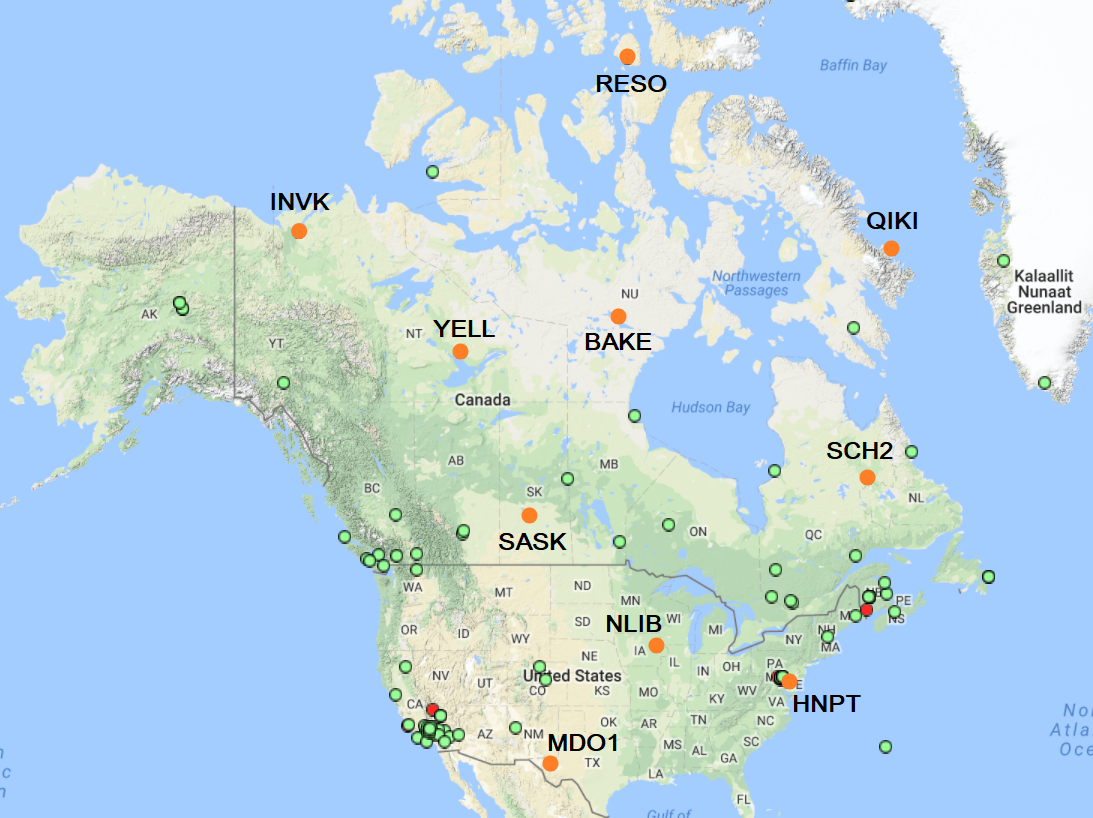
\includegraphics{task1/igs_map.png}}}
  \caption{The IGS stations used for determining the center of the Laurentide ice.}
  \label{fig:stations}
\end{figure}

A part of the task was to determine the annual uplift so data from a few years had to be selected.
The years 2005 through 2017 were chosen.
In order to get reliable data from each year, one week was selected (the first week of July) to collect data from each year.
A total of 910 data sets was to be collected (7 days per year for 13 years for 10 stations).

As mentioned earlier, processing data for a station was somewhat time-consuming, so two of the already processed stations were chosen for the weather forecast.

\subsection{Post-processing}
The post-processing was done mostly using the software tool \textit{GIPSY}\footnote{\url{https://gipsy-oasis.jpl.nasa.gov}}.
The main task carried out by the program is using a Kalman filter to solve the range equations (described in Section~\ref{sec:pseudorange}) for both code measurements and phase measurements.
The initial guess is based on information from the IGS network and geophysical models (such as tectonic plate motion and earth tides).
The results are combined with a weight matrix in each step and the best solution is computed through repeated iterations and updating variables.
The flow for this post-processing as it is done in GIPSY can be seen in Figure~\ref{fig:gipsy_flow} and will now be explained in more detail.
\begin{figure}[!ht]
  \centering
  \noindent\makebox[\textwidth]{\scalebox{0.75}{\includegraphics{GIPSY_flow.pdf}}}
  \caption{The post-processing flow for GIPSY.}
  \label{fig:gipsy_flow}
\end{figure}\\

\noindent Pseudorange data from the the station, formatted in a RINEX-file, is processed by the software and the ionospheric delay is removed using Dual Frequency (data from L1 and L2 frequencies).
The ionospheric-corrected pseudoranges are compared with an apriori estimation of the position using geophysical models (tidal effects etc.) and information from the IGS network (satellite clock errors etc.) as well as information about the station (antenna information etc.).
The comparison between the pseudorange (observation) and the apriori model (calculation) is compared using a weight matrix.

The residual of the observation-computation is processed by the Kalman filter and yields a new estimation of the position.
If the new estimation is close enough to the observed position (given the weights) the coordinates have been found.
If not, the new estimation is used in the observation-computation step.

\subsubsection{Latitude, Longitude and Radial movement}
After processing the RINEX data in GIPSY, the data was merged into a mean value for the entire period.
The data was then compared with the mean value to create a time series with latitude, longitude and radial movement relative to the mean value.
The data is then ready to be processed to solve the Laurentide ice problem.
In order to get an accurate result it is necessary to save the coordinates for the stations for later processing.

\subsubsection{Tropospheric delay}\label{sec:pp_trop}
Data for the tropospheric delay is saved by GIPSY when processing the RINEX data.
The data is relative to a reference value for each station, so in order to get the tropospheric delay this station-specific value has to be added to the relative values.

\subsection{Locating the center of the Laurentide ice}\label{sec:laurentide}
The resulting data from the post-processing was relative movement in latitude, longitude and radial direction for each station.
The coordinates had been established with an error of mostly under \SI{1}{\centi\meter}.
Unfortunately there was missing data for some years for some stations, but there was still enough data to proceed.

The first step was to go through the data for all stations and look for strange data (e.g. unnatural movements/jumps in the data set).
This was done by plotting the time series and looking at the total movement over the years.
It appeared that 
Unnatural radial movement was found for about half of the stations and after going through the log files for those stations it was found that the antennas for those stations had been replaced at one point which created meant that an offset had been added after that point.
This was corrected by creating a forward time series and a backward time series.
The forward time series represented data pre-change and the backward series post-change.
Data points were added depending on the data relative to some reference point.
Since the radial values were the data points that had unnatural movements, it was the radial component that determined whether or not the data point should be added, and the reference point was chosen to be the previous point (i.e. previous year for forward series and following year for backward series).
Data was added if the position relative to the reference point was less than a chosen maximum reasonable annual movement, as can be seen in the code snippet below.
\begin{lstlisting}
  def within_tol(p, c, tol):
    if p.val > c.val:
      return (p.val-p.error) - (c.val+c.error) < tol
    else:
      return (c.val-c.error) - (p.val+p.error) < tol
\end{lstlisting}

When the forward and backward time series were created they had to be merged.
This was done by performing a first-order polynomial fit (using the the reciprocal of the error as weights) to the forward series to predict the next element in the time series and add the difference between the predicted next value and the corresponding value in the backward series.
The corrected backward series is then added to the forward series (in chronological order).

\begin{lstlisting}
  m_r, c_r = polyfit(frad.time, frad.val, 1, w=1/frad.error)
  brad.val -= brad.val[0] - (m_r + c_r*brad.time[0])
  for (i, t) in enumerate(brad.time):
    if t not in frad.time:
      flon.add(blon.time[i], blon.val[i], blon.error[i])
      flat.add(blat.time[i], blat.val[i], blat.error[i])
      frad.add(brad.time[i], brad.val[i], brad.error[i])
\end{lstlisting}

Once the time series have been corrected, the coordinates of the station.
There are several ways of doing this but since this problem is inherently spherical (or more correctly, ellipsoidal), it was chosen to convert the entire problem into a spherical coordinate system.\\

\noindent There are many ways to determine the uplift due to the Laurentide ice at this point.
One has to take into account that the tectonic plate translates and rotates in addition to recovering from the ice.
It can be a very difficult task to remove the translation and rotation from the tectonic plates themselves, which involves finding the point at which the plate rotates about, so instead a simpler model was chosen.
This model assumes that the rotation and translation that affects the radial movement is very small so the radial movement is mostly caused by the land recovering from the Laurentide ice.
The uplift was assumed to decrease with distance to the center of the ice $\vec{C}_L$ in an elliptical fashion.
One way to realize this model can be seen in (\ref{eq:model}) and is the one used for this project.
\begin{align}
  \label{eq:model}
  d_i & = R_i((\phi_i-\phi_L) + j(\theta_i-\theta_L)), \nonumber \\
  \rho_i & = a + b\exp[-(\operatorname{Re}{(c_1d_i)}^2 + \operatorname{Im}{(c_2d_i)}^2)]
\end{align}
The longitude and latitude for the center of the ice $\phi_L, \theta_L \in \mathbb{R}$ and the coefficients $a, b \in \mathbb{R}$ and $c_1, c_2 \in \mathbb{C}$ was found using an \texttt{fmin} algorithm such as \texttt{fmin} from the \texttt{optimize} package in the Python library \textit{SciPy}\footnote{\url{https://www.scipy.org/}}.

Since there were many coefficients to be minimized a nested \texttt{fmin} was chosen.
The code below is an attempt to illustrate how the nested \texttt{fmin} was setup without showing more code than absolutely necessary.
It is set up to minimize the difference between the observed radial movement $\Delta R_i$ with the computed radial movement $\rho_i$ from (\ref{eq:model}).
\begin{table}
  \begin{lstlisting}
    def solver():
      fmin(lambda X: theta_phi(X[0], X[1]), [phi_0, theta_0])

    def theta_phi(phi, theta):
      fmin(lambda X: c(phi, theta, X[0], X[1]), [c_1_0, c_2_0])

    def c(phi_L, theta_L, c_1, c_2):
      fmin(lambda X: a_b(phi_L, theta_L, c_1, c_2, X[0], X[1]), [a_0, b_0])

    def a_b(phi_L, theta_L, c_1, c_2, a, b):
      d_i = R_i*((phi_i-phi_L) + 1j*(theta_i-theta_L))
      rho_i = a + b*exp(-(real(c_1*d_i)**2 + imag(c_2*d_i)**2))
      sum(abs(delta_R_i - rho_i))
  \end{lstlisting}
\end{table}

\section{Tropospheric delay prediction}
During the post-processing of the data for the task in Section~\ref{sec:laurentide}, data for the tropospheric delay was stored.
This data was used to predict the tropospheric delay.\\

\noindent Two stations with different climate were chosen; MDO1 in western Texas, USA and RESO in northern Nunavut, Canada.
Tropospheric delay data from these two stations during the first week of July 2005 was chosen since that data had already been processed.
As stated in Section~\ref{sec:pp_trop}, the reference values had to be added to the Tropospheric delay data from the post-processing.

The method used to predict the tropospheric delay was to simply use data from $n-1$ consecutive days to and create a polynomial fit to that data.
This fit can then be used to predict the tropospheric delay for the $n^{\text{th}}$ day.
To find the best fit for the data, polynomial fits with a degree ranging from 0 to 20 was created and the one that had the lowest least-square error was chosen.

\section{Result}
The resulting location for the Laurentide ice as well as the tropospheric delay predictions will be presented in this section.
The resulting data from the post-processing using GIPSY will not be presented here as it contains little useful information on its own.
It is worth mentioning that most data points had an error which was less than \SI{1}{\centi\meter}, which can be worth noting when the result is discussed.

\subsection{Locating the center of the Laurentide ice}
The location of the Laurentide ice was computed to be at latitude \SI{61.7}{\degree} north and longitude \SI{83.3}{\degree} west, which is in the northern part of Hudson Bay, Canada.
The full result from the nested \texttt{fmin} can be seen in Table~\ref{tab:fmin}.
The average radial residual was just under \SI{1}{\centi\meter} and a more detailed listing of the residual can be seen in Table~\ref{tab:residual}.
Using the data from Table~\ref{tab:fmin} along with (\ref{eq:model}), the annual uplift due to the Laurentide ice is \SI{13}{\milli\meter} per year (the uplift for the center during 13 years is $a + b\exp(0)$).
The stations and their uplift along with the computed center of the Laurentide ice can be seen in Figure~\ref{fig:laurentide_result}.
Note that the contour plot does not appear to be elliptical as it should be.
This is because the background image is the result of a conformal mapping, and all data points that are plotted on top of it have been mapped in the same way.

\begin{table}[!ht]
  \centering
  \caption{The latitude and longitude for the center of the Laurentide ice and the coefficients in (\ref{eq:model}) resulting from the nested \texttt{fmin}.}
  \begin{tabular}{|l|l|} \hline
    Variable & Value \\ \hline
    $\phi_L$ & \SI{-83.3}{\degree} \\
    $\theta_L$ & \SI{61.7}{\degree} \\
    $c_1$ & $0.235 \angle{\SI{0.32}{\degree}}$ \\
    $c_2$ & $0.699 \angle{\SI{12.37}{\degree}}$ \\
    $a$ & \SI{-40}{\milli\meter} \\
    $b$ & \SI{212}{\milli\meter} \\\hline
  \end{tabular}
  \label{tab:fmin}
\end{table}

\begin{table}[!ht]
  \centering
  \caption{The residual for comparing the observed uplift $\Delta R_i$ to the computed uplift $\rho_i$ using (\ref{eq:model}).}
  \begin{tabular}{|l|r|} \hline
    Station & $\Delta R_i - \rho_i$ \\ \hline
    MDO1 & \SI{58.3}{\milli\meter} \\
    YELL & \SI{25.4}{\milli\meter} \\
    NLIB & \SI{-14.5}{\milli\meter} \\
    INVK & \SI{-126.5}{\micro\meter} \\
    QIKI & \SI{21.6}{\micro\meter} \\
    BAKE & \SI{-21.1}{\micro\meter} \\
    RESO & \SI{8.1}{\micro\meter} \\
    SASK & \SI{-6.3}{\micro\meter} \\
    HNPT & \SI{4.0}{\micro\meter} \\
    SCH2 & \SI{3.8}{\micro\meter} \\\hline
  \end{tabular}
  \label{tab:residual}
\end{table}

\begin{figure}[!ht]
  \centering
  \noindent\makebox[\textwidth]{\scalebox{0.75}{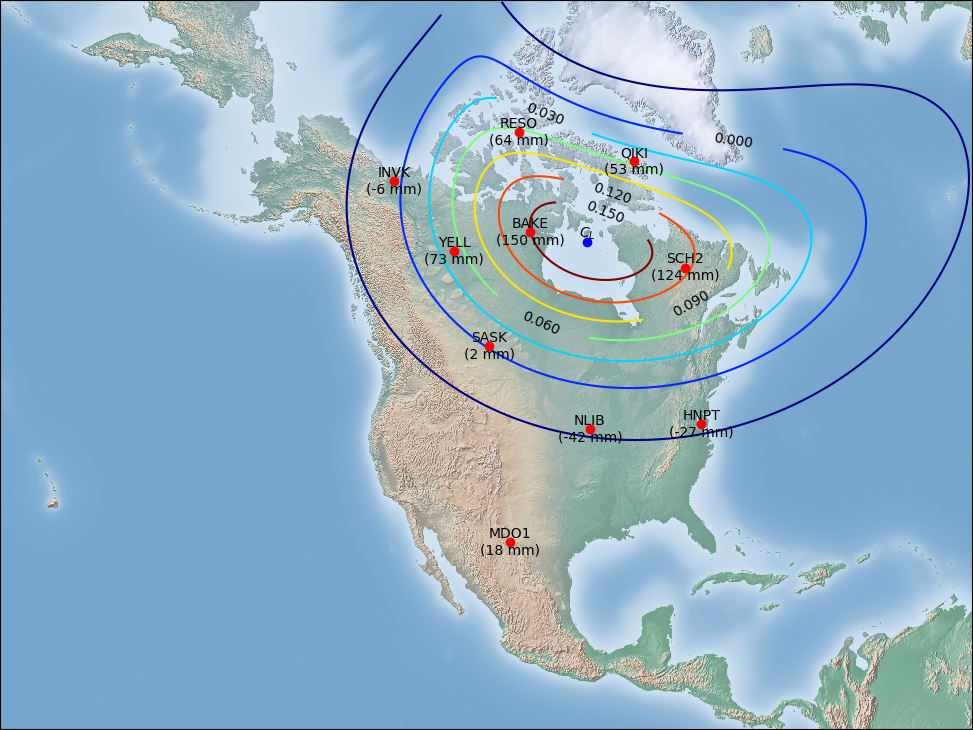
\includegraphics{task1/Laurentide.png}}}
  \caption{The IGS stations along with their total uplift over the years that the data was collected and the estimated center of the Laurentide ice along with a contour plot of (\ref{eq:model}) using data from Table~\ref{tab:fmin}.}
  \label{fig:laurentide_result}
\end{figure}

\subsection{Tropospheric delay prediction}
The prediction of the Tropospheric delay for MDO1 and RESO during the first week of July 2005 can be seen in Figure~\ref{fig:trop_delay}.
\begin{figure}[!ht]
  \centering
  \noindent\makebox[\textwidth]{\scalebox{0.75}{%% Creator: Matplotlib, PGF backend
%%
%% To include the figure in your LaTeX document, write
%%   \input{<filename>.pgf}
%%
%% Make sure the required packages are loaded in your preamble
%%   \usepackage{pgf}
%%
%% Figures using additional raster images can only be included by \input if
%% they are in the same directory as the main LaTeX file. For loading figures
%% from other directories you can use the `import` package
%%   \usepackage{import}
%% and then include the figures with
%%   \import{<path to file>}{<filename>.pgf}
%%
%% Matplotlib used the following preamble
%%   \usepackage{fontspec}
%%   \setmainfont{DejaVu Serif}
%%   \setsansfont{DejaVu Sans}
%%   \setmonofont{DejaVu Sans Mono}
%%
\begingroup%
\makeatletter%
\begin{pgfpicture}%
\pgfpathrectangle{\pgfpointorigin}{\pgfqpoint{8.670000in}{6.530000in}}%
\pgfusepath{use as bounding box, clip}%
\begin{pgfscope}%
\pgfsetbuttcap%
\pgfsetmiterjoin%
\definecolor{currentfill}{rgb}{1.000000,1.000000,1.000000}%
\pgfsetfillcolor{currentfill}%
\pgfsetlinewidth{0.000000pt}%
\definecolor{currentstroke}{rgb}{1.000000,1.000000,1.000000}%
\pgfsetstrokecolor{currentstroke}%
\pgfsetdash{}{0pt}%
\pgfpathmoveto{\pgfqpoint{0.000000in}{0.000000in}}%
\pgfpathlineto{\pgfqpoint{8.670000in}{0.000000in}}%
\pgfpathlineto{\pgfqpoint{8.670000in}{6.530000in}}%
\pgfpathlineto{\pgfqpoint{0.000000in}{6.530000in}}%
\pgfpathclose%
\pgfusepath{fill}%
\end{pgfscope}%
\begin{pgfscope}%
\pgfsetbuttcap%
\pgfsetmiterjoin%
\definecolor{currentfill}{rgb}{1.000000,1.000000,1.000000}%
\pgfsetfillcolor{currentfill}%
\pgfsetlinewidth{0.000000pt}%
\definecolor{currentstroke}{rgb}{0.000000,0.000000,0.000000}%
\pgfsetstrokecolor{currentstroke}%
\pgfsetstrokeopacity{0.000000}%
\pgfsetdash{}{0pt}%
\pgfpathmoveto{\pgfqpoint{1.083750in}{3.460900in}}%
\pgfpathlineto{\pgfqpoint{7.803000in}{3.460900in}}%
\pgfpathlineto{\pgfqpoint{7.803000in}{5.746400in}}%
\pgfpathlineto{\pgfqpoint{1.083750in}{5.746400in}}%
\pgfpathclose%
\pgfusepath{fill}%
\end{pgfscope}%
\begin{pgfscope}%
\pgfsetbuttcap%
\pgfsetroundjoin%
\definecolor{currentfill}{rgb}{0.000000,0.000000,0.000000}%
\pgfsetfillcolor{currentfill}%
\pgfsetlinewidth{0.803000pt}%
\definecolor{currentstroke}{rgb}{0.000000,0.000000,0.000000}%
\pgfsetstrokecolor{currentstroke}%
\pgfsetdash{}{0pt}%
\pgfsys@defobject{currentmarker}{\pgfqpoint{0.000000in}{-0.048611in}}{\pgfqpoint{0.000000in}{0.000000in}}{%
\pgfpathmoveto{\pgfqpoint{0.000000in}{0.000000in}}%
\pgfpathlineto{\pgfqpoint{0.000000in}{-0.048611in}}%
\pgfusepath{stroke,fill}%
}%
\begin{pgfscope}%
\pgfsys@transformshift{1.914625in}{3.460900in}%
\pgfsys@useobject{currentmarker}{}%
\end{pgfscope}%
\end{pgfscope}%
\begin{pgfscope}%
\pgftext[x=1.914625in,y=3.363678in,,top]{\sffamily\fontsize{10.000000}{12.000000}\selectfont 1.735}%
\end{pgfscope}%
\begin{pgfscope}%
\pgfsetbuttcap%
\pgfsetroundjoin%
\definecolor{currentfill}{rgb}{0.000000,0.000000,0.000000}%
\pgfsetfillcolor{currentfill}%
\pgfsetlinewidth{0.803000pt}%
\definecolor{currentstroke}{rgb}{0.000000,0.000000,0.000000}%
\pgfsetstrokecolor{currentstroke}%
\pgfsetdash{}{0pt}%
\pgfsys@defobject{currentmarker}{\pgfqpoint{0.000000in}{-0.048611in}}{\pgfqpoint{0.000000in}{0.000000in}}{%
\pgfpathmoveto{\pgfqpoint{0.000000in}{0.000000in}}%
\pgfpathlineto{\pgfqpoint{0.000000in}{-0.048611in}}%
\pgfusepath{stroke,fill}%
}%
\begin{pgfscope}%
\pgfsys@transformshift{2.925115in}{3.460900in}%
\pgfsys@useobject{currentmarker}{}%
\end{pgfscope}%
\end{pgfscope}%
\begin{pgfscope}%
\pgftext[x=2.925115in,y=3.363678in,,top]{\sffamily\fontsize{10.000000}{12.000000}\selectfont 1.736}%
\end{pgfscope}%
\begin{pgfscope}%
\pgfsetbuttcap%
\pgfsetroundjoin%
\definecolor{currentfill}{rgb}{0.000000,0.000000,0.000000}%
\pgfsetfillcolor{currentfill}%
\pgfsetlinewidth{0.803000pt}%
\definecolor{currentstroke}{rgb}{0.000000,0.000000,0.000000}%
\pgfsetstrokecolor{currentstroke}%
\pgfsetdash{}{0pt}%
\pgfsys@defobject{currentmarker}{\pgfqpoint{0.000000in}{-0.048611in}}{\pgfqpoint{0.000000in}{0.000000in}}{%
\pgfpathmoveto{\pgfqpoint{0.000000in}{0.000000in}}%
\pgfpathlineto{\pgfqpoint{0.000000in}{-0.048611in}}%
\pgfusepath{stroke,fill}%
}%
\begin{pgfscope}%
\pgfsys@transformshift{3.935604in}{3.460900in}%
\pgfsys@useobject{currentmarker}{}%
\end{pgfscope}%
\end{pgfscope}%
\begin{pgfscope}%
\pgftext[x=3.935604in,y=3.363678in,,top]{\sffamily\fontsize{10.000000}{12.000000}\selectfont 1.737}%
\end{pgfscope}%
\begin{pgfscope}%
\pgfsetbuttcap%
\pgfsetroundjoin%
\definecolor{currentfill}{rgb}{0.000000,0.000000,0.000000}%
\pgfsetfillcolor{currentfill}%
\pgfsetlinewidth{0.803000pt}%
\definecolor{currentstroke}{rgb}{0.000000,0.000000,0.000000}%
\pgfsetstrokecolor{currentstroke}%
\pgfsetdash{}{0pt}%
\pgfsys@defobject{currentmarker}{\pgfqpoint{0.000000in}{-0.048611in}}{\pgfqpoint{0.000000in}{0.000000in}}{%
\pgfpathmoveto{\pgfqpoint{0.000000in}{0.000000in}}%
\pgfpathlineto{\pgfqpoint{0.000000in}{-0.048611in}}%
\pgfusepath{stroke,fill}%
}%
\begin{pgfscope}%
\pgfsys@transformshift{4.946094in}{3.460900in}%
\pgfsys@useobject{currentmarker}{}%
\end{pgfscope}%
\end{pgfscope}%
\begin{pgfscope}%
\pgftext[x=4.946094in,y=3.363678in,,top]{\sffamily\fontsize{10.000000}{12.000000}\selectfont 1.738}%
\end{pgfscope}%
\begin{pgfscope}%
\pgfsetbuttcap%
\pgfsetroundjoin%
\definecolor{currentfill}{rgb}{0.000000,0.000000,0.000000}%
\pgfsetfillcolor{currentfill}%
\pgfsetlinewidth{0.803000pt}%
\definecolor{currentstroke}{rgb}{0.000000,0.000000,0.000000}%
\pgfsetstrokecolor{currentstroke}%
\pgfsetdash{}{0pt}%
\pgfsys@defobject{currentmarker}{\pgfqpoint{0.000000in}{-0.048611in}}{\pgfqpoint{0.000000in}{0.000000in}}{%
\pgfpathmoveto{\pgfqpoint{0.000000in}{0.000000in}}%
\pgfpathlineto{\pgfqpoint{0.000000in}{-0.048611in}}%
\pgfusepath{stroke,fill}%
}%
\begin{pgfscope}%
\pgfsys@transformshift{5.956583in}{3.460900in}%
\pgfsys@useobject{currentmarker}{}%
\end{pgfscope}%
\end{pgfscope}%
\begin{pgfscope}%
\pgftext[x=5.956583in,y=3.363678in,,top]{\sffamily\fontsize{10.000000}{12.000000}\selectfont 1.739}%
\end{pgfscope}%
\begin{pgfscope}%
\pgfsetbuttcap%
\pgfsetroundjoin%
\definecolor{currentfill}{rgb}{0.000000,0.000000,0.000000}%
\pgfsetfillcolor{currentfill}%
\pgfsetlinewidth{0.803000pt}%
\definecolor{currentstroke}{rgb}{0.000000,0.000000,0.000000}%
\pgfsetstrokecolor{currentstroke}%
\pgfsetdash{}{0pt}%
\pgfsys@defobject{currentmarker}{\pgfqpoint{0.000000in}{-0.048611in}}{\pgfqpoint{0.000000in}{0.000000in}}{%
\pgfpathmoveto{\pgfqpoint{0.000000in}{0.000000in}}%
\pgfpathlineto{\pgfqpoint{0.000000in}{-0.048611in}}%
\pgfusepath{stroke,fill}%
}%
\begin{pgfscope}%
\pgfsys@transformshift{6.967073in}{3.460900in}%
\pgfsys@useobject{currentmarker}{}%
\end{pgfscope}%
\end{pgfscope}%
\begin{pgfscope}%
\pgftext[x=6.967073in,y=3.363678in,,top]{\sffamily\fontsize{10.000000}{12.000000}\selectfont 1.740}%
\end{pgfscope}%
\begin{pgfscope}%
\pgftext[x=7.803000in,y=3.187598in,right,top]{\sffamily\fontsize{10.000000}{12.000000}\selectfont 1e8}%
\end{pgfscope}%
\begin{pgfscope}%
\pgfsetbuttcap%
\pgfsetroundjoin%
\definecolor{currentfill}{rgb}{0.000000,0.000000,0.000000}%
\pgfsetfillcolor{currentfill}%
\pgfsetlinewidth{0.803000pt}%
\definecolor{currentstroke}{rgb}{0.000000,0.000000,0.000000}%
\pgfsetstrokecolor{currentstroke}%
\pgfsetdash{}{0pt}%
\pgfsys@defobject{currentmarker}{\pgfqpoint{-0.048611in}{0.000000in}}{\pgfqpoint{0.000000in}{0.000000in}}{%
\pgfpathmoveto{\pgfqpoint{0.000000in}{0.000000in}}%
\pgfpathlineto{\pgfqpoint{-0.048611in}{0.000000in}}%
\pgfusepath{stroke,fill}%
}%
\begin{pgfscope}%
\pgfsys@transformshift{1.083750in}{3.782990in}%
\pgfsys@useobject{currentmarker}{}%
\end{pgfscope}%
\end{pgfscope}%
\begin{pgfscope}%
\pgftext[x=0.677283in,y=3.730228in,left,base]{\sffamily\fontsize{10.000000}{12.000000}\selectfont 2.32}%
\end{pgfscope}%
\begin{pgfscope}%
\pgfsetbuttcap%
\pgfsetroundjoin%
\definecolor{currentfill}{rgb}{0.000000,0.000000,0.000000}%
\pgfsetfillcolor{currentfill}%
\pgfsetlinewidth{0.803000pt}%
\definecolor{currentstroke}{rgb}{0.000000,0.000000,0.000000}%
\pgfsetstrokecolor{currentstroke}%
\pgfsetdash{}{0pt}%
\pgfsys@defobject{currentmarker}{\pgfqpoint{-0.048611in}{0.000000in}}{\pgfqpoint{0.000000in}{0.000000in}}{%
\pgfpathmoveto{\pgfqpoint{0.000000in}{0.000000in}}%
\pgfpathlineto{\pgfqpoint{-0.048611in}{0.000000in}}%
\pgfusepath{stroke,fill}%
}%
\begin{pgfscope}%
\pgfsys@transformshift{1.083750in}{4.123498in}%
\pgfsys@useobject{currentmarker}{}%
\end{pgfscope}%
\end{pgfscope}%
\begin{pgfscope}%
\pgftext[x=0.677283in,y=4.070736in,left,base]{\sffamily\fontsize{10.000000}{12.000000}\selectfont 2.34}%
\end{pgfscope}%
\begin{pgfscope}%
\pgfsetbuttcap%
\pgfsetroundjoin%
\definecolor{currentfill}{rgb}{0.000000,0.000000,0.000000}%
\pgfsetfillcolor{currentfill}%
\pgfsetlinewidth{0.803000pt}%
\definecolor{currentstroke}{rgb}{0.000000,0.000000,0.000000}%
\pgfsetstrokecolor{currentstroke}%
\pgfsetdash{}{0pt}%
\pgfsys@defobject{currentmarker}{\pgfqpoint{-0.048611in}{0.000000in}}{\pgfqpoint{0.000000in}{0.000000in}}{%
\pgfpathmoveto{\pgfqpoint{0.000000in}{0.000000in}}%
\pgfpathlineto{\pgfqpoint{-0.048611in}{0.000000in}}%
\pgfusepath{stroke,fill}%
}%
\begin{pgfscope}%
\pgfsys@transformshift{1.083750in}{4.464006in}%
\pgfsys@useobject{currentmarker}{}%
\end{pgfscope}%
\end{pgfscope}%
\begin{pgfscope}%
\pgftext[x=0.677283in,y=4.411244in,left,base]{\sffamily\fontsize{10.000000}{12.000000}\selectfont 2.36}%
\end{pgfscope}%
\begin{pgfscope}%
\pgfsetbuttcap%
\pgfsetroundjoin%
\definecolor{currentfill}{rgb}{0.000000,0.000000,0.000000}%
\pgfsetfillcolor{currentfill}%
\pgfsetlinewidth{0.803000pt}%
\definecolor{currentstroke}{rgb}{0.000000,0.000000,0.000000}%
\pgfsetstrokecolor{currentstroke}%
\pgfsetdash{}{0pt}%
\pgfsys@defobject{currentmarker}{\pgfqpoint{-0.048611in}{0.000000in}}{\pgfqpoint{0.000000in}{0.000000in}}{%
\pgfpathmoveto{\pgfqpoint{0.000000in}{0.000000in}}%
\pgfpathlineto{\pgfqpoint{-0.048611in}{0.000000in}}%
\pgfusepath{stroke,fill}%
}%
\begin{pgfscope}%
\pgfsys@transformshift{1.083750in}{4.804514in}%
\pgfsys@useobject{currentmarker}{}%
\end{pgfscope}%
\end{pgfscope}%
\begin{pgfscope}%
\pgftext[x=0.677283in,y=4.751752in,left,base]{\sffamily\fontsize{10.000000}{12.000000}\selectfont 2.38}%
\end{pgfscope}%
\begin{pgfscope}%
\pgfsetbuttcap%
\pgfsetroundjoin%
\definecolor{currentfill}{rgb}{0.000000,0.000000,0.000000}%
\pgfsetfillcolor{currentfill}%
\pgfsetlinewidth{0.803000pt}%
\definecolor{currentstroke}{rgb}{0.000000,0.000000,0.000000}%
\pgfsetstrokecolor{currentstroke}%
\pgfsetdash{}{0pt}%
\pgfsys@defobject{currentmarker}{\pgfqpoint{-0.048611in}{0.000000in}}{\pgfqpoint{0.000000in}{0.000000in}}{%
\pgfpathmoveto{\pgfqpoint{0.000000in}{0.000000in}}%
\pgfpathlineto{\pgfqpoint{-0.048611in}{0.000000in}}%
\pgfusepath{stroke,fill}%
}%
\begin{pgfscope}%
\pgfsys@transformshift{1.083750in}{5.145022in}%
\pgfsys@useobject{currentmarker}{}%
\end{pgfscope}%
\end{pgfscope}%
\begin{pgfscope}%
\pgftext[x=0.677283in,y=5.092260in,left,base]{\sffamily\fontsize{10.000000}{12.000000}\selectfont 2.40}%
\end{pgfscope}%
\begin{pgfscope}%
\pgfsetbuttcap%
\pgfsetroundjoin%
\definecolor{currentfill}{rgb}{0.000000,0.000000,0.000000}%
\pgfsetfillcolor{currentfill}%
\pgfsetlinewidth{0.803000pt}%
\definecolor{currentstroke}{rgb}{0.000000,0.000000,0.000000}%
\pgfsetstrokecolor{currentstroke}%
\pgfsetdash{}{0pt}%
\pgfsys@defobject{currentmarker}{\pgfqpoint{-0.048611in}{0.000000in}}{\pgfqpoint{0.000000in}{0.000000in}}{%
\pgfpathmoveto{\pgfqpoint{0.000000in}{0.000000in}}%
\pgfpathlineto{\pgfqpoint{-0.048611in}{0.000000in}}%
\pgfusepath{stroke,fill}%
}%
\begin{pgfscope}%
\pgfsys@transformshift{1.083750in}{5.485529in}%
\pgfsys@useobject{currentmarker}{}%
\end{pgfscope}%
\end{pgfscope}%
\begin{pgfscope}%
\pgftext[x=0.677283in,y=5.432768in,left,base]{\sffamily\fontsize{10.000000}{12.000000}\selectfont 2.42}%
\end{pgfscope}%
\begin{pgfscope}%
\pgfpathrectangle{\pgfqpoint{1.083750in}{3.460900in}}{\pgfqpoint{6.719250in}{2.285500in}} %
\pgfusepath{clip}%
\pgfsetbuttcap%
\pgfsetroundjoin%
\pgfsetlinewidth{1.505625pt}%
\definecolor{currentstroke}{rgb}{0.000000,0.000000,1.000000}%
\pgfsetstrokecolor{currentstroke}%
\pgfsetdash{}{0pt}%
\pgfpathmoveto{\pgfqpoint{1.389170in}{4.359988in}}%
\pgfpathlineto{\pgfqpoint{1.389170in}{4.472390in}}%
\pgfusepath{stroke}%
\end{pgfscope}%
\begin{pgfscope}%
\pgfpathrectangle{\pgfqpoint{1.083750in}{3.460900in}}{\pgfqpoint{6.719250in}{2.285500in}} %
\pgfusepath{clip}%
\pgfsetbuttcap%
\pgfsetroundjoin%
\pgfsetlinewidth{1.505625pt}%
\definecolor{currentstroke}{rgb}{0.000000,0.000000,1.000000}%
\pgfsetstrokecolor{currentstroke}%
\pgfsetdash{}{0pt}%
\pgfpathmoveto{\pgfqpoint{1.392202in}{4.340603in}}%
\pgfpathlineto{\pgfqpoint{1.392202in}{4.447795in}}%
\pgfusepath{stroke}%
\end{pgfscope}%
\begin{pgfscope}%
\pgfpathrectangle{\pgfqpoint{1.083750in}{3.460900in}}{\pgfqpoint{6.719250in}{2.285500in}} %
\pgfusepath{clip}%
\pgfsetbuttcap%
\pgfsetroundjoin%
\pgfsetlinewidth{1.505625pt}%
\definecolor{currentstroke}{rgb}{0.000000,0.000000,1.000000}%
\pgfsetstrokecolor{currentstroke}%
\pgfsetdash{}{0pt}%
\pgfpathmoveto{\pgfqpoint{1.395233in}{4.342169in}}%
\pgfpathlineto{\pgfqpoint{1.395233in}{4.448510in}}%
\pgfusepath{stroke}%
\end{pgfscope}%
\begin{pgfscope}%
\pgfpathrectangle{\pgfqpoint{1.083750in}{3.460900in}}{\pgfqpoint{6.719250in}{2.285500in}} %
\pgfusepath{clip}%
\pgfsetbuttcap%
\pgfsetroundjoin%
\pgfsetlinewidth{1.505625pt}%
\definecolor{currentstroke}{rgb}{0.000000,0.000000,1.000000}%
\pgfsetstrokecolor{currentstroke}%
\pgfsetdash{}{0pt}%
\pgfpathmoveto{\pgfqpoint{1.398265in}{4.318951in}}%
\pgfpathlineto{\pgfqpoint{1.398265in}{4.422431in}}%
\pgfusepath{stroke}%
\end{pgfscope}%
\begin{pgfscope}%
\pgfpathrectangle{\pgfqpoint{1.083750in}{3.460900in}}{\pgfqpoint{6.719250in}{2.285500in}} %
\pgfusepath{clip}%
\pgfsetbuttcap%
\pgfsetroundjoin%
\pgfsetlinewidth{1.505625pt}%
\definecolor{currentstroke}{rgb}{0.000000,0.000000,1.000000}%
\pgfsetstrokecolor{currentstroke}%
\pgfsetdash{}{0pt}%
\pgfpathmoveto{\pgfqpoint{1.401296in}{4.310604in}}%
\pgfpathlineto{\pgfqpoint{1.401296in}{4.407377in}}%
\pgfusepath{stroke}%
\end{pgfscope}%
\begin{pgfscope}%
\pgfpathrectangle{\pgfqpoint{1.083750in}{3.460900in}}{\pgfqpoint{6.719250in}{2.285500in}} %
\pgfusepath{clip}%
\pgfsetbuttcap%
\pgfsetroundjoin%
\pgfsetlinewidth{1.505625pt}%
\definecolor{currentstroke}{rgb}{0.000000,0.000000,1.000000}%
\pgfsetstrokecolor{currentstroke}%
\pgfsetdash{}{0pt}%
\pgfpathmoveto{\pgfqpoint{1.404328in}{4.311024in}}%
\pgfpathlineto{\pgfqpoint{1.404328in}{4.397036in}}%
\pgfusepath{stroke}%
\end{pgfscope}%
\begin{pgfscope}%
\pgfpathrectangle{\pgfqpoint{1.083750in}{3.460900in}}{\pgfqpoint{6.719250in}{2.285500in}} %
\pgfusepath{clip}%
\pgfsetbuttcap%
\pgfsetroundjoin%
\pgfsetlinewidth{1.505625pt}%
\definecolor{currentstroke}{rgb}{0.000000,0.000000,1.000000}%
\pgfsetstrokecolor{currentstroke}%
\pgfsetdash{}{0pt}%
\pgfpathmoveto{\pgfqpoint{1.407359in}{4.335821in}}%
\pgfpathlineto{\pgfqpoint{1.407359in}{4.416419in}}%
\pgfusepath{stroke}%
\end{pgfscope}%
\begin{pgfscope}%
\pgfpathrectangle{\pgfqpoint{1.083750in}{3.460900in}}{\pgfqpoint{6.719250in}{2.285500in}} %
\pgfusepath{clip}%
\pgfsetbuttcap%
\pgfsetroundjoin%
\pgfsetlinewidth{1.505625pt}%
\definecolor{currentstroke}{rgb}{0.000000,0.000000,1.000000}%
\pgfsetstrokecolor{currentstroke}%
\pgfsetdash{}{0pt}%
\pgfpathmoveto{\pgfqpoint{1.410391in}{4.323027in}}%
\pgfpathlineto{\pgfqpoint{1.410391in}{4.406519in}}%
\pgfusepath{stroke}%
\end{pgfscope}%
\begin{pgfscope}%
\pgfpathrectangle{\pgfqpoint{1.083750in}{3.460900in}}{\pgfqpoint{6.719250in}{2.285500in}} %
\pgfusepath{clip}%
\pgfsetbuttcap%
\pgfsetroundjoin%
\pgfsetlinewidth{1.505625pt}%
\definecolor{currentstroke}{rgb}{0.000000,0.000000,1.000000}%
\pgfsetstrokecolor{currentstroke}%
\pgfsetdash{}{0pt}%
\pgfpathmoveto{\pgfqpoint{1.413422in}{4.344716in}}%
\pgfpathlineto{\pgfqpoint{1.413422in}{4.425859in}}%
\pgfusepath{stroke}%
\end{pgfscope}%
\begin{pgfscope}%
\pgfpathrectangle{\pgfqpoint{1.083750in}{3.460900in}}{\pgfqpoint{6.719250in}{2.285500in}} %
\pgfusepath{clip}%
\pgfsetbuttcap%
\pgfsetroundjoin%
\pgfsetlinewidth{1.505625pt}%
\definecolor{currentstroke}{rgb}{0.000000,0.000000,1.000000}%
\pgfsetstrokecolor{currentstroke}%
\pgfsetdash{}{0pt}%
\pgfpathmoveto{\pgfqpoint{1.416454in}{4.357113in}}%
\pgfpathlineto{\pgfqpoint{1.416454in}{4.438426in}}%
\pgfusepath{stroke}%
\end{pgfscope}%
\begin{pgfscope}%
\pgfpathrectangle{\pgfqpoint{1.083750in}{3.460900in}}{\pgfqpoint{6.719250in}{2.285500in}} %
\pgfusepath{clip}%
\pgfsetbuttcap%
\pgfsetroundjoin%
\pgfsetlinewidth{1.505625pt}%
\definecolor{currentstroke}{rgb}{0.000000,0.000000,1.000000}%
\pgfsetstrokecolor{currentstroke}%
\pgfsetdash{}{0pt}%
\pgfpathmoveto{\pgfqpoint{1.419485in}{4.344730in}}%
\pgfpathlineto{\pgfqpoint{1.419485in}{4.422774in}}%
\pgfusepath{stroke}%
\end{pgfscope}%
\begin{pgfscope}%
\pgfpathrectangle{\pgfqpoint{1.083750in}{3.460900in}}{\pgfqpoint{6.719250in}{2.285500in}} %
\pgfusepath{clip}%
\pgfsetbuttcap%
\pgfsetroundjoin%
\pgfsetlinewidth{1.505625pt}%
\definecolor{currentstroke}{rgb}{0.000000,0.000000,1.000000}%
\pgfsetstrokecolor{currentstroke}%
\pgfsetdash{}{0pt}%
\pgfpathmoveto{\pgfqpoint{1.422517in}{4.359015in}}%
\pgfpathlineto{\pgfqpoint{1.422517in}{4.426503in}}%
\pgfusepath{stroke}%
\end{pgfscope}%
\begin{pgfscope}%
\pgfpathrectangle{\pgfqpoint{1.083750in}{3.460900in}}{\pgfqpoint{6.719250in}{2.285500in}} %
\pgfusepath{clip}%
\pgfsetbuttcap%
\pgfsetroundjoin%
\pgfsetlinewidth{1.505625pt}%
\definecolor{currentstroke}{rgb}{0.000000,0.000000,1.000000}%
\pgfsetstrokecolor{currentstroke}%
\pgfsetdash{}{0pt}%
\pgfpathmoveto{\pgfqpoint{1.425548in}{4.391037in}}%
\pgfpathlineto{\pgfqpoint{1.425548in}{4.469967in}}%
\pgfusepath{stroke}%
\end{pgfscope}%
\begin{pgfscope}%
\pgfpathrectangle{\pgfqpoint{1.083750in}{3.460900in}}{\pgfqpoint{6.719250in}{2.285500in}} %
\pgfusepath{clip}%
\pgfsetbuttcap%
\pgfsetroundjoin%
\pgfsetlinewidth{1.505625pt}%
\definecolor{currentstroke}{rgb}{0.000000,0.000000,1.000000}%
\pgfsetstrokecolor{currentstroke}%
\pgfsetdash{}{0pt}%
\pgfpathmoveto{\pgfqpoint{1.428580in}{4.396384in}}%
\pgfpathlineto{\pgfqpoint{1.428580in}{4.482158in}}%
\pgfusepath{stroke}%
\end{pgfscope}%
\begin{pgfscope}%
\pgfpathrectangle{\pgfqpoint{1.083750in}{3.460900in}}{\pgfqpoint{6.719250in}{2.285500in}} %
\pgfusepath{clip}%
\pgfsetbuttcap%
\pgfsetroundjoin%
\pgfsetlinewidth{1.505625pt}%
\definecolor{currentstroke}{rgb}{0.000000,0.000000,1.000000}%
\pgfsetstrokecolor{currentstroke}%
\pgfsetdash{}{0pt}%
\pgfpathmoveto{\pgfqpoint{1.431611in}{4.390546in}}%
\pgfpathlineto{\pgfqpoint{1.431611in}{4.479725in}}%
\pgfusepath{stroke}%
\end{pgfscope}%
\begin{pgfscope}%
\pgfpathrectangle{\pgfqpoint{1.083750in}{3.460900in}}{\pgfqpoint{6.719250in}{2.285500in}} %
\pgfusepath{clip}%
\pgfsetbuttcap%
\pgfsetroundjoin%
\pgfsetlinewidth{1.505625pt}%
\definecolor{currentstroke}{rgb}{0.000000,0.000000,1.000000}%
\pgfsetstrokecolor{currentstroke}%
\pgfsetdash{}{0pt}%
\pgfpathmoveto{\pgfqpoint{1.434642in}{4.395395in}}%
\pgfpathlineto{\pgfqpoint{1.434642in}{4.483280in}}%
\pgfusepath{stroke}%
\end{pgfscope}%
\begin{pgfscope}%
\pgfpathrectangle{\pgfqpoint{1.083750in}{3.460900in}}{\pgfqpoint{6.719250in}{2.285500in}} %
\pgfusepath{clip}%
\pgfsetbuttcap%
\pgfsetroundjoin%
\pgfsetlinewidth{1.505625pt}%
\definecolor{currentstroke}{rgb}{0.000000,0.000000,1.000000}%
\pgfsetstrokecolor{currentstroke}%
\pgfsetdash{}{0pt}%
\pgfpathmoveto{\pgfqpoint{1.437674in}{4.380381in}}%
\pgfpathlineto{\pgfqpoint{1.437674in}{4.458392in}}%
\pgfusepath{stroke}%
\end{pgfscope}%
\begin{pgfscope}%
\pgfpathrectangle{\pgfqpoint{1.083750in}{3.460900in}}{\pgfqpoint{6.719250in}{2.285500in}} %
\pgfusepath{clip}%
\pgfsetbuttcap%
\pgfsetroundjoin%
\pgfsetlinewidth{1.505625pt}%
\definecolor{currentstroke}{rgb}{0.000000,0.000000,1.000000}%
\pgfsetstrokecolor{currentstroke}%
\pgfsetdash{}{0pt}%
\pgfpathmoveto{\pgfqpoint{1.440705in}{4.418390in}}%
\pgfpathlineto{\pgfqpoint{1.440705in}{4.488058in}}%
\pgfusepath{stroke}%
\end{pgfscope}%
\begin{pgfscope}%
\pgfpathrectangle{\pgfqpoint{1.083750in}{3.460900in}}{\pgfqpoint{6.719250in}{2.285500in}} %
\pgfusepath{clip}%
\pgfsetbuttcap%
\pgfsetroundjoin%
\pgfsetlinewidth{1.505625pt}%
\definecolor{currentstroke}{rgb}{0.000000,0.000000,1.000000}%
\pgfsetstrokecolor{currentstroke}%
\pgfsetdash{}{0pt}%
\pgfpathmoveto{\pgfqpoint{1.443737in}{4.405484in}}%
\pgfpathlineto{\pgfqpoint{1.443737in}{4.475322in}}%
\pgfusepath{stroke}%
\end{pgfscope}%
\begin{pgfscope}%
\pgfpathrectangle{\pgfqpoint{1.083750in}{3.460900in}}{\pgfqpoint{6.719250in}{2.285500in}} %
\pgfusepath{clip}%
\pgfsetbuttcap%
\pgfsetroundjoin%
\pgfsetlinewidth{1.505625pt}%
\definecolor{currentstroke}{rgb}{0.000000,0.000000,1.000000}%
\pgfsetstrokecolor{currentstroke}%
\pgfsetdash{}{0pt}%
\pgfpathmoveto{\pgfqpoint{1.446768in}{4.355895in}}%
\pgfpathlineto{\pgfqpoint{1.446768in}{4.438741in}}%
\pgfusepath{stroke}%
\end{pgfscope}%
\begin{pgfscope}%
\pgfpathrectangle{\pgfqpoint{1.083750in}{3.460900in}}{\pgfqpoint{6.719250in}{2.285500in}} %
\pgfusepath{clip}%
\pgfsetbuttcap%
\pgfsetroundjoin%
\pgfsetlinewidth{1.505625pt}%
\definecolor{currentstroke}{rgb}{0.000000,0.000000,1.000000}%
\pgfsetstrokecolor{currentstroke}%
\pgfsetdash{}{0pt}%
\pgfpathmoveto{\pgfqpoint{1.449800in}{4.376650in}}%
\pgfpathlineto{\pgfqpoint{1.449800in}{4.466442in}}%
\pgfusepath{stroke}%
\end{pgfscope}%
\begin{pgfscope}%
\pgfpathrectangle{\pgfqpoint{1.083750in}{3.460900in}}{\pgfqpoint{6.719250in}{2.285500in}} %
\pgfusepath{clip}%
\pgfsetbuttcap%
\pgfsetroundjoin%
\pgfsetlinewidth{1.505625pt}%
\definecolor{currentstroke}{rgb}{0.000000,0.000000,1.000000}%
\pgfsetstrokecolor{currentstroke}%
\pgfsetdash{}{0pt}%
\pgfpathmoveto{\pgfqpoint{1.452831in}{4.397108in}}%
\pgfpathlineto{\pgfqpoint{1.452831in}{4.488398in}}%
\pgfusepath{stroke}%
\end{pgfscope}%
\begin{pgfscope}%
\pgfpathrectangle{\pgfqpoint{1.083750in}{3.460900in}}{\pgfqpoint{6.719250in}{2.285500in}} %
\pgfusepath{clip}%
\pgfsetbuttcap%
\pgfsetroundjoin%
\pgfsetlinewidth{1.505625pt}%
\definecolor{currentstroke}{rgb}{0.000000,0.000000,1.000000}%
\pgfsetstrokecolor{currentstroke}%
\pgfsetdash{}{0pt}%
\pgfpathmoveto{\pgfqpoint{1.455863in}{4.413553in}}%
\pgfpathlineto{\pgfqpoint{1.455863in}{4.494798in}}%
\pgfusepath{stroke}%
\end{pgfscope}%
\begin{pgfscope}%
\pgfpathrectangle{\pgfqpoint{1.083750in}{3.460900in}}{\pgfqpoint{6.719250in}{2.285500in}} %
\pgfusepath{clip}%
\pgfsetbuttcap%
\pgfsetroundjoin%
\pgfsetlinewidth{1.505625pt}%
\definecolor{currentstroke}{rgb}{0.000000,0.000000,1.000000}%
\pgfsetstrokecolor{currentstroke}%
\pgfsetdash{}{0pt}%
\pgfpathmoveto{\pgfqpoint{1.458894in}{4.406996in}}%
\pgfpathlineto{\pgfqpoint{1.458894in}{4.492940in}}%
\pgfusepath{stroke}%
\end{pgfscope}%
\begin{pgfscope}%
\pgfpathrectangle{\pgfqpoint{1.083750in}{3.460900in}}{\pgfqpoint{6.719250in}{2.285500in}} %
\pgfusepath{clip}%
\pgfsetbuttcap%
\pgfsetroundjoin%
\pgfsetlinewidth{1.505625pt}%
\definecolor{currentstroke}{rgb}{0.000000,0.000000,1.000000}%
\pgfsetstrokecolor{currentstroke}%
\pgfsetdash{}{0pt}%
\pgfpathmoveto{\pgfqpoint{1.461926in}{4.403239in}}%
\pgfpathlineto{\pgfqpoint{1.461926in}{4.493781in}}%
\pgfusepath{stroke}%
\end{pgfscope}%
\begin{pgfscope}%
\pgfpathrectangle{\pgfqpoint{1.083750in}{3.460900in}}{\pgfqpoint{6.719250in}{2.285500in}} %
\pgfusepath{clip}%
\pgfsetbuttcap%
\pgfsetroundjoin%
\pgfsetlinewidth{1.505625pt}%
\definecolor{currentstroke}{rgb}{0.000000,0.000000,1.000000}%
\pgfsetstrokecolor{currentstroke}%
\pgfsetdash{}{0pt}%
\pgfpathmoveto{\pgfqpoint{1.464957in}{4.357400in}}%
\pgfpathlineto{\pgfqpoint{1.464957in}{4.449916in}}%
\pgfusepath{stroke}%
\end{pgfscope}%
\begin{pgfscope}%
\pgfpathrectangle{\pgfqpoint{1.083750in}{3.460900in}}{\pgfqpoint{6.719250in}{2.285500in}} %
\pgfusepath{clip}%
\pgfsetbuttcap%
\pgfsetroundjoin%
\pgfsetlinewidth{1.505625pt}%
\definecolor{currentstroke}{rgb}{0.000000,0.000000,1.000000}%
\pgfsetstrokecolor{currentstroke}%
\pgfsetdash{}{0pt}%
\pgfpathmoveto{\pgfqpoint{1.467989in}{4.335909in}}%
\pgfpathlineto{\pgfqpoint{1.467989in}{4.427029in}}%
\pgfusepath{stroke}%
\end{pgfscope}%
\begin{pgfscope}%
\pgfpathrectangle{\pgfqpoint{1.083750in}{3.460900in}}{\pgfqpoint{6.719250in}{2.285500in}} %
\pgfusepath{clip}%
\pgfsetbuttcap%
\pgfsetroundjoin%
\pgfsetlinewidth{1.505625pt}%
\definecolor{currentstroke}{rgb}{0.000000,0.000000,1.000000}%
\pgfsetstrokecolor{currentstroke}%
\pgfsetdash{}{0pt}%
\pgfpathmoveto{\pgfqpoint{1.471020in}{4.344987in}}%
\pgfpathlineto{\pgfqpoint{1.471020in}{4.431749in}}%
\pgfusepath{stroke}%
\end{pgfscope}%
\begin{pgfscope}%
\pgfpathrectangle{\pgfqpoint{1.083750in}{3.460900in}}{\pgfqpoint{6.719250in}{2.285500in}} %
\pgfusepath{clip}%
\pgfsetbuttcap%
\pgfsetroundjoin%
\pgfsetlinewidth{1.505625pt}%
\definecolor{currentstroke}{rgb}{0.000000,0.000000,1.000000}%
\pgfsetstrokecolor{currentstroke}%
\pgfsetdash{}{0pt}%
\pgfpathmoveto{\pgfqpoint{1.474052in}{4.363108in}}%
\pgfpathlineto{\pgfqpoint{1.474052in}{4.444659in}}%
\pgfusepath{stroke}%
\end{pgfscope}%
\begin{pgfscope}%
\pgfpathrectangle{\pgfqpoint{1.083750in}{3.460900in}}{\pgfqpoint{6.719250in}{2.285500in}} %
\pgfusepath{clip}%
\pgfsetbuttcap%
\pgfsetroundjoin%
\pgfsetlinewidth{1.505625pt}%
\definecolor{currentstroke}{rgb}{0.000000,0.000000,1.000000}%
\pgfsetstrokecolor{currentstroke}%
\pgfsetdash{}{0pt}%
\pgfpathmoveto{\pgfqpoint{1.477083in}{4.353923in}}%
\pgfpathlineto{\pgfqpoint{1.477083in}{4.422740in}}%
\pgfusepath{stroke}%
\end{pgfscope}%
\begin{pgfscope}%
\pgfpathrectangle{\pgfqpoint{1.083750in}{3.460900in}}{\pgfqpoint{6.719250in}{2.285500in}} %
\pgfusepath{clip}%
\pgfsetbuttcap%
\pgfsetroundjoin%
\pgfsetlinewidth{1.505625pt}%
\definecolor{currentstroke}{rgb}{0.000000,0.000000,1.000000}%
\pgfsetstrokecolor{currentstroke}%
\pgfsetdash{}{0pt}%
\pgfpathmoveto{\pgfqpoint{1.480115in}{4.360573in}}%
\pgfpathlineto{\pgfqpoint{1.480115in}{4.424725in}}%
\pgfusepath{stroke}%
\end{pgfscope}%
\begin{pgfscope}%
\pgfpathrectangle{\pgfqpoint{1.083750in}{3.460900in}}{\pgfqpoint{6.719250in}{2.285500in}} %
\pgfusepath{clip}%
\pgfsetbuttcap%
\pgfsetroundjoin%
\pgfsetlinewidth{1.505625pt}%
\definecolor{currentstroke}{rgb}{0.000000,0.000000,1.000000}%
\pgfsetstrokecolor{currentstroke}%
\pgfsetdash{}{0pt}%
\pgfpathmoveto{\pgfqpoint{1.483146in}{4.371258in}}%
\pgfpathlineto{\pgfqpoint{1.483146in}{4.439735in}}%
\pgfusepath{stroke}%
\end{pgfscope}%
\begin{pgfscope}%
\pgfpathrectangle{\pgfqpoint{1.083750in}{3.460900in}}{\pgfqpoint{6.719250in}{2.285500in}} %
\pgfusepath{clip}%
\pgfsetbuttcap%
\pgfsetroundjoin%
\pgfsetlinewidth{1.505625pt}%
\definecolor{currentstroke}{rgb}{0.000000,0.000000,1.000000}%
\pgfsetstrokecolor{currentstroke}%
\pgfsetdash{}{0pt}%
\pgfpathmoveto{\pgfqpoint{1.486177in}{4.396303in}}%
\pgfpathlineto{\pgfqpoint{1.486177in}{4.471623in}}%
\pgfusepath{stroke}%
\end{pgfscope}%
\begin{pgfscope}%
\pgfpathrectangle{\pgfqpoint{1.083750in}{3.460900in}}{\pgfqpoint{6.719250in}{2.285500in}} %
\pgfusepath{clip}%
\pgfsetbuttcap%
\pgfsetroundjoin%
\pgfsetlinewidth{1.505625pt}%
\definecolor{currentstroke}{rgb}{0.000000,0.000000,1.000000}%
\pgfsetstrokecolor{currentstroke}%
\pgfsetdash{}{0pt}%
\pgfpathmoveto{\pgfqpoint{1.489209in}{4.383567in}}%
\pgfpathlineto{\pgfqpoint{1.489209in}{4.462736in}}%
\pgfusepath{stroke}%
\end{pgfscope}%
\begin{pgfscope}%
\pgfpathrectangle{\pgfqpoint{1.083750in}{3.460900in}}{\pgfqpoint{6.719250in}{2.285500in}} %
\pgfusepath{clip}%
\pgfsetbuttcap%
\pgfsetroundjoin%
\pgfsetlinewidth{1.505625pt}%
\definecolor{currentstroke}{rgb}{0.000000,0.000000,1.000000}%
\pgfsetstrokecolor{currentstroke}%
\pgfsetdash{}{0pt}%
\pgfpathmoveto{\pgfqpoint{1.492240in}{4.383358in}}%
\pgfpathlineto{\pgfqpoint{1.492240in}{4.470800in}}%
\pgfusepath{stroke}%
\end{pgfscope}%
\begin{pgfscope}%
\pgfpathrectangle{\pgfqpoint{1.083750in}{3.460900in}}{\pgfqpoint{6.719250in}{2.285500in}} %
\pgfusepath{clip}%
\pgfsetbuttcap%
\pgfsetroundjoin%
\pgfsetlinewidth{1.505625pt}%
\definecolor{currentstroke}{rgb}{0.000000,0.000000,1.000000}%
\pgfsetstrokecolor{currentstroke}%
\pgfsetdash{}{0pt}%
\pgfpathmoveto{\pgfqpoint{1.495272in}{4.382843in}}%
\pgfpathlineto{\pgfqpoint{1.495272in}{4.471103in}}%
\pgfusepath{stroke}%
\end{pgfscope}%
\begin{pgfscope}%
\pgfpathrectangle{\pgfqpoint{1.083750in}{3.460900in}}{\pgfqpoint{6.719250in}{2.285500in}} %
\pgfusepath{clip}%
\pgfsetbuttcap%
\pgfsetroundjoin%
\pgfsetlinewidth{1.505625pt}%
\definecolor{currentstroke}{rgb}{0.000000,0.000000,1.000000}%
\pgfsetstrokecolor{currentstroke}%
\pgfsetdash{}{0pt}%
\pgfpathmoveto{\pgfqpoint{1.498303in}{4.368915in}}%
\pgfpathlineto{\pgfqpoint{1.498303in}{4.460239in}}%
\pgfusepath{stroke}%
\end{pgfscope}%
\begin{pgfscope}%
\pgfpathrectangle{\pgfqpoint{1.083750in}{3.460900in}}{\pgfqpoint{6.719250in}{2.285500in}} %
\pgfusepath{clip}%
\pgfsetbuttcap%
\pgfsetroundjoin%
\pgfsetlinewidth{1.505625pt}%
\definecolor{currentstroke}{rgb}{0.000000,0.000000,1.000000}%
\pgfsetstrokecolor{currentstroke}%
\pgfsetdash{}{0pt}%
\pgfpathmoveto{\pgfqpoint{1.501335in}{4.366383in}}%
\pgfpathlineto{\pgfqpoint{1.501335in}{4.453723in}}%
\pgfusepath{stroke}%
\end{pgfscope}%
\begin{pgfscope}%
\pgfpathrectangle{\pgfqpoint{1.083750in}{3.460900in}}{\pgfqpoint{6.719250in}{2.285500in}} %
\pgfusepath{clip}%
\pgfsetbuttcap%
\pgfsetroundjoin%
\pgfsetlinewidth{1.505625pt}%
\definecolor{currentstroke}{rgb}{0.000000,0.000000,1.000000}%
\pgfsetstrokecolor{currentstroke}%
\pgfsetdash{}{0pt}%
\pgfpathmoveto{\pgfqpoint{1.504366in}{4.350475in}}%
\pgfpathlineto{\pgfqpoint{1.504366in}{4.437441in}}%
\pgfusepath{stroke}%
\end{pgfscope}%
\begin{pgfscope}%
\pgfpathrectangle{\pgfqpoint{1.083750in}{3.460900in}}{\pgfqpoint{6.719250in}{2.285500in}} %
\pgfusepath{clip}%
\pgfsetbuttcap%
\pgfsetroundjoin%
\pgfsetlinewidth{1.505625pt}%
\definecolor{currentstroke}{rgb}{0.000000,0.000000,1.000000}%
\pgfsetstrokecolor{currentstroke}%
\pgfsetdash{}{0pt}%
\pgfpathmoveto{\pgfqpoint{1.507398in}{4.323288in}}%
\pgfpathlineto{\pgfqpoint{1.507398in}{4.409437in}}%
\pgfusepath{stroke}%
\end{pgfscope}%
\begin{pgfscope}%
\pgfpathrectangle{\pgfqpoint{1.083750in}{3.460900in}}{\pgfqpoint{6.719250in}{2.285500in}} %
\pgfusepath{clip}%
\pgfsetbuttcap%
\pgfsetroundjoin%
\pgfsetlinewidth{1.505625pt}%
\definecolor{currentstroke}{rgb}{0.000000,0.000000,1.000000}%
\pgfsetstrokecolor{currentstroke}%
\pgfsetdash{}{0pt}%
\pgfpathmoveto{\pgfqpoint{1.510429in}{4.322505in}}%
\pgfpathlineto{\pgfqpoint{1.510429in}{4.409266in}}%
\pgfusepath{stroke}%
\end{pgfscope}%
\begin{pgfscope}%
\pgfpathrectangle{\pgfqpoint{1.083750in}{3.460900in}}{\pgfqpoint{6.719250in}{2.285500in}} %
\pgfusepath{clip}%
\pgfsetbuttcap%
\pgfsetroundjoin%
\pgfsetlinewidth{1.505625pt}%
\definecolor{currentstroke}{rgb}{0.000000,0.000000,1.000000}%
\pgfsetstrokecolor{currentstroke}%
\pgfsetdash{}{0pt}%
\pgfpathmoveto{\pgfqpoint{1.513461in}{4.321708in}}%
\pgfpathlineto{\pgfqpoint{1.513461in}{4.426040in}}%
\pgfusepath{stroke}%
\end{pgfscope}%
\begin{pgfscope}%
\pgfpathrectangle{\pgfqpoint{1.083750in}{3.460900in}}{\pgfqpoint{6.719250in}{2.285500in}} %
\pgfusepath{clip}%
\pgfsetbuttcap%
\pgfsetroundjoin%
\pgfsetlinewidth{1.505625pt}%
\definecolor{currentstroke}{rgb}{0.000000,0.000000,1.000000}%
\pgfsetstrokecolor{currentstroke}%
\pgfsetdash{}{0pt}%
\pgfpathmoveto{\pgfqpoint{1.516492in}{4.325013in}}%
\pgfpathlineto{\pgfqpoint{1.516492in}{4.434623in}}%
\pgfusepath{stroke}%
\end{pgfscope}%
\begin{pgfscope}%
\pgfpathrectangle{\pgfqpoint{1.083750in}{3.460900in}}{\pgfqpoint{6.719250in}{2.285500in}} %
\pgfusepath{clip}%
\pgfsetbuttcap%
\pgfsetroundjoin%
\pgfsetlinewidth{1.505625pt}%
\definecolor{currentstroke}{rgb}{0.000000,0.000000,1.000000}%
\pgfsetstrokecolor{currentstroke}%
\pgfsetdash{}{0pt}%
\pgfpathmoveto{\pgfqpoint{1.519524in}{4.327389in}}%
\pgfpathlineto{\pgfqpoint{1.519524in}{4.432708in}}%
\pgfusepath{stroke}%
\end{pgfscope}%
\begin{pgfscope}%
\pgfpathrectangle{\pgfqpoint{1.083750in}{3.460900in}}{\pgfqpoint{6.719250in}{2.285500in}} %
\pgfusepath{clip}%
\pgfsetbuttcap%
\pgfsetroundjoin%
\pgfsetlinewidth{1.505625pt}%
\definecolor{currentstroke}{rgb}{0.000000,0.000000,1.000000}%
\pgfsetstrokecolor{currentstroke}%
\pgfsetdash{}{0pt}%
\pgfpathmoveto{\pgfqpoint{1.522555in}{4.351645in}}%
\pgfpathlineto{\pgfqpoint{1.522555in}{4.437896in}}%
\pgfusepath{stroke}%
\end{pgfscope}%
\begin{pgfscope}%
\pgfpathrectangle{\pgfqpoint{1.083750in}{3.460900in}}{\pgfqpoint{6.719250in}{2.285500in}} %
\pgfusepath{clip}%
\pgfsetbuttcap%
\pgfsetroundjoin%
\pgfsetlinewidth{1.505625pt}%
\definecolor{currentstroke}{rgb}{0.000000,0.000000,1.000000}%
\pgfsetstrokecolor{currentstroke}%
\pgfsetdash{}{0pt}%
\pgfpathmoveto{\pgfqpoint{1.525587in}{4.383025in}}%
\pgfpathlineto{\pgfqpoint{1.525587in}{4.466483in}}%
\pgfusepath{stroke}%
\end{pgfscope}%
\begin{pgfscope}%
\pgfpathrectangle{\pgfqpoint{1.083750in}{3.460900in}}{\pgfqpoint{6.719250in}{2.285500in}} %
\pgfusepath{clip}%
\pgfsetbuttcap%
\pgfsetroundjoin%
\pgfsetlinewidth{1.505625pt}%
\definecolor{currentstroke}{rgb}{0.000000,0.000000,1.000000}%
\pgfsetstrokecolor{currentstroke}%
\pgfsetdash{}{0pt}%
\pgfpathmoveto{\pgfqpoint{1.528618in}{4.372124in}}%
\pgfpathlineto{\pgfqpoint{1.528618in}{4.445027in}}%
\pgfusepath{stroke}%
\end{pgfscope}%
\begin{pgfscope}%
\pgfpathrectangle{\pgfqpoint{1.083750in}{3.460900in}}{\pgfqpoint{6.719250in}{2.285500in}} %
\pgfusepath{clip}%
\pgfsetbuttcap%
\pgfsetroundjoin%
\pgfsetlinewidth{1.505625pt}%
\definecolor{currentstroke}{rgb}{0.000000,0.000000,1.000000}%
\pgfsetstrokecolor{currentstroke}%
\pgfsetdash{}{0pt}%
\pgfpathmoveto{\pgfqpoint{1.531649in}{4.370948in}}%
\pgfpathlineto{\pgfqpoint{1.531649in}{4.448516in}}%
\pgfusepath{stroke}%
\end{pgfscope}%
\begin{pgfscope}%
\pgfpathrectangle{\pgfqpoint{1.083750in}{3.460900in}}{\pgfqpoint{6.719250in}{2.285500in}} %
\pgfusepath{clip}%
\pgfsetbuttcap%
\pgfsetroundjoin%
\pgfsetlinewidth{1.505625pt}%
\definecolor{currentstroke}{rgb}{0.000000,0.000000,1.000000}%
\pgfsetstrokecolor{currentstroke}%
\pgfsetdash{}{0pt}%
\pgfpathmoveto{\pgfqpoint{1.534681in}{4.359186in}}%
\pgfpathlineto{\pgfqpoint{1.534681in}{4.442509in}}%
\pgfusepath{stroke}%
\end{pgfscope}%
\begin{pgfscope}%
\pgfpathrectangle{\pgfqpoint{1.083750in}{3.460900in}}{\pgfqpoint{6.719250in}{2.285500in}} %
\pgfusepath{clip}%
\pgfsetbuttcap%
\pgfsetroundjoin%
\pgfsetlinewidth{1.505625pt}%
\definecolor{currentstroke}{rgb}{0.000000,0.000000,1.000000}%
\pgfsetstrokecolor{currentstroke}%
\pgfsetdash{}{0pt}%
\pgfpathmoveto{\pgfqpoint{1.537712in}{4.372666in}}%
\pgfpathlineto{\pgfqpoint{1.537712in}{4.463615in}}%
\pgfusepath{stroke}%
\end{pgfscope}%
\begin{pgfscope}%
\pgfpathrectangle{\pgfqpoint{1.083750in}{3.460900in}}{\pgfqpoint{6.719250in}{2.285500in}} %
\pgfusepath{clip}%
\pgfsetbuttcap%
\pgfsetroundjoin%
\pgfsetlinewidth{1.505625pt}%
\definecolor{currentstroke}{rgb}{0.000000,0.000000,1.000000}%
\pgfsetstrokecolor{currentstroke}%
\pgfsetdash{}{0pt}%
\pgfpathmoveto{\pgfqpoint{1.540744in}{4.369621in}}%
\pgfpathlineto{\pgfqpoint{1.540744in}{4.458221in}}%
\pgfusepath{stroke}%
\end{pgfscope}%
\begin{pgfscope}%
\pgfpathrectangle{\pgfqpoint{1.083750in}{3.460900in}}{\pgfqpoint{6.719250in}{2.285500in}} %
\pgfusepath{clip}%
\pgfsetbuttcap%
\pgfsetroundjoin%
\pgfsetlinewidth{1.505625pt}%
\definecolor{currentstroke}{rgb}{0.000000,0.000000,1.000000}%
\pgfsetstrokecolor{currentstroke}%
\pgfsetdash{}{0pt}%
\pgfpathmoveto{\pgfqpoint{1.543775in}{4.382079in}}%
\pgfpathlineto{\pgfqpoint{1.543775in}{4.467990in}}%
\pgfusepath{stroke}%
\end{pgfscope}%
\begin{pgfscope}%
\pgfpathrectangle{\pgfqpoint{1.083750in}{3.460900in}}{\pgfqpoint{6.719250in}{2.285500in}} %
\pgfusepath{clip}%
\pgfsetbuttcap%
\pgfsetroundjoin%
\pgfsetlinewidth{1.505625pt}%
\definecolor{currentstroke}{rgb}{0.000000,0.000000,1.000000}%
\pgfsetstrokecolor{currentstroke}%
\pgfsetdash{}{0pt}%
\pgfpathmoveto{\pgfqpoint{1.546807in}{4.380538in}}%
\pgfpathlineto{\pgfqpoint{1.546807in}{4.461783in}}%
\pgfusepath{stroke}%
\end{pgfscope}%
\begin{pgfscope}%
\pgfpathrectangle{\pgfqpoint{1.083750in}{3.460900in}}{\pgfqpoint{6.719250in}{2.285500in}} %
\pgfusepath{clip}%
\pgfsetbuttcap%
\pgfsetroundjoin%
\pgfsetlinewidth{1.505625pt}%
\definecolor{currentstroke}{rgb}{0.000000,0.000000,1.000000}%
\pgfsetstrokecolor{currentstroke}%
\pgfsetdash{}{0pt}%
\pgfpathmoveto{\pgfqpoint{1.549838in}{4.381476in}}%
\pgfpathlineto{\pgfqpoint{1.549838in}{4.457068in}}%
\pgfusepath{stroke}%
\end{pgfscope}%
\begin{pgfscope}%
\pgfpathrectangle{\pgfqpoint{1.083750in}{3.460900in}}{\pgfqpoint{6.719250in}{2.285500in}} %
\pgfusepath{clip}%
\pgfsetbuttcap%
\pgfsetroundjoin%
\pgfsetlinewidth{1.505625pt}%
\definecolor{currentstroke}{rgb}{0.000000,0.000000,1.000000}%
\pgfsetstrokecolor{currentstroke}%
\pgfsetdash{}{0pt}%
\pgfpathmoveto{\pgfqpoint{1.552870in}{4.383447in}}%
\pgfpathlineto{\pgfqpoint{1.552870in}{4.457065in}}%
\pgfusepath{stroke}%
\end{pgfscope}%
\begin{pgfscope}%
\pgfpathrectangle{\pgfqpoint{1.083750in}{3.460900in}}{\pgfqpoint{6.719250in}{2.285500in}} %
\pgfusepath{clip}%
\pgfsetbuttcap%
\pgfsetroundjoin%
\pgfsetlinewidth{1.505625pt}%
\definecolor{currentstroke}{rgb}{0.000000,0.000000,1.000000}%
\pgfsetstrokecolor{currentstroke}%
\pgfsetdash{}{0pt}%
\pgfpathmoveto{\pgfqpoint{1.555901in}{4.398636in}}%
\pgfpathlineto{\pgfqpoint{1.555901in}{4.468202in}}%
\pgfusepath{stroke}%
\end{pgfscope}%
\begin{pgfscope}%
\pgfpathrectangle{\pgfqpoint{1.083750in}{3.460900in}}{\pgfqpoint{6.719250in}{2.285500in}} %
\pgfusepath{clip}%
\pgfsetbuttcap%
\pgfsetroundjoin%
\pgfsetlinewidth{1.505625pt}%
\definecolor{currentstroke}{rgb}{0.000000,0.000000,1.000000}%
\pgfsetstrokecolor{currentstroke}%
\pgfsetdash{}{0pt}%
\pgfpathmoveto{\pgfqpoint{1.558933in}{4.377531in}}%
\pgfpathlineto{\pgfqpoint{1.558933in}{4.468345in}}%
\pgfusepath{stroke}%
\end{pgfscope}%
\begin{pgfscope}%
\pgfpathrectangle{\pgfqpoint{1.083750in}{3.460900in}}{\pgfqpoint{6.719250in}{2.285500in}} %
\pgfusepath{clip}%
\pgfsetbuttcap%
\pgfsetroundjoin%
\pgfsetlinewidth{1.505625pt}%
\definecolor{currentstroke}{rgb}{0.000000,0.000000,1.000000}%
\pgfsetstrokecolor{currentstroke}%
\pgfsetdash{}{0pt}%
\pgfpathmoveto{\pgfqpoint{1.561964in}{4.374064in}}%
\pgfpathlineto{\pgfqpoint{1.561964in}{4.459599in}}%
\pgfusepath{stroke}%
\end{pgfscope}%
\begin{pgfscope}%
\pgfpathrectangle{\pgfqpoint{1.083750in}{3.460900in}}{\pgfqpoint{6.719250in}{2.285500in}} %
\pgfusepath{clip}%
\pgfsetbuttcap%
\pgfsetroundjoin%
\pgfsetlinewidth{1.505625pt}%
\definecolor{currentstroke}{rgb}{0.000000,0.000000,1.000000}%
\pgfsetstrokecolor{currentstroke}%
\pgfsetdash{}{0pt}%
\pgfpathmoveto{\pgfqpoint{1.564996in}{4.348009in}}%
\pgfpathlineto{\pgfqpoint{1.564996in}{4.440116in}}%
\pgfusepath{stroke}%
\end{pgfscope}%
\begin{pgfscope}%
\pgfpathrectangle{\pgfqpoint{1.083750in}{3.460900in}}{\pgfqpoint{6.719250in}{2.285500in}} %
\pgfusepath{clip}%
\pgfsetbuttcap%
\pgfsetroundjoin%
\pgfsetlinewidth{1.505625pt}%
\definecolor{currentstroke}{rgb}{0.000000,0.000000,1.000000}%
\pgfsetstrokecolor{currentstroke}%
\pgfsetdash{}{0pt}%
\pgfpathmoveto{\pgfqpoint{1.568027in}{4.333087in}}%
\pgfpathlineto{\pgfqpoint{1.568027in}{4.430813in}}%
\pgfusepath{stroke}%
\end{pgfscope}%
\begin{pgfscope}%
\pgfpathrectangle{\pgfqpoint{1.083750in}{3.460900in}}{\pgfqpoint{6.719250in}{2.285500in}} %
\pgfusepath{clip}%
\pgfsetbuttcap%
\pgfsetroundjoin%
\pgfsetlinewidth{1.505625pt}%
\definecolor{currentstroke}{rgb}{0.000000,0.000000,1.000000}%
\pgfsetstrokecolor{currentstroke}%
\pgfsetdash{}{0pt}%
\pgfpathmoveto{\pgfqpoint{1.571059in}{4.333954in}}%
\pgfpathlineto{\pgfqpoint{1.571059in}{4.433041in}}%
\pgfusepath{stroke}%
\end{pgfscope}%
\begin{pgfscope}%
\pgfpathrectangle{\pgfqpoint{1.083750in}{3.460900in}}{\pgfqpoint{6.719250in}{2.285500in}} %
\pgfusepath{clip}%
\pgfsetbuttcap%
\pgfsetroundjoin%
\pgfsetlinewidth{1.505625pt}%
\definecolor{currentstroke}{rgb}{0.000000,0.000000,1.000000}%
\pgfsetstrokecolor{currentstroke}%
\pgfsetdash{}{0pt}%
\pgfpathmoveto{\pgfqpoint{1.574090in}{4.319720in}}%
\pgfpathlineto{\pgfqpoint{1.574090in}{4.412849in}}%
\pgfusepath{stroke}%
\end{pgfscope}%
\begin{pgfscope}%
\pgfpathrectangle{\pgfqpoint{1.083750in}{3.460900in}}{\pgfqpoint{6.719250in}{2.285500in}} %
\pgfusepath{clip}%
\pgfsetbuttcap%
\pgfsetroundjoin%
\pgfsetlinewidth{1.505625pt}%
\definecolor{currentstroke}{rgb}{0.000000,0.000000,1.000000}%
\pgfsetstrokecolor{currentstroke}%
\pgfsetdash{}{0pt}%
\pgfpathmoveto{\pgfqpoint{1.577122in}{4.307839in}}%
\pgfpathlineto{\pgfqpoint{1.577122in}{4.399061in}}%
\pgfusepath{stroke}%
\end{pgfscope}%
\begin{pgfscope}%
\pgfpathrectangle{\pgfqpoint{1.083750in}{3.460900in}}{\pgfqpoint{6.719250in}{2.285500in}} %
\pgfusepath{clip}%
\pgfsetbuttcap%
\pgfsetroundjoin%
\pgfsetlinewidth{1.505625pt}%
\definecolor{currentstroke}{rgb}{0.000000,0.000000,1.000000}%
\pgfsetstrokecolor{currentstroke}%
\pgfsetdash{}{0pt}%
\pgfpathmoveto{\pgfqpoint{1.580153in}{4.359388in}}%
\pgfpathlineto{\pgfqpoint{1.580153in}{4.447307in}}%
\pgfusepath{stroke}%
\end{pgfscope}%
\begin{pgfscope}%
\pgfpathrectangle{\pgfqpoint{1.083750in}{3.460900in}}{\pgfqpoint{6.719250in}{2.285500in}} %
\pgfusepath{clip}%
\pgfsetbuttcap%
\pgfsetroundjoin%
\pgfsetlinewidth{1.505625pt}%
\definecolor{currentstroke}{rgb}{0.000000,0.000000,1.000000}%
\pgfsetstrokecolor{currentstroke}%
\pgfsetdash{}{0pt}%
\pgfpathmoveto{\pgfqpoint{1.583184in}{4.348589in}}%
\pgfpathlineto{\pgfqpoint{1.583184in}{4.430344in}}%
\pgfusepath{stroke}%
\end{pgfscope}%
\begin{pgfscope}%
\pgfpathrectangle{\pgfqpoint{1.083750in}{3.460900in}}{\pgfqpoint{6.719250in}{2.285500in}} %
\pgfusepath{clip}%
\pgfsetbuttcap%
\pgfsetroundjoin%
\pgfsetlinewidth{1.505625pt}%
\definecolor{currentstroke}{rgb}{0.000000,0.000000,1.000000}%
\pgfsetstrokecolor{currentstroke}%
\pgfsetdash{}{0pt}%
\pgfpathmoveto{\pgfqpoint{1.586216in}{4.347063in}}%
\pgfpathlineto{\pgfqpoint{1.586216in}{4.420476in}}%
\pgfusepath{stroke}%
\end{pgfscope}%
\begin{pgfscope}%
\pgfpathrectangle{\pgfqpoint{1.083750in}{3.460900in}}{\pgfqpoint{6.719250in}{2.285500in}} %
\pgfusepath{clip}%
\pgfsetbuttcap%
\pgfsetroundjoin%
\pgfsetlinewidth{1.505625pt}%
\definecolor{currentstroke}{rgb}{0.000000,0.000000,1.000000}%
\pgfsetstrokecolor{currentstroke}%
\pgfsetdash{}{0pt}%
\pgfpathmoveto{\pgfqpoint{1.589247in}{4.359211in}}%
\pgfpathlineto{\pgfqpoint{1.589247in}{4.425814in}}%
\pgfusepath{stroke}%
\end{pgfscope}%
\begin{pgfscope}%
\pgfpathrectangle{\pgfqpoint{1.083750in}{3.460900in}}{\pgfqpoint{6.719250in}{2.285500in}} %
\pgfusepath{clip}%
\pgfsetbuttcap%
\pgfsetroundjoin%
\pgfsetlinewidth{1.505625pt}%
\definecolor{currentstroke}{rgb}{0.000000,0.000000,1.000000}%
\pgfsetstrokecolor{currentstroke}%
\pgfsetdash{}{0pt}%
\pgfpathmoveto{\pgfqpoint{1.592279in}{4.393367in}}%
\pgfpathlineto{\pgfqpoint{1.592279in}{4.463409in}}%
\pgfusepath{stroke}%
\end{pgfscope}%
\begin{pgfscope}%
\pgfpathrectangle{\pgfqpoint{1.083750in}{3.460900in}}{\pgfqpoint{6.719250in}{2.285500in}} %
\pgfusepath{clip}%
\pgfsetbuttcap%
\pgfsetroundjoin%
\pgfsetlinewidth{1.505625pt}%
\definecolor{currentstroke}{rgb}{0.000000,0.000000,1.000000}%
\pgfsetstrokecolor{currentstroke}%
\pgfsetdash{}{0pt}%
\pgfpathmoveto{\pgfqpoint{1.595310in}{4.400171in}}%
\pgfpathlineto{\pgfqpoint{1.595310in}{4.467183in}}%
\pgfusepath{stroke}%
\end{pgfscope}%
\begin{pgfscope}%
\pgfpathrectangle{\pgfqpoint{1.083750in}{3.460900in}}{\pgfqpoint{6.719250in}{2.285500in}} %
\pgfusepath{clip}%
\pgfsetbuttcap%
\pgfsetroundjoin%
\pgfsetlinewidth{1.505625pt}%
\definecolor{currentstroke}{rgb}{0.000000,0.000000,1.000000}%
\pgfsetstrokecolor{currentstroke}%
\pgfsetdash{}{0pt}%
\pgfpathmoveto{\pgfqpoint{1.598342in}{4.428960in}}%
\pgfpathlineto{\pgfqpoint{1.598342in}{4.495768in}}%
\pgfusepath{stroke}%
\end{pgfscope}%
\begin{pgfscope}%
\pgfpathrectangle{\pgfqpoint{1.083750in}{3.460900in}}{\pgfqpoint{6.719250in}{2.285500in}} %
\pgfusepath{clip}%
\pgfsetbuttcap%
\pgfsetroundjoin%
\pgfsetlinewidth{1.505625pt}%
\definecolor{currentstroke}{rgb}{0.000000,0.000000,1.000000}%
\pgfsetstrokecolor{currentstroke}%
\pgfsetdash{}{0pt}%
\pgfpathmoveto{\pgfqpoint{1.601373in}{4.438613in}}%
\pgfpathlineto{\pgfqpoint{1.601373in}{4.507634in}}%
\pgfusepath{stroke}%
\end{pgfscope}%
\begin{pgfscope}%
\pgfpathrectangle{\pgfqpoint{1.083750in}{3.460900in}}{\pgfqpoint{6.719250in}{2.285500in}} %
\pgfusepath{clip}%
\pgfsetbuttcap%
\pgfsetroundjoin%
\pgfsetlinewidth{1.505625pt}%
\definecolor{currentstroke}{rgb}{0.000000,0.000000,1.000000}%
\pgfsetstrokecolor{currentstroke}%
\pgfsetdash{}{0pt}%
\pgfpathmoveto{\pgfqpoint{1.604405in}{4.486890in}}%
\pgfpathlineto{\pgfqpoint{1.604405in}{4.556592in}}%
\pgfusepath{stroke}%
\end{pgfscope}%
\begin{pgfscope}%
\pgfpathrectangle{\pgfqpoint{1.083750in}{3.460900in}}{\pgfqpoint{6.719250in}{2.285500in}} %
\pgfusepath{clip}%
\pgfsetbuttcap%
\pgfsetroundjoin%
\pgfsetlinewidth{1.505625pt}%
\definecolor{currentstroke}{rgb}{0.000000,0.000000,1.000000}%
\pgfsetstrokecolor{currentstroke}%
\pgfsetdash{}{0pt}%
\pgfpathmoveto{\pgfqpoint{1.607436in}{4.465968in}}%
\pgfpathlineto{\pgfqpoint{1.607436in}{4.551163in}}%
\pgfusepath{stroke}%
\end{pgfscope}%
\begin{pgfscope}%
\pgfpathrectangle{\pgfqpoint{1.083750in}{3.460900in}}{\pgfqpoint{6.719250in}{2.285500in}} %
\pgfusepath{clip}%
\pgfsetbuttcap%
\pgfsetroundjoin%
\pgfsetlinewidth{1.505625pt}%
\definecolor{currentstroke}{rgb}{0.000000,0.000000,1.000000}%
\pgfsetstrokecolor{currentstroke}%
\pgfsetdash{}{0pt}%
\pgfpathmoveto{\pgfqpoint{1.610468in}{4.443605in}}%
\pgfpathlineto{\pgfqpoint{1.610468in}{4.533839in}}%
\pgfusepath{stroke}%
\end{pgfscope}%
\begin{pgfscope}%
\pgfpathrectangle{\pgfqpoint{1.083750in}{3.460900in}}{\pgfqpoint{6.719250in}{2.285500in}} %
\pgfusepath{clip}%
\pgfsetbuttcap%
\pgfsetroundjoin%
\pgfsetlinewidth{1.505625pt}%
\definecolor{currentstroke}{rgb}{0.000000,0.000000,1.000000}%
\pgfsetstrokecolor{currentstroke}%
\pgfsetdash{}{0pt}%
\pgfpathmoveto{\pgfqpoint{1.613499in}{4.437846in}}%
\pgfpathlineto{\pgfqpoint{1.613499in}{4.528285in}}%
\pgfusepath{stroke}%
\end{pgfscope}%
\begin{pgfscope}%
\pgfpathrectangle{\pgfqpoint{1.083750in}{3.460900in}}{\pgfqpoint{6.719250in}{2.285500in}} %
\pgfusepath{clip}%
\pgfsetbuttcap%
\pgfsetroundjoin%
\pgfsetlinewidth{1.505625pt}%
\definecolor{currentstroke}{rgb}{0.000000,0.000000,1.000000}%
\pgfsetstrokecolor{currentstroke}%
\pgfsetdash{}{0pt}%
\pgfpathmoveto{\pgfqpoint{1.616531in}{4.444232in}}%
\pgfpathlineto{\pgfqpoint{1.616531in}{4.529665in}}%
\pgfusepath{stroke}%
\end{pgfscope}%
\begin{pgfscope}%
\pgfpathrectangle{\pgfqpoint{1.083750in}{3.460900in}}{\pgfqpoint{6.719250in}{2.285500in}} %
\pgfusepath{clip}%
\pgfsetbuttcap%
\pgfsetroundjoin%
\pgfsetlinewidth{1.505625pt}%
\definecolor{currentstroke}{rgb}{0.000000,0.000000,1.000000}%
\pgfsetstrokecolor{currentstroke}%
\pgfsetdash{}{0pt}%
\pgfpathmoveto{\pgfqpoint{1.619562in}{4.418131in}}%
\pgfpathlineto{\pgfqpoint{1.619562in}{4.501658in}}%
\pgfusepath{stroke}%
\end{pgfscope}%
\begin{pgfscope}%
\pgfpathrectangle{\pgfqpoint{1.083750in}{3.460900in}}{\pgfqpoint{6.719250in}{2.285500in}} %
\pgfusepath{clip}%
\pgfsetbuttcap%
\pgfsetroundjoin%
\pgfsetlinewidth{1.505625pt}%
\definecolor{currentstroke}{rgb}{0.000000,0.000000,1.000000}%
\pgfsetstrokecolor{currentstroke}%
\pgfsetdash{}{0pt}%
\pgfpathmoveto{\pgfqpoint{1.622594in}{4.436048in}}%
\pgfpathlineto{\pgfqpoint{1.622594in}{4.516033in}}%
\pgfusepath{stroke}%
\end{pgfscope}%
\begin{pgfscope}%
\pgfpathrectangle{\pgfqpoint{1.083750in}{3.460900in}}{\pgfqpoint{6.719250in}{2.285500in}} %
\pgfusepath{clip}%
\pgfsetbuttcap%
\pgfsetroundjoin%
\pgfsetlinewidth{1.505625pt}%
\definecolor{currentstroke}{rgb}{0.000000,0.000000,1.000000}%
\pgfsetstrokecolor{currentstroke}%
\pgfsetdash{}{0pt}%
\pgfpathmoveto{\pgfqpoint{1.625625in}{4.443329in}}%
\pgfpathlineto{\pgfqpoint{1.625625in}{4.517185in}}%
\pgfusepath{stroke}%
\end{pgfscope}%
\begin{pgfscope}%
\pgfpathrectangle{\pgfqpoint{1.083750in}{3.460900in}}{\pgfqpoint{6.719250in}{2.285500in}} %
\pgfusepath{clip}%
\pgfsetbuttcap%
\pgfsetroundjoin%
\pgfsetlinewidth{1.505625pt}%
\definecolor{currentstroke}{rgb}{0.000000,0.000000,1.000000}%
\pgfsetstrokecolor{currentstroke}%
\pgfsetdash{}{0pt}%
\pgfpathmoveto{\pgfqpoint{1.628656in}{4.379721in}}%
\pgfpathlineto{\pgfqpoint{1.628656in}{4.450478in}}%
\pgfusepath{stroke}%
\end{pgfscope}%
\begin{pgfscope}%
\pgfpathrectangle{\pgfqpoint{1.083750in}{3.460900in}}{\pgfqpoint{6.719250in}{2.285500in}} %
\pgfusepath{clip}%
\pgfsetbuttcap%
\pgfsetroundjoin%
\pgfsetlinewidth{1.505625pt}%
\definecolor{currentstroke}{rgb}{0.000000,0.000000,1.000000}%
\pgfsetstrokecolor{currentstroke}%
\pgfsetdash{}{0pt}%
\pgfpathmoveto{\pgfqpoint{1.631688in}{4.350411in}}%
\pgfpathlineto{\pgfqpoint{1.631688in}{4.424915in}}%
\pgfusepath{stroke}%
\end{pgfscope}%
\begin{pgfscope}%
\pgfpathrectangle{\pgfqpoint{1.083750in}{3.460900in}}{\pgfqpoint{6.719250in}{2.285500in}} %
\pgfusepath{clip}%
\pgfsetbuttcap%
\pgfsetroundjoin%
\pgfsetlinewidth{1.505625pt}%
\definecolor{currentstroke}{rgb}{0.000000,0.000000,1.000000}%
\pgfsetstrokecolor{currentstroke}%
\pgfsetdash{}{0pt}%
\pgfpathmoveto{\pgfqpoint{1.634719in}{4.380535in}}%
\pgfpathlineto{\pgfqpoint{1.634719in}{4.449250in}}%
\pgfusepath{stroke}%
\end{pgfscope}%
\begin{pgfscope}%
\pgfpathrectangle{\pgfqpoint{1.083750in}{3.460900in}}{\pgfqpoint{6.719250in}{2.285500in}} %
\pgfusepath{clip}%
\pgfsetbuttcap%
\pgfsetroundjoin%
\pgfsetlinewidth{1.505625pt}%
\definecolor{currentstroke}{rgb}{0.000000,0.000000,1.000000}%
\pgfsetstrokecolor{currentstroke}%
\pgfsetdash{}{0pt}%
\pgfpathmoveto{\pgfqpoint{1.637751in}{4.393342in}}%
\pgfpathlineto{\pgfqpoint{1.637751in}{4.468152in}}%
\pgfusepath{stroke}%
\end{pgfscope}%
\begin{pgfscope}%
\pgfpathrectangle{\pgfqpoint{1.083750in}{3.460900in}}{\pgfqpoint{6.719250in}{2.285500in}} %
\pgfusepath{clip}%
\pgfsetbuttcap%
\pgfsetroundjoin%
\pgfsetlinewidth{1.505625pt}%
\definecolor{currentstroke}{rgb}{0.000000,0.000000,1.000000}%
\pgfsetstrokecolor{currentstroke}%
\pgfsetdash{}{0pt}%
\pgfpathmoveto{\pgfqpoint{1.640782in}{4.436828in}}%
\pgfpathlineto{\pgfqpoint{1.640782in}{4.514395in}}%
\pgfusepath{stroke}%
\end{pgfscope}%
\begin{pgfscope}%
\pgfpathrectangle{\pgfqpoint{1.083750in}{3.460900in}}{\pgfqpoint{6.719250in}{2.285500in}} %
\pgfusepath{clip}%
\pgfsetbuttcap%
\pgfsetroundjoin%
\pgfsetlinewidth{1.505625pt}%
\definecolor{currentstroke}{rgb}{0.000000,0.000000,1.000000}%
\pgfsetstrokecolor{currentstroke}%
\pgfsetdash{}{0pt}%
\pgfpathmoveto{\pgfqpoint{1.643814in}{4.463905in}}%
\pgfpathlineto{\pgfqpoint{1.643814in}{4.527308in}}%
\pgfusepath{stroke}%
\end{pgfscope}%
\begin{pgfscope}%
\pgfpathrectangle{\pgfqpoint{1.083750in}{3.460900in}}{\pgfqpoint{6.719250in}{2.285500in}} %
\pgfusepath{clip}%
\pgfsetbuttcap%
\pgfsetroundjoin%
\pgfsetlinewidth{1.505625pt}%
\definecolor{currentstroke}{rgb}{0.000000,0.000000,1.000000}%
\pgfsetstrokecolor{currentstroke}%
\pgfsetdash{}{0pt}%
\pgfpathmoveto{\pgfqpoint{1.646845in}{4.423023in}}%
\pgfpathlineto{\pgfqpoint{1.646845in}{4.492623in}}%
\pgfusepath{stroke}%
\end{pgfscope}%
\begin{pgfscope}%
\pgfpathrectangle{\pgfqpoint{1.083750in}{3.460900in}}{\pgfqpoint{6.719250in}{2.285500in}} %
\pgfusepath{clip}%
\pgfsetbuttcap%
\pgfsetroundjoin%
\pgfsetlinewidth{1.505625pt}%
\definecolor{currentstroke}{rgb}{0.000000,0.000000,1.000000}%
\pgfsetstrokecolor{currentstroke}%
\pgfsetdash{}{0pt}%
\pgfpathmoveto{\pgfqpoint{1.649877in}{4.394219in}}%
\pgfpathlineto{\pgfqpoint{1.649877in}{4.470935in}}%
\pgfusepath{stroke}%
\end{pgfscope}%
\begin{pgfscope}%
\pgfpathrectangle{\pgfqpoint{1.083750in}{3.460900in}}{\pgfqpoint{6.719250in}{2.285500in}} %
\pgfusepath{clip}%
\pgfsetbuttcap%
\pgfsetroundjoin%
\pgfsetlinewidth{1.505625pt}%
\definecolor{currentstroke}{rgb}{0.000000,0.000000,1.000000}%
\pgfsetstrokecolor{currentstroke}%
\pgfsetdash{}{0pt}%
\pgfpathmoveto{\pgfqpoint{1.652908in}{4.410058in}}%
\pgfpathlineto{\pgfqpoint{1.652908in}{4.492904in}}%
\pgfusepath{stroke}%
\end{pgfscope}%
\begin{pgfscope}%
\pgfpathrectangle{\pgfqpoint{1.083750in}{3.460900in}}{\pgfqpoint{6.719250in}{2.285500in}} %
\pgfusepath{clip}%
\pgfsetbuttcap%
\pgfsetroundjoin%
\pgfsetlinewidth{1.505625pt}%
\definecolor{currentstroke}{rgb}{0.000000,0.000000,1.000000}%
\pgfsetstrokecolor{currentstroke}%
\pgfsetdash{}{0pt}%
\pgfpathmoveto{\pgfqpoint{1.655940in}{4.388500in}}%
\pgfpathlineto{\pgfqpoint{1.655940in}{4.479450in}}%
\pgfusepath{stroke}%
\end{pgfscope}%
\begin{pgfscope}%
\pgfpathrectangle{\pgfqpoint{1.083750in}{3.460900in}}{\pgfqpoint{6.719250in}{2.285500in}} %
\pgfusepath{clip}%
\pgfsetbuttcap%
\pgfsetroundjoin%
\pgfsetlinewidth{1.505625pt}%
\definecolor{currentstroke}{rgb}{0.000000,0.000000,1.000000}%
\pgfsetstrokecolor{currentstroke}%
\pgfsetdash{}{0pt}%
\pgfpathmoveto{\pgfqpoint{1.658971in}{4.391362in}}%
\pgfpathlineto{\pgfqpoint{1.658971in}{4.484661in}}%
\pgfusepath{stroke}%
\end{pgfscope}%
\begin{pgfscope}%
\pgfpathrectangle{\pgfqpoint{1.083750in}{3.460900in}}{\pgfqpoint{6.719250in}{2.285500in}} %
\pgfusepath{clip}%
\pgfsetbuttcap%
\pgfsetroundjoin%
\pgfsetlinewidth{1.505625pt}%
\definecolor{currentstroke}{rgb}{0.000000,0.000000,1.000000}%
\pgfsetstrokecolor{currentstroke}%
\pgfsetdash{}{0pt}%
\pgfpathmoveto{\pgfqpoint{1.662003in}{4.381691in}}%
\pgfpathlineto{\pgfqpoint{1.662003in}{4.470870in}}%
\pgfusepath{stroke}%
\end{pgfscope}%
\begin{pgfscope}%
\pgfpathrectangle{\pgfqpoint{1.083750in}{3.460900in}}{\pgfqpoint{6.719250in}{2.285500in}} %
\pgfusepath{clip}%
\pgfsetbuttcap%
\pgfsetroundjoin%
\pgfsetlinewidth{1.505625pt}%
\definecolor{currentstroke}{rgb}{0.000000,0.000000,1.000000}%
\pgfsetstrokecolor{currentstroke}%
\pgfsetdash{}{0pt}%
\pgfpathmoveto{\pgfqpoint{1.665034in}{4.397346in}}%
\pgfpathlineto{\pgfqpoint{1.665034in}{4.492109in}}%
\pgfusepath{stroke}%
\end{pgfscope}%
\begin{pgfscope}%
\pgfpathrectangle{\pgfqpoint{1.083750in}{3.460900in}}{\pgfqpoint{6.719250in}{2.285500in}} %
\pgfusepath{clip}%
\pgfsetbuttcap%
\pgfsetroundjoin%
\pgfsetlinewidth{1.505625pt}%
\definecolor{currentstroke}{rgb}{0.000000,0.000000,1.000000}%
\pgfsetstrokecolor{currentstroke}%
\pgfsetdash{}{0pt}%
\pgfpathmoveto{\pgfqpoint{1.668066in}{4.410345in}}%
\pgfpathlineto{\pgfqpoint{1.668066in}{4.504734in}}%
\pgfusepath{stroke}%
\end{pgfscope}%
\begin{pgfscope}%
\pgfpathrectangle{\pgfqpoint{1.083750in}{3.460900in}}{\pgfqpoint{6.719250in}{2.285500in}} %
\pgfusepath{clip}%
\pgfsetbuttcap%
\pgfsetroundjoin%
\pgfsetlinewidth{1.505625pt}%
\definecolor{currentstroke}{rgb}{0.000000,0.000000,1.000000}%
\pgfsetstrokecolor{currentstroke}%
\pgfsetdash{}{0pt}%
\pgfpathmoveto{\pgfqpoint{1.671097in}{4.380098in}}%
\pgfpathlineto{\pgfqpoint{1.671097in}{4.473568in}}%
\pgfusepath{stroke}%
\end{pgfscope}%
\begin{pgfscope}%
\pgfpathrectangle{\pgfqpoint{1.083750in}{3.460900in}}{\pgfqpoint{6.719250in}{2.285500in}} %
\pgfusepath{clip}%
\pgfsetbuttcap%
\pgfsetroundjoin%
\pgfsetlinewidth{1.505625pt}%
\definecolor{currentstroke}{rgb}{0.000000,0.000000,1.000000}%
\pgfsetstrokecolor{currentstroke}%
\pgfsetdash{}{0pt}%
\pgfpathmoveto{\pgfqpoint{1.674128in}{4.360358in}}%
\pgfpathlineto{\pgfqpoint{1.674128in}{4.465371in}}%
\pgfusepath{stroke}%
\end{pgfscope}%
\begin{pgfscope}%
\pgfpathrectangle{\pgfqpoint{1.083750in}{3.460900in}}{\pgfqpoint{6.719250in}{2.285500in}} %
\pgfusepath{clip}%
\pgfsetbuttcap%
\pgfsetroundjoin%
\pgfsetlinewidth{1.505625pt}%
\definecolor{currentstroke}{rgb}{0.000000,0.000000,1.000000}%
\pgfsetstrokecolor{currentstroke}%
\pgfsetdash{}{0pt}%
\pgfpathmoveto{\pgfqpoint{1.677160in}{4.347912in}}%
\pgfpathlineto{\pgfqpoint{1.677160in}{4.450780in}}%
\pgfusepath{stroke}%
\end{pgfscope}%
\begin{pgfscope}%
\pgfpathrectangle{\pgfqpoint{1.083750in}{3.460900in}}{\pgfqpoint{6.719250in}{2.285500in}} %
\pgfusepath{clip}%
\pgfsetbuttcap%
\pgfsetroundjoin%
\pgfsetlinewidth{1.505625pt}%
\definecolor{currentstroke}{rgb}{0.000000,0.000000,1.000000}%
\pgfsetstrokecolor{currentstroke}%
\pgfsetdash{}{0pt}%
\pgfpathmoveto{\pgfqpoint{1.680191in}{4.342351in}}%
\pgfpathlineto{\pgfqpoint{1.680191in}{4.427410in}}%
\pgfusepath{stroke}%
\end{pgfscope}%
\begin{pgfscope}%
\pgfpathrectangle{\pgfqpoint{1.083750in}{3.460900in}}{\pgfqpoint{6.719250in}{2.285500in}} %
\pgfusepath{clip}%
\pgfsetbuttcap%
\pgfsetroundjoin%
\pgfsetlinewidth{1.505625pt}%
\definecolor{currentstroke}{rgb}{0.000000,0.000000,1.000000}%
\pgfsetstrokecolor{currentstroke}%
\pgfsetdash{}{0pt}%
\pgfpathmoveto{\pgfqpoint{1.683223in}{4.369857in}}%
\pgfpathlineto{\pgfqpoint{1.683223in}{4.456686in}}%
\pgfusepath{stroke}%
\end{pgfscope}%
\begin{pgfscope}%
\pgfpathrectangle{\pgfqpoint{1.083750in}{3.460900in}}{\pgfqpoint{6.719250in}{2.285500in}} %
\pgfusepath{clip}%
\pgfsetbuttcap%
\pgfsetroundjoin%
\pgfsetlinewidth{1.505625pt}%
\definecolor{currentstroke}{rgb}{0.000000,0.000000,1.000000}%
\pgfsetstrokecolor{currentstroke}%
\pgfsetdash{}{0pt}%
\pgfpathmoveto{\pgfqpoint{1.686254in}{4.402991in}}%
\pgfpathlineto{\pgfqpoint{1.686254in}{4.491830in}}%
\pgfusepath{stroke}%
\end{pgfscope}%
\begin{pgfscope}%
\pgfpathrectangle{\pgfqpoint{1.083750in}{3.460900in}}{\pgfqpoint{6.719250in}{2.285500in}} %
\pgfusepath{clip}%
\pgfsetbuttcap%
\pgfsetroundjoin%
\pgfsetlinewidth{1.505625pt}%
\definecolor{currentstroke}{rgb}{0.000000,0.000000,1.000000}%
\pgfsetstrokecolor{currentstroke}%
\pgfsetdash{}{0pt}%
\pgfpathmoveto{\pgfqpoint{1.689286in}{4.379796in}}%
\pgfpathlineto{\pgfqpoint{1.689286in}{4.466422in}}%
\pgfusepath{stroke}%
\end{pgfscope}%
\begin{pgfscope}%
\pgfpathrectangle{\pgfqpoint{1.083750in}{3.460900in}}{\pgfqpoint{6.719250in}{2.285500in}} %
\pgfusepath{clip}%
\pgfsetbuttcap%
\pgfsetroundjoin%
\pgfsetlinewidth{1.505625pt}%
\definecolor{currentstroke}{rgb}{0.000000,0.000000,1.000000}%
\pgfsetstrokecolor{currentstroke}%
\pgfsetdash{}{0pt}%
\pgfpathmoveto{\pgfqpoint{1.692317in}{4.410697in}}%
\pgfpathlineto{\pgfqpoint{1.692317in}{4.484281in}}%
\pgfusepath{stroke}%
\end{pgfscope}%
\begin{pgfscope}%
\pgfpathrectangle{\pgfqpoint{1.083750in}{3.460900in}}{\pgfqpoint{6.719250in}{2.285500in}} %
\pgfusepath{clip}%
\pgfsetbuttcap%
\pgfsetroundjoin%
\pgfsetlinewidth{1.505625pt}%
\definecolor{currentstroke}{rgb}{0.000000,0.000000,1.000000}%
\pgfsetstrokecolor{currentstroke}%
\pgfsetdash{}{0pt}%
\pgfpathmoveto{\pgfqpoint{1.695349in}{4.428662in}}%
\pgfpathlineto{\pgfqpoint{1.695349in}{4.501598in}}%
\pgfusepath{stroke}%
\end{pgfscope}%
\begin{pgfscope}%
\pgfpathrectangle{\pgfqpoint{1.083750in}{3.460900in}}{\pgfqpoint{6.719250in}{2.285500in}} %
\pgfusepath{clip}%
\pgfsetbuttcap%
\pgfsetroundjoin%
\pgfsetlinewidth{1.505625pt}%
\definecolor{currentstroke}{rgb}{0.000000,0.000000,1.000000}%
\pgfsetstrokecolor{currentstroke}%
\pgfsetdash{}{0pt}%
\pgfpathmoveto{\pgfqpoint{1.698380in}{4.457861in}}%
\pgfpathlineto{\pgfqpoint{1.698380in}{4.524124in}}%
\pgfusepath{stroke}%
\end{pgfscope}%
\begin{pgfscope}%
\pgfpathrectangle{\pgfqpoint{1.083750in}{3.460900in}}{\pgfqpoint{6.719250in}{2.285500in}} %
\pgfusepath{clip}%
\pgfsetbuttcap%
\pgfsetroundjoin%
\pgfsetlinewidth{1.505625pt}%
\definecolor{currentstroke}{rgb}{0.000000,0.000000,1.000000}%
\pgfsetstrokecolor{currentstroke}%
\pgfsetdash{}{0pt}%
\pgfpathmoveto{\pgfqpoint{1.701412in}{4.407118in}}%
\pgfpathlineto{\pgfqpoint{1.701412in}{4.473551in}}%
\pgfusepath{stroke}%
\end{pgfscope}%
\begin{pgfscope}%
\pgfpathrectangle{\pgfqpoint{1.083750in}{3.460900in}}{\pgfqpoint{6.719250in}{2.285500in}} %
\pgfusepath{clip}%
\pgfsetbuttcap%
\pgfsetroundjoin%
\pgfsetlinewidth{1.505625pt}%
\definecolor{currentstroke}{rgb}{0.000000,0.000000,1.000000}%
\pgfsetstrokecolor{currentstroke}%
\pgfsetdash{}{0pt}%
\pgfpathmoveto{\pgfqpoint{1.704443in}{4.396899in}}%
\pgfpathlineto{\pgfqpoint{1.704443in}{4.461800in}}%
\pgfusepath{stroke}%
\end{pgfscope}%
\begin{pgfscope}%
\pgfpathrectangle{\pgfqpoint{1.083750in}{3.460900in}}{\pgfqpoint{6.719250in}{2.285500in}} %
\pgfusepath{clip}%
\pgfsetbuttcap%
\pgfsetroundjoin%
\pgfsetlinewidth{1.505625pt}%
\definecolor{currentstroke}{rgb}{0.000000,0.000000,1.000000}%
\pgfsetstrokecolor{currentstroke}%
\pgfsetdash{}{0pt}%
\pgfpathmoveto{\pgfqpoint{1.707475in}{4.362706in}}%
\pgfpathlineto{\pgfqpoint{1.707475in}{4.437039in}}%
\pgfusepath{stroke}%
\end{pgfscope}%
\begin{pgfscope}%
\pgfpathrectangle{\pgfqpoint{1.083750in}{3.460900in}}{\pgfqpoint{6.719250in}{2.285500in}} %
\pgfusepath{clip}%
\pgfsetbuttcap%
\pgfsetroundjoin%
\pgfsetlinewidth{1.505625pt}%
\definecolor{currentstroke}{rgb}{0.000000,0.000000,1.000000}%
\pgfsetstrokecolor{currentstroke}%
\pgfsetdash{}{0pt}%
\pgfpathmoveto{\pgfqpoint{1.710506in}{4.370803in}}%
\pgfpathlineto{\pgfqpoint{1.710506in}{4.456747in}}%
\pgfusepath{stroke}%
\end{pgfscope}%
\begin{pgfscope}%
\pgfpathrectangle{\pgfqpoint{1.083750in}{3.460900in}}{\pgfqpoint{6.719250in}{2.285500in}} %
\pgfusepath{clip}%
\pgfsetbuttcap%
\pgfsetroundjoin%
\pgfsetlinewidth{1.505625pt}%
\definecolor{currentstroke}{rgb}{0.000000,0.000000,1.000000}%
\pgfsetstrokecolor{currentstroke}%
\pgfsetdash{}{0pt}%
\pgfpathmoveto{\pgfqpoint{1.713538in}{4.344498in}}%
\pgfpathlineto{\pgfqpoint{1.713538in}{4.430034in}}%
\pgfusepath{stroke}%
\end{pgfscope}%
\begin{pgfscope}%
\pgfpathrectangle{\pgfqpoint{1.083750in}{3.460900in}}{\pgfqpoint{6.719250in}{2.285500in}} %
\pgfusepath{clip}%
\pgfsetbuttcap%
\pgfsetroundjoin%
\pgfsetlinewidth{1.505625pt}%
\definecolor{currentstroke}{rgb}{0.000000,0.000000,1.000000}%
\pgfsetstrokecolor{currentstroke}%
\pgfsetdash{}{0pt}%
\pgfpathmoveto{\pgfqpoint{1.716569in}{4.343416in}}%
\pgfpathlineto{\pgfqpoint{1.716569in}{4.436749in}}%
\pgfusepath{stroke}%
\end{pgfscope}%
\begin{pgfscope}%
\pgfpathrectangle{\pgfqpoint{1.083750in}{3.460900in}}{\pgfqpoint{6.719250in}{2.285500in}} %
\pgfusepath{clip}%
\pgfsetbuttcap%
\pgfsetroundjoin%
\pgfsetlinewidth{1.505625pt}%
\definecolor{currentstroke}{rgb}{0.000000,0.000000,1.000000}%
\pgfsetstrokecolor{currentstroke}%
\pgfsetdash{}{0pt}%
\pgfpathmoveto{\pgfqpoint{1.719601in}{4.358654in}}%
\pgfpathlineto{\pgfqpoint{1.719601in}{4.444292in}}%
\pgfusepath{stroke}%
\end{pgfscope}%
\begin{pgfscope}%
\pgfpathrectangle{\pgfqpoint{1.083750in}{3.460900in}}{\pgfqpoint{6.719250in}{2.285500in}} %
\pgfusepath{clip}%
\pgfsetbuttcap%
\pgfsetroundjoin%
\pgfsetlinewidth{1.505625pt}%
\definecolor{currentstroke}{rgb}{0.000000,0.000000,1.000000}%
\pgfsetstrokecolor{currentstroke}%
\pgfsetdash{}{0pt}%
\pgfpathmoveto{\pgfqpoint{1.722632in}{4.370208in}}%
\pgfpathlineto{\pgfqpoint{1.722632in}{4.466265in}}%
\pgfusepath{stroke}%
\end{pgfscope}%
\begin{pgfscope}%
\pgfpathrectangle{\pgfqpoint{1.083750in}{3.460900in}}{\pgfqpoint{6.719250in}{2.285500in}} %
\pgfusepath{clip}%
\pgfsetbuttcap%
\pgfsetroundjoin%
\pgfsetlinewidth{1.505625pt}%
\definecolor{currentstroke}{rgb}{0.000000,0.000000,1.000000}%
\pgfsetstrokecolor{currentstroke}%
\pgfsetdash{}{0pt}%
\pgfpathmoveto{\pgfqpoint{1.725663in}{4.386523in}}%
\pgfpathlineto{\pgfqpoint{1.725663in}{4.478188in}}%
\pgfusepath{stroke}%
\end{pgfscope}%
\begin{pgfscope}%
\pgfpathrectangle{\pgfqpoint{1.083750in}{3.460900in}}{\pgfqpoint{6.719250in}{2.285500in}} %
\pgfusepath{clip}%
\pgfsetbuttcap%
\pgfsetroundjoin%
\pgfsetlinewidth{1.505625pt}%
\definecolor{currentstroke}{rgb}{0.000000,0.000000,1.000000}%
\pgfsetstrokecolor{currentstroke}%
\pgfsetdash{}{0pt}%
\pgfpathmoveto{\pgfqpoint{1.728695in}{4.385407in}}%
\pgfpathlineto{\pgfqpoint{1.728695in}{4.475505in}}%
\pgfusepath{stroke}%
\end{pgfscope}%
\begin{pgfscope}%
\pgfpathrectangle{\pgfqpoint{1.083750in}{3.460900in}}{\pgfqpoint{6.719250in}{2.285500in}} %
\pgfusepath{clip}%
\pgfsetbuttcap%
\pgfsetroundjoin%
\pgfsetlinewidth{1.505625pt}%
\definecolor{currentstroke}{rgb}{0.000000,0.000000,1.000000}%
\pgfsetstrokecolor{currentstroke}%
\pgfsetdash{}{0pt}%
\pgfpathmoveto{\pgfqpoint{1.731726in}{4.375417in}}%
\pgfpathlineto{\pgfqpoint{1.731726in}{4.462349in}}%
\pgfusepath{stroke}%
\end{pgfscope}%
\begin{pgfscope}%
\pgfpathrectangle{\pgfqpoint{1.083750in}{3.460900in}}{\pgfqpoint{6.719250in}{2.285500in}} %
\pgfusepath{clip}%
\pgfsetbuttcap%
\pgfsetroundjoin%
\pgfsetlinewidth{1.505625pt}%
\definecolor{currentstroke}{rgb}{0.000000,0.000000,1.000000}%
\pgfsetstrokecolor{currentstroke}%
\pgfsetdash{}{0pt}%
\pgfpathmoveto{\pgfqpoint{1.734758in}{4.362324in}}%
\pgfpathlineto{\pgfqpoint{1.734758in}{4.443910in}}%
\pgfusepath{stroke}%
\end{pgfscope}%
\begin{pgfscope}%
\pgfpathrectangle{\pgfqpoint{1.083750in}{3.460900in}}{\pgfqpoint{6.719250in}{2.285500in}} %
\pgfusepath{clip}%
\pgfsetbuttcap%
\pgfsetroundjoin%
\pgfsetlinewidth{1.505625pt}%
\definecolor{currentstroke}{rgb}{0.000000,0.000000,1.000000}%
\pgfsetstrokecolor{currentstroke}%
\pgfsetdash{}{0pt}%
\pgfpathmoveto{\pgfqpoint{1.737789in}{4.340296in}}%
\pgfpathlineto{\pgfqpoint{1.737789in}{4.416196in}}%
\pgfusepath{stroke}%
\end{pgfscope}%
\begin{pgfscope}%
\pgfpathrectangle{\pgfqpoint{1.083750in}{3.460900in}}{\pgfqpoint{6.719250in}{2.285500in}} %
\pgfusepath{clip}%
\pgfsetbuttcap%
\pgfsetroundjoin%
\pgfsetlinewidth{1.505625pt}%
\definecolor{currentstroke}{rgb}{0.000000,0.000000,1.000000}%
\pgfsetstrokecolor{currentstroke}%
\pgfsetdash{}{0pt}%
\pgfpathmoveto{\pgfqpoint{1.740821in}{4.367085in}}%
\pgfpathlineto{\pgfqpoint{1.740821in}{4.448603in}}%
\pgfusepath{stroke}%
\end{pgfscope}%
\begin{pgfscope}%
\pgfpathrectangle{\pgfqpoint{1.083750in}{3.460900in}}{\pgfqpoint{6.719250in}{2.285500in}} %
\pgfusepath{clip}%
\pgfsetbuttcap%
\pgfsetroundjoin%
\pgfsetlinewidth{1.505625pt}%
\definecolor{currentstroke}{rgb}{0.000000,0.000000,1.000000}%
\pgfsetstrokecolor{currentstroke}%
\pgfsetdash{}{0pt}%
\pgfpathmoveto{\pgfqpoint{1.743852in}{4.343535in}}%
\pgfpathlineto{\pgfqpoint{1.743852in}{4.414599in}}%
\pgfusepath{stroke}%
\end{pgfscope}%
\begin{pgfscope}%
\pgfpathrectangle{\pgfqpoint{1.083750in}{3.460900in}}{\pgfqpoint{6.719250in}{2.285500in}} %
\pgfusepath{clip}%
\pgfsetbuttcap%
\pgfsetroundjoin%
\pgfsetlinewidth{1.505625pt}%
\definecolor{currentstroke}{rgb}{0.000000,0.000000,1.000000}%
\pgfsetstrokecolor{currentstroke}%
\pgfsetdash{}{0pt}%
\pgfpathmoveto{\pgfqpoint{1.746884in}{4.354951in}}%
\pgfpathlineto{\pgfqpoint{1.746884in}{4.419954in}}%
\pgfusepath{stroke}%
\end{pgfscope}%
\begin{pgfscope}%
\pgfpathrectangle{\pgfqpoint{1.083750in}{3.460900in}}{\pgfqpoint{6.719250in}{2.285500in}} %
\pgfusepath{clip}%
\pgfsetbuttcap%
\pgfsetroundjoin%
\pgfsetlinewidth{1.505625pt}%
\definecolor{currentstroke}{rgb}{0.000000,0.000000,1.000000}%
\pgfsetstrokecolor{currentstroke}%
\pgfsetdash{}{0pt}%
\pgfpathmoveto{\pgfqpoint{1.749915in}{4.357007in}}%
\pgfpathlineto{\pgfqpoint{1.749915in}{4.423849in}}%
\pgfusepath{stroke}%
\end{pgfscope}%
\begin{pgfscope}%
\pgfpathrectangle{\pgfqpoint{1.083750in}{3.460900in}}{\pgfqpoint{6.719250in}{2.285500in}} %
\pgfusepath{clip}%
\pgfsetbuttcap%
\pgfsetroundjoin%
\pgfsetlinewidth{1.505625pt}%
\definecolor{currentstroke}{rgb}{0.000000,0.000000,1.000000}%
\pgfsetstrokecolor{currentstroke}%
\pgfsetdash{}{0pt}%
\pgfpathmoveto{\pgfqpoint{1.752947in}{4.349152in}}%
\pgfpathlineto{\pgfqpoint{1.752947in}{4.424949in}}%
\pgfusepath{stroke}%
\end{pgfscope}%
\begin{pgfscope}%
\pgfpathrectangle{\pgfqpoint{1.083750in}{3.460900in}}{\pgfqpoint{6.719250in}{2.285500in}} %
\pgfusepath{clip}%
\pgfsetbuttcap%
\pgfsetroundjoin%
\pgfsetlinewidth{1.505625pt}%
\definecolor{currentstroke}{rgb}{0.000000,0.000000,1.000000}%
\pgfsetstrokecolor{currentstroke}%
\pgfsetdash{}{0pt}%
\pgfpathmoveto{\pgfqpoint{1.755978in}{4.363146in}}%
\pgfpathlineto{\pgfqpoint{1.755978in}{4.440169in}}%
\pgfusepath{stroke}%
\end{pgfscope}%
\begin{pgfscope}%
\pgfpathrectangle{\pgfqpoint{1.083750in}{3.460900in}}{\pgfqpoint{6.719250in}{2.285500in}} %
\pgfusepath{clip}%
\pgfsetbuttcap%
\pgfsetroundjoin%
\pgfsetlinewidth{1.505625pt}%
\definecolor{currentstroke}{rgb}{0.000000,0.000000,1.000000}%
\pgfsetstrokecolor{currentstroke}%
\pgfsetdash{}{0pt}%
\pgfpathmoveto{\pgfqpoint{1.759010in}{4.360136in}}%
\pgfpathlineto{\pgfqpoint{1.759010in}{4.440155in}}%
\pgfusepath{stroke}%
\end{pgfscope}%
\begin{pgfscope}%
\pgfpathrectangle{\pgfqpoint{1.083750in}{3.460900in}}{\pgfqpoint{6.719250in}{2.285500in}} %
\pgfusepath{clip}%
\pgfsetbuttcap%
\pgfsetroundjoin%
\pgfsetlinewidth{1.505625pt}%
\definecolor{currentstroke}{rgb}{0.000000,0.000000,1.000000}%
\pgfsetstrokecolor{currentstroke}%
\pgfsetdash{}{0pt}%
\pgfpathmoveto{\pgfqpoint{1.762041in}{4.349013in}}%
\pgfpathlineto{\pgfqpoint{1.762041in}{4.427534in}}%
\pgfusepath{stroke}%
\end{pgfscope}%
\begin{pgfscope}%
\pgfpathrectangle{\pgfqpoint{1.083750in}{3.460900in}}{\pgfqpoint{6.719250in}{2.285500in}} %
\pgfusepath{clip}%
\pgfsetbuttcap%
\pgfsetroundjoin%
\pgfsetlinewidth{1.505625pt}%
\definecolor{currentstroke}{rgb}{0.000000,0.000000,1.000000}%
\pgfsetstrokecolor{currentstroke}%
\pgfsetdash{}{0pt}%
\pgfpathmoveto{\pgfqpoint{1.765073in}{4.351537in}}%
\pgfpathlineto{\pgfqpoint{1.765073in}{4.445858in}}%
\pgfusepath{stroke}%
\end{pgfscope}%
\begin{pgfscope}%
\pgfpathrectangle{\pgfqpoint{1.083750in}{3.460900in}}{\pgfqpoint{6.719250in}{2.285500in}} %
\pgfusepath{clip}%
\pgfsetbuttcap%
\pgfsetroundjoin%
\pgfsetlinewidth{1.505625pt}%
\definecolor{currentstroke}{rgb}{0.000000,0.000000,1.000000}%
\pgfsetstrokecolor{currentstroke}%
\pgfsetdash{}{0pt}%
\pgfpathmoveto{\pgfqpoint{1.768104in}{4.354343in}}%
\pgfpathlineto{\pgfqpoint{1.768104in}{4.446281in}}%
\pgfusepath{stroke}%
\end{pgfscope}%
\begin{pgfscope}%
\pgfpathrectangle{\pgfqpoint{1.083750in}{3.460900in}}{\pgfqpoint{6.719250in}{2.285500in}} %
\pgfusepath{clip}%
\pgfsetbuttcap%
\pgfsetroundjoin%
\pgfsetlinewidth{1.505625pt}%
\definecolor{currentstroke}{rgb}{0.000000,0.000000,1.000000}%
\pgfsetstrokecolor{currentstroke}%
\pgfsetdash{}{0pt}%
\pgfpathmoveto{\pgfqpoint{1.771135in}{4.358274in}}%
\pgfpathlineto{\pgfqpoint{1.771135in}{4.457736in}}%
\pgfusepath{stroke}%
\end{pgfscope}%
\begin{pgfscope}%
\pgfpathrectangle{\pgfqpoint{1.083750in}{3.460900in}}{\pgfqpoint{6.719250in}{2.285500in}} %
\pgfusepath{clip}%
\pgfsetbuttcap%
\pgfsetroundjoin%
\pgfsetlinewidth{1.505625pt}%
\definecolor{currentstroke}{rgb}{0.000000,0.000000,1.000000}%
\pgfsetstrokecolor{currentstroke}%
\pgfsetdash{}{0pt}%
\pgfpathmoveto{\pgfqpoint{1.774167in}{4.375827in}}%
\pgfpathlineto{\pgfqpoint{1.774167in}{4.482746in}}%
\pgfusepath{stroke}%
\end{pgfscope}%
\begin{pgfscope}%
\pgfpathrectangle{\pgfqpoint{1.083750in}{3.460900in}}{\pgfqpoint{6.719250in}{2.285500in}} %
\pgfusepath{clip}%
\pgfsetbuttcap%
\pgfsetroundjoin%
\pgfsetlinewidth{1.505625pt}%
\definecolor{currentstroke}{rgb}{0.000000,0.000000,1.000000}%
\pgfsetstrokecolor{currentstroke}%
\pgfsetdash{}{0pt}%
\pgfpathmoveto{\pgfqpoint{1.777198in}{4.380939in}}%
\pgfpathlineto{\pgfqpoint{1.777198in}{4.497563in}}%
\pgfusepath{stroke}%
\end{pgfscope}%
\begin{pgfscope}%
\pgfpathrectangle{\pgfqpoint{1.083750in}{3.460900in}}{\pgfqpoint{6.719250in}{2.285500in}} %
\pgfusepath{clip}%
\pgfsetbuttcap%
\pgfsetroundjoin%
\pgfsetlinewidth{1.505625pt}%
\definecolor{currentstroke}{rgb}{0.000000,0.000000,1.000000}%
\pgfsetstrokecolor{currentstroke}%
\pgfsetdash{}{0pt}%
\pgfpathmoveto{\pgfqpoint{1.780230in}{4.398757in}}%
\pgfpathlineto{\pgfqpoint{1.780230in}{4.520693in}}%
\pgfusepath{stroke}%
\end{pgfscope}%
\begin{pgfscope}%
\pgfpathrectangle{\pgfqpoint{1.083750in}{3.460900in}}{\pgfqpoint{6.719250in}{2.285500in}} %
\pgfusepath{clip}%
\pgfsetbuttcap%
\pgfsetroundjoin%
\pgfsetlinewidth{1.505625pt}%
\definecolor{currentstroke}{rgb}{0.000000,0.000000,1.000000}%
\pgfsetstrokecolor{currentstroke}%
\pgfsetdash{}{0pt}%
\pgfpathmoveto{\pgfqpoint{1.783261in}{4.412752in}}%
\pgfpathlineto{\pgfqpoint{1.783261in}{4.536118in}}%
\pgfusepath{stroke}%
\end{pgfscope}%
\begin{pgfscope}%
\pgfpathrectangle{\pgfqpoint{1.083750in}{3.460900in}}{\pgfqpoint{6.719250in}{2.285500in}} %
\pgfusepath{clip}%
\pgfsetbuttcap%
\pgfsetroundjoin%
\pgfsetlinewidth{1.505625pt}%
\definecolor{currentstroke}{rgb}{0.000000,0.000000,1.000000}%
\pgfsetstrokecolor{currentstroke}%
\pgfsetdash{}{0pt}%
\pgfpathmoveto{\pgfqpoint{1.786293in}{4.405798in}}%
\pgfpathlineto{\pgfqpoint{1.786293in}{4.522320in}}%
\pgfusepath{stroke}%
\end{pgfscope}%
\begin{pgfscope}%
\pgfpathrectangle{\pgfqpoint{1.083750in}{3.460900in}}{\pgfqpoint{6.719250in}{2.285500in}} %
\pgfusepath{clip}%
\pgfsetbuttcap%
\pgfsetroundjoin%
\pgfsetlinewidth{1.505625pt}%
\definecolor{currentstroke}{rgb}{0.000000,0.000000,1.000000}%
\pgfsetstrokecolor{currentstroke}%
\pgfsetdash{}{0pt}%
\pgfpathmoveto{\pgfqpoint{1.789324in}{4.407909in}}%
\pgfpathlineto{\pgfqpoint{1.789324in}{4.522899in}}%
\pgfusepath{stroke}%
\end{pgfscope}%
\begin{pgfscope}%
\pgfpathrectangle{\pgfqpoint{1.083750in}{3.460900in}}{\pgfqpoint{6.719250in}{2.285500in}} %
\pgfusepath{clip}%
\pgfsetbuttcap%
\pgfsetroundjoin%
\pgfsetlinewidth{1.505625pt}%
\definecolor{currentstroke}{rgb}{0.000000,0.000000,1.000000}%
\pgfsetstrokecolor{currentstroke}%
\pgfsetdash{}{0pt}%
\pgfpathmoveto{\pgfqpoint{1.792356in}{4.400494in}}%
\pgfpathlineto{\pgfqpoint{1.792356in}{4.511635in}}%
\pgfusepath{stroke}%
\end{pgfscope}%
\begin{pgfscope}%
\pgfpathrectangle{\pgfqpoint{1.083750in}{3.460900in}}{\pgfqpoint{6.719250in}{2.285500in}} %
\pgfusepath{clip}%
\pgfsetbuttcap%
\pgfsetroundjoin%
\pgfsetlinewidth{1.505625pt}%
\definecolor{currentstroke}{rgb}{0.000000,0.000000,1.000000}%
\pgfsetstrokecolor{currentstroke}%
\pgfsetdash{}{0pt}%
\pgfpathmoveto{\pgfqpoint{1.795387in}{4.395721in}}%
\pgfpathlineto{\pgfqpoint{1.795387in}{4.503355in}}%
\pgfusepath{stroke}%
\end{pgfscope}%
\begin{pgfscope}%
\pgfpathrectangle{\pgfqpoint{1.083750in}{3.460900in}}{\pgfqpoint{6.719250in}{2.285500in}} %
\pgfusepath{clip}%
\pgfsetbuttcap%
\pgfsetroundjoin%
\pgfsetlinewidth{1.505625pt}%
\definecolor{currentstroke}{rgb}{0.000000,0.000000,1.000000}%
\pgfsetstrokecolor{currentstroke}%
\pgfsetdash{}{0pt}%
\pgfpathmoveto{\pgfqpoint{1.798419in}{4.390045in}}%
\pgfpathlineto{\pgfqpoint{1.798419in}{4.483821in}}%
\pgfusepath{stroke}%
\end{pgfscope}%
\begin{pgfscope}%
\pgfpathrectangle{\pgfqpoint{1.083750in}{3.460900in}}{\pgfqpoint{6.719250in}{2.285500in}} %
\pgfusepath{clip}%
\pgfsetbuttcap%
\pgfsetroundjoin%
\pgfsetlinewidth{1.505625pt}%
\definecolor{currentstroke}{rgb}{0.000000,0.000000,1.000000}%
\pgfsetstrokecolor{currentstroke}%
\pgfsetdash{}{0pt}%
\pgfpathmoveto{\pgfqpoint{1.801450in}{4.413631in}}%
\pgfpathlineto{\pgfqpoint{1.801450in}{4.491641in}}%
\pgfusepath{stroke}%
\end{pgfscope}%
\begin{pgfscope}%
\pgfpathrectangle{\pgfqpoint{1.083750in}{3.460900in}}{\pgfqpoint{6.719250in}{2.285500in}} %
\pgfusepath{clip}%
\pgfsetbuttcap%
\pgfsetroundjoin%
\pgfsetlinewidth{1.505625pt}%
\definecolor{currentstroke}{rgb}{0.000000,0.000000,1.000000}%
\pgfsetstrokecolor{currentstroke}%
\pgfsetdash{}{0pt}%
\pgfpathmoveto{\pgfqpoint{1.804482in}{4.405582in}}%
\pgfpathlineto{\pgfqpoint{1.804482in}{4.479438in}}%
\pgfusepath{stroke}%
\end{pgfscope}%
\begin{pgfscope}%
\pgfpathrectangle{\pgfqpoint{1.083750in}{3.460900in}}{\pgfqpoint{6.719250in}{2.285500in}} %
\pgfusepath{clip}%
\pgfsetbuttcap%
\pgfsetroundjoin%
\pgfsetlinewidth{1.505625pt}%
\definecolor{currentstroke}{rgb}{0.000000,0.000000,1.000000}%
\pgfsetstrokecolor{currentstroke}%
\pgfsetdash{}{0pt}%
\pgfpathmoveto{\pgfqpoint{1.807513in}{4.459062in}}%
\pgfpathlineto{\pgfqpoint{1.807513in}{4.528730in}}%
\pgfusepath{stroke}%
\end{pgfscope}%
\begin{pgfscope}%
\pgfpathrectangle{\pgfqpoint{1.083750in}{3.460900in}}{\pgfqpoint{6.719250in}{2.285500in}} %
\pgfusepath{clip}%
\pgfsetbuttcap%
\pgfsetroundjoin%
\pgfsetlinewidth{1.505625pt}%
\definecolor{currentstroke}{rgb}{0.000000,0.000000,1.000000}%
\pgfsetstrokecolor{currentstroke}%
\pgfsetdash{}{0pt}%
\pgfpathmoveto{\pgfqpoint{1.810545in}{4.441616in}}%
\pgfpathlineto{\pgfqpoint{1.810545in}{4.515268in}}%
\pgfusepath{stroke}%
\end{pgfscope}%
\begin{pgfscope}%
\pgfpathrectangle{\pgfqpoint{1.083750in}{3.460900in}}{\pgfqpoint{6.719250in}{2.285500in}} %
\pgfusepath{clip}%
\pgfsetbuttcap%
\pgfsetroundjoin%
\pgfsetlinewidth{1.505625pt}%
\definecolor{currentstroke}{rgb}{0.000000,0.000000,1.000000}%
\pgfsetstrokecolor{currentstroke}%
\pgfsetdash{}{0pt}%
\pgfpathmoveto{\pgfqpoint{1.813576in}{4.437200in}}%
\pgfpathlineto{\pgfqpoint{1.813576in}{4.521850in}}%
\pgfusepath{stroke}%
\end{pgfscope}%
\begin{pgfscope}%
\pgfpathrectangle{\pgfqpoint{1.083750in}{3.460900in}}{\pgfqpoint{6.719250in}{2.285500in}} %
\pgfusepath{clip}%
\pgfsetbuttcap%
\pgfsetroundjoin%
\pgfsetlinewidth{1.505625pt}%
\definecolor{currentstroke}{rgb}{0.000000,0.000000,1.000000}%
\pgfsetstrokecolor{currentstroke}%
\pgfsetdash{}{0pt}%
\pgfpathmoveto{\pgfqpoint{1.816608in}{4.442254in}}%
\pgfpathlineto{\pgfqpoint{1.816608in}{4.526700in}}%
\pgfusepath{stroke}%
\end{pgfscope}%
\begin{pgfscope}%
\pgfpathrectangle{\pgfqpoint{1.083750in}{3.460900in}}{\pgfqpoint{6.719250in}{2.285500in}} %
\pgfusepath{clip}%
\pgfsetbuttcap%
\pgfsetroundjoin%
\pgfsetlinewidth{1.505625pt}%
\definecolor{currentstroke}{rgb}{0.000000,0.000000,1.000000}%
\pgfsetstrokecolor{currentstroke}%
\pgfsetdash{}{0pt}%
\pgfpathmoveto{\pgfqpoint{1.819639in}{4.425181in}}%
\pgfpathlineto{\pgfqpoint{1.819639in}{4.504553in}}%
\pgfusepath{stroke}%
\end{pgfscope}%
\begin{pgfscope}%
\pgfpathrectangle{\pgfqpoint{1.083750in}{3.460900in}}{\pgfqpoint{6.719250in}{2.285500in}} %
\pgfusepath{clip}%
\pgfsetbuttcap%
\pgfsetroundjoin%
\pgfsetlinewidth{1.505625pt}%
\definecolor{currentstroke}{rgb}{0.000000,0.000000,1.000000}%
\pgfsetstrokecolor{currentstroke}%
\pgfsetdash{}{0pt}%
\pgfpathmoveto{\pgfqpoint{1.822670in}{4.432254in}}%
\pgfpathlineto{\pgfqpoint{1.822670in}{4.502024in}}%
\pgfusepath{stroke}%
\end{pgfscope}%
\begin{pgfscope}%
\pgfpathrectangle{\pgfqpoint{1.083750in}{3.460900in}}{\pgfqpoint{6.719250in}{2.285500in}} %
\pgfusepath{clip}%
\pgfsetbuttcap%
\pgfsetroundjoin%
\pgfsetlinewidth{1.505625pt}%
\definecolor{currentstroke}{rgb}{0.000000,0.000000,1.000000}%
\pgfsetstrokecolor{currentstroke}%
\pgfsetdash{}{0pt}%
\pgfpathmoveto{\pgfqpoint{1.825702in}{4.462478in}}%
\pgfpathlineto{\pgfqpoint{1.825702in}{4.539773in}}%
\pgfusepath{stroke}%
\end{pgfscope}%
\begin{pgfscope}%
\pgfpathrectangle{\pgfqpoint{1.083750in}{3.460900in}}{\pgfqpoint{6.719250in}{2.285500in}} %
\pgfusepath{clip}%
\pgfsetbuttcap%
\pgfsetroundjoin%
\pgfsetlinewidth{1.505625pt}%
\definecolor{currentstroke}{rgb}{0.000000,0.000000,1.000000}%
\pgfsetstrokecolor{currentstroke}%
\pgfsetdash{}{0pt}%
\pgfpathmoveto{\pgfqpoint{1.828733in}{4.461045in}}%
\pgfpathlineto{\pgfqpoint{1.828733in}{4.540792in}}%
\pgfusepath{stroke}%
\end{pgfscope}%
\begin{pgfscope}%
\pgfpathrectangle{\pgfqpoint{1.083750in}{3.460900in}}{\pgfqpoint{6.719250in}{2.285500in}} %
\pgfusepath{clip}%
\pgfsetbuttcap%
\pgfsetroundjoin%
\pgfsetlinewidth{1.505625pt}%
\definecolor{currentstroke}{rgb}{0.000000,0.000000,1.000000}%
\pgfsetstrokecolor{currentstroke}%
\pgfsetdash{}{0pt}%
\pgfpathmoveto{\pgfqpoint{1.831765in}{4.478479in}}%
\pgfpathlineto{\pgfqpoint{1.831765in}{4.559146in}}%
\pgfusepath{stroke}%
\end{pgfscope}%
\begin{pgfscope}%
\pgfpathrectangle{\pgfqpoint{1.083750in}{3.460900in}}{\pgfqpoint{6.719250in}{2.285500in}} %
\pgfusepath{clip}%
\pgfsetbuttcap%
\pgfsetroundjoin%
\pgfsetlinewidth{1.505625pt}%
\definecolor{currentstroke}{rgb}{0.000000,0.000000,1.000000}%
\pgfsetstrokecolor{currentstroke}%
\pgfsetdash{}{0pt}%
\pgfpathmoveto{\pgfqpoint{1.834796in}{4.430186in}}%
\pgfpathlineto{\pgfqpoint{1.834796in}{4.526107in}}%
\pgfusepath{stroke}%
\end{pgfscope}%
\begin{pgfscope}%
\pgfpathrectangle{\pgfqpoint{1.083750in}{3.460900in}}{\pgfqpoint{6.719250in}{2.285500in}} %
\pgfusepath{clip}%
\pgfsetbuttcap%
\pgfsetroundjoin%
\pgfsetlinewidth{1.505625pt}%
\definecolor{currentstroke}{rgb}{0.000000,0.000000,1.000000}%
\pgfsetstrokecolor{currentstroke}%
\pgfsetdash{}{0pt}%
\pgfpathmoveto{\pgfqpoint{1.837828in}{4.392747in}}%
\pgfpathlineto{\pgfqpoint{1.837828in}{4.487748in}}%
\pgfusepath{stroke}%
\end{pgfscope}%
\begin{pgfscope}%
\pgfpathrectangle{\pgfqpoint{1.083750in}{3.460900in}}{\pgfqpoint{6.719250in}{2.285500in}} %
\pgfusepath{clip}%
\pgfsetbuttcap%
\pgfsetroundjoin%
\pgfsetlinewidth{1.505625pt}%
\definecolor{currentstroke}{rgb}{0.000000,0.000000,1.000000}%
\pgfsetstrokecolor{currentstroke}%
\pgfsetdash{}{0pt}%
\pgfpathmoveto{\pgfqpoint{1.840859in}{4.420266in}}%
\pgfpathlineto{\pgfqpoint{1.840859in}{4.518230in}}%
\pgfusepath{stroke}%
\end{pgfscope}%
\begin{pgfscope}%
\pgfpathrectangle{\pgfqpoint{1.083750in}{3.460900in}}{\pgfqpoint{6.719250in}{2.285500in}} %
\pgfusepath{clip}%
\pgfsetbuttcap%
\pgfsetroundjoin%
\pgfsetlinewidth{1.505625pt}%
\definecolor{currentstroke}{rgb}{0.000000,0.000000,1.000000}%
\pgfsetstrokecolor{currentstroke}%
\pgfsetdash{}{0pt}%
\pgfpathmoveto{\pgfqpoint{1.843891in}{4.421005in}}%
\pgfpathlineto{\pgfqpoint{1.843891in}{4.520195in}}%
\pgfusepath{stroke}%
\end{pgfscope}%
\begin{pgfscope}%
\pgfpathrectangle{\pgfqpoint{1.083750in}{3.460900in}}{\pgfqpoint{6.719250in}{2.285500in}} %
\pgfusepath{clip}%
\pgfsetbuttcap%
\pgfsetroundjoin%
\pgfsetlinewidth{1.505625pt}%
\definecolor{currentstroke}{rgb}{0.000000,0.000000,1.000000}%
\pgfsetstrokecolor{currentstroke}%
\pgfsetdash{}{0pt}%
\pgfpathmoveto{\pgfqpoint{1.846922in}{4.426010in}}%
\pgfpathlineto{\pgfqpoint{1.846922in}{4.522067in}}%
\pgfusepath{stroke}%
\end{pgfscope}%
\begin{pgfscope}%
\pgfpathrectangle{\pgfqpoint{1.083750in}{3.460900in}}{\pgfqpoint{6.719250in}{2.285500in}} %
\pgfusepath{clip}%
\pgfsetbuttcap%
\pgfsetroundjoin%
\pgfsetlinewidth{1.505625pt}%
\definecolor{currentstroke}{rgb}{0.000000,0.000000,1.000000}%
\pgfsetstrokecolor{currentstroke}%
\pgfsetdash{}{0pt}%
\pgfpathmoveto{\pgfqpoint{1.849954in}{4.432720in}}%
\pgfpathlineto{\pgfqpoint{1.849954in}{4.514782in}}%
\pgfusepath{stroke}%
\end{pgfscope}%
\begin{pgfscope}%
\pgfpathrectangle{\pgfqpoint{1.083750in}{3.460900in}}{\pgfqpoint{6.719250in}{2.285500in}} %
\pgfusepath{clip}%
\pgfsetbuttcap%
\pgfsetroundjoin%
\pgfsetlinewidth{1.505625pt}%
\definecolor{currentstroke}{rgb}{0.000000,0.000000,1.000000}%
\pgfsetstrokecolor{currentstroke}%
\pgfsetdash{}{0pt}%
\pgfpathmoveto{\pgfqpoint{1.852985in}{4.422935in}}%
\pgfpathlineto{\pgfqpoint{1.852985in}{4.507006in}}%
\pgfusepath{stroke}%
\end{pgfscope}%
\begin{pgfscope}%
\pgfpathrectangle{\pgfqpoint{1.083750in}{3.460900in}}{\pgfqpoint{6.719250in}{2.285500in}} %
\pgfusepath{clip}%
\pgfsetbuttcap%
\pgfsetroundjoin%
\pgfsetlinewidth{1.505625pt}%
\definecolor{currentstroke}{rgb}{0.000000,0.000000,1.000000}%
\pgfsetstrokecolor{currentstroke}%
\pgfsetdash{}{0pt}%
\pgfpathmoveto{\pgfqpoint{1.856017in}{4.435235in}}%
\pgfpathlineto{\pgfqpoint{1.856017in}{4.520600in}}%
\pgfusepath{stroke}%
\end{pgfscope}%
\begin{pgfscope}%
\pgfpathrectangle{\pgfqpoint{1.083750in}{3.460900in}}{\pgfqpoint{6.719250in}{2.285500in}} %
\pgfusepath{clip}%
\pgfsetbuttcap%
\pgfsetroundjoin%
\pgfsetlinewidth{1.505625pt}%
\definecolor{currentstroke}{rgb}{0.000000,0.000000,1.000000}%
\pgfsetstrokecolor{currentstroke}%
\pgfsetdash{}{0pt}%
\pgfpathmoveto{\pgfqpoint{1.859048in}{4.453961in}}%
\pgfpathlineto{\pgfqpoint{1.859048in}{4.537726in}}%
\pgfusepath{stroke}%
\end{pgfscope}%
\begin{pgfscope}%
\pgfpathrectangle{\pgfqpoint{1.083750in}{3.460900in}}{\pgfqpoint{6.719250in}{2.285500in}} %
\pgfusepath{clip}%
\pgfsetbuttcap%
\pgfsetroundjoin%
\pgfsetlinewidth{1.505625pt}%
\definecolor{currentstroke}{rgb}{0.000000,0.000000,1.000000}%
\pgfsetstrokecolor{currentstroke}%
\pgfsetdash{}{0pt}%
\pgfpathmoveto{\pgfqpoint{1.862080in}{4.449726in}}%
\pgfpathlineto{\pgfqpoint{1.862080in}{4.531107in}}%
\pgfusepath{stroke}%
\end{pgfscope}%
\begin{pgfscope}%
\pgfpathrectangle{\pgfqpoint{1.083750in}{3.460900in}}{\pgfqpoint{6.719250in}{2.285500in}} %
\pgfusepath{clip}%
\pgfsetbuttcap%
\pgfsetroundjoin%
\pgfsetlinewidth{1.505625pt}%
\definecolor{currentstroke}{rgb}{0.000000,0.000000,1.000000}%
\pgfsetstrokecolor{currentstroke}%
\pgfsetdash{}{0pt}%
\pgfpathmoveto{\pgfqpoint{1.865111in}{4.438032in}}%
\pgfpathlineto{\pgfqpoint{1.865111in}{4.530719in}}%
\pgfusepath{stroke}%
\end{pgfscope}%
\begin{pgfscope}%
\pgfpathrectangle{\pgfqpoint{1.083750in}{3.460900in}}{\pgfqpoint{6.719250in}{2.285500in}} %
\pgfusepath{clip}%
\pgfsetbuttcap%
\pgfsetroundjoin%
\pgfsetlinewidth{1.505625pt}%
\definecolor{currentstroke}{rgb}{0.000000,0.000000,1.000000}%
\pgfsetstrokecolor{currentstroke}%
\pgfsetdash{}{0pt}%
\pgfpathmoveto{\pgfqpoint{1.868142in}{4.427710in}}%
\pgfpathlineto{\pgfqpoint{1.868142in}{4.504359in}}%
\pgfusepath{stroke}%
\end{pgfscope}%
\begin{pgfscope}%
\pgfpathrectangle{\pgfqpoint{1.083750in}{3.460900in}}{\pgfqpoint{6.719250in}{2.285500in}} %
\pgfusepath{clip}%
\pgfsetbuttcap%
\pgfsetroundjoin%
\pgfsetlinewidth{1.505625pt}%
\definecolor{currentstroke}{rgb}{0.000000,0.000000,1.000000}%
\pgfsetstrokecolor{currentstroke}%
\pgfsetdash{}{0pt}%
\pgfpathmoveto{\pgfqpoint{1.871174in}{4.403282in}}%
\pgfpathlineto{\pgfqpoint{1.871174in}{4.486026in}}%
\pgfusepath{stroke}%
\end{pgfscope}%
\begin{pgfscope}%
\pgfpathrectangle{\pgfqpoint{1.083750in}{3.460900in}}{\pgfqpoint{6.719250in}{2.285500in}} %
\pgfusepath{clip}%
\pgfsetbuttcap%
\pgfsetroundjoin%
\pgfsetlinewidth{1.505625pt}%
\definecolor{currentstroke}{rgb}{0.000000,0.000000,1.000000}%
\pgfsetstrokecolor{currentstroke}%
\pgfsetdash{}{0pt}%
\pgfpathmoveto{\pgfqpoint{1.874205in}{4.418278in}}%
\pgfpathlineto{\pgfqpoint{1.874205in}{4.491964in}}%
\pgfusepath{stroke}%
\end{pgfscope}%
\begin{pgfscope}%
\pgfpathrectangle{\pgfqpoint{1.083750in}{3.460900in}}{\pgfqpoint{6.719250in}{2.285500in}} %
\pgfusepath{clip}%
\pgfsetbuttcap%
\pgfsetroundjoin%
\pgfsetlinewidth{1.505625pt}%
\definecolor{currentstroke}{rgb}{0.000000,0.000000,1.000000}%
\pgfsetstrokecolor{currentstroke}%
\pgfsetdash{}{0pt}%
\pgfpathmoveto{\pgfqpoint{1.877237in}{4.429244in}}%
\pgfpathlineto{\pgfqpoint{1.877237in}{4.506778in}}%
\pgfusepath{stroke}%
\end{pgfscope}%
\begin{pgfscope}%
\pgfpathrectangle{\pgfqpoint{1.083750in}{3.460900in}}{\pgfqpoint{6.719250in}{2.285500in}} %
\pgfusepath{clip}%
\pgfsetbuttcap%
\pgfsetroundjoin%
\pgfsetlinewidth{1.505625pt}%
\definecolor{currentstroke}{rgb}{0.000000,0.000000,1.000000}%
\pgfsetstrokecolor{currentstroke}%
\pgfsetdash{}{0pt}%
\pgfpathmoveto{\pgfqpoint{1.880268in}{4.430933in}}%
\pgfpathlineto{\pgfqpoint{1.880268in}{4.502951in}}%
\pgfusepath{stroke}%
\end{pgfscope}%
\begin{pgfscope}%
\pgfpathrectangle{\pgfqpoint{1.083750in}{3.460900in}}{\pgfqpoint{6.719250in}{2.285500in}} %
\pgfusepath{clip}%
\pgfsetbuttcap%
\pgfsetroundjoin%
\pgfsetlinewidth{1.505625pt}%
\definecolor{currentstroke}{rgb}{0.000000,0.000000,1.000000}%
\pgfsetstrokecolor{currentstroke}%
\pgfsetdash{}{0pt}%
\pgfpathmoveto{\pgfqpoint{1.883300in}{4.430603in}}%
\pgfpathlineto{\pgfqpoint{1.883300in}{4.508103in}}%
\pgfusepath{stroke}%
\end{pgfscope}%
\begin{pgfscope}%
\pgfpathrectangle{\pgfqpoint{1.083750in}{3.460900in}}{\pgfqpoint{6.719250in}{2.285500in}} %
\pgfusepath{clip}%
\pgfsetbuttcap%
\pgfsetroundjoin%
\pgfsetlinewidth{1.505625pt}%
\definecolor{currentstroke}{rgb}{0.000000,0.000000,1.000000}%
\pgfsetstrokecolor{currentstroke}%
\pgfsetdash{}{0pt}%
\pgfpathmoveto{\pgfqpoint{1.886331in}{4.389769in}}%
\pgfpathlineto{\pgfqpoint{1.886331in}{4.467780in}}%
\pgfusepath{stroke}%
\end{pgfscope}%
\begin{pgfscope}%
\pgfpathrectangle{\pgfqpoint{1.083750in}{3.460900in}}{\pgfqpoint{6.719250in}{2.285500in}} %
\pgfusepath{clip}%
\pgfsetbuttcap%
\pgfsetroundjoin%
\pgfsetlinewidth{1.505625pt}%
\definecolor{currentstroke}{rgb}{0.000000,0.000000,1.000000}%
\pgfsetstrokecolor{currentstroke}%
\pgfsetdash{}{0pt}%
\pgfpathmoveto{\pgfqpoint{1.889363in}{4.387886in}}%
\pgfpathlineto{\pgfqpoint{1.889363in}{4.475806in}}%
\pgfusepath{stroke}%
\end{pgfscope}%
\begin{pgfscope}%
\pgfpathrectangle{\pgfqpoint{1.083750in}{3.460900in}}{\pgfqpoint{6.719250in}{2.285500in}} %
\pgfusepath{clip}%
\pgfsetbuttcap%
\pgfsetroundjoin%
\pgfsetlinewidth{1.505625pt}%
\definecolor{currentstroke}{rgb}{0.000000,0.000000,1.000000}%
\pgfsetstrokecolor{currentstroke}%
\pgfsetdash{}{0pt}%
\pgfpathmoveto{\pgfqpoint{1.892394in}{4.350250in}}%
\pgfpathlineto{\pgfqpoint{1.892394in}{4.444435in}}%
\pgfusepath{stroke}%
\end{pgfscope}%
\begin{pgfscope}%
\pgfpathrectangle{\pgfqpoint{1.083750in}{3.460900in}}{\pgfqpoint{6.719250in}{2.285500in}} %
\pgfusepath{clip}%
\pgfsetbuttcap%
\pgfsetroundjoin%
\pgfsetlinewidth{1.505625pt}%
\definecolor{currentstroke}{rgb}{0.000000,0.000000,1.000000}%
\pgfsetstrokecolor{currentstroke}%
\pgfsetdash{}{0pt}%
\pgfpathmoveto{\pgfqpoint{1.895426in}{4.376830in}}%
\pgfpathlineto{\pgfqpoint{1.895426in}{4.471627in}}%
\pgfusepath{stroke}%
\end{pgfscope}%
\begin{pgfscope}%
\pgfpathrectangle{\pgfqpoint{1.083750in}{3.460900in}}{\pgfqpoint{6.719250in}{2.285500in}} %
\pgfusepath{clip}%
\pgfsetbuttcap%
\pgfsetroundjoin%
\pgfsetlinewidth{1.505625pt}%
\definecolor{currentstroke}{rgb}{0.000000,0.000000,1.000000}%
\pgfsetstrokecolor{currentstroke}%
\pgfsetdash{}{0pt}%
\pgfpathmoveto{\pgfqpoint{1.898457in}{4.392487in}}%
\pgfpathlineto{\pgfqpoint{1.898457in}{4.483403in}}%
\pgfusepath{stroke}%
\end{pgfscope}%
\begin{pgfscope}%
\pgfpathrectangle{\pgfqpoint{1.083750in}{3.460900in}}{\pgfqpoint{6.719250in}{2.285500in}} %
\pgfusepath{clip}%
\pgfsetbuttcap%
\pgfsetroundjoin%
\pgfsetlinewidth{1.505625pt}%
\definecolor{currentstroke}{rgb}{0.000000,0.000000,1.000000}%
\pgfsetstrokecolor{currentstroke}%
\pgfsetdash{}{0pt}%
\pgfpathmoveto{\pgfqpoint{1.901489in}{4.388401in}}%
\pgfpathlineto{\pgfqpoint{1.901489in}{4.474925in}}%
\pgfusepath{stroke}%
\end{pgfscope}%
\begin{pgfscope}%
\pgfpathrectangle{\pgfqpoint{1.083750in}{3.460900in}}{\pgfqpoint{6.719250in}{2.285500in}} %
\pgfusepath{clip}%
\pgfsetbuttcap%
\pgfsetroundjoin%
\pgfsetlinewidth{1.505625pt}%
\definecolor{currentstroke}{rgb}{0.000000,0.000000,1.000000}%
\pgfsetstrokecolor{currentstroke}%
\pgfsetdash{}{0pt}%
\pgfpathmoveto{\pgfqpoint{1.904520in}{4.381217in}}%
\pgfpathlineto{\pgfqpoint{1.904520in}{4.461713in}}%
\pgfusepath{stroke}%
\end{pgfscope}%
\begin{pgfscope}%
\pgfpathrectangle{\pgfqpoint{1.083750in}{3.460900in}}{\pgfqpoint{6.719250in}{2.285500in}} %
\pgfusepath{clip}%
\pgfsetbuttcap%
\pgfsetroundjoin%
\pgfsetlinewidth{1.505625pt}%
\definecolor{currentstroke}{rgb}{0.000000,0.000000,1.000000}%
\pgfsetstrokecolor{currentstroke}%
\pgfsetdash{}{0pt}%
\pgfpathmoveto{\pgfqpoint{1.907552in}{4.381507in}}%
\pgfpathlineto{\pgfqpoint{1.907552in}{4.456282in}}%
\pgfusepath{stroke}%
\end{pgfscope}%
\begin{pgfscope}%
\pgfpathrectangle{\pgfqpoint{1.083750in}{3.460900in}}{\pgfqpoint{6.719250in}{2.285500in}} %
\pgfusepath{clip}%
\pgfsetbuttcap%
\pgfsetroundjoin%
\pgfsetlinewidth{1.505625pt}%
\definecolor{currentstroke}{rgb}{0.000000,0.000000,1.000000}%
\pgfsetstrokecolor{currentstroke}%
\pgfsetdash{}{0pt}%
\pgfpathmoveto{\pgfqpoint{1.910583in}{4.398189in}}%
\pgfpathlineto{\pgfqpoint{1.910583in}{4.485257in}}%
\pgfusepath{stroke}%
\end{pgfscope}%
\begin{pgfscope}%
\pgfpathrectangle{\pgfqpoint{1.083750in}{3.460900in}}{\pgfqpoint{6.719250in}{2.285500in}} %
\pgfusepath{clip}%
\pgfsetbuttcap%
\pgfsetroundjoin%
\pgfsetlinewidth{1.505625pt}%
\definecolor{currentstroke}{rgb}{0.000000,0.000000,1.000000}%
\pgfsetstrokecolor{currentstroke}%
\pgfsetdash{}{0pt}%
\pgfpathmoveto{\pgfqpoint{1.913615in}{4.431441in}}%
\pgfpathlineto{\pgfqpoint{1.913615in}{4.518441in}}%
\pgfusepath{stroke}%
\end{pgfscope}%
\begin{pgfscope}%
\pgfpathrectangle{\pgfqpoint{1.083750in}{3.460900in}}{\pgfqpoint{6.719250in}{2.285500in}} %
\pgfusepath{clip}%
\pgfsetbuttcap%
\pgfsetroundjoin%
\pgfsetlinewidth{1.505625pt}%
\definecolor{currentstroke}{rgb}{0.000000,0.000000,1.000000}%
\pgfsetstrokecolor{currentstroke}%
\pgfsetdash{}{0pt}%
\pgfpathmoveto{\pgfqpoint{1.916646in}{4.421504in}}%
\pgfpathlineto{\pgfqpoint{1.916646in}{4.500365in}}%
\pgfusepath{stroke}%
\end{pgfscope}%
\begin{pgfscope}%
\pgfpathrectangle{\pgfqpoint{1.083750in}{3.460900in}}{\pgfqpoint{6.719250in}{2.285500in}} %
\pgfusepath{clip}%
\pgfsetbuttcap%
\pgfsetroundjoin%
\pgfsetlinewidth{1.505625pt}%
\definecolor{currentstroke}{rgb}{0.000000,0.000000,1.000000}%
\pgfsetstrokecolor{currentstroke}%
\pgfsetdash{}{0pt}%
\pgfpathmoveto{\pgfqpoint{1.919677in}{4.419310in}}%
\pgfpathlineto{\pgfqpoint{1.919677in}{4.498648in}}%
\pgfusepath{stroke}%
\end{pgfscope}%
\begin{pgfscope}%
\pgfpathrectangle{\pgfqpoint{1.083750in}{3.460900in}}{\pgfqpoint{6.719250in}{2.285500in}} %
\pgfusepath{clip}%
\pgfsetbuttcap%
\pgfsetroundjoin%
\pgfsetlinewidth{1.505625pt}%
\definecolor{currentstroke}{rgb}{0.000000,0.000000,1.000000}%
\pgfsetstrokecolor{currentstroke}%
\pgfsetdash{}{0pt}%
\pgfpathmoveto{\pgfqpoint{1.922709in}{4.414671in}}%
\pgfpathlineto{\pgfqpoint{1.922709in}{4.495099in}}%
\pgfusepath{stroke}%
\end{pgfscope}%
\begin{pgfscope}%
\pgfpathrectangle{\pgfqpoint{1.083750in}{3.460900in}}{\pgfqpoint{6.719250in}{2.285500in}} %
\pgfusepath{clip}%
\pgfsetbuttcap%
\pgfsetroundjoin%
\pgfsetlinewidth{1.505625pt}%
\definecolor{currentstroke}{rgb}{0.000000,0.000000,1.000000}%
\pgfsetstrokecolor{currentstroke}%
\pgfsetdash{}{0pt}%
\pgfpathmoveto{\pgfqpoint{1.925740in}{4.399368in}}%
\pgfpathlineto{\pgfqpoint{1.925740in}{4.484086in}}%
\pgfusepath{stroke}%
\end{pgfscope}%
\begin{pgfscope}%
\pgfpathrectangle{\pgfqpoint{1.083750in}{3.460900in}}{\pgfqpoint{6.719250in}{2.285500in}} %
\pgfusepath{clip}%
\pgfsetbuttcap%
\pgfsetroundjoin%
\pgfsetlinewidth{1.505625pt}%
\definecolor{currentstroke}{rgb}{0.000000,0.000000,1.000000}%
\pgfsetstrokecolor{currentstroke}%
\pgfsetdash{}{0pt}%
\pgfpathmoveto{\pgfqpoint{1.928772in}{4.449503in}}%
\pgfpathlineto{\pgfqpoint{1.928772in}{4.525198in}}%
\pgfusepath{stroke}%
\end{pgfscope}%
\begin{pgfscope}%
\pgfpathrectangle{\pgfqpoint{1.083750in}{3.460900in}}{\pgfqpoint{6.719250in}{2.285500in}} %
\pgfusepath{clip}%
\pgfsetbuttcap%
\pgfsetroundjoin%
\pgfsetlinewidth{1.505625pt}%
\definecolor{currentstroke}{rgb}{0.000000,0.000000,1.000000}%
\pgfsetstrokecolor{currentstroke}%
\pgfsetdash{}{0pt}%
\pgfpathmoveto{\pgfqpoint{1.931803in}{4.421425in}}%
\pgfpathlineto{\pgfqpoint{1.931803in}{4.499606in}}%
\pgfusepath{stroke}%
\end{pgfscope}%
\begin{pgfscope}%
\pgfpathrectangle{\pgfqpoint{1.083750in}{3.460900in}}{\pgfqpoint{6.719250in}{2.285500in}} %
\pgfusepath{clip}%
\pgfsetbuttcap%
\pgfsetroundjoin%
\pgfsetlinewidth{1.505625pt}%
\definecolor{currentstroke}{rgb}{0.000000,0.000000,1.000000}%
\pgfsetstrokecolor{currentstroke}%
\pgfsetdash{}{0pt}%
\pgfpathmoveto{\pgfqpoint{1.934835in}{4.418175in}}%
\pgfpathlineto{\pgfqpoint{1.934835in}{4.498433in}}%
\pgfusepath{stroke}%
\end{pgfscope}%
\begin{pgfscope}%
\pgfpathrectangle{\pgfqpoint{1.083750in}{3.460900in}}{\pgfqpoint{6.719250in}{2.285500in}} %
\pgfusepath{clip}%
\pgfsetbuttcap%
\pgfsetroundjoin%
\pgfsetlinewidth{1.505625pt}%
\definecolor{currentstroke}{rgb}{0.000000,0.000000,1.000000}%
\pgfsetstrokecolor{currentstroke}%
\pgfsetdash{}{0pt}%
\pgfpathmoveto{\pgfqpoint{1.937866in}{4.406485in}}%
\pgfpathlineto{\pgfqpoint{1.937866in}{4.487253in}}%
\pgfusepath{stroke}%
\end{pgfscope}%
\begin{pgfscope}%
\pgfpathrectangle{\pgfqpoint{1.083750in}{3.460900in}}{\pgfqpoint{6.719250in}{2.285500in}} %
\pgfusepath{clip}%
\pgfsetbuttcap%
\pgfsetroundjoin%
\pgfsetlinewidth{1.505625pt}%
\definecolor{currentstroke}{rgb}{0.000000,0.000000,1.000000}%
\pgfsetstrokecolor{currentstroke}%
\pgfsetdash{}{0pt}%
\pgfpathmoveto{\pgfqpoint{1.940898in}{4.450141in}}%
\pgfpathlineto{\pgfqpoint{1.940898in}{4.530127in}}%
\pgfusepath{stroke}%
\end{pgfscope}%
\begin{pgfscope}%
\pgfpathrectangle{\pgfqpoint{1.083750in}{3.460900in}}{\pgfqpoint{6.719250in}{2.285500in}} %
\pgfusepath{clip}%
\pgfsetbuttcap%
\pgfsetroundjoin%
\pgfsetlinewidth{1.505625pt}%
\definecolor{currentstroke}{rgb}{0.000000,0.000000,1.000000}%
\pgfsetstrokecolor{currentstroke}%
\pgfsetdash{}{0pt}%
\pgfpathmoveto{\pgfqpoint{1.943929in}{4.502324in}}%
\pgfpathlineto{\pgfqpoint{1.943929in}{4.582445in}}%
\pgfusepath{stroke}%
\end{pgfscope}%
\begin{pgfscope}%
\pgfpathrectangle{\pgfqpoint{1.083750in}{3.460900in}}{\pgfqpoint{6.719250in}{2.285500in}} %
\pgfusepath{clip}%
\pgfsetbuttcap%
\pgfsetroundjoin%
\pgfsetlinewidth{1.505625pt}%
\definecolor{currentstroke}{rgb}{0.000000,0.000000,1.000000}%
\pgfsetstrokecolor{currentstroke}%
\pgfsetdash{}{0pt}%
\pgfpathmoveto{\pgfqpoint{1.946961in}{4.457666in}}%
\pgfpathlineto{\pgfqpoint{1.946961in}{4.557401in}}%
\pgfusepath{stroke}%
\end{pgfscope}%
\begin{pgfscope}%
\pgfpathrectangle{\pgfqpoint{1.083750in}{3.460900in}}{\pgfqpoint{6.719250in}{2.285500in}} %
\pgfusepath{clip}%
\pgfsetbuttcap%
\pgfsetroundjoin%
\pgfsetlinewidth{1.505625pt}%
\definecolor{currentstroke}{rgb}{0.000000,0.000000,1.000000}%
\pgfsetstrokecolor{currentstroke}%
\pgfsetdash{}{0pt}%
\pgfpathmoveto{\pgfqpoint{1.949992in}{4.439847in}}%
\pgfpathlineto{\pgfqpoint{1.949992in}{4.542000in}}%
\pgfusepath{stroke}%
\end{pgfscope}%
\begin{pgfscope}%
\pgfpathrectangle{\pgfqpoint{1.083750in}{3.460900in}}{\pgfqpoint{6.719250in}{2.285500in}} %
\pgfusepath{clip}%
\pgfsetbuttcap%
\pgfsetroundjoin%
\pgfsetlinewidth{1.505625pt}%
\definecolor{currentstroke}{rgb}{0.000000,0.000000,1.000000}%
\pgfsetstrokecolor{currentstroke}%
\pgfsetdash{}{0pt}%
\pgfpathmoveto{\pgfqpoint{1.953024in}{4.431677in}}%
\pgfpathlineto{\pgfqpoint{1.953024in}{4.520550in}}%
\pgfusepath{stroke}%
\end{pgfscope}%
\begin{pgfscope}%
\pgfpathrectangle{\pgfqpoint{1.083750in}{3.460900in}}{\pgfqpoint{6.719250in}{2.285500in}} %
\pgfusepath{clip}%
\pgfsetbuttcap%
\pgfsetroundjoin%
\pgfsetlinewidth{1.505625pt}%
\definecolor{currentstroke}{rgb}{0.000000,0.000000,1.000000}%
\pgfsetstrokecolor{currentstroke}%
\pgfsetdash{}{0pt}%
\pgfpathmoveto{\pgfqpoint{1.956055in}{4.419731in}}%
\pgfpathlineto{\pgfqpoint{1.956055in}{4.511770in}}%
\pgfusepath{stroke}%
\end{pgfscope}%
\begin{pgfscope}%
\pgfpathrectangle{\pgfqpoint{1.083750in}{3.460900in}}{\pgfqpoint{6.719250in}{2.285500in}} %
\pgfusepath{clip}%
\pgfsetbuttcap%
\pgfsetroundjoin%
\pgfsetlinewidth{1.505625pt}%
\definecolor{currentstroke}{rgb}{0.000000,0.000000,1.000000}%
\pgfsetstrokecolor{currentstroke}%
\pgfsetdash{}{0pt}%
\pgfpathmoveto{\pgfqpoint{1.959087in}{4.411435in}}%
\pgfpathlineto{\pgfqpoint{1.959087in}{4.504496in}}%
\pgfusepath{stroke}%
\end{pgfscope}%
\begin{pgfscope}%
\pgfpathrectangle{\pgfqpoint{1.083750in}{3.460900in}}{\pgfqpoint{6.719250in}{2.285500in}} %
\pgfusepath{clip}%
\pgfsetbuttcap%
\pgfsetroundjoin%
\pgfsetlinewidth{1.505625pt}%
\definecolor{currentstroke}{rgb}{0.000000,0.000000,1.000000}%
\pgfsetstrokecolor{currentstroke}%
\pgfsetdash{}{0pt}%
\pgfpathmoveto{\pgfqpoint{1.962118in}{4.393103in}}%
\pgfpathlineto{\pgfqpoint{1.962118in}{4.486402in}}%
\pgfusepath{stroke}%
\end{pgfscope}%
\begin{pgfscope}%
\pgfpathrectangle{\pgfqpoint{1.083750in}{3.460900in}}{\pgfqpoint{6.719250in}{2.285500in}} %
\pgfusepath{clip}%
\pgfsetbuttcap%
\pgfsetroundjoin%
\pgfsetlinewidth{1.505625pt}%
\definecolor{currentstroke}{rgb}{0.000000,0.000000,1.000000}%
\pgfsetstrokecolor{currentstroke}%
\pgfsetdash{}{0pt}%
\pgfpathmoveto{\pgfqpoint{1.965149in}{4.374899in}}%
\pgfpathlineto{\pgfqpoint{1.965149in}{4.463976in}}%
\pgfusepath{stroke}%
\end{pgfscope}%
\begin{pgfscope}%
\pgfpathrectangle{\pgfqpoint{1.083750in}{3.460900in}}{\pgfqpoint{6.719250in}{2.285500in}} %
\pgfusepath{clip}%
\pgfsetbuttcap%
\pgfsetroundjoin%
\pgfsetlinewidth{1.505625pt}%
\definecolor{currentstroke}{rgb}{0.000000,0.000000,1.000000}%
\pgfsetstrokecolor{currentstroke}%
\pgfsetdash{}{0pt}%
\pgfpathmoveto{\pgfqpoint{1.968181in}{4.375605in}}%
\pgfpathlineto{\pgfqpoint{1.968181in}{4.448950in}}%
\pgfusepath{stroke}%
\end{pgfscope}%
\begin{pgfscope}%
\pgfpathrectangle{\pgfqpoint{1.083750in}{3.460900in}}{\pgfqpoint{6.719250in}{2.285500in}} %
\pgfusepath{clip}%
\pgfsetbuttcap%
\pgfsetroundjoin%
\pgfsetlinewidth{1.505625pt}%
\definecolor{currentstroke}{rgb}{0.000000,0.000000,1.000000}%
\pgfsetstrokecolor{currentstroke}%
\pgfsetdash{}{0pt}%
\pgfpathmoveto{\pgfqpoint{1.971212in}{4.308249in}}%
\pgfpathlineto{\pgfqpoint{1.971212in}{4.390754in}}%
\pgfusepath{stroke}%
\end{pgfscope}%
\begin{pgfscope}%
\pgfpathrectangle{\pgfqpoint{1.083750in}{3.460900in}}{\pgfqpoint{6.719250in}{2.285500in}} %
\pgfusepath{clip}%
\pgfsetbuttcap%
\pgfsetroundjoin%
\pgfsetlinewidth{1.505625pt}%
\definecolor{currentstroke}{rgb}{0.000000,0.000000,1.000000}%
\pgfsetstrokecolor{currentstroke}%
\pgfsetdash{}{0pt}%
\pgfpathmoveto{\pgfqpoint{1.974244in}{4.259083in}}%
\pgfpathlineto{\pgfqpoint{1.974244in}{4.335595in}}%
\pgfusepath{stroke}%
\end{pgfscope}%
\begin{pgfscope}%
\pgfpathrectangle{\pgfqpoint{1.083750in}{3.460900in}}{\pgfqpoint{6.719250in}{2.285500in}} %
\pgfusepath{clip}%
\pgfsetbuttcap%
\pgfsetroundjoin%
\pgfsetlinewidth{1.505625pt}%
\definecolor{currentstroke}{rgb}{0.000000,0.000000,1.000000}%
\pgfsetstrokecolor{currentstroke}%
\pgfsetdash{}{0pt}%
\pgfpathmoveto{\pgfqpoint{1.977275in}{4.278033in}}%
\pgfpathlineto{\pgfqpoint{1.977275in}{4.354409in}}%
\pgfusepath{stroke}%
\end{pgfscope}%
\begin{pgfscope}%
\pgfpathrectangle{\pgfqpoint{1.083750in}{3.460900in}}{\pgfqpoint{6.719250in}{2.285500in}} %
\pgfusepath{clip}%
\pgfsetbuttcap%
\pgfsetroundjoin%
\pgfsetlinewidth{1.505625pt}%
\definecolor{currentstroke}{rgb}{0.000000,0.000000,1.000000}%
\pgfsetstrokecolor{currentstroke}%
\pgfsetdash{}{0pt}%
\pgfpathmoveto{\pgfqpoint{1.980307in}{4.271618in}}%
\pgfpathlineto{\pgfqpoint{1.980307in}{4.362499in}}%
\pgfusepath{stroke}%
\end{pgfscope}%
\begin{pgfscope}%
\pgfpathrectangle{\pgfqpoint{1.083750in}{3.460900in}}{\pgfqpoint{6.719250in}{2.285500in}} %
\pgfusepath{clip}%
\pgfsetbuttcap%
\pgfsetroundjoin%
\pgfsetlinewidth{1.505625pt}%
\definecolor{currentstroke}{rgb}{0.000000,0.000000,1.000000}%
\pgfsetstrokecolor{currentstroke}%
\pgfsetdash{}{0pt}%
\pgfpathmoveto{\pgfqpoint{1.983338in}{4.273416in}}%
\pgfpathlineto{\pgfqpoint{1.983338in}{4.370631in}}%
\pgfusepath{stroke}%
\end{pgfscope}%
\begin{pgfscope}%
\pgfpathrectangle{\pgfqpoint{1.083750in}{3.460900in}}{\pgfqpoint{6.719250in}{2.285500in}} %
\pgfusepath{clip}%
\pgfsetbuttcap%
\pgfsetroundjoin%
\pgfsetlinewidth{1.505625pt}%
\definecolor{currentstroke}{rgb}{0.000000,0.000000,1.000000}%
\pgfsetstrokecolor{currentstroke}%
\pgfsetdash{}{0pt}%
\pgfpathmoveto{\pgfqpoint{1.986370in}{4.276706in}}%
\pgfpathlineto{\pgfqpoint{1.986370in}{4.381037in}}%
\pgfusepath{stroke}%
\end{pgfscope}%
\begin{pgfscope}%
\pgfpathrectangle{\pgfqpoint{1.083750in}{3.460900in}}{\pgfqpoint{6.719250in}{2.285500in}} %
\pgfusepath{clip}%
\pgfsetbuttcap%
\pgfsetroundjoin%
\pgfsetlinewidth{1.505625pt}%
\definecolor{currentstroke}{rgb}{0.000000,0.000000,1.000000}%
\pgfsetstrokecolor{currentstroke}%
\pgfsetdash{}{0pt}%
\pgfpathmoveto{\pgfqpoint{1.989401in}{4.282981in}}%
\pgfpathlineto{\pgfqpoint{1.989401in}{4.391433in}}%
\pgfusepath{stroke}%
\end{pgfscope}%
\begin{pgfscope}%
\pgfpathrectangle{\pgfqpoint{1.083750in}{3.460900in}}{\pgfqpoint{6.719250in}{2.285500in}} %
\pgfusepath{clip}%
\pgfsetbuttcap%
\pgfsetroundjoin%
\pgfsetlinewidth{1.505625pt}%
\definecolor{currentstroke}{rgb}{0.000000,0.000000,1.000000}%
\pgfsetstrokecolor{currentstroke}%
\pgfsetdash{}{0pt}%
\pgfpathmoveto{\pgfqpoint{1.992433in}{4.281858in}}%
\pgfpathlineto{\pgfqpoint{1.992433in}{4.390480in}}%
\pgfusepath{stroke}%
\end{pgfscope}%
\begin{pgfscope}%
\pgfpathrectangle{\pgfqpoint{1.083750in}{3.460900in}}{\pgfqpoint{6.719250in}{2.285500in}} %
\pgfusepath{clip}%
\pgfsetbuttcap%
\pgfsetroundjoin%
\pgfsetlinewidth{1.505625pt}%
\definecolor{currentstroke}{rgb}{0.000000,0.000000,1.000000}%
\pgfsetstrokecolor{currentstroke}%
\pgfsetdash{}{0pt}%
\pgfpathmoveto{\pgfqpoint{1.995464in}{4.268921in}}%
\pgfpathlineto{\pgfqpoint{1.995464in}{4.374343in}}%
\pgfusepath{stroke}%
\end{pgfscope}%
\begin{pgfscope}%
\pgfpathrectangle{\pgfqpoint{1.083750in}{3.460900in}}{\pgfqpoint{6.719250in}{2.285500in}} %
\pgfusepath{clip}%
\pgfsetbuttcap%
\pgfsetroundjoin%
\pgfsetlinewidth{1.505625pt}%
\definecolor{currentstroke}{rgb}{0.000000,0.000000,1.000000}%
\pgfsetstrokecolor{currentstroke}%
\pgfsetdash{}{0pt}%
\pgfpathmoveto{\pgfqpoint{1.998496in}{4.225128in}}%
\pgfpathlineto{\pgfqpoint{1.998496in}{4.325067in}}%
\pgfusepath{stroke}%
\end{pgfscope}%
\begin{pgfscope}%
\pgfpathrectangle{\pgfqpoint{1.083750in}{3.460900in}}{\pgfqpoint{6.719250in}{2.285500in}} %
\pgfusepath{clip}%
\pgfsetbuttcap%
\pgfsetroundjoin%
\pgfsetlinewidth{1.505625pt}%
\definecolor{currentstroke}{rgb}{0.000000,0.000000,1.000000}%
\pgfsetstrokecolor{currentstroke}%
\pgfsetdash{}{0pt}%
\pgfpathmoveto{\pgfqpoint{2.001527in}{4.188514in}}%
\pgfpathlineto{\pgfqpoint{2.001527in}{4.278510in}}%
\pgfusepath{stroke}%
\end{pgfscope}%
\begin{pgfscope}%
\pgfpathrectangle{\pgfqpoint{1.083750in}{3.460900in}}{\pgfqpoint{6.719250in}{2.285500in}} %
\pgfusepath{clip}%
\pgfsetbuttcap%
\pgfsetroundjoin%
\pgfsetlinewidth{1.505625pt}%
\definecolor{currentstroke}{rgb}{0.000000,0.000000,1.000000}%
\pgfsetstrokecolor{currentstroke}%
\pgfsetdash{}{0pt}%
\pgfpathmoveto{\pgfqpoint{2.004559in}{4.159635in}}%
\pgfpathlineto{\pgfqpoint{2.004559in}{4.233049in}}%
\pgfusepath{stroke}%
\end{pgfscope}%
\begin{pgfscope}%
\pgfpathrectangle{\pgfqpoint{1.083750in}{3.460900in}}{\pgfqpoint{6.719250in}{2.285500in}} %
\pgfusepath{clip}%
\pgfsetbuttcap%
\pgfsetroundjoin%
\pgfsetlinewidth{1.505625pt}%
\definecolor{currentstroke}{rgb}{0.000000,0.000000,1.000000}%
\pgfsetstrokecolor{currentstroke}%
\pgfsetdash{}{0pt}%
\pgfpathmoveto{\pgfqpoint{2.007590in}{4.156790in}}%
\pgfpathlineto{\pgfqpoint{2.007590in}{4.230203in}}%
\pgfusepath{stroke}%
\end{pgfscope}%
\begin{pgfscope}%
\pgfpathrectangle{\pgfqpoint{1.083750in}{3.460900in}}{\pgfqpoint{6.719250in}{2.285500in}} %
\pgfusepath{clip}%
\pgfsetbuttcap%
\pgfsetroundjoin%
\pgfsetlinewidth{1.505625pt}%
\definecolor{currentstroke}{rgb}{0.000000,0.000000,1.000000}%
\pgfsetstrokecolor{currentstroke}%
\pgfsetdash{}{0pt}%
\pgfpathmoveto{\pgfqpoint{2.010622in}{4.140407in}}%
\pgfpathlineto{\pgfqpoint{2.010622in}{4.214229in}}%
\pgfusepath{stroke}%
\end{pgfscope}%
\begin{pgfscope}%
\pgfpathrectangle{\pgfqpoint{1.083750in}{3.460900in}}{\pgfqpoint{6.719250in}{2.285500in}} %
\pgfusepath{clip}%
\pgfsetbuttcap%
\pgfsetroundjoin%
\pgfsetlinewidth{1.505625pt}%
\definecolor{currentstroke}{rgb}{0.000000,0.000000,1.000000}%
\pgfsetstrokecolor{currentstroke}%
\pgfsetdash{}{0pt}%
\pgfpathmoveto{\pgfqpoint{2.013653in}{4.166233in}}%
\pgfpathlineto{\pgfqpoint{2.013653in}{4.253642in}}%
\pgfusepath{stroke}%
\end{pgfscope}%
\begin{pgfscope}%
\pgfpathrectangle{\pgfqpoint{1.083750in}{3.460900in}}{\pgfqpoint{6.719250in}{2.285500in}} %
\pgfusepath{clip}%
\pgfsetbuttcap%
\pgfsetroundjoin%
\pgfsetlinewidth{1.505625pt}%
\definecolor{currentstroke}{rgb}{0.000000,0.000000,1.000000}%
\pgfsetstrokecolor{currentstroke}%
\pgfsetdash{}{0pt}%
\pgfpathmoveto{\pgfqpoint{2.016684in}{4.165386in}}%
\pgfpathlineto{\pgfqpoint{2.016684in}{4.254974in}}%
\pgfusepath{stroke}%
\end{pgfscope}%
\begin{pgfscope}%
\pgfpathrectangle{\pgfqpoint{1.083750in}{3.460900in}}{\pgfqpoint{6.719250in}{2.285500in}} %
\pgfusepath{clip}%
\pgfsetbuttcap%
\pgfsetroundjoin%
\pgfsetlinewidth{1.505625pt}%
\definecolor{currentstroke}{rgb}{0.000000,0.000000,1.000000}%
\pgfsetstrokecolor{currentstroke}%
\pgfsetdash{}{0pt}%
\pgfpathmoveto{\pgfqpoint{2.019716in}{4.141586in}}%
\pgfpathlineto{\pgfqpoint{2.019716in}{4.240640in}}%
\pgfusepath{stroke}%
\end{pgfscope}%
\begin{pgfscope}%
\pgfpathrectangle{\pgfqpoint{1.083750in}{3.460900in}}{\pgfqpoint{6.719250in}{2.285500in}} %
\pgfusepath{clip}%
\pgfsetbuttcap%
\pgfsetroundjoin%
\pgfsetlinewidth{1.505625pt}%
\definecolor{currentstroke}{rgb}{0.000000,0.000000,1.000000}%
\pgfsetstrokecolor{currentstroke}%
\pgfsetdash{}{0pt}%
\pgfpathmoveto{\pgfqpoint{2.022747in}{4.109144in}}%
\pgfpathlineto{\pgfqpoint{2.022747in}{4.205849in}}%
\pgfusepath{stroke}%
\end{pgfscope}%
\begin{pgfscope}%
\pgfpathrectangle{\pgfqpoint{1.083750in}{3.460900in}}{\pgfqpoint{6.719250in}{2.285500in}} %
\pgfusepath{clip}%
\pgfsetbuttcap%
\pgfsetroundjoin%
\pgfsetlinewidth{1.505625pt}%
\definecolor{currentstroke}{rgb}{0.000000,0.000000,1.000000}%
\pgfsetstrokecolor{currentstroke}%
\pgfsetdash{}{0pt}%
\pgfpathmoveto{\pgfqpoint{2.025779in}{4.114613in}}%
\pgfpathlineto{\pgfqpoint{2.025779in}{4.211863in}}%
\pgfusepath{stroke}%
\end{pgfscope}%
\begin{pgfscope}%
\pgfpathrectangle{\pgfqpoint{1.083750in}{3.460900in}}{\pgfqpoint{6.719250in}{2.285500in}} %
\pgfusepath{clip}%
\pgfsetbuttcap%
\pgfsetroundjoin%
\pgfsetlinewidth{1.505625pt}%
\definecolor{currentstroke}{rgb}{0.000000,0.000000,1.000000}%
\pgfsetstrokecolor{currentstroke}%
\pgfsetdash{}{0pt}%
\pgfpathmoveto{\pgfqpoint{2.028810in}{4.124480in}}%
\pgfpathlineto{\pgfqpoint{2.028810in}{4.217064in}}%
\pgfusepath{stroke}%
\end{pgfscope}%
\begin{pgfscope}%
\pgfpathrectangle{\pgfqpoint{1.083750in}{3.460900in}}{\pgfqpoint{6.719250in}{2.285500in}} %
\pgfusepath{clip}%
\pgfsetbuttcap%
\pgfsetroundjoin%
\pgfsetlinewidth{1.505625pt}%
\definecolor{currentstroke}{rgb}{0.000000,0.000000,1.000000}%
\pgfsetstrokecolor{currentstroke}%
\pgfsetdash{}{0pt}%
\pgfpathmoveto{\pgfqpoint{2.031842in}{4.125225in}}%
\pgfpathlineto{\pgfqpoint{2.031842in}{4.210318in}}%
\pgfusepath{stroke}%
\end{pgfscope}%
\begin{pgfscope}%
\pgfpathrectangle{\pgfqpoint{1.083750in}{3.460900in}}{\pgfqpoint{6.719250in}{2.285500in}} %
\pgfusepath{clip}%
\pgfsetbuttcap%
\pgfsetroundjoin%
\pgfsetlinewidth{1.505625pt}%
\definecolor{currentstroke}{rgb}{0.000000,0.000000,1.000000}%
\pgfsetstrokecolor{currentstroke}%
\pgfsetdash{}{0pt}%
\pgfpathmoveto{\pgfqpoint{2.034873in}{4.163589in}}%
\pgfpathlineto{\pgfqpoint{2.034873in}{4.239863in}}%
\pgfusepath{stroke}%
\end{pgfscope}%
\begin{pgfscope}%
\pgfpathrectangle{\pgfqpoint{1.083750in}{3.460900in}}{\pgfqpoint{6.719250in}{2.285500in}} %
\pgfusepath{clip}%
\pgfsetbuttcap%
\pgfsetroundjoin%
\pgfsetlinewidth{1.505625pt}%
\definecolor{currentstroke}{rgb}{0.000000,0.000000,1.000000}%
\pgfsetstrokecolor{currentstroke}%
\pgfsetdash{}{0pt}%
\pgfpathmoveto{\pgfqpoint{2.037905in}{4.235142in}}%
\pgfpathlineto{\pgfqpoint{2.037905in}{4.294289in}}%
\pgfusepath{stroke}%
\end{pgfscope}%
\begin{pgfscope}%
\pgfpathrectangle{\pgfqpoint{1.083750in}{3.460900in}}{\pgfqpoint{6.719250in}{2.285500in}} %
\pgfusepath{clip}%
\pgfsetbuttcap%
\pgfsetroundjoin%
\pgfsetlinewidth{1.505625pt}%
\definecolor{currentstroke}{rgb}{0.000000,0.000000,1.000000}%
\pgfsetstrokecolor{currentstroke}%
\pgfsetdash{}{0pt}%
\pgfpathmoveto{\pgfqpoint{2.040936in}{4.192273in}}%
\pgfpathlineto{\pgfqpoint{2.040936in}{4.258706in}}%
\pgfusepath{stroke}%
\end{pgfscope}%
\begin{pgfscope}%
\pgfpathrectangle{\pgfqpoint{1.083750in}{3.460900in}}{\pgfqpoint{6.719250in}{2.285500in}} %
\pgfusepath{clip}%
\pgfsetbuttcap%
\pgfsetroundjoin%
\pgfsetlinewidth{1.505625pt}%
\definecolor{currentstroke}{rgb}{0.000000,0.000000,1.000000}%
\pgfsetstrokecolor{currentstroke}%
\pgfsetdash{}{0pt}%
\pgfpathmoveto{\pgfqpoint{2.043968in}{4.142608in}}%
\pgfpathlineto{\pgfqpoint{2.043968in}{4.208599in}}%
\pgfusepath{stroke}%
\end{pgfscope}%
\begin{pgfscope}%
\pgfpathrectangle{\pgfqpoint{1.083750in}{3.460900in}}{\pgfqpoint{6.719250in}{2.285500in}} %
\pgfusepath{clip}%
\pgfsetbuttcap%
\pgfsetroundjoin%
\pgfsetlinewidth{1.505625pt}%
\definecolor{currentstroke}{rgb}{0.000000,0.000000,1.000000}%
\pgfsetstrokecolor{currentstroke}%
\pgfsetdash{}{0pt}%
\pgfpathmoveto{\pgfqpoint{2.046999in}{4.213685in}}%
\pgfpathlineto{\pgfqpoint{2.046999in}{4.284409in}}%
\pgfusepath{stroke}%
\end{pgfscope}%
\begin{pgfscope}%
\pgfpathrectangle{\pgfqpoint{1.083750in}{3.460900in}}{\pgfqpoint{6.719250in}{2.285500in}} %
\pgfusepath{clip}%
\pgfsetbuttcap%
\pgfsetroundjoin%
\pgfsetlinewidth{1.505625pt}%
\definecolor{currentstroke}{rgb}{0.000000,0.000000,1.000000}%
\pgfsetstrokecolor{currentstroke}%
\pgfsetdash{}{0pt}%
\pgfpathmoveto{\pgfqpoint{2.050031in}{4.188361in}}%
\pgfpathlineto{\pgfqpoint{2.050031in}{4.261025in}}%
\pgfusepath{stroke}%
\end{pgfscope}%
\begin{pgfscope}%
\pgfpathrectangle{\pgfqpoint{1.083750in}{3.460900in}}{\pgfqpoint{6.719250in}{2.285500in}} %
\pgfusepath{clip}%
\pgfsetbuttcap%
\pgfsetroundjoin%
\pgfsetlinewidth{1.505625pt}%
\definecolor{currentstroke}{rgb}{0.000000,0.000000,1.000000}%
\pgfsetstrokecolor{currentstroke}%
\pgfsetdash{}{0pt}%
\pgfpathmoveto{\pgfqpoint{2.053062in}{4.162205in}}%
\pgfpathlineto{\pgfqpoint{2.053062in}{4.231021in}}%
\pgfusepath{stroke}%
\end{pgfscope}%
\begin{pgfscope}%
\pgfpathrectangle{\pgfqpoint{1.083750in}{3.460900in}}{\pgfqpoint{6.719250in}{2.285500in}} %
\pgfusepath{clip}%
\pgfsetbuttcap%
\pgfsetroundjoin%
\pgfsetlinewidth{1.505625pt}%
\definecolor{currentstroke}{rgb}{0.000000,0.000000,1.000000}%
\pgfsetstrokecolor{currentstroke}%
\pgfsetdash{}{0pt}%
\pgfpathmoveto{\pgfqpoint{2.056094in}{4.140180in}}%
\pgfpathlineto{\pgfqpoint{2.056094in}{4.210563in}}%
\pgfusepath{stroke}%
\end{pgfscope}%
\begin{pgfscope}%
\pgfpathrectangle{\pgfqpoint{1.083750in}{3.460900in}}{\pgfqpoint{6.719250in}{2.285500in}} %
\pgfusepath{clip}%
\pgfsetbuttcap%
\pgfsetroundjoin%
\pgfsetlinewidth{1.505625pt}%
\definecolor{currentstroke}{rgb}{0.000000,0.000000,1.000000}%
\pgfsetstrokecolor{currentstroke}%
\pgfsetdash{}{0pt}%
\pgfpathmoveto{\pgfqpoint{2.059125in}{4.185318in}}%
\pgfpathlineto{\pgfqpoint{2.059125in}{4.269934in}}%
\pgfusepath{stroke}%
\end{pgfscope}%
\begin{pgfscope}%
\pgfpathrectangle{\pgfqpoint{1.083750in}{3.460900in}}{\pgfqpoint{6.719250in}{2.285500in}} %
\pgfusepath{clip}%
\pgfsetbuttcap%
\pgfsetroundjoin%
\pgfsetlinewidth{1.505625pt}%
\definecolor{currentstroke}{rgb}{0.000000,0.000000,1.000000}%
\pgfsetstrokecolor{currentstroke}%
\pgfsetdash{}{0pt}%
\pgfpathmoveto{\pgfqpoint{2.062156in}{4.180420in}}%
\pgfpathlineto{\pgfqpoint{2.062156in}{4.278452in}}%
\pgfusepath{stroke}%
\end{pgfscope}%
\begin{pgfscope}%
\pgfpathrectangle{\pgfqpoint{1.083750in}{3.460900in}}{\pgfqpoint{6.719250in}{2.285500in}} %
\pgfusepath{clip}%
\pgfsetbuttcap%
\pgfsetroundjoin%
\pgfsetlinewidth{1.505625pt}%
\definecolor{currentstroke}{rgb}{0.000000,0.000000,1.000000}%
\pgfsetstrokecolor{currentstroke}%
\pgfsetdash{}{0pt}%
\pgfpathmoveto{\pgfqpoint{2.065188in}{4.169285in}}%
\pgfpathlineto{\pgfqpoint{2.065188in}{4.272901in}}%
\pgfusepath{stroke}%
\end{pgfscope}%
\begin{pgfscope}%
\pgfpathrectangle{\pgfqpoint{1.083750in}{3.460900in}}{\pgfqpoint{6.719250in}{2.285500in}} %
\pgfusepath{clip}%
\pgfsetbuttcap%
\pgfsetroundjoin%
\pgfsetlinewidth{1.505625pt}%
\definecolor{currentstroke}{rgb}{0.000000,0.000000,1.000000}%
\pgfsetstrokecolor{currentstroke}%
\pgfsetdash{}{0pt}%
\pgfpathmoveto{\pgfqpoint{2.068219in}{4.179980in}}%
\pgfpathlineto{\pgfqpoint{2.068219in}{4.289010in}}%
\pgfusepath{stroke}%
\end{pgfscope}%
\begin{pgfscope}%
\pgfpathrectangle{\pgfqpoint{1.083750in}{3.460900in}}{\pgfqpoint{6.719250in}{2.285500in}} %
\pgfusepath{clip}%
\pgfsetbuttcap%
\pgfsetroundjoin%
\pgfsetlinewidth{1.505625pt}%
\definecolor{currentstroke}{rgb}{0.000000,0.000000,1.000000}%
\pgfsetstrokecolor{currentstroke}%
\pgfsetdash{}{0pt}%
\pgfpathmoveto{\pgfqpoint{2.071251in}{4.187630in}}%
\pgfpathlineto{\pgfqpoint{2.071251in}{4.300100in}}%
\pgfusepath{stroke}%
\end{pgfscope}%
\begin{pgfscope}%
\pgfpathrectangle{\pgfqpoint{1.083750in}{3.460900in}}{\pgfqpoint{6.719250in}{2.285500in}} %
\pgfusepath{clip}%
\pgfsetbuttcap%
\pgfsetroundjoin%
\pgfsetlinewidth{1.505625pt}%
\definecolor{currentstroke}{rgb}{0.000000,0.000000,1.000000}%
\pgfsetstrokecolor{currentstroke}%
\pgfsetdash{}{0pt}%
\pgfpathmoveto{\pgfqpoint{2.074282in}{4.206018in}}%
\pgfpathlineto{\pgfqpoint{2.074282in}{4.318045in}}%
\pgfusepath{stroke}%
\end{pgfscope}%
\begin{pgfscope}%
\pgfpathrectangle{\pgfqpoint{1.083750in}{3.460900in}}{\pgfqpoint{6.719250in}{2.285500in}} %
\pgfusepath{clip}%
\pgfsetbuttcap%
\pgfsetroundjoin%
\pgfsetlinewidth{1.505625pt}%
\definecolor{currentstroke}{rgb}{0.000000,0.000000,1.000000}%
\pgfsetstrokecolor{currentstroke}%
\pgfsetdash{}{0pt}%
\pgfpathmoveto{\pgfqpoint{2.077314in}{4.230770in}}%
\pgfpathlineto{\pgfqpoint{2.077314in}{4.335476in}}%
\pgfusepath{stroke}%
\end{pgfscope}%
\begin{pgfscope}%
\pgfpathrectangle{\pgfqpoint{1.083750in}{3.460900in}}{\pgfqpoint{6.719250in}{2.285500in}} %
\pgfusepath{clip}%
\pgfsetbuttcap%
\pgfsetroundjoin%
\pgfsetlinewidth{1.505625pt}%
\definecolor{currentstroke}{rgb}{0.000000,0.000000,1.000000}%
\pgfsetstrokecolor{currentstroke}%
\pgfsetdash{}{0pt}%
\pgfpathmoveto{\pgfqpoint{2.080345in}{4.254427in}}%
\pgfpathlineto{\pgfqpoint{2.080345in}{4.337511in}}%
\pgfusepath{stroke}%
\end{pgfscope}%
\begin{pgfscope}%
\pgfpathrectangle{\pgfqpoint{1.083750in}{3.460900in}}{\pgfqpoint{6.719250in}{2.285500in}} %
\pgfusepath{clip}%
\pgfsetbuttcap%
\pgfsetroundjoin%
\pgfsetlinewidth{1.505625pt}%
\definecolor{currentstroke}{rgb}{0.000000,0.000000,1.000000}%
\pgfsetstrokecolor{currentstroke}%
\pgfsetdash{}{0pt}%
\pgfpathmoveto{\pgfqpoint{2.083377in}{4.215285in}}%
\pgfpathlineto{\pgfqpoint{2.083377in}{4.288528in}}%
\pgfusepath{stroke}%
\end{pgfscope}%
\begin{pgfscope}%
\pgfpathrectangle{\pgfqpoint{1.083750in}{3.460900in}}{\pgfqpoint{6.719250in}{2.285500in}} %
\pgfusepath{clip}%
\pgfsetbuttcap%
\pgfsetroundjoin%
\pgfsetlinewidth{1.505625pt}%
\definecolor{currentstroke}{rgb}{0.000000,0.000000,1.000000}%
\pgfsetstrokecolor{currentstroke}%
\pgfsetdash{}{0pt}%
\pgfpathmoveto{\pgfqpoint{2.086408in}{4.196733in}}%
\pgfpathlineto{\pgfqpoint{2.086408in}{4.264221in}}%
\pgfusepath{stroke}%
\end{pgfscope}%
\begin{pgfscope}%
\pgfpathrectangle{\pgfqpoint{1.083750in}{3.460900in}}{\pgfqpoint{6.719250in}{2.285500in}} %
\pgfusepath{clip}%
\pgfsetbuttcap%
\pgfsetroundjoin%
\pgfsetlinewidth{1.505625pt}%
\definecolor{currentstroke}{rgb}{0.000000,0.000000,1.000000}%
\pgfsetstrokecolor{currentstroke}%
\pgfsetdash{}{0pt}%
\pgfpathmoveto{\pgfqpoint{2.089440in}{4.169646in}}%
\pgfpathlineto{\pgfqpoint{2.089440in}{4.244421in}}%
\pgfusepath{stroke}%
\end{pgfscope}%
\begin{pgfscope}%
\pgfpathrectangle{\pgfqpoint{1.083750in}{3.460900in}}{\pgfqpoint{6.719250in}{2.285500in}} %
\pgfusepath{clip}%
\pgfsetbuttcap%
\pgfsetroundjoin%
\pgfsetlinewidth{1.505625pt}%
\definecolor{currentstroke}{rgb}{0.000000,0.000000,1.000000}%
\pgfsetstrokecolor{currentstroke}%
\pgfsetdash{}{0pt}%
\pgfpathmoveto{\pgfqpoint{2.092471in}{4.179572in}}%
\pgfpathlineto{\pgfqpoint{2.092471in}{4.265278in}}%
\pgfusepath{stroke}%
\end{pgfscope}%
\begin{pgfscope}%
\pgfpathrectangle{\pgfqpoint{1.083750in}{3.460900in}}{\pgfqpoint{6.719250in}{2.285500in}} %
\pgfusepath{clip}%
\pgfsetbuttcap%
\pgfsetroundjoin%
\pgfsetlinewidth{1.505625pt}%
\definecolor{currentstroke}{rgb}{0.000000,0.000000,1.000000}%
\pgfsetstrokecolor{currentstroke}%
\pgfsetdash{}{0pt}%
\pgfpathmoveto{\pgfqpoint{2.095503in}{4.200502in}}%
\pgfpathlineto{\pgfqpoint{2.095503in}{4.293631in}}%
\pgfusepath{stroke}%
\end{pgfscope}%
\begin{pgfscope}%
\pgfpathrectangle{\pgfqpoint{1.083750in}{3.460900in}}{\pgfqpoint{6.719250in}{2.285500in}} %
\pgfusepath{clip}%
\pgfsetbuttcap%
\pgfsetroundjoin%
\pgfsetlinewidth{1.505625pt}%
\definecolor{currentstroke}{rgb}{0.000000,0.000000,1.000000}%
\pgfsetstrokecolor{currentstroke}%
\pgfsetdash{}{0pt}%
\pgfpathmoveto{\pgfqpoint{2.098534in}{4.198154in}}%
\pgfpathlineto{\pgfqpoint{2.098534in}{4.301294in}}%
\pgfusepath{stroke}%
\end{pgfscope}%
\begin{pgfscope}%
\pgfpathrectangle{\pgfqpoint{1.083750in}{3.460900in}}{\pgfqpoint{6.719250in}{2.285500in}} %
\pgfusepath{clip}%
\pgfsetbuttcap%
\pgfsetroundjoin%
\pgfsetlinewidth{1.505625pt}%
\definecolor{currentstroke}{rgb}{0.000000,0.000000,1.000000}%
\pgfsetstrokecolor{currentstroke}%
\pgfsetdash{}{0pt}%
\pgfpathmoveto{\pgfqpoint{2.101566in}{4.193021in}}%
\pgfpathlineto{\pgfqpoint{2.101566in}{4.296263in}}%
\pgfusepath{stroke}%
\end{pgfscope}%
\begin{pgfscope}%
\pgfpathrectangle{\pgfqpoint{1.083750in}{3.460900in}}{\pgfqpoint{6.719250in}{2.285500in}} %
\pgfusepath{clip}%
\pgfsetbuttcap%
\pgfsetroundjoin%
\pgfsetlinewidth{1.505625pt}%
\definecolor{currentstroke}{rgb}{0.000000,0.000000,1.000000}%
\pgfsetstrokecolor{currentstroke}%
\pgfsetdash{}{0pt}%
\pgfpathmoveto{\pgfqpoint{2.104597in}{4.203354in}}%
\pgfpathlineto{\pgfqpoint{2.104597in}{4.297232in}}%
\pgfusepath{stroke}%
\end{pgfscope}%
\begin{pgfscope}%
\pgfpathrectangle{\pgfqpoint{1.083750in}{3.460900in}}{\pgfqpoint{6.719250in}{2.285500in}} %
\pgfusepath{clip}%
\pgfsetbuttcap%
\pgfsetroundjoin%
\pgfsetlinewidth{1.505625pt}%
\definecolor{currentstroke}{rgb}{0.000000,0.000000,1.000000}%
\pgfsetstrokecolor{currentstroke}%
\pgfsetdash{}{0pt}%
\pgfpathmoveto{\pgfqpoint{2.107628in}{4.207682in}}%
\pgfpathlineto{\pgfqpoint{2.107628in}{4.300062in}}%
\pgfusepath{stroke}%
\end{pgfscope}%
\begin{pgfscope}%
\pgfpathrectangle{\pgfqpoint{1.083750in}{3.460900in}}{\pgfqpoint{6.719250in}{2.285500in}} %
\pgfusepath{clip}%
\pgfsetbuttcap%
\pgfsetroundjoin%
\pgfsetlinewidth{1.505625pt}%
\definecolor{currentstroke}{rgb}{0.000000,0.000000,1.000000}%
\pgfsetstrokecolor{currentstroke}%
\pgfsetdash{}{0pt}%
\pgfpathmoveto{\pgfqpoint{2.110660in}{4.205957in}}%
\pgfpathlineto{\pgfqpoint{2.110660in}{4.308314in}}%
\pgfusepath{stroke}%
\end{pgfscope}%
\begin{pgfscope}%
\pgfpathrectangle{\pgfqpoint{1.083750in}{3.460900in}}{\pgfqpoint{6.719250in}{2.285500in}} %
\pgfusepath{clip}%
\pgfsetbuttcap%
\pgfsetroundjoin%
\pgfsetlinewidth{1.505625pt}%
\definecolor{currentstroke}{rgb}{0.000000,0.000000,1.000000}%
\pgfsetstrokecolor{currentstroke}%
\pgfsetdash{}{0pt}%
\pgfpathmoveto{\pgfqpoint{2.113691in}{4.224995in}}%
\pgfpathlineto{\pgfqpoint{2.113691in}{4.335149in}}%
\pgfusepath{stroke}%
\end{pgfscope}%
\begin{pgfscope}%
\pgfpathrectangle{\pgfqpoint{1.083750in}{3.460900in}}{\pgfqpoint{6.719250in}{2.285500in}} %
\pgfusepath{clip}%
\pgfsetbuttcap%
\pgfsetroundjoin%
\pgfsetlinewidth{1.505625pt}%
\definecolor{currentstroke}{rgb}{0.000000,0.000000,1.000000}%
\pgfsetstrokecolor{currentstroke}%
\pgfsetdash{}{0pt}%
\pgfpathmoveto{\pgfqpoint{2.116723in}{4.258343in}}%
\pgfpathlineto{\pgfqpoint{2.116723in}{4.365671in}}%
\pgfusepath{stroke}%
\end{pgfscope}%
\begin{pgfscope}%
\pgfpathrectangle{\pgfqpoint{1.083750in}{3.460900in}}{\pgfqpoint{6.719250in}{2.285500in}} %
\pgfusepath{clip}%
\pgfsetbuttcap%
\pgfsetroundjoin%
\pgfsetlinewidth{1.505625pt}%
\definecolor{currentstroke}{rgb}{0.000000,0.000000,1.000000}%
\pgfsetstrokecolor{currentstroke}%
\pgfsetdash{}{0pt}%
\pgfpathmoveto{\pgfqpoint{2.119754in}{4.247941in}}%
\pgfpathlineto{\pgfqpoint{2.119754in}{4.346450in}}%
\pgfusepath{stroke}%
\end{pgfscope}%
\begin{pgfscope}%
\pgfpathrectangle{\pgfqpoint{1.083750in}{3.460900in}}{\pgfqpoint{6.719250in}{2.285500in}} %
\pgfusepath{clip}%
\pgfsetbuttcap%
\pgfsetroundjoin%
\pgfsetlinewidth{1.505625pt}%
\definecolor{currentstroke}{rgb}{0.000000,0.000000,1.000000}%
\pgfsetstrokecolor{currentstroke}%
\pgfsetdash{}{0pt}%
\pgfpathmoveto{\pgfqpoint{2.122786in}{4.255051in}}%
\pgfpathlineto{\pgfqpoint{2.122786in}{4.351074in}}%
\pgfusepath{stroke}%
\end{pgfscope}%
\begin{pgfscope}%
\pgfpathrectangle{\pgfqpoint{1.083750in}{3.460900in}}{\pgfqpoint{6.719250in}{2.285500in}} %
\pgfusepath{clip}%
\pgfsetbuttcap%
\pgfsetroundjoin%
\pgfsetlinewidth{1.505625pt}%
\definecolor{currentstroke}{rgb}{0.000000,0.000000,1.000000}%
\pgfsetstrokecolor{currentstroke}%
\pgfsetdash{}{0pt}%
\pgfpathmoveto{\pgfqpoint{2.125817in}{4.278811in}}%
\pgfpathlineto{\pgfqpoint{2.125817in}{4.358763in}}%
\pgfusepath{stroke}%
\end{pgfscope}%
\begin{pgfscope}%
\pgfpathrectangle{\pgfqpoint{1.083750in}{3.460900in}}{\pgfqpoint{6.719250in}{2.285500in}} %
\pgfusepath{clip}%
\pgfsetbuttcap%
\pgfsetroundjoin%
\pgfsetlinewidth{1.505625pt}%
\definecolor{currentstroke}{rgb}{0.000000,0.000000,1.000000}%
\pgfsetstrokecolor{currentstroke}%
\pgfsetdash{}{0pt}%
\pgfpathmoveto{\pgfqpoint{2.128849in}{4.201214in}}%
\pgfpathlineto{\pgfqpoint{2.128849in}{4.279667in}}%
\pgfusepath{stroke}%
\end{pgfscope}%
\begin{pgfscope}%
\pgfpathrectangle{\pgfqpoint{1.083750in}{3.460900in}}{\pgfqpoint{6.719250in}{2.285500in}} %
\pgfusepath{clip}%
\pgfsetbuttcap%
\pgfsetroundjoin%
\pgfsetlinewidth{1.505625pt}%
\definecolor{currentstroke}{rgb}{0.000000,0.000000,1.000000}%
\pgfsetstrokecolor{currentstroke}%
\pgfsetdash{}{0pt}%
\pgfpathmoveto{\pgfqpoint{2.131880in}{4.214714in}}%
\pgfpathlineto{\pgfqpoint{2.131880in}{4.291702in}}%
\pgfusepath{stroke}%
\end{pgfscope}%
\begin{pgfscope}%
\pgfpathrectangle{\pgfqpoint{1.083750in}{3.460900in}}{\pgfqpoint{6.719250in}{2.285500in}} %
\pgfusepath{clip}%
\pgfsetbuttcap%
\pgfsetroundjoin%
\pgfsetlinewidth{1.505625pt}%
\definecolor{currentstroke}{rgb}{0.000000,0.000000,1.000000}%
\pgfsetstrokecolor{currentstroke}%
\pgfsetdash{}{0pt}%
\pgfpathmoveto{\pgfqpoint{2.134912in}{4.205845in}}%
\pgfpathlineto{\pgfqpoint{2.134912in}{4.281063in}}%
\pgfusepath{stroke}%
\end{pgfscope}%
\begin{pgfscope}%
\pgfpathrectangle{\pgfqpoint{1.083750in}{3.460900in}}{\pgfqpoint{6.719250in}{2.285500in}} %
\pgfusepath{clip}%
\pgfsetbuttcap%
\pgfsetroundjoin%
\pgfsetlinewidth{1.505625pt}%
\definecolor{currentstroke}{rgb}{0.000000,0.000000,1.000000}%
\pgfsetstrokecolor{currentstroke}%
\pgfsetdash{}{0pt}%
\pgfpathmoveto{\pgfqpoint{2.137943in}{4.180381in}}%
\pgfpathlineto{\pgfqpoint{2.137943in}{4.262682in}}%
\pgfusepath{stroke}%
\end{pgfscope}%
\begin{pgfscope}%
\pgfpathrectangle{\pgfqpoint{1.083750in}{3.460900in}}{\pgfqpoint{6.719250in}{2.285500in}} %
\pgfusepath{clip}%
\pgfsetbuttcap%
\pgfsetroundjoin%
\pgfsetlinewidth{1.505625pt}%
\definecolor{currentstroke}{rgb}{0.000000,0.000000,1.000000}%
\pgfsetstrokecolor{currentstroke}%
\pgfsetdash{}{0pt}%
\pgfpathmoveto{\pgfqpoint{2.140975in}{4.176881in}}%
\pgfpathlineto{\pgfqpoint{2.140975in}{4.260919in}}%
\pgfusepath{stroke}%
\end{pgfscope}%
\begin{pgfscope}%
\pgfpathrectangle{\pgfqpoint{1.083750in}{3.460900in}}{\pgfqpoint{6.719250in}{2.285500in}} %
\pgfusepath{clip}%
\pgfsetbuttcap%
\pgfsetroundjoin%
\pgfsetlinewidth{1.505625pt}%
\definecolor{currentstroke}{rgb}{0.000000,0.000000,1.000000}%
\pgfsetstrokecolor{currentstroke}%
\pgfsetdash{}{0pt}%
\pgfpathmoveto{\pgfqpoint{2.144006in}{4.177940in}}%
\pgfpathlineto{\pgfqpoint{2.144006in}{4.277879in}}%
\pgfusepath{stroke}%
\end{pgfscope}%
\begin{pgfscope}%
\pgfpathrectangle{\pgfqpoint{1.083750in}{3.460900in}}{\pgfqpoint{6.719250in}{2.285500in}} %
\pgfusepath{clip}%
\pgfsetbuttcap%
\pgfsetroundjoin%
\pgfsetlinewidth{1.505625pt}%
\definecolor{currentstroke}{rgb}{0.000000,0.000000,1.000000}%
\pgfsetstrokecolor{currentstroke}%
\pgfsetdash{}{0pt}%
\pgfpathmoveto{\pgfqpoint{2.147038in}{4.184076in}}%
\pgfpathlineto{\pgfqpoint{2.147038in}{4.285513in}}%
\pgfusepath{stroke}%
\end{pgfscope}%
\begin{pgfscope}%
\pgfpathrectangle{\pgfqpoint{1.083750in}{3.460900in}}{\pgfqpoint{6.719250in}{2.285500in}} %
\pgfusepath{clip}%
\pgfsetbuttcap%
\pgfsetroundjoin%
\pgfsetlinewidth{1.505625pt}%
\definecolor{currentstroke}{rgb}{0.000000,0.000000,1.000000}%
\pgfsetstrokecolor{currentstroke}%
\pgfsetdash{}{0pt}%
\pgfpathmoveto{\pgfqpoint{2.150069in}{4.189929in}}%
\pgfpathlineto{\pgfqpoint{2.150069in}{4.279278in}}%
\pgfusepath{stroke}%
\end{pgfscope}%
\begin{pgfscope}%
\pgfpathrectangle{\pgfqpoint{1.083750in}{3.460900in}}{\pgfqpoint{6.719250in}{2.285500in}} %
\pgfusepath{clip}%
\pgfsetbuttcap%
\pgfsetroundjoin%
\pgfsetlinewidth{1.505625pt}%
\definecolor{currentstroke}{rgb}{0.000000,0.000000,1.000000}%
\pgfsetstrokecolor{currentstroke}%
\pgfsetdash{}{0pt}%
\pgfpathmoveto{\pgfqpoint{2.153101in}{4.214392in}}%
\pgfpathlineto{\pgfqpoint{2.153101in}{4.305580in}}%
\pgfusepath{stroke}%
\end{pgfscope}%
\begin{pgfscope}%
\pgfpathrectangle{\pgfqpoint{1.083750in}{3.460900in}}{\pgfqpoint{6.719250in}{2.285500in}} %
\pgfusepath{clip}%
\pgfsetbuttcap%
\pgfsetroundjoin%
\pgfsetlinewidth{1.505625pt}%
\definecolor{currentstroke}{rgb}{0.000000,0.000000,1.000000}%
\pgfsetstrokecolor{currentstroke}%
\pgfsetdash{}{0pt}%
\pgfpathmoveto{\pgfqpoint{2.156132in}{4.191450in}}%
\pgfpathlineto{\pgfqpoint{2.156132in}{4.286520in}}%
\pgfusepath{stroke}%
\end{pgfscope}%
\begin{pgfscope}%
\pgfpathrectangle{\pgfqpoint{1.083750in}{3.460900in}}{\pgfqpoint{6.719250in}{2.285500in}} %
\pgfusepath{clip}%
\pgfsetbuttcap%
\pgfsetroundjoin%
\pgfsetlinewidth{1.505625pt}%
\definecolor{currentstroke}{rgb}{0.000000,0.000000,1.000000}%
\pgfsetstrokecolor{currentstroke}%
\pgfsetdash{}{0pt}%
\pgfpathmoveto{\pgfqpoint{2.159163in}{4.179253in}}%
\pgfpathlineto{\pgfqpoint{2.159163in}{4.279226in}}%
\pgfusepath{stroke}%
\end{pgfscope}%
\begin{pgfscope}%
\pgfpathrectangle{\pgfqpoint{1.083750in}{3.460900in}}{\pgfqpoint{6.719250in}{2.285500in}} %
\pgfusepath{clip}%
\pgfsetbuttcap%
\pgfsetroundjoin%
\pgfsetlinewidth{1.505625pt}%
\definecolor{currentstroke}{rgb}{0.000000,0.000000,1.000000}%
\pgfsetstrokecolor{currentstroke}%
\pgfsetdash{}{0pt}%
\pgfpathmoveto{\pgfqpoint{2.162195in}{4.156711in}}%
\pgfpathlineto{\pgfqpoint{2.162195in}{4.254266in}}%
\pgfusepath{stroke}%
\end{pgfscope}%
\begin{pgfscope}%
\pgfpathrectangle{\pgfqpoint{1.083750in}{3.460900in}}{\pgfqpoint{6.719250in}{2.285500in}} %
\pgfusepath{clip}%
\pgfsetbuttcap%
\pgfsetroundjoin%
\pgfsetlinewidth{1.505625pt}%
\definecolor{currentstroke}{rgb}{0.000000,0.000000,1.000000}%
\pgfsetstrokecolor{currentstroke}%
\pgfsetdash{}{0pt}%
\pgfpathmoveto{\pgfqpoint{2.165226in}{4.133396in}}%
\pgfpathlineto{\pgfqpoint{2.165226in}{4.229726in}}%
\pgfusepath{stroke}%
\end{pgfscope}%
\begin{pgfscope}%
\pgfpathrectangle{\pgfqpoint{1.083750in}{3.460900in}}{\pgfqpoint{6.719250in}{2.285500in}} %
\pgfusepath{clip}%
\pgfsetbuttcap%
\pgfsetroundjoin%
\pgfsetlinewidth{1.505625pt}%
\definecolor{currentstroke}{rgb}{0.000000,0.000000,1.000000}%
\pgfsetstrokecolor{currentstroke}%
\pgfsetdash{}{0pt}%
\pgfpathmoveto{\pgfqpoint{2.168258in}{4.111910in}}%
\pgfpathlineto{\pgfqpoint{2.168258in}{4.198195in}}%
\pgfusepath{stroke}%
\end{pgfscope}%
\begin{pgfscope}%
\pgfpathrectangle{\pgfqpoint{1.083750in}{3.460900in}}{\pgfqpoint{6.719250in}{2.285500in}} %
\pgfusepath{clip}%
\pgfsetbuttcap%
\pgfsetroundjoin%
\pgfsetlinewidth{1.505625pt}%
\definecolor{currentstroke}{rgb}{0.000000,0.000000,1.000000}%
\pgfsetstrokecolor{currentstroke}%
\pgfsetdash{}{0pt}%
\pgfpathmoveto{\pgfqpoint{2.171289in}{4.117249in}}%
\pgfpathlineto{\pgfqpoint{2.171289in}{4.188790in}}%
\pgfusepath{stroke}%
\end{pgfscope}%
\begin{pgfscope}%
\pgfpathrectangle{\pgfqpoint{1.083750in}{3.460900in}}{\pgfqpoint{6.719250in}{2.285500in}} %
\pgfusepath{clip}%
\pgfsetbuttcap%
\pgfsetroundjoin%
\pgfsetlinewidth{1.505625pt}%
\definecolor{currentstroke}{rgb}{0.000000,0.000000,1.000000}%
\pgfsetstrokecolor{currentstroke}%
\pgfsetdash{}{0pt}%
\pgfpathmoveto{\pgfqpoint{2.174321in}{4.095369in}}%
\pgfpathlineto{\pgfqpoint{2.174321in}{4.162790in}}%
\pgfusepath{stroke}%
\end{pgfscope}%
\begin{pgfscope}%
\pgfpathrectangle{\pgfqpoint{1.083750in}{3.460900in}}{\pgfqpoint{6.719250in}{2.285500in}} %
\pgfusepath{clip}%
\pgfsetbuttcap%
\pgfsetroundjoin%
\pgfsetlinewidth{1.505625pt}%
\definecolor{currentstroke}{rgb}{0.000000,0.000000,1.000000}%
\pgfsetstrokecolor{currentstroke}%
\pgfsetdash{}{0pt}%
\pgfpathmoveto{\pgfqpoint{2.177352in}{4.100080in}}%
\pgfpathlineto{\pgfqpoint{2.177352in}{4.172880in}}%
\pgfusepath{stroke}%
\end{pgfscope}%
\begin{pgfscope}%
\pgfpathrectangle{\pgfqpoint{1.083750in}{3.460900in}}{\pgfqpoint{6.719250in}{2.285500in}} %
\pgfusepath{clip}%
\pgfsetbuttcap%
\pgfsetroundjoin%
\pgfsetlinewidth{1.505625pt}%
\definecolor{currentstroke}{rgb}{0.000000,0.000000,1.000000}%
\pgfsetstrokecolor{currentstroke}%
\pgfsetdash{}{0pt}%
\pgfpathmoveto{\pgfqpoint{2.180384in}{4.093023in}}%
\pgfpathlineto{\pgfqpoint{2.180384in}{4.174473in}}%
\pgfusepath{stroke}%
\end{pgfscope}%
\begin{pgfscope}%
\pgfpathrectangle{\pgfqpoint{1.083750in}{3.460900in}}{\pgfqpoint{6.719250in}{2.285500in}} %
\pgfusepath{clip}%
\pgfsetbuttcap%
\pgfsetroundjoin%
\pgfsetlinewidth{1.505625pt}%
\definecolor{currentstroke}{rgb}{0.000000,0.000000,1.000000}%
\pgfsetstrokecolor{currentstroke}%
\pgfsetdash{}{0pt}%
\pgfpathmoveto{\pgfqpoint{2.183415in}{4.070154in}}%
\pgfpathlineto{\pgfqpoint{2.183415in}{4.155655in}}%
\pgfusepath{stroke}%
\end{pgfscope}%
\begin{pgfscope}%
\pgfpathrectangle{\pgfqpoint{1.083750in}{3.460900in}}{\pgfqpoint{6.719250in}{2.285500in}} %
\pgfusepath{clip}%
\pgfsetbuttcap%
\pgfsetroundjoin%
\pgfsetlinewidth{1.505625pt}%
\definecolor{currentstroke}{rgb}{0.000000,0.000000,1.000000}%
\pgfsetstrokecolor{currentstroke}%
\pgfsetdash{}{0pt}%
\pgfpathmoveto{\pgfqpoint{2.186447in}{4.089626in}}%
\pgfpathlineto{\pgfqpoint{2.186447in}{4.174447in}}%
\pgfusepath{stroke}%
\end{pgfscope}%
\begin{pgfscope}%
\pgfpathrectangle{\pgfqpoint{1.083750in}{3.460900in}}{\pgfqpoint{6.719250in}{2.285500in}} %
\pgfusepath{clip}%
\pgfsetbuttcap%
\pgfsetroundjoin%
\pgfsetlinewidth{1.505625pt}%
\definecolor{currentstroke}{rgb}{0.000000,0.000000,1.000000}%
\pgfsetstrokecolor{currentstroke}%
\pgfsetdash{}{0pt}%
\pgfpathmoveto{\pgfqpoint{2.189478in}{4.087632in}}%
\pgfpathlineto{\pgfqpoint{2.189478in}{4.182191in}}%
\pgfusepath{stroke}%
\end{pgfscope}%
\begin{pgfscope}%
\pgfpathrectangle{\pgfqpoint{1.083750in}{3.460900in}}{\pgfqpoint{6.719250in}{2.285500in}} %
\pgfusepath{clip}%
\pgfsetbuttcap%
\pgfsetroundjoin%
\pgfsetlinewidth{1.505625pt}%
\definecolor{currentstroke}{rgb}{0.000000,0.000000,1.000000}%
\pgfsetstrokecolor{currentstroke}%
\pgfsetdash{}{0pt}%
\pgfpathmoveto{\pgfqpoint{2.192510in}{4.077855in}}%
\pgfpathlineto{\pgfqpoint{2.192510in}{4.178168in}}%
\pgfusepath{stroke}%
\end{pgfscope}%
\begin{pgfscope}%
\pgfpathrectangle{\pgfqpoint{1.083750in}{3.460900in}}{\pgfqpoint{6.719250in}{2.285500in}} %
\pgfusepath{clip}%
\pgfsetbuttcap%
\pgfsetroundjoin%
\pgfsetlinewidth{1.505625pt}%
\definecolor{currentstroke}{rgb}{0.000000,0.000000,1.000000}%
\pgfsetstrokecolor{currentstroke}%
\pgfsetdash{}{0pt}%
\pgfpathmoveto{\pgfqpoint{2.195541in}{4.059299in}}%
\pgfpathlineto{\pgfqpoint{2.195541in}{4.157127in}}%
\pgfusepath{stroke}%
\end{pgfscope}%
\begin{pgfscope}%
\pgfpathrectangle{\pgfqpoint{1.083750in}{3.460900in}}{\pgfqpoint{6.719250in}{2.285500in}} %
\pgfusepath{clip}%
\pgfsetbuttcap%
\pgfsetroundjoin%
\pgfsetlinewidth{1.505625pt}%
\definecolor{currentstroke}{rgb}{0.000000,0.000000,1.000000}%
\pgfsetstrokecolor{currentstroke}%
\pgfsetdash{}{0pt}%
\pgfpathmoveto{\pgfqpoint{2.198573in}{4.082621in}}%
\pgfpathlineto{\pgfqpoint{2.198573in}{4.180347in}}%
\pgfusepath{stroke}%
\end{pgfscope}%
\begin{pgfscope}%
\pgfpathrectangle{\pgfqpoint{1.083750in}{3.460900in}}{\pgfqpoint{6.719250in}{2.285500in}} %
\pgfusepath{clip}%
\pgfsetbuttcap%
\pgfsetroundjoin%
\pgfsetlinewidth{1.505625pt}%
\definecolor{currentstroke}{rgb}{0.000000,0.000000,1.000000}%
\pgfsetstrokecolor{currentstroke}%
\pgfsetdash{}{0pt}%
\pgfpathmoveto{\pgfqpoint{2.201604in}{4.110135in}}%
\pgfpathlineto{\pgfqpoint{2.201604in}{4.207350in}}%
\pgfusepath{stroke}%
\end{pgfscope}%
\begin{pgfscope}%
\pgfpathrectangle{\pgfqpoint{1.083750in}{3.460900in}}{\pgfqpoint{6.719250in}{2.285500in}} %
\pgfusepath{clip}%
\pgfsetbuttcap%
\pgfsetroundjoin%
\pgfsetlinewidth{1.505625pt}%
\definecolor{currentstroke}{rgb}{0.000000,0.000000,1.000000}%
\pgfsetstrokecolor{currentstroke}%
\pgfsetdash{}{0pt}%
\pgfpathmoveto{\pgfqpoint{2.204635in}{4.117574in}}%
\pgfpathlineto{\pgfqpoint{2.204635in}{4.210567in}}%
\pgfusepath{stroke}%
\end{pgfscope}%
\begin{pgfscope}%
\pgfpathrectangle{\pgfqpoint{1.083750in}{3.460900in}}{\pgfqpoint{6.719250in}{2.285500in}} %
\pgfusepath{clip}%
\pgfsetbuttcap%
\pgfsetroundjoin%
\pgfsetlinewidth{1.505625pt}%
\definecolor{currentstroke}{rgb}{0.000000,0.000000,1.000000}%
\pgfsetstrokecolor{currentstroke}%
\pgfsetdash{}{0pt}%
\pgfpathmoveto{\pgfqpoint{2.207667in}{4.148817in}}%
\pgfpathlineto{\pgfqpoint{2.207667in}{4.248790in}}%
\pgfusepath{stroke}%
\end{pgfscope}%
\begin{pgfscope}%
\pgfpathrectangle{\pgfqpoint{1.083750in}{3.460900in}}{\pgfqpoint{6.719250in}{2.285500in}} %
\pgfusepath{clip}%
\pgfsetbuttcap%
\pgfsetroundjoin%
\pgfsetlinewidth{1.505625pt}%
\definecolor{currentstroke}{rgb}{0.000000,0.000000,1.000000}%
\pgfsetstrokecolor{currentstroke}%
\pgfsetdash{}{0pt}%
\pgfpathmoveto{\pgfqpoint{2.210698in}{4.173991in}}%
\pgfpathlineto{\pgfqpoint{2.210698in}{4.272942in}}%
\pgfusepath{stroke}%
\end{pgfscope}%
\begin{pgfscope}%
\pgfpathrectangle{\pgfqpoint{1.083750in}{3.460900in}}{\pgfqpoint{6.719250in}{2.285500in}} %
\pgfusepath{clip}%
\pgfsetbuttcap%
\pgfsetroundjoin%
\pgfsetlinewidth{1.505625pt}%
\definecolor{currentstroke}{rgb}{0.000000,0.000000,1.000000}%
\pgfsetstrokecolor{currentstroke}%
\pgfsetdash{}{0pt}%
\pgfpathmoveto{\pgfqpoint{2.213730in}{4.193887in}}%
\pgfpathlineto{\pgfqpoint{2.213730in}{4.287526in}}%
\pgfusepath{stroke}%
\end{pgfscope}%
\begin{pgfscope}%
\pgfpathrectangle{\pgfqpoint{1.083750in}{3.460900in}}{\pgfqpoint{6.719250in}{2.285500in}} %
\pgfusepath{clip}%
\pgfsetbuttcap%
\pgfsetroundjoin%
\pgfsetlinewidth{1.505625pt}%
\definecolor{currentstroke}{rgb}{0.000000,0.000000,1.000000}%
\pgfsetstrokecolor{currentstroke}%
\pgfsetdash{}{0pt}%
\pgfpathmoveto{\pgfqpoint{2.216761in}{4.234591in}}%
\pgfpathlineto{\pgfqpoint{2.216761in}{4.322034in}}%
\pgfusepath{stroke}%
\end{pgfscope}%
\begin{pgfscope}%
\pgfpathrectangle{\pgfqpoint{1.083750in}{3.460900in}}{\pgfqpoint{6.719250in}{2.285500in}} %
\pgfusepath{clip}%
\pgfsetbuttcap%
\pgfsetroundjoin%
\pgfsetlinewidth{1.505625pt}%
\definecolor{currentstroke}{rgb}{0.000000,0.000000,1.000000}%
\pgfsetstrokecolor{currentstroke}%
\pgfsetdash{}{0pt}%
\pgfpathmoveto{\pgfqpoint{2.219793in}{4.268311in}}%
\pgfpathlineto{\pgfqpoint{2.219793in}{4.356843in}}%
\pgfusepath{stroke}%
\end{pgfscope}%
\begin{pgfscope}%
\pgfpathrectangle{\pgfqpoint{1.083750in}{3.460900in}}{\pgfqpoint{6.719250in}{2.285500in}} %
\pgfusepath{clip}%
\pgfsetbuttcap%
\pgfsetroundjoin%
\pgfsetlinewidth{1.505625pt}%
\definecolor{currentstroke}{rgb}{0.000000,0.000000,1.000000}%
\pgfsetstrokecolor{currentstroke}%
\pgfsetdash{}{0pt}%
\pgfpathmoveto{\pgfqpoint{2.222824in}{4.254732in}}%
\pgfpathlineto{\pgfqpoint{2.222824in}{4.353241in}}%
\pgfusepath{stroke}%
\end{pgfscope}%
\begin{pgfscope}%
\pgfpathrectangle{\pgfqpoint{1.083750in}{3.460900in}}{\pgfqpoint{6.719250in}{2.285500in}} %
\pgfusepath{clip}%
\pgfsetbuttcap%
\pgfsetroundjoin%
\pgfsetlinewidth{1.505625pt}%
\definecolor{currentstroke}{rgb}{0.000000,0.000000,1.000000}%
\pgfsetstrokecolor{currentstroke}%
\pgfsetdash{}{0pt}%
\pgfpathmoveto{\pgfqpoint{2.225856in}{4.266330in}}%
\pgfpathlineto{\pgfqpoint{2.225856in}{4.365724in}}%
\pgfusepath{stroke}%
\end{pgfscope}%
\begin{pgfscope}%
\pgfpathrectangle{\pgfqpoint{1.083750in}{3.460900in}}{\pgfqpoint{6.719250in}{2.285500in}} %
\pgfusepath{clip}%
\pgfsetbuttcap%
\pgfsetroundjoin%
\pgfsetlinewidth{1.505625pt}%
\definecolor{currentstroke}{rgb}{0.000000,0.000000,1.000000}%
\pgfsetstrokecolor{currentstroke}%
\pgfsetdash{}{0pt}%
\pgfpathmoveto{\pgfqpoint{2.228887in}{4.238306in}}%
\pgfpathlineto{\pgfqpoint{2.228887in}{4.339403in}}%
\pgfusepath{stroke}%
\end{pgfscope}%
\begin{pgfscope}%
\pgfpathrectangle{\pgfqpoint{1.083750in}{3.460900in}}{\pgfqpoint{6.719250in}{2.285500in}} %
\pgfusepath{clip}%
\pgfsetbuttcap%
\pgfsetroundjoin%
\pgfsetlinewidth{1.505625pt}%
\definecolor{currentstroke}{rgb}{0.000000,0.000000,1.000000}%
\pgfsetstrokecolor{currentstroke}%
\pgfsetdash{}{0pt}%
\pgfpathmoveto{\pgfqpoint{2.231919in}{4.204381in}}%
\pgfpathlineto{\pgfqpoint{2.231919in}{4.306363in}}%
\pgfusepath{stroke}%
\end{pgfscope}%
\begin{pgfscope}%
\pgfpathrectangle{\pgfqpoint{1.083750in}{3.460900in}}{\pgfqpoint{6.719250in}{2.285500in}} %
\pgfusepath{clip}%
\pgfsetbuttcap%
\pgfsetroundjoin%
\pgfsetlinewidth{1.505625pt}%
\definecolor{currentstroke}{rgb}{0.000000,0.000000,1.000000}%
\pgfsetstrokecolor{currentstroke}%
\pgfsetdash{}{0pt}%
\pgfpathmoveto{\pgfqpoint{2.234950in}{4.196680in}}%
\pgfpathlineto{\pgfqpoint{2.234950in}{4.307515in}}%
\pgfusepath{stroke}%
\end{pgfscope}%
\begin{pgfscope}%
\pgfpathrectangle{\pgfqpoint{1.083750in}{3.460900in}}{\pgfqpoint{6.719250in}{2.285500in}} %
\pgfusepath{clip}%
\pgfsetbuttcap%
\pgfsetroundjoin%
\pgfsetlinewidth{1.505625pt}%
\definecolor{currentstroke}{rgb}{0.000000,0.000000,1.000000}%
\pgfsetstrokecolor{currentstroke}%
\pgfsetdash{}{0pt}%
\pgfpathmoveto{\pgfqpoint{2.237982in}{4.247119in}}%
\pgfpathlineto{\pgfqpoint{2.237982in}{4.354618in}}%
\pgfusepath{stroke}%
\end{pgfscope}%
\begin{pgfscope}%
\pgfpathrectangle{\pgfqpoint{1.083750in}{3.460900in}}{\pgfqpoint{6.719250in}{2.285500in}} %
\pgfusepath{clip}%
\pgfsetbuttcap%
\pgfsetroundjoin%
\pgfsetlinewidth{1.505625pt}%
\definecolor{currentstroke}{rgb}{0.000000,0.000000,1.000000}%
\pgfsetstrokecolor{currentstroke}%
\pgfsetdash{}{0pt}%
\pgfpathmoveto{\pgfqpoint{2.241013in}{4.231616in}}%
\pgfpathlineto{\pgfqpoint{2.241013in}{4.346946in}}%
\pgfusepath{stroke}%
\end{pgfscope}%
\begin{pgfscope}%
\pgfpathrectangle{\pgfqpoint{1.083750in}{3.460900in}}{\pgfqpoint{6.719250in}{2.285500in}} %
\pgfusepath{clip}%
\pgfsetbuttcap%
\pgfsetroundjoin%
\pgfsetlinewidth{1.505625pt}%
\definecolor{currentstroke}{rgb}{0.000000,0.000000,1.000000}%
\pgfsetstrokecolor{currentstroke}%
\pgfsetdash{}{0pt}%
\pgfpathmoveto{\pgfqpoint{2.244045in}{4.219386in}}%
\pgfpathlineto{\pgfqpoint{2.244045in}{4.334410in}}%
\pgfusepath{stroke}%
\end{pgfscope}%
\begin{pgfscope}%
\pgfpathrectangle{\pgfqpoint{1.083750in}{3.460900in}}{\pgfqpoint{6.719250in}{2.285500in}} %
\pgfusepath{clip}%
\pgfsetbuttcap%
\pgfsetroundjoin%
\pgfsetlinewidth{1.505625pt}%
\definecolor{currentstroke}{rgb}{0.000000,0.000000,1.000000}%
\pgfsetstrokecolor{currentstroke}%
\pgfsetdash{}{0pt}%
\pgfpathmoveto{\pgfqpoint{2.247076in}{4.216995in}}%
\pgfpathlineto{\pgfqpoint{2.247076in}{4.325753in}}%
\pgfusepath{stroke}%
\end{pgfscope}%
\begin{pgfscope}%
\pgfpathrectangle{\pgfqpoint{1.083750in}{3.460900in}}{\pgfqpoint{6.719250in}{2.285500in}} %
\pgfusepath{clip}%
\pgfsetbuttcap%
\pgfsetroundjoin%
\pgfsetlinewidth{1.505625pt}%
\definecolor{currentstroke}{rgb}{0.000000,0.000000,1.000000}%
\pgfsetstrokecolor{currentstroke}%
\pgfsetdash{}{0pt}%
\pgfpathmoveto{\pgfqpoint{2.250108in}{4.224488in}}%
\pgfpathlineto{\pgfqpoint{2.250108in}{4.320170in}}%
\pgfusepath{stroke}%
\end{pgfscope}%
\begin{pgfscope}%
\pgfpathrectangle{\pgfqpoint{1.083750in}{3.460900in}}{\pgfqpoint{6.719250in}{2.285500in}} %
\pgfusepath{clip}%
\pgfsetbuttcap%
\pgfsetroundjoin%
\pgfsetlinewidth{1.505625pt}%
\definecolor{currentstroke}{rgb}{0.000000,0.000000,1.000000}%
\pgfsetstrokecolor{currentstroke}%
\pgfsetdash{}{0pt}%
\pgfpathmoveto{\pgfqpoint{2.253139in}{4.235637in}}%
\pgfpathlineto{\pgfqpoint{2.253139in}{4.337040in}}%
\pgfusepath{stroke}%
\end{pgfscope}%
\begin{pgfscope}%
\pgfpathrectangle{\pgfqpoint{1.083750in}{3.460900in}}{\pgfqpoint{6.719250in}{2.285500in}} %
\pgfusepath{clip}%
\pgfsetbuttcap%
\pgfsetroundjoin%
\pgfsetlinewidth{1.505625pt}%
\definecolor{currentstroke}{rgb}{0.000000,0.000000,1.000000}%
\pgfsetstrokecolor{currentstroke}%
\pgfsetdash{}{0pt}%
\pgfpathmoveto{\pgfqpoint{2.256170in}{4.227282in}}%
\pgfpathlineto{\pgfqpoint{2.256170in}{4.336653in}}%
\pgfusepath{stroke}%
\end{pgfscope}%
\begin{pgfscope}%
\pgfpathrectangle{\pgfqpoint{1.083750in}{3.460900in}}{\pgfqpoint{6.719250in}{2.285500in}} %
\pgfusepath{clip}%
\pgfsetbuttcap%
\pgfsetroundjoin%
\pgfsetlinewidth{1.505625pt}%
\definecolor{currentstroke}{rgb}{0.000000,0.000000,1.000000}%
\pgfsetstrokecolor{currentstroke}%
\pgfsetdash{}{0pt}%
\pgfpathmoveto{\pgfqpoint{2.259202in}{4.225521in}}%
\pgfpathlineto{\pgfqpoint{2.259202in}{4.356787in}}%
\pgfusepath{stroke}%
\end{pgfscope}%
\begin{pgfscope}%
\pgfpathrectangle{\pgfqpoint{1.083750in}{3.460900in}}{\pgfqpoint{6.719250in}{2.285500in}} %
\pgfusepath{clip}%
\pgfsetbuttcap%
\pgfsetroundjoin%
\pgfsetlinewidth{1.505625pt}%
\definecolor{currentstroke}{rgb}{0.000000,0.000000,1.000000}%
\pgfsetstrokecolor{currentstroke}%
\pgfsetdash{}{0pt}%
\pgfpathmoveto{\pgfqpoint{2.262233in}{4.225585in}}%
\pgfpathlineto{\pgfqpoint{2.262233in}{4.363865in}}%
\pgfusepath{stroke}%
\end{pgfscope}%
\begin{pgfscope}%
\pgfpathrectangle{\pgfqpoint{1.083750in}{3.460900in}}{\pgfqpoint{6.719250in}{2.285500in}} %
\pgfusepath{clip}%
\pgfsetbuttcap%
\pgfsetroundjoin%
\pgfsetlinewidth{1.505625pt}%
\definecolor{currentstroke}{rgb}{0.000000,0.000000,1.000000}%
\pgfsetstrokecolor{currentstroke}%
\pgfsetdash{}{0pt}%
\pgfpathmoveto{\pgfqpoint{2.265265in}{4.233983in}}%
\pgfpathlineto{\pgfqpoint{2.265265in}{4.365078in}}%
\pgfusepath{stroke}%
\end{pgfscope}%
\begin{pgfscope}%
\pgfpathrectangle{\pgfqpoint{1.083750in}{3.460900in}}{\pgfqpoint{6.719250in}{2.285500in}} %
\pgfusepath{clip}%
\pgfsetbuttcap%
\pgfsetroundjoin%
\pgfsetlinewidth{1.505625pt}%
\definecolor{currentstroke}{rgb}{0.000000,0.000000,1.000000}%
\pgfsetstrokecolor{currentstroke}%
\pgfsetdash{}{0pt}%
\pgfpathmoveto{\pgfqpoint{2.268296in}{4.208754in}}%
\pgfpathlineto{\pgfqpoint{2.268296in}{4.334265in}}%
\pgfusepath{stroke}%
\end{pgfscope}%
\begin{pgfscope}%
\pgfpathrectangle{\pgfqpoint{1.083750in}{3.460900in}}{\pgfqpoint{6.719250in}{2.285500in}} %
\pgfusepath{clip}%
\pgfsetbuttcap%
\pgfsetroundjoin%
\pgfsetlinewidth{1.505625pt}%
\definecolor{currentstroke}{rgb}{0.000000,0.000000,1.000000}%
\pgfsetstrokecolor{currentstroke}%
\pgfsetdash{}{0pt}%
\pgfpathmoveto{\pgfqpoint{2.271328in}{4.200277in}}%
\pgfpathlineto{\pgfqpoint{2.271328in}{4.317548in}}%
\pgfusepath{stroke}%
\end{pgfscope}%
\begin{pgfscope}%
\pgfpathrectangle{\pgfqpoint{1.083750in}{3.460900in}}{\pgfqpoint{6.719250in}{2.285500in}} %
\pgfusepath{clip}%
\pgfsetbuttcap%
\pgfsetroundjoin%
\pgfsetlinewidth{1.505625pt}%
\definecolor{currentstroke}{rgb}{0.000000,0.000000,1.000000}%
\pgfsetstrokecolor{currentstroke}%
\pgfsetdash{}{0pt}%
\pgfpathmoveto{\pgfqpoint{2.274359in}{4.226736in}}%
\pgfpathlineto{\pgfqpoint{2.274359in}{4.332872in}}%
\pgfusepath{stroke}%
\end{pgfscope}%
\begin{pgfscope}%
\pgfpathrectangle{\pgfqpoint{1.083750in}{3.460900in}}{\pgfqpoint{6.719250in}{2.285500in}} %
\pgfusepath{clip}%
\pgfsetbuttcap%
\pgfsetroundjoin%
\pgfsetlinewidth{1.505625pt}%
\definecolor{currentstroke}{rgb}{0.000000,0.000000,1.000000}%
\pgfsetstrokecolor{currentstroke}%
\pgfsetdash{}{0pt}%
\pgfpathmoveto{\pgfqpoint{2.277391in}{4.233514in}}%
\pgfpathlineto{\pgfqpoint{2.277391in}{4.335836in}}%
\pgfusepath{stroke}%
\end{pgfscope}%
\begin{pgfscope}%
\pgfpathrectangle{\pgfqpoint{1.083750in}{3.460900in}}{\pgfqpoint{6.719250in}{2.285500in}} %
\pgfusepath{clip}%
\pgfsetbuttcap%
\pgfsetroundjoin%
\pgfsetlinewidth{1.505625pt}%
\definecolor{currentstroke}{rgb}{0.000000,0.000000,1.000000}%
\pgfsetstrokecolor{currentstroke}%
\pgfsetdash{}{0pt}%
\pgfpathmoveto{\pgfqpoint{2.280422in}{4.250441in}}%
\pgfpathlineto{\pgfqpoint{2.280422in}{4.334751in}}%
\pgfusepath{stroke}%
\end{pgfscope}%
\begin{pgfscope}%
\pgfpathrectangle{\pgfqpoint{1.083750in}{3.460900in}}{\pgfqpoint{6.719250in}{2.285500in}} %
\pgfusepath{clip}%
\pgfsetbuttcap%
\pgfsetroundjoin%
\pgfsetlinewidth{1.505625pt}%
\definecolor{currentstroke}{rgb}{0.000000,0.000000,1.000000}%
\pgfsetstrokecolor{currentstroke}%
\pgfsetdash{}{0pt}%
\pgfpathmoveto{\pgfqpoint{2.283454in}{4.258733in}}%
\pgfpathlineto{\pgfqpoint{2.283454in}{4.344031in}}%
\pgfusepath{stroke}%
\end{pgfscope}%
\begin{pgfscope}%
\pgfpathrectangle{\pgfqpoint{1.083750in}{3.460900in}}{\pgfqpoint{6.719250in}{2.285500in}} %
\pgfusepath{clip}%
\pgfsetbuttcap%
\pgfsetroundjoin%
\pgfsetlinewidth{1.505625pt}%
\definecolor{currentstroke}{rgb}{0.000000,0.000000,1.000000}%
\pgfsetstrokecolor{currentstroke}%
\pgfsetdash{}{0pt}%
\pgfpathmoveto{\pgfqpoint{2.286485in}{4.259137in}}%
\pgfpathlineto{\pgfqpoint{2.286485in}{4.345047in}}%
\pgfusepath{stroke}%
\end{pgfscope}%
\begin{pgfscope}%
\pgfpathrectangle{\pgfqpoint{1.083750in}{3.460900in}}{\pgfqpoint{6.719250in}{2.285500in}} %
\pgfusepath{clip}%
\pgfsetbuttcap%
\pgfsetroundjoin%
\pgfsetlinewidth{1.505625pt}%
\definecolor{currentstroke}{rgb}{0.000000,0.000000,1.000000}%
\pgfsetstrokecolor{currentstroke}%
\pgfsetdash{}{0pt}%
\pgfpathmoveto{\pgfqpoint{2.289517in}{4.242261in}}%
\pgfpathlineto{\pgfqpoint{2.289517in}{4.325039in}}%
\pgfusepath{stroke}%
\end{pgfscope}%
\begin{pgfscope}%
\pgfpathrectangle{\pgfqpoint{1.083750in}{3.460900in}}{\pgfqpoint{6.719250in}{2.285500in}} %
\pgfusepath{clip}%
\pgfsetbuttcap%
\pgfsetroundjoin%
\pgfsetlinewidth{1.505625pt}%
\definecolor{currentstroke}{rgb}{0.000000,0.000000,1.000000}%
\pgfsetstrokecolor{currentstroke}%
\pgfsetdash{}{0pt}%
\pgfpathmoveto{\pgfqpoint{2.292548in}{4.208457in}}%
\pgfpathlineto{\pgfqpoint{2.292548in}{4.286774in}}%
\pgfusepath{stroke}%
\end{pgfscope}%
\begin{pgfscope}%
\pgfpathrectangle{\pgfqpoint{1.083750in}{3.460900in}}{\pgfqpoint{6.719250in}{2.285500in}} %
\pgfusepath{clip}%
\pgfsetbuttcap%
\pgfsetroundjoin%
\pgfsetlinewidth{1.505625pt}%
\definecolor{currentstroke}{rgb}{0.000000,0.000000,1.000000}%
\pgfsetstrokecolor{currentstroke}%
\pgfsetdash{}{0pt}%
\pgfpathmoveto{\pgfqpoint{2.295580in}{4.234062in}}%
\pgfpathlineto{\pgfqpoint{2.295580in}{4.317964in}}%
\pgfusepath{stroke}%
\end{pgfscope}%
\begin{pgfscope}%
\pgfpathrectangle{\pgfqpoint{1.083750in}{3.460900in}}{\pgfqpoint{6.719250in}{2.285500in}} %
\pgfusepath{clip}%
\pgfsetbuttcap%
\pgfsetroundjoin%
\pgfsetlinewidth{1.505625pt}%
\definecolor{currentstroke}{rgb}{0.000000,0.000000,1.000000}%
\pgfsetstrokecolor{currentstroke}%
\pgfsetdash{}{0pt}%
\pgfpathmoveto{\pgfqpoint{2.298611in}{4.240772in}}%
\pgfpathlineto{\pgfqpoint{2.298611in}{4.328828in}}%
\pgfusepath{stroke}%
\end{pgfscope}%
\begin{pgfscope}%
\pgfpathrectangle{\pgfqpoint{1.083750in}{3.460900in}}{\pgfqpoint{6.719250in}{2.285500in}} %
\pgfusepath{clip}%
\pgfsetbuttcap%
\pgfsetroundjoin%
\pgfsetlinewidth{1.505625pt}%
\definecolor{currentstroke}{rgb}{0.000000,0.000000,1.000000}%
\pgfsetstrokecolor{currentstroke}%
\pgfsetdash{}{0pt}%
\pgfpathmoveto{\pgfqpoint{2.301642in}{4.239548in}}%
\pgfpathlineto{\pgfqpoint{2.301642in}{4.330565in}}%
\pgfusepath{stroke}%
\end{pgfscope}%
\begin{pgfscope}%
\pgfpathrectangle{\pgfqpoint{1.083750in}{3.460900in}}{\pgfqpoint{6.719250in}{2.285500in}} %
\pgfusepath{clip}%
\pgfsetbuttcap%
\pgfsetroundjoin%
\pgfsetlinewidth{1.505625pt}%
\definecolor{currentstroke}{rgb}{0.000000,0.000000,1.000000}%
\pgfsetstrokecolor{currentstroke}%
\pgfsetdash{}{0pt}%
\pgfpathmoveto{\pgfqpoint{2.304674in}{4.262836in}}%
\pgfpathlineto{\pgfqpoint{2.304674in}{4.353582in}}%
\pgfusepath{stroke}%
\end{pgfscope}%
\begin{pgfscope}%
\pgfpathrectangle{\pgfqpoint{1.083750in}{3.460900in}}{\pgfqpoint{6.719250in}{2.285500in}} %
\pgfusepath{clip}%
\pgfsetbuttcap%
\pgfsetroundjoin%
\pgfsetlinewidth{1.505625pt}%
\definecolor{currentstroke}{rgb}{0.000000,0.000000,1.000000}%
\pgfsetstrokecolor{currentstroke}%
\pgfsetdash{}{0pt}%
\pgfpathmoveto{\pgfqpoint{2.307705in}{4.276876in}}%
\pgfpathlineto{\pgfqpoint{2.307705in}{4.362105in}}%
\pgfusepath{stroke}%
\end{pgfscope}%
\begin{pgfscope}%
\pgfpathrectangle{\pgfqpoint{1.083750in}{3.460900in}}{\pgfqpoint{6.719250in}{2.285500in}} %
\pgfusepath{clip}%
\pgfsetbuttcap%
\pgfsetroundjoin%
\pgfsetlinewidth{1.505625pt}%
\definecolor{currentstroke}{rgb}{0.000000,0.000000,1.000000}%
\pgfsetstrokecolor{currentstroke}%
\pgfsetdash{}{0pt}%
\pgfpathmoveto{\pgfqpoint{2.310737in}{4.297521in}}%
\pgfpathlineto{\pgfqpoint{2.310737in}{4.365998in}}%
\pgfusepath{stroke}%
\end{pgfscope}%
\begin{pgfscope}%
\pgfpathrectangle{\pgfqpoint{1.083750in}{3.460900in}}{\pgfqpoint{6.719250in}{2.285500in}} %
\pgfusepath{clip}%
\pgfsetbuttcap%
\pgfsetroundjoin%
\pgfsetlinewidth{1.505625pt}%
\definecolor{currentstroke}{rgb}{0.000000,0.000000,1.000000}%
\pgfsetstrokecolor{currentstroke}%
\pgfsetdash{}{0pt}%
\pgfpathmoveto{\pgfqpoint{2.313768in}{4.301453in}}%
\pgfpathlineto{\pgfqpoint{2.313768in}{4.371632in}}%
\pgfusepath{stroke}%
\end{pgfscope}%
\begin{pgfscope}%
\pgfpathrectangle{\pgfqpoint{1.083750in}{3.460900in}}{\pgfqpoint{6.719250in}{2.285500in}} %
\pgfusepath{clip}%
\pgfsetbuttcap%
\pgfsetroundjoin%
\pgfsetlinewidth{1.505625pt}%
\definecolor{currentstroke}{rgb}{0.000000,0.000000,1.000000}%
\pgfsetstrokecolor{currentstroke}%
\pgfsetdash{}{0pt}%
\pgfpathmoveto{\pgfqpoint{2.316800in}{4.269194in}}%
\pgfpathlineto{\pgfqpoint{2.316800in}{4.352073in}}%
\pgfusepath{stroke}%
\end{pgfscope}%
\begin{pgfscope}%
\pgfpathrectangle{\pgfqpoint{1.083750in}{3.460900in}}{\pgfqpoint{6.719250in}{2.285500in}} %
\pgfusepath{clip}%
\pgfsetbuttcap%
\pgfsetroundjoin%
\pgfsetlinewidth{1.505625pt}%
\definecolor{currentstroke}{rgb}{0.000000,0.000000,1.000000}%
\pgfsetstrokecolor{currentstroke}%
\pgfsetdash{}{0pt}%
\pgfpathmoveto{\pgfqpoint{2.319831in}{4.267249in}}%
\pgfpathlineto{\pgfqpoint{2.319831in}{4.357381in}}%
\pgfusepath{stroke}%
\end{pgfscope}%
\begin{pgfscope}%
\pgfpathrectangle{\pgfqpoint{1.083750in}{3.460900in}}{\pgfqpoint{6.719250in}{2.285500in}} %
\pgfusepath{clip}%
\pgfsetbuttcap%
\pgfsetroundjoin%
\pgfsetlinewidth{1.505625pt}%
\definecolor{currentstroke}{rgb}{0.000000,0.000000,1.000000}%
\pgfsetstrokecolor{currentstroke}%
\pgfsetdash{}{0pt}%
\pgfpathmoveto{\pgfqpoint{2.322863in}{4.266757in}}%
\pgfpathlineto{\pgfqpoint{2.322863in}{4.359545in}}%
\pgfusepath{stroke}%
\end{pgfscope}%
\begin{pgfscope}%
\pgfpathrectangle{\pgfqpoint{1.083750in}{3.460900in}}{\pgfqpoint{6.719250in}{2.285500in}} %
\pgfusepath{clip}%
\pgfsetbuttcap%
\pgfsetroundjoin%
\pgfsetlinewidth{1.505625pt}%
\definecolor{currentstroke}{rgb}{0.000000,0.000000,1.000000}%
\pgfsetstrokecolor{currentstroke}%
\pgfsetdash{}{0pt}%
\pgfpathmoveto{\pgfqpoint{2.325894in}{4.282404in}}%
\pgfpathlineto{\pgfqpoint{2.325894in}{4.368144in}}%
\pgfusepath{stroke}%
\end{pgfscope}%
\begin{pgfscope}%
\pgfpathrectangle{\pgfqpoint{1.083750in}{3.460900in}}{\pgfqpoint{6.719250in}{2.285500in}} %
\pgfusepath{clip}%
\pgfsetbuttcap%
\pgfsetroundjoin%
\pgfsetlinewidth{1.505625pt}%
\definecolor{currentstroke}{rgb}{0.000000,0.000000,1.000000}%
\pgfsetstrokecolor{currentstroke}%
\pgfsetdash{}{0pt}%
\pgfpathmoveto{\pgfqpoint{2.328926in}{4.286805in}}%
\pgfpathlineto{\pgfqpoint{2.328926in}{4.379866in}}%
\pgfusepath{stroke}%
\end{pgfscope}%
\begin{pgfscope}%
\pgfpathrectangle{\pgfqpoint{1.083750in}{3.460900in}}{\pgfqpoint{6.719250in}{2.285500in}} %
\pgfusepath{clip}%
\pgfsetbuttcap%
\pgfsetroundjoin%
\pgfsetlinewidth{1.505625pt}%
\definecolor{currentstroke}{rgb}{0.000000,0.000000,1.000000}%
\pgfsetstrokecolor{currentstroke}%
\pgfsetdash{}{0pt}%
\pgfpathmoveto{\pgfqpoint{2.331957in}{4.282345in}}%
\pgfpathlineto{\pgfqpoint{2.331957in}{4.381262in}}%
\pgfusepath{stroke}%
\end{pgfscope}%
\begin{pgfscope}%
\pgfpathrectangle{\pgfqpoint{1.083750in}{3.460900in}}{\pgfqpoint{6.719250in}{2.285500in}} %
\pgfusepath{clip}%
\pgfsetbuttcap%
\pgfsetroundjoin%
\pgfsetlinewidth{1.505625pt}%
\definecolor{currentstroke}{rgb}{0.000000,0.000000,1.000000}%
\pgfsetstrokecolor{currentstroke}%
\pgfsetdash{}{0pt}%
\pgfpathmoveto{\pgfqpoint{2.334989in}{4.247975in}}%
\pgfpathlineto{\pgfqpoint{2.334989in}{4.348629in}}%
\pgfusepath{stroke}%
\end{pgfscope}%
\begin{pgfscope}%
\pgfpathrectangle{\pgfqpoint{1.083750in}{3.460900in}}{\pgfqpoint{6.719250in}{2.285500in}} %
\pgfusepath{clip}%
\pgfsetbuttcap%
\pgfsetroundjoin%
\pgfsetlinewidth{1.505625pt}%
\definecolor{currentstroke}{rgb}{0.000000,0.000000,1.000000}%
\pgfsetstrokecolor{currentstroke}%
\pgfsetdash{}{0pt}%
\pgfpathmoveto{\pgfqpoint{2.338020in}{4.251507in}}%
\pgfpathlineto{\pgfqpoint{2.338020in}{4.349403in}}%
\pgfusepath{stroke}%
\end{pgfscope}%
\begin{pgfscope}%
\pgfpathrectangle{\pgfqpoint{1.083750in}{3.460900in}}{\pgfqpoint{6.719250in}{2.285500in}} %
\pgfusepath{clip}%
\pgfsetbuttcap%
\pgfsetroundjoin%
\pgfsetlinewidth{1.505625pt}%
\definecolor{currentstroke}{rgb}{0.000000,0.000000,1.000000}%
\pgfsetstrokecolor{currentstroke}%
\pgfsetdash{}{0pt}%
\pgfpathmoveto{\pgfqpoint{2.341052in}{4.269749in}}%
\pgfpathlineto{\pgfqpoint{2.341052in}{4.361278in}}%
\pgfusepath{stroke}%
\end{pgfscope}%
\begin{pgfscope}%
\pgfpathrectangle{\pgfqpoint{1.083750in}{3.460900in}}{\pgfqpoint{6.719250in}{2.285500in}} %
\pgfusepath{clip}%
\pgfsetbuttcap%
\pgfsetroundjoin%
\pgfsetlinewidth{1.505625pt}%
\definecolor{currentstroke}{rgb}{0.000000,0.000000,1.000000}%
\pgfsetstrokecolor{currentstroke}%
\pgfsetdash{}{0pt}%
\pgfpathmoveto{\pgfqpoint{2.344083in}{4.276681in}}%
\pgfpathlineto{\pgfqpoint{2.344083in}{4.359867in}}%
\pgfusepath{stroke}%
\end{pgfscope}%
\begin{pgfscope}%
\pgfpathrectangle{\pgfqpoint{1.083750in}{3.460900in}}{\pgfqpoint{6.719250in}{2.285500in}} %
\pgfusepath{clip}%
\pgfsetbuttcap%
\pgfsetroundjoin%
\pgfsetlinewidth{1.505625pt}%
\definecolor{currentstroke}{rgb}{0.000000,0.000000,1.000000}%
\pgfsetstrokecolor{currentstroke}%
\pgfsetdash{}{0pt}%
\pgfpathmoveto{\pgfqpoint{2.347115in}{4.290610in}}%
\pgfpathlineto{\pgfqpoint{2.347115in}{4.365011in}}%
\pgfusepath{stroke}%
\end{pgfscope}%
\begin{pgfscope}%
\pgfpathrectangle{\pgfqpoint{1.083750in}{3.460900in}}{\pgfqpoint{6.719250in}{2.285500in}} %
\pgfusepath{clip}%
\pgfsetbuttcap%
\pgfsetroundjoin%
\pgfsetlinewidth{1.505625pt}%
\definecolor{currentstroke}{rgb}{0.000000,0.000000,1.000000}%
\pgfsetstrokecolor{currentstroke}%
\pgfsetdash{}{0pt}%
\pgfpathmoveto{\pgfqpoint{2.350146in}{4.289894in}}%
\pgfpathlineto{\pgfqpoint{2.350146in}{4.357451in}}%
\pgfusepath{stroke}%
\end{pgfscope}%
\begin{pgfscope}%
\pgfpathrectangle{\pgfqpoint{1.083750in}{3.460900in}}{\pgfqpoint{6.719250in}{2.285500in}} %
\pgfusepath{clip}%
\pgfsetbuttcap%
\pgfsetroundjoin%
\pgfsetlinewidth{1.505625pt}%
\definecolor{currentstroke}{rgb}{0.000000,0.000000,1.000000}%
\pgfsetstrokecolor{currentstroke}%
\pgfsetdash{}{0pt}%
\pgfpathmoveto{\pgfqpoint{2.353177in}{4.277646in}}%
\pgfpathlineto{\pgfqpoint{2.353177in}{4.361479in}}%
\pgfusepath{stroke}%
\end{pgfscope}%
\begin{pgfscope}%
\pgfpathrectangle{\pgfqpoint{1.083750in}{3.460900in}}{\pgfqpoint{6.719250in}{2.285500in}} %
\pgfusepath{clip}%
\pgfsetbuttcap%
\pgfsetroundjoin%
\pgfsetlinewidth{1.505625pt}%
\definecolor{currentstroke}{rgb}{0.000000,0.000000,1.000000}%
\pgfsetstrokecolor{currentstroke}%
\pgfsetdash{}{0pt}%
\pgfpathmoveto{\pgfqpoint{2.356209in}{4.274114in}}%
\pgfpathlineto{\pgfqpoint{2.356209in}{4.350252in}}%
\pgfusepath{stroke}%
\end{pgfscope}%
\begin{pgfscope}%
\pgfpathrectangle{\pgfqpoint{1.083750in}{3.460900in}}{\pgfqpoint{6.719250in}{2.285500in}} %
\pgfusepath{clip}%
\pgfsetbuttcap%
\pgfsetroundjoin%
\pgfsetlinewidth{1.505625pt}%
\definecolor{currentstroke}{rgb}{0.000000,0.000000,1.000000}%
\pgfsetstrokecolor{currentstroke}%
\pgfsetdash{}{0pt}%
\pgfpathmoveto{\pgfqpoint{2.359240in}{4.283746in}}%
\pgfpathlineto{\pgfqpoint{2.359240in}{4.363152in}}%
\pgfusepath{stroke}%
\end{pgfscope}%
\begin{pgfscope}%
\pgfpathrectangle{\pgfqpoint{1.083750in}{3.460900in}}{\pgfqpoint{6.719250in}{2.285500in}} %
\pgfusepath{clip}%
\pgfsetbuttcap%
\pgfsetroundjoin%
\pgfsetlinewidth{1.505625pt}%
\definecolor{currentstroke}{rgb}{0.000000,0.000000,1.000000}%
\pgfsetstrokecolor{currentstroke}%
\pgfsetdash{}{0pt}%
\pgfpathmoveto{\pgfqpoint{2.362272in}{4.270346in}}%
\pgfpathlineto{\pgfqpoint{2.362272in}{4.357312in}}%
\pgfusepath{stroke}%
\end{pgfscope}%
\begin{pgfscope}%
\pgfpathrectangle{\pgfqpoint{1.083750in}{3.460900in}}{\pgfqpoint{6.719250in}{2.285500in}} %
\pgfusepath{clip}%
\pgfsetbuttcap%
\pgfsetroundjoin%
\pgfsetlinewidth{1.505625pt}%
\definecolor{currentstroke}{rgb}{0.000000,0.000000,1.000000}%
\pgfsetstrokecolor{currentstroke}%
\pgfsetdash{}{0pt}%
\pgfpathmoveto{\pgfqpoint{2.365303in}{4.263401in}}%
\pgfpathlineto{\pgfqpoint{2.365303in}{4.352818in}}%
\pgfusepath{stroke}%
\end{pgfscope}%
\begin{pgfscope}%
\pgfpathrectangle{\pgfqpoint{1.083750in}{3.460900in}}{\pgfqpoint{6.719250in}{2.285500in}} %
\pgfusepath{clip}%
\pgfsetbuttcap%
\pgfsetroundjoin%
\pgfsetlinewidth{1.505625pt}%
\definecolor{currentstroke}{rgb}{0.000000,0.000000,1.000000}%
\pgfsetstrokecolor{currentstroke}%
\pgfsetdash{}{0pt}%
\pgfpathmoveto{\pgfqpoint{2.368335in}{4.261193in}}%
\pgfpathlineto{\pgfqpoint{2.368335in}{4.346014in}}%
\pgfusepath{stroke}%
\end{pgfscope}%
\begin{pgfscope}%
\pgfpathrectangle{\pgfqpoint{1.083750in}{3.460900in}}{\pgfqpoint{6.719250in}{2.285500in}} %
\pgfusepath{clip}%
\pgfsetbuttcap%
\pgfsetroundjoin%
\pgfsetlinewidth{1.505625pt}%
\definecolor{currentstroke}{rgb}{0.000000,0.000000,1.000000}%
\pgfsetstrokecolor{currentstroke}%
\pgfsetdash{}{0pt}%
\pgfpathmoveto{\pgfqpoint{2.371366in}{4.254837in}}%
\pgfpathlineto{\pgfqpoint{2.371366in}{4.341428in}}%
\pgfusepath{stroke}%
\end{pgfscope}%
\begin{pgfscope}%
\pgfpathrectangle{\pgfqpoint{1.083750in}{3.460900in}}{\pgfqpoint{6.719250in}{2.285500in}} %
\pgfusepath{clip}%
\pgfsetbuttcap%
\pgfsetroundjoin%
\pgfsetlinewidth{1.505625pt}%
\definecolor{currentstroke}{rgb}{0.000000,0.000000,1.000000}%
\pgfsetstrokecolor{currentstroke}%
\pgfsetdash{}{0pt}%
\pgfpathmoveto{\pgfqpoint{2.374398in}{4.269355in}}%
\pgfpathlineto{\pgfqpoint{2.374398in}{4.357240in}}%
\pgfusepath{stroke}%
\end{pgfscope}%
\begin{pgfscope}%
\pgfpathrectangle{\pgfqpoint{1.083750in}{3.460900in}}{\pgfqpoint{6.719250in}{2.285500in}} %
\pgfusepath{clip}%
\pgfsetbuttcap%
\pgfsetroundjoin%
\pgfsetlinewidth{1.505625pt}%
\definecolor{currentstroke}{rgb}{0.000000,0.000000,1.000000}%
\pgfsetstrokecolor{currentstroke}%
\pgfsetdash{}{0pt}%
\pgfpathmoveto{\pgfqpoint{2.377429in}{4.272302in}}%
\pgfpathlineto{\pgfqpoint{2.377429in}{4.360153in}}%
\pgfusepath{stroke}%
\end{pgfscope}%
\begin{pgfscope}%
\pgfpathrectangle{\pgfqpoint{1.083750in}{3.460900in}}{\pgfqpoint{6.719250in}{2.285500in}} %
\pgfusepath{clip}%
\pgfsetbuttcap%
\pgfsetroundjoin%
\pgfsetlinewidth{1.505625pt}%
\definecolor{currentstroke}{rgb}{0.000000,0.000000,1.000000}%
\pgfsetstrokecolor{currentstroke}%
\pgfsetdash{}{0pt}%
\pgfpathmoveto{\pgfqpoint{2.380461in}{4.260655in}}%
\pgfpathlineto{\pgfqpoint{2.380461in}{4.349732in}}%
\pgfusepath{stroke}%
\end{pgfscope}%
\begin{pgfscope}%
\pgfpathrectangle{\pgfqpoint{1.083750in}{3.460900in}}{\pgfqpoint{6.719250in}{2.285500in}} %
\pgfusepath{clip}%
\pgfsetbuttcap%
\pgfsetroundjoin%
\pgfsetlinewidth{1.505625pt}%
\definecolor{currentstroke}{rgb}{0.000000,0.000000,1.000000}%
\pgfsetstrokecolor{currentstroke}%
\pgfsetdash{}{0pt}%
\pgfpathmoveto{\pgfqpoint{2.383492in}{4.244741in}}%
\pgfpathlineto{\pgfqpoint{2.383492in}{4.351388in}}%
\pgfusepath{stroke}%
\end{pgfscope}%
\begin{pgfscope}%
\pgfpathrectangle{\pgfqpoint{1.083750in}{3.460900in}}{\pgfqpoint{6.719250in}{2.285500in}} %
\pgfusepath{clip}%
\pgfsetbuttcap%
\pgfsetroundjoin%
\pgfsetlinewidth{1.505625pt}%
\definecolor{currentstroke}{rgb}{0.000000,0.000000,1.000000}%
\pgfsetstrokecolor{currentstroke}%
\pgfsetdash{}{0pt}%
\pgfpathmoveto{\pgfqpoint{2.386524in}{4.230941in}}%
\pgfpathlineto{\pgfqpoint{2.386524in}{4.345079in}}%
\pgfusepath{stroke}%
\end{pgfscope}%
\begin{pgfscope}%
\pgfpathrectangle{\pgfqpoint{1.083750in}{3.460900in}}{\pgfqpoint{6.719250in}{2.285500in}} %
\pgfusepath{clip}%
\pgfsetbuttcap%
\pgfsetroundjoin%
\pgfsetlinewidth{1.505625pt}%
\definecolor{currentstroke}{rgb}{0.000000,0.000000,1.000000}%
\pgfsetstrokecolor{currentstroke}%
\pgfsetdash{}{0pt}%
\pgfpathmoveto{\pgfqpoint{2.389555in}{4.232537in}}%
\pgfpathlineto{\pgfqpoint{2.389555in}{4.340002in}}%
\pgfusepath{stroke}%
\end{pgfscope}%
\begin{pgfscope}%
\pgfpathrectangle{\pgfqpoint{1.083750in}{3.460900in}}{\pgfqpoint{6.719250in}{2.285500in}} %
\pgfusepath{clip}%
\pgfsetbuttcap%
\pgfsetroundjoin%
\pgfsetlinewidth{1.505625pt}%
\definecolor{currentstroke}{rgb}{0.000000,0.000000,1.000000}%
\pgfsetstrokecolor{currentstroke}%
\pgfsetdash{}{0pt}%
\pgfpathmoveto{\pgfqpoint{2.392587in}{4.256113in}}%
\pgfpathlineto{\pgfqpoint{2.392587in}{4.343623in}}%
\pgfusepath{stroke}%
\end{pgfscope}%
\begin{pgfscope}%
\pgfpathrectangle{\pgfqpoint{1.083750in}{3.460900in}}{\pgfqpoint{6.719250in}{2.285500in}} %
\pgfusepath{clip}%
\pgfsetbuttcap%
\pgfsetroundjoin%
\pgfsetlinewidth{1.505625pt}%
\definecolor{currentstroke}{rgb}{0.000000,0.000000,1.000000}%
\pgfsetstrokecolor{currentstroke}%
\pgfsetdash{}{0pt}%
\pgfpathmoveto{\pgfqpoint{2.395618in}{4.276349in}}%
\pgfpathlineto{\pgfqpoint{2.395618in}{4.363826in}}%
\pgfusepath{stroke}%
\end{pgfscope}%
\begin{pgfscope}%
\pgfpathrectangle{\pgfqpoint{1.083750in}{3.460900in}}{\pgfqpoint{6.719250in}{2.285500in}} %
\pgfusepath{clip}%
\pgfsetbuttcap%
\pgfsetroundjoin%
\pgfsetlinewidth{1.505625pt}%
\definecolor{currentstroke}{rgb}{0.000000,0.000000,1.000000}%
\pgfsetstrokecolor{currentstroke}%
\pgfsetdash{}{0pt}%
\pgfpathmoveto{\pgfqpoint{2.398649in}{4.256872in}}%
\pgfpathlineto{\pgfqpoint{2.398649in}{4.344417in}}%
\pgfusepath{stroke}%
\end{pgfscope}%
\begin{pgfscope}%
\pgfpathrectangle{\pgfqpoint{1.083750in}{3.460900in}}{\pgfqpoint{6.719250in}{2.285500in}} %
\pgfusepath{clip}%
\pgfsetbuttcap%
\pgfsetroundjoin%
\pgfsetlinewidth{1.505625pt}%
\definecolor{currentstroke}{rgb}{0.000000,0.000000,1.000000}%
\pgfsetstrokecolor{currentstroke}%
\pgfsetdash{}{0pt}%
\pgfpathmoveto{\pgfqpoint{2.401681in}{4.262016in}}%
\pgfpathlineto{\pgfqpoint{2.401681in}{4.341491in}}%
\pgfusepath{stroke}%
\end{pgfscope}%
\begin{pgfscope}%
\pgfpathrectangle{\pgfqpoint{1.083750in}{3.460900in}}{\pgfqpoint{6.719250in}{2.285500in}} %
\pgfusepath{clip}%
\pgfsetbuttcap%
\pgfsetroundjoin%
\pgfsetlinewidth{1.505625pt}%
\definecolor{currentstroke}{rgb}{0.000000,0.000000,1.000000}%
\pgfsetstrokecolor{currentstroke}%
\pgfsetdash{}{0pt}%
\pgfpathmoveto{\pgfqpoint{2.404712in}{4.247034in}}%
\pgfpathlineto{\pgfqpoint{2.404712in}{4.336963in}}%
\pgfusepath{stroke}%
\end{pgfscope}%
\begin{pgfscope}%
\pgfpathrectangle{\pgfqpoint{1.083750in}{3.460900in}}{\pgfqpoint{6.719250in}{2.285500in}} %
\pgfusepath{clip}%
\pgfsetbuttcap%
\pgfsetroundjoin%
\pgfsetlinewidth{1.505625pt}%
\definecolor{currentstroke}{rgb}{0.000000,0.000000,1.000000}%
\pgfsetstrokecolor{currentstroke}%
\pgfsetdash{}{0pt}%
\pgfpathmoveto{\pgfqpoint{2.407744in}{4.260166in}}%
\pgfpathlineto{\pgfqpoint{2.407744in}{4.347745in}}%
\pgfusepath{stroke}%
\end{pgfscope}%
\begin{pgfscope}%
\pgfpathrectangle{\pgfqpoint{1.083750in}{3.460900in}}{\pgfqpoint{6.719250in}{2.285500in}} %
\pgfusepath{clip}%
\pgfsetbuttcap%
\pgfsetroundjoin%
\pgfsetlinewidth{1.505625pt}%
\definecolor{currentstroke}{rgb}{0.000000,0.000000,1.000000}%
\pgfsetstrokecolor{currentstroke}%
\pgfsetdash{}{0pt}%
\pgfpathmoveto{\pgfqpoint{2.410775in}{4.242328in}}%
\pgfpathlineto{\pgfqpoint{2.410775in}{4.330111in}}%
\pgfusepath{stroke}%
\end{pgfscope}%
\begin{pgfscope}%
\pgfpathrectangle{\pgfqpoint{1.083750in}{3.460900in}}{\pgfqpoint{6.719250in}{2.285500in}} %
\pgfusepath{clip}%
\pgfsetbuttcap%
\pgfsetroundjoin%
\pgfsetlinewidth{1.505625pt}%
\definecolor{currentstroke}{rgb}{0.000000,0.000000,1.000000}%
\pgfsetstrokecolor{currentstroke}%
\pgfsetdash{}{0pt}%
\pgfpathmoveto{\pgfqpoint{2.413807in}{4.234101in}}%
\pgfpathlineto{\pgfqpoint{2.413807in}{4.320318in}}%
\pgfusepath{stroke}%
\end{pgfscope}%
\begin{pgfscope}%
\pgfpathrectangle{\pgfqpoint{1.083750in}{3.460900in}}{\pgfqpoint{6.719250in}{2.285500in}} %
\pgfusepath{clip}%
\pgfsetbuttcap%
\pgfsetroundjoin%
\pgfsetlinewidth{1.505625pt}%
\definecolor{currentstroke}{rgb}{0.000000,0.000000,1.000000}%
\pgfsetstrokecolor{currentstroke}%
\pgfsetdash{}{0pt}%
\pgfpathmoveto{\pgfqpoint{2.416838in}{4.219999in}}%
\pgfpathlineto{\pgfqpoint{2.416838in}{4.302980in}}%
\pgfusepath{stroke}%
\end{pgfscope}%
\begin{pgfscope}%
\pgfpathrectangle{\pgfqpoint{1.083750in}{3.460900in}}{\pgfqpoint{6.719250in}{2.285500in}} %
\pgfusepath{clip}%
\pgfsetbuttcap%
\pgfsetroundjoin%
\pgfsetlinewidth{1.505625pt}%
\definecolor{currentstroke}{rgb}{0.000000,0.000000,1.000000}%
\pgfsetstrokecolor{currentstroke}%
\pgfsetdash{}{0pt}%
\pgfpathmoveto{\pgfqpoint{2.419870in}{4.249256in}}%
\pgfpathlineto{\pgfqpoint{2.419870in}{4.332340in}}%
\pgfusepath{stroke}%
\end{pgfscope}%
\begin{pgfscope}%
\pgfpathrectangle{\pgfqpoint{1.083750in}{3.460900in}}{\pgfqpoint{6.719250in}{2.285500in}} %
\pgfusepath{clip}%
\pgfsetbuttcap%
\pgfsetroundjoin%
\pgfsetlinewidth{1.505625pt}%
\definecolor{currentstroke}{rgb}{0.000000,0.000000,1.000000}%
\pgfsetstrokecolor{currentstroke}%
\pgfsetdash{}{0pt}%
\pgfpathmoveto{\pgfqpoint{2.422901in}{4.285573in}}%
\pgfpathlineto{\pgfqpoint{2.422901in}{4.363072in}}%
\pgfusepath{stroke}%
\end{pgfscope}%
\begin{pgfscope}%
\pgfpathrectangle{\pgfqpoint{1.083750in}{3.460900in}}{\pgfqpoint{6.719250in}{2.285500in}} %
\pgfusepath{clip}%
\pgfsetbuttcap%
\pgfsetroundjoin%
\pgfsetlinewidth{1.505625pt}%
\definecolor{currentstroke}{rgb}{0.000000,0.000000,1.000000}%
\pgfsetstrokecolor{currentstroke}%
\pgfsetdash{}{0pt}%
\pgfpathmoveto{\pgfqpoint{2.425933in}{4.283370in}}%
\pgfpathlineto{\pgfqpoint{2.425933in}{4.349463in}}%
\pgfusepath{stroke}%
\end{pgfscope}%
\begin{pgfscope}%
\pgfpathrectangle{\pgfqpoint{1.083750in}{3.460900in}}{\pgfqpoint{6.719250in}{2.285500in}} %
\pgfusepath{clip}%
\pgfsetbuttcap%
\pgfsetroundjoin%
\pgfsetlinewidth{1.505625pt}%
\definecolor{currentstroke}{rgb}{0.000000,0.000000,1.000000}%
\pgfsetstrokecolor{currentstroke}%
\pgfsetdash{}{0pt}%
\pgfpathmoveto{\pgfqpoint{2.428964in}{4.264902in}}%
\pgfpathlineto{\pgfqpoint{2.428964in}{4.335728in}}%
\pgfusepath{stroke}%
\end{pgfscope}%
\begin{pgfscope}%
\pgfpathrectangle{\pgfqpoint{1.083750in}{3.460900in}}{\pgfqpoint{6.719250in}{2.285500in}} %
\pgfusepath{clip}%
\pgfsetbuttcap%
\pgfsetroundjoin%
\pgfsetlinewidth{1.505625pt}%
\definecolor{currentstroke}{rgb}{0.000000,0.000000,1.000000}%
\pgfsetstrokecolor{currentstroke}%
\pgfsetdash{}{0pt}%
\pgfpathmoveto{\pgfqpoint{2.431996in}{4.250542in}}%
\pgfpathlineto{\pgfqpoint{2.431996in}{4.332400in}}%
\pgfusepath{stroke}%
\end{pgfscope}%
\begin{pgfscope}%
\pgfpathrectangle{\pgfqpoint{1.083750in}{3.460900in}}{\pgfqpoint{6.719250in}{2.285500in}} %
\pgfusepath{clip}%
\pgfsetbuttcap%
\pgfsetroundjoin%
\pgfsetlinewidth{1.505625pt}%
\definecolor{currentstroke}{rgb}{0.000000,0.000000,1.000000}%
\pgfsetstrokecolor{currentstroke}%
\pgfsetdash{}{0pt}%
\pgfpathmoveto{\pgfqpoint{2.435027in}{4.203064in}}%
\pgfpathlineto{\pgfqpoint{2.435027in}{4.293707in}}%
\pgfusepath{stroke}%
\end{pgfscope}%
\begin{pgfscope}%
\pgfpathrectangle{\pgfqpoint{1.083750in}{3.460900in}}{\pgfqpoint{6.719250in}{2.285500in}} %
\pgfusepath{clip}%
\pgfsetbuttcap%
\pgfsetroundjoin%
\pgfsetlinewidth{1.505625pt}%
\definecolor{currentstroke}{rgb}{0.000000,0.000000,1.000000}%
\pgfsetstrokecolor{currentstroke}%
\pgfsetdash{}{0pt}%
\pgfpathmoveto{\pgfqpoint{2.438059in}{4.216833in}}%
\pgfpathlineto{\pgfqpoint{2.438059in}{4.313503in}}%
\pgfusepath{stroke}%
\end{pgfscope}%
\begin{pgfscope}%
\pgfpathrectangle{\pgfqpoint{1.083750in}{3.460900in}}{\pgfqpoint{6.719250in}{2.285500in}} %
\pgfusepath{clip}%
\pgfsetbuttcap%
\pgfsetroundjoin%
\pgfsetlinewidth{1.505625pt}%
\definecolor{currentstroke}{rgb}{0.000000,0.000000,1.000000}%
\pgfsetstrokecolor{currentstroke}%
\pgfsetdash{}{0pt}%
\pgfpathmoveto{\pgfqpoint{2.441090in}{4.229437in}}%
\pgfpathlineto{\pgfqpoint{2.441090in}{4.327367in}}%
\pgfusepath{stroke}%
\end{pgfscope}%
\begin{pgfscope}%
\pgfpathrectangle{\pgfqpoint{1.083750in}{3.460900in}}{\pgfqpoint{6.719250in}{2.285500in}} %
\pgfusepath{clip}%
\pgfsetbuttcap%
\pgfsetroundjoin%
\pgfsetlinewidth{1.505625pt}%
\definecolor{currentstroke}{rgb}{0.000000,0.000000,1.000000}%
\pgfsetstrokecolor{currentstroke}%
\pgfsetdash{}{0pt}%
\pgfpathmoveto{\pgfqpoint{2.444122in}{4.231126in}}%
\pgfpathlineto{\pgfqpoint{2.444122in}{4.321769in}}%
\pgfusepath{stroke}%
\end{pgfscope}%
\begin{pgfscope}%
\pgfpathrectangle{\pgfqpoint{1.083750in}{3.460900in}}{\pgfqpoint{6.719250in}{2.285500in}} %
\pgfusepath{clip}%
\pgfsetbuttcap%
\pgfsetroundjoin%
\pgfsetlinewidth{1.505625pt}%
\definecolor{currentstroke}{rgb}{0.000000,0.000000,1.000000}%
\pgfsetstrokecolor{currentstroke}%
\pgfsetdash{}{0pt}%
\pgfpathmoveto{\pgfqpoint{2.447153in}{4.248816in}}%
\pgfpathlineto{\pgfqpoint{2.447153in}{4.338268in}}%
\pgfusepath{stroke}%
\end{pgfscope}%
\begin{pgfscope}%
\pgfpathrectangle{\pgfqpoint{1.083750in}{3.460900in}}{\pgfqpoint{6.719250in}{2.285500in}} %
\pgfusepath{clip}%
\pgfsetbuttcap%
\pgfsetroundjoin%
\pgfsetlinewidth{1.505625pt}%
\definecolor{currentstroke}{rgb}{0.000000,0.000000,1.000000}%
\pgfsetstrokecolor{currentstroke}%
\pgfsetdash{}{0pt}%
\pgfpathmoveto{\pgfqpoint{2.450184in}{4.275029in}}%
\pgfpathlineto{\pgfqpoint{2.450184in}{4.361279in}}%
\pgfusepath{stroke}%
\end{pgfscope}%
\begin{pgfscope}%
\pgfpathrectangle{\pgfqpoint{1.083750in}{3.460900in}}{\pgfqpoint{6.719250in}{2.285500in}} %
\pgfusepath{clip}%
\pgfsetbuttcap%
\pgfsetroundjoin%
\pgfsetlinewidth{1.505625pt}%
\definecolor{currentstroke}{rgb}{0.000000,0.000000,1.000000}%
\pgfsetstrokecolor{currentstroke}%
\pgfsetdash{}{0pt}%
\pgfpathmoveto{\pgfqpoint{2.453216in}{4.258659in}}%
\pgfpathlineto{\pgfqpoint{2.453216in}{4.339189in}}%
\pgfusepath{stroke}%
\end{pgfscope}%
\begin{pgfscope}%
\pgfpathrectangle{\pgfqpoint{1.083750in}{3.460900in}}{\pgfqpoint{6.719250in}{2.285500in}} %
\pgfusepath{clip}%
\pgfsetbuttcap%
\pgfsetroundjoin%
\pgfsetlinewidth{1.505625pt}%
\definecolor{currentstroke}{rgb}{0.000000,0.000000,1.000000}%
\pgfsetstrokecolor{currentstroke}%
\pgfsetdash{}{0pt}%
\pgfpathmoveto{\pgfqpoint{2.456247in}{4.285098in}}%
\pgfpathlineto{\pgfqpoint{2.456247in}{4.360623in}}%
\pgfusepath{stroke}%
\end{pgfscope}%
\begin{pgfscope}%
\pgfpathrectangle{\pgfqpoint{1.083750in}{3.460900in}}{\pgfqpoint{6.719250in}{2.285500in}} %
\pgfusepath{clip}%
\pgfsetbuttcap%
\pgfsetroundjoin%
\pgfsetlinewidth{1.505625pt}%
\definecolor{currentstroke}{rgb}{0.000000,0.000000,1.000000}%
\pgfsetstrokecolor{currentstroke}%
\pgfsetdash{}{0pt}%
\pgfpathmoveto{\pgfqpoint{2.459279in}{4.305745in}}%
\pgfpathlineto{\pgfqpoint{2.459279in}{4.373710in}}%
\pgfusepath{stroke}%
\end{pgfscope}%
\begin{pgfscope}%
\pgfpathrectangle{\pgfqpoint{1.083750in}{3.460900in}}{\pgfqpoint{6.719250in}{2.285500in}} %
\pgfusepath{clip}%
\pgfsetbuttcap%
\pgfsetroundjoin%
\pgfsetlinewidth{1.505625pt}%
\definecolor{currentstroke}{rgb}{0.000000,0.000000,1.000000}%
\pgfsetstrokecolor{currentstroke}%
\pgfsetdash{}{0pt}%
\pgfpathmoveto{\pgfqpoint{2.462310in}{4.314393in}}%
\pgfpathlineto{\pgfqpoint{2.462310in}{4.377285in}}%
\pgfusepath{stroke}%
\end{pgfscope}%
\begin{pgfscope}%
\pgfpathrectangle{\pgfqpoint{1.083750in}{3.460900in}}{\pgfqpoint{6.719250in}{2.285500in}} %
\pgfusepath{clip}%
\pgfsetbuttcap%
\pgfsetroundjoin%
\pgfsetlinewidth{1.505625pt}%
\definecolor{currentstroke}{rgb}{0.000000,0.000000,1.000000}%
\pgfsetstrokecolor{currentstroke}%
\pgfsetdash{}{0pt}%
\pgfpathmoveto{\pgfqpoint{2.465342in}{4.260527in}}%
\pgfpathlineto{\pgfqpoint{2.465342in}{4.329004in}}%
\pgfusepath{stroke}%
\end{pgfscope}%
\begin{pgfscope}%
\pgfpathrectangle{\pgfqpoint{1.083750in}{3.460900in}}{\pgfqpoint{6.719250in}{2.285500in}} %
\pgfusepath{clip}%
\pgfsetbuttcap%
\pgfsetroundjoin%
\pgfsetlinewidth{1.505625pt}%
\definecolor{currentstroke}{rgb}{0.000000,0.000000,1.000000}%
\pgfsetstrokecolor{currentstroke}%
\pgfsetdash{}{0pt}%
\pgfpathmoveto{\pgfqpoint{2.468373in}{4.252704in}}%
\pgfpathlineto{\pgfqpoint{2.468373in}{4.331293in}}%
\pgfusepath{stroke}%
\end{pgfscope}%
\begin{pgfscope}%
\pgfpathrectangle{\pgfqpoint{1.083750in}{3.460900in}}{\pgfqpoint{6.719250in}{2.285500in}} %
\pgfusepath{clip}%
\pgfsetbuttcap%
\pgfsetroundjoin%
\pgfsetlinewidth{1.505625pt}%
\definecolor{currentstroke}{rgb}{0.000000,0.000000,1.000000}%
\pgfsetstrokecolor{currentstroke}%
\pgfsetdash{}{0pt}%
\pgfpathmoveto{\pgfqpoint{2.471405in}{4.242911in}}%
\pgfpathlineto{\pgfqpoint{2.471405in}{4.313294in}}%
\pgfusepath{stroke}%
\end{pgfscope}%
\begin{pgfscope}%
\pgfpathrectangle{\pgfqpoint{1.083750in}{3.460900in}}{\pgfqpoint{6.719250in}{2.285500in}} %
\pgfusepath{clip}%
\pgfsetbuttcap%
\pgfsetroundjoin%
\pgfsetlinewidth{1.505625pt}%
\definecolor{currentstroke}{rgb}{0.000000,0.000000,1.000000}%
\pgfsetstrokecolor{currentstroke}%
\pgfsetdash{}{0pt}%
\pgfpathmoveto{\pgfqpoint{2.474436in}{4.248111in}}%
\pgfpathlineto{\pgfqpoint{2.474436in}{4.318222in}}%
\pgfusepath{stroke}%
\end{pgfscope}%
\begin{pgfscope}%
\pgfpathrectangle{\pgfqpoint{1.083750in}{3.460900in}}{\pgfqpoint{6.719250in}{2.285500in}} %
\pgfusepath{clip}%
\pgfsetbuttcap%
\pgfsetroundjoin%
\pgfsetlinewidth{1.505625pt}%
\definecolor{currentstroke}{rgb}{0.000000,0.000000,1.000000}%
\pgfsetstrokecolor{currentstroke}%
\pgfsetdash{}{0pt}%
\pgfpathmoveto{\pgfqpoint{2.477468in}{4.266825in}}%
\pgfpathlineto{\pgfqpoint{2.477468in}{4.351237in}}%
\pgfusepath{stroke}%
\end{pgfscope}%
\begin{pgfscope}%
\pgfpathrectangle{\pgfqpoint{1.083750in}{3.460900in}}{\pgfqpoint{6.719250in}{2.285500in}} %
\pgfusepath{clip}%
\pgfsetbuttcap%
\pgfsetroundjoin%
\pgfsetlinewidth{1.505625pt}%
\definecolor{currentstroke}{rgb}{0.000000,0.000000,1.000000}%
\pgfsetstrokecolor{currentstroke}%
\pgfsetdash{}{0pt}%
\pgfpathmoveto{\pgfqpoint{2.480499in}{4.271310in}}%
\pgfpathlineto{\pgfqpoint{2.480499in}{4.359298in}}%
\pgfusepath{stroke}%
\end{pgfscope}%
\begin{pgfscope}%
\pgfpathrectangle{\pgfqpoint{1.083750in}{3.460900in}}{\pgfqpoint{6.719250in}{2.285500in}} %
\pgfusepath{clip}%
\pgfsetbuttcap%
\pgfsetroundjoin%
\pgfsetlinewidth{1.505625pt}%
\definecolor{currentstroke}{rgb}{0.000000,0.000000,1.000000}%
\pgfsetstrokecolor{currentstroke}%
\pgfsetdash{}{0pt}%
\pgfpathmoveto{\pgfqpoint{2.483531in}{4.271377in}}%
\pgfpathlineto{\pgfqpoint{2.483531in}{4.354632in}}%
\pgfusepath{stroke}%
\end{pgfscope}%
\begin{pgfscope}%
\pgfpathrectangle{\pgfqpoint{1.083750in}{3.460900in}}{\pgfqpoint{6.719250in}{2.285500in}} %
\pgfusepath{clip}%
\pgfsetbuttcap%
\pgfsetroundjoin%
\pgfsetlinewidth{1.505625pt}%
\definecolor{currentstroke}{rgb}{0.000000,0.000000,1.000000}%
\pgfsetstrokecolor{currentstroke}%
\pgfsetdash{}{0pt}%
\pgfpathmoveto{\pgfqpoint{2.486562in}{4.258168in}}%
\pgfpathlineto{\pgfqpoint{2.486562in}{4.342239in}}%
\pgfusepath{stroke}%
\end{pgfscope}%
\begin{pgfscope}%
\pgfpathrectangle{\pgfqpoint{1.083750in}{3.460900in}}{\pgfqpoint{6.719250in}{2.285500in}} %
\pgfusepath{clip}%
\pgfsetbuttcap%
\pgfsetroundjoin%
\pgfsetlinewidth{1.505625pt}%
\definecolor{currentstroke}{rgb}{0.000000,0.000000,1.000000}%
\pgfsetstrokecolor{currentstroke}%
\pgfsetdash{}{0pt}%
\pgfpathmoveto{\pgfqpoint{2.489594in}{4.255903in}}%
\pgfpathlineto{\pgfqpoint{2.489594in}{4.339430in}}%
\pgfusepath{stroke}%
\end{pgfscope}%
\begin{pgfscope}%
\pgfpathrectangle{\pgfqpoint{1.083750in}{3.460900in}}{\pgfqpoint{6.719250in}{2.285500in}} %
\pgfusepath{clip}%
\pgfsetbuttcap%
\pgfsetroundjoin%
\pgfsetlinewidth{1.505625pt}%
\definecolor{currentstroke}{rgb}{0.000000,0.000000,1.000000}%
\pgfsetstrokecolor{currentstroke}%
\pgfsetdash{}{0pt}%
\pgfpathmoveto{\pgfqpoint{2.492625in}{4.308753in}}%
\pgfpathlineto{\pgfqpoint{2.492625in}{4.389113in}}%
\pgfusepath{stroke}%
\end{pgfscope}%
\begin{pgfscope}%
\pgfpathrectangle{\pgfqpoint{1.083750in}{3.460900in}}{\pgfqpoint{6.719250in}{2.285500in}} %
\pgfusepath{clip}%
\pgfsetbuttcap%
\pgfsetroundjoin%
\pgfsetlinewidth{1.505625pt}%
\definecolor{currentstroke}{rgb}{0.000000,0.000000,1.000000}%
\pgfsetstrokecolor{currentstroke}%
\pgfsetdash{}{0pt}%
\pgfpathmoveto{\pgfqpoint{2.495656in}{4.344848in}}%
\pgfpathlineto{\pgfqpoint{2.495656in}{4.419010in}}%
\pgfusepath{stroke}%
\end{pgfscope}%
\begin{pgfscope}%
\pgfpathrectangle{\pgfqpoint{1.083750in}{3.460900in}}{\pgfqpoint{6.719250in}{2.285500in}} %
\pgfusepath{clip}%
\pgfsetbuttcap%
\pgfsetroundjoin%
\pgfsetlinewidth{1.505625pt}%
\definecolor{currentstroke}{rgb}{0.000000,0.000000,1.000000}%
\pgfsetstrokecolor{currentstroke}%
\pgfsetdash{}{0pt}%
\pgfpathmoveto{\pgfqpoint{2.498688in}{4.311631in}}%
\pgfpathlineto{\pgfqpoint{2.498688in}{4.381163in}}%
\pgfusepath{stroke}%
\end{pgfscope}%
\begin{pgfscope}%
\pgfpathrectangle{\pgfqpoint{1.083750in}{3.460900in}}{\pgfqpoint{6.719250in}{2.285500in}} %
\pgfusepath{clip}%
\pgfsetbuttcap%
\pgfsetroundjoin%
\pgfsetlinewidth{1.505625pt}%
\definecolor{currentstroke}{rgb}{0.000000,0.000000,1.000000}%
\pgfsetstrokecolor{currentstroke}%
\pgfsetdash{}{0pt}%
\pgfpathmoveto{\pgfqpoint{2.501719in}{4.260683in}}%
\pgfpathlineto{\pgfqpoint{2.501719in}{4.333756in}}%
\pgfusepath{stroke}%
\end{pgfscope}%
\begin{pgfscope}%
\pgfpathrectangle{\pgfqpoint{1.083750in}{3.460900in}}{\pgfqpoint{6.719250in}{2.285500in}} %
\pgfusepath{clip}%
\pgfsetbuttcap%
\pgfsetroundjoin%
\pgfsetlinewidth{1.505625pt}%
\definecolor{currentstroke}{rgb}{0.000000,0.000000,1.000000}%
\pgfsetstrokecolor{currentstroke}%
\pgfsetdash{}{0pt}%
\pgfpathmoveto{\pgfqpoint{2.504751in}{4.248273in}}%
\pgfpathlineto{\pgfqpoint{2.504751in}{4.315115in}}%
\pgfusepath{stroke}%
\end{pgfscope}%
\begin{pgfscope}%
\pgfpathrectangle{\pgfqpoint{1.083750in}{3.460900in}}{\pgfqpoint{6.719250in}{2.285500in}} %
\pgfusepath{clip}%
\pgfsetbuttcap%
\pgfsetroundjoin%
\pgfsetlinewidth{1.505625pt}%
\definecolor{currentstroke}{rgb}{0.000000,0.000000,1.000000}%
\pgfsetstrokecolor{currentstroke}%
\pgfsetdash{}{0pt}%
\pgfpathmoveto{\pgfqpoint{2.507782in}{4.271997in}}%
\pgfpathlineto{\pgfqpoint{2.507782in}{4.345206in}}%
\pgfusepath{stroke}%
\end{pgfscope}%
\begin{pgfscope}%
\pgfpathrectangle{\pgfqpoint{1.083750in}{3.460900in}}{\pgfqpoint{6.719250in}{2.285500in}} %
\pgfusepath{clip}%
\pgfsetbuttcap%
\pgfsetroundjoin%
\pgfsetlinewidth{1.505625pt}%
\definecolor{currentstroke}{rgb}{0.000000,0.000000,1.000000}%
\pgfsetstrokecolor{currentstroke}%
\pgfsetdash{}{0pt}%
\pgfpathmoveto{\pgfqpoint{2.510814in}{4.306389in}}%
\pgfpathlineto{\pgfqpoint{2.510814in}{4.382595in}}%
\pgfusepath{stroke}%
\end{pgfscope}%
\begin{pgfscope}%
\pgfpathrectangle{\pgfqpoint{1.083750in}{3.460900in}}{\pgfqpoint{6.719250in}{2.285500in}} %
\pgfusepath{clip}%
\pgfsetbuttcap%
\pgfsetroundjoin%
\pgfsetlinewidth{1.505625pt}%
\definecolor{currentstroke}{rgb}{0.000000,0.000000,1.000000}%
\pgfsetstrokecolor{currentstroke}%
\pgfsetdash{}{0pt}%
\pgfpathmoveto{\pgfqpoint{2.513845in}{4.315709in}}%
\pgfpathlineto{\pgfqpoint{2.513845in}{4.377307in}}%
\pgfusepath{stroke}%
\end{pgfscope}%
\begin{pgfscope}%
\pgfpathrectangle{\pgfqpoint{1.083750in}{3.460900in}}{\pgfqpoint{6.719250in}{2.285500in}} %
\pgfusepath{clip}%
\pgfsetbuttcap%
\pgfsetroundjoin%
\pgfsetlinewidth{1.505625pt}%
\definecolor{currentstroke}{rgb}{0.000000,0.000000,1.000000}%
\pgfsetstrokecolor{currentstroke}%
\pgfsetdash{}{0pt}%
\pgfpathmoveto{\pgfqpoint{2.516877in}{4.314313in}}%
\pgfpathlineto{\pgfqpoint{2.516877in}{4.382347in}}%
\pgfusepath{stroke}%
\end{pgfscope}%
\begin{pgfscope}%
\pgfpathrectangle{\pgfqpoint{1.083750in}{3.460900in}}{\pgfqpoint{6.719250in}{2.285500in}} %
\pgfusepath{clip}%
\pgfsetbuttcap%
\pgfsetroundjoin%
\pgfsetlinewidth{1.505625pt}%
\definecolor{currentstroke}{rgb}{0.000000,0.000000,1.000000}%
\pgfsetstrokecolor{currentstroke}%
\pgfsetdash{}{0pt}%
\pgfpathmoveto{\pgfqpoint{2.519908in}{4.330394in}}%
\pgfpathlineto{\pgfqpoint{2.519908in}{4.405544in}}%
\pgfusepath{stroke}%
\end{pgfscope}%
\begin{pgfscope}%
\pgfpathrectangle{\pgfqpoint{1.083750in}{3.460900in}}{\pgfqpoint{6.719250in}{2.285500in}} %
\pgfusepath{clip}%
\pgfsetbuttcap%
\pgfsetroundjoin%
\pgfsetlinewidth{1.505625pt}%
\definecolor{currentstroke}{rgb}{0.000000,0.000000,1.000000}%
\pgfsetstrokecolor{currentstroke}%
\pgfsetdash{}{0pt}%
\pgfpathmoveto{\pgfqpoint{2.522940in}{4.326499in}}%
\pgfpathlineto{\pgfqpoint{2.522940in}{4.406859in}}%
\pgfusepath{stroke}%
\end{pgfscope}%
\begin{pgfscope}%
\pgfpathrectangle{\pgfqpoint{1.083750in}{3.460900in}}{\pgfqpoint{6.719250in}{2.285500in}} %
\pgfusepath{clip}%
\pgfsetbuttcap%
\pgfsetroundjoin%
\pgfsetlinewidth{1.505625pt}%
\definecolor{currentstroke}{rgb}{0.000000,0.000000,1.000000}%
\pgfsetstrokecolor{currentstroke}%
\pgfsetdash{}{0pt}%
\pgfpathmoveto{\pgfqpoint{2.525971in}{4.312107in}}%
\pgfpathlineto{\pgfqpoint{2.525971in}{4.394850in}}%
\pgfusepath{stroke}%
\end{pgfscope}%
\begin{pgfscope}%
\pgfpathrectangle{\pgfqpoint{1.083750in}{3.460900in}}{\pgfqpoint{6.719250in}{2.285500in}} %
\pgfusepath{clip}%
\pgfsetbuttcap%
\pgfsetroundjoin%
\pgfsetlinewidth{1.505625pt}%
\definecolor{currentstroke}{rgb}{0.000000,0.000000,1.000000}%
\pgfsetstrokecolor{currentstroke}%
\pgfsetdash{}{0pt}%
\pgfpathmoveto{\pgfqpoint{2.529003in}{4.322680in}}%
\pgfpathlineto{\pgfqpoint{2.529003in}{4.406411in}}%
\pgfusepath{stroke}%
\end{pgfscope}%
\begin{pgfscope}%
\pgfpathrectangle{\pgfqpoint{1.083750in}{3.460900in}}{\pgfqpoint{6.719250in}{2.285500in}} %
\pgfusepath{clip}%
\pgfsetbuttcap%
\pgfsetroundjoin%
\pgfsetlinewidth{1.505625pt}%
\definecolor{currentstroke}{rgb}{0.000000,0.000000,1.000000}%
\pgfsetstrokecolor{currentstroke}%
\pgfsetdash{}{0pt}%
\pgfpathmoveto{\pgfqpoint{2.532034in}{4.313970in}}%
\pgfpathlineto{\pgfqpoint{2.532034in}{4.407984in}}%
\pgfusepath{stroke}%
\end{pgfscope}%
\begin{pgfscope}%
\pgfpathrectangle{\pgfqpoint{1.083750in}{3.460900in}}{\pgfqpoint{6.719250in}{2.285500in}} %
\pgfusepath{clip}%
\pgfsetbuttcap%
\pgfsetroundjoin%
\pgfsetlinewidth{1.505625pt}%
\definecolor{currentstroke}{rgb}{0.000000,0.000000,1.000000}%
\pgfsetstrokecolor{currentstroke}%
\pgfsetdash{}{0pt}%
\pgfpathmoveto{\pgfqpoint{2.535066in}{4.304030in}}%
\pgfpathlineto{\pgfqpoint{2.535066in}{4.400428in}}%
\pgfusepath{stroke}%
\end{pgfscope}%
\begin{pgfscope}%
\pgfpathrectangle{\pgfqpoint{1.083750in}{3.460900in}}{\pgfqpoint{6.719250in}{2.285500in}} %
\pgfusepath{clip}%
\pgfsetbuttcap%
\pgfsetroundjoin%
\pgfsetlinewidth{1.505625pt}%
\definecolor{currentstroke}{rgb}{0.000000,0.000000,1.000000}%
\pgfsetstrokecolor{currentstroke}%
\pgfsetdash{}{0pt}%
\pgfpathmoveto{\pgfqpoint{2.538097in}{4.292154in}}%
\pgfpathlineto{\pgfqpoint{2.538097in}{4.386611in}}%
\pgfusepath{stroke}%
\end{pgfscope}%
\begin{pgfscope}%
\pgfpathrectangle{\pgfqpoint{1.083750in}{3.460900in}}{\pgfqpoint{6.719250in}{2.285500in}} %
\pgfusepath{clip}%
\pgfsetbuttcap%
\pgfsetroundjoin%
\pgfsetlinewidth{1.505625pt}%
\definecolor{currentstroke}{rgb}{0.000000,0.000000,1.000000}%
\pgfsetstrokecolor{currentstroke}%
\pgfsetdash{}{0pt}%
\pgfpathmoveto{\pgfqpoint{2.541128in}{4.247140in}}%
\pgfpathlineto{\pgfqpoint{2.541128in}{4.337102in}}%
\pgfusepath{stroke}%
\end{pgfscope}%
\begin{pgfscope}%
\pgfpathrectangle{\pgfqpoint{1.083750in}{3.460900in}}{\pgfqpoint{6.719250in}{2.285500in}} %
\pgfusepath{clip}%
\pgfsetbuttcap%
\pgfsetroundjoin%
\pgfsetlinewidth{1.505625pt}%
\definecolor{currentstroke}{rgb}{0.000000,0.000000,1.000000}%
\pgfsetstrokecolor{currentstroke}%
\pgfsetdash{}{0pt}%
\pgfpathmoveto{\pgfqpoint{2.544160in}{4.260724in}}%
\pgfpathlineto{\pgfqpoint{2.544160in}{4.346362in}}%
\pgfusepath{stroke}%
\end{pgfscope}%
\begin{pgfscope}%
\pgfpathrectangle{\pgfqpoint{1.083750in}{3.460900in}}{\pgfqpoint{6.719250in}{2.285500in}} %
\pgfusepath{clip}%
\pgfsetbuttcap%
\pgfsetroundjoin%
\pgfsetlinewidth{1.505625pt}%
\definecolor{currentstroke}{rgb}{0.000000,0.000000,1.000000}%
\pgfsetstrokecolor{currentstroke}%
\pgfsetdash{}{0pt}%
\pgfpathmoveto{\pgfqpoint{2.547191in}{4.227745in}}%
\pgfpathlineto{\pgfqpoint{2.547191in}{4.322509in}}%
\pgfusepath{stroke}%
\end{pgfscope}%
\begin{pgfscope}%
\pgfpathrectangle{\pgfqpoint{1.083750in}{3.460900in}}{\pgfqpoint{6.719250in}{2.285500in}} %
\pgfusepath{clip}%
\pgfsetbuttcap%
\pgfsetroundjoin%
\pgfsetlinewidth{1.505625pt}%
\definecolor{currentstroke}{rgb}{0.000000,0.000000,1.000000}%
\pgfsetstrokecolor{currentstroke}%
\pgfsetdash{}{0pt}%
\pgfpathmoveto{\pgfqpoint{2.550223in}{4.204887in}}%
\pgfpathlineto{\pgfqpoint{2.550223in}{4.285962in}}%
\pgfusepath{stroke}%
\end{pgfscope}%
\begin{pgfscope}%
\pgfpathrectangle{\pgfqpoint{1.083750in}{3.460900in}}{\pgfqpoint{6.719250in}{2.285500in}} %
\pgfusepath{clip}%
\pgfsetbuttcap%
\pgfsetroundjoin%
\pgfsetlinewidth{1.505625pt}%
\definecolor{currentstroke}{rgb}{0.000000,0.000000,1.000000}%
\pgfsetstrokecolor{currentstroke}%
\pgfsetdash{}{0pt}%
\pgfpathmoveto{\pgfqpoint{2.553254in}{4.241679in}}%
\pgfpathlineto{\pgfqpoint{2.553254in}{4.326295in}}%
\pgfusepath{stroke}%
\end{pgfscope}%
\begin{pgfscope}%
\pgfpathrectangle{\pgfqpoint{1.083750in}{3.460900in}}{\pgfqpoint{6.719250in}{2.285500in}} %
\pgfusepath{clip}%
\pgfsetbuttcap%
\pgfsetroundjoin%
\pgfsetlinewidth{1.505625pt}%
\definecolor{currentstroke}{rgb}{0.000000,0.000000,1.000000}%
\pgfsetstrokecolor{currentstroke}%
\pgfsetdash{}{0pt}%
\pgfpathmoveto{\pgfqpoint{2.556286in}{4.252429in}}%
\pgfpathlineto{\pgfqpoint{2.556286in}{4.340586in}}%
\pgfusepath{stroke}%
\end{pgfscope}%
\begin{pgfscope}%
\pgfpathrectangle{\pgfqpoint{1.083750in}{3.460900in}}{\pgfqpoint{6.719250in}{2.285500in}} %
\pgfusepath{clip}%
\pgfsetbuttcap%
\pgfsetroundjoin%
\pgfsetlinewidth{1.505625pt}%
\definecolor{currentstroke}{rgb}{0.000000,0.000000,1.000000}%
\pgfsetstrokecolor{currentstroke}%
\pgfsetdash{}{0pt}%
\pgfpathmoveto{\pgfqpoint{2.559317in}{4.292036in}}%
\pgfpathlineto{\pgfqpoint{2.559317in}{4.382066in}}%
\pgfusepath{stroke}%
\end{pgfscope}%
\begin{pgfscope}%
\pgfpathrectangle{\pgfqpoint{1.083750in}{3.460900in}}{\pgfqpoint{6.719250in}{2.285500in}} %
\pgfusepath{clip}%
\pgfsetbuttcap%
\pgfsetroundjoin%
\pgfsetlinewidth{1.505625pt}%
\definecolor{currentstroke}{rgb}{0.000000,0.000000,1.000000}%
\pgfsetstrokecolor{currentstroke}%
\pgfsetdash{}{0pt}%
\pgfpathmoveto{\pgfqpoint{2.562349in}{4.344967in}}%
\pgfpathlineto{\pgfqpoint{2.562349in}{4.417972in}}%
\pgfusepath{stroke}%
\end{pgfscope}%
\begin{pgfscope}%
\pgfpathrectangle{\pgfqpoint{1.083750in}{3.460900in}}{\pgfqpoint{6.719250in}{2.285500in}} %
\pgfusepath{clip}%
\pgfsetbuttcap%
\pgfsetroundjoin%
\pgfsetlinewidth{1.505625pt}%
\definecolor{currentstroke}{rgb}{0.000000,0.000000,1.000000}%
\pgfsetstrokecolor{currentstroke}%
\pgfsetdash{}{0pt}%
\pgfpathmoveto{\pgfqpoint{2.565380in}{4.348218in}}%
\pgfpathlineto{\pgfqpoint{2.565380in}{4.420065in}}%
\pgfusepath{stroke}%
\end{pgfscope}%
\begin{pgfscope}%
\pgfpathrectangle{\pgfqpoint{1.083750in}{3.460900in}}{\pgfqpoint{6.719250in}{2.285500in}} %
\pgfusepath{clip}%
\pgfsetbuttcap%
\pgfsetroundjoin%
\pgfsetlinewidth{1.505625pt}%
\definecolor{currentstroke}{rgb}{0.000000,0.000000,1.000000}%
\pgfsetstrokecolor{currentstroke}%
\pgfsetdash{}{0pt}%
\pgfpathmoveto{\pgfqpoint{2.568412in}{4.332444in}}%
\pgfpathlineto{\pgfqpoint{2.568412in}{4.395267in}}%
\pgfusepath{stroke}%
\end{pgfscope}%
\begin{pgfscope}%
\pgfpathrectangle{\pgfqpoint{1.083750in}{3.460900in}}{\pgfqpoint{6.719250in}{2.285500in}} %
\pgfusepath{clip}%
\pgfsetbuttcap%
\pgfsetroundjoin%
\pgfsetlinewidth{1.505625pt}%
\definecolor{currentstroke}{rgb}{0.000000,0.000000,1.000000}%
\pgfsetstrokecolor{currentstroke}%
\pgfsetdash{}{0pt}%
\pgfpathmoveto{\pgfqpoint{2.571443in}{4.302350in}}%
\pgfpathlineto{\pgfqpoint{2.571443in}{4.370043in}}%
\pgfusepath{stroke}%
\end{pgfscope}%
\begin{pgfscope}%
\pgfpathrectangle{\pgfqpoint{1.083750in}{3.460900in}}{\pgfqpoint{6.719250in}{2.285500in}} %
\pgfusepath{clip}%
\pgfsetbuttcap%
\pgfsetroundjoin%
\pgfsetlinewidth{1.505625pt}%
\definecolor{currentstroke}{rgb}{0.000000,0.000000,1.000000}%
\pgfsetstrokecolor{currentstroke}%
\pgfsetdash{}{0pt}%
\pgfpathmoveto{\pgfqpoint{2.574475in}{4.293772in}}%
\pgfpathlineto{\pgfqpoint{2.574475in}{4.360921in}}%
\pgfusepath{stroke}%
\end{pgfscope}%
\begin{pgfscope}%
\pgfpathrectangle{\pgfqpoint{1.083750in}{3.460900in}}{\pgfqpoint{6.719250in}{2.285500in}} %
\pgfusepath{clip}%
\pgfsetbuttcap%
\pgfsetroundjoin%
\pgfsetlinewidth{1.505625pt}%
\definecolor{currentstroke}{rgb}{0.000000,0.000000,1.000000}%
\pgfsetstrokecolor{currentstroke}%
\pgfsetdash{}{0pt}%
\pgfpathmoveto{\pgfqpoint{2.577506in}{4.314116in}}%
\pgfpathlineto{\pgfqpoint{2.577506in}{4.393216in}}%
\pgfusepath{stroke}%
\end{pgfscope}%
\begin{pgfscope}%
\pgfpathrectangle{\pgfqpoint{1.083750in}{3.460900in}}{\pgfqpoint{6.719250in}{2.285500in}} %
\pgfusepath{clip}%
\pgfsetbuttcap%
\pgfsetroundjoin%
\pgfsetlinewidth{1.505625pt}%
\definecolor{currentstroke}{rgb}{0.000000,0.000000,1.000000}%
\pgfsetstrokecolor{currentstroke}%
\pgfsetdash{}{0pt}%
\pgfpathmoveto{\pgfqpoint{2.580538in}{4.322587in}}%
\pgfpathlineto{\pgfqpoint{2.580538in}{4.413230in}}%
\pgfusepath{stroke}%
\end{pgfscope}%
\begin{pgfscope}%
\pgfpathrectangle{\pgfqpoint{1.083750in}{3.460900in}}{\pgfqpoint{6.719250in}{2.285500in}} %
\pgfusepath{clip}%
\pgfsetbuttcap%
\pgfsetroundjoin%
\pgfsetlinewidth{1.505625pt}%
\definecolor{currentstroke}{rgb}{0.000000,0.000000,1.000000}%
\pgfsetstrokecolor{currentstroke}%
\pgfsetdash{}{0pt}%
\pgfpathmoveto{\pgfqpoint{2.583569in}{4.288071in}}%
\pgfpathlineto{\pgfqpoint{2.583569in}{4.379940in}}%
\pgfusepath{stroke}%
\end{pgfscope}%
\begin{pgfscope}%
\pgfpathrectangle{\pgfqpoint{1.083750in}{3.460900in}}{\pgfqpoint{6.719250in}{2.285500in}} %
\pgfusepath{clip}%
\pgfsetbuttcap%
\pgfsetroundjoin%
\pgfsetlinewidth{1.505625pt}%
\definecolor{currentstroke}{rgb}{0.000000,0.000000,1.000000}%
\pgfsetstrokecolor{currentstroke}%
\pgfsetdash{}{0pt}%
\pgfpathmoveto{\pgfqpoint{2.586601in}{4.302854in}}%
\pgfpathlineto{\pgfqpoint{2.586601in}{4.397345in}}%
\pgfusepath{stroke}%
\end{pgfscope}%
\begin{pgfscope}%
\pgfpathrectangle{\pgfqpoint{1.083750in}{3.460900in}}{\pgfqpoint{6.719250in}{2.285500in}} %
\pgfusepath{clip}%
\pgfsetbuttcap%
\pgfsetroundjoin%
\pgfsetlinewidth{1.505625pt}%
\definecolor{currentstroke}{rgb}{0.000000,0.000000,1.000000}%
\pgfsetstrokecolor{currentstroke}%
\pgfsetdash{}{0pt}%
\pgfpathmoveto{\pgfqpoint{2.589632in}{4.320757in}}%
\pgfpathlineto{\pgfqpoint{2.589632in}{4.404216in}}%
\pgfusepath{stroke}%
\end{pgfscope}%
\begin{pgfscope}%
\pgfpathrectangle{\pgfqpoint{1.083750in}{3.460900in}}{\pgfqpoint{6.719250in}{2.285500in}} %
\pgfusepath{clip}%
\pgfsetbuttcap%
\pgfsetroundjoin%
\pgfsetlinewidth{1.505625pt}%
\definecolor{currentstroke}{rgb}{0.000000,0.000000,1.000000}%
\pgfsetstrokecolor{currentstroke}%
\pgfsetdash{}{0pt}%
\pgfpathmoveto{\pgfqpoint{2.592663in}{4.333586in}}%
\pgfpathlineto{\pgfqpoint{2.592663in}{4.419871in}}%
\pgfusepath{stroke}%
\end{pgfscope}%
\begin{pgfscope}%
\pgfpathrectangle{\pgfqpoint{1.083750in}{3.460900in}}{\pgfqpoint{6.719250in}{2.285500in}} %
\pgfusepath{clip}%
\pgfsetbuttcap%
\pgfsetroundjoin%
\pgfsetlinewidth{1.505625pt}%
\definecolor{currentstroke}{rgb}{0.000000,0.000000,1.000000}%
\pgfsetstrokecolor{currentstroke}%
\pgfsetdash{}{0pt}%
\pgfpathmoveto{\pgfqpoint{2.595695in}{4.333388in}}%
\pgfpathlineto{\pgfqpoint{2.595695in}{4.422567in}}%
\pgfusepath{stroke}%
\end{pgfscope}%
\begin{pgfscope}%
\pgfpathrectangle{\pgfqpoint{1.083750in}{3.460900in}}{\pgfqpoint{6.719250in}{2.285500in}} %
\pgfusepath{clip}%
\pgfsetbuttcap%
\pgfsetroundjoin%
\pgfsetlinewidth{1.505625pt}%
\definecolor{currentstroke}{rgb}{0.000000,0.000000,1.000000}%
\pgfsetstrokecolor{currentstroke}%
\pgfsetdash{}{0pt}%
\pgfpathmoveto{\pgfqpoint{2.598726in}{4.321531in}}%
\pgfpathlineto{\pgfqpoint{2.598726in}{4.411323in}}%
\pgfusepath{stroke}%
\end{pgfscope}%
\begin{pgfscope}%
\pgfpathrectangle{\pgfqpoint{1.083750in}{3.460900in}}{\pgfqpoint{6.719250in}{2.285500in}} %
\pgfusepath{clip}%
\pgfsetbuttcap%
\pgfsetroundjoin%
\pgfsetlinewidth{1.505625pt}%
\definecolor{currentstroke}{rgb}{0.000000,0.000000,1.000000}%
\pgfsetstrokecolor{currentstroke}%
\pgfsetdash{}{0pt}%
\pgfpathmoveto{\pgfqpoint{2.601758in}{4.339350in}}%
\pgfpathlineto{\pgfqpoint{2.601758in}{4.426827in}}%
\pgfusepath{stroke}%
\end{pgfscope}%
\begin{pgfscope}%
\pgfpathrectangle{\pgfqpoint{1.083750in}{3.460900in}}{\pgfqpoint{6.719250in}{2.285500in}} %
\pgfusepath{clip}%
\pgfsetbuttcap%
\pgfsetroundjoin%
\pgfsetlinewidth{1.505625pt}%
\definecolor{currentstroke}{rgb}{0.000000,0.000000,1.000000}%
\pgfsetstrokecolor{currentstroke}%
\pgfsetdash{}{0pt}%
\pgfpathmoveto{\pgfqpoint{2.604789in}{4.349205in}}%
\pgfpathlineto{\pgfqpoint{2.604789in}{4.431608in}}%
\pgfusepath{stroke}%
\end{pgfscope}%
\begin{pgfscope}%
\pgfpathrectangle{\pgfqpoint{1.083750in}{3.460900in}}{\pgfqpoint{6.719250in}{2.285500in}} %
\pgfusepath{clip}%
\pgfsetbuttcap%
\pgfsetroundjoin%
\pgfsetlinewidth{1.505625pt}%
\definecolor{currentstroke}{rgb}{0.000000,0.000000,1.000000}%
\pgfsetstrokecolor{currentstroke}%
\pgfsetdash{}{0pt}%
\pgfpathmoveto{\pgfqpoint{2.607821in}{4.366322in}}%
\pgfpathlineto{\pgfqpoint{2.607821in}{4.441608in}}%
\pgfusepath{stroke}%
\end{pgfscope}%
\begin{pgfscope}%
\pgfpathrectangle{\pgfqpoint{1.083750in}{3.460900in}}{\pgfqpoint{6.719250in}{2.285500in}} %
\pgfusepath{clip}%
\pgfsetbuttcap%
\pgfsetroundjoin%
\pgfsetlinewidth{1.505625pt}%
\definecolor{currentstroke}{rgb}{0.000000,0.000000,1.000000}%
\pgfsetstrokecolor{currentstroke}%
\pgfsetdash{}{0pt}%
\pgfpathmoveto{\pgfqpoint{2.610852in}{4.413528in}}%
\pgfpathlineto{\pgfqpoint{2.610852in}{4.480540in}}%
\pgfusepath{stroke}%
\end{pgfscope}%
\begin{pgfscope}%
\pgfpathrectangle{\pgfqpoint{1.083750in}{3.460900in}}{\pgfqpoint{6.719250in}{2.285500in}} %
\pgfusepath{clip}%
\pgfsetbuttcap%
\pgfsetroundjoin%
\pgfsetlinewidth{1.505625pt}%
\definecolor{currentstroke}{rgb}{0.000000,0.000000,1.000000}%
\pgfsetstrokecolor{currentstroke}%
\pgfsetdash{}{0pt}%
\pgfpathmoveto{\pgfqpoint{2.613884in}{4.432932in}}%
\pgfpathlineto{\pgfqpoint{2.613884in}{4.499638in}}%
\pgfusepath{stroke}%
\end{pgfscope}%
\begin{pgfscope}%
\pgfpathrectangle{\pgfqpoint{1.083750in}{3.460900in}}{\pgfqpoint{6.719250in}{2.285500in}} %
\pgfusepath{clip}%
\pgfsetbuttcap%
\pgfsetroundjoin%
\pgfsetlinewidth{1.505625pt}%
\definecolor{currentstroke}{rgb}{0.000000,0.000000,1.000000}%
\pgfsetstrokecolor{currentstroke}%
\pgfsetdash{}{0pt}%
\pgfpathmoveto{\pgfqpoint{2.616915in}{4.417283in}}%
\pgfpathlineto{\pgfqpoint{2.616915in}{4.480856in}}%
\pgfusepath{stroke}%
\end{pgfscope}%
\begin{pgfscope}%
\pgfpathrectangle{\pgfqpoint{1.083750in}{3.460900in}}{\pgfqpoint{6.719250in}{2.285500in}} %
\pgfusepath{clip}%
\pgfsetbuttcap%
\pgfsetroundjoin%
\pgfsetlinewidth{1.505625pt}%
\definecolor{currentstroke}{rgb}{0.000000,0.000000,1.000000}%
\pgfsetstrokecolor{currentstroke}%
\pgfsetdash{}{0pt}%
\pgfpathmoveto{\pgfqpoint{2.619947in}{4.396005in}}%
\pgfpathlineto{\pgfqpoint{2.619947in}{4.468057in}}%
\pgfusepath{stroke}%
\end{pgfscope}%
\begin{pgfscope}%
\pgfpathrectangle{\pgfqpoint{1.083750in}{3.460900in}}{\pgfqpoint{6.719250in}{2.285500in}} %
\pgfusepath{clip}%
\pgfsetbuttcap%
\pgfsetroundjoin%
\pgfsetlinewidth{1.505625pt}%
\definecolor{currentstroke}{rgb}{0.000000,0.000000,1.000000}%
\pgfsetstrokecolor{currentstroke}%
\pgfsetdash{}{0pt}%
\pgfpathmoveto{\pgfqpoint{2.622978in}{4.388696in}}%
\pgfpathlineto{\pgfqpoint{2.622978in}{4.464527in}}%
\pgfusepath{stroke}%
\end{pgfscope}%
\begin{pgfscope}%
\pgfpathrectangle{\pgfqpoint{1.083750in}{3.460900in}}{\pgfqpoint{6.719250in}{2.285500in}} %
\pgfusepath{clip}%
\pgfsetbuttcap%
\pgfsetroundjoin%
\pgfsetlinewidth{1.505625pt}%
\definecolor{currentstroke}{rgb}{0.000000,0.000000,1.000000}%
\pgfsetstrokecolor{currentstroke}%
\pgfsetdash{}{0pt}%
\pgfpathmoveto{\pgfqpoint{2.626010in}{4.410557in}}%
\pgfpathlineto{\pgfqpoint{2.626010in}{4.486763in}}%
\pgfusepath{stroke}%
\end{pgfscope}%
\begin{pgfscope}%
\pgfpathrectangle{\pgfqpoint{1.083750in}{3.460900in}}{\pgfqpoint{6.719250in}{2.285500in}} %
\pgfusepath{clip}%
\pgfsetbuttcap%
\pgfsetroundjoin%
\pgfsetlinewidth{1.505625pt}%
\definecolor{currentstroke}{rgb}{0.000000,0.000000,1.000000}%
\pgfsetstrokecolor{currentstroke}%
\pgfsetdash{}{0pt}%
\pgfpathmoveto{\pgfqpoint{2.629041in}{4.434211in}}%
\pgfpathlineto{\pgfqpoint{2.629041in}{4.512698in}}%
\pgfusepath{stroke}%
\end{pgfscope}%
\begin{pgfscope}%
\pgfpathrectangle{\pgfqpoint{1.083750in}{3.460900in}}{\pgfqpoint{6.719250in}{2.285500in}} %
\pgfusepath{clip}%
\pgfsetbuttcap%
\pgfsetroundjoin%
\pgfsetlinewidth{1.505625pt}%
\definecolor{currentstroke}{rgb}{0.000000,0.000000,1.000000}%
\pgfsetstrokecolor{currentstroke}%
\pgfsetdash{}{0pt}%
\pgfpathmoveto{\pgfqpoint{2.632073in}{4.414290in}}%
\pgfpathlineto{\pgfqpoint{2.632073in}{4.488350in}}%
\pgfusepath{stroke}%
\end{pgfscope}%
\begin{pgfscope}%
\pgfpathrectangle{\pgfqpoint{1.083750in}{3.460900in}}{\pgfqpoint{6.719250in}{2.285500in}} %
\pgfusepath{clip}%
\pgfsetbuttcap%
\pgfsetroundjoin%
\pgfsetlinewidth{1.505625pt}%
\definecolor{currentstroke}{rgb}{0.000000,0.000000,1.000000}%
\pgfsetstrokecolor{currentstroke}%
\pgfsetdash{}{0pt}%
\pgfpathmoveto{\pgfqpoint{2.635104in}{4.393567in}}%
\pgfpathlineto{\pgfqpoint{2.635104in}{4.468786in}}%
\pgfusepath{stroke}%
\end{pgfscope}%
\begin{pgfscope}%
\pgfpathrectangle{\pgfqpoint{1.083750in}{3.460900in}}{\pgfqpoint{6.719250in}{2.285500in}} %
\pgfusepath{clip}%
\pgfsetbuttcap%
\pgfsetroundjoin%
\pgfsetlinewidth{1.505625pt}%
\definecolor{currentstroke}{rgb}{0.000000,0.000000,1.000000}%
\pgfsetstrokecolor{currentstroke}%
\pgfsetdash{}{0pt}%
\pgfpathmoveto{\pgfqpoint{2.638135in}{4.370437in}}%
\pgfpathlineto{\pgfqpoint{2.638135in}{4.454679in}}%
\pgfusepath{stroke}%
\end{pgfscope}%
\begin{pgfscope}%
\pgfpathrectangle{\pgfqpoint{1.083750in}{3.460900in}}{\pgfqpoint{6.719250in}{2.285500in}} %
\pgfusepath{clip}%
\pgfsetbuttcap%
\pgfsetroundjoin%
\pgfsetlinewidth{1.505625pt}%
\definecolor{currentstroke}{rgb}{0.000000,0.000000,1.000000}%
\pgfsetstrokecolor{currentstroke}%
\pgfsetdash{}{0pt}%
\pgfpathmoveto{\pgfqpoint{2.641167in}{4.390052in}}%
\pgfpathlineto{\pgfqpoint{2.641167in}{4.481716in}}%
\pgfusepath{stroke}%
\end{pgfscope}%
\begin{pgfscope}%
\pgfpathrectangle{\pgfqpoint{1.083750in}{3.460900in}}{\pgfqpoint{6.719250in}{2.285500in}} %
\pgfusepath{clip}%
\pgfsetbuttcap%
\pgfsetroundjoin%
\pgfsetlinewidth{1.505625pt}%
\definecolor{currentstroke}{rgb}{0.000000,0.000000,1.000000}%
\pgfsetstrokecolor{currentstroke}%
\pgfsetdash{}{0pt}%
\pgfpathmoveto{\pgfqpoint{2.644198in}{4.411913in}}%
\pgfpathlineto{\pgfqpoint{2.644198in}{4.508447in}}%
\pgfusepath{stroke}%
\end{pgfscope}%
\begin{pgfscope}%
\pgfpathrectangle{\pgfqpoint{1.083750in}{3.460900in}}{\pgfqpoint{6.719250in}{2.285500in}} %
\pgfusepath{clip}%
\pgfsetbuttcap%
\pgfsetroundjoin%
\pgfsetlinewidth{1.505625pt}%
\definecolor{currentstroke}{rgb}{0.000000,0.000000,1.000000}%
\pgfsetstrokecolor{currentstroke}%
\pgfsetdash{}{0pt}%
\pgfpathmoveto{\pgfqpoint{2.647230in}{4.426122in}}%
\pgfpathlineto{\pgfqpoint{2.647230in}{4.524052in}}%
\pgfusepath{stroke}%
\end{pgfscope}%
\begin{pgfscope}%
\pgfpathrectangle{\pgfqpoint{1.083750in}{3.460900in}}{\pgfqpoint{6.719250in}{2.285500in}} %
\pgfusepath{clip}%
\pgfsetbuttcap%
\pgfsetroundjoin%
\pgfsetlinewidth{1.505625pt}%
\definecolor{currentstroke}{rgb}{0.000000,0.000000,1.000000}%
\pgfsetstrokecolor{currentstroke}%
\pgfsetdash{}{0pt}%
\pgfpathmoveto{\pgfqpoint{2.650261in}{4.424564in}}%
\pgfpathlineto{\pgfqpoint{2.650261in}{4.520315in}}%
\pgfusepath{stroke}%
\end{pgfscope}%
\begin{pgfscope}%
\pgfpathrectangle{\pgfqpoint{1.083750in}{3.460900in}}{\pgfqpoint{6.719250in}{2.285500in}} %
\pgfusepath{clip}%
\pgfsetbuttcap%
\pgfsetroundjoin%
\pgfsetlinewidth{1.505625pt}%
\definecolor{currentstroke}{rgb}{0.000000,0.000000,1.000000}%
\pgfsetstrokecolor{currentstroke}%
\pgfsetdash{}{0pt}%
\pgfpathmoveto{\pgfqpoint{2.653293in}{4.396374in}}%
\pgfpathlineto{\pgfqpoint{2.653293in}{4.487460in}}%
\pgfusepath{stroke}%
\end{pgfscope}%
\begin{pgfscope}%
\pgfpathrectangle{\pgfqpoint{1.083750in}{3.460900in}}{\pgfqpoint{6.719250in}{2.285500in}} %
\pgfusepath{clip}%
\pgfsetbuttcap%
\pgfsetroundjoin%
\pgfsetlinewidth{1.505625pt}%
\definecolor{currentstroke}{rgb}{0.000000,0.000000,1.000000}%
\pgfsetstrokecolor{currentstroke}%
\pgfsetdash{}{0pt}%
\pgfpathmoveto{\pgfqpoint{2.656324in}{4.406359in}}%
\pgfpathlineto{\pgfqpoint{2.656324in}{4.493733in}}%
\pgfusepath{stroke}%
\end{pgfscope}%
\begin{pgfscope}%
\pgfpathrectangle{\pgfqpoint{1.083750in}{3.460900in}}{\pgfqpoint{6.719250in}{2.285500in}} %
\pgfusepath{clip}%
\pgfsetbuttcap%
\pgfsetroundjoin%
\pgfsetlinewidth{1.505625pt}%
\definecolor{currentstroke}{rgb}{0.000000,0.000000,1.000000}%
\pgfsetstrokecolor{currentstroke}%
\pgfsetdash{}{0pt}%
\pgfpathmoveto{\pgfqpoint{2.659356in}{4.419715in}}%
\pgfpathlineto{\pgfqpoint{2.659356in}{4.521186in}}%
\pgfusepath{stroke}%
\end{pgfscope}%
\begin{pgfscope}%
\pgfpathrectangle{\pgfqpoint{1.083750in}{3.460900in}}{\pgfqpoint{6.719250in}{2.285500in}} %
\pgfusepath{clip}%
\pgfsetbuttcap%
\pgfsetroundjoin%
\pgfsetlinewidth{1.505625pt}%
\definecolor{currentstroke}{rgb}{0.000000,0.000000,1.000000}%
\pgfsetstrokecolor{currentstroke}%
\pgfsetdash{}{0pt}%
\pgfpathmoveto{\pgfqpoint{2.662387in}{4.423697in}}%
\pgfpathlineto{\pgfqpoint{2.662387in}{4.527927in}}%
\pgfusepath{stroke}%
\end{pgfscope}%
\begin{pgfscope}%
\pgfpathrectangle{\pgfqpoint{1.083750in}{3.460900in}}{\pgfqpoint{6.719250in}{2.285500in}} %
\pgfusepath{clip}%
\pgfsetbuttcap%
\pgfsetroundjoin%
\pgfsetlinewidth{1.505625pt}%
\definecolor{currentstroke}{rgb}{0.000000,0.000000,1.000000}%
\pgfsetstrokecolor{currentstroke}%
\pgfsetdash{}{0pt}%
\pgfpathmoveto{\pgfqpoint{2.665419in}{4.441651in}}%
\pgfpathlineto{\pgfqpoint{2.665419in}{4.543463in}}%
\pgfusepath{stroke}%
\end{pgfscope}%
\begin{pgfscope}%
\pgfpathrectangle{\pgfqpoint{1.083750in}{3.460900in}}{\pgfqpoint{6.719250in}{2.285500in}} %
\pgfusepath{clip}%
\pgfsetbuttcap%
\pgfsetroundjoin%
\pgfsetlinewidth{1.505625pt}%
\definecolor{currentstroke}{rgb}{0.000000,0.000000,1.000000}%
\pgfsetstrokecolor{currentstroke}%
\pgfsetdash{}{0pt}%
\pgfpathmoveto{\pgfqpoint{2.668450in}{4.429313in}}%
\pgfpathlineto{\pgfqpoint{2.668450in}{4.527175in}}%
\pgfusepath{stroke}%
\end{pgfscope}%
\begin{pgfscope}%
\pgfpathrectangle{\pgfqpoint{1.083750in}{3.460900in}}{\pgfqpoint{6.719250in}{2.285500in}} %
\pgfusepath{clip}%
\pgfsetbuttcap%
\pgfsetroundjoin%
\pgfsetlinewidth{1.505625pt}%
\definecolor{currentstroke}{rgb}{0.000000,0.000000,1.000000}%
\pgfsetstrokecolor{currentstroke}%
\pgfsetdash{}{0pt}%
\pgfpathmoveto{\pgfqpoint{2.671482in}{4.420967in}}%
\pgfpathlineto{\pgfqpoint{2.671482in}{4.500101in}}%
\pgfusepath{stroke}%
\end{pgfscope}%
\begin{pgfscope}%
\pgfpathrectangle{\pgfqpoint{1.083750in}{3.460900in}}{\pgfqpoint{6.719250in}{2.285500in}} %
\pgfusepath{clip}%
\pgfsetbuttcap%
\pgfsetroundjoin%
\pgfsetlinewidth{1.505625pt}%
\definecolor{currentstroke}{rgb}{0.000000,0.000000,1.000000}%
\pgfsetstrokecolor{currentstroke}%
\pgfsetdash{}{0pt}%
\pgfpathmoveto{\pgfqpoint{2.674513in}{4.425718in}}%
\pgfpathlineto{\pgfqpoint{2.674513in}{4.502707in}}%
\pgfusepath{stroke}%
\end{pgfscope}%
\begin{pgfscope}%
\pgfpathrectangle{\pgfqpoint{1.083750in}{3.460900in}}{\pgfqpoint{6.719250in}{2.285500in}} %
\pgfusepath{clip}%
\pgfsetbuttcap%
\pgfsetroundjoin%
\pgfsetlinewidth{1.505625pt}%
\definecolor{currentstroke}{rgb}{0.000000,0.000000,1.000000}%
\pgfsetstrokecolor{currentstroke}%
\pgfsetdash{}{0pt}%
\pgfpathmoveto{\pgfqpoint{2.677545in}{4.421594in}}%
\pgfpathlineto{\pgfqpoint{2.677545in}{4.500320in}}%
\pgfusepath{stroke}%
\end{pgfscope}%
\begin{pgfscope}%
\pgfpathrectangle{\pgfqpoint{1.083750in}{3.460900in}}{\pgfqpoint{6.719250in}{2.285500in}} %
\pgfusepath{clip}%
\pgfsetbuttcap%
\pgfsetroundjoin%
\pgfsetlinewidth{1.505625pt}%
\definecolor{currentstroke}{rgb}{0.000000,0.000000,1.000000}%
\pgfsetstrokecolor{currentstroke}%
\pgfsetdash{}{0pt}%
\pgfpathmoveto{\pgfqpoint{2.680576in}{4.392229in}}%
\pgfpathlineto{\pgfqpoint{2.680576in}{4.467958in}}%
\pgfusepath{stroke}%
\end{pgfscope}%
\begin{pgfscope}%
\pgfpathrectangle{\pgfqpoint{1.083750in}{3.460900in}}{\pgfqpoint{6.719250in}{2.285500in}} %
\pgfusepath{clip}%
\pgfsetbuttcap%
\pgfsetroundjoin%
\pgfsetlinewidth{1.505625pt}%
\definecolor{currentstroke}{rgb}{0.000000,0.000000,1.000000}%
\pgfsetstrokecolor{currentstroke}%
\pgfsetdash{}{0pt}%
\pgfpathmoveto{\pgfqpoint{2.683608in}{4.395436in}}%
\pgfpathlineto{\pgfqpoint{2.683608in}{4.473106in}}%
\pgfusepath{stroke}%
\end{pgfscope}%
\begin{pgfscope}%
\pgfpathrectangle{\pgfqpoint{1.083750in}{3.460900in}}{\pgfqpoint{6.719250in}{2.285500in}} %
\pgfusepath{clip}%
\pgfsetbuttcap%
\pgfsetroundjoin%
\pgfsetlinewidth{1.505625pt}%
\definecolor{currentstroke}{rgb}{0.000000,0.000000,1.000000}%
\pgfsetstrokecolor{currentstroke}%
\pgfsetdash{}{0pt}%
\pgfpathmoveto{\pgfqpoint{2.686639in}{4.403618in}}%
\pgfpathlineto{\pgfqpoint{2.686639in}{4.490312in}}%
\pgfusepath{stroke}%
\end{pgfscope}%
\begin{pgfscope}%
\pgfpathrectangle{\pgfqpoint{1.083750in}{3.460900in}}{\pgfqpoint{6.719250in}{2.285500in}} %
\pgfusepath{clip}%
\pgfsetbuttcap%
\pgfsetroundjoin%
\pgfsetlinewidth{1.505625pt}%
\definecolor{currentstroke}{rgb}{0.000000,0.000000,1.000000}%
\pgfsetstrokecolor{currentstroke}%
\pgfsetdash{}{0pt}%
\pgfpathmoveto{\pgfqpoint{2.689670in}{4.394295in}}%
\pgfpathlineto{\pgfqpoint{2.689670in}{4.486539in}}%
\pgfusepath{stroke}%
\end{pgfscope}%
\begin{pgfscope}%
\pgfpathrectangle{\pgfqpoint{1.083750in}{3.460900in}}{\pgfqpoint{6.719250in}{2.285500in}} %
\pgfusepath{clip}%
\pgfsetbuttcap%
\pgfsetroundjoin%
\pgfsetlinewidth{1.505625pt}%
\definecolor{currentstroke}{rgb}{0.000000,0.000000,1.000000}%
\pgfsetstrokecolor{currentstroke}%
\pgfsetdash{}{0pt}%
\pgfpathmoveto{\pgfqpoint{2.692702in}{4.410108in}}%
\pgfpathlineto{\pgfqpoint{2.692702in}{4.480729in}}%
\pgfusepath{stroke}%
\end{pgfscope}%
\begin{pgfscope}%
\pgfpathrectangle{\pgfqpoint{1.083750in}{3.460900in}}{\pgfqpoint{6.719250in}{2.285500in}} %
\pgfusepath{clip}%
\pgfsetbuttcap%
\pgfsetroundjoin%
\pgfsetlinewidth{1.505625pt}%
\definecolor{currentstroke}{rgb}{0.000000,0.000000,1.000000}%
\pgfsetstrokecolor{currentstroke}%
\pgfsetdash{}{0pt}%
\pgfpathmoveto{\pgfqpoint{2.695733in}{4.403821in}}%
\pgfpathlineto{\pgfqpoint{2.695733in}{4.477541in}}%
\pgfusepath{stroke}%
\end{pgfscope}%
\begin{pgfscope}%
\pgfpathrectangle{\pgfqpoint{1.083750in}{3.460900in}}{\pgfqpoint{6.719250in}{2.285500in}} %
\pgfusepath{clip}%
\pgfsetbuttcap%
\pgfsetroundjoin%
\pgfsetlinewidth{1.505625pt}%
\definecolor{currentstroke}{rgb}{0.000000,0.000000,1.000000}%
\pgfsetstrokecolor{currentstroke}%
\pgfsetdash{}{0pt}%
\pgfpathmoveto{\pgfqpoint{2.698765in}{4.425647in}}%
\pgfpathlineto{\pgfqpoint{2.698765in}{4.499129in}}%
\pgfusepath{stroke}%
\end{pgfscope}%
\begin{pgfscope}%
\pgfpathrectangle{\pgfqpoint{1.083750in}{3.460900in}}{\pgfqpoint{6.719250in}{2.285500in}} %
\pgfusepath{clip}%
\pgfsetbuttcap%
\pgfsetroundjoin%
\pgfsetlinewidth{1.505625pt}%
\definecolor{currentstroke}{rgb}{0.000000,0.000000,1.000000}%
\pgfsetstrokecolor{currentstroke}%
\pgfsetdash{}{0pt}%
\pgfpathmoveto{\pgfqpoint{2.701796in}{4.413083in}}%
\pgfpathlineto{\pgfqpoint{2.701796in}{4.480368in}}%
\pgfusepath{stroke}%
\end{pgfscope}%
\begin{pgfscope}%
\pgfpathrectangle{\pgfqpoint{1.083750in}{3.460900in}}{\pgfqpoint{6.719250in}{2.285500in}} %
\pgfusepath{clip}%
\pgfsetbuttcap%
\pgfsetroundjoin%
\pgfsetlinewidth{1.505625pt}%
\definecolor{currentstroke}{rgb}{0.000000,0.000000,1.000000}%
\pgfsetstrokecolor{currentstroke}%
\pgfsetdash{}{0pt}%
\pgfpathmoveto{\pgfqpoint{2.704828in}{4.392360in}}%
\pgfpathlineto{\pgfqpoint{2.704828in}{4.471153in}}%
\pgfusepath{stroke}%
\end{pgfscope}%
\begin{pgfscope}%
\pgfpathrectangle{\pgfqpoint{1.083750in}{3.460900in}}{\pgfqpoint{6.719250in}{2.285500in}} %
\pgfusepath{clip}%
\pgfsetbuttcap%
\pgfsetroundjoin%
\pgfsetlinewidth{1.505625pt}%
\definecolor{currentstroke}{rgb}{0.000000,0.000000,1.000000}%
\pgfsetstrokecolor{currentstroke}%
\pgfsetdash{}{0pt}%
\pgfpathmoveto{\pgfqpoint{2.707859in}{4.393125in}}%
\pgfpathlineto{\pgfqpoint{2.707859in}{4.479920in}}%
\pgfusepath{stroke}%
\end{pgfscope}%
\begin{pgfscope}%
\pgfpathrectangle{\pgfqpoint{1.083750in}{3.460900in}}{\pgfqpoint{6.719250in}{2.285500in}} %
\pgfusepath{clip}%
\pgfsetbuttcap%
\pgfsetroundjoin%
\pgfsetlinewidth{1.505625pt}%
\definecolor{currentstroke}{rgb}{0.000000,0.000000,1.000000}%
\pgfsetstrokecolor{currentstroke}%
\pgfsetdash{}{0pt}%
\pgfpathmoveto{\pgfqpoint{2.710891in}{4.428718in}}%
\pgfpathlineto{\pgfqpoint{2.710891in}{4.521711in}}%
\pgfusepath{stroke}%
\end{pgfscope}%
\begin{pgfscope}%
\pgfpathrectangle{\pgfqpoint{1.083750in}{3.460900in}}{\pgfqpoint{6.719250in}{2.285500in}} %
\pgfusepath{clip}%
\pgfsetbuttcap%
\pgfsetroundjoin%
\pgfsetlinewidth{1.505625pt}%
\definecolor{currentstroke}{rgb}{0.000000,0.000000,1.000000}%
\pgfsetstrokecolor{currentstroke}%
\pgfsetdash{}{0pt}%
\pgfpathmoveto{\pgfqpoint{2.713922in}{4.416062in}}%
\pgfpathlineto{\pgfqpoint{2.713922in}{4.512392in}}%
\pgfusepath{stroke}%
\end{pgfscope}%
\begin{pgfscope}%
\pgfpathrectangle{\pgfqpoint{1.083750in}{3.460900in}}{\pgfqpoint{6.719250in}{2.285500in}} %
\pgfusepath{clip}%
\pgfsetbuttcap%
\pgfsetroundjoin%
\pgfsetlinewidth{1.505625pt}%
\definecolor{currentstroke}{rgb}{0.000000,0.000000,1.000000}%
\pgfsetstrokecolor{currentstroke}%
\pgfsetdash{}{0pt}%
\pgfpathmoveto{\pgfqpoint{2.716954in}{4.437831in}}%
\pgfpathlineto{\pgfqpoint{2.716954in}{4.532050in}}%
\pgfusepath{stroke}%
\end{pgfscope}%
\begin{pgfscope}%
\pgfpathrectangle{\pgfqpoint{1.083750in}{3.460900in}}{\pgfqpoint{6.719250in}{2.285500in}} %
\pgfusepath{clip}%
\pgfsetbuttcap%
\pgfsetroundjoin%
\pgfsetlinewidth{1.505625pt}%
\definecolor{currentstroke}{rgb}{0.000000,0.000000,1.000000}%
\pgfsetstrokecolor{currentstroke}%
\pgfsetdash{}{0pt}%
\pgfpathmoveto{\pgfqpoint{2.719985in}{4.463260in}}%
\pgfpathlineto{\pgfqpoint{2.719985in}{4.543586in}}%
\pgfusepath{stroke}%
\end{pgfscope}%
\begin{pgfscope}%
\pgfpathrectangle{\pgfqpoint{1.083750in}{3.460900in}}{\pgfqpoint{6.719250in}{2.285500in}} %
\pgfusepath{clip}%
\pgfsetbuttcap%
\pgfsetroundjoin%
\pgfsetlinewidth{1.505625pt}%
\definecolor{currentstroke}{rgb}{0.000000,0.000000,1.000000}%
\pgfsetstrokecolor{currentstroke}%
\pgfsetdash{}{0pt}%
\pgfpathmoveto{\pgfqpoint{2.723017in}{4.453273in}}%
\pgfpathlineto{\pgfqpoint{2.723017in}{4.536050in}}%
\pgfusepath{stroke}%
\end{pgfscope}%
\begin{pgfscope}%
\pgfpathrectangle{\pgfqpoint{1.083750in}{3.460900in}}{\pgfqpoint{6.719250in}{2.285500in}} %
\pgfusepath{clip}%
\pgfsetbuttcap%
\pgfsetroundjoin%
\pgfsetlinewidth{1.505625pt}%
\definecolor{currentstroke}{rgb}{0.000000,0.000000,1.000000}%
\pgfsetstrokecolor{currentstroke}%
\pgfsetdash{}{0pt}%
\pgfpathmoveto{\pgfqpoint{2.726048in}{4.460663in}}%
\pgfpathlineto{\pgfqpoint{2.726048in}{4.545109in}}%
\pgfusepath{stroke}%
\end{pgfscope}%
\begin{pgfscope}%
\pgfpathrectangle{\pgfqpoint{1.083750in}{3.460900in}}{\pgfqpoint{6.719250in}{2.285500in}} %
\pgfusepath{clip}%
\pgfsetbuttcap%
\pgfsetroundjoin%
\pgfsetlinewidth{1.505625pt}%
\definecolor{currentstroke}{rgb}{0.000000,0.000000,1.000000}%
\pgfsetstrokecolor{currentstroke}%
\pgfsetdash{}{0pt}%
\pgfpathmoveto{\pgfqpoint{2.729080in}{4.474595in}}%
\pgfpathlineto{\pgfqpoint{2.729080in}{4.558122in}}%
\pgfusepath{stroke}%
\end{pgfscope}%
\begin{pgfscope}%
\pgfpathrectangle{\pgfqpoint{1.083750in}{3.460900in}}{\pgfqpoint{6.719250in}{2.285500in}} %
\pgfusepath{clip}%
\pgfsetbuttcap%
\pgfsetroundjoin%
\pgfsetlinewidth{1.505625pt}%
\definecolor{currentstroke}{rgb}{0.000000,0.000000,1.000000}%
\pgfsetstrokecolor{currentstroke}%
\pgfsetdash{}{0pt}%
\pgfpathmoveto{\pgfqpoint{2.732111in}{4.444487in}}%
\pgfpathlineto{\pgfqpoint{2.732111in}{4.528456in}}%
\pgfusepath{stroke}%
\end{pgfscope}%
\begin{pgfscope}%
\pgfpathrectangle{\pgfqpoint{1.083750in}{3.460900in}}{\pgfqpoint{6.719250in}{2.285500in}} %
\pgfusepath{clip}%
\pgfsetbuttcap%
\pgfsetroundjoin%
\pgfsetlinewidth{1.505625pt}%
\definecolor{currentstroke}{rgb}{0.000000,0.000000,1.000000}%
\pgfsetstrokecolor{currentstroke}%
\pgfsetdash{}{0pt}%
\pgfpathmoveto{\pgfqpoint{2.735142in}{4.450559in}}%
\pgfpathlineto{\pgfqpoint{2.735142in}{4.521384in}}%
\pgfusepath{stroke}%
\end{pgfscope}%
\begin{pgfscope}%
\pgfpathrectangle{\pgfqpoint{1.083750in}{3.460900in}}{\pgfqpoint{6.719250in}{2.285500in}} %
\pgfusepath{clip}%
\pgfsetbuttcap%
\pgfsetroundjoin%
\pgfsetlinewidth{1.505625pt}%
\definecolor{currentstroke}{rgb}{0.000000,0.000000,1.000000}%
\pgfsetstrokecolor{currentstroke}%
\pgfsetdash{}{0pt}%
\pgfpathmoveto{\pgfqpoint{2.738174in}{4.428465in}}%
\pgfpathlineto{\pgfqpoint{2.738174in}{4.495239in}}%
\pgfusepath{stroke}%
\end{pgfscope}%
\begin{pgfscope}%
\pgfpathrectangle{\pgfqpoint{1.083750in}{3.460900in}}{\pgfqpoint{6.719250in}{2.285500in}} %
\pgfusepath{clip}%
\pgfsetbuttcap%
\pgfsetroundjoin%
\pgfsetlinewidth{1.505625pt}%
\definecolor{currentstroke}{rgb}{0.000000,0.000000,1.000000}%
\pgfsetstrokecolor{currentstroke}%
\pgfsetdash{}{0pt}%
\pgfpathmoveto{\pgfqpoint{2.741205in}{4.377533in}}%
\pgfpathlineto{\pgfqpoint{2.741205in}{4.442945in}}%
\pgfusepath{stroke}%
\end{pgfscope}%
\begin{pgfscope}%
\pgfpathrectangle{\pgfqpoint{1.083750in}{3.460900in}}{\pgfqpoint{6.719250in}{2.285500in}} %
\pgfusepath{clip}%
\pgfsetbuttcap%
\pgfsetroundjoin%
\pgfsetlinewidth{1.505625pt}%
\definecolor{currentstroke}{rgb}{0.000000,0.000000,1.000000}%
\pgfsetstrokecolor{currentstroke}%
\pgfsetdash{}{0pt}%
\pgfpathmoveto{\pgfqpoint{2.744237in}{4.407608in}}%
\pgfpathlineto{\pgfqpoint{2.744237in}{4.482112in}}%
\pgfusepath{stroke}%
\end{pgfscope}%
\begin{pgfscope}%
\pgfpathrectangle{\pgfqpoint{1.083750in}{3.460900in}}{\pgfqpoint{6.719250in}{2.285500in}} %
\pgfusepath{clip}%
\pgfsetbuttcap%
\pgfsetroundjoin%
\pgfsetlinewidth{1.505625pt}%
\definecolor{currentstroke}{rgb}{0.000000,0.000000,1.000000}%
\pgfsetstrokecolor{currentstroke}%
\pgfsetdash{}{0pt}%
\pgfpathmoveto{\pgfqpoint{2.747268in}{4.398658in}}%
\pgfpathlineto{\pgfqpoint{2.747268in}{4.480959in}}%
\pgfusepath{stroke}%
\end{pgfscope}%
\begin{pgfscope}%
\pgfpathrectangle{\pgfqpoint{1.083750in}{3.460900in}}{\pgfqpoint{6.719250in}{2.285500in}} %
\pgfusepath{clip}%
\pgfsetbuttcap%
\pgfsetroundjoin%
\pgfsetlinewidth{1.505625pt}%
\definecolor{currentstroke}{rgb}{0.000000,0.000000,1.000000}%
\pgfsetstrokecolor{currentstroke}%
\pgfsetdash{}{0pt}%
\pgfpathmoveto{\pgfqpoint{2.750300in}{4.400884in}}%
\pgfpathlineto{\pgfqpoint{2.750300in}{4.486420in}}%
\pgfusepath{stroke}%
\end{pgfscope}%
\begin{pgfscope}%
\pgfpathrectangle{\pgfqpoint{1.083750in}{3.460900in}}{\pgfqpoint{6.719250in}{2.285500in}} %
\pgfusepath{clip}%
\pgfsetbuttcap%
\pgfsetroundjoin%
\pgfsetlinewidth{1.505625pt}%
\definecolor{currentstroke}{rgb}{0.000000,0.000000,1.000000}%
\pgfsetstrokecolor{currentstroke}%
\pgfsetdash{}{0pt}%
\pgfpathmoveto{\pgfqpoint{2.753331in}{4.414427in}}%
\pgfpathlineto{\pgfqpoint{2.753331in}{4.494548in}}%
\pgfusepath{stroke}%
\end{pgfscope}%
\begin{pgfscope}%
\pgfpathrectangle{\pgfqpoint{1.083750in}{3.460900in}}{\pgfqpoint{6.719250in}{2.285500in}} %
\pgfusepath{clip}%
\pgfsetbuttcap%
\pgfsetroundjoin%
\pgfsetlinewidth{1.505625pt}%
\definecolor{currentstroke}{rgb}{0.000000,0.000000,1.000000}%
\pgfsetstrokecolor{currentstroke}%
\pgfsetdash{}{0pt}%
\pgfpathmoveto{\pgfqpoint{2.756363in}{4.421560in}}%
\pgfpathlineto{\pgfqpoint{2.756363in}{4.505053in}}%
\pgfusepath{stroke}%
\end{pgfscope}%
\begin{pgfscope}%
\pgfpathrectangle{\pgfqpoint{1.083750in}{3.460900in}}{\pgfqpoint{6.719250in}{2.285500in}} %
\pgfusepath{clip}%
\pgfsetbuttcap%
\pgfsetroundjoin%
\pgfsetlinewidth{1.505625pt}%
\definecolor{currentstroke}{rgb}{0.000000,0.000000,1.000000}%
\pgfsetstrokecolor{currentstroke}%
\pgfsetdash{}{0pt}%
\pgfpathmoveto{\pgfqpoint{2.759394in}{4.418833in}}%
\pgfpathlineto{\pgfqpoint{2.759394in}{4.500112in}}%
\pgfusepath{stroke}%
\end{pgfscope}%
\begin{pgfscope}%
\pgfpathrectangle{\pgfqpoint{1.083750in}{3.460900in}}{\pgfqpoint{6.719250in}{2.285500in}} %
\pgfusepath{clip}%
\pgfsetbuttcap%
\pgfsetroundjoin%
\pgfsetlinewidth{1.505625pt}%
\definecolor{currentstroke}{rgb}{0.000000,0.000000,1.000000}%
\pgfsetstrokecolor{currentstroke}%
\pgfsetdash{}{0pt}%
\pgfpathmoveto{\pgfqpoint{2.762426in}{4.395053in}}%
\pgfpathlineto{\pgfqpoint{2.762426in}{4.485288in}}%
\pgfusepath{stroke}%
\end{pgfscope}%
\begin{pgfscope}%
\pgfpathrectangle{\pgfqpoint{1.083750in}{3.460900in}}{\pgfqpoint{6.719250in}{2.285500in}} %
\pgfusepath{clip}%
\pgfsetbuttcap%
\pgfsetroundjoin%
\pgfsetlinewidth{1.505625pt}%
\definecolor{currentstroke}{rgb}{0.000000,0.000000,1.000000}%
\pgfsetstrokecolor{currentstroke}%
\pgfsetdash{}{0pt}%
\pgfpathmoveto{\pgfqpoint{2.765457in}{4.400322in}}%
\pgfpathlineto{\pgfqpoint{2.765457in}{4.494030in}}%
\pgfusepath{stroke}%
\end{pgfscope}%
\begin{pgfscope}%
\pgfpathrectangle{\pgfqpoint{1.083750in}{3.460900in}}{\pgfqpoint{6.719250in}{2.285500in}} %
\pgfusepath{clip}%
\pgfsetbuttcap%
\pgfsetroundjoin%
\pgfsetlinewidth{1.505625pt}%
\definecolor{currentstroke}{rgb}{0.000000,0.000000,1.000000}%
\pgfsetstrokecolor{currentstroke}%
\pgfsetdash{}{0pt}%
\pgfpathmoveto{\pgfqpoint{2.768489in}{4.384484in}}%
\pgfpathlineto{\pgfqpoint{2.768489in}{4.481290in}}%
\pgfusepath{stroke}%
\end{pgfscope}%
\begin{pgfscope}%
\pgfpathrectangle{\pgfqpoint{1.083750in}{3.460900in}}{\pgfqpoint{6.719250in}{2.285500in}} %
\pgfusepath{clip}%
\pgfsetbuttcap%
\pgfsetroundjoin%
\pgfsetlinewidth{1.505625pt}%
\definecolor{currentstroke}{rgb}{0.000000,0.000000,1.000000}%
\pgfsetstrokecolor{currentstroke}%
\pgfsetdash{}{0pt}%
\pgfpathmoveto{\pgfqpoint{2.771520in}{4.366072in}}%
\pgfpathlineto{\pgfqpoint{2.771520in}{4.470336in}}%
\pgfusepath{stroke}%
\end{pgfscope}%
\begin{pgfscope}%
\pgfpathrectangle{\pgfqpoint{1.083750in}{3.460900in}}{\pgfqpoint{6.719250in}{2.285500in}} %
\pgfusepath{clip}%
\pgfsetbuttcap%
\pgfsetroundjoin%
\pgfsetlinewidth{1.505625pt}%
\definecolor{currentstroke}{rgb}{0.000000,0.000000,1.000000}%
\pgfsetstrokecolor{currentstroke}%
\pgfsetdash{}{0pt}%
\pgfpathmoveto{\pgfqpoint{2.774552in}{4.369622in}}%
\pgfpathlineto{\pgfqpoint{2.774552in}{4.475418in}}%
\pgfusepath{stroke}%
\end{pgfscope}%
\begin{pgfscope}%
\pgfpathrectangle{\pgfqpoint{1.083750in}{3.460900in}}{\pgfqpoint{6.719250in}{2.285500in}} %
\pgfusepath{clip}%
\pgfsetbuttcap%
\pgfsetroundjoin%
\pgfsetlinewidth{1.505625pt}%
\definecolor{currentstroke}{rgb}{0.000000,0.000000,1.000000}%
\pgfsetstrokecolor{currentstroke}%
\pgfsetdash{}{0pt}%
\pgfpathmoveto{\pgfqpoint{2.777583in}{4.356647in}}%
\pgfpathlineto{\pgfqpoint{2.777583in}{4.454747in}}%
\pgfusepath{stroke}%
\end{pgfscope}%
\begin{pgfscope}%
\pgfpathrectangle{\pgfqpoint{1.083750in}{3.460900in}}{\pgfqpoint{6.719250in}{2.285500in}} %
\pgfusepath{clip}%
\pgfsetbuttcap%
\pgfsetroundjoin%
\pgfsetlinewidth{1.505625pt}%
\definecolor{currentstroke}{rgb}{0.000000,0.000000,1.000000}%
\pgfsetstrokecolor{currentstroke}%
\pgfsetdash{}{0pt}%
\pgfpathmoveto{\pgfqpoint{2.780615in}{4.364731in}}%
\pgfpathlineto{\pgfqpoint{2.780615in}{4.460414in}}%
\pgfusepath{stroke}%
\end{pgfscope}%
\begin{pgfscope}%
\pgfpathrectangle{\pgfqpoint{1.083750in}{3.460900in}}{\pgfqpoint{6.719250in}{2.285500in}} %
\pgfusepath{clip}%
\pgfsetbuttcap%
\pgfsetroundjoin%
\pgfsetlinewidth{1.505625pt}%
\definecolor{currentstroke}{rgb}{0.000000,0.000000,1.000000}%
\pgfsetstrokecolor{currentstroke}%
\pgfsetdash{}{0pt}%
\pgfpathmoveto{\pgfqpoint{2.783646in}{4.370960in}}%
\pgfpathlineto{\pgfqpoint{2.783646in}{4.459356in}}%
\pgfusepath{stroke}%
\end{pgfscope}%
\begin{pgfscope}%
\pgfpathrectangle{\pgfqpoint{1.083750in}{3.460900in}}{\pgfqpoint{6.719250in}{2.285500in}} %
\pgfusepath{clip}%
\pgfsetbuttcap%
\pgfsetroundjoin%
\pgfsetlinewidth{1.505625pt}%
\definecolor{currentstroke}{rgb}{0.000000,0.000000,1.000000}%
\pgfsetstrokecolor{currentstroke}%
\pgfsetdash{}{0pt}%
\pgfpathmoveto{\pgfqpoint{2.786677in}{4.358356in}}%
\pgfpathlineto{\pgfqpoint{2.786677in}{4.432383in}}%
\pgfusepath{stroke}%
\end{pgfscope}%
\begin{pgfscope}%
\pgfpathrectangle{\pgfqpoint{1.083750in}{3.460900in}}{\pgfqpoint{6.719250in}{2.285500in}} %
\pgfusepath{clip}%
\pgfsetbuttcap%
\pgfsetroundjoin%
\pgfsetlinewidth{1.505625pt}%
\definecolor{currentstroke}{rgb}{0.000000,0.000000,1.000000}%
\pgfsetstrokecolor{currentstroke}%
\pgfsetdash{}{0pt}%
\pgfpathmoveto{\pgfqpoint{2.789709in}{4.369591in}}%
\pgfpathlineto{\pgfqpoint{2.789709in}{4.441200in}}%
\pgfusepath{stroke}%
\end{pgfscope}%
\begin{pgfscope}%
\pgfpathrectangle{\pgfqpoint{1.083750in}{3.460900in}}{\pgfqpoint{6.719250in}{2.285500in}} %
\pgfusepath{clip}%
\pgfsetbuttcap%
\pgfsetroundjoin%
\pgfsetlinewidth{1.505625pt}%
\definecolor{currentstroke}{rgb}{0.000000,0.000000,1.000000}%
\pgfsetstrokecolor{currentstroke}%
\pgfsetdash{}{0pt}%
\pgfpathmoveto{\pgfqpoint{2.792740in}{4.387555in}}%
\pgfpathlineto{\pgfqpoint{2.792740in}{4.465089in}}%
\pgfusepath{stroke}%
\end{pgfscope}%
\begin{pgfscope}%
\pgfpathrectangle{\pgfqpoint{1.083750in}{3.460900in}}{\pgfqpoint{6.719250in}{2.285500in}} %
\pgfusepath{clip}%
\pgfsetbuttcap%
\pgfsetroundjoin%
\pgfsetlinewidth{1.505625pt}%
\definecolor{currentstroke}{rgb}{0.000000,0.000000,1.000000}%
\pgfsetstrokecolor{currentstroke}%
\pgfsetdash{}{0pt}%
\pgfpathmoveto{\pgfqpoint{2.795772in}{4.438297in}}%
\pgfpathlineto{\pgfqpoint{2.795772in}{4.514434in}}%
\pgfusepath{stroke}%
\end{pgfscope}%
\begin{pgfscope}%
\pgfpathrectangle{\pgfqpoint{1.083750in}{3.460900in}}{\pgfqpoint{6.719250in}{2.285500in}} %
\pgfusepath{clip}%
\pgfsetbuttcap%
\pgfsetroundjoin%
\pgfsetlinewidth{1.505625pt}%
\definecolor{currentstroke}{rgb}{0.000000,0.000000,1.000000}%
\pgfsetstrokecolor{currentstroke}%
\pgfsetdash{}{0pt}%
\pgfpathmoveto{\pgfqpoint{2.798803in}{4.436770in}}%
\pgfpathlineto{\pgfqpoint{2.798803in}{4.510627in}}%
\pgfusepath{stroke}%
\end{pgfscope}%
\begin{pgfscope}%
\pgfpathrectangle{\pgfqpoint{1.083750in}{3.460900in}}{\pgfqpoint{6.719250in}{2.285500in}} %
\pgfusepath{clip}%
\pgfsetbuttcap%
\pgfsetroundjoin%
\pgfsetlinewidth{1.505625pt}%
\definecolor{currentstroke}{rgb}{0.000000,0.000000,1.000000}%
\pgfsetstrokecolor{currentstroke}%
\pgfsetdash{}{0pt}%
\pgfpathmoveto{\pgfqpoint{2.801835in}{4.440294in}}%
\pgfpathlineto{\pgfqpoint{2.801835in}{4.517147in}}%
\pgfusepath{stroke}%
\end{pgfscope}%
\begin{pgfscope}%
\pgfpathrectangle{\pgfqpoint{1.083750in}{3.460900in}}{\pgfqpoint{6.719250in}{2.285500in}} %
\pgfusepath{clip}%
\pgfsetbuttcap%
\pgfsetroundjoin%
\pgfsetlinewidth{1.505625pt}%
\definecolor{currentstroke}{rgb}{0.000000,0.000000,1.000000}%
\pgfsetstrokecolor{currentstroke}%
\pgfsetdash{}{0pt}%
\pgfpathmoveto{\pgfqpoint{2.804866in}{4.415713in}}%
\pgfpathlineto{\pgfqpoint{2.804866in}{4.495562in}}%
\pgfusepath{stroke}%
\end{pgfscope}%
\begin{pgfscope}%
\pgfpathrectangle{\pgfqpoint{1.083750in}{3.460900in}}{\pgfqpoint{6.719250in}{2.285500in}} %
\pgfusepath{clip}%
\pgfsetbuttcap%
\pgfsetroundjoin%
\pgfsetlinewidth{1.505625pt}%
\definecolor{currentstroke}{rgb}{0.000000,0.000000,1.000000}%
\pgfsetstrokecolor{currentstroke}%
\pgfsetdash{}{0pt}%
\pgfpathmoveto{\pgfqpoint{2.807898in}{4.416057in}}%
\pgfpathlineto{\pgfqpoint{2.807898in}{4.497506in}}%
\pgfusepath{stroke}%
\end{pgfscope}%
\begin{pgfscope}%
\pgfpathrectangle{\pgfqpoint{1.083750in}{3.460900in}}{\pgfqpoint{6.719250in}{2.285500in}} %
\pgfusepath{clip}%
\pgfsetbuttcap%
\pgfsetroundjoin%
\pgfsetlinewidth{1.505625pt}%
\definecolor{currentstroke}{rgb}{0.000000,0.000000,1.000000}%
\pgfsetstrokecolor{currentstroke}%
\pgfsetdash{}{0pt}%
\pgfpathmoveto{\pgfqpoint{2.810929in}{4.408995in}}%
\pgfpathlineto{\pgfqpoint{2.810929in}{4.492317in}}%
\pgfusepath{stroke}%
\end{pgfscope}%
\begin{pgfscope}%
\pgfpathrectangle{\pgfqpoint{1.083750in}{3.460900in}}{\pgfqpoint{6.719250in}{2.285500in}} %
\pgfusepath{clip}%
\pgfsetbuttcap%
\pgfsetroundjoin%
\pgfsetlinewidth{1.505625pt}%
\definecolor{currentstroke}{rgb}{0.000000,0.000000,1.000000}%
\pgfsetstrokecolor{currentstroke}%
\pgfsetdash{}{0pt}%
\pgfpathmoveto{\pgfqpoint{2.813961in}{4.406590in}}%
\pgfpathlineto{\pgfqpoint{2.813961in}{4.504384in}}%
\pgfusepath{stroke}%
\end{pgfscope}%
\begin{pgfscope}%
\pgfpathrectangle{\pgfqpoint{1.083750in}{3.460900in}}{\pgfqpoint{6.719250in}{2.285500in}} %
\pgfusepath{clip}%
\pgfsetbuttcap%
\pgfsetroundjoin%
\pgfsetlinewidth{1.505625pt}%
\definecolor{currentstroke}{rgb}{0.000000,0.000000,1.000000}%
\pgfsetstrokecolor{currentstroke}%
\pgfsetdash{}{0pt}%
\pgfpathmoveto{\pgfqpoint{2.816992in}{4.422213in}}%
\pgfpathlineto{\pgfqpoint{2.816992in}{4.520313in}}%
\pgfusepath{stroke}%
\end{pgfscope}%
\begin{pgfscope}%
\pgfpathrectangle{\pgfqpoint{1.083750in}{3.460900in}}{\pgfqpoint{6.719250in}{2.285500in}} %
\pgfusepath{clip}%
\pgfsetbuttcap%
\pgfsetroundjoin%
\pgfsetlinewidth{1.505625pt}%
\definecolor{currentstroke}{rgb}{0.000000,0.000000,1.000000}%
\pgfsetstrokecolor{currentstroke}%
\pgfsetdash{}{0pt}%
\pgfpathmoveto{\pgfqpoint{2.820024in}{4.443376in}}%
\pgfpathlineto{\pgfqpoint{2.820024in}{4.524996in}}%
\pgfusepath{stroke}%
\end{pgfscope}%
\begin{pgfscope}%
\pgfpathrectangle{\pgfqpoint{1.083750in}{3.460900in}}{\pgfqpoint{6.719250in}{2.285500in}} %
\pgfusepath{clip}%
\pgfsetbuttcap%
\pgfsetroundjoin%
\pgfsetlinewidth{1.505625pt}%
\definecolor{currentstroke}{rgb}{0.000000,0.000000,1.000000}%
\pgfsetstrokecolor{currentstroke}%
\pgfsetdash{}{0pt}%
\pgfpathmoveto{\pgfqpoint{2.823055in}{4.388603in}}%
\pgfpathlineto{\pgfqpoint{2.823055in}{4.473288in}}%
\pgfusepath{stroke}%
\end{pgfscope}%
\begin{pgfscope}%
\pgfpathrectangle{\pgfqpoint{1.083750in}{3.460900in}}{\pgfqpoint{6.719250in}{2.285500in}} %
\pgfusepath{clip}%
\pgfsetbuttcap%
\pgfsetroundjoin%
\pgfsetlinewidth{1.505625pt}%
\definecolor{currentstroke}{rgb}{0.000000,0.000000,1.000000}%
\pgfsetstrokecolor{currentstroke}%
\pgfsetdash{}{0pt}%
\pgfpathmoveto{\pgfqpoint{2.826087in}{4.385500in}}%
\pgfpathlineto{\pgfqpoint{2.826087in}{4.474713in}}%
\pgfusepath{stroke}%
\end{pgfscope}%
\begin{pgfscope}%
\pgfpathrectangle{\pgfqpoint{1.083750in}{3.460900in}}{\pgfqpoint{6.719250in}{2.285500in}} %
\pgfusepath{clip}%
\pgfsetbuttcap%
\pgfsetroundjoin%
\pgfsetlinewidth{1.505625pt}%
\definecolor{currentstroke}{rgb}{0.000000,0.000000,1.000000}%
\pgfsetstrokecolor{currentstroke}%
\pgfsetdash{}{0pt}%
\pgfpathmoveto{\pgfqpoint{2.829118in}{4.378120in}}%
\pgfpathlineto{\pgfqpoint{2.829118in}{4.471283in}}%
\pgfusepath{stroke}%
\end{pgfscope}%
\begin{pgfscope}%
\pgfpathrectangle{\pgfqpoint{1.083750in}{3.460900in}}{\pgfqpoint{6.719250in}{2.285500in}} %
\pgfusepath{clip}%
\pgfsetbuttcap%
\pgfsetroundjoin%
\pgfsetlinewidth{1.505625pt}%
\definecolor{currentstroke}{rgb}{0.000000,0.000000,1.000000}%
\pgfsetstrokecolor{currentstroke}%
\pgfsetdash{}{0pt}%
\pgfpathmoveto{\pgfqpoint{2.832149in}{4.372943in}}%
\pgfpathlineto{\pgfqpoint{2.832149in}{4.468796in}}%
\pgfusepath{stroke}%
\end{pgfscope}%
\begin{pgfscope}%
\pgfpathrectangle{\pgfqpoint{1.083750in}{3.460900in}}{\pgfqpoint{6.719250in}{2.285500in}} %
\pgfusepath{clip}%
\pgfsetbuttcap%
\pgfsetroundjoin%
\pgfsetlinewidth{1.505625pt}%
\definecolor{currentstroke}{rgb}{0.000000,0.000000,1.000000}%
\pgfsetstrokecolor{currentstroke}%
\pgfsetdash{}{0pt}%
\pgfpathmoveto{\pgfqpoint{2.835181in}{4.370770in}}%
\pgfpathlineto{\pgfqpoint{2.835181in}{4.467543in}}%
\pgfusepath{stroke}%
\end{pgfscope}%
\begin{pgfscope}%
\pgfpathrectangle{\pgfqpoint{1.083750in}{3.460900in}}{\pgfqpoint{6.719250in}{2.285500in}} %
\pgfusepath{clip}%
\pgfsetbuttcap%
\pgfsetroundjoin%
\pgfsetlinewidth{1.505625pt}%
\definecolor{currentstroke}{rgb}{0.000000,0.000000,1.000000}%
\pgfsetstrokecolor{currentstroke}%
\pgfsetdash{}{0pt}%
\pgfpathmoveto{\pgfqpoint{2.838212in}{4.412586in}}%
\pgfpathlineto{\pgfqpoint{2.838212in}{4.508166in}}%
\pgfusepath{stroke}%
\end{pgfscope}%
\begin{pgfscope}%
\pgfpathrectangle{\pgfqpoint{1.083750in}{3.460900in}}{\pgfqpoint{6.719250in}{2.285500in}} %
\pgfusepath{clip}%
\pgfsetbuttcap%
\pgfsetroundjoin%
\pgfsetlinewidth{1.505625pt}%
\definecolor{currentstroke}{rgb}{0.000000,0.000000,1.000000}%
\pgfsetstrokecolor{currentstroke}%
\pgfsetdash{}{0pt}%
\pgfpathmoveto{\pgfqpoint{2.841244in}{4.425983in}}%
\pgfpathlineto{\pgfqpoint{2.841244in}{4.518023in}}%
\pgfusepath{stroke}%
\end{pgfscope}%
\begin{pgfscope}%
\pgfpathrectangle{\pgfqpoint{1.083750in}{3.460900in}}{\pgfqpoint{6.719250in}{2.285500in}} %
\pgfusepath{clip}%
\pgfsetbuttcap%
\pgfsetroundjoin%
\pgfsetlinewidth{1.505625pt}%
\definecolor{currentstroke}{rgb}{0.000000,0.000000,1.000000}%
\pgfsetstrokecolor{currentstroke}%
\pgfsetdash{}{0pt}%
\pgfpathmoveto{\pgfqpoint{2.844275in}{4.451209in}}%
\pgfpathlineto{\pgfqpoint{2.844275in}{4.536302in}}%
\pgfusepath{stroke}%
\end{pgfscope}%
\begin{pgfscope}%
\pgfpathrectangle{\pgfqpoint{1.083750in}{3.460900in}}{\pgfqpoint{6.719250in}{2.285500in}} %
\pgfusepath{clip}%
\pgfsetbuttcap%
\pgfsetroundjoin%
\pgfsetlinewidth{1.505625pt}%
\definecolor{currentstroke}{rgb}{0.000000,0.000000,1.000000}%
\pgfsetstrokecolor{currentstroke}%
\pgfsetdash{}{0pt}%
\pgfpathmoveto{\pgfqpoint{2.847307in}{4.464921in}}%
\pgfpathlineto{\pgfqpoint{2.847307in}{4.548311in}}%
\pgfusepath{stroke}%
\end{pgfscope}%
\begin{pgfscope}%
\pgfpathrectangle{\pgfqpoint{1.083750in}{3.460900in}}{\pgfqpoint{6.719250in}{2.285500in}} %
\pgfusepath{clip}%
\pgfsetbuttcap%
\pgfsetroundjoin%
\pgfsetlinewidth{1.505625pt}%
\definecolor{currentstroke}{rgb}{0.000000,0.000000,1.000000}%
\pgfsetstrokecolor{currentstroke}%
\pgfsetdash{}{0pt}%
\pgfpathmoveto{\pgfqpoint{2.850338in}{4.452729in}}%
\pgfpathlineto{\pgfqpoint{2.850338in}{4.533736in}}%
\pgfusepath{stroke}%
\end{pgfscope}%
\begin{pgfscope}%
\pgfpathrectangle{\pgfqpoint{1.083750in}{3.460900in}}{\pgfqpoint{6.719250in}{2.285500in}} %
\pgfusepath{clip}%
\pgfsetbuttcap%
\pgfsetroundjoin%
\pgfsetlinewidth{1.505625pt}%
\definecolor{currentstroke}{rgb}{0.000000,0.000000,1.000000}%
\pgfsetstrokecolor{currentstroke}%
\pgfsetdash{}{0pt}%
\pgfpathmoveto{\pgfqpoint{2.853370in}{4.417914in}}%
\pgfpathlineto{\pgfqpoint{2.853370in}{4.514142in}}%
\pgfusepath{stroke}%
\end{pgfscope}%
\begin{pgfscope}%
\pgfpathrectangle{\pgfqpoint{1.083750in}{3.460900in}}{\pgfqpoint{6.719250in}{2.285500in}} %
\pgfusepath{clip}%
\pgfsetbuttcap%
\pgfsetroundjoin%
\pgfsetlinewidth{1.505625pt}%
\definecolor{currentstroke}{rgb}{0.000000,0.000000,1.000000}%
\pgfsetstrokecolor{currentstroke}%
\pgfsetdash{}{0pt}%
\pgfpathmoveto{\pgfqpoint{2.856401in}{4.421877in}}%
\pgfpathlineto{\pgfqpoint{2.856401in}{4.525392in}}%
\pgfusepath{stroke}%
\end{pgfscope}%
\begin{pgfscope}%
\pgfpathrectangle{\pgfqpoint{1.083750in}{3.460900in}}{\pgfqpoint{6.719250in}{2.285500in}} %
\pgfusepath{clip}%
\pgfsetbuttcap%
\pgfsetroundjoin%
\pgfsetlinewidth{1.505625pt}%
\definecolor{currentstroke}{rgb}{0.000000,0.000000,1.000000}%
\pgfsetstrokecolor{currentstroke}%
\pgfsetdash{}{0pt}%
\pgfpathmoveto{\pgfqpoint{2.859433in}{4.397271in}}%
\pgfpathlineto{\pgfqpoint{2.859433in}{4.500615in}}%
\pgfusepath{stroke}%
\end{pgfscope}%
\begin{pgfscope}%
\pgfpathrectangle{\pgfqpoint{1.083750in}{3.460900in}}{\pgfqpoint{6.719250in}{2.285500in}} %
\pgfusepath{clip}%
\pgfsetbuttcap%
\pgfsetroundjoin%
\pgfsetlinewidth{1.505625pt}%
\definecolor{currentstroke}{rgb}{0.000000,0.000000,1.000000}%
\pgfsetstrokecolor{currentstroke}%
\pgfsetdash{}{0pt}%
\pgfpathmoveto{\pgfqpoint{2.862464in}{4.407128in}}%
\pgfpathlineto{\pgfqpoint{2.862464in}{4.503730in}}%
\pgfusepath{stroke}%
\end{pgfscope}%
\begin{pgfscope}%
\pgfpathrectangle{\pgfqpoint{1.083750in}{3.460900in}}{\pgfqpoint{6.719250in}{2.285500in}} %
\pgfusepath{clip}%
\pgfsetbuttcap%
\pgfsetroundjoin%
\pgfsetlinewidth{1.505625pt}%
\definecolor{currentstroke}{rgb}{0.000000,0.000000,1.000000}%
\pgfsetstrokecolor{currentstroke}%
\pgfsetdash{}{0pt}%
\pgfpathmoveto{\pgfqpoint{2.865496in}{4.359657in}}%
\pgfpathlineto{\pgfqpoint{2.865496in}{4.446656in}}%
\pgfusepath{stroke}%
\end{pgfscope}%
\begin{pgfscope}%
\pgfpathrectangle{\pgfqpoint{1.083750in}{3.460900in}}{\pgfqpoint{6.719250in}{2.285500in}} %
\pgfusepath{clip}%
\pgfsetbuttcap%
\pgfsetroundjoin%
\pgfsetlinewidth{1.505625pt}%
\definecolor{currentstroke}{rgb}{0.000000,0.000000,1.000000}%
\pgfsetstrokecolor{currentstroke}%
\pgfsetdash{}{0pt}%
\pgfpathmoveto{\pgfqpoint{2.868527in}{4.308261in}}%
\pgfpathlineto{\pgfqpoint{2.868527in}{4.393729in}}%
\pgfusepath{stroke}%
\end{pgfscope}%
\begin{pgfscope}%
\pgfpathrectangle{\pgfqpoint{1.083750in}{3.460900in}}{\pgfqpoint{6.719250in}{2.285500in}} %
\pgfusepath{clip}%
\pgfsetbuttcap%
\pgfsetroundjoin%
\pgfsetlinewidth{1.505625pt}%
\definecolor{currentstroke}{rgb}{0.000000,0.000000,1.000000}%
\pgfsetstrokecolor{currentstroke}%
\pgfsetdash{}{0pt}%
\pgfpathmoveto{\pgfqpoint{2.871559in}{4.289526in}}%
\pgfpathlineto{\pgfqpoint{2.871559in}{4.368422in}}%
\pgfusepath{stroke}%
\end{pgfscope}%
\begin{pgfscope}%
\pgfpathrectangle{\pgfqpoint{1.083750in}{3.460900in}}{\pgfqpoint{6.719250in}{2.285500in}} %
\pgfusepath{clip}%
\pgfsetbuttcap%
\pgfsetroundjoin%
\pgfsetlinewidth{1.505625pt}%
\definecolor{currentstroke}{rgb}{0.000000,0.000000,1.000000}%
\pgfsetstrokecolor{currentstroke}%
\pgfsetdash{}{0pt}%
\pgfpathmoveto{\pgfqpoint{2.874590in}{4.262754in}}%
\pgfpathlineto{\pgfqpoint{2.874590in}{4.332865in}}%
\pgfusepath{stroke}%
\end{pgfscope}%
\begin{pgfscope}%
\pgfpathrectangle{\pgfqpoint{1.083750in}{3.460900in}}{\pgfqpoint{6.719250in}{2.285500in}} %
\pgfusepath{clip}%
\pgfsetbuttcap%
\pgfsetroundjoin%
\pgfsetlinewidth{1.505625pt}%
\definecolor{currentstroke}{rgb}{0.000000,0.000000,1.000000}%
\pgfsetstrokecolor{currentstroke}%
\pgfsetdash{}{0pt}%
\pgfpathmoveto{\pgfqpoint{2.877622in}{4.276329in}}%
\pgfpathlineto{\pgfqpoint{2.877622in}{4.345997in}}%
\pgfusepath{stroke}%
\end{pgfscope}%
\begin{pgfscope}%
\pgfpathrectangle{\pgfqpoint{1.083750in}{3.460900in}}{\pgfqpoint{6.719250in}{2.285500in}} %
\pgfusepath{clip}%
\pgfsetbuttcap%
\pgfsetroundjoin%
\pgfsetlinewidth{1.505625pt}%
\definecolor{currentstroke}{rgb}{0.000000,0.000000,1.000000}%
\pgfsetstrokecolor{currentstroke}%
\pgfsetdash{}{0pt}%
\pgfpathmoveto{\pgfqpoint{2.880653in}{4.301269in}}%
\pgfpathlineto{\pgfqpoint{2.880653in}{4.373900in}}%
\pgfusepath{stroke}%
\end{pgfscope}%
\begin{pgfscope}%
\pgfpathrectangle{\pgfqpoint{1.083750in}{3.460900in}}{\pgfqpoint{6.719250in}{2.285500in}} %
\pgfusepath{clip}%
\pgfsetbuttcap%
\pgfsetroundjoin%
\pgfsetlinewidth{1.505625pt}%
\definecolor{currentstroke}{rgb}{0.000000,0.000000,1.000000}%
\pgfsetstrokecolor{currentstroke}%
\pgfsetdash{}{0pt}%
\pgfpathmoveto{\pgfqpoint{2.883684in}{4.305665in}}%
\pgfpathlineto{\pgfqpoint{2.883684in}{4.389123in}}%
\pgfusepath{stroke}%
\end{pgfscope}%
\begin{pgfscope}%
\pgfpathrectangle{\pgfqpoint{1.083750in}{3.460900in}}{\pgfqpoint{6.719250in}{2.285500in}} %
\pgfusepath{clip}%
\pgfsetbuttcap%
\pgfsetroundjoin%
\pgfsetlinewidth{1.505625pt}%
\definecolor{currentstroke}{rgb}{0.000000,0.000000,1.000000}%
\pgfsetstrokecolor{currentstroke}%
\pgfsetdash{}{0pt}%
\pgfpathmoveto{\pgfqpoint{2.886716in}{4.306831in}}%
\pgfpathlineto{\pgfqpoint{2.886716in}{4.394341in}}%
\pgfusepath{stroke}%
\end{pgfscope}%
\begin{pgfscope}%
\pgfpathrectangle{\pgfqpoint{1.083750in}{3.460900in}}{\pgfqpoint{6.719250in}{2.285500in}} %
\pgfusepath{clip}%
\pgfsetbuttcap%
\pgfsetroundjoin%
\pgfsetlinewidth{1.505625pt}%
\definecolor{currentstroke}{rgb}{0.000000,0.000000,1.000000}%
\pgfsetstrokecolor{currentstroke}%
\pgfsetdash{}{0pt}%
\pgfpathmoveto{\pgfqpoint{2.889747in}{4.291287in}}%
\pgfpathlineto{\pgfqpoint{2.889747in}{4.375665in}}%
\pgfusepath{stroke}%
\end{pgfscope}%
\begin{pgfscope}%
\pgfpathrectangle{\pgfqpoint{1.083750in}{3.460900in}}{\pgfqpoint{6.719250in}{2.285500in}} %
\pgfusepath{clip}%
\pgfsetbuttcap%
\pgfsetroundjoin%
\pgfsetlinewidth{1.505625pt}%
\definecolor{currentstroke}{rgb}{0.000000,0.000000,1.000000}%
\pgfsetstrokecolor{currentstroke}%
\pgfsetdash{}{0pt}%
\pgfpathmoveto{\pgfqpoint{2.892779in}{4.283504in}}%
\pgfpathlineto{\pgfqpoint{2.892779in}{4.366009in}}%
\pgfusepath{stroke}%
\end{pgfscope}%
\begin{pgfscope}%
\pgfpathrectangle{\pgfqpoint{1.083750in}{3.460900in}}{\pgfqpoint{6.719250in}{2.285500in}} %
\pgfusepath{clip}%
\pgfsetbuttcap%
\pgfsetroundjoin%
\pgfsetlinewidth{1.505625pt}%
\definecolor{currentstroke}{rgb}{0.000000,0.000000,1.000000}%
\pgfsetstrokecolor{currentstroke}%
\pgfsetdash{}{0pt}%
\pgfpathmoveto{\pgfqpoint{2.895810in}{4.297236in}}%
\pgfpathlineto{\pgfqpoint{2.895810in}{4.395234in}}%
\pgfusepath{stroke}%
\end{pgfscope}%
\begin{pgfscope}%
\pgfpathrectangle{\pgfqpoint{1.083750in}{3.460900in}}{\pgfqpoint{6.719250in}{2.285500in}} %
\pgfusepath{clip}%
\pgfsetbuttcap%
\pgfsetroundjoin%
\pgfsetlinewidth{1.505625pt}%
\definecolor{currentstroke}{rgb}{0.000000,0.000000,1.000000}%
\pgfsetstrokecolor{currentstroke}%
\pgfsetdash{}{0pt}%
\pgfpathmoveto{\pgfqpoint{2.898842in}{4.305478in}}%
\pgfpathlineto{\pgfqpoint{2.898842in}{4.410524in}}%
\pgfusepath{stroke}%
\end{pgfscope}%
\begin{pgfscope}%
\pgfpathrectangle{\pgfqpoint{1.083750in}{3.460900in}}{\pgfqpoint{6.719250in}{2.285500in}} %
\pgfusepath{clip}%
\pgfsetbuttcap%
\pgfsetroundjoin%
\pgfsetlinewidth{1.505625pt}%
\definecolor{currentstroke}{rgb}{0.000000,0.000000,1.000000}%
\pgfsetstrokecolor{currentstroke}%
\pgfsetdash{}{0pt}%
\pgfpathmoveto{\pgfqpoint{2.901873in}{4.318167in}}%
\pgfpathlineto{\pgfqpoint{2.901873in}{4.421102in}}%
\pgfusepath{stroke}%
\end{pgfscope}%
\begin{pgfscope}%
\pgfpathrectangle{\pgfqpoint{1.083750in}{3.460900in}}{\pgfqpoint{6.719250in}{2.285500in}} %
\pgfusepath{clip}%
\pgfsetbuttcap%
\pgfsetroundjoin%
\pgfsetlinewidth{1.505625pt}%
\definecolor{currentstroke}{rgb}{0.000000,0.000000,1.000000}%
\pgfsetstrokecolor{currentstroke}%
\pgfsetdash{}{0pt}%
\pgfpathmoveto{\pgfqpoint{2.904905in}{4.344871in}}%
\pgfpathlineto{\pgfqpoint{2.904905in}{4.438272in}}%
\pgfusepath{stroke}%
\end{pgfscope}%
\begin{pgfscope}%
\pgfpathrectangle{\pgfqpoint{1.083750in}{3.460900in}}{\pgfqpoint{6.719250in}{2.285500in}} %
\pgfusepath{clip}%
\pgfsetbuttcap%
\pgfsetroundjoin%
\pgfsetlinewidth{1.505625pt}%
\definecolor{currentstroke}{rgb}{0.000000,0.000000,1.000000}%
\pgfsetstrokecolor{currentstroke}%
\pgfsetdash{}{0pt}%
\pgfpathmoveto{\pgfqpoint{2.907936in}{4.320103in}}%
\pgfpathlineto{\pgfqpoint{2.907936in}{4.410474in}}%
\pgfusepath{stroke}%
\end{pgfscope}%
\begin{pgfscope}%
\pgfpathrectangle{\pgfqpoint{1.083750in}{3.460900in}}{\pgfqpoint{6.719250in}{2.285500in}} %
\pgfusepath{clip}%
\pgfsetbuttcap%
\pgfsetroundjoin%
\pgfsetlinewidth{1.505625pt}%
\definecolor{currentstroke}{rgb}{0.000000,0.000000,1.000000}%
\pgfsetstrokecolor{currentstroke}%
\pgfsetdash{}{0pt}%
\pgfpathmoveto{\pgfqpoint{2.910968in}{4.317240in}}%
\pgfpathlineto{\pgfqpoint{2.910968in}{4.400392in}}%
\pgfusepath{stroke}%
\end{pgfscope}%
\begin{pgfscope}%
\pgfpathrectangle{\pgfqpoint{1.083750in}{3.460900in}}{\pgfqpoint{6.719250in}{2.285500in}} %
\pgfusepath{clip}%
\pgfsetbuttcap%
\pgfsetroundjoin%
\pgfsetlinewidth{1.505625pt}%
\definecolor{currentstroke}{rgb}{0.000000,0.000000,1.000000}%
\pgfsetstrokecolor{currentstroke}%
\pgfsetdash{}{0pt}%
\pgfpathmoveto{\pgfqpoint{2.913999in}{4.305792in}}%
\pgfpathlineto{\pgfqpoint{2.913999in}{4.372566in}}%
\pgfusepath{stroke}%
\end{pgfscope}%
\begin{pgfscope}%
\pgfpathrectangle{\pgfqpoint{1.083750in}{3.460900in}}{\pgfqpoint{6.719250in}{2.285500in}} %
\pgfusepath{clip}%
\pgfsetbuttcap%
\pgfsetroundjoin%
\pgfsetlinewidth{1.505625pt}%
\definecolor{currentstroke}{rgb}{0.000000,0.000000,1.000000}%
\pgfsetstrokecolor{currentstroke}%
\pgfsetdash{}{0pt}%
\pgfpathmoveto{\pgfqpoint{2.917031in}{4.348283in}}%
\pgfpathlineto{\pgfqpoint{2.917031in}{4.415976in}}%
\pgfusepath{stroke}%
\end{pgfscope}%
\begin{pgfscope}%
\pgfpathrectangle{\pgfqpoint{1.083750in}{3.460900in}}{\pgfqpoint{6.719250in}{2.285500in}} %
\pgfusepath{clip}%
\pgfsetbuttcap%
\pgfsetroundjoin%
\pgfsetlinewidth{1.505625pt}%
\definecolor{currentstroke}{rgb}{0.000000,0.000000,1.000000}%
\pgfsetstrokecolor{currentstroke}%
\pgfsetdash{}{0pt}%
\pgfpathmoveto{\pgfqpoint{2.920062in}{4.278540in}}%
\pgfpathlineto{\pgfqpoint{2.920062in}{4.351409in}}%
\pgfusepath{stroke}%
\end{pgfscope}%
\begin{pgfscope}%
\pgfpathrectangle{\pgfqpoint{1.083750in}{3.460900in}}{\pgfqpoint{6.719250in}{2.285500in}} %
\pgfusepath{clip}%
\pgfsetbuttcap%
\pgfsetroundjoin%
\pgfsetlinewidth{1.505625pt}%
\definecolor{currentstroke}{rgb}{0.000000,0.000000,1.000000}%
\pgfsetstrokecolor{currentstroke}%
\pgfsetdash{}{0pt}%
\pgfpathmoveto{\pgfqpoint{2.923094in}{4.265794in}}%
\pgfpathlineto{\pgfqpoint{2.923094in}{4.332364in}}%
\pgfusepath{stroke}%
\end{pgfscope}%
\begin{pgfscope}%
\pgfpathrectangle{\pgfqpoint{1.083750in}{3.460900in}}{\pgfqpoint{6.719250in}{2.285500in}} %
\pgfusepath{clip}%
\pgfsetbuttcap%
\pgfsetroundjoin%
\pgfsetlinewidth{1.505625pt}%
\definecolor{currentstroke}{rgb}{0.000000,0.000000,1.000000}%
\pgfsetstrokecolor{currentstroke}%
\pgfsetdash{}{0pt}%
\pgfpathmoveto{\pgfqpoint{2.926125in}{4.269800in}}%
\pgfpathlineto{\pgfqpoint{2.926125in}{4.338957in}}%
\pgfusepath{stroke}%
\end{pgfscope}%
\begin{pgfscope}%
\pgfpathrectangle{\pgfqpoint{1.083750in}{3.460900in}}{\pgfqpoint{6.719250in}{2.285500in}} %
\pgfusepath{clip}%
\pgfsetbuttcap%
\pgfsetroundjoin%
\pgfsetlinewidth{1.505625pt}%
\definecolor{currentstroke}{rgb}{0.000000,0.000000,1.000000}%
\pgfsetstrokecolor{currentstroke}%
\pgfsetdash{}{0pt}%
\pgfpathmoveto{\pgfqpoint{2.929156in}{4.285973in}}%
\pgfpathlineto{\pgfqpoint{2.929156in}{4.371883in}}%
\pgfusepath{stroke}%
\end{pgfscope}%
\begin{pgfscope}%
\pgfpathrectangle{\pgfqpoint{1.083750in}{3.460900in}}{\pgfqpoint{6.719250in}{2.285500in}} %
\pgfusepath{clip}%
\pgfsetbuttcap%
\pgfsetroundjoin%
\pgfsetlinewidth{1.505625pt}%
\definecolor{currentstroke}{rgb}{0.000000,0.000000,1.000000}%
\pgfsetstrokecolor{currentstroke}%
\pgfsetdash{}{0pt}%
\pgfpathmoveto{\pgfqpoint{2.932188in}{4.271076in}}%
\pgfpathlineto{\pgfqpoint{2.932188in}{4.366895in}}%
\pgfusepath{stroke}%
\end{pgfscope}%
\begin{pgfscope}%
\pgfpathrectangle{\pgfqpoint{1.083750in}{3.460900in}}{\pgfqpoint{6.719250in}{2.285500in}} %
\pgfusepath{clip}%
\pgfsetbuttcap%
\pgfsetroundjoin%
\pgfsetlinewidth{1.505625pt}%
\definecolor{currentstroke}{rgb}{0.000000,0.000000,1.000000}%
\pgfsetstrokecolor{currentstroke}%
\pgfsetdash{}{0pt}%
\pgfpathmoveto{\pgfqpoint{2.935219in}{4.253931in}}%
\pgfpathlineto{\pgfqpoint{2.935219in}{4.357241in}}%
\pgfusepath{stroke}%
\end{pgfscope}%
\begin{pgfscope}%
\pgfpathrectangle{\pgfqpoint{1.083750in}{3.460900in}}{\pgfqpoint{6.719250in}{2.285500in}} %
\pgfusepath{clip}%
\pgfsetbuttcap%
\pgfsetroundjoin%
\pgfsetlinewidth{1.505625pt}%
\definecolor{currentstroke}{rgb}{0.000000,0.000000,1.000000}%
\pgfsetstrokecolor{currentstroke}%
\pgfsetdash{}{0pt}%
\pgfpathmoveto{\pgfqpoint{2.938251in}{4.258867in}}%
\pgfpathlineto{\pgfqpoint{2.938251in}{4.367523in}}%
\pgfusepath{stroke}%
\end{pgfscope}%
\begin{pgfscope}%
\pgfpathrectangle{\pgfqpoint{1.083750in}{3.460900in}}{\pgfqpoint{6.719250in}{2.285500in}} %
\pgfusepath{clip}%
\pgfsetbuttcap%
\pgfsetroundjoin%
\pgfsetlinewidth{1.505625pt}%
\definecolor{currentstroke}{rgb}{0.000000,0.000000,1.000000}%
\pgfsetstrokecolor{currentstroke}%
\pgfsetdash{}{0pt}%
\pgfpathmoveto{\pgfqpoint{2.941282in}{4.269492in}}%
\pgfpathlineto{\pgfqpoint{2.941282in}{4.380940in}}%
\pgfusepath{stroke}%
\end{pgfscope}%
\begin{pgfscope}%
\pgfpathrectangle{\pgfqpoint{1.083750in}{3.460900in}}{\pgfqpoint{6.719250in}{2.285500in}} %
\pgfusepath{clip}%
\pgfsetbuttcap%
\pgfsetroundjoin%
\pgfsetlinewidth{1.505625pt}%
\definecolor{currentstroke}{rgb}{0.000000,0.000000,1.000000}%
\pgfsetstrokecolor{currentstroke}%
\pgfsetdash{}{0pt}%
\pgfpathmoveto{\pgfqpoint{2.944314in}{4.280829in}}%
\pgfpathlineto{\pgfqpoint{2.944314in}{4.391903in}}%
\pgfusepath{stroke}%
\end{pgfscope}%
\begin{pgfscope}%
\pgfpathrectangle{\pgfqpoint{1.083750in}{3.460900in}}{\pgfqpoint{6.719250in}{2.285500in}} %
\pgfusepath{clip}%
\pgfsetbuttcap%
\pgfsetroundjoin%
\pgfsetlinewidth{1.505625pt}%
\definecolor{currentstroke}{rgb}{0.000000,0.000000,1.000000}%
\pgfsetstrokecolor{currentstroke}%
\pgfsetdash{}{0pt}%
\pgfpathmoveto{\pgfqpoint{2.947345in}{4.303419in}}%
\pgfpathlineto{\pgfqpoint{2.947345in}{4.407547in}}%
\pgfusepath{stroke}%
\end{pgfscope}%
\begin{pgfscope}%
\pgfpathrectangle{\pgfqpoint{1.083750in}{3.460900in}}{\pgfqpoint{6.719250in}{2.285500in}} %
\pgfusepath{clip}%
\pgfsetbuttcap%
\pgfsetroundjoin%
\pgfsetlinewidth{1.505625pt}%
\definecolor{currentstroke}{rgb}{0.000000,0.000000,1.000000}%
\pgfsetstrokecolor{currentstroke}%
\pgfsetdash{}{0pt}%
\pgfpathmoveto{\pgfqpoint{2.950377in}{4.334257in}}%
\pgfpathlineto{\pgfqpoint{2.950377in}{4.417069in}}%
\pgfusepath{stroke}%
\end{pgfscope}%
\begin{pgfscope}%
\pgfpathrectangle{\pgfqpoint{1.083750in}{3.460900in}}{\pgfqpoint{6.719250in}{2.285500in}} %
\pgfusepath{clip}%
\pgfsetbuttcap%
\pgfsetroundjoin%
\pgfsetlinewidth{1.505625pt}%
\definecolor{currentstroke}{rgb}{0.000000,0.000000,1.000000}%
\pgfsetstrokecolor{currentstroke}%
\pgfsetdash{}{0pt}%
\pgfpathmoveto{\pgfqpoint{2.953408in}{4.307245in}}%
\pgfpathlineto{\pgfqpoint{2.953408in}{4.380318in}}%
\pgfusepath{stroke}%
\end{pgfscope}%
\begin{pgfscope}%
\pgfpathrectangle{\pgfqpoint{1.083750in}{3.460900in}}{\pgfqpoint{6.719250in}{2.285500in}} %
\pgfusepath{clip}%
\pgfsetbuttcap%
\pgfsetroundjoin%
\pgfsetlinewidth{1.505625pt}%
\definecolor{currentstroke}{rgb}{0.000000,0.000000,1.000000}%
\pgfsetstrokecolor{currentstroke}%
\pgfsetdash{}{0pt}%
\pgfpathmoveto{\pgfqpoint{2.956440in}{4.295259in}}%
\pgfpathlineto{\pgfqpoint{2.956440in}{4.363463in}}%
\pgfusepath{stroke}%
\end{pgfscope}%
\begin{pgfscope}%
\pgfpathrectangle{\pgfqpoint{1.083750in}{3.460900in}}{\pgfqpoint{6.719250in}{2.285500in}} %
\pgfusepath{clip}%
\pgfsetbuttcap%
\pgfsetroundjoin%
\pgfsetlinewidth{1.505625pt}%
\definecolor{currentstroke}{rgb}{0.000000,0.000000,1.000000}%
\pgfsetstrokecolor{currentstroke}%
\pgfsetdash{}{0pt}%
\pgfpathmoveto{\pgfqpoint{2.959471in}{4.296917in}}%
\pgfpathlineto{\pgfqpoint{2.959471in}{4.369854in}}%
\pgfusepath{stroke}%
\end{pgfscope}%
\begin{pgfscope}%
\pgfpathrectangle{\pgfqpoint{1.083750in}{3.460900in}}{\pgfqpoint{6.719250in}{2.285500in}} %
\pgfusepath{clip}%
\pgfsetbuttcap%
\pgfsetroundjoin%
\pgfsetlinewidth{1.505625pt}%
\definecolor{currentstroke}{rgb}{0.000000,0.000000,1.000000}%
\pgfsetstrokecolor{currentstroke}%
\pgfsetdash{}{0pt}%
\pgfpathmoveto{\pgfqpoint{2.962503in}{4.266466in}}%
\pgfpathlineto{\pgfqpoint{2.962503in}{4.354419in}}%
\pgfusepath{stroke}%
\end{pgfscope}%
\begin{pgfscope}%
\pgfpathrectangle{\pgfqpoint{1.083750in}{3.460900in}}{\pgfqpoint{6.719250in}{2.285500in}} %
\pgfusepath{clip}%
\pgfsetbuttcap%
\pgfsetroundjoin%
\pgfsetlinewidth{1.505625pt}%
\definecolor{currentstroke}{rgb}{0.000000,0.000000,1.000000}%
\pgfsetstrokecolor{currentstroke}%
\pgfsetdash{}{0pt}%
\pgfpathmoveto{\pgfqpoint{2.965534in}{4.257206in}}%
\pgfpathlineto{\pgfqpoint{2.965534in}{4.349552in}}%
\pgfusepath{stroke}%
\end{pgfscope}%
\begin{pgfscope}%
\pgfpathrectangle{\pgfqpoint{1.083750in}{3.460900in}}{\pgfqpoint{6.719250in}{2.285500in}} %
\pgfusepath{clip}%
\pgfsetbuttcap%
\pgfsetroundjoin%
\pgfsetlinewidth{1.505625pt}%
\definecolor{currentstroke}{rgb}{0.000000,0.000000,1.000000}%
\pgfsetstrokecolor{currentstroke}%
\pgfsetdash{}{0pt}%
\pgfpathmoveto{\pgfqpoint{2.968566in}{4.276873in}}%
\pgfpathlineto{\pgfqpoint{2.968566in}{4.372828in}}%
\pgfusepath{stroke}%
\end{pgfscope}%
\begin{pgfscope}%
\pgfpathrectangle{\pgfqpoint{1.083750in}{3.460900in}}{\pgfqpoint{6.719250in}{2.285500in}} %
\pgfusepath{clip}%
\pgfsetbuttcap%
\pgfsetroundjoin%
\pgfsetlinewidth{1.505625pt}%
\definecolor{currentstroke}{rgb}{0.000000,0.000000,1.000000}%
\pgfsetstrokecolor{currentstroke}%
\pgfsetdash{}{0pt}%
\pgfpathmoveto{\pgfqpoint{2.971597in}{4.303766in}}%
\pgfpathlineto{\pgfqpoint{2.971597in}{4.398496in}}%
\pgfusepath{stroke}%
\end{pgfscope}%
\begin{pgfscope}%
\pgfpathrectangle{\pgfqpoint{1.083750in}{3.460900in}}{\pgfqpoint{6.719250in}{2.285500in}} %
\pgfusepath{clip}%
\pgfsetbuttcap%
\pgfsetroundjoin%
\pgfsetlinewidth{1.505625pt}%
\definecolor{currentstroke}{rgb}{0.000000,0.000000,1.000000}%
\pgfsetstrokecolor{currentstroke}%
\pgfsetdash{}{0pt}%
\pgfpathmoveto{\pgfqpoint{2.974628in}{4.325798in}}%
\pgfpathlineto{\pgfqpoint{2.974628in}{4.413751in}}%
\pgfusepath{stroke}%
\end{pgfscope}%
\begin{pgfscope}%
\pgfpathrectangle{\pgfqpoint{1.083750in}{3.460900in}}{\pgfqpoint{6.719250in}{2.285500in}} %
\pgfusepath{clip}%
\pgfsetbuttcap%
\pgfsetroundjoin%
\pgfsetlinewidth{1.505625pt}%
\definecolor{currentstroke}{rgb}{0.000000,0.000000,1.000000}%
\pgfsetstrokecolor{currentstroke}%
\pgfsetdash{}{0pt}%
\pgfpathmoveto{\pgfqpoint{2.977660in}{4.335361in}}%
\pgfpathlineto{\pgfqpoint{2.977660in}{4.428932in}}%
\pgfusepath{stroke}%
\end{pgfscope}%
\begin{pgfscope}%
\pgfpathrectangle{\pgfqpoint{1.083750in}{3.460900in}}{\pgfqpoint{6.719250in}{2.285500in}} %
\pgfusepath{clip}%
\pgfsetbuttcap%
\pgfsetroundjoin%
\pgfsetlinewidth{1.505625pt}%
\definecolor{currentstroke}{rgb}{0.000000,0.000000,1.000000}%
\pgfsetstrokecolor{currentstroke}%
\pgfsetdash{}{0pt}%
\pgfpathmoveto{\pgfqpoint{2.980691in}{4.333282in}}%
\pgfpathlineto{\pgfqpoint{2.980691in}{4.439486in}}%
\pgfusepath{stroke}%
\end{pgfscope}%
\begin{pgfscope}%
\pgfpathrectangle{\pgfqpoint{1.083750in}{3.460900in}}{\pgfqpoint{6.719250in}{2.285500in}} %
\pgfusepath{clip}%
\pgfsetbuttcap%
\pgfsetroundjoin%
\pgfsetlinewidth{1.505625pt}%
\definecolor{currentstroke}{rgb}{0.000000,0.000000,1.000000}%
\pgfsetstrokecolor{currentstroke}%
\pgfsetdash{}{0pt}%
\pgfpathmoveto{\pgfqpoint{2.983723in}{4.330691in}}%
\pgfpathlineto{\pgfqpoint{2.983723in}{4.439926in}}%
\pgfusepath{stroke}%
\end{pgfscope}%
\begin{pgfscope}%
\pgfpathrectangle{\pgfqpoint{1.083750in}{3.460900in}}{\pgfqpoint{6.719250in}{2.285500in}} %
\pgfusepath{clip}%
\pgfsetbuttcap%
\pgfsetroundjoin%
\pgfsetlinewidth{1.505625pt}%
\definecolor{currentstroke}{rgb}{0.000000,0.000000,1.000000}%
\pgfsetstrokecolor{currentstroke}%
\pgfsetdash{}{0pt}%
\pgfpathmoveto{\pgfqpoint{2.986754in}{4.322510in}}%
\pgfpathlineto{\pgfqpoint{2.986754in}{4.435150in}}%
\pgfusepath{stroke}%
\end{pgfscope}%
\begin{pgfscope}%
\pgfpathrectangle{\pgfqpoint{1.083750in}{3.460900in}}{\pgfqpoint{6.719250in}{2.285500in}} %
\pgfusepath{clip}%
\pgfsetbuttcap%
\pgfsetroundjoin%
\pgfsetlinewidth{1.505625pt}%
\definecolor{currentstroke}{rgb}{0.000000,0.000000,1.000000}%
\pgfsetstrokecolor{currentstroke}%
\pgfsetdash{}{0pt}%
\pgfpathmoveto{\pgfqpoint{2.989786in}{4.318144in}}%
\pgfpathlineto{\pgfqpoint{2.989786in}{4.428775in}}%
\pgfusepath{stroke}%
\end{pgfscope}%
\begin{pgfscope}%
\pgfpathrectangle{\pgfqpoint{1.083750in}{3.460900in}}{\pgfqpoint{6.719250in}{2.285500in}} %
\pgfusepath{clip}%
\pgfsetbuttcap%
\pgfsetroundjoin%
\pgfsetlinewidth{1.505625pt}%
\definecolor{currentstroke}{rgb}{0.000000,0.000000,1.000000}%
\pgfsetstrokecolor{currentstroke}%
\pgfsetdash{}{0pt}%
\pgfpathmoveto{\pgfqpoint{2.992817in}{4.323877in}}%
\pgfpathlineto{\pgfqpoint{2.992817in}{4.427629in}}%
\pgfusepath{stroke}%
\end{pgfscope}%
\begin{pgfscope}%
\pgfpathrectangle{\pgfqpoint{1.083750in}{3.460900in}}{\pgfqpoint{6.719250in}{2.285500in}} %
\pgfusepath{clip}%
\pgfsetbuttcap%
\pgfsetroundjoin%
\pgfsetlinewidth{1.505625pt}%
\definecolor{currentstroke}{rgb}{0.000000,0.000000,1.000000}%
\pgfsetstrokecolor{currentstroke}%
\pgfsetdash{}{0pt}%
\pgfpathmoveto{\pgfqpoint{2.995849in}{4.324003in}}%
\pgfpathlineto{\pgfqpoint{2.995849in}{4.409777in}}%
\pgfusepath{stroke}%
\end{pgfscope}%
\begin{pgfscope}%
\pgfpathrectangle{\pgfqpoint{1.083750in}{3.460900in}}{\pgfqpoint{6.719250in}{2.285500in}} %
\pgfusepath{clip}%
\pgfsetbuttcap%
\pgfsetroundjoin%
\pgfsetlinewidth{1.505625pt}%
\definecolor{currentstroke}{rgb}{0.000000,0.000000,1.000000}%
\pgfsetstrokecolor{currentstroke}%
\pgfsetdash{}{0pt}%
\pgfpathmoveto{\pgfqpoint{2.998880in}{4.294425in}}%
\pgfpathlineto{\pgfqpoint{2.998880in}{4.378700in}}%
\pgfusepath{stroke}%
\end{pgfscope}%
\begin{pgfscope}%
\pgfpathrectangle{\pgfqpoint{1.083750in}{3.460900in}}{\pgfqpoint{6.719250in}{2.285500in}} %
\pgfusepath{clip}%
\pgfsetbuttcap%
\pgfsetroundjoin%
\pgfsetlinewidth{1.505625pt}%
\definecolor{currentstroke}{rgb}{0.000000,0.000000,1.000000}%
\pgfsetstrokecolor{currentstroke}%
\pgfsetdash{}{0pt}%
\pgfpathmoveto{\pgfqpoint{3.001912in}{4.331221in}}%
\pgfpathlineto{\pgfqpoint{3.001912in}{4.414101in}}%
\pgfusepath{stroke}%
\end{pgfscope}%
\begin{pgfscope}%
\pgfpathrectangle{\pgfqpoint{1.083750in}{3.460900in}}{\pgfqpoint{6.719250in}{2.285500in}} %
\pgfusepath{clip}%
\pgfsetbuttcap%
\pgfsetroundjoin%
\pgfsetlinewidth{1.505625pt}%
\definecolor{currentstroke}{rgb}{0.000000,0.000000,1.000000}%
\pgfsetstrokecolor{currentstroke}%
\pgfsetdash{}{0pt}%
\pgfpathmoveto{\pgfqpoint{3.004943in}{4.306640in}}%
\pgfpathlineto{\pgfqpoint{3.004943in}{4.389043in}}%
\pgfusepath{stroke}%
\end{pgfscope}%
\begin{pgfscope}%
\pgfpathrectangle{\pgfqpoint{1.083750in}{3.460900in}}{\pgfqpoint{6.719250in}{2.285500in}} %
\pgfusepath{clip}%
\pgfsetbuttcap%
\pgfsetroundjoin%
\pgfsetlinewidth{1.505625pt}%
\definecolor{currentstroke}{rgb}{0.000000,0.000000,1.000000}%
\pgfsetstrokecolor{currentstroke}%
\pgfsetdash{}{0pt}%
\pgfpathmoveto{\pgfqpoint{3.007975in}{4.279389in}}%
\pgfpathlineto{\pgfqpoint{3.007975in}{4.359476in}}%
\pgfusepath{stroke}%
\end{pgfscope}%
\begin{pgfscope}%
\pgfpathrectangle{\pgfqpoint{1.083750in}{3.460900in}}{\pgfqpoint{6.719250in}{2.285500in}} %
\pgfusepath{clip}%
\pgfsetbuttcap%
\pgfsetroundjoin%
\pgfsetlinewidth{1.505625pt}%
\definecolor{currentstroke}{rgb}{0.000000,0.000000,1.000000}%
\pgfsetstrokecolor{currentstroke}%
\pgfsetdash{}{0pt}%
\pgfpathmoveto{\pgfqpoint{3.011006in}{4.327035in}}%
\pgfpathlineto{\pgfqpoint{3.011006in}{4.418802in}}%
\pgfusepath{stroke}%
\end{pgfscope}%
\begin{pgfscope}%
\pgfpathrectangle{\pgfqpoint{1.083750in}{3.460900in}}{\pgfqpoint{6.719250in}{2.285500in}} %
\pgfusepath{clip}%
\pgfsetbuttcap%
\pgfsetroundjoin%
\pgfsetlinewidth{1.505625pt}%
\definecolor{currentstroke}{rgb}{0.000000,0.000000,1.000000}%
\pgfsetstrokecolor{currentstroke}%
\pgfsetdash{}{0pt}%
\pgfpathmoveto{\pgfqpoint{3.014038in}{4.350043in}}%
\pgfpathlineto{\pgfqpoint{3.014038in}{4.439256in}}%
\pgfusepath{stroke}%
\end{pgfscope}%
\begin{pgfscope}%
\pgfpathrectangle{\pgfqpoint{1.083750in}{3.460900in}}{\pgfqpoint{6.719250in}{2.285500in}} %
\pgfusepath{clip}%
\pgfsetbuttcap%
\pgfsetroundjoin%
\pgfsetlinewidth{1.505625pt}%
\definecolor{currentstroke}{rgb}{0.000000,0.000000,1.000000}%
\pgfsetstrokecolor{currentstroke}%
\pgfsetdash{}{0pt}%
\pgfpathmoveto{\pgfqpoint{3.017069in}{4.342772in}}%
\pgfpathlineto{\pgfqpoint{3.017069in}{4.426128in}}%
\pgfusepath{stroke}%
\end{pgfscope}%
\begin{pgfscope}%
\pgfpathrectangle{\pgfqpoint{1.083750in}{3.460900in}}{\pgfqpoint{6.719250in}{2.285500in}} %
\pgfusepath{clip}%
\pgfsetbuttcap%
\pgfsetroundjoin%
\pgfsetlinewidth{1.505625pt}%
\definecolor{currentstroke}{rgb}{0.000000,0.000000,1.000000}%
\pgfsetstrokecolor{currentstroke}%
\pgfsetdash{}{0pt}%
\pgfpathmoveto{\pgfqpoint{3.020101in}{4.346986in}}%
\pgfpathlineto{\pgfqpoint{3.020101in}{4.435007in}}%
\pgfusepath{stroke}%
\end{pgfscope}%
\begin{pgfscope}%
\pgfpathrectangle{\pgfqpoint{1.083750in}{3.460900in}}{\pgfqpoint{6.719250in}{2.285500in}} %
\pgfusepath{clip}%
\pgfsetbuttcap%
\pgfsetroundjoin%
\pgfsetlinewidth{1.505625pt}%
\definecolor{currentstroke}{rgb}{0.000000,0.000000,1.000000}%
\pgfsetstrokecolor{currentstroke}%
\pgfsetdash{}{0pt}%
\pgfpathmoveto{\pgfqpoint{3.023132in}{4.370118in}}%
\pgfpathlineto{\pgfqpoint{3.023132in}{4.463315in}}%
\pgfusepath{stroke}%
\end{pgfscope}%
\begin{pgfscope}%
\pgfpathrectangle{\pgfqpoint{1.083750in}{3.460900in}}{\pgfqpoint{6.719250in}{2.285500in}} %
\pgfusepath{clip}%
\pgfsetbuttcap%
\pgfsetroundjoin%
\pgfsetlinewidth{1.505625pt}%
\definecolor{currentstroke}{rgb}{0.000000,0.000000,1.000000}%
\pgfsetstrokecolor{currentstroke}%
\pgfsetdash{}{0pt}%
\pgfpathmoveto{\pgfqpoint{3.026163in}{4.347673in}}%
\pgfpathlineto{\pgfqpoint{3.026163in}{4.445058in}}%
\pgfusepath{stroke}%
\end{pgfscope}%
\begin{pgfscope}%
\pgfpathrectangle{\pgfqpoint{1.083750in}{3.460900in}}{\pgfqpoint{6.719250in}{2.285500in}} %
\pgfusepath{clip}%
\pgfsetbuttcap%
\pgfsetroundjoin%
\pgfsetlinewidth{1.505625pt}%
\definecolor{currentstroke}{rgb}{0.000000,0.000000,1.000000}%
\pgfsetstrokecolor{currentstroke}%
\pgfsetdash{}{0pt}%
\pgfpathmoveto{\pgfqpoint{3.029195in}{4.358862in}}%
\pgfpathlineto{\pgfqpoint{3.029195in}{4.458597in}}%
\pgfusepath{stroke}%
\end{pgfscope}%
\begin{pgfscope}%
\pgfpathrectangle{\pgfqpoint{1.083750in}{3.460900in}}{\pgfqpoint{6.719250in}{2.285500in}} %
\pgfusepath{clip}%
\pgfsetbuttcap%
\pgfsetroundjoin%
\pgfsetlinewidth{1.505625pt}%
\definecolor{currentstroke}{rgb}{0.000000,0.000000,1.000000}%
\pgfsetstrokecolor{currentstroke}%
\pgfsetdash{}{0pt}%
\pgfpathmoveto{\pgfqpoint{3.032226in}{4.365047in}}%
\pgfpathlineto{\pgfqpoint{3.032226in}{4.465462in}}%
\pgfusepath{stroke}%
\end{pgfscope}%
\begin{pgfscope}%
\pgfpathrectangle{\pgfqpoint{1.083750in}{3.460900in}}{\pgfqpoint{6.719250in}{2.285500in}} %
\pgfusepath{clip}%
\pgfsetbuttcap%
\pgfsetroundjoin%
\pgfsetlinewidth{1.505625pt}%
\definecolor{currentstroke}{rgb}{0.000000,0.000000,1.000000}%
\pgfsetstrokecolor{currentstroke}%
\pgfsetdash{}{0pt}%
\pgfpathmoveto{\pgfqpoint{3.035258in}{4.355353in}}%
\pgfpathlineto{\pgfqpoint{3.035258in}{4.452262in}}%
\pgfusepath{stroke}%
\end{pgfscope}%
\begin{pgfscope}%
\pgfpathrectangle{\pgfqpoint{1.083750in}{3.460900in}}{\pgfqpoint{6.719250in}{2.285500in}} %
\pgfusepath{clip}%
\pgfsetbuttcap%
\pgfsetroundjoin%
\pgfsetlinewidth{1.505625pt}%
\definecolor{currentstroke}{rgb}{0.000000,0.000000,1.000000}%
\pgfsetstrokecolor{currentstroke}%
\pgfsetdash{}{0pt}%
\pgfpathmoveto{\pgfqpoint{3.038289in}{4.313832in}}%
\pgfpathlineto{\pgfqpoint{3.038289in}{4.407813in}}%
\pgfusepath{stroke}%
\end{pgfscope}%
\begin{pgfscope}%
\pgfpathrectangle{\pgfqpoint{1.083750in}{3.460900in}}{\pgfqpoint{6.719250in}{2.285500in}} %
\pgfusepath{clip}%
\pgfsetbuttcap%
\pgfsetroundjoin%
\pgfsetlinewidth{1.505625pt}%
\definecolor{currentstroke}{rgb}{0.000000,0.000000,1.000000}%
\pgfsetstrokecolor{currentstroke}%
\pgfsetdash{}{0pt}%
\pgfpathmoveto{\pgfqpoint{3.041321in}{4.299752in}}%
\pgfpathlineto{\pgfqpoint{3.041321in}{4.396933in}}%
\pgfusepath{stroke}%
\end{pgfscope}%
\begin{pgfscope}%
\pgfpathrectangle{\pgfqpoint{1.083750in}{3.460900in}}{\pgfqpoint{6.719250in}{2.285500in}} %
\pgfusepath{clip}%
\pgfsetbuttcap%
\pgfsetroundjoin%
\pgfsetlinewidth{1.505625pt}%
\definecolor{currentstroke}{rgb}{0.000000,0.000000,1.000000}%
\pgfsetstrokecolor{currentstroke}%
\pgfsetdash{}{0pt}%
\pgfpathmoveto{\pgfqpoint{3.044352in}{4.334816in}}%
\pgfpathlineto{\pgfqpoint{3.044352in}{4.420488in}}%
\pgfusepath{stroke}%
\end{pgfscope}%
\begin{pgfscope}%
\pgfpathrectangle{\pgfqpoint{1.083750in}{3.460900in}}{\pgfqpoint{6.719250in}{2.285500in}} %
\pgfusepath{clip}%
\pgfsetbuttcap%
\pgfsetroundjoin%
\pgfsetlinewidth{1.505625pt}%
\definecolor{currentstroke}{rgb}{0.000000,0.000000,1.000000}%
\pgfsetstrokecolor{currentstroke}%
\pgfsetdash{}{0pt}%
\pgfpathmoveto{\pgfqpoint{3.047384in}{4.345812in}}%
\pgfpathlineto{\pgfqpoint{3.047384in}{4.427466in}}%
\pgfusepath{stroke}%
\end{pgfscope}%
\begin{pgfscope}%
\pgfpathrectangle{\pgfqpoint{1.083750in}{3.460900in}}{\pgfqpoint{6.719250in}{2.285500in}} %
\pgfusepath{clip}%
\pgfsetbuttcap%
\pgfsetroundjoin%
\pgfsetlinewidth{1.505625pt}%
\definecolor{currentstroke}{rgb}{0.000000,0.000000,1.000000}%
\pgfsetstrokecolor{currentstroke}%
\pgfsetdash{}{0pt}%
\pgfpathmoveto{\pgfqpoint{3.050415in}{4.339532in}}%
\pgfpathlineto{\pgfqpoint{3.050415in}{4.418394in}}%
\pgfusepath{stroke}%
\end{pgfscope}%
\begin{pgfscope}%
\pgfpathrectangle{\pgfqpoint{1.083750in}{3.460900in}}{\pgfqpoint{6.719250in}{2.285500in}} %
\pgfusepath{clip}%
\pgfsetbuttcap%
\pgfsetroundjoin%
\pgfsetlinewidth{1.505625pt}%
\definecolor{currentstroke}{rgb}{0.000000,0.000000,1.000000}%
\pgfsetstrokecolor{currentstroke}%
\pgfsetdash{}{0pt}%
\pgfpathmoveto{\pgfqpoint{3.053447in}{4.295480in}}%
\pgfpathlineto{\pgfqpoint{3.053447in}{4.379926in}}%
\pgfusepath{stroke}%
\end{pgfscope}%
\begin{pgfscope}%
\pgfpathrectangle{\pgfqpoint{1.083750in}{3.460900in}}{\pgfqpoint{6.719250in}{2.285500in}} %
\pgfusepath{clip}%
\pgfsetbuttcap%
\pgfsetroundjoin%
\pgfsetlinewidth{1.505625pt}%
\definecolor{currentstroke}{rgb}{0.000000,0.000000,1.000000}%
\pgfsetstrokecolor{currentstroke}%
\pgfsetdash{}{0pt}%
\pgfpathmoveto{\pgfqpoint{3.056478in}{4.317747in}}%
\pgfpathlineto{\pgfqpoint{3.056478in}{4.400729in}}%
\pgfusepath{stroke}%
\end{pgfscope}%
\begin{pgfscope}%
\pgfpathrectangle{\pgfqpoint{1.083750in}{3.460900in}}{\pgfqpoint{6.719250in}{2.285500in}} %
\pgfusepath{clip}%
\pgfsetbuttcap%
\pgfsetroundjoin%
\pgfsetlinewidth{1.505625pt}%
\definecolor{currentstroke}{rgb}{0.000000,0.000000,1.000000}%
\pgfsetstrokecolor{currentstroke}%
\pgfsetdash{}{0pt}%
\pgfpathmoveto{\pgfqpoint{3.059510in}{4.288502in}}%
\pgfpathlineto{\pgfqpoint{3.059510in}{4.380200in}}%
\pgfusepath{stroke}%
\end{pgfscope}%
\begin{pgfscope}%
\pgfpathrectangle{\pgfqpoint{1.083750in}{3.460900in}}{\pgfqpoint{6.719250in}{2.285500in}} %
\pgfusepath{clip}%
\pgfsetbuttcap%
\pgfsetroundjoin%
\pgfsetlinewidth{1.505625pt}%
\definecolor{currentstroke}{rgb}{0.000000,0.000000,1.000000}%
\pgfsetstrokecolor{currentstroke}%
\pgfsetdash{}{0pt}%
\pgfpathmoveto{\pgfqpoint{3.062541in}{4.293209in}}%
\pgfpathlineto{\pgfqpoint{3.062541in}{4.387734in}}%
\pgfusepath{stroke}%
\end{pgfscope}%
\begin{pgfscope}%
\pgfpathrectangle{\pgfqpoint{1.083750in}{3.460900in}}{\pgfqpoint{6.719250in}{2.285500in}} %
\pgfusepath{clip}%
\pgfsetbuttcap%
\pgfsetroundjoin%
\pgfsetlinewidth{1.505625pt}%
\definecolor{currentstroke}{rgb}{0.000000,0.000000,1.000000}%
\pgfsetstrokecolor{currentstroke}%
\pgfsetdash{}{0pt}%
\pgfpathmoveto{\pgfqpoint{3.065573in}{4.288394in}}%
\pgfpathlineto{\pgfqpoint{3.065573in}{4.380671in}}%
\pgfusepath{stroke}%
\end{pgfscope}%
\begin{pgfscope}%
\pgfpathrectangle{\pgfqpoint{1.083750in}{3.460900in}}{\pgfqpoint{6.719250in}{2.285500in}} %
\pgfusepath{clip}%
\pgfsetbuttcap%
\pgfsetroundjoin%
\pgfsetlinewidth{1.505625pt}%
\definecolor{currentstroke}{rgb}{0.000000,0.000000,1.000000}%
\pgfsetstrokecolor{currentstroke}%
\pgfsetdash{}{0pt}%
\pgfpathmoveto{\pgfqpoint{3.068604in}{4.289647in}}%
\pgfpathlineto{\pgfqpoint{3.068604in}{4.391901in}}%
\pgfusepath{stroke}%
\end{pgfscope}%
\begin{pgfscope}%
\pgfpathrectangle{\pgfqpoint{1.083750in}{3.460900in}}{\pgfqpoint{6.719250in}{2.285500in}} %
\pgfusepath{clip}%
\pgfsetbuttcap%
\pgfsetroundjoin%
\pgfsetlinewidth{1.505625pt}%
\definecolor{currentstroke}{rgb}{0.000000,0.000000,1.000000}%
\pgfsetstrokecolor{currentstroke}%
\pgfsetdash{}{0pt}%
\pgfpathmoveto{\pgfqpoint{3.071635in}{4.306791in}}%
\pgfpathlineto{\pgfqpoint{3.071635in}{4.415277in}}%
\pgfusepath{stroke}%
\end{pgfscope}%
\begin{pgfscope}%
\pgfpathrectangle{\pgfqpoint{1.083750in}{3.460900in}}{\pgfqpoint{6.719250in}{2.285500in}} %
\pgfusepath{clip}%
\pgfsetbuttcap%
\pgfsetroundjoin%
\pgfsetlinewidth{1.505625pt}%
\definecolor{currentstroke}{rgb}{0.000000,0.000000,1.000000}%
\pgfsetstrokecolor{currentstroke}%
\pgfsetdash{}{0pt}%
\pgfpathmoveto{\pgfqpoint{3.074667in}{4.286456in}}%
\pgfpathlineto{\pgfqpoint{3.074667in}{4.393239in}}%
\pgfusepath{stroke}%
\end{pgfscope}%
\begin{pgfscope}%
\pgfpathrectangle{\pgfqpoint{1.083750in}{3.460900in}}{\pgfqpoint{6.719250in}{2.285500in}} %
\pgfusepath{clip}%
\pgfsetbuttcap%
\pgfsetroundjoin%
\pgfsetlinewidth{1.505625pt}%
\definecolor{currentstroke}{rgb}{0.000000,0.000000,1.000000}%
\pgfsetstrokecolor{currentstroke}%
\pgfsetdash{}{0pt}%
\pgfpathmoveto{\pgfqpoint{3.077698in}{4.300269in}}%
\pgfpathlineto{\pgfqpoint{3.077698in}{4.408380in}}%
\pgfusepath{stroke}%
\end{pgfscope}%
\begin{pgfscope}%
\pgfpathrectangle{\pgfqpoint{1.083750in}{3.460900in}}{\pgfqpoint{6.719250in}{2.285500in}} %
\pgfusepath{clip}%
\pgfsetbuttcap%
\pgfsetroundjoin%
\pgfsetlinewidth{1.505625pt}%
\definecolor{currentstroke}{rgb}{0.000000,0.000000,1.000000}%
\pgfsetstrokecolor{currentstroke}%
\pgfsetdash{}{0pt}%
\pgfpathmoveto{\pgfqpoint{3.080730in}{4.294733in}}%
\pgfpathlineto{\pgfqpoint{3.080730in}{4.401721in}}%
\pgfusepath{stroke}%
\end{pgfscope}%
\begin{pgfscope}%
\pgfpathrectangle{\pgfqpoint{1.083750in}{3.460900in}}{\pgfqpoint{6.719250in}{2.285500in}} %
\pgfusepath{clip}%
\pgfsetbuttcap%
\pgfsetroundjoin%
\pgfsetlinewidth{1.505625pt}%
\definecolor{currentstroke}{rgb}{0.000000,0.000000,1.000000}%
\pgfsetstrokecolor{currentstroke}%
\pgfsetdash{}{0pt}%
\pgfpathmoveto{\pgfqpoint{3.083761in}{4.298460in}}%
\pgfpathlineto{\pgfqpoint{3.083761in}{4.407321in}}%
\pgfusepath{stroke}%
\end{pgfscope}%
\begin{pgfscope}%
\pgfpathrectangle{\pgfqpoint{1.083750in}{3.460900in}}{\pgfqpoint{6.719250in}{2.285500in}} %
\pgfusepath{clip}%
\pgfsetbuttcap%
\pgfsetroundjoin%
\pgfsetlinewidth{1.505625pt}%
\definecolor{currentstroke}{rgb}{0.000000,0.000000,1.000000}%
\pgfsetstrokecolor{currentstroke}%
\pgfsetdash{}{0pt}%
\pgfpathmoveto{\pgfqpoint{3.086793in}{4.299996in}}%
\pgfpathlineto{\pgfqpoint{3.086793in}{4.415224in}}%
\pgfusepath{stroke}%
\end{pgfscope}%
\begin{pgfscope}%
\pgfpathrectangle{\pgfqpoint{1.083750in}{3.460900in}}{\pgfqpoint{6.719250in}{2.285500in}} %
\pgfusepath{clip}%
\pgfsetbuttcap%
\pgfsetroundjoin%
\pgfsetlinewidth{1.505625pt}%
\definecolor{currentstroke}{rgb}{0.000000,0.000000,1.000000}%
\pgfsetstrokecolor{currentstroke}%
\pgfsetdash{}{0pt}%
\pgfpathmoveto{\pgfqpoint{3.089824in}{4.304305in}}%
\pgfpathlineto{\pgfqpoint{3.089824in}{4.416536in}}%
\pgfusepath{stroke}%
\end{pgfscope}%
\begin{pgfscope}%
\pgfpathrectangle{\pgfqpoint{1.083750in}{3.460900in}}{\pgfqpoint{6.719250in}{2.285500in}} %
\pgfusepath{clip}%
\pgfsetbuttcap%
\pgfsetroundjoin%
\pgfsetlinewidth{1.505625pt}%
\definecolor{currentstroke}{rgb}{0.000000,0.000000,1.000000}%
\pgfsetstrokecolor{currentstroke}%
\pgfsetdash{}{0pt}%
\pgfpathmoveto{\pgfqpoint{3.092856in}{4.296803in}}%
\pgfpathlineto{\pgfqpoint{3.092856in}{4.399568in}}%
\pgfusepath{stroke}%
\end{pgfscope}%
\begin{pgfscope}%
\pgfpathrectangle{\pgfqpoint{1.083750in}{3.460900in}}{\pgfqpoint{6.719250in}{2.285500in}} %
\pgfusepath{clip}%
\pgfsetbuttcap%
\pgfsetroundjoin%
\pgfsetlinewidth{1.505625pt}%
\definecolor{currentstroke}{rgb}{0.000000,0.000000,1.000000}%
\pgfsetstrokecolor{currentstroke}%
\pgfsetdash{}{0pt}%
\pgfpathmoveto{\pgfqpoint{3.095887in}{4.279640in}}%
\pgfpathlineto{\pgfqpoint{3.095887in}{4.384993in}}%
\pgfusepath{stroke}%
\end{pgfscope}%
\begin{pgfscope}%
\pgfpathrectangle{\pgfqpoint{1.083750in}{3.460900in}}{\pgfqpoint{6.719250in}{2.285500in}} %
\pgfusepath{clip}%
\pgfsetbuttcap%
\pgfsetroundjoin%
\pgfsetlinewidth{1.505625pt}%
\definecolor{currentstroke}{rgb}{0.000000,0.000000,1.000000}%
\pgfsetstrokecolor{currentstroke}%
\pgfsetdash{}{0pt}%
\pgfpathmoveto{\pgfqpoint{3.098919in}{4.224529in}}%
\pgfpathlineto{\pgfqpoint{3.098919in}{4.332674in}}%
\pgfusepath{stroke}%
\end{pgfscope}%
\begin{pgfscope}%
\pgfpathrectangle{\pgfqpoint{1.083750in}{3.460900in}}{\pgfqpoint{6.719250in}{2.285500in}} %
\pgfusepath{clip}%
\pgfsetbuttcap%
\pgfsetroundjoin%
\pgfsetlinewidth{1.505625pt}%
\definecolor{currentstroke}{rgb}{0.000000,0.000000,1.000000}%
\pgfsetstrokecolor{currentstroke}%
\pgfsetdash{}{0pt}%
\pgfpathmoveto{\pgfqpoint{3.101950in}{4.204165in}}%
\pgfpathlineto{\pgfqpoint{3.101950in}{4.312106in}}%
\pgfusepath{stroke}%
\end{pgfscope}%
\begin{pgfscope}%
\pgfpathrectangle{\pgfqpoint{1.083750in}{3.460900in}}{\pgfqpoint{6.719250in}{2.285500in}} %
\pgfusepath{clip}%
\pgfsetbuttcap%
\pgfsetroundjoin%
\pgfsetlinewidth{1.505625pt}%
\definecolor{currentstroke}{rgb}{0.000000,0.000000,1.000000}%
\pgfsetstrokecolor{currentstroke}%
\pgfsetdash{}{0pt}%
\pgfpathmoveto{\pgfqpoint{3.104982in}{4.211101in}}%
\pgfpathlineto{\pgfqpoint{3.104982in}{4.331232in}}%
\pgfusepath{stroke}%
\end{pgfscope}%
\begin{pgfscope}%
\pgfpathrectangle{\pgfqpoint{1.083750in}{3.460900in}}{\pgfqpoint{6.719250in}{2.285500in}} %
\pgfusepath{clip}%
\pgfsetbuttcap%
\pgfsetroundjoin%
\pgfsetlinewidth{1.505625pt}%
\definecolor{currentstroke}{rgb}{0.000000,0.000000,1.000000}%
\pgfsetstrokecolor{currentstroke}%
\pgfsetdash{}{0pt}%
\pgfpathmoveto{\pgfqpoint{3.108013in}{4.266717in}}%
\pgfpathlineto{\pgfqpoint{3.108013in}{4.386303in}}%
\pgfusepath{stroke}%
\end{pgfscope}%
\begin{pgfscope}%
\pgfpathrectangle{\pgfqpoint{1.083750in}{3.460900in}}{\pgfqpoint{6.719250in}{2.285500in}} %
\pgfusepath{clip}%
\pgfsetbuttcap%
\pgfsetroundjoin%
\pgfsetlinewidth{1.505625pt}%
\definecolor{currentstroke}{rgb}{0.000000,0.000000,1.000000}%
\pgfsetstrokecolor{currentstroke}%
\pgfsetdash{}{0pt}%
\pgfpathmoveto{\pgfqpoint{3.111045in}{4.274900in}}%
\pgfpathlineto{\pgfqpoint{3.111045in}{4.396325in}}%
\pgfusepath{stroke}%
\end{pgfscope}%
\begin{pgfscope}%
\pgfpathrectangle{\pgfqpoint{1.083750in}{3.460900in}}{\pgfqpoint{6.719250in}{2.285500in}} %
\pgfusepath{clip}%
\pgfsetbuttcap%
\pgfsetroundjoin%
\pgfsetlinewidth{1.505625pt}%
\definecolor{currentstroke}{rgb}{0.000000,0.000000,1.000000}%
\pgfsetstrokecolor{currentstroke}%
\pgfsetdash{}{0pt}%
\pgfpathmoveto{\pgfqpoint{3.114076in}{4.286227in}}%
\pgfpathlineto{\pgfqpoint{3.114076in}{4.405337in}}%
\pgfusepath{stroke}%
\end{pgfscope}%
\begin{pgfscope}%
\pgfpathrectangle{\pgfqpoint{1.083750in}{3.460900in}}{\pgfqpoint{6.719250in}{2.285500in}} %
\pgfusepath{clip}%
\pgfsetbuttcap%
\pgfsetroundjoin%
\pgfsetlinewidth{1.505625pt}%
\definecolor{currentstroke}{rgb}{0.000000,0.000000,1.000000}%
\pgfsetstrokecolor{currentstroke}%
\pgfsetdash{}{0pt}%
\pgfpathmoveto{\pgfqpoint{3.117108in}{4.310658in}}%
\pgfpathlineto{\pgfqpoint{3.117108in}{4.425239in}}%
\pgfusepath{stroke}%
\end{pgfscope}%
\begin{pgfscope}%
\pgfpathrectangle{\pgfqpoint{1.083750in}{3.460900in}}{\pgfqpoint{6.719250in}{2.285500in}} %
\pgfusepath{clip}%
\pgfsetbuttcap%
\pgfsetroundjoin%
\pgfsetlinewidth{1.505625pt}%
\definecolor{currentstroke}{rgb}{0.000000,0.000000,1.000000}%
\pgfsetstrokecolor{currentstroke}%
\pgfsetdash{}{0pt}%
\pgfpathmoveto{\pgfqpoint{3.120139in}{4.333005in}}%
\pgfpathlineto{\pgfqpoint{3.120139in}{4.442751in}}%
\pgfusepath{stroke}%
\end{pgfscope}%
\begin{pgfscope}%
\pgfpathrectangle{\pgfqpoint{1.083750in}{3.460900in}}{\pgfqpoint{6.719250in}{2.285500in}} %
\pgfusepath{clip}%
\pgfsetbuttcap%
\pgfsetroundjoin%
\pgfsetlinewidth{1.505625pt}%
\definecolor{currentstroke}{rgb}{0.000000,0.000000,1.000000}%
\pgfsetstrokecolor{currentstroke}%
\pgfsetdash{}{0pt}%
\pgfpathmoveto{\pgfqpoint{3.123170in}{4.339821in}}%
\pgfpathlineto{\pgfqpoint{3.123170in}{4.451473in}}%
\pgfusepath{stroke}%
\end{pgfscope}%
\begin{pgfscope}%
\pgfpathrectangle{\pgfqpoint{1.083750in}{3.460900in}}{\pgfqpoint{6.719250in}{2.285500in}} %
\pgfusepath{clip}%
\pgfsetbuttcap%
\pgfsetroundjoin%
\pgfsetlinewidth{1.505625pt}%
\definecolor{currentstroke}{rgb}{0.000000,0.000000,1.000000}%
\pgfsetstrokecolor{currentstroke}%
\pgfsetdash{}{0pt}%
\pgfpathmoveto{\pgfqpoint{3.126202in}{4.333972in}}%
\pgfpathlineto{\pgfqpoint{3.126202in}{4.451243in}}%
\pgfusepath{stroke}%
\end{pgfscope}%
\begin{pgfscope}%
\pgfpathrectangle{\pgfqpoint{1.083750in}{3.460900in}}{\pgfqpoint{6.719250in}{2.285500in}} %
\pgfusepath{clip}%
\pgfsetbuttcap%
\pgfsetroundjoin%
\pgfsetlinewidth{1.505625pt}%
\definecolor{currentstroke}{rgb}{0.000000,0.000000,1.000000}%
\pgfsetstrokecolor{currentstroke}%
\pgfsetdash{}{0pt}%
\pgfpathmoveto{\pgfqpoint{3.129233in}{4.352783in}}%
\pgfpathlineto{\pgfqpoint{3.129233in}{4.475127in}}%
\pgfusepath{stroke}%
\end{pgfscope}%
\begin{pgfscope}%
\pgfpathrectangle{\pgfqpoint{1.083750in}{3.460900in}}{\pgfqpoint{6.719250in}{2.285500in}} %
\pgfusepath{clip}%
\pgfsetbuttcap%
\pgfsetroundjoin%
\pgfsetlinewidth{1.505625pt}%
\definecolor{currentstroke}{rgb}{0.000000,0.000000,1.000000}%
\pgfsetstrokecolor{currentstroke}%
\pgfsetdash{}{0pt}%
\pgfpathmoveto{\pgfqpoint{3.132265in}{4.349440in}}%
\pgfpathlineto{\pgfqpoint{3.132265in}{4.487311in}}%
\pgfusepath{stroke}%
\end{pgfscope}%
\begin{pgfscope}%
\pgfpathrectangle{\pgfqpoint{1.083750in}{3.460900in}}{\pgfqpoint{6.719250in}{2.285500in}} %
\pgfusepath{clip}%
\pgfsetbuttcap%
\pgfsetroundjoin%
\pgfsetlinewidth{1.505625pt}%
\definecolor{currentstroke}{rgb}{0.000000,0.000000,1.000000}%
\pgfsetstrokecolor{currentstroke}%
\pgfsetdash{}{0pt}%
\pgfpathmoveto{\pgfqpoint{3.135296in}{4.358352in}}%
\pgfpathlineto{\pgfqpoint{3.135296in}{4.506371in}}%
\pgfusepath{stroke}%
\end{pgfscope}%
\begin{pgfscope}%
\pgfpathrectangle{\pgfqpoint{1.083750in}{3.460900in}}{\pgfqpoint{6.719250in}{2.285500in}} %
\pgfusepath{clip}%
\pgfsetbuttcap%
\pgfsetroundjoin%
\pgfsetlinewidth{1.505625pt}%
\definecolor{currentstroke}{rgb}{0.000000,0.000000,1.000000}%
\pgfsetstrokecolor{currentstroke}%
\pgfsetdash{}{0pt}%
\pgfpathmoveto{\pgfqpoint{3.138328in}{4.357198in}}%
\pgfpathlineto{\pgfqpoint{3.138328in}{4.496398in}}%
\pgfusepath{stroke}%
\end{pgfscope}%
\begin{pgfscope}%
\pgfpathrectangle{\pgfqpoint{1.083750in}{3.460900in}}{\pgfqpoint{6.719250in}{2.285500in}} %
\pgfusepath{clip}%
\pgfsetbuttcap%
\pgfsetroundjoin%
\pgfsetlinewidth{1.505625pt}%
\definecolor{currentstroke}{rgb}{0.000000,0.000000,1.000000}%
\pgfsetstrokecolor{currentstroke}%
\pgfsetdash{}{0pt}%
\pgfpathmoveto{\pgfqpoint{3.141359in}{4.345139in}}%
\pgfpathlineto{\pgfqpoint{3.141359in}{4.473102in}}%
\pgfusepath{stroke}%
\end{pgfscope}%
\begin{pgfscope}%
\pgfpathrectangle{\pgfqpoint{1.083750in}{3.460900in}}{\pgfqpoint{6.719250in}{2.285500in}} %
\pgfusepath{clip}%
\pgfsetbuttcap%
\pgfsetroundjoin%
\pgfsetlinewidth{1.505625pt}%
\definecolor{currentstroke}{rgb}{0.000000,0.000000,1.000000}%
\pgfsetstrokecolor{currentstroke}%
\pgfsetdash{}{0pt}%
\pgfpathmoveto{\pgfqpoint{3.144391in}{4.323963in}}%
\pgfpathlineto{\pgfqpoint{3.144391in}{4.438749in}}%
\pgfusepath{stroke}%
\end{pgfscope}%
\begin{pgfscope}%
\pgfpathrectangle{\pgfqpoint{1.083750in}{3.460900in}}{\pgfqpoint{6.719250in}{2.285500in}} %
\pgfusepath{clip}%
\pgfsetbuttcap%
\pgfsetroundjoin%
\pgfsetlinewidth{1.505625pt}%
\definecolor{currentstroke}{rgb}{0.000000,0.000000,1.000000}%
\pgfsetstrokecolor{currentstroke}%
\pgfsetdash{}{0pt}%
\pgfpathmoveto{\pgfqpoint{3.147422in}{4.311260in}}%
\pgfpathlineto{\pgfqpoint{3.147422in}{4.420767in}}%
\pgfusepath{stroke}%
\end{pgfscope}%
\begin{pgfscope}%
\pgfpathrectangle{\pgfqpoint{1.083750in}{3.460900in}}{\pgfqpoint{6.719250in}{2.285500in}} %
\pgfusepath{clip}%
\pgfsetbuttcap%
\pgfsetroundjoin%
\pgfsetlinewidth{1.505625pt}%
\definecolor{currentstroke}{rgb}{0.000000,0.000000,1.000000}%
\pgfsetstrokecolor{currentstroke}%
\pgfsetdash{}{0pt}%
\pgfpathmoveto{\pgfqpoint{3.150454in}{4.284398in}}%
\pgfpathlineto{\pgfqpoint{3.150454in}{4.376573in}}%
\pgfusepath{stroke}%
\end{pgfscope}%
\begin{pgfscope}%
\pgfpathrectangle{\pgfqpoint{1.083750in}{3.460900in}}{\pgfqpoint{6.719250in}{2.285500in}} %
\pgfusepath{clip}%
\pgfsetbuttcap%
\pgfsetroundjoin%
\pgfsetlinewidth{1.505625pt}%
\definecolor{currentstroke}{rgb}{0.000000,0.000000,1.000000}%
\pgfsetstrokecolor{currentstroke}%
\pgfsetdash{}{0pt}%
\pgfpathmoveto{\pgfqpoint{3.153485in}{4.296856in}}%
\pgfpathlineto{\pgfqpoint{3.153485in}{4.382493in}}%
\pgfusepath{stroke}%
\end{pgfscope}%
\begin{pgfscope}%
\pgfpathrectangle{\pgfqpoint{1.083750in}{3.460900in}}{\pgfqpoint{6.719250in}{2.285500in}} %
\pgfusepath{clip}%
\pgfsetbuttcap%
\pgfsetroundjoin%
\pgfsetlinewidth{1.505625pt}%
\definecolor{currentstroke}{rgb}{0.000000,0.000000,1.000000}%
\pgfsetstrokecolor{currentstroke}%
\pgfsetdash{}{0pt}%
\pgfpathmoveto{\pgfqpoint{3.156517in}{4.295227in}}%
\pgfpathlineto{\pgfqpoint{3.156517in}{4.381035in}}%
\pgfusepath{stroke}%
\end{pgfscope}%
\begin{pgfscope}%
\pgfpathrectangle{\pgfqpoint{1.083750in}{3.460900in}}{\pgfqpoint{6.719250in}{2.285500in}} %
\pgfusepath{clip}%
\pgfsetbuttcap%
\pgfsetroundjoin%
\pgfsetlinewidth{1.505625pt}%
\definecolor{currentstroke}{rgb}{0.000000,0.000000,1.000000}%
\pgfsetstrokecolor{currentstroke}%
\pgfsetdash{}{0pt}%
\pgfpathmoveto{\pgfqpoint{3.159548in}{4.292521in}}%
\pgfpathlineto{\pgfqpoint{3.159548in}{4.377240in}}%
\pgfusepath{stroke}%
\end{pgfscope}%
\begin{pgfscope}%
\pgfpathrectangle{\pgfqpoint{1.083750in}{3.460900in}}{\pgfqpoint{6.719250in}{2.285500in}} %
\pgfusepath{clip}%
\pgfsetbuttcap%
\pgfsetroundjoin%
\pgfsetlinewidth{1.505625pt}%
\definecolor{currentstroke}{rgb}{0.000000,0.000000,1.000000}%
\pgfsetstrokecolor{currentstroke}%
\pgfsetdash{}{0pt}%
\pgfpathmoveto{\pgfqpoint{3.162580in}{4.319925in}}%
\pgfpathlineto{\pgfqpoint{3.162580in}{4.400114in}}%
\pgfusepath{stroke}%
\end{pgfscope}%
\begin{pgfscope}%
\pgfpathrectangle{\pgfqpoint{1.083750in}{3.460900in}}{\pgfqpoint{6.719250in}{2.285500in}} %
\pgfusepath{clip}%
\pgfsetbuttcap%
\pgfsetroundjoin%
\pgfsetlinewidth{1.505625pt}%
\definecolor{currentstroke}{rgb}{0.000000,0.000000,1.000000}%
\pgfsetstrokecolor{currentstroke}%
\pgfsetdash{}{0pt}%
\pgfpathmoveto{\pgfqpoint{3.165611in}{4.317132in}}%
\pgfpathlineto{\pgfqpoint{3.165611in}{4.386765in}}%
\pgfusepath{stroke}%
\end{pgfscope}%
\begin{pgfscope}%
\pgfpathrectangle{\pgfqpoint{1.083750in}{3.460900in}}{\pgfqpoint{6.719250in}{2.285500in}} %
\pgfusepath{clip}%
\pgfsetbuttcap%
\pgfsetroundjoin%
\pgfsetlinewidth{1.505625pt}%
\definecolor{currentstroke}{rgb}{0.000000,0.000000,1.000000}%
\pgfsetstrokecolor{currentstroke}%
\pgfsetdash{}{0pt}%
\pgfpathmoveto{\pgfqpoint{3.168642in}{4.301145in}}%
\pgfpathlineto{\pgfqpoint{3.168642in}{4.383003in}}%
\pgfusepath{stroke}%
\end{pgfscope}%
\begin{pgfscope}%
\pgfpathrectangle{\pgfqpoint{1.083750in}{3.460900in}}{\pgfqpoint{6.719250in}{2.285500in}} %
\pgfusepath{clip}%
\pgfsetbuttcap%
\pgfsetroundjoin%
\pgfsetlinewidth{1.505625pt}%
\definecolor{currentstroke}{rgb}{0.000000,0.000000,1.000000}%
\pgfsetstrokecolor{currentstroke}%
\pgfsetdash{}{0pt}%
\pgfpathmoveto{\pgfqpoint{3.171674in}{4.311130in}}%
\pgfpathlineto{\pgfqpoint{3.171674in}{4.399015in}}%
\pgfusepath{stroke}%
\end{pgfscope}%
\begin{pgfscope}%
\pgfpathrectangle{\pgfqpoint{1.083750in}{3.460900in}}{\pgfqpoint{6.719250in}{2.285500in}} %
\pgfusepath{clip}%
\pgfsetbuttcap%
\pgfsetroundjoin%
\pgfsetlinewidth{1.505625pt}%
\definecolor{currentstroke}{rgb}{0.000000,0.000000,1.000000}%
\pgfsetstrokecolor{currentstroke}%
\pgfsetdash{}{0pt}%
\pgfpathmoveto{\pgfqpoint{3.174705in}{4.336751in}}%
\pgfpathlineto{\pgfqpoint{3.174705in}{4.424636in}}%
\pgfusepath{stroke}%
\end{pgfscope}%
\begin{pgfscope}%
\pgfpathrectangle{\pgfqpoint{1.083750in}{3.460900in}}{\pgfqpoint{6.719250in}{2.285500in}} %
\pgfusepath{clip}%
\pgfsetbuttcap%
\pgfsetroundjoin%
\pgfsetlinewidth{1.505625pt}%
\definecolor{currentstroke}{rgb}{0.000000,0.000000,1.000000}%
\pgfsetstrokecolor{currentstroke}%
\pgfsetdash{}{0pt}%
\pgfpathmoveto{\pgfqpoint{3.177737in}{4.366056in}}%
\pgfpathlineto{\pgfqpoint{3.177737in}{4.442500in}}%
\pgfusepath{stroke}%
\end{pgfscope}%
\begin{pgfscope}%
\pgfpathrectangle{\pgfqpoint{1.083750in}{3.460900in}}{\pgfqpoint{6.719250in}{2.285500in}} %
\pgfusepath{clip}%
\pgfsetbuttcap%
\pgfsetroundjoin%
\pgfsetlinewidth{1.505625pt}%
\definecolor{currentstroke}{rgb}{0.000000,0.000000,1.000000}%
\pgfsetstrokecolor{currentstroke}%
\pgfsetdash{}{0pt}%
\pgfpathmoveto{\pgfqpoint{3.180768in}{4.373999in}}%
\pgfpathlineto{\pgfqpoint{3.180768in}{4.453167in}}%
\pgfusepath{stroke}%
\end{pgfscope}%
\begin{pgfscope}%
\pgfpathrectangle{\pgfqpoint{1.083750in}{3.460900in}}{\pgfqpoint{6.719250in}{2.285500in}} %
\pgfusepath{clip}%
\pgfsetbuttcap%
\pgfsetroundjoin%
\pgfsetlinewidth{1.505625pt}%
\definecolor{currentstroke}{rgb}{0.000000,0.000000,1.000000}%
\pgfsetstrokecolor{currentstroke}%
\pgfsetdash{}{0pt}%
\pgfpathmoveto{\pgfqpoint{3.183800in}{4.360795in}}%
\pgfpathlineto{\pgfqpoint{3.183800in}{4.439963in}}%
\pgfusepath{stroke}%
\end{pgfscope}%
\begin{pgfscope}%
\pgfpathrectangle{\pgfqpoint{1.083750in}{3.460900in}}{\pgfqpoint{6.719250in}{2.285500in}} %
\pgfusepath{clip}%
\pgfsetbuttcap%
\pgfsetroundjoin%
\pgfsetlinewidth{1.505625pt}%
\definecolor{currentstroke}{rgb}{0.000000,0.000000,1.000000}%
\pgfsetstrokecolor{currentstroke}%
\pgfsetdash{}{0pt}%
\pgfpathmoveto{\pgfqpoint{3.186831in}{4.348715in}}%
\pgfpathlineto{\pgfqpoint{3.186831in}{4.432480in}}%
\pgfusepath{stroke}%
\end{pgfscope}%
\begin{pgfscope}%
\pgfpathrectangle{\pgfqpoint{1.083750in}{3.460900in}}{\pgfqpoint{6.719250in}{2.285500in}} %
\pgfusepath{clip}%
\pgfsetbuttcap%
\pgfsetroundjoin%
\pgfsetlinewidth{1.505625pt}%
\definecolor{currentstroke}{rgb}{0.000000,0.000000,1.000000}%
\pgfsetstrokecolor{currentstroke}%
\pgfsetdash{}{0pt}%
\pgfpathmoveto{\pgfqpoint{3.189863in}{4.356090in}}%
\pgfpathlineto{\pgfqpoint{3.189863in}{4.446631in}}%
\pgfusepath{stroke}%
\end{pgfscope}%
\begin{pgfscope}%
\pgfpathrectangle{\pgfqpoint{1.083750in}{3.460900in}}{\pgfqpoint{6.719250in}{2.285500in}} %
\pgfusepath{clip}%
\pgfsetbuttcap%
\pgfsetroundjoin%
\pgfsetlinewidth{1.505625pt}%
\definecolor{currentstroke}{rgb}{0.000000,0.000000,1.000000}%
\pgfsetstrokecolor{currentstroke}%
\pgfsetdash{}{0pt}%
\pgfpathmoveto{\pgfqpoint{3.192894in}{4.365139in}}%
\pgfpathlineto{\pgfqpoint{3.192894in}{4.459834in}}%
\pgfusepath{stroke}%
\end{pgfscope}%
\begin{pgfscope}%
\pgfpathrectangle{\pgfqpoint{1.083750in}{3.460900in}}{\pgfqpoint{6.719250in}{2.285500in}} %
\pgfusepath{clip}%
\pgfsetbuttcap%
\pgfsetroundjoin%
\pgfsetlinewidth{1.505625pt}%
\definecolor{currentstroke}{rgb}{0.000000,0.000000,1.000000}%
\pgfsetstrokecolor{currentstroke}%
\pgfsetdash{}{0pt}%
\pgfpathmoveto{\pgfqpoint{3.195926in}{4.378437in}}%
\pgfpathlineto{\pgfqpoint{3.195926in}{4.470340in}}%
\pgfusepath{stroke}%
\end{pgfscope}%
\begin{pgfscope}%
\pgfpathrectangle{\pgfqpoint{1.083750in}{3.460900in}}{\pgfqpoint{6.719250in}{2.285500in}} %
\pgfusepath{clip}%
\pgfsetbuttcap%
\pgfsetroundjoin%
\pgfsetlinewidth{1.505625pt}%
\definecolor{currentstroke}{rgb}{0.000000,0.000000,1.000000}%
\pgfsetstrokecolor{currentstroke}%
\pgfsetdash{}{0pt}%
\pgfpathmoveto{\pgfqpoint{3.198957in}{4.395401in}}%
\pgfpathlineto{\pgfqpoint{3.198957in}{4.497144in}}%
\pgfusepath{stroke}%
\end{pgfscope}%
\begin{pgfscope}%
\pgfpathrectangle{\pgfqpoint{1.083750in}{3.460900in}}{\pgfqpoint{6.719250in}{2.285500in}} %
\pgfusepath{clip}%
\pgfsetbuttcap%
\pgfsetroundjoin%
\pgfsetlinewidth{1.505625pt}%
\definecolor{currentstroke}{rgb}{0.000000,0.000000,1.000000}%
\pgfsetstrokecolor{currentstroke}%
\pgfsetdash{}{0pt}%
\pgfpathmoveto{\pgfqpoint{3.201989in}{4.376978in}}%
\pgfpathlineto{\pgfqpoint{3.201989in}{4.484102in}}%
\pgfusepath{stroke}%
\end{pgfscope}%
\begin{pgfscope}%
\pgfpathrectangle{\pgfqpoint{1.083750in}{3.460900in}}{\pgfqpoint{6.719250in}{2.285500in}} %
\pgfusepath{clip}%
\pgfsetbuttcap%
\pgfsetroundjoin%
\pgfsetlinewidth{1.505625pt}%
\definecolor{currentstroke}{rgb}{0.000000,0.000000,1.000000}%
\pgfsetstrokecolor{currentstroke}%
\pgfsetdash{}{0pt}%
\pgfpathmoveto{\pgfqpoint{3.205020in}{4.364386in}}%
\pgfpathlineto{\pgfqpoint{3.205020in}{4.469433in}}%
\pgfusepath{stroke}%
\end{pgfscope}%
\begin{pgfscope}%
\pgfpathrectangle{\pgfqpoint{1.083750in}{3.460900in}}{\pgfqpoint{6.719250in}{2.285500in}} %
\pgfusepath{clip}%
\pgfsetbuttcap%
\pgfsetroundjoin%
\pgfsetlinewidth{1.505625pt}%
\definecolor{currentstroke}{rgb}{0.000000,0.000000,1.000000}%
\pgfsetstrokecolor{currentstroke}%
\pgfsetdash{}{0pt}%
\pgfpathmoveto{\pgfqpoint{3.208052in}{4.383375in}}%
\pgfpathlineto{\pgfqpoint{3.208052in}{4.480148in}}%
\pgfusepath{stroke}%
\end{pgfscope}%
\begin{pgfscope}%
\pgfpathrectangle{\pgfqpoint{1.083750in}{3.460900in}}{\pgfqpoint{6.719250in}{2.285500in}} %
\pgfusepath{clip}%
\pgfsetbuttcap%
\pgfsetroundjoin%
\pgfsetlinewidth{1.505625pt}%
\definecolor{currentstroke}{rgb}{0.000000,0.000000,1.000000}%
\pgfsetstrokecolor{currentstroke}%
\pgfsetdash{}{0pt}%
\pgfpathmoveto{\pgfqpoint{3.211083in}{4.392348in}}%
\pgfpathlineto{\pgfqpoint{3.211083in}{4.483740in}}%
\pgfusepath{stroke}%
\end{pgfscope}%
\begin{pgfscope}%
\pgfpathrectangle{\pgfqpoint{1.083750in}{3.460900in}}{\pgfqpoint{6.719250in}{2.285500in}} %
\pgfusepath{clip}%
\pgfsetbuttcap%
\pgfsetroundjoin%
\pgfsetlinewidth{1.505625pt}%
\definecolor{currentstroke}{rgb}{0.000000,0.000000,1.000000}%
\pgfsetstrokecolor{currentstroke}%
\pgfsetdash{}{0pt}%
\pgfpathmoveto{\pgfqpoint{3.214115in}{4.392314in}}%
\pgfpathlineto{\pgfqpoint{3.214115in}{4.480029in}}%
\pgfusepath{stroke}%
\end{pgfscope}%
\begin{pgfscope}%
\pgfpathrectangle{\pgfqpoint{1.083750in}{3.460900in}}{\pgfqpoint{6.719250in}{2.285500in}} %
\pgfusepath{clip}%
\pgfsetbuttcap%
\pgfsetroundjoin%
\pgfsetlinewidth{1.505625pt}%
\definecolor{currentstroke}{rgb}{0.000000,0.000000,1.000000}%
\pgfsetstrokecolor{currentstroke}%
\pgfsetdash{}{0pt}%
\pgfpathmoveto{\pgfqpoint{3.217146in}{4.385661in}}%
\pgfpathlineto{\pgfqpoint{3.217146in}{4.466055in}}%
\pgfusepath{stroke}%
\end{pgfscope}%
\begin{pgfscope}%
\pgfpathrectangle{\pgfqpoint{1.083750in}{3.460900in}}{\pgfqpoint{6.719250in}{2.285500in}} %
\pgfusepath{clip}%
\pgfsetbuttcap%
\pgfsetroundjoin%
\pgfsetlinewidth{1.505625pt}%
\definecolor{currentstroke}{rgb}{0.000000,0.000000,1.000000}%
\pgfsetstrokecolor{currentstroke}%
\pgfsetdash{}{0pt}%
\pgfpathmoveto{\pgfqpoint{3.220177in}{4.415313in}}%
\pgfpathlineto{\pgfqpoint{3.220177in}{4.485117in}}%
\pgfusepath{stroke}%
\end{pgfscope}%
\begin{pgfscope}%
\pgfpathrectangle{\pgfqpoint{1.083750in}{3.460900in}}{\pgfqpoint{6.719250in}{2.285500in}} %
\pgfusepath{clip}%
\pgfsetbuttcap%
\pgfsetroundjoin%
\pgfsetlinewidth{1.505625pt}%
\definecolor{currentstroke}{rgb}{0.000000,0.000000,1.000000}%
\pgfsetstrokecolor{currentstroke}%
\pgfsetdash{}{0pt}%
\pgfpathmoveto{\pgfqpoint{3.223209in}{4.402915in}}%
\pgfpathlineto{\pgfqpoint{3.223209in}{4.476362in}}%
\pgfusepath{stroke}%
\end{pgfscope}%
\begin{pgfscope}%
\pgfpathrectangle{\pgfqpoint{1.083750in}{3.460900in}}{\pgfqpoint{6.719250in}{2.285500in}} %
\pgfusepath{clip}%
\pgfsetbuttcap%
\pgfsetroundjoin%
\pgfsetlinewidth{1.505625pt}%
\definecolor{currentstroke}{rgb}{0.000000,0.000000,1.000000}%
\pgfsetstrokecolor{currentstroke}%
\pgfsetdash{}{0pt}%
\pgfpathmoveto{\pgfqpoint{3.226240in}{4.408304in}}%
\pgfpathlineto{\pgfqpoint{3.226240in}{4.485054in}}%
\pgfusepath{stroke}%
\end{pgfscope}%
\begin{pgfscope}%
\pgfpathrectangle{\pgfqpoint{1.083750in}{3.460900in}}{\pgfqpoint{6.719250in}{2.285500in}} %
\pgfusepath{clip}%
\pgfsetbuttcap%
\pgfsetroundjoin%
\pgfsetlinewidth{1.505625pt}%
\definecolor{currentstroke}{rgb}{0.000000,0.000000,1.000000}%
\pgfsetstrokecolor{currentstroke}%
\pgfsetdash{}{0pt}%
\pgfpathmoveto{\pgfqpoint{3.229272in}{4.414626in}}%
\pgfpathlineto{\pgfqpoint{3.229272in}{4.495633in}}%
\pgfusepath{stroke}%
\end{pgfscope}%
\begin{pgfscope}%
\pgfpathrectangle{\pgfqpoint{1.083750in}{3.460900in}}{\pgfqpoint{6.719250in}{2.285500in}} %
\pgfusepath{clip}%
\pgfsetbuttcap%
\pgfsetroundjoin%
\pgfsetlinewidth{1.505625pt}%
\definecolor{currentstroke}{rgb}{0.000000,0.000000,1.000000}%
\pgfsetstrokecolor{currentstroke}%
\pgfsetdash{}{0pt}%
\pgfpathmoveto{\pgfqpoint{3.232303in}{4.356114in}}%
\pgfpathlineto{\pgfqpoint{3.232303in}{4.436610in}}%
\pgfusepath{stroke}%
\end{pgfscope}%
\begin{pgfscope}%
\pgfpathrectangle{\pgfqpoint{1.083750in}{3.460900in}}{\pgfqpoint{6.719250in}{2.285500in}} %
\pgfusepath{clip}%
\pgfsetbuttcap%
\pgfsetroundjoin%
\pgfsetlinewidth{1.505625pt}%
\definecolor{currentstroke}{rgb}{0.000000,0.000000,1.000000}%
\pgfsetstrokecolor{currentstroke}%
\pgfsetdash{}{0pt}%
\pgfpathmoveto{\pgfqpoint{3.235335in}{4.340135in}}%
\pgfpathlineto{\pgfqpoint{3.235335in}{4.418554in}}%
\pgfusepath{stroke}%
\end{pgfscope}%
\begin{pgfscope}%
\pgfpathrectangle{\pgfqpoint{1.083750in}{3.460900in}}{\pgfqpoint{6.719250in}{2.285500in}} %
\pgfusepath{clip}%
\pgfsetbuttcap%
\pgfsetroundjoin%
\pgfsetlinewidth{1.505625pt}%
\definecolor{currentstroke}{rgb}{0.000000,0.000000,1.000000}%
\pgfsetstrokecolor{currentstroke}%
\pgfsetdash{}{0pt}%
\pgfpathmoveto{\pgfqpoint{3.238366in}{4.350119in}}%
\pgfpathlineto{\pgfqpoint{3.238366in}{4.432249in}}%
\pgfusepath{stroke}%
\end{pgfscope}%
\begin{pgfscope}%
\pgfpathrectangle{\pgfqpoint{1.083750in}{3.460900in}}{\pgfqpoint{6.719250in}{2.285500in}} %
\pgfusepath{clip}%
\pgfsetbuttcap%
\pgfsetroundjoin%
\pgfsetlinewidth{1.505625pt}%
\definecolor{currentstroke}{rgb}{0.000000,0.000000,1.000000}%
\pgfsetstrokecolor{currentstroke}%
\pgfsetdash{}{0pt}%
\pgfpathmoveto{\pgfqpoint{3.241398in}{4.354403in}}%
\pgfpathlineto{\pgfqpoint{3.241398in}{4.441233in}}%
\pgfusepath{stroke}%
\end{pgfscope}%
\begin{pgfscope}%
\pgfpathrectangle{\pgfqpoint{1.083750in}{3.460900in}}{\pgfqpoint{6.719250in}{2.285500in}} %
\pgfusepath{clip}%
\pgfsetbuttcap%
\pgfsetroundjoin%
\pgfsetlinewidth{1.505625pt}%
\definecolor{currentstroke}{rgb}{0.000000,0.000000,1.000000}%
\pgfsetstrokecolor{currentstroke}%
\pgfsetdash{}{0pt}%
\pgfpathmoveto{\pgfqpoint{3.244429in}{4.348189in}}%
\pgfpathlineto{\pgfqpoint{3.244429in}{4.437913in}}%
\pgfusepath{stroke}%
\end{pgfscope}%
\begin{pgfscope}%
\pgfpathrectangle{\pgfqpoint{1.083750in}{3.460900in}}{\pgfqpoint{6.719250in}{2.285500in}} %
\pgfusepath{clip}%
\pgfsetbuttcap%
\pgfsetroundjoin%
\pgfsetlinewidth{1.505625pt}%
\definecolor{currentstroke}{rgb}{0.000000,0.000000,1.000000}%
\pgfsetstrokecolor{currentstroke}%
\pgfsetdash{}{0pt}%
\pgfpathmoveto{\pgfqpoint{3.247461in}{4.334393in}}%
\pgfpathlineto{\pgfqpoint{3.247461in}{4.424560in}}%
\pgfusepath{stroke}%
\end{pgfscope}%
\begin{pgfscope}%
\pgfpathrectangle{\pgfqpoint{1.083750in}{3.460900in}}{\pgfqpoint{6.719250in}{2.285500in}} %
\pgfusepath{clip}%
\pgfsetbuttcap%
\pgfsetroundjoin%
\pgfsetlinewidth{1.505625pt}%
\definecolor{currentstroke}{rgb}{0.000000,0.000000,1.000000}%
\pgfsetstrokecolor{currentstroke}%
\pgfsetdash{}{0pt}%
\pgfpathmoveto{\pgfqpoint{3.250492in}{4.338076in}}%
\pgfpathlineto{\pgfqpoint{3.250492in}{4.426608in}}%
\pgfusepath{stroke}%
\end{pgfscope}%
\begin{pgfscope}%
\pgfpathrectangle{\pgfqpoint{1.083750in}{3.460900in}}{\pgfqpoint{6.719250in}{2.285500in}} %
\pgfusepath{clip}%
\pgfsetbuttcap%
\pgfsetroundjoin%
\pgfsetlinewidth{1.505625pt}%
\definecolor{currentstroke}{rgb}{0.000000,0.000000,1.000000}%
\pgfsetstrokecolor{currentstroke}%
\pgfsetdash{}{0pt}%
\pgfpathmoveto{\pgfqpoint{3.253524in}{4.373056in}}%
\pgfpathlineto{\pgfqpoint{3.253524in}{4.460124in}}%
\pgfusepath{stroke}%
\end{pgfscope}%
\begin{pgfscope}%
\pgfpathrectangle{\pgfqpoint{1.083750in}{3.460900in}}{\pgfqpoint{6.719250in}{2.285500in}} %
\pgfusepath{clip}%
\pgfsetbuttcap%
\pgfsetroundjoin%
\pgfsetlinewidth{1.505625pt}%
\definecolor{currentstroke}{rgb}{0.000000,0.000000,1.000000}%
\pgfsetstrokecolor{currentstroke}%
\pgfsetdash{}{0pt}%
\pgfpathmoveto{\pgfqpoint{3.256555in}{4.363748in}}%
\pgfpathlineto{\pgfqpoint{3.256555in}{4.466683in}}%
\pgfusepath{stroke}%
\end{pgfscope}%
\begin{pgfscope}%
\pgfpathrectangle{\pgfqpoint{1.083750in}{3.460900in}}{\pgfqpoint{6.719250in}{2.285500in}} %
\pgfusepath{clip}%
\pgfsetbuttcap%
\pgfsetroundjoin%
\pgfsetlinewidth{1.505625pt}%
\definecolor{currentstroke}{rgb}{0.000000,0.000000,1.000000}%
\pgfsetstrokecolor{currentstroke}%
\pgfsetdash{}{0pt}%
\pgfpathmoveto{\pgfqpoint{3.259587in}{4.374178in}}%
\pgfpathlineto{\pgfqpoint{3.259587in}{4.477318in}}%
\pgfusepath{stroke}%
\end{pgfscope}%
\begin{pgfscope}%
\pgfpathrectangle{\pgfqpoint{1.083750in}{3.460900in}}{\pgfqpoint{6.719250in}{2.285500in}} %
\pgfusepath{clip}%
\pgfsetbuttcap%
\pgfsetroundjoin%
\pgfsetlinewidth{1.505625pt}%
\definecolor{currentstroke}{rgb}{0.000000,0.000000,1.000000}%
\pgfsetstrokecolor{currentstroke}%
\pgfsetdash{}{0pt}%
\pgfpathmoveto{\pgfqpoint{3.262618in}{4.401009in}}%
\pgfpathlineto{\pgfqpoint{3.262618in}{4.487226in}}%
\pgfusepath{stroke}%
\end{pgfscope}%
\begin{pgfscope}%
\pgfpathrectangle{\pgfqpoint{1.083750in}{3.460900in}}{\pgfqpoint{6.719250in}{2.285500in}} %
\pgfusepath{clip}%
\pgfsetbuttcap%
\pgfsetroundjoin%
\pgfsetlinewidth{1.505625pt}%
\definecolor{currentstroke}{rgb}{0.000000,0.000000,1.000000}%
\pgfsetstrokecolor{currentstroke}%
\pgfsetdash{}{0pt}%
\pgfpathmoveto{\pgfqpoint{3.265649in}{4.418474in}}%
\pgfpathlineto{\pgfqpoint{3.265649in}{4.505337in}}%
\pgfusepath{stroke}%
\end{pgfscope}%
\begin{pgfscope}%
\pgfpathrectangle{\pgfqpoint{1.083750in}{3.460900in}}{\pgfqpoint{6.719250in}{2.285500in}} %
\pgfusepath{clip}%
\pgfsetbuttcap%
\pgfsetroundjoin%
\pgfsetlinewidth{1.505625pt}%
\definecolor{currentstroke}{rgb}{0.000000,0.000000,1.000000}%
\pgfsetstrokecolor{currentstroke}%
\pgfsetdash{}{0pt}%
\pgfpathmoveto{\pgfqpoint{3.268681in}{4.427093in}}%
\pgfpathlineto{\pgfqpoint{3.268681in}{4.513854in}}%
\pgfusepath{stroke}%
\end{pgfscope}%
\begin{pgfscope}%
\pgfpathrectangle{\pgfqpoint{1.083750in}{3.460900in}}{\pgfqpoint{6.719250in}{2.285500in}} %
\pgfusepath{clip}%
\pgfsetbuttcap%
\pgfsetroundjoin%
\pgfsetlinewidth{1.505625pt}%
\definecolor{currentstroke}{rgb}{0.000000,0.000000,1.000000}%
\pgfsetstrokecolor{currentstroke}%
\pgfsetdash{}{0pt}%
\pgfpathmoveto{\pgfqpoint{3.271712in}{4.438987in}}%
\pgfpathlineto{\pgfqpoint{3.271712in}{4.516520in}}%
\pgfusepath{stroke}%
\end{pgfscope}%
\begin{pgfscope}%
\pgfpathrectangle{\pgfqpoint{1.083750in}{3.460900in}}{\pgfqpoint{6.719250in}{2.285500in}} %
\pgfusepath{clip}%
\pgfsetbuttcap%
\pgfsetroundjoin%
\pgfsetlinewidth{1.505625pt}%
\definecolor{currentstroke}{rgb}{0.000000,0.000000,1.000000}%
\pgfsetstrokecolor{currentstroke}%
\pgfsetdash{}{0pt}%
\pgfpathmoveto{\pgfqpoint{3.274744in}{4.439868in}}%
\pgfpathlineto{\pgfqpoint{3.274744in}{4.521386in}}%
\pgfusepath{stroke}%
\end{pgfscope}%
\begin{pgfscope}%
\pgfpathrectangle{\pgfqpoint{1.083750in}{3.460900in}}{\pgfqpoint{6.719250in}{2.285500in}} %
\pgfusepath{clip}%
\pgfsetbuttcap%
\pgfsetroundjoin%
\pgfsetlinewidth{1.505625pt}%
\definecolor{currentstroke}{rgb}{0.000000,0.000000,1.000000}%
\pgfsetstrokecolor{currentstroke}%
\pgfsetdash{}{0pt}%
\pgfpathmoveto{\pgfqpoint{3.277775in}{4.444511in}}%
\pgfpathlineto{\pgfqpoint{3.277775in}{4.530115in}}%
\pgfusepath{stroke}%
\end{pgfscope}%
\begin{pgfscope}%
\pgfpathrectangle{\pgfqpoint{1.083750in}{3.460900in}}{\pgfqpoint{6.719250in}{2.285500in}} %
\pgfusepath{clip}%
\pgfsetbuttcap%
\pgfsetroundjoin%
\pgfsetlinewidth{1.505625pt}%
\definecolor{currentstroke}{rgb}{0.000000,0.000000,1.000000}%
\pgfsetstrokecolor{currentstroke}%
\pgfsetdash{}{0pt}%
\pgfpathmoveto{\pgfqpoint{3.280807in}{4.448686in}}%
\pgfpathlineto{\pgfqpoint{3.280807in}{4.536469in}}%
\pgfusepath{stroke}%
\end{pgfscope}%
\begin{pgfscope}%
\pgfpathrectangle{\pgfqpoint{1.083750in}{3.460900in}}{\pgfqpoint{6.719250in}{2.285500in}} %
\pgfusepath{clip}%
\pgfsetbuttcap%
\pgfsetroundjoin%
\pgfsetlinewidth{1.505625pt}%
\definecolor{currentstroke}{rgb}{0.000000,0.000000,1.000000}%
\pgfsetstrokecolor{currentstroke}%
\pgfsetdash{}{0pt}%
\pgfpathmoveto{\pgfqpoint{3.283838in}{4.450877in}}%
\pgfpathlineto{\pgfqpoint{3.283838in}{4.538217in}}%
\pgfusepath{stroke}%
\end{pgfscope}%
\begin{pgfscope}%
\pgfpathrectangle{\pgfqpoint{1.083750in}{3.460900in}}{\pgfqpoint{6.719250in}{2.285500in}} %
\pgfusepath{clip}%
\pgfsetbuttcap%
\pgfsetroundjoin%
\pgfsetlinewidth{1.505625pt}%
\definecolor{currentstroke}{rgb}{0.000000,0.000000,1.000000}%
\pgfsetstrokecolor{currentstroke}%
\pgfsetdash{}{0pt}%
\pgfpathmoveto{\pgfqpoint{3.286870in}{4.441507in}}%
\pgfpathlineto{\pgfqpoint{3.286870in}{4.526668in}}%
\pgfusepath{stroke}%
\end{pgfscope}%
\begin{pgfscope}%
\pgfpathrectangle{\pgfqpoint{1.083750in}{3.460900in}}{\pgfqpoint{6.719250in}{2.285500in}} %
\pgfusepath{clip}%
\pgfsetbuttcap%
\pgfsetroundjoin%
\pgfsetlinewidth{1.505625pt}%
\definecolor{currentstroke}{rgb}{0.000000,0.000000,1.000000}%
\pgfsetstrokecolor{currentstroke}%
\pgfsetdash{}{0pt}%
\pgfpathmoveto{\pgfqpoint{3.289901in}{4.475698in}}%
\pgfpathlineto{\pgfqpoint{3.289901in}{4.562221in}}%
\pgfusepath{stroke}%
\end{pgfscope}%
\begin{pgfscope}%
\pgfpathrectangle{\pgfqpoint{1.083750in}{3.460900in}}{\pgfqpoint{6.719250in}{2.285500in}} %
\pgfusepath{clip}%
\pgfsetbuttcap%
\pgfsetroundjoin%
\pgfsetlinewidth{1.505625pt}%
\definecolor{currentstroke}{rgb}{0.000000,0.000000,1.000000}%
\pgfsetstrokecolor{currentstroke}%
\pgfsetdash{}{0pt}%
\pgfpathmoveto{\pgfqpoint{3.292933in}{4.495025in}}%
\pgfpathlineto{\pgfqpoint{3.292933in}{4.577666in}}%
\pgfusepath{stroke}%
\end{pgfscope}%
\begin{pgfscope}%
\pgfpathrectangle{\pgfqpoint{1.083750in}{3.460900in}}{\pgfqpoint{6.719250in}{2.285500in}} %
\pgfusepath{clip}%
\pgfsetbuttcap%
\pgfsetroundjoin%
\pgfsetlinewidth{1.505625pt}%
\definecolor{currentstroke}{rgb}{0.000000,0.000000,1.000000}%
\pgfsetstrokecolor{currentstroke}%
\pgfsetdash{}{0pt}%
\pgfpathmoveto{\pgfqpoint{3.295964in}{4.483571in}}%
\pgfpathlineto{\pgfqpoint{3.295964in}{4.559470in}}%
\pgfusepath{stroke}%
\end{pgfscope}%
\begin{pgfscope}%
\pgfpathrectangle{\pgfqpoint{1.083750in}{3.460900in}}{\pgfqpoint{6.719250in}{2.285500in}} %
\pgfusepath{clip}%
\pgfsetbuttcap%
\pgfsetroundjoin%
\pgfsetlinewidth{1.505625pt}%
\definecolor{currentstroke}{rgb}{0.000000,0.000000,1.000000}%
\pgfsetstrokecolor{currentstroke}%
\pgfsetdash{}{0pt}%
\pgfpathmoveto{\pgfqpoint{3.298996in}{4.460036in}}%
\pgfpathlineto{\pgfqpoint{3.298996in}{4.559941in}}%
\pgfusepath{stroke}%
\end{pgfscope}%
\begin{pgfscope}%
\pgfpathrectangle{\pgfqpoint{1.083750in}{3.460900in}}{\pgfqpoint{6.719250in}{2.285500in}} %
\pgfusepath{clip}%
\pgfsetbuttcap%
\pgfsetroundjoin%
\pgfsetlinewidth{1.505625pt}%
\definecolor{currentstroke}{rgb}{0.000000,0.000000,1.000000}%
\pgfsetstrokecolor{currentstroke}%
\pgfsetdash{}{0pt}%
\pgfpathmoveto{\pgfqpoint{3.302027in}{4.451863in}}%
\pgfpathlineto{\pgfqpoint{3.302027in}{4.556570in}}%
\pgfusepath{stroke}%
\end{pgfscope}%
\begin{pgfscope}%
\pgfpathrectangle{\pgfqpoint{1.083750in}{3.460900in}}{\pgfqpoint{6.719250in}{2.285500in}} %
\pgfusepath{clip}%
\pgfsetbuttcap%
\pgfsetroundjoin%
\pgfsetlinewidth{1.505625pt}%
\definecolor{currentstroke}{rgb}{0.000000,0.000000,1.000000}%
\pgfsetstrokecolor{currentstroke}%
\pgfsetdash{}{0pt}%
\pgfpathmoveto{\pgfqpoint{3.305059in}{4.452352in}}%
\pgfpathlineto{\pgfqpoint{3.305059in}{4.547694in}}%
\pgfusepath{stroke}%
\end{pgfscope}%
\begin{pgfscope}%
\pgfpathrectangle{\pgfqpoint{1.083750in}{3.460900in}}{\pgfqpoint{6.719250in}{2.285500in}} %
\pgfusepath{clip}%
\pgfsetbuttcap%
\pgfsetroundjoin%
\pgfsetlinewidth{1.505625pt}%
\definecolor{currentstroke}{rgb}{0.000000,0.000000,1.000000}%
\pgfsetstrokecolor{currentstroke}%
\pgfsetdash{}{0pt}%
\pgfpathmoveto{\pgfqpoint{3.308090in}{4.481714in}}%
\pgfpathlineto{\pgfqpoint{3.308090in}{4.579474in}}%
\pgfusepath{stroke}%
\end{pgfscope}%
\begin{pgfscope}%
\pgfpathrectangle{\pgfqpoint{1.083750in}{3.460900in}}{\pgfqpoint{6.719250in}{2.285500in}} %
\pgfusepath{clip}%
\pgfsetbuttcap%
\pgfsetroundjoin%
\pgfsetlinewidth{1.505625pt}%
\definecolor{currentstroke}{rgb}{0.000000,0.000000,1.000000}%
\pgfsetstrokecolor{currentstroke}%
\pgfsetdash{}{0pt}%
\pgfpathmoveto{\pgfqpoint{3.311122in}{4.481643in}}%
\pgfpathlineto{\pgfqpoint{3.311122in}{4.580289in}}%
\pgfusepath{stroke}%
\end{pgfscope}%
\begin{pgfscope}%
\pgfpathrectangle{\pgfqpoint{1.083750in}{3.460900in}}{\pgfqpoint{6.719250in}{2.285500in}} %
\pgfusepath{clip}%
\pgfsetbuttcap%
\pgfsetroundjoin%
\pgfsetlinewidth{1.505625pt}%
\definecolor{currentstroke}{rgb}{0.000000,0.000000,1.000000}%
\pgfsetstrokecolor{currentstroke}%
\pgfsetdash{}{0pt}%
\pgfpathmoveto{\pgfqpoint{3.314153in}{4.470720in}}%
\pgfpathlineto{\pgfqpoint{3.314153in}{4.562726in}}%
\pgfusepath{stroke}%
\end{pgfscope}%
\begin{pgfscope}%
\pgfpathrectangle{\pgfqpoint{1.083750in}{3.460900in}}{\pgfqpoint{6.719250in}{2.285500in}} %
\pgfusepath{clip}%
\pgfsetbuttcap%
\pgfsetroundjoin%
\pgfsetlinewidth{1.505625pt}%
\definecolor{currentstroke}{rgb}{0.000000,0.000000,1.000000}%
\pgfsetstrokecolor{currentstroke}%
\pgfsetdash{}{0pt}%
\pgfpathmoveto{\pgfqpoint{3.317184in}{4.473746in}}%
\pgfpathlineto{\pgfqpoint{3.317184in}{4.565343in}}%
\pgfusepath{stroke}%
\end{pgfscope}%
\begin{pgfscope}%
\pgfpathrectangle{\pgfqpoint{1.083750in}{3.460900in}}{\pgfqpoint{6.719250in}{2.285500in}} %
\pgfusepath{clip}%
\pgfsetbuttcap%
\pgfsetroundjoin%
\pgfsetlinewidth{1.505625pt}%
\definecolor{currentstroke}{rgb}{0.000000,0.000000,1.000000}%
\pgfsetstrokecolor{currentstroke}%
\pgfsetdash{}{0pt}%
\pgfpathmoveto{\pgfqpoint{3.320216in}{4.484287in}}%
\pgfpathlineto{\pgfqpoint{3.320216in}{4.571764in}}%
\pgfusepath{stroke}%
\end{pgfscope}%
\begin{pgfscope}%
\pgfpathrectangle{\pgfqpoint{1.083750in}{3.460900in}}{\pgfqpoint{6.719250in}{2.285500in}} %
\pgfusepath{clip}%
\pgfsetbuttcap%
\pgfsetroundjoin%
\pgfsetlinewidth{1.505625pt}%
\definecolor{currentstroke}{rgb}{0.000000,0.000000,1.000000}%
\pgfsetstrokecolor{currentstroke}%
\pgfsetdash{}{0pt}%
\pgfpathmoveto{\pgfqpoint{3.323247in}{4.461767in}}%
\pgfpathlineto{\pgfqpoint{3.323247in}{4.543216in}}%
\pgfusepath{stroke}%
\end{pgfscope}%
\begin{pgfscope}%
\pgfpathrectangle{\pgfqpoint{1.083750in}{3.460900in}}{\pgfqpoint{6.719250in}{2.285500in}} %
\pgfusepath{clip}%
\pgfsetbuttcap%
\pgfsetroundjoin%
\pgfsetlinewidth{1.505625pt}%
\definecolor{currentstroke}{rgb}{0.000000,0.000000,1.000000}%
\pgfsetstrokecolor{currentstroke}%
\pgfsetdash{}{0pt}%
\pgfpathmoveto{\pgfqpoint{3.326279in}{4.500194in}}%
\pgfpathlineto{\pgfqpoint{3.326279in}{4.574663in}}%
\pgfusepath{stroke}%
\end{pgfscope}%
\begin{pgfscope}%
\pgfpathrectangle{\pgfqpoint{1.083750in}{3.460900in}}{\pgfqpoint{6.719250in}{2.285500in}} %
\pgfusepath{clip}%
\pgfsetbuttcap%
\pgfsetroundjoin%
\pgfsetlinewidth{1.505625pt}%
\definecolor{currentstroke}{rgb}{0.000000,0.000000,1.000000}%
\pgfsetstrokecolor{currentstroke}%
\pgfsetdash{}{0pt}%
\pgfpathmoveto{\pgfqpoint{3.329310in}{4.519385in}}%
\pgfpathlineto{\pgfqpoint{3.329310in}{4.591743in}}%
\pgfusepath{stroke}%
\end{pgfscope}%
\begin{pgfscope}%
\pgfpathrectangle{\pgfqpoint{1.083750in}{3.460900in}}{\pgfqpoint{6.719250in}{2.285500in}} %
\pgfusepath{clip}%
\pgfsetbuttcap%
\pgfsetroundjoin%
\pgfsetlinewidth{1.505625pt}%
\definecolor{currentstroke}{rgb}{0.000000,0.000000,1.000000}%
\pgfsetstrokecolor{currentstroke}%
\pgfsetdash{}{0pt}%
\pgfpathmoveto{\pgfqpoint{3.332342in}{4.529882in}}%
\pgfpathlineto{\pgfqpoint{3.332342in}{4.604590in}}%
\pgfusepath{stroke}%
\end{pgfscope}%
\begin{pgfscope}%
\pgfpathrectangle{\pgfqpoint{1.083750in}{3.460900in}}{\pgfqpoint{6.719250in}{2.285500in}} %
\pgfusepath{clip}%
\pgfsetbuttcap%
\pgfsetroundjoin%
\pgfsetlinewidth{1.505625pt}%
\definecolor{currentstroke}{rgb}{0.000000,0.000000,1.000000}%
\pgfsetstrokecolor{currentstroke}%
\pgfsetdash{}{0pt}%
\pgfpathmoveto{\pgfqpoint{3.335373in}{4.502601in}}%
\pgfpathlineto{\pgfqpoint{3.335373in}{4.578296in}}%
\pgfusepath{stroke}%
\end{pgfscope}%
\begin{pgfscope}%
\pgfpathrectangle{\pgfqpoint{1.083750in}{3.460900in}}{\pgfqpoint{6.719250in}{2.285500in}} %
\pgfusepath{clip}%
\pgfsetbuttcap%
\pgfsetroundjoin%
\pgfsetlinewidth{1.505625pt}%
\definecolor{currentstroke}{rgb}{0.000000,0.000000,1.000000}%
\pgfsetstrokecolor{currentstroke}%
\pgfsetdash{}{0pt}%
\pgfpathmoveto{\pgfqpoint{3.338405in}{4.485831in}}%
\pgfpathlineto{\pgfqpoint{3.338405in}{4.553319in}}%
\pgfusepath{stroke}%
\end{pgfscope}%
\begin{pgfscope}%
\pgfpathrectangle{\pgfqpoint{1.083750in}{3.460900in}}{\pgfqpoint{6.719250in}{2.285500in}} %
\pgfusepath{clip}%
\pgfsetbuttcap%
\pgfsetroundjoin%
\pgfsetlinewidth{1.505625pt}%
\definecolor{currentstroke}{rgb}{0.000000,0.000000,1.000000}%
\pgfsetstrokecolor{currentstroke}%
\pgfsetdash{}{0pt}%
\pgfpathmoveto{\pgfqpoint{3.341436in}{4.453840in}}%
\pgfpathlineto{\pgfqpoint{3.341436in}{4.523712in}}%
\pgfusepath{stroke}%
\end{pgfscope}%
\begin{pgfscope}%
\pgfpathrectangle{\pgfqpoint{1.083750in}{3.460900in}}{\pgfqpoint{6.719250in}{2.285500in}} %
\pgfusepath{clip}%
\pgfsetbuttcap%
\pgfsetroundjoin%
\pgfsetlinewidth{1.505625pt}%
\definecolor{currentstroke}{rgb}{0.000000,0.000000,1.000000}%
\pgfsetstrokecolor{currentstroke}%
\pgfsetdash{}{0pt}%
\pgfpathmoveto{\pgfqpoint{3.344468in}{4.453125in}}%
\pgfpathlineto{\pgfqpoint{3.344468in}{4.524291in}}%
\pgfusepath{stroke}%
\end{pgfscope}%
\begin{pgfscope}%
\pgfpathrectangle{\pgfqpoint{1.083750in}{3.460900in}}{\pgfqpoint{6.719250in}{2.285500in}} %
\pgfusepath{clip}%
\pgfsetbuttcap%
\pgfsetroundjoin%
\pgfsetlinewidth{1.505625pt}%
\definecolor{currentstroke}{rgb}{0.000000,0.000000,1.000000}%
\pgfsetstrokecolor{currentstroke}%
\pgfsetdash{}{0pt}%
\pgfpathmoveto{\pgfqpoint{3.347499in}{4.467998in}}%
\pgfpathlineto{\pgfqpoint{3.347499in}{4.552206in}}%
\pgfusepath{stroke}%
\end{pgfscope}%
\begin{pgfscope}%
\pgfpathrectangle{\pgfqpoint{1.083750in}{3.460900in}}{\pgfqpoint{6.719250in}{2.285500in}} %
\pgfusepath{clip}%
\pgfsetbuttcap%
\pgfsetroundjoin%
\pgfsetlinewidth{1.505625pt}%
\definecolor{currentstroke}{rgb}{0.000000,0.000000,1.000000}%
\pgfsetstrokecolor{currentstroke}%
\pgfsetdash{}{0pt}%
\pgfpathmoveto{\pgfqpoint{3.350531in}{4.462817in}}%
\pgfpathlineto{\pgfqpoint{3.350531in}{4.550429in}}%
\pgfusepath{stroke}%
\end{pgfscope}%
\begin{pgfscope}%
\pgfpathrectangle{\pgfqpoint{1.083750in}{3.460900in}}{\pgfqpoint{6.719250in}{2.285500in}} %
\pgfusepath{clip}%
\pgfsetbuttcap%
\pgfsetroundjoin%
\pgfsetlinewidth{1.505625pt}%
\definecolor{currentstroke}{rgb}{0.000000,0.000000,1.000000}%
\pgfsetstrokecolor{currentstroke}%
\pgfsetdash{}{0pt}%
\pgfpathmoveto{\pgfqpoint{3.353562in}{4.457362in}}%
\pgfpathlineto{\pgfqpoint{3.353562in}{4.540173in}}%
\pgfusepath{stroke}%
\end{pgfscope}%
\begin{pgfscope}%
\pgfpathrectangle{\pgfqpoint{1.083750in}{3.460900in}}{\pgfqpoint{6.719250in}{2.285500in}} %
\pgfusepath{clip}%
\pgfsetbuttcap%
\pgfsetroundjoin%
\pgfsetlinewidth{1.505625pt}%
\definecolor{currentstroke}{rgb}{0.000000,0.000000,1.000000}%
\pgfsetstrokecolor{currentstroke}%
\pgfsetdash{}{0pt}%
\pgfpathmoveto{\pgfqpoint{3.356594in}{4.428716in}}%
\pgfpathlineto{\pgfqpoint{3.356594in}{4.512889in}}%
\pgfusepath{stroke}%
\end{pgfscope}%
\begin{pgfscope}%
\pgfpathrectangle{\pgfqpoint{1.083750in}{3.460900in}}{\pgfqpoint{6.719250in}{2.285500in}} %
\pgfusepath{clip}%
\pgfsetbuttcap%
\pgfsetroundjoin%
\pgfsetlinewidth{1.505625pt}%
\definecolor{currentstroke}{rgb}{0.000000,0.000000,1.000000}%
\pgfsetstrokecolor{currentstroke}%
\pgfsetdash{}{0pt}%
\pgfpathmoveto{\pgfqpoint{3.359625in}{4.466546in}}%
\pgfpathlineto{\pgfqpoint{3.359625in}{4.550992in}}%
\pgfusepath{stroke}%
\end{pgfscope}%
\begin{pgfscope}%
\pgfpathrectangle{\pgfqpoint{1.083750in}{3.460900in}}{\pgfqpoint{6.719250in}{2.285500in}} %
\pgfusepath{clip}%
\pgfsetbuttcap%
\pgfsetroundjoin%
\pgfsetlinewidth{1.505625pt}%
\definecolor{currentstroke}{rgb}{0.000000,0.000000,1.000000}%
\pgfsetstrokecolor{currentstroke}%
\pgfsetdash{}{0pt}%
\pgfpathmoveto{\pgfqpoint{3.362656in}{4.490688in}}%
\pgfpathlineto{\pgfqpoint{3.362656in}{4.573261in}}%
\pgfusepath{stroke}%
\end{pgfscope}%
\begin{pgfscope}%
\pgfpathrectangle{\pgfqpoint{1.083750in}{3.460900in}}{\pgfqpoint{6.719250in}{2.285500in}} %
\pgfusepath{clip}%
\pgfsetbuttcap%
\pgfsetroundjoin%
\pgfsetlinewidth{1.505625pt}%
\definecolor{currentstroke}{rgb}{0.000000,0.000000,1.000000}%
\pgfsetstrokecolor{currentstroke}%
\pgfsetdash{}{0pt}%
\pgfpathmoveto{\pgfqpoint{3.365688in}{4.539114in}}%
\pgfpathlineto{\pgfqpoint{3.365688in}{4.617737in}}%
\pgfusepath{stroke}%
\end{pgfscope}%
\begin{pgfscope}%
\pgfpathrectangle{\pgfqpoint{1.083750in}{3.460900in}}{\pgfqpoint{6.719250in}{2.285500in}} %
\pgfusepath{clip}%
\pgfsetbuttcap%
\pgfsetroundjoin%
\pgfsetlinewidth{1.505625pt}%
\definecolor{currentstroke}{rgb}{0.000000,0.000000,1.000000}%
\pgfsetstrokecolor{currentstroke}%
\pgfsetdash{}{0pt}%
\pgfpathmoveto{\pgfqpoint{3.368719in}{4.474275in}}%
\pgfpathlineto{\pgfqpoint{3.368719in}{4.546871in}}%
\pgfusepath{stroke}%
\end{pgfscope}%
\begin{pgfscope}%
\pgfpathrectangle{\pgfqpoint{1.083750in}{3.460900in}}{\pgfqpoint{6.719250in}{2.285500in}} %
\pgfusepath{clip}%
\pgfsetbuttcap%
\pgfsetroundjoin%
\pgfsetlinewidth{1.505625pt}%
\definecolor{currentstroke}{rgb}{0.000000,0.000000,1.000000}%
\pgfsetstrokecolor{currentstroke}%
\pgfsetdash{}{0pt}%
\pgfpathmoveto{\pgfqpoint{3.371751in}{4.481140in}}%
\pgfpathlineto{\pgfqpoint{3.371751in}{4.555745in}}%
\pgfusepath{stroke}%
\end{pgfscope}%
\begin{pgfscope}%
\pgfpathrectangle{\pgfqpoint{1.083750in}{3.460900in}}{\pgfqpoint{6.719250in}{2.285500in}} %
\pgfusepath{clip}%
\pgfsetbuttcap%
\pgfsetroundjoin%
\pgfsetlinewidth{1.505625pt}%
\definecolor{currentstroke}{rgb}{0.000000,0.000000,1.000000}%
\pgfsetstrokecolor{currentstroke}%
\pgfsetdash{}{0pt}%
\pgfpathmoveto{\pgfqpoint{3.374782in}{4.485910in}}%
\pgfpathlineto{\pgfqpoint{3.374782in}{4.564874in}}%
\pgfusepath{stroke}%
\end{pgfscope}%
\begin{pgfscope}%
\pgfpathrectangle{\pgfqpoint{1.083750in}{3.460900in}}{\pgfqpoint{6.719250in}{2.285500in}} %
\pgfusepath{clip}%
\pgfsetbuttcap%
\pgfsetroundjoin%
\pgfsetlinewidth{1.505625pt}%
\definecolor{currentstroke}{rgb}{0.000000,0.000000,1.000000}%
\pgfsetstrokecolor{currentstroke}%
\pgfsetdash{}{0pt}%
\pgfpathmoveto{\pgfqpoint{3.377814in}{4.486995in}}%
\pgfpathlineto{\pgfqpoint{3.377814in}{4.560817in}}%
\pgfusepath{stroke}%
\end{pgfscope}%
\begin{pgfscope}%
\pgfpathrectangle{\pgfqpoint{1.083750in}{3.460900in}}{\pgfqpoint{6.719250in}{2.285500in}} %
\pgfusepath{clip}%
\pgfsetbuttcap%
\pgfsetroundjoin%
\pgfsetlinewidth{1.505625pt}%
\definecolor{currentstroke}{rgb}{0.000000,0.000000,1.000000}%
\pgfsetstrokecolor{currentstroke}%
\pgfsetdash{}{0pt}%
\pgfpathmoveto{\pgfqpoint{3.380845in}{4.483960in}}%
\pgfpathlineto{\pgfqpoint{3.380845in}{4.560779in}}%
\pgfusepath{stroke}%
\end{pgfscope}%
\begin{pgfscope}%
\pgfpathrectangle{\pgfqpoint{1.083750in}{3.460900in}}{\pgfqpoint{6.719250in}{2.285500in}} %
\pgfusepath{clip}%
\pgfsetbuttcap%
\pgfsetroundjoin%
\pgfsetlinewidth{1.505625pt}%
\definecolor{currentstroke}{rgb}{0.000000,0.000000,1.000000}%
\pgfsetstrokecolor{currentstroke}%
\pgfsetdash{}{0pt}%
\pgfpathmoveto{\pgfqpoint{3.383877in}{4.445686in}}%
\pgfpathlineto{\pgfqpoint{3.383877in}{4.515593in}}%
\pgfusepath{stroke}%
\end{pgfscope}%
\begin{pgfscope}%
\pgfpathrectangle{\pgfqpoint{1.083750in}{3.460900in}}{\pgfqpoint{6.719250in}{2.285500in}} %
\pgfusepath{clip}%
\pgfsetbuttcap%
\pgfsetroundjoin%
\pgfsetlinewidth{1.505625pt}%
\definecolor{currentstroke}{rgb}{0.000000,0.000000,1.000000}%
\pgfsetstrokecolor{currentstroke}%
\pgfsetdash{}{0pt}%
\pgfpathmoveto{\pgfqpoint{3.386908in}{4.497727in}}%
\pgfpathlineto{\pgfqpoint{3.386908in}{4.565522in}}%
\pgfusepath{stroke}%
\end{pgfscope}%
\begin{pgfscope}%
\pgfpathrectangle{\pgfqpoint{1.083750in}{3.460900in}}{\pgfqpoint{6.719250in}{2.285500in}} %
\pgfusepath{clip}%
\pgfsetbuttcap%
\pgfsetroundjoin%
\pgfsetlinewidth{1.505625pt}%
\definecolor{currentstroke}{rgb}{0.000000,0.000000,1.000000}%
\pgfsetstrokecolor{currentstroke}%
\pgfsetdash{}{0pt}%
\pgfpathmoveto{\pgfqpoint{3.389940in}{4.532484in}}%
\pgfpathlineto{\pgfqpoint{3.389940in}{4.606987in}}%
\pgfusepath{stroke}%
\end{pgfscope}%
\begin{pgfscope}%
\pgfpathrectangle{\pgfqpoint{1.083750in}{3.460900in}}{\pgfqpoint{6.719250in}{2.285500in}} %
\pgfusepath{clip}%
\pgfsetbuttcap%
\pgfsetroundjoin%
\pgfsetlinewidth{1.505625pt}%
\definecolor{currentstroke}{rgb}{0.000000,0.000000,1.000000}%
\pgfsetstrokecolor{currentstroke}%
\pgfsetdash{}{0pt}%
\pgfpathmoveto{\pgfqpoint{3.392971in}{4.531624in}}%
\pgfpathlineto{\pgfqpoint{3.392971in}{4.612835in}}%
\pgfusepath{stroke}%
\end{pgfscope}%
\begin{pgfscope}%
\pgfpathrectangle{\pgfqpoint{1.083750in}{3.460900in}}{\pgfqpoint{6.719250in}{2.285500in}} %
\pgfusepath{clip}%
\pgfsetbuttcap%
\pgfsetroundjoin%
\pgfsetlinewidth{1.505625pt}%
\definecolor{currentstroke}{rgb}{0.000000,0.000000,1.000000}%
\pgfsetstrokecolor{currentstroke}%
\pgfsetdash{}{0pt}%
\pgfpathmoveto{\pgfqpoint{3.396003in}{4.523984in}}%
\pgfpathlineto{\pgfqpoint{3.396003in}{4.613367in}}%
\pgfusepath{stroke}%
\end{pgfscope}%
\begin{pgfscope}%
\pgfpathrectangle{\pgfqpoint{1.083750in}{3.460900in}}{\pgfqpoint{6.719250in}{2.285500in}} %
\pgfusepath{clip}%
\pgfsetbuttcap%
\pgfsetroundjoin%
\pgfsetlinewidth{1.505625pt}%
\definecolor{currentstroke}{rgb}{0.000000,0.000000,1.000000}%
\pgfsetstrokecolor{currentstroke}%
\pgfsetdash{}{0pt}%
\pgfpathmoveto{\pgfqpoint{3.399034in}{4.513570in}}%
\pgfpathlineto{\pgfqpoint{3.399034in}{4.608606in}}%
\pgfusepath{stroke}%
\end{pgfscope}%
\begin{pgfscope}%
\pgfpathrectangle{\pgfqpoint{1.083750in}{3.460900in}}{\pgfqpoint{6.719250in}{2.285500in}} %
\pgfusepath{clip}%
\pgfsetbuttcap%
\pgfsetroundjoin%
\pgfsetlinewidth{1.505625pt}%
\definecolor{currentstroke}{rgb}{0.000000,0.000000,1.000000}%
\pgfsetstrokecolor{currentstroke}%
\pgfsetdash{}{0pt}%
\pgfpathmoveto{\pgfqpoint{3.402066in}{4.505118in}}%
\pgfpathlineto{\pgfqpoint{3.402066in}{4.599575in}}%
\pgfusepath{stroke}%
\end{pgfscope}%
\begin{pgfscope}%
\pgfpathrectangle{\pgfqpoint{1.083750in}{3.460900in}}{\pgfqpoint{6.719250in}{2.285500in}} %
\pgfusepath{clip}%
\pgfsetbuttcap%
\pgfsetroundjoin%
\pgfsetlinewidth{1.505625pt}%
\definecolor{currentstroke}{rgb}{0.000000,0.000000,1.000000}%
\pgfsetstrokecolor{currentstroke}%
\pgfsetdash{}{0pt}%
\pgfpathmoveto{\pgfqpoint{3.405097in}{4.482602in}}%
\pgfpathlineto{\pgfqpoint{3.405097in}{4.579987in}}%
\pgfusepath{stroke}%
\end{pgfscope}%
\begin{pgfscope}%
\pgfpathrectangle{\pgfqpoint{1.083750in}{3.460900in}}{\pgfqpoint{6.719250in}{2.285500in}} %
\pgfusepath{clip}%
\pgfsetbuttcap%
\pgfsetroundjoin%
\pgfsetlinewidth{1.505625pt}%
\definecolor{currentstroke}{rgb}{0.000000,0.000000,1.000000}%
\pgfsetstrokecolor{currentstroke}%
\pgfsetdash{}{0pt}%
\pgfpathmoveto{\pgfqpoint{3.408128in}{4.453076in}}%
\pgfpathlineto{\pgfqpoint{3.408128in}{4.549031in}}%
\pgfusepath{stroke}%
\end{pgfscope}%
\begin{pgfscope}%
\pgfpathrectangle{\pgfqpoint{1.083750in}{3.460900in}}{\pgfqpoint{6.719250in}{2.285500in}} %
\pgfusepath{clip}%
\pgfsetbuttcap%
\pgfsetroundjoin%
\pgfsetlinewidth{1.505625pt}%
\definecolor{currentstroke}{rgb}{0.000000,0.000000,1.000000}%
\pgfsetstrokecolor{currentstroke}%
\pgfsetdash{}{0pt}%
\pgfpathmoveto{\pgfqpoint{3.411160in}{4.440223in}}%
\pgfpathlineto{\pgfqpoint{3.411160in}{4.532262in}}%
\pgfusepath{stroke}%
\end{pgfscope}%
\begin{pgfscope}%
\pgfpathrectangle{\pgfqpoint{1.083750in}{3.460900in}}{\pgfqpoint{6.719250in}{2.285500in}} %
\pgfusepath{clip}%
\pgfsetbuttcap%
\pgfsetroundjoin%
\pgfsetlinewidth{1.505625pt}%
\definecolor{currentstroke}{rgb}{0.000000,0.000000,1.000000}%
\pgfsetstrokecolor{currentstroke}%
\pgfsetdash{}{0pt}%
\pgfpathmoveto{\pgfqpoint{3.414191in}{4.473385in}}%
\pgfpathlineto{\pgfqpoint{3.414191in}{4.561645in}}%
\pgfusepath{stroke}%
\end{pgfscope}%
\begin{pgfscope}%
\pgfpathrectangle{\pgfqpoint{1.083750in}{3.460900in}}{\pgfqpoint{6.719250in}{2.285500in}} %
\pgfusepath{clip}%
\pgfsetbuttcap%
\pgfsetroundjoin%
\pgfsetlinewidth{1.505625pt}%
\definecolor{currentstroke}{rgb}{0.000000,0.000000,1.000000}%
\pgfsetstrokecolor{currentstroke}%
\pgfsetdash{}{0pt}%
\pgfpathmoveto{\pgfqpoint{3.417223in}{4.478601in}}%
\pgfpathlineto{\pgfqpoint{3.417223in}{4.575646in}}%
\pgfusepath{stroke}%
\end{pgfscope}%
\begin{pgfscope}%
\pgfpathrectangle{\pgfqpoint{1.083750in}{3.460900in}}{\pgfqpoint{6.719250in}{2.285500in}} %
\pgfusepath{clip}%
\pgfsetbuttcap%
\pgfsetroundjoin%
\pgfsetlinewidth{1.505625pt}%
\definecolor{currentstroke}{rgb}{0.000000,0.000000,1.000000}%
\pgfsetstrokecolor{currentstroke}%
\pgfsetdash{}{0pt}%
\pgfpathmoveto{\pgfqpoint{3.420254in}{4.501519in}}%
\pgfpathlineto{\pgfqpoint{3.420254in}{4.585863in}}%
\pgfusepath{stroke}%
\end{pgfscope}%
\begin{pgfscope}%
\pgfpathrectangle{\pgfqpoint{1.083750in}{3.460900in}}{\pgfqpoint{6.719250in}{2.285500in}} %
\pgfusepath{clip}%
\pgfsetbuttcap%
\pgfsetroundjoin%
\pgfsetlinewidth{1.505625pt}%
\definecolor{currentstroke}{rgb}{0.000000,0.000000,1.000000}%
\pgfsetstrokecolor{currentstroke}%
\pgfsetdash{}{0pt}%
\pgfpathmoveto{\pgfqpoint{3.423286in}{4.549711in}}%
\pgfpathlineto{\pgfqpoint{3.423286in}{4.639673in}}%
\pgfusepath{stroke}%
\end{pgfscope}%
\begin{pgfscope}%
\pgfpathrectangle{\pgfqpoint{1.083750in}{3.460900in}}{\pgfqpoint{6.719250in}{2.285500in}} %
\pgfusepath{clip}%
\pgfsetbuttcap%
\pgfsetroundjoin%
\pgfsetlinewidth{1.505625pt}%
\definecolor{currentstroke}{rgb}{0.000000,0.000000,1.000000}%
\pgfsetstrokecolor{currentstroke}%
\pgfsetdash{}{0pt}%
\pgfpathmoveto{\pgfqpoint{3.426317in}{4.496519in}}%
\pgfpathlineto{\pgfqpoint{3.426317in}{4.591282in}}%
\pgfusepath{stroke}%
\end{pgfscope}%
\begin{pgfscope}%
\pgfpathrectangle{\pgfqpoint{1.083750in}{3.460900in}}{\pgfqpoint{6.719250in}{2.285500in}} %
\pgfusepath{clip}%
\pgfsetbuttcap%
\pgfsetroundjoin%
\pgfsetlinewidth{1.505625pt}%
\definecolor{currentstroke}{rgb}{0.000000,0.000000,1.000000}%
\pgfsetstrokecolor{currentstroke}%
\pgfsetdash{}{0pt}%
\pgfpathmoveto{\pgfqpoint{3.429349in}{4.482883in}}%
\pgfpathlineto{\pgfqpoint{3.429349in}{4.578736in}}%
\pgfusepath{stroke}%
\end{pgfscope}%
\begin{pgfscope}%
\pgfpathrectangle{\pgfqpoint{1.083750in}{3.460900in}}{\pgfqpoint{6.719250in}{2.285500in}} %
\pgfusepath{clip}%
\pgfsetbuttcap%
\pgfsetroundjoin%
\pgfsetlinewidth{1.505625pt}%
\definecolor{currentstroke}{rgb}{0.000000,0.000000,1.000000}%
\pgfsetstrokecolor{currentstroke}%
\pgfsetdash{}{0pt}%
\pgfpathmoveto{\pgfqpoint{3.432380in}{4.504860in}}%
\pgfpathlineto{\pgfqpoint{3.432380in}{4.596354in}}%
\pgfusepath{stroke}%
\end{pgfscope}%
\begin{pgfscope}%
\pgfpathrectangle{\pgfqpoint{1.083750in}{3.460900in}}{\pgfqpoint{6.719250in}{2.285500in}} %
\pgfusepath{clip}%
\pgfsetbuttcap%
\pgfsetroundjoin%
\pgfsetlinewidth{1.505625pt}%
\definecolor{currentstroke}{rgb}{0.000000,0.000000,1.000000}%
\pgfsetstrokecolor{currentstroke}%
\pgfsetdash{}{0pt}%
\pgfpathmoveto{\pgfqpoint{3.435412in}{4.509110in}}%
\pgfpathlineto{\pgfqpoint{3.435412in}{4.587120in}}%
\pgfusepath{stroke}%
\end{pgfscope}%
\begin{pgfscope}%
\pgfpathrectangle{\pgfqpoint{1.083750in}{3.460900in}}{\pgfqpoint{6.719250in}{2.285500in}} %
\pgfusepath{clip}%
\pgfsetbuttcap%
\pgfsetroundjoin%
\pgfsetlinewidth{1.505625pt}%
\definecolor{currentstroke}{rgb}{0.000000,0.000000,1.000000}%
\pgfsetstrokecolor{currentstroke}%
\pgfsetdash{}{0pt}%
\pgfpathmoveto{\pgfqpoint{3.438443in}{4.471800in}}%
\pgfpathlineto{\pgfqpoint{3.438443in}{4.546507in}}%
\pgfusepath{stroke}%
\end{pgfscope}%
\begin{pgfscope}%
\pgfpathrectangle{\pgfqpoint{1.083750in}{3.460900in}}{\pgfqpoint{6.719250in}{2.285500in}} %
\pgfusepath{clip}%
\pgfsetbuttcap%
\pgfsetroundjoin%
\pgfsetlinewidth{1.505625pt}%
\definecolor{currentstroke}{rgb}{0.000000,0.000000,1.000000}%
\pgfsetstrokecolor{currentstroke}%
\pgfsetdash{}{0pt}%
\pgfpathmoveto{\pgfqpoint{3.441475in}{4.476603in}}%
\pgfpathlineto{\pgfqpoint{3.441475in}{4.541743in}}%
\pgfusepath{stroke}%
\end{pgfscope}%
\begin{pgfscope}%
\pgfpathrectangle{\pgfqpoint{1.083750in}{3.460900in}}{\pgfqpoint{6.719250in}{2.285500in}} %
\pgfusepath{clip}%
\pgfsetbuttcap%
\pgfsetroundjoin%
\pgfsetlinewidth{1.505625pt}%
\definecolor{currentstroke}{rgb}{0.000000,0.000000,1.000000}%
\pgfsetstrokecolor{currentstroke}%
\pgfsetdash{}{0pt}%
\pgfpathmoveto{\pgfqpoint{3.444506in}{4.461464in}}%
\pgfpathlineto{\pgfqpoint{3.444506in}{4.524458in}}%
\pgfusepath{stroke}%
\end{pgfscope}%
\begin{pgfscope}%
\pgfpathrectangle{\pgfqpoint{1.083750in}{3.460900in}}{\pgfqpoint{6.719250in}{2.285500in}} %
\pgfusepath{clip}%
\pgfsetbuttcap%
\pgfsetroundjoin%
\pgfsetlinewidth{1.505625pt}%
\definecolor{currentstroke}{rgb}{0.000000,0.000000,1.000000}%
\pgfsetstrokecolor{currentstroke}%
\pgfsetdash{}{0pt}%
\pgfpathmoveto{\pgfqpoint{3.447538in}{4.438329in}}%
\pgfpathlineto{\pgfqpoint{3.447538in}{4.505477in}}%
\pgfusepath{stroke}%
\end{pgfscope}%
\begin{pgfscope}%
\pgfpathrectangle{\pgfqpoint{1.083750in}{3.460900in}}{\pgfqpoint{6.719250in}{2.285500in}} %
\pgfusepath{clip}%
\pgfsetbuttcap%
\pgfsetroundjoin%
\pgfsetlinewidth{1.505625pt}%
\definecolor{currentstroke}{rgb}{0.000000,0.000000,1.000000}%
\pgfsetstrokecolor{currentstroke}%
\pgfsetdash{}{0pt}%
\pgfpathmoveto{\pgfqpoint{3.450569in}{4.433771in}}%
\pgfpathlineto{\pgfqpoint{3.450569in}{4.511714in}}%
\pgfusepath{stroke}%
\end{pgfscope}%
\begin{pgfscope}%
\pgfpathrectangle{\pgfqpoint{1.083750in}{3.460900in}}{\pgfqpoint{6.719250in}{2.285500in}} %
\pgfusepath{clip}%
\pgfsetbuttcap%
\pgfsetroundjoin%
\pgfsetlinewidth{1.505625pt}%
\definecolor{currentstroke}{rgb}{0.000000,0.000000,1.000000}%
\pgfsetstrokecolor{currentstroke}%
\pgfsetdash{}{0pt}%
\pgfpathmoveto{\pgfqpoint{3.453601in}{4.468592in}}%
\pgfpathlineto{\pgfqpoint{3.453601in}{4.562641in}}%
\pgfusepath{stroke}%
\end{pgfscope}%
\begin{pgfscope}%
\pgfpathrectangle{\pgfqpoint{1.083750in}{3.460900in}}{\pgfqpoint{6.719250in}{2.285500in}} %
\pgfusepath{clip}%
\pgfsetbuttcap%
\pgfsetroundjoin%
\pgfsetlinewidth{1.505625pt}%
\definecolor{currentstroke}{rgb}{0.000000,0.000000,1.000000}%
\pgfsetstrokecolor{currentstroke}%
\pgfsetdash{}{0pt}%
\pgfpathmoveto{\pgfqpoint{3.456632in}{4.485720in}}%
\pgfpathlineto{\pgfqpoint{3.456632in}{4.586068in}}%
\pgfusepath{stroke}%
\end{pgfscope}%
\begin{pgfscope}%
\pgfpathrectangle{\pgfqpoint{1.083750in}{3.460900in}}{\pgfqpoint{6.719250in}{2.285500in}} %
\pgfusepath{clip}%
\pgfsetbuttcap%
\pgfsetroundjoin%
\pgfsetlinewidth{1.505625pt}%
\definecolor{currentstroke}{rgb}{0.000000,0.000000,1.000000}%
\pgfsetstrokecolor{currentstroke}%
\pgfsetdash{}{0pt}%
\pgfpathmoveto{\pgfqpoint{3.459663in}{4.494795in}}%
\pgfpathlineto{\pgfqpoint{3.459663in}{4.594972in}}%
\pgfusepath{stroke}%
\end{pgfscope}%
\begin{pgfscope}%
\pgfpathrectangle{\pgfqpoint{1.083750in}{3.460900in}}{\pgfqpoint{6.719250in}{2.285500in}} %
\pgfusepath{clip}%
\pgfsetbuttcap%
\pgfsetroundjoin%
\pgfsetlinewidth{1.505625pt}%
\definecolor{currentstroke}{rgb}{0.000000,0.000000,1.000000}%
\pgfsetstrokecolor{currentstroke}%
\pgfsetdash{}{0pt}%
\pgfpathmoveto{\pgfqpoint{3.462695in}{4.503209in}}%
\pgfpathlineto{\pgfqpoint{3.462695in}{4.593920in}}%
\pgfusepath{stroke}%
\end{pgfscope}%
\begin{pgfscope}%
\pgfpathrectangle{\pgfqpoint{1.083750in}{3.460900in}}{\pgfqpoint{6.719250in}{2.285500in}} %
\pgfusepath{clip}%
\pgfsetbuttcap%
\pgfsetroundjoin%
\pgfsetlinewidth{1.505625pt}%
\definecolor{currentstroke}{rgb}{0.000000,0.000000,1.000000}%
\pgfsetstrokecolor{currentstroke}%
\pgfsetdash{}{0pt}%
\pgfpathmoveto{\pgfqpoint{3.465726in}{4.502437in}}%
\pgfpathlineto{\pgfqpoint{3.465726in}{4.594170in}}%
\pgfusepath{stroke}%
\end{pgfscope}%
\begin{pgfscope}%
\pgfpathrectangle{\pgfqpoint{1.083750in}{3.460900in}}{\pgfqpoint{6.719250in}{2.285500in}} %
\pgfusepath{clip}%
\pgfsetbuttcap%
\pgfsetroundjoin%
\pgfsetlinewidth{1.505625pt}%
\definecolor{currentstroke}{rgb}{0.000000,0.000000,1.000000}%
\pgfsetstrokecolor{currentstroke}%
\pgfsetdash{}{0pt}%
\pgfpathmoveto{\pgfqpoint{3.468758in}{4.472114in}}%
\pgfpathlineto{\pgfqpoint{3.468758in}{4.564051in}}%
\pgfusepath{stroke}%
\end{pgfscope}%
\begin{pgfscope}%
\pgfpathrectangle{\pgfqpoint{1.083750in}{3.460900in}}{\pgfqpoint{6.719250in}{2.285500in}} %
\pgfusepath{clip}%
\pgfsetbuttcap%
\pgfsetroundjoin%
\pgfsetlinewidth{1.505625pt}%
\definecolor{currentstroke}{rgb}{0.000000,0.000000,1.000000}%
\pgfsetstrokecolor{currentstroke}%
\pgfsetdash{}{0pt}%
\pgfpathmoveto{\pgfqpoint{3.471789in}{4.465712in}}%
\pgfpathlineto{\pgfqpoint{3.471789in}{4.555129in}}%
\pgfusepath{stroke}%
\end{pgfscope}%
\begin{pgfscope}%
\pgfpathrectangle{\pgfqpoint{1.083750in}{3.460900in}}{\pgfqpoint{6.719250in}{2.285500in}} %
\pgfusepath{clip}%
\pgfsetbuttcap%
\pgfsetroundjoin%
\pgfsetlinewidth{1.505625pt}%
\definecolor{currentstroke}{rgb}{0.000000,0.000000,1.000000}%
\pgfsetstrokecolor{currentstroke}%
\pgfsetdash{}{0pt}%
\pgfpathmoveto{\pgfqpoint{3.474821in}{4.449249in}}%
\pgfpathlineto{\pgfqpoint{3.474821in}{4.533661in}}%
\pgfusepath{stroke}%
\end{pgfscope}%
\begin{pgfscope}%
\pgfpathrectangle{\pgfqpoint{1.083750in}{3.460900in}}{\pgfqpoint{6.719250in}{2.285500in}} %
\pgfusepath{clip}%
\pgfsetbuttcap%
\pgfsetroundjoin%
\pgfsetlinewidth{1.505625pt}%
\definecolor{currentstroke}{rgb}{0.000000,0.000000,1.000000}%
\pgfsetstrokecolor{currentstroke}%
\pgfsetdash{}{0pt}%
\pgfpathmoveto{\pgfqpoint{3.477852in}{4.461145in}}%
\pgfpathlineto{\pgfqpoint{3.477852in}{4.540075in}}%
\pgfusepath{stroke}%
\end{pgfscope}%
\begin{pgfscope}%
\pgfpathrectangle{\pgfqpoint{1.083750in}{3.460900in}}{\pgfqpoint{6.719250in}{2.285500in}} %
\pgfusepath{clip}%
\pgfsetbuttcap%
\pgfsetroundjoin%
\pgfsetlinewidth{1.505625pt}%
\definecolor{currentstroke}{rgb}{0.000000,0.000000,1.000000}%
\pgfsetstrokecolor{currentstroke}%
\pgfsetdash{}{0pt}%
\pgfpathmoveto{\pgfqpoint{3.480884in}{4.449744in}}%
\pgfpathlineto{\pgfqpoint{3.480884in}{4.533101in}}%
\pgfusepath{stroke}%
\end{pgfscope}%
\begin{pgfscope}%
\pgfpathrectangle{\pgfqpoint{1.083750in}{3.460900in}}{\pgfqpoint{6.719250in}{2.285500in}} %
\pgfusepath{clip}%
\pgfsetbuttcap%
\pgfsetroundjoin%
\pgfsetlinewidth{1.505625pt}%
\definecolor{currentstroke}{rgb}{0.000000,0.000000,1.000000}%
\pgfsetstrokecolor{currentstroke}%
\pgfsetdash{}{0pt}%
\pgfpathmoveto{\pgfqpoint{3.483915in}{4.439345in}}%
\pgfpathlineto{\pgfqpoint{3.483915in}{4.511874in}}%
\pgfusepath{stroke}%
\end{pgfscope}%
\begin{pgfscope}%
\pgfpathrectangle{\pgfqpoint{1.083750in}{3.460900in}}{\pgfqpoint{6.719250in}{2.285500in}} %
\pgfusepath{clip}%
\pgfsetbuttcap%
\pgfsetroundjoin%
\pgfsetlinewidth{1.505625pt}%
\definecolor{currentstroke}{rgb}{0.000000,0.000000,1.000000}%
\pgfsetstrokecolor{currentstroke}%
\pgfsetdash{}{0pt}%
\pgfpathmoveto{\pgfqpoint{3.486947in}{4.440011in}}%
\pgfpathlineto{\pgfqpoint{3.486947in}{4.512505in}}%
\pgfusepath{stroke}%
\end{pgfscope}%
\begin{pgfscope}%
\pgfpathrectangle{\pgfqpoint{1.083750in}{3.460900in}}{\pgfqpoint{6.719250in}{2.285500in}} %
\pgfusepath{clip}%
\pgfsetbuttcap%
\pgfsetroundjoin%
\pgfsetlinewidth{1.505625pt}%
\definecolor{currentstroke}{rgb}{0.000000,0.000000,1.000000}%
\pgfsetstrokecolor{currentstroke}%
\pgfsetdash{}{0pt}%
\pgfpathmoveto{\pgfqpoint{3.489978in}{4.427820in}}%
\pgfpathlineto{\pgfqpoint{3.489978in}{4.500791in}}%
\pgfusepath{stroke}%
\end{pgfscope}%
\begin{pgfscope}%
\pgfpathrectangle{\pgfqpoint{1.083750in}{3.460900in}}{\pgfqpoint{6.719250in}{2.285500in}} %
\pgfusepath{clip}%
\pgfsetbuttcap%
\pgfsetroundjoin%
\pgfsetlinewidth{1.505625pt}%
\definecolor{currentstroke}{rgb}{0.000000,0.000000,1.000000}%
\pgfsetstrokecolor{currentstroke}%
\pgfsetdash{}{0pt}%
\pgfpathmoveto{\pgfqpoint{3.493010in}{4.440366in}}%
\pgfpathlineto{\pgfqpoint{3.493010in}{4.517627in}}%
\pgfusepath{stroke}%
\end{pgfscope}%
\begin{pgfscope}%
\pgfpathrectangle{\pgfqpoint{1.083750in}{3.460900in}}{\pgfqpoint{6.719250in}{2.285500in}} %
\pgfusepath{clip}%
\pgfsetbuttcap%
\pgfsetroundjoin%
\pgfsetlinewidth{1.505625pt}%
\definecolor{currentstroke}{rgb}{0.000000,0.000000,1.000000}%
\pgfsetstrokecolor{currentstroke}%
\pgfsetdash{}{0pt}%
\pgfpathmoveto{\pgfqpoint{3.496041in}{4.463834in}}%
\pgfpathlineto{\pgfqpoint{3.496041in}{4.543411in}}%
\pgfusepath{stroke}%
\end{pgfscope}%
\begin{pgfscope}%
\pgfpathrectangle{\pgfqpoint{1.083750in}{3.460900in}}{\pgfqpoint{6.719250in}{2.285500in}} %
\pgfusepath{clip}%
\pgfsetbuttcap%
\pgfsetroundjoin%
\pgfsetlinewidth{1.505625pt}%
\definecolor{currentstroke}{rgb}{0.000000,0.000000,1.000000}%
\pgfsetstrokecolor{currentstroke}%
\pgfsetdash{}{0pt}%
\pgfpathmoveto{\pgfqpoint{3.499073in}{4.461999in}}%
\pgfpathlineto{\pgfqpoint{3.499073in}{4.546445in}}%
\pgfusepath{stroke}%
\end{pgfscope}%
\begin{pgfscope}%
\pgfpathrectangle{\pgfqpoint{1.083750in}{3.460900in}}{\pgfqpoint{6.719250in}{2.285500in}} %
\pgfusepath{clip}%
\pgfsetbuttcap%
\pgfsetroundjoin%
\pgfsetlinewidth{1.505625pt}%
\definecolor{currentstroke}{rgb}{0.000000,0.000000,1.000000}%
\pgfsetstrokecolor{currentstroke}%
\pgfsetdash{}{0pt}%
\pgfpathmoveto{\pgfqpoint{3.502104in}{4.447493in}}%
\pgfpathlineto{\pgfqpoint{3.502104in}{4.530543in}}%
\pgfusepath{stroke}%
\end{pgfscope}%
\begin{pgfscope}%
\pgfpathrectangle{\pgfqpoint{1.083750in}{3.460900in}}{\pgfqpoint{6.719250in}{2.285500in}} %
\pgfusepath{clip}%
\pgfsetbuttcap%
\pgfsetroundjoin%
\pgfsetlinewidth{1.505625pt}%
\definecolor{currentstroke}{rgb}{0.000000,0.000000,1.000000}%
\pgfsetstrokecolor{currentstroke}%
\pgfsetdash{}{0pt}%
\pgfpathmoveto{\pgfqpoint{3.505135in}{4.442419in}}%
\pgfpathlineto{\pgfqpoint{3.505135in}{4.535820in}}%
\pgfusepath{stroke}%
\end{pgfscope}%
\begin{pgfscope}%
\pgfpathrectangle{\pgfqpoint{1.083750in}{3.460900in}}{\pgfqpoint{6.719250in}{2.285500in}} %
\pgfusepath{clip}%
\pgfsetbuttcap%
\pgfsetroundjoin%
\pgfsetlinewidth{1.505625pt}%
\definecolor{currentstroke}{rgb}{0.000000,0.000000,1.000000}%
\pgfsetstrokecolor{currentstroke}%
\pgfsetdash{}{0pt}%
\pgfpathmoveto{\pgfqpoint{3.508167in}{4.449372in}}%
\pgfpathlineto{\pgfqpoint{3.508167in}{4.535316in}}%
\pgfusepath{stroke}%
\end{pgfscope}%
\begin{pgfscope}%
\pgfpathrectangle{\pgfqpoint{1.083750in}{3.460900in}}{\pgfqpoint{6.719250in}{2.285500in}} %
\pgfusepath{clip}%
\pgfsetbuttcap%
\pgfsetroundjoin%
\pgfsetlinewidth{1.505625pt}%
\definecolor{currentstroke}{rgb}{0.000000,0.000000,1.000000}%
\pgfsetstrokecolor{currentstroke}%
\pgfsetdash{}{0pt}%
\pgfpathmoveto{\pgfqpoint{3.511198in}{4.471854in}}%
\pgfpathlineto{\pgfqpoint{3.511198in}{4.563212in}}%
\pgfusepath{stroke}%
\end{pgfscope}%
\begin{pgfscope}%
\pgfpathrectangle{\pgfqpoint{1.083750in}{3.460900in}}{\pgfqpoint{6.719250in}{2.285500in}} %
\pgfusepath{clip}%
\pgfsetbuttcap%
\pgfsetroundjoin%
\pgfsetlinewidth{1.505625pt}%
\definecolor{currentstroke}{rgb}{0.000000,0.000000,1.000000}%
\pgfsetstrokecolor{currentstroke}%
\pgfsetdash{}{0pt}%
\pgfpathmoveto{\pgfqpoint{3.514230in}{4.469125in}}%
\pgfpathlineto{\pgfqpoint{3.514230in}{4.565523in}}%
\pgfusepath{stroke}%
\end{pgfscope}%
\begin{pgfscope}%
\pgfpathrectangle{\pgfqpoint{1.083750in}{3.460900in}}{\pgfqpoint{6.719250in}{2.285500in}} %
\pgfusepath{clip}%
\pgfsetbuttcap%
\pgfsetroundjoin%
\pgfsetlinewidth{1.505625pt}%
\definecolor{currentstroke}{rgb}{0.000000,0.000000,1.000000}%
\pgfsetstrokecolor{currentstroke}%
\pgfsetdash{}{0pt}%
\pgfpathmoveto{\pgfqpoint{3.517261in}{4.465183in}}%
\pgfpathlineto{\pgfqpoint{3.517261in}{4.563828in}}%
\pgfusepath{stroke}%
\end{pgfscope}%
\begin{pgfscope}%
\pgfpathrectangle{\pgfqpoint{1.083750in}{3.460900in}}{\pgfqpoint{6.719250in}{2.285500in}} %
\pgfusepath{clip}%
\pgfsetbuttcap%
\pgfsetroundjoin%
\pgfsetlinewidth{1.505625pt}%
\definecolor{currentstroke}{rgb}{0.000000,0.000000,1.000000}%
\pgfsetstrokecolor{currentstroke}%
\pgfsetdash{}{0pt}%
\pgfpathmoveto{\pgfqpoint{3.520293in}{4.463244in}}%
\pgfpathlineto{\pgfqpoint{3.520293in}{4.561345in}}%
\pgfusepath{stroke}%
\end{pgfscope}%
\begin{pgfscope}%
\pgfpathrectangle{\pgfqpoint{1.083750in}{3.460900in}}{\pgfqpoint{6.719250in}{2.285500in}} %
\pgfusepath{clip}%
\pgfsetbuttcap%
\pgfsetroundjoin%
\pgfsetlinewidth{1.505625pt}%
\definecolor{currentstroke}{rgb}{0.000000,0.000000,1.000000}%
\pgfsetstrokecolor{currentstroke}%
\pgfsetdash{}{0pt}%
\pgfpathmoveto{\pgfqpoint{3.523324in}{4.445339in}}%
\pgfpathlineto{\pgfqpoint{3.523324in}{4.542895in}}%
\pgfusepath{stroke}%
\end{pgfscope}%
\begin{pgfscope}%
\pgfpathrectangle{\pgfqpoint{1.083750in}{3.460900in}}{\pgfqpoint{6.719250in}{2.285500in}} %
\pgfusepath{clip}%
\pgfsetbuttcap%
\pgfsetroundjoin%
\pgfsetlinewidth{1.505625pt}%
\definecolor{currentstroke}{rgb}{0.000000,0.000000,1.000000}%
\pgfsetstrokecolor{currentstroke}%
\pgfsetdash{}{0pt}%
\pgfpathmoveto{\pgfqpoint{3.526356in}{4.447268in}}%
\pgfpathlineto{\pgfqpoint{3.526356in}{4.555992in}}%
\pgfusepath{stroke}%
\end{pgfscope}%
\begin{pgfscope}%
\pgfpathrectangle{\pgfqpoint{1.083750in}{3.460900in}}{\pgfqpoint{6.719250in}{2.285500in}} %
\pgfusepath{clip}%
\pgfsetbuttcap%
\pgfsetroundjoin%
\pgfsetlinewidth{1.505625pt}%
\definecolor{currentstroke}{rgb}{0.000000,0.000000,1.000000}%
\pgfsetstrokecolor{currentstroke}%
\pgfsetdash{}{0pt}%
\pgfpathmoveto{\pgfqpoint{3.529387in}{4.451901in}}%
\pgfpathlineto{\pgfqpoint{3.529387in}{4.563622in}}%
\pgfusepath{stroke}%
\end{pgfscope}%
\begin{pgfscope}%
\pgfpathrectangle{\pgfqpoint{1.083750in}{3.460900in}}{\pgfqpoint{6.719250in}{2.285500in}} %
\pgfusepath{clip}%
\pgfsetbuttcap%
\pgfsetroundjoin%
\pgfsetlinewidth{1.505625pt}%
\definecolor{currentstroke}{rgb}{0.000000,0.000000,1.000000}%
\pgfsetstrokecolor{currentstroke}%
\pgfsetdash{}{0pt}%
\pgfpathmoveto{\pgfqpoint{3.532419in}{4.458486in}}%
\pgfpathlineto{\pgfqpoint{3.532419in}{4.568606in}}%
\pgfusepath{stroke}%
\end{pgfscope}%
\begin{pgfscope}%
\pgfpathrectangle{\pgfqpoint{1.083750in}{3.460900in}}{\pgfqpoint{6.719250in}{2.285500in}} %
\pgfusepath{clip}%
\pgfsetbuttcap%
\pgfsetroundjoin%
\pgfsetlinewidth{1.505625pt}%
\definecolor{currentstroke}{rgb}{0.000000,0.000000,1.000000}%
\pgfsetstrokecolor{currentstroke}%
\pgfsetdash{}{0pt}%
\pgfpathmoveto{\pgfqpoint{3.535450in}{4.473772in}}%
\pgfpathlineto{\pgfqpoint{3.535450in}{4.580249in}}%
\pgfusepath{stroke}%
\end{pgfscope}%
\begin{pgfscope}%
\pgfpathrectangle{\pgfqpoint{1.083750in}{3.460900in}}{\pgfqpoint{6.719250in}{2.285500in}} %
\pgfusepath{clip}%
\pgfsetbuttcap%
\pgfsetroundjoin%
\pgfsetlinewidth{1.505625pt}%
\definecolor{currentstroke}{rgb}{0.000000,0.000000,1.000000}%
\pgfsetstrokecolor{currentstroke}%
\pgfsetdash{}{0pt}%
\pgfpathmoveto{\pgfqpoint{3.538482in}{4.482047in}}%
\pgfpathlineto{\pgfqpoint{3.538482in}{4.585936in}}%
\pgfusepath{stroke}%
\end{pgfscope}%
\begin{pgfscope}%
\pgfpathrectangle{\pgfqpoint{1.083750in}{3.460900in}}{\pgfqpoint{6.719250in}{2.285500in}} %
\pgfusepath{clip}%
\pgfsetbuttcap%
\pgfsetroundjoin%
\pgfsetlinewidth{1.505625pt}%
\definecolor{currentstroke}{rgb}{0.000000,0.000000,1.000000}%
\pgfsetstrokecolor{currentstroke}%
\pgfsetdash{}{0pt}%
\pgfpathmoveto{\pgfqpoint{3.541513in}{4.499561in}}%
\pgfpathlineto{\pgfqpoint{3.541513in}{4.590714in}}%
\pgfusepath{stroke}%
\end{pgfscope}%
\begin{pgfscope}%
\pgfpathrectangle{\pgfqpoint{1.083750in}{3.460900in}}{\pgfqpoint{6.719250in}{2.285500in}} %
\pgfusepath{clip}%
\pgfsetbuttcap%
\pgfsetroundjoin%
\pgfsetlinewidth{1.505625pt}%
\definecolor{currentstroke}{rgb}{0.000000,0.000000,1.000000}%
\pgfsetstrokecolor{currentstroke}%
\pgfsetdash{}{0pt}%
\pgfpathmoveto{\pgfqpoint{3.544545in}{4.466133in}}%
\pgfpathlineto{\pgfqpoint{3.544545in}{4.547787in}}%
\pgfusepath{stroke}%
\end{pgfscope}%
\begin{pgfscope}%
\pgfpathrectangle{\pgfqpoint{1.083750in}{3.460900in}}{\pgfqpoint{6.719250in}{2.285500in}} %
\pgfusepath{clip}%
\pgfsetbuttcap%
\pgfsetroundjoin%
\pgfsetlinewidth{1.505625pt}%
\definecolor{currentstroke}{rgb}{0.000000,0.000000,1.000000}%
\pgfsetstrokecolor{currentstroke}%
\pgfsetdash{}{0pt}%
\pgfpathmoveto{\pgfqpoint{3.547576in}{4.449622in}}%
\pgfpathlineto{\pgfqpoint{3.547576in}{4.530049in}}%
\pgfusepath{stroke}%
\end{pgfscope}%
\begin{pgfscope}%
\pgfpathrectangle{\pgfqpoint{1.083750in}{3.460900in}}{\pgfqpoint{6.719250in}{2.285500in}} %
\pgfusepath{clip}%
\pgfsetbuttcap%
\pgfsetroundjoin%
\pgfsetlinewidth{1.505625pt}%
\definecolor{currentstroke}{rgb}{0.000000,0.000000,1.000000}%
\pgfsetstrokecolor{currentstroke}%
\pgfsetdash{}{0pt}%
\pgfpathmoveto{\pgfqpoint{3.550608in}{4.393040in}}%
\pgfpathlineto{\pgfqpoint{3.550608in}{4.475443in}}%
\pgfusepath{stroke}%
\end{pgfscope}%
\begin{pgfscope}%
\pgfpathrectangle{\pgfqpoint{1.083750in}{3.460900in}}{\pgfqpoint{6.719250in}{2.285500in}} %
\pgfusepath{clip}%
\pgfsetbuttcap%
\pgfsetroundjoin%
\pgfsetlinewidth{1.505625pt}%
\definecolor{currentstroke}{rgb}{0.000000,0.000000,1.000000}%
\pgfsetstrokecolor{currentstroke}%
\pgfsetdash{}{0pt}%
\pgfpathmoveto{\pgfqpoint{3.553639in}{4.420103in}}%
\pgfpathlineto{\pgfqpoint{3.553639in}{4.509010in}}%
\pgfusepath{stroke}%
\end{pgfscope}%
\begin{pgfscope}%
\pgfpathrectangle{\pgfqpoint{1.083750in}{3.460900in}}{\pgfqpoint{6.719250in}{2.285500in}} %
\pgfusepath{clip}%
\pgfsetbuttcap%
\pgfsetroundjoin%
\pgfsetlinewidth{1.505625pt}%
\definecolor{currentstroke}{rgb}{0.000000,0.000000,1.000000}%
\pgfsetstrokecolor{currentstroke}%
\pgfsetdash{}{0pt}%
\pgfpathmoveto{\pgfqpoint{3.556670in}{4.422501in}}%
\pgfpathlineto{\pgfqpoint{3.556670in}{4.510488in}}%
\pgfusepath{stroke}%
\end{pgfscope}%
\begin{pgfscope}%
\pgfpathrectangle{\pgfqpoint{1.083750in}{3.460900in}}{\pgfqpoint{6.719250in}{2.285500in}} %
\pgfusepath{clip}%
\pgfsetbuttcap%
\pgfsetroundjoin%
\pgfsetlinewidth{1.505625pt}%
\definecolor{currentstroke}{rgb}{0.000000,0.000000,1.000000}%
\pgfsetstrokecolor{currentstroke}%
\pgfsetdash{}{0pt}%
\pgfpathmoveto{\pgfqpoint{3.559702in}{4.424194in}}%
\pgfpathlineto{\pgfqpoint{3.559702in}{4.507789in}}%
\pgfusepath{stroke}%
\end{pgfscope}%
\begin{pgfscope}%
\pgfpathrectangle{\pgfqpoint{1.083750in}{3.460900in}}{\pgfqpoint{6.719250in}{2.285500in}} %
\pgfusepath{clip}%
\pgfsetbuttcap%
\pgfsetroundjoin%
\pgfsetlinewidth{1.505625pt}%
\definecolor{currentstroke}{rgb}{0.000000,0.000000,1.000000}%
\pgfsetstrokecolor{currentstroke}%
\pgfsetdash{}{0pt}%
\pgfpathmoveto{\pgfqpoint{3.562733in}{4.432688in}}%
\pgfpathlineto{\pgfqpoint{3.562733in}{4.510698in}}%
\pgfusepath{stroke}%
\end{pgfscope}%
\begin{pgfscope}%
\pgfpathrectangle{\pgfqpoint{1.083750in}{3.460900in}}{\pgfqpoint{6.719250in}{2.285500in}} %
\pgfusepath{clip}%
\pgfsetbuttcap%
\pgfsetroundjoin%
\pgfsetlinewidth{1.505625pt}%
\definecolor{currentstroke}{rgb}{0.000000,0.000000,1.000000}%
\pgfsetstrokecolor{currentstroke}%
\pgfsetdash{}{0pt}%
\pgfpathmoveto{\pgfqpoint{3.565765in}{4.427610in}}%
\pgfpathlineto{\pgfqpoint{3.565765in}{4.503679in}}%
\pgfusepath{stroke}%
\end{pgfscope}%
\begin{pgfscope}%
\pgfpathrectangle{\pgfqpoint{1.083750in}{3.460900in}}{\pgfqpoint{6.719250in}{2.285500in}} %
\pgfusepath{clip}%
\pgfsetbuttcap%
\pgfsetroundjoin%
\pgfsetlinewidth{1.505625pt}%
\definecolor{currentstroke}{rgb}{0.000000,0.000000,1.000000}%
\pgfsetstrokecolor{currentstroke}%
\pgfsetdash{}{0pt}%
\pgfpathmoveto{\pgfqpoint{3.568796in}{4.428544in}}%
\pgfpathlineto{\pgfqpoint{3.568796in}{4.505635in}}%
\pgfusepath{stroke}%
\end{pgfscope}%
\begin{pgfscope}%
\pgfpathrectangle{\pgfqpoint{1.083750in}{3.460900in}}{\pgfqpoint{6.719250in}{2.285500in}} %
\pgfusepath{clip}%
\pgfsetbuttcap%
\pgfsetroundjoin%
\pgfsetlinewidth{1.505625pt}%
\definecolor{currentstroke}{rgb}{0.000000,0.000000,1.000000}%
\pgfsetstrokecolor{currentstroke}%
\pgfsetdash{}{0pt}%
\pgfpathmoveto{\pgfqpoint{3.571828in}{4.422931in}}%
\pgfpathlineto{\pgfqpoint{3.571828in}{4.501145in}}%
\pgfusepath{stroke}%
\end{pgfscope}%
\begin{pgfscope}%
\pgfpathrectangle{\pgfqpoint{1.083750in}{3.460900in}}{\pgfqpoint{6.719250in}{2.285500in}} %
\pgfusepath{clip}%
\pgfsetbuttcap%
\pgfsetroundjoin%
\pgfsetlinewidth{1.505625pt}%
\definecolor{currentstroke}{rgb}{0.000000,0.000000,1.000000}%
\pgfsetstrokecolor{currentstroke}%
\pgfsetdash{}{0pt}%
\pgfpathmoveto{\pgfqpoint{3.574859in}{4.394379in}}%
\pgfpathlineto{\pgfqpoint{3.574859in}{4.486521in}}%
\pgfusepath{stroke}%
\end{pgfscope}%
\begin{pgfscope}%
\pgfpathrectangle{\pgfqpoint{1.083750in}{3.460900in}}{\pgfqpoint{6.719250in}{2.285500in}} %
\pgfusepath{clip}%
\pgfsetbuttcap%
\pgfsetroundjoin%
\pgfsetlinewidth{1.505625pt}%
\definecolor{currentstroke}{rgb}{0.000000,0.000000,1.000000}%
\pgfsetstrokecolor{currentstroke}%
\pgfsetdash{}{0pt}%
\pgfpathmoveto{\pgfqpoint{3.577891in}{4.386349in}}%
\pgfpathlineto{\pgfqpoint{3.577891in}{4.475698in}}%
\pgfusepath{stroke}%
\end{pgfscope}%
\begin{pgfscope}%
\pgfpathrectangle{\pgfqpoint{1.083750in}{3.460900in}}{\pgfqpoint{6.719250in}{2.285500in}} %
\pgfusepath{clip}%
\pgfsetbuttcap%
\pgfsetroundjoin%
\pgfsetlinewidth{1.505625pt}%
\definecolor{currentstroke}{rgb}{0.000000,0.000000,1.000000}%
\pgfsetstrokecolor{currentstroke}%
\pgfsetdash{}{0pt}%
\pgfpathmoveto{\pgfqpoint{3.580922in}{4.382184in}}%
\pgfpathlineto{\pgfqpoint{3.580922in}{4.476573in}}%
\pgfusepath{stroke}%
\end{pgfscope}%
\begin{pgfscope}%
\pgfpathrectangle{\pgfqpoint{1.083750in}{3.460900in}}{\pgfqpoint{6.719250in}{2.285500in}} %
\pgfusepath{clip}%
\pgfsetbuttcap%
\pgfsetroundjoin%
\pgfsetlinewidth{1.505625pt}%
\definecolor{currentstroke}{rgb}{0.000000,0.000000,1.000000}%
\pgfsetstrokecolor{currentstroke}%
\pgfsetdash{}{0pt}%
\pgfpathmoveto{\pgfqpoint{3.583954in}{4.371828in}}%
\pgfpathlineto{\pgfqpoint{3.583954in}{4.471529in}}%
\pgfusepath{stroke}%
\end{pgfscope}%
\begin{pgfscope}%
\pgfpathrectangle{\pgfqpoint{1.083750in}{3.460900in}}{\pgfqpoint{6.719250in}{2.285500in}} %
\pgfusepath{clip}%
\pgfsetbuttcap%
\pgfsetroundjoin%
\pgfsetlinewidth{1.505625pt}%
\definecolor{currentstroke}{rgb}{0.000000,0.000000,1.000000}%
\pgfsetstrokecolor{currentstroke}%
\pgfsetdash{}{0pt}%
\pgfpathmoveto{\pgfqpoint{3.586985in}{4.390043in}}%
\pgfpathlineto{\pgfqpoint{3.586985in}{4.493285in}}%
\pgfusepath{stroke}%
\end{pgfscope}%
\begin{pgfscope}%
\pgfpathrectangle{\pgfqpoint{1.083750in}{3.460900in}}{\pgfqpoint{6.719250in}{2.285500in}} %
\pgfusepath{clip}%
\pgfsetbuttcap%
\pgfsetroundjoin%
\pgfsetlinewidth{1.505625pt}%
\definecolor{currentstroke}{rgb}{0.000000,0.000000,1.000000}%
\pgfsetstrokecolor{currentstroke}%
\pgfsetdash{}{0pt}%
\pgfpathmoveto{\pgfqpoint{3.590017in}{4.403314in}}%
\pgfpathlineto{\pgfqpoint{3.590017in}{4.506249in}}%
\pgfusepath{stroke}%
\end{pgfscope}%
\begin{pgfscope}%
\pgfpathrectangle{\pgfqpoint{1.083750in}{3.460900in}}{\pgfqpoint{6.719250in}{2.285500in}} %
\pgfusepath{clip}%
\pgfsetbuttcap%
\pgfsetroundjoin%
\pgfsetlinewidth{1.505625pt}%
\definecolor{currentstroke}{rgb}{0.000000,0.000000,1.000000}%
\pgfsetstrokecolor{currentstroke}%
\pgfsetdash{}{0pt}%
\pgfpathmoveto{\pgfqpoint{3.593048in}{4.429556in}}%
\pgfpathlineto{\pgfqpoint{3.593048in}{4.528439in}}%
\pgfusepath{stroke}%
\end{pgfscope}%
\begin{pgfscope}%
\pgfpathrectangle{\pgfqpoint{1.083750in}{3.460900in}}{\pgfqpoint{6.719250in}{2.285500in}} %
\pgfusepath{clip}%
\pgfsetbuttcap%
\pgfsetroundjoin%
\pgfsetlinewidth{1.505625pt}%
\definecolor{currentstroke}{rgb}{0.000000,0.000000,1.000000}%
\pgfsetstrokecolor{currentstroke}%
\pgfsetdash{}{0pt}%
\pgfpathmoveto{\pgfqpoint{3.596080in}{4.459091in}}%
\pgfpathlineto{\pgfqpoint{3.596080in}{4.548475in}}%
\pgfusepath{stroke}%
\end{pgfscope}%
\begin{pgfscope}%
\pgfpathrectangle{\pgfqpoint{1.083750in}{3.460900in}}{\pgfqpoint{6.719250in}{2.285500in}} %
\pgfusepath{clip}%
\pgfsetbuttcap%
\pgfsetroundjoin%
\pgfsetlinewidth{1.505625pt}%
\definecolor{currentstroke}{rgb}{0.000000,0.000000,1.000000}%
\pgfsetstrokecolor{currentstroke}%
\pgfsetdash{}{0pt}%
\pgfpathmoveto{\pgfqpoint{3.599111in}{4.456259in}}%
\pgfpathlineto{\pgfqpoint{3.599111in}{4.544110in}}%
\pgfusepath{stroke}%
\end{pgfscope}%
\begin{pgfscope}%
\pgfpathrectangle{\pgfqpoint{1.083750in}{3.460900in}}{\pgfqpoint{6.719250in}{2.285500in}} %
\pgfusepath{clip}%
\pgfsetbuttcap%
\pgfsetroundjoin%
\pgfsetlinewidth{1.505625pt}%
\definecolor{currentstroke}{rgb}{0.000000,0.000000,1.000000}%
\pgfsetstrokecolor{currentstroke}%
\pgfsetdash{}{0pt}%
\pgfpathmoveto{\pgfqpoint{3.602142in}{4.433715in}}%
\pgfpathlineto{\pgfqpoint{3.602142in}{4.526265in}}%
\pgfusepath{stroke}%
\end{pgfscope}%
\begin{pgfscope}%
\pgfpathrectangle{\pgfqpoint{1.083750in}{3.460900in}}{\pgfqpoint{6.719250in}{2.285500in}} %
\pgfusepath{clip}%
\pgfsetbuttcap%
\pgfsetroundjoin%
\pgfsetlinewidth{1.505625pt}%
\definecolor{currentstroke}{rgb}{0.000000,0.000000,1.000000}%
\pgfsetstrokecolor{currentstroke}%
\pgfsetdash{}{0pt}%
\pgfpathmoveto{\pgfqpoint{3.605174in}{4.416919in}}%
\pgfpathlineto{\pgfqpoint{3.605174in}{4.492887in}}%
\pgfusepath{stroke}%
\end{pgfscope}%
\begin{pgfscope}%
\pgfpathrectangle{\pgfqpoint{1.083750in}{3.460900in}}{\pgfqpoint{6.719250in}{2.285500in}} %
\pgfusepath{clip}%
\pgfsetbuttcap%
\pgfsetroundjoin%
\pgfsetlinewidth{1.505625pt}%
\definecolor{currentstroke}{rgb}{0.000000,0.000000,1.000000}%
\pgfsetstrokecolor{currentstroke}%
\pgfsetdash{}{0pt}%
\pgfpathmoveto{\pgfqpoint{3.608205in}{4.417524in}}%
\pgfpathlineto{\pgfqpoint{3.608205in}{4.496454in}}%
\pgfusepath{stroke}%
\end{pgfscope}%
\begin{pgfscope}%
\pgfpathrectangle{\pgfqpoint{1.083750in}{3.460900in}}{\pgfqpoint{6.719250in}{2.285500in}} %
\pgfusepath{clip}%
\pgfsetbuttcap%
\pgfsetroundjoin%
\pgfsetlinewidth{1.505625pt}%
\definecolor{currentstroke}{rgb}{0.000000,0.000000,1.000000}%
\pgfsetstrokecolor{currentstroke}%
\pgfsetdash{}{0pt}%
\pgfpathmoveto{\pgfqpoint{3.611237in}{4.426070in}}%
\pgfpathlineto{\pgfqpoint{3.611237in}{4.498189in}}%
\pgfusepath{stroke}%
\end{pgfscope}%
\begin{pgfscope}%
\pgfpathrectangle{\pgfqpoint{1.083750in}{3.460900in}}{\pgfqpoint{6.719250in}{2.285500in}} %
\pgfusepath{clip}%
\pgfsetbuttcap%
\pgfsetroundjoin%
\pgfsetlinewidth{1.505625pt}%
\definecolor{currentstroke}{rgb}{0.000000,0.000000,1.000000}%
\pgfsetstrokecolor{currentstroke}%
\pgfsetdash{}{0pt}%
\pgfpathmoveto{\pgfqpoint{3.614268in}{4.440145in}}%
\pgfpathlineto{\pgfqpoint{3.614268in}{4.509711in}}%
\pgfusepath{stroke}%
\end{pgfscope}%
\begin{pgfscope}%
\pgfpathrectangle{\pgfqpoint{1.083750in}{3.460900in}}{\pgfqpoint{6.719250in}{2.285500in}} %
\pgfusepath{clip}%
\pgfsetbuttcap%
\pgfsetroundjoin%
\pgfsetlinewidth{1.505625pt}%
\definecolor{currentstroke}{rgb}{0.000000,0.000000,1.000000}%
\pgfsetstrokecolor{currentstroke}%
\pgfsetdash{}{0pt}%
\pgfpathmoveto{\pgfqpoint{3.617300in}{4.429015in}}%
\pgfpathlineto{\pgfqpoint{3.617300in}{4.506038in}}%
\pgfusepath{stroke}%
\end{pgfscope}%
\begin{pgfscope}%
\pgfpathrectangle{\pgfqpoint{1.083750in}{3.460900in}}{\pgfqpoint{6.719250in}{2.285500in}} %
\pgfusepath{clip}%
\pgfsetbuttcap%
\pgfsetroundjoin%
\pgfsetlinewidth{1.505625pt}%
\definecolor{currentstroke}{rgb}{0.000000,0.000000,1.000000}%
\pgfsetstrokecolor{currentstroke}%
\pgfsetdash{}{0pt}%
\pgfpathmoveto{\pgfqpoint{3.620331in}{4.410799in}}%
\pgfpathlineto{\pgfqpoint{3.620331in}{4.493304in}}%
\pgfusepath{stroke}%
\end{pgfscope}%
\begin{pgfscope}%
\pgfpathrectangle{\pgfqpoint{1.083750in}{3.460900in}}{\pgfqpoint{6.719250in}{2.285500in}} %
\pgfusepath{clip}%
\pgfsetbuttcap%
\pgfsetroundjoin%
\pgfsetlinewidth{1.505625pt}%
\definecolor{currentstroke}{rgb}{0.000000,0.000000,1.000000}%
\pgfsetstrokecolor{currentstroke}%
\pgfsetdash{}{0pt}%
\pgfpathmoveto{\pgfqpoint{3.623363in}{4.418940in}}%
\pgfpathlineto{\pgfqpoint{3.623363in}{4.496099in}}%
\pgfusepath{stroke}%
\end{pgfscope}%
\begin{pgfscope}%
\pgfpathrectangle{\pgfqpoint{1.083750in}{3.460900in}}{\pgfqpoint{6.719250in}{2.285500in}} %
\pgfusepath{clip}%
\pgfsetbuttcap%
\pgfsetroundjoin%
\pgfsetlinewidth{1.505625pt}%
\definecolor{currentstroke}{rgb}{0.000000,0.000000,1.000000}%
\pgfsetstrokecolor{currentstroke}%
\pgfsetdash{}{0pt}%
\pgfpathmoveto{\pgfqpoint{3.626394in}{4.418255in}}%
\pgfpathlineto{\pgfqpoint{3.626394in}{4.499125in}}%
\pgfusepath{stroke}%
\end{pgfscope}%
\begin{pgfscope}%
\pgfpathrectangle{\pgfqpoint{1.083750in}{3.460900in}}{\pgfqpoint{6.719250in}{2.285500in}} %
\pgfusepath{clip}%
\pgfsetbuttcap%
\pgfsetroundjoin%
\pgfsetlinewidth{1.505625pt}%
\definecolor{currentstroke}{rgb}{0.000000,0.000000,1.000000}%
\pgfsetstrokecolor{currentstroke}%
\pgfsetdash{}{0pt}%
\pgfpathmoveto{\pgfqpoint{3.629426in}{4.410604in}}%
\pgfpathlineto{\pgfqpoint{3.629426in}{4.487831in}}%
\pgfusepath{stroke}%
\end{pgfscope}%
\begin{pgfscope}%
\pgfpathrectangle{\pgfqpoint{1.083750in}{3.460900in}}{\pgfqpoint{6.719250in}{2.285500in}} %
\pgfusepath{clip}%
\pgfsetbuttcap%
\pgfsetroundjoin%
\pgfsetlinewidth{1.505625pt}%
\definecolor{currentstroke}{rgb}{0.000000,0.000000,1.000000}%
\pgfsetstrokecolor{currentstroke}%
\pgfsetdash{}{0pt}%
\pgfpathmoveto{\pgfqpoint{3.632457in}{4.431231in}}%
\pgfpathlineto{\pgfqpoint{3.632457in}{4.514792in}}%
\pgfusepath{stroke}%
\end{pgfscope}%
\begin{pgfscope}%
\pgfpathrectangle{\pgfqpoint{1.083750in}{3.460900in}}{\pgfqpoint{6.719250in}{2.285500in}} %
\pgfusepath{clip}%
\pgfsetbuttcap%
\pgfsetroundjoin%
\pgfsetlinewidth{1.505625pt}%
\definecolor{currentstroke}{rgb}{0.000000,0.000000,1.000000}%
\pgfsetstrokecolor{currentstroke}%
\pgfsetdash{}{0pt}%
\pgfpathmoveto{\pgfqpoint{3.635489in}{4.464012in}}%
\pgfpathlineto{\pgfqpoint{3.635489in}{4.552817in}}%
\pgfusepath{stroke}%
\end{pgfscope}%
\begin{pgfscope}%
\pgfpathrectangle{\pgfqpoint{1.083750in}{3.460900in}}{\pgfqpoint{6.719250in}{2.285500in}} %
\pgfusepath{clip}%
\pgfsetbuttcap%
\pgfsetroundjoin%
\pgfsetlinewidth{1.505625pt}%
\definecolor{currentstroke}{rgb}{0.000000,0.000000,1.000000}%
\pgfsetstrokecolor{currentstroke}%
\pgfsetdash{}{0pt}%
\pgfpathmoveto{\pgfqpoint{3.638520in}{4.450837in}}%
\pgfpathlineto{\pgfqpoint{3.638520in}{4.541480in}}%
\pgfusepath{stroke}%
\end{pgfscope}%
\begin{pgfscope}%
\pgfpathrectangle{\pgfqpoint{1.083750in}{3.460900in}}{\pgfqpoint{6.719250in}{2.285500in}} %
\pgfusepath{clip}%
\pgfsetbuttcap%
\pgfsetroundjoin%
\pgfsetlinewidth{1.505625pt}%
\definecolor{currentstroke}{rgb}{0.000000,0.000000,1.000000}%
\pgfsetstrokecolor{currentstroke}%
\pgfsetdash{}{0pt}%
\pgfpathmoveto{\pgfqpoint{3.641552in}{4.437152in}}%
\pgfpathlineto{\pgfqpoint{3.641552in}{4.525650in}}%
\pgfusepath{stroke}%
\end{pgfscope}%
\begin{pgfscope}%
\pgfpathrectangle{\pgfqpoint{1.083750in}{3.460900in}}{\pgfqpoint{6.719250in}{2.285500in}} %
\pgfusepath{clip}%
\pgfsetbuttcap%
\pgfsetroundjoin%
\pgfsetlinewidth{1.505625pt}%
\definecolor{currentstroke}{rgb}{0.000000,0.000000,1.000000}%
\pgfsetstrokecolor{currentstroke}%
\pgfsetdash{}{0pt}%
\pgfpathmoveto{\pgfqpoint{3.644583in}{4.455521in}}%
\pgfpathlineto{\pgfqpoint{3.644583in}{4.538878in}}%
\pgfusepath{stroke}%
\end{pgfscope}%
\begin{pgfscope}%
\pgfpathrectangle{\pgfqpoint{1.083750in}{3.460900in}}{\pgfqpoint{6.719250in}{2.285500in}} %
\pgfusepath{clip}%
\pgfsetbuttcap%
\pgfsetroundjoin%
\pgfsetlinewidth{1.505625pt}%
\definecolor{currentstroke}{rgb}{0.000000,0.000000,1.000000}%
\pgfsetstrokecolor{currentstroke}%
\pgfsetdash{}{0pt}%
\pgfpathmoveto{\pgfqpoint{3.647615in}{4.436055in}}%
\pgfpathlineto{\pgfqpoint{3.647615in}{4.513963in}}%
\pgfusepath{stroke}%
\end{pgfscope}%
\begin{pgfscope}%
\pgfpathrectangle{\pgfqpoint{1.083750in}{3.460900in}}{\pgfqpoint{6.719250in}{2.285500in}} %
\pgfusepath{clip}%
\pgfsetbuttcap%
\pgfsetroundjoin%
\pgfsetlinewidth{1.505625pt}%
\definecolor{currentstroke}{rgb}{0.000000,0.000000,1.000000}%
\pgfsetstrokecolor{currentstroke}%
\pgfsetdash{}{0pt}%
\pgfpathmoveto{\pgfqpoint{3.650646in}{4.434327in}}%
\pgfpathlineto{\pgfqpoint{3.650646in}{4.522995in}}%
\pgfusepath{stroke}%
\end{pgfscope}%
\begin{pgfscope}%
\pgfpathrectangle{\pgfqpoint{1.083750in}{3.460900in}}{\pgfqpoint{6.719250in}{2.285500in}} %
\pgfusepath{clip}%
\pgfsetbuttcap%
\pgfsetroundjoin%
\pgfsetlinewidth{1.505625pt}%
\definecolor{currentstroke}{rgb}{0.000000,0.000000,1.000000}%
\pgfsetstrokecolor{currentstroke}%
\pgfsetdash{}{0pt}%
\pgfpathmoveto{\pgfqpoint{3.653677in}{4.408287in}}%
\pgfpathlineto{\pgfqpoint{3.653677in}{4.494129in}}%
\pgfusepath{stroke}%
\end{pgfscope}%
\begin{pgfscope}%
\pgfpathrectangle{\pgfqpoint{1.083750in}{3.460900in}}{\pgfqpoint{6.719250in}{2.285500in}} %
\pgfusepath{clip}%
\pgfsetbuttcap%
\pgfsetroundjoin%
\pgfsetlinewidth{1.505625pt}%
\definecolor{currentstroke}{rgb}{0.000000,0.000000,1.000000}%
\pgfsetstrokecolor{currentstroke}%
\pgfsetdash{}{0pt}%
\pgfpathmoveto{\pgfqpoint{3.656709in}{4.383250in}}%
\pgfpathlineto{\pgfqpoint{3.656709in}{4.455369in}}%
\pgfusepath{stroke}%
\end{pgfscope}%
\begin{pgfscope}%
\pgfpathrectangle{\pgfqpoint{1.083750in}{3.460900in}}{\pgfqpoint{6.719250in}{2.285500in}} %
\pgfusepath{clip}%
\pgfsetbuttcap%
\pgfsetroundjoin%
\pgfsetlinewidth{1.505625pt}%
\definecolor{currentstroke}{rgb}{0.000000,0.000000,1.000000}%
\pgfsetstrokecolor{currentstroke}%
\pgfsetdash{}{0pt}%
\pgfpathmoveto{\pgfqpoint{3.659740in}{4.416421in}}%
\pgfpathlineto{\pgfqpoint{3.659740in}{4.487655in}}%
\pgfusepath{stroke}%
\end{pgfscope}%
\begin{pgfscope}%
\pgfpathrectangle{\pgfqpoint{1.083750in}{3.460900in}}{\pgfqpoint{6.719250in}{2.285500in}} %
\pgfusepath{clip}%
\pgfsetbuttcap%
\pgfsetroundjoin%
\pgfsetlinewidth{1.505625pt}%
\definecolor{currentstroke}{rgb}{0.000000,0.000000,1.000000}%
\pgfsetstrokecolor{currentstroke}%
\pgfsetdash{}{0pt}%
\pgfpathmoveto{\pgfqpoint{3.662772in}{4.428126in}}%
\pgfpathlineto{\pgfqpoint{3.662772in}{4.506375in}}%
\pgfusepath{stroke}%
\end{pgfscope}%
\begin{pgfscope}%
\pgfpathrectangle{\pgfqpoint{1.083750in}{3.460900in}}{\pgfqpoint{6.719250in}{2.285500in}} %
\pgfusepath{clip}%
\pgfsetbuttcap%
\pgfsetroundjoin%
\pgfsetlinewidth{1.505625pt}%
\definecolor{currentstroke}{rgb}{0.000000,0.000000,1.000000}%
\pgfsetstrokecolor{currentstroke}%
\pgfsetdash{}{0pt}%
\pgfpathmoveto{\pgfqpoint{3.665803in}{4.458349in}}%
\pgfpathlineto{\pgfqpoint{3.665803in}{4.538266in}}%
\pgfusepath{stroke}%
\end{pgfscope}%
\begin{pgfscope}%
\pgfpathrectangle{\pgfqpoint{1.083750in}{3.460900in}}{\pgfqpoint{6.719250in}{2.285500in}} %
\pgfusepath{clip}%
\pgfsetbuttcap%
\pgfsetroundjoin%
\pgfsetlinewidth{1.505625pt}%
\definecolor{currentstroke}{rgb}{0.000000,0.000000,1.000000}%
\pgfsetstrokecolor{currentstroke}%
\pgfsetdash{}{0pt}%
\pgfpathmoveto{\pgfqpoint{3.668835in}{4.444587in}}%
\pgfpathlineto{\pgfqpoint{3.668835in}{4.530940in}}%
\pgfusepath{stroke}%
\end{pgfscope}%
\begin{pgfscope}%
\pgfpathrectangle{\pgfqpoint{1.083750in}{3.460900in}}{\pgfqpoint{6.719250in}{2.285500in}} %
\pgfusepath{clip}%
\pgfsetbuttcap%
\pgfsetroundjoin%
\pgfsetlinewidth{1.505625pt}%
\definecolor{currentstroke}{rgb}{0.000000,0.000000,1.000000}%
\pgfsetstrokecolor{currentstroke}%
\pgfsetdash{}{0pt}%
\pgfpathmoveto{\pgfqpoint{3.671866in}{4.470170in}}%
\pgfpathlineto{\pgfqpoint{3.671866in}{4.566296in}}%
\pgfusepath{stroke}%
\end{pgfscope}%
\begin{pgfscope}%
\pgfpathrectangle{\pgfqpoint{1.083750in}{3.460900in}}{\pgfqpoint{6.719250in}{2.285500in}} %
\pgfusepath{clip}%
\pgfsetbuttcap%
\pgfsetroundjoin%
\pgfsetlinewidth{1.505625pt}%
\definecolor{currentstroke}{rgb}{0.000000,0.000000,1.000000}%
\pgfsetstrokecolor{currentstroke}%
\pgfsetdash{}{0pt}%
\pgfpathmoveto{\pgfqpoint{3.674898in}{4.454837in}}%
\pgfpathlineto{\pgfqpoint{3.674898in}{4.564310in}}%
\pgfusepath{stroke}%
\end{pgfscope}%
\begin{pgfscope}%
\pgfpathrectangle{\pgfqpoint{1.083750in}{3.460900in}}{\pgfqpoint{6.719250in}{2.285500in}} %
\pgfusepath{clip}%
\pgfsetbuttcap%
\pgfsetroundjoin%
\pgfsetlinewidth{1.505625pt}%
\definecolor{currentstroke}{rgb}{0.000000,0.000000,1.000000}%
\pgfsetstrokecolor{currentstroke}%
\pgfsetdash{}{0pt}%
\pgfpathmoveto{\pgfqpoint{3.677929in}{4.447609in}}%
\pgfpathlineto{\pgfqpoint{3.677929in}{4.563790in}}%
\pgfusepath{stroke}%
\end{pgfscope}%
\begin{pgfscope}%
\pgfpathrectangle{\pgfqpoint{1.083750in}{3.460900in}}{\pgfqpoint{6.719250in}{2.285500in}} %
\pgfusepath{clip}%
\pgfsetbuttcap%
\pgfsetroundjoin%
\pgfsetlinewidth{1.505625pt}%
\definecolor{currentstroke}{rgb}{0.000000,0.000000,1.000000}%
\pgfsetstrokecolor{currentstroke}%
\pgfsetdash{}{0pt}%
\pgfpathmoveto{\pgfqpoint{3.680961in}{4.453780in}}%
\pgfpathlineto{\pgfqpoint{3.680961in}{4.572958in}}%
\pgfusepath{stroke}%
\end{pgfscope}%
\begin{pgfscope}%
\pgfpathrectangle{\pgfqpoint{1.083750in}{3.460900in}}{\pgfqpoint{6.719250in}{2.285500in}} %
\pgfusepath{clip}%
\pgfsetbuttcap%
\pgfsetroundjoin%
\pgfsetlinewidth{1.505625pt}%
\definecolor{currentstroke}{rgb}{0.000000,0.000000,1.000000}%
\pgfsetstrokecolor{currentstroke}%
\pgfsetdash{}{0pt}%
\pgfpathmoveto{\pgfqpoint{3.683992in}{4.461065in}}%
\pgfpathlineto{\pgfqpoint{3.683992in}{4.578098in}}%
\pgfusepath{stroke}%
\end{pgfscope}%
\begin{pgfscope}%
\pgfpathrectangle{\pgfqpoint{1.083750in}{3.460900in}}{\pgfqpoint{6.719250in}{2.285500in}} %
\pgfusepath{clip}%
\pgfsetbuttcap%
\pgfsetroundjoin%
\pgfsetlinewidth{1.505625pt}%
\definecolor{currentstroke}{rgb}{0.000000,0.000000,1.000000}%
\pgfsetstrokecolor{currentstroke}%
\pgfsetdash{}{0pt}%
\pgfpathmoveto{\pgfqpoint{3.687024in}{4.471590in}}%
\pgfpathlineto{\pgfqpoint{3.687024in}{4.578884in}}%
\pgfusepath{stroke}%
\end{pgfscope}%
\begin{pgfscope}%
\pgfpathrectangle{\pgfqpoint{1.083750in}{3.460900in}}{\pgfqpoint{6.719250in}{2.285500in}} %
\pgfusepath{clip}%
\pgfsetbuttcap%
\pgfsetroundjoin%
\pgfsetlinewidth{1.505625pt}%
\definecolor{currentstroke}{rgb}{0.000000,0.000000,1.000000}%
\pgfsetstrokecolor{currentstroke}%
\pgfsetdash{}{0pt}%
\pgfpathmoveto{\pgfqpoint{3.690055in}{4.484346in}}%
\pgfpathlineto{\pgfqpoint{3.690055in}{4.572640in}}%
\pgfusepath{stroke}%
\end{pgfscope}%
\begin{pgfscope}%
\pgfpathrectangle{\pgfqpoint{1.083750in}{3.460900in}}{\pgfqpoint{6.719250in}{2.285500in}} %
\pgfusepath{clip}%
\pgfsetbuttcap%
\pgfsetroundjoin%
\pgfsetlinewidth{1.505625pt}%
\definecolor{currentstroke}{rgb}{0.000000,0.000000,1.000000}%
\pgfsetstrokecolor{currentstroke}%
\pgfsetdash{}{0pt}%
\pgfpathmoveto{\pgfqpoint{3.693087in}{4.463612in}}%
\pgfpathlineto{\pgfqpoint{3.693087in}{4.565424in}}%
\pgfusepath{stroke}%
\end{pgfscope}%
\begin{pgfscope}%
\pgfpathrectangle{\pgfqpoint{1.083750in}{3.460900in}}{\pgfqpoint{6.719250in}{2.285500in}} %
\pgfusepath{clip}%
\pgfsetbuttcap%
\pgfsetroundjoin%
\pgfsetlinewidth{1.505625pt}%
\definecolor{currentstroke}{rgb}{0.000000,0.000000,1.000000}%
\pgfsetstrokecolor{currentstroke}%
\pgfsetdash{}{0pt}%
\pgfpathmoveto{\pgfqpoint{3.696118in}{4.456247in}}%
\pgfpathlineto{\pgfqpoint{3.696118in}{4.550125in}}%
\pgfusepath{stroke}%
\end{pgfscope}%
\begin{pgfscope}%
\pgfpathrectangle{\pgfqpoint{1.083750in}{3.460900in}}{\pgfqpoint{6.719250in}{2.285500in}} %
\pgfusepath{clip}%
\pgfsetbuttcap%
\pgfsetroundjoin%
\pgfsetlinewidth{1.505625pt}%
\definecolor{currentstroke}{rgb}{0.000000,0.000000,1.000000}%
\pgfsetstrokecolor{currentstroke}%
\pgfsetdash{}{0pt}%
\pgfpathmoveto{\pgfqpoint{3.699149in}{4.441613in}}%
\pgfpathlineto{\pgfqpoint{3.699149in}{4.536104in}}%
\pgfusepath{stroke}%
\end{pgfscope}%
\begin{pgfscope}%
\pgfpathrectangle{\pgfqpoint{1.083750in}{3.460900in}}{\pgfqpoint{6.719250in}{2.285500in}} %
\pgfusepath{clip}%
\pgfsetbuttcap%
\pgfsetroundjoin%
\pgfsetlinewidth{1.505625pt}%
\definecolor{currentstroke}{rgb}{0.000000,0.000000,1.000000}%
\pgfsetstrokecolor{currentstroke}%
\pgfsetdash{}{0pt}%
\pgfpathmoveto{\pgfqpoint{3.702181in}{4.437931in}}%
\pgfpathlineto{\pgfqpoint{3.702181in}{4.533444in}}%
\pgfusepath{stroke}%
\end{pgfscope}%
\begin{pgfscope}%
\pgfpathrectangle{\pgfqpoint{1.083750in}{3.460900in}}{\pgfqpoint{6.719250in}{2.285500in}} %
\pgfusepath{clip}%
\pgfsetbuttcap%
\pgfsetroundjoin%
\pgfsetlinewidth{1.505625pt}%
\definecolor{currentstroke}{rgb}{0.000000,0.000000,1.000000}%
\pgfsetstrokecolor{currentstroke}%
\pgfsetdash{}{0pt}%
\pgfpathmoveto{\pgfqpoint{3.705212in}{4.421918in}}%
\pgfpathlineto{\pgfqpoint{3.705212in}{4.516443in}}%
\pgfusepath{stroke}%
\end{pgfscope}%
\begin{pgfscope}%
\pgfpathrectangle{\pgfqpoint{1.083750in}{3.460900in}}{\pgfqpoint{6.719250in}{2.285500in}} %
\pgfusepath{clip}%
\pgfsetbuttcap%
\pgfsetroundjoin%
\pgfsetlinewidth{1.505625pt}%
\definecolor{currentstroke}{rgb}{0.000000,0.000000,1.000000}%
\pgfsetstrokecolor{currentstroke}%
\pgfsetdash{}{0pt}%
\pgfpathmoveto{\pgfqpoint{3.708244in}{4.432574in}}%
\pgfpathlineto{\pgfqpoint{3.708244in}{4.522161in}}%
\pgfusepath{stroke}%
\end{pgfscope}%
\begin{pgfscope}%
\pgfpathrectangle{\pgfqpoint{1.083750in}{3.460900in}}{\pgfqpoint{6.719250in}{2.285500in}} %
\pgfusepath{clip}%
\pgfsetbuttcap%
\pgfsetroundjoin%
\pgfsetlinewidth{1.505625pt}%
\definecolor{currentstroke}{rgb}{0.000000,0.000000,1.000000}%
\pgfsetstrokecolor{currentstroke}%
\pgfsetdash{}{0pt}%
\pgfpathmoveto{\pgfqpoint{3.711275in}{4.409746in}}%
\pgfpathlineto{\pgfqpoint{3.711275in}{4.485407in}}%
\pgfusepath{stroke}%
\end{pgfscope}%
\begin{pgfscope}%
\pgfpathrectangle{\pgfqpoint{1.083750in}{3.460900in}}{\pgfqpoint{6.719250in}{2.285500in}} %
\pgfusepath{clip}%
\pgfsetbuttcap%
\pgfsetroundjoin%
\pgfsetlinewidth{1.505625pt}%
\definecolor{currentstroke}{rgb}{0.000000,0.000000,1.000000}%
\pgfsetstrokecolor{currentstroke}%
\pgfsetdash{}{0pt}%
\pgfpathmoveto{\pgfqpoint{3.714307in}{4.423683in}}%
\pgfpathlineto{\pgfqpoint{3.714307in}{4.501557in}}%
\pgfusepath{stroke}%
\end{pgfscope}%
\begin{pgfscope}%
\pgfpathrectangle{\pgfqpoint{1.083750in}{3.460900in}}{\pgfqpoint{6.719250in}{2.285500in}} %
\pgfusepath{clip}%
\pgfsetbuttcap%
\pgfsetroundjoin%
\pgfsetlinewidth{1.505625pt}%
\definecolor{currentstroke}{rgb}{0.000000,0.000000,1.000000}%
\pgfsetstrokecolor{currentstroke}%
\pgfsetdash{}{0pt}%
\pgfpathmoveto{\pgfqpoint{3.717338in}{4.408761in}}%
\pgfpathlineto{\pgfqpoint{3.717338in}{4.499642in}}%
\pgfusepath{stroke}%
\end{pgfscope}%
\begin{pgfscope}%
\pgfpathrectangle{\pgfqpoint{1.083750in}{3.460900in}}{\pgfqpoint{6.719250in}{2.285500in}} %
\pgfusepath{clip}%
\pgfsetbuttcap%
\pgfsetroundjoin%
\pgfsetlinewidth{1.505625pt}%
\definecolor{currentstroke}{rgb}{0.000000,0.000000,1.000000}%
\pgfsetstrokecolor{currentstroke}%
\pgfsetdash{}{0pt}%
\pgfpathmoveto{\pgfqpoint{3.720370in}{4.382069in}}%
\pgfpathlineto{\pgfqpoint{3.720370in}{4.479045in}}%
\pgfusepath{stroke}%
\end{pgfscope}%
\begin{pgfscope}%
\pgfpathrectangle{\pgfqpoint{1.083750in}{3.460900in}}{\pgfqpoint{6.719250in}{2.285500in}} %
\pgfusepath{clip}%
\pgfsetbuttcap%
\pgfsetroundjoin%
\pgfsetlinewidth{1.505625pt}%
\definecolor{currentstroke}{rgb}{0.000000,0.000000,1.000000}%
\pgfsetstrokecolor{currentstroke}%
\pgfsetdash{}{0pt}%
\pgfpathmoveto{\pgfqpoint{3.723401in}{4.384644in}}%
\pgfpathlineto{\pgfqpoint{3.723401in}{4.485434in}}%
\pgfusepath{stroke}%
\end{pgfscope}%
\begin{pgfscope}%
\pgfpathrectangle{\pgfqpoint{1.083750in}{3.460900in}}{\pgfqpoint{6.719250in}{2.285500in}} %
\pgfusepath{clip}%
\pgfsetbuttcap%
\pgfsetroundjoin%
\pgfsetlinewidth{1.505625pt}%
\definecolor{currentstroke}{rgb}{0.000000,0.000000,1.000000}%
\pgfsetstrokecolor{currentstroke}%
\pgfsetdash{}{0pt}%
\pgfpathmoveto{\pgfqpoint{3.726433in}{4.377020in}}%
\pgfpathlineto{\pgfqpoint{3.726433in}{4.480262in}}%
\pgfusepath{stroke}%
\end{pgfscope}%
\begin{pgfscope}%
\pgfpathrectangle{\pgfqpoint{1.083750in}{3.460900in}}{\pgfqpoint{6.719250in}{2.285500in}} %
\pgfusepath{clip}%
\pgfsetbuttcap%
\pgfsetroundjoin%
\pgfsetlinewidth{1.505625pt}%
\definecolor{currentstroke}{rgb}{0.000000,0.000000,1.000000}%
\pgfsetstrokecolor{currentstroke}%
\pgfsetdash{}{0pt}%
\pgfpathmoveto{\pgfqpoint{3.729464in}{4.373079in}}%
\pgfpathlineto{\pgfqpoint{3.729464in}{4.482519in}}%
\pgfusepath{stroke}%
\end{pgfscope}%
\begin{pgfscope}%
\pgfpathrectangle{\pgfqpoint{1.083750in}{3.460900in}}{\pgfqpoint{6.719250in}{2.285500in}} %
\pgfusepath{clip}%
\pgfsetbuttcap%
\pgfsetroundjoin%
\pgfsetlinewidth{1.505625pt}%
\definecolor{currentstroke}{rgb}{0.000000,0.000000,1.000000}%
\pgfsetstrokecolor{currentstroke}%
\pgfsetdash{}{0pt}%
\pgfpathmoveto{\pgfqpoint{3.732496in}{4.377861in}}%
\pgfpathlineto{\pgfqpoint{3.732496in}{4.487981in}}%
\pgfusepath{stroke}%
\end{pgfscope}%
\begin{pgfscope}%
\pgfpathrectangle{\pgfqpoint{1.083750in}{3.460900in}}{\pgfqpoint{6.719250in}{2.285500in}} %
\pgfusepath{clip}%
\pgfsetbuttcap%
\pgfsetroundjoin%
\pgfsetlinewidth{1.505625pt}%
\definecolor{currentstroke}{rgb}{0.000000,0.000000,1.000000}%
\pgfsetstrokecolor{currentstroke}%
\pgfsetdash{}{0pt}%
\pgfpathmoveto{\pgfqpoint{3.735527in}{4.362713in}}%
\pgfpathlineto{\pgfqpoint{3.735527in}{4.465683in}}%
\pgfusepath{stroke}%
\end{pgfscope}%
\begin{pgfscope}%
\pgfpathrectangle{\pgfqpoint{1.083750in}{3.460900in}}{\pgfqpoint{6.719250in}{2.285500in}} %
\pgfusepath{clip}%
\pgfsetbuttcap%
\pgfsetroundjoin%
\pgfsetlinewidth{1.505625pt}%
\definecolor{currentstroke}{rgb}{0.000000,0.000000,1.000000}%
\pgfsetstrokecolor{currentstroke}%
\pgfsetdash{}{0pt}%
\pgfpathmoveto{\pgfqpoint{3.738559in}{4.339686in}}%
\pgfpathlineto{\pgfqpoint{3.738559in}{4.438740in}}%
\pgfusepath{stroke}%
\end{pgfscope}%
\begin{pgfscope}%
\pgfpathrectangle{\pgfqpoint{1.083750in}{3.460900in}}{\pgfqpoint{6.719250in}{2.285500in}} %
\pgfusepath{clip}%
\pgfsetbuttcap%
\pgfsetroundjoin%
\pgfsetlinewidth{1.505625pt}%
\definecolor{currentstroke}{rgb}{0.000000,0.000000,1.000000}%
\pgfsetstrokecolor{currentstroke}%
\pgfsetdash{}{0pt}%
\pgfpathmoveto{\pgfqpoint{3.741590in}{4.350752in}}%
\pgfpathlineto{\pgfqpoint{3.741590in}{4.445515in}}%
\pgfusepath{stroke}%
\end{pgfscope}%
\begin{pgfscope}%
\pgfpathrectangle{\pgfqpoint{1.083750in}{3.460900in}}{\pgfqpoint{6.719250in}{2.285500in}} %
\pgfusepath{clip}%
\pgfsetbuttcap%
\pgfsetroundjoin%
\pgfsetlinewidth{1.505625pt}%
\definecolor{currentstroke}{rgb}{0.000000,0.000000,1.000000}%
\pgfsetstrokecolor{currentstroke}%
\pgfsetdash{}{0pt}%
\pgfpathmoveto{\pgfqpoint{3.744622in}{4.327248in}}%
\pgfpathlineto{\pgfqpoint{3.744622in}{4.405292in}}%
\pgfusepath{stroke}%
\end{pgfscope}%
\begin{pgfscope}%
\pgfpathrectangle{\pgfqpoint{1.083750in}{3.460900in}}{\pgfqpoint{6.719250in}{2.285500in}} %
\pgfusepath{clip}%
\pgfsetbuttcap%
\pgfsetroundjoin%
\pgfsetlinewidth{1.505625pt}%
\definecolor{currentstroke}{rgb}{0.000000,0.000000,1.000000}%
\pgfsetstrokecolor{currentstroke}%
\pgfsetdash{}{0pt}%
\pgfpathmoveto{\pgfqpoint{3.747653in}{4.352870in}}%
\pgfpathlineto{\pgfqpoint{3.747653in}{4.429177in}}%
\pgfusepath{stroke}%
\end{pgfscope}%
\begin{pgfscope}%
\pgfpathrectangle{\pgfqpoint{1.083750in}{3.460900in}}{\pgfqpoint{6.719250in}{2.285500in}} %
\pgfusepath{clip}%
\pgfsetbuttcap%
\pgfsetroundjoin%
\pgfsetlinewidth{1.505625pt}%
\definecolor{currentstroke}{rgb}{0.000000,0.000000,1.000000}%
\pgfsetstrokecolor{currentstroke}%
\pgfsetdash{}{0pt}%
\pgfpathmoveto{\pgfqpoint{3.750684in}{4.363148in}}%
\pgfpathlineto{\pgfqpoint{3.750684in}{4.445619in}}%
\pgfusepath{stroke}%
\end{pgfscope}%
\begin{pgfscope}%
\pgfpathrectangle{\pgfqpoint{1.083750in}{3.460900in}}{\pgfqpoint{6.719250in}{2.285500in}} %
\pgfusepath{clip}%
\pgfsetbuttcap%
\pgfsetroundjoin%
\pgfsetlinewidth{1.505625pt}%
\definecolor{currentstroke}{rgb}{0.000000,0.000000,1.000000}%
\pgfsetstrokecolor{currentstroke}%
\pgfsetdash{}{0pt}%
\pgfpathmoveto{\pgfqpoint{3.753716in}{4.395472in}}%
\pgfpathlineto{\pgfqpoint{3.753716in}{4.478420in}}%
\pgfusepath{stroke}%
\end{pgfscope}%
\begin{pgfscope}%
\pgfpathrectangle{\pgfqpoint{1.083750in}{3.460900in}}{\pgfqpoint{6.719250in}{2.285500in}} %
\pgfusepath{clip}%
\pgfsetbuttcap%
\pgfsetroundjoin%
\pgfsetlinewidth{1.505625pt}%
\definecolor{currentstroke}{rgb}{0.000000,0.000000,1.000000}%
\pgfsetstrokecolor{currentstroke}%
\pgfsetdash{}{0pt}%
\pgfpathmoveto{\pgfqpoint{3.756747in}{4.417474in}}%
\pgfpathlineto{\pgfqpoint{3.756747in}{4.507504in}}%
\pgfusepath{stroke}%
\end{pgfscope}%
\begin{pgfscope}%
\pgfpathrectangle{\pgfqpoint{1.083750in}{3.460900in}}{\pgfqpoint{6.719250in}{2.285500in}} %
\pgfusepath{clip}%
\pgfsetbuttcap%
\pgfsetroundjoin%
\pgfsetlinewidth{1.505625pt}%
\definecolor{currentstroke}{rgb}{0.000000,0.000000,1.000000}%
\pgfsetstrokecolor{currentstroke}%
\pgfsetdash{}{0pt}%
\pgfpathmoveto{\pgfqpoint{3.759779in}{4.405410in}}%
\pgfpathlineto{\pgfqpoint{3.759779in}{4.508686in}}%
\pgfusepath{stroke}%
\end{pgfscope}%
\begin{pgfscope}%
\pgfpathrectangle{\pgfqpoint{1.083750in}{3.460900in}}{\pgfqpoint{6.719250in}{2.285500in}} %
\pgfusepath{clip}%
\pgfsetbuttcap%
\pgfsetroundjoin%
\pgfsetlinewidth{1.505625pt}%
\definecolor{currentstroke}{rgb}{0.000000,0.000000,1.000000}%
\pgfsetstrokecolor{currentstroke}%
\pgfsetdash{}{0pt}%
\pgfpathmoveto{\pgfqpoint{3.762810in}{4.402915in}}%
\pgfpathlineto{\pgfqpoint{3.762810in}{4.508336in}}%
\pgfusepath{stroke}%
\end{pgfscope}%
\begin{pgfscope}%
\pgfpathrectangle{\pgfqpoint{1.083750in}{3.460900in}}{\pgfqpoint{6.719250in}{2.285500in}} %
\pgfusepath{clip}%
\pgfsetbuttcap%
\pgfsetroundjoin%
\pgfsetlinewidth{1.505625pt}%
\definecolor{currentstroke}{rgb}{0.000000,0.000000,1.000000}%
\pgfsetstrokecolor{currentstroke}%
\pgfsetdash{}{0pt}%
\pgfpathmoveto{\pgfqpoint{3.765842in}{4.394796in}}%
\pgfpathlineto{\pgfqpoint{3.765842in}{4.500251in}}%
\pgfusepath{stroke}%
\end{pgfscope}%
\begin{pgfscope}%
\pgfpathrectangle{\pgfqpoint{1.083750in}{3.460900in}}{\pgfqpoint{6.719250in}{2.285500in}} %
\pgfusepath{clip}%
\pgfsetbuttcap%
\pgfsetroundjoin%
\pgfsetlinewidth{1.505625pt}%
\definecolor{currentstroke}{rgb}{0.000000,0.000000,1.000000}%
\pgfsetstrokecolor{currentstroke}%
\pgfsetdash{}{0pt}%
\pgfpathmoveto{\pgfqpoint{3.768873in}{4.395380in}}%
\pgfpathlineto{\pgfqpoint{3.768873in}{4.493583in}}%
\pgfusepath{stroke}%
\end{pgfscope}%
\begin{pgfscope}%
\pgfpathrectangle{\pgfqpoint{1.083750in}{3.460900in}}{\pgfqpoint{6.719250in}{2.285500in}} %
\pgfusepath{clip}%
\pgfsetbuttcap%
\pgfsetroundjoin%
\pgfsetlinewidth{1.505625pt}%
\definecolor{currentstroke}{rgb}{0.000000,0.000000,1.000000}%
\pgfsetstrokecolor{currentstroke}%
\pgfsetdash{}{0pt}%
\pgfpathmoveto{\pgfqpoint{3.771905in}{4.392393in}}%
\pgfpathlineto{\pgfqpoint{3.771905in}{4.482934in}}%
\pgfusepath{stroke}%
\end{pgfscope}%
\begin{pgfscope}%
\pgfpathrectangle{\pgfqpoint{1.083750in}{3.460900in}}{\pgfqpoint{6.719250in}{2.285500in}} %
\pgfusepath{clip}%
\pgfsetbuttcap%
\pgfsetroundjoin%
\pgfsetlinewidth{1.505625pt}%
\definecolor{currentstroke}{rgb}{0.000000,0.000000,1.000000}%
\pgfsetstrokecolor{currentstroke}%
\pgfsetdash{}{0pt}%
\pgfpathmoveto{\pgfqpoint{3.774936in}{4.427269in}}%
\pgfpathlineto{\pgfqpoint{3.774936in}{4.510353in}}%
\pgfusepath{stroke}%
\end{pgfscope}%
\begin{pgfscope}%
\pgfpathrectangle{\pgfqpoint{1.083750in}{3.460900in}}{\pgfqpoint{6.719250in}{2.285500in}} %
\pgfusepath{clip}%
\pgfsetbuttcap%
\pgfsetroundjoin%
\pgfsetlinewidth{1.505625pt}%
\definecolor{currentstroke}{rgb}{0.000000,0.000000,1.000000}%
\pgfsetstrokecolor{currentstroke}%
\pgfsetdash{}{0pt}%
\pgfpathmoveto{\pgfqpoint{3.777968in}{4.445356in}}%
\pgfpathlineto{\pgfqpoint{3.777968in}{4.519348in}}%
\pgfusepath{stroke}%
\end{pgfscope}%
\begin{pgfscope}%
\pgfpathrectangle{\pgfqpoint{1.083750in}{3.460900in}}{\pgfqpoint{6.719250in}{2.285500in}} %
\pgfusepath{clip}%
\pgfsetbuttcap%
\pgfsetroundjoin%
\pgfsetlinewidth{1.505625pt}%
\definecolor{currentstroke}{rgb}{0.000000,0.000000,1.000000}%
\pgfsetstrokecolor{currentstroke}%
\pgfsetdash{}{0pt}%
\pgfpathmoveto{\pgfqpoint{3.780999in}{4.423801in}}%
\pgfpathlineto{\pgfqpoint{3.780999in}{4.494081in}}%
\pgfusepath{stroke}%
\end{pgfscope}%
\begin{pgfscope}%
\pgfpathrectangle{\pgfqpoint{1.083750in}{3.460900in}}{\pgfqpoint{6.719250in}{2.285500in}} %
\pgfusepath{clip}%
\pgfsetbuttcap%
\pgfsetroundjoin%
\pgfsetlinewidth{1.505625pt}%
\definecolor{currentstroke}{rgb}{0.000000,0.000000,1.000000}%
\pgfsetstrokecolor{currentstroke}%
\pgfsetdash{}{0pt}%
\pgfpathmoveto{\pgfqpoint{3.784031in}{4.424999in}}%
\pgfpathlineto{\pgfqpoint{3.784031in}{4.493578in}}%
\pgfusepath{stroke}%
\end{pgfscope}%
\begin{pgfscope}%
\pgfpathrectangle{\pgfqpoint{1.083750in}{3.460900in}}{\pgfqpoint{6.719250in}{2.285500in}} %
\pgfusepath{clip}%
\pgfsetbuttcap%
\pgfsetroundjoin%
\pgfsetlinewidth{1.505625pt}%
\definecolor{currentstroke}{rgb}{0.000000,0.000000,1.000000}%
\pgfsetstrokecolor{currentstroke}%
\pgfsetdash{}{0pt}%
\pgfpathmoveto{\pgfqpoint{3.787062in}{4.411226in}}%
\pgfpathlineto{\pgfqpoint{3.787062in}{4.481541in}}%
\pgfusepath{stroke}%
\end{pgfscope}%
\begin{pgfscope}%
\pgfpathrectangle{\pgfqpoint{1.083750in}{3.460900in}}{\pgfqpoint{6.719250in}{2.285500in}} %
\pgfusepath{clip}%
\pgfsetbuttcap%
\pgfsetroundjoin%
\pgfsetlinewidth{1.505625pt}%
\definecolor{currentstroke}{rgb}{0.000000,0.000000,1.000000}%
\pgfsetstrokecolor{currentstroke}%
\pgfsetdash{}{0pt}%
\pgfpathmoveto{\pgfqpoint{3.790094in}{4.352352in}}%
\pgfpathlineto{\pgfqpoint{3.790094in}{4.432235in}}%
\pgfusepath{stroke}%
\end{pgfscope}%
\begin{pgfscope}%
\pgfpathrectangle{\pgfqpoint{1.083750in}{3.460900in}}{\pgfqpoint{6.719250in}{2.285500in}} %
\pgfusepath{clip}%
\pgfsetbuttcap%
\pgfsetroundjoin%
\pgfsetlinewidth{1.505625pt}%
\definecolor{currentstroke}{rgb}{0.000000,0.000000,1.000000}%
\pgfsetstrokecolor{currentstroke}%
\pgfsetdash{}{0pt}%
\pgfpathmoveto{\pgfqpoint{3.793125in}{4.378491in}}%
\pgfpathlineto{\pgfqpoint{3.793125in}{4.464197in}}%
\pgfusepath{stroke}%
\end{pgfscope}%
\begin{pgfscope}%
\pgfpathrectangle{\pgfqpoint{1.083750in}{3.460900in}}{\pgfqpoint{6.719250in}{2.285500in}} %
\pgfusepath{clip}%
\pgfsetbuttcap%
\pgfsetroundjoin%
\pgfsetlinewidth{1.505625pt}%
\definecolor{currentstroke}{rgb}{0.000000,0.000000,1.000000}%
\pgfsetstrokecolor{currentstroke}%
\pgfsetdash{}{0pt}%
\pgfpathmoveto{\pgfqpoint{3.796156in}{4.390746in}}%
\pgfpathlineto{\pgfqpoint{3.796156in}{4.478870in}}%
\pgfusepath{stroke}%
\end{pgfscope}%
\begin{pgfscope}%
\pgfpathrectangle{\pgfqpoint{1.083750in}{3.460900in}}{\pgfqpoint{6.719250in}{2.285500in}} %
\pgfusepath{clip}%
\pgfsetbuttcap%
\pgfsetroundjoin%
\pgfsetlinewidth{1.505625pt}%
\definecolor{currentstroke}{rgb}{0.000000,0.000000,1.000000}%
\pgfsetstrokecolor{currentstroke}%
\pgfsetdash{}{0pt}%
\pgfpathmoveto{\pgfqpoint{3.799188in}{4.389770in}}%
\pgfpathlineto{\pgfqpoint{3.799188in}{4.476975in}}%
\pgfusepath{stroke}%
\end{pgfscope}%
\begin{pgfscope}%
\pgfpathrectangle{\pgfqpoint{1.083750in}{3.460900in}}{\pgfqpoint{6.719250in}{2.285500in}} %
\pgfusepath{clip}%
\pgfsetbuttcap%
\pgfsetroundjoin%
\pgfsetlinewidth{1.505625pt}%
\definecolor{currentstroke}{rgb}{0.000000,0.000000,1.000000}%
\pgfsetstrokecolor{currentstroke}%
\pgfsetdash{}{0pt}%
\pgfpathmoveto{\pgfqpoint{3.802219in}{4.397137in}}%
\pgfpathlineto{\pgfqpoint{3.802219in}{4.488019in}}%
\pgfusepath{stroke}%
\end{pgfscope}%
\begin{pgfscope}%
\pgfpathrectangle{\pgfqpoint{1.083750in}{3.460900in}}{\pgfqpoint{6.719250in}{2.285500in}} %
\pgfusepath{clip}%
\pgfsetbuttcap%
\pgfsetroundjoin%
\pgfsetlinewidth{1.505625pt}%
\definecolor{currentstroke}{rgb}{0.000000,0.000000,1.000000}%
\pgfsetstrokecolor{currentstroke}%
\pgfsetdash{}{0pt}%
\pgfpathmoveto{\pgfqpoint{3.805251in}{4.393193in}}%
\pgfpathlineto{\pgfqpoint{3.805251in}{4.484415in}}%
\pgfusepath{stroke}%
\end{pgfscope}%
\begin{pgfscope}%
\pgfpathrectangle{\pgfqpoint{1.083750in}{3.460900in}}{\pgfqpoint{6.719250in}{2.285500in}} %
\pgfusepath{clip}%
\pgfsetbuttcap%
\pgfsetroundjoin%
\pgfsetlinewidth{1.505625pt}%
\definecolor{currentstroke}{rgb}{0.000000,0.000000,1.000000}%
\pgfsetstrokecolor{currentstroke}%
\pgfsetdash{}{0pt}%
\pgfpathmoveto{\pgfqpoint{3.808282in}{4.392963in}}%
\pgfpathlineto{\pgfqpoint{3.808282in}{4.496307in}}%
\pgfusepath{stroke}%
\end{pgfscope}%
\begin{pgfscope}%
\pgfpathrectangle{\pgfqpoint{1.083750in}{3.460900in}}{\pgfqpoint{6.719250in}{2.285500in}} %
\pgfusepath{clip}%
\pgfsetbuttcap%
\pgfsetroundjoin%
\pgfsetlinewidth{1.505625pt}%
\definecolor{currentstroke}{rgb}{0.000000,0.000000,1.000000}%
\pgfsetstrokecolor{currentstroke}%
\pgfsetdash{}{0pt}%
\pgfpathmoveto{\pgfqpoint{3.811314in}{4.395872in}}%
\pgfpathlineto{\pgfqpoint{3.811314in}{4.506741in}}%
\pgfusepath{stroke}%
\end{pgfscope}%
\begin{pgfscope}%
\pgfpathrectangle{\pgfqpoint{1.083750in}{3.460900in}}{\pgfqpoint{6.719250in}{2.285500in}} %
\pgfusepath{clip}%
\pgfsetbuttcap%
\pgfsetroundjoin%
\pgfsetlinewidth{1.505625pt}%
\definecolor{currentstroke}{rgb}{0.000000,0.000000,1.000000}%
\pgfsetstrokecolor{currentstroke}%
\pgfsetdash{}{0pt}%
\pgfpathmoveto{\pgfqpoint{3.814345in}{4.395390in}}%
\pgfpathlineto{\pgfqpoint{3.814345in}{4.510550in}}%
\pgfusepath{stroke}%
\end{pgfscope}%
\begin{pgfscope}%
\pgfpathrectangle{\pgfqpoint{1.083750in}{3.460900in}}{\pgfqpoint{6.719250in}{2.285500in}} %
\pgfusepath{clip}%
\pgfsetbuttcap%
\pgfsetroundjoin%
\pgfsetlinewidth{1.505625pt}%
\definecolor{currentstroke}{rgb}{0.000000,0.000000,1.000000}%
\pgfsetstrokecolor{currentstroke}%
\pgfsetdash{}{0pt}%
\pgfpathmoveto{\pgfqpoint{3.817377in}{4.406717in}}%
\pgfpathlineto{\pgfqpoint{3.817377in}{4.521741in}}%
\pgfusepath{stroke}%
\end{pgfscope}%
\begin{pgfscope}%
\pgfpathrectangle{\pgfqpoint{1.083750in}{3.460900in}}{\pgfqpoint{6.719250in}{2.285500in}} %
\pgfusepath{clip}%
\pgfsetbuttcap%
\pgfsetroundjoin%
\pgfsetlinewidth{1.505625pt}%
\definecolor{currentstroke}{rgb}{0.000000,0.000000,1.000000}%
\pgfsetstrokecolor{currentstroke}%
\pgfsetdash{}{0pt}%
\pgfpathmoveto{\pgfqpoint{3.820408in}{4.423269in}}%
\pgfpathlineto{\pgfqpoint{3.820408in}{4.531448in}}%
\pgfusepath{stroke}%
\end{pgfscope}%
\begin{pgfscope}%
\pgfpathrectangle{\pgfqpoint{1.083750in}{3.460900in}}{\pgfqpoint{6.719250in}{2.285500in}} %
\pgfusepath{clip}%
\pgfsetbuttcap%
\pgfsetroundjoin%
\pgfsetlinewidth{1.505625pt}%
\definecolor{currentstroke}{rgb}{0.000000,0.000000,1.000000}%
\pgfsetstrokecolor{currentstroke}%
\pgfsetdash{}{0pt}%
\pgfpathmoveto{\pgfqpoint{3.823440in}{4.445653in}}%
\pgfpathlineto{\pgfqpoint{3.823440in}{4.534934in}}%
\pgfusepath{stroke}%
\end{pgfscope}%
\begin{pgfscope}%
\pgfpathrectangle{\pgfqpoint{1.083750in}{3.460900in}}{\pgfqpoint{6.719250in}{2.285500in}} %
\pgfusepath{clip}%
\pgfsetbuttcap%
\pgfsetroundjoin%
\pgfsetlinewidth{1.505625pt}%
\definecolor{currentstroke}{rgb}{0.000000,0.000000,1.000000}%
\pgfsetstrokecolor{currentstroke}%
\pgfsetdash{}{0pt}%
\pgfpathmoveto{\pgfqpoint{3.826471in}{4.434867in}}%
\pgfpathlineto{\pgfqpoint{3.826471in}{4.518632in}}%
\pgfusepath{stroke}%
\end{pgfscope}%
\begin{pgfscope}%
\pgfpathrectangle{\pgfqpoint{1.083750in}{3.460900in}}{\pgfqpoint{6.719250in}{2.285500in}} %
\pgfusepath{clip}%
\pgfsetbuttcap%
\pgfsetroundjoin%
\pgfsetlinewidth{1.505625pt}%
\definecolor{currentstroke}{rgb}{0.000000,0.000000,1.000000}%
\pgfsetstrokecolor{currentstroke}%
\pgfsetdash{}{0pt}%
\pgfpathmoveto{\pgfqpoint{3.829503in}{4.441817in}}%
\pgfpathlineto{\pgfqpoint{3.829503in}{4.511145in}}%
\pgfusepath{stroke}%
\end{pgfscope}%
\begin{pgfscope}%
\pgfpathrectangle{\pgfqpoint{1.083750in}{3.460900in}}{\pgfqpoint{6.719250in}{2.285500in}} %
\pgfusepath{clip}%
\pgfsetbuttcap%
\pgfsetroundjoin%
\pgfsetlinewidth{1.505625pt}%
\definecolor{currentstroke}{rgb}{0.000000,0.000000,1.000000}%
\pgfsetstrokecolor{currentstroke}%
\pgfsetdash{}{0pt}%
\pgfpathmoveto{\pgfqpoint{3.832534in}{4.444651in}}%
\pgfpathlineto{\pgfqpoint{3.832534in}{4.520244in}}%
\pgfusepath{stroke}%
\end{pgfscope}%
\begin{pgfscope}%
\pgfpathrectangle{\pgfqpoint{1.083750in}{3.460900in}}{\pgfqpoint{6.719250in}{2.285500in}} %
\pgfusepath{clip}%
\pgfsetbuttcap%
\pgfsetroundjoin%
\pgfsetlinewidth{1.505625pt}%
\definecolor{currentstroke}{rgb}{0.000000,0.000000,1.000000}%
\pgfsetstrokecolor{currentstroke}%
\pgfsetdash{}{0pt}%
\pgfpathmoveto{\pgfqpoint{3.835566in}{4.453935in}}%
\pgfpathlineto{\pgfqpoint{3.835566in}{4.535282in}}%
\pgfusepath{stroke}%
\end{pgfscope}%
\begin{pgfscope}%
\pgfpathrectangle{\pgfqpoint{1.083750in}{3.460900in}}{\pgfqpoint{6.719250in}{2.285500in}} %
\pgfusepath{clip}%
\pgfsetbuttcap%
\pgfsetroundjoin%
\pgfsetlinewidth{1.505625pt}%
\definecolor{currentstroke}{rgb}{0.000000,0.000000,1.000000}%
\pgfsetstrokecolor{currentstroke}%
\pgfsetdash{}{0pt}%
\pgfpathmoveto{\pgfqpoint{3.838597in}{4.460625in}}%
\pgfpathlineto{\pgfqpoint{3.838597in}{4.544050in}}%
\pgfusepath{stroke}%
\end{pgfscope}%
\begin{pgfscope}%
\pgfpathrectangle{\pgfqpoint{1.083750in}{3.460900in}}{\pgfqpoint{6.719250in}{2.285500in}} %
\pgfusepath{clip}%
\pgfsetbuttcap%
\pgfsetroundjoin%
\pgfsetlinewidth{1.505625pt}%
\definecolor{currentstroke}{rgb}{0.000000,0.000000,1.000000}%
\pgfsetstrokecolor{currentstroke}%
\pgfsetdash{}{0pt}%
\pgfpathmoveto{\pgfqpoint{3.841628in}{4.489450in}}%
\pgfpathlineto{\pgfqpoint{3.841628in}{4.570865in}}%
\pgfusepath{stroke}%
\end{pgfscope}%
\begin{pgfscope}%
\pgfpathrectangle{\pgfqpoint{1.083750in}{3.460900in}}{\pgfqpoint{6.719250in}{2.285500in}} %
\pgfusepath{clip}%
\pgfsetbuttcap%
\pgfsetroundjoin%
\pgfsetlinewidth{1.505625pt}%
\definecolor{currentstroke}{rgb}{0.000000,0.000000,1.000000}%
\pgfsetstrokecolor{currentstroke}%
\pgfsetdash{}{0pt}%
\pgfpathmoveto{\pgfqpoint{3.844660in}{4.508201in}}%
\pgfpathlineto{\pgfqpoint{3.844660in}{4.584645in}}%
\pgfusepath{stroke}%
\end{pgfscope}%
\begin{pgfscope}%
\pgfpathrectangle{\pgfqpoint{1.083750in}{3.460900in}}{\pgfqpoint{6.719250in}{2.285500in}} %
\pgfusepath{clip}%
\pgfsetbuttcap%
\pgfsetroundjoin%
\pgfsetlinewidth{1.505625pt}%
\definecolor{currentstroke}{rgb}{0.000000,0.000000,1.000000}%
\pgfsetstrokecolor{currentstroke}%
\pgfsetdash{}{0pt}%
\pgfpathmoveto{\pgfqpoint{3.847691in}{4.457892in}}%
\pgfpathlineto{\pgfqpoint{3.847691in}{4.539069in}}%
\pgfusepath{stroke}%
\end{pgfscope}%
\begin{pgfscope}%
\pgfpathrectangle{\pgfqpoint{1.083750in}{3.460900in}}{\pgfqpoint{6.719250in}{2.285500in}} %
\pgfusepath{clip}%
\pgfsetbuttcap%
\pgfsetroundjoin%
\pgfsetlinewidth{1.505625pt}%
\definecolor{currentstroke}{rgb}{0.000000,0.000000,1.000000}%
\pgfsetstrokecolor{currentstroke}%
\pgfsetdash{}{0pt}%
\pgfpathmoveto{\pgfqpoint{3.850723in}{4.479811in}}%
\pgfpathlineto{\pgfqpoint{3.850723in}{4.559013in}}%
\pgfusepath{stroke}%
\end{pgfscope}%
\begin{pgfscope}%
\pgfpathrectangle{\pgfqpoint{1.083750in}{3.460900in}}{\pgfqpoint{6.719250in}{2.285500in}} %
\pgfusepath{clip}%
\pgfsetbuttcap%
\pgfsetroundjoin%
\pgfsetlinewidth{1.505625pt}%
\definecolor{currentstroke}{rgb}{0.000000,0.000000,1.000000}%
\pgfsetstrokecolor{currentstroke}%
\pgfsetdash{}{0pt}%
\pgfpathmoveto{\pgfqpoint{3.853754in}{4.498106in}}%
\pgfpathlineto{\pgfqpoint{3.853754in}{4.585242in}}%
\pgfusepath{stroke}%
\end{pgfscope}%
\begin{pgfscope}%
\pgfpathrectangle{\pgfqpoint{1.083750in}{3.460900in}}{\pgfqpoint{6.719250in}{2.285500in}} %
\pgfusepath{clip}%
\pgfsetbuttcap%
\pgfsetroundjoin%
\pgfsetlinewidth{1.505625pt}%
\definecolor{currentstroke}{rgb}{0.000000,0.000000,1.000000}%
\pgfsetstrokecolor{currentstroke}%
\pgfsetdash{}{0pt}%
\pgfpathmoveto{\pgfqpoint{3.856786in}{4.501947in}}%
\pgfpathlineto{\pgfqpoint{3.856786in}{4.587993in}}%
\pgfusepath{stroke}%
\end{pgfscope}%
\begin{pgfscope}%
\pgfpathrectangle{\pgfqpoint{1.083750in}{3.460900in}}{\pgfqpoint{6.719250in}{2.285500in}} %
\pgfusepath{clip}%
\pgfsetbuttcap%
\pgfsetroundjoin%
\pgfsetlinewidth{1.505625pt}%
\definecolor{currentstroke}{rgb}{0.000000,0.000000,1.000000}%
\pgfsetstrokecolor{currentstroke}%
\pgfsetdash{}{0pt}%
\pgfpathmoveto{\pgfqpoint{3.859817in}{4.466568in}}%
\pgfpathlineto{\pgfqpoint{3.859817in}{4.549925in}}%
\pgfusepath{stroke}%
\end{pgfscope}%
\begin{pgfscope}%
\pgfpathrectangle{\pgfqpoint{1.083750in}{3.460900in}}{\pgfqpoint{6.719250in}{2.285500in}} %
\pgfusepath{clip}%
\pgfsetbuttcap%
\pgfsetroundjoin%
\pgfsetlinewidth{1.505625pt}%
\definecolor{currentstroke}{rgb}{0.000000,0.000000,1.000000}%
\pgfsetstrokecolor{currentstroke}%
\pgfsetdash{}{0pt}%
\pgfpathmoveto{\pgfqpoint{3.862849in}{4.488115in}}%
\pgfpathlineto{\pgfqpoint{3.862849in}{4.581653in}}%
\pgfusepath{stroke}%
\end{pgfscope}%
\begin{pgfscope}%
\pgfpathrectangle{\pgfqpoint{1.083750in}{3.460900in}}{\pgfqpoint{6.719250in}{2.285500in}} %
\pgfusepath{clip}%
\pgfsetbuttcap%
\pgfsetroundjoin%
\pgfsetlinewidth{1.505625pt}%
\definecolor{currentstroke}{rgb}{0.000000,0.000000,1.000000}%
\pgfsetstrokecolor{currentstroke}%
\pgfsetdash{}{0pt}%
\pgfpathmoveto{\pgfqpoint{3.865880in}{4.488096in}}%
\pgfpathlineto{\pgfqpoint{3.865880in}{4.578672in}}%
\pgfusepath{stroke}%
\end{pgfscope}%
\begin{pgfscope}%
\pgfpathrectangle{\pgfqpoint{1.083750in}{3.460900in}}{\pgfqpoint{6.719250in}{2.285500in}} %
\pgfusepath{clip}%
\pgfsetbuttcap%
\pgfsetroundjoin%
\pgfsetlinewidth{1.505625pt}%
\definecolor{currentstroke}{rgb}{0.000000,0.000000,1.000000}%
\pgfsetstrokecolor{currentstroke}%
\pgfsetdash{}{0pt}%
\pgfpathmoveto{\pgfqpoint{3.868912in}{4.521903in}}%
\pgfpathlineto{\pgfqpoint{3.868912in}{4.599471in}}%
\pgfusepath{stroke}%
\end{pgfscope}%
\begin{pgfscope}%
\pgfpathrectangle{\pgfqpoint{1.083750in}{3.460900in}}{\pgfqpoint{6.719250in}{2.285500in}} %
\pgfusepath{clip}%
\pgfsetbuttcap%
\pgfsetroundjoin%
\pgfsetlinewidth{1.505625pt}%
\definecolor{currentstroke}{rgb}{0.000000,0.000000,1.000000}%
\pgfsetstrokecolor{currentstroke}%
\pgfsetdash{}{0pt}%
\pgfpathmoveto{\pgfqpoint{3.871943in}{4.535765in}}%
\pgfpathlineto{\pgfqpoint{3.871943in}{4.613027in}}%
\pgfusepath{stroke}%
\end{pgfscope}%
\begin{pgfscope}%
\pgfpathrectangle{\pgfqpoint{1.083750in}{3.460900in}}{\pgfqpoint{6.719250in}{2.285500in}} %
\pgfusepath{clip}%
\pgfsetbuttcap%
\pgfsetroundjoin%
\pgfsetlinewidth{1.505625pt}%
\definecolor{currentstroke}{rgb}{0.000000,0.000000,1.000000}%
\pgfsetstrokecolor{currentstroke}%
\pgfsetdash{}{0pt}%
\pgfpathmoveto{\pgfqpoint{3.874975in}{4.531313in}}%
\pgfpathlineto{\pgfqpoint{3.874975in}{4.615282in}}%
\pgfusepath{stroke}%
\end{pgfscope}%
\begin{pgfscope}%
\pgfpathrectangle{\pgfqpoint{1.083750in}{3.460900in}}{\pgfqpoint{6.719250in}{2.285500in}} %
\pgfusepath{clip}%
\pgfsetbuttcap%
\pgfsetroundjoin%
\pgfsetlinewidth{1.505625pt}%
\definecolor{currentstroke}{rgb}{0.000000,0.000000,1.000000}%
\pgfsetstrokecolor{currentstroke}%
\pgfsetdash{}{0pt}%
\pgfpathmoveto{\pgfqpoint{3.878006in}{4.533761in}}%
\pgfpathlineto{\pgfqpoint{3.878006in}{4.618990in}}%
\pgfusepath{stroke}%
\end{pgfscope}%
\begin{pgfscope}%
\pgfpathrectangle{\pgfqpoint{1.083750in}{3.460900in}}{\pgfqpoint{6.719250in}{2.285500in}} %
\pgfusepath{clip}%
\pgfsetbuttcap%
\pgfsetroundjoin%
\pgfsetlinewidth{1.505625pt}%
\definecolor{currentstroke}{rgb}{0.000000,0.000000,1.000000}%
\pgfsetstrokecolor{currentstroke}%
\pgfsetdash{}{0pt}%
\pgfpathmoveto{\pgfqpoint{3.881038in}{4.546040in}}%
\pgfpathlineto{\pgfqpoint{3.881038in}{4.630044in}}%
\pgfusepath{stroke}%
\end{pgfscope}%
\begin{pgfscope}%
\pgfpathrectangle{\pgfqpoint{1.083750in}{3.460900in}}{\pgfqpoint{6.719250in}{2.285500in}} %
\pgfusepath{clip}%
\pgfsetbuttcap%
\pgfsetroundjoin%
\pgfsetlinewidth{1.505625pt}%
\definecolor{currentstroke}{rgb}{0.000000,0.000000,1.000000}%
\pgfsetstrokecolor{currentstroke}%
\pgfsetdash{}{0pt}%
\pgfpathmoveto{\pgfqpoint{3.884069in}{4.496399in}}%
\pgfpathlineto{\pgfqpoint{3.884069in}{4.578427in}}%
\pgfusepath{stroke}%
\end{pgfscope}%
\begin{pgfscope}%
\pgfpathrectangle{\pgfqpoint{1.083750in}{3.460900in}}{\pgfqpoint{6.719250in}{2.285500in}} %
\pgfusepath{clip}%
\pgfsetbuttcap%
\pgfsetroundjoin%
\pgfsetlinewidth{1.505625pt}%
\definecolor{currentstroke}{rgb}{0.000000,0.000000,1.000000}%
\pgfsetstrokecolor{currentstroke}%
\pgfsetdash{}{0pt}%
\pgfpathmoveto{\pgfqpoint{3.887101in}{4.458449in}}%
\pgfpathlineto{\pgfqpoint{3.887101in}{4.549058in}}%
\pgfusepath{stroke}%
\end{pgfscope}%
\begin{pgfscope}%
\pgfpathrectangle{\pgfqpoint{1.083750in}{3.460900in}}{\pgfqpoint{6.719250in}{2.285500in}} %
\pgfusepath{clip}%
\pgfsetbuttcap%
\pgfsetroundjoin%
\pgfsetlinewidth{1.505625pt}%
\definecolor{currentstroke}{rgb}{0.000000,0.000000,1.000000}%
\pgfsetstrokecolor{currentstroke}%
\pgfsetdash{}{0pt}%
\pgfpathmoveto{\pgfqpoint{3.890132in}{4.467672in}}%
\pgfpathlineto{\pgfqpoint{3.890132in}{4.570573in}}%
\pgfusepath{stroke}%
\end{pgfscope}%
\begin{pgfscope}%
\pgfpathrectangle{\pgfqpoint{1.083750in}{3.460900in}}{\pgfqpoint{6.719250in}{2.285500in}} %
\pgfusepath{clip}%
\pgfsetbuttcap%
\pgfsetroundjoin%
\pgfsetlinewidth{1.505625pt}%
\definecolor{currentstroke}{rgb}{0.000000,0.000000,1.000000}%
\pgfsetstrokecolor{currentstroke}%
\pgfsetdash{}{0pt}%
\pgfpathmoveto{\pgfqpoint{3.893163in}{4.472000in}}%
\pgfpathlineto{\pgfqpoint{3.893163in}{4.582325in}}%
\pgfusepath{stroke}%
\end{pgfscope}%
\begin{pgfscope}%
\pgfpathrectangle{\pgfqpoint{1.083750in}{3.460900in}}{\pgfqpoint{6.719250in}{2.285500in}} %
\pgfusepath{clip}%
\pgfsetbuttcap%
\pgfsetroundjoin%
\pgfsetlinewidth{1.505625pt}%
\definecolor{currentstroke}{rgb}{0.000000,0.000000,1.000000}%
\pgfsetstrokecolor{currentstroke}%
\pgfsetdash{}{0pt}%
\pgfpathmoveto{\pgfqpoint{3.896195in}{4.493561in}}%
\pgfpathlineto{\pgfqpoint{3.896195in}{4.604158in}}%
\pgfusepath{stroke}%
\end{pgfscope}%
\begin{pgfscope}%
\pgfpathrectangle{\pgfqpoint{1.083750in}{3.460900in}}{\pgfqpoint{6.719250in}{2.285500in}} %
\pgfusepath{clip}%
\pgfsetbuttcap%
\pgfsetroundjoin%
\pgfsetlinewidth{1.505625pt}%
\definecolor{currentstroke}{rgb}{0.000000,0.000000,1.000000}%
\pgfsetstrokecolor{currentstroke}%
\pgfsetdash{}{0pt}%
\pgfpathmoveto{\pgfqpoint{3.899226in}{4.489950in}}%
\pgfpathlineto{\pgfqpoint{3.899226in}{4.594690in}}%
\pgfusepath{stroke}%
\end{pgfscope}%
\begin{pgfscope}%
\pgfpathrectangle{\pgfqpoint{1.083750in}{3.460900in}}{\pgfqpoint{6.719250in}{2.285500in}} %
\pgfusepath{clip}%
\pgfsetbuttcap%
\pgfsetroundjoin%
\pgfsetlinewidth{1.505625pt}%
\definecolor{currentstroke}{rgb}{0.000000,0.000000,1.000000}%
\pgfsetstrokecolor{currentstroke}%
\pgfsetdash{}{0pt}%
\pgfpathmoveto{\pgfqpoint{3.902258in}{4.473353in}}%
\pgfpathlineto{\pgfqpoint{3.902258in}{4.575505in}}%
\pgfusepath{stroke}%
\end{pgfscope}%
\begin{pgfscope}%
\pgfpathrectangle{\pgfqpoint{1.083750in}{3.460900in}}{\pgfqpoint{6.719250in}{2.285500in}} %
\pgfusepath{clip}%
\pgfsetbuttcap%
\pgfsetroundjoin%
\pgfsetlinewidth{1.505625pt}%
\definecolor{currentstroke}{rgb}{0.000000,0.000000,1.000000}%
\pgfsetstrokecolor{currentstroke}%
\pgfsetdash{}{0pt}%
\pgfpathmoveto{\pgfqpoint{3.905289in}{4.464409in}}%
\pgfpathlineto{\pgfqpoint{3.905289in}{4.562883in}}%
\pgfusepath{stroke}%
\end{pgfscope}%
\begin{pgfscope}%
\pgfpathrectangle{\pgfqpoint{1.083750in}{3.460900in}}{\pgfqpoint{6.719250in}{2.285500in}} %
\pgfusepath{clip}%
\pgfsetbuttcap%
\pgfsetroundjoin%
\pgfsetlinewidth{1.505625pt}%
\definecolor{currentstroke}{rgb}{0.000000,0.000000,1.000000}%
\pgfsetstrokecolor{currentstroke}%
\pgfsetdash{}{0pt}%
\pgfpathmoveto{\pgfqpoint{3.908321in}{4.447619in}}%
\pgfpathlineto{\pgfqpoint{3.908321in}{4.541190in}}%
\pgfusepath{stroke}%
\end{pgfscope}%
\begin{pgfscope}%
\pgfpathrectangle{\pgfqpoint{1.083750in}{3.460900in}}{\pgfqpoint{6.719250in}{2.285500in}} %
\pgfusepath{clip}%
\pgfsetbuttcap%
\pgfsetroundjoin%
\pgfsetlinewidth{1.505625pt}%
\definecolor{currentstroke}{rgb}{0.000000,0.000000,1.000000}%
\pgfsetstrokecolor{currentstroke}%
\pgfsetdash{}{0pt}%
\pgfpathmoveto{\pgfqpoint{3.911352in}{4.442379in}}%
\pgfpathlineto{\pgfqpoint{3.911352in}{4.531865in}}%
\pgfusepath{stroke}%
\end{pgfscope}%
\begin{pgfscope}%
\pgfpathrectangle{\pgfqpoint{1.083750in}{3.460900in}}{\pgfqpoint{6.719250in}{2.285500in}} %
\pgfusepath{clip}%
\pgfsetbuttcap%
\pgfsetroundjoin%
\pgfsetlinewidth{1.505625pt}%
\definecolor{currentstroke}{rgb}{0.000000,0.000000,1.000000}%
\pgfsetstrokecolor{currentstroke}%
\pgfsetdash{}{0pt}%
\pgfpathmoveto{\pgfqpoint{3.914384in}{4.439065in}}%
\pgfpathlineto{\pgfqpoint{3.914384in}{4.511967in}}%
\pgfusepath{stroke}%
\end{pgfscope}%
\begin{pgfscope}%
\pgfpathrectangle{\pgfqpoint{1.083750in}{3.460900in}}{\pgfqpoint{6.719250in}{2.285500in}} %
\pgfusepath{clip}%
\pgfsetbuttcap%
\pgfsetroundjoin%
\pgfsetlinewidth{1.505625pt}%
\definecolor{currentstroke}{rgb}{0.000000,0.000000,1.000000}%
\pgfsetstrokecolor{currentstroke}%
\pgfsetdash{}{0pt}%
\pgfpathmoveto{\pgfqpoint{3.917415in}{4.443536in}}%
\pgfpathlineto{\pgfqpoint{3.917415in}{4.517562in}}%
\pgfusepath{stroke}%
\end{pgfscope}%
\begin{pgfscope}%
\pgfpathrectangle{\pgfqpoint{1.083750in}{3.460900in}}{\pgfqpoint{6.719250in}{2.285500in}} %
\pgfusepath{clip}%
\pgfsetbuttcap%
\pgfsetroundjoin%
\pgfsetlinewidth{1.505625pt}%
\definecolor{currentstroke}{rgb}{0.000000,0.000000,1.000000}%
\pgfsetstrokecolor{currentstroke}%
\pgfsetdash{}{0pt}%
\pgfpathmoveto{\pgfqpoint{3.920447in}{4.420517in}}%
\pgfpathlineto{\pgfqpoint{3.920447in}{4.501728in}}%
\pgfusepath{stroke}%
\end{pgfscope}%
\begin{pgfscope}%
\pgfpathrectangle{\pgfqpoint{1.083750in}{3.460900in}}{\pgfqpoint{6.719250in}{2.285500in}} %
\pgfusepath{clip}%
\pgfsetbuttcap%
\pgfsetroundjoin%
\pgfsetlinewidth{1.505625pt}%
\definecolor{currentstroke}{rgb}{0.000000,0.000000,1.000000}%
\pgfsetstrokecolor{currentstroke}%
\pgfsetdash{}{0pt}%
\pgfpathmoveto{\pgfqpoint{3.923478in}{4.407289in}}%
\pgfpathlineto{\pgfqpoint{3.923478in}{4.493574in}}%
\pgfusepath{stroke}%
\end{pgfscope}%
\begin{pgfscope}%
\pgfpathrectangle{\pgfqpoint{1.083750in}{3.460900in}}{\pgfqpoint{6.719250in}{2.285500in}} %
\pgfusepath{clip}%
\pgfsetbuttcap%
\pgfsetroundjoin%
\pgfsetlinewidth{1.505625pt}%
\definecolor{currentstroke}{rgb}{0.000000,0.000000,1.000000}%
\pgfsetstrokecolor{currentstroke}%
\pgfsetdash{}{0pt}%
\pgfpathmoveto{\pgfqpoint{3.926510in}{4.400508in}}%
\pgfpathlineto{\pgfqpoint{3.926510in}{4.490878in}}%
\pgfusepath{stroke}%
\end{pgfscope}%
\begin{pgfscope}%
\pgfpathrectangle{\pgfqpoint{1.083750in}{3.460900in}}{\pgfqpoint{6.719250in}{2.285500in}} %
\pgfusepath{clip}%
\pgfsetbuttcap%
\pgfsetroundjoin%
\pgfsetlinewidth{1.505625pt}%
\definecolor{currentstroke}{rgb}{0.000000,0.000000,1.000000}%
\pgfsetstrokecolor{currentstroke}%
\pgfsetdash{}{0pt}%
\pgfpathmoveto{\pgfqpoint{3.929541in}{4.387641in}}%
\pgfpathlineto{\pgfqpoint{3.929541in}{4.480668in}}%
\pgfusepath{stroke}%
\end{pgfscope}%
\begin{pgfscope}%
\pgfpathrectangle{\pgfqpoint{1.083750in}{3.460900in}}{\pgfqpoint{6.719250in}{2.285500in}} %
\pgfusepath{clip}%
\pgfsetbuttcap%
\pgfsetroundjoin%
\pgfsetlinewidth{1.505625pt}%
\definecolor{currentstroke}{rgb}{0.000000,0.000000,1.000000}%
\pgfsetstrokecolor{currentstroke}%
\pgfsetdash{}{0pt}%
\pgfpathmoveto{\pgfqpoint{3.932573in}{4.388946in}}%
\pgfpathlineto{\pgfqpoint{3.932573in}{4.482109in}}%
\pgfusepath{stroke}%
\end{pgfscope}%
\begin{pgfscope}%
\pgfpathrectangle{\pgfqpoint{1.083750in}{3.460900in}}{\pgfqpoint{6.719250in}{2.285500in}} %
\pgfusepath{clip}%
\pgfsetbuttcap%
\pgfsetroundjoin%
\pgfsetlinewidth{1.505625pt}%
\definecolor{currentstroke}{rgb}{0.000000,0.000000,1.000000}%
\pgfsetstrokecolor{currentstroke}%
\pgfsetdash{}{0pt}%
\pgfpathmoveto{\pgfqpoint{3.935604in}{4.378788in}}%
\pgfpathlineto{\pgfqpoint{3.935604in}{4.467320in}}%
\pgfusepath{stroke}%
\end{pgfscope}%
\begin{pgfscope}%
\pgfpathrectangle{\pgfqpoint{1.083750in}{3.460900in}}{\pgfqpoint{6.719250in}{2.285500in}} %
\pgfusepath{clip}%
\pgfsetbuttcap%
\pgfsetroundjoin%
\pgfsetlinewidth{1.505625pt}%
\definecolor{currentstroke}{rgb}{0.000000,0.000000,1.000000}%
\pgfsetstrokecolor{currentstroke}%
\pgfsetdash{}{0pt}%
\pgfpathmoveto{\pgfqpoint{3.938635in}{4.383834in}}%
\pgfpathlineto{\pgfqpoint{3.938635in}{4.470152in}}%
\pgfusepath{stroke}%
\end{pgfscope}%
\begin{pgfscope}%
\pgfpathrectangle{\pgfqpoint{1.083750in}{3.460900in}}{\pgfqpoint{6.719250in}{2.285500in}} %
\pgfusepath{clip}%
\pgfsetbuttcap%
\pgfsetroundjoin%
\pgfsetlinewidth{1.505625pt}%
\definecolor{currentstroke}{rgb}{0.000000,0.000000,1.000000}%
\pgfsetstrokecolor{currentstroke}%
\pgfsetdash{}{0pt}%
\pgfpathmoveto{\pgfqpoint{3.941667in}{4.381257in}}%
\pgfpathlineto{\pgfqpoint{3.941667in}{4.467303in}}%
\pgfusepath{stroke}%
\end{pgfscope}%
\begin{pgfscope}%
\pgfpathrectangle{\pgfqpoint{1.083750in}{3.460900in}}{\pgfqpoint{6.719250in}{2.285500in}} %
\pgfusepath{clip}%
\pgfsetbuttcap%
\pgfsetroundjoin%
\pgfsetlinewidth{1.505625pt}%
\definecolor{currentstroke}{rgb}{0.000000,0.000000,1.000000}%
\pgfsetstrokecolor{currentstroke}%
\pgfsetdash{}{0pt}%
\pgfpathmoveto{\pgfqpoint{3.944698in}{4.407563in}}%
\pgfpathlineto{\pgfqpoint{3.944698in}{4.493235in}}%
\pgfusepath{stroke}%
\end{pgfscope}%
\begin{pgfscope}%
\pgfpathrectangle{\pgfqpoint{1.083750in}{3.460900in}}{\pgfqpoint{6.719250in}{2.285500in}} %
\pgfusepath{clip}%
\pgfsetbuttcap%
\pgfsetroundjoin%
\pgfsetlinewidth{1.505625pt}%
\definecolor{currentstroke}{rgb}{0.000000,0.000000,1.000000}%
\pgfsetstrokecolor{currentstroke}%
\pgfsetdash{}{0pt}%
\pgfpathmoveto{\pgfqpoint{3.947730in}{4.421588in}}%
\pgfpathlineto{\pgfqpoint{3.947730in}{4.520506in}}%
\pgfusepath{stroke}%
\end{pgfscope}%
\begin{pgfscope}%
\pgfpathrectangle{\pgfqpoint{1.083750in}{3.460900in}}{\pgfqpoint{6.719250in}{2.285500in}} %
\pgfusepath{clip}%
\pgfsetbuttcap%
\pgfsetroundjoin%
\pgfsetlinewidth{1.505625pt}%
\definecolor{currentstroke}{rgb}{0.000000,0.000000,1.000000}%
\pgfsetstrokecolor{currentstroke}%
\pgfsetdash{}{0pt}%
\pgfpathmoveto{\pgfqpoint{3.950761in}{4.433926in}}%
\pgfpathlineto{\pgfqpoint{3.950761in}{4.536453in}}%
\pgfusepath{stroke}%
\end{pgfscope}%
\begin{pgfscope}%
\pgfpathrectangle{\pgfqpoint{1.083750in}{3.460900in}}{\pgfqpoint{6.719250in}{2.285500in}} %
\pgfusepath{clip}%
\pgfsetbuttcap%
\pgfsetroundjoin%
\pgfsetlinewidth{1.505625pt}%
\definecolor{currentstroke}{rgb}{0.000000,0.000000,1.000000}%
\pgfsetstrokecolor{currentstroke}%
\pgfsetdash{}{0pt}%
\pgfpathmoveto{\pgfqpoint{3.953793in}{4.441921in}}%
\pgfpathlineto{\pgfqpoint{3.953793in}{4.545980in}}%
\pgfusepath{stroke}%
\end{pgfscope}%
\begin{pgfscope}%
\pgfpathrectangle{\pgfqpoint{1.083750in}{3.460900in}}{\pgfqpoint{6.719250in}{2.285500in}} %
\pgfusepath{clip}%
\pgfsetbuttcap%
\pgfsetroundjoin%
\pgfsetlinewidth{1.505625pt}%
\definecolor{currentstroke}{rgb}{0.000000,0.000000,1.000000}%
\pgfsetstrokecolor{currentstroke}%
\pgfsetdash{}{0pt}%
\pgfpathmoveto{\pgfqpoint{3.956824in}{4.459766in}}%
\pgfpathlineto{\pgfqpoint{3.956824in}{4.561407in}}%
\pgfusepath{stroke}%
\end{pgfscope}%
\begin{pgfscope}%
\pgfpathrectangle{\pgfqpoint{1.083750in}{3.460900in}}{\pgfqpoint{6.719250in}{2.285500in}} %
\pgfusepath{clip}%
\pgfsetbuttcap%
\pgfsetroundjoin%
\pgfsetlinewidth{1.505625pt}%
\definecolor{currentstroke}{rgb}{0.000000,0.000000,1.000000}%
\pgfsetstrokecolor{currentstroke}%
\pgfsetdash{}{0pt}%
\pgfpathmoveto{\pgfqpoint{3.959856in}{4.455611in}}%
\pgfpathlineto{\pgfqpoint{3.959856in}{4.556197in}}%
\pgfusepath{stroke}%
\end{pgfscope}%
\begin{pgfscope}%
\pgfpathrectangle{\pgfqpoint{1.083750in}{3.460900in}}{\pgfqpoint{6.719250in}{2.285500in}} %
\pgfusepath{clip}%
\pgfsetbuttcap%
\pgfsetroundjoin%
\pgfsetlinewidth{1.505625pt}%
\definecolor{currentstroke}{rgb}{0.000000,0.000000,1.000000}%
\pgfsetstrokecolor{currentstroke}%
\pgfsetdash{}{0pt}%
\pgfpathmoveto{\pgfqpoint{3.962887in}{4.414815in}}%
\pgfpathlineto{\pgfqpoint{3.962887in}{4.506650in}}%
\pgfusepath{stroke}%
\end{pgfscope}%
\begin{pgfscope}%
\pgfpathrectangle{\pgfqpoint{1.083750in}{3.460900in}}{\pgfqpoint{6.719250in}{2.285500in}} %
\pgfusepath{clip}%
\pgfsetbuttcap%
\pgfsetroundjoin%
\pgfsetlinewidth{1.505625pt}%
\definecolor{currentstroke}{rgb}{0.000000,0.000000,1.000000}%
\pgfsetstrokecolor{currentstroke}%
\pgfsetdash{}{0pt}%
\pgfpathmoveto{\pgfqpoint{3.965919in}{4.456537in}}%
\pgfpathlineto{\pgfqpoint{3.965919in}{4.544558in}}%
\pgfusepath{stroke}%
\end{pgfscope}%
\begin{pgfscope}%
\pgfpathrectangle{\pgfqpoint{1.083750in}{3.460900in}}{\pgfqpoint{6.719250in}{2.285500in}} %
\pgfusepath{clip}%
\pgfsetbuttcap%
\pgfsetroundjoin%
\pgfsetlinewidth{1.505625pt}%
\definecolor{currentstroke}{rgb}{0.000000,0.000000,1.000000}%
\pgfsetstrokecolor{currentstroke}%
\pgfsetdash{}{0pt}%
\pgfpathmoveto{\pgfqpoint{3.968950in}{4.437433in}}%
\pgfpathlineto{\pgfqpoint{3.968950in}{4.528791in}}%
\pgfusepath{stroke}%
\end{pgfscope}%
\begin{pgfscope}%
\pgfpathrectangle{\pgfqpoint{1.083750in}{3.460900in}}{\pgfqpoint{6.719250in}{2.285500in}} %
\pgfusepath{clip}%
\pgfsetbuttcap%
\pgfsetroundjoin%
\pgfsetlinewidth{1.505625pt}%
\definecolor{currentstroke}{rgb}{0.000000,0.000000,1.000000}%
\pgfsetstrokecolor{currentstroke}%
\pgfsetdash{}{0pt}%
\pgfpathmoveto{\pgfqpoint{3.971982in}{4.495181in}}%
\pgfpathlineto{\pgfqpoint{3.971982in}{4.583918in}}%
\pgfusepath{stroke}%
\end{pgfscope}%
\begin{pgfscope}%
\pgfpathrectangle{\pgfqpoint{1.083750in}{3.460900in}}{\pgfqpoint{6.719250in}{2.285500in}} %
\pgfusepath{clip}%
\pgfsetbuttcap%
\pgfsetroundjoin%
\pgfsetlinewidth{1.505625pt}%
\definecolor{currentstroke}{rgb}{0.000000,0.000000,1.000000}%
\pgfsetstrokecolor{currentstroke}%
\pgfsetdash{}{0pt}%
\pgfpathmoveto{\pgfqpoint{3.975013in}{4.504630in}}%
\pgfpathlineto{\pgfqpoint{3.975013in}{4.595375in}}%
\pgfusepath{stroke}%
\end{pgfscope}%
\begin{pgfscope}%
\pgfpathrectangle{\pgfqpoint{1.083750in}{3.460900in}}{\pgfqpoint{6.719250in}{2.285500in}} %
\pgfusepath{clip}%
\pgfsetbuttcap%
\pgfsetroundjoin%
\pgfsetlinewidth{1.505625pt}%
\definecolor{currentstroke}{rgb}{0.000000,0.000000,1.000000}%
\pgfsetstrokecolor{currentstroke}%
\pgfsetdash{}{0pt}%
\pgfpathmoveto{\pgfqpoint{3.978045in}{4.524052in}}%
\pgfpathlineto{\pgfqpoint{3.978045in}{4.614661in}}%
\pgfusepath{stroke}%
\end{pgfscope}%
\begin{pgfscope}%
\pgfpathrectangle{\pgfqpoint{1.083750in}{3.460900in}}{\pgfqpoint{6.719250in}{2.285500in}} %
\pgfusepath{clip}%
\pgfsetbuttcap%
\pgfsetroundjoin%
\pgfsetlinewidth{1.505625pt}%
\definecolor{currentstroke}{rgb}{0.000000,0.000000,1.000000}%
\pgfsetstrokecolor{currentstroke}%
\pgfsetdash{}{0pt}%
\pgfpathmoveto{\pgfqpoint{3.981076in}{4.502140in}}%
\pgfpathlineto{\pgfqpoint{3.981076in}{4.608344in}}%
\pgfusepath{stroke}%
\end{pgfscope}%
\begin{pgfscope}%
\pgfpathrectangle{\pgfqpoint{1.083750in}{3.460900in}}{\pgfqpoint{6.719250in}{2.285500in}} %
\pgfusepath{clip}%
\pgfsetbuttcap%
\pgfsetroundjoin%
\pgfsetlinewidth{1.505625pt}%
\definecolor{currentstroke}{rgb}{0.000000,0.000000,1.000000}%
\pgfsetstrokecolor{currentstroke}%
\pgfsetdash{}{0pt}%
\pgfpathmoveto{\pgfqpoint{3.984108in}{4.491532in}}%
\pgfpathlineto{\pgfqpoint{3.984108in}{4.600052in}}%
\pgfusepath{stroke}%
\end{pgfscope}%
\begin{pgfscope}%
\pgfpathrectangle{\pgfqpoint{1.083750in}{3.460900in}}{\pgfqpoint{6.719250in}{2.285500in}} %
\pgfusepath{clip}%
\pgfsetbuttcap%
\pgfsetroundjoin%
\pgfsetlinewidth{1.505625pt}%
\definecolor{currentstroke}{rgb}{0.000000,0.000000,1.000000}%
\pgfsetstrokecolor{currentstroke}%
\pgfsetdash{}{0pt}%
\pgfpathmoveto{\pgfqpoint{3.987139in}{4.482634in}}%
\pgfpathlineto{\pgfqpoint{3.987139in}{4.585059in}}%
\pgfusepath{stroke}%
\end{pgfscope}%
\begin{pgfscope}%
\pgfpathrectangle{\pgfqpoint{1.083750in}{3.460900in}}{\pgfqpoint{6.719250in}{2.285500in}} %
\pgfusepath{clip}%
\pgfsetbuttcap%
\pgfsetroundjoin%
\pgfsetlinewidth{1.505625pt}%
\definecolor{currentstroke}{rgb}{0.000000,0.000000,1.000000}%
\pgfsetstrokecolor{currentstroke}%
\pgfsetdash{}{0pt}%
\pgfpathmoveto{\pgfqpoint{3.990170in}{4.475642in}}%
\pgfpathlineto{\pgfqpoint{3.990170in}{4.562404in}}%
\pgfusepath{stroke}%
\end{pgfscope}%
\begin{pgfscope}%
\pgfpathrectangle{\pgfqpoint{1.083750in}{3.460900in}}{\pgfqpoint{6.719250in}{2.285500in}} %
\pgfusepath{clip}%
\pgfsetbuttcap%
\pgfsetroundjoin%
\pgfsetlinewidth{1.505625pt}%
\definecolor{currentstroke}{rgb}{0.000000,0.000000,1.000000}%
\pgfsetstrokecolor{currentstroke}%
\pgfsetdash{}{0pt}%
\pgfpathmoveto{\pgfqpoint{3.993202in}{4.429641in}}%
\pgfpathlineto{\pgfqpoint{3.993202in}{4.525391in}}%
\pgfusepath{stroke}%
\end{pgfscope}%
\begin{pgfscope}%
\pgfpathrectangle{\pgfqpoint{1.083750in}{3.460900in}}{\pgfqpoint{6.719250in}{2.285500in}} %
\pgfusepath{clip}%
\pgfsetbuttcap%
\pgfsetroundjoin%
\pgfsetlinewidth{1.505625pt}%
\definecolor{currentstroke}{rgb}{0.000000,0.000000,1.000000}%
\pgfsetstrokecolor{currentstroke}%
\pgfsetdash{}{0pt}%
\pgfpathmoveto{\pgfqpoint{3.996233in}{4.448198in}}%
\pgfpathlineto{\pgfqpoint{3.996233in}{4.557943in}}%
\pgfusepath{stroke}%
\end{pgfscope}%
\begin{pgfscope}%
\pgfpathrectangle{\pgfqpoint{1.083750in}{3.460900in}}{\pgfqpoint{6.719250in}{2.285500in}} %
\pgfusepath{clip}%
\pgfsetbuttcap%
\pgfsetroundjoin%
\pgfsetlinewidth{1.505625pt}%
\definecolor{currentstroke}{rgb}{0.000000,0.000000,1.000000}%
\pgfsetstrokecolor{currentstroke}%
\pgfsetdash{}{0pt}%
\pgfpathmoveto{\pgfqpoint{3.999265in}{4.469396in}}%
\pgfpathlineto{\pgfqpoint{3.999265in}{4.586735in}}%
\pgfusepath{stroke}%
\end{pgfscope}%
\begin{pgfscope}%
\pgfpathrectangle{\pgfqpoint{1.083750in}{3.460900in}}{\pgfqpoint{6.719250in}{2.285500in}} %
\pgfusepath{clip}%
\pgfsetbuttcap%
\pgfsetroundjoin%
\pgfsetlinewidth{1.505625pt}%
\definecolor{currentstroke}{rgb}{0.000000,0.000000,1.000000}%
\pgfsetstrokecolor{currentstroke}%
\pgfsetdash{}{0pt}%
\pgfpathmoveto{\pgfqpoint{4.002296in}{4.467940in}}%
\pgfpathlineto{\pgfqpoint{4.002296in}{4.592873in}}%
\pgfusepath{stroke}%
\end{pgfscope}%
\begin{pgfscope}%
\pgfpathrectangle{\pgfqpoint{1.083750in}{3.460900in}}{\pgfqpoint{6.719250in}{2.285500in}} %
\pgfusepath{clip}%
\pgfsetbuttcap%
\pgfsetroundjoin%
\pgfsetlinewidth{1.505625pt}%
\definecolor{currentstroke}{rgb}{0.000000,0.000000,1.000000}%
\pgfsetstrokecolor{currentstroke}%
\pgfsetdash{}{0pt}%
\pgfpathmoveto{\pgfqpoint{4.005328in}{4.486617in}}%
\pgfpathlineto{\pgfqpoint{4.005328in}{4.636373in}}%
\pgfusepath{stroke}%
\end{pgfscope}%
\begin{pgfscope}%
\pgfpathrectangle{\pgfqpoint{1.083750in}{3.460900in}}{\pgfqpoint{6.719250in}{2.285500in}} %
\pgfusepath{clip}%
\pgfsetbuttcap%
\pgfsetroundjoin%
\pgfsetlinewidth{1.505625pt}%
\definecolor{currentstroke}{rgb}{0.000000,0.000000,1.000000}%
\pgfsetstrokecolor{currentstroke}%
\pgfsetdash{}{0pt}%
\pgfpathmoveto{\pgfqpoint{4.008359in}{4.419703in}}%
\pgfpathlineto{\pgfqpoint{4.008359in}{4.564793in}}%
\pgfusepath{stroke}%
\end{pgfscope}%
\begin{pgfscope}%
\pgfpathrectangle{\pgfqpoint{1.083750in}{3.460900in}}{\pgfqpoint{6.719250in}{2.285500in}} %
\pgfusepath{clip}%
\pgfsetbuttcap%
\pgfsetroundjoin%
\pgfsetlinewidth{1.505625pt}%
\definecolor{currentstroke}{rgb}{0.000000,0.000000,1.000000}%
\pgfsetstrokecolor{currentstroke}%
\pgfsetdash{}{0pt}%
\pgfpathmoveto{\pgfqpoint{4.011391in}{4.428093in}}%
\pgfpathlineto{\pgfqpoint{4.011391in}{4.563581in}}%
\pgfusepath{stroke}%
\end{pgfscope}%
\begin{pgfscope}%
\pgfpathrectangle{\pgfqpoint{1.083750in}{3.460900in}}{\pgfqpoint{6.719250in}{2.285500in}} %
\pgfusepath{clip}%
\pgfsetbuttcap%
\pgfsetroundjoin%
\pgfsetlinewidth{1.505625pt}%
\definecolor{currentstroke}{rgb}{0.000000,0.000000,1.000000}%
\pgfsetstrokecolor{currentstroke}%
\pgfsetdash{}{0pt}%
\pgfpathmoveto{\pgfqpoint{4.014422in}{4.447555in}}%
\pgfpathlineto{\pgfqpoint{4.014422in}{4.566835in}}%
\pgfusepath{stroke}%
\end{pgfscope}%
\begin{pgfscope}%
\pgfpathrectangle{\pgfqpoint{1.083750in}{3.460900in}}{\pgfqpoint{6.719250in}{2.285500in}} %
\pgfusepath{clip}%
\pgfsetbuttcap%
\pgfsetroundjoin%
\pgfsetlinewidth{1.505625pt}%
\definecolor{currentstroke}{rgb}{0.000000,0.000000,1.000000}%
\pgfsetstrokecolor{currentstroke}%
\pgfsetdash{}{0pt}%
\pgfpathmoveto{\pgfqpoint{4.017454in}{4.469904in}}%
\pgfpathlineto{\pgfqpoint{4.017454in}{4.569843in}}%
\pgfusepath{stroke}%
\end{pgfscope}%
\begin{pgfscope}%
\pgfpathrectangle{\pgfqpoint{1.083750in}{3.460900in}}{\pgfqpoint{6.719250in}{2.285500in}} %
\pgfusepath{clip}%
\pgfsetbuttcap%
\pgfsetroundjoin%
\pgfsetlinewidth{1.505625pt}%
\definecolor{currentstroke}{rgb}{0.000000,0.000000,1.000000}%
\pgfsetstrokecolor{currentstroke}%
\pgfsetdash{}{0pt}%
\pgfpathmoveto{\pgfqpoint{4.020485in}{4.469330in}}%
\pgfpathlineto{\pgfqpoint{4.020485in}{4.551460in}}%
\pgfusepath{stroke}%
\end{pgfscope}%
\begin{pgfscope}%
\pgfpathrectangle{\pgfqpoint{1.083750in}{3.460900in}}{\pgfqpoint{6.719250in}{2.285500in}} %
\pgfusepath{clip}%
\pgfsetbuttcap%
\pgfsetroundjoin%
\pgfsetlinewidth{1.505625pt}%
\definecolor{currentstroke}{rgb}{0.000000,0.000000,1.000000}%
\pgfsetstrokecolor{currentstroke}%
\pgfsetdash{}{0pt}%
\pgfpathmoveto{\pgfqpoint{4.023517in}{4.436212in}}%
\pgfpathlineto{\pgfqpoint{4.023517in}{4.519841in}}%
\pgfusepath{stroke}%
\end{pgfscope}%
\begin{pgfscope}%
\pgfpathrectangle{\pgfqpoint{1.083750in}{3.460900in}}{\pgfqpoint{6.719250in}{2.285500in}} %
\pgfusepath{clip}%
\pgfsetbuttcap%
\pgfsetroundjoin%
\pgfsetlinewidth{1.505625pt}%
\definecolor{currentstroke}{rgb}{0.000000,0.000000,1.000000}%
\pgfsetstrokecolor{currentstroke}%
\pgfsetdash{}{0pt}%
\pgfpathmoveto{\pgfqpoint{4.026548in}{4.428350in}}%
\pgfpathlineto{\pgfqpoint{4.026548in}{4.513749in}}%
\pgfusepath{stroke}%
\end{pgfscope}%
\begin{pgfscope}%
\pgfpathrectangle{\pgfqpoint{1.083750in}{3.460900in}}{\pgfqpoint{6.719250in}{2.285500in}} %
\pgfusepath{clip}%
\pgfsetbuttcap%
\pgfsetroundjoin%
\pgfsetlinewidth{1.505625pt}%
\definecolor{currentstroke}{rgb}{0.000000,0.000000,1.000000}%
\pgfsetstrokecolor{currentstroke}%
\pgfsetdash{}{0pt}%
\pgfpathmoveto{\pgfqpoint{4.029580in}{4.437755in}}%
\pgfpathlineto{\pgfqpoint{4.029580in}{4.523120in}}%
\pgfusepath{stroke}%
\end{pgfscope}%
\begin{pgfscope}%
\pgfpathrectangle{\pgfqpoint{1.083750in}{3.460900in}}{\pgfqpoint{6.719250in}{2.285500in}} %
\pgfusepath{clip}%
\pgfsetbuttcap%
\pgfsetroundjoin%
\pgfsetlinewidth{1.505625pt}%
\definecolor{currentstroke}{rgb}{0.000000,0.000000,1.000000}%
\pgfsetstrokecolor{currentstroke}%
\pgfsetdash{}{0pt}%
\pgfpathmoveto{\pgfqpoint{4.032611in}{4.448675in}}%
\pgfpathlineto{\pgfqpoint{4.032611in}{4.529852in}}%
\pgfusepath{stroke}%
\end{pgfscope}%
\begin{pgfscope}%
\pgfpathrectangle{\pgfqpoint{1.083750in}{3.460900in}}{\pgfqpoint{6.719250in}{2.285500in}} %
\pgfusepath{clip}%
\pgfsetbuttcap%
\pgfsetroundjoin%
\pgfsetlinewidth{1.505625pt}%
\definecolor{currentstroke}{rgb}{0.000000,0.000000,1.000000}%
\pgfsetstrokecolor{currentstroke}%
\pgfsetdash{}{0pt}%
\pgfpathmoveto{\pgfqpoint{4.035642in}{4.442842in}}%
\pgfpathlineto{\pgfqpoint{4.035642in}{4.513362in}}%
\pgfusepath{stroke}%
\end{pgfscope}%
\begin{pgfscope}%
\pgfpathrectangle{\pgfqpoint{1.083750in}{3.460900in}}{\pgfqpoint{6.719250in}{2.285500in}} %
\pgfusepath{clip}%
\pgfsetbuttcap%
\pgfsetroundjoin%
\pgfsetlinewidth{1.505625pt}%
\definecolor{currentstroke}{rgb}{0.000000,0.000000,1.000000}%
\pgfsetstrokecolor{currentstroke}%
\pgfsetdash{}{0pt}%
\pgfpathmoveto{\pgfqpoint{4.038674in}{4.417972in}}%
\pgfpathlineto{\pgfqpoint{4.038674in}{4.501328in}}%
\pgfusepath{stroke}%
\end{pgfscope}%
\begin{pgfscope}%
\pgfpathrectangle{\pgfqpoint{1.083750in}{3.460900in}}{\pgfqpoint{6.719250in}{2.285500in}} %
\pgfusepath{clip}%
\pgfsetbuttcap%
\pgfsetroundjoin%
\pgfsetlinewidth{1.505625pt}%
\definecolor{currentstroke}{rgb}{0.000000,0.000000,1.000000}%
\pgfsetstrokecolor{currentstroke}%
\pgfsetdash{}{0pt}%
\pgfpathmoveto{\pgfqpoint{4.041705in}{4.407146in}}%
\pgfpathlineto{\pgfqpoint{4.041705in}{4.499015in}}%
\pgfusepath{stroke}%
\end{pgfscope}%
\begin{pgfscope}%
\pgfpathrectangle{\pgfqpoint{1.083750in}{3.460900in}}{\pgfqpoint{6.719250in}{2.285500in}} %
\pgfusepath{clip}%
\pgfsetbuttcap%
\pgfsetroundjoin%
\pgfsetlinewidth{1.505625pt}%
\definecolor{currentstroke}{rgb}{0.000000,0.000000,1.000000}%
\pgfsetstrokecolor{currentstroke}%
\pgfsetdash{}{0pt}%
\pgfpathmoveto{\pgfqpoint{4.044737in}{4.425210in}}%
\pgfpathlineto{\pgfqpoint{4.044737in}{4.521982in}}%
\pgfusepath{stroke}%
\end{pgfscope}%
\begin{pgfscope}%
\pgfpathrectangle{\pgfqpoint{1.083750in}{3.460900in}}{\pgfqpoint{6.719250in}{2.285500in}} %
\pgfusepath{clip}%
\pgfsetbuttcap%
\pgfsetroundjoin%
\pgfsetlinewidth{1.505625pt}%
\definecolor{currentstroke}{rgb}{0.000000,0.000000,1.000000}%
\pgfsetstrokecolor{currentstroke}%
\pgfsetdash{}{0pt}%
\pgfpathmoveto{\pgfqpoint{4.047768in}{4.422893in}}%
\pgfpathlineto{\pgfqpoint{4.047768in}{4.518337in}}%
\pgfusepath{stroke}%
\end{pgfscope}%
\begin{pgfscope}%
\pgfpathrectangle{\pgfqpoint{1.083750in}{3.460900in}}{\pgfqpoint{6.719250in}{2.285500in}} %
\pgfusepath{clip}%
\pgfsetbuttcap%
\pgfsetroundjoin%
\pgfsetlinewidth{1.505625pt}%
\definecolor{currentstroke}{rgb}{0.000000,0.000000,1.000000}%
\pgfsetstrokecolor{currentstroke}%
\pgfsetdash{}{0pt}%
\pgfpathmoveto{\pgfqpoint{4.050800in}{4.422251in}}%
\pgfpathlineto{\pgfqpoint{4.050800in}{4.505914in}}%
\pgfusepath{stroke}%
\end{pgfscope}%
\begin{pgfscope}%
\pgfpathrectangle{\pgfqpoint{1.083750in}{3.460900in}}{\pgfqpoint{6.719250in}{2.285500in}} %
\pgfusepath{clip}%
\pgfsetbuttcap%
\pgfsetroundjoin%
\pgfsetlinewidth{1.505625pt}%
\definecolor{currentstroke}{rgb}{0.000000,0.000000,1.000000}%
\pgfsetstrokecolor{currentstroke}%
\pgfsetdash{}{0pt}%
\pgfpathmoveto{\pgfqpoint{4.053831in}{4.416959in}}%
\pgfpathlineto{\pgfqpoint{4.053831in}{4.499464in}}%
\pgfusepath{stroke}%
\end{pgfscope}%
\begin{pgfscope}%
\pgfpathrectangle{\pgfqpoint{1.083750in}{3.460900in}}{\pgfqpoint{6.719250in}{2.285500in}} %
\pgfusepath{clip}%
\pgfsetbuttcap%
\pgfsetroundjoin%
\pgfsetlinewidth{1.505625pt}%
\definecolor{currentstroke}{rgb}{0.000000,0.000000,1.000000}%
\pgfsetstrokecolor{currentstroke}%
\pgfsetdash{}{0pt}%
\pgfpathmoveto{\pgfqpoint{4.056863in}{4.452212in}}%
\pgfpathlineto{\pgfqpoint{4.056863in}{4.535296in}}%
\pgfusepath{stroke}%
\end{pgfscope}%
\begin{pgfscope}%
\pgfpathrectangle{\pgfqpoint{1.083750in}{3.460900in}}{\pgfqpoint{6.719250in}{2.285500in}} %
\pgfusepath{clip}%
\pgfsetbuttcap%
\pgfsetroundjoin%
\pgfsetlinewidth{1.505625pt}%
\definecolor{currentstroke}{rgb}{0.000000,0.000000,1.000000}%
\pgfsetstrokecolor{currentstroke}%
\pgfsetdash{}{0pt}%
\pgfpathmoveto{\pgfqpoint{4.059894in}{4.452458in}}%
\pgfpathlineto{\pgfqpoint{4.059894in}{4.541807in}}%
\pgfusepath{stroke}%
\end{pgfscope}%
\begin{pgfscope}%
\pgfpathrectangle{\pgfqpoint{1.083750in}{3.460900in}}{\pgfqpoint{6.719250in}{2.285500in}} %
\pgfusepath{clip}%
\pgfsetbuttcap%
\pgfsetroundjoin%
\pgfsetlinewidth{1.505625pt}%
\definecolor{currentstroke}{rgb}{0.000000,0.000000,1.000000}%
\pgfsetstrokecolor{currentstroke}%
\pgfsetdash{}{0pt}%
\pgfpathmoveto{\pgfqpoint{4.062926in}{4.431398in}}%
\pgfpathlineto{\pgfqpoint{4.062926in}{4.525991in}}%
\pgfusepath{stroke}%
\end{pgfscope}%
\begin{pgfscope}%
\pgfpathrectangle{\pgfqpoint{1.083750in}{3.460900in}}{\pgfqpoint{6.719250in}{2.285500in}} %
\pgfusepath{clip}%
\pgfsetbuttcap%
\pgfsetroundjoin%
\pgfsetlinewidth{1.505625pt}%
\definecolor{currentstroke}{rgb}{0.000000,0.000000,1.000000}%
\pgfsetstrokecolor{currentstroke}%
\pgfsetdash{}{0pt}%
\pgfpathmoveto{\pgfqpoint{4.065957in}{4.424420in}}%
\pgfpathlineto{\pgfqpoint{4.065957in}{4.519728in}}%
\pgfusepath{stroke}%
\end{pgfscope}%
\begin{pgfscope}%
\pgfpathrectangle{\pgfqpoint{1.083750in}{3.460900in}}{\pgfqpoint{6.719250in}{2.285500in}} %
\pgfusepath{clip}%
\pgfsetbuttcap%
\pgfsetroundjoin%
\pgfsetlinewidth{1.505625pt}%
\definecolor{currentstroke}{rgb}{0.000000,0.000000,1.000000}%
\pgfsetstrokecolor{currentstroke}%
\pgfsetdash{}{0pt}%
\pgfpathmoveto{\pgfqpoint{4.068989in}{4.407985in}}%
\pgfpathlineto{\pgfqpoint{4.068989in}{4.493657in}}%
\pgfusepath{stroke}%
\end{pgfscope}%
\begin{pgfscope}%
\pgfpathrectangle{\pgfqpoint{1.083750in}{3.460900in}}{\pgfqpoint{6.719250in}{2.285500in}} %
\pgfusepath{clip}%
\pgfsetbuttcap%
\pgfsetroundjoin%
\pgfsetlinewidth{1.505625pt}%
\definecolor{currentstroke}{rgb}{0.000000,0.000000,1.000000}%
\pgfsetstrokecolor{currentstroke}%
\pgfsetdash{}{0pt}%
\pgfpathmoveto{\pgfqpoint{4.072020in}{4.391626in}}%
\pgfpathlineto{\pgfqpoint{4.072020in}{4.480703in}}%
\pgfusepath{stroke}%
\end{pgfscope}%
\begin{pgfscope}%
\pgfpathrectangle{\pgfqpoint{1.083750in}{3.460900in}}{\pgfqpoint{6.719250in}{2.285500in}} %
\pgfusepath{clip}%
\pgfsetbuttcap%
\pgfsetroundjoin%
\pgfsetlinewidth{1.505625pt}%
\definecolor{currentstroke}{rgb}{0.000000,0.000000,1.000000}%
\pgfsetstrokecolor{currentstroke}%
\pgfsetdash{}{0pt}%
\pgfpathmoveto{\pgfqpoint{4.075052in}{4.401660in}}%
\pgfpathlineto{\pgfqpoint{4.075052in}{4.493836in}}%
\pgfusepath{stroke}%
\end{pgfscope}%
\begin{pgfscope}%
\pgfpathrectangle{\pgfqpoint{1.083750in}{3.460900in}}{\pgfqpoint{6.719250in}{2.285500in}} %
\pgfusepath{clip}%
\pgfsetbuttcap%
\pgfsetroundjoin%
\pgfsetlinewidth{1.505625pt}%
\definecolor{currentstroke}{rgb}{0.000000,0.000000,1.000000}%
\pgfsetstrokecolor{currentstroke}%
\pgfsetdash{}{0pt}%
\pgfpathmoveto{\pgfqpoint{4.078083in}{4.421506in}}%
\pgfpathlineto{\pgfqpoint{4.078083in}{4.513817in}}%
\pgfusepath{stroke}%
\end{pgfscope}%
\begin{pgfscope}%
\pgfpathrectangle{\pgfqpoint{1.083750in}{3.460900in}}{\pgfqpoint{6.719250in}{2.285500in}} %
\pgfusepath{clip}%
\pgfsetbuttcap%
\pgfsetroundjoin%
\pgfsetlinewidth{1.505625pt}%
\definecolor{currentstroke}{rgb}{0.000000,0.000000,1.000000}%
\pgfsetstrokecolor{currentstroke}%
\pgfsetdash{}{0pt}%
\pgfpathmoveto{\pgfqpoint{4.081115in}{4.427033in}}%
\pgfpathlineto{\pgfqpoint{4.081115in}{4.515735in}}%
\pgfusepath{stroke}%
\end{pgfscope}%
\begin{pgfscope}%
\pgfpathrectangle{\pgfqpoint{1.083750in}{3.460900in}}{\pgfqpoint{6.719250in}{2.285500in}} %
\pgfusepath{clip}%
\pgfsetbuttcap%
\pgfsetroundjoin%
\pgfsetlinewidth{1.505625pt}%
\definecolor{currentstroke}{rgb}{0.000000,0.000000,1.000000}%
\pgfsetstrokecolor{currentstroke}%
\pgfsetdash{}{0pt}%
\pgfpathmoveto{\pgfqpoint{4.084146in}{4.422325in}}%
\pgfpathlineto{\pgfqpoint{4.084146in}{4.503332in}}%
\pgfusepath{stroke}%
\end{pgfscope}%
\begin{pgfscope}%
\pgfpathrectangle{\pgfqpoint{1.083750in}{3.460900in}}{\pgfqpoint{6.719250in}{2.285500in}} %
\pgfusepath{clip}%
\pgfsetbuttcap%
\pgfsetroundjoin%
\pgfsetlinewidth{1.505625pt}%
\definecolor{currentstroke}{rgb}{0.000000,0.000000,1.000000}%
\pgfsetstrokecolor{currentstroke}%
\pgfsetdash{}{0pt}%
\pgfpathmoveto{\pgfqpoint{4.087177in}{4.440687in}}%
\pgfpathlineto{\pgfqpoint{4.087177in}{4.506746in}}%
\pgfusepath{stroke}%
\end{pgfscope}%
\begin{pgfscope}%
\pgfpathrectangle{\pgfqpoint{1.083750in}{3.460900in}}{\pgfqpoint{6.719250in}{2.285500in}} %
\pgfusepath{clip}%
\pgfsetbuttcap%
\pgfsetroundjoin%
\pgfsetlinewidth{1.505625pt}%
\definecolor{currentstroke}{rgb}{0.000000,0.000000,1.000000}%
\pgfsetstrokecolor{currentstroke}%
\pgfsetdash{}{0pt}%
\pgfpathmoveto{\pgfqpoint{4.090209in}{4.471697in}}%
\pgfpathlineto{\pgfqpoint{4.090209in}{4.535372in}}%
\pgfusepath{stroke}%
\end{pgfscope}%
\begin{pgfscope}%
\pgfpathrectangle{\pgfqpoint{1.083750in}{3.460900in}}{\pgfqpoint{6.719250in}{2.285500in}} %
\pgfusepath{clip}%
\pgfsetbuttcap%
\pgfsetroundjoin%
\pgfsetlinewidth{1.505625pt}%
\definecolor{currentstroke}{rgb}{0.000000,0.000000,1.000000}%
\pgfsetstrokecolor{currentstroke}%
\pgfsetdash{}{0pt}%
\pgfpathmoveto{\pgfqpoint{4.093240in}{4.487884in}}%
\pgfpathlineto{\pgfqpoint{4.093240in}{4.566439in}}%
\pgfusepath{stroke}%
\end{pgfscope}%
\begin{pgfscope}%
\pgfpathrectangle{\pgfqpoint{1.083750in}{3.460900in}}{\pgfqpoint{6.719250in}{2.285500in}} %
\pgfusepath{clip}%
\pgfsetbuttcap%
\pgfsetroundjoin%
\pgfsetlinewidth{1.505625pt}%
\definecolor{currentstroke}{rgb}{0.000000,0.000000,1.000000}%
\pgfsetstrokecolor{currentstroke}%
\pgfsetdash{}{0pt}%
\pgfpathmoveto{\pgfqpoint{4.096272in}{4.488957in}}%
\pgfpathlineto{\pgfqpoint{4.096272in}{4.563358in}}%
\pgfusepath{stroke}%
\end{pgfscope}%
\begin{pgfscope}%
\pgfpathrectangle{\pgfqpoint{1.083750in}{3.460900in}}{\pgfqpoint{6.719250in}{2.285500in}} %
\pgfusepath{clip}%
\pgfsetbuttcap%
\pgfsetroundjoin%
\pgfsetlinewidth{1.505625pt}%
\definecolor{currentstroke}{rgb}{0.000000,0.000000,1.000000}%
\pgfsetstrokecolor{currentstroke}%
\pgfsetdash{}{0pt}%
\pgfpathmoveto{\pgfqpoint{4.099303in}{4.479275in}}%
\pgfpathlineto{\pgfqpoint{4.099303in}{4.560077in}}%
\pgfusepath{stroke}%
\end{pgfscope}%
\begin{pgfscope}%
\pgfpathrectangle{\pgfqpoint{1.083750in}{3.460900in}}{\pgfqpoint{6.719250in}{2.285500in}} %
\pgfusepath{clip}%
\pgfsetbuttcap%
\pgfsetroundjoin%
\pgfsetlinewidth{1.505625pt}%
\definecolor{currentstroke}{rgb}{0.000000,0.000000,1.000000}%
\pgfsetstrokecolor{currentstroke}%
\pgfsetdash{}{0pt}%
\pgfpathmoveto{\pgfqpoint{4.102335in}{4.469398in}}%
\pgfpathlineto{\pgfqpoint{4.102335in}{4.555070in}}%
\pgfusepath{stroke}%
\end{pgfscope}%
\begin{pgfscope}%
\pgfpathrectangle{\pgfqpoint{1.083750in}{3.460900in}}{\pgfqpoint{6.719250in}{2.285500in}} %
\pgfusepath{clip}%
\pgfsetbuttcap%
\pgfsetroundjoin%
\pgfsetlinewidth{1.505625pt}%
\definecolor{currentstroke}{rgb}{0.000000,0.000000,1.000000}%
\pgfsetstrokecolor{currentstroke}%
\pgfsetdash{}{0pt}%
\pgfpathmoveto{\pgfqpoint{4.105366in}{4.472616in}}%
\pgfpathlineto{\pgfqpoint{4.105366in}{4.560433in}}%
\pgfusepath{stroke}%
\end{pgfscope}%
\begin{pgfscope}%
\pgfpathrectangle{\pgfqpoint{1.083750in}{3.460900in}}{\pgfqpoint{6.719250in}{2.285500in}} %
\pgfusepath{clip}%
\pgfsetbuttcap%
\pgfsetroundjoin%
\pgfsetlinewidth{1.505625pt}%
\definecolor{currentstroke}{rgb}{0.000000,0.000000,1.000000}%
\pgfsetstrokecolor{currentstroke}%
\pgfsetdash{}{0pt}%
\pgfpathmoveto{\pgfqpoint{4.108398in}{4.459804in}}%
\pgfpathlineto{\pgfqpoint{4.108398in}{4.543297in}}%
\pgfusepath{stroke}%
\end{pgfscope}%
\begin{pgfscope}%
\pgfpathrectangle{\pgfqpoint{1.083750in}{3.460900in}}{\pgfqpoint{6.719250in}{2.285500in}} %
\pgfusepath{clip}%
\pgfsetbuttcap%
\pgfsetroundjoin%
\pgfsetlinewidth{1.505625pt}%
\definecolor{currentstroke}{rgb}{0.000000,0.000000,1.000000}%
\pgfsetstrokecolor{currentstroke}%
\pgfsetdash{}{0pt}%
\pgfpathmoveto{\pgfqpoint{4.111429in}{4.459236in}}%
\pgfpathlineto{\pgfqpoint{4.111429in}{4.543921in}}%
\pgfusepath{stroke}%
\end{pgfscope}%
\begin{pgfscope}%
\pgfpathrectangle{\pgfqpoint{1.083750in}{3.460900in}}{\pgfqpoint{6.719250in}{2.285500in}} %
\pgfusepath{clip}%
\pgfsetbuttcap%
\pgfsetroundjoin%
\pgfsetlinewidth{1.505625pt}%
\definecolor{currentstroke}{rgb}{0.000000,0.000000,1.000000}%
\pgfsetstrokecolor{currentstroke}%
\pgfsetdash{}{0pt}%
\pgfpathmoveto{\pgfqpoint{4.114461in}{4.461324in}}%
\pgfpathlineto{\pgfqpoint{4.114461in}{4.547983in}}%
\pgfusepath{stroke}%
\end{pgfscope}%
\begin{pgfscope}%
\pgfpathrectangle{\pgfqpoint{1.083750in}{3.460900in}}{\pgfqpoint{6.719250in}{2.285500in}} %
\pgfusepath{clip}%
\pgfsetbuttcap%
\pgfsetroundjoin%
\pgfsetlinewidth{1.505625pt}%
\definecolor{currentstroke}{rgb}{0.000000,0.000000,1.000000}%
\pgfsetstrokecolor{currentstroke}%
\pgfsetdash{}{0pt}%
\pgfpathmoveto{\pgfqpoint{4.117492in}{4.452535in}}%
\pgfpathlineto{\pgfqpoint{4.117492in}{4.539500in}}%
\pgfusepath{stroke}%
\end{pgfscope}%
\begin{pgfscope}%
\pgfpathrectangle{\pgfqpoint{1.083750in}{3.460900in}}{\pgfqpoint{6.719250in}{2.285500in}} %
\pgfusepath{clip}%
\pgfsetbuttcap%
\pgfsetroundjoin%
\pgfsetlinewidth{1.505625pt}%
\definecolor{currentstroke}{rgb}{0.000000,0.000000,1.000000}%
\pgfsetstrokecolor{currentstroke}%
\pgfsetdash{}{0pt}%
\pgfpathmoveto{\pgfqpoint{4.120524in}{4.462212in}}%
\pgfpathlineto{\pgfqpoint{4.120524in}{4.547952in}}%
\pgfusepath{stroke}%
\end{pgfscope}%
\begin{pgfscope}%
\pgfpathrectangle{\pgfqpoint{1.083750in}{3.460900in}}{\pgfqpoint{6.719250in}{2.285500in}} %
\pgfusepath{clip}%
\pgfsetbuttcap%
\pgfsetroundjoin%
\pgfsetlinewidth{1.505625pt}%
\definecolor{currentstroke}{rgb}{0.000000,0.000000,1.000000}%
\pgfsetstrokecolor{currentstroke}%
\pgfsetdash{}{0pt}%
\pgfpathmoveto{\pgfqpoint{4.123555in}{4.468535in}}%
\pgfpathlineto{\pgfqpoint{4.123555in}{4.554036in}}%
\pgfusepath{stroke}%
\end{pgfscope}%
\begin{pgfscope}%
\pgfpathrectangle{\pgfqpoint{1.083750in}{3.460900in}}{\pgfqpoint{6.719250in}{2.285500in}} %
\pgfusepath{clip}%
\pgfsetbuttcap%
\pgfsetroundjoin%
\pgfsetlinewidth{1.505625pt}%
\definecolor{currentstroke}{rgb}{0.000000,0.000000,1.000000}%
\pgfsetstrokecolor{currentstroke}%
\pgfsetdash{}{0pt}%
\pgfpathmoveto{\pgfqpoint{4.126587in}{4.453208in}}%
\pgfpathlineto{\pgfqpoint{4.126587in}{4.555633in}}%
\pgfusepath{stroke}%
\end{pgfscope}%
\begin{pgfscope}%
\pgfpathrectangle{\pgfqpoint{1.083750in}{3.460900in}}{\pgfqpoint{6.719250in}{2.285500in}} %
\pgfusepath{clip}%
\pgfsetbuttcap%
\pgfsetroundjoin%
\pgfsetlinewidth{1.505625pt}%
\definecolor{currentstroke}{rgb}{0.000000,0.000000,1.000000}%
\pgfsetstrokecolor{currentstroke}%
\pgfsetdash{}{0pt}%
\pgfpathmoveto{\pgfqpoint{4.129618in}{4.440931in}}%
\pgfpathlineto{\pgfqpoint{4.129618in}{4.543867in}}%
\pgfusepath{stroke}%
\end{pgfscope}%
\begin{pgfscope}%
\pgfpathrectangle{\pgfqpoint{1.083750in}{3.460900in}}{\pgfqpoint{6.719250in}{2.285500in}} %
\pgfusepath{clip}%
\pgfsetbuttcap%
\pgfsetroundjoin%
\pgfsetlinewidth{1.505625pt}%
\definecolor{currentstroke}{rgb}{0.000000,0.000000,1.000000}%
\pgfsetstrokecolor{currentstroke}%
\pgfsetdash{}{0pt}%
\pgfpathmoveto{\pgfqpoint{4.132649in}{4.440722in}}%
\pgfpathlineto{\pgfqpoint{4.132649in}{4.526462in}}%
\pgfusepath{stroke}%
\end{pgfscope}%
\begin{pgfscope}%
\pgfpathrectangle{\pgfqpoint{1.083750in}{3.460900in}}{\pgfqpoint{6.719250in}{2.285500in}} %
\pgfusepath{clip}%
\pgfsetbuttcap%
\pgfsetroundjoin%
\pgfsetlinewidth{1.505625pt}%
\definecolor{currentstroke}{rgb}{0.000000,0.000000,1.000000}%
\pgfsetstrokecolor{currentstroke}%
\pgfsetdash{}{0pt}%
\pgfpathmoveto{\pgfqpoint{4.135681in}{4.434013in}}%
\pgfpathlineto{\pgfqpoint{4.135681in}{4.521388in}}%
\pgfusepath{stroke}%
\end{pgfscope}%
\begin{pgfscope}%
\pgfpathrectangle{\pgfqpoint{1.083750in}{3.460900in}}{\pgfqpoint{6.719250in}{2.285500in}} %
\pgfusepath{clip}%
\pgfsetbuttcap%
\pgfsetroundjoin%
\pgfsetlinewidth{1.505625pt}%
\definecolor{currentstroke}{rgb}{0.000000,0.000000,1.000000}%
\pgfsetstrokecolor{currentstroke}%
\pgfsetdash{}{0pt}%
\pgfpathmoveto{\pgfqpoint{4.138712in}{4.492414in}}%
\pgfpathlineto{\pgfqpoint{4.138712in}{4.582478in}}%
\pgfusepath{stroke}%
\end{pgfscope}%
\begin{pgfscope}%
\pgfpathrectangle{\pgfqpoint{1.083750in}{3.460900in}}{\pgfqpoint{6.719250in}{2.285500in}} %
\pgfusepath{clip}%
\pgfsetbuttcap%
\pgfsetroundjoin%
\pgfsetlinewidth{1.505625pt}%
\definecolor{currentstroke}{rgb}{0.000000,0.000000,1.000000}%
\pgfsetstrokecolor{currentstroke}%
\pgfsetdash{}{0pt}%
\pgfpathmoveto{\pgfqpoint{4.141744in}{4.484271in}}%
\pgfpathlineto{\pgfqpoint{4.141744in}{4.574471in}}%
\pgfusepath{stroke}%
\end{pgfscope}%
\begin{pgfscope}%
\pgfpathrectangle{\pgfqpoint{1.083750in}{3.460900in}}{\pgfqpoint{6.719250in}{2.285500in}} %
\pgfusepath{clip}%
\pgfsetbuttcap%
\pgfsetroundjoin%
\pgfsetlinewidth{1.505625pt}%
\definecolor{currentstroke}{rgb}{0.000000,0.000000,1.000000}%
\pgfsetstrokecolor{currentstroke}%
\pgfsetdash{}{0pt}%
\pgfpathmoveto{\pgfqpoint{4.144775in}{4.512794in}}%
\pgfpathlineto{\pgfqpoint{4.144775in}{4.595231in}}%
\pgfusepath{stroke}%
\end{pgfscope}%
\begin{pgfscope}%
\pgfpathrectangle{\pgfqpoint{1.083750in}{3.460900in}}{\pgfqpoint{6.719250in}{2.285500in}} %
\pgfusepath{clip}%
\pgfsetbuttcap%
\pgfsetroundjoin%
\pgfsetlinewidth{1.505625pt}%
\definecolor{currentstroke}{rgb}{0.000000,0.000000,1.000000}%
\pgfsetstrokecolor{currentstroke}%
\pgfsetdash{}{0pt}%
\pgfpathmoveto{\pgfqpoint{4.147807in}{4.467477in}}%
\pgfpathlineto{\pgfqpoint{4.147807in}{4.552536in}}%
\pgfusepath{stroke}%
\end{pgfscope}%
\begin{pgfscope}%
\pgfpathrectangle{\pgfqpoint{1.083750in}{3.460900in}}{\pgfqpoint{6.719250in}{2.285500in}} %
\pgfusepath{clip}%
\pgfsetbuttcap%
\pgfsetroundjoin%
\pgfsetlinewidth{1.505625pt}%
\definecolor{currentstroke}{rgb}{0.000000,0.000000,1.000000}%
\pgfsetstrokecolor{currentstroke}%
\pgfsetdash{}{0pt}%
\pgfpathmoveto{\pgfqpoint{4.150838in}{4.454098in}}%
\pgfpathlineto{\pgfqpoint{4.150838in}{4.541506in}}%
\pgfusepath{stroke}%
\end{pgfscope}%
\begin{pgfscope}%
\pgfpathrectangle{\pgfqpoint{1.083750in}{3.460900in}}{\pgfqpoint{6.719250in}{2.285500in}} %
\pgfusepath{clip}%
\pgfsetbuttcap%
\pgfsetroundjoin%
\pgfsetlinewidth{1.505625pt}%
\definecolor{currentstroke}{rgb}{0.000000,0.000000,1.000000}%
\pgfsetstrokecolor{currentstroke}%
\pgfsetdash{}{0pt}%
\pgfpathmoveto{\pgfqpoint{4.153870in}{4.448039in}}%
\pgfpathlineto{\pgfqpoint{4.153870in}{4.536367in}}%
\pgfusepath{stroke}%
\end{pgfscope}%
\begin{pgfscope}%
\pgfpathrectangle{\pgfqpoint{1.083750in}{3.460900in}}{\pgfqpoint{6.719250in}{2.285500in}} %
\pgfusepath{clip}%
\pgfsetbuttcap%
\pgfsetroundjoin%
\pgfsetlinewidth{1.505625pt}%
\definecolor{currentstroke}{rgb}{0.000000,0.000000,1.000000}%
\pgfsetstrokecolor{currentstroke}%
\pgfsetdash{}{0pt}%
\pgfpathmoveto{\pgfqpoint{4.156901in}{4.431738in}}%
\pgfpathlineto{\pgfqpoint{4.156901in}{4.518976in}}%
\pgfusepath{stroke}%
\end{pgfscope}%
\begin{pgfscope}%
\pgfpathrectangle{\pgfqpoint{1.083750in}{3.460900in}}{\pgfqpoint{6.719250in}{2.285500in}} %
\pgfusepath{clip}%
\pgfsetbuttcap%
\pgfsetroundjoin%
\pgfsetlinewidth{1.505625pt}%
\definecolor{currentstroke}{rgb}{0.000000,0.000000,1.000000}%
\pgfsetstrokecolor{currentstroke}%
\pgfsetdash{}{0pt}%
\pgfpathmoveto{\pgfqpoint{4.159933in}{4.463726in}}%
\pgfpathlineto{\pgfqpoint{4.159933in}{4.544256in}}%
\pgfusepath{stroke}%
\end{pgfscope}%
\begin{pgfscope}%
\pgfpathrectangle{\pgfqpoint{1.083750in}{3.460900in}}{\pgfqpoint{6.719250in}{2.285500in}} %
\pgfusepath{clip}%
\pgfsetbuttcap%
\pgfsetroundjoin%
\pgfsetlinewidth{1.505625pt}%
\definecolor{currentstroke}{rgb}{0.000000,0.000000,1.000000}%
\pgfsetstrokecolor{currentstroke}%
\pgfsetdash{}{0pt}%
\pgfpathmoveto{\pgfqpoint{4.162964in}{4.460640in}}%
\pgfpathlineto{\pgfqpoint{4.162964in}{4.539911in}}%
\pgfusepath{stroke}%
\end{pgfscope}%
\begin{pgfscope}%
\pgfpathrectangle{\pgfqpoint{1.083750in}{3.460900in}}{\pgfqpoint{6.719250in}{2.285500in}} %
\pgfusepath{clip}%
\pgfsetbuttcap%
\pgfsetroundjoin%
\pgfsetlinewidth{1.505625pt}%
\definecolor{currentstroke}{rgb}{0.000000,0.000000,1.000000}%
\pgfsetstrokecolor{currentstroke}%
\pgfsetdash{}{0pt}%
\pgfpathmoveto{\pgfqpoint{4.165996in}{4.449287in}}%
\pgfpathlineto{\pgfqpoint{4.165996in}{4.514903in}}%
\pgfusepath{stroke}%
\end{pgfscope}%
\begin{pgfscope}%
\pgfpathrectangle{\pgfqpoint{1.083750in}{3.460900in}}{\pgfqpoint{6.719250in}{2.285500in}} %
\pgfusepath{clip}%
\pgfsetbuttcap%
\pgfsetroundjoin%
\pgfsetlinewidth{1.505625pt}%
\definecolor{currentstroke}{rgb}{0.000000,0.000000,1.000000}%
\pgfsetstrokecolor{currentstroke}%
\pgfsetdash{}{0pt}%
\pgfpathmoveto{\pgfqpoint{4.169027in}{4.480875in}}%
\pgfpathlineto{\pgfqpoint{4.169027in}{4.553914in}}%
\pgfusepath{stroke}%
\end{pgfscope}%
\begin{pgfscope}%
\pgfpathrectangle{\pgfqpoint{1.083750in}{3.460900in}}{\pgfqpoint{6.719250in}{2.285500in}} %
\pgfusepath{clip}%
\pgfsetbuttcap%
\pgfsetroundjoin%
\pgfsetlinewidth{1.505625pt}%
\definecolor{currentstroke}{rgb}{0.000000,0.000000,1.000000}%
\pgfsetstrokecolor{currentstroke}%
\pgfsetdash{}{0pt}%
\pgfpathmoveto{\pgfqpoint{4.172059in}{4.501064in}}%
\pgfpathlineto{\pgfqpoint{4.172059in}{4.595862in}}%
\pgfusepath{stroke}%
\end{pgfscope}%
\begin{pgfscope}%
\pgfpathrectangle{\pgfqpoint{1.083750in}{3.460900in}}{\pgfqpoint{6.719250in}{2.285500in}} %
\pgfusepath{clip}%
\pgfsetbuttcap%
\pgfsetroundjoin%
\pgfsetlinewidth{1.505625pt}%
\definecolor{currentstroke}{rgb}{0.000000,0.000000,1.000000}%
\pgfsetstrokecolor{currentstroke}%
\pgfsetdash{}{0pt}%
\pgfpathmoveto{\pgfqpoint{4.175090in}{4.545464in}}%
\pgfpathlineto{\pgfqpoint{4.175090in}{4.637231in}}%
\pgfusepath{stroke}%
\end{pgfscope}%
\begin{pgfscope}%
\pgfpathrectangle{\pgfqpoint{1.083750in}{3.460900in}}{\pgfqpoint{6.719250in}{2.285500in}} %
\pgfusepath{clip}%
\pgfsetbuttcap%
\pgfsetroundjoin%
\pgfsetlinewidth{1.505625pt}%
\definecolor{currentstroke}{rgb}{0.000000,0.000000,1.000000}%
\pgfsetstrokecolor{currentstroke}%
\pgfsetdash{}{0pt}%
\pgfpathmoveto{\pgfqpoint{4.178122in}{4.552059in}}%
\pgfpathlineto{\pgfqpoint{4.178122in}{4.648900in}}%
\pgfusepath{stroke}%
\end{pgfscope}%
\begin{pgfscope}%
\pgfpathrectangle{\pgfqpoint{1.083750in}{3.460900in}}{\pgfqpoint{6.719250in}{2.285500in}} %
\pgfusepath{clip}%
\pgfsetbuttcap%
\pgfsetroundjoin%
\pgfsetlinewidth{1.505625pt}%
\definecolor{currentstroke}{rgb}{0.000000,0.000000,1.000000}%
\pgfsetstrokecolor{currentstroke}%
\pgfsetdash{}{0pt}%
\pgfpathmoveto{\pgfqpoint{4.181153in}{4.527446in}}%
\pgfpathlineto{\pgfqpoint{4.181153in}{4.628271in}}%
\pgfusepath{stroke}%
\end{pgfscope}%
\begin{pgfscope}%
\pgfpathrectangle{\pgfqpoint{1.083750in}{3.460900in}}{\pgfqpoint{6.719250in}{2.285500in}} %
\pgfusepath{clip}%
\pgfsetbuttcap%
\pgfsetroundjoin%
\pgfsetlinewidth{1.505625pt}%
\definecolor{currentstroke}{rgb}{0.000000,0.000000,1.000000}%
\pgfsetstrokecolor{currentstroke}%
\pgfsetdash{}{0pt}%
\pgfpathmoveto{\pgfqpoint{4.184184in}{4.514838in}}%
\pgfpathlineto{\pgfqpoint{4.184184in}{4.615629in}}%
\pgfusepath{stroke}%
\end{pgfscope}%
\begin{pgfscope}%
\pgfpathrectangle{\pgfqpoint{1.083750in}{3.460900in}}{\pgfqpoint{6.719250in}{2.285500in}} %
\pgfusepath{clip}%
\pgfsetbuttcap%
\pgfsetroundjoin%
\pgfsetlinewidth{1.505625pt}%
\definecolor{currentstroke}{rgb}{0.000000,0.000000,1.000000}%
\pgfsetstrokecolor{currentstroke}%
\pgfsetdash{}{0pt}%
\pgfpathmoveto{\pgfqpoint{4.187216in}{4.510933in}}%
\pgfpathlineto{\pgfqpoint{4.187216in}{4.605458in}}%
\pgfusepath{stroke}%
\end{pgfscope}%
\begin{pgfscope}%
\pgfpathrectangle{\pgfqpoint{1.083750in}{3.460900in}}{\pgfqpoint{6.719250in}{2.285500in}} %
\pgfusepath{clip}%
\pgfsetbuttcap%
\pgfsetroundjoin%
\pgfsetlinewidth{1.505625pt}%
\definecolor{currentstroke}{rgb}{0.000000,0.000000,1.000000}%
\pgfsetstrokecolor{currentstroke}%
\pgfsetdash{}{0pt}%
\pgfpathmoveto{\pgfqpoint{4.190247in}{4.490222in}}%
\pgfpathlineto{\pgfqpoint{4.190247in}{4.581580in}}%
\pgfusepath{stroke}%
\end{pgfscope}%
\begin{pgfscope}%
\pgfpathrectangle{\pgfqpoint{1.083750in}{3.460900in}}{\pgfqpoint{6.719250in}{2.285500in}} %
\pgfusepath{clip}%
\pgfsetbuttcap%
\pgfsetroundjoin%
\pgfsetlinewidth{1.505625pt}%
\definecolor{currentstroke}{rgb}{0.000000,0.000000,1.000000}%
\pgfsetstrokecolor{currentstroke}%
\pgfsetdash{}{0pt}%
\pgfpathmoveto{\pgfqpoint{4.193279in}{4.479796in}}%
\pgfpathlineto{\pgfqpoint{4.193279in}{4.565706in}}%
\pgfusepath{stroke}%
\end{pgfscope}%
\begin{pgfscope}%
\pgfpathrectangle{\pgfqpoint{1.083750in}{3.460900in}}{\pgfqpoint{6.719250in}{2.285500in}} %
\pgfusepath{clip}%
\pgfsetbuttcap%
\pgfsetroundjoin%
\pgfsetlinewidth{1.505625pt}%
\definecolor{currentstroke}{rgb}{0.000000,0.000000,1.000000}%
\pgfsetstrokecolor{currentstroke}%
\pgfsetdash{}{0pt}%
\pgfpathmoveto{\pgfqpoint{4.196310in}{4.494224in}}%
\pgfpathlineto{\pgfqpoint{4.196310in}{4.573392in}}%
\pgfusepath{stroke}%
\end{pgfscope}%
\begin{pgfscope}%
\pgfpathrectangle{\pgfqpoint{1.083750in}{3.460900in}}{\pgfqpoint{6.719250in}{2.285500in}} %
\pgfusepath{clip}%
\pgfsetbuttcap%
\pgfsetroundjoin%
\pgfsetlinewidth{1.505625pt}%
\definecolor{currentstroke}{rgb}{0.000000,0.000000,1.000000}%
\pgfsetstrokecolor{currentstroke}%
\pgfsetdash{}{0pt}%
\pgfpathmoveto{\pgfqpoint{4.199342in}{4.491493in}}%
\pgfpathlineto{\pgfqpoint{4.199342in}{4.566133in}}%
\pgfusepath{stroke}%
\end{pgfscope}%
\begin{pgfscope}%
\pgfpathrectangle{\pgfqpoint{1.083750in}{3.460900in}}{\pgfqpoint{6.719250in}{2.285500in}} %
\pgfusepath{clip}%
\pgfsetbuttcap%
\pgfsetroundjoin%
\pgfsetlinewidth{1.505625pt}%
\definecolor{currentstroke}{rgb}{0.000000,0.000000,1.000000}%
\pgfsetstrokecolor{currentstroke}%
\pgfsetdash{}{0pt}%
\pgfpathmoveto{\pgfqpoint{4.202373in}{4.503905in}}%
\pgfpathlineto{\pgfqpoint{4.202373in}{4.581609in}}%
\pgfusepath{stroke}%
\end{pgfscope}%
\begin{pgfscope}%
\pgfpathrectangle{\pgfqpoint{1.083750in}{3.460900in}}{\pgfqpoint{6.719250in}{2.285500in}} %
\pgfusepath{clip}%
\pgfsetbuttcap%
\pgfsetroundjoin%
\pgfsetlinewidth{1.505625pt}%
\definecolor{currentstroke}{rgb}{0.000000,0.000000,1.000000}%
\pgfsetstrokecolor{currentstroke}%
\pgfsetdash{}{0pt}%
\pgfpathmoveto{\pgfqpoint{4.205405in}{4.500007in}}%
\pgfpathlineto{\pgfqpoint{4.205405in}{4.590072in}}%
\pgfusepath{stroke}%
\end{pgfscope}%
\begin{pgfscope}%
\pgfpathrectangle{\pgfqpoint{1.083750in}{3.460900in}}{\pgfqpoint{6.719250in}{2.285500in}} %
\pgfusepath{clip}%
\pgfsetbuttcap%
\pgfsetroundjoin%
\pgfsetlinewidth{1.505625pt}%
\definecolor{currentstroke}{rgb}{0.000000,0.000000,1.000000}%
\pgfsetstrokecolor{currentstroke}%
\pgfsetdash{}{0pt}%
\pgfpathmoveto{\pgfqpoint{4.208436in}{4.481949in}}%
\pgfpathlineto{\pgfqpoint{4.208436in}{4.568711in}}%
\pgfusepath{stroke}%
\end{pgfscope}%
\begin{pgfscope}%
\pgfpathrectangle{\pgfqpoint{1.083750in}{3.460900in}}{\pgfqpoint{6.719250in}{2.285500in}} %
\pgfusepath{clip}%
\pgfsetbuttcap%
\pgfsetroundjoin%
\pgfsetlinewidth{1.505625pt}%
\definecolor{currentstroke}{rgb}{0.000000,0.000000,1.000000}%
\pgfsetstrokecolor{currentstroke}%
\pgfsetdash{}{0pt}%
\pgfpathmoveto{\pgfqpoint{4.211468in}{4.454797in}}%
\pgfpathlineto{\pgfqpoint{4.211468in}{4.527666in}}%
\pgfusepath{stroke}%
\end{pgfscope}%
\begin{pgfscope}%
\pgfpathrectangle{\pgfqpoint{1.083750in}{3.460900in}}{\pgfqpoint{6.719250in}{2.285500in}} %
\pgfusepath{clip}%
\pgfsetbuttcap%
\pgfsetroundjoin%
\pgfsetlinewidth{1.505625pt}%
\definecolor{currentstroke}{rgb}{0.000000,0.000000,1.000000}%
\pgfsetstrokecolor{currentstroke}%
\pgfsetdash{}{0pt}%
\pgfpathmoveto{\pgfqpoint{4.214499in}{4.478308in}}%
\pgfpathlineto{\pgfqpoint{4.214499in}{4.550665in}}%
\pgfusepath{stroke}%
\end{pgfscope}%
\begin{pgfscope}%
\pgfpathrectangle{\pgfqpoint{1.083750in}{3.460900in}}{\pgfqpoint{6.719250in}{2.285500in}} %
\pgfusepath{clip}%
\pgfsetbuttcap%
\pgfsetroundjoin%
\pgfsetlinewidth{1.505625pt}%
\definecolor{currentstroke}{rgb}{0.000000,0.000000,1.000000}%
\pgfsetstrokecolor{currentstroke}%
\pgfsetdash{}{0pt}%
\pgfpathmoveto{\pgfqpoint{4.217531in}{4.463992in}}%
\pgfpathlineto{\pgfqpoint{4.217531in}{4.548914in}}%
\pgfusepath{stroke}%
\end{pgfscope}%
\begin{pgfscope}%
\pgfpathrectangle{\pgfqpoint{1.083750in}{3.460900in}}{\pgfqpoint{6.719250in}{2.285500in}} %
\pgfusepath{clip}%
\pgfsetbuttcap%
\pgfsetroundjoin%
\pgfsetlinewidth{1.505625pt}%
\definecolor{currentstroke}{rgb}{0.000000,0.000000,1.000000}%
\pgfsetstrokecolor{currentstroke}%
\pgfsetdash{}{0pt}%
\pgfpathmoveto{\pgfqpoint{4.220562in}{4.452898in}}%
\pgfpathlineto{\pgfqpoint{4.220562in}{4.543064in}}%
\pgfusepath{stroke}%
\end{pgfscope}%
\begin{pgfscope}%
\pgfpathrectangle{\pgfqpoint{1.083750in}{3.460900in}}{\pgfqpoint{6.719250in}{2.285500in}} %
\pgfusepath{clip}%
\pgfsetbuttcap%
\pgfsetroundjoin%
\pgfsetlinewidth{1.505625pt}%
\definecolor{currentstroke}{rgb}{0.000000,0.000000,1.000000}%
\pgfsetstrokecolor{currentstroke}%
\pgfsetdash{}{0pt}%
\pgfpathmoveto{\pgfqpoint{4.223594in}{4.468489in}}%
\pgfpathlineto{\pgfqpoint{4.223594in}{4.560426in}}%
\pgfusepath{stroke}%
\end{pgfscope}%
\begin{pgfscope}%
\pgfpathrectangle{\pgfqpoint{1.083750in}{3.460900in}}{\pgfqpoint{6.719250in}{2.285500in}} %
\pgfusepath{clip}%
\pgfsetbuttcap%
\pgfsetroundjoin%
\pgfsetlinewidth{1.505625pt}%
\definecolor{currentstroke}{rgb}{0.000000,0.000000,1.000000}%
\pgfsetstrokecolor{currentstroke}%
\pgfsetdash{}{0pt}%
\pgfpathmoveto{\pgfqpoint{4.226625in}{4.471413in}}%
\pgfpathlineto{\pgfqpoint{4.226625in}{4.562193in}}%
\pgfusepath{stroke}%
\end{pgfscope}%
\begin{pgfscope}%
\pgfpathrectangle{\pgfqpoint{1.083750in}{3.460900in}}{\pgfqpoint{6.719250in}{2.285500in}} %
\pgfusepath{clip}%
\pgfsetbuttcap%
\pgfsetroundjoin%
\pgfsetlinewidth{1.505625pt}%
\definecolor{currentstroke}{rgb}{0.000000,0.000000,1.000000}%
\pgfsetstrokecolor{currentstroke}%
\pgfsetdash{}{0pt}%
\pgfpathmoveto{\pgfqpoint{4.229656in}{4.497500in}}%
\pgfpathlineto{\pgfqpoint{4.229656in}{4.583138in}}%
\pgfusepath{stroke}%
\end{pgfscope}%
\begin{pgfscope}%
\pgfpathrectangle{\pgfqpoint{1.083750in}{3.460900in}}{\pgfqpoint{6.719250in}{2.285500in}} %
\pgfusepath{clip}%
\pgfsetbuttcap%
\pgfsetroundjoin%
\pgfsetlinewidth{1.505625pt}%
\definecolor{currentstroke}{rgb}{0.000000,0.000000,1.000000}%
\pgfsetstrokecolor{currentstroke}%
\pgfsetdash{}{0pt}%
\pgfpathmoveto{\pgfqpoint{4.232688in}{4.496537in}}%
\pgfpathlineto{\pgfqpoint{4.232688in}{4.579655in}}%
\pgfusepath{stroke}%
\end{pgfscope}%
\begin{pgfscope}%
\pgfpathrectangle{\pgfqpoint{1.083750in}{3.460900in}}{\pgfqpoint{6.719250in}{2.285500in}} %
\pgfusepath{clip}%
\pgfsetbuttcap%
\pgfsetroundjoin%
\pgfsetlinewidth{1.505625pt}%
\definecolor{currentstroke}{rgb}{0.000000,0.000000,1.000000}%
\pgfsetstrokecolor{currentstroke}%
\pgfsetdash{}{0pt}%
\pgfpathmoveto{\pgfqpoint{4.235719in}{4.462221in}}%
\pgfpathlineto{\pgfqpoint{4.235719in}{4.541423in}}%
\pgfusepath{stroke}%
\end{pgfscope}%
\begin{pgfscope}%
\pgfpathrectangle{\pgfqpoint{1.083750in}{3.460900in}}{\pgfqpoint{6.719250in}{2.285500in}} %
\pgfusepath{clip}%
\pgfsetbuttcap%
\pgfsetroundjoin%
\pgfsetlinewidth{1.505625pt}%
\definecolor{currentstroke}{rgb}{0.000000,0.000000,1.000000}%
\pgfsetstrokecolor{currentstroke}%
\pgfsetdash{}{0pt}%
\pgfpathmoveto{\pgfqpoint{4.238751in}{4.431403in}}%
\pgfpathlineto{\pgfqpoint{4.238751in}{4.504442in}}%
\pgfusepath{stroke}%
\end{pgfscope}%
\begin{pgfscope}%
\pgfpathrectangle{\pgfqpoint{1.083750in}{3.460900in}}{\pgfqpoint{6.719250in}{2.285500in}} %
\pgfusepath{clip}%
\pgfsetbuttcap%
\pgfsetroundjoin%
\pgfsetlinewidth{1.505625pt}%
\definecolor{currentstroke}{rgb}{0.000000,0.000000,1.000000}%
\pgfsetstrokecolor{currentstroke}%
\pgfsetdash{}{0pt}%
\pgfpathmoveto{\pgfqpoint{4.241782in}{4.451017in}}%
\pgfpathlineto{\pgfqpoint{4.241782in}{4.521195in}}%
\pgfusepath{stroke}%
\end{pgfscope}%
\begin{pgfscope}%
\pgfpathrectangle{\pgfqpoint{1.083750in}{3.460900in}}{\pgfqpoint{6.719250in}{2.285500in}} %
\pgfusepath{clip}%
\pgfsetbuttcap%
\pgfsetroundjoin%
\pgfsetlinewidth{1.505625pt}%
\definecolor{currentstroke}{rgb}{0.000000,0.000000,1.000000}%
\pgfsetstrokecolor{currentstroke}%
\pgfsetdash{}{0pt}%
\pgfpathmoveto{\pgfqpoint{4.244814in}{4.461256in}}%
\pgfpathlineto{\pgfqpoint{4.244814in}{4.525101in}}%
\pgfusepath{stroke}%
\end{pgfscope}%
\begin{pgfscope}%
\pgfpathrectangle{\pgfqpoint{1.083750in}{3.460900in}}{\pgfqpoint{6.719250in}{2.285500in}} %
\pgfusepath{clip}%
\pgfsetbuttcap%
\pgfsetroundjoin%
\pgfsetlinewidth{1.505625pt}%
\definecolor{currentstroke}{rgb}{0.000000,0.000000,1.000000}%
\pgfsetstrokecolor{currentstroke}%
\pgfsetdash{}{0pt}%
\pgfpathmoveto{\pgfqpoint{4.247845in}{4.467935in}}%
\pgfpathlineto{\pgfqpoint{4.247845in}{4.539034in}}%
\pgfusepath{stroke}%
\end{pgfscope}%
\begin{pgfscope}%
\pgfpathrectangle{\pgfqpoint{1.083750in}{3.460900in}}{\pgfqpoint{6.719250in}{2.285500in}} %
\pgfusepath{clip}%
\pgfsetbuttcap%
\pgfsetroundjoin%
\pgfsetlinewidth{1.505625pt}%
\definecolor{currentstroke}{rgb}{0.000000,0.000000,1.000000}%
\pgfsetstrokecolor{currentstroke}%
\pgfsetdash{}{0pt}%
\pgfpathmoveto{\pgfqpoint{4.250877in}{4.435237in}}%
\pgfpathlineto{\pgfqpoint{4.250877in}{4.513248in}}%
\pgfusepath{stroke}%
\end{pgfscope}%
\begin{pgfscope}%
\pgfpathrectangle{\pgfqpoint{1.083750in}{3.460900in}}{\pgfqpoint{6.719250in}{2.285500in}} %
\pgfusepath{clip}%
\pgfsetbuttcap%
\pgfsetroundjoin%
\pgfsetlinewidth{1.505625pt}%
\definecolor{currentstroke}{rgb}{0.000000,0.000000,1.000000}%
\pgfsetstrokecolor{currentstroke}%
\pgfsetdash{}{0pt}%
\pgfpathmoveto{\pgfqpoint{4.253908in}{4.431795in}}%
\pgfpathlineto{\pgfqpoint{4.253908in}{4.512325in}}%
\pgfusepath{stroke}%
\end{pgfscope}%
\begin{pgfscope}%
\pgfpathrectangle{\pgfqpoint{1.083750in}{3.460900in}}{\pgfqpoint{6.719250in}{2.285500in}} %
\pgfusepath{clip}%
\pgfsetbuttcap%
\pgfsetroundjoin%
\pgfsetlinewidth{1.505625pt}%
\definecolor{currentstroke}{rgb}{0.000000,0.000000,1.000000}%
\pgfsetstrokecolor{currentstroke}%
\pgfsetdash{}{0pt}%
\pgfpathmoveto{\pgfqpoint{4.256940in}{4.461367in}}%
\pgfpathlineto{\pgfqpoint{4.256940in}{4.529094in}}%
\pgfusepath{stroke}%
\end{pgfscope}%
\begin{pgfscope}%
\pgfpathrectangle{\pgfqpoint{1.083750in}{3.460900in}}{\pgfqpoint{6.719250in}{2.285500in}} %
\pgfusepath{clip}%
\pgfsetbuttcap%
\pgfsetroundjoin%
\pgfsetlinewidth{1.505625pt}%
\definecolor{currentstroke}{rgb}{0.000000,0.000000,1.000000}%
\pgfsetstrokecolor{currentstroke}%
\pgfsetdash{}{0pt}%
\pgfpathmoveto{\pgfqpoint{4.259971in}{4.461331in}}%
\pgfpathlineto{\pgfqpoint{4.259971in}{4.534370in}}%
\pgfusepath{stroke}%
\end{pgfscope}%
\begin{pgfscope}%
\pgfpathrectangle{\pgfqpoint{1.083750in}{3.460900in}}{\pgfqpoint{6.719250in}{2.285500in}} %
\pgfusepath{clip}%
\pgfsetbuttcap%
\pgfsetroundjoin%
\pgfsetlinewidth{1.505625pt}%
\definecolor{currentstroke}{rgb}{0.000000,0.000000,1.000000}%
\pgfsetstrokecolor{currentstroke}%
\pgfsetdash{}{0pt}%
\pgfpathmoveto{\pgfqpoint{4.263003in}{4.435533in}}%
\pgfpathlineto{\pgfqpoint{4.263003in}{4.514293in}}%
\pgfusepath{stroke}%
\end{pgfscope}%
\begin{pgfscope}%
\pgfpathrectangle{\pgfqpoint{1.083750in}{3.460900in}}{\pgfqpoint{6.719250in}{2.285500in}} %
\pgfusepath{clip}%
\pgfsetbuttcap%
\pgfsetroundjoin%
\pgfsetlinewidth{1.505625pt}%
\definecolor{currentstroke}{rgb}{0.000000,0.000000,1.000000}%
\pgfsetstrokecolor{currentstroke}%
\pgfsetdash{}{0pt}%
\pgfpathmoveto{\pgfqpoint{4.266034in}{4.439994in}}%
\pgfpathlineto{\pgfqpoint{4.266034in}{4.522294in}}%
\pgfusepath{stroke}%
\end{pgfscope}%
\begin{pgfscope}%
\pgfpathrectangle{\pgfqpoint{1.083750in}{3.460900in}}{\pgfqpoint{6.719250in}{2.285500in}} %
\pgfusepath{clip}%
\pgfsetbuttcap%
\pgfsetroundjoin%
\pgfsetlinewidth{1.505625pt}%
\definecolor{currentstroke}{rgb}{0.000000,0.000000,1.000000}%
\pgfsetstrokecolor{currentstroke}%
\pgfsetdash{}{0pt}%
\pgfpathmoveto{\pgfqpoint{4.269066in}{4.408686in}}%
\pgfpathlineto{\pgfqpoint{4.269066in}{4.493132in}}%
\pgfusepath{stroke}%
\end{pgfscope}%
\begin{pgfscope}%
\pgfpathrectangle{\pgfqpoint{1.083750in}{3.460900in}}{\pgfqpoint{6.719250in}{2.285500in}} %
\pgfusepath{clip}%
\pgfsetbuttcap%
\pgfsetroundjoin%
\pgfsetlinewidth{1.505625pt}%
\definecolor{currentstroke}{rgb}{0.000000,0.000000,1.000000}%
\pgfsetstrokecolor{currentstroke}%
\pgfsetdash{}{0pt}%
\pgfpathmoveto{\pgfqpoint{4.272097in}{4.412104in}}%
\pgfpathlineto{\pgfqpoint{4.272097in}{4.506220in}}%
\pgfusepath{stroke}%
\end{pgfscope}%
\begin{pgfscope}%
\pgfpathrectangle{\pgfqpoint{1.083750in}{3.460900in}}{\pgfqpoint{6.719250in}{2.285500in}} %
\pgfusepath{clip}%
\pgfsetbuttcap%
\pgfsetroundjoin%
\pgfsetlinewidth{1.505625pt}%
\definecolor{currentstroke}{rgb}{0.000000,0.000000,1.000000}%
\pgfsetstrokecolor{currentstroke}%
\pgfsetdash{}{0pt}%
\pgfpathmoveto{\pgfqpoint{4.275128in}{4.404877in}}%
\pgfpathlineto{\pgfqpoint{4.275128in}{4.501820in}}%
\pgfusepath{stroke}%
\end{pgfscope}%
\begin{pgfscope}%
\pgfpathrectangle{\pgfqpoint{1.083750in}{3.460900in}}{\pgfqpoint{6.719250in}{2.285500in}} %
\pgfusepath{clip}%
\pgfsetbuttcap%
\pgfsetroundjoin%
\pgfsetlinewidth{1.505625pt}%
\definecolor{currentstroke}{rgb}{0.000000,0.000000,1.000000}%
\pgfsetstrokecolor{currentstroke}%
\pgfsetdash{}{0pt}%
\pgfpathmoveto{\pgfqpoint{4.278160in}{4.393581in}}%
\pgfpathlineto{\pgfqpoint{4.278160in}{4.489298in}}%
\pgfusepath{stroke}%
\end{pgfscope}%
\begin{pgfscope}%
\pgfpathrectangle{\pgfqpoint{1.083750in}{3.460900in}}{\pgfqpoint{6.719250in}{2.285500in}} %
\pgfusepath{clip}%
\pgfsetbuttcap%
\pgfsetroundjoin%
\pgfsetlinewidth{1.505625pt}%
\definecolor{currentstroke}{rgb}{0.000000,0.000000,1.000000}%
\pgfsetstrokecolor{currentstroke}%
\pgfsetdash{}{0pt}%
\pgfpathmoveto{\pgfqpoint{4.281191in}{4.409987in}}%
\pgfpathlineto{\pgfqpoint{4.281191in}{4.501788in}}%
\pgfusepath{stroke}%
\end{pgfscope}%
\begin{pgfscope}%
\pgfpathrectangle{\pgfqpoint{1.083750in}{3.460900in}}{\pgfqpoint{6.719250in}{2.285500in}} %
\pgfusepath{clip}%
\pgfsetbuttcap%
\pgfsetroundjoin%
\pgfsetlinewidth{1.505625pt}%
\definecolor{currentstroke}{rgb}{0.000000,0.000000,1.000000}%
\pgfsetstrokecolor{currentstroke}%
\pgfsetdash{}{0pt}%
\pgfpathmoveto{\pgfqpoint{4.284223in}{4.435993in}}%
\pgfpathlineto{\pgfqpoint{4.284223in}{4.523742in}}%
\pgfusepath{stroke}%
\end{pgfscope}%
\begin{pgfscope}%
\pgfpathrectangle{\pgfqpoint{1.083750in}{3.460900in}}{\pgfqpoint{6.719250in}{2.285500in}} %
\pgfusepath{clip}%
\pgfsetbuttcap%
\pgfsetroundjoin%
\pgfsetlinewidth{1.505625pt}%
\definecolor{currentstroke}{rgb}{0.000000,0.000000,1.000000}%
\pgfsetstrokecolor{currentstroke}%
\pgfsetdash{}{0pt}%
\pgfpathmoveto{\pgfqpoint{4.287254in}{4.445768in}}%
\pgfpathlineto{\pgfqpoint{4.287254in}{4.540804in}}%
\pgfusepath{stroke}%
\end{pgfscope}%
\begin{pgfscope}%
\pgfpathrectangle{\pgfqpoint{1.083750in}{3.460900in}}{\pgfqpoint{6.719250in}{2.285500in}} %
\pgfusepath{clip}%
\pgfsetbuttcap%
\pgfsetroundjoin%
\pgfsetlinewidth{1.505625pt}%
\definecolor{currentstroke}{rgb}{0.000000,0.000000,1.000000}%
\pgfsetstrokecolor{currentstroke}%
\pgfsetdash{}{0pt}%
\pgfpathmoveto{\pgfqpoint{4.290286in}{4.480415in}}%
\pgfpathlineto{\pgfqpoint{4.290286in}{4.559822in}}%
\pgfusepath{stroke}%
\end{pgfscope}%
\begin{pgfscope}%
\pgfpathrectangle{\pgfqpoint{1.083750in}{3.460900in}}{\pgfqpoint{6.719250in}{2.285500in}} %
\pgfusepath{clip}%
\pgfsetbuttcap%
\pgfsetroundjoin%
\pgfsetlinewidth{1.505625pt}%
\definecolor{currentstroke}{rgb}{0.000000,0.000000,1.000000}%
\pgfsetstrokecolor{currentstroke}%
\pgfsetdash{}{0pt}%
\pgfpathmoveto{\pgfqpoint{4.293317in}{4.480418in}}%
\pgfpathlineto{\pgfqpoint{4.293317in}{4.563366in}}%
\pgfusepath{stroke}%
\end{pgfscope}%
\begin{pgfscope}%
\pgfpathrectangle{\pgfqpoint{1.083750in}{3.460900in}}{\pgfqpoint{6.719250in}{2.285500in}} %
\pgfusepath{clip}%
\pgfsetbuttcap%
\pgfsetroundjoin%
\pgfsetlinewidth{1.505625pt}%
\definecolor{currentstroke}{rgb}{0.000000,0.000000,1.000000}%
\pgfsetstrokecolor{currentstroke}%
\pgfsetdash{}{0pt}%
\pgfpathmoveto{\pgfqpoint{4.296349in}{4.441560in}}%
\pgfpathlineto{\pgfqpoint{4.296349in}{4.527573in}}%
\pgfusepath{stroke}%
\end{pgfscope}%
\begin{pgfscope}%
\pgfpathrectangle{\pgfqpoint{1.083750in}{3.460900in}}{\pgfqpoint{6.719250in}{2.285500in}} %
\pgfusepath{clip}%
\pgfsetbuttcap%
\pgfsetroundjoin%
\pgfsetlinewidth{1.505625pt}%
\definecolor{currentstroke}{rgb}{0.000000,0.000000,1.000000}%
\pgfsetstrokecolor{currentstroke}%
\pgfsetdash{}{0pt}%
\pgfpathmoveto{\pgfqpoint{4.299380in}{4.450130in}}%
\pgfpathlineto{\pgfqpoint{4.299380in}{4.534917in}}%
\pgfusepath{stroke}%
\end{pgfscope}%
\begin{pgfscope}%
\pgfpathrectangle{\pgfqpoint{1.083750in}{3.460900in}}{\pgfqpoint{6.719250in}{2.285500in}} %
\pgfusepath{clip}%
\pgfsetbuttcap%
\pgfsetroundjoin%
\pgfsetlinewidth{1.505625pt}%
\definecolor{currentstroke}{rgb}{0.000000,0.000000,1.000000}%
\pgfsetstrokecolor{currentstroke}%
\pgfsetdash{}{0pt}%
\pgfpathmoveto{\pgfqpoint{4.302412in}{4.439147in}}%
\pgfpathlineto{\pgfqpoint{4.302412in}{4.511096in}}%
\pgfusepath{stroke}%
\end{pgfscope}%
\begin{pgfscope}%
\pgfpathrectangle{\pgfqpoint{1.083750in}{3.460900in}}{\pgfqpoint{6.719250in}{2.285500in}} %
\pgfusepath{clip}%
\pgfsetbuttcap%
\pgfsetroundjoin%
\pgfsetlinewidth{1.505625pt}%
\definecolor{currentstroke}{rgb}{0.000000,0.000000,1.000000}%
\pgfsetstrokecolor{currentstroke}%
\pgfsetdash{}{0pt}%
\pgfpathmoveto{\pgfqpoint{4.305443in}{4.415103in}}%
\pgfpathlineto{\pgfqpoint{4.305443in}{4.489879in}}%
\pgfusepath{stroke}%
\end{pgfscope}%
\begin{pgfscope}%
\pgfpathrectangle{\pgfqpoint{1.083750in}{3.460900in}}{\pgfqpoint{6.719250in}{2.285500in}} %
\pgfusepath{clip}%
\pgfsetbuttcap%
\pgfsetroundjoin%
\pgfsetlinewidth{1.505625pt}%
\definecolor{currentstroke}{rgb}{0.000000,0.000000,1.000000}%
\pgfsetstrokecolor{currentstroke}%
\pgfsetdash{}{0pt}%
\pgfpathmoveto{\pgfqpoint{4.308475in}{4.407653in}}%
\pgfpathlineto{\pgfqpoint{4.308475in}{4.483484in}}%
\pgfusepath{stroke}%
\end{pgfscope}%
\begin{pgfscope}%
\pgfpathrectangle{\pgfqpoint{1.083750in}{3.460900in}}{\pgfqpoint{6.719250in}{2.285500in}} %
\pgfusepath{clip}%
\pgfsetbuttcap%
\pgfsetroundjoin%
\pgfsetlinewidth{1.505625pt}%
\definecolor{currentstroke}{rgb}{0.000000,0.000000,1.000000}%
\pgfsetstrokecolor{currentstroke}%
\pgfsetdash{}{0pt}%
\pgfpathmoveto{\pgfqpoint{4.311506in}{4.441541in}}%
\pgfpathlineto{\pgfqpoint{4.311506in}{4.514784in}}%
\pgfusepath{stroke}%
\end{pgfscope}%
\begin{pgfscope}%
\pgfpathrectangle{\pgfqpoint{1.083750in}{3.460900in}}{\pgfqpoint{6.719250in}{2.285500in}} %
\pgfusepath{clip}%
\pgfsetbuttcap%
\pgfsetroundjoin%
\pgfsetlinewidth{1.505625pt}%
\definecolor{currentstroke}{rgb}{0.000000,0.000000,1.000000}%
\pgfsetstrokecolor{currentstroke}%
\pgfsetdash{}{0pt}%
\pgfpathmoveto{\pgfqpoint{4.314538in}{4.471883in}}%
\pgfpathlineto{\pgfqpoint{4.314538in}{4.539371in}}%
\pgfusepath{stroke}%
\end{pgfscope}%
\begin{pgfscope}%
\pgfpathrectangle{\pgfqpoint{1.083750in}{3.460900in}}{\pgfqpoint{6.719250in}{2.285500in}} %
\pgfusepath{clip}%
\pgfsetbuttcap%
\pgfsetroundjoin%
\pgfsetlinewidth{1.505625pt}%
\definecolor{currentstroke}{rgb}{0.000000,0.000000,1.000000}%
\pgfsetstrokecolor{currentstroke}%
\pgfsetdash{}{0pt}%
\pgfpathmoveto{\pgfqpoint{4.317569in}{4.447981in}}%
\pgfpathlineto{\pgfqpoint{4.317569in}{4.513528in}}%
\pgfusepath{stroke}%
\end{pgfscope}%
\begin{pgfscope}%
\pgfpathrectangle{\pgfqpoint{1.083750in}{3.460900in}}{\pgfqpoint{6.719250in}{2.285500in}} %
\pgfusepath{clip}%
\pgfsetbuttcap%
\pgfsetroundjoin%
\pgfsetlinewidth{1.505625pt}%
\definecolor{currentstroke}{rgb}{0.000000,0.000000,1.000000}%
\pgfsetstrokecolor{currentstroke}%
\pgfsetdash{}{0pt}%
\pgfpathmoveto{\pgfqpoint{4.320601in}{4.419848in}}%
\pgfpathlineto{\pgfqpoint{4.320601in}{4.491831in}}%
\pgfusepath{stroke}%
\end{pgfscope}%
\begin{pgfscope}%
\pgfpathrectangle{\pgfqpoint{1.083750in}{3.460900in}}{\pgfqpoint{6.719250in}{2.285500in}} %
\pgfusepath{clip}%
\pgfsetbuttcap%
\pgfsetroundjoin%
\pgfsetlinewidth{1.505625pt}%
\definecolor{currentstroke}{rgb}{0.000000,0.000000,1.000000}%
\pgfsetstrokecolor{currentstroke}%
\pgfsetdash{}{0pt}%
\pgfpathmoveto{\pgfqpoint{4.323632in}{4.411425in}}%
\pgfpathlineto{\pgfqpoint{4.323632in}{4.500161in}}%
\pgfusepath{stroke}%
\end{pgfscope}%
\begin{pgfscope}%
\pgfpathrectangle{\pgfqpoint{1.083750in}{3.460900in}}{\pgfqpoint{6.719250in}{2.285500in}} %
\pgfusepath{clip}%
\pgfsetbuttcap%
\pgfsetroundjoin%
\pgfsetlinewidth{1.505625pt}%
\definecolor{currentstroke}{rgb}{0.000000,0.000000,1.000000}%
\pgfsetstrokecolor{currentstroke}%
\pgfsetdash{}{0pt}%
\pgfpathmoveto{\pgfqpoint{4.326663in}{4.410771in}}%
\pgfpathlineto{\pgfqpoint{4.326663in}{4.502606in}}%
\pgfusepath{stroke}%
\end{pgfscope}%
\begin{pgfscope}%
\pgfpathrectangle{\pgfqpoint{1.083750in}{3.460900in}}{\pgfqpoint{6.719250in}{2.285500in}} %
\pgfusepath{clip}%
\pgfsetbuttcap%
\pgfsetroundjoin%
\pgfsetlinewidth{1.505625pt}%
\definecolor{currentstroke}{rgb}{0.000000,0.000000,1.000000}%
\pgfsetstrokecolor{currentstroke}%
\pgfsetdash{}{0pt}%
\pgfpathmoveto{\pgfqpoint{4.329695in}{4.407120in}}%
\pgfpathlineto{\pgfqpoint{4.329695in}{4.487343in}}%
\pgfusepath{stroke}%
\end{pgfscope}%
\begin{pgfscope}%
\pgfpathrectangle{\pgfqpoint{1.083750in}{3.460900in}}{\pgfqpoint{6.719250in}{2.285500in}} %
\pgfusepath{clip}%
\pgfsetbuttcap%
\pgfsetroundjoin%
\pgfsetlinewidth{1.505625pt}%
\definecolor{currentstroke}{rgb}{0.000000,0.000000,1.000000}%
\pgfsetstrokecolor{currentstroke}%
\pgfsetdash{}{0pt}%
\pgfpathmoveto{\pgfqpoint{4.332726in}{4.416514in}}%
\pgfpathlineto{\pgfqpoint{4.332726in}{4.500381in}}%
\pgfusepath{stroke}%
\end{pgfscope}%
\begin{pgfscope}%
\pgfpathrectangle{\pgfqpoint{1.083750in}{3.460900in}}{\pgfqpoint{6.719250in}{2.285500in}} %
\pgfusepath{clip}%
\pgfsetbuttcap%
\pgfsetroundjoin%
\pgfsetlinewidth{1.505625pt}%
\definecolor{currentstroke}{rgb}{0.000000,0.000000,1.000000}%
\pgfsetstrokecolor{currentstroke}%
\pgfsetdash{}{0pt}%
\pgfpathmoveto{\pgfqpoint{4.335758in}{4.400403in}}%
\pgfpathlineto{\pgfqpoint{4.335758in}{4.488152in}}%
\pgfusepath{stroke}%
\end{pgfscope}%
\begin{pgfscope}%
\pgfpathrectangle{\pgfqpoint{1.083750in}{3.460900in}}{\pgfqpoint{6.719250in}{2.285500in}} %
\pgfusepath{clip}%
\pgfsetbuttcap%
\pgfsetroundjoin%
\pgfsetlinewidth{1.505625pt}%
\definecolor{currentstroke}{rgb}{0.000000,0.000000,1.000000}%
\pgfsetstrokecolor{currentstroke}%
\pgfsetdash{}{0pt}%
\pgfpathmoveto{\pgfqpoint{4.338789in}{4.389773in}}%
\pgfpathlineto{\pgfqpoint{4.338789in}{4.479394in}}%
\pgfusepath{stroke}%
\end{pgfscope}%
\begin{pgfscope}%
\pgfpathrectangle{\pgfqpoint{1.083750in}{3.460900in}}{\pgfqpoint{6.719250in}{2.285500in}} %
\pgfusepath{clip}%
\pgfsetbuttcap%
\pgfsetroundjoin%
\pgfsetlinewidth{1.505625pt}%
\definecolor{currentstroke}{rgb}{0.000000,0.000000,1.000000}%
\pgfsetstrokecolor{currentstroke}%
\pgfsetdash{}{0pt}%
\pgfpathmoveto{\pgfqpoint{4.341821in}{4.391543in}}%
\pgfpathlineto{\pgfqpoint{4.341821in}{4.480552in}}%
\pgfusepath{stroke}%
\end{pgfscope}%
\begin{pgfscope}%
\pgfpathrectangle{\pgfqpoint{1.083750in}{3.460900in}}{\pgfqpoint{6.719250in}{2.285500in}} %
\pgfusepath{clip}%
\pgfsetbuttcap%
\pgfsetroundjoin%
\pgfsetlinewidth{1.505625pt}%
\definecolor{currentstroke}{rgb}{0.000000,0.000000,1.000000}%
\pgfsetstrokecolor{currentstroke}%
\pgfsetdash{}{0pt}%
\pgfpathmoveto{\pgfqpoint{4.344852in}{4.377679in}}%
\pgfpathlineto{\pgfqpoint{4.344852in}{4.464747in}}%
\pgfusepath{stroke}%
\end{pgfscope}%
\begin{pgfscope}%
\pgfpathrectangle{\pgfqpoint{1.083750in}{3.460900in}}{\pgfqpoint{6.719250in}{2.285500in}} %
\pgfusepath{clip}%
\pgfsetbuttcap%
\pgfsetroundjoin%
\pgfsetlinewidth{1.505625pt}%
\definecolor{currentstroke}{rgb}{0.000000,0.000000,1.000000}%
\pgfsetstrokecolor{currentstroke}%
\pgfsetdash{}{0pt}%
\pgfpathmoveto{\pgfqpoint{4.347884in}{4.375539in}}%
\pgfpathlineto{\pgfqpoint{4.347884in}{4.466148in}}%
\pgfusepath{stroke}%
\end{pgfscope}%
\begin{pgfscope}%
\pgfpathrectangle{\pgfqpoint{1.083750in}{3.460900in}}{\pgfqpoint{6.719250in}{2.285500in}} %
\pgfusepath{clip}%
\pgfsetbuttcap%
\pgfsetroundjoin%
\pgfsetlinewidth{1.505625pt}%
\definecolor{currentstroke}{rgb}{0.000000,0.000000,1.000000}%
\pgfsetstrokecolor{currentstroke}%
\pgfsetdash{}{0pt}%
\pgfpathmoveto{\pgfqpoint{4.350915in}{4.348344in}}%
\pgfpathlineto{\pgfqpoint{4.350915in}{4.431530in}}%
\pgfusepath{stroke}%
\end{pgfscope}%
\begin{pgfscope}%
\pgfpathrectangle{\pgfqpoint{1.083750in}{3.460900in}}{\pgfqpoint{6.719250in}{2.285500in}} %
\pgfusepath{clip}%
\pgfsetbuttcap%
\pgfsetroundjoin%
\pgfsetlinewidth{1.505625pt}%
\definecolor{currentstroke}{rgb}{0.000000,0.000000,1.000000}%
\pgfsetstrokecolor{currentstroke}%
\pgfsetdash{}{0pt}%
\pgfpathmoveto{\pgfqpoint{4.353947in}{4.367687in}}%
\pgfpathlineto{\pgfqpoint{4.353947in}{4.436571in}}%
\pgfusepath{stroke}%
\end{pgfscope}%
\begin{pgfscope}%
\pgfpathrectangle{\pgfqpoint{1.083750in}{3.460900in}}{\pgfqpoint{6.719250in}{2.285500in}} %
\pgfusepath{clip}%
\pgfsetbuttcap%
\pgfsetroundjoin%
\pgfsetlinewidth{1.505625pt}%
\definecolor{currentstroke}{rgb}{0.000000,0.000000,1.000000}%
\pgfsetstrokecolor{currentstroke}%
\pgfsetdash{}{0pt}%
\pgfpathmoveto{\pgfqpoint{4.356978in}{4.380810in}}%
\pgfpathlineto{\pgfqpoint{4.356978in}{4.442714in}}%
\pgfusepath{stroke}%
\end{pgfscope}%
\begin{pgfscope}%
\pgfpathrectangle{\pgfqpoint{1.083750in}{3.460900in}}{\pgfqpoint{6.719250in}{2.285500in}} %
\pgfusepath{clip}%
\pgfsetbuttcap%
\pgfsetroundjoin%
\pgfsetlinewidth{1.505625pt}%
\definecolor{currentstroke}{rgb}{0.000000,0.000000,1.000000}%
\pgfsetstrokecolor{currentstroke}%
\pgfsetdash{}{0pt}%
\pgfpathmoveto{\pgfqpoint{4.360010in}{4.388171in}}%
\pgfpathlineto{\pgfqpoint{4.360010in}{4.458179in}}%
\pgfusepath{stroke}%
\end{pgfscope}%
\begin{pgfscope}%
\pgfpathrectangle{\pgfqpoint{1.083750in}{3.460900in}}{\pgfqpoint{6.719250in}{2.285500in}} %
\pgfusepath{clip}%
\pgfsetbuttcap%
\pgfsetroundjoin%
\pgfsetlinewidth{1.505625pt}%
\definecolor{currentstroke}{rgb}{0.000000,0.000000,1.000000}%
\pgfsetstrokecolor{currentstroke}%
\pgfsetdash{}{0pt}%
\pgfpathmoveto{\pgfqpoint{4.363041in}{4.415933in}}%
\pgfpathlineto{\pgfqpoint{4.363041in}{4.490811in}}%
\pgfusepath{stroke}%
\end{pgfscope}%
\begin{pgfscope}%
\pgfpathrectangle{\pgfqpoint{1.083750in}{3.460900in}}{\pgfqpoint{6.719250in}{2.285500in}} %
\pgfusepath{clip}%
\pgfsetbuttcap%
\pgfsetroundjoin%
\pgfsetlinewidth{1.505625pt}%
\definecolor{currentstroke}{rgb}{0.000000,0.000000,1.000000}%
\pgfsetstrokecolor{currentstroke}%
\pgfsetdash{}{0pt}%
\pgfpathmoveto{\pgfqpoint{4.366073in}{4.411316in}}%
\pgfpathlineto{\pgfqpoint{4.366073in}{4.487487in}}%
\pgfusepath{stroke}%
\end{pgfscope}%
\begin{pgfscope}%
\pgfpathrectangle{\pgfqpoint{1.083750in}{3.460900in}}{\pgfqpoint{6.719250in}{2.285500in}} %
\pgfusepath{clip}%
\pgfsetbuttcap%
\pgfsetroundjoin%
\pgfsetlinewidth{1.505625pt}%
\definecolor{currentstroke}{rgb}{0.000000,0.000000,1.000000}%
\pgfsetstrokecolor{currentstroke}%
\pgfsetdash{}{0pt}%
\pgfpathmoveto{\pgfqpoint{4.369104in}{4.399035in}}%
\pgfpathlineto{\pgfqpoint{4.369104in}{4.473096in}}%
\pgfusepath{stroke}%
\end{pgfscope}%
\begin{pgfscope}%
\pgfpathrectangle{\pgfqpoint{1.083750in}{3.460900in}}{\pgfqpoint{6.719250in}{2.285500in}} %
\pgfusepath{clip}%
\pgfsetbuttcap%
\pgfsetroundjoin%
\pgfsetlinewidth{1.505625pt}%
\definecolor{currentstroke}{rgb}{0.000000,0.000000,1.000000}%
\pgfsetstrokecolor{currentstroke}%
\pgfsetdash{}{0pt}%
\pgfpathmoveto{\pgfqpoint{4.372135in}{4.377981in}}%
\pgfpathlineto{\pgfqpoint{4.372135in}{4.448466in}}%
\pgfusepath{stroke}%
\end{pgfscope}%
\begin{pgfscope}%
\pgfpathrectangle{\pgfqpoint{1.083750in}{3.460900in}}{\pgfqpoint{6.719250in}{2.285500in}} %
\pgfusepath{clip}%
\pgfsetbuttcap%
\pgfsetroundjoin%
\pgfsetlinewidth{1.505625pt}%
\definecolor{currentstroke}{rgb}{0.000000,0.000000,1.000000}%
\pgfsetstrokecolor{currentstroke}%
\pgfsetdash{}{0pt}%
\pgfpathmoveto{\pgfqpoint{4.375167in}{4.376742in}}%
\pgfpathlineto{\pgfqpoint{4.375167in}{4.464627in}}%
\pgfusepath{stroke}%
\end{pgfscope}%
\begin{pgfscope}%
\pgfpathrectangle{\pgfqpoint{1.083750in}{3.460900in}}{\pgfqpoint{6.719250in}{2.285500in}} %
\pgfusepath{clip}%
\pgfsetbuttcap%
\pgfsetroundjoin%
\pgfsetlinewidth{1.505625pt}%
\definecolor{currentstroke}{rgb}{0.000000,0.000000,1.000000}%
\pgfsetstrokecolor{currentstroke}%
\pgfsetdash{}{0pt}%
\pgfpathmoveto{\pgfqpoint{4.378198in}{4.394525in}}%
\pgfpathlineto{\pgfqpoint{4.378198in}{4.476384in}}%
\pgfusepath{stroke}%
\end{pgfscope}%
\begin{pgfscope}%
\pgfpathrectangle{\pgfqpoint{1.083750in}{3.460900in}}{\pgfqpoint{6.719250in}{2.285500in}} %
\pgfusepath{clip}%
\pgfsetbuttcap%
\pgfsetroundjoin%
\pgfsetlinewidth{1.505625pt}%
\definecolor{currentstroke}{rgb}{0.000000,0.000000,1.000000}%
\pgfsetstrokecolor{currentstroke}%
\pgfsetdash{}{0pt}%
\pgfpathmoveto{\pgfqpoint{4.381230in}{4.414508in}}%
\pgfpathlineto{\pgfqpoint{4.381230in}{4.503108in}}%
\pgfusepath{stroke}%
\end{pgfscope}%
\begin{pgfscope}%
\pgfpathrectangle{\pgfqpoint{1.083750in}{3.460900in}}{\pgfqpoint{6.719250in}{2.285500in}} %
\pgfusepath{clip}%
\pgfsetbuttcap%
\pgfsetroundjoin%
\pgfsetlinewidth{1.505625pt}%
\definecolor{currentstroke}{rgb}{0.000000,0.000000,1.000000}%
\pgfsetstrokecolor{currentstroke}%
\pgfsetdash{}{0pt}%
\pgfpathmoveto{\pgfqpoint{4.384261in}{4.415453in}}%
\pgfpathlineto{\pgfqpoint{4.384261in}{4.510046in}}%
\pgfusepath{stroke}%
\end{pgfscope}%
\begin{pgfscope}%
\pgfpathrectangle{\pgfqpoint{1.083750in}{3.460900in}}{\pgfqpoint{6.719250in}{2.285500in}} %
\pgfusepath{clip}%
\pgfsetbuttcap%
\pgfsetroundjoin%
\pgfsetlinewidth{1.505625pt}%
\definecolor{currentstroke}{rgb}{0.000000,0.000000,1.000000}%
\pgfsetstrokecolor{currentstroke}%
\pgfsetdash{}{0pt}%
\pgfpathmoveto{\pgfqpoint{4.387293in}{4.416481in}}%
\pgfpathlineto{\pgfqpoint{4.387293in}{4.513968in}}%
\pgfusepath{stroke}%
\end{pgfscope}%
\begin{pgfscope}%
\pgfpathrectangle{\pgfqpoint{1.083750in}{3.460900in}}{\pgfqpoint{6.719250in}{2.285500in}} %
\pgfusepath{clip}%
\pgfsetbuttcap%
\pgfsetroundjoin%
\pgfsetlinewidth{1.505625pt}%
\definecolor{currentstroke}{rgb}{0.000000,0.000000,1.000000}%
\pgfsetstrokecolor{currentstroke}%
\pgfsetdash{}{0pt}%
\pgfpathmoveto{\pgfqpoint{4.390324in}{4.412697in}}%
\pgfpathlineto{\pgfqpoint{4.390324in}{4.509367in}}%
\pgfusepath{stroke}%
\end{pgfscope}%
\begin{pgfscope}%
\pgfpathrectangle{\pgfqpoint{1.083750in}{3.460900in}}{\pgfqpoint{6.719250in}{2.285500in}} %
\pgfusepath{clip}%
\pgfsetbuttcap%
\pgfsetroundjoin%
\pgfsetlinewidth{1.505625pt}%
\definecolor{currentstroke}{rgb}{0.000000,0.000000,1.000000}%
\pgfsetstrokecolor{currentstroke}%
\pgfsetdash{}{0pt}%
\pgfpathmoveto{\pgfqpoint{4.393356in}{4.421974in}}%
\pgfpathlineto{\pgfqpoint{4.393356in}{4.514558in}}%
\pgfusepath{stroke}%
\end{pgfscope}%
\begin{pgfscope}%
\pgfpathrectangle{\pgfqpoint{1.083750in}{3.460900in}}{\pgfqpoint{6.719250in}{2.285500in}} %
\pgfusepath{clip}%
\pgfsetbuttcap%
\pgfsetroundjoin%
\pgfsetlinewidth{1.505625pt}%
\definecolor{currentstroke}{rgb}{0.000000,0.000000,1.000000}%
\pgfsetstrokecolor{currentstroke}%
\pgfsetdash{}{0pt}%
\pgfpathmoveto{\pgfqpoint{4.396387in}{4.448871in}}%
\pgfpathlineto{\pgfqpoint{4.396387in}{4.535428in}}%
\pgfusepath{stroke}%
\end{pgfscope}%
\begin{pgfscope}%
\pgfpathrectangle{\pgfqpoint{1.083750in}{3.460900in}}{\pgfqpoint{6.719250in}{2.285500in}} %
\pgfusepath{clip}%
\pgfsetbuttcap%
\pgfsetroundjoin%
\pgfsetlinewidth{1.505625pt}%
\definecolor{currentstroke}{rgb}{0.000000,0.000000,1.000000}%
\pgfsetstrokecolor{currentstroke}%
\pgfsetdash{}{0pt}%
\pgfpathmoveto{\pgfqpoint{4.399419in}{4.454659in}}%
\pgfpathlineto{\pgfqpoint{4.399419in}{4.536244in}}%
\pgfusepath{stroke}%
\end{pgfscope}%
\begin{pgfscope}%
\pgfpathrectangle{\pgfqpoint{1.083750in}{3.460900in}}{\pgfqpoint{6.719250in}{2.285500in}} %
\pgfusepath{clip}%
\pgfsetbuttcap%
\pgfsetroundjoin%
\pgfsetlinewidth{1.505625pt}%
\definecolor{currentstroke}{rgb}{0.000000,0.000000,1.000000}%
\pgfsetstrokecolor{currentstroke}%
\pgfsetdash{}{0pt}%
\pgfpathmoveto{\pgfqpoint{4.402450in}{4.449133in}}%
\pgfpathlineto{\pgfqpoint{4.402450in}{4.545633in}}%
\pgfusepath{stroke}%
\end{pgfscope}%
\begin{pgfscope}%
\pgfpathrectangle{\pgfqpoint{1.083750in}{3.460900in}}{\pgfqpoint{6.719250in}{2.285500in}} %
\pgfusepath{clip}%
\pgfsetbuttcap%
\pgfsetroundjoin%
\pgfsetlinewidth{1.505625pt}%
\definecolor{currentstroke}{rgb}{0.000000,0.000000,1.000000}%
\pgfsetstrokecolor{currentstroke}%
\pgfsetdash{}{0pt}%
\pgfpathmoveto{\pgfqpoint{4.405482in}{4.455370in}}%
\pgfpathlineto{\pgfqpoint{4.405482in}{4.553198in}}%
\pgfusepath{stroke}%
\end{pgfscope}%
\begin{pgfscope}%
\pgfpathrectangle{\pgfqpoint{1.083750in}{3.460900in}}{\pgfqpoint{6.719250in}{2.285500in}} %
\pgfusepath{clip}%
\pgfsetbuttcap%
\pgfsetroundjoin%
\pgfsetlinewidth{1.505625pt}%
\definecolor{currentstroke}{rgb}{0.000000,0.000000,1.000000}%
\pgfsetstrokecolor{currentstroke}%
\pgfsetdash{}{0pt}%
\pgfpathmoveto{\pgfqpoint{4.408513in}{4.459257in}}%
\pgfpathlineto{\pgfqpoint{4.408513in}{4.551024in}}%
\pgfusepath{stroke}%
\end{pgfscope}%
\begin{pgfscope}%
\pgfpathrectangle{\pgfqpoint{1.083750in}{3.460900in}}{\pgfqpoint{6.719250in}{2.285500in}} %
\pgfusepath{clip}%
\pgfsetbuttcap%
\pgfsetroundjoin%
\pgfsetlinewidth{1.505625pt}%
\definecolor{currentstroke}{rgb}{0.000000,0.000000,1.000000}%
\pgfsetstrokecolor{currentstroke}%
\pgfsetdash{}{0pt}%
\pgfpathmoveto{\pgfqpoint{4.411545in}{4.485483in}}%
\pgfpathlineto{\pgfqpoint{4.411545in}{4.562097in}}%
\pgfusepath{stroke}%
\end{pgfscope}%
\begin{pgfscope}%
\pgfpathrectangle{\pgfqpoint{1.083750in}{3.460900in}}{\pgfqpoint{6.719250in}{2.285500in}} %
\pgfusepath{clip}%
\pgfsetbuttcap%
\pgfsetroundjoin%
\pgfsetlinewidth{1.505625pt}%
\definecolor{currentstroke}{rgb}{0.000000,0.000000,1.000000}%
\pgfsetstrokecolor{currentstroke}%
\pgfsetdash{}{0pt}%
\pgfpathmoveto{\pgfqpoint{4.414576in}{4.447152in}}%
\pgfpathlineto{\pgfqpoint{4.414576in}{4.525503in}}%
\pgfusepath{stroke}%
\end{pgfscope}%
\begin{pgfscope}%
\pgfpathrectangle{\pgfqpoint{1.083750in}{3.460900in}}{\pgfqpoint{6.719250in}{2.285500in}} %
\pgfusepath{clip}%
\pgfsetbuttcap%
\pgfsetroundjoin%
\pgfsetlinewidth{1.505625pt}%
\definecolor{currentstroke}{rgb}{0.000000,0.000000,1.000000}%
\pgfsetstrokecolor{currentstroke}%
\pgfsetdash{}{0pt}%
\pgfpathmoveto{\pgfqpoint{4.417608in}{4.407616in}}%
\pgfpathlineto{\pgfqpoint{4.417608in}{4.485763in}}%
\pgfusepath{stroke}%
\end{pgfscope}%
\begin{pgfscope}%
\pgfpathrectangle{\pgfqpoint{1.083750in}{3.460900in}}{\pgfqpoint{6.719250in}{2.285500in}} %
\pgfusepath{clip}%
\pgfsetbuttcap%
\pgfsetroundjoin%
\pgfsetlinewidth{1.505625pt}%
\definecolor{currentstroke}{rgb}{0.000000,0.000000,1.000000}%
\pgfsetstrokecolor{currentstroke}%
\pgfsetdash{}{0pt}%
\pgfpathmoveto{\pgfqpoint{4.420639in}{4.395275in}}%
\pgfpathlineto{\pgfqpoint{4.420639in}{4.471277in}}%
\pgfusepath{stroke}%
\end{pgfscope}%
\begin{pgfscope}%
\pgfpathrectangle{\pgfqpoint{1.083750in}{3.460900in}}{\pgfqpoint{6.719250in}{2.285500in}} %
\pgfusepath{clip}%
\pgfsetbuttcap%
\pgfsetroundjoin%
\pgfsetlinewidth{1.505625pt}%
\definecolor{currentstroke}{rgb}{0.000000,0.000000,1.000000}%
\pgfsetstrokecolor{currentstroke}%
\pgfsetdash{}{0pt}%
\pgfpathmoveto{\pgfqpoint{4.423670in}{4.411269in}}%
\pgfpathlineto{\pgfqpoint{4.423670in}{4.497690in}}%
\pgfusepath{stroke}%
\end{pgfscope}%
\begin{pgfscope}%
\pgfpathrectangle{\pgfqpoint{1.083750in}{3.460900in}}{\pgfqpoint{6.719250in}{2.285500in}} %
\pgfusepath{clip}%
\pgfsetbuttcap%
\pgfsetroundjoin%
\pgfsetlinewidth{1.505625pt}%
\definecolor{currentstroke}{rgb}{0.000000,0.000000,1.000000}%
\pgfsetstrokecolor{currentstroke}%
\pgfsetdash{}{0pt}%
\pgfpathmoveto{\pgfqpoint{4.426702in}{4.392018in}}%
\pgfpathlineto{\pgfqpoint{4.426702in}{4.479257in}}%
\pgfusepath{stroke}%
\end{pgfscope}%
\begin{pgfscope}%
\pgfpathrectangle{\pgfqpoint{1.083750in}{3.460900in}}{\pgfqpoint{6.719250in}{2.285500in}} %
\pgfusepath{clip}%
\pgfsetbuttcap%
\pgfsetroundjoin%
\pgfsetlinewidth{1.505625pt}%
\definecolor{currentstroke}{rgb}{0.000000,0.000000,1.000000}%
\pgfsetstrokecolor{currentstroke}%
\pgfsetdash{}{0pt}%
\pgfpathmoveto{\pgfqpoint{4.429733in}{4.390768in}}%
\pgfpathlineto{\pgfqpoint{4.429733in}{4.474567in}}%
\pgfusepath{stroke}%
\end{pgfscope}%
\begin{pgfscope}%
\pgfpathrectangle{\pgfqpoint{1.083750in}{3.460900in}}{\pgfqpoint{6.719250in}{2.285500in}} %
\pgfusepath{clip}%
\pgfsetbuttcap%
\pgfsetroundjoin%
\pgfsetlinewidth{1.505625pt}%
\definecolor{currentstroke}{rgb}{0.000000,0.000000,1.000000}%
\pgfsetstrokecolor{currentstroke}%
\pgfsetdash{}{0pt}%
\pgfpathmoveto{\pgfqpoint{4.432765in}{4.426573in}}%
\pgfpathlineto{\pgfqpoint{4.432765in}{4.505094in}}%
\pgfusepath{stroke}%
\end{pgfscope}%
\begin{pgfscope}%
\pgfpathrectangle{\pgfqpoint{1.083750in}{3.460900in}}{\pgfqpoint{6.719250in}{2.285500in}} %
\pgfusepath{clip}%
\pgfsetbuttcap%
\pgfsetroundjoin%
\pgfsetlinewidth{1.505625pt}%
\definecolor{currentstroke}{rgb}{0.000000,0.000000,1.000000}%
\pgfsetstrokecolor{currentstroke}%
\pgfsetdash{}{0pt}%
\pgfpathmoveto{\pgfqpoint{4.435796in}{4.435558in}}%
\pgfpathlineto{\pgfqpoint{4.435796in}{4.510776in}}%
\pgfusepath{stroke}%
\end{pgfscope}%
\begin{pgfscope}%
\pgfpathrectangle{\pgfqpoint{1.083750in}{3.460900in}}{\pgfqpoint{6.719250in}{2.285500in}} %
\pgfusepath{clip}%
\pgfsetbuttcap%
\pgfsetroundjoin%
\pgfsetlinewidth{1.505625pt}%
\definecolor{currentstroke}{rgb}{0.000000,0.000000,1.000000}%
\pgfsetstrokecolor{currentstroke}%
\pgfsetdash{}{0pt}%
\pgfpathmoveto{\pgfqpoint{4.438828in}{4.418337in}}%
\pgfpathlineto{\pgfqpoint{4.438828in}{4.494576in}}%
\pgfusepath{stroke}%
\end{pgfscope}%
\begin{pgfscope}%
\pgfpathrectangle{\pgfqpoint{1.083750in}{3.460900in}}{\pgfqpoint{6.719250in}{2.285500in}} %
\pgfusepath{clip}%
\pgfsetbuttcap%
\pgfsetroundjoin%
\pgfsetlinewidth{1.505625pt}%
\definecolor{currentstroke}{rgb}{0.000000,0.000000,1.000000}%
\pgfsetstrokecolor{currentstroke}%
\pgfsetdash{}{0pt}%
\pgfpathmoveto{\pgfqpoint{4.441859in}{4.399531in}}%
\pgfpathlineto{\pgfqpoint{4.441859in}{4.476928in}}%
\pgfusepath{stroke}%
\end{pgfscope}%
\begin{pgfscope}%
\pgfpathrectangle{\pgfqpoint{1.083750in}{3.460900in}}{\pgfqpoint{6.719250in}{2.285500in}} %
\pgfusepath{clip}%
\pgfsetbuttcap%
\pgfsetroundjoin%
\pgfsetlinewidth{1.505625pt}%
\definecolor{currentstroke}{rgb}{0.000000,0.000000,1.000000}%
\pgfsetstrokecolor{currentstroke}%
\pgfsetdash{}{0pt}%
\pgfpathmoveto{\pgfqpoint{4.444891in}{4.386715in}}%
\pgfpathlineto{\pgfqpoint{4.444891in}{4.477290in}}%
\pgfusepath{stroke}%
\end{pgfscope}%
\begin{pgfscope}%
\pgfpathrectangle{\pgfqpoint{1.083750in}{3.460900in}}{\pgfqpoint{6.719250in}{2.285500in}} %
\pgfusepath{clip}%
\pgfsetbuttcap%
\pgfsetroundjoin%
\pgfsetlinewidth{1.505625pt}%
\definecolor{currentstroke}{rgb}{0.000000,0.000000,1.000000}%
\pgfsetstrokecolor{currentstroke}%
\pgfsetdash{}{0pt}%
\pgfpathmoveto{\pgfqpoint{4.447922in}{4.372207in}}%
\pgfpathlineto{\pgfqpoint{4.447922in}{4.459173in}}%
\pgfusepath{stroke}%
\end{pgfscope}%
\begin{pgfscope}%
\pgfpathrectangle{\pgfqpoint{1.083750in}{3.460900in}}{\pgfqpoint{6.719250in}{2.285500in}} %
\pgfusepath{clip}%
\pgfsetbuttcap%
\pgfsetroundjoin%
\pgfsetlinewidth{1.505625pt}%
\definecolor{currentstroke}{rgb}{0.000000,0.000000,1.000000}%
\pgfsetstrokecolor{currentstroke}%
\pgfsetdash{}{0pt}%
\pgfpathmoveto{\pgfqpoint{4.450954in}{4.377168in}}%
\pgfpathlineto{\pgfqpoint{4.450954in}{4.468458in}}%
\pgfusepath{stroke}%
\end{pgfscope}%
\begin{pgfscope}%
\pgfpathrectangle{\pgfqpoint{1.083750in}{3.460900in}}{\pgfqpoint{6.719250in}{2.285500in}} %
\pgfusepath{clip}%
\pgfsetbuttcap%
\pgfsetroundjoin%
\pgfsetlinewidth{1.505625pt}%
\definecolor{currentstroke}{rgb}{0.000000,0.000000,1.000000}%
\pgfsetstrokecolor{currentstroke}%
\pgfsetdash{}{0pt}%
\pgfpathmoveto{\pgfqpoint{4.453985in}{4.347691in}}%
\pgfpathlineto{\pgfqpoint{4.453985in}{4.442386in}}%
\pgfusepath{stroke}%
\end{pgfscope}%
\begin{pgfscope}%
\pgfpathrectangle{\pgfqpoint{1.083750in}{3.460900in}}{\pgfqpoint{6.719250in}{2.285500in}} %
\pgfusepath{clip}%
\pgfsetbuttcap%
\pgfsetroundjoin%
\pgfsetlinewidth{1.505625pt}%
\definecolor{currentstroke}{rgb}{0.000000,0.000000,1.000000}%
\pgfsetstrokecolor{currentstroke}%
\pgfsetdash{}{0pt}%
\pgfpathmoveto{\pgfqpoint{4.457017in}{4.359165in}}%
\pgfpathlineto{\pgfqpoint{4.457017in}{4.452089in}}%
\pgfusepath{stroke}%
\end{pgfscope}%
\begin{pgfscope}%
\pgfpathrectangle{\pgfqpoint{1.083750in}{3.460900in}}{\pgfqpoint{6.719250in}{2.285500in}} %
\pgfusepath{clip}%
\pgfsetbuttcap%
\pgfsetroundjoin%
\pgfsetlinewidth{1.505625pt}%
\definecolor{currentstroke}{rgb}{0.000000,0.000000,1.000000}%
\pgfsetstrokecolor{currentstroke}%
\pgfsetdash{}{0pt}%
\pgfpathmoveto{\pgfqpoint{4.460048in}{4.368966in}}%
\pgfpathlineto{\pgfqpoint{4.460048in}{4.447657in}}%
\pgfusepath{stroke}%
\end{pgfscope}%
\begin{pgfscope}%
\pgfpathrectangle{\pgfqpoint{1.083750in}{3.460900in}}{\pgfqpoint{6.719250in}{2.285500in}} %
\pgfusepath{clip}%
\pgfsetbuttcap%
\pgfsetroundjoin%
\pgfsetlinewidth{1.505625pt}%
\definecolor{currentstroke}{rgb}{0.000000,0.000000,1.000000}%
\pgfsetstrokecolor{currentstroke}%
\pgfsetdash{}{0pt}%
\pgfpathmoveto{\pgfqpoint{4.463080in}{4.353909in}}%
\pgfpathlineto{\pgfqpoint{4.463080in}{4.436074in}}%
\pgfusepath{stroke}%
\end{pgfscope}%
\begin{pgfscope}%
\pgfpathrectangle{\pgfqpoint{1.083750in}{3.460900in}}{\pgfqpoint{6.719250in}{2.285500in}} %
\pgfusepath{clip}%
\pgfsetbuttcap%
\pgfsetroundjoin%
\pgfsetlinewidth{1.505625pt}%
\definecolor{currentstroke}{rgb}{0.000000,0.000000,1.000000}%
\pgfsetstrokecolor{currentstroke}%
\pgfsetdash{}{0pt}%
\pgfpathmoveto{\pgfqpoint{4.466111in}{4.356689in}}%
\pgfpathlineto{\pgfqpoint{4.466111in}{4.441748in}}%
\pgfusepath{stroke}%
\end{pgfscope}%
\begin{pgfscope}%
\pgfpathrectangle{\pgfqpoint{1.083750in}{3.460900in}}{\pgfqpoint{6.719250in}{2.285500in}} %
\pgfusepath{clip}%
\pgfsetbuttcap%
\pgfsetroundjoin%
\pgfsetlinewidth{1.505625pt}%
\definecolor{currentstroke}{rgb}{0.000000,0.000000,1.000000}%
\pgfsetstrokecolor{currentstroke}%
\pgfsetdash{}{0pt}%
\pgfpathmoveto{\pgfqpoint{4.469142in}{4.362344in}}%
\pgfpathlineto{\pgfqpoint{4.469142in}{4.447573in}}%
\pgfusepath{stroke}%
\end{pgfscope}%
\begin{pgfscope}%
\pgfpathrectangle{\pgfqpoint{1.083750in}{3.460900in}}{\pgfqpoint{6.719250in}{2.285500in}} %
\pgfusepath{clip}%
\pgfsetbuttcap%
\pgfsetroundjoin%
\pgfsetlinewidth{1.505625pt}%
\definecolor{currentstroke}{rgb}{0.000000,0.000000,1.000000}%
\pgfsetstrokecolor{currentstroke}%
\pgfsetdash{}{0pt}%
\pgfpathmoveto{\pgfqpoint{4.472174in}{4.370484in}}%
\pgfpathlineto{\pgfqpoint{4.472174in}{4.454589in}}%
\pgfusepath{stroke}%
\end{pgfscope}%
\begin{pgfscope}%
\pgfpathrectangle{\pgfqpoint{1.083750in}{3.460900in}}{\pgfqpoint{6.719250in}{2.285500in}} %
\pgfusepath{clip}%
\pgfsetbuttcap%
\pgfsetroundjoin%
\pgfsetlinewidth{1.505625pt}%
\definecolor{currentstroke}{rgb}{0.000000,0.000000,1.000000}%
\pgfsetstrokecolor{currentstroke}%
\pgfsetdash{}{0pt}%
\pgfpathmoveto{\pgfqpoint{4.475205in}{4.357350in}}%
\pgfpathlineto{\pgfqpoint{4.475205in}{4.449900in}}%
\pgfusepath{stroke}%
\end{pgfscope}%
\begin{pgfscope}%
\pgfpathrectangle{\pgfqpoint{1.083750in}{3.460900in}}{\pgfqpoint{6.719250in}{2.285500in}} %
\pgfusepath{clip}%
\pgfsetbuttcap%
\pgfsetroundjoin%
\pgfsetlinewidth{1.505625pt}%
\definecolor{currentstroke}{rgb}{0.000000,0.000000,1.000000}%
\pgfsetstrokecolor{currentstroke}%
\pgfsetdash{}{0pt}%
\pgfpathmoveto{\pgfqpoint{4.478237in}{4.322346in}}%
\pgfpathlineto{\pgfqpoint{4.478237in}{4.404443in}}%
\pgfusepath{stroke}%
\end{pgfscope}%
\begin{pgfscope}%
\pgfpathrectangle{\pgfqpoint{1.083750in}{3.460900in}}{\pgfqpoint{6.719250in}{2.285500in}} %
\pgfusepath{clip}%
\pgfsetbuttcap%
\pgfsetroundjoin%
\pgfsetlinewidth{1.505625pt}%
\definecolor{currentstroke}{rgb}{0.000000,0.000000,1.000000}%
\pgfsetstrokecolor{currentstroke}%
\pgfsetdash{}{0pt}%
\pgfpathmoveto{\pgfqpoint{4.481268in}{4.320673in}}%
\pgfpathlineto{\pgfqpoint{4.481268in}{4.397662in}}%
\pgfusepath{stroke}%
\end{pgfscope}%
\begin{pgfscope}%
\pgfpathrectangle{\pgfqpoint{1.083750in}{3.460900in}}{\pgfqpoint{6.719250in}{2.285500in}} %
\pgfusepath{clip}%
\pgfsetbuttcap%
\pgfsetroundjoin%
\pgfsetlinewidth{1.505625pt}%
\definecolor{currentstroke}{rgb}{0.000000,0.000000,1.000000}%
\pgfsetstrokecolor{currentstroke}%
\pgfsetdash{}{0pt}%
\pgfpathmoveto{\pgfqpoint{4.484300in}{4.325814in}}%
\pgfpathlineto{\pgfqpoint{4.484300in}{4.398376in}}%
\pgfusepath{stroke}%
\end{pgfscope}%
\begin{pgfscope}%
\pgfpathrectangle{\pgfqpoint{1.083750in}{3.460900in}}{\pgfqpoint{6.719250in}{2.285500in}} %
\pgfusepath{clip}%
\pgfsetbuttcap%
\pgfsetroundjoin%
\pgfsetlinewidth{1.505625pt}%
\definecolor{currentstroke}{rgb}{0.000000,0.000000,1.000000}%
\pgfsetstrokecolor{currentstroke}%
\pgfsetdash{}{0pt}%
\pgfpathmoveto{\pgfqpoint{4.487331in}{4.319515in}}%
\pgfpathlineto{\pgfqpoint{4.487331in}{4.395925in}}%
\pgfusepath{stroke}%
\end{pgfscope}%
\begin{pgfscope}%
\pgfpathrectangle{\pgfqpoint{1.083750in}{3.460900in}}{\pgfqpoint{6.719250in}{2.285500in}} %
\pgfusepath{clip}%
\pgfsetbuttcap%
\pgfsetroundjoin%
\pgfsetlinewidth{1.505625pt}%
\definecolor{currentstroke}{rgb}{0.000000,0.000000,1.000000}%
\pgfsetstrokecolor{currentstroke}%
\pgfsetdash{}{0pt}%
\pgfpathmoveto{\pgfqpoint{4.490363in}{4.312189in}}%
\pgfpathlineto{\pgfqpoint{4.490363in}{4.393673in}}%
\pgfusepath{stroke}%
\end{pgfscope}%
\begin{pgfscope}%
\pgfpathrectangle{\pgfqpoint{1.083750in}{3.460900in}}{\pgfqpoint{6.719250in}{2.285500in}} %
\pgfusepath{clip}%
\pgfsetbuttcap%
\pgfsetroundjoin%
\pgfsetlinewidth{1.505625pt}%
\definecolor{currentstroke}{rgb}{0.000000,0.000000,1.000000}%
\pgfsetstrokecolor{currentstroke}%
\pgfsetdash{}{0pt}%
\pgfpathmoveto{\pgfqpoint{4.493394in}{4.314929in}}%
\pgfpathlineto{\pgfqpoint{4.493394in}{4.391135in}}%
\pgfusepath{stroke}%
\end{pgfscope}%
\begin{pgfscope}%
\pgfpathrectangle{\pgfqpoint{1.083750in}{3.460900in}}{\pgfqpoint{6.719250in}{2.285500in}} %
\pgfusepath{clip}%
\pgfsetbuttcap%
\pgfsetroundjoin%
\pgfsetlinewidth{1.505625pt}%
\definecolor{currentstroke}{rgb}{0.000000,0.000000,1.000000}%
\pgfsetstrokecolor{currentstroke}%
\pgfsetdash{}{0pt}%
\pgfpathmoveto{\pgfqpoint{4.496426in}{4.319744in}}%
\pgfpathlineto{\pgfqpoint{4.496426in}{4.399627in}}%
\pgfusepath{stroke}%
\end{pgfscope}%
\begin{pgfscope}%
\pgfpathrectangle{\pgfqpoint{1.083750in}{3.460900in}}{\pgfqpoint{6.719250in}{2.285500in}} %
\pgfusepath{clip}%
\pgfsetbuttcap%
\pgfsetroundjoin%
\pgfsetlinewidth{1.505625pt}%
\definecolor{currentstroke}{rgb}{0.000000,0.000000,1.000000}%
\pgfsetstrokecolor{currentstroke}%
\pgfsetdash{}{0pt}%
\pgfpathmoveto{\pgfqpoint{4.499457in}{4.322682in}}%
\pgfpathlineto{\pgfqpoint{4.499457in}{4.398513in}}%
\pgfusepath{stroke}%
\end{pgfscope}%
\begin{pgfscope}%
\pgfpathrectangle{\pgfqpoint{1.083750in}{3.460900in}}{\pgfqpoint{6.719250in}{2.285500in}} %
\pgfusepath{clip}%
\pgfsetbuttcap%
\pgfsetroundjoin%
\pgfsetlinewidth{1.505625pt}%
\definecolor{currentstroke}{rgb}{0.000000,0.000000,1.000000}%
\pgfsetstrokecolor{currentstroke}%
\pgfsetdash{}{0pt}%
\pgfpathmoveto{\pgfqpoint{4.502489in}{4.349536in}}%
\pgfpathlineto{\pgfqpoint{4.502489in}{4.432450in}}%
\pgfusepath{stroke}%
\end{pgfscope}%
\begin{pgfscope}%
\pgfpathrectangle{\pgfqpoint{1.083750in}{3.460900in}}{\pgfqpoint{6.719250in}{2.285500in}} %
\pgfusepath{clip}%
\pgfsetbuttcap%
\pgfsetroundjoin%
\pgfsetlinewidth{1.505625pt}%
\definecolor{currentstroke}{rgb}{0.000000,0.000000,1.000000}%
\pgfsetstrokecolor{currentstroke}%
\pgfsetdash{}{0pt}%
\pgfpathmoveto{\pgfqpoint{4.505520in}{4.349910in}}%
\pgfpathlineto{\pgfqpoint{4.505520in}{4.440553in}}%
\pgfusepath{stroke}%
\end{pgfscope}%
\begin{pgfscope}%
\pgfpathrectangle{\pgfqpoint{1.083750in}{3.460900in}}{\pgfqpoint{6.719250in}{2.285500in}} %
\pgfusepath{clip}%
\pgfsetbuttcap%
\pgfsetroundjoin%
\pgfsetlinewidth{1.505625pt}%
\definecolor{currentstroke}{rgb}{0.000000,0.000000,1.000000}%
\pgfsetstrokecolor{currentstroke}%
\pgfsetdash{}{0pt}%
\pgfpathmoveto{\pgfqpoint{4.508552in}{4.337306in}}%
\pgfpathlineto{\pgfqpoint{4.508552in}{4.429822in}}%
\pgfusepath{stroke}%
\end{pgfscope}%
\begin{pgfscope}%
\pgfpathrectangle{\pgfqpoint{1.083750in}{3.460900in}}{\pgfqpoint{6.719250in}{2.285500in}} %
\pgfusepath{clip}%
\pgfsetbuttcap%
\pgfsetroundjoin%
\pgfsetlinewidth{1.505625pt}%
\definecolor{currentstroke}{rgb}{0.000000,0.000000,1.000000}%
\pgfsetstrokecolor{currentstroke}%
\pgfsetdash{}{0pt}%
\pgfpathmoveto{\pgfqpoint{4.511583in}{4.332672in}}%
\pgfpathlineto{\pgfqpoint{4.511583in}{4.426448in}}%
\pgfusepath{stroke}%
\end{pgfscope}%
\begin{pgfscope}%
\pgfpathrectangle{\pgfqpoint{1.083750in}{3.460900in}}{\pgfqpoint{6.719250in}{2.285500in}} %
\pgfusepath{clip}%
\pgfsetbuttcap%
\pgfsetroundjoin%
\pgfsetlinewidth{1.505625pt}%
\definecolor{currentstroke}{rgb}{0.000000,0.000000,1.000000}%
\pgfsetstrokecolor{currentstroke}%
\pgfsetdash{}{0pt}%
\pgfpathmoveto{\pgfqpoint{4.514615in}{4.328245in}}%
\pgfpathlineto{\pgfqpoint{4.514615in}{4.429886in}}%
\pgfusepath{stroke}%
\end{pgfscope}%
\begin{pgfscope}%
\pgfpathrectangle{\pgfqpoint{1.083750in}{3.460900in}}{\pgfqpoint{6.719250in}{2.285500in}} %
\pgfusepath{clip}%
\pgfsetbuttcap%
\pgfsetroundjoin%
\pgfsetlinewidth{1.505625pt}%
\definecolor{currentstroke}{rgb}{0.000000,0.000000,1.000000}%
\pgfsetstrokecolor{currentstroke}%
\pgfsetdash{}{0pt}%
\pgfpathmoveto{\pgfqpoint{4.517646in}{4.321694in}}%
\pgfpathlineto{\pgfqpoint{4.517646in}{4.424357in}}%
\pgfusepath{stroke}%
\end{pgfscope}%
\begin{pgfscope}%
\pgfpathrectangle{\pgfqpoint{1.083750in}{3.460900in}}{\pgfqpoint{6.719250in}{2.285500in}} %
\pgfusepath{clip}%
\pgfsetbuttcap%
\pgfsetroundjoin%
\pgfsetlinewidth{1.505625pt}%
\definecolor{currentstroke}{rgb}{0.000000,0.000000,1.000000}%
\pgfsetstrokecolor{currentstroke}%
\pgfsetdash{}{0pt}%
\pgfpathmoveto{\pgfqpoint{4.520677in}{4.324018in}}%
\pgfpathlineto{\pgfqpoint{4.520677in}{4.423105in}}%
\pgfusepath{stroke}%
\end{pgfscope}%
\begin{pgfscope}%
\pgfpathrectangle{\pgfqpoint{1.083750in}{3.460900in}}{\pgfqpoint{6.719250in}{2.285500in}} %
\pgfusepath{clip}%
\pgfsetbuttcap%
\pgfsetroundjoin%
\pgfsetlinewidth{1.505625pt}%
\definecolor{currentstroke}{rgb}{0.000000,0.000000,1.000000}%
\pgfsetstrokecolor{currentstroke}%
\pgfsetdash{}{0pt}%
\pgfpathmoveto{\pgfqpoint{4.523709in}{4.304166in}}%
\pgfpathlineto{\pgfqpoint{4.523709in}{4.395694in}}%
\pgfusepath{stroke}%
\end{pgfscope}%
\begin{pgfscope}%
\pgfpathrectangle{\pgfqpoint{1.083750in}{3.460900in}}{\pgfqpoint{6.719250in}{2.285500in}} %
\pgfusepath{clip}%
\pgfsetbuttcap%
\pgfsetroundjoin%
\pgfsetlinewidth{1.505625pt}%
\definecolor{currentstroke}{rgb}{0.000000,0.000000,1.000000}%
\pgfsetstrokecolor{currentstroke}%
\pgfsetdash{}{0pt}%
\pgfpathmoveto{\pgfqpoint{4.526740in}{4.310592in}}%
\pgfpathlineto{\pgfqpoint{4.526740in}{4.386968in}}%
\pgfusepath{stroke}%
\end{pgfscope}%
\begin{pgfscope}%
\pgfpathrectangle{\pgfqpoint{1.083750in}{3.460900in}}{\pgfqpoint{6.719250in}{2.285500in}} %
\pgfusepath{clip}%
\pgfsetbuttcap%
\pgfsetroundjoin%
\pgfsetlinewidth{1.505625pt}%
\definecolor{currentstroke}{rgb}{0.000000,0.000000,1.000000}%
\pgfsetstrokecolor{currentstroke}%
\pgfsetdash{}{0pt}%
\pgfpathmoveto{\pgfqpoint{4.529772in}{4.363112in}}%
\pgfpathlineto{\pgfqpoint{4.529772in}{4.439215in}}%
\pgfusepath{stroke}%
\end{pgfscope}%
\begin{pgfscope}%
\pgfpathrectangle{\pgfqpoint{1.083750in}{3.460900in}}{\pgfqpoint{6.719250in}{2.285500in}} %
\pgfusepath{clip}%
\pgfsetbuttcap%
\pgfsetroundjoin%
\pgfsetlinewidth{1.505625pt}%
\definecolor{currentstroke}{rgb}{0.000000,0.000000,1.000000}%
\pgfsetstrokecolor{currentstroke}%
\pgfsetdash{}{0pt}%
\pgfpathmoveto{\pgfqpoint{4.532803in}{4.378751in}}%
\pgfpathlineto{\pgfqpoint{4.532803in}{4.464048in}}%
\pgfusepath{stroke}%
\end{pgfscope}%
\begin{pgfscope}%
\pgfpathrectangle{\pgfqpoint{1.083750in}{3.460900in}}{\pgfqpoint{6.719250in}{2.285500in}} %
\pgfusepath{clip}%
\pgfsetbuttcap%
\pgfsetroundjoin%
\pgfsetlinewidth{1.505625pt}%
\definecolor{currentstroke}{rgb}{0.000000,0.000000,1.000000}%
\pgfsetstrokecolor{currentstroke}%
\pgfsetdash{}{0pt}%
\pgfpathmoveto{\pgfqpoint{4.535835in}{4.395447in}}%
\pgfpathlineto{\pgfqpoint{4.535835in}{4.480097in}}%
\pgfusepath{stroke}%
\end{pgfscope}%
\begin{pgfscope}%
\pgfpathrectangle{\pgfqpoint{1.083750in}{3.460900in}}{\pgfqpoint{6.719250in}{2.285500in}} %
\pgfusepath{clip}%
\pgfsetbuttcap%
\pgfsetroundjoin%
\pgfsetlinewidth{1.505625pt}%
\definecolor{currentstroke}{rgb}{0.000000,0.000000,1.000000}%
\pgfsetstrokecolor{currentstroke}%
\pgfsetdash{}{0pt}%
\pgfpathmoveto{\pgfqpoint{4.538866in}{4.368827in}}%
\pgfpathlineto{\pgfqpoint{4.538866in}{4.439959in}}%
\pgfusepath{stroke}%
\end{pgfscope}%
\begin{pgfscope}%
\pgfpathrectangle{\pgfqpoint{1.083750in}{3.460900in}}{\pgfqpoint{6.719250in}{2.285500in}} %
\pgfusepath{clip}%
\pgfsetbuttcap%
\pgfsetroundjoin%
\pgfsetlinewidth{1.505625pt}%
\definecolor{currentstroke}{rgb}{0.000000,0.000000,1.000000}%
\pgfsetstrokecolor{currentstroke}%
\pgfsetdash{}{0pt}%
\pgfpathmoveto{\pgfqpoint{4.541898in}{4.341202in}}%
\pgfpathlineto{\pgfqpoint{4.541898in}{4.409951in}}%
\pgfusepath{stroke}%
\end{pgfscope}%
\begin{pgfscope}%
\pgfpathrectangle{\pgfqpoint{1.083750in}{3.460900in}}{\pgfqpoint{6.719250in}{2.285500in}} %
\pgfusepath{clip}%
\pgfsetbuttcap%
\pgfsetroundjoin%
\pgfsetlinewidth{1.505625pt}%
\definecolor{currentstroke}{rgb}{0.000000,0.000000,1.000000}%
\pgfsetstrokecolor{currentstroke}%
\pgfsetdash{}{0pt}%
\pgfpathmoveto{\pgfqpoint{4.544929in}{4.315429in}}%
\pgfpathlineto{\pgfqpoint{4.544929in}{4.393065in}}%
\pgfusepath{stroke}%
\end{pgfscope}%
\begin{pgfscope}%
\pgfpathrectangle{\pgfqpoint{1.083750in}{3.460900in}}{\pgfqpoint{6.719250in}{2.285500in}} %
\pgfusepath{clip}%
\pgfsetbuttcap%
\pgfsetroundjoin%
\pgfsetlinewidth{1.505625pt}%
\definecolor{currentstroke}{rgb}{0.000000,0.000000,1.000000}%
\pgfsetstrokecolor{currentstroke}%
\pgfsetdash{}{0pt}%
\pgfpathmoveto{\pgfqpoint{4.547961in}{4.339222in}}%
\pgfpathlineto{\pgfqpoint{4.547961in}{4.419820in}}%
\pgfusepath{stroke}%
\end{pgfscope}%
\begin{pgfscope}%
\pgfpathrectangle{\pgfqpoint{1.083750in}{3.460900in}}{\pgfqpoint{6.719250in}{2.285500in}} %
\pgfusepath{clip}%
\pgfsetbuttcap%
\pgfsetroundjoin%
\pgfsetlinewidth{1.505625pt}%
\definecolor{currentstroke}{rgb}{0.000000,0.000000,1.000000}%
\pgfsetstrokecolor{currentstroke}%
\pgfsetdash{}{0pt}%
\pgfpathmoveto{\pgfqpoint{4.550992in}{4.335065in}}%
\pgfpathlineto{\pgfqpoint{4.550992in}{4.416311in}}%
\pgfusepath{stroke}%
\end{pgfscope}%
\begin{pgfscope}%
\pgfpathrectangle{\pgfqpoint{1.083750in}{3.460900in}}{\pgfqpoint{6.719250in}{2.285500in}} %
\pgfusepath{clip}%
\pgfsetbuttcap%
\pgfsetroundjoin%
\pgfsetlinewidth{1.505625pt}%
\definecolor{currentstroke}{rgb}{0.000000,0.000000,1.000000}%
\pgfsetstrokecolor{currentstroke}%
\pgfsetdash{}{0pt}%
\pgfpathmoveto{\pgfqpoint{4.554024in}{4.337152in}}%
\pgfpathlineto{\pgfqpoint{4.554024in}{4.419554in}}%
\pgfusepath{stroke}%
\end{pgfscope}%
\begin{pgfscope}%
\pgfpathrectangle{\pgfqpoint{1.083750in}{3.460900in}}{\pgfqpoint{6.719250in}{2.285500in}} %
\pgfusepath{clip}%
\pgfsetbuttcap%
\pgfsetroundjoin%
\pgfsetlinewidth{1.505625pt}%
\definecolor{currentstroke}{rgb}{0.000000,0.000000,1.000000}%
\pgfsetstrokecolor{currentstroke}%
\pgfsetdash{}{0pt}%
\pgfpathmoveto{\pgfqpoint{4.557055in}{4.330662in}}%
\pgfpathlineto{\pgfqpoint{4.557055in}{4.430874in}}%
\pgfusepath{stroke}%
\end{pgfscope}%
\begin{pgfscope}%
\pgfpathrectangle{\pgfqpoint{1.083750in}{3.460900in}}{\pgfqpoint{6.719250in}{2.285500in}} %
\pgfusepath{clip}%
\pgfsetbuttcap%
\pgfsetroundjoin%
\pgfsetlinewidth{1.505625pt}%
\definecolor{currentstroke}{rgb}{0.000000,0.000000,1.000000}%
\pgfsetstrokecolor{currentstroke}%
\pgfsetdash{}{0pt}%
\pgfpathmoveto{\pgfqpoint{4.560087in}{4.329114in}}%
\pgfpathlineto{\pgfqpoint{4.560087in}{4.432424in}}%
\pgfusepath{stroke}%
\end{pgfscope}%
\begin{pgfscope}%
\pgfpathrectangle{\pgfqpoint{1.083750in}{3.460900in}}{\pgfqpoint{6.719250in}{2.285500in}} %
\pgfusepath{clip}%
\pgfsetbuttcap%
\pgfsetroundjoin%
\pgfsetlinewidth{1.505625pt}%
\definecolor{currentstroke}{rgb}{0.000000,0.000000,1.000000}%
\pgfsetstrokecolor{currentstroke}%
\pgfsetdash{}{0pt}%
\pgfpathmoveto{\pgfqpoint{4.563118in}{4.366892in}}%
\pgfpathlineto{\pgfqpoint{4.563118in}{4.473471in}}%
\pgfusepath{stroke}%
\end{pgfscope}%
\begin{pgfscope}%
\pgfpathrectangle{\pgfqpoint{1.083750in}{3.460900in}}{\pgfqpoint{6.719250in}{2.285500in}} %
\pgfusepath{clip}%
\pgfsetbuttcap%
\pgfsetroundjoin%
\pgfsetlinewidth{1.505625pt}%
\definecolor{currentstroke}{rgb}{0.000000,0.000000,1.000000}%
\pgfsetstrokecolor{currentstroke}%
\pgfsetdash{}{0pt}%
\pgfpathmoveto{\pgfqpoint{4.566149in}{4.381100in}}%
\pgfpathlineto{\pgfqpoint{4.566149in}{4.475251in}}%
\pgfusepath{stroke}%
\end{pgfscope}%
\begin{pgfscope}%
\pgfpathrectangle{\pgfqpoint{1.083750in}{3.460900in}}{\pgfqpoint{6.719250in}{2.285500in}} %
\pgfusepath{clip}%
\pgfsetbuttcap%
\pgfsetroundjoin%
\pgfsetlinewidth{1.505625pt}%
\definecolor{currentstroke}{rgb}{0.000000,0.000000,1.000000}%
\pgfsetstrokecolor{currentstroke}%
\pgfsetdash{}{0pt}%
\pgfpathmoveto{\pgfqpoint{4.569181in}{4.356433in}}%
\pgfpathlineto{\pgfqpoint{4.569181in}{4.459948in}}%
\pgfusepath{stroke}%
\end{pgfscope}%
\begin{pgfscope}%
\pgfpathrectangle{\pgfqpoint{1.083750in}{3.460900in}}{\pgfqpoint{6.719250in}{2.285500in}} %
\pgfusepath{clip}%
\pgfsetbuttcap%
\pgfsetroundjoin%
\pgfsetlinewidth{1.505625pt}%
\definecolor{currentstroke}{rgb}{0.000000,0.000000,1.000000}%
\pgfsetstrokecolor{currentstroke}%
\pgfsetdash{}{0pt}%
\pgfpathmoveto{\pgfqpoint{4.572212in}{4.337438in}}%
\pgfpathlineto{\pgfqpoint{4.572212in}{4.435232in}}%
\pgfusepath{stroke}%
\end{pgfscope}%
\begin{pgfscope}%
\pgfpathrectangle{\pgfqpoint{1.083750in}{3.460900in}}{\pgfqpoint{6.719250in}{2.285500in}} %
\pgfusepath{clip}%
\pgfsetbuttcap%
\pgfsetroundjoin%
\pgfsetlinewidth{1.505625pt}%
\definecolor{currentstroke}{rgb}{0.000000,0.000000,1.000000}%
\pgfsetstrokecolor{currentstroke}%
\pgfsetdash{}{0pt}%
\pgfpathmoveto{\pgfqpoint{4.575244in}{4.308721in}}%
\pgfpathlineto{\pgfqpoint{4.575244in}{4.405664in}}%
\pgfusepath{stroke}%
\end{pgfscope}%
\begin{pgfscope}%
\pgfpathrectangle{\pgfqpoint{1.083750in}{3.460900in}}{\pgfqpoint{6.719250in}{2.285500in}} %
\pgfusepath{clip}%
\pgfsetbuttcap%
\pgfsetroundjoin%
\pgfsetlinewidth{1.505625pt}%
\definecolor{currentstroke}{rgb}{0.000000,0.000000,1.000000}%
\pgfsetstrokecolor{currentstroke}%
\pgfsetdash{}{0pt}%
\pgfpathmoveto{\pgfqpoint{4.578275in}{4.295431in}}%
\pgfpathlineto{\pgfqpoint{4.578275in}{4.391182in}}%
\pgfusepath{stroke}%
\end{pgfscope}%
\begin{pgfscope}%
\pgfpathrectangle{\pgfqpoint{1.083750in}{3.460900in}}{\pgfqpoint{6.719250in}{2.285500in}} %
\pgfusepath{clip}%
\pgfsetbuttcap%
\pgfsetroundjoin%
\pgfsetlinewidth{1.505625pt}%
\definecolor{currentstroke}{rgb}{0.000000,0.000000,1.000000}%
\pgfsetstrokecolor{currentstroke}%
\pgfsetdash{}{0pt}%
\pgfpathmoveto{\pgfqpoint{4.581307in}{4.263785in}}%
\pgfpathlineto{\pgfqpoint{4.581307in}{4.356539in}}%
\pgfusepath{stroke}%
\end{pgfscope}%
\begin{pgfscope}%
\pgfpathrectangle{\pgfqpoint{1.083750in}{3.460900in}}{\pgfqpoint{6.719250in}{2.285500in}} %
\pgfusepath{clip}%
\pgfsetbuttcap%
\pgfsetroundjoin%
\pgfsetlinewidth{1.505625pt}%
\definecolor{currentstroke}{rgb}{0.000000,0.000000,1.000000}%
\pgfsetstrokecolor{currentstroke}%
\pgfsetdash{}{0pt}%
\pgfpathmoveto{\pgfqpoint{4.584338in}{4.290894in}}%
\pgfpathlineto{\pgfqpoint{4.584338in}{4.378132in}}%
\pgfusepath{stroke}%
\end{pgfscope}%
\begin{pgfscope}%
\pgfpathrectangle{\pgfqpoint{1.083750in}{3.460900in}}{\pgfqpoint{6.719250in}{2.285500in}} %
\pgfusepath{clip}%
\pgfsetbuttcap%
\pgfsetroundjoin%
\pgfsetlinewidth{1.505625pt}%
\definecolor{currentstroke}{rgb}{0.000000,0.000000,1.000000}%
\pgfsetstrokecolor{currentstroke}%
\pgfsetdash{}{0pt}%
\pgfpathmoveto{\pgfqpoint{4.587370in}{4.312624in}}%
\pgfpathlineto{\pgfqpoint{4.587370in}{4.390157in}}%
\pgfusepath{stroke}%
\end{pgfscope}%
\begin{pgfscope}%
\pgfpathrectangle{\pgfqpoint{1.083750in}{3.460900in}}{\pgfqpoint{6.719250in}{2.285500in}} %
\pgfusepath{clip}%
\pgfsetbuttcap%
\pgfsetroundjoin%
\pgfsetlinewidth{1.505625pt}%
\definecolor{currentstroke}{rgb}{0.000000,0.000000,1.000000}%
\pgfsetstrokecolor{currentstroke}%
\pgfsetdash{}{0pt}%
\pgfpathmoveto{\pgfqpoint{4.590401in}{4.322584in}}%
\pgfpathlineto{\pgfqpoint{4.590401in}{4.398278in}}%
\pgfusepath{stroke}%
\end{pgfscope}%
\begin{pgfscope}%
\pgfpathrectangle{\pgfqpoint{1.083750in}{3.460900in}}{\pgfqpoint{6.719250in}{2.285500in}} %
\pgfusepath{clip}%
\pgfsetbuttcap%
\pgfsetroundjoin%
\pgfsetlinewidth{1.505625pt}%
\definecolor{currentstroke}{rgb}{0.000000,0.000000,1.000000}%
\pgfsetstrokecolor{currentstroke}%
\pgfsetdash{}{0pt}%
\pgfpathmoveto{\pgfqpoint{4.593433in}{4.306889in}}%
\pgfpathlineto{\pgfqpoint{4.593433in}{4.397226in}}%
\pgfusepath{stroke}%
\end{pgfscope}%
\begin{pgfscope}%
\pgfpathrectangle{\pgfqpoint{1.083750in}{3.460900in}}{\pgfqpoint{6.719250in}{2.285500in}} %
\pgfusepath{clip}%
\pgfsetbuttcap%
\pgfsetroundjoin%
\pgfsetlinewidth{1.505625pt}%
\definecolor{currentstroke}{rgb}{0.000000,0.000000,1.000000}%
\pgfsetstrokecolor{currentstroke}%
\pgfsetdash{}{0pt}%
\pgfpathmoveto{\pgfqpoint{4.596464in}{4.286017in}}%
\pgfpathlineto{\pgfqpoint{4.596464in}{4.381802in}}%
\pgfusepath{stroke}%
\end{pgfscope}%
\begin{pgfscope}%
\pgfpathrectangle{\pgfqpoint{1.083750in}{3.460900in}}{\pgfqpoint{6.719250in}{2.285500in}} %
\pgfusepath{clip}%
\pgfsetbuttcap%
\pgfsetroundjoin%
\pgfsetlinewidth{1.505625pt}%
\definecolor{currentstroke}{rgb}{0.000000,0.000000,1.000000}%
\pgfsetstrokecolor{currentstroke}%
\pgfsetdash{}{0pt}%
\pgfpathmoveto{\pgfqpoint{4.599496in}{4.280893in}}%
\pgfpathlineto{\pgfqpoint{4.599496in}{4.383148in}}%
\pgfusepath{stroke}%
\end{pgfscope}%
\begin{pgfscope}%
\pgfpathrectangle{\pgfqpoint{1.083750in}{3.460900in}}{\pgfqpoint{6.719250in}{2.285500in}} %
\pgfusepath{clip}%
\pgfsetbuttcap%
\pgfsetroundjoin%
\pgfsetlinewidth{1.505625pt}%
\definecolor{currentstroke}{rgb}{0.000000,0.000000,1.000000}%
\pgfsetstrokecolor{currentstroke}%
\pgfsetdash{}{0pt}%
\pgfpathmoveto{\pgfqpoint{4.602527in}{4.271547in}}%
\pgfpathlineto{\pgfqpoint{4.602527in}{4.375334in}}%
\pgfusepath{stroke}%
\end{pgfscope}%
\begin{pgfscope}%
\pgfpathrectangle{\pgfqpoint{1.083750in}{3.460900in}}{\pgfqpoint{6.719250in}{2.285500in}} %
\pgfusepath{clip}%
\pgfsetbuttcap%
\pgfsetroundjoin%
\pgfsetlinewidth{1.505625pt}%
\definecolor{currentstroke}{rgb}{0.000000,0.000000,1.000000}%
\pgfsetstrokecolor{currentstroke}%
\pgfsetdash{}{0pt}%
\pgfpathmoveto{\pgfqpoint{4.605559in}{4.256408in}}%
\pgfpathlineto{\pgfqpoint{4.605559in}{4.352226in}}%
\pgfusepath{stroke}%
\end{pgfscope}%
\begin{pgfscope}%
\pgfpathrectangle{\pgfqpoint{1.083750in}{3.460900in}}{\pgfqpoint{6.719250in}{2.285500in}} %
\pgfusepath{clip}%
\pgfsetbuttcap%
\pgfsetroundjoin%
\pgfsetlinewidth{1.505625pt}%
\definecolor{currentstroke}{rgb}{0.000000,0.000000,1.000000}%
\pgfsetstrokecolor{currentstroke}%
\pgfsetdash{}{0pt}%
\pgfpathmoveto{\pgfqpoint{4.608590in}{4.262138in}}%
\pgfpathlineto{\pgfqpoint{4.608590in}{4.354381in}}%
\pgfusepath{stroke}%
\end{pgfscope}%
\begin{pgfscope}%
\pgfpathrectangle{\pgfqpoint{1.083750in}{3.460900in}}{\pgfqpoint{6.719250in}{2.285500in}} %
\pgfusepath{clip}%
\pgfsetbuttcap%
\pgfsetroundjoin%
\pgfsetlinewidth{1.505625pt}%
\definecolor{currentstroke}{rgb}{0.000000,0.000000,1.000000}%
\pgfsetstrokecolor{currentstroke}%
\pgfsetdash{}{0pt}%
\pgfpathmoveto{\pgfqpoint{4.611622in}{4.274635in}}%
\pgfpathlineto{\pgfqpoint{4.611622in}{4.365721in}}%
\pgfusepath{stroke}%
\end{pgfscope}%
\begin{pgfscope}%
\pgfpathrectangle{\pgfqpoint{1.083750in}{3.460900in}}{\pgfqpoint{6.719250in}{2.285500in}} %
\pgfusepath{clip}%
\pgfsetbuttcap%
\pgfsetroundjoin%
\pgfsetlinewidth{1.505625pt}%
\definecolor{currentstroke}{rgb}{0.000000,0.000000,1.000000}%
\pgfsetstrokecolor{currentstroke}%
\pgfsetdash{}{0pt}%
\pgfpathmoveto{\pgfqpoint{4.614653in}{4.270732in}}%
\pgfpathlineto{\pgfqpoint{4.614653in}{4.346427in}}%
\pgfusepath{stroke}%
\end{pgfscope}%
\begin{pgfscope}%
\pgfpathrectangle{\pgfqpoint{1.083750in}{3.460900in}}{\pgfqpoint{6.719250in}{2.285500in}} %
\pgfusepath{clip}%
\pgfsetbuttcap%
\pgfsetroundjoin%
\pgfsetlinewidth{1.505625pt}%
\definecolor{currentstroke}{rgb}{0.000000,0.000000,1.000000}%
\pgfsetstrokecolor{currentstroke}%
\pgfsetdash{}{0pt}%
\pgfpathmoveto{\pgfqpoint{4.617684in}{4.290209in}}%
\pgfpathlineto{\pgfqpoint{4.617684in}{4.373770in}}%
\pgfusepath{stroke}%
\end{pgfscope}%
\begin{pgfscope}%
\pgfpathrectangle{\pgfqpoint{1.083750in}{3.460900in}}{\pgfqpoint{6.719250in}{2.285500in}} %
\pgfusepath{clip}%
\pgfsetbuttcap%
\pgfsetroundjoin%
\pgfsetlinewidth{1.505625pt}%
\definecolor{currentstroke}{rgb}{0.000000,0.000000,1.000000}%
\pgfsetstrokecolor{currentstroke}%
\pgfsetdash{}{0pt}%
\pgfpathmoveto{\pgfqpoint{4.620716in}{4.271412in}}%
\pgfpathlineto{\pgfqpoint{4.620716in}{4.351023in}}%
\pgfusepath{stroke}%
\end{pgfscope}%
\begin{pgfscope}%
\pgfpathrectangle{\pgfqpoint{1.083750in}{3.460900in}}{\pgfqpoint{6.719250in}{2.285500in}} %
\pgfusepath{clip}%
\pgfsetbuttcap%
\pgfsetroundjoin%
\pgfsetlinewidth{1.505625pt}%
\definecolor{currentstroke}{rgb}{0.000000,0.000000,1.000000}%
\pgfsetstrokecolor{currentstroke}%
\pgfsetdash{}{0pt}%
\pgfpathmoveto{\pgfqpoint{4.623747in}{4.278444in}}%
\pgfpathlineto{\pgfqpoint{4.623747in}{4.357136in}}%
\pgfusepath{stroke}%
\end{pgfscope}%
\begin{pgfscope}%
\pgfpathrectangle{\pgfqpoint{1.083750in}{3.460900in}}{\pgfqpoint{6.719250in}{2.285500in}} %
\pgfusepath{clip}%
\pgfsetbuttcap%
\pgfsetroundjoin%
\pgfsetlinewidth{1.505625pt}%
\definecolor{currentstroke}{rgb}{0.000000,0.000000,1.000000}%
\pgfsetstrokecolor{currentstroke}%
\pgfsetdash{}{0pt}%
\pgfpathmoveto{\pgfqpoint{4.626779in}{4.238315in}}%
\pgfpathlineto{\pgfqpoint{4.626779in}{4.330967in}}%
\pgfusepath{stroke}%
\end{pgfscope}%
\begin{pgfscope}%
\pgfpathrectangle{\pgfqpoint{1.083750in}{3.460900in}}{\pgfqpoint{6.719250in}{2.285500in}} %
\pgfusepath{clip}%
\pgfsetbuttcap%
\pgfsetroundjoin%
\pgfsetlinewidth{1.505625pt}%
\definecolor{currentstroke}{rgb}{0.000000,0.000000,1.000000}%
\pgfsetstrokecolor{currentstroke}%
\pgfsetdash{}{0pt}%
\pgfpathmoveto{\pgfqpoint{4.629810in}{4.219297in}}%
\pgfpathlineto{\pgfqpoint{4.629810in}{4.312187in}}%
\pgfusepath{stroke}%
\end{pgfscope}%
\begin{pgfscope}%
\pgfpathrectangle{\pgfqpoint{1.083750in}{3.460900in}}{\pgfqpoint{6.719250in}{2.285500in}} %
\pgfusepath{clip}%
\pgfsetbuttcap%
\pgfsetroundjoin%
\pgfsetlinewidth{1.505625pt}%
\definecolor{currentstroke}{rgb}{0.000000,0.000000,1.000000}%
\pgfsetstrokecolor{currentstroke}%
\pgfsetdash{}{0pt}%
\pgfpathmoveto{\pgfqpoint{4.632842in}{4.260362in}}%
\pgfpathlineto{\pgfqpoint{4.632842in}{4.340790in}}%
\pgfusepath{stroke}%
\end{pgfscope}%
\begin{pgfscope}%
\pgfpathrectangle{\pgfqpoint{1.083750in}{3.460900in}}{\pgfqpoint{6.719250in}{2.285500in}} %
\pgfusepath{clip}%
\pgfsetbuttcap%
\pgfsetroundjoin%
\pgfsetlinewidth{1.505625pt}%
\definecolor{currentstroke}{rgb}{0.000000,0.000000,1.000000}%
\pgfsetstrokecolor{currentstroke}%
\pgfsetdash{}{0pt}%
\pgfpathmoveto{\pgfqpoint{4.635873in}{4.239532in}}%
\pgfpathlineto{\pgfqpoint{4.635873in}{4.322616in}}%
\pgfusepath{stroke}%
\end{pgfscope}%
\begin{pgfscope}%
\pgfpathrectangle{\pgfqpoint{1.083750in}{3.460900in}}{\pgfqpoint{6.719250in}{2.285500in}} %
\pgfusepath{clip}%
\pgfsetbuttcap%
\pgfsetroundjoin%
\pgfsetlinewidth{1.505625pt}%
\definecolor{currentstroke}{rgb}{0.000000,0.000000,1.000000}%
\pgfsetstrokecolor{currentstroke}%
\pgfsetdash{}{0pt}%
\pgfpathmoveto{\pgfqpoint{4.638905in}{4.239264in}}%
\pgfpathlineto{\pgfqpoint{4.638905in}{4.323063in}}%
\pgfusepath{stroke}%
\end{pgfscope}%
\begin{pgfscope}%
\pgfpathrectangle{\pgfqpoint{1.083750in}{3.460900in}}{\pgfqpoint{6.719250in}{2.285500in}} %
\pgfusepath{clip}%
\pgfsetbuttcap%
\pgfsetroundjoin%
\pgfsetlinewidth{1.505625pt}%
\definecolor{currentstroke}{rgb}{0.000000,0.000000,1.000000}%
\pgfsetstrokecolor{currentstroke}%
\pgfsetdash{}{0pt}%
\pgfpathmoveto{\pgfqpoint{4.641936in}{4.233629in}}%
\pgfpathlineto{\pgfqpoint{4.641936in}{4.315453in}}%
\pgfusepath{stroke}%
\end{pgfscope}%
\begin{pgfscope}%
\pgfpathrectangle{\pgfqpoint{1.083750in}{3.460900in}}{\pgfqpoint{6.719250in}{2.285500in}} %
\pgfusepath{clip}%
\pgfsetbuttcap%
\pgfsetroundjoin%
\pgfsetlinewidth{1.505625pt}%
\definecolor{currentstroke}{rgb}{0.000000,0.000000,1.000000}%
\pgfsetstrokecolor{currentstroke}%
\pgfsetdash{}{0pt}%
\pgfpathmoveto{\pgfqpoint{4.644968in}{4.239042in}}%
\pgfpathlineto{\pgfqpoint{4.644968in}{4.316235in}}%
\pgfusepath{stroke}%
\end{pgfscope}%
\begin{pgfscope}%
\pgfpathrectangle{\pgfqpoint{1.083750in}{3.460900in}}{\pgfqpoint{6.719250in}{2.285500in}} %
\pgfusepath{clip}%
\pgfsetbuttcap%
\pgfsetroundjoin%
\pgfsetlinewidth{1.505625pt}%
\definecolor{currentstroke}{rgb}{0.000000,0.000000,1.000000}%
\pgfsetstrokecolor{currentstroke}%
\pgfsetdash{}{0pt}%
\pgfpathmoveto{\pgfqpoint{4.647999in}{4.238019in}}%
\pgfpathlineto{\pgfqpoint{4.647999in}{4.308572in}}%
\pgfusepath{stroke}%
\end{pgfscope}%
\begin{pgfscope}%
\pgfpathrectangle{\pgfqpoint{1.083750in}{3.460900in}}{\pgfqpoint{6.719250in}{2.285500in}} %
\pgfusepath{clip}%
\pgfsetbuttcap%
\pgfsetroundjoin%
\pgfsetlinewidth{1.505625pt}%
\definecolor{currentstroke}{rgb}{0.000000,0.000000,1.000000}%
\pgfsetstrokecolor{currentstroke}%
\pgfsetdash{}{0pt}%
\pgfpathmoveto{\pgfqpoint{4.651031in}{4.247714in}}%
\pgfpathlineto{\pgfqpoint{4.651031in}{4.316905in}}%
\pgfusepath{stroke}%
\end{pgfscope}%
\begin{pgfscope}%
\pgfpathrectangle{\pgfqpoint{1.083750in}{3.460900in}}{\pgfqpoint{6.719250in}{2.285500in}} %
\pgfusepath{clip}%
\pgfsetbuttcap%
\pgfsetroundjoin%
\pgfsetlinewidth{1.505625pt}%
\definecolor{currentstroke}{rgb}{0.000000,0.000000,1.000000}%
\pgfsetstrokecolor{currentstroke}%
\pgfsetdash{}{0pt}%
\pgfpathmoveto{\pgfqpoint{4.654062in}{4.249578in}}%
\pgfpathlineto{\pgfqpoint{4.654062in}{4.326124in}}%
\pgfusepath{stroke}%
\end{pgfscope}%
\begin{pgfscope}%
\pgfpathrectangle{\pgfqpoint{1.083750in}{3.460900in}}{\pgfqpoint{6.719250in}{2.285500in}} %
\pgfusepath{clip}%
\pgfsetbuttcap%
\pgfsetroundjoin%
\pgfsetlinewidth{1.505625pt}%
\definecolor{currentstroke}{rgb}{0.000000,0.000000,1.000000}%
\pgfsetstrokecolor{currentstroke}%
\pgfsetdash{}{0pt}%
\pgfpathmoveto{\pgfqpoint{4.657094in}{4.248298in}}%
\pgfpathlineto{\pgfqpoint{4.657094in}{4.324946in}}%
\pgfusepath{stroke}%
\end{pgfscope}%
\begin{pgfscope}%
\pgfpathrectangle{\pgfqpoint{1.083750in}{3.460900in}}{\pgfqpoint{6.719250in}{2.285500in}} %
\pgfusepath{clip}%
\pgfsetbuttcap%
\pgfsetroundjoin%
\pgfsetlinewidth{1.505625pt}%
\definecolor{currentstroke}{rgb}{0.000000,0.000000,1.000000}%
\pgfsetstrokecolor{currentstroke}%
\pgfsetdash{}{0pt}%
\pgfpathmoveto{\pgfqpoint{4.660125in}{4.215834in}}%
\pgfpathlineto{\pgfqpoint{4.660125in}{4.289759in}}%
\pgfusepath{stroke}%
\end{pgfscope}%
\begin{pgfscope}%
\pgfpathrectangle{\pgfqpoint{1.083750in}{3.460900in}}{\pgfqpoint{6.719250in}{2.285500in}} %
\pgfusepath{clip}%
\pgfsetbuttcap%
\pgfsetroundjoin%
\pgfsetlinewidth{1.505625pt}%
\definecolor{currentstroke}{rgb}{0.000000,0.000000,1.000000}%
\pgfsetstrokecolor{currentstroke}%
\pgfsetdash{}{0pt}%
\pgfpathmoveto{\pgfqpoint{4.663156in}{4.261167in}}%
\pgfpathlineto{\pgfqpoint{4.663156in}{4.332742in}}%
\pgfusepath{stroke}%
\end{pgfscope}%
\begin{pgfscope}%
\pgfpathrectangle{\pgfqpoint{1.083750in}{3.460900in}}{\pgfqpoint{6.719250in}{2.285500in}} %
\pgfusepath{clip}%
\pgfsetbuttcap%
\pgfsetroundjoin%
\pgfsetlinewidth{1.505625pt}%
\definecolor{currentstroke}{rgb}{0.000000,0.000000,1.000000}%
\pgfsetstrokecolor{currentstroke}%
\pgfsetdash{}{0pt}%
\pgfpathmoveto{\pgfqpoint{4.666188in}{4.256694in}}%
\pgfpathlineto{\pgfqpoint{4.666188in}{4.334704in}}%
\pgfusepath{stroke}%
\end{pgfscope}%
\begin{pgfscope}%
\pgfpathrectangle{\pgfqpoint{1.083750in}{3.460900in}}{\pgfqpoint{6.719250in}{2.285500in}} %
\pgfusepath{clip}%
\pgfsetbuttcap%
\pgfsetroundjoin%
\pgfsetlinewidth{1.505625pt}%
\definecolor{currentstroke}{rgb}{0.000000,0.000000,1.000000}%
\pgfsetstrokecolor{currentstroke}%
\pgfsetdash{}{0pt}%
\pgfpathmoveto{\pgfqpoint{4.669219in}{4.235905in}}%
\pgfpathlineto{\pgfqpoint{4.669219in}{4.318205in}}%
\pgfusepath{stroke}%
\end{pgfscope}%
\begin{pgfscope}%
\pgfpathrectangle{\pgfqpoint{1.083750in}{3.460900in}}{\pgfqpoint{6.719250in}{2.285500in}} %
\pgfusepath{clip}%
\pgfsetbuttcap%
\pgfsetroundjoin%
\pgfsetlinewidth{1.505625pt}%
\definecolor{currentstroke}{rgb}{0.000000,0.000000,1.000000}%
\pgfsetstrokecolor{currentstroke}%
\pgfsetdash{}{0pt}%
\pgfpathmoveto{\pgfqpoint{4.672251in}{4.221299in}}%
\pgfpathlineto{\pgfqpoint{4.672251in}{4.304349in}}%
\pgfusepath{stroke}%
\end{pgfscope}%
\begin{pgfscope}%
\pgfpathrectangle{\pgfqpoint{1.083750in}{3.460900in}}{\pgfqpoint{6.719250in}{2.285500in}} %
\pgfusepath{clip}%
\pgfsetbuttcap%
\pgfsetroundjoin%
\pgfsetlinewidth{1.505625pt}%
\definecolor{currentstroke}{rgb}{0.000000,0.000000,1.000000}%
\pgfsetstrokecolor{currentstroke}%
\pgfsetdash{}{0pt}%
\pgfpathmoveto{\pgfqpoint{4.675282in}{4.205761in}}%
\pgfpathlineto{\pgfqpoint{4.675282in}{4.288981in}}%
\pgfusepath{stroke}%
\end{pgfscope}%
\begin{pgfscope}%
\pgfpathrectangle{\pgfqpoint{1.083750in}{3.460900in}}{\pgfqpoint{6.719250in}{2.285500in}} %
\pgfusepath{clip}%
\pgfsetbuttcap%
\pgfsetroundjoin%
\pgfsetlinewidth{1.505625pt}%
\definecolor{currentstroke}{rgb}{0.000000,0.000000,1.000000}%
\pgfsetstrokecolor{currentstroke}%
\pgfsetdash{}{0pt}%
\pgfpathmoveto{\pgfqpoint{4.678314in}{4.201763in}}%
\pgfpathlineto{\pgfqpoint{4.678314in}{4.301498in}}%
\pgfusepath{stroke}%
\end{pgfscope}%
\begin{pgfscope}%
\pgfpathrectangle{\pgfqpoint{1.083750in}{3.460900in}}{\pgfqpoint{6.719250in}{2.285500in}} %
\pgfusepath{clip}%
\pgfsetbuttcap%
\pgfsetroundjoin%
\pgfsetlinewidth{1.505625pt}%
\definecolor{currentstroke}{rgb}{0.000000,0.000000,1.000000}%
\pgfsetstrokecolor{currentstroke}%
\pgfsetdash{}{0pt}%
\pgfpathmoveto{\pgfqpoint{4.681345in}{4.205646in}}%
\pgfpathlineto{\pgfqpoint{4.681345in}{4.314030in}}%
\pgfusepath{stroke}%
\end{pgfscope}%
\begin{pgfscope}%
\pgfpathrectangle{\pgfqpoint{1.083750in}{3.460900in}}{\pgfqpoint{6.719250in}{2.285500in}} %
\pgfusepath{clip}%
\pgfsetbuttcap%
\pgfsetroundjoin%
\pgfsetlinewidth{1.505625pt}%
\definecolor{currentstroke}{rgb}{0.000000,0.000000,1.000000}%
\pgfsetstrokecolor{currentstroke}%
\pgfsetdash{}{0pt}%
\pgfpathmoveto{\pgfqpoint{4.684377in}{4.216200in}}%
\pgfpathlineto{\pgfqpoint{4.684377in}{4.329079in}}%
\pgfusepath{stroke}%
\end{pgfscope}%
\begin{pgfscope}%
\pgfpathrectangle{\pgfqpoint{1.083750in}{3.460900in}}{\pgfqpoint{6.719250in}{2.285500in}} %
\pgfusepath{clip}%
\pgfsetbuttcap%
\pgfsetroundjoin%
\pgfsetlinewidth{1.505625pt}%
\definecolor{currentstroke}{rgb}{0.000000,0.000000,1.000000}%
\pgfsetstrokecolor{currentstroke}%
\pgfsetdash{}{0pt}%
\pgfpathmoveto{\pgfqpoint{4.687408in}{4.226728in}}%
\pgfpathlineto{\pgfqpoint{4.687408in}{4.339573in}}%
\pgfusepath{stroke}%
\end{pgfscope}%
\begin{pgfscope}%
\pgfpathrectangle{\pgfqpoint{1.083750in}{3.460900in}}{\pgfqpoint{6.719250in}{2.285500in}} %
\pgfusepath{clip}%
\pgfsetbuttcap%
\pgfsetroundjoin%
\pgfsetlinewidth{1.505625pt}%
\definecolor{currentstroke}{rgb}{0.000000,0.000000,1.000000}%
\pgfsetstrokecolor{currentstroke}%
\pgfsetdash{}{0pt}%
\pgfpathmoveto{\pgfqpoint{4.690440in}{4.237803in}}%
\pgfpathlineto{\pgfqpoint{4.690440in}{4.343871in}}%
\pgfusepath{stroke}%
\end{pgfscope}%
\begin{pgfscope}%
\pgfpathrectangle{\pgfqpoint{1.083750in}{3.460900in}}{\pgfqpoint{6.719250in}{2.285500in}} %
\pgfusepath{clip}%
\pgfsetbuttcap%
\pgfsetroundjoin%
\pgfsetlinewidth{1.505625pt}%
\definecolor{currentstroke}{rgb}{0.000000,0.000000,1.000000}%
\pgfsetstrokecolor{currentstroke}%
\pgfsetdash{}{0pt}%
\pgfpathmoveto{\pgfqpoint{4.693471in}{4.254025in}}%
\pgfpathlineto{\pgfqpoint{4.693471in}{4.340241in}}%
\pgfusepath{stroke}%
\end{pgfscope}%
\begin{pgfscope}%
\pgfpathrectangle{\pgfqpoint{1.083750in}{3.460900in}}{\pgfqpoint{6.719250in}{2.285500in}} %
\pgfusepath{clip}%
\pgfsetbuttcap%
\pgfsetroundjoin%
\pgfsetlinewidth{1.505625pt}%
\definecolor{currentstroke}{rgb}{0.000000,0.000000,1.000000}%
\pgfsetstrokecolor{currentstroke}%
\pgfsetdash{}{0pt}%
\pgfpathmoveto{\pgfqpoint{4.696503in}{4.278283in}}%
\pgfpathlineto{\pgfqpoint{4.696503in}{4.352616in}}%
\pgfusepath{stroke}%
\end{pgfscope}%
\begin{pgfscope}%
\pgfpathrectangle{\pgfqpoint{1.083750in}{3.460900in}}{\pgfqpoint{6.719250in}{2.285500in}} %
\pgfusepath{clip}%
\pgfsetbuttcap%
\pgfsetroundjoin%
\pgfsetlinewidth{1.505625pt}%
\definecolor{currentstroke}{rgb}{0.000000,0.000000,1.000000}%
\pgfsetstrokecolor{currentstroke}%
\pgfsetdash{}{0pt}%
\pgfpathmoveto{\pgfqpoint{4.699534in}{4.239576in}}%
\pgfpathlineto{\pgfqpoint{4.699534in}{4.307099in}}%
\pgfusepath{stroke}%
\end{pgfscope}%
\begin{pgfscope}%
\pgfpathrectangle{\pgfqpoint{1.083750in}{3.460900in}}{\pgfqpoint{6.719250in}{2.285500in}} %
\pgfusepath{clip}%
\pgfsetbuttcap%
\pgfsetroundjoin%
\pgfsetlinewidth{1.505625pt}%
\definecolor{currentstroke}{rgb}{0.000000,0.000000,1.000000}%
\pgfsetstrokecolor{currentstroke}%
\pgfsetdash{}{0pt}%
\pgfpathmoveto{\pgfqpoint{4.702566in}{4.262266in}}%
\pgfpathlineto{\pgfqpoint{4.702566in}{4.336769in}}%
\pgfusepath{stroke}%
\end{pgfscope}%
\begin{pgfscope}%
\pgfpathrectangle{\pgfqpoint{1.083750in}{3.460900in}}{\pgfqpoint{6.719250in}{2.285500in}} %
\pgfusepath{clip}%
\pgfsetbuttcap%
\pgfsetroundjoin%
\pgfsetlinewidth{1.505625pt}%
\definecolor{currentstroke}{rgb}{0.000000,0.000000,1.000000}%
\pgfsetstrokecolor{currentstroke}%
\pgfsetdash{}{0pt}%
\pgfpathmoveto{\pgfqpoint{4.705597in}{4.248199in}}%
\pgfpathlineto{\pgfqpoint{4.705597in}{4.329308in}}%
\pgfusepath{stroke}%
\end{pgfscope}%
\begin{pgfscope}%
\pgfpathrectangle{\pgfqpoint{1.083750in}{3.460900in}}{\pgfqpoint{6.719250in}{2.285500in}} %
\pgfusepath{clip}%
\pgfsetbuttcap%
\pgfsetroundjoin%
\pgfsetlinewidth{1.505625pt}%
\definecolor{currentstroke}{rgb}{0.000000,0.000000,1.000000}%
\pgfsetstrokecolor{currentstroke}%
\pgfsetdash{}{0pt}%
\pgfpathmoveto{\pgfqpoint{4.708628in}{4.230484in}}%
\pgfpathlineto{\pgfqpoint{4.708628in}{4.312716in}}%
\pgfusepath{stroke}%
\end{pgfscope}%
\begin{pgfscope}%
\pgfpathrectangle{\pgfqpoint{1.083750in}{3.460900in}}{\pgfqpoint{6.719250in}{2.285500in}} %
\pgfusepath{clip}%
\pgfsetbuttcap%
\pgfsetroundjoin%
\pgfsetlinewidth{1.505625pt}%
\definecolor{currentstroke}{rgb}{0.000000,0.000000,1.000000}%
\pgfsetstrokecolor{currentstroke}%
\pgfsetdash{}{0pt}%
\pgfpathmoveto{\pgfqpoint{4.711660in}{4.213848in}}%
\pgfpathlineto{\pgfqpoint{4.711660in}{4.295570in}}%
\pgfusepath{stroke}%
\end{pgfscope}%
\begin{pgfscope}%
\pgfpathrectangle{\pgfqpoint{1.083750in}{3.460900in}}{\pgfqpoint{6.719250in}{2.285500in}} %
\pgfusepath{clip}%
\pgfsetbuttcap%
\pgfsetroundjoin%
\pgfsetlinewidth{1.505625pt}%
\definecolor{currentstroke}{rgb}{0.000000,0.000000,1.000000}%
\pgfsetstrokecolor{currentstroke}%
\pgfsetdash{}{0pt}%
\pgfpathmoveto{\pgfqpoint{4.714691in}{4.194357in}}%
\pgfpathlineto{\pgfqpoint{4.714691in}{4.275602in}}%
\pgfusepath{stroke}%
\end{pgfscope}%
\begin{pgfscope}%
\pgfpathrectangle{\pgfqpoint{1.083750in}{3.460900in}}{\pgfqpoint{6.719250in}{2.285500in}} %
\pgfusepath{clip}%
\pgfsetbuttcap%
\pgfsetroundjoin%
\pgfsetlinewidth{1.505625pt}%
\definecolor{currentstroke}{rgb}{0.000000,0.000000,1.000000}%
\pgfsetstrokecolor{currentstroke}%
\pgfsetdash{}{0pt}%
\pgfpathmoveto{\pgfqpoint{4.717723in}{4.196200in}}%
\pgfpathlineto{\pgfqpoint{4.717723in}{4.286094in}}%
\pgfusepath{stroke}%
\end{pgfscope}%
\begin{pgfscope}%
\pgfpathrectangle{\pgfqpoint{1.083750in}{3.460900in}}{\pgfqpoint{6.719250in}{2.285500in}} %
\pgfusepath{clip}%
\pgfsetbuttcap%
\pgfsetroundjoin%
\pgfsetlinewidth{1.505625pt}%
\definecolor{currentstroke}{rgb}{0.000000,0.000000,1.000000}%
\pgfsetstrokecolor{currentstroke}%
\pgfsetdash{}{0pt}%
\pgfpathmoveto{\pgfqpoint{4.720754in}{4.243944in}}%
\pgfpathlineto{\pgfqpoint{4.720754in}{4.333770in}}%
\pgfusepath{stroke}%
\end{pgfscope}%
\begin{pgfscope}%
\pgfpathrectangle{\pgfqpoint{1.083750in}{3.460900in}}{\pgfqpoint{6.719250in}{2.285500in}} %
\pgfusepath{clip}%
\pgfsetbuttcap%
\pgfsetroundjoin%
\pgfsetlinewidth{1.505625pt}%
\definecolor{currentstroke}{rgb}{0.000000,0.000000,1.000000}%
\pgfsetstrokecolor{currentstroke}%
\pgfsetdash{}{0pt}%
\pgfpathmoveto{\pgfqpoint{4.723786in}{4.244670in}}%
\pgfpathlineto{\pgfqpoint{4.723786in}{4.330239in}}%
\pgfusepath{stroke}%
\end{pgfscope}%
\begin{pgfscope}%
\pgfpathrectangle{\pgfqpoint{1.083750in}{3.460900in}}{\pgfqpoint{6.719250in}{2.285500in}} %
\pgfusepath{clip}%
\pgfsetbuttcap%
\pgfsetroundjoin%
\pgfsetlinewidth{1.505625pt}%
\definecolor{currentstroke}{rgb}{0.000000,0.000000,1.000000}%
\pgfsetstrokecolor{currentstroke}%
\pgfsetdash{}{0pt}%
\pgfpathmoveto{\pgfqpoint{4.726817in}{4.226763in}}%
\pgfpathlineto{\pgfqpoint{4.726817in}{4.330277in}}%
\pgfusepath{stroke}%
\end{pgfscope}%
\begin{pgfscope}%
\pgfpathrectangle{\pgfqpoint{1.083750in}{3.460900in}}{\pgfqpoint{6.719250in}{2.285500in}} %
\pgfusepath{clip}%
\pgfsetbuttcap%
\pgfsetroundjoin%
\pgfsetlinewidth{1.505625pt}%
\definecolor{currentstroke}{rgb}{0.000000,0.000000,1.000000}%
\pgfsetstrokecolor{currentstroke}%
\pgfsetdash{}{0pt}%
\pgfpathmoveto{\pgfqpoint{4.729849in}{4.210340in}}%
\pgfpathlineto{\pgfqpoint{4.729849in}{4.315352in}}%
\pgfusepath{stroke}%
\end{pgfscope}%
\begin{pgfscope}%
\pgfpathrectangle{\pgfqpoint{1.083750in}{3.460900in}}{\pgfqpoint{6.719250in}{2.285500in}} %
\pgfusepath{clip}%
\pgfsetbuttcap%
\pgfsetroundjoin%
\pgfsetlinewidth{1.505625pt}%
\definecolor{currentstroke}{rgb}{0.000000,0.000000,1.000000}%
\pgfsetstrokecolor{currentstroke}%
\pgfsetdash{}{0pt}%
\pgfpathmoveto{\pgfqpoint{4.732880in}{4.200647in}}%
\pgfpathlineto{\pgfqpoint{4.732880in}{4.306579in}}%
\pgfusepath{stroke}%
\end{pgfscope}%
\begin{pgfscope}%
\pgfpathrectangle{\pgfqpoint{1.083750in}{3.460900in}}{\pgfqpoint{6.719250in}{2.285500in}} %
\pgfusepath{clip}%
\pgfsetbuttcap%
\pgfsetroundjoin%
\pgfsetlinewidth{1.505625pt}%
\definecolor{currentstroke}{rgb}{0.000000,0.000000,1.000000}%
\pgfsetstrokecolor{currentstroke}%
\pgfsetdash{}{0pt}%
\pgfpathmoveto{\pgfqpoint{4.735912in}{4.186867in}}%
\pgfpathlineto{\pgfqpoint{4.735912in}{4.286398in}}%
\pgfusepath{stroke}%
\end{pgfscope}%
\begin{pgfscope}%
\pgfpathrectangle{\pgfqpoint{1.083750in}{3.460900in}}{\pgfqpoint{6.719250in}{2.285500in}} %
\pgfusepath{clip}%
\pgfsetbuttcap%
\pgfsetroundjoin%
\pgfsetlinewidth{1.505625pt}%
\definecolor{currentstroke}{rgb}{0.000000,0.000000,1.000000}%
\pgfsetstrokecolor{currentstroke}%
\pgfsetdash{}{0pt}%
\pgfpathmoveto{\pgfqpoint{4.738943in}{4.246037in}}%
\pgfpathlineto{\pgfqpoint{4.738943in}{4.329223in}}%
\pgfusepath{stroke}%
\end{pgfscope}%
\begin{pgfscope}%
\pgfpathrectangle{\pgfqpoint{1.083750in}{3.460900in}}{\pgfqpoint{6.719250in}{2.285500in}} %
\pgfusepath{clip}%
\pgfsetbuttcap%
\pgfsetroundjoin%
\pgfsetlinewidth{1.505625pt}%
\definecolor{currentstroke}{rgb}{0.000000,0.000000,1.000000}%
\pgfsetstrokecolor{currentstroke}%
\pgfsetdash{}{0pt}%
\pgfpathmoveto{\pgfqpoint{4.741975in}{4.239247in}}%
\pgfpathlineto{\pgfqpoint{4.741975in}{4.319607in}}%
\pgfusepath{stroke}%
\end{pgfscope}%
\begin{pgfscope}%
\pgfpathrectangle{\pgfqpoint{1.083750in}{3.460900in}}{\pgfqpoint{6.719250in}{2.285500in}} %
\pgfusepath{clip}%
\pgfsetbuttcap%
\pgfsetroundjoin%
\pgfsetlinewidth{1.505625pt}%
\definecolor{currentstroke}{rgb}{0.000000,0.000000,1.000000}%
\pgfsetstrokecolor{currentstroke}%
\pgfsetdash{}{0pt}%
\pgfpathmoveto{\pgfqpoint{4.745006in}{4.244762in}}%
\pgfpathlineto{\pgfqpoint{4.745006in}{4.322330in}}%
\pgfusepath{stroke}%
\end{pgfscope}%
\begin{pgfscope}%
\pgfpathrectangle{\pgfqpoint{1.083750in}{3.460900in}}{\pgfqpoint{6.719250in}{2.285500in}} %
\pgfusepath{clip}%
\pgfsetbuttcap%
\pgfsetroundjoin%
\pgfsetlinewidth{1.505625pt}%
\definecolor{currentstroke}{rgb}{0.000000,0.000000,1.000000}%
\pgfsetstrokecolor{currentstroke}%
\pgfsetdash{}{0pt}%
\pgfpathmoveto{\pgfqpoint{4.748038in}{4.229228in}}%
\pgfpathlineto{\pgfqpoint{4.748038in}{4.303799in}}%
\pgfusepath{stroke}%
\end{pgfscope}%
\begin{pgfscope}%
\pgfpathrectangle{\pgfqpoint{1.083750in}{3.460900in}}{\pgfqpoint{6.719250in}{2.285500in}} %
\pgfusepath{clip}%
\pgfsetbuttcap%
\pgfsetroundjoin%
\pgfsetlinewidth{1.505625pt}%
\definecolor{currentstroke}{rgb}{0.000000,0.000000,1.000000}%
\pgfsetstrokecolor{currentstroke}%
\pgfsetdash{}{0pt}%
\pgfpathmoveto{\pgfqpoint{4.751069in}{4.259142in}}%
\pgfpathlineto{\pgfqpoint{4.751069in}{4.342260in}}%
\pgfusepath{stroke}%
\end{pgfscope}%
\begin{pgfscope}%
\pgfpathrectangle{\pgfqpoint{1.083750in}{3.460900in}}{\pgfqpoint{6.719250in}{2.285500in}} %
\pgfusepath{clip}%
\pgfsetbuttcap%
\pgfsetroundjoin%
\pgfsetlinewidth{1.505625pt}%
\definecolor{currentstroke}{rgb}{0.000000,0.000000,1.000000}%
\pgfsetstrokecolor{currentstroke}%
\pgfsetdash{}{0pt}%
\pgfpathmoveto{\pgfqpoint{4.754101in}{4.226650in}}%
\pgfpathlineto{\pgfqpoint{4.754101in}{4.324989in}}%
\pgfusepath{stroke}%
\end{pgfscope}%
\begin{pgfscope}%
\pgfpathrectangle{\pgfqpoint{1.083750in}{3.460900in}}{\pgfqpoint{6.719250in}{2.285500in}} %
\pgfusepath{clip}%
\pgfsetbuttcap%
\pgfsetroundjoin%
\pgfsetlinewidth{1.505625pt}%
\definecolor{currentstroke}{rgb}{0.000000,0.000000,1.000000}%
\pgfsetstrokecolor{currentstroke}%
\pgfsetdash{}{0pt}%
\pgfpathmoveto{\pgfqpoint{4.757132in}{4.223702in}}%
\pgfpathlineto{\pgfqpoint{4.757132in}{4.323028in}}%
\pgfusepath{stroke}%
\end{pgfscope}%
\begin{pgfscope}%
\pgfpathrectangle{\pgfqpoint{1.083750in}{3.460900in}}{\pgfqpoint{6.719250in}{2.285500in}} %
\pgfusepath{clip}%
\pgfsetbuttcap%
\pgfsetroundjoin%
\pgfsetlinewidth{1.505625pt}%
\definecolor{currentstroke}{rgb}{0.000000,0.000000,1.000000}%
\pgfsetstrokecolor{currentstroke}%
\pgfsetdash{}{0pt}%
\pgfpathmoveto{\pgfqpoint{4.760163in}{4.210598in}}%
\pgfpathlineto{\pgfqpoint{4.760163in}{4.296066in}}%
\pgfusepath{stroke}%
\end{pgfscope}%
\begin{pgfscope}%
\pgfpathrectangle{\pgfqpoint{1.083750in}{3.460900in}}{\pgfqpoint{6.719250in}{2.285500in}} %
\pgfusepath{clip}%
\pgfsetbuttcap%
\pgfsetroundjoin%
\pgfsetlinewidth{1.505625pt}%
\definecolor{currentstroke}{rgb}{0.000000,0.000000,1.000000}%
\pgfsetstrokecolor{currentstroke}%
\pgfsetdash{}{0pt}%
\pgfpathmoveto{\pgfqpoint{4.763195in}{4.223820in}}%
\pgfpathlineto{\pgfqpoint{4.763195in}{4.311739in}}%
\pgfusepath{stroke}%
\end{pgfscope}%
\begin{pgfscope}%
\pgfpathrectangle{\pgfqpoint{1.083750in}{3.460900in}}{\pgfqpoint{6.719250in}{2.285500in}} %
\pgfusepath{clip}%
\pgfsetbuttcap%
\pgfsetroundjoin%
\pgfsetlinewidth{1.505625pt}%
\definecolor{currentstroke}{rgb}{0.000000,0.000000,1.000000}%
\pgfsetstrokecolor{currentstroke}%
\pgfsetdash{}{0pt}%
\pgfpathmoveto{\pgfqpoint{4.766226in}{4.242611in}}%
\pgfpathlineto{\pgfqpoint{4.766226in}{4.334480in}}%
\pgfusepath{stroke}%
\end{pgfscope}%
\begin{pgfscope}%
\pgfpathrectangle{\pgfqpoint{1.083750in}{3.460900in}}{\pgfqpoint{6.719250in}{2.285500in}} %
\pgfusepath{clip}%
\pgfsetbuttcap%
\pgfsetroundjoin%
\pgfsetlinewidth{1.505625pt}%
\definecolor{currentstroke}{rgb}{0.000000,0.000000,1.000000}%
\pgfsetstrokecolor{currentstroke}%
\pgfsetdash{}{0pt}%
\pgfpathmoveto{\pgfqpoint{4.769258in}{4.263794in}}%
\pgfpathlineto{\pgfqpoint{4.769258in}{4.358455in}}%
\pgfusepath{stroke}%
\end{pgfscope}%
\begin{pgfscope}%
\pgfpathrectangle{\pgfqpoint{1.083750in}{3.460900in}}{\pgfqpoint{6.719250in}{2.285500in}} %
\pgfusepath{clip}%
\pgfsetbuttcap%
\pgfsetroundjoin%
\pgfsetlinewidth{1.505625pt}%
\definecolor{currentstroke}{rgb}{0.000000,0.000000,1.000000}%
\pgfsetstrokecolor{currentstroke}%
\pgfsetdash{}{0pt}%
\pgfpathmoveto{\pgfqpoint{4.772289in}{4.259358in}}%
\pgfpathlineto{\pgfqpoint{4.772289in}{4.354734in}}%
\pgfusepath{stroke}%
\end{pgfscope}%
\begin{pgfscope}%
\pgfpathrectangle{\pgfqpoint{1.083750in}{3.460900in}}{\pgfqpoint{6.719250in}{2.285500in}} %
\pgfusepath{clip}%
\pgfsetbuttcap%
\pgfsetroundjoin%
\pgfsetlinewidth{1.505625pt}%
\definecolor{currentstroke}{rgb}{0.000000,0.000000,1.000000}%
\pgfsetstrokecolor{currentstroke}%
\pgfsetdash{}{0pt}%
\pgfpathmoveto{\pgfqpoint{4.775321in}{4.250467in}}%
\pgfpathlineto{\pgfqpoint{4.775321in}{4.344106in}}%
\pgfusepath{stroke}%
\end{pgfscope}%
\begin{pgfscope}%
\pgfpathrectangle{\pgfqpoint{1.083750in}{3.460900in}}{\pgfqpoint{6.719250in}{2.285500in}} %
\pgfusepath{clip}%
\pgfsetbuttcap%
\pgfsetroundjoin%
\pgfsetlinewidth{1.505625pt}%
\definecolor{currentstroke}{rgb}{0.000000,0.000000,1.000000}%
\pgfsetstrokecolor{currentstroke}%
\pgfsetdash{}{0pt}%
\pgfpathmoveto{\pgfqpoint{4.778352in}{4.259188in}}%
\pgfpathlineto{\pgfqpoint{4.778352in}{4.348571in}}%
\pgfusepath{stroke}%
\end{pgfscope}%
\begin{pgfscope}%
\pgfpathrectangle{\pgfqpoint{1.083750in}{3.460900in}}{\pgfqpoint{6.719250in}{2.285500in}} %
\pgfusepath{clip}%
\pgfsetbuttcap%
\pgfsetroundjoin%
\pgfsetlinewidth{1.505625pt}%
\definecolor{currentstroke}{rgb}{0.000000,0.000000,1.000000}%
\pgfsetstrokecolor{currentstroke}%
\pgfsetdash{}{0pt}%
\pgfpathmoveto{\pgfqpoint{4.781384in}{4.267683in}}%
\pgfpathlineto{\pgfqpoint{4.781384in}{4.349848in}}%
\pgfusepath{stroke}%
\end{pgfscope}%
\begin{pgfscope}%
\pgfpathrectangle{\pgfqpoint{1.083750in}{3.460900in}}{\pgfqpoint{6.719250in}{2.285500in}} %
\pgfusepath{clip}%
\pgfsetbuttcap%
\pgfsetroundjoin%
\pgfsetlinewidth{1.505625pt}%
\definecolor{currentstroke}{rgb}{0.000000,0.000000,1.000000}%
\pgfsetstrokecolor{currentstroke}%
\pgfsetdash{}{0pt}%
\pgfpathmoveto{\pgfqpoint{4.784415in}{4.253990in}}%
\pgfpathlineto{\pgfqpoint{4.784415in}{4.320083in}}%
\pgfusepath{stroke}%
\end{pgfscope}%
\begin{pgfscope}%
\pgfpathrectangle{\pgfqpoint{1.083750in}{3.460900in}}{\pgfqpoint{6.719250in}{2.285500in}} %
\pgfusepath{clip}%
\pgfsetbuttcap%
\pgfsetroundjoin%
\pgfsetlinewidth{1.505625pt}%
\definecolor{currentstroke}{rgb}{0.000000,0.000000,1.000000}%
\pgfsetstrokecolor{currentstroke}%
\pgfsetdash{}{0pt}%
\pgfpathmoveto{\pgfqpoint{4.787447in}{4.270398in}}%
\pgfpathlineto{\pgfqpoint{4.787447in}{4.337954in}}%
\pgfusepath{stroke}%
\end{pgfscope}%
\begin{pgfscope}%
\pgfpathrectangle{\pgfqpoint{1.083750in}{3.460900in}}{\pgfqpoint{6.719250in}{2.285500in}} %
\pgfusepath{clip}%
\pgfsetbuttcap%
\pgfsetroundjoin%
\pgfsetlinewidth{1.505625pt}%
\definecolor{currentstroke}{rgb}{0.000000,0.000000,1.000000}%
\pgfsetstrokecolor{currentstroke}%
\pgfsetdash{}{0pt}%
\pgfpathmoveto{\pgfqpoint{4.790478in}{4.219524in}}%
\pgfpathlineto{\pgfqpoint{4.790478in}{4.297023in}}%
\pgfusepath{stroke}%
\end{pgfscope}%
\begin{pgfscope}%
\pgfpathrectangle{\pgfqpoint{1.083750in}{3.460900in}}{\pgfqpoint{6.719250in}{2.285500in}} %
\pgfusepath{clip}%
\pgfsetbuttcap%
\pgfsetroundjoin%
\pgfsetlinewidth{1.505625pt}%
\definecolor{currentstroke}{rgb}{0.000000,0.000000,1.000000}%
\pgfsetstrokecolor{currentstroke}%
\pgfsetdash{}{0pt}%
\pgfpathmoveto{\pgfqpoint{4.793510in}{4.205697in}}%
\pgfpathlineto{\pgfqpoint{4.793510in}{4.289019in}}%
\pgfusepath{stroke}%
\end{pgfscope}%
\begin{pgfscope}%
\pgfpathrectangle{\pgfqpoint{1.083750in}{3.460900in}}{\pgfqpoint{6.719250in}{2.285500in}} %
\pgfusepath{clip}%
\pgfsetbuttcap%
\pgfsetroundjoin%
\pgfsetlinewidth{1.505625pt}%
\definecolor{currentstroke}{rgb}{0.000000,0.000000,1.000000}%
\pgfsetstrokecolor{currentstroke}%
\pgfsetdash{}{0pt}%
\pgfpathmoveto{\pgfqpoint{4.796541in}{4.192346in}}%
\pgfpathlineto{\pgfqpoint{4.796541in}{4.279754in}}%
\pgfusepath{stroke}%
\end{pgfscope}%
\begin{pgfscope}%
\pgfpathrectangle{\pgfqpoint{1.083750in}{3.460900in}}{\pgfqpoint{6.719250in}{2.285500in}} %
\pgfusepath{clip}%
\pgfsetbuttcap%
\pgfsetroundjoin%
\pgfsetlinewidth{1.505625pt}%
\definecolor{currentstroke}{rgb}{0.000000,0.000000,1.000000}%
\pgfsetstrokecolor{currentstroke}%
\pgfsetdash{}{0pt}%
\pgfpathmoveto{\pgfqpoint{4.799573in}{4.203822in}}%
\pgfpathlineto{\pgfqpoint{4.799573in}{4.292558in}}%
\pgfusepath{stroke}%
\end{pgfscope}%
\begin{pgfscope}%
\pgfpathrectangle{\pgfqpoint{1.083750in}{3.460900in}}{\pgfqpoint{6.719250in}{2.285500in}} %
\pgfusepath{clip}%
\pgfsetbuttcap%
\pgfsetroundjoin%
\pgfsetlinewidth{1.505625pt}%
\definecolor{currentstroke}{rgb}{0.000000,0.000000,1.000000}%
\pgfsetstrokecolor{currentstroke}%
\pgfsetdash{}{0pt}%
\pgfpathmoveto{\pgfqpoint{4.802604in}{4.230138in}}%
\pgfpathlineto{\pgfqpoint{4.802604in}{4.313392in}}%
\pgfusepath{stroke}%
\end{pgfscope}%
\begin{pgfscope}%
\pgfpathrectangle{\pgfqpoint{1.083750in}{3.460900in}}{\pgfqpoint{6.719250in}{2.285500in}} %
\pgfusepath{clip}%
\pgfsetbuttcap%
\pgfsetroundjoin%
\pgfsetlinewidth{1.505625pt}%
\definecolor{currentstroke}{rgb}{0.000000,0.000000,1.000000}%
\pgfsetstrokecolor{currentstroke}%
\pgfsetdash{}{0pt}%
\pgfpathmoveto{\pgfqpoint{4.805635in}{4.269024in}}%
\pgfpathlineto{\pgfqpoint{4.805635in}{4.354866in}}%
\pgfusepath{stroke}%
\end{pgfscope}%
\begin{pgfscope}%
\pgfpathrectangle{\pgfqpoint{1.083750in}{3.460900in}}{\pgfqpoint{6.719250in}{2.285500in}} %
\pgfusepath{clip}%
\pgfsetbuttcap%
\pgfsetroundjoin%
\pgfsetlinewidth{1.505625pt}%
\definecolor{currentstroke}{rgb}{0.000000,0.000000,1.000000}%
\pgfsetstrokecolor{currentstroke}%
\pgfsetdash{}{0pt}%
\pgfpathmoveto{\pgfqpoint{4.808667in}{4.273559in}}%
\pgfpathlineto{\pgfqpoint{4.808667in}{4.358958in}}%
\pgfusepath{stroke}%
\end{pgfscope}%
\begin{pgfscope}%
\pgfpathrectangle{\pgfqpoint{1.083750in}{3.460900in}}{\pgfqpoint{6.719250in}{2.285500in}} %
\pgfusepath{clip}%
\pgfsetbuttcap%
\pgfsetroundjoin%
\pgfsetlinewidth{1.505625pt}%
\definecolor{currentstroke}{rgb}{0.000000,0.000000,1.000000}%
\pgfsetstrokecolor{currentstroke}%
\pgfsetdash{}{0pt}%
\pgfpathmoveto{\pgfqpoint{4.811698in}{4.267011in}}%
\pgfpathlineto{\pgfqpoint{4.811698in}{4.352956in}}%
\pgfusepath{stroke}%
\end{pgfscope}%
\begin{pgfscope}%
\pgfpathrectangle{\pgfqpoint{1.083750in}{3.460900in}}{\pgfqpoint{6.719250in}{2.285500in}} %
\pgfusepath{clip}%
\pgfsetbuttcap%
\pgfsetroundjoin%
\pgfsetlinewidth{1.505625pt}%
\definecolor{currentstroke}{rgb}{0.000000,0.000000,1.000000}%
\pgfsetstrokecolor{currentstroke}%
\pgfsetdash{}{0pt}%
\pgfpathmoveto{\pgfqpoint{4.814730in}{4.294582in}}%
\pgfpathlineto{\pgfqpoint{4.814730in}{4.380356in}}%
\pgfusepath{stroke}%
\end{pgfscope}%
\begin{pgfscope}%
\pgfpathrectangle{\pgfqpoint{1.083750in}{3.460900in}}{\pgfqpoint{6.719250in}{2.285500in}} %
\pgfusepath{clip}%
\pgfsetbuttcap%
\pgfsetroundjoin%
\pgfsetlinewidth{1.505625pt}%
\definecolor{currentstroke}{rgb}{0.000000,0.000000,1.000000}%
\pgfsetstrokecolor{currentstroke}%
\pgfsetdash{}{0pt}%
\pgfpathmoveto{\pgfqpoint{4.817761in}{4.300194in}}%
\pgfpathlineto{\pgfqpoint{4.817761in}{4.398022in}}%
\pgfusepath{stroke}%
\end{pgfscope}%
\begin{pgfscope}%
\pgfpathrectangle{\pgfqpoint{1.083750in}{3.460900in}}{\pgfqpoint{6.719250in}{2.285500in}} %
\pgfusepath{clip}%
\pgfsetbuttcap%
\pgfsetroundjoin%
\pgfsetlinewidth{1.505625pt}%
\definecolor{currentstroke}{rgb}{0.000000,0.000000,1.000000}%
\pgfsetstrokecolor{currentstroke}%
\pgfsetdash{}{0pt}%
\pgfpathmoveto{\pgfqpoint{4.820793in}{4.319002in}}%
\pgfpathlineto{\pgfqpoint{4.820793in}{4.418839in}}%
\pgfusepath{stroke}%
\end{pgfscope}%
\begin{pgfscope}%
\pgfpathrectangle{\pgfqpoint{1.083750in}{3.460900in}}{\pgfqpoint{6.719250in}{2.285500in}} %
\pgfusepath{clip}%
\pgfsetbuttcap%
\pgfsetroundjoin%
\pgfsetlinewidth{1.505625pt}%
\definecolor{currentstroke}{rgb}{0.000000,0.000000,1.000000}%
\pgfsetstrokecolor{currentstroke}%
\pgfsetdash{}{0pt}%
\pgfpathmoveto{\pgfqpoint{4.823824in}{4.346815in}}%
\pgfpathlineto{\pgfqpoint{4.823824in}{4.442975in}}%
\pgfusepath{stroke}%
\end{pgfscope}%
\begin{pgfscope}%
\pgfpathrectangle{\pgfqpoint{1.083750in}{3.460900in}}{\pgfqpoint{6.719250in}{2.285500in}} %
\pgfusepath{clip}%
\pgfsetbuttcap%
\pgfsetroundjoin%
\pgfsetlinewidth{1.505625pt}%
\definecolor{currentstroke}{rgb}{0.000000,0.000000,1.000000}%
\pgfsetstrokecolor{currentstroke}%
\pgfsetdash{}{0pt}%
\pgfpathmoveto{\pgfqpoint{4.826856in}{4.350422in}}%
\pgfpathlineto{\pgfqpoint{4.826856in}{4.440248in}}%
\pgfusepath{stroke}%
\end{pgfscope}%
\begin{pgfscope}%
\pgfpathrectangle{\pgfqpoint{1.083750in}{3.460900in}}{\pgfqpoint{6.719250in}{2.285500in}} %
\pgfusepath{clip}%
\pgfsetbuttcap%
\pgfsetroundjoin%
\pgfsetlinewidth{1.505625pt}%
\definecolor{currentstroke}{rgb}{0.000000,0.000000,1.000000}%
\pgfsetstrokecolor{currentstroke}%
\pgfsetdash{}{0pt}%
\pgfpathmoveto{\pgfqpoint{4.829887in}{4.304120in}}%
\pgfpathlineto{\pgfqpoint{4.829887in}{4.389417in}}%
\pgfusepath{stroke}%
\end{pgfscope}%
\begin{pgfscope}%
\pgfpathrectangle{\pgfqpoint{1.083750in}{3.460900in}}{\pgfqpoint{6.719250in}{2.285500in}} %
\pgfusepath{clip}%
\pgfsetbuttcap%
\pgfsetroundjoin%
\pgfsetlinewidth{1.505625pt}%
\definecolor{currentstroke}{rgb}{0.000000,0.000000,1.000000}%
\pgfsetstrokecolor{currentstroke}%
\pgfsetdash{}{0pt}%
\pgfpathmoveto{\pgfqpoint{4.832919in}{4.294406in}}%
\pgfpathlineto{\pgfqpoint{4.832919in}{4.394175in}}%
\pgfusepath{stroke}%
\end{pgfscope}%
\begin{pgfscope}%
\pgfpathrectangle{\pgfqpoint{1.083750in}{3.460900in}}{\pgfqpoint{6.719250in}{2.285500in}} %
\pgfusepath{clip}%
\pgfsetbuttcap%
\pgfsetroundjoin%
\pgfsetlinewidth{1.505625pt}%
\definecolor{currentstroke}{rgb}{0.000000,0.000000,1.000000}%
\pgfsetstrokecolor{currentstroke}%
\pgfsetdash{}{0pt}%
\pgfpathmoveto{\pgfqpoint{4.835950in}{4.274726in}}%
\pgfpathlineto{\pgfqpoint{4.835950in}{4.373541in}}%
\pgfusepath{stroke}%
\end{pgfscope}%
\begin{pgfscope}%
\pgfpathrectangle{\pgfqpoint{1.083750in}{3.460900in}}{\pgfqpoint{6.719250in}{2.285500in}} %
\pgfusepath{clip}%
\pgfsetbuttcap%
\pgfsetroundjoin%
\pgfsetlinewidth{1.505625pt}%
\definecolor{currentstroke}{rgb}{0.000000,0.000000,1.000000}%
\pgfsetstrokecolor{currentstroke}%
\pgfsetdash{}{0pt}%
\pgfpathmoveto{\pgfqpoint{4.838982in}{4.285550in}}%
\pgfpathlineto{\pgfqpoint{4.838982in}{4.387907in}}%
\pgfusepath{stroke}%
\end{pgfscope}%
\begin{pgfscope}%
\pgfpathrectangle{\pgfqpoint{1.083750in}{3.460900in}}{\pgfqpoint{6.719250in}{2.285500in}} %
\pgfusepath{clip}%
\pgfsetbuttcap%
\pgfsetroundjoin%
\pgfsetlinewidth{1.505625pt}%
\definecolor{currentstroke}{rgb}{0.000000,0.000000,1.000000}%
\pgfsetstrokecolor{currentstroke}%
\pgfsetdash{}{0pt}%
\pgfpathmoveto{\pgfqpoint{4.842013in}{4.307944in}}%
\pgfpathlineto{\pgfqpoint{4.842013in}{4.411833in}}%
\pgfusepath{stroke}%
\end{pgfscope}%
\begin{pgfscope}%
\pgfpathrectangle{\pgfqpoint{1.083750in}{3.460900in}}{\pgfqpoint{6.719250in}{2.285500in}} %
\pgfusepath{clip}%
\pgfsetbuttcap%
\pgfsetroundjoin%
\pgfsetlinewidth{1.505625pt}%
\definecolor{currentstroke}{rgb}{0.000000,0.000000,1.000000}%
\pgfsetstrokecolor{currentstroke}%
\pgfsetdash{}{0pt}%
\pgfpathmoveto{\pgfqpoint{4.845045in}{4.290870in}}%
\pgfpathlineto{\pgfqpoint{4.845045in}{4.408414in}}%
\pgfusepath{stroke}%
\end{pgfscope}%
\begin{pgfscope}%
\pgfpathrectangle{\pgfqpoint{1.083750in}{3.460900in}}{\pgfqpoint{6.719250in}{2.285500in}} %
\pgfusepath{clip}%
\pgfsetbuttcap%
\pgfsetroundjoin%
\pgfsetlinewidth{1.505625pt}%
\definecolor{currentstroke}{rgb}{0.000000,0.000000,1.000000}%
\pgfsetstrokecolor{currentstroke}%
\pgfsetdash{}{0pt}%
\pgfpathmoveto{\pgfqpoint{4.848076in}{4.278957in}}%
\pgfpathlineto{\pgfqpoint{4.848076in}{4.401029in}}%
\pgfusepath{stroke}%
\end{pgfscope}%
\begin{pgfscope}%
\pgfpathrectangle{\pgfqpoint{1.083750in}{3.460900in}}{\pgfqpoint{6.719250in}{2.285500in}} %
\pgfusepath{clip}%
\pgfsetbuttcap%
\pgfsetroundjoin%
\pgfsetlinewidth{1.505625pt}%
\definecolor{currentstroke}{rgb}{0.000000,0.000000,1.000000}%
\pgfsetstrokecolor{currentstroke}%
\pgfsetdash{}{0pt}%
\pgfpathmoveto{\pgfqpoint{4.851108in}{4.244521in}}%
\pgfpathlineto{\pgfqpoint{4.851108in}{4.360737in}}%
\pgfusepath{stroke}%
\end{pgfscope}%
\begin{pgfscope}%
\pgfpathrectangle{\pgfqpoint{1.083750in}{3.460900in}}{\pgfqpoint{6.719250in}{2.285500in}} %
\pgfusepath{clip}%
\pgfsetbuttcap%
\pgfsetroundjoin%
\pgfsetlinewidth{1.505625pt}%
\definecolor{currentstroke}{rgb}{0.000000,0.000000,1.000000}%
\pgfsetstrokecolor{currentstroke}%
\pgfsetdash{}{0pt}%
\pgfpathmoveto{\pgfqpoint{4.854139in}{4.245539in}}%
\pgfpathlineto{\pgfqpoint{4.854139in}{4.359881in}}%
\pgfusepath{stroke}%
\end{pgfscope}%
\begin{pgfscope}%
\pgfpathrectangle{\pgfqpoint{1.083750in}{3.460900in}}{\pgfqpoint{6.719250in}{2.285500in}} %
\pgfusepath{clip}%
\pgfsetbuttcap%
\pgfsetroundjoin%
\pgfsetlinewidth{1.505625pt}%
\definecolor{currentstroke}{rgb}{0.000000,0.000000,1.000000}%
\pgfsetstrokecolor{currentstroke}%
\pgfsetdash{}{0pt}%
\pgfpathmoveto{\pgfqpoint{4.857170in}{4.243291in}}%
\pgfpathlineto{\pgfqpoint{4.857170in}{4.350858in}}%
\pgfusepath{stroke}%
\end{pgfscope}%
\begin{pgfscope}%
\pgfpathrectangle{\pgfqpoint{1.083750in}{3.460900in}}{\pgfqpoint{6.719250in}{2.285500in}} %
\pgfusepath{clip}%
\pgfsetbuttcap%
\pgfsetroundjoin%
\pgfsetlinewidth{1.505625pt}%
\definecolor{currentstroke}{rgb}{0.000000,0.000000,1.000000}%
\pgfsetstrokecolor{currentstroke}%
\pgfsetdash{}{0pt}%
\pgfpathmoveto{\pgfqpoint{4.860202in}{4.247034in}}%
\pgfpathlineto{\pgfqpoint{4.860202in}{4.341661in}}%
\pgfusepath{stroke}%
\end{pgfscope}%
\begin{pgfscope}%
\pgfpathrectangle{\pgfqpoint{1.083750in}{3.460900in}}{\pgfqpoint{6.719250in}{2.285500in}} %
\pgfusepath{clip}%
\pgfsetbuttcap%
\pgfsetroundjoin%
\pgfsetlinewidth{1.505625pt}%
\definecolor{currentstroke}{rgb}{0.000000,0.000000,1.000000}%
\pgfsetstrokecolor{currentstroke}%
\pgfsetdash{}{0pt}%
\pgfpathmoveto{\pgfqpoint{4.863233in}{4.247867in}}%
\pgfpathlineto{\pgfqpoint{4.863233in}{4.344367in}}%
\pgfusepath{stroke}%
\end{pgfscope}%
\begin{pgfscope}%
\pgfpathrectangle{\pgfqpoint{1.083750in}{3.460900in}}{\pgfqpoint{6.719250in}{2.285500in}} %
\pgfusepath{clip}%
\pgfsetbuttcap%
\pgfsetroundjoin%
\pgfsetlinewidth{1.505625pt}%
\definecolor{currentstroke}{rgb}{0.000000,0.000000,1.000000}%
\pgfsetstrokecolor{currentstroke}%
\pgfsetdash{}{0pt}%
\pgfpathmoveto{\pgfqpoint{4.866265in}{4.256095in}}%
\pgfpathlineto{\pgfqpoint{4.866265in}{4.357465in}}%
\pgfusepath{stroke}%
\end{pgfscope}%
\begin{pgfscope}%
\pgfpathrectangle{\pgfqpoint{1.083750in}{3.460900in}}{\pgfqpoint{6.719250in}{2.285500in}} %
\pgfusepath{clip}%
\pgfsetbuttcap%
\pgfsetroundjoin%
\pgfsetlinewidth{1.505625pt}%
\definecolor{currentstroke}{rgb}{0.000000,0.000000,1.000000}%
\pgfsetstrokecolor{currentstroke}%
\pgfsetdash{}{0pt}%
\pgfpathmoveto{\pgfqpoint{4.869296in}{4.234045in}}%
\pgfpathlineto{\pgfqpoint{4.869296in}{4.340318in}}%
\pgfusepath{stroke}%
\end{pgfscope}%
\begin{pgfscope}%
\pgfpathrectangle{\pgfqpoint{1.083750in}{3.460900in}}{\pgfqpoint{6.719250in}{2.285500in}} %
\pgfusepath{clip}%
\pgfsetbuttcap%
\pgfsetroundjoin%
\pgfsetlinewidth{1.505625pt}%
\definecolor{currentstroke}{rgb}{0.000000,0.000000,1.000000}%
\pgfsetstrokecolor{currentstroke}%
\pgfsetdash{}{0pt}%
\pgfpathmoveto{\pgfqpoint{4.872328in}{4.246450in}}%
\pgfpathlineto{\pgfqpoint{4.872328in}{4.354528in}}%
\pgfusepath{stroke}%
\end{pgfscope}%
\begin{pgfscope}%
\pgfpathrectangle{\pgfqpoint{1.083750in}{3.460900in}}{\pgfqpoint{6.719250in}{2.285500in}} %
\pgfusepath{clip}%
\pgfsetbuttcap%
\pgfsetroundjoin%
\pgfsetlinewidth{1.505625pt}%
\definecolor{currentstroke}{rgb}{0.000000,0.000000,1.000000}%
\pgfsetstrokecolor{currentstroke}%
\pgfsetdash{}{0pt}%
\pgfpathmoveto{\pgfqpoint{4.875359in}{4.296616in}}%
\pgfpathlineto{\pgfqpoint{4.875359in}{4.416270in}}%
\pgfusepath{stroke}%
\end{pgfscope}%
\begin{pgfscope}%
\pgfpathrectangle{\pgfqpoint{1.083750in}{3.460900in}}{\pgfqpoint{6.719250in}{2.285500in}} %
\pgfusepath{clip}%
\pgfsetbuttcap%
\pgfsetroundjoin%
\pgfsetlinewidth{1.505625pt}%
\definecolor{currentstroke}{rgb}{0.000000,0.000000,1.000000}%
\pgfsetstrokecolor{currentstroke}%
\pgfsetdash{}{0pt}%
\pgfpathmoveto{\pgfqpoint{4.878391in}{4.313139in}}%
\pgfpathlineto{\pgfqpoint{4.878391in}{4.438377in}}%
\pgfusepath{stroke}%
\end{pgfscope}%
\begin{pgfscope}%
\pgfpathrectangle{\pgfqpoint{1.083750in}{3.460900in}}{\pgfqpoint{6.719250in}{2.285500in}} %
\pgfusepath{clip}%
\pgfsetbuttcap%
\pgfsetroundjoin%
\pgfsetlinewidth{1.505625pt}%
\definecolor{currentstroke}{rgb}{0.000000,0.000000,1.000000}%
\pgfsetstrokecolor{currentstroke}%
\pgfsetdash{}{0pt}%
\pgfpathmoveto{\pgfqpoint{4.881422in}{4.232429in}}%
\pgfpathlineto{\pgfqpoint{4.881422in}{4.356578in}}%
\pgfusepath{stroke}%
\end{pgfscope}%
\begin{pgfscope}%
\pgfpathrectangle{\pgfqpoint{1.083750in}{3.460900in}}{\pgfqpoint{6.719250in}{2.285500in}} %
\pgfusepath{clip}%
\pgfsetbuttcap%
\pgfsetroundjoin%
\pgfsetlinewidth{1.505625pt}%
\definecolor{currentstroke}{rgb}{0.000000,0.000000,1.000000}%
\pgfsetstrokecolor{currentstroke}%
\pgfsetdash{}{0pt}%
\pgfpathmoveto{\pgfqpoint{4.884454in}{4.243384in}}%
\pgfpathlineto{\pgfqpoint{4.884454in}{4.354288in}}%
\pgfusepath{stroke}%
\end{pgfscope}%
\begin{pgfscope}%
\pgfpathrectangle{\pgfqpoint{1.083750in}{3.460900in}}{\pgfqpoint{6.719250in}{2.285500in}} %
\pgfusepath{clip}%
\pgfsetbuttcap%
\pgfsetroundjoin%
\pgfsetlinewidth{1.505625pt}%
\definecolor{currentstroke}{rgb}{0.000000,0.000000,1.000000}%
\pgfsetstrokecolor{currentstroke}%
\pgfsetdash{}{0pt}%
\pgfpathmoveto{\pgfqpoint{4.887485in}{4.210096in}}%
\pgfpathlineto{\pgfqpoint{4.887485in}{4.295359in}}%
\pgfusepath{stroke}%
\end{pgfscope}%
\begin{pgfscope}%
\pgfpathrectangle{\pgfqpoint{1.083750in}{3.460900in}}{\pgfqpoint{6.719250in}{2.285500in}} %
\pgfusepath{clip}%
\pgfsetbuttcap%
\pgfsetroundjoin%
\pgfsetlinewidth{1.505625pt}%
\definecolor{currentstroke}{rgb}{0.000000,0.000000,1.000000}%
\pgfsetstrokecolor{currentstroke}%
\pgfsetdash{}{0pt}%
\pgfpathmoveto{\pgfqpoint{4.890517in}{4.260795in}}%
\pgfpathlineto{\pgfqpoint{4.890517in}{4.346637in}}%
\pgfusepath{stroke}%
\end{pgfscope}%
\begin{pgfscope}%
\pgfpathrectangle{\pgfqpoint{1.083750in}{3.460900in}}{\pgfqpoint{6.719250in}{2.285500in}} %
\pgfusepath{clip}%
\pgfsetbuttcap%
\pgfsetroundjoin%
\pgfsetlinewidth{1.505625pt}%
\definecolor{currentstroke}{rgb}{0.000000,0.000000,1.000000}%
\pgfsetstrokecolor{currentstroke}%
\pgfsetdash{}{0pt}%
\pgfpathmoveto{\pgfqpoint{4.893548in}{4.267864in}}%
\pgfpathlineto{\pgfqpoint{4.893548in}{4.351050in}}%
\pgfusepath{stroke}%
\end{pgfscope}%
\begin{pgfscope}%
\pgfpathrectangle{\pgfqpoint{1.083750in}{3.460900in}}{\pgfqpoint{6.719250in}{2.285500in}} %
\pgfusepath{clip}%
\pgfsetbuttcap%
\pgfsetroundjoin%
\pgfsetlinewidth{1.505625pt}%
\definecolor{currentstroke}{rgb}{0.000000,0.000000,1.000000}%
\pgfsetstrokecolor{currentstroke}%
\pgfsetdash{}{0pt}%
\pgfpathmoveto{\pgfqpoint{4.896580in}{4.258321in}}%
\pgfpathlineto{\pgfqpoint{4.896580in}{4.343890in}}%
\pgfusepath{stroke}%
\end{pgfscope}%
\begin{pgfscope}%
\pgfpathrectangle{\pgfqpoint{1.083750in}{3.460900in}}{\pgfqpoint{6.719250in}{2.285500in}} %
\pgfusepath{clip}%
\pgfsetbuttcap%
\pgfsetroundjoin%
\pgfsetlinewidth{1.505625pt}%
\definecolor{currentstroke}{rgb}{0.000000,0.000000,1.000000}%
\pgfsetstrokecolor{currentstroke}%
\pgfsetdash{}{0pt}%
\pgfpathmoveto{\pgfqpoint{4.899611in}{4.267941in}}%
\pgfpathlineto{\pgfqpoint{4.899611in}{4.354192in}}%
\pgfusepath{stroke}%
\end{pgfscope}%
\begin{pgfscope}%
\pgfpathrectangle{\pgfqpoint{1.083750in}{3.460900in}}{\pgfqpoint{6.719250in}{2.285500in}} %
\pgfusepath{clip}%
\pgfsetbuttcap%
\pgfsetroundjoin%
\pgfsetlinewidth{1.505625pt}%
\definecolor{currentstroke}{rgb}{0.000000,0.000000,1.000000}%
\pgfsetstrokecolor{currentstroke}%
\pgfsetdash{}{0pt}%
\pgfpathmoveto{\pgfqpoint{4.902642in}{4.267664in}}%
\pgfpathlineto{\pgfqpoint{4.902642in}{4.351429in}}%
\pgfusepath{stroke}%
\end{pgfscope}%
\begin{pgfscope}%
\pgfpathrectangle{\pgfqpoint{1.083750in}{3.460900in}}{\pgfqpoint{6.719250in}{2.285500in}} %
\pgfusepath{clip}%
\pgfsetbuttcap%
\pgfsetroundjoin%
\pgfsetlinewidth{1.505625pt}%
\definecolor{currentstroke}{rgb}{0.000000,0.000000,1.000000}%
\pgfsetstrokecolor{currentstroke}%
\pgfsetdash{}{0pt}%
\pgfpathmoveto{\pgfqpoint{4.905674in}{4.268548in}}%
\pgfpathlineto{\pgfqpoint{4.905674in}{4.346831in}}%
\pgfusepath{stroke}%
\end{pgfscope}%
\begin{pgfscope}%
\pgfpathrectangle{\pgfqpoint{1.083750in}{3.460900in}}{\pgfqpoint{6.719250in}{2.285500in}} %
\pgfusepath{clip}%
\pgfsetbuttcap%
\pgfsetroundjoin%
\pgfsetlinewidth{1.505625pt}%
\definecolor{currentstroke}{rgb}{0.000000,0.000000,1.000000}%
\pgfsetstrokecolor{currentstroke}%
\pgfsetdash{}{0pt}%
\pgfpathmoveto{\pgfqpoint{4.908705in}{4.264717in}}%
\pgfpathlineto{\pgfqpoint{4.908705in}{4.345656in}}%
\pgfusepath{stroke}%
\end{pgfscope}%
\begin{pgfscope}%
\pgfpathrectangle{\pgfqpoint{1.083750in}{3.460900in}}{\pgfqpoint{6.719250in}{2.285500in}} %
\pgfusepath{clip}%
\pgfsetbuttcap%
\pgfsetroundjoin%
\pgfsetlinewidth{1.505625pt}%
\definecolor{currentstroke}{rgb}{0.000000,0.000000,1.000000}%
\pgfsetstrokecolor{currentstroke}%
\pgfsetdash{}{0pt}%
\pgfpathmoveto{\pgfqpoint{4.911737in}{4.272205in}}%
\pgfpathlineto{\pgfqpoint{4.911737in}{4.359580in}}%
\pgfusepath{stroke}%
\end{pgfscope}%
\begin{pgfscope}%
\pgfpathrectangle{\pgfqpoint{1.083750in}{3.460900in}}{\pgfqpoint{6.719250in}{2.285500in}} %
\pgfusepath{clip}%
\pgfsetbuttcap%
\pgfsetroundjoin%
\pgfsetlinewidth{1.505625pt}%
\definecolor{currentstroke}{rgb}{0.000000,0.000000,1.000000}%
\pgfsetstrokecolor{currentstroke}%
\pgfsetdash{}{0pt}%
\pgfpathmoveto{\pgfqpoint{4.914768in}{4.266065in}}%
\pgfpathlineto{\pgfqpoint{4.914768in}{4.358138in}}%
\pgfusepath{stroke}%
\end{pgfscope}%
\begin{pgfscope}%
\pgfpathrectangle{\pgfqpoint{1.083750in}{3.460900in}}{\pgfqpoint{6.719250in}{2.285500in}} %
\pgfusepath{clip}%
\pgfsetbuttcap%
\pgfsetroundjoin%
\pgfsetlinewidth{1.505625pt}%
\definecolor{currentstroke}{rgb}{0.000000,0.000000,1.000000}%
\pgfsetstrokecolor{currentstroke}%
\pgfsetdash{}{0pt}%
\pgfpathmoveto{\pgfqpoint{4.917800in}{4.278781in}}%
\pgfpathlineto{\pgfqpoint{4.917800in}{4.369901in}}%
\pgfusepath{stroke}%
\end{pgfscope}%
\begin{pgfscope}%
\pgfpathrectangle{\pgfqpoint{1.083750in}{3.460900in}}{\pgfqpoint{6.719250in}{2.285500in}} %
\pgfusepath{clip}%
\pgfsetbuttcap%
\pgfsetroundjoin%
\pgfsetlinewidth{1.505625pt}%
\definecolor{currentstroke}{rgb}{0.000000,0.000000,1.000000}%
\pgfsetstrokecolor{currentstroke}%
\pgfsetdash{}{0pt}%
\pgfpathmoveto{\pgfqpoint{4.920831in}{4.282826in}}%
\pgfpathlineto{\pgfqpoint{4.920831in}{4.360938in}}%
\pgfusepath{stroke}%
\end{pgfscope}%
\begin{pgfscope}%
\pgfpathrectangle{\pgfqpoint{1.083750in}{3.460900in}}{\pgfqpoint{6.719250in}{2.285500in}} %
\pgfusepath{clip}%
\pgfsetbuttcap%
\pgfsetroundjoin%
\pgfsetlinewidth{1.505625pt}%
\definecolor{currentstroke}{rgb}{0.000000,0.000000,1.000000}%
\pgfsetstrokecolor{currentstroke}%
\pgfsetdash{}{0pt}%
\pgfpathmoveto{\pgfqpoint{4.923863in}{4.275028in}}%
\pgfpathlineto{\pgfqpoint{4.923863in}{4.351165in}}%
\pgfusepath{stroke}%
\end{pgfscope}%
\begin{pgfscope}%
\pgfpathrectangle{\pgfqpoint{1.083750in}{3.460900in}}{\pgfqpoint{6.719250in}{2.285500in}} %
\pgfusepath{clip}%
\pgfsetbuttcap%
\pgfsetroundjoin%
\pgfsetlinewidth{1.505625pt}%
\definecolor{currentstroke}{rgb}{0.000000,0.000000,1.000000}%
\pgfsetstrokecolor{currentstroke}%
\pgfsetdash{}{0pt}%
\pgfpathmoveto{\pgfqpoint{4.926894in}{4.261244in}}%
\pgfpathlineto{\pgfqpoint{4.926894in}{4.330742in}}%
\pgfusepath{stroke}%
\end{pgfscope}%
\begin{pgfscope}%
\pgfpathrectangle{\pgfqpoint{1.083750in}{3.460900in}}{\pgfqpoint{6.719250in}{2.285500in}} %
\pgfusepath{clip}%
\pgfsetbuttcap%
\pgfsetroundjoin%
\pgfsetlinewidth{1.505625pt}%
\definecolor{currentstroke}{rgb}{0.000000,0.000000,1.000000}%
\pgfsetstrokecolor{currentstroke}%
\pgfsetdash{}{0pt}%
\pgfpathmoveto{\pgfqpoint{4.929926in}{4.256855in}}%
\pgfpathlineto{\pgfqpoint{4.929926in}{4.338747in}}%
\pgfusepath{stroke}%
\end{pgfscope}%
\begin{pgfscope}%
\pgfpathrectangle{\pgfqpoint{1.083750in}{3.460900in}}{\pgfqpoint{6.719250in}{2.285500in}} %
\pgfusepath{clip}%
\pgfsetbuttcap%
\pgfsetroundjoin%
\pgfsetlinewidth{1.505625pt}%
\definecolor{currentstroke}{rgb}{0.000000,0.000000,1.000000}%
\pgfsetstrokecolor{currentstroke}%
\pgfsetdash{}{0pt}%
\pgfpathmoveto{\pgfqpoint{4.932957in}{4.223086in}}%
\pgfpathlineto{\pgfqpoint{4.932957in}{4.308213in}}%
\pgfusepath{stroke}%
\end{pgfscope}%
\begin{pgfscope}%
\pgfpathrectangle{\pgfqpoint{1.083750in}{3.460900in}}{\pgfqpoint{6.719250in}{2.285500in}} %
\pgfusepath{clip}%
\pgfsetbuttcap%
\pgfsetroundjoin%
\pgfsetlinewidth{1.505625pt}%
\definecolor{currentstroke}{rgb}{0.000000,0.000000,1.000000}%
\pgfsetstrokecolor{currentstroke}%
\pgfsetdash{}{0pt}%
\pgfpathmoveto{\pgfqpoint{4.935989in}{4.209135in}}%
\pgfpathlineto{\pgfqpoint{4.935989in}{4.284217in}}%
\pgfusepath{stroke}%
\end{pgfscope}%
\begin{pgfscope}%
\pgfpathrectangle{\pgfqpoint{1.083750in}{3.460900in}}{\pgfqpoint{6.719250in}{2.285500in}} %
\pgfusepath{clip}%
\pgfsetbuttcap%
\pgfsetroundjoin%
\pgfsetlinewidth{1.505625pt}%
\definecolor{currentstroke}{rgb}{0.000000,0.000000,1.000000}%
\pgfsetstrokecolor{currentstroke}%
\pgfsetdash{}{0pt}%
\pgfpathmoveto{\pgfqpoint{4.939020in}{4.238800in}}%
\pgfpathlineto{\pgfqpoint{4.939020in}{4.320386in}}%
\pgfusepath{stroke}%
\end{pgfscope}%
\begin{pgfscope}%
\pgfpathrectangle{\pgfqpoint{1.083750in}{3.460900in}}{\pgfqpoint{6.719250in}{2.285500in}} %
\pgfusepath{clip}%
\pgfsetbuttcap%
\pgfsetroundjoin%
\pgfsetlinewidth{1.505625pt}%
\definecolor{currentstroke}{rgb}{0.000000,0.000000,1.000000}%
\pgfsetstrokecolor{currentstroke}%
\pgfsetdash{}{0pt}%
\pgfpathmoveto{\pgfqpoint{4.942052in}{4.240742in}}%
\pgfpathlineto{\pgfqpoint{4.942052in}{4.328764in}}%
\pgfusepath{stroke}%
\end{pgfscope}%
\begin{pgfscope}%
\pgfpathrectangle{\pgfqpoint{1.083750in}{3.460900in}}{\pgfqpoint{6.719250in}{2.285500in}} %
\pgfusepath{clip}%
\pgfsetbuttcap%
\pgfsetroundjoin%
\pgfsetlinewidth{1.505625pt}%
\definecolor{currentstroke}{rgb}{0.000000,0.000000,1.000000}%
\pgfsetstrokecolor{currentstroke}%
\pgfsetdash{}{0pt}%
\pgfpathmoveto{\pgfqpoint{4.945083in}{4.253655in}}%
\pgfpathlineto{\pgfqpoint{4.945083in}{4.346784in}}%
\pgfusepath{stroke}%
\end{pgfscope}%
\begin{pgfscope}%
\pgfpathrectangle{\pgfqpoint{1.083750in}{3.460900in}}{\pgfqpoint{6.719250in}{2.285500in}} %
\pgfusepath{clip}%
\pgfsetbuttcap%
\pgfsetroundjoin%
\pgfsetlinewidth{1.505625pt}%
\definecolor{currentstroke}{rgb}{0.000000,0.000000,1.000000}%
\pgfsetstrokecolor{currentstroke}%
\pgfsetdash{}{0pt}%
\pgfpathmoveto{\pgfqpoint{4.948115in}{4.234974in}}%
\pgfpathlineto{\pgfqpoint{4.948115in}{4.332768in}}%
\pgfusepath{stroke}%
\end{pgfscope}%
\begin{pgfscope}%
\pgfpathrectangle{\pgfqpoint{1.083750in}{3.460900in}}{\pgfqpoint{6.719250in}{2.285500in}} %
\pgfusepath{clip}%
\pgfsetbuttcap%
\pgfsetroundjoin%
\pgfsetlinewidth{1.505625pt}%
\definecolor{currentstroke}{rgb}{0.000000,0.000000,1.000000}%
\pgfsetstrokecolor{currentstroke}%
\pgfsetdash{}{0pt}%
\pgfpathmoveto{\pgfqpoint{4.951146in}{4.225532in}}%
\pgfpathlineto{\pgfqpoint{4.951146in}{4.320806in}}%
\pgfusepath{stroke}%
\end{pgfscope}%
\begin{pgfscope}%
\pgfpathrectangle{\pgfqpoint{1.083750in}{3.460900in}}{\pgfqpoint{6.719250in}{2.285500in}} %
\pgfusepath{clip}%
\pgfsetbuttcap%
\pgfsetroundjoin%
\pgfsetlinewidth{1.505625pt}%
\definecolor{currentstroke}{rgb}{0.000000,0.000000,1.000000}%
\pgfsetstrokecolor{currentstroke}%
\pgfsetdash{}{0pt}%
\pgfpathmoveto{\pgfqpoint{4.954177in}{4.235441in}}%
\pgfpathlineto{\pgfqpoint{4.954177in}{4.326867in}}%
\pgfusepath{stroke}%
\end{pgfscope}%
\begin{pgfscope}%
\pgfpathrectangle{\pgfqpoint{1.083750in}{3.460900in}}{\pgfqpoint{6.719250in}{2.285500in}} %
\pgfusepath{clip}%
\pgfsetbuttcap%
\pgfsetroundjoin%
\pgfsetlinewidth{1.505625pt}%
\definecolor{currentstroke}{rgb}{0.000000,0.000000,1.000000}%
\pgfsetstrokecolor{currentstroke}%
\pgfsetdash{}{0pt}%
\pgfpathmoveto{\pgfqpoint{4.957209in}{4.247381in}}%
\pgfpathlineto{\pgfqpoint{4.957209in}{4.333699in}}%
\pgfusepath{stroke}%
\end{pgfscope}%
\begin{pgfscope}%
\pgfpathrectangle{\pgfqpoint{1.083750in}{3.460900in}}{\pgfqpoint{6.719250in}{2.285500in}} %
\pgfusepath{clip}%
\pgfsetbuttcap%
\pgfsetroundjoin%
\pgfsetlinewidth{1.505625pt}%
\definecolor{currentstroke}{rgb}{0.000000,0.000000,1.000000}%
\pgfsetstrokecolor{currentstroke}%
\pgfsetdash{}{0pt}%
\pgfpathmoveto{\pgfqpoint{4.960240in}{4.252611in}}%
\pgfpathlineto{\pgfqpoint{4.960240in}{4.339849in}}%
\pgfusepath{stroke}%
\end{pgfscope}%
\begin{pgfscope}%
\pgfpathrectangle{\pgfqpoint{1.083750in}{3.460900in}}{\pgfqpoint{6.719250in}{2.285500in}} %
\pgfusepath{clip}%
\pgfsetbuttcap%
\pgfsetroundjoin%
\pgfsetlinewidth{1.505625pt}%
\definecolor{currentstroke}{rgb}{0.000000,0.000000,1.000000}%
\pgfsetstrokecolor{currentstroke}%
\pgfsetdash{}{0pt}%
\pgfpathmoveto{\pgfqpoint{4.963272in}{4.281275in}}%
\pgfpathlineto{\pgfqpoint{4.963272in}{4.359320in}}%
\pgfusepath{stroke}%
\end{pgfscope}%
\begin{pgfscope}%
\pgfpathrectangle{\pgfqpoint{1.083750in}{3.460900in}}{\pgfqpoint{6.719250in}{2.285500in}} %
\pgfusepath{clip}%
\pgfsetbuttcap%
\pgfsetroundjoin%
\pgfsetlinewidth{1.505625pt}%
\definecolor{currentstroke}{rgb}{0.000000,0.000000,1.000000}%
\pgfsetstrokecolor{currentstroke}%
\pgfsetdash{}{0pt}%
\pgfpathmoveto{\pgfqpoint{4.966303in}{4.269098in}}%
\pgfpathlineto{\pgfqpoint{4.966303in}{4.353033in}}%
\pgfusepath{stroke}%
\end{pgfscope}%
\begin{pgfscope}%
\pgfpathrectangle{\pgfqpoint{1.083750in}{3.460900in}}{\pgfqpoint{6.719250in}{2.285500in}} %
\pgfusepath{clip}%
\pgfsetbuttcap%
\pgfsetroundjoin%
\pgfsetlinewidth{1.505625pt}%
\definecolor{currentstroke}{rgb}{0.000000,0.000000,1.000000}%
\pgfsetstrokecolor{currentstroke}%
\pgfsetdash{}{0pt}%
\pgfpathmoveto{\pgfqpoint{4.969335in}{4.265647in}}%
\pgfpathlineto{\pgfqpoint{4.969335in}{4.344543in}}%
\pgfusepath{stroke}%
\end{pgfscope}%
\begin{pgfscope}%
\pgfpathrectangle{\pgfqpoint{1.083750in}{3.460900in}}{\pgfqpoint{6.719250in}{2.285500in}} %
\pgfusepath{clip}%
\pgfsetbuttcap%
\pgfsetroundjoin%
\pgfsetlinewidth{1.505625pt}%
\definecolor{currentstroke}{rgb}{0.000000,0.000000,1.000000}%
\pgfsetstrokecolor{currentstroke}%
\pgfsetdash{}{0pt}%
\pgfpathmoveto{\pgfqpoint{4.972366in}{4.268706in}}%
\pgfpathlineto{\pgfqpoint{4.972366in}{4.349611in}}%
\pgfusepath{stroke}%
\end{pgfscope}%
\begin{pgfscope}%
\pgfpathrectangle{\pgfqpoint{1.083750in}{3.460900in}}{\pgfqpoint{6.719250in}{2.285500in}} %
\pgfusepath{clip}%
\pgfsetbuttcap%
\pgfsetroundjoin%
\pgfsetlinewidth{1.505625pt}%
\definecolor{currentstroke}{rgb}{0.000000,0.000000,1.000000}%
\pgfsetstrokecolor{currentstroke}%
\pgfsetdash{}{0pt}%
\pgfpathmoveto{\pgfqpoint{4.975398in}{4.294227in}}%
\pgfpathlineto{\pgfqpoint{4.975398in}{4.382521in}}%
\pgfusepath{stroke}%
\end{pgfscope}%
\begin{pgfscope}%
\pgfpathrectangle{\pgfqpoint{1.083750in}{3.460900in}}{\pgfqpoint{6.719250in}{2.285500in}} %
\pgfusepath{clip}%
\pgfsetbuttcap%
\pgfsetroundjoin%
\pgfsetlinewidth{1.505625pt}%
\definecolor{currentstroke}{rgb}{0.000000,0.000000,1.000000}%
\pgfsetstrokecolor{currentstroke}%
\pgfsetdash{}{0pt}%
\pgfpathmoveto{\pgfqpoint{4.978429in}{4.306160in}}%
\pgfpathlineto{\pgfqpoint{4.978429in}{4.393330in}}%
\pgfusepath{stroke}%
\end{pgfscope}%
\begin{pgfscope}%
\pgfpathrectangle{\pgfqpoint{1.083750in}{3.460900in}}{\pgfqpoint{6.719250in}{2.285500in}} %
\pgfusepath{clip}%
\pgfsetbuttcap%
\pgfsetroundjoin%
\pgfsetlinewidth{1.505625pt}%
\definecolor{currentstroke}{rgb}{0.000000,0.000000,1.000000}%
\pgfsetstrokecolor{currentstroke}%
\pgfsetdash{}{0pt}%
\pgfpathmoveto{\pgfqpoint{4.981461in}{4.315822in}}%
\pgfpathlineto{\pgfqpoint{4.981461in}{4.401391in}}%
\pgfusepath{stroke}%
\end{pgfscope}%
\begin{pgfscope}%
\pgfpathrectangle{\pgfqpoint{1.083750in}{3.460900in}}{\pgfqpoint{6.719250in}{2.285500in}} %
\pgfusepath{clip}%
\pgfsetbuttcap%
\pgfsetroundjoin%
\pgfsetlinewidth{1.505625pt}%
\definecolor{currentstroke}{rgb}{0.000000,0.000000,1.000000}%
\pgfsetstrokecolor{currentstroke}%
\pgfsetdash{}{0pt}%
\pgfpathmoveto{\pgfqpoint{4.984492in}{4.348623in}}%
\pgfpathlineto{\pgfqpoint{4.984492in}{4.435827in}}%
\pgfusepath{stroke}%
\end{pgfscope}%
\begin{pgfscope}%
\pgfpathrectangle{\pgfqpoint{1.083750in}{3.460900in}}{\pgfqpoint{6.719250in}{2.285500in}} %
\pgfusepath{clip}%
\pgfsetbuttcap%
\pgfsetroundjoin%
\pgfsetlinewidth{1.505625pt}%
\definecolor{currentstroke}{rgb}{0.000000,0.000000,1.000000}%
\pgfsetstrokecolor{currentstroke}%
\pgfsetdash{}{0pt}%
\pgfpathmoveto{\pgfqpoint{4.987524in}{4.343510in}}%
\pgfpathlineto{\pgfqpoint{4.987524in}{4.431191in}}%
\pgfusepath{stroke}%
\end{pgfscope}%
\begin{pgfscope}%
\pgfpathrectangle{\pgfqpoint{1.083750in}{3.460900in}}{\pgfqpoint{6.719250in}{2.285500in}} %
\pgfusepath{clip}%
\pgfsetbuttcap%
\pgfsetroundjoin%
\pgfsetlinewidth{1.505625pt}%
\definecolor{currentstroke}{rgb}{0.000000,0.000000,1.000000}%
\pgfsetstrokecolor{currentstroke}%
\pgfsetdash{}{0pt}%
\pgfpathmoveto{\pgfqpoint{4.990555in}{4.332189in}}%
\pgfpathlineto{\pgfqpoint{4.990555in}{4.418951in}}%
\pgfusepath{stroke}%
\end{pgfscope}%
\begin{pgfscope}%
\pgfpathrectangle{\pgfqpoint{1.083750in}{3.460900in}}{\pgfqpoint{6.719250in}{2.285500in}} %
\pgfusepath{clip}%
\pgfsetbuttcap%
\pgfsetroundjoin%
\pgfsetlinewidth{1.505625pt}%
\definecolor{currentstroke}{rgb}{0.000000,0.000000,1.000000}%
\pgfsetstrokecolor{currentstroke}%
\pgfsetdash{}{0pt}%
\pgfpathmoveto{\pgfqpoint{4.993587in}{4.344655in}}%
\pgfpathlineto{\pgfqpoint{4.993587in}{4.431791in}}%
\pgfusepath{stroke}%
\end{pgfscope}%
\begin{pgfscope}%
\pgfpathrectangle{\pgfqpoint{1.083750in}{3.460900in}}{\pgfqpoint{6.719250in}{2.285500in}} %
\pgfusepath{clip}%
\pgfsetbuttcap%
\pgfsetroundjoin%
\pgfsetlinewidth{1.505625pt}%
\definecolor{currentstroke}{rgb}{0.000000,0.000000,1.000000}%
\pgfsetstrokecolor{currentstroke}%
\pgfsetdash{}{0pt}%
\pgfpathmoveto{\pgfqpoint{4.996618in}{4.365084in}}%
\pgfpathlineto{\pgfqpoint{4.996618in}{4.471493in}}%
\pgfusepath{stroke}%
\end{pgfscope}%
\begin{pgfscope}%
\pgfpathrectangle{\pgfqpoint{1.083750in}{3.460900in}}{\pgfqpoint{6.719250in}{2.285500in}} %
\pgfusepath{clip}%
\pgfsetbuttcap%
\pgfsetroundjoin%
\pgfsetlinewidth{1.505625pt}%
\definecolor{currentstroke}{rgb}{0.000000,0.000000,1.000000}%
\pgfsetstrokecolor{currentstroke}%
\pgfsetdash{}{0pt}%
\pgfpathmoveto{\pgfqpoint{4.999649in}{4.368904in}}%
\pgfpathlineto{\pgfqpoint{4.999649in}{4.483519in}}%
\pgfusepath{stroke}%
\end{pgfscope}%
\begin{pgfscope}%
\pgfpathrectangle{\pgfqpoint{1.083750in}{3.460900in}}{\pgfqpoint{6.719250in}{2.285500in}} %
\pgfusepath{clip}%
\pgfsetbuttcap%
\pgfsetroundjoin%
\pgfsetlinewidth{1.505625pt}%
\definecolor{currentstroke}{rgb}{0.000000,0.000000,1.000000}%
\pgfsetstrokecolor{currentstroke}%
\pgfsetdash{}{0pt}%
\pgfpathmoveto{\pgfqpoint{5.002681in}{4.381107in}}%
\pgfpathlineto{\pgfqpoint{5.002681in}{4.497935in}}%
\pgfusepath{stroke}%
\end{pgfscope}%
\begin{pgfscope}%
\pgfpathrectangle{\pgfqpoint{1.083750in}{3.460900in}}{\pgfqpoint{6.719250in}{2.285500in}} %
\pgfusepath{clip}%
\pgfsetbuttcap%
\pgfsetroundjoin%
\pgfsetlinewidth{1.505625pt}%
\definecolor{currentstroke}{rgb}{0.000000,0.000000,1.000000}%
\pgfsetstrokecolor{currentstroke}%
\pgfsetdash{}{0pt}%
\pgfpathmoveto{\pgfqpoint{5.005712in}{4.386831in}}%
\pgfpathlineto{\pgfqpoint{5.005712in}{4.500561in}}%
\pgfusepath{stroke}%
\end{pgfscope}%
\begin{pgfscope}%
\pgfpathrectangle{\pgfqpoint{1.083750in}{3.460900in}}{\pgfqpoint{6.719250in}{2.285500in}} %
\pgfusepath{clip}%
\pgfsetbuttcap%
\pgfsetroundjoin%
\pgfsetlinewidth{1.505625pt}%
\definecolor{currentstroke}{rgb}{0.000000,0.000000,1.000000}%
\pgfsetstrokecolor{currentstroke}%
\pgfsetdash{}{0pt}%
\pgfpathmoveto{\pgfqpoint{5.008744in}{4.376987in}}%
\pgfpathlineto{\pgfqpoint{5.008744in}{4.480808in}}%
\pgfusepath{stroke}%
\end{pgfscope}%
\begin{pgfscope}%
\pgfpathrectangle{\pgfqpoint{1.083750in}{3.460900in}}{\pgfqpoint{6.719250in}{2.285500in}} %
\pgfusepath{clip}%
\pgfsetbuttcap%
\pgfsetroundjoin%
\pgfsetlinewidth{1.505625pt}%
\definecolor{currentstroke}{rgb}{0.000000,0.000000,1.000000}%
\pgfsetstrokecolor{currentstroke}%
\pgfsetdash{}{0pt}%
\pgfpathmoveto{\pgfqpoint{5.011775in}{4.399760in}}%
\pgfpathlineto{\pgfqpoint{5.011775in}{4.480665in}}%
\pgfusepath{stroke}%
\end{pgfscope}%
\begin{pgfscope}%
\pgfpathrectangle{\pgfqpoint{1.083750in}{3.460900in}}{\pgfqpoint{6.719250in}{2.285500in}} %
\pgfusepath{clip}%
\pgfsetbuttcap%
\pgfsetroundjoin%
\pgfsetlinewidth{1.505625pt}%
\definecolor{currentstroke}{rgb}{0.000000,0.000000,1.000000}%
\pgfsetstrokecolor{currentstroke}%
\pgfsetdash{}{0pt}%
\pgfpathmoveto{\pgfqpoint{5.014807in}{4.425383in}}%
\pgfpathlineto{\pgfqpoint{5.014807in}{4.509489in}}%
\pgfusepath{stroke}%
\end{pgfscope}%
\begin{pgfscope}%
\pgfpathrectangle{\pgfqpoint{1.083750in}{3.460900in}}{\pgfqpoint{6.719250in}{2.285500in}} %
\pgfusepath{clip}%
\pgfsetbuttcap%
\pgfsetroundjoin%
\pgfsetlinewidth{1.505625pt}%
\definecolor{currentstroke}{rgb}{0.000000,0.000000,1.000000}%
\pgfsetstrokecolor{currentstroke}%
\pgfsetdash{}{0pt}%
\pgfpathmoveto{\pgfqpoint{5.017838in}{4.409234in}}%
\pgfpathlineto{\pgfqpoint{5.017838in}{4.498174in}}%
\pgfusepath{stroke}%
\end{pgfscope}%
\begin{pgfscope}%
\pgfpathrectangle{\pgfqpoint{1.083750in}{3.460900in}}{\pgfqpoint{6.719250in}{2.285500in}} %
\pgfusepath{clip}%
\pgfsetbuttcap%
\pgfsetroundjoin%
\pgfsetlinewidth{1.505625pt}%
\definecolor{currentstroke}{rgb}{0.000000,0.000000,1.000000}%
\pgfsetstrokecolor{currentstroke}%
\pgfsetdash{}{0pt}%
\pgfpathmoveto{\pgfqpoint{5.020870in}{4.425638in}}%
\pgfpathlineto{\pgfqpoint{5.020870in}{4.519108in}}%
\pgfusepath{stroke}%
\end{pgfscope}%
\begin{pgfscope}%
\pgfpathrectangle{\pgfqpoint{1.083750in}{3.460900in}}{\pgfqpoint{6.719250in}{2.285500in}} %
\pgfusepath{clip}%
\pgfsetbuttcap%
\pgfsetroundjoin%
\pgfsetlinewidth{1.505625pt}%
\definecolor{currentstroke}{rgb}{0.000000,0.000000,1.000000}%
\pgfsetstrokecolor{currentstroke}%
\pgfsetdash{}{0pt}%
\pgfpathmoveto{\pgfqpoint{5.023901in}{4.419317in}}%
\pgfpathlineto{\pgfqpoint{5.023901in}{4.514115in}}%
\pgfusepath{stroke}%
\end{pgfscope}%
\begin{pgfscope}%
\pgfpathrectangle{\pgfqpoint{1.083750in}{3.460900in}}{\pgfqpoint{6.719250in}{2.285500in}} %
\pgfusepath{clip}%
\pgfsetbuttcap%
\pgfsetroundjoin%
\pgfsetlinewidth{1.505625pt}%
\definecolor{currentstroke}{rgb}{0.000000,0.000000,1.000000}%
\pgfsetstrokecolor{currentstroke}%
\pgfsetdash{}{0pt}%
\pgfpathmoveto{\pgfqpoint{5.026933in}{4.436959in}}%
\pgfpathlineto{\pgfqpoint{5.026933in}{4.531280in}}%
\pgfusepath{stroke}%
\end{pgfscope}%
\begin{pgfscope}%
\pgfpathrectangle{\pgfqpoint{1.083750in}{3.460900in}}{\pgfqpoint{6.719250in}{2.285500in}} %
\pgfusepath{clip}%
\pgfsetbuttcap%
\pgfsetroundjoin%
\pgfsetlinewidth{1.505625pt}%
\definecolor{currentstroke}{rgb}{0.000000,0.000000,1.000000}%
\pgfsetstrokecolor{currentstroke}%
\pgfsetdash{}{0pt}%
\pgfpathmoveto{\pgfqpoint{5.029964in}{4.453235in}}%
\pgfpathlineto{\pgfqpoint{5.029964in}{4.548339in}}%
\pgfusepath{stroke}%
\end{pgfscope}%
\begin{pgfscope}%
\pgfpathrectangle{\pgfqpoint{1.083750in}{3.460900in}}{\pgfqpoint{6.719250in}{2.285500in}} %
\pgfusepath{clip}%
\pgfsetbuttcap%
\pgfsetroundjoin%
\pgfsetlinewidth{1.505625pt}%
\definecolor{currentstroke}{rgb}{0.000000,0.000000,1.000000}%
\pgfsetstrokecolor{currentstroke}%
\pgfsetdash{}{0pt}%
\pgfpathmoveto{\pgfqpoint{5.032996in}{4.456840in}}%
\pgfpathlineto{\pgfqpoint{5.032996in}{4.552387in}}%
\pgfusepath{stroke}%
\end{pgfscope}%
\begin{pgfscope}%
\pgfpathrectangle{\pgfqpoint{1.083750in}{3.460900in}}{\pgfqpoint{6.719250in}{2.285500in}} %
\pgfusepath{clip}%
\pgfsetbuttcap%
\pgfsetroundjoin%
\pgfsetlinewidth{1.505625pt}%
\definecolor{currentstroke}{rgb}{0.000000,0.000000,1.000000}%
\pgfsetstrokecolor{currentstroke}%
\pgfsetdash{}{0pt}%
\pgfpathmoveto{\pgfqpoint{5.036027in}{4.452454in}}%
\pgfpathlineto{\pgfqpoint{5.036027in}{4.540646in}}%
\pgfusepath{stroke}%
\end{pgfscope}%
\begin{pgfscope}%
\pgfpathrectangle{\pgfqpoint{1.083750in}{3.460900in}}{\pgfqpoint{6.719250in}{2.285500in}} %
\pgfusepath{clip}%
\pgfsetbuttcap%
\pgfsetroundjoin%
\pgfsetlinewidth{1.505625pt}%
\definecolor{currentstroke}{rgb}{0.000000,0.000000,1.000000}%
\pgfsetstrokecolor{currentstroke}%
\pgfsetdash{}{0pt}%
\pgfpathmoveto{\pgfqpoint{5.039059in}{4.505377in}}%
\pgfpathlineto{\pgfqpoint{5.039059in}{4.593466in}}%
\pgfusepath{stroke}%
\end{pgfscope}%
\begin{pgfscope}%
\pgfpathrectangle{\pgfqpoint{1.083750in}{3.460900in}}{\pgfqpoint{6.719250in}{2.285500in}} %
\pgfusepath{clip}%
\pgfsetbuttcap%
\pgfsetroundjoin%
\pgfsetlinewidth{1.505625pt}%
\definecolor{currentstroke}{rgb}{0.000000,0.000000,1.000000}%
\pgfsetstrokecolor{currentstroke}%
\pgfsetdash{}{0pt}%
\pgfpathmoveto{\pgfqpoint{5.042090in}{4.518922in}}%
\pgfpathlineto{\pgfqpoint{5.042090in}{4.619099in}}%
\pgfusepath{stroke}%
\end{pgfscope}%
\begin{pgfscope}%
\pgfpathrectangle{\pgfqpoint{1.083750in}{3.460900in}}{\pgfqpoint{6.719250in}{2.285500in}} %
\pgfusepath{clip}%
\pgfsetbuttcap%
\pgfsetroundjoin%
\pgfsetlinewidth{1.505625pt}%
\definecolor{currentstroke}{rgb}{0.000000,0.000000,1.000000}%
\pgfsetstrokecolor{currentstroke}%
\pgfsetdash{}{0pt}%
\pgfpathmoveto{\pgfqpoint{5.045122in}{4.560544in}}%
\pgfpathlineto{\pgfqpoint{5.045122in}{4.654864in}}%
\pgfusepath{stroke}%
\end{pgfscope}%
\begin{pgfscope}%
\pgfpathrectangle{\pgfqpoint{1.083750in}{3.460900in}}{\pgfqpoint{6.719250in}{2.285500in}} %
\pgfusepath{clip}%
\pgfsetbuttcap%
\pgfsetroundjoin%
\pgfsetlinewidth{1.505625pt}%
\definecolor{currentstroke}{rgb}{0.000000,0.000000,1.000000}%
\pgfsetstrokecolor{currentstroke}%
\pgfsetdash{}{0pt}%
\pgfpathmoveto{\pgfqpoint{5.048153in}{4.552606in}}%
\pgfpathlineto{\pgfqpoint{5.048153in}{4.651047in}}%
\pgfusepath{stroke}%
\end{pgfscope}%
\begin{pgfscope}%
\pgfpathrectangle{\pgfqpoint{1.083750in}{3.460900in}}{\pgfqpoint{6.719250in}{2.285500in}} %
\pgfusepath{clip}%
\pgfsetbuttcap%
\pgfsetroundjoin%
\pgfsetlinewidth{1.505625pt}%
\definecolor{currentstroke}{rgb}{0.000000,0.000000,1.000000}%
\pgfsetstrokecolor{currentstroke}%
\pgfsetdash{}{0pt}%
\pgfpathmoveto{\pgfqpoint{5.051184in}{4.545104in}}%
\pgfpathlineto{\pgfqpoint{5.051184in}{4.644328in}}%
\pgfusepath{stroke}%
\end{pgfscope}%
\begin{pgfscope}%
\pgfpathrectangle{\pgfqpoint{1.083750in}{3.460900in}}{\pgfqpoint{6.719250in}{2.285500in}} %
\pgfusepath{clip}%
\pgfsetbuttcap%
\pgfsetroundjoin%
\pgfsetlinewidth{1.505625pt}%
\definecolor{currentstroke}{rgb}{0.000000,0.000000,1.000000}%
\pgfsetstrokecolor{currentstroke}%
\pgfsetdash{}{0pt}%
\pgfpathmoveto{\pgfqpoint{5.054216in}{4.561831in}}%
\pgfpathlineto{\pgfqpoint{5.054216in}{4.652645in}}%
\pgfusepath{stroke}%
\end{pgfscope}%
\begin{pgfscope}%
\pgfpathrectangle{\pgfqpoint{1.083750in}{3.460900in}}{\pgfqpoint{6.719250in}{2.285500in}} %
\pgfusepath{clip}%
\pgfsetbuttcap%
\pgfsetroundjoin%
\pgfsetlinewidth{1.505625pt}%
\definecolor{currentstroke}{rgb}{0.000000,0.000000,1.000000}%
\pgfsetstrokecolor{currentstroke}%
\pgfsetdash{}{0pt}%
\pgfpathmoveto{\pgfqpoint{5.057247in}{4.570426in}}%
\pgfpathlineto{\pgfqpoint{5.057247in}{4.661477in}}%
\pgfusepath{stroke}%
\end{pgfscope}%
\begin{pgfscope}%
\pgfpathrectangle{\pgfqpoint{1.083750in}{3.460900in}}{\pgfqpoint{6.719250in}{2.285500in}} %
\pgfusepath{clip}%
\pgfsetbuttcap%
\pgfsetroundjoin%
\pgfsetlinewidth{1.505625pt}%
\definecolor{currentstroke}{rgb}{0.000000,0.000000,1.000000}%
\pgfsetstrokecolor{currentstroke}%
\pgfsetdash{}{0pt}%
\pgfpathmoveto{\pgfqpoint{5.060279in}{4.544129in}}%
\pgfpathlineto{\pgfqpoint{5.060279in}{4.632321in}}%
\pgfusepath{stroke}%
\end{pgfscope}%
\begin{pgfscope}%
\pgfpathrectangle{\pgfqpoint{1.083750in}{3.460900in}}{\pgfqpoint{6.719250in}{2.285500in}} %
\pgfusepath{clip}%
\pgfsetbuttcap%
\pgfsetroundjoin%
\pgfsetlinewidth{1.505625pt}%
\definecolor{currentstroke}{rgb}{0.000000,0.000000,1.000000}%
\pgfsetstrokecolor{currentstroke}%
\pgfsetdash{}{0pt}%
\pgfpathmoveto{\pgfqpoint{5.063310in}{4.554013in}}%
\pgfpathlineto{\pgfqpoint{5.063310in}{4.637165in}}%
\pgfusepath{stroke}%
\end{pgfscope}%
\begin{pgfscope}%
\pgfpathrectangle{\pgfqpoint{1.083750in}{3.460900in}}{\pgfqpoint{6.719250in}{2.285500in}} %
\pgfusepath{clip}%
\pgfsetbuttcap%
\pgfsetroundjoin%
\pgfsetlinewidth{1.505625pt}%
\definecolor{currentstroke}{rgb}{0.000000,0.000000,1.000000}%
\pgfsetstrokecolor{currentstroke}%
\pgfsetdash{}{0pt}%
\pgfpathmoveto{\pgfqpoint{5.066342in}{4.581469in}}%
\pgfpathlineto{\pgfqpoint{5.066342in}{4.657437in}}%
\pgfusepath{stroke}%
\end{pgfscope}%
\begin{pgfscope}%
\pgfpathrectangle{\pgfqpoint{1.083750in}{3.460900in}}{\pgfqpoint{6.719250in}{2.285500in}} %
\pgfusepath{clip}%
\pgfsetbuttcap%
\pgfsetroundjoin%
\pgfsetlinewidth{1.505625pt}%
\definecolor{currentstroke}{rgb}{0.000000,0.000000,1.000000}%
\pgfsetstrokecolor{currentstroke}%
\pgfsetdash{}{0pt}%
\pgfpathmoveto{\pgfqpoint{5.069373in}{4.587364in}}%
\pgfpathlineto{\pgfqpoint{5.069373in}{4.655363in}}%
\pgfusepath{stroke}%
\end{pgfscope}%
\begin{pgfscope}%
\pgfpathrectangle{\pgfqpoint{1.083750in}{3.460900in}}{\pgfqpoint{6.719250in}{2.285500in}} %
\pgfusepath{clip}%
\pgfsetbuttcap%
\pgfsetroundjoin%
\pgfsetlinewidth{1.505625pt}%
\definecolor{currentstroke}{rgb}{0.000000,0.000000,1.000000}%
\pgfsetstrokecolor{currentstroke}%
\pgfsetdash{}{0pt}%
\pgfpathmoveto{\pgfqpoint{5.072405in}{4.590013in}}%
\pgfpathlineto{\pgfqpoint{5.072405in}{4.653892in}}%
\pgfusepath{stroke}%
\end{pgfscope}%
\begin{pgfscope}%
\pgfpathrectangle{\pgfqpoint{1.083750in}{3.460900in}}{\pgfqpoint{6.719250in}{2.285500in}} %
\pgfusepath{clip}%
\pgfsetbuttcap%
\pgfsetroundjoin%
\pgfsetlinewidth{1.505625pt}%
\definecolor{currentstroke}{rgb}{0.000000,0.000000,1.000000}%
\pgfsetstrokecolor{currentstroke}%
\pgfsetdash{}{0pt}%
\pgfpathmoveto{\pgfqpoint{5.075436in}{4.589893in}}%
\pgfpathlineto{\pgfqpoint{5.075436in}{4.655816in}}%
\pgfusepath{stroke}%
\end{pgfscope}%
\begin{pgfscope}%
\pgfpathrectangle{\pgfqpoint{1.083750in}{3.460900in}}{\pgfqpoint{6.719250in}{2.285500in}} %
\pgfusepath{clip}%
\pgfsetbuttcap%
\pgfsetroundjoin%
\pgfsetlinewidth{1.505625pt}%
\definecolor{currentstroke}{rgb}{0.000000,0.000000,1.000000}%
\pgfsetstrokecolor{currentstroke}%
\pgfsetdash{}{0pt}%
\pgfpathmoveto{\pgfqpoint{5.078468in}{4.583742in}}%
\pgfpathlineto{\pgfqpoint{5.078468in}{4.663114in}}%
\pgfusepath{stroke}%
\end{pgfscope}%
\begin{pgfscope}%
\pgfpathrectangle{\pgfqpoint{1.083750in}{3.460900in}}{\pgfqpoint{6.719250in}{2.285500in}} %
\pgfusepath{clip}%
\pgfsetbuttcap%
\pgfsetroundjoin%
\pgfsetlinewidth{1.505625pt}%
\definecolor{currentstroke}{rgb}{0.000000,0.000000,1.000000}%
\pgfsetstrokecolor{currentstroke}%
\pgfsetdash{}{0pt}%
\pgfpathmoveto{\pgfqpoint{5.081499in}{4.607930in}}%
\pgfpathlineto{\pgfqpoint{5.081499in}{4.677734in}}%
\pgfusepath{stroke}%
\end{pgfscope}%
\begin{pgfscope}%
\pgfpathrectangle{\pgfqpoint{1.083750in}{3.460900in}}{\pgfqpoint{6.719250in}{2.285500in}} %
\pgfusepath{clip}%
\pgfsetbuttcap%
\pgfsetroundjoin%
\pgfsetlinewidth{1.505625pt}%
\definecolor{currentstroke}{rgb}{0.000000,0.000000,1.000000}%
\pgfsetstrokecolor{currentstroke}%
\pgfsetdash{}{0pt}%
\pgfpathmoveto{\pgfqpoint{5.084531in}{4.648291in}}%
\pgfpathlineto{\pgfqpoint{5.084531in}{4.719389in}}%
\pgfusepath{stroke}%
\end{pgfscope}%
\begin{pgfscope}%
\pgfpathrectangle{\pgfqpoint{1.083750in}{3.460900in}}{\pgfqpoint{6.719250in}{2.285500in}} %
\pgfusepath{clip}%
\pgfsetbuttcap%
\pgfsetroundjoin%
\pgfsetlinewidth{1.505625pt}%
\definecolor{currentstroke}{rgb}{0.000000,0.000000,1.000000}%
\pgfsetstrokecolor{currentstroke}%
\pgfsetdash{}{0pt}%
\pgfpathmoveto{\pgfqpoint{5.087562in}{4.638454in}}%
\pgfpathlineto{\pgfqpoint{5.087562in}{4.722355in}}%
\pgfusepath{stroke}%
\end{pgfscope}%
\begin{pgfscope}%
\pgfpathrectangle{\pgfqpoint{1.083750in}{3.460900in}}{\pgfqpoint{6.719250in}{2.285500in}} %
\pgfusepath{clip}%
\pgfsetbuttcap%
\pgfsetroundjoin%
\pgfsetlinewidth{1.505625pt}%
\definecolor{currentstroke}{rgb}{0.000000,0.000000,1.000000}%
\pgfsetstrokecolor{currentstroke}%
\pgfsetdash{}{0pt}%
\pgfpathmoveto{\pgfqpoint{5.090594in}{4.615235in}}%
\pgfpathlineto{\pgfqpoint{5.090594in}{4.704312in}}%
\pgfusepath{stroke}%
\end{pgfscope}%
\begin{pgfscope}%
\pgfpathrectangle{\pgfqpoint{1.083750in}{3.460900in}}{\pgfqpoint{6.719250in}{2.285500in}} %
\pgfusepath{clip}%
\pgfsetbuttcap%
\pgfsetroundjoin%
\pgfsetlinewidth{1.505625pt}%
\definecolor{currentstroke}{rgb}{0.000000,0.000000,1.000000}%
\pgfsetstrokecolor{currentstroke}%
\pgfsetdash{}{0pt}%
\pgfpathmoveto{\pgfqpoint{5.093625in}{4.615182in}}%
\pgfpathlineto{\pgfqpoint{5.093625in}{4.705144in}}%
\pgfusepath{stroke}%
\end{pgfscope}%
\begin{pgfscope}%
\pgfpathrectangle{\pgfqpoint{1.083750in}{3.460900in}}{\pgfqpoint{6.719250in}{2.285500in}} %
\pgfusepath{clip}%
\pgfsetbuttcap%
\pgfsetroundjoin%
\pgfsetlinewidth{1.505625pt}%
\definecolor{currentstroke}{rgb}{0.000000,0.000000,1.000000}%
\pgfsetstrokecolor{currentstroke}%
\pgfsetdash{}{0pt}%
\pgfpathmoveto{\pgfqpoint{5.096656in}{4.589930in}}%
\pgfpathlineto{\pgfqpoint{5.096656in}{4.674785in}}%
\pgfusepath{stroke}%
\end{pgfscope}%
\begin{pgfscope}%
\pgfpathrectangle{\pgfqpoint{1.083750in}{3.460900in}}{\pgfqpoint{6.719250in}{2.285500in}} %
\pgfusepath{clip}%
\pgfsetbuttcap%
\pgfsetroundjoin%
\pgfsetlinewidth{1.505625pt}%
\definecolor{currentstroke}{rgb}{0.000000,0.000000,1.000000}%
\pgfsetstrokecolor{currentstroke}%
\pgfsetdash{}{0pt}%
\pgfpathmoveto{\pgfqpoint{5.099688in}{4.636226in}}%
\pgfpathlineto{\pgfqpoint{5.099688in}{4.721046in}}%
\pgfusepath{stroke}%
\end{pgfscope}%
\begin{pgfscope}%
\pgfpathrectangle{\pgfqpoint{1.083750in}{3.460900in}}{\pgfqpoint{6.719250in}{2.285500in}} %
\pgfusepath{clip}%
\pgfsetbuttcap%
\pgfsetroundjoin%
\pgfsetlinewidth{1.505625pt}%
\definecolor{currentstroke}{rgb}{0.000000,0.000000,1.000000}%
\pgfsetstrokecolor{currentstroke}%
\pgfsetdash{}{0pt}%
\pgfpathmoveto{\pgfqpoint{5.102719in}{4.607938in}}%
\pgfpathlineto{\pgfqpoint{5.102719in}{4.691805in}}%
\pgfusepath{stroke}%
\end{pgfscope}%
\begin{pgfscope}%
\pgfpathrectangle{\pgfqpoint{1.083750in}{3.460900in}}{\pgfqpoint{6.719250in}{2.285500in}} %
\pgfusepath{clip}%
\pgfsetbuttcap%
\pgfsetroundjoin%
\pgfsetlinewidth{1.505625pt}%
\definecolor{currentstroke}{rgb}{0.000000,0.000000,1.000000}%
\pgfsetstrokecolor{currentstroke}%
\pgfsetdash{}{0pt}%
\pgfpathmoveto{\pgfqpoint{5.105751in}{4.608745in}}%
\pgfpathlineto{\pgfqpoint{5.105751in}{4.690092in}}%
\pgfusepath{stroke}%
\end{pgfscope}%
\begin{pgfscope}%
\pgfpathrectangle{\pgfqpoint{1.083750in}{3.460900in}}{\pgfqpoint{6.719250in}{2.285500in}} %
\pgfusepath{clip}%
\pgfsetbuttcap%
\pgfsetroundjoin%
\pgfsetlinewidth{1.505625pt}%
\definecolor{currentstroke}{rgb}{0.000000,0.000000,1.000000}%
\pgfsetstrokecolor{currentstroke}%
\pgfsetdash{}{0pt}%
\pgfpathmoveto{\pgfqpoint{5.108782in}{4.578733in}}%
\pgfpathlineto{\pgfqpoint{5.108782in}{4.657322in}}%
\pgfusepath{stroke}%
\end{pgfscope}%
\begin{pgfscope}%
\pgfpathrectangle{\pgfqpoint{1.083750in}{3.460900in}}{\pgfqpoint{6.719250in}{2.285500in}} %
\pgfusepath{clip}%
\pgfsetbuttcap%
\pgfsetroundjoin%
\pgfsetlinewidth{1.505625pt}%
\definecolor{currentstroke}{rgb}{0.000000,0.000000,1.000000}%
\pgfsetstrokecolor{currentstroke}%
\pgfsetdash{}{0pt}%
\pgfpathmoveto{\pgfqpoint{5.111814in}{4.600020in}}%
\pgfpathlineto{\pgfqpoint{5.111814in}{4.688994in}}%
\pgfusepath{stroke}%
\end{pgfscope}%
\begin{pgfscope}%
\pgfpathrectangle{\pgfqpoint{1.083750in}{3.460900in}}{\pgfqpoint{6.719250in}{2.285500in}} %
\pgfusepath{clip}%
\pgfsetbuttcap%
\pgfsetroundjoin%
\pgfsetlinewidth{1.505625pt}%
\definecolor{currentstroke}{rgb}{0.000000,0.000000,1.000000}%
\pgfsetstrokecolor{currentstroke}%
\pgfsetdash{}{0pt}%
\pgfpathmoveto{\pgfqpoint{5.114845in}{4.604994in}}%
\pgfpathlineto{\pgfqpoint{5.114845in}{4.670746in}}%
\pgfusepath{stroke}%
\end{pgfscope}%
\begin{pgfscope}%
\pgfpathrectangle{\pgfqpoint{1.083750in}{3.460900in}}{\pgfqpoint{6.719250in}{2.285500in}} %
\pgfusepath{clip}%
\pgfsetbuttcap%
\pgfsetroundjoin%
\pgfsetlinewidth{1.505625pt}%
\definecolor{currentstroke}{rgb}{0.000000,0.000000,1.000000}%
\pgfsetstrokecolor{currentstroke}%
\pgfsetdash{}{0pt}%
\pgfpathmoveto{\pgfqpoint{5.117877in}{4.597478in}}%
\pgfpathlineto{\pgfqpoint{5.117877in}{4.667793in}}%
\pgfusepath{stroke}%
\end{pgfscope}%
\begin{pgfscope}%
\pgfpathrectangle{\pgfqpoint{1.083750in}{3.460900in}}{\pgfqpoint{6.719250in}{2.285500in}} %
\pgfusepath{clip}%
\pgfsetbuttcap%
\pgfsetroundjoin%
\pgfsetlinewidth{1.505625pt}%
\definecolor{currentstroke}{rgb}{0.000000,0.000000,1.000000}%
\pgfsetstrokecolor{currentstroke}%
\pgfsetdash{}{0pt}%
\pgfpathmoveto{\pgfqpoint{5.120908in}{4.552419in}}%
\pgfpathlineto{\pgfqpoint{5.120908in}{4.629170in}}%
\pgfusepath{stroke}%
\end{pgfscope}%
\begin{pgfscope}%
\pgfpathrectangle{\pgfqpoint{1.083750in}{3.460900in}}{\pgfqpoint{6.719250in}{2.285500in}} %
\pgfusepath{clip}%
\pgfsetbuttcap%
\pgfsetroundjoin%
\pgfsetlinewidth{1.505625pt}%
\definecolor{currentstroke}{rgb}{0.000000,0.000000,1.000000}%
\pgfsetstrokecolor{currentstroke}%
\pgfsetdash{}{0pt}%
\pgfpathmoveto{\pgfqpoint{5.123940in}{4.535844in}}%
\pgfpathlineto{\pgfqpoint{5.123940in}{4.615114in}}%
\pgfusepath{stroke}%
\end{pgfscope}%
\begin{pgfscope}%
\pgfpathrectangle{\pgfqpoint{1.083750in}{3.460900in}}{\pgfqpoint{6.719250in}{2.285500in}} %
\pgfusepath{clip}%
\pgfsetbuttcap%
\pgfsetroundjoin%
\pgfsetlinewidth{1.505625pt}%
\definecolor{currentstroke}{rgb}{0.000000,0.000000,1.000000}%
\pgfsetstrokecolor{currentstroke}%
\pgfsetdash{}{0pt}%
\pgfpathmoveto{\pgfqpoint{5.126971in}{4.540653in}}%
\pgfpathlineto{\pgfqpoint{5.126971in}{4.606644in}}%
\pgfusepath{stroke}%
\end{pgfscope}%
\begin{pgfscope}%
\pgfpathrectangle{\pgfqpoint{1.083750in}{3.460900in}}{\pgfqpoint{6.719250in}{2.285500in}} %
\pgfusepath{clip}%
\pgfsetbuttcap%
\pgfsetroundjoin%
\pgfsetlinewidth{1.505625pt}%
\definecolor{currentstroke}{rgb}{0.000000,0.000000,1.000000}%
\pgfsetstrokecolor{currentstroke}%
\pgfsetdash{}{0pt}%
\pgfpathmoveto{\pgfqpoint{5.130003in}{4.560361in}}%
\pgfpathlineto{\pgfqpoint{5.130003in}{4.632140in}}%
\pgfusepath{stroke}%
\end{pgfscope}%
\begin{pgfscope}%
\pgfpathrectangle{\pgfqpoint{1.083750in}{3.460900in}}{\pgfqpoint{6.719250in}{2.285500in}} %
\pgfusepath{clip}%
\pgfsetbuttcap%
\pgfsetroundjoin%
\pgfsetlinewidth{1.505625pt}%
\definecolor{currentstroke}{rgb}{0.000000,0.000000,1.000000}%
\pgfsetstrokecolor{currentstroke}%
\pgfsetdash{}{0pt}%
\pgfpathmoveto{\pgfqpoint{5.133034in}{4.511555in}}%
\pgfpathlineto{\pgfqpoint{5.133034in}{4.590383in}}%
\pgfusepath{stroke}%
\end{pgfscope}%
\begin{pgfscope}%
\pgfpathrectangle{\pgfqpoint{1.083750in}{3.460900in}}{\pgfqpoint{6.719250in}{2.285500in}} %
\pgfusepath{clip}%
\pgfsetbuttcap%
\pgfsetroundjoin%
\pgfsetlinewidth{1.505625pt}%
\definecolor{currentstroke}{rgb}{0.000000,0.000000,1.000000}%
\pgfsetstrokecolor{currentstroke}%
\pgfsetdash{}{0pt}%
\pgfpathmoveto{\pgfqpoint{5.136066in}{4.507805in}}%
\pgfpathlineto{\pgfqpoint{5.136066in}{4.594703in}}%
\pgfusepath{stroke}%
\end{pgfscope}%
\begin{pgfscope}%
\pgfpathrectangle{\pgfqpoint{1.083750in}{3.460900in}}{\pgfqpoint{6.719250in}{2.285500in}} %
\pgfusepath{clip}%
\pgfsetbuttcap%
\pgfsetroundjoin%
\pgfsetlinewidth{1.505625pt}%
\definecolor{currentstroke}{rgb}{0.000000,0.000000,1.000000}%
\pgfsetstrokecolor{currentstroke}%
\pgfsetdash{}{0pt}%
\pgfpathmoveto{\pgfqpoint{5.139097in}{4.505614in}}%
\pgfpathlineto{\pgfqpoint{5.139097in}{4.598606in}}%
\pgfusepath{stroke}%
\end{pgfscope}%
\begin{pgfscope}%
\pgfpathrectangle{\pgfqpoint{1.083750in}{3.460900in}}{\pgfqpoint{6.719250in}{2.285500in}} %
\pgfusepath{clip}%
\pgfsetbuttcap%
\pgfsetroundjoin%
\pgfsetlinewidth{1.505625pt}%
\definecolor{currentstroke}{rgb}{0.000000,0.000000,1.000000}%
\pgfsetstrokecolor{currentstroke}%
\pgfsetdash{}{0pt}%
\pgfpathmoveto{\pgfqpoint{5.142128in}{4.497872in}}%
\pgfpathlineto{\pgfqpoint{5.142128in}{4.591682in}}%
\pgfusepath{stroke}%
\end{pgfscope}%
\begin{pgfscope}%
\pgfpathrectangle{\pgfqpoint{1.083750in}{3.460900in}}{\pgfqpoint{6.719250in}{2.285500in}} %
\pgfusepath{clip}%
\pgfsetbuttcap%
\pgfsetroundjoin%
\pgfsetlinewidth{1.505625pt}%
\definecolor{currentstroke}{rgb}{0.000000,0.000000,1.000000}%
\pgfsetstrokecolor{currentstroke}%
\pgfsetdash{}{0pt}%
\pgfpathmoveto{\pgfqpoint{5.145160in}{4.471054in}}%
\pgfpathlineto{\pgfqpoint{5.145160in}{4.558973in}}%
\pgfusepath{stroke}%
\end{pgfscope}%
\begin{pgfscope}%
\pgfpathrectangle{\pgfqpoint{1.083750in}{3.460900in}}{\pgfqpoint{6.719250in}{2.285500in}} %
\pgfusepath{clip}%
\pgfsetbuttcap%
\pgfsetroundjoin%
\pgfsetlinewidth{1.505625pt}%
\definecolor{currentstroke}{rgb}{0.000000,0.000000,1.000000}%
\pgfsetstrokecolor{currentstroke}%
\pgfsetdash{}{0pt}%
\pgfpathmoveto{\pgfqpoint{5.148191in}{4.452571in}}%
\pgfpathlineto{\pgfqpoint{5.148191in}{4.546006in}}%
\pgfusepath{stroke}%
\end{pgfscope}%
\begin{pgfscope}%
\pgfpathrectangle{\pgfqpoint{1.083750in}{3.460900in}}{\pgfqpoint{6.719250in}{2.285500in}} %
\pgfusepath{clip}%
\pgfsetbuttcap%
\pgfsetroundjoin%
\pgfsetlinewidth{1.505625pt}%
\definecolor{currentstroke}{rgb}{0.000000,0.000000,1.000000}%
\pgfsetstrokecolor{currentstroke}%
\pgfsetdash{}{0pt}%
\pgfpathmoveto{\pgfqpoint{5.151223in}{4.455885in}}%
\pgfpathlineto{\pgfqpoint{5.151223in}{4.547856in}}%
\pgfusepath{stroke}%
\end{pgfscope}%
\begin{pgfscope}%
\pgfpathrectangle{\pgfqpoint{1.083750in}{3.460900in}}{\pgfqpoint{6.719250in}{2.285500in}} %
\pgfusepath{clip}%
\pgfsetbuttcap%
\pgfsetroundjoin%
\pgfsetlinewidth{1.505625pt}%
\definecolor{currentstroke}{rgb}{0.000000,0.000000,1.000000}%
\pgfsetstrokecolor{currentstroke}%
\pgfsetdash{}{0pt}%
\pgfpathmoveto{\pgfqpoint{5.154254in}{4.440915in}}%
\pgfpathlineto{\pgfqpoint{5.154254in}{4.528290in}}%
\pgfusepath{stroke}%
\end{pgfscope}%
\begin{pgfscope}%
\pgfpathrectangle{\pgfqpoint{1.083750in}{3.460900in}}{\pgfqpoint{6.719250in}{2.285500in}} %
\pgfusepath{clip}%
\pgfsetbuttcap%
\pgfsetroundjoin%
\pgfsetlinewidth{1.505625pt}%
\definecolor{currentstroke}{rgb}{0.000000,0.000000,1.000000}%
\pgfsetstrokecolor{currentstroke}%
\pgfsetdash{}{0pt}%
\pgfpathmoveto{\pgfqpoint{5.157286in}{4.396763in}}%
\pgfpathlineto{\pgfqpoint{5.157286in}{4.479745in}}%
\pgfusepath{stroke}%
\end{pgfscope}%
\begin{pgfscope}%
\pgfpathrectangle{\pgfqpoint{1.083750in}{3.460900in}}{\pgfqpoint{6.719250in}{2.285500in}} %
\pgfusepath{clip}%
\pgfsetbuttcap%
\pgfsetroundjoin%
\pgfsetlinewidth{1.505625pt}%
\definecolor{currentstroke}{rgb}{0.000000,0.000000,1.000000}%
\pgfsetstrokecolor{currentstroke}%
\pgfsetdash{}{0pt}%
\pgfpathmoveto{\pgfqpoint{5.160317in}{4.396440in}}%
\pgfpathlineto{\pgfqpoint{5.160317in}{4.490999in}}%
\pgfusepath{stroke}%
\end{pgfscope}%
\begin{pgfscope}%
\pgfpathrectangle{\pgfqpoint{1.083750in}{3.460900in}}{\pgfqpoint{6.719250in}{2.285500in}} %
\pgfusepath{clip}%
\pgfsetbuttcap%
\pgfsetroundjoin%
\pgfsetlinewidth{1.505625pt}%
\definecolor{currentstroke}{rgb}{0.000000,0.000000,1.000000}%
\pgfsetstrokecolor{currentstroke}%
\pgfsetdash{}{0pt}%
\pgfpathmoveto{\pgfqpoint{5.163349in}{4.401813in}}%
\pgfpathlineto{\pgfqpoint{5.163349in}{4.485272in}}%
\pgfusepath{stroke}%
\end{pgfscope}%
\begin{pgfscope}%
\pgfpathrectangle{\pgfqpoint{1.083750in}{3.460900in}}{\pgfqpoint{6.719250in}{2.285500in}} %
\pgfusepath{clip}%
\pgfsetbuttcap%
\pgfsetroundjoin%
\pgfsetlinewidth{1.505625pt}%
\definecolor{currentstroke}{rgb}{0.000000,0.000000,1.000000}%
\pgfsetstrokecolor{currentstroke}%
\pgfsetdash{}{0pt}%
\pgfpathmoveto{\pgfqpoint{5.166380in}{4.438052in}}%
\pgfpathlineto{\pgfqpoint{5.166380in}{4.524575in}}%
\pgfusepath{stroke}%
\end{pgfscope}%
\begin{pgfscope}%
\pgfpathrectangle{\pgfqpoint{1.083750in}{3.460900in}}{\pgfqpoint{6.719250in}{2.285500in}} %
\pgfusepath{clip}%
\pgfsetbuttcap%
\pgfsetroundjoin%
\pgfsetlinewidth{1.505625pt}%
\definecolor{currentstroke}{rgb}{0.000000,0.000000,1.000000}%
\pgfsetstrokecolor{currentstroke}%
\pgfsetdash{}{0pt}%
\pgfpathmoveto{\pgfqpoint{5.169412in}{4.469702in}}%
\pgfpathlineto{\pgfqpoint{5.169412in}{4.558439in}}%
\pgfusepath{stroke}%
\end{pgfscope}%
\begin{pgfscope}%
\pgfpathrectangle{\pgfqpoint{1.083750in}{3.460900in}}{\pgfqpoint{6.719250in}{2.285500in}} %
\pgfusepath{clip}%
\pgfsetbuttcap%
\pgfsetroundjoin%
\pgfsetlinewidth{1.505625pt}%
\definecolor{currentstroke}{rgb}{0.000000,0.000000,1.000000}%
\pgfsetstrokecolor{currentstroke}%
\pgfsetdash{}{0pt}%
\pgfpathmoveto{\pgfqpoint{5.172443in}{4.480292in}}%
\pgfpathlineto{\pgfqpoint{5.172443in}{4.567122in}}%
\pgfusepath{stroke}%
\end{pgfscope}%
\begin{pgfscope}%
\pgfpathrectangle{\pgfqpoint{1.083750in}{3.460900in}}{\pgfqpoint{6.719250in}{2.285500in}} %
\pgfusepath{clip}%
\pgfsetbuttcap%
\pgfsetroundjoin%
\pgfsetlinewidth{1.505625pt}%
\definecolor{currentstroke}{rgb}{0.000000,0.000000,1.000000}%
\pgfsetstrokecolor{currentstroke}%
\pgfsetdash{}{0pt}%
\pgfpathmoveto{\pgfqpoint{5.175475in}{4.483728in}}%
\pgfpathlineto{\pgfqpoint{5.175475in}{4.559934in}}%
\pgfusepath{stroke}%
\end{pgfscope}%
\begin{pgfscope}%
\pgfpathrectangle{\pgfqpoint{1.083750in}{3.460900in}}{\pgfqpoint{6.719250in}{2.285500in}} %
\pgfusepath{clip}%
\pgfsetbuttcap%
\pgfsetroundjoin%
\pgfsetlinewidth{1.505625pt}%
\definecolor{currentstroke}{rgb}{0.000000,0.000000,1.000000}%
\pgfsetstrokecolor{currentstroke}%
\pgfsetdash{}{0pt}%
\pgfpathmoveto{\pgfqpoint{5.178506in}{4.494741in}}%
\pgfpathlineto{\pgfqpoint{5.178506in}{4.574011in}}%
\pgfusepath{stroke}%
\end{pgfscope}%
\begin{pgfscope}%
\pgfpathrectangle{\pgfqpoint{1.083750in}{3.460900in}}{\pgfqpoint{6.719250in}{2.285500in}} %
\pgfusepath{clip}%
\pgfsetbuttcap%
\pgfsetroundjoin%
\pgfsetlinewidth{1.505625pt}%
\definecolor{currentstroke}{rgb}{0.000000,0.000000,1.000000}%
\pgfsetstrokecolor{currentstroke}%
\pgfsetdash{}{0pt}%
\pgfpathmoveto{\pgfqpoint{5.181538in}{4.553472in}}%
\pgfpathlineto{\pgfqpoint{5.181538in}{4.630529in}}%
\pgfusepath{stroke}%
\end{pgfscope}%
\begin{pgfscope}%
\pgfpathrectangle{\pgfqpoint{1.083750in}{3.460900in}}{\pgfqpoint{6.719250in}{2.285500in}} %
\pgfusepath{clip}%
\pgfsetbuttcap%
\pgfsetroundjoin%
\pgfsetlinewidth{1.505625pt}%
\definecolor{currentstroke}{rgb}{0.000000,0.000000,1.000000}%
\pgfsetstrokecolor{currentstroke}%
\pgfsetdash{}{0pt}%
\pgfpathmoveto{\pgfqpoint{5.184569in}{4.552478in}}%
\pgfpathlineto{\pgfqpoint{5.184569in}{4.617515in}}%
\pgfusepath{stroke}%
\end{pgfscope}%
\begin{pgfscope}%
\pgfpathrectangle{\pgfqpoint{1.083750in}{3.460900in}}{\pgfqpoint{6.719250in}{2.285500in}} %
\pgfusepath{clip}%
\pgfsetbuttcap%
\pgfsetroundjoin%
\pgfsetlinewidth{1.505625pt}%
\definecolor{currentstroke}{rgb}{0.000000,0.000000,1.000000}%
\pgfsetstrokecolor{currentstroke}%
\pgfsetdash{}{0pt}%
\pgfpathmoveto{\pgfqpoint{5.187601in}{4.590097in}}%
\pgfpathlineto{\pgfqpoint{5.187601in}{4.655986in}}%
\pgfusepath{stroke}%
\end{pgfscope}%
\begin{pgfscope}%
\pgfpathrectangle{\pgfqpoint{1.083750in}{3.460900in}}{\pgfqpoint{6.719250in}{2.285500in}} %
\pgfusepath{clip}%
\pgfsetbuttcap%
\pgfsetroundjoin%
\pgfsetlinewidth{1.505625pt}%
\definecolor{currentstroke}{rgb}{0.000000,0.000000,1.000000}%
\pgfsetstrokecolor{currentstroke}%
\pgfsetdash{}{0pt}%
\pgfpathmoveto{\pgfqpoint{5.190632in}{4.582579in}}%
\pgfpathlineto{\pgfqpoint{5.190632in}{4.667876in}}%
\pgfusepath{stroke}%
\end{pgfscope}%
\begin{pgfscope}%
\pgfpathrectangle{\pgfqpoint{1.083750in}{3.460900in}}{\pgfqpoint{6.719250in}{2.285500in}} %
\pgfusepath{clip}%
\pgfsetbuttcap%
\pgfsetroundjoin%
\pgfsetlinewidth{1.505625pt}%
\definecolor{currentstroke}{rgb}{0.000000,0.000000,1.000000}%
\pgfsetstrokecolor{currentstroke}%
\pgfsetdash{}{0pt}%
\pgfpathmoveto{\pgfqpoint{5.193663in}{4.564574in}}%
\pgfpathlineto{\pgfqpoint{5.193663in}{4.659064in}}%
\pgfusepath{stroke}%
\end{pgfscope}%
\begin{pgfscope}%
\pgfpathrectangle{\pgfqpoint{1.083750in}{3.460900in}}{\pgfqpoint{6.719250in}{2.285500in}} %
\pgfusepath{clip}%
\pgfsetbuttcap%
\pgfsetroundjoin%
\pgfsetlinewidth{1.505625pt}%
\definecolor{currentstroke}{rgb}{0.000000,0.000000,1.000000}%
\pgfsetstrokecolor{currentstroke}%
\pgfsetdash{}{0pt}%
\pgfpathmoveto{\pgfqpoint{5.196695in}{4.562797in}}%
\pgfpathlineto{\pgfqpoint{5.196695in}{4.661782in}}%
\pgfusepath{stroke}%
\end{pgfscope}%
\begin{pgfscope}%
\pgfpathrectangle{\pgfqpoint{1.083750in}{3.460900in}}{\pgfqpoint{6.719250in}{2.285500in}} %
\pgfusepath{clip}%
\pgfsetbuttcap%
\pgfsetroundjoin%
\pgfsetlinewidth{1.505625pt}%
\definecolor{currentstroke}{rgb}{0.000000,0.000000,1.000000}%
\pgfsetstrokecolor{currentstroke}%
\pgfsetdash{}{0pt}%
\pgfpathmoveto{\pgfqpoint{5.199726in}{4.552542in}}%
\pgfpathlineto{\pgfqpoint{5.199726in}{4.650438in}}%
\pgfusepath{stroke}%
\end{pgfscope}%
\begin{pgfscope}%
\pgfpathrectangle{\pgfqpoint{1.083750in}{3.460900in}}{\pgfqpoint{6.719250in}{2.285500in}} %
\pgfusepath{clip}%
\pgfsetbuttcap%
\pgfsetroundjoin%
\pgfsetlinewidth{1.505625pt}%
\definecolor{currentstroke}{rgb}{0.000000,0.000000,1.000000}%
\pgfsetstrokecolor{currentstroke}%
\pgfsetdash{}{0pt}%
\pgfpathmoveto{\pgfqpoint{5.202758in}{4.556499in}}%
\pgfpathlineto{\pgfqpoint{5.202758in}{4.642716in}}%
\pgfusepath{stroke}%
\end{pgfscope}%
\begin{pgfscope}%
\pgfpathrectangle{\pgfqpoint{1.083750in}{3.460900in}}{\pgfqpoint{6.719250in}{2.285500in}} %
\pgfusepath{clip}%
\pgfsetbuttcap%
\pgfsetroundjoin%
\pgfsetlinewidth{1.505625pt}%
\definecolor{currentstroke}{rgb}{0.000000,0.000000,1.000000}%
\pgfsetstrokecolor{currentstroke}%
\pgfsetdash{}{0pt}%
\pgfpathmoveto{\pgfqpoint{5.205789in}{4.535301in}}%
\pgfpathlineto{\pgfqpoint{5.205789in}{4.623016in}}%
\pgfusepath{stroke}%
\end{pgfscope}%
\begin{pgfscope}%
\pgfpathrectangle{\pgfqpoint{1.083750in}{3.460900in}}{\pgfqpoint{6.719250in}{2.285500in}} %
\pgfusepath{clip}%
\pgfsetbuttcap%
\pgfsetroundjoin%
\pgfsetlinewidth{1.505625pt}%
\definecolor{currentstroke}{rgb}{0.000000,0.000000,1.000000}%
\pgfsetstrokecolor{currentstroke}%
\pgfsetdash{}{0pt}%
\pgfpathmoveto{\pgfqpoint{5.208821in}{4.552723in}}%
\pgfpathlineto{\pgfqpoint{5.208821in}{4.642141in}}%
\pgfusepath{stroke}%
\end{pgfscope}%
\begin{pgfscope}%
\pgfpathrectangle{\pgfqpoint{1.083750in}{3.460900in}}{\pgfqpoint{6.719250in}{2.285500in}} %
\pgfusepath{clip}%
\pgfsetbuttcap%
\pgfsetroundjoin%
\pgfsetlinewidth{1.505625pt}%
\definecolor{currentstroke}{rgb}{0.000000,0.000000,1.000000}%
\pgfsetstrokecolor{currentstroke}%
\pgfsetdash{}{0pt}%
\pgfpathmoveto{\pgfqpoint{5.211852in}{4.567311in}}%
\pgfpathlineto{\pgfqpoint{5.211852in}{4.656047in}}%
\pgfusepath{stroke}%
\end{pgfscope}%
\begin{pgfscope}%
\pgfpathrectangle{\pgfqpoint{1.083750in}{3.460900in}}{\pgfqpoint{6.719250in}{2.285500in}} %
\pgfusepath{clip}%
\pgfsetbuttcap%
\pgfsetroundjoin%
\pgfsetlinewidth{1.505625pt}%
\definecolor{currentstroke}{rgb}{0.000000,0.000000,1.000000}%
\pgfsetstrokecolor{currentstroke}%
\pgfsetdash{}{0pt}%
\pgfpathmoveto{\pgfqpoint{5.214884in}{4.569619in}}%
\pgfpathlineto{\pgfqpoint{5.214884in}{4.655019in}}%
\pgfusepath{stroke}%
\end{pgfscope}%
\begin{pgfscope}%
\pgfpathrectangle{\pgfqpoint{1.083750in}{3.460900in}}{\pgfqpoint{6.719250in}{2.285500in}} %
\pgfusepath{clip}%
\pgfsetbuttcap%
\pgfsetroundjoin%
\pgfsetlinewidth{1.505625pt}%
\definecolor{currentstroke}{rgb}{0.000000,0.000000,1.000000}%
\pgfsetstrokecolor{currentstroke}%
\pgfsetdash{}{0pt}%
\pgfpathmoveto{\pgfqpoint{5.217915in}{4.569920in}}%
\pgfpathlineto{\pgfqpoint{5.217915in}{4.650757in}}%
\pgfusepath{stroke}%
\end{pgfscope}%
\begin{pgfscope}%
\pgfpathrectangle{\pgfqpoint{1.083750in}{3.460900in}}{\pgfqpoint{6.719250in}{2.285500in}} %
\pgfusepath{clip}%
\pgfsetbuttcap%
\pgfsetroundjoin%
\pgfsetlinewidth{1.505625pt}%
\definecolor{currentstroke}{rgb}{0.000000,0.000000,1.000000}%
\pgfsetstrokecolor{currentstroke}%
\pgfsetdash{}{0pt}%
\pgfpathmoveto{\pgfqpoint{5.220947in}{4.505428in}}%
\pgfpathlineto{\pgfqpoint{5.220947in}{4.588546in}}%
\pgfusepath{stroke}%
\end{pgfscope}%
\begin{pgfscope}%
\pgfpathrectangle{\pgfqpoint{1.083750in}{3.460900in}}{\pgfqpoint{6.719250in}{2.285500in}} %
\pgfusepath{clip}%
\pgfsetbuttcap%
\pgfsetroundjoin%
\pgfsetlinewidth{1.505625pt}%
\definecolor{currentstroke}{rgb}{0.000000,0.000000,1.000000}%
\pgfsetstrokecolor{currentstroke}%
\pgfsetdash{}{0pt}%
\pgfpathmoveto{\pgfqpoint{5.223978in}{4.486940in}}%
\pgfpathlineto{\pgfqpoint{5.223978in}{4.554462in}}%
\pgfusepath{stroke}%
\end{pgfscope}%
\begin{pgfscope}%
\pgfpathrectangle{\pgfqpoint{1.083750in}{3.460900in}}{\pgfqpoint{6.719250in}{2.285500in}} %
\pgfusepath{clip}%
\pgfsetbuttcap%
\pgfsetroundjoin%
\pgfsetlinewidth{1.505625pt}%
\definecolor{currentstroke}{rgb}{0.000000,0.000000,1.000000}%
\pgfsetstrokecolor{currentstroke}%
\pgfsetdash{}{0pt}%
\pgfpathmoveto{\pgfqpoint{5.227010in}{4.461193in}}%
\pgfpathlineto{\pgfqpoint{5.227010in}{4.522927in}}%
\pgfusepath{stroke}%
\end{pgfscope}%
\begin{pgfscope}%
\pgfpathrectangle{\pgfqpoint{1.083750in}{3.460900in}}{\pgfqpoint{6.719250in}{2.285500in}} %
\pgfusepath{clip}%
\pgfsetbuttcap%
\pgfsetroundjoin%
\pgfsetlinewidth{1.505625pt}%
\definecolor{currentstroke}{rgb}{0.000000,0.000000,1.000000}%
\pgfsetstrokecolor{currentstroke}%
\pgfsetdash{}{0pt}%
\pgfpathmoveto{\pgfqpoint{5.230041in}{4.474210in}}%
\pgfpathlineto{\pgfqpoint{5.230041in}{4.541563in}}%
\pgfusepath{stroke}%
\end{pgfscope}%
\begin{pgfscope}%
\pgfpathrectangle{\pgfqpoint{1.083750in}{3.460900in}}{\pgfqpoint{6.719250in}{2.285500in}} %
\pgfusepath{clip}%
\pgfsetbuttcap%
\pgfsetroundjoin%
\pgfsetlinewidth{1.505625pt}%
\definecolor{currentstroke}{rgb}{0.000000,0.000000,1.000000}%
\pgfsetstrokecolor{currentstroke}%
\pgfsetdash{}{0pt}%
\pgfpathmoveto{\pgfqpoint{5.233073in}{4.421407in}}%
\pgfpathlineto{\pgfqpoint{5.233073in}{4.491041in}}%
\pgfusepath{stroke}%
\end{pgfscope}%
\begin{pgfscope}%
\pgfpathrectangle{\pgfqpoint{1.083750in}{3.460900in}}{\pgfqpoint{6.719250in}{2.285500in}} %
\pgfusepath{clip}%
\pgfsetbuttcap%
\pgfsetroundjoin%
\pgfsetlinewidth{1.505625pt}%
\definecolor{currentstroke}{rgb}{0.000000,0.000000,1.000000}%
\pgfsetstrokecolor{currentstroke}%
\pgfsetdash{}{0pt}%
\pgfpathmoveto{\pgfqpoint{5.236104in}{4.420812in}}%
\pgfpathlineto{\pgfqpoint{5.236104in}{4.498277in}}%
\pgfusepath{stroke}%
\end{pgfscope}%
\begin{pgfscope}%
\pgfpathrectangle{\pgfqpoint{1.083750in}{3.460900in}}{\pgfqpoint{6.719250in}{2.285500in}} %
\pgfusepath{clip}%
\pgfsetbuttcap%
\pgfsetroundjoin%
\pgfsetlinewidth{1.505625pt}%
\definecolor{currentstroke}{rgb}{0.000000,0.000000,1.000000}%
\pgfsetstrokecolor{currentstroke}%
\pgfsetdash{}{0pt}%
\pgfpathmoveto{\pgfqpoint{5.239135in}{4.381319in}}%
\pgfpathlineto{\pgfqpoint{5.239135in}{4.458785in}}%
\pgfusepath{stroke}%
\end{pgfscope}%
\begin{pgfscope}%
\pgfpathrectangle{\pgfqpoint{1.083750in}{3.460900in}}{\pgfqpoint{6.719250in}{2.285500in}} %
\pgfusepath{clip}%
\pgfsetbuttcap%
\pgfsetroundjoin%
\pgfsetlinewidth{1.505625pt}%
\definecolor{currentstroke}{rgb}{0.000000,0.000000,1.000000}%
\pgfsetstrokecolor{currentstroke}%
\pgfsetdash{}{0pt}%
\pgfpathmoveto{\pgfqpoint{5.242167in}{4.398612in}}%
\pgfpathlineto{\pgfqpoint{5.242167in}{4.472502in}}%
\pgfusepath{stroke}%
\end{pgfscope}%
\begin{pgfscope}%
\pgfpathrectangle{\pgfqpoint{1.083750in}{3.460900in}}{\pgfqpoint{6.719250in}{2.285500in}} %
\pgfusepath{clip}%
\pgfsetbuttcap%
\pgfsetroundjoin%
\pgfsetlinewidth{1.505625pt}%
\definecolor{currentstroke}{rgb}{0.000000,0.000000,1.000000}%
\pgfsetstrokecolor{currentstroke}%
\pgfsetdash{}{0pt}%
\pgfpathmoveto{\pgfqpoint{5.245198in}{4.386713in}}%
\pgfpathlineto{\pgfqpoint{5.245198in}{4.475585in}}%
\pgfusepath{stroke}%
\end{pgfscope}%
\begin{pgfscope}%
\pgfpathrectangle{\pgfqpoint{1.083750in}{3.460900in}}{\pgfqpoint{6.719250in}{2.285500in}} %
\pgfusepath{clip}%
\pgfsetbuttcap%
\pgfsetroundjoin%
\pgfsetlinewidth{1.505625pt}%
\definecolor{currentstroke}{rgb}{0.000000,0.000000,1.000000}%
\pgfsetstrokecolor{currentstroke}%
\pgfsetdash{}{0pt}%
\pgfpathmoveto{\pgfqpoint{5.248230in}{4.386774in}}%
\pgfpathlineto{\pgfqpoint{5.248230in}{4.468632in}}%
\pgfusepath{stroke}%
\end{pgfscope}%
\begin{pgfscope}%
\pgfpathrectangle{\pgfqpoint{1.083750in}{3.460900in}}{\pgfqpoint{6.719250in}{2.285500in}} %
\pgfusepath{clip}%
\pgfsetbuttcap%
\pgfsetroundjoin%
\pgfsetlinewidth{1.505625pt}%
\definecolor{currentstroke}{rgb}{0.000000,0.000000,1.000000}%
\pgfsetstrokecolor{currentstroke}%
\pgfsetdash{}{0pt}%
\pgfpathmoveto{\pgfqpoint{5.251261in}{4.377054in}}%
\pgfpathlineto{\pgfqpoint{5.251261in}{4.465450in}}%
\pgfusepath{stroke}%
\end{pgfscope}%
\begin{pgfscope}%
\pgfpathrectangle{\pgfqpoint{1.083750in}{3.460900in}}{\pgfqpoint{6.719250in}{2.285500in}} %
\pgfusepath{clip}%
\pgfsetbuttcap%
\pgfsetroundjoin%
\pgfsetlinewidth{1.505625pt}%
\definecolor{currentstroke}{rgb}{0.000000,0.000000,1.000000}%
\pgfsetstrokecolor{currentstroke}%
\pgfsetdash{}{0pt}%
\pgfpathmoveto{\pgfqpoint{5.254293in}{4.377986in}}%
\pgfpathlineto{\pgfqpoint{5.254293in}{4.472477in}}%
\pgfusepath{stroke}%
\end{pgfscope}%
\begin{pgfscope}%
\pgfpathrectangle{\pgfqpoint{1.083750in}{3.460900in}}{\pgfqpoint{6.719250in}{2.285500in}} %
\pgfusepath{clip}%
\pgfsetbuttcap%
\pgfsetroundjoin%
\pgfsetlinewidth{1.505625pt}%
\definecolor{currentstroke}{rgb}{0.000000,0.000000,1.000000}%
\pgfsetstrokecolor{currentstroke}%
\pgfsetdash{}{0pt}%
\pgfpathmoveto{\pgfqpoint{5.257324in}{4.392775in}}%
\pgfpathlineto{\pgfqpoint{5.257324in}{4.490569in}}%
\pgfusepath{stroke}%
\end{pgfscope}%
\begin{pgfscope}%
\pgfpathrectangle{\pgfqpoint{1.083750in}{3.460900in}}{\pgfqpoint{6.719250in}{2.285500in}} %
\pgfusepath{clip}%
\pgfsetbuttcap%
\pgfsetroundjoin%
\pgfsetlinewidth{1.505625pt}%
\definecolor{currentstroke}{rgb}{0.000000,0.000000,1.000000}%
\pgfsetstrokecolor{currentstroke}%
\pgfsetdash{}{0pt}%
\pgfpathmoveto{\pgfqpoint{5.260356in}{4.402960in}}%
\pgfpathlineto{\pgfqpoint{5.260356in}{4.500481in}}%
\pgfusepath{stroke}%
\end{pgfscope}%
\begin{pgfscope}%
\pgfpathrectangle{\pgfqpoint{1.083750in}{3.460900in}}{\pgfqpoint{6.719250in}{2.285500in}} %
\pgfusepath{clip}%
\pgfsetbuttcap%
\pgfsetroundjoin%
\pgfsetlinewidth{1.505625pt}%
\definecolor{currentstroke}{rgb}{0.000000,0.000000,1.000000}%
\pgfsetstrokecolor{currentstroke}%
\pgfsetdash{}{0pt}%
\pgfpathmoveto{\pgfqpoint{5.263387in}{4.432472in}}%
\pgfpathlineto{\pgfqpoint{5.263387in}{4.526350in}}%
\pgfusepath{stroke}%
\end{pgfscope}%
\begin{pgfscope}%
\pgfpathrectangle{\pgfqpoint{1.083750in}{3.460900in}}{\pgfqpoint{6.719250in}{2.285500in}} %
\pgfusepath{clip}%
\pgfsetbuttcap%
\pgfsetroundjoin%
\pgfsetlinewidth{1.505625pt}%
\definecolor{currentstroke}{rgb}{0.000000,0.000000,1.000000}%
\pgfsetstrokecolor{currentstroke}%
\pgfsetdash{}{0pt}%
\pgfpathmoveto{\pgfqpoint{5.266419in}{4.447466in}}%
\pgfpathlineto{\pgfqpoint{5.266419in}{4.535590in}}%
\pgfusepath{stroke}%
\end{pgfscope}%
\begin{pgfscope}%
\pgfpathrectangle{\pgfqpoint{1.083750in}{3.460900in}}{\pgfqpoint{6.719250in}{2.285500in}} %
\pgfusepath{clip}%
\pgfsetbuttcap%
\pgfsetroundjoin%
\pgfsetlinewidth{1.505625pt}%
\definecolor{currentstroke}{rgb}{0.000000,0.000000,1.000000}%
\pgfsetstrokecolor{currentstroke}%
\pgfsetdash{}{0pt}%
\pgfpathmoveto{\pgfqpoint{5.269450in}{4.456350in}}%
\pgfpathlineto{\pgfqpoint{5.269450in}{4.539706in}}%
\pgfusepath{stroke}%
\end{pgfscope}%
\begin{pgfscope}%
\pgfpathrectangle{\pgfqpoint{1.083750in}{3.460900in}}{\pgfqpoint{6.719250in}{2.285500in}} %
\pgfusepath{clip}%
\pgfsetbuttcap%
\pgfsetroundjoin%
\pgfsetlinewidth{1.505625pt}%
\definecolor{currentstroke}{rgb}{0.000000,0.000000,1.000000}%
\pgfsetstrokecolor{currentstroke}%
\pgfsetdash{}{0pt}%
\pgfpathmoveto{\pgfqpoint{5.272482in}{4.419681in}}%
\pgfpathlineto{\pgfqpoint{5.272482in}{4.517577in}}%
\pgfusepath{stroke}%
\end{pgfscope}%
\begin{pgfscope}%
\pgfpathrectangle{\pgfqpoint{1.083750in}{3.460900in}}{\pgfqpoint{6.719250in}{2.285500in}} %
\pgfusepath{clip}%
\pgfsetbuttcap%
\pgfsetroundjoin%
\pgfsetlinewidth{1.505625pt}%
\definecolor{currentstroke}{rgb}{0.000000,0.000000,1.000000}%
\pgfsetstrokecolor{currentstroke}%
\pgfsetdash{}{0pt}%
\pgfpathmoveto{\pgfqpoint{5.275513in}{4.400237in}}%
\pgfpathlineto{\pgfqpoint{5.275513in}{4.499699in}}%
\pgfusepath{stroke}%
\end{pgfscope}%
\begin{pgfscope}%
\pgfpathrectangle{\pgfqpoint{1.083750in}{3.460900in}}{\pgfqpoint{6.719250in}{2.285500in}} %
\pgfusepath{clip}%
\pgfsetbuttcap%
\pgfsetroundjoin%
\pgfsetlinewidth{1.505625pt}%
\definecolor{currentstroke}{rgb}{0.000000,0.000000,1.000000}%
\pgfsetstrokecolor{currentstroke}%
\pgfsetdash{}{0pt}%
\pgfpathmoveto{\pgfqpoint{5.278545in}{4.401871in}}%
\pgfpathlineto{\pgfqpoint{5.278545in}{4.495715in}}%
\pgfusepath{stroke}%
\end{pgfscope}%
\begin{pgfscope}%
\pgfpathrectangle{\pgfqpoint{1.083750in}{3.460900in}}{\pgfqpoint{6.719250in}{2.285500in}} %
\pgfusepath{clip}%
\pgfsetbuttcap%
\pgfsetroundjoin%
\pgfsetlinewidth{1.505625pt}%
\definecolor{currentstroke}{rgb}{0.000000,0.000000,1.000000}%
\pgfsetstrokecolor{currentstroke}%
\pgfsetdash{}{0pt}%
\pgfpathmoveto{\pgfqpoint{5.281576in}{4.395915in}}%
\pgfpathlineto{\pgfqpoint{5.281576in}{4.475356in}}%
\pgfusepath{stroke}%
\end{pgfscope}%
\begin{pgfscope}%
\pgfpathrectangle{\pgfqpoint{1.083750in}{3.460900in}}{\pgfqpoint{6.719250in}{2.285500in}} %
\pgfusepath{clip}%
\pgfsetbuttcap%
\pgfsetroundjoin%
\pgfsetlinewidth{1.505625pt}%
\definecolor{currentstroke}{rgb}{0.000000,0.000000,1.000000}%
\pgfsetstrokecolor{currentstroke}%
\pgfsetdash{}{0pt}%
\pgfpathmoveto{\pgfqpoint{5.284608in}{4.375381in}}%
\pgfpathlineto{\pgfqpoint{5.284608in}{4.459350in}}%
\pgfusepath{stroke}%
\end{pgfscope}%
\begin{pgfscope}%
\pgfpathrectangle{\pgfqpoint{1.083750in}{3.460900in}}{\pgfqpoint{6.719250in}{2.285500in}} %
\pgfusepath{clip}%
\pgfsetbuttcap%
\pgfsetroundjoin%
\pgfsetlinewidth{1.505625pt}%
\definecolor{currentstroke}{rgb}{0.000000,0.000000,1.000000}%
\pgfsetstrokecolor{currentstroke}%
\pgfsetdash{}{0pt}%
\pgfpathmoveto{\pgfqpoint{5.287639in}{4.366393in}}%
\pgfpathlineto{\pgfqpoint{5.287639in}{4.447638in}}%
\pgfusepath{stroke}%
\end{pgfscope}%
\begin{pgfscope}%
\pgfpathrectangle{\pgfqpoint{1.083750in}{3.460900in}}{\pgfqpoint{6.719250in}{2.285500in}} %
\pgfusepath{clip}%
\pgfsetbuttcap%
\pgfsetroundjoin%
\pgfsetlinewidth{1.505625pt}%
\definecolor{currentstroke}{rgb}{0.000000,0.000000,1.000000}%
\pgfsetstrokecolor{currentstroke}%
\pgfsetdash{}{0pt}%
\pgfpathmoveto{\pgfqpoint{5.290670in}{4.377516in}}%
\pgfpathlineto{\pgfqpoint{5.290670in}{4.454777in}}%
\pgfusepath{stroke}%
\end{pgfscope}%
\begin{pgfscope}%
\pgfpathrectangle{\pgfqpoint{1.083750in}{3.460900in}}{\pgfqpoint{6.719250in}{2.285500in}} %
\pgfusepath{clip}%
\pgfsetbuttcap%
\pgfsetroundjoin%
\pgfsetlinewidth{1.505625pt}%
\definecolor{currentstroke}{rgb}{0.000000,0.000000,1.000000}%
\pgfsetstrokecolor{currentstroke}%
\pgfsetdash{}{0pt}%
\pgfpathmoveto{\pgfqpoint{5.293702in}{4.412026in}}%
\pgfpathlineto{\pgfqpoint{5.293702in}{4.490751in}}%
\pgfusepath{stroke}%
\end{pgfscope}%
\begin{pgfscope}%
\pgfpathrectangle{\pgfqpoint{1.083750in}{3.460900in}}{\pgfqpoint{6.719250in}{2.285500in}} %
\pgfusepath{clip}%
\pgfsetbuttcap%
\pgfsetroundjoin%
\pgfsetlinewidth{1.505625pt}%
\definecolor{currentstroke}{rgb}{0.000000,0.000000,1.000000}%
\pgfsetstrokecolor{currentstroke}%
\pgfsetdash{}{0pt}%
\pgfpathmoveto{\pgfqpoint{5.296733in}{4.417903in}}%
\pgfpathlineto{\pgfqpoint{5.296733in}{4.503847in}}%
\pgfusepath{stroke}%
\end{pgfscope}%
\begin{pgfscope}%
\pgfpathrectangle{\pgfqpoint{1.083750in}{3.460900in}}{\pgfqpoint{6.719250in}{2.285500in}} %
\pgfusepath{clip}%
\pgfsetbuttcap%
\pgfsetroundjoin%
\pgfsetlinewidth{1.505625pt}%
\definecolor{currentstroke}{rgb}{0.000000,0.000000,1.000000}%
\pgfsetstrokecolor{currentstroke}%
\pgfsetdash{}{0pt}%
\pgfpathmoveto{\pgfqpoint{5.299765in}{4.449061in}}%
\pgfpathlineto{\pgfqpoint{5.299765in}{4.533132in}}%
\pgfusepath{stroke}%
\end{pgfscope}%
\begin{pgfscope}%
\pgfpathrectangle{\pgfqpoint{1.083750in}{3.460900in}}{\pgfqpoint{6.719250in}{2.285500in}} %
\pgfusepath{clip}%
\pgfsetbuttcap%
\pgfsetroundjoin%
\pgfsetlinewidth{1.505625pt}%
\definecolor{currentstroke}{rgb}{0.000000,0.000000,1.000000}%
\pgfsetstrokecolor{currentstroke}%
\pgfsetdash{}{0pt}%
\pgfpathmoveto{\pgfqpoint{5.302796in}{4.463470in}}%
\pgfpathlineto{\pgfqpoint{5.302796in}{4.541719in}}%
\pgfusepath{stroke}%
\end{pgfscope}%
\begin{pgfscope}%
\pgfpathrectangle{\pgfqpoint{1.083750in}{3.460900in}}{\pgfqpoint{6.719250in}{2.285500in}} %
\pgfusepath{clip}%
\pgfsetbuttcap%
\pgfsetroundjoin%
\pgfsetlinewidth{1.505625pt}%
\definecolor{currentstroke}{rgb}{0.000000,0.000000,1.000000}%
\pgfsetstrokecolor{currentstroke}%
\pgfsetdash{}{0pt}%
\pgfpathmoveto{\pgfqpoint{5.305828in}{4.433904in}}%
\pgfpathlineto{\pgfqpoint{5.305828in}{4.502482in}}%
\pgfusepath{stroke}%
\end{pgfscope}%
\begin{pgfscope}%
\pgfpathrectangle{\pgfqpoint{1.083750in}{3.460900in}}{\pgfqpoint{6.719250in}{2.285500in}} %
\pgfusepath{clip}%
\pgfsetbuttcap%
\pgfsetroundjoin%
\pgfsetlinewidth{1.505625pt}%
\definecolor{currentstroke}{rgb}{0.000000,0.000000,1.000000}%
\pgfsetstrokecolor{currentstroke}%
\pgfsetdash{}{0pt}%
\pgfpathmoveto{\pgfqpoint{5.308859in}{4.403369in}}%
\pgfpathlineto{\pgfqpoint{5.308859in}{4.477260in}}%
\pgfusepath{stroke}%
\end{pgfscope}%
\begin{pgfscope}%
\pgfpathrectangle{\pgfqpoint{1.083750in}{3.460900in}}{\pgfqpoint{6.719250in}{2.285500in}} %
\pgfusepath{clip}%
\pgfsetbuttcap%
\pgfsetroundjoin%
\pgfsetlinewidth{1.505625pt}%
\definecolor{currentstroke}{rgb}{0.000000,0.000000,1.000000}%
\pgfsetstrokecolor{currentstroke}%
\pgfsetdash{}{0pt}%
\pgfpathmoveto{\pgfqpoint{5.311891in}{4.372985in}}%
\pgfpathlineto{\pgfqpoint{5.311891in}{4.447113in}}%
\pgfusepath{stroke}%
\end{pgfscope}%
\begin{pgfscope}%
\pgfpathrectangle{\pgfqpoint{1.083750in}{3.460900in}}{\pgfqpoint{6.719250in}{2.285500in}} %
\pgfusepath{clip}%
\pgfsetbuttcap%
\pgfsetroundjoin%
\pgfsetlinewidth{1.505625pt}%
\definecolor{currentstroke}{rgb}{0.000000,0.000000,1.000000}%
\pgfsetstrokecolor{currentstroke}%
\pgfsetdash{}{0pt}%
\pgfpathmoveto{\pgfqpoint{5.314922in}{4.350824in}}%
\pgfpathlineto{\pgfqpoint{5.314922in}{4.426825in}}%
\pgfusepath{stroke}%
\end{pgfscope}%
\begin{pgfscope}%
\pgfpathrectangle{\pgfqpoint{1.083750in}{3.460900in}}{\pgfqpoint{6.719250in}{2.285500in}} %
\pgfusepath{clip}%
\pgfsetbuttcap%
\pgfsetroundjoin%
\pgfsetlinewidth{1.505625pt}%
\definecolor{currentstroke}{rgb}{0.000000,0.000000,1.000000}%
\pgfsetstrokecolor{currentstroke}%
\pgfsetdash{}{0pt}%
\pgfpathmoveto{\pgfqpoint{5.317954in}{4.358601in}}%
\pgfpathlineto{\pgfqpoint{5.317954in}{4.441992in}}%
\pgfusepath{stroke}%
\end{pgfscope}%
\begin{pgfscope}%
\pgfpathrectangle{\pgfqpoint{1.083750in}{3.460900in}}{\pgfqpoint{6.719250in}{2.285500in}} %
\pgfusepath{clip}%
\pgfsetbuttcap%
\pgfsetroundjoin%
\pgfsetlinewidth{1.505625pt}%
\definecolor{currentstroke}{rgb}{0.000000,0.000000,1.000000}%
\pgfsetstrokecolor{currentstroke}%
\pgfsetdash{}{0pt}%
\pgfpathmoveto{\pgfqpoint{5.320985in}{4.353601in}}%
\pgfpathlineto{\pgfqpoint{5.320985in}{4.444142in}}%
\pgfusepath{stroke}%
\end{pgfscope}%
\begin{pgfscope}%
\pgfpathrectangle{\pgfqpoint{1.083750in}{3.460900in}}{\pgfqpoint{6.719250in}{2.285500in}} %
\pgfusepath{clip}%
\pgfsetbuttcap%
\pgfsetroundjoin%
\pgfsetlinewidth{1.505625pt}%
\definecolor{currentstroke}{rgb}{0.000000,0.000000,1.000000}%
\pgfsetstrokecolor{currentstroke}%
\pgfsetdash{}{0pt}%
\pgfpathmoveto{\pgfqpoint{5.324017in}{4.377402in}}%
\pgfpathlineto{\pgfqpoint{5.324017in}{4.473562in}}%
\pgfusepath{stroke}%
\end{pgfscope}%
\begin{pgfscope}%
\pgfpathrectangle{\pgfqpoint{1.083750in}{3.460900in}}{\pgfqpoint{6.719250in}{2.285500in}} %
\pgfusepath{clip}%
\pgfsetbuttcap%
\pgfsetroundjoin%
\pgfsetlinewidth{1.505625pt}%
\definecolor{currentstroke}{rgb}{0.000000,0.000000,1.000000}%
\pgfsetstrokecolor{currentstroke}%
\pgfsetdash{}{0pt}%
\pgfpathmoveto{\pgfqpoint{5.327048in}{4.400334in}}%
\pgfpathlineto{\pgfqpoint{5.327048in}{4.499218in}}%
\pgfusepath{stroke}%
\end{pgfscope}%
\begin{pgfscope}%
\pgfpathrectangle{\pgfqpoint{1.083750in}{3.460900in}}{\pgfqpoint{6.719250in}{2.285500in}} %
\pgfusepath{clip}%
\pgfsetbuttcap%
\pgfsetroundjoin%
\pgfsetlinewidth{1.505625pt}%
\definecolor{currentstroke}{rgb}{0.000000,0.000000,1.000000}%
\pgfsetstrokecolor{currentstroke}%
\pgfsetdash{}{0pt}%
\pgfpathmoveto{\pgfqpoint{5.330080in}{4.414870in}}%
\pgfpathlineto{\pgfqpoint{5.330080in}{4.511336in}}%
\pgfusepath{stroke}%
\end{pgfscope}%
\begin{pgfscope}%
\pgfpathrectangle{\pgfqpoint{1.083750in}{3.460900in}}{\pgfqpoint{6.719250in}{2.285500in}} %
\pgfusepath{clip}%
\pgfsetbuttcap%
\pgfsetroundjoin%
\pgfsetlinewidth{1.505625pt}%
\definecolor{currentstroke}{rgb}{0.000000,0.000000,1.000000}%
\pgfsetstrokecolor{currentstroke}%
\pgfsetdash{}{0pt}%
\pgfpathmoveto{\pgfqpoint{5.333111in}{4.446083in}}%
\pgfpathlineto{\pgfqpoint{5.333111in}{4.530018in}}%
\pgfusepath{stroke}%
\end{pgfscope}%
\begin{pgfscope}%
\pgfpathrectangle{\pgfqpoint{1.083750in}{3.460900in}}{\pgfqpoint{6.719250in}{2.285500in}} %
\pgfusepath{clip}%
\pgfsetbuttcap%
\pgfsetroundjoin%
\pgfsetlinewidth{1.505625pt}%
\definecolor{currentstroke}{rgb}{0.000000,0.000000,1.000000}%
\pgfsetstrokecolor{currentstroke}%
\pgfsetdash{}{0pt}%
\pgfpathmoveto{\pgfqpoint{5.336142in}{4.482423in}}%
\pgfpathlineto{\pgfqpoint{5.336142in}{4.567584in}}%
\pgfusepath{stroke}%
\end{pgfscope}%
\begin{pgfscope}%
\pgfpathrectangle{\pgfqpoint{1.083750in}{3.460900in}}{\pgfqpoint{6.719250in}{2.285500in}} %
\pgfusepath{clip}%
\pgfsetbuttcap%
\pgfsetroundjoin%
\pgfsetlinewidth{1.505625pt}%
\definecolor{currentstroke}{rgb}{0.000000,0.000000,1.000000}%
\pgfsetstrokecolor{currentstroke}%
\pgfsetdash{}{0pt}%
\pgfpathmoveto{\pgfqpoint{5.339174in}{4.493805in}}%
\pgfpathlineto{\pgfqpoint{5.339174in}{4.579374in}}%
\pgfusepath{stroke}%
\end{pgfscope}%
\begin{pgfscope}%
\pgfpathrectangle{\pgfqpoint{1.083750in}{3.460900in}}{\pgfqpoint{6.719250in}{2.285500in}} %
\pgfusepath{clip}%
\pgfsetbuttcap%
\pgfsetroundjoin%
\pgfsetlinewidth{1.505625pt}%
\definecolor{currentstroke}{rgb}{0.000000,0.000000,1.000000}%
\pgfsetstrokecolor{currentstroke}%
\pgfsetdash{}{0pt}%
\pgfpathmoveto{\pgfqpoint{5.342205in}{4.509657in}}%
\pgfpathlineto{\pgfqpoint{5.342205in}{4.594307in}}%
\pgfusepath{stroke}%
\end{pgfscope}%
\begin{pgfscope}%
\pgfpathrectangle{\pgfqpoint{1.083750in}{3.460900in}}{\pgfqpoint{6.719250in}{2.285500in}} %
\pgfusepath{clip}%
\pgfsetbuttcap%
\pgfsetroundjoin%
\pgfsetlinewidth{1.505625pt}%
\definecolor{currentstroke}{rgb}{0.000000,0.000000,1.000000}%
\pgfsetstrokecolor{currentstroke}%
\pgfsetdash{}{0pt}%
\pgfpathmoveto{\pgfqpoint{5.345237in}{4.479777in}}%
\pgfpathlineto{\pgfqpoint{5.345237in}{4.570999in}}%
\pgfusepath{stroke}%
\end{pgfscope}%
\begin{pgfscope}%
\pgfpathrectangle{\pgfqpoint{1.083750in}{3.460900in}}{\pgfqpoint{6.719250in}{2.285500in}} %
\pgfusepath{clip}%
\pgfsetbuttcap%
\pgfsetroundjoin%
\pgfsetlinewidth{1.505625pt}%
\definecolor{currentstroke}{rgb}{0.000000,0.000000,1.000000}%
\pgfsetstrokecolor{currentstroke}%
\pgfsetdash{}{0pt}%
\pgfpathmoveto{\pgfqpoint{5.348268in}{4.452109in}}%
\pgfpathlineto{\pgfqpoint{5.348268in}{4.530596in}}%
\pgfusepath{stroke}%
\end{pgfscope}%
\begin{pgfscope}%
\pgfpathrectangle{\pgfqpoint{1.083750in}{3.460900in}}{\pgfqpoint{6.719250in}{2.285500in}} %
\pgfusepath{clip}%
\pgfsetbuttcap%
\pgfsetroundjoin%
\pgfsetlinewidth{1.505625pt}%
\definecolor{currentstroke}{rgb}{0.000000,0.000000,1.000000}%
\pgfsetstrokecolor{currentstroke}%
\pgfsetdash{}{0pt}%
\pgfpathmoveto{\pgfqpoint{5.351300in}{4.421678in}}%
\pgfpathlineto{\pgfqpoint{5.351300in}{4.489099in}}%
\pgfusepath{stroke}%
\end{pgfscope}%
\begin{pgfscope}%
\pgfpathrectangle{\pgfqpoint{1.083750in}{3.460900in}}{\pgfqpoint{6.719250in}{2.285500in}} %
\pgfusepath{clip}%
\pgfsetbuttcap%
\pgfsetroundjoin%
\pgfsetlinewidth{1.505625pt}%
\definecolor{currentstroke}{rgb}{0.000000,0.000000,1.000000}%
\pgfsetstrokecolor{currentstroke}%
\pgfsetdash{}{0pt}%
\pgfpathmoveto{\pgfqpoint{5.354331in}{4.407575in}}%
\pgfpathlineto{\pgfqpoint{5.354331in}{4.474212in}}%
\pgfusepath{stroke}%
\end{pgfscope}%
\begin{pgfscope}%
\pgfpathrectangle{\pgfqpoint{1.083750in}{3.460900in}}{\pgfqpoint{6.719250in}{2.285500in}} %
\pgfusepath{clip}%
\pgfsetbuttcap%
\pgfsetroundjoin%
\pgfsetlinewidth{1.505625pt}%
\definecolor{currentstroke}{rgb}{0.000000,0.000000,1.000000}%
\pgfsetstrokecolor{currentstroke}%
\pgfsetdash{}{0pt}%
\pgfpathmoveto{\pgfqpoint{5.357363in}{4.380595in}}%
\pgfpathlineto{\pgfqpoint{5.357363in}{4.460172in}}%
\pgfusepath{stroke}%
\end{pgfscope}%
\begin{pgfscope}%
\pgfpathrectangle{\pgfqpoint{1.083750in}{3.460900in}}{\pgfqpoint{6.719250in}{2.285500in}} %
\pgfusepath{clip}%
\pgfsetbuttcap%
\pgfsetroundjoin%
\pgfsetlinewidth{1.505625pt}%
\definecolor{currentstroke}{rgb}{0.000000,0.000000,1.000000}%
\pgfsetstrokecolor{currentstroke}%
\pgfsetdash{}{0pt}%
\pgfpathmoveto{\pgfqpoint{5.360394in}{4.359389in}}%
\pgfpathlineto{\pgfqpoint{5.360394in}{4.439749in}}%
\pgfusepath{stroke}%
\end{pgfscope}%
\begin{pgfscope}%
\pgfpathrectangle{\pgfqpoint{1.083750in}{3.460900in}}{\pgfqpoint{6.719250in}{2.285500in}} %
\pgfusepath{clip}%
\pgfsetbuttcap%
\pgfsetroundjoin%
\pgfsetlinewidth{1.505625pt}%
\definecolor{currentstroke}{rgb}{0.000000,0.000000,1.000000}%
\pgfsetstrokecolor{currentstroke}%
\pgfsetdash{}{0pt}%
\pgfpathmoveto{\pgfqpoint{5.363426in}{4.351009in}}%
\pgfpathlineto{\pgfqpoint{5.363426in}{4.424900in}}%
\pgfusepath{stroke}%
\end{pgfscope}%
\begin{pgfscope}%
\pgfpathrectangle{\pgfqpoint{1.083750in}{3.460900in}}{\pgfqpoint{6.719250in}{2.285500in}} %
\pgfusepath{clip}%
\pgfsetbuttcap%
\pgfsetroundjoin%
\pgfsetlinewidth{1.505625pt}%
\definecolor{currentstroke}{rgb}{0.000000,0.000000,1.000000}%
\pgfsetstrokecolor{currentstroke}%
\pgfsetdash{}{0pt}%
\pgfpathmoveto{\pgfqpoint{5.366457in}{4.379728in}}%
\pgfpathlineto{\pgfqpoint{5.366457in}{4.457772in}}%
\pgfusepath{stroke}%
\end{pgfscope}%
\begin{pgfscope}%
\pgfpathrectangle{\pgfqpoint{1.083750in}{3.460900in}}{\pgfqpoint{6.719250in}{2.285500in}} %
\pgfusepath{clip}%
\pgfsetbuttcap%
\pgfsetroundjoin%
\pgfsetlinewidth{1.505625pt}%
\definecolor{currentstroke}{rgb}{0.000000,0.000000,1.000000}%
\pgfsetstrokecolor{currentstroke}%
\pgfsetdash{}{0pt}%
\pgfpathmoveto{\pgfqpoint{5.369489in}{4.387711in}}%
\pgfpathlineto{\pgfqpoint{5.369489in}{4.461976in}}%
\pgfusepath{stroke}%
\end{pgfscope}%
\begin{pgfscope}%
\pgfpathrectangle{\pgfqpoint{1.083750in}{3.460900in}}{\pgfqpoint{6.719250in}{2.285500in}} %
\pgfusepath{clip}%
\pgfsetbuttcap%
\pgfsetroundjoin%
\pgfsetlinewidth{1.505625pt}%
\definecolor{currentstroke}{rgb}{0.000000,0.000000,1.000000}%
\pgfsetstrokecolor{currentstroke}%
\pgfsetdash{}{0pt}%
\pgfpathmoveto{\pgfqpoint{5.372520in}{4.397457in}}%
\pgfpathlineto{\pgfqpoint{5.372520in}{4.479247in}}%
\pgfusepath{stroke}%
\end{pgfscope}%
\begin{pgfscope}%
\pgfpathrectangle{\pgfqpoint{1.083750in}{3.460900in}}{\pgfqpoint{6.719250in}{2.285500in}} %
\pgfusepath{clip}%
\pgfsetbuttcap%
\pgfsetroundjoin%
\pgfsetlinewidth{1.505625pt}%
\definecolor{currentstroke}{rgb}{0.000000,0.000000,1.000000}%
\pgfsetstrokecolor{currentstroke}%
\pgfsetdash{}{0pt}%
\pgfpathmoveto{\pgfqpoint{5.375552in}{4.374598in}}%
\pgfpathlineto{\pgfqpoint{5.375552in}{4.464969in}}%
\pgfusepath{stroke}%
\end{pgfscope}%
\begin{pgfscope}%
\pgfpathrectangle{\pgfqpoint{1.083750in}{3.460900in}}{\pgfqpoint{6.719250in}{2.285500in}} %
\pgfusepath{clip}%
\pgfsetbuttcap%
\pgfsetroundjoin%
\pgfsetlinewidth{1.505625pt}%
\definecolor{currentstroke}{rgb}{0.000000,0.000000,1.000000}%
\pgfsetstrokecolor{currentstroke}%
\pgfsetdash{}{0pt}%
\pgfpathmoveto{\pgfqpoint{5.378583in}{4.366269in}}%
\pgfpathlineto{\pgfqpoint{5.378583in}{4.460147in}}%
\pgfusepath{stroke}%
\end{pgfscope}%
\begin{pgfscope}%
\pgfpathrectangle{\pgfqpoint{1.083750in}{3.460900in}}{\pgfqpoint{6.719250in}{2.285500in}} %
\pgfusepath{clip}%
\pgfsetbuttcap%
\pgfsetroundjoin%
\pgfsetlinewidth{1.505625pt}%
\definecolor{currentstroke}{rgb}{0.000000,0.000000,1.000000}%
\pgfsetstrokecolor{currentstroke}%
\pgfsetdash{}{0pt}%
\pgfpathmoveto{\pgfqpoint{5.381615in}{4.368281in}}%
\pgfpathlineto{\pgfqpoint{5.381615in}{4.458992in}}%
\pgfusepath{stroke}%
\end{pgfscope}%
\begin{pgfscope}%
\pgfpathrectangle{\pgfqpoint{1.083750in}{3.460900in}}{\pgfqpoint{6.719250in}{2.285500in}} %
\pgfusepath{clip}%
\pgfsetbuttcap%
\pgfsetroundjoin%
\pgfsetlinewidth{1.505625pt}%
\definecolor{currentstroke}{rgb}{0.000000,0.000000,1.000000}%
\pgfsetstrokecolor{currentstroke}%
\pgfsetdash{}{0pt}%
\pgfpathmoveto{\pgfqpoint{5.384646in}{4.353440in}}%
\pgfpathlineto{\pgfqpoint{5.384646in}{4.439656in}}%
\pgfusepath{stroke}%
\end{pgfscope}%
\begin{pgfscope}%
\pgfpathrectangle{\pgfqpoint{1.083750in}{3.460900in}}{\pgfqpoint{6.719250in}{2.285500in}} %
\pgfusepath{clip}%
\pgfsetbuttcap%
\pgfsetroundjoin%
\pgfsetlinewidth{1.505625pt}%
\definecolor{currentstroke}{rgb}{0.000000,0.000000,1.000000}%
\pgfsetstrokecolor{currentstroke}%
\pgfsetdash{}{0pt}%
\pgfpathmoveto{\pgfqpoint{5.387677in}{4.394467in}}%
\pgfpathlineto{\pgfqpoint{5.387677in}{4.477142in}}%
\pgfusepath{stroke}%
\end{pgfscope}%
\begin{pgfscope}%
\pgfpathrectangle{\pgfqpoint{1.083750in}{3.460900in}}{\pgfqpoint{6.719250in}{2.285500in}} %
\pgfusepath{clip}%
\pgfsetbuttcap%
\pgfsetroundjoin%
\pgfsetlinewidth{1.505625pt}%
\definecolor{currentstroke}{rgb}{0.000000,0.000000,1.000000}%
\pgfsetstrokecolor{currentstroke}%
\pgfsetdash{}{0pt}%
\pgfpathmoveto{\pgfqpoint{5.390709in}{4.392389in}}%
\pgfpathlineto{\pgfqpoint{5.390709in}{4.486778in}}%
\pgfusepath{stroke}%
\end{pgfscope}%
\begin{pgfscope}%
\pgfpathrectangle{\pgfqpoint{1.083750in}{3.460900in}}{\pgfqpoint{6.719250in}{2.285500in}} %
\pgfusepath{clip}%
\pgfsetbuttcap%
\pgfsetroundjoin%
\pgfsetlinewidth{1.505625pt}%
\definecolor{currentstroke}{rgb}{0.000000,0.000000,1.000000}%
\pgfsetstrokecolor{currentstroke}%
\pgfsetdash{}{0pt}%
\pgfpathmoveto{\pgfqpoint{5.393740in}{4.404132in}}%
\pgfpathlineto{\pgfqpoint{5.393740in}{4.502811in}}%
\pgfusepath{stroke}%
\end{pgfscope}%
\begin{pgfscope}%
\pgfpathrectangle{\pgfqpoint{1.083750in}{3.460900in}}{\pgfqpoint{6.719250in}{2.285500in}} %
\pgfusepath{clip}%
\pgfsetbuttcap%
\pgfsetroundjoin%
\pgfsetlinewidth{1.505625pt}%
\definecolor{currentstroke}{rgb}{0.000000,0.000000,1.000000}%
\pgfsetstrokecolor{currentstroke}%
\pgfsetdash{}{0pt}%
\pgfpathmoveto{\pgfqpoint{5.396772in}{4.418233in}}%
\pgfpathlineto{\pgfqpoint{5.396772in}{4.506561in}}%
\pgfusepath{stroke}%
\end{pgfscope}%
\begin{pgfscope}%
\pgfpathrectangle{\pgfqpoint{1.083750in}{3.460900in}}{\pgfqpoint{6.719250in}{2.285500in}} %
\pgfusepath{clip}%
\pgfsetbuttcap%
\pgfsetroundjoin%
\pgfsetlinewidth{1.505625pt}%
\definecolor{currentstroke}{rgb}{0.000000,0.000000,1.000000}%
\pgfsetstrokecolor{currentstroke}%
\pgfsetdash{}{0pt}%
\pgfpathmoveto{\pgfqpoint{5.399803in}{4.458131in}}%
\pgfpathlineto{\pgfqpoint{5.399803in}{4.538831in}}%
\pgfusepath{stroke}%
\end{pgfscope}%
\begin{pgfscope}%
\pgfpathrectangle{\pgfqpoint{1.083750in}{3.460900in}}{\pgfqpoint{6.719250in}{2.285500in}} %
\pgfusepath{clip}%
\pgfsetbuttcap%
\pgfsetroundjoin%
\pgfsetlinewidth{1.505625pt}%
\definecolor{currentstroke}{rgb}{0.000000,0.000000,1.000000}%
\pgfsetstrokecolor{currentstroke}%
\pgfsetdash{}{0pt}%
\pgfpathmoveto{\pgfqpoint{5.402835in}{4.395599in}}%
\pgfpathlineto{\pgfqpoint{5.402835in}{4.480385in}}%
\pgfusepath{stroke}%
\end{pgfscope}%
\begin{pgfscope}%
\pgfpathrectangle{\pgfqpoint{1.083750in}{3.460900in}}{\pgfqpoint{6.719250in}{2.285500in}} %
\pgfusepath{clip}%
\pgfsetbuttcap%
\pgfsetroundjoin%
\pgfsetlinewidth{1.505625pt}%
\definecolor{currentstroke}{rgb}{0.000000,0.000000,1.000000}%
\pgfsetstrokecolor{currentstroke}%
\pgfsetdash{}{0pt}%
\pgfpathmoveto{\pgfqpoint{5.405866in}{4.368312in}}%
\pgfpathlineto{\pgfqpoint{5.405866in}{4.453133in}}%
\pgfusepath{stroke}%
\end{pgfscope}%
\begin{pgfscope}%
\pgfpathrectangle{\pgfqpoint{1.083750in}{3.460900in}}{\pgfqpoint{6.719250in}{2.285500in}} %
\pgfusepath{clip}%
\pgfsetbuttcap%
\pgfsetroundjoin%
\pgfsetlinewidth{1.505625pt}%
\definecolor{currentstroke}{rgb}{0.000000,0.000000,1.000000}%
\pgfsetstrokecolor{currentstroke}%
\pgfsetdash{}{0pt}%
\pgfpathmoveto{\pgfqpoint{5.408898in}{4.320173in}}%
\pgfpathlineto{\pgfqpoint{5.408898in}{4.393144in}}%
\pgfusepath{stroke}%
\end{pgfscope}%
\begin{pgfscope}%
\pgfpathrectangle{\pgfqpoint{1.083750in}{3.460900in}}{\pgfqpoint{6.719250in}{2.285500in}} %
\pgfusepath{clip}%
\pgfsetbuttcap%
\pgfsetroundjoin%
\pgfsetlinewidth{1.505625pt}%
\definecolor{currentstroke}{rgb}{0.000000,0.000000,1.000000}%
\pgfsetstrokecolor{currentstroke}%
\pgfsetdash{}{0pt}%
\pgfpathmoveto{\pgfqpoint{5.411929in}{4.317843in}}%
\pgfpathlineto{\pgfqpoint{5.411929in}{4.393709in}}%
\pgfusepath{stroke}%
\end{pgfscope}%
\begin{pgfscope}%
\pgfpathrectangle{\pgfqpoint{1.083750in}{3.460900in}}{\pgfqpoint{6.719250in}{2.285500in}} %
\pgfusepath{clip}%
\pgfsetbuttcap%
\pgfsetroundjoin%
\pgfsetlinewidth{1.505625pt}%
\definecolor{currentstroke}{rgb}{0.000000,0.000000,1.000000}%
\pgfsetstrokecolor{currentstroke}%
\pgfsetdash{}{0pt}%
\pgfpathmoveto{\pgfqpoint{5.414961in}{4.302862in}}%
\pgfpathlineto{\pgfqpoint{5.414961in}{4.381588in}}%
\pgfusepath{stroke}%
\end{pgfscope}%
\begin{pgfscope}%
\pgfpathrectangle{\pgfqpoint{1.083750in}{3.460900in}}{\pgfqpoint{6.719250in}{2.285500in}} %
\pgfusepath{clip}%
\pgfsetbuttcap%
\pgfsetroundjoin%
\pgfsetlinewidth{1.505625pt}%
\definecolor{currentstroke}{rgb}{0.000000,0.000000,1.000000}%
\pgfsetstrokecolor{currentstroke}%
\pgfsetdash{}{0pt}%
\pgfpathmoveto{\pgfqpoint{5.417992in}{4.318255in}}%
\pgfpathlineto{\pgfqpoint{5.417992in}{4.398512in}}%
\pgfusepath{stroke}%
\end{pgfscope}%
\begin{pgfscope}%
\pgfpathrectangle{\pgfqpoint{1.083750in}{3.460900in}}{\pgfqpoint{6.719250in}{2.285500in}} %
\pgfusepath{clip}%
\pgfsetbuttcap%
\pgfsetroundjoin%
\pgfsetlinewidth{1.505625pt}%
\definecolor{currentstroke}{rgb}{0.000000,0.000000,1.000000}%
\pgfsetstrokecolor{currentstroke}%
\pgfsetdash{}{0pt}%
\pgfpathmoveto{\pgfqpoint{5.421024in}{4.293109in}}%
\pgfpathlineto{\pgfqpoint{5.421024in}{4.373537in}}%
\pgfusepath{stroke}%
\end{pgfscope}%
\begin{pgfscope}%
\pgfpathrectangle{\pgfqpoint{1.083750in}{3.460900in}}{\pgfqpoint{6.719250in}{2.285500in}} %
\pgfusepath{clip}%
\pgfsetbuttcap%
\pgfsetroundjoin%
\pgfsetlinewidth{1.505625pt}%
\definecolor{currentstroke}{rgb}{0.000000,0.000000,1.000000}%
\pgfsetstrokecolor{currentstroke}%
\pgfsetdash{}{0pt}%
\pgfpathmoveto{\pgfqpoint{5.424055in}{4.276362in}}%
\pgfpathlineto{\pgfqpoint{5.424055in}{4.357607in}}%
\pgfusepath{stroke}%
\end{pgfscope}%
\begin{pgfscope}%
\pgfpathrectangle{\pgfqpoint{1.083750in}{3.460900in}}{\pgfqpoint{6.719250in}{2.285500in}} %
\pgfusepath{clip}%
\pgfsetbuttcap%
\pgfsetroundjoin%
\pgfsetlinewidth{1.505625pt}%
\definecolor{currentstroke}{rgb}{0.000000,0.000000,1.000000}%
\pgfsetstrokecolor{currentstroke}%
\pgfsetdash{}{0pt}%
\pgfpathmoveto{\pgfqpoint{5.427087in}{4.289553in}}%
\pgfpathlineto{\pgfqpoint{5.427087in}{4.387347in}}%
\pgfusepath{stroke}%
\end{pgfscope}%
\begin{pgfscope}%
\pgfpathrectangle{\pgfqpoint{1.083750in}{3.460900in}}{\pgfqpoint{6.719250in}{2.285500in}} %
\pgfusepath{clip}%
\pgfsetbuttcap%
\pgfsetroundjoin%
\pgfsetlinewidth{1.505625pt}%
\definecolor{currentstroke}{rgb}{0.000000,0.000000,1.000000}%
\pgfsetstrokecolor{currentstroke}%
\pgfsetdash{}{0pt}%
\pgfpathmoveto{\pgfqpoint{5.430118in}{4.308537in}}%
\pgfpathlineto{\pgfqpoint{5.430118in}{4.407352in}}%
\pgfusepath{stroke}%
\end{pgfscope}%
\begin{pgfscope}%
\pgfpathrectangle{\pgfqpoint{1.083750in}{3.460900in}}{\pgfqpoint{6.719250in}{2.285500in}} %
\pgfusepath{clip}%
\pgfsetbuttcap%
\pgfsetroundjoin%
\pgfsetlinewidth{1.505625pt}%
\definecolor{currentstroke}{rgb}{0.000000,0.000000,1.000000}%
\pgfsetstrokecolor{currentstroke}%
\pgfsetdash{}{0pt}%
\pgfpathmoveto{\pgfqpoint{5.433149in}{4.330624in}}%
\pgfpathlineto{\pgfqpoint{5.433149in}{4.414014in}}%
\pgfusepath{stroke}%
\end{pgfscope}%
\begin{pgfscope}%
\pgfpathrectangle{\pgfqpoint{1.083750in}{3.460900in}}{\pgfqpoint{6.719250in}{2.285500in}} %
\pgfusepath{clip}%
\pgfsetbuttcap%
\pgfsetroundjoin%
\pgfsetlinewidth{1.505625pt}%
\definecolor{currentstroke}{rgb}{0.000000,0.000000,1.000000}%
\pgfsetstrokecolor{currentstroke}%
\pgfsetdash{}{0pt}%
\pgfpathmoveto{\pgfqpoint{5.436181in}{4.318271in}}%
\pgfpathlineto{\pgfqpoint{5.436181in}{4.404113in}}%
\pgfusepath{stroke}%
\end{pgfscope}%
\begin{pgfscope}%
\pgfpathrectangle{\pgfqpoint{1.083750in}{3.460900in}}{\pgfqpoint{6.719250in}{2.285500in}} %
\pgfusepath{clip}%
\pgfsetbuttcap%
\pgfsetroundjoin%
\pgfsetlinewidth{1.505625pt}%
\definecolor{currentstroke}{rgb}{0.000000,0.000000,1.000000}%
\pgfsetstrokecolor{currentstroke}%
\pgfsetdash{}{0pt}%
\pgfpathmoveto{\pgfqpoint{5.439212in}{4.281852in}}%
\pgfpathlineto{\pgfqpoint{5.439212in}{4.371473in}}%
\pgfusepath{stroke}%
\end{pgfscope}%
\begin{pgfscope}%
\pgfpathrectangle{\pgfqpoint{1.083750in}{3.460900in}}{\pgfqpoint{6.719250in}{2.285500in}} %
\pgfusepath{clip}%
\pgfsetbuttcap%
\pgfsetroundjoin%
\pgfsetlinewidth{1.505625pt}%
\definecolor{currentstroke}{rgb}{0.000000,0.000000,1.000000}%
\pgfsetstrokecolor{currentstroke}%
\pgfsetdash{}{0pt}%
\pgfpathmoveto{\pgfqpoint{5.442244in}{4.295983in}}%
\pgfpathlineto{\pgfqpoint{5.442244in}{4.388226in}}%
\pgfusepath{stroke}%
\end{pgfscope}%
\begin{pgfscope}%
\pgfpathrectangle{\pgfqpoint{1.083750in}{3.460900in}}{\pgfqpoint{6.719250in}{2.285500in}} %
\pgfusepath{clip}%
\pgfsetbuttcap%
\pgfsetroundjoin%
\pgfsetlinewidth{1.505625pt}%
\definecolor{currentstroke}{rgb}{0.000000,0.000000,1.000000}%
\pgfsetstrokecolor{currentstroke}%
\pgfsetdash{}{0pt}%
\pgfpathmoveto{\pgfqpoint{5.445275in}{4.260095in}}%
\pgfpathlineto{\pgfqpoint{5.445275in}{4.352440in}}%
\pgfusepath{stroke}%
\end{pgfscope}%
\begin{pgfscope}%
\pgfpathrectangle{\pgfqpoint{1.083750in}{3.460900in}}{\pgfqpoint{6.719250in}{2.285500in}} %
\pgfusepath{clip}%
\pgfsetbuttcap%
\pgfsetroundjoin%
\pgfsetlinewidth{1.505625pt}%
\definecolor{currentstroke}{rgb}{0.000000,0.000000,1.000000}%
\pgfsetstrokecolor{currentstroke}%
\pgfsetdash{}{0pt}%
\pgfpathmoveto{\pgfqpoint{5.448307in}{4.252125in}}%
\pgfpathlineto{\pgfqpoint{5.448307in}{4.340078in}}%
\pgfusepath{stroke}%
\end{pgfscope}%
\begin{pgfscope}%
\pgfpathrectangle{\pgfqpoint{1.083750in}{3.460900in}}{\pgfqpoint{6.719250in}{2.285500in}} %
\pgfusepath{clip}%
\pgfsetbuttcap%
\pgfsetroundjoin%
\pgfsetlinewidth{1.505625pt}%
\definecolor{currentstroke}{rgb}{0.000000,0.000000,1.000000}%
\pgfsetstrokecolor{currentstroke}%
\pgfsetdash{}{0pt}%
\pgfpathmoveto{\pgfqpoint{5.451338in}{4.260137in}}%
\pgfpathlineto{\pgfqpoint{5.451338in}{4.332835in}}%
\pgfusepath{stroke}%
\end{pgfscope}%
\begin{pgfscope}%
\pgfpathrectangle{\pgfqpoint{1.083750in}{3.460900in}}{\pgfqpoint{6.719250in}{2.285500in}} %
\pgfusepath{clip}%
\pgfsetbuttcap%
\pgfsetroundjoin%
\pgfsetlinewidth{1.505625pt}%
\definecolor{currentstroke}{rgb}{0.000000,0.000000,1.000000}%
\pgfsetstrokecolor{currentstroke}%
\pgfsetdash{}{0pt}%
\pgfpathmoveto{\pgfqpoint{5.454370in}{4.265040in}}%
\pgfpathlineto{\pgfqpoint{5.454370in}{4.338351in}}%
\pgfusepath{stroke}%
\end{pgfscope}%
\begin{pgfscope}%
\pgfpathrectangle{\pgfqpoint{1.083750in}{3.460900in}}{\pgfqpoint{6.719250in}{2.285500in}} %
\pgfusepath{clip}%
\pgfsetbuttcap%
\pgfsetroundjoin%
\pgfsetlinewidth{1.505625pt}%
\definecolor{currentstroke}{rgb}{0.000000,0.000000,1.000000}%
\pgfsetstrokecolor{currentstroke}%
\pgfsetdash{}{0pt}%
\pgfpathmoveto{\pgfqpoint{5.457401in}{4.214819in}}%
\pgfpathlineto{\pgfqpoint{5.457401in}{4.288743in}}%
\pgfusepath{stroke}%
\end{pgfscope}%
\begin{pgfscope}%
\pgfpathrectangle{\pgfqpoint{1.083750in}{3.460900in}}{\pgfqpoint{6.719250in}{2.285500in}} %
\pgfusepath{clip}%
\pgfsetbuttcap%
\pgfsetroundjoin%
\pgfsetlinewidth{1.505625pt}%
\definecolor{currentstroke}{rgb}{0.000000,0.000000,1.000000}%
\pgfsetstrokecolor{currentstroke}%
\pgfsetdash{}{0pt}%
\pgfpathmoveto{\pgfqpoint{5.460433in}{4.190693in}}%
\pgfpathlineto{\pgfqpoint{5.460433in}{4.265128in}}%
\pgfusepath{stroke}%
\end{pgfscope}%
\begin{pgfscope}%
\pgfpathrectangle{\pgfqpoint{1.083750in}{3.460900in}}{\pgfqpoint{6.719250in}{2.285500in}} %
\pgfusepath{clip}%
\pgfsetbuttcap%
\pgfsetroundjoin%
\pgfsetlinewidth{1.505625pt}%
\definecolor{currentstroke}{rgb}{0.000000,0.000000,1.000000}%
\pgfsetstrokecolor{currentstroke}%
\pgfsetdash{}{0pt}%
\pgfpathmoveto{\pgfqpoint{5.463464in}{4.172763in}}%
\pgfpathlineto{\pgfqpoint{5.463464in}{4.262181in}}%
\pgfusepath{stroke}%
\end{pgfscope}%
\begin{pgfscope}%
\pgfpathrectangle{\pgfqpoint{1.083750in}{3.460900in}}{\pgfqpoint{6.719250in}{2.285500in}} %
\pgfusepath{clip}%
\pgfsetbuttcap%
\pgfsetroundjoin%
\pgfsetlinewidth{1.505625pt}%
\definecolor{currentstroke}{rgb}{0.000000,0.000000,1.000000}%
\pgfsetstrokecolor{currentstroke}%
\pgfsetdash{}{0pt}%
\pgfpathmoveto{\pgfqpoint{5.466496in}{4.165303in}}%
\pgfpathlineto{\pgfqpoint{5.466496in}{4.258807in}}%
\pgfusepath{stroke}%
\end{pgfscope}%
\begin{pgfscope}%
\pgfpathrectangle{\pgfqpoint{1.083750in}{3.460900in}}{\pgfqpoint{6.719250in}{2.285500in}} %
\pgfusepath{clip}%
\pgfsetbuttcap%
\pgfsetroundjoin%
\pgfsetlinewidth{1.505625pt}%
\definecolor{currentstroke}{rgb}{0.000000,0.000000,1.000000}%
\pgfsetstrokecolor{currentstroke}%
\pgfsetdash{}{0pt}%
\pgfpathmoveto{\pgfqpoint{5.469527in}{4.173150in}}%
\pgfpathlineto{\pgfqpoint{5.469527in}{4.267301in}}%
\pgfusepath{stroke}%
\end{pgfscope}%
\begin{pgfscope}%
\pgfpathrectangle{\pgfqpoint{1.083750in}{3.460900in}}{\pgfqpoint{6.719250in}{2.285500in}} %
\pgfusepath{clip}%
\pgfsetbuttcap%
\pgfsetroundjoin%
\pgfsetlinewidth{1.505625pt}%
\definecolor{currentstroke}{rgb}{0.000000,0.000000,1.000000}%
\pgfsetstrokecolor{currentstroke}%
\pgfsetdash{}{0pt}%
\pgfpathmoveto{\pgfqpoint{5.472559in}{4.163391in}}%
\pgfpathlineto{\pgfqpoint{5.472559in}{4.263296in}}%
\pgfusepath{stroke}%
\end{pgfscope}%
\begin{pgfscope}%
\pgfpathrectangle{\pgfqpoint{1.083750in}{3.460900in}}{\pgfqpoint{6.719250in}{2.285500in}} %
\pgfusepath{clip}%
\pgfsetbuttcap%
\pgfsetroundjoin%
\pgfsetlinewidth{1.505625pt}%
\definecolor{currentstroke}{rgb}{0.000000,0.000000,1.000000}%
\pgfsetstrokecolor{currentstroke}%
\pgfsetdash{}{0pt}%
\pgfpathmoveto{\pgfqpoint{5.475590in}{4.158105in}}%
\pgfpathlineto{\pgfqpoint{5.475590in}{4.258589in}}%
\pgfusepath{stroke}%
\end{pgfscope}%
\begin{pgfscope}%
\pgfpathrectangle{\pgfqpoint{1.083750in}{3.460900in}}{\pgfqpoint{6.719250in}{2.285500in}} %
\pgfusepath{clip}%
\pgfsetbuttcap%
\pgfsetroundjoin%
\pgfsetlinewidth{1.505625pt}%
\definecolor{currentstroke}{rgb}{0.000000,0.000000,1.000000}%
\pgfsetstrokecolor{currentstroke}%
\pgfsetdash{}{0pt}%
\pgfpathmoveto{\pgfqpoint{5.478622in}{4.163892in}}%
\pgfpathlineto{\pgfqpoint{5.478622in}{4.266146in}}%
\pgfusepath{stroke}%
\end{pgfscope}%
\begin{pgfscope}%
\pgfpathrectangle{\pgfqpoint{1.083750in}{3.460900in}}{\pgfqpoint{6.719250in}{2.285500in}} %
\pgfusepath{clip}%
\pgfsetbuttcap%
\pgfsetroundjoin%
\pgfsetlinewidth{1.505625pt}%
\definecolor{currentstroke}{rgb}{0.000000,0.000000,1.000000}%
\pgfsetstrokecolor{currentstroke}%
\pgfsetdash{}{0pt}%
\pgfpathmoveto{\pgfqpoint{5.481653in}{4.177629in}}%
\pgfpathlineto{\pgfqpoint{5.481653in}{4.276649in}}%
\pgfusepath{stroke}%
\end{pgfscope}%
\begin{pgfscope}%
\pgfpathrectangle{\pgfqpoint{1.083750in}{3.460900in}}{\pgfqpoint{6.719250in}{2.285500in}} %
\pgfusepath{clip}%
\pgfsetbuttcap%
\pgfsetroundjoin%
\pgfsetlinewidth{1.505625pt}%
\definecolor{currentstroke}{rgb}{0.000000,0.000000,1.000000}%
\pgfsetstrokecolor{currentstroke}%
\pgfsetdash{}{0pt}%
\pgfpathmoveto{\pgfqpoint{5.484684in}{4.188317in}}%
\pgfpathlineto{\pgfqpoint{5.484684in}{4.280289in}}%
\pgfusepath{stroke}%
\end{pgfscope}%
\begin{pgfscope}%
\pgfpathrectangle{\pgfqpoint{1.083750in}{3.460900in}}{\pgfqpoint{6.719250in}{2.285500in}} %
\pgfusepath{clip}%
\pgfsetbuttcap%
\pgfsetroundjoin%
\pgfsetlinewidth{1.505625pt}%
\definecolor{currentstroke}{rgb}{0.000000,0.000000,1.000000}%
\pgfsetstrokecolor{currentstroke}%
\pgfsetdash{}{0pt}%
\pgfpathmoveto{\pgfqpoint{5.487716in}{4.230299in}}%
\pgfpathlineto{\pgfqpoint{5.487716in}{4.308480in}}%
\pgfusepath{stroke}%
\end{pgfscope}%
\begin{pgfscope}%
\pgfpathrectangle{\pgfqpoint{1.083750in}{3.460900in}}{\pgfqpoint{6.719250in}{2.285500in}} %
\pgfusepath{clip}%
\pgfsetbuttcap%
\pgfsetroundjoin%
\pgfsetlinewidth{1.505625pt}%
\definecolor{currentstroke}{rgb}{0.000000,0.000000,1.000000}%
\pgfsetstrokecolor{currentstroke}%
\pgfsetdash{}{0pt}%
\pgfpathmoveto{\pgfqpoint{5.490747in}{4.206502in}}%
\pgfpathlineto{\pgfqpoint{5.490747in}{4.282027in}}%
\pgfusepath{stroke}%
\end{pgfscope}%
\begin{pgfscope}%
\pgfpathrectangle{\pgfqpoint{1.083750in}{3.460900in}}{\pgfqpoint{6.719250in}{2.285500in}} %
\pgfusepath{clip}%
\pgfsetbuttcap%
\pgfsetroundjoin%
\pgfsetlinewidth{1.505625pt}%
\definecolor{currentstroke}{rgb}{0.000000,0.000000,1.000000}%
\pgfsetstrokecolor{currentstroke}%
\pgfsetdash{}{0pt}%
\pgfpathmoveto{\pgfqpoint{5.493779in}{4.208690in}}%
\pgfpathlineto{\pgfqpoint{5.493779in}{4.283261in}}%
\pgfusepath{stroke}%
\end{pgfscope}%
\begin{pgfscope}%
\pgfpathrectangle{\pgfqpoint{1.083750in}{3.460900in}}{\pgfqpoint{6.719250in}{2.285500in}} %
\pgfusepath{clip}%
\pgfsetbuttcap%
\pgfsetroundjoin%
\pgfsetlinewidth{1.505625pt}%
\definecolor{currentstroke}{rgb}{0.000000,0.000000,1.000000}%
\pgfsetstrokecolor{currentstroke}%
\pgfsetdash{}{0pt}%
\pgfpathmoveto{\pgfqpoint{5.496810in}{4.165541in}}%
\pgfpathlineto{\pgfqpoint{5.496810in}{4.253086in}}%
\pgfusepath{stroke}%
\end{pgfscope}%
\begin{pgfscope}%
\pgfpathrectangle{\pgfqpoint{1.083750in}{3.460900in}}{\pgfqpoint{6.719250in}{2.285500in}} %
\pgfusepath{clip}%
\pgfsetbuttcap%
\pgfsetroundjoin%
\pgfsetlinewidth{1.505625pt}%
\definecolor{currentstroke}{rgb}{0.000000,0.000000,1.000000}%
\pgfsetstrokecolor{currentstroke}%
\pgfsetdash{}{0pt}%
\pgfpathmoveto{\pgfqpoint{5.499842in}{4.143637in}}%
\pgfpathlineto{\pgfqpoint{5.499842in}{4.242622in}}%
\pgfusepath{stroke}%
\end{pgfscope}%
\begin{pgfscope}%
\pgfpathrectangle{\pgfqpoint{1.083750in}{3.460900in}}{\pgfqpoint{6.719250in}{2.285500in}} %
\pgfusepath{clip}%
\pgfsetbuttcap%
\pgfsetroundjoin%
\pgfsetlinewidth{1.505625pt}%
\definecolor{currentstroke}{rgb}{0.000000,0.000000,1.000000}%
\pgfsetstrokecolor{currentstroke}%
\pgfsetdash{}{0pt}%
\pgfpathmoveto{\pgfqpoint{5.502873in}{4.153306in}}%
\pgfpathlineto{\pgfqpoint{5.502873in}{4.252871in}}%
\pgfusepath{stroke}%
\end{pgfscope}%
\begin{pgfscope}%
\pgfpathrectangle{\pgfqpoint{1.083750in}{3.460900in}}{\pgfqpoint{6.719250in}{2.285500in}} %
\pgfusepath{clip}%
\pgfsetbuttcap%
\pgfsetroundjoin%
\pgfsetlinewidth{1.505625pt}%
\definecolor{currentstroke}{rgb}{0.000000,0.000000,1.000000}%
\pgfsetstrokecolor{currentstroke}%
\pgfsetdash{}{0pt}%
\pgfpathmoveto{\pgfqpoint{5.505905in}{4.159804in}}%
\pgfpathlineto{\pgfqpoint{5.505905in}{4.251707in}}%
\pgfusepath{stroke}%
\end{pgfscope}%
\begin{pgfscope}%
\pgfpathrectangle{\pgfqpoint{1.083750in}{3.460900in}}{\pgfqpoint{6.719250in}{2.285500in}} %
\pgfusepath{clip}%
\pgfsetbuttcap%
\pgfsetroundjoin%
\pgfsetlinewidth{1.505625pt}%
\definecolor{currentstroke}{rgb}{0.000000,0.000000,1.000000}%
\pgfsetstrokecolor{currentstroke}%
\pgfsetdash{}{0pt}%
\pgfpathmoveto{\pgfqpoint{5.508936in}{4.122213in}}%
\pgfpathlineto{\pgfqpoint{5.508936in}{4.218645in}}%
\pgfusepath{stroke}%
\end{pgfscope}%
\begin{pgfscope}%
\pgfpathrectangle{\pgfqpoint{1.083750in}{3.460900in}}{\pgfqpoint{6.719250in}{2.285500in}} %
\pgfusepath{clip}%
\pgfsetbuttcap%
\pgfsetroundjoin%
\pgfsetlinewidth{1.505625pt}%
\definecolor{currentstroke}{rgb}{0.000000,0.000000,1.000000}%
\pgfsetstrokecolor{currentstroke}%
\pgfsetdash{}{0pt}%
\pgfpathmoveto{\pgfqpoint{5.511968in}{4.119702in}}%
\pgfpathlineto{\pgfqpoint{5.511968in}{4.216644in}}%
\pgfusepath{stroke}%
\end{pgfscope}%
\begin{pgfscope}%
\pgfpathrectangle{\pgfqpoint{1.083750in}{3.460900in}}{\pgfqpoint{6.719250in}{2.285500in}} %
\pgfusepath{clip}%
\pgfsetbuttcap%
\pgfsetroundjoin%
\pgfsetlinewidth{1.505625pt}%
\definecolor{currentstroke}{rgb}{0.000000,0.000000,1.000000}%
\pgfsetstrokecolor{currentstroke}%
\pgfsetdash{}{0pt}%
\pgfpathmoveto{\pgfqpoint{5.514999in}{4.106607in}}%
\pgfpathlineto{\pgfqpoint{5.514999in}{4.207398in}}%
\pgfusepath{stroke}%
\end{pgfscope}%
\begin{pgfscope}%
\pgfpathrectangle{\pgfqpoint{1.083750in}{3.460900in}}{\pgfqpoint{6.719250in}{2.285500in}} %
\pgfusepath{clip}%
\pgfsetbuttcap%
\pgfsetroundjoin%
\pgfsetlinewidth{1.505625pt}%
\definecolor{currentstroke}{rgb}{0.000000,0.000000,1.000000}%
\pgfsetstrokecolor{currentstroke}%
\pgfsetdash{}{0pt}%
\pgfpathmoveto{\pgfqpoint{5.518031in}{4.094221in}}%
\pgfpathlineto{\pgfqpoint{5.518031in}{4.191367in}}%
\pgfusepath{stroke}%
\end{pgfscope}%
\begin{pgfscope}%
\pgfpathrectangle{\pgfqpoint{1.083750in}{3.460900in}}{\pgfqpoint{6.719250in}{2.285500in}} %
\pgfusepath{clip}%
\pgfsetbuttcap%
\pgfsetroundjoin%
\pgfsetlinewidth{1.505625pt}%
\definecolor{currentstroke}{rgb}{0.000000,0.000000,1.000000}%
\pgfsetstrokecolor{currentstroke}%
\pgfsetdash{}{0pt}%
\pgfpathmoveto{\pgfqpoint{5.521062in}{4.115542in}}%
\pgfpathlineto{\pgfqpoint{5.521062in}{4.204074in}}%
\pgfusepath{stroke}%
\end{pgfscope}%
\begin{pgfscope}%
\pgfpathrectangle{\pgfqpoint{1.083750in}{3.460900in}}{\pgfqpoint{6.719250in}{2.285500in}} %
\pgfusepath{clip}%
\pgfsetbuttcap%
\pgfsetroundjoin%
\pgfsetlinewidth{1.505625pt}%
\definecolor{currentstroke}{rgb}{0.000000,0.000000,1.000000}%
\pgfsetstrokecolor{currentstroke}%
\pgfsetdash{}{0pt}%
\pgfpathmoveto{\pgfqpoint{5.524094in}{4.130821in}}%
\pgfpathlineto{\pgfqpoint{5.524094in}{4.203554in}}%
\pgfusepath{stroke}%
\end{pgfscope}%
\begin{pgfscope}%
\pgfpathrectangle{\pgfqpoint{1.083750in}{3.460900in}}{\pgfqpoint{6.719250in}{2.285500in}} %
\pgfusepath{clip}%
\pgfsetbuttcap%
\pgfsetroundjoin%
\pgfsetlinewidth{1.505625pt}%
\definecolor{currentstroke}{rgb}{0.000000,0.000000,1.000000}%
\pgfsetstrokecolor{currentstroke}%
\pgfsetdash{}{0pt}%
\pgfpathmoveto{\pgfqpoint{5.527125in}{4.107550in}}%
\pgfpathlineto{\pgfqpoint{5.527125in}{4.173234in}}%
\pgfusepath{stroke}%
\end{pgfscope}%
\begin{pgfscope}%
\pgfpathrectangle{\pgfqpoint{1.083750in}{3.460900in}}{\pgfqpoint{6.719250in}{2.285500in}} %
\pgfusepath{clip}%
\pgfsetbuttcap%
\pgfsetroundjoin%
\pgfsetlinewidth{1.505625pt}%
\definecolor{currentstroke}{rgb}{0.000000,0.000000,1.000000}%
\pgfsetstrokecolor{currentstroke}%
\pgfsetdash{}{0pt}%
\pgfpathmoveto{\pgfqpoint{5.530156in}{4.117421in}}%
\pgfpathlineto{\pgfqpoint{5.530156in}{4.188757in}}%
\pgfusepath{stroke}%
\end{pgfscope}%
\begin{pgfscope}%
\pgfpathrectangle{\pgfqpoint{1.083750in}{3.460900in}}{\pgfqpoint{6.719250in}{2.285500in}} %
\pgfusepath{clip}%
\pgfsetbuttcap%
\pgfsetroundjoin%
\pgfsetlinewidth{1.505625pt}%
\definecolor{currentstroke}{rgb}{0.000000,0.000000,1.000000}%
\pgfsetstrokecolor{currentstroke}%
\pgfsetdash{}{0pt}%
\pgfpathmoveto{\pgfqpoint{5.533188in}{4.112292in}}%
\pgfpathlineto{\pgfqpoint{5.533188in}{4.184139in}}%
\pgfusepath{stroke}%
\end{pgfscope}%
\begin{pgfscope}%
\pgfpathrectangle{\pgfqpoint{1.083750in}{3.460900in}}{\pgfqpoint{6.719250in}{2.285500in}} %
\pgfusepath{clip}%
\pgfsetbuttcap%
\pgfsetroundjoin%
\pgfsetlinewidth{1.505625pt}%
\definecolor{currentstroke}{rgb}{0.000000,0.000000,1.000000}%
\pgfsetstrokecolor{currentstroke}%
\pgfsetdash{}{0pt}%
\pgfpathmoveto{\pgfqpoint{5.536219in}{4.104347in}}%
\pgfpathlineto{\pgfqpoint{5.536219in}{4.170439in}}%
\pgfusepath{stroke}%
\end{pgfscope}%
\begin{pgfscope}%
\pgfpathrectangle{\pgfqpoint{1.083750in}{3.460900in}}{\pgfqpoint{6.719250in}{2.285500in}} %
\pgfusepath{clip}%
\pgfsetbuttcap%
\pgfsetroundjoin%
\pgfsetlinewidth{1.505625pt}%
\definecolor{currentstroke}{rgb}{0.000000,0.000000,1.000000}%
\pgfsetstrokecolor{currentstroke}%
\pgfsetdash{}{0pt}%
\pgfpathmoveto{\pgfqpoint{5.539251in}{4.078441in}}%
\pgfpathlineto{\pgfqpoint{5.539251in}{4.155327in}}%
\pgfusepath{stroke}%
\end{pgfscope}%
\begin{pgfscope}%
\pgfpathrectangle{\pgfqpoint{1.083750in}{3.460900in}}{\pgfqpoint{6.719250in}{2.285500in}} %
\pgfusepath{clip}%
\pgfsetbuttcap%
\pgfsetroundjoin%
\pgfsetlinewidth{1.505625pt}%
\definecolor{currentstroke}{rgb}{0.000000,0.000000,1.000000}%
\pgfsetstrokecolor{currentstroke}%
\pgfsetdash{}{0pt}%
\pgfpathmoveto{\pgfqpoint{5.542282in}{4.081183in}}%
\pgfpathlineto{\pgfqpoint{5.542282in}{4.163212in}}%
\pgfusepath{stroke}%
\end{pgfscope}%
\begin{pgfscope}%
\pgfpathrectangle{\pgfqpoint{1.083750in}{3.460900in}}{\pgfqpoint{6.719250in}{2.285500in}} %
\pgfusepath{clip}%
\pgfsetbuttcap%
\pgfsetroundjoin%
\pgfsetlinewidth{1.505625pt}%
\definecolor{currentstroke}{rgb}{0.000000,0.000000,1.000000}%
\pgfsetstrokecolor{currentstroke}%
\pgfsetdash{}{0pt}%
\pgfpathmoveto{\pgfqpoint{5.545314in}{4.063066in}}%
\pgfpathlineto{\pgfqpoint{5.545314in}{4.157250in}}%
\pgfusepath{stroke}%
\end{pgfscope}%
\begin{pgfscope}%
\pgfpathrectangle{\pgfqpoint{1.083750in}{3.460900in}}{\pgfqpoint{6.719250in}{2.285500in}} %
\pgfusepath{clip}%
\pgfsetbuttcap%
\pgfsetroundjoin%
\pgfsetlinewidth{1.505625pt}%
\definecolor{currentstroke}{rgb}{0.000000,0.000000,1.000000}%
\pgfsetstrokecolor{currentstroke}%
\pgfsetdash{}{0pt}%
\pgfpathmoveto{\pgfqpoint{5.548345in}{4.047427in}}%
\pgfpathlineto{\pgfqpoint{5.548345in}{4.149511in}}%
\pgfusepath{stroke}%
\end{pgfscope}%
\begin{pgfscope}%
\pgfpathrectangle{\pgfqpoint{1.083750in}{3.460900in}}{\pgfqpoint{6.719250in}{2.285500in}} %
\pgfusepath{clip}%
\pgfsetbuttcap%
\pgfsetroundjoin%
\pgfsetlinewidth{1.505625pt}%
\definecolor{currentstroke}{rgb}{0.000000,0.000000,1.000000}%
\pgfsetstrokecolor{currentstroke}%
\pgfsetdash{}{0pt}%
\pgfpathmoveto{\pgfqpoint{5.551377in}{4.034089in}}%
\pgfpathlineto{\pgfqpoint{5.551377in}{4.141349in}}%
\pgfusepath{stroke}%
\end{pgfscope}%
\begin{pgfscope}%
\pgfpathrectangle{\pgfqpoint{1.083750in}{3.460900in}}{\pgfqpoint{6.719250in}{2.285500in}} %
\pgfusepath{clip}%
\pgfsetbuttcap%
\pgfsetroundjoin%
\pgfsetlinewidth{1.505625pt}%
\definecolor{currentstroke}{rgb}{0.000000,0.000000,1.000000}%
\pgfsetstrokecolor{currentstroke}%
\pgfsetdash{}{0pt}%
\pgfpathmoveto{\pgfqpoint{5.554408in}{4.021046in}}%
\pgfpathlineto{\pgfqpoint{5.554408in}{4.129566in}}%
\pgfusepath{stroke}%
\end{pgfscope}%
\begin{pgfscope}%
\pgfpathrectangle{\pgfqpoint{1.083750in}{3.460900in}}{\pgfqpoint{6.719250in}{2.285500in}} %
\pgfusepath{clip}%
\pgfsetbuttcap%
\pgfsetroundjoin%
\pgfsetlinewidth{1.505625pt}%
\definecolor{currentstroke}{rgb}{0.000000,0.000000,1.000000}%
\pgfsetstrokecolor{currentstroke}%
\pgfsetdash{}{0pt}%
\pgfpathmoveto{\pgfqpoint{5.557440in}{4.007690in}}%
\pgfpathlineto{\pgfqpoint{5.557440in}{4.110489in}}%
\pgfusepath{stroke}%
\end{pgfscope}%
\begin{pgfscope}%
\pgfpathrectangle{\pgfqpoint{1.083750in}{3.460900in}}{\pgfqpoint{6.719250in}{2.285500in}} %
\pgfusepath{clip}%
\pgfsetbuttcap%
\pgfsetroundjoin%
\pgfsetlinewidth{1.505625pt}%
\definecolor{currentstroke}{rgb}{0.000000,0.000000,1.000000}%
\pgfsetstrokecolor{currentstroke}%
\pgfsetdash{}{0pt}%
\pgfpathmoveto{\pgfqpoint{5.560471in}{3.980742in}}%
\pgfpathlineto{\pgfqpoint{5.560471in}{4.063144in}}%
\pgfusepath{stroke}%
\end{pgfscope}%
\begin{pgfscope}%
\pgfpathrectangle{\pgfqpoint{1.083750in}{3.460900in}}{\pgfqpoint{6.719250in}{2.285500in}} %
\pgfusepath{clip}%
\pgfsetbuttcap%
\pgfsetroundjoin%
\pgfsetlinewidth{1.505625pt}%
\definecolor{currentstroke}{rgb}{0.000000,0.000000,1.000000}%
\pgfsetstrokecolor{currentstroke}%
\pgfsetdash{}{0pt}%
\pgfpathmoveto{\pgfqpoint{5.563503in}{4.004826in}}%
\pgfpathlineto{\pgfqpoint{5.563503in}{4.086854in}}%
\pgfusepath{stroke}%
\end{pgfscope}%
\begin{pgfscope}%
\pgfpathrectangle{\pgfqpoint{1.083750in}{3.460900in}}{\pgfqpoint{6.719250in}{2.285500in}} %
\pgfusepath{clip}%
\pgfsetbuttcap%
\pgfsetroundjoin%
\pgfsetlinewidth{1.505625pt}%
\definecolor{currentstroke}{rgb}{0.000000,0.000000,1.000000}%
\pgfsetstrokecolor{currentstroke}%
\pgfsetdash{}{0pt}%
\pgfpathmoveto{\pgfqpoint{5.566534in}{4.023723in}}%
\pgfpathlineto{\pgfqpoint{5.566534in}{4.096660in}}%
\pgfusepath{stroke}%
\end{pgfscope}%
\begin{pgfscope}%
\pgfpathrectangle{\pgfqpoint{1.083750in}{3.460900in}}{\pgfqpoint{6.719250in}{2.285500in}} %
\pgfusepath{clip}%
\pgfsetbuttcap%
\pgfsetroundjoin%
\pgfsetlinewidth{1.505625pt}%
\definecolor{currentstroke}{rgb}{0.000000,0.000000,1.000000}%
\pgfsetstrokecolor{currentstroke}%
\pgfsetdash{}{0pt}%
\pgfpathmoveto{\pgfqpoint{5.569566in}{4.074566in}}%
\pgfpathlineto{\pgfqpoint{5.569566in}{4.140318in}}%
\pgfusepath{stroke}%
\end{pgfscope}%
\begin{pgfscope}%
\pgfpathrectangle{\pgfqpoint{1.083750in}{3.460900in}}{\pgfqpoint{6.719250in}{2.285500in}} %
\pgfusepath{clip}%
\pgfsetbuttcap%
\pgfsetroundjoin%
\pgfsetlinewidth{1.505625pt}%
\definecolor{currentstroke}{rgb}{0.000000,0.000000,1.000000}%
\pgfsetstrokecolor{currentstroke}%
\pgfsetdash{}{0pt}%
\pgfpathmoveto{\pgfqpoint{5.572597in}{4.076370in}}%
\pgfpathlineto{\pgfqpoint{5.572597in}{4.146378in}}%
\pgfusepath{stroke}%
\end{pgfscope}%
\begin{pgfscope}%
\pgfpathrectangle{\pgfqpoint{1.083750in}{3.460900in}}{\pgfqpoint{6.719250in}{2.285500in}} %
\pgfusepath{clip}%
\pgfsetbuttcap%
\pgfsetroundjoin%
\pgfsetlinewidth{1.505625pt}%
\definecolor{currentstroke}{rgb}{0.000000,0.000000,1.000000}%
\pgfsetstrokecolor{currentstroke}%
\pgfsetdash{}{0pt}%
\pgfpathmoveto{\pgfqpoint{5.575628in}{4.075755in}}%
\pgfpathlineto{\pgfqpoint{5.575628in}{4.152948in}}%
\pgfusepath{stroke}%
\end{pgfscope}%
\begin{pgfscope}%
\pgfpathrectangle{\pgfqpoint{1.083750in}{3.460900in}}{\pgfqpoint{6.719250in}{2.285500in}} %
\pgfusepath{clip}%
\pgfsetbuttcap%
\pgfsetroundjoin%
\pgfsetlinewidth{1.505625pt}%
\definecolor{currentstroke}{rgb}{0.000000,0.000000,1.000000}%
\pgfsetstrokecolor{currentstroke}%
\pgfsetdash{}{0pt}%
\pgfpathmoveto{\pgfqpoint{5.578660in}{4.066572in}}%
\pgfpathlineto{\pgfqpoint{5.578660in}{4.148872in}}%
\pgfusepath{stroke}%
\end{pgfscope}%
\begin{pgfscope}%
\pgfpathrectangle{\pgfqpoint{1.083750in}{3.460900in}}{\pgfqpoint{6.719250in}{2.285500in}} %
\pgfusepath{clip}%
\pgfsetbuttcap%
\pgfsetroundjoin%
\pgfsetlinewidth{1.505625pt}%
\definecolor{currentstroke}{rgb}{0.000000,0.000000,1.000000}%
\pgfsetstrokecolor{currentstroke}%
\pgfsetdash{}{0pt}%
\pgfpathmoveto{\pgfqpoint{5.581691in}{4.031023in}}%
\pgfpathlineto{\pgfqpoint{5.581691in}{4.118772in}}%
\pgfusepath{stroke}%
\end{pgfscope}%
\begin{pgfscope}%
\pgfpathrectangle{\pgfqpoint{1.083750in}{3.460900in}}{\pgfqpoint{6.719250in}{2.285500in}} %
\pgfusepath{clip}%
\pgfsetbuttcap%
\pgfsetroundjoin%
\pgfsetlinewidth{1.505625pt}%
\definecolor{currentstroke}{rgb}{0.000000,0.000000,1.000000}%
\pgfsetstrokecolor{currentstroke}%
\pgfsetdash{}{0pt}%
\pgfpathmoveto{\pgfqpoint{5.584723in}{4.019807in}}%
\pgfpathlineto{\pgfqpoint{5.584723in}{4.110553in}}%
\pgfusepath{stroke}%
\end{pgfscope}%
\begin{pgfscope}%
\pgfpathrectangle{\pgfqpoint{1.083750in}{3.460900in}}{\pgfqpoint{6.719250in}{2.285500in}} %
\pgfusepath{clip}%
\pgfsetbuttcap%
\pgfsetroundjoin%
\pgfsetlinewidth{1.505625pt}%
\definecolor{currentstroke}{rgb}{0.000000,0.000000,1.000000}%
\pgfsetstrokecolor{currentstroke}%
\pgfsetdash{}{0pt}%
\pgfpathmoveto{\pgfqpoint{5.587754in}{4.059333in}}%
\pgfpathlineto{\pgfqpoint{5.587754in}{4.150691in}}%
\pgfusepath{stroke}%
\end{pgfscope}%
\begin{pgfscope}%
\pgfpathrectangle{\pgfqpoint{1.083750in}{3.460900in}}{\pgfqpoint{6.719250in}{2.285500in}} %
\pgfusepath{clip}%
\pgfsetbuttcap%
\pgfsetroundjoin%
\pgfsetlinewidth{1.505625pt}%
\definecolor{currentstroke}{rgb}{0.000000,0.000000,1.000000}%
\pgfsetstrokecolor{currentstroke}%
\pgfsetdash{}{0pt}%
\pgfpathmoveto{\pgfqpoint{5.590786in}{4.067432in}}%
\pgfpathlineto{\pgfqpoint{5.590786in}{4.171253in}}%
\pgfusepath{stroke}%
\end{pgfscope}%
\begin{pgfscope}%
\pgfpathrectangle{\pgfqpoint{1.083750in}{3.460900in}}{\pgfqpoint{6.719250in}{2.285500in}} %
\pgfusepath{clip}%
\pgfsetbuttcap%
\pgfsetroundjoin%
\pgfsetlinewidth{1.505625pt}%
\definecolor{currentstroke}{rgb}{0.000000,0.000000,1.000000}%
\pgfsetstrokecolor{currentstroke}%
\pgfsetdash{}{0pt}%
\pgfpathmoveto{\pgfqpoint{5.593817in}{4.031186in}}%
\pgfpathlineto{\pgfqpoint{5.593817in}{4.138378in}}%
\pgfusepath{stroke}%
\end{pgfscope}%
\begin{pgfscope}%
\pgfpathrectangle{\pgfqpoint{1.083750in}{3.460900in}}{\pgfqpoint{6.719250in}{2.285500in}} %
\pgfusepath{clip}%
\pgfsetbuttcap%
\pgfsetroundjoin%
\pgfsetlinewidth{1.505625pt}%
\definecolor{currentstroke}{rgb}{0.000000,0.000000,1.000000}%
\pgfsetstrokecolor{currentstroke}%
\pgfsetdash{}{0pt}%
\pgfpathmoveto{\pgfqpoint{5.596849in}{4.054199in}}%
\pgfpathlineto{\pgfqpoint{5.596849in}{4.157918in}}%
\pgfusepath{stroke}%
\end{pgfscope}%
\begin{pgfscope}%
\pgfpathrectangle{\pgfqpoint{1.083750in}{3.460900in}}{\pgfqpoint{6.719250in}{2.285500in}} %
\pgfusepath{clip}%
\pgfsetbuttcap%
\pgfsetroundjoin%
\pgfsetlinewidth{1.505625pt}%
\definecolor{currentstroke}{rgb}{0.000000,0.000000,1.000000}%
\pgfsetstrokecolor{currentstroke}%
\pgfsetdash{}{0pt}%
\pgfpathmoveto{\pgfqpoint{5.599880in}{4.082329in}}%
\pgfpathlineto{\pgfqpoint{5.599880in}{4.187069in}}%
\pgfusepath{stroke}%
\end{pgfscope}%
\begin{pgfscope}%
\pgfpathrectangle{\pgfqpoint{1.083750in}{3.460900in}}{\pgfqpoint{6.719250in}{2.285500in}} %
\pgfusepath{clip}%
\pgfsetbuttcap%
\pgfsetroundjoin%
\pgfsetlinewidth{1.505625pt}%
\definecolor{currentstroke}{rgb}{0.000000,0.000000,1.000000}%
\pgfsetstrokecolor{currentstroke}%
\pgfsetdash{}{0pt}%
\pgfpathmoveto{\pgfqpoint{5.602912in}{4.111856in}}%
\pgfpathlineto{\pgfqpoint{5.602912in}{4.212715in}}%
\pgfusepath{stroke}%
\end{pgfscope}%
\begin{pgfscope}%
\pgfpathrectangle{\pgfqpoint{1.083750in}{3.460900in}}{\pgfqpoint{6.719250in}{2.285500in}} %
\pgfusepath{clip}%
\pgfsetbuttcap%
\pgfsetroundjoin%
\pgfsetlinewidth{1.505625pt}%
\definecolor{currentstroke}{rgb}{0.000000,0.000000,1.000000}%
\pgfsetstrokecolor{currentstroke}%
\pgfsetdash{}{0pt}%
\pgfpathmoveto{\pgfqpoint{5.605943in}{4.127169in}}%
\pgfpathlineto{\pgfqpoint{5.605943in}{4.220026in}}%
\pgfusepath{stroke}%
\end{pgfscope}%
\begin{pgfscope}%
\pgfpathrectangle{\pgfqpoint{1.083750in}{3.460900in}}{\pgfqpoint{6.719250in}{2.285500in}} %
\pgfusepath{clip}%
\pgfsetbuttcap%
\pgfsetroundjoin%
\pgfsetlinewidth{1.505625pt}%
\definecolor{currentstroke}{rgb}{0.000000,0.000000,1.000000}%
\pgfsetstrokecolor{currentstroke}%
\pgfsetdash{}{0pt}%
\pgfpathmoveto{\pgfqpoint{5.608975in}{4.173751in}}%
\pgfpathlineto{\pgfqpoint{5.608975in}{4.250058in}}%
\pgfusepath{stroke}%
\end{pgfscope}%
\begin{pgfscope}%
\pgfpathrectangle{\pgfqpoint{1.083750in}{3.460900in}}{\pgfqpoint{6.719250in}{2.285500in}} %
\pgfusepath{clip}%
\pgfsetbuttcap%
\pgfsetroundjoin%
\pgfsetlinewidth{1.505625pt}%
\definecolor{currentstroke}{rgb}{0.000000,0.000000,1.000000}%
\pgfsetstrokecolor{currentstroke}%
\pgfsetdash{}{0pt}%
\pgfpathmoveto{\pgfqpoint{5.612006in}{4.146318in}}%
\pgfpathlineto{\pgfqpoint{5.612006in}{4.221162in}}%
\pgfusepath{stroke}%
\end{pgfscope}%
\begin{pgfscope}%
\pgfpathrectangle{\pgfqpoint{1.083750in}{3.460900in}}{\pgfqpoint{6.719250in}{2.285500in}} %
\pgfusepath{clip}%
\pgfsetbuttcap%
\pgfsetroundjoin%
\pgfsetlinewidth{1.505625pt}%
\definecolor{currentstroke}{rgb}{0.000000,0.000000,1.000000}%
\pgfsetstrokecolor{currentstroke}%
\pgfsetdash{}{0pt}%
\pgfpathmoveto{\pgfqpoint{5.615038in}{4.140895in}}%
\pgfpathlineto{\pgfqpoint{5.615038in}{4.214615in}}%
\pgfusepath{stroke}%
\end{pgfscope}%
\begin{pgfscope}%
\pgfpathrectangle{\pgfqpoint{1.083750in}{3.460900in}}{\pgfqpoint{6.719250in}{2.285500in}} %
\pgfusepath{clip}%
\pgfsetbuttcap%
\pgfsetroundjoin%
\pgfsetlinewidth{1.505625pt}%
\definecolor{currentstroke}{rgb}{0.000000,0.000000,1.000000}%
\pgfsetstrokecolor{currentstroke}%
\pgfsetdash{}{0pt}%
\pgfpathmoveto{\pgfqpoint{5.618069in}{4.111994in}}%
\pgfpathlineto{\pgfqpoint{5.618069in}{4.185612in}}%
\pgfusepath{stroke}%
\end{pgfscope}%
\begin{pgfscope}%
\pgfpathrectangle{\pgfqpoint{1.083750in}{3.460900in}}{\pgfqpoint{6.719250in}{2.285500in}} %
\pgfusepath{clip}%
\pgfsetbuttcap%
\pgfsetroundjoin%
\pgfsetlinewidth{1.505625pt}%
\definecolor{currentstroke}{rgb}{0.000000,0.000000,1.000000}%
\pgfsetstrokecolor{currentstroke}%
\pgfsetdash{}{0pt}%
\pgfpathmoveto{\pgfqpoint{5.621101in}{4.100142in}}%
\pgfpathlineto{\pgfqpoint{5.621101in}{4.194292in}}%
\pgfusepath{stroke}%
\end{pgfscope}%
\begin{pgfscope}%
\pgfpathrectangle{\pgfqpoint{1.083750in}{3.460900in}}{\pgfqpoint{6.719250in}{2.285500in}} %
\pgfusepath{clip}%
\pgfsetbuttcap%
\pgfsetroundjoin%
\pgfsetlinewidth{1.505625pt}%
\definecolor{currentstroke}{rgb}{0.000000,0.000000,1.000000}%
\pgfsetstrokecolor{currentstroke}%
\pgfsetdash{}{0pt}%
\pgfpathmoveto{\pgfqpoint{5.624132in}{4.077555in}}%
\pgfpathlineto{\pgfqpoint{5.624132in}{4.178856in}}%
\pgfusepath{stroke}%
\end{pgfscope}%
\begin{pgfscope}%
\pgfpathrectangle{\pgfqpoint{1.083750in}{3.460900in}}{\pgfqpoint{6.719250in}{2.285500in}} %
\pgfusepath{clip}%
\pgfsetbuttcap%
\pgfsetroundjoin%
\pgfsetlinewidth{1.505625pt}%
\definecolor{currentstroke}{rgb}{0.000000,0.000000,1.000000}%
\pgfsetstrokecolor{currentstroke}%
\pgfsetdash{}{0pt}%
\pgfpathmoveto{\pgfqpoint{5.627163in}{4.074915in}}%
\pgfpathlineto{\pgfqpoint{5.627163in}{4.174718in}}%
\pgfusepath{stroke}%
\end{pgfscope}%
\begin{pgfscope}%
\pgfpathrectangle{\pgfqpoint{1.083750in}{3.460900in}}{\pgfqpoint{6.719250in}{2.285500in}} %
\pgfusepath{clip}%
\pgfsetbuttcap%
\pgfsetroundjoin%
\pgfsetlinewidth{1.505625pt}%
\definecolor{currentstroke}{rgb}{0.000000,0.000000,1.000000}%
\pgfsetstrokecolor{currentstroke}%
\pgfsetdash{}{0pt}%
\pgfpathmoveto{\pgfqpoint{5.630195in}{4.063916in}}%
\pgfpathlineto{\pgfqpoint{5.630195in}{4.148601in}}%
\pgfusepath{stroke}%
\end{pgfscope}%
\begin{pgfscope}%
\pgfpathrectangle{\pgfqpoint{1.083750in}{3.460900in}}{\pgfqpoint{6.719250in}{2.285500in}} %
\pgfusepath{clip}%
\pgfsetbuttcap%
\pgfsetroundjoin%
\pgfsetlinewidth{1.505625pt}%
\definecolor{currentstroke}{rgb}{0.000000,0.000000,1.000000}%
\pgfsetstrokecolor{currentstroke}%
\pgfsetdash{}{0pt}%
\pgfpathmoveto{\pgfqpoint{5.633226in}{4.049056in}}%
\pgfpathlineto{\pgfqpoint{5.633226in}{4.136260in}}%
\pgfusepath{stroke}%
\end{pgfscope}%
\begin{pgfscope}%
\pgfpathrectangle{\pgfqpoint{1.083750in}{3.460900in}}{\pgfqpoint{6.719250in}{2.285500in}} %
\pgfusepath{clip}%
\pgfsetbuttcap%
\pgfsetroundjoin%
\pgfsetlinewidth{1.505625pt}%
\definecolor{currentstroke}{rgb}{0.000000,0.000000,1.000000}%
\pgfsetstrokecolor{currentstroke}%
\pgfsetdash{}{0pt}%
\pgfpathmoveto{\pgfqpoint{5.636258in}{4.055399in}}%
\pgfpathlineto{\pgfqpoint{5.636258in}{4.146723in}}%
\pgfusepath{stroke}%
\end{pgfscope}%
\begin{pgfscope}%
\pgfpathrectangle{\pgfqpoint{1.083750in}{3.460900in}}{\pgfqpoint{6.719250in}{2.285500in}} %
\pgfusepath{clip}%
\pgfsetbuttcap%
\pgfsetroundjoin%
\pgfsetlinewidth{1.505625pt}%
\definecolor{currentstroke}{rgb}{0.000000,0.000000,1.000000}%
\pgfsetstrokecolor{currentstroke}%
\pgfsetdash{}{0pt}%
\pgfpathmoveto{\pgfqpoint{5.639289in}{4.081591in}}%
\pgfpathlineto{\pgfqpoint{5.639289in}{4.176013in}}%
\pgfusepath{stroke}%
\end{pgfscope}%
\begin{pgfscope}%
\pgfpathrectangle{\pgfqpoint{1.083750in}{3.460900in}}{\pgfqpoint{6.719250in}{2.285500in}} %
\pgfusepath{clip}%
\pgfsetbuttcap%
\pgfsetroundjoin%
\pgfsetlinewidth{1.505625pt}%
\definecolor{currentstroke}{rgb}{0.000000,0.000000,1.000000}%
\pgfsetstrokecolor{currentstroke}%
\pgfsetdash{}{0pt}%
\pgfpathmoveto{\pgfqpoint{5.642321in}{4.088191in}}%
\pgfpathlineto{\pgfqpoint{5.642321in}{4.183737in}}%
\pgfusepath{stroke}%
\end{pgfscope}%
\begin{pgfscope}%
\pgfpathrectangle{\pgfqpoint{1.083750in}{3.460900in}}{\pgfqpoint{6.719250in}{2.285500in}} %
\pgfusepath{clip}%
\pgfsetbuttcap%
\pgfsetroundjoin%
\pgfsetlinewidth{1.505625pt}%
\definecolor{currentstroke}{rgb}{0.000000,0.000000,1.000000}%
\pgfsetstrokecolor{currentstroke}%
\pgfsetdash{}{0pt}%
\pgfpathmoveto{\pgfqpoint{5.645352in}{4.084488in}}%
\pgfpathlineto{\pgfqpoint{5.645352in}{4.178707in}}%
\pgfusepath{stroke}%
\end{pgfscope}%
\begin{pgfscope}%
\pgfpathrectangle{\pgfqpoint{1.083750in}{3.460900in}}{\pgfqpoint{6.719250in}{2.285500in}} %
\pgfusepath{clip}%
\pgfsetbuttcap%
\pgfsetroundjoin%
\pgfsetlinewidth{1.505625pt}%
\definecolor{currentstroke}{rgb}{0.000000,0.000000,1.000000}%
\pgfsetstrokecolor{currentstroke}%
\pgfsetdash{}{0pt}%
\pgfpathmoveto{\pgfqpoint{5.648384in}{4.103834in}}%
\pgfpathlineto{\pgfqpoint{5.648384in}{4.194375in}}%
\pgfusepath{stroke}%
\end{pgfscope}%
\begin{pgfscope}%
\pgfpathrectangle{\pgfqpoint{1.083750in}{3.460900in}}{\pgfqpoint{6.719250in}{2.285500in}} %
\pgfusepath{clip}%
\pgfsetbuttcap%
\pgfsetroundjoin%
\pgfsetlinewidth{1.505625pt}%
\definecolor{currentstroke}{rgb}{0.000000,0.000000,1.000000}%
\pgfsetstrokecolor{currentstroke}%
\pgfsetdash{}{0pt}%
\pgfpathmoveto{\pgfqpoint{5.651415in}{4.130654in}}%
\pgfpathlineto{\pgfqpoint{5.651415in}{4.215577in}}%
\pgfusepath{stroke}%
\end{pgfscope}%
\begin{pgfscope}%
\pgfpathrectangle{\pgfqpoint{1.083750in}{3.460900in}}{\pgfqpoint{6.719250in}{2.285500in}} %
\pgfusepath{clip}%
\pgfsetbuttcap%
\pgfsetroundjoin%
\pgfsetlinewidth{1.505625pt}%
\definecolor{currentstroke}{rgb}{0.000000,0.000000,1.000000}%
\pgfsetstrokecolor{currentstroke}%
\pgfsetdash{}{0pt}%
\pgfpathmoveto{\pgfqpoint{5.654447in}{4.123253in}}%
\pgfpathlineto{\pgfqpoint{5.654447in}{4.193807in}}%
\pgfusepath{stroke}%
\end{pgfscope}%
\begin{pgfscope}%
\pgfpathrectangle{\pgfqpoint{1.083750in}{3.460900in}}{\pgfqpoint{6.719250in}{2.285500in}} %
\pgfusepath{clip}%
\pgfsetbuttcap%
\pgfsetroundjoin%
\pgfsetlinewidth{1.505625pt}%
\definecolor{currentstroke}{rgb}{0.000000,0.000000,1.000000}%
\pgfsetstrokecolor{currentstroke}%
\pgfsetdash{}{0pt}%
\pgfpathmoveto{\pgfqpoint{5.657478in}{4.133877in}}%
\pgfpathlineto{\pgfqpoint{5.657478in}{4.199935in}}%
\pgfusepath{stroke}%
\end{pgfscope}%
\begin{pgfscope}%
\pgfpathrectangle{\pgfqpoint{1.083750in}{3.460900in}}{\pgfqpoint{6.719250in}{2.285500in}} %
\pgfusepath{clip}%
\pgfsetbuttcap%
\pgfsetroundjoin%
\pgfsetlinewidth{1.505625pt}%
\definecolor{currentstroke}{rgb}{0.000000,0.000000,1.000000}%
\pgfsetstrokecolor{currentstroke}%
\pgfsetdash{}{0pt}%
\pgfpathmoveto{\pgfqpoint{5.660510in}{4.101063in}}%
\pgfpathlineto{\pgfqpoint{5.660510in}{4.172774in}}%
\pgfusepath{stroke}%
\end{pgfscope}%
\begin{pgfscope}%
\pgfpathrectangle{\pgfqpoint{1.083750in}{3.460900in}}{\pgfqpoint{6.719250in}{2.285500in}} %
\pgfusepath{clip}%
\pgfsetbuttcap%
\pgfsetroundjoin%
\pgfsetlinewidth{1.505625pt}%
\definecolor{currentstroke}{rgb}{0.000000,0.000000,1.000000}%
\pgfsetstrokecolor{currentstroke}%
\pgfsetdash{}{0pt}%
\pgfpathmoveto{\pgfqpoint{5.663541in}{4.100264in}}%
\pgfpathlineto{\pgfqpoint{5.663541in}{4.179942in}}%
\pgfusepath{stroke}%
\end{pgfscope}%
\begin{pgfscope}%
\pgfpathrectangle{\pgfqpoint{1.083750in}{3.460900in}}{\pgfqpoint{6.719250in}{2.285500in}} %
\pgfusepath{clip}%
\pgfsetbuttcap%
\pgfsetroundjoin%
\pgfsetlinewidth{1.505625pt}%
\definecolor{currentstroke}{rgb}{0.000000,0.000000,1.000000}%
\pgfsetstrokecolor{currentstroke}%
\pgfsetdash{}{0pt}%
\pgfpathmoveto{\pgfqpoint{5.666573in}{4.082351in}}%
\pgfpathlineto{\pgfqpoint{5.666573in}{4.163869in}}%
\pgfusepath{stroke}%
\end{pgfscope}%
\begin{pgfscope}%
\pgfpathrectangle{\pgfqpoint{1.083750in}{3.460900in}}{\pgfqpoint{6.719250in}{2.285500in}} %
\pgfusepath{clip}%
\pgfsetbuttcap%
\pgfsetroundjoin%
\pgfsetlinewidth{1.505625pt}%
\definecolor{currentstroke}{rgb}{0.000000,0.000000,1.000000}%
\pgfsetstrokecolor{currentstroke}%
\pgfsetdash{}{0pt}%
\pgfpathmoveto{\pgfqpoint{5.669604in}{4.099955in}}%
\pgfpathlineto{\pgfqpoint{5.669604in}{4.172994in}}%
\pgfusepath{stroke}%
\end{pgfscope}%
\begin{pgfscope}%
\pgfpathrectangle{\pgfqpoint{1.083750in}{3.460900in}}{\pgfqpoint{6.719250in}{2.285500in}} %
\pgfusepath{clip}%
\pgfsetbuttcap%
\pgfsetroundjoin%
\pgfsetlinewidth{1.505625pt}%
\definecolor{currentstroke}{rgb}{0.000000,0.000000,1.000000}%
\pgfsetstrokecolor{currentstroke}%
\pgfsetdash{}{0pt}%
\pgfpathmoveto{\pgfqpoint{5.672635in}{4.111310in}}%
\pgfpathlineto{\pgfqpoint{5.672635in}{4.189013in}}%
\pgfusepath{stroke}%
\end{pgfscope}%
\begin{pgfscope}%
\pgfpathrectangle{\pgfqpoint{1.083750in}{3.460900in}}{\pgfqpoint{6.719250in}{2.285500in}} %
\pgfusepath{clip}%
\pgfsetbuttcap%
\pgfsetroundjoin%
\pgfsetlinewidth{1.505625pt}%
\definecolor{currentstroke}{rgb}{0.000000,0.000000,1.000000}%
\pgfsetstrokecolor{currentstroke}%
\pgfsetdash{}{0pt}%
\pgfpathmoveto{\pgfqpoint{5.675667in}{4.108322in}}%
\pgfpathlineto{\pgfqpoint{5.675667in}{4.186912in}}%
\pgfusepath{stroke}%
\end{pgfscope}%
\begin{pgfscope}%
\pgfpathrectangle{\pgfqpoint{1.083750in}{3.460900in}}{\pgfqpoint{6.719250in}{2.285500in}} %
\pgfusepath{clip}%
\pgfsetbuttcap%
\pgfsetroundjoin%
\pgfsetlinewidth{1.505625pt}%
\definecolor{currentstroke}{rgb}{0.000000,0.000000,1.000000}%
\pgfsetstrokecolor{currentstroke}%
\pgfsetdash{}{0pt}%
\pgfpathmoveto{\pgfqpoint{5.678698in}{4.080014in}}%
\pgfpathlineto{\pgfqpoint{5.678698in}{4.164528in}}%
\pgfusepath{stroke}%
\end{pgfscope}%
\begin{pgfscope}%
\pgfpathrectangle{\pgfqpoint{1.083750in}{3.460900in}}{\pgfqpoint{6.719250in}{2.285500in}} %
\pgfusepath{clip}%
\pgfsetbuttcap%
\pgfsetroundjoin%
\pgfsetlinewidth{1.505625pt}%
\definecolor{currentstroke}{rgb}{0.000000,0.000000,1.000000}%
\pgfsetstrokecolor{currentstroke}%
\pgfsetdash{}{0pt}%
\pgfpathmoveto{\pgfqpoint{5.681730in}{4.067032in}}%
\pgfpathlineto{\pgfqpoint{5.681730in}{4.152465in}}%
\pgfusepath{stroke}%
\end{pgfscope}%
\begin{pgfscope}%
\pgfpathrectangle{\pgfqpoint{1.083750in}{3.460900in}}{\pgfqpoint{6.719250in}{2.285500in}} %
\pgfusepath{clip}%
\pgfsetbuttcap%
\pgfsetroundjoin%
\pgfsetlinewidth{1.505625pt}%
\definecolor{currentstroke}{rgb}{0.000000,0.000000,1.000000}%
\pgfsetstrokecolor{currentstroke}%
\pgfsetdash{}{0pt}%
\pgfpathmoveto{\pgfqpoint{5.684761in}{4.051131in}}%
\pgfpathlineto{\pgfqpoint{5.684761in}{4.137279in}}%
\pgfusepath{stroke}%
\end{pgfscope}%
\begin{pgfscope}%
\pgfpathrectangle{\pgfqpoint{1.083750in}{3.460900in}}{\pgfqpoint{6.719250in}{2.285500in}} %
\pgfusepath{clip}%
\pgfsetbuttcap%
\pgfsetroundjoin%
\pgfsetlinewidth{1.505625pt}%
\definecolor{currentstroke}{rgb}{0.000000,0.000000,1.000000}%
\pgfsetstrokecolor{currentstroke}%
\pgfsetdash{}{0pt}%
\pgfpathmoveto{\pgfqpoint{5.687793in}{4.052358in}}%
\pgfpathlineto{\pgfqpoint{5.687793in}{4.150663in}}%
\pgfusepath{stroke}%
\end{pgfscope}%
\begin{pgfscope}%
\pgfpathrectangle{\pgfqpoint{1.083750in}{3.460900in}}{\pgfqpoint{6.719250in}{2.285500in}} %
\pgfusepath{clip}%
\pgfsetbuttcap%
\pgfsetroundjoin%
\pgfsetlinewidth{1.505625pt}%
\definecolor{currentstroke}{rgb}{0.000000,0.000000,1.000000}%
\pgfsetstrokecolor{currentstroke}%
\pgfsetdash{}{0pt}%
\pgfpathmoveto{\pgfqpoint{5.690824in}{4.055631in}}%
\pgfpathlineto{\pgfqpoint{5.690824in}{4.156081in}}%
\pgfusepath{stroke}%
\end{pgfscope}%
\begin{pgfscope}%
\pgfpathrectangle{\pgfqpoint{1.083750in}{3.460900in}}{\pgfqpoint{6.719250in}{2.285500in}} %
\pgfusepath{clip}%
\pgfsetbuttcap%
\pgfsetroundjoin%
\pgfsetlinewidth{1.505625pt}%
\definecolor{currentstroke}{rgb}{0.000000,0.000000,1.000000}%
\pgfsetstrokecolor{currentstroke}%
\pgfsetdash{}{0pt}%
\pgfpathmoveto{\pgfqpoint{5.693856in}{4.057735in}}%
\pgfpathlineto{\pgfqpoint{5.693856in}{4.154440in}}%
\pgfusepath{stroke}%
\end{pgfscope}%
\begin{pgfscope}%
\pgfpathrectangle{\pgfqpoint{1.083750in}{3.460900in}}{\pgfqpoint{6.719250in}{2.285500in}} %
\pgfusepath{clip}%
\pgfsetbuttcap%
\pgfsetroundjoin%
\pgfsetlinewidth{1.505625pt}%
\definecolor{currentstroke}{rgb}{0.000000,0.000000,1.000000}%
\pgfsetstrokecolor{currentstroke}%
\pgfsetdash{}{0pt}%
\pgfpathmoveto{\pgfqpoint{5.696887in}{4.047909in}}%
\pgfpathlineto{\pgfqpoint{5.696887in}{4.137599in}}%
\pgfusepath{stroke}%
\end{pgfscope}%
\begin{pgfscope}%
\pgfpathrectangle{\pgfqpoint{1.083750in}{3.460900in}}{\pgfqpoint{6.719250in}{2.285500in}} %
\pgfusepath{clip}%
\pgfsetbuttcap%
\pgfsetroundjoin%
\pgfsetlinewidth{1.505625pt}%
\definecolor{currentstroke}{rgb}{0.000000,0.000000,1.000000}%
\pgfsetstrokecolor{currentstroke}%
\pgfsetdash{}{0pt}%
\pgfpathmoveto{\pgfqpoint{5.699919in}{4.038995in}}%
\pgfpathlineto{\pgfqpoint{5.699919in}{4.121160in}}%
\pgfusepath{stroke}%
\end{pgfscope}%
\begin{pgfscope}%
\pgfpathrectangle{\pgfqpoint{1.083750in}{3.460900in}}{\pgfqpoint{6.719250in}{2.285500in}} %
\pgfusepath{clip}%
\pgfsetbuttcap%
\pgfsetroundjoin%
\pgfsetlinewidth{1.505625pt}%
\definecolor{currentstroke}{rgb}{0.000000,0.000000,1.000000}%
\pgfsetstrokecolor{currentstroke}%
\pgfsetdash{}{0pt}%
\pgfpathmoveto{\pgfqpoint{5.702950in}{4.043134in}}%
\pgfpathlineto{\pgfqpoint{5.702950in}{4.124993in}}%
\pgfusepath{stroke}%
\end{pgfscope}%
\begin{pgfscope}%
\pgfpathrectangle{\pgfqpoint{1.083750in}{3.460900in}}{\pgfqpoint{6.719250in}{2.285500in}} %
\pgfusepath{clip}%
\pgfsetbuttcap%
\pgfsetroundjoin%
\pgfsetlinewidth{1.505625pt}%
\definecolor{currentstroke}{rgb}{0.000000,0.000000,1.000000}%
\pgfsetstrokecolor{currentstroke}%
\pgfsetdash{}{0pt}%
\pgfpathmoveto{\pgfqpoint{5.705982in}{4.055927in}}%
\pgfpathlineto{\pgfqpoint{5.705982in}{4.142041in}}%
\pgfusepath{stroke}%
\end{pgfscope}%
\begin{pgfscope}%
\pgfpathrectangle{\pgfqpoint{1.083750in}{3.460900in}}{\pgfqpoint{6.719250in}{2.285500in}} %
\pgfusepath{clip}%
\pgfsetbuttcap%
\pgfsetroundjoin%
\pgfsetlinewidth{1.505625pt}%
\definecolor{currentstroke}{rgb}{0.000000,0.000000,1.000000}%
\pgfsetstrokecolor{currentstroke}%
\pgfsetdash{}{0pt}%
\pgfpathmoveto{\pgfqpoint{5.709013in}{4.049415in}}%
\pgfpathlineto{\pgfqpoint{5.709013in}{4.139071in}}%
\pgfusepath{stroke}%
\end{pgfscope}%
\begin{pgfscope}%
\pgfpathrectangle{\pgfqpoint{1.083750in}{3.460900in}}{\pgfqpoint{6.719250in}{2.285500in}} %
\pgfusepath{clip}%
\pgfsetbuttcap%
\pgfsetroundjoin%
\pgfsetlinewidth{1.505625pt}%
\definecolor{currentstroke}{rgb}{0.000000,0.000000,1.000000}%
\pgfsetstrokecolor{currentstroke}%
\pgfsetdash{}{0pt}%
\pgfpathmoveto{\pgfqpoint{5.712045in}{4.038544in}}%
\pgfpathlineto{\pgfqpoint{5.712045in}{4.125271in}}%
\pgfusepath{stroke}%
\end{pgfscope}%
\begin{pgfscope}%
\pgfpathrectangle{\pgfqpoint{1.083750in}{3.460900in}}{\pgfqpoint{6.719250in}{2.285500in}} %
\pgfusepath{clip}%
\pgfsetbuttcap%
\pgfsetroundjoin%
\pgfsetlinewidth{1.505625pt}%
\definecolor{currentstroke}{rgb}{0.000000,0.000000,1.000000}%
\pgfsetstrokecolor{currentstroke}%
\pgfsetdash{}{0pt}%
\pgfpathmoveto{\pgfqpoint{5.715076in}{3.974608in}}%
\pgfpathlineto{\pgfqpoint{5.715076in}{4.056364in}}%
\pgfusepath{stroke}%
\end{pgfscope}%
\begin{pgfscope}%
\pgfpathrectangle{\pgfqpoint{1.083750in}{3.460900in}}{\pgfqpoint{6.719250in}{2.285500in}} %
\pgfusepath{clip}%
\pgfsetbuttcap%
\pgfsetroundjoin%
\pgfsetlinewidth{1.505625pt}%
\definecolor{currentstroke}{rgb}{0.000000,0.000000,1.000000}%
\pgfsetstrokecolor{currentstroke}%
\pgfsetdash{}{0pt}%
\pgfpathmoveto{\pgfqpoint{5.718108in}{3.983305in}}%
\pgfpathlineto{\pgfqpoint{5.718108in}{4.060464in}}%
\pgfusepath{stroke}%
\end{pgfscope}%
\begin{pgfscope}%
\pgfpathrectangle{\pgfqpoint{1.083750in}{3.460900in}}{\pgfqpoint{6.719250in}{2.285500in}} %
\pgfusepath{clip}%
\pgfsetbuttcap%
\pgfsetroundjoin%
\pgfsetlinewidth{1.505625pt}%
\definecolor{currentstroke}{rgb}{0.000000,0.000000,1.000000}%
\pgfsetstrokecolor{currentstroke}%
\pgfsetdash{}{0pt}%
\pgfpathmoveto{\pgfqpoint{5.721139in}{4.001068in}}%
\pgfpathlineto{\pgfqpoint{5.721139in}{4.084288in}}%
\pgfusepath{stroke}%
\end{pgfscope}%
\begin{pgfscope}%
\pgfpathrectangle{\pgfqpoint{1.083750in}{3.460900in}}{\pgfqpoint{6.719250in}{2.285500in}} %
\pgfusepath{clip}%
\pgfsetbuttcap%
\pgfsetroundjoin%
\pgfsetlinewidth{1.505625pt}%
\definecolor{currentstroke}{rgb}{0.000000,0.000000,1.000000}%
\pgfsetstrokecolor{currentstroke}%
\pgfsetdash{}{0pt}%
\pgfpathmoveto{\pgfqpoint{5.724170in}{4.001977in}}%
\pgfpathlineto{\pgfqpoint{5.724170in}{4.102188in}}%
\pgfusepath{stroke}%
\end{pgfscope}%
\begin{pgfscope}%
\pgfpathrectangle{\pgfqpoint{1.083750in}{3.460900in}}{\pgfqpoint{6.719250in}{2.285500in}} %
\pgfusepath{clip}%
\pgfsetbuttcap%
\pgfsetroundjoin%
\pgfsetlinewidth{1.505625pt}%
\definecolor{currentstroke}{rgb}{0.000000,0.000000,1.000000}%
\pgfsetstrokecolor{currentstroke}%
\pgfsetdash{}{0pt}%
\pgfpathmoveto{\pgfqpoint{5.727202in}{4.012546in}}%
\pgfpathlineto{\pgfqpoint{5.727202in}{4.113302in}}%
\pgfusepath{stroke}%
\end{pgfscope}%
\begin{pgfscope}%
\pgfpathrectangle{\pgfqpoint{1.083750in}{3.460900in}}{\pgfqpoint{6.719250in}{2.285500in}} %
\pgfusepath{clip}%
\pgfsetbuttcap%
\pgfsetroundjoin%
\pgfsetlinewidth{1.505625pt}%
\definecolor{currentstroke}{rgb}{0.000000,0.000000,1.000000}%
\pgfsetstrokecolor{currentstroke}%
\pgfsetdash{}{0pt}%
\pgfpathmoveto{\pgfqpoint{5.730233in}{4.029712in}}%
\pgfpathlineto{\pgfqpoint{5.730233in}{4.118517in}}%
\pgfusepath{stroke}%
\end{pgfscope}%
\begin{pgfscope}%
\pgfpathrectangle{\pgfqpoint{1.083750in}{3.460900in}}{\pgfqpoint{6.719250in}{2.285500in}} %
\pgfusepath{clip}%
\pgfsetbuttcap%
\pgfsetroundjoin%
\pgfsetlinewidth{1.505625pt}%
\definecolor{currentstroke}{rgb}{0.000000,0.000000,1.000000}%
\pgfsetstrokecolor{currentstroke}%
\pgfsetdash{}{0pt}%
\pgfpathmoveto{\pgfqpoint{5.733265in}{4.024868in}}%
\pgfpathlineto{\pgfqpoint{5.733265in}{4.113264in}}%
\pgfusepath{stroke}%
\end{pgfscope}%
\begin{pgfscope}%
\pgfpathrectangle{\pgfqpoint{1.083750in}{3.460900in}}{\pgfqpoint{6.719250in}{2.285500in}} %
\pgfusepath{clip}%
\pgfsetbuttcap%
\pgfsetroundjoin%
\pgfsetlinewidth{1.505625pt}%
\definecolor{currentstroke}{rgb}{0.000000,0.000000,1.000000}%
\pgfsetstrokecolor{currentstroke}%
\pgfsetdash{}{0pt}%
\pgfpathmoveto{\pgfqpoint{5.736296in}{4.023812in}}%
\pgfpathlineto{\pgfqpoint{5.736296in}{4.120414in}}%
\pgfusepath{stroke}%
\end{pgfscope}%
\begin{pgfscope}%
\pgfpathrectangle{\pgfqpoint{1.083750in}{3.460900in}}{\pgfqpoint{6.719250in}{2.285500in}} %
\pgfusepath{clip}%
\pgfsetbuttcap%
\pgfsetroundjoin%
\pgfsetlinewidth{1.505625pt}%
\definecolor{currentstroke}{rgb}{0.000000,0.000000,1.000000}%
\pgfsetstrokecolor{currentstroke}%
\pgfsetdash{}{0pt}%
\pgfpathmoveto{\pgfqpoint{5.739328in}{4.002729in}}%
\pgfpathlineto{\pgfqpoint{5.739328in}{4.103349in}}%
\pgfusepath{stroke}%
\end{pgfscope}%
\begin{pgfscope}%
\pgfpathrectangle{\pgfqpoint{1.083750in}{3.460900in}}{\pgfqpoint{6.719250in}{2.285500in}} %
\pgfusepath{clip}%
\pgfsetbuttcap%
\pgfsetroundjoin%
\pgfsetlinewidth{1.505625pt}%
\definecolor{currentstroke}{rgb}{0.000000,0.000000,1.000000}%
\pgfsetstrokecolor{currentstroke}%
\pgfsetdash{}{0pt}%
\pgfpathmoveto{\pgfqpoint{5.742359in}{4.049395in}}%
\pgfpathlineto{\pgfqpoint{5.742359in}{4.149606in}}%
\pgfusepath{stroke}%
\end{pgfscope}%
\begin{pgfscope}%
\pgfpathrectangle{\pgfqpoint{1.083750in}{3.460900in}}{\pgfqpoint{6.719250in}{2.285500in}} %
\pgfusepath{clip}%
\pgfsetbuttcap%
\pgfsetroundjoin%
\pgfsetlinewidth{1.505625pt}%
\definecolor{currentstroke}{rgb}{0.000000,0.000000,1.000000}%
\pgfsetstrokecolor{currentstroke}%
\pgfsetdash{}{0pt}%
\pgfpathmoveto{\pgfqpoint{5.745391in}{4.047292in}}%
\pgfpathlineto{\pgfqpoint{5.745391in}{4.157379in}}%
\pgfusepath{stroke}%
\end{pgfscope}%
\begin{pgfscope}%
\pgfpathrectangle{\pgfqpoint{1.083750in}{3.460900in}}{\pgfqpoint{6.719250in}{2.285500in}} %
\pgfusepath{clip}%
\pgfsetbuttcap%
\pgfsetroundjoin%
\pgfsetlinewidth{1.505625pt}%
\definecolor{currentstroke}{rgb}{0.000000,0.000000,1.000000}%
\pgfsetstrokecolor{currentstroke}%
\pgfsetdash{}{0pt}%
\pgfpathmoveto{\pgfqpoint{5.748422in}{4.041071in}}%
\pgfpathlineto{\pgfqpoint{5.748422in}{4.150272in}}%
\pgfusepath{stroke}%
\end{pgfscope}%
\begin{pgfscope}%
\pgfpathrectangle{\pgfqpoint{1.083750in}{3.460900in}}{\pgfqpoint{6.719250in}{2.285500in}} %
\pgfusepath{clip}%
\pgfsetbuttcap%
\pgfsetroundjoin%
\pgfsetlinewidth{1.505625pt}%
\definecolor{currentstroke}{rgb}{0.000000,0.000000,1.000000}%
\pgfsetstrokecolor{currentstroke}%
\pgfsetdash{}{0pt}%
\pgfpathmoveto{\pgfqpoint{5.751454in}{4.014170in}}%
\pgfpathlineto{\pgfqpoint{5.751454in}{4.131475in}}%
\pgfusepath{stroke}%
\end{pgfscope}%
\begin{pgfscope}%
\pgfpathrectangle{\pgfqpoint{1.083750in}{3.460900in}}{\pgfqpoint{6.719250in}{2.285500in}} %
\pgfusepath{clip}%
\pgfsetbuttcap%
\pgfsetroundjoin%
\pgfsetlinewidth{1.505625pt}%
\definecolor{currentstroke}{rgb}{0.000000,0.000000,1.000000}%
\pgfsetstrokecolor{currentstroke}%
\pgfsetdash{}{0pt}%
\pgfpathmoveto{\pgfqpoint{5.754485in}{4.037638in}}%
\pgfpathlineto{\pgfqpoint{5.754485in}{4.152219in}}%
\pgfusepath{stroke}%
\end{pgfscope}%
\begin{pgfscope}%
\pgfpathrectangle{\pgfqpoint{1.083750in}{3.460900in}}{\pgfqpoint{6.719250in}{2.285500in}} %
\pgfusepath{clip}%
\pgfsetbuttcap%
\pgfsetroundjoin%
\pgfsetlinewidth{1.505625pt}%
\definecolor{currentstroke}{rgb}{0.000000,0.000000,1.000000}%
\pgfsetstrokecolor{currentstroke}%
\pgfsetdash{}{0pt}%
\pgfpathmoveto{\pgfqpoint{5.757517in}{4.050268in}}%
\pgfpathlineto{\pgfqpoint{5.757517in}{4.146121in}}%
\pgfusepath{stroke}%
\end{pgfscope}%
\begin{pgfscope}%
\pgfpathrectangle{\pgfqpoint{1.083750in}{3.460900in}}{\pgfqpoint{6.719250in}{2.285500in}} %
\pgfusepath{clip}%
\pgfsetbuttcap%
\pgfsetroundjoin%
\pgfsetlinewidth{1.505625pt}%
\definecolor{currentstroke}{rgb}{0.000000,0.000000,1.000000}%
\pgfsetstrokecolor{currentstroke}%
\pgfsetdash{}{0pt}%
\pgfpathmoveto{\pgfqpoint{5.760548in}{4.046928in}}%
\pgfpathlineto{\pgfqpoint{5.760548in}{4.137843in}}%
\pgfusepath{stroke}%
\end{pgfscope}%
\begin{pgfscope}%
\pgfpathrectangle{\pgfqpoint{1.083750in}{3.460900in}}{\pgfqpoint{6.719250in}{2.285500in}} %
\pgfusepath{clip}%
\pgfsetbuttcap%
\pgfsetroundjoin%
\pgfsetlinewidth{1.505625pt}%
\definecolor{currentstroke}{rgb}{0.000000,0.000000,1.000000}%
\pgfsetstrokecolor{currentstroke}%
\pgfsetdash{}{0pt}%
\pgfpathmoveto{\pgfqpoint{5.763580in}{4.020980in}}%
\pgfpathlineto{\pgfqpoint{5.763580in}{4.106244in}}%
\pgfusepath{stroke}%
\end{pgfscope}%
\begin{pgfscope}%
\pgfpathrectangle{\pgfqpoint{1.083750in}{3.460900in}}{\pgfqpoint{6.719250in}{2.285500in}} %
\pgfusepath{clip}%
\pgfsetbuttcap%
\pgfsetroundjoin%
\pgfsetlinewidth{1.505625pt}%
\definecolor{currentstroke}{rgb}{0.000000,0.000000,1.000000}%
\pgfsetstrokecolor{currentstroke}%
\pgfsetdash{}{0pt}%
\pgfpathmoveto{\pgfqpoint{5.766611in}{4.035813in}}%
\pgfpathlineto{\pgfqpoint{5.766611in}{4.122472in}}%
\pgfusepath{stroke}%
\end{pgfscope}%
\begin{pgfscope}%
\pgfpathrectangle{\pgfqpoint{1.083750in}{3.460900in}}{\pgfqpoint{6.719250in}{2.285500in}} %
\pgfusepath{clip}%
\pgfsetbuttcap%
\pgfsetroundjoin%
\pgfsetlinewidth{1.505625pt}%
\definecolor{currentstroke}{rgb}{0.000000,0.000000,1.000000}%
\pgfsetstrokecolor{currentstroke}%
\pgfsetdash{}{0pt}%
\pgfpathmoveto{\pgfqpoint{5.769642in}{4.026885in}}%
\pgfpathlineto{\pgfqpoint{5.769642in}{4.114089in}}%
\pgfusepath{stroke}%
\end{pgfscope}%
\begin{pgfscope}%
\pgfpathrectangle{\pgfqpoint{1.083750in}{3.460900in}}{\pgfqpoint{6.719250in}{2.285500in}} %
\pgfusepath{clip}%
\pgfsetbuttcap%
\pgfsetroundjoin%
\pgfsetlinewidth{1.505625pt}%
\definecolor{currentstroke}{rgb}{0.000000,0.000000,1.000000}%
\pgfsetstrokecolor{currentstroke}%
\pgfsetdash{}{0pt}%
\pgfpathmoveto{\pgfqpoint{5.772674in}{4.006452in}}%
\pgfpathlineto{\pgfqpoint{5.772674in}{4.092362in}}%
\pgfusepath{stroke}%
\end{pgfscope}%
\begin{pgfscope}%
\pgfpathrectangle{\pgfqpoint{1.083750in}{3.460900in}}{\pgfqpoint{6.719250in}{2.285500in}} %
\pgfusepath{clip}%
\pgfsetbuttcap%
\pgfsetroundjoin%
\pgfsetlinewidth{1.505625pt}%
\definecolor{currentstroke}{rgb}{0.000000,0.000000,1.000000}%
\pgfsetstrokecolor{currentstroke}%
\pgfsetdash{}{0pt}%
\pgfpathmoveto{\pgfqpoint{5.775705in}{3.973437in}}%
\pgfpathlineto{\pgfqpoint{5.775705in}{4.064897in}}%
\pgfusepath{stroke}%
\end{pgfscope}%
\begin{pgfscope}%
\pgfpathrectangle{\pgfqpoint{1.083750in}{3.460900in}}{\pgfqpoint{6.719250in}{2.285500in}} %
\pgfusepath{clip}%
\pgfsetbuttcap%
\pgfsetroundjoin%
\pgfsetlinewidth{1.505625pt}%
\definecolor{currentstroke}{rgb}{0.000000,0.000000,1.000000}%
\pgfsetstrokecolor{currentstroke}%
\pgfsetdash{}{0pt}%
\pgfpathmoveto{\pgfqpoint{5.778737in}{3.970824in}}%
\pgfpathlineto{\pgfqpoint{5.778737in}{4.054112in}}%
\pgfusepath{stroke}%
\end{pgfscope}%
\begin{pgfscope}%
\pgfpathrectangle{\pgfqpoint{1.083750in}{3.460900in}}{\pgfqpoint{6.719250in}{2.285500in}} %
\pgfusepath{clip}%
\pgfsetbuttcap%
\pgfsetroundjoin%
\pgfsetlinewidth{1.505625pt}%
\definecolor{currentstroke}{rgb}{0.000000,0.000000,1.000000}%
\pgfsetstrokecolor{currentstroke}%
\pgfsetdash{}{0pt}%
\pgfpathmoveto{\pgfqpoint{5.781768in}{3.977455in}}%
\pgfpathlineto{\pgfqpoint{5.781768in}{4.064659in}}%
\pgfusepath{stroke}%
\end{pgfscope}%
\begin{pgfscope}%
\pgfpathrectangle{\pgfqpoint{1.083750in}{3.460900in}}{\pgfqpoint{6.719250in}{2.285500in}} %
\pgfusepath{clip}%
\pgfsetbuttcap%
\pgfsetroundjoin%
\pgfsetlinewidth{1.505625pt}%
\definecolor{currentstroke}{rgb}{0.000000,0.000000,1.000000}%
\pgfsetstrokecolor{currentstroke}%
\pgfsetdash{}{0pt}%
\pgfpathmoveto{\pgfqpoint{5.784800in}{3.971269in}}%
\pgfpathlineto{\pgfqpoint{5.784800in}{4.061231in}}%
\pgfusepath{stroke}%
\end{pgfscope}%
\begin{pgfscope}%
\pgfpathrectangle{\pgfqpoint{1.083750in}{3.460900in}}{\pgfqpoint{6.719250in}{2.285500in}} %
\pgfusepath{clip}%
\pgfsetbuttcap%
\pgfsetroundjoin%
\pgfsetlinewidth{1.505625pt}%
\definecolor{currentstroke}{rgb}{0.000000,0.000000,1.000000}%
\pgfsetstrokecolor{currentstroke}%
\pgfsetdash{}{0pt}%
\pgfpathmoveto{\pgfqpoint{5.787831in}{3.973096in}}%
\pgfpathlineto{\pgfqpoint{5.787831in}{4.061253in}}%
\pgfusepath{stroke}%
\end{pgfscope}%
\begin{pgfscope}%
\pgfpathrectangle{\pgfqpoint{1.083750in}{3.460900in}}{\pgfqpoint{6.719250in}{2.285500in}} %
\pgfusepath{clip}%
\pgfsetbuttcap%
\pgfsetroundjoin%
\pgfsetlinewidth{1.505625pt}%
\definecolor{currentstroke}{rgb}{0.000000,0.000000,1.000000}%
\pgfsetstrokecolor{currentstroke}%
\pgfsetdash{}{0pt}%
\pgfpathmoveto{\pgfqpoint{5.790863in}{3.978557in}}%
\pgfpathlineto{\pgfqpoint{5.790863in}{4.056397in}}%
\pgfusepath{stroke}%
\end{pgfscope}%
\begin{pgfscope}%
\pgfpathrectangle{\pgfqpoint{1.083750in}{3.460900in}}{\pgfqpoint{6.719250in}{2.285500in}} %
\pgfusepath{clip}%
\pgfsetbuttcap%
\pgfsetroundjoin%
\pgfsetlinewidth{1.505625pt}%
\definecolor{currentstroke}{rgb}{0.000000,0.000000,1.000000}%
\pgfsetstrokecolor{currentstroke}%
\pgfsetdash{}{0pt}%
\pgfpathmoveto{\pgfqpoint{5.793894in}{4.014712in}}%
\pgfpathlineto{\pgfqpoint{5.793894in}{4.089317in}}%
\pgfusepath{stroke}%
\end{pgfscope}%
\begin{pgfscope}%
\pgfpathrectangle{\pgfqpoint{1.083750in}{3.460900in}}{\pgfqpoint{6.719250in}{2.285500in}} %
\pgfusepath{clip}%
\pgfsetbuttcap%
\pgfsetroundjoin%
\pgfsetlinewidth{1.505625pt}%
\definecolor{currentstroke}{rgb}{0.000000,0.000000,1.000000}%
\pgfsetstrokecolor{currentstroke}%
\pgfsetdash{}{0pt}%
\pgfpathmoveto{\pgfqpoint{5.796926in}{4.060509in}}%
\pgfpathlineto{\pgfqpoint{5.796926in}{4.137464in}}%
\pgfusepath{stroke}%
\end{pgfscope}%
\begin{pgfscope}%
\pgfpathrectangle{\pgfqpoint{1.083750in}{3.460900in}}{\pgfqpoint{6.719250in}{2.285500in}} %
\pgfusepath{clip}%
\pgfsetbuttcap%
\pgfsetroundjoin%
\pgfsetlinewidth{1.505625pt}%
\definecolor{currentstroke}{rgb}{0.000000,0.000000,1.000000}%
\pgfsetstrokecolor{currentstroke}%
\pgfsetdash{}{0pt}%
\pgfpathmoveto{\pgfqpoint{5.799957in}{4.037976in}}%
\pgfpathlineto{\pgfqpoint{5.799957in}{4.124022in}}%
\pgfusepath{stroke}%
\end{pgfscope}%
\begin{pgfscope}%
\pgfpathrectangle{\pgfqpoint{1.083750in}{3.460900in}}{\pgfqpoint{6.719250in}{2.285500in}} %
\pgfusepath{clip}%
\pgfsetbuttcap%
\pgfsetroundjoin%
\pgfsetlinewidth{1.505625pt}%
\definecolor{currentstroke}{rgb}{0.000000,0.000000,1.000000}%
\pgfsetstrokecolor{currentstroke}%
\pgfsetdash{}{0pt}%
\pgfpathmoveto{\pgfqpoint{5.802989in}{4.051862in}}%
\pgfpathlineto{\pgfqpoint{5.802989in}{4.143697in}}%
\pgfusepath{stroke}%
\end{pgfscope}%
\begin{pgfscope}%
\pgfpathrectangle{\pgfqpoint{1.083750in}{3.460900in}}{\pgfqpoint{6.719250in}{2.285500in}} %
\pgfusepath{clip}%
\pgfsetbuttcap%
\pgfsetroundjoin%
\pgfsetlinewidth{1.505625pt}%
\definecolor{currentstroke}{rgb}{0.000000,0.000000,1.000000}%
\pgfsetstrokecolor{currentstroke}%
\pgfsetdash{}{0pt}%
\pgfpathmoveto{\pgfqpoint{5.806020in}{4.086859in}}%
\pgfpathlineto{\pgfqpoint{5.806020in}{4.179647in}}%
\pgfusepath{stroke}%
\end{pgfscope}%
\begin{pgfscope}%
\pgfpathrectangle{\pgfqpoint{1.083750in}{3.460900in}}{\pgfqpoint{6.719250in}{2.285500in}} %
\pgfusepath{clip}%
\pgfsetbuttcap%
\pgfsetroundjoin%
\pgfsetlinewidth{1.505625pt}%
\definecolor{currentstroke}{rgb}{0.000000,0.000000,1.000000}%
\pgfsetstrokecolor{currentstroke}%
\pgfsetdash{}{0pt}%
\pgfpathmoveto{\pgfqpoint{5.809052in}{4.132070in}}%
\pgfpathlineto{\pgfqpoint{5.809052in}{4.214677in}}%
\pgfusepath{stroke}%
\end{pgfscope}%
\begin{pgfscope}%
\pgfpathrectangle{\pgfqpoint{1.083750in}{3.460900in}}{\pgfqpoint{6.719250in}{2.285500in}} %
\pgfusepath{clip}%
\pgfsetbuttcap%
\pgfsetroundjoin%
\pgfsetlinewidth{1.505625pt}%
\definecolor{currentstroke}{rgb}{0.000000,0.000000,1.000000}%
\pgfsetstrokecolor{currentstroke}%
\pgfsetdash{}{0pt}%
\pgfpathmoveto{\pgfqpoint{5.812083in}{4.096655in}}%
\pgfpathlineto{\pgfqpoint{5.812083in}{4.183587in}}%
\pgfusepath{stroke}%
\end{pgfscope}%
\begin{pgfscope}%
\pgfpathrectangle{\pgfqpoint{1.083750in}{3.460900in}}{\pgfqpoint{6.719250in}{2.285500in}} %
\pgfusepath{clip}%
\pgfsetbuttcap%
\pgfsetroundjoin%
\pgfsetlinewidth{1.505625pt}%
\definecolor{currentstroke}{rgb}{0.000000,0.000000,1.000000}%
\pgfsetstrokecolor{currentstroke}%
\pgfsetdash{}{0pt}%
\pgfpathmoveto{\pgfqpoint{5.815115in}{4.079304in}}%
\pgfpathlineto{\pgfqpoint{5.815115in}{4.170526in}}%
\pgfusepath{stroke}%
\end{pgfscope}%
\begin{pgfscope}%
\pgfpathrectangle{\pgfqpoint{1.083750in}{3.460900in}}{\pgfqpoint{6.719250in}{2.285500in}} %
\pgfusepath{clip}%
\pgfsetbuttcap%
\pgfsetroundjoin%
\pgfsetlinewidth{1.505625pt}%
\definecolor{currentstroke}{rgb}{0.000000,0.000000,1.000000}%
\pgfsetstrokecolor{currentstroke}%
\pgfsetdash{}{0pt}%
\pgfpathmoveto{\pgfqpoint{5.818146in}{4.038866in}}%
\pgfpathlineto{\pgfqpoint{5.818146in}{4.131552in}}%
\pgfusepath{stroke}%
\end{pgfscope}%
\begin{pgfscope}%
\pgfpathrectangle{\pgfqpoint{1.083750in}{3.460900in}}{\pgfqpoint{6.719250in}{2.285500in}} %
\pgfusepath{clip}%
\pgfsetbuttcap%
\pgfsetroundjoin%
\pgfsetlinewidth{1.505625pt}%
\definecolor{currentstroke}{rgb}{0.000000,0.000000,1.000000}%
\pgfsetstrokecolor{currentstroke}%
\pgfsetdash{}{0pt}%
\pgfpathmoveto{\pgfqpoint{5.821177in}{3.986639in}}%
\pgfpathlineto{\pgfqpoint{5.821177in}{4.076874in}}%
\pgfusepath{stroke}%
\end{pgfscope}%
\begin{pgfscope}%
\pgfpathrectangle{\pgfqpoint{1.083750in}{3.460900in}}{\pgfqpoint{6.719250in}{2.285500in}} %
\pgfusepath{clip}%
\pgfsetbuttcap%
\pgfsetroundjoin%
\pgfsetlinewidth{1.505625pt}%
\definecolor{currentstroke}{rgb}{0.000000,0.000000,1.000000}%
\pgfsetstrokecolor{currentstroke}%
\pgfsetdash{}{0pt}%
\pgfpathmoveto{\pgfqpoint{5.824209in}{3.970366in}}%
\pgfpathlineto{\pgfqpoint{5.824209in}{4.053279in}}%
\pgfusepath{stroke}%
\end{pgfscope}%
\begin{pgfscope}%
\pgfpathrectangle{\pgfqpoint{1.083750in}{3.460900in}}{\pgfqpoint{6.719250in}{2.285500in}} %
\pgfusepath{clip}%
\pgfsetbuttcap%
\pgfsetroundjoin%
\pgfsetlinewidth{1.505625pt}%
\definecolor{currentstroke}{rgb}{0.000000,0.000000,1.000000}%
\pgfsetstrokecolor{currentstroke}%
\pgfsetdash{}{0pt}%
\pgfpathmoveto{\pgfqpoint{5.827240in}{3.984303in}}%
\pgfpathlineto{\pgfqpoint{5.827240in}{4.050770in}}%
\pgfusepath{stroke}%
\end{pgfscope}%
\begin{pgfscope}%
\pgfpathrectangle{\pgfqpoint{1.083750in}{3.460900in}}{\pgfqpoint{6.719250in}{2.285500in}} %
\pgfusepath{clip}%
\pgfsetbuttcap%
\pgfsetroundjoin%
\pgfsetlinewidth{1.505625pt}%
\definecolor{currentstroke}{rgb}{0.000000,0.000000,1.000000}%
\pgfsetstrokecolor{currentstroke}%
\pgfsetdash{}{0pt}%
\pgfpathmoveto{\pgfqpoint{5.830272in}{3.998838in}}%
\pgfpathlineto{\pgfqpoint{5.830272in}{4.062547in}}%
\pgfusepath{stroke}%
\end{pgfscope}%
\begin{pgfscope}%
\pgfpathrectangle{\pgfqpoint{1.083750in}{3.460900in}}{\pgfqpoint{6.719250in}{2.285500in}} %
\pgfusepath{clip}%
\pgfsetbuttcap%
\pgfsetroundjoin%
\pgfsetlinewidth{1.505625pt}%
\definecolor{currentstroke}{rgb}{0.000000,0.000000,1.000000}%
\pgfsetstrokecolor{currentstroke}%
\pgfsetdash{}{0pt}%
\pgfpathmoveto{\pgfqpoint{5.833303in}{3.988689in}}%
\pgfpathlineto{\pgfqpoint{5.833303in}{4.055190in}}%
\pgfusepath{stroke}%
\end{pgfscope}%
\begin{pgfscope}%
\pgfpathrectangle{\pgfqpoint{1.083750in}{3.460900in}}{\pgfqpoint{6.719250in}{2.285500in}} %
\pgfusepath{clip}%
\pgfsetbuttcap%
\pgfsetroundjoin%
\pgfsetlinewidth{1.505625pt}%
\definecolor{currentstroke}{rgb}{0.000000,0.000000,1.000000}%
\pgfsetstrokecolor{currentstroke}%
\pgfsetdash{}{0pt}%
\pgfpathmoveto{\pgfqpoint{5.836335in}{3.995084in}}%
\pgfpathlineto{\pgfqpoint{5.836335in}{4.052153in}}%
\pgfusepath{stroke}%
\end{pgfscope}%
\begin{pgfscope}%
\pgfpathrectangle{\pgfqpoint{1.083750in}{3.460900in}}{\pgfqpoint{6.719250in}{2.285500in}} %
\pgfusepath{clip}%
\pgfsetbuttcap%
\pgfsetroundjoin%
\pgfsetlinewidth{1.505625pt}%
\definecolor{currentstroke}{rgb}{0.000000,0.000000,1.000000}%
\pgfsetstrokecolor{currentstroke}%
\pgfsetdash{}{0pt}%
\pgfpathmoveto{\pgfqpoint{5.839366in}{4.019400in}}%
\pgfpathlineto{\pgfqpoint{5.839366in}{4.091929in}}%
\pgfusepath{stroke}%
\end{pgfscope}%
\begin{pgfscope}%
\pgfpathrectangle{\pgfqpoint{1.083750in}{3.460900in}}{\pgfqpoint{6.719250in}{2.285500in}} %
\pgfusepath{clip}%
\pgfsetbuttcap%
\pgfsetroundjoin%
\pgfsetlinewidth{1.505625pt}%
\definecolor{currentstroke}{rgb}{0.000000,0.000000,1.000000}%
\pgfsetstrokecolor{currentstroke}%
\pgfsetdash{}{0pt}%
\pgfpathmoveto{\pgfqpoint{5.842398in}{4.033035in}}%
\pgfpathlineto{\pgfqpoint{5.842398in}{4.109309in}}%
\pgfusepath{stroke}%
\end{pgfscope}%
\begin{pgfscope}%
\pgfpathrectangle{\pgfqpoint{1.083750in}{3.460900in}}{\pgfqpoint{6.719250in}{2.285500in}} %
\pgfusepath{clip}%
\pgfsetbuttcap%
\pgfsetroundjoin%
\pgfsetlinewidth{1.505625pt}%
\definecolor{currentstroke}{rgb}{0.000000,0.000000,1.000000}%
\pgfsetstrokecolor{currentstroke}%
\pgfsetdash{}{0pt}%
\pgfpathmoveto{\pgfqpoint{5.845429in}{4.044630in}}%
\pgfpathlineto{\pgfqpoint{5.845429in}{4.123152in}}%
\pgfusepath{stroke}%
\end{pgfscope}%
\begin{pgfscope}%
\pgfpathrectangle{\pgfqpoint{1.083750in}{3.460900in}}{\pgfqpoint{6.719250in}{2.285500in}} %
\pgfusepath{clip}%
\pgfsetbuttcap%
\pgfsetroundjoin%
\pgfsetlinewidth{1.505625pt}%
\definecolor{currentstroke}{rgb}{0.000000,0.000000,1.000000}%
\pgfsetstrokecolor{currentstroke}%
\pgfsetdash{}{0pt}%
\pgfpathmoveto{\pgfqpoint{5.848461in}{4.025703in}}%
\pgfpathlineto{\pgfqpoint{5.848461in}{4.116142in}}%
\pgfusepath{stroke}%
\end{pgfscope}%
\begin{pgfscope}%
\pgfpathrectangle{\pgfqpoint{1.083750in}{3.460900in}}{\pgfqpoint{6.719250in}{2.285500in}} %
\pgfusepath{clip}%
\pgfsetbuttcap%
\pgfsetroundjoin%
\pgfsetlinewidth{1.505625pt}%
\definecolor{currentstroke}{rgb}{0.000000,0.000000,1.000000}%
\pgfsetstrokecolor{currentstroke}%
\pgfsetdash{}{0pt}%
\pgfpathmoveto{\pgfqpoint{5.851492in}{4.027446in}}%
\pgfpathlineto{\pgfqpoint{5.851492in}{4.116761in}}%
\pgfusepath{stroke}%
\end{pgfscope}%
\begin{pgfscope}%
\pgfpathrectangle{\pgfqpoint{1.083750in}{3.460900in}}{\pgfqpoint{6.719250in}{2.285500in}} %
\pgfusepath{clip}%
\pgfsetbuttcap%
\pgfsetroundjoin%
\pgfsetlinewidth{1.505625pt}%
\definecolor{currentstroke}{rgb}{0.000000,0.000000,1.000000}%
\pgfsetstrokecolor{currentstroke}%
\pgfsetdash{}{0pt}%
\pgfpathmoveto{\pgfqpoint{5.854524in}{4.040053in}}%
\pgfpathlineto{\pgfqpoint{5.854524in}{4.132739in}}%
\pgfusepath{stroke}%
\end{pgfscope}%
\begin{pgfscope}%
\pgfpathrectangle{\pgfqpoint{1.083750in}{3.460900in}}{\pgfqpoint{6.719250in}{2.285500in}} %
\pgfusepath{clip}%
\pgfsetbuttcap%
\pgfsetroundjoin%
\pgfsetlinewidth{1.505625pt}%
\definecolor{currentstroke}{rgb}{0.000000,0.000000,1.000000}%
\pgfsetstrokecolor{currentstroke}%
\pgfsetdash{}{0pt}%
\pgfpathmoveto{\pgfqpoint{5.857555in}{4.032956in}}%
\pgfpathlineto{\pgfqpoint{5.857555in}{4.128604in}}%
\pgfusepath{stroke}%
\end{pgfscope}%
\begin{pgfscope}%
\pgfpathrectangle{\pgfqpoint{1.083750in}{3.460900in}}{\pgfqpoint{6.719250in}{2.285500in}} %
\pgfusepath{clip}%
\pgfsetbuttcap%
\pgfsetroundjoin%
\pgfsetlinewidth{1.505625pt}%
\definecolor{currentstroke}{rgb}{0.000000,0.000000,1.000000}%
\pgfsetstrokecolor{currentstroke}%
\pgfsetdash{}{0pt}%
\pgfpathmoveto{\pgfqpoint{5.860587in}{4.024152in}}%
\pgfpathlineto{\pgfqpoint{5.860587in}{4.128688in}}%
\pgfusepath{stroke}%
\end{pgfscope}%
\begin{pgfscope}%
\pgfpathrectangle{\pgfqpoint{1.083750in}{3.460900in}}{\pgfqpoint{6.719250in}{2.285500in}} %
\pgfusepath{clip}%
\pgfsetbuttcap%
\pgfsetroundjoin%
\pgfsetlinewidth{1.505625pt}%
\definecolor{currentstroke}{rgb}{0.000000,0.000000,1.000000}%
\pgfsetstrokecolor{currentstroke}%
\pgfsetdash{}{0pt}%
\pgfpathmoveto{\pgfqpoint{5.863618in}{3.990815in}}%
\pgfpathlineto{\pgfqpoint{5.863618in}{4.100390in}}%
\pgfusepath{stroke}%
\end{pgfscope}%
\begin{pgfscope}%
\pgfpathrectangle{\pgfqpoint{1.083750in}{3.460900in}}{\pgfqpoint{6.719250in}{2.285500in}} %
\pgfusepath{clip}%
\pgfsetbuttcap%
\pgfsetroundjoin%
\pgfsetlinewidth{1.505625pt}%
\definecolor{currentstroke}{rgb}{0.000000,0.000000,1.000000}%
\pgfsetstrokecolor{currentstroke}%
\pgfsetdash{}{0pt}%
\pgfpathmoveto{\pgfqpoint{5.866649in}{3.978981in}}%
\pgfpathlineto{\pgfqpoint{5.866649in}{4.089442in}}%
\pgfusepath{stroke}%
\end{pgfscope}%
\begin{pgfscope}%
\pgfpathrectangle{\pgfqpoint{1.083750in}{3.460900in}}{\pgfqpoint{6.719250in}{2.285500in}} %
\pgfusepath{clip}%
\pgfsetbuttcap%
\pgfsetroundjoin%
\pgfsetlinewidth{1.505625pt}%
\definecolor{currentstroke}{rgb}{0.000000,0.000000,1.000000}%
\pgfsetstrokecolor{currentstroke}%
\pgfsetdash{}{0pt}%
\pgfpathmoveto{\pgfqpoint{5.869681in}{3.980844in}}%
\pgfpathlineto{\pgfqpoint{5.869681in}{4.085176in}}%
\pgfusepath{stroke}%
\end{pgfscope}%
\begin{pgfscope}%
\pgfpathrectangle{\pgfqpoint{1.083750in}{3.460900in}}{\pgfqpoint{6.719250in}{2.285500in}} %
\pgfusepath{clip}%
\pgfsetbuttcap%
\pgfsetroundjoin%
\pgfsetlinewidth{1.505625pt}%
\definecolor{currentstroke}{rgb}{0.000000,0.000000,1.000000}%
\pgfsetstrokecolor{currentstroke}%
\pgfsetdash{}{0pt}%
\pgfpathmoveto{\pgfqpoint{5.872712in}{3.982063in}}%
\pgfpathlineto{\pgfqpoint{5.872712in}{4.065045in}}%
\pgfusepath{stroke}%
\end{pgfscope}%
\begin{pgfscope}%
\pgfpathrectangle{\pgfqpoint{1.083750in}{3.460900in}}{\pgfqpoint{6.719250in}{2.285500in}} %
\pgfusepath{clip}%
\pgfsetbuttcap%
\pgfsetroundjoin%
\pgfsetlinewidth{1.505625pt}%
\definecolor{currentstroke}{rgb}{0.000000,0.000000,1.000000}%
\pgfsetstrokecolor{currentstroke}%
\pgfsetdash{}{0pt}%
\pgfpathmoveto{\pgfqpoint{5.875744in}{3.975348in}}%
\pgfpathlineto{\pgfqpoint{5.875744in}{4.058772in}}%
\pgfusepath{stroke}%
\end{pgfscope}%
\begin{pgfscope}%
\pgfpathrectangle{\pgfqpoint{1.083750in}{3.460900in}}{\pgfqpoint{6.719250in}{2.285500in}} %
\pgfusepath{clip}%
\pgfsetbuttcap%
\pgfsetroundjoin%
\pgfsetlinewidth{1.505625pt}%
\definecolor{currentstroke}{rgb}{0.000000,0.000000,1.000000}%
\pgfsetstrokecolor{currentstroke}%
\pgfsetdash{}{0pt}%
\pgfpathmoveto{\pgfqpoint{5.878775in}{3.968597in}}%
\pgfpathlineto{\pgfqpoint{5.878775in}{4.051953in}}%
\pgfusepath{stroke}%
\end{pgfscope}%
\begin{pgfscope}%
\pgfpathrectangle{\pgfqpoint{1.083750in}{3.460900in}}{\pgfqpoint{6.719250in}{2.285500in}} %
\pgfusepath{clip}%
\pgfsetbuttcap%
\pgfsetroundjoin%
\pgfsetlinewidth{1.505625pt}%
\definecolor{currentstroke}{rgb}{0.000000,0.000000,1.000000}%
\pgfsetstrokecolor{currentstroke}%
\pgfsetdash{}{0pt}%
\pgfpathmoveto{\pgfqpoint{5.881807in}{3.880756in}}%
\pgfpathlineto{\pgfqpoint{5.881807in}{3.954646in}}%
\pgfusepath{stroke}%
\end{pgfscope}%
\begin{pgfscope}%
\pgfpathrectangle{\pgfqpoint{1.083750in}{3.460900in}}{\pgfqpoint{6.719250in}{2.285500in}} %
\pgfusepath{clip}%
\pgfsetbuttcap%
\pgfsetroundjoin%
\pgfsetlinewidth{1.505625pt}%
\definecolor{currentstroke}{rgb}{0.000000,0.000000,1.000000}%
\pgfsetstrokecolor{currentstroke}%
\pgfsetdash{}{0pt}%
\pgfpathmoveto{\pgfqpoint{5.884838in}{3.853060in}}%
\pgfpathlineto{\pgfqpoint{5.884838in}{3.933965in}}%
\pgfusepath{stroke}%
\end{pgfscope}%
\begin{pgfscope}%
\pgfpathrectangle{\pgfqpoint{1.083750in}{3.460900in}}{\pgfqpoint{6.719250in}{2.285500in}} %
\pgfusepath{clip}%
\pgfsetbuttcap%
\pgfsetroundjoin%
\pgfsetlinewidth{1.505625pt}%
\definecolor{currentstroke}{rgb}{0.000000,0.000000,1.000000}%
\pgfsetstrokecolor{currentstroke}%
\pgfsetdash{}{0pt}%
\pgfpathmoveto{\pgfqpoint{5.887870in}{3.844838in}}%
\pgfpathlineto{\pgfqpoint{5.887870in}{3.928297in}}%
\pgfusepath{stroke}%
\end{pgfscope}%
\begin{pgfscope}%
\pgfpathrectangle{\pgfqpoint{1.083750in}{3.460900in}}{\pgfqpoint{6.719250in}{2.285500in}} %
\pgfusepath{clip}%
\pgfsetbuttcap%
\pgfsetroundjoin%
\pgfsetlinewidth{1.505625pt}%
\definecolor{currentstroke}{rgb}{0.000000,0.000000,1.000000}%
\pgfsetstrokecolor{currentstroke}%
\pgfsetdash{}{0pt}%
\pgfpathmoveto{\pgfqpoint{5.890901in}{3.869077in}}%
\pgfpathlineto{\pgfqpoint{5.890901in}{3.955396in}}%
\pgfusepath{stroke}%
\end{pgfscope}%
\begin{pgfscope}%
\pgfpathrectangle{\pgfqpoint{1.083750in}{3.460900in}}{\pgfqpoint{6.719250in}{2.285500in}} %
\pgfusepath{clip}%
\pgfsetbuttcap%
\pgfsetroundjoin%
\pgfsetlinewidth{1.505625pt}%
\definecolor{currentstroke}{rgb}{0.000000,0.000000,1.000000}%
\pgfsetstrokecolor{currentstroke}%
\pgfsetdash{}{0pt}%
\pgfpathmoveto{\pgfqpoint{5.893933in}{3.851180in}}%
\pgfpathlineto{\pgfqpoint{5.893933in}{3.938282in}}%
\pgfusepath{stroke}%
\end{pgfscope}%
\begin{pgfscope}%
\pgfpathrectangle{\pgfqpoint{1.083750in}{3.460900in}}{\pgfqpoint{6.719250in}{2.285500in}} %
\pgfusepath{clip}%
\pgfsetbuttcap%
\pgfsetroundjoin%
\pgfsetlinewidth{1.505625pt}%
\definecolor{currentstroke}{rgb}{0.000000,0.000000,1.000000}%
\pgfsetstrokecolor{currentstroke}%
\pgfsetdash{}{0pt}%
\pgfpathmoveto{\pgfqpoint{5.896964in}{3.858184in}}%
\pgfpathlineto{\pgfqpoint{5.896964in}{3.943720in}}%
\pgfusepath{stroke}%
\end{pgfscope}%
\begin{pgfscope}%
\pgfpathrectangle{\pgfqpoint{1.083750in}{3.460900in}}{\pgfqpoint{6.719250in}{2.285500in}} %
\pgfusepath{clip}%
\pgfsetbuttcap%
\pgfsetroundjoin%
\pgfsetlinewidth{1.505625pt}%
\definecolor{currentstroke}{rgb}{0.000000,0.000000,1.000000}%
\pgfsetstrokecolor{currentstroke}%
\pgfsetdash{}{0pt}%
\pgfpathmoveto{\pgfqpoint{5.899996in}{3.857815in}}%
\pgfpathlineto{\pgfqpoint{5.899996in}{3.941750in}}%
\pgfusepath{stroke}%
\end{pgfscope}%
\begin{pgfscope}%
\pgfpathrectangle{\pgfqpoint{1.083750in}{3.460900in}}{\pgfqpoint{6.719250in}{2.285500in}} %
\pgfusepath{clip}%
\pgfsetbuttcap%
\pgfsetroundjoin%
\pgfsetlinewidth{1.505625pt}%
\definecolor{currentstroke}{rgb}{0.000000,0.000000,1.000000}%
\pgfsetstrokecolor{currentstroke}%
\pgfsetdash{}{0pt}%
\pgfpathmoveto{\pgfqpoint{5.903027in}{3.823873in}}%
\pgfpathlineto{\pgfqpoint{5.903027in}{3.905799in}}%
\pgfusepath{stroke}%
\end{pgfscope}%
\begin{pgfscope}%
\pgfpathrectangle{\pgfqpoint{1.083750in}{3.460900in}}{\pgfqpoint{6.719250in}{2.285500in}} %
\pgfusepath{clip}%
\pgfsetbuttcap%
\pgfsetroundjoin%
\pgfsetlinewidth{1.505625pt}%
\definecolor{currentstroke}{rgb}{0.000000,0.000000,1.000000}%
\pgfsetstrokecolor{currentstroke}%
\pgfsetdash{}{0pt}%
\pgfpathmoveto{\pgfqpoint{5.906059in}{3.839535in}}%
\pgfpathlineto{\pgfqpoint{5.906059in}{3.915060in}}%
\pgfusepath{stroke}%
\end{pgfscope}%
\begin{pgfscope}%
\pgfpathrectangle{\pgfqpoint{1.083750in}{3.460900in}}{\pgfqpoint{6.719250in}{2.285500in}} %
\pgfusepath{clip}%
\pgfsetbuttcap%
\pgfsetroundjoin%
\pgfsetlinewidth{1.505625pt}%
\definecolor{currentstroke}{rgb}{0.000000,0.000000,1.000000}%
\pgfsetstrokecolor{currentstroke}%
\pgfsetdash{}{0pt}%
\pgfpathmoveto{\pgfqpoint{5.909090in}{3.843204in}}%
\pgfpathlineto{\pgfqpoint{5.909090in}{3.915392in}}%
\pgfusepath{stroke}%
\end{pgfscope}%
\begin{pgfscope}%
\pgfpathrectangle{\pgfqpoint{1.083750in}{3.460900in}}{\pgfqpoint{6.719250in}{2.285500in}} %
\pgfusepath{clip}%
\pgfsetbuttcap%
\pgfsetroundjoin%
\pgfsetlinewidth{1.505625pt}%
\definecolor{currentstroke}{rgb}{0.000000,0.000000,1.000000}%
\pgfsetstrokecolor{currentstroke}%
\pgfsetdash{}{0pt}%
\pgfpathmoveto{\pgfqpoint{5.912122in}{3.860515in}}%
\pgfpathlineto{\pgfqpoint{5.912122in}{3.934882in}}%
\pgfusepath{stroke}%
\end{pgfscope}%
\begin{pgfscope}%
\pgfpathrectangle{\pgfqpoint{1.083750in}{3.460900in}}{\pgfqpoint{6.719250in}{2.285500in}} %
\pgfusepath{clip}%
\pgfsetbuttcap%
\pgfsetroundjoin%
\pgfsetlinewidth{1.505625pt}%
\definecolor{currentstroke}{rgb}{0.000000,0.000000,1.000000}%
\pgfsetstrokecolor{currentstroke}%
\pgfsetdash{}{0pt}%
\pgfpathmoveto{\pgfqpoint{5.915153in}{3.847979in}}%
\pgfpathlineto{\pgfqpoint{5.915153in}{3.931915in}}%
\pgfusepath{stroke}%
\end{pgfscope}%
\begin{pgfscope}%
\pgfpathrectangle{\pgfqpoint{1.083750in}{3.460900in}}{\pgfqpoint{6.719250in}{2.285500in}} %
\pgfusepath{clip}%
\pgfsetbuttcap%
\pgfsetroundjoin%
\pgfsetlinewidth{1.505625pt}%
\definecolor{currentstroke}{rgb}{0.000000,0.000000,1.000000}%
\pgfsetstrokecolor{currentstroke}%
\pgfsetdash{}{0pt}%
\pgfpathmoveto{\pgfqpoint{5.918184in}{3.824703in}}%
\pgfpathlineto{\pgfqpoint{5.918184in}{3.916027in}}%
\pgfusepath{stroke}%
\end{pgfscope}%
\begin{pgfscope}%
\pgfpathrectangle{\pgfqpoint{1.083750in}{3.460900in}}{\pgfqpoint{6.719250in}{2.285500in}} %
\pgfusepath{clip}%
\pgfsetbuttcap%
\pgfsetroundjoin%
\pgfsetlinewidth{1.505625pt}%
\definecolor{currentstroke}{rgb}{0.000000,0.000000,1.000000}%
\pgfsetstrokecolor{currentstroke}%
\pgfsetdash{}{0pt}%
\pgfpathmoveto{\pgfqpoint{5.921216in}{3.808504in}}%
\pgfpathlineto{\pgfqpoint{5.921216in}{3.902825in}}%
\pgfusepath{stroke}%
\end{pgfscope}%
\begin{pgfscope}%
\pgfpathrectangle{\pgfqpoint{1.083750in}{3.460900in}}{\pgfqpoint{6.719250in}{2.285500in}} %
\pgfusepath{clip}%
\pgfsetbuttcap%
\pgfsetroundjoin%
\pgfsetlinewidth{1.505625pt}%
\definecolor{currentstroke}{rgb}{0.000000,0.000000,1.000000}%
\pgfsetstrokecolor{currentstroke}%
\pgfsetdash{}{0pt}%
\pgfpathmoveto{\pgfqpoint{5.924247in}{3.810107in}}%
\pgfpathlineto{\pgfqpoint{5.924247in}{3.898094in}}%
\pgfusepath{stroke}%
\end{pgfscope}%
\begin{pgfscope}%
\pgfpathrectangle{\pgfqpoint{1.083750in}{3.460900in}}{\pgfqpoint{6.719250in}{2.285500in}} %
\pgfusepath{clip}%
\pgfsetbuttcap%
\pgfsetroundjoin%
\pgfsetlinewidth{1.505625pt}%
\definecolor{currentstroke}{rgb}{0.000000,0.000000,1.000000}%
\pgfsetstrokecolor{currentstroke}%
\pgfsetdash{}{0pt}%
\pgfpathmoveto{\pgfqpoint{5.927279in}{3.818366in}}%
\pgfpathlineto{\pgfqpoint{5.927279in}{3.909486in}}%
\pgfusepath{stroke}%
\end{pgfscope}%
\begin{pgfscope}%
\pgfpathrectangle{\pgfqpoint{1.083750in}{3.460900in}}{\pgfqpoint{6.719250in}{2.285500in}} %
\pgfusepath{clip}%
\pgfsetbuttcap%
\pgfsetroundjoin%
\pgfsetlinewidth{1.505625pt}%
\definecolor{currentstroke}{rgb}{0.000000,0.000000,1.000000}%
\pgfsetstrokecolor{currentstroke}%
\pgfsetdash{}{0pt}%
\pgfpathmoveto{\pgfqpoint{5.930310in}{3.831254in}}%
\pgfpathlineto{\pgfqpoint{5.930310in}{3.924860in}}%
\pgfusepath{stroke}%
\end{pgfscope}%
\begin{pgfscope}%
\pgfpathrectangle{\pgfqpoint{1.083750in}{3.460900in}}{\pgfqpoint{6.719250in}{2.285500in}} %
\pgfusepath{clip}%
\pgfsetbuttcap%
\pgfsetroundjoin%
\pgfsetlinewidth{1.505625pt}%
\definecolor{currentstroke}{rgb}{0.000000,0.000000,1.000000}%
\pgfsetstrokecolor{currentstroke}%
\pgfsetdash{}{0pt}%
\pgfpathmoveto{\pgfqpoint{5.933342in}{3.844161in}}%
\pgfpathlineto{\pgfqpoint{5.933342in}{3.932353in}}%
\pgfusepath{stroke}%
\end{pgfscope}%
\begin{pgfscope}%
\pgfpathrectangle{\pgfqpoint{1.083750in}{3.460900in}}{\pgfqpoint{6.719250in}{2.285500in}} %
\pgfusepath{clip}%
\pgfsetbuttcap%
\pgfsetroundjoin%
\pgfsetlinewidth{1.505625pt}%
\definecolor{currentstroke}{rgb}{0.000000,0.000000,1.000000}%
\pgfsetstrokecolor{currentstroke}%
\pgfsetdash{}{0pt}%
\pgfpathmoveto{\pgfqpoint{5.936373in}{3.824293in}}%
\pgfpathlineto{\pgfqpoint{5.936373in}{3.904994in}}%
\pgfusepath{stroke}%
\end{pgfscope}%
\begin{pgfscope}%
\pgfpathrectangle{\pgfqpoint{1.083750in}{3.460900in}}{\pgfqpoint{6.719250in}{2.285500in}} %
\pgfusepath{clip}%
\pgfsetbuttcap%
\pgfsetroundjoin%
\pgfsetlinewidth{1.505625pt}%
\definecolor{currentstroke}{rgb}{0.000000,0.000000,1.000000}%
\pgfsetstrokecolor{currentstroke}%
\pgfsetdash{}{0pt}%
\pgfpathmoveto{\pgfqpoint{5.939405in}{3.799200in}}%
\pgfpathlineto{\pgfqpoint{5.939405in}{3.871183in}}%
\pgfusepath{stroke}%
\end{pgfscope}%
\begin{pgfscope}%
\pgfpathrectangle{\pgfqpoint{1.083750in}{3.460900in}}{\pgfqpoint{6.719250in}{2.285500in}} %
\pgfusepath{clip}%
\pgfsetbuttcap%
\pgfsetroundjoin%
\pgfsetlinewidth{1.505625pt}%
\definecolor{currentstroke}{rgb}{0.000000,0.000000,1.000000}%
\pgfsetstrokecolor{currentstroke}%
\pgfsetdash{}{0pt}%
\pgfpathmoveto{\pgfqpoint{5.942436in}{3.792869in}}%
\pgfpathlineto{\pgfqpoint{5.942436in}{3.857361in}}%
\pgfusepath{stroke}%
\end{pgfscope}%
\begin{pgfscope}%
\pgfpathrectangle{\pgfqpoint{1.083750in}{3.460900in}}{\pgfqpoint{6.719250in}{2.285500in}} %
\pgfusepath{clip}%
\pgfsetbuttcap%
\pgfsetroundjoin%
\pgfsetlinewidth{1.505625pt}%
\definecolor{currentstroke}{rgb}{0.000000,0.000000,1.000000}%
\pgfsetstrokecolor{currentstroke}%
\pgfsetdash{}{0pt}%
\pgfpathmoveto{\pgfqpoint{5.945468in}{3.813280in}}%
\pgfpathlineto{\pgfqpoint{5.945468in}{3.889792in}}%
\pgfusepath{stroke}%
\end{pgfscope}%
\begin{pgfscope}%
\pgfpathrectangle{\pgfqpoint{1.083750in}{3.460900in}}{\pgfqpoint{6.719250in}{2.285500in}} %
\pgfusepath{clip}%
\pgfsetbuttcap%
\pgfsetroundjoin%
\pgfsetlinewidth{1.505625pt}%
\definecolor{currentstroke}{rgb}{0.000000,0.000000,1.000000}%
\pgfsetstrokecolor{currentstroke}%
\pgfsetdash{}{0pt}%
\pgfpathmoveto{\pgfqpoint{5.948499in}{3.797807in}}%
\pgfpathlineto{\pgfqpoint{5.948499in}{3.884841in}}%
\pgfusepath{stroke}%
\end{pgfscope}%
\begin{pgfscope}%
\pgfpathrectangle{\pgfqpoint{1.083750in}{3.460900in}}{\pgfqpoint{6.719250in}{2.285500in}} %
\pgfusepath{clip}%
\pgfsetbuttcap%
\pgfsetroundjoin%
\pgfsetlinewidth{1.505625pt}%
\definecolor{currentstroke}{rgb}{0.000000,0.000000,1.000000}%
\pgfsetstrokecolor{currentstroke}%
\pgfsetdash{}{0pt}%
\pgfpathmoveto{\pgfqpoint{5.951531in}{3.822148in}}%
\pgfpathlineto{\pgfqpoint{5.951531in}{3.906356in}}%
\pgfusepath{stroke}%
\end{pgfscope}%
\begin{pgfscope}%
\pgfpathrectangle{\pgfqpoint{1.083750in}{3.460900in}}{\pgfqpoint{6.719250in}{2.285500in}} %
\pgfusepath{clip}%
\pgfsetbuttcap%
\pgfsetroundjoin%
\pgfsetlinewidth{1.505625pt}%
\definecolor{currentstroke}{rgb}{0.000000,0.000000,1.000000}%
\pgfsetstrokecolor{currentstroke}%
\pgfsetdash{}{0pt}%
\pgfpathmoveto{\pgfqpoint{5.954562in}{3.847770in}}%
\pgfpathlineto{\pgfqpoint{5.954562in}{3.921967in}}%
\pgfusepath{stroke}%
\end{pgfscope}%
\begin{pgfscope}%
\pgfpathrectangle{\pgfqpoint{1.083750in}{3.460900in}}{\pgfqpoint{6.719250in}{2.285500in}} %
\pgfusepath{clip}%
\pgfsetbuttcap%
\pgfsetroundjoin%
\pgfsetlinewidth{1.505625pt}%
\definecolor{currentstroke}{rgb}{0.000000,0.000000,1.000000}%
\pgfsetstrokecolor{currentstroke}%
\pgfsetdash{}{0pt}%
\pgfpathmoveto{\pgfqpoint{5.957594in}{3.833953in}}%
\pgfpathlineto{\pgfqpoint{5.957594in}{3.915674in}}%
\pgfusepath{stroke}%
\end{pgfscope}%
\begin{pgfscope}%
\pgfpathrectangle{\pgfqpoint{1.083750in}{3.460900in}}{\pgfqpoint{6.719250in}{2.285500in}} %
\pgfusepath{clip}%
\pgfsetbuttcap%
\pgfsetroundjoin%
\pgfsetlinewidth{1.505625pt}%
\definecolor{currentstroke}{rgb}{0.000000,0.000000,1.000000}%
\pgfsetstrokecolor{currentstroke}%
\pgfsetdash{}{0pt}%
\pgfpathmoveto{\pgfqpoint{5.960625in}{3.805152in}}%
\pgfpathlineto{\pgfqpoint{5.960625in}{3.881835in}}%
\pgfusepath{stroke}%
\end{pgfscope}%
\begin{pgfscope}%
\pgfpathrectangle{\pgfqpoint{1.083750in}{3.460900in}}{\pgfqpoint{6.719250in}{2.285500in}} %
\pgfusepath{clip}%
\pgfsetbuttcap%
\pgfsetroundjoin%
\pgfsetlinewidth{1.505625pt}%
\definecolor{currentstroke}{rgb}{0.000000,0.000000,1.000000}%
\pgfsetstrokecolor{currentstroke}%
\pgfsetdash{}{0pt}%
\pgfpathmoveto{\pgfqpoint{5.963656in}{3.785175in}}%
\pgfpathlineto{\pgfqpoint{5.963656in}{3.866693in}}%
\pgfusepath{stroke}%
\end{pgfscope}%
\begin{pgfscope}%
\pgfpathrectangle{\pgfqpoint{1.083750in}{3.460900in}}{\pgfqpoint{6.719250in}{2.285500in}} %
\pgfusepath{clip}%
\pgfsetbuttcap%
\pgfsetroundjoin%
\pgfsetlinewidth{1.505625pt}%
\definecolor{currentstroke}{rgb}{0.000000,0.000000,1.000000}%
\pgfsetstrokecolor{currentstroke}%
\pgfsetdash{}{0pt}%
\pgfpathmoveto{\pgfqpoint{5.966688in}{3.784598in}}%
\pgfpathlineto{\pgfqpoint{5.966688in}{3.870031in}}%
\pgfusepath{stroke}%
\end{pgfscope}%
\begin{pgfscope}%
\pgfpathrectangle{\pgfqpoint{1.083750in}{3.460900in}}{\pgfqpoint{6.719250in}{2.285500in}} %
\pgfusepath{clip}%
\pgfsetbuttcap%
\pgfsetroundjoin%
\pgfsetlinewidth{1.505625pt}%
\definecolor{currentstroke}{rgb}{0.000000,0.000000,1.000000}%
\pgfsetstrokecolor{currentstroke}%
\pgfsetdash{}{0pt}%
\pgfpathmoveto{\pgfqpoint{5.969719in}{3.818067in}}%
\pgfpathlineto{\pgfqpoint{5.969719in}{3.905032in}}%
\pgfusepath{stroke}%
\end{pgfscope}%
\begin{pgfscope}%
\pgfpathrectangle{\pgfqpoint{1.083750in}{3.460900in}}{\pgfqpoint{6.719250in}{2.285500in}} %
\pgfusepath{clip}%
\pgfsetbuttcap%
\pgfsetroundjoin%
\pgfsetlinewidth{1.505625pt}%
\definecolor{currentstroke}{rgb}{0.000000,0.000000,1.000000}%
\pgfsetstrokecolor{currentstroke}%
\pgfsetdash{}{0pt}%
\pgfpathmoveto{\pgfqpoint{5.972751in}{3.794025in}}%
\pgfpathlineto{\pgfqpoint{5.972751in}{3.879833in}}%
\pgfusepath{stroke}%
\end{pgfscope}%
\begin{pgfscope}%
\pgfpathrectangle{\pgfqpoint{1.083750in}{3.460900in}}{\pgfqpoint{6.719250in}{2.285500in}} %
\pgfusepath{clip}%
\pgfsetbuttcap%
\pgfsetroundjoin%
\pgfsetlinewidth{1.505625pt}%
\definecolor{currentstroke}{rgb}{0.000000,0.000000,1.000000}%
\pgfsetstrokecolor{currentstroke}%
\pgfsetdash{}{0pt}%
\pgfpathmoveto{\pgfqpoint{5.975782in}{3.784100in}}%
\pgfpathlineto{\pgfqpoint{5.975782in}{3.865958in}}%
\pgfusepath{stroke}%
\end{pgfscope}%
\begin{pgfscope}%
\pgfpathrectangle{\pgfqpoint{1.083750in}{3.460900in}}{\pgfqpoint{6.719250in}{2.285500in}} %
\pgfusepath{clip}%
\pgfsetbuttcap%
\pgfsetroundjoin%
\pgfsetlinewidth{1.505625pt}%
\definecolor{currentstroke}{rgb}{0.000000,0.000000,1.000000}%
\pgfsetstrokecolor{currentstroke}%
\pgfsetdash{}{0pt}%
\pgfpathmoveto{\pgfqpoint{5.978814in}{3.790035in}}%
\pgfpathlineto{\pgfqpoint{5.978814in}{3.865356in}}%
\pgfusepath{stroke}%
\end{pgfscope}%
\begin{pgfscope}%
\pgfpathrectangle{\pgfqpoint{1.083750in}{3.460900in}}{\pgfqpoint{6.719250in}{2.285500in}} %
\pgfusepath{clip}%
\pgfsetbuttcap%
\pgfsetroundjoin%
\pgfsetlinewidth{1.505625pt}%
\definecolor{currentstroke}{rgb}{0.000000,0.000000,1.000000}%
\pgfsetstrokecolor{currentstroke}%
\pgfsetdash{}{0pt}%
\pgfpathmoveto{\pgfqpoint{5.981845in}{3.808858in}}%
\pgfpathlineto{\pgfqpoint{5.981845in}{3.881693in}}%
\pgfusepath{stroke}%
\end{pgfscope}%
\begin{pgfscope}%
\pgfpathrectangle{\pgfqpoint{1.083750in}{3.460900in}}{\pgfqpoint{6.719250in}{2.285500in}} %
\pgfusepath{clip}%
\pgfsetbuttcap%
\pgfsetroundjoin%
\pgfsetlinewidth{1.505625pt}%
\definecolor{currentstroke}{rgb}{0.000000,0.000000,1.000000}%
\pgfsetstrokecolor{currentstroke}%
\pgfsetdash{}{0pt}%
\pgfpathmoveto{\pgfqpoint{5.984877in}{3.805011in}}%
\pgfpathlineto{\pgfqpoint{5.984877in}{3.881626in}}%
\pgfusepath{stroke}%
\end{pgfscope}%
\begin{pgfscope}%
\pgfpathrectangle{\pgfqpoint{1.083750in}{3.460900in}}{\pgfqpoint{6.719250in}{2.285500in}} %
\pgfusepath{clip}%
\pgfsetbuttcap%
\pgfsetroundjoin%
\pgfsetlinewidth{1.505625pt}%
\definecolor{currentstroke}{rgb}{0.000000,0.000000,1.000000}%
\pgfsetstrokecolor{currentstroke}%
\pgfsetdash{}{0pt}%
\pgfpathmoveto{\pgfqpoint{5.987908in}{3.788249in}}%
\pgfpathlineto{\pgfqpoint{5.987908in}{3.859211in}}%
\pgfusepath{stroke}%
\end{pgfscope}%
\begin{pgfscope}%
\pgfpathrectangle{\pgfqpoint{1.083750in}{3.460900in}}{\pgfqpoint{6.719250in}{2.285500in}} %
\pgfusepath{clip}%
\pgfsetbuttcap%
\pgfsetroundjoin%
\pgfsetlinewidth{1.505625pt}%
\definecolor{currentstroke}{rgb}{0.000000,0.000000,1.000000}%
\pgfsetstrokecolor{currentstroke}%
\pgfsetdash{}{0pt}%
\pgfpathmoveto{\pgfqpoint{5.990940in}{3.783352in}}%
\pgfpathlineto{\pgfqpoint{5.990940in}{3.860511in}}%
\pgfusepath{stroke}%
\end{pgfscope}%
\begin{pgfscope}%
\pgfpathrectangle{\pgfqpoint{1.083750in}{3.460900in}}{\pgfqpoint{6.719250in}{2.285500in}} %
\pgfusepath{clip}%
\pgfsetbuttcap%
\pgfsetroundjoin%
\pgfsetlinewidth{1.505625pt}%
\definecolor{currentstroke}{rgb}{0.000000,0.000000,1.000000}%
\pgfsetstrokecolor{currentstroke}%
\pgfsetdash{}{0pt}%
\pgfpathmoveto{\pgfqpoint{5.993971in}{3.808834in}}%
\pgfpathlineto{\pgfqpoint{5.993971in}{3.888785in}}%
\pgfusepath{stroke}%
\end{pgfscope}%
\begin{pgfscope}%
\pgfpathrectangle{\pgfqpoint{1.083750in}{3.460900in}}{\pgfqpoint{6.719250in}{2.285500in}} %
\pgfusepath{clip}%
\pgfsetbuttcap%
\pgfsetroundjoin%
\pgfsetlinewidth{1.505625pt}%
\definecolor{currentstroke}{rgb}{0.000000,0.000000,1.000000}%
\pgfsetstrokecolor{currentstroke}%
\pgfsetdash{}{0pt}%
\pgfpathmoveto{\pgfqpoint{5.997003in}{3.826520in}}%
\pgfpathlineto{\pgfqpoint{5.997003in}{3.892987in}}%
\pgfusepath{stroke}%
\end{pgfscope}%
\begin{pgfscope}%
\pgfpathrectangle{\pgfqpoint{1.083750in}{3.460900in}}{\pgfqpoint{6.719250in}{2.285500in}} %
\pgfusepath{clip}%
\pgfsetbuttcap%
\pgfsetroundjoin%
\pgfsetlinewidth{1.505625pt}%
\definecolor{currentstroke}{rgb}{0.000000,0.000000,1.000000}%
\pgfsetstrokecolor{currentstroke}%
\pgfsetdash{}{0pt}%
\pgfpathmoveto{\pgfqpoint{6.000034in}{3.772969in}}%
\pgfpathlineto{\pgfqpoint{6.000034in}{3.845633in}}%
\pgfusepath{stroke}%
\end{pgfscope}%
\begin{pgfscope}%
\pgfpathrectangle{\pgfqpoint{1.083750in}{3.460900in}}{\pgfqpoint{6.719250in}{2.285500in}} %
\pgfusepath{clip}%
\pgfsetbuttcap%
\pgfsetroundjoin%
\pgfsetlinewidth{1.505625pt}%
\definecolor{currentstroke}{rgb}{0.000000,0.000000,1.000000}%
\pgfsetstrokecolor{currentstroke}%
\pgfsetdash{}{0pt}%
\pgfpathmoveto{\pgfqpoint{6.003066in}{3.761312in}}%
\pgfpathlineto{\pgfqpoint{6.003066in}{3.840957in}}%
\pgfusepath{stroke}%
\end{pgfscope}%
\begin{pgfscope}%
\pgfpathrectangle{\pgfqpoint{1.083750in}{3.460900in}}{\pgfqpoint{6.719250in}{2.285500in}} %
\pgfusepath{clip}%
\pgfsetbuttcap%
\pgfsetroundjoin%
\pgfsetlinewidth{1.505625pt}%
\definecolor{currentstroke}{rgb}{0.000000,0.000000,1.000000}%
\pgfsetstrokecolor{currentstroke}%
\pgfsetdash{}{0pt}%
\pgfpathmoveto{\pgfqpoint{6.006097in}{3.791985in}}%
\pgfpathlineto{\pgfqpoint{6.006097in}{3.876636in}}%
\pgfusepath{stroke}%
\end{pgfscope}%
\begin{pgfscope}%
\pgfpathrectangle{\pgfqpoint{1.083750in}{3.460900in}}{\pgfqpoint{6.719250in}{2.285500in}} %
\pgfusepath{clip}%
\pgfsetbuttcap%
\pgfsetroundjoin%
\pgfsetlinewidth{1.505625pt}%
\definecolor{currentstroke}{rgb}{0.000000,0.000000,1.000000}%
\pgfsetstrokecolor{currentstroke}%
\pgfsetdash{}{0pt}%
\pgfpathmoveto{\pgfqpoint{6.009128in}{3.788775in}}%
\pgfpathlineto{\pgfqpoint{6.009128in}{3.876796in}}%
\pgfusepath{stroke}%
\end{pgfscope}%
\begin{pgfscope}%
\pgfpathrectangle{\pgfqpoint{1.083750in}{3.460900in}}{\pgfqpoint{6.719250in}{2.285500in}} %
\pgfusepath{clip}%
\pgfsetbuttcap%
\pgfsetroundjoin%
\pgfsetlinewidth{1.505625pt}%
\definecolor{currentstroke}{rgb}{0.000000,0.000000,1.000000}%
\pgfsetstrokecolor{currentstroke}%
\pgfsetdash{}{0pt}%
\pgfpathmoveto{\pgfqpoint{6.012160in}{3.778562in}}%
\pgfpathlineto{\pgfqpoint{6.012160in}{3.875436in}}%
\pgfusepath{stroke}%
\end{pgfscope}%
\begin{pgfscope}%
\pgfpathrectangle{\pgfqpoint{1.083750in}{3.460900in}}{\pgfqpoint{6.719250in}{2.285500in}} %
\pgfusepath{clip}%
\pgfsetbuttcap%
\pgfsetroundjoin%
\pgfsetlinewidth{1.505625pt}%
\definecolor{currentstroke}{rgb}{0.000000,0.000000,1.000000}%
\pgfsetstrokecolor{currentstroke}%
\pgfsetdash{}{0pt}%
\pgfpathmoveto{\pgfqpoint{6.015191in}{3.759449in}}%
\pgfpathlineto{\pgfqpoint{6.015191in}{3.859491in}}%
\pgfusepath{stroke}%
\end{pgfscope}%
\begin{pgfscope}%
\pgfpathrectangle{\pgfqpoint{1.083750in}{3.460900in}}{\pgfqpoint{6.719250in}{2.285500in}} %
\pgfusepath{clip}%
\pgfsetbuttcap%
\pgfsetroundjoin%
\pgfsetlinewidth{1.505625pt}%
\definecolor{currentstroke}{rgb}{0.000000,0.000000,1.000000}%
\pgfsetstrokecolor{currentstroke}%
\pgfsetdash{}{0pt}%
\pgfpathmoveto{\pgfqpoint{6.018223in}{3.746005in}}%
\pgfpathlineto{\pgfqpoint{6.018223in}{3.845434in}}%
\pgfusepath{stroke}%
\end{pgfscope}%
\begin{pgfscope}%
\pgfpathrectangle{\pgfqpoint{1.083750in}{3.460900in}}{\pgfqpoint{6.719250in}{2.285500in}} %
\pgfusepath{clip}%
\pgfsetbuttcap%
\pgfsetroundjoin%
\pgfsetlinewidth{1.505625pt}%
\definecolor{currentstroke}{rgb}{0.000000,0.000000,1.000000}%
\pgfsetstrokecolor{currentstroke}%
\pgfsetdash{}{0pt}%
\pgfpathmoveto{\pgfqpoint{6.021254in}{3.735571in}}%
\pgfpathlineto{\pgfqpoint{6.021254in}{3.832071in}}%
\pgfusepath{stroke}%
\end{pgfscope}%
\begin{pgfscope}%
\pgfpathrectangle{\pgfqpoint{1.083750in}{3.460900in}}{\pgfqpoint{6.719250in}{2.285500in}} %
\pgfusepath{clip}%
\pgfsetbuttcap%
\pgfsetroundjoin%
\pgfsetlinewidth{1.505625pt}%
\definecolor{currentstroke}{rgb}{0.000000,0.000000,1.000000}%
\pgfsetstrokecolor{currentstroke}%
\pgfsetdash{}{0pt}%
\pgfpathmoveto{\pgfqpoint{6.024286in}{3.696692in}}%
\pgfpathlineto{\pgfqpoint{6.024286in}{3.791081in}}%
\pgfusepath{stroke}%
\end{pgfscope}%
\begin{pgfscope}%
\pgfpathrectangle{\pgfqpoint{1.083750in}{3.460900in}}{\pgfqpoint{6.719250in}{2.285500in}} %
\pgfusepath{clip}%
\pgfsetbuttcap%
\pgfsetroundjoin%
\pgfsetlinewidth{1.505625pt}%
\definecolor{currentstroke}{rgb}{0.000000,0.000000,1.000000}%
\pgfsetstrokecolor{currentstroke}%
\pgfsetdash{}{0pt}%
\pgfpathmoveto{\pgfqpoint{6.027317in}{3.663229in}}%
\pgfpathlineto{\pgfqpoint{6.027317in}{3.768821in}}%
\pgfusepath{stroke}%
\end{pgfscope}%
\begin{pgfscope}%
\pgfpathrectangle{\pgfqpoint{1.083750in}{3.460900in}}{\pgfqpoint{6.719250in}{2.285500in}} %
\pgfusepath{clip}%
\pgfsetbuttcap%
\pgfsetroundjoin%
\pgfsetlinewidth{1.505625pt}%
\definecolor{currentstroke}{rgb}{0.000000,0.000000,1.000000}%
\pgfsetstrokecolor{currentstroke}%
\pgfsetdash{}{0pt}%
\pgfpathmoveto{\pgfqpoint{6.030349in}{3.651639in}}%
\pgfpathlineto{\pgfqpoint{6.030349in}{3.755255in}}%
\pgfusepath{stroke}%
\end{pgfscope}%
\begin{pgfscope}%
\pgfpathrectangle{\pgfqpoint{1.083750in}{3.460900in}}{\pgfqpoint{6.719250in}{2.285500in}} %
\pgfusepath{clip}%
\pgfsetbuttcap%
\pgfsetroundjoin%
\pgfsetlinewidth{1.505625pt}%
\definecolor{currentstroke}{rgb}{0.000000,0.000000,1.000000}%
\pgfsetstrokecolor{currentstroke}%
\pgfsetdash{}{0pt}%
\pgfpathmoveto{\pgfqpoint{6.033380in}{3.644073in}}%
\pgfpathlineto{\pgfqpoint{6.033380in}{3.730664in}}%
\pgfusepath{stroke}%
\end{pgfscope}%
\begin{pgfscope}%
\pgfpathrectangle{\pgfqpoint{1.083750in}{3.460900in}}{\pgfqpoint{6.719250in}{2.285500in}} %
\pgfusepath{clip}%
\pgfsetbuttcap%
\pgfsetroundjoin%
\pgfsetlinewidth{1.505625pt}%
\definecolor{currentstroke}{rgb}{0.000000,0.000000,1.000000}%
\pgfsetstrokecolor{currentstroke}%
\pgfsetdash{}{0pt}%
\pgfpathmoveto{\pgfqpoint{6.036412in}{3.657824in}}%
\pgfpathlineto{\pgfqpoint{6.036412in}{3.746390in}}%
\pgfusepath{stroke}%
\end{pgfscope}%
\begin{pgfscope}%
\pgfpathrectangle{\pgfqpoint{1.083750in}{3.460900in}}{\pgfqpoint{6.719250in}{2.285500in}} %
\pgfusepath{clip}%
\pgfsetbuttcap%
\pgfsetroundjoin%
\pgfsetlinewidth{1.505625pt}%
\definecolor{currentstroke}{rgb}{0.000000,0.000000,1.000000}%
\pgfsetstrokecolor{currentstroke}%
\pgfsetdash{}{0pt}%
\pgfpathmoveto{\pgfqpoint{6.039443in}{3.665385in}}%
\pgfpathlineto{\pgfqpoint{6.039443in}{3.756266in}}%
\pgfusepath{stroke}%
\end{pgfscope}%
\begin{pgfscope}%
\pgfpathrectangle{\pgfqpoint{1.083750in}{3.460900in}}{\pgfqpoint{6.719250in}{2.285500in}} %
\pgfusepath{clip}%
\pgfsetbuttcap%
\pgfsetroundjoin%
\pgfsetlinewidth{1.505625pt}%
\definecolor{currentstroke}{rgb}{0.000000,0.000000,1.000000}%
\pgfsetstrokecolor{currentstroke}%
\pgfsetdash{}{0pt}%
\pgfpathmoveto{\pgfqpoint{6.042475in}{3.615325in}}%
\pgfpathlineto{\pgfqpoint{6.042475in}{3.704742in}}%
\pgfusepath{stroke}%
\end{pgfscope}%
\begin{pgfscope}%
\pgfpathrectangle{\pgfqpoint{1.083750in}{3.460900in}}{\pgfqpoint{6.719250in}{2.285500in}} %
\pgfusepath{clip}%
\pgfsetbuttcap%
\pgfsetroundjoin%
\pgfsetlinewidth{1.505625pt}%
\definecolor{currentstroke}{rgb}{0.000000,0.000000,1.000000}%
\pgfsetstrokecolor{currentstroke}%
\pgfsetdash{}{0pt}%
\pgfpathmoveto{\pgfqpoint{6.045506in}{3.619369in}}%
\pgfpathlineto{\pgfqpoint{6.045506in}{3.697958in}}%
\pgfusepath{stroke}%
\end{pgfscope}%
\begin{pgfscope}%
\pgfpathrectangle{\pgfqpoint{1.083750in}{3.460900in}}{\pgfqpoint{6.719250in}{2.285500in}} %
\pgfusepath{clip}%
\pgfsetbuttcap%
\pgfsetroundjoin%
\pgfsetlinewidth{1.505625pt}%
\definecolor{currentstroke}{rgb}{0.000000,0.000000,1.000000}%
\pgfsetstrokecolor{currentstroke}%
\pgfsetdash{}{0pt}%
\pgfpathmoveto{\pgfqpoint{6.048538in}{3.604085in}}%
\pgfpathlineto{\pgfqpoint{6.048538in}{3.686488in}}%
\pgfusepath{stroke}%
\end{pgfscope}%
\begin{pgfscope}%
\pgfpathrectangle{\pgfqpoint{1.083750in}{3.460900in}}{\pgfqpoint{6.719250in}{2.285500in}} %
\pgfusepath{clip}%
\pgfsetbuttcap%
\pgfsetroundjoin%
\pgfsetlinewidth{1.505625pt}%
\definecolor{currentstroke}{rgb}{0.000000,0.000000,1.000000}%
\pgfsetstrokecolor{currentstroke}%
\pgfsetdash{}{0pt}%
\pgfpathmoveto{\pgfqpoint{6.051569in}{3.616102in}}%
\pgfpathlineto{\pgfqpoint{6.051569in}{3.698675in}}%
\pgfusepath{stroke}%
\end{pgfscope}%
\begin{pgfscope}%
\pgfpathrectangle{\pgfqpoint{1.083750in}{3.460900in}}{\pgfqpoint{6.719250in}{2.285500in}} %
\pgfusepath{clip}%
\pgfsetbuttcap%
\pgfsetroundjoin%
\pgfsetlinewidth{1.505625pt}%
\definecolor{currentstroke}{rgb}{0.000000,0.000000,1.000000}%
\pgfsetstrokecolor{currentstroke}%
\pgfsetdash{}{0pt}%
\pgfpathmoveto{\pgfqpoint{6.054601in}{3.628705in}}%
\pgfpathlineto{\pgfqpoint{6.054601in}{3.708452in}}%
\pgfusepath{stroke}%
\end{pgfscope}%
\begin{pgfscope}%
\pgfpathrectangle{\pgfqpoint{1.083750in}{3.460900in}}{\pgfqpoint{6.719250in}{2.285500in}} %
\pgfusepath{clip}%
\pgfsetbuttcap%
\pgfsetroundjoin%
\pgfsetlinewidth{1.505625pt}%
\definecolor{currentstroke}{rgb}{0.000000,0.000000,1.000000}%
\pgfsetstrokecolor{currentstroke}%
\pgfsetdash{}{0pt}%
\pgfpathmoveto{\pgfqpoint{6.057632in}{3.659615in}}%
\pgfpathlineto{\pgfqpoint{6.057632in}{3.737761in}}%
\pgfusepath{stroke}%
\end{pgfscope}%
\begin{pgfscope}%
\pgfpathrectangle{\pgfqpoint{1.083750in}{3.460900in}}{\pgfqpoint{6.719250in}{2.285500in}} %
\pgfusepath{clip}%
\pgfsetbuttcap%
\pgfsetroundjoin%
\pgfsetlinewidth{1.505625pt}%
\definecolor{currentstroke}{rgb}{0.000000,0.000000,1.000000}%
\pgfsetstrokecolor{currentstroke}%
\pgfsetdash{}{0pt}%
\pgfpathmoveto{\pgfqpoint{6.060663in}{3.676618in}}%
\pgfpathlineto{\pgfqpoint{6.060663in}{3.757932in}}%
\pgfusepath{stroke}%
\end{pgfscope}%
\begin{pgfscope}%
\pgfpathrectangle{\pgfqpoint{1.083750in}{3.460900in}}{\pgfqpoint{6.719250in}{2.285500in}} %
\pgfusepath{clip}%
\pgfsetbuttcap%
\pgfsetroundjoin%
\pgfsetlinewidth{1.505625pt}%
\definecolor{currentstroke}{rgb}{0.000000,0.000000,1.000000}%
\pgfsetstrokecolor{currentstroke}%
\pgfsetdash{}{0pt}%
\pgfpathmoveto{\pgfqpoint{6.063695in}{3.637709in}}%
\pgfpathlineto{\pgfqpoint{6.063695in}{3.726547in}}%
\pgfusepath{stroke}%
\end{pgfscope}%
\begin{pgfscope}%
\pgfpathrectangle{\pgfqpoint{1.083750in}{3.460900in}}{\pgfqpoint{6.719250in}{2.285500in}} %
\pgfusepath{clip}%
\pgfsetbuttcap%
\pgfsetroundjoin%
\pgfsetlinewidth{1.505625pt}%
\definecolor{currentstroke}{rgb}{0.000000,0.000000,1.000000}%
\pgfsetstrokecolor{currentstroke}%
\pgfsetdash{}{0pt}%
\pgfpathmoveto{\pgfqpoint{6.066726in}{3.619444in}}%
\pgfpathlineto{\pgfqpoint{6.066726in}{3.698033in}}%
\pgfusepath{stroke}%
\end{pgfscope}%
\begin{pgfscope}%
\pgfpathrectangle{\pgfqpoint{1.083750in}{3.460900in}}{\pgfqpoint{6.719250in}{2.285500in}} %
\pgfusepath{clip}%
\pgfsetbuttcap%
\pgfsetroundjoin%
\pgfsetlinewidth{1.505625pt}%
\definecolor{currentstroke}{rgb}{0.000000,0.000000,1.000000}%
\pgfsetstrokecolor{currentstroke}%
\pgfsetdash{}{0pt}%
\pgfpathmoveto{\pgfqpoint{6.069758in}{3.614853in}}%
\pgfpathlineto{\pgfqpoint{6.069758in}{3.705666in}}%
\pgfusepath{stroke}%
\end{pgfscope}%
\begin{pgfscope}%
\pgfpathrectangle{\pgfqpoint{1.083750in}{3.460900in}}{\pgfqpoint{6.719250in}{2.285500in}} %
\pgfusepath{clip}%
\pgfsetbuttcap%
\pgfsetroundjoin%
\pgfsetlinewidth{1.505625pt}%
\definecolor{currentstroke}{rgb}{0.000000,0.000000,1.000000}%
\pgfsetstrokecolor{currentstroke}%
\pgfsetdash{}{0pt}%
\pgfpathmoveto{\pgfqpoint{6.072789in}{3.617249in}}%
\pgfpathlineto{\pgfqpoint{6.072789in}{3.701082in}}%
\pgfusepath{stroke}%
\end{pgfscope}%
\begin{pgfscope}%
\pgfpathrectangle{\pgfqpoint{1.083750in}{3.460900in}}{\pgfqpoint{6.719250in}{2.285500in}} %
\pgfusepath{clip}%
\pgfsetbuttcap%
\pgfsetroundjoin%
\pgfsetlinewidth{1.505625pt}%
\definecolor{currentstroke}{rgb}{0.000000,0.000000,1.000000}%
\pgfsetstrokecolor{currentstroke}%
\pgfsetdash{}{0pt}%
\pgfpathmoveto{\pgfqpoint{6.075821in}{3.564786in}}%
\pgfpathlineto{\pgfqpoint{6.075821in}{3.652024in}}%
\pgfusepath{stroke}%
\end{pgfscope}%
\begin{pgfscope}%
\pgfpathrectangle{\pgfqpoint{1.083750in}{3.460900in}}{\pgfqpoint{6.719250in}{2.285500in}} %
\pgfusepath{clip}%
\pgfsetbuttcap%
\pgfsetroundjoin%
\pgfsetlinewidth{1.505625pt}%
\definecolor{currentstroke}{rgb}{0.000000,0.000000,1.000000}%
\pgfsetstrokecolor{currentstroke}%
\pgfsetdash{}{0pt}%
\pgfpathmoveto{\pgfqpoint{6.078852in}{3.585879in}}%
\pgfpathlineto{\pgfqpoint{6.078852in}{3.675671in}}%
\pgfusepath{stroke}%
\end{pgfscope}%
\begin{pgfscope}%
\pgfpathrectangle{\pgfqpoint{1.083750in}{3.460900in}}{\pgfqpoint{6.719250in}{2.285500in}} %
\pgfusepath{clip}%
\pgfsetbuttcap%
\pgfsetroundjoin%
\pgfsetlinewidth{1.505625pt}%
\definecolor{currentstroke}{rgb}{0.000000,0.000000,1.000000}%
\pgfsetstrokecolor{currentstroke}%
\pgfsetdash{}{0pt}%
\pgfpathmoveto{\pgfqpoint{6.081884in}{3.580986in}}%
\pgfpathlineto{\pgfqpoint{6.081884in}{3.670812in}}%
\pgfusepath{stroke}%
\end{pgfscope}%
\begin{pgfscope}%
\pgfpathrectangle{\pgfqpoint{1.083750in}{3.460900in}}{\pgfqpoint{6.719250in}{2.285500in}} %
\pgfusepath{clip}%
\pgfsetbuttcap%
\pgfsetroundjoin%
\pgfsetlinewidth{1.505625pt}%
\definecolor{currentstroke}{rgb}{0.000000,0.000000,1.000000}%
\pgfsetstrokecolor{currentstroke}%
\pgfsetdash{}{0pt}%
\pgfpathmoveto{\pgfqpoint{6.084915in}{3.588867in}}%
\pgfpathlineto{\pgfqpoint{6.084915in}{3.676173in}}%
\pgfusepath{stroke}%
\end{pgfscope}%
\begin{pgfscope}%
\pgfpathrectangle{\pgfqpoint{1.083750in}{3.460900in}}{\pgfqpoint{6.719250in}{2.285500in}} %
\pgfusepath{clip}%
\pgfsetbuttcap%
\pgfsetroundjoin%
\pgfsetlinewidth{1.505625pt}%
\definecolor{currentstroke}{rgb}{0.000000,0.000000,1.000000}%
\pgfsetstrokecolor{currentstroke}%
\pgfsetdash{}{0pt}%
\pgfpathmoveto{\pgfqpoint{6.087947in}{3.598879in}}%
\pgfpathlineto{\pgfqpoint{6.087947in}{3.682882in}}%
\pgfusepath{stroke}%
\end{pgfscope}%
\begin{pgfscope}%
\pgfpathrectangle{\pgfqpoint{1.083750in}{3.460900in}}{\pgfqpoint{6.719250in}{2.285500in}} %
\pgfusepath{clip}%
\pgfsetbuttcap%
\pgfsetroundjoin%
\pgfsetlinewidth{1.505625pt}%
\definecolor{currentstroke}{rgb}{0.000000,0.000000,1.000000}%
\pgfsetstrokecolor{currentstroke}%
\pgfsetdash{}{0pt}%
\pgfpathmoveto{\pgfqpoint{6.090978in}{3.584918in}}%
\pgfpathlineto{\pgfqpoint{6.090978in}{3.674165in}}%
\pgfusepath{stroke}%
\end{pgfscope}%
\begin{pgfscope}%
\pgfpathrectangle{\pgfqpoint{1.083750in}{3.460900in}}{\pgfqpoint{6.719250in}{2.285500in}} %
\pgfusepath{clip}%
\pgfsetbuttcap%
\pgfsetroundjoin%
\pgfsetlinewidth{1.505625pt}%
\definecolor{currentstroke}{rgb}{0.000000,0.000000,1.000000}%
\pgfsetstrokecolor{currentstroke}%
\pgfsetdash{}{0pt}%
\pgfpathmoveto{\pgfqpoint{6.094010in}{3.609846in}}%
\pgfpathlineto{\pgfqpoint{6.094010in}{3.695450in}}%
\pgfusepath{stroke}%
\end{pgfscope}%
\begin{pgfscope}%
\pgfpathrectangle{\pgfqpoint{1.083750in}{3.460900in}}{\pgfqpoint{6.719250in}{2.285500in}} %
\pgfusepath{clip}%
\pgfsetbuttcap%
\pgfsetroundjoin%
\pgfsetlinewidth{1.505625pt}%
\definecolor{currentstroke}{rgb}{0.000000,0.000000,1.000000}%
\pgfsetstrokecolor{currentstroke}%
\pgfsetdash{}{0pt}%
\pgfpathmoveto{\pgfqpoint{6.097041in}{3.589304in}}%
\pgfpathlineto{\pgfqpoint{6.097041in}{3.661560in}}%
\pgfusepath{stroke}%
\end{pgfscope}%
\begin{pgfscope}%
\pgfpathrectangle{\pgfqpoint{1.083750in}{3.460900in}}{\pgfqpoint{6.719250in}{2.285500in}} %
\pgfusepath{clip}%
\pgfsetbuttcap%
\pgfsetroundjoin%
\pgfsetlinewidth{1.505625pt}%
\definecolor{currentstroke}{rgb}{0.000000,0.000000,1.000000}%
\pgfsetstrokecolor{currentstroke}%
\pgfsetdash{}{0pt}%
\pgfpathmoveto{\pgfqpoint{6.100073in}{3.566154in}}%
\pgfpathlineto{\pgfqpoint{6.100073in}{3.631327in}}%
\pgfusepath{stroke}%
\end{pgfscope}%
\begin{pgfscope}%
\pgfpathrectangle{\pgfqpoint{1.083750in}{3.460900in}}{\pgfqpoint{6.719250in}{2.285500in}} %
\pgfusepath{clip}%
\pgfsetbuttcap%
\pgfsetroundjoin%
\pgfsetlinewidth{1.505625pt}%
\definecolor{currentstroke}{rgb}{0.000000,0.000000,1.000000}%
\pgfsetstrokecolor{currentstroke}%
\pgfsetdash{}{0pt}%
\pgfpathmoveto{\pgfqpoint{6.103104in}{3.570483in}}%
\pgfpathlineto{\pgfqpoint{6.103104in}{3.636882in}}%
\pgfusepath{stroke}%
\end{pgfscope}%
\begin{pgfscope}%
\pgfpathrectangle{\pgfqpoint{1.083750in}{3.460900in}}{\pgfqpoint{6.719250in}{2.285500in}} %
\pgfusepath{clip}%
\pgfsetbuttcap%
\pgfsetroundjoin%
\pgfsetlinewidth{1.505625pt}%
\definecolor{currentstroke}{rgb}{0.000000,0.000000,1.000000}%
\pgfsetstrokecolor{currentstroke}%
\pgfsetdash{}{0pt}%
\pgfpathmoveto{\pgfqpoint{6.106135in}{3.571922in}}%
\pgfpathlineto{\pgfqpoint{6.106135in}{3.649184in}}%
\pgfusepath{stroke}%
\end{pgfscope}%
\begin{pgfscope}%
\pgfpathrectangle{\pgfqpoint{1.083750in}{3.460900in}}{\pgfqpoint{6.719250in}{2.285500in}} %
\pgfusepath{clip}%
\pgfsetbuttcap%
\pgfsetroundjoin%
\pgfsetlinewidth{1.505625pt}%
\definecolor{currentstroke}{rgb}{0.000000,0.000000,1.000000}%
\pgfsetstrokecolor{currentstroke}%
\pgfsetdash{}{0pt}%
\pgfpathmoveto{\pgfqpoint{6.109167in}{3.582016in}}%
\pgfpathlineto{\pgfqpoint{6.109167in}{3.661082in}}%
\pgfusepath{stroke}%
\end{pgfscope}%
\begin{pgfscope}%
\pgfpathrectangle{\pgfqpoint{1.083750in}{3.460900in}}{\pgfqpoint{6.719250in}{2.285500in}} %
\pgfusepath{clip}%
\pgfsetbuttcap%
\pgfsetroundjoin%
\pgfsetlinewidth{1.505625pt}%
\definecolor{currentstroke}{rgb}{0.000000,0.000000,1.000000}%
\pgfsetstrokecolor{currentstroke}%
\pgfsetdash{}{0pt}%
\pgfpathmoveto{\pgfqpoint{6.112198in}{3.632344in}}%
\pgfpathlineto{\pgfqpoint{6.112198in}{3.707085in}}%
\pgfusepath{stroke}%
\end{pgfscope}%
\begin{pgfscope}%
\pgfpathrectangle{\pgfqpoint{1.083750in}{3.460900in}}{\pgfqpoint{6.719250in}{2.285500in}} %
\pgfusepath{clip}%
\pgfsetbuttcap%
\pgfsetroundjoin%
\pgfsetlinewidth{1.505625pt}%
\definecolor{currentstroke}{rgb}{0.000000,0.000000,1.000000}%
\pgfsetstrokecolor{currentstroke}%
\pgfsetdash{}{0pt}%
\pgfpathmoveto{\pgfqpoint{6.115230in}{3.639547in}}%
\pgfpathlineto{\pgfqpoint{6.115230in}{3.712041in}}%
\pgfusepath{stroke}%
\end{pgfscope}%
\begin{pgfscope}%
\pgfpathrectangle{\pgfqpoint{1.083750in}{3.460900in}}{\pgfqpoint{6.719250in}{2.285500in}} %
\pgfusepath{clip}%
\pgfsetbuttcap%
\pgfsetroundjoin%
\pgfsetlinewidth{1.505625pt}%
\definecolor{currentstroke}{rgb}{0.000000,0.000000,1.000000}%
\pgfsetstrokecolor{currentstroke}%
\pgfsetdash{}{0pt}%
\pgfpathmoveto{\pgfqpoint{6.118261in}{3.664030in}}%
\pgfpathlineto{\pgfqpoint{6.118261in}{3.740235in}}%
\pgfusepath{stroke}%
\end{pgfscope}%
\begin{pgfscope}%
\pgfpathrectangle{\pgfqpoint{1.083750in}{3.460900in}}{\pgfqpoint{6.719250in}{2.285500in}} %
\pgfusepath{clip}%
\pgfsetbuttcap%
\pgfsetroundjoin%
\pgfsetlinewidth{1.505625pt}%
\definecolor{currentstroke}{rgb}{0.000000,0.000000,1.000000}%
\pgfsetstrokecolor{currentstroke}%
\pgfsetdash{}{0pt}%
\pgfpathmoveto{\pgfqpoint{6.121293in}{3.611252in}}%
\pgfpathlineto{\pgfqpoint{6.121293in}{3.696856in}}%
\pgfusepath{stroke}%
\end{pgfscope}%
\begin{pgfscope}%
\pgfpathrectangle{\pgfqpoint{1.083750in}{3.460900in}}{\pgfqpoint{6.719250in}{2.285500in}} %
\pgfusepath{clip}%
\pgfsetbuttcap%
\pgfsetroundjoin%
\pgfsetlinewidth{1.505625pt}%
\definecolor{currentstroke}{rgb}{0.000000,0.000000,1.000000}%
\pgfsetstrokecolor{currentstroke}%
\pgfsetdash{}{0pt}%
\pgfpathmoveto{\pgfqpoint{6.124324in}{3.607743in}}%
\pgfpathlineto{\pgfqpoint{6.124324in}{3.700634in}}%
\pgfusepath{stroke}%
\end{pgfscope}%
\begin{pgfscope}%
\pgfpathrectangle{\pgfqpoint{1.083750in}{3.460900in}}{\pgfqpoint{6.719250in}{2.285500in}} %
\pgfusepath{clip}%
\pgfsetbuttcap%
\pgfsetroundjoin%
\pgfsetlinewidth{1.505625pt}%
\definecolor{currentstroke}{rgb}{0.000000,0.000000,1.000000}%
\pgfsetstrokecolor{currentstroke}%
\pgfsetdash{}{0pt}%
\pgfpathmoveto{\pgfqpoint{6.127356in}{3.633129in}}%
\pgfpathlineto{\pgfqpoint{6.127356in}{3.730310in}}%
\pgfusepath{stroke}%
\end{pgfscope}%
\begin{pgfscope}%
\pgfpathrectangle{\pgfqpoint{1.083750in}{3.460900in}}{\pgfqpoint{6.719250in}{2.285500in}} %
\pgfusepath{clip}%
\pgfsetbuttcap%
\pgfsetroundjoin%
\pgfsetlinewidth{1.505625pt}%
\definecolor{currentstroke}{rgb}{0.000000,0.000000,1.000000}%
\pgfsetstrokecolor{currentstroke}%
\pgfsetdash{}{0pt}%
\pgfpathmoveto{\pgfqpoint{6.130387in}{3.662069in}}%
\pgfpathlineto{\pgfqpoint{6.130387in}{3.759863in}}%
\pgfusepath{stroke}%
\end{pgfscope}%
\begin{pgfscope}%
\pgfpathrectangle{\pgfqpoint{1.083750in}{3.460900in}}{\pgfqpoint{6.719250in}{2.285500in}} %
\pgfusepath{clip}%
\pgfsetbuttcap%
\pgfsetroundjoin%
\pgfsetlinewidth{1.505625pt}%
\definecolor{currentstroke}{rgb}{0.000000,0.000000,1.000000}%
\pgfsetstrokecolor{currentstroke}%
\pgfsetdash{}{0pt}%
\pgfpathmoveto{\pgfqpoint{6.133419in}{3.690319in}}%
\pgfpathlineto{\pgfqpoint{6.133419in}{3.785184in}}%
\pgfusepath{stroke}%
\end{pgfscope}%
\begin{pgfscope}%
\pgfpathrectangle{\pgfqpoint{1.083750in}{3.460900in}}{\pgfqpoint{6.719250in}{2.285500in}} %
\pgfusepath{clip}%
\pgfsetbuttcap%
\pgfsetroundjoin%
\pgfsetlinewidth{1.505625pt}%
\definecolor{currentstroke}{rgb}{0.000000,0.000000,1.000000}%
\pgfsetstrokecolor{currentstroke}%
\pgfsetdash{}{0pt}%
\pgfpathmoveto{\pgfqpoint{6.136450in}{3.684551in}}%
\pgfpathlineto{\pgfqpoint{6.136450in}{3.774207in}}%
\pgfusepath{stroke}%
\end{pgfscope}%
\begin{pgfscope}%
\pgfpathrectangle{\pgfqpoint{1.083750in}{3.460900in}}{\pgfqpoint{6.719250in}{2.285500in}} %
\pgfusepath{clip}%
\pgfsetbuttcap%
\pgfsetroundjoin%
\pgfsetlinewidth{1.505625pt}%
\definecolor{currentstroke}{rgb}{0.000000,0.000000,1.000000}%
\pgfsetstrokecolor{currentstroke}%
\pgfsetdash{}{0pt}%
\pgfpathmoveto{\pgfqpoint{6.139482in}{3.667195in}}%
\pgfpathlineto{\pgfqpoint{6.139482in}{3.752629in}}%
\pgfusepath{stroke}%
\end{pgfscope}%
\begin{pgfscope}%
\pgfpathrectangle{\pgfqpoint{1.083750in}{3.460900in}}{\pgfqpoint{6.719250in}{2.285500in}} %
\pgfusepath{clip}%
\pgfsetbuttcap%
\pgfsetroundjoin%
\pgfsetlinewidth{1.505625pt}%
\definecolor{currentstroke}{rgb}{0.000000,0.000000,1.000000}%
\pgfsetstrokecolor{currentstroke}%
\pgfsetdash{}{0pt}%
\pgfpathmoveto{\pgfqpoint{6.142513in}{3.689241in}}%
\pgfpathlineto{\pgfqpoint{6.142513in}{3.788942in}}%
\pgfusepath{stroke}%
\end{pgfscope}%
\begin{pgfscope}%
\pgfpathrectangle{\pgfqpoint{1.083750in}{3.460900in}}{\pgfqpoint{6.719250in}{2.285500in}} %
\pgfusepath{clip}%
\pgfsetbuttcap%
\pgfsetroundjoin%
\pgfsetlinewidth{1.505625pt}%
\definecolor{currentstroke}{rgb}{0.000000,0.000000,1.000000}%
\pgfsetstrokecolor{currentstroke}%
\pgfsetdash{}{0pt}%
\pgfpathmoveto{\pgfqpoint{6.145545in}{3.705639in}}%
\pgfpathlineto{\pgfqpoint{6.145545in}{3.807451in}}%
\pgfusepath{stroke}%
\end{pgfscope}%
\begin{pgfscope}%
\pgfpathrectangle{\pgfqpoint{1.083750in}{3.460900in}}{\pgfqpoint{6.719250in}{2.285500in}} %
\pgfusepath{clip}%
\pgfsetbuttcap%
\pgfsetroundjoin%
\pgfsetlinewidth{1.505625pt}%
\definecolor{currentstroke}{rgb}{0.000000,0.000000,1.000000}%
\pgfsetstrokecolor{currentstroke}%
\pgfsetdash{}{0pt}%
\pgfpathmoveto{\pgfqpoint{6.148576in}{3.733656in}}%
\pgfpathlineto{\pgfqpoint{6.148576in}{3.831620in}}%
\pgfusepath{stroke}%
\end{pgfscope}%
\begin{pgfscope}%
\pgfpathrectangle{\pgfqpoint{1.083750in}{3.460900in}}{\pgfqpoint{6.719250in}{2.285500in}} %
\pgfusepath{clip}%
\pgfsetbuttcap%
\pgfsetroundjoin%
\pgfsetlinewidth{1.505625pt}%
\definecolor{currentstroke}{rgb}{0.000000,0.000000,1.000000}%
\pgfsetstrokecolor{currentstroke}%
\pgfsetdash{}{0pt}%
\pgfpathmoveto{\pgfqpoint{6.151608in}{3.722485in}}%
\pgfpathlineto{\pgfqpoint{6.151608in}{3.812822in}}%
\pgfusepath{stroke}%
\end{pgfscope}%
\begin{pgfscope}%
\pgfpathrectangle{\pgfqpoint{1.083750in}{3.460900in}}{\pgfqpoint{6.719250in}{2.285500in}} %
\pgfusepath{clip}%
\pgfsetbuttcap%
\pgfsetroundjoin%
\pgfsetlinewidth{1.505625pt}%
\definecolor{currentstroke}{rgb}{0.000000,0.000000,1.000000}%
\pgfsetstrokecolor{currentstroke}%
\pgfsetdash{}{0pt}%
\pgfpathmoveto{\pgfqpoint{6.154639in}{3.727907in}}%
\pgfpathlineto{\pgfqpoint{6.154639in}{3.804760in}}%
\pgfusepath{stroke}%
\end{pgfscope}%
\begin{pgfscope}%
\pgfpathrectangle{\pgfqpoint{1.083750in}{3.460900in}}{\pgfqpoint{6.719250in}{2.285500in}} %
\pgfusepath{clip}%
\pgfsetbuttcap%
\pgfsetroundjoin%
\pgfsetlinewidth{1.505625pt}%
\definecolor{currentstroke}{rgb}{0.000000,0.000000,1.000000}%
\pgfsetstrokecolor{currentstroke}%
\pgfsetdash{}{0pt}%
\pgfpathmoveto{\pgfqpoint{6.157670in}{3.727485in}}%
\pgfpathlineto{\pgfqpoint{6.157670in}{3.801171in}}%
\pgfusepath{stroke}%
\end{pgfscope}%
\begin{pgfscope}%
\pgfpathrectangle{\pgfqpoint{1.083750in}{3.460900in}}{\pgfqpoint{6.719250in}{2.285500in}} %
\pgfusepath{clip}%
\pgfsetbuttcap%
\pgfsetroundjoin%
\pgfsetlinewidth{1.505625pt}%
\definecolor{currentstroke}{rgb}{0.000000,0.000000,1.000000}%
\pgfsetstrokecolor{currentstroke}%
\pgfsetdash{}{0pt}%
\pgfpathmoveto{\pgfqpoint{6.160702in}{3.771798in}}%
\pgfpathlineto{\pgfqpoint{6.160702in}{3.842215in}}%
\pgfusepath{stroke}%
\end{pgfscope}%
\begin{pgfscope}%
\pgfpathrectangle{\pgfqpoint{1.083750in}{3.460900in}}{\pgfqpoint{6.719250in}{2.285500in}} %
\pgfusepath{clip}%
\pgfsetbuttcap%
\pgfsetroundjoin%
\pgfsetlinewidth{1.505625pt}%
\definecolor{currentstroke}{rgb}{0.000000,0.000000,1.000000}%
\pgfsetstrokecolor{currentstroke}%
\pgfsetdash{}{0pt}%
\pgfpathmoveto{\pgfqpoint{6.163733in}{3.787937in}}%
\pgfpathlineto{\pgfqpoint{6.163733in}{3.861418in}}%
\pgfusepath{stroke}%
\end{pgfscope}%
\begin{pgfscope}%
\pgfpathrectangle{\pgfqpoint{1.083750in}{3.460900in}}{\pgfqpoint{6.719250in}{2.285500in}} %
\pgfusepath{clip}%
\pgfsetbuttcap%
\pgfsetroundjoin%
\pgfsetlinewidth{1.505625pt}%
\definecolor{currentstroke}{rgb}{0.000000,0.000000,1.000000}%
\pgfsetstrokecolor{currentstroke}%
\pgfsetdash{}{0pt}%
\pgfpathmoveto{\pgfqpoint{6.166765in}{3.754226in}}%
\pgfpathlineto{\pgfqpoint{6.166765in}{3.839762in}}%
\pgfusepath{stroke}%
\end{pgfscope}%
\begin{pgfscope}%
\pgfpathrectangle{\pgfqpoint{1.083750in}{3.460900in}}{\pgfqpoint{6.719250in}{2.285500in}} %
\pgfusepath{clip}%
\pgfsetbuttcap%
\pgfsetroundjoin%
\pgfsetlinewidth{1.505625pt}%
\definecolor{currentstroke}{rgb}{0.000000,0.000000,1.000000}%
\pgfsetstrokecolor{currentstroke}%
\pgfsetdash{}{0pt}%
\pgfpathmoveto{\pgfqpoint{6.169796in}{3.745589in}}%
\pgfpathlineto{\pgfqpoint{6.169796in}{3.830580in}}%
\pgfusepath{stroke}%
\end{pgfscope}%
\begin{pgfscope}%
\pgfpathrectangle{\pgfqpoint{1.083750in}{3.460900in}}{\pgfqpoint{6.719250in}{2.285500in}} %
\pgfusepath{clip}%
\pgfsetbuttcap%
\pgfsetroundjoin%
\pgfsetlinewidth{1.505625pt}%
\definecolor{currentstroke}{rgb}{0.000000,0.000000,1.000000}%
\pgfsetstrokecolor{currentstroke}%
\pgfsetdash{}{0pt}%
\pgfpathmoveto{\pgfqpoint{6.172828in}{3.726850in}}%
\pgfpathlineto{\pgfqpoint{6.172828in}{3.806597in}}%
\pgfusepath{stroke}%
\end{pgfscope}%
\begin{pgfscope}%
\pgfpathrectangle{\pgfqpoint{1.083750in}{3.460900in}}{\pgfqpoint{6.719250in}{2.285500in}} %
\pgfusepath{clip}%
\pgfsetbuttcap%
\pgfsetroundjoin%
\pgfsetlinewidth{1.505625pt}%
\definecolor{currentstroke}{rgb}{0.000000,0.000000,1.000000}%
\pgfsetstrokecolor{currentstroke}%
\pgfsetdash{}{0pt}%
\pgfpathmoveto{\pgfqpoint{6.175859in}{3.674512in}}%
\pgfpathlineto{\pgfqpoint{6.175859in}{3.745235in}}%
\pgfusepath{stroke}%
\end{pgfscope}%
\begin{pgfscope}%
\pgfpathrectangle{\pgfqpoint{1.083750in}{3.460900in}}{\pgfqpoint{6.719250in}{2.285500in}} %
\pgfusepath{clip}%
\pgfsetbuttcap%
\pgfsetroundjoin%
\pgfsetlinewidth{1.505625pt}%
\definecolor{currentstroke}{rgb}{0.000000,0.000000,1.000000}%
\pgfsetstrokecolor{currentstroke}%
\pgfsetdash{}{0pt}%
\pgfpathmoveto{\pgfqpoint{6.178891in}{3.682609in}}%
\pgfpathlineto{\pgfqpoint{6.178891in}{3.764433in}}%
\pgfusepath{stroke}%
\end{pgfscope}%
\begin{pgfscope}%
\pgfpathrectangle{\pgfqpoint{1.083750in}{3.460900in}}{\pgfqpoint{6.719250in}{2.285500in}} %
\pgfusepath{clip}%
\pgfsetbuttcap%
\pgfsetroundjoin%
\pgfsetlinewidth{1.505625pt}%
\definecolor{currentstroke}{rgb}{0.000000,0.000000,1.000000}%
\pgfsetstrokecolor{currentstroke}%
\pgfsetdash{}{0pt}%
\pgfpathmoveto{\pgfqpoint{6.181922in}{3.697804in}}%
\pgfpathlineto{\pgfqpoint{6.181922in}{3.782522in}}%
\pgfusepath{stroke}%
\end{pgfscope}%
\begin{pgfscope}%
\pgfpathrectangle{\pgfqpoint{1.083750in}{3.460900in}}{\pgfqpoint{6.719250in}{2.285500in}} %
\pgfusepath{clip}%
\pgfsetbuttcap%
\pgfsetroundjoin%
\pgfsetlinewidth{1.505625pt}%
\definecolor{currentstroke}{rgb}{0.000000,0.000000,1.000000}%
\pgfsetstrokecolor{currentstroke}%
\pgfsetdash{}{0pt}%
\pgfpathmoveto{\pgfqpoint{6.184954in}{3.711349in}}%
\pgfpathlineto{\pgfqpoint{6.184954in}{3.787487in}}%
\pgfusepath{stroke}%
\end{pgfscope}%
\begin{pgfscope}%
\pgfpathrectangle{\pgfqpoint{1.083750in}{3.460900in}}{\pgfqpoint{6.719250in}{2.285500in}} %
\pgfusepath{clip}%
\pgfsetbuttcap%
\pgfsetroundjoin%
\pgfsetlinewidth{1.505625pt}%
\definecolor{currentstroke}{rgb}{0.000000,0.000000,1.000000}%
\pgfsetstrokecolor{currentstroke}%
\pgfsetdash{}{0pt}%
\pgfpathmoveto{\pgfqpoint{6.187985in}{3.700746in}}%
\pgfpathlineto{\pgfqpoint{6.187985in}{3.783115in}}%
\pgfusepath{stroke}%
\end{pgfscope}%
\begin{pgfscope}%
\pgfpathrectangle{\pgfqpoint{1.083750in}{3.460900in}}{\pgfqpoint{6.719250in}{2.285500in}} %
\pgfusepath{clip}%
\pgfsetbuttcap%
\pgfsetroundjoin%
\pgfsetlinewidth{1.505625pt}%
\definecolor{currentstroke}{rgb}{0.000000,0.000000,1.000000}%
\pgfsetstrokecolor{currentstroke}%
\pgfsetdash{}{0pt}%
\pgfpathmoveto{\pgfqpoint{6.191017in}{3.665860in}}%
\pgfpathlineto{\pgfqpoint{6.191017in}{3.755345in}}%
\pgfusepath{stroke}%
\end{pgfscope}%
\begin{pgfscope}%
\pgfpathrectangle{\pgfqpoint{1.083750in}{3.460900in}}{\pgfqpoint{6.719250in}{2.285500in}} %
\pgfusepath{clip}%
\pgfsetbuttcap%
\pgfsetroundjoin%
\pgfsetlinewidth{1.505625pt}%
\definecolor{currentstroke}{rgb}{0.000000,0.000000,1.000000}%
\pgfsetstrokecolor{currentstroke}%
\pgfsetdash{}{0pt}%
\pgfpathmoveto{\pgfqpoint{6.194048in}{3.656447in}}%
\pgfpathlineto{\pgfqpoint{6.194048in}{3.751721in}}%
\pgfusepath{stroke}%
\end{pgfscope}%
\begin{pgfscope}%
\pgfpathrectangle{\pgfqpoint{1.083750in}{3.460900in}}{\pgfqpoint{6.719250in}{2.285500in}} %
\pgfusepath{clip}%
\pgfsetbuttcap%
\pgfsetroundjoin%
\pgfsetlinewidth{1.505625pt}%
\definecolor{currentstroke}{rgb}{0.000000,0.000000,1.000000}%
\pgfsetstrokecolor{currentstroke}%
\pgfsetdash{}{0pt}%
\pgfpathmoveto{\pgfqpoint{6.197080in}{3.648639in}}%
\pgfpathlineto{\pgfqpoint{6.197080in}{3.746842in}}%
\pgfusepath{stroke}%
\end{pgfscope}%
\begin{pgfscope}%
\pgfpathrectangle{\pgfqpoint{1.083750in}{3.460900in}}{\pgfqpoint{6.719250in}{2.285500in}} %
\pgfusepath{clip}%
\pgfsetbuttcap%
\pgfsetroundjoin%
\pgfsetlinewidth{1.505625pt}%
\definecolor{currentstroke}{rgb}{0.000000,0.000000,1.000000}%
\pgfsetstrokecolor{currentstroke}%
\pgfsetdash{}{0pt}%
\pgfpathmoveto{\pgfqpoint{6.200111in}{3.639000in}}%
\pgfpathlineto{\pgfqpoint{6.200111in}{3.734819in}}%
\pgfusepath{stroke}%
\end{pgfscope}%
\begin{pgfscope}%
\pgfpathrectangle{\pgfqpoint{1.083750in}{3.460900in}}{\pgfqpoint{6.719250in}{2.285500in}} %
\pgfusepath{clip}%
\pgfsetbuttcap%
\pgfsetroundjoin%
\pgfsetlinewidth{1.505625pt}%
\definecolor{currentstroke}{rgb}{0.000000,0.000000,1.000000}%
\pgfsetstrokecolor{currentstroke}%
\pgfsetdash{}{0pt}%
\pgfpathmoveto{\pgfqpoint{6.203142in}{3.634188in}}%
\pgfpathlineto{\pgfqpoint{6.203142in}{3.716693in}}%
\pgfusepath{stroke}%
\end{pgfscope}%
\begin{pgfscope}%
\pgfpathrectangle{\pgfqpoint{1.083750in}{3.460900in}}{\pgfqpoint{6.719250in}{2.285500in}} %
\pgfusepath{clip}%
\pgfsetbuttcap%
\pgfsetroundjoin%
\pgfsetlinewidth{1.505625pt}%
\definecolor{currentstroke}{rgb}{0.000000,0.000000,1.000000}%
\pgfsetstrokecolor{currentstroke}%
\pgfsetdash{}{0pt}%
\pgfpathmoveto{\pgfqpoint{6.206174in}{3.672221in}}%
\pgfpathlineto{\pgfqpoint{6.206174in}{3.756360in}}%
\pgfusepath{stroke}%
\end{pgfscope}%
\begin{pgfscope}%
\pgfpathrectangle{\pgfqpoint{1.083750in}{3.460900in}}{\pgfqpoint{6.719250in}{2.285500in}} %
\pgfusepath{clip}%
\pgfsetbuttcap%
\pgfsetroundjoin%
\pgfsetlinewidth{1.505625pt}%
\definecolor{currentstroke}{rgb}{0.000000,0.000000,1.000000}%
\pgfsetstrokecolor{currentstroke}%
\pgfsetdash{}{0pt}%
\pgfpathmoveto{\pgfqpoint{6.209205in}{3.679196in}}%
\pgfpathlineto{\pgfqpoint{6.209205in}{3.764119in}}%
\pgfusepath{stroke}%
\end{pgfscope}%
\begin{pgfscope}%
\pgfpathrectangle{\pgfqpoint{1.083750in}{3.460900in}}{\pgfqpoint{6.719250in}{2.285500in}} %
\pgfusepath{clip}%
\pgfsetbuttcap%
\pgfsetroundjoin%
\pgfsetlinewidth{1.505625pt}%
\definecolor{currentstroke}{rgb}{0.000000,0.000000,1.000000}%
\pgfsetstrokecolor{currentstroke}%
\pgfsetdash{}{0pt}%
\pgfpathmoveto{\pgfqpoint{6.212237in}{3.695680in}}%
\pgfpathlineto{\pgfqpoint{6.212237in}{3.779070in}}%
\pgfusepath{stroke}%
\end{pgfscope}%
\begin{pgfscope}%
\pgfpathrectangle{\pgfqpoint{1.083750in}{3.460900in}}{\pgfqpoint{6.719250in}{2.285500in}} %
\pgfusepath{clip}%
\pgfsetbuttcap%
\pgfsetroundjoin%
\pgfsetlinewidth{1.505625pt}%
\definecolor{currentstroke}{rgb}{0.000000,0.000000,1.000000}%
\pgfsetstrokecolor{currentstroke}%
\pgfsetdash{}{0pt}%
\pgfpathmoveto{\pgfqpoint{6.215268in}{3.695056in}}%
\pgfpathlineto{\pgfqpoint{6.215268in}{3.780728in}}%
\pgfusepath{stroke}%
\end{pgfscope}%
\begin{pgfscope}%
\pgfpathrectangle{\pgfqpoint{1.083750in}{3.460900in}}{\pgfqpoint{6.719250in}{2.285500in}} %
\pgfusepath{clip}%
\pgfsetbuttcap%
\pgfsetroundjoin%
\pgfsetlinewidth{1.505625pt}%
\definecolor{currentstroke}{rgb}{0.000000,0.000000,1.000000}%
\pgfsetstrokecolor{currentstroke}%
\pgfsetdash{}{0pt}%
\pgfpathmoveto{\pgfqpoint{6.218300in}{3.704885in}}%
\pgfpathlineto{\pgfqpoint{6.218300in}{3.784870in}}%
\pgfusepath{stroke}%
\end{pgfscope}%
\begin{pgfscope}%
\pgfpathrectangle{\pgfqpoint{1.083750in}{3.460900in}}{\pgfqpoint{6.719250in}{2.285500in}} %
\pgfusepath{clip}%
\pgfsetbuttcap%
\pgfsetroundjoin%
\pgfsetlinewidth{1.505625pt}%
\definecolor{currentstroke}{rgb}{0.000000,0.000000,1.000000}%
\pgfsetstrokecolor{currentstroke}%
\pgfsetdash{}{0pt}%
\pgfpathmoveto{\pgfqpoint{6.221331in}{3.730590in}}%
\pgfpathlineto{\pgfqpoint{6.221331in}{3.794367in}}%
\pgfusepath{stroke}%
\end{pgfscope}%
\begin{pgfscope}%
\pgfpathrectangle{\pgfqpoint{1.083750in}{3.460900in}}{\pgfqpoint{6.719250in}{2.285500in}} %
\pgfusepath{clip}%
\pgfsetbuttcap%
\pgfsetroundjoin%
\pgfsetlinewidth{1.505625pt}%
\definecolor{currentstroke}{rgb}{0.000000,0.000000,1.000000}%
\pgfsetstrokecolor{currentstroke}%
\pgfsetdash{}{0pt}%
\pgfpathmoveto{\pgfqpoint{6.224363in}{3.716275in}}%
\pgfpathlineto{\pgfqpoint{6.224363in}{3.788906in}}%
\pgfusepath{stroke}%
\end{pgfscope}%
\begin{pgfscope}%
\pgfpathrectangle{\pgfqpoint{1.083750in}{3.460900in}}{\pgfqpoint{6.719250in}{2.285500in}} %
\pgfusepath{clip}%
\pgfsetbuttcap%
\pgfsetroundjoin%
\pgfsetlinewidth{1.505625pt}%
\definecolor{currentstroke}{rgb}{0.000000,0.000000,1.000000}%
\pgfsetstrokecolor{currentstroke}%
\pgfsetdash{}{0pt}%
\pgfpathmoveto{\pgfqpoint{6.227394in}{3.711707in}}%
\pgfpathlineto{\pgfqpoint{6.227394in}{3.784917in}}%
\pgfusepath{stroke}%
\end{pgfscope}%
\begin{pgfscope}%
\pgfpathrectangle{\pgfqpoint{1.083750in}{3.460900in}}{\pgfqpoint{6.719250in}{2.285500in}} %
\pgfusepath{clip}%
\pgfsetbuttcap%
\pgfsetroundjoin%
\pgfsetlinewidth{1.505625pt}%
\definecolor{currentstroke}{rgb}{0.000000,0.000000,1.000000}%
\pgfsetstrokecolor{currentstroke}%
\pgfsetdash{}{0pt}%
\pgfpathmoveto{\pgfqpoint{6.230426in}{3.739710in}}%
\pgfpathlineto{\pgfqpoint{6.230426in}{3.817891in}}%
\pgfusepath{stroke}%
\end{pgfscope}%
\begin{pgfscope}%
\pgfpathrectangle{\pgfqpoint{1.083750in}{3.460900in}}{\pgfqpoint{6.719250in}{2.285500in}} %
\pgfusepath{clip}%
\pgfsetbuttcap%
\pgfsetroundjoin%
\pgfsetlinewidth{1.505625pt}%
\definecolor{currentstroke}{rgb}{0.000000,0.000000,1.000000}%
\pgfsetstrokecolor{currentstroke}%
\pgfsetdash{}{0pt}%
\pgfpathmoveto{\pgfqpoint{6.233457in}{3.734921in}}%
\pgfpathlineto{\pgfqpoint{6.233457in}{3.807381in}}%
\pgfusepath{stroke}%
\end{pgfscope}%
\begin{pgfscope}%
\pgfpathrectangle{\pgfqpoint{1.083750in}{3.460900in}}{\pgfqpoint{6.719250in}{2.285500in}} %
\pgfusepath{clip}%
\pgfsetbuttcap%
\pgfsetroundjoin%
\pgfsetlinewidth{1.505625pt}%
\definecolor{currentstroke}{rgb}{0.000000,0.000000,1.000000}%
\pgfsetstrokecolor{currentstroke}%
\pgfsetdash{}{0pt}%
\pgfpathmoveto{\pgfqpoint{6.236489in}{3.768855in}}%
\pgfpathlineto{\pgfqpoint{6.236489in}{3.845776in}}%
\pgfusepath{stroke}%
\end{pgfscope}%
\begin{pgfscope}%
\pgfpathrectangle{\pgfqpoint{1.083750in}{3.460900in}}{\pgfqpoint{6.719250in}{2.285500in}} %
\pgfusepath{clip}%
\pgfsetbuttcap%
\pgfsetroundjoin%
\pgfsetlinewidth{1.505625pt}%
\definecolor{currentstroke}{rgb}{0.000000,0.000000,1.000000}%
\pgfsetstrokecolor{currentstroke}%
\pgfsetdash{}{0pt}%
\pgfpathmoveto{\pgfqpoint{6.239520in}{3.741228in}}%
\pgfpathlineto{\pgfqpoint{6.239520in}{3.814233in}}%
\pgfusepath{stroke}%
\end{pgfscope}%
\begin{pgfscope}%
\pgfpathrectangle{\pgfqpoint{1.083750in}{3.460900in}}{\pgfqpoint{6.719250in}{2.285500in}} %
\pgfusepath{clip}%
\pgfsetbuttcap%
\pgfsetroundjoin%
\pgfsetlinewidth{1.505625pt}%
\definecolor{currentstroke}{rgb}{0.000000,0.000000,1.000000}%
\pgfsetstrokecolor{currentstroke}%
\pgfsetdash{}{0pt}%
\pgfpathmoveto{\pgfqpoint{6.242552in}{3.745845in}}%
\pgfpathlineto{\pgfqpoint{6.242552in}{3.826000in}}%
\pgfusepath{stroke}%
\end{pgfscope}%
\begin{pgfscope}%
\pgfpathrectangle{\pgfqpoint{1.083750in}{3.460900in}}{\pgfqpoint{6.719250in}{2.285500in}} %
\pgfusepath{clip}%
\pgfsetbuttcap%
\pgfsetroundjoin%
\pgfsetlinewidth{1.505625pt}%
\definecolor{currentstroke}{rgb}{0.000000,0.000000,1.000000}%
\pgfsetstrokecolor{currentstroke}%
\pgfsetdash{}{0pt}%
\pgfpathmoveto{\pgfqpoint{6.245583in}{3.699596in}}%
\pgfpathlineto{\pgfqpoint{6.245583in}{3.786425in}}%
\pgfusepath{stroke}%
\end{pgfscope}%
\begin{pgfscope}%
\pgfpathrectangle{\pgfqpoint{1.083750in}{3.460900in}}{\pgfqpoint{6.719250in}{2.285500in}} %
\pgfusepath{clip}%
\pgfsetbuttcap%
\pgfsetroundjoin%
\pgfsetlinewidth{1.505625pt}%
\definecolor{currentstroke}{rgb}{0.000000,0.000000,1.000000}%
\pgfsetstrokecolor{currentstroke}%
\pgfsetdash{}{0pt}%
\pgfpathmoveto{\pgfqpoint{6.248615in}{3.680801in}}%
\pgfpathlineto{\pgfqpoint{6.248615in}{3.771614in}}%
\pgfusepath{stroke}%
\end{pgfscope}%
\begin{pgfscope}%
\pgfpathrectangle{\pgfqpoint{1.083750in}{3.460900in}}{\pgfqpoint{6.719250in}{2.285500in}} %
\pgfusepath{clip}%
\pgfsetbuttcap%
\pgfsetroundjoin%
\pgfsetlinewidth{1.505625pt}%
\definecolor{currentstroke}{rgb}{0.000000,0.000000,1.000000}%
\pgfsetstrokecolor{currentstroke}%
\pgfsetdash{}{0pt}%
\pgfpathmoveto{\pgfqpoint{6.251646in}{3.666949in}}%
\pgfpathlineto{\pgfqpoint{6.251646in}{3.758477in}}%
\pgfusepath{stroke}%
\end{pgfscope}%
\begin{pgfscope}%
\pgfpathrectangle{\pgfqpoint{1.083750in}{3.460900in}}{\pgfqpoint{6.719250in}{2.285500in}} %
\pgfusepath{clip}%
\pgfsetbuttcap%
\pgfsetroundjoin%
\pgfsetlinewidth{1.505625pt}%
\definecolor{currentstroke}{rgb}{0.000000,0.000000,1.000000}%
\pgfsetstrokecolor{currentstroke}%
\pgfsetdash{}{0pt}%
\pgfpathmoveto{\pgfqpoint{6.254677in}{3.676349in}}%
\pgfpathlineto{\pgfqpoint{6.254677in}{3.767401in}}%
\pgfusepath{stroke}%
\end{pgfscope}%
\begin{pgfscope}%
\pgfpathrectangle{\pgfqpoint{1.083750in}{3.460900in}}{\pgfqpoint{6.719250in}{2.285500in}} %
\pgfusepath{clip}%
\pgfsetbuttcap%
\pgfsetroundjoin%
\pgfsetlinewidth{1.505625pt}%
\definecolor{currentstroke}{rgb}{0.000000,0.000000,1.000000}%
\pgfsetstrokecolor{currentstroke}%
\pgfsetdash{}{0pt}%
\pgfpathmoveto{\pgfqpoint{6.257709in}{3.689133in}}%
\pgfpathlineto{\pgfqpoint{6.257709in}{3.789617in}}%
\pgfusepath{stroke}%
\end{pgfscope}%
\begin{pgfscope}%
\pgfpathrectangle{\pgfqpoint{1.083750in}{3.460900in}}{\pgfqpoint{6.719250in}{2.285500in}} %
\pgfusepath{clip}%
\pgfsetbuttcap%
\pgfsetroundjoin%
\pgfsetlinewidth{1.505625pt}%
\definecolor{currentstroke}{rgb}{0.000000,0.000000,1.000000}%
\pgfsetstrokecolor{currentstroke}%
\pgfsetdash{}{0pt}%
\pgfpathmoveto{\pgfqpoint{6.260740in}{3.718152in}}%
\pgfpathlineto{\pgfqpoint{6.260740in}{3.821121in}}%
\pgfusepath{stroke}%
\end{pgfscope}%
\begin{pgfscope}%
\pgfpathrectangle{\pgfqpoint{1.083750in}{3.460900in}}{\pgfqpoint{6.719250in}{2.285500in}} %
\pgfusepath{clip}%
\pgfsetbuttcap%
\pgfsetroundjoin%
\pgfsetlinewidth{1.505625pt}%
\definecolor{currentstroke}{rgb}{0.000000,0.000000,1.000000}%
\pgfsetstrokecolor{currentstroke}%
\pgfsetdash{}{0pt}%
\pgfpathmoveto{\pgfqpoint{6.263772in}{3.742718in}}%
\pgfpathlineto{\pgfqpoint{6.263772in}{3.847866in}}%
\pgfusepath{stroke}%
\end{pgfscope}%
\begin{pgfscope}%
\pgfpathrectangle{\pgfqpoint{1.083750in}{3.460900in}}{\pgfqpoint{6.719250in}{2.285500in}} %
\pgfusepath{clip}%
\pgfsetbuttcap%
\pgfsetroundjoin%
\pgfsetlinewidth{1.505625pt}%
\definecolor{currentstroke}{rgb}{0.000000,0.000000,1.000000}%
\pgfsetstrokecolor{currentstroke}%
\pgfsetdash{}{0pt}%
\pgfpathmoveto{\pgfqpoint{6.266803in}{3.786756in}}%
\pgfpathlineto{\pgfqpoint{6.266803in}{3.886695in}}%
\pgfusepath{stroke}%
\end{pgfscope}%
\begin{pgfscope}%
\pgfpathrectangle{\pgfqpoint{1.083750in}{3.460900in}}{\pgfqpoint{6.719250in}{2.285500in}} %
\pgfusepath{clip}%
\pgfsetbuttcap%
\pgfsetroundjoin%
\pgfsetlinewidth{1.505625pt}%
\definecolor{currentstroke}{rgb}{0.000000,0.000000,1.000000}%
\pgfsetstrokecolor{currentstroke}%
\pgfsetdash{}{0pt}%
\pgfpathmoveto{\pgfqpoint{6.269835in}{3.799385in}}%
\pgfpathlineto{\pgfqpoint{6.269835in}{3.883695in}}%
\pgfusepath{stroke}%
\end{pgfscope}%
\begin{pgfscope}%
\pgfpathrectangle{\pgfqpoint{1.083750in}{3.460900in}}{\pgfqpoint{6.719250in}{2.285500in}} %
\pgfusepath{clip}%
\pgfsetbuttcap%
\pgfsetroundjoin%
\pgfsetlinewidth{1.505625pt}%
\definecolor{currentstroke}{rgb}{0.000000,0.000000,1.000000}%
\pgfsetstrokecolor{currentstroke}%
\pgfsetdash{}{0pt}%
\pgfpathmoveto{\pgfqpoint{6.272866in}{3.801805in}}%
\pgfpathlineto{\pgfqpoint{6.272866in}{3.889519in}}%
\pgfusepath{stroke}%
\end{pgfscope}%
\begin{pgfscope}%
\pgfpathrectangle{\pgfqpoint{1.083750in}{3.460900in}}{\pgfqpoint{6.719250in}{2.285500in}} %
\pgfusepath{clip}%
\pgfsetbuttcap%
\pgfsetroundjoin%
\pgfsetlinewidth{1.505625pt}%
\definecolor{currentstroke}{rgb}{0.000000,0.000000,1.000000}%
\pgfsetstrokecolor{currentstroke}%
\pgfsetdash{}{0pt}%
\pgfpathmoveto{\pgfqpoint{6.275898in}{3.804940in}}%
\pgfpathlineto{\pgfqpoint{6.275898in}{3.896094in}}%
\pgfusepath{stroke}%
\end{pgfscope}%
\begin{pgfscope}%
\pgfpathrectangle{\pgfqpoint{1.083750in}{3.460900in}}{\pgfqpoint{6.719250in}{2.285500in}} %
\pgfusepath{clip}%
\pgfsetbuttcap%
\pgfsetroundjoin%
\pgfsetlinewidth{1.505625pt}%
\definecolor{currentstroke}{rgb}{0.000000,0.000000,1.000000}%
\pgfsetstrokecolor{currentstroke}%
\pgfsetdash{}{0pt}%
\pgfpathmoveto{\pgfqpoint{6.278929in}{3.810376in}}%
\pgfpathlineto{\pgfqpoint{6.278929in}{3.904628in}}%
\pgfusepath{stroke}%
\end{pgfscope}%
\begin{pgfscope}%
\pgfpathrectangle{\pgfqpoint{1.083750in}{3.460900in}}{\pgfqpoint{6.719250in}{2.285500in}} %
\pgfusepath{clip}%
\pgfsetbuttcap%
\pgfsetroundjoin%
\pgfsetlinewidth{1.505625pt}%
\definecolor{currentstroke}{rgb}{0.000000,0.000000,1.000000}%
\pgfsetstrokecolor{currentstroke}%
\pgfsetdash{}{0pt}%
\pgfpathmoveto{\pgfqpoint{6.281961in}{3.825311in}}%
\pgfpathlineto{\pgfqpoint{6.281961in}{3.903900in}}%
\pgfusepath{stroke}%
\end{pgfscope}%
\begin{pgfscope}%
\pgfpathrectangle{\pgfqpoint{1.083750in}{3.460900in}}{\pgfqpoint{6.719250in}{2.285500in}} %
\pgfusepath{clip}%
\pgfsetbuttcap%
\pgfsetroundjoin%
\pgfsetlinewidth{1.505625pt}%
\definecolor{currentstroke}{rgb}{0.000000,0.000000,1.000000}%
\pgfsetstrokecolor{currentstroke}%
\pgfsetdash{}{0pt}%
\pgfpathmoveto{\pgfqpoint{6.284992in}{3.825100in}}%
\pgfpathlineto{\pgfqpoint{6.284992in}{3.904439in}}%
\pgfusepath{stroke}%
\end{pgfscope}%
\begin{pgfscope}%
\pgfpathrectangle{\pgfqpoint{1.083750in}{3.460900in}}{\pgfqpoint{6.719250in}{2.285500in}} %
\pgfusepath{clip}%
\pgfsetbuttcap%
\pgfsetroundjoin%
\pgfsetlinewidth{1.505625pt}%
\definecolor{currentstroke}{rgb}{0.000000,0.000000,1.000000}%
\pgfsetstrokecolor{currentstroke}%
\pgfsetdash{}{0pt}%
\pgfpathmoveto{\pgfqpoint{6.288024in}{3.848728in}}%
\pgfpathlineto{\pgfqpoint{6.288024in}{3.929632in}}%
\pgfusepath{stroke}%
\end{pgfscope}%
\begin{pgfscope}%
\pgfpathrectangle{\pgfqpoint{1.083750in}{3.460900in}}{\pgfqpoint{6.719250in}{2.285500in}} %
\pgfusepath{clip}%
\pgfsetbuttcap%
\pgfsetroundjoin%
\pgfsetlinewidth{1.505625pt}%
\definecolor{currentstroke}{rgb}{0.000000,0.000000,1.000000}%
\pgfsetstrokecolor{currentstroke}%
\pgfsetdash{}{0pt}%
\pgfpathmoveto{\pgfqpoint{6.291055in}{3.827054in}}%
\pgfpathlineto{\pgfqpoint{6.291055in}{3.908333in}}%
\pgfusepath{stroke}%
\end{pgfscope}%
\begin{pgfscope}%
\pgfpathrectangle{\pgfqpoint{1.083750in}{3.460900in}}{\pgfqpoint{6.719250in}{2.285500in}} %
\pgfusepath{clip}%
\pgfsetbuttcap%
\pgfsetroundjoin%
\pgfsetlinewidth{1.505625pt}%
\definecolor{currentstroke}{rgb}{0.000000,0.000000,1.000000}%
\pgfsetstrokecolor{currentstroke}%
\pgfsetdash{}{0pt}%
\pgfpathmoveto{\pgfqpoint{6.294087in}{3.833732in}}%
\pgfpathlineto{\pgfqpoint{6.294087in}{3.914194in}}%
\pgfusepath{stroke}%
\end{pgfscope}%
\begin{pgfscope}%
\pgfpathrectangle{\pgfqpoint{1.083750in}{3.460900in}}{\pgfqpoint{6.719250in}{2.285500in}} %
\pgfusepath{clip}%
\pgfsetbuttcap%
\pgfsetroundjoin%
\pgfsetlinewidth{1.505625pt}%
\definecolor{currentstroke}{rgb}{0.000000,0.000000,1.000000}%
\pgfsetstrokecolor{currentstroke}%
\pgfsetdash{}{0pt}%
\pgfpathmoveto{\pgfqpoint{6.297118in}{3.831274in}}%
\pgfpathlineto{\pgfqpoint{6.297118in}{3.911055in}}%
\pgfusepath{stroke}%
\end{pgfscope}%
\begin{pgfscope}%
\pgfpathrectangle{\pgfqpoint{1.083750in}{3.460900in}}{\pgfqpoint{6.719250in}{2.285500in}} %
\pgfusepath{clip}%
\pgfsetbuttcap%
\pgfsetroundjoin%
\pgfsetlinewidth{1.505625pt}%
\definecolor{currentstroke}{rgb}{0.000000,0.000000,1.000000}%
\pgfsetstrokecolor{currentstroke}%
\pgfsetdash{}{0pt}%
\pgfpathmoveto{\pgfqpoint{6.300149in}{3.808352in}}%
\pgfpathlineto{\pgfqpoint{6.300149in}{3.902230in}}%
\pgfusepath{stroke}%
\end{pgfscope}%
\begin{pgfscope}%
\pgfpathrectangle{\pgfqpoint{1.083750in}{3.460900in}}{\pgfqpoint{6.719250in}{2.285500in}} %
\pgfusepath{clip}%
\pgfsetbuttcap%
\pgfsetroundjoin%
\pgfsetlinewidth{1.505625pt}%
\definecolor{currentstroke}{rgb}{0.000000,0.000000,1.000000}%
\pgfsetstrokecolor{currentstroke}%
\pgfsetdash{}{0pt}%
\pgfpathmoveto{\pgfqpoint{6.303181in}{3.782882in}}%
\pgfpathlineto{\pgfqpoint{6.303181in}{3.865694in}}%
\pgfusepath{stroke}%
\end{pgfscope}%
\begin{pgfscope}%
\pgfpathrectangle{\pgfqpoint{1.083750in}{3.460900in}}{\pgfqpoint{6.719250in}{2.285500in}} %
\pgfusepath{clip}%
\pgfsetbuttcap%
\pgfsetroundjoin%
\pgfsetlinewidth{1.505625pt}%
\definecolor{currentstroke}{rgb}{0.000000,0.000000,1.000000}%
\pgfsetstrokecolor{currentstroke}%
\pgfsetdash{}{0pt}%
\pgfpathmoveto{\pgfqpoint{6.306212in}{3.809328in}}%
\pgfpathlineto{\pgfqpoint{6.306212in}{3.895374in}}%
\pgfusepath{stroke}%
\end{pgfscope}%
\begin{pgfscope}%
\pgfpathrectangle{\pgfqpoint{1.083750in}{3.460900in}}{\pgfqpoint{6.719250in}{2.285500in}} %
\pgfusepath{clip}%
\pgfsetbuttcap%
\pgfsetroundjoin%
\pgfsetlinewidth{1.505625pt}%
\definecolor{currentstroke}{rgb}{0.000000,0.000000,1.000000}%
\pgfsetstrokecolor{currentstroke}%
\pgfsetdash{}{0pt}%
\pgfpathmoveto{\pgfqpoint{6.309244in}{3.798853in}}%
\pgfpathlineto{\pgfqpoint{6.309244in}{3.888986in}}%
\pgfusepath{stroke}%
\end{pgfscope}%
\begin{pgfscope}%
\pgfpathrectangle{\pgfqpoint{1.083750in}{3.460900in}}{\pgfqpoint{6.719250in}{2.285500in}} %
\pgfusepath{clip}%
\pgfsetbuttcap%
\pgfsetroundjoin%
\pgfsetlinewidth{1.505625pt}%
\definecolor{currentstroke}{rgb}{0.000000,0.000000,1.000000}%
\pgfsetstrokecolor{currentstroke}%
\pgfsetdash{}{0pt}%
\pgfpathmoveto{\pgfqpoint{6.312275in}{3.803150in}}%
\pgfpathlineto{\pgfqpoint{6.312275in}{3.896211in}}%
\pgfusepath{stroke}%
\end{pgfscope}%
\begin{pgfscope}%
\pgfpathrectangle{\pgfqpoint{1.083750in}{3.460900in}}{\pgfqpoint{6.719250in}{2.285500in}} %
\pgfusepath{clip}%
\pgfsetbuttcap%
\pgfsetroundjoin%
\pgfsetlinewidth{1.505625pt}%
\definecolor{currentstroke}{rgb}{0.000000,0.000000,1.000000}%
\pgfsetstrokecolor{currentstroke}%
\pgfsetdash{}{0pt}%
\pgfpathmoveto{\pgfqpoint{6.315307in}{3.771616in}}%
\pgfpathlineto{\pgfqpoint{6.315307in}{3.865358in}}%
\pgfusepath{stroke}%
\end{pgfscope}%
\begin{pgfscope}%
\pgfpathrectangle{\pgfqpoint{1.083750in}{3.460900in}}{\pgfqpoint{6.719250in}{2.285500in}} %
\pgfusepath{clip}%
\pgfsetbuttcap%
\pgfsetroundjoin%
\pgfsetlinewidth{1.505625pt}%
\definecolor{currentstroke}{rgb}{0.000000,0.000000,1.000000}%
\pgfsetstrokecolor{currentstroke}%
\pgfsetdash{}{0pt}%
\pgfpathmoveto{\pgfqpoint{6.318338in}{3.761427in}}%
\pgfpathlineto{\pgfqpoint{6.318338in}{3.851594in}}%
\pgfusepath{stroke}%
\end{pgfscope}%
\begin{pgfscope}%
\pgfpathrectangle{\pgfqpoint{1.083750in}{3.460900in}}{\pgfqpoint{6.719250in}{2.285500in}} %
\pgfusepath{clip}%
\pgfsetbuttcap%
\pgfsetroundjoin%
\pgfsetlinewidth{1.505625pt}%
\definecolor{currentstroke}{rgb}{0.000000,0.000000,1.000000}%
\pgfsetstrokecolor{currentstroke}%
\pgfsetdash{}{0pt}%
\pgfpathmoveto{\pgfqpoint{6.321370in}{3.795218in}}%
\pgfpathlineto{\pgfqpoint{6.321370in}{3.871696in}}%
\pgfusepath{stroke}%
\end{pgfscope}%
\begin{pgfscope}%
\pgfpathrectangle{\pgfqpoint{1.083750in}{3.460900in}}{\pgfqpoint{6.719250in}{2.285500in}} %
\pgfusepath{clip}%
\pgfsetbuttcap%
\pgfsetroundjoin%
\pgfsetlinewidth{1.505625pt}%
\definecolor{currentstroke}{rgb}{0.000000,0.000000,1.000000}%
\pgfsetstrokecolor{currentstroke}%
\pgfsetdash{}{0pt}%
\pgfpathmoveto{\pgfqpoint{6.324401in}{3.791459in}}%
\pgfpathlineto{\pgfqpoint{6.324401in}{3.871274in}}%
\pgfusepath{stroke}%
\end{pgfscope}%
\begin{pgfscope}%
\pgfpathrectangle{\pgfqpoint{1.083750in}{3.460900in}}{\pgfqpoint{6.719250in}{2.285500in}} %
\pgfusepath{clip}%
\pgfsetbuttcap%
\pgfsetroundjoin%
\pgfsetlinewidth{1.505625pt}%
\definecolor{currentstroke}{rgb}{0.000000,0.000000,1.000000}%
\pgfsetstrokecolor{currentstroke}%
\pgfsetdash{}{0pt}%
\pgfpathmoveto{\pgfqpoint{6.327433in}{3.750638in}}%
\pgfpathlineto{\pgfqpoint{6.327433in}{3.833449in}}%
\pgfusepath{stroke}%
\end{pgfscope}%
\begin{pgfscope}%
\pgfpathrectangle{\pgfqpoint{1.083750in}{3.460900in}}{\pgfqpoint{6.719250in}{2.285500in}} %
\pgfusepath{clip}%
\pgfsetbuttcap%
\pgfsetroundjoin%
\pgfsetlinewidth{1.505625pt}%
\definecolor{currentstroke}{rgb}{0.000000,0.000000,1.000000}%
\pgfsetstrokecolor{currentstroke}%
\pgfsetdash{}{0pt}%
\pgfpathmoveto{\pgfqpoint{6.330464in}{3.783698in}}%
\pgfpathlineto{\pgfqpoint{6.330464in}{3.869540in}}%
\pgfusepath{stroke}%
\end{pgfscope}%
\begin{pgfscope}%
\pgfpathrectangle{\pgfqpoint{1.083750in}{3.460900in}}{\pgfqpoint{6.719250in}{2.285500in}} %
\pgfusepath{clip}%
\pgfsetbuttcap%
\pgfsetroundjoin%
\pgfsetlinewidth{1.505625pt}%
\definecolor{currentstroke}{rgb}{0.000000,0.000000,1.000000}%
\pgfsetstrokecolor{currentstroke}%
\pgfsetdash{}{0pt}%
\pgfpathmoveto{\pgfqpoint{6.333496in}{3.756392in}}%
\pgfpathlineto{\pgfqpoint{6.333496in}{3.860587in}}%
\pgfusepath{stroke}%
\end{pgfscope}%
\begin{pgfscope}%
\pgfpathrectangle{\pgfqpoint{1.083750in}{3.460900in}}{\pgfqpoint{6.719250in}{2.285500in}} %
\pgfusepath{clip}%
\pgfsetbuttcap%
\pgfsetroundjoin%
\pgfsetlinewidth{1.505625pt}%
\definecolor{currentstroke}{rgb}{0.000000,0.000000,1.000000}%
\pgfsetstrokecolor{currentstroke}%
\pgfsetdash{}{0pt}%
\pgfpathmoveto{\pgfqpoint{6.336527in}{3.755613in}}%
\pgfpathlineto{\pgfqpoint{6.336527in}{3.866005in}}%
\pgfusepath{stroke}%
\end{pgfscope}%
\begin{pgfscope}%
\pgfpathrectangle{\pgfqpoint{1.083750in}{3.460900in}}{\pgfqpoint{6.719250in}{2.285500in}} %
\pgfusepath{clip}%
\pgfsetbuttcap%
\pgfsetroundjoin%
\pgfsetlinewidth{1.505625pt}%
\definecolor{currentstroke}{rgb}{0.000000,0.000000,1.000000}%
\pgfsetstrokecolor{currentstroke}%
\pgfsetdash{}{0pt}%
\pgfpathmoveto{\pgfqpoint{6.339559in}{3.748211in}}%
\pgfpathlineto{\pgfqpoint{6.339559in}{3.857412in}}%
\pgfusepath{stroke}%
\end{pgfscope}%
\begin{pgfscope}%
\pgfpathrectangle{\pgfqpoint{1.083750in}{3.460900in}}{\pgfqpoint{6.719250in}{2.285500in}} %
\pgfusepath{clip}%
\pgfsetbuttcap%
\pgfsetroundjoin%
\pgfsetlinewidth{1.505625pt}%
\definecolor{currentstroke}{rgb}{0.000000,0.000000,1.000000}%
\pgfsetstrokecolor{currentstroke}%
\pgfsetdash{}{0pt}%
\pgfpathmoveto{\pgfqpoint{6.342590in}{3.768106in}}%
\pgfpathlineto{\pgfqpoint{6.342590in}{3.870156in}}%
\pgfusepath{stroke}%
\end{pgfscope}%
\begin{pgfscope}%
\pgfpathrectangle{\pgfqpoint{1.083750in}{3.460900in}}{\pgfqpoint{6.719250in}{2.285500in}} %
\pgfusepath{clip}%
\pgfsetbuttcap%
\pgfsetroundjoin%
\pgfsetlinewidth{1.505625pt}%
\definecolor{currentstroke}{rgb}{0.000000,0.000000,1.000000}%
\pgfsetstrokecolor{currentstroke}%
\pgfsetdash{}{0pt}%
\pgfpathmoveto{\pgfqpoint{6.345622in}{3.779367in}}%
\pgfpathlineto{\pgfqpoint{6.345622in}{3.871032in}}%
\pgfusepath{stroke}%
\end{pgfscope}%
\begin{pgfscope}%
\pgfpathrectangle{\pgfqpoint{1.083750in}{3.460900in}}{\pgfqpoint{6.719250in}{2.285500in}} %
\pgfusepath{clip}%
\pgfsetbuttcap%
\pgfsetroundjoin%
\pgfsetlinewidth{1.505625pt}%
\definecolor{currentstroke}{rgb}{0.000000,0.000000,1.000000}%
\pgfsetstrokecolor{currentstroke}%
\pgfsetdash{}{0pt}%
\pgfpathmoveto{\pgfqpoint{6.348653in}{3.798967in}}%
\pgfpathlineto{\pgfqpoint{6.348653in}{3.879259in}}%
\pgfusepath{stroke}%
\end{pgfscope}%
\begin{pgfscope}%
\pgfpathrectangle{\pgfqpoint{1.083750in}{3.460900in}}{\pgfqpoint{6.719250in}{2.285500in}} %
\pgfusepath{clip}%
\pgfsetbuttcap%
\pgfsetroundjoin%
\pgfsetlinewidth{1.505625pt}%
\definecolor{currentstroke}{rgb}{0.000000,0.000000,1.000000}%
\pgfsetstrokecolor{currentstroke}%
\pgfsetdash{}{0pt}%
\pgfpathmoveto{\pgfqpoint{6.351684in}{3.806532in}}%
\pgfpathlineto{\pgfqpoint{6.351684in}{3.891149in}}%
\pgfusepath{stroke}%
\end{pgfscope}%
\begin{pgfscope}%
\pgfpathrectangle{\pgfqpoint{1.083750in}{3.460900in}}{\pgfqpoint{6.719250in}{2.285500in}} %
\pgfusepath{clip}%
\pgfsetbuttcap%
\pgfsetroundjoin%
\pgfsetlinewidth{1.505625pt}%
\definecolor{currentstroke}{rgb}{0.000000,0.000000,1.000000}%
\pgfsetstrokecolor{currentstroke}%
\pgfsetdash{}{0pt}%
\pgfpathmoveto{\pgfqpoint{6.354716in}{3.793918in}}%
\pgfpathlineto{\pgfqpoint{6.354716in}{3.881394in}}%
\pgfusepath{stroke}%
\end{pgfscope}%
\begin{pgfscope}%
\pgfpathrectangle{\pgfqpoint{1.083750in}{3.460900in}}{\pgfqpoint{6.719250in}{2.285500in}} %
\pgfusepath{clip}%
\pgfsetbuttcap%
\pgfsetroundjoin%
\pgfsetlinewidth{1.505625pt}%
\definecolor{currentstroke}{rgb}{0.000000,0.000000,1.000000}%
\pgfsetstrokecolor{currentstroke}%
\pgfsetdash{}{0pt}%
\pgfpathmoveto{\pgfqpoint{6.357747in}{3.806975in}}%
\pgfpathlineto{\pgfqpoint{6.357747in}{3.884815in}}%
\pgfusepath{stroke}%
\end{pgfscope}%
\begin{pgfscope}%
\pgfpathrectangle{\pgfqpoint{1.083750in}{3.460900in}}{\pgfqpoint{6.719250in}{2.285500in}} %
\pgfusepath{clip}%
\pgfsetbuttcap%
\pgfsetroundjoin%
\pgfsetlinewidth{1.505625pt}%
\definecolor{currentstroke}{rgb}{0.000000,0.000000,1.000000}%
\pgfsetstrokecolor{currentstroke}%
\pgfsetdash{}{0pt}%
\pgfpathmoveto{\pgfqpoint{6.360779in}{3.793233in}}%
\pgfpathlineto{\pgfqpoint{6.360779in}{3.877372in}}%
\pgfusepath{stroke}%
\end{pgfscope}%
\begin{pgfscope}%
\pgfpathrectangle{\pgfqpoint{1.083750in}{3.460900in}}{\pgfqpoint{6.719250in}{2.285500in}} %
\pgfusepath{clip}%
\pgfsetbuttcap%
\pgfsetroundjoin%
\pgfsetlinewidth{1.505625pt}%
\definecolor{currentstroke}{rgb}{0.000000,0.000000,1.000000}%
\pgfsetstrokecolor{currentstroke}%
\pgfsetdash{}{0pt}%
\pgfpathmoveto{\pgfqpoint{6.363810in}{3.774193in}}%
\pgfpathlineto{\pgfqpoint{6.363810in}{3.859116in}}%
\pgfusepath{stroke}%
\end{pgfscope}%
\begin{pgfscope}%
\pgfpathrectangle{\pgfqpoint{1.083750in}{3.460900in}}{\pgfqpoint{6.719250in}{2.285500in}} %
\pgfusepath{clip}%
\pgfsetbuttcap%
\pgfsetroundjoin%
\pgfsetlinewidth{1.505625pt}%
\definecolor{currentstroke}{rgb}{0.000000,0.000000,1.000000}%
\pgfsetstrokecolor{currentstroke}%
\pgfsetdash{}{0pt}%
\pgfpathmoveto{\pgfqpoint{6.366842in}{3.749749in}}%
\pgfpathlineto{\pgfqpoint{6.366842in}{3.840188in}}%
\pgfusepath{stroke}%
\end{pgfscope}%
\begin{pgfscope}%
\pgfpathrectangle{\pgfqpoint{1.083750in}{3.460900in}}{\pgfqpoint{6.719250in}{2.285500in}} %
\pgfusepath{clip}%
\pgfsetbuttcap%
\pgfsetroundjoin%
\pgfsetlinewidth{1.505625pt}%
\definecolor{currentstroke}{rgb}{0.000000,0.000000,1.000000}%
\pgfsetstrokecolor{currentstroke}%
\pgfsetdash{}{0pt}%
\pgfpathmoveto{\pgfqpoint{6.369873in}{3.741498in}}%
\pgfpathlineto{\pgfqpoint{6.369873in}{3.831460in}}%
\pgfusepath{stroke}%
\end{pgfscope}%
\begin{pgfscope}%
\pgfpathrectangle{\pgfqpoint{1.083750in}{3.460900in}}{\pgfqpoint{6.719250in}{2.285500in}} %
\pgfusepath{clip}%
\pgfsetbuttcap%
\pgfsetroundjoin%
\pgfsetlinewidth{1.505625pt}%
\definecolor{currentstroke}{rgb}{0.000000,0.000000,1.000000}%
\pgfsetstrokecolor{currentstroke}%
\pgfsetdash{}{0pt}%
\pgfpathmoveto{\pgfqpoint{6.372905in}{3.767428in}}%
\pgfpathlineto{\pgfqpoint{6.372905in}{3.866278in}}%
\pgfusepath{stroke}%
\end{pgfscope}%
\begin{pgfscope}%
\pgfpathrectangle{\pgfqpoint{1.083750in}{3.460900in}}{\pgfqpoint{6.719250in}{2.285500in}} %
\pgfusepath{clip}%
\pgfsetbuttcap%
\pgfsetroundjoin%
\pgfsetlinewidth{1.505625pt}%
\definecolor{currentstroke}{rgb}{0.000000,0.000000,1.000000}%
\pgfsetstrokecolor{currentstroke}%
\pgfsetdash{}{0pt}%
\pgfpathmoveto{\pgfqpoint{6.375936in}{3.760119in}}%
\pgfpathlineto{\pgfqpoint{6.375936in}{3.855972in}}%
\pgfusepath{stroke}%
\end{pgfscope}%
\begin{pgfscope}%
\pgfpathrectangle{\pgfqpoint{1.083750in}{3.460900in}}{\pgfqpoint{6.719250in}{2.285500in}} %
\pgfusepath{clip}%
\pgfsetbuttcap%
\pgfsetroundjoin%
\pgfsetlinewidth{1.505625pt}%
\definecolor{currentstroke}{rgb}{0.000000,0.000000,1.000000}%
\pgfsetstrokecolor{currentstroke}%
\pgfsetdash{}{0pt}%
\pgfpathmoveto{\pgfqpoint{6.378968in}{3.768523in}}%
\pgfpathlineto{\pgfqpoint{6.378968in}{3.864716in}}%
\pgfusepath{stroke}%
\end{pgfscope}%
\begin{pgfscope}%
\pgfpathrectangle{\pgfqpoint{1.083750in}{3.460900in}}{\pgfqpoint{6.719250in}{2.285500in}} %
\pgfusepath{clip}%
\pgfsetbuttcap%
\pgfsetroundjoin%
\pgfsetlinewidth{1.505625pt}%
\definecolor{currentstroke}{rgb}{0.000000,0.000000,1.000000}%
\pgfsetstrokecolor{currentstroke}%
\pgfsetdash{}{0pt}%
\pgfpathmoveto{\pgfqpoint{6.381999in}{3.801818in}}%
\pgfpathlineto{\pgfqpoint{6.381999in}{3.893177in}}%
\pgfusepath{stroke}%
\end{pgfscope}%
\begin{pgfscope}%
\pgfpathrectangle{\pgfqpoint{1.083750in}{3.460900in}}{\pgfqpoint{6.719250in}{2.285500in}} %
\pgfusepath{clip}%
\pgfsetbuttcap%
\pgfsetroundjoin%
\pgfsetlinewidth{1.505625pt}%
\definecolor{currentstroke}{rgb}{0.000000,0.000000,1.000000}%
\pgfsetstrokecolor{currentstroke}%
\pgfsetdash{}{0pt}%
\pgfpathmoveto{\pgfqpoint{6.385031in}{3.801026in}}%
\pgfpathlineto{\pgfqpoint{6.385031in}{3.884927in}}%
\pgfusepath{stroke}%
\end{pgfscope}%
\begin{pgfscope}%
\pgfpathrectangle{\pgfqpoint{1.083750in}{3.460900in}}{\pgfqpoint{6.719250in}{2.285500in}} %
\pgfusepath{clip}%
\pgfsetbuttcap%
\pgfsetroundjoin%
\pgfsetlinewidth{1.505625pt}%
\definecolor{currentstroke}{rgb}{0.000000,0.000000,1.000000}%
\pgfsetstrokecolor{currentstroke}%
\pgfsetdash{}{0pt}%
\pgfpathmoveto{\pgfqpoint{6.388062in}{3.791808in}}%
\pgfpathlineto{\pgfqpoint{6.388062in}{3.867776in}}%
\pgfusepath{stroke}%
\end{pgfscope}%
\begin{pgfscope}%
\pgfpathrectangle{\pgfqpoint{1.083750in}{3.460900in}}{\pgfqpoint{6.719250in}{2.285500in}} %
\pgfusepath{clip}%
\pgfsetbuttcap%
\pgfsetroundjoin%
\pgfsetlinewidth{1.505625pt}%
\definecolor{currentstroke}{rgb}{0.000000,0.000000,1.000000}%
\pgfsetstrokecolor{currentstroke}%
\pgfsetdash{}{0pt}%
\pgfpathmoveto{\pgfqpoint{6.391094in}{3.810837in}}%
\pgfpathlineto{\pgfqpoint{6.391094in}{3.878530in}}%
\pgfusepath{stroke}%
\end{pgfscope}%
\begin{pgfscope}%
\pgfpathrectangle{\pgfqpoint{1.083750in}{3.460900in}}{\pgfqpoint{6.719250in}{2.285500in}} %
\pgfusepath{clip}%
\pgfsetbuttcap%
\pgfsetroundjoin%
\pgfsetlinewidth{1.505625pt}%
\definecolor{currentstroke}{rgb}{0.000000,0.000000,1.000000}%
\pgfsetstrokecolor{currentstroke}%
\pgfsetdash{}{0pt}%
\pgfpathmoveto{\pgfqpoint{6.394125in}{3.836406in}}%
\pgfpathlineto{\pgfqpoint{6.394125in}{3.904507in}}%
\pgfusepath{stroke}%
\end{pgfscope}%
\begin{pgfscope}%
\pgfpathrectangle{\pgfqpoint{1.083750in}{3.460900in}}{\pgfqpoint{6.719250in}{2.285500in}} %
\pgfusepath{clip}%
\pgfsetbuttcap%
\pgfsetroundjoin%
\pgfsetlinewidth{1.505625pt}%
\definecolor{currentstroke}{rgb}{0.000000,0.000000,1.000000}%
\pgfsetstrokecolor{currentstroke}%
\pgfsetdash{}{0pt}%
\pgfpathmoveto{\pgfqpoint{6.397156in}{3.850048in}}%
\pgfpathlineto{\pgfqpoint{6.397156in}{3.913553in}}%
\pgfusepath{stroke}%
\end{pgfscope}%
\begin{pgfscope}%
\pgfpathrectangle{\pgfqpoint{1.083750in}{3.460900in}}{\pgfqpoint{6.719250in}{2.285500in}} %
\pgfusepath{clip}%
\pgfsetbuttcap%
\pgfsetroundjoin%
\pgfsetlinewidth{1.505625pt}%
\definecolor{currentstroke}{rgb}{0.000000,0.000000,1.000000}%
\pgfsetstrokecolor{currentstroke}%
\pgfsetdash{}{0pt}%
\pgfpathmoveto{\pgfqpoint{6.400188in}{3.879775in}}%
\pgfpathlineto{\pgfqpoint{6.400188in}{3.950124in}}%
\pgfusepath{stroke}%
\end{pgfscope}%
\begin{pgfscope}%
\pgfpathrectangle{\pgfqpoint{1.083750in}{3.460900in}}{\pgfqpoint{6.719250in}{2.285500in}} %
\pgfusepath{clip}%
\pgfsetbuttcap%
\pgfsetroundjoin%
\pgfsetlinewidth{1.505625pt}%
\definecolor{currentstroke}{rgb}{0.000000,0.000000,1.000000}%
\pgfsetstrokecolor{currentstroke}%
\pgfsetdash{}{0pt}%
\pgfpathmoveto{\pgfqpoint{6.403219in}{3.862035in}}%
\pgfpathlineto{\pgfqpoint{6.403219in}{3.934189in}}%
\pgfusepath{stroke}%
\end{pgfscope}%
\begin{pgfscope}%
\pgfpathrectangle{\pgfqpoint{1.083750in}{3.460900in}}{\pgfqpoint{6.719250in}{2.285500in}} %
\pgfusepath{clip}%
\pgfsetbuttcap%
\pgfsetroundjoin%
\pgfsetlinewidth{1.505625pt}%
\definecolor{currentstroke}{rgb}{0.000000,0.000000,1.000000}%
\pgfsetstrokecolor{currentstroke}%
\pgfsetdash{}{0pt}%
\pgfpathmoveto{\pgfqpoint{6.406251in}{3.834452in}}%
\pgfpathlineto{\pgfqpoint{6.406251in}{3.906946in}}%
\pgfusepath{stroke}%
\end{pgfscope}%
\begin{pgfscope}%
\pgfpathrectangle{\pgfqpoint{1.083750in}{3.460900in}}{\pgfqpoint{6.719250in}{2.285500in}} %
\pgfusepath{clip}%
\pgfsetbuttcap%
\pgfsetroundjoin%
\pgfsetlinewidth{1.505625pt}%
\definecolor{currentstroke}{rgb}{0.000000,0.000000,1.000000}%
\pgfsetstrokecolor{currentstroke}%
\pgfsetdash{}{0pt}%
\pgfpathmoveto{\pgfqpoint{6.409282in}{3.847142in}}%
\pgfpathlineto{\pgfqpoint{6.409282in}{3.926242in}}%
\pgfusepath{stroke}%
\end{pgfscope}%
\begin{pgfscope}%
\pgfpathrectangle{\pgfqpoint{1.083750in}{3.460900in}}{\pgfqpoint{6.719250in}{2.285500in}} %
\pgfusepath{clip}%
\pgfsetbuttcap%
\pgfsetroundjoin%
\pgfsetlinewidth{1.505625pt}%
\definecolor{currentstroke}{rgb}{0.000000,0.000000,1.000000}%
\pgfsetstrokecolor{currentstroke}%
\pgfsetdash{}{0pt}%
\pgfpathmoveto{\pgfqpoint{6.412314in}{3.835567in}}%
\pgfpathlineto{\pgfqpoint{6.412314in}{3.923690in}}%
\pgfusepath{stroke}%
\end{pgfscope}%
\begin{pgfscope}%
\pgfpathrectangle{\pgfqpoint{1.083750in}{3.460900in}}{\pgfqpoint{6.719250in}{2.285500in}} %
\pgfusepath{clip}%
\pgfsetbuttcap%
\pgfsetroundjoin%
\pgfsetlinewidth{1.505625pt}%
\definecolor{currentstroke}{rgb}{0.000000,0.000000,1.000000}%
\pgfsetstrokecolor{currentstroke}%
\pgfsetdash{}{0pt}%
\pgfpathmoveto{\pgfqpoint{6.415345in}{3.830935in}}%
\pgfpathlineto{\pgfqpoint{6.415345in}{3.923519in}}%
\pgfusepath{stroke}%
\end{pgfscope}%
\begin{pgfscope}%
\pgfpathrectangle{\pgfqpoint{1.083750in}{3.460900in}}{\pgfqpoint{6.719250in}{2.285500in}} %
\pgfusepath{clip}%
\pgfsetbuttcap%
\pgfsetroundjoin%
\pgfsetlinewidth{1.505625pt}%
\definecolor{currentstroke}{rgb}{0.000000,0.000000,1.000000}%
\pgfsetstrokecolor{currentstroke}%
\pgfsetdash{}{0pt}%
\pgfpathmoveto{\pgfqpoint{6.418377in}{3.857049in}}%
\pgfpathlineto{\pgfqpoint{6.418377in}{3.948169in}}%
\pgfusepath{stroke}%
\end{pgfscope}%
\begin{pgfscope}%
\pgfpathrectangle{\pgfqpoint{1.083750in}{3.460900in}}{\pgfqpoint{6.719250in}{2.285500in}} %
\pgfusepath{clip}%
\pgfsetbuttcap%
\pgfsetroundjoin%
\pgfsetlinewidth{1.505625pt}%
\definecolor{currentstroke}{rgb}{0.000000,0.000000,1.000000}%
\pgfsetstrokecolor{currentstroke}%
\pgfsetdash{}{0pt}%
\pgfpathmoveto{\pgfqpoint{6.421408in}{3.866032in}}%
\pgfpathlineto{\pgfqpoint{6.421408in}{3.970602in}}%
\pgfusepath{stroke}%
\end{pgfscope}%
\begin{pgfscope}%
\pgfpathrectangle{\pgfqpoint{1.083750in}{3.460900in}}{\pgfqpoint{6.719250in}{2.285500in}} %
\pgfusepath{clip}%
\pgfsetbuttcap%
\pgfsetroundjoin%
\pgfsetlinewidth{1.505625pt}%
\definecolor{currentstroke}{rgb}{0.000000,0.000000,1.000000}%
\pgfsetstrokecolor{currentstroke}%
\pgfsetdash{}{0pt}%
\pgfpathmoveto{\pgfqpoint{6.424440in}{3.884608in}}%
\pgfpathlineto{\pgfqpoint{6.424440in}{3.996022in}}%
\pgfusepath{stroke}%
\end{pgfscope}%
\begin{pgfscope}%
\pgfpathrectangle{\pgfqpoint{1.083750in}{3.460900in}}{\pgfqpoint{6.719250in}{2.285500in}} %
\pgfusepath{clip}%
\pgfsetbuttcap%
\pgfsetroundjoin%
\pgfsetlinewidth{1.505625pt}%
\definecolor{currentstroke}{rgb}{0.000000,0.000000,1.000000}%
\pgfsetstrokecolor{currentstroke}%
\pgfsetdash{}{0pt}%
\pgfpathmoveto{\pgfqpoint{6.427471in}{3.893127in}}%
\pgfpathlineto{\pgfqpoint{6.427471in}{4.005870in}}%
\pgfusepath{stroke}%
\end{pgfscope}%
\begin{pgfscope}%
\pgfpathrectangle{\pgfqpoint{1.083750in}{3.460900in}}{\pgfqpoint{6.719250in}{2.285500in}} %
\pgfusepath{clip}%
\pgfsetbuttcap%
\pgfsetroundjoin%
\pgfsetlinewidth{1.505625pt}%
\definecolor{currentstroke}{rgb}{0.000000,0.000000,1.000000}%
\pgfsetstrokecolor{currentstroke}%
\pgfsetdash{}{0pt}%
\pgfpathmoveto{\pgfqpoint{6.430503in}{3.903801in}}%
\pgfpathlineto{\pgfqpoint{6.430503in}{4.010278in}}%
\pgfusepath{stroke}%
\end{pgfscope}%
\begin{pgfscope}%
\pgfpathrectangle{\pgfqpoint{1.083750in}{3.460900in}}{\pgfqpoint{6.719250in}{2.285500in}} %
\pgfusepath{clip}%
\pgfsetbuttcap%
\pgfsetroundjoin%
\pgfsetlinewidth{1.505625pt}%
\definecolor{currentstroke}{rgb}{0.000000,0.000000,1.000000}%
\pgfsetstrokecolor{currentstroke}%
\pgfsetdash{}{0pt}%
\pgfpathmoveto{\pgfqpoint{6.433534in}{3.914088in}}%
\pgfpathlineto{\pgfqpoint{6.433534in}{4.000203in}}%
\pgfusepath{stroke}%
\end{pgfscope}%
\begin{pgfscope}%
\pgfpathrectangle{\pgfqpoint{1.083750in}{3.460900in}}{\pgfqpoint{6.719250in}{2.285500in}} %
\pgfusepath{clip}%
\pgfsetbuttcap%
\pgfsetroundjoin%
\pgfsetlinewidth{1.505625pt}%
\definecolor{currentstroke}{rgb}{0.000000,0.000000,1.000000}%
\pgfsetstrokecolor{currentstroke}%
\pgfsetdash{}{0pt}%
\pgfpathmoveto{\pgfqpoint{6.436566in}{3.860434in}}%
\pgfpathlineto{\pgfqpoint{6.436566in}{3.942940in}}%
\pgfusepath{stroke}%
\end{pgfscope}%
\begin{pgfscope}%
\pgfpathrectangle{\pgfqpoint{1.083750in}{3.460900in}}{\pgfqpoint{6.719250in}{2.285500in}} %
\pgfusepath{clip}%
\pgfsetbuttcap%
\pgfsetroundjoin%
\pgfsetlinewidth{1.505625pt}%
\definecolor{currentstroke}{rgb}{0.000000,0.000000,1.000000}%
\pgfsetstrokecolor{currentstroke}%
\pgfsetdash{}{0pt}%
\pgfpathmoveto{\pgfqpoint{6.439597in}{3.890305in}}%
\pgfpathlineto{\pgfqpoint{6.439597in}{3.962118in}}%
\pgfusepath{stroke}%
\end{pgfscope}%
\begin{pgfscope}%
\pgfpathrectangle{\pgfqpoint{1.083750in}{3.460900in}}{\pgfqpoint{6.719250in}{2.285500in}} %
\pgfusepath{clip}%
\pgfsetbuttcap%
\pgfsetroundjoin%
\pgfsetlinewidth{1.505625pt}%
\definecolor{currentstroke}{rgb}{0.000000,0.000000,1.000000}%
\pgfsetstrokecolor{currentstroke}%
\pgfsetdash{}{0pt}%
\pgfpathmoveto{\pgfqpoint{6.442628in}{3.859363in}}%
\pgfpathlineto{\pgfqpoint{6.442628in}{3.936828in}}%
\pgfusepath{stroke}%
\end{pgfscope}%
\begin{pgfscope}%
\pgfpathrectangle{\pgfqpoint{1.083750in}{3.460900in}}{\pgfqpoint{6.719250in}{2.285500in}} %
\pgfusepath{clip}%
\pgfsetbuttcap%
\pgfsetroundjoin%
\pgfsetlinewidth{1.505625pt}%
\definecolor{currentstroke}{rgb}{0.000000,0.000000,1.000000}%
\pgfsetstrokecolor{currentstroke}%
\pgfsetdash{}{0pt}%
\pgfpathmoveto{\pgfqpoint{6.445660in}{3.865919in}}%
\pgfpathlineto{\pgfqpoint{6.445660in}{3.948935in}}%
\pgfusepath{stroke}%
\end{pgfscope}%
\begin{pgfscope}%
\pgfpathrectangle{\pgfqpoint{1.083750in}{3.460900in}}{\pgfqpoint{6.719250in}{2.285500in}} %
\pgfusepath{clip}%
\pgfsetbuttcap%
\pgfsetroundjoin%
\pgfsetlinewidth{1.505625pt}%
\definecolor{currentstroke}{rgb}{0.000000,0.000000,1.000000}%
\pgfsetstrokecolor{currentstroke}%
\pgfsetdash{}{0pt}%
\pgfpathmoveto{\pgfqpoint{6.448691in}{3.875649in}}%
\pgfpathlineto{\pgfqpoint{6.448691in}{3.960741in}}%
\pgfusepath{stroke}%
\end{pgfscope}%
\begin{pgfscope}%
\pgfpathrectangle{\pgfqpoint{1.083750in}{3.460900in}}{\pgfqpoint{6.719250in}{2.285500in}} %
\pgfusepath{clip}%
\pgfsetbuttcap%
\pgfsetroundjoin%
\pgfsetlinewidth{1.505625pt}%
\definecolor{currentstroke}{rgb}{0.000000,0.000000,1.000000}%
\pgfsetstrokecolor{currentstroke}%
\pgfsetdash{}{0pt}%
\pgfpathmoveto{\pgfqpoint{6.451723in}{3.888943in}}%
\pgfpathlineto{\pgfqpoint{6.451723in}{3.974308in}}%
\pgfusepath{stroke}%
\end{pgfscope}%
\begin{pgfscope}%
\pgfpathrectangle{\pgfqpoint{1.083750in}{3.460900in}}{\pgfqpoint{6.719250in}{2.285500in}} %
\pgfusepath{clip}%
\pgfsetbuttcap%
\pgfsetroundjoin%
\pgfsetlinewidth{1.505625pt}%
\definecolor{currentstroke}{rgb}{0.000000,0.000000,1.000000}%
\pgfsetstrokecolor{currentstroke}%
\pgfsetdash{}{0pt}%
\pgfpathmoveto{\pgfqpoint{6.454754in}{3.897822in}}%
\pgfpathlineto{\pgfqpoint{6.454754in}{3.988227in}}%
\pgfusepath{stroke}%
\end{pgfscope}%
\begin{pgfscope}%
\pgfpathrectangle{\pgfqpoint{1.083750in}{3.460900in}}{\pgfqpoint{6.719250in}{2.285500in}} %
\pgfusepath{clip}%
\pgfsetbuttcap%
\pgfsetroundjoin%
\pgfsetlinewidth{1.505625pt}%
\definecolor{currentstroke}{rgb}{0.000000,0.000000,1.000000}%
\pgfsetstrokecolor{currentstroke}%
\pgfsetdash{}{0pt}%
\pgfpathmoveto{\pgfqpoint{6.457786in}{3.928178in}}%
\pgfpathlineto{\pgfqpoint{6.457786in}{4.015212in}}%
\pgfusepath{stroke}%
\end{pgfscope}%
\begin{pgfscope}%
\pgfpathrectangle{\pgfqpoint{1.083750in}{3.460900in}}{\pgfqpoint{6.719250in}{2.285500in}} %
\pgfusepath{clip}%
\pgfsetbuttcap%
\pgfsetroundjoin%
\pgfsetlinewidth{1.505625pt}%
\definecolor{currentstroke}{rgb}{0.000000,0.000000,1.000000}%
\pgfsetstrokecolor{currentstroke}%
\pgfsetdash{}{0pt}%
\pgfpathmoveto{\pgfqpoint{6.460817in}{3.964989in}}%
\pgfpathlineto{\pgfqpoint{6.460817in}{4.054475in}}%
\pgfusepath{stroke}%
\end{pgfscope}%
\begin{pgfscope}%
\pgfpathrectangle{\pgfqpoint{1.083750in}{3.460900in}}{\pgfqpoint{6.719250in}{2.285500in}} %
\pgfusepath{clip}%
\pgfsetbuttcap%
\pgfsetroundjoin%
\pgfsetlinewidth{1.505625pt}%
\definecolor{currentstroke}{rgb}{0.000000,0.000000,1.000000}%
\pgfsetstrokecolor{currentstroke}%
\pgfsetdash{}{0pt}%
\pgfpathmoveto{\pgfqpoint{6.463849in}{3.960656in}}%
\pgfpathlineto{\pgfqpoint{6.463849in}{4.063830in}}%
\pgfusepath{stroke}%
\end{pgfscope}%
\begin{pgfscope}%
\pgfpathrectangle{\pgfqpoint{1.083750in}{3.460900in}}{\pgfqpoint{6.719250in}{2.285500in}} %
\pgfusepath{clip}%
\pgfsetbuttcap%
\pgfsetroundjoin%
\pgfsetlinewidth{1.505625pt}%
\definecolor{currentstroke}{rgb}{0.000000,0.000000,1.000000}%
\pgfsetstrokecolor{currentstroke}%
\pgfsetdash{}{0pt}%
\pgfpathmoveto{\pgfqpoint{6.466880in}{3.958212in}}%
\pgfpathlineto{\pgfqpoint{6.466880in}{4.065710in}}%
\pgfusepath{stroke}%
\end{pgfscope}%
\begin{pgfscope}%
\pgfpathrectangle{\pgfqpoint{1.083750in}{3.460900in}}{\pgfqpoint{6.719250in}{2.285500in}} %
\pgfusepath{clip}%
\pgfsetbuttcap%
\pgfsetroundjoin%
\pgfsetlinewidth{1.505625pt}%
\definecolor{currentstroke}{rgb}{0.000000,0.000000,1.000000}%
\pgfsetstrokecolor{currentstroke}%
\pgfsetdash{}{0pt}%
\pgfpathmoveto{\pgfqpoint{6.469912in}{3.969054in}}%
\pgfpathlineto{\pgfqpoint{6.469912in}{4.075837in}}%
\pgfusepath{stroke}%
\end{pgfscope}%
\begin{pgfscope}%
\pgfpathrectangle{\pgfqpoint{1.083750in}{3.460900in}}{\pgfqpoint{6.719250in}{2.285500in}} %
\pgfusepath{clip}%
\pgfsetbuttcap%
\pgfsetroundjoin%
\pgfsetlinewidth{1.505625pt}%
\definecolor{currentstroke}{rgb}{0.000000,0.000000,1.000000}%
\pgfsetstrokecolor{currentstroke}%
\pgfsetdash{}{0pt}%
\pgfpathmoveto{\pgfqpoint{6.472943in}{3.977717in}}%
\pgfpathlineto{\pgfqpoint{6.472943in}{4.080517in}}%
\pgfusepath{stroke}%
\end{pgfscope}%
\begin{pgfscope}%
\pgfpathrectangle{\pgfqpoint{1.083750in}{3.460900in}}{\pgfqpoint{6.719250in}{2.285500in}} %
\pgfusepath{clip}%
\pgfsetbuttcap%
\pgfsetroundjoin%
\pgfsetlinewidth{1.505625pt}%
\definecolor{currentstroke}{rgb}{0.000000,0.000000,1.000000}%
\pgfsetstrokecolor{currentstroke}%
\pgfsetdash{}{0pt}%
\pgfpathmoveto{\pgfqpoint{6.475975in}{3.999839in}}%
\pgfpathlineto{\pgfqpoint{6.475975in}{4.095794in}}%
\pgfusepath{stroke}%
\end{pgfscope}%
\begin{pgfscope}%
\pgfpathrectangle{\pgfqpoint{1.083750in}{3.460900in}}{\pgfqpoint{6.719250in}{2.285500in}} %
\pgfusepath{clip}%
\pgfsetbuttcap%
\pgfsetroundjoin%
\pgfsetlinewidth{1.505625pt}%
\definecolor{currentstroke}{rgb}{0.000000,0.000000,1.000000}%
\pgfsetstrokecolor{currentstroke}%
\pgfsetdash{}{0pt}%
\pgfpathmoveto{\pgfqpoint{6.479006in}{4.026366in}}%
\pgfpathlineto{\pgfqpoint{6.479006in}{4.110744in}}%
\pgfusepath{stroke}%
\end{pgfscope}%
\begin{pgfscope}%
\pgfpathrectangle{\pgfqpoint{1.083750in}{3.460900in}}{\pgfqpoint{6.719250in}{2.285500in}} %
\pgfusepath{clip}%
\pgfsetbuttcap%
\pgfsetroundjoin%
\pgfsetlinewidth{1.505625pt}%
\definecolor{currentstroke}{rgb}{0.000000,0.000000,1.000000}%
\pgfsetstrokecolor{currentstroke}%
\pgfsetdash{}{0pt}%
\pgfpathmoveto{\pgfqpoint{6.482038in}{3.958287in}}%
\pgfpathlineto{\pgfqpoint{6.482038in}{4.046853in}}%
\pgfusepath{stroke}%
\end{pgfscope}%
\begin{pgfscope}%
\pgfpathrectangle{\pgfqpoint{1.083750in}{3.460900in}}{\pgfqpoint{6.719250in}{2.285500in}} %
\pgfusepath{clip}%
\pgfsetbuttcap%
\pgfsetroundjoin%
\pgfsetlinewidth{1.505625pt}%
\definecolor{currentstroke}{rgb}{0.000000,0.000000,1.000000}%
\pgfsetstrokecolor{currentstroke}%
\pgfsetdash{}{0pt}%
\pgfpathmoveto{\pgfqpoint{6.485069in}{3.929953in}}%
\pgfpathlineto{\pgfqpoint{6.485069in}{4.018076in}}%
\pgfusepath{stroke}%
\end{pgfscope}%
\begin{pgfscope}%
\pgfpathrectangle{\pgfqpoint{1.083750in}{3.460900in}}{\pgfqpoint{6.719250in}{2.285500in}} %
\pgfusepath{clip}%
\pgfsetbuttcap%
\pgfsetroundjoin%
\pgfsetlinewidth{1.505625pt}%
\definecolor{currentstroke}{rgb}{0.000000,0.000000,1.000000}%
\pgfsetstrokecolor{currentstroke}%
\pgfsetdash{}{0pt}%
\pgfpathmoveto{\pgfqpoint{6.488101in}{3.903152in}}%
\pgfpathlineto{\pgfqpoint{6.488101in}{3.991105in}}%
\pgfusepath{stroke}%
\end{pgfscope}%
\begin{pgfscope}%
\pgfpathrectangle{\pgfqpoint{1.083750in}{3.460900in}}{\pgfqpoint{6.719250in}{2.285500in}} %
\pgfusepath{clip}%
\pgfsetbuttcap%
\pgfsetroundjoin%
\pgfsetlinewidth{1.505625pt}%
\definecolor{currentstroke}{rgb}{0.000000,0.000000,1.000000}%
\pgfsetstrokecolor{currentstroke}%
\pgfsetdash{}{0pt}%
\pgfpathmoveto{\pgfqpoint{6.491132in}{3.923471in}}%
\pgfpathlineto{\pgfqpoint{6.491132in}{4.010130in}}%
\pgfusepath{stroke}%
\end{pgfscope}%
\begin{pgfscope}%
\pgfpathrectangle{\pgfqpoint{1.083750in}{3.460900in}}{\pgfqpoint{6.719250in}{2.285500in}} %
\pgfusepath{clip}%
\pgfsetbuttcap%
\pgfsetroundjoin%
\pgfsetlinewidth{1.505625pt}%
\definecolor{currentstroke}{rgb}{0.000000,0.000000,1.000000}%
\pgfsetstrokecolor{currentstroke}%
\pgfsetdash{}{0pt}%
\pgfpathmoveto{\pgfqpoint{6.494163in}{3.905218in}}%
\pgfpathlineto{\pgfqpoint{6.494163in}{3.990583in}}%
\pgfusepath{stroke}%
\end{pgfscope}%
\begin{pgfscope}%
\pgfpathrectangle{\pgfqpoint{1.083750in}{3.460900in}}{\pgfqpoint{6.719250in}{2.285500in}} %
\pgfusepath{clip}%
\pgfsetbuttcap%
\pgfsetroundjoin%
\pgfsetlinewidth{1.505625pt}%
\definecolor{currentstroke}{rgb}{0.000000,0.000000,1.000000}%
\pgfsetstrokecolor{currentstroke}%
\pgfsetdash{}{0pt}%
\pgfpathmoveto{\pgfqpoint{6.497195in}{3.929866in}}%
\pgfpathlineto{\pgfqpoint{6.497195in}{4.025548in}}%
\pgfusepath{stroke}%
\end{pgfscope}%
\begin{pgfscope}%
\pgfpathrectangle{\pgfqpoint{1.083750in}{3.460900in}}{\pgfqpoint{6.719250in}{2.285500in}} %
\pgfusepath{clip}%
\pgfsetbuttcap%
\pgfsetroundjoin%
\pgfsetlinewidth{1.505625pt}%
\definecolor{currentstroke}{rgb}{0.000000,0.000000,1.000000}%
\pgfsetstrokecolor{currentstroke}%
\pgfsetdash{}{0pt}%
\pgfpathmoveto{\pgfqpoint{6.500226in}{3.945516in}}%
\pgfpathlineto{\pgfqpoint{6.500226in}{4.030099in}}%
\pgfusepath{stroke}%
\end{pgfscope}%
\begin{pgfscope}%
\pgfpathrectangle{\pgfqpoint{1.083750in}{3.460900in}}{\pgfqpoint{6.719250in}{2.285500in}} %
\pgfusepath{clip}%
\pgfsetbuttcap%
\pgfsetroundjoin%
\pgfsetlinewidth{1.505625pt}%
\definecolor{currentstroke}{rgb}{0.000000,0.000000,1.000000}%
\pgfsetstrokecolor{currentstroke}%
\pgfsetdash{}{0pt}%
\pgfpathmoveto{\pgfqpoint{6.503258in}{3.917229in}}%
\pgfpathlineto{\pgfqpoint{6.503258in}{4.005693in}}%
\pgfusepath{stroke}%
\end{pgfscope}%
\begin{pgfscope}%
\pgfpathrectangle{\pgfqpoint{1.083750in}{3.460900in}}{\pgfqpoint{6.719250in}{2.285500in}} %
\pgfusepath{clip}%
\pgfsetbuttcap%
\pgfsetroundjoin%
\pgfsetlinewidth{1.505625pt}%
\definecolor{currentstroke}{rgb}{0.000000,0.000000,1.000000}%
\pgfsetstrokecolor{currentstroke}%
\pgfsetdash{}{0pt}%
\pgfpathmoveto{\pgfqpoint{6.506289in}{3.912397in}}%
\pgfpathlineto{\pgfqpoint{6.506289in}{4.005492in}}%
\pgfusepath{stroke}%
\end{pgfscope}%
\begin{pgfscope}%
\pgfpathrectangle{\pgfqpoint{1.083750in}{3.460900in}}{\pgfqpoint{6.719250in}{2.285500in}} %
\pgfusepath{clip}%
\pgfsetbuttcap%
\pgfsetroundjoin%
\pgfsetlinewidth{1.505625pt}%
\definecolor{currentstroke}{rgb}{0.000000,0.000000,1.000000}%
\pgfsetstrokecolor{currentstroke}%
\pgfsetdash{}{0pt}%
\pgfpathmoveto{\pgfqpoint{6.509321in}{3.911995in}}%
\pgfpathlineto{\pgfqpoint{6.509321in}{4.008086in}}%
\pgfusepath{stroke}%
\end{pgfscope}%
\begin{pgfscope}%
\pgfpathrectangle{\pgfqpoint{1.083750in}{3.460900in}}{\pgfqpoint{6.719250in}{2.285500in}} %
\pgfusepath{clip}%
\pgfsetbuttcap%
\pgfsetroundjoin%
\pgfsetlinewidth{1.505625pt}%
\definecolor{currentstroke}{rgb}{0.000000,0.000000,1.000000}%
\pgfsetstrokecolor{currentstroke}%
\pgfsetdash{}{0pt}%
\pgfpathmoveto{\pgfqpoint{6.512352in}{3.906441in}}%
\pgfpathlineto{\pgfqpoint{6.512352in}{4.003179in}}%
\pgfusepath{stroke}%
\end{pgfscope}%
\begin{pgfscope}%
\pgfpathrectangle{\pgfqpoint{1.083750in}{3.460900in}}{\pgfqpoint{6.719250in}{2.285500in}} %
\pgfusepath{clip}%
\pgfsetbuttcap%
\pgfsetroundjoin%
\pgfsetlinewidth{1.505625pt}%
\definecolor{currentstroke}{rgb}{0.000000,0.000000,1.000000}%
\pgfsetstrokecolor{currentstroke}%
\pgfsetdash{}{0pt}%
\pgfpathmoveto{\pgfqpoint{6.515384in}{3.901884in}}%
\pgfpathlineto{\pgfqpoint{6.515384in}{3.998112in}}%
\pgfusepath{stroke}%
\end{pgfscope}%
\begin{pgfscope}%
\pgfpathrectangle{\pgfqpoint{1.083750in}{3.460900in}}{\pgfqpoint{6.719250in}{2.285500in}} %
\pgfusepath{clip}%
\pgfsetbuttcap%
\pgfsetroundjoin%
\pgfsetlinewidth{1.505625pt}%
\definecolor{currentstroke}{rgb}{0.000000,0.000000,1.000000}%
\pgfsetstrokecolor{currentstroke}%
\pgfsetdash{}{0pt}%
\pgfpathmoveto{\pgfqpoint{6.518415in}{3.905570in}}%
\pgfpathlineto{\pgfqpoint{6.518415in}{4.000333in}}%
\pgfusepath{stroke}%
\end{pgfscope}%
\begin{pgfscope}%
\pgfpathrectangle{\pgfqpoint{1.083750in}{3.460900in}}{\pgfqpoint{6.719250in}{2.285500in}} %
\pgfusepath{clip}%
\pgfsetbuttcap%
\pgfsetroundjoin%
\pgfsetlinewidth{1.505625pt}%
\definecolor{currentstroke}{rgb}{0.000000,0.000000,1.000000}%
\pgfsetstrokecolor{currentstroke}%
\pgfsetdash{}{0pt}%
\pgfpathmoveto{\pgfqpoint{6.521447in}{3.896261in}}%
\pgfpathlineto{\pgfqpoint{6.521447in}{3.991705in}}%
\pgfusepath{stroke}%
\end{pgfscope}%
\begin{pgfscope}%
\pgfpathrectangle{\pgfqpoint{1.083750in}{3.460900in}}{\pgfqpoint{6.719250in}{2.285500in}} %
\pgfusepath{clip}%
\pgfsetbuttcap%
\pgfsetroundjoin%
\pgfsetlinewidth{1.505625pt}%
\definecolor{currentstroke}{rgb}{0.000000,0.000000,1.000000}%
\pgfsetstrokecolor{currentstroke}%
\pgfsetdash{}{0pt}%
\pgfpathmoveto{\pgfqpoint{6.524478in}{3.899297in}}%
\pgfpathlineto{\pgfqpoint{6.524478in}{3.989055in}}%
\pgfusepath{stroke}%
\end{pgfscope}%
\begin{pgfscope}%
\pgfpathrectangle{\pgfqpoint{1.083750in}{3.460900in}}{\pgfqpoint{6.719250in}{2.285500in}} %
\pgfusepath{clip}%
\pgfsetbuttcap%
\pgfsetroundjoin%
\pgfsetlinewidth{1.505625pt}%
\definecolor{currentstroke}{rgb}{0.000000,0.000000,1.000000}%
\pgfsetstrokecolor{currentstroke}%
\pgfsetdash{}{0pt}%
\pgfpathmoveto{\pgfqpoint{6.527510in}{3.934990in}}%
\pgfpathlineto{\pgfqpoint{6.527510in}{4.007586in}}%
\pgfusepath{stroke}%
\end{pgfscope}%
\begin{pgfscope}%
\pgfpathrectangle{\pgfqpoint{1.083750in}{3.460900in}}{\pgfqpoint{6.719250in}{2.285500in}} %
\pgfusepath{clip}%
\pgfsetbuttcap%
\pgfsetroundjoin%
\pgfsetlinewidth{1.505625pt}%
\definecolor{currentstroke}{rgb}{0.000000,0.000000,1.000000}%
\pgfsetstrokecolor{currentstroke}%
\pgfsetdash{}{0pt}%
\pgfpathmoveto{\pgfqpoint{6.530541in}{3.899777in}}%
\pgfpathlineto{\pgfqpoint{6.530541in}{3.976697in}}%
\pgfusepath{stroke}%
\end{pgfscope}%
\begin{pgfscope}%
\pgfpathrectangle{\pgfqpoint{1.083750in}{3.460900in}}{\pgfqpoint{6.719250in}{2.285500in}} %
\pgfusepath{clip}%
\pgfsetbuttcap%
\pgfsetroundjoin%
\pgfsetlinewidth{1.505625pt}%
\definecolor{currentstroke}{rgb}{0.000000,0.000000,1.000000}%
\pgfsetstrokecolor{currentstroke}%
\pgfsetdash{}{0pt}%
\pgfpathmoveto{\pgfqpoint{6.533573in}{3.887025in}}%
\pgfpathlineto{\pgfqpoint{6.533573in}{3.967725in}}%
\pgfusepath{stroke}%
\end{pgfscope}%
\begin{pgfscope}%
\pgfpathrectangle{\pgfqpoint{1.083750in}{3.460900in}}{\pgfqpoint{6.719250in}{2.285500in}} %
\pgfusepath{clip}%
\pgfsetbuttcap%
\pgfsetroundjoin%
\pgfsetlinewidth{1.505625pt}%
\definecolor{currentstroke}{rgb}{0.000000,0.000000,1.000000}%
\pgfsetstrokecolor{currentstroke}%
\pgfsetdash{}{0pt}%
\pgfpathmoveto{\pgfqpoint{6.536604in}{3.887518in}}%
\pgfpathlineto{\pgfqpoint{6.536604in}{3.969104in}}%
\pgfusepath{stroke}%
\end{pgfscope}%
\begin{pgfscope}%
\pgfpathrectangle{\pgfqpoint{1.083750in}{3.460900in}}{\pgfqpoint{6.719250in}{2.285500in}} %
\pgfusepath{clip}%
\pgfsetbuttcap%
\pgfsetroundjoin%
\pgfsetlinewidth{1.505625pt}%
\definecolor{currentstroke}{rgb}{0.000000,0.000000,1.000000}%
\pgfsetstrokecolor{currentstroke}%
\pgfsetdash{}{0pt}%
\pgfpathmoveto{\pgfqpoint{6.539635in}{3.897753in}}%
\pgfpathlineto{\pgfqpoint{6.539635in}{3.970349in}}%
\pgfusepath{stroke}%
\end{pgfscope}%
\begin{pgfscope}%
\pgfpathrectangle{\pgfqpoint{1.083750in}{3.460900in}}{\pgfqpoint{6.719250in}{2.285500in}} %
\pgfusepath{clip}%
\pgfsetbuttcap%
\pgfsetroundjoin%
\pgfsetlinewidth{1.505625pt}%
\definecolor{currentstroke}{rgb}{0.000000,0.000000,1.000000}%
\pgfsetstrokecolor{currentstroke}%
\pgfsetdash{}{0pt}%
\pgfpathmoveto{\pgfqpoint{6.542667in}{3.943548in}}%
\pgfpathlineto{\pgfqpoint{6.542667in}{4.021967in}}%
\pgfusepath{stroke}%
\end{pgfscope}%
\begin{pgfscope}%
\pgfpathrectangle{\pgfqpoint{1.083750in}{3.460900in}}{\pgfqpoint{6.719250in}{2.285500in}} %
\pgfusepath{clip}%
\pgfsetbuttcap%
\pgfsetroundjoin%
\pgfsetlinewidth{1.505625pt}%
\definecolor{currentstroke}{rgb}{0.000000,0.000000,1.000000}%
\pgfsetstrokecolor{currentstroke}%
\pgfsetdash{}{0pt}%
\pgfpathmoveto{\pgfqpoint{6.545698in}{3.958890in}}%
\pgfpathlineto{\pgfqpoint{6.545698in}{4.042212in}}%
\pgfusepath{stroke}%
\end{pgfscope}%
\begin{pgfscope}%
\pgfpathrectangle{\pgfqpoint{1.083750in}{3.460900in}}{\pgfqpoint{6.719250in}{2.285500in}} %
\pgfusepath{clip}%
\pgfsetbuttcap%
\pgfsetroundjoin%
\pgfsetlinewidth{1.505625pt}%
\definecolor{currentstroke}{rgb}{0.000000,0.000000,1.000000}%
\pgfsetstrokecolor{currentstroke}%
\pgfsetdash{}{0pt}%
\pgfpathmoveto{\pgfqpoint{6.548730in}{3.941346in}}%
\pgfpathlineto{\pgfqpoint{6.548730in}{4.025315in}}%
\pgfusepath{stroke}%
\end{pgfscope}%
\begin{pgfscope}%
\pgfpathrectangle{\pgfqpoint{1.083750in}{3.460900in}}{\pgfqpoint{6.719250in}{2.285500in}} %
\pgfusepath{clip}%
\pgfsetbuttcap%
\pgfsetroundjoin%
\pgfsetlinewidth{1.505625pt}%
\definecolor{currentstroke}{rgb}{0.000000,0.000000,1.000000}%
\pgfsetstrokecolor{currentstroke}%
\pgfsetdash{}{0pt}%
\pgfpathmoveto{\pgfqpoint{6.551761in}{3.940317in}}%
\pgfpathlineto{\pgfqpoint{6.551761in}{4.028440in}}%
\pgfusepath{stroke}%
\end{pgfscope}%
\begin{pgfscope}%
\pgfpathrectangle{\pgfqpoint{1.083750in}{3.460900in}}{\pgfqpoint{6.719250in}{2.285500in}} %
\pgfusepath{clip}%
\pgfsetbuttcap%
\pgfsetroundjoin%
\pgfsetlinewidth{1.505625pt}%
\definecolor{currentstroke}{rgb}{0.000000,0.000000,1.000000}%
\pgfsetstrokecolor{currentstroke}%
\pgfsetdash{}{0pt}%
\pgfpathmoveto{\pgfqpoint{6.554793in}{3.936117in}}%
\pgfpathlineto{\pgfqpoint{6.554793in}{4.035171in}}%
\pgfusepath{stroke}%
\end{pgfscope}%
\begin{pgfscope}%
\pgfpathrectangle{\pgfqpoint{1.083750in}{3.460900in}}{\pgfqpoint{6.719250in}{2.285500in}} %
\pgfusepath{clip}%
\pgfsetbuttcap%
\pgfsetroundjoin%
\pgfsetlinewidth{1.505625pt}%
\definecolor{currentstroke}{rgb}{0.000000,0.000000,1.000000}%
\pgfsetstrokecolor{currentstroke}%
\pgfsetdash{}{0pt}%
\pgfpathmoveto{\pgfqpoint{6.557824in}{3.940367in}}%
\pgfpathlineto{\pgfqpoint{6.557824in}{4.044290in}}%
\pgfusepath{stroke}%
\end{pgfscope}%
\begin{pgfscope}%
\pgfpathrectangle{\pgfqpoint{1.083750in}{3.460900in}}{\pgfqpoint{6.719250in}{2.285500in}} %
\pgfusepath{clip}%
\pgfsetbuttcap%
\pgfsetroundjoin%
\pgfsetlinewidth{1.505625pt}%
\definecolor{currentstroke}{rgb}{0.000000,0.000000,1.000000}%
\pgfsetstrokecolor{currentstroke}%
\pgfsetdash{}{0pt}%
\pgfpathmoveto{\pgfqpoint{6.560856in}{3.955798in}}%
\pgfpathlineto{\pgfqpoint{6.560856in}{4.059517in}}%
\pgfusepath{stroke}%
\end{pgfscope}%
\begin{pgfscope}%
\pgfpathrectangle{\pgfqpoint{1.083750in}{3.460900in}}{\pgfqpoint{6.719250in}{2.285500in}} %
\pgfusepath{clip}%
\pgfsetbuttcap%
\pgfsetroundjoin%
\pgfsetlinewidth{1.505625pt}%
\definecolor{currentstroke}{rgb}{0.000000,0.000000,1.000000}%
\pgfsetstrokecolor{currentstroke}%
\pgfsetdash{}{0pt}%
\pgfpathmoveto{\pgfqpoint{6.563887in}{3.959587in}}%
\pgfpathlineto{\pgfqpoint{6.563887in}{4.058845in}}%
\pgfusepath{stroke}%
\end{pgfscope}%
\begin{pgfscope}%
\pgfpathrectangle{\pgfqpoint{1.083750in}{3.460900in}}{\pgfqpoint{6.719250in}{2.285500in}} %
\pgfusepath{clip}%
\pgfsetbuttcap%
\pgfsetroundjoin%
\pgfsetlinewidth{1.505625pt}%
\definecolor{currentstroke}{rgb}{0.000000,0.000000,1.000000}%
\pgfsetstrokecolor{currentstroke}%
\pgfsetdash{}{0pt}%
\pgfpathmoveto{\pgfqpoint{6.566919in}{3.957525in}}%
\pgfpathlineto{\pgfqpoint{6.566919in}{4.049564in}}%
\pgfusepath{stroke}%
\end{pgfscope}%
\begin{pgfscope}%
\pgfpathrectangle{\pgfqpoint{1.083750in}{3.460900in}}{\pgfqpoint{6.719250in}{2.285500in}} %
\pgfusepath{clip}%
\pgfsetbuttcap%
\pgfsetroundjoin%
\pgfsetlinewidth{1.505625pt}%
\definecolor{currentstroke}{rgb}{0.000000,0.000000,1.000000}%
\pgfsetstrokecolor{currentstroke}%
\pgfsetdash{}{0pt}%
\pgfpathmoveto{\pgfqpoint{6.569950in}{3.959891in}}%
\pgfpathlineto{\pgfqpoint{6.569950in}{4.044439in}}%
\pgfusepath{stroke}%
\end{pgfscope}%
\begin{pgfscope}%
\pgfpathrectangle{\pgfqpoint{1.083750in}{3.460900in}}{\pgfqpoint{6.719250in}{2.285500in}} %
\pgfusepath{clip}%
\pgfsetbuttcap%
\pgfsetroundjoin%
\pgfsetlinewidth{1.505625pt}%
\definecolor{currentstroke}{rgb}{0.000000,0.000000,1.000000}%
\pgfsetstrokecolor{currentstroke}%
\pgfsetdash{}{0pt}%
\pgfpathmoveto{\pgfqpoint{6.572982in}{3.983374in}}%
\pgfpathlineto{\pgfqpoint{6.572982in}{4.067650in}}%
\pgfusepath{stroke}%
\end{pgfscope}%
\begin{pgfscope}%
\pgfpathrectangle{\pgfqpoint{1.083750in}{3.460900in}}{\pgfqpoint{6.719250in}{2.285500in}} %
\pgfusepath{clip}%
\pgfsetbuttcap%
\pgfsetroundjoin%
\pgfsetlinewidth{1.505625pt}%
\definecolor{currentstroke}{rgb}{0.000000,0.000000,1.000000}%
\pgfsetstrokecolor{currentstroke}%
\pgfsetdash{}{0pt}%
\pgfpathmoveto{\pgfqpoint{6.576013in}{3.966604in}}%
\pgfpathlineto{\pgfqpoint{6.576013in}{4.055510in}}%
\pgfusepath{stroke}%
\end{pgfscope}%
\begin{pgfscope}%
\pgfpathrectangle{\pgfqpoint{1.083750in}{3.460900in}}{\pgfqpoint{6.719250in}{2.285500in}} %
\pgfusepath{clip}%
\pgfsetbuttcap%
\pgfsetroundjoin%
\pgfsetlinewidth{1.505625pt}%
\definecolor{currentstroke}{rgb}{0.000000,0.000000,1.000000}%
\pgfsetstrokecolor{currentstroke}%
\pgfsetdash{}{0pt}%
\pgfpathmoveto{\pgfqpoint{6.579045in}{3.982025in}}%
\pgfpathlineto{\pgfqpoint{6.579045in}{4.076005in}}%
\pgfusepath{stroke}%
\end{pgfscope}%
\begin{pgfscope}%
\pgfpathrectangle{\pgfqpoint{1.083750in}{3.460900in}}{\pgfqpoint{6.719250in}{2.285500in}} %
\pgfusepath{clip}%
\pgfsetbuttcap%
\pgfsetroundjoin%
\pgfsetlinewidth{1.505625pt}%
\definecolor{currentstroke}{rgb}{0.000000,0.000000,1.000000}%
\pgfsetstrokecolor{currentstroke}%
\pgfsetdash{}{0pt}%
\pgfpathmoveto{\pgfqpoint{6.582076in}{3.960401in}}%
\pgfpathlineto{\pgfqpoint{6.582076in}{4.058433in}}%
\pgfusepath{stroke}%
\end{pgfscope}%
\begin{pgfscope}%
\pgfpathrectangle{\pgfqpoint{1.083750in}{3.460900in}}{\pgfqpoint{6.719250in}{2.285500in}} %
\pgfusepath{clip}%
\pgfsetbuttcap%
\pgfsetroundjoin%
\pgfsetlinewidth{1.505625pt}%
\definecolor{currentstroke}{rgb}{0.000000,0.000000,1.000000}%
\pgfsetstrokecolor{currentstroke}%
\pgfsetdash{}{0pt}%
\pgfpathmoveto{\pgfqpoint{6.585108in}{3.966714in}}%
\pgfpathlineto{\pgfqpoint{6.585108in}{4.067062in}}%
\pgfusepath{stroke}%
\end{pgfscope}%
\begin{pgfscope}%
\pgfpathrectangle{\pgfqpoint{1.083750in}{3.460900in}}{\pgfqpoint{6.719250in}{2.285500in}} %
\pgfusepath{clip}%
\pgfsetbuttcap%
\pgfsetroundjoin%
\pgfsetlinewidth{1.505625pt}%
\definecolor{currentstroke}{rgb}{0.000000,0.000000,1.000000}%
\pgfsetstrokecolor{currentstroke}%
\pgfsetdash{}{0pt}%
\pgfpathmoveto{\pgfqpoint{6.588139in}{3.956508in}}%
\pgfpathlineto{\pgfqpoint{6.588139in}{4.063087in}}%
\pgfusepath{stroke}%
\end{pgfscope}%
\begin{pgfscope}%
\pgfpathrectangle{\pgfqpoint{1.083750in}{3.460900in}}{\pgfqpoint{6.719250in}{2.285500in}} %
\pgfusepath{clip}%
\pgfsetbuttcap%
\pgfsetroundjoin%
\pgfsetlinewidth{1.505625pt}%
\definecolor{currentstroke}{rgb}{0.000000,0.000000,1.000000}%
\pgfsetstrokecolor{currentstroke}%
\pgfsetdash{}{0pt}%
\pgfpathmoveto{\pgfqpoint{6.591170in}{3.933583in}}%
\pgfpathlineto{\pgfqpoint{6.591170in}{4.033386in}}%
\pgfusepath{stroke}%
\end{pgfscope}%
\begin{pgfscope}%
\pgfpathrectangle{\pgfqpoint{1.083750in}{3.460900in}}{\pgfqpoint{6.719250in}{2.285500in}} %
\pgfusepath{clip}%
\pgfsetbuttcap%
\pgfsetroundjoin%
\pgfsetlinewidth{1.505625pt}%
\definecolor{currentstroke}{rgb}{0.000000,0.000000,1.000000}%
\pgfsetstrokecolor{currentstroke}%
\pgfsetdash{}{0pt}%
\pgfpathmoveto{\pgfqpoint{6.594202in}{3.907892in}}%
\pgfpathlineto{\pgfqpoint{6.594202in}{4.016208in}}%
\pgfusepath{stroke}%
\end{pgfscope}%
\begin{pgfscope}%
\pgfpathrectangle{\pgfqpoint{1.083750in}{3.460900in}}{\pgfqpoint{6.719250in}{2.285500in}} %
\pgfusepath{clip}%
\pgfsetbuttcap%
\pgfsetroundjoin%
\pgfsetlinewidth{1.505625pt}%
\definecolor{currentstroke}{rgb}{0.000000,0.000000,1.000000}%
\pgfsetstrokecolor{currentstroke}%
\pgfsetdash{}{0pt}%
\pgfpathmoveto{\pgfqpoint{6.597233in}{3.881293in}}%
\pgfpathlineto{\pgfqpoint{6.597233in}{3.988825in}}%
\pgfusepath{stroke}%
\end{pgfscope}%
\begin{pgfscope}%
\pgfpathrectangle{\pgfqpoint{1.083750in}{3.460900in}}{\pgfqpoint{6.719250in}{2.285500in}} %
\pgfusepath{clip}%
\pgfsetbuttcap%
\pgfsetroundjoin%
\pgfsetlinewidth{1.505625pt}%
\definecolor{currentstroke}{rgb}{0.000000,0.000000,1.000000}%
\pgfsetstrokecolor{currentstroke}%
\pgfsetdash{}{0pt}%
\pgfpathmoveto{\pgfqpoint{6.600265in}{3.871176in}}%
\pgfpathlineto{\pgfqpoint{6.600265in}{3.971524in}}%
\pgfusepath{stroke}%
\end{pgfscope}%
\begin{pgfscope}%
\pgfpathrectangle{\pgfqpoint{1.083750in}{3.460900in}}{\pgfqpoint{6.719250in}{2.285500in}} %
\pgfusepath{clip}%
\pgfsetbuttcap%
\pgfsetroundjoin%
\pgfsetlinewidth{1.505625pt}%
\definecolor{currentstroke}{rgb}{0.000000,0.000000,1.000000}%
\pgfsetstrokecolor{currentstroke}%
\pgfsetdash{}{0pt}%
\pgfpathmoveto{\pgfqpoint{6.603296in}{3.856613in}}%
\pgfpathlineto{\pgfqpoint{6.603296in}{3.941774in}}%
\pgfusepath{stroke}%
\end{pgfscope}%
\begin{pgfscope}%
\pgfpathrectangle{\pgfqpoint{1.083750in}{3.460900in}}{\pgfqpoint{6.719250in}{2.285500in}} %
\pgfusepath{clip}%
\pgfsetbuttcap%
\pgfsetroundjoin%
\pgfsetlinewidth{1.505625pt}%
\definecolor{currentstroke}{rgb}{0.000000,0.000000,1.000000}%
\pgfsetstrokecolor{currentstroke}%
\pgfsetdash{}{0pt}%
\pgfpathmoveto{\pgfqpoint{6.606328in}{3.877707in}}%
\pgfpathlineto{\pgfqpoint{6.606328in}{3.965387in}}%
\pgfusepath{stroke}%
\end{pgfscope}%
\begin{pgfscope}%
\pgfpathrectangle{\pgfqpoint{1.083750in}{3.460900in}}{\pgfqpoint{6.719250in}{2.285500in}} %
\pgfusepath{clip}%
\pgfsetbuttcap%
\pgfsetroundjoin%
\pgfsetlinewidth{1.505625pt}%
\definecolor{currentstroke}{rgb}{0.000000,0.000000,1.000000}%
\pgfsetstrokecolor{currentstroke}%
\pgfsetdash{}{0pt}%
\pgfpathmoveto{\pgfqpoint{6.609359in}{3.879434in}}%
\pgfpathlineto{\pgfqpoint{6.609359in}{3.975219in}}%
\pgfusepath{stroke}%
\end{pgfscope}%
\begin{pgfscope}%
\pgfpathrectangle{\pgfqpoint{1.083750in}{3.460900in}}{\pgfqpoint{6.719250in}{2.285500in}} %
\pgfusepath{clip}%
\pgfsetbuttcap%
\pgfsetroundjoin%
\pgfsetlinewidth{1.505625pt}%
\definecolor{currentstroke}{rgb}{0.000000,0.000000,1.000000}%
\pgfsetstrokecolor{currentstroke}%
\pgfsetdash{}{0pt}%
\pgfpathmoveto{\pgfqpoint{6.612391in}{3.930089in}}%
\pgfpathlineto{\pgfqpoint{6.612391in}{4.028155in}}%
\pgfusepath{stroke}%
\end{pgfscope}%
\begin{pgfscope}%
\pgfpathrectangle{\pgfqpoint{1.083750in}{3.460900in}}{\pgfqpoint{6.719250in}{2.285500in}} %
\pgfusepath{clip}%
\pgfsetbuttcap%
\pgfsetroundjoin%
\pgfsetlinewidth{1.505625pt}%
\definecolor{currentstroke}{rgb}{0.000000,0.000000,1.000000}%
\pgfsetstrokecolor{currentstroke}%
\pgfsetdash{}{0pt}%
\pgfpathmoveto{\pgfqpoint{6.615422in}{3.936900in}}%
\pgfpathlineto{\pgfqpoint{6.615422in}{4.031221in}}%
\pgfusepath{stroke}%
\end{pgfscope}%
\begin{pgfscope}%
\pgfpathrectangle{\pgfqpoint{1.083750in}{3.460900in}}{\pgfqpoint{6.719250in}{2.285500in}} %
\pgfusepath{clip}%
\pgfsetbuttcap%
\pgfsetroundjoin%
\pgfsetlinewidth{1.505625pt}%
\definecolor{currentstroke}{rgb}{0.000000,0.000000,1.000000}%
\pgfsetstrokecolor{currentstroke}%
\pgfsetdash{}{0pt}%
\pgfpathmoveto{\pgfqpoint{6.618454in}{3.911736in}}%
\pgfpathlineto{\pgfqpoint{6.618454in}{4.017770in}}%
\pgfusepath{stroke}%
\end{pgfscope}%
\begin{pgfscope}%
\pgfpathrectangle{\pgfqpoint{1.083750in}{3.460900in}}{\pgfqpoint{6.719250in}{2.285500in}} %
\pgfusepath{clip}%
\pgfsetbuttcap%
\pgfsetroundjoin%
\pgfsetlinewidth{1.505625pt}%
\definecolor{currentstroke}{rgb}{0.000000,0.000000,1.000000}%
\pgfsetstrokecolor{currentstroke}%
\pgfsetdash{}{0pt}%
\pgfpathmoveto{\pgfqpoint{6.621485in}{3.922665in}}%
\pgfpathlineto{\pgfqpoint{6.621485in}{4.026554in}}%
\pgfusepath{stroke}%
\end{pgfscope}%
\begin{pgfscope}%
\pgfpathrectangle{\pgfqpoint{1.083750in}{3.460900in}}{\pgfqpoint{6.719250in}{2.285500in}} %
\pgfusepath{clip}%
\pgfsetbuttcap%
\pgfsetroundjoin%
\pgfsetlinewidth{1.505625pt}%
\definecolor{currentstroke}{rgb}{0.000000,0.000000,1.000000}%
\pgfsetstrokecolor{currentstroke}%
\pgfsetdash{}{0pt}%
\pgfpathmoveto{\pgfqpoint{6.624517in}{3.942274in}}%
\pgfpathlineto{\pgfqpoint{6.624517in}{4.053415in}}%
\pgfusepath{stroke}%
\end{pgfscope}%
\begin{pgfscope}%
\pgfpathrectangle{\pgfqpoint{1.083750in}{3.460900in}}{\pgfqpoint{6.719250in}{2.285500in}} %
\pgfusepath{clip}%
\pgfsetbuttcap%
\pgfsetroundjoin%
\pgfsetlinewidth{1.505625pt}%
\definecolor{currentstroke}{rgb}{0.000000,0.000000,0.000000}%
\pgfsetstrokecolor{currentstroke}%
\pgfsetdash{}{0pt}%
\pgfpathmoveto{\pgfqpoint{6.627548in}{3.860423in}}%
\pgfpathlineto{\pgfqpoint{6.627548in}{3.952836in}}%
\pgfusepath{stroke}%
\end{pgfscope}%
\begin{pgfscope}%
\pgfpathrectangle{\pgfqpoint{1.083750in}{3.460900in}}{\pgfqpoint{6.719250in}{2.285500in}} %
\pgfusepath{clip}%
\pgfsetbuttcap%
\pgfsetroundjoin%
\pgfsetlinewidth{1.505625pt}%
\definecolor{currentstroke}{rgb}{0.000000,0.000000,0.000000}%
\pgfsetstrokecolor{currentstroke}%
\pgfsetdash{}{0pt}%
\pgfpathmoveto{\pgfqpoint{6.630580in}{3.835858in}}%
\pgfpathlineto{\pgfqpoint{6.630580in}{3.924867in}}%
\pgfusepath{stroke}%
\end{pgfscope}%
\begin{pgfscope}%
\pgfpathrectangle{\pgfqpoint{1.083750in}{3.460900in}}{\pgfqpoint{6.719250in}{2.285500in}} %
\pgfusepath{clip}%
\pgfsetbuttcap%
\pgfsetroundjoin%
\pgfsetlinewidth{1.505625pt}%
\definecolor{currentstroke}{rgb}{0.000000,0.000000,0.000000}%
\pgfsetstrokecolor{currentstroke}%
\pgfsetdash{}{0pt}%
\pgfpathmoveto{\pgfqpoint{6.633611in}{3.838321in}}%
\pgfpathlineto{\pgfqpoint{6.633611in}{3.928045in}}%
\pgfusepath{stroke}%
\end{pgfscope}%
\begin{pgfscope}%
\pgfpathrectangle{\pgfqpoint{1.083750in}{3.460900in}}{\pgfqpoint{6.719250in}{2.285500in}} %
\pgfusepath{clip}%
\pgfsetbuttcap%
\pgfsetroundjoin%
\pgfsetlinewidth{1.505625pt}%
\definecolor{currentstroke}{rgb}{0.000000,0.000000,0.000000}%
\pgfsetstrokecolor{currentstroke}%
\pgfsetdash{}{0pt}%
\pgfpathmoveto{\pgfqpoint{6.636642in}{3.880799in}}%
\pgfpathlineto{\pgfqpoint{6.636642in}{3.965653in}}%
\pgfusepath{stroke}%
\end{pgfscope}%
\begin{pgfscope}%
\pgfpathrectangle{\pgfqpoint{1.083750in}{3.460900in}}{\pgfqpoint{6.719250in}{2.285500in}} %
\pgfusepath{clip}%
\pgfsetbuttcap%
\pgfsetroundjoin%
\pgfsetlinewidth{1.505625pt}%
\definecolor{currentstroke}{rgb}{0.000000,0.000000,0.000000}%
\pgfsetstrokecolor{currentstroke}%
\pgfsetdash{}{0pt}%
\pgfpathmoveto{\pgfqpoint{6.639674in}{3.882542in}}%
\pgfpathlineto{\pgfqpoint{6.639674in}{3.966375in}}%
\pgfusepath{stroke}%
\end{pgfscope}%
\begin{pgfscope}%
\pgfpathrectangle{\pgfqpoint{1.083750in}{3.460900in}}{\pgfqpoint{6.719250in}{2.285500in}} %
\pgfusepath{clip}%
\pgfsetbuttcap%
\pgfsetroundjoin%
\pgfsetlinewidth{1.505625pt}%
\definecolor{currentstroke}{rgb}{0.000000,0.000000,0.000000}%
\pgfsetstrokecolor{currentstroke}%
\pgfsetdash{}{0pt}%
\pgfpathmoveto{\pgfqpoint{6.642705in}{3.895858in}}%
\pgfpathlineto{\pgfqpoint{6.642705in}{3.975332in}}%
\pgfusepath{stroke}%
\end{pgfscope}%
\begin{pgfscope}%
\pgfpathrectangle{\pgfqpoint{1.083750in}{3.460900in}}{\pgfqpoint{6.719250in}{2.285500in}} %
\pgfusepath{clip}%
\pgfsetbuttcap%
\pgfsetroundjoin%
\pgfsetlinewidth{1.505625pt}%
\definecolor{currentstroke}{rgb}{0.000000,0.000000,0.000000}%
\pgfsetstrokecolor{currentstroke}%
\pgfsetdash{}{0pt}%
\pgfpathmoveto{\pgfqpoint{6.645737in}{3.905284in}}%
\pgfpathlineto{\pgfqpoint{6.645737in}{3.978799in}}%
\pgfusepath{stroke}%
\end{pgfscope}%
\begin{pgfscope}%
\pgfpathrectangle{\pgfqpoint{1.083750in}{3.460900in}}{\pgfqpoint{6.719250in}{2.285500in}} %
\pgfusepath{clip}%
\pgfsetbuttcap%
\pgfsetroundjoin%
\pgfsetlinewidth{1.505625pt}%
\definecolor{currentstroke}{rgb}{0.000000,0.000000,0.000000}%
\pgfsetstrokecolor{currentstroke}%
\pgfsetdash{}{0pt}%
\pgfpathmoveto{\pgfqpoint{6.648768in}{3.937871in}}%
\pgfpathlineto{\pgfqpoint{6.648768in}{4.018333in}}%
\pgfusepath{stroke}%
\end{pgfscope}%
\begin{pgfscope}%
\pgfpathrectangle{\pgfqpoint{1.083750in}{3.460900in}}{\pgfqpoint{6.719250in}{2.285500in}} %
\pgfusepath{clip}%
\pgfsetbuttcap%
\pgfsetroundjoin%
\pgfsetlinewidth{1.505625pt}%
\definecolor{currentstroke}{rgb}{0.000000,0.000000,0.000000}%
\pgfsetstrokecolor{currentstroke}%
\pgfsetdash{}{0pt}%
\pgfpathmoveto{\pgfqpoint{6.651800in}{3.963368in}}%
\pgfpathlineto{\pgfqpoint{6.651800in}{4.049585in}}%
\pgfusepath{stroke}%
\end{pgfscope}%
\begin{pgfscope}%
\pgfpathrectangle{\pgfqpoint{1.083750in}{3.460900in}}{\pgfqpoint{6.719250in}{2.285500in}} %
\pgfusepath{clip}%
\pgfsetbuttcap%
\pgfsetroundjoin%
\pgfsetlinewidth{1.505625pt}%
\definecolor{currentstroke}{rgb}{0.000000,0.000000,0.000000}%
\pgfsetstrokecolor{currentstroke}%
\pgfsetdash{}{0pt}%
\pgfpathmoveto{\pgfqpoint{6.654831in}{3.975779in}}%
\pgfpathlineto{\pgfqpoint{6.654831in}{4.065231in}}%
\pgfusepath{stroke}%
\end{pgfscope}%
\begin{pgfscope}%
\pgfpathrectangle{\pgfqpoint{1.083750in}{3.460900in}}{\pgfqpoint{6.719250in}{2.285500in}} %
\pgfusepath{clip}%
\pgfsetbuttcap%
\pgfsetroundjoin%
\pgfsetlinewidth{1.505625pt}%
\definecolor{currentstroke}{rgb}{0.000000,0.000000,0.000000}%
\pgfsetstrokecolor{currentstroke}%
\pgfsetdash{}{0pt}%
\pgfpathmoveto{\pgfqpoint{6.657863in}{4.008632in}}%
\pgfpathlineto{\pgfqpoint{6.657863in}{4.096755in}}%
\pgfusepath{stroke}%
\end{pgfscope}%
\begin{pgfscope}%
\pgfpathrectangle{\pgfqpoint{1.083750in}{3.460900in}}{\pgfqpoint{6.719250in}{2.285500in}} %
\pgfusepath{clip}%
\pgfsetbuttcap%
\pgfsetroundjoin%
\pgfsetlinewidth{1.505625pt}%
\definecolor{currentstroke}{rgb}{0.000000,0.000000,0.000000}%
\pgfsetstrokecolor{currentstroke}%
\pgfsetdash{}{0pt}%
\pgfpathmoveto{\pgfqpoint{6.660894in}{4.026618in}}%
\pgfpathlineto{\pgfqpoint{6.660894in}{4.103743in}}%
\pgfusepath{stroke}%
\end{pgfscope}%
\begin{pgfscope}%
\pgfpathrectangle{\pgfqpoint{1.083750in}{3.460900in}}{\pgfqpoint{6.719250in}{2.285500in}} %
\pgfusepath{clip}%
\pgfsetbuttcap%
\pgfsetroundjoin%
\pgfsetlinewidth{1.505625pt}%
\definecolor{currentstroke}{rgb}{0.000000,0.000000,0.000000}%
\pgfsetstrokecolor{currentstroke}%
\pgfsetdash{}{0pt}%
\pgfpathmoveto{\pgfqpoint{6.663926in}{4.022962in}}%
\pgfpathlineto{\pgfqpoint{6.663926in}{4.102130in}}%
\pgfusepath{stroke}%
\end{pgfscope}%
\begin{pgfscope}%
\pgfpathrectangle{\pgfqpoint{1.083750in}{3.460900in}}{\pgfqpoint{6.719250in}{2.285500in}} %
\pgfusepath{clip}%
\pgfsetbuttcap%
\pgfsetroundjoin%
\pgfsetlinewidth{1.505625pt}%
\definecolor{currentstroke}{rgb}{0.000000,0.000000,0.000000}%
\pgfsetstrokecolor{currentstroke}%
\pgfsetdash{}{0pt}%
\pgfpathmoveto{\pgfqpoint{6.666957in}{3.998132in}}%
\pgfpathlineto{\pgfqpoint{6.666957in}{4.086017in}}%
\pgfusepath{stroke}%
\end{pgfscope}%
\begin{pgfscope}%
\pgfpathrectangle{\pgfqpoint{1.083750in}{3.460900in}}{\pgfqpoint{6.719250in}{2.285500in}} %
\pgfusepath{clip}%
\pgfsetbuttcap%
\pgfsetroundjoin%
\pgfsetlinewidth{1.505625pt}%
\definecolor{currentstroke}{rgb}{0.000000,0.000000,0.000000}%
\pgfsetstrokecolor{currentstroke}%
\pgfsetdash{}{0pt}%
\pgfpathmoveto{\pgfqpoint{6.669989in}{4.013452in}}%
\pgfpathlineto{\pgfqpoint{6.669989in}{4.100043in}}%
\pgfusepath{stroke}%
\end{pgfscope}%
\begin{pgfscope}%
\pgfpathrectangle{\pgfqpoint{1.083750in}{3.460900in}}{\pgfqpoint{6.719250in}{2.285500in}} %
\pgfusepath{clip}%
\pgfsetbuttcap%
\pgfsetroundjoin%
\pgfsetlinewidth{1.505625pt}%
\definecolor{currentstroke}{rgb}{0.000000,0.000000,0.000000}%
\pgfsetstrokecolor{currentstroke}%
\pgfsetdash{}{0pt}%
\pgfpathmoveto{\pgfqpoint{6.673020in}{4.021897in}}%
\pgfpathlineto{\pgfqpoint{6.673020in}{4.112574in}}%
\pgfusepath{stroke}%
\end{pgfscope}%
\begin{pgfscope}%
\pgfpathrectangle{\pgfqpoint{1.083750in}{3.460900in}}{\pgfqpoint{6.719250in}{2.285500in}} %
\pgfusepath{clip}%
\pgfsetbuttcap%
\pgfsetroundjoin%
\pgfsetlinewidth{1.505625pt}%
\definecolor{currentstroke}{rgb}{0.000000,0.000000,0.000000}%
\pgfsetstrokecolor{currentstroke}%
\pgfsetdash{}{0pt}%
\pgfpathmoveto{\pgfqpoint{6.676052in}{4.015577in}}%
\pgfpathlineto{\pgfqpoint{6.676052in}{4.107038in}}%
\pgfusepath{stroke}%
\end{pgfscope}%
\begin{pgfscope}%
\pgfpathrectangle{\pgfqpoint{1.083750in}{3.460900in}}{\pgfqpoint{6.719250in}{2.285500in}} %
\pgfusepath{clip}%
\pgfsetbuttcap%
\pgfsetroundjoin%
\pgfsetlinewidth{1.505625pt}%
\definecolor{currentstroke}{rgb}{0.000000,0.000000,0.000000}%
\pgfsetstrokecolor{currentstroke}%
\pgfsetdash{}{0pt}%
\pgfpathmoveto{\pgfqpoint{6.679083in}{4.003913in}}%
\pgfpathlineto{\pgfqpoint{6.679083in}{4.084954in}}%
\pgfusepath{stroke}%
\end{pgfscope}%
\begin{pgfscope}%
\pgfpathrectangle{\pgfqpoint{1.083750in}{3.460900in}}{\pgfqpoint{6.719250in}{2.285500in}} %
\pgfusepath{clip}%
\pgfsetbuttcap%
\pgfsetroundjoin%
\pgfsetlinewidth{1.505625pt}%
\definecolor{currentstroke}{rgb}{0.000000,0.000000,0.000000}%
\pgfsetstrokecolor{currentstroke}%
\pgfsetdash{}{0pt}%
\pgfpathmoveto{\pgfqpoint{6.682115in}{3.997034in}}%
\pgfpathlineto{\pgfqpoint{6.682115in}{4.082842in}}%
\pgfusepath{stroke}%
\end{pgfscope}%
\begin{pgfscope}%
\pgfpathrectangle{\pgfqpoint{1.083750in}{3.460900in}}{\pgfqpoint{6.719250in}{2.285500in}} %
\pgfusepath{clip}%
\pgfsetbuttcap%
\pgfsetroundjoin%
\pgfsetlinewidth{1.505625pt}%
\definecolor{currentstroke}{rgb}{0.000000,0.000000,0.000000}%
\pgfsetstrokecolor{currentstroke}%
\pgfsetdash{}{0pt}%
\pgfpathmoveto{\pgfqpoint{6.685146in}{3.991183in}}%
\pgfpathlineto{\pgfqpoint{6.685146in}{4.081792in}}%
\pgfusepath{stroke}%
\end{pgfscope}%
\begin{pgfscope}%
\pgfpathrectangle{\pgfqpoint{1.083750in}{3.460900in}}{\pgfqpoint{6.719250in}{2.285500in}} %
\pgfusepath{clip}%
\pgfsetbuttcap%
\pgfsetroundjoin%
\pgfsetlinewidth{1.505625pt}%
\definecolor{currentstroke}{rgb}{0.000000,0.000000,0.000000}%
\pgfsetstrokecolor{currentstroke}%
\pgfsetdash{}{0pt}%
\pgfpathmoveto{\pgfqpoint{6.688177in}{3.952320in}}%
\pgfpathlineto{\pgfqpoint{6.688177in}{4.044972in}}%
\pgfusepath{stroke}%
\end{pgfscope}%
\begin{pgfscope}%
\pgfpathrectangle{\pgfqpoint{1.083750in}{3.460900in}}{\pgfqpoint{6.719250in}{2.285500in}} %
\pgfusepath{clip}%
\pgfsetbuttcap%
\pgfsetroundjoin%
\pgfsetlinewidth{1.505625pt}%
\definecolor{currentstroke}{rgb}{0.000000,0.000000,0.000000}%
\pgfsetstrokecolor{currentstroke}%
\pgfsetdash{}{0pt}%
\pgfpathmoveto{\pgfqpoint{6.691209in}{3.935559in}}%
\pgfpathlineto{\pgfqpoint{6.691209in}{4.026304in}}%
\pgfusepath{stroke}%
\end{pgfscope}%
\begin{pgfscope}%
\pgfpathrectangle{\pgfqpoint{1.083750in}{3.460900in}}{\pgfqpoint{6.719250in}{2.285500in}} %
\pgfusepath{clip}%
\pgfsetbuttcap%
\pgfsetroundjoin%
\pgfsetlinewidth{1.505625pt}%
\definecolor{currentstroke}{rgb}{0.000000,0.000000,0.000000}%
\pgfsetstrokecolor{currentstroke}%
\pgfsetdash{}{0pt}%
\pgfpathmoveto{\pgfqpoint{6.694240in}{3.943194in}}%
\pgfpathlineto{\pgfqpoint{6.694240in}{4.026925in}}%
\pgfusepath{stroke}%
\end{pgfscope}%
\begin{pgfscope}%
\pgfpathrectangle{\pgfqpoint{1.083750in}{3.460900in}}{\pgfqpoint{6.719250in}{2.285500in}} %
\pgfusepath{clip}%
\pgfsetbuttcap%
\pgfsetroundjoin%
\pgfsetlinewidth{1.505625pt}%
\definecolor{currentstroke}{rgb}{0.000000,0.000000,0.000000}%
\pgfsetstrokecolor{currentstroke}%
\pgfsetdash{}{0pt}%
\pgfpathmoveto{\pgfqpoint{6.697272in}{3.950594in}}%
\pgfpathlineto{\pgfqpoint{6.697272in}{4.017265in}}%
\pgfusepath{stroke}%
\end{pgfscope}%
\begin{pgfscope}%
\pgfpathrectangle{\pgfqpoint{1.083750in}{3.460900in}}{\pgfqpoint{6.719250in}{2.285500in}} %
\pgfusepath{clip}%
\pgfsetbuttcap%
\pgfsetroundjoin%
\pgfsetlinewidth{1.505625pt}%
\definecolor{currentstroke}{rgb}{0.000000,0.000000,0.000000}%
\pgfsetstrokecolor{currentstroke}%
\pgfsetdash{}{0pt}%
\pgfpathmoveto{\pgfqpoint{6.700303in}{3.982080in}}%
\pgfpathlineto{\pgfqpoint{6.700303in}{4.046470in}}%
\pgfusepath{stroke}%
\end{pgfscope}%
\begin{pgfscope}%
\pgfpathrectangle{\pgfqpoint{1.083750in}{3.460900in}}{\pgfqpoint{6.719250in}{2.285500in}} %
\pgfusepath{clip}%
\pgfsetbuttcap%
\pgfsetroundjoin%
\pgfsetlinewidth{1.505625pt}%
\definecolor{currentstroke}{rgb}{0.000000,0.000000,0.000000}%
\pgfsetstrokecolor{currentstroke}%
\pgfsetdash{}{0pt}%
\pgfpathmoveto{\pgfqpoint{6.703335in}{3.980216in}}%
\pgfpathlineto{\pgfqpoint{6.703335in}{4.046990in}}%
\pgfusepath{stroke}%
\end{pgfscope}%
\begin{pgfscope}%
\pgfpathrectangle{\pgfqpoint{1.083750in}{3.460900in}}{\pgfqpoint{6.719250in}{2.285500in}} %
\pgfusepath{clip}%
\pgfsetbuttcap%
\pgfsetroundjoin%
\pgfsetlinewidth{1.505625pt}%
\definecolor{currentstroke}{rgb}{0.000000,0.000000,0.000000}%
\pgfsetstrokecolor{currentstroke}%
\pgfsetdash{}{0pt}%
\pgfpathmoveto{\pgfqpoint{6.706366in}{4.018289in}}%
\pgfpathlineto{\pgfqpoint{6.706366in}{4.099330in}}%
\pgfusepath{stroke}%
\end{pgfscope}%
\begin{pgfscope}%
\pgfpathrectangle{\pgfqpoint{1.083750in}{3.460900in}}{\pgfqpoint{6.719250in}{2.285500in}} %
\pgfusepath{clip}%
\pgfsetbuttcap%
\pgfsetroundjoin%
\pgfsetlinewidth{1.505625pt}%
\definecolor{currentstroke}{rgb}{0.000000,0.000000,0.000000}%
\pgfsetstrokecolor{currentstroke}%
\pgfsetdash{}{0pt}%
\pgfpathmoveto{\pgfqpoint{6.709398in}{4.048025in}}%
\pgfpathlineto{\pgfqpoint{6.709398in}{4.126785in}}%
\pgfusepath{stroke}%
\end{pgfscope}%
\begin{pgfscope}%
\pgfpathrectangle{\pgfqpoint{1.083750in}{3.460900in}}{\pgfqpoint{6.719250in}{2.285500in}} %
\pgfusepath{clip}%
\pgfsetbuttcap%
\pgfsetroundjoin%
\pgfsetlinewidth{1.505625pt}%
\definecolor{currentstroke}{rgb}{0.000000,0.000000,0.000000}%
\pgfsetstrokecolor{currentstroke}%
\pgfsetdash{}{0pt}%
\pgfpathmoveto{\pgfqpoint{6.712429in}{4.034348in}}%
\pgfpathlineto{\pgfqpoint{6.712429in}{4.114776in}}%
\pgfusepath{stroke}%
\end{pgfscope}%
\begin{pgfscope}%
\pgfpathrectangle{\pgfqpoint{1.083750in}{3.460900in}}{\pgfqpoint{6.719250in}{2.285500in}} %
\pgfusepath{clip}%
\pgfsetbuttcap%
\pgfsetroundjoin%
\pgfsetlinewidth{1.505625pt}%
\definecolor{currentstroke}{rgb}{0.000000,0.000000,0.000000}%
\pgfsetstrokecolor{currentstroke}%
\pgfsetdash{}{0pt}%
\pgfpathmoveto{\pgfqpoint{6.715461in}{4.023181in}}%
\pgfpathlineto{\pgfqpoint{6.715461in}{4.110794in}}%
\pgfusepath{stroke}%
\end{pgfscope}%
\begin{pgfscope}%
\pgfpathrectangle{\pgfqpoint{1.083750in}{3.460900in}}{\pgfqpoint{6.719250in}{2.285500in}} %
\pgfusepath{clip}%
\pgfsetbuttcap%
\pgfsetroundjoin%
\pgfsetlinewidth{1.505625pt}%
\definecolor{currentstroke}{rgb}{0.000000,0.000000,0.000000}%
\pgfsetstrokecolor{currentstroke}%
\pgfsetdash{}{0pt}%
\pgfpathmoveto{\pgfqpoint{6.718492in}{3.995003in}}%
\pgfpathlineto{\pgfqpoint{6.718492in}{4.084693in}}%
\pgfusepath{stroke}%
\end{pgfscope}%
\begin{pgfscope}%
\pgfpathrectangle{\pgfqpoint{1.083750in}{3.460900in}}{\pgfqpoint{6.719250in}{2.285500in}} %
\pgfusepath{clip}%
\pgfsetbuttcap%
\pgfsetroundjoin%
\pgfsetlinewidth{1.505625pt}%
\definecolor{currentstroke}{rgb}{0.000000,0.000000,0.000000}%
\pgfsetstrokecolor{currentstroke}%
\pgfsetdash{}{0pt}%
\pgfpathmoveto{\pgfqpoint{6.721524in}{3.990276in}}%
\pgfpathlineto{\pgfqpoint{6.721524in}{4.075301in}}%
\pgfusepath{stroke}%
\end{pgfscope}%
\begin{pgfscope}%
\pgfpathrectangle{\pgfqpoint{1.083750in}{3.460900in}}{\pgfqpoint{6.719250in}{2.285500in}} %
\pgfusepath{clip}%
\pgfsetbuttcap%
\pgfsetroundjoin%
\pgfsetlinewidth{1.505625pt}%
\definecolor{currentstroke}{rgb}{0.000000,0.000000,0.000000}%
\pgfsetstrokecolor{currentstroke}%
\pgfsetdash{}{0pt}%
\pgfpathmoveto{\pgfqpoint{6.724555in}{4.002958in}}%
\pgfpathlineto{\pgfqpoint{6.724555in}{4.089481in}}%
\pgfusepath{stroke}%
\end{pgfscope}%
\begin{pgfscope}%
\pgfpathrectangle{\pgfqpoint{1.083750in}{3.460900in}}{\pgfqpoint{6.719250in}{2.285500in}} %
\pgfusepath{clip}%
\pgfsetbuttcap%
\pgfsetroundjoin%
\pgfsetlinewidth{1.505625pt}%
\definecolor{currentstroke}{rgb}{0.000000,0.000000,0.000000}%
\pgfsetstrokecolor{currentstroke}%
\pgfsetdash{}{0pt}%
\pgfpathmoveto{\pgfqpoint{6.727587in}{4.009219in}}%
\pgfpathlineto{\pgfqpoint{6.727587in}{4.096662in}}%
\pgfusepath{stroke}%
\end{pgfscope}%
\begin{pgfscope}%
\pgfpathrectangle{\pgfqpoint{1.083750in}{3.460900in}}{\pgfqpoint{6.719250in}{2.285500in}} %
\pgfusepath{clip}%
\pgfsetbuttcap%
\pgfsetroundjoin%
\pgfsetlinewidth{1.505625pt}%
\definecolor{currentstroke}{rgb}{0.000000,0.000000,0.000000}%
\pgfsetstrokecolor{currentstroke}%
\pgfsetdash{}{0pt}%
\pgfpathmoveto{\pgfqpoint{6.730618in}{4.017862in}}%
\pgfpathlineto{\pgfqpoint{6.730618in}{4.104589in}}%
\pgfusepath{stroke}%
\end{pgfscope}%
\begin{pgfscope}%
\pgfpathrectangle{\pgfqpoint{1.083750in}{3.460900in}}{\pgfqpoint{6.719250in}{2.285500in}} %
\pgfusepath{clip}%
\pgfsetbuttcap%
\pgfsetroundjoin%
\pgfsetlinewidth{1.505625pt}%
\definecolor{currentstroke}{rgb}{0.000000,0.000000,0.000000}%
\pgfsetstrokecolor{currentstroke}%
\pgfsetdash{}{0pt}%
\pgfpathmoveto{\pgfqpoint{6.733649in}{4.029514in}}%
\pgfpathlineto{\pgfqpoint{6.733649in}{4.114301in}}%
\pgfusepath{stroke}%
\end{pgfscope}%
\begin{pgfscope}%
\pgfpathrectangle{\pgfqpoint{1.083750in}{3.460900in}}{\pgfqpoint{6.719250in}{2.285500in}} %
\pgfusepath{clip}%
\pgfsetbuttcap%
\pgfsetroundjoin%
\pgfsetlinewidth{1.505625pt}%
\definecolor{currentstroke}{rgb}{0.000000,0.000000,0.000000}%
\pgfsetstrokecolor{currentstroke}%
\pgfsetdash{}{0pt}%
\pgfpathmoveto{\pgfqpoint{6.736681in}{4.058798in}}%
\pgfpathlineto{\pgfqpoint{6.736681in}{4.142904in}}%
\pgfusepath{stroke}%
\end{pgfscope}%
\begin{pgfscope}%
\pgfpathrectangle{\pgfqpoint{1.083750in}{3.460900in}}{\pgfqpoint{6.719250in}{2.285500in}} %
\pgfusepath{clip}%
\pgfsetbuttcap%
\pgfsetroundjoin%
\pgfsetlinewidth{1.505625pt}%
\definecolor{currentstroke}{rgb}{0.000000,0.000000,0.000000}%
\pgfsetstrokecolor{currentstroke}%
\pgfsetdash{}{0pt}%
\pgfpathmoveto{\pgfqpoint{6.739712in}{4.051011in}}%
\pgfpathlineto{\pgfqpoint{6.739712in}{4.153776in}}%
\pgfusepath{stroke}%
\end{pgfscope}%
\begin{pgfscope}%
\pgfpathrectangle{\pgfqpoint{1.083750in}{3.460900in}}{\pgfqpoint{6.719250in}{2.285500in}} %
\pgfusepath{clip}%
\pgfsetbuttcap%
\pgfsetroundjoin%
\pgfsetlinewidth{1.505625pt}%
\definecolor{currentstroke}{rgb}{0.000000,0.000000,0.000000}%
\pgfsetstrokecolor{currentstroke}%
\pgfsetdash{}{0pt}%
\pgfpathmoveto{\pgfqpoint{6.742744in}{4.048493in}}%
\pgfpathlineto{\pgfqpoint{6.742744in}{4.152485in}}%
\pgfusepath{stroke}%
\end{pgfscope}%
\begin{pgfscope}%
\pgfpathrectangle{\pgfqpoint{1.083750in}{3.460900in}}{\pgfqpoint{6.719250in}{2.285500in}} %
\pgfusepath{clip}%
\pgfsetbuttcap%
\pgfsetroundjoin%
\pgfsetlinewidth{1.505625pt}%
\definecolor{currentstroke}{rgb}{0.000000,0.000000,0.000000}%
\pgfsetstrokecolor{currentstroke}%
\pgfsetdash{}{0pt}%
\pgfpathmoveto{\pgfqpoint{6.745775in}{4.057015in}}%
\pgfpathlineto{\pgfqpoint{6.745775in}{4.145070in}}%
\pgfusepath{stroke}%
\end{pgfscope}%
\begin{pgfscope}%
\pgfpathrectangle{\pgfqpoint{1.083750in}{3.460900in}}{\pgfqpoint{6.719250in}{2.285500in}} %
\pgfusepath{clip}%
\pgfsetbuttcap%
\pgfsetroundjoin%
\pgfsetlinewidth{1.505625pt}%
\definecolor{currentstroke}{rgb}{0.000000,0.000000,0.000000}%
\pgfsetstrokecolor{currentstroke}%
\pgfsetdash{}{0pt}%
\pgfpathmoveto{\pgfqpoint{6.748807in}{4.051938in}}%
\pgfpathlineto{\pgfqpoint{6.748807in}{4.141253in}}%
\pgfusepath{stroke}%
\end{pgfscope}%
\begin{pgfscope}%
\pgfpathrectangle{\pgfqpoint{1.083750in}{3.460900in}}{\pgfqpoint{6.719250in}{2.285500in}} %
\pgfusepath{clip}%
\pgfsetbuttcap%
\pgfsetroundjoin%
\pgfsetlinewidth{1.505625pt}%
\definecolor{currentstroke}{rgb}{0.000000,0.000000,0.000000}%
\pgfsetstrokecolor{currentstroke}%
\pgfsetdash{}{0pt}%
\pgfpathmoveto{\pgfqpoint{6.751838in}{4.010355in}}%
\pgfpathlineto{\pgfqpoint{6.751838in}{4.102156in}}%
\pgfusepath{stroke}%
\end{pgfscope}%
\begin{pgfscope}%
\pgfpathrectangle{\pgfqpoint{1.083750in}{3.460900in}}{\pgfqpoint{6.719250in}{2.285500in}} %
\pgfusepath{clip}%
\pgfsetbuttcap%
\pgfsetroundjoin%
\pgfsetlinewidth{1.505625pt}%
\definecolor{currentstroke}{rgb}{0.000000,0.000000,0.000000}%
\pgfsetstrokecolor{currentstroke}%
\pgfsetdash{}{0pt}%
\pgfpathmoveto{\pgfqpoint{6.754870in}{4.028247in}}%
\pgfpathlineto{\pgfqpoint{6.754870in}{4.120014in}}%
\pgfusepath{stroke}%
\end{pgfscope}%
\begin{pgfscope}%
\pgfpathrectangle{\pgfqpoint{1.083750in}{3.460900in}}{\pgfqpoint{6.719250in}{2.285500in}} %
\pgfusepath{clip}%
\pgfsetbuttcap%
\pgfsetroundjoin%
\pgfsetlinewidth{1.505625pt}%
\definecolor{currentstroke}{rgb}{0.000000,0.000000,0.000000}%
\pgfsetstrokecolor{currentstroke}%
\pgfsetdash{}{0pt}%
\pgfpathmoveto{\pgfqpoint{6.757901in}{4.032099in}}%
\pgfpathlineto{\pgfqpoint{6.757901in}{4.116784in}}%
\pgfusepath{stroke}%
\end{pgfscope}%
\begin{pgfscope}%
\pgfpathrectangle{\pgfqpoint{1.083750in}{3.460900in}}{\pgfqpoint{6.719250in}{2.285500in}} %
\pgfusepath{clip}%
\pgfsetbuttcap%
\pgfsetroundjoin%
\pgfsetlinewidth{1.505625pt}%
\definecolor{currentstroke}{rgb}{0.000000,0.000000,0.000000}%
\pgfsetstrokecolor{currentstroke}%
\pgfsetdash{}{0pt}%
\pgfpathmoveto{\pgfqpoint{6.760933in}{4.049158in}}%
\pgfpathlineto{\pgfqpoint{6.760933in}{4.135409in}}%
\pgfusepath{stroke}%
\end{pgfscope}%
\begin{pgfscope}%
\pgfpathrectangle{\pgfqpoint{1.083750in}{3.460900in}}{\pgfqpoint{6.719250in}{2.285500in}} %
\pgfusepath{clip}%
\pgfsetbuttcap%
\pgfsetroundjoin%
\pgfsetlinewidth{1.505625pt}%
\definecolor{currentstroke}{rgb}{0.000000,0.000000,0.000000}%
\pgfsetstrokecolor{currentstroke}%
\pgfsetdash{}{0pt}%
\pgfpathmoveto{\pgfqpoint{6.763964in}{4.031125in}}%
\pgfpathlineto{\pgfqpoint{6.763964in}{4.118091in}}%
\pgfusepath{stroke}%
\end{pgfscope}%
\begin{pgfscope}%
\pgfpathrectangle{\pgfqpoint{1.083750in}{3.460900in}}{\pgfqpoint{6.719250in}{2.285500in}} %
\pgfusepath{clip}%
\pgfsetbuttcap%
\pgfsetroundjoin%
\pgfsetlinewidth{1.505625pt}%
\definecolor{currentstroke}{rgb}{0.000000,0.000000,0.000000}%
\pgfsetstrokecolor{currentstroke}%
\pgfsetdash{}{0pt}%
\pgfpathmoveto{\pgfqpoint{6.766996in}{4.018132in}}%
\pgfpathlineto{\pgfqpoint{6.766996in}{4.103157in}}%
\pgfusepath{stroke}%
\end{pgfscope}%
\begin{pgfscope}%
\pgfpathrectangle{\pgfqpoint{1.083750in}{3.460900in}}{\pgfqpoint{6.719250in}{2.285500in}} %
\pgfusepath{clip}%
\pgfsetbuttcap%
\pgfsetroundjoin%
\pgfsetlinewidth{1.505625pt}%
\definecolor{currentstroke}{rgb}{0.000000,0.000000,0.000000}%
\pgfsetstrokecolor{currentstroke}%
\pgfsetdash{}{0pt}%
\pgfpathmoveto{\pgfqpoint{6.770027in}{4.015736in}}%
\pgfpathlineto{\pgfqpoint{6.770027in}{4.096538in}}%
\pgfusepath{stroke}%
\end{pgfscope}%
\begin{pgfscope}%
\pgfpathrectangle{\pgfqpoint{1.083750in}{3.460900in}}{\pgfqpoint{6.719250in}{2.285500in}} %
\pgfusepath{clip}%
\pgfsetbuttcap%
\pgfsetroundjoin%
\pgfsetlinewidth{1.505625pt}%
\definecolor{currentstroke}{rgb}{0.000000,0.000000,0.000000}%
\pgfsetstrokecolor{currentstroke}%
\pgfsetdash{}{0pt}%
\pgfpathmoveto{\pgfqpoint{6.773059in}{3.988010in}}%
\pgfpathlineto{\pgfqpoint{6.773059in}{4.066020in}}%
\pgfusepath{stroke}%
\end{pgfscope}%
\begin{pgfscope}%
\pgfpathrectangle{\pgfqpoint{1.083750in}{3.460900in}}{\pgfqpoint{6.719250in}{2.285500in}} %
\pgfusepath{clip}%
\pgfsetbuttcap%
\pgfsetroundjoin%
\pgfsetlinewidth{1.505625pt}%
\definecolor{currentstroke}{rgb}{0.000000,0.000000,0.000000}%
\pgfsetstrokecolor{currentstroke}%
\pgfsetdash{}{0pt}%
\pgfpathmoveto{\pgfqpoint{6.776090in}{3.984488in}}%
\pgfpathlineto{\pgfqpoint{6.776090in}{4.064235in}}%
\pgfusepath{stroke}%
\end{pgfscope}%
\begin{pgfscope}%
\pgfpathrectangle{\pgfqpoint{1.083750in}{3.460900in}}{\pgfqpoint{6.719250in}{2.285500in}} %
\pgfusepath{clip}%
\pgfsetbuttcap%
\pgfsetroundjoin%
\pgfsetlinewidth{1.505625pt}%
\definecolor{currentstroke}{rgb}{0.000000,0.000000,0.000000}%
\pgfsetstrokecolor{currentstroke}%
\pgfsetdash{}{0pt}%
\pgfpathmoveto{\pgfqpoint{6.779122in}{3.985218in}}%
\pgfpathlineto{\pgfqpoint{6.779122in}{4.076542in}}%
\pgfusepath{stroke}%
\end{pgfscope}%
\begin{pgfscope}%
\pgfpathrectangle{\pgfqpoint{1.083750in}{3.460900in}}{\pgfqpoint{6.719250in}{2.285500in}} %
\pgfusepath{clip}%
\pgfsetbuttcap%
\pgfsetroundjoin%
\pgfsetlinewidth{1.505625pt}%
\definecolor{currentstroke}{rgb}{0.000000,0.000000,0.000000}%
\pgfsetstrokecolor{currentstroke}%
\pgfsetdash{}{0pt}%
\pgfpathmoveto{\pgfqpoint{6.782153in}{3.992179in}}%
\pgfpathlineto{\pgfqpoint{6.782153in}{4.070325in}}%
\pgfusepath{stroke}%
\end{pgfscope}%
\begin{pgfscope}%
\pgfpathrectangle{\pgfqpoint{1.083750in}{3.460900in}}{\pgfqpoint{6.719250in}{2.285500in}} %
\pgfusepath{clip}%
\pgfsetbuttcap%
\pgfsetroundjoin%
\pgfsetlinewidth{1.505625pt}%
\definecolor{currentstroke}{rgb}{0.000000,0.000000,0.000000}%
\pgfsetstrokecolor{currentstroke}%
\pgfsetdash{}{0pt}%
\pgfpathmoveto{\pgfqpoint{6.785184in}{4.013370in}}%
\pgfpathlineto{\pgfqpoint{6.785184in}{4.099451in}}%
\pgfusepath{stroke}%
\end{pgfscope}%
\begin{pgfscope}%
\pgfpathrectangle{\pgfqpoint{1.083750in}{3.460900in}}{\pgfqpoint{6.719250in}{2.285500in}} %
\pgfusepath{clip}%
\pgfsetbuttcap%
\pgfsetroundjoin%
\pgfsetlinewidth{1.505625pt}%
\definecolor{currentstroke}{rgb}{0.000000,0.000000,0.000000}%
\pgfsetstrokecolor{currentstroke}%
\pgfsetdash{}{0pt}%
\pgfpathmoveto{\pgfqpoint{6.788216in}{3.997832in}}%
\pgfpathlineto{\pgfqpoint{6.788216in}{4.098452in}}%
\pgfusepath{stroke}%
\end{pgfscope}%
\begin{pgfscope}%
\pgfpathrectangle{\pgfqpoint{1.083750in}{3.460900in}}{\pgfqpoint{6.719250in}{2.285500in}} %
\pgfusepath{clip}%
\pgfsetbuttcap%
\pgfsetroundjoin%
\pgfsetlinewidth{1.505625pt}%
\definecolor{currentstroke}{rgb}{0.000000,0.000000,0.000000}%
\pgfsetstrokecolor{currentstroke}%
\pgfsetdash{}{0pt}%
\pgfpathmoveto{\pgfqpoint{6.791247in}{3.984696in}}%
\pgfpathlineto{\pgfqpoint{6.791247in}{4.081230in}}%
\pgfusepath{stroke}%
\end{pgfscope}%
\begin{pgfscope}%
\pgfpathrectangle{\pgfqpoint{1.083750in}{3.460900in}}{\pgfqpoint{6.719250in}{2.285500in}} %
\pgfusepath{clip}%
\pgfsetbuttcap%
\pgfsetroundjoin%
\pgfsetlinewidth{1.505625pt}%
\definecolor{currentstroke}{rgb}{0.000000,0.000000,0.000000}%
\pgfsetstrokecolor{currentstroke}%
\pgfsetdash{}{0pt}%
\pgfpathmoveto{\pgfqpoint{6.794279in}{4.001022in}}%
\pgfpathlineto{\pgfqpoint{6.794279in}{4.088601in}}%
\pgfusepath{stroke}%
\end{pgfscope}%
\begin{pgfscope}%
\pgfpathrectangle{\pgfqpoint{1.083750in}{3.460900in}}{\pgfqpoint{6.719250in}{2.285500in}} %
\pgfusepath{clip}%
\pgfsetbuttcap%
\pgfsetroundjoin%
\pgfsetlinewidth{1.505625pt}%
\definecolor{currentstroke}{rgb}{0.000000,0.000000,0.000000}%
\pgfsetstrokecolor{currentstroke}%
\pgfsetdash{}{0pt}%
\pgfpathmoveto{\pgfqpoint{6.797310in}{3.973512in}}%
\pgfpathlineto{\pgfqpoint{6.797310in}{4.063542in}}%
\pgfusepath{stroke}%
\end{pgfscope}%
\begin{pgfscope}%
\pgfpathrectangle{\pgfqpoint{1.083750in}{3.460900in}}{\pgfqpoint{6.719250in}{2.285500in}} %
\pgfusepath{clip}%
\pgfsetbuttcap%
\pgfsetroundjoin%
\pgfsetlinewidth{1.505625pt}%
\definecolor{currentstroke}{rgb}{0.000000,0.000000,0.000000}%
\pgfsetstrokecolor{currentstroke}%
\pgfsetdash{}{0pt}%
\pgfpathmoveto{\pgfqpoint{6.800342in}{3.980163in}}%
\pgfpathlineto{\pgfqpoint{6.800342in}{4.070738in}}%
\pgfusepath{stroke}%
\end{pgfscope}%
\begin{pgfscope}%
\pgfpathrectangle{\pgfqpoint{1.083750in}{3.460900in}}{\pgfqpoint{6.719250in}{2.285500in}} %
\pgfusepath{clip}%
\pgfsetbuttcap%
\pgfsetroundjoin%
\pgfsetlinewidth{1.505625pt}%
\definecolor{currentstroke}{rgb}{0.000000,0.000000,0.000000}%
\pgfsetstrokecolor{currentstroke}%
\pgfsetdash{}{0pt}%
\pgfpathmoveto{\pgfqpoint{6.803373in}{4.005335in}}%
\pgfpathlineto{\pgfqpoint{6.803373in}{4.090973in}}%
\pgfusepath{stroke}%
\end{pgfscope}%
\begin{pgfscope}%
\pgfpathrectangle{\pgfqpoint{1.083750in}{3.460900in}}{\pgfqpoint{6.719250in}{2.285500in}} %
\pgfusepath{clip}%
\pgfsetbuttcap%
\pgfsetroundjoin%
\pgfsetlinewidth{1.505625pt}%
\definecolor{currentstroke}{rgb}{0.000000,0.000000,0.000000}%
\pgfsetstrokecolor{currentstroke}%
\pgfsetdash{}{0pt}%
\pgfpathmoveto{\pgfqpoint{6.806405in}{3.990744in}}%
\pgfpathlineto{\pgfqpoint{6.806405in}{4.069401in}}%
\pgfusepath{stroke}%
\end{pgfscope}%
\begin{pgfscope}%
\pgfpathrectangle{\pgfqpoint{1.083750in}{3.460900in}}{\pgfqpoint{6.719250in}{2.285500in}} %
\pgfusepath{clip}%
\pgfsetbuttcap%
\pgfsetroundjoin%
\pgfsetlinewidth{1.505625pt}%
\definecolor{currentstroke}{rgb}{0.000000,0.000000,0.000000}%
\pgfsetstrokecolor{currentstroke}%
\pgfsetdash{}{0pt}%
\pgfpathmoveto{\pgfqpoint{6.809436in}{4.002039in}}%
\pgfpathlineto{\pgfqpoint{6.809436in}{4.072388in}}%
\pgfusepath{stroke}%
\end{pgfscope}%
\begin{pgfscope}%
\pgfpathrectangle{\pgfqpoint{1.083750in}{3.460900in}}{\pgfqpoint{6.719250in}{2.285500in}} %
\pgfusepath{clip}%
\pgfsetbuttcap%
\pgfsetroundjoin%
\pgfsetlinewidth{1.505625pt}%
\definecolor{currentstroke}{rgb}{0.000000,0.000000,0.000000}%
\pgfsetstrokecolor{currentstroke}%
\pgfsetdash{}{0pt}%
\pgfpathmoveto{\pgfqpoint{6.812468in}{3.999107in}}%
\pgfpathlineto{\pgfqpoint{6.812468in}{4.061999in}}%
\pgfusepath{stroke}%
\end{pgfscope}%
\begin{pgfscope}%
\pgfpathrectangle{\pgfqpoint{1.083750in}{3.460900in}}{\pgfqpoint{6.719250in}{2.285500in}} %
\pgfusepath{clip}%
\pgfsetbuttcap%
\pgfsetroundjoin%
\pgfsetlinewidth{1.505625pt}%
\definecolor{currentstroke}{rgb}{0.000000,0.000000,0.000000}%
\pgfsetstrokecolor{currentstroke}%
\pgfsetdash{}{0pt}%
\pgfpathmoveto{\pgfqpoint{6.815499in}{4.019564in}}%
\pgfpathlineto{\pgfqpoint{6.815499in}{4.093080in}}%
\pgfusepath{stroke}%
\end{pgfscope}%
\begin{pgfscope}%
\pgfpathrectangle{\pgfqpoint{1.083750in}{3.460900in}}{\pgfqpoint{6.719250in}{2.285500in}} %
\pgfusepath{clip}%
\pgfsetbuttcap%
\pgfsetroundjoin%
\pgfsetlinewidth{1.505625pt}%
\definecolor{currentstroke}{rgb}{0.000000,0.000000,0.000000}%
\pgfsetstrokecolor{currentstroke}%
\pgfsetdash{}{0pt}%
\pgfpathmoveto{\pgfqpoint{6.818531in}{4.001241in}}%
\pgfpathlineto{\pgfqpoint{6.818531in}{4.073871in}}%
\pgfusepath{stroke}%
\end{pgfscope}%
\begin{pgfscope}%
\pgfpathrectangle{\pgfqpoint{1.083750in}{3.460900in}}{\pgfqpoint{6.719250in}{2.285500in}} %
\pgfusepath{clip}%
\pgfsetbuttcap%
\pgfsetroundjoin%
\pgfsetlinewidth{1.505625pt}%
\definecolor{currentstroke}{rgb}{0.000000,0.000000,0.000000}%
\pgfsetstrokecolor{currentstroke}%
\pgfsetdash{}{0pt}%
\pgfpathmoveto{\pgfqpoint{6.821562in}{3.967359in}}%
\pgfpathlineto{\pgfqpoint{6.821562in}{4.045574in}}%
\pgfusepath{stroke}%
\end{pgfscope}%
\begin{pgfscope}%
\pgfpathrectangle{\pgfqpoint{1.083750in}{3.460900in}}{\pgfqpoint{6.719250in}{2.285500in}} %
\pgfusepath{clip}%
\pgfsetbuttcap%
\pgfsetroundjoin%
\pgfsetlinewidth{1.505625pt}%
\definecolor{currentstroke}{rgb}{0.000000,0.000000,0.000000}%
\pgfsetstrokecolor{currentstroke}%
\pgfsetdash{}{0pt}%
\pgfpathmoveto{\pgfqpoint{6.824594in}{3.946148in}}%
\pgfpathlineto{\pgfqpoint{6.824594in}{4.015952in}}%
\pgfusepath{stroke}%
\end{pgfscope}%
\begin{pgfscope}%
\pgfpathrectangle{\pgfqpoint{1.083750in}{3.460900in}}{\pgfqpoint{6.719250in}{2.285500in}} %
\pgfusepath{clip}%
\pgfsetbuttcap%
\pgfsetroundjoin%
\pgfsetlinewidth{1.505625pt}%
\definecolor{currentstroke}{rgb}{0.000000,0.000000,0.000000}%
\pgfsetstrokecolor{currentstroke}%
\pgfsetdash{}{0pt}%
\pgfpathmoveto{\pgfqpoint{6.827625in}{3.984889in}}%
\pgfpathlineto{\pgfqpoint{6.827625in}{4.053808in}}%
\pgfusepath{stroke}%
\end{pgfscope}%
\begin{pgfscope}%
\pgfpathrectangle{\pgfqpoint{1.083750in}{3.460900in}}{\pgfqpoint{6.719250in}{2.285500in}} %
\pgfusepath{clip}%
\pgfsetbuttcap%
\pgfsetroundjoin%
\pgfsetlinewidth{1.505625pt}%
\definecolor{currentstroke}{rgb}{0.000000,0.000000,0.000000}%
\pgfsetstrokecolor{currentstroke}%
\pgfsetdash{}{0pt}%
\pgfpathmoveto{\pgfqpoint{6.830656in}{3.970001in}}%
\pgfpathlineto{\pgfqpoint{6.830656in}{4.051586in}}%
\pgfusepath{stroke}%
\end{pgfscope}%
\begin{pgfscope}%
\pgfpathrectangle{\pgfqpoint{1.083750in}{3.460900in}}{\pgfqpoint{6.719250in}{2.285500in}} %
\pgfusepath{clip}%
\pgfsetbuttcap%
\pgfsetroundjoin%
\pgfsetlinewidth{1.505625pt}%
\definecolor{currentstroke}{rgb}{0.000000,0.000000,0.000000}%
\pgfsetstrokecolor{currentstroke}%
\pgfsetdash{}{0pt}%
\pgfpathmoveto{\pgfqpoint{6.833688in}{3.972462in}}%
\pgfpathlineto{\pgfqpoint{6.833688in}{4.050779in}}%
\pgfusepath{stroke}%
\end{pgfscope}%
\begin{pgfscope}%
\pgfpathrectangle{\pgfqpoint{1.083750in}{3.460900in}}{\pgfqpoint{6.719250in}{2.285500in}} %
\pgfusepath{clip}%
\pgfsetbuttcap%
\pgfsetroundjoin%
\pgfsetlinewidth{1.505625pt}%
\definecolor{currentstroke}{rgb}{0.000000,0.000000,0.000000}%
\pgfsetstrokecolor{currentstroke}%
\pgfsetdash{}{0pt}%
\pgfpathmoveto{\pgfqpoint{6.836719in}{3.947824in}}%
\pgfpathlineto{\pgfqpoint{6.836719in}{4.029546in}}%
\pgfusepath{stroke}%
\end{pgfscope}%
\begin{pgfscope}%
\pgfpathrectangle{\pgfqpoint{1.083750in}{3.460900in}}{\pgfqpoint{6.719250in}{2.285500in}} %
\pgfusepath{clip}%
\pgfsetbuttcap%
\pgfsetroundjoin%
\pgfsetlinewidth{1.505625pt}%
\definecolor{currentstroke}{rgb}{0.000000,0.000000,0.000000}%
\pgfsetstrokecolor{currentstroke}%
\pgfsetdash{}{0pt}%
\pgfpathmoveto{\pgfqpoint{6.839751in}{3.929714in}}%
\pgfpathlineto{\pgfqpoint{6.839751in}{4.013479in}}%
\pgfusepath{stroke}%
\end{pgfscope}%
\begin{pgfscope}%
\pgfpathrectangle{\pgfqpoint{1.083750in}{3.460900in}}{\pgfqpoint{6.719250in}{2.285500in}} %
\pgfusepath{clip}%
\pgfsetbuttcap%
\pgfsetroundjoin%
\pgfsetlinewidth{1.505625pt}%
\definecolor{currentstroke}{rgb}{0.000000,0.000000,0.000000}%
\pgfsetstrokecolor{currentstroke}%
\pgfsetdash{}{0pt}%
\pgfpathmoveto{\pgfqpoint{6.842782in}{3.918417in}}%
\pgfpathlineto{\pgfqpoint{6.842782in}{4.001672in}}%
\pgfusepath{stroke}%
\end{pgfscope}%
\begin{pgfscope}%
\pgfpathrectangle{\pgfqpoint{1.083750in}{3.460900in}}{\pgfqpoint{6.719250in}{2.285500in}} %
\pgfusepath{clip}%
\pgfsetbuttcap%
\pgfsetroundjoin%
\pgfsetlinewidth{1.505625pt}%
\definecolor{currentstroke}{rgb}{0.000000,0.000000,0.000000}%
\pgfsetstrokecolor{currentstroke}%
\pgfsetdash{}{0pt}%
\pgfpathmoveto{\pgfqpoint{6.845814in}{3.968699in}}%
\pgfpathlineto{\pgfqpoint{6.845814in}{4.048719in}}%
\pgfusepath{stroke}%
\end{pgfscope}%
\begin{pgfscope}%
\pgfpathrectangle{\pgfqpoint{1.083750in}{3.460900in}}{\pgfqpoint{6.719250in}{2.285500in}} %
\pgfusepath{clip}%
\pgfsetbuttcap%
\pgfsetroundjoin%
\pgfsetlinewidth{1.505625pt}%
\definecolor{currentstroke}{rgb}{0.000000,0.000000,0.000000}%
\pgfsetstrokecolor{currentstroke}%
\pgfsetdash{}{0pt}%
\pgfpathmoveto{\pgfqpoint{6.848845in}{4.022791in}}%
\pgfpathlineto{\pgfqpoint{6.848845in}{4.096681in}}%
\pgfusepath{stroke}%
\end{pgfscope}%
\begin{pgfscope}%
\pgfpathrectangle{\pgfqpoint{1.083750in}{3.460900in}}{\pgfqpoint{6.719250in}{2.285500in}} %
\pgfusepath{clip}%
\pgfsetbuttcap%
\pgfsetroundjoin%
\pgfsetlinewidth{1.505625pt}%
\definecolor{currentstroke}{rgb}{0.000000,0.000000,0.000000}%
\pgfsetstrokecolor{currentstroke}%
\pgfsetdash{}{0pt}%
\pgfpathmoveto{\pgfqpoint{6.851877in}{4.006964in}}%
\pgfpathlineto{\pgfqpoint{6.851877in}{4.076938in}}%
\pgfusepath{stroke}%
\end{pgfscope}%
\begin{pgfscope}%
\pgfpathrectangle{\pgfqpoint{1.083750in}{3.460900in}}{\pgfqpoint{6.719250in}{2.285500in}} %
\pgfusepath{clip}%
\pgfsetbuttcap%
\pgfsetroundjoin%
\pgfsetlinewidth{1.505625pt}%
\definecolor{currentstroke}{rgb}{0.000000,0.000000,0.000000}%
\pgfsetstrokecolor{currentstroke}%
\pgfsetdash{}{0pt}%
\pgfpathmoveto{\pgfqpoint{6.854908in}{3.959776in}}%
\pgfpathlineto{\pgfqpoint{6.854908in}{4.033291in}}%
\pgfusepath{stroke}%
\end{pgfscope}%
\begin{pgfscope}%
\pgfpathrectangle{\pgfqpoint{1.083750in}{3.460900in}}{\pgfqpoint{6.719250in}{2.285500in}} %
\pgfusepath{clip}%
\pgfsetbuttcap%
\pgfsetroundjoin%
\pgfsetlinewidth{1.505625pt}%
\definecolor{currentstroke}{rgb}{0.000000,0.000000,0.000000}%
\pgfsetstrokecolor{currentstroke}%
\pgfsetdash{}{0pt}%
\pgfpathmoveto{\pgfqpoint{6.857940in}{3.971705in}}%
\pgfpathlineto{\pgfqpoint{6.857940in}{4.038785in}}%
\pgfusepath{stroke}%
\end{pgfscope}%
\begin{pgfscope}%
\pgfpathrectangle{\pgfqpoint{1.083750in}{3.460900in}}{\pgfqpoint{6.719250in}{2.285500in}} %
\pgfusepath{clip}%
\pgfsetbuttcap%
\pgfsetroundjoin%
\pgfsetlinewidth{1.505625pt}%
\definecolor{currentstroke}{rgb}{0.000000,0.000000,0.000000}%
\pgfsetstrokecolor{currentstroke}%
\pgfsetdash{}{0pt}%
\pgfpathmoveto{\pgfqpoint{6.860971in}{3.994192in}}%
\pgfpathlineto{\pgfqpoint{6.860971in}{4.067572in}}%
\pgfusepath{stroke}%
\end{pgfscope}%
\begin{pgfscope}%
\pgfpathrectangle{\pgfqpoint{1.083750in}{3.460900in}}{\pgfqpoint{6.719250in}{2.285500in}} %
\pgfusepath{clip}%
\pgfsetbuttcap%
\pgfsetroundjoin%
\pgfsetlinewidth{1.505625pt}%
\definecolor{currentstroke}{rgb}{0.000000,0.000000,0.000000}%
\pgfsetstrokecolor{currentstroke}%
\pgfsetdash{}{0pt}%
\pgfpathmoveto{\pgfqpoint{6.864003in}{4.033161in}}%
\pgfpathlineto{\pgfqpoint{6.864003in}{4.109571in}}%
\pgfusepath{stroke}%
\end{pgfscope}%
\begin{pgfscope}%
\pgfpathrectangle{\pgfqpoint{1.083750in}{3.460900in}}{\pgfqpoint{6.719250in}{2.285500in}} %
\pgfusepath{clip}%
\pgfsetbuttcap%
\pgfsetroundjoin%
\pgfsetlinewidth{1.505625pt}%
\definecolor{currentstroke}{rgb}{0.000000,0.000000,0.000000}%
\pgfsetstrokecolor{currentstroke}%
\pgfsetdash{}{0pt}%
\pgfpathmoveto{\pgfqpoint{6.867034in}{4.038541in}}%
\pgfpathlineto{\pgfqpoint{6.867034in}{4.100922in}}%
\pgfusepath{stroke}%
\end{pgfscope}%
\begin{pgfscope}%
\pgfpathrectangle{\pgfqpoint{1.083750in}{3.460900in}}{\pgfqpoint{6.719250in}{2.285500in}} %
\pgfusepath{clip}%
\pgfsetbuttcap%
\pgfsetroundjoin%
\pgfsetlinewidth{1.505625pt}%
\definecolor{currentstroke}{rgb}{0.000000,0.000000,0.000000}%
\pgfsetstrokecolor{currentstroke}%
\pgfsetdash{}{0pt}%
\pgfpathmoveto{\pgfqpoint{6.870066in}{4.007316in}}%
\pgfpathlineto{\pgfqpoint{6.870066in}{4.075996in}}%
\pgfusepath{stroke}%
\end{pgfscope}%
\begin{pgfscope}%
\pgfpathrectangle{\pgfqpoint{1.083750in}{3.460900in}}{\pgfqpoint{6.719250in}{2.285500in}} %
\pgfusepath{clip}%
\pgfsetbuttcap%
\pgfsetroundjoin%
\pgfsetlinewidth{1.505625pt}%
\definecolor{currentstroke}{rgb}{0.000000,0.000000,0.000000}%
\pgfsetstrokecolor{currentstroke}%
\pgfsetdash{}{0pt}%
\pgfpathmoveto{\pgfqpoint{6.873097in}{3.983578in}}%
\pgfpathlineto{\pgfqpoint{6.873097in}{4.059205in}}%
\pgfusepath{stroke}%
\end{pgfscope}%
\begin{pgfscope}%
\pgfpathrectangle{\pgfqpoint{1.083750in}{3.460900in}}{\pgfqpoint{6.719250in}{2.285500in}} %
\pgfusepath{clip}%
\pgfsetbuttcap%
\pgfsetroundjoin%
\pgfsetlinewidth{1.505625pt}%
\definecolor{currentstroke}{rgb}{0.000000,0.000000,0.000000}%
\pgfsetstrokecolor{currentstroke}%
\pgfsetdash{}{0pt}%
\pgfpathmoveto{\pgfqpoint{6.876128in}{4.003869in}}%
\pgfpathlineto{\pgfqpoint{6.876128in}{4.084365in}}%
\pgfusepath{stroke}%
\end{pgfscope}%
\begin{pgfscope}%
\pgfpathrectangle{\pgfqpoint{1.083750in}{3.460900in}}{\pgfqpoint{6.719250in}{2.285500in}} %
\pgfusepath{clip}%
\pgfsetbuttcap%
\pgfsetroundjoin%
\pgfsetlinewidth{1.505625pt}%
\definecolor{currentstroke}{rgb}{0.000000,0.000000,0.000000}%
\pgfsetstrokecolor{currentstroke}%
\pgfsetdash{}{0pt}%
\pgfpathmoveto{\pgfqpoint{6.879160in}{4.007220in}}%
\pgfpathlineto{\pgfqpoint{6.879160in}{4.089691in}}%
\pgfusepath{stroke}%
\end{pgfscope}%
\begin{pgfscope}%
\pgfpathrectangle{\pgfqpoint{1.083750in}{3.460900in}}{\pgfqpoint{6.719250in}{2.285500in}} %
\pgfusepath{clip}%
\pgfsetbuttcap%
\pgfsetroundjoin%
\pgfsetlinewidth{1.505625pt}%
\definecolor{currentstroke}{rgb}{0.000000,0.000000,0.000000}%
\pgfsetstrokecolor{currentstroke}%
\pgfsetdash{}{0pt}%
\pgfpathmoveto{\pgfqpoint{6.882191in}{4.039955in}}%
\pgfpathlineto{\pgfqpoint{6.882191in}{4.123107in}}%
\pgfusepath{stroke}%
\end{pgfscope}%
\begin{pgfscope}%
\pgfpathrectangle{\pgfqpoint{1.083750in}{3.460900in}}{\pgfqpoint{6.719250in}{2.285500in}} %
\pgfusepath{clip}%
\pgfsetbuttcap%
\pgfsetroundjoin%
\pgfsetlinewidth{1.505625pt}%
\definecolor{currentstroke}{rgb}{0.000000,0.000000,0.000000}%
\pgfsetstrokecolor{currentstroke}%
\pgfsetdash{}{0pt}%
\pgfpathmoveto{\pgfqpoint{6.885223in}{4.027118in}}%
\pgfpathlineto{\pgfqpoint{6.885223in}{4.120894in}}%
\pgfusepath{stroke}%
\end{pgfscope}%
\begin{pgfscope}%
\pgfpathrectangle{\pgfqpoint{1.083750in}{3.460900in}}{\pgfqpoint{6.719250in}{2.285500in}} %
\pgfusepath{clip}%
\pgfsetbuttcap%
\pgfsetroundjoin%
\pgfsetlinewidth{1.505625pt}%
\definecolor{currentstroke}{rgb}{0.000000,0.000000,0.000000}%
\pgfsetstrokecolor{currentstroke}%
\pgfsetdash{}{0pt}%
\pgfpathmoveto{\pgfqpoint{6.888254in}{4.031948in}}%
\pgfpathlineto{\pgfqpoint{6.888254in}{4.128107in}}%
\pgfusepath{stroke}%
\end{pgfscope}%
\begin{pgfscope}%
\pgfpathrectangle{\pgfqpoint{1.083750in}{3.460900in}}{\pgfqpoint{6.719250in}{2.285500in}} %
\pgfusepath{clip}%
\pgfsetbuttcap%
\pgfsetroundjoin%
\pgfsetlinewidth{1.505625pt}%
\definecolor{currentstroke}{rgb}{0.000000,0.000000,0.000000}%
\pgfsetstrokecolor{currentstroke}%
\pgfsetdash{}{0pt}%
\pgfpathmoveto{\pgfqpoint{6.891286in}{4.025526in}}%
\pgfpathlineto{\pgfqpoint{6.891286in}{4.119677in}}%
\pgfusepath{stroke}%
\end{pgfscope}%
\begin{pgfscope}%
\pgfpathrectangle{\pgfqpoint{1.083750in}{3.460900in}}{\pgfqpoint{6.719250in}{2.285500in}} %
\pgfusepath{clip}%
\pgfsetbuttcap%
\pgfsetroundjoin%
\pgfsetlinewidth{1.505625pt}%
\definecolor{currentstroke}{rgb}{0.000000,0.000000,0.000000}%
\pgfsetstrokecolor{currentstroke}%
\pgfsetdash{}{0pt}%
\pgfpathmoveto{\pgfqpoint{6.894317in}{3.997370in}}%
\pgfpathlineto{\pgfqpoint{6.894317in}{4.087025in}}%
\pgfusepath{stroke}%
\end{pgfscope}%
\begin{pgfscope}%
\pgfpathrectangle{\pgfqpoint{1.083750in}{3.460900in}}{\pgfqpoint{6.719250in}{2.285500in}} %
\pgfusepath{clip}%
\pgfsetbuttcap%
\pgfsetroundjoin%
\pgfsetlinewidth{1.505625pt}%
\definecolor{currentstroke}{rgb}{0.000000,0.000000,0.000000}%
\pgfsetstrokecolor{currentstroke}%
\pgfsetdash{}{0pt}%
\pgfpathmoveto{\pgfqpoint{6.897349in}{4.004131in}}%
\pgfpathlineto{\pgfqpoint{6.897349in}{4.089428in}}%
\pgfusepath{stroke}%
\end{pgfscope}%
\begin{pgfscope}%
\pgfpathrectangle{\pgfqpoint{1.083750in}{3.460900in}}{\pgfqpoint{6.719250in}{2.285500in}} %
\pgfusepath{clip}%
\pgfsetbuttcap%
\pgfsetroundjoin%
\pgfsetlinewidth{1.505625pt}%
\definecolor{currentstroke}{rgb}{0.000000,0.000000,0.000000}%
\pgfsetstrokecolor{currentstroke}%
\pgfsetdash{}{0pt}%
\pgfpathmoveto{\pgfqpoint{6.900380in}{4.005378in}}%
\pgfpathlineto{\pgfqpoint{6.900380in}{4.100141in}}%
\pgfusepath{stroke}%
\end{pgfscope}%
\begin{pgfscope}%
\pgfpathrectangle{\pgfqpoint{1.083750in}{3.460900in}}{\pgfqpoint{6.719250in}{2.285500in}} %
\pgfusepath{clip}%
\pgfsetbuttcap%
\pgfsetroundjoin%
\pgfsetlinewidth{1.505625pt}%
\definecolor{currentstroke}{rgb}{0.000000,0.000000,0.000000}%
\pgfsetstrokecolor{currentstroke}%
\pgfsetdash{}{0pt}%
\pgfpathmoveto{\pgfqpoint{6.903412in}{4.022668in}}%
\pgfpathlineto{\pgfqpoint{6.903412in}{4.104151in}}%
\pgfusepath{stroke}%
\end{pgfscope}%
\begin{pgfscope}%
\pgfpathrectangle{\pgfqpoint{1.083750in}{3.460900in}}{\pgfqpoint{6.719250in}{2.285500in}} %
\pgfusepath{clip}%
\pgfsetbuttcap%
\pgfsetroundjoin%
\pgfsetlinewidth{1.505625pt}%
\definecolor{currentstroke}{rgb}{0.000000,0.000000,0.000000}%
\pgfsetstrokecolor{currentstroke}%
\pgfsetdash{}{0pt}%
\pgfpathmoveto{\pgfqpoint{6.906443in}{4.038259in}}%
\pgfpathlineto{\pgfqpoint{6.906443in}{4.123216in}}%
\pgfusepath{stroke}%
\end{pgfscope}%
\begin{pgfscope}%
\pgfpathrectangle{\pgfqpoint{1.083750in}{3.460900in}}{\pgfqpoint{6.719250in}{2.285500in}} %
\pgfusepath{clip}%
\pgfsetbuttcap%
\pgfsetroundjoin%
\pgfsetlinewidth{1.505625pt}%
\definecolor{currentstroke}{rgb}{0.000000,0.000000,0.000000}%
\pgfsetstrokecolor{currentstroke}%
\pgfsetdash{}{0pt}%
\pgfpathmoveto{\pgfqpoint{6.909475in}{4.049374in}}%
\pgfpathlineto{\pgfqpoint{6.909475in}{4.137803in}}%
\pgfusepath{stroke}%
\end{pgfscope}%
\begin{pgfscope}%
\pgfpathrectangle{\pgfqpoint{1.083750in}{3.460900in}}{\pgfqpoint{6.719250in}{2.285500in}} %
\pgfusepath{clip}%
\pgfsetbuttcap%
\pgfsetroundjoin%
\pgfsetlinewidth{1.505625pt}%
\definecolor{currentstroke}{rgb}{0.000000,0.000000,0.000000}%
\pgfsetstrokecolor{currentstroke}%
\pgfsetdash{}{0pt}%
\pgfpathmoveto{\pgfqpoint{6.912506in}{4.047739in}}%
\pgfpathlineto{\pgfqpoint{6.912506in}{4.138212in}}%
\pgfusepath{stroke}%
\end{pgfscope}%
\begin{pgfscope}%
\pgfpathrectangle{\pgfqpoint{1.083750in}{3.460900in}}{\pgfqpoint{6.719250in}{2.285500in}} %
\pgfusepath{clip}%
\pgfsetbuttcap%
\pgfsetroundjoin%
\pgfsetlinewidth{1.505625pt}%
\definecolor{currentstroke}{rgb}{0.000000,0.000000,0.000000}%
\pgfsetstrokecolor{currentstroke}%
\pgfsetdash{}{0pt}%
\pgfpathmoveto{\pgfqpoint{6.915538in}{4.061745in}}%
\pgfpathlineto{\pgfqpoint{6.915538in}{4.137065in}}%
\pgfusepath{stroke}%
\end{pgfscope}%
\begin{pgfscope}%
\pgfpathrectangle{\pgfqpoint{1.083750in}{3.460900in}}{\pgfqpoint{6.719250in}{2.285500in}} %
\pgfusepath{clip}%
\pgfsetbuttcap%
\pgfsetroundjoin%
\pgfsetlinewidth{1.505625pt}%
\definecolor{currentstroke}{rgb}{0.000000,0.000000,0.000000}%
\pgfsetstrokecolor{currentstroke}%
\pgfsetdash{}{0pt}%
\pgfpathmoveto{\pgfqpoint{6.918569in}{4.051452in}}%
\pgfpathlineto{\pgfqpoint{6.918569in}{4.126908in}}%
\pgfusepath{stroke}%
\end{pgfscope}%
\begin{pgfscope}%
\pgfpathrectangle{\pgfqpoint{1.083750in}{3.460900in}}{\pgfqpoint{6.719250in}{2.285500in}} %
\pgfusepath{clip}%
\pgfsetbuttcap%
\pgfsetroundjoin%
\pgfsetlinewidth{1.505625pt}%
\definecolor{currentstroke}{rgb}{0.000000,0.000000,0.000000}%
\pgfsetstrokecolor{currentstroke}%
\pgfsetdash{}{0pt}%
\pgfpathmoveto{\pgfqpoint{6.921601in}{4.047634in}}%
\pgfpathlineto{\pgfqpoint{6.921601in}{4.121422in}}%
\pgfusepath{stroke}%
\end{pgfscope}%
\begin{pgfscope}%
\pgfpathrectangle{\pgfqpoint{1.083750in}{3.460900in}}{\pgfqpoint{6.719250in}{2.285500in}} %
\pgfusepath{clip}%
\pgfsetbuttcap%
\pgfsetroundjoin%
\pgfsetlinewidth{1.505625pt}%
\definecolor{currentstroke}{rgb}{0.000000,0.000000,0.000000}%
\pgfsetstrokecolor{currentstroke}%
\pgfsetdash{}{0pt}%
\pgfpathmoveto{\pgfqpoint{6.924632in}{4.042029in}}%
\pgfpathlineto{\pgfqpoint{6.924632in}{4.112241in}}%
\pgfusepath{stroke}%
\end{pgfscope}%
\begin{pgfscope}%
\pgfpathrectangle{\pgfqpoint{1.083750in}{3.460900in}}{\pgfqpoint{6.719250in}{2.285500in}} %
\pgfusepath{clip}%
\pgfsetbuttcap%
\pgfsetroundjoin%
\pgfsetlinewidth{1.505625pt}%
\definecolor{currentstroke}{rgb}{0.000000,0.000000,0.000000}%
\pgfsetstrokecolor{currentstroke}%
\pgfsetdash{}{0pt}%
\pgfpathmoveto{\pgfqpoint{6.927663in}{4.029742in}}%
\pgfpathlineto{\pgfqpoint{6.927663in}{4.110340in}}%
\pgfusepath{stroke}%
\end{pgfscope}%
\begin{pgfscope}%
\pgfpathrectangle{\pgfqpoint{1.083750in}{3.460900in}}{\pgfqpoint{6.719250in}{2.285500in}} %
\pgfusepath{clip}%
\pgfsetbuttcap%
\pgfsetroundjoin%
\pgfsetlinewidth{1.505625pt}%
\definecolor{currentstroke}{rgb}{0.000000,0.000000,0.000000}%
\pgfsetstrokecolor{currentstroke}%
\pgfsetdash{}{0pt}%
\pgfpathmoveto{\pgfqpoint{6.930695in}{4.049470in}}%
\pgfpathlineto{\pgfqpoint{6.930695in}{4.137526in}}%
\pgfusepath{stroke}%
\end{pgfscope}%
\begin{pgfscope}%
\pgfpathrectangle{\pgfqpoint{1.083750in}{3.460900in}}{\pgfqpoint{6.719250in}{2.285500in}} %
\pgfusepath{clip}%
\pgfsetbuttcap%
\pgfsetroundjoin%
\pgfsetlinewidth{1.505625pt}%
\definecolor{currentstroke}{rgb}{0.000000,0.000000,0.000000}%
\pgfsetstrokecolor{currentstroke}%
\pgfsetdash{}{0pt}%
\pgfpathmoveto{\pgfqpoint{6.933726in}{4.075044in}}%
\pgfpathlineto{\pgfqpoint{6.933726in}{4.166981in}}%
\pgfusepath{stroke}%
\end{pgfscope}%
\begin{pgfscope}%
\pgfpathrectangle{\pgfqpoint{1.083750in}{3.460900in}}{\pgfqpoint{6.719250in}{2.285500in}} %
\pgfusepath{clip}%
\pgfsetbuttcap%
\pgfsetroundjoin%
\pgfsetlinewidth{1.505625pt}%
\definecolor{currentstroke}{rgb}{0.000000,0.000000,0.000000}%
\pgfsetstrokecolor{currentstroke}%
\pgfsetdash{}{0pt}%
\pgfpathmoveto{\pgfqpoint{6.936758in}{4.060351in}}%
\pgfpathlineto{\pgfqpoint{6.936758in}{4.149632in}}%
\pgfusepath{stroke}%
\end{pgfscope}%
\begin{pgfscope}%
\pgfpathrectangle{\pgfqpoint{1.083750in}{3.460900in}}{\pgfqpoint{6.719250in}{2.285500in}} %
\pgfusepath{clip}%
\pgfsetbuttcap%
\pgfsetroundjoin%
\pgfsetlinewidth{1.505625pt}%
\definecolor{currentstroke}{rgb}{0.000000,0.000000,0.000000}%
\pgfsetstrokecolor{currentstroke}%
\pgfsetdash{}{0pt}%
\pgfpathmoveto{\pgfqpoint{6.939789in}{4.057511in}}%
\pgfpathlineto{\pgfqpoint{6.939789in}{4.151934in}}%
\pgfusepath{stroke}%
\end{pgfscope}%
\begin{pgfscope}%
\pgfpathrectangle{\pgfqpoint{1.083750in}{3.460900in}}{\pgfqpoint{6.719250in}{2.285500in}} %
\pgfusepath{clip}%
\pgfsetbuttcap%
\pgfsetroundjoin%
\pgfsetlinewidth{1.505625pt}%
\definecolor{currentstroke}{rgb}{0.000000,0.000000,0.000000}%
\pgfsetstrokecolor{currentstroke}%
\pgfsetdash{}{0pt}%
\pgfpathmoveto{\pgfqpoint{6.942821in}{4.072335in}}%
\pgfpathlineto{\pgfqpoint{6.942821in}{4.157121in}}%
\pgfusepath{stroke}%
\end{pgfscope}%
\begin{pgfscope}%
\pgfpathrectangle{\pgfqpoint{1.083750in}{3.460900in}}{\pgfqpoint{6.719250in}{2.285500in}} %
\pgfusepath{clip}%
\pgfsetbuttcap%
\pgfsetroundjoin%
\pgfsetlinewidth{1.505625pt}%
\definecolor{currentstroke}{rgb}{0.000000,0.000000,0.000000}%
\pgfsetstrokecolor{currentstroke}%
\pgfsetdash{}{0pt}%
\pgfpathmoveto{\pgfqpoint{6.945852in}{4.061945in}}%
\pgfpathlineto{\pgfqpoint{6.945852in}{4.149524in}}%
\pgfusepath{stroke}%
\end{pgfscope}%
\begin{pgfscope}%
\pgfpathrectangle{\pgfqpoint{1.083750in}{3.460900in}}{\pgfqpoint{6.719250in}{2.285500in}} %
\pgfusepath{clip}%
\pgfsetbuttcap%
\pgfsetroundjoin%
\pgfsetlinewidth{1.505625pt}%
\definecolor{currentstroke}{rgb}{0.000000,0.000000,0.000000}%
\pgfsetstrokecolor{currentstroke}%
\pgfsetdash{}{0pt}%
\pgfpathmoveto{\pgfqpoint{6.948884in}{4.085695in}}%
\pgfpathlineto{\pgfqpoint{6.948884in}{4.175895in}}%
\pgfusepath{stroke}%
\end{pgfscope}%
\begin{pgfscope}%
\pgfpathrectangle{\pgfqpoint{1.083750in}{3.460900in}}{\pgfqpoint{6.719250in}{2.285500in}} %
\pgfusepath{clip}%
\pgfsetbuttcap%
\pgfsetroundjoin%
\pgfsetlinewidth{1.505625pt}%
\definecolor{currentstroke}{rgb}{0.000000,0.000000,0.000000}%
\pgfsetstrokecolor{currentstroke}%
\pgfsetdash{}{0pt}%
\pgfpathmoveto{\pgfqpoint{6.951915in}{4.073228in}}%
\pgfpathlineto{\pgfqpoint{6.951915in}{4.163701in}}%
\pgfusepath{stroke}%
\end{pgfscope}%
\begin{pgfscope}%
\pgfpathrectangle{\pgfqpoint{1.083750in}{3.460900in}}{\pgfqpoint{6.719250in}{2.285500in}} %
\pgfusepath{clip}%
\pgfsetbuttcap%
\pgfsetroundjoin%
\pgfsetlinewidth{1.505625pt}%
\definecolor{currentstroke}{rgb}{0.000000,0.000000,0.000000}%
\pgfsetstrokecolor{currentstroke}%
\pgfsetdash{}{0pt}%
\pgfpathmoveto{\pgfqpoint{6.954947in}{4.075016in}}%
\pgfpathlineto{\pgfqpoint{6.954947in}{4.163003in}}%
\pgfusepath{stroke}%
\end{pgfscope}%
\begin{pgfscope}%
\pgfpathrectangle{\pgfqpoint{1.083750in}{3.460900in}}{\pgfqpoint{6.719250in}{2.285500in}} %
\pgfusepath{clip}%
\pgfsetbuttcap%
\pgfsetroundjoin%
\pgfsetlinewidth{1.505625pt}%
\definecolor{currentstroke}{rgb}{0.000000,0.000000,0.000000}%
\pgfsetstrokecolor{currentstroke}%
\pgfsetdash{}{0pt}%
\pgfpathmoveto{\pgfqpoint{6.957978in}{4.060400in}}%
\pgfpathlineto{\pgfqpoint{6.957978in}{4.143586in}}%
\pgfusepath{stroke}%
\end{pgfscope}%
\begin{pgfscope}%
\pgfpathrectangle{\pgfqpoint{1.083750in}{3.460900in}}{\pgfqpoint{6.719250in}{2.285500in}} %
\pgfusepath{clip}%
\pgfsetbuttcap%
\pgfsetroundjoin%
\pgfsetlinewidth{1.505625pt}%
\definecolor{currentstroke}{rgb}{0.000000,0.000000,0.000000}%
\pgfsetstrokecolor{currentstroke}%
\pgfsetdash{}{0pt}%
\pgfpathmoveto{\pgfqpoint{6.961010in}{4.063439in}}%
\pgfpathlineto{\pgfqpoint{6.961010in}{4.141722in}}%
\pgfusepath{stroke}%
\end{pgfscope}%
\begin{pgfscope}%
\pgfpathrectangle{\pgfqpoint{1.083750in}{3.460900in}}{\pgfqpoint{6.719250in}{2.285500in}} %
\pgfusepath{clip}%
\pgfsetbuttcap%
\pgfsetroundjoin%
\pgfsetlinewidth{1.505625pt}%
\definecolor{currentstroke}{rgb}{0.000000,0.000000,0.000000}%
\pgfsetstrokecolor{currentstroke}%
\pgfsetdash{}{0pt}%
\pgfpathmoveto{\pgfqpoint{6.964041in}{4.090063in}}%
\pgfpathlineto{\pgfqpoint{6.964041in}{4.175360in}}%
\pgfusepath{stroke}%
\end{pgfscope}%
\begin{pgfscope}%
\pgfpathrectangle{\pgfqpoint{1.083750in}{3.460900in}}{\pgfqpoint{6.719250in}{2.285500in}} %
\pgfusepath{clip}%
\pgfsetbuttcap%
\pgfsetroundjoin%
\pgfsetlinewidth{1.505625pt}%
\definecolor{currentstroke}{rgb}{0.000000,0.000000,0.000000}%
\pgfsetstrokecolor{currentstroke}%
\pgfsetdash{}{0pt}%
\pgfpathmoveto{\pgfqpoint{6.967073in}{4.079293in}}%
\pgfpathlineto{\pgfqpoint{6.967073in}{4.161253in}}%
\pgfusepath{stroke}%
\end{pgfscope}%
\begin{pgfscope}%
\pgfpathrectangle{\pgfqpoint{1.083750in}{3.460900in}}{\pgfqpoint{6.719250in}{2.285500in}} %
\pgfusepath{clip}%
\pgfsetbuttcap%
\pgfsetroundjoin%
\pgfsetlinewidth{1.505625pt}%
\definecolor{currentstroke}{rgb}{0.000000,0.000000,0.000000}%
\pgfsetstrokecolor{currentstroke}%
\pgfsetdash{}{0pt}%
\pgfpathmoveto{\pgfqpoint{6.970104in}{4.108947in}}%
\pgfpathlineto{\pgfqpoint{6.970104in}{4.178615in}}%
\pgfusepath{stroke}%
\end{pgfscope}%
\begin{pgfscope}%
\pgfpathrectangle{\pgfqpoint{1.083750in}{3.460900in}}{\pgfqpoint{6.719250in}{2.285500in}} %
\pgfusepath{clip}%
\pgfsetbuttcap%
\pgfsetroundjoin%
\pgfsetlinewidth{1.505625pt}%
\definecolor{currentstroke}{rgb}{0.000000,0.000000,0.000000}%
\pgfsetstrokecolor{currentstroke}%
\pgfsetdash{}{0pt}%
\pgfpathmoveto{\pgfqpoint{6.973135in}{4.092855in}}%
\pgfpathlineto{\pgfqpoint{6.973135in}{4.160071in}}%
\pgfusepath{stroke}%
\end{pgfscope}%
\begin{pgfscope}%
\pgfpathrectangle{\pgfqpoint{1.083750in}{3.460900in}}{\pgfqpoint{6.719250in}{2.285500in}} %
\pgfusepath{clip}%
\pgfsetbuttcap%
\pgfsetroundjoin%
\pgfsetlinewidth{1.505625pt}%
\definecolor{currentstroke}{rgb}{0.000000,0.000000,0.000000}%
\pgfsetstrokecolor{currentstroke}%
\pgfsetdash{}{0pt}%
\pgfpathmoveto{\pgfqpoint{6.976167in}{4.109419in}}%
\pgfpathlineto{\pgfqpoint{6.976167in}{4.186885in}}%
\pgfusepath{stroke}%
\end{pgfscope}%
\begin{pgfscope}%
\pgfpathrectangle{\pgfqpoint{1.083750in}{3.460900in}}{\pgfqpoint{6.719250in}{2.285500in}} %
\pgfusepath{clip}%
\pgfsetbuttcap%
\pgfsetroundjoin%
\pgfsetlinewidth{1.505625pt}%
\definecolor{currentstroke}{rgb}{0.000000,0.000000,0.000000}%
\pgfsetstrokecolor{currentstroke}%
\pgfsetdash{}{0pt}%
\pgfpathmoveto{\pgfqpoint{6.979198in}{4.136602in}}%
\pgfpathlineto{\pgfqpoint{6.979198in}{4.212637in}}%
\pgfusepath{stroke}%
\end{pgfscope}%
\begin{pgfscope}%
\pgfpathrectangle{\pgfqpoint{1.083750in}{3.460900in}}{\pgfqpoint{6.719250in}{2.285500in}} %
\pgfusepath{clip}%
\pgfsetbuttcap%
\pgfsetroundjoin%
\pgfsetlinewidth{1.505625pt}%
\definecolor{currentstroke}{rgb}{0.000000,0.000000,0.000000}%
\pgfsetstrokecolor{currentstroke}%
\pgfsetdash{}{0pt}%
\pgfpathmoveto{\pgfqpoint{6.982230in}{4.151905in}}%
\pgfpathlineto{\pgfqpoint{6.982230in}{4.225149in}}%
\pgfusepath{stroke}%
\end{pgfscope}%
\begin{pgfscope}%
\pgfpathrectangle{\pgfqpoint{1.083750in}{3.460900in}}{\pgfqpoint{6.719250in}{2.285500in}} %
\pgfusepath{clip}%
\pgfsetbuttcap%
\pgfsetroundjoin%
\pgfsetlinewidth{1.505625pt}%
\definecolor{currentstroke}{rgb}{0.000000,0.000000,0.000000}%
\pgfsetstrokecolor{currentstroke}%
\pgfsetdash{}{0pt}%
\pgfpathmoveto{\pgfqpoint{6.985261in}{4.147427in}}%
\pgfpathlineto{\pgfqpoint{6.985261in}{4.234188in}}%
\pgfusepath{stroke}%
\end{pgfscope}%
\begin{pgfscope}%
\pgfpathrectangle{\pgfqpoint{1.083750in}{3.460900in}}{\pgfqpoint{6.719250in}{2.285500in}} %
\pgfusepath{clip}%
\pgfsetbuttcap%
\pgfsetroundjoin%
\pgfsetlinewidth{1.505625pt}%
\definecolor{currentstroke}{rgb}{0.000000,0.000000,0.000000}%
\pgfsetstrokecolor{currentstroke}%
\pgfsetdash{}{0pt}%
\pgfpathmoveto{\pgfqpoint{6.988293in}{4.170518in}}%
\pgfpathlineto{\pgfqpoint{6.988293in}{4.248528in}}%
\pgfusepath{stroke}%
\end{pgfscope}%
\begin{pgfscope}%
\pgfpathrectangle{\pgfqpoint{1.083750in}{3.460900in}}{\pgfqpoint{6.719250in}{2.285500in}} %
\pgfusepath{clip}%
\pgfsetbuttcap%
\pgfsetroundjoin%
\pgfsetlinewidth{1.505625pt}%
\definecolor{currentstroke}{rgb}{0.000000,0.000000,0.000000}%
\pgfsetstrokecolor{currentstroke}%
\pgfsetdash{}{0pt}%
\pgfpathmoveto{\pgfqpoint{6.991324in}{4.184228in}}%
\pgfpathlineto{\pgfqpoint{6.991324in}{4.269559in}}%
\pgfusepath{stroke}%
\end{pgfscope}%
\begin{pgfscope}%
\pgfpathrectangle{\pgfqpoint{1.083750in}{3.460900in}}{\pgfqpoint{6.719250in}{2.285500in}} %
\pgfusepath{clip}%
\pgfsetbuttcap%
\pgfsetroundjoin%
\pgfsetlinewidth{1.505625pt}%
\definecolor{currentstroke}{rgb}{0.000000,0.000000,0.000000}%
\pgfsetstrokecolor{currentstroke}%
\pgfsetdash{}{0pt}%
\pgfpathmoveto{\pgfqpoint{6.994356in}{4.187438in}}%
\pgfpathlineto{\pgfqpoint{6.994356in}{4.279818in}}%
\pgfusepath{stroke}%
\end{pgfscope}%
\begin{pgfscope}%
\pgfpathrectangle{\pgfqpoint{1.083750in}{3.460900in}}{\pgfqpoint{6.719250in}{2.285500in}} %
\pgfusepath{clip}%
\pgfsetbuttcap%
\pgfsetroundjoin%
\pgfsetlinewidth{1.505625pt}%
\definecolor{currentstroke}{rgb}{0.000000,0.000000,0.000000}%
\pgfsetstrokecolor{currentstroke}%
\pgfsetdash{}{0pt}%
\pgfpathmoveto{\pgfqpoint{6.997387in}{4.184251in}}%
\pgfpathlineto{\pgfqpoint{6.997387in}{4.281329in}}%
\pgfusepath{stroke}%
\end{pgfscope}%
\begin{pgfscope}%
\pgfpathrectangle{\pgfqpoint{1.083750in}{3.460900in}}{\pgfqpoint{6.719250in}{2.285500in}} %
\pgfusepath{clip}%
\pgfsetbuttcap%
\pgfsetroundjoin%
\pgfsetlinewidth{1.505625pt}%
\definecolor{currentstroke}{rgb}{0.000000,0.000000,0.000000}%
\pgfsetstrokecolor{currentstroke}%
\pgfsetdash{}{0pt}%
\pgfpathmoveto{\pgfqpoint{7.000419in}{4.191592in}}%
\pgfpathlineto{\pgfqpoint{7.000419in}{4.290169in}}%
\pgfusepath{stroke}%
\end{pgfscope}%
\begin{pgfscope}%
\pgfpathrectangle{\pgfqpoint{1.083750in}{3.460900in}}{\pgfqpoint{6.719250in}{2.285500in}} %
\pgfusepath{clip}%
\pgfsetbuttcap%
\pgfsetroundjoin%
\pgfsetlinewidth{1.505625pt}%
\definecolor{currentstroke}{rgb}{0.000000,0.000000,0.000000}%
\pgfsetstrokecolor{currentstroke}%
\pgfsetdash{}{0pt}%
\pgfpathmoveto{\pgfqpoint{7.003450in}{4.191326in}}%
\pgfpathlineto{\pgfqpoint{7.003450in}{4.288507in}}%
\pgfusepath{stroke}%
\end{pgfscope}%
\begin{pgfscope}%
\pgfpathrectangle{\pgfqpoint{1.083750in}{3.460900in}}{\pgfqpoint{6.719250in}{2.285500in}} %
\pgfusepath{clip}%
\pgfsetbuttcap%
\pgfsetroundjoin%
\pgfsetlinewidth{1.505625pt}%
\definecolor{currentstroke}{rgb}{0.000000,0.000000,0.000000}%
\pgfsetstrokecolor{currentstroke}%
\pgfsetdash{}{0pt}%
\pgfpathmoveto{\pgfqpoint{7.006482in}{4.164545in}}%
\pgfpathlineto{\pgfqpoint{7.006482in}{4.260637in}}%
\pgfusepath{stroke}%
\end{pgfscope}%
\begin{pgfscope}%
\pgfpathrectangle{\pgfqpoint{1.083750in}{3.460900in}}{\pgfqpoint{6.719250in}{2.285500in}} %
\pgfusepath{clip}%
\pgfsetbuttcap%
\pgfsetroundjoin%
\pgfsetlinewidth{1.505625pt}%
\definecolor{currentstroke}{rgb}{0.000000,0.000000,0.000000}%
\pgfsetstrokecolor{currentstroke}%
\pgfsetdash{}{0pt}%
\pgfpathmoveto{\pgfqpoint{7.009513in}{4.179594in}}%
\pgfpathlineto{\pgfqpoint{7.009513in}{4.287569in}}%
\pgfusepath{stroke}%
\end{pgfscope}%
\begin{pgfscope}%
\pgfpathrectangle{\pgfqpoint{1.083750in}{3.460900in}}{\pgfqpoint{6.719250in}{2.285500in}} %
\pgfusepath{clip}%
\pgfsetbuttcap%
\pgfsetroundjoin%
\pgfsetlinewidth{1.505625pt}%
\definecolor{currentstroke}{rgb}{0.000000,0.000000,0.000000}%
\pgfsetstrokecolor{currentstroke}%
\pgfsetdash{}{0pt}%
\pgfpathmoveto{\pgfqpoint{7.012545in}{4.201027in}}%
\pgfpathlineto{\pgfqpoint{7.012545in}{4.312475in}}%
\pgfusepath{stroke}%
\end{pgfscope}%
\begin{pgfscope}%
\pgfpathrectangle{\pgfqpoint{1.083750in}{3.460900in}}{\pgfqpoint{6.719250in}{2.285500in}} %
\pgfusepath{clip}%
\pgfsetbuttcap%
\pgfsetroundjoin%
\pgfsetlinewidth{1.505625pt}%
\definecolor{currentstroke}{rgb}{0.000000,0.000000,0.000000}%
\pgfsetstrokecolor{currentstroke}%
\pgfsetdash{}{0pt}%
\pgfpathmoveto{\pgfqpoint{7.015576in}{4.221098in}}%
\pgfpathlineto{\pgfqpoint{7.015576in}{4.332376in}}%
\pgfusepath{stroke}%
\end{pgfscope}%
\begin{pgfscope}%
\pgfpathrectangle{\pgfqpoint{1.083750in}{3.460900in}}{\pgfqpoint{6.719250in}{2.285500in}} %
\pgfusepath{clip}%
\pgfsetbuttcap%
\pgfsetroundjoin%
\pgfsetlinewidth{1.505625pt}%
\definecolor{currentstroke}{rgb}{0.000000,0.000000,0.000000}%
\pgfsetstrokecolor{currentstroke}%
\pgfsetdash{}{0pt}%
\pgfpathmoveto{\pgfqpoint{7.018608in}{4.235724in}}%
\pgfpathlineto{\pgfqpoint{7.018608in}{4.347615in}}%
\pgfusepath{stroke}%
\end{pgfscope}%
\begin{pgfscope}%
\pgfpathrectangle{\pgfqpoint{1.083750in}{3.460900in}}{\pgfqpoint{6.719250in}{2.285500in}} %
\pgfusepath{clip}%
\pgfsetbuttcap%
\pgfsetroundjoin%
\pgfsetlinewidth{1.505625pt}%
\definecolor{currentstroke}{rgb}{0.000000,0.000000,0.000000}%
\pgfsetstrokecolor{currentstroke}%
\pgfsetdash{}{0pt}%
\pgfpathmoveto{\pgfqpoint{7.021639in}{4.252503in}}%
\pgfpathlineto{\pgfqpoint{7.021639in}{4.357856in}}%
\pgfusepath{stroke}%
\end{pgfscope}%
\begin{pgfscope}%
\pgfpathrectangle{\pgfqpoint{1.083750in}{3.460900in}}{\pgfqpoint{6.719250in}{2.285500in}} %
\pgfusepath{clip}%
\pgfsetbuttcap%
\pgfsetroundjoin%
\pgfsetlinewidth{1.505625pt}%
\definecolor{currentstroke}{rgb}{0.000000,0.000000,0.000000}%
\pgfsetstrokecolor{currentstroke}%
\pgfsetdash{}{0pt}%
\pgfpathmoveto{\pgfqpoint{7.024670in}{4.275916in}}%
\pgfpathlineto{\pgfqpoint{7.024670in}{4.367649in}}%
\pgfusepath{stroke}%
\end{pgfscope}%
\begin{pgfscope}%
\pgfpathrectangle{\pgfqpoint{1.083750in}{3.460900in}}{\pgfqpoint{6.719250in}{2.285500in}} %
\pgfusepath{clip}%
\pgfsetbuttcap%
\pgfsetroundjoin%
\pgfsetlinewidth{1.505625pt}%
\definecolor{currentstroke}{rgb}{0.000000,0.000000,0.000000}%
\pgfsetstrokecolor{currentstroke}%
\pgfsetdash{}{0pt}%
\pgfpathmoveto{\pgfqpoint{7.027702in}{4.259600in}}%
\pgfpathlineto{\pgfqpoint{7.027702in}{4.349085in}}%
\pgfusepath{stroke}%
\end{pgfscope}%
\begin{pgfscope}%
\pgfpathrectangle{\pgfqpoint{1.083750in}{3.460900in}}{\pgfqpoint{6.719250in}{2.285500in}} %
\pgfusepath{clip}%
\pgfsetbuttcap%
\pgfsetroundjoin%
\pgfsetlinewidth{1.505625pt}%
\definecolor{currentstroke}{rgb}{0.000000,0.000000,0.000000}%
\pgfsetstrokecolor{currentstroke}%
\pgfsetdash{}{0pt}%
\pgfpathmoveto{\pgfqpoint{7.030733in}{4.260932in}}%
\pgfpathlineto{\pgfqpoint{7.030733in}{4.340100in}}%
\pgfusepath{stroke}%
\end{pgfscope}%
\begin{pgfscope}%
\pgfpathrectangle{\pgfqpoint{1.083750in}{3.460900in}}{\pgfqpoint{6.719250in}{2.285500in}} %
\pgfusepath{clip}%
\pgfsetbuttcap%
\pgfsetroundjoin%
\pgfsetlinewidth{1.505625pt}%
\definecolor{currentstroke}{rgb}{0.000000,0.000000,0.000000}%
\pgfsetstrokecolor{currentstroke}%
\pgfsetdash{}{0pt}%
\pgfpathmoveto{\pgfqpoint{7.033765in}{4.231517in}}%
\pgfpathlineto{\pgfqpoint{7.033765in}{4.305306in}}%
\pgfusepath{stroke}%
\end{pgfscope}%
\begin{pgfscope}%
\pgfpathrectangle{\pgfqpoint{1.083750in}{3.460900in}}{\pgfqpoint{6.719250in}{2.285500in}} %
\pgfusepath{clip}%
\pgfsetbuttcap%
\pgfsetroundjoin%
\pgfsetlinewidth{1.505625pt}%
\definecolor{currentstroke}{rgb}{0.000000,0.000000,0.000000}%
\pgfsetstrokecolor{currentstroke}%
\pgfsetdash{}{0pt}%
\pgfpathmoveto{\pgfqpoint{7.036796in}{4.229459in}}%
\pgfpathlineto{\pgfqpoint{7.036796in}{4.313939in}}%
\pgfusepath{stroke}%
\end{pgfscope}%
\begin{pgfscope}%
\pgfpathrectangle{\pgfqpoint{1.083750in}{3.460900in}}{\pgfqpoint{6.719250in}{2.285500in}} %
\pgfusepath{clip}%
\pgfsetbuttcap%
\pgfsetroundjoin%
\pgfsetlinewidth{1.505625pt}%
\definecolor{currentstroke}{rgb}{0.000000,0.000000,0.000000}%
\pgfsetstrokecolor{currentstroke}%
\pgfsetdash{}{0pt}%
\pgfpathmoveto{\pgfqpoint{7.039828in}{4.219280in}}%
\pgfpathlineto{\pgfqpoint{7.039828in}{4.303794in}}%
\pgfusepath{stroke}%
\end{pgfscope}%
\begin{pgfscope}%
\pgfpathrectangle{\pgfqpoint{1.083750in}{3.460900in}}{\pgfqpoint{6.719250in}{2.285500in}} %
\pgfusepath{clip}%
\pgfsetbuttcap%
\pgfsetroundjoin%
\pgfsetlinewidth{1.505625pt}%
\definecolor{currentstroke}{rgb}{0.000000,0.000000,0.000000}%
\pgfsetstrokecolor{currentstroke}%
\pgfsetdash{}{0pt}%
\pgfpathmoveto{\pgfqpoint{7.042859in}{4.184180in}}%
\pgfpathlineto{\pgfqpoint{7.042859in}{4.263688in}}%
\pgfusepath{stroke}%
\end{pgfscope}%
\begin{pgfscope}%
\pgfpathrectangle{\pgfqpoint{1.083750in}{3.460900in}}{\pgfqpoint{6.719250in}{2.285500in}} %
\pgfusepath{clip}%
\pgfsetbuttcap%
\pgfsetroundjoin%
\pgfsetlinewidth{1.505625pt}%
\definecolor{currentstroke}{rgb}{0.000000,0.000000,0.000000}%
\pgfsetstrokecolor{currentstroke}%
\pgfsetdash{}{0pt}%
\pgfpathmoveto{\pgfqpoint{7.045891in}{4.184355in}}%
\pgfpathlineto{\pgfqpoint{7.045891in}{4.252865in}}%
\pgfusepath{stroke}%
\end{pgfscope}%
\begin{pgfscope}%
\pgfpathrectangle{\pgfqpoint{1.083750in}{3.460900in}}{\pgfqpoint{6.719250in}{2.285500in}} %
\pgfusepath{clip}%
\pgfsetbuttcap%
\pgfsetroundjoin%
\pgfsetlinewidth{1.505625pt}%
\definecolor{currentstroke}{rgb}{0.000000,0.000000,0.000000}%
\pgfsetstrokecolor{currentstroke}%
\pgfsetdash{}{0pt}%
\pgfpathmoveto{\pgfqpoint{7.048922in}{4.187739in}}%
\pgfpathlineto{\pgfqpoint{7.048922in}{4.253150in}}%
\pgfusepath{stroke}%
\end{pgfscope}%
\begin{pgfscope}%
\pgfpathrectangle{\pgfqpoint{1.083750in}{3.460900in}}{\pgfqpoint{6.719250in}{2.285500in}} %
\pgfusepath{clip}%
\pgfsetbuttcap%
\pgfsetroundjoin%
\pgfsetlinewidth{1.505625pt}%
\definecolor{currentstroke}{rgb}{0.000000,0.000000,0.000000}%
\pgfsetstrokecolor{currentstroke}%
\pgfsetdash{}{0pt}%
\pgfpathmoveto{\pgfqpoint{7.051954in}{4.200229in}}%
\pgfpathlineto{\pgfqpoint{7.051954in}{4.272893in}}%
\pgfusepath{stroke}%
\end{pgfscope}%
\begin{pgfscope}%
\pgfpathrectangle{\pgfqpoint{1.083750in}{3.460900in}}{\pgfqpoint{6.719250in}{2.285500in}} %
\pgfusepath{clip}%
\pgfsetbuttcap%
\pgfsetroundjoin%
\pgfsetlinewidth{1.505625pt}%
\definecolor{currentstroke}{rgb}{0.000000,0.000000,0.000000}%
\pgfsetstrokecolor{currentstroke}%
\pgfsetdash{}{0pt}%
\pgfpathmoveto{\pgfqpoint{7.054985in}{4.211541in}}%
\pgfpathlineto{\pgfqpoint{7.054985in}{4.284648in}}%
\pgfusepath{stroke}%
\end{pgfscope}%
\begin{pgfscope}%
\pgfpathrectangle{\pgfqpoint{1.083750in}{3.460900in}}{\pgfqpoint{6.719250in}{2.285500in}} %
\pgfusepath{clip}%
\pgfsetbuttcap%
\pgfsetroundjoin%
\pgfsetlinewidth{1.505625pt}%
\definecolor{currentstroke}{rgb}{0.000000,0.000000,0.000000}%
\pgfsetstrokecolor{currentstroke}%
\pgfsetdash{}{0pt}%
\pgfpathmoveto{\pgfqpoint{7.058017in}{4.163217in}}%
\pgfpathlineto{\pgfqpoint{7.058017in}{4.243271in}}%
\pgfusepath{stroke}%
\end{pgfscope}%
\begin{pgfscope}%
\pgfpathrectangle{\pgfqpoint{1.083750in}{3.460900in}}{\pgfqpoint{6.719250in}{2.285500in}} %
\pgfusepath{clip}%
\pgfsetbuttcap%
\pgfsetroundjoin%
\pgfsetlinewidth{1.505625pt}%
\definecolor{currentstroke}{rgb}{0.000000,0.000000,0.000000}%
\pgfsetstrokecolor{currentstroke}%
\pgfsetdash{}{0pt}%
\pgfpathmoveto{\pgfqpoint{7.061048in}{4.124062in}}%
\pgfpathlineto{\pgfqpoint{7.061048in}{4.211743in}}%
\pgfusepath{stroke}%
\end{pgfscope}%
\begin{pgfscope}%
\pgfpathrectangle{\pgfqpoint{1.083750in}{3.460900in}}{\pgfqpoint{6.719250in}{2.285500in}} %
\pgfusepath{clip}%
\pgfsetbuttcap%
\pgfsetroundjoin%
\pgfsetlinewidth{1.505625pt}%
\definecolor{currentstroke}{rgb}{0.000000,0.000000,0.000000}%
\pgfsetstrokecolor{currentstroke}%
\pgfsetdash{}{0pt}%
\pgfpathmoveto{\pgfqpoint{7.064080in}{4.156707in}}%
\pgfpathlineto{\pgfqpoint{7.064080in}{4.250585in}}%
\pgfusepath{stroke}%
\end{pgfscope}%
\begin{pgfscope}%
\pgfpathrectangle{\pgfqpoint{1.083750in}{3.460900in}}{\pgfqpoint{6.719250in}{2.285500in}} %
\pgfusepath{clip}%
\pgfsetbuttcap%
\pgfsetroundjoin%
\pgfsetlinewidth{1.505625pt}%
\definecolor{currentstroke}{rgb}{0.000000,0.000000,0.000000}%
\pgfsetstrokecolor{currentstroke}%
\pgfsetdash{}{0pt}%
\pgfpathmoveto{\pgfqpoint{7.067111in}{4.148382in}}%
\pgfpathlineto{\pgfqpoint{7.067111in}{4.245562in}}%
\pgfusepath{stroke}%
\end{pgfscope}%
\begin{pgfscope}%
\pgfpathrectangle{\pgfqpoint{1.083750in}{3.460900in}}{\pgfqpoint{6.719250in}{2.285500in}} %
\pgfusepath{clip}%
\pgfsetbuttcap%
\pgfsetroundjoin%
\pgfsetlinewidth{1.505625pt}%
\definecolor{currentstroke}{rgb}{0.000000,0.000000,0.000000}%
\pgfsetstrokecolor{currentstroke}%
\pgfsetdash{}{0pt}%
\pgfpathmoveto{\pgfqpoint{7.070142in}{4.149385in}}%
\pgfpathlineto{\pgfqpoint{7.070142in}{4.244454in}}%
\pgfusepath{stroke}%
\end{pgfscope}%
\begin{pgfscope}%
\pgfpathrectangle{\pgfqpoint{1.083750in}{3.460900in}}{\pgfqpoint{6.719250in}{2.285500in}} %
\pgfusepath{clip}%
\pgfsetbuttcap%
\pgfsetroundjoin%
\pgfsetlinewidth{1.505625pt}%
\definecolor{currentstroke}{rgb}{0.000000,0.000000,0.000000}%
\pgfsetstrokecolor{currentstroke}%
\pgfsetdash{}{0pt}%
\pgfpathmoveto{\pgfqpoint{7.073174in}{4.161599in}}%
\pgfpathlineto{\pgfqpoint{7.073174in}{4.243014in}}%
\pgfusepath{stroke}%
\end{pgfscope}%
\begin{pgfscope}%
\pgfpathrectangle{\pgfqpoint{1.083750in}{3.460900in}}{\pgfqpoint{6.719250in}{2.285500in}} %
\pgfusepath{clip}%
\pgfsetbuttcap%
\pgfsetroundjoin%
\pgfsetlinewidth{1.505625pt}%
\definecolor{currentstroke}{rgb}{0.000000,0.000000,0.000000}%
\pgfsetstrokecolor{currentstroke}%
\pgfsetdash{}{0pt}%
\pgfpathmoveto{\pgfqpoint{7.076205in}{4.195425in}}%
\pgfpathlineto{\pgfqpoint{7.076205in}{4.279053in}}%
\pgfusepath{stroke}%
\end{pgfscope}%
\begin{pgfscope}%
\pgfpathrectangle{\pgfqpoint{1.083750in}{3.460900in}}{\pgfqpoint{6.719250in}{2.285500in}} %
\pgfusepath{clip}%
\pgfsetbuttcap%
\pgfsetroundjoin%
\pgfsetlinewidth{1.505625pt}%
\definecolor{currentstroke}{rgb}{0.000000,0.000000,0.000000}%
\pgfsetstrokecolor{currentstroke}%
\pgfsetdash{}{0pt}%
\pgfpathmoveto{\pgfqpoint{7.079237in}{4.200736in}}%
\pgfpathlineto{\pgfqpoint{7.079237in}{4.285693in}}%
\pgfusepath{stroke}%
\end{pgfscope}%
\begin{pgfscope}%
\pgfpathrectangle{\pgfqpoint{1.083750in}{3.460900in}}{\pgfqpoint{6.719250in}{2.285500in}} %
\pgfusepath{clip}%
\pgfsetbuttcap%
\pgfsetroundjoin%
\pgfsetlinewidth{1.505625pt}%
\definecolor{currentstroke}{rgb}{0.000000,0.000000,0.000000}%
\pgfsetstrokecolor{currentstroke}%
\pgfsetdash{}{0pt}%
\pgfpathmoveto{\pgfqpoint{7.082268in}{4.208449in}}%
\pgfpathlineto{\pgfqpoint{7.082268in}{4.291260in}}%
\pgfusepath{stroke}%
\end{pgfscope}%
\begin{pgfscope}%
\pgfpathrectangle{\pgfqpoint{1.083750in}{3.460900in}}{\pgfqpoint{6.719250in}{2.285500in}} %
\pgfusepath{clip}%
\pgfsetbuttcap%
\pgfsetroundjoin%
\pgfsetlinewidth{1.505625pt}%
\definecolor{currentstroke}{rgb}{0.000000,0.000000,0.000000}%
\pgfsetstrokecolor{currentstroke}%
\pgfsetdash{}{0pt}%
\pgfpathmoveto{\pgfqpoint{7.085300in}{4.192728in}}%
\pgfpathlineto{\pgfqpoint{7.085300in}{4.270330in}}%
\pgfusepath{stroke}%
\end{pgfscope}%
\begin{pgfscope}%
\pgfpathrectangle{\pgfqpoint{1.083750in}{3.460900in}}{\pgfqpoint{6.719250in}{2.285500in}} %
\pgfusepath{clip}%
\pgfsetbuttcap%
\pgfsetroundjoin%
\pgfsetlinewidth{1.505625pt}%
\definecolor{currentstroke}{rgb}{0.000000,0.000000,0.000000}%
\pgfsetstrokecolor{currentstroke}%
\pgfsetdash{}{0pt}%
\pgfpathmoveto{\pgfqpoint{7.088331in}{4.206037in}}%
\pgfpathlineto{\pgfqpoint{7.088331in}{4.277340in}}%
\pgfusepath{stroke}%
\end{pgfscope}%
\begin{pgfscope}%
\pgfpathrectangle{\pgfqpoint{1.083750in}{3.460900in}}{\pgfqpoint{6.719250in}{2.285500in}} %
\pgfusepath{clip}%
\pgfsetbuttcap%
\pgfsetroundjoin%
\pgfsetlinewidth{1.505625pt}%
\definecolor{currentstroke}{rgb}{0.000000,0.000000,0.000000}%
\pgfsetstrokecolor{currentstroke}%
\pgfsetdash{}{0pt}%
\pgfpathmoveto{\pgfqpoint{7.091363in}{4.226265in}}%
\pgfpathlineto{\pgfqpoint{7.091363in}{4.289259in}}%
\pgfusepath{stroke}%
\end{pgfscope}%
\begin{pgfscope}%
\pgfpathrectangle{\pgfqpoint{1.083750in}{3.460900in}}{\pgfqpoint{6.719250in}{2.285500in}} %
\pgfusepath{clip}%
\pgfsetbuttcap%
\pgfsetroundjoin%
\pgfsetlinewidth{1.505625pt}%
\definecolor{currentstroke}{rgb}{0.000000,0.000000,0.000000}%
\pgfsetstrokecolor{currentstroke}%
\pgfsetdash{}{0pt}%
\pgfpathmoveto{\pgfqpoint{7.094394in}{4.203609in}}%
\pgfpathlineto{\pgfqpoint{7.094394in}{4.275388in}}%
\pgfusepath{stroke}%
\end{pgfscope}%
\begin{pgfscope}%
\pgfpathrectangle{\pgfqpoint{1.083750in}{3.460900in}}{\pgfqpoint{6.719250in}{2.285500in}} %
\pgfusepath{clip}%
\pgfsetbuttcap%
\pgfsetroundjoin%
\pgfsetlinewidth{1.505625pt}%
\definecolor{currentstroke}{rgb}{0.000000,0.000000,0.000000}%
\pgfsetstrokecolor{currentstroke}%
\pgfsetdash{}{0pt}%
\pgfpathmoveto{\pgfqpoint{7.097426in}{4.219169in}}%
\pgfpathlineto{\pgfqpoint{7.097426in}{4.291731in}}%
\pgfusepath{stroke}%
\end{pgfscope}%
\begin{pgfscope}%
\pgfpathrectangle{\pgfqpoint{1.083750in}{3.460900in}}{\pgfqpoint{6.719250in}{2.285500in}} %
\pgfusepath{clip}%
\pgfsetbuttcap%
\pgfsetroundjoin%
\pgfsetlinewidth{1.505625pt}%
\definecolor{currentstroke}{rgb}{0.000000,0.000000,0.000000}%
\pgfsetstrokecolor{currentstroke}%
\pgfsetdash{}{0pt}%
\pgfpathmoveto{\pgfqpoint{7.100457in}{4.226620in}}%
\pgfpathlineto{\pgfqpoint{7.100457in}{4.307389in}}%
\pgfusepath{stroke}%
\end{pgfscope}%
\begin{pgfscope}%
\pgfpathrectangle{\pgfqpoint{1.083750in}{3.460900in}}{\pgfqpoint{6.719250in}{2.285500in}} %
\pgfusepath{clip}%
\pgfsetbuttcap%
\pgfsetroundjoin%
\pgfsetlinewidth{1.505625pt}%
\definecolor{currentstroke}{rgb}{0.000000,0.000000,0.000000}%
\pgfsetstrokecolor{currentstroke}%
\pgfsetdash{}{0pt}%
\pgfpathmoveto{\pgfqpoint{7.103489in}{4.203164in}}%
\pgfpathlineto{\pgfqpoint{7.103489in}{4.291764in}}%
\pgfusepath{stroke}%
\end{pgfscope}%
\begin{pgfscope}%
\pgfpathrectangle{\pgfqpoint{1.083750in}{3.460900in}}{\pgfqpoint{6.719250in}{2.285500in}} %
\pgfusepath{clip}%
\pgfsetbuttcap%
\pgfsetroundjoin%
\pgfsetlinewidth{1.505625pt}%
\definecolor{currentstroke}{rgb}{0.000000,0.000000,0.000000}%
\pgfsetstrokecolor{currentstroke}%
\pgfsetdash{}{0pt}%
\pgfpathmoveto{\pgfqpoint{7.106520in}{4.192024in}}%
\pgfpathlineto{\pgfqpoint{7.106520in}{4.284438in}}%
\pgfusepath{stroke}%
\end{pgfscope}%
\begin{pgfscope}%
\pgfpathrectangle{\pgfqpoint{1.083750in}{3.460900in}}{\pgfqpoint{6.719250in}{2.285500in}} %
\pgfusepath{clip}%
\pgfsetbuttcap%
\pgfsetroundjoin%
\pgfsetlinewidth{1.505625pt}%
\definecolor{currentstroke}{rgb}{0.000000,0.000000,0.000000}%
\pgfsetstrokecolor{currentstroke}%
\pgfsetdash{}{0pt}%
\pgfpathmoveto{\pgfqpoint{7.109552in}{4.213841in}}%
\pgfpathlineto{\pgfqpoint{7.109552in}{4.299479in}}%
\pgfusepath{stroke}%
\end{pgfscope}%
\begin{pgfscope}%
\pgfpathrectangle{\pgfqpoint{1.083750in}{3.460900in}}{\pgfqpoint{6.719250in}{2.285500in}} %
\pgfusepath{clip}%
\pgfsetbuttcap%
\pgfsetroundjoin%
\pgfsetlinewidth{1.505625pt}%
\definecolor{currentstroke}{rgb}{0.000000,0.000000,0.000000}%
\pgfsetstrokecolor{currentstroke}%
\pgfsetdash{}{0pt}%
\pgfpathmoveto{\pgfqpoint{7.112583in}{4.203232in}}%
\pgfpathlineto{\pgfqpoint{7.112583in}{4.283557in}}%
\pgfusepath{stroke}%
\end{pgfscope}%
\begin{pgfscope}%
\pgfpathrectangle{\pgfqpoint{1.083750in}{3.460900in}}{\pgfqpoint{6.719250in}{2.285500in}} %
\pgfusepath{clip}%
\pgfsetbuttcap%
\pgfsetroundjoin%
\pgfsetlinewidth{1.505625pt}%
\definecolor{currentstroke}{rgb}{0.000000,0.000000,0.000000}%
\pgfsetstrokecolor{currentstroke}%
\pgfsetdash{}{0pt}%
\pgfpathmoveto{\pgfqpoint{7.115615in}{4.154992in}}%
\pgfpathlineto{\pgfqpoint{7.115615in}{4.240561in}}%
\pgfusepath{stroke}%
\end{pgfscope}%
\begin{pgfscope}%
\pgfpathrectangle{\pgfqpoint{1.083750in}{3.460900in}}{\pgfqpoint{6.719250in}{2.285500in}} %
\pgfusepath{clip}%
\pgfsetbuttcap%
\pgfsetroundjoin%
\pgfsetlinewidth{1.505625pt}%
\definecolor{currentstroke}{rgb}{0.000000,0.000000,0.000000}%
\pgfsetstrokecolor{currentstroke}%
\pgfsetdash{}{0pt}%
\pgfpathmoveto{\pgfqpoint{7.118646in}{4.157915in}}%
\pgfpathlineto{\pgfqpoint{7.118646in}{4.247707in}}%
\pgfusepath{stroke}%
\end{pgfscope}%
\begin{pgfscope}%
\pgfpathrectangle{\pgfqpoint{1.083750in}{3.460900in}}{\pgfqpoint{6.719250in}{2.285500in}} %
\pgfusepath{clip}%
\pgfsetbuttcap%
\pgfsetroundjoin%
\pgfsetlinewidth{1.505625pt}%
\definecolor{currentstroke}{rgb}{0.000000,0.000000,0.000000}%
\pgfsetstrokecolor{currentstroke}%
\pgfsetdash{}{0pt}%
\pgfpathmoveto{\pgfqpoint{7.121677in}{4.182641in}}%
\pgfpathlineto{\pgfqpoint{7.121677in}{4.273182in}}%
\pgfusepath{stroke}%
\end{pgfscope}%
\begin{pgfscope}%
\pgfpathrectangle{\pgfqpoint{1.083750in}{3.460900in}}{\pgfqpoint{6.719250in}{2.285500in}} %
\pgfusepath{clip}%
\pgfsetbuttcap%
\pgfsetroundjoin%
\pgfsetlinewidth{1.505625pt}%
\definecolor{currentstroke}{rgb}{0.000000,0.000000,0.000000}%
\pgfsetstrokecolor{currentstroke}%
\pgfsetdash{}{0pt}%
\pgfpathmoveto{\pgfqpoint{7.124709in}{4.201036in}}%
\pgfpathlineto{\pgfqpoint{7.124709in}{4.288887in}}%
\pgfusepath{stroke}%
\end{pgfscope}%
\begin{pgfscope}%
\pgfpathrectangle{\pgfqpoint{1.083750in}{3.460900in}}{\pgfqpoint{6.719250in}{2.285500in}} %
\pgfusepath{clip}%
\pgfsetbuttcap%
\pgfsetroundjoin%
\pgfsetlinewidth{1.505625pt}%
\definecolor{currentstroke}{rgb}{0.000000,0.000000,0.000000}%
\pgfsetstrokecolor{currentstroke}%
\pgfsetdash{}{0pt}%
\pgfpathmoveto{\pgfqpoint{7.127740in}{4.205428in}}%
\pgfpathlineto{\pgfqpoint{7.127740in}{4.289840in}}%
\pgfusepath{stroke}%
\end{pgfscope}%
\begin{pgfscope}%
\pgfpathrectangle{\pgfqpoint{1.083750in}{3.460900in}}{\pgfqpoint{6.719250in}{2.285500in}} %
\pgfusepath{clip}%
\pgfsetbuttcap%
\pgfsetroundjoin%
\pgfsetlinewidth{1.505625pt}%
\definecolor{currentstroke}{rgb}{0.000000,0.000000,0.000000}%
\pgfsetstrokecolor{currentstroke}%
\pgfsetdash{}{0pt}%
\pgfpathmoveto{\pgfqpoint{7.130772in}{4.205631in}}%
\pgfpathlineto{\pgfqpoint{7.130772in}{4.299850in}}%
\pgfusepath{stroke}%
\end{pgfscope}%
\begin{pgfscope}%
\pgfpathrectangle{\pgfqpoint{1.083750in}{3.460900in}}{\pgfqpoint{6.719250in}{2.285500in}} %
\pgfusepath{clip}%
\pgfsetbuttcap%
\pgfsetroundjoin%
\pgfsetlinewidth{1.505625pt}%
\definecolor{currentstroke}{rgb}{0.000000,0.000000,0.000000}%
\pgfsetstrokecolor{currentstroke}%
\pgfsetdash{}{0pt}%
\pgfpathmoveto{\pgfqpoint{7.133803in}{4.200697in}}%
\pgfpathlineto{\pgfqpoint{7.133803in}{4.293962in}}%
\pgfusepath{stroke}%
\end{pgfscope}%
\begin{pgfscope}%
\pgfpathrectangle{\pgfqpoint{1.083750in}{3.460900in}}{\pgfqpoint{6.719250in}{2.285500in}} %
\pgfusepath{clip}%
\pgfsetbuttcap%
\pgfsetroundjoin%
\pgfsetlinewidth{1.505625pt}%
\definecolor{currentstroke}{rgb}{0.000000,0.000000,0.000000}%
\pgfsetstrokecolor{currentstroke}%
\pgfsetdash{}{0pt}%
\pgfpathmoveto{\pgfqpoint{7.136835in}{4.192380in}}%
\pgfpathlineto{\pgfqpoint{7.136835in}{4.278903in}}%
\pgfusepath{stroke}%
\end{pgfscope}%
\begin{pgfscope}%
\pgfpathrectangle{\pgfqpoint{1.083750in}{3.460900in}}{\pgfqpoint{6.719250in}{2.285500in}} %
\pgfusepath{clip}%
\pgfsetbuttcap%
\pgfsetroundjoin%
\pgfsetlinewidth{1.505625pt}%
\definecolor{currentstroke}{rgb}{0.000000,0.000000,0.000000}%
\pgfsetstrokecolor{currentstroke}%
\pgfsetdash{}{0pt}%
\pgfpathmoveto{\pgfqpoint{7.139866in}{4.169455in}}%
\pgfpathlineto{\pgfqpoint{7.139866in}{4.241609in}}%
\pgfusepath{stroke}%
\end{pgfscope}%
\begin{pgfscope}%
\pgfpathrectangle{\pgfqpoint{1.083750in}{3.460900in}}{\pgfqpoint{6.719250in}{2.285500in}} %
\pgfusepath{clip}%
\pgfsetbuttcap%
\pgfsetroundjoin%
\pgfsetlinewidth{1.505625pt}%
\definecolor{currentstroke}{rgb}{0.000000,0.000000,0.000000}%
\pgfsetstrokecolor{currentstroke}%
\pgfsetdash{}{0pt}%
\pgfpathmoveto{\pgfqpoint{7.142898in}{4.167137in}}%
\pgfpathlineto{\pgfqpoint{7.142898in}{4.236975in}}%
\pgfusepath{stroke}%
\end{pgfscope}%
\begin{pgfscope}%
\pgfpathrectangle{\pgfqpoint{1.083750in}{3.460900in}}{\pgfqpoint{6.719250in}{2.285500in}} %
\pgfusepath{clip}%
\pgfsetbuttcap%
\pgfsetroundjoin%
\pgfsetlinewidth{1.505625pt}%
\definecolor{currentstroke}{rgb}{0.000000,0.000000,0.000000}%
\pgfsetstrokecolor{currentstroke}%
\pgfsetdash{}{0pt}%
\pgfpathmoveto{\pgfqpoint{7.145929in}{4.178322in}}%
\pgfpathlineto{\pgfqpoint{7.145929in}{4.254289in}}%
\pgfusepath{stroke}%
\end{pgfscope}%
\begin{pgfscope}%
\pgfpathrectangle{\pgfqpoint{1.083750in}{3.460900in}}{\pgfqpoint{6.719250in}{2.285500in}} %
\pgfusepath{clip}%
\pgfsetbuttcap%
\pgfsetroundjoin%
\pgfsetlinewidth{1.505625pt}%
\definecolor{currentstroke}{rgb}{0.000000,0.000000,0.000000}%
\pgfsetstrokecolor{currentstroke}%
\pgfsetdash{}{0pt}%
\pgfpathmoveto{\pgfqpoint{7.148961in}{4.189270in}}%
\pgfpathlineto{\pgfqpoint{7.148961in}{4.263024in}}%
\pgfusepath{stroke}%
\end{pgfscope}%
\begin{pgfscope}%
\pgfpathrectangle{\pgfqpoint{1.083750in}{3.460900in}}{\pgfqpoint{6.719250in}{2.285500in}} %
\pgfusepath{clip}%
\pgfsetbuttcap%
\pgfsetroundjoin%
\pgfsetlinewidth{1.505625pt}%
\definecolor{currentstroke}{rgb}{0.000000,0.000000,0.000000}%
\pgfsetstrokecolor{currentstroke}%
\pgfsetdash{}{0pt}%
\pgfpathmoveto{\pgfqpoint{7.151992in}{4.249245in}}%
\pgfpathlineto{\pgfqpoint{7.151992in}{4.313397in}}%
\pgfusepath{stroke}%
\end{pgfscope}%
\begin{pgfscope}%
\pgfpathrectangle{\pgfqpoint{1.083750in}{3.460900in}}{\pgfqpoint{6.719250in}{2.285500in}} %
\pgfusepath{clip}%
\pgfsetbuttcap%
\pgfsetroundjoin%
\pgfsetlinewidth{1.505625pt}%
\definecolor{currentstroke}{rgb}{0.000000,0.000000,0.000000}%
\pgfsetstrokecolor{currentstroke}%
\pgfsetdash{}{0pt}%
\pgfpathmoveto{\pgfqpoint{7.155024in}{4.295528in}}%
\pgfpathlineto{\pgfqpoint{7.155024in}{4.369384in}}%
\pgfusepath{stroke}%
\end{pgfscope}%
\begin{pgfscope}%
\pgfpathrectangle{\pgfqpoint{1.083750in}{3.460900in}}{\pgfqpoint{6.719250in}{2.285500in}} %
\pgfusepath{clip}%
\pgfsetbuttcap%
\pgfsetroundjoin%
\pgfsetlinewidth{1.505625pt}%
\definecolor{currentstroke}{rgb}{0.000000,0.000000,0.000000}%
\pgfsetstrokecolor{currentstroke}%
\pgfsetdash{}{0pt}%
\pgfpathmoveto{\pgfqpoint{7.158055in}{4.299166in}}%
\pgfpathlineto{\pgfqpoint{7.158055in}{4.377381in}}%
\pgfusepath{stroke}%
\end{pgfscope}%
\begin{pgfscope}%
\pgfpathrectangle{\pgfqpoint{1.083750in}{3.460900in}}{\pgfqpoint{6.719250in}{2.285500in}} %
\pgfusepath{clip}%
\pgfsetbuttcap%
\pgfsetroundjoin%
\pgfsetlinewidth{1.505625pt}%
\definecolor{currentstroke}{rgb}{0.000000,0.000000,0.000000}%
\pgfsetstrokecolor{currentstroke}%
\pgfsetdash{}{0pt}%
\pgfpathmoveto{\pgfqpoint{7.161087in}{4.266701in}}%
\pgfpathlineto{\pgfqpoint{7.161087in}{4.346687in}}%
\pgfusepath{stroke}%
\end{pgfscope}%
\begin{pgfscope}%
\pgfpathrectangle{\pgfqpoint{1.083750in}{3.460900in}}{\pgfqpoint{6.719250in}{2.285500in}} %
\pgfusepath{clip}%
\pgfsetbuttcap%
\pgfsetroundjoin%
\pgfsetlinewidth{1.505625pt}%
\definecolor{currentstroke}{rgb}{0.000000,0.000000,0.000000}%
\pgfsetstrokecolor{currentstroke}%
\pgfsetdash{}{0pt}%
\pgfpathmoveto{\pgfqpoint{7.164118in}{4.288428in}}%
\pgfpathlineto{\pgfqpoint{7.164118in}{4.370184in}}%
\pgfusepath{stroke}%
\end{pgfscope}%
\begin{pgfscope}%
\pgfpathrectangle{\pgfqpoint{1.083750in}{3.460900in}}{\pgfqpoint{6.719250in}{2.285500in}} %
\pgfusepath{clip}%
\pgfsetbuttcap%
\pgfsetroundjoin%
\pgfsetlinewidth{1.505625pt}%
\definecolor{currentstroke}{rgb}{0.000000,0.000000,0.000000}%
\pgfsetstrokecolor{currentstroke}%
\pgfsetdash{}{0pt}%
\pgfpathmoveto{\pgfqpoint{7.167149in}{4.271982in}}%
\pgfpathlineto{\pgfqpoint{7.167149in}{4.369129in}}%
\pgfusepath{stroke}%
\end{pgfscope}%
\begin{pgfscope}%
\pgfpathrectangle{\pgfqpoint{1.083750in}{3.460900in}}{\pgfqpoint{6.719250in}{2.285500in}} %
\pgfusepath{clip}%
\pgfsetbuttcap%
\pgfsetroundjoin%
\pgfsetlinewidth{1.505625pt}%
\definecolor{currentstroke}{rgb}{0.000000,0.000000,0.000000}%
\pgfsetstrokecolor{currentstroke}%
\pgfsetdash{}{0pt}%
\pgfpathmoveto{\pgfqpoint{7.170181in}{4.265370in}}%
\pgfpathlineto{\pgfqpoint{7.170181in}{4.363198in}}%
\pgfusepath{stroke}%
\end{pgfscope}%
\begin{pgfscope}%
\pgfpathrectangle{\pgfqpoint{1.083750in}{3.460900in}}{\pgfqpoint{6.719250in}{2.285500in}} %
\pgfusepath{clip}%
\pgfsetbuttcap%
\pgfsetroundjoin%
\pgfsetlinewidth{1.505625pt}%
\definecolor{currentstroke}{rgb}{0.000000,0.000000,0.000000}%
\pgfsetstrokecolor{currentstroke}%
\pgfsetdash{}{0pt}%
\pgfpathmoveto{\pgfqpoint{7.173212in}{4.265252in}}%
\pgfpathlineto{\pgfqpoint{7.173212in}{4.346838in}}%
\pgfusepath{stroke}%
\end{pgfscope}%
\begin{pgfscope}%
\pgfpathrectangle{\pgfqpoint{1.083750in}{3.460900in}}{\pgfqpoint{6.719250in}{2.285500in}} %
\pgfusepath{clip}%
\pgfsetbuttcap%
\pgfsetroundjoin%
\pgfsetlinewidth{1.505625pt}%
\definecolor{currentstroke}{rgb}{0.000000,0.000000,0.000000}%
\pgfsetstrokecolor{currentstroke}%
\pgfsetdash{}{0pt}%
\pgfpathmoveto{\pgfqpoint{7.176244in}{4.249875in}}%
\pgfpathlineto{\pgfqpoint{7.176244in}{4.334321in}}%
\pgfusepath{stroke}%
\end{pgfscope}%
\begin{pgfscope}%
\pgfpathrectangle{\pgfqpoint{1.083750in}{3.460900in}}{\pgfqpoint{6.719250in}{2.285500in}} %
\pgfusepath{clip}%
\pgfsetbuttcap%
\pgfsetroundjoin%
\pgfsetlinewidth{1.505625pt}%
\definecolor{currentstroke}{rgb}{0.000000,0.000000,0.000000}%
\pgfsetstrokecolor{currentstroke}%
\pgfsetdash{}{0pt}%
\pgfpathmoveto{\pgfqpoint{7.179275in}{4.244932in}}%
\pgfpathlineto{\pgfqpoint{7.179275in}{4.333702in}}%
\pgfusepath{stroke}%
\end{pgfscope}%
\begin{pgfscope}%
\pgfpathrectangle{\pgfqpoint{1.083750in}{3.460900in}}{\pgfqpoint{6.719250in}{2.285500in}} %
\pgfusepath{clip}%
\pgfsetbuttcap%
\pgfsetroundjoin%
\pgfsetlinewidth{1.505625pt}%
\definecolor{currentstroke}{rgb}{0.000000,0.000000,0.000000}%
\pgfsetstrokecolor{currentstroke}%
\pgfsetdash{}{0pt}%
\pgfpathmoveto{\pgfqpoint{7.182307in}{4.231809in}}%
\pgfpathlineto{\pgfqpoint{7.182307in}{4.324120in}}%
\pgfusepath{stroke}%
\end{pgfscope}%
\begin{pgfscope}%
\pgfpathrectangle{\pgfqpoint{1.083750in}{3.460900in}}{\pgfqpoint{6.719250in}{2.285500in}} %
\pgfusepath{clip}%
\pgfsetbuttcap%
\pgfsetroundjoin%
\pgfsetlinewidth{1.505625pt}%
\definecolor{currentstroke}{rgb}{0.000000,0.000000,0.000000}%
\pgfsetstrokecolor{currentstroke}%
\pgfsetdash{}{0pt}%
\pgfpathmoveto{\pgfqpoint{7.185338in}{4.230116in}}%
\pgfpathlineto{\pgfqpoint{7.185338in}{4.324300in}}%
\pgfusepath{stroke}%
\end{pgfscope}%
\begin{pgfscope}%
\pgfpathrectangle{\pgfqpoint{1.083750in}{3.460900in}}{\pgfqpoint{6.719250in}{2.285500in}} %
\pgfusepath{clip}%
\pgfsetbuttcap%
\pgfsetroundjoin%
\pgfsetlinewidth{1.505625pt}%
\definecolor{currentstroke}{rgb}{0.000000,0.000000,0.000000}%
\pgfsetstrokecolor{currentstroke}%
\pgfsetdash{}{0pt}%
\pgfpathmoveto{\pgfqpoint{7.188370in}{4.238964in}}%
\pgfpathlineto{\pgfqpoint{7.188370in}{4.332468in}}%
\pgfusepath{stroke}%
\end{pgfscope}%
\begin{pgfscope}%
\pgfpathrectangle{\pgfqpoint{1.083750in}{3.460900in}}{\pgfqpoint{6.719250in}{2.285500in}} %
\pgfusepath{clip}%
\pgfsetbuttcap%
\pgfsetroundjoin%
\pgfsetlinewidth{1.505625pt}%
\definecolor{currentstroke}{rgb}{0.000000,0.000000,0.000000}%
\pgfsetstrokecolor{currentstroke}%
\pgfsetdash{}{0pt}%
\pgfpathmoveto{\pgfqpoint{7.191401in}{4.261047in}}%
\pgfpathlineto{\pgfqpoint{7.191401in}{4.349750in}}%
\pgfusepath{stroke}%
\end{pgfscope}%
\begin{pgfscope}%
\pgfpathrectangle{\pgfqpoint{1.083750in}{3.460900in}}{\pgfqpoint{6.719250in}{2.285500in}} %
\pgfusepath{clip}%
\pgfsetbuttcap%
\pgfsetroundjoin%
\pgfsetlinewidth{1.505625pt}%
\definecolor{currentstroke}{rgb}{0.000000,0.000000,0.000000}%
\pgfsetstrokecolor{currentstroke}%
\pgfsetdash{}{0pt}%
\pgfpathmoveto{\pgfqpoint{7.194433in}{4.241317in}}%
\pgfpathlineto{\pgfqpoint{7.194433in}{4.316365in}}%
\pgfusepath{stroke}%
\end{pgfscope}%
\begin{pgfscope}%
\pgfpathrectangle{\pgfqpoint{1.083750in}{3.460900in}}{\pgfqpoint{6.719250in}{2.285500in}} %
\pgfusepath{clip}%
\pgfsetbuttcap%
\pgfsetroundjoin%
\pgfsetlinewidth{1.505625pt}%
\definecolor{currentstroke}{rgb}{0.000000,0.000000,0.000000}%
\pgfsetstrokecolor{currentstroke}%
\pgfsetdash{}{0pt}%
\pgfpathmoveto{\pgfqpoint{7.197464in}{4.245652in}}%
\pgfpathlineto{\pgfqpoint{7.197464in}{4.320393in}}%
\pgfusepath{stroke}%
\end{pgfscope}%
\begin{pgfscope}%
\pgfpathrectangle{\pgfqpoint{1.083750in}{3.460900in}}{\pgfqpoint{6.719250in}{2.285500in}} %
\pgfusepath{clip}%
\pgfsetbuttcap%
\pgfsetroundjoin%
\pgfsetlinewidth{1.505625pt}%
\definecolor{currentstroke}{rgb}{0.000000,0.000000,0.000000}%
\pgfsetstrokecolor{currentstroke}%
\pgfsetdash{}{0pt}%
\pgfpathmoveto{\pgfqpoint{7.200496in}{4.282164in}}%
\pgfpathlineto{\pgfqpoint{7.200496in}{4.358233in}}%
\pgfusepath{stroke}%
\end{pgfscope}%
\begin{pgfscope}%
\pgfpathrectangle{\pgfqpoint{1.083750in}{3.460900in}}{\pgfqpoint{6.719250in}{2.285500in}} %
\pgfusepath{clip}%
\pgfsetbuttcap%
\pgfsetroundjoin%
\pgfsetlinewidth{1.505625pt}%
\definecolor{currentstroke}{rgb}{0.000000,0.000000,0.000000}%
\pgfsetstrokecolor{currentstroke}%
\pgfsetdash{}{0pt}%
\pgfpathmoveto{\pgfqpoint{7.203527in}{4.283238in}}%
\pgfpathlineto{\pgfqpoint{7.203527in}{4.373881in}}%
\pgfusepath{stroke}%
\end{pgfscope}%
\begin{pgfscope}%
\pgfpathrectangle{\pgfqpoint{1.083750in}{3.460900in}}{\pgfqpoint{6.719250in}{2.285500in}} %
\pgfusepath{clip}%
\pgfsetbuttcap%
\pgfsetroundjoin%
\pgfsetlinewidth{1.505625pt}%
\definecolor{currentstroke}{rgb}{0.000000,0.000000,0.000000}%
\pgfsetstrokecolor{currentstroke}%
\pgfsetdash{}{0pt}%
\pgfpathmoveto{\pgfqpoint{7.206559in}{4.285488in}}%
\pgfpathlineto{\pgfqpoint{7.206559in}{4.382022in}}%
\pgfusepath{stroke}%
\end{pgfscope}%
\begin{pgfscope}%
\pgfpathrectangle{\pgfqpoint{1.083750in}{3.460900in}}{\pgfqpoint{6.719250in}{2.285500in}} %
\pgfusepath{clip}%
\pgfsetbuttcap%
\pgfsetroundjoin%
\pgfsetlinewidth{1.505625pt}%
\definecolor{currentstroke}{rgb}{0.000000,0.000000,0.000000}%
\pgfsetstrokecolor{currentstroke}%
\pgfsetdash{}{0pt}%
\pgfpathmoveto{\pgfqpoint{7.209590in}{4.289578in}}%
\pgfpathlineto{\pgfqpoint{7.209590in}{4.391492in}}%
\pgfusepath{stroke}%
\end{pgfscope}%
\begin{pgfscope}%
\pgfpathrectangle{\pgfqpoint{1.083750in}{3.460900in}}{\pgfqpoint{6.719250in}{2.285500in}} %
\pgfusepath{clip}%
\pgfsetbuttcap%
\pgfsetroundjoin%
\pgfsetlinewidth{1.505625pt}%
\definecolor{currentstroke}{rgb}{0.000000,0.000000,0.000000}%
\pgfsetstrokecolor{currentstroke}%
\pgfsetdash{}{0pt}%
\pgfpathmoveto{\pgfqpoint{7.212622in}{4.299633in}}%
\pgfpathlineto{\pgfqpoint{7.212622in}{4.400900in}}%
\pgfusepath{stroke}%
\end{pgfscope}%
\begin{pgfscope}%
\pgfpathrectangle{\pgfqpoint{1.083750in}{3.460900in}}{\pgfqpoint{6.719250in}{2.285500in}} %
\pgfusepath{clip}%
\pgfsetbuttcap%
\pgfsetroundjoin%
\pgfsetlinewidth{1.505625pt}%
\definecolor{currentstroke}{rgb}{0.000000,0.000000,0.000000}%
\pgfsetstrokecolor{currentstroke}%
\pgfsetdash{}{0pt}%
\pgfpathmoveto{\pgfqpoint{7.215653in}{4.336046in}}%
\pgfpathlineto{\pgfqpoint{7.215653in}{4.430537in}}%
\pgfusepath{stroke}%
\end{pgfscope}%
\begin{pgfscope}%
\pgfpathrectangle{\pgfqpoint{1.083750in}{3.460900in}}{\pgfqpoint{6.719250in}{2.285500in}} %
\pgfusepath{clip}%
\pgfsetbuttcap%
\pgfsetroundjoin%
\pgfsetlinewidth{1.505625pt}%
\definecolor{currentstroke}{rgb}{0.000000,0.000000,0.000000}%
\pgfsetstrokecolor{currentstroke}%
\pgfsetdash{}{0pt}%
\pgfpathmoveto{\pgfqpoint{7.218684in}{4.349086in}}%
\pgfpathlineto{\pgfqpoint{7.218684in}{4.433804in}}%
\pgfusepath{stroke}%
\end{pgfscope}%
\begin{pgfscope}%
\pgfpathrectangle{\pgfqpoint{1.083750in}{3.460900in}}{\pgfqpoint{6.719250in}{2.285500in}} %
\pgfusepath{clip}%
\pgfsetbuttcap%
\pgfsetroundjoin%
\pgfsetlinewidth{1.505625pt}%
\definecolor{currentstroke}{rgb}{0.000000,0.000000,0.000000}%
\pgfsetstrokecolor{currentstroke}%
\pgfsetdash{}{0pt}%
\pgfpathmoveto{\pgfqpoint{7.221716in}{4.336530in}}%
\pgfpathlineto{\pgfqpoint{7.221716in}{4.427616in}}%
\pgfusepath{stroke}%
\end{pgfscope}%
\begin{pgfscope}%
\pgfpathrectangle{\pgfqpoint{1.083750in}{3.460900in}}{\pgfqpoint{6.719250in}{2.285500in}} %
\pgfusepath{clip}%
\pgfsetbuttcap%
\pgfsetroundjoin%
\pgfsetlinewidth{1.505625pt}%
\definecolor{currentstroke}{rgb}{0.000000,0.000000,0.000000}%
\pgfsetstrokecolor{currentstroke}%
\pgfsetdash{}{0pt}%
\pgfpathmoveto{\pgfqpoint{7.224747in}{4.350305in}}%
\pgfpathlineto{\pgfqpoint{7.224747in}{4.433286in}}%
\pgfusepath{stroke}%
\end{pgfscope}%
\begin{pgfscope}%
\pgfpathrectangle{\pgfqpoint{1.083750in}{3.460900in}}{\pgfqpoint{6.719250in}{2.285500in}} %
\pgfusepath{clip}%
\pgfsetbuttcap%
\pgfsetroundjoin%
\pgfsetlinewidth{1.505625pt}%
\definecolor{currentstroke}{rgb}{0.000000,0.000000,0.000000}%
\pgfsetstrokecolor{currentstroke}%
\pgfsetdash{}{0pt}%
\pgfpathmoveto{\pgfqpoint{7.227779in}{4.333487in}}%
\pgfpathlineto{\pgfqpoint{7.227779in}{4.409284in}}%
\pgfusepath{stroke}%
\end{pgfscope}%
\begin{pgfscope}%
\pgfpathrectangle{\pgfqpoint{1.083750in}{3.460900in}}{\pgfqpoint{6.719250in}{2.285500in}} %
\pgfusepath{clip}%
\pgfsetbuttcap%
\pgfsetroundjoin%
\pgfsetlinewidth{1.505625pt}%
\definecolor{currentstroke}{rgb}{0.000000,0.000000,0.000000}%
\pgfsetstrokecolor{currentstroke}%
\pgfsetdash{}{0pt}%
\pgfpathmoveto{\pgfqpoint{7.230810in}{4.350679in}}%
\pgfpathlineto{\pgfqpoint{7.230810in}{4.423480in}}%
\pgfusepath{stroke}%
\end{pgfscope}%
\begin{pgfscope}%
\pgfpathrectangle{\pgfqpoint{1.083750in}{3.460900in}}{\pgfqpoint{6.719250in}{2.285500in}} %
\pgfusepath{clip}%
\pgfsetbuttcap%
\pgfsetroundjoin%
\pgfsetlinewidth{1.505625pt}%
\definecolor{currentstroke}{rgb}{0.000000,0.000000,0.000000}%
\pgfsetstrokecolor{currentstroke}%
\pgfsetdash{}{0pt}%
\pgfpathmoveto{\pgfqpoint{7.233842in}{4.373394in}}%
\pgfpathlineto{\pgfqpoint{7.233842in}{4.447489in}}%
\pgfusepath{stroke}%
\end{pgfscope}%
\begin{pgfscope}%
\pgfpathrectangle{\pgfqpoint{1.083750in}{3.460900in}}{\pgfqpoint{6.719250in}{2.285500in}} %
\pgfusepath{clip}%
\pgfsetbuttcap%
\pgfsetroundjoin%
\pgfsetlinewidth{1.505625pt}%
\definecolor{currentstroke}{rgb}{0.000000,0.000000,0.000000}%
\pgfsetstrokecolor{currentstroke}%
\pgfsetdash{}{0pt}%
\pgfpathmoveto{\pgfqpoint{7.236873in}{4.383495in}}%
\pgfpathlineto{\pgfqpoint{7.236873in}{4.468724in}}%
\pgfusepath{stroke}%
\end{pgfscope}%
\begin{pgfscope}%
\pgfpathrectangle{\pgfqpoint{1.083750in}{3.460900in}}{\pgfqpoint{6.719250in}{2.285500in}} %
\pgfusepath{clip}%
\pgfsetbuttcap%
\pgfsetroundjoin%
\pgfsetlinewidth{1.505625pt}%
\definecolor{currentstroke}{rgb}{0.000000,0.000000,0.000000}%
\pgfsetstrokecolor{currentstroke}%
\pgfsetdash{}{0pt}%
\pgfpathmoveto{\pgfqpoint{7.239905in}{4.441682in}}%
\pgfpathlineto{\pgfqpoint{7.239905in}{4.531679in}}%
\pgfusepath{stroke}%
\end{pgfscope}%
\begin{pgfscope}%
\pgfpathrectangle{\pgfqpoint{1.083750in}{3.460900in}}{\pgfqpoint{6.719250in}{2.285500in}} %
\pgfusepath{clip}%
\pgfsetbuttcap%
\pgfsetroundjoin%
\pgfsetlinewidth{1.505625pt}%
\definecolor{currentstroke}{rgb}{0.000000,0.000000,0.000000}%
\pgfsetstrokecolor{currentstroke}%
\pgfsetdash{}{0pt}%
\pgfpathmoveto{\pgfqpoint{7.242936in}{4.458729in}}%
\pgfpathlineto{\pgfqpoint{7.242936in}{4.559281in}}%
\pgfusepath{stroke}%
\end{pgfscope}%
\begin{pgfscope}%
\pgfpathrectangle{\pgfqpoint{1.083750in}{3.460900in}}{\pgfqpoint{6.719250in}{2.285500in}} %
\pgfusepath{clip}%
\pgfsetbuttcap%
\pgfsetroundjoin%
\pgfsetlinewidth{1.505625pt}%
\definecolor{currentstroke}{rgb}{0.000000,0.000000,0.000000}%
\pgfsetstrokecolor{currentstroke}%
\pgfsetdash{}{0pt}%
\pgfpathmoveto{\pgfqpoint{7.245968in}{4.486955in}}%
\pgfpathlineto{\pgfqpoint{7.245968in}{4.589890in}}%
\pgfusepath{stroke}%
\end{pgfscope}%
\begin{pgfscope}%
\pgfpathrectangle{\pgfqpoint{1.083750in}{3.460900in}}{\pgfqpoint{6.719250in}{2.285500in}} %
\pgfusepath{clip}%
\pgfsetbuttcap%
\pgfsetroundjoin%
\pgfsetlinewidth{1.505625pt}%
\definecolor{currentstroke}{rgb}{0.000000,0.000000,0.000000}%
\pgfsetstrokecolor{currentstroke}%
\pgfsetdash{}{0pt}%
\pgfpathmoveto{\pgfqpoint{7.248999in}{4.511243in}}%
\pgfpathlineto{\pgfqpoint{7.248999in}{4.611897in}}%
\pgfusepath{stroke}%
\end{pgfscope}%
\begin{pgfscope}%
\pgfpathrectangle{\pgfqpoint{1.083750in}{3.460900in}}{\pgfqpoint{6.719250in}{2.285500in}} %
\pgfusepath{clip}%
\pgfsetbuttcap%
\pgfsetroundjoin%
\pgfsetlinewidth{1.505625pt}%
\definecolor{currentstroke}{rgb}{0.000000,0.000000,0.000000}%
\pgfsetstrokecolor{currentstroke}%
\pgfsetdash{}{0pt}%
\pgfpathmoveto{\pgfqpoint{7.252031in}{4.554247in}}%
\pgfpathlineto{\pgfqpoint{7.252031in}{4.649862in}}%
\pgfusepath{stroke}%
\end{pgfscope}%
\begin{pgfscope}%
\pgfpathrectangle{\pgfqpoint{1.083750in}{3.460900in}}{\pgfqpoint{6.719250in}{2.285500in}} %
\pgfusepath{clip}%
\pgfsetbuttcap%
\pgfsetroundjoin%
\pgfsetlinewidth{1.505625pt}%
\definecolor{currentstroke}{rgb}{0.000000,0.000000,0.000000}%
\pgfsetstrokecolor{currentstroke}%
\pgfsetdash{}{0pt}%
\pgfpathmoveto{\pgfqpoint{7.255062in}{4.586032in}}%
\pgfpathlineto{\pgfqpoint{7.255062in}{4.676845in}}%
\pgfusepath{stroke}%
\end{pgfscope}%
\begin{pgfscope}%
\pgfpathrectangle{\pgfqpoint{1.083750in}{3.460900in}}{\pgfqpoint{6.719250in}{2.285500in}} %
\pgfusepath{clip}%
\pgfsetbuttcap%
\pgfsetroundjoin%
\pgfsetlinewidth{1.505625pt}%
\definecolor{currentstroke}{rgb}{0.000000,0.000000,0.000000}%
\pgfsetstrokecolor{currentstroke}%
\pgfsetdash{}{0pt}%
\pgfpathmoveto{\pgfqpoint{7.258094in}{4.615336in}}%
\pgfpathlineto{\pgfqpoint{7.258094in}{4.706456in}}%
\pgfusepath{stroke}%
\end{pgfscope}%
\begin{pgfscope}%
\pgfpathrectangle{\pgfqpoint{1.083750in}{3.460900in}}{\pgfqpoint{6.719250in}{2.285500in}} %
\pgfusepath{clip}%
\pgfsetbuttcap%
\pgfsetroundjoin%
\pgfsetlinewidth{1.505625pt}%
\definecolor{currentstroke}{rgb}{0.000000,0.000000,0.000000}%
\pgfsetstrokecolor{currentstroke}%
\pgfsetdash{}{0pt}%
\pgfpathmoveto{\pgfqpoint{7.261125in}{4.599527in}}%
\pgfpathlineto{\pgfqpoint{7.261125in}{4.674132in}}%
\pgfusepath{stroke}%
\end{pgfscope}%
\begin{pgfscope}%
\pgfpathrectangle{\pgfqpoint{1.083750in}{3.460900in}}{\pgfqpoint{6.719250in}{2.285500in}} %
\pgfusepath{clip}%
\pgfsetbuttcap%
\pgfsetroundjoin%
\pgfsetlinewidth{1.505625pt}%
\definecolor{currentstroke}{rgb}{0.000000,0.000000,0.000000}%
\pgfsetstrokecolor{currentstroke}%
\pgfsetdash{}{0pt}%
\pgfpathmoveto{\pgfqpoint{7.264156in}{4.579877in}}%
\pgfpathlineto{\pgfqpoint{7.264156in}{4.652405in}}%
\pgfusepath{stroke}%
\end{pgfscope}%
\begin{pgfscope}%
\pgfpathrectangle{\pgfqpoint{1.083750in}{3.460900in}}{\pgfqpoint{6.719250in}{2.285500in}} %
\pgfusepath{clip}%
\pgfsetbuttcap%
\pgfsetroundjoin%
\pgfsetlinewidth{1.505625pt}%
\definecolor{currentstroke}{rgb}{0.000000,0.000000,0.000000}%
\pgfsetstrokecolor{currentstroke}%
\pgfsetdash{}{0pt}%
\pgfpathmoveto{\pgfqpoint{7.267188in}{4.596029in}}%
\pgfpathlineto{\pgfqpoint{7.267188in}{4.660862in}}%
\pgfusepath{stroke}%
\end{pgfscope}%
\begin{pgfscope}%
\pgfpathrectangle{\pgfqpoint{1.083750in}{3.460900in}}{\pgfqpoint{6.719250in}{2.285500in}} %
\pgfusepath{clip}%
\pgfsetbuttcap%
\pgfsetroundjoin%
\pgfsetlinewidth{1.505625pt}%
\definecolor{currentstroke}{rgb}{0.000000,0.000000,0.000000}%
\pgfsetstrokecolor{currentstroke}%
\pgfsetdash{}{0pt}%
\pgfpathmoveto{\pgfqpoint{7.270219in}{4.666546in}}%
\pgfpathlineto{\pgfqpoint{7.270219in}{4.732434in}}%
\pgfusepath{stroke}%
\end{pgfscope}%
\begin{pgfscope}%
\pgfpathrectangle{\pgfqpoint{1.083750in}{3.460900in}}{\pgfqpoint{6.719250in}{2.285500in}} %
\pgfusepath{clip}%
\pgfsetbuttcap%
\pgfsetroundjoin%
\pgfsetlinewidth{1.505625pt}%
\definecolor{currentstroke}{rgb}{0.000000,0.000000,0.000000}%
\pgfsetstrokecolor{currentstroke}%
\pgfsetdash{}{0pt}%
\pgfpathmoveto{\pgfqpoint{7.273251in}{4.611472in}}%
\pgfpathlineto{\pgfqpoint{7.273251in}{4.683660in}}%
\pgfusepath{stroke}%
\end{pgfscope}%
\begin{pgfscope}%
\pgfpathrectangle{\pgfqpoint{1.083750in}{3.460900in}}{\pgfqpoint{6.719250in}{2.285500in}} %
\pgfusepath{clip}%
\pgfsetbuttcap%
\pgfsetroundjoin%
\pgfsetlinewidth{1.505625pt}%
\definecolor{currentstroke}{rgb}{0.000000,0.000000,0.000000}%
\pgfsetstrokecolor{currentstroke}%
\pgfsetdash{}{0pt}%
\pgfpathmoveto{\pgfqpoint{7.276282in}{4.595044in}}%
\pgfpathlineto{\pgfqpoint{7.276282in}{4.661136in}}%
\pgfusepath{stroke}%
\end{pgfscope}%
\begin{pgfscope}%
\pgfpathrectangle{\pgfqpoint{1.083750in}{3.460900in}}{\pgfqpoint{6.719250in}{2.285500in}} %
\pgfusepath{clip}%
\pgfsetbuttcap%
\pgfsetroundjoin%
\pgfsetlinewidth{1.505625pt}%
\definecolor{currentstroke}{rgb}{0.000000,0.000000,0.000000}%
\pgfsetstrokecolor{currentstroke}%
\pgfsetdash{}{0pt}%
\pgfpathmoveto{\pgfqpoint{7.279314in}{4.616418in}}%
\pgfpathlineto{\pgfqpoint{7.279314in}{4.683055in}}%
\pgfusepath{stroke}%
\end{pgfscope}%
\begin{pgfscope}%
\pgfpathrectangle{\pgfqpoint{1.083750in}{3.460900in}}{\pgfqpoint{6.719250in}{2.285500in}} %
\pgfusepath{clip}%
\pgfsetbuttcap%
\pgfsetroundjoin%
\pgfsetlinewidth{1.505625pt}%
\definecolor{currentstroke}{rgb}{0.000000,0.000000,0.000000}%
\pgfsetstrokecolor{currentstroke}%
\pgfsetdash{}{0pt}%
\pgfpathmoveto{\pgfqpoint{7.282345in}{4.618260in}}%
\pgfpathlineto{\pgfqpoint{7.282345in}{4.697701in}}%
\pgfusepath{stroke}%
\end{pgfscope}%
\begin{pgfscope}%
\pgfpathrectangle{\pgfqpoint{1.083750in}{3.460900in}}{\pgfqpoint{6.719250in}{2.285500in}} %
\pgfusepath{clip}%
\pgfsetbuttcap%
\pgfsetroundjoin%
\pgfsetlinewidth{1.505625pt}%
\definecolor{currentstroke}{rgb}{0.000000,0.000000,0.000000}%
\pgfsetstrokecolor{currentstroke}%
\pgfsetdash{}{0pt}%
\pgfpathmoveto{\pgfqpoint{7.285377in}{4.615757in}}%
\pgfpathlineto{\pgfqpoint{7.285377in}{4.699011in}}%
\pgfusepath{stroke}%
\end{pgfscope}%
\begin{pgfscope}%
\pgfpathrectangle{\pgfqpoint{1.083750in}{3.460900in}}{\pgfqpoint{6.719250in}{2.285500in}} %
\pgfusepath{clip}%
\pgfsetbuttcap%
\pgfsetroundjoin%
\pgfsetlinewidth{1.505625pt}%
\definecolor{currentstroke}{rgb}{0.000000,0.000000,0.000000}%
\pgfsetstrokecolor{currentstroke}%
\pgfsetdash{}{0pt}%
\pgfpathmoveto{\pgfqpoint{7.288408in}{4.602429in}}%
\pgfpathlineto{\pgfqpoint{7.288408in}{4.686262in}}%
\pgfusepath{stroke}%
\end{pgfscope}%
\begin{pgfscope}%
\pgfpathrectangle{\pgfqpoint{1.083750in}{3.460900in}}{\pgfqpoint{6.719250in}{2.285500in}} %
\pgfusepath{clip}%
\pgfsetbuttcap%
\pgfsetroundjoin%
\pgfsetlinewidth{1.505625pt}%
\definecolor{currentstroke}{rgb}{0.000000,0.000000,0.000000}%
\pgfsetstrokecolor{currentstroke}%
\pgfsetdash{}{0pt}%
\pgfpathmoveto{\pgfqpoint{7.291440in}{4.595989in}}%
\pgfpathlineto{\pgfqpoint{7.291440in}{4.699810in}}%
\pgfusepath{stroke}%
\end{pgfscope}%
\begin{pgfscope}%
\pgfpathrectangle{\pgfqpoint{1.083750in}{3.460900in}}{\pgfqpoint{6.719250in}{2.285500in}} %
\pgfusepath{clip}%
\pgfsetbuttcap%
\pgfsetroundjoin%
\pgfsetlinewidth{1.505625pt}%
\definecolor{currentstroke}{rgb}{0.000000,0.000000,0.000000}%
\pgfsetstrokecolor{currentstroke}%
\pgfsetdash{}{0pt}%
\pgfpathmoveto{\pgfqpoint{7.294471in}{4.606442in}}%
\pgfpathlineto{\pgfqpoint{7.294471in}{4.719797in}}%
\pgfusepath{stroke}%
\end{pgfscope}%
\begin{pgfscope}%
\pgfpathrectangle{\pgfqpoint{1.083750in}{3.460900in}}{\pgfqpoint{6.719250in}{2.285500in}} %
\pgfusepath{clip}%
\pgfsetbuttcap%
\pgfsetroundjoin%
\pgfsetlinewidth{1.505625pt}%
\definecolor{currentstroke}{rgb}{0.000000,0.000000,0.000000}%
\pgfsetstrokecolor{currentstroke}%
\pgfsetdash{}{0pt}%
\pgfpathmoveto{\pgfqpoint{7.297503in}{4.618164in}}%
\pgfpathlineto{\pgfqpoint{7.297503in}{4.734516in}}%
\pgfusepath{stroke}%
\end{pgfscope}%
\begin{pgfscope}%
\pgfpathrectangle{\pgfqpoint{1.083750in}{3.460900in}}{\pgfqpoint{6.719250in}{2.285500in}} %
\pgfusepath{clip}%
\pgfsetbuttcap%
\pgfsetroundjoin%
\pgfsetlinewidth{1.505625pt}%
\definecolor{currentstroke}{rgb}{0.000000,0.000000,0.000000}%
\pgfsetstrokecolor{currentstroke}%
\pgfsetdash{}{0pt}%
\pgfpathmoveto{\pgfqpoint{7.300534in}{4.632173in}}%
\pgfpathlineto{\pgfqpoint{7.300534in}{4.745120in}}%
\pgfusepath{stroke}%
\end{pgfscope}%
\begin{pgfscope}%
\pgfpathrectangle{\pgfqpoint{1.083750in}{3.460900in}}{\pgfqpoint{6.719250in}{2.285500in}} %
\pgfusepath{clip}%
\pgfsetbuttcap%
\pgfsetroundjoin%
\pgfsetlinewidth{1.505625pt}%
\definecolor{currentstroke}{rgb}{0.000000,0.000000,0.000000}%
\pgfsetstrokecolor{currentstroke}%
\pgfsetdash{}{0pt}%
\pgfpathmoveto{\pgfqpoint{7.303566in}{4.655148in}}%
\pgfpathlineto{\pgfqpoint{7.303566in}{4.758288in}}%
\pgfusepath{stroke}%
\end{pgfscope}%
\begin{pgfscope}%
\pgfpathrectangle{\pgfqpoint{1.083750in}{3.460900in}}{\pgfqpoint{6.719250in}{2.285500in}} %
\pgfusepath{clip}%
\pgfsetbuttcap%
\pgfsetroundjoin%
\pgfsetlinewidth{1.505625pt}%
\definecolor{currentstroke}{rgb}{0.000000,0.000000,0.000000}%
\pgfsetstrokecolor{currentstroke}%
\pgfsetdash{}{0pt}%
\pgfpathmoveto{\pgfqpoint{7.306597in}{4.671810in}}%
\pgfpathlineto{\pgfqpoint{7.306597in}{4.748458in}}%
\pgfusepath{stroke}%
\end{pgfscope}%
\begin{pgfscope}%
\pgfpathrectangle{\pgfqpoint{1.083750in}{3.460900in}}{\pgfqpoint{6.719250in}{2.285500in}} %
\pgfusepath{clip}%
\pgfsetbuttcap%
\pgfsetroundjoin%
\pgfsetlinewidth{1.505625pt}%
\definecolor{currentstroke}{rgb}{0.000000,0.000000,0.000000}%
\pgfsetstrokecolor{currentstroke}%
\pgfsetdash{}{0pt}%
\pgfpathmoveto{\pgfqpoint{7.309628in}{4.682453in}}%
\pgfpathlineto{\pgfqpoint{7.309628in}{4.758454in}}%
\pgfusepath{stroke}%
\end{pgfscope}%
\begin{pgfscope}%
\pgfpathrectangle{\pgfqpoint{1.083750in}{3.460900in}}{\pgfqpoint{6.719250in}{2.285500in}} %
\pgfusepath{clip}%
\pgfsetbuttcap%
\pgfsetroundjoin%
\pgfsetlinewidth{1.505625pt}%
\definecolor{currentstroke}{rgb}{0.000000,0.000000,0.000000}%
\pgfsetstrokecolor{currentstroke}%
\pgfsetdash{}{0pt}%
\pgfpathmoveto{\pgfqpoint{7.312660in}{4.661760in}}%
\pgfpathlineto{\pgfqpoint{7.312660in}{4.732722in}}%
\pgfusepath{stroke}%
\end{pgfscope}%
\begin{pgfscope}%
\pgfpathrectangle{\pgfqpoint{1.083750in}{3.460900in}}{\pgfqpoint{6.719250in}{2.285500in}} %
\pgfusepath{clip}%
\pgfsetbuttcap%
\pgfsetroundjoin%
\pgfsetlinewidth{1.505625pt}%
\definecolor{currentstroke}{rgb}{0.000000,0.000000,0.000000}%
\pgfsetstrokecolor{currentstroke}%
\pgfsetdash{}{0pt}%
\pgfpathmoveto{\pgfqpoint{7.315691in}{4.692803in}}%
\pgfpathlineto{\pgfqpoint{7.315691in}{4.773163in}}%
\pgfusepath{stroke}%
\end{pgfscope}%
\begin{pgfscope}%
\pgfpathrectangle{\pgfqpoint{1.083750in}{3.460900in}}{\pgfqpoint{6.719250in}{2.285500in}} %
\pgfusepath{clip}%
\pgfsetbuttcap%
\pgfsetroundjoin%
\pgfsetlinewidth{1.505625pt}%
\definecolor{currentstroke}{rgb}{0.000000,0.000000,0.000000}%
\pgfsetstrokecolor{currentstroke}%
\pgfsetdash{}{0pt}%
\pgfpathmoveto{\pgfqpoint{7.318723in}{4.713336in}}%
\pgfpathlineto{\pgfqpoint{7.318723in}{4.794547in}}%
\pgfusepath{stroke}%
\end{pgfscope}%
\begin{pgfscope}%
\pgfpathrectangle{\pgfqpoint{1.083750in}{3.460900in}}{\pgfqpoint{6.719250in}{2.285500in}} %
\pgfusepath{clip}%
\pgfsetbuttcap%
\pgfsetroundjoin%
\pgfsetlinewidth{1.505625pt}%
\definecolor{currentstroke}{rgb}{0.000000,0.000000,0.000000}%
\pgfsetstrokecolor{currentstroke}%
\pgfsetdash{}{0pt}%
\pgfpathmoveto{\pgfqpoint{7.321754in}{4.753108in}}%
\pgfpathlineto{\pgfqpoint{7.321754in}{4.834524in}}%
\pgfusepath{stroke}%
\end{pgfscope}%
\begin{pgfscope}%
\pgfpathrectangle{\pgfqpoint{1.083750in}{3.460900in}}{\pgfqpoint{6.719250in}{2.285500in}} %
\pgfusepath{clip}%
\pgfsetbuttcap%
\pgfsetroundjoin%
\pgfsetlinewidth{1.505625pt}%
\definecolor{currentstroke}{rgb}{0.000000,0.000000,0.000000}%
\pgfsetstrokecolor{currentstroke}%
\pgfsetdash{}{0pt}%
\pgfpathmoveto{\pgfqpoint{7.324786in}{4.775240in}}%
\pgfpathlineto{\pgfqpoint{7.324786in}{4.854510in}}%
\pgfusepath{stroke}%
\end{pgfscope}%
\begin{pgfscope}%
\pgfpathrectangle{\pgfqpoint{1.083750in}{3.460900in}}{\pgfqpoint{6.719250in}{2.285500in}} %
\pgfusepath{clip}%
\pgfsetbuttcap%
\pgfsetroundjoin%
\pgfsetlinewidth{1.505625pt}%
\definecolor{currentstroke}{rgb}{0.000000,0.000000,0.000000}%
\pgfsetstrokecolor{currentstroke}%
\pgfsetdash{}{0pt}%
\pgfpathmoveto{\pgfqpoint{7.327817in}{4.808923in}}%
\pgfpathlineto{\pgfqpoint{7.327817in}{4.893846in}}%
\pgfusepath{stroke}%
\end{pgfscope}%
\begin{pgfscope}%
\pgfpathrectangle{\pgfqpoint{1.083750in}{3.460900in}}{\pgfqpoint{6.719250in}{2.285500in}} %
\pgfusepath{clip}%
\pgfsetbuttcap%
\pgfsetroundjoin%
\pgfsetlinewidth{1.505625pt}%
\definecolor{currentstroke}{rgb}{0.000000,0.000000,0.000000}%
\pgfsetstrokecolor{currentstroke}%
\pgfsetdash{}{0pt}%
\pgfpathmoveto{\pgfqpoint{7.330849in}{4.795646in}}%
\pgfpathlineto{\pgfqpoint{7.330849in}{4.886664in}}%
\pgfusepath{stroke}%
\end{pgfscope}%
\begin{pgfscope}%
\pgfpathrectangle{\pgfqpoint{1.083750in}{3.460900in}}{\pgfqpoint{6.719250in}{2.285500in}} %
\pgfusepath{clip}%
\pgfsetbuttcap%
\pgfsetroundjoin%
\pgfsetlinewidth{1.505625pt}%
\definecolor{currentstroke}{rgb}{0.000000,0.000000,0.000000}%
\pgfsetstrokecolor{currentstroke}%
\pgfsetdash{}{0pt}%
\pgfpathmoveto{\pgfqpoint{7.333880in}{4.798118in}}%
\pgfpathlineto{\pgfqpoint{7.333880in}{4.886275in}}%
\pgfusepath{stroke}%
\end{pgfscope}%
\begin{pgfscope}%
\pgfpathrectangle{\pgfqpoint{1.083750in}{3.460900in}}{\pgfqpoint{6.719250in}{2.285500in}} %
\pgfusepath{clip}%
\pgfsetbuttcap%
\pgfsetroundjoin%
\pgfsetlinewidth{1.505625pt}%
\definecolor{currentstroke}{rgb}{0.000000,0.000000,0.000000}%
\pgfsetstrokecolor{currentstroke}%
\pgfsetdash{}{0pt}%
\pgfpathmoveto{\pgfqpoint{7.336912in}{4.807025in}}%
\pgfpathlineto{\pgfqpoint{7.336912in}{4.895250in}}%
\pgfusepath{stroke}%
\end{pgfscope}%
\begin{pgfscope}%
\pgfpathrectangle{\pgfqpoint{1.083750in}{3.460900in}}{\pgfqpoint{6.719250in}{2.285500in}} %
\pgfusepath{clip}%
\pgfsetbuttcap%
\pgfsetroundjoin%
\pgfsetlinewidth{1.505625pt}%
\definecolor{currentstroke}{rgb}{0.000000,0.000000,0.000000}%
\pgfsetstrokecolor{currentstroke}%
\pgfsetdash{}{0pt}%
\pgfpathmoveto{\pgfqpoint{7.339943in}{4.834464in}}%
\pgfpathlineto{\pgfqpoint{7.339943in}{4.920238in}}%
\pgfusepath{stroke}%
\end{pgfscope}%
\begin{pgfscope}%
\pgfpathrectangle{\pgfqpoint{1.083750in}{3.460900in}}{\pgfqpoint{6.719250in}{2.285500in}} %
\pgfusepath{clip}%
\pgfsetbuttcap%
\pgfsetroundjoin%
\pgfsetlinewidth{1.505625pt}%
\definecolor{currentstroke}{rgb}{0.000000,0.000000,0.000000}%
\pgfsetstrokecolor{currentstroke}%
\pgfsetdash{}{0pt}%
\pgfpathmoveto{\pgfqpoint{7.342975in}{4.795797in}}%
\pgfpathlineto{\pgfqpoint{7.342975in}{4.880175in}}%
\pgfusepath{stroke}%
\end{pgfscope}%
\begin{pgfscope}%
\pgfpathrectangle{\pgfqpoint{1.083750in}{3.460900in}}{\pgfqpoint{6.719250in}{2.285500in}} %
\pgfusepath{clip}%
\pgfsetbuttcap%
\pgfsetroundjoin%
\pgfsetlinewidth{1.505625pt}%
\definecolor{currentstroke}{rgb}{0.000000,0.000000,0.000000}%
\pgfsetstrokecolor{currentstroke}%
\pgfsetdash{}{0pt}%
\pgfpathmoveto{\pgfqpoint{7.346006in}{4.808654in}}%
\pgfpathlineto{\pgfqpoint{7.346006in}{4.908287in}}%
\pgfusepath{stroke}%
\end{pgfscope}%
\begin{pgfscope}%
\pgfpathrectangle{\pgfqpoint{1.083750in}{3.460900in}}{\pgfqpoint{6.719250in}{2.285500in}} %
\pgfusepath{clip}%
\pgfsetbuttcap%
\pgfsetroundjoin%
\pgfsetlinewidth{1.505625pt}%
\definecolor{currentstroke}{rgb}{0.000000,0.000000,0.000000}%
\pgfsetstrokecolor{currentstroke}%
\pgfsetdash{}{0pt}%
\pgfpathmoveto{\pgfqpoint{7.349038in}{4.813989in}}%
\pgfpathlineto{\pgfqpoint{7.349038in}{4.916346in}}%
\pgfusepath{stroke}%
\end{pgfscope}%
\begin{pgfscope}%
\pgfpathrectangle{\pgfqpoint{1.083750in}{3.460900in}}{\pgfqpoint{6.719250in}{2.285500in}} %
\pgfusepath{clip}%
\pgfsetbuttcap%
\pgfsetroundjoin%
\pgfsetlinewidth{1.505625pt}%
\definecolor{currentstroke}{rgb}{0.000000,0.000000,0.000000}%
\pgfsetstrokecolor{currentstroke}%
\pgfsetdash{}{0pt}%
\pgfpathmoveto{\pgfqpoint{7.352069in}{4.791027in}}%
\pgfpathlineto{\pgfqpoint{7.352069in}{4.880955in}}%
\pgfusepath{stroke}%
\end{pgfscope}%
\begin{pgfscope}%
\pgfpathrectangle{\pgfqpoint{1.083750in}{3.460900in}}{\pgfqpoint{6.719250in}{2.285500in}} %
\pgfusepath{clip}%
\pgfsetbuttcap%
\pgfsetroundjoin%
\pgfsetlinewidth{1.505625pt}%
\definecolor{currentstroke}{rgb}{0.000000,0.000000,0.000000}%
\pgfsetstrokecolor{currentstroke}%
\pgfsetdash{}{0pt}%
\pgfpathmoveto{\pgfqpoint{7.355101in}{4.816358in}}%
\pgfpathlineto{\pgfqpoint{7.355101in}{4.908091in}}%
\pgfusepath{stroke}%
\end{pgfscope}%
\begin{pgfscope}%
\pgfpathrectangle{\pgfqpoint{1.083750in}{3.460900in}}{\pgfqpoint{6.719250in}{2.285500in}} %
\pgfusepath{clip}%
\pgfsetbuttcap%
\pgfsetroundjoin%
\pgfsetlinewidth{1.505625pt}%
\definecolor{currentstroke}{rgb}{0.000000,0.000000,0.000000}%
\pgfsetstrokecolor{currentstroke}%
\pgfsetdash{}{0pt}%
\pgfpathmoveto{\pgfqpoint{7.358132in}{4.863420in}}%
\pgfpathlineto{\pgfqpoint{7.358132in}{4.954403in}}%
\pgfusepath{stroke}%
\end{pgfscope}%
\begin{pgfscope}%
\pgfpathrectangle{\pgfqpoint{1.083750in}{3.460900in}}{\pgfqpoint{6.719250in}{2.285500in}} %
\pgfusepath{clip}%
\pgfsetbuttcap%
\pgfsetroundjoin%
\pgfsetlinewidth{1.505625pt}%
\definecolor{currentstroke}{rgb}{0.000000,0.000000,0.000000}%
\pgfsetstrokecolor{currentstroke}%
\pgfsetdash{}{0pt}%
\pgfpathmoveto{\pgfqpoint{7.361163in}{4.869593in}}%
\pgfpathlineto{\pgfqpoint{7.361163in}{4.970077in}}%
\pgfusepath{stroke}%
\end{pgfscope}%
\begin{pgfscope}%
\pgfpathrectangle{\pgfqpoint{1.083750in}{3.460900in}}{\pgfqpoint{6.719250in}{2.285500in}} %
\pgfusepath{clip}%
\pgfsetbuttcap%
\pgfsetroundjoin%
\pgfsetlinewidth{1.505625pt}%
\definecolor{currentstroke}{rgb}{0.000000,0.000000,0.000000}%
\pgfsetstrokecolor{currentstroke}%
\pgfsetdash{}{0pt}%
\pgfpathmoveto{\pgfqpoint{7.364195in}{4.890107in}}%
\pgfpathlineto{\pgfqpoint{7.364195in}{4.992361in}}%
\pgfusepath{stroke}%
\end{pgfscope}%
\begin{pgfscope}%
\pgfpathrectangle{\pgfqpoint{1.083750in}{3.460900in}}{\pgfqpoint{6.719250in}{2.285500in}} %
\pgfusepath{clip}%
\pgfsetbuttcap%
\pgfsetroundjoin%
\pgfsetlinewidth{1.505625pt}%
\definecolor{currentstroke}{rgb}{0.000000,0.000000,0.000000}%
\pgfsetstrokecolor{currentstroke}%
\pgfsetdash{}{0pt}%
\pgfpathmoveto{\pgfqpoint{7.367226in}{4.882961in}}%
\pgfpathlineto{\pgfqpoint{7.367226in}{4.989200in}}%
\pgfusepath{stroke}%
\end{pgfscope}%
\begin{pgfscope}%
\pgfpathrectangle{\pgfqpoint{1.083750in}{3.460900in}}{\pgfqpoint{6.719250in}{2.285500in}} %
\pgfusepath{clip}%
\pgfsetbuttcap%
\pgfsetroundjoin%
\pgfsetlinewidth{1.505625pt}%
\definecolor{currentstroke}{rgb}{0.000000,0.000000,0.000000}%
\pgfsetstrokecolor{currentstroke}%
\pgfsetdash{}{0pt}%
\pgfpathmoveto{\pgfqpoint{7.370258in}{4.894033in}}%
\pgfpathlineto{\pgfqpoint{7.370258in}{4.997309in}}%
\pgfusepath{stroke}%
\end{pgfscope}%
\begin{pgfscope}%
\pgfpathrectangle{\pgfqpoint{1.083750in}{3.460900in}}{\pgfqpoint{6.719250in}{2.285500in}} %
\pgfusepath{clip}%
\pgfsetbuttcap%
\pgfsetroundjoin%
\pgfsetlinewidth{1.505625pt}%
\definecolor{currentstroke}{rgb}{0.000000,0.000000,0.000000}%
\pgfsetstrokecolor{currentstroke}%
\pgfsetdash{}{0pt}%
\pgfpathmoveto{\pgfqpoint{7.373289in}{4.907148in}}%
\pgfpathlineto{\pgfqpoint{7.373289in}{4.996259in}}%
\pgfusepath{stroke}%
\end{pgfscope}%
\begin{pgfscope}%
\pgfpathrectangle{\pgfqpoint{1.083750in}{3.460900in}}{\pgfqpoint{6.719250in}{2.285500in}} %
\pgfusepath{clip}%
\pgfsetbuttcap%
\pgfsetroundjoin%
\pgfsetlinewidth{1.505625pt}%
\definecolor{currentstroke}{rgb}{0.000000,0.000000,0.000000}%
\pgfsetstrokecolor{currentstroke}%
\pgfsetdash{}{0pt}%
\pgfpathmoveto{\pgfqpoint{7.376321in}{4.922656in}}%
\pgfpathlineto{\pgfqpoint{7.376321in}{5.013401in}}%
\pgfusepath{stroke}%
\end{pgfscope}%
\begin{pgfscope}%
\pgfpathrectangle{\pgfqpoint{1.083750in}{3.460900in}}{\pgfqpoint{6.719250in}{2.285500in}} %
\pgfusepath{clip}%
\pgfsetbuttcap%
\pgfsetroundjoin%
\pgfsetlinewidth{1.505625pt}%
\definecolor{currentstroke}{rgb}{0.000000,0.000000,0.000000}%
\pgfsetstrokecolor{currentstroke}%
\pgfsetdash{}{0pt}%
\pgfpathmoveto{\pgfqpoint{7.379352in}{4.898616in}}%
\pgfpathlineto{\pgfqpoint{7.379352in}{4.992528in}}%
\pgfusepath{stroke}%
\end{pgfscope}%
\begin{pgfscope}%
\pgfpathrectangle{\pgfqpoint{1.083750in}{3.460900in}}{\pgfqpoint{6.719250in}{2.285500in}} %
\pgfusepath{clip}%
\pgfsetbuttcap%
\pgfsetroundjoin%
\pgfsetlinewidth{1.505625pt}%
\definecolor{currentstroke}{rgb}{0.000000,0.000000,0.000000}%
\pgfsetstrokecolor{currentstroke}%
\pgfsetdash{}{0pt}%
\pgfpathmoveto{\pgfqpoint{7.382384in}{4.890632in}}%
\pgfpathlineto{\pgfqpoint{7.382384in}{4.986349in}}%
\pgfusepath{stroke}%
\end{pgfscope}%
\begin{pgfscope}%
\pgfpathrectangle{\pgfqpoint{1.083750in}{3.460900in}}{\pgfqpoint{6.719250in}{2.285500in}} %
\pgfusepath{clip}%
\pgfsetbuttcap%
\pgfsetroundjoin%
\pgfsetlinewidth{1.505625pt}%
\definecolor{currentstroke}{rgb}{0.000000,0.000000,0.000000}%
\pgfsetstrokecolor{currentstroke}%
\pgfsetdash{}{0pt}%
\pgfpathmoveto{\pgfqpoint{7.385415in}{4.896818in}}%
\pgfpathlineto{\pgfqpoint{7.385415in}{4.992092in}}%
\pgfusepath{stroke}%
\end{pgfscope}%
\begin{pgfscope}%
\pgfpathrectangle{\pgfqpoint{1.083750in}{3.460900in}}{\pgfqpoint{6.719250in}{2.285500in}} %
\pgfusepath{clip}%
\pgfsetbuttcap%
\pgfsetroundjoin%
\pgfsetlinewidth{1.505625pt}%
\definecolor{currentstroke}{rgb}{0.000000,0.000000,0.000000}%
\pgfsetstrokecolor{currentstroke}%
\pgfsetdash{}{0pt}%
\pgfpathmoveto{\pgfqpoint{7.388447in}{4.889208in}}%
\pgfpathlineto{\pgfqpoint{7.388447in}{4.981350in}}%
\pgfusepath{stroke}%
\end{pgfscope}%
\begin{pgfscope}%
\pgfpathrectangle{\pgfqpoint{1.083750in}{3.460900in}}{\pgfqpoint{6.719250in}{2.285500in}} %
\pgfusepath{clip}%
\pgfsetbuttcap%
\pgfsetroundjoin%
\pgfsetlinewidth{1.505625pt}%
\definecolor{currentstroke}{rgb}{0.000000,0.000000,0.000000}%
\pgfsetstrokecolor{currentstroke}%
\pgfsetdash{}{0pt}%
\pgfpathmoveto{\pgfqpoint{7.391478in}{4.884969in}}%
\pgfpathlineto{\pgfqpoint{7.391478in}{4.970845in}}%
\pgfusepath{stroke}%
\end{pgfscope}%
\begin{pgfscope}%
\pgfpathrectangle{\pgfqpoint{1.083750in}{3.460900in}}{\pgfqpoint{6.719250in}{2.285500in}} %
\pgfusepath{clip}%
\pgfsetbuttcap%
\pgfsetroundjoin%
\pgfsetlinewidth{1.505625pt}%
\definecolor{currentstroke}{rgb}{0.000000,0.000000,0.000000}%
\pgfsetstrokecolor{currentstroke}%
\pgfsetdash{}{0pt}%
\pgfpathmoveto{\pgfqpoint{7.394510in}{4.904348in}}%
\pgfpathlineto{\pgfqpoint{7.394510in}{4.976808in}}%
\pgfusepath{stroke}%
\end{pgfscope}%
\begin{pgfscope}%
\pgfpathrectangle{\pgfqpoint{1.083750in}{3.460900in}}{\pgfqpoint{6.719250in}{2.285500in}} %
\pgfusepath{clip}%
\pgfsetbuttcap%
\pgfsetroundjoin%
\pgfsetlinewidth{1.505625pt}%
\definecolor{currentstroke}{rgb}{0.000000,0.000000,0.000000}%
\pgfsetstrokecolor{currentstroke}%
\pgfsetdash{}{0pt}%
\pgfpathmoveto{\pgfqpoint{7.397541in}{4.927258in}}%
\pgfpathlineto{\pgfqpoint{7.397541in}{4.998867in}}%
\pgfusepath{stroke}%
\end{pgfscope}%
\begin{pgfscope}%
\pgfpathrectangle{\pgfqpoint{1.083750in}{3.460900in}}{\pgfqpoint{6.719250in}{2.285500in}} %
\pgfusepath{clip}%
\pgfsetbuttcap%
\pgfsetroundjoin%
\pgfsetlinewidth{1.505625pt}%
\definecolor{currentstroke}{rgb}{0.000000,0.000000,0.000000}%
\pgfsetstrokecolor{currentstroke}%
\pgfsetdash{}{0pt}%
\pgfpathmoveto{\pgfqpoint{7.400573in}{4.913780in}}%
\pgfpathlineto{\pgfqpoint{7.400573in}{4.989951in}}%
\pgfusepath{stroke}%
\end{pgfscope}%
\begin{pgfscope}%
\pgfpathrectangle{\pgfqpoint{1.083750in}{3.460900in}}{\pgfqpoint{6.719250in}{2.285500in}} %
\pgfusepath{clip}%
\pgfsetbuttcap%
\pgfsetroundjoin%
\pgfsetlinewidth{1.505625pt}%
\definecolor{currentstroke}{rgb}{0.000000,0.000000,0.000000}%
\pgfsetstrokecolor{currentstroke}%
\pgfsetdash{}{0pt}%
\pgfpathmoveto{\pgfqpoint{7.403604in}{4.923982in}}%
\pgfpathlineto{\pgfqpoint{7.403604in}{5.004921in}}%
\pgfusepath{stroke}%
\end{pgfscope}%
\begin{pgfscope}%
\pgfpathrectangle{\pgfqpoint{1.083750in}{3.460900in}}{\pgfqpoint{6.719250in}{2.285500in}} %
\pgfusepath{clip}%
\pgfsetbuttcap%
\pgfsetroundjoin%
\pgfsetlinewidth{1.505625pt}%
\definecolor{currentstroke}{rgb}{0.000000,0.000000,0.000000}%
\pgfsetstrokecolor{currentstroke}%
\pgfsetdash{}{0pt}%
\pgfpathmoveto{\pgfqpoint{7.406635in}{4.912758in}}%
\pgfpathlineto{\pgfqpoint{7.406635in}{4.997511in}}%
\pgfusepath{stroke}%
\end{pgfscope}%
\begin{pgfscope}%
\pgfpathrectangle{\pgfqpoint{1.083750in}{3.460900in}}{\pgfqpoint{6.719250in}{2.285500in}} %
\pgfusepath{clip}%
\pgfsetbuttcap%
\pgfsetroundjoin%
\pgfsetlinewidth{1.505625pt}%
\definecolor{currentstroke}{rgb}{0.000000,0.000000,0.000000}%
\pgfsetstrokecolor{currentstroke}%
\pgfsetdash{}{0pt}%
\pgfpathmoveto{\pgfqpoint{7.409667in}{4.927141in}}%
\pgfpathlineto{\pgfqpoint{7.409667in}{5.012915in}}%
\pgfusepath{stroke}%
\end{pgfscope}%
\begin{pgfscope}%
\pgfpathrectangle{\pgfqpoint{1.083750in}{3.460900in}}{\pgfqpoint{6.719250in}{2.285500in}} %
\pgfusepath{clip}%
\pgfsetbuttcap%
\pgfsetroundjoin%
\pgfsetlinewidth{1.505625pt}%
\definecolor{currentstroke}{rgb}{0.000000,0.000000,0.000000}%
\pgfsetstrokecolor{currentstroke}%
\pgfsetdash{}{0pt}%
\pgfpathmoveto{\pgfqpoint{7.412698in}{4.926840in}}%
\pgfpathlineto{\pgfqpoint{7.412698in}{5.005464in}}%
\pgfusepath{stroke}%
\end{pgfscope}%
\begin{pgfscope}%
\pgfpathrectangle{\pgfqpoint{1.083750in}{3.460900in}}{\pgfqpoint{6.719250in}{2.285500in}} %
\pgfusepath{clip}%
\pgfsetbuttcap%
\pgfsetroundjoin%
\pgfsetlinewidth{1.505625pt}%
\definecolor{currentstroke}{rgb}{0.000000,0.000000,0.000000}%
\pgfsetstrokecolor{currentstroke}%
\pgfsetdash{}{0pt}%
\pgfpathmoveto{\pgfqpoint{7.415730in}{4.929436in}}%
\pgfpathlineto{\pgfqpoint{7.415730in}{5.011600in}}%
\pgfusepath{stroke}%
\end{pgfscope}%
\begin{pgfscope}%
\pgfpathrectangle{\pgfqpoint{1.083750in}{3.460900in}}{\pgfqpoint{6.719250in}{2.285500in}} %
\pgfusepath{clip}%
\pgfsetbuttcap%
\pgfsetroundjoin%
\pgfsetlinewidth{1.505625pt}%
\definecolor{currentstroke}{rgb}{0.000000,0.000000,0.000000}%
\pgfsetstrokecolor{currentstroke}%
\pgfsetdash{}{0pt}%
\pgfpathmoveto{\pgfqpoint{7.418761in}{4.897859in}}%
\pgfpathlineto{\pgfqpoint{7.418761in}{4.980159in}}%
\pgfusepath{stroke}%
\end{pgfscope}%
\begin{pgfscope}%
\pgfpathrectangle{\pgfqpoint{1.083750in}{3.460900in}}{\pgfqpoint{6.719250in}{2.285500in}} %
\pgfusepath{clip}%
\pgfsetbuttcap%
\pgfsetroundjoin%
\pgfsetlinewidth{1.505625pt}%
\definecolor{currentstroke}{rgb}{0.000000,0.000000,0.000000}%
\pgfsetstrokecolor{currentstroke}%
\pgfsetdash{}{0pt}%
\pgfpathmoveto{\pgfqpoint{7.421793in}{4.923133in}}%
\pgfpathlineto{\pgfqpoint{7.421793in}{5.007715in}}%
\pgfusepath{stroke}%
\end{pgfscope}%
\begin{pgfscope}%
\pgfpathrectangle{\pgfqpoint{1.083750in}{3.460900in}}{\pgfqpoint{6.719250in}{2.285500in}} %
\pgfusepath{clip}%
\pgfsetbuttcap%
\pgfsetroundjoin%
\pgfsetlinewidth{1.505625pt}%
\definecolor{currentstroke}{rgb}{0.000000,0.000000,0.000000}%
\pgfsetstrokecolor{currentstroke}%
\pgfsetdash{}{0pt}%
\pgfpathmoveto{\pgfqpoint{7.424824in}{4.938641in}}%
\pgfpathlineto{\pgfqpoint{7.424824in}{5.022849in}}%
\pgfusepath{stroke}%
\end{pgfscope}%
\begin{pgfscope}%
\pgfpathrectangle{\pgfqpoint{1.083750in}{3.460900in}}{\pgfqpoint{6.719250in}{2.285500in}} %
\pgfusepath{clip}%
\pgfsetbuttcap%
\pgfsetroundjoin%
\pgfsetlinewidth{1.505625pt}%
\definecolor{currentstroke}{rgb}{0.000000,0.000000,0.000000}%
\pgfsetstrokecolor{currentstroke}%
\pgfsetdash{}{0pt}%
\pgfpathmoveto{\pgfqpoint{7.427856in}{4.925751in}}%
\pgfpathlineto{\pgfqpoint{7.427856in}{5.008392in}}%
\pgfusepath{stroke}%
\end{pgfscope}%
\begin{pgfscope}%
\pgfpathrectangle{\pgfqpoint{1.083750in}{3.460900in}}{\pgfqpoint{6.719250in}{2.285500in}} %
\pgfusepath{clip}%
\pgfsetbuttcap%
\pgfsetroundjoin%
\pgfsetlinewidth{1.505625pt}%
\definecolor{currentstroke}{rgb}{0.000000,0.000000,0.000000}%
\pgfsetstrokecolor{currentstroke}%
\pgfsetdash{}{0pt}%
\pgfpathmoveto{\pgfqpoint{7.430887in}{4.932461in}}%
\pgfpathlineto{\pgfqpoint{7.430887in}{5.027906in}}%
\pgfusepath{stroke}%
\end{pgfscope}%
\begin{pgfscope}%
\pgfpathrectangle{\pgfqpoint{1.083750in}{3.460900in}}{\pgfqpoint{6.719250in}{2.285500in}} %
\pgfusepath{clip}%
\pgfsetbuttcap%
\pgfsetroundjoin%
\pgfsetlinewidth{1.505625pt}%
\definecolor{currentstroke}{rgb}{0.000000,0.000000,0.000000}%
\pgfsetstrokecolor{currentstroke}%
\pgfsetdash{}{0pt}%
\pgfpathmoveto{\pgfqpoint{7.433919in}{4.937760in}}%
\pgfpathlineto{\pgfqpoint{7.433919in}{5.034226in}}%
\pgfusepath{stroke}%
\end{pgfscope}%
\begin{pgfscope}%
\pgfpathrectangle{\pgfqpoint{1.083750in}{3.460900in}}{\pgfqpoint{6.719250in}{2.285500in}} %
\pgfusepath{clip}%
\pgfsetbuttcap%
\pgfsetroundjoin%
\pgfsetlinewidth{1.505625pt}%
\definecolor{currentstroke}{rgb}{0.000000,0.000000,0.000000}%
\pgfsetstrokecolor{currentstroke}%
\pgfsetdash{}{0pt}%
\pgfpathmoveto{\pgfqpoint{7.436950in}{4.941638in}}%
\pgfpathlineto{\pgfqpoint{7.436950in}{5.033268in}}%
\pgfusepath{stroke}%
\end{pgfscope}%
\begin{pgfscope}%
\pgfpathrectangle{\pgfqpoint{1.083750in}{3.460900in}}{\pgfqpoint{6.719250in}{2.285500in}} %
\pgfusepath{clip}%
\pgfsetbuttcap%
\pgfsetroundjoin%
\pgfsetlinewidth{1.505625pt}%
\definecolor{currentstroke}{rgb}{0.000000,0.000000,0.000000}%
\pgfsetstrokecolor{currentstroke}%
\pgfsetdash{}{0pt}%
\pgfpathmoveto{\pgfqpoint{7.439982in}{4.951916in}}%
\pgfpathlineto{\pgfqpoint{7.439982in}{5.036703in}}%
\pgfusepath{stroke}%
\end{pgfscope}%
\begin{pgfscope}%
\pgfpathrectangle{\pgfqpoint{1.083750in}{3.460900in}}{\pgfqpoint{6.719250in}{2.285500in}} %
\pgfusepath{clip}%
\pgfsetbuttcap%
\pgfsetroundjoin%
\pgfsetlinewidth{1.505625pt}%
\definecolor{currentstroke}{rgb}{0.000000,0.000000,0.000000}%
\pgfsetstrokecolor{currentstroke}%
\pgfsetdash{}{0pt}%
\pgfpathmoveto{\pgfqpoint{7.443013in}{4.981458in}}%
\pgfpathlineto{\pgfqpoint{7.443013in}{5.063452in}}%
\pgfusepath{stroke}%
\end{pgfscope}%
\begin{pgfscope}%
\pgfpathrectangle{\pgfqpoint{1.083750in}{3.460900in}}{\pgfqpoint{6.719250in}{2.285500in}} %
\pgfusepath{clip}%
\pgfsetbuttcap%
\pgfsetroundjoin%
\pgfsetlinewidth{1.505625pt}%
\definecolor{currentstroke}{rgb}{0.000000,0.000000,0.000000}%
\pgfsetstrokecolor{currentstroke}%
\pgfsetdash{}{0pt}%
\pgfpathmoveto{\pgfqpoint{7.446045in}{5.005968in}}%
\pgfpathlineto{\pgfqpoint{7.446045in}{5.081799in}}%
\pgfusepath{stroke}%
\end{pgfscope}%
\begin{pgfscope}%
\pgfpathrectangle{\pgfqpoint{1.083750in}{3.460900in}}{\pgfqpoint{6.719250in}{2.285500in}} %
\pgfusepath{clip}%
\pgfsetbuttcap%
\pgfsetroundjoin%
\pgfsetlinewidth{1.505625pt}%
\definecolor{currentstroke}{rgb}{0.000000,0.000000,0.000000}%
\pgfsetstrokecolor{currentstroke}%
\pgfsetdash{}{0pt}%
\pgfpathmoveto{\pgfqpoint{7.449076in}{4.981980in}}%
\pgfpathlineto{\pgfqpoint{7.449076in}{5.071772in}}%
\pgfusepath{stroke}%
\end{pgfscope}%
\begin{pgfscope}%
\pgfpathrectangle{\pgfqpoint{1.083750in}{3.460900in}}{\pgfqpoint{6.719250in}{2.285500in}} %
\pgfusepath{clip}%
\pgfsetbuttcap%
\pgfsetroundjoin%
\pgfsetlinewidth{1.505625pt}%
\definecolor{currentstroke}{rgb}{0.000000,0.000000,0.000000}%
\pgfsetstrokecolor{currentstroke}%
\pgfsetdash{}{0pt}%
\pgfpathmoveto{\pgfqpoint{7.452108in}{4.899916in}}%
\pgfpathlineto{\pgfqpoint{7.452108in}{4.990900in}}%
\pgfusepath{stroke}%
\end{pgfscope}%
\begin{pgfscope}%
\pgfpathrectangle{\pgfqpoint{1.083750in}{3.460900in}}{\pgfqpoint{6.719250in}{2.285500in}} %
\pgfusepath{clip}%
\pgfsetbuttcap%
\pgfsetroundjoin%
\pgfsetlinewidth{1.505625pt}%
\definecolor{currentstroke}{rgb}{0.000000,0.000000,0.000000}%
\pgfsetstrokecolor{currentstroke}%
\pgfsetdash{}{0pt}%
\pgfpathmoveto{\pgfqpoint{7.455139in}{4.911864in}}%
\pgfpathlineto{\pgfqpoint{7.455139in}{5.000021in}}%
\pgfusepath{stroke}%
\end{pgfscope}%
\begin{pgfscope}%
\pgfpathrectangle{\pgfqpoint{1.083750in}{3.460900in}}{\pgfqpoint{6.719250in}{2.285500in}} %
\pgfusepath{clip}%
\pgfsetbuttcap%
\pgfsetroundjoin%
\pgfsetlinewidth{1.505625pt}%
\definecolor{currentstroke}{rgb}{0.000000,0.000000,0.000000}%
\pgfsetstrokecolor{currentstroke}%
\pgfsetdash{}{0pt}%
\pgfpathmoveto{\pgfqpoint{7.458170in}{4.944127in}}%
\pgfpathlineto{\pgfqpoint{7.458170in}{5.033987in}}%
\pgfusepath{stroke}%
\end{pgfscope}%
\begin{pgfscope}%
\pgfpathrectangle{\pgfqpoint{1.083750in}{3.460900in}}{\pgfqpoint{6.719250in}{2.285500in}} %
\pgfusepath{clip}%
\pgfsetbuttcap%
\pgfsetroundjoin%
\pgfsetlinewidth{1.505625pt}%
\definecolor{currentstroke}{rgb}{0.000000,0.000000,0.000000}%
\pgfsetstrokecolor{currentstroke}%
\pgfsetdash{}{0pt}%
\pgfpathmoveto{\pgfqpoint{7.461202in}{4.946392in}}%
\pgfpathlineto{\pgfqpoint{7.461202in}{5.033052in}}%
\pgfusepath{stroke}%
\end{pgfscope}%
\begin{pgfscope}%
\pgfpathrectangle{\pgfqpoint{1.083750in}{3.460900in}}{\pgfqpoint{6.719250in}{2.285500in}} %
\pgfusepath{clip}%
\pgfsetbuttcap%
\pgfsetroundjoin%
\pgfsetlinewidth{1.505625pt}%
\definecolor{currentstroke}{rgb}{0.000000,0.000000,0.000000}%
\pgfsetstrokecolor{currentstroke}%
\pgfsetdash{}{0pt}%
\pgfpathmoveto{\pgfqpoint{7.464233in}{4.963934in}}%
\pgfpathlineto{\pgfqpoint{7.464233in}{5.065745in}}%
\pgfusepath{stroke}%
\end{pgfscope}%
\begin{pgfscope}%
\pgfpathrectangle{\pgfqpoint{1.083750in}{3.460900in}}{\pgfqpoint{6.719250in}{2.285500in}} %
\pgfusepath{clip}%
\pgfsetbuttcap%
\pgfsetroundjoin%
\pgfsetlinewidth{1.505625pt}%
\definecolor{currentstroke}{rgb}{0.000000,0.000000,0.000000}%
\pgfsetstrokecolor{currentstroke}%
\pgfsetdash{}{0pt}%
\pgfpathmoveto{\pgfqpoint{7.467265in}{4.992483in}}%
\pgfpathlineto{\pgfqpoint{7.467265in}{5.093137in}}%
\pgfusepath{stroke}%
\end{pgfscope}%
\begin{pgfscope}%
\pgfpathrectangle{\pgfqpoint{1.083750in}{3.460900in}}{\pgfqpoint{6.719250in}{2.285500in}} %
\pgfusepath{clip}%
\pgfsetbuttcap%
\pgfsetroundjoin%
\pgfsetlinewidth{1.505625pt}%
\definecolor{currentstroke}{rgb}{0.000000,0.000000,0.000000}%
\pgfsetstrokecolor{currentstroke}%
\pgfsetdash{}{0pt}%
\pgfpathmoveto{\pgfqpoint{7.470296in}{5.042281in}}%
\pgfpathlineto{\pgfqpoint{7.470296in}{5.126455in}}%
\pgfusepath{stroke}%
\end{pgfscope}%
\begin{pgfscope}%
\pgfpathrectangle{\pgfqpoint{1.083750in}{3.460900in}}{\pgfqpoint{6.719250in}{2.285500in}} %
\pgfusepath{clip}%
\pgfsetbuttcap%
\pgfsetroundjoin%
\pgfsetlinewidth{1.505625pt}%
\definecolor{currentstroke}{rgb}{0.000000,0.000000,0.000000}%
\pgfsetstrokecolor{currentstroke}%
\pgfsetdash{}{0pt}%
\pgfpathmoveto{\pgfqpoint{7.473328in}{5.035803in}}%
\pgfpathlineto{\pgfqpoint{7.473328in}{5.116401in}}%
\pgfusepath{stroke}%
\end{pgfscope}%
\begin{pgfscope}%
\pgfpathrectangle{\pgfqpoint{1.083750in}{3.460900in}}{\pgfqpoint{6.719250in}{2.285500in}} %
\pgfusepath{clip}%
\pgfsetbuttcap%
\pgfsetroundjoin%
\pgfsetlinewidth{1.505625pt}%
\definecolor{currentstroke}{rgb}{0.000000,0.000000,0.000000}%
\pgfsetstrokecolor{currentstroke}%
\pgfsetdash{}{0pt}%
\pgfpathmoveto{\pgfqpoint{7.476359in}{5.008126in}}%
\pgfpathlineto{\pgfqpoint{7.476359in}{5.094887in}}%
\pgfusepath{stroke}%
\end{pgfscope}%
\begin{pgfscope}%
\pgfpathrectangle{\pgfqpoint{1.083750in}{3.460900in}}{\pgfqpoint{6.719250in}{2.285500in}} %
\pgfusepath{clip}%
\pgfsetbuttcap%
\pgfsetroundjoin%
\pgfsetlinewidth{1.505625pt}%
\definecolor{currentstroke}{rgb}{0.000000,0.000000,0.000000}%
\pgfsetstrokecolor{currentstroke}%
\pgfsetdash{}{0pt}%
\pgfpathmoveto{\pgfqpoint{7.479391in}{5.012082in}}%
\pgfpathlineto{\pgfqpoint{7.479391in}{5.106504in}}%
\pgfusepath{stroke}%
\end{pgfscope}%
\begin{pgfscope}%
\pgfpathrectangle{\pgfqpoint{1.083750in}{3.460900in}}{\pgfqpoint{6.719250in}{2.285500in}} %
\pgfusepath{clip}%
\pgfsetbuttcap%
\pgfsetroundjoin%
\pgfsetlinewidth{1.505625pt}%
\definecolor{currentstroke}{rgb}{0.000000,0.000000,0.000000}%
\pgfsetstrokecolor{currentstroke}%
\pgfsetdash{}{0pt}%
\pgfpathmoveto{\pgfqpoint{7.482422in}{5.026707in}}%
\pgfpathlineto{\pgfqpoint{7.482422in}{5.136113in}}%
\pgfusepath{stroke}%
\end{pgfscope}%
\begin{pgfscope}%
\pgfpathrectangle{\pgfqpoint{1.083750in}{3.460900in}}{\pgfqpoint{6.719250in}{2.285500in}} %
\pgfusepath{clip}%
\pgfsetbuttcap%
\pgfsetroundjoin%
\pgfsetlinewidth{1.505625pt}%
\definecolor{currentstroke}{rgb}{0.000000,0.000000,0.000000}%
\pgfsetstrokecolor{currentstroke}%
\pgfsetdash{}{0pt}%
\pgfpathmoveto{\pgfqpoint{7.485454in}{5.023687in}}%
\pgfpathlineto{\pgfqpoint{7.485454in}{5.141503in}}%
\pgfusepath{stroke}%
\end{pgfscope}%
\begin{pgfscope}%
\pgfpathrectangle{\pgfqpoint{1.083750in}{3.460900in}}{\pgfqpoint{6.719250in}{2.285500in}} %
\pgfusepath{clip}%
\pgfsetbuttcap%
\pgfsetroundjoin%
\pgfsetlinewidth{1.505625pt}%
\definecolor{currentstroke}{rgb}{0.000000,0.000000,0.000000}%
\pgfsetstrokecolor{currentstroke}%
\pgfsetdash{}{0pt}%
\pgfpathmoveto{\pgfqpoint{7.488485in}{5.037498in}}%
\pgfpathlineto{\pgfqpoint{7.488485in}{5.158071in}}%
\pgfusepath{stroke}%
\end{pgfscope}%
\begin{pgfscope}%
\pgfpathrectangle{\pgfqpoint{1.083750in}{3.460900in}}{\pgfqpoint{6.719250in}{2.285500in}} %
\pgfusepath{clip}%
\pgfsetbuttcap%
\pgfsetroundjoin%
\pgfsetlinewidth{1.505625pt}%
\definecolor{currentstroke}{rgb}{0.000000,0.000000,0.000000}%
\pgfsetstrokecolor{currentstroke}%
\pgfsetdash{}{0pt}%
\pgfpathmoveto{\pgfqpoint{7.491517in}{5.018654in}}%
\pgfpathlineto{\pgfqpoint{7.491517in}{5.137525in}}%
\pgfusepath{stroke}%
\end{pgfscope}%
\begin{pgfscope}%
\pgfpathrectangle{\pgfqpoint{1.083750in}{3.460900in}}{\pgfqpoint{6.719250in}{2.285500in}} %
\pgfusepath{clip}%
\pgfsetbuttcap%
\pgfsetroundjoin%
\pgfsetlinewidth{1.505625pt}%
\definecolor{currentstroke}{rgb}{0.000000,0.000000,0.000000}%
\pgfsetstrokecolor{currentstroke}%
\pgfsetdash{}{0pt}%
\pgfpathmoveto{\pgfqpoint{7.494548in}{5.044455in}}%
\pgfpathlineto{\pgfqpoint{7.494548in}{5.159990in}}%
\pgfusepath{stroke}%
\end{pgfscope}%
\begin{pgfscope}%
\pgfpathrectangle{\pgfqpoint{1.083750in}{3.460900in}}{\pgfqpoint{6.719250in}{2.285500in}} %
\pgfusepath{clip}%
\pgfsetbuttcap%
\pgfsetroundjoin%
\pgfsetlinewidth{1.505625pt}%
\definecolor{currentstroke}{rgb}{0.000000,0.000000,0.000000}%
\pgfsetstrokecolor{currentstroke}%
\pgfsetdash{}{0pt}%
\pgfpathmoveto{\pgfqpoint{7.497580in}{5.022572in}}%
\pgfpathlineto{\pgfqpoint{7.497580in}{5.140320in}}%
\pgfusepath{stroke}%
\end{pgfscope}%
\begin{pgfscope}%
\pgfpathrectangle{\pgfqpoint{1.083750in}{3.460900in}}{\pgfqpoint{6.719250in}{2.285500in}} %
\pgfusepath{clip}%
\pgfsetbuttcap%
\pgfsetroundjoin%
\pgfsetlinewidth{1.505625pt}%
\definecolor{currentstroke}{rgb}{1.000000,0.000000,0.000000}%
\pgfsetstrokecolor{currentstroke}%
\pgfsetdash{{5.550000pt}{2.400000pt}}{0.000000pt}%
\pgfpathmoveto{\pgfqpoint{1.389170in}{4.833781in}}%
\pgfpathlineto{\pgfqpoint{1.428580in}{4.768227in}}%
\pgfpathlineto{\pgfqpoint{1.467989in}{4.707039in}}%
\pgfpathlineto{\pgfqpoint{1.507398in}{4.650069in}}%
\pgfpathlineto{\pgfqpoint{1.546807in}{4.597172in}}%
\pgfpathlineto{\pgfqpoint{1.586216in}{4.548203in}}%
\pgfpathlineto{\pgfqpoint{1.625625in}{4.503021in}}%
\pgfpathlineto{\pgfqpoint{1.662003in}{4.464555in}}%
\pgfpathlineto{\pgfqpoint{1.698380in}{4.429088in}}%
\pgfpathlineto{\pgfqpoint{1.734758in}{4.396515in}}%
\pgfpathlineto{\pgfqpoint{1.771135in}{4.366729in}}%
\pgfpathlineto{\pgfqpoint{1.807513in}{4.339627in}}%
\pgfpathlineto{\pgfqpoint{1.843891in}{4.315106in}}%
\pgfpathlineto{\pgfqpoint{1.880268in}{4.293067in}}%
\pgfpathlineto{\pgfqpoint{1.919677in}{4.271876in}}%
\pgfpathlineto{\pgfqpoint{1.959087in}{4.253356in}}%
\pgfpathlineto{\pgfqpoint{1.998496in}{4.237385in}}%
\pgfpathlineto{\pgfqpoint{2.037905in}{4.223844in}}%
\pgfpathlineto{\pgfqpoint{2.077314in}{4.212613in}}%
\pgfpathlineto{\pgfqpoint{2.116723in}{4.203579in}}%
\pgfpathlineto{\pgfqpoint{2.159163in}{4.196175in}}%
\pgfpathlineto{\pgfqpoint{2.201604in}{4.191046in}}%
\pgfpathlineto{\pgfqpoint{2.244045in}{4.188056in}}%
\pgfpathlineto{\pgfqpoint{2.289517in}{4.187074in}}%
\pgfpathlineto{\pgfqpoint{2.334989in}{4.188234in}}%
\pgfpathlineto{\pgfqpoint{2.383492in}{4.191654in}}%
\pgfpathlineto{\pgfqpoint{2.435027in}{4.197553in}}%
\pgfpathlineto{\pgfqpoint{2.489594in}{4.206106in}}%
\pgfpathlineto{\pgfqpoint{2.547191in}{4.217439in}}%
\pgfpathlineto{\pgfqpoint{2.607821in}{4.231616in}}%
\pgfpathlineto{\pgfqpoint{2.674513in}{4.249500in}}%
\pgfpathlineto{\pgfqpoint{2.750300in}{4.272227in}}%
\pgfpathlineto{\pgfqpoint{2.838212in}{4.301067in}}%
\pgfpathlineto{\pgfqpoint{2.947345in}{4.339353in}}%
\pgfpathlineto{\pgfqpoint{3.323247in}{4.473162in}}%
\pgfpathlineto{\pgfqpoint{3.417223in}{4.503024in}}%
\pgfpathlineto{\pgfqpoint{3.502104in}{4.527630in}}%
\pgfpathlineto{\pgfqpoint{3.580922in}{4.548099in}}%
\pgfpathlineto{\pgfqpoint{3.653677in}{4.564703in}}%
\pgfpathlineto{\pgfqpoint{3.723401in}{4.578361in}}%
\pgfpathlineto{\pgfqpoint{3.790094in}{4.589213in}}%
\pgfpathlineto{\pgfqpoint{3.856786in}{4.597785in}}%
\pgfpathlineto{\pgfqpoint{3.920447in}{4.603746in}}%
\pgfpathlineto{\pgfqpoint{3.984108in}{4.607467in}}%
\pgfpathlineto{\pgfqpoint{4.047768in}{4.608888in}}%
\pgfpathlineto{\pgfqpoint{4.108398in}{4.608066in}}%
\pgfpathlineto{\pgfqpoint{4.169027in}{4.605097in}}%
\pgfpathlineto{\pgfqpoint{4.229656in}{4.599968in}}%
\pgfpathlineto{\pgfqpoint{4.290286in}{4.592679in}}%
\pgfpathlineto{\pgfqpoint{4.353947in}{4.582717in}}%
\pgfpathlineto{\pgfqpoint{4.417608in}{4.570416in}}%
\pgfpathlineto{\pgfqpoint{4.481268in}{4.555821in}}%
\pgfpathlineto{\pgfqpoint{4.544929in}{4.538991in}}%
\pgfpathlineto{\pgfqpoint{4.611622in}{4.519042in}}%
\pgfpathlineto{\pgfqpoint{4.678314in}{4.496824in}}%
\pgfpathlineto{\pgfqpoint{4.748038in}{4.471299in}}%
\pgfpathlineto{\pgfqpoint{4.820793in}{4.442331in}}%
\pgfpathlineto{\pgfqpoint{4.899611in}{4.408495in}}%
\pgfpathlineto{\pgfqpoint{4.981461in}{4.370967in}}%
\pgfpathlineto{\pgfqpoint{5.072405in}{4.326857in}}%
\pgfpathlineto{\pgfqpoint{5.181538in}{4.271355in}}%
\pgfpathlineto{\pgfqpoint{5.342205in}{4.186791in}}%
\pgfpathlineto{\pgfqpoint{5.524094in}{4.091586in}}%
\pgfpathlineto{\pgfqpoint{5.624132in}{4.041784in}}%
\pgfpathlineto{\pgfqpoint{5.705982in}{4.003503in}}%
\pgfpathlineto{\pgfqpoint{5.778737in}{3.971978in}}%
\pgfpathlineto{\pgfqpoint{5.842398in}{3.946772in}}%
\pgfpathlineto{\pgfqpoint{5.903027in}{3.925196in}}%
\pgfpathlineto{\pgfqpoint{5.957594in}{3.908090in}}%
\pgfpathlineto{\pgfqpoint{6.009128in}{3.894189in}}%
\pgfpathlineto{\pgfqpoint{6.057632in}{3.883310in}}%
\pgfpathlineto{\pgfqpoint{6.103104in}{3.875228in}}%
\pgfpathlineto{\pgfqpoint{6.148576in}{3.869362in}}%
\pgfpathlineto{\pgfqpoint{6.191017in}{3.866032in}}%
\pgfpathlineto{\pgfqpoint{6.233457in}{3.864914in}}%
\pgfpathlineto{\pgfqpoint{6.272866in}{3.865983in}}%
\pgfpathlineto{\pgfqpoint{6.312275in}{3.869198in}}%
\pgfpathlineto{\pgfqpoint{6.351684in}{3.874678in}}%
\pgfpathlineto{\pgfqpoint{6.391094in}{3.882545in}}%
\pgfpathlineto{\pgfqpoint{6.427471in}{3.892028in}}%
\pgfpathlineto{\pgfqpoint{6.463849in}{3.903748in}}%
\pgfpathlineto{\pgfqpoint{6.500226in}{3.917802in}}%
\pgfpathlineto{\pgfqpoint{6.536604in}{3.934293in}}%
\pgfpathlineto{\pgfqpoint{6.572982in}{3.953323in}}%
\pgfpathlineto{\pgfqpoint{6.609359in}{3.974999in}}%
\pgfpathlineto{\pgfqpoint{6.645737in}{3.999426in}}%
\pgfpathlineto{\pgfqpoint{6.682115in}{4.026711in}}%
\pgfpathlineto{\pgfqpoint{6.718492in}{4.056967in}}%
\pgfpathlineto{\pgfqpoint{6.754870in}{4.090302in}}%
\pgfpathlineto{\pgfqpoint{6.791247in}{4.126832in}}%
\pgfpathlineto{\pgfqpoint{6.827625in}{4.166671in}}%
\pgfpathlineto{\pgfqpoint{6.864003in}{4.209935in}}%
\pgfpathlineto{\pgfqpoint{6.900380in}{4.256742in}}%
\pgfpathlineto{\pgfqpoint{6.936758in}{4.307212in}}%
\pgfpathlineto{\pgfqpoint{6.973135in}{4.361468in}}%
\pgfpathlineto{\pgfqpoint{7.009513in}{4.419629in}}%
\pgfpathlineto{\pgfqpoint{7.045891in}{4.481824in}}%
\pgfpathlineto{\pgfqpoint{7.082268in}{4.548179in}}%
\pgfpathlineto{\pgfqpoint{7.121677in}{4.624904in}}%
\pgfpathlineto{\pgfqpoint{7.161087in}{4.706826in}}%
\pgfpathlineto{\pgfqpoint{7.200496in}{4.794113in}}%
\pgfpathlineto{\pgfqpoint{7.239905in}{4.886934in}}%
\pgfpathlineto{\pgfqpoint{7.279314in}{4.985459in}}%
\pgfpathlineto{\pgfqpoint{7.318723in}{5.089866in}}%
\pgfpathlineto{\pgfqpoint{7.358132in}{5.200330in}}%
\pgfpathlineto{\pgfqpoint{7.400573in}{5.326270in}}%
\pgfpathlineto{\pgfqpoint{7.443013in}{5.459670in}}%
\pgfpathlineto{\pgfqpoint{7.485454in}{5.600758in}}%
\pgfpathlineto{\pgfqpoint{7.497580in}{5.642514in}}%
\pgfpathlineto{\pgfqpoint{7.497580in}{5.642514in}}%
\pgfusepath{stroke}%
\end{pgfscope}%
\begin{pgfscope}%
\pgfpathrectangle{\pgfqpoint{1.083750in}{3.460900in}}{\pgfqpoint{6.719250in}{2.285500in}} %
\pgfusepath{clip}%
\pgfsetbuttcap%
\pgfsetroundjoin%
\pgfsetlinewidth{1.505625pt}%
\definecolor{currentstroke}{rgb}{0.000000,1.000000,0.000000}%
\pgfsetstrokecolor{currentstroke}%
\pgfsetdash{{9.600000pt}{2.400000pt}{1.500000pt}{2.400000pt}}{0.000000pt}%
\pgfpathmoveto{\pgfqpoint{1.389170in}{4.499822in}}%
\pgfpathlineto{\pgfqpoint{1.431611in}{4.469378in}}%
\pgfpathlineto{\pgfqpoint{1.474052in}{4.441681in}}%
\pgfpathlineto{\pgfqpoint{1.516492in}{4.416619in}}%
\pgfpathlineto{\pgfqpoint{1.558933in}{4.394081in}}%
\pgfpathlineto{\pgfqpoint{1.601373in}{4.373958in}}%
\pgfpathlineto{\pgfqpoint{1.643814in}{4.356144in}}%
\pgfpathlineto{\pgfqpoint{1.689286in}{4.339501in}}%
\pgfpathlineto{\pgfqpoint{1.734758in}{4.325260in}}%
\pgfpathlineto{\pgfqpoint{1.780230in}{4.313298in}}%
\pgfpathlineto{\pgfqpoint{1.828733in}{4.302912in}}%
\pgfpathlineto{\pgfqpoint{1.877237in}{4.294833in}}%
\pgfpathlineto{\pgfqpoint{1.925740in}{4.288921in}}%
\pgfpathlineto{\pgfqpoint{1.977275in}{4.284855in}}%
\pgfpathlineto{\pgfqpoint{2.031842in}{4.282863in}}%
\pgfpathlineto{\pgfqpoint{2.086408in}{4.283063in}}%
\pgfpathlineto{\pgfqpoint{2.144006in}{4.285450in}}%
\pgfpathlineto{\pgfqpoint{2.204635in}{4.290149in}}%
\pgfpathlineto{\pgfqpoint{2.271328in}{4.297630in}}%
\pgfpathlineto{\pgfqpoint{2.341052in}{4.307716in}}%
\pgfpathlineto{\pgfqpoint{2.416838in}{4.320921in}}%
\pgfpathlineto{\pgfqpoint{2.501719in}{4.337983in}}%
\pgfpathlineto{\pgfqpoint{2.601758in}{4.360446in}}%
\pgfpathlineto{\pgfqpoint{2.729080in}{4.391436in}}%
\pgfpathlineto{\pgfqpoint{3.098919in}{4.482898in}}%
\pgfpathlineto{\pgfqpoint{3.208052in}{4.506834in}}%
\pgfpathlineto{\pgfqpoint{3.305059in}{4.525878in}}%
\pgfpathlineto{\pgfqpoint{3.392971in}{4.540952in}}%
\pgfpathlineto{\pgfqpoint{3.477852in}{4.553268in}}%
\pgfpathlineto{\pgfqpoint{3.559702in}{4.562855in}}%
\pgfpathlineto{\pgfqpoint{3.638520in}{4.569802in}}%
\pgfpathlineto{\pgfqpoint{3.714307in}{4.574246in}}%
\pgfpathlineto{\pgfqpoint{3.790094in}{4.576402in}}%
\pgfpathlineto{\pgfqpoint{3.862849in}{4.576249in}}%
\pgfpathlineto{\pgfqpoint{3.935604in}{4.573867in}}%
\pgfpathlineto{\pgfqpoint{4.008359in}{4.569221in}}%
\pgfpathlineto{\pgfqpoint{4.081115in}{4.562293in}}%
\pgfpathlineto{\pgfqpoint{4.153870in}{4.553081in}}%
\pgfpathlineto{\pgfqpoint{4.226625in}{4.541599in}}%
\pgfpathlineto{\pgfqpoint{4.299380in}{4.527877in}}%
\pgfpathlineto{\pgfqpoint{4.372135in}{4.511963in}}%
\pgfpathlineto{\pgfqpoint{4.447922in}{4.493123in}}%
\pgfpathlineto{\pgfqpoint{4.526740in}{4.471174in}}%
\pgfpathlineto{\pgfqpoint{4.605559in}{4.446947in}}%
\pgfpathlineto{\pgfqpoint{4.687408in}{4.419534in}}%
\pgfpathlineto{\pgfqpoint{4.775321in}{4.387745in}}%
\pgfpathlineto{\pgfqpoint{4.869296in}{4.351376in}}%
\pgfpathlineto{\pgfqpoint{4.972366in}{4.309086in}}%
\pgfpathlineto{\pgfqpoint{5.093625in}{4.256852in}}%
\pgfpathlineto{\pgfqpoint{5.269450in}{4.178381in}}%
\pgfpathlineto{\pgfqpoint{5.481653in}{4.084078in}}%
\pgfpathlineto{\pgfqpoint{5.593817in}{4.036734in}}%
\pgfpathlineto{\pgfqpoint{5.684761in}{4.000709in}}%
\pgfpathlineto{\pgfqpoint{5.763580in}{3.971781in}}%
\pgfpathlineto{\pgfqpoint{5.836335in}{3.947406in}}%
\pgfpathlineto{\pgfqpoint{5.903027in}{3.927373in}}%
\pgfpathlineto{\pgfqpoint{5.966688in}{3.910612in}}%
\pgfpathlineto{\pgfqpoint{6.024286in}{3.897679in}}%
\pgfpathlineto{\pgfqpoint{6.078852in}{3.887586in}}%
\pgfpathlineto{\pgfqpoint{6.133419in}{3.879790in}}%
\pgfpathlineto{\pgfqpoint{6.184954in}{3.874713in}}%
\pgfpathlineto{\pgfqpoint{6.233457in}{3.872120in}}%
\pgfpathlineto{\pgfqpoint{6.281961in}{3.871793in}}%
\pgfpathlineto{\pgfqpoint{6.327433in}{3.873677in}}%
\pgfpathlineto{\pgfqpoint{6.372905in}{3.877811in}}%
\pgfpathlineto{\pgfqpoint{6.415345in}{3.883810in}}%
\pgfpathlineto{\pgfqpoint{6.457786in}{3.891985in}}%
\pgfpathlineto{\pgfqpoint{6.500226in}{3.902444in}}%
\pgfpathlineto{\pgfqpoint{6.542667in}{3.915297in}}%
\pgfpathlineto{\pgfqpoint{6.582076in}{3.929473in}}%
\pgfpathlineto{\pgfqpoint{6.621485in}{3.945901in}}%
\pgfpathlineto{\pgfqpoint{6.660894in}{3.964674in}}%
\pgfpathlineto{\pgfqpoint{6.700303in}{3.985885in}}%
\pgfpathlineto{\pgfqpoint{6.739712in}{4.009631in}}%
\pgfpathlineto{\pgfqpoint{6.779122in}{4.036007in}}%
\pgfpathlineto{\pgfqpoint{6.818531in}{4.065113in}}%
\pgfpathlineto{\pgfqpoint{6.857940in}{4.097049in}}%
\pgfpathlineto{\pgfqpoint{6.897349in}{4.131916in}}%
\pgfpathlineto{\pgfqpoint{6.936758in}{4.169817in}}%
\pgfpathlineto{\pgfqpoint{6.976167in}{4.210856in}}%
\pgfpathlineto{\pgfqpoint{7.015576in}{4.255139in}}%
\pgfpathlineto{\pgfqpoint{7.054985in}{4.302775in}}%
\pgfpathlineto{\pgfqpoint{7.094394in}{4.353871in}}%
\pgfpathlineto{\pgfqpoint{7.133803in}{4.408537in}}%
\pgfpathlineto{\pgfqpoint{7.173212in}{4.466886in}}%
\pgfpathlineto{\pgfqpoint{7.212622in}{4.529030in}}%
\pgfpathlineto{\pgfqpoint{7.255062in}{4.600333in}}%
\pgfpathlineto{\pgfqpoint{7.297503in}{4.676315in}}%
\pgfpathlineto{\pgfqpoint{7.339943in}{4.757127in}}%
\pgfpathlineto{\pgfqpoint{7.382384in}{4.842916in}}%
\pgfpathlineto{\pgfqpoint{7.424824in}{4.933833in}}%
\pgfpathlineto{\pgfqpoint{7.467265in}{5.030031in}}%
\pgfpathlineto{\pgfqpoint{7.497580in}{5.102064in}}%
\pgfpathlineto{\pgfqpoint{7.497580in}{5.102064in}}%
\pgfusepath{stroke}%
\end{pgfscope}%
\begin{pgfscope}%
\pgfpathrectangle{\pgfqpoint{1.083750in}{3.460900in}}{\pgfqpoint{6.719250in}{2.285500in}} %
\pgfusepath{clip}%
\pgfsetrectcap%
\pgfsetroundjoin%
\pgfsetlinewidth{1.505625pt}%
\definecolor{currentstroke}{rgb}{0.121569,0.466667,0.705882}%
\pgfsetstrokecolor{currentstroke}%
\pgfsetdash{}{0pt}%
\pgfpathmoveto{\pgfqpoint{1.389170in}{4.416189in}}%
\pgfpathlineto{\pgfqpoint{1.392202in}{4.394199in}}%
\pgfpathlineto{\pgfqpoint{1.395233in}{4.395340in}}%
\pgfpathlineto{\pgfqpoint{1.398265in}{4.370691in}}%
\pgfpathlineto{\pgfqpoint{1.401296in}{4.358990in}}%
\pgfpathlineto{\pgfqpoint{1.404328in}{4.354030in}}%
\pgfpathlineto{\pgfqpoint{1.407359in}{4.376120in}}%
\pgfpathlineto{\pgfqpoint{1.410391in}{4.364773in}}%
\pgfpathlineto{\pgfqpoint{1.413422in}{4.385287in}}%
\pgfpathlineto{\pgfqpoint{1.416454in}{4.397769in}}%
\pgfpathlineto{\pgfqpoint{1.419485in}{4.383752in}}%
\pgfpathlineto{\pgfqpoint{1.422517in}{4.392759in}}%
\pgfpathlineto{\pgfqpoint{1.425548in}{4.430502in}}%
\pgfpathlineto{\pgfqpoint{1.428580in}{4.439271in}}%
\pgfpathlineto{\pgfqpoint{1.431611in}{4.435135in}}%
\pgfpathlineto{\pgfqpoint{1.434642in}{4.439338in}}%
\pgfpathlineto{\pgfqpoint{1.437674in}{4.419387in}}%
\pgfpathlineto{\pgfqpoint{1.440705in}{4.453224in}}%
\pgfpathlineto{\pgfqpoint{1.443737in}{4.440403in}}%
\pgfpathlineto{\pgfqpoint{1.446768in}{4.397318in}}%
\pgfpathlineto{\pgfqpoint{1.452831in}{4.442753in}}%
\pgfpathlineto{\pgfqpoint{1.455863in}{4.454175in}}%
\pgfpathlineto{\pgfqpoint{1.458894in}{4.449968in}}%
\pgfpathlineto{\pgfqpoint{1.461926in}{4.448510in}}%
\pgfpathlineto{\pgfqpoint{1.464957in}{4.403658in}}%
\pgfpathlineto{\pgfqpoint{1.467989in}{4.381469in}}%
\pgfpathlineto{\pgfqpoint{1.471020in}{4.388368in}}%
\pgfpathlineto{\pgfqpoint{1.474052in}{4.403884in}}%
\pgfpathlineto{\pgfqpoint{1.477083in}{4.388331in}}%
\pgfpathlineto{\pgfqpoint{1.480115in}{4.392649in}}%
\pgfpathlineto{\pgfqpoint{1.483146in}{4.405497in}}%
\pgfpathlineto{\pgfqpoint{1.486177in}{4.433963in}}%
\pgfpathlineto{\pgfqpoint{1.489209in}{4.423151in}}%
\pgfpathlineto{\pgfqpoint{1.492240in}{4.427079in}}%
\pgfpathlineto{\pgfqpoint{1.495272in}{4.426973in}}%
\pgfpathlineto{\pgfqpoint{1.498303in}{4.414577in}}%
\pgfpathlineto{\pgfqpoint{1.501335in}{4.410053in}}%
\pgfpathlineto{\pgfqpoint{1.504366in}{4.393958in}}%
\pgfpathlineto{\pgfqpoint{1.507398in}{4.366362in}}%
\pgfpathlineto{\pgfqpoint{1.510429in}{4.365886in}}%
\pgfpathlineto{\pgfqpoint{1.516492in}{4.379818in}}%
\pgfpathlineto{\pgfqpoint{1.519524in}{4.380049in}}%
\pgfpathlineto{\pgfqpoint{1.522555in}{4.394771in}}%
\pgfpathlineto{\pgfqpoint{1.525587in}{4.424754in}}%
\pgfpathlineto{\pgfqpoint{1.528618in}{4.408576in}}%
\pgfpathlineto{\pgfqpoint{1.531649in}{4.409732in}}%
\pgfpathlineto{\pgfqpoint{1.534681in}{4.400847in}}%
\pgfpathlineto{\pgfqpoint{1.537712in}{4.418141in}}%
\pgfpathlineto{\pgfqpoint{1.540744in}{4.413921in}}%
\pgfpathlineto{\pgfqpoint{1.543775in}{4.425034in}}%
\pgfpathlineto{\pgfqpoint{1.546807in}{4.421160in}}%
\pgfpathlineto{\pgfqpoint{1.549838in}{4.419272in}}%
\pgfpathlineto{\pgfqpoint{1.552870in}{4.420256in}}%
\pgfpathlineto{\pgfqpoint{1.555901in}{4.433419in}}%
\pgfpathlineto{\pgfqpoint{1.558933in}{4.422938in}}%
\pgfpathlineto{\pgfqpoint{1.561964in}{4.416831in}}%
\pgfpathlineto{\pgfqpoint{1.564996in}{4.394062in}}%
\pgfpathlineto{\pgfqpoint{1.568027in}{4.381950in}}%
\pgfpathlineto{\pgfqpoint{1.571059in}{4.383497in}}%
\pgfpathlineto{\pgfqpoint{1.577122in}{4.353450in}}%
\pgfpathlineto{\pgfqpoint{1.580153in}{4.403348in}}%
\pgfpathlineto{\pgfqpoint{1.583184in}{4.389467in}}%
\pgfpathlineto{\pgfqpoint{1.586216in}{4.383770in}}%
\pgfpathlineto{\pgfqpoint{1.589247in}{4.392512in}}%
\pgfpathlineto{\pgfqpoint{1.592279in}{4.428388in}}%
\pgfpathlineto{\pgfqpoint{1.595310in}{4.433677in}}%
\pgfpathlineto{\pgfqpoint{1.598342in}{4.462364in}}%
\pgfpathlineto{\pgfqpoint{1.601373in}{4.473123in}}%
\pgfpathlineto{\pgfqpoint{1.604405in}{4.521741in}}%
\pgfpathlineto{\pgfqpoint{1.607436in}{4.508566in}}%
\pgfpathlineto{\pgfqpoint{1.610468in}{4.488722in}}%
\pgfpathlineto{\pgfqpoint{1.613499in}{4.483065in}}%
\pgfpathlineto{\pgfqpoint{1.616531in}{4.486949in}}%
\pgfpathlineto{\pgfqpoint{1.619562in}{4.459895in}}%
\pgfpathlineto{\pgfqpoint{1.622594in}{4.476040in}}%
\pgfpathlineto{\pgfqpoint{1.625625in}{4.480257in}}%
\pgfpathlineto{\pgfqpoint{1.628656in}{4.415099in}}%
\pgfpathlineto{\pgfqpoint{1.631688in}{4.387663in}}%
\pgfpathlineto{\pgfqpoint{1.634719in}{4.414893in}}%
\pgfpathlineto{\pgfqpoint{1.637751in}{4.430747in}}%
\pgfpathlineto{\pgfqpoint{1.640782in}{4.475611in}}%
\pgfpathlineto{\pgfqpoint{1.643814in}{4.495606in}}%
\pgfpathlineto{\pgfqpoint{1.649877in}{4.432577in}}%
\pgfpathlineto{\pgfqpoint{1.652908in}{4.451481in}}%
\pgfpathlineto{\pgfqpoint{1.655940in}{4.433975in}}%
\pgfpathlineto{\pgfqpoint{1.658971in}{4.438011in}}%
\pgfpathlineto{\pgfqpoint{1.662003in}{4.426280in}}%
\pgfpathlineto{\pgfqpoint{1.668066in}{4.457539in}}%
\pgfpathlineto{\pgfqpoint{1.671097in}{4.426833in}}%
\pgfpathlineto{\pgfqpoint{1.680191in}{4.384881in}}%
\pgfpathlineto{\pgfqpoint{1.686254in}{4.447411in}}%
\pgfpathlineto{\pgfqpoint{1.689286in}{4.423109in}}%
\pgfpathlineto{\pgfqpoint{1.698380in}{4.490992in}}%
\pgfpathlineto{\pgfqpoint{1.701412in}{4.440335in}}%
\pgfpathlineto{\pgfqpoint{1.704443in}{4.429349in}}%
\pgfpathlineto{\pgfqpoint{1.707475in}{4.399872in}}%
\pgfpathlineto{\pgfqpoint{1.710506in}{4.413775in}}%
\pgfpathlineto{\pgfqpoint{1.713538in}{4.387266in}}%
\pgfpathlineto{\pgfqpoint{1.716569in}{4.390083in}}%
\pgfpathlineto{\pgfqpoint{1.719601in}{4.401473in}}%
\pgfpathlineto{\pgfqpoint{1.725663in}{4.432356in}}%
\pgfpathlineto{\pgfqpoint{1.728695in}{4.430456in}}%
\pgfpathlineto{\pgfqpoint{1.734758in}{4.403117in}}%
\pgfpathlineto{\pgfqpoint{1.737789in}{4.378246in}}%
\pgfpathlineto{\pgfqpoint{1.740821in}{4.407844in}}%
\pgfpathlineto{\pgfqpoint{1.743852in}{4.379067in}}%
\pgfpathlineto{\pgfqpoint{1.746884in}{4.387452in}}%
\pgfpathlineto{\pgfqpoint{1.749915in}{4.390428in}}%
\pgfpathlineto{\pgfqpoint{1.752947in}{4.387051in}}%
\pgfpathlineto{\pgfqpoint{1.755978in}{4.401658in}}%
\pgfpathlineto{\pgfqpoint{1.759010in}{4.400146in}}%
\pgfpathlineto{\pgfqpoint{1.762041in}{4.388274in}}%
\pgfpathlineto{\pgfqpoint{1.765073in}{4.398697in}}%
\pgfpathlineto{\pgfqpoint{1.768104in}{4.400312in}}%
\pgfpathlineto{\pgfqpoint{1.771135in}{4.408005in}}%
\pgfpathlineto{\pgfqpoint{1.774167in}{4.429286in}}%
\pgfpathlineto{\pgfqpoint{1.777198in}{4.439251in}}%
\pgfpathlineto{\pgfqpoint{1.783261in}{4.474435in}}%
\pgfpathlineto{\pgfqpoint{1.786293in}{4.464059in}}%
\pgfpathlineto{\pgfqpoint{1.789324in}{4.465404in}}%
\pgfpathlineto{\pgfqpoint{1.798419in}{4.436933in}}%
\pgfpathlineto{\pgfqpoint{1.801450in}{4.452636in}}%
\pgfpathlineto{\pgfqpoint{1.804482in}{4.442510in}}%
\pgfpathlineto{\pgfqpoint{1.807513in}{4.493896in}}%
\pgfpathlineto{\pgfqpoint{1.810545in}{4.478442in}}%
\pgfpathlineto{\pgfqpoint{1.813576in}{4.479525in}}%
\pgfpathlineto{\pgfqpoint{1.816608in}{4.484477in}}%
\pgfpathlineto{\pgfqpoint{1.819639in}{4.464867in}}%
\pgfpathlineto{\pgfqpoint{1.822670in}{4.467139in}}%
\pgfpathlineto{\pgfqpoint{1.825702in}{4.501125in}}%
\pgfpathlineto{\pgfqpoint{1.828733in}{4.500918in}}%
\pgfpathlineto{\pgfqpoint{1.831765in}{4.518813in}}%
\pgfpathlineto{\pgfqpoint{1.837828in}{4.440248in}}%
\pgfpathlineto{\pgfqpoint{1.840859in}{4.469248in}}%
\pgfpathlineto{\pgfqpoint{1.843891in}{4.470600in}}%
\pgfpathlineto{\pgfqpoint{1.846922in}{4.474038in}}%
\pgfpathlineto{\pgfqpoint{1.849954in}{4.473751in}}%
\pgfpathlineto{\pgfqpoint{1.852985in}{4.464971in}}%
\pgfpathlineto{\pgfqpoint{1.856017in}{4.477917in}}%
\pgfpathlineto{\pgfqpoint{1.859048in}{4.495844in}}%
\pgfpathlineto{\pgfqpoint{1.865111in}{4.484375in}}%
\pgfpathlineto{\pgfqpoint{1.871174in}{4.444654in}}%
\pgfpathlineto{\pgfqpoint{1.877237in}{4.468011in}}%
\pgfpathlineto{\pgfqpoint{1.880268in}{4.466942in}}%
\pgfpathlineto{\pgfqpoint{1.883300in}{4.469353in}}%
\pgfpathlineto{\pgfqpoint{1.886331in}{4.428774in}}%
\pgfpathlineto{\pgfqpoint{1.889363in}{4.431846in}}%
\pgfpathlineto{\pgfqpoint{1.892394in}{4.397343in}}%
\pgfpathlineto{\pgfqpoint{1.895426in}{4.424228in}}%
\pgfpathlineto{\pgfqpoint{1.898457in}{4.437945in}}%
\pgfpathlineto{\pgfqpoint{1.901489in}{4.431663in}}%
\pgfpathlineto{\pgfqpoint{1.904520in}{4.421465in}}%
\pgfpathlineto{\pgfqpoint{1.907552in}{4.418895in}}%
\pgfpathlineto{\pgfqpoint{1.910583in}{4.441723in}}%
\pgfpathlineto{\pgfqpoint{1.913615in}{4.474941in}}%
\pgfpathlineto{\pgfqpoint{1.916646in}{4.460934in}}%
\pgfpathlineto{\pgfqpoint{1.919677in}{4.458979in}}%
\pgfpathlineto{\pgfqpoint{1.922709in}{4.454885in}}%
\pgfpathlineto{\pgfqpoint{1.925740in}{4.441727in}}%
\pgfpathlineto{\pgfqpoint{1.928772in}{4.487350in}}%
\pgfpathlineto{\pgfqpoint{1.931803in}{4.460516in}}%
\pgfpathlineto{\pgfqpoint{1.934835in}{4.458304in}}%
\pgfpathlineto{\pgfqpoint{1.937866in}{4.446869in}}%
\pgfpathlineto{\pgfqpoint{1.943929in}{4.542385in}}%
\pgfpathlineto{\pgfqpoint{1.946961in}{4.507534in}}%
\pgfpathlineto{\pgfqpoint{1.953024in}{4.476113in}}%
\pgfpathlineto{\pgfqpoint{1.959087in}{4.457965in}}%
\pgfpathlineto{\pgfqpoint{1.965149in}{4.419438in}}%
\pgfpathlineto{\pgfqpoint{1.968181in}{4.412278in}}%
\pgfpathlineto{\pgfqpoint{1.974244in}{4.297339in}}%
\pgfpathlineto{\pgfqpoint{1.977275in}{4.316221in}}%
\pgfpathlineto{\pgfqpoint{1.980307in}{4.317059in}}%
\pgfpathlineto{\pgfqpoint{1.986370in}{4.328872in}}%
\pgfpathlineto{\pgfqpoint{1.989401in}{4.337207in}}%
\pgfpathlineto{\pgfqpoint{1.992433in}{4.336169in}}%
\pgfpathlineto{\pgfqpoint{1.995464in}{4.321632in}}%
\pgfpathlineto{\pgfqpoint{2.004559in}{4.196342in}}%
\pgfpathlineto{\pgfqpoint{2.007590in}{4.193497in}}%
\pgfpathlineto{\pgfqpoint{2.010622in}{4.177318in}}%
\pgfpathlineto{\pgfqpoint{2.013653in}{4.209938in}}%
\pgfpathlineto{\pgfqpoint{2.016684in}{4.210180in}}%
\pgfpathlineto{\pgfqpoint{2.019716in}{4.191113in}}%
\pgfpathlineto{\pgfqpoint{2.022747in}{4.157497in}}%
\pgfpathlineto{\pgfqpoint{2.028810in}{4.170772in}}%
\pgfpathlineto{\pgfqpoint{2.031842in}{4.167771in}}%
\pgfpathlineto{\pgfqpoint{2.034873in}{4.201726in}}%
\pgfpathlineto{\pgfqpoint{2.037905in}{4.264716in}}%
\pgfpathlineto{\pgfqpoint{2.043968in}{4.175604in}}%
\pgfpathlineto{\pgfqpoint{2.046999in}{4.249047in}}%
\pgfpathlineto{\pgfqpoint{2.056094in}{4.175371in}}%
\pgfpathlineto{\pgfqpoint{2.059125in}{4.227626in}}%
\pgfpathlineto{\pgfqpoint{2.062156in}{4.229436in}}%
\pgfpathlineto{\pgfqpoint{2.065188in}{4.221093in}}%
\pgfpathlineto{\pgfqpoint{2.074282in}{4.262032in}}%
\pgfpathlineto{\pgfqpoint{2.077314in}{4.283123in}}%
\pgfpathlineto{\pgfqpoint{2.080345in}{4.295969in}}%
\pgfpathlineto{\pgfqpoint{2.083377in}{4.251907in}}%
\pgfpathlineto{\pgfqpoint{2.089440in}{4.207033in}}%
\pgfpathlineto{\pgfqpoint{2.092471in}{4.222425in}}%
\pgfpathlineto{\pgfqpoint{2.095503in}{4.247066in}}%
\pgfpathlineto{\pgfqpoint{2.098534in}{4.249724in}}%
\pgfpathlineto{\pgfqpoint{2.101566in}{4.244642in}}%
\pgfpathlineto{\pgfqpoint{2.107628in}{4.253872in}}%
\pgfpathlineto{\pgfqpoint{2.110660in}{4.257136in}}%
\pgfpathlineto{\pgfqpoint{2.113691in}{4.280072in}}%
\pgfpathlineto{\pgfqpoint{2.116723in}{4.312007in}}%
\pgfpathlineto{\pgfqpoint{2.119754in}{4.297196in}}%
\pgfpathlineto{\pgfqpoint{2.122786in}{4.303062in}}%
\pgfpathlineto{\pgfqpoint{2.125817in}{4.318787in}}%
\pgfpathlineto{\pgfqpoint{2.128849in}{4.240440in}}%
\pgfpathlineto{\pgfqpoint{2.131880in}{4.253208in}}%
\pgfpathlineto{\pgfqpoint{2.134912in}{4.243454in}}%
\pgfpathlineto{\pgfqpoint{2.137943in}{4.221532in}}%
\pgfpathlineto{\pgfqpoint{2.140975in}{4.218900in}}%
\pgfpathlineto{\pgfqpoint{2.147038in}{4.234795in}}%
\pgfpathlineto{\pgfqpoint{2.150069in}{4.234603in}}%
\pgfpathlineto{\pgfqpoint{2.153101in}{4.259986in}}%
\pgfpathlineto{\pgfqpoint{2.156132in}{4.238985in}}%
\pgfpathlineto{\pgfqpoint{2.159163in}{4.229239in}}%
\pgfpathlineto{\pgfqpoint{2.168258in}{4.155053in}}%
\pgfpathlineto{\pgfqpoint{2.171289in}{4.153019in}}%
\pgfpathlineto{\pgfqpoint{2.174321in}{4.129080in}}%
\pgfpathlineto{\pgfqpoint{2.177352in}{4.136480in}}%
\pgfpathlineto{\pgfqpoint{2.180384in}{4.133748in}}%
\pgfpathlineto{\pgfqpoint{2.183415in}{4.112904in}}%
\pgfpathlineto{\pgfqpoint{2.186447in}{4.132037in}}%
\pgfpathlineto{\pgfqpoint{2.189478in}{4.134912in}}%
\pgfpathlineto{\pgfqpoint{2.192510in}{4.128012in}}%
\pgfpathlineto{\pgfqpoint{2.195541in}{4.108213in}}%
\pgfpathlineto{\pgfqpoint{2.201604in}{4.158742in}}%
\pgfpathlineto{\pgfqpoint{2.204635in}{4.164071in}}%
\pgfpathlineto{\pgfqpoint{2.210698in}{4.223466in}}%
\pgfpathlineto{\pgfqpoint{2.213730in}{4.240707in}}%
\pgfpathlineto{\pgfqpoint{2.219793in}{4.312577in}}%
\pgfpathlineto{\pgfqpoint{2.222824in}{4.303986in}}%
\pgfpathlineto{\pgfqpoint{2.225856in}{4.316027in}}%
\pgfpathlineto{\pgfqpoint{2.231919in}{4.255372in}}%
\pgfpathlineto{\pgfqpoint{2.234950in}{4.252098in}}%
\pgfpathlineto{\pgfqpoint{2.237982in}{4.300869in}}%
\pgfpathlineto{\pgfqpoint{2.244045in}{4.276898in}}%
\pgfpathlineto{\pgfqpoint{2.247076in}{4.271374in}}%
\pgfpathlineto{\pgfqpoint{2.250108in}{4.272329in}}%
\pgfpathlineto{\pgfqpoint{2.253139in}{4.286339in}}%
\pgfpathlineto{\pgfqpoint{2.256170in}{4.281967in}}%
\pgfpathlineto{\pgfqpoint{2.259202in}{4.291154in}}%
\pgfpathlineto{\pgfqpoint{2.265265in}{4.299530in}}%
\pgfpathlineto{\pgfqpoint{2.268296in}{4.271510in}}%
\pgfpathlineto{\pgfqpoint{2.271328in}{4.258913in}}%
\pgfpathlineto{\pgfqpoint{2.274359in}{4.279804in}}%
\pgfpathlineto{\pgfqpoint{2.277391in}{4.284675in}}%
\pgfpathlineto{\pgfqpoint{2.283454in}{4.301382in}}%
\pgfpathlineto{\pgfqpoint{2.286485in}{4.302092in}}%
\pgfpathlineto{\pgfqpoint{2.289517in}{4.283650in}}%
\pgfpathlineto{\pgfqpoint{2.292548in}{4.247615in}}%
\pgfpathlineto{\pgfqpoint{2.295580in}{4.276013in}}%
\pgfpathlineto{\pgfqpoint{2.298611in}{4.284800in}}%
\pgfpathlineto{\pgfqpoint{2.301642in}{4.285057in}}%
\pgfpathlineto{\pgfqpoint{2.304674in}{4.308209in}}%
\pgfpathlineto{\pgfqpoint{2.310737in}{4.331760in}}%
\pgfpathlineto{\pgfqpoint{2.313768in}{4.336542in}}%
\pgfpathlineto{\pgfqpoint{2.316800in}{4.310634in}}%
\pgfpathlineto{\pgfqpoint{2.322863in}{4.313151in}}%
\pgfpathlineto{\pgfqpoint{2.328926in}{4.333336in}}%
\pgfpathlineto{\pgfqpoint{2.331957in}{4.331803in}}%
\pgfpathlineto{\pgfqpoint{2.334989in}{4.298302in}}%
\pgfpathlineto{\pgfqpoint{2.338020in}{4.300455in}}%
\pgfpathlineto{\pgfqpoint{2.341052in}{4.315513in}}%
\pgfpathlineto{\pgfqpoint{2.344083in}{4.318274in}}%
\pgfpathlineto{\pgfqpoint{2.347115in}{4.327811in}}%
\pgfpathlineto{\pgfqpoint{2.353177in}{4.319562in}}%
\pgfpathlineto{\pgfqpoint{2.356209in}{4.312183in}}%
\pgfpathlineto{\pgfqpoint{2.359240in}{4.323449in}}%
\pgfpathlineto{\pgfqpoint{2.362272in}{4.313829in}}%
\pgfpathlineto{\pgfqpoint{2.371366in}{4.298132in}}%
\pgfpathlineto{\pgfqpoint{2.374398in}{4.313297in}}%
\pgfpathlineto{\pgfqpoint{2.377429in}{4.316228in}}%
\pgfpathlineto{\pgfqpoint{2.383492in}{4.298064in}}%
\pgfpathlineto{\pgfqpoint{2.386524in}{4.288010in}}%
\pgfpathlineto{\pgfqpoint{2.389555in}{4.286269in}}%
\pgfpathlineto{\pgfqpoint{2.392587in}{4.299868in}}%
\pgfpathlineto{\pgfqpoint{2.395618in}{4.320088in}}%
\pgfpathlineto{\pgfqpoint{2.398649in}{4.300644in}}%
\pgfpathlineto{\pgfqpoint{2.401681in}{4.301754in}}%
\pgfpathlineto{\pgfqpoint{2.404712in}{4.291999in}}%
\pgfpathlineto{\pgfqpoint{2.407744in}{4.303955in}}%
\pgfpathlineto{\pgfqpoint{2.410775in}{4.286219in}}%
\pgfpathlineto{\pgfqpoint{2.413807in}{4.277209in}}%
\pgfpathlineto{\pgfqpoint{2.416838in}{4.261490in}}%
\pgfpathlineto{\pgfqpoint{2.422901in}{4.324322in}}%
\pgfpathlineto{\pgfqpoint{2.425933in}{4.316416in}}%
\pgfpathlineto{\pgfqpoint{2.428964in}{4.300315in}}%
\pgfpathlineto{\pgfqpoint{2.431996in}{4.291471in}}%
\pgfpathlineto{\pgfqpoint{2.435027in}{4.248386in}}%
\pgfpathlineto{\pgfqpoint{2.441090in}{4.278402in}}%
\pgfpathlineto{\pgfqpoint{2.444122in}{4.276448in}}%
\pgfpathlineto{\pgfqpoint{2.447153in}{4.293542in}}%
\pgfpathlineto{\pgfqpoint{2.450184in}{4.318154in}}%
\pgfpathlineto{\pgfqpoint{2.453216in}{4.298924in}}%
\pgfpathlineto{\pgfqpoint{2.459279in}{4.339727in}}%
\pgfpathlineto{\pgfqpoint{2.462310in}{4.345839in}}%
\pgfpathlineto{\pgfqpoint{2.465342in}{4.294766in}}%
\pgfpathlineto{\pgfqpoint{2.468373in}{4.291998in}}%
\pgfpathlineto{\pgfqpoint{2.471405in}{4.278102in}}%
\pgfpathlineto{\pgfqpoint{2.474436in}{4.283166in}}%
\pgfpathlineto{\pgfqpoint{2.477468in}{4.309031in}}%
\pgfpathlineto{\pgfqpoint{2.480499in}{4.315304in}}%
\pgfpathlineto{\pgfqpoint{2.483531in}{4.313005in}}%
\pgfpathlineto{\pgfqpoint{2.486562in}{4.300204in}}%
\pgfpathlineto{\pgfqpoint{2.489594in}{4.297667in}}%
\pgfpathlineto{\pgfqpoint{2.495656in}{4.381929in}}%
\pgfpathlineto{\pgfqpoint{2.498688in}{4.346397in}}%
\pgfpathlineto{\pgfqpoint{2.501719in}{4.297219in}}%
\pgfpathlineto{\pgfqpoint{2.504751in}{4.281694in}}%
\pgfpathlineto{\pgfqpoint{2.510814in}{4.344492in}}%
\pgfpathlineto{\pgfqpoint{2.516877in}{4.348330in}}%
\pgfpathlineto{\pgfqpoint{2.519908in}{4.367969in}}%
\pgfpathlineto{\pgfqpoint{2.522940in}{4.366679in}}%
\pgfpathlineto{\pgfqpoint{2.525971in}{4.353478in}}%
\pgfpathlineto{\pgfqpoint{2.529003in}{4.364545in}}%
\pgfpathlineto{\pgfqpoint{2.532034in}{4.360977in}}%
\pgfpathlineto{\pgfqpoint{2.535066in}{4.352229in}}%
\pgfpathlineto{\pgfqpoint{2.538097in}{4.339383in}}%
\pgfpathlineto{\pgfqpoint{2.541128in}{4.292121in}}%
\pgfpathlineto{\pgfqpoint{2.544160in}{4.303543in}}%
\pgfpathlineto{\pgfqpoint{2.550223in}{4.245424in}}%
\pgfpathlineto{\pgfqpoint{2.553254in}{4.283987in}}%
\pgfpathlineto{\pgfqpoint{2.556286in}{4.296508in}}%
\pgfpathlineto{\pgfqpoint{2.562349in}{4.381470in}}%
\pgfpathlineto{\pgfqpoint{2.565380in}{4.384141in}}%
\pgfpathlineto{\pgfqpoint{2.574475in}{4.327347in}}%
\pgfpathlineto{\pgfqpoint{2.577506in}{4.353666in}}%
\pgfpathlineto{\pgfqpoint{2.580538in}{4.367909in}}%
\pgfpathlineto{\pgfqpoint{2.583569in}{4.334006in}}%
\pgfpathlineto{\pgfqpoint{2.592663in}{4.376729in}}%
\pgfpathlineto{\pgfqpoint{2.595695in}{4.377978in}}%
\pgfpathlineto{\pgfqpoint{2.598726in}{4.366427in}}%
\pgfpathlineto{\pgfqpoint{2.601758in}{4.383089in}}%
\pgfpathlineto{\pgfqpoint{2.604789in}{4.390407in}}%
\pgfpathlineto{\pgfqpoint{2.607821in}{4.403965in}}%
\pgfpathlineto{\pgfqpoint{2.610852in}{4.447034in}}%
\pgfpathlineto{\pgfqpoint{2.613884in}{4.466285in}}%
\pgfpathlineto{\pgfqpoint{2.619947in}{4.432031in}}%
\pgfpathlineto{\pgfqpoint{2.622978in}{4.426611in}}%
\pgfpathlineto{\pgfqpoint{2.629041in}{4.473454in}}%
\pgfpathlineto{\pgfqpoint{2.638135in}{4.412558in}}%
\pgfpathlineto{\pgfqpoint{2.647230in}{4.475087in}}%
\pgfpathlineto{\pgfqpoint{2.650261in}{4.472440in}}%
\pgfpathlineto{\pgfqpoint{2.653293in}{4.441917in}}%
\pgfpathlineto{\pgfqpoint{2.656324in}{4.450046in}}%
\pgfpathlineto{\pgfqpoint{2.659356in}{4.470451in}}%
\pgfpathlineto{\pgfqpoint{2.662387in}{4.475812in}}%
\pgfpathlineto{\pgfqpoint{2.665419in}{4.492557in}}%
\pgfpathlineto{\pgfqpoint{2.671482in}{4.460534in}}%
\pgfpathlineto{\pgfqpoint{2.674513in}{4.464212in}}%
\pgfpathlineto{\pgfqpoint{2.677545in}{4.460957in}}%
\pgfpathlineto{\pgfqpoint{2.680576in}{4.430094in}}%
\pgfpathlineto{\pgfqpoint{2.683608in}{4.434271in}}%
\pgfpathlineto{\pgfqpoint{2.686639in}{4.446965in}}%
\pgfpathlineto{\pgfqpoint{2.689670in}{4.440417in}}%
\pgfpathlineto{\pgfqpoint{2.692702in}{4.445418in}}%
\pgfpathlineto{\pgfqpoint{2.695733in}{4.440681in}}%
\pgfpathlineto{\pgfqpoint{2.698765in}{4.462388in}}%
\pgfpathlineto{\pgfqpoint{2.704828in}{4.431756in}}%
\pgfpathlineto{\pgfqpoint{2.707859in}{4.436522in}}%
\pgfpathlineto{\pgfqpoint{2.710891in}{4.475214in}}%
\pgfpathlineto{\pgfqpoint{2.713922in}{4.464227in}}%
\pgfpathlineto{\pgfqpoint{2.719985in}{4.503423in}}%
\pgfpathlineto{\pgfqpoint{2.723017in}{4.494662in}}%
\pgfpathlineto{\pgfqpoint{2.726048in}{4.502886in}}%
\pgfpathlineto{\pgfqpoint{2.729080in}{4.516359in}}%
\pgfpathlineto{\pgfqpoint{2.732111in}{4.486472in}}%
\pgfpathlineto{\pgfqpoint{2.735142in}{4.485971in}}%
\pgfpathlineto{\pgfqpoint{2.738174in}{4.461852in}}%
\pgfpathlineto{\pgfqpoint{2.741205in}{4.410239in}}%
\pgfpathlineto{\pgfqpoint{2.744237in}{4.444860in}}%
\pgfpathlineto{\pgfqpoint{2.747268in}{4.439809in}}%
\pgfpathlineto{\pgfqpoint{2.750300in}{4.443652in}}%
\pgfpathlineto{\pgfqpoint{2.756363in}{4.463307in}}%
\pgfpathlineto{\pgfqpoint{2.759394in}{4.459472in}}%
\pgfpathlineto{\pgfqpoint{2.762426in}{4.440171in}}%
\pgfpathlineto{\pgfqpoint{2.765457in}{4.447176in}}%
\pgfpathlineto{\pgfqpoint{2.771520in}{4.418204in}}%
\pgfpathlineto{\pgfqpoint{2.774552in}{4.422520in}}%
\pgfpathlineto{\pgfqpoint{2.777583in}{4.405697in}}%
\pgfpathlineto{\pgfqpoint{2.780615in}{4.412572in}}%
\pgfpathlineto{\pgfqpoint{2.783646in}{4.415158in}}%
\pgfpathlineto{\pgfqpoint{2.786677in}{4.395370in}}%
\pgfpathlineto{\pgfqpoint{2.789709in}{4.405395in}}%
\pgfpathlineto{\pgfqpoint{2.792740in}{4.426322in}}%
\pgfpathlineto{\pgfqpoint{2.795772in}{4.476366in}}%
\pgfpathlineto{\pgfqpoint{2.798803in}{4.473698in}}%
\pgfpathlineto{\pgfqpoint{2.801835in}{4.478721in}}%
\pgfpathlineto{\pgfqpoint{2.804866in}{4.455637in}}%
\pgfpathlineto{\pgfqpoint{2.807898in}{4.456781in}}%
\pgfpathlineto{\pgfqpoint{2.810929in}{4.450656in}}%
\pgfpathlineto{\pgfqpoint{2.813961in}{4.455487in}}%
\pgfpathlineto{\pgfqpoint{2.820024in}{4.484186in}}%
\pgfpathlineto{\pgfqpoint{2.823055in}{4.430945in}}%
\pgfpathlineto{\pgfqpoint{2.826087in}{4.430106in}}%
\pgfpathlineto{\pgfqpoint{2.832149in}{4.420870in}}%
\pgfpathlineto{\pgfqpoint{2.835181in}{4.419157in}}%
\pgfpathlineto{\pgfqpoint{2.838212in}{4.460376in}}%
\pgfpathlineto{\pgfqpoint{2.841244in}{4.472003in}}%
\pgfpathlineto{\pgfqpoint{2.844275in}{4.493756in}}%
\pgfpathlineto{\pgfqpoint{2.847307in}{4.506616in}}%
\pgfpathlineto{\pgfqpoint{2.850338in}{4.493232in}}%
\pgfpathlineto{\pgfqpoint{2.853370in}{4.466028in}}%
\pgfpathlineto{\pgfqpoint{2.856401in}{4.473635in}}%
\pgfpathlineto{\pgfqpoint{2.859433in}{4.448943in}}%
\pgfpathlineto{\pgfqpoint{2.862464in}{4.455429in}}%
\pgfpathlineto{\pgfqpoint{2.868527in}{4.350995in}}%
\pgfpathlineto{\pgfqpoint{2.871559in}{4.328974in}}%
\pgfpathlineto{\pgfqpoint{2.874590in}{4.297809in}}%
\pgfpathlineto{\pgfqpoint{2.877622in}{4.311163in}}%
\pgfpathlineto{\pgfqpoint{2.880653in}{4.337584in}}%
\pgfpathlineto{\pgfqpoint{2.883684in}{4.347394in}}%
\pgfpathlineto{\pgfqpoint{2.886716in}{4.350586in}}%
\pgfpathlineto{\pgfqpoint{2.889747in}{4.333476in}}%
\pgfpathlineto{\pgfqpoint{2.892779in}{4.324757in}}%
\pgfpathlineto{\pgfqpoint{2.895810in}{4.346235in}}%
\pgfpathlineto{\pgfqpoint{2.901873in}{4.369634in}}%
\pgfpathlineto{\pgfqpoint{2.904905in}{4.391571in}}%
\pgfpathlineto{\pgfqpoint{2.907936in}{4.365288in}}%
\pgfpathlineto{\pgfqpoint{2.910968in}{4.358816in}}%
\pgfpathlineto{\pgfqpoint{2.913999in}{4.339179in}}%
\pgfpathlineto{\pgfqpoint{2.917031in}{4.382129in}}%
\pgfpathlineto{\pgfqpoint{2.920062in}{4.314974in}}%
\pgfpathlineto{\pgfqpoint{2.923094in}{4.299079in}}%
\pgfpathlineto{\pgfqpoint{2.926125in}{4.304378in}}%
\pgfpathlineto{\pgfqpoint{2.929156in}{4.328928in}}%
\pgfpathlineto{\pgfqpoint{2.935219in}{4.305586in}}%
\pgfpathlineto{\pgfqpoint{2.938251in}{4.313195in}}%
\pgfpathlineto{\pgfqpoint{2.944314in}{4.336366in}}%
\pgfpathlineto{\pgfqpoint{2.950377in}{4.375663in}}%
\pgfpathlineto{\pgfqpoint{2.953408in}{4.343781in}}%
\pgfpathlineto{\pgfqpoint{2.956440in}{4.329361in}}%
\pgfpathlineto{\pgfqpoint{2.959471in}{4.333385in}}%
\pgfpathlineto{\pgfqpoint{2.962503in}{4.310442in}}%
\pgfpathlineto{\pgfqpoint{2.965534in}{4.303379in}}%
\pgfpathlineto{\pgfqpoint{2.977660in}{4.382146in}}%
\pgfpathlineto{\pgfqpoint{2.980691in}{4.386384in}}%
\pgfpathlineto{\pgfqpoint{2.983723in}{4.385309in}}%
\pgfpathlineto{\pgfqpoint{2.989786in}{4.373460in}}%
\pgfpathlineto{\pgfqpoint{2.992817in}{4.375753in}}%
\pgfpathlineto{\pgfqpoint{2.995849in}{4.366890in}}%
\pgfpathlineto{\pgfqpoint{2.998880in}{4.336563in}}%
\pgfpathlineto{\pgfqpoint{3.001912in}{4.372661in}}%
\pgfpathlineto{\pgfqpoint{3.007975in}{4.319432in}}%
\pgfpathlineto{\pgfqpoint{3.011006in}{4.372919in}}%
\pgfpathlineto{\pgfqpoint{3.014038in}{4.394649in}}%
\pgfpathlineto{\pgfqpoint{3.017069in}{4.384450in}}%
\pgfpathlineto{\pgfqpoint{3.020101in}{4.390997in}}%
\pgfpathlineto{\pgfqpoint{3.023132in}{4.416716in}}%
\pgfpathlineto{\pgfqpoint{3.026163in}{4.396366in}}%
\pgfpathlineto{\pgfqpoint{3.029195in}{4.408729in}}%
\pgfpathlineto{\pgfqpoint{3.032226in}{4.415255in}}%
\pgfpathlineto{\pgfqpoint{3.035258in}{4.403807in}}%
\pgfpathlineto{\pgfqpoint{3.038289in}{4.360822in}}%
\pgfpathlineto{\pgfqpoint{3.041321in}{4.348342in}}%
\pgfpathlineto{\pgfqpoint{3.044352in}{4.377652in}}%
\pgfpathlineto{\pgfqpoint{3.047384in}{4.386639in}}%
\pgfpathlineto{\pgfqpoint{3.050415in}{4.378963in}}%
\pgfpathlineto{\pgfqpoint{3.053447in}{4.337703in}}%
\pgfpathlineto{\pgfqpoint{3.056478in}{4.359238in}}%
\pgfpathlineto{\pgfqpoint{3.059510in}{4.334351in}}%
\pgfpathlineto{\pgfqpoint{3.062541in}{4.340472in}}%
\pgfpathlineto{\pgfqpoint{3.065573in}{4.334533in}}%
\pgfpathlineto{\pgfqpoint{3.068604in}{4.340774in}}%
\pgfpathlineto{\pgfqpoint{3.071635in}{4.361034in}}%
\pgfpathlineto{\pgfqpoint{3.074667in}{4.339848in}}%
\pgfpathlineto{\pgfqpoint{3.077698in}{4.354325in}}%
\pgfpathlineto{\pgfqpoint{3.080730in}{4.348227in}}%
\pgfpathlineto{\pgfqpoint{3.089824in}{4.360420in}}%
\pgfpathlineto{\pgfqpoint{3.095887in}{4.332316in}}%
\pgfpathlineto{\pgfqpoint{3.098919in}{4.278601in}}%
\pgfpathlineto{\pgfqpoint{3.101950in}{4.258136in}}%
\pgfpathlineto{\pgfqpoint{3.104982in}{4.271167in}}%
\pgfpathlineto{\pgfqpoint{3.108013in}{4.326510in}}%
\pgfpathlineto{\pgfqpoint{3.114076in}{4.345782in}}%
\pgfpathlineto{\pgfqpoint{3.120139in}{4.387878in}}%
\pgfpathlineto{\pgfqpoint{3.123170in}{4.395647in}}%
\pgfpathlineto{\pgfqpoint{3.126202in}{4.392607in}}%
\pgfpathlineto{\pgfqpoint{3.129233in}{4.413955in}}%
\pgfpathlineto{\pgfqpoint{3.132265in}{4.418375in}}%
\pgfpathlineto{\pgfqpoint{3.135296in}{4.432361in}}%
\pgfpathlineto{\pgfqpoint{3.138328in}{4.426798in}}%
\pgfpathlineto{\pgfqpoint{3.141359in}{4.409121in}}%
\pgfpathlineto{\pgfqpoint{3.144391in}{4.381356in}}%
\pgfpathlineto{\pgfqpoint{3.147422in}{4.366013in}}%
\pgfpathlineto{\pgfqpoint{3.150454in}{4.330485in}}%
\pgfpathlineto{\pgfqpoint{3.153485in}{4.339675in}}%
\pgfpathlineto{\pgfqpoint{3.156517in}{4.338131in}}%
\pgfpathlineto{\pgfqpoint{3.159548in}{4.334880in}}%
\pgfpathlineto{\pgfqpoint{3.162580in}{4.360020in}}%
\pgfpathlineto{\pgfqpoint{3.168642in}{4.342074in}}%
\pgfpathlineto{\pgfqpoint{3.171674in}{4.355072in}}%
\pgfpathlineto{\pgfqpoint{3.177737in}{4.404278in}}%
\pgfpathlineto{\pgfqpoint{3.180768in}{4.413583in}}%
\pgfpathlineto{\pgfqpoint{3.186831in}{4.390597in}}%
\pgfpathlineto{\pgfqpoint{3.195926in}{4.424389in}}%
\pgfpathlineto{\pgfqpoint{3.198957in}{4.446273in}}%
\pgfpathlineto{\pgfqpoint{3.205020in}{4.416910in}}%
\pgfpathlineto{\pgfqpoint{3.208052in}{4.431761in}}%
\pgfpathlineto{\pgfqpoint{3.211083in}{4.438044in}}%
\pgfpathlineto{\pgfqpoint{3.214115in}{4.436171in}}%
\pgfpathlineto{\pgfqpoint{3.217146in}{4.425858in}}%
\pgfpathlineto{\pgfqpoint{3.220177in}{4.450215in}}%
\pgfpathlineto{\pgfqpoint{3.223209in}{4.439638in}}%
\pgfpathlineto{\pgfqpoint{3.229272in}{4.455129in}}%
\pgfpathlineto{\pgfqpoint{3.232303in}{4.396362in}}%
\pgfpathlineto{\pgfqpoint{3.235335in}{4.379345in}}%
\pgfpathlineto{\pgfqpoint{3.238366in}{4.391184in}}%
\pgfpathlineto{\pgfqpoint{3.241398in}{4.397818in}}%
\pgfpathlineto{\pgfqpoint{3.244429in}{4.393051in}}%
\pgfpathlineto{\pgfqpoint{3.247461in}{4.379477in}}%
\pgfpathlineto{\pgfqpoint{3.250492in}{4.382342in}}%
\pgfpathlineto{\pgfqpoint{3.253524in}{4.416590in}}%
\pgfpathlineto{\pgfqpoint{3.256555in}{4.415215in}}%
\pgfpathlineto{\pgfqpoint{3.259587in}{4.425748in}}%
\pgfpathlineto{\pgfqpoint{3.265649in}{4.461905in}}%
\pgfpathlineto{\pgfqpoint{3.271712in}{4.477753in}}%
\pgfpathlineto{\pgfqpoint{3.274744in}{4.480627in}}%
\pgfpathlineto{\pgfqpoint{3.280807in}{4.492577in}}%
\pgfpathlineto{\pgfqpoint{3.283838in}{4.494547in}}%
\pgfpathlineto{\pgfqpoint{3.286870in}{4.484088in}}%
\pgfpathlineto{\pgfqpoint{3.289901in}{4.518959in}}%
\pgfpathlineto{\pgfqpoint{3.292933in}{4.536345in}}%
\pgfpathlineto{\pgfqpoint{3.298996in}{4.509988in}}%
\pgfpathlineto{\pgfqpoint{3.305059in}{4.500023in}}%
\pgfpathlineto{\pgfqpoint{3.308090in}{4.530594in}}%
\pgfpathlineto{\pgfqpoint{3.311122in}{4.530966in}}%
\pgfpathlineto{\pgfqpoint{3.314153in}{4.516723in}}%
\pgfpathlineto{\pgfqpoint{3.317184in}{4.519545in}}%
\pgfpathlineto{\pgfqpoint{3.320216in}{4.528026in}}%
\pgfpathlineto{\pgfqpoint{3.323247in}{4.502492in}}%
\pgfpathlineto{\pgfqpoint{3.326279in}{4.537428in}}%
\pgfpathlineto{\pgfqpoint{3.332342in}{4.567236in}}%
\pgfpathlineto{\pgfqpoint{3.341436in}{4.488776in}}%
\pgfpathlineto{\pgfqpoint{3.344468in}{4.488708in}}%
\pgfpathlineto{\pgfqpoint{3.347499in}{4.510102in}}%
\pgfpathlineto{\pgfqpoint{3.350531in}{4.506623in}}%
\pgfpathlineto{\pgfqpoint{3.353562in}{4.498767in}}%
\pgfpathlineto{\pgfqpoint{3.356594in}{4.470802in}}%
\pgfpathlineto{\pgfqpoint{3.359625in}{4.508769in}}%
\pgfpathlineto{\pgfqpoint{3.362656in}{4.531975in}}%
\pgfpathlineto{\pgfqpoint{3.365688in}{4.578426in}}%
\pgfpathlineto{\pgfqpoint{3.368719in}{4.510573in}}%
\pgfpathlineto{\pgfqpoint{3.374782in}{4.525392in}}%
\pgfpathlineto{\pgfqpoint{3.380845in}{4.522369in}}%
\pgfpathlineto{\pgfqpoint{3.383877in}{4.480640in}}%
\pgfpathlineto{\pgfqpoint{3.389940in}{4.569736in}}%
\pgfpathlineto{\pgfqpoint{3.392971in}{4.572230in}}%
\pgfpathlineto{\pgfqpoint{3.396003in}{4.568675in}}%
\pgfpathlineto{\pgfqpoint{3.402066in}{4.552347in}}%
\pgfpathlineto{\pgfqpoint{3.405097in}{4.531295in}}%
\pgfpathlineto{\pgfqpoint{3.408128in}{4.501054in}}%
\pgfpathlineto{\pgfqpoint{3.411160in}{4.486243in}}%
\pgfpathlineto{\pgfqpoint{3.414191in}{4.517515in}}%
\pgfpathlineto{\pgfqpoint{3.417223in}{4.527124in}}%
\pgfpathlineto{\pgfqpoint{3.420254in}{4.543691in}}%
\pgfpathlineto{\pgfqpoint{3.423286in}{4.594692in}}%
\pgfpathlineto{\pgfqpoint{3.426317in}{4.543900in}}%
\pgfpathlineto{\pgfqpoint{3.429349in}{4.530810in}}%
\pgfpathlineto{\pgfqpoint{3.432380in}{4.550607in}}%
\pgfpathlineto{\pgfqpoint{3.435412in}{4.548115in}}%
\pgfpathlineto{\pgfqpoint{3.438443in}{4.509153in}}%
\pgfpathlineto{\pgfqpoint{3.441475in}{4.509173in}}%
\pgfpathlineto{\pgfqpoint{3.447538in}{4.471903in}}%
\pgfpathlineto{\pgfqpoint{3.450569in}{4.472743in}}%
\pgfpathlineto{\pgfqpoint{3.453601in}{4.515617in}}%
\pgfpathlineto{\pgfqpoint{3.456632in}{4.535894in}}%
\pgfpathlineto{\pgfqpoint{3.459663in}{4.544884in}}%
\pgfpathlineto{\pgfqpoint{3.462695in}{4.548564in}}%
\pgfpathlineto{\pgfqpoint{3.465726in}{4.548303in}}%
\pgfpathlineto{\pgfqpoint{3.468758in}{4.518083in}}%
\pgfpathlineto{\pgfqpoint{3.471789in}{4.510420in}}%
\pgfpathlineto{\pgfqpoint{3.474821in}{4.491455in}}%
\pgfpathlineto{\pgfqpoint{3.477852in}{4.500610in}}%
\pgfpathlineto{\pgfqpoint{3.480884in}{4.491422in}}%
\pgfpathlineto{\pgfqpoint{3.483915in}{4.475610in}}%
\pgfpathlineto{\pgfqpoint{3.486947in}{4.476258in}}%
\pgfpathlineto{\pgfqpoint{3.489978in}{4.464306in}}%
\pgfpathlineto{\pgfqpoint{3.493010in}{4.478996in}}%
\pgfpathlineto{\pgfqpoint{3.496041in}{4.503623in}}%
\pgfpathlineto{\pgfqpoint{3.499073in}{4.504222in}}%
\pgfpathlineto{\pgfqpoint{3.502104in}{4.489018in}}%
\pgfpathlineto{\pgfqpoint{3.505135in}{4.489119in}}%
\pgfpathlineto{\pgfqpoint{3.508167in}{4.492344in}}%
\pgfpathlineto{\pgfqpoint{3.511198in}{4.517533in}}%
\pgfpathlineto{\pgfqpoint{3.514230in}{4.517324in}}%
\pgfpathlineto{\pgfqpoint{3.520293in}{4.512295in}}%
\pgfpathlineto{\pgfqpoint{3.523324in}{4.494117in}}%
\pgfpathlineto{\pgfqpoint{3.529387in}{4.507762in}}%
\pgfpathlineto{\pgfqpoint{3.532419in}{4.513546in}}%
\pgfpathlineto{\pgfqpoint{3.535450in}{4.527010in}}%
\pgfpathlineto{\pgfqpoint{3.538482in}{4.533991in}}%
\pgfpathlineto{\pgfqpoint{3.541513in}{4.545137in}}%
\pgfpathlineto{\pgfqpoint{3.544545in}{4.506960in}}%
\pgfpathlineto{\pgfqpoint{3.547576in}{4.489835in}}%
\pgfpathlineto{\pgfqpoint{3.550608in}{4.434241in}}%
\pgfpathlineto{\pgfqpoint{3.553639in}{4.464557in}}%
\pgfpathlineto{\pgfqpoint{3.556670in}{4.466495in}}%
\pgfpathlineto{\pgfqpoint{3.559702in}{4.465992in}}%
\pgfpathlineto{\pgfqpoint{3.562733in}{4.471693in}}%
\pgfpathlineto{\pgfqpoint{3.565765in}{4.465645in}}%
\pgfpathlineto{\pgfqpoint{3.568796in}{4.467090in}}%
\pgfpathlineto{\pgfqpoint{3.571828in}{4.462038in}}%
\pgfpathlineto{\pgfqpoint{3.574859in}{4.440450in}}%
\pgfpathlineto{\pgfqpoint{3.577891in}{4.431024in}}%
\pgfpathlineto{\pgfqpoint{3.580922in}{4.429378in}}%
\pgfpathlineto{\pgfqpoint{3.583954in}{4.421679in}}%
\pgfpathlineto{\pgfqpoint{3.596080in}{4.503783in}}%
\pgfpathlineto{\pgfqpoint{3.599111in}{4.500184in}}%
\pgfpathlineto{\pgfqpoint{3.605174in}{4.454903in}}%
\pgfpathlineto{\pgfqpoint{3.608205in}{4.456989in}}%
\pgfpathlineto{\pgfqpoint{3.611237in}{4.462129in}}%
\pgfpathlineto{\pgfqpoint{3.614268in}{4.474928in}}%
\pgfpathlineto{\pgfqpoint{3.617300in}{4.467527in}}%
\pgfpathlineto{\pgfqpoint{3.620331in}{4.452051in}}%
\pgfpathlineto{\pgfqpoint{3.623363in}{4.457519in}}%
\pgfpathlineto{\pgfqpoint{3.626394in}{4.458690in}}%
\pgfpathlineto{\pgfqpoint{3.629426in}{4.449218in}}%
\pgfpathlineto{\pgfqpoint{3.632457in}{4.473012in}}%
\pgfpathlineto{\pgfqpoint{3.635489in}{4.508414in}}%
\pgfpathlineto{\pgfqpoint{3.641552in}{4.481401in}}%
\pgfpathlineto{\pgfqpoint{3.644583in}{4.497199in}}%
\pgfpathlineto{\pgfqpoint{3.647615in}{4.475009in}}%
\pgfpathlineto{\pgfqpoint{3.650646in}{4.478661in}}%
\pgfpathlineto{\pgfqpoint{3.656709in}{4.419310in}}%
\pgfpathlineto{\pgfqpoint{3.659740in}{4.452038in}}%
\pgfpathlineto{\pgfqpoint{3.662772in}{4.467251in}}%
\pgfpathlineto{\pgfqpoint{3.665803in}{4.498308in}}%
\pgfpathlineto{\pgfqpoint{3.668835in}{4.487763in}}%
\pgfpathlineto{\pgfqpoint{3.671866in}{4.518233in}}%
\pgfpathlineto{\pgfqpoint{3.674898in}{4.509573in}}%
\pgfpathlineto{\pgfqpoint{3.677929in}{4.505699in}}%
\pgfpathlineto{\pgfqpoint{3.683992in}{4.519582in}}%
\pgfpathlineto{\pgfqpoint{3.687024in}{4.525237in}}%
\pgfpathlineto{\pgfqpoint{3.690055in}{4.528493in}}%
\pgfpathlineto{\pgfqpoint{3.699149in}{4.488859in}}%
\pgfpathlineto{\pgfqpoint{3.702181in}{4.485687in}}%
\pgfpathlineto{\pgfqpoint{3.705212in}{4.469181in}}%
\pgfpathlineto{\pgfqpoint{3.708244in}{4.477367in}}%
\pgfpathlineto{\pgfqpoint{3.711275in}{4.447576in}}%
\pgfpathlineto{\pgfqpoint{3.714307in}{4.462620in}}%
\pgfpathlineto{\pgfqpoint{3.717338in}{4.454201in}}%
\pgfpathlineto{\pgfqpoint{3.720370in}{4.430557in}}%
\pgfpathlineto{\pgfqpoint{3.723401in}{4.435039in}}%
\pgfpathlineto{\pgfqpoint{3.726433in}{4.428641in}}%
\pgfpathlineto{\pgfqpoint{3.729464in}{4.427799in}}%
\pgfpathlineto{\pgfqpoint{3.732496in}{4.432921in}}%
\pgfpathlineto{\pgfqpoint{3.738559in}{4.389213in}}%
\pgfpathlineto{\pgfqpoint{3.741590in}{4.398133in}}%
\pgfpathlineto{\pgfqpoint{3.744622in}{4.366270in}}%
\pgfpathlineto{\pgfqpoint{3.747653in}{4.391023in}}%
\pgfpathlineto{\pgfqpoint{3.750684in}{4.404384in}}%
\pgfpathlineto{\pgfqpoint{3.756747in}{4.462489in}}%
\pgfpathlineto{\pgfqpoint{3.759779in}{4.457048in}}%
\pgfpathlineto{\pgfqpoint{3.762810in}{4.455625in}}%
\pgfpathlineto{\pgfqpoint{3.765842in}{4.447524in}}%
\pgfpathlineto{\pgfqpoint{3.768873in}{4.444482in}}%
\pgfpathlineto{\pgfqpoint{3.771905in}{4.437664in}}%
\pgfpathlineto{\pgfqpoint{3.774936in}{4.468811in}}%
\pgfpathlineto{\pgfqpoint{3.777968in}{4.482352in}}%
\pgfpathlineto{\pgfqpoint{3.780999in}{4.458941in}}%
\pgfpathlineto{\pgfqpoint{3.784031in}{4.459288in}}%
\pgfpathlineto{\pgfqpoint{3.787062in}{4.446384in}}%
\pgfpathlineto{\pgfqpoint{3.790094in}{4.392294in}}%
\pgfpathlineto{\pgfqpoint{3.793125in}{4.421344in}}%
\pgfpathlineto{\pgfqpoint{3.796156in}{4.434808in}}%
\pgfpathlineto{\pgfqpoint{3.799188in}{4.433372in}}%
\pgfpathlineto{\pgfqpoint{3.802219in}{4.442578in}}%
\pgfpathlineto{\pgfqpoint{3.805251in}{4.438804in}}%
\pgfpathlineto{\pgfqpoint{3.811314in}{4.451307in}}%
\pgfpathlineto{\pgfqpoint{3.814345in}{4.452970in}}%
\pgfpathlineto{\pgfqpoint{3.823440in}{4.490294in}}%
\pgfpathlineto{\pgfqpoint{3.826471in}{4.476750in}}%
\pgfpathlineto{\pgfqpoint{3.829503in}{4.476481in}}%
\pgfpathlineto{\pgfqpoint{3.832534in}{4.482448in}}%
\pgfpathlineto{\pgfqpoint{3.838597in}{4.502338in}}%
\pgfpathlineto{\pgfqpoint{3.841628in}{4.530157in}}%
\pgfpathlineto{\pgfqpoint{3.844660in}{4.546423in}}%
\pgfpathlineto{\pgfqpoint{3.847691in}{4.498480in}}%
\pgfpathlineto{\pgfqpoint{3.853754in}{4.541674in}}%
\pgfpathlineto{\pgfqpoint{3.856786in}{4.544970in}}%
\pgfpathlineto{\pgfqpoint{3.859817in}{4.508247in}}%
\pgfpathlineto{\pgfqpoint{3.862849in}{4.534884in}}%
\pgfpathlineto{\pgfqpoint{3.865880in}{4.533384in}}%
\pgfpathlineto{\pgfqpoint{3.868912in}{4.560687in}}%
\pgfpathlineto{\pgfqpoint{3.871943in}{4.574396in}}%
\pgfpathlineto{\pgfqpoint{3.874975in}{4.573298in}}%
\pgfpathlineto{\pgfqpoint{3.878006in}{4.576375in}}%
\pgfpathlineto{\pgfqpoint{3.881038in}{4.588042in}}%
\pgfpathlineto{\pgfqpoint{3.887101in}{4.503753in}}%
\pgfpathlineto{\pgfqpoint{3.890132in}{4.519123in}}%
\pgfpathlineto{\pgfqpoint{3.893163in}{4.527163in}}%
\pgfpathlineto{\pgfqpoint{3.896195in}{4.548860in}}%
\pgfpathlineto{\pgfqpoint{3.899226in}{4.542320in}}%
\pgfpathlineto{\pgfqpoint{3.902258in}{4.524429in}}%
\pgfpathlineto{\pgfqpoint{3.905289in}{4.513646in}}%
\pgfpathlineto{\pgfqpoint{3.908321in}{4.494405in}}%
\pgfpathlineto{\pgfqpoint{3.911352in}{4.487122in}}%
\pgfpathlineto{\pgfqpoint{3.914384in}{4.475516in}}%
\pgfpathlineto{\pgfqpoint{3.917415in}{4.480549in}}%
\pgfpathlineto{\pgfqpoint{3.920447in}{4.461123in}}%
\pgfpathlineto{\pgfqpoint{3.923478in}{4.450431in}}%
\pgfpathlineto{\pgfqpoint{3.926510in}{4.445693in}}%
\pgfpathlineto{\pgfqpoint{3.929541in}{4.434155in}}%
\pgfpathlineto{\pgfqpoint{3.932573in}{4.435528in}}%
\pgfpathlineto{\pgfqpoint{3.935604in}{4.423054in}}%
\pgfpathlineto{\pgfqpoint{3.938635in}{4.426993in}}%
\pgfpathlineto{\pgfqpoint{3.941667in}{4.424280in}}%
\pgfpathlineto{\pgfqpoint{3.947730in}{4.471047in}}%
\pgfpathlineto{\pgfqpoint{3.950761in}{4.485189in}}%
\pgfpathlineto{\pgfqpoint{3.953793in}{4.493950in}}%
\pgfpathlineto{\pgfqpoint{3.956824in}{4.510586in}}%
\pgfpathlineto{\pgfqpoint{3.959856in}{4.505904in}}%
\pgfpathlineto{\pgfqpoint{3.962887in}{4.460733in}}%
\pgfpathlineto{\pgfqpoint{3.965919in}{4.500547in}}%
\pgfpathlineto{\pgfqpoint{3.968950in}{4.483112in}}%
\pgfpathlineto{\pgfqpoint{3.971982in}{4.539550in}}%
\pgfpathlineto{\pgfqpoint{3.975013in}{4.550003in}}%
\pgfpathlineto{\pgfqpoint{3.978045in}{4.569356in}}%
\pgfpathlineto{\pgfqpoint{3.984108in}{4.545792in}}%
\pgfpathlineto{\pgfqpoint{3.990170in}{4.519023in}}%
\pgfpathlineto{\pgfqpoint{3.993202in}{4.477516in}}%
\pgfpathlineto{\pgfqpoint{3.999265in}{4.528065in}}%
\pgfpathlineto{\pgfqpoint{4.002296in}{4.530406in}}%
\pgfpathlineto{\pgfqpoint{4.005328in}{4.561495in}}%
\pgfpathlineto{\pgfqpoint{4.008359in}{4.492248in}}%
\pgfpathlineto{\pgfqpoint{4.011391in}{4.495837in}}%
\pgfpathlineto{\pgfqpoint{4.017454in}{4.519874in}}%
\pgfpathlineto{\pgfqpoint{4.020485in}{4.510395in}}%
\pgfpathlineto{\pgfqpoint{4.023517in}{4.478026in}}%
\pgfpathlineto{\pgfqpoint{4.026548in}{4.471050in}}%
\pgfpathlineto{\pgfqpoint{4.032611in}{4.489263in}}%
\pgfpathlineto{\pgfqpoint{4.035642in}{4.478102in}}%
\pgfpathlineto{\pgfqpoint{4.038674in}{4.459650in}}%
\pgfpathlineto{\pgfqpoint{4.041705in}{4.453080in}}%
\pgfpathlineto{\pgfqpoint{4.044737in}{4.473596in}}%
\pgfpathlineto{\pgfqpoint{4.047768in}{4.470615in}}%
\pgfpathlineto{\pgfqpoint{4.053831in}{4.458212in}}%
\pgfpathlineto{\pgfqpoint{4.056863in}{4.493754in}}%
\pgfpathlineto{\pgfqpoint{4.059894in}{4.497133in}}%
\pgfpathlineto{\pgfqpoint{4.062926in}{4.478695in}}%
\pgfpathlineto{\pgfqpoint{4.065957in}{4.472074in}}%
\pgfpathlineto{\pgfqpoint{4.072020in}{4.436164in}}%
\pgfpathlineto{\pgfqpoint{4.075052in}{4.447748in}}%
\pgfpathlineto{\pgfqpoint{4.078083in}{4.467661in}}%
\pgfpathlineto{\pgfqpoint{4.081115in}{4.471384in}}%
\pgfpathlineto{\pgfqpoint{4.084146in}{4.462828in}}%
\pgfpathlineto{\pgfqpoint{4.087177in}{4.473716in}}%
\pgfpathlineto{\pgfqpoint{4.093240in}{4.527162in}}%
\pgfpathlineto{\pgfqpoint{4.096272in}{4.526157in}}%
\pgfpathlineto{\pgfqpoint{4.102335in}{4.512234in}}%
\pgfpathlineto{\pgfqpoint{4.105366in}{4.516525in}}%
\pgfpathlineto{\pgfqpoint{4.108398in}{4.501551in}}%
\pgfpathlineto{\pgfqpoint{4.111429in}{4.501579in}}%
\pgfpathlineto{\pgfqpoint{4.114461in}{4.504654in}}%
\pgfpathlineto{\pgfqpoint{4.117492in}{4.496017in}}%
\pgfpathlineto{\pgfqpoint{4.123555in}{4.511286in}}%
\pgfpathlineto{\pgfqpoint{4.126587in}{4.504421in}}%
\pgfpathlineto{\pgfqpoint{4.132649in}{4.483592in}}%
\pgfpathlineto{\pgfqpoint{4.135681in}{4.477701in}}%
\pgfpathlineto{\pgfqpoint{4.138712in}{4.537446in}}%
\pgfpathlineto{\pgfqpoint{4.141744in}{4.529371in}}%
\pgfpathlineto{\pgfqpoint{4.144775in}{4.554013in}}%
\pgfpathlineto{\pgfqpoint{4.147807in}{4.510006in}}%
\pgfpathlineto{\pgfqpoint{4.150838in}{4.497802in}}%
\pgfpathlineto{\pgfqpoint{4.153870in}{4.492203in}}%
\pgfpathlineto{\pgfqpoint{4.156901in}{4.475357in}}%
\pgfpathlineto{\pgfqpoint{4.159933in}{4.503991in}}%
\pgfpathlineto{\pgfqpoint{4.162964in}{4.500275in}}%
\pgfpathlineto{\pgfqpoint{4.165996in}{4.482095in}}%
\pgfpathlineto{\pgfqpoint{4.175090in}{4.591348in}}%
\pgfpathlineto{\pgfqpoint{4.178122in}{4.600480in}}%
\pgfpathlineto{\pgfqpoint{4.181153in}{4.577859in}}%
\pgfpathlineto{\pgfqpoint{4.184184in}{4.565234in}}%
\pgfpathlineto{\pgfqpoint{4.187216in}{4.558196in}}%
\pgfpathlineto{\pgfqpoint{4.190247in}{4.535901in}}%
\pgfpathlineto{\pgfqpoint{4.193279in}{4.522751in}}%
\pgfpathlineto{\pgfqpoint{4.196310in}{4.533808in}}%
\pgfpathlineto{\pgfqpoint{4.199342in}{4.528813in}}%
\pgfpathlineto{\pgfqpoint{4.202373in}{4.542757in}}%
\pgfpathlineto{\pgfqpoint{4.205405in}{4.545040in}}%
\pgfpathlineto{\pgfqpoint{4.208436in}{4.525330in}}%
\pgfpathlineto{\pgfqpoint{4.211468in}{4.491232in}}%
\pgfpathlineto{\pgfqpoint{4.214499in}{4.514486in}}%
\pgfpathlineto{\pgfqpoint{4.220562in}{4.497981in}}%
\pgfpathlineto{\pgfqpoint{4.223594in}{4.514457in}}%
\pgfpathlineto{\pgfqpoint{4.226625in}{4.516803in}}%
\pgfpathlineto{\pgfqpoint{4.229656in}{4.540319in}}%
\pgfpathlineto{\pgfqpoint{4.232688in}{4.538096in}}%
\pgfpathlineto{\pgfqpoint{4.238751in}{4.467923in}}%
\pgfpathlineto{\pgfqpoint{4.241782in}{4.486106in}}%
\pgfpathlineto{\pgfqpoint{4.244814in}{4.493178in}}%
\pgfpathlineto{\pgfqpoint{4.247845in}{4.503485in}}%
\pgfpathlineto{\pgfqpoint{4.250877in}{4.474242in}}%
\pgfpathlineto{\pgfqpoint{4.253908in}{4.472060in}}%
\pgfpathlineto{\pgfqpoint{4.256940in}{4.495231in}}%
\pgfpathlineto{\pgfqpoint{4.259971in}{4.497851in}}%
\pgfpathlineto{\pgfqpoint{4.263003in}{4.474913in}}%
\pgfpathlineto{\pgfqpoint{4.266034in}{4.481144in}}%
\pgfpathlineto{\pgfqpoint{4.269066in}{4.450909in}}%
\pgfpathlineto{\pgfqpoint{4.272097in}{4.459162in}}%
\pgfpathlineto{\pgfqpoint{4.275128in}{4.453349in}}%
\pgfpathlineto{\pgfqpoint{4.278160in}{4.441439in}}%
\pgfpathlineto{\pgfqpoint{4.281191in}{4.455887in}}%
\pgfpathlineto{\pgfqpoint{4.284223in}{4.479867in}}%
\pgfpathlineto{\pgfqpoint{4.287254in}{4.493286in}}%
\pgfpathlineto{\pgfqpoint{4.290286in}{4.520119in}}%
\pgfpathlineto{\pgfqpoint{4.293317in}{4.521892in}}%
\pgfpathlineto{\pgfqpoint{4.296349in}{4.484567in}}%
\pgfpathlineto{\pgfqpoint{4.299380in}{4.492524in}}%
\pgfpathlineto{\pgfqpoint{4.308475in}{4.445568in}}%
\pgfpathlineto{\pgfqpoint{4.314538in}{4.505627in}}%
\pgfpathlineto{\pgfqpoint{4.320601in}{4.455840in}}%
\pgfpathlineto{\pgfqpoint{4.326663in}{4.456689in}}%
\pgfpathlineto{\pgfqpoint{4.329695in}{4.447231in}}%
\pgfpathlineto{\pgfqpoint{4.332726in}{4.458448in}}%
\pgfpathlineto{\pgfqpoint{4.338789in}{4.434584in}}%
\pgfpathlineto{\pgfqpoint{4.341821in}{4.436047in}}%
\pgfpathlineto{\pgfqpoint{4.344852in}{4.421213in}}%
\pgfpathlineto{\pgfqpoint{4.347884in}{4.420843in}}%
\pgfpathlineto{\pgfqpoint{4.350915in}{4.389937in}}%
\pgfpathlineto{\pgfqpoint{4.360010in}{4.423175in}}%
\pgfpathlineto{\pgfqpoint{4.363041in}{4.453372in}}%
\pgfpathlineto{\pgfqpoint{4.366073in}{4.449402in}}%
\pgfpathlineto{\pgfqpoint{4.369104in}{4.436065in}}%
\pgfpathlineto{\pgfqpoint{4.372135in}{4.413224in}}%
\pgfpathlineto{\pgfqpoint{4.375167in}{4.420685in}}%
\pgfpathlineto{\pgfqpoint{4.378198in}{4.435454in}}%
\pgfpathlineto{\pgfqpoint{4.381230in}{4.458808in}}%
\pgfpathlineto{\pgfqpoint{4.387293in}{4.465224in}}%
\pgfpathlineto{\pgfqpoint{4.390324in}{4.461032in}}%
\pgfpathlineto{\pgfqpoint{4.393356in}{4.468266in}}%
\pgfpathlineto{\pgfqpoint{4.396387in}{4.492150in}}%
\pgfpathlineto{\pgfqpoint{4.402450in}{4.497383in}}%
\pgfpathlineto{\pgfqpoint{4.405482in}{4.504284in}}%
\pgfpathlineto{\pgfqpoint{4.408513in}{4.505141in}}%
\pgfpathlineto{\pgfqpoint{4.411545in}{4.523790in}}%
\pgfpathlineto{\pgfqpoint{4.417608in}{4.446689in}}%
\pgfpathlineto{\pgfqpoint{4.420639in}{4.433276in}}%
\pgfpathlineto{\pgfqpoint{4.423670in}{4.454479in}}%
\pgfpathlineto{\pgfqpoint{4.426702in}{4.435637in}}%
\pgfpathlineto{\pgfqpoint{4.429733in}{4.432667in}}%
\pgfpathlineto{\pgfqpoint{4.432765in}{4.465834in}}%
\pgfpathlineto{\pgfqpoint{4.435796in}{4.473167in}}%
\pgfpathlineto{\pgfqpoint{4.441859in}{4.438230in}}%
\pgfpathlineto{\pgfqpoint{4.444891in}{4.432002in}}%
\pgfpathlineto{\pgfqpoint{4.447922in}{4.415690in}}%
\pgfpathlineto{\pgfqpoint{4.450954in}{4.422813in}}%
\pgfpathlineto{\pgfqpoint{4.453985in}{4.395039in}}%
\pgfpathlineto{\pgfqpoint{4.457017in}{4.405627in}}%
\pgfpathlineto{\pgfqpoint{4.460048in}{4.408311in}}%
\pgfpathlineto{\pgfqpoint{4.463080in}{4.394992in}}%
\pgfpathlineto{\pgfqpoint{4.469142in}{4.404959in}}%
\pgfpathlineto{\pgfqpoint{4.472174in}{4.412537in}}%
\pgfpathlineto{\pgfqpoint{4.475205in}{4.403625in}}%
\pgfpathlineto{\pgfqpoint{4.478237in}{4.363394in}}%
\pgfpathlineto{\pgfqpoint{4.481268in}{4.359168in}}%
\pgfpathlineto{\pgfqpoint{4.484300in}{4.362095in}}%
\pgfpathlineto{\pgfqpoint{4.490363in}{4.352931in}}%
\pgfpathlineto{\pgfqpoint{4.493394in}{4.353032in}}%
\pgfpathlineto{\pgfqpoint{4.496426in}{4.359685in}}%
\pgfpathlineto{\pgfqpoint{4.499457in}{4.360597in}}%
\pgfpathlineto{\pgfqpoint{4.502489in}{4.390993in}}%
\pgfpathlineto{\pgfqpoint{4.505520in}{4.395231in}}%
\pgfpathlineto{\pgfqpoint{4.508552in}{4.383564in}}%
\pgfpathlineto{\pgfqpoint{4.511583in}{4.379560in}}%
\pgfpathlineto{\pgfqpoint{4.514615in}{4.379066in}}%
\pgfpathlineto{\pgfqpoint{4.517646in}{4.373026in}}%
\pgfpathlineto{\pgfqpoint{4.520677in}{4.373562in}}%
\pgfpathlineto{\pgfqpoint{4.523709in}{4.349930in}}%
\pgfpathlineto{\pgfqpoint{4.526740in}{4.348780in}}%
\pgfpathlineto{\pgfqpoint{4.529772in}{4.401164in}}%
\pgfpathlineto{\pgfqpoint{4.535835in}{4.437772in}}%
\pgfpathlineto{\pgfqpoint{4.541898in}{4.375576in}}%
\pgfpathlineto{\pgfqpoint{4.544929in}{4.354247in}}%
\pgfpathlineto{\pgfqpoint{4.547961in}{4.379521in}}%
\pgfpathlineto{\pgfqpoint{4.550992in}{4.375688in}}%
\pgfpathlineto{\pgfqpoint{4.557055in}{4.380768in}}%
\pgfpathlineto{\pgfqpoint{4.560087in}{4.380769in}}%
\pgfpathlineto{\pgfqpoint{4.563118in}{4.420181in}}%
\pgfpathlineto{\pgfqpoint{4.566149in}{4.428175in}}%
\pgfpathlineto{\pgfqpoint{4.572212in}{4.386335in}}%
\pgfpathlineto{\pgfqpoint{4.575244in}{4.357192in}}%
\pgfpathlineto{\pgfqpoint{4.578275in}{4.343306in}}%
\pgfpathlineto{\pgfqpoint{4.581307in}{4.310162in}}%
\pgfpathlineto{\pgfqpoint{4.587370in}{4.351391in}}%
\pgfpathlineto{\pgfqpoint{4.590401in}{4.360431in}}%
\pgfpathlineto{\pgfqpoint{4.593433in}{4.352057in}}%
\pgfpathlineto{\pgfqpoint{4.596464in}{4.333909in}}%
\pgfpathlineto{\pgfqpoint{4.599496in}{4.332020in}}%
\pgfpathlineto{\pgfqpoint{4.602527in}{4.323441in}}%
\pgfpathlineto{\pgfqpoint{4.605559in}{4.304317in}}%
\pgfpathlineto{\pgfqpoint{4.608590in}{4.308259in}}%
\pgfpathlineto{\pgfqpoint{4.611622in}{4.320178in}}%
\pgfpathlineto{\pgfqpoint{4.614653in}{4.308579in}}%
\pgfpathlineto{\pgfqpoint{4.617684in}{4.331989in}}%
\pgfpathlineto{\pgfqpoint{4.620716in}{4.311218in}}%
\pgfpathlineto{\pgfqpoint{4.623747in}{4.317790in}}%
\pgfpathlineto{\pgfqpoint{4.626779in}{4.284641in}}%
\pgfpathlineto{\pgfqpoint{4.629810in}{4.265742in}}%
\pgfpathlineto{\pgfqpoint{4.632842in}{4.300576in}}%
\pgfpathlineto{\pgfqpoint{4.635873in}{4.281074in}}%
\pgfpathlineto{\pgfqpoint{4.638905in}{4.281164in}}%
\pgfpathlineto{\pgfqpoint{4.641936in}{4.274541in}}%
\pgfpathlineto{\pgfqpoint{4.644968in}{4.277638in}}%
\pgfpathlineto{\pgfqpoint{4.647999in}{4.273295in}}%
\pgfpathlineto{\pgfqpoint{4.654062in}{4.287851in}}%
\pgfpathlineto{\pgfqpoint{4.657094in}{4.286622in}}%
\pgfpathlineto{\pgfqpoint{4.660125in}{4.252797in}}%
\pgfpathlineto{\pgfqpoint{4.663156in}{4.296954in}}%
\pgfpathlineto{\pgfqpoint{4.666188in}{4.295699in}}%
\pgfpathlineto{\pgfqpoint{4.672251in}{4.262824in}}%
\pgfpathlineto{\pgfqpoint{4.675282in}{4.247371in}}%
\pgfpathlineto{\pgfqpoint{4.678314in}{4.251630in}}%
\pgfpathlineto{\pgfqpoint{4.681345in}{4.259838in}}%
\pgfpathlineto{\pgfqpoint{4.687408in}{4.283151in}}%
\pgfpathlineto{\pgfqpoint{4.693471in}{4.297133in}}%
\pgfpathlineto{\pgfqpoint{4.696503in}{4.315450in}}%
\pgfpathlineto{\pgfqpoint{4.699534in}{4.273337in}}%
\pgfpathlineto{\pgfqpoint{4.702566in}{4.299517in}}%
\pgfpathlineto{\pgfqpoint{4.705597in}{4.288753in}}%
\pgfpathlineto{\pgfqpoint{4.714691in}{4.234979in}}%
\pgfpathlineto{\pgfqpoint{4.717723in}{4.241147in}}%
\pgfpathlineto{\pgfqpoint{4.720754in}{4.288857in}}%
\pgfpathlineto{\pgfqpoint{4.723786in}{4.287454in}}%
\pgfpathlineto{\pgfqpoint{4.726817in}{4.278520in}}%
\pgfpathlineto{\pgfqpoint{4.729849in}{4.262846in}}%
\pgfpathlineto{\pgfqpoint{4.732880in}{4.253613in}}%
\pgfpathlineto{\pgfqpoint{4.735912in}{4.236632in}}%
\pgfpathlineto{\pgfqpoint{4.738943in}{4.287630in}}%
\pgfpathlineto{\pgfqpoint{4.741975in}{4.279427in}}%
\pgfpathlineto{\pgfqpoint{4.745006in}{4.283546in}}%
\pgfpathlineto{\pgfqpoint{4.748038in}{4.266513in}}%
\pgfpathlineto{\pgfqpoint{4.751069in}{4.300701in}}%
\pgfpathlineto{\pgfqpoint{4.754101in}{4.275820in}}%
\pgfpathlineto{\pgfqpoint{4.757132in}{4.273365in}}%
\pgfpathlineto{\pgfqpoint{4.760163in}{4.253332in}}%
\pgfpathlineto{\pgfqpoint{4.763195in}{4.267779in}}%
\pgfpathlineto{\pgfqpoint{4.769258in}{4.311125in}}%
\pgfpathlineto{\pgfqpoint{4.772289in}{4.307046in}}%
\pgfpathlineto{\pgfqpoint{4.775321in}{4.297286in}}%
\pgfpathlineto{\pgfqpoint{4.781384in}{4.308765in}}%
\pgfpathlineto{\pgfqpoint{4.784415in}{4.287037in}}%
\pgfpathlineto{\pgfqpoint{4.787447in}{4.304176in}}%
\pgfpathlineto{\pgfqpoint{4.790478in}{4.258273in}}%
\pgfpathlineto{\pgfqpoint{4.796541in}{4.236050in}}%
\pgfpathlineto{\pgfqpoint{4.799573in}{4.248190in}}%
\pgfpathlineto{\pgfqpoint{4.802604in}{4.271765in}}%
\pgfpathlineto{\pgfqpoint{4.805635in}{4.311945in}}%
\pgfpathlineto{\pgfqpoint{4.808667in}{4.316259in}}%
\pgfpathlineto{\pgfqpoint{4.811698in}{4.309983in}}%
\pgfpathlineto{\pgfqpoint{4.814730in}{4.337469in}}%
\pgfpathlineto{\pgfqpoint{4.817761in}{4.349108in}}%
\pgfpathlineto{\pgfqpoint{4.823824in}{4.394895in}}%
\pgfpathlineto{\pgfqpoint{4.826856in}{4.395335in}}%
\pgfpathlineto{\pgfqpoint{4.829887in}{4.346769in}}%
\pgfpathlineto{\pgfqpoint{4.832919in}{4.344290in}}%
\pgfpathlineto{\pgfqpoint{4.835950in}{4.324133in}}%
\pgfpathlineto{\pgfqpoint{4.838982in}{4.336729in}}%
\pgfpathlineto{\pgfqpoint{4.842013in}{4.359889in}}%
\pgfpathlineto{\pgfqpoint{4.848076in}{4.339993in}}%
\pgfpathlineto{\pgfqpoint{4.851108in}{4.302629in}}%
\pgfpathlineto{\pgfqpoint{4.854139in}{4.302710in}}%
\pgfpathlineto{\pgfqpoint{4.857170in}{4.297075in}}%
\pgfpathlineto{\pgfqpoint{4.860202in}{4.294348in}}%
\pgfpathlineto{\pgfqpoint{4.863233in}{4.296117in}}%
\pgfpathlineto{\pgfqpoint{4.866265in}{4.306780in}}%
\pgfpathlineto{\pgfqpoint{4.869296in}{4.287181in}}%
\pgfpathlineto{\pgfqpoint{4.872328in}{4.300489in}}%
\pgfpathlineto{\pgfqpoint{4.875359in}{4.356443in}}%
\pgfpathlineto{\pgfqpoint{4.878391in}{4.375758in}}%
\pgfpathlineto{\pgfqpoint{4.881422in}{4.294504in}}%
\pgfpathlineto{\pgfqpoint{4.884454in}{4.298836in}}%
\pgfpathlineto{\pgfqpoint{4.887485in}{4.252727in}}%
\pgfpathlineto{\pgfqpoint{4.890517in}{4.303716in}}%
\pgfpathlineto{\pgfqpoint{4.893548in}{4.309457in}}%
\pgfpathlineto{\pgfqpoint{4.896580in}{4.301105in}}%
\pgfpathlineto{\pgfqpoint{4.899611in}{4.311066in}}%
\pgfpathlineto{\pgfqpoint{4.905674in}{4.307689in}}%
\pgfpathlineto{\pgfqpoint{4.908705in}{4.305186in}}%
\pgfpathlineto{\pgfqpoint{4.911737in}{4.315893in}}%
\pgfpathlineto{\pgfqpoint{4.914768in}{4.312101in}}%
\pgfpathlineto{\pgfqpoint{4.917800in}{4.324341in}}%
\pgfpathlineto{\pgfqpoint{4.920831in}{4.321882in}}%
\pgfpathlineto{\pgfqpoint{4.923863in}{4.313096in}}%
\pgfpathlineto{\pgfqpoint{4.926894in}{4.295993in}}%
\pgfpathlineto{\pgfqpoint{4.929926in}{4.297801in}}%
\pgfpathlineto{\pgfqpoint{4.932957in}{4.265649in}}%
\pgfpathlineto{\pgfqpoint{4.935989in}{4.246676in}}%
\pgfpathlineto{\pgfqpoint{4.939020in}{4.279593in}}%
\pgfpathlineto{\pgfqpoint{4.942052in}{4.284753in}}%
\pgfpathlineto{\pgfqpoint{4.945083in}{4.300219in}}%
\pgfpathlineto{\pgfqpoint{4.951146in}{4.273169in}}%
\pgfpathlineto{\pgfqpoint{4.960240in}{4.296230in}}%
\pgfpathlineto{\pgfqpoint{4.963272in}{4.320298in}}%
\pgfpathlineto{\pgfqpoint{4.969335in}{4.305095in}}%
\pgfpathlineto{\pgfqpoint{4.972366in}{4.309159in}}%
\pgfpathlineto{\pgfqpoint{4.975398in}{4.338374in}}%
\pgfpathlineto{\pgfqpoint{4.981461in}{4.358607in}}%
\pgfpathlineto{\pgfqpoint{4.984492in}{4.392225in}}%
\pgfpathlineto{\pgfqpoint{4.987524in}{4.387351in}}%
\pgfpathlineto{\pgfqpoint{4.990555in}{4.375570in}}%
\pgfpathlineto{\pgfqpoint{4.993587in}{4.388223in}}%
\pgfpathlineto{\pgfqpoint{4.996618in}{4.418289in}}%
\pgfpathlineto{\pgfqpoint{4.999649in}{4.426211in}}%
\pgfpathlineto{\pgfqpoint{5.002681in}{4.439521in}}%
\pgfpathlineto{\pgfqpoint{5.005712in}{4.443696in}}%
\pgfpathlineto{\pgfqpoint{5.008744in}{4.428897in}}%
\pgfpathlineto{\pgfqpoint{5.011775in}{4.440213in}}%
\pgfpathlineto{\pgfqpoint{5.014807in}{4.467436in}}%
\pgfpathlineto{\pgfqpoint{5.017838in}{4.453704in}}%
\pgfpathlineto{\pgfqpoint{5.020870in}{4.472373in}}%
\pgfpathlineto{\pgfqpoint{5.023901in}{4.466716in}}%
\pgfpathlineto{\pgfqpoint{5.029964in}{4.500787in}}%
\pgfpathlineto{\pgfqpoint{5.032996in}{4.504614in}}%
\pgfpathlineto{\pgfqpoint{5.036027in}{4.496550in}}%
\pgfpathlineto{\pgfqpoint{5.039059in}{4.549421in}}%
\pgfpathlineto{\pgfqpoint{5.042090in}{4.569010in}}%
\pgfpathlineto{\pgfqpoint{5.045122in}{4.607704in}}%
\pgfpathlineto{\pgfqpoint{5.051184in}{4.594716in}}%
\pgfpathlineto{\pgfqpoint{5.057247in}{4.615951in}}%
\pgfpathlineto{\pgfqpoint{5.060279in}{4.588225in}}%
\pgfpathlineto{\pgfqpoint{5.063310in}{4.595589in}}%
\pgfpathlineto{\pgfqpoint{5.066342in}{4.619453in}}%
\pgfpathlineto{\pgfqpoint{5.069373in}{4.621363in}}%
\pgfpathlineto{\pgfqpoint{5.078468in}{4.623428in}}%
\pgfpathlineto{\pgfqpoint{5.081499in}{4.642832in}}%
\pgfpathlineto{\pgfqpoint{5.084531in}{4.683840in}}%
\pgfpathlineto{\pgfqpoint{5.087562in}{4.680405in}}%
\pgfpathlineto{\pgfqpoint{5.090594in}{4.659773in}}%
\pgfpathlineto{\pgfqpoint{5.093625in}{4.660163in}}%
\pgfpathlineto{\pgfqpoint{5.096656in}{4.632357in}}%
\pgfpathlineto{\pgfqpoint{5.099688in}{4.678636in}}%
\pgfpathlineto{\pgfqpoint{5.102719in}{4.649871in}}%
\pgfpathlineto{\pgfqpoint{5.105751in}{4.649418in}}%
\pgfpathlineto{\pgfqpoint{5.108782in}{4.618027in}}%
\pgfpathlineto{\pgfqpoint{5.111814in}{4.644507in}}%
\pgfpathlineto{\pgfqpoint{5.117877in}{4.632635in}}%
\pgfpathlineto{\pgfqpoint{5.120908in}{4.590795in}}%
\pgfpathlineto{\pgfqpoint{5.123940in}{4.575479in}}%
\pgfpathlineto{\pgfqpoint{5.126971in}{4.573648in}}%
\pgfpathlineto{\pgfqpoint{5.130003in}{4.596251in}}%
\pgfpathlineto{\pgfqpoint{5.133034in}{4.550969in}}%
\pgfpathlineto{\pgfqpoint{5.139097in}{4.552110in}}%
\pgfpathlineto{\pgfqpoint{5.142128in}{4.544777in}}%
\pgfpathlineto{\pgfqpoint{5.145160in}{4.515014in}}%
\pgfpathlineto{\pgfqpoint{5.148191in}{4.499289in}}%
\pgfpathlineto{\pgfqpoint{5.151223in}{4.501870in}}%
\pgfpathlineto{\pgfqpoint{5.154254in}{4.484602in}}%
\pgfpathlineto{\pgfqpoint{5.157286in}{4.438254in}}%
\pgfpathlineto{\pgfqpoint{5.160317in}{4.443719in}}%
\pgfpathlineto{\pgfqpoint{5.163349in}{4.443542in}}%
\pgfpathlineto{\pgfqpoint{5.169412in}{4.514071in}}%
\pgfpathlineto{\pgfqpoint{5.172443in}{4.523707in}}%
\pgfpathlineto{\pgfqpoint{5.175475in}{4.521831in}}%
\pgfpathlineto{\pgfqpoint{5.178506in}{4.534376in}}%
\pgfpathlineto{\pgfqpoint{5.181538in}{4.592000in}}%
\pgfpathlineto{\pgfqpoint{5.184569in}{4.584997in}}%
\pgfpathlineto{\pgfqpoint{5.187601in}{4.623041in}}%
\pgfpathlineto{\pgfqpoint{5.190632in}{4.625228in}}%
\pgfpathlineto{\pgfqpoint{5.193663in}{4.611819in}}%
\pgfpathlineto{\pgfqpoint{5.196695in}{4.612290in}}%
\pgfpathlineto{\pgfqpoint{5.199726in}{4.601490in}}%
\pgfpathlineto{\pgfqpoint{5.202758in}{4.599608in}}%
\pgfpathlineto{\pgfqpoint{5.205789in}{4.579159in}}%
\pgfpathlineto{\pgfqpoint{5.211852in}{4.611679in}}%
\pgfpathlineto{\pgfqpoint{5.214884in}{4.612319in}}%
\pgfpathlineto{\pgfqpoint{5.217915in}{4.610338in}}%
\pgfpathlineto{\pgfqpoint{5.220947in}{4.546987in}}%
\pgfpathlineto{\pgfqpoint{5.227010in}{4.492060in}}%
\pgfpathlineto{\pgfqpoint{5.230041in}{4.507886in}}%
\pgfpathlineto{\pgfqpoint{5.233073in}{4.456224in}}%
\pgfpathlineto{\pgfqpoint{5.236104in}{4.459545in}}%
\pgfpathlineto{\pgfqpoint{5.239135in}{4.420052in}}%
\pgfpathlineto{\pgfqpoint{5.242167in}{4.435557in}}%
\pgfpathlineto{\pgfqpoint{5.251261in}{4.421252in}}%
\pgfpathlineto{\pgfqpoint{5.254293in}{4.425232in}}%
\pgfpathlineto{\pgfqpoint{5.257324in}{4.441672in}}%
\pgfpathlineto{\pgfqpoint{5.260356in}{4.451720in}}%
\pgfpathlineto{\pgfqpoint{5.263387in}{4.479411in}}%
\pgfpathlineto{\pgfqpoint{5.266419in}{4.491528in}}%
\pgfpathlineto{\pgfqpoint{5.269450in}{4.498028in}}%
\pgfpathlineto{\pgfqpoint{5.275513in}{4.449968in}}%
\pgfpathlineto{\pgfqpoint{5.278545in}{4.448793in}}%
\pgfpathlineto{\pgfqpoint{5.281576in}{4.435636in}}%
\pgfpathlineto{\pgfqpoint{5.284608in}{4.417366in}}%
\pgfpathlineto{\pgfqpoint{5.287639in}{4.407015in}}%
\pgfpathlineto{\pgfqpoint{5.290670in}{4.416146in}}%
\pgfpathlineto{\pgfqpoint{5.293702in}{4.451388in}}%
\pgfpathlineto{\pgfqpoint{5.296733in}{4.460875in}}%
\pgfpathlineto{\pgfqpoint{5.299765in}{4.491097in}}%
\pgfpathlineto{\pgfqpoint{5.302796in}{4.502594in}}%
\pgfpathlineto{\pgfqpoint{5.311891in}{4.410049in}}%
\pgfpathlineto{\pgfqpoint{5.314922in}{4.388824in}}%
\pgfpathlineto{\pgfqpoint{5.317954in}{4.400297in}}%
\pgfpathlineto{\pgfqpoint{5.320985in}{4.398871in}}%
\pgfpathlineto{\pgfqpoint{5.327048in}{4.449776in}}%
\pgfpathlineto{\pgfqpoint{5.330080in}{4.463103in}}%
\pgfpathlineto{\pgfqpoint{5.333111in}{4.488050in}}%
\pgfpathlineto{\pgfqpoint{5.336142in}{4.525004in}}%
\pgfpathlineto{\pgfqpoint{5.342205in}{4.551982in}}%
\pgfpathlineto{\pgfqpoint{5.348268in}{4.491353in}}%
\pgfpathlineto{\pgfqpoint{5.351300in}{4.455388in}}%
\pgfpathlineto{\pgfqpoint{5.354331in}{4.440894in}}%
\pgfpathlineto{\pgfqpoint{5.360394in}{4.399569in}}%
\pgfpathlineto{\pgfqpoint{5.363426in}{4.387955in}}%
\pgfpathlineto{\pgfqpoint{5.366457in}{4.418750in}}%
\pgfpathlineto{\pgfqpoint{5.369489in}{4.424844in}}%
\pgfpathlineto{\pgfqpoint{5.372520in}{4.438352in}}%
\pgfpathlineto{\pgfqpoint{5.375552in}{4.419783in}}%
\pgfpathlineto{\pgfqpoint{5.378583in}{4.413208in}}%
\pgfpathlineto{\pgfqpoint{5.381615in}{4.413636in}}%
\pgfpathlineto{\pgfqpoint{5.384646in}{4.396548in}}%
\pgfpathlineto{\pgfqpoint{5.387677in}{4.435804in}}%
\pgfpathlineto{\pgfqpoint{5.390709in}{4.439584in}}%
\pgfpathlineto{\pgfqpoint{5.396772in}{4.462397in}}%
\pgfpathlineto{\pgfqpoint{5.399803in}{4.498481in}}%
\pgfpathlineto{\pgfqpoint{5.402835in}{4.437992in}}%
\pgfpathlineto{\pgfqpoint{5.405866in}{4.410723in}}%
\pgfpathlineto{\pgfqpoint{5.408898in}{4.356659in}}%
\pgfpathlineto{\pgfqpoint{5.411929in}{4.355776in}}%
\pgfpathlineto{\pgfqpoint{5.414961in}{4.342225in}}%
\pgfpathlineto{\pgfqpoint{5.417992in}{4.358383in}}%
\pgfpathlineto{\pgfqpoint{5.424055in}{4.316984in}}%
\pgfpathlineto{\pgfqpoint{5.430118in}{4.357944in}}%
\pgfpathlineto{\pgfqpoint{5.433149in}{4.372319in}}%
\pgfpathlineto{\pgfqpoint{5.436181in}{4.361192in}}%
\pgfpathlineto{\pgfqpoint{5.439212in}{4.326663in}}%
\pgfpathlineto{\pgfqpoint{5.442244in}{4.342104in}}%
\pgfpathlineto{\pgfqpoint{5.445275in}{4.306267in}}%
\pgfpathlineto{\pgfqpoint{5.448307in}{4.296102in}}%
\pgfpathlineto{\pgfqpoint{5.451338in}{4.296486in}}%
\pgfpathlineto{\pgfqpoint{5.454370in}{4.301695in}}%
\pgfpathlineto{\pgfqpoint{5.457401in}{4.251781in}}%
\pgfpathlineto{\pgfqpoint{5.460433in}{4.227910in}}%
\pgfpathlineto{\pgfqpoint{5.463464in}{4.217472in}}%
\pgfpathlineto{\pgfqpoint{5.466496in}{4.212055in}}%
\pgfpathlineto{\pgfqpoint{5.469527in}{4.220226in}}%
\pgfpathlineto{\pgfqpoint{5.475590in}{4.208347in}}%
\pgfpathlineto{\pgfqpoint{5.478622in}{4.215019in}}%
\pgfpathlineto{\pgfqpoint{5.481653in}{4.227139in}}%
\pgfpathlineto{\pgfqpoint{5.484684in}{4.234303in}}%
\pgfpathlineto{\pgfqpoint{5.487716in}{4.269390in}}%
\pgfpathlineto{\pgfqpoint{5.490747in}{4.244265in}}%
\pgfpathlineto{\pgfqpoint{5.493779in}{4.245976in}}%
\pgfpathlineto{\pgfqpoint{5.496810in}{4.209314in}}%
\pgfpathlineto{\pgfqpoint{5.499842in}{4.193129in}}%
\pgfpathlineto{\pgfqpoint{5.502873in}{4.203088in}}%
\pgfpathlineto{\pgfqpoint{5.505905in}{4.205756in}}%
\pgfpathlineto{\pgfqpoint{5.508936in}{4.170429in}}%
\pgfpathlineto{\pgfqpoint{5.511968in}{4.168173in}}%
\pgfpathlineto{\pgfqpoint{5.518031in}{4.142794in}}%
\pgfpathlineto{\pgfqpoint{5.521062in}{4.159808in}}%
\pgfpathlineto{\pgfqpoint{5.524094in}{4.167187in}}%
\pgfpathlineto{\pgfqpoint{5.527125in}{4.140392in}}%
\pgfpathlineto{\pgfqpoint{5.530156in}{4.153089in}}%
\pgfpathlineto{\pgfqpoint{5.533188in}{4.148216in}}%
\pgfpathlineto{\pgfqpoint{5.536219in}{4.137393in}}%
\pgfpathlineto{\pgfqpoint{5.539251in}{4.116884in}}%
\pgfpathlineto{\pgfqpoint{5.542282in}{4.122198in}}%
\pgfpathlineto{\pgfqpoint{5.557440in}{4.059089in}}%
\pgfpathlineto{\pgfqpoint{5.560471in}{4.021943in}}%
\pgfpathlineto{\pgfqpoint{5.563503in}{4.045840in}}%
\pgfpathlineto{\pgfqpoint{5.566534in}{4.060192in}}%
\pgfpathlineto{\pgfqpoint{5.569566in}{4.107442in}}%
\pgfpathlineto{\pgfqpoint{5.575628in}{4.114352in}}%
\pgfpathlineto{\pgfqpoint{5.578660in}{4.107722in}}%
\pgfpathlineto{\pgfqpoint{5.581691in}{4.074897in}}%
\pgfpathlineto{\pgfqpoint{5.584723in}{4.065180in}}%
\pgfpathlineto{\pgfqpoint{5.587754in}{4.105012in}}%
\pgfpathlineto{\pgfqpoint{5.590786in}{4.119343in}}%
\pgfpathlineto{\pgfqpoint{5.593817in}{4.084782in}}%
\pgfpathlineto{\pgfqpoint{5.599880in}{4.134699in}}%
\pgfpathlineto{\pgfqpoint{5.602912in}{4.162286in}}%
\pgfpathlineto{\pgfqpoint{5.605943in}{4.173597in}}%
\pgfpathlineto{\pgfqpoint{5.608975in}{4.211904in}}%
\pgfpathlineto{\pgfqpoint{5.612006in}{4.183740in}}%
\pgfpathlineto{\pgfqpoint{5.615038in}{4.177755in}}%
\pgfpathlineto{\pgfqpoint{5.618069in}{4.148803in}}%
\pgfpathlineto{\pgfqpoint{5.621101in}{4.147217in}}%
\pgfpathlineto{\pgfqpoint{5.624132in}{4.128205in}}%
\pgfpathlineto{\pgfqpoint{5.627163in}{4.124817in}}%
\pgfpathlineto{\pgfqpoint{5.633226in}{4.092658in}}%
\pgfpathlineto{\pgfqpoint{5.636258in}{4.101061in}}%
\pgfpathlineto{\pgfqpoint{5.639289in}{4.128802in}}%
\pgfpathlineto{\pgfqpoint{5.642321in}{4.135964in}}%
\pgfpathlineto{\pgfqpoint{5.645352in}{4.131598in}}%
\pgfpathlineto{\pgfqpoint{5.651415in}{4.173116in}}%
\pgfpathlineto{\pgfqpoint{5.654447in}{4.158530in}}%
\pgfpathlineto{\pgfqpoint{5.657478in}{4.166906in}}%
\pgfpathlineto{\pgfqpoint{5.660510in}{4.136919in}}%
\pgfpathlineto{\pgfqpoint{5.663541in}{4.140103in}}%
\pgfpathlineto{\pgfqpoint{5.666573in}{4.123110in}}%
\pgfpathlineto{\pgfqpoint{5.672635in}{4.150161in}}%
\pgfpathlineto{\pgfqpoint{5.675667in}{4.147617in}}%
\pgfpathlineto{\pgfqpoint{5.678698in}{4.122271in}}%
\pgfpathlineto{\pgfqpoint{5.684761in}{4.094205in}}%
\pgfpathlineto{\pgfqpoint{5.687793in}{4.101511in}}%
\pgfpathlineto{\pgfqpoint{5.690824in}{4.105856in}}%
\pgfpathlineto{\pgfqpoint{5.693856in}{4.106087in}}%
\pgfpathlineto{\pgfqpoint{5.699919in}{4.080077in}}%
\pgfpathlineto{\pgfqpoint{5.702950in}{4.084064in}}%
\pgfpathlineto{\pgfqpoint{5.705982in}{4.098984in}}%
\pgfpathlineto{\pgfqpoint{5.709013in}{4.094243in}}%
\pgfpathlineto{\pgfqpoint{5.712045in}{4.081907in}}%
\pgfpathlineto{\pgfqpoint{5.715076in}{4.015486in}}%
\pgfpathlineto{\pgfqpoint{5.718108in}{4.021885in}}%
\pgfpathlineto{\pgfqpoint{5.721139in}{4.042678in}}%
\pgfpathlineto{\pgfqpoint{5.730233in}{4.074114in}}%
\pgfpathlineto{\pgfqpoint{5.733265in}{4.069066in}}%
\pgfpathlineto{\pgfqpoint{5.736296in}{4.072113in}}%
\pgfpathlineto{\pgfqpoint{5.739328in}{4.053039in}}%
\pgfpathlineto{\pgfqpoint{5.742359in}{4.099501in}}%
\pgfpathlineto{\pgfqpoint{5.745391in}{4.102335in}}%
\pgfpathlineto{\pgfqpoint{5.748422in}{4.095671in}}%
\pgfpathlineto{\pgfqpoint{5.751454in}{4.072822in}}%
\pgfpathlineto{\pgfqpoint{5.754485in}{4.094928in}}%
\pgfpathlineto{\pgfqpoint{5.757517in}{4.098195in}}%
\pgfpathlineto{\pgfqpoint{5.760548in}{4.092385in}}%
\pgfpathlineto{\pgfqpoint{5.763580in}{4.063612in}}%
\pgfpathlineto{\pgfqpoint{5.766611in}{4.079142in}}%
\pgfpathlineto{\pgfqpoint{5.769642in}{4.070487in}}%
\pgfpathlineto{\pgfqpoint{5.772674in}{4.049407in}}%
\pgfpathlineto{\pgfqpoint{5.775705in}{4.019167in}}%
\pgfpathlineto{\pgfqpoint{5.778737in}{4.012468in}}%
\pgfpathlineto{\pgfqpoint{5.781768in}{4.021057in}}%
\pgfpathlineto{\pgfqpoint{5.784800in}{4.016250in}}%
\pgfpathlineto{\pgfqpoint{5.790863in}{4.017477in}}%
\pgfpathlineto{\pgfqpoint{5.796926in}{4.098987in}}%
\pgfpathlineto{\pgfqpoint{5.799957in}{4.080999in}}%
\pgfpathlineto{\pgfqpoint{5.802989in}{4.097779in}}%
\pgfpathlineto{\pgfqpoint{5.809052in}{4.173373in}}%
\pgfpathlineto{\pgfqpoint{5.812083in}{4.140121in}}%
\pgfpathlineto{\pgfqpoint{5.815115in}{4.124915in}}%
\pgfpathlineto{\pgfqpoint{5.824209in}{4.011823in}}%
\pgfpathlineto{\pgfqpoint{5.827240in}{4.017536in}}%
\pgfpathlineto{\pgfqpoint{5.830272in}{4.030693in}}%
\pgfpathlineto{\pgfqpoint{5.833303in}{4.021940in}}%
\pgfpathlineto{\pgfqpoint{5.836335in}{4.023618in}}%
\pgfpathlineto{\pgfqpoint{5.839366in}{4.055664in}}%
\pgfpathlineto{\pgfqpoint{5.845429in}{4.083891in}}%
\pgfpathlineto{\pgfqpoint{5.848461in}{4.070922in}}%
\pgfpathlineto{\pgfqpoint{5.851492in}{4.072103in}}%
\pgfpathlineto{\pgfqpoint{5.854524in}{4.086396in}}%
\pgfpathlineto{\pgfqpoint{5.860587in}{4.076420in}}%
\pgfpathlineto{\pgfqpoint{5.863618in}{4.045602in}}%
\pgfpathlineto{\pgfqpoint{5.866649in}{4.034212in}}%
\pgfpathlineto{\pgfqpoint{5.869681in}{4.033010in}}%
\pgfpathlineto{\pgfqpoint{5.875744in}{4.017060in}}%
\pgfpathlineto{\pgfqpoint{5.878775in}{4.010275in}}%
\pgfpathlineto{\pgfqpoint{5.881807in}{3.917701in}}%
\pgfpathlineto{\pgfqpoint{5.884838in}{3.893513in}}%
\pgfpathlineto{\pgfqpoint{5.887870in}{3.886568in}}%
\pgfpathlineto{\pgfqpoint{5.890901in}{3.912236in}}%
\pgfpathlineto{\pgfqpoint{5.893933in}{3.894731in}}%
\pgfpathlineto{\pgfqpoint{5.896964in}{3.900952in}}%
\pgfpathlineto{\pgfqpoint{5.899996in}{3.899782in}}%
\pgfpathlineto{\pgfqpoint{5.903027in}{3.864836in}}%
\pgfpathlineto{\pgfqpoint{5.906059in}{3.877297in}}%
\pgfpathlineto{\pgfqpoint{5.909090in}{3.879298in}}%
\pgfpathlineto{\pgfqpoint{5.912122in}{3.897699in}}%
\pgfpathlineto{\pgfqpoint{5.915153in}{3.889947in}}%
\pgfpathlineto{\pgfqpoint{5.921216in}{3.855665in}}%
\pgfpathlineto{\pgfqpoint{5.924247in}{3.854101in}}%
\pgfpathlineto{\pgfqpoint{5.927279in}{3.863926in}}%
\pgfpathlineto{\pgfqpoint{5.933342in}{3.888257in}}%
\pgfpathlineto{\pgfqpoint{5.942436in}{3.825115in}}%
\pgfpathlineto{\pgfqpoint{5.945468in}{3.851536in}}%
\pgfpathlineto{\pgfqpoint{5.948499in}{3.841324in}}%
\pgfpathlineto{\pgfqpoint{5.954562in}{3.884869in}}%
\pgfpathlineto{\pgfqpoint{5.957594in}{3.874814in}}%
\pgfpathlineto{\pgfqpoint{5.960625in}{3.843494in}}%
\pgfpathlineto{\pgfqpoint{5.963656in}{3.825934in}}%
\pgfpathlineto{\pgfqpoint{5.966688in}{3.827314in}}%
\pgfpathlineto{\pgfqpoint{5.969719in}{3.861549in}}%
\pgfpathlineto{\pgfqpoint{5.972751in}{3.836929in}}%
\pgfpathlineto{\pgfqpoint{5.975782in}{3.825029in}}%
\pgfpathlineto{\pgfqpoint{5.978814in}{3.827695in}}%
\pgfpathlineto{\pgfqpoint{5.981845in}{3.845276in}}%
\pgfpathlineto{\pgfqpoint{5.984877in}{3.843318in}}%
\pgfpathlineto{\pgfqpoint{5.987908in}{3.823730in}}%
\pgfpathlineto{\pgfqpoint{5.990940in}{3.821932in}}%
\pgfpathlineto{\pgfqpoint{5.993971in}{3.848810in}}%
\pgfpathlineto{\pgfqpoint{5.997003in}{3.859753in}}%
\pgfpathlineto{\pgfqpoint{6.000034in}{3.809301in}}%
\pgfpathlineto{\pgfqpoint{6.003066in}{3.801135in}}%
\pgfpathlineto{\pgfqpoint{6.006097in}{3.834310in}}%
\pgfpathlineto{\pgfqpoint{6.009128in}{3.832785in}}%
\pgfpathlineto{\pgfqpoint{6.012160in}{3.826999in}}%
\pgfpathlineto{\pgfqpoint{6.018223in}{3.795719in}}%
\pgfpathlineto{\pgfqpoint{6.021254in}{3.783821in}}%
\pgfpathlineto{\pgfqpoint{6.027317in}{3.716025in}}%
\pgfpathlineto{\pgfqpoint{6.033380in}{3.687369in}}%
\pgfpathlineto{\pgfqpoint{6.036412in}{3.702107in}}%
\pgfpathlineto{\pgfqpoint{6.039443in}{3.710825in}}%
\pgfpathlineto{\pgfqpoint{6.042475in}{3.660033in}}%
\pgfpathlineto{\pgfqpoint{6.045506in}{3.658663in}}%
\pgfpathlineto{\pgfqpoint{6.048538in}{3.645286in}}%
\pgfpathlineto{\pgfqpoint{6.054601in}{3.668579in}}%
\pgfpathlineto{\pgfqpoint{6.057632in}{3.698688in}}%
\pgfpathlineto{\pgfqpoint{6.060663in}{3.717275in}}%
\pgfpathlineto{\pgfqpoint{6.066726in}{3.658738in}}%
\pgfpathlineto{\pgfqpoint{6.069758in}{3.660260in}}%
\pgfpathlineto{\pgfqpoint{6.072789in}{3.659165in}}%
\pgfpathlineto{\pgfqpoint{6.075821in}{3.608405in}}%
\pgfpathlineto{\pgfqpoint{6.078852in}{3.630775in}}%
\pgfpathlineto{\pgfqpoint{6.081884in}{3.625899in}}%
\pgfpathlineto{\pgfqpoint{6.087947in}{3.640881in}}%
\pgfpathlineto{\pgfqpoint{6.090978in}{3.629541in}}%
\pgfpathlineto{\pgfqpoint{6.094010in}{3.652648in}}%
\pgfpathlineto{\pgfqpoint{6.100073in}{3.598740in}}%
\pgfpathlineto{\pgfqpoint{6.106135in}{3.610553in}}%
\pgfpathlineto{\pgfqpoint{6.109167in}{3.621549in}}%
\pgfpathlineto{\pgfqpoint{6.112198in}{3.669715in}}%
\pgfpathlineto{\pgfqpoint{6.115230in}{3.675794in}}%
\pgfpathlineto{\pgfqpoint{6.118261in}{3.702133in}}%
\pgfpathlineto{\pgfqpoint{6.121293in}{3.654054in}}%
\pgfpathlineto{\pgfqpoint{6.124324in}{3.654188in}}%
\pgfpathlineto{\pgfqpoint{6.133419in}{3.737752in}}%
\pgfpathlineto{\pgfqpoint{6.136450in}{3.729379in}}%
\pgfpathlineto{\pgfqpoint{6.139482in}{3.709912in}}%
\pgfpathlineto{\pgfqpoint{6.142513in}{3.739092in}}%
\pgfpathlineto{\pgfqpoint{6.145545in}{3.756545in}}%
\pgfpathlineto{\pgfqpoint{6.148576in}{3.782638in}}%
\pgfpathlineto{\pgfqpoint{6.151608in}{3.767654in}}%
\pgfpathlineto{\pgfqpoint{6.157670in}{3.764328in}}%
\pgfpathlineto{\pgfqpoint{6.160702in}{3.807007in}}%
\pgfpathlineto{\pgfqpoint{6.163733in}{3.824677in}}%
\pgfpathlineto{\pgfqpoint{6.166765in}{3.796994in}}%
\pgfpathlineto{\pgfqpoint{6.169796in}{3.788084in}}%
\pgfpathlineto{\pgfqpoint{6.172828in}{3.766723in}}%
\pgfpathlineto{\pgfqpoint{6.175859in}{3.709874in}}%
\pgfpathlineto{\pgfqpoint{6.184954in}{3.749418in}}%
\pgfpathlineto{\pgfqpoint{6.187985in}{3.741931in}}%
\pgfpathlineto{\pgfqpoint{6.191017in}{3.710603in}}%
\pgfpathlineto{\pgfqpoint{6.197080in}{3.697740in}}%
\pgfpathlineto{\pgfqpoint{6.203142in}{3.675441in}}%
\pgfpathlineto{\pgfqpoint{6.206174in}{3.714291in}}%
\pgfpathlineto{\pgfqpoint{6.209205in}{3.721657in}}%
\pgfpathlineto{\pgfqpoint{6.212237in}{3.737375in}}%
\pgfpathlineto{\pgfqpoint{6.215268in}{3.737892in}}%
\pgfpathlineto{\pgfqpoint{6.218300in}{3.744878in}}%
\pgfpathlineto{\pgfqpoint{6.221331in}{3.762479in}}%
\pgfpathlineto{\pgfqpoint{6.224363in}{3.752591in}}%
\pgfpathlineto{\pgfqpoint{6.227394in}{3.748312in}}%
\pgfpathlineto{\pgfqpoint{6.230426in}{3.778801in}}%
\pgfpathlineto{\pgfqpoint{6.233457in}{3.771151in}}%
\pgfpathlineto{\pgfqpoint{6.236489in}{3.807315in}}%
\pgfpathlineto{\pgfqpoint{6.239520in}{3.777731in}}%
\pgfpathlineto{\pgfqpoint{6.242552in}{3.785923in}}%
\pgfpathlineto{\pgfqpoint{6.245583in}{3.743011in}}%
\pgfpathlineto{\pgfqpoint{6.251646in}{3.712713in}}%
\pgfpathlineto{\pgfqpoint{6.254677in}{3.721875in}}%
\pgfpathlineto{\pgfqpoint{6.257709in}{3.739375in}}%
\pgfpathlineto{\pgfqpoint{6.266803in}{3.836726in}}%
\pgfpathlineto{\pgfqpoint{6.278929in}{3.857502in}}%
\pgfpathlineto{\pgfqpoint{6.281961in}{3.864606in}}%
\pgfpathlineto{\pgfqpoint{6.284992in}{3.864769in}}%
\pgfpathlineto{\pgfqpoint{6.288024in}{3.889180in}}%
\pgfpathlineto{\pgfqpoint{6.291055in}{3.867693in}}%
\pgfpathlineto{\pgfqpoint{6.294087in}{3.873963in}}%
\pgfpathlineto{\pgfqpoint{6.297118in}{3.871164in}}%
\pgfpathlineto{\pgfqpoint{6.300149in}{3.855291in}}%
\pgfpathlineto{\pgfqpoint{6.303181in}{3.824288in}}%
\pgfpathlineto{\pgfqpoint{6.306212in}{3.852351in}}%
\pgfpathlineto{\pgfqpoint{6.309244in}{3.843920in}}%
\pgfpathlineto{\pgfqpoint{6.312275in}{3.849680in}}%
\pgfpathlineto{\pgfqpoint{6.315307in}{3.818487in}}%
\pgfpathlineto{\pgfqpoint{6.318338in}{3.806511in}}%
\pgfpathlineto{\pgfqpoint{6.321370in}{3.833457in}}%
\pgfpathlineto{\pgfqpoint{6.324401in}{3.831367in}}%
\pgfpathlineto{\pgfqpoint{6.327433in}{3.792044in}}%
\pgfpathlineto{\pgfqpoint{6.330464in}{3.826619in}}%
\pgfpathlineto{\pgfqpoint{6.333496in}{3.808489in}}%
\pgfpathlineto{\pgfqpoint{6.336527in}{3.810809in}}%
\pgfpathlineto{\pgfqpoint{6.339559in}{3.802811in}}%
\pgfpathlineto{\pgfqpoint{6.342590in}{3.819131in}}%
\pgfpathlineto{\pgfqpoint{6.345622in}{3.825200in}}%
\pgfpathlineto{\pgfqpoint{6.351684in}{3.848841in}}%
\pgfpathlineto{\pgfqpoint{6.354716in}{3.837656in}}%
\pgfpathlineto{\pgfqpoint{6.357747in}{3.845895in}}%
\pgfpathlineto{\pgfqpoint{6.360779in}{3.835303in}}%
\pgfpathlineto{\pgfqpoint{6.366842in}{3.794969in}}%
\pgfpathlineto{\pgfqpoint{6.369873in}{3.786479in}}%
\pgfpathlineto{\pgfqpoint{6.372905in}{3.816853in}}%
\pgfpathlineto{\pgfqpoint{6.375936in}{3.808046in}}%
\pgfpathlineto{\pgfqpoint{6.378968in}{3.816619in}}%
\pgfpathlineto{\pgfqpoint{6.381999in}{3.847498in}}%
\pgfpathlineto{\pgfqpoint{6.385031in}{3.842976in}}%
\pgfpathlineto{\pgfqpoint{6.388062in}{3.829792in}}%
\pgfpathlineto{\pgfqpoint{6.391094in}{3.844684in}}%
\pgfpathlineto{\pgfqpoint{6.394125in}{3.870457in}}%
\pgfpathlineto{\pgfqpoint{6.397156in}{3.881800in}}%
\pgfpathlineto{\pgfqpoint{6.400188in}{3.914950in}}%
\pgfpathlineto{\pgfqpoint{6.403219in}{3.898112in}}%
\pgfpathlineto{\pgfqpoint{6.406251in}{3.870699in}}%
\pgfpathlineto{\pgfqpoint{6.409282in}{3.886692in}}%
\pgfpathlineto{\pgfqpoint{6.412314in}{3.879628in}}%
\pgfpathlineto{\pgfqpoint{6.415345in}{3.877227in}}%
\pgfpathlineto{\pgfqpoint{6.418377in}{3.902609in}}%
\pgfpathlineto{\pgfqpoint{6.421408in}{3.918317in}}%
\pgfpathlineto{\pgfqpoint{6.424440in}{3.940315in}}%
\pgfpathlineto{\pgfqpoint{6.430503in}{3.957040in}}%
\pgfpathlineto{\pgfqpoint{6.433534in}{3.957145in}}%
\pgfpathlineto{\pgfqpoint{6.436566in}{3.901687in}}%
\pgfpathlineto{\pgfqpoint{6.439597in}{3.926212in}}%
\pgfpathlineto{\pgfqpoint{6.442628in}{3.898096in}}%
\pgfpathlineto{\pgfqpoint{6.448691in}{3.918195in}}%
\pgfpathlineto{\pgfqpoint{6.454754in}{3.943025in}}%
\pgfpathlineto{\pgfqpoint{6.460817in}{4.009732in}}%
\pgfpathlineto{\pgfqpoint{6.463849in}{4.012243in}}%
\pgfpathlineto{\pgfqpoint{6.466880in}{4.011961in}}%
\pgfpathlineto{\pgfqpoint{6.472943in}{4.029117in}}%
\pgfpathlineto{\pgfqpoint{6.479006in}{4.068555in}}%
\pgfpathlineto{\pgfqpoint{6.482038in}{4.002570in}}%
\pgfpathlineto{\pgfqpoint{6.488101in}{3.947129in}}%
\pgfpathlineto{\pgfqpoint{6.491132in}{3.966801in}}%
\pgfpathlineto{\pgfqpoint{6.494163in}{3.947900in}}%
\pgfpathlineto{\pgfqpoint{6.497195in}{3.977707in}}%
\pgfpathlineto{\pgfqpoint{6.500226in}{3.987808in}}%
\pgfpathlineto{\pgfqpoint{6.503258in}{3.961461in}}%
\pgfpathlineto{\pgfqpoint{6.506289in}{3.958945in}}%
\pgfpathlineto{\pgfqpoint{6.509321in}{3.960040in}}%
\pgfpathlineto{\pgfqpoint{6.515384in}{3.949998in}}%
\pgfpathlineto{\pgfqpoint{6.518415in}{3.952952in}}%
\pgfpathlineto{\pgfqpoint{6.521447in}{3.943983in}}%
\pgfpathlineto{\pgfqpoint{6.524478in}{3.944176in}}%
\pgfpathlineto{\pgfqpoint{6.527510in}{3.971288in}}%
\pgfpathlineto{\pgfqpoint{6.530541in}{3.938237in}}%
\pgfpathlineto{\pgfqpoint{6.533573in}{3.927375in}}%
\pgfpathlineto{\pgfqpoint{6.536604in}{3.928311in}}%
\pgfpathlineto{\pgfqpoint{6.539635in}{3.934051in}}%
\pgfpathlineto{\pgfqpoint{6.542667in}{3.982758in}}%
\pgfpathlineto{\pgfqpoint{6.545698in}{4.000551in}}%
\pgfpathlineto{\pgfqpoint{6.548730in}{3.983330in}}%
\pgfpathlineto{\pgfqpoint{6.554793in}{3.985644in}}%
\pgfpathlineto{\pgfqpoint{6.557824in}{3.992329in}}%
\pgfpathlineto{\pgfqpoint{6.560856in}{4.007657in}}%
\pgfpathlineto{\pgfqpoint{6.563887in}{4.009216in}}%
\pgfpathlineto{\pgfqpoint{6.566919in}{4.003544in}}%
\pgfpathlineto{\pgfqpoint{6.569950in}{4.002165in}}%
\pgfpathlineto{\pgfqpoint{6.572982in}{4.025512in}}%
\pgfpathlineto{\pgfqpoint{6.576013in}{4.011057in}}%
\pgfpathlineto{\pgfqpoint{6.579045in}{4.029015in}}%
\pgfpathlineto{\pgfqpoint{6.582076in}{4.009417in}}%
\pgfpathlineto{\pgfqpoint{6.585108in}{4.016888in}}%
\pgfpathlineto{\pgfqpoint{6.588139in}{4.009797in}}%
\pgfpathlineto{\pgfqpoint{6.597233in}{3.935059in}}%
\pgfpathlineto{\pgfqpoint{6.600265in}{3.921350in}}%
\pgfpathlineto{\pgfqpoint{6.603296in}{3.899194in}}%
\pgfpathlineto{\pgfqpoint{6.606328in}{3.921547in}}%
\pgfpathlineto{\pgfqpoint{6.609359in}{3.927326in}}%
\pgfpathlineto{\pgfqpoint{6.612391in}{3.979122in}}%
\pgfpathlineto{\pgfqpoint{6.615422in}{3.984060in}}%
\pgfpathlineto{\pgfqpoint{6.618454in}{3.964753in}}%
\pgfpathlineto{\pgfqpoint{6.621485in}{3.974610in}}%
\pgfpathlineto{\pgfqpoint{6.624517in}{3.997845in}}%
\pgfpathlineto{\pgfqpoint{6.624517in}{3.997845in}}%
\pgfusepath{stroke}%
\end{pgfscope}%
\begin{pgfscope}%
\pgfpathrectangle{\pgfqpoint{1.083750in}{3.460900in}}{\pgfqpoint{6.719250in}{2.285500in}} %
\pgfusepath{clip}%
\pgfsetrectcap%
\pgfsetroundjoin%
\pgfsetlinewidth{1.505625pt}%
\definecolor{currentstroke}{rgb}{0.000000,0.000000,0.000000}%
\pgfsetstrokecolor{currentstroke}%
\pgfsetdash{}{0pt}%
\pgfpathmoveto{\pgfqpoint{6.627548in}{3.906630in}}%
\pgfpathlineto{\pgfqpoint{6.630580in}{3.880363in}}%
\pgfpathlineto{\pgfqpoint{6.633611in}{3.883183in}}%
\pgfpathlineto{\pgfqpoint{6.636642in}{3.923226in}}%
\pgfpathlineto{\pgfqpoint{6.639674in}{3.924458in}}%
\pgfpathlineto{\pgfqpoint{6.642705in}{3.935595in}}%
\pgfpathlineto{\pgfqpoint{6.645737in}{3.942042in}}%
\pgfpathlineto{\pgfqpoint{6.651800in}{4.006476in}}%
\pgfpathlineto{\pgfqpoint{6.654831in}{4.020505in}}%
\pgfpathlineto{\pgfqpoint{6.657863in}{4.052694in}}%
\pgfpathlineto{\pgfqpoint{6.660894in}{4.065180in}}%
\pgfpathlineto{\pgfqpoint{6.663926in}{4.062546in}}%
\pgfpathlineto{\pgfqpoint{6.666957in}{4.042074in}}%
\pgfpathlineto{\pgfqpoint{6.673020in}{4.067235in}}%
\pgfpathlineto{\pgfqpoint{6.676052in}{4.061308in}}%
\pgfpathlineto{\pgfqpoint{6.679083in}{4.044434in}}%
\pgfpathlineto{\pgfqpoint{6.685146in}{4.036488in}}%
\pgfpathlineto{\pgfqpoint{6.688177in}{3.998646in}}%
\pgfpathlineto{\pgfqpoint{6.691209in}{3.980932in}}%
\pgfpathlineto{\pgfqpoint{6.694240in}{3.985059in}}%
\pgfpathlineto{\pgfqpoint{6.697272in}{3.983929in}}%
\pgfpathlineto{\pgfqpoint{6.700303in}{4.014275in}}%
\pgfpathlineto{\pgfqpoint{6.703335in}{4.013603in}}%
\pgfpathlineto{\pgfqpoint{6.706366in}{4.058810in}}%
\pgfpathlineto{\pgfqpoint{6.709398in}{4.087405in}}%
\pgfpathlineto{\pgfqpoint{6.712429in}{4.074562in}}%
\pgfpathlineto{\pgfqpoint{6.715461in}{4.066987in}}%
\pgfpathlineto{\pgfqpoint{6.718492in}{4.039848in}}%
\pgfpathlineto{\pgfqpoint{6.721524in}{4.032789in}}%
\pgfpathlineto{\pgfqpoint{6.724555in}{4.046220in}}%
\pgfpathlineto{\pgfqpoint{6.730618in}{4.061225in}}%
\pgfpathlineto{\pgfqpoint{6.733649in}{4.071908in}}%
\pgfpathlineto{\pgfqpoint{6.736681in}{4.100851in}}%
\pgfpathlineto{\pgfqpoint{6.739712in}{4.102394in}}%
\pgfpathlineto{\pgfqpoint{6.742744in}{4.100489in}}%
\pgfpathlineto{\pgfqpoint{6.745775in}{4.101043in}}%
\pgfpathlineto{\pgfqpoint{6.748807in}{4.096595in}}%
\pgfpathlineto{\pgfqpoint{6.751838in}{4.056255in}}%
\pgfpathlineto{\pgfqpoint{6.754870in}{4.074130in}}%
\pgfpathlineto{\pgfqpoint{6.757901in}{4.074441in}}%
\pgfpathlineto{\pgfqpoint{6.760933in}{4.092284in}}%
\pgfpathlineto{\pgfqpoint{6.766996in}{4.060644in}}%
\pgfpathlineto{\pgfqpoint{6.770027in}{4.056137in}}%
\pgfpathlineto{\pgfqpoint{6.773059in}{4.027015in}}%
\pgfpathlineto{\pgfqpoint{6.776090in}{4.024362in}}%
\pgfpathlineto{\pgfqpoint{6.779122in}{4.030880in}}%
\pgfpathlineto{\pgfqpoint{6.782153in}{4.031252in}}%
\pgfpathlineto{\pgfqpoint{6.785184in}{4.056410in}}%
\pgfpathlineto{\pgfqpoint{6.788216in}{4.048142in}}%
\pgfpathlineto{\pgfqpoint{6.791247in}{4.032963in}}%
\pgfpathlineto{\pgfqpoint{6.794279in}{4.044812in}}%
\pgfpathlineto{\pgfqpoint{6.797310in}{4.018527in}}%
\pgfpathlineto{\pgfqpoint{6.800342in}{4.025451in}}%
\pgfpathlineto{\pgfqpoint{6.803373in}{4.048154in}}%
\pgfpathlineto{\pgfqpoint{6.806405in}{4.030073in}}%
\pgfpathlineto{\pgfqpoint{6.809436in}{4.037214in}}%
\pgfpathlineto{\pgfqpoint{6.812468in}{4.030553in}}%
\pgfpathlineto{\pgfqpoint{6.815499in}{4.056322in}}%
\pgfpathlineto{\pgfqpoint{6.818531in}{4.037556in}}%
\pgfpathlineto{\pgfqpoint{6.824594in}{3.981050in}}%
\pgfpathlineto{\pgfqpoint{6.827625in}{4.019349in}}%
\pgfpathlineto{\pgfqpoint{6.830656in}{4.010793in}}%
\pgfpathlineto{\pgfqpoint{6.833688in}{4.011621in}}%
\pgfpathlineto{\pgfqpoint{6.839751in}{3.971596in}}%
\pgfpathlineto{\pgfqpoint{6.842782in}{3.960045in}}%
\pgfpathlineto{\pgfqpoint{6.848845in}{4.059736in}}%
\pgfpathlineto{\pgfqpoint{6.851877in}{4.041951in}}%
\pgfpathlineto{\pgfqpoint{6.854908in}{3.996533in}}%
\pgfpathlineto{\pgfqpoint{6.857940in}{4.005245in}}%
\pgfpathlineto{\pgfqpoint{6.860971in}{4.030882in}}%
\pgfpathlineto{\pgfqpoint{6.864003in}{4.071366in}}%
\pgfpathlineto{\pgfqpoint{6.867034in}{4.069731in}}%
\pgfpathlineto{\pgfqpoint{6.873097in}{4.021391in}}%
\pgfpathlineto{\pgfqpoint{6.876128in}{4.044117in}}%
\pgfpathlineto{\pgfqpoint{6.879160in}{4.048455in}}%
\pgfpathlineto{\pgfqpoint{6.882191in}{4.081531in}}%
\pgfpathlineto{\pgfqpoint{6.885223in}{4.074006in}}%
\pgfpathlineto{\pgfqpoint{6.888254in}{4.080027in}}%
\pgfpathlineto{\pgfqpoint{6.891286in}{4.072601in}}%
\pgfpathlineto{\pgfqpoint{6.894317in}{4.042198in}}%
\pgfpathlineto{\pgfqpoint{6.900380in}{4.052759in}}%
\pgfpathlineto{\pgfqpoint{6.903412in}{4.063409in}}%
\pgfpathlineto{\pgfqpoint{6.909475in}{4.093588in}}%
\pgfpathlineto{\pgfqpoint{6.912506in}{4.092976in}}%
\pgfpathlineto{\pgfqpoint{6.915538in}{4.099405in}}%
\pgfpathlineto{\pgfqpoint{6.918569in}{4.089180in}}%
\pgfpathlineto{\pgfqpoint{6.921601in}{4.084528in}}%
\pgfpathlineto{\pgfqpoint{6.927663in}{4.070041in}}%
\pgfpathlineto{\pgfqpoint{6.933726in}{4.121013in}}%
\pgfpathlineto{\pgfqpoint{6.936758in}{4.104992in}}%
\pgfpathlineto{\pgfqpoint{6.939789in}{4.104723in}}%
\pgfpathlineto{\pgfqpoint{6.942821in}{4.114728in}}%
\pgfpathlineto{\pgfqpoint{6.945852in}{4.105735in}}%
\pgfpathlineto{\pgfqpoint{6.948884in}{4.130795in}}%
\pgfpathlineto{\pgfqpoint{6.951915in}{4.118464in}}%
\pgfpathlineto{\pgfqpoint{6.954947in}{4.119010in}}%
\pgfpathlineto{\pgfqpoint{6.957978in}{4.101993in}}%
\pgfpathlineto{\pgfqpoint{6.961010in}{4.102581in}}%
\pgfpathlineto{\pgfqpoint{6.964041in}{4.132711in}}%
\pgfpathlineto{\pgfqpoint{6.967073in}{4.120273in}}%
\pgfpathlineto{\pgfqpoint{6.970104in}{4.143781in}}%
\pgfpathlineto{\pgfqpoint{6.973135in}{4.126463in}}%
\pgfpathlineto{\pgfqpoint{6.982230in}{4.188527in}}%
\pgfpathlineto{\pgfqpoint{6.985261in}{4.190808in}}%
\pgfpathlineto{\pgfqpoint{6.991324in}{4.226894in}}%
\pgfpathlineto{\pgfqpoint{6.994356in}{4.233628in}}%
\pgfpathlineto{\pgfqpoint{6.997387in}{4.232790in}}%
\pgfpathlineto{\pgfqpoint{7.000419in}{4.240881in}}%
\pgfpathlineto{\pgfqpoint{7.003450in}{4.239916in}}%
\pgfpathlineto{\pgfqpoint{7.006482in}{4.212591in}}%
\pgfpathlineto{\pgfqpoint{7.018608in}{4.291670in}}%
\pgfpathlineto{\pgfqpoint{7.024670in}{4.321782in}}%
\pgfpathlineto{\pgfqpoint{7.027702in}{4.304343in}}%
\pgfpathlineto{\pgfqpoint{7.030733in}{4.300516in}}%
\pgfpathlineto{\pgfqpoint{7.033765in}{4.268411in}}%
\pgfpathlineto{\pgfqpoint{7.036796in}{4.271699in}}%
\pgfpathlineto{\pgfqpoint{7.039828in}{4.261537in}}%
\pgfpathlineto{\pgfqpoint{7.042859in}{4.223934in}}%
\pgfpathlineto{\pgfqpoint{7.045891in}{4.218610in}}%
\pgfpathlineto{\pgfqpoint{7.048922in}{4.220444in}}%
\pgfpathlineto{\pgfqpoint{7.054985in}{4.248095in}}%
\pgfpathlineto{\pgfqpoint{7.061048in}{4.167903in}}%
\pgfpathlineto{\pgfqpoint{7.064080in}{4.203646in}}%
\pgfpathlineto{\pgfqpoint{7.067111in}{4.196972in}}%
\pgfpathlineto{\pgfqpoint{7.070142in}{4.196919in}}%
\pgfpathlineto{\pgfqpoint{7.073174in}{4.202307in}}%
\pgfpathlineto{\pgfqpoint{7.076205in}{4.237239in}}%
\pgfpathlineto{\pgfqpoint{7.082268in}{4.249854in}}%
\pgfpathlineto{\pgfqpoint{7.085300in}{4.231529in}}%
\pgfpathlineto{\pgfqpoint{7.088331in}{4.241688in}}%
\pgfpathlineto{\pgfqpoint{7.091363in}{4.257762in}}%
\pgfpathlineto{\pgfqpoint{7.094394in}{4.239498in}}%
\pgfpathlineto{\pgfqpoint{7.100457in}{4.267005in}}%
\pgfpathlineto{\pgfqpoint{7.103489in}{4.247464in}}%
\pgfpathlineto{\pgfqpoint{7.106520in}{4.238231in}}%
\pgfpathlineto{\pgfqpoint{7.109552in}{4.256660in}}%
\pgfpathlineto{\pgfqpoint{7.112583in}{4.243394in}}%
\pgfpathlineto{\pgfqpoint{7.115615in}{4.197776in}}%
\pgfpathlineto{\pgfqpoint{7.118646in}{4.202811in}}%
\pgfpathlineto{\pgfqpoint{7.124709in}{4.244962in}}%
\pgfpathlineto{\pgfqpoint{7.127740in}{4.247634in}}%
\pgfpathlineto{\pgfqpoint{7.130772in}{4.252740in}}%
\pgfpathlineto{\pgfqpoint{7.133803in}{4.247330in}}%
\pgfpathlineto{\pgfqpoint{7.136835in}{4.235642in}}%
\pgfpathlineto{\pgfqpoint{7.139866in}{4.205532in}}%
\pgfpathlineto{\pgfqpoint{7.142898in}{4.202056in}}%
\pgfpathlineto{\pgfqpoint{7.148961in}{4.226147in}}%
\pgfpathlineto{\pgfqpoint{7.155024in}{4.332456in}}%
\pgfpathlineto{\pgfqpoint{7.158055in}{4.338274in}}%
\pgfpathlineto{\pgfqpoint{7.161087in}{4.306694in}}%
\pgfpathlineto{\pgfqpoint{7.164118in}{4.329306in}}%
\pgfpathlineto{\pgfqpoint{7.176244in}{4.292098in}}%
\pgfpathlineto{\pgfqpoint{7.179275in}{4.289317in}}%
\pgfpathlineto{\pgfqpoint{7.182307in}{4.277965in}}%
\pgfpathlineto{\pgfqpoint{7.185338in}{4.277208in}}%
\pgfpathlineto{\pgfqpoint{7.188370in}{4.285716in}}%
\pgfpathlineto{\pgfqpoint{7.191401in}{4.305399in}}%
\pgfpathlineto{\pgfqpoint{7.194433in}{4.278841in}}%
\pgfpathlineto{\pgfqpoint{7.197464in}{4.283023in}}%
\pgfpathlineto{\pgfqpoint{7.200496in}{4.320199in}}%
\pgfpathlineto{\pgfqpoint{7.206559in}{4.333755in}}%
\pgfpathlineto{\pgfqpoint{7.209590in}{4.340535in}}%
\pgfpathlineto{\pgfqpoint{7.212622in}{4.350266in}}%
\pgfpathlineto{\pgfqpoint{7.215653in}{4.383292in}}%
\pgfpathlineto{\pgfqpoint{7.218684in}{4.391445in}}%
\pgfpathlineto{\pgfqpoint{7.221716in}{4.382073in}}%
\pgfpathlineto{\pgfqpoint{7.224747in}{4.391796in}}%
\pgfpathlineto{\pgfqpoint{7.227779in}{4.371386in}}%
\pgfpathlineto{\pgfqpoint{7.230810in}{4.387079in}}%
\pgfpathlineto{\pgfqpoint{7.236873in}{4.426109in}}%
\pgfpathlineto{\pgfqpoint{7.239905in}{4.486681in}}%
\pgfpathlineto{\pgfqpoint{7.248999in}{4.561570in}}%
\pgfpathlineto{\pgfqpoint{7.255062in}{4.631438in}}%
\pgfpathlineto{\pgfqpoint{7.258094in}{4.660896in}}%
\pgfpathlineto{\pgfqpoint{7.264156in}{4.616141in}}%
\pgfpathlineto{\pgfqpoint{7.267188in}{4.628446in}}%
\pgfpathlineto{\pgfqpoint{7.270219in}{4.699490in}}%
\pgfpathlineto{\pgfqpoint{7.273251in}{4.647566in}}%
\pgfpathlineto{\pgfqpoint{7.276282in}{4.628090in}}%
\pgfpathlineto{\pgfqpoint{7.279314in}{4.649736in}}%
\pgfpathlineto{\pgfqpoint{7.282345in}{4.657981in}}%
\pgfpathlineto{\pgfqpoint{7.285377in}{4.657384in}}%
\pgfpathlineto{\pgfqpoint{7.288408in}{4.644346in}}%
\pgfpathlineto{\pgfqpoint{7.291440in}{4.647899in}}%
\pgfpathlineto{\pgfqpoint{7.303566in}{4.706718in}}%
\pgfpathlineto{\pgfqpoint{7.306597in}{4.710134in}}%
\pgfpathlineto{\pgfqpoint{7.309628in}{4.720454in}}%
\pgfpathlineto{\pgfqpoint{7.312660in}{4.697241in}}%
\pgfpathlineto{\pgfqpoint{7.315691in}{4.732983in}}%
\pgfpathlineto{\pgfqpoint{7.318723in}{4.753941in}}%
\pgfpathlineto{\pgfqpoint{7.321754in}{4.793816in}}%
\pgfpathlineto{\pgfqpoint{7.324786in}{4.814875in}}%
\pgfpathlineto{\pgfqpoint{7.327817in}{4.851385in}}%
\pgfpathlineto{\pgfqpoint{7.330849in}{4.841155in}}%
\pgfpathlineto{\pgfqpoint{7.333880in}{4.842197in}}%
\pgfpathlineto{\pgfqpoint{7.336912in}{4.851138in}}%
\pgfpathlineto{\pgfqpoint{7.339943in}{4.877351in}}%
\pgfpathlineto{\pgfqpoint{7.342975in}{4.837986in}}%
\pgfpathlineto{\pgfqpoint{7.346006in}{4.858471in}}%
\pgfpathlineto{\pgfqpoint{7.349038in}{4.865168in}}%
\pgfpathlineto{\pgfqpoint{7.352069in}{4.835991in}}%
\pgfpathlineto{\pgfqpoint{7.355101in}{4.862224in}}%
\pgfpathlineto{\pgfqpoint{7.358132in}{4.908911in}}%
\pgfpathlineto{\pgfqpoint{7.361163in}{4.919835in}}%
\pgfpathlineto{\pgfqpoint{7.364195in}{4.941234in}}%
\pgfpathlineto{\pgfqpoint{7.367226in}{4.936080in}}%
\pgfpathlineto{\pgfqpoint{7.376321in}{4.968029in}}%
\pgfpathlineto{\pgfqpoint{7.379352in}{4.945572in}}%
\pgfpathlineto{\pgfqpoint{7.382384in}{4.938491in}}%
\pgfpathlineto{\pgfqpoint{7.385415in}{4.944455in}}%
\pgfpathlineto{\pgfqpoint{7.391478in}{4.927907in}}%
\pgfpathlineto{\pgfqpoint{7.394510in}{4.940578in}}%
\pgfpathlineto{\pgfqpoint{7.397541in}{4.963062in}}%
\pgfpathlineto{\pgfqpoint{7.400573in}{4.951866in}}%
\pgfpathlineto{\pgfqpoint{7.403604in}{4.964452in}}%
\pgfpathlineto{\pgfqpoint{7.406635in}{4.955135in}}%
\pgfpathlineto{\pgfqpoint{7.409667in}{4.970028in}}%
\pgfpathlineto{\pgfqpoint{7.412698in}{4.966152in}}%
\pgfpathlineto{\pgfqpoint{7.415730in}{4.970518in}}%
\pgfpathlineto{\pgfqpoint{7.418761in}{4.939009in}}%
\pgfpathlineto{\pgfqpoint{7.421793in}{4.965424in}}%
\pgfpathlineto{\pgfqpoint{7.424824in}{4.980745in}}%
\pgfpathlineto{\pgfqpoint{7.427856in}{4.967072in}}%
\pgfpathlineto{\pgfqpoint{7.430887in}{4.980183in}}%
\pgfpathlineto{\pgfqpoint{7.433919in}{4.985993in}}%
\pgfpathlineto{\pgfqpoint{7.436950in}{4.987453in}}%
\pgfpathlineto{\pgfqpoint{7.439982in}{4.994309in}}%
\pgfpathlineto{\pgfqpoint{7.446045in}{5.043883in}}%
\pgfpathlineto{\pgfqpoint{7.449076in}{5.026876in}}%
\pgfpathlineto{\pgfqpoint{7.452108in}{4.945408in}}%
\pgfpathlineto{\pgfqpoint{7.455139in}{4.955942in}}%
\pgfpathlineto{\pgfqpoint{7.458170in}{4.989057in}}%
\pgfpathlineto{\pgfqpoint{7.461202in}{4.989722in}}%
\pgfpathlineto{\pgfqpoint{7.467265in}{5.042810in}}%
\pgfpathlineto{\pgfqpoint{7.470296in}{5.084368in}}%
\pgfpathlineto{\pgfqpoint{7.473328in}{5.076102in}}%
\pgfpathlineto{\pgfqpoint{7.476359in}{5.051506in}}%
\pgfpathlineto{\pgfqpoint{7.479391in}{5.059293in}}%
\pgfpathlineto{\pgfqpoint{7.482422in}{5.081410in}}%
\pgfpathlineto{\pgfqpoint{7.485454in}{5.082595in}}%
\pgfpathlineto{\pgfqpoint{7.488485in}{5.097785in}}%
\pgfpathlineto{\pgfqpoint{7.491517in}{5.078090in}}%
\pgfpathlineto{\pgfqpoint{7.494548in}{5.102223in}}%
\pgfpathlineto{\pgfqpoint{7.497580in}{5.081446in}}%
\pgfpathlineto{\pgfqpoint{7.497580in}{5.081446in}}%
\pgfusepath{stroke}%
\end{pgfscope}%
\begin{pgfscope}%
\pgfsetrectcap%
\pgfsetmiterjoin%
\pgfsetlinewidth{0.803000pt}%
\definecolor{currentstroke}{rgb}{0.000000,0.000000,0.000000}%
\pgfsetstrokecolor{currentstroke}%
\pgfsetdash{}{0pt}%
\pgfpathmoveto{\pgfqpoint{1.083750in}{3.460900in}}%
\pgfpathlineto{\pgfqpoint{1.083750in}{5.746400in}}%
\pgfusepath{stroke}%
\end{pgfscope}%
\begin{pgfscope}%
\pgfsetrectcap%
\pgfsetmiterjoin%
\pgfsetlinewidth{0.803000pt}%
\definecolor{currentstroke}{rgb}{0.000000,0.000000,0.000000}%
\pgfsetstrokecolor{currentstroke}%
\pgfsetdash{}{0pt}%
\pgfpathmoveto{\pgfqpoint{7.803000in}{3.460900in}}%
\pgfpathlineto{\pgfqpoint{7.803000in}{5.746400in}}%
\pgfusepath{stroke}%
\end{pgfscope}%
\begin{pgfscope}%
\pgfsetrectcap%
\pgfsetmiterjoin%
\pgfsetlinewidth{0.803000pt}%
\definecolor{currentstroke}{rgb}{0.000000,0.000000,0.000000}%
\pgfsetstrokecolor{currentstroke}%
\pgfsetdash{}{0pt}%
\pgfpathmoveto{\pgfqpoint{1.083750in}{3.460900in}}%
\pgfpathlineto{\pgfqpoint{7.803000in}{3.460900in}}%
\pgfusepath{stroke}%
\end{pgfscope}%
\begin{pgfscope}%
\pgfsetrectcap%
\pgfsetmiterjoin%
\pgfsetlinewidth{0.803000pt}%
\definecolor{currentstroke}{rgb}{0.000000,0.000000,0.000000}%
\pgfsetstrokecolor{currentstroke}%
\pgfsetdash{}{0pt}%
\pgfpathmoveto{\pgfqpoint{1.083750in}{5.746400in}}%
\pgfpathlineto{\pgfqpoint{7.803000in}{5.746400in}}%
\pgfusepath{stroke}%
\end{pgfscope}%
\begin{pgfscope}%
\pgftext[x=4.443375in,y=5.829733in,,base]{\sffamily\fontsize{12.000000}{14.400000}\selectfont RESO}%
\end{pgfscope}%
\begin{pgfscope}%
\pgfsetbuttcap%
\pgfsetmiterjoin%
\definecolor{currentfill}{rgb}{1.000000,1.000000,1.000000}%
\pgfsetfillcolor{currentfill}%
\pgfsetfillopacity{0.800000}%
\pgfsetlinewidth{1.003750pt}%
\definecolor{currentstroke}{rgb}{0.800000,0.800000,0.800000}%
\pgfsetstrokecolor{currentstroke}%
\pgfsetstrokeopacity{0.800000}%
\pgfsetdash{}{0pt}%
\pgfpathmoveto{\pgfqpoint{1.180972in}{3.530344in}}%
\pgfpathlineto{\pgfqpoint{2.832556in}{3.530344in}}%
\pgfpathquadraticcurveto{\pgfqpoint{2.860334in}{3.530344in}}{\pgfqpoint{2.860334in}{3.558122in}}%
\pgfpathlineto{\pgfqpoint{2.860334in}{4.359662in}}%
\pgfpathquadraticcurveto{\pgfqpoint{2.860334in}{4.387440in}}{\pgfqpoint{2.832556in}{4.387440in}}%
\pgfpathlineto{\pgfqpoint{1.180972in}{4.387440in}}%
\pgfpathquadraticcurveto{\pgfqpoint{1.153194in}{4.387440in}}{\pgfqpoint{1.153194in}{4.359662in}}%
\pgfpathlineto{\pgfqpoint{1.153194in}{3.558122in}}%
\pgfpathquadraticcurveto{\pgfqpoint{1.153194in}{3.530344in}}{\pgfqpoint{1.180972in}{3.530344in}}%
\pgfpathclose%
\pgfusepath{stroke,fill}%
\end{pgfscope}%
\begin{pgfscope}%
\pgfsetbuttcap%
\pgfsetroundjoin%
\pgfsetlinewidth{1.505625pt}%
\definecolor{currentstroke}{rgb}{1.000000,0.000000,0.000000}%
\pgfsetstrokecolor{currentstroke}%
\pgfsetdash{{5.550000pt}{2.400000pt}}{0.000000pt}%
\pgfpathmoveto{\pgfqpoint{1.208750in}{4.274973in}}%
\pgfpathlineto{\pgfqpoint{1.486528in}{4.274973in}}%
\pgfusepath{stroke}%
\end{pgfscope}%
\begin{pgfscope}%
\pgftext[x=1.597639in,y=4.226361in,left,base]{\sffamily\fontsize{10.000000}{12.000000}\selectfont Polyfit 6/7 days}%
\end{pgfscope}%
\begin{pgfscope}%
\pgfsetbuttcap%
\pgfsetroundjoin%
\pgfsetlinewidth{1.505625pt}%
\definecolor{currentstroke}{rgb}{0.000000,1.000000,0.000000}%
\pgfsetstrokecolor{currentstroke}%
\pgfsetdash{{9.600000pt}{2.400000pt}{1.500000pt}{2.400000pt}}{0.000000pt}%
\pgfpathmoveto{\pgfqpoint{1.208750in}{4.071115in}}%
\pgfpathlineto{\pgfqpoint{1.486528in}{4.071115in}}%
\pgfusepath{stroke}%
\end{pgfscope}%
\begin{pgfscope}%
\pgftext[x=1.597639in,y=4.022504in,left,base]{\sffamily\fontsize{10.000000}{12.000000}\selectfont Polyfit 7/7 days}%
\end{pgfscope}%
\begin{pgfscope}%
\pgfsetbuttcap%
\pgfsetroundjoin%
\pgfsetlinewidth{1.505625pt}%
\definecolor{currentstroke}{rgb}{0.000000,0.000000,1.000000}%
\pgfsetstrokecolor{currentstroke}%
\pgfsetdash{}{0pt}%
\pgfpathmoveto{\pgfqpoint{1.347639in}{3.797814in}}%
\pgfpathlineto{\pgfqpoint{1.347639in}{3.936702in}}%
\pgfusepath{stroke}%
\end{pgfscope}%
\begin{pgfscope}%
\pgfsetrectcap%
\pgfsetroundjoin%
\pgfsetlinewidth{1.505625pt}%
\definecolor{currentstroke}{rgb}{0.121569,0.466667,0.705882}%
\pgfsetstrokecolor{currentstroke}%
\pgfsetdash{}{0pt}%
\pgfpathmoveto{\pgfqpoint{1.208750in}{3.867258in}}%
\pgfpathlineto{\pgfqpoint{1.486528in}{3.867258in}}%
\pgfusepath{stroke}%
\end{pgfscope}%
\begin{pgfscope}%
\pgftext[x=1.597639in,y=3.818647in,left,base]{\sffamily\fontsize{10.000000}{12.000000}\selectfont GPS data day 1-6}%
\end{pgfscope}%
\begin{pgfscope}%
\pgfsetbuttcap%
\pgfsetroundjoin%
\pgfsetlinewidth{1.505625pt}%
\definecolor{currentstroke}{rgb}{0.000000,0.000000,0.000000}%
\pgfsetstrokecolor{currentstroke}%
\pgfsetdash{}{0pt}%
\pgfpathmoveto{\pgfqpoint{1.347639in}{3.593956in}}%
\pgfpathlineto{\pgfqpoint{1.347639in}{3.732845in}}%
\pgfusepath{stroke}%
\end{pgfscope}%
\begin{pgfscope}%
\pgfsetrectcap%
\pgfsetroundjoin%
\pgfsetlinewidth{1.505625pt}%
\definecolor{currentstroke}{rgb}{0.000000,0.000000,0.000000}%
\pgfsetstrokecolor{currentstroke}%
\pgfsetdash{}{0pt}%
\pgfpathmoveto{\pgfqpoint{1.208750in}{3.663401in}}%
\pgfpathlineto{\pgfqpoint{1.486528in}{3.663401in}}%
\pgfusepath{stroke}%
\end{pgfscope}%
\begin{pgfscope}%
\pgftext[x=1.597639in,y=3.614790in,left,base]{\sffamily\fontsize{10.000000}{12.000000}\selectfont GPS data day 7}%
\end{pgfscope}%
\begin{pgfscope}%
\pgfsetbuttcap%
\pgfsetmiterjoin%
\definecolor{currentfill}{rgb}{1.000000,1.000000,1.000000}%
\pgfsetfillcolor{currentfill}%
\pgfsetlinewidth{0.000000pt}%
\definecolor{currentstroke}{rgb}{0.000000,0.000000,0.000000}%
\pgfsetstrokecolor{currentstroke}%
\pgfsetstrokeopacity{0.000000}%
\pgfsetdash{}{0pt}%
\pgfpathmoveto{\pgfqpoint{1.083750in}{0.718300in}}%
\pgfpathlineto{\pgfqpoint{7.803000in}{0.718300in}}%
\pgfpathlineto{\pgfqpoint{7.803000in}{3.003800in}}%
\pgfpathlineto{\pgfqpoint{1.083750in}{3.003800in}}%
\pgfpathclose%
\pgfusepath{fill}%
\end{pgfscope}%
\begin{pgfscope}%
\pgfsetbuttcap%
\pgfsetroundjoin%
\definecolor{currentfill}{rgb}{0.000000,0.000000,0.000000}%
\pgfsetfillcolor{currentfill}%
\pgfsetlinewidth{0.803000pt}%
\definecolor{currentstroke}{rgb}{0.000000,0.000000,0.000000}%
\pgfsetstrokecolor{currentstroke}%
\pgfsetdash{}{0pt}%
\pgfsys@defobject{currentmarker}{\pgfqpoint{0.000000in}{-0.048611in}}{\pgfqpoint{0.000000in}{0.000000in}}{%
\pgfpathmoveto{\pgfqpoint{0.000000in}{0.000000in}}%
\pgfpathlineto{\pgfqpoint{0.000000in}{-0.048611in}}%
\pgfusepath{stroke,fill}%
}%
\begin{pgfscope}%
\pgfsys@transformshift{1.914625in}{0.718300in}%
\pgfsys@useobject{currentmarker}{}%
\end{pgfscope}%
\end{pgfscope}%
\begin{pgfscope}%
\pgftext[x=1.914625in,y=0.621078in,,top]{\sffamily\fontsize{10.000000}{12.000000}\selectfont 1.735}%
\end{pgfscope}%
\begin{pgfscope}%
\pgfsetbuttcap%
\pgfsetroundjoin%
\definecolor{currentfill}{rgb}{0.000000,0.000000,0.000000}%
\pgfsetfillcolor{currentfill}%
\pgfsetlinewidth{0.803000pt}%
\definecolor{currentstroke}{rgb}{0.000000,0.000000,0.000000}%
\pgfsetstrokecolor{currentstroke}%
\pgfsetdash{}{0pt}%
\pgfsys@defobject{currentmarker}{\pgfqpoint{0.000000in}{-0.048611in}}{\pgfqpoint{0.000000in}{0.000000in}}{%
\pgfpathmoveto{\pgfqpoint{0.000000in}{0.000000in}}%
\pgfpathlineto{\pgfqpoint{0.000000in}{-0.048611in}}%
\pgfusepath{stroke,fill}%
}%
\begin{pgfscope}%
\pgfsys@transformshift{2.925115in}{0.718300in}%
\pgfsys@useobject{currentmarker}{}%
\end{pgfscope}%
\end{pgfscope}%
\begin{pgfscope}%
\pgftext[x=2.925115in,y=0.621078in,,top]{\sffamily\fontsize{10.000000}{12.000000}\selectfont 1.736}%
\end{pgfscope}%
\begin{pgfscope}%
\pgfsetbuttcap%
\pgfsetroundjoin%
\definecolor{currentfill}{rgb}{0.000000,0.000000,0.000000}%
\pgfsetfillcolor{currentfill}%
\pgfsetlinewidth{0.803000pt}%
\definecolor{currentstroke}{rgb}{0.000000,0.000000,0.000000}%
\pgfsetstrokecolor{currentstroke}%
\pgfsetdash{}{0pt}%
\pgfsys@defobject{currentmarker}{\pgfqpoint{0.000000in}{-0.048611in}}{\pgfqpoint{0.000000in}{0.000000in}}{%
\pgfpathmoveto{\pgfqpoint{0.000000in}{0.000000in}}%
\pgfpathlineto{\pgfqpoint{0.000000in}{-0.048611in}}%
\pgfusepath{stroke,fill}%
}%
\begin{pgfscope}%
\pgfsys@transformshift{3.935604in}{0.718300in}%
\pgfsys@useobject{currentmarker}{}%
\end{pgfscope}%
\end{pgfscope}%
\begin{pgfscope}%
\pgftext[x=3.935604in,y=0.621078in,,top]{\sffamily\fontsize{10.000000}{12.000000}\selectfont 1.737}%
\end{pgfscope}%
\begin{pgfscope}%
\pgfsetbuttcap%
\pgfsetroundjoin%
\definecolor{currentfill}{rgb}{0.000000,0.000000,0.000000}%
\pgfsetfillcolor{currentfill}%
\pgfsetlinewidth{0.803000pt}%
\definecolor{currentstroke}{rgb}{0.000000,0.000000,0.000000}%
\pgfsetstrokecolor{currentstroke}%
\pgfsetdash{}{0pt}%
\pgfsys@defobject{currentmarker}{\pgfqpoint{0.000000in}{-0.048611in}}{\pgfqpoint{0.000000in}{0.000000in}}{%
\pgfpathmoveto{\pgfqpoint{0.000000in}{0.000000in}}%
\pgfpathlineto{\pgfqpoint{0.000000in}{-0.048611in}}%
\pgfusepath{stroke,fill}%
}%
\begin{pgfscope}%
\pgfsys@transformshift{4.946094in}{0.718300in}%
\pgfsys@useobject{currentmarker}{}%
\end{pgfscope}%
\end{pgfscope}%
\begin{pgfscope}%
\pgftext[x=4.946094in,y=0.621078in,,top]{\sffamily\fontsize{10.000000}{12.000000}\selectfont 1.738}%
\end{pgfscope}%
\begin{pgfscope}%
\pgfsetbuttcap%
\pgfsetroundjoin%
\definecolor{currentfill}{rgb}{0.000000,0.000000,0.000000}%
\pgfsetfillcolor{currentfill}%
\pgfsetlinewidth{0.803000pt}%
\definecolor{currentstroke}{rgb}{0.000000,0.000000,0.000000}%
\pgfsetstrokecolor{currentstroke}%
\pgfsetdash{}{0pt}%
\pgfsys@defobject{currentmarker}{\pgfqpoint{0.000000in}{-0.048611in}}{\pgfqpoint{0.000000in}{0.000000in}}{%
\pgfpathmoveto{\pgfqpoint{0.000000in}{0.000000in}}%
\pgfpathlineto{\pgfqpoint{0.000000in}{-0.048611in}}%
\pgfusepath{stroke,fill}%
}%
\begin{pgfscope}%
\pgfsys@transformshift{5.956583in}{0.718300in}%
\pgfsys@useobject{currentmarker}{}%
\end{pgfscope}%
\end{pgfscope}%
\begin{pgfscope}%
\pgftext[x=5.956583in,y=0.621078in,,top]{\sffamily\fontsize{10.000000}{12.000000}\selectfont 1.739}%
\end{pgfscope}%
\begin{pgfscope}%
\pgfsetbuttcap%
\pgfsetroundjoin%
\definecolor{currentfill}{rgb}{0.000000,0.000000,0.000000}%
\pgfsetfillcolor{currentfill}%
\pgfsetlinewidth{0.803000pt}%
\definecolor{currentstroke}{rgb}{0.000000,0.000000,0.000000}%
\pgfsetstrokecolor{currentstroke}%
\pgfsetdash{}{0pt}%
\pgfsys@defobject{currentmarker}{\pgfqpoint{0.000000in}{-0.048611in}}{\pgfqpoint{0.000000in}{0.000000in}}{%
\pgfpathmoveto{\pgfqpoint{0.000000in}{0.000000in}}%
\pgfpathlineto{\pgfqpoint{0.000000in}{-0.048611in}}%
\pgfusepath{stroke,fill}%
}%
\begin{pgfscope}%
\pgfsys@transformshift{6.967073in}{0.718300in}%
\pgfsys@useobject{currentmarker}{}%
\end{pgfscope}%
\end{pgfscope}%
\begin{pgfscope}%
\pgftext[x=6.967073in,y=0.621078in,,top]{\sffamily\fontsize{10.000000}{12.000000}\selectfont 1.740}%
\end{pgfscope}%
\begin{pgfscope}%
\pgftext[x=7.803000in,y=0.444998in,right,top]{\sffamily\fontsize{10.000000}{12.000000}\selectfont 1e8}%
\end{pgfscope}%
\begin{pgfscope}%
\pgfsetbuttcap%
\pgfsetroundjoin%
\definecolor{currentfill}{rgb}{0.000000,0.000000,0.000000}%
\pgfsetfillcolor{currentfill}%
\pgfsetlinewidth{0.803000pt}%
\definecolor{currentstroke}{rgb}{0.000000,0.000000,0.000000}%
\pgfsetstrokecolor{currentstroke}%
\pgfsetdash{}{0pt}%
\pgfsys@defobject{currentmarker}{\pgfqpoint{-0.048611in}{0.000000in}}{\pgfqpoint{0.000000in}{0.000000in}}{%
\pgfpathmoveto{\pgfqpoint{0.000000in}{0.000000in}}%
\pgfpathlineto{\pgfqpoint{-0.048611in}{0.000000in}}%
\pgfusepath{stroke,fill}%
}%
\begin{pgfscope}%
\pgfsys@transformshift{1.083750in}{1.020577in}%
\pgfsys@useobject{currentmarker}{}%
\end{pgfscope}%
\end{pgfscope}%
\begin{pgfscope}%
\pgftext[x=0.677283in,y=0.967815in,left,base]{\sffamily\fontsize{10.000000}{12.000000}\selectfont 1.88}%
\end{pgfscope}%
\begin{pgfscope}%
\pgfsetbuttcap%
\pgfsetroundjoin%
\definecolor{currentfill}{rgb}{0.000000,0.000000,0.000000}%
\pgfsetfillcolor{currentfill}%
\pgfsetlinewidth{0.803000pt}%
\definecolor{currentstroke}{rgb}{0.000000,0.000000,0.000000}%
\pgfsetstrokecolor{currentstroke}%
\pgfsetdash{}{0pt}%
\pgfsys@defobject{currentmarker}{\pgfqpoint{-0.048611in}{0.000000in}}{\pgfqpoint{0.000000in}{0.000000in}}{%
\pgfpathmoveto{\pgfqpoint{0.000000in}{0.000000in}}%
\pgfpathlineto{\pgfqpoint{-0.048611in}{0.000000in}}%
\pgfusepath{stroke,fill}%
}%
\begin{pgfscope}%
\pgfsys@transformshift{1.083750in}{1.415141in}%
\pgfsys@useobject{currentmarker}{}%
\end{pgfscope}%
\end{pgfscope}%
\begin{pgfscope}%
\pgftext[x=0.677283in,y=1.362379in,left,base]{\sffamily\fontsize{10.000000}{12.000000}\selectfont 1.90}%
\end{pgfscope}%
\begin{pgfscope}%
\pgfsetbuttcap%
\pgfsetroundjoin%
\definecolor{currentfill}{rgb}{0.000000,0.000000,0.000000}%
\pgfsetfillcolor{currentfill}%
\pgfsetlinewidth{0.803000pt}%
\definecolor{currentstroke}{rgb}{0.000000,0.000000,0.000000}%
\pgfsetstrokecolor{currentstroke}%
\pgfsetdash{}{0pt}%
\pgfsys@defobject{currentmarker}{\pgfqpoint{-0.048611in}{0.000000in}}{\pgfqpoint{0.000000in}{0.000000in}}{%
\pgfpathmoveto{\pgfqpoint{0.000000in}{0.000000in}}%
\pgfpathlineto{\pgfqpoint{-0.048611in}{0.000000in}}%
\pgfusepath{stroke,fill}%
}%
\begin{pgfscope}%
\pgfsys@transformshift{1.083750in}{1.809705in}%
\pgfsys@useobject{currentmarker}{}%
\end{pgfscope}%
\end{pgfscope}%
\begin{pgfscope}%
\pgftext[x=0.677283in,y=1.756943in,left,base]{\sffamily\fontsize{10.000000}{12.000000}\selectfont 1.92}%
\end{pgfscope}%
\begin{pgfscope}%
\pgfsetbuttcap%
\pgfsetroundjoin%
\definecolor{currentfill}{rgb}{0.000000,0.000000,0.000000}%
\pgfsetfillcolor{currentfill}%
\pgfsetlinewidth{0.803000pt}%
\definecolor{currentstroke}{rgb}{0.000000,0.000000,0.000000}%
\pgfsetstrokecolor{currentstroke}%
\pgfsetdash{}{0pt}%
\pgfsys@defobject{currentmarker}{\pgfqpoint{-0.048611in}{0.000000in}}{\pgfqpoint{0.000000in}{0.000000in}}{%
\pgfpathmoveto{\pgfqpoint{0.000000in}{0.000000in}}%
\pgfpathlineto{\pgfqpoint{-0.048611in}{0.000000in}}%
\pgfusepath{stroke,fill}%
}%
\begin{pgfscope}%
\pgfsys@transformshift{1.083750in}{2.204269in}%
\pgfsys@useobject{currentmarker}{}%
\end{pgfscope}%
\end{pgfscope}%
\begin{pgfscope}%
\pgftext[x=0.677283in,y=2.151507in,left,base]{\sffamily\fontsize{10.000000}{12.000000}\selectfont 1.94}%
\end{pgfscope}%
\begin{pgfscope}%
\pgfsetbuttcap%
\pgfsetroundjoin%
\definecolor{currentfill}{rgb}{0.000000,0.000000,0.000000}%
\pgfsetfillcolor{currentfill}%
\pgfsetlinewidth{0.803000pt}%
\definecolor{currentstroke}{rgb}{0.000000,0.000000,0.000000}%
\pgfsetstrokecolor{currentstroke}%
\pgfsetdash{}{0pt}%
\pgfsys@defobject{currentmarker}{\pgfqpoint{-0.048611in}{0.000000in}}{\pgfqpoint{0.000000in}{0.000000in}}{%
\pgfpathmoveto{\pgfqpoint{0.000000in}{0.000000in}}%
\pgfpathlineto{\pgfqpoint{-0.048611in}{0.000000in}}%
\pgfusepath{stroke,fill}%
}%
\begin{pgfscope}%
\pgfsys@transformshift{1.083750in}{2.598833in}%
\pgfsys@useobject{currentmarker}{}%
\end{pgfscope}%
\end{pgfscope}%
\begin{pgfscope}%
\pgftext[x=0.677283in,y=2.546071in,left,base]{\sffamily\fontsize{10.000000}{12.000000}\selectfont 1.96}%
\end{pgfscope}%
\begin{pgfscope}%
\pgfsetbuttcap%
\pgfsetroundjoin%
\definecolor{currentfill}{rgb}{0.000000,0.000000,0.000000}%
\pgfsetfillcolor{currentfill}%
\pgfsetlinewidth{0.803000pt}%
\definecolor{currentstroke}{rgb}{0.000000,0.000000,0.000000}%
\pgfsetstrokecolor{currentstroke}%
\pgfsetdash{}{0pt}%
\pgfsys@defobject{currentmarker}{\pgfqpoint{-0.048611in}{0.000000in}}{\pgfqpoint{0.000000in}{0.000000in}}{%
\pgfpathmoveto{\pgfqpoint{0.000000in}{0.000000in}}%
\pgfpathlineto{\pgfqpoint{-0.048611in}{0.000000in}}%
\pgfusepath{stroke,fill}%
}%
\begin{pgfscope}%
\pgfsys@transformshift{1.083750in}{2.993397in}%
\pgfsys@useobject{currentmarker}{}%
\end{pgfscope}%
\end{pgfscope}%
\begin{pgfscope}%
\pgftext[x=0.677283in,y=2.940635in,left,base]{\sffamily\fontsize{10.000000}{12.000000}\selectfont 1.98}%
\end{pgfscope}%
\begin{pgfscope}%
\pgfpathrectangle{\pgfqpoint{1.083750in}{0.718300in}}{\pgfqpoint{6.719250in}{2.285500in}} %
\pgfusepath{clip}%
\pgfsetbuttcap%
\pgfsetroundjoin%
\pgfsetlinewidth{1.505625pt}%
\definecolor{currentstroke}{rgb}{0.000000,0.000000,1.000000}%
\pgfsetstrokecolor{currentstroke}%
\pgfsetdash{}{0pt}%
\pgfpathmoveto{\pgfqpoint{1.389170in}{1.825390in}}%
\pgfpathlineto{\pgfqpoint{1.389170in}{1.984833in}}%
\pgfusepath{stroke}%
\end{pgfscope}%
\begin{pgfscope}%
\pgfpathrectangle{\pgfqpoint{1.083750in}{0.718300in}}{\pgfqpoint{6.719250in}{2.285500in}} %
\pgfusepath{clip}%
\pgfsetbuttcap%
\pgfsetroundjoin%
\pgfsetlinewidth{1.505625pt}%
\definecolor{currentstroke}{rgb}{0.000000,0.000000,1.000000}%
\pgfsetstrokecolor{currentstroke}%
\pgfsetdash{}{0pt}%
\pgfpathmoveto{\pgfqpoint{1.392202in}{1.853149in}}%
\pgfpathlineto{\pgfqpoint{1.392202in}{2.006477in}}%
\pgfusepath{stroke}%
\end{pgfscope}%
\begin{pgfscope}%
\pgfpathrectangle{\pgfqpoint{1.083750in}{0.718300in}}{\pgfqpoint{6.719250in}{2.285500in}} %
\pgfusepath{clip}%
\pgfsetbuttcap%
\pgfsetroundjoin%
\pgfsetlinewidth{1.505625pt}%
\definecolor{currentstroke}{rgb}{0.000000,0.000000,1.000000}%
\pgfsetstrokecolor{currentstroke}%
\pgfsetdash{}{0pt}%
\pgfpathmoveto{\pgfqpoint{1.395233in}{1.876127in}}%
\pgfpathlineto{\pgfqpoint{1.395233in}{2.029376in}}%
\pgfusepath{stroke}%
\end{pgfscope}%
\begin{pgfscope}%
\pgfpathrectangle{\pgfqpoint{1.083750in}{0.718300in}}{\pgfqpoint{6.719250in}{2.285500in}} %
\pgfusepath{clip}%
\pgfsetbuttcap%
\pgfsetroundjoin%
\pgfsetlinewidth{1.505625pt}%
\definecolor{currentstroke}{rgb}{0.000000,0.000000,1.000000}%
\pgfsetstrokecolor{currentstroke}%
\pgfsetdash{}{0pt}%
\pgfpathmoveto{\pgfqpoint{1.398265in}{1.895240in}}%
\pgfpathlineto{\pgfqpoint{1.398265in}{2.051527in}}%
\pgfusepath{stroke}%
\end{pgfscope}%
\begin{pgfscope}%
\pgfpathrectangle{\pgfqpoint{1.083750in}{0.718300in}}{\pgfqpoint{6.719250in}{2.285500in}} %
\pgfusepath{clip}%
\pgfsetbuttcap%
\pgfsetroundjoin%
\pgfsetlinewidth{1.505625pt}%
\definecolor{currentstroke}{rgb}{0.000000,0.000000,1.000000}%
\pgfsetstrokecolor{currentstroke}%
\pgfsetdash{}{0pt}%
\pgfpathmoveto{\pgfqpoint{1.401296in}{1.916993in}}%
\pgfpathlineto{\pgfqpoint{1.401296in}{2.077186in}}%
\pgfusepath{stroke}%
\end{pgfscope}%
\begin{pgfscope}%
\pgfpathrectangle{\pgfqpoint{1.083750in}{0.718300in}}{\pgfqpoint{6.719250in}{2.285500in}} %
\pgfusepath{clip}%
\pgfsetbuttcap%
\pgfsetroundjoin%
\pgfsetlinewidth{1.505625pt}%
\definecolor{currentstroke}{rgb}{0.000000,0.000000,1.000000}%
\pgfsetstrokecolor{currentstroke}%
\pgfsetdash{}{0pt}%
\pgfpathmoveto{\pgfqpoint{1.404328in}{1.949535in}}%
\pgfpathlineto{\pgfqpoint{1.404328in}{2.113161in}}%
\pgfusepath{stroke}%
\end{pgfscope}%
\begin{pgfscope}%
\pgfpathrectangle{\pgfqpoint{1.083750in}{0.718300in}}{\pgfqpoint{6.719250in}{2.285500in}} %
\pgfusepath{clip}%
\pgfsetbuttcap%
\pgfsetroundjoin%
\pgfsetlinewidth{1.505625pt}%
\definecolor{currentstroke}{rgb}{0.000000,0.000000,1.000000}%
\pgfsetstrokecolor{currentstroke}%
\pgfsetdash{}{0pt}%
\pgfpathmoveto{\pgfqpoint{1.407359in}{1.979231in}}%
\pgfpathlineto{\pgfqpoint{1.407359in}{2.145026in}}%
\pgfusepath{stroke}%
\end{pgfscope}%
\begin{pgfscope}%
\pgfpathrectangle{\pgfqpoint{1.083750in}{0.718300in}}{\pgfqpoint{6.719250in}{2.285500in}} %
\pgfusepath{clip}%
\pgfsetbuttcap%
\pgfsetroundjoin%
\pgfsetlinewidth{1.505625pt}%
\definecolor{currentstroke}{rgb}{0.000000,0.000000,1.000000}%
\pgfsetstrokecolor{currentstroke}%
\pgfsetdash{}{0pt}%
\pgfpathmoveto{\pgfqpoint{1.410391in}{2.006010in}}%
\pgfpathlineto{\pgfqpoint{1.410391in}{2.172358in}}%
\pgfusepath{stroke}%
\end{pgfscope}%
\begin{pgfscope}%
\pgfpathrectangle{\pgfqpoint{1.083750in}{0.718300in}}{\pgfqpoint{6.719250in}{2.285500in}} %
\pgfusepath{clip}%
\pgfsetbuttcap%
\pgfsetroundjoin%
\pgfsetlinewidth{1.505625pt}%
\definecolor{currentstroke}{rgb}{0.000000,0.000000,1.000000}%
\pgfsetstrokecolor{currentstroke}%
\pgfsetdash{}{0pt}%
\pgfpathmoveto{\pgfqpoint{1.413422in}{2.034183in}}%
\pgfpathlineto{\pgfqpoint{1.413422in}{2.199861in}}%
\pgfusepath{stroke}%
\end{pgfscope}%
\begin{pgfscope}%
\pgfpathrectangle{\pgfqpoint{1.083750in}{0.718300in}}{\pgfqpoint{6.719250in}{2.285500in}} %
\pgfusepath{clip}%
\pgfsetbuttcap%
\pgfsetroundjoin%
\pgfsetlinewidth{1.505625pt}%
\definecolor{currentstroke}{rgb}{0.000000,0.000000,1.000000}%
\pgfsetstrokecolor{currentstroke}%
\pgfsetdash{}{0pt}%
\pgfpathmoveto{\pgfqpoint{1.416454in}{2.044539in}}%
\pgfpathlineto{\pgfqpoint{1.416454in}{2.210532in}}%
\pgfusepath{stroke}%
\end{pgfscope}%
\begin{pgfscope}%
\pgfpathrectangle{\pgfqpoint{1.083750in}{0.718300in}}{\pgfqpoint{6.719250in}{2.285500in}} %
\pgfusepath{clip}%
\pgfsetbuttcap%
\pgfsetroundjoin%
\pgfsetlinewidth{1.505625pt}%
\definecolor{currentstroke}{rgb}{0.000000,0.000000,1.000000}%
\pgfsetstrokecolor{currentstroke}%
\pgfsetdash{}{0pt}%
\pgfpathmoveto{\pgfqpoint{1.419485in}{2.045161in}}%
\pgfpathlineto{\pgfqpoint{1.419485in}{2.209102in}}%
\pgfusepath{stroke}%
\end{pgfscope}%
\begin{pgfscope}%
\pgfpathrectangle{\pgfqpoint{1.083750in}{0.718300in}}{\pgfqpoint{6.719250in}{2.285500in}} %
\pgfusepath{clip}%
\pgfsetbuttcap%
\pgfsetroundjoin%
\pgfsetlinewidth{1.505625pt}%
\definecolor{currentstroke}{rgb}{0.000000,0.000000,1.000000}%
\pgfsetstrokecolor{currentstroke}%
\pgfsetdash{}{0pt}%
\pgfpathmoveto{\pgfqpoint{1.422517in}{2.047842in}}%
\pgfpathlineto{\pgfqpoint{1.422517in}{2.209298in}}%
\pgfusepath{stroke}%
\end{pgfscope}%
\begin{pgfscope}%
\pgfpathrectangle{\pgfqpoint{1.083750in}{0.718300in}}{\pgfqpoint{6.719250in}{2.285500in}} %
\pgfusepath{clip}%
\pgfsetbuttcap%
\pgfsetroundjoin%
\pgfsetlinewidth{1.505625pt}%
\definecolor{currentstroke}{rgb}{0.000000,0.000000,1.000000}%
\pgfsetstrokecolor{currentstroke}%
\pgfsetdash{}{0pt}%
\pgfpathmoveto{\pgfqpoint{1.425548in}{2.077123in}}%
\pgfpathlineto{\pgfqpoint{1.425548in}{2.240393in}}%
\pgfusepath{stroke}%
\end{pgfscope}%
\begin{pgfscope}%
\pgfpathrectangle{\pgfqpoint{1.083750in}{0.718300in}}{\pgfqpoint{6.719250in}{2.285500in}} %
\pgfusepath{clip}%
\pgfsetbuttcap%
\pgfsetroundjoin%
\pgfsetlinewidth{1.505625pt}%
\definecolor{currentstroke}{rgb}{0.000000,0.000000,1.000000}%
\pgfsetstrokecolor{currentstroke}%
\pgfsetdash{}{0pt}%
\pgfpathmoveto{\pgfqpoint{1.428580in}{2.108438in}}%
\pgfpathlineto{\pgfqpoint{1.428580in}{2.265159in}}%
\pgfusepath{stroke}%
\end{pgfscope}%
\begin{pgfscope}%
\pgfpathrectangle{\pgfqpoint{1.083750in}{0.718300in}}{\pgfqpoint{6.719250in}{2.285500in}} %
\pgfusepath{clip}%
\pgfsetbuttcap%
\pgfsetroundjoin%
\pgfsetlinewidth{1.505625pt}%
\definecolor{currentstroke}{rgb}{0.000000,0.000000,1.000000}%
\pgfsetstrokecolor{currentstroke}%
\pgfsetdash{}{0pt}%
\pgfpathmoveto{\pgfqpoint{1.431611in}{2.146396in}}%
\pgfpathlineto{\pgfqpoint{1.431611in}{2.286032in}}%
\pgfusepath{stroke}%
\end{pgfscope}%
\begin{pgfscope}%
\pgfpathrectangle{\pgfqpoint{1.083750in}{0.718300in}}{\pgfqpoint{6.719250in}{2.285500in}} %
\pgfusepath{clip}%
\pgfsetbuttcap%
\pgfsetroundjoin%
\pgfsetlinewidth{1.505625pt}%
\definecolor{currentstroke}{rgb}{0.000000,0.000000,1.000000}%
\pgfsetstrokecolor{currentstroke}%
\pgfsetdash{}{0pt}%
\pgfpathmoveto{\pgfqpoint{1.434642in}{2.184393in}}%
\pgfpathlineto{\pgfqpoint{1.434642in}{2.322845in}}%
\pgfusepath{stroke}%
\end{pgfscope}%
\begin{pgfscope}%
\pgfpathrectangle{\pgfqpoint{1.083750in}{0.718300in}}{\pgfqpoint{6.719250in}{2.285500in}} %
\pgfusepath{clip}%
\pgfsetbuttcap%
\pgfsetroundjoin%
\pgfsetlinewidth{1.505625pt}%
\definecolor{currentstroke}{rgb}{0.000000,0.000000,1.000000}%
\pgfsetstrokecolor{currentstroke}%
\pgfsetdash{}{0pt}%
\pgfpathmoveto{\pgfqpoint{1.437674in}{2.193951in}}%
\pgfpathlineto{\pgfqpoint{1.437674in}{2.334692in}}%
\pgfusepath{stroke}%
\end{pgfscope}%
\begin{pgfscope}%
\pgfpathrectangle{\pgfqpoint{1.083750in}{0.718300in}}{\pgfqpoint{6.719250in}{2.285500in}} %
\pgfusepath{clip}%
\pgfsetbuttcap%
\pgfsetroundjoin%
\pgfsetlinewidth{1.505625pt}%
\definecolor{currentstroke}{rgb}{0.000000,0.000000,1.000000}%
\pgfsetstrokecolor{currentstroke}%
\pgfsetdash{}{0pt}%
\pgfpathmoveto{\pgfqpoint{1.440705in}{2.197528in}}%
\pgfpathlineto{\pgfqpoint{1.440705in}{2.340794in}}%
\pgfusepath{stroke}%
\end{pgfscope}%
\begin{pgfscope}%
\pgfpathrectangle{\pgfqpoint{1.083750in}{0.718300in}}{\pgfqpoint{6.719250in}{2.285500in}} %
\pgfusepath{clip}%
\pgfsetbuttcap%
\pgfsetroundjoin%
\pgfsetlinewidth{1.505625pt}%
\definecolor{currentstroke}{rgb}{0.000000,0.000000,1.000000}%
\pgfsetstrokecolor{currentstroke}%
\pgfsetdash{}{0pt}%
\pgfpathmoveto{\pgfqpoint{1.443737in}{2.209061in}}%
\pgfpathlineto{\pgfqpoint{1.443737in}{2.352604in}}%
\pgfusepath{stroke}%
\end{pgfscope}%
\begin{pgfscope}%
\pgfpathrectangle{\pgfqpoint{1.083750in}{0.718300in}}{\pgfqpoint{6.719250in}{2.285500in}} %
\pgfusepath{clip}%
\pgfsetbuttcap%
\pgfsetroundjoin%
\pgfsetlinewidth{1.505625pt}%
\definecolor{currentstroke}{rgb}{0.000000,0.000000,1.000000}%
\pgfsetstrokecolor{currentstroke}%
\pgfsetdash{}{0pt}%
\pgfpathmoveto{\pgfqpoint{1.446768in}{2.239369in}}%
\pgfpathlineto{\pgfqpoint{1.446768in}{2.377505in}}%
\pgfusepath{stroke}%
\end{pgfscope}%
\begin{pgfscope}%
\pgfpathrectangle{\pgfqpoint{1.083750in}{0.718300in}}{\pgfqpoint{6.719250in}{2.285500in}} %
\pgfusepath{clip}%
\pgfsetbuttcap%
\pgfsetroundjoin%
\pgfsetlinewidth{1.505625pt}%
\definecolor{currentstroke}{rgb}{0.000000,0.000000,1.000000}%
\pgfsetstrokecolor{currentstroke}%
\pgfsetdash{}{0pt}%
\pgfpathmoveto{\pgfqpoint{1.449800in}{2.261578in}}%
\pgfpathlineto{\pgfqpoint{1.449800in}{2.402871in}}%
\pgfusepath{stroke}%
\end{pgfscope}%
\begin{pgfscope}%
\pgfpathrectangle{\pgfqpoint{1.083750in}{0.718300in}}{\pgfqpoint{6.719250in}{2.285500in}} %
\pgfusepath{clip}%
\pgfsetbuttcap%
\pgfsetroundjoin%
\pgfsetlinewidth{1.505625pt}%
\definecolor{currentstroke}{rgb}{0.000000,0.000000,1.000000}%
\pgfsetstrokecolor{currentstroke}%
\pgfsetdash{}{0pt}%
\pgfpathmoveto{\pgfqpoint{1.452831in}{2.284209in}}%
\pgfpathlineto{\pgfqpoint{1.452831in}{2.430908in}}%
\pgfusepath{stroke}%
\end{pgfscope}%
\begin{pgfscope}%
\pgfpathrectangle{\pgfqpoint{1.083750in}{0.718300in}}{\pgfqpoint{6.719250in}{2.285500in}} %
\pgfusepath{clip}%
\pgfsetbuttcap%
\pgfsetroundjoin%
\pgfsetlinewidth{1.505625pt}%
\definecolor{currentstroke}{rgb}{0.000000,0.000000,1.000000}%
\pgfsetstrokecolor{currentstroke}%
\pgfsetdash{}{0pt}%
\pgfpathmoveto{\pgfqpoint{1.455863in}{2.301224in}}%
\pgfpathlineto{\pgfqpoint{1.455863in}{2.454157in}}%
\pgfusepath{stroke}%
\end{pgfscope}%
\begin{pgfscope}%
\pgfpathrectangle{\pgfqpoint{1.083750in}{0.718300in}}{\pgfqpoint{6.719250in}{2.285500in}} %
\pgfusepath{clip}%
\pgfsetbuttcap%
\pgfsetroundjoin%
\pgfsetlinewidth{1.505625pt}%
\definecolor{currentstroke}{rgb}{0.000000,0.000000,1.000000}%
\pgfsetstrokecolor{currentstroke}%
\pgfsetdash{}{0pt}%
\pgfpathmoveto{\pgfqpoint{1.458894in}{2.284935in}}%
\pgfpathlineto{\pgfqpoint{1.458894in}{2.444378in}}%
\pgfusepath{stroke}%
\end{pgfscope}%
\begin{pgfscope}%
\pgfpathrectangle{\pgfqpoint{1.083750in}{0.718300in}}{\pgfqpoint{6.719250in}{2.285500in}} %
\pgfusepath{clip}%
\pgfsetbuttcap%
\pgfsetroundjoin%
\pgfsetlinewidth{1.505625pt}%
\definecolor{currentstroke}{rgb}{0.000000,0.000000,1.000000}%
\pgfsetstrokecolor{currentstroke}%
\pgfsetdash{}{0pt}%
\pgfpathmoveto{\pgfqpoint{1.461926in}{2.272527in}}%
\pgfpathlineto{\pgfqpoint{1.461926in}{2.438323in}}%
\pgfusepath{stroke}%
\end{pgfscope}%
\begin{pgfscope}%
\pgfpathrectangle{\pgfqpoint{1.083750in}{0.718300in}}{\pgfqpoint{6.719250in}{2.285500in}} %
\pgfusepath{clip}%
\pgfsetbuttcap%
\pgfsetroundjoin%
\pgfsetlinewidth{1.505625pt}%
\definecolor{currentstroke}{rgb}{0.000000,0.000000,1.000000}%
\pgfsetstrokecolor{currentstroke}%
\pgfsetdash{}{0pt}%
\pgfpathmoveto{\pgfqpoint{1.464957in}{2.270330in}}%
\pgfpathlineto{\pgfqpoint{1.464957in}{2.441926in}}%
\pgfusepath{stroke}%
\end{pgfscope}%
\begin{pgfscope}%
\pgfpathrectangle{\pgfqpoint{1.083750in}{0.718300in}}{\pgfqpoint{6.719250in}{2.285500in}} %
\pgfusepath{clip}%
\pgfsetbuttcap%
\pgfsetroundjoin%
\pgfsetlinewidth{1.505625pt}%
\definecolor{currentstroke}{rgb}{0.000000,0.000000,1.000000}%
\pgfsetstrokecolor{currentstroke}%
\pgfsetdash{}{0pt}%
\pgfpathmoveto{\pgfqpoint{1.467989in}{2.269653in}}%
\pgfpathlineto{\pgfqpoint{1.467989in}{2.445826in}}%
\pgfusepath{stroke}%
\end{pgfscope}%
\begin{pgfscope}%
\pgfpathrectangle{\pgfqpoint{1.083750in}{0.718300in}}{\pgfqpoint{6.719250in}{2.285500in}} %
\pgfusepath{clip}%
\pgfsetbuttcap%
\pgfsetroundjoin%
\pgfsetlinewidth{1.505625pt}%
\definecolor{currentstroke}{rgb}{0.000000,0.000000,1.000000}%
\pgfsetstrokecolor{currentstroke}%
\pgfsetdash{}{0pt}%
\pgfpathmoveto{\pgfqpoint{1.471020in}{2.276173in}}%
\pgfpathlineto{\pgfqpoint{1.471020in}{2.454871in}}%
\pgfusepath{stroke}%
\end{pgfscope}%
\begin{pgfscope}%
\pgfpathrectangle{\pgfqpoint{1.083750in}{0.718300in}}{\pgfqpoint{6.719250in}{2.285500in}} %
\pgfusepath{clip}%
\pgfsetbuttcap%
\pgfsetroundjoin%
\pgfsetlinewidth{1.505625pt}%
\definecolor{currentstroke}{rgb}{0.000000,0.000000,1.000000}%
\pgfsetstrokecolor{currentstroke}%
\pgfsetdash{}{0pt}%
\pgfpathmoveto{\pgfqpoint{1.474052in}{2.280528in}}%
\pgfpathlineto{\pgfqpoint{1.474052in}{2.459029in}}%
\pgfusepath{stroke}%
\end{pgfscope}%
\begin{pgfscope}%
\pgfpathrectangle{\pgfqpoint{1.083750in}{0.718300in}}{\pgfqpoint{6.719250in}{2.285500in}} %
\pgfusepath{clip}%
\pgfsetbuttcap%
\pgfsetroundjoin%
\pgfsetlinewidth{1.505625pt}%
\definecolor{currentstroke}{rgb}{0.000000,0.000000,1.000000}%
\pgfsetstrokecolor{currentstroke}%
\pgfsetdash{}{0pt}%
\pgfpathmoveto{\pgfqpoint{1.477083in}{2.286533in}}%
\pgfpathlineto{\pgfqpoint{1.477083in}{2.461207in}}%
\pgfusepath{stroke}%
\end{pgfscope}%
\begin{pgfscope}%
\pgfpathrectangle{\pgfqpoint{1.083750in}{0.718300in}}{\pgfqpoint{6.719250in}{2.285500in}} %
\pgfusepath{clip}%
\pgfsetbuttcap%
\pgfsetroundjoin%
\pgfsetlinewidth{1.505625pt}%
\definecolor{currentstroke}{rgb}{0.000000,0.000000,1.000000}%
\pgfsetstrokecolor{currentstroke}%
\pgfsetdash{}{0pt}%
\pgfpathmoveto{\pgfqpoint{1.480115in}{2.303748in}}%
\pgfpathlineto{\pgfqpoint{1.480115in}{2.470057in}}%
\pgfusepath{stroke}%
\end{pgfscope}%
\begin{pgfscope}%
\pgfpathrectangle{\pgfqpoint{1.083750in}{0.718300in}}{\pgfqpoint{6.719250in}{2.285500in}} %
\pgfusepath{clip}%
\pgfsetbuttcap%
\pgfsetroundjoin%
\pgfsetlinewidth{1.505625pt}%
\definecolor{currentstroke}{rgb}{0.000000,0.000000,1.000000}%
\pgfsetstrokecolor{currentstroke}%
\pgfsetdash{}{0pt}%
\pgfpathmoveto{\pgfqpoint{1.483146in}{2.326565in}}%
\pgfpathlineto{\pgfqpoint{1.483146in}{2.478235in}}%
\pgfusepath{stroke}%
\end{pgfscope}%
\begin{pgfscope}%
\pgfpathrectangle{\pgfqpoint{1.083750in}{0.718300in}}{\pgfqpoint{6.719250in}{2.285500in}} %
\pgfusepath{clip}%
\pgfsetbuttcap%
\pgfsetroundjoin%
\pgfsetlinewidth{1.505625pt}%
\definecolor{currentstroke}{rgb}{0.000000,0.000000,1.000000}%
\pgfsetstrokecolor{currentstroke}%
\pgfsetdash{}{0pt}%
\pgfpathmoveto{\pgfqpoint{1.486177in}{2.338516in}}%
\pgfpathlineto{\pgfqpoint{1.486177in}{2.489161in}}%
\pgfusepath{stroke}%
\end{pgfscope}%
\begin{pgfscope}%
\pgfpathrectangle{\pgfqpoint{1.083750in}{0.718300in}}{\pgfqpoint{6.719250in}{2.285500in}} %
\pgfusepath{clip}%
\pgfsetbuttcap%
\pgfsetroundjoin%
\pgfsetlinewidth{1.505625pt}%
\definecolor{currentstroke}{rgb}{0.000000,0.000000,1.000000}%
\pgfsetstrokecolor{currentstroke}%
\pgfsetdash{}{0pt}%
\pgfpathmoveto{\pgfqpoint{1.489209in}{2.329465in}}%
\pgfpathlineto{\pgfqpoint{1.489209in}{2.485081in}}%
\pgfusepath{stroke}%
\end{pgfscope}%
\begin{pgfscope}%
\pgfpathrectangle{\pgfqpoint{1.083750in}{0.718300in}}{\pgfqpoint{6.719250in}{2.285500in}} %
\pgfusepath{clip}%
\pgfsetbuttcap%
\pgfsetroundjoin%
\pgfsetlinewidth{1.505625pt}%
\definecolor{currentstroke}{rgb}{0.000000,0.000000,1.000000}%
\pgfsetstrokecolor{currentstroke}%
\pgfsetdash{}{0pt}%
\pgfpathmoveto{\pgfqpoint{1.492240in}{2.327657in}}%
\pgfpathlineto{\pgfqpoint{1.492240in}{2.485364in}}%
\pgfusepath{stroke}%
\end{pgfscope}%
\begin{pgfscope}%
\pgfpathrectangle{\pgfqpoint{1.083750in}{0.718300in}}{\pgfqpoint{6.719250in}{2.285500in}} %
\pgfusepath{clip}%
\pgfsetbuttcap%
\pgfsetroundjoin%
\pgfsetlinewidth{1.505625pt}%
\definecolor{currentstroke}{rgb}{0.000000,0.000000,1.000000}%
\pgfsetstrokecolor{currentstroke}%
\pgfsetdash{}{0pt}%
\pgfpathmoveto{\pgfqpoint{1.495272in}{2.318787in}}%
\pgfpathlineto{\pgfqpoint{1.495272in}{2.482808in}}%
\pgfusepath{stroke}%
\end{pgfscope}%
\begin{pgfscope}%
\pgfpathrectangle{\pgfqpoint{1.083750in}{0.718300in}}{\pgfqpoint{6.719250in}{2.285500in}} %
\pgfusepath{clip}%
\pgfsetbuttcap%
\pgfsetroundjoin%
\pgfsetlinewidth{1.505625pt}%
\definecolor{currentstroke}{rgb}{0.000000,0.000000,1.000000}%
\pgfsetstrokecolor{currentstroke}%
\pgfsetdash{}{0pt}%
\pgfpathmoveto{\pgfqpoint{1.498303in}{2.307787in}}%
\pgfpathlineto{\pgfqpoint{1.498303in}{2.474175in}}%
\pgfusepath{stroke}%
\end{pgfscope}%
\begin{pgfscope}%
\pgfpathrectangle{\pgfqpoint{1.083750in}{0.718300in}}{\pgfqpoint{6.719250in}{2.285500in}} %
\pgfusepath{clip}%
\pgfsetbuttcap%
\pgfsetroundjoin%
\pgfsetlinewidth{1.505625pt}%
\definecolor{currentstroke}{rgb}{0.000000,0.000000,1.000000}%
\pgfsetstrokecolor{currentstroke}%
\pgfsetdash{}{0pt}%
\pgfpathmoveto{\pgfqpoint{1.501335in}{2.287246in}}%
\pgfpathlineto{\pgfqpoint{1.501335in}{2.445900in}}%
\pgfusepath{stroke}%
\end{pgfscope}%
\begin{pgfscope}%
\pgfpathrectangle{\pgfqpoint{1.083750in}{0.718300in}}{\pgfqpoint{6.719250in}{2.285500in}} %
\pgfusepath{clip}%
\pgfsetbuttcap%
\pgfsetroundjoin%
\pgfsetlinewidth{1.505625pt}%
\definecolor{currentstroke}{rgb}{0.000000,0.000000,1.000000}%
\pgfsetstrokecolor{currentstroke}%
\pgfsetdash{}{0pt}%
\pgfpathmoveto{\pgfqpoint{1.504366in}{2.281332in}}%
\pgfpathlineto{\pgfqpoint{1.504366in}{2.435962in}}%
\pgfusepath{stroke}%
\end{pgfscope}%
\begin{pgfscope}%
\pgfpathrectangle{\pgfqpoint{1.083750in}{0.718300in}}{\pgfqpoint{6.719250in}{2.285500in}} %
\pgfusepath{clip}%
\pgfsetbuttcap%
\pgfsetroundjoin%
\pgfsetlinewidth{1.505625pt}%
\definecolor{currentstroke}{rgb}{0.000000,0.000000,1.000000}%
\pgfsetstrokecolor{currentstroke}%
\pgfsetdash{}{0pt}%
\pgfpathmoveto{\pgfqpoint{1.507398in}{2.245352in}}%
\pgfpathlineto{\pgfqpoint{1.507398in}{2.389486in}}%
\pgfusepath{stroke}%
\end{pgfscope}%
\begin{pgfscope}%
\pgfpathrectangle{\pgfqpoint{1.083750in}{0.718300in}}{\pgfqpoint{6.719250in}{2.285500in}} %
\pgfusepath{clip}%
\pgfsetbuttcap%
\pgfsetroundjoin%
\pgfsetlinewidth{1.505625pt}%
\definecolor{currentstroke}{rgb}{0.000000,0.000000,1.000000}%
\pgfsetstrokecolor{currentstroke}%
\pgfsetdash{}{0pt}%
\pgfpathmoveto{\pgfqpoint{1.510429in}{2.202450in}}%
\pgfpathlineto{\pgfqpoint{1.510429in}{2.352424in}}%
\pgfusepath{stroke}%
\end{pgfscope}%
\begin{pgfscope}%
\pgfpathrectangle{\pgfqpoint{1.083750in}{0.718300in}}{\pgfqpoint{6.719250in}{2.285500in}} %
\pgfusepath{clip}%
\pgfsetbuttcap%
\pgfsetroundjoin%
\pgfsetlinewidth{1.505625pt}%
\definecolor{currentstroke}{rgb}{0.000000,0.000000,1.000000}%
\pgfsetstrokecolor{currentstroke}%
\pgfsetdash{}{0pt}%
\pgfpathmoveto{\pgfqpoint{1.513461in}{2.163136in}}%
\pgfpathlineto{\pgfqpoint{1.513461in}{2.307823in}}%
\pgfusepath{stroke}%
\end{pgfscope}%
\begin{pgfscope}%
\pgfpathrectangle{\pgfqpoint{1.083750in}{0.718300in}}{\pgfqpoint{6.719250in}{2.285500in}} %
\pgfusepath{clip}%
\pgfsetbuttcap%
\pgfsetroundjoin%
\pgfsetlinewidth{1.505625pt}%
\definecolor{currentstroke}{rgb}{0.000000,0.000000,1.000000}%
\pgfsetstrokecolor{currentstroke}%
\pgfsetdash{}{0pt}%
\pgfpathmoveto{\pgfqpoint{1.516492in}{2.140327in}}%
\pgfpathlineto{\pgfqpoint{1.516492in}{2.283988in}}%
\pgfusepath{stroke}%
\end{pgfscope}%
\begin{pgfscope}%
\pgfpathrectangle{\pgfqpoint{1.083750in}{0.718300in}}{\pgfqpoint{6.719250in}{2.285500in}} %
\pgfusepath{clip}%
\pgfsetbuttcap%
\pgfsetroundjoin%
\pgfsetlinewidth{1.505625pt}%
\definecolor{currentstroke}{rgb}{0.000000,0.000000,1.000000}%
\pgfsetstrokecolor{currentstroke}%
\pgfsetdash{}{0pt}%
\pgfpathmoveto{\pgfqpoint{1.519524in}{2.123518in}}%
\pgfpathlineto{\pgfqpoint{1.519524in}{2.266863in}}%
\pgfusepath{stroke}%
\end{pgfscope}%
\begin{pgfscope}%
\pgfpathrectangle{\pgfqpoint{1.083750in}{0.718300in}}{\pgfqpoint{6.719250in}{2.285500in}} %
\pgfusepath{clip}%
\pgfsetbuttcap%
\pgfsetroundjoin%
\pgfsetlinewidth{1.505625pt}%
\definecolor{currentstroke}{rgb}{0.000000,0.000000,1.000000}%
\pgfsetstrokecolor{currentstroke}%
\pgfsetdash{}{0pt}%
\pgfpathmoveto{\pgfqpoint{1.522555in}{2.105500in}}%
\pgfpathlineto{\pgfqpoint{1.522555in}{2.247819in}}%
\pgfusepath{stroke}%
\end{pgfscope}%
\begin{pgfscope}%
\pgfpathrectangle{\pgfqpoint{1.083750in}{0.718300in}}{\pgfqpoint{6.719250in}{2.285500in}} %
\pgfusepath{clip}%
\pgfsetbuttcap%
\pgfsetroundjoin%
\pgfsetlinewidth{1.505625pt}%
\definecolor{currentstroke}{rgb}{0.000000,0.000000,1.000000}%
\pgfsetstrokecolor{currentstroke}%
\pgfsetdash{}{0pt}%
\pgfpathmoveto{\pgfqpoint{1.525587in}{2.097306in}}%
\pgfpathlineto{\pgfqpoint{1.525587in}{2.237810in}}%
\pgfusepath{stroke}%
\end{pgfscope}%
\begin{pgfscope}%
\pgfpathrectangle{\pgfqpoint{1.083750in}{0.718300in}}{\pgfqpoint{6.719250in}{2.285500in}} %
\pgfusepath{clip}%
\pgfsetbuttcap%
\pgfsetroundjoin%
\pgfsetlinewidth{1.505625pt}%
\definecolor{currentstroke}{rgb}{0.000000,0.000000,1.000000}%
\pgfsetstrokecolor{currentstroke}%
\pgfsetdash{}{0pt}%
\pgfpathmoveto{\pgfqpoint{1.528618in}{2.098738in}}%
\pgfpathlineto{\pgfqpoint{1.528618in}{2.237546in}}%
\pgfusepath{stroke}%
\end{pgfscope}%
\begin{pgfscope}%
\pgfpathrectangle{\pgfqpoint{1.083750in}{0.718300in}}{\pgfqpoint{6.719250in}{2.285500in}} %
\pgfusepath{clip}%
\pgfsetbuttcap%
\pgfsetroundjoin%
\pgfsetlinewidth{1.505625pt}%
\definecolor{currentstroke}{rgb}{0.000000,0.000000,1.000000}%
\pgfsetstrokecolor{currentstroke}%
\pgfsetdash{}{0pt}%
\pgfpathmoveto{\pgfqpoint{1.531649in}{2.117786in}}%
\pgfpathlineto{\pgfqpoint{1.531649in}{2.257698in}}%
\pgfusepath{stroke}%
\end{pgfscope}%
\begin{pgfscope}%
\pgfpathrectangle{\pgfqpoint{1.083750in}{0.718300in}}{\pgfqpoint{6.719250in}{2.285500in}} %
\pgfusepath{clip}%
\pgfsetbuttcap%
\pgfsetroundjoin%
\pgfsetlinewidth{1.505625pt}%
\definecolor{currentstroke}{rgb}{0.000000,0.000000,1.000000}%
\pgfsetstrokecolor{currentstroke}%
\pgfsetdash{}{0pt}%
\pgfpathmoveto{\pgfqpoint{1.534681in}{2.135434in}}%
\pgfpathlineto{\pgfqpoint{1.534681in}{2.260669in}}%
\pgfusepath{stroke}%
\end{pgfscope}%
\begin{pgfscope}%
\pgfpathrectangle{\pgfqpoint{1.083750in}{0.718300in}}{\pgfqpoint{6.719250in}{2.285500in}} %
\pgfusepath{clip}%
\pgfsetbuttcap%
\pgfsetroundjoin%
\pgfsetlinewidth{1.505625pt}%
\definecolor{currentstroke}{rgb}{0.000000,0.000000,1.000000}%
\pgfsetstrokecolor{currentstroke}%
\pgfsetdash{}{0pt}%
\pgfpathmoveto{\pgfqpoint{1.537712in}{2.122709in}}%
\pgfpathlineto{\pgfqpoint{1.537712in}{2.238356in}}%
\pgfusepath{stroke}%
\end{pgfscope}%
\begin{pgfscope}%
\pgfpathrectangle{\pgfqpoint{1.083750in}{0.718300in}}{\pgfqpoint{6.719250in}{2.285500in}} %
\pgfusepath{clip}%
\pgfsetbuttcap%
\pgfsetroundjoin%
\pgfsetlinewidth{1.505625pt}%
\definecolor{currentstroke}{rgb}{0.000000,0.000000,1.000000}%
\pgfsetstrokecolor{currentstroke}%
\pgfsetdash{}{0pt}%
\pgfpathmoveto{\pgfqpoint{1.540744in}{2.096638in}}%
\pgfpathlineto{\pgfqpoint{1.540744in}{2.203881in}}%
\pgfusepath{stroke}%
\end{pgfscope}%
\begin{pgfscope}%
\pgfpathrectangle{\pgfqpoint{1.083750in}{0.718300in}}{\pgfqpoint{6.719250in}{2.285500in}} %
\pgfusepath{clip}%
\pgfsetbuttcap%
\pgfsetroundjoin%
\pgfsetlinewidth{1.505625pt}%
\definecolor{currentstroke}{rgb}{0.000000,0.000000,1.000000}%
\pgfsetstrokecolor{currentstroke}%
\pgfsetdash{}{0pt}%
\pgfpathmoveto{\pgfqpoint{1.543775in}{2.084119in}}%
\pgfpathlineto{\pgfqpoint{1.543775in}{2.181971in}}%
\pgfusepath{stroke}%
\end{pgfscope}%
\begin{pgfscope}%
\pgfpathrectangle{\pgfqpoint{1.083750in}{0.718300in}}{\pgfqpoint{6.719250in}{2.285500in}} %
\pgfusepath{clip}%
\pgfsetbuttcap%
\pgfsetroundjoin%
\pgfsetlinewidth{1.505625pt}%
\definecolor{currentstroke}{rgb}{0.000000,0.000000,1.000000}%
\pgfsetstrokecolor{currentstroke}%
\pgfsetdash{}{0pt}%
\pgfpathmoveto{\pgfqpoint{1.546807in}{2.006569in}}%
\pgfpathlineto{\pgfqpoint{1.546807in}{2.122689in}}%
\pgfusepath{stroke}%
\end{pgfscope}%
\begin{pgfscope}%
\pgfpathrectangle{\pgfqpoint{1.083750in}{0.718300in}}{\pgfqpoint{6.719250in}{2.285500in}} %
\pgfusepath{clip}%
\pgfsetbuttcap%
\pgfsetroundjoin%
\pgfsetlinewidth{1.505625pt}%
\definecolor{currentstroke}{rgb}{0.000000,0.000000,1.000000}%
\pgfsetstrokecolor{currentstroke}%
\pgfsetdash{}{0pt}%
\pgfpathmoveto{\pgfqpoint{1.549838in}{2.010192in}}%
\pgfpathlineto{\pgfqpoint{1.549838in}{2.138741in}}%
\pgfusepath{stroke}%
\end{pgfscope}%
\begin{pgfscope}%
\pgfpathrectangle{\pgfqpoint{1.083750in}{0.718300in}}{\pgfqpoint{6.719250in}{2.285500in}} %
\pgfusepath{clip}%
\pgfsetbuttcap%
\pgfsetroundjoin%
\pgfsetlinewidth{1.505625pt}%
\definecolor{currentstroke}{rgb}{0.000000,0.000000,1.000000}%
\pgfsetstrokecolor{currentstroke}%
\pgfsetdash{}{0pt}%
\pgfpathmoveto{\pgfqpoint{1.552870in}{2.052317in}}%
\pgfpathlineto{\pgfqpoint{1.552870in}{2.190848in}}%
\pgfusepath{stroke}%
\end{pgfscope}%
\begin{pgfscope}%
\pgfpathrectangle{\pgfqpoint{1.083750in}{0.718300in}}{\pgfqpoint{6.719250in}{2.285500in}} %
\pgfusepath{clip}%
\pgfsetbuttcap%
\pgfsetroundjoin%
\pgfsetlinewidth{1.505625pt}%
\definecolor{currentstroke}{rgb}{0.000000,0.000000,1.000000}%
\pgfsetstrokecolor{currentstroke}%
\pgfsetdash{}{0pt}%
\pgfpathmoveto{\pgfqpoint{1.555901in}{2.089242in}}%
\pgfpathlineto{\pgfqpoint{1.555901in}{2.236138in}}%
\pgfusepath{stroke}%
\end{pgfscope}%
\begin{pgfscope}%
\pgfpathrectangle{\pgfqpoint{1.083750in}{0.718300in}}{\pgfqpoint{6.719250in}{2.285500in}} %
\pgfusepath{clip}%
\pgfsetbuttcap%
\pgfsetroundjoin%
\pgfsetlinewidth{1.505625pt}%
\definecolor{currentstroke}{rgb}{0.000000,0.000000,1.000000}%
\pgfsetstrokecolor{currentstroke}%
\pgfsetdash{}{0pt}%
\pgfpathmoveto{\pgfqpoint{1.558933in}{2.117573in}}%
\pgfpathlineto{\pgfqpoint{1.558933in}{2.271019in}}%
\pgfusepath{stroke}%
\end{pgfscope}%
\begin{pgfscope}%
\pgfpathrectangle{\pgfqpoint{1.083750in}{0.718300in}}{\pgfqpoint{6.719250in}{2.285500in}} %
\pgfusepath{clip}%
\pgfsetbuttcap%
\pgfsetroundjoin%
\pgfsetlinewidth{1.505625pt}%
\definecolor{currentstroke}{rgb}{0.000000,0.000000,1.000000}%
\pgfsetstrokecolor{currentstroke}%
\pgfsetdash{}{0pt}%
\pgfpathmoveto{\pgfqpoint{1.561964in}{2.130321in}}%
\pgfpathlineto{\pgfqpoint{1.561964in}{2.289054in}}%
\pgfusepath{stroke}%
\end{pgfscope}%
\begin{pgfscope}%
\pgfpathrectangle{\pgfqpoint{1.083750in}{0.718300in}}{\pgfqpoint{6.719250in}{2.285500in}} %
\pgfusepath{clip}%
\pgfsetbuttcap%
\pgfsetroundjoin%
\pgfsetlinewidth{1.505625pt}%
\definecolor{currentstroke}{rgb}{0.000000,0.000000,1.000000}%
\pgfsetstrokecolor{currentstroke}%
\pgfsetdash{}{0pt}%
\pgfpathmoveto{\pgfqpoint{1.564996in}{2.128903in}}%
\pgfpathlineto{\pgfqpoint{1.564996in}{2.291069in}}%
\pgfusepath{stroke}%
\end{pgfscope}%
\begin{pgfscope}%
\pgfpathrectangle{\pgfqpoint{1.083750in}{0.718300in}}{\pgfqpoint{6.719250in}{2.285500in}} %
\pgfusepath{clip}%
\pgfsetbuttcap%
\pgfsetroundjoin%
\pgfsetlinewidth{1.505625pt}%
\definecolor{currentstroke}{rgb}{0.000000,0.000000,1.000000}%
\pgfsetstrokecolor{currentstroke}%
\pgfsetdash{}{0pt}%
\pgfpathmoveto{\pgfqpoint{1.568027in}{2.129033in}}%
\pgfpathlineto{\pgfqpoint{1.568027in}{2.292146in}}%
\pgfusepath{stroke}%
\end{pgfscope}%
\begin{pgfscope}%
\pgfpathrectangle{\pgfqpoint{1.083750in}{0.718300in}}{\pgfqpoint{6.719250in}{2.285500in}} %
\pgfusepath{clip}%
\pgfsetbuttcap%
\pgfsetroundjoin%
\pgfsetlinewidth{1.505625pt}%
\definecolor{currentstroke}{rgb}{0.000000,0.000000,1.000000}%
\pgfsetstrokecolor{currentstroke}%
\pgfsetdash{}{0pt}%
\pgfpathmoveto{\pgfqpoint{1.571059in}{2.136058in}}%
\pgfpathlineto{\pgfqpoint{1.571059in}{2.296842in}}%
\pgfusepath{stroke}%
\end{pgfscope}%
\begin{pgfscope}%
\pgfpathrectangle{\pgfqpoint{1.083750in}{0.718300in}}{\pgfqpoint{6.719250in}{2.285500in}} %
\pgfusepath{clip}%
\pgfsetbuttcap%
\pgfsetroundjoin%
\pgfsetlinewidth{1.505625pt}%
\definecolor{currentstroke}{rgb}{0.000000,0.000000,1.000000}%
\pgfsetstrokecolor{currentstroke}%
\pgfsetdash{}{0pt}%
\pgfpathmoveto{\pgfqpoint{1.574090in}{2.133990in}}%
\pgfpathlineto{\pgfqpoint{1.574090in}{2.287909in}}%
\pgfusepath{stroke}%
\end{pgfscope}%
\begin{pgfscope}%
\pgfpathrectangle{\pgfqpoint{1.083750in}{0.718300in}}{\pgfqpoint{6.719250in}{2.285500in}} %
\pgfusepath{clip}%
\pgfsetbuttcap%
\pgfsetroundjoin%
\pgfsetlinewidth{1.505625pt}%
\definecolor{currentstroke}{rgb}{0.000000,0.000000,1.000000}%
\pgfsetstrokecolor{currentstroke}%
\pgfsetdash{}{0pt}%
\pgfpathmoveto{\pgfqpoint{1.577122in}{2.122060in}}%
\pgfpathlineto{\pgfqpoint{1.577122in}{2.262445in}}%
\pgfusepath{stroke}%
\end{pgfscope}%
\begin{pgfscope}%
\pgfpathrectangle{\pgfqpoint{1.083750in}{0.718300in}}{\pgfqpoint{6.719250in}{2.285500in}} %
\pgfusepath{clip}%
\pgfsetbuttcap%
\pgfsetroundjoin%
\pgfsetlinewidth{1.505625pt}%
\definecolor{currentstroke}{rgb}{0.000000,0.000000,1.000000}%
\pgfsetstrokecolor{currentstroke}%
\pgfsetdash{}{0pt}%
\pgfpathmoveto{\pgfqpoint{1.580153in}{2.097836in}}%
\pgfpathlineto{\pgfqpoint{1.580153in}{2.212418in}}%
\pgfusepath{stroke}%
\end{pgfscope}%
\begin{pgfscope}%
\pgfpathrectangle{\pgfqpoint{1.083750in}{0.718300in}}{\pgfqpoint{6.719250in}{2.285500in}} %
\pgfusepath{clip}%
\pgfsetbuttcap%
\pgfsetroundjoin%
\pgfsetlinewidth{1.505625pt}%
\definecolor{currentstroke}{rgb}{0.000000,0.000000,1.000000}%
\pgfsetstrokecolor{currentstroke}%
\pgfsetdash{}{0pt}%
\pgfpathmoveto{\pgfqpoint{1.583184in}{2.130591in}}%
\pgfpathlineto{\pgfqpoint{1.583184in}{2.244305in}}%
\pgfusepath{stroke}%
\end{pgfscope}%
\begin{pgfscope}%
\pgfpathrectangle{\pgfqpoint{1.083750in}{0.718300in}}{\pgfqpoint{6.719250in}{2.285500in}} %
\pgfusepath{clip}%
\pgfsetbuttcap%
\pgfsetroundjoin%
\pgfsetlinewidth{1.505625pt}%
\definecolor{currentstroke}{rgb}{0.000000,0.000000,1.000000}%
\pgfsetstrokecolor{currentstroke}%
\pgfsetdash{}{0pt}%
\pgfpathmoveto{\pgfqpoint{1.586216in}{2.120434in}}%
\pgfpathlineto{\pgfqpoint{1.586216in}{2.237462in}}%
\pgfusepath{stroke}%
\end{pgfscope}%
\begin{pgfscope}%
\pgfpathrectangle{\pgfqpoint{1.083750in}{0.718300in}}{\pgfqpoint{6.719250in}{2.285500in}} %
\pgfusepath{clip}%
\pgfsetbuttcap%
\pgfsetroundjoin%
\pgfsetlinewidth{1.505625pt}%
\definecolor{currentstroke}{rgb}{0.000000,0.000000,1.000000}%
\pgfsetstrokecolor{currentstroke}%
\pgfsetdash{}{0pt}%
\pgfpathmoveto{\pgfqpoint{1.589247in}{2.113419in}}%
\pgfpathlineto{\pgfqpoint{1.589247in}{2.233525in}}%
\pgfusepath{stroke}%
\end{pgfscope}%
\begin{pgfscope}%
\pgfpathrectangle{\pgfqpoint{1.083750in}{0.718300in}}{\pgfqpoint{6.719250in}{2.285500in}} %
\pgfusepath{clip}%
\pgfsetbuttcap%
\pgfsetroundjoin%
\pgfsetlinewidth{1.505625pt}%
\definecolor{currentstroke}{rgb}{0.000000,0.000000,1.000000}%
\pgfsetstrokecolor{currentstroke}%
\pgfsetdash{}{0pt}%
\pgfpathmoveto{\pgfqpoint{1.592279in}{2.121806in}}%
\pgfpathlineto{\pgfqpoint{1.592279in}{2.243371in}}%
\pgfusepath{stroke}%
\end{pgfscope}%
\begin{pgfscope}%
\pgfpathrectangle{\pgfqpoint{1.083750in}{0.718300in}}{\pgfqpoint{6.719250in}{2.285500in}} %
\pgfusepath{clip}%
\pgfsetbuttcap%
\pgfsetroundjoin%
\pgfsetlinewidth{1.505625pt}%
\definecolor{currentstroke}{rgb}{0.000000,0.000000,1.000000}%
\pgfsetstrokecolor{currentstroke}%
\pgfsetdash{}{0pt}%
\pgfpathmoveto{\pgfqpoint{1.595310in}{2.139602in}}%
\pgfpathlineto{\pgfqpoint{1.595310in}{2.260339in}}%
\pgfusepath{stroke}%
\end{pgfscope}%
\begin{pgfscope}%
\pgfpathrectangle{\pgfqpoint{1.083750in}{0.718300in}}{\pgfqpoint{6.719250in}{2.285500in}} %
\pgfusepath{clip}%
\pgfsetbuttcap%
\pgfsetroundjoin%
\pgfsetlinewidth{1.505625pt}%
\definecolor{currentstroke}{rgb}{0.000000,0.000000,1.000000}%
\pgfsetstrokecolor{currentstroke}%
\pgfsetdash{}{0pt}%
\pgfpathmoveto{\pgfqpoint{1.598342in}{2.152844in}}%
\pgfpathlineto{\pgfqpoint{1.598342in}{2.270424in}}%
\pgfusepath{stroke}%
\end{pgfscope}%
\begin{pgfscope}%
\pgfpathrectangle{\pgfqpoint{1.083750in}{0.718300in}}{\pgfqpoint{6.719250in}{2.285500in}} %
\pgfusepath{clip}%
\pgfsetbuttcap%
\pgfsetroundjoin%
\pgfsetlinewidth{1.505625pt}%
\definecolor{currentstroke}{rgb}{0.000000,0.000000,1.000000}%
\pgfsetstrokecolor{currentstroke}%
\pgfsetdash{}{0pt}%
\pgfpathmoveto{\pgfqpoint{1.601373in}{2.157292in}}%
\pgfpathlineto{\pgfqpoint{1.601373in}{2.269979in}}%
\pgfusepath{stroke}%
\end{pgfscope}%
\begin{pgfscope}%
\pgfpathrectangle{\pgfqpoint{1.083750in}{0.718300in}}{\pgfqpoint{6.719250in}{2.285500in}} %
\pgfusepath{clip}%
\pgfsetbuttcap%
\pgfsetroundjoin%
\pgfsetlinewidth{1.505625pt}%
\definecolor{currentstroke}{rgb}{0.000000,0.000000,1.000000}%
\pgfsetstrokecolor{currentstroke}%
\pgfsetdash{}{0pt}%
\pgfpathmoveto{\pgfqpoint{1.604405in}{2.170644in}}%
\pgfpathlineto{\pgfqpoint{1.604405in}{2.278596in}}%
\pgfusepath{stroke}%
\end{pgfscope}%
\begin{pgfscope}%
\pgfpathrectangle{\pgfqpoint{1.083750in}{0.718300in}}{\pgfqpoint{6.719250in}{2.285500in}} %
\pgfusepath{clip}%
\pgfsetbuttcap%
\pgfsetroundjoin%
\pgfsetlinewidth{1.505625pt}%
\definecolor{currentstroke}{rgb}{0.000000,0.000000,1.000000}%
\pgfsetstrokecolor{currentstroke}%
\pgfsetdash{}{0pt}%
\pgfpathmoveto{\pgfqpoint{1.607436in}{2.215488in}}%
\pgfpathlineto{\pgfqpoint{1.607436in}{2.326400in}}%
\pgfusepath{stroke}%
\end{pgfscope}%
\begin{pgfscope}%
\pgfpathrectangle{\pgfqpoint{1.083750in}{0.718300in}}{\pgfqpoint{6.719250in}{2.285500in}} %
\pgfusepath{clip}%
\pgfsetbuttcap%
\pgfsetroundjoin%
\pgfsetlinewidth{1.505625pt}%
\definecolor{currentstroke}{rgb}{0.000000,0.000000,1.000000}%
\pgfsetstrokecolor{currentstroke}%
\pgfsetdash{}{0pt}%
\pgfpathmoveto{\pgfqpoint{1.610468in}{2.189616in}}%
\pgfpathlineto{\pgfqpoint{1.610468in}{2.317454in}}%
\pgfusepath{stroke}%
\end{pgfscope}%
\begin{pgfscope}%
\pgfpathrectangle{\pgfqpoint{1.083750in}{0.718300in}}{\pgfqpoint{6.719250in}{2.285500in}} %
\pgfusepath{clip}%
\pgfsetbuttcap%
\pgfsetroundjoin%
\pgfsetlinewidth{1.505625pt}%
\definecolor{currentstroke}{rgb}{0.000000,0.000000,1.000000}%
\pgfsetstrokecolor{currentstroke}%
\pgfsetdash{}{0pt}%
\pgfpathmoveto{\pgfqpoint{1.613499in}{2.177044in}}%
\pgfpathlineto{\pgfqpoint{1.613499in}{2.303621in}}%
\pgfusepath{stroke}%
\end{pgfscope}%
\begin{pgfscope}%
\pgfpathrectangle{\pgfqpoint{1.083750in}{0.718300in}}{\pgfqpoint{6.719250in}{2.285500in}} %
\pgfusepath{clip}%
\pgfsetbuttcap%
\pgfsetroundjoin%
\pgfsetlinewidth{1.505625pt}%
\definecolor{currentstroke}{rgb}{0.000000,0.000000,1.000000}%
\pgfsetstrokecolor{currentstroke}%
\pgfsetdash{}{0pt}%
\pgfpathmoveto{\pgfqpoint{1.616531in}{2.178449in}}%
\pgfpathlineto{\pgfqpoint{1.616531in}{2.284823in}}%
\pgfusepath{stroke}%
\end{pgfscope}%
\begin{pgfscope}%
\pgfpathrectangle{\pgfqpoint{1.083750in}{0.718300in}}{\pgfqpoint{6.719250in}{2.285500in}} %
\pgfusepath{clip}%
\pgfsetbuttcap%
\pgfsetroundjoin%
\pgfsetlinewidth{1.505625pt}%
\definecolor{currentstroke}{rgb}{0.000000,0.000000,1.000000}%
\pgfsetstrokecolor{currentstroke}%
\pgfsetdash{}{0pt}%
\pgfpathmoveto{\pgfqpoint{1.619562in}{2.136709in}}%
\pgfpathlineto{\pgfqpoint{1.619562in}{2.263364in}}%
\pgfusepath{stroke}%
\end{pgfscope}%
\begin{pgfscope}%
\pgfpathrectangle{\pgfqpoint{1.083750in}{0.718300in}}{\pgfqpoint{6.719250in}{2.285500in}} %
\pgfusepath{clip}%
\pgfsetbuttcap%
\pgfsetroundjoin%
\pgfsetlinewidth{1.505625pt}%
\definecolor{currentstroke}{rgb}{0.000000,0.000000,1.000000}%
\pgfsetstrokecolor{currentstroke}%
\pgfsetdash{}{0pt}%
\pgfpathmoveto{\pgfqpoint{1.622594in}{2.111512in}}%
\pgfpathlineto{\pgfqpoint{1.622594in}{2.230789in}}%
\pgfusepath{stroke}%
\end{pgfscope}%
\begin{pgfscope}%
\pgfpathrectangle{\pgfqpoint{1.083750in}{0.718300in}}{\pgfqpoint{6.719250in}{2.285500in}} %
\pgfusepath{clip}%
\pgfsetbuttcap%
\pgfsetroundjoin%
\pgfsetlinewidth{1.505625pt}%
\definecolor{currentstroke}{rgb}{0.000000,0.000000,1.000000}%
\pgfsetstrokecolor{currentstroke}%
\pgfsetdash{}{0pt}%
\pgfpathmoveto{\pgfqpoint{1.625625in}{2.117793in}}%
\pgfpathlineto{\pgfqpoint{1.625625in}{2.239200in}}%
\pgfusepath{stroke}%
\end{pgfscope}%
\begin{pgfscope}%
\pgfpathrectangle{\pgfqpoint{1.083750in}{0.718300in}}{\pgfqpoint{6.719250in}{2.285500in}} %
\pgfusepath{clip}%
\pgfsetbuttcap%
\pgfsetroundjoin%
\pgfsetlinewidth{1.505625pt}%
\definecolor{currentstroke}{rgb}{0.000000,0.000000,1.000000}%
\pgfsetstrokecolor{currentstroke}%
\pgfsetdash{}{0pt}%
\pgfpathmoveto{\pgfqpoint{1.628656in}{2.095184in}}%
\pgfpathlineto{\pgfqpoint{1.628656in}{2.216552in}}%
\pgfusepath{stroke}%
\end{pgfscope}%
\begin{pgfscope}%
\pgfpathrectangle{\pgfqpoint{1.083750in}{0.718300in}}{\pgfqpoint{6.719250in}{2.285500in}} %
\pgfusepath{clip}%
\pgfsetbuttcap%
\pgfsetroundjoin%
\pgfsetlinewidth{1.505625pt}%
\definecolor{currentstroke}{rgb}{0.000000,0.000000,1.000000}%
\pgfsetstrokecolor{currentstroke}%
\pgfsetdash{}{0pt}%
\pgfpathmoveto{\pgfqpoint{1.631688in}{2.084788in}}%
\pgfpathlineto{\pgfqpoint{1.631688in}{2.196489in}}%
\pgfusepath{stroke}%
\end{pgfscope}%
\begin{pgfscope}%
\pgfpathrectangle{\pgfqpoint{1.083750in}{0.718300in}}{\pgfqpoint{6.719250in}{2.285500in}} %
\pgfusepath{clip}%
\pgfsetbuttcap%
\pgfsetroundjoin%
\pgfsetlinewidth{1.505625pt}%
\definecolor{currentstroke}{rgb}{0.000000,0.000000,1.000000}%
\pgfsetstrokecolor{currentstroke}%
\pgfsetdash{}{0pt}%
\pgfpathmoveto{\pgfqpoint{1.634719in}{2.036724in}}%
\pgfpathlineto{\pgfqpoint{1.634719in}{2.152883in}}%
\pgfusepath{stroke}%
\end{pgfscope}%
\begin{pgfscope}%
\pgfpathrectangle{\pgfqpoint{1.083750in}{0.718300in}}{\pgfqpoint{6.719250in}{2.285500in}} %
\pgfusepath{clip}%
\pgfsetbuttcap%
\pgfsetroundjoin%
\pgfsetlinewidth{1.505625pt}%
\definecolor{currentstroke}{rgb}{0.000000,0.000000,1.000000}%
\pgfsetstrokecolor{currentstroke}%
\pgfsetdash{}{0pt}%
\pgfpathmoveto{\pgfqpoint{1.637751in}{1.946895in}}%
\pgfpathlineto{\pgfqpoint{1.637751in}{2.070039in}}%
\pgfusepath{stroke}%
\end{pgfscope}%
\begin{pgfscope}%
\pgfpathrectangle{\pgfqpoint{1.083750in}{0.718300in}}{\pgfqpoint{6.719250in}{2.285500in}} %
\pgfusepath{clip}%
\pgfsetbuttcap%
\pgfsetroundjoin%
\pgfsetlinewidth{1.505625pt}%
\definecolor{currentstroke}{rgb}{0.000000,0.000000,1.000000}%
\pgfsetstrokecolor{currentstroke}%
\pgfsetdash{}{0pt}%
\pgfpathmoveto{\pgfqpoint{1.640782in}{1.927894in}}%
\pgfpathlineto{\pgfqpoint{1.640782in}{2.062677in}}%
\pgfusepath{stroke}%
\end{pgfscope}%
\begin{pgfscope}%
\pgfpathrectangle{\pgfqpoint{1.083750in}{0.718300in}}{\pgfqpoint{6.719250in}{2.285500in}} %
\pgfusepath{clip}%
\pgfsetbuttcap%
\pgfsetroundjoin%
\pgfsetlinewidth{1.505625pt}%
\definecolor{currentstroke}{rgb}{0.000000,0.000000,1.000000}%
\pgfsetstrokecolor{currentstroke}%
\pgfsetdash{}{0pt}%
\pgfpathmoveto{\pgfqpoint{1.643814in}{1.940774in}}%
\pgfpathlineto{\pgfqpoint{1.643814in}{2.085185in}}%
\pgfusepath{stroke}%
\end{pgfscope}%
\begin{pgfscope}%
\pgfpathrectangle{\pgfqpoint{1.083750in}{0.718300in}}{\pgfqpoint{6.719250in}{2.285500in}} %
\pgfusepath{clip}%
\pgfsetbuttcap%
\pgfsetroundjoin%
\pgfsetlinewidth{1.505625pt}%
\definecolor{currentstroke}{rgb}{0.000000,0.000000,1.000000}%
\pgfsetstrokecolor{currentstroke}%
\pgfsetdash{}{0pt}%
\pgfpathmoveto{\pgfqpoint{1.646845in}{1.939889in}}%
\pgfpathlineto{\pgfqpoint{1.646845in}{2.092428in}}%
\pgfusepath{stroke}%
\end{pgfscope}%
\begin{pgfscope}%
\pgfpathrectangle{\pgfqpoint{1.083750in}{0.718300in}}{\pgfqpoint{6.719250in}{2.285500in}} %
\pgfusepath{clip}%
\pgfsetbuttcap%
\pgfsetroundjoin%
\pgfsetlinewidth{1.505625pt}%
\definecolor{currentstroke}{rgb}{0.000000,0.000000,1.000000}%
\pgfsetstrokecolor{currentstroke}%
\pgfsetdash{}{0pt}%
\pgfpathmoveto{\pgfqpoint{1.649877in}{1.922333in}}%
\pgfpathlineto{\pgfqpoint{1.649877in}{2.081342in}}%
\pgfusepath{stroke}%
\end{pgfscope}%
\begin{pgfscope}%
\pgfpathrectangle{\pgfqpoint{1.083750in}{0.718300in}}{\pgfqpoint{6.719250in}{2.285500in}} %
\pgfusepath{clip}%
\pgfsetbuttcap%
\pgfsetroundjoin%
\pgfsetlinewidth{1.505625pt}%
\definecolor{currentstroke}{rgb}{0.000000,0.000000,1.000000}%
\pgfsetstrokecolor{currentstroke}%
\pgfsetdash{}{0pt}%
\pgfpathmoveto{\pgfqpoint{1.652908in}{1.912584in}}%
\pgfpathlineto{\pgfqpoint{1.652908in}{2.076249in}}%
\pgfusepath{stroke}%
\end{pgfscope}%
\begin{pgfscope}%
\pgfpathrectangle{\pgfqpoint{1.083750in}{0.718300in}}{\pgfqpoint{6.719250in}{2.285500in}} %
\pgfusepath{clip}%
\pgfsetbuttcap%
\pgfsetroundjoin%
\pgfsetlinewidth{1.505625pt}%
\definecolor{currentstroke}{rgb}{0.000000,0.000000,1.000000}%
\pgfsetstrokecolor{currentstroke}%
\pgfsetdash{}{0pt}%
\pgfpathmoveto{\pgfqpoint{1.655940in}{1.906039in}}%
\pgfpathlineto{\pgfqpoint{1.655940in}{2.071362in}}%
\pgfusepath{stroke}%
\end{pgfscope}%
\begin{pgfscope}%
\pgfpathrectangle{\pgfqpoint{1.083750in}{0.718300in}}{\pgfqpoint{6.719250in}{2.285500in}} %
\pgfusepath{clip}%
\pgfsetbuttcap%
\pgfsetroundjoin%
\pgfsetlinewidth{1.505625pt}%
\definecolor{currentstroke}{rgb}{0.000000,0.000000,1.000000}%
\pgfsetstrokecolor{currentstroke}%
\pgfsetdash{}{0pt}%
\pgfpathmoveto{\pgfqpoint{1.658971in}{1.899806in}}%
\pgfpathlineto{\pgfqpoint{1.658971in}{2.062722in}}%
\pgfusepath{stroke}%
\end{pgfscope}%
\begin{pgfscope}%
\pgfpathrectangle{\pgfqpoint{1.083750in}{0.718300in}}{\pgfqpoint{6.719250in}{2.285500in}} %
\pgfusepath{clip}%
\pgfsetbuttcap%
\pgfsetroundjoin%
\pgfsetlinewidth{1.505625pt}%
\definecolor{currentstroke}{rgb}{0.000000,0.000000,1.000000}%
\pgfsetstrokecolor{currentstroke}%
\pgfsetdash{}{0pt}%
\pgfpathmoveto{\pgfqpoint{1.662003in}{1.894103in}}%
\pgfpathlineto{\pgfqpoint{1.662003in}{2.049640in}}%
\pgfusepath{stroke}%
\end{pgfscope}%
\begin{pgfscope}%
\pgfpathrectangle{\pgfqpoint{1.083750in}{0.718300in}}{\pgfqpoint{6.719250in}{2.285500in}} %
\pgfusepath{clip}%
\pgfsetbuttcap%
\pgfsetroundjoin%
\pgfsetlinewidth{1.505625pt}%
\definecolor{currentstroke}{rgb}{0.000000,0.000000,1.000000}%
\pgfsetstrokecolor{currentstroke}%
\pgfsetdash{}{0pt}%
\pgfpathmoveto{\pgfqpoint{1.665034in}{1.887871in}}%
\pgfpathlineto{\pgfqpoint{1.665034in}{2.029440in}}%
\pgfusepath{stroke}%
\end{pgfscope}%
\begin{pgfscope}%
\pgfpathrectangle{\pgfqpoint{1.083750in}{0.718300in}}{\pgfqpoint{6.719250in}{2.285500in}} %
\pgfusepath{clip}%
\pgfsetbuttcap%
\pgfsetroundjoin%
\pgfsetlinewidth{1.505625pt}%
\definecolor{currentstroke}{rgb}{0.000000,0.000000,1.000000}%
\pgfsetstrokecolor{currentstroke}%
\pgfsetdash{}{0pt}%
\pgfpathmoveto{\pgfqpoint{1.668066in}{1.882667in}}%
\pgfpathlineto{\pgfqpoint{1.668066in}{1.999024in}}%
\pgfusepath{stroke}%
\end{pgfscope}%
\begin{pgfscope}%
\pgfpathrectangle{\pgfqpoint{1.083750in}{0.718300in}}{\pgfqpoint{6.719250in}{2.285500in}} %
\pgfusepath{clip}%
\pgfsetbuttcap%
\pgfsetroundjoin%
\pgfsetlinewidth{1.505625pt}%
\definecolor{currentstroke}{rgb}{0.000000,0.000000,1.000000}%
\pgfsetstrokecolor{currentstroke}%
\pgfsetdash{}{0pt}%
\pgfpathmoveto{\pgfqpoint{1.671097in}{1.887405in}}%
\pgfpathlineto{\pgfqpoint{1.671097in}{2.002539in}}%
\pgfusepath{stroke}%
\end{pgfscope}%
\begin{pgfscope}%
\pgfpathrectangle{\pgfqpoint{1.083750in}{0.718300in}}{\pgfqpoint{6.719250in}{2.285500in}} %
\pgfusepath{clip}%
\pgfsetbuttcap%
\pgfsetroundjoin%
\pgfsetlinewidth{1.505625pt}%
\definecolor{currentstroke}{rgb}{0.000000,0.000000,1.000000}%
\pgfsetstrokecolor{currentstroke}%
\pgfsetdash{}{0pt}%
\pgfpathmoveto{\pgfqpoint{1.674128in}{1.880490in}}%
\pgfpathlineto{\pgfqpoint{1.674128in}{1.998464in}}%
\pgfusepath{stroke}%
\end{pgfscope}%
\begin{pgfscope}%
\pgfpathrectangle{\pgfqpoint{1.083750in}{0.718300in}}{\pgfqpoint{6.719250in}{2.285500in}} %
\pgfusepath{clip}%
\pgfsetbuttcap%
\pgfsetroundjoin%
\pgfsetlinewidth{1.505625pt}%
\definecolor{currentstroke}{rgb}{0.000000,0.000000,1.000000}%
\pgfsetstrokecolor{currentstroke}%
\pgfsetdash{}{0pt}%
\pgfpathmoveto{\pgfqpoint{1.677160in}{1.869198in}}%
\pgfpathlineto{\pgfqpoint{1.677160in}{1.990132in}}%
\pgfusepath{stroke}%
\end{pgfscope}%
\begin{pgfscope}%
\pgfpathrectangle{\pgfqpoint{1.083750in}{0.718300in}}{\pgfqpoint{6.719250in}{2.285500in}} %
\pgfusepath{clip}%
\pgfsetbuttcap%
\pgfsetroundjoin%
\pgfsetlinewidth{1.505625pt}%
\definecolor{currentstroke}{rgb}{0.000000,0.000000,1.000000}%
\pgfsetstrokecolor{currentstroke}%
\pgfsetdash{}{0pt}%
\pgfpathmoveto{\pgfqpoint{1.680191in}{1.851700in}}%
\pgfpathlineto{\pgfqpoint{1.680191in}{1.974804in}}%
\pgfusepath{stroke}%
\end{pgfscope}%
\begin{pgfscope}%
\pgfpathrectangle{\pgfqpoint{1.083750in}{0.718300in}}{\pgfqpoint{6.719250in}{2.285500in}} %
\pgfusepath{clip}%
\pgfsetbuttcap%
\pgfsetroundjoin%
\pgfsetlinewidth{1.505625pt}%
\definecolor{currentstroke}{rgb}{0.000000,0.000000,1.000000}%
\pgfsetstrokecolor{currentstroke}%
\pgfsetdash{}{0pt}%
\pgfpathmoveto{\pgfqpoint{1.683223in}{1.854222in}}%
\pgfpathlineto{\pgfqpoint{1.683223in}{1.978628in}}%
\pgfusepath{stroke}%
\end{pgfscope}%
\begin{pgfscope}%
\pgfpathrectangle{\pgfqpoint{1.083750in}{0.718300in}}{\pgfqpoint{6.719250in}{2.285500in}} %
\pgfusepath{clip}%
\pgfsetbuttcap%
\pgfsetroundjoin%
\pgfsetlinewidth{1.505625pt}%
\definecolor{currentstroke}{rgb}{0.000000,0.000000,1.000000}%
\pgfsetstrokecolor{currentstroke}%
\pgfsetdash{}{0pt}%
\pgfpathmoveto{\pgfqpoint{1.686254in}{1.854939in}}%
\pgfpathlineto{\pgfqpoint{1.686254in}{1.980963in}}%
\pgfusepath{stroke}%
\end{pgfscope}%
\begin{pgfscope}%
\pgfpathrectangle{\pgfqpoint{1.083750in}{0.718300in}}{\pgfqpoint{6.719250in}{2.285500in}} %
\pgfusepath{clip}%
\pgfsetbuttcap%
\pgfsetroundjoin%
\pgfsetlinewidth{1.505625pt}%
\definecolor{currentstroke}{rgb}{0.000000,0.000000,1.000000}%
\pgfsetstrokecolor{currentstroke}%
\pgfsetdash{}{0pt}%
\pgfpathmoveto{\pgfqpoint{1.689286in}{1.852280in}}%
\pgfpathlineto{\pgfqpoint{1.689286in}{1.972109in}}%
\pgfusepath{stroke}%
\end{pgfscope}%
\begin{pgfscope}%
\pgfpathrectangle{\pgfqpoint{1.083750in}{0.718300in}}{\pgfqpoint{6.719250in}{2.285500in}} %
\pgfusepath{clip}%
\pgfsetbuttcap%
\pgfsetroundjoin%
\pgfsetlinewidth{1.505625pt}%
\definecolor{currentstroke}{rgb}{0.000000,0.000000,1.000000}%
\pgfsetstrokecolor{currentstroke}%
\pgfsetdash{}{0pt}%
\pgfpathmoveto{\pgfqpoint{1.692317in}{1.858169in}}%
\pgfpathlineto{\pgfqpoint{1.692317in}{1.973066in}}%
\pgfusepath{stroke}%
\end{pgfscope}%
\begin{pgfscope}%
\pgfpathrectangle{\pgfqpoint{1.083750in}{0.718300in}}{\pgfqpoint{6.719250in}{2.285500in}} %
\pgfusepath{clip}%
\pgfsetbuttcap%
\pgfsetroundjoin%
\pgfsetlinewidth{1.505625pt}%
\definecolor{currentstroke}{rgb}{0.000000,0.000000,1.000000}%
\pgfsetstrokecolor{currentstroke}%
\pgfsetdash{}{0pt}%
\pgfpathmoveto{\pgfqpoint{1.695349in}{1.884927in}}%
\pgfpathlineto{\pgfqpoint{1.695349in}{1.995049in}}%
\pgfusepath{stroke}%
\end{pgfscope}%
\begin{pgfscope}%
\pgfpathrectangle{\pgfqpoint{1.083750in}{0.718300in}}{\pgfqpoint{6.719250in}{2.285500in}} %
\pgfusepath{clip}%
\pgfsetbuttcap%
\pgfsetroundjoin%
\pgfsetlinewidth{1.505625pt}%
\definecolor{currentstroke}{rgb}{0.000000,0.000000,1.000000}%
\pgfsetstrokecolor{currentstroke}%
\pgfsetdash{}{0pt}%
\pgfpathmoveto{\pgfqpoint{1.698380in}{1.957867in}}%
\pgfpathlineto{\pgfqpoint{1.698380in}{2.063176in}}%
\pgfusepath{stroke}%
\end{pgfscope}%
\begin{pgfscope}%
\pgfpathrectangle{\pgfqpoint{1.083750in}{0.718300in}}{\pgfqpoint{6.719250in}{2.285500in}} %
\pgfusepath{clip}%
\pgfsetbuttcap%
\pgfsetroundjoin%
\pgfsetlinewidth{1.505625pt}%
\definecolor{currentstroke}{rgb}{0.000000,0.000000,1.000000}%
\pgfsetstrokecolor{currentstroke}%
\pgfsetdash{}{0pt}%
\pgfpathmoveto{\pgfqpoint{1.701412in}{1.970691in}}%
\pgfpathlineto{\pgfqpoint{1.701412in}{2.071502in}}%
\pgfusepath{stroke}%
\end{pgfscope}%
\begin{pgfscope}%
\pgfpathrectangle{\pgfqpoint{1.083750in}{0.718300in}}{\pgfqpoint{6.719250in}{2.285500in}} %
\pgfusepath{clip}%
\pgfsetbuttcap%
\pgfsetroundjoin%
\pgfsetlinewidth{1.505625pt}%
\definecolor{currentstroke}{rgb}{0.000000,0.000000,1.000000}%
\pgfsetstrokecolor{currentstroke}%
\pgfsetdash{}{0pt}%
\pgfpathmoveto{\pgfqpoint{1.704443in}{1.944377in}}%
\pgfpathlineto{\pgfqpoint{1.704443in}{2.042229in}}%
\pgfusepath{stroke}%
\end{pgfscope}%
\begin{pgfscope}%
\pgfpathrectangle{\pgfqpoint{1.083750in}{0.718300in}}{\pgfqpoint{6.719250in}{2.285500in}} %
\pgfusepath{clip}%
\pgfsetbuttcap%
\pgfsetroundjoin%
\pgfsetlinewidth{1.505625pt}%
\definecolor{currentstroke}{rgb}{0.000000,0.000000,1.000000}%
\pgfsetstrokecolor{currentstroke}%
\pgfsetdash{}{0pt}%
\pgfpathmoveto{\pgfqpoint{1.707475in}{1.923078in}}%
\pgfpathlineto{\pgfqpoint{1.707475in}{2.029453in}}%
\pgfusepath{stroke}%
\end{pgfscope}%
\begin{pgfscope}%
\pgfpathrectangle{\pgfqpoint{1.083750in}{0.718300in}}{\pgfqpoint{6.719250in}{2.285500in}} %
\pgfusepath{clip}%
\pgfsetbuttcap%
\pgfsetroundjoin%
\pgfsetlinewidth{1.505625pt}%
\definecolor{currentstroke}{rgb}{0.000000,0.000000,1.000000}%
\pgfsetstrokecolor{currentstroke}%
\pgfsetdash{}{0pt}%
\pgfpathmoveto{\pgfqpoint{1.710506in}{1.925075in}}%
\pgfpathlineto{\pgfqpoint{1.710506in}{2.059069in}}%
\pgfusepath{stroke}%
\end{pgfscope}%
\begin{pgfscope}%
\pgfpathrectangle{\pgfqpoint{1.083750in}{0.718300in}}{\pgfqpoint{6.719250in}{2.285500in}} %
\pgfusepath{clip}%
\pgfsetbuttcap%
\pgfsetroundjoin%
\pgfsetlinewidth{1.505625pt}%
\definecolor{currentstroke}{rgb}{0.000000,0.000000,1.000000}%
\pgfsetstrokecolor{currentstroke}%
\pgfsetdash{}{0pt}%
\pgfpathmoveto{\pgfqpoint{1.713538in}{1.929260in}}%
\pgfpathlineto{\pgfqpoint{1.713538in}{2.073276in}}%
\pgfusepath{stroke}%
\end{pgfscope}%
\begin{pgfscope}%
\pgfpathrectangle{\pgfqpoint{1.083750in}{0.718300in}}{\pgfqpoint{6.719250in}{2.285500in}} %
\pgfusepath{clip}%
\pgfsetbuttcap%
\pgfsetroundjoin%
\pgfsetlinewidth{1.505625pt}%
\definecolor{currentstroke}{rgb}{0.000000,0.000000,1.000000}%
\pgfsetstrokecolor{currentstroke}%
\pgfsetdash{}{0pt}%
\pgfpathmoveto{\pgfqpoint{1.716569in}{1.937761in}}%
\pgfpathlineto{\pgfqpoint{1.716569in}{2.080198in}}%
\pgfusepath{stroke}%
\end{pgfscope}%
\begin{pgfscope}%
\pgfpathrectangle{\pgfqpoint{1.083750in}{0.718300in}}{\pgfqpoint{6.719250in}{2.285500in}} %
\pgfusepath{clip}%
\pgfsetbuttcap%
\pgfsetroundjoin%
\pgfsetlinewidth{1.505625pt}%
\definecolor{currentstroke}{rgb}{0.000000,0.000000,1.000000}%
\pgfsetstrokecolor{currentstroke}%
\pgfsetdash{}{0pt}%
\pgfpathmoveto{\pgfqpoint{1.719601in}{1.923559in}}%
\pgfpathlineto{\pgfqpoint{1.719601in}{2.064734in}}%
\pgfusepath{stroke}%
\end{pgfscope}%
\begin{pgfscope}%
\pgfpathrectangle{\pgfqpoint{1.083750in}{0.718300in}}{\pgfqpoint{6.719250in}{2.285500in}} %
\pgfusepath{clip}%
\pgfsetbuttcap%
\pgfsetroundjoin%
\pgfsetlinewidth{1.505625pt}%
\definecolor{currentstroke}{rgb}{0.000000,0.000000,1.000000}%
\pgfsetstrokecolor{currentstroke}%
\pgfsetdash{}{0pt}%
\pgfpathmoveto{\pgfqpoint{1.722632in}{1.912756in}}%
\pgfpathlineto{\pgfqpoint{1.722632in}{2.048249in}}%
\pgfusepath{stroke}%
\end{pgfscope}%
\begin{pgfscope}%
\pgfpathrectangle{\pgfqpoint{1.083750in}{0.718300in}}{\pgfqpoint{6.719250in}{2.285500in}} %
\pgfusepath{clip}%
\pgfsetbuttcap%
\pgfsetroundjoin%
\pgfsetlinewidth{1.505625pt}%
\definecolor{currentstroke}{rgb}{0.000000,0.000000,1.000000}%
\pgfsetstrokecolor{currentstroke}%
\pgfsetdash{}{0pt}%
\pgfpathmoveto{\pgfqpoint{1.725663in}{1.901377in}}%
\pgfpathlineto{\pgfqpoint{1.725663in}{2.035924in}}%
\pgfusepath{stroke}%
\end{pgfscope}%
\begin{pgfscope}%
\pgfpathrectangle{\pgfqpoint{1.083750in}{0.718300in}}{\pgfqpoint{6.719250in}{2.285500in}} %
\pgfusepath{clip}%
\pgfsetbuttcap%
\pgfsetroundjoin%
\pgfsetlinewidth{1.505625pt}%
\definecolor{currentstroke}{rgb}{0.000000,0.000000,1.000000}%
\pgfsetstrokecolor{currentstroke}%
\pgfsetdash{}{0pt}%
\pgfpathmoveto{\pgfqpoint{1.728695in}{1.915690in}}%
\pgfpathlineto{\pgfqpoint{1.728695in}{2.034651in}}%
\pgfusepath{stroke}%
\end{pgfscope}%
\begin{pgfscope}%
\pgfpathrectangle{\pgfqpoint{1.083750in}{0.718300in}}{\pgfqpoint{6.719250in}{2.285500in}} %
\pgfusepath{clip}%
\pgfsetbuttcap%
\pgfsetroundjoin%
\pgfsetlinewidth{1.505625pt}%
\definecolor{currentstroke}{rgb}{0.000000,0.000000,1.000000}%
\pgfsetstrokecolor{currentstroke}%
\pgfsetdash{}{0pt}%
\pgfpathmoveto{\pgfqpoint{1.731726in}{1.892632in}}%
\pgfpathlineto{\pgfqpoint{1.731726in}{2.010251in}}%
\pgfusepath{stroke}%
\end{pgfscope}%
\begin{pgfscope}%
\pgfpathrectangle{\pgfqpoint{1.083750in}{0.718300in}}{\pgfqpoint{6.719250in}{2.285500in}} %
\pgfusepath{clip}%
\pgfsetbuttcap%
\pgfsetroundjoin%
\pgfsetlinewidth{1.505625pt}%
\definecolor{currentstroke}{rgb}{0.000000,0.000000,1.000000}%
\pgfsetstrokecolor{currentstroke}%
\pgfsetdash{}{0pt}%
\pgfpathmoveto{\pgfqpoint{1.734758in}{1.855273in}}%
\pgfpathlineto{\pgfqpoint{1.734758in}{1.973722in}}%
\pgfusepath{stroke}%
\end{pgfscope}%
\begin{pgfscope}%
\pgfpathrectangle{\pgfqpoint{1.083750in}{0.718300in}}{\pgfqpoint{6.719250in}{2.285500in}} %
\pgfusepath{clip}%
\pgfsetbuttcap%
\pgfsetroundjoin%
\pgfsetlinewidth{1.505625pt}%
\definecolor{currentstroke}{rgb}{0.000000,0.000000,1.000000}%
\pgfsetstrokecolor{currentstroke}%
\pgfsetdash{}{0pt}%
\pgfpathmoveto{\pgfqpoint{1.737789in}{1.847639in}}%
\pgfpathlineto{\pgfqpoint{1.737789in}{1.966087in}}%
\pgfusepath{stroke}%
\end{pgfscope}%
\begin{pgfscope}%
\pgfpathrectangle{\pgfqpoint{1.083750in}{0.718300in}}{\pgfqpoint{6.719250in}{2.285500in}} %
\pgfusepath{clip}%
\pgfsetbuttcap%
\pgfsetroundjoin%
\pgfsetlinewidth{1.505625pt}%
\definecolor{currentstroke}{rgb}{0.000000,0.000000,1.000000}%
\pgfsetstrokecolor{currentstroke}%
\pgfsetdash{}{0pt}%
\pgfpathmoveto{\pgfqpoint{1.740821in}{1.829297in}}%
\pgfpathlineto{\pgfqpoint{1.740821in}{1.946759in}}%
\pgfusepath{stroke}%
\end{pgfscope}%
\begin{pgfscope}%
\pgfpathrectangle{\pgfqpoint{1.083750in}{0.718300in}}{\pgfqpoint{6.719250in}{2.285500in}} %
\pgfusepath{clip}%
\pgfsetbuttcap%
\pgfsetroundjoin%
\pgfsetlinewidth{1.505625pt}%
\definecolor{currentstroke}{rgb}{0.000000,0.000000,1.000000}%
\pgfsetstrokecolor{currentstroke}%
\pgfsetdash{}{0pt}%
\pgfpathmoveto{\pgfqpoint{1.743852in}{1.807493in}}%
\pgfpathlineto{\pgfqpoint{1.743852in}{1.925231in}}%
\pgfusepath{stroke}%
\end{pgfscope}%
\begin{pgfscope}%
\pgfpathrectangle{\pgfqpoint{1.083750in}{0.718300in}}{\pgfqpoint{6.719250in}{2.285500in}} %
\pgfusepath{clip}%
\pgfsetbuttcap%
\pgfsetroundjoin%
\pgfsetlinewidth{1.505625pt}%
\definecolor{currentstroke}{rgb}{0.000000,0.000000,1.000000}%
\pgfsetstrokecolor{currentstroke}%
\pgfsetdash{}{0pt}%
\pgfpathmoveto{\pgfqpoint{1.746884in}{1.798695in}}%
\pgfpathlineto{\pgfqpoint{1.746884in}{1.918011in}}%
\pgfusepath{stroke}%
\end{pgfscope}%
\begin{pgfscope}%
\pgfpathrectangle{\pgfqpoint{1.083750in}{0.718300in}}{\pgfqpoint{6.719250in}{2.285500in}} %
\pgfusepath{clip}%
\pgfsetbuttcap%
\pgfsetroundjoin%
\pgfsetlinewidth{1.505625pt}%
\definecolor{currentstroke}{rgb}{0.000000,0.000000,1.000000}%
\pgfsetstrokecolor{currentstroke}%
\pgfsetdash{}{0pt}%
\pgfpathmoveto{\pgfqpoint{1.749915in}{1.772508in}}%
\pgfpathlineto{\pgfqpoint{1.749915in}{1.905594in}}%
\pgfusepath{stroke}%
\end{pgfscope}%
\begin{pgfscope}%
\pgfpathrectangle{\pgfqpoint{1.083750in}{0.718300in}}{\pgfqpoint{6.719250in}{2.285500in}} %
\pgfusepath{clip}%
\pgfsetbuttcap%
\pgfsetroundjoin%
\pgfsetlinewidth{1.505625pt}%
\definecolor{currentstroke}{rgb}{0.000000,0.000000,1.000000}%
\pgfsetstrokecolor{currentstroke}%
\pgfsetdash{}{0pt}%
\pgfpathmoveto{\pgfqpoint{1.752947in}{1.754742in}}%
\pgfpathlineto{\pgfqpoint{1.752947in}{1.889288in}}%
\pgfusepath{stroke}%
\end{pgfscope}%
\begin{pgfscope}%
\pgfpathrectangle{\pgfqpoint{1.083750in}{0.718300in}}{\pgfqpoint{6.719250in}{2.285500in}} %
\pgfusepath{clip}%
\pgfsetbuttcap%
\pgfsetroundjoin%
\pgfsetlinewidth{1.505625pt}%
\definecolor{currentstroke}{rgb}{0.000000,0.000000,1.000000}%
\pgfsetstrokecolor{currentstroke}%
\pgfsetdash{}{0pt}%
\pgfpathmoveto{\pgfqpoint{1.755978in}{1.749401in}}%
\pgfpathlineto{\pgfqpoint{1.755978in}{1.874754in}}%
\pgfusepath{stroke}%
\end{pgfscope}%
\begin{pgfscope}%
\pgfpathrectangle{\pgfqpoint{1.083750in}{0.718300in}}{\pgfqpoint{6.719250in}{2.285500in}} %
\pgfusepath{clip}%
\pgfsetbuttcap%
\pgfsetroundjoin%
\pgfsetlinewidth{1.505625pt}%
\definecolor{currentstroke}{rgb}{0.000000,0.000000,1.000000}%
\pgfsetstrokecolor{currentstroke}%
\pgfsetdash{}{0pt}%
\pgfpathmoveto{\pgfqpoint{1.759010in}{1.752482in}}%
\pgfpathlineto{\pgfqpoint{1.759010in}{1.853135in}}%
\pgfusepath{stroke}%
\end{pgfscope}%
\begin{pgfscope}%
\pgfpathrectangle{\pgfqpoint{1.083750in}{0.718300in}}{\pgfqpoint{6.719250in}{2.285500in}} %
\pgfusepath{clip}%
\pgfsetbuttcap%
\pgfsetroundjoin%
\pgfsetlinewidth{1.505625pt}%
\definecolor{currentstroke}{rgb}{0.000000,0.000000,1.000000}%
\pgfsetstrokecolor{currentstroke}%
\pgfsetdash{}{0pt}%
\pgfpathmoveto{\pgfqpoint{1.762041in}{1.720887in}}%
\pgfpathlineto{\pgfqpoint{1.762041in}{1.821185in}}%
\pgfusepath{stroke}%
\end{pgfscope}%
\begin{pgfscope}%
\pgfpathrectangle{\pgfqpoint{1.083750in}{0.718300in}}{\pgfqpoint{6.719250in}{2.285500in}} %
\pgfusepath{clip}%
\pgfsetbuttcap%
\pgfsetroundjoin%
\pgfsetlinewidth{1.505625pt}%
\definecolor{currentstroke}{rgb}{0.000000,0.000000,1.000000}%
\pgfsetstrokecolor{currentstroke}%
\pgfsetdash{}{0pt}%
\pgfpathmoveto{\pgfqpoint{1.765073in}{1.726685in}}%
\pgfpathlineto{\pgfqpoint{1.765073in}{1.828877in}}%
\pgfusepath{stroke}%
\end{pgfscope}%
\begin{pgfscope}%
\pgfpathrectangle{\pgfqpoint{1.083750in}{0.718300in}}{\pgfqpoint{6.719250in}{2.285500in}} %
\pgfusepath{clip}%
\pgfsetbuttcap%
\pgfsetroundjoin%
\pgfsetlinewidth{1.505625pt}%
\definecolor{currentstroke}{rgb}{0.000000,0.000000,1.000000}%
\pgfsetstrokecolor{currentstroke}%
\pgfsetdash{}{0pt}%
\pgfpathmoveto{\pgfqpoint{1.768104in}{1.736319in}}%
\pgfpathlineto{\pgfqpoint{1.768104in}{1.840169in}}%
\pgfusepath{stroke}%
\end{pgfscope}%
\begin{pgfscope}%
\pgfpathrectangle{\pgfqpoint{1.083750in}{0.718300in}}{\pgfqpoint{6.719250in}{2.285500in}} %
\pgfusepath{clip}%
\pgfsetbuttcap%
\pgfsetroundjoin%
\pgfsetlinewidth{1.505625pt}%
\definecolor{currentstroke}{rgb}{0.000000,0.000000,1.000000}%
\pgfsetstrokecolor{currentstroke}%
\pgfsetdash{}{0pt}%
\pgfpathmoveto{\pgfqpoint{1.771135in}{1.711643in}}%
\pgfpathlineto{\pgfqpoint{1.771135in}{1.816873in}}%
\pgfusepath{stroke}%
\end{pgfscope}%
\begin{pgfscope}%
\pgfpathrectangle{\pgfqpoint{1.083750in}{0.718300in}}{\pgfqpoint{6.719250in}{2.285500in}} %
\pgfusepath{clip}%
\pgfsetbuttcap%
\pgfsetroundjoin%
\pgfsetlinewidth{1.505625pt}%
\definecolor{currentstroke}{rgb}{0.000000,0.000000,1.000000}%
\pgfsetstrokecolor{currentstroke}%
\pgfsetdash{}{0pt}%
\pgfpathmoveto{\pgfqpoint{1.774167in}{1.693711in}}%
\pgfpathlineto{\pgfqpoint{1.774167in}{1.802256in}}%
\pgfusepath{stroke}%
\end{pgfscope}%
\begin{pgfscope}%
\pgfpathrectangle{\pgfqpoint{1.083750in}{0.718300in}}{\pgfqpoint{6.719250in}{2.285500in}} %
\pgfusepath{clip}%
\pgfsetbuttcap%
\pgfsetroundjoin%
\pgfsetlinewidth{1.505625pt}%
\definecolor{currentstroke}{rgb}{0.000000,0.000000,1.000000}%
\pgfsetstrokecolor{currentstroke}%
\pgfsetdash{}{0pt}%
\pgfpathmoveto{\pgfqpoint{1.777198in}{1.692475in}}%
\pgfpathlineto{\pgfqpoint{1.777198in}{1.817789in}}%
\pgfusepath{stroke}%
\end{pgfscope}%
\begin{pgfscope}%
\pgfpathrectangle{\pgfqpoint{1.083750in}{0.718300in}}{\pgfqpoint{6.719250in}{2.285500in}} %
\pgfusepath{clip}%
\pgfsetbuttcap%
\pgfsetroundjoin%
\pgfsetlinewidth{1.505625pt}%
\definecolor{currentstroke}{rgb}{0.000000,0.000000,1.000000}%
\pgfsetstrokecolor{currentstroke}%
\pgfsetdash{}{0pt}%
\pgfpathmoveto{\pgfqpoint{1.780230in}{1.733750in}}%
\pgfpathlineto{\pgfqpoint{1.780230in}{1.863956in}}%
\pgfusepath{stroke}%
\end{pgfscope}%
\begin{pgfscope}%
\pgfpathrectangle{\pgfqpoint{1.083750in}{0.718300in}}{\pgfqpoint{6.719250in}{2.285500in}} %
\pgfusepath{clip}%
\pgfsetbuttcap%
\pgfsetroundjoin%
\pgfsetlinewidth{1.505625pt}%
\definecolor{currentstroke}{rgb}{0.000000,0.000000,1.000000}%
\pgfsetstrokecolor{currentstroke}%
\pgfsetdash{}{0pt}%
\pgfpathmoveto{\pgfqpoint{1.783261in}{1.767001in}}%
\pgfpathlineto{\pgfqpoint{1.783261in}{1.893419in}}%
\pgfusepath{stroke}%
\end{pgfscope}%
\begin{pgfscope}%
\pgfpathrectangle{\pgfqpoint{1.083750in}{0.718300in}}{\pgfqpoint{6.719250in}{2.285500in}} %
\pgfusepath{clip}%
\pgfsetbuttcap%
\pgfsetroundjoin%
\pgfsetlinewidth{1.505625pt}%
\definecolor{currentstroke}{rgb}{0.000000,0.000000,1.000000}%
\pgfsetstrokecolor{currentstroke}%
\pgfsetdash{}{0pt}%
\pgfpathmoveto{\pgfqpoint{1.786293in}{1.742555in}}%
\pgfpathlineto{\pgfqpoint{1.786293in}{1.883611in}}%
\pgfusepath{stroke}%
\end{pgfscope}%
\begin{pgfscope}%
\pgfpathrectangle{\pgfqpoint{1.083750in}{0.718300in}}{\pgfqpoint{6.719250in}{2.285500in}} %
\pgfusepath{clip}%
\pgfsetbuttcap%
\pgfsetroundjoin%
\pgfsetlinewidth{1.505625pt}%
\definecolor{currentstroke}{rgb}{0.000000,0.000000,1.000000}%
\pgfsetstrokecolor{currentstroke}%
\pgfsetdash{}{0pt}%
\pgfpathmoveto{\pgfqpoint{1.789324in}{1.728428in}}%
\pgfpathlineto{\pgfqpoint{1.789324in}{1.877534in}}%
\pgfusepath{stroke}%
\end{pgfscope}%
\begin{pgfscope}%
\pgfpathrectangle{\pgfqpoint{1.083750in}{0.718300in}}{\pgfqpoint{6.719250in}{2.285500in}} %
\pgfusepath{clip}%
\pgfsetbuttcap%
\pgfsetroundjoin%
\pgfsetlinewidth{1.505625pt}%
\definecolor{currentstroke}{rgb}{0.000000,0.000000,1.000000}%
\pgfsetstrokecolor{currentstroke}%
\pgfsetdash{}{0pt}%
\pgfpathmoveto{\pgfqpoint{1.792356in}{1.719615in}}%
\pgfpathlineto{\pgfqpoint{1.792356in}{1.871285in}}%
\pgfusepath{stroke}%
\end{pgfscope}%
\begin{pgfscope}%
\pgfpathrectangle{\pgfqpoint{1.083750in}{0.718300in}}{\pgfqpoint{6.719250in}{2.285500in}} %
\pgfusepath{clip}%
\pgfsetbuttcap%
\pgfsetroundjoin%
\pgfsetlinewidth{1.505625pt}%
\definecolor{currentstroke}{rgb}{0.000000,0.000000,1.000000}%
\pgfsetstrokecolor{currentstroke}%
\pgfsetdash{}{0pt}%
\pgfpathmoveto{\pgfqpoint{1.795387in}{1.715276in}}%
\pgfpathlineto{\pgfqpoint{1.795387in}{1.863119in}}%
\pgfusepath{stroke}%
\end{pgfscope}%
\begin{pgfscope}%
\pgfpathrectangle{\pgfqpoint{1.083750in}{0.718300in}}{\pgfqpoint{6.719250in}{2.285500in}} %
\pgfusepath{clip}%
\pgfsetbuttcap%
\pgfsetroundjoin%
\pgfsetlinewidth{1.505625pt}%
\definecolor{currentstroke}{rgb}{0.000000,0.000000,1.000000}%
\pgfsetstrokecolor{currentstroke}%
\pgfsetdash{}{0pt}%
\pgfpathmoveto{\pgfqpoint{1.798419in}{1.727973in}}%
\pgfpathlineto{\pgfqpoint{1.798419in}{1.862835in}}%
\pgfusepath{stroke}%
\end{pgfscope}%
\begin{pgfscope}%
\pgfpathrectangle{\pgfqpoint{1.083750in}{0.718300in}}{\pgfqpoint{6.719250in}{2.285500in}} %
\pgfusepath{clip}%
\pgfsetbuttcap%
\pgfsetroundjoin%
\pgfsetlinewidth{1.505625pt}%
\definecolor{currentstroke}{rgb}{0.000000,0.000000,1.000000}%
\pgfsetstrokecolor{currentstroke}%
\pgfsetdash{}{0pt}%
\pgfpathmoveto{\pgfqpoint{1.801450in}{1.757668in}}%
\pgfpathlineto{\pgfqpoint{1.801450in}{1.863727in}}%
\pgfusepath{stroke}%
\end{pgfscope}%
\begin{pgfscope}%
\pgfpathrectangle{\pgfqpoint{1.083750in}{0.718300in}}{\pgfqpoint{6.719250in}{2.285500in}} %
\pgfusepath{clip}%
\pgfsetbuttcap%
\pgfsetroundjoin%
\pgfsetlinewidth{1.505625pt}%
\definecolor{currentstroke}{rgb}{0.000000,0.000000,1.000000}%
\pgfsetstrokecolor{currentstroke}%
\pgfsetdash{}{0pt}%
\pgfpathmoveto{\pgfqpoint{1.804482in}{1.712785in}}%
\pgfpathlineto{\pgfqpoint{1.804482in}{1.820501in}}%
\pgfusepath{stroke}%
\end{pgfscope}%
\begin{pgfscope}%
\pgfpathrectangle{\pgfqpoint{1.083750in}{0.718300in}}{\pgfqpoint{6.719250in}{2.285500in}} %
\pgfusepath{clip}%
\pgfsetbuttcap%
\pgfsetroundjoin%
\pgfsetlinewidth{1.505625pt}%
\definecolor{currentstroke}{rgb}{0.000000,0.000000,1.000000}%
\pgfsetstrokecolor{currentstroke}%
\pgfsetdash{}{0pt}%
\pgfpathmoveto{\pgfqpoint{1.807513in}{1.697631in}}%
\pgfpathlineto{\pgfqpoint{1.807513in}{1.811029in}}%
\pgfusepath{stroke}%
\end{pgfscope}%
\begin{pgfscope}%
\pgfpathrectangle{\pgfqpoint{1.083750in}{0.718300in}}{\pgfqpoint{6.719250in}{2.285500in}} %
\pgfusepath{clip}%
\pgfsetbuttcap%
\pgfsetroundjoin%
\pgfsetlinewidth{1.505625pt}%
\definecolor{currentstroke}{rgb}{0.000000,0.000000,1.000000}%
\pgfsetstrokecolor{currentstroke}%
\pgfsetdash{}{0pt}%
\pgfpathmoveto{\pgfqpoint{1.810545in}{1.732865in}}%
\pgfpathlineto{\pgfqpoint{1.810545in}{1.850090in}}%
\pgfusepath{stroke}%
\end{pgfscope}%
\begin{pgfscope}%
\pgfpathrectangle{\pgfqpoint{1.083750in}{0.718300in}}{\pgfqpoint{6.719250in}{2.285500in}} %
\pgfusepath{clip}%
\pgfsetbuttcap%
\pgfsetroundjoin%
\pgfsetlinewidth{1.505625pt}%
\definecolor{currentstroke}{rgb}{0.000000,0.000000,1.000000}%
\pgfsetstrokecolor{currentstroke}%
\pgfsetdash{}{0pt}%
\pgfpathmoveto{\pgfqpoint{1.813576in}{1.716459in}}%
\pgfpathlineto{\pgfqpoint{1.813576in}{1.829067in}}%
\pgfusepath{stroke}%
\end{pgfscope}%
\begin{pgfscope}%
\pgfpathrectangle{\pgfqpoint{1.083750in}{0.718300in}}{\pgfqpoint{6.719250in}{2.285500in}} %
\pgfusepath{clip}%
\pgfsetbuttcap%
\pgfsetroundjoin%
\pgfsetlinewidth{1.505625pt}%
\definecolor{currentstroke}{rgb}{0.000000,0.000000,1.000000}%
\pgfsetstrokecolor{currentstroke}%
\pgfsetdash{}{0pt}%
\pgfpathmoveto{\pgfqpoint{1.816608in}{1.704030in}}%
\pgfpathlineto{\pgfqpoint{1.816608in}{1.822400in}}%
\pgfusepath{stroke}%
\end{pgfscope}%
\begin{pgfscope}%
\pgfpathrectangle{\pgfqpoint{1.083750in}{0.718300in}}{\pgfqpoint{6.719250in}{2.285500in}} %
\pgfusepath{clip}%
\pgfsetbuttcap%
\pgfsetroundjoin%
\pgfsetlinewidth{1.505625pt}%
\definecolor{currentstroke}{rgb}{0.000000,0.000000,1.000000}%
\pgfsetstrokecolor{currentstroke}%
\pgfsetdash{}{0pt}%
\pgfpathmoveto{\pgfqpoint{1.819639in}{1.668662in}}%
\pgfpathlineto{\pgfqpoint{1.819639in}{1.796501in}}%
\pgfusepath{stroke}%
\end{pgfscope}%
\begin{pgfscope}%
\pgfpathrectangle{\pgfqpoint{1.083750in}{0.718300in}}{\pgfqpoint{6.719250in}{2.285500in}} %
\pgfusepath{clip}%
\pgfsetbuttcap%
\pgfsetroundjoin%
\pgfsetlinewidth{1.505625pt}%
\definecolor{currentstroke}{rgb}{0.000000,0.000000,1.000000}%
\pgfsetstrokecolor{currentstroke}%
\pgfsetdash{}{0pt}%
\pgfpathmoveto{\pgfqpoint{1.822670in}{1.642033in}}%
\pgfpathlineto{\pgfqpoint{1.822670in}{1.777684in}}%
\pgfusepath{stroke}%
\end{pgfscope}%
\begin{pgfscope}%
\pgfpathrectangle{\pgfqpoint{1.083750in}{0.718300in}}{\pgfqpoint{6.719250in}{2.285500in}} %
\pgfusepath{clip}%
\pgfsetbuttcap%
\pgfsetroundjoin%
\pgfsetlinewidth{1.505625pt}%
\definecolor{currentstroke}{rgb}{0.000000,0.000000,1.000000}%
\pgfsetstrokecolor{currentstroke}%
\pgfsetdash{}{0pt}%
\pgfpathmoveto{\pgfqpoint{1.825702in}{1.657366in}}%
\pgfpathlineto{\pgfqpoint{1.825702in}{1.799212in}}%
\pgfusepath{stroke}%
\end{pgfscope}%
\begin{pgfscope}%
\pgfpathrectangle{\pgfqpoint{1.083750in}{0.718300in}}{\pgfqpoint{6.719250in}{2.285500in}} %
\pgfusepath{clip}%
\pgfsetbuttcap%
\pgfsetroundjoin%
\pgfsetlinewidth{1.505625pt}%
\definecolor{currentstroke}{rgb}{0.000000,0.000000,1.000000}%
\pgfsetstrokecolor{currentstroke}%
\pgfsetdash{}{0pt}%
\pgfpathmoveto{\pgfqpoint{1.828733in}{1.660786in}}%
\pgfpathlineto{\pgfqpoint{1.828733in}{1.806420in}}%
\pgfusepath{stroke}%
\end{pgfscope}%
\begin{pgfscope}%
\pgfpathrectangle{\pgfqpoint{1.083750in}{0.718300in}}{\pgfqpoint{6.719250in}{2.285500in}} %
\pgfusepath{clip}%
\pgfsetbuttcap%
\pgfsetroundjoin%
\pgfsetlinewidth{1.505625pt}%
\definecolor{currentstroke}{rgb}{0.000000,0.000000,1.000000}%
\pgfsetstrokecolor{currentstroke}%
\pgfsetdash{}{0pt}%
\pgfpathmoveto{\pgfqpoint{1.831765in}{1.650947in}}%
\pgfpathlineto{\pgfqpoint{1.831765in}{1.797212in}}%
\pgfusepath{stroke}%
\end{pgfscope}%
\begin{pgfscope}%
\pgfpathrectangle{\pgfqpoint{1.083750in}{0.718300in}}{\pgfqpoint{6.719250in}{2.285500in}} %
\pgfusepath{clip}%
\pgfsetbuttcap%
\pgfsetroundjoin%
\pgfsetlinewidth{1.505625pt}%
\definecolor{currentstroke}{rgb}{0.000000,0.000000,1.000000}%
\pgfsetstrokecolor{currentstroke}%
\pgfsetdash{}{0pt}%
\pgfpathmoveto{\pgfqpoint{1.834796in}{1.655558in}}%
\pgfpathlineto{\pgfqpoint{1.834796in}{1.799061in}}%
\pgfusepath{stroke}%
\end{pgfscope}%
\begin{pgfscope}%
\pgfpathrectangle{\pgfqpoint{1.083750in}{0.718300in}}{\pgfqpoint{6.719250in}{2.285500in}} %
\pgfusepath{clip}%
\pgfsetbuttcap%
\pgfsetroundjoin%
\pgfsetlinewidth{1.505625pt}%
\definecolor{currentstroke}{rgb}{0.000000,0.000000,1.000000}%
\pgfsetstrokecolor{currentstroke}%
\pgfsetdash{}{0pt}%
\pgfpathmoveto{\pgfqpoint{1.837828in}{1.669640in}}%
\pgfpathlineto{\pgfqpoint{1.837828in}{1.802727in}}%
\pgfusepath{stroke}%
\end{pgfscope}%
\begin{pgfscope}%
\pgfpathrectangle{\pgfqpoint{1.083750in}{0.718300in}}{\pgfqpoint{6.719250in}{2.285500in}} %
\pgfusepath{clip}%
\pgfsetbuttcap%
\pgfsetroundjoin%
\pgfsetlinewidth{1.505625pt}%
\definecolor{currentstroke}{rgb}{0.000000,0.000000,1.000000}%
\pgfsetstrokecolor{currentstroke}%
\pgfsetdash{}{0pt}%
\pgfpathmoveto{\pgfqpoint{1.840859in}{1.646261in}}%
\pgfpathlineto{\pgfqpoint{1.840859in}{1.779111in}}%
\pgfusepath{stroke}%
\end{pgfscope}%
\begin{pgfscope}%
\pgfpathrectangle{\pgfqpoint{1.083750in}{0.718300in}}{\pgfqpoint{6.719250in}{2.285500in}} %
\pgfusepath{clip}%
\pgfsetbuttcap%
\pgfsetroundjoin%
\pgfsetlinewidth{1.505625pt}%
\definecolor{currentstroke}{rgb}{0.000000,0.000000,1.000000}%
\pgfsetstrokecolor{currentstroke}%
\pgfsetdash{}{0pt}%
\pgfpathmoveto{\pgfqpoint{1.843891in}{1.651256in}}%
\pgfpathlineto{\pgfqpoint{1.843891in}{1.784698in}}%
\pgfusepath{stroke}%
\end{pgfscope}%
\begin{pgfscope}%
\pgfpathrectangle{\pgfqpoint{1.083750in}{0.718300in}}{\pgfqpoint{6.719250in}{2.285500in}} %
\pgfusepath{clip}%
\pgfsetbuttcap%
\pgfsetroundjoin%
\pgfsetlinewidth{1.505625pt}%
\definecolor{currentstroke}{rgb}{0.000000,0.000000,1.000000}%
\pgfsetstrokecolor{currentstroke}%
\pgfsetdash{}{0pt}%
\pgfpathmoveto{\pgfqpoint{1.846922in}{1.677799in}}%
\pgfpathlineto{\pgfqpoint{1.846922in}{1.810806in}}%
\pgfusepath{stroke}%
\end{pgfscope}%
\begin{pgfscope}%
\pgfpathrectangle{\pgfqpoint{1.083750in}{0.718300in}}{\pgfqpoint{6.719250in}{2.285500in}} %
\pgfusepath{clip}%
\pgfsetbuttcap%
\pgfsetroundjoin%
\pgfsetlinewidth{1.505625pt}%
\definecolor{currentstroke}{rgb}{0.000000,0.000000,1.000000}%
\pgfsetstrokecolor{currentstroke}%
\pgfsetdash{}{0pt}%
\pgfpathmoveto{\pgfqpoint{1.849954in}{1.664476in}}%
\pgfpathlineto{\pgfqpoint{1.849954in}{1.800363in}}%
\pgfusepath{stroke}%
\end{pgfscope}%
\begin{pgfscope}%
\pgfpathrectangle{\pgfqpoint{1.083750in}{0.718300in}}{\pgfqpoint{6.719250in}{2.285500in}} %
\pgfusepath{clip}%
\pgfsetbuttcap%
\pgfsetroundjoin%
\pgfsetlinewidth{1.505625pt}%
\definecolor{currentstroke}{rgb}{0.000000,0.000000,1.000000}%
\pgfsetstrokecolor{currentstroke}%
\pgfsetdash{}{0pt}%
\pgfpathmoveto{\pgfqpoint{1.852985in}{1.643984in}}%
\pgfpathlineto{\pgfqpoint{1.852985in}{1.775847in}}%
\pgfusepath{stroke}%
\end{pgfscope}%
\begin{pgfscope}%
\pgfpathrectangle{\pgfqpoint{1.083750in}{0.718300in}}{\pgfqpoint{6.719250in}{2.285500in}} %
\pgfusepath{clip}%
\pgfsetbuttcap%
\pgfsetroundjoin%
\pgfsetlinewidth{1.505625pt}%
\definecolor{currentstroke}{rgb}{0.000000,0.000000,1.000000}%
\pgfsetstrokecolor{currentstroke}%
\pgfsetdash{}{0pt}%
\pgfpathmoveto{\pgfqpoint{1.856017in}{1.651856in}}%
\pgfpathlineto{\pgfqpoint{1.856017in}{1.774683in}}%
\pgfusepath{stroke}%
\end{pgfscope}%
\begin{pgfscope}%
\pgfpathrectangle{\pgfqpoint{1.083750in}{0.718300in}}{\pgfqpoint{6.719250in}{2.285500in}} %
\pgfusepath{clip}%
\pgfsetbuttcap%
\pgfsetroundjoin%
\pgfsetlinewidth{1.505625pt}%
\definecolor{currentstroke}{rgb}{0.000000,0.000000,1.000000}%
\pgfsetstrokecolor{currentstroke}%
\pgfsetdash{}{0pt}%
\pgfpathmoveto{\pgfqpoint{1.859048in}{1.659771in}}%
\pgfpathlineto{\pgfqpoint{1.859048in}{1.778653in}}%
\pgfusepath{stroke}%
\end{pgfscope}%
\begin{pgfscope}%
\pgfpathrectangle{\pgfqpoint{1.083750in}{0.718300in}}{\pgfqpoint{6.719250in}{2.285500in}} %
\pgfusepath{clip}%
\pgfsetbuttcap%
\pgfsetroundjoin%
\pgfsetlinewidth{1.505625pt}%
\definecolor{currentstroke}{rgb}{0.000000,0.000000,1.000000}%
\pgfsetstrokecolor{currentstroke}%
\pgfsetdash{}{0pt}%
\pgfpathmoveto{\pgfqpoint{1.862080in}{1.663509in}}%
\pgfpathlineto{\pgfqpoint{1.862080in}{1.775684in}}%
\pgfusepath{stroke}%
\end{pgfscope}%
\begin{pgfscope}%
\pgfpathrectangle{\pgfqpoint{1.083750in}{0.718300in}}{\pgfqpoint{6.719250in}{2.285500in}} %
\pgfusepath{clip}%
\pgfsetbuttcap%
\pgfsetroundjoin%
\pgfsetlinewidth{1.505625pt}%
\definecolor{currentstroke}{rgb}{0.000000,0.000000,1.000000}%
\pgfsetstrokecolor{currentstroke}%
\pgfsetdash{}{0pt}%
\pgfpathmoveto{\pgfqpoint{1.865111in}{1.660962in}}%
\pgfpathlineto{\pgfqpoint{1.865111in}{1.767810in}}%
\pgfusepath{stroke}%
\end{pgfscope}%
\begin{pgfscope}%
\pgfpathrectangle{\pgfqpoint{1.083750in}{0.718300in}}{\pgfqpoint{6.719250in}{2.285500in}} %
\pgfusepath{clip}%
\pgfsetbuttcap%
\pgfsetroundjoin%
\pgfsetlinewidth{1.505625pt}%
\definecolor{currentstroke}{rgb}{0.000000,0.000000,1.000000}%
\pgfsetstrokecolor{currentstroke}%
\pgfsetdash{}{0pt}%
\pgfpathmoveto{\pgfqpoint{1.868142in}{1.664787in}}%
\pgfpathlineto{\pgfqpoint{1.868142in}{1.789429in}}%
\pgfusepath{stroke}%
\end{pgfscope}%
\begin{pgfscope}%
\pgfpathrectangle{\pgfqpoint{1.083750in}{0.718300in}}{\pgfqpoint{6.719250in}{2.285500in}} %
\pgfusepath{clip}%
\pgfsetbuttcap%
\pgfsetroundjoin%
\pgfsetlinewidth{1.505625pt}%
\definecolor{currentstroke}{rgb}{0.000000,0.000000,1.000000}%
\pgfsetstrokecolor{currentstroke}%
\pgfsetdash{}{0pt}%
\pgfpathmoveto{\pgfqpoint{1.871174in}{1.665000in}}%
\pgfpathlineto{\pgfqpoint{1.871174in}{1.793273in}}%
\pgfusepath{stroke}%
\end{pgfscope}%
\begin{pgfscope}%
\pgfpathrectangle{\pgfqpoint{1.083750in}{0.718300in}}{\pgfqpoint{6.719250in}{2.285500in}} %
\pgfusepath{clip}%
\pgfsetbuttcap%
\pgfsetroundjoin%
\pgfsetlinewidth{1.505625pt}%
\definecolor{currentstroke}{rgb}{0.000000,0.000000,1.000000}%
\pgfsetstrokecolor{currentstroke}%
\pgfsetdash{}{0pt}%
\pgfpathmoveto{\pgfqpoint{1.874205in}{1.656346in}}%
\pgfpathlineto{\pgfqpoint{1.874205in}{1.778267in}}%
\pgfusepath{stroke}%
\end{pgfscope}%
\begin{pgfscope}%
\pgfpathrectangle{\pgfqpoint{1.083750in}{0.718300in}}{\pgfqpoint{6.719250in}{2.285500in}} %
\pgfusepath{clip}%
\pgfsetbuttcap%
\pgfsetroundjoin%
\pgfsetlinewidth{1.505625pt}%
\definecolor{currentstroke}{rgb}{0.000000,0.000000,1.000000}%
\pgfsetstrokecolor{currentstroke}%
\pgfsetdash{}{0pt}%
\pgfpathmoveto{\pgfqpoint{1.877237in}{1.642709in}}%
\pgfpathlineto{\pgfqpoint{1.877237in}{1.746874in}}%
\pgfusepath{stroke}%
\end{pgfscope}%
\begin{pgfscope}%
\pgfpathrectangle{\pgfqpoint{1.083750in}{0.718300in}}{\pgfqpoint{6.719250in}{2.285500in}} %
\pgfusepath{clip}%
\pgfsetbuttcap%
\pgfsetroundjoin%
\pgfsetlinewidth{1.505625pt}%
\definecolor{currentstroke}{rgb}{0.000000,0.000000,1.000000}%
\pgfsetstrokecolor{currentstroke}%
\pgfsetdash{}{0pt}%
\pgfpathmoveto{\pgfqpoint{1.880268in}{1.674071in}}%
\pgfpathlineto{\pgfqpoint{1.880268in}{1.775277in}}%
\pgfusepath{stroke}%
\end{pgfscope}%
\begin{pgfscope}%
\pgfpathrectangle{\pgfqpoint{1.083750in}{0.718300in}}{\pgfqpoint{6.719250in}{2.285500in}} %
\pgfusepath{clip}%
\pgfsetbuttcap%
\pgfsetroundjoin%
\pgfsetlinewidth{1.505625pt}%
\definecolor{currentstroke}{rgb}{0.000000,0.000000,1.000000}%
\pgfsetstrokecolor{currentstroke}%
\pgfsetdash{}{0pt}%
\pgfpathmoveto{\pgfqpoint{1.883300in}{1.740789in}}%
\pgfpathlineto{\pgfqpoint{1.883300in}{1.840258in}}%
\pgfusepath{stroke}%
\end{pgfscope}%
\begin{pgfscope}%
\pgfpathrectangle{\pgfqpoint{1.083750in}{0.718300in}}{\pgfqpoint{6.719250in}{2.285500in}} %
\pgfusepath{clip}%
\pgfsetbuttcap%
\pgfsetroundjoin%
\pgfsetlinewidth{1.505625pt}%
\definecolor{currentstroke}{rgb}{0.000000,0.000000,1.000000}%
\pgfsetstrokecolor{currentstroke}%
\pgfsetdash{}{0pt}%
\pgfpathmoveto{\pgfqpoint{1.886331in}{1.723880in}}%
\pgfpathlineto{\pgfqpoint{1.886331in}{1.823547in}}%
\pgfusepath{stroke}%
\end{pgfscope}%
\begin{pgfscope}%
\pgfpathrectangle{\pgfqpoint{1.083750in}{0.718300in}}{\pgfqpoint{6.719250in}{2.285500in}} %
\pgfusepath{clip}%
\pgfsetbuttcap%
\pgfsetroundjoin%
\pgfsetlinewidth{1.505625pt}%
\definecolor{currentstroke}{rgb}{0.000000,0.000000,1.000000}%
\pgfsetstrokecolor{currentstroke}%
\pgfsetdash{}{0pt}%
\pgfpathmoveto{\pgfqpoint{1.889363in}{1.645518in}}%
\pgfpathlineto{\pgfqpoint{1.889363in}{1.745698in}}%
\pgfusepath{stroke}%
\end{pgfscope}%
\begin{pgfscope}%
\pgfpathrectangle{\pgfqpoint{1.083750in}{0.718300in}}{\pgfqpoint{6.719250in}{2.285500in}} %
\pgfusepath{clip}%
\pgfsetbuttcap%
\pgfsetroundjoin%
\pgfsetlinewidth{1.505625pt}%
\definecolor{currentstroke}{rgb}{0.000000,0.000000,1.000000}%
\pgfsetstrokecolor{currentstroke}%
\pgfsetdash{}{0pt}%
\pgfpathmoveto{\pgfqpoint{1.892394in}{1.564037in}}%
\pgfpathlineto{\pgfqpoint{1.892394in}{1.676094in}}%
\pgfusepath{stroke}%
\end{pgfscope}%
\begin{pgfscope}%
\pgfpathrectangle{\pgfqpoint{1.083750in}{0.718300in}}{\pgfqpoint{6.719250in}{2.285500in}} %
\pgfusepath{clip}%
\pgfsetbuttcap%
\pgfsetroundjoin%
\pgfsetlinewidth{1.505625pt}%
\definecolor{currentstroke}{rgb}{0.000000,0.000000,1.000000}%
\pgfsetstrokecolor{currentstroke}%
\pgfsetdash{}{0pt}%
\pgfpathmoveto{\pgfqpoint{1.895426in}{1.530508in}}%
\pgfpathlineto{\pgfqpoint{1.895426in}{1.650100in}}%
\pgfusepath{stroke}%
\end{pgfscope}%
\begin{pgfscope}%
\pgfpathrectangle{\pgfqpoint{1.083750in}{0.718300in}}{\pgfqpoint{6.719250in}{2.285500in}} %
\pgfusepath{clip}%
\pgfsetbuttcap%
\pgfsetroundjoin%
\pgfsetlinewidth{1.505625pt}%
\definecolor{currentstroke}{rgb}{0.000000,0.000000,1.000000}%
\pgfsetstrokecolor{currentstroke}%
\pgfsetdash{}{0pt}%
\pgfpathmoveto{\pgfqpoint{1.898457in}{1.536527in}}%
\pgfpathlineto{\pgfqpoint{1.898457in}{1.662906in}}%
\pgfusepath{stroke}%
\end{pgfscope}%
\begin{pgfscope}%
\pgfpathrectangle{\pgfqpoint{1.083750in}{0.718300in}}{\pgfqpoint{6.719250in}{2.285500in}} %
\pgfusepath{clip}%
\pgfsetbuttcap%
\pgfsetroundjoin%
\pgfsetlinewidth{1.505625pt}%
\definecolor{currentstroke}{rgb}{0.000000,0.000000,1.000000}%
\pgfsetstrokecolor{currentstroke}%
\pgfsetdash{}{0pt}%
\pgfpathmoveto{\pgfqpoint{1.901489in}{1.541585in}}%
\pgfpathlineto{\pgfqpoint{1.901489in}{1.674592in}}%
\pgfusepath{stroke}%
\end{pgfscope}%
\begin{pgfscope}%
\pgfpathrectangle{\pgfqpoint{1.083750in}{0.718300in}}{\pgfqpoint{6.719250in}{2.285500in}} %
\pgfusepath{clip}%
\pgfsetbuttcap%
\pgfsetroundjoin%
\pgfsetlinewidth{1.505625pt}%
\definecolor{currentstroke}{rgb}{0.000000,0.000000,1.000000}%
\pgfsetstrokecolor{currentstroke}%
\pgfsetdash{}{0pt}%
\pgfpathmoveto{\pgfqpoint{1.904520in}{1.536318in}}%
\pgfpathlineto{\pgfqpoint{1.904520in}{1.675955in}}%
\pgfusepath{stroke}%
\end{pgfscope}%
\begin{pgfscope}%
\pgfpathrectangle{\pgfqpoint{1.083750in}{0.718300in}}{\pgfqpoint{6.719250in}{2.285500in}} %
\pgfusepath{clip}%
\pgfsetbuttcap%
\pgfsetroundjoin%
\pgfsetlinewidth{1.505625pt}%
\definecolor{currentstroke}{rgb}{0.000000,0.000000,1.000000}%
\pgfsetstrokecolor{currentstroke}%
\pgfsetdash{}{0pt}%
\pgfpathmoveto{\pgfqpoint{1.907552in}{1.534396in}}%
\pgfpathlineto{\pgfqpoint{1.907552in}{1.680463in}}%
\pgfusepath{stroke}%
\end{pgfscope}%
\begin{pgfscope}%
\pgfpathrectangle{\pgfqpoint{1.083750in}{0.718300in}}{\pgfqpoint{6.719250in}{2.285500in}} %
\pgfusepath{clip}%
\pgfsetbuttcap%
\pgfsetroundjoin%
\pgfsetlinewidth{1.505625pt}%
\definecolor{currentstroke}{rgb}{0.000000,0.000000,1.000000}%
\pgfsetstrokecolor{currentstroke}%
\pgfsetdash{}{0pt}%
\pgfpathmoveto{\pgfqpoint{1.910583in}{1.544891in}}%
\pgfpathlineto{\pgfqpoint{1.910583in}{1.696996in}}%
\pgfusepath{stroke}%
\end{pgfscope}%
\begin{pgfscope}%
\pgfpathrectangle{\pgfqpoint{1.083750in}{0.718300in}}{\pgfqpoint{6.719250in}{2.285500in}} %
\pgfusepath{clip}%
\pgfsetbuttcap%
\pgfsetroundjoin%
\pgfsetlinewidth{1.505625pt}%
\definecolor{currentstroke}{rgb}{0.000000,0.000000,1.000000}%
\pgfsetstrokecolor{currentstroke}%
\pgfsetdash{}{0pt}%
\pgfpathmoveto{\pgfqpoint{1.913615in}{1.553359in}}%
\pgfpathlineto{\pgfqpoint{1.913615in}{1.710869in}}%
\pgfusepath{stroke}%
\end{pgfscope}%
\begin{pgfscope}%
\pgfpathrectangle{\pgfqpoint{1.083750in}{0.718300in}}{\pgfqpoint{6.719250in}{2.285500in}} %
\pgfusepath{clip}%
\pgfsetbuttcap%
\pgfsetroundjoin%
\pgfsetlinewidth{1.505625pt}%
\definecolor{currentstroke}{rgb}{0.000000,0.000000,1.000000}%
\pgfsetstrokecolor{currentstroke}%
\pgfsetdash{}{0pt}%
\pgfpathmoveto{\pgfqpoint{1.916646in}{1.567138in}}%
\pgfpathlineto{\pgfqpoint{1.916646in}{1.729186in}}%
\pgfusepath{stroke}%
\end{pgfscope}%
\begin{pgfscope}%
\pgfpathrectangle{\pgfqpoint{1.083750in}{0.718300in}}{\pgfqpoint{6.719250in}{2.285500in}} %
\pgfusepath{clip}%
\pgfsetbuttcap%
\pgfsetroundjoin%
\pgfsetlinewidth{1.505625pt}%
\definecolor{currentstroke}{rgb}{0.000000,0.000000,1.000000}%
\pgfsetstrokecolor{currentstroke}%
\pgfsetdash{}{0pt}%
\pgfpathmoveto{\pgfqpoint{1.919677in}{1.574797in}}%
\pgfpathlineto{\pgfqpoint{1.919677in}{1.740435in}}%
\pgfusepath{stroke}%
\end{pgfscope}%
\begin{pgfscope}%
\pgfpathrectangle{\pgfqpoint{1.083750in}{0.718300in}}{\pgfqpoint{6.719250in}{2.285500in}} %
\pgfusepath{clip}%
\pgfsetbuttcap%
\pgfsetroundjoin%
\pgfsetlinewidth{1.505625pt}%
\definecolor{currentstroke}{rgb}{0.000000,0.000000,1.000000}%
\pgfsetstrokecolor{currentstroke}%
\pgfsetdash{}{0pt}%
\pgfpathmoveto{\pgfqpoint{1.922709in}{1.580080in}}%
\pgfpathlineto{\pgfqpoint{1.922709in}{1.748637in}}%
\pgfusepath{stroke}%
\end{pgfscope}%
\begin{pgfscope}%
\pgfpathrectangle{\pgfqpoint{1.083750in}{0.718300in}}{\pgfqpoint{6.719250in}{2.285500in}} %
\pgfusepath{clip}%
\pgfsetbuttcap%
\pgfsetroundjoin%
\pgfsetlinewidth{1.505625pt}%
\definecolor{currentstroke}{rgb}{0.000000,0.000000,1.000000}%
\pgfsetstrokecolor{currentstroke}%
\pgfsetdash{}{0pt}%
\pgfpathmoveto{\pgfqpoint{1.925740in}{1.589318in}}%
\pgfpathlineto{\pgfqpoint{1.925740in}{1.760953in}}%
\pgfusepath{stroke}%
\end{pgfscope}%
\begin{pgfscope}%
\pgfpathrectangle{\pgfqpoint{1.083750in}{0.718300in}}{\pgfqpoint{6.719250in}{2.285500in}} %
\pgfusepath{clip}%
\pgfsetbuttcap%
\pgfsetroundjoin%
\pgfsetlinewidth{1.505625pt}%
\definecolor{currentstroke}{rgb}{0.000000,0.000000,1.000000}%
\pgfsetstrokecolor{currentstroke}%
\pgfsetdash{}{0pt}%
\pgfpathmoveto{\pgfqpoint{1.928772in}{1.596838in}}%
\pgfpathlineto{\pgfqpoint{1.928772in}{1.773800in}}%
\pgfusepath{stroke}%
\end{pgfscope}%
\begin{pgfscope}%
\pgfpathrectangle{\pgfqpoint{1.083750in}{0.718300in}}{\pgfqpoint{6.719250in}{2.285500in}} %
\pgfusepath{clip}%
\pgfsetbuttcap%
\pgfsetroundjoin%
\pgfsetlinewidth{1.505625pt}%
\definecolor{currentstroke}{rgb}{0.000000,0.000000,1.000000}%
\pgfsetstrokecolor{currentstroke}%
\pgfsetdash{}{0pt}%
\pgfpathmoveto{\pgfqpoint{1.931803in}{1.608125in}}%
\pgfpathlineto{\pgfqpoint{1.931803in}{1.786034in}}%
\pgfusepath{stroke}%
\end{pgfscope}%
\begin{pgfscope}%
\pgfpathrectangle{\pgfqpoint{1.083750in}{0.718300in}}{\pgfqpoint{6.719250in}{2.285500in}} %
\pgfusepath{clip}%
\pgfsetbuttcap%
\pgfsetroundjoin%
\pgfsetlinewidth{1.505625pt}%
\definecolor{currentstroke}{rgb}{0.000000,0.000000,1.000000}%
\pgfsetstrokecolor{currentstroke}%
\pgfsetdash{}{0pt}%
\pgfpathmoveto{\pgfqpoint{1.934835in}{1.621977in}}%
\pgfpathlineto{\pgfqpoint{1.934835in}{1.796413in}}%
\pgfusepath{stroke}%
\end{pgfscope}%
\begin{pgfscope}%
\pgfpathrectangle{\pgfqpoint{1.083750in}{0.718300in}}{\pgfqpoint{6.719250in}{2.285500in}} %
\pgfusepath{clip}%
\pgfsetbuttcap%
\pgfsetroundjoin%
\pgfsetlinewidth{1.505625pt}%
\definecolor{currentstroke}{rgb}{0.000000,0.000000,1.000000}%
\pgfsetstrokecolor{currentstroke}%
\pgfsetdash{}{0pt}%
\pgfpathmoveto{\pgfqpoint{1.937866in}{1.637509in}}%
\pgfpathlineto{\pgfqpoint{1.937866in}{1.803778in}}%
\pgfusepath{stroke}%
\end{pgfscope}%
\begin{pgfscope}%
\pgfpathrectangle{\pgfqpoint{1.083750in}{0.718300in}}{\pgfqpoint{6.719250in}{2.285500in}} %
\pgfusepath{clip}%
\pgfsetbuttcap%
\pgfsetroundjoin%
\pgfsetlinewidth{1.505625pt}%
\definecolor{currentstroke}{rgb}{0.000000,0.000000,1.000000}%
\pgfsetstrokecolor{currentstroke}%
\pgfsetdash{}{0pt}%
\pgfpathmoveto{\pgfqpoint{1.940898in}{1.666493in}}%
\pgfpathlineto{\pgfqpoint{1.940898in}{1.818953in}}%
\pgfusepath{stroke}%
\end{pgfscope}%
\begin{pgfscope}%
\pgfpathrectangle{\pgfqpoint{1.083750in}{0.718300in}}{\pgfqpoint{6.719250in}{2.285500in}} %
\pgfusepath{clip}%
\pgfsetbuttcap%
\pgfsetroundjoin%
\pgfsetlinewidth{1.505625pt}%
\definecolor{currentstroke}{rgb}{0.000000,0.000000,1.000000}%
\pgfsetstrokecolor{currentstroke}%
\pgfsetdash{}{0pt}%
\pgfpathmoveto{\pgfqpoint{1.943929in}{1.706250in}}%
\pgfpathlineto{\pgfqpoint{1.943929in}{1.836575in}}%
\pgfusepath{stroke}%
\end{pgfscope}%
\begin{pgfscope}%
\pgfpathrectangle{\pgfqpoint{1.083750in}{0.718300in}}{\pgfqpoint{6.719250in}{2.285500in}} %
\pgfusepath{clip}%
\pgfsetbuttcap%
\pgfsetroundjoin%
\pgfsetlinewidth{1.505625pt}%
\definecolor{currentstroke}{rgb}{0.000000,0.000000,1.000000}%
\pgfsetstrokecolor{currentstroke}%
\pgfsetdash{}{0pt}%
\pgfpathmoveto{\pgfqpoint{1.946961in}{1.682383in}}%
\pgfpathlineto{\pgfqpoint{1.946961in}{1.818981in}}%
\pgfusepath{stroke}%
\end{pgfscope}%
\begin{pgfscope}%
\pgfpathrectangle{\pgfqpoint{1.083750in}{0.718300in}}{\pgfqpoint{6.719250in}{2.285500in}} %
\pgfusepath{clip}%
\pgfsetbuttcap%
\pgfsetroundjoin%
\pgfsetlinewidth{1.505625pt}%
\definecolor{currentstroke}{rgb}{0.000000,0.000000,1.000000}%
\pgfsetstrokecolor{currentstroke}%
\pgfsetdash{}{0pt}%
\pgfpathmoveto{\pgfqpoint{1.949992in}{1.685084in}}%
\pgfpathlineto{\pgfqpoint{1.949992in}{1.815882in}}%
\pgfusepath{stroke}%
\end{pgfscope}%
\begin{pgfscope}%
\pgfpathrectangle{\pgfqpoint{1.083750in}{0.718300in}}{\pgfqpoint{6.719250in}{2.285500in}} %
\pgfusepath{clip}%
\pgfsetbuttcap%
\pgfsetroundjoin%
\pgfsetlinewidth{1.505625pt}%
\definecolor{currentstroke}{rgb}{0.000000,0.000000,1.000000}%
\pgfsetstrokecolor{currentstroke}%
\pgfsetdash{}{0pt}%
\pgfpathmoveto{\pgfqpoint{1.953024in}{1.686821in}}%
\pgfpathlineto{\pgfqpoint{1.953024in}{1.817935in}}%
\pgfusepath{stroke}%
\end{pgfscope}%
\begin{pgfscope}%
\pgfpathrectangle{\pgfqpoint{1.083750in}{0.718300in}}{\pgfqpoint{6.719250in}{2.285500in}} %
\pgfusepath{clip}%
\pgfsetbuttcap%
\pgfsetroundjoin%
\pgfsetlinewidth{1.505625pt}%
\definecolor{currentstroke}{rgb}{0.000000,0.000000,1.000000}%
\pgfsetstrokecolor{currentstroke}%
\pgfsetdash{}{0pt}%
\pgfpathmoveto{\pgfqpoint{1.956055in}{1.710823in}}%
\pgfpathlineto{\pgfqpoint{1.956055in}{1.846592in}}%
\pgfusepath{stroke}%
\end{pgfscope}%
\begin{pgfscope}%
\pgfpathrectangle{\pgfqpoint{1.083750in}{0.718300in}}{\pgfqpoint{6.719250in}{2.285500in}} %
\pgfusepath{clip}%
\pgfsetbuttcap%
\pgfsetroundjoin%
\pgfsetlinewidth{1.505625pt}%
\definecolor{currentstroke}{rgb}{0.000000,0.000000,1.000000}%
\pgfsetstrokecolor{currentstroke}%
\pgfsetdash{}{0pt}%
\pgfpathmoveto{\pgfqpoint{1.959087in}{1.739021in}}%
\pgfpathlineto{\pgfqpoint{1.959087in}{1.875540in}}%
\pgfusepath{stroke}%
\end{pgfscope}%
\begin{pgfscope}%
\pgfpathrectangle{\pgfqpoint{1.083750in}{0.718300in}}{\pgfqpoint{6.719250in}{2.285500in}} %
\pgfusepath{clip}%
\pgfsetbuttcap%
\pgfsetroundjoin%
\pgfsetlinewidth{1.505625pt}%
\definecolor{currentstroke}{rgb}{0.000000,0.000000,1.000000}%
\pgfsetstrokecolor{currentstroke}%
\pgfsetdash{}{0pt}%
\pgfpathmoveto{\pgfqpoint{1.962118in}{1.746965in}}%
\pgfpathlineto{\pgfqpoint{1.962118in}{1.881984in}}%
\pgfusepath{stroke}%
\end{pgfscope}%
\begin{pgfscope}%
\pgfpathrectangle{\pgfqpoint{1.083750in}{0.718300in}}{\pgfqpoint{6.719250in}{2.285500in}} %
\pgfusepath{clip}%
\pgfsetbuttcap%
\pgfsetroundjoin%
\pgfsetlinewidth{1.505625pt}%
\definecolor{currentstroke}{rgb}{0.000000,0.000000,1.000000}%
\pgfsetstrokecolor{currentstroke}%
\pgfsetdash{}{0pt}%
\pgfpathmoveto{\pgfqpoint{1.965149in}{1.726044in}}%
\pgfpathlineto{\pgfqpoint{1.965149in}{1.867022in}}%
\pgfusepath{stroke}%
\end{pgfscope}%
\begin{pgfscope}%
\pgfpathrectangle{\pgfqpoint{1.083750in}{0.718300in}}{\pgfqpoint{6.719250in}{2.285500in}} %
\pgfusepath{clip}%
\pgfsetbuttcap%
\pgfsetroundjoin%
\pgfsetlinewidth{1.505625pt}%
\definecolor{currentstroke}{rgb}{0.000000,0.000000,1.000000}%
\pgfsetstrokecolor{currentstroke}%
\pgfsetdash{}{0pt}%
\pgfpathmoveto{\pgfqpoint{1.968181in}{1.751173in}}%
\pgfpathlineto{\pgfqpoint{1.968181in}{1.911603in}}%
\pgfusepath{stroke}%
\end{pgfscope}%
\begin{pgfscope}%
\pgfpathrectangle{\pgfqpoint{1.083750in}{0.718300in}}{\pgfqpoint{6.719250in}{2.285500in}} %
\pgfusepath{clip}%
\pgfsetbuttcap%
\pgfsetroundjoin%
\pgfsetlinewidth{1.505625pt}%
\definecolor{currentstroke}{rgb}{0.000000,0.000000,1.000000}%
\pgfsetstrokecolor{currentstroke}%
\pgfsetdash{}{0pt}%
\pgfpathmoveto{\pgfqpoint{1.971212in}{1.774287in}}%
\pgfpathlineto{\pgfqpoint{1.971212in}{1.946948in}}%
\pgfusepath{stroke}%
\end{pgfscope}%
\begin{pgfscope}%
\pgfpathrectangle{\pgfqpoint{1.083750in}{0.718300in}}{\pgfqpoint{6.719250in}{2.285500in}} %
\pgfusepath{clip}%
\pgfsetbuttcap%
\pgfsetroundjoin%
\pgfsetlinewidth{1.505625pt}%
\definecolor{currentstroke}{rgb}{0.000000,0.000000,1.000000}%
\pgfsetstrokecolor{currentstroke}%
\pgfsetdash{}{0pt}%
\pgfpathmoveto{\pgfqpoint{1.974244in}{1.803596in}}%
\pgfpathlineto{\pgfqpoint{1.974244in}{1.982925in}}%
\pgfusepath{stroke}%
\end{pgfscope}%
\begin{pgfscope}%
\pgfpathrectangle{\pgfqpoint{1.083750in}{0.718300in}}{\pgfqpoint{6.719250in}{2.285500in}} %
\pgfusepath{clip}%
\pgfsetbuttcap%
\pgfsetroundjoin%
\pgfsetlinewidth{1.505625pt}%
\definecolor{currentstroke}{rgb}{0.000000,0.000000,1.000000}%
\pgfsetstrokecolor{currentstroke}%
\pgfsetdash{}{0pt}%
\pgfpathmoveto{\pgfqpoint{1.977275in}{1.843025in}}%
\pgfpathlineto{\pgfqpoint{1.977275in}{2.023735in}}%
\pgfusepath{stroke}%
\end{pgfscope}%
\begin{pgfscope}%
\pgfpathrectangle{\pgfqpoint{1.083750in}{0.718300in}}{\pgfqpoint{6.719250in}{2.285500in}} %
\pgfusepath{clip}%
\pgfsetbuttcap%
\pgfsetroundjoin%
\pgfsetlinewidth{1.505625pt}%
\definecolor{currentstroke}{rgb}{0.000000,0.000000,1.000000}%
\pgfsetstrokecolor{currentstroke}%
\pgfsetdash{}{0pt}%
\pgfpathmoveto{\pgfqpoint{1.980307in}{1.885714in}}%
\pgfpathlineto{\pgfqpoint{1.980307in}{2.061808in}}%
\pgfusepath{stroke}%
\end{pgfscope}%
\begin{pgfscope}%
\pgfpathrectangle{\pgfqpoint{1.083750in}{0.718300in}}{\pgfqpoint{6.719250in}{2.285500in}} %
\pgfusepath{clip}%
\pgfsetbuttcap%
\pgfsetroundjoin%
\pgfsetlinewidth{1.505625pt}%
\definecolor{currentstroke}{rgb}{0.000000,0.000000,1.000000}%
\pgfsetstrokecolor{currentstroke}%
\pgfsetdash{}{0pt}%
\pgfpathmoveto{\pgfqpoint{1.983338in}{1.933175in}}%
\pgfpathlineto{\pgfqpoint{1.983338in}{2.097353in}}%
\pgfusepath{stroke}%
\end{pgfscope}%
\begin{pgfscope}%
\pgfpathrectangle{\pgfqpoint{1.083750in}{0.718300in}}{\pgfqpoint{6.719250in}{2.285500in}} %
\pgfusepath{clip}%
\pgfsetbuttcap%
\pgfsetroundjoin%
\pgfsetlinewidth{1.505625pt}%
\definecolor{currentstroke}{rgb}{0.000000,0.000000,1.000000}%
\pgfsetstrokecolor{currentstroke}%
\pgfsetdash{}{0pt}%
\pgfpathmoveto{\pgfqpoint{1.986370in}{1.987861in}}%
\pgfpathlineto{\pgfqpoint{1.986370in}{2.129982in}}%
\pgfusepath{stroke}%
\end{pgfscope}%
\begin{pgfscope}%
\pgfpathrectangle{\pgfqpoint{1.083750in}{0.718300in}}{\pgfqpoint{6.719250in}{2.285500in}} %
\pgfusepath{clip}%
\pgfsetbuttcap%
\pgfsetroundjoin%
\pgfsetlinewidth{1.505625pt}%
\definecolor{currentstroke}{rgb}{0.000000,0.000000,1.000000}%
\pgfsetstrokecolor{currentstroke}%
\pgfsetdash{}{0pt}%
\pgfpathmoveto{\pgfqpoint{1.989401in}{1.956006in}}%
\pgfpathlineto{\pgfqpoint{1.989401in}{2.101797in}}%
\pgfusepath{stroke}%
\end{pgfscope}%
\begin{pgfscope}%
\pgfpathrectangle{\pgfqpoint{1.083750in}{0.718300in}}{\pgfqpoint{6.719250in}{2.285500in}} %
\pgfusepath{clip}%
\pgfsetbuttcap%
\pgfsetroundjoin%
\pgfsetlinewidth{1.505625pt}%
\definecolor{currentstroke}{rgb}{0.000000,0.000000,1.000000}%
\pgfsetstrokecolor{currentstroke}%
\pgfsetdash{}{0pt}%
\pgfpathmoveto{\pgfqpoint{1.992433in}{1.883460in}}%
\pgfpathlineto{\pgfqpoint{1.992433in}{2.036314in}}%
\pgfusepath{stroke}%
\end{pgfscope}%
\begin{pgfscope}%
\pgfpathrectangle{\pgfqpoint{1.083750in}{0.718300in}}{\pgfqpoint{6.719250in}{2.285500in}} %
\pgfusepath{clip}%
\pgfsetbuttcap%
\pgfsetroundjoin%
\pgfsetlinewidth{1.505625pt}%
\definecolor{currentstroke}{rgb}{0.000000,0.000000,1.000000}%
\pgfsetstrokecolor{currentstroke}%
\pgfsetdash{}{0pt}%
\pgfpathmoveto{\pgfqpoint{1.995464in}{1.846525in}}%
\pgfpathlineto{\pgfqpoint{1.995464in}{2.004627in}}%
\pgfusepath{stroke}%
\end{pgfscope}%
\begin{pgfscope}%
\pgfpathrectangle{\pgfqpoint{1.083750in}{0.718300in}}{\pgfqpoint{6.719250in}{2.285500in}} %
\pgfusepath{clip}%
\pgfsetbuttcap%
\pgfsetroundjoin%
\pgfsetlinewidth{1.505625pt}%
\definecolor{currentstroke}{rgb}{0.000000,0.000000,1.000000}%
\pgfsetstrokecolor{currentstroke}%
\pgfsetdash{}{0pt}%
\pgfpathmoveto{\pgfqpoint{1.998496in}{1.779868in}}%
\pgfpathlineto{\pgfqpoint{1.998496in}{1.938088in}}%
\pgfusepath{stroke}%
\end{pgfscope}%
\begin{pgfscope}%
\pgfpathrectangle{\pgfqpoint{1.083750in}{0.718300in}}{\pgfqpoint{6.719250in}{2.285500in}} %
\pgfusepath{clip}%
\pgfsetbuttcap%
\pgfsetroundjoin%
\pgfsetlinewidth{1.505625pt}%
\definecolor{currentstroke}{rgb}{0.000000,0.000000,1.000000}%
\pgfsetstrokecolor{currentstroke}%
\pgfsetdash{}{0pt}%
\pgfpathmoveto{\pgfqpoint{2.001527in}{1.718263in}}%
\pgfpathlineto{\pgfqpoint{2.001527in}{1.866974in}}%
\pgfusepath{stroke}%
\end{pgfscope}%
\begin{pgfscope}%
\pgfpathrectangle{\pgfqpoint{1.083750in}{0.718300in}}{\pgfqpoint{6.719250in}{2.285500in}} %
\pgfusepath{clip}%
\pgfsetbuttcap%
\pgfsetroundjoin%
\pgfsetlinewidth{1.505625pt}%
\definecolor{currentstroke}{rgb}{0.000000,0.000000,1.000000}%
\pgfsetstrokecolor{currentstroke}%
\pgfsetdash{}{0pt}%
\pgfpathmoveto{\pgfqpoint{2.004559in}{1.702539in}}%
\pgfpathlineto{\pgfqpoint{2.004559in}{1.853776in}}%
\pgfusepath{stroke}%
\end{pgfscope}%
\begin{pgfscope}%
\pgfpathrectangle{\pgfqpoint{1.083750in}{0.718300in}}{\pgfqpoint{6.719250in}{2.285500in}} %
\pgfusepath{clip}%
\pgfsetbuttcap%
\pgfsetroundjoin%
\pgfsetlinewidth{1.505625pt}%
\definecolor{currentstroke}{rgb}{0.000000,0.000000,1.000000}%
\pgfsetstrokecolor{currentstroke}%
\pgfsetdash{}{0pt}%
\pgfpathmoveto{\pgfqpoint{2.007590in}{1.649147in}}%
\pgfpathlineto{\pgfqpoint{2.007590in}{1.807880in}}%
\pgfusepath{stroke}%
\end{pgfscope}%
\begin{pgfscope}%
\pgfpathrectangle{\pgfqpoint{1.083750in}{0.718300in}}{\pgfqpoint{6.719250in}{2.285500in}} %
\pgfusepath{clip}%
\pgfsetbuttcap%
\pgfsetroundjoin%
\pgfsetlinewidth{1.505625pt}%
\definecolor{currentstroke}{rgb}{0.000000,0.000000,1.000000}%
\pgfsetstrokecolor{currentstroke}%
\pgfsetdash{}{0pt}%
\pgfpathmoveto{\pgfqpoint{2.010622in}{1.667533in}}%
\pgfpathlineto{\pgfqpoint{2.010622in}{1.825162in}}%
\pgfusepath{stroke}%
\end{pgfscope}%
\begin{pgfscope}%
\pgfpathrectangle{\pgfqpoint{1.083750in}{0.718300in}}{\pgfqpoint{6.719250in}{2.285500in}} %
\pgfusepath{clip}%
\pgfsetbuttcap%
\pgfsetroundjoin%
\pgfsetlinewidth{1.505625pt}%
\definecolor{currentstroke}{rgb}{0.000000,0.000000,1.000000}%
\pgfsetstrokecolor{currentstroke}%
\pgfsetdash{}{0pt}%
\pgfpathmoveto{\pgfqpoint{2.013653in}{1.671304in}}%
\pgfpathlineto{\pgfqpoint{2.013653in}{1.830471in}}%
\pgfusepath{stroke}%
\end{pgfscope}%
\begin{pgfscope}%
\pgfpathrectangle{\pgfqpoint{1.083750in}{0.718300in}}{\pgfqpoint{6.719250in}{2.285500in}} %
\pgfusepath{clip}%
\pgfsetbuttcap%
\pgfsetroundjoin%
\pgfsetlinewidth{1.505625pt}%
\definecolor{currentstroke}{rgb}{0.000000,0.000000,1.000000}%
\pgfsetstrokecolor{currentstroke}%
\pgfsetdash{}{0pt}%
\pgfpathmoveto{\pgfqpoint{2.016684in}{1.681512in}}%
\pgfpathlineto{\pgfqpoint{2.016684in}{1.842060in}}%
\pgfusepath{stroke}%
\end{pgfscope}%
\begin{pgfscope}%
\pgfpathrectangle{\pgfqpoint{1.083750in}{0.718300in}}{\pgfqpoint{6.719250in}{2.285500in}} %
\pgfusepath{clip}%
\pgfsetbuttcap%
\pgfsetroundjoin%
\pgfsetlinewidth{1.505625pt}%
\definecolor{currentstroke}{rgb}{0.000000,0.000000,1.000000}%
\pgfsetstrokecolor{currentstroke}%
\pgfsetdash{}{0pt}%
\pgfpathmoveto{\pgfqpoint{2.019716in}{1.691699in}}%
\pgfpathlineto{\pgfqpoint{2.019716in}{1.851931in}}%
\pgfusepath{stroke}%
\end{pgfscope}%
\begin{pgfscope}%
\pgfpathrectangle{\pgfqpoint{1.083750in}{0.718300in}}{\pgfqpoint{6.719250in}{2.285500in}} %
\pgfusepath{clip}%
\pgfsetbuttcap%
\pgfsetroundjoin%
\pgfsetlinewidth{1.505625pt}%
\definecolor{currentstroke}{rgb}{0.000000,0.000000,1.000000}%
\pgfsetstrokecolor{currentstroke}%
\pgfsetdash{}{0pt}%
\pgfpathmoveto{\pgfqpoint{2.022747in}{1.707557in}}%
\pgfpathlineto{\pgfqpoint{2.022747in}{1.864476in}}%
\pgfusepath{stroke}%
\end{pgfscope}%
\begin{pgfscope}%
\pgfpathrectangle{\pgfqpoint{1.083750in}{0.718300in}}{\pgfqpoint{6.719250in}{2.285500in}} %
\pgfusepath{clip}%
\pgfsetbuttcap%
\pgfsetroundjoin%
\pgfsetlinewidth{1.505625pt}%
\definecolor{currentstroke}{rgb}{0.000000,0.000000,1.000000}%
\pgfsetstrokecolor{currentstroke}%
\pgfsetdash{}{0pt}%
\pgfpathmoveto{\pgfqpoint{2.025779in}{1.728703in}}%
\pgfpathlineto{\pgfqpoint{2.025779in}{1.877888in}}%
\pgfusepath{stroke}%
\end{pgfscope}%
\begin{pgfscope}%
\pgfpathrectangle{\pgfqpoint{1.083750in}{0.718300in}}{\pgfqpoint{6.719250in}{2.285500in}} %
\pgfusepath{clip}%
\pgfsetbuttcap%
\pgfsetroundjoin%
\pgfsetlinewidth{1.505625pt}%
\definecolor{currentstroke}{rgb}{0.000000,0.000000,1.000000}%
\pgfsetstrokecolor{currentstroke}%
\pgfsetdash{}{0pt}%
\pgfpathmoveto{\pgfqpoint{2.028810in}{1.762647in}}%
\pgfpathlineto{\pgfqpoint{2.028810in}{1.896680in}}%
\pgfusepath{stroke}%
\end{pgfscope}%
\begin{pgfscope}%
\pgfpathrectangle{\pgfqpoint{1.083750in}{0.718300in}}{\pgfqpoint{6.719250in}{2.285500in}} %
\pgfusepath{clip}%
\pgfsetbuttcap%
\pgfsetroundjoin%
\pgfsetlinewidth{1.505625pt}%
\definecolor{currentstroke}{rgb}{0.000000,0.000000,1.000000}%
\pgfsetstrokecolor{currentstroke}%
\pgfsetdash{}{0pt}%
\pgfpathmoveto{\pgfqpoint{2.031842in}{1.799868in}}%
\pgfpathlineto{\pgfqpoint{2.031842in}{1.932047in}}%
\pgfusepath{stroke}%
\end{pgfscope}%
\begin{pgfscope}%
\pgfpathrectangle{\pgfqpoint{1.083750in}{0.718300in}}{\pgfqpoint{6.719250in}{2.285500in}} %
\pgfusepath{clip}%
\pgfsetbuttcap%
\pgfsetroundjoin%
\pgfsetlinewidth{1.505625pt}%
\definecolor{currentstroke}{rgb}{0.000000,0.000000,1.000000}%
\pgfsetstrokecolor{currentstroke}%
\pgfsetdash{}{0pt}%
\pgfpathmoveto{\pgfqpoint{2.034873in}{1.842839in}}%
\pgfpathlineto{\pgfqpoint{2.034873in}{1.975728in}}%
\pgfusepath{stroke}%
\end{pgfscope}%
\begin{pgfscope}%
\pgfpathrectangle{\pgfqpoint{1.083750in}{0.718300in}}{\pgfqpoint{6.719250in}{2.285500in}} %
\pgfusepath{clip}%
\pgfsetbuttcap%
\pgfsetroundjoin%
\pgfsetlinewidth{1.505625pt}%
\definecolor{currentstroke}{rgb}{0.000000,0.000000,1.000000}%
\pgfsetstrokecolor{currentstroke}%
\pgfsetdash{}{0pt}%
\pgfpathmoveto{\pgfqpoint{2.037905in}{1.908371in}}%
\pgfpathlineto{\pgfqpoint{2.037905in}{2.042680in}}%
\pgfusepath{stroke}%
\end{pgfscope}%
\begin{pgfscope}%
\pgfpathrectangle{\pgfqpoint{1.083750in}{0.718300in}}{\pgfqpoint{6.719250in}{2.285500in}} %
\pgfusepath{clip}%
\pgfsetbuttcap%
\pgfsetroundjoin%
\pgfsetlinewidth{1.505625pt}%
\definecolor{currentstroke}{rgb}{0.000000,0.000000,1.000000}%
\pgfsetstrokecolor{currentstroke}%
\pgfsetdash{}{0pt}%
\pgfpathmoveto{\pgfqpoint{2.040936in}{1.945929in}}%
\pgfpathlineto{\pgfqpoint{2.040936in}{2.085802in}}%
\pgfusepath{stroke}%
\end{pgfscope}%
\begin{pgfscope}%
\pgfpathrectangle{\pgfqpoint{1.083750in}{0.718300in}}{\pgfqpoint{6.719250in}{2.285500in}} %
\pgfusepath{clip}%
\pgfsetbuttcap%
\pgfsetroundjoin%
\pgfsetlinewidth{1.505625pt}%
\definecolor{currentstroke}{rgb}{0.000000,0.000000,1.000000}%
\pgfsetstrokecolor{currentstroke}%
\pgfsetdash{}{0pt}%
\pgfpathmoveto{\pgfqpoint{2.043968in}{1.968631in}}%
\pgfpathlineto{\pgfqpoint{2.043968in}{2.102586in}}%
\pgfusepath{stroke}%
\end{pgfscope}%
\begin{pgfscope}%
\pgfpathrectangle{\pgfqpoint{1.083750in}{0.718300in}}{\pgfqpoint{6.719250in}{2.285500in}} %
\pgfusepath{clip}%
\pgfsetbuttcap%
\pgfsetroundjoin%
\pgfsetlinewidth{1.505625pt}%
\definecolor{currentstroke}{rgb}{0.000000,0.000000,1.000000}%
\pgfsetstrokecolor{currentstroke}%
\pgfsetdash{}{0pt}%
\pgfpathmoveto{\pgfqpoint{2.046999in}{2.005660in}}%
\pgfpathlineto{\pgfqpoint{2.046999in}{2.157764in}}%
\pgfusepath{stroke}%
\end{pgfscope}%
\begin{pgfscope}%
\pgfpathrectangle{\pgfqpoint{1.083750in}{0.718300in}}{\pgfqpoint{6.719250in}{2.285500in}} %
\pgfusepath{clip}%
\pgfsetbuttcap%
\pgfsetroundjoin%
\pgfsetlinewidth{1.505625pt}%
\definecolor{currentstroke}{rgb}{0.000000,0.000000,1.000000}%
\pgfsetstrokecolor{currentstroke}%
\pgfsetdash{}{0pt}%
\pgfpathmoveto{\pgfqpoint{2.050031in}{2.041698in}}%
\pgfpathlineto{\pgfqpoint{2.050031in}{2.204653in}}%
\pgfusepath{stroke}%
\end{pgfscope}%
\begin{pgfscope}%
\pgfpathrectangle{\pgfqpoint{1.083750in}{0.718300in}}{\pgfqpoint{6.719250in}{2.285500in}} %
\pgfusepath{clip}%
\pgfsetbuttcap%
\pgfsetroundjoin%
\pgfsetlinewidth{1.505625pt}%
\definecolor{currentstroke}{rgb}{0.000000,0.000000,1.000000}%
\pgfsetstrokecolor{currentstroke}%
\pgfsetdash{}{0pt}%
\pgfpathmoveto{\pgfqpoint{2.053062in}{2.083033in}}%
\pgfpathlineto{\pgfqpoint{2.053062in}{2.252578in}}%
\pgfusepath{stroke}%
\end{pgfscope}%
\begin{pgfscope}%
\pgfpathrectangle{\pgfqpoint{1.083750in}{0.718300in}}{\pgfqpoint{6.719250in}{2.285500in}} %
\pgfusepath{clip}%
\pgfsetbuttcap%
\pgfsetroundjoin%
\pgfsetlinewidth{1.505625pt}%
\definecolor{currentstroke}{rgb}{0.000000,0.000000,1.000000}%
\pgfsetstrokecolor{currentstroke}%
\pgfsetdash{}{0pt}%
\pgfpathmoveto{\pgfqpoint{2.056094in}{2.113070in}}%
\pgfpathlineto{\pgfqpoint{2.056094in}{2.284469in}}%
\pgfusepath{stroke}%
\end{pgfscope}%
\begin{pgfscope}%
\pgfpathrectangle{\pgfqpoint{1.083750in}{0.718300in}}{\pgfqpoint{6.719250in}{2.285500in}} %
\pgfusepath{clip}%
\pgfsetbuttcap%
\pgfsetroundjoin%
\pgfsetlinewidth{1.505625pt}%
\definecolor{currentstroke}{rgb}{0.000000,0.000000,1.000000}%
\pgfsetstrokecolor{currentstroke}%
\pgfsetdash{}{0pt}%
\pgfpathmoveto{\pgfqpoint{2.059125in}{2.141884in}}%
\pgfpathlineto{\pgfqpoint{2.059125in}{2.310205in}}%
\pgfusepath{stroke}%
\end{pgfscope}%
\begin{pgfscope}%
\pgfpathrectangle{\pgfqpoint{1.083750in}{0.718300in}}{\pgfqpoint{6.719250in}{2.285500in}} %
\pgfusepath{clip}%
\pgfsetbuttcap%
\pgfsetroundjoin%
\pgfsetlinewidth{1.505625pt}%
\definecolor{currentstroke}{rgb}{0.000000,0.000000,1.000000}%
\pgfsetstrokecolor{currentstroke}%
\pgfsetdash{}{0pt}%
\pgfpathmoveto{\pgfqpoint{2.062156in}{2.173766in}}%
\pgfpathlineto{\pgfqpoint{2.062156in}{2.333604in}}%
\pgfusepath{stroke}%
\end{pgfscope}%
\begin{pgfscope}%
\pgfpathrectangle{\pgfqpoint{1.083750in}{0.718300in}}{\pgfqpoint{6.719250in}{2.285500in}} %
\pgfusepath{clip}%
\pgfsetbuttcap%
\pgfsetroundjoin%
\pgfsetlinewidth{1.505625pt}%
\definecolor{currentstroke}{rgb}{0.000000,0.000000,1.000000}%
\pgfsetstrokecolor{currentstroke}%
\pgfsetdash{}{0pt}%
\pgfpathmoveto{\pgfqpoint{2.065188in}{2.216249in}}%
\pgfpathlineto{\pgfqpoint{2.065188in}{2.361015in}}%
\pgfusepath{stroke}%
\end{pgfscope}%
\begin{pgfscope}%
\pgfpathrectangle{\pgfqpoint{1.083750in}{0.718300in}}{\pgfqpoint{6.719250in}{2.285500in}} %
\pgfusepath{clip}%
\pgfsetbuttcap%
\pgfsetroundjoin%
\pgfsetlinewidth{1.505625pt}%
\definecolor{currentstroke}{rgb}{0.000000,0.000000,1.000000}%
\pgfsetstrokecolor{currentstroke}%
\pgfsetdash{}{0pt}%
\pgfpathmoveto{\pgfqpoint{2.068219in}{2.271199in}}%
\pgfpathlineto{\pgfqpoint{2.068219in}{2.390634in}}%
\pgfusepath{stroke}%
\end{pgfscope}%
\begin{pgfscope}%
\pgfpathrectangle{\pgfqpoint{1.083750in}{0.718300in}}{\pgfqpoint{6.719250in}{2.285500in}} %
\pgfusepath{clip}%
\pgfsetbuttcap%
\pgfsetroundjoin%
\pgfsetlinewidth{1.505625pt}%
\definecolor{currentstroke}{rgb}{0.000000,0.000000,1.000000}%
\pgfsetstrokecolor{currentstroke}%
\pgfsetdash{}{0pt}%
\pgfpathmoveto{\pgfqpoint{2.071251in}{2.297028in}}%
\pgfpathlineto{\pgfqpoint{2.071251in}{2.400207in}}%
\pgfusepath{stroke}%
\end{pgfscope}%
\begin{pgfscope}%
\pgfpathrectangle{\pgfqpoint{1.083750in}{0.718300in}}{\pgfqpoint{6.719250in}{2.285500in}} %
\pgfusepath{clip}%
\pgfsetbuttcap%
\pgfsetroundjoin%
\pgfsetlinewidth{1.505625pt}%
\definecolor{currentstroke}{rgb}{0.000000,0.000000,1.000000}%
\pgfsetstrokecolor{currentstroke}%
\pgfsetdash{}{0pt}%
\pgfpathmoveto{\pgfqpoint{2.074282in}{2.249285in}}%
\pgfpathlineto{\pgfqpoint{2.074282in}{2.352937in}}%
\pgfusepath{stroke}%
\end{pgfscope}%
\begin{pgfscope}%
\pgfpathrectangle{\pgfqpoint{1.083750in}{0.718300in}}{\pgfqpoint{6.719250in}{2.285500in}} %
\pgfusepath{clip}%
\pgfsetbuttcap%
\pgfsetroundjoin%
\pgfsetlinewidth{1.505625pt}%
\definecolor{currentstroke}{rgb}{0.000000,0.000000,1.000000}%
\pgfsetstrokecolor{currentstroke}%
\pgfsetdash{}{0pt}%
\pgfpathmoveto{\pgfqpoint{2.077314in}{2.178990in}}%
\pgfpathlineto{\pgfqpoint{2.077314in}{2.286903in}}%
\pgfusepath{stroke}%
\end{pgfscope}%
\begin{pgfscope}%
\pgfpathrectangle{\pgfqpoint{1.083750in}{0.718300in}}{\pgfqpoint{6.719250in}{2.285500in}} %
\pgfusepath{clip}%
\pgfsetbuttcap%
\pgfsetroundjoin%
\pgfsetlinewidth{1.505625pt}%
\definecolor{currentstroke}{rgb}{0.000000,0.000000,1.000000}%
\pgfsetstrokecolor{currentstroke}%
\pgfsetdash{}{0pt}%
\pgfpathmoveto{\pgfqpoint{2.080345in}{2.094038in}}%
\pgfpathlineto{\pgfqpoint{2.080345in}{2.205107in}}%
\pgfusepath{stroke}%
\end{pgfscope}%
\begin{pgfscope}%
\pgfpathrectangle{\pgfqpoint{1.083750in}{0.718300in}}{\pgfqpoint{6.719250in}{2.285500in}} %
\pgfusepath{clip}%
\pgfsetbuttcap%
\pgfsetroundjoin%
\pgfsetlinewidth{1.505625pt}%
\definecolor{currentstroke}{rgb}{0.000000,0.000000,1.000000}%
\pgfsetstrokecolor{currentstroke}%
\pgfsetdash{}{0pt}%
\pgfpathmoveto{\pgfqpoint{2.083377in}{2.083868in}}%
\pgfpathlineto{\pgfqpoint{2.083377in}{2.198331in}}%
\pgfusepath{stroke}%
\end{pgfscope}%
\begin{pgfscope}%
\pgfpathrectangle{\pgfqpoint{1.083750in}{0.718300in}}{\pgfqpoint{6.719250in}{2.285500in}} %
\pgfusepath{clip}%
\pgfsetbuttcap%
\pgfsetroundjoin%
\pgfsetlinewidth{1.505625pt}%
\definecolor{currentstroke}{rgb}{0.000000,0.000000,1.000000}%
\pgfsetstrokecolor{currentstroke}%
\pgfsetdash{}{0pt}%
\pgfpathmoveto{\pgfqpoint{2.086408in}{2.097128in}}%
\pgfpathlineto{\pgfqpoint{2.086408in}{2.211591in}}%
\pgfusepath{stroke}%
\end{pgfscope}%
\begin{pgfscope}%
\pgfpathrectangle{\pgfqpoint{1.083750in}{0.718300in}}{\pgfqpoint{6.719250in}{2.285500in}} %
\pgfusepath{clip}%
\pgfsetbuttcap%
\pgfsetroundjoin%
\pgfsetlinewidth{1.505625pt}%
\definecolor{currentstroke}{rgb}{0.000000,0.000000,1.000000}%
\pgfsetstrokecolor{currentstroke}%
\pgfsetdash{}{0pt}%
\pgfpathmoveto{\pgfqpoint{2.089440in}{2.126535in}}%
\pgfpathlineto{\pgfqpoint{2.089440in}{2.242537in}}%
\pgfusepath{stroke}%
\end{pgfscope}%
\begin{pgfscope}%
\pgfpathrectangle{\pgfqpoint{1.083750in}{0.718300in}}{\pgfqpoint{6.719250in}{2.285500in}} %
\pgfusepath{clip}%
\pgfsetbuttcap%
\pgfsetroundjoin%
\pgfsetlinewidth{1.505625pt}%
\definecolor{currentstroke}{rgb}{0.000000,0.000000,1.000000}%
\pgfsetstrokecolor{currentstroke}%
\pgfsetdash{}{0pt}%
\pgfpathmoveto{\pgfqpoint{2.092471in}{2.181065in}}%
\pgfpathlineto{\pgfqpoint{2.092471in}{2.305984in}}%
\pgfusepath{stroke}%
\end{pgfscope}%
\begin{pgfscope}%
\pgfpathrectangle{\pgfqpoint{1.083750in}{0.718300in}}{\pgfqpoint{6.719250in}{2.285500in}} %
\pgfusepath{clip}%
\pgfsetbuttcap%
\pgfsetroundjoin%
\pgfsetlinewidth{1.505625pt}%
\definecolor{currentstroke}{rgb}{0.000000,0.000000,1.000000}%
\pgfsetstrokecolor{currentstroke}%
\pgfsetdash{}{0pt}%
\pgfpathmoveto{\pgfqpoint{2.095503in}{2.259642in}}%
\pgfpathlineto{\pgfqpoint{2.095503in}{2.390559in}}%
\pgfusepath{stroke}%
\end{pgfscope}%
\begin{pgfscope}%
\pgfpathrectangle{\pgfqpoint{1.083750in}{0.718300in}}{\pgfqpoint{6.719250in}{2.285500in}} %
\pgfusepath{clip}%
\pgfsetbuttcap%
\pgfsetroundjoin%
\pgfsetlinewidth{1.505625pt}%
\definecolor{currentstroke}{rgb}{0.000000,0.000000,1.000000}%
\pgfsetstrokecolor{currentstroke}%
\pgfsetdash{}{0pt}%
\pgfpathmoveto{\pgfqpoint{2.098534in}{2.361969in}}%
\pgfpathlineto{\pgfqpoint{2.098534in}{2.496161in}}%
\pgfusepath{stroke}%
\end{pgfscope}%
\begin{pgfscope}%
\pgfpathrectangle{\pgfqpoint{1.083750in}{0.718300in}}{\pgfqpoint{6.719250in}{2.285500in}} %
\pgfusepath{clip}%
\pgfsetbuttcap%
\pgfsetroundjoin%
\pgfsetlinewidth{1.505625pt}%
\definecolor{currentstroke}{rgb}{0.000000,0.000000,1.000000}%
\pgfsetstrokecolor{currentstroke}%
\pgfsetdash{}{0pt}%
\pgfpathmoveto{\pgfqpoint{2.101566in}{2.418433in}}%
\pgfpathlineto{\pgfqpoint{2.101566in}{2.554281in}}%
\pgfusepath{stroke}%
\end{pgfscope}%
\begin{pgfscope}%
\pgfpathrectangle{\pgfqpoint{1.083750in}{0.718300in}}{\pgfqpoint{6.719250in}{2.285500in}} %
\pgfusepath{clip}%
\pgfsetbuttcap%
\pgfsetroundjoin%
\pgfsetlinewidth{1.505625pt}%
\definecolor{currentstroke}{rgb}{0.000000,0.000000,1.000000}%
\pgfsetstrokecolor{currentstroke}%
\pgfsetdash{}{0pt}%
\pgfpathmoveto{\pgfqpoint{2.104597in}{2.425725in}}%
\pgfpathlineto{\pgfqpoint{2.104597in}{2.563467in}}%
\pgfusepath{stroke}%
\end{pgfscope}%
\begin{pgfscope}%
\pgfpathrectangle{\pgfqpoint{1.083750in}{0.718300in}}{\pgfqpoint{6.719250in}{2.285500in}} %
\pgfusepath{clip}%
\pgfsetbuttcap%
\pgfsetroundjoin%
\pgfsetlinewidth{1.505625pt}%
\definecolor{currentstroke}{rgb}{0.000000,0.000000,1.000000}%
\pgfsetstrokecolor{currentstroke}%
\pgfsetdash{}{0pt}%
\pgfpathmoveto{\pgfqpoint{2.107628in}{2.397807in}}%
\pgfpathlineto{\pgfqpoint{2.107628in}{2.538430in}}%
\pgfusepath{stroke}%
\end{pgfscope}%
\begin{pgfscope}%
\pgfpathrectangle{\pgfqpoint{1.083750in}{0.718300in}}{\pgfqpoint{6.719250in}{2.285500in}} %
\pgfusepath{clip}%
\pgfsetbuttcap%
\pgfsetroundjoin%
\pgfsetlinewidth{1.505625pt}%
\definecolor{currentstroke}{rgb}{0.000000,0.000000,1.000000}%
\pgfsetstrokecolor{currentstroke}%
\pgfsetdash{}{0pt}%
\pgfpathmoveto{\pgfqpoint{2.110660in}{2.393478in}}%
\pgfpathlineto{\pgfqpoint{2.110660in}{2.540217in}}%
\pgfusepath{stroke}%
\end{pgfscope}%
\begin{pgfscope}%
\pgfpathrectangle{\pgfqpoint{1.083750in}{0.718300in}}{\pgfqpoint{6.719250in}{2.285500in}} %
\pgfusepath{clip}%
\pgfsetbuttcap%
\pgfsetroundjoin%
\pgfsetlinewidth{1.505625pt}%
\definecolor{currentstroke}{rgb}{0.000000,0.000000,1.000000}%
\pgfsetstrokecolor{currentstroke}%
\pgfsetdash{}{0pt}%
\pgfpathmoveto{\pgfqpoint{2.113691in}{2.380994in}}%
\pgfpathlineto{\pgfqpoint{2.113691in}{2.523550in}}%
\pgfusepath{stroke}%
\end{pgfscope}%
\begin{pgfscope}%
\pgfpathrectangle{\pgfqpoint{1.083750in}{0.718300in}}{\pgfqpoint{6.719250in}{2.285500in}} %
\pgfusepath{clip}%
\pgfsetbuttcap%
\pgfsetroundjoin%
\pgfsetlinewidth{1.505625pt}%
\definecolor{currentstroke}{rgb}{0.000000,0.000000,1.000000}%
\pgfsetstrokecolor{currentstroke}%
\pgfsetdash{}{0pt}%
\pgfpathmoveto{\pgfqpoint{2.116723in}{2.356468in}}%
\pgfpathlineto{\pgfqpoint{2.116723in}{2.494250in}}%
\pgfusepath{stroke}%
\end{pgfscope}%
\begin{pgfscope}%
\pgfpathrectangle{\pgfqpoint{1.083750in}{0.718300in}}{\pgfqpoint{6.719250in}{2.285500in}} %
\pgfusepath{clip}%
\pgfsetbuttcap%
\pgfsetroundjoin%
\pgfsetlinewidth{1.505625pt}%
\definecolor{currentstroke}{rgb}{0.000000,0.000000,1.000000}%
\pgfsetstrokecolor{currentstroke}%
\pgfsetdash{}{0pt}%
\pgfpathmoveto{\pgfqpoint{2.119754in}{2.352548in}}%
\pgfpathlineto{\pgfqpoint{2.119754in}{2.480742in}}%
\pgfusepath{stroke}%
\end{pgfscope}%
\begin{pgfscope}%
\pgfpathrectangle{\pgfqpoint{1.083750in}{0.718300in}}{\pgfqpoint{6.719250in}{2.285500in}} %
\pgfusepath{clip}%
\pgfsetbuttcap%
\pgfsetroundjoin%
\pgfsetlinewidth{1.505625pt}%
\definecolor{currentstroke}{rgb}{0.000000,0.000000,1.000000}%
\pgfsetstrokecolor{currentstroke}%
\pgfsetdash{}{0pt}%
\pgfpathmoveto{\pgfqpoint{2.122786in}{2.342622in}}%
\pgfpathlineto{\pgfqpoint{2.122786in}{2.450377in}}%
\pgfusepath{stroke}%
\end{pgfscope}%
\begin{pgfscope}%
\pgfpathrectangle{\pgfqpoint{1.083750in}{0.718300in}}{\pgfqpoint{6.719250in}{2.285500in}} %
\pgfusepath{clip}%
\pgfsetbuttcap%
\pgfsetroundjoin%
\pgfsetlinewidth{1.505625pt}%
\definecolor{currentstroke}{rgb}{0.000000,0.000000,1.000000}%
\pgfsetstrokecolor{currentstroke}%
\pgfsetdash{}{0pt}%
\pgfpathmoveto{\pgfqpoint{2.125817in}{2.370799in}}%
\pgfpathlineto{\pgfqpoint{2.125817in}{2.468532in}}%
\pgfusepath{stroke}%
\end{pgfscope}%
\begin{pgfscope}%
\pgfpathrectangle{\pgfqpoint{1.083750in}{0.718300in}}{\pgfqpoint{6.719250in}{2.285500in}} %
\pgfusepath{clip}%
\pgfsetbuttcap%
\pgfsetroundjoin%
\pgfsetlinewidth{1.505625pt}%
\definecolor{currentstroke}{rgb}{0.000000,0.000000,1.000000}%
\pgfsetstrokecolor{currentstroke}%
\pgfsetdash{}{0pt}%
\pgfpathmoveto{\pgfqpoint{2.128849in}{2.435897in}}%
\pgfpathlineto{\pgfqpoint{2.128849in}{2.537773in}}%
\pgfusepath{stroke}%
\end{pgfscope}%
\begin{pgfscope}%
\pgfpathrectangle{\pgfqpoint{1.083750in}{0.718300in}}{\pgfqpoint{6.719250in}{2.285500in}} %
\pgfusepath{clip}%
\pgfsetbuttcap%
\pgfsetroundjoin%
\pgfsetlinewidth{1.505625pt}%
\definecolor{currentstroke}{rgb}{0.000000,0.000000,1.000000}%
\pgfsetstrokecolor{currentstroke}%
\pgfsetdash{}{0pt}%
\pgfpathmoveto{\pgfqpoint{2.131880in}{2.460199in}}%
\pgfpathlineto{\pgfqpoint{2.131880in}{2.566929in}}%
\pgfusepath{stroke}%
\end{pgfscope}%
\begin{pgfscope}%
\pgfpathrectangle{\pgfqpoint{1.083750in}{0.718300in}}{\pgfqpoint{6.719250in}{2.285500in}} %
\pgfusepath{clip}%
\pgfsetbuttcap%
\pgfsetroundjoin%
\pgfsetlinewidth{1.505625pt}%
\definecolor{currentstroke}{rgb}{0.000000,0.000000,1.000000}%
\pgfsetstrokecolor{currentstroke}%
\pgfsetdash{}{0pt}%
\pgfpathmoveto{\pgfqpoint{2.134912in}{2.426322in}}%
\pgfpathlineto{\pgfqpoint{2.134912in}{2.535932in}}%
\pgfusepath{stroke}%
\end{pgfscope}%
\begin{pgfscope}%
\pgfpathrectangle{\pgfqpoint{1.083750in}{0.718300in}}{\pgfqpoint{6.719250in}{2.285500in}} %
\pgfusepath{clip}%
\pgfsetbuttcap%
\pgfsetroundjoin%
\pgfsetlinewidth{1.505625pt}%
\definecolor{currentstroke}{rgb}{0.000000,0.000000,1.000000}%
\pgfsetstrokecolor{currentstroke}%
\pgfsetdash{}{0pt}%
\pgfpathmoveto{\pgfqpoint{2.137943in}{2.389789in}}%
\pgfpathlineto{\pgfqpoint{2.137943in}{2.499675in}}%
\pgfusepath{stroke}%
\end{pgfscope}%
\begin{pgfscope}%
\pgfpathrectangle{\pgfqpoint{1.083750in}{0.718300in}}{\pgfqpoint{6.719250in}{2.285500in}} %
\pgfusepath{clip}%
\pgfsetbuttcap%
\pgfsetroundjoin%
\pgfsetlinewidth{1.505625pt}%
\definecolor{currentstroke}{rgb}{0.000000,0.000000,1.000000}%
\pgfsetstrokecolor{currentstroke}%
\pgfsetdash{}{0pt}%
\pgfpathmoveto{\pgfqpoint{2.140975in}{2.350393in}}%
\pgfpathlineto{\pgfqpoint{2.140975in}{2.458780in}}%
\pgfusepath{stroke}%
\end{pgfscope}%
\begin{pgfscope}%
\pgfpathrectangle{\pgfqpoint{1.083750in}{0.718300in}}{\pgfqpoint{6.719250in}{2.285500in}} %
\pgfusepath{clip}%
\pgfsetbuttcap%
\pgfsetroundjoin%
\pgfsetlinewidth{1.505625pt}%
\definecolor{currentstroke}{rgb}{0.000000,0.000000,1.000000}%
\pgfsetstrokecolor{currentstroke}%
\pgfsetdash{}{0pt}%
\pgfpathmoveto{\pgfqpoint{2.144006in}{2.296437in}}%
\pgfpathlineto{\pgfqpoint{2.144006in}{2.406284in}}%
\pgfusepath{stroke}%
\end{pgfscope}%
\begin{pgfscope}%
\pgfpathrectangle{\pgfqpoint{1.083750in}{0.718300in}}{\pgfqpoint{6.719250in}{2.285500in}} %
\pgfusepath{clip}%
\pgfsetbuttcap%
\pgfsetroundjoin%
\pgfsetlinewidth{1.505625pt}%
\definecolor{currentstroke}{rgb}{0.000000,0.000000,1.000000}%
\pgfsetstrokecolor{currentstroke}%
\pgfsetdash{}{0pt}%
\pgfpathmoveto{\pgfqpoint{2.147038in}{2.253030in}}%
\pgfpathlineto{\pgfqpoint{2.147038in}{2.358339in}}%
\pgfusepath{stroke}%
\end{pgfscope}%
\begin{pgfscope}%
\pgfpathrectangle{\pgfqpoint{1.083750in}{0.718300in}}{\pgfqpoint{6.719250in}{2.285500in}} %
\pgfusepath{clip}%
\pgfsetbuttcap%
\pgfsetroundjoin%
\pgfsetlinewidth{1.505625pt}%
\definecolor{currentstroke}{rgb}{0.000000,0.000000,1.000000}%
\pgfsetstrokecolor{currentstroke}%
\pgfsetdash{}{0pt}%
\pgfpathmoveto{\pgfqpoint{2.150069in}{2.280744in}}%
\pgfpathlineto{\pgfqpoint{2.150069in}{2.383567in}}%
\pgfusepath{stroke}%
\end{pgfscope}%
\begin{pgfscope}%
\pgfpathrectangle{\pgfqpoint{1.083750in}{0.718300in}}{\pgfqpoint{6.719250in}{2.285500in}} %
\pgfusepath{clip}%
\pgfsetbuttcap%
\pgfsetroundjoin%
\pgfsetlinewidth{1.505625pt}%
\definecolor{currentstroke}{rgb}{0.000000,0.000000,1.000000}%
\pgfsetstrokecolor{currentstroke}%
\pgfsetdash{}{0pt}%
\pgfpathmoveto{\pgfqpoint{2.153101in}{2.266797in}}%
\pgfpathlineto{\pgfqpoint{2.153101in}{2.370173in}}%
\pgfusepath{stroke}%
\end{pgfscope}%
\begin{pgfscope}%
\pgfpathrectangle{\pgfqpoint{1.083750in}{0.718300in}}{\pgfqpoint{6.719250in}{2.285500in}} %
\pgfusepath{clip}%
\pgfsetbuttcap%
\pgfsetroundjoin%
\pgfsetlinewidth{1.505625pt}%
\definecolor{currentstroke}{rgb}{0.000000,0.000000,1.000000}%
\pgfsetstrokecolor{currentstroke}%
\pgfsetdash{}{0pt}%
\pgfpathmoveto{\pgfqpoint{2.156132in}{2.205970in}}%
\pgfpathlineto{\pgfqpoint{2.156132in}{2.331717in}}%
\pgfusepath{stroke}%
\end{pgfscope}%
\begin{pgfscope}%
\pgfpathrectangle{\pgfqpoint{1.083750in}{0.718300in}}{\pgfqpoint{6.719250in}{2.285500in}} %
\pgfusepath{clip}%
\pgfsetbuttcap%
\pgfsetroundjoin%
\pgfsetlinewidth{1.505625pt}%
\definecolor{currentstroke}{rgb}{0.000000,0.000000,1.000000}%
\pgfsetstrokecolor{currentstroke}%
\pgfsetdash{}{0pt}%
\pgfpathmoveto{\pgfqpoint{2.159163in}{2.159343in}}%
\pgfpathlineto{\pgfqpoint{2.159163in}{2.295586in}}%
\pgfusepath{stroke}%
\end{pgfscope}%
\begin{pgfscope}%
\pgfpathrectangle{\pgfqpoint{1.083750in}{0.718300in}}{\pgfqpoint{6.719250in}{2.285500in}} %
\pgfusepath{clip}%
\pgfsetbuttcap%
\pgfsetroundjoin%
\pgfsetlinewidth{1.505625pt}%
\definecolor{currentstroke}{rgb}{0.000000,0.000000,1.000000}%
\pgfsetstrokecolor{currentstroke}%
\pgfsetdash{}{0pt}%
\pgfpathmoveto{\pgfqpoint{2.162195in}{2.109207in}}%
\pgfpathlineto{\pgfqpoint{2.162195in}{2.253815in}}%
\pgfusepath{stroke}%
\end{pgfscope}%
\begin{pgfscope}%
\pgfpathrectangle{\pgfqpoint{1.083750in}{0.718300in}}{\pgfqpoint{6.719250in}{2.285500in}} %
\pgfusepath{clip}%
\pgfsetbuttcap%
\pgfsetroundjoin%
\pgfsetlinewidth{1.505625pt}%
\definecolor{currentstroke}{rgb}{0.000000,0.000000,1.000000}%
\pgfsetstrokecolor{currentstroke}%
\pgfsetdash{}{0pt}%
\pgfpathmoveto{\pgfqpoint{2.165226in}{2.081506in}}%
\pgfpathlineto{\pgfqpoint{2.165226in}{2.229389in}}%
\pgfusepath{stroke}%
\end{pgfscope}%
\begin{pgfscope}%
\pgfpathrectangle{\pgfqpoint{1.083750in}{0.718300in}}{\pgfqpoint{6.719250in}{2.285500in}} %
\pgfusepath{clip}%
\pgfsetbuttcap%
\pgfsetroundjoin%
\pgfsetlinewidth{1.505625pt}%
\definecolor{currentstroke}{rgb}{0.000000,0.000000,1.000000}%
\pgfsetstrokecolor{currentstroke}%
\pgfsetdash{}{0pt}%
\pgfpathmoveto{\pgfqpoint{2.168258in}{2.060884in}}%
\pgfpathlineto{\pgfqpoint{2.168258in}{2.209319in}}%
\pgfusepath{stroke}%
\end{pgfscope}%
\begin{pgfscope}%
\pgfpathrectangle{\pgfqpoint{1.083750in}{0.718300in}}{\pgfqpoint{6.719250in}{2.285500in}} %
\pgfusepath{clip}%
\pgfsetbuttcap%
\pgfsetroundjoin%
\pgfsetlinewidth{1.505625pt}%
\definecolor{currentstroke}{rgb}{0.000000,0.000000,1.000000}%
\pgfsetstrokecolor{currentstroke}%
\pgfsetdash{}{0pt}%
\pgfpathmoveto{\pgfqpoint{2.171289in}{2.055693in}}%
\pgfpathlineto{\pgfqpoint{2.171289in}{2.204206in}}%
\pgfusepath{stroke}%
\end{pgfscope}%
\begin{pgfscope}%
\pgfpathrectangle{\pgfqpoint{1.083750in}{0.718300in}}{\pgfqpoint{6.719250in}{2.285500in}} %
\pgfusepath{clip}%
\pgfsetbuttcap%
\pgfsetroundjoin%
\pgfsetlinewidth{1.505625pt}%
\definecolor{currentstroke}{rgb}{0.000000,0.000000,1.000000}%
\pgfsetstrokecolor{currentstroke}%
\pgfsetdash{}{0pt}%
\pgfpathmoveto{\pgfqpoint{2.174321in}{2.060944in}}%
\pgfpathlineto{\pgfqpoint{2.174321in}{2.210839in}}%
\pgfusepath{stroke}%
\end{pgfscope}%
\begin{pgfscope}%
\pgfpathrectangle{\pgfqpoint{1.083750in}{0.718300in}}{\pgfqpoint{6.719250in}{2.285500in}} %
\pgfusepath{clip}%
\pgfsetbuttcap%
\pgfsetroundjoin%
\pgfsetlinewidth{1.505625pt}%
\definecolor{currentstroke}{rgb}{0.000000,0.000000,1.000000}%
\pgfsetstrokecolor{currentstroke}%
\pgfsetdash{}{0pt}%
\pgfpathmoveto{\pgfqpoint{2.177352in}{2.046577in}}%
\pgfpathlineto{\pgfqpoint{2.177352in}{2.205941in}}%
\pgfusepath{stroke}%
\end{pgfscope}%
\begin{pgfscope}%
\pgfpathrectangle{\pgfqpoint{1.083750in}{0.718300in}}{\pgfqpoint{6.719250in}{2.285500in}} %
\pgfusepath{clip}%
\pgfsetbuttcap%
\pgfsetroundjoin%
\pgfsetlinewidth{1.505625pt}%
\definecolor{currentstroke}{rgb}{0.000000,0.000000,1.000000}%
\pgfsetstrokecolor{currentstroke}%
\pgfsetdash{}{0pt}%
\pgfpathmoveto{\pgfqpoint{2.180384in}{2.042095in}}%
\pgfpathlineto{\pgfqpoint{2.180384in}{2.209824in}}%
\pgfusepath{stroke}%
\end{pgfscope}%
\begin{pgfscope}%
\pgfpathrectangle{\pgfqpoint{1.083750in}{0.718300in}}{\pgfqpoint{6.719250in}{2.285500in}} %
\pgfusepath{clip}%
\pgfsetbuttcap%
\pgfsetroundjoin%
\pgfsetlinewidth{1.505625pt}%
\definecolor{currentstroke}{rgb}{0.000000,0.000000,1.000000}%
\pgfsetstrokecolor{currentstroke}%
\pgfsetdash{}{0pt}%
\pgfpathmoveto{\pgfqpoint{2.183415in}{2.062842in}}%
\pgfpathlineto{\pgfqpoint{2.183415in}{2.234635in}}%
\pgfusepath{stroke}%
\end{pgfscope}%
\begin{pgfscope}%
\pgfpathrectangle{\pgfqpoint{1.083750in}{0.718300in}}{\pgfqpoint{6.719250in}{2.285500in}} %
\pgfusepath{clip}%
\pgfsetbuttcap%
\pgfsetroundjoin%
\pgfsetlinewidth{1.505625pt}%
\definecolor{currentstroke}{rgb}{0.000000,0.000000,1.000000}%
\pgfsetstrokecolor{currentstroke}%
\pgfsetdash{}{0pt}%
\pgfpathmoveto{\pgfqpoint{2.186447in}{2.117292in}}%
\pgfpathlineto{\pgfqpoint{2.186447in}{2.288177in}}%
\pgfusepath{stroke}%
\end{pgfscope}%
\begin{pgfscope}%
\pgfpathrectangle{\pgfqpoint{1.083750in}{0.718300in}}{\pgfqpoint{6.719250in}{2.285500in}} %
\pgfusepath{clip}%
\pgfsetbuttcap%
\pgfsetroundjoin%
\pgfsetlinewidth{1.505625pt}%
\definecolor{currentstroke}{rgb}{0.000000,0.000000,1.000000}%
\pgfsetstrokecolor{currentstroke}%
\pgfsetdash{}{0pt}%
\pgfpathmoveto{\pgfqpoint{2.189478in}{2.099489in}}%
\pgfpathlineto{\pgfqpoint{2.189478in}{2.278384in}}%
\pgfusepath{stroke}%
\end{pgfscope}%
\begin{pgfscope}%
\pgfpathrectangle{\pgfqpoint{1.083750in}{0.718300in}}{\pgfqpoint{6.719250in}{2.285500in}} %
\pgfusepath{clip}%
\pgfsetbuttcap%
\pgfsetroundjoin%
\pgfsetlinewidth{1.505625pt}%
\definecolor{currentstroke}{rgb}{0.000000,0.000000,1.000000}%
\pgfsetstrokecolor{currentstroke}%
\pgfsetdash{}{0pt}%
\pgfpathmoveto{\pgfqpoint{2.192510in}{2.082909in}}%
\pgfpathlineto{\pgfqpoint{2.192510in}{2.267052in}}%
\pgfusepath{stroke}%
\end{pgfscope}%
\begin{pgfscope}%
\pgfpathrectangle{\pgfqpoint{1.083750in}{0.718300in}}{\pgfqpoint{6.719250in}{2.285500in}} %
\pgfusepath{clip}%
\pgfsetbuttcap%
\pgfsetroundjoin%
\pgfsetlinewidth{1.505625pt}%
\definecolor{currentstroke}{rgb}{0.000000,0.000000,1.000000}%
\pgfsetstrokecolor{currentstroke}%
\pgfsetdash{}{0pt}%
\pgfpathmoveto{\pgfqpoint{2.195541in}{2.066277in}}%
\pgfpathlineto{\pgfqpoint{2.195541in}{2.253221in}}%
\pgfusepath{stroke}%
\end{pgfscope}%
\begin{pgfscope}%
\pgfpathrectangle{\pgfqpoint{1.083750in}{0.718300in}}{\pgfqpoint{6.719250in}{2.285500in}} %
\pgfusepath{clip}%
\pgfsetbuttcap%
\pgfsetroundjoin%
\pgfsetlinewidth{1.505625pt}%
\definecolor{currentstroke}{rgb}{0.000000,0.000000,1.000000}%
\pgfsetstrokecolor{currentstroke}%
\pgfsetdash{}{0pt}%
\pgfpathmoveto{\pgfqpoint{2.198573in}{2.052423in}}%
\pgfpathlineto{\pgfqpoint{2.198573in}{2.239920in}}%
\pgfusepath{stroke}%
\end{pgfscope}%
\begin{pgfscope}%
\pgfpathrectangle{\pgfqpoint{1.083750in}{0.718300in}}{\pgfqpoint{6.719250in}{2.285500in}} %
\pgfusepath{clip}%
\pgfsetbuttcap%
\pgfsetroundjoin%
\pgfsetlinewidth{1.505625pt}%
\definecolor{currentstroke}{rgb}{0.000000,0.000000,1.000000}%
\pgfsetstrokecolor{currentstroke}%
\pgfsetdash{}{0pt}%
\pgfpathmoveto{\pgfqpoint{2.201604in}{2.044407in}}%
\pgfpathlineto{\pgfqpoint{2.201604in}{2.230405in}}%
\pgfusepath{stroke}%
\end{pgfscope}%
\begin{pgfscope}%
\pgfpathrectangle{\pgfqpoint{1.083750in}{0.718300in}}{\pgfqpoint{6.719250in}{2.285500in}} %
\pgfusepath{clip}%
\pgfsetbuttcap%
\pgfsetroundjoin%
\pgfsetlinewidth{1.505625pt}%
\definecolor{currentstroke}{rgb}{0.000000,0.000000,1.000000}%
\pgfsetstrokecolor{currentstroke}%
\pgfsetdash{}{0pt}%
\pgfpathmoveto{\pgfqpoint{2.204635in}{2.034892in}}%
\pgfpathlineto{\pgfqpoint{2.204635in}{2.217615in}}%
\pgfusepath{stroke}%
\end{pgfscope}%
\begin{pgfscope}%
\pgfpathrectangle{\pgfqpoint{1.083750in}{0.718300in}}{\pgfqpoint{6.719250in}{2.285500in}} %
\pgfusepath{clip}%
\pgfsetbuttcap%
\pgfsetroundjoin%
\pgfsetlinewidth{1.505625pt}%
\definecolor{currentstroke}{rgb}{0.000000,0.000000,1.000000}%
\pgfsetstrokecolor{currentstroke}%
\pgfsetdash{}{0pt}%
\pgfpathmoveto{\pgfqpoint{2.207667in}{2.029177in}}%
\pgfpathlineto{\pgfqpoint{2.207667in}{2.207007in}}%
\pgfusepath{stroke}%
\end{pgfscope}%
\begin{pgfscope}%
\pgfpathrectangle{\pgfqpoint{1.083750in}{0.718300in}}{\pgfqpoint{6.719250in}{2.285500in}} %
\pgfusepath{clip}%
\pgfsetbuttcap%
\pgfsetroundjoin%
\pgfsetlinewidth{1.505625pt}%
\definecolor{currentstroke}{rgb}{0.000000,0.000000,1.000000}%
\pgfsetstrokecolor{currentstroke}%
\pgfsetdash{}{0pt}%
\pgfpathmoveto{\pgfqpoint{2.210698in}{2.020550in}}%
\pgfpathlineto{\pgfqpoint{2.210698in}{2.192146in}}%
\pgfusepath{stroke}%
\end{pgfscope}%
\begin{pgfscope}%
\pgfpathrectangle{\pgfqpoint{1.083750in}{0.718300in}}{\pgfqpoint{6.719250in}{2.285500in}} %
\pgfusepath{clip}%
\pgfsetbuttcap%
\pgfsetroundjoin%
\pgfsetlinewidth{1.505625pt}%
\definecolor{currentstroke}{rgb}{0.000000,0.000000,1.000000}%
\pgfsetstrokecolor{currentstroke}%
\pgfsetdash{}{0pt}%
\pgfpathmoveto{\pgfqpoint{2.213730in}{2.006013in}}%
\pgfpathlineto{\pgfqpoint{2.213730in}{2.170152in}}%
\pgfusepath{stroke}%
\end{pgfscope}%
\begin{pgfscope}%
\pgfpathrectangle{\pgfqpoint{1.083750in}{0.718300in}}{\pgfqpoint{6.719250in}{2.285500in}} %
\pgfusepath{clip}%
\pgfsetbuttcap%
\pgfsetroundjoin%
\pgfsetlinewidth{1.505625pt}%
\definecolor{currentstroke}{rgb}{0.000000,0.000000,1.000000}%
\pgfsetstrokecolor{currentstroke}%
\pgfsetdash{}{0pt}%
\pgfpathmoveto{\pgfqpoint{2.216761in}{1.990040in}}%
\pgfpathlineto{\pgfqpoint{2.216761in}{2.145380in}}%
\pgfusepath{stroke}%
\end{pgfscope}%
\begin{pgfscope}%
\pgfpathrectangle{\pgfqpoint{1.083750in}{0.718300in}}{\pgfqpoint{6.719250in}{2.285500in}} %
\pgfusepath{clip}%
\pgfsetbuttcap%
\pgfsetroundjoin%
\pgfsetlinewidth{1.505625pt}%
\definecolor{currentstroke}{rgb}{0.000000,0.000000,1.000000}%
\pgfsetstrokecolor{currentstroke}%
\pgfsetdash{}{0pt}%
\pgfpathmoveto{\pgfqpoint{2.219793in}{1.985761in}}%
\pgfpathlineto{\pgfqpoint{2.219793in}{2.130487in}}%
\pgfusepath{stroke}%
\end{pgfscope}%
\begin{pgfscope}%
\pgfpathrectangle{\pgfqpoint{1.083750in}{0.718300in}}{\pgfqpoint{6.719250in}{2.285500in}} %
\pgfusepath{clip}%
\pgfsetbuttcap%
\pgfsetroundjoin%
\pgfsetlinewidth{1.505625pt}%
\definecolor{currentstroke}{rgb}{0.000000,0.000000,1.000000}%
\pgfsetstrokecolor{currentstroke}%
\pgfsetdash{}{0pt}%
\pgfpathmoveto{\pgfqpoint{2.222824in}{2.003011in}}%
\pgfpathlineto{\pgfqpoint{2.222824in}{2.133651in}}%
\pgfusepath{stroke}%
\end{pgfscope}%
\begin{pgfscope}%
\pgfpathrectangle{\pgfqpoint{1.083750in}{0.718300in}}{\pgfqpoint{6.719250in}{2.285500in}} %
\pgfusepath{clip}%
\pgfsetbuttcap%
\pgfsetroundjoin%
\pgfsetlinewidth{1.505625pt}%
\definecolor{currentstroke}{rgb}{0.000000,0.000000,1.000000}%
\pgfsetstrokecolor{currentstroke}%
\pgfsetdash{}{0pt}%
\pgfpathmoveto{\pgfqpoint{2.225856in}{1.982604in}}%
\pgfpathlineto{\pgfqpoint{2.225856in}{2.109535in}}%
\pgfusepath{stroke}%
\end{pgfscope}%
\begin{pgfscope}%
\pgfpathrectangle{\pgfqpoint{1.083750in}{0.718300in}}{\pgfqpoint{6.719250in}{2.285500in}} %
\pgfusepath{clip}%
\pgfsetbuttcap%
\pgfsetroundjoin%
\pgfsetlinewidth{1.505625pt}%
\definecolor{currentstroke}{rgb}{0.000000,0.000000,1.000000}%
\pgfsetstrokecolor{currentstroke}%
\pgfsetdash{}{0pt}%
\pgfpathmoveto{\pgfqpoint{2.228887in}{1.974341in}}%
\pgfpathlineto{\pgfqpoint{2.228887in}{2.103364in}}%
\pgfusepath{stroke}%
\end{pgfscope}%
\begin{pgfscope}%
\pgfpathrectangle{\pgfqpoint{1.083750in}{0.718300in}}{\pgfqpoint{6.719250in}{2.285500in}} %
\pgfusepath{clip}%
\pgfsetbuttcap%
\pgfsetroundjoin%
\pgfsetlinewidth{1.505625pt}%
\definecolor{currentstroke}{rgb}{0.000000,0.000000,1.000000}%
\pgfsetstrokecolor{currentstroke}%
\pgfsetdash{}{0pt}%
\pgfpathmoveto{\pgfqpoint{2.231919in}{1.978343in}}%
\pgfpathlineto{\pgfqpoint{2.231919in}{2.105156in}}%
\pgfusepath{stroke}%
\end{pgfscope}%
\begin{pgfscope}%
\pgfpathrectangle{\pgfqpoint{1.083750in}{0.718300in}}{\pgfqpoint{6.719250in}{2.285500in}} %
\pgfusepath{clip}%
\pgfsetbuttcap%
\pgfsetroundjoin%
\pgfsetlinewidth{1.505625pt}%
\definecolor{currentstroke}{rgb}{0.000000,0.000000,1.000000}%
\pgfsetstrokecolor{currentstroke}%
\pgfsetdash{}{0pt}%
\pgfpathmoveto{\pgfqpoint{2.234950in}{1.979219in}}%
\pgfpathlineto{\pgfqpoint{2.234950in}{2.096720in}}%
\pgfusepath{stroke}%
\end{pgfscope}%
\begin{pgfscope}%
\pgfpathrectangle{\pgfqpoint{1.083750in}{0.718300in}}{\pgfqpoint{6.719250in}{2.285500in}} %
\pgfusepath{clip}%
\pgfsetbuttcap%
\pgfsetroundjoin%
\pgfsetlinewidth{1.505625pt}%
\definecolor{currentstroke}{rgb}{0.000000,0.000000,1.000000}%
\pgfsetstrokecolor{currentstroke}%
\pgfsetdash{}{0pt}%
\pgfpathmoveto{\pgfqpoint{2.237982in}{1.939722in}}%
\pgfpathlineto{\pgfqpoint{2.237982in}{2.061050in}}%
\pgfusepath{stroke}%
\end{pgfscope}%
\begin{pgfscope}%
\pgfpathrectangle{\pgfqpoint{1.083750in}{0.718300in}}{\pgfqpoint{6.719250in}{2.285500in}} %
\pgfusepath{clip}%
\pgfsetbuttcap%
\pgfsetroundjoin%
\pgfsetlinewidth{1.505625pt}%
\definecolor{currentstroke}{rgb}{0.000000,0.000000,1.000000}%
\pgfsetstrokecolor{currentstroke}%
\pgfsetdash{}{0pt}%
\pgfpathmoveto{\pgfqpoint{2.241013in}{1.978004in}}%
\pgfpathlineto{\pgfqpoint{2.241013in}{2.108052in}}%
\pgfusepath{stroke}%
\end{pgfscope}%
\begin{pgfscope}%
\pgfpathrectangle{\pgfqpoint{1.083750in}{0.718300in}}{\pgfqpoint{6.719250in}{2.285500in}} %
\pgfusepath{clip}%
\pgfsetbuttcap%
\pgfsetroundjoin%
\pgfsetlinewidth{1.505625pt}%
\definecolor{currentstroke}{rgb}{0.000000,0.000000,1.000000}%
\pgfsetstrokecolor{currentstroke}%
\pgfsetdash{}{0pt}%
\pgfpathmoveto{\pgfqpoint{2.244045in}{2.038699in}}%
\pgfpathlineto{\pgfqpoint{2.244045in}{2.168787in}}%
\pgfusepath{stroke}%
\end{pgfscope}%
\begin{pgfscope}%
\pgfpathrectangle{\pgfqpoint{1.083750in}{0.718300in}}{\pgfqpoint{6.719250in}{2.285500in}} %
\pgfusepath{clip}%
\pgfsetbuttcap%
\pgfsetroundjoin%
\pgfsetlinewidth{1.505625pt}%
\definecolor{currentstroke}{rgb}{0.000000,0.000000,1.000000}%
\pgfsetstrokecolor{currentstroke}%
\pgfsetdash{}{0pt}%
\pgfpathmoveto{\pgfqpoint{2.247076in}{2.104925in}}%
\pgfpathlineto{\pgfqpoint{2.247076in}{2.237419in}}%
\pgfusepath{stroke}%
\end{pgfscope}%
\begin{pgfscope}%
\pgfpathrectangle{\pgfqpoint{1.083750in}{0.718300in}}{\pgfqpoint{6.719250in}{2.285500in}} %
\pgfusepath{clip}%
\pgfsetbuttcap%
\pgfsetroundjoin%
\pgfsetlinewidth{1.505625pt}%
\definecolor{currentstroke}{rgb}{0.000000,0.000000,1.000000}%
\pgfsetstrokecolor{currentstroke}%
\pgfsetdash{}{0pt}%
\pgfpathmoveto{\pgfqpoint{2.250108in}{2.158015in}}%
\pgfpathlineto{\pgfqpoint{2.250108in}{2.294061in}}%
\pgfusepath{stroke}%
\end{pgfscope}%
\begin{pgfscope}%
\pgfpathrectangle{\pgfqpoint{1.083750in}{0.718300in}}{\pgfqpoint{6.719250in}{2.285500in}} %
\pgfusepath{clip}%
\pgfsetbuttcap%
\pgfsetroundjoin%
\pgfsetlinewidth{1.505625pt}%
\definecolor{currentstroke}{rgb}{0.000000,0.000000,1.000000}%
\pgfsetstrokecolor{currentstroke}%
\pgfsetdash{}{0pt}%
\pgfpathmoveto{\pgfqpoint{2.253139in}{2.227936in}}%
\pgfpathlineto{\pgfqpoint{2.253139in}{2.372584in}}%
\pgfusepath{stroke}%
\end{pgfscope}%
\begin{pgfscope}%
\pgfpathrectangle{\pgfqpoint{1.083750in}{0.718300in}}{\pgfqpoint{6.719250in}{2.285500in}} %
\pgfusepath{clip}%
\pgfsetbuttcap%
\pgfsetroundjoin%
\pgfsetlinewidth{1.505625pt}%
\definecolor{currentstroke}{rgb}{0.000000,0.000000,1.000000}%
\pgfsetstrokecolor{currentstroke}%
\pgfsetdash{}{0pt}%
\pgfpathmoveto{\pgfqpoint{2.256170in}{2.239779in}}%
\pgfpathlineto{\pgfqpoint{2.256170in}{2.412598in}}%
\pgfusepath{stroke}%
\end{pgfscope}%
\begin{pgfscope}%
\pgfpathrectangle{\pgfqpoint{1.083750in}{0.718300in}}{\pgfqpoint{6.719250in}{2.285500in}} %
\pgfusepath{clip}%
\pgfsetbuttcap%
\pgfsetroundjoin%
\pgfsetlinewidth{1.505625pt}%
\definecolor{currentstroke}{rgb}{0.000000,0.000000,1.000000}%
\pgfsetstrokecolor{currentstroke}%
\pgfsetdash{}{0pt}%
\pgfpathmoveto{\pgfqpoint{2.259202in}{2.233593in}}%
\pgfpathlineto{\pgfqpoint{2.259202in}{2.431190in}}%
\pgfusepath{stroke}%
\end{pgfscope}%
\begin{pgfscope}%
\pgfpathrectangle{\pgfqpoint{1.083750in}{0.718300in}}{\pgfqpoint{6.719250in}{2.285500in}} %
\pgfusepath{clip}%
\pgfsetbuttcap%
\pgfsetroundjoin%
\pgfsetlinewidth{1.505625pt}%
\definecolor{currentstroke}{rgb}{0.000000,0.000000,1.000000}%
\pgfsetstrokecolor{currentstroke}%
\pgfsetdash{}{0pt}%
\pgfpathmoveto{\pgfqpoint{2.262233in}{2.103951in}}%
\pgfpathlineto{\pgfqpoint{2.262233in}{2.271837in}}%
\pgfusepath{stroke}%
\end{pgfscope}%
\begin{pgfscope}%
\pgfpathrectangle{\pgfqpoint{1.083750in}{0.718300in}}{\pgfqpoint{6.719250in}{2.285500in}} %
\pgfusepath{clip}%
\pgfsetbuttcap%
\pgfsetroundjoin%
\pgfsetlinewidth{1.505625pt}%
\definecolor{currentstroke}{rgb}{0.000000,0.000000,1.000000}%
\pgfsetstrokecolor{currentstroke}%
\pgfsetdash{}{0pt}%
\pgfpathmoveto{\pgfqpoint{2.265265in}{2.116066in}}%
\pgfpathlineto{\pgfqpoint{2.265265in}{2.275944in}}%
\pgfusepath{stroke}%
\end{pgfscope}%
\begin{pgfscope}%
\pgfpathrectangle{\pgfqpoint{1.083750in}{0.718300in}}{\pgfqpoint{6.719250in}{2.285500in}} %
\pgfusepath{clip}%
\pgfsetbuttcap%
\pgfsetroundjoin%
\pgfsetlinewidth{1.505625pt}%
\definecolor{currentstroke}{rgb}{0.000000,0.000000,1.000000}%
\pgfsetstrokecolor{currentstroke}%
\pgfsetdash{}{0pt}%
\pgfpathmoveto{\pgfqpoint{2.268296in}{2.120158in}}%
\pgfpathlineto{\pgfqpoint{2.268296in}{2.277037in}}%
\pgfusepath{stroke}%
\end{pgfscope}%
\begin{pgfscope}%
\pgfpathrectangle{\pgfqpoint{1.083750in}{0.718300in}}{\pgfqpoint{6.719250in}{2.285500in}} %
\pgfusepath{clip}%
\pgfsetbuttcap%
\pgfsetroundjoin%
\pgfsetlinewidth{1.505625pt}%
\definecolor{currentstroke}{rgb}{0.000000,0.000000,1.000000}%
\pgfsetstrokecolor{currentstroke}%
\pgfsetdash{}{0pt}%
\pgfpathmoveto{\pgfqpoint{2.271328in}{2.100823in}}%
\pgfpathlineto{\pgfqpoint{2.271328in}{2.258490in}}%
\pgfusepath{stroke}%
\end{pgfscope}%
\begin{pgfscope}%
\pgfpathrectangle{\pgfqpoint{1.083750in}{0.718300in}}{\pgfqpoint{6.719250in}{2.285500in}} %
\pgfusepath{clip}%
\pgfsetbuttcap%
\pgfsetroundjoin%
\pgfsetlinewidth{1.505625pt}%
\definecolor{currentstroke}{rgb}{0.000000,0.000000,1.000000}%
\pgfsetstrokecolor{currentstroke}%
\pgfsetdash{}{0pt}%
\pgfpathmoveto{\pgfqpoint{2.274359in}{2.081911in}}%
\pgfpathlineto{\pgfqpoint{2.274359in}{2.240881in}}%
\pgfusepath{stroke}%
\end{pgfscope}%
\begin{pgfscope}%
\pgfpathrectangle{\pgfqpoint{1.083750in}{0.718300in}}{\pgfqpoint{6.719250in}{2.285500in}} %
\pgfusepath{clip}%
\pgfsetbuttcap%
\pgfsetroundjoin%
\pgfsetlinewidth{1.505625pt}%
\definecolor{currentstroke}{rgb}{0.000000,0.000000,1.000000}%
\pgfsetstrokecolor{currentstroke}%
\pgfsetdash{}{0pt}%
\pgfpathmoveto{\pgfqpoint{2.277391in}{2.080322in}}%
\pgfpathlineto{\pgfqpoint{2.277391in}{2.239646in}}%
\pgfusepath{stroke}%
\end{pgfscope}%
\begin{pgfscope}%
\pgfpathrectangle{\pgfqpoint{1.083750in}{0.718300in}}{\pgfqpoint{6.719250in}{2.285500in}} %
\pgfusepath{clip}%
\pgfsetbuttcap%
\pgfsetroundjoin%
\pgfsetlinewidth{1.505625pt}%
\definecolor{currentstroke}{rgb}{0.000000,0.000000,1.000000}%
\pgfsetstrokecolor{currentstroke}%
\pgfsetdash{}{0pt}%
\pgfpathmoveto{\pgfqpoint{2.280422in}{2.080094in}}%
\pgfpathlineto{\pgfqpoint{2.280422in}{2.238157in}}%
\pgfusepath{stroke}%
\end{pgfscope}%
\begin{pgfscope}%
\pgfpathrectangle{\pgfqpoint{1.083750in}{0.718300in}}{\pgfqpoint{6.719250in}{2.285500in}} %
\pgfusepath{clip}%
\pgfsetbuttcap%
\pgfsetroundjoin%
\pgfsetlinewidth{1.505625pt}%
\definecolor{currentstroke}{rgb}{0.000000,0.000000,1.000000}%
\pgfsetstrokecolor{currentstroke}%
\pgfsetdash{}{0pt}%
\pgfpathmoveto{\pgfqpoint{2.283454in}{2.077848in}}%
\pgfpathlineto{\pgfqpoint{2.283454in}{2.233148in}}%
\pgfusepath{stroke}%
\end{pgfscope}%
\begin{pgfscope}%
\pgfpathrectangle{\pgfqpoint{1.083750in}{0.718300in}}{\pgfqpoint{6.719250in}{2.285500in}} %
\pgfusepath{clip}%
\pgfsetbuttcap%
\pgfsetroundjoin%
\pgfsetlinewidth{1.505625pt}%
\definecolor{currentstroke}{rgb}{0.000000,0.000000,1.000000}%
\pgfsetstrokecolor{currentstroke}%
\pgfsetdash{}{0pt}%
\pgfpathmoveto{\pgfqpoint{2.286485in}{2.068371in}}%
\pgfpathlineto{\pgfqpoint{2.286485in}{2.215030in}}%
\pgfusepath{stroke}%
\end{pgfscope}%
\begin{pgfscope}%
\pgfpathrectangle{\pgfqpoint{1.083750in}{0.718300in}}{\pgfqpoint{6.719250in}{2.285500in}} %
\pgfusepath{clip}%
\pgfsetbuttcap%
\pgfsetroundjoin%
\pgfsetlinewidth{1.505625pt}%
\definecolor{currentstroke}{rgb}{0.000000,0.000000,1.000000}%
\pgfsetstrokecolor{currentstroke}%
\pgfsetdash{}{0pt}%
\pgfpathmoveto{\pgfqpoint{2.289517in}{2.059720in}}%
\pgfpathlineto{\pgfqpoint{2.289517in}{2.197107in}}%
\pgfusepath{stroke}%
\end{pgfscope}%
\begin{pgfscope}%
\pgfpathrectangle{\pgfqpoint{1.083750in}{0.718300in}}{\pgfqpoint{6.719250in}{2.285500in}} %
\pgfusepath{clip}%
\pgfsetbuttcap%
\pgfsetroundjoin%
\pgfsetlinewidth{1.505625pt}%
\definecolor{currentstroke}{rgb}{0.000000,0.000000,1.000000}%
\pgfsetstrokecolor{currentstroke}%
\pgfsetdash{}{0pt}%
\pgfpathmoveto{\pgfqpoint{2.292548in}{2.100479in}}%
\pgfpathlineto{\pgfqpoint{2.292548in}{2.228160in}}%
\pgfusepath{stroke}%
\end{pgfscope}%
\begin{pgfscope}%
\pgfpathrectangle{\pgfqpoint{1.083750in}{0.718300in}}{\pgfqpoint{6.719250in}{2.285500in}} %
\pgfusepath{clip}%
\pgfsetbuttcap%
\pgfsetroundjoin%
\pgfsetlinewidth{1.505625pt}%
\definecolor{currentstroke}{rgb}{0.000000,0.000000,1.000000}%
\pgfsetstrokecolor{currentstroke}%
\pgfsetdash{}{0pt}%
\pgfpathmoveto{\pgfqpoint{2.295580in}{2.179102in}}%
\pgfpathlineto{\pgfqpoint{2.295580in}{2.297432in}}%
\pgfusepath{stroke}%
\end{pgfscope}%
\begin{pgfscope}%
\pgfpathrectangle{\pgfqpoint{1.083750in}{0.718300in}}{\pgfqpoint{6.719250in}{2.285500in}} %
\pgfusepath{clip}%
\pgfsetbuttcap%
\pgfsetroundjoin%
\pgfsetlinewidth{1.505625pt}%
\definecolor{currentstroke}{rgb}{0.000000,0.000000,1.000000}%
\pgfsetstrokecolor{currentstroke}%
\pgfsetdash{}{0pt}%
\pgfpathmoveto{\pgfqpoint{2.298611in}{2.225182in}}%
\pgfpathlineto{\pgfqpoint{2.298611in}{2.336331in}}%
\pgfusepath{stroke}%
\end{pgfscope}%
\begin{pgfscope}%
\pgfpathrectangle{\pgfqpoint{1.083750in}{0.718300in}}{\pgfqpoint{6.719250in}{2.285500in}} %
\pgfusepath{clip}%
\pgfsetbuttcap%
\pgfsetroundjoin%
\pgfsetlinewidth{1.505625pt}%
\definecolor{currentstroke}{rgb}{0.000000,0.000000,1.000000}%
\pgfsetstrokecolor{currentstroke}%
\pgfsetdash{}{0pt}%
\pgfpathmoveto{\pgfqpoint{2.301642in}{2.325604in}}%
\pgfpathlineto{\pgfqpoint{2.301642in}{2.443342in}}%
\pgfusepath{stroke}%
\end{pgfscope}%
\begin{pgfscope}%
\pgfpathrectangle{\pgfqpoint{1.083750in}{0.718300in}}{\pgfqpoint{6.719250in}{2.285500in}} %
\pgfusepath{clip}%
\pgfsetbuttcap%
\pgfsetroundjoin%
\pgfsetlinewidth{1.505625pt}%
\definecolor{currentstroke}{rgb}{0.000000,0.000000,1.000000}%
\pgfsetstrokecolor{currentstroke}%
\pgfsetdash{}{0pt}%
\pgfpathmoveto{\pgfqpoint{2.304674in}{2.339859in}}%
\pgfpathlineto{\pgfqpoint{2.304674in}{2.458938in}}%
\pgfusepath{stroke}%
\end{pgfscope}%
\begin{pgfscope}%
\pgfpathrectangle{\pgfqpoint{1.083750in}{0.718300in}}{\pgfqpoint{6.719250in}{2.285500in}} %
\pgfusepath{clip}%
\pgfsetbuttcap%
\pgfsetroundjoin%
\pgfsetlinewidth{1.505625pt}%
\definecolor{currentstroke}{rgb}{0.000000,0.000000,1.000000}%
\pgfsetstrokecolor{currentstroke}%
\pgfsetdash{}{0pt}%
\pgfpathmoveto{\pgfqpoint{2.307705in}{2.371352in}}%
\pgfpathlineto{\pgfqpoint{2.307705in}{2.498796in}}%
\pgfusepath{stroke}%
\end{pgfscope}%
\begin{pgfscope}%
\pgfpathrectangle{\pgfqpoint{1.083750in}{0.718300in}}{\pgfqpoint{6.719250in}{2.285500in}} %
\pgfusepath{clip}%
\pgfsetbuttcap%
\pgfsetroundjoin%
\pgfsetlinewidth{1.505625pt}%
\definecolor{currentstroke}{rgb}{0.000000,0.000000,1.000000}%
\pgfsetstrokecolor{currentstroke}%
\pgfsetdash{}{0pt}%
\pgfpathmoveto{\pgfqpoint{2.310737in}{2.408028in}}%
\pgfpathlineto{\pgfqpoint{2.310737in}{2.538076in}}%
\pgfusepath{stroke}%
\end{pgfscope}%
\begin{pgfscope}%
\pgfpathrectangle{\pgfqpoint{1.083750in}{0.718300in}}{\pgfqpoint{6.719250in}{2.285500in}} %
\pgfusepath{clip}%
\pgfsetbuttcap%
\pgfsetroundjoin%
\pgfsetlinewidth{1.505625pt}%
\definecolor{currentstroke}{rgb}{0.000000,0.000000,1.000000}%
\pgfsetstrokecolor{currentstroke}%
\pgfsetdash{}{0pt}%
\pgfpathmoveto{\pgfqpoint{2.313768in}{2.490980in}}%
\pgfpathlineto{\pgfqpoint{2.313768in}{2.615149in}}%
\pgfusepath{stroke}%
\end{pgfscope}%
\begin{pgfscope}%
\pgfpathrectangle{\pgfqpoint{1.083750in}{0.718300in}}{\pgfqpoint{6.719250in}{2.285500in}} %
\pgfusepath{clip}%
\pgfsetbuttcap%
\pgfsetroundjoin%
\pgfsetlinewidth{1.505625pt}%
\definecolor{currentstroke}{rgb}{0.000000,0.000000,1.000000}%
\pgfsetstrokecolor{currentstroke}%
\pgfsetdash{}{0pt}%
\pgfpathmoveto{\pgfqpoint{2.316800in}{2.548643in}}%
\pgfpathlineto{\pgfqpoint{2.316800in}{2.675890in}}%
\pgfusepath{stroke}%
\end{pgfscope}%
\begin{pgfscope}%
\pgfpathrectangle{\pgfqpoint{1.083750in}{0.718300in}}{\pgfqpoint{6.719250in}{2.285500in}} %
\pgfusepath{clip}%
\pgfsetbuttcap%
\pgfsetroundjoin%
\pgfsetlinewidth{1.505625pt}%
\definecolor{currentstroke}{rgb}{0.000000,0.000000,1.000000}%
\pgfsetstrokecolor{currentstroke}%
\pgfsetdash{}{0pt}%
\pgfpathmoveto{\pgfqpoint{2.319831in}{2.584580in}}%
\pgfpathlineto{\pgfqpoint{2.319831in}{2.716482in}}%
\pgfusepath{stroke}%
\end{pgfscope}%
\begin{pgfscope}%
\pgfpathrectangle{\pgfqpoint{1.083750in}{0.718300in}}{\pgfqpoint{6.719250in}{2.285500in}} %
\pgfusepath{clip}%
\pgfsetbuttcap%
\pgfsetroundjoin%
\pgfsetlinewidth{1.505625pt}%
\definecolor{currentstroke}{rgb}{0.000000,0.000000,1.000000}%
\pgfsetstrokecolor{currentstroke}%
\pgfsetdash{}{0pt}%
\pgfpathmoveto{\pgfqpoint{2.322863in}{2.611235in}}%
\pgfpathlineto{\pgfqpoint{2.322863in}{2.748386in}}%
\pgfusepath{stroke}%
\end{pgfscope}%
\begin{pgfscope}%
\pgfpathrectangle{\pgfqpoint{1.083750in}{0.718300in}}{\pgfqpoint{6.719250in}{2.285500in}} %
\pgfusepath{clip}%
\pgfsetbuttcap%
\pgfsetroundjoin%
\pgfsetlinewidth{1.505625pt}%
\definecolor{currentstroke}{rgb}{0.000000,0.000000,1.000000}%
\pgfsetstrokecolor{currentstroke}%
\pgfsetdash{}{0pt}%
\pgfpathmoveto{\pgfqpoint{2.325894in}{2.617222in}}%
\pgfpathlineto{\pgfqpoint{2.325894in}{2.759936in}}%
\pgfusepath{stroke}%
\end{pgfscope}%
\begin{pgfscope}%
\pgfpathrectangle{\pgfqpoint{1.083750in}{0.718300in}}{\pgfqpoint{6.719250in}{2.285500in}} %
\pgfusepath{clip}%
\pgfsetbuttcap%
\pgfsetroundjoin%
\pgfsetlinewidth{1.505625pt}%
\definecolor{currentstroke}{rgb}{0.000000,0.000000,1.000000}%
\pgfsetstrokecolor{currentstroke}%
\pgfsetdash{}{0pt}%
\pgfpathmoveto{\pgfqpoint{2.328926in}{2.603928in}}%
\pgfpathlineto{\pgfqpoint{2.328926in}{2.752323in}}%
\pgfusepath{stroke}%
\end{pgfscope}%
\begin{pgfscope}%
\pgfpathrectangle{\pgfqpoint{1.083750in}{0.718300in}}{\pgfqpoint{6.719250in}{2.285500in}} %
\pgfusepath{clip}%
\pgfsetbuttcap%
\pgfsetroundjoin%
\pgfsetlinewidth{1.505625pt}%
\definecolor{currentstroke}{rgb}{0.000000,0.000000,1.000000}%
\pgfsetstrokecolor{currentstroke}%
\pgfsetdash{}{0pt}%
\pgfpathmoveto{\pgfqpoint{2.331957in}{2.584409in}}%
\pgfpathlineto{\pgfqpoint{2.331957in}{2.738250in}}%
\pgfusepath{stroke}%
\end{pgfscope}%
\begin{pgfscope}%
\pgfpathrectangle{\pgfqpoint{1.083750in}{0.718300in}}{\pgfqpoint{6.719250in}{2.285500in}} %
\pgfusepath{clip}%
\pgfsetbuttcap%
\pgfsetroundjoin%
\pgfsetlinewidth{1.505625pt}%
\definecolor{currentstroke}{rgb}{0.000000,0.000000,1.000000}%
\pgfsetstrokecolor{currentstroke}%
\pgfsetdash{}{0pt}%
\pgfpathmoveto{\pgfqpoint{2.334989in}{2.566340in}}%
\pgfpathlineto{\pgfqpoint{2.334989in}{2.725191in}}%
\pgfusepath{stroke}%
\end{pgfscope}%
\begin{pgfscope}%
\pgfpathrectangle{\pgfqpoint{1.083750in}{0.718300in}}{\pgfqpoint{6.719250in}{2.285500in}} %
\pgfusepath{clip}%
\pgfsetbuttcap%
\pgfsetroundjoin%
\pgfsetlinewidth{1.505625pt}%
\definecolor{currentstroke}{rgb}{0.000000,0.000000,1.000000}%
\pgfsetstrokecolor{currentstroke}%
\pgfsetdash{}{0pt}%
\pgfpathmoveto{\pgfqpoint{2.338020in}{2.554620in}}%
\pgfpathlineto{\pgfqpoint{2.338020in}{2.716943in}}%
\pgfusepath{stroke}%
\end{pgfscope}%
\begin{pgfscope}%
\pgfpathrectangle{\pgfqpoint{1.083750in}{0.718300in}}{\pgfqpoint{6.719250in}{2.285500in}} %
\pgfusepath{clip}%
\pgfsetbuttcap%
\pgfsetroundjoin%
\pgfsetlinewidth{1.505625pt}%
\definecolor{currentstroke}{rgb}{0.000000,0.000000,1.000000}%
\pgfsetstrokecolor{currentstroke}%
\pgfsetdash{}{0pt}%
\pgfpathmoveto{\pgfqpoint{2.341052in}{2.558546in}}%
\pgfpathlineto{\pgfqpoint{2.341052in}{2.721935in}}%
\pgfusepath{stroke}%
\end{pgfscope}%
\begin{pgfscope}%
\pgfpathrectangle{\pgfqpoint{1.083750in}{0.718300in}}{\pgfqpoint{6.719250in}{2.285500in}} %
\pgfusepath{clip}%
\pgfsetbuttcap%
\pgfsetroundjoin%
\pgfsetlinewidth{1.505625pt}%
\definecolor{currentstroke}{rgb}{0.000000,0.000000,1.000000}%
\pgfsetstrokecolor{currentstroke}%
\pgfsetdash{}{0pt}%
\pgfpathmoveto{\pgfqpoint{2.344083in}{2.572414in}}%
\pgfpathlineto{\pgfqpoint{2.344083in}{2.733119in}}%
\pgfusepath{stroke}%
\end{pgfscope}%
\begin{pgfscope}%
\pgfpathrectangle{\pgfqpoint{1.083750in}{0.718300in}}{\pgfqpoint{6.719250in}{2.285500in}} %
\pgfusepath{clip}%
\pgfsetbuttcap%
\pgfsetroundjoin%
\pgfsetlinewidth{1.505625pt}%
\definecolor{currentstroke}{rgb}{0.000000,0.000000,1.000000}%
\pgfsetstrokecolor{currentstroke}%
\pgfsetdash{}{0pt}%
\pgfpathmoveto{\pgfqpoint{2.347115in}{2.599073in}}%
\pgfpathlineto{\pgfqpoint{2.347115in}{2.751335in}}%
\pgfusepath{stroke}%
\end{pgfscope}%
\begin{pgfscope}%
\pgfpathrectangle{\pgfqpoint{1.083750in}{0.718300in}}{\pgfqpoint{6.719250in}{2.285500in}} %
\pgfusepath{clip}%
\pgfsetbuttcap%
\pgfsetroundjoin%
\pgfsetlinewidth{1.505625pt}%
\definecolor{currentstroke}{rgb}{0.000000,0.000000,1.000000}%
\pgfsetstrokecolor{currentstroke}%
\pgfsetdash{}{0pt}%
\pgfpathmoveto{\pgfqpoint{2.350146in}{2.639168in}}%
\pgfpathlineto{\pgfqpoint{2.350146in}{2.773477in}}%
\pgfusepath{stroke}%
\end{pgfscope}%
\begin{pgfscope}%
\pgfpathrectangle{\pgfqpoint{1.083750in}{0.718300in}}{\pgfqpoint{6.719250in}{2.285500in}} %
\pgfusepath{clip}%
\pgfsetbuttcap%
\pgfsetroundjoin%
\pgfsetlinewidth{1.505625pt}%
\definecolor{currentstroke}{rgb}{0.000000,0.000000,1.000000}%
\pgfsetstrokecolor{currentstroke}%
\pgfsetdash{}{0pt}%
\pgfpathmoveto{\pgfqpoint{2.353177in}{2.666790in}}%
\pgfpathlineto{\pgfqpoint{2.353177in}{2.800389in}}%
\pgfusepath{stroke}%
\end{pgfscope}%
\begin{pgfscope}%
\pgfpathrectangle{\pgfqpoint{1.083750in}{0.718300in}}{\pgfqpoint{6.719250in}{2.285500in}} %
\pgfusepath{clip}%
\pgfsetbuttcap%
\pgfsetroundjoin%
\pgfsetlinewidth{1.505625pt}%
\definecolor{currentstroke}{rgb}{0.000000,0.000000,1.000000}%
\pgfsetstrokecolor{currentstroke}%
\pgfsetdash{}{0pt}%
\pgfpathmoveto{\pgfqpoint{2.356209in}{2.628840in}}%
\pgfpathlineto{\pgfqpoint{2.356209in}{2.764965in}}%
\pgfusepath{stroke}%
\end{pgfscope}%
\begin{pgfscope}%
\pgfpathrectangle{\pgfqpoint{1.083750in}{0.718300in}}{\pgfqpoint{6.719250in}{2.285500in}} %
\pgfusepath{clip}%
\pgfsetbuttcap%
\pgfsetroundjoin%
\pgfsetlinewidth{1.505625pt}%
\definecolor{currentstroke}{rgb}{0.000000,0.000000,1.000000}%
\pgfsetstrokecolor{currentstroke}%
\pgfsetdash{}{0pt}%
\pgfpathmoveto{\pgfqpoint{2.359240in}{2.602713in}}%
\pgfpathlineto{\pgfqpoint{2.359240in}{2.740770in}}%
\pgfusepath{stroke}%
\end{pgfscope}%
\begin{pgfscope}%
\pgfpathrectangle{\pgfqpoint{1.083750in}{0.718300in}}{\pgfqpoint{6.719250in}{2.285500in}} %
\pgfusepath{clip}%
\pgfsetbuttcap%
\pgfsetroundjoin%
\pgfsetlinewidth{1.505625pt}%
\definecolor{currentstroke}{rgb}{0.000000,0.000000,1.000000}%
\pgfsetstrokecolor{currentstroke}%
\pgfsetdash{}{0pt}%
\pgfpathmoveto{\pgfqpoint{2.362272in}{2.592046in}}%
\pgfpathlineto{\pgfqpoint{2.362272in}{2.730223in}}%
\pgfusepath{stroke}%
\end{pgfscope}%
\begin{pgfscope}%
\pgfpathrectangle{\pgfqpoint{1.083750in}{0.718300in}}{\pgfqpoint{6.719250in}{2.285500in}} %
\pgfusepath{clip}%
\pgfsetbuttcap%
\pgfsetroundjoin%
\pgfsetlinewidth{1.505625pt}%
\definecolor{currentstroke}{rgb}{0.000000,0.000000,1.000000}%
\pgfsetstrokecolor{currentstroke}%
\pgfsetdash{}{0pt}%
\pgfpathmoveto{\pgfqpoint{2.365303in}{2.569067in}}%
\pgfpathlineto{\pgfqpoint{2.365303in}{2.705981in}}%
\pgfusepath{stroke}%
\end{pgfscope}%
\begin{pgfscope}%
\pgfpathrectangle{\pgfqpoint{1.083750in}{0.718300in}}{\pgfqpoint{6.719250in}{2.285500in}} %
\pgfusepath{clip}%
\pgfsetbuttcap%
\pgfsetroundjoin%
\pgfsetlinewidth{1.505625pt}%
\definecolor{currentstroke}{rgb}{0.000000,0.000000,1.000000}%
\pgfsetstrokecolor{currentstroke}%
\pgfsetdash{}{0pt}%
\pgfpathmoveto{\pgfqpoint{2.368335in}{2.519408in}}%
\pgfpathlineto{\pgfqpoint{2.368335in}{2.656440in}}%
\pgfusepath{stroke}%
\end{pgfscope}%
\begin{pgfscope}%
\pgfpathrectangle{\pgfqpoint{1.083750in}{0.718300in}}{\pgfqpoint{6.719250in}{2.285500in}} %
\pgfusepath{clip}%
\pgfsetbuttcap%
\pgfsetroundjoin%
\pgfsetlinewidth{1.505625pt}%
\definecolor{currentstroke}{rgb}{0.000000,0.000000,1.000000}%
\pgfsetstrokecolor{currentstroke}%
\pgfsetdash{}{0pt}%
\pgfpathmoveto{\pgfqpoint{2.371366in}{2.465805in}}%
\pgfpathlineto{\pgfqpoint{2.371366in}{2.613846in}}%
\pgfusepath{stroke}%
\end{pgfscope}%
\begin{pgfscope}%
\pgfpathrectangle{\pgfqpoint{1.083750in}{0.718300in}}{\pgfqpoint{6.719250in}{2.285500in}} %
\pgfusepath{clip}%
\pgfsetbuttcap%
\pgfsetroundjoin%
\pgfsetlinewidth{1.505625pt}%
\definecolor{currentstroke}{rgb}{0.000000,0.000000,1.000000}%
\pgfsetstrokecolor{currentstroke}%
\pgfsetdash{}{0pt}%
\pgfpathmoveto{\pgfqpoint{2.374398in}{2.500397in}}%
\pgfpathlineto{\pgfqpoint{2.374398in}{2.662721in}}%
\pgfusepath{stroke}%
\end{pgfscope}%
\begin{pgfscope}%
\pgfpathrectangle{\pgfqpoint{1.083750in}{0.718300in}}{\pgfqpoint{6.719250in}{2.285500in}} %
\pgfusepath{clip}%
\pgfsetbuttcap%
\pgfsetroundjoin%
\pgfsetlinewidth{1.505625pt}%
\definecolor{currentstroke}{rgb}{0.000000,0.000000,1.000000}%
\pgfsetstrokecolor{currentstroke}%
\pgfsetdash{}{0pt}%
\pgfpathmoveto{\pgfqpoint{2.377429in}{2.474822in}}%
\pgfpathlineto{\pgfqpoint{2.377429in}{2.641604in}}%
\pgfusepath{stroke}%
\end{pgfscope}%
\begin{pgfscope}%
\pgfpathrectangle{\pgfqpoint{1.083750in}{0.718300in}}{\pgfqpoint{6.719250in}{2.285500in}} %
\pgfusepath{clip}%
\pgfsetbuttcap%
\pgfsetroundjoin%
\pgfsetlinewidth{1.505625pt}%
\definecolor{currentstroke}{rgb}{0.000000,0.000000,1.000000}%
\pgfsetstrokecolor{currentstroke}%
\pgfsetdash{}{0pt}%
\pgfpathmoveto{\pgfqpoint{2.380461in}{2.441691in}}%
\pgfpathlineto{\pgfqpoint{2.380461in}{2.603739in}}%
\pgfusepath{stroke}%
\end{pgfscope}%
\begin{pgfscope}%
\pgfpathrectangle{\pgfqpoint{1.083750in}{0.718300in}}{\pgfqpoint{6.719250in}{2.285500in}} %
\pgfusepath{clip}%
\pgfsetbuttcap%
\pgfsetroundjoin%
\pgfsetlinewidth{1.505625pt}%
\definecolor{currentstroke}{rgb}{0.000000,0.000000,1.000000}%
\pgfsetstrokecolor{currentstroke}%
\pgfsetdash{}{0pt}%
\pgfpathmoveto{\pgfqpoint{2.383492in}{2.409222in}}%
\pgfpathlineto{\pgfqpoint{2.383492in}{2.559275in}}%
\pgfusepath{stroke}%
\end{pgfscope}%
\begin{pgfscope}%
\pgfpathrectangle{\pgfqpoint{1.083750in}{0.718300in}}{\pgfqpoint{6.719250in}{2.285500in}} %
\pgfusepath{clip}%
\pgfsetbuttcap%
\pgfsetroundjoin%
\pgfsetlinewidth{1.505625pt}%
\definecolor{currentstroke}{rgb}{0.000000,0.000000,1.000000}%
\pgfsetstrokecolor{currentstroke}%
\pgfsetdash{}{0pt}%
\pgfpathmoveto{\pgfqpoint{2.386524in}{2.377509in}}%
\pgfpathlineto{\pgfqpoint{2.386524in}{2.523024in}}%
\pgfusepath{stroke}%
\end{pgfscope}%
\begin{pgfscope}%
\pgfpathrectangle{\pgfqpoint{1.083750in}{0.718300in}}{\pgfqpoint{6.719250in}{2.285500in}} %
\pgfusepath{clip}%
\pgfsetbuttcap%
\pgfsetroundjoin%
\pgfsetlinewidth{1.505625pt}%
\definecolor{currentstroke}{rgb}{0.000000,0.000000,1.000000}%
\pgfsetstrokecolor{currentstroke}%
\pgfsetdash{}{0pt}%
\pgfpathmoveto{\pgfqpoint{2.389555in}{2.347985in}}%
\pgfpathlineto{\pgfqpoint{2.389555in}{2.490304in}}%
\pgfusepath{stroke}%
\end{pgfscope}%
\begin{pgfscope}%
\pgfpathrectangle{\pgfqpoint{1.083750in}{0.718300in}}{\pgfqpoint{6.719250in}{2.285500in}} %
\pgfusepath{clip}%
\pgfsetbuttcap%
\pgfsetroundjoin%
\pgfsetlinewidth{1.505625pt}%
\definecolor{currentstroke}{rgb}{0.000000,0.000000,1.000000}%
\pgfsetstrokecolor{currentstroke}%
\pgfsetdash{}{0pt}%
\pgfpathmoveto{\pgfqpoint{2.392587in}{2.328292in}}%
\pgfpathlineto{\pgfqpoint{2.392587in}{2.466429in}}%
\pgfusepath{stroke}%
\end{pgfscope}%
\begin{pgfscope}%
\pgfpathrectangle{\pgfqpoint{1.083750in}{0.718300in}}{\pgfqpoint{6.719250in}{2.285500in}} %
\pgfusepath{clip}%
\pgfsetbuttcap%
\pgfsetroundjoin%
\pgfsetlinewidth{1.505625pt}%
\definecolor{currentstroke}{rgb}{0.000000,0.000000,1.000000}%
\pgfsetstrokecolor{currentstroke}%
\pgfsetdash{}{0pt}%
\pgfpathmoveto{\pgfqpoint{2.395618in}{2.304653in}}%
\pgfpathlineto{\pgfqpoint{2.395618in}{2.437029in}}%
\pgfusepath{stroke}%
\end{pgfscope}%
\begin{pgfscope}%
\pgfpathrectangle{\pgfqpoint{1.083750in}{0.718300in}}{\pgfqpoint{6.719250in}{2.285500in}} %
\pgfusepath{clip}%
\pgfsetbuttcap%
\pgfsetroundjoin%
\pgfsetlinewidth{1.505625pt}%
\definecolor{currentstroke}{rgb}{0.000000,0.000000,1.000000}%
\pgfsetstrokecolor{currentstroke}%
\pgfsetdash{}{0pt}%
\pgfpathmoveto{\pgfqpoint{2.398649in}{2.281913in}}%
\pgfpathlineto{\pgfqpoint{2.398649in}{2.407305in}}%
\pgfusepath{stroke}%
\end{pgfscope}%
\begin{pgfscope}%
\pgfpathrectangle{\pgfqpoint{1.083750in}{0.718300in}}{\pgfqpoint{6.719250in}{2.285500in}} %
\pgfusepath{clip}%
\pgfsetbuttcap%
\pgfsetroundjoin%
\pgfsetlinewidth{1.505625pt}%
\definecolor{currentstroke}{rgb}{0.000000,0.000000,1.000000}%
\pgfsetstrokecolor{currentstroke}%
\pgfsetdash{}{0pt}%
\pgfpathmoveto{\pgfqpoint{2.401681in}{2.271060in}}%
\pgfpathlineto{\pgfqpoint{2.401681in}{2.389390in}}%
\pgfusepath{stroke}%
\end{pgfscope}%
\begin{pgfscope}%
\pgfpathrectangle{\pgfqpoint{1.083750in}{0.718300in}}{\pgfqpoint{6.719250in}{2.285500in}} %
\pgfusepath{clip}%
\pgfsetbuttcap%
\pgfsetroundjoin%
\pgfsetlinewidth{1.505625pt}%
\definecolor{currentstroke}{rgb}{0.000000,0.000000,1.000000}%
\pgfsetstrokecolor{currentstroke}%
\pgfsetdash{}{0pt}%
\pgfpathmoveto{\pgfqpoint{2.404712in}{2.290401in}}%
\pgfpathlineto{\pgfqpoint{2.404712in}{2.404233in}}%
\pgfusepath{stroke}%
\end{pgfscope}%
\begin{pgfscope}%
\pgfpathrectangle{\pgfqpoint{1.083750in}{0.718300in}}{\pgfqpoint{6.719250in}{2.285500in}} %
\pgfusepath{clip}%
\pgfsetbuttcap%
\pgfsetroundjoin%
\pgfsetlinewidth{1.505625pt}%
\definecolor{currentstroke}{rgb}{0.000000,0.000000,1.000000}%
\pgfsetstrokecolor{currentstroke}%
\pgfsetdash{}{0pt}%
\pgfpathmoveto{\pgfqpoint{2.407744in}{2.267084in}}%
\pgfpathlineto{\pgfqpoint{2.407744in}{2.388570in}}%
\pgfusepath{stroke}%
\end{pgfscope}%
\begin{pgfscope}%
\pgfpathrectangle{\pgfqpoint{1.083750in}{0.718300in}}{\pgfqpoint{6.719250in}{2.285500in}} %
\pgfusepath{clip}%
\pgfsetbuttcap%
\pgfsetroundjoin%
\pgfsetlinewidth{1.505625pt}%
\definecolor{currentstroke}{rgb}{0.000000,0.000000,1.000000}%
\pgfsetstrokecolor{currentstroke}%
\pgfsetdash{}{0pt}%
\pgfpathmoveto{\pgfqpoint{2.410775in}{2.222235in}}%
\pgfpathlineto{\pgfqpoint{2.410775in}{2.357373in}}%
\pgfusepath{stroke}%
\end{pgfscope}%
\begin{pgfscope}%
\pgfpathrectangle{\pgfqpoint{1.083750in}{0.718300in}}{\pgfqpoint{6.719250in}{2.285500in}} %
\pgfusepath{clip}%
\pgfsetbuttcap%
\pgfsetroundjoin%
\pgfsetlinewidth{1.505625pt}%
\definecolor{currentstroke}{rgb}{0.000000,0.000000,1.000000}%
\pgfsetstrokecolor{currentstroke}%
\pgfsetdash{}{0pt}%
\pgfpathmoveto{\pgfqpoint{2.413807in}{2.190824in}}%
\pgfpathlineto{\pgfqpoint{2.413807in}{2.316926in}}%
\pgfusepath{stroke}%
\end{pgfscope}%
\begin{pgfscope}%
\pgfpathrectangle{\pgfqpoint{1.083750in}{0.718300in}}{\pgfqpoint{6.719250in}{2.285500in}} %
\pgfusepath{clip}%
\pgfsetbuttcap%
\pgfsetroundjoin%
\pgfsetlinewidth{1.505625pt}%
\definecolor{currentstroke}{rgb}{0.000000,0.000000,1.000000}%
\pgfsetstrokecolor{currentstroke}%
\pgfsetdash{}{0pt}%
\pgfpathmoveto{\pgfqpoint{2.416838in}{2.164656in}}%
\pgfpathlineto{\pgfqpoint{2.416838in}{2.293638in}}%
\pgfusepath{stroke}%
\end{pgfscope}%
\begin{pgfscope}%
\pgfpathrectangle{\pgfqpoint{1.083750in}{0.718300in}}{\pgfqpoint{6.719250in}{2.285500in}} %
\pgfusepath{clip}%
\pgfsetbuttcap%
\pgfsetroundjoin%
\pgfsetlinewidth{1.505625pt}%
\definecolor{currentstroke}{rgb}{0.000000,0.000000,1.000000}%
\pgfsetstrokecolor{currentstroke}%
\pgfsetdash{}{0pt}%
\pgfpathmoveto{\pgfqpoint{2.419870in}{2.177472in}}%
\pgfpathlineto{\pgfqpoint{2.419870in}{2.312334in}}%
\pgfusepath{stroke}%
\end{pgfscope}%
\begin{pgfscope}%
\pgfpathrectangle{\pgfqpoint{1.083750in}{0.718300in}}{\pgfqpoint{6.719250in}{2.285500in}} %
\pgfusepath{clip}%
\pgfsetbuttcap%
\pgfsetroundjoin%
\pgfsetlinewidth{1.505625pt}%
\definecolor{currentstroke}{rgb}{0.000000,0.000000,1.000000}%
\pgfsetstrokecolor{currentstroke}%
\pgfsetdash{}{0pt}%
\pgfpathmoveto{\pgfqpoint{2.422901in}{2.179062in}}%
\pgfpathlineto{\pgfqpoint{2.422901in}{2.320553in}}%
\pgfusepath{stroke}%
\end{pgfscope}%
\begin{pgfscope}%
\pgfpathrectangle{\pgfqpoint{1.083750in}{0.718300in}}{\pgfqpoint{6.719250in}{2.285500in}} %
\pgfusepath{clip}%
\pgfsetbuttcap%
\pgfsetroundjoin%
\pgfsetlinewidth{1.505625pt}%
\definecolor{currentstroke}{rgb}{0.000000,0.000000,1.000000}%
\pgfsetstrokecolor{currentstroke}%
\pgfsetdash{}{0pt}%
\pgfpathmoveto{\pgfqpoint{2.425933in}{2.175281in}}%
\pgfpathlineto{\pgfqpoint{2.425933in}{2.323440in}}%
\pgfusepath{stroke}%
\end{pgfscope}%
\begin{pgfscope}%
\pgfpathrectangle{\pgfqpoint{1.083750in}{0.718300in}}{\pgfqpoint{6.719250in}{2.285500in}} %
\pgfusepath{clip}%
\pgfsetbuttcap%
\pgfsetroundjoin%
\pgfsetlinewidth{1.505625pt}%
\definecolor{currentstroke}{rgb}{0.000000,0.000000,1.000000}%
\pgfsetstrokecolor{currentstroke}%
\pgfsetdash{}{0pt}%
\pgfpathmoveto{\pgfqpoint{2.428964in}{2.150004in}}%
\pgfpathlineto{\pgfqpoint{2.428964in}{2.304318in}}%
\pgfusepath{stroke}%
\end{pgfscope}%
\begin{pgfscope}%
\pgfpathrectangle{\pgfqpoint{1.083750in}{0.718300in}}{\pgfqpoint{6.719250in}{2.285500in}} %
\pgfusepath{clip}%
\pgfsetbuttcap%
\pgfsetroundjoin%
\pgfsetlinewidth{1.505625pt}%
\definecolor{currentstroke}{rgb}{0.000000,0.000000,1.000000}%
\pgfsetstrokecolor{currentstroke}%
\pgfsetdash{}{0pt}%
\pgfpathmoveto{\pgfqpoint{2.431996in}{2.123032in}}%
\pgfpathlineto{\pgfqpoint{2.431996in}{2.283028in}}%
\pgfusepath{stroke}%
\end{pgfscope}%
\begin{pgfscope}%
\pgfpathrectangle{\pgfqpoint{1.083750in}{0.718300in}}{\pgfqpoint{6.719250in}{2.285500in}} %
\pgfusepath{clip}%
\pgfsetbuttcap%
\pgfsetroundjoin%
\pgfsetlinewidth{1.505625pt}%
\definecolor{currentstroke}{rgb}{0.000000,0.000000,1.000000}%
\pgfsetstrokecolor{currentstroke}%
\pgfsetdash{}{0pt}%
\pgfpathmoveto{\pgfqpoint{2.435027in}{2.094586in}}%
\pgfpathlineto{\pgfqpoint{2.435027in}{2.258408in}}%
\pgfusepath{stroke}%
\end{pgfscope}%
\begin{pgfscope}%
\pgfpathrectangle{\pgfqpoint{1.083750in}{0.718300in}}{\pgfqpoint{6.719250in}{2.285500in}} %
\pgfusepath{clip}%
\pgfsetbuttcap%
\pgfsetroundjoin%
\pgfsetlinewidth{1.505625pt}%
\definecolor{currentstroke}{rgb}{0.000000,0.000000,1.000000}%
\pgfsetstrokecolor{currentstroke}%
\pgfsetdash{}{0pt}%
\pgfpathmoveto{\pgfqpoint{2.438059in}{2.071781in}}%
\pgfpathlineto{\pgfqpoint{2.438059in}{2.238129in}}%
\pgfusepath{stroke}%
\end{pgfscope}%
\begin{pgfscope}%
\pgfpathrectangle{\pgfqpoint{1.083750in}{0.718300in}}{\pgfqpoint{6.719250in}{2.285500in}} %
\pgfusepath{clip}%
\pgfsetbuttcap%
\pgfsetroundjoin%
\pgfsetlinewidth{1.505625pt}%
\definecolor{currentstroke}{rgb}{0.000000,0.000000,1.000000}%
\pgfsetstrokecolor{currentstroke}%
\pgfsetdash{}{0pt}%
\pgfpathmoveto{\pgfqpoint{2.441090in}{2.053268in}}%
\pgfpathlineto{\pgfqpoint{2.441090in}{2.219655in}}%
\pgfusepath{stroke}%
\end{pgfscope}%
\begin{pgfscope}%
\pgfpathrectangle{\pgfqpoint{1.083750in}{0.718300in}}{\pgfqpoint{6.719250in}{2.285500in}} %
\pgfusepath{clip}%
\pgfsetbuttcap%
\pgfsetroundjoin%
\pgfsetlinewidth{1.505625pt}%
\definecolor{currentstroke}{rgb}{0.000000,0.000000,1.000000}%
\pgfsetstrokecolor{currentstroke}%
\pgfsetdash{}{0pt}%
\pgfpathmoveto{\pgfqpoint{2.444122in}{2.040277in}}%
\pgfpathlineto{\pgfqpoint{2.444122in}{2.203705in}}%
\pgfusepath{stroke}%
\end{pgfscope}%
\begin{pgfscope}%
\pgfpathrectangle{\pgfqpoint{1.083750in}{0.718300in}}{\pgfqpoint{6.719250in}{2.285500in}} %
\pgfusepath{clip}%
\pgfsetbuttcap%
\pgfsetroundjoin%
\pgfsetlinewidth{1.505625pt}%
\definecolor{currentstroke}{rgb}{0.000000,0.000000,1.000000}%
\pgfsetstrokecolor{currentstroke}%
\pgfsetdash{}{0pt}%
\pgfpathmoveto{\pgfqpoint{2.447153in}{2.028566in}}%
\pgfpathlineto{\pgfqpoint{2.447153in}{2.185128in}}%
\pgfusepath{stroke}%
\end{pgfscope}%
\begin{pgfscope}%
\pgfpathrectangle{\pgfqpoint{1.083750in}{0.718300in}}{\pgfqpoint{6.719250in}{2.285500in}} %
\pgfusepath{clip}%
\pgfsetbuttcap%
\pgfsetroundjoin%
\pgfsetlinewidth{1.505625pt}%
\definecolor{currentstroke}{rgb}{0.000000,0.000000,1.000000}%
\pgfsetstrokecolor{currentstroke}%
\pgfsetdash{}{0pt}%
\pgfpathmoveto{\pgfqpoint{2.450184in}{2.025027in}}%
\pgfpathlineto{\pgfqpoint{2.450184in}{2.169162in}}%
\pgfusepath{stroke}%
\end{pgfscope}%
\begin{pgfscope}%
\pgfpathrectangle{\pgfqpoint{1.083750in}{0.718300in}}{\pgfqpoint{6.719250in}{2.285500in}} %
\pgfusepath{clip}%
\pgfsetbuttcap%
\pgfsetroundjoin%
\pgfsetlinewidth{1.505625pt}%
\definecolor{currentstroke}{rgb}{0.000000,0.000000,1.000000}%
\pgfsetstrokecolor{currentstroke}%
\pgfsetdash{}{0pt}%
\pgfpathmoveto{\pgfqpoint{2.453216in}{2.023833in}}%
\pgfpathlineto{\pgfqpoint{2.453216in}{2.145833in}}%
\pgfusepath{stroke}%
\end{pgfscope}%
\begin{pgfscope}%
\pgfpathrectangle{\pgfqpoint{1.083750in}{0.718300in}}{\pgfqpoint{6.719250in}{2.285500in}} %
\pgfusepath{clip}%
\pgfsetbuttcap%
\pgfsetroundjoin%
\pgfsetlinewidth{1.505625pt}%
\definecolor{currentstroke}{rgb}{0.000000,0.000000,1.000000}%
\pgfsetstrokecolor{currentstroke}%
\pgfsetdash{}{0pt}%
\pgfpathmoveto{\pgfqpoint{2.456247in}{2.000901in}}%
\pgfpathlineto{\pgfqpoint{2.456247in}{2.120928in}}%
\pgfusepath{stroke}%
\end{pgfscope}%
\begin{pgfscope}%
\pgfpathrectangle{\pgfqpoint{1.083750in}{0.718300in}}{\pgfqpoint{6.719250in}{2.285500in}} %
\pgfusepath{clip}%
\pgfsetbuttcap%
\pgfsetroundjoin%
\pgfsetlinewidth{1.505625pt}%
\definecolor{currentstroke}{rgb}{0.000000,0.000000,1.000000}%
\pgfsetstrokecolor{currentstroke}%
\pgfsetdash{}{0pt}%
\pgfpathmoveto{\pgfqpoint{2.459279in}{1.972742in}}%
\pgfpathlineto{\pgfqpoint{2.459279in}{2.094426in}}%
\pgfusepath{stroke}%
\end{pgfscope}%
\begin{pgfscope}%
\pgfpathrectangle{\pgfqpoint{1.083750in}{0.718300in}}{\pgfqpoint{6.719250in}{2.285500in}} %
\pgfusepath{clip}%
\pgfsetbuttcap%
\pgfsetroundjoin%
\pgfsetlinewidth{1.505625pt}%
\definecolor{currentstroke}{rgb}{0.000000,0.000000,1.000000}%
\pgfsetstrokecolor{currentstroke}%
\pgfsetdash{}{0pt}%
\pgfpathmoveto{\pgfqpoint{2.462310in}{1.959114in}}%
\pgfpathlineto{\pgfqpoint{2.462310in}{2.082060in}}%
\pgfusepath{stroke}%
\end{pgfscope}%
\begin{pgfscope}%
\pgfpathrectangle{\pgfqpoint{1.083750in}{0.718300in}}{\pgfqpoint{6.719250in}{2.285500in}} %
\pgfusepath{clip}%
\pgfsetbuttcap%
\pgfsetroundjoin%
\pgfsetlinewidth{1.505625pt}%
\definecolor{currentstroke}{rgb}{0.000000,0.000000,1.000000}%
\pgfsetstrokecolor{currentstroke}%
\pgfsetdash{}{0pt}%
\pgfpathmoveto{\pgfqpoint{2.465342in}{1.981220in}}%
\pgfpathlineto{\pgfqpoint{2.465342in}{2.103969in}}%
\pgfusepath{stroke}%
\end{pgfscope}%
\begin{pgfscope}%
\pgfpathrectangle{\pgfqpoint{1.083750in}{0.718300in}}{\pgfqpoint{6.719250in}{2.285500in}} %
\pgfusepath{clip}%
\pgfsetbuttcap%
\pgfsetroundjoin%
\pgfsetlinewidth{1.505625pt}%
\definecolor{currentstroke}{rgb}{0.000000,0.000000,1.000000}%
\pgfsetstrokecolor{currentstroke}%
\pgfsetdash{}{0pt}%
\pgfpathmoveto{\pgfqpoint{2.468373in}{2.012262in}}%
\pgfpathlineto{\pgfqpoint{2.468373in}{2.133787in}}%
\pgfusepath{stroke}%
\end{pgfscope}%
\begin{pgfscope}%
\pgfpathrectangle{\pgfqpoint{1.083750in}{0.718300in}}{\pgfqpoint{6.719250in}{2.285500in}} %
\pgfusepath{clip}%
\pgfsetbuttcap%
\pgfsetroundjoin%
\pgfsetlinewidth{1.505625pt}%
\definecolor{currentstroke}{rgb}{0.000000,0.000000,1.000000}%
\pgfsetstrokecolor{currentstroke}%
\pgfsetdash{}{0pt}%
\pgfpathmoveto{\pgfqpoint{2.471405in}{2.020870in}}%
\pgfpathlineto{\pgfqpoint{2.471405in}{2.143185in}}%
\pgfusepath{stroke}%
\end{pgfscope}%
\begin{pgfscope}%
\pgfpathrectangle{\pgfqpoint{1.083750in}{0.718300in}}{\pgfqpoint{6.719250in}{2.285500in}} %
\pgfusepath{clip}%
\pgfsetbuttcap%
\pgfsetroundjoin%
\pgfsetlinewidth{1.505625pt}%
\definecolor{currentstroke}{rgb}{0.000000,0.000000,1.000000}%
\pgfsetstrokecolor{currentstroke}%
\pgfsetdash{}{0pt}%
\pgfpathmoveto{\pgfqpoint{2.474436in}{2.005132in}}%
\pgfpathlineto{\pgfqpoint{2.474436in}{2.123027in}}%
\pgfusepath{stroke}%
\end{pgfscope}%
\begin{pgfscope}%
\pgfpathrectangle{\pgfqpoint{1.083750in}{0.718300in}}{\pgfqpoint{6.719250in}{2.285500in}} %
\pgfusepath{clip}%
\pgfsetbuttcap%
\pgfsetroundjoin%
\pgfsetlinewidth{1.505625pt}%
\definecolor{currentstroke}{rgb}{0.000000,0.000000,1.000000}%
\pgfsetstrokecolor{currentstroke}%
\pgfsetdash{}{0pt}%
\pgfpathmoveto{\pgfqpoint{2.477468in}{2.041898in}}%
\pgfpathlineto{\pgfqpoint{2.477468in}{2.152494in}}%
\pgfusepath{stroke}%
\end{pgfscope}%
\begin{pgfscope}%
\pgfpathrectangle{\pgfqpoint{1.083750in}{0.718300in}}{\pgfqpoint{6.719250in}{2.285500in}} %
\pgfusepath{clip}%
\pgfsetbuttcap%
\pgfsetroundjoin%
\pgfsetlinewidth{1.505625pt}%
\definecolor{currentstroke}{rgb}{0.000000,0.000000,1.000000}%
\pgfsetstrokecolor{currentstroke}%
\pgfsetdash{}{0pt}%
\pgfpathmoveto{\pgfqpoint{2.480499in}{2.042641in}}%
\pgfpathlineto{\pgfqpoint{2.480499in}{2.145701in}}%
\pgfusepath{stroke}%
\end{pgfscope}%
\begin{pgfscope}%
\pgfpathrectangle{\pgfqpoint{1.083750in}{0.718300in}}{\pgfqpoint{6.719250in}{2.285500in}} %
\pgfusepath{clip}%
\pgfsetbuttcap%
\pgfsetroundjoin%
\pgfsetlinewidth{1.505625pt}%
\definecolor{currentstroke}{rgb}{0.000000,0.000000,1.000000}%
\pgfsetstrokecolor{currentstroke}%
\pgfsetdash{}{0pt}%
\pgfpathmoveto{\pgfqpoint{2.483531in}{2.049084in}}%
\pgfpathlineto{\pgfqpoint{2.483531in}{2.162048in}}%
\pgfusepath{stroke}%
\end{pgfscope}%
\begin{pgfscope}%
\pgfpathrectangle{\pgfqpoint{1.083750in}{0.718300in}}{\pgfqpoint{6.719250in}{2.285500in}} %
\pgfusepath{clip}%
\pgfsetbuttcap%
\pgfsetroundjoin%
\pgfsetlinewidth{1.505625pt}%
\definecolor{currentstroke}{rgb}{0.000000,0.000000,1.000000}%
\pgfsetstrokecolor{currentstroke}%
\pgfsetdash{}{0pt}%
\pgfpathmoveto{\pgfqpoint{2.486562in}{2.068946in}}%
\pgfpathlineto{\pgfqpoint{2.486562in}{2.166364in}}%
\pgfusepath{stroke}%
\end{pgfscope}%
\begin{pgfscope}%
\pgfpathrectangle{\pgfqpoint{1.083750in}{0.718300in}}{\pgfqpoint{6.719250in}{2.285500in}} %
\pgfusepath{clip}%
\pgfsetbuttcap%
\pgfsetroundjoin%
\pgfsetlinewidth{1.505625pt}%
\definecolor{currentstroke}{rgb}{0.000000,0.000000,1.000000}%
\pgfsetstrokecolor{currentstroke}%
\pgfsetdash{}{0pt}%
\pgfpathmoveto{\pgfqpoint{2.489594in}{2.027415in}}%
\pgfpathlineto{\pgfqpoint{2.489594in}{2.132606in}}%
\pgfusepath{stroke}%
\end{pgfscope}%
\begin{pgfscope}%
\pgfpathrectangle{\pgfqpoint{1.083750in}{0.718300in}}{\pgfqpoint{6.719250in}{2.285500in}} %
\pgfusepath{clip}%
\pgfsetbuttcap%
\pgfsetroundjoin%
\pgfsetlinewidth{1.505625pt}%
\definecolor{currentstroke}{rgb}{0.000000,0.000000,1.000000}%
\pgfsetstrokecolor{currentstroke}%
\pgfsetdash{}{0pt}%
\pgfpathmoveto{\pgfqpoint{2.492625in}{1.995625in}}%
\pgfpathlineto{\pgfqpoint{2.492625in}{2.108747in}}%
\pgfusepath{stroke}%
\end{pgfscope}%
\begin{pgfscope}%
\pgfpathrectangle{\pgfqpoint{1.083750in}{0.718300in}}{\pgfqpoint{6.719250in}{2.285500in}} %
\pgfusepath{clip}%
\pgfsetbuttcap%
\pgfsetroundjoin%
\pgfsetlinewidth{1.505625pt}%
\definecolor{currentstroke}{rgb}{0.000000,0.000000,1.000000}%
\pgfsetstrokecolor{currentstroke}%
\pgfsetdash{}{0pt}%
\pgfpathmoveto{\pgfqpoint{2.495656in}{2.016490in}}%
\pgfpathlineto{\pgfqpoint{2.495656in}{2.135806in}}%
\pgfusepath{stroke}%
\end{pgfscope}%
\begin{pgfscope}%
\pgfpathrectangle{\pgfqpoint{1.083750in}{0.718300in}}{\pgfqpoint{6.719250in}{2.285500in}} %
\pgfusepath{clip}%
\pgfsetbuttcap%
\pgfsetroundjoin%
\pgfsetlinewidth{1.505625pt}%
\definecolor{currentstroke}{rgb}{0.000000,0.000000,1.000000}%
\pgfsetstrokecolor{currentstroke}%
\pgfsetdash{}{0pt}%
\pgfpathmoveto{\pgfqpoint{2.498688in}{2.021722in}}%
\pgfpathlineto{\pgfqpoint{2.498688in}{2.142893in}}%
\pgfusepath{stroke}%
\end{pgfscope}%
\begin{pgfscope}%
\pgfpathrectangle{\pgfqpoint{1.083750in}{0.718300in}}{\pgfqpoint{6.719250in}{2.285500in}} %
\pgfusepath{clip}%
\pgfsetbuttcap%
\pgfsetroundjoin%
\pgfsetlinewidth{1.505625pt}%
\definecolor{currentstroke}{rgb}{0.000000,0.000000,1.000000}%
\pgfsetstrokecolor{currentstroke}%
\pgfsetdash{}{0pt}%
\pgfpathmoveto{\pgfqpoint{2.501719in}{2.017601in}}%
\pgfpathlineto{\pgfqpoint{2.501719in}{2.130565in}}%
\pgfusepath{stroke}%
\end{pgfscope}%
\begin{pgfscope}%
\pgfpathrectangle{\pgfqpoint{1.083750in}{0.718300in}}{\pgfqpoint{6.719250in}{2.285500in}} %
\pgfusepath{clip}%
\pgfsetbuttcap%
\pgfsetroundjoin%
\pgfsetlinewidth{1.505625pt}%
\definecolor{currentstroke}{rgb}{0.000000,0.000000,1.000000}%
\pgfsetstrokecolor{currentstroke}%
\pgfsetdash{}{0pt}%
\pgfpathmoveto{\pgfqpoint{2.504751in}{2.023988in}}%
\pgfpathlineto{\pgfqpoint{2.504751in}{2.141923in}}%
\pgfusepath{stroke}%
\end{pgfscope}%
\begin{pgfscope}%
\pgfpathrectangle{\pgfqpoint{1.083750in}{0.718300in}}{\pgfqpoint{6.719250in}{2.285500in}} %
\pgfusepath{clip}%
\pgfsetbuttcap%
\pgfsetroundjoin%
\pgfsetlinewidth{1.505625pt}%
\definecolor{currentstroke}{rgb}{0.000000,0.000000,1.000000}%
\pgfsetstrokecolor{currentstroke}%
\pgfsetdash{}{0pt}%
\pgfpathmoveto{\pgfqpoint{2.507782in}{1.989464in}}%
\pgfpathlineto{\pgfqpoint{2.507782in}{2.114343in}}%
\pgfusepath{stroke}%
\end{pgfscope}%
\begin{pgfscope}%
\pgfpathrectangle{\pgfqpoint{1.083750in}{0.718300in}}{\pgfqpoint{6.719250in}{2.285500in}} %
\pgfusepath{clip}%
\pgfsetbuttcap%
\pgfsetroundjoin%
\pgfsetlinewidth{1.505625pt}%
\definecolor{currentstroke}{rgb}{0.000000,0.000000,1.000000}%
\pgfsetstrokecolor{currentstroke}%
\pgfsetdash{}{0pt}%
\pgfpathmoveto{\pgfqpoint{2.510814in}{1.984665in}}%
\pgfpathlineto{\pgfqpoint{2.510814in}{2.120632in}}%
\pgfusepath{stroke}%
\end{pgfscope}%
\begin{pgfscope}%
\pgfpathrectangle{\pgfqpoint{1.083750in}{0.718300in}}{\pgfqpoint{6.719250in}{2.285500in}} %
\pgfusepath{clip}%
\pgfsetbuttcap%
\pgfsetroundjoin%
\pgfsetlinewidth{1.505625pt}%
\definecolor{currentstroke}{rgb}{0.000000,0.000000,1.000000}%
\pgfsetstrokecolor{currentstroke}%
\pgfsetdash{}{0pt}%
\pgfpathmoveto{\pgfqpoint{2.513845in}{2.021509in}}%
\pgfpathlineto{\pgfqpoint{2.513845in}{2.166669in}}%
\pgfusepath{stroke}%
\end{pgfscope}%
\begin{pgfscope}%
\pgfpathrectangle{\pgfqpoint{1.083750in}{0.718300in}}{\pgfqpoint{6.719250in}{2.285500in}} %
\pgfusepath{clip}%
\pgfsetbuttcap%
\pgfsetroundjoin%
\pgfsetlinewidth{1.505625pt}%
\definecolor{currentstroke}{rgb}{0.000000,0.000000,1.000000}%
\pgfsetstrokecolor{currentstroke}%
\pgfsetdash{}{0pt}%
\pgfpathmoveto{\pgfqpoint{2.516877in}{2.036370in}}%
\pgfpathlineto{\pgfqpoint{2.516877in}{2.189264in}}%
\pgfusepath{stroke}%
\end{pgfscope}%
\begin{pgfscope}%
\pgfpathrectangle{\pgfqpoint{1.083750in}{0.718300in}}{\pgfqpoint{6.719250in}{2.285500in}} %
\pgfusepath{clip}%
\pgfsetbuttcap%
\pgfsetroundjoin%
\pgfsetlinewidth{1.505625pt}%
\definecolor{currentstroke}{rgb}{0.000000,0.000000,1.000000}%
\pgfsetstrokecolor{currentstroke}%
\pgfsetdash{}{0pt}%
\pgfpathmoveto{\pgfqpoint{2.519908in}{2.041083in}}%
\pgfpathlineto{\pgfqpoint{2.519908in}{2.200092in}}%
\pgfusepath{stroke}%
\end{pgfscope}%
\begin{pgfscope}%
\pgfpathrectangle{\pgfqpoint{1.083750in}{0.718300in}}{\pgfqpoint{6.719250in}{2.285500in}} %
\pgfusepath{clip}%
\pgfsetbuttcap%
\pgfsetroundjoin%
\pgfsetlinewidth{1.505625pt}%
\definecolor{currentstroke}{rgb}{0.000000,0.000000,1.000000}%
\pgfsetstrokecolor{currentstroke}%
\pgfsetdash{}{0pt}%
\pgfpathmoveto{\pgfqpoint{2.522940in}{2.047365in}}%
\pgfpathlineto{\pgfqpoint{2.522940in}{2.210675in}}%
\pgfusepath{stroke}%
\end{pgfscope}%
\begin{pgfscope}%
\pgfpathrectangle{\pgfqpoint{1.083750in}{0.718300in}}{\pgfqpoint{6.719250in}{2.285500in}} %
\pgfusepath{clip}%
\pgfsetbuttcap%
\pgfsetroundjoin%
\pgfsetlinewidth{1.505625pt}%
\definecolor{currentstroke}{rgb}{0.000000,0.000000,1.000000}%
\pgfsetstrokecolor{currentstroke}%
\pgfsetdash{}{0pt}%
\pgfpathmoveto{\pgfqpoint{2.525971in}{2.055486in}}%
\pgfpathlineto{\pgfqpoint{2.525971in}{2.220177in}}%
\pgfusepath{stroke}%
\end{pgfscope}%
\begin{pgfscope}%
\pgfpathrectangle{\pgfqpoint{1.083750in}{0.718300in}}{\pgfqpoint{6.719250in}{2.285500in}} %
\pgfusepath{clip}%
\pgfsetbuttcap%
\pgfsetroundjoin%
\pgfsetlinewidth{1.505625pt}%
\definecolor{currentstroke}{rgb}{0.000000,0.000000,1.000000}%
\pgfsetstrokecolor{currentstroke}%
\pgfsetdash{}{0pt}%
\pgfpathmoveto{\pgfqpoint{2.529003in}{2.058707in}}%
\pgfpathlineto{\pgfqpoint{2.529003in}{2.220991in}}%
\pgfusepath{stroke}%
\end{pgfscope}%
\begin{pgfscope}%
\pgfpathrectangle{\pgfqpoint{1.083750in}{0.718300in}}{\pgfqpoint{6.719250in}{2.285500in}} %
\pgfusepath{clip}%
\pgfsetbuttcap%
\pgfsetroundjoin%
\pgfsetlinewidth{1.505625pt}%
\definecolor{currentstroke}{rgb}{0.000000,0.000000,1.000000}%
\pgfsetstrokecolor{currentstroke}%
\pgfsetdash{}{0pt}%
\pgfpathmoveto{\pgfqpoint{2.532034in}{2.055892in}}%
\pgfpathlineto{\pgfqpoint{2.532034in}{2.210680in}}%
\pgfusepath{stroke}%
\end{pgfscope}%
\begin{pgfscope}%
\pgfpathrectangle{\pgfqpoint{1.083750in}{0.718300in}}{\pgfqpoint{6.719250in}{2.285500in}} %
\pgfusepath{clip}%
\pgfsetbuttcap%
\pgfsetroundjoin%
\pgfsetlinewidth{1.505625pt}%
\definecolor{currentstroke}{rgb}{0.000000,0.000000,1.000000}%
\pgfsetstrokecolor{currentstroke}%
\pgfsetdash{}{0pt}%
\pgfpathmoveto{\pgfqpoint{2.535066in}{2.054377in}}%
\pgfpathlineto{\pgfqpoint{2.535066in}{2.194960in}}%
\pgfusepath{stroke}%
\end{pgfscope}%
\begin{pgfscope}%
\pgfpathrectangle{\pgfqpoint{1.083750in}{0.718300in}}{\pgfqpoint{6.719250in}{2.285500in}} %
\pgfusepath{clip}%
\pgfsetbuttcap%
\pgfsetroundjoin%
\pgfsetlinewidth{1.505625pt}%
\definecolor{currentstroke}{rgb}{0.000000,0.000000,1.000000}%
\pgfsetstrokecolor{currentstroke}%
\pgfsetdash{}{0pt}%
\pgfpathmoveto{\pgfqpoint{2.538097in}{2.062865in}}%
\pgfpathlineto{\pgfqpoint{2.538097in}{2.177446in}}%
\pgfusepath{stroke}%
\end{pgfscope}%
\begin{pgfscope}%
\pgfpathrectangle{\pgfqpoint{1.083750in}{0.718300in}}{\pgfqpoint{6.719250in}{2.285500in}} %
\pgfusepath{clip}%
\pgfsetbuttcap%
\pgfsetroundjoin%
\pgfsetlinewidth{1.505625pt}%
\definecolor{currentstroke}{rgb}{0.000000,0.000000,1.000000}%
\pgfsetstrokecolor{currentstroke}%
\pgfsetdash{}{0pt}%
\pgfpathmoveto{\pgfqpoint{2.541128in}{2.078025in}}%
\pgfpathlineto{\pgfqpoint{2.541128in}{2.191699in}}%
\pgfusepath{stroke}%
\end{pgfscope}%
\begin{pgfscope}%
\pgfpathrectangle{\pgfqpoint{1.083750in}{0.718300in}}{\pgfqpoint{6.719250in}{2.285500in}} %
\pgfusepath{clip}%
\pgfsetbuttcap%
\pgfsetroundjoin%
\pgfsetlinewidth{1.505625pt}%
\definecolor{currentstroke}{rgb}{0.000000,0.000000,1.000000}%
\pgfsetstrokecolor{currentstroke}%
\pgfsetdash{}{0pt}%
\pgfpathmoveto{\pgfqpoint{2.544160in}{2.083750in}}%
\pgfpathlineto{\pgfqpoint{2.544160in}{2.200501in}}%
\pgfusepath{stroke}%
\end{pgfscope}%
\begin{pgfscope}%
\pgfpathrectangle{\pgfqpoint{1.083750in}{0.718300in}}{\pgfqpoint{6.719250in}{2.285500in}} %
\pgfusepath{clip}%
\pgfsetbuttcap%
\pgfsetroundjoin%
\pgfsetlinewidth{1.505625pt}%
\definecolor{currentstroke}{rgb}{0.000000,0.000000,1.000000}%
\pgfsetstrokecolor{currentstroke}%
\pgfsetdash{}{0pt}%
\pgfpathmoveto{\pgfqpoint{2.547191in}{2.092022in}}%
\pgfpathlineto{\pgfqpoint{2.547191in}{2.211890in}}%
\pgfusepath{stroke}%
\end{pgfscope}%
\begin{pgfscope}%
\pgfpathrectangle{\pgfqpoint{1.083750in}{0.718300in}}{\pgfqpoint{6.719250in}{2.285500in}} %
\pgfusepath{clip}%
\pgfsetbuttcap%
\pgfsetroundjoin%
\pgfsetlinewidth{1.505625pt}%
\definecolor{currentstroke}{rgb}{0.000000,0.000000,1.000000}%
\pgfsetstrokecolor{currentstroke}%
\pgfsetdash{}{0pt}%
\pgfpathmoveto{\pgfqpoint{2.550223in}{2.094745in}}%
\pgfpathlineto{\pgfqpoint{2.550223in}{2.216705in}}%
\pgfusepath{stroke}%
\end{pgfscope}%
\begin{pgfscope}%
\pgfpathrectangle{\pgfqpoint{1.083750in}{0.718300in}}{\pgfqpoint{6.719250in}{2.285500in}} %
\pgfusepath{clip}%
\pgfsetbuttcap%
\pgfsetroundjoin%
\pgfsetlinewidth{1.505625pt}%
\definecolor{currentstroke}{rgb}{0.000000,0.000000,1.000000}%
\pgfsetstrokecolor{currentstroke}%
\pgfsetdash{}{0pt}%
\pgfpathmoveto{\pgfqpoint{2.553254in}{2.093600in}}%
\pgfpathlineto{\pgfqpoint{2.553254in}{2.216191in}}%
\pgfusepath{stroke}%
\end{pgfscope}%
\begin{pgfscope}%
\pgfpathrectangle{\pgfqpoint{1.083750in}{0.718300in}}{\pgfqpoint{6.719250in}{2.285500in}} %
\pgfusepath{clip}%
\pgfsetbuttcap%
\pgfsetroundjoin%
\pgfsetlinewidth{1.505625pt}%
\definecolor{currentstroke}{rgb}{0.000000,0.000000,1.000000}%
\pgfsetstrokecolor{currentstroke}%
\pgfsetdash{}{0pt}%
\pgfpathmoveto{\pgfqpoint{2.556286in}{2.085596in}}%
\pgfpathlineto{\pgfqpoint{2.556286in}{2.207122in}}%
\pgfusepath{stroke}%
\end{pgfscope}%
\begin{pgfscope}%
\pgfpathrectangle{\pgfqpoint{1.083750in}{0.718300in}}{\pgfqpoint{6.719250in}{2.285500in}} %
\pgfusepath{clip}%
\pgfsetbuttcap%
\pgfsetroundjoin%
\pgfsetlinewidth{1.505625pt}%
\definecolor{currentstroke}{rgb}{0.000000,0.000000,1.000000}%
\pgfsetstrokecolor{currentstroke}%
\pgfsetdash{}{0pt}%
\pgfpathmoveto{\pgfqpoint{2.559317in}{2.067636in}}%
\pgfpathlineto{\pgfqpoint{2.559317in}{2.186637in}}%
\pgfusepath{stroke}%
\end{pgfscope}%
\begin{pgfscope}%
\pgfpathrectangle{\pgfqpoint{1.083750in}{0.718300in}}{\pgfqpoint{6.719250in}{2.285500in}} %
\pgfusepath{clip}%
\pgfsetbuttcap%
\pgfsetroundjoin%
\pgfsetlinewidth{1.505625pt}%
\definecolor{currentstroke}{rgb}{0.000000,0.000000,1.000000}%
\pgfsetstrokecolor{currentstroke}%
\pgfsetdash{}{0pt}%
\pgfpathmoveto{\pgfqpoint{2.562349in}{2.028597in}}%
\pgfpathlineto{\pgfqpoint{2.562349in}{2.143928in}}%
\pgfusepath{stroke}%
\end{pgfscope}%
\begin{pgfscope}%
\pgfpathrectangle{\pgfqpoint{1.083750in}{0.718300in}}{\pgfqpoint{6.719250in}{2.285500in}} %
\pgfusepath{clip}%
\pgfsetbuttcap%
\pgfsetroundjoin%
\pgfsetlinewidth{1.505625pt}%
\definecolor{currentstroke}{rgb}{0.000000,0.000000,1.000000}%
\pgfsetstrokecolor{currentstroke}%
\pgfsetdash{}{0pt}%
\pgfpathmoveto{\pgfqpoint{2.565380in}{2.038271in}}%
\pgfpathlineto{\pgfqpoint{2.565380in}{2.149617in}}%
\pgfusepath{stroke}%
\end{pgfscope}%
\begin{pgfscope}%
\pgfpathrectangle{\pgfqpoint{1.083750in}{0.718300in}}{\pgfqpoint{6.719250in}{2.285500in}} %
\pgfusepath{clip}%
\pgfsetbuttcap%
\pgfsetroundjoin%
\pgfsetlinewidth{1.505625pt}%
\definecolor{currentstroke}{rgb}{0.000000,0.000000,1.000000}%
\pgfsetstrokecolor{currentstroke}%
\pgfsetdash{}{0pt}%
\pgfpathmoveto{\pgfqpoint{2.568412in}{2.075943in}}%
\pgfpathlineto{\pgfqpoint{2.568412in}{2.185277in}}%
\pgfusepath{stroke}%
\end{pgfscope}%
\begin{pgfscope}%
\pgfpathrectangle{\pgfqpoint{1.083750in}{0.718300in}}{\pgfqpoint{6.719250in}{2.285500in}} %
\pgfusepath{clip}%
\pgfsetbuttcap%
\pgfsetroundjoin%
\pgfsetlinewidth{1.505625pt}%
\definecolor{currentstroke}{rgb}{0.000000,0.000000,1.000000}%
\pgfsetstrokecolor{currentstroke}%
\pgfsetdash{}{0pt}%
\pgfpathmoveto{\pgfqpoint{2.571443in}{2.086175in}}%
\pgfpathlineto{\pgfqpoint{2.571443in}{2.206004in}}%
\pgfusepath{stroke}%
\end{pgfscope}%
\begin{pgfscope}%
\pgfpathrectangle{\pgfqpoint{1.083750in}{0.718300in}}{\pgfqpoint{6.719250in}{2.285500in}} %
\pgfusepath{clip}%
\pgfsetbuttcap%
\pgfsetroundjoin%
\pgfsetlinewidth{1.505625pt}%
\definecolor{currentstroke}{rgb}{0.000000,0.000000,1.000000}%
\pgfsetstrokecolor{currentstroke}%
\pgfsetdash{}{0pt}%
\pgfpathmoveto{\pgfqpoint{2.574475in}{2.075687in}}%
\pgfpathlineto{\pgfqpoint{2.574475in}{2.210865in}}%
\pgfusepath{stroke}%
\end{pgfscope}%
\begin{pgfscope}%
\pgfpathrectangle{\pgfqpoint{1.083750in}{0.718300in}}{\pgfqpoint{6.719250in}{2.285500in}} %
\pgfusepath{clip}%
\pgfsetbuttcap%
\pgfsetroundjoin%
\pgfsetlinewidth{1.505625pt}%
\definecolor{currentstroke}{rgb}{0.000000,0.000000,1.000000}%
\pgfsetstrokecolor{currentstroke}%
\pgfsetdash{}{0pt}%
\pgfpathmoveto{\pgfqpoint{2.577506in}{2.084681in}}%
\pgfpathlineto{\pgfqpoint{2.577506in}{2.221121in}}%
\pgfusepath{stroke}%
\end{pgfscope}%
\begin{pgfscope}%
\pgfpathrectangle{\pgfqpoint{1.083750in}{0.718300in}}{\pgfqpoint{6.719250in}{2.285500in}} %
\pgfusepath{clip}%
\pgfsetbuttcap%
\pgfsetroundjoin%
\pgfsetlinewidth{1.505625pt}%
\definecolor{currentstroke}{rgb}{0.000000,0.000000,1.000000}%
\pgfsetstrokecolor{currentstroke}%
\pgfsetdash{}{0pt}%
\pgfpathmoveto{\pgfqpoint{2.580538in}{2.074080in}}%
\pgfpathlineto{\pgfqpoint{2.580538in}{2.226460in}}%
\pgfusepath{stroke}%
\end{pgfscope}%
\begin{pgfscope}%
\pgfpathrectangle{\pgfqpoint{1.083750in}{0.718300in}}{\pgfqpoint{6.719250in}{2.285500in}} %
\pgfusepath{clip}%
\pgfsetbuttcap%
\pgfsetroundjoin%
\pgfsetlinewidth{1.505625pt}%
\definecolor{currentstroke}{rgb}{0.000000,0.000000,1.000000}%
\pgfsetstrokecolor{currentstroke}%
\pgfsetdash{}{0pt}%
\pgfpathmoveto{\pgfqpoint{2.583569in}{2.071036in}}%
\pgfpathlineto{\pgfqpoint{2.583569in}{2.229888in}}%
\pgfusepath{stroke}%
\end{pgfscope}%
\begin{pgfscope}%
\pgfpathrectangle{\pgfqpoint{1.083750in}{0.718300in}}{\pgfqpoint{6.719250in}{2.285500in}} %
\pgfusepath{clip}%
\pgfsetbuttcap%
\pgfsetroundjoin%
\pgfsetlinewidth{1.505625pt}%
\definecolor{currentstroke}{rgb}{0.000000,0.000000,1.000000}%
\pgfsetstrokecolor{currentstroke}%
\pgfsetdash{}{0pt}%
\pgfpathmoveto{\pgfqpoint{2.586601in}{2.079950in}}%
\pgfpathlineto{\pgfqpoint{2.586601in}{2.238565in}}%
\pgfusepath{stroke}%
\end{pgfscope}%
\begin{pgfscope}%
\pgfpathrectangle{\pgfqpoint{1.083750in}{0.718300in}}{\pgfqpoint{6.719250in}{2.285500in}} %
\pgfusepath{clip}%
\pgfsetbuttcap%
\pgfsetroundjoin%
\pgfsetlinewidth{1.505625pt}%
\definecolor{currentstroke}{rgb}{0.000000,0.000000,1.000000}%
\pgfsetstrokecolor{currentstroke}%
\pgfsetdash{}{0pt}%
\pgfpathmoveto{\pgfqpoint{2.589632in}{2.095909in}}%
\pgfpathlineto{\pgfqpoint{2.589632in}{2.249316in}}%
\pgfusepath{stroke}%
\end{pgfscope}%
\begin{pgfscope}%
\pgfpathrectangle{\pgfqpoint{1.083750in}{0.718300in}}{\pgfqpoint{6.719250in}{2.285500in}} %
\pgfusepath{clip}%
\pgfsetbuttcap%
\pgfsetroundjoin%
\pgfsetlinewidth{1.505625pt}%
\definecolor{currentstroke}{rgb}{0.000000,0.000000,1.000000}%
\pgfsetstrokecolor{currentstroke}%
\pgfsetdash{}{0pt}%
\pgfpathmoveto{\pgfqpoint{2.592663in}{2.109448in}}%
\pgfpathlineto{\pgfqpoint{2.592663in}{2.252123in}}%
\pgfusepath{stroke}%
\end{pgfscope}%
\begin{pgfscope}%
\pgfpathrectangle{\pgfqpoint{1.083750in}{0.718300in}}{\pgfqpoint{6.719250in}{2.285500in}} %
\pgfusepath{clip}%
\pgfsetbuttcap%
\pgfsetroundjoin%
\pgfsetlinewidth{1.505625pt}%
\definecolor{currentstroke}{rgb}{0.000000,0.000000,1.000000}%
\pgfsetstrokecolor{currentstroke}%
\pgfsetdash{}{0pt}%
\pgfpathmoveto{\pgfqpoint{2.595695in}{2.143087in}}%
\pgfpathlineto{\pgfqpoint{2.595695in}{2.282644in}}%
\pgfusepath{stroke}%
\end{pgfscope}%
\begin{pgfscope}%
\pgfpathrectangle{\pgfqpoint{1.083750in}{0.718300in}}{\pgfqpoint{6.719250in}{2.285500in}} %
\pgfusepath{clip}%
\pgfsetbuttcap%
\pgfsetroundjoin%
\pgfsetlinewidth{1.505625pt}%
\definecolor{currentstroke}{rgb}{0.000000,0.000000,1.000000}%
\pgfsetstrokecolor{currentstroke}%
\pgfsetdash{}{0pt}%
\pgfpathmoveto{\pgfqpoint{2.598726in}{2.168464in}}%
\pgfpathlineto{\pgfqpoint{2.598726in}{2.288648in}}%
\pgfusepath{stroke}%
\end{pgfscope}%
\begin{pgfscope}%
\pgfpathrectangle{\pgfqpoint{1.083750in}{0.718300in}}{\pgfqpoint{6.719250in}{2.285500in}} %
\pgfusepath{clip}%
\pgfsetbuttcap%
\pgfsetroundjoin%
\pgfsetlinewidth{1.505625pt}%
\definecolor{currentstroke}{rgb}{0.000000,0.000000,1.000000}%
\pgfsetstrokecolor{currentstroke}%
\pgfsetdash{}{0pt}%
\pgfpathmoveto{\pgfqpoint{2.601758in}{2.149942in}}%
\pgfpathlineto{\pgfqpoint{2.601758in}{2.267877in}}%
\pgfusepath{stroke}%
\end{pgfscope}%
\begin{pgfscope}%
\pgfpathrectangle{\pgfqpoint{1.083750in}{0.718300in}}{\pgfqpoint{6.719250in}{2.285500in}} %
\pgfusepath{clip}%
\pgfsetbuttcap%
\pgfsetroundjoin%
\pgfsetlinewidth{1.505625pt}%
\definecolor{currentstroke}{rgb}{0.000000,0.000000,1.000000}%
\pgfsetstrokecolor{currentstroke}%
\pgfsetdash{}{0pt}%
\pgfpathmoveto{\pgfqpoint{2.604789in}{2.149592in}}%
\pgfpathlineto{\pgfqpoint{2.604789in}{2.268395in}}%
\pgfusepath{stroke}%
\end{pgfscope}%
\begin{pgfscope}%
\pgfpathrectangle{\pgfqpoint{1.083750in}{0.718300in}}{\pgfqpoint{6.719250in}{2.285500in}} %
\pgfusepath{clip}%
\pgfsetbuttcap%
\pgfsetroundjoin%
\pgfsetlinewidth{1.505625pt}%
\definecolor{currentstroke}{rgb}{0.000000,0.000000,1.000000}%
\pgfsetstrokecolor{currentstroke}%
\pgfsetdash{}{0pt}%
\pgfpathmoveto{\pgfqpoint{2.607821in}{2.167336in}}%
\pgfpathlineto{\pgfqpoint{2.607821in}{2.286336in}}%
\pgfusepath{stroke}%
\end{pgfscope}%
\begin{pgfscope}%
\pgfpathrectangle{\pgfqpoint{1.083750in}{0.718300in}}{\pgfqpoint{6.719250in}{2.285500in}} %
\pgfusepath{clip}%
\pgfsetbuttcap%
\pgfsetroundjoin%
\pgfsetlinewidth{1.505625pt}%
\definecolor{currentstroke}{rgb}{0.000000,0.000000,1.000000}%
\pgfsetstrokecolor{currentstroke}%
\pgfsetdash{}{0pt}%
\pgfpathmoveto{\pgfqpoint{2.610852in}{2.176914in}}%
\pgfpathlineto{\pgfqpoint{2.610852in}{2.294652in}}%
\pgfusepath{stroke}%
\end{pgfscope}%
\begin{pgfscope}%
\pgfpathrectangle{\pgfqpoint{1.083750in}{0.718300in}}{\pgfqpoint{6.719250in}{2.285500in}} %
\pgfusepath{clip}%
\pgfsetbuttcap%
\pgfsetroundjoin%
\pgfsetlinewidth{1.505625pt}%
\definecolor{currentstroke}{rgb}{0.000000,0.000000,1.000000}%
\pgfsetstrokecolor{currentstroke}%
\pgfsetdash{}{0pt}%
\pgfpathmoveto{\pgfqpoint{2.613884in}{2.196282in}}%
\pgfpathlineto{\pgfqpoint{2.613884in}{2.312717in}}%
\pgfusepath{stroke}%
\end{pgfscope}%
\begin{pgfscope}%
\pgfpathrectangle{\pgfqpoint{1.083750in}{0.718300in}}{\pgfqpoint{6.719250in}{2.285500in}} %
\pgfusepath{clip}%
\pgfsetbuttcap%
\pgfsetroundjoin%
\pgfsetlinewidth{1.505625pt}%
\definecolor{currentstroke}{rgb}{0.000000,0.000000,1.000000}%
\pgfsetstrokecolor{currentstroke}%
\pgfsetdash{}{0pt}%
\pgfpathmoveto{\pgfqpoint{2.616915in}{2.250495in}}%
\pgfpathlineto{\pgfqpoint{2.616915in}{2.362709in}}%
\pgfusepath{stroke}%
\end{pgfscope}%
\begin{pgfscope}%
\pgfpathrectangle{\pgfqpoint{1.083750in}{0.718300in}}{\pgfqpoint{6.719250in}{2.285500in}} %
\pgfusepath{clip}%
\pgfsetbuttcap%
\pgfsetroundjoin%
\pgfsetlinewidth{1.505625pt}%
\definecolor{currentstroke}{rgb}{0.000000,0.000000,1.000000}%
\pgfsetstrokecolor{currentstroke}%
\pgfsetdash{}{0pt}%
\pgfpathmoveto{\pgfqpoint{2.619947in}{2.301307in}}%
\pgfpathlineto{\pgfqpoint{2.619947in}{2.407957in}}%
\pgfusepath{stroke}%
\end{pgfscope}%
\begin{pgfscope}%
\pgfpathrectangle{\pgfqpoint{1.083750in}{0.718300in}}{\pgfqpoint{6.719250in}{2.285500in}} %
\pgfusepath{clip}%
\pgfsetbuttcap%
\pgfsetroundjoin%
\pgfsetlinewidth{1.505625pt}%
\definecolor{currentstroke}{rgb}{0.000000,0.000000,1.000000}%
\pgfsetstrokecolor{currentstroke}%
\pgfsetdash{}{0pt}%
\pgfpathmoveto{\pgfqpoint{2.622978in}{2.314337in}}%
\pgfpathlineto{\pgfqpoint{2.622978in}{2.413925in}}%
\pgfusepath{stroke}%
\end{pgfscope}%
\begin{pgfscope}%
\pgfpathrectangle{\pgfqpoint{1.083750in}{0.718300in}}{\pgfqpoint{6.719250in}{2.285500in}} %
\pgfusepath{clip}%
\pgfsetbuttcap%
\pgfsetroundjoin%
\pgfsetlinewidth{1.505625pt}%
\definecolor{currentstroke}{rgb}{0.000000,0.000000,1.000000}%
\pgfsetstrokecolor{currentstroke}%
\pgfsetdash{}{0pt}%
\pgfpathmoveto{\pgfqpoint{2.626010in}{2.248166in}}%
\pgfpathlineto{\pgfqpoint{2.626010in}{2.338048in}}%
\pgfusepath{stroke}%
\end{pgfscope}%
\begin{pgfscope}%
\pgfpathrectangle{\pgfqpoint{1.083750in}{0.718300in}}{\pgfqpoint{6.719250in}{2.285500in}} %
\pgfusepath{clip}%
\pgfsetbuttcap%
\pgfsetroundjoin%
\pgfsetlinewidth{1.505625pt}%
\definecolor{currentstroke}{rgb}{0.000000,0.000000,1.000000}%
\pgfsetstrokecolor{currentstroke}%
\pgfsetdash{}{0pt}%
\pgfpathmoveto{\pgfqpoint{2.629041in}{2.188853in}}%
\pgfpathlineto{\pgfqpoint{2.629041in}{2.262084in}}%
\pgfusepath{stroke}%
\end{pgfscope}%
\begin{pgfscope}%
\pgfpathrectangle{\pgfqpoint{1.083750in}{0.718300in}}{\pgfqpoint{6.719250in}{2.285500in}} %
\pgfusepath{clip}%
\pgfsetbuttcap%
\pgfsetroundjoin%
\pgfsetlinewidth{1.505625pt}%
\definecolor{currentstroke}{rgb}{0.000000,0.000000,1.000000}%
\pgfsetstrokecolor{currentstroke}%
\pgfsetdash{}{0pt}%
\pgfpathmoveto{\pgfqpoint{2.632073in}{2.107598in}}%
\pgfpathlineto{\pgfqpoint{2.632073in}{2.196217in}}%
\pgfusepath{stroke}%
\end{pgfscope}%
\begin{pgfscope}%
\pgfpathrectangle{\pgfqpoint{1.083750in}{0.718300in}}{\pgfqpoint{6.719250in}{2.285500in}} %
\pgfusepath{clip}%
\pgfsetbuttcap%
\pgfsetroundjoin%
\pgfsetlinewidth{1.505625pt}%
\definecolor{currentstroke}{rgb}{0.000000,0.000000,1.000000}%
\pgfsetstrokecolor{currentstroke}%
\pgfsetdash{}{0pt}%
\pgfpathmoveto{\pgfqpoint{2.635104in}{2.112956in}}%
\pgfpathlineto{\pgfqpoint{2.635104in}{2.209427in}}%
\pgfusepath{stroke}%
\end{pgfscope}%
\begin{pgfscope}%
\pgfpathrectangle{\pgfqpoint{1.083750in}{0.718300in}}{\pgfqpoint{6.719250in}{2.285500in}} %
\pgfusepath{clip}%
\pgfsetbuttcap%
\pgfsetroundjoin%
\pgfsetlinewidth{1.505625pt}%
\definecolor{currentstroke}{rgb}{0.000000,0.000000,1.000000}%
\pgfsetstrokecolor{currentstroke}%
\pgfsetdash{}{0pt}%
\pgfpathmoveto{\pgfqpoint{2.638135in}{2.161314in}}%
\pgfpathlineto{\pgfqpoint{2.638135in}{2.262796in}}%
\pgfusepath{stroke}%
\end{pgfscope}%
\begin{pgfscope}%
\pgfpathrectangle{\pgfqpoint{1.083750in}{0.718300in}}{\pgfqpoint{6.719250in}{2.285500in}} %
\pgfusepath{clip}%
\pgfsetbuttcap%
\pgfsetroundjoin%
\pgfsetlinewidth{1.505625pt}%
\definecolor{currentstroke}{rgb}{0.000000,0.000000,1.000000}%
\pgfsetstrokecolor{currentstroke}%
\pgfsetdash{}{0pt}%
\pgfpathmoveto{\pgfqpoint{2.641167in}{2.172167in}}%
\pgfpathlineto{\pgfqpoint{2.641167in}{2.278739in}}%
\pgfusepath{stroke}%
\end{pgfscope}%
\begin{pgfscope}%
\pgfpathrectangle{\pgfqpoint{1.083750in}{0.718300in}}{\pgfqpoint{6.719250in}{2.285500in}} %
\pgfusepath{clip}%
\pgfsetbuttcap%
\pgfsetroundjoin%
\pgfsetlinewidth{1.505625pt}%
\definecolor{currentstroke}{rgb}{0.000000,0.000000,1.000000}%
\pgfsetstrokecolor{currentstroke}%
\pgfsetdash{}{0pt}%
\pgfpathmoveto{\pgfqpoint{2.644198in}{2.165333in}}%
\pgfpathlineto{\pgfqpoint{2.644198in}{2.284964in}}%
\pgfusepath{stroke}%
\end{pgfscope}%
\begin{pgfscope}%
\pgfpathrectangle{\pgfqpoint{1.083750in}{0.718300in}}{\pgfqpoint{6.719250in}{2.285500in}} %
\pgfusepath{clip}%
\pgfsetbuttcap%
\pgfsetroundjoin%
\pgfsetlinewidth{1.505625pt}%
\definecolor{currentstroke}{rgb}{0.000000,0.000000,1.000000}%
\pgfsetstrokecolor{currentstroke}%
\pgfsetdash{}{0pt}%
\pgfpathmoveto{\pgfqpoint{2.647230in}{2.133644in}}%
\pgfpathlineto{\pgfqpoint{2.647230in}{2.262548in}}%
\pgfusepath{stroke}%
\end{pgfscope}%
\begin{pgfscope}%
\pgfpathrectangle{\pgfqpoint{1.083750in}{0.718300in}}{\pgfqpoint{6.719250in}{2.285500in}} %
\pgfusepath{clip}%
\pgfsetbuttcap%
\pgfsetroundjoin%
\pgfsetlinewidth{1.505625pt}%
\definecolor{currentstroke}{rgb}{0.000000,0.000000,1.000000}%
\pgfsetstrokecolor{currentstroke}%
\pgfsetdash{}{0pt}%
\pgfpathmoveto{\pgfqpoint{2.650261in}{2.166140in}}%
\pgfpathlineto{\pgfqpoint{2.650261in}{2.297648in}}%
\pgfusepath{stroke}%
\end{pgfscope}%
\begin{pgfscope}%
\pgfpathrectangle{\pgfqpoint{1.083750in}{0.718300in}}{\pgfqpoint{6.719250in}{2.285500in}} %
\pgfusepath{clip}%
\pgfsetbuttcap%
\pgfsetroundjoin%
\pgfsetlinewidth{1.505625pt}%
\definecolor{currentstroke}{rgb}{0.000000,0.000000,1.000000}%
\pgfsetstrokecolor{currentstroke}%
\pgfsetdash{}{0pt}%
\pgfpathmoveto{\pgfqpoint{2.653293in}{2.185420in}}%
\pgfpathlineto{\pgfqpoint{2.653293in}{2.312509in}}%
\pgfusepath{stroke}%
\end{pgfscope}%
\begin{pgfscope}%
\pgfpathrectangle{\pgfqpoint{1.083750in}{0.718300in}}{\pgfqpoint{6.719250in}{2.285500in}} %
\pgfusepath{clip}%
\pgfsetbuttcap%
\pgfsetroundjoin%
\pgfsetlinewidth{1.505625pt}%
\definecolor{currentstroke}{rgb}{0.000000,0.000000,1.000000}%
\pgfsetstrokecolor{currentstroke}%
\pgfsetdash{}{0pt}%
\pgfpathmoveto{\pgfqpoint{2.656324in}{2.161057in}}%
\pgfpathlineto{\pgfqpoint{2.656324in}{2.301877in}}%
\pgfusepath{stroke}%
\end{pgfscope}%
\begin{pgfscope}%
\pgfpathrectangle{\pgfqpoint{1.083750in}{0.718300in}}{\pgfqpoint{6.719250in}{2.285500in}} %
\pgfusepath{clip}%
\pgfsetbuttcap%
\pgfsetroundjoin%
\pgfsetlinewidth{1.505625pt}%
\definecolor{currentstroke}{rgb}{0.000000,0.000000,1.000000}%
\pgfsetstrokecolor{currentstroke}%
\pgfsetdash{}{0pt}%
\pgfpathmoveto{\pgfqpoint{2.659356in}{2.142166in}}%
\pgfpathlineto{\pgfqpoint{2.659356in}{2.290640in}}%
\pgfusepath{stroke}%
\end{pgfscope}%
\begin{pgfscope}%
\pgfpathrectangle{\pgfqpoint{1.083750in}{0.718300in}}{\pgfqpoint{6.719250in}{2.285500in}} %
\pgfusepath{clip}%
\pgfsetbuttcap%
\pgfsetroundjoin%
\pgfsetlinewidth{1.505625pt}%
\definecolor{currentstroke}{rgb}{0.000000,0.000000,1.000000}%
\pgfsetstrokecolor{currentstroke}%
\pgfsetdash{}{0pt}%
\pgfpathmoveto{\pgfqpoint{2.662387in}{2.124452in}}%
\pgfpathlineto{\pgfqpoint{2.662387in}{2.275333in}}%
\pgfusepath{stroke}%
\end{pgfscope}%
\begin{pgfscope}%
\pgfpathrectangle{\pgfqpoint{1.083750in}{0.718300in}}{\pgfqpoint{6.719250in}{2.285500in}} %
\pgfusepath{clip}%
\pgfsetbuttcap%
\pgfsetroundjoin%
\pgfsetlinewidth{1.505625pt}%
\definecolor{currentstroke}{rgb}{0.000000,0.000000,1.000000}%
\pgfsetstrokecolor{currentstroke}%
\pgfsetdash{}{0pt}%
\pgfpathmoveto{\pgfqpoint{2.665419in}{2.112471in}}%
\pgfpathlineto{\pgfqpoint{2.665419in}{2.259486in}}%
\pgfusepath{stroke}%
\end{pgfscope}%
\begin{pgfscope}%
\pgfpathrectangle{\pgfqpoint{1.083750in}{0.718300in}}{\pgfqpoint{6.719250in}{2.285500in}} %
\pgfusepath{clip}%
\pgfsetbuttcap%
\pgfsetroundjoin%
\pgfsetlinewidth{1.505625pt}%
\definecolor{currentstroke}{rgb}{0.000000,0.000000,1.000000}%
\pgfsetstrokecolor{currentstroke}%
\pgfsetdash{}{0pt}%
\pgfpathmoveto{\pgfqpoint{2.668450in}{2.108001in}}%
\pgfpathlineto{\pgfqpoint{2.668450in}{2.241837in}}%
\pgfusepath{stroke}%
\end{pgfscope}%
\begin{pgfscope}%
\pgfpathrectangle{\pgfqpoint{1.083750in}{0.718300in}}{\pgfqpoint{6.719250in}{2.285500in}} %
\pgfusepath{clip}%
\pgfsetbuttcap%
\pgfsetroundjoin%
\pgfsetlinewidth{1.505625pt}%
\definecolor{currentstroke}{rgb}{0.000000,0.000000,1.000000}%
\pgfsetstrokecolor{currentstroke}%
\pgfsetdash{}{0pt}%
\pgfpathmoveto{\pgfqpoint{2.671482in}{2.117376in}}%
\pgfpathlineto{\pgfqpoint{2.671482in}{2.221698in}}%
\pgfusepath{stroke}%
\end{pgfscope}%
\begin{pgfscope}%
\pgfpathrectangle{\pgfqpoint{1.083750in}{0.718300in}}{\pgfqpoint{6.719250in}{2.285500in}} %
\pgfusepath{clip}%
\pgfsetbuttcap%
\pgfsetroundjoin%
\pgfsetlinewidth{1.505625pt}%
\definecolor{currentstroke}{rgb}{0.000000,0.000000,1.000000}%
\pgfsetstrokecolor{currentstroke}%
\pgfsetdash{}{0pt}%
\pgfpathmoveto{\pgfqpoint{2.674513in}{2.081571in}}%
\pgfpathlineto{\pgfqpoint{2.674513in}{2.187590in}}%
\pgfusepath{stroke}%
\end{pgfscope}%
\begin{pgfscope}%
\pgfpathrectangle{\pgfqpoint{1.083750in}{0.718300in}}{\pgfqpoint{6.719250in}{2.285500in}} %
\pgfusepath{clip}%
\pgfsetbuttcap%
\pgfsetroundjoin%
\pgfsetlinewidth{1.505625pt}%
\definecolor{currentstroke}{rgb}{0.000000,0.000000,1.000000}%
\pgfsetstrokecolor{currentstroke}%
\pgfsetdash{}{0pt}%
\pgfpathmoveto{\pgfqpoint{2.677545in}{2.078029in}}%
\pgfpathlineto{\pgfqpoint{2.677545in}{2.190362in}}%
\pgfusepath{stroke}%
\end{pgfscope}%
\begin{pgfscope}%
\pgfpathrectangle{\pgfqpoint{1.083750in}{0.718300in}}{\pgfqpoint{6.719250in}{2.285500in}} %
\pgfusepath{clip}%
\pgfsetbuttcap%
\pgfsetroundjoin%
\pgfsetlinewidth{1.505625pt}%
\definecolor{currentstroke}{rgb}{0.000000,0.000000,1.000000}%
\pgfsetstrokecolor{currentstroke}%
\pgfsetdash{}{0pt}%
\pgfpathmoveto{\pgfqpoint{2.680576in}{2.149641in}}%
\pgfpathlineto{\pgfqpoint{2.680576in}{2.268247in}}%
\pgfusepath{stroke}%
\end{pgfscope}%
\begin{pgfscope}%
\pgfpathrectangle{\pgfqpoint{1.083750in}{0.718300in}}{\pgfqpoint{6.719250in}{2.285500in}} %
\pgfusepath{clip}%
\pgfsetbuttcap%
\pgfsetroundjoin%
\pgfsetlinewidth{1.505625pt}%
\definecolor{currentstroke}{rgb}{0.000000,0.000000,1.000000}%
\pgfsetstrokecolor{currentstroke}%
\pgfsetdash{}{0pt}%
\pgfpathmoveto{\pgfqpoint{2.683608in}{2.188204in}}%
\pgfpathlineto{\pgfqpoint{2.683608in}{2.310400in}}%
\pgfusepath{stroke}%
\end{pgfscope}%
\begin{pgfscope}%
\pgfpathrectangle{\pgfqpoint{1.083750in}{0.718300in}}{\pgfqpoint{6.719250in}{2.285500in}} %
\pgfusepath{clip}%
\pgfsetbuttcap%
\pgfsetroundjoin%
\pgfsetlinewidth{1.505625pt}%
\definecolor{currentstroke}{rgb}{0.000000,0.000000,1.000000}%
\pgfsetstrokecolor{currentstroke}%
\pgfsetdash{}{0pt}%
\pgfpathmoveto{\pgfqpoint{2.686639in}{2.186162in}}%
\pgfpathlineto{\pgfqpoint{2.686639in}{2.304137in}}%
\pgfusepath{stroke}%
\end{pgfscope}%
\begin{pgfscope}%
\pgfpathrectangle{\pgfqpoint{1.083750in}{0.718300in}}{\pgfqpoint{6.719250in}{2.285500in}} %
\pgfusepath{clip}%
\pgfsetbuttcap%
\pgfsetroundjoin%
\pgfsetlinewidth{1.505625pt}%
\definecolor{currentstroke}{rgb}{0.000000,0.000000,1.000000}%
\pgfsetstrokecolor{currentstroke}%
\pgfsetdash{}{0pt}%
\pgfpathmoveto{\pgfqpoint{2.689670in}{2.190176in}}%
\pgfpathlineto{\pgfqpoint{2.689670in}{2.315450in}}%
\pgfusepath{stroke}%
\end{pgfscope}%
\begin{pgfscope}%
\pgfpathrectangle{\pgfqpoint{1.083750in}{0.718300in}}{\pgfqpoint{6.719250in}{2.285500in}} %
\pgfusepath{clip}%
\pgfsetbuttcap%
\pgfsetroundjoin%
\pgfsetlinewidth{1.505625pt}%
\definecolor{currentstroke}{rgb}{0.000000,0.000000,1.000000}%
\pgfsetstrokecolor{currentstroke}%
\pgfsetdash{}{0pt}%
\pgfpathmoveto{\pgfqpoint{2.692702in}{2.176245in}}%
\pgfpathlineto{\pgfqpoint{2.692702in}{2.308227in}}%
\pgfusepath{stroke}%
\end{pgfscope}%
\begin{pgfscope}%
\pgfpathrectangle{\pgfqpoint{1.083750in}{0.718300in}}{\pgfqpoint{6.719250in}{2.285500in}} %
\pgfusepath{clip}%
\pgfsetbuttcap%
\pgfsetroundjoin%
\pgfsetlinewidth{1.505625pt}%
\definecolor{currentstroke}{rgb}{0.000000,0.000000,1.000000}%
\pgfsetstrokecolor{currentstroke}%
\pgfsetdash{}{0pt}%
\pgfpathmoveto{\pgfqpoint{2.695733in}{2.169184in}}%
\pgfpathlineto{\pgfqpoint{2.695733in}{2.305861in}}%
\pgfusepath{stroke}%
\end{pgfscope}%
\begin{pgfscope}%
\pgfpathrectangle{\pgfqpoint{1.083750in}{0.718300in}}{\pgfqpoint{6.719250in}{2.285500in}} %
\pgfusepath{clip}%
\pgfsetbuttcap%
\pgfsetroundjoin%
\pgfsetlinewidth{1.505625pt}%
\definecolor{currentstroke}{rgb}{0.000000,0.000000,1.000000}%
\pgfsetstrokecolor{currentstroke}%
\pgfsetdash{}{0pt}%
\pgfpathmoveto{\pgfqpoint{2.698765in}{2.192097in}}%
\pgfpathlineto{\pgfqpoint{2.698765in}{2.329721in}}%
\pgfusepath{stroke}%
\end{pgfscope}%
\begin{pgfscope}%
\pgfpathrectangle{\pgfqpoint{1.083750in}{0.718300in}}{\pgfqpoint{6.719250in}{2.285500in}} %
\pgfusepath{clip}%
\pgfsetbuttcap%
\pgfsetroundjoin%
\pgfsetlinewidth{1.505625pt}%
\definecolor{currentstroke}{rgb}{0.000000,0.000000,1.000000}%
\pgfsetstrokecolor{currentstroke}%
\pgfsetdash{}{0pt}%
\pgfpathmoveto{\pgfqpoint{2.701796in}{2.195605in}}%
\pgfpathlineto{\pgfqpoint{2.701796in}{2.327942in}}%
\pgfusepath{stroke}%
\end{pgfscope}%
\begin{pgfscope}%
\pgfpathrectangle{\pgfqpoint{1.083750in}{0.718300in}}{\pgfqpoint{6.719250in}{2.285500in}} %
\pgfusepath{clip}%
\pgfsetbuttcap%
\pgfsetroundjoin%
\pgfsetlinewidth{1.505625pt}%
\definecolor{currentstroke}{rgb}{0.000000,0.000000,1.000000}%
\pgfsetstrokecolor{currentstroke}%
\pgfsetdash{}{0pt}%
\pgfpathmoveto{\pgfqpoint{2.704828in}{2.214672in}}%
\pgfpathlineto{\pgfqpoint{2.704828in}{2.331265in}}%
\pgfusepath{stroke}%
\end{pgfscope}%
\begin{pgfscope}%
\pgfpathrectangle{\pgfqpoint{1.083750in}{0.718300in}}{\pgfqpoint{6.719250in}{2.285500in}} %
\pgfusepath{clip}%
\pgfsetbuttcap%
\pgfsetroundjoin%
\pgfsetlinewidth{1.505625pt}%
\definecolor{currentstroke}{rgb}{0.000000,0.000000,1.000000}%
\pgfsetstrokecolor{currentstroke}%
\pgfsetdash{}{0pt}%
\pgfpathmoveto{\pgfqpoint{2.707859in}{2.229252in}}%
\pgfpathlineto{\pgfqpoint{2.707859in}{2.346437in}}%
\pgfusepath{stroke}%
\end{pgfscope}%
\begin{pgfscope}%
\pgfpathrectangle{\pgfqpoint{1.083750in}{0.718300in}}{\pgfqpoint{6.719250in}{2.285500in}} %
\pgfusepath{clip}%
\pgfsetbuttcap%
\pgfsetroundjoin%
\pgfsetlinewidth{1.505625pt}%
\definecolor{currentstroke}{rgb}{0.000000,0.000000,1.000000}%
\pgfsetstrokecolor{currentstroke}%
\pgfsetdash{}{0pt}%
\pgfpathmoveto{\pgfqpoint{2.710891in}{2.208528in}}%
\pgfpathlineto{\pgfqpoint{2.710891in}{2.330645in}}%
\pgfusepath{stroke}%
\end{pgfscope}%
\begin{pgfscope}%
\pgfpathrectangle{\pgfqpoint{1.083750in}{0.718300in}}{\pgfqpoint{6.719250in}{2.285500in}} %
\pgfusepath{clip}%
\pgfsetbuttcap%
\pgfsetroundjoin%
\pgfsetlinewidth{1.505625pt}%
\definecolor{currentstroke}{rgb}{0.000000,0.000000,1.000000}%
\pgfsetstrokecolor{currentstroke}%
\pgfsetdash{}{0pt}%
\pgfpathmoveto{\pgfqpoint{2.713922in}{2.192887in}}%
\pgfpathlineto{\pgfqpoint{2.713922in}{2.310151in}}%
\pgfusepath{stroke}%
\end{pgfscope}%
\begin{pgfscope}%
\pgfpathrectangle{\pgfqpoint{1.083750in}{0.718300in}}{\pgfqpoint{6.719250in}{2.285500in}} %
\pgfusepath{clip}%
\pgfsetbuttcap%
\pgfsetroundjoin%
\pgfsetlinewidth{1.505625pt}%
\definecolor{currentstroke}{rgb}{0.000000,0.000000,1.000000}%
\pgfsetstrokecolor{currentstroke}%
\pgfsetdash{}{0pt}%
\pgfpathmoveto{\pgfqpoint{2.716954in}{2.172175in}}%
\pgfpathlineto{\pgfqpoint{2.716954in}{2.284902in}}%
\pgfusepath{stroke}%
\end{pgfscope}%
\begin{pgfscope}%
\pgfpathrectangle{\pgfqpoint{1.083750in}{0.718300in}}{\pgfqpoint{6.719250in}{2.285500in}} %
\pgfusepath{clip}%
\pgfsetbuttcap%
\pgfsetroundjoin%
\pgfsetlinewidth{1.505625pt}%
\definecolor{currentstroke}{rgb}{0.000000,0.000000,1.000000}%
\pgfsetstrokecolor{currentstroke}%
\pgfsetdash{}{0pt}%
\pgfpathmoveto{\pgfqpoint{2.719985in}{2.133531in}}%
\pgfpathlineto{\pgfqpoint{2.719985in}{2.241523in}}%
\pgfusepath{stroke}%
\end{pgfscope}%
\begin{pgfscope}%
\pgfpathrectangle{\pgfqpoint{1.083750in}{0.718300in}}{\pgfqpoint{6.719250in}{2.285500in}} %
\pgfusepath{clip}%
\pgfsetbuttcap%
\pgfsetroundjoin%
\pgfsetlinewidth{1.505625pt}%
\definecolor{currentstroke}{rgb}{0.000000,0.000000,1.000000}%
\pgfsetstrokecolor{currentstroke}%
\pgfsetdash{}{0pt}%
\pgfpathmoveto{\pgfqpoint{2.723017in}{2.092380in}}%
\pgfpathlineto{\pgfqpoint{2.723017in}{2.198281in}}%
\pgfusepath{stroke}%
\end{pgfscope}%
\begin{pgfscope}%
\pgfpathrectangle{\pgfqpoint{1.083750in}{0.718300in}}{\pgfqpoint{6.719250in}{2.285500in}} %
\pgfusepath{clip}%
\pgfsetbuttcap%
\pgfsetroundjoin%
\pgfsetlinewidth{1.505625pt}%
\definecolor{currentstroke}{rgb}{0.000000,0.000000,1.000000}%
\pgfsetstrokecolor{currentstroke}%
\pgfsetdash{}{0pt}%
\pgfpathmoveto{\pgfqpoint{2.726048in}{2.045626in}}%
\pgfpathlineto{\pgfqpoint{2.726048in}{2.141544in}}%
\pgfusepath{stroke}%
\end{pgfscope}%
\begin{pgfscope}%
\pgfpathrectangle{\pgfqpoint{1.083750in}{0.718300in}}{\pgfqpoint{6.719250in}{2.285500in}} %
\pgfusepath{clip}%
\pgfsetbuttcap%
\pgfsetroundjoin%
\pgfsetlinewidth{1.505625pt}%
\definecolor{currentstroke}{rgb}{0.000000,0.000000,1.000000}%
\pgfsetstrokecolor{currentstroke}%
\pgfsetdash{}{0pt}%
\pgfpathmoveto{\pgfqpoint{2.729080in}{2.109118in}}%
\pgfpathlineto{\pgfqpoint{2.729080in}{2.211547in}}%
\pgfusepath{stroke}%
\end{pgfscope}%
\begin{pgfscope}%
\pgfpathrectangle{\pgfqpoint{1.083750in}{0.718300in}}{\pgfqpoint{6.719250in}{2.285500in}} %
\pgfusepath{clip}%
\pgfsetbuttcap%
\pgfsetroundjoin%
\pgfsetlinewidth{1.505625pt}%
\definecolor{currentstroke}{rgb}{0.000000,0.000000,1.000000}%
\pgfsetstrokecolor{currentstroke}%
\pgfsetdash{}{0pt}%
\pgfpathmoveto{\pgfqpoint{2.732111in}{2.144681in}}%
\pgfpathlineto{\pgfqpoint{2.732111in}{2.246400in}}%
\pgfusepath{stroke}%
\end{pgfscope}%
\begin{pgfscope}%
\pgfpathrectangle{\pgfqpoint{1.083750in}{0.718300in}}{\pgfqpoint{6.719250in}{2.285500in}} %
\pgfusepath{clip}%
\pgfsetbuttcap%
\pgfsetroundjoin%
\pgfsetlinewidth{1.505625pt}%
\definecolor{currentstroke}{rgb}{0.000000,0.000000,1.000000}%
\pgfsetstrokecolor{currentstroke}%
\pgfsetdash{}{0pt}%
\pgfpathmoveto{\pgfqpoint{2.735142in}{2.166382in}}%
\pgfpathlineto{\pgfqpoint{2.735142in}{2.266641in}}%
\pgfusepath{stroke}%
\end{pgfscope}%
\begin{pgfscope}%
\pgfpathrectangle{\pgfqpoint{1.083750in}{0.718300in}}{\pgfqpoint{6.719250in}{2.285500in}} %
\pgfusepath{clip}%
\pgfsetbuttcap%
\pgfsetroundjoin%
\pgfsetlinewidth{1.505625pt}%
\definecolor{currentstroke}{rgb}{0.000000,0.000000,1.000000}%
\pgfsetstrokecolor{currentstroke}%
\pgfsetdash{}{0pt}%
\pgfpathmoveto{\pgfqpoint{2.738174in}{2.160372in}}%
\pgfpathlineto{\pgfqpoint{2.738174in}{2.280793in}}%
\pgfusepath{stroke}%
\end{pgfscope}%
\begin{pgfscope}%
\pgfpathrectangle{\pgfqpoint{1.083750in}{0.718300in}}{\pgfqpoint{6.719250in}{2.285500in}} %
\pgfusepath{clip}%
\pgfsetbuttcap%
\pgfsetroundjoin%
\pgfsetlinewidth{1.505625pt}%
\definecolor{currentstroke}{rgb}{0.000000,0.000000,1.000000}%
\pgfsetstrokecolor{currentstroke}%
\pgfsetdash{}{0pt}%
\pgfpathmoveto{\pgfqpoint{2.741205in}{2.156497in}}%
\pgfpathlineto{\pgfqpoint{2.741205in}{2.281455in}}%
\pgfusepath{stroke}%
\end{pgfscope}%
\begin{pgfscope}%
\pgfpathrectangle{\pgfqpoint{1.083750in}{0.718300in}}{\pgfqpoint{6.719250in}{2.285500in}} %
\pgfusepath{clip}%
\pgfsetbuttcap%
\pgfsetroundjoin%
\pgfsetlinewidth{1.505625pt}%
\definecolor{currentstroke}{rgb}{0.000000,0.000000,1.000000}%
\pgfsetstrokecolor{currentstroke}%
\pgfsetdash{}{0pt}%
\pgfpathmoveto{\pgfqpoint{2.744237in}{2.142787in}}%
\pgfpathlineto{\pgfqpoint{2.744237in}{2.261590in}}%
\pgfusepath{stroke}%
\end{pgfscope}%
\begin{pgfscope}%
\pgfpathrectangle{\pgfqpoint{1.083750in}{0.718300in}}{\pgfqpoint{6.719250in}{2.285500in}} %
\pgfusepath{clip}%
\pgfsetbuttcap%
\pgfsetroundjoin%
\pgfsetlinewidth{1.505625pt}%
\definecolor{currentstroke}{rgb}{0.000000,0.000000,1.000000}%
\pgfsetstrokecolor{currentstroke}%
\pgfsetdash{}{0pt}%
\pgfpathmoveto{\pgfqpoint{2.747268in}{2.146236in}}%
\pgfpathlineto{\pgfqpoint{2.747268in}{2.247323in}}%
\pgfusepath{stroke}%
\end{pgfscope}%
\begin{pgfscope}%
\pgfpathrectangle{\pgfqpoint{1.083750in}{0.718300in}}{\pgfqpoint{6.719250in}{2.285500in}} %
\pgfusepath{clip}%
\pgfsetbuttcap%
\pgfsetroundjoin%
\pgfsetlinewidth{1.505625pt}%
\definecolor{currentstroke}{rgb}{0.000000,0.000000,1.000000}%
\pgfsetstrokecolor{currentstroke}%
\pgfsetdash{}{0pt}%
\pgfpathmoveto{\pgfqpoint{2.750300in}{2.110856in}}%
\pgfpathlineto{\pgfqpoint{2.750300in}{2.210681in}}%
\pgfusepath{stroke}%
\end{pgfscope}%
\begin{pgfscope}%
\pgfpathrectangle{\pgfqpoint{1.083750in}{0.718300in}}{\pgfqpoint{6.719250in}{2.285500in}} %
\pgfusepath{clip}%
\pgfsetbuttcap%
\pgfsetroundjoin%
\pgfsetlinewidth{1.505625pt}%
\definecolor{currentstroke}{rgb}{0.000000,0.000000,1.000000}%
\pgfsetstrokecolor{currentstroke}%
\pgfsetdash{}{0pt}%
\pgfpathmoveto{\pgfqpoint{2.753331in}{2.112399in}}%
\pgfpathlineto{\pgfqpoint{2.753331in}{2.207213in}}%
\pgfusepath{stroke}%
\end{pgfscope}%
\begin{pgfscope}%
\pgfpathrectangle{\pgfqpoint{1.083750in}{0.718300in}}{\pgfqpoint{6.719250in}{2.285500in}} %
\pgfusepath{clip}%
\pgfsetbuttcap%
\pgfsetroundjoin%
\pgfsetlinewidth{1.505625pt}%
\definecolor{currentstroke}{rgb}{0.000000,0.000000,1.000000}%
\pgfsetstrokecolor{currentstroke}%
\pgfsetdash{}{0pt}%
\pgfpathmoveto{\pgfqpoint{2.756363in}{2.086751in}}%
\pgfpathlineto{\pgfqpoint{2.756363in}{2.187759in}}%
\pgfusepath{stroke}%
\end{pgfscope}%
\begin{pgfscope}%
\pgfpathrectangle{\pgfqpoint{1.083750in}{0.718300in}}{\pgfqpoint{6.719250in}{2.285500in}} %
\pgfusepath{clip}%
\pgfsetbuttcap%
\pgfsetroundjoin%
\pgfsetlinewidth{1.505625pt}%
\definecolor{currentstroke}{rgb}{0.000000,0.000000,1.000000}%
\pgfsetstrokecolor{currentstroke}%
\pgfsetdash{}{0pt}%
\pgfpathmoveto{\pgfqpoint{2.759394in}{2.057345in}}%
\pgfpathlineto{\pgfqpoint{2.759394in}{2.163640in}}%
\pgfusepath{stroke}%
\end{pgfscope}%
\begin{pgfscope}%
\pgfpathrectangle{\pgfqpoint{1.083750in}{0.718300in}}{\pgfqpoint{6.719250in}{2.285500in}} %
\pgfusepath{clip}%
\pgfsetbuttcap%
\pgfsetroundjoin%
\pgfsetlinewidth{1.505625pt}%
\definecolor{currentstroke}{rgb}{0.000000,0.000000,1.000000}%
\pgfsetstrokecolor{currentstroke}%
\pgfsetdash{}{0pt}%
\pgfpathmoveto{\pgfqpoint{2.762426in}{2.057760in}}%
\pgfpathlineto{\pgfqpoint{2.762426in}{2.169817in}}%
\pgfusepath{stroke}%
\end{pgfscope}%
\begin{pgfscope}%
\pgfpathrectangle{\pgfqpoint{1.083750in}{0.718300in}}{\pgfqpoint{6.719250in}{2.285500in}} %
\pgfusepath{clip}%
\pgfsetbuttcap%
\pgfsetroundjoin%
\pgfsetlinewidth{1.505625pt}%
\definecolor{currentstroke}{rgb}{0.000000,0.000000,1.000000}%
\pgfsetstrokecolor{currentstroke}%
\pgfsetdash{}{0pt}%
\pgfpathmoveto{\pgfqpoint{2.765457in}{2.080124in}}%
\pgfpathlineto{\pgfqpoint{2.765457in}{2.198335in}}%
\pgfusepath{stroke}%
\end{pgfscope}%
\begin{pgfscope}%
\pgfpathrectangle{\pgfqpoint{1.083750in}{0.718300in}}{\pgfqpoint{6.719250in}{2.285500in}} %
\pgfusepath{clip}%
\pgfsetbuttcap%
\pgfsetroundjoin%
\pgfsetlinewidth{1.505625pt}%
\definecolor{currentstroke}{rgb}{0.000000,0.000000,1.000000}%
\pgfsetstrokecolor{currentstroke}%
\pgfsetdash{}{0pt}%
\pgfpathmoveto{\pgfqpoint{2.768489in}{2.113514in}}%
\pgfpathlineto{\pgfqpoint{2.768489in}{2.238117in}}%
\pgfusepath{stroke}%
\end{pgfscope}%
\begin{pgfscope}%
\pgfpathrectangle{\pgfqpoint{1.083750in}{0.718300in}}{\pgfqpoint{6.719250in}{2.285500in}} %
\pgfusepath{clip}%
\pgfsetbuttcap%
\pgfsetroundjoin%
\pgfsetlinewidth{1.505625pt}%
\definecolor{currentstroke}{rgb}{0.000000,0.000000,1.000000}%
\pgfsetstrokecolor{currentstroke}%
\pgfsetdash{}{0pt}%
\pgfpathmoveto{\pgfqpoint{2.771520in}{2.131473in}}%
\pgfpathlineto{\pgfqpoint{2.771520in}{2.262665in}}%
\pgfusepath{stroke}%
\end{pgfscope}%
\begin{pgfscope}%
\pgfpathrectangle{\pgfqpoint{1.083750in}{0.718300in}}{\pgfqpoint{6.719250in}{2.285500in}} %
\pgfusepath{clip}%
\pgfsetbuttcap%
\pgfsetroundjoin%
\pgfsetlinewidth{1.505625pt}%
\definecolor{currentstroke}{rgb}{0.000000,0.000000,1.000000}%
\pgfsetstrokecolor{currentstroke}%
\pgfsetdash{}{0pt}%
\pgfpathmoveto{\pgfqpoint{2.774552in}{2.108446in}}%
\pgfpathlineto{\pgfqpoint{2.774552in}{2.246267in}}%
\pgfusepath{stroke}%
\end{pgfscope}%
\begin{pgfscope}%
\pgfpathrectangle{\pgfqpoint{1.083750in}{0.718300in}}{\pgfqpoint{6.719250in}{2.285500in}} %
\pgfusepath{clip}%
\pgfsetbuttcap%
\pgfsetroundjoin%
\pgfsetlinewidth{1.505625pt}%
\definecolor{currentstroke}{rgb}{0.000000,0.000000,1.000000}%
\pgfsetstrokecolor{currentstroke}%
\pgfsetdash{}{0pt}%
\pgfpathmoveto{\pgfqpoint{2.777583in}{2.085336in}}%
\pgfpathlineto{\pgfqpoint{2.777583in}{2.229668in}}%
\pgfusepath{stroke}%
\end{pgfscope}%
\begin{pgfscope}%
\pgfpathrectangle{\pgfqpoint{1.083750in}{0.718300in}}{\pgfqpoint{6.719250in}{2.285500in}} %
\pgfusepath{clip}%
\pgfsetbuttcap%
\pgfsetroundjoin%
\pgfsetlinewidth{1.505625pt}%
\definecolor{currentstroke}{rgb}{0.000000,0.000000,1.000000}%
\pgfsetstrokecolor{currentstroke}%
\pgfsetdash{}{0pt}%
\pgfpathmoveto{\pgfqpoint{2.780615in}{2.055860in}}%
\pgfpathlineto{\pgfqpoint{2.780615in}{2.206308in}}%
\pgfusepath{stroke}%
\end{pgfscope}%
\begin{pgfscope}%
\pgfpathrectangle{\pgfqpoint{1.083750in}{0.718300in}}{\pgfqpoint{6.719250in}{2.285500in}} %
\pgfusepath{clip}%
\pgfsetbuttcap%
\pgfsetroundjoin%
\pgfsetlinewidth{1.505625pt}%
\definecolor{currentstroke}{rgb}{0.000000,0.000000,1.000000}%
\pgfsetstrokecolor{currentstroke}%
\pgfsetdash{}{0pt}%
\pgfpathmoveto{\pgfqpoint{2.783646in}{2.030016in}}%
\pgfpathlineto{\pgfqpoint{2.783646in}{2.185908in}}%
\pgfusepath{stroke}%
\end{pgfscope}%
\begin{pgfscope}%
\pgfpathrectangle{\pgfqpoint{1.083750in}{0.718300in}}{\pgfqpoint{6.719250in}{2.285500in}} %
\pgfusepath{clip}%
\pgfsetbuttcap%
\pgfsetroundjoin%
\pgfsetlinewidth{1.505625pt}%
\definecolor{currentstroke}{rgb}{0.000000,0.000000,1.000000}%
\pgfsetstrokecolor{currentstroke}%
\pgfsetdash{}{0pt}%
\pgfpathmoveto{\pgfqpoint{2.786677in}{2.003972in}}%
\pgfpathlineto{\pgfqpoint{2.786677in}{2.164362in}}%
\pgfusepath{stroke}%
\end{pgfscope}%
\begin{pgfscope}%
\pgfpathrectangle{\pgfqpoint{1.083750in}{0.718300in}}{\pgfqpoint{6.719250in}{2.285500in}} %
\pgfusepath{clip}%
\pgfsetbuttcap%
\pgfsetroundjoin%
\pgfsetlinewidth{1.505625pt}%
\definecolor{currentstroke}{rgb}{0.000000,0.000000,1.000000}%
\pgfsetstrokecolor{currentstroke}%
\pgfsetdash{}{0pt}%
\pgfpathmoveto{\pgfqpoint{2.789709in}{1.981481in}}%
\pgfpathlineto{\pgfqpoint{2.789709in}{2.145225in}}%
\pgfusepath{stroke}%
\end{pgfscope}%
\begin{pgfscope}%
\pgfpathrectangle{\pgfqpoint{1.083750in}{0.718300in}}{\pgfqpoint{6.719250in}{2.285500in}} %
\pgfusepath{clip}%
\pgfsetbuttcap%
\pgfsetroundjoin%
\pgfsetlinewidth{1.505625pt}%
\definecolor{currentstroke}{rgb}{0.000000,0.000000,1.000000}%
\pgfsetstrokecolor{currentstroke}%
\pgfsetdash{}{0pt}%
\pgfpathmoveto{\pgfqpoint{2.792740in}{1.965298in}}%
\pgfpathlineto{\pgfqpoint{2.792740in}{2.131251in}}%
\pgfusepath{stroke}%
\end{pgfscope}%
\begin{pgfscope}%
\pgfpathrectangle{\pgfqpoint{1.083750in}{0.718300in}}{\pgfqpoint{6.719250in}{2.285500in}} %
\pgfusepath{clip}%
\pgfsetbuttcap%
\pgfsetroundjoin%
\pgfsetlinewidth{1.505625pt}%
\definecolor{currentstroke}{rgb}{0.000000,0.000000,1.000000}%
\pgfsetstrokecolor{currentstroke}%
\pgfsetdash{}{0pt}%
\pgfpathmoveto{\pgfqpoint{2.795772in}{1.957117in}}%
\pgfpathlineto{\pgfqpoint{2.795772in}{2.124609in}}%
\pgfusepath{stroke}%
\end{pgfscope}%
\begin{pgfscope}%
\pgfpathrectangle{\pgfqpoint{1.083750in}{0.718300in}}{\pgfqpoint{6.719250in}{2.285500in}} %
\pgfusepath{clip}%
\pgfsetbuttcap%
\pgfsetroundjoin%
\pgfsetlinewidth{1.505625pt}%
\definecolor{currentstroke}{rgb}{0.000000,0.000000,1.000000}%
\pgfsetstrokecolor{currentstroke}%
\pgfsetdash{}{0pt}%
\pgfpathmoveto{\pgfqpoint{2.798803in}{1.947067in}}%
\pgfpathlineto{\pgfqpoint{2.798803in}{2.116730in}}%
\pgfusepath{stroke}%
\end{pgfscope}%
\begin{pgfscope}%
\pgfpathrectangle{\pgfqpoint{1.083750in}{0.718300in}}{\pgfqpoint{6.719250in}{2.285500in}} %
\pgfusepath{clip}%
\pgfsetbuttcap%
\pgfsetroundjoin%
\pgfsetlinewidth{1.505625pt}%
\definecolor{currentstroke}{rgb}{0.000000,0.000000,1.000000}%
\pgfsetstrokecolor{currentstroke}%
\pgfsetdash{}{0pt}%
\pgfpathmoveto{\pgfqpoint{2.801835in}{1.938288in}}%
\pgfpathlineto{\pgfqpoint{2.801835in}{2.113474in}}%
\pgfusepath{stroke}%
\end{pgfscope}%
\begin{pgfscope}%
\pgfpathrectangle{\pgfqpoint{1.083750in}{0.718300in}}{\pgfqpoint{6.719250in}{2.285500in}} %
\pgfusepath{clip}%
\pgfsetbuttcap%
\pgfsetroundjoin%
\pgfsetlinewidth{1.505625pt}%
\definecolor{currentstroke}{rgb}{0.000000,0.000000,1.000000}%
\pgfsetstrokecolor{currentstroke}%
\pgfsetdash{}{0pt}%
\pgfpathmoveto{\pgfqpoint{2.804866in}{1.933977in}}%
\pgfpathlineto{\pgfqpoint{2.804866in}{2.109716in}}%
\pgfusepath{stroke}%
\end{pgfscope}%
\begin{pgfscope}%
\pgfpathrectangle{\pgfqpoint{1.083750in}{0.718300in}}{\pgfqpoint{6.719250in}{2.285500in}} %
\pgfusepath{clip}%
\pgfsetbuttcap%
\pgfsetroundjoin%
\pgfsetlinewidth{1.505625pt}%
\definecolor{currentstroke}{rgb}{0.000000,0.000000,1.000000}%
\pgfsetstrokecolor{currentstroke}%
\pgfsetdash{}{0pt}%
\pgfpathmoveto{\pgfqpoint{2.807898in}{1.932277in}}%
\pgfpathlineto{\pgfqpoint{2.807898in}{2.103952in}}%
\pgfusepath{stroke}%
\end{pgfscope}%
\begin{pgfscope}%
\pgfpathrectangle{\pgfqpoint{1.083750in}{0.718300in}}{\pgfqpoint{6.719250in}{2.285500in}} %
\pgfusepath{clip}%
\pgfsetbuttcap%
\pgfsetroundjoin%
\pgfsetlinewidth{1.505625pt}%
\definecolor{currentstroke}{rgb}{0.000000,0.000000,1.000000}%
\pgfsetstrokecolor{currentstroke}%
\pgfsetdash{}{0pt}%
\pgfpathmoveto{\pgfqpoint{2.810929in}{1.932392in}}%
\pgfpathlineto{\pgfqpoint{2.810929in}{2.095426in}}%
\pgfusepath{stroke}%
\end{pgfscope}%
\begin{pgfscope}%
\pgfpathrectangle{\pgfqpoint{1.083750in}{0.718300in}}{\pgfqpoint{6.719250in}{2.285500in}} %
\pgfusepath{clip}%
\pgfsetbuttcap%
\pgfsetroundjoin%
\pgfsetlinewidth{1.505625pt}%
\definecolor{currentstroke}{rgb}{0.000000,0.000000,1.000000}%
\pgfsetstrokecolor{currentstroke}%
\pgfsetdash{}{0pt}%
\pgfpathmoveto{\pgfqpoint{2.813961in}{1.937487in}}%
\pgfpathlineto{\pgfqpoint{2.813961in}{2.086553in}}%
\pgfusepath{stroke}%
\end{pgfscope}%
\begin{pgfscope}%
\pgfpathrectangle{\pgfqpoint{1.083750in}{0.718300in}}{\pgfqpoint{6.719250in}{2.285500in}} %
\pgfusepath{clip}%
\pgfsetbuttcap%
\pgfsetroundjoin%
\pgfsetlinewidth{1.505625pt}%
\definecolor{currentstroke}{rgb}{0.000000,0.000000,1.000000}%
\pgfsetstrokecolor{currentstroke}%
\pgfsetdash{}{0pt}%
\pgfpathmoveto{\pgfqpoint{2.816992in}{1.951195in}}%
\pgfpathlineto{\pgfqpoint{2.816992in}{2.078521in}}%
\pgfusepath{stroke}%
\end{pgfscope}%
\begin{pgfscope}%
\pgfpathrectangle{\pgfqpoint{1.083750in}{0.718300in}}{\pgfqpoint{6.719250in}{2.285500in}} %
\pgfusepath{clip}%
\pgfsetbuttcap%
\pgfsetroundjoin%
\pgfsetlinewidth{1.505625pt}%
\definecolor{currentstroke}{rgb}{0.000000,0.000000,1.000000}%
\pgfsetstrokecolor{currentstroke}%
\pgfsetdash{}{0pt}%
\pgfpathmoveto{\pgfqpoint{2.820024in}{1.951330in}}%
\pgfpathlineto{\pgfqpoint{2.820024in}{2.072382in}}%
\pgfusepath{stroke}%
\end{pgfscope}%
\begin{pgfscope}%
\pgfpathrectangle{\pgfqpoint{1.083750in}{0.718300in}}{\pgfqpoint{6.719250in}{2.285500in}} %
\pgfusepath{clip}%
\pgfsetbuttcap%
\pgfsetroundjoin%
\pgfsetlinewidth{1.505625pt}%
\definecolor{currentstroke}{rgb}{0.000000,0.000000,1.000000}%
\pgfsetstrokecolor{currentstroke}%
\pgfsetdash{}{0pt}%
\pgfpathmoveto{\pgfqpoint{2.823055in}{1.944432in}}%
\pgfpathlineto{\pgfqpoint{2.823055in}{2.067694in}}%
\pgfusepath{stroke}%
\end{pgfscope}%
\begin{pgfscope}%
\pgfpathrectangle{\pgfqpoint{1.083750in}{0.718300in}}{\pgfqpoint{6.719250in}{2.285500in}} %
\pgfusepath{clip}%
\pgfsetbuttcap%
\pgfsetroundjoin%
\pgfsetlinewidth{1.505625pt}%
\definecolor{currentstroke}{rgb}{0.000000,0.000000,1.000000}%
\pgfsetstrokecolor{currentstroke}%
\pgfsetdash{}{0pt}%
\pgfpathmoveto{\pgfqpoint{2.826087in}{1.889841in}}%
\pgfpathlineto{\pgfqpoint{2.826087in}{2.013340in}}%
\pgfusepath{stroke}%
\end{pgfscope}%
\begin{pgfscope}%
\pgfpathrectangle{\pgfqpoint{1.083750in}{0.718300in}}{\pgfqpoint{6.719250in}{2.285500in}} %
\pgfusepath{clip}%
\pgfsetbuttcap%
\pgfsetroundjoin%
\pgfsetlinewidth{1.505625pt}%
\definecolor{currentstroke}{rgb}{0.000000,0.000000,1.000000}%
\pgfsetstrokecolor{currentstroke}%
\pgfsetdash{}{0pt}%
\pgfpathmoveto{\pgfqpoint{2.829118in}{1.866230in}}%
\pgfpathlineto{\pgfqpoint{2.829118in}{1.991070in}}%
\pgfusepath{stroke}%
\end{pgfscope}%
\begin{pgfscope}%
\pgfpathrectangle{\pgfqpoint{1.083750in}{0.718300in}}{\pgfqpoint{6.719250in}{2.285500in}} %
\pgfusepath{clip}%
\pgfsetbuttcap%
\pgfsetroundjoin%
\pgfsetlinewidth{1.505625pt}%
\definecolor{currentstroke}{rgb}{0.000000,0.000000,1.000000}%
\pgfsetstrokecolor{currentstroke}%
\pgfsetdash{}{0pt}%
\pgfpathmoveto{\pgfqpoint{2.832149in}{1.842610in}}%
\pgfpathlineto{\pgfqpoint{2.832149in}{1.962084in}}%
\pgfusepath{stroke}%
\end{pgfscope}%
\begin{pgfscope}%
\pgfpathrectangle{\pgfqpoint{1.083750in}{0.718300in}}{\pgfqpoint{6.719250in}{2.285500in}} %
\pgfusepath{clip}%
\pgfsetbuttcap%
\pgfsetroundjoin%
\pgfsetlinewidth{1.505625pt}%
\definecolor{currentstroke}{rgb}{0.000000,0.000000,1.000000}%
\pgfsetstrokecolor{currentstroke}%
\pgfsetdash{}{0pt}%
\pgfpathmoveto{\pgfqpoint{2.835181in}{1.814400in}}%
\pgfpathlineto{\pgfqpoint{2.835181in}{1.931230in}}%
\pgfusepath{stroke}%
\end{pgfscope}%
\begin{pgfscope}%
\pgfpathrectangle{\pgfqpoint{1.083750in}{0.718300in}}{\pgfqpoint{6.719250in}{2.285500in}} %
\pgfusepath{clip}%
\pgfsetbuttcap%
\pgfsetroundjoin%
\pgfsetlinewidth{1.505625pt}%
\definecolor{currentstroke}{rgb}{0.000000,0.000000,1.000000}%
\pgfsetstrokecolor{currentstroke}%
\pgfsetdash{}{0pt}%
\pgfpathmoveto{\pgfqpoint{2.838212in}{1.810690in}}%
\pgfpathlineto{\pgfqpoint{2.838212in}{1.943264in}}%
\pgfusepath{stroke}%
\end{pgfscope}%
\begin{pgfscope}%
\pgfpathrectangle{\pgfqpoint{1.083750in}{0.718300in}}{\pgfqpoint{6.719250in}{2.285500in}} %
\pgfusepath{clip}%
\pgfsetbuttcap%
\pgfsetroundjoin%
\pgfsetlinewidth{1.505625pt}%
\definecolor{currentstroke}{rgb}{0.000000,0.000000,1.000000}%
\pgfsetstrokecolor{currentstroke}%
\pgfsetdash{}{0pt}%
\pgfpathmoveto{\pgfqpoint{2.841244in}{1.809668in}}%
\pgfpathlineto{\pgfqpoint{2.841244in}{1.952027in}}%
\pgfusepath{stroke}%
\end{pgfscope}%
\begin{pgfscope}%
\pgfpathrectangle{\pgfqpoint{1.083750in}{0.718300in}}{\pgfqpoint{6.719250in}{2.285500in}} %
\pgfusepath{clip}%
\pgfsetbuttcap%
\pgfsetroundjoin%
\pgfsetlinewidth{1.505625pt}%
\definecolor{currentstroke}{rgb}{0.000000,0.000000,1.000000}%
\pgfsetstrokecolor{currentstroke}%
\pgfsetdash{}{0pt}%
\pgfpathmoveto{\pgfqpoint{2.844275in}{1.812413in}}%
\pgfpathlineto{\pgfqpoint{2.844275in}{1.961321in}}%
\pgfusepath{stroke}%
\end{pgfscope}%
\begin{pgfscope}%
\pgfpathrectangle{\pgfqpoint{1.083750in}{0.718300in}}{\pgfqpoint{6.719250in}{2.285500in}} %
\pgfusepath{clip}%
\pgfsetbuttcap%
\pgfsetroundjoin%
\pgfsetlinewidth{1.505625pt}%
\definecolor{currentstroke}{rgb}{0.000000,0.000000,1.000000}%
\pgfsetstrokecolor{currentstroke}%
\pgfsetdash{}{0pt}%
\pgfpathmoveto{\pgfqpoint{2.847307in}{1.819193in}}%
\pgfpathlineto{\pgfqpoint{2.847307in}{1.972047in}}%
\pgfusepath{stroke}%
\end{pgfscope}%
\begin{pgfscope}%
\pgfpathrectangle{\pgfqpoint{1.083750in}{0.718300in}}{\pgfqpoint{6.719250in}{2.285500in}} %
\pgfusepath{clip}%
\pgfsetbuttcap%
\pgfsetroundjoin%
\pgfsetlinewidth{1.505625pt}%
\definecolor{currentstroke}{rgb}{0.000000,0.000000,1.000000}%
\pgfsetstrokecolor{currentstroke}%
\pgfsetdash{}{0pt}%
\pgfpathmoveto{\pgfqpoint{2.850338in}{1.820109in}}%
\pgfpathlineto{\pgfqpoint{2.850338in}{1.974068in}}%
\pgfusepath{stroke}%
\end{pgfscope}%
\begin{pgfscope}%
\pgfpathrectangle{\pgfqpoint{1.083750in}{0.718300in}}{\pgfqpoint{6.719250in}{2.285500in}} %
\pgfusepath{clip}%
\pgfsetbuttcap%
\pgfsetroundjoin%
\pgfsetlinewidth{1.505625pt}%
\definecolor{currentstroke}{rgb}{0.000000,0.000000,1.000000}%
\pgfsetstrokecolor{currentstroke}%
\pgfsetdash{}{0pt}%
\pgfpathmoveto{\pgfqpoint{2.853370in}{1.840523in}}%
\pgfpathlineto{\pgfqpoint{2.853370in}{1.991601in}}%
\pgfusepath{stroke}%
\end{pgfscope}%
\begin{pgfscope}%
\pgfpathrectangle{\pgfqpoint{1.083750in}{0.718300in}}{\pgfqpoint{6.719250in}{2.285500in}} %
\pgfusepath{clip}%
\pgfsetbuttcap%
\pgfsetroundjoin%
\pgfsetlinewidth{1.505625pt}%
\definecolor{currentstroke}{rgb}{0.000000,0.000000,1.000000}%
\pgfsetstrokecolor{currentstroke}%
\pgfsetdash{}{0pt}%
\pgfpathmoveto{\pgfqpoint{2.856401in}{1.865465in}}%
\pgfpathlineto{\pgfqpoint{2.856401in}{1.998433in}}%
\pgfusepath{stroke}%
\end{pgfscope}%
\begin{pgfscope}%
\pgfpathrectangle{\pgfqpoint{1.083750in}{0.718300in}}{\pgfqpoint{6.719250in}{2.285500in}} %
\pgfusepath{clip}%
\pgfsetbuttcap%
\pgfsetroundjoin%
\pgfsetlinewidth{1.505625pt}%
\definecolor{currentstroke}{rgb}{0.000000,0.000000,1.000000}%
\pgfsetstrokecolor{currentstroke}%
\pgfsetdash{}{0pt}%
\pgfpathmoveto{\pgfqpoint{2.859433in}{1.876315in}}%
\pgfpathlineto{\pgfqpoint{2.859433in}{2.013071in}}%
\pgfusepath{stroke}%
\end{pgfscope}%
\begin{pgfscope}%
\pgfpathrectangle{\pgfqpoint{1.083750in}{0.718300in}}{\pgfqpoint{6.719250in}{2.285500in}} %
\pgfusepath{clip}%
\pgfsetbuttcap%
\pgfsetroundjoin%
\pgfsetlinewidth{1.505625pt}%
\definecolor{currentstroke}{rgb}{0.000000,0.000000,1.000000}%
\pgfsetstrokecolor{currentstroke}%
\pgfsetdash{}{0pt}%
\pgfpathmoveto{\pgfqpoint{2.862464in}{1.878526in}}%
\pgfpathlineto{\pgfqpoint{2.862464in}{2.021792in}}%
\pgfusepath{stroke}%
\end{pgfscope}%
\begin{pgfscope}%
\pgfpathrectangle{\pgfqpoint{1.083750in}{0.718300in}}{\pgfqpoint{6.719250in}{2.285500in}} %
\pgfusepath{clip}%
\pgfsetbuttcap%
\pgfsetroundjoin%
\pgfsetlinewidth{1.505625pt}%
\definecolor{currentstroke}{rgb}{0.000000,0.000000,1.000000}%
\pgfsetstrokecolor{currentstroke}%
\pgfsetdash{}{0pt}%
\pgfpathmoveto{\pgfqpoint{2.865496in}{1.893118in}}%
\pgfpathlineto{\pgfqpoint{2.865496in}{2.042066in}}%
\pgfusepath{stroke}%
\end{pgfscope}%
\begin{pgfscope}%
\pgfpathrectangle{\pgfqpoint{1.083750in}{0.718300in}}{\pgfqpoint{6.719250in}{2.285500in}} %
\pgfusepath{clip}%
\pgfsetbuttcap%
\pgfsetroundjoin%
\pgfsetlinewidth{1.505625pt}%
\definecolor{currentstroke}{rgb}{0.000000,0.000000,1.000000}%
\pgfsetstrokecolor{currentstroke}%
\pgfsetdash{}{0pt}%
\pgfpathmoveto{\pgfqpoint{2.868527in}{1.885355in}}%
\pgfpathlineto{\pgfqpoint{2.868527in}{2.037578in}}%
\pgfusepath{stroke}%
\end{pgfscope}%
\begin{pgfscope}%
\pgfpathrectangle{\pgfqpoint{1.083750in}{0.718300in}}{\pgfqpoint{6.719250in}{2.285500in}} %
\pgfusepath{clip}%
\pgfsetbuttcap%
\pgfsetroundjoin%
\pgfsetlinewidth{1.505625pt}%
\definecolor{currentstroke}{rgb}{0.000000,0.000000,1.000000}%
\pgfsetstrokecolor{currentstroke}%
\pgfsetdash{}{0pt}%
\pgfpathmoveto{\pgfqpoint{2.871559in}{1.851859in}}%
\pgfpathlineto{\pgfqpoint{2.871559in}{2.003253in}}%
\pgfusepath{stroke}%
\end{pgfscope}%
\begin{pgfscope}%
\pgfpathrectangle{\pgfqpoint{1.083750in}{0.718300in}}{\pgfqpoint{6.719250in}{2.285500in}} %
\pgfusepath{clip}%
\pgfsetbuttcap%
\pgfsetroundjoin%
\pgfsetlinewidth{1.505625pt}%
\definecolor{currentstroke}{rgb}{0.000000,0.000000,1.000000}%
\pgfsetstrokecolor{currentstroke}%
\pgfsetdash{}{0pt}%
\pgfpathmoveto{\pgfqpoint{2.874590in}{1.829283in}}%
\pgfpathlineto{\pgfqpoint{2.874590in}{1.972944in}}%
\pgfusepath{stroke}%
\end{pgfscope}%
\begin{pgfscope}%
\pgfpathrectangle{\pgfqpoint{1.083750in}{0.718300in}}{\pgfqpoint{6.719250in}{2.285500in}} %
\pgfusepath{clip}%
\pgfsetbuttcap%
\pgfsetroundjoin%
\pgfsetlinewidth{1.505625pt}%
\definecolor{currentstroke}{rgb}{0.000000,0.000000,1.000000}%
\pgfsetstrokecolor{currentstroke}%
\pgfsetdash{}{0pt}%
\pgfpathmoveto{\pgfqpoint{2.877622in}{1.833859in}}%
\pgfpathlineto{\pgfqpoint{2.877622in}{1.976533in}}%
\pgfusepath{stroke}%
\end{pgfscope}%
\begin{pgfscope}%
\pgfpathrectangle{\pgfqpoint{1.083750in}{0.718300in}}{\pgfqpoint{6.719250in}{2.285500in}} %
\pgfusepath{clip}%
\pgfsetbuttcap%
\pgfsetroundjoin%
\pgfsetlinewidth{1.505625pt}%
\definecolor{currentstroke}{rgb}{0.000000,0.000000,1.000000}%
\pgfsetstrokecolor{currentstroke}%
\pgfsetdash{}{0pt}%
\pgfpathmoveto{\pgfqpoint{2.880653in}{1.809018in}}%
\pgfpathlineto{\pgfqpoint{2.880653in}{1.953902in}}%
\pgfusepath{stroke}%
\end{pgfscope}%
\begin{pgfscope}%
\pgfpathrectangle{\pgfqpoint{1.083750in}{0.718300in}}{\pgfqpoint{6.719250in}{2.285500in}} %
\pgfusepath{clip}%
\pgfsetbuttcap%
\pgfsetroundjoin%
\pgfsetlinewidth{1.505625pt}%
\definecolor{currentstroke}{rgb}{0.000000,0.000000,1.000000}%
\pgfsetstrokecolor{currentstroke}%
\pgfsetdash{}{0pt}%
\pgfpathmoveto{\pgfqpoint{2.883684in}{1.773680in}}%
\pgfpathlineto{\pgfqpoint{2.883684in}{1.920694in}}%
\pgfusepath{stroke}%
\end{pgfscope}%
\begin{pgfscope}%
\pgfpathrectangle{\pgfqpoint{1.083750in}{0.718300in}}{\pgfqpoint{6.719250in}{2.285500in}} %
\pgfusepath{clip}%
\pgfsetbuttcap%
\pgfsetroundjoin%
\pgfsetlinewidth{1.505625pt}%
\definecolor{currentstroke}{rgb}{0.000000,0.000000,1.000000}%
\pgfsetstrokecolor{currentstroke}%
\pgfsetdash{}{0pt}%
\pgfpathmoveto{\pgfqpoint{2.886716in}{1.711659in}}%
\pgfpathlineto{\pgfqpoint{2.886716in}{1.859779in}}%
\pgfusepath{stroke}%
\end{pgfscope}%
\begin{pgfscope}%
\pgfpathrectangle{\pgfqpoint{1.083750in}{0.718300in}}{\pgfqpoint{6.719250in}{2.285500in}} %
\pgfusepath{clip}%
\pgfsetbuttcap%
\pgfsetroundjoin%
\pgfsetlinewidth{1.505625pt}%
\definecolor{currentstroke}{rgb}{0.000000,0.000000,1.000000}%
\pgfsetstrokecolor{currentstroke}%
\pgfsetdash{}{0pt}%
\pgfpathmoveto{\pgfqpoint{2.889747in}{1.683260in}}%
\pgfpathlineto{\pgfqpoint{2.889747in}{1.831182in}}%
\pgfusepath{stroke}%
\end{pgfscope}%
\begin{pgfscope}%
\pgfpathrectangle{\pgfqpoint{1.083750in}{0.718300in}}{\pgfqpoint{6.719250in}{2.285500in}} %
\pgfusepath{clip}%
\pgfsetbuttcap%
\pgfsetroundjoin%
\pgfsetlinewidth{1.505625pt}%
\definecolor{currentstroke}{rgb}{0.000000,0.000000,1.000000}%
\pgfsetstrokecolor{currentstroke}%
\pgfsetdash{}{0pt}%
\pgfpathmoveto{\pgfqpoint{2.892779in}{1.669533in}}%
\pgfpathlineto{\pgfqpoint{2.892779in}{1.815916in}}%
\pgfusepath{stroke}%
\end{pgfscope}%
\begin{pgfscope}%
\pgfpathrectangle{\pgfqpoint{1.083750in}{0.718300in}}{\pgfqpoint{6.719250in}{2.285500in}} %
\pgfusepath{clip}%
\pgfsetbuttcap%
\pgfsetroundjoin%
\pgfsetlinewidth{1.505625pt}%
\definecolor{currentstroke}{rgb}{0.000000,0.000000,1.000000}%
\pgfsetstrokecolor{currentstroke}%
\pgfsetdash{}{0pt}%
\pgfpathmoveto{\pgfqpoint{2.895810in}{1.683647in}}%
\pgfpathlineto{\pgfqpoint{2.895810in}{1.827465in}}%
\pgfusepath{stroke}%
\end{pgfscope}%
\begin{pgfscope}%
\pgfpathrectangle{\pgfqpoint{1.083750in}{0.718300in}}{\pgfqpoint{6.719250in}{2.285500in}} %
\pgfusepath{clip}%
\pgfsetbuttcap%
\pgfsetroundjoin%
\pgfsetlinewidth{1.505625pt}%
\definecolor{currentstroke}{rgb}{0.000000,0.000000,1.000000}%
\pgfsetstrokecolor{currentstroke}%
\pgfsetdash{}{0pt}%
\pgfpathmoveto{\pgfqpoint{2.898842in}{1.722331in}}%
\pgfpathlineto{\pgfqpoint{2.898842in}{1.863309in}}%
\pgfusepath{stroke}%
\end{pgfscope}%
\begin{pgfscope}%
\pgfpathrectangle{\pgfqpoint{1.083750in}{0.718300in}}{\pgfqpoint{6.719250in}{2.285500in}} %
\pgfusepath{clip}%
\pgfsetbuttcap%
\pgfsetroundjoin%
\pgfsetlinewidth{1.505625pt}%
\definecolor{currentstroke}{rgb}{0.000000,0.000000,1.000000}%
\pgfsetstrokecolor{currentstroke}%
\pgfsetdash{}{0pt}%
\pgfpathmoveto{\pgfqpoint{2.901873in}{1.795449in}}%
\pgfpathlineto{\pgfqpoint{2.901873in}{1.934612in}}%
\pgfusepath{stroke}%
\end{pgfscope}%
\begin{pgfscope}%
\pgfpathrectangle{\pgfqpoint{1.083750in}{0.718300in}}{\pgfqpoint{6.719250in}{2.285500in}} %
\pgfusepath{clip}%
\pgfsetbuttcap%
\pgfsetroundjoin%
\pgfsetlinewidth{1.505625pt}%
\definecolor{currentstroke}{rgb}{0.000000,0.000000,1.000000}%
\pgfsetstrokecolor{currentstroke}%
\pgfsetdash{}{0pt}%
\pgfpathmoveto{\pgfqpoint{2.904905in}{1.846916in}}%
\pgfpathlineto{\pgfqpoint{2.904905in}{1.991287in}}%
\pgfusepath{stroke}%
\end{pgfscope}%
\begin{pgfscope}%
\pgfpathrectangle{\pgfqpoint{1.083750in}{0.718300in}}{\pgfqpoint{6.719250in}{2.285500in}} %
\pgfusepath{clip}%
\pgfsetbuttcap%
\pgfsetroundjoin%
\pgfsetlinewidth{1.505625pt}%
\definecolor{currentstroke}{rgb}{0.000000,0.000000,1.000000}%
\pgfsetstrokecolor{currentstroke}%
\pgfsetdash{}{0pt}%
\pgfpathmoveto{\pgfqpoint{2.907936in}{1.926204in}}%
\pgfpathlineto{\pgfqpoint{2.907936in}{2.075705in}}%
\pgfusepath{stroke}%
\end{pgfscope}%
\begin{pgfscope}%
\pgfpathrectangle{\pgfqpoint{1.083750in}{0.718300in}}{\pgfqpoint{6.719250in}{2.285500in}} %
\pgfusepath{clip}%
\pgfsetbuttcap%
\pgfsetroundjoin%
\pgfsetlinewidth{1.505625pt}%
\definecolor{currentstroke}{rgb}{0.000000,0.000000,1.000000}%
\pgfsetstrokecolor{currentstroke}%
\pgfsetdash{}{0pt}%
\pgfpathmoveto{\pgfqpoint{2.910968in}{1.949732in}}%
\pgfpathlineto{\pgfqpoint{2.910968in}{2.100021in}}%
\pgfusepath{stroke}%
\end{pgfscope}%
\begin{pgfscope}%
\pgfpathrectangle{\pgfqpoint{1.083750in}{0.718300in}}{\pgfqpoint{6.719250in}{2.285500in}} %
\pgfusepath{clip}%
\pgfsetbuttcap%
\pgfsetroundjoin%
\pgfsetlinewidth{1.505625pt}%
\definecolor{currentstroke}{rgb}{0.000000,0.000000,1.000000}%
\pgfsetstrokecolor{currentstroke}%
\pgfsetdash{}{0pt}%
\pgfpathmoveto{\pgfqpoint{2.913999in}{1.939906in}}%
\pgfpathlineto{\pgfqpoint{2.913999in}{2.089722in}}%
\pgfusepath{stroke}%
\end{pgfscope}%
\begin{pgfscope}%
\pgfpathrectangle{\pgfqpoint{1.083750in}{0.718300in}}{\pgfqpoint{6.719250in}{2.285500in}} %
\pgfusepath{clip}%
\pgfsetbuttcap%
\pgfsetroundjoin%
\pgfsetlinewidth{1.505625pt}%
\definecolor{currentstroke}{rgb}{0.000000,0.000000,1.000000}%
\pgfsetstrokecolor{currentstroke}%
\pgfsetdash{}{0pt}%
\pgfpathmoveto{\pgfqpoint{2.917031in}{1.968186in}}%
\pgfpathlineto{\pgfqpoint{2.917031in}{2.130983in}}%
\pgfusepath{stroke}%
\end{pgfscope}%
\begin{pgfscope}%
\pgfpathrectangle{\pgfqpoint{1.083750in}{0.718300in}}{\pgfqpoint{6.719250in}{2.285500in}} %
\pgfusepath{clip}%
\pgfsetbuttcap%
\pgfsetroundjoin%
\pgfsetlinewidth{1.505625pt}%
\definecolor{currentstroke}{rgb}{0.000000,0.000000,1.000000}%
\pgfsetstrokecolor{currentstroke}%
\pgfsetdash{}{0pt}%
\pgfpathmoveto{\pgfqpoint{2.920062in}{1.979647in}}%
\pgfpathlineto{\pgfqpoint{2.920062in}{2.149151in}}%
\pgfusepath{stroke}%
\end{pgfscope}%
\begin{pgfscope}%
\pgfpathrectangle{\pgfqpoint{1.083750in}{0.718300in}}{\pgfqpoint{6.719250in}{2.285500in}} %
\pgfusepath{clip}%
\pgfsetbuttcap%
\pgfsetroundjoin%
\pgfsetlinewidth{1.505625pt}%
\definecolor{currentstroke}{rgb}{0.000000,0.000000,1.000000}%
\pgfsetstrokecolor{currentstroke}%
\pgfsetdash{}{0pt}%
\pgfpathmoveto{\pgfqpoint{2.923094in}{1.987414in}}%
\pgfpathlineto{\pgfqpoint{2.923094in}{2.158063in}}%
\pgfusepath{stroke}%
\end{pgfscope}%
\begin{pgfscope}%
\pgfpathrectangle{\pgfqpoint{1.083750in}{0.718300in}}{\pgfqpoint{6.719250in}{2.285500in}} %
\pgfusepath{clip}%
\pgfsetbuttcap%
\pgfsetroundjoin%
\pgfsetlinewidth{1.505625pt}%
\definecolor{currentstroke}{rgb}{0.000000,0.000000,1.000000}%
\pgfsetstrokecolor{currentstroke}%
\pgfsetdash{}{0pt}%
\pgfpathmoveto{\pgfqpoint{2.926125in}{1.998415in}}%
\pgfpathlineto{\pgfqpoint{2.926125in}{2.167604in}}%
\pgfusepath{stroke}%
\end{pgfscope}%
\begin{pgfscope}%
\pgfpathrectangle{\pgfqpoint{1.083750in}{0.718300in}}{\pgfqpoint{6.719250in}{2.285500in}} %
\pgfusepath{clip}%
\pgfsetbuttcap%
\pgfsetroundjoin%
\pgfsetlinewidth{1.505625pt}%
\definecolor{currentstroke}{rgb}{0.000000,0.000000,1.000000}%
\pgfsetstrokecolor{currentstroke}%
\pgfsetdash{}{0pt}%
\pgfpathmoveto{\pgfqpoint{2.929156in}{2.014561in}}%
\pgfpathlineto{\pgfqpoint{2.929156in}{2.179450in}}%
\pgfusepath{stroke}%
\end{pgfscope}%
\begin{pgfscope}%
\pgfpathrectangle{\pgfqpoint{1.083750in}{0.718300in}}{\pgfqpoint{6.719250in}{2.285500in}} %
\pgfusepath{clip}%
\pgfsetbuttcap%
\pgfsetroundjoin%
\pgfsetlinewidth{1.505625pt}%
\definecolor{currentstroke}{rgb}{0.000000,0.000000,1.000000}%
\pgfsetstrokecolor{currentstroke}%
\pgfsetdash{}{0pt}%
\pgfpathmoveto{\pgfqpoint{2.932188in}{2.056118in}}%
\pgfpathlineto{\pgfqpoint{2.932188in}{2.213628in}}%
\pgfusepath{stroke}%
\end{pgfscope}%
\begin{pgfscope}%
\pgfpathrectangle{\pgfqpoint{1.083750in}{0.718300in}}{\pgfqpoint{6.719250in}{2.285500in}} %
\pgfusepath{clip}%
\pgfsetbuttcap%
\pgfsetroundjoin%
\pgfsetlinewidth{1.505625pt}%
\definecolor{currentstroke}{rgb}{0.000000,0.000000,1.000000}%
\pgfsetstrokecolor{currentstroke}%
\pgfsetdash{}{0pt}%
\pgfpathmoveto{\pgfqpoint{2.935219in}{2.117100in}}%
\pgfpathlineto{\pgfqpoint{2.935219in}{2.263168in}}%
\pgfusepath{stroke}%
\end{pgfscope}%
\begin{pgfscope}%
\pgfpathrectangle{\pgfqpoint{1.083750in}{0.718300in}}{\pgfqpoint{6.719250in}{2.285500in}} %
\pgfusepath{clip}%
\pgfsetbuttcap%
\pgfsetroundjoin%
\pgfsetlinewidth{1.505625pt}%
\definecolor{currentstroke}{rgb}{0.000000,0.000000,1.000000}%
\pgfsetstrokecolor{currentstroke}%
\pgfsetdash{}{0pt}%
\pgfpathmoveto{\pgfqpoint{2.938251in}{2.168782in}}%
\pgfpathlineto{\pgfqpoint{2.938251in}{2.287703in}}%
\pgfusepath{stroke}%
\end{pgfscope}%
\begin{pgfscope}%
\pgfpathrectangle{\pgfqpoint{1.083750in}{0.718300in}}{\pgfqpoint{6.719250in}{2.285500in}} %
\pgfusepath{clip}%
\pgfsetbuttcap%
\pgfsetroundjoin%
\pgfsetlinewidth{1.505625pt}%
\definecolor{currentstroke}{rgb}{0.000000,0.000000,1.000000}%
\pgfsetstrokecolor{currentstroke}%
\pgfsetdash{}{0pt}%
\pgfpathmoveto{\pgfqpoint{2.941282in}{2.226284in}}%
\pgfpathlineto{\pgfqpoint{2.941282in}{2.341655in}}%
\pgfusepath{stroke}%
\end{pgfscope}%
\begin{pgfscope}%
\pgfpathrectangle{\pgfqpoint{1.083750in}{0.718300in}}{\pgfqpoint{6.719250in}{2.285500in}} %
\pgfusepath{clip}%
\pgfsetbuttcap%
\pgfsetroundjoin%
\pgfsetlinewidth{1.505625pt}%
\definecolor{currentstroke}{rgb}{0.000000,0.000000,1.000000}%
\pgfsetstrokecolor{currentstroke}%
\pgfsetdash{}{0pt}%
\pgfpathmoveto{\pgfqpoint{2.944314in}{2.328248in}}%
\pgfpathlineto{\pgfqpoint{2.944314in}{2.445118in}}%
\pgfusepath{stroke}%
\end{pgfscope}%
\begin{pgfscope}%
\pgfpathrectangle{\pgfqpoint{1.083750in}{0.718300in}}{\pgfqpoint{6.719250in}{2.285500in}} %
\pgfusepath{clip}%
\pgfsetbuttcap%
\pgfsetroundjoin%
\pgfsetlinewidth{1.505625pt}%
\definecolor{currentstroke}{rgb}{0.000000,0.000000,1.000000}%
\pgfsetstrokecolor{currentstroke}%
\pgfsetdash{}{0pt}%
\pgfpathmoveto{\pgfqpoint{2.947345in}{2.411233in}}%
\pgfpathlineto{\pgfqpoint{2.947345in}{2.532443in}}%
\pgfusepath{stroke}%
\end{pgfscope}%
\begin{pgfscope}%
\pgfpathrectangle{\pgfqpoint{1.083750in}{0.718300in}}{\pgfqpoint{6.719250in}{2.285500in}} %
\pgfusepath{clip}%
\pgfsetbuttcap%
\pgfsetroundjoin%
\pgfsetlinewidth{1.505625pt}%
\definecolor{currentstroke}{rgb}{0.000000,0.000000,1.000000}%
\pgfsetstrokecolor{currentstroke}%
\pgfsetdash{}{0pt}%
\pgfpathmoveto{\pgfqpoint{2.950377in}{2.522999in}}%
\pgfpathlineto{\pgfqpoint{2.950377in}{2.637698in}}%
\pgfusepath{stroke}%
\end{pgfscope}%
\begin{pgfscope}%
\pgfpathrectangle{\pgfqpoint{1.083750in}{0.718300in}}{\pgfqpoint{6.719250in}{2.285500in}} %
\pgfusepath{clip}%
\pgfsetbuttcap%
\pgfsetroundjoin%
\pgfsetlinewidth{1.505625pt}%
\definecolor{currentstroke}{rgb}{0.000000,0.000000,1.000000}%
\pgfsetstrokecolor{currentstroke}%
\pgfsetdash{}{0pt}%
\pgfpathmoveto{\pgfqpoint{2.953408in}{2.539832in}}%
\pgfpathlineto{\pgfqpoint{2.953408in}{2.652283in}}%
\pgfusepath{stroke}%
\end{pgfscope}%
\begin{pgfscope}%
\pgfpathrectangle{\pgfqpoint{1.083750in}{0.718300in}}{\pgfqpoint{6.719250in}{2.285500in}} %
\pgfusepath{clip}%
\pgfsetbuttcap%
\pgfsetroundjoin%
\pgfsetlinewidth{1.505625pt}%
\definecolor{currentstroke}{rgb}{0.000000,0.000000,1.000000}%
\pgfsetstrokecolor{currentstroke}%
\pgfsetdash{}{0pt}%
\pgfpathmoveto{\pgfqpoint{2.956440in}{2.499437in}}%
\pgfpathlineto{\pgfqpoint{2.956440in}{2.617175in}}%
\pgfusepath{stroke}%
\end{pgfscope}%
\begin{pgfscope}%
\pgfpathrectangle{\pgfqpoint{1.083750in}{0.718300in}}{\pgfqpoint{6.719250in}{2.285500in}} %
\pgfusepath{clip}%
\pgfsetbuttcap%
\pgfsetroundjoin%
\pgfsetlinewidth{1.505625pt}%
\definecolor{currentstroke}{rgb}{0.000000,0.000000,1.000000}%
\pgfsetstrokecolor{currentstroke}%
\pgfsetdash{}{0pt}%
\pgfpathmoveto{\pgfqpoint{2.959471in}{2.421173in}}%
\pgfpathlineto{\pgfqpoint{2.959471in}{2.548104in}}%
\pgfusepath{stroke}%
\end{pgfscope}%
\begin{pgfscope}%
\pgfpathrectangle{\pgfqpoint{1.083750in}{0.718300in}}{\pgfqpoint{6.719250in}{2.285500in}} %
\pgfusepath{clip}%
\pgfsetbuttcap%
\pgfsetroundjoin%
\pgfsetlinewidth{1.505625pt}%
\definecolor{currentstroke}{rgb}{0.000000,0.000000,1.000000}%
\pgfsetstrokecolor{currentstroke}%
\pgfsetdash{}{0pt}%
\pgfpathmoveto{\pgfqpoint{2.962503in}{2.391578in}}%
\pgfpathlineto{\pgfqpoint{2.962503in}{2.524033in}}%
\pgfusepath{stroke}%
\end{pgfscope}%
\begin{pgfscope}%
\pgfpathrectangle{\pgfqpoint{1.083750in}{0.718300in}}{\pgfqpoint{6.719250in}{2.285500in}} %
\pgfusepath{clip}%
\pgfsetbuttcap%
\pgfsetroundjoin%
\pgfsetlinewidth{1.505625pt}%
\definecolor{currentstroke}{rgb}{0.000000,0.000000,1.000000}%
\pgfsetstrokecolor{currentstroke}%
\pgfsetdash{}{0pt}%
\pgfpathmoveto{\pgfqpoint{2.965534in}{2.388775in}}%
\pgfpathlineto{\pgfqpoint{2.965534in}{2.524583in}}%
\pgfusepath{stroke}%
\end{pgfscope}%
\begin{pgfscope}%
\pgfpathrectangle{\pgfqpoint{1.083750in}{0.718300in}}{\pgfqpoint{6.719250in}{2.285500in}} %
\pgfusepath{clip}%
\pgfsetbuttcap%
\pgfsetroundjoin%
\pgfsetlinewidth{1.505625pt}%
\definecolor{currentstroke}{rgb}{0.000000,0.000000,1.000000}%
\pgfsetstrokecolor{currentstroke}%
\pgfsetdash{}{0pt}%
\pgfpathmoveto{\pgfqpoint{2.968566in}{2.425334in}}%
\pgfpathlineto{\pgfqpoint{2.968566in}{2.563668in}}%
\pgfusepath{stroke}%
\end{pgfscope}%
\begin{pgfscope}%
\pgfpathrectangle{\pgfqpoint{1.083750in}{0.718300in}}{\pgfqpoint{6.719250in}{2.285500in}} %
\pgfusepath{clip}%
\pgfsetbuttcap%
\pgfsetroundjoin%
\pgfsetlinewidth{1.505625pt}%
\definecolor{currentstroke}{rgb}{0.000000,0.000000,1.000000}%
\pgfsetstrokecolor{currentstroke}%
\pgfsetdash{}{0pt}%
\pgfpathmoveto{\pgfqpoint{2.971597in}{2.499320in}}%
\pgfpathlineto{\pgfqpoint{2.971597in}{2.644283in}}%
\pgfusepath{stroke}%
\end{pgfscope}%
\begin{pgfscope}%
\pgfpathrectangle{\pgfqpoint{1.083750in}{0.718300in}}{\pgfqpoint{6.719250in}{2.285500in}} %
\pgfusepath{clip}%
\pgfsetbuttcap%
\pgfsetroundjoin%
\pgfsetlinewidth{1.505625pt}%
\definecolor{currentstroke}{rgb}{0.000000,0.000000,1.000000}%
\pgfsetstrokecolor{currentstroke}%
\pgfsetdash{}{0pt}%
\pgfpathmoveto{\pgfqpoint{2.974628in}{2.575187in}}%
\pgfpathlineto{\pgfqpoint{2.974628in}{2.715178in}}%
\pgfusepath{stroke}%
\end{pgfscope}%
\begin{pgfscope}%
\pgfpathrectangle{\pgfqpoint{1.083750in}{0.718300in}}{\pgfqpoint{6.719250in}{2.285500in}} %
\pgfusepath{clip}%
\pgfsetbuttcap%
\pgfsetroundjoin%
\pgfsetlinewidth{1.505625pt}%
\definecolor{currentstroke}{rgb}{0.000000,0.000000,1.000000}%
\pgfsetstrokecolor{currentstroke}%
\pgfsetdash{}{0pt}%
\pgfpathmoveto{\pgfqpoint{2.977660in}{2.615243in}}%
\pgfpathlineto{\pgfqpoint{2.977660in}{2.753538in}}%
\pgfusepath{stroke}%
\end{pgfscope}%
\begin{pgfscope}%
\pgfpathrectangle{\pgfqpoint{1.083750in}{0.718300in}}{\pgfqpoint{6.719250in}{2.285500in}} %
\pgfusepath{clip}%
\pgfsetbuttcap%
\pgfsetroundjoin%
\pgfsetlinewidth{1.505625pt}%
\definecolor{currentstroke}{rgb}{0.000000,0.000000,1.000000}%
\pgfsetstrokecolor{currentstroke}%
\pgfsetdash{}{0pt}%
\pgfpathmoveto{\pgfqpoint{2.980691in}{2.627281in}}%
\pgfpathlineto{\pgfqpoint{2.980691in}{2.765023in}}%
\pgfusepath{stroke}%
\end{pgfscope}%
\begin{pgfscope}%
\pgfpathrectangle{\pgfqpoint{1.083750in}{0.718300in}}{\pgfqpoint{6.719250in}{2.285500in}} %
\pgfusepath{clip}%
\pgfsetbuttcap%
\pgfsetroundjoin%
\pgfsetlinewidth{1.505625pt}%
\definecolor{currentstroke}{rgb}{0.000000,0.000000,1.000000}%
\pgfsetstrokecolor{currentstroke}%
\pgfsetdash{}{0pt}%
\pgfpathmoveto{\pgfqpoint{2.983723in}{2.646751in}}%
\pgfpathlineto{\pgfqpoint{2.983723in}{2.785637in}}%
\pgfusepath{stroke}%
\end{pgfscope}%
\begin{pgfscope}%
\pgfpathrectangle{\pgfqpoint{1.083750in}{0.718300in}}{\pgfqpoint{6.719250in}{2.285500in}} %
\pgfusepath{clip}%
\pgfsetbuttcap%
\pgfsetroundjoin%
\pgfsetlinewidth{1.505625pt}%
\definecolor{currentstroke}{rgb}{0.000000,0.000000,1.000000}%
\pgfsetstrokecolor{currentstroke}%
\pgfsetdash{}{0pt}%
\pgfpathmoveto{\pgfqpoint{2.986754in}{2.654953in}}%
\pgfpathlineto{\pgfqpoint{2.986754in}{2.780898in}}%
\pgfusepath{stroke}%
\end{pgfscope}%
\begin{pgfscope}%
\pgfpathrectangle{\pgfqpoint{1.083750in}{0.718300in}}{\pgfqpoint{6.719250in}{2.285500in}} %
\pgfusepath{clip}%
\pgfsetbuttcap%
\pgfsetroundjoin%
\pgfsetlinewidth{1.505625pt}%
\definecolor{currentstroke}{rgb}{0.000000,0.000000,1.000000}%
\pgfsetstrokecolor{currentstroke}%
\pgfsetdash{}{0pt}%
\pgfpathmoveto{\pgfqpoint{2.989786in}{2.608321in}}%
\pgfpathlineto{\pgfqpoint{2.989786in}{2.711855in}}%
\pgfusepath{stroke}%
\end{pgfscope}%
\begin{pgfscope}%
\pgfpathrectangle{\pgfqpoint{1.083750in}{0.718300in}}{\pgfqpoint{6.719250in}{2.285500in}} %
\pgfusepath{clip}%
\pgfsetbuttcap%
\pgfsetroundjoin%
\pgfsetlinewidth{1.505625pt}%
\definecolor{currentstroke}{rgb}{0.000000,0.000000,1.000000}%
\pgfsetstrokecolor{currentstroke}%
\pgfsetdash{}{0pt}%
\pgfpathmoveto{\pgfqpoint{2.992817in}{2.564126in}}%
\pgfpathlineto{\pgfqpoint{2.992817in}{2.664739in}}%
\pgfusepath{stroke}%
\end{pgfscope}%
\begin{pgfscope}%
\pgfpathrectangle{\pgfqpoint{1.083750in}{0.718300in}}{\pgfqpoint{6.719250in}{2.285500in}} %
\pgfusepath{clip}%
\pgfsetbuttcap%
\pgfsetroundjoin%
\pgfsetlinewidth{1.505625pt}%
\definecolor{currentstroke}{rgb}{0.000000,0.000000,1.000000}%
\pgfsetstrokecolor{currentstroke}%
\pgfsetdash{}{0pt}%
\pgfpathmoveto{\pgfqpoint{2.995849in}{2.532737in}}%
\pgfpathlineto{\pgfqpoint{2.995849in}{2.627156in}}%
\pgfusepath{stroke}%
\end{pgfscope}%
\begin{pgfscope}%
\pgfpathrectangle{\pgfqpoint{1.083750in}{0.718300in}}{\pgfqpoint{6.719250in}{2.285500in}} %
\pgfusepath{clip}%
\pgfsetbuttcap%
\pgfsetroundjoin%
\pgfsetlinewidth{1.505625pt}%
\definecolor{currentstroke}{rgb}{0.000000,0.000000,1.000000}%
\pgfsetstrokecolor{currentstroke}%
\pgfsetdash{}{0pt}%
\pgfpathmoveto{\pgfqpoint{2.998880in}{2.546761in}}%
\pgfpathlineto{\pgfqpoint{2.998880in}{2.652741in}}%
\pgfusepath{stroke}%
\end{pgfscope}%
\begin{pgfscope}%
\pgfpathrectangle{\pgfqpoint{1.083750in}{0.718300in}}{\pgfqpoint{6.719250in}{2.285500in}} %
\pgfusepath{clip}%
\pgfsetbuttcap%
\pgfsetroundjoin%
\pgfsetlinewidth{1.505625pt}%
\definecolor{currentstroke}{rgb}{0.000000,0.000000,1.000000}%
\pgfsetstrokecolor{currentstroke}%
\pgfsetdash{}{0pt}%
\pgfpathmoveto{\pgfqpoint{3.001912in}{2.578064in}}%
\pgfpathlineto{\pgfqpoint{3.001912in}{2.686767in}}%
\pgfusepath{stroke}%
\end{pgfscope}%
\begin{pgfscope}%
\pgfpathrectangle{\pgfqpoint{1.083750in}{0.718300in}}{\pgfqpoint{6.719250in}{2.285500in}} %
\pgfusepath{clip}%
\pgfsetbuttcap%
\pgfsetroundjoin%
\pgfsetlinewidth{1.505625pt}%
\definecolor{currentstroke}{rgb}{0.000000,0.000000,1.000000}%
\pgfsetstrokecolor{currentstroke}%
\pgfsetdash{}{0pt}%
\pgfpathmoveto{\pgfqpoint{3.004943in}{2.622251in}}%
\pgfpathlineto{\pgfqpoint{3.004943in}{2.736122in}}%
\pgfusepath{stroke}%
\end{pgfscope}%
\begin{pgfscope}%
\pgfpathrectangle{\pgfqpoint{1.083750in}{0.718300in}}{\pgfqpoint{6.719250in}{2.285500in}} %
\pgfusepath{clip}%
\pgfsetbuttcap%
\pgfsetroundjoin%
\pgfsetlinewidth{1.505625pt}%
\definecolor{currentstroke}{rgb}{0.000000,0.000000,1.000000}%
\pgfsetstrokecolor{currentstroke}%
\pgfsetdash{}{0pt}%
\pgfpathmoveto{\pgfqpoint{3.007975in}{2.684546in}}%
\pgfpathlineto{\pgfqpoint{3.007975in}{2.802599in}}%
\pgfusepath{stroke}%
\end{pgfscope}%
\begin{pgfscope}%
\pgfpathrectangle{\pgfqpoint{1.083750in}{0.718300in}}{\pgfqpoint{6.719250in}{2.285500in}} %
\pgfusepath{clip}%
\pgfsetbuttcap%
\pgfsetroundjoin%
\pgfsetlinewidth{1.505625pt}%
\definecolor{currentstroke}{rgb}{0.000000,0.000000,1.000000}%
\pgfsetstrokecolor{currentstroke}%
\pgfsetdash{}{0pt}%
\pgfpathmoveto{\pgfqpoint{3.011006in}{2.736983in}}%
\pgfpathlineto{\pgfqpoint{3.011006in}{2.857128in}}%
\pgfusepath{stroke}%
\end{pgfscope}%
\begin{pgfscope}%
\pgfpathrectangle{\pgfqpoint{1.083750in}{0.718300in}}{\pgfqpoint{6.719250in}{2.285500in}} %
\pgfusepath{clip}%
\pgfsetbuttcap%
\pgfsetroundjoin%
\pgfsetlinewidth{1.505625pt}%
\definecolor{currentstroke}{rgb}{0.000000,0.000000,1.000000}%
\pgfsetstrokecolor{currentstroke}%
\pgfsetdash{}{0pt}%
\pgfpathmoveto{\pgfqpoint{3.014038in}{2.770022in}}%
\pgfpathlineto{\pgfqpoint{3.014038in}{2.895296in}}%
\pgfusepath{stroke}%
\end{pgfscope}%
\begin{pgfscope}%
\pgfpathrectangle{\pgfqpoint{1.083750in}{0.718300in}}{\pgfqpoint{6.719250in}{2.285500in}} %
\pgfusepath{clip}%
\pgfsetbuttcap%
\pgfsetroundjoin%
\pgfsetlinewidth{1.505625pt}%
\definecolor{currentstroke}{rgb}{0.000000,0.000000,1.000000}%
\pgfsetstrokecolor{currentstroke}%
\pgfsetdash{}{0pt}%
\pgfpathmoveto{\pgfqpoint{3.017069in}{2.783004in}}%
\pgfpathlineto{\pgfqpoint{3.017069in}{2.899914in}}%
\pgfusepath{stroke}%
\end{pgfscope}%
\begin{pgfscope}%
\pgfpathrectangle{\pgfqpoint{1.083750in}{0.718300in}}{\pgfqpoint{6.719250in}{2.285500in}} %
\pgfusepath{clip}%
\pgfsetbuttcap%
\pgfsetroundjoin%
\pgfsetlinewidth{1.505625pt}%
\definecolor{currentstroke}{rgb}{0.000000,0.000000,1.000000}%
\pgfsetstrokecolor{currentstroke}%
\pgfsetdash{}{0pt}%
\pgfpathmoveto{\pgfqpoint{3.020101in}{2.742723in}}%
\pgfpathlineto{\pgfqpoint{3.020101in}{2.868274in}}%
\pgfusepath{stroke}%
\end{pgfscope}%
\begin{pgfscope}%
\pgfpathrectangle{\pgfqpoint{1.083750in}{0.718300in}}{\pgfqpoint{6.719250in}{2.285500in}} %
\pgfusepath{clip}%
\pgfsetbuttcap%
\pgfsetroundjoin%
\pgfsetlinewidth{1.505625pt}%
\definecolor{currentstroke}{rgb}{0.000000,0.000000,1.000000}%
\pgfsetstrokecolor{currentstroke}%
\pgfsetdash{}{0pt}%
\pgfpathmoveto{\pgfqpoint{3.023132in}{2.706912in}}%
\pgfpathlineto{\pgfqpoint{3.023132in}{2.841498in}}%
\pgfusepath{stroke}%
\end{pgfscope}%
\begin{pgfscope}%
\pgfpathrectangle{\pgfqpoint{1.083750in}{0.718300in}}{\pgfqpoint{6.719250in}{2.285500in}} %
\pgfusepath{clip}%
\pgfsetbuttcap%
\pgfsetroundjoin%
\pgfsetlinewidth{1.505625pt}%
\definecolor{currentstroke}{rgb}{0.000000,0.000000,1.000000}%
\pgfsetstrokecolor{currentstroke}%
\pgfsetdash{}{0pt}%
\pgfpathmoveto{\pgfqpoint{3.026163in}{2.669065in}}%
\pgfpathlineto{\pgfqpoint{3.026163in}{2.811857in}}%
\pgfusepath{stroke}%
\end{pgfscope}%
\begin{pgfscope}%
\pgfpathrectangle{\pgfqpoint{1.083750in}{0.718300in}}{\pgfqpoint{6.719250in}{2.285500in}} %
\pgfusepath{clip}%
\pgfsetbuttcap%
\pgfsetroundjoin%
\pgfsetlinewidth{1.505625pt}%
\definecolor{currentstroke}{rgb}{0.000000,0.000000,1.000000}%
\pgfsetstrokecolor{currentstroke}%
\pgfsetdash{}{0pt}%
\pgfpathmoveto{\pgfqpoint{3.029195in}{2.618682in}}%
\pgfpathlineto{\pgfqpoint{3.029195in}{2.769050in}}%
\pgfusepath{stroke}%
\end{pgfscope}%
\begin{pgfscope}%
\pgfpathrectangle{\pgfqpoint{1.083750in}{0.718300in}}{\pgfqpoint{6.719250in}{2.285500in}} %
\pgfusepath{clip}%
\pgfsetbuttcap%
\pgfsetroundjoin%
\pgfsetlinewidth{1.505625pt}%
\definecolor{currentstroke}{rgb}{0.000000,0.000000,1.000000}%
\pgfsetstrokecolor{currentstroke}%
\pgfsetdash{}{0pt}%
\pgfpathmoveto{\pgfqpoint{3.032226in}{2.543124in}}%
\pgfpathlineto{\pgfqpoint{3.032226in}{2.704224in}}%
\pgfusepath{stroke}%
\end{pgfscope}%
\begin{pgfscope}%
\pgfpathrectangle{\pgfqpoint{1.083750in}{0.718300in}}{\pgfqpoint{6.719250in}{2.285500in}} %
\pgfusepath{clip}%
\pgfsetbuttcap%
\pgfsetroundjoin%
\pgfsetlinewidth{1.505625pt}%
\definecolor{currentstroke}{rgb}{0.000000,0.000000,1.000000}%
\pgfsetstrokecolor{currentstroke}%
\pgfsetdash{}{0pt}%
\pgfpathmoveto{\pgfqpoint{3.035258in}{2.461869in}}%
\pgfpathlineto{\pgfqpoint{3.035258in}{2.621667in}}%
\pgfusepath{stroke}%
\end{pgfscope}%
\begin{pgfscope}%
\pgfpathrectangle{\pgfqpoint{1.083750in}{0.718300in}}{\pgfqpoint{6.719250in}{2.285500in}} %
\pgfusepath{clip}%
\pgfsetbuttcap%
\pgfsetroundjoin%
\pgfsetlinewidth{1.505625pt}%
\definecolor{currentstroke}{rgb}{0.000000,0.000000,1.000000}%
\pgfsetstrokecolor{currentstroke}%
\pgfsetdash{}{0pt}%
\pgfpathmoveto{\pgfqpoint{3.038289in}{2.432541in}}%
\pgfpathlineto{\pgfqpoint{3.038289in}{2.584330in}}%
\pgfusepath{stroke}%
\end{pgfscope}%
\begin{pgfscope}%
\pgfpathrectangle{\pgfqpoint{1.083750in}{0.718300in}}{\pgfqpoint{6.719250in}{2.285500in}} %
\pgfusepath{clip}%
\pgfsetbuttcap%
\pgfsetroundjoin%
\pgfsetlinewidth{1.505625pt}%
\definecolor{currentstroke}{rgb}{0.000000,0.000000,1.000000}%
\pgfsetstrokecolor{currentstroke}%
\pgfsetdash{}{0pt}%
\pgfpathmoveto{\pgfqpoint{3.041321in}{2.435918in}}%
\pgfpathlineto{\pgfqpoint{3.041321in}{2.569834in}}%
\pgfusepath{stroke}%
\end{pgfscope}%
\begin{pgfscope}%
\pgfpathrectangle{\pgfqpoint{1.083750in}{0.718300in}}{\pgfqpoint{6.719250in}{2.285500in}} %
\pgfusepath{clip}%
\pgfsetbuttcap%
\pgfsetroundjoin%
\pgfsetlinewidth{1.505625pt}%
\definecolor{currentstroke}{rgb}{0.000000,0.000000,1.000000}%
\pgfsetstrokecolor{currentstroke}%
\pgfsetdash{}{0pt}%
\pgfpathmoveto{\pgfqpoint{3.044352in}{2.397234in}}%
\pgfpathlineto{\pgfqpoint{3.044352in}{2.531346in}}%
\pgfusepath{stroke}%
\end{pgfscope}%
\begin{pgfscope}%
\pgfpathrectangle{\pgfqpoint{1.083750in}{0.718300in}}{\pgfqpoint{6.719250in}{2.285500in}} %
\pgfusepath{clip}%
\pgfsetbuttcap%
\pgfsetroundjoin%
\pgfsetlinewidth{1.505625pt}%
\definecolor{currentstroke}{rgb}{0.000000,0.000000,1.000000}%
\pgfsetstrokecolor{currentstroke}%
\pgfsetdash{}{0pt}%
\pgfpathmoveto{\pgfqpoint{3.047384in}{2.329378in}}%
\pgfpathlineto{\pgfqpoint{3.047384in}{2.460965in}}%
\pgfusepath{stroke}%
\end{pgfscope}%
\begin{pgfscope}%
\pgfpathrectangle{\pgfqpoint{1.083750in}{0.718300in}}{\pgfqpoint{6.719250in}{2.285500in}} %
\pgfusepath{clip}%
\pgfsetbuttcap%
\pgfsetroundjoin%
\pgfsetlinewidth{1.505625pt}%
\definecolor{currentstroke}{rgb}{0.000000,0.000000,1.000000}%
\pgfsetstrokecolor{currentstroke}%
\pgfsetdash{}{0pt}%
\pgfpathmoveto{\pgfqpoint{3.050415in}{2.295433in}}%
\pgfpathlineto{\pgfqpoint{3.050415in}{2.434478in}}%
\pgfusepath{stroke}%
\end{pgfscope}%
\begin{pgfscope}%
\pgfpathrectangle{\pgfqpoint{1.083750in}{0.718300in}}{\pgfqpoint{6.719250in}{2.285500in}} %
\pgfusepath{clip}%
\pgfsetbuttcap%
\pgfsetroundjoin%
\pgfsetlinewidth{1.505625pt}%
\definecolor{currentstroke}{rgb}{0.000000,0.000000,1.000000}%
\pgfsetstrokecolor{currentstroke}%
\pgfsetdash{}{0pt}%
\pgfpathmoveto{\pgfqpoint{3.053447in}{2.274753in}}%
\pgfpathlineto{\pgfqpoint{3.053447in}{2.402789in}}%
\pgfusepath{stroke}%
\end{pgfscope}%
\begin{pgfscope}%
\pgfpathrectangle{\pgfqpoint{1.083750in}{0.718300in}}{\pgfqpoint{6.719250in}{2.285500in}} %
\pgfusepath{clip}%
\pgfsetbuttcap%
\pgfsetroundjoin%
\pgfsetlinewidth{1.505625pt}%
\definecolor{currentstroke}{rgb}{0.000000,0.000000,1.000000}%
\pgfsetstrokecolor{currentstroke}%
\pgfsetdash{}{0pt}%
\pgfpathmoveto{\pgfqpoint{3.056478in}{2.315203in}}%
\pgfpathlineto{\pgfqpoint{3.056478in}{2.441266in}}%
\pgfusepath{stroke}%
\end{pgfscope}%
\begin{pgfscope}%
\pgfpathrectangle{\pgfqpoint{1.083750in}{0.718300in}}{\pgfqpoint{6.719250in}{2.285500in}} %
\pgfusepath{clip}%
\pgfsetbuttcap%
\pgfsetroundjoin%
\pgfsetlinewidth{1.505625pt}%
\definecolor{currentstroke}{rgb}{0.000000,0.000000,1.000000}%
\pgfsetstrokecolor{currentstroke}%
\pgfsetdash{}{0pt}%
\pgfpathmoveto{\pgfqpoint{3.059510in}{2.326302in}}%
\pgfpathlineto{\pgfqpoint{3.059510in}{2.451615in}}%
\pgfusepath{stroke}%
\end{pgfscope}%
\begin{pgfscope}%
\pgfpathrectangle{\pgfqpoint{1.083750in}{0.718300in}}{\pgfqpoint{6.719250in}{2.285500in}} %
\pgfusepath{clip}%
\pgfsetbuttcap%
\pgfsetroundjoin%
\pgfsetlinewidth{1.505625pt}%
\definecolor{currentstroke}{rgb}{0.000000,0.000000,1.000000}%
\pgfsetstrokecolor{currentstroke}%
\pgfsetdash{}{0pt}%
\pgfpathmoveto{\pgfqpoint{3.062541in}{2.307228in}}%
\pgfpathlineto{\pgfqpoint{3.062541in}{2.456610in}}%
\pgfusepath{stroke}%
\end{pgfscope}%
\begin{pgfscope}%
\pgfpathrectangle{\pgfqpoint{1.083750in}{0.718300in}}{\pgfqpoint{6.719250in}{2.285500in}} %
\pgfusepath{clip}%
\pgfsetbuttcap%
\pgfsetroundjoin%
\pgfsetlinewidth{1.505625pt}%
\definecolor{currentstroke}{rgb}{0.000000,0.000000,1.000000}%
\pgfsetstrokecolor{currentstroke}%
\pgfsetdash{}{0pt}%
\pgfpathmoveto{\pgfqpoint{3.065573in}{2.291292in}}%
\pgfpathlineto{\pgfqpoint{3.065573in}{2.454602in}}%
\pgfusepath{stroke}%
\end{pgfscope}%
\begin{pgfscope}%
\pgfpathrectangle{\pgfqpoint{1.083750in}{0.718300in}}{\pgfqpoint{6.719250in}{2.285500in}} %
\pgfusepath{clip}%
\pgfsetbuttcap%
\pgfsetroundjoin%
\pgfsetlinewidth{1.505625pt}%
\definecolor{currentstroke}{rgb}{0.000000,0.000000,1.000000}%
\pgfsetstrokecolor{currentstroke}%
\pgfsetdash{}{0pt}%
\pgfpathmoveto{\pgfqpoint{3.068604in}{2.276651in}}%
\pgfpathlineto{\pgfqpoint{3.068604in}{2.447734in}}%
\pgfusepath{stroke}%
\end{pgfscope}%
\begin{pgfscope}%
\pgfpathrectangle{\pgfqpoint{1.083750in}{0.718300in}}{\pgfqpoint{6.719250in}{2.285500in}} %
\pgfusepath{clip}%
\pgfsetbuttcap%
\pgfsetroundjoin%
\pgfsetlinewidth{1.505625pt}%
\definecolor{currentstroke}{rgb}{0.000000,0.000000,1.000000}%
\pgfsetstrokecolor{currentstroke}%
\pgfsetdash{}{0pt}%
\pgfpathmoveto{\pgfqpoint{3.071635in}{2.256383in}}%
\pgfpathlineto{\pgfqpoint{3.071635in}{2.430938in}}%
\pgfusepath{stroke}%
\end{pgfscope}%
\begin{pgfscope}%
\pgfpathrectangle{\pgfqpoint{1.083750in}{0.718300in}}{\pgfqpoint{6.719250in}{2.285500in}} %
\pgfusepath{clip}%
\pgfsetbuttcap%
\pgfsetroundjoin%
\pgfsetlinewidth{1.505625pt}%
\definecolor{currentstroke}{rgb}{0.000000,0.000000,1.000000}%
\pgfsetstrokecolor{currentstroke}%
\pgfsetdash{}{0pt}%
\pgfpathmoveto{\pgfqpoint{3.074667in}{2.234678in}}%
\pgfpathlineto{\pgfqpoint{3.074667in}{2.409509in}}%
\pgfusepath{stroke}%
\end{pgfscope}%
\begin{pgfscope}%
\pgfpathrectangle{\pgfqpoint{1.083750in}{0.718300in}}{\pgfqpoint{6.719250in}{2.285500in}} %
\pgfusepath{clip}%
\pgfsetbuttcap%
\pgfsetroundjoin%
\pgfsetlinewidth{1.505625pt}%
\definecolor{currentstroke}{rgb}{0.000000,0.000000,1.000000}%
\pgfsetstrokecolor{currentstroke}%
\pgfsetdash{}{0pt}%
\pgfpathmoveto{\pgfqpoint{3.077698in}{2.204912in}}%
\pgfpathlineto{\pgfqpoint{3.077698in}{2.377534in}}%
\pgfusepath{stroke}%
\end{pgfscope}%
\begin{pgfscope}%
\pgfpathrectangle{\pgfqpoint{1.083750in}{0.718300in}}{\pgfqpoint{6.719250in}{2.285500in}} %
\pgfusepath{clip}%
\pgfsetbuttcap%
\pgfsetroundjoin%
\pgfsetlinewidth{1.505625pt}%
\definecolor{currentstroke}{rgb}{0.000000,0.000000,1.000000}%
\pgfsetstrokecolor{currentstroke}%
\pgfsetdash{}{0pt}%
\pgfpathmoveto{\pgfqpoint{3.080730in}{2.179259in}}%
\pgfpathlineto{\pgfqpoint{3.080730in}{2.347816in}}%
\pgfusepath{stroke}%
\end{pgfscope}%
\begin{pgfscope}%
\pgfpathrectangle{\pgfqpoint{1.083750in}{0.718300in}}{\pgfqpoint{6.719250in}{2.285500in}} %
\pgfusepath{clip}%
\pgfsetbuttcap%
\pgfsetroundjoin%
\pgfsetlinewidth{1.505625pt}%
\definecolor{currentstroke}{rgb}{0.000000,0.000000,1.000000}%
\pgfsetstrokecolor{currentstroke}%
\pgfsetdash{}{0pt}%
\pgfpathmoveto{\pgfqpoint{3.083761in}{2.148225in}}%
\pgfpathlineto{\pgfqpoint{3.083761in}{2.311259in}}%
\pgfusepath{stroke}%
\end{pgfscope}%
\begin{pgfscope}%
\pgfpathrectangle{\pgfqpoint{1.083750in}{0.718300in}}{\pgfqpoint{6.719250in}{2.285500in}} %
\pgfusepath{clip}%
\pgfsetbuttcap%
\pgfsetroundjoin%
\pgfsetlinewidth{1.505625pt}%
\definecolor{currentstroke}{rgb}{0.000000,0.000000,1.000000}%
\pgfsetstrokecolor{currentstroke}%
\pgfsetdash{}{0pt}%
\pgfpathmoveto{\pgfqpoint{3.086793in}{2.117936in}}%
\pgfpathlineto{\pgfqpoint{3.086793in}{2.274262in}}%
\pgfusepath{stroke}%
\end{pgfscope}%
\begin{pgfscope}%
\pgfpathrectangle{\pgfqpoint{1.083750in}{0.718300in}}{\pgfqpoint{6.719250in}{2.285500in}} %
\pgfusepath{clip}%
\pgfsetbuttcap%
\pgfsetroundjoin%
\pgfsetlinewidth{1.505625pt}%
\definecolor{currentstroke}{rgb}{0.000000,0.000000,1.000000}%
\pgfsetstrokecolor{currentstroke}%
\pgfsetdash{}{0pt}%
\pgfpathmoveto{\pgfqpoint{3.089824in}{2.095313in}}%
\pgfpathlineto{\pgfqpoint{3.089824in}{2.243629in}}%
\pgfusepath{stroke}%
\end{pgfscope}%
\begin{pgfscope}%
\pgfpathrectangle{\pgfqpoint{1.083750in}{0.718300in}}{\pgfqpoint{6.719250in}{2.285500in}} %
\pgfusepath{clip}%
\pgfsetbuttcap%
\pgfsetroundjoin%
\pgfsetlinewidth{1.505625pt}%
\definecolor{currentstroke}{rgb}{0.000000,0.000000,1.000000}%
\pgfsetstrokecolor{currentstroke}%
\pgfsetdash{}{0pt}%
\pgfpathmoveto{\pgfqpoint{3.092856in}{2.083698in}}%
\pgfpathlineto{\pgfqpoint{3.092856in}{2.221953in}}%
\pgfusepath{stroke}%
\end{pgfscope}%
\begin{pgfscope}%
\pgfpathrectangle{\pgfqpoint{1.083750in}{0.718300in}}{\pgfqpoint{6.719250in}{2.285500in}} %
\pgfusepath{clip}%
\pgfsetbuttcap%
\pgfsetroundjoin%
\pgfsetlinewidth{1.505625pt}%
\definecolor{currentstroke}{rgb}{0.000000,0.000000,1.000000}%
\pgfsetstrokecolor{currentstroke}%
\pgfsetdash{}{0pt}%
\pgfpathmoveto{\pgfqpoint{3.095887in}{2.106973in}}%
\pgfpathlineto{\pgfqpoint{3.095887in}{2.230511in}}%
\pgfusepath{stroke}%
\end{pgfscope}%
\begin{pgfscope}%
\pgfpathrectangle{\pgfqpoint{1.083750in}{0.718300in}}{\pgfqpoint{6.719250in}{2.285500in}} %
\pgfusepath{clip}%
\pgfsetbuttcap%
\pgfsetroundjoin%
\pgfsetlinewidth{1.505625pt}%
\definecolor{currentstroke}{rgb}{0.000000,0.000000,1.000000}%
\pgfsetstrokecolor{currentstroke}%
\pgfsetdash{}{0pt}%
\pgfpathmoveto{\pgfqpoint{3.098919in}{2.119456in}}%
\pgfpathlineto{\pgfqpoint{3.098919in}{2.240785in}}%
\pgfusepath{stroke}%
\end{pgfscope}%
\begin{pgfscope}%
\pgfpathrectangle{\pgfqpoint{1.083750in}{0.718300in}}{\pgfqpoint{6.719250in}{2.285500in}} %
\pgfusepath{clip}%
\pgfsetbuttcap%
\pgfsetroundjoin%
\pgfsetlinewidth{1.505625pt}%
\definecolor{currentstroke}{rgb}{0.000000,0.000000,1.000000}%
\pgfsetstrokecolor{currentstroke}%
\pgfsetdash{}{0pt}%
\pgfpathmoveto{\pgfqpoint{3.101950in}{2.128353in}}%
\pgfpathlineto{\pgfqpoint{3.101950in}{2.250313in}}%
\pgfusepath{stroke}%
\end{pgfscope}%
\begin{pgfscope}%
\pgfpathrectangle{\pgfqpoint{1.083750in}{0.718300in}}{\pgfqpoint{6.719250in}{2.285500in}} %
\pgfusepath{clip}%
\pgfsetbuttcap%
\pgfsetroundjoin%
\pgfsetlinewidth{1.505625pt}%
\definecolor{currentstroke}{rgb}{0.000000,0.000000,1.000000}%
\pgfsetstrokecolor{currentstroke}%
\pgfsetdash{}{0pt}%
\pgfpathmoveto{\pgfqpoint{3.104982in}{2.174296in}}%
\pgfpathlineto{\pgfqpoint{3.104982in}{2.285524in}}%
\pgfusepath{stroke}%
\end{pgfscope}%
\begin{pgfscope}%
\pgfpathrectangle{\pgfqpoint{1.083750in}{0.718300in}}{\pgfqpoint{6.719250in}{2.285500in}} %
\pgfusepath{clip}%
\pgfsetbuttcap%
\pgfsetroundjoin%
\pgfsetlinewidth{1.505625pt}%
\definecolor{currentstroke}{rgb}{0.000000,0.000000,1.000000}%
\pgfsetstrokecolor{currentstroke}%
\pgfsetdash{}{0pt}%
\pgfpathmoveto{\pgfqpoint{3.108013in}{2.177969in}}%
\pgfpathlineto{\pgfqpoint{3.108013in}{2.296930in}}%
\pgfusepath{stroke}%
\end{pgfscope}%
\begin{pgfscope}%
\pgfpathrectangle{\pgfqpoint{1.083750in}{0.718300in}}{\pgfqpoint{6.719250in}{2.285500in}} %
\pgfusepath{clip}%
\pgfsetbuttcap%
\pgfsetroundjoin%
\pgfsetlinewidth{1.505625pt}%
\definecolor{currentstroke}{rgb}{0.000000,0.000000,1.000000}%
\pgfsetstrokecolor{currentstroke}%
\pgfsetdash{}{0pt}%
\pgfpathmoveto{\pgfqpoint{3.111045in}{2.144257in}}%
\pgfpathlineto{\pgfqpoint{3.111045in}{2.268939in}}%
\pgfusepath{stroke}%
\end{pgfscope}%
\begin{pgfscope}%
\pgfpathrectangle{\pgfqpoint{1.083750in}{0.718300in}}{\pgfqpoint{6.719250in}{2.285500in}} %
\pgfusepath{clip}%
\pgfsetbuttcap%
\pgfsetroundjoin%
\pgfsetlinewidth{1.505625pt}%
\definecolor{currentstroke}{rgb}{0.000000,0.000000,1.000000}%
\pgfsetstrokecolor{currentstroke}%
\pgfsetdash{}{0pt}%
\pgfpathmoveto{\pgfqpoint{3.114076in}{2.073231in}}%
\pgfpathlineto{\pgfqpoint{3.114076in}{2.215511in}}%
\pgfusepath{stroke}%
\end{pgfscope}%
\begin{pgfscope}%
\pgfpathrectangle{\pgfqpoint{1.083750in}{0.718300in}}{\pgfqpoint{6.719250in}{2.285500in}} %
\pgfusepath{clip}%
\pgfsetbuttcap%
\pgfsetroundjoin%
\pgfsetlinewidth{1.505625pt}%
\definecolor{currentstroke}{rgb}{0.000000,0.000000,1.000000}%
\pgfsetstrokecolor{currentstroke}%
\pgfsetdash{}{0pt}%
\pgfpathmoveto{\pgfqpoint{3.117108in}{2.028219in}}%
\pgfpathlineto{\pgfqpoint{3.117108in}{2.172787in}}%
\pgfusepath{stroke}%
\end{pgfscope}%
\begin{pgfscope}%
\pgfpathrectangle{\pgfqpoint{1.083750in}{0.718300in}}{\pgfqpoint{6.719250in}{2.285500in}} %
\pgfusepath{clip}%
\pgfsetbuttcap%
\pgfsetroundjoin%
\pgfsetlinewidth{1.505625pt}%
\definecolor{currentstroke}{rgb}{0.000000,0.000000,1.000000}%
\pgfsetstrokecolor{currentstroke}%
\pgfsetdash{}{0pt}%
\pgfpathmoveto{\pgfqpoint{3.120139in}{2.015125in}}%
\pgfpathlineto{\pgfqpoint{3.120139in}{2.167940in}}%
\pgfusepath{stroke}%
\end{pgfscope}%
\begin{pgfscope}%
\pgfpathrectangle{\pgfqpoint{1.083750in}{0.718300in}}{\pgfqpoint{6.719250in}{2.285500in}} %
\pgfusepath{clip}%
\pgfsetbuttcap%
\pgfsetroundjoin%
\pgfsetlinewidth{1.505625pt}%
\definecolor{currentstroke}{rgb}{0.000000,0.000000,1.000000}%
\pgfsetstrokecolor{currentstroke}%
\pgfsetdash{}{0pt}%
\pgfpathmoveto{\pgfqpoint{3.123170in}{1.995225in}}%
\pgfpathlineto{\pgfqpoint{3.123170in}{2.170175in}}%
\pgfusepath{stroke}%
\end{pgfscope}%
\begin{pgfscope}%
\pgfpathrectangle{\pgfqpoint{1.083750in}{0.718300in}}{\pgfqpoint{6.719250in}{2.285500in}} %
\pgfusepath{clip}%
\pgfsetbuttcap%
\pgfsetroundjoin%
\pgfsetlinewidth{1.505625pt}%
\definecolor{currentstroke}{rgb}{0.000000,0.000000,1.000000}%
\pgfsetstrokecolor{currentstroke}%
\pgfsetdash{}{0pt}%
\pgfpathmoveto{\pgfqpoint{3.126202in}{1.973819in}}%
\pgfpathlineto{\pgfqpoint{3.126202in}{2.168852in}}%
\pgfusepath{stroke}%
\end{pgfscope}%
\begin{pgfscope}%
\pgfpathrectangle{\pgfqpoint{1.083750in}{0.718300in}}{\pgfqpoint{6.719250in}{2.285500in}} %
\pgfusepath{clip}%
\pgfsetbuttcap%
\pgfsetroundjoin%
\pgfsetlinewidth{1.505625pt}%
\definecolor{currentstroke}{rgb}{0.000000,0.000000,1.000000}%
\pgfsetstrokecolor{currentstroke}%
\pgfsetdash{}{0pt}%
\pgfpathmoveto{\pgfqpoint{3.129233in}{1.930078in}}%
\pgfpathlineto{\pgfqpoint{3.129233in}{2.144484in}}%
\pgfusepath{stroke}%
\end{pgfscope}%
\begin{pgfscope}%
\pgfpathrectangle{\pgfqpoint{1.083750in}{0.718300in}}{\pgfqpoint{6.719250in}{2.285500in}} %
\pgfusepath{clip}%
\pgfsetbuttcap%
\pgfsetroundjoin%
\pgfsetlinewidth{1.505625pt}%
\definecolor{currentstroke}{rgb}{0.000000,0.000000,1.000000}%
\pgfsetstrokecolor{currentstroke}%
\pgfsetdash{}{0pt}%
\pgfpathmoveto{\pgfqpoint{3.132265in}{1.897868in}}%
\pgfpathlineto{\pgfqpoint{3.132265in}{2.132989in}}%
\pgfusepath{stroke}%
\end{pgfscope}%
\begin{pgfscope}%
\pgfpathrectangle{\pgfqpoint{1.083750in}{0.718300in}}{\pgfqpoint{6.719250in}{2.285500in}} %
\pgfusepath{clip}%
\pgfsetbuttcap%
\pgfsetroundjoin%
\pgfsetlinewidth{1.505625pt}%
\definecolor{currentstroke}{rgb}{0.000000,0.000000,1.000000}%
\pgfsetstrokecolor{currentstroke}%
\pgfsetdash{}{0pt}%
\pgfpathmoveto{\pgfqpoint{3.138328in}{1.750405in}}%
\pgfpathlineto{\pgfqpoint{3.138328in}{1.932615in}}%
\pgfusepath{stroke}%
\end{pgfscope}%
\begin{pgfscope}%
\pgfpathrectangle{\pgfqpoint{1.083750in}{0.718300in}}{\pgfqpoint{6.719250in}{2.285500in}} %
\pgfusepath{clip}%
\pgfsetbuttcap%
\pgfsetroundjoin%
\pgfsetlinewidth{1.505625pt}%
\definecolor{currentstroke}{rgb}{0.000000,0.000000,1.000000}%
\pgfsetstrokecolor{currentstroke}%
\pgfsetdash{}{0pt}%
\pgfpathmoveto{\pgfqpoint{3.141359in}{1.745816in}}%
\pgfpathlineto{\pgfqpoint{3.141359in}{1.919859in}}%
\pgfusepath{stroke}%
\end{pgfscope}%
\begin{pgfscope}%
\pgfpathrectangle{\pgfqpoint{1.083750in}{0.718300in}}{\pgfqpoint{6.719250in}{2.285500in}} %
\pgfusepath{clip}%
\pgfsetbuttcap%
\pgfsetroundjoin%
\pgfsetlinewidth{1.505625pt}%
\definecolor{currentstroke}{rgb}{0.000000,0.000000,1.000000}%
\pgfsetstrokecolor{currentstroke}%
\pgfsetdash{}{0pt}%
\pgfpathmoveto{\pgfqpoint{3.144391in}{1.725859in}}%
\pgfpathlineto{\pgfqpoint{3.144391in}{1.893352in}}%
\pgfusepath{stroke}%
\end{pgfscope}%
\begin{pgfscope}%
\pgfpathrectangle{\pgfqpoint{1.083750in}{0.718300in}}{\pgfqpoint{6.719250in}{2.285500in}} %
\pgfusepath{clip}%
\pgfsetbuttcap%
\pgfsetroundjoin%
\pgfsetlinewidth{1.505625pt}%
\definecolor{currentstroke}{rgb}{0.000000,0.000000,1.000000}%
\pgfsetstrokecolor{currentstroke}%
\pgfsetdash{}{0pt}%
\pgfpathmoveto{\pgfqpoint{3.147422in}{1.711194in}}%
\pgfpathlineto{\pgfqpoint{3.147422in}{1.874938in}}%
\pgfusepath{stroke}%
\end{pgfscope}%
\begin{pgfscope}%
\pgfpathrectangle{\pgfqpoint{1.083750in}{0.718300in}}{\pgfqpoint{6.719250in}{2.285500in}} %
\pgfusepath{clip}%
\pgfsetbuttcap%
\pgfsetroundjoin%
\pgfsetlinewidth{1.505625pt}%
\definecolor{currentstroke}{rgb}{0.000000,0.000000,1.000000}%
\pgfsetstrokecolor{currentstroke}%
\pgfsetdash{}{0pt}%
\pgfpathmoveto{\pgfqpoint{3.150454in}{1.687007in}}%
\pgfpathlineto{\pgfqpoint{3.150454in}{1.847121in}}%
\pgfusepath{stroke}%
\end{pgfscope}%
\begin{pgfscope}%
\pgfpathrectangle{\pgfqpoint{1.083750in}{0.718300in}}{\pgfqpoint{6.719250in}{2.285500in}} %
\pgfusepath{clip}%
\pgfsetbuttcap%
\pgfsetroundjoin%
\pgfsetlinewidth{1.505625pt}%
\definecolor{currentstroke}{rgb}{0.000000,0.000000,1.000000}%
\pgfsetstrokecolor{currentstroke}%
\pgfsetdash{}{0pt}%
\pgfpathmoveto{\pgfqpoint{3.153485in}{1.658893in}}%
\pgfpathlineto{\pgfqpoint{3.153485in}{1.814193in}}%
\pgfusepath{stroke}%
\end{pgfscope}%
\begin{pgfscope}%
\pgfpathrectangle{\pgfqpoint{1.083750in}{0.718300in}}{\pgfqpoint{6.719250in}{2.285500in}} %
\pgfusepath{clip}%
\pgfsetbuttcap%
\pgfsetroundjoin%
\pgfsetlinewidth{1.505625pt}%
\definecolor{currentstroke}{rgb}{0.000000,0.000000,1.000000}%
\pgfsetstrokecolor{currentstroke}%
\pgfsetdash{}{0pt}%
\pgfpathmoveto{\pgfqpoint{3.156517in}{1.633613in}}%
\pgfpathlineto{\pgfqpoint{3.156517in}{1.782719in}}%
\pgfusepath{stroke}%
\end{pgfscope}%
\begin{pgfscope}%
\pgfpathrectangle{\pgfqpoint{1.083750in}{0.718300in}}{\pgfqpoint{6.719250in}{2.285500in}} %
\pgfusepath{clip}%
\pgfsetbuttcap%
\pgfsetroundjoin%
\pgfsetlinewidth{1.505625pt}%
\definecolor{currentstroke}{rgb}{0.000000,0.000000,1.000000}%
\pgfsetstrokecolor{currentstroke}%
\pgfsetdash{}{0pt}%
\pgfpathmoveto{\pgfqpoint{3.159548in}{1.620809in}}%
\pgfpathlineto{\pgfqpoint{3.159548in}{1.763601in}}%
\pgfusepath{stroke}%
\end{pgfscope}%
\begin{pgfscope}%
\pgfpathrectangle{\pgfqpoint{1.083750in}{0.718300in}}{\pgfqpoint{6.719250in}{2.285500in}} %
\pgfusepath{clip}%
\pgfsetbuttcap%
\pgfsetroundjoin%
\pgfsetlinewidth{1.505625pt}%
\definecolor{currentstroke}{rgb}{0.000000,0.000000,1.000000}%
\pgfsetstrokecolor{currentstroke}%
\pgfsetdash{}{0pt}%
\pgfpathmoveto{\pgfqpoint{3.162580in}{1.623874in}}%
\pgfpathlineto{\pgfqpoint{3.162580in}{1.764930in}}%
\pgfusepath{stroke}%
\end{pgfscope}%
\begin{pgfscope}%
\pgfpathrectangle{\pgfqpoint{1.083750in}{0.718300in}}{\pgfqpoint{6.719250in}{2.285500in}} %
\pgfusepath{clip}%
\pgfsetbuttcap%
\pgfsetroundjoin%
\pgfsetlinewidth{1.505625pt}%
\definecolor{currentstroke}{rgb}{0.000000,0.000000,1.000000}%
\pgfsetstrokecolor{currentstroke}%
\pgfsetdash{}{0pt}%
\pgfpathmoveto{\pgfqpoint{3.165611in}{1.640665in}}%
\pgfpathlineto{\pgfqpoint{3.165611in}{1.776829in}}%
\pgfusepath{stroke}%
\end{pgfscope}%
\begin{pgfscope}%
\pgfpathrectangle{\pgfqpoint{1.083750in}{0.718300in}}{\pgfqpoint{6.719250in}{2.285500in}} %
\pgfusepath{clip}%
\pgfsetbuttcap%
\pgfsetroundjoin%
\pgfsetlinewidth{1.505625pt}%
\definecolor{currentstroke}{rgb}{0.000000,0.000000,1.000000}%
\pgfsetstrokecolor{currentstroke}%
\pgfsetdash{}{0pt}%
\pgfpathmoveto{\pgfqpoint{3.168642in}{1.649481in}}%
\pgfpathlineto{\pgfqpoint{3.168642in}{1.778503in}}%
\pgfusepath{stroke}%
\end{pgfscope}%
\begin{pgfscope}%
\pgfpathrectangle{\pgfqpoint{1.083750in}{0.718300in}}{\pgfqpoint{6.719250in}{2.285500in}} %
\pgfusepath{clip}%
\pgfsetbuttcap%
\pgfsetroundjoin%
\pgfsetlinewidth{1.505625pt}%
\definecolor{currentstroke}{rgb}{0.000000,0.000000,1.000000}%
\pgfsetstrokecolor{currentstroke}%
\pgfsetdash{}{0pt}%
\pgfpathmoveto{\pgfqpoint{3.171674in}{1.634188in}}%
\pgfpathlineto{\pgfqpoint{3.171674in}{1.753701in}}%
\pgfusepath{stroke}%
\end{pgfscope}%
\begin{pgfscope}%
\pgfpathrectangle{\pgfqpoint{1.083750in}{0.718300in}}{\pgfqpoint{6.719250in}{2.285500in}} %
\pgfusepath{clip}%
\pgfsetbuttcap%
\pgfsetroundjoin%
\pgfsetlinewidth{1.505625pt}%
\definecolor{currentstroke}{rgb}{0.000000,0.000000,1.000000}%
\pgfsetstrokecolor{currentstroke}%
\pgfsetdash{}{0pt}%
\pgfpathmoveto{\pgfqpoint{3.174705in}{1.638038in}}%
\pgfpathlineto{\pgfqpoint{3.174705in}{1.743347in}}%
\pgfusepath{stroke}%
\end{pgfscope}%
\begin{pgfscope}%
\pgfpathrectangle{\pgfqpoint{1.083750in}{0.718300in}}{\pgfqpoint{6.719250in}{2.285500in}} %
\pgfusepath{clip}%
\pgfsetbuttcap%
\pgfsetroundjoin%
\pgfsetlinewidth{1.505625pt}%
\definecolor{currentstroke}{rgb}{0.000000,0.000000,1.000000}%
\pgfsetstrokecolor{currentstroke}%
\pgfsetdash{}{0pt}%
\pgfpathmoveto{\pgfqpoint{3.177737in}{1.639442in}}%
\pgfpathlineto{\pgfqpoint{3.177737in}{1.740529in}}%
\pgfusepath{stroke}%
\end{pgfscope}%
\begin{pgfscope}%
\pgfpathrectangle{\pgfqpoint{1.083750in}{0.718300in}}{\pgfqpoint{6.719250in}{2.285500in}} %
\pgfusepath{clip}%
\pgfsetbuttcap%
\pgfsetroundjoin%
\pgfsetlinewidth{1.505625pt}%
\definecolor{currentstroke}{rgb}{0.000000,0.000000,1.000000}%
\pgfsetstrokecolor{currentstroke}%
\pgfsetdash{}{0pt}%
\pgfpathmoveto{\pgfqpoint{3.180768in}{1.628739in}}%
\pgfpathlineto{\pgfqpoint{3.180768in}{1.728484in}}%
\pgfusepath{stroke}%
\end{pgfscope}%
\begin{pgfscope}%
\pgfpathrectangle{\pgfqpoint{1.083750in}{0.718300in}}{\pgfqpoint{6.719250in}{2.285500in}} %
\pgfusepath{clip}%
\pgfsetbuttcap%
\pgfsetroundjoin%
\pgfsetlinewidth{1.505625pt}%
\definecolor{currentstroke}{rgb}{0.000000,0.000000,1.000000}%
\pgfsetstrokecolor{currentstroke}%
\pgfsetdash{}{0pt}%
\pgfpathmoveto{\pgfqpoint{3.183800in}{1.576586in}}%
\pgfpathlineto{\pgfqpoint{3.183800in}{1.694087in}}%
\pgfusepath{stroke}%
\end{pgfscope}%
\begin{pgfscope}%
\pgfpathrectangle{\pgfqpoint{1.083750in}{0.718300in}}{\pgfqpoint{6.719250in}{2.285500in}} %
\pgfusepath{clip}%
\pgfsetbuttcap%
\pgfsetroundjoin%
\pgfsetlinewidth{1.505625pt}%
\definecolor{currentstroke}{rgb}{0.000000,0.000000,1.000000}%
\pgfsetstrokecolor{currentstroke}%
\pgfsetdash{}{0pt}%
\pgfpathmoveto{\pgfqpoint{3.186831in}{1.551997in}}%
\pgfpathlineto{\pgfqpoint{3.186831in}{1.675693in}}%
\pgfusepath{stroke}%
\end{pgfscope}%
\begin{pgfscope}%
\pgfpathrectangle{\pgfqpoint{1.083750in}{0.718300in}}{\pgfqpoint{6.719250in}{2.285500in}} %
\pgfusepath{clip}%
\pgfsetbuttcap%
\pgfsetroundjoin%
\pgfsetlinewidth{1.505625pt}%
\definecolor{currentstroke}{rgb}{0.000000,0.000000,1.000000}%
\pgfsetstrokecolor{currentstroke}%
\pgfsetdash{}{0pt}%
\pgfpathmoveto{\pgfqpoint{3.189863in}{1.558087in}}%
\pgfpathlineto{\pgfqpoint{3.189863in}{1.677877in}}%
\pgfusepath{stroke}%
\end{pgfscope}%
\begin{pgfscope}%
\pgfpathrectangle{\pgfqpoint{1.083750in}{0.718300in}}{\pgfqpoint{6.719250in}{2.285500in}} %
\pgfusepath{clip}%
\pgfsetbuttcap%
\pgfsetroundjoin%
\pgfsetlinewidth{1.505625pt}%
\definecolor{currentstroke}{rgb}{0.000000,0.000000,1.000000}%
\pgfsetstrokecolor{currentstroke}%
\pgfsetdash{}{0pt}%
\pgfpathmoveto{\pgfqpoint{3.192894in}{1.559287in}}%
\pgfpathlineto{\pgfqpoint{3.192894in}{1.683969in}}%
\pgfusepath{stroke}%
\end{pgfscope}%
\begin{pgfscope}%
\pgfpathrectangle{\pgfqpoint{1.083750in}{0.718300in}}{\pgfqpoint{6.719250in}{2.285500in}} %
\pgfusepath{clip}%
\pgfsetbuttcap%
\pgfsetroundjoin%
\pgfsetlinewidth{1.505625pt}%
\definecolor{currentstroke}{rgb}{0.000000,0.000000,1.000000}%
\pgfsetstrokecolor{currentstroke}%
\pgfsetdash{}{0pt}%
\pgfpathmoveto{\pgfqpoint{3.195926in}{1.547391in}}%
\pgfpathlineto{\pgfqpoint{3.195926in}{1.678938in}}%
\pgfusepath{stroke}%
\end{pgfscope}%
\begin{pgfscope}%
\pgfpathrectangle{\pgfqpoint{1.083750in}{0.718300in}}{\pgfqpoint{6.719250in}{2.285500in}} %
\pgfusepath{clip}%
\pgfsetbuttcap%
\pgfsetroundjoin%
\pgfsetlinewidth{1.505625pt}%
\definecolor{currentstroke}{rgb}{0.000000,0.000000,1.000000}%
\pgfsetstrokecolor{currentstroke}%
\pgfsetdash{}{0pt}%
\pgfpathmoveto{\pgfqpoint{3.198957in}{1.500646in}}%
\pgfpathlineto{\pgfqpoint{3.198957in}{1.639414in}}%
\pgfusepath{stroke}%
\end{pgfscope}%
\begin{pgfscope}%
\pgfpathrectangle{\pgfqpoint{1.083750in}{0.718300in}}{\pgfqpoint{6.719250in}{2.285500in}} %
\pgfusepath{clip}%
\pgfsetbuttcap%
\pgfsetroundjoin%
\pgfsetlinewidth{1.505625pt}%
\definecolor{currentstroke}{rgb}{0.000000,0.000000,1.000000}%
\pgfsetstrokecolor{currentstroke}%
\pgfsetdash{}{0pt}%
\pgfpathmoveto{\pgfqpoint{3.201989in}{1.468765in}}%
\pgfpathlineto{\pgfqpoint{3.201989in}{1.614635in}}%
\pgfusepath{stroke}%
\end{pgfscope}%
\begin{pgfscope}%
\pgfpathrectangle{\pgfqpoint{1.083750in}{0.718300in}}{\pgfqpoint{6.719250in}{2.285500in}} %
\pgfusepath{clip}%
\pgfsetbuttcap%
\pgfsetroundjoin%
\pgfsetlinewidth{1.505625pt}%
\definecolor{currentstroke}{rgb}{0.000000,0.000000,1.000000}%
\pgfsetstrokecolor{currentstroke}%
\pgfsetdash{}{0pt}%
\pgfpathmoveto{\pgfqpoint{3.205020in}{1.425945in}}%
\pgfpathlineto{\pgfqpoint{3.205020in}{1.578720in}}%
\pgfusepath{stroke}%
\end{pgfscope}%
\begin{pgfscope}%
\pgfpathrectangle{\pgfqpoint{1.083750in}{0.718300in}}{\pgfqpoint{6.719250in}{2.285500in}} %
\pgfusepath{clip}%
\pgfsetbuttcap%
\pgfsetroundjoin%
\pgfsetlinewidth{1.505625pt}%
\definecolor{currentstroke}{rgb}{0.000000,0.000000,1.000000}%
\pgfsetstrokecolor{currentstroke}%
\pgfsetdash{}{0pt}%
\pgfpathmoveto{\pgfqpoint{3.208052in}{1.393247in}}%
\pgfpathlineto{\pgfqpoint{3.208052in}{1.552020in}}%
\pgfusepath{stroke}%
\end{pgfscope}%
\begin{pgfscope}%
\pgfpathrectangle{\pgfqpoint{1.083750in}{0.718300in}}{\pgfqpoint{6.719250in}{2.285500in}} %
\pgfusepath{clip}%
\pgfsetbuttcap%
\pgfsetroundjoin%
\pgfsetlinewidth{1.505625pt}%
\definecolor{currentstroke}{rgb}{0.000000,0.000000,1.000000}%
\pgfsetstrokecolor{currentstroke}%
\pgfsetdash{}{0pt}%
\pgfpathmoveto{\pgfqpoint{3.211083in}{1.366910in}}%
\pgfpathlineto{\pgfqpoint{3.211083in}{1.530260in}}%
\pgfusepath{stroke}%
\end{pgfscope}%
\begin{pgfscope}%
\pgfpathrectangle{\pgfqpoint{1.083750in}{0.718300in}}{\pgfqpoint{6.719250in}{2.285500in}} %
\pgfusepath{clip}%
\pgfsetbuttcap%
\pgfsetroundjoin%
\pgfsetlinewidth{1.505625pt}%
\definecolor{currentstroke}{rgb}{0.000000,0.000000,1.000000}%
\pgfsetstrokecolor{currentstroke}%
\pgfsetdash{}{0pt}%
\pgfpathmoveto{\pgfqpoint{3.214115in}{1.333921in}}%
\pgfpathlineto{\pgfqpoint{3.214115in}{1.499914in}}%
\pgfusepath{stroke}%
\end{pgfscope}%
\begin{pgfscope}%
\pgfpathrectangle{\pgfqpoint{1.083750in}{0.718300in}}{\pgfqpoint{6.719250in}{2.285500in}} %
\pgfusepath{clip}%
\pgfsetbuttcap%
\pgfsetroundjoin%
\pgfsetlinewidth{1.505625pt}%
\definecolor{currentstroke}{rgb}{0.000000,0.000000,1.000000}%
\pgfsetstrokecolor{currentstroke}%
\pgfsetdash{}{0pt}%
\pgfpathmoveto{\pgfqpoint{3.217146in}{1.300716in}}%
\pgfpathlineto{\pgfqpoint{3.217146in}{1.466748in}}%
\pgfusepath{stroke}%
\end{pgfscope}%
\begin{pgfscope}%
\pgfpathrectangle{\pgfqpoint{1.083750in}{0.718300in}}{\pgfqpoint{6.719250in}{2.285500in}} %
\pgfusepath{clip}%
\pgfsetbuttcap%
\pgfsetroundjoin%
\pgfsetlinewidth{1.505625pt}%
\definecolor{currentstroke}{rgb}{0.000000,0.000000,1.000000}%
\pgfsetstrokecolor{currentstroke}%
\pgfsetdash{}{0pt}%
\pgfpathmoveto{\pgfqpoint{3.220177in}{1.279924in}}%
\pgfpathlineto{\pgfqpoint{3.220177in}{1.442721in}}%
\pgfusepath{stroke}%
\end{pgfscope}%
\begin{pgfscope}%
\pgfpathrectangle{\pgfqpoint{1.083750in}{0.718300in}}{\pgfqpoint{6.719250in}{2.285500in}} %
\pgfusepath{clip}%
\pgfsetbuttcap%
\pgfsetroundjoin%
\pgfsetlinewidth{1.505625pt}%
\definecolor{currentstroke}{rgb}{0.000000,0.000000,1.000000}%
\pgfsetstrokecolor{currentstroke}%
\pgfsetdash{}{0pt}%
\pgfpathmoveto{\pgfqpoint{3.223209in}{1.264029in}}%
\pgfpathlineto{\pgfqpoint{3.223209in}{1.419369in}}%
\pgfusepath{stroke}%
\end{pgfscope}%
\begin{pgfscope}%
\pgfpathrectangle{\pgfqpoint{1.083750in}{0.718300in}}{\pgfqpoint{6.719250in}{2.285500in}} %
\pgfusepath{clip}%
\pgfsetbuttcap%
\pgfsetroundjoin%
\pgfsetlinewidth{1.505625pt}%
\definecolor{currentstroke}{rgb}{0.000000,0.000000,1.000000}%
\pgfsetstrokecolor{currentstroke}%
\pgfsetdash{}{0pt}%
\pgfpathmoveto{\pgfqpoint{3.226240in}{1.253004in}}%
\pgfpathlineto{\pgfqpoint{3.226240in}{1.394889in}}%
\pgfusepath{stroke}%
\end{pgfscope}%
\begin{pgfscope}%
\pgfpathrectangle{\pgfqpoint{1.083750in}{0.718300in}}{\pgfqpoint{6.719250in}{2.285500in}} %
\pgfusepath{clip}%
\pgfsetbuttcap%
\pgfsetroundjoin%
\pgfsetlinewidth{1.505625pt}%
\definecolor{currentstroke}{rgb}{0.000000,0.000000,1.000000}%
\pgfsetstrokecolor{currentstroke}%
\pgfsetdash{}{0pt}%
\pgfpathmoveto{\pgfqpoint{3.229272in}{1.256940in}}%
\pgfpathlineto{\pgfqpoint{3.229272in}{1.395353in}}%
\pgfusepath{stroke}%
\end{pgfscope}%
\begin{pgfscope}%
\pgfpathrectangle{\pgfqpoint{1.083750in}{0.718300in}}{\pgfqpoint{6.719250in}{2.285500in}} %
\pgfusepath{clip}%
\pgfsetbuttcap%
\pgfsetroundjoin%
\pgfsetlinewidth{1.505625pt}%
\definecolor{currentstroke}{rgb}{0.000000,0.000000,1.000000}%
\pgfsetstrokecolor{currentstroke}%
\pgfsetdash{}{0pt}%
\pgfpathmoveto{\pgfqpoint{3.232303in}{1.213479in}}%
\pgfpathlineto{\pgfqpoint{3.232303in}{1.359191in}}%
\pgfusepath{stroke}%
\end{pgfscope}%
\begin{pgfscope}%
\pgfpathrectangle{\pgfqpoint{1.083750in}{0.718300in}}{\pgfqpoint{6.719250in}{2.285500in}} %
\pgfusepath{clip}%
\pgfsetbuttcap%
\pgfsetroundjoin%
\pgfsetlinewidth{1.505625pt}%
\definecolor{currentstroke}{rgb}{0.000000,0.000000,1.000000}%
\pgfsetstrokecolor{currentstroke}%
\pgfsetdash{}{0pt}%
\pgfpathmoveto{\pgfqpoint{3.235335in}{1.130759in}}%
\pgfpathlineto{\pgfqpoint{3.235335in}{1.285744in}}%
\pgfusepath{stroke}%
\end{pgfscope}%
\begin{pgfscope}%
\pgfpathrectangle{\pgfqpoint{1.083750in}{0.718300in}}{\pgfqpoint{6.719250in}{2.285500in}} %
\pgfusepath{clip}%
\pgfsetbuttcap%
\pgfsetroundjoin%
\pgfsetlinewidth{1.505625pt}%
\definecolor{currentstroke}{rgb}{0.000000,0.000000,1.000000}%
\pgfsetstrokecolor{currentstroke}%
\pgfsetdash{}{0pt}%
\pgfpathmoveto{\pgfqpoint{3.238366in}{1.086502in}}%
\pgfpathlineto{\pgfqpoint{3.238366in}{1.249970in}}%
\pgfusepath{stroke}%
\end{pgfscope}%
\begin{pgfscope}%
\pgfpathrectangle{\pgfqpoint{1.083750in}{0.718300in}}{\pgfqpoint{6.719250in}{2.285500in}} %
\pgfusepath{clip}%
\pgfsetbuttcap%
\pgfsetroundjoin%
\pgfsetlinewidth{1.505625pt}%
\definecolor{currentstroke}{rgb}{0.000000,0.000000,1.000000}%
\pgfsetstrokecolor{currentstroke}%
\pgfsetdash{}{0pt}%
\pgfpathmoveto{\pgfqpoint{3.241398in}{1.091967in}}%
\pgfpathlineto{\pgfqpoint{3.241398in}{1.261590in}}%
\pgfusepath{stroke}%
\end{pgfscope}%
\begin{pgfscope}%
\pgfpathrectangle{\pgfqpoint{1.083750in}{0.718300in}}{\pgfqpoint{6.719250in}{2.285500in}} %
\pgfusepath{clip}%
\pgfsetbuttcap%
\pgfsetroundjoin%
\pgfsetlinewidth{1.505625pt}%
\definecolor{currentstroke}{rgb}{0.000000,0.000000,1.000000}%
\pgfsetstrokecolor{currentstroke}%
\pgfsetdash{}{0pt}%
\pgfpathmoveto{\pgfqpoint{3.244429in}{1.123307in}}%
\pgfpathlineto{\pgfqpoint{3.244429in}{1.295534in}}%
\pgfusepath{stroke}%
\end{pgfscope}%
\begin{pgfscope}%
\pgfpathrectangle{\pgfqpoint{1.083750in}{0.718300in}}{\pgfqpoint{6.719250in}{2.285500in}} %
\pgfusepath{clip}%
\pgfsetbuttcap%
\pgfsetroundjoin%
\pgfsetlinewidth{1.505625pt}%
\definecolor{currentstroke}{rgb}{0.000000,0.000000,1.000000}%
\pgfsetstrokecolor{currentstroke}%
\pgfsetdash{}{0pt}%
\pgfpathmoveto{\pgfqpoint{3.247461in}{1.155840in}}%
\pgfpathlineto{\pgfqpoint{3.247461in}{1.325976in}}%
\pgfusepath{stroke}%
\end{pgfscope}%
\begin{pgfscope}%
\pgfpathrectangle{\pgfqpoint{1.083750in}{0.718300in}}{\pgfqpoint{6.719250in}{2.285500in}} %
\pgfusepath{clip}%
\pgfsetbuttcap%
\pgfsetroundjoin%
\pgfsetlinewidth{1.505625pt}%
\definecolor{currentstroke}{rgb}{0.000000,0.000000,1.000000}%
\pgfsetstrokecolor{currentstroke}%
\pgfsetdash{}{0pt}%
\pgfpathmoveto{\pgfqpoint{3.250492in}{1.190947in}}%
\pgfpathlineto{\pgfqpoint{3.250492in}{1.353468in}}%
\pgfusepath{stroke}%
\end{pgfscope}%
\begin{pgfscope}%
\pgfpathrectangle{\pgfqpoint{1.083750in}{0.718300in}}{\pgfqpoint{6.719250in}{2.285500in}} %
\pgfusepath{clip}%
\pgfsetbuttcap%
\pgfsetroundjoin%
\pgfsetlinewidth{1.505625pt}%
\definecolor{currentstroke}{rgb}{0.000000,0.000000,1.000000}%
\pgfsetstrokecolor{currentstroke}%
\pgfsetdash{}{0pt}%
\pgfpathmoveto{\pgfqpoint{3.253524in}{1.212494in}}%
\pgfpathlineto{\pgfqpoint{3.253524in}{1.361126in}}%
\pgfusepath{stroke}%
\end{pgfscope}%
\begin{pgfscope}%
\pgfpathrectangle{\pgfqpoint{1.083750in}{0.718300in}}{\pgfqpoint{6.719250in}{2.285500in}} %
\pgfusepath{clip}%
\pgfsetbuttcap%
\pgfsetroundjoin%
\pgfsetlinewidth{1.505625pt}%
\definecolor{currentstroke}{rgb}{0.000000,0.000000,1.000000}%
\pgfsetstrokecolor{currentstroke}%
\pgfsetdash{}{0pt}%
\pgfpathmoveto{\pgfqpoint{3.256555in}{1.219202in}}%
\pgfpathlineto{\pgfqpoint{3.256555in}{1.362903in}}%
\pgfusepath{stroke}%
\end{pgfscope}%
\begin{pgfscope}%
\pgfpathrectangle{\pgfqpoint{1.083750in}{0.718300in}}{\pgfqpoint{6.719250in}{2.285500in}} %
\pgfusepath{clip}%
\pgfsetbuttcap%
\pgfsetroundjoin%
\pgfsetlinewidth{1.505625pt}%
\definecolor{currentstroke}{rgb}{0.000000,0.000000,1.000000}%
\pgfsetstrokecolor{currentstroke}%
\pgfsetdash{}{0pt}%
\pgfpathmoveto{\pgfqpoint{3.259587in}{1.220633in}}%
\pgfpathlineto{\pgfqpoint{3.259587in}{1.361887in}}%
\pgfusepath{stroke}%
\end{pgfscope}%
\begin{pgfscope}%
\pgfpathrectangle{\pgfqpoint{1.083750in}{0.718300in}}{\pgfqpoint{6.719250in}{2.285500in}} %
\pgfusepath{clip}%
\pgfsetbuttcap%
\pgfsetroundjoin%
\pgfsetlinewidth{1.505625pt}%
\definecolor{currentstroke}{rgb}{0.000000,0.000000,1.000000}%
\pgfsetstrokecolor{currentstroke}%
\pgfsetdash{}{0pt}%
\pgfpathmoveto{\pgfqpoint{3.262618in}{1.209554in}}%
\pgfpathlineto{\pgfqpoint{3.262618in}{1.347612in}}%
\pgfusepath{stroke}%
\end{pgfscope}%
\begin{pgfscope}%
\pgfpathrectangle{\pgfqpoint{1.083750in}{0.718300in}}{\pgfqpoint{6.719250in}{2.285500in}} %
\pgfusepath{clip}%
\pgfsetbuttcap%
\pgfsetroundjoin%
\pgfsetlinewidth{1.505625pt}%
\definecolor{currentstroke}{rgb}{0.000000,0.000000,1.000000}%
\pgfsetstrokecolor{currentstroke}%
\pgfsetdash{}{0pt}%
\pgfpathmoveto{\pgfqpoint{3.265649in}{1.213368in}}%
\pgfpathlineto{\pgfqpoint{3.265649in}{1.347125in}}%
\pgfusepath{stroke}%
\end{pgfscope}%
\begin{pgfscope}%
\pgfpathrectangle{\pgfqpoint{1.083750in}{0.718300in}}{\pgfqpoint{6.719250in}{2.285500in}} %
\pgfusepath{clip}%
\pgfsetbuttcap%
\pgfsetroundjoin%
\pgfsetlinewidth{1.505625pt}%
\definecolor{currentstroke}{rgb}{0.000000,0.000000,1.000000}%
\pgfsetstrokecolor{currentstroke}%
\pgfsetdash{}{0pt}%
\pgfpathmoveto{\pgfqpoint{3.268681in}{1.218272in}}%
\pgfpathlineto{\pgfqpoint{3.268681in}{1.347491in}}%
\pgfusepath{stroke}%
\end{pgfscope}%
\begin{pgfscope}%
\pgfpathrectangle{\pgfqpoint{1.083750in}{0.718300in}}{\pgfqpoint{6.719250in}{2.285500in}} %
\pgfusepath{clip}%
\pgfsetbuttcap%
\pgfsetroundjoin%
\pgfsetlinewidth{1.505625pt}%
\definecolor{currentstroke}{rgb}{0.000000,0.000000,1.000000}%
\pgfsetstrokecolor{currentstroke}%
\pgfsetdash{}{0pt}%
\pgfpathmoveto{\pgfqpoint{3.271712in}{1.211667in}}%
\pgfpathlineto{\pgfqpoint{3.271712in}{1.339269in}}%
\pgfusepath{stroke}%
\end{pgfscope}%
\begin{pgfscope}%
\pgfpathrectangle{\pgfqpoint{1.083750in}{0.718300in}}{\pgfqpoint{6.719250in}{2.285500in}} %
\pgfusepath{clip}%
\pgfsetbuttcap%
\pgfsetroundjoin%
\pgfsetlinewidth{1.505625pt}%
\definecolor{currentstroke}{rgb}{0.000000,0.000000,1.000000}%
\pgfsetstrokecolor{currentstroke}%
\pgfsetdash{}{0pt}%
\pgfpathmoveto{\pgfqpoint{3.274744in}{1.208549in}}%
\pgfpathlineto{\pgfqpoint{3.274744in}{1.331614in}}%
\pgfusepath{stroke}%
\end{pgfscope}%
\begin{pgfscope}%
\pgfpathrectangle{\pgfqpoint{1.083750in}{0.718300in}}{\pgfqpoint{6.719250in}{2.285500in}} %
\pgfusepath{clip}%
\pgfsetbuttcap%
\pgfsetroundjoin%
\pgfsetlinewidth{1.505625pt}%
\definecolor{currentstroke}{rgb}{0.000000,0.000000,1.000000}%
\pgfsetstrokecolor{currentstroke}%
\pgfsetdash{}{0pt}%
\pgfpathmoveto{\pgfqpoint{3.277775in}{1.165514in}}%
\pgfpathlineto{\pgfqpoint{3.277775in}{1.282068in}}%
\pgfusepath{stroke}%
\end{pgfscope}%
\begin{pgfscope}%
\pgfpathrectangle{\pgfqpoint{1.083750in}{0.718300in}}{\pgfqpoint{6.719250in}{2.285500in}} %
\pgfusepath{clip}%
\pgfsetbuttcap%
\pgfsetroundjoin%
\pgfsetlinewidth{1.505625pt}%
\definecolor{currentstroke}{rgb}{0.000000,0.000000,1.000000}%
\pgfsetstrokecolor{currentstroke}%
\pgfsetdash{}{0pt}%
\pgfpathmoveto{\pgfqpoint{3.280807in}{1.130853in}}%
\pgfpathlineto{\pgfqpoint{3.280807in}{1.238333in}}%
\pgfusepath{stroke}%
\end{pgfscope}%
\begin{pgfscope}%
\pgfpathrectangle{\pgfqpoint{1.083750in}{0.718300in}}{\pgfqpoint{6.719250in}{2.285500in}} %
\pgfusepath{clip}%
\pgfsetbuttcap%
\pgfsetroundjoin%
\pgfsetlinewidth{1.505625pt}%
\definecolor{currentstroke}{rgb}{0.000000,0.000000,1.000000}%
\pgfsetstrokecolor{currentstroke}%
\pgfsetdash{}{0pt}%
\pgfpathmoveto{\pgfqpoint{3.283838in}{1.149157in}}%
\pgfpathlineto{\pgfqpoint{3.283838in}{1.253086in}}%
\pgfusepath{stroke}%
\end{pgfscope}%
\begin{pgfscope}%
\pgfpathrectangle{\pgfqpoint{1.083750in}{0.718300in}}{\pgfqpoint{6.719250in}{2.285500in}} %
\pgfusepath{clip}%
\pgfsetbuttcap%
\pgfsetroundjoin%
\pgfsetlinewidth{1.505625pt}%
\definecolor{currentstroke}{rgb}{0.000000,0.000000,1.000000}%
\pgfsetstrokecolor{currentstroke}%
\pgfsetdash{}{0pt}%
\pgfpathmoveto{\pgfqpoint{3.286870in}{1.155103in}}%
\pgfpathlineto{\pgfqpoint{3.286870in}{1.252205in}}%
\pgfusepath{stroke}%
\end{pgfscope}%
\begin{pgfscope}%
\pgfpathrectangle{\pgfqpoint{1.083750in}{0.718300in}}{\pgfqpoint{6.719250in}{2.285500in}} %
\pgfusepath{clip}%
\pgfsetbuttcap%
\pgfsetroundjoin%
\pgfsetlinewidth{1.505625pt}%
\definecolor{currentstroke}{rgb}{0.000000,0.000000,1.000000}%
\pgfsetstrokecolor{currentstroke}%
\pgfsetdash{}{0pt}%
\pgfpathmoveto{\pgfqpoint{3.289901in}{1.124578in}}%
\pgfpathlineto{\pgfqpoint{3.289901in}{1.242000in}}%
\pgfusepath{stroke}%
\end{pgfscope}%
\begin{pgfscope}%
\pgfpathrectangle{\pgfqpoint{1.083750in}{0.718300in}}{\pgfqpoint{6.719250in}{2.285500in}} %
\pgfusepath{clip}%
\pgfsetbuttcap%
\pgfsetroundjoin%
\pgfsetlinewidth{1.505625pt}%
\definecolor{currentstroke}{rgb}{0.000000,0.000000,1.000000}%
\pgfsetstrokecolor{currentstroke}%
\pgfsetdash{}{0pt}%
\pgfpathmoveto{\pgfqpoint{3.292933in}{1.108531in}}%
\pgfpathlineto{\pgfqpoint{3.292933in}{1.239487in}}%
\pgfusepath{stroke}%
\end{pgfscope}%
\begin{pgfscope}%
\pgfpathrectangle{\pgfqpoint{1.083750in}{0.718300in}}{\pgfqpoint{6.719250in}{2.285500in}} %
\pgfusepath{clip}%
\pgfsetbuttcap%
\pgfsetroundjoin%
\pgfsetlinewidth{1.505625pt}%
\definecolor{currentstroke}{rgb}{0.000000,0.000000,1.000000}%
\pgfsetstrokecolor{currentstroke}%
\pgfsetdash{}{0pt}%
\pgfpathmoveto{\pgfqpoint{3.295964in}{1.080942in}}%
\pgfpathlineto{\pgfqpoint{3.295964in}{1.222551in}}%
\pgfusepath{stroke}%
\end{pgfscope}%
\begin{pgfscope}%
\pgfpathrectangle{\pgfqpoint{1.083750in}{0.718300in}}{\pgfqpoint{6.719250in}{2.285500in}} %
\pgfusepath{clip}%
\pgfsetbuttcap%
\pgfsetroundjoin%
\pgfsetlinewidth{1.505625pt}%
\definecolor{currentstroke}{rgb}{0.000000,0.000000,1.000000}%
\pgfsetstrokecolor{currentstroke}%
\pgfsetdash{}{0pt}%
\pgfpathmoveto{\pgfqpoint{3.298996in}{1.045828in}}%
\pgfpathlineto{\pgfqpoint{3.298996in}{1.196236in}}%
\pgfusepath{stroke}%
\end{pgfscope}%
\begin{pgfscope}%
\pgfpathrectangle{\pgfqpoint{1.083750in}{0.718300in}}{\pgfqpoint{6.719250in}{2.285500in}} %
\pgfusepath{clip}%
\pgfsetbuttcap%
\pgfsetroundjoin%
\pgfsetlinewidth{1.505625pt}%
\definecolor{currentstroke}{rgb}{0.000000,0.000000,1.000000}%
\pgfsetstrokecolor{currentstroke}%
\pgfsetdash{}{0pt}%
\pgfpathmoveto{\pgfqpoint{3.302027in}{1.027909in}}%
\pgfpathlineto{\pgfqpoint{3.302027in}{1.185813in}}%
\pgfusepath{stroke}%
\end{pgfscope}%
\begin{pgfscope}%
\pgfpathrectangle{\pgfqpoint{1.083750in}{0.718300in}}{\pgfqpoint{6.719250in}{2.285500in}} %
\pgfusepath{clip}%
\pgfsetbuttcap%
\pgfsetroundjoin%
\pgfsetlinewidth{1.505625pt}%
\definecolor{currentstroke}{rgb}{0.000000,0.000000,1.000000}%
\pgfsetstrokecolor{currentstroke}%
\pgfsetdash{}{0pt}%
\pgfpathmoveto{\pgfqpoint{3.305059in}{1.020062in}}%
\pgfpathlineto{\pgfqpoint{3.305059in}{1.182623in}}%
\pgfusepath{stroke}%
\end{pgfscope}%
\begin{pgfscope}%
\pgfpathrectangle{\pgfqpoint{1.083750in}{0.718300in}}{\pgfqpoint{6.719250in}{2.285500in}} %
\pgfusepath{clip}%
\pgfsetbuttcap%
\pgfsetroundjoin%
\pgfsetlinewidth{1.505625pt}%
\definecolor{currentstroke}{rgb}{0.000000,0.000000,1.000000}%
\pgfsetstrokecolor{currentstroke}%
\pgfsetdash{}{0pt}%
\pgfpathmoveto{\pgfqpoint{3.308090in}{1.022011in}}%
\pgfpathlineto{\pgfqpoint{3.308090in}{1.186781in}}%
\pgfusepath{stroke}%
\end{pgfscope}%
\begin{pgfscope}%
\pgfpathrectangle{\pgfqpoint{1.083750in}{0.718300in}}{\pgfqpoint{6.719250in}{2.285500in}} %
\pgfusepath{clip}%
\pgfsetbuttcap%
\pgfsetroundjoin%
\pgfsetlinewidth{1.505625pt}%
\definecolor{currentstroke}{rgb}{0.000000,0.000000,1.000000}%
\pgfsetstrokecolor{currentstroke}%
\pgfsetdash{}{0pt}%
\pgfpathmoveto{\pgfqpoint{3.311122in}{1.031107in}}%
\pgfpathlineto{\pgfqpoint{3.311122in}{1.197377in}}%
\pgfusepath{stroke}%
\end{pgfscope}%
\begin{pgfscope}%
\pgfpathrectangle{\pgfqpoint{1.083750in}{0.718300in}}{\pgfqpoint{6.719250in}{2.285500in}} %
\pgfusepath{clip}%
\pgfsetbuttcap%
\pgfsetroundjoin%
\pgfsetlinewidth{1.505625pt}%
\definecolor{currentstroke}{rgb}{0.000000,0.000000,1.000000}%
\pgfsetstrokecolor{currentstroke}%
\pgfsetdash{}{0pt}%
\pgfpathmoveto{\pgfqpoint{3.314153in}{1.036151in}}%
\pgfpathlineto{\pgfqpoint{3.314153in}{1.201276in}}%
\pgfusepath{stroke}%
\end{pgfscope}%
\begin{pgfscope}%
\pgfpathrectangle{\pgfqpoint{1.083750in}{0.718300in}}{\pgfqpoint{6.719250in}{2.285500in}} %
\pgfusepath{clip}%
\pgfsetbuttcap%
\pgfsetroundjoin%
\pgfsetlinewidth{1.505625pt}%
\definecolor{currentstroke}{rgb}{0.000000,0.000000,1.000000}%
\pgfsetstrokecolor{currentstroke}%
\pgfsetdash{}{0pt}%
\pgfpathmoveto{\pgfqpoint{3.317184in}{1.039790in}}%
\pgfpathlineto{\pgfqpoint{3.317184in}{1.199470in}}%
\pgfusepath{stroke}%
\end{pgfscope}%
\begin{pgfscope}%
\pgfpathrectangle{\pgfqpoint{1.083750in}{0.718300in}}{\pgfqpoint{6.719250in}{2.285500in}} %
\pgfusepath{clip}%
\pgfsetbuttcap%
\pgfsetroundjoin%
\pgfsetlinewidth{1.505625pt}%
\definecolor{currentstroke}{rgb}{0.000000,0.000000,1.000000}%
\pgfsetstrokecolor{currentstroke}%
\pgfsetdash{}{0pt}%
\pgfpathmoveto{\pgfqpoint{3.320216in}{1.050587in}}%
\pgfpathlineto{\pgfqpoint{3.320216in}{1.198390in}}%
\pgfusepath{stroke}%
\end{pgfscope}%
\begin{pgfscope}%
\pgfpathrectangle{\pgfqpoint{1.083750in}{0.718300in}}{\pgfqpoint{6.719250in}{2.285500in}} %
\pgfusepath{clip}%
\pgfsetbuttcap%
\pgfsetroundjoin%
\pgfsetlinewidth{1.505625pt}%
\definecolor{currentstroke}{rgb}{0.000000,0.000000,1.000000}%
\pgfsetstrokecolor{currentstroke}%
\pgfsetdash{}{0pt}%
\pgfpathmoveto{\pgfqpoint{3.323247in}{1.066749in}}%
\pgfpathlineto{\pgfqpoint{3.323247in}{1.191707in}}%
\pgfusepath{stroke}%
\end{pgfscope}%
\begin{pgfscope}%
\pgfpathrectangle{\pgfqpoint{1.083750in}{0.718300in}}{\pgfqpoint{6.719250in}{2.285500in}} %
\pgfusepath{clip}%
\pgfsetbuttcap%
\pgfsetroundjoin%
\pgfsetlinewidth{1.505625pt}%
\definecolor{currentstroke}{rgb}{0.000000,0.000000,1.000000}%
\pgfsetstrokecolor{currentstroke}%
\pgfsetdash{}{0pt}%
\pgfpathmoveto{\pgfqpoint{3.326279in}{1.082889in}}%
\pgfpathlineto{\pgfqpoint{3.326279in}{1.206585in}}%
\pgfusepath{stroke}%
\end{pgfscope}%
\begin{pgfscope}%
\pgfpathrectangle{\pgfqpoint{1.083750in}{0.718300in}}{\pgfqpoint{6.719250in}{2.285500in}} %
\pgfusepath{clip}%
\pgfsetbuttcap%
\pgfsetroundjoin%
\pgfsetlinewidth{1.505625pt}%
\definecolor{currentstroke}{rgb}{0.000000,0.000000,1.000000}%
\pgfsetstrokecolor{currentstroke}%
\pgfsetdash{}{0pt}%
\pgfpathmoveto{\pgfqpoint{3.329310in}{1.042476in}}%
\pgfpathlineto{\pgfqpoint{3.329310in}{1.169052in}}%
\pgfusepath{stroke}%
\end{pgfscope}%
\begin{pgfscope}%
\pgfpathrectangle{\pgfqpoint{1.083750in}{0.718300in}}{\pgfqpoint{6.719250in}{2.285500in}} %
\pgfusepath{clip}%
\pgfsetbuttcap%
\pgfsetroundjoin%
\pgfsetlinewidth{1.505625pt}%
\definecolor{currentstroke}{rgb}{0.000000,0.000000,1.000000}%
\pgfsetstrokecolor{currentstroke}%
\pgfsetdash{}{0pt}%
\pgfpathmoveto{\pgfqpoint{3.332342in}{1.020027in}}%
\pgfpathlineto{\pgfqpoint{3.332342in}{1.149602in}}%
\pgfusepath{stroke}%
\end{pgfscope}%
\begin{pgfscope}%
\pgfpathrectangle{\pgfqpoint{1.083750in}{0.718300in}}{\pgfqpoint{6.719250in}{2.285500in}} %
\pgfusepath{clip}%
\pgfsetbuttcap%
\pgfsetroundjoin%
\pgfsetlinewidth{1.505625pt}%
\definecolor{currentstroke}{rgb}{0.000000,0.000000,1.000000}%
\pgfsetstrokecolor{currentstroke}%
\pgfsetdash{}{0pt}%
\pgfpathmoveto{\pgfqpoint{3.335373in}{1.018414in}}%
\pgfpathlineto{\pgfqpoint{3.335373in}{1.150553in}}%
\pgfusepath{stroke}%
\end{pgfscope}%
\begin{pgfscope}%
\pgfpathrectangle{\pgfqpoint{1.083750in}{0.718300in}}{\pgfqpoint{6.719250in}{2.285500in}} %
\pgfusepath{clip}%
\pgfsetbuttcap%
\pgfsetroundjoin%
\pgfsetlinewidth{1.505625pt}%
\definecolor{currentstroke}{rgb}{0.000000,0.000000,1.000000}%
\pgfsetstrokecolor{currentstroke}%
\pgfsetdash{}{0pt}%
\pgfpathmoveto{\pgfqpoint{3.338405in}{1.029244in}}%
\pgfpathlineto{\pgfqpoint{3.338405in}{1.160989in}}%
\pgfusepath{stroke}%
\end{pgfscope}%
\begin{pgfscope}%
\pgfpathrectangle{\pgfqpoint{1.083750in}{0.718300in}}{\pgfqpoint{6.719250in}{2.285500in}} %
\pgfusepath{clip}%
\pgfsetbuttcap%
\pgfsetroundjoin%
\pgfsetlinewidth{1.505625pt}%
\definecolor{currentstroke}{rgb}{0.000000,0.000000,1.000000}%
\pgfsetstrokecolor{currentstroke}%
\pgfsetdash{}{0pt}%
\pgfpathmoveto{\pgfqpoint{3.341436in}{1.034809in}}%
\pgfpathlineto{\pgfqpoint{3.341436in}{1.163635in}}%
\pgfusepath{stroke}%
\end{pgfscope}%
\begin{pgfscope}%
\pgfpathrectangle{\pgfqpoint{1.083750in}{0.718300in}}{\pgfqpoint{6.719250in}{2.285500in}} %
\pgfusepath{clip}%
\pgfsetbuttcap%
\pgfsetroundjoin%
\pgfsetlinewidth{1.505625pt}%
\definecolor{currentstroke}{rgb}{0.000000,0.000000,1.000000}%
\pgfsetstrokecolor{currentstroke}%
\pgfsetdash{}{0pt}%
\pgfpathmoveto{\pgfqpoint{3.344468in}{1.022162in}}%
\pgfpathlineto{\pgfqpoint{3.344468in}{1.146765in}}%
\pgfusepath{stroke}%
\end{pgfscope}%
\begin{pgfscope}%
\pgfpathrectangle{\pgfqpoint{1.083750in}{0.718300in}}{\pgfqpoint{6.719250in}{2.285500in}} %
\pgfusepath{clip}%
\pgfsetbuttcap%
\pgfsetroundjoin%
\pgfsetlinewidth{1.505625pt}%
\definecolor{currentstroke}{rgb}{0.000000,0.000000,1.000000}%
\pgfsetstrokecolor{currentstroke}%
\pgfsetdash{}{0pt}%
\pgfpathmoveto{\pgfqpoint{3.347499in}{1.061668in}}%
\pgfpathlineto{\pgfqpoint{3.347499in}{1.184772in}}%
\pgfusepath{stroke}%
\end{pgfscope}%
\begin{pgfscope}%
\pgfpathrectangle{\pgfqpoint{1.083750in}{0.718300in}}{\pgfqpoint{6.719250in}{2.285500in}} %
\pgfusepath{clip}%
\pgfsetbuttcap%
\pgfsetroundjoin%
\pgfsetlinewidth{1.505625pt}%
\definecolor{currentstroke}{rgb}{0.000000,0.000000,1.000000}%
\pgfsetstrokecolor{currentstroke}%
\pgfsetdash{}{0pt}%
\pgfpathmoveto{\pgfqpoint{3.350531in}{1.091357in}}%
\pgfpathlineto{\pgfqpoint{3.350531in}{1.231387in}}%
\pgfusepath{stroke}%
\end{pgfscope}%
\begin{pgfscope}%
\pgfpathrectangle{\pgfqpoint{1.083750in}{0.718300in}}{\pgfqpoint{6.719250in}{2.285500in}} %
\pgfusepath{clip}%
\pgfsetbuttcap%
\pgfsetroundjoin%
\pgfsetlinewidth{1.505625pt}%
\definecolor{currentstroke}{rgb}{0.000000,0.000000,1.000000}%
\pgfsetstrokecolor{currentstroke}%
\pgfsetdash{}{0pt}%
\pgfpathmoveto{\pgfqpoint{3.353562in}{1.126137in}}%
\pgfpathlineto{\pgfqpoint{3.353562in}{1.269640in}}%
\pgfusepath{stroke}%
\end{pgfscope}%
\begin{pgfscope}%
\pgfpathrectangle{\pgfqpoint{1.083750in}{0.718300in}}{\pgfqpoint{6.719250in}{2.285500in}} %
\pgfusepath{clip}%
\pgfsetbuttcap%
\pgfsetroundjoin%
\pgfsetlinewidth{1.505625pt}%
\definecolor{currentstroke}{rgb}{0.000000,0.000000,1.000000}%
\pgfsetstrokecolor{currentstroke}%
\pgfsetdash{}{0pt}%
\pgfpathmoveto{\pgfqpoint{3.356594in}{1.164319in}}%
\pgfpathlineto{\pgfqpoint{3.356594in}{1.298944in}}%
\pgfusepath{stroke}%
\end{pgfscope}%
\begin{pgfscope}%
\pgfpathrectangle{\pgfqpoint{1.083750in}{0.718300in}}{\pgfqpoint{6.719250in}{2.285500in}} %
\pgfusepath{clip}%
\pgfsetbuttcap%
\pgfsetroundjoin%
\pgfsetlinewidth{1.505625pt}%
\definecolor{currentstroke}{rgb}{0.000000,0.000000,1.000000}%
\pgfsetstrokecolor{currentstroke}%
\pgfsetdash{}{0pt}%
\pgfpathmoveto{\pgfqpoint{3.359625in}{1.208238in}}%
\pgfpathlineto{\pgfqpoint{3.359625in}{1.317848in}}%
\pgfusepath{stroke}%
\end{pgfscope}%
\begin{pgfscope}%
\pgfpathrectangle{\pgfqpoint{1.083750in}{0.718300in}}{\pgfqpoint{6.719250in}{2.285500in}} %
\pgfusepath{clip}%
\pgfsetbuttcap%
\pgfsetroundjoin%
\pgfsetlinewidth{1.505625pt}%
\definecolor{currentstroke}{rgb}{0.000000,0.000000,1.000000}%
\pgfsetstrokecolor{currentstroke}%
\pgfsetdash{}{0pt}%
\pgfpathmoveto{\pgfqpoint{3.362656in}{1.196567in}}%
\pgfpathlineto{\pgfqpoint{3.362656in}{1.308702in}}%
\pgfusepath{stroke}%
\end{pgfscope}%
\begin{pgfscope}%
\pgfpathrectangle{\pgfqpoint{1.083750in}{0.718300in}}{\pgfqpoint{6.719250in}{2.285500in}} %
\pgfusepath{clip}%
\pgfsetbuttcap%
\pgfsetroundjoin%
\pgfsetlinewidth{1.505625pt}%
\definecolor{currentstroke}{rgb}{0.000000,0.000000,1.000000}%
\pgfsetstrokecolor{currentstroke}%
\pgfsetdash{}{0pt}%
\pgfpathmoveto{\pgfqpoint{3.365688in}{1.216534in}}%
\pgfpathlineto{\pgfqpoint{3.365688in}{1.333285in}}%
\pgfusepath{stroke}%
\end{pgfscope}%
\begin{pgfscope}%
\pgfpathrectangle{\pgfqpoint{1.083750in}{0.718300in}}{\pgfqpoint{6.719250in}{2.285500in}} %
\pgfusepath{clip}%
\pgfsetbuttcap%
\pgfsetroundjoin%
\pgfsetlinewidth{1.505625pt}%
\definecolor{currentstroke}{rgb}{0.000000,0.000000,1.000000}%
\pgfsetstrokecolor{currentstroke}%
\pgfsetdash{}{0pt}%
\pgfpathmoveto{\pgfqpoint{3.368719in}{1.222659in}}%
\pgfpathlineto{\pgfqpoint{3.368719in}{1.340673in}}%
\pgfusepath{stroke}%
\end{pgfscope}%
\begin{pgfscope}%
\pgfpathrectangle{\pgfqpoint{1.083750in}{0.718300in}}{\pgfqpoint{6.719250in}{2.285500in}} %
\pgfusepath{clip}%
\pgfsetbuttcap%
\pgfsetroundjoin%
\pgfsetlinewidth{1.505625pt}%
\definecolor{currentstroke}{rgb}{0.000000,0.000000,1.000000}%
\pgfsetstrokecolor{currentstroke}%
\pgfsetdash{}{0pt}%
\pgfpathmoveto{\pgfqpoint{3.371751in}{1.212655in}}%
\pgfpathlineto{\pgfqpoint{3.371751in}{1.322463in}}%
\pgfusepath{stroke}%
\end{pgfscope}%
\begin{pgfscope}%
\pgfpathrectangle{\pgfqpoint{1.083750in}{0.718300in}}{\pgfqpoint{6.719250in}{2.285500in}} %
\pgfusepath{clip}%
\pgfsetbuttcap%
\pgfsetroundjoin%
\pgfsetlinewidth{1.505625pt}%
\definecolor{currentstroke}{rgb}{0.000000,0.000000,1.000000}%
\pgfsetstrokecolor{currentstroke}%
\pgfsetdash{}{0pt}%
\pgfpathmoveto{\pgfqpoint{3.374782in}{1.234381in}}%
\pgfpathlineto{\pgfqpoint{3.374782in}{1.349278in}}%
\pgfusepath{stroke}%
\end{pgfscope}%
\begin{pgfscope}%
\pgfpathrectangle{\pgfqpoint{1.083750in}{0.718300in}}{\pgfqpoint{6.719250in}{2.285500in}} %
\pgfusepath{clip}%
\pgfsetbuttcap%
\pgfsetroundjoin%
\pgfsetlinewidth{1.505625pt}%
\definecolor{currentstroke}{rgb}{0.000000,0.000000,1.000000}%
\pgfsetstrokecolor{currentstroke}%
\pgfsetdash{}{0pt}%
\pgfpathmoveto{\pgfqpoint{3.377814in}{1.196035in}}%
\pgfpathlineto{\pgfqpoint{3.377814in}{1.316811in}}%
\pgfusepath{stroke}%
\end{pgfscope}%
\begin{pgfscope}%
\pgfpathrectangle{\pgfqpoint{1.083750in}{0.718300in}}{\pgfqpoint{6.719250in}{2.285500in}} %
\pgfusepath{clip}%
\pgfsetbuttcap%
\pgfsetroundjoin%
\pgfsetlinewidth{1.505625pt}%
\definecolor{currentstroke}{rgb}{0.000000,0.000000,1.000000}%
\pgfsetstrokecolor{currentstroke}%
\pgfsetdash{}{0pt}%
\pgfpathmoveto{\pgfqpoint{3.380845in}{1.151866in}}%
\pgfpathlineto{\pgfqpoint{3.380845in}{1.279113in}}%
\pgfusepath{stroke}%
\end{pgfscope}%
\begin{pgfscope}%
\pgfpathrectangle{\pgfqpoint{1.083750in}{0.718300in}}{\pgfqpoint{6.719250in}{2.285500in}} %
\pgfusepath{clip}%
\pgfsetbuttcap%
\pgfsetroundjoin%
\pgfsetlinewidth{1.505625pt}%
\definecolor{currentstroke}{rgb}{0.000000,0.000000,1.000000}%
\pgfsetstrokecolor{currentstroke}%
\pgfsetdash{}{0pt}%
\pgfpathmoveto{\pgfqpoint{3.383877in}{1.185730in}}%
\pgfpathlineto{\pgfqpoint{3.383877in}{1.325642in}}%
\pgfusepath{stroke}%
\end{pgfscope}%
\begin{pgfscope}%
\pgfpathrectangle{\pgfqpoint{1.083750in}{0.718300in}}{\pgfqpoint{6.719250in}{2.285500in}} %
\pgfusepath{clip}%
\pgfsetbuttcap%
\pgfsetroundjoin%
\pgfsetlinewidth{1.505625pt}%
\definecolor{currentstroke}{rgb}{0.000000,0.000000,1.000000}%
\pgfsetstrokecolor{currentstroke}%
\pgfsetdash{}{0pt}%
\pgfpathmoveto{\pgfqpoint{3.386908in}{1.208461in}}%
\pgfpathlineto{\pgfqpoint{3.386908in}{1.357764in}}%
\pgfusepath{stroke}%
\end{pgfscope}%
\begin{pgfscope}%
\pgfpathrectangle{\pgfqpoint{1.083750in}{0.718300in}}{\pgfqpoint{6.719250in}{2.285500in}} %
\pgfusepath{clip}%
\pgfsetbuttcap%
\pgfsetroundjoin%
\pgfsetlinewidth{1.505625pt}%
\definecolor{currentstroke}{rgb}{0.000000,0.000000,1.000000}%
\pgfsetstrokecolor{currentstroke}%
\pgfsetdash{}{0pt}%
\pgfpathmoveto{\pgfqpoint{3.389940in}{1.209824in}}%
\pgfpathlineto{\pgfqpoint{3.389940in}{1.366072in}}%
\pgfusepath{stroke}%
\end{pgfscope}%
\begin{pgfscope}%
\pgfpathrectangle{\pgfqpoint{1.083750in}{0.718300in}}{\pgfqpoint{6.719250in}{2.285500in}} %
\pgfusepath{clip}%
\pgfsetbuttcap%
\pgfsetroundjoin%
\pgfsetlinewidth{1.505625pt}%
\definecolor{currentstroke}{rgb}{0.000000,0.000000,1.000000}%
\pgfsetstrokecolor{currentstroke}%
\pgfsetdash{}{0pt}%
\pgfpathmoveto{\pgfqpoint{3.392971in}{1.217164in}}%
\pgfpathlineto{\pgfqpoint{3.392971in}{1.377909in}}%
\pgfusepath{stroke}%
\end{pgfscope}%
\begin{pgfscope}%
\pgfpathrectangle{\pgfqpoint{1.083750in}{0.718300in}}{\pgfqpoint{6.719250in}{2.285500in}} %
\pgfusepath{clip}%
\pgfsetbuttcap%
\pgfsetroundjoin%
\pgfsetlinewidth{1.505625pt}%
\definecolor{currentstroke}{rgb}{0.000000,0.000000,1.000000}%
\pgfsetstrokecolor{currentstroke}%
\pgfsetdash{}{0pt}%
\pgfpathmoveto{\pgfqpoint{3.396003in}{1.234311in}}%
\pgfpathlineto{\pgfqpoint{3.396003in}{1.396871in}}%
\pgfusepath{stroke}%
\end{pgfscope}%
\begin{pgfscope}%
\pgfpathrectangle{\pgfqpoint{1.083750in}{0.718300in}}{\pgfqpoint{6.719250in}{2.285500in}} %
\pgfusepath{clip}%
\pgfsetbuttcap%
\pgfsetroundjoin%
\pgfsetlinewidth{1.505625pt}%
\definecolor{currentstroke}{rgb}{0.000000,0.000000,1.000000}%
\pgfsetstrokecolor{currentstroke}%
\pgfsetdash{}{0pt}%
\pgfpathmoveto{\pgfqpoint{3.399034in}{1.245762in}}%
\pgfpathlineto{\pgfqpoint{3.399034in}{1.406310in}}%
\pgfusepath{stroke}%
\end{pgfscope}%
\begin{pgfscope}%
\pgfpathrectangle{\pgfqpoint{1.083750in}{0.718300in}}{\pgfqpoint{6.719250in}{2.285500in}} %
\pgfusepath{clip}%
\pgfsetbuttcap%
\pgfsetroundjoin%
\pgfsetlinewidth{1.505625pt}%
\definecolor{currentstroke}{rgb}{0.000000,0.000000,1.000000}%
\pgfsetstrokecolor{currentstroke}%
\pgfsetdash{}{0pt}%
\pgfpathmoveto{\pgfqpoint{3.402066in}{1.263083in}}%
\pgfpathlineto{\pgfqpoint{3.402066in}{1.416608in}}%
\pgfusepath{stroke}%
\end{pgfscope}%
\begin{pgfscope}%
\pgfpathrectangle{\pgfqpoint{1.083750in}{0.718300in}}{\pgfqpoint{6.719250in}{2.285500in}} %
\pgfusepath{clip}%
\pgfsetbuttcap%
\pgfsetroundjoin%
\pgfsetlinewidth{1.505625pt}%
\definecolor{currentstroke}{rgb}{0.000000,0.000000,1.000000}%
\pgfsetstrokecolor{currentstroke}%
\pgfsetdash{}{0pt}%
\pgfpathmoveto{\pgfqpoint{3.405097in}{1.282428in}}%
\pgfpathlineto{\pgfqpoint{3.405097in}{1.421986in}}%
\pgfusepath{stroke}%
\end{pgfscope}%
\begin{pgfscope}%
\pgfpathrectangle{\pgfqpoint{1.083750in}{0.718300in}}{\pgfqpoint{6.719250in}{2.285500in}} %
\pgfusepath{clip}%
\pgfsetbuttcap%
\pgfsetroundjoin%
\pgfsetlinewidth{1.505625pt}%
\definecolor{currentstroke}{rgb}{0.000000,0.000000,1.000000}%
\pgfsetstrokecolor{currentstroke}%
\pgfsetdash{}{0pt}%
\pgfpathmoveto{\pgfqpoint{3.408128in}{1.304791in}}%
\pgfpathlineto{\pgfqpoint{3.408128in}{1.418583in}}%
\pgfusepath{stroke}%
\end{pgfscope}%
\begin{pgfscope}%
\pgfpathrectangle{\pgfqpoint{1.083750in}{0.718300in}}{\pgfqpoint{6.719250in}{2.285500in}} %
\pgfusepath{clip}%
\pgfsetbuttcap%
\pgfsetroundjoin%
\pgfsetlinewidth{1.505625pt}%
\definecolor{currentstroke}{rgb}{0.000000,0.000000,1.000000}%
\pgfsetstrokecolor{currentstroke}%
\pgfsetdash{}{0pt}%
\pgfpathmoveto{\pgfqpoint{3.411160in}{1.299843in}}%
\pgfpathlineto{\pgfqpoint{3.411160in}{1.413517in}}%
\pgfusepath{stroke}%
\end{pgfscope}%
\begin{pgfscope}%
\pgfpathrectangle{\pgfqpoint{1.083750in}{0.718300in}}{\pgfqpoint{6.719250in}{2.285500in}} %
\pgfusepath{clip}%
\pgfsetbuttcap%
\pgfsetroundjoin%
\pgfsetlinewidth{1.505625pt}%
\definecolor{currentstroke}{rgb}{0.000000,0.000000,1.000000}%
\pgfsetstrokecolor{currentstroke}%
\pgfsetdash{}{0pt}%
\pgfpathmoveto{\pgfqpoint{3.414191in}{1.314359in}}%
\pgfpathlineto{\pgfqpoint{3.414191in}{1.431544in}}%
\pgfusepath{stroke}%
\end{pgfscope}%
\begin{pgfscope}%
\pgfpathrectangle{\pgfqpoint{1.083750in}{0.718300in}}{\pgfqpoint{6.719250in}{2.285500in}} %
\pgfusepath{clip}%
\pgfsetbuttcap%
\pgfsetroundjoin%
\pgfsetlinewidth{1.505625pt}%
\definecolor{currentstroke}{rgb}{0.000000,0.000000,1.000000}%
\pgfsetstrokecolor{currentstroke}%
\pgfsetdash{}{0pt}%
\pgfpathmoveto{\pgfqpoint{3.417223in}{1.308640in}}%
\pgfpathlineto{\pgfqpoint{3.417223in}{1.429416in}}%
\pgfusepath{stroke}%
\end{pgfscope}%
\begin{pgfscope}%
\pgfpathrectangle{\pgfqpoint{1.083750in}{0.718300in}}{\pgfqpoint{6.719250in}{2.285500in}} %
\pgfusepath{clip}%
\pgfsetbuttcap%
\pgfsetroundjoin%
\pgfsetlinewidth{1.505625pt}%
\definecolor{currentstroke}{rgb}{0.000000,0.000000,1.000000}%
\pgfsetstrokecolor{currentstroke}%
\pgfsetdash{}{0pt}%
\pgfpathmoveto{\pgfqpoint{3.420254in}{1.291375in}}%
\pgfpathlineto{\pgfqpoint{3.420254in}{1.414874in}}%
\pgfusepath{stroke}%
\end{pgfscope}%
\begin{pgfscope}%
\pgfpathrectangle{\pgfqpoint{1.083750in}{0.718300in}}{\pgfqpoint{6.719250in}{2.285500in}} %
\pgfusepath{clip}%
\pgfsetbuttcap%
\pgfsetroundjoin%
\pgfsetlinewidth{1.505625pt}%
\definecolor{currentstroke}{rgb}{0.000000,0.000000,1.000000}%
\pgfsetstrokecolor{currentstroke}%
\pgfsetdash{}{0pt}%
\pgfpathmoveto{\pgfqpoint{3.423286in}{1.265691in}}%
\pgfpathlineto{\pgfqpoint{3.423286in}{1.390610in}}%
\pgfusepath{stroke}%
\end{pgfscope}%
\begin{pgfscope}%
\pgfpathrectangle{\pgfqpoint{1.083750in}{0.718300in}}{\pgfqpoint{6.719250in}{2.285500in}} %
\pgfusepath{clip}%
\pgfsetbuttcap%
\pgfsetroundjoin%
\pgfsetlinewidth{1.505625pt}%
\definecolor{currentstroke}{rgb}{0.000000,0.000000,1.000000}%
\pgfsetstrokecolor{currentstroke}%
\pgfsetdash{}{0pt}%
\pgfpathmoveto{\pgfqpoint{3.426317in}{1.240075in}}%
\pgfpathlineto{\pgfqpoint{3.426317in}{1.365072in}}%
\pgfusepath{stroke}%
\end{pgfscope}%
\begin{pgfscope}%
\pgfpathrectangle{\pgfqpoint{1.083750in}{0.718300in}}{\pgfqpoint{6.719250in}{2.285500in}} %
\pgfusepath{clip}%
\pgfsetbuttcap%
\pgfsetroundjoin%
\pgfsetlinewidth{1.505625pt}%
\definecolor{currentstroke}{rgb}{0.000000,0.000000,1.000000}%
\pgfsetstrokecolor{currentstroke}%
\pgfsetdash{}{0pt}%
\pgfpathmoveto{\pgfqpoint{3.429349in}{1.189589in}}%
\pgfpathlineto{\pgfqpoint{3.429349in}{1.314074in}}%
\pgfusepath{stroke}%
\end{pgfscope}%
\begin{pgfscope}%
\pgfpathrectangle{\pgfqpoint{1.083750in}{0.718300in}}{\pgfqpoint{6.719250in}{2.285500in}} %
\pgfusepath{clip}%
\pgfsetbuttcap%
\pgfsetroundjoin%
\pgfsetlinewidth{1.505625pt}%
\definecolor{currentstroke}{rgb}{0.000000,0.000000,1.000000}%
\pgfsetstrokecolor{currentstroke}%
\pgfsetdash{}{0pt}%
\pgfpathmoveto{\pgfqpoint{3.432380in}{1.133368in}}%
\pgfpathlineto{\pgfqpoint{3.432380in}{1.253987in}}%
\pgfusepath{stroke}%
\end{pgfscope}%
\begin{pgfscope}%
\pgfpathrectangle{\pgfqpoint{1.083750in}{0.718300in}}{\pgfqpoint{6.719250in}{2.285500in}} %
\pgfusepath{clip}%
\pgfsetbuttcap%
\pgfsetroundjoin%
\pgfsetlinewidth{1.505625pt}%
\definecolor{currentstroke}{rgb}{0.000000,0.000000,1.000000}%
\pgfsetstrokecolor{currentstroke}%
\pgfsetdash{}{0pt}%
\pgfpathmoveto{\pgfqpoint{3.435412in}{1.115670in}}%
\pgfpathlineto{\pgfqpoint{3.435412in}{1.235184in}}%
\pgfusepath{stroke}%
\end{pgfscope}%
\begin{pgfscope}%
\pgfpathrectangle{\pgfqpoint{1.083750in}{0.718300in}}{\pgfqpoint{6.719250in}{2.285500in}} %
\pgfusepath{clip}%
\pgfsetbuttcap%
\pgfsetroundjoin%
\pgfsetlinewidth{1.505625pt}%
\definecolor{currentstroke}{rgb}{0.000000,0.000000,1.000000}%
\pgfsetstrokecolor{currentstroke}%
\pgfsetdash{}{0pt}%
\pgfpathmoveto{\pgfqpoint{3.438443in}{1.130467in}}%
\pgfpathlineto{\pgfqpoint{3.438443in}{1.246548in}}%
\pgfusepath{stroke}%
\end{pgfscope}%
\begin{pgfscope}%
\pgfpathrectangle{\pgfqpoint{1.083750in}{0.718300in}}{\pgfqpoint{6.719250in}{2.285500in}} %
\pgfusepath{clip}%
\pgfsetbuttcap%
\pgfsetroundjoin%
\pgfsetlinewidth{1.505625pt}%
\definecolor{currentstroke}{rgb}{0.000000,0.000000,1.000000}%
\pgfsetstrokecolor{currentstroke}%
\pgfsetdash{}{0pt}%
\pgfpathmoveto{\pgfqpoint{3.441475in}{1.198843in}}%
\pgfpathlineto{\pgfqpoint{3.441475in}{1.309795in}}%
\pgfusepath{stroke}%
\end{pgfscope}%
\begin{pgfscope}%
\pgfpathrectangle{\pgfqpoint{1.083750in}{0.718300in}}{\pgfqpoint{6.719250in}{2.285500in}} %
\pgfusepath{clip}%
\pgfsetbuttcap%
\pgfsetroundjoin%
\pgfsetlinewidth{1.505625pt}%
\definecolor{currentstroke}{rgb}{0.000000,0.000000,1.000000}%
\pgfsetstrokecolor{currentstroke}%
\pgfsetdash{}{0pt}%
\pgfpathmoveto{\pgfqpoint{3.444506in}{1.207210in}}%
\pgfpathlineto{\pgfqpoint{3.444506in}{1.316978in}}%
\pgfusepath{stroke}%
\end{pgfscope}%
\begin{pgfscope}%
\pgfpathrectangle{\pgfqpoint{1.083750in}{0.718300in}}{\pgfqpoint{6.719250in}{2.285500in}} %
\pgfusepath{clip}%
\pgfsetbuttcap%
\pgfsetroundjoin%
\pgfsetlinewidth{1.505625pt}%
\definecolor{currentstroke}{rgb}{0.000000,0.000000,1.000000}%
\pgfsetstrokecolor{currentstroke}%
\pgfsetdash{}{0pt}%
\pgfpathmoveto{\pgfqpoint{3.447538in}{1.212990in}}%
\pgfpathlineto{\pgfqpoint{3.447538in}{1.326151in}}%
\pgfusepath{stroke}%
\end{pgfscope}%
\begin{pgfscope}%
\pgfpathrectangle{\pgfqpoint{1.083750in}{0.718300in}}{\pgfqpoint{6.719250in}{2.285500in}} %
\pgfusepath{clip}%
\pgfsetbuttcap%
\pgfsetroundjoin%
\pgfsetlinewidth{1.505625pt}%
\definecolor{currentstroke}{rgb}{0.000000,0.000000,1.000000}%
\pgfsetstrokecolor{currentstroke}%
\pgfsetdash{}{0pt}%
\pgfpathmoveto{\pgfqpoint{3.450569in}{1.210398in}}%
\pgfpathlineto{\pgfqpoint{3.450569in}{1.350744in}}%
\pgfusepath{stroke}%
\end{pgfscope}%
\begin{pgfscope}%
\pgfpathrectangle{\pgfqpoint{1.083750in}{0.718300in}}{\pgfqpoint{6.719250in}{2.285500in}} %
\pgfusepath{clip}%
\pgfsetbuttcap%
\pgfsetroundjoin%
\pgfsetlinewidth{1.505625pt}%
\definecolor{currentstroke}{rgb}{0.000000,0.000000,1.000000}%
\pgfsetstrokecolor{currentstroke}%
\pgfsetdash{}{0pt}%
\pgfpathmoveto{\pgfqpoint{3.453601in}{1.270233in}}%
\pgfpathlineto{\pgfqpoint{3.453601in}{1.420996in}}%
\pgfusepath{stroke}%
\end{pgfscope}%
\begin{pgfscope}%
\pgfpathrectangle{\pgfqpoint{1.083750in}{0.718300in}}{\pgfqpoint{6.719250in}{2.285500in}} %
\pgfusepath{clip}%
\pgfsetbuttcap%
\pgfsetroundjoin%
\pgfsetlinewidth{1.505625pt}%
\definecolor{currentstroke}{rgb}{0.000000,0.000000,1.000000}%
\pgfsetstrokecolor{currentstroke}%
\pgfsetdash{}{0pt}%
\pgfpathmoveto{\pgfqpoint{3.456632in}{1.341514in}}%
\pgfpathlineto{\pgfqpoint{3.456632in}{1.482492in}}%
\pgfusepath{stroke}%
\end{pgfscope}%
\begin{pgfscope}%
\pgfpathrectangle{\pgfqpoint{1.083750in}{0.718300in}}{\pgfqpoint{6.719250in}{2.285500in}} %
\pgfusepath{clip}%
\pgfsetbuttcap%
\pgfsetroundjoin%
\pgfsetlinewidth{1.505625pt}%
\definecolor{currentstroke}{rgb}{0.000000,0.000000,1.000000}%
\pgfsetstrokecolor{currentstroke}%
\pgfsetdash{}{0pt}%
\pgfpathmoveto{\pgfqpoint{3.459663in}{1.334792in}}%
\pgfpathlineto{\pgfqpoint{3.459663in}{1.480031in}}%
\pgfusepath{stroke}%
\end{pgfscope}%
\begin{pgfscope}%
\pgfpathrectangle{\pgfqpoint{1.083750in}{0.718300in}}{\pgfqpoint{6.719250in}{2.285500in}} %
\pgfusepath{clip}%
\pgfsetbuttcap%
\pgfsetroundjoin%
\pgfsetlinewidth{1.505625pt}%
\definecolor{currentstroke}{rgb}{0.000000,0.000000,1.000000}%
\pgfsetstrokecolor{currentstroke}%
\pgfsetdash{}{0pt}%
\pgfpathmoveto{\pgfqpoint{3.462695in}{1.339482in}}%
\pgfpathlineto{\pgfqpoint{3.462695in}{1.478960in}}%
\pgfusepath{stroke}%
\end{pgfscope}%
\begin{pgfscope}%
\pgfpathrectangle{\pgfqpoint{1.083750in}{0.718300in}}{\pgfqpoint{6.719250in}{2.285500in}} %
\pgfusepath{clip}%
\pgfsetbuttcap%
\pgfsetroundjoin%
\pgfsetlinewidth{1.505625pt}%
\definecolor{currentstroke}{rgb}{0.000000,0.000000,1.000000}%
\pgfsetstrokecolor{currentstroke}%
\pgfsetdash{}{0pt}%
\pgfpathmoveto{\pgfqpoint{3.465726in}{1.317798in}}%
\pgfpathlineto{\pgfqpoint{3.465726in}{1.455974in}}%
\pgfusepath{stroke}%
\end{pgfscope}%
\begin{pgfscope}%
\pgfpathrectangle{\pgfqpoint{1.083750in}{0.718300in}}{\pgfqpoint{6.719250in}{2.285500in}} %
\pgfusepath{clip}%
\pgfsetbuttcap%
\pgfsetroundjoin%
\pgfsetlinewidth{1.505625pt}%
\definecolor{currentstroke}{rgb}{0.000000,0.000000,1.000000}%
\pgfsetstrokecolor{currentstroke}%
\pgfsetdash{}{0pt}%
\pgfpathmoveto{\pgfqpoint{3.468758in}{1.343498in}}%
\pgfpathlineto{\pgfqpoint{3.468758in}{1.462419in}}%
\pgfusepath{stroke}%
\end{pgfscope}%
\begin{pgfscope}%
\pgfpathrectangle{\pgfqpoint{1.083750in}{0.718300in}}{\pgfqpoint{6.719250in}{2.285500in}} %
\pgfusepath{clip}%
\pgfsetbuttcap%
\pgfsetroundjoin%
\pgfsetlinewidth{1.505625pt}%
\definecolor{currentstroke}{rgb}{0.000000,0.000000,1.000000}%
\pgfsetstrokecolor{currentstroke}%
\pgfsetdash{}{0pt}%
\pgfpathmoveto{\pgfqpoint{3.471789in}{1.337108in}}%
\pgfpathlineto{\pgfqpoint{3.471789in}{1.454491in}}%
\pgfusepath{stroke}%
\end{pgfscope}%
\begin{pgfscope}%
\pgfpathrectangle{\pgfqpoint{1.083750in}{0.718300in}}{\pgfqpoint{6.719250in}{2.285500in}} %
\pgfusepath{clip}%
\pgfsetbuttcap%
\pgfsetroundjoin%
\pgfsetlinewidth{1.505625pt}%
\definecolor{currentstroke}{rgb}{0.000000,0.000000,1.000000}%
\pgfsetstrokecolor{currentstroke}%
\pgfsetdash{}{0pt}%
\pgfpathmoveto{\pgfqpoint{3.474821in}{1.336680in}}%
\pgfpathlineto{\pgfqpoint{3.474821in}{1.455680in}}%
\pgfusepath{stroke}%
\end{pgfscope}%
\begin{pgfscope}%
\pgfpathrectangle{\pgfqpoint{1.083750in}{0.718300in}}{\pgfqpoint{6.719250in}{2.285500in}} %
\pgfusepath{clip}%
\pgfsetbuttcap%
\pgfsetroundjoin%
\pgfsetlinewidth{1.505625pt}%
\definecolor{currentstroke}{rgb}{0.000000,0.000000,1.000000}%
\pgfsetstrokecolor{currentstroke}%
\pgfsetdash{}{0pt}%
\pgfpathmoveto{\pgfqpoint{3.477852in}{1.324570in}}%
\pgfpathlineto{\pgfqpoint{3.477852in}{1.444517in}}%
\pgfusepath{stroke}%
\end{pgfscope}%
\begin{pgfscope}%
\pgfpathrectangle{\pgfqpoint{1.083750in}{0.718300in}}{\pgfqpoint{6.719250in}{2.285500in}} %
\pgfusepath{clip}%
\pgfsetbuttcap%
\pgfsetroundjoin%
\pgfsetlinewidth{1.505625pt}%
\definecolor{currentstroke}{rgb}{0.000000,0.000000,1.000000}%
\pgfsetstrokecolor{currentstroke}%
\pgfsetdash{}{0pt}%
\pgfpathmoveto{\pgfqpoint{3.480884in}{1.318251in}}%
\pgfpathlineto{\pgfqpoint{3.480884in}{1.437330in}}%
\pgfusepath{stroke}%
\end{pgfscope}%
\begin{pgfscope}%
\pgfpathrectangle{\pgfqpoint{1.083750in}{0.718300in}}{\pgfqpoint{6.719250in}{2.285500in}} %
\pgfusepath{clip}%
\pgfsetbuttcap%
\pgfsetroundjoin%
\pgfsetlinewidth{1.505625pt}%
\definecolor{currentstroke}{rgb}{0.000000,0.000000,1.000000}%
\pgfsetstrokecolor{currentstroke}%
\pgfsetdash{}{0pt}%
\pgfpathmoveto{\pgfqpoint{3.483915in}{1.319551in}}%
\pgfpathlineto{\pgfqpoint{3.483915in}{1.435987in}}%
\pgfusepath{stroke}%
\end{pgfscope}%
\begin{pgfscope}%
\pgfpathrectangle{\pgfqpoint{1.083750in}{0.718300in}}{\pgfqpoint{6.719250in}{2.285500in}} %
\pgfusepath{clip}%
\pgfsetbuttcap%
\pgfsetroundjoin%
\pgfsetlinewidth{1.505625pt}%
\definecolor{currentstroke}{rgb}{0.000000,0.000000,1.000000}%
\pgfsetstrokecolor{currentstroke}%
\pgfsetdash{}{0pt}%
\pgfpathmoveto{\pgfqpoint{3.486947in}{1.336425in}}%
\pgfpathlineto{\pgfqpoint{3.486947in}{1.450572in}}%
\pgfusepath{stroke}%
\end{pgfscope}%
\begin{pgfscope}%
\pgfpathrectangle{\pgfqpoint{1.083750in}{0.718300in}}{\pgfqpoint{6.719250in}{2.285500in}} %
\pgfusepath{clip}%
\pgfsetbuttcap%
\pgfsetroundjoin%
\pgfsetlinewidth{1.505625pt}%
\definecolor{currentstroke}{rgb}{0.000000,0.000000,1.000000}%
\pgfsetstrokecolor{currentstroke}%
\pgfsetdash{}{0pt}%
\pgfpathmoveto{\pgfqpoint{3.489978in}{1.382599in}}%
\pgfpathlineto{\pgfqpoint{3.489978in}{1.492643in}}%
\pgfusepath{stroke}%
\end{pgfscope}%
\begin{pgfscope}%
\pgfpathrectangle{\pgfqpoint{1.083750in}{0.718300in}}{\pgfqpoint{6.719250in}{2.285500in}} %
\pgfusepath{clip}%
\pgfsetbuttcap%
\pgfsetroundjoin%
\pgfsetlinewidth{1.505625pt}%
\definecolor{currentstroke}{rgb}{0.000000,0.000000,1.000000}%
\pgfsetstrokecolor{currentstroke}%
\pgfsetdash{}{0pt}%
\pgfpathmoveto{\pgfqpoint{3.493010in}{1.395439in}}%
\pgfpathlineto{\pgfqpoint{3.493010in}{1.500077in}}%
\pgfusepath{stroke}%
\end{pgfscope}%
\begin{pgfscope}%
\pgfpathrectangle{\pgfqpoint{1.083750in}{0.718300in}}{\pgfqpoint{6.719250in}{2.285500in}} %
\pgfusepath{clip}%
\pgfsetbuttcap%
\pgfsetroundjoin%
\pgfsetlinewidth{1.505625pt}%
\definecolor{currentstroke}{rgb}{0.000000,0.000000,1.000000}%
\pgfsetstrokecolor{currentstroke}%
\pgfsetdash{}{0pt}%
\pgfpathmoveto{\pgfqpoint{3.496041in}{1.361588in}}%
\pgfpathlineto{\pgfqpoint{3.496041in}{1.459400in}}%
\pgfusepath{stroke}%
\end{pgfscope}%
\begin{pgfscope}%
\pgfpathrectangle{\pgfqpoint{1.083750in}{0.718300in}}{\pgfqpoint{6.719250in}{2.285500in}} %
\pgfusepath{clip}%
\pgfsetbuttcap%
\pgfsetroundjoin%
\pgfsetlinewidth{1.505625pt}%
\definecolor{currentstroke}{rgb}{0.000000,0.000000,1.000000}%
\pgfsetstrokecolor{currentstroke}%
\pgfsetdash{}{0pt}%
\pgfpathmoveto{\pgfqpoint{3.499073in}{1.305627in}}%
\pgfpathlineto{\pgfqpoint{3.499073in}{1.394483in}}%
\pgfusepath{stroke}%
\end{pgfscope}%
\begin{pgfscope}%
\pgfpathrectangle{\pgfqpoint{1.083750in}{0.718300in}}{\pgfqpoint{6.719250in}{2.285500in}} %
\pgfusepath{clip}%
\pgfsetbuttcap%
\pgfsetroundjoin%
\pgfsetlinewidth{1.505625pt}%
\definecolor{currentstroke}{rgb}{0.000000,0.000000,1.000000}%
\pgfsetstrokecolor{currentstroke}%
\pgfsetdash{}{0pt}%
\pgfpathmoveto{\pgfqpoint{3.502104in}{1.282958in}}%
\pgfpathlineto{\pgfqpoint{3.502104in}{1.371774in}}%
\pgfusepath{stroke}%
\end{pgfscope}%
\begin{pgfscope}%
\pgfpathrectangle{\pgfqpoint{1.083750in}{0.718300in}}{\pgfqpoint{6.719250in}{2.285500in}} %
\pgfusepath{clip}%
\pgfsetbuttcap%
\pgfsetroundjoin%
\pgfsetlinewidth{1.505625pt}%
\definecolor{currentstroke}{rgb}{0.000000,0.000000,1.000000}%
\pgfsetstrokecolor{currentstroke}%
\pgfsetdash{}{0pt}%
\pgfpathmoveto{\pgfqpoint{3.505135in}{1.305815in}}%
\pgfpathlineto{\pgfqpoint{3.505135in}{1.402405in}}%
\pgfusepath{stroke}%
\end{pgfscope}%
\begin{pgfscope}%
\pgfpathrectangle{\pgfqpoint{1.083750in}{0.718300in}}{\pgfqpoint{6.719250in}{2.285500in}} %
\pgfusepath{clip}%
\pgfsetbuttcap%
\pgfsetroundjoin%
\pgfsetlinewidth{1.505625pt}%
\definecolor{currentstroke}{rgb}{0.000000,0.000000,1.000000}%
\pgfsetstrokecolor{currentstroke}%
\pgfsetdash{}{0pt}%
\pgfpathmoveto{\pgfqpoint{3.508167in}{1.295711in}}%
\pgfpathlineto{\pgfqpoint{3.508167in}{1.398890in}}%
\pgfusepath{stroke}%
\end{pgfscope}%
\begin{pgfscope}%
\pgfpathrectangle{\pgfqpoint{1.083750in}{0.718300in}}{\pgfqpoint{6.719250in}{2.285500in}} %
\pgfusepath{clip}%
\pgfsetbuttcap%
\pgfsetroundjoin%
\pgfsetlinewidth{1.505625pt}%
\definecolor{currentstroke}{rgb}{0.000000,0.000000,1.000000}%
\pgfsetstrokecolor{currentstroke}%
\pgfsetdash{}{0pt}%
\pgfpathmoveto{\pgfqpoint{3.511198in}{1.285806in}}%
\pgfpathlineto{\pgfqpoint{3.511198in}{1.399440in}}%
\pgfusepath{stroke}%
\end{pgfscope}%
\begin{pgfscope}%
\pgfpathrectangle{\pgfqpoint{1.083750in}{0.718300in}}{\pgfqpoint{6.719250in}{2.285500in}} %
\pgfusepath{clip}%
\pgfsetbuttcap%
\pgfsetroundjoin%
\pgfsetlinewidth{1.505625pt}%
\definecolor{currentstroke}{rgb}{0.000000,0.000000,1.000000}%
\pgfsetstrokecolor{currentstroke}%
\pgfsetdash{}{0pt}%
\pgfpathmoveto{\pgfqpoint{3.514230in}{1.271655in}}%
\pgfpathlineto{\pgfqpoint{3.514230in}{1.393300in}}%
\pgfusepath{stroke}%
\end{pgfscope}%
\begin{pgfscope}%
\pgfpathrectangle{\pgfqpoint{1.083750in}{0.718300in}}{\pgfqpoint{6.719250in}{2.285500in}} %
\pgfusepath{clip}%
\pgfsetbuttcap%
\pgfsetroundjoin%
\pgfsetlinewidth{1.505625pt}%
\definecolor{currentstroke}{rgb}{0.000000,0.000000,1.000000}%
\pgfsetstrokecolor{currentstroke}%
\pgfsetdash{}{0pt}%
\pgfpathmoveto{\pgfqpoint{3.517261in}{1.290297in}}%
\pgfpathlineto{\pgfqpoint{3.517261in}{1.416203in}}%
\pgfusepath{stroke}%
\end{pgfscope}%
\begin{pgfscope}%
\pgfpathrectangle{\pgfqpoint{1.083750in}{0.718300in}}{\pgfqpoint{6.719250in}{2.285500in}} %
\pgfusepath{clip}%
\pgfsetbuttcap%
\pgfsetroundjoin%
\pgfsetlinewidth{1.505625pt}%
\definecolor{currentstroke}{rgb}{0.000000,0.000000,1.000000}%
\pgfsetstrokecolor{currentstroke}%
\pgfsetdash{}{0pt}%
\pgfpathmoveto{\pgfqpoint{3.520293in}{1.307741in}}%
\pgfpathlineto{\pgfqpoint{3.520293in}{1.431753in}}%
\pgfusepath{stroke}%
\end{pgfscope}%
\begin{pgfscope}%
\pgfpathrectangle{\pgfqpoint{1.083750in}{0.718300in}}{\pgfqpoint{6.719250in}{2.285500in}} %
\pgfusepath{clip}%
\pgfsetbuttcap%
\pgfsetroundjoin%
\pgfsetlinewidth{1.505625pt}%
\definecolor{currentstroke}{rgb}{0.000000,0.000000,1.000000}%
\pgfsetstrokecolor{currentstroke}%
\pgfsetdash{}{0pt}%
\pgfpathmoveto{\pgfqpoint{3.523324in}{1.317786in}}%
\pgfpathlineto{\pgfqpoint{3.523324in}{1.437497in}}%
\pgfusepath{stroke}%
\end{pgfscope}%
\begin{pgfscope}%
\pgfpathrectangle{\pgfqpoint{1.083750in}{0.718300in}}{\pgfqpoint{6.719250in}{2.285500in}} %
\pgfusepath{clip}%
\pgfsetbuttcap%
\pgfsetroundjoin%
\pgfsetlinewidth{1.505625pt}%
\definecolor{currentstroke}{rgb}{0.000000,0.000000,1.000000}%
\pgfsetstrokecolor{currentstroke}%
\pgfsetdash{}{0pt}%
\pgfpathmoveto{\pgfqpoint{3.526356in}{1.290135in}}%
\pgfpathlineto{\pgfqpoint{3.526356in}{1.426812in}}%
\pgfusepath{stroke}%
\end{pgfscope}%
\begin{pgfscope}%
\pgfpathrectangle{\pgfqpoint{1.083750in}{0.718300in}}{\pgfqpoint{6.719250in}{2.285500in}} %
\pgfusepath{clip}%
\pgfsetbuttcap%
\pgfsetroundjoin%
\pgfsetlinewidth{1.505625pt}%
\definecolor{currentstroke}{rgb}{0.000000,0.000000,1.000000}%
\pgfsetstrokecolor{currentstroke}%
\pgfsetdash{}{0pt}%
\pgfpathmoveto{\pgfqpoint{3.529387in}{1.264502in}}%
\pgfpathlineto{\pgfqpoint{3.529387in}{1.410688in}}%
\pgfusepath{stroke}%
\end{pgfscope}%
\begin{pgfscope}%
\pgfpathrectangle{\pgfqpoint{1.083750in}{0.718300in}}{\pgfqpoint{6.719250in}{2.285500in}} %
\pgfusepath{clip}%
\pgfsetbuttcap%
\pgfsetroundjoin%
\pgfsetlinewidth{1.505625pt}%
\definecolor{currentstroke}{rgb}{0.000000,0.000000,1.000000}%
\pgfsetstrokecolor{currentstroke}%
\pgfsetdash{}{0pt}%
\pgfpathmoveto{\pgfqpoint{3.532419in}{1.244326in}}%
\pgfpathlineto{\pgfqpoint{3.532419in}{1.394694in}}%
\pgfusepath{stroke}%
\end{pgfscope}%
\begin{pgfscope}%
\pgfpathrectangle{\pgfqpoint{1.083750in}{0.718300in}}{\pgfqpoint{6.719250in}{2.285500in}} %
\pgfusepath{clip}%
\pgfsetbuttcap%
\pgfsetroundjoin%
\pgfsetlinewidth{1.505625pt}%
\definecolor{currentstroke}{rgb}{0.000000,0.000000,1.000000}%
\pgfsetstrokecolor{currentstroke}%
\pgfsetdash{}{0pt}%
\pgfpathmoveto{\pgfqpoint{3.535450in}{1.227782in}}%
\pgfpathlineto{\pgfqpoint{3.535450in}{1.376612in}}%
\pgfusepath{stroke}%
\end{pgfscope}%
\begin{pgfscope}%
\pgfpathrectangle{\pgfqpoint{1.083750in}{0.718300in}}{\pgfqpoint{6.719250in}{2.285500in}} %
\pgfusepath{clip}%
\pgfsetbuttcap%
\pgfsetroundjoin%
\pgfsetlinewidth{1.505625pt}%
\definecolor{currentstroke}{rgb}{0.000000,0.000000,1.000000}%
\pgfsetstrokecolor{currentstroke}%
\pgfsetdash{}{0pt}%
\pgfpathmoveto{\pgfqpoint{3.538482in}{1.220927in}}%
\pgfpathlineto{\pgfqpoint{3.538482in}{1.360444in}}%
\pgfusepath{stroke}%
\end{pgfscope}%
\begin{pgfscope}%
\pgfpathrectangle{\pgfqpoint{1.083750in}{0.718300in}}{\pgfqpoint{6.719250in}{2.285500in}} %
\pgfusepath{clip}%
\pgfsetbuttcap%
\pgfsetroundjoin%
\pgfsetlinewidth{1.505625pt}%
\definecolor{currentstroke}{rgb}{0.000000,0.000000,1.000000}%
\pgfsetstrokecolor{currentstroke}%
\pgfsetdash{}{0pt}%
\pgfpathmoveto{\pgfqpoint{3.541513in}{1.217554in}}%
\pgfpathlineto{\pgfqpoint{3.541513in}{1.335173in}}%
\pgfusepath{stroke}%
\end{pgfscope}%
\begin{pgfscope}%
\pgfpathrectangle{\pgfqpoint{1.083750in}{0.718300in}}{\pgfqpoint{6.719250in}{2.285500in}} %
\pgfusepath{clip}%
\pgfsetbuttcap%
\pgfsetroundjoin%
\pgfsetlinewidth{1.505625pt}%
\definecolor{currentstroke}{rgb}{0.000000,0.000000,1.000000}%
\pgfsetstrokecolor{currentstroke}%
\pgfsetdash{}{0pt}%
\pgfpathmoveto{\pgfqpoint{3.544545in}{1.167710in}}%
\pgfpathlineto{\pgfqpoint{3.544545in}{1.283515in}}%
\pgfusepath{stroke}%
\end{pgfscope}%
\begin{pgfscope}%
\pgfpathrectangle{\pgfqpoint{1.083750in}{0.718300in}}{\pgfqpoint{6.719250in}{2.285500in}} %
\pgfusepath{clip}%
\pgfsetbuttcap%
\pgfsetroundjoin%
\pgfsetlinewidth{1.505625pt}%
\definecolor{currentstroke}{rgb}{0.000000,0.000000,1.000000}%
\pgfsetstrokecolor{currentstroke}%
\pgfsetdash{}{0pt}%
\pgfpathmoveto{\pgfqpoint{3.547576in}{1.105015in}}%
\pgfpathlineto{\pgfqpoint{3.547576in}{1.217663in}}%
\pgfusepath{stroke}%
\end{pgfscope}%
\begin{pgfscope}%
\pgfpathrectangle{\pgfqpoint{1.083750in}{0.718300in}}{\pgfqpoint{6.719250in}{2.285500in}} %
\pgfusepath{clip}%
\pgfsetbuttcap%
\pgfsetroundjoin%
\pgfsetlinewidth{1.505625pt}%
\definecolor{currentstroke}{rgb}{0.000000,0.000000,1.000000}%
\pgfsetstrokecolor{currentstroke}%
\pgfsetdash{}{0pt}%
\pgfpathmoveto{\pgfqpoint{3.550608in}{1.122005in}}%
\pgfpathlineto{\pgfqpoint{3.550608in}{1.239270in}}%
\pgfusepath{stroke}%
\end{pgfscope}%
\begin{pgfscope}%
\pgfpathrectangle{\pgfqpoint{1.083750in}{0.718300in}}{\pgfqpoint{6.719250in}{2.285500in}} %
\pgfusepath{clip}%
\pgfsetbuttcap%
\pgfsetroundjoin%
\pgfsetlinewidth{1.505625pt}%
\definecolor{currentstroke}{rgb}{0.000000,0.000000,1.000000}%
\pgfsetstrokecolor{currentstroke}%
\pgfsetdash{}{0pt}%
\pgfpathmoveto{\pgfqpoint{3.553639in}{1.140767in}}%
\pgfpathlineto{\pgfqpoint{3.553639in}{1.261306in}}%
\pgfusepath{stroke}%
\end{pgfscope}%
\begin{pgfscope}%
\pgfpathrectangle{\pgfqpoint{1.083750in}{0.718300in}}{\pgfqpoint{6.719250in}{2.285500in}} %
\pgfusepath{clip}%
\pgfsetbuttcap%
\pgfsetroundjoin%
\pgfsetlinewidth{1.505625pt}%
\definecolor{currentstroke}{rgb}{0.000000,0.000000,1.000000}%
\pgfsetstrokecolor{currentstroke}%
\pgfsetdash{}{0pt}%
\pgfpathmoveto{\pgfqpoint{3.556670in}{1.119967in}}%
\pgfpathlineto{\pgfqpoint{3.556670in}{1.235692in}}%
\pgfusepath{stroke}%
\end{pgfscope}%
\begin{pgfscope}%
\pgfpathrectangle{\pgfqpoint{1.083750in}{0.718300in}}{\pgfqpoint{6.719250in}{2.285500in}} %
\pgfusepath{clip}%
\pgfsetbuttcap%
\pgfsetroundjoin%
\pgfsetlinewidth{1.505625pt}%
\definecolor{currentstroke}{rgb}{0.000000,0.000000,1.000000}%
\pgfsetstrokecolor{currentstroke}%
\pgfsetdash{}{0pt}%
\pgfpathmoveto{\pgfqpoint{3.559702in}{1.085827in}}%
\pgfpathlineto{\pgfqpoint{3.559702in}{1.206761in}}%
\pgfusepath{stroke}%
\end{pgfscope}%
\begin{pgfscope}%
\pgfpathrectangle{\pgfqpoint{1.083750in}{0.718300in}}{\pgfqpoint{6.719250in}{2.285500in}} %
\pgfusepath{clip}%
\pgfsetbuttcap%
\pgfsetroundjoin%
\pgfsetlinewidth{1.505625pt}%
\definecolor{currentstroke}{rgb}{0.000000,0.000000,1.000000}%
\pgfsetstrokecolor{currentstroke}%
\pgfsetdash{}{0pt}%
\pgfpathmoveto{\pgfqpoint{3.562733in}{1.053109in}}%
\pgfpathlineto{\pgfqpoint{3.562733in}{1.182486in}}%
\pgfusepath{stroke}%
\end{pgfscope}%
\begin{pgfscope}%
\pgfpathrectangle{\pgfqpoint{1.083750in}{0.718300in}}{\pgfqpoint{6.719250in}{2.285500in}} %
\pgfusepath{clip}%
\pgfsetbuttcap%
\pgfsetroundjoin%
\pgfsetlinewidth{1.505625pt}%
\definecolor{currentstroke}{rgb}{0.000000,0.000000,1.000000}%
\pgfsetstrokecolor{currentstroke}%
\pgfsetdash{}{0pt}%
\pgfpathmoveto{\pgfqpoint{3.565765in}{1.035210in}}%
\pgfpathlineto{\pgfqpoint{3.565765in}{1.170072in}}%
\pgfusepath{stroke}%
\end{pgfscope}%
\begin{pgfscope}%
\pgfpathrectangle{\pgfqpoint{1.083750in}{0.718300in}}{\pgfqpoint{6.719250in}{2.285500in}} %
\pgfusepath{clip}%
\pgfsetbuttcap%
\pgfsetroundjoin%
\pgfsetlinewidth{1.505625pt}%
\definecolor{currentstroke}{rgb}{0.000000,0.000000,1.000000}%
\pgfsetstrokecolor{currentstroke}%
\pgfsetdash{}{0pt}%
\pgfpathmoveto{\pgfqpoint{3.568796in}{1.039823in}}%
\pgfpathlineto{\pgfqpoint{3.568796in}{1.176145in}}%
\pgfusepath{stroke}%
\end{pgfscope}%
\begin{pgfscope}%
\pgfpathrectangle{\pgfqpoint{1.083750in}{0.718300in}}{\pgfqpoint{6.719250in}{2.285500in}} %
\pgfusepath{clip}%
\pgfsetbuttcap%
\pgfsetroundjoin%
\pgfsetlinewidth{1.505625pt}%
\definecolor{currentstroke}{rgb}{0.000000,0.000000,1.000000}%
\pgfsetstrokecolor{currentstroke}%
\pgfsetdash{}{0pt}%
\pgfpathmoveto{\pgfqpoint{3.571828in}{1.062767in}}%
\pgfpathlineto{\pgfqpoint{3.571828in}{1.194275in}}%
\pgfusepath{stroke}%
\end{pgfscope}%
\begin{pgfscope}%
\pgfpathrectangle{\pgfqpoint{1.083750in}{0.718300in}}{\pgfqpoint{6.719250in}{2.285500in}} %
\pgfusepath{clip}%
\pgfsetbuttcap%
\pgfsetroundjoin%
\pgfsetlinewidth{1.505625pt}%
\definecolor{currentstroke}{rgb}{0.000000,0.000000,1.000000}%
\pgfsetstrokecolor{currentstroke}%
\pgfsetdash{}{0pt}%
\pgfpathmoveto{\pgfqpoint{3.574859in}{1.082995in}}%
\pgfpathlineto{\pgfqpoint{3.574859in}{1.199233in}}%
\pgfusepath{stroke}%
\end{pgfscope}%
\begin{pgfscope}%
\pgfpathrectangle{\pgfqpoint{1.083750in}{0.718300in}}{\pgfqpoint{6.719250in}{2.285500in}} %
\pgfusepath{clip}%
\pgfsetbuttcap%
\pgfsetroundjoin%
\pgfsetlinewidth{1.505625pt}%
\definecolor{currentstroke}{rgb}{0.000000,0.000000,1.000000}%
\pgfsetstrokecolor{currentstroke}%
\pgfsetdash{}{0pt}%
\pgfpathmoveto{\pgfqpoint{3.577891in}{1.048384in}}%
\pgfpathlineto{\pgfqpoint{3.577891in}{1.164860in}}%
\pgfusepath{stroke}%
\end{pgfscope}%
\begin{pgfscope}%
\pgfpathrectangle{\pgfqpoint{1.083750in}{0.718300in}}{\pgfqpoint{6.719250in}{2.285500in}} %
\pgfusepath{clip}%
\pgfsetbuttcap%
\pgfsetroundjoin%
\pgfsetlinewidth{1.505625pt}%
\definecolor{currentstroke}{rgb}{0.000000,0.000000,1.000000}%
\pgfsetstrokecolor{currentstroke}%
\pgfsetdash{}{0pt}%
\pgfpathmoveto{\pgfqpoint{3.580922in}{0.999929in}}%
\pgfpathlineto{\pgfqpoint{3.580922in}{1.118258in}}%
\pgfusepath{stroke}%
\end{pgfscope}%
\begin{pgfscope}%
\pgfpathrectangle{\pgfqpoint{1.083750in}{0.718300in}}{\pgfqpoint{6.719250in}{2.285500in}} %
\pgfusepath{clip}%
\pgfsetbuttcap%
\pgfsetroundjoin%
\pgfsetlinewidth{1.505625pt}%
\definecolor{currentstroke}{rgb}{0.000000,0.000000,1.000000}%
\pgfsetstrokecolor{currentstroke}%
\pgfsetdash{}{0pt}%
\pgfpathmoveto{\pgfqpoint{3.583954in}{0.996758in}}%
\pgfpathlineto{\pgfqpoint{3.583954in}{1.116114in}}%
\pgfusepath{stroke}%
\end{pgfscope}%
\begin{pgfscope}%
\pgfpathrectangle{\pgfqpoint{1.083750in}{0.718300in}}{\pgfqpoint{6.719250in}{2.285500in}} %
\pgfusepath{clip}%
\pgfsetbuttcap%
\pgfsetroundjoin%
\pgfsetlinewidth{1.505625pt}%
\definecolor{currentstroke}{rgb}{0.000000,0.000000,1.000000}%
\pgfsetstrokecolor{currentstroke}%
\pgfsetdash{}{0pt}%
\pgfpathmoveto{\pgfqpoint{3.586985in}{1.004814in}}%
\pgfpathlineto{\pgfqpoint{3.586985in}{1.124327in}}%
\pgfusepath{stroke}%
\end{pgfscope}%
\begin{pgfscope}%
\pgfpathrectangle{\pgfqpoint{1.083750in}{0.718300in}}{\pgfqpoint{6.719250in}{2.285500in}} %
\pgfusepath{clip}%
\pgfsetbuttcap%
\pgfsetroundjoin%
\pgfsetlinewidth{1.505625pt}%
\definecolor{currentstroke}{rgb}{0.000000,0.000000,1.000000}%
\pgfsetstrokecolor{currentstroke}%
\pgfsetdash{}{0pt}%
\pgfpathmoveto{\pgfqpoint{3.590017in}{1.017580in}}%
\pgfpathlineto{\pgfqpoint{3.590017in}{1.140763in}}%
\pgfusepath{stroke}%
\end{pgfscope}%
\begin{pgfscope}%
\pgfpathrectangle{\pgfqpoint{1.083750in}{0.718300in}}{\pgfqpoint{6.719250in}{2.285500in}} %
\pgfusepath{clip}%
\pgfsetbuttcap%
\pgfsetroundjoin%
\pgfsetlinewidth{1.505625pt}%
\definecolor{currentstroke}{rgb}{0.000000,0.000000,1.000000}%
\pgfsetstrokecolor{currentstroke}%
\pgfsetdash{}{0pt}%
\pgfpathmoveto{\pgfqpoint{3.593048in}{1.012754in}}%
\pgfpathlineto{\pgfqpoint{3.593048in}{1.137278in}}%
\pgfusepath{stroke}%
\end{pgfscope}%
\begin{pgfscope}%
\pgfpathrectangle{\pgfqpoint{1.083750in}{0.718300in}}{\pgfqpoint{6.719250in}{2.285500in}} %
\pgfusepath{clip}%
\pgfsetbuttcap%
\pgfsetroundjoin%
\pgfsetlinewidth{1.505625pt}%
\definecolor{currentstroke}{rgb}{0.000000,0.000000,1.000000}%
\pgfsetstrokecolor{currentstroke}%
\pgfsetdash{}{0pt}%
\pgfpathmoveto{\pgfqpoint{3.596080in}{1.051321in}}%
\pgfpathlineto{\pgfqpoint{3.596080in}{1.184920in}}%
\pgfusepath{stroke}%
\end{pgfscope}%
\begin{pgfscope}%
\pgfpathrectangle{\pgfqpoint{1.083750in}{0.718300in}}{\pgfqpoint{6.719250in}{2.285500in}} %
\pgfusepath{clip}%
\pgfsetbuttcap%
\pgfsetroundjoin%
\pgfsetlinewidth{1.505625pt}%
\definecolor{currentstroke}{rgb}{0.000000,0.000000,1.000000}%
\pgfsetstrokecolor{currentstroke}%
\pgfsetdash{}{0pt}%
\pgfpathmoveto{\pgfqpoint{3.599111in}{1.069335in}}%
\pgfpathlineto{\pgfqpoint{3.599111in}{1.201040in}}%
\pgfusepath{stroke}%
\end{pgfscope}%
\begin{pgfscope}%
\pgfpathrectangle{\pgfqpoint{1.083750in}{0.718300in}}{\pgfqpoint{6.719250in}{2.285500in}} %
\pgfusepath{clip}%
\pgfsetbuttcap%
\pgfsetroundjoin%
\pgfsetlinewidth{1.505625pt}%
\definecolor{currentstroke}{rgb}{0.000000,0.000000,1.000000}%
\pgfsetstrokecolor{currentstroke}%
\pgfsetdash{}{0pt}%
\pgfpathmoveto{\pgfqpoint{3.602142in}{1.051455in}}%
\pgfpathlineto{\pgfqpoint{3.602142in}{1.175782in}}%
\pgfusepath{stroke}%
\end{pgfscope}%
\begin{pgfscope}%
\pgfpathrectangle{\pgfqpoint{1.083750in}{0.718300in}}{\pgfqpoint{6.719250in}{2.285500in}} %
\pgfusepath{clip}%
\pgfsetbuttcap%
\pgfsetroundjoin%
\pgfsetlinewidth{1.505625pt}%
\definecolor{currentstroke}{rgb}{0.000000,0.000000,1.000000}%
\pgfsetstrokecolor{currentstroke}%
\pgfsetdash{}{0pt}%
\pgfpathmoveto{\pgfqpoint{3.605174in}{1.045529in}}%
\pgfpathlineto{\pgfqpoint{3.605174in}{1.162241in}}%
\pgfusepath{stroke}%
\end{pgfscope}%
\begin{pgfscope}%
\pgfpathrectangle{\pgfqpoint{1.083750in}{0.718300in}}{\pgfqpoint{6.719250in}{2.285500in}} %
\pgfusepath{clip}%
\pgfsetbuttcap%
\pgfsetroundjoin%
\pgfsetlinewidth{1.505625pt}%
\definecolor{currentstroke}{rgb}{0.000000,0.000000,1.000000}%
\pgfsetstrokecolor{currentstroke}%
\pgfsetdash{}{0pt}%
\pgfpathmoveto{\pgfqpoint{3.608205in}{1.026348in}}%
\pgfpathlineto{\pgfqpoint{3.608205in}{1.156633in}}%
\pgfusepath{stroke}%
\end{pgfscope}%
\begin{pgfscope}%
\pgfpathrectangle{\pgfqpoint{1.083750in}{0.718300in}}{\pgfqpoint{6.719250in}{2.285500in}} %
\pgfusepath{clip}%
\pgfsetbuttcap%
\pgfsetroundjoin%
\pgfsetlinewidth{1.505625pt}%
\definecolor{currentstroke}{rgb}{0.000000,0.000000,1.000000}%
\pgfsetstrokecolor{currentstroke}%
\pgfsetdash{}{0pt}%
\pgfpathmoveto{\pgfqpoint{3.611237in}{1.013860in}}%
\pgfpathlineto{\pgfqpoint{3.611237in}{1.145407in}}%
\pgfusepath{stroke}%
\end{pgfscope}%
\begin{pgfscope}%
\pgfpathrectangle{\pgfqpoint{1.083750in}{0.718300in}}{\pgfqpoint{6.719250in}{2.285500in}} %
\pgfusepath{clip}%
\pgfsetbuttcap%
\pgfsetroundjoin%
\pgfsetlinewidth{1.505625pt}%
\definecolor{currentstroke}{rgb}{0.000000,0.000000,1.000000}%
\pgfsetstrokecolor{currentstroke}%
\pgfsetdash{}{0pt}%
\pgfpathmoveto{\pgfqpoint{3.614268in}{0.989711in}}%
\pgfpathlineto{\pgfqpoint{3.614268in}{1.113130in}}%
\pgfusepath{stroke}%
\end{pgfscope}%
\begin{pgfscope}%
\pgfpathrectangle{\pgfqpoint{1.083750in}{0.718300in}}{\pgfqpoint{6.719250in}{2.285500in}} %
\pgfusepath{clip}%
\pgfsetbuttcap%
\pgfsetroundjoin%
\pgfsetlinewidth{1.505625pt}%
\definecolor{currentstroke}{rgb}{0.000000,0.000000,1.000000}%
\pgfsetstrokecolor{currentstroke}%
\pgfsetdash{}{0pt}%
\pgfpathmoveto{\pgfqpoint{3.617300in}{0.955126in}}%
\pgfpathlineto{\pgfqpoint{3.617300in}{1.059015in}}%
\pgfusepath{stroke}%
\end{pgfscope}%
\begin{pgfscope}%
\pgfpathrectangle{\pgfqpoint{1.083750in}{0.718300in}}{\pgfqpoint{6.719250in}{2.285500in}} %
\pgfusepath{clip}%
\pgfsetbuttcap%
\pgfsetroundjoin%
\pgfsetlinewidth{1.505625pt}%
\definecolor{currentstroke}{rgb}{0.000000,0.000000,1.000000}%
\pgfsetstrokecolor{currentstroke}%
\pgfsetdash{}{0pt}%
\pgfpathmoveto{\pgfqpoint{3.620331in}{0.941928in}}%
\pgfpathlineto{\pgfqpoint{3.620331in}{1.043725in}}%
\pgfusepath{stroke}%
\end{pgfscope}%
\begin{pgfscope}%
\pgfpathrectangle{\pgfqpoint{1.083750in}{0.718300in}}{\pgfqpoint{6.719250in}{2.285500in}} %
\pgfusepath{clip}%
\pgfsetbuttcap%
\pgfsetroundjoin%
\pgfsetlinewidth{1.505625pt}%
\definecolor{currentstroke}{rgb}{0.000000,0.000000,1.000000}%
\pgfsetstrokecolor{currentstroke}%
\pgfsetdash{}{0pt}%
\pgfpathmoveto{\pgfqpoint{3.623363in}{0.978644in}}%
\pgfpathlineto{\pgfqpoint{3.623363in}{1.074878in}}%
\pgfusepath{stroke}%
\end{pgfscope}%
\begin{pgfscope}%
\pgfpathrectangle{\pgfqpoint{1.083750in}{0.718300in}}{\pgfqpoint{6.719250in}{2.285500in}} %
\pgfusepath{clip}%
\pgfsetbuttcap%
\pgfsetroundjoin%
\pgfsetlinewidth{1.505625pt}%
\definecolor{currentstroke}{rgb}{0.000000,0.000000,1.000000}%
\pgfsetstrokecolor{currentstroke}%
\pgfsetdash{}{0pt}%
\pgfpathmoveto{\pgfqpoint{3.626394in}{1.018468in}}%
\pgfpathlineto{\pgfqpoint{3.626394in}{1.115807in}}%
\pgfusepath{stroke}%
\end{pgfscope}%
\begin{pgfscope}%
\pgfpathrectangle{\pgfqpoint{1.083750in}{0.718300in}}{\pgfqpoint{6.719250in}{2.285500in}} %
\pgfusepath{clip}%
\pgfsetbuttcap%
\pgfsetroundjoin%
\pgfsetlinewidth{1.505625pt}%
\definecolor{currentstroke}{rgb}{0.000000,0.000000,1.000000}%
\pgfsetstrokecolor{currentstroke}%
\pgfsetdash{}{0pt}%
\pgfpathmoveto{\pgfqpoint{3.629426in}{0.970480in}}%
\pgfpathlineto{\pgfqpoint{3.629426in}{1.068805in}}%
\pgfusepath{stroke}%
\end{pgfscope}%
\begin{pgfscope}%
\pgfpathrectangle{\pgfqpoint{1.083750in}{0.718300in}}{\pgfqpoint{6.719250in}{2.285500in}} %
\pgfusepath{clip}%
\pgfsetbuttcap%
\pgfsetroundjoin%
\pgfsetlinewidth{1.505625pt}%
\definecolor{currentstroke}{rgb}{0.000000,0.000000,1.000000}%
\pgfsetstrokecolor{currentstroke}%
\pgfsetdash{}{0pt}%
\pgfpathmoveto{\pgfqpoint{3.632457in}{0.922419in}}%
\pgfpathlineto{\pgfqpoint{3.632457in}{1.031832in}}%
\pgfusepath{stroke}%
\end{pgfscope}%
\begin{pgfscope}%
\pgfpathrectangle{\pgfqpoint{1.083750in}{0.718300in}}{\pgfqpoint{6.719250in}{2.285500in}} %
\pgfusepath{clip}%
\pgfsetbuttcap%
\pgfsetroundjoin%
\pgfsetlinewidth{1.505625pt}%
\definecolor{currentstroke}{rgb}{0.000000,0.000000,1.000000}%
\pgfsetstrokecolor{currentstroke}%
\pgfsetdash{}{0pt}%
\pgfpathmoveto{\pgfqpoint{3.635489in}{0.906607in}}%
\pgfpathlineto{\pgfqpoint{3.635489in}{1.023240in}}%
\pgfusepath{stroke}%
\end{pgfscope}%
\begin{pgfscope}%
\pgfpathrectangle{\pgfqpoint{1.083750in}{0.718300in}}{\pgfqpoint{6.719250in}{2.285500in}} %
\pgfusepath{clip}%
\pgfsetbuttcap%
\pgfsetroundjoin%
\pgfsetlinewidth{1.505625pt}%
\definecolor{currentstroke}{rgb}{0.000000,0.000000,1.000000}%
\pgfsetstrokecolor{currentstroke}%
\pgfsetdash{}{0pt}%
\pgfpathmoveto{\pgfqpoint{3.638520in}{0.913568in}}%
\pgfpathlineto{\pgfqpoint{3.638520in}{1.036791in}}%
\pgfusepath{stroke}%
\end{pgfscope}%
\begin{pgfscope}%
\pgfpathrectangle{\pgfqpoint{1.083750in}{0.718300in}}{\pgfqpoint{6.719250in}{2.285500in}} %
\pgfusepath{clip}%
\pgfsetbuttcap%
\pgfsetroundjoin%
\pgfsetlinewidth{1.505625pt}%
\definecolor{currentstroke}{rgb}{0.000000,0.000000,1.000000}%
\pgfsetstrokecolor{currentstroke}%
\pgfsetdash{}{0pt}%
\pgfpathmoveto{\pgfqpoint{3.641552in}{0.911488in}}%
\pgfpathlineto{\pgfqpoint{3.641552in}{1.041260in}}%
\pgfusepath{stroke}%
\end{pgfscope}%
\begin{pgfscope}%
\pgfpathrectangle{\pgfqpoint{1.083750in}{0.718300in}}{\pgfqpoint{6.719250in}{2.285500in}} %
\pgfusepath{clip}%
\pgfsetbuttcap%
\pgfsetroundjoin%
\pgfsetlinewidth{1.505625pt}%
\definecolor{currentstroke}{rgb}{0.000000,0.000000,1.000000}%
\pgfsetstrokecolor{currentstroke}%
\pgfsetdash{}{0pt}%
\pgfpathmoveto{\pgfqpoint{3.644583in}{0.892068in}}%
\pgfpathlineto{\pgfqpoint{3.644583in}{1.028429in}}%
\pgfusepath{stroke}%
\end{pgfscope}%
\begin{pgfscope}%
\pgfpathrectangle{\pgfqpoint{1.083750in}{0.718300in}}{\pgfqpoint{6.719250in}{2.285500in}} %
\pgfusepath{clip}%
\pgfsetbuttcap%
\pgfsetroundjoin%
\pgfsetlinewidth{1.505625pt}%
\definecolor{currentstroke}{rgb}{0.000000,0.000000,1.000000}%
\pgfsetstrokecolor{currentstroke}%
\pgfsetdash{}{0pt}%
\pgfpathmoveto{\pgfqpoint{3.647615in}{0.880207in}}%
\pgfpathlineto{\pgfqpoint{3.647615in}{1.023039in}}%
\pgfusepath{stroke}%
\end{pgfscope}%
\begin{pgfscope}%
\pgfpathrectangle{\pgfqpoint{1.083750in}{0.718300in}}{\pgfqpoint{6.719250in}{2.285500in}} %
\pgfusepath{clip}%
\pgfsetbuttcap%
\pgfsetroundjoin%
\pgfsetlinewidth{1.505625pt}%
\definecolor{currentstroke}{rgb}{0.000000,0.000000,1.000000}%
\pgfsetstrokecolor{currentstroke}%
\pgfsetdash{}{0pt}%
\pgfpathmoveto{\pgfqpoint{3.650646in}{0.867891in}}%
\pgfpathlineto{\pgfqpoint{3.650646in}{1.016918in}}%
\pgfusepath{stroke}%
\end{pgfscope}%
\begin{pgfscope}%
\pgfpathrectangle{\pgfqpoint{1.083750in}{0.718300in}}{\pgfqpoint{6.719250in}{2.285500in}} %
\pgfusepath{clip}%
\pgfsetbuttcap%
\pgfsetroundjoin%
\pgfsetlinewidth{1.505625pt}%
\definecolor{currentstroke}{rgb}{0.000000,0.000000,1.000000}%
\pgfsetstrokecolor{currentstroke}%
\pgfsetdash{}{0pt}%
\pgfpathmoveto{\pgfqpoint{3.653677in}{0.851434in}}%
\pgfpathlineto{\pgfqpoint{3.653677in}{1.006024in}}%
\pgfusepath{stroke}%
\end{pgfscope}%
\begin{pgfscope}%
\pgfpathrectangle{\pgfqpoint{1.083750in}{0.718300in}}{\pgfqpoint{6.719250in}{2.285500in}} %
\pgfusepath{clip}%
\pgfsetbuttcap%
\pgfsetroundjoin%
\pgfsetlinewidth{1.505625pt}%
\definecolor{currentstroke}{rgb}{0.000000,0.000000,1.000000}%
\pgfsetstrokecolor{currentstroke}%
\pgfsetdash{}{0pt}%
\pgfpathmoveto{\pgfqpoint{3.656709in}{0.841991in}}%
\pgfpathlineto{\pgfqpoint{3.656709in}{1.001276in}}%
\pgfusepath{stroke}%
\end{pgfscope}%
\begin{pgfscope}%
\pgfpathrectangle{\pgfqpoint{1.083750in}{0.718300in}}{\pgfqpoint{6.719250in}{2.285500in}} %
\pgfusepath{clip}%
\pgfsetbuttcap%
\pgfsetroundjoin%
\pgfsetlinewidth{1.505625pt}%
\definecolor{currentstroke}{rgb}{0.000000,0.000000,1.000000}%
\pgfsetstrokecolor{currentstroke}%
\pgfsetdash{}{0pt}%
\pgfpathmoveto{\pgfqpoint{3.659740in}{0.831278in}}%
\pgfpathlineto{\pgfqpoint{3.659740in}{0.994154in}}%
\pgfusepath{stroke}%
\end{pgfscope}%
\begin{pgfscope}%
\pgfpathrectangle{\pgfqpoint{1.083750in}{0.718300in}}{\pgfqpoint{6.719250in}{2.285500in}} %
\pgfusepath{clip}%
\pgfsetbuttcap%
\pgfsetroundjoin%
\pgfsetlinewidth{1.505625pt}%
\definecolor{currentstroke}{rgb}{0.000000,0.000000,1.000000}%
\pgfsetstrokecolor{currentstroke}%
\pgfsetdash{}{0pt}%
\pgfpathmoveto{\pgfqpoint{3.662772in}{0.830339in}}%
\pgfpathlineto{\pgfqpoint{3.662772in}{0.995701in}}%
\pgfusepath{stroke}%
\end{pgfscope}%
\begin{pgfscope}%
\pgfpathrectangle{\pgfqpoint{1.083750in}{0.718300in}}{\pgfqpoint{6.719250in}{2.285500in}} %
\pgfusepath{clip}%
\pgfsetbuttcap%
\pgfsetroundjoin%
\pgfsetlinewidth{1.505625pt}%
\definecolor{currentstroke}{rgb}{0.000000,0.000000,1.000000}%
\pgfsetstrokecolor{currentstroke}%
\pgfsetdash{}{0pt}%
\pgfpathmoveto{\pgfqpoint{3.665803in}{0.827292in}}%
\pgfpathlineto{\pgfqpoint{3.665803in}{0.994508in}}%
\pgfusepath{stroke}%
\end{pgfscope}%
\begin{pgfscope}%
\pgfpathrectangle{\pgfqpoint{1.083750in}{0.718300in}}{\pgfqpoint{6.719250in}{2.285500in}} %
\pgfusepath{clip}%
\pgfsetbuttcap%
\pgfsetroundjoin%
\pgfsetlinewidth{1.505625pt}%
\definecolor{currentstroke}{rgb}{0.000000,0.000000,1.000000}%
\pgfsetstrokecolor{currentstroke}%
\pgfsetdash{}{0pt}%
\pgfpathmoveto{\pgfqpoint{3.668835in}{0.823555in}}%
\pgfpathlineto{\pgfqpoint{3.668835in}{0.993099in}}%
\pgfusepath{stroke}%
\end{pgfscope}%
\begin{pgfscope}%
\pgfpathrectangle{\pgfqpoint{1.083750in}{0.718300in}}{\pgfqpoint{6.719250in}{2.285500in}} %
\pgfusepath{clip}%
\pgfsetbuttcap%
\pgfsetroundjoin%
\pgfsetlinewidth{1.505625pt}%
\definecolor{currentstroke}{rgb}{0.000000,0.000000,1.000000}%
\pgfsetstrokecolor{currentstroke}%
\pgfsetdash{}{0pt}%
\pgfpathmoveto{\pgfqpoint{3.671866in}{0.822186in}}%
\pgfpathlineto{\pgfqpoint{3.671866in}{0.997136in}}%
\pgfusepath{stroke}%
\end{pgfscope}%
\begin{pgfscope}%
\pgfpathrectangle{\pgfqpoint{1.083750in}{0.718300in}}{\pgfqpoint{6.719250in}{2.285500in}} %
\pgfusepath{clip}%
\pgfsetbuttcap%
\pgfsetroundjoin%
\pgfsetlinewidth{1.505625pt}%
\definecolor{currentstroke}{rgb}{0.000000,0.000000,1.000000}%
\pgfsetstrokecolor{currentstroke}%
\pgfsetdash{}{0pt}%
\pgfpathmoveto{\pgfqpoint{3.674898in}{0.825593in}}%
\pgfpathlineto{\pgfqpoint{3.674898in}{1.001095in}}%
\pgfusepath{stroke}%
\end{pgfscope}%
\begin{pgfscope}%
\pgfpathrectangle{\pgfqpoint{1.083750in}{0.718300in}}{\pgfqpoint{6.719250in}{2.285500in}} %
\pgfusepath{clip}%
\pgfsetbuttcap%
\pgfsetroundjoin%
\pgfsetlinewidth{1.505625pt}%
\definecolor{currentstroke}{rgb}{0.000000,0.000000,1.000000}%
\pgfsetstrokecolor{currentstroke}%
\pgfsetdash{}{0pt}%
\pgfpathmoveto{\pgfqpoint{3.677929in}{0.831932in}}%
\pgfpathlineto{\pgfqpoint{3.677929in}{1.003370in}}%
\pgfusepath{stroke}%
\end{pgfscope}%
\begin{pgfscope}%
\pgfpathrectangle{\pgfqpoint{1.083750in}{0.718300in}}{\pgfqpoint{6.719250in}{2.285500in}} %
\pgfusepath{clip}%
\pgfsetbuttcap%
\pgfsetroundjoin%
\pgfsetlinewidth{1.505625pt}%
\definecolor{currentstroke}{rgb}{0.000000,0.000000,1.000000}%
\pgfsetstrokecolor{currentstroke}%
\pgfsetdash{}{0pt}%
\pgfpathmoveto{\pgfqpoint{3.680961in}{0.842716in}}%
\pgfpathlineto{\pgfqpoint{3.680961in}{1.005434in}}%
\pgfusepath{stroke}%
\end{pgfscope}%
\begin{pgfscope}%
\pgfpathrectangle{\pgfqpoint{1.083750in}{0.718300in}}{\pgfqpoint{6.719250in}{2.285500in}} %
\pgfusepath{clip}%
\pgfsetbuttcap%
\pgfsetroundjoin%
\pgfsetlinewidth{1.505625pt}%
\definecolor{currentstroke}{rgb}{0.000000,0.000000,1.000000}%
\pgfsetstrokecolor{currentstroke}%
\pgfsetdash{}{0pt}%
\pgfpathmoveto{\pgfqpoint{3.683992in}{0.858414in}}%
\pgfpathlineto{\pgfqpoint{3.683992in}{1.006849in}}%
\pgfusepath{stroke}%
\end{pgfscope}%
\begin{pgfscope}%
\pgfpathrectangle{\pgfqpoint{1.083750in}{0.718300in}}{\pgfqpoint{6.719250in}{2.285500in}} %
\pgfusepath{clip}%
\pgfsetbuttcap%
\pgfsetroundjoin%
\pgfsetlinewidth{1.505625pt}%
\definecolor{currentstroke}{rgb}{0.000000,0.000000,1.000000}%
\pgfsetstrokecolor{currentstroke}%
\pgfsetdash{}{0pt}%
\pgfpathmoveto{\pgfqpoint{3.687024in}{0.881858in}}%
\pgfpathlineto{\pgfqpoint{3.687024in}{1.007763in}}%
\pgfusepath{stroke}%
\end{pgfscope}%
\begin{pgfscope}%
\pgfpathrectangle{\pgfqpoint{1.083750in}{0.718300in}}{\pgfqpoint{6.719250in}{2.285500in}} %
\pgfusepath{clip}%
\pgfsetbuttcap%
\pgfsetroundjoin%
\pgfsetlinewidth{1.505625pt}%
\definecolor{currentstroke}{rgb}{0.000000,0.000000,1.000000}%
\pgfsetstrokecolor{currentstroke}%
\pgfsetdash{}{0pt}%
\pgfpathmoveto{\pgfqpoint{3.690055in}{0.858081in}}%
\pgfpathlineto{\pgfqpoint{3.690055in}{0.980278in}}%
\pgfusepath{stroke}%
\end{pgfscope}%
\begin{pgfscope}%
\pgfpathrectangle{\pgfqpoint{1.083750in}{0.718300in}}{\pgfqpoint{6.719250in}{2.285500in}} %
\pgfusepath{clip}%
\pgfsetbuttcap%
\pgfsetroundjoin%
\pgfsetlinewidth{1.505625pt}%
\definecolor{currentstroke}{rgb}{0.000000,0.000000,1.000000}%
\pgfsetstrokecolor{currentstroke}%
\pgfsetdash{}{0pt}%
\pgfpathmoveto{\pgfqpoint{3.693087in}{0.851592in}}%
\pgfpathlineto{\pgfqpoint{3.693087in}{0.973749in}}%
\pgfusepath{stroke}%
\end{pgfscope}%
\begin{pgfscope}%
\pgfpathrectangle{\pgfqpoint{1.083750in}{0.718300in}}{\pgfqpoint{6.719250in}{2.285500in}} %
\pgfusepath{clip}%
\pgfsetbuttcap%
\pgfsetroundjoin%
\pgfsetlinewidth{1.505625pt}%
\definecolor{currentstroke}{rgb}{0.000000,0.000000,1.000000}%
\pgfsetstrokecolor{currentstroke}%
\pgfsetdash{}{0pt}%
\pgfpathmoveto{\pgfqpoint{3.696118in}{0.846360in}}%
\pgfpathlineto{\pgfqpoint{3.696118in}{0.968675in}}%
\pgfusepath{stroke}%
\end{pgfscope}%
\begin{pgfscope}%
\pgfpathrectangle{\pgfqpoint{1.083750in}{0.718300in}}{\pgfqpoint{6.719250in}{2.285500in}} %
\pgfusepath{clip}%
\pgfsetbuttcap%
\pgfsetroundjoin%
\pgfsetlinewidth{1.505625pt}%
\definecolor{currentstroke}{rgb}{0.000000,0.000000,1.000000}%
\pgfsetstrokecolor{currentstroke}%
\pgfsetdash{}{0pt}%
\pgfpathmoveto{\pgfqpoint{3.699149in}{0.863534in}}%
\pgfpathlineto{\pgfqpoint{3.699149in}{0.979102in}}%
\pgfusepath{stroke}%
\end{pgfscope}%
\begin{pgfscope}%
\pgfpathrectangle{\pgfqpoint{1.083750in}{0.718300in}}{\pgfqpoint{6.719250in}{2.285500in}} %
\pgfusepath{clip}%
\pgfsetbuttcap%
\pgfsetroundjoin%
\pgfsetlinewidth{1.505625pt}%
\definecolor{currentstroke}{rgb}{0.000000,0.000000,1.000000}%
\pgfsetstrokecolor{currentstroke}%
\pgfsetdash{}{0pt}%
\pgfpathmoveto{\pgfqpoint{3.702181in}{0.876990in}}%
\pgfpathlineto{\pgfqpoint{3.702181in}{0.986757in}}%
\pgfusepath{stroke}%
\end{pgfscope}%
\begin{pgfscope}%
\pgfpathrectangle{\pgfqpoint{1.083750in}{0.718300in}}{\pgfqpoint{6.719250in}{2.285500in}} %
\pgfusepath{clip}%
\pgfsetbuttcap%
\pgfsetroundjoin%
\pgfsetlinewidth{1.505625pt}%
\definecolor{currentstroke}{rgb}{0.000000,0.000000,1.000000}%
\pgfsetstrokecolor{currentstroke}%
\pgfsetdash{}{0pt}%
\pgfpathmoveto{\pgfqpoint{3.705212in}{0.847616in}}%
\pgfpathlineto{\pgfqpoint{3.705212in}{0.955648in}}%
\pgfusepath{stroke}%
\end{pgfscope}%
\begin{pgfscope}%
\pgfpathrectangle{\pgfqpoint{1.083750in}{0.718300in}}{\pgfqpoint{6.719250in}{2.285500in}} %
\pgfusepath{clip}%
\pgfsetbuttcap%
\pgfsetroundjoin%
\pgfsetlinewidth{1.505625pt}%
\definecolor{currentstroke}{rgb}{0.000000,0.000000,1.000000}%
\pgfsetstrokecolor{currentstroke}%
\pgfsetdash{}{0pt}%
\pgfpathmoveto{\pgfqpoint{3.708244in}{0.829179in}}%
\pgfpathlineto{\pgfqpoint{3.708244in}{0.938829in}}%
\pgfusepath{stroke}%
\end{pgfscope}%
\begin{pgfscope}%
\pgfpathrectangle{\pgfqpoint{1.083750in}{0.718300in}}{\pgfqpoint{6.719250in}{2.285500in}} %
\pgfusepath{clip}%
\pgfsetbuttcap%
\pgfsetroundjoin%
\pgfsetlinewidth{1.505625pt}%
\definecolor{currentstroke}{rgb}{0.000000,0.000000,1.000000}%
\pgfsetstrokecolor{currentstroke}%
\pgfsetdash{}{0pt}%
\pgfpathmoveto{\pgfqpoint{3.711275in}{0.851807in}}%
\pgfpathlineto{\pgfqpoint{3.711275in}{0.981698in}}%
\pgfusepath{stroke}%
\end{pgfscope}%
\begin{pgfscope}%
\pgfpathrectangle{\pgfqpoint{1.083750in}{0.718300in}}{\pgfqpoint{6.719250in}{2.285500in}} %
\pgfusepath{clip}%
\pgfsetbuttcap%
\pgfsetroundjoin%
\pgfsetlinewidth{1.505625pt}%
\definecolor{currentstroke}{rgb}{0.000000,0.000000,1.000000}%
\pgfsetstrokecolor{currentstroke}%
\pgfsetdash{}{0pt}%
\pgfpathmoveto{\pgfqpoint{3.714307in}{0.868017in}}%
\pgfpathlineto{\pgfqpoint{3.714307in}{1.009350in}}%
\pgfusepath{stroke}%
\end{pgfscope}%
\begin{pgfscope}%
\pgfpathrectangle{\pgfqpoint{1.083750in}{0.718300in}}{\pgfqpoint{6.719250in}{2.285500in}} %
\pgfusepath{clip}%
\pgfsetbuttcap%
\pgfsetroundjoin%
\pgfsetlinewidth{1.505625pt}%
\definecolor{currentstroke}{rgb}{0.000000,0.000000,1.000000}%
\pgfsetstrokecolor{currentstroke}%
\pgfsetdash{}{0pt}%
\pgfpathmoveto{\pgfqpoint{3.717338in}{0.888604in}}%
\pgfpathlineto{\pgfqpoint{3.717338in}{1.036842in}}%
\pgfusepath{stroke}%
\end{pgfscope}%
\begin{pgfscope}%
\pgfpathrectangle{\pgfqpoint{1.083750in}{0.718300in}}{\pgfqpoint{6.719250in}{2.285500in}} %
\pgfusepath{clip}%
\pgfsetbuttcap%
\pgfsetroundjoin%
\pgfsetlinewidth{1.505625pt}%
\definecolor{currentstroke}{rgb}{0.000000,0.000000,1.000000}%
\pgfsetstrokecolor{currentstroke}%
\pgfsetdash{}{0pt}%
\pgfpathmoveto{\pgfqpoint{3.720370in}{0.917464in}}%
\pgfpathlineto{\pgfqpoint{3.720370in}{1.068977in}}%
\pgfusepath{stroke}%
\end{pgfscope}%
\begin{pgfscope}%
\pgfpathrectangle{\pgfqpoint{1.083750in}{0.718300in}}{\pgfqpoint{6.719250in}{2.285500in}} %
\pgfusepath{clip}%
\pgfsetbuttcap%
\pgfsetroundjoin%
\pgfsetlinewidth{1.505625pt}%
\definecolor{currentstroke}{rgb}{0.000000,0.000000,1.000000}%
\pgfsetstrokecolor{currentstroke}%
\pgfsetdash{}{0pt}%
\pgfpathmoveto{\pgfqpoint{3.723401in}{0.954614in}}%
\pgfpathlineto{\pgfqpoint{3.723401in}{1.105535in}}%
\pgfusepath{stroke}%
\end{pgfscope}%
\begin{pgfscope}%
\pgfpathrectangle{\pgfqpoint{1.083750in}{0.718300in}}{\pgfqpoint{6.719250in}{2.285500in}} %
\pgfusepath{clip}%
\pgfsetbuttcap%
\pgfsetroundjoin%
\pgfsetlinewidth{1.505625pt}%
\definecolor{currentstroke}{rgb}{0.000000,0.000000,1.000000}%
\pgfsetstrokecolor{currentstroke}%
\pgfsetdash{}{0pt}%
\pgfpathmoveto{\pgfqpoint{3.726433in}{0.970788in}}%
\pgfpathlineto{\pgfqpoint{3.726433in}{1.115632in}}%
\pgfusepath{stroke}%
\end{pgfscope}%
\begin{pgfscope}%
\pgfpathrectangle{\pgfqpoint{1.083750in}{0.718300in}}{\pgfqpoint{6.719250in}{2.285500in}} %
\pgfusepath{clip}%
\pgfsetbuttcap%
\pgfsetroundjoin%
\pgfsetlinewidth{1.505625pt}%
\definecolor{currentstroke}{rgb}{0.000000,0.000000,1.000000}%
\pgfsetstrokecolor{currentstroke}%
\pgfsetdash{}{0pt}%
\pgfpathmoveto{\pgfqpoint{3.729464in}{0.990914in}}%
\pgfpathlineto{\pgfqpoint{3.729464in}{1.120292in}}%
\pgfusepath{stroke}%
\end{pgfscope}%
\begin{pgfscope}%
\pgfpathrectangle{\pgfqpoint{1.083750in}{0.718300in}}{\pgfqpoint{6.719250in}{2.285500in}} %
\pgfusepath{clip}%
\pgfsetbuttcap%
\pgfsetroundjoin%
\pgfsetlinewidth{1.505625pt}%
\definecolor{currentstroke}{rgb}{0.000000,0.000000,1.000000}%
\pgfsetstrokecolor{currentstroke}%
\pgfsetdash{}{0pt}%
\pgfpathmoveto{\pgfqpoint{3.732496in}{0.983879in}}%
\pgfpathlineto{\pgfqpoint{3.732496in}{1.115348in}}%
\pgfusepath{stroke}%
\end{pgfscope}%
\begin{pgfscope}%
\pgfpathrectangle{\pgfqpoint{1.083750in}{0.718300in}}{\pgfqpoint{6.719250in}{2.285500in}} %
\pgfusepath{clip}%
\pgfsetbuttcap%
\pgfsetroundjoin%
\pgfsetlinewidth{1.505625pt}%
\definecolor{currentstroke}{rgb}{0.000000,0.000000,1.000000}%
\pgfsetstrokecolor{currentstroke}%
\pgfsetdash{}{0pt}%
\pgfpathmoveto{\pgfqpoint{3.735527in}{0.989943in}}%
\pgfpathlineto{\pgfqpoint{3.735527in}{1.124923in}}%
\pgfusepath{stroke}%
\end{pgfscope}%
\begin{pgfscope}%
\pgfpathrectangle{\pgfqpoint{1.083750in}{0.718300in}}{\pgfqpoint{6.719250in}{2.285500in}} %
\pgfusepath{clip}%
\pgfsetbuttcap%
\pgfsetroundjoin%
\pgfsetlinewidth{1.505625pt}%
\definecolor{currentstroke}{rgb}{0.000000,0.000000,1.000000}%
\pgfsetstrokecolor{currentstroke}%
\pgfsetdash{}{0pt}%
\pgfpathmoveto{\pgfqpoint{3.738559in}{0.975464in}}%
\pgfpathlineto{\pgfqpoint{3.738559in}{1.110879in}}%
\pgfusepath{stroke}%
\end{pgfscope}%
\begin{pgfscope}%
\pgfpathrectangle{\pgfqpoint{1.083750in}{0.718300in}}{\pgfqpoint{6.719250in}{2.285500in}} %
\pgfusepath{clip}%
\pgfsetbuttcap%
\pgfsetroundjoin%
\pgfsetlinewidth{1.505625pt}%
\definecolor{currentstroke}{rgb}{0.000000,0.000000,1.000000}%
\pgfsetstrokecolor{currentstroke}%
\pgfsetdash{}{0pt}%
\pgfpathmoveto{\pgfqpoint{3.741590in}{0.964414in}}%
\pgfpathlineto{\pgfqpoint{3.741590in}{1.092884in}}%
\pgfusepath{stroke}%
\end{pgfscope}%
\begin{pgfscope}%
\pgfpathrectangle{\pgfqpoint{1.083750in}{0.718300in}}{\pgfqpoint{6.719250in}{2.285500in}} %
\pgfusepath{clip}%
\pgfsetbuttcap%
\pgfsetroundjoin%
\pgfsetlinewidth{1.505625pt}%
\definecolor{currentstroke}{rgb}{0.000000,0.000000,1.000000}%
\pgfsetstrokecolor{currentstroke}%
\pgfsetdash{}{0pt}%
\pgfpathmoveto{\pgfqpoint{3.744622in}{0.991952in}}%
\pgfpathlineto{\pgfqpoint{3.744622in}{1.122868in}}%
\pgfusepath{stroke}%
\end{pgfscope}%
\begin{pgfscope}%
\pgfpathrectangle{\pgfqpoint{1.083750in}{0.718300in}}{\pgfqpoint{6.719250in}{2.285500in}} %
\pgfusepath{clip}%
\pgfsetbuttcap%
\pgfsetroundjoin%
\pgfsetlinewidth{1.505625pt}%
\definecolor{currentstroke}{rgb}{0.000000,0.000000,1.000000}%
\pgfsetstrokecolor{currentstroke}%
\pgfsetdash{}{0pt}%
\pgfpathmoveto{\pgfqpoint{3.747653in}{1.005112in}}%
\pgfpathlineto{\pgfqpoint{3.747653in}{1.139855in}}%
\pgfusepath{stroke}%
\end{pgfscope}%
\begin{pgfscope}%
\pgfpathrectangle{\pgfqpoint{1.083750in}{0.718300in}}{\pgfqpoint{6.719250in}{2.285500in}} %
\pgfusepath{clip}%
\pgfsetbuttcap%
\pgfsetroundjoin%
\pgfsetlinewidth{1.505625pt}%
\definecolor{currentstroke}{rgb}{0.000000,0.000000,1.000000}%
\pgfsetstrokecolor{currentstroke}%
\pgfsetdash{}{0pt}%
\pgfpathmoveto{\pgfqpoint{3.750684in}{1.006119in}}%
\pgfpathlineto{\pgfqpoint{3.750684in}{1.144532in}}%
\pgfusepath{stroke}%
\end{pgfscope}%
\begin{pgfscope}%
\pgfpathrectangle{\pgfqpoint{1.083750in}{0.718300in}}{\pgfqpoint{6.719250in}{2.285500in}} %
\pgfusepath{clip}%
\pgfsetbuttcap%
\pgfsetroundjoin%
\pgfsetlinewidth{1.505625pt}%
\definecolor{currentstroke}{rgb}{0.000000,0.000000,1.000000}%
\pgfsetstrokecolor{currentstroke}%
\pgfsetdash{}{0pt}%
\pgfpathmoveto{\pgfqpoint{3.753716in}{0.999240in}}%
\pgfpathlineto{\pgfqpoint{3.753716in}{1.143019in}}%
\pgfusepath{stroke}%
\end{pgfscope}%
\begin{pgfscope}%
\pgfpathrectangle{\pgfqpoint{1.083750in}{0.718300in}}{\pgfqpoint{6.719250in}{2.285500in}} %
\pgfusepath{clip}%
\pgfsetbuttcap%
\pgfsetroundjoin%
\pgfsetlinewidth{1.505625pt}%
\definecolor{currentstroke}{rgb}{0.000000,0.000000,1.000000}%
\pgfsetstrokecolor{currentstroke}%
\pgfsetdash{}{0pt}%
\pgfpathmoveto{\pgfqpoint{3.756747in}{1.023239in}}%
\pgfpathlineto{\pgfqpoint{3.756747in}{1.171595in}}%
\pgfusepath{stroke}%
\end{pgfscope}%
\begin{pgfscope}%
\pgfpathrectangle{\pgfqpoint{1.083750in}{0.718300in}}{\pgfqpoint{6.719250in}{2.285500in}} %
\pgfusepath{clip}%
\pgfsetbuttcap%
\pgfsetroundjoin%
\pgfsetlinewidth{1.505625pt}%
\definecolor{currentstroke}{rgb}{0.000000,0.000000,1.000000}%
\pgfsetstrokecolor{currentstroke}%
\pgfsetdash{}{0pt}%
\pgfpathmoveto{\pgfqpoint{3.759779in}{1.057819in}}%
\pgfpathlineto{\pgfqpoint{3.759779in}{1.204597in}}%
\pgfusepath{stroke}%
\end{pgfscope}%
\begin{pgfscope}%
\pgfpathrectangle{\pgfqpoint{1.083750in}{0.718300in}}{\pgfqpoint{6.719250in}{2.285500in}} %
\pgfusepath{clip}%
\pgfsetbuttcap%
\pgfsetroundjoin%
\pgfsetlinewidth{1.505625pt}%
\definecolor{currentstroke}{rgb}{0.000000,0.000000,1.000000}%
\pgfsetstrokecolor{currentstroke}%
\pgfsetdash{}{0pt}%
\pgfpathmoveto{\pgfqpoint{3.762810in}{1.097069in}}%
\pgfpathlineto{\pgfqpoint{3.762810in}{1.241677in}}%
\pgfusepath{stroke}%
\end{pgfscope}%
\begin{pgfscope}%
\pgfpathrectangle{\pgfqpoint{1.083750in}{0.718300in}}{\pgfqpoint{6.719250in}{2.285500in}} %
\pgfusepath{clip}%
\pgfsetbuttcap%
\pgfsetroundjoin%
\pgfsetlinewidth{1.505625pt}%
\definecolor{currentstroke}{rgb}{0.000000,0.000000,1.000000}%
\pgfsetstrokecolor{currentstroke}%
\pgfsetdash{}{0pt}%
\pgfpathmoveto{\pgfqpoint{3.765842in}{1.133441in}}%
\pgfpathlineto{\pgfqpoint{3.765842in}{1.274931in}}%
\pgfusepath{stroke}%
\end{pgfscope}%
\begin{pgfscope}%
\pgfpathrectangle{\pgfqpoint{1.083750in}{0.718300in}}{\pgfqpoint{6.719250in}{2.285500in}} %
\pgfusepath{clip}%
\pgfsetbuttcap%
\pgfsetroundjoin%
\pgfsetlinewidth{1.505625pt}%
\definecolor{currentstroke}{rgb}{0.000000,0.000000,1.000000}%
\pgfsetstrokecolor{currentstroke}%
\pgfsetdash{}{0pt}%
\pgfpathmoveto{\pgfqpoint{3.768873in}{1.165126in}}%
\pgfpathlineto{\pgfqpoint{3.768873in}{1.302632in}}%
\pgfusepath{stroke}%
\end{pgfscope}%
\begin{pgfscope}%
\pgfpathrectangle{\pgfqpoint{1.083750in}{0.718300in}}{\pgfqpoint{6.719250in}{2.285500in}} %
\pgfusepath{clip}%
\pgfsetbuttcap%
\pgfsetroundjoin%
\pgfsetlinewidth{1.505625pt}%
\definecolor{currentstroke}{rgb}{0.000000,0.000000,1.000000}%
\pgfsetstrokecolor{currentstroke}%
\pgfsetdash{}{0pt}%
\pgfpathmoveto{\pgfqpoint{3.771905in}{1.207009in}}%
\pgfpathlineto{\pgfqpoint{3.771905in}{1.339937in}}%
\pgfusepath{stroke}%
\end{pgfscope}%
\begin{pgfscope}%
\pgfpathrectangle{\pgfqpoint{1.083750in}{0.718300in}}{\pgfqpoint{6.719250in}{2.285500in}} %
\pgfusepath{clip}%
\pgfsetbuttcap%
\pgfsetroundjoin%
\pgfsetlinewidth{1.505625pt}%
\definecolor{currentstroke}{rgb}{0.000000,0.000000,1.000000}%
\pgfsetstrokecolor{currentstroke}%
\pgfsetdash{}{0pt}%
\pgfpathmoveto{\pgfqpoint{3.774936in}{1.216398in}}%
\pgfpathlineto{\pgfqpoint{3.774936in}{1.355324in}}%
\pgfusepath{stroke}%
\end{pgfscope}%
\begin{pgfscope}%
\pgfpathrectangle{\pgfqpoint{1.083750in}{0.718300in}}{\pgfqpoint{6.719250in}{2.285500in}} %
\pgfusepath{clip}%
\pgfsetbuttcap%
\pgfsetroundjoin%
\pgfsetlinewidth{1.505625pt}%
\definecolor{currentstroke}{rgb}{0.000000,0.000000,1.000000}%
\pgfsetstrokecolor{currentstroke}%
\pgfsetdash{}{0pt}%
\pgfpathmoveto{\pgfqpoint{3.777968in}{1.214625in}}%
\pgfpathlineto{\pgfqpoint{3.777968in}{1.359035in}}%
\pgfusepath{stroke}%
\end{pgfscope}%
\begin{pgfscope}%
\pgfpathrectangle{\pgfqpoint{1.083750in}{0.718300in}}{\pgfqpoint{6.719250in}{2.285500in}} %
\pgfusepath{clip}%
\pgfsetbuttcap%
\pgfsetroundjoin%
\pgfsetlinewidth{1.505625pt}%
\definecolor{currentstroke}{rgb}{0.000000,0.000000,1.000000}%
\pgfsetstrokecolor{currentstroke}%
\pgfsetdash{}{0pt}%
\pgfpathmoveto{\pgfqpoint{3.780999in}{1.167486in}}%
\pgfpathlineto{\pgfqpoint{3.780999in}{1.313751in}}%
\pgfusepath{stroke}%
\end{pgfscope}%
\begin{pgfscope}%
\pgfpathrectangle{\pgfqpoint{1.083750in}{0.718300in}}{\pgfqpoint{6.719250in}{2.285500in}} %
\pgfusepath{clip}%
\pgfsetbuttcap%
\pgfsetroundjoin%
\pgfsetlinewidth{1.505625pt}%
\definecolor{currentstroke}{rgb}{0.000000,0.000000,1.000000}%
\pgfsetstrokecolor{currentstroke}%
\pgfsetdash{}{0pt}%
\pgfpathmoveto{\pgfqpoint{3.784031in}{1.151243in}}%
\pgfpathlineto{\pgfqpoint{3.784031in}{1.295732in}}%
\pgfusepath{stroke}%
\end{pgfscope}%
\begin{pgfscope}%
\pgfpathrectangle{\pgfqpoint{1.083750in}{0.718300in}}{\pgfqpoint{6.719250in}{2.285500in}} %
\pgfusepath{clip}%
\pgfsetbuttcap%
\pgfsetroundjoin%
\pgfsetlinewidth{1.505625pt}%
\definecolor{currentstroke}{rgb}{0.000000,0.000000,1.000000}%
\pgfsetstrokecolor{currentstroke}%
\pgfsetdash{}{0pt}%
\pgfpathmoveto{\pgfqpoint{3.787062in}{1.151901in}}%
\pgfpathlineto{\pgfqpoint{3.787062in}{1.307281in}}%
\pgfusepath{stroke}%
\end{pgfscope}%
\begin{pgfscope}%
\pgfpathrectangle{\pgfqpoint{1.083750in}{0.718300in}}{\pgfqpoint{6.719250in}{2.285500in}} %
\pgfusepath{clip}%
\pgfsetbuttcap%
\pgfsetroundjoin%
\pgfsetlinewidth{1.505625pt}%
\definecolor{currentstroke}{rgb}{0.000000,0.000000,1.000000}%
\pgfsetstrokecolor{currentstroke}%
\pgfsetdash{}{0pt}%
\pgfpathmoveto{\pgfqpoint{3.790094in}{1.162468in}}%
\pgfpathlineto{\pgfqpoint{3.790094in}{1.323686in}}%
\pgfusepath{stroke}%
\end{pgfscope}%
\begin{pgfscope}%
\pgfpathrectangle{\pgfqpoint{1.083750in}{0.718300in}}{\pgfqpoint{6.719250in}{2.285500in}} %
\pgfusepath{clip}%
\pgfsetbuttcap%
\pgfsetroundjoin%
\pgfsetlinewidth{1.505625pt}%
\definecolor{currentstroke}{rgb}{0.000000,0.000000,1.000000}%
\pgfsetstrokecolor{currentstroke}%
\pgfsetdash{}{0pt}%
\pgfpathmoveto{\pgfqpoint{3.793125in}{1.160884in}}%
\pgfpathlineto{\pgfqpoint{3.793125in}{1.323681in}}%
\pgfusepath{stroke}%
\end{pgfscope}%
\begin{pgfscope}%
\pgfpathrectangle{\pgfqpoint{1.083750in}{0.718300in}}{\pgfqpoint{6.719250in}{2.285500in}} %
\pgfusepath{clip}%
\pgfsetbuttcap%
\pgfsetroundjoin%
\pgfsetlinewidth{1.505625pt}%
\definecolor{currentstroke}{rgb}{0.000000,0.000000,1.000000}%
\pgfsetstrokecolor{currentstroke}%
\pgfsetdash{}{0pt}%
\pgfpathmoveto{\pgfqpoint{3.796156in}{1.154003in}}%
\pgfpathlineto{\pgfqpoint{3.796156in}{1.314235in}}%
\pgfusepath{stroke}%
\end{pgfscope}%
\begin{pgfscope}%
\pgfpathrectangle{\pgfqpoint{1.083750in}{0.718300in}}{\pgfqpoint{6.719250in}{2.285500in}} %
\pgfusepath{clip}%
\pgfsetbuttcap%
\pgfsetroundjoin%
\pgfsetlinewidth{1.505625pt}%
\definecolor{currentstroke}{rgb}{0.000000,0.000000,1.000000}%
\pgfsetstrokecolor{currentstroke}%
\pgfsetdash{}{0pt}%
\pgfpathmoveto{\pgfqpoint{3.799188in}{1.156695in}}%
\pgfpathlineto{\pgfqpoint{3.799188in}{1.309747in}}%
\pgfusepath{stroke}%
\end{pgfscope}%
\begin{pgfscope}%
\pgfpathrectangle{\pgfqpoint{1.083750in}{0.718300in}}{\pgfqpoint{6.719250in}{2.285500in}} %
\pgfusepath{clip}%
\pgfsetbuttcap%
\pgfsetroundjoin%
\pgfsetlinewidth{1.505625pt}%
\definecolor{currentstroke}{rgb}{0.000000,0.000000,1.000000}%
\pgfsetstrokecolor{currentstroke}%
\pgfsetdash{}{0pt}%
\pgfpathmoveto{\pgfqpoint{3.802219in}{1.171040in}}%
\pgfpathlineto{\pgfqpoint{3.802219in}{1.310992in}}%
\pgfusepath{stroke}%
\end{pgfscope}%
\begin{pgfscope}%
\pgfpathrectangle{\pgfqpoint{1.083750in}{0.718300in}}{\pgfqpoint{6.719250in}{2.285500in}} %
\pgfusepath{clip}%
\pgfsetbuttcap%
\pgfsetroundjoin%
\pgfsetlinewidth{1.505625pt}%
\definecolor{currentstroke}{rgb}{0.000000,0.000000,1.000000}%
\pgfsetstrokecolor{currentstroke}%
\pgfsetdash{}{0pt}%
\pgfpathmoveto{\pgfqpoint{3.805251in}{1.209145in}}%
\pgfpathlineto{\pgfqpoint{3.805251in}{1.326133in}}%
\pgfusepath{stroke}%
\end{pgfscope}%
\begin{pgfscope}%
\pgfpathrectangle{\pgfqpoint{1.083750in}{0.718300in}}{\pgfqpoint{6.719250in}{2.285500in}} %
\pgfusepath{clip}%
\pgfsetbuttcap%
\pgfsetroundjoin%
\pgfsetlinewidth{1.505625pt}%
\definecolor{currentstroke}{rgb}{0.000000,0.000000,1.000000}%
\pgfsetstrokecolor{currentstroke}%
\pgfsetdash{}{0pt}%
\pgfpathmoveto{\pgfqpoint{3.808282in}{1.260514in}}%
\pgfpathlineto{\pgfqpoint{3.808282in}{1.379436in}}%
\pgfusepath{stroke}%
\end{pgfscope}%
\begin{pgfscope}%
\pgfpathrectangle{\pgfqpoint{1.083750in}{0.718300in}}{\pgfqpoint{6.719250in}{2.285500in}} %
\pgfusepath{clip}%
\pgfsetbuttcap%
\pgfsetroundjoin%
\pgfsetlinewidth{1.505625pt}%
\definecolor{currentstroke}{rgb}{0.000000,0.000000,1.000000}%
\pgfsetstrokecolor{currentstroke}%
\pgfsetdash{}{0pt}%
\pgfpathmoveto{\pgfqpoint{3.811314in}{1.340048in}}%
\pgfpathlineto{\pgfqpoint{3.811314in}{1.441056in}}%
\pgfusepath{stroke}%
\end{pgfscope}%
\begin{pgfscope}%
\pgfpathrectangle{\pgfqpoint{1.083750in}{0.718300in}}{\pgfqpoint{6.719250in}{2.285500in}} %
\pgfusepath{clip}%
\pgfsetbuttcap%
\pgfsetroundjoin%
\pgfsetlinewidth{1.505625pt}%
\definecolor{currentstroke}{rgb}{0.000000,0.000000,1.000000}%
\pgfsetstrokecolor{currentstroke}%
\pgfsetdash{}{0pt}%
\pgfpathmoveto{\pgfqpoint{3.814345in}{1.307588in}}%
\pgfpathlineto{\pgfqpoint{3.814345in}{1.409425in}}%
\pgfusepath{stroke}%
\end{pgfscope}%
\begin{pgfscope}%
\pgfpathrectangle{\pgfqpoint{1.083750in}{0.718300in}}{\pgfqpoint{6.719250in}{2.285500in}} %
\pgfusepath{clip}%
\pgfsetbuttcap%
\pgfsetroundjoin%
\pgfsetlinewidth{1.505625pt}%
\definecolor{currentstroke}{rgb}{0.000000,0.000000,1.000000}%
\pgfsetstrokecolor{currentstroke}%
\pgfsetdash{}{0pt}%
\pgfpathmoveto{\pgfqpoint{3.817377in}{1.263892in}}%
\pgfpathlineto{\pgfqpoint{3.817377in}{1.371529in}}%
\pgfusepath{stroke}%
\end{pgfscope}%
\begin{pgfscope}%
\pgfpathrectangle{\pgfqpoint{1.083750in}{0.718300in}}{\pgfqpoint{6.719250in}{2.285500in}} %
\pgfusepath{clip}%
\pgfsetbuttcap%
\pgfsetroundjoin%
\pgfsetlinewidth{1.505625pt}%
\definecolor{currentstroke}{rgb}{0.000000,0.000000,1.000000}%
\pgfsetstrokecolor{currentstroke}%
\pgfsetdash{}{0pt}%
\pgfpathmoveto{\pgfqpoint{3.820408in}{1.248598in}}%
\pgfpathlineto{\pgfqpoint{3.820408in}{1.364323in}}%
\pgfusepath{stroke}%
\end{pgfscope}%
\begin{pgfscope}%
\pgfpathrectangle{\pgfqpoint{1.083750in}{0.718300in}}{\pgfqpoint{6.719250in}{2.285500in}} %
\pgfusepath{clip}%
\pgfsetbuttcap%
\pgfsetroundjoin%
\pgfsetlinewidth{1.505625pt}%
\definecolor{currentstroke}{rgb}{0.000000,0.000000,1.000000}%
\pgfsetstrokecolor{currentstroke}%
\pgfsetdash{}{0pt}%
\pgfpathmoveto{\pgfqpoint{3.823440in}{1.278377in}}%
\pgfpathlineto{\pgfqpoint{3.823440in}{1.385935in}}%
\pgfusepath{stroke}%
\end{pgfscope}%
\begin{pgfscope}%
\pgfpathrectangle{\pgfqpoint{1.083750in}{0.718300in}}{\pgfqpoint{6.719250in}{2.285500in}} %
\pgfusepath{clip}%
\pgfsetbuttcap%
\pgfsetroundjoin%
\pgfsetlinewidth{1.505625pt}%
\definecolor{currentstroke}{rgb}{0.000000,0.000000,1.000000}%
\pgfsetstrokecolor{currentstroke}%
\pgfsetdash{}{0pt}%
\pgfpathmoveto{\pgfqpoint{3.826471in}{1.348544in}}%
\pgfpathlineto{\pgfqpoint{3.826471in}{1.454682in}}%
\pgfusepath{stroke}%
\end{pgfscope}%
\begin{pgfscope}%
\pgfpathrectangle{\pgfqpoint{1.083750in}{0.718300in}}{\pgfqpoint{6.719250in}{2.285500in}} %
\pgfusepath{clip}%
\pgfsetbuttcap%
\pgfsetroundjoin%
\pgfsetlinewidth{1.505625pt}%
\definecolor{currentstroke}{rgb}{0.000000,0.000000,1.000000}%
\pgfsetstrokecolor{currentstroke}%
\pgfsetdash{}{0pt}%
\pgfpathmoveto{\pgfqpoint{3.829503in}{1.408753in}}%
\pgfpathlineto{\pgfqpoint{3.829503in}{1.515956in}}%
\pgfusepath{stroke}%
\end{pgfscope}%
\begin{pgfscope}%
\pgfpathrectangle{\pgfqpoint{1.083750in}{0.718300in}}{\pgfqpoint{6.719250in}{2.285500in}} %
\pgfusepath{clip}%
\pgfsetbuttcap%
\pgfsetroundjoin%
\pgfsetlinewidth{1.505625pt}%
\definecolor{currentstroke}{rgb}{0.000000,0.000000,1.000000}%
\pgfsetstrokecolor{currentstroke}%
\pgfsetdash{}{0pt}%
\pgfpathmoveto{\pgfqpoint{3.832534in}{1.396633in}}%
\pgfpathlineto{\pgfqpoint{3.832534in}{1.517488in}}%
\pgfusepath{stroke}%
\end{pgfscope}%
\begin{pgfscope}%
\pgfpathrectangle{\pgfqpoint{1.083750in}{0.718300in}}{\pgfqpoint{6.719250in}{2.285500in}} %
\pgfusepath{clip}%
\pgfsetbuttcap%
\pgfsetroundjoin%
\pgfsetlinewidth{1.505625pt}%
\definecolor{currentstroke}{rgb}{0.000000,0.000000,1.000000}%
\pgfsetstrokecolor{currentstroke}%
\pgfsetdash{}{0pt}%
\pgfpathmoveto{\pgfqpoint{3.835566in}{1.394196in}}%
\pgfpathlineto{\pgfqpoint{3.835566in}{1.521680in}}%
\pgfusepath{stroke}%
\end{pgfscope}%
\begin{pgfscope}%
\pgfpathrectangle{\pgfqpoint{1.083750in}{0.718300in}}{\pgfqpoint{6.719250in}{2.285500in}} %
\pgfusepath{clip}%
\pgfsetbuttcap%
\pgfsetroundjoin%
\pgfsetlinewidth{1.505625pt}%
\definecolor{currentstroke}{rgb}{0.000000,0.000000,1.000000}%
\pgfsetstrokecolor{currentstroke}%
\pgfsetdash{}{0pt}%
\pgfpathmoveto{\pgfqpoint{3.838597in}{1.367786in}}%
\pgfpathlineto{\pgfqpoint{3.838597in}{1.499412in}}%
\pgfusepath{stroke}%
\end{pgfscope}%
\begin{pgfscope}%
\pgfpathrectangle{\pgfqpoint{1.083750in}{0.718300in}}{\pgfqpoint{6.719250in}{2.285500in}} %
\pgfusepath{clip}%
\pgfsetbuttcap%
\pgfsetroundjoin%
\pgfsetlinewidth{1.505625pt}%
\definecolor{currentstroke}{rgb}{0.000000,0.000000,1.000000}%
\pgfsetstrokecolor{currentstroke}%
\pgfsetdash{}{0pt}%
\pgfpathmoveto{\pgfqpoint{3.841628in}{1.330516in}}%
\pgfpathlineto{\pgfqpoint{3.841628in}{1.465102in}}%
\pgfusepath{stroke}%
\end{pgfscope}%
\begin{pgfscope}%
\pgfpathrectangle{\pgfqpoint{1.083750in}{0.718300in}}{\pgfqpoint{6.719250in}{2.285500in}} %
\pgfusepath{clip}%
\pgfsetbuttcap%
\pgfsetroundjoin%
\pgfsetlinewidth{1.505625pt}%
\definecolor{currentstroke}{rgb}{0.000000,0.000000,1.000000}%
\pgfsetstrokecolor{currentstroke}%
\pgfsetdash{}{0pt}%
\pgfpathmoveto{\pgfqpoint{3.844660in}{1.309579in}}%
\pgfpathlineto{\pgfqpoint{3.844660in}{1.446532in}}%
\pgfusepath{stroke}%
\end{pgfscope}%
\begin{pgfscope}%
\pgfpathrectangle{\pgfqpoint{1.083750in}{0.718300in}}{\pgfqpoint{6.719250in}{2.285500in}} %
\pgfusepath{clip}%
\pgfsetbuttcap%
\pgfsetroundjoin%
\pgfsetlinewidth{1.505625pt}%
\definecolor{currentstroke}{rgb}{0.000000,0.000000,1.000000}%
\pgfsetstrokecolor{currentstroke}%
\pgfsetdash{}{0pt}%
\pgfpathmoveto{\pgfqpoint{3.847691in}{1.294689in}}%
\pgfpathlineto{\pgfqpoint{3.847691in}{1.433851in}}%
\pgfusepath{stroke}%
\end{pgfscope}%
\begin{pgfscope}%
\pgfpathrectangle{\pgfqpoint{1.083750in}{0.718300in}}{\pgfqpoint{6.719250in}{2.285500in}} %
\pgfusepath{clip}%
\pgfsetbuttcap%
\pgfsetroundjoin%
\pgfsetlinewidth{1.505625pt}%
\definecolor{currentstroke}{rgb}{0.000000,0.000000,1.000000}%
\pgfsetstrokecolor{currentstroke}%
\pgfsetdash{}{0pt}%
\pgfpathmoveto{\pgfqpoint{3.850723in}{1.276913in}}%
\pgfpathlineto{\pgfqpoint{3.850723in}{1.419035in}}%
\pgfusepath{stroke}%
\end{pgfscope}%
\begin{pgfscope}%
\pgfpathrectangle{\pgfqpoint{1.083750in}{0.718300in}}{\pgfqpoint{6.719250in}{2.285500in}} %
\pgfusepath{clip}%
\pgfsetbuttcap%
\pgfsetroundjoin%
\pgfsetlinewidth{1.505625pt}%
\definecolor{currentstroke}{rgb}{0.000000,0.000000,1.000000}%
\pgfsetstrokecolor{currentstroke}%
\pgfsetdash{}{0pt}%
\pgfpathmoveto{\pgfqpoint{3.853754in}{1.274437in}}%
\pgfpathlineto{\pgfqpoint{3.853754in}{1.422004in}}%
\pgfusepath{stroke}%
\end{pgfscope}%
\begin{pgfscope}%
\pgfpathrectangle{\pgfqpoint{1.083750in}{0.718300in}}{\pgfqpoint{6.719250in}{2.285500in}} %
\pgfusepath{clip}%
\pgfsetbuttcap%
\pgfsetroundjoin%
\pgfsetlinewidth{1.505625pt}%
\definecolor{currentstroke}{rgb}{0.000000,0.000000,1.000000}%
\pgfsetstrokecolor{currentstroke}%
\pgfsetdash{}{0pt}%
\pgfpathmoveto{\pgfqpoint{3.856786in}{1.275480in}}%
\pgfpathlineto{\pgfqpoint{3.856786in}{1.417799in}}%
\pgfusepath{stroke}%
\end{pgfscope}%
\begin{pgfscope}%
\pgfpathrectangle{\pgfqpoint{1.083750in}{0.718300in}}{\pgfqpoint{6.719250in}{2.285500in}} %
\pgfusepath{clip}%
\pgfsetbuttcap%
\pgfsetroundjoin%
\pgfsetlinewidth{1.505625pt}%
\definecolor{currentstroke}{rgb}{0.000000,0.000000,1.000000}%
\pgfsetstrokecolor{currentstroke}%
\pgfsetdash{}{0pt}%
\pgfpathmoveto{\pgfqpoint{3.859817in}{1.285812in}}%
\pgfpathlineto{\pgfqpoint{3.859817in}{1.426553in}}%
\pgfusepath{stroke}%
\end{pgfscope}%
\begin{pgfscope}%
\pgfpathrectangle{\pgfqpoint{1.083750in}{0.718300in}}{\pgfqpoint{6.719250in}{2.285500in}} %
\pgfusepath{clip}%
\pgfsetbuttcap%
\pgfsetroundjoin%
\pgfsetlinewidth{1.505625pt}%
\definecolor{currentstroke}{rgb}{0.000000,0.000000,1.000000}%
\pgfsetstrokecolor{currentstroke}%
\pgfsetdash{}{0pt}%
\pgfpathmoveto{\pgfqpoint{3.862849in}{1.297156in}}%
\pgfpathlineto{\pgfqpoint{3.862849in}{1.440620in}}%
\pgfusepath{stroke}%
\end{pgfscope}%
\begin{pgfscope}%
\pgfpathrectangle{\pgfqpoint{1.083750in}{0.718300in}}{\pgfqpoint{6.719250in}{2.285500in}} %
\pgfusepath{clip}%
\pgfsetbuttcap%
\pgfsetroundjoin%
\pgfsetlinewidth{1.505625pt}%
\definecolor{currentstroke}{rgb}{0.000000,0.000000,1.000000}%
\pgfsetstrokecolor{currentstroke}%
\pgfsetdash{}{0pt}%
\pgfpathmoveto{\pgfqpoint{3.865880in}{1.311666in}}%
\pgfpathlineto{\pgfqpoint{3.865880in}{1.448856in}}%
\pgfusepath{stroke}%
\end{pgfscope}%
\begin{pgfscope}%
\pgfpathrectangle{\pgfqpoint{1.083750in}{0.718300in}}{\pgfqpoint{6.719250in}{2.285500in}} %
\pgfusepath{clip}%
\pgfsetbuttcap%
\pgfsetroundjoin%
\pgfsetlinewidth{1.505625pt}%
\definecolor{currentstroke}{rgb}{0.000000,0.000000,1.000000}%
\pgfsetstrokecolor{currentstroke}%
\pgfsetdash{}{0pt}%
\pgfpathmoveto{\pgfqpoint{3.868912in}{1.335627in}}%
\pgfpathlineto{\pgfqpoint{3.868912in}{1.455969in}}%
\pgfusepath{stroke}%
\end{pgfscope}%
\begin{pgfscope}%
\pgfpathrectangle{\pgfqpoint{1.083750in}{0.718300in}}{\pgfqpoint{6.719250in}{2.285500in}} %
\pgfusepath{clip}%
\pgfsetbuttcap%
\pgfsetroundjoin%
\pgfsetlinewidth{1.505625pt}%
\definecolor{currentstroke}{rgb}{0.000000,0.000000,1.000000}%
\pgfsetstrokecolor{currentstroke}%
\pgfsetdash{}{0pt}%
\pgfpathmoveto{\pgfqpoint{3.871943in}{1.344729in}}%
\pgfpathlineto{\pgfqpoint{3.871943in}{1.464045in}}%
\pgfusepath{stroke}%
\end{pgfscope}%
\begin{pgfscope}%
\pgfpathrectangle{\pgfqpoint{1.083750in}{0.718300in}}{\pgfqpoint{6.719250in}{2.285500in}} %
\pgfusepath{clip}%
\pgfsetbuttcap%
\pgfsetroundjoin%
\pgfsetlinewidth{1.505625pt}%
\definecolor{currentstroke}{rgb}{0.000000,0.000000,1.000000}%
\pgfsetstrokecolor{currentstroke}%
\pgfsetdash{}{0pt}%
\pgfpathmoveto{\pgfqpoint{3.874975in}{1.292055in}}%
\pgfpathlineto{\pgfqpoint{3.874975in}{1.407978in}}%
\pgfusepath{stroke}%
\end{pgfscope}%
\begin{pgfscope}%
\pgfpathrectangle{\pgfqpoint{1.083750in}{0.718300in}}{\pgfqpoint{6.719250in}{2.285500in}} %
\pgfusepath{clip}%
\pgfsetbuttcap%
\pgfsetroundjoin%
\pgfsetlinewidth{1.505625pt}%
\definecolor{currentstroke}{rgb}{0.000000,0.000000,1.000000}%
\pgfsetstrokecolor{currentstroke}%
\pgfsetdash{}{0pt}%
\pgfpathmoveto{\pgfqpoint{3.878006in}{1.246252in}}%
\pgfpathlineto{\pgfqpoint{3.878006in}{1.363280in}}%
\pgfusepath{stroke}%
\end{pgfscope}%
\begin{pgfscope}%
\pgfpathrectangle{\pgfqpoint{1.083750in}{0.718300in}}{\pgfqpoint{6.719250in}{2.285500in}} %
\pgfusepath{clip}%
\pgfsetbuttcap%
\pgfsetroundjoin%
\pgfsetlinewidth{1.505625pt}%
\definecolor{currentstroke}{rgb}{0.000000,0.000000,1.000000}%
\pgfsetstrokecolor{currentstroke}%
\pgfsetdash{}{0pt}%
\pgfpathmoveto{\pgfqpoint{3.881038in}{1.207927in}}%
\pgfpathlineto{\pgfqpoint{3.881038in}{1.324639in}}%
\pgfusepath{stroke}%
\end{pgfscope}%
\begin{pgfscope}%
\pgfpathrectangle{\pgfqpoint{1.083750in}{0.718300in}}{\pgfqpoint{6.719250in}{2.285500in}} %
\pgfusepath{clip}%
\pgfsetbuttcap%
\pgfsetroundjoin%
\pgfsetlinewidth{1.505625pt}%
\definecolor{currentstroke}{rgb}{0.000000,0.000000,1.000000}%
\pgfsetstrokecolor{currentstroke}%
\pgfsetdash{}{0pt}%
\pgfpathmoveto{\pgfqpoint{3.884069in}{1.193179in}}%
\pgfpathlineto{\pgfqpoint{3.884069in}{1.307050in}}%
\pgfusepath{stroke}%
\end{pgfscope}%
\begin{pgfscope}%
\pgfpathrectangle{\pgfqpoint{1.083750in}{0.718300in}}{\pgfqpoint{6.719250in}{2.285500in}} %
\pgfusepath{clip}%
\pgfsetbuttcap%
\pgfsetroundjoin%
\pgfsetlinewidth{1.505625pt}%
\definecolor{currentstroke}{rgb}{0.000000,0.000000,1.000000}%
\pgfsetstrokecolor{currentstroke}%
\pgfsetdash{}{0pt}%
\pgfpathmoveto{\pgfqpoint{3.887101in}{1.195735in}}%
\pgfpathlineto{\pgfqpoint{3.887101in}{1.306292in}}%
\pgfusepath{stroke}%
\end{pgfscope}%
\begin{pgfscope}%
\pgfpathrectangle{\pgfqpoint{1.083750in}{0.718300in}}{\pgfqpoint{6.719250in}{2.285500in}} %
\pgfusepath{clip}%
\pgfsetbuttcap%
\pgfsetroundjoin%
\pgfsetlinewidth{1.505625pt}%
\definecolor{currentstroke}{rgb}{0.000000,0.000000,1.000000}%
\pgfsetstrokecolor{currentstroke}%
\pgfsetdash{}{0pt}%
\pgfpathmoveto{\pgfqpoint{3.890132in}{1.194653in}}%
\pgfpathlineto{\pgfqpoint{3.890132in}{1.313732in}}%
\pgfusepath{stroke}%
\end{pgfscope}%
\begin{pgfscope}%
\pgfpathrectangle{\pgfqpoint{1.083750in}{0.718300in}}{\pgfqpoint{6.719250in}{2.285500in}} %
\pgfusepath{clip}%
\pgfsetbuttcap%
\pgfsetroundjoin%
\pgfsetlinewidth{1.505625pt}%
\definecolor{currentstroke}{rgb}{0.000000,0.000000,1.000000}%
\pgfsetstrokecolor{currentstroke}%
\pgfsetdash{}{0pt}%
\pgfpathmoveto{\pgfqpoint{3.893163in}{1.202333in}}%
\pgfpathlineto{\pgfqpoint{3.893163in}{1.312495in}}%
\pgfusepath{stroke}%
\end{pgfscope}%
\begin{pgfscope}%
\pgfpathrectangle{\pgfqpoint{1.083750in}{0.718300in}}{\pgfqpoint{6.719250in}{2.285500in}} %
\pgfusepath{clip}%
\pgfsetbuttcap%
\pgfsetroundjoin%
\pgfsetlinewidth{1.505625pt}%
\definecolor{currentstroke}{rgb}{0.000000,0.000000,1.000000}%
\pgfsetstrokecolor{currentstroke}%
\pgfsetdash{}{0pt}%
\pgfpathmoveto{\pgfqpoint{3.896195in}{1.233356in}}%
\pgfpathlineto{\pgfqpoint{3.896195in}{1.356302in}}%
\pgfusepath{stroke}%
\end{pgfscope}%
\begin{pgfscope}%
\pgfpathrectangle{\pgfqpoint{1.083750in}{0.718300in}}{\pgfqpoint{6.719250in}{2.285500in}} %
\pgfusepath{clip}%
\pgfsetbuttcap%
\pgfsetroundjoin%
\pgfsetlinewidth{1.505625pt}%
\definecolor{currentstroke}{rgb}{0.000000,0.000000,1.000000}%
\pgfsetstrokecolor{currentstroke}%
\pgfsetdash{}{0pt}%
\pgfpathmoveto{\pgfqpoint{3.899226in}{1.248984in}}%
\pgfpathlineto{\pgfqpoint{3.899226in}{1.367511in}}%
\pgfusepath{stroke}%
\end{pgfscope}%
\begin{pgfscope}%
\pgfpathrectangle{\pgfqpoint{1.083750in}{0.718300in}}{\pgfqpoint{6.719250in}{2.285500in}} %
\pgfusepath{clip}%
\pgfsetbuttcap%
\pgfsetroundjoin%
\pgfsetlinewidth{1.505625pt}%
\definecolor{currentstroke}{rgb}{0.000000,0.000000,1.000000}%
\pgfsetstrokecolor{currentstroke}%
\pgfsetdash{}{0pt}%
\pgfpathmoveto{\pgfqpoint{3.902258in}{1.235130in}}%
\pgfpathlineto{\pgfqpoint{3.902258in}{1.357248in}}%
\pgfusepath{stroke}%
\end{pgfscope}%
\begin{pgfscope}%
\pgfpathrectangle{\pgfqpoint{1.083750in}{0.718300in}}{\pgfqpoint{6.719250in}{2.285500in}} %
\pgfusepath{clip}%
\pgfsetbuttcap%
\pgfsetroundjoin%
\pgfsetlinewidth{1.505625pt}%
\definecolor{currentstroke}{rgb}{0.000000,0.000000,1.000000}%
\pgfsetstrokecolor{currentstroke}%
\pgfsetdash{}{0pt}%
\pgfpathmoveto{\pgfqpoint{3.905289in}{1.213876in}}%
\pgfpathlineto{\pgfqpoint{3.905289in}{1.339940in}}%
\pgfusepath{stroke}%
\end{pgfscope}%
\begin{pgfscope}%
\pgfpathrectangle{\pgfqpoint{1.083750in}{0.718300in}}{\pgfqpoint{6.719250in}{2.285500in}} %
\pgfusepath{clip}%
\pgfsetbuttcap%
\pgfsetroundjoin%
\pgfsetlinewidth{1.505625pt}%
\definecolor{currentstroke}{rgb}{0.000000,0.000000,1.000000}%
\pgfsetstrokecolor{currentstroke}%
\pgfsetdash{}{0pt}%
\pgfpathmoveto{\pgfqpoint{3.908321in}{1.207759in}}%
\pgfpathlineto{\pgfqpoint{3.908321in}{1.336978in}}%
\pgfusepath{stroke}%
\end{pgfscope}%
\begin{pgfscope}%
\pgfpathrectangle{\pgfqpoint{1.083750in}{0.718300in}}{\pgfqpoint{6.719250in}{2.285500in}} %
\pgfusepath{clip}%
\pgfsetbuttcap%
\pgfsetroundjoin%
\pgfsetlinewidth{1.505625pt}%
\definecolor{currentstroke}{rgb}{0.000000,0.000000,1.000000}%
\pgfsetstrokecolor{currentstroke}%
\pgfsetdash{}{0pt}%
\pgfpathmoveto{\pgfqpoint{3.911352in}{1.212882in}}%
\pgfpathlineto{\pgfqpoint{3.911352in}{1.344074in}}%
\pgfusepath{stroke}%
\end{pgfscope}%
\begin{pgfscope}%
\pgfpathrectangle{\pgfqpoint{1.083750in}{0.718300in}}{\pgfqpoint{6.719250in}{2.285500in}} %
\pgfusepath{clip}%
\pgfsetbuttcap%
\pgfsetroundjoin%
\pgfsetlinewidth{1.505625pt}%
\definecolor{currentstroke}{rgb}{0.000000,0.000000,1.000000}%
\pgfsetstrokecolor{currentstroke}%
\pgfsetdash{}{0pt}%
\pgfpathmoveto{\pgfqpoint{3.914384in}{1.178598in}}%
\pgfpathlineto{\pgfqpoint{3.914384in}{1.310738in}}%
\pgfusepath{stroke}%
\end{pgfscope}%
\begin{pgfscope}%
\pgfpathrectangle{\pgfqpoint{1.083750in}{0.718300in}}{\pgfqpoint{6.719250in}{2.285500in}} %
\pgfusepath{clip}%
\pgfsetbuttcap%
\pgfsetroundjoin%
\pgfsetlinewidth{1.505625pt}%
\definecolor{currentstroke}{rgb}{0.000000,0.000000,1.000000}%
\pgfsetstrokecolor{currentstroke}%
\pgfsetdash{}{0pt}%
\pgfpathmoveto{\pgfqpoint{3.917415in}{1.156088in}}%
\pgfpathlineto{\pgfqpoint{3.917415in}{1.288543in}}%
\pgfusepath{stroke}%
\end{pgfscope}%
\begin{pgfscope}%
\pgfpathrectangle{\pgfqpoint{1.083750in}{0.718300in}}{\pgfqpoint{6.719250in}{2.285500in}} %
\pgfusepath{clip}%
\pgfsetbuttcap%
\pgfsetroundjoin%
\pgfsetlinewidth{1.505625pt}%
\definecolor{currentstroke}{rgb}{0.000000,0.000000,1.000000}%
\pgfsetstrokecolor{currentstroke}%
\pgfsetdash{}{0pt}%
\pgfpathmoveto{\pgfqpoint{3.920447in}{1.146417in}}%
\pgfpathlineto{\pgfqpoint{3.920447in}{1.279898in}}%
\pgfusepath{stroke}%
\end{pgfscope}%
\begin{pgfscope}%
\pgfpathrectangle{\pgfqpoint{1.083750in}{0.718300in}}{\pgfqpoint{6.719250in}{2.285500in}} %
\pgfusepath{clip}%
\pgfsetbuttcap%
\pgfsetroundjoin%
\pgfsetlinewidth{1.505625pt}%
\definecolor{currentstroke}{rgb}{0.000000,0.000000,1.000000}%
\pgfsetstrokecolor{currentstroke}%
\pgfsetdash{}{0pt}%
\pgfpathmoveto{\pgfqpoint{3.923478in}{1.188584in}}%
\pgfpathlineto{\pgfqpoint{3.923478in}{1.327629in}}%
\pgfusepath{stroke}%
\end{pgfscope}%
\begin{pgfscope}%
\pgfpathrectangle{\pgfqpoint{1.083750in}{0.718300in}}{\pgfqpoint{6.719250in}{2.285500in}} %
\pgfusepath{clip}%
\pgfsetbuttcap%
\pgfsetroundjoin%
\pgfsetlinewidth{1.505625pt}%
\definecolor{currentstroke}{rgb}{0.000000,0.000000,1.000000}%
\pgfsetstrokecolor{currentstroke}%
\pgfsetdash{}{0pt}%
\pgfpathmoveto{\pgfqpoint{3.926510in}{1.246169in}}%
\pgfpathlineto{\pgfqpoint{3.926510in}{1.375271in}}%
\pgfusepath{stroke}%
\end{pgfscope}%
\begin{pgfscope}%
\pgfpathrectangle{\pgfqpoint{1.083750in}{0.718300in}}{\pgfqpoint{6.719250in}{2.285500in}} %
\pgfusepath{clip}%
\pgfsetbuttcap%
\pgfsetroundjoin%
\pgfsetlinewidth{1.505625pt}%
\definecolor{currentstroke}{rgb}{0.000000,0.000000,1.000000}%
\pgfsetstrokecolor{currentstroke}%
\pgfsetdash{}{0pt}%
\pgfpathmoveto{\pgfqpoint{3.929541in}{1.272682in}}%
\pgfpathlineto{\pgfqpoint{3.929541in}{1.401705in}}%
\pgfusepath{stroke}%
\end{pgfscope}%
\begin{pgfscope}%
\pgfpathrectangle{\pgfqpoint{1.083750in}{0.718300in}}{\pgfqpoint{6.719250in}{2.285500in}} %
\pgfusepath{clip}%
\pgfsetbuttcap%
\pgfsetroundjoin%
\pgfsetlinewidth{1.505625pt}%
\definecolor{currentstroke}{rgb}{0.000000,0.000000,1.000000}%
\pgfsetstrokecolor{currentstroke}%
\pgfsetdash{}{0pt}%
\pgfpathmoveto{\pgfqpoint{3.932573in}{1.249619in}}%
\pgfpathlineto{\pgfqpoint{3.932573in}{1.400421in}}%
\pgfusepath{stroke}%
\end{pgfscope}%
\begin{pgfscope}%
\pgfpathrectangle{\pgfqpoint{1.083750in}{0.718300in}}{\pgfqpoint{6.719250in}{2.285500in}} %
\pgfusepath{clip}%
\pgfsetbuttcap%
\pgfsetroundjoin%
\pgfsetlinewidth{1.505625pt}%
\definecolor{currentstroke}{rgb}{0.000000,0.000000,1.000000}%
\pgfsetstrokecolor{currentstroke}%
\pgfsetdash{}{0pt}%
\pgfpathmoveto{\pgfqpoint{3.935604in}{1.238302in}}%
\pgfpathlineto{\pgfqpoint{3.935604in}{1.401967in}}%
\pgfusepath{stroke}%
\end{pgfscope}%
\begin{pgfscope}%
\pgfpathrectangle{\pgfqpoint{1.083750in}{0.718300in}}{\pgfqpoint{6.719250in}{2.285500in}} %
\pgfusepath{clip}%
\pgfsetbuttcap%
\pgfsetroundjoin%
\pgfsetlinewidth{1.505625pt}%
\definecolor{currentstroke}{rgb}{0.000000,0.000000,1.000000}%
\pgfsetstrokecolor{currentstroke}%
\pgfsetdash{}{0pt}%
\pgfpathmoveto{\pgfqpoint{3.938635in}{1.232440in}}%
\pgfpathlineto{\pgfqpoint{3.938635in}{1.403286in}}%
\pgfusepath{stroke}%
\end{pgfscope}%
\begin{pgfscope}%
\pgfpathrectangle{\pgfqpoint{1.083750in}{0.718300in}}{\pgfqpoint{6.719250in}{2.285500in}} %
\pgfusepath{clip}%
\pgfsetbuttcap%
\pgfsetroundjoin%
\pgfsetlinewidth{1.505625pt}%
\definecolor{currentstroke}{rgb}{0.000000,0.000000,1.000000}%
\pgfsetstrokecolor{currentstroke}%
\pgfsetdash{}{0pt}%
\pgfpathmoveto{\pgfqpoint{3.941667in}{1.228223in}}%
\pgfpathlineto{\pgfqpoint{3.941667in}{1.401989in}}%
\pgfusepath{stroke}%
\end{pgfscope}%
\begin{pgfscope}%
\pgfpathrectangle{\pgfqpoint{1.083750in}{0.718300in}}{\pgfqpoint{6.719250in}{2.285500in}} %
\pgfusepath{clip}%
\pgfsetbuttcap%
\pgfsetroundjoin%
\pgfsetlinewidth{1.505625pt}%
\definecolor{currentstroke}{rgb}{0.000000,0.000000,1.000000}%
\pgfsetstrokecolor{currentstroke}%
\pgfsetdash{}{0pt}%
\pgfpathmoveto{\pgfqpoint{3.944698in}{1.225756in}}%
\pgfpathlineto{\pgfqpoint{3.944698in}{1.399128in}}%
\pgfusepath{stroke}%
\end{pgfscope}%
\begin{pgfscope}%
\pgfpathrectangle{\pgfqpoint{1.083750in}{0.718300in}}{\pgfqpoint{6.719250in}{2.285500in}} %
\pgfusepath{clip}%
\pgfsetbuttcap%
\pgfsetroundjoin%
\pgfsetlinewidth{1.505625pt}%
\definecolor{currentstroke}{rgb}{0.000000,0.000000,1.000000}%
\pgfsetstrokecolor{currentstroke}%
\pgfsetdash{}{0pt}%
\pgfpathmoveto{\pgfqpoint{3.947730in}{1.219278in}}%
\pgfpathlineto{\pgfqpoint{3.947730in}{1.389414in}}%
\pgfusepath{stroke}%
\end{pgfscope}%
\begin{pgfscope}%
\pgfpathrectangle{\pgfqpoint{1.083750in}{0.718300in}}{\pgfqpoint{6.719250in}{2.285500in}} %
\pgfusepath{clip}%
\pgfsetbuttcap%
\pgfsetroundjoin%
\pgfsetlinewidth{1.505625pt}%
\definecolor{currentstroke}{rgb}{0.000000,0.000000,1.000000}%
\pgfsetstrokecolor{currentstroke}%
\pgfsetdash{}{0pt}%
\pgfpathmoveto{\pgfqpoint{3.950761in}{1.215133in}}%
\pgfpathlineto{\pgfqpoint{3.950761in}{1.379508in}}%
\pgfusepath{stroke}%
\end{pgfscope}%
\begin{pgfscope}%
\pgfpathrectangle{\pgfqpoint{1.083750in}{0.718300in}}{\pgfqpoint{6.719250in}{2.285500in}} %
\pgfusepath{clip}%
\pgfsetbuttcap%
\pgfsetroundjoin%
\pgfsetlinewidth{1.505625pt}%
\definecolor{currentstroke}{rgb}{0.000000,0.000000,1.000000}%
\pgfsetstrokecolor{currentstroke}%
\pgfsetdash{}{0pt}%
\pgfpathmoveto{\pgfqpoint{3.953793in}{1.211351in}}%
\pgfpathlineto{\pgfqpoint{3.953793in}{1.367282in}}%
\pgfusepath{stroke}%
\end{pgfscope}%
\begin{pgfscope}%
\pgfpathrectangle{\pgfqpoint{1.083750in}{0.718300in}}{\pgfqpoint{6.719250in}{2.285500in}} %
\pgfusepath{clip}%
\pgfsetbuttcap%
\pgfsetroundjoin%
\pgfsetlinewidth{1.505625pt}%
\definecolor{currentstroke}{rgb}{0.000000,0.000000,1.000000}%
\pgfsetstrokecolor{currentstroke}%
\pgfsetdash{}{0pt}%
\pgfpathmoveto{\pgfqpoint{3.956824in}{1.210456in}}%
\pgfpathlineto{\pgfqpoint{3.956824in}{1.354550in}}%
\pgfusepath{stroke}%
\end{pgfscope}%
\begin{pgfscope}%
\pgfpathrectangle{\pgfqpoint{1.083750in}{0.718300in}}{\pgfqpoint{6.719250in}{2.285500in}} %
\pgfusepath{clip}%
\pgfsetbuttcap%
\pgfsetroundjoin%
\pgfsetlinewidth{1.505625pt}%
\definecolor{currentstroke}{rgb}{0.000000,0.000000,1.000000}%
\pgfsetstrokecolor{currentstroke}%
\pgfsetdash{}{0pt}%
\pgfpathmoveto{\pgfqpoint{3.959856in}{1.220197in}}%
\pgfpathlineto{\pgfqpoint{3.959856in}{1.346339in}}%
\pgfusepath{stroke}%
\end{pgfscope}%
\begin{pgfscope}%
\pgfpathrectangle{\pgfqpoint{1.083750in}{0.718300in}}{\pgfqpoint{6.719250in}{2.285500in}} %
\pgfusepath{clip}%
\pgfsetbuttcap%
\pgfsetroundjoin%
\pgfsetlinewidth{1.505625pt}%
\definecolor{currentstroke}{rgb}{0.000000,0.000000,1.000000}%
\pgfsetstrokecolor{currentstroke}%
\pgfsetdash{}{0pt}%
\pgfpathmoveto{\pgfqpoint{3.962887in}{1.198795in}}%
\pgfpathlineto{\pgfqpoint{3.962887in}{1.321228in}}%
\pgfusepath{stroke}%
\end{pgfscope}%
\begin{pgfscope}%
\pgfpathrectangle{\pgfqpoint{1.083750in}{0.718300in}}{\pgfqpoint{6.719250in}{2.285500in}} %
\pgfusepath{clip}%
\pgfsetbuttcap%
\pgfsetroundjoin%
\pgfsetlinewidth{1.505625pt}%
\definecolor{currentstroke}{rgb}{0.000000,0.000000,1.000000}%
\pgfsetstrokecolor{currentstroke}%
\pgfsetdash{}{0pt}%
\pgfpathmoveto{\pgfqpoint{3.965919in}{1.181721in}}%
\pgfpathlineto{\pgfqpoint{3.965919in}{1.303799in}}%
\pgfusepath{stroke}%
\end{pgfscope}%
\begin{pgfscope}%
\pgfpathrectangle{\pgfqpoint{1.083750in}{0.718300in}}{\pgfqpoint{6.719250in}{2.285500in}} %
\pgfusepath{clip}%
\pgfsetbuttcap%
\pgfsetroundjoin%
\pgfsetlinewidth{1.505625pt}%
\definecolor{currentstroke}{rgb}{0.000000,0.000000,1.000000}%
\pgfsetstrokecolor{currentstroke}%
\pgfsetdash{}{0pt}%
\pgfpathmoveto{\pgfqpoint{3.968950in}{1.173333in}}%
\pgfpathlineto{\pgfqpoint{3.968950in}{1.295371in}}%
\pgfusepath{stroke}%
\end{pgfscope}%
\begin{pgfscope}%
\pgfpathrectangle{\pgfqpoint{1.083750in}{0.718300in}}{\pgfqpoint{6.719250in}{2.285500in}} %
\pgfusepath{clip}%
\pgfsetbuttcap%
\pgfsetroundjoin%
\pgfsetlinewidth{1.505625pt}%
\definecolor{currentstroke}{rgb}{0.000000,0.000000,1.000000}%
\pgfsetstrokecolor{currentstroke}%
\pgfsetdash{}{0pt}%
\pgfpathmoveto{\pgfqpoint{3.971982in}{1.166763in}}%
\pgfpathlineto{\pgfqpoint{3.971982in}{1.288288in}}%
\pgfusepath{stroke}%
\end{pgfscope}%
\begin{pgfscope}%
\pgfpathrectangle{\pgfqpoint{1.083750in}{0.718300in}}{\pgfqpoint{6.719250in}{2.285500in}} %
\pgfusepath{clip}%
\pgfsetbuttcap%
\pgfsetroundjoin%
\pgfsetlinewidth{1.505625pt}%
\definecolor{currentstroke}{rgb}{0.000000,0.000000,1.000000}%
\pgfsetstrokecolor{currentstroke}%
\pgfsetdash{}{0pt}%
\pgfpathmoveto{\pgfqpoint{3.975013in}{1.151485in}}%
\pgfpathlineto{\pgfqpoint{3.975013in}{1.272024in}}%
\pgfusepath{stroke}%
\end{pgfscope}%
\begin{pgfscope}%
\pgfpathrectangle{\pgfqpoint{1.083750in}{0.718300in}}{\pgfqpoint{6.719250in}{2.285500in}} %
\pgfusepath{clip}%
\pgfsetbuttcap%
\pgfsetroundjoin%
\pgfsetlinewidth{1.505625pt}%
\definecolor{currentstroke}{rgb}{0.000000,0.000000,1.000000}%
\pgfsetstrokecolor{currentstroke}%
\pgfsetdash{}{0pt}%
\pgfpathmoveto{\pgfqpoint{3.978045in}{1.137365in}}%
\pgfpathlineto{\pgfqpoint{3.978045in}{1.257944in}}%
\pgfusepath{stroke}%
\end{pgfscope}%
\begin{pgfscope}%
\pgfpathrectangle{\pgfqpoint{1.083750in}{0.718300in}}{\pgfqpoint{6.719250in}{2.285500in}} %
\pgfusepath{clip}%
\pgfsetbuttcap%
\pgfsetroundjoin%
\pgfsetlinewidth{1.505625pt}%
\definecolor{currentstroke}{rgb}{0.000000,0.000000,1.000000}%
\pgfsetstrokecolor{currentstroke}%
\pgfsetdash{}{0pt}%
\pgfpathmoveto{\pgfqpoint{3.981076in}{1.111216in}}%
\pgfpathlineto{\pgfqpoint{3.981076in}{1.240238in}}%
\pgfusepath{stroke}%
\end{pgfscope}%
\begin{pgfscope}%
\pgfpathrectangle{\pgfqpoint{1.083750in}{0.718300in}}{\pgfqpoint{6.719250in}{2.285500in}} %
\pgfusepath{clip}%
\pgfsetbuttcap%
\pgfsetroundjoin%
\pgfsetlinewidth{1.505625pt}%
\definecolor{currentstroke}{rgb}{0.000000,0.000000,1.000000}%
\pgfsetstrokecolor{currentstroke}%
\pgfsetdash{}{0pt}%
\pgfpathmoveto{\pgfqpoint{3.984108in}{1.083353in}}%
\pgfpathlineto{\pgfqpoint{3.984108in}{1.214072in}}%
\pgfusepath{stroke}%
\end{pgfscope}%
\begin{pgfscope}%
\pgfpathrectangle{\pgfqpoint{1.083750in}{0.718300in}}{\pgfqpoint{6.719250in}{2.285500in}} %
\pgfusepath{clip}%
\pgfsetbuttcap%
\pgfsetroundjoin%
\pgfsetlinewidth{1.505625pt}%
\definecolor{currentstroke}{rgb}{0.000000,0.000000,1.000000}%
\pgfsetstrokecolor{currentstroke}%
\pgfsetdash{}{0pt}%
\pgfpathmoveto{\pgfqpoint{3.987139in}{1.084220in}}%
\pgfpathlineto{\pgfqpoint{3.987139in}{1.213361in}}%
\pgfusepath{stroke}%
\end{pgfscope}%
\begin{pgfscope}%
\pgfpathrectangle{\pgfqpoint{1.083750in}{0.718300in}}{\pgfqpoint{6.719250in}{2.285500in}} %
\pgfusepath{clip}%
\pgfsetbuttcap%
\pgfsetroundjoin%
\pgfsetlinewidth{1.505625pt}%
\definecolor{currentstroke}{rgb}{0.000000,0.000000,1.000000}%
\pgfsetstrokecolor{currentstroke}%
\pgfsetdash{}{0pt}%
\pgfpathmoveto{\pgfqpoint{3.990170in}{1.140131in}}%
\pgfpathlineto{\pgfqpoint{3.990170in}{1.272625in}}%
\pgfusepath{stroke}%
\end{pgfscope}%
\begin{pgfscope}%
\pgfpathrectangle{\pgfqpoint{1.083750in}{0.718300in}}{\pgfqpoint{6.719250in}{2.285500in}} %
\pgfusepath{clip}%
\pgfsetbuttcap%
\pgfsetroundjoin%
\pgfsetlinewidth{1.505625pt}%
\definecolor{currentstroke}{rgb}{0.000000,0.000000,1.000000}%
\pgfsetstrokecolor{currentstroke}%
\pgfsetdash{}{0pt}%
\pgfpathmoveto{\pgfqpoint{3.993202in}{1.211708in}}%
\pgfpathlineto{\pgfqpoint{3.993202in}{1.352173in}}%
\pgfusepath{stroke}%
\end{pgfscope}%
\begin{pgfscope}%
\pgfpathrectangle{\pgfqpoint{1.083750in}{0.718300in}}{\pgfqpoint{6.719250in}{2.285500in}} %
\pgfusepath{clip}%
\pgfsetbuttcap%
\pgfsetroundjoin%
\pgfsetlinewidth{1.505625pt}%
\definecolor{currentstroke}{rgb}{0.000000,0.000000,1.000000}%
\pgfsetstrokecolor{currentstroke}%
\pgfsetdash{}{0pt}%
\pgfpathmoveto{\pgfqpoint{3.996233in}{1.222456in}}%
\pgfpathlineto{\pgfqpoint{3.996233in}{1.389633in}}%
\pgfusepath{stroke}%
\end{pgfscope}%
\begin{pgfscope}%
\pgfpathrectangle{\pgfqpoint{1.083750in}{0.718300in}}{\pgfqpoint{6.719250in}{2.285500in}} %
\pgfusepath{clip}%
\pgfsetbuttcap%
\pgfsetroundjoin%
\pgfsetlinewidth{1.505625pt}%
\definecolor{currentstroke}{rgb}{0.000000,0.000000,1.000000}%
\pgfsetstrokecolor{currentstroke}%
\pgfsetdash{}{0pt}%
\pgfpathmoveto{\pgfqpoint{3.999265in}{1.200834in}}%
\pgfpathlineto{\pgfqpoint{3.999265in}{1.390343in}}%
\pgfusepath{stroke}%
\end{pgfscope}%
\begin{pgfscope}%
\pgfpathrectangle{\pgfqpoint{1.083750in}{0.718300in}}{\pgfqpoint{6.719250in}{2.285500in}} %
\pgfusepath{clip}%
\pgfsetbuttcap%
\pgfsetroundjoin%
\pgfsetlinewidth{1.505625pt}%
\definecolor{currentstroke}{rgb}{0.000000,0.000000,1.000000}%
\pgfsetstrokecolor{currentstroke}%
\pgfsetdash{}{0pt}%
\pgfpathmoveto{\pgfqpoint{4.002296in}{1.205584in}}%
\pgfpathlineto{\pgfqpoint{4.002296in}{1.415571in}}%
\pgfusepath{stroke}%
\end{pgfscope}%
\begin{pgfscope}%
\pgfpathrectangle{\pgfqpoint{1.083750in}{0.718300in}}{\pgfqpoint{6.719250in}{2.285500in}} %
\pgfusepath{clip}%
\pgfsetbuttcap%
\pgfsetroundjoin%
\pgfsetlinewidth{1.505625pt}%
\definecolor{currentstroke}{rgb}{0.000000,0.000000,1.000000}%
\pgfsetstrokecolor{currentstroke}%
\pgfsetdash{}{0pt}%
\pgfpathmoveto{\pgfqpoint{4.005328in}{1.231951in}}%
\pgfpathlineto{\pgfqpoint{4.005328in}{1.463284in}}%
\pgfusepath{stroke}%
\end{pgfscope}%
\begin{pgfscope}%
\pgfpathrectangle{\pgfqpoint{1.083750in}{0.718300in}}{\pgfqpoint{6.719250in}{2.285500in}} %
\pgfusepath{clip}%
\pgfsetbuttcap%
\pgfsetroundjoin%
\pgfsetlinewidth{1.505625pt}%
\definecolor{currentstroke}{rgb}{0.000000,0.000000,1.000000}%
\pgfsetstrokecolor{currentstroke}%
\pgfsetdash{}{0pt}%
\pgfpathmoveto{\pgfqpoint{4.008359in}{1.080738in}}%
\pgfpathlineto{\pgfqpoint{4.008359in}{1.267564in}}%
\pgfusepath{stroke}%
\end{pgfscope}%
\begin{pgfscope}%
\pgfpathrectangle{\pgfqpoint{1.083750in}{0.718300in}}{\pgfqpoint{6.719250in}{2.285500in}} %
\pgfusepath{clip}%
\pgfsetbuttcap%
\pgfsetroundjoin%
\pgfsetlinewidth{1.505625pt}%
\definecolor{currentstroke}{rgb}{0.000000,0.000000,1.000000}%
\pgfsetstrokecolor{currentstroke}%
\pgfsetdash{}{0pt}%
\pgfpathmoveto{\pgfqpoint{4.011391in}{1.089608in}}%
\pgfpathlineto{\pgfqpoint{4.011391in}{1.267319in}}%
\pgfusepath{stroke}%
\end{pgfscope}%
\begin{pgfscope}%
\pgfpathrectangle{\pgfqpoint{1.083750in}{0.718300in}}{\pgfqpoint{6.719250in}{2.285500in}} %
\pgfusepath{clip}%
\pgfsetbuttcap%
\pgfsetroundjoin%
\pgfsetlinewidth{1.505625pt}%
\definecolor{currentstroke}{rgb}{0.000000,0.000000,1.000000}%
\pgfsetstrokecolor{currentstroke}%
\pgfsetdash{}{0pt}%
\pgfpathmoveto{\pgfqpoint{4.014422in}{1.096591in}}%
\pgfpathlineto{\pgfqpoint{4.014422in}{1.266845in}}%
\pgfusepath{stroke}%
\end{pgfscope}%
\begin{pgfscope}%
\pgfpathrectangle{\pgfqpoint{1.083750in}{0.718300in}}{\pgfqpoint{6.719250in}{2.285500in}} %
\pgfusepath{clip}%
\pgfsetbuttcap%
\pgfsetroundjoin%
\pgfsetlinewidth{1.505625pt}%
\definecolor{currentstroke}{rgb}{0.000000,0.000000,1.000000}%
\pgfsetstrokecolor{currentstroke}%
\pgfsetdash{}{0pt}%
\pgfpathmoveto{\pgfqpoint{4.017454in}{1.098593in}}%
\pgfpathlineto{\pgfqpoint{4.017454in}{1.264823in}}%
\pgfusepath{stroke}%
\end{pgfscope}%
\begin{pgfscope}%
\pgfpathrectangle{\pgfqpoint{1.083750in}{0.718300in}}{\pgfqpoint{6.719250in}{2.285500in}} %
\pgfusepath{clip}%
\pgfsetbuttcap%
\pgfsetroundjoin%
\pgfsetlinewidth{1.505625pt}%
\definecolor{currentstroke}{rgb}{0.000000,0.000000,1.000000}%
\pgfsetstrokecolor{currentstroke}%
\pgfsetdash{}{0pt}%
\pgfpathmoveto{\pgfqpoint{4.020485in}{1.102541in}}%
\pgfpathlineto{\pgfqpoint{4.020485in}{1.265141in}}%
\pgfusepath{stroke}%
\end{pgfscope}%
\begin{pgfscope}%
\pgfpathrectangle{\pgfqpoint{1.083750in}{0.718300in}}{\pgfqpoint{6.719250in}{2.285500in}} %
\pgfusepath{clip}%
\pgfsetbuttcap%
\pgfsetroundjoin%
\pgfsetlinewidth{1.505625pt}%
\definecolor{currentstroke}{rgb}{0.000000,0.000000,1.000000}%
\pgfsetstrokecolor{currentstroke}%
\pgfsetdash{}{0pt}%
\pgfpathmoveto{\pgfqpoint{4.023517in}{1.109232in}}%
\pgfpathlineto{\pgfqpoint{4.023517in}{1.267097in}}%
\pgfusepath{stroke}%
\end{pgfscope}%
\begin{pgfscope}%
\pgfpathrectangle{\pgfqpoint{1.083750in}{0.718300in}}{\pgfqpoint{6.719250in}{2.285500in}} %
\pgfusepath{clip}%
\pgfsetbuttcap%
\pgfsetroundjoin%
\pgfsetlinewidth{1.505625pt}%
\definecolor{currentstroke}{rgb}{0.000000,0.000000,1.000000}%
\pgfsetstrokecolor{currentstroke}%
\pgfsetdash{}{0pt}%
\pgfpathmoveto{\pgfqpoint{4.026548in}{1.113738in}}%
\pgfpathlineto{\pgfqpoint{4.026548in}{1.264975in}}%
\pgfusepath{stroke}%
\end{pgfscope}%
\begin{pgfscope}%
\pgfpathrectangle{\pgfqpoint{1.083750in}{0.718300in}}{\pgfqpoint{6.719250in}{2.285500in}} %
\pgfusepath{clip}%
\pgfsetbuttcap%
\pgfsetroundjoin%
\pgfsetlinewidth{1.505625pt}%
\definecolor{currentstroke}{rgb}{0.000000,0.000000,1.000000}%
\pgfsetstrokecolor{currentstroke}%
\pgfsetdash{}{0pt}%
\pgfpathmoveto{\pgfqpoint{4.029580in}{1.110056in}}%
\pgfpathlineto{\pgfqpoint{4.029580in}{1.252769in}}%
\pgfusepath{stroke}%
\end{pgfscope}%
\begin{pgfscope}%
\pgfpathrectangle{\pgfqpoint{1.083750in}{0.718300in}}{\pgfqpoint{6.719250in}{2.285500in}} %
\pgfusepath{clip}%
\pgfsetbuttcap%
\pgfsetroundjoin%
\pgfsetlinewidth{1.505625pt}%
\definecolor{currentstroke}{rgb}{0.000000,0.000000,1.000000}%
\pgfsetstrokecolor{currentstroke}%
\pgfsetdash{}{0pt}%
\pgfpathmoveto{\pgfqpoint{4.032611in}{1.119330in}}%
\pgfpathlineto{\pgfqpoint{4.032611in}{1.252022in}}%
\pgfusepath{stroke}%
\end{pgfscope}%
\begin{pgfscope}%
\pgfpathrectangle{\pgfqpoint{1.083750in}{0.718300in}}{\pgfqpoint{6.719250in}{2.285500in}} %
\pgfusepath{clip}%
\pgfsetbuttcap%
\pgfsetroundjoin%
\pgfsetlinewidth{1.505625pt}%
\definecolor{currentstroke}{rgb}{0.000000,0.000000,1.000000}%
\pgfsetstrokecolor{currentstroke}%
\pgfsetdash{}{0pt}%
\pgfpathmoveto{\pgfqpoint{4.035642in}{1.164011in}}%
\pgfpathlineto{\pgfqpoint{4.035642in}{1.286089in}}%
\pgfusepath{stroke}%
\end{pgfscope}%
\begin{pgfscope}%
\pgfpathrectangle{\pgfqpoint{1.083750in}{0.718300in}}{\pgfqpoint{6.719250in}{2.285500in}} %
\pgfusepath{clip}%
\pgfsetbuttcap%
\pgfsetroundjoin%
\pgfsetlinewidth{1.505625pt}%
\definecolor{currentstroke}{rgb}{0.000000,0.000000,1.000000}%
\pgfsetstrokecolor{currentstroke}%
\pgfsetdash{}{0pt}%
\pgfpathmoveto{\pgfqpoint{4.038674in}{1.176007in}}%
\pgfpathlineto{\pgfqpoint{4.038674in}{1.289129in}}%
\pgfusepath{stroke}%
\end{pgfscope}%
\begin{pgfscope}%
\pgfpathrectangle{\pgfqpoint{1.083750in}{0.718300in}}{\pgfqpoint{6.719250in}{2.285500in}} %
\pgfusepath{clip}%
\pgfsetbuttcap%
\pgfsetroundjoin%
\pgfsetlinewidth{1.505625pt}%
\definecolor{currentstroke}{rgb}{0.000000,0.000000,1.000000}%
\pgfsetstrokecolor{currentstroke}%
\pgfsetdash{}{0pt}%
\pgfpathmoveto{\pgfqpoint{4.041705in}{1.172803in}}%
\pgfpathlineto{\pgfqpoint{4.041705in}{1.286674in}}%
\pgfusepath{stroke}%
\end{pgfscope}%
\begin{pgfscope}%
\pgfpathrectangle{\pgfqpoint{1.083750in}{0.718300in}}{\pgfqpoint{6.719250in}{2.285500in}} %
\pgfusepath{clip}%
\pgfsetbuttcap%
\pgfsetroundjoin%
\pgfsetlinewidth{1.505625pt}%
\definecolor{currentstroke}{rgb}{0.000000,0.000000,1.000000}%
\pgfsetstrokecolor{currentstroke}%
\pgfsetdash{}{0pt}%
\pgfpathmoveto{\pgfqpoint{4.044737in}{1.186135in}}%
\pgfpathlineto{\pgfqpoint{4.044737in}{1.295232in}}%
\pgfusepath{stroke}%
\end{pgfscope}%
\begin{pgfscope}%
\pgfpathrectangle{\pgfqpoint{1.083750in}{0.718300in}}{\pgfqpoint{6.719250in}{2.285500in}} %
\pgfusepath{clip}%
\pgfsetbuttcap%
\pgfsetroundjoin%
\pgfsetlinewidth{1.505625pt}%
\definecolor{currentstroke}{rgb}{0.000000,0.000000,1.000000}%
\pgfsetstrokecolor{currentstroke}%
\pgfsetdash{}{0pt}%
\pgfpathmoveto{\pgfqpoint{4.047768in}{1.167635in}}%
\pgfpathlineto{\pgfqpoint{4.047768in}{1.299025in}}%
\pgfusepath{stroke}%
\end{pgfscope}%
\begin{pgfscope}%
\pgfpathrectangle{\pgfqpoint{1.083750in}{0.718300in}}{\pgfqpoint{6.719250in}{2.285500in}} %
\pgfusepath{clip}%
\pgfsetbuttcap%
\pgfsetroundjoin%
\pgfsetlinewidth{1.505625pt}%
\definecolor{currentstroke}{rgb}{0.000000,0.000000,1.000000}%
\pgfsetstrokecolor{currentstroke}%
\pgfsetdash{}{0pt}%
\pgfpathmoveto{\pgfqpoint{4.050800in}{1.163096in}}%
\pgfpathlineto{\pgfqpoint{4.050800in}{1.294762in}}%
\pgfusepath{stroke}%
\end{pgfscope}%
\begin{pgfscope}%
\pgfpathrectangle{\pgfqpoint{1.083750in}{0.718300in}}{\pgfqpoint{6.719250in}{2.285500in}} %
\pgfusepath{clip}%
\pgfsetbuttcap%
\pgfsetroundjoin%
\pgfsetlinewidth{1.505625pt}%
\definecolor{currentstroke}{rgb}{0.000000,0.000000,1.000000}%
\pgfsetstrokecolor{currentstroke}%
\pgfsetdash{}{0pt}%
\pgfpathmoveto{\pgfqpoint{4.053831in}{1.167899in}}%
\pgfpathlineto{\pgfqpoint{4.053831in}{1.303589in}}%
\pgfusepath{stroke}%
\end{pgfscope}%
\begin{pgfscope}%
\pgfpathrectangle{\pgfqpoint{1.083750in}{0.718300in}}{\pgfqpoint{6.719250in}{2.285500in}} %
\pgfusepath{clip}%
\pgfsetbuttcap%
\pgfsetroundjoin%
\pgfsetlinewidth{1.505625pt}%
\definecolor{currentstroke}{rgb}{0.000000,0.000000,1.000000}%
\pgfsetstrokecolor{currentstroke}%
\pgfsetdash{}{0pt}%
\pgfpathmoveto{\pgfqpoint{4.056863in}{1.185475in}}%
\pgfpathlineto{\pgfqpoint{4.056863in}{1.324637in}}%
\pgfusepath{stroke}%
\end{pgfscope}%
\begin{pgfscope}%
\pgfpathrectangle{\pgfqpoint{1.083750in}{0.718300in}}{\pgfqpoint{6.719250in}{2.285500in}} %
\pgfusepath{clip}%
\pgfsetbuttcap%
\pgfsetroundjoin%
\pgfsetlinewidth{1.505625pt}%
\definecolor{currentstroke}{rgb}{0.000000,0.000000,1.000000}%
\pgfsetstrokecolor{currentstroke}%
\pgfsetdash{}{0pt}%
\pgfpathmoveto{\pgfqpoint{4.059894in}{1.191322in}}%
\pgfpathlineto{\pgfqpoint{4.059894in}{1.331194in}}%
\pgfusepath{stroke}%
\end{pgfscope}%
\begin{pgfscope}%
\pgfpathrectangle{\pgfqpoint{1.083750in}{0.718300in}}{\pgfqpoint{6.719250in}{2.285500in}} %
\pgfusepath{clip}%
\pgfsetbuttcap%
\pgfsetroundjoin%
\pgfsetlinewidth{1.505625pt}%
\definecolor{currentstroke}{rgb}{0.000000,0.000000,1.000000}%
\pgfsetstrokecolor{currentstroke}%
\pgfsetdash{}{0pt}%
\pgfpathmoveto{\pgfqpoint{4.062926in}{1.202239in}}%
\pgfpathlineto{\pgfqpoint{4.062926in}{1.336865in}}%
\pgfusepath{stroke}%
\end{pgfscope}%
\begin{pgfscope}%
\pgfpathrectangle{\pgfqpoint{1.083750in}{0.718300in}}{\pgfqpoint{6.719250in}{2.285500in}} %
\pgfusepath{clip}%
\pgfsetbuttcap%
\pgfsetroundjoin%
\pgfsetlinewidth{1.505625pt}%
\definecolor{currentstroke}{rgb}{0.000000,0.000000,1.000000}%
\pgfsetstrokecolor{currentstroke}%
\pgfsetdash{}{0pt}%
\pgfpathmoveto{\pgfqpoint{4.065957in}{1.202925in}}%
\pgfpathlineto{\pgfqpoint{4.065957in}{1.340470in}}%
\pgfusepath{stroke}%
\end{pgfscope}%
\begin{pgfscope}%
\pgfpathrectangle{\pgfqpoint{1.083750in}{0.718300in}}{\pgfqpoint{6.719250in}{2.285500in}} %
\pgfusepath{clip}%
\pgfsetbuttcap%
\pgfsetroundjoin%
\pgfsetlinewidth{1.505625pt}%
\definecolor{currentstroke}{rgb}{0.000000,0.000000,1.000000}%
\pgfsetstrokecolor{currentstroke}%
\pgfsetdash{}{0pt}%
\pgfpathmoveto{\pgfqpoint{4.068989in}{1.192077in}}%
\pgfpathlineto{\pgfqpoint{4.068989in}{1.335028in}}%
\pgfusepath{stroke}%
\end{pgfscope}%
\begin{pgfscope}%
\pgfpathrectangle{\pgfqpoint{1.083750in}{0.718300in}}{\pgfqpoint{6.719250in}{2.285500in}} %
\pgfusepath{clip}%
\pgfsetbuttcap%
\pgfsetroundjoin%
\pgfsetlinewidth{1.505625pt}%
\definecolor{currentstroke}{rgb}{0.000000,0.000000,1.000000}%
\pgfsetstrokecolor{currentstroke}%
\pgfsetdash{}{0pt}%
\pgfpathmoveto{\pgfqpoint{4.072020in}{1.171246in}}%
\pgfpathlineto{\pgfqpoint{4.072020in}{1.320273in}}%
\pgfusepath{stroke}%
\end{pgfscope}%
\begin{pgfscope}%
\pgfpathrectangle{\pgfqpoint{1.083750in}{0.718300in}}{\pgfqpoint{6.719250in}{2.285500in}} %
\pgfusepath{clip}%
\pgfsetbuttcap%
\pgfsetroundjoin%
\pgfsetlinewidth{1.505625pt}%
\definecolor{currentstroke}{rgb}{0.000000,0.000000,1.000000}%
\pgfsetstrokecolor{currentstroke}%
\pgfsetdash{}{0pt}%
\pgfpathmoveto{\pgfqpoint{4.075052in}{1.154801in}}%
\pgfpathlineto{\pgfqpoint{4.075052in}{1.310101in}}%
\pgfusepath{stroke}%
\end{pgfscope}%
\begin{pgfscope}%
\pgfpathrectangle{\pgfqpoint{1.083750in}{0.718300in}}{\pgfqpoint{6.719250in}{2.285500in}} %
\pgfusepath{clip}%
\pgfsetbuttcap%
\pgfsetroundjoin%
\pgfsetlinewidth{1.505625pt}%
\definecolor{currentstroke}{rgb}{0.000000,0.000000,1.000000}%
\pgfsetstrokecolor{currentstroke}%
\pgfsetdash{}{0pt}%
\pgfpathmoveto{\pgfqpoint{4.078083in}{1.154721in}}%
\pgfpathlineto{\pgfqpoint{4.078083in}{1.315822in}}%
\pgfusepath{stroke}%
\end{pgfscope}%
\begin{pgfscope}%
\pgfpathrectangle{\pgfqpoint{1.083750in}{0.718300in}}{\pgfqpoint{6.719250in}{2.285500in}} %
\pgfusepath{clip}%
\pgfsetbuttcap%
\pgfsetroundjoin%
\pgfsetlinewidth{1.505625pt}%
\definecolor{currentstroke}{rgb}{0.000000,0.000000,1.000000}%
\pgfsetstrokecolor{currentstroke}%
\pgfsetdash{}{0pt}%
\pgfpathmoveto{\pgfqpoint{4.081115in}{1.148704in}}%
\pgfpathlineto{\pgfqpoint{4.081115in}{1.314657in}}%
\pgfusepath{stroke}%
\end{pgfscope}%
\begin{pgfscope}%
\pgfpathrectangle{\pgfqpoint{1.083750in}{0.718300in}}{\pgfqpoint{6.719250in}{2.285500in}} %
\pgfusepath{clip}%
\pgfsetbuttcap%
\pgfsetroundjoin%
\pgfsetlinewidth{1.505625pt}%
\definecolor{currentstroke}{rgb}{0.000000,0.000000,1.000000}%
\pgfsetstrokecolor{currentstroke}%
\pgfsetdash{}{0pt}%
\pgfpathmoveto{\pgfqpoint{4.084146in}{1.148443in}}%
\pgfpathlineto{\pgfqpoint{4.084146in}{1.317869in}}%
\pgfusepath{stroke}%
\end{pgfscope}%
\begin{pgfscope}%
\pgfpathrectangle{\pgfqpoint{1.083750in}{0.718300in}}{\pgfqpoint{6.719250in}{2.285500in}} %
\pgfusepath{clip}%
\pgfsetbuttcap%
\pgfsetroundjoin%
\pgfsetlinewidth{1.505625pt}%
\definecolor{currentstroke}{rgb}{0.000000,0.000000,1.000000}%
\pgfsetstrokecolor{currentstroke}%
\pgfsetdash{}{0pt}%
\pgfpathmoveto{\pgfqpoint{4.087177in}{1.151059in}}%
\pgfpathlineto{\pgfqpoint{4.087177in}{1.322221in}}%
\pgfusepath{stroke}%
\end{pgfscope}%
\begin{pgfscope}%
\pgfpathrectangle{\pgfqpoint{1.083750in}{0.718300in}}{\pgfqpoint{6.719250in}{2.285500in}} %
\pgfusepath{clip}%
\pgfsetbuttcap%
\pgfsetroundjoin%
\pgfsetlinewidth{1.505625pt}%
\definecolor{currentstroke}{rgb}{0.000000,0.000000,1.000000}%
\pgfsetstrokecolor{currentstroke}%
\pgfsetdash{}{0pt}%
\pgfpathmoveto{\pgfqpoint{4.090209in}{1.158391in}}%
\pgfpathlineto{\pgfqpoint{4.090209in}{1.329317in}}%
\pgfusepath{stroke}%
\end{pgfscope}%
\begin{pgfscope}%
\pgfpathrectangle{\pgfqpoint{1.083750in}{0.718300in}}{\pgfqpoint{6.719250in}{2.285500in}} %
\pgfusepath{clip}%
\pgfsetbuttcap%
\pgfsetroundjoin%
\pgfsetlinewidth{1.505625pt}%
\definecolor{currentstroke}{rgb}{0.000000,0.000000,1.000000}%
\pgfsetstrokecolor{currentstroke}%
\pgfsetdash{}{0pt}%
\pgfpathmoveto{\pgfqpoint{4.093240in}{1.164057in}}%
\pgfpathlineto{\pgfqpoint{4.093240in}{1.332575in}}%
\pgfusepath{stroke}%
\end{pgfscope}%
\begin{pgfscope}%
\pgfpathrectangle{\pgfqpoint{1.083750in}{0.718300in}}{\pgfqpoint{6.719250in}{2.285500in}} %
\pgfusepath{clip}%
\pgfsetbuttcap%
\pgfsetroundjoin%
\pgfsetlinewidth{1.505625pt}%
\definecolor{currentstroke}{rgb}{0.000000,0.000000,1.000000}%
\pgfsetstrokecolor{currentstroke}%
\pgfsetdash{}{0pt}%
\pgfpathmoveto{\pgfqpoint{4.096272in}{1.168204in}}%
\pgfpathlineto{\pgfqpoint{4.096272in}{1.332343in}}%
\pgfusepath{stroke}%
\end{pgfscope}%
\begin{pgfscope}%
\pgfpathrectangle{\pgfqpoint{1.083750in}{0.718300in}}{\pgfqpoint{6.719250in}{2.285500in}} %
\pgfusepath{clip}%
\pgfsetbuttcap%
\pgfsetroundjoin%
\pgfsetlinewidth{1.505625pt}%
\definecolor{currentstroke}{rgb}{0.000000,0.000000,1.000000}%
\pgfsetstrokecolor{currentstroke}%
\pgfsetdash{}{0pt}%
\pgfpathmoveto{\pgfqpoint{4.099303in}{1.190485in}}%
\pgfpathlineto{\pgfqpoint{4.099303in}{1.348587in}}%
\pgfusepath{stroke}%
\end{pgfscope}%
\begin{pgfscope}%
\pgfpathrectangle{\pgfqpoint{1.083750in}{0.718300in}}{\pgfqpoint{6.719250in}{2.285500in}} %
\pgfusepath{clip}%
\pgfsetbuttcap%
\pgfsetroundjoin%
\pgfsetlinewidth{1.505625pt}%
\definecolor{currentstroke}{rgb}{0.000000,0.000000,1.000000}%
\pgfsetstrokecolor{currentstroke}%
\pgfsetdash{}{0pt}%
\pgfpathmoveto{\pgfqpoint{4.102335in}{1.220109in}}%
\pgfpathlineto{\pgfqpoint{4.102335in}{1.370951in}}%
\pgfusepath{stroke}%
\end{pgfscope}%
\begin{pgfscope}%
\pgfpathrectangle{\pgfqpoint{1.083750in}{0.718300in}}{\pgfqpoint{6.719250in}{2.285500in}} %
\pgfusepath{clip}%
\pgfsetbuttcap%
\pgfsetroundjoin%
\pgfsetlinewidth{1.505625pt}%
\definecolor{currentstroke}{rgb}{0.000000,0.000000,1.000000}%
\pgfsetstrokecolor{currentstroke}%
\pgfsetdash{}{0pt}%
\pgfpathmoveto{\pgfqpoint{4.105366in}{1.235910in}}%
\pgfpathlineto{\pgfqpoint{4.105366in}{1.378939in}}%
\pgfusepath{stroke}%
\end{pgfscope}%
\begin{pgfscope}%
\pgfpathrectangle{\pgfqpoint{1.083750in}{0.718300in}}{\pgfqpoint{6.719250in}{2.285500in}} %
\pgfusepath{clip}%
\pgfsetbuttcap%
\pgfsetroundjoin%
\pgfsetlinewidth{1.505625pt}%
\definecolor{currentstroke}{rgb}{0.000000,0.000000,1.000000}%
\pgfsetstrokecolor{currentstroke}%
\pgfsetdash{}{0pt}%
\pgfpathmoveto{\pgfqpoint{4.108398in}{1.249715in}}%
\pgfpathlineto{\pgfqpoint{4.108398in}{1.385090in}}%
\pgfusepath{stroke}%
\end{pgfscope}%
\begin{pgfscope}%
\pgfpathrectangle{\pgfqpoint{1.083750in}{0.718300in}}{\pgfqpoint{6.719250in}{2.285500in}} %
\pgfusepath{clip}%
\pgfsetbuttcap%
\pgfsetroundjoin%
\pgfsetlinewidth{1.505625pt}%
\definecolor{currentstroke}{rgb}{0.000000,0.000000,1.000000}%
\pgfsetstrokecolor{currentstroke}%
\pgfsetdash{}{0pt}%
\pgfpathmoveto{\pgfqpoint{4.111429in}{1.274723in}}%
\pgfpathlineto{\pgfqpoint{4.111429in}{1.403627in}}%
\pgfusepath{stroke}%
\end{pgfscope}%
\begin{pgfscope}%
\pgfpathrectangle{\pgfqpoint{1.083750in}{0.718300in}}{\pgfqpoint{6.719250in}{2.285500in}} %
\pgfusepath{clip}%
\pgfsetbuttcap%
\pgfsetroundjoin%
\pgfsetlinewidth{1.505625pt}%
\definecolor{currentstroke}{rgb}{0.000000,0.000000,1.000000}%
\pgfsetstrokecolor{currentstroke}%
\pgfsetdash{}{0pt}%
\pgfpathmoveto{\pgfqpoint{4.114461in}{1.284742in}}%
\pgfpathlineto{\pgfqpoint{4.114461in}{1.411515in}}%
\pgfusepath{stroke}%
\end{pgfscope}%
\begin{pgfscope}%
\pgfpathrectangle{\pgfqpoint{1.083750in}{0.718300in}}{\pgfqpoint{6.719250in}{2.285500in}} %
\pgfusepath{clip}%
\pgfsetbuttcap%
\pgfsetroundjoin%
\pgfsetlinewidth{1.505625pt}%
\definecolor{currentstroke}{rgb}{0.000000,0.000000,1.000000}%
\pgfsetstrokecolor{currentstroke}%
\pgfsetdash{}{0pt}%
\pgfpathmoveto{\pgfqpoint{4.117492in}{1.262249in}}%
\pgfpathlineto{\pgfqpoint{4.117492in}{1.408040in}}%
\pgfusepath{stroke}%
\end{pgfscope}%
\begin{pgfscope}%
\pgfpathrectangle{\pgfqpoint{1.083750in}{0.718300in}}{\pgfqpoint{6.719250in}{2.285500in}} %
\pgfusepath{clip}%
\pgfsetbuttcap%
\pgfsetroundjoin%
\pgfsetlinewidth{1.505625pt}%
\definecolor{currentstroke}{rgb}{0.000000,0.000000,1.000000}%
\pgfsetstrokecolor{currentstroke}%
\pgfsetdash{}{0pt}%
\pgfpathmoveto{\pgfqpoint{4.120524in}{1.249222in}}%
\pgfpathlineto{\pgfqpoint{4.120524in}{1.399315in}}%
\pgfusepath{stroke}%
\end{pgfscope}%
\begin{pgfscope}%
\pgfpathrectangle{\pgfqpoint{1.083750in}{0.718300in}}{\pgfqpoint{6.719250in}{2.285500in}} %
\pgfusepath{clip}%
\pgfsetbuttcap%
\pgfsetroundjoin%
\pgfsetlinewidth{1.505625pt}%
\definecolor{currentstroke}{rgb}{0.000000,0.000000,1.000000}%
\pgfsetstrokecolor{currentstroke}%
\pgfsetdash{}{0pt}%
\pgfpathmoveto{\pgfqpoint{4.123555in}{1.242396in}}%
\pgfpathlineto{\pgfqpoint{4.123555in}{1.384952in}}%
\pgfusepath{stroke}%
\end{pgfscope}%
\begin{pgfscope}%
\pgfpathrectangle{\pgfqpoint{1.083750in}{0.718300in}}{\pgfqpoint{6.719250in}{2.285500in}} %
\pgfusepath{clip}%
\pgfsetbuttcap%
\pgfsetroundjoin%
\pgfsetlinewidth{1.505625pt}%
\definecolor{currentstroke}{rgb}{0.000000,0.000000,1.000000}%
\pgfsetstrokecolor{currentstroke}%
\pgfsetdash{}{0pt}%
\pgfpathmoveto{\pgfqpoint{4.126587in}{1.244587in}}%
\pgfpathlineto{\pgfqpoint{4.126587in}{1.386275in}}%
\pgfusepath{stroke}%
\end{pgfscope}%
\begin{pgfscope}%
\pgfpathrectangle{\pgfqpoint{1.083750in}{0.718300in}}{\pgfqpoint{6.719250in}{2.285500in}} %
\pgfusepath{clip}%
\pgfsetbuttcap%
\pgfsetroundjoin%
\pgfsetlinewidth{1.505625pt}%
\definecolor{currentstroke}{rgb}{0.000000,0.000000,1.000000}%
\pgfsetstrokecolor{currentstroke}%
\pgfsetdash{}{0pt}%
\pgfpathmoveto{\pgfqpoint{4.129618in}{1.237430in}}%
\pgfpathlineto{\pgfqpoint{4.129618in}{1.379315in}}%
\pgfusepath{stroke}%
\end{pgfscope}%
\begin{pgfscope}%
\pgfpathrectangle{\pgfqpoint{1.083750in}{0.718300in}}{\pgfqpoint{6.719250in}{2.285500in}} %
\pgfusepath{clip}%
\pgfsetbuttcap%
\pgfsetroundjoin%
\pgfsetlinewidth{1.505625pt}%
\definecolor{currentstroke}{rgb}{0.000000,0.000000,1.000000}%
\pgfsetstrokecolor{currentstroke}%
\pgfsetdash{}{0pt}%
\pgfpathmoveto{\pgfqpoint{4.132649in}{1.232615in}}%
\pgfpathlineto{\pgfqpoint{4.132649in}{1.373987in}}%
\pgfusepath{stroke}%
\end{pgfscope}%
\begin{pgfscope}%
\pgfpathrectangle{\pgfqpoint{1.083750in}{0.718300in}}{\pgfqpoint{6.719250in}{2.285500in}} %
\pgfusepath{clip}%
\pgfsetbuttcap%
\pgfsetroundjoin%
\pgfsetlinewidth{1.505625pt}%
\definecolor{currentstroke}{rgb}{0.000000,0.000000,1.000000}%
\pgfsetstrokecolor{currentstroke}%
\pgfsetdash{}{0pt}%
\pgfpathmoveto{\pgfqpoint{4.135681in}{1.227060in}}%
\pgfpathlineto{\pgfqpoint{4.135681in}{1.367485in}}%
\pgfusepath{stroke}%
\end{pgfscope}%
\begin{pgfscope}%
\pgfpathrectangle{\pgfqpoint{1.083750in}{0.718300in}}{\pgfqpoint{6.719250in}{2.285500in}} %
\pgfusepath{clip}%
\pgfsetbuttcap%
\pgfsetroundjoin%
\pgfsetlinewidth{1.505625pt}%
\definecolor{currentstroke}{rgb}{0.000000,0.000000,1.000000}%
\pgfsetstrokecolor{currentstroke}%
\pgfsetdash{}{0pt}%
\pgfpathmoveto{\pgfqpoint{4.138712in}{1.231287in}}%
\pgfpathlineto{\pgfqpoint{4.138712in}{1.368476in}}%
\pgfusepath{stroke}%
\end{pgfscope}%
\begin{pgfscope}%
\pgfpathrectangle{\pgfqpoint{1.083750in}{0.718300in}}{\pgfqpoint{6.719250in}{2.285500in}} %
\pgfusepath{clip}%
\pgfsetbuttcap%
\pgfsetroundjoin%
\pgfsetlinewidth{1.505625pt}%
\definecolor{currentstroke}{rgb}{0.000000,0.000000,1.000000}%
\pgfsetstrokecolor{currentstroke}%
\pgfsetdash{}{0pt}%
\pgfpathmoveto{\pgfqpoint{4.141744in}{1.243279in}}%
\pgfpathlineto{\pgfqpoint{4.141744in}{1.375418in}}%
\pgfusepath{stroke}%
\end{pgfscope}%
\begin{pgfscope}%
\pgfpathrectangle{\pgfqpoint{1.083750in}{0.718300in}}{\pgfqpoint{6.719250in}{2.285500in}} %
\pgfusepath{clip}%
\pgfsetbuttcap%
\pgfsetroundjoin%
\pgfsetlinewidth{1.505625pt}%
\definecolor{currentstroke}{rgb}{0.000000,0.000000,1.000000}%
\pgfsetstrokecolor{currentstroke}%
\pgfsetdash{}{0pt}%
\pgfpathmoveto{\pgfqpoint{4.144775in}{1.264909in}}%
\pgfpathlineto{\pgfqpoint{4.144775in}{1.389473in}}%
\pgfusepath{stroke}%
\end{pgfscope}%
\begin{pgfscope}%
\pgfpathrectangle{\pgfqpoint{1.083750in}{0.718300in}}{\pgfqpoint{6.719250in}{2.285500in}} %
\pgfusepath{clip}%
\pgfsetbuttcap%
\pgfsetroundjoin%
\pgfsetlinewidth{1.505625pt}%
\definecolor{currentstroke}{rgb}{0.000000,0.000000,1.000000}%
\pgfsetstrokecolor{currentstroke}%
\pgfsetdash{}{0pt}%
\pgfpathmoveto{\pgfqpoint{4.147807in}{1.265259in}}%
\pgfpathlineto{\pgfqpoint{4.147807in}{1.380669in}}%
\pgfusepath{stroke}%
\end{pgfscope}%
\begin{pgfscope}%
\pgfpathrectangle{\pgfqpoint{1.083750in}{0.718300in}}{\pgfqpoint{6.719250in}{2.285500in}} %
\pgfusepath{clip}%
\pgfsetbuttcap%
\pgfsetroundjoin%
\pgfsetlinewidth{1.505625pt}%
\definecolor{currentstroke}{rgb}{0.000000,0.000000,1.000000}%
\pgfsetstrokecolor{currentstroke}%
\pgfsetdash{}{0pt}%
\pgfpathmoveto{\pgfqpoint{4.150838in}{1.207931in}}%
\pgfpathlineto{\pgfqpoint{4.150838in}{1.317580in}}%
\pgfusepath{stroke}%
\end{pgfscope}%
\begin{pgfscope}%
\pgfpathrectangle{\pgfqpoint{1.083750in}{0.718300in}}{\pgfqpoint{6.719250in}{2.285500in}} %
\pgfusepath{clip}%
\pgfsetbuttcap%
\pgfsetroundjoin%
\pgfsetlinewidth{1.505625pt}%
\definecolor{currentstroke}{rgb}{0.000000,0.000000,1.000000}%
\pgfsetstrokecolor{currentstroke}%
\pgfsetdash{}{0pt}%
\pgfpathmoveto{\pgfqpoint{4.153870in}{1.196650in}}%
\pgfpathlineto{\pgfqpoint{4.153870in}{1.295133in}}%
\pgfusepath{stroke}%
\end{pgfscope}%
\begin{pgfscope}%
\pgfpathrectangle{\pgfqpoint{1.083750in}{0.718300in}}{\pgfqpoint{6.719250in}{2.285500in}} %
\pgfusepath{clip}%
\pgfsetbuttcap%
\pgfsetroundjoin%
\pgfsetlinewidth{1.505625pt}%
\definecolor{currentstroke}{rgb}{0.000000,0.000000,1.000000}%
\pgfsetstrokecolor{currentstroke}%
\pgfsetdash{}{0pt}%
\pgfpathmoveto{\pgfqpoint{4.156901in}{1.209250in}}%
\pgfpathlineto{\pgfqpoint{4.156901in}{1.307220in}}%
\pgfusepath{stroke}%
\end{pgfscope}%
\begin{pgfscope}%
\pgfpathrectangle{\pgfqpoint{1.083750in}{0.718300in}}{\pgfqpoint{6.719250in}{2.285500in}} %
\pgfusepath{clip}%
\pgfsetbuttcap%
\pgfsetroundjoin%
\pgfsetlinewidth{1.505625pt}%
\definecolor{currentstroke}{rgb}{0.000000,0.000000,1.000000}%
\pgfsetstrokecolor{currentstroke}%
\pgfsetdash{}{0pt}%
\pgfpathmoveto{\pgfqpoint{4.159933in}{1.202754in}}%
\pgfpathlineto{\pgfqpoint{4.159933in}{1.321873in}}%
\pgfusepath{stroke}%
\end{pgfscope}%
\begin{pgfscope}%
\pgfpathrectangle{\pgfqpoint{1.083750in}{0.718300in}}{\pgfqpoint{6.719250in}{2.285500in}} %
\pgfusepath{clip}%
\pgfsetbuttcap%
\pgfsetroundjoin%
\pgfsetlinewidth{1.505625pt}%
\definecolor{currentstroke}{rgb}{0.000000,0.000000,1.000000}%
\pgfsetstrokecolor{currentstroke}%
\pgfsetdash{}{0pt}%
\pgfpathmoveto{\pgfqpoint{4.162964in}{1.215778in}}%
\pgfpathlineto{\pgfqpoint{4.162964in}{1.348351in}}%
\pgfusepath{stroke}%
\end{pgfscope}%
\begin{pgfscope}%
\pgfpathrectangle{\pgfqpoint{1.083750in}{0.718300in}}{\pgfqpoint{6.719250in}{2.285500in}} %
\pgfusepath{clip}%
\pgfsetbuttcap%
\pgfsetroundjoin%
\pgfsetlinewidth{1.505625pt}%
\definecolor{currentstroke}{rgb}{0.000000,0.000000,1.000000}%
\pgfsetstrokecolor{currentstroke}%
\pgfsetdash{}{0pt}%
\pgfpathmoveto{\pgfqpoint{4.165996in}{1.234730in}}%
\pgfpathlineto{\pgfqpoint{4.165996in}{1.377759in}}%
\pgfusepath{stroke}%
\end{pgfscope}%
\begin{pgfscope}%
\pgfpathrectangle{\pgfqpoint{1.083750in}{0.718300in}}{\pgfqpoint{6.719250in}{2.285500in}} %
\pgfusepath{clip}%
\pgfsetbuttcap%
\pgfsetroundjoin%
\pgfsetlinewidth{1.505625pt}%
\definecolor{currentstroke}{rgb}{0.000000,0.000000,1.000000}%
\pgfsetstrokecolor{currentstroke}%
\pgfsetdash{}{0pt}%
\pgfpathmoveto{\pgfqpoint{4.169027in}{1.254628in}}%
\pgfpathlineto{\pgfqpoint{4.169027in}{1.406140in}}%
\pgfusepath{stroke}%
\end{pgfscope}%
\begin{pgfscope}%
\pgfpathrectangle{\pgfqpoint{1.083750in}{0.718300in}}{\pgfqpoint{6.719250in}{2.285500in}} %
\pgfusepath{clip}%
\pgfsetbuttcap%
\pgfsetroundjoin%
\pgfsetlinewidth{1.505625pt}%
\definecolor{currentstroke}{rgb}{0.000000,0.000000,1.000000}%
\pgfsetstrokecolor{currentstroke}%
\pgfsetdash{}{0pt}%
\pgfpathmoveto{\pgfqpoint{4.172059in}{1.275205in}}%
\pgfpathlineto{\pgfqpoint{4.172059in}{1.433070in}}%
\pgfusepath{stroke}%
\end{pgfscope}%
\begin{pgfscope}%
\pgfpathrectangle{\pgfqpoint{1.083750in}{0.718300in}}{\pgfqpoint{6.719250in}{2.285500in}} %
\pgfusepath{clip}%
\pgfsetbuttcap%
\pgfsetroundjoin%
\pgfsetlinewidth{1.505625pt}%
\definecolor{currentstroke}{rgb}{0.000000,0.000000,1.000000}%
\pgfsetstrokecolor{currentstroke}%
\pgfsetdash{}{0pt}%
\pgfpathmoveto{\pgfqpoint{4.175090in}{1.316523in}}%
\pgfpathlineto{\pgfqpoint{4.175090in}{1.483186in}}%
\pgfusepath{stroke}%
\end{pgfscope}%
\begin{pgfscope}%
\pgfpathrectangle{\pgfqpoint{1.083750in}{0.718300in}}{\pgfqpoint{6.719250in}{2.285500in}} %
\pgfusepath{clip}%
\pgfsetbuttcap%
\pgfsetroundjoin%
\pgfsetlinewidth{1.505625pt}%
\definecolor{currentstroke}{rgb}{0.000000,0.000000,1.000000}%
\pgfsetstrokecolor{currentstroke}%
\pgfsetdash{}{0pt}%
\pgfpathmoveto{\pgfqpoint{4.178122in}{1.354971in}}%
\pgfpathlineto{\pgfqpoint{4.178122in}{1.528027in}}%
\pgfusepath{stroke}%
\end{pgfscope}%
\begin{pgfscope}%
\pgfpathrectangle{\pgfqpoint{1.083750in}{0.718300in}}{\pgfqpoint{6.719250in}{2.285500in}} %
\pgfusepath{clip}%
\pgfsetbuttcap%
\pgfsetroundjoin%
\pgfsetlinewidth{1.505625pt}%
\definecolor{currentstroke}{rgb}{0.000000,0.000000,1.000000}%
\pgfsetstrokecolor{currentstroke}%
\pgfsetdash{}{0pt}%
\pgfpathmoveto{\pgfqpoint{4.181153in}{1.381215in}}%
\pgfpathlineto{\pgfqpoint{4.181153in}{1.556599in}}%
\pgfusepath{stroke}%
\end{pgfscope}%
\begin{pgfscope}%
\pgfpathrectangle{\pgfqpoint{1.083750in}{0.718300in}}{\pgfqpoint{6.719250in}{2.285500in}} %
\pgfusepath{clip}%
\pgfsetbuttcap%
\pgfsetroundjoin%
\pgfsetlinewidth{1.505625pt}%
\definecolor{currentstroke}{rgb}{0.000000,0.000000,1.000000}%
\pgfsetstrokecolor{currentstroke}%
\pgfsetdash{}{0pt}%
\pgfpathmoveto{\pgfqpoint{4.184184in}{1.413709in}}%
\pgfpathlineto{\pgfqpoint{4.184184in}{1.586804in}}%
\pgfusepath{stroke}%
\end{pgfscope}%
\begin{pgfscope}%
\pgfpathrectangle{\pgfqpoint{1.083750in}{0.718300in}}{\pgfqpoint{6.719250in}{2.285500in}} %
\pgfusepath{clip}%
\pgfsetbuttcap%
\pgfsetroundjoin%
\pgfsetlinewidth{1.505625pt}%
\definecolor{currentstroke}{rgb}{0.000000,0.000000,1.000000}%
\pgfsetstrokecolor{currentstroke}%
\pgfsetdash{}{0pt}%
\pgfpathmoveto{\pgfqpoint{4.187216in}{1.447459in}}%
\pgfpathlineto{\pgfqpoint{4.187216in}{1.614754in}}%
\pgfusepath{stroke}%
\end{pgfscope}%
\begin{pgfscope}%
\pgfpathrectangle{\pgfqpoint{1.083750in}{0.718300in}}{\pgfqpoint{6.719250in}{2.285500in}} %
\pgfusepath{clip}%
\pgfsetbuttcap%
\pgfsetroundjoin%
\pgfsetlinewidth{1.505625pt}%
\definecolor{currentstroke}{rgb}{0.000000,0.000000,1.000000}%
\pgfsetstrokecolor{currentstroke}%
\pgfsetdash{}{0pt}%
\pgfpathmoveto{\pgfqpoint{4.190247in}{1.481824in}}%
\pgfpathlineto{\pgfqpoint{4.190247in}{1.643438in}}%
\pgfusepath{stroke}%
\end{pgfscope}%
\begin{pgfscope}%
\pgfpathrectangle{\pgfqpoint{1.083750in}{0.718300in}}{\pgfqpoint{6.719250in}{2.285500in}} %
\pgfusepath{clip}%
\pgfsetbuttcap%
\pgfsetroundjoin%
\pgfsetlinewidth{1.505625pt}%
\definecolor{currentstroke}{rgb}{0.000000,0.000000,1.000000}%
\pgfsetstrokecolor{currentstroke}%
\pgfsetdash{}{0pt}%
\pgfpathmoveto{\pgfqpoint{4.193279in}{1.519661in}}%
\pgfpathlineto{\pgfqpoint{4.193279in}{1.671213in}}%
\pgfusepath{stroke}%
\end{pgfscope}%
\begin{pgfscope}%
\pgfpathrectangle{\pgfqpoint{1.083750in}{0.718300in}}{\pgfqpoint{6.719250in}{2.285500in}} %
\pgfusepath{clip}%
\pgfsetbuttcap%
\pgfsetroundjoin%
\pgfsetlinewidth{1.505625pt}%
\definecolor{currentstroke}{rgb}{0.000000,0.000000,1.000000}%
\pgfsetstrokecolor{currentstroke}%
\pgfsetdash{}{0pt}%
\pgfpathmoveto{\pgfqpoint{4.196310in}{1.536025in}}%
\pgfpathlineto{\pgfqpoint{4.196310in}{1.669980in}}%
\pgfusepath{stroke}%
\end{pgfscope}%
\begin{pgfscope}%
\pgfpathrectangle{\pgfqpoint{1.083750in}{0.718300in}}{\pgfqpoint{6.719250in}{2.285500in}} %
\pgfusepath{clip}%
\pgfsetbuttcap%
\pgfsetroundjoin%
\pgfsetlinewidth{1.505625pt}%
\definecolor{currentstroke}{rgb}{0.000000,0.000000,1.000000}%
\pgfsetstrokecolor{currentstroke}%
\pgfsetdash{}{0pt}%
\pgfpathmoveto{\pgfqpoint{4.199342in}{1.545127in}}%
\pgfpathlineto{\pgfqpoint{4.199342in}{1.677109in}}%
\pgfusepath{stroke}%
\end{pgfscope}%
\begin{pgfscope}%
\pgfpathrectangle{\pgfqpoint{1.083750in}{0.718300in}}{\pgfqpoint{6.719250in}{2.285500in}} %
\pgfusepath{clip}%
\pgfsetbuttcap%
\pgfsetroundjoin%
\pgfsetlinewidth{1.505625pt}%
\definecolor{currentstroke}{rgb}{0.000000,0.000000,1.000000}%
\pgfsetstrokecolor{currentstroke}%
\pgfsetdash{}{0pt}%
\pgfpathmoveto{\pgfqpoint{4.202373in}{1.559974in}}%
\pgfpathlineto{\pgfqpoint{4.202373in}{1.692153in}}%
\pgfusepath{stroke}%
\end{pgfscope}%
\begin{pgfscope}%
\pgfpathrectangle{\pgfqpoint{1.083750in}{0.718300in}}{\pgfqpoint{6.719250in}{2.285500in}} %
\pgfusepath{clip}%
\pgfsetbuttcap%
\pgfsetroundjoin%
\pgfsetlinewidth{1.505625pt}%
\definecolor{currentstroke}{rgb}{0.000000,0.000000,1.000000}%
\pgfsetstrokecolor{currentstroke}%
\pgfsetdash{}{0pt}%
\pgfpathmoveto{\pgfqpoint{4.205405in}{1.596172in}}%
\pgfpathlineto{\pgfqpoint{4.205405in}{1.728903in}}%
\pgfusepath{stroke}%
\end{pgfscope}%
\begin{pgfscope}%
\pgfpathrectangle{\pgfqpoint{1.083750in}{0.718300in}}{\pgfqpoint{6.719250in}{2.285500in}} %
\pgfusepath{clip}%
\pgfsetbuttcap%
\pgfsetroundjoin%
\pgfsetlinewidth{1.505625pt}%
\definecolor{currentstroke}{rgb}{0.000000,0.000000,1.000000}%
\pgfsetstrokecolor{currentstroke}%
\pgfsetdash{}{0pt}%
\pgfpathmoveto{\pgfqpoint{4.208436in}{1.613892in}}%
\pgfpathlineto{\pgfqpoint{4.208436in}{1.747018in}}%
\pgfusepath{stroke}%
\end{pgfscope}%
\begin{pgfscope}%
\pgfpathrectangle{\pgfqpoint{1.083750in}{0.718300in}}{\pgfqpoint{6.719250in}{2.285500in}} %
\pgfusepath{clip}%
\pgfsetbuttcap%
\pgfsetroundjoin%
\pgfsetlinewidth{1.505625pt}%
\definecolor{currentstroke}{rgb}{0.000000,0.000000,1.000000}%
\pgfsetstrokecolor{currentstroke}%
\pgfsetdash{}{0pt}%
\pgfpathmoveto{\pgfqpoint{4.211468in}{1.601111in}}%
\pgfpathlineto{\pgfqpoint{4.211468in}{1.731791in}}%
\pgfusepath{stroke}%
\end{pgfscope}%
\begin{pgfscope}%
\pgfpathrectangle{\pgfqpoint{1.083750in}{0.718300in}}{\pgfqpoint{6.719250in}{2.285500in}} %
\pgfusepath{clip}%
\pgfsetbuttcap%
\pgfsetroundjoin%
\pgfsetlinewidth{1.505625pt}%
\definecolor{currentstroke}{rgb}{0.000000,0.000000,1.000000}%
\pgfsetstrokecolor{currentstroke}%
\pgfsetdash{}{0pt}%
\pgfpathmoveto{\pgfqpoint{4.214499in}{1.543728in}}%
\pgfpathlineto{\pgfqpoint{4.214499in}{1.669831in}}%
\pgfusepath{stroke}%
\end{pgfscope}%
\begin{pgfscope}%
\pgfpathrectangle{\pgfqpoint{1.083750in}{0.718300in}}{\pgfqpoint{6.719250in}{2.285500in}} %
\pgfusepath{clip}%
\pgfsetbuttcap%
\pgfsetroundjoin%
\pgfsetlinewidth{1.505625pt}%
\definecolor{currentstroke}{rgb}{0.000000,0.000000,1.000000}%
\pgfsetstrokecolor{currentstroke}%
\pgfsetdash{}{0pt}%
\pgfpathmoveto{\pgfqpoint{4.217531in}{1.518051in}}%
\pgfpathlineto{\pgfqpoint{4.217531in}{1.638867in}}%
\pgfusepath{stroke}%
\end{pgfscope}%
\begin{pgfscope}%
\pgfpathrectangle{\pgfqpoint{1.083750in}{0.718300in}}{\pgfqpoint{6.719250in}{2.285500in}} %
\pgfusepath{clip}%
\pgfsetbuttcap%
\pgfsetroundjoin%
\pgfsetlinewidth{1.505625pt}%
\definecolor{currentstroke}{rgb}{0.000000,0.000000,1.000000}%
\pgfsetstrokecolor{currentstroke}%
\pgfsetdash{}{0pt}%
\pgfpathmoveto{\pgfqpoint{4.220562in}{1.495679in}}%
\pgfpathlineto{\pgfqpoint{4.220562in}{1.614482in}}%
\pgfusepath{stroke}%
\end{pgfscope}%
\begin{pgfscope}%
\pgfpathrectangle{\pgfqpoint{1.083750in}{0.718300in}}{\pgfqpoint{6.719250in}{2.285500in}} %
\pgfusepath{clip}%
\pgfsetbuttcap%
\pgfsetroundjoin%
\pgfsetlinewidth{1.505625pt}%
\definecolor{currentstroke}{rgb}{0.000000,0.000000,1.000000}%
\pgfsetstrokecolor{currentstroke}%
\pgfsetdash{}{0pt}%
\pgfpathmoveto{\pgfqpoint{4.223594in}{1.491291in}}%
\pgfpathlineto{\pgfqpoint{4.223594in}{1.630690in}}%
\pgfusepath{stroke}%
\end{pgfscope}%
\begin{pgfscope}%
\pgfpathrectangle{\pgfqpoint{1.083750in}{0.718300in}}{\pgfqpoint{6.719250in}{2.285500in}} %
\pgfusepath{clip}%
\pgfsetbuttcap%
\pgfsetroundjoin%
\pgfsetlinewidth{1.505625pt}%
\definecolor{currentstroke}{rgb}{0.000000,0.000000,1.000000}%
\pgfsetstrokecolor{currentstroke}%
\pgfsetdash{}{0pt}%
\pgfpathmoveto{\pgfqpoint{4.226625in}{1.494593in}}%
\pgfpathlineto{\pgfqpoint{4.226625in}{1.639555in}}%
\pgfusepath{stroke}%
\end{pgfscope}%
\begin{pgfscope}%
\pgfpathrectangle{\pgfqpoint{1.083750in}{0.718300in}}{\pgfqpoint{6.719250in}{2.285500in}} %
\pgfusepath{clip}%
\pgfsetbuttcap%
\pgfsetroundjoin%
\pgfsetlinewidth{1.505625pt}%
\definecolor{currentstroke}{rgb}{0.000000,0.000000,1.000000}%
\pgfsetstrokecolor{currentstroke}%
\pgfsetdash{}{0pt}%
\pgfpathmoveto{\pgfqpoint{4.229656in}{1.504552in}}%
\pgfpathlineto{\pgfqpoint{4.229656in}{1.642452in}}%
\pgfusepath{stroke}%
\end{pgfscope}%
\begin{pgfscope}%
\pgfpathrectangle{\pgfqpoint{1.083750in}{0.718300in}}{\pgfqpoint{6.719250in}{2.285500in}} %
\pgfusepath{clip}%
\pgfsetbuttcap%
\pgfsetroundjoin%
\pgfsetlinewidth{1.505625pt}%
\definecolor{currentstroke}{rgb}{0.000000,0.000000,1.000000}%
\pgfsetstrokecolor{currentstroke}%
\pgfsetdash{}{0pt}%
\pgfpathmoveto{\pgfqpoint{4.232688in}{1.519565in}}%
\pgfpathlineto{\pgfqpoint{4.232688in}{1.635291in}}%
\pgfusepath{stroke}%
\end{pgfscope}%
\begin{pgfscope}%
\pgfpathrectangle{\pgfqpoint{1.083750in}{0.718300in}}{\pgfqpoint{6.719250in}{2.285500in}} %
\pgfusepath{clip}%
\pgfsetbuttcap%
\pgfsetroundjoin%
\pgfsetlinewidth{1.505625pt}%
\definecolor{currentstroke}{rgb}{0.000000,0.000000,1.000000}%
\pgfsetstrokecolor{currentstroke}%
\pgfsetdash{}{0pt}%
\pgfpathmoveto{\pgfqpoint{4.235719in}{1.522689in}}%
\pgfpathlineto{\pgfqpoint{4.235719in}{1.639520in}}%
\pgfusepath{stroke}%
\end{pgfscope}%
\begin{pgfscope}%
\pgfpathrectangle{\pgfqpoint{1.083750in}{0.718300in}}{\pgfqpoint{6.719250in}{2.285500in}} %
\pgfusepath{clip}%
\pgfsetbuttcap%
\pgfsetroundjoin%
\pgfsetlinewidth{1.505625pt}%
\definecolor{currentstroke}{rgb}{0.000000,0.000000,1.000000}%
\pgfsetstrokecolor{currentstroke}%
\pgfsetdash{}{0pt}%
\pgfpathmoveto{\pgfqpoint{4.238751in}{1.518396in}}%
\pgfpathlineto{\pgfqpoint{4.238751in}{1.636568in}}%
\pgfusepath{stroke}%
\end{pgfscope}%
\begin{pgfscope}%
\pgfpathrectangle{\pgfqpoint{1.083750in}{0.718300in}}{\pgfqpoint{6.719250in}{2.285500in}} %
\pgfusepath{clip}%
\pgfsetbuttcap%
\pgfsetroundjoin%
\pgfsetlinewidth{1.505625pt}%
\definecolor{currentstroke}{rgb}{0.000000,0.000000,1.000000}%
\pgfsetstrokecolor{currentstroke}%
\pgfsetdash{}{0pt}%
\pgfpathmoveto{\pgfqpoint{4.241782in}{1.499561in}}%
\pgfpathlineto{\pgfqpoint{4.241782in}{1.610236in}}%
\pgfusepath{stroke}%
\end{pgfscope}%
\begin{pgfscope}%
\pgfpathrectangle{\pgfqpoint{1.083750in}{0.718300in}}{\pgfqpoint{6.719250in}{2.285500in}} %
\pgfusepath{clip}%
\pgfsetbuttcap%
\pgfsetroundjoin%
\pgfsetlinewidth{1.505625pt}%
\definecolor{currentstroke}{rgb}{0.000000,0.000000,1.000000}%
\pgfsetstrokecolor{currentstroke}%
\pgfsetdash{}{0pt}%
\pgfpathmoveto{\pgfqpoint{4.244814in}{1.465165in}}%
\pgfpathlineto{\pgfqpoint{4.244814in}{1.589414in}}%
\pgfusepath{stroke}%
\end{pgfscope}%
\begin{pgfscope}%
\pgfpathrectangle{\pgfqpoint{1.083750in}{0.718300in}}{\pgfqpoint{6.719250in}{2.285500in}} %
\pgfusepath{clip}%
\pgfsetbuttcap%
\pgfsetroundjoin%
\pgfsetlinewidth{1.505625pt}%
\definecolor{currentstroke}{rgb}{0.000000,0.000000,1.000000}%
\pgfsetstrokecolor{currentstroke}%
\pgfsetdash{}{0pt}%
\pgfpathmoveto{\pgfqpoint{4.247845in}{1.476251in}}%
\pgfpathlineto{\pgfqpoint{4.247845in}{1.598921in}}%
\pgfusepath{stroke}%
\end{pgfscope}%
\begin{pgfscope}%
\pgfpathrectangle{\pgfqpoint{1.083750in}{0.718300in}}{\pgfqpoint{6.719250in}{2.285500in}} %
\pgfusepath{clip}%
\pgfsetbuttcap%
\pgfsetroundjoin%
\pgfsetlinewidth{1.505625pt}%
\definecolor{currentstroke}{rgb}{0.000000,0.000000,1.000000}%
\pgfsetstrokecolor{currentstroke}%
\pgfsetdash{}{0pt}%
\pgfpathmoveto{\pgfqpoint{4.250877in}{1.445089in}}%
\pgfpathlineto{\pgfqpoint{4.250877in}{1.572612in}}%
\pgfusepath{stroke}%
\end{pgfscope}%
\begin{pgfscope}%
\pgfpathrectangle{\pgfqpoint{1.083750in}{0.718300in}}{\pgfqpoint{6.719250in}{2.285500in}} %
\pgfusepath{clip}%
\pgfsetbuttcap%
\pgfsetroundjoin%
\pgfsetlinewidth{1.505625pt}%
\definecolor{currentstroke}{rgb}{0.000000,0.000000,1.000000}%
\pgfsetstrokecolor{currentstroke}%
\pgfsetdash{}{0pt}%
\pgfpathmoveto{\pgfqpoint{4.253908in}{1.463690in}}%
\pgfpathlineto{\pgfqpoint{4.253908in}{1.602931in}}%
\pgfusepath{stroke}%
\end{pgfscope}%
\begin{pgfscope}%
\pgfpathrectangle{\pgfqpoint{1.083750in}{0.718300in}}{\pgfqpoint{6.719250in}{2.285500in}} %
\pgfusepath{clip}%
\pgfsetbuttcap%
\pgfsetroundjoin%
\pgfsetlinewidth{1.505625pt}%
\definecolor{currentstroke}{rgb}{0.000000,0.000000,1.000000}%
\pgfsetstrokecolor{currentstroke}%
\pgfsetdash{}{0pt}%
\pgfpathmoveto{\pgfqpoint{4.256940in}{1.472037in}}%
\pgfpathlineto{\pgfqpoint{4.256940in}{1.620353in}}%
\pgfusepath{stroke}%
\end{pgfscope}%
\begin{pgfscope}%
\pgfpathrectangle{\pgfqpoint{1.083750in}{0.718300in}}{\pgfqpoint{6.719250in}{2.285500in}} %
\pgfusepath{clip}%
\pgfsetbuttcap%
\pgfsetroundjoin%
\pgfsetlinewidth{1.505625pt}%
\definecolor{currentstroke}{rgb}{0.000000,0.000000,1.000000}%
\pgfsetstrokecolor{currentstroke}%
\pgfsetdash{}{0pt}%
\pgfpathmoveto{\pgfqpoint{4.259971in}{1.447963in}}%
\pgfpathlineto{\pgfqpoint{4.259971in}{1.603224in}}%
\pgfusepath{stroke}%
\end{pgfscope}%
\begin{pgfscope}%
\pgfpathrectangle{\pgfqpoint{1.083750in}{0.718300in}}{\pgfqpoint{6.719250in}{2.285500in}} %
\pgfusepath{clip}%
\pgfsetbuttcap%
\pgfsetroundjoin%
\pgfsetlinewidth{1.505625pt}%
\definecolor{currentstroke}{rgb}{0.000000,0.000000,1.000000}%
\pgfsetstrokecolor{currentstroke}%
\pgfsetdash{}{0pt}%
\pgfpathmoveto{\pgfqpoint{4.263003in}{1.427548in}}%
\pgfpathlineto{\pgfqpoint{4.263003in}{1.587426in}}%
\pgfusepath{stroke}%
\end{pgfscope}%
\begin{pgfscope}%
\pgfpathrectangle{\pgfqpoint{1.083750in}{0.718300in}}{\pgfqpoint{6.719250in}{2.285500in}} %
\pgfusepath{clip}%
\pgfsetbuttcap%
\pgfsetroundjoin%
\pgfsetlinewidth{1.505625pt}%
\definecolor{currentstroke}{rgb}{0.000000,0.000000,1.000000}%
\pgfsetstrokecolor{currentstroke}%
\pgfsetdash{}{0pt}%
\pgfpathmoveto{\pgfqpoint{4.266034in}{1.420029in}}%
\pgfpathlineto{\pgfqpoint{4.266034in}{1.581997in}}%
\pgfusepath{stroke}%
\end{pgfscope}%
\begin{pgfscope}%
\pgfpathrectangle{\pgfqpoint{1.083750in}{0.718300in}}{\pgfqpoint{6.719250in}{2.285500in}} %
\pgfusepath{clip}%
\pgfsetbuttcap%
\pgfsetroundjoin%
\pgfsetlinewidth{1.505625pt}%
\definecolor{currentstroke}{rgb}{0.000000,0.000000,1.000000}%
\pgfsetstrokecolor{currentstroke}%
\pgfsetdash{}{0pt}%
\pgfpathmoveto{\pgfqpoint{4.269066in}{1.415724in}}%
\pgfpathlineto{\pgfqpoint{4.269066in}{1.575956in}}%
\pgfusepath{stroke}%
\end{pgfscope}%
\begin{pgfscope}%
\pgfpathrectangle{\pgfqpoint{1.083750in}{0.718300in}}{\pgfqpoint{6.719250in}{2.285500in}} %
\pgfusepath{clip}%
\pgfsetbuttcap%
\pgfsetroundjoin%
\pgfsetlinewidth{1.505625pt}%
\definecolor{currentstroke}{rgb}{0.000000,0.000000,1.000000}%
\pgfsetstrokecolor{currentstroke}%
\pgfsetdash{}{0pt}%
\pgfpathmoveto{\pgfqpoint{4.272097in}{1.413891in}}%
\pgfpathlineto{\pgfqpoint{4.272097in}{1.567139in}}%
\pgfusepath{stroke}%
\end{pgfscope}%
\begin{pgfscope}%
\pgfpathrectangle{\pgfqpoint{1.083750in}{0.718300in}}{\pgfqpoint{6.719250in}{2.285500in}} %
\pgfusepath{clip}%
\pgfsetbuttcap%
\pgfsetroundjoin%
\pgfsetlinewidth{1.505625pt}%
\definecolor{currentstroke}{rgb}{0.000000,0.000000,1.000000}%
\pgfsetstrokecolor{currentstroke}%
\pgfsetdash{}{0pt}%
\pgfpathmoveto{\pgfqpoint{4.275128in}{1.410534in}}%
\pgfpathlineto{\pgfqpoint{4.275128in}{1.549578in}}%
\pgfusepath{stroke}%
\end{pgfscope}%
\begin{pgfscope}%
\pgfpathrectangle{\pgfqpoint{1.083750in}{0.718300in}}{\pgfqpoint{6.719250in}{2.285500in}} %
\pgfusepath{clip}%
\pgfsetbuttcap%
\pgfsetroundjoin%
\pgfsetlinewidth{1.505625pt}%
\definecolor{currentstroke}{rgb}{0.000000,0.000000,1.000000}%
\pgfsetstrokecolor{currentstroke}%
\pgfsetdash{}{0pt}%
\pgfpathmoveto{\pgfqpoint{4.278160in}{1.408418in}}%
\pgfpathlineto{\pgfqpoint{4.278160in}{1.521066in}}%
\pgfusepath{stroke}%
\end{pgfscope}%
\begin{pgfscope}%
\pgfpathrectangle{\pgfqpoint{1.083750in}{0.718300in}}{\pgfqpoint{6.719250in}{2.285500in}} %
\pgfusepath{clip}%
\pgfsetbuttcap%
\pgfsetroundjoin%
\pgfsetlinewidth{1.505625pt}%
\definecolor{currentstroke}{rgb}{0.000000,0.000000,1.000000}%
\pgfsetstrokecolor{currentstroke}%
\pgfsetdash{}{0pt}%
\pgfpathmoveto{\pgfqpoint{4.281191in}{1.397127in}}%
\pgfpathlineto{\pgfqpoint{4.281191in}{1.509577in}}%
\pgfusepath{stroke}%
\end{pgfscope}%
\begin{pgfscope}%
\pgfpathrectangle{\pgfqpoint{1.083750in}{0.718300in}}{\pgfqpoint{6.719250in}{2.285500in}} %
\pgfusepath{clip}%
\pgfsetbuttcap%
\pgfsetroundjoin%
\pgfsetlinewidth{1.505625pt}%
\definecolor{currentstroke}{rgb}{0.000000,0.000000,1.000000}%
\pgfsetstrokecolor{currentstroke}%
\pgfsetdash{}{0pt}%
\pgfpathmoveto{\pgfqpoint{4.284223in}{1.417465in}}%
\pgfpathlineto{\pgfqpoint{4.284223in}{1.533270in}}%
\pgfusepath{stroke}%
\end{pgfscope}%
\begin{pgfscope}%
\pgfpathrectangle{\pgfqpoint{1.083750in}{0.718300in}}{\pgfqpoint{6.719250in}{2.285500in}} %
\pgfusepath{clip}%
\pgfsetbuttcap%
\pgfsetroundjoin%
\pgfsetlinewidth{1.505625pt}%
\definecolor{currentstroke}{rgb}{0.000000,0.000000,1.000000}%
\pgfsetstrokecolor{currentstroke}%
\pgfsetdash{}{0pt}%
\pgfpathmoveto{\pgfqpoint{4.287254in}{1.411784in}}%
\pgfpathlineto{\pgfqpoint{4.287254in}{1.531061in}}%
\pgfusepath{stroke}%
\end{pgfscope}%
\begin{pgfscope}%
\pgfpathrectangle{\pgfqpoint{1.083750in}{0.718300in}}{\pgfqpoint{6.719250in}{2.285500in}} %
\pgfusepath{clip}%
\pgfsetbuttcap%
\pgfsetroundjoin%
\pgfsetlinewidth{1.505625pt}%
\definecolor{currentstroke}{rgb}{0.000000,0.000000,1.000000}%
\pgfsetstrokecolor{currentstroke}%
\pgfsetdash{}{0pt}%
\pgfpathmoveto{\pgfqpoint{4.290286in}{1.400350in}}%
\pgfpathlineto{\pgfqpoint{4.290286in}{1.522310in}}%
\pgfusepath{stroke}%
\end{pgfscope}%
\begin{pgfscope}%
\pgfpathrectangle{\pgfqpoint{1.083750in}{0.718300in}}{\pgfqpoint{6.719250in}{2.285500in}} %
\pgfusepath{clip}%
\pgfsetbuttcap%
\pgfsetroundjoin%
\pgfsetlinewidth{1.505625pt}%
\definecolor{currentstroke}{rgb}{0.000000,0.000000,1.000000}%
\pgfsetstrokecolor{currentstroke}%
\pgfsetdash{}{0pt}%
\pgfpathmoveto{\pgfqpoint{4.293317in}{1.390989in}}%
\pgfpathlineto{\pgfqpoint{4.293317in}{1.514291in}}%
\pgfusepath{stroke}%
\end{pgfscope}%
\begin{pgfscope}%
\pgfpathrectangle{\pgfqpoint{1.083750in}{0.718300in}}{\pgfqpoint{6.719250in}{2.285500in}} %
\pgfusepath{clip}%
\pgfsetbuttcap%
\pgfsetroundjoin%
\pgfsetlinewidth{1.505625pt}%
\definecolor{currentstroke}{rgb}{0.000000,0.000000,1.000000}%
\pgfsetstrokecolor{currentstroke}%
\pgfsetdash{}{0pt}%
\pgfpathmoveto{\pgfqpoint{4.296349in}{1.380724in}}%
\pgfpathlineto{\pgfqpoint{4.296349in}{1.503788in}}%
\pgfusepath{stroke}%
\end{pgfscope}%
\begin{pgfscope}%
\pgfpathrectangle{\pgfqpoint{1.083750in}{0.718300in}}{\pgfqpoint{6.719250in}{2.285500in}} %
\pgfusepath{clip}%
\pgfsetbuttcap%
\pgfsetroundjoin%
\pgfsetlinewidth{1.505625pt}%
\definecolor{currentstroke}{rgb}{0.000000,0.000000,1.000000}%
\pgfsetstrokecolor{currentstroke}%
\pgfsetdash{}{0pt}%
\pgfpathmoveto{\pgfqpoint{4.299380in}{1.357743in}}%
\pgfpathlineto{\pgfqpoint{4.299380in}{1.479111in}}%
\pgfusepath{stroke}%
\end{pgfscope}%
\begin{pgfscope}%
\pgfpathrectangle{\pgfqpoint{1.083750in}{0.718300in}}{\pgfqpoint{6.719250in}{2.285500in}} %
\pgfusepath{clip}%
\pgfsetbuttcap%
\pgfsetroundjoin%
\pgfsetlinewidth{1.505625pt}%
\definecolor{currentstroke}{rgb}{0.000000,0.000000,1.000000}%
\pgfsetstrokecolor{currentstroke}%
\pgfsetdash{}{0pt}%
\pgfpathmoveto{\pgfqpoint{4.302412in}{1.324794in}}%
\pgfpathlineto{\pgfqpoint{4.302412in}{1.443479in}}%
\pgfusepath{stroke}%
\end{pgfscope}%
\begin{pgfscope}%
\pgfpathrectangle{\pgfqpoint{1.083750in}{0.718300in}}{\pgfqpoint{6.719250in}{2.285500in}} %
\pgfusepath{clip}%
\pgfsetbuttcap%
\pgfsetroundjoin%
\pgfsetlinewidth{1.505625pt}%
\definecolor{currentstroke}{rgb}{0.000000,0.000000,1.000000}%
\pgfsetstrokecolor{currentstroke}%
\pgfsetdash{}{0pt}%
\pgfpathmoveto{\pgfqpoint{4.305443in}{1.329572in}}%
\pgfpathlineto{\pgfqpoint{4.305443in}{1.445692in}}%
\pgfusepath{stroke}%
\end{pgfscope}%
\begin{pgfscope}%
\pgfpathrectangle{\pgfqpoint{1.083750in}{0.718300in}}{\pgfqpoint{6.719250in}{2.285500in}} %
\pgfusepath{clip}%
\pgfsetbuttcap%
\pgfsetroundjoin%
\pgfsetlinewidth{1.505625pt}%
\definecolor{currentstroke}{rgb}{0.000000,0.000000,1.000000}%
\pgfsetstrokecolor{currentstroke}%
\pgfsetdash{}{0pt}%
\pgfpathmoveto{\pgfqpoint{4.308475in}{1.360649in}}%
\pgfpathlineto{\pgfqpoint{4.308475in}{1.477756in}}%
\pgfusepath{stroke}%
\end{pgfscope}%
\begin{pgfscope}%
\pgfpathrectangle{\pgfqpoint{1.083750in}{0.718300in}}{\pgfqpoint{6.719250in}{2.285500in}} %
\pgfusepath{clip}%
\pgfsetbuttcap%
\pgfsetroundjoin%
\pgfsetlinewidth{1.505625pt}%
\definecolor{currentstroke}{rgb}{0.000000,0.000000,1.000000}%
\pgfsetstrokecolor{currentstroke}%
\pgfsetdash{}{0pt}%
\pgfpathmoveto{\pgfqpoint{4.311506in}{1.434288in}}%
\pgfpathlineto{\pgfqpoint{4.311506in}{1.549343in}}%
\pgfusepath{stroke}%
\end{pgfscope}%
\begin{pgfscope}%
\pgfpathrectangle{\pgfqpoint{1.083750in}{0.718300in}}{\pgfqpoint{6.719250in}{2.285500in}} %
\pgfusepath{clip}%
\pgfsetbuttcap%
\pgfsetroundjoin%
\pgfsetlinewidth{1.505625pt}%
\definecolor{currentstroke}{rgb}{0.000000,0.000000,1.000000}%
\pgfsetstrokecolor{currentstroke}%
\pgfsetdash{}{0pt}%
\pgfpathmoveto{\pgfqpoint{4.314538in}{1.453033in}}%
\pgfpathlineto{\pgfqpoint{4.314538in}{1.565602in}}%
\pgfusepath{stroke}%
\end{pgfscope}%
\begin{pgfscope}%
\pgfpathrectangle{\pgfqpoint{1.083750in}{0.718300in}}{\pgfqpoint{6.719250in}{2.285500in}} %
\pgfusepath{clip}%
\pgfsetbuttcap%
\pgfsetroundjoin%
\pgfsetlinewidth{1.505625pt}%
\definecolor{currentstroke}{rgb}{0.000000,0.000000,1.000000}%
\pgfsetstrokecolor{currentstroke}%
\pgfsetdash{}{0pt}%
\pgfpathmoveto{\pgfqpoint{4.317569in}{1.435350in}}%
\pgfpathlineto{\pgfqpoint{4.317569in}{1.549024in}}%
\pgfusepath{stroke}%
\end{pgfscope}%
\begin{pgfscope}%
\pgfpathrectangle{\pgfqpoint{1.083750in}{0.718300in}}{\pgfqpoint{6.719250in}{2.285500in}} %
\pgfusepath{clip}%
\pgfsetbuttcap%
\pgfsetroundjoin%
\pgfsetlinewidth{1.505625pt}%
\definecolor{currentstroke}{rgb}{0.000000,0.000000,1.000000}%
\pgfsetstrokecolor{currentstroke}%
\pgfsetdash{}{0pt}%
\pgfpathmoveto{\pgfqpoint{4.320601in}{1.414626in}}%
\pgfpathlineto{\pgfqpoint{4.320601in}{1.554578in}}%
\pgfusepath{stroke}%
\end{pgfscope}%
\begin{pgfscope}%
\pgfpathrectangle{\pgfqpoint{1.083750in}{0.718300in}}{\pgfqpoint{6.719250in}{2.285500in}} %
\pgfusepath{clip}%
\pgfsetbuttcap%
\pgfsetroundjoin%
\pgfsetlinewidth{1.505625pt}%
\definecolor{currentstroke}{rgb}{0.000000,0.000000,1.000000}%
\pgfsetstrokecolor{currentstroke}%
\pgfsetdash{}{0pt}%
\pgfpathmoveto{\pgfqpoint{4.323632in}{1.406126in}}%
\pgfpathlineto{\pgfqpoint{4.323632in}{1.558112in}}%
\pgfusepath{stroke}%
\end{pgfscope}%
\begin{pgfscope}%
\pgfpathrectangle{\pgfqpoint{1.083750in}{0.718300in}}{\pgfqpoint{6.719250in}{2.285500in}} %
\pgfusepath{clip}%
\pgfsetbuttcap%
\pgfsetroundjoin%
\pgfsetlinewidth{1.505625pt}%
\definecolor{currentstroke}{rgb}{0.000000,0.000000,1.000000}%
\pgfsetstrokecolor{currentstroke}%
\pgfsetdash{}{0pt}%
\pgfpathmoveto{\pgfqpoint{4.326663in}{1.402732in}}%
\pgfpathlineto{\pgfqpoint{4.326663in}{1.558348in}}%
\pgfusepath{stroke}%
\end{pgfscope}%
\begin{pgfscope}%
\pgfpathrectangle{\pgfqpoint{1.083750in}{0.718300in}}{\pgfqpoint{6.719250in}{2.285500in}} %
\pgfusepath{clip}%
\pgfsetbuttcap%
\pgfsetroundjoin%
\pgfsetlinewidth{1.505625pt}%
\definecolor{currentstroke}{rgb}{0.000000,0.000000,1.000000}%
\pgfsetstrokecolor{currentstroke}%
\pgfsetdash{}{0pt}%
\pgfpathmoveto{\pgfqpoint{4.329695in}{1.414426in}}%
\pgfpathlineto{\pgfqpoint{4.329695in}{1.567714in}}%
\pgfusepath{stroke}%
\end{pgfscope}%
\begin{pgfscope}%
\pgfpathrectangle{\pgfqpoint{1.083750in}{0.718300in}}{\pgfqpoint{6.719250in}{2.285500in}} %
\pgfusepath{clip}%
\pgfsetbuttcap%
\pgfsetroundjoin%
\pgfsetlinewidth{1.505625pt}%
\definecolor{currentstroke}{rgb}{0.000000,0.000000,1.000000}%
\pgfsetstrokecolor{currentstroke}%
\pgfsetdash{}{0pt}%
\pgfpathmoveto{\pgfqpoint{4.332726in}{1.433606in}}%
\pgfpathlineto{\pgfqpoint{4.332726in}{1.579240in}}%
\pgfusepath{stroke}%
\end{pgfscope}%
\begin{pgfscope}%
\pgfpathrectangle{\pgfqpoint{1.083750in}{0.718300in}}{\pgfqpoint{6.719250in}{2.285500in}} %
\pgfusepath{clip}%
\pgfsetbuttcap%
\pgfsetroundjoin%
\pgfsetlinewidth{1.505625pt}%
\definecolor{currentstroke}{rgb}{0.000000,0.000000,1.000000}%
\pgfsetstrokecolor{currentstroke}%
\pgfsetdash{}{0pt}%
\pgfpathmoveto{\pgfqpoint{4.335758in}{1.388549in}}%
\pgfpathlineto{\pgfqpoint{4.335758in}{1.536945in}}%
\pgfusepath{stroke}%
\end{pgfscope}%
\begin{pgfscope}%
\pgfpathrectangle{\pgfqpoint{1.083750in}{0.718300in}}{\pgfqpoint{6.719250in}{2.285500in}} %
\pgfusepath{clip}%
\pgfsetbuttcap%
\pgfsetroundjoin%
\pgfsetlinewidth{1.505625pt}%
\definecolor{currentstroke}{rgb}{0.000000,0.000000,1.000000}%
\pgfsetstrokecolor{currentstroke}%
\pgfsetdash{}{0pt}%
\pgfpathmoveto{\pgfqpoint{4.338789in}{1.403058in}}%
\pgfpathlineto{\pgfqpoint{4.338789in}{1.541353in}}%
\pgfusepath{stroke}%
\end{pgfscope}%
\begin{pgfscope}%
\pgfpathrectangle{\pgfqpoint{1.083750in}{0.718300in}}{\pgfqpoint{6.719250in}{2.285500in}} %
\pgfusepath{clip}%
\pgfsetbuttcap%
\pgfsetroundjoin%
\pgfsetlinewidth{1.505625pt}%
\definecolor{currentstroke}{rgb}{0.000000,0.000000,1.000000}%
\pgfsetstrokecolor{currentstroke}%
\pgfsetdash{}{0pt}%
\pgfpathmoveto{\pgfqpoint{4.341821in}{1.425827in}}%
\pgfpathlineto{\pgfqpoint{4.341821in}{1.548378in}}%
\pgfusepath{stroke}%
\end{pgfscope}%
\begin{pgfscope}%
\pgfpathrectangle{\pgfqpoint{1.083750in}{0.718300in}}{\pgfqpoint{6.719250in}{2.285500in}} %
\pgfusepath{clip}%
\pgfsetbuttcap%
\pgfsetroundjoin%
\pgfsetlinewidth{1.505625pt}%
\definecolor{currentstroke}{rgb}{0.000000,0.000000,1.000000}%
\pgfsetstrokecolor{currentstroke}%
\pgfsetdash{}{0pt}%
\pgfpathmoveto{\pgfqpoint{4.344852in}{1.418431in}}%
\pgfpathlineto{\pgfqpoint{4.344852in}{1.538221in}}%
\pgfusepath{stroke}%
\end{pgfscope}%
\begin{pgfscope}%
\pgfpathrectangle{\pgfqpoint{1.083750in}{0.718300in}}{\pgfqpoint{6.719250in}{2.285500in}} %
\pgfusepath{clip}%
\pgfsetbuttcap%
\pgfsetroundjoin%
\pgfsetlinewidth{1.505625pt}%
\definecolor{currentstroke}{rgb}{0.000000,0.000000,1.000000}%
\pgfsetstrokecolor{currentstroke}%
\pgfsetdash{}{0pt}%
\pgfpathmoveto{\pgfqpoint{4.347884in}{1.402333in}}%
\pgfpathlineto{\pgfqpoint{4.347884in}{1.521768in}}%
\pgfusepath{stroke}%
\end{pgfscope}%
\begin{pgfscope}%
\pgfpathrectangle{\pgfqpoint{1.083750in}{0.718300in}}{\pgfqpoint{6.719250in}{2.285500in}} %
\pgfusepath{clip}%
\pgfsetbuttcap%
\pgfsetroundjoin%
\pgfsetlinewidth{1.505625pt}%
\definecolor{currentstroke}{rgb}{0.000000,0.000000,1.000000}%
\pgfsetstrokecolor{currentstroke}%
\pgfsetdash{}{0pt}%
\pgfpathmoveto{\pgfqpoint{4.350915in}{1.378560in}}%
\pgfpathlineto{\pgfqpoint{4.350915in}{1.497324in}}%
\pgfusepath{stroke}%
\end{pgfscope}%
\begin{pgfscope}%
\pgfpathrectangle{\pgfqpoint{1.083750in}{0.718300in}}{\pgfqpoint{6.719250in}{2.285500in}} %
\pgfusepath{clip}%
\pgfsetbuttcap%
\pgfsetroundjoin%
\pgfsetlinewidth{1.505625pt}%
\definecolor{currentstroke}{rgb}{0.000000,0.000000,1.000000}%
\pgfsetstrokecolor{currentstroke}%
\pgfsetdash{}{0pt}%
\pgfpathmoveto{\pgfqpoint{4.353947in}{1.342928in}}%
\pgfpathlineto{\pgfqpoint{4.353947in}{1.461297in}}%
\pgfusepath{stroke}%
\end{pgfscope}%
\begin{pgfscope}%
\pgfpathrectangle{\pgfqpoint{1.083750in}{0.718300in}}{\pgfqpoint{6.719250in}{2.285500in}} %
\pgfusepath{clip}%
\pgfsetbuttcap%
\pgfsetroundjoin%
\pgfsetlinewidth{1.505625pt}%
\definecolor{currentstroke}{rgb}{0.000000,0.000000,1.000000}%
\pgfsetstrokecolor{currentstroke}%
\pgfsetdash{}{0pt}%
\pgfpathmoveto{\pgfqpoint{4.356978in}{1.325578in}}%
\pgfpathlineto{\pgfqpoint{4.356978in}{1.440988in}}%
\pgfusepath{stroke}%
\end{pgfscope}%
\begin{pgfscope}%
\pgfpathrectangle{\pgfqpoint{1.083750in}{0.718300in}}{\pgfqpoint{6.719250in}{2.285500in}} %
\pgfusepath{clip}%
\pgfsetbuttcap%
\pgfsetroundjoin%
\pgfsetlinewidth{1.505625pt}%
\definecolor{currentstroke}{rgb}{0.000000,0.000000,1.000000}%
\pgfsetstrokecolor{currentstroke}%
\pgfsetdash{}{0pt}%
\pgfpathmoveto{\pgfqpoint{4.360010in}{1.354177in}}%
\pgfpathlineto{\pgfqpoint{4.360010in}{1.465168in}}%
\pgfusepath{stroke}%
\end{pgfscope}%
\begin{pgfscope}%
\pgfpathrectangle{\pgfqpoint{1.083750in}{0.718300in}}{\pgfqpoint{6.719250in}{2.285500in}} %
\pgfusepath{clip}%
\pgfsetbuttcap%
\pgfsetroundjoin%
\pgfsetlinewidth{1.505625pt}%
\definecolor{currentstroke}{rgb}{0.000000,0.000000,1.000000}%
\pgfsetstrokecolor{currentstroke}%
\pgfsetdash{}{0pt}%
\pgfpathmoveto{\pgfqpoint{4.363041in}{1.382985in}}%
\pgfpathlineto{\pgfqpoint{4.363041in}{1.488333in}}%
\pgfusepath{stroke}%
\end{pgfscope}%
\begin{pgfscope}%
\pgfpathrectangle{\pgfqpoint{1.083750in}{0.718300in}}{\pgfqpoint{6.719250in}{2.285500in}} %
\pgfusepath{clip}%
\pgfsetbuttcap%
\pgfsetroundjoin%
\pgfsetlinewidth{1.505625pt}%
\definecolor{currentstroke}{rgb}{0.000000,0.000000,1.000000}%
\pgfsetstrokecolor{currentstroke}%
\pgfsetdash{}{0pt}%
\pgfpathmoveto{\pgfqpoint{4.366073in}{1.357289in}}%
\pgfpathlineto{\pgfqpoint{4.366073in}{1.455575in}}%
\pgfusepath{stroke}%
\end{pgfscope}%
\begin{pgfscope}%
\pgfpathrectangle{\pgfqpoint{1.083750in}{0.718300in}}{\pgfqpoint{6.719250in}{2.285500in}} %
\pgfusepath{clip}%
\pgfsetbuttcap%
\pgfsetroundjoin%
\pgfsetlinewidth{1.505625pt}%
\definecolor{currentstroke}{rgb}{0.000000,0.000000,1.000000}%
\pgfsetstrokecolor{currentstroke}%
\pgfsetdash{}{0pt}%
\pgfpathmoveto{\pgfqpoint{4.369104in}{1.313667in}}%
\pgfpathlineto{\pgfqpoint{4.369104in}{1.402997in}}%
\pgfusepath{stroke}%
\end{pgfscope}%
\begin{pgfscope}%
\pgfpathrectangle{\pgfqpoint{1.083750in}{0.718300in}}{\pgfqpoint{6.719250in}{2.285500in}} %
\pgfusepath{clip}%
\pgfsetbuttcap%
\pgfsetroundjoin%
\pgfsetlinewidth{1.505625pt}%
\definecolor{currentstroke}{rgb}{0.000000,0.000000,1.000000}%
\pgfsetstrokecolor{currentstroke}%
\pgfsetdash{}{0pt}%
\pgfpathmoveto{\pgfqpoint{4.372135in}{1.342377in}}%
\pgfpathlineto{\pgfqpoint{4.372135in}{1.430680in}}%
\pgfusepath{stroke}%
\end{pgfscope}%
\begin{pgfscope}%
\pgfpathrectangle{\pgfqpoint{1.083750in}{0.718300in}}{\pgfqpoint{6.719250in}{2.285500in}} %
\pgfusepath{clip}%
\pgfsetbuttcap%
\pgfsetroundjoin%
\pgfsetlinewidth{1.505625pt}%
\definecolor{currentstroke}{rgb}{0.000000,0.000000,1.000000}%
\pgfsetstrokecolor{currentstroke}%
\pgfsetdash{}{0pt}%
\pgfpathmoveto{\pgfqpoint{4.375167in}{1.341983in}}%
\pgfpathlineto{\pgfqpoint{4.375167in}{1.437349in}}%
\pgfusepath{stroke}%
\end{pgfscope}%
\begin{pgfscope}%
\pgfpathrectangle{\pgfqpoint{1.083750in}{0.718300in}}{\pgfqpoint{6.719250in}{2.285500in}} %
\pgfusepath{clip}%
\pgfsetbuttcap%
\pgfsetroundjoin%
\pgfsetlinewidth{1.505625pt}%
\definecolor{currentstroke}{rgb}{0.000000,0.000000,1.000000}%
\pgfsetstrokecolor{currentstroke}%
\pgfsetdash{}{0pt}%
\pgfpathmoveto{\pgfqpoint{4.378198in}{1.338359in}}%
\pgfpathlineto{\pgfqpoint{4.378198in}{1.438342in}}%
\pgfusepath{stroke}%
\end{pgfscope}%
\begin{pgfscope}%
\pgfpathrectangle{\pgfqpoint{1.083750in}{0.718300in}}{\pgfqpoint{6.719250in}{2.285500in}} %
\pgfusepath{clip}%
\pgfsetbuttcap%
\pgfsetroundjoin%
\pgfsetlinewidth{1.505625pt}%
\definecolor{currentstroke}{rgb}{0.000000,0.000000,1.000000}%
\pgfsetstrokecolor{currentstroke}%
\pgfsetdash{}{0pt}%
\pgfpathmoveto{\pgfqpoint{4.381230in}{1.347862in}}%
\pgfpathlineto{\pgfqpoint{4.381230in}{1.450527in}}%
\pgfusepath{stroke}%
\end{pgfscope}%
\begin{pgfscope}%
\pgfpathrectangle{\pgfqpoint{1.083750in}{0.718300in}}{\pgfqpoint{6.719250in}{2.285500in}} %
\pgfusepath{clip}%
\pgfsetbuttcap%
\pgfsetroundjoin%
\pgfsetlinewidth{1.505625pt}%
\definecolor{currentstroke}{rgb}{0.000000,0.000000,1.000000}%
\pgfsetstrokecolor{currentstroke}%
\pgfsetdash{}{0pt}%
\pgfpathmoveto{\pgfqpoint{4.384261in}{1.341041in}}%
\pgfpathlineto{\pgfqpoint{4.384261in}{1.445363in}}%
\pgfusepath{stroke}%
\end{pgfscope}%
\begin{pgfscope}%
\pgfpathrectangle{\pgfqpoint{1.083750in}{0.718300in}}{\pgfqpoint{6.719250in}{2.285500in}} %
\pgfusepath{clip}%
\pgfsetbuttcap%
\pgfsetroundjoin%
\pgfsetlinewidth{1.505625pt}%
\definecolor{currentstroke}{rgb}{0.000000,0.000000,1.000000}%
\pgfsetstrokecolor{currentstroke}%
\pgfsetdash{}{0pt}%
\pgfpathmoveto{\pgfqpoint{4.387293in}{1.320089in}}%
\pgfpathlineto{\pgfqpoint{4.387293in}{1.427686in}}%
\pgfusepath{stroke}%
\end{pgfscope}%
\begin{pgfscope}%
\pgfpathrectangle{\pgfqpoint{1.083750in}{0.718300in}}{\pgfqpoint{6.719250in}{2.285500in}} %
\pgfusepath{clip}%
\pgfsetbuttcap%
\pgfsetroundjoin%
\pgfsetlinewidth{1.505625pt}%
\definecolor{currentstroke}{rgb}{0.000000,0.000000,1.000000}%
\pgfsetstrokecolor{currentstroke}%
\pgfsetdash{}{0pt}%
\pgfpathmoveto{\pgfqpoint{4.390324in}{1.279284in}}%
\pgfpathlineto{\pgfqpoint{4.390324in}{1.405071in}}%
\pgfusepath{stroke}%
\end{pgfscope}%
\begin{pgfscope}%
\pgfpathrectangle{\pgfqpoint{1.083750in}{0.718300in}}{\pgfqpoint{6.719250in}{2.285500in}} %
\pgfusepath{clip}%
\pgfsetbuttcap%
\pgfsetroundjoin%
\pgfsetlinewidth{1.505625pt}%
\definecolor{currentstroke}{rgb}{0.000000,0.000000,1.000000}%
\pgfsetstrokecolor{currentstroke}%
\pgfsetdash{}{0pt}%
\pgfpathmoveto{\pgfqpoint{4.393356in}{1.264499in}}%
\pgfpathlineto{\pgfqpoint{4.393356in}{1.401610in}}%
\pgfusepath{stroke}%
\end{pgfscope}%
\begin{pgfscope}%
\pgfpathrectangle{\pgfqpoint{1.083750in}{0.718300in}}{\pgfqpoint{6.719250in}{2.285500in}} %
\pgfusepath{clip}%
\pgfsetbuttcap%
\pgfsetroundjoin%
\pgfsetlinewidth{1.505625pt}%
\definecolor{currentstroke}{rgb}{0.000000,0.000000,1.000000}%
\pgfsetstrokecolor{currentstroke}%
\pgfsetdash{}{0pt}%
\pgfpathmoveto{\pgfqpoint{4.396387in}{1.254563in}}%
\pgfpathlineto{\pgfqpoint{4.396387in}{1.399762in}}%
\pgfusepath{stroke}%
\end{pgfscope}%
\begin{pgfscope}%
\pgfpathrectangle{\pgfqpoint{1.083750in}{0.718300in}}{\pgfqpoint{6.719250in}{2.285500in}} %
\pgfusepath{clip}%
\pgfsetbuttcap%
\pgfsetroundjoin%
\pgfsetlinewidth{1.505625pt}%
\definecolor{currentstroke}{rgb}{0.000000,0.000000,1.000000}%
\pgfsetstrokecolor{currentstroke}%
\pgfsetdash{}{0pt}%
\pgfpathmoveto{\pgfqpoint{4.399419in}{1.239047in}}%
\pgfpathlineto{\pgfqpoint{4.399419in}{1.389653in}}%
\pgfusepath{stroke}%
\end{pgfscope}%
\begin{pgfscope}%
\pgfpathrectangle{\pgfqpoint{1.083750in}{0.718300in}}{\pgfqpoint{6.719250in}{2.285500in}} %
\pgfusepath{clip}%
\pgfsetbuttcap%
\pgfsetroundjoin%
\pgfsetlinewidth{1.505625pt}%
\definecolor{currentstroke}{rgb}{0.000000,0.000000,1.000000}%
\pgfsetstrokecolor{currentstroke}%
\pgfsetdash{}{0pt}%
\pgfpathmoveto{\pgfqpoint{4.402450in}{1.231919in}}%
\pgfpathlineto{\pgfqpoint{4.402450in}{1.384655in}}%
\pgfusepath{stroke}%
\end{pgfscope}%
\begin{pgfscope}%
\pgfpathrectangle{\pgfqpoint{1.083750in}{0.718300in}}{\pgfqpoint{6.719250in}{2.285500in}} %
\pgfusepath{clip}%
\pgfsetbuttcap%
\pgfsetroundjoin%
\pgfsetlinewidth{1.505625pt}%
\definecolor{currentstroke}{rgb}{0.000000,0.000000,1.000000}%
\pgfsetstrokecolor{currentstroke}%
\pgfsetdash{}{0pt}%
\pgfpathmoveto{\pgfqpoint{4.405482in}{1.220321in}}%
\pgfpathlineto{\pgfqpoint{4.405482in}{1.370531in}}%
\pgfusepath{stroke}%
\end{pgfscope}%
\begin{pgfscope}%
\pgfpathrectangle{\pgfqpoint{1.083750in}{0.718300in}}{\pgfqpoint{6.719250in}{2.285500in}} %
\pgfusepath{clip}%
\pgfsetbuttcap%
\pgfsetroundjoin%
\pgfsetlinewidth{1.505625pt}%
\definecolor{currentstroke}{rgb}{0.000000,0.000000,1.000000}%
\pgfsetstrokecolor{currentstroke}%
\pgfsetdash{}{0pt}%
\pgfpathmoveto{\pgfqpoint{4.408513in}{1.211194in}}%
\pgfpathlineto{\pgfqpoint{4.408513in}{1.351699in}}%
\pgfusepath{stroke}%
\end{pgfscope}%
\begin{pgfscope}%
\pgfpathrectangle{\pgfqpoint{1.083750in}{0.718300in}}{\pgfqpoint{6.719250in}{2.285500in}} %
\pgfusepath{clip}%
\pgfsetbuttcap%
\pgfsetroundjoin%
\pgfsetlinewidth{1.505625pt}%
\definecolor{currentstroke}{rgb}{0.000000,0.000000,1.000000}%
\pgfsetstrokecolor{currentstroke}%
\pgfsetdash{}{0pt}%
\pgfpathmoveto{\pgfqpoint{4.411545in}{1.205345in}}%
\pgfpathlineto{\pgfqpoint{4.411545in}{1.324109in}}%
\pgfusepath{stroke}%
\end{pgfscope}%
\begin{pgfscope}%
\pgfpathrectangle{\pgfqpoint{1.083750in}{0.718300in}}{\pgfqpoint{6.719250in}{2.285500in}} %
\pgfusepath{clip}%
\pgfsetbuttcap%
\pgfsetroundjoin%
\pgfsetlinewidth{1.505625pt}%
\definecolor{currentstroke}{rgb}{0.000000,0.000000,1.000000}%
\pgfsetstrokecolor{currentstroke}%
\pgfsetdash{}{0pt}%
\pgfpathmoveto{\pgfqpoint{4.414576in}{1.237982in}}%
\pgfpathlineto{\pgfqpoint{4.414576in}{1.357021in}}%
\pgfusepath{stroke}%
\end{pgfscope}%
\begin{pgfscope}%
\pgfpathrectangle{\pgfqpoint{1.083750in}{0.718300in}}{\pgfqpoint{6.719250in}{2.285500in}} %
\pgfusepath{clip}%
\pgfsetbuttcap%
\pgfsetroundjoin%
\pgfsetlinewidth{1.505625pt}%
\definecolor{currentstroke}{rgb}{0.000000,0.000000,1.000000}%
\pgfsetstrokecolor{currentstroke}%
\pgfsetdash{}{0pt}%
\pgfpathmoveto{\pgfqpoint{4.417608in}{1.196838in}}%
\pgfpathlineto{\pgfqpoint{4.417608in}{1.318561in}}%
\pgfusepath{stroke}%
\end{pgfscope}%
\begin{pgfscope}%
\pgfpathrectangle{\pgfqpoint{1.083750in}{0.718300in}}{\pgfqpoint{6.719250in}{2.285500in}} %
\pgfusepath{clip}%
\pgfsetbuttcap%
\pgfsetroundjoin%
\pgfsetlinewidth{1.505625pt}%
\definecolor{currentstroke}{rgb}{0.000000,0.000000,1.000000}%
\pgfsetstrokecolor{currentstroke}%
\pgfsetdash{}{0pt}%
\pgfpathmoveto{\pgfqpoint{4.420639in}{1.194848in}}%
\pgfpathlineto{\pgfqpoint{4.420639in}{1.314835in}}%
\pgfusepath{stroke}%
\end{pgfscope}%
\begin{pgfscope}%
\pgfpathrectangle{\pgfqpoint{1.083750in}{0.718300in}}{\pgfqpoint{6.719250in}{2.285500in}} %
\pgfusepath{clip}%
\pgfsetbuttcap%
\pgfsetroundjoin%
\pgfsetlinewidth{1.505625pt}%
\definecolor{currentstroke}{rgb}{0.000000,0.000000,1.000000}%
\pgfsetstrokecolor{currentstroke}%
\pgfsetdash{}{0pt}%
\pgfpathmoveto{\pgfqpoint{4.423670in}{1.224434in}}%
\pgfpathlineto{\pgfqpoint{4.423670in}{1.350339in}}%
\pgfusepath{stroke}%
\end{pgfscope}%
\begin{pgfscope}%
\pgfpathrectangle{\pgfqpoint{1.083750in}{0.718300in}}{\pgfqpoint{6.719250in}{2.285500in}} %
\pgfusepath{clip}%
\pgfsetbuttcap%
\pgfsetroundjoin%
\pgfsetlinewidth{1.505625pt}%
\definecolor{currentstroke}{rgb}{0.000000,0.000000,1.000000}%
\pgfsetstrokecolor{currentstroke}%
\pgfsetdash{}{0pt}%
\pgfpathmoveto{\pgfqpoint{4.426702in}{1.250688in}}%
\pgfpathlineto{\pgfqpoint{4.426702in}{1.367243in}}%
\pgfusepath{stroke}%
\end{pgfscope}%
\begin{pgfscope}%
\pgfpathrectangle{\pgfqpoint{1.083750in}{0.718300in}}{\pgfqpoint{6.719250in}{2.285500in}} %
\pgfusepath{clip}%
\pgfsetbuttcap%
\pgfsetroundjoin%
\pgfsetlinewidth{1.505625pt}%
\definecolor{currentstroke}{rgb}{0.000000,0.000000,1.000000}%
\pgfsetstrokecolor{currentstroke}%
\pgfsetdash{}{0pt}%
\pgfpathmoveto{\pgfqpoint{4.429733in}{1.242730in}}%
\pgfpathlineto{\pgfqpoint{4.429733in}{1.363506in}}%
\pgfusepath{stroke}%
\end{pgfscope}%
\begin{pgfscope}%
\pgfpathrectangle{\pgfqpoint{1.083750in}{0.718300in}}{\pgfqpoint{6.719250in}{2.285500in}} %
\pgfusepath{clip}%
\pgfsetbuttcap%
\pgfsetroundjoin%
\pgfsetlinewidth{1.505625pt}%
\definecolor{currentstroke}{rgb}{0.000000,0.000000,1.000000}%
\pgfsetstrokecolor{currentstroke}%
\pgfsetdash{}{0pt}%
\pgfpathmoveto{\pgfqpoint{4.432765in}{1.215012in}}%
\pgfpathlineto{\pgfqpoint{4.432765in}{1.344113in}}%
\pgfusepath{stroke}%
\end{pgfscope}%
\begin{pgfscope}%
\pgfpathrectangle{\pgfqpoint{1.083750in}{0.718300in}}{\pgfqpoint{6.719250in}{2.285500in}} %
\pgfusepath{clip}%
\pgfsetbuttcap%
\pgfsetroundjoin%
\pgfsetlinewidth{1.505625pt}%
\definecolor{currentstroke}{rgb}{0.000000,0.000000,1.000000}%
\pgfsetstrokecolor{currentstroke}%
\pgfsetdash{}{0pt}%
\pgfpathmoveto{\pgfqpoint{4.435796in}{1.235656in}}%
\pgfpathlineto{\pgfqpoint{4.435796in}{1.370321in}}%
\pgfusepath{stroke}%
\end{pgfscope}%
\begin{pgfscope}%
\pgfpathrectangle{\pgfqpoint{1.083750in}{0.718300in}}{\pgfqpoint{6.719250in}{2.285500in}} %
\pgfusepath{clip}%
\pgfsetbuttcap%
\pgfsetroundjoin%
\pgfsetlinewidth{1.505625pt}%
\definecolor{currentstroke}{rgb}{0.000000,0.000000,1.000000}%
\pgfsetstrokecolor{currentstroke}%
\pgfsetdash{}{0pt}%
\pgfpathmoveto{\pgfqpoint{4.438828in}{1.282036in}}%
\pgfpathlineto{\pgfqpoint{4.438828in}{1.418476in}}%
\pgfusepath{stroke}%
\end{pgfscope}%
\begin{pgfscope}%
\pgfpathrectangle{\pgfqpoint{1.083750in}{0.718300in}}{\pgfqpoint{6.719250in}{2.285500in}} %
\pgfusepath{clip}%
\pgfsetbuttcap%
\pgfsetroundjoin%
\pgfsetlinewidth{1.505625pt}%
\definecolor{currentstroke}{rgb}{0.000000,0.000000,1.000000}%
\pgfsetstrokecolor{currentstroke}%
\pgfsetdash{}{0pt}%
\pgfpathmoveto{\pgfqpoint{4.441859in}{1.308524in}}%
\pgfpathlineto{\pgfqpoint{4.441859in}{1.440545in}}%
\pgfusepath{stroke}%
\end{pgfscope}%
\begin{pgfscope}%
\pgfpathrectangle{\pgfqpoint{1.083750in}{0.718300in}}{\pgfqpoint{6.719250in}{2.285500in}} %
\pgfusepath{clip}%
\pgfsetbuttcap%
\pgfsetroundjoin%
\pgfsetlinewidth{1.505625pt}%
\definecolor{currentstroke}{rgb}{0.000000,0.000000,1.000000}%
\pgfsetstrokecolor{currentstroke}%
\pgfsetdash{}{0pt}%
\pgfpathmoveto{\pgfqpoint{4.444891in}{1.349427in}}%
\pgfpathlineto{\pgfqpoint{4.444891in}{1.466494in}}%
\pgfusepath{stroke}%
\end{pgfscope}%
\begin{pgfscope}%
\pgfpathrectangle{\pgfqpoint{1.083750in}{0.718300in}}{\pgfqpoint{6.719250in}{2.285500in}} %
\pgfusepath{clip}%
\pgfsetbuttcap%
\pgfsetroundjoin%
\pgfsetlinewidth{1.505625pt}%
\definecolor{currentstroke}{rgb}{0.000000,0.000000,1.000000}%
\pgfsetstrokecolor{currentstroke}%
\pgfsetdash{}{0pt}%
\pgfpathmoveto{\pgfqpoint{4.447922in}{1.334086in}}%
\pgfpathlineto{\pgfqpoint{4.447922in}{1.452100in}}%
\pgfusepath{stroke}%
\end{pgfscope}%
\begin{pgfscope}%
\pgfpathrectangle{\pgfqpoint{1.083750in}{0.718300in}}{\pgfqpoint{6.719250in}{2.285500in}} %
\pgfusepath{clip}%
\pgfsetbuttcap%
\pgfsetroundjoin%
\pgfsetlinewidth{1.505625pt}%
\definecolor{currentstroke}{rgb}{0.000000,0.000000,1.000000}%
\pgfsetstrokecolor{currentstroke}%
\pgfsetdash{}{0pt}%
\pgfpathmoveto{\pgfqpoint{4.450954in}{1.288741in}}%
\pgfpathlineto{\pgfqpoint{4.450954in}{1.409635in}}%
\pgfusepath{stroke}%
\end{pgfscope}%
\begin{pgfscope}%
\pgfpathrectangle{\pgfqpoint{1.083750in}{0.718300in}}{\pgfqpoint{6.719250in}{2.285500in}} %
\pgfusepath{clip}%
\pgfsetbuttcap%
\pgfsetroundjoin%
\pgfsetlinewidth{1.505625pt}%
\definecolor{currentstroke}{rgb}{0.000000,0.000000,1.000000}%
\pgfsetstrokecolor{currentstroke}%
\pgfsetdash{}{0pt}%
\pgfpathmoveto{\pgfqpoint{4.453985in}{1.284065in}}%
\pgfpathlineto{\pgfqpoint{4.453985in}{1.407919in}}%
\pgfusepath{stroke}%
\end{pgfscope}%
\begin{pgfscope}%
\pgfpathrectangle{\pgfqpoint{1.083750in}{0.718300in}}{\pgfqpoint{6.719250in}{2.285500in}} %
\pgfusepath{clip}%
\pgfsetbuttcap%
\pgfsetroundjoin%
\pgfsetlinewidth{1.505625pt}%
\definecolor{currentstroke}{rgb}{0.000000,0.000000,1.000000}%
\pgfsetstrokecolor{currentstroke}%
\pgfsetdash{}{0pt}%
\pgfpathmoveto{\pgfqpoint{4.457017in}{1.292150in}}%
\pgfpathlineto{\pgfqpoint{4.457017in}{1.420344in}}%
\pgfusepath{stroke}%
\end{pgfscope}%
\begin{pgfscope}%
\pgfpathrectangle{\pgfqpoint{1.083750in}{0.718300in}}{\pgfqpoint{6.719250in}{2.285500in}} %
\pgfusepath{clip}%
\pgfsetbuttcap%
\pgfsetroundjoin%
\pgfsetlinewidth{1.505625pt}%
\definecolor{currentstroke}{rgb}{0.000000,0.000000,1.000000}%
\pgfsetstrokecolor{currentstroke}%
\pgfsetdash{}{0pt}%
\pgfpathmoveto{\pgfqpoint{4.460048in}{1.282688in}}%
\pgfpathlineto{\pgfqpoint{4.460048in}{1.410803in}}%
\pgfusepath{stroke}%
\end{pgfscope}%
\begin{pgfscope}%
\pgfpathrectangle{\pgfqpoint{1.083750in}{0.718300in}}{\pgfqpoint{6.719250in}{2.285500in}} %
\pgfusepath{clip}%
\pgfsetbuttcap%
\pgfsetroundjoin%
\pgfsetlinewidth{1.505625pt}%
\definecolor{currentstroke}{rgb}{0.000000,0.000000,1.000000}%
\pgfsetstrokecolor{currentstroke}%
\pgfsetdash{}{0pt}%
\pgfpathmoveto{\pgfqpoint{4.463080in}{1.273750in}}%
\pgfpathlineto{\pgfqpoint{4.463080in}{1.399892in}}%
\pgfusepath{stroke}%
\end{pgfscope}%
\begin{pgfscope}%
\pgfpathrectangle{\pgfqpoint{1.083750in}{0.718300in}}{\pgfqpoint{6.719250in}{2.285500in}} %
\pgfusepath{clip}%
\pgfsetbuttcap%
\pgfsetroundjoin%
\pgfsetlinewidth{1.505625pt}%
\definecolor{currentstroke}{rgb}{0.000000,0.000000,1.000000}%
\pgfsetstrokecolor{currentstroke}%
\pgfsetdash{}{0pt}%
\pgfpathmoveto{\pgfqpoint{4.466111in}{1.333025in}}%
\pgfpathlineto{\pgfqpoint{4.466111in}{1.464928in}}%
\pgfusepath{stroke}%
\end{pgfscope}%
\begin{pgfscope}%
\pgfpathrectangle{\pgfqpoint{1.083750in}{0.718300in}}{\pgfqpoint{6.719250in}{2.285500in}} %
\pgfusepath{clip}%
\pgfsetbuttcap%
\pgfsetroundjoin%
\pgfsetlinewidth{1.505625pt}%
\definecolor{currentstroke}{rgb}{0.000000,0.000000,1.000000}%
\pgfsetstrokecolor{currentstroke}%
\pgfsetdash{}{0pt}%
\pgfpathmoveto{\pgfqpoint{4.469142in}{1.386571in}}%
\pgfpathlineto{\pgfqpoint{4.469142in}{1.515633in}}%
\pgfusepath{stroke}%
\end{pgfscope}%
\begin{pgfscope}%
\pgfpathrectangle{\pgfqpoint{1.083750in}{0.718300in}}{\pgfqpoint{6.719250in}{2.285500in}} %
\pgfusepath{clip}%
\pgfsetbuttcap%
\pgfsetroundjoin%
\pgfsetlinewidth{1.505625pt}%
\definecolor{currentstroke}{rgb}{0.000000,0.000000,1.000000}%
\pgfsetstrokecolor{currentstroke}%
\pgfsetdash{}{0pt}%
\pgfpathmoveto{\pgfqpoint{4.472174in}{1.400601in}}%
\pgfpathlineto{\pgfqpoint{4.472174in}{1.522915in}}%
\pgfusepath{stroke}%
\end{pgfscope}%
\begin{pgfscope}%
\pgfpathrectangle{\pgfqpoint{1.083750in}{0.718300in}}{\pgfqpoint{6.719250in}{2.285500in}} %
\pgfusepath{clip}%
\pgfsetbuttcap%
\pgfsetroundjoin%
\pgfsetlinewidth{1.505625pt}%
\definecolor{currentstroke}{rgb}{0.000000,0.000000,1.000000}%
\pgfsetstrokecolor{currentstroke}%
\pgfsetdash{}{0pt}%
\pgfpathmoveto{\pgfqpoint{4.475205in}{1.404948in}}%
\pgfpathlineto{\pgfqpoint{4.475205in}{1.521463in}}%
\pgfusepath{stroke}%
\end{pgfscope}%
\begin{pgfscope}%
\pgfpathrectangle{\pgfqpoint{1.083750in}{0.718300in}}{\pgfqpoint{6.719250in}{2.285500in}} %
\pgfusepath{clip}%
\pgfsetbuttcap%
\pgfsetroundjoin%
\pgfsetlinewidth{1.505625pt}%
\definecolor{currentstroke}{rgb}{0.000000,0.000000,1.000000}%
\pgfsetstrokecolor{currentstroke}%
\pgfsetdash{}{0pt}%
\pgfpathmoveto{\pgfqpoint{4.478237in}{1.404427in}}%
\pgfpathlineto{\pgfqpoint{4.478237in}{1.537317in}}%
\pgfusepath{stroke}%
\end{pgfscope}%
\begin{pgfscope}%
\pgfpathrectangle{\pgfqpoint{1.083750in}{0.718300in}}{\pgfqpoint{6.719250in}{2.285500in}} %
\pgfusepath{clip}%
\pgfsetbuttcap%
\pgfsetroundjoin%
\pgfsetlinewidth{1.505625pt}%
\definecolor{currentstroke}{rgb}{0.000000,0.000000,1.000000}%
\pgfsetstrokecolor{currentstroke}%
\pgfsetdash{}{0pt}%
\pgfpathmoveto{\pgfqpoint{4.481268in}{1.407903in}}%
\pgfpathlineto{\pgfqpoint{4.481268in}{1.545211in}}%
\pgfusepath{stroke}%
\end{pgfscope}%
\begin{pgfscope}%
\pgfpathrectangle{\pgfqpoint{1.083750in}{0.718300in}}{\pgfqpoint{6.719250in}{2.285500in}} %
\pgfusepath{clip}%
\pgfsetbuttcap%
\pgfsetroundjoin%
\pgfsetlinewidth{1.505625pt}%
\definecolor{currentstroke}{rgb}{0.000000,0.000000,1.000000}%
\pgfsetstrokecolor{currentstroke}%
\pgfsetdash{}{0pt}%
\pgfpathmoveto{\pgfqpoint{4.484300in}{1.394570in}}%
\pgfpathlineto{\pgfqpoint{4.484300in}{1.528643in}}%
\pgfusepath{stroke}%
\end{pgfscope}%
\begin{pgfscope}%
\pgfpathrectangle{\pgfqpoint{1.083750in}{0.718300in}}{\pgfqpoint{6.719250in}{2.285500in}} %
\pgfusepath{clip}%
\pgfsetbuttcap%
\pgfsetroundjoin%
\pgfsetlinewidth{1.505625pt}%
\definecolor{currentstroke}{rgb}{0.000000,0.000000,1.000000}%
\pgfsetstrokecolor{currentstroke}%
\pgfsetdash{}{0pt}%
\pgfpathmoveto{\pgfqpoint{4.487331in}{1.378414in}}%
\pgfpathlineto{\pgfqpoint{4.487331in}{1.502978in}}%
\pgfusepath{stroke}%
\end{pgfscope}%
\begin{pgfscope}%
\pgfpathrectangle{\pgfqpoint{1.083750in}{0.718300in}}{\pgfqpoint{6.719250in}{2.285500in}} %
\pgfusepath{clip}%
\pgfsetbuttcap%
\pgfsetroundjoin%
\pgfsetlinewidth{1.505625pt}%
\definecolor{currentstroke}{rgb}{0.000000,0.000000,1.000000}%
\pgfsetstrokecolor{currentstroke}%
\pgfsetdash{}{0pt}%
\pgfpathmoveto{\pgfqpoint{4.490363in}{1.344479in}}%
\pgfpathlineto{\pgfqpoint{4.490363in}{1.451169in}}%
\pgfusepath{stroke}%
\end{pgfscope}%
\begin{pgfscope}%
\pgfpathrectangle{\pgfqpoint{1.083750in}{0.718300in}}{\pgfqpoint{6.719250in}{2.285500in}} %
\pgfusepath{clip}%
\pgfsetbuttcap%
\pgfsetroundjoin%
\pgfsetlinewidth{1.505625pt}%
\definecolor{currentstroke}{rgb}{0.000000,0.000000,1.000000}%
\pgfsetstrokecolor{currentstroke}%
\pgfsetdash{}{0pt}%
\pgfpathmoveto{\pgfqpoint{4.493394in}{1.381597in}}%
\pgfpathlineto{\pgfqpoint{4.493394in}{1.485446in}}%
\pgfusepath{stroke}%
\end{pgfscope}%
\begin{pgfscope}%
\pgfpathrectangle{\pgfqpoint{1.083750in}{0.718300in}}{\pgfqpoint{6.719250in}{2.285500in}} %
\pgfusepath{clip}%
\pgfsetbuttcap%
\pgfsetroundjoin%
\pgfsetlinewidth{1.505625pt}%
\definecolor{currentstroke}{rgb}{0.000000,0.000000,1.000000}%
\pgfsetstrokecolor{currentstroke}%
\pgfsetdash{}{0pt}%
\pgfpathmoveto{\pgfqpoint{4.496426in}{1.410958in}}%
\pgfpathlineto{\pgfqpoint{4.496426in}{1.510270in}}%
\pgfusepath{stroke}%
\end{pgfscope}%
\begin{pgfscope}%
\pgfpathrectangle{\pgfqpoint{1.083750in}{0.718300in}}{\pgfqpoint{6.719250in}{2.285500in}} %
\pgfusepath{clip}%
\pgfsetbuttcap%
\pgfsetroundjoin%
\pgfsetlinewidth{1.505625pt}%
\definecolor{currentstroke}{rgb}{0.000000,0.000000,1.000000}%
\pgfsetstrokecolor{currentstroke}%
\pgfsetdash{}{0pt}%
\pgfpathmoveto{\pgfqpoint{4.499457in}{1.383953in}}%
\pgfpathlineto{\pgfqpoint{4.499457in}{1.484882in}}%
\pgfusepath{stroke}%
\end{pgfscope}%
\begin{pgfscope}%
\pgfpathrectangle{\pgfqpoint{1.083750in}{0.718300in}}{\pgfqpoint{6.719250in}{2.285500in}} %
\pgfusepath{clip}%
\pgfsetbuttcap%
\pgfsetroundjoin%
\pgfsetlinewidth{1.505625pt}%
\definecolor{currentstroke}{rgb}{0.000000,0.000000,1.000000}%
\pgfsetstrokecolor{currentstroke}%
\pgfsetdash{}{0pt}%
\pgfpathmoveto{\pgfqpoint{4.502489in}{1.317790in}}%
\pgfpathlineto{\pgfqpoint{4.502489in}{1.428544in}}%
\pgfusepath{stroke}%
\end{pgfscope}%
\begin{pgfscope}%
\pgfpathrectangle{\pgfqpoint{1.083750in}{0.718300in}}{\pgfqpoint{6.719250in}{2.285500in}} %
\pgfusepath{clip}%
\pgfsetbuttcap%
\pgfsetroundjoin%
\pgfsetlinewidth{1.505625pt}%
\definecolor{currentstroke}{rgb}{0.000000,0.000000,1.000000}%
\pgfsetstrokecolor{currentstroke}%
\pgfsetdash{}{0pt}%
\pgfpathmoveto{\pgfqpoint{4.505520in}{1.268211in}}%
\pgfpathlineto{\pgfqpoint{4.505520in}{1.385712in}}%
\pgfusepath{stroke}%
\end{pgfscope}%
\begin{pgfscope}%
\pgfpathrectangle{\pgfqpoint{1.083750in}{0.718300in}}{\pgfqpoint{6.719250in}{2.285500in}} %
\pgfusepath{clip}%
\pgfsetbuttcap%
\pgfsetroundjoin%
\pgfsetlinewidth{1.505625pt}%
\definecolor{currentstroke}{rgb}{0.000000,0.000000,1.000000}%
\pgfsetstrokecolor{currentstroke}%
\pgfsetdash{}{0pt}%
\pgfpathmoveto{\pgfqpoint{4.508552in}{1.257194in}}%
\pgfpathlineto{\pgfqpoint{4.508552in}{1.381047in}}%
\pgfusepath{stroke}%
\end{pgfscope}%
\begin{pgfscope}%
\pgfpathrectangle{\pgfqpoint{1.083750in}{0.718300in}}{\pgfqpoint{6.719250in}{2.285500in}} %
\pgfusepath{clip}%
\pgfsetbuttcap%
\pgfsetroundjoin%
\pgfsetlinewidth{1.505625pt}%
\definecolor{currentstroke}{rgb}{0.000000,0.000000,1.000000}%
\pgfsetstrokecolor{currentstroke}%
\pgfsetdash{}{0pt}%
\pgfpathmoveto{\pgfqpoint{4.511583in}{1.259586in}}%
\pgfpathlineto{\pgfqpoint{4.511583in}{1.389832in}}%
\pgfusepath{stroke}%
\end{pgfscope}%
\begin{pgfscope}%
\pgfpathrectangle{\pgfqpoint{1.083750in}{0.718300in}}{\pgfqpoint{6.719250in}{2.285500in}} %
\pgfusepath{clip}%
\pgfsetbuttcap%
\pgfsetroundjoin%
\pgfsetlinewidth{1.505625pt}%
\definecolor{currentstroke}{rgb}{0.000000,0.000000,1.000000}%
\pgfsetstrokecolor{currentstroke}%
\pgfsetdash{}{0pt}%
\pgfpathmoveto{\pgfqpoint{4.514615in}{1.264395in}}%
\pgfpathlineto{\pgfqpoint{4.514615in}{1.401111in}}%
\pgfusepath{stroke}%
\end{pgfscope}%
\begin{pgfscope}%
\pgfpathrectangle{\pgfqpoint{1.083750in}{0.718300in}}{\pgfqpoint{6.719250in}{2.285500in}} %
\pgfusepath{clip}%
\pgfsetbuttcap%
\pgfsetroundjoin%
\pgfsetlinewidth{1.505625pt}%
\definecolor{currentstroke}{rgb}{0.000000,0.000000,1.000000}%
\pgfsetstrokecolor{currentstroke}%
\pgfsetdash{}{0pt}%
\pgfpathmoveto{\pgfqpoint{4.517646in}{1.265949in}}%
\pgfpathlineto{\pgfqpoint{4.517646in}{1.409097in}}%
\pgfusepath{stroke}%
\end{pgfscope}%
\begin{pgfscope}%
\pgfpathrectangle{\pgfqpoint{1.083750in}{0.718300in}}{\pgfqpoint{6.719250in}{2.285500in}} %
\pgfusepath{clip}%
\pgfsetbuttcap%
\pgfsetroundjoin%
\pgfsetlinewidth{1.505625pt}%
\definecolor{currentstroke}{rgb}{0.000000,0.000000,1.000000}%
\pgfsetstrokecolor{currentstroke}%
\pgfsetdash{}{0pt}%
\pgfpathmoveto{\pgfqpoint{4.520677in}{1.256476in}}%
\pgfpathlineto{\pgfqpoint{4.520677in}{1.405779in}}%
\pgfusepath{stroke}%
\end{pgfscope}%
\begin{pgfscope}%
\pgfpathrectangle{\pgfqpoint{1.083750in}{0.718300in}}{\pgfqpoint{6.719250in}{2.285500in}} %
\pgfusepath{clip}%
\pgfsetbuttcap%
\pgfsetroundjoin%
\pgfsetlinewidth{1.505625pt}%
\definecolor{currentstroke}{rgb}{0.000000,0.000000,1.000000}%
\pgfsetstrokecolor{currentstroke}%
\pgfsetdash{}{0pt}%
\pgfpathmoveto{\pgfqpoint{4.523709in}{1.239081in}}%
\pgfpathlineto{\pgfqpoint{4.523709in}{1.393986in}}%
\pgfusepath{stroke}%
\end{pgfscope}%
\begin{pgfscope}%
\pgfpathrectangle{\pgfqpoint{1.083750in}{0.718300in}}{\pgfqpoint{6.719250in}{2.285500in}} %
\pgfusepath{clip}%
\pgfsetbuttcap%
\pgfsetroundjoin%
\pgfsetlinewidth{1.505625pt}%
\definecolor{currentstroke}{rgb}{0.000000,0.000000,1.000000}%
\pgfsetstrokecolor{currentstroke}%
\pgfsetdash{}{0pt}%
\pgfpathmoveto{\pgfqpoint{4.526740in}{1.209765in}}%
\pgfpathlineto{\pgfqpoint{4.526740in}{1.369484in}}%
\pgfusepath{stroke}%
\end{pgfscope}%
\begin{pgfscope}%
\pgfpathrectangle{\pgfqpoint{1.083750in}{0.718300in}}{\pgfqpoint{6.719250in}{2.285500in}} %
\pgfusepath{clip}%
\pgfsetbuttcap%
\pgfsetroundjoin%
\pgfsetlinewidth{1.505625pt}%
\definecolor{currentstroke}{rgb}{0.000000,0.000000,1.000000}%
\pgfsetstrokecolor{currentstroke}%
\pgfsetdash{}{0pt}%
\pgfpathmoveto{\pgfqpoint{4.529772in}{1.176416in}}%
\pgfpathlineto{\pgfqpoint{4.529772in}{1.339923in}}%
\pgfusepath{stroke}%
\end{pgfscope}%
\begin{pgfscope}%
\pgfpathrectangle{\pgfqpoint{1.083750in}{0.718300in}}{\pgfqpoint{6.719250in}{2.285500in}} %
\pgfusepath{clip}%
\pgfsetbuttcap%
\pgfsetroundjoin%
\pgfsetlinewidth{1.505625pt}%
\definecolor{currentstroke}{rgb}{0.000000,0.000000,1.000000}%
\pgfsetstrokecolor{currentstroke}%
\pgfsetdash{}{0pt}%
\pgfpathmoveto{\pgfqpoint{4.532803in}{1.155656in}}%
\pgfpathlineto{\pgfqpoint{4.532803in}{1.321925in}}%
\pgfusepath{stroke}%
\end{pgfscope}%
\begin{pgfscope}%
\pgfpathrectangle{\pgfqpoint{1.083750in}{0.718300in}}{\pgfqpoint{6.719250in}{2.285500in}} %
\pgfusepath{clip}%
\pgfsetbuttcap%
\pgfsetroundjoin%
\pgfsetlinewidth{1.505625pt}%
\definecolor{currentstroke}{rgb}{0.000000,0.000000,1.000000}%
\pgfsetstrokecolor{currentstroke}%
\pgfsetdash{}{0pt}%
\pgfpathmoveto{\pgfqpoint{4.535835in}{1.143232in}}%
\pgfpathlineto{\pgfqpoint{4.535835in}{1.311632in}}%
\pgfusepath{stroke}%
\end{pgfscope}%
\begin{pgfscope}%
\pgfpathrectangle{\pgfqpoint{1.083750in}{0.718300in}}{\pgfqpoint{6.719250in}{2.285500in}} %
\pgfusepath{clip}%
\pgfsetbuttcap%
\pgfsetroundjoin%
\pgfsetlinewidth{1.505625pt}%
\definecolor{currentstroke}{rgb}{0.000000,0.000000,1.000000}%
\pgfsetstrokecolor{currentstroke}%
\pgfsetdash{}{0pt}%
\pgfpathmoveto{\pgfqpoint{4.538866in}{1.132014in}}%
\pgfpathlineto{\pgfqpoint{4.538866in}{1.302979in}}%
\pgfusepath{stroke}%
\end{pgfscope}%
\begin{pgfscope}%
\pgfpathrectangle{\pgfqpoint{1.083750in}{0.718300in}}{\pgfqpoint{6.719250in}{2.285500in}} %
\pgfusepath{clip}%
\pgfsetbuttcap%
\pgfsetroundjoin%
\pgfsetlinewidth{1.505625pt}%
\definecolor{currentstroke}{rgb}{0.000000,0.000000,1.000000}%
\pgfsetstrokecolor{currentstroke}%
\pgfsetdash{}{0pt}%
\pgfpathmoveto{\pgfqpoint{4.541898in}{1.122906in}}%
\pgfpathlineto{\pgfqpoint{4.541898in}{1.299276in}}%
\pgfusepath{stroke}%
\end{pgfscope}%
\begin{pgfscope}%
\pgfpathrectangle{\pgfqpoint{1.083750in}{0.718300in}}{\pgfqpoint{6.719250in}{2.285500in}} %
\pgfusepath{clip}%
\pgfsetbuttcap%
\pgfsetroundjoin%
\pgfsetlinewidth{1.505625pt}%
\definecolor{currentstroke}{rgb}{0.000000,0.000000,1.000000}%
\pgfsetstrokecolor{currentstroke}%
\pgfsetdash{}{0pt}%
\pgfpathmoveto{\pgfqpoint{4.544929in}{1.116218in}}%
\pgfpathlineto{\pgfqpoint{4.544929in}{1.293338in}}%
\pgfusepath{stroke}%
\end{pgfscope}%
\begin{pgfscope}%
\pgfpathrectangle{\pgfqpoint{1.083750in}{0.718300in}}{\pgfqpoint{6.719250in}{2.285500in}} %
\pgfusepath{clip}%
\pgfsetbuttcap%
\pgfsetroundjoin%
\pgfsetlinewidth{1.505625pt}%
\definecolor{currentstroke}{rgb}{0.000000,0.000000,1.000000}%
\pgfsetstrokecolor{currentstroke}%
\pgfsetdash{}{0pt}%
\pgfpathmoveto{\pgfqpoint{4.547961in}{1.112655in}}%
\pgfpathlineto{\pgfqpoint{4.547961in}{1.286066in}}%
\pgfusepath{stroke}%
\end{pgfscope}%
\begin{pgfscope}%
\pgfpathrectangle{\pgfqpoint{1.083750in}{0.718300in}}{\pgfqpoint{6.719250in}{2.285500in}} %
\pgfusepath{clip}%
\pgfsetbuttcap%
\pgfsetroundjoin%
\pgfsetlinewidth{1.505625pt}%
\definecolor{currentstroke}{rgb}{0.000000,0.000000,1.000000}%
\pgfsetstrokecolor{currentstroke}%
\pgfsetdash{}{0pt}%
\pgfpathmoveto{\pgfqpoint{4.550992in}{1.115081in}}%
\pgfpathlineto{\pgfqpoint{4.550992in}{1.280167in}}%
\pgfusepath{stroke}%
\end{pgfscope}%
\begin{pgfscope}%
\pgfpathrectangle{\pgfqpoint{1.083750in}{0.718300in}}{\pgfqpoint{6.719250in}{2.285500in}} %
\pgfusepath{clip}%
\pgfsetbuttcap%
\pgfsetroundjoin%
\pgfsetlinewidth{1.505625pt}%
\definecolor{currentstroke}{rgb}{0.000000,0.000000,1.000000}%
\pgfsetstrokecolor{currentstroke}%
\pgfsetdash{}{0pt}%
\pgfpathmoveto{\pgfqpoint{4.554024in}{1.123494in}}%
\pgfpathlineto{\pgfqpoint{4.554024in}{1.274927in}}%
\pgfusepath{stroke}%
\end{pgfscope}%
\begin{pgfscope}%
\pgfpathrectangle{\pgfqpoint{1.083750in}{0.718300in}}{\pgfqpoint{6.719250in}{2.285500in}} %
\pgfusepath{clip}%
\pgfsetbuttcap%
\pgfsetroundjoin%
\pgfsetlinewidth{1.505625pt}%
\definecolor{currentstroke}{rgb}{0.000000,0.000000,1.000000}%
\pgfsetstrokecolor{currentstroke}%
\pgfsetdash{}{0pt}%
\pgfpathmoveto{\pgfqpoint{4.557055in}{1.135776in}}%
\pgfpathlineto{\pgfqpoint{4.557055in}{1.265864in}}%
\pgfusepath{stroke}%
\end{pgfscope}%
\begin{pgfscope}%
\pgfpathrectangle{\pgfqpoint{1.083750in}{0.718300in}}{\pgfqpoint{6.719250in}{2.285500in}} %
\pgfusepath{clip}%
\pgfsetbuttcap%
\pgfsetroundjoin%
\pgfsetlinewidth{1.505625pt}%
\definecolor{currentstroke}{rgb}{0.000000,0.000000,1.000000}%
\pgfsetstrokecolor{currentstroke}%
\pgfsetdash{}{0pt}%
\pgfpathmoveto{\pgfqpoint{4.560087in}{1.097940in}}%
\pgfpathlineto{\pgfqpoint{4.560087in}{1.231894in}}%
\pgfusepath{stroke}%
\end{pgfscope}%
\begin{pgfscope}%
\pgfpathrectangle{\pgfqpoint{1.083750in}{0.718300in}}{\pgfqpoint{6.719250in}{2.285500in}} %
\pgfusepath{clip}%
\pgfsetbuttcap%
\pgfsetroundjoin%
\pgfsetlinewidth{1.505625pt}%
\definecolor{currentstroke}{rgb}{0.000000,0.000000,1.000000}%
\pgfsetstrokecolor{currentstroke}%
\pgfsetdash{}{0pt}%
\pgfpathmoveto{\pgfqpoint{4.563118in}{1.063740in}}%
\pgfpathlineto{\pgfqpoint{4.563118in}{1.190631in}}%
\pgfusepath{stroke}%
\end{pgfscope}%
\begin{pgfscope}%
\pgfpathrectangle{\pgfqpoint{1.083750in}{0.718300in}}{\pgfqpoint{6.719250in}{2.285500in}} %
\pgfusepath{clip}%
\pgfsetbuttcap%
\pgfsetroundjoin%
\pgfsetlinewidth{1.505625pt}%
\definecolor{currentstroke}{rgb}{0.000000,0.000000,1.000000}%
\pgfsetstrokecolor{currentstroke}%
\pgfsetdash{}{0pt}%
\pgfpathmoveto{\pgfqpoint{4.566149in}{1.023645in}}%
\pgfpathlineto{\pgfqpoint{4.566149in}{1.147696in}}%
\pgfusepath{stroke}%
\end{pgfscope}%
\begin{pgfscope}%
\pgfpathrectangle{\pgfqpoint{1.083750in}{0.718300in}}{\pgfqpoint{6.719250in}{2.285500in}} %
\pgfusepath{clip}%
\pgfsetbuttcap%
\pgfsetroundjoin%
\pgfsetlinewidth{1.505625pt}%
\definecolor{currentstroke}{rgb}{0.000000,0.000000,1.000000}%
\pgfsetstrokecolor{currentstroke}%
\pgfsetdash{}{0pt}%
\pgfpathmoveto{\pgfqpoint{4.569181in}{1.001870in}}%
\pgfpathlineto{\pgfqpoint{4.569181in}{1.124579in}}%
\pgfusepath{stroke}%
\end{pgfscope}%
\begin{pgfscope}%
\pgfpathrectangle{\pgfqpoint{1.083750in}{0.718300in}}{\pgfqpoint{6.719250in}{2.285500in}} %
\pgfusepath{clip}%
\pgfsetbuttcap%
\pgfsetroundjoin%
\pgfsetlinewidth{1.505625pt}%
\definecolor{currentstroke}{rgb}{0.000000,0.000000,1.000000}%
\pgfsetstrokecolor{currentstroke}%
\pgfsetdash{}{0pt}%
\pgfpathmoveto{\pgfqpoint{4.572212in}{0.944455in}}%
\pgfpathlineto{\pgfqpoint{4.572212in}{1.071229in}}%
\pgfusepath{stroke}%
\end{pgfscope}%
\begin{pgfscope}%
\pgfpathrectangle{\pgfqpoint{1.083750in}{0.718300in}}{\pgfqpoint{6.719250in}{2.285500in}} %
\pgfusepath{clip}%
\pgfsetbuttcap%
\pgfsetroundjoin%
\pgfsetlinewidth{1.505625pt}%
\definecolor{currentstroke}{rgb}{0.000000,0.000000,1.000000}%
\pgfsetstrokecolor{currentstroke}%
\pgfsetdash{}{0pt}%
\pgfpathmoveto{\pgfqpoint{4.575244in}{0.908252in}}%
\pgfpathlineto{\pgfqpoint{4.575244in}{1.037630in}}%
\pgfusepath{stroke}%
\end{pgfscope}%
\begin{pgfscope}%
\pgfpathrectangle{\pgfqpoint{1.083750in}{0.718300in}}{\pgfqpoint{6.719250in}{2.285500in}} %
\pgfusepath{clip}%
\pgfsetbuttcap%
\pgfsetroundjoin%
\pgfsetlinewidth{1.505625pt}%
\definecolor{currentstroke}{rgb}{0.000000,0.000000,1.000000}%
\pgfsetstrokecolor{currentstroke}%
\pgfsetdash{}{0pt}%
\pgfpathmoveto{\pgfqpoint{4.578275in}{0.890620in}}%
\pgfpathlineto{\pgfqpoint{4.578275in}{1.036095in}}%
\pgfusepath{stroke}%
\end{pgfscope}%
\begin{pgfscope}%
\pgfpathrectangle{\pgfqpoint{1.083750in}{0.718300in}}{\pgfqpoint{6.719250in}{2.285500in}} %
\pgfusepath{clip}%
\pgfsetbuttcap%
\pgfsetroundjoin%
\pgfsetlinewidth{1.505625pt}%
\definecolor{currentstroke}{rgb}{0.000000,0.000000,1.000000}%
\pgfsetstrokecolor{currentstroke}%
\pgfsetdash{}{0pt}%
\pgfpathmoveto{\pgfqpoint{4.581307in}{0.867911in}}%
\pgfpathlineto{\pgfqpoint{4.581307in}{1.023290in}}%
\pgfusepath{stroke}%
\end{pgfscope}%
\begin{pgfscope}%
\pgfpathrectangle{\pgfqpoint{1.083750in}{0.718300in}}{\pgfqpoint{6.719250in}{2.285500in}} %
\pgfusepath{clip}%
\pgfsetbuttcap%
\pgfsetroundjoin%
\pgfsetlinewidth{1.505625pt}%
\definecolor{currentstroke}{rgb}{0.000000,0.000000,1.000000}%
\pgfsetstrokecolor{currentstroke}%
\pgfsetdash{}{0pt}%
\pgfpathmoveto{\pgfqpoint{4.584338in}{0.846305in}}%
\pgfpathlineto{\pgfqpoint{4.584338in}{1.005788in}}%
\pgfusepath{stroke}%
\end{pgfscope}%
\begin{pgfscope}%
\pgfpathrectangle{\pgfqpoint{1.083750in}{0.718300in}}{\pgfqpoint{6.719250in}{2.285500in}} %
\pgfusepath{clip}%
\pgfsetbuttcap%
\pgfsetroundjoin%
\pgfsetlinewidth{1.505625pt}%
\definecolor{currentstroke}{rgb}{0.000000,0.000000,1.000000}%
\pgfsetstrokecolor{currentstroke}%
\pgfsetdash{}{0pt}%
\pgfpathmoveto{\pgfqpoint{4.587370in}{0.838646in}}%
\pgfpathlineto{\pgfqpoint{4.587370in}{0.995722in}}%
\pgfusepath{stroke}%
\end{pgfscope}%
\begin{pgfscope}%
\pgfpathrectangle{\pgfqpoint{1.083750in}{0.718300in}}{\pgfqpoint{6.719250in}{2.285500in}} %
\pgfusepath{clip}%
\pgfsetbuttcap%
\pgfsetroundjoin%
\pgfsetlinewidth{1.505625pt}%
\definecolor{currentstroke}{rgb}{0.000000,0.000000,1.000000}%
\pgfsetstrokecolor{currentstroke}%
\pgfsetdash{}{0pt}%
\pgfpathmoveto{\pgfqpoint{4.590401in}{0.832010in}}%
\pgfpathlineto{\pgfqpoint{4.590401in}{0.978354in}}%
\pgfusepath{stroke}%
\end{pgfscope}%
\begin{pgfscope}%
\pgfpathrectangle{\pgfqpoint{1.083750in}{0.718300in}}{\pgfqpoint{6.719250in}{2.285500in}} %
\pgfusepath{clip}%
\pgfsetbuttcap%
\pgfsetroundjoin%
\pgfsetlinewidth{1.505625pt}%
\definecolor{currentstroke}{rgb}{0.000000,0.000000,1.000000}%
\pgfsetstrokecolor{currentstroke}%
\pgfsetdash{}{0pt}%
\pgfpathmoveto{\pgfqpoint{4.593433in}{0.841719in}}%
\pgfpathlineto{\pgfqpoint{4.593433in}{0.965376in}}%
\pgfusepath{stroke}%
\end{pgfscope}%
\begin{pgfscope}%
\pgfpathrectangle{\pgfqpoint{1.083750in}{0.718300in}}{\pgfqpoint{6.719250in}{2.285500in}} %
\pgfusepath{clip}%
\pgfsetbuttcap%
\pgfsetroundjoin%
\pgfsetlinewidth{1.505625pt}%
\definecolor{currentstroke}{rgb}{0.000000,0.000000,1.000000}%
\pgfsetstrokecolor{currentstroke}%
\pgfsetdash{}{0pt}%
\pgfpathmoveto{\pgfqpoint{4.596464in}{0.889121in}}%
\pgfpathlineto{\pgfqpoint{4.596464in}{1.017552in}}%
\pgfusepath{stroke}%
\end{pgfscope}%
\begin{pgfscope}%
\pgfpathrectangle{\pgfqpoint{1.083750in}{0.718300in}}{\pgfqpoint{6.719250in}{2.285500in}} %
\pgfusepath{clip}%
\pgfsetbuttcap%
\pgfsetroundjoin%
\pgfsetlinewidth{1.505625pt}%
\definecolor{currentstroke}{rgb}{0.000000,0.000000,1.000000}%
\pgfsetstrokecolor{currentstroke}%
\pgfsetdash{}{0pt}%
\pgfpathmoveto{\pgfqpoint{4.599496in}{0.940536in}}%
\pgfpathlineto{\pgfqpoint{4.599496in}{1.076937in}}%
\pgfusepath{stroke}%
\end{pgfscope}%
\begin{pgfscope}%
\pgfpathrectangle{\pgfqpoint{1.083750in}{0.718300in}}{\pgfqpoint{6.719250in}{2.285500in}} %
\pgfusepath{clip}%
\pgfsetbuttcap%
\pgfsetroundjoin%
\pgfsetlinewidth{1.505625pt}%
\definecolor{currentstroke}{rgb}{0.000000,0.000000,1.000000}%
\pgfsetstrokecolor{currentstroke}%
\pgfsetdash{}{0pt}%
\pgfpathmoveto{\pgfqpoint{4.602527in}{0.927425in}}%
\pgfpathlineto{\pgfqpoint{4.602527in}{1.071914in}}%
\pgfusepath{stroke}%
\end{pgfscope}%
\begin{pgfscope}%
\pgfpathrectangle{\pgfqpoint{1.083750in}{0.718300in}}{\pgfqpoint{6.719250in}{2.285500in}} %
\pgfusepath{clip}%
\pgfsetbuttcap%
\pgfsetroundjoin%
\pgfsetlinewidth{1.505625pt}%
\definecolor{currentstroke}{rgb}{0.000000,0.000000,1.000000}%
\pgfsetstrokecolor{currentstroke}%
\pgfsetdash{}{0pt}%
\pgfpathmoveto{\pgfqpoint{4.605559in}{0.949895in}}%
\pgfpathlineto{\pgfqpoint{4.605559in}{1.101369in}}%
\pgfusepath{stroke}%
\end{pgfscope}%
\begin{pgfscope}%
\pgfpathrectangle{\pgfqpoint{1.083750in}{0.718300in}}{\pgfqpoint{6.719250in}{2.285500in}} %
\pgfusepath{clip}%
\pgfsetbuttcap%
\pgfsetroundjoin%
\pgfsetlinewidth{1.505625pt}%
\definecolor{currentstroke}{rgb}{0.000000,0.000000,1.000000}%
\pgfsetstrokecolor{currentstroke}%
\pgfsetdash{}{0pt}%
\pgfpathmoveto{\pgfqpoint{4.608590in}{0.976516in}}%
\pgfpathlineto{\pgfqpoint{4.608590in}{1.132724in}}%
\pgfusepath{stroke}%
\end{pgfscope}%
\begin{pgfscope}%
\pgfpathrectangle{\pgfqpoint{1.083750in}{0.718300in}}{\pgfqpoint{6.719250in}{2.285500in}} %
\pgfusepath{clip}%
\pgfsetbuttcap%
\pgfsetroundjoin%
\pgfsetlinewidth{1.505625pt}%
\definecolor{currentstroke}{rgb}{0.000000,0.000000,1.000000}%
\pgfsetstrokecolor{currentstroke}%
\pgfsetdash{}{0pt}%
\pgfpathmoveto{\pgfqpoint{4.611622in}{0.992028in}}%
\pgfpathlineto{\pgfqpoint{4.611622in}{1.148315in}}%
\pgfusepath{stroke}%
\end{pgfscope}%
\begin{pgfscope}%
\pgfpathrectangle{\pgfqpoint{1.083750in}{0.718300in}}{\pgfqpoint{6.719250in}{2.285500in}} %
\pgfusepath{clip}%
\pgfsetbuttcap%
\pgfsetroundjoin%
\pgfsetlinewidth{1.505625pt}%
\definecolor{currentstroke}{rgb}{0.000000,0.000000,1.000000}%
\pgfsetstrokecolor{currentstroke}%
\pgfsetdash{}{0pt}%
\pgfpathmoveto{\pgfqpoint{4.614653in}{0.982735in}}%
\pgfpathlineto{\pgfqpoint{4.614653in}{1.130775in}}%
\pgfusepath{stroke}%
\end{pgfscope}%
\begin{pgfscope}%
\pgfpathrectangle{\pgfqpoint{1.083750in}{0.718300in}}{\pgfqpoint{6.719250in}{2.285500in}} %
\pgfusepath{clip}%
\pgfsetbuttcap%
\pgfsetroundjoin%
\pgfsetlinewidth{1.505625pt}%
\definecolor{currentstroke}{rgb}{0.000000,0.000000,1.000000}%
\pgfsetstrokecolor{currentstroke}%
\pgfsetdash{}{0pt}%
\pgfpathmoveto{\pgfqpoint{4.617684in}{0.982856in}}%
\pgfpathlineto{\pgfqpoint{4.617684in}{1.131172in}}%
\pgfusepath{stroke}%
\end{pgfscope}%
\begin{pgfscope}%
\pgfpathrectangle{\pgfqpoint{1.083750in}{0.718300in}}{\pgfqpoint{6.719250in}{2.285500in}} %
\pgfusepath{clip}%
\pgfsetbuttcap%
\pgfsetroundjoin%
\pgfsetlinewidth{1.505625pt}%
\definecolor{currentstroke}{rgb}{0.000000,0.000000,1.000000}%
\pgfsetstrokecolor{currentstroke}%
\pgfsetdash{}{0pt}%
\pgfpathmoveto{\pgfqpoint{4.620716in}{0.977811in}}%
\pgfpathlineto{\pgfqpoint{4.620716in}{1.127588in}}%
\pgfusepath{stroke}%
\end{pgfscope}%
\begin{pgfscope}%
\pgfpathrectangle{\pgfqpoint{1.083750in}{0.718300in}}{\pgfqpoint{6.719250in}{2.285500in}} %
\pgfusepath{clip}%
\pgfsetbuttcap%
\pgfsetroundjoin%
\pgfsetlinewidth{1.505625pt}%
\definecolor{currentstroke}{rgb}{0.000000,0.000000,1.000000}%
\pgfsetstrokecolor{currentstroke}%
\pgfsetdash{}{0pt}%
\pgfpathmoveto{\pgfqpoint{4.623747in}{0.954194in}}%
\pgfpathlineto{\pgfqpoint{4.623747in}{1.106140in}}%
\pgfusepath{stroke}%
\end{pgfscope}%
\begin{pgfscope}%
\pgfpathrectangle{\pgfqpoint{1.083750in}{0.718300in}}{\pgfqpoint{6.719250in}{2.285500in}} %
\pgfusepath{clip}%
\pgfsetbuttcap%
\pgfsetroundjoin%
\pgfsetlinewidth{1.505625pt}%
\definecolor{currentstroke}{rgb}{0.000000,0.000000,1.000000}%
\pgfsetstrokecolor{currentstroke}%
\pgfsetdash{}{0pt}%
\pgfpathmoveto{\pgfqpoint{4.626779in}{0.939443in}}%
\pgfpathlineto{\pgfqpoint{4.626779in}{1.092731in}}%
\pgfusepath{stroke}%
\end{pgfscope}%
\begin{pgfscope}%
\pgfpathrectangle{\pgfqpoint{1.083750in}{0.718300in}}{\pgfqpoint{6.719250in}{2.285500in}} %
\pgfusepath{clip}%
\pgfsetbuttcap%
\pgfsetroundjoin%
\pgfsetlinewidth{1.505625pt}%
\definecolor{currentstroke}{rgb}{0.000000,0.000000,1.000000}%
\pgfsetstrokecolor{currentstroke}%
\pgfsetdash{}{0pt}%
\pgfpathmoveto{\pgfqpoint{4.629810in}{0.939915in}}%
\pgfpathlineto{\pgfqpoint{4.629810in}{1.094110in}}%
\pgfusepath{stroke}%
\end{pgfscope}%
\begin{pgfscope}%
\pgfpathrectangle{\pgfqpoint{1.083750in}{0.718300in}}{\pgfqpoint{6.719250in}{2.285500in}} %
\pgfusepath{clip}%
\pgfsetbuttcap%
\pgfsetroundjoin%
\pgfsetlinewidth{1.505625pt}%
\definecolor{currentstroke}{rgb}{0.000000,0.000000,1.000000}%
\pgfsetstrokecolor{currentstroke}%
\pgfsetdash{}{0pt}%
\pgfpathmoveto{\pgfqpoint{4.632842in}{0.942695in}}%
\pgfpathlineto{\pgfqpoint{4.632842in}{1.094957in}}%
\pgfusepath{stroke}%
\end{pgfscope}%
\begin{pgfscope}%
\pgfpathrectangle{\pgfqpoint{1.083750in}{0.718300in}}{\pgfqpoint{6.719250in}{2.285500in}} %
\pgfusepath{clip}%
\pgfsetbuttcap%
\pgfsetroundjoin%
\pgfsetlinewidth{1.505625pt}%
\definecolor{currentstroke}{rgb}{0.000000,0.000000,1.000000}%
\pgfsetstrokecolor{currentstroke}%
\pgfsetdash{}{0pt}%
\pgfpathmoveto{\pgfqpoint{4.635873in}{0.959504in}}%
\pgfpathlineto{\pgfqpoint{4.635873in}{1.104309in}}%
\pgfusepath{stroke}%
\end{pgfscope}%
\begin{pgfscope}%
\pgfpathrectangle{\pgfqpoint{1.083750in}{0.718300in}}{\pgfqpoint{6.719250in}{2.285500in}} %
\pgfusepath{clip}%
\pgfsetbuttcap%
\pgfsetroundjoin%
\pgfsetlinewidth{1.505625pt}%
\definecolor{currentstroke}{rgb}{0.000000,0.000000,1.000000}%
\pgfsetstrokecolor{currentstroke}%
\pgfsetdash{}{0pt}%
\pgfpathmoveto{\pgfqpoint{4.638905in}{0.977724in}}%
\pgfpathlineto{\pgfqpoint{4.638905in}{1.106352in}}%
\pgfusepath{stroke}%
\end{pgfscope}%
\begin{pgfscope}%
\pgfpathrectangle{\pgfqpoint{1.083750in}{0.718300in}}{\pgfqpoint{6.719250in}{2.285500in}} %
\pgfusepath{clip}%
\pgfsetbuttcap%
\pgfsetroundjoin%
\pgfsetlinewidth{1.505625pt}%
\definecolor{currentstroke}{rgb}{0.000000,0.000000,1.000000}%
\pgfsetstrokecolor{currentstroke}%
\pgfsetdash{}{0pt}%
\pgfpathmoveto{\pgfqpoint{4.641936in}{0.983465in}}%
\pgfpathlineto{\pgfqpoint{4.641936in}{1.110948in}}%
\pgfusepath{stroke}%
\end{pgfscope}%
\begin{pgfscope}%
\pgfpathrectangle{\pgfqpoint{1.083750in}{0.718300in}}{\pgfqpoint{6.719250in}{2.285500in}} %
\pgfusepath{clip}%
\pgfsetbuttcap%
\pgfsetroundjoin%
\pgfsetlinewidth{1.505625pt}%
\definecolor{currentstroke}{rgb}{0.000000,0.000000,1.000000}%
\pgfsetstrokecolor{currentstroke}%
\pgfsetdash{}{0pt}%
\pgfpathmoveto{\pgfqpoint{4.644968in}{0.958121in}}%
\pgfpathlineto{\pgfqpoint{4.644968in}{1.086433in}}%
\pgfusepath{stroke}%
\end{pgfscope}%
\begin{pgfscope}%
\pgfpathrectangle{\pgfqpoint{1.083750in}{0.718300in}}{\pgfqpoint{6.719250in}{2.285500in}} %
\pgfusepath{clip}%
\pgfsetbuttcap%
\pgfsetroundjoin%
\pgfsetlinewidth{1.505625pt}%
\definecolor{currentstroke}{rgb}{0.000000,0.000000,1.000000}%
\pgfsetstrokecolor{currentstroke}%
\pgfsetdash{}{0pt}%
\pgfpathmoveto{\pgfqpoint{4.647999in}{0.995068in}}%
\pgfpathlineto{\pgfqpoint{4.647999in}{1.124012in}}%
\pgfusepath{stroke}%
\end{pgfscope}%
\begin{pgfscope}%
\pgfpathrectangle{\pgfqpoint{1.083750in}{0.718300in}}{\pgfqpoint{6.719250in}{2.285500in}} %
\pgfusepath{clip}%
\pgfsetbuttcap%
\pgfsetroundjoin%
\pgfsetlinewidth{1.505625pt}%
\definecolor{currentstroke}{rgb}{0.000000,0.000000,1.000000}%
\pgfsetstrokecolor{currentstroke}%
\pgfsetdash{}{0pt}%
\pgfpathmoveto{\pgfqpoint{4.651031in}{0.993257in}}%
\pgfpathlineto{\pgfqpoint{4.651031in}{1.120938in}}%
\pgfusepath{stroke}%
\end{pgfscope}%
\begin{pgfscope}%
\pgfpathrectangle{\pgfqpoint{1.083750in}{0.718300in}}{\pgfqpoint{6.719250in}{2.285500in}} %
\pgfusepath{clip}%
\pgfsetbuttcap%
\pgfsetroundjoin%
\pgfsetlinewidth{1.505625pt}%
\definecolor{currentstroke}{rgb}{0.000000,0.000000,1.000000}%
\pgfsetstrokecolor{currentstroke}%
\pgfsetdash{}{0pt}%
\pgfpathmoveto{\pgfqpoint{4.654062in}{1.007971in}}%
\pgfpathlineto{\pgfqpoint{4.654062in}{1.136007in}}%
\pgfusepath{stroke}%
\end{pgfscope}%
\begin{pgfscope}%
\pgfpathrectangle{\pgfqpoint{1.083750in}{0.718300in}}{\pgfqpoint{6.719250in}{2.285500in}} %
\pgfusepath{clip}%
\pgfsetbuttcap%
\pgfsetroundjoin%
\pgfsetlinewidth{1.505625pt}%
\definecolor{currentstroke}{rgb}{0.000000,0.000000,1.000000}%
\pgfsetstrokecolor{currentstroke}%
\pgfsetdash{}{0pt}%
\pgfpathmoveto{\pgfqpoint{4.657094in}{1.047949in}}%
\pgfpathlineto{\pgfqpoint{4.657094in}{1.195161in}}%
\pgfusepath{stroke}%
\end{pgfscope}%
\begin{pgfscope}%
\pgfpathrectangle{\pgfqpoint{1.083750in}{0.718300in}}{\pgfqpoint{6.719250in}{2.285500in}} %
\pgfusepath{clip}%
\pgfsetbuttcap%
\pgfsetroundjoin%
\pgfsetlinewidth{1.505625pt}%
\definecolor{currentstroke}{rgb}{0.000000,0.000000,1.000000}%
\pgfsetstrokecolor{currentstroke}%
\pgfsetdash{}{0pt}%
\pgfpathmoveto{\pgfqpoint{4.660125in}{1.094349in}}%
\pgfpathlineto{\pgfqpoint{4.660125in}{1.252174in}}%
\pgfusepath{stroke}%
\end{pgfscope}%
\begin{pgfscope}%
\pgfpathrectangle{\pgfqpoint{1.083750in}{0.718300in}}{\pgfqpoint{6.719250in}{2.285500in}} %
\pgfusepath{clip}%
\pgfsetbuttcap%
\pgfsetroundjoin%
\pgfsetlinewidth{1.505625pt}%
\definecolor{currentstroke}{rgb}{0.000000,0.000000,1.000000}%
\pgfsetstrokecolor{currentstroke}%
\pgfsetdash{}{0pt}%
\pgfpathmoveto{\pgfqpoint{4.663156in}{1.133662in}}%
\pgfpathlineto{\pgfqpoint{4.663156in}{1.296538in}}%
\pgfusepath{stroke}%
\end{pgfscope}%
\begin{pgfscope}%
\pgfpathrectangle{\pgfqpoint{1.083750in}{0.718300in}}{\pgfqpoint{6.719250in}{2.285500in}} %
\pgfusepath{clip}%
\pgfsetbuttcap%
\pgfsetroundjoin%
\pgfsetlinewidth{1.505625pt}%
\definecolor{currentstroke}{rgb}{0.000000,0.000000,1.000000}%
\pgfsetstrokecolor{currentstroke}%
\pgfsetdash{}{0pt}%
\pgfpathmoveto{\pgfqpoint{4.666188in}{1.165597in}}%
\pgfpathlineto{\pgfqpoint{4.666188in}{1.329105in}}%
\pgfusepath{stroke}%
\end{pgfscope}%
\begin{pgfscope}%
\pgfpathrectangle{\pgfqpoint{1.083750in}{0.718300in}}{\pgfqpoint{6.719250in}{2.285500in}} %
\pgfusepath{clip}%
\pgfsetbuttcap%
\pgfsetroundjoin%
\pgfsetlinewidth{1.505625pt}%
\definecolor{currentstroke}{rgb}{0.000000,0.000000,1.000000}%
\pgfsetstrokecolor{currentstroke}%
\pgfsetdash{}{0pt}%
\pgfpathmoveto{\pgfqpoint{4.669219in}{1.194608in}}%
\pgfpathlineto{\pgfqpoint{4.669219in}{1.354604in}}%
\pgfusepath{stroke}%
\end{pgfscope}%
\begin{pgfscope}%
\pgfpathrectangle{\pgfqpoint{1.083750in}{0.718300in}}{\pgfqpoint{6.719250in}{2.285500in}} %
\pgfusepath{clip}%
\pgfsetbuttcap%
\pgfsetroundjoin%
\pgfsetlinewidth{1.505625pt}%
\definecolor{currentstroke}{rgb}{0.000000,0.000000,1.000000}%
\pgfsetstrokecolor{currentstroke}%
\pgfsetdash{}{0pt}%
\pgfpathmoveto{\pgfqpoint{4.672251in}{1.224307in}}%
\pgfpathlineto{\pgfqpoint{4.672251in}{1.376490in}}%
\pgfusepath{stroke}%
\end{pgfscope}%
\begin{pgfscope}%
\pgfpathrectangle{\pgfqpoint{1.083750in}{0.718300in}}{\pgfqpoint{6.719250in}{2.285500in}} %
\pgfusepath{clip}%
\pgfsetbuttcap%
\pgfsetroundjoin%
\pgfsetlinewidth{1.505625pt}%
\definecolor{currentstroke}{rgb}{0.000000,0.000000,1.000000}%
\pgfsetstrokecolor{currentstroke}%
\pgfsetdash{}{0pt}%
\pgfpathmoveto{\pgfqpoint{4.675282in}{1.260149in}}%
\pgfpathlineto{\pgfqpoint{4.675282in}{1.399312in}}%
\pgfusepath{stroke}%
\end{pgfscope}%
\begin{pgfscope}%
\pgfpathrectangle{\pgfqpoint{1.083750in}{0.718300in}}{\pgfqpoint{6.719250in}{2.285500in}} %
\pgfusepath{clip}%
\pgfsetbuttcap%
\pgfsetroundjoin%
\pgfsetlinewidth{1.505625pt}%
\definecolor{currentstroke}{rgb}{0.000000,0.000000,1.000000}%
\pgfsetstrokecolor{currentstroke}%
\pgfsetdash{}{0pt}%
\pgfpathmoveto{\pgfqpoint{4.678314in}{1.309301in}}%
\pgfpathlineto{\pgfqpoint{4.678314in}{1.426842in}}%
\pgfusepath{stroke}%
\end{pgfscope}%
\begin{pgfscope}%
\pgfpathrectangle{\pgfqpoint{1.083750in}{0.718300in}}{\pgfqpoint{6.719250in}{2.285500in}} %
\pgfusepath{clip}%
\pgfsetbuttcap%
\pgfsetroundjoin%
\pgfsetlinewidth{1.505625pt}%
\definecolor{currentstroke}{rgb}{0.000000,0.000000,1.000000}%
\pgfsetstrokecolor{currentstroke}%
\pgfsetdash{}{0pt}%
\pgfpathmoveto{\pgfqpoint{4.681345in}{1.286588in}}%
\pgfpathlineto{\pgfqpoint{4.681345in}{1.392449in}}%
\pgfusepath{stroke}%
\end{pgfscope}%
\begin{pgfscope}%
\pgfpathrectangle{\pgfqpoint{1.083750in}{0.718300in}}{\pgfqpoint{6.719250in}{2.285500in}} %
\pgfusepath{clip}%
\pgfsetbuttcap%
\pgfsetroundjoin%
\pgfsetlinewidth{1.505625pt}%
\definecolor{currentstroke}{rgb}{0.000000,0.000000,1.000000}%
\pgfsetstrokecolor{currentstroke}%
\pgfsetdash{}{0pt}%
\pgfpathmoveto{\pgfqpoint{4.684377in}{1.244747in}}%
\pgfpathlineto{\pgfqpoint{4.684377in}{1.353883in}}%
\pgfusepath{stroke}%
\end{pgfscope}%
\begin{pgfscope}%
\pgfpathrectangle{\pgfqpoint{1.083750in}{0.718300in}}{\pgfqpoint{6.719250in}{2.285500in}} %
\pgfusepath{clip}%
\pgfsetbuttcap%
\pgfsetroundjoin%
\pgfsetlinewidth{1.505625pt}%
\definecolor{currentstroke}{rgb}{0.000000,0.000000,1.000000}%
\pgfsetstrokecolor{currentstroke}%
\pgfsetdash{}{0pt}%
\pgfpathmoveto{\pgfqpoint{4.687408in}{1.187563in}}%
\pgfpathlineto{\pgfqpoint{4.687408in}{1.300882in}}%
\pgfusepath{stroke}%
\end{pgfscope}%
\begin{pgfscope}%
\pgfpathrectangle{\pgfqpoint{1.083750in}{0.718300in}}{\pgfqpoint{6.719250in}{2.285500in}} %
\pgfusepath{clip}%
\pgfsetbuttcap%
\pgfsetroundjoin%
\pgfsetlinewidth{1.505625pt}%
\definecolor{currentstroke}{rgb}{0.000000,0.000000,1.000000}%
\pgfsetstrokecolor{currentstroke}%
\pgfsetdash{}{0pt}%
\pgfpathmoveto{\pgfqpoint{4.690440in}{1.158293in}}%
\pgfpathlineto{\pgfqpoint{4.690440in}{1.274098in}}%
\pgfusepath{stroke}%
\end{pgfscope}%
\begin{pgfscope}%
\pgfpathrectangle{\pgfqpoint{1.083750in}{0.718300in}}{\pgfqpoint{6.719250in}{2.285500in}} %
\pgfusepath{clip}%
\pgfsetbuttcap%
\pgfsetroundjoin%
\pgfsetlinewidth{1.505625pt}%
\definecolor{currentstroke}{rgb}{0.000000,0.000000,1.000000}%
\pgfsetstrokecolor{currentstroke}%
\pgfsetdash{}{0pt}%
\pgfpathmoveto{\pgfqpoint{4.693471in}{1.175744in}}%
\pgfpathlineto{\pgfqpoint{4.693471in}{1.292022in}}%
\pgfusepath{stroke}%
\end{pgfscope}%
\begin{pgfscope}%
\pgfpathrectangle{\pgfqpoint{1.083750in}{0.718300in}}{\pgfqpoint{6.719250in}{2.285500in}} %
\pgfusepath{clip}%
\pgfsetbuttcap%
\pgfsetroundjoin%
\pgfsetlinewidth{1.505625pt}%
\definecolor{currentstroke}{rgb}{0.000000,0.000000,1.000000}%
\pgfsetstrokecolor{currentstroke}%
\pgfsetdash{}{0pt}%
\pgfpathmoveto{\pgfqpoint{4.696503in}{1.250136in}}%
\pgfpathlineto{\pgfqpoint{4.696503in}{1.366729in}}%
\pgfusepath{stroke}%
\end{pgfscope}%
\begin{pgfscope}%
\pgfpathrectangle{\pgfqpoint{1.083750in}{0.718300in}}{\pgfqpoint{6.719250in}{2.285500in}} %
\pgfusepath{clip}%
\pgfsetbuttcap%
\pgfsetroundjoin%
\pgfsetlinewidth{1.505625pt}%
\definecolor{currentstroke}{rgb}{0.000000,0.000000,1.000000}%
\pgfsetstrokecolor{currentstroke}%
\pgfsetdash{}{0pt}%
\pgfpathmoveto{\pgfqpoint{4.699534in}{1.250483in}}%
\pgfpathlineto{\pgfqpoint{4.699534in}{1.366682in}}%
\pgfusepath{stroke}%
\end{pgfscope}%
\begin{pgfscope}%
\pgfpathrectangle{\pgfqpoint{1.083750in}{0.718300in}}{\pgfqpoint{6.719250in}{2.285500in}} %
\pgfusepath{clip}%
\pgfsetbuttcap%
\pgfsetroundjoin%
\pgfsetlinewidth{1.505625pt}%
\definecolor{currentstroke}{rgb}{0.000000,0.000000,1.000000}%
\pgfsetstrokecolor{currentstroke}%
\pgfsetdash{}{0pt}%
\pgfpathmoveto{\pgfqpoint{4.702566in}{1.250710in}}%
\pgfpathlineto{\pgfqpoint{4.702566in}{1.385493in}}%
\pgfusepath{stroke}%
\end{pgfscope}%
\begin{pgfscope}%
\pgfpathrectangle{\pgfqpoint{1.083750in}{0.718300in}}{\pgfqpoint{6.719250in}{2.285500in}} %
\pgfusepath{clip}%
\pgfsetbuttcap%
\pgfsetroundjoin%
\pgfsetlinewidth{1.505625pt}%
\definecolor{currentstroke}{rgb}{0.000000,0.000000,1.000000}%
\pgfsetstrokecolor{currentstroke}%
\pgfsetdash{}{0pt}%
\pgfpathmoveto{\pgfqpoint{4.705597in}{1.246887in}}%
\pgfpathlineto{\pgfqpoint{4.705597in}{1.392244in}}%
\pgfusepath{stroke}%
\end{pgfscope}%
\begin{pgfscope}%
\pgfpathrectangle{\pgfqpoint{1.083750in}{0.718300in}}{\pgfqpoint{6.719250in}{2.285500in}} %
\pgfusepath{clip}%
\pgfsetbuttcap%
\pgfsetroundjoin%
\pgfsetlinewidth{1.505625pt}%
\definecolor{currentstroke}{rgb}{0.000000,0.000000,1.000000}%
\pgfsetstrokecolor{currentstroke}%
\pgfsetdash{}{0pt}%
\pgfpathmoveto{\pgfqpoint{4.708628in}{1.237257in}}%
\pgfpathlineto{\pgfqpoint{4.708628in}{1.388967in}}%
\pgfusepath{stroke}%
\end{pgfscope}%
\begin{pgfscope}%
\pgfpathrectangle{\pgfqpoint{1.083750in}{0.718300in}}{\pgfqpoint{6.719250in}{2.285500in}} %
\pgfusepath{clip}%
\pgfsetbuttcap%
\pgfsetroundjoin%
\pgfsetlinewidth{1.505625pt}%
\definecolor{currentstroke}{rgb}{0.000000,0.000000,1.000000}%
\pgfsetstrokecolor{currentstroke}%
\pgfsetdash{}{0pt}%
\pgfpathmoveto{\pgfqpoint{4.711660in}{1.231676in}}%
\pgfpathlineto{\pgfqpoint{4.711660in}{1.387095in}}%
\pgfusepath{stroke}%
\end{pgfscope}%
\begin{pgfscope}%
\pgfpathrectangle{\pgfqpoint{1.083750in}{0.718300in}}{\pgfqpoint{6.719250in}{2.285500in}} %
\pgfusepath{clip}%
\pgfsetbuttcap%
\pgfsetroundjoin%
\pgfsetlinewidth{1.505625pt}%
\definecolor{currentstroke}{rgb}{0.000000,0.000000,1.000000}%
\pgfsetstrokecolor{currentstroke}%
\pgfsetdash{}{0pt}%
\pgfpathmoveto{\pgfqpoint{4.714691in}{1.211211in}}%
\pgfpathlineto{\pgfqpoint{4.714691in}{1.369274in}}%
\pgfusepath{stroke}%
\end{pgfscope}%
\begin{pgfscope}%
\pgfpathrectangle{\pgfqpoint{1.083750in}{0.718300in}}{\pgfqpoint{6.719250in}{2.285500in}} %
\pgfusepath{clip}%
\pgfsetbuttcap%
\pgfsetroundjoin%
\pgfsetlinewidth{1.505625pt}%
\definecolor{currentstroke}{rgb}{0.000000,0.000000,1.000000}%
\pgfsetstrokecolor{currentstroke}%
\pgfsetdash{}{0pt}%
\pgfpathmoveto{\pgfqpoint{4.717723in}{1.212717in}}%
\pgfpathlineto{\pgfqpoint{4.717723in}{1.376106in}}%
\pgfusepath{stroke}%
\end{pgfscope}%
\begin{pgfscope}%
\pgfpathrectangle{\pgfqpoint{1.083750in}{0.718300in}}{\pgfqpoint{6.719250in}{2.285500in}} %
\pgfusepath{clip}%
\pgfsetbuttcap%
\pgfsetroundjoin%
\pgfsetlinewidth{1.505625pt}%
\definecolor{currentstroke}{rgb}{0.000000,0.000000,1.000000}%
\pgfsetstrokecolor{currentstroke}%
\pgfsetdash{}{0pt}%
\pgfpathmoveto{\pgfqpoint{4.720754in}{1.220146in}}%
\pgfpathlineto{\pgfqpoint{4.720754in}{1.383377in}}%
\pgfusepath{stroke}%
\end{pgfscope}%
\begin{pgfscope}%
\pgfpathrectangle{\pgfqpoint{1.083750in}{0.718300in}}{\pgfqpoint{6.719250in}{2.285500in}} %
\pgfusepath{clip}%
\pgfsetbuttcap%
\pgfsetroundjoin%
\pgfsetlinewidth{1.505625pt}%
\definecolor{currentstroke}{rgb}{0.000000,0.000000,1.000000}%
\pgfsetstrokecolor{currentstroke}%
\pgfsetdash{}{0pt}%
\pgfpathmoveto{\pgfqpoint{4.723786in}{1.232830in}}%
\pgfpathlineto{\pgfqpoint{4.723786in}{1.390498in}}%
\pgfusepath{stroke}%
\end{pgfscope}%
\begin{pgfscope}%
\pgfpathrectangle{\pgfqpoint{1.083750in}{0.718300in}}{\pgfqpoint{6.719250in}{2.285500in}} %
\pgfusepath{clip}%
\pgfsetbuttcap%
\pgfsetroundjoin%
\pgfsetlinewidth{1.505625pt}%
\definecolor{currentstroke}{rgb}{0.000000,0.000000,1.000000}%
\pgfsetstrokecolor{currentstroke}%
\pgfsetdash{}{0pt}%
\pgfpathmoveto{\pgfqpoint{4.726817in}{1.258648in}}%
\pgfpathlineto{\pgfqpoint{4.726817in}{1.404124in}}%
\pgfusepath{stroke}%
\end{pgfscope}%
\begin{pgfscope}%
\pgfpathrectangle{\pgfqpoint{1.083750in}{0.718300in}}{\pgfqpoint{6.719250in}{2.285500in}} %
\pgfusepath{clip}%
\pgfsetbuttcap%
\pgfsetroundjoin%
\pgfsetlinewidth{1.505625pt}%
\definecolor{currentstroke}{rgb}{0.000000,0.000000,1.000000}%
\pgfsetstrokecolor{currentstroke}%
\pgfsetdash{}{0pt}%
\pgfpathmoveto{\pgfqpoint{4.729849in}{1.278611in}}%
\pgfpathlineto{\pgfqpoint{4.729849in}{1.417379in}}%
\pgfusepath{stroke}%
\end{pgfscope}%
\begin{pgfscope}%
\pgfpathrectangle{\pgfqpoint{1.083750in}{0.718300in}}{\pgfqpoint{6.719250in}{2.285500in}} %
\pgfusepath{clip}%
\pgfsetbuttcap%
\pgfsetroundjoin%
\pgfsetlinewidth{1.505625pt}%
\definecolor{currentstroke}{rgb}{0.000000,0.000000,1.000000}%
\pgfsetstrokecolor{currentstroke}%
\pgfsetdash{}{0pt}%
\pgfpathmoveto{\pgfqpoint{4.732880in}{1.296268in}}%
\pgfpathlineto{\pgfqpoint{4.732880in}{1.429789in}}%
\pgfusepath{stroke}%
\end{pgfscope}%
\begin{pgfscope}%
\pgfpathrectangle{\pgfqpoint{1.083750in}{0.718300in}}{\pgfqpoint{6.719250in}{2.285500in}} %
\pgfusepath{clip}%
\pgfsetbuttcap%
\pgfsetroundjoin%
\pgfsetlinewidth{1.505625pt}%
\definecolor{currentstroke}{rgb}{0.000000,0.000000,1.000000}%
\pgfsetstrokecolor{currentstroke}%
\pgfsetdash{}{0pt}%
\pgfpathmoveto{\pgfqpoint{4.735912in}{1.307906in}}%
\pgfpathlineto{\pgfqpoint{4.735912in}{1.435231in}}%
\pgfusepath{stroke}%
\end{pgfscope}%
\begin{pgfscope}%
\pgfpathrectangle{\pgfqpoint{1.083750in}{0.718300in}}{\pgfqpoint{6.719250in}{2.285500in}} %
\pgfusepath{clip}%
\pgfsetbuttcap%
\pgfsetroundjoin%
\pgfsetlinewidth{1.505625pt}%
\definecolor{currentstroke}{rgb}{0.000000,0.000000,1.000000}%
\pgfsetstrokecolor{currentstroke}%
\pgfsetdash{}{0pt}%
\pgfpathmoveto{\pgfqpoint{4.738943in}{1.332163in}}%
\pgfpathlineto{\pgfqpoint{4.738943in}{1.449349in}}%
\pgfusepath{stroke}%
\end{pgfscope}%
\begin{pgfscope}%
\pgfpathrectangle{\pgfqpoint{1.083750in}{0.718300in}}{\pgfqpoint{6.719250in}{2.285500in}} %
\pgfusepath{clip}%
\pgfsetbuttcap%
\pgfsetroundjoin%
\pgfsetlinewidth{1.505625pt}%
\definecolor{currentstroke}{rgb}{0.000000,0.000000,1.000000}%
\pgfsetstrokecolor{currentstroke}%
\pgfsetdash{}{0pt}%
\pgfpathmoveto{\pgfqpoint{4.741975in}{1.343957in}}%
\pgfpathlineto{\pgfqpoint{4.741975in}{1.461339in}}%
\pgfusepath{stroke}%
\end{pgfscope}%
\begin{pgfscope}%
\pgfpathrectangle{\pgfqpoint{1.083750in}{0.718300in}}{\pgfqpoint{6.719250in}{2.285500in}} %
\pgfusepath{clip}%
\pgfsetbuttcap%
\pgfsetroundjoin%
\pgfsetlinewidth{1.505625pt}%
\definecolor{currentstroke}{rgb}{0.000000,0.000000,1.000000}%
\pgfsetstrokecolor{currentstroke}%
\pgfsetdash{}{0pt}%
\pgfpathmoveto{\pgfqpoint{4.745006in}{1.339925in}}%
\pgfpathlineto{\pgfqpoint{4.745006in}{1.450206in}}%
\pgfusepath{stroke}%
\end{pgfscope}%
\begin{pgfscope}%
\pgfpathrectangle{\pgfqpoint{1.083750in}{0.718300in}}{\pgfqpoint{6.719250in}{2.285500in}} %
\pgfusepath{clip}%
\pgfsetbuttcap%
\pgfsetroundjoin%
\pgfsetlinewidth{1.505625pt}%
\definecolor{currentstroke}{rgb}{0.000000,0.000000,1.000000}%
\pgfsetstrokecolor{currentstroke}%
\pgfsetdash{}{0pt}%
\pgfpathmoveto{\pgfqpoint{4.748038in}{1.370779in}}%
\pgfpathlineto{\pgfqpoint{4.748038in}{1.480112in}}%
\pgfusepath{stroke}%
\end{pgfscope}%
\begin{pgfscope}%
\pgfpathrectangle{\pgfqpoint{1.083750in}{0.718300in}}{\pgfqpoint{6.719250in}{2.285500in}} %
\pgfusepath{clip}%
\pgfsetbuttcap%
\pgfsetroundjoin%
\pgfsetlinewidth{1.505625pt}%
\definecolor{currentstroke}{rgb}{0.000000,0.000000,1.000000}%
\pgfsetstrokecolor{currentstroke}%
\pgfsetdash{}{0pt}%
\pgfpathmoveto{\pgfqpoint{4.751069in}{1.421907in}}%
\pgfpathlineto{\pgfqpoint{4.751069in}{1.529978in}}%
\pgfusepath{stroke}%
\end{pgfscope}%
\begin{pgfscope}%
\pgfpathrectangle{\pgfqpoint{1.083750in}{0.718300in}}{\pgfqpoint{6.719250in}{2.285500in}} %
\pgfusepath{clip}%
\pgfsetbuttcap%
\pgfsetroundjoin%
\pgfsetlinewidth{1.505625pt}%
\definecolor{currentstroke}{rgb}{0.000000,0.000000,1.000000}%
\pgfsetstrokecolor{currentstroke}%
\pgfsetdash{}{0pt}%
\pgfpathmoveto{\pgfqpoint{4.754101in}{1.489980in}}%
\pgfpathlineto{\pgfqpoint{4.754101in}{1.595328in}}%
\pgfusepath{stroke}%
\end{pgfscope}%
\begin{pgfscope}%
\pgfpathrectangle{\pgfqpoint{1.083750in}{0.718300in}}{\pgfqpoint{6.719250in}{2.285500in}} %
\pgfusepath{clip}%
\pgfsetbuttcap%
\pgfsetroundjoin%
\pgfsetlinewidth{1.505625pt}%
\definecolor{currentstroke}{rgb}{0.000000,0.000000,1.000000}%
\pgfsetstrokecolor{currentstroke}%
\pgfsetdash{}{0pt}%
\pgfpathmoveto{\pgfqpoint{4.757132in}{1.514471in}}%
\pgfpathlineto{\pgfqpoint{4.757132in}{1.616821in}}%
\pgfusepath{stroke}%
\end{pgfscope}%
\begin{pgfscope}%
\pgfpathrectangle{\pgfqpoint{1.083750in}{0.718300in}}{\pgfqpoint{6.719250in}{2.285500in}} %
\pgfusepath{clip}%
\pgfsetbuttcap%
\pgfsetroundjoin%
\pgfsetlinewidth{1.505625pt}%
\definecolor{currentstroke}{rgb}{0.000000,0.000000,1.000000}%
\pgfsetstrokecolor{currentstroke}%
\pgfsetdash{}{0pt}%
\pgfpathmoveto{\pgfqpoint{4.760163in}{1.551746in}}%
\pgfpathlineto{\pgfqpoint{4.760163in}{1.658160in}}%
\pgfusepath{stroke}%
\end{pgfscope}%
\begin{pgfscope}%
\pgfpathrectangle{\pgfqpoint{1.083750in}{0.718300in}}{\pgfqpoint{6.719250in}{2.285500in}} %
\pgfusepath{clip}%
\pgfsetbuttcap%
\pgfsetroundjoin%
\pgfsetlinewidth{1.505625pt}%
\definecolor{currentstroke}{rgb}{0.000000,0.000000,1.000000}%
\pgfsetstrokecolor{currentstroke}%
\pgfsetdash{}{0pt}%
\pgfpathmoveto{\pgfqpoint{4.763195in}{1.598813in}}%
\pgfpathlineto{\pgfqpoint{4.763195in}{1.706963in}}%
\pgfusepath{stroke}%
\end{pgfscope}%
\begin{pgfscope}%
\pgfpathrectangle{\pgfqpoint{1.083750in}{0.718300in}}{\pgfqpoint{6.719250in}{2.285500in}} %
\pgfusepath{clip}%
\pgfsetbuttcap%
\pgfsetroundjoin%
\pgfsetlinewidth{1.505625pt}%
\definecolor{currentstroke}{rgb}{0.000000,0.000000,1.000000}%
\pgfsetstrokecolor{currentstroke}%
\pgfsetdash{}{0pt}%
\pgfpathmoveto{\pgfqpoint{4.766226in}{1.624008in}}%
\pgfpathlineto{\pgfqpoint{4.766226in}{1.754767in}}%
\pgfusepath{stroke}%
\end{pgfscope}%
\begin{pgfscope}%
\pgfpathrectangle{\pgfqpoint{1.083750in}{0.718300in}}{\pgfqpoint{6.719250in}{2.285500in}} %
\pgfusepath{clip}%
\pgfsetbuttcap%
\pgfsetroundjoin%
\pgfsetlinewidth{1.505625pt}%
\definecolor{currentstroke}{rgb}{0.000000,0.000000,1.000000}%
\pgfsetstrokecolor{currentstroke}%
\pgfsetdash{}{0pt}%
\pgfpathmoveto{\pgfqpoint{4.769258in}{1.631936in}}%
\pgfpathlineto{\pgfqpoint{4.769258in}{1.771572in}}%
\pgfusepath{stroke}%
\end{pgfscope}%
\begin{pgfscope}%
\pgfpathrectangle{\pgfqpoint{1.083750in}{0.718300in}}{\pgfqpoint{6.719250in}{2.285500in}} %
\pgfusepath{clip}%
\pgfsetbuttcap%
\pgfsetroundjoin%
\pgfsetlinewidth{1.505625pt}%
\definecolor{currentstroke}{rgb}{0.000000,0.000000,1.000000}%
\pgfsetstrokecolor{currentstroke}%
\pgfsetdash{}{0pt}%
\pgfpathmoveto{\pgfqpoint{4.772289in}{1.672245in}}%
\pgfpathlineto{\pgfqpoint{4.772289in}{1.813972in}}%
\pgfusepath{stroke}%
\end{pgfscope}%
\begin{pgfscope}%
\pgfpathrectangle{\pgfqpoint{1.083750in}{0.718300in}}{\pgfqpoint{6.719250in}{2.285500in}} %
\pgfusepath{clip}%
\pgfsetbuttcap%
\pgfsetroundjoin%
\pgfsetlinewidth{1.505625pt}%
\definecolor{currentstroke}{rgb}{0.000000,0.000000,1.000000}%
\pgfsetstrokecolor{currentstroke}%
\pgfsetdash{}{0pt}%
\pgfpathmoveto{\pgfqpoint{4.775321in}{1.682040in}}%
\pgfpathlineto{\pgfqpoint{4.775321in}{1.827673in}}%
\pgfusepath{stroke}%
\end{pgfscope}%
\begin{pgfscope}%
\pgfpathrectangle{\pgfqpoint{1.083750in}{0.718300in}}{\pgfqpoint{6.719250in}{2.285500in}} %
\pgfusepath{clip}%
\pgfsetbuttcap%
\pgfsetroundjoin%
\pgfsetlinewidth{1.505625pt}%
\definecolor{currentstroke}{rgb}{0.000000,0.000000,1.000000}%
\pgfsetstrokecolor{currentstroke}%
\pgfsetdash{}{0pt}%
\pgfpathmoveto{\pgfqpoint{4.778352in}{1.666046in}}%
\pgfpathlineto{\pgfqpoint{4.778352in}{1.811759in}}%
\pgfusepath{stroke}%
\end{pgfscope}%
\begin{pgfscope}%
\pgfpathrectangle{\pgfqpoint{1.083750in}{0.718300in}}{\pgfqpoint{6.719250in}{2.285500in}} %
\pgfusepath{clip}%
\pgfsetbuttcap%
\pgfsetroundjoin%
\pgfsetlinewidth{1.505625pt}%
\definecolor{currentstroke}{rgb}{0.000000,0.000000,1.000000}%
\pgfsetstrokecolor{currentstroke}%
\pgfsetdash{}{0pt}%
\pgfpathmoveto{\pgfqpoint{4.781384in}{1.656570in}}%
\pgfpathlineto{\pgfqpoint{4.781384in}{1.800033in}}%
\pgfusepath{stroke}%
\end{pgfscope}%
\begin{pgfscope}%
\pgfpathrectangle{\pgfqpoint{1.083750in}{0.718300in}}{\pgfqpoint{6.719250in}{2.285500in}} %
\pgfusepath{clip}%
\pgfsetbuttcap%
\pgfsetroundjoin%
\pgfsetlinewidth{1.505625pt}%
\definecolor{currentstroke}{rgb}{0.000000,0.000000,1.000000}%
\pgfsetstrokecolor{currentstroke}%
\pgfsetdash{}{0pt}%
\pgfpathmoveto{\pgfqpoint{4.784415in}{1.681071in}}%
\pgfpathlineto{\pgfqpoint{4.784415in}{1.827494in}}%
\pgfusepath{stroke}%
\end{pgfscope}%
\begin{pgfscope}%
\pgfpathrectangle{\pgfqpoint{1.083750in}{0.718300in}}{\pgfqpoint{6.719250in}{2.285500in}} %
\pgfusepath{clip}%
\pgfsetbuttcap%
\pgfsetroundjoin%
\pgfsetlinewidth{1.505625pt}%
\definecolor{currentstroke}{rgb}{0.000000,0.000000,1.000000}%
\pgfsetstrokecolor{currentstroke}%
\pgfsetdash{}{0pt}%
\pgfpathmoveto{\pgfqpoint{4.787447in}{1.687126in}}%
\pgfpathlineto{\pgfqpoint{4.787447in}{1.841440in}}%
\pgfusepath{stroke}%
\end{pgfscope}%
\begin{pgfscope}%
\pgfpathrectangle{\pgfqpoint{1.083750in}{0.718300in}}{\pgfqpoint{6.719250in}{2.285500in}} %
\pgfusepath{clip}%
\pgfsetbuttcap%
\pgfsetroundjoin%
\pgfsetlinewidth{1.505625pt}%
\definecolor{currentstroke}{rgb}{0.000000,0.000000,1.000000}%
\pgfsetstrokecolor{currentstroke}%
\pgfsetdash{}{0pt}%
\pgfpathmoveto{\pgfqpoint{4.790478in}{1.684955in}}%
\pgfpathlineto{\pgfqpoint{4.790478in}{1.859312in}}%
\pgfusepath{stroke}%
\end{pgfscope}%
\begin{pgfscope}%
\pgfpathrectangle{\pgfqpoint{1.083750in}{0.718300in}}{\pgfqpoint{6.719250in}{2.285500in}} %
\pgfusepath{clip}%
\pgfsetbuttcap%
\pgfsetroundjoin%
\pgfsetlinewidth{1.505625pt}%
\definecolor{currentstroke}{rgb}{0.000000,0.000000,1.000000}%
\pgfsetstrokecolor{currentstroke}%
\pgfsetdash{}{0pt}%
\pgfpathmoveto{\pgfqpoint{4.793510in}{1.690842in}}%
\pgfpathlineto{\pgfqpoint{4.793510in}{1.878260in}}%
\pgfusepath{stroke}%
\end{pgfscope}%
\begin{pgfscope}%
\pgfpathrectangle{\pgfqpoint{1.083750in}{0.718300in}}{\pgfqpoint{6.719250in}{2.285500in}} %
\pgfusepath{clip}%
\pgfsetbuttcap%
\pgfsetroundjoin%
\pgfsetlinewidth{1.505625pt}%
\definecolor{currentstroke}{rgb}{0.000000,0.000000,1.000000}%
\pgfsetstrokecolor{currentstroke}%
\pgfsetdash{}{0pt}%
\pgfpathmoveto{\pgfqpoint{4.796541in}{1.696185in}}%
\pgfpathlineto{\pgfqpoint{4.796541in}{1.891099in}}%
\pgfusepath{stroke}%
\end{pgfscope}%
\begin{pgfscope}%
\pgfpathrectangle{\pgfqpoint{1.083750in}{0.718300in}}{\pgfqpoint{6.719250in}{2.285500in}} %
\pgfusepath{clip}%
\pgfsetbuttcap%
\pgfsetroundjoin%
\pgfsetlinewidth{1.505625pt}%
\definecolor{currentstroke}{rgb}{0.000000,0.000000,1.000000}%
\pgfsetstrokecolor{currentstroke}%
\pgfsetdash{}{0pt}%
\pgfpathmoveto{\pgfqpoint{4.799573in}{1.707164in}}%
\pgfpathlineto{\pgfqpoint{4.799573in}{1.906892in}}%
\pgfusepath{stroke}%
\end{pgfscope}%
\begin{pgfscope}%
\pgfpathrectangle{\pgfqpoint{1.083750in}{0.718300in}}{\pgfqpoint{6.719250in}{2.285500in}} %
\pgfusepath{clip}%
\pgfsetbuttcap%
\pgfsetroundjoin%
\pgfsetlinewidth{1.505625pt}%
\definecolor{currentstroke}{rgb}{0.000000,0.000000,1.000000}%
\pgfsetstrokecolor{currentstroke}%
\pgfsetdash{}{0pt}%
\pgfpathmoveto{\pgfqpoint{4.802604in}{1.700779in}}%
\pgfpathlineto{\pgfqpoint{4.802604in}{1.898692in}}%
\pgfusepath{stroke}%
\end{pgfscope}%
\begin{pgfscope}%
\pgfpathrectangle{\pgfqpoint{1.083750in}{0.718300in}}{\pgfqpoint{6.719250in}{2.285500in}} %
\pgfusepath{clip}%
\pgfsetbuttcap%
\pgfsetroundjoin%
\pgfsetlinewidth{1.505625pt}%
\definecolor{currentstroke}{rgb}{0.000000,0.000000,1.000000}%
\pgfsetstrokecolor{currentstroke}%
\pgfsetdash{}{0pt}%
\pgfpathmoveto{\pgfqpoint{4.805635in}{1.698928in}}%
\pgfpathlineto{\pgfqpoint{4.805635in}{1.895381in}}%
\pgfusepath{stroke}%
\end{pgfscope}%
\begin{pgfscope}%
\pgfpathrectangle{\pgfqpoint{1.083750in}{0.718300in}}{\pgfqpoint{6.719250in}{2.285500in}} %
\pgfusepath{clip}%
\pgfsetbuttcap%
\pgfsetroundjoin%
\pgfsetlinewidth{1.505625pt}%
\definecolor{currentstroke}{rgb}{0.000000,0.000000,1.000000}%
\pgfsetstrokecolor{currentstroke}%
\pgfsetdash{}{0pt}%
\pgfpathmoveto{\pgfqpoint{4.808667in}{1.701248in}}%
\pgfpathlineto{\pgfqpoint{4.808667in}{1.895689in}}%
\pgfusepath{stroke}%
\end{pgfscope}%
\begin{pgfscope}%
\pgfpathrectangle{\pgfqpoint{1.083750in}{0.718300in}}{\pgfqpoint{6.719250in}{2.285500in}} %
\pgfusepath{clip}%
\pgfsetbuttcap%
\pgfsetroundjoin%
\pgfsetlinewidth{1.505625pt}%
\definecolor{currentstroke}{rgb}{0.000000,0.000000,1.000000}%
\pgfsetstrokecolor{currentstroke}%
\pgfsetdash{}{0pt}%
\pgfpathmoveto{\pgfqpoint{4.811698in}{1.703812in}}%
\pgfpathlineto{\pgfqpoint{4.811698in}{1.895215in}}%
\pgfusepath{stroke}%
\end{pgfscope}%
\begin{pgfscope}%
\pgfpathrectangle{\pgfqpoint{1.083750in}{0.718300in}}{\pgfqpoint{6.719250in}{2.285500in}} %
\pgfusepath{clip}%
\pgfsetbuttcap%
\pgfsetroundjoin%
\pgfsetlinewidth{1.505625pt}%
\definecolor{currentstroke}{rgb}{0.000000,0.000000,1.000000}%
\pgfsetstrokecolor{currentstroke}%
\pgfsetdash{}{0pt}%
\pgfpathmoveto{\pgfqpoint{4.814730in}{1.704463in}}%
\pgfpathlineto{\pgfqpoint{4.814730in}{1.891644in}}%
\pgfusepath{stroke}%
\end{pgfscope}%
\begin{pgfscope}%
\pgfpathrectangle{\pgfqpoint{1.083750in}{0.718300in}}{\pgfqpoint{6.719250in}{2.285500in}} %
\pgfusepath{clip}%
\pgfsetbuttcap%
\pgfsetroundjoin%
\pgfsetlinewidth{1.505625pt}%
\definecolor{currentstroke}{rgb}{0.000000,0.000000,1.000000}%
\pgfsetstrokecolor{currentstroke}%
\pgfsetdash{}{0pt}%
\pgfpathmoveto{\pgfqpoint{4.817761in}{1.705196in}}%
\pgfpathlineto{\pgfqpoint{4.817761in}{1.886853in}}%
\pgfusepath{stroke}%
\end{pgfscope}%
\begin{pgfscope}%
\pgfpathrectangle{\pgfqpoint{1.083750in}{0.718300in}}{\pgfqpoint{6.719250in}{2.285500in}} %
\pgfusepath{clip}%
\pgfsetbuttcap%
\pgfsetroundjoin%
\pgfsetlinewidth{1.505625pt}%
\definecolor{currentstroke}{rgb}{0.000000,0.000000,1.000000}%
\pgfsetstrokecolor{currentstroke}%
\pgfsetdash{}{0pt}%
\pgfpathmoveto{\pgfqpoint{4.820793in}{1.706940in}}%
\pgfpathlineto{\pgfqpoint{4.820793in}{1.881889in}}%
\pgfusepath{stroke}%
\end{pgfscope}%
\begin{pgfscope}%
\pgfpathrectangle{\pgfqpoint{1.083750in}{0.718300in}}{\pgfqpoint{6.719250in}{2.285500in}} %
\pgfusepath{clip}%
\pgfsetbuttcap%
\pgfsetroundjoin%
\pgfsetlinewidth{1.505625pt}%
\definecolor{currentstroke}{rgb}{0.000000,0.000000,1.000000}%
\pgfsetstrokecolor{currentstroke}%
\pgfsetdash{}{0pt}%
\pgfpathmoveto{\pgfqpoint{4.823824in}{1.696731in}}%
\pgfpathlineto{\pgfqpoint{4.823824in}{1.863671in}}%
\pgfusepath{stroke}%
\end{pgfscope}%
\begin{pgfscope}%
\pgfpathrectangle{\pgfqpoint{1.083750in}{0.718300in}}{\pgfqpoint{6.719250in}{2.285500in}} %
\pgfusepath{clip}%
\pgfsetbuttcap%
\pgfsetroundjoin%
\pgfsetlinewidth{1.505625pt}%
\definecolor{currentstroke}{rgb}{0.000000,0.000000,1.000000}%
\pgfsetstrokecolor{currentstroke}%
\pgfsetdash{}{0pt}%
\pgfpathmoveto{\pgfqpoint{4.826856in}{1.684882in}}%
\pgfpathlineto{\pgfqpoint{4.826856in}{1.842392in}}%
\pgfusepath{stroke}%
\end{pgfscope}%
\begin{pgfscope}%
\pgfpathrectangle{\pgfqpoint{1.083750in}{0.718300in}}{\pgfqpoint{6.719250in}{2.285500in}} %
\pgfusepath{clip}%
\pgfsetbuttcap%
\pgfsetroundjoin%
\pgfsetlinewidth{1.505625pt}%
\definecolor{currentstroke}{rgb}{0.000000,0.000000,1.000000}%
\pgfsetstrokecolor{currentstroke}%
\pgfsetdash{}{0pt}%
\pgfpathmoveto{\pgfqpoint{4.829887in}{1.666720in}}%
\pgfpathlineto{\pgfqpoint{4.829887in}{1.812551in}}%
\pgfusepath{stroke}%
\end{pgfscope}%
\begin{pgfscope}%
\pgfpathrectangle{\pgfqpoint{1.083750in}{0.718300in}}{\pgfqpoint{6.719250in}{2.285500in}} %
\pgfusepath{clip}%
\pgfsetbuttcap%
\pgfsetroundjoin%
\pgfsetlinewidth{1.505625pt}%
\definecolor{currentstroke}{rgb}{0.000000,0.000000,1.000000}%
\pgfsetstrokecolor{currentstroke}%
\pgfsetdash{}{0pt}%
\pgfpathmoveto{\pgfqpoint{4.832919in}{1.636577in}}%
\pgfpathlineto{\pgfqpoint{4.832919in}{1.766309in}}%
\pgfusepath{stroke}%
\end{pgfscope}%
\begin{pgfscope}%
\pgfpathrectangle{\pgfqpoint{1.083750in}{0.718300in}}{\pgfqpoint{6.719250in}{2.285500in}} %
\pgfusepath{clip}%
\pgfsetbuttcap%
\pgfsetroundjoin%
\pgfsetlinewidth{1.505625pt}%
\definecolor{currentstroke}{rgb}{0.000000,0.000000,1.000000}%
\pgfsetstrokecolor{currentstroke}%
\pgfsetdash{}{0pt}%
\pgfpathmoveto{\pgfqpoint{4.835950in}{1.569823in}}%
\pgfpathlineto{\pgfqpoint{4.835950in}{1.694821in}}%
\pgfusepath{stroke}%
\end{pgfscope}%
\begin{pgfscope}%
\pgfpathrectangle{\pgfqpoint{1.083750in}{0.718300in}}{\pgfqpoint{6.719250in}{2.285500in}} %
\pgfusepath{clip}%
\pgfsetbuttcap%
\pgfsetroundjoin%
\pgfsetlinewidth{1.505625pt}%
\definecolor{currentstroke}{rgb}{0.000000,0.000000,1.000000}%
\pgfsetstrokecolor{currentstroke}%
\pgfsetdash{}{0pt}%
\pgfpathmoveto{\pgfqpoint{4.838982in}{1.527821in}}%
\pgfpathlineto{\pgfqpoint{4.838982in}{1.650767in}}%
\pgfusepath{stroke}%
\end{pgfscope}%
\begin{pgfscope}%
\pgfpathrectangle{\pgfqpoint{1.083750in}{0.718300in}}{\pgfqpoint{6.719250in}{2.285500in}} %
\pgfusepath{clip}%
\pgfsetbuttcap%
\pgfsetroundjoin%
\pgfsetlinewidth{1.505625pt}%
\definecolor{currentstroke}{rgb}{0.000000,0.000000,1.000000}%
\pgfsetstrokecolor{currentstroke}%
\pgfsetdash{}{0pt}%
\pgfpathmoveto{\pgfqpoint{4.842013in}{1.506894in}}%
\pgfpathlineto{\pgfqpoint{4.842013in}{1.627551in}}%
\pgfusepath{stroke}%
\end{pgfscope}%
\begin{pgfscope}%
\pgfpathrectangle{\pgfqpoint{1.083750in}{0.718300in}}{\pgfqpoint{6.719250in}{2.285500in}} %
\pgfusepath{clip}%
\pgfsetbuttcap%
\pgfsetroundjoin%
\pgfsetlinewidth{1.505625pt}%
\definecolor{currentstroke}{rgb}{0.000000,0.000000,1.000000}%
\pgfsetstrokecolor{currentstroke}%
\pgfsetdash{}{0pt}%
\pgfpathmoveto{\pgfqpoint{4.845045in}{1.463373in}}%
\pgfpathlineto{\pgfqpoint{4.845045in}{1.579967in}}%
\pgfusepath{stroke}%
\end{pgfscope}%
\begin{pgfscope}%
\pgfpathrectangle{\pgfqpoint{1.083750in}{0.718300in}}{\pgfqpoint{6.719250in}{2.285500in}} %
\pgfusepath{clip}%
\pgfsetbuttcap%
\pgfsetroundjoin%
\pgfsetlinewidth{1.505625pt}%
\definecolor{currentstroke}{rgb}{0.000000,0.000000,1.000000}%
\pgfsetstrokecolor{currentstroke}%
\pgfsetdash{}{0pt}%
\pgfpathmoveto{\pgfqpoint{4.848076in}{1.434242in}}%
\pgfpathlineto{\pgfqpoint{4.848076in}{1.542668in}}%
\pgfusepath{stroke}%
\end{pgfscope}%
\begin{pgfscope}%
\pgfpathrectangle{\pgfqpoint{1.083750in}{0.718300in}}{\pgfqpoint{6.719250in}{2.285500in}} %
\pgfusepath{clip}%
\pgfsetbuttcap%
\pgfsetroundjoin%
\pgfsetlinewidth{1.505625pt}%
\definecolor{currentstroke}{rgb}{0.000000,0.000000,1.000000}%
\pgfsetstrokecolor{currentstroke}%
\pgfsetdash{}{0pt}%
\pgfpathmoveto{\pgfqpoint{4.851108in}{1.399181in}}%
\pgfpathlineto{\pgfqpoint{4.851108in}{1.512776in}}%
\pgfusepath{stroke}%
\end{pgfscope}%
\begin{pgfscope}%
\pgfpathrectangle{\pgfqpoint{1.083750in}{0.718300in}}{\pgfqpoint{6.719250in}{2.285500in}} %
\pgfusepath{clip}%
\pgfsetbuttcap%
\pgfsetroundjoin%
\pgfsetlinewidth{1.505625pt}%
\definecolor{currentstroke}{rgb}{0.000000,0.000000,1.000000}%
\pgfsetstrokecolor{currentstroke}%
\pgfsetdash{}{0pt}%
\pgfpathmoveto{\pgfqpoint{4.854139in}{1.443327in}}%
\pgfpathlineto{\pgfqpoint{4.854139in}{1.559960in}}%
\pgfusepath{stroke}%
\end{pgfscope}%
\begin{pgfscope}%
\pgfpathrectangle{\pgfqpoint{1.083750in}{0.718300in}}{\pgfqpoint{6.719250in}{2.285500in}} %
\pgfusepath{clip}%
\pgfsetbuttcap%
\pgfsetroundjoin%
\pgfsetlinewidth{1.505625pt}%
\definecolor{currentstroke}{rgb}{0.000000,0.000000,1.000000}%
\pgfsetstrokecolor{currentstroke}%
\pgfsetdash{}{0pt}%
\pgfpathmoveto{\pgfqpoint{4.857170in}{1.409869in}}%
\pgfpathlineto{\pgfqpoint{4.857170in}{1.537194in}}%
\pgfusepath{stroke}%
\end{pgfscope}%
\begin{pgfscope}%
\pgfpathrectangle{\pgfqpoint{1.083750in}{0.718300in}}{\pgfqpoint{6.719250in}{2.285500in}} %
\pgfusepath{clip}%
\pgfsetbuttcap%
\pgfsetroundjoin%
\pgfsetlinewidth{1.505625pt}%
\definecolor{currentstroke}{rgb}{0.000000,0.000000,1.000000}%
\pgfsetstrokecolor{currentstroke}%
\pgfsetdash{}{0pt}%
\pgfpathmoveto{\pgfqpoint{4.860202in}{1.393852in}}%
\pgfpathlineto{\pgfqpoint{4.860202in}{1.521769in}}%
\pgfusepath{stroke}%
\end{pgfscope}%
\begin{pgfscope}%
\pgfpathrectangle{\pgfqpoint{1.083750in}{0.718300in}}{\pgfqpoint{6.719250in}{2.285500in}} %
\pgfusepath{clip}%
\pgfsetbuttcap%
\pgfsetroundjoin%
\pgfsetlinewidth{1.505625pt}%
\definecolor{currentstroke}{rgb}{0.000000,0.000000,1.000000}%
\pgfsetstrokecolor{currentstroke}%
\pgfsetdash{}{0pt}%
\pgfpathmoveto{\pgfqpoint{4.863233in}{1.436619in}}%
\pgfpathlineto{\pgfqpoint{4.863233in}{1.565681in}}%
\pgfusepath{stroke}%
\end{pgfscope}%
\begin{pgfscope}%
\pgfpathrectangle{\pgfqpoint{1.083750in}{0.718300in}}{\pgfqpoint{6.719250in}{2.285500in}} %
\pgfusepath{clip}%
\pgfsetbuttcap%
\pgfsetroundjoin%
\pgfsetlinewidth{1.505625pt}%
\definecolor{currentstroke}{rgb}{0.000000,0.000000,1.000000}%
\pgfsetstrokecolor{currentstroke}%
\pgfsetdash{}{0pt}%
\pgfpathmoveto{\pgfqpoint{4.866265in}{1.462094in}}%
\pgfpathlineto{\pgfqpoint{4.866265in}{1.600349in}}%
\pgfusepath{stroke}%
\end{pgfscope}%
\begin{pgfscope}%
\pgfpathrectangle{\pgfqpoint{1.083750in}{0.718300in}}{\pgfqpoint{6.719250in}{2.285500in}} %
\pgfusepath{clip}%
\pgfsetbuttcap%
\pgfsetroundjoin%
\pgfsetlinewidth{1.505625pt}%
\definecolor{currentstroke}{rgb}{0.000000,0.000000,1.000000}%
\pgfsetstrokecolor{currentstroke}%
\pgfsetdash{}{0pt}%
\pgfpathmoveto{\pgfqpoint{4.869296in}{1.430531in}}%
\pgfpathlineto{\pgfqpoint{4.869296in}{1.594709in}}%
\pgfusepath{stroke}%
\end{pgfscope}%
\begin{pgfscope}%
\pgfpathrectangle{\pgfqpoint{1.083750in}{0.718300in}}{\pgfqpoint{6.719250in}{2.285500in}} %
\pgfusepath{clip}%
\pgfsetbuttcap%
\pgfsetroundjoin%
\pgfsetlinewidth{1.505625pt}%
\definecolor{currentstroke}{rgb}{0.000000,0.000000,1.000000}%
\pgfsetstrokecolor{currentstroke}%
\pgfsetdash{}{0pt}%
\pgfpathmoveto{\pgfqpoint{4.872328in}{1.440051in}}%
\pgfpathlineto{\pgfqpoint{4.872328in}{1.625141in}}%
\pgfusepath{stroke}%
\end{pgfscope}%
\begin{pgfscope}%
\pgfpathrectangle{\pgfqpoint{1.083750in}{0.718300in}}{\pgfqpoint{6.719250in}{2.285500in}} %
\pgfusepath{clip}%
\pgfsetbuttcap%
\pgfsetroundjoin%
\pgfsetlinewidth{1.505625pt}%
\definecolor{currentstroke}{rgb}{0.000000,0.000000,1.000000}%
\pgfsetstrokecolor{currentstroke}%
\pgfsetdash{}{0pt}%
\pgfpathmoveto{\pgfqpoint{4.875359in}{1.468393in}}%
\pgfpathlineto{\pgfqpoint{4.875359in}{1.672975in}}%
\pgfusepath{stroke}%
\end{pgfscope}%
\begin{pgfscope}%
\pgfpathrectangle{\pgfqpoint{1.083750in}{0.718300in}}{\pgfqpoint{6.719250in}{2.285500in}} %
\pgfusepath{clip}%
\pgfsetbuttcap%
\pgfsetroundjoin%
\pgfsetlinewidth{1.505625pt}%
\definecolor{currentstroke}{rgb}{0.000000,0.000000,1.000000}%
\pgfsetstrokecolor{currentstroke}%
\pgfsetdash{}{0pt}%
\pgfpathmoveto{\pgfqpoint{4.878391in}{1.474308in}}%
\pgfpathlineto{\pgfqpoint{4.878391in}{1.700195in}}%
\pgfusepath{stroke}%
\end{pgfscope}%
\begin{pgfscope}%
\pgfpathrectangle{\pgfqpoint{1.083750in}{0.718300in}}{\pgfqpoint{6.719250in}{2.285500in}} %
\pgfusepath{clip}%
\pgfsetbuttcap%
\pgfsetroundjoin%
\pgfsetlinewidth{1.505625pt}%
\definecolor{currentstroke}{rgb}{0.000000,0.000000,1.000000}%
\pgfsetstrokecolor{currentstroke}%
\pgfsetdash{}{0pt}%
\pgfpathmoveto{\pgfqpoint{4.881422in}{1.445521in}}%
\pgfpathlineto{\pgfqpoint{4.881422in}{1.633847in}}%
\pgfusepath{stroke}%
\end{pgfscope}%
\begin{pgfscope}%
\pgfpathrectangle{\pgfqpoint{1.083750in}{0.718300in}}{\pgfqpoint{6.719250in}{2.285500in}} %
\pgfusepath{clip}%
\pgfsetbuttcap%
\pgfsetroundjoin%
\pgfsetlinewidth{1.505625pt}%
\definecolor{currentstroke}{rgb}{0.000000,0.000000,1.000000}%
\pgfsetstrokecolor{currentstroke}%
\pgfsetdash{}{0pt}%
\pgfpathmoveto{\pgfqpoint{4.884454in}{1.458366in}}%
\pgfpathlineto{\pgfqpoint{4.884454in}{1.638051in}}%
\pgfusepath{stroke}%
\end{pgfscope}%
\begin{pgfscope}%
\pgfpathrectangle{\pgfqpoint{1.083750in}{0.718300in}}{\pgfqpoint{6.719250in}{2.285500in}} %
\pgfusepath{clip}%
\pgfsetbuttcap%
\pgfsetroundjoin%
\pgfsetlinewidth{1.505625pt}%
\definecolor{currentstroke}{rgb}{0.000000,0.000000,1.000000}%
\pgfsetstrokecolor{currentstroke}%
\pgfsetdash{}{0pt}%
\pgfpathmoveto{\pgfqpoint{4.887485in}{1.479896in}}%
\pgfpathlineto{\pgfqpoint{4.887485in}{1.651413in}}%
\pgfusepath{stroke}%
\end{pgfscope}%
\begin{pgfscope}%
\pgfpathrectangle{\pgfqpoint{1.083750in}{0.718300in}}{\pgfqpoint{6.719250in}{2.285500in}} %
\pgfusepath{clip}%
\pgfsetbuttcap%
\pgfsetroundjoin%
\pgfsetlinewidth{1.505625pt}%
\definecolor{currentstroke}{rgb}{0.000000,0.000000,1.000000}%
\pgfsetstrokecolor{currentstroke}%
\pgfsetdash{}{0pt}%
\pgfpathmoveto{\pgfqpoint{4.890517in}{1.498686in}}%
\pgfpathlineto{\pgfqpoint{4.890517in}{1.664600in}}%
\pgfusepath{stroke}%
\end{pgfscope}%
\begin{pgfscope}%
\pgfpathrectangle{\pgfqpoint{1.083750in}{0.718300in}}{\pgfqpoint{6.719250in}{2.285500in}} %
\pgfusepath{clip}%
\pgfsetbuttcap%
\pgfsetroundjoin%
\pgfsetlinewidth{1.505625pt}%
\definecolor{currentstroke}{rgb}{0.000000,0.000000,1.000000}%
\pgfsetstrokecolor{currentstroke}%
\pgfsetdash{}{0pt}%
\pgfpathmoveto{\pgfqpoint{4.893548in}{1.520561in}}%
\pgfpathlineto{\pgfqpoint{4.893548in}{1.680872in}}%
\pgfusepath{stroke}%
\end{pgfscope}%
\begin{pgfscope}%
\pgfpathrectangle{\pgfqpoint{1.083750in}{0.718300in}}{\pgfqpoint{6.719250in}{2.285500in}} %
\pgfusepath{clip}%
\pgfsetbuttcap%
\pgfsetroundjoin%
\pgfsetlinewidth{1.505625pt}%
\definecolor{currentstroke}{rgb}{0.000000,0.000000,1.000000}%
\pgfsetstrokecolor{currentstroke}%
\pgfsetdash{}{0pt}%
\pgfpathmoveto{\pgfqpoint{4.896580in}{1.544924in}}%
\pgfpathlineto{\pgfqpoint{4.896580in}{1.698410in}}%
\pgfusepath{stroke}%
\end{pgfscope}%
\begin{pgfscope}%
\pgfpathrectangle{\pgfqpoint{1.083750in}{0.718300in}}{\pgfqpoint{6.719250in}{2.285500in}} %
\pgfusepath{clip}%
\pgfsetbuttcap%
\pgfsetroundjoin%
\pgfsetlinewidth{1.505625pt}%
\definecolor{currentstroke}{rgb}{0.000000,0.000000,1.000000}%
\pgfsetstrokecolor{currentstroke}%
\pgfsetdash{}{0pt}%
\pgfpathmoveto{\pgfqpoint{4.899611in}{1.547225in}}%
\pgfpathlineto{\pgfqpoint{4.899611in}{1.692109in}}%
\pgfusepath{stroke}%
\end{pgfscope}%
\begin{pgfscope}%
\pgfpathrectangle{\pgfqpoint{1.083750in}{0.718300in}}{\pgfqpoint{6.719250in}{2.285500in}} %
\pgfusepath{clip}%
\pgfsetbuttcap%
\pgfsetroundjoin%
\pgfsetlinewidth{1.505625pt}%
\definecolor{currentstroke}{rgb}{0.000000,0.000000,1.000000}%
\pgfsetstrokecolor{currentstroke}%
\pgfsetdash{}{0pt}%
\pgfpathmoveto{\pgfqpoint{4.902642in}{1.562452in}}%
\pgfpathlineto{\pgfqpoint{4.902642in}{1.697274in}}%
\pgfusepath{stroke}%
\end{pgfscope}%
\begin{pgfscope}%
\pgfpathrectangle{\pgfqpoint{1.083750in}{0.718300in}}{\pgfqpoint{6.719250in}{2.285500in}} %
\pgfusepath{clip}%
\pgfsetbuttcap%
\pgfsetroundjoin%
\pgfsetlinewidth{1.505625pt}%
\definecolor{currentstroke}{rgb}{0.000000,0.000000,1.000000}%
\pgfsetstrokecolor{currentstroke}%
\pgfsetdash{}{0pt}%
\pgfpathmoveto{\pgfqpoint{4.905674in}{1.584937in}}%
\pgfpathlineto{\pgfqpoint{4.905674in}{1.708869in}}%
\pgfusepath{stroke}%
\end{pgfscope}%
\begin{pgfscope}%
\pgfpathrectangle{\pgfqpoint{1.083750in}{0.718300in}}{\pgfqpoint{6.719250in}{2.285500in}} %
\pgfusepath{clip}%
\pgfsetbuttcap%
\pgfsetroundjoin%
\pgfsetlinewidth{1.505625pt}%
\definecolor{currentstroke}{rgb}{0.000000,0.000000,1.000000}%
\pgfsetstrokecolor{currentstroke}%
\pgfsetdash{}{0pt}%
\pgfpathmoveto{\pgfqpoint{4.908705in}{1.597892in}}%
\pgfpathlineto{\pgfqpoint{4.908705in}{1.712158in}}%
\pgfusepath{stroke}%
\end{pgfscope}%
\begin{pgfscope}%
\pgfpathrectangle{\pgfqpoint{1.083750in}{0.718300in}}{\pgfqpoint{6.719250in}{2.285500in}} %
\pgfusepath{clip}%
\pgfsetbuttcap%
\pgfsetroundjoin%
\pgfsetlinewidth{1.505625pt}%
\definecolor{currentstroke}{rgb}{0.000000,0.000000,1.000000}%
\pgfsetstrokecolor{currentstroke}%
\pgfsetdash{}{0pt}%
\pgfpathmoveto{\pgfqpoint{4.911737in}{1.596537in}}%
\pgfpathlineto{\pgfqpoint{4.911737in}{1.709343in}}%
\pgfusepath{stroke}%
\end{pgfscope}%
\begin{pgfscope}%
\pgfpathrectangle{\pgfqpoint{1.083750in}{0.718300in}}{\pgfqpoint{6.719250in}{2.285500in}} %
\pgfusepath{clip}%
\pgfsetbuttcap%
\pgfsetroundjoin%
\pgfsetlinewidth{1.505625pt}%
\definecolor{currentstroke}{rgb}{0.000000,0.000000,1.000000}%
\pgfsetstrokecolor{currentstroke}%
\pgfsetdash{}{0pt}%
\pgfpathmoveto{\pgfqpoint{4.914768in}{1.586595in}}%
\pgfpathlineto{\pgfqpoint{4.914768in}{1.689694in}}%
\pgfusepath{stroke}%
\end{pgfscope}%
\begin{pgfscope}%
\pgfpathrectangle{\pgfqpoint{1.083750in}{0.718300in}}{\pgfqpoint{6.719250in}{2.285500in}} %
\pgfusepath{clip}%
\pgfsetbuttcap%
\pgfsetroundjoin%
\pgfsetlinewidth{1.505625pt}%
\definecolor{currentstroke}{rgb}{0.000000,0.000000,1.000000}%
\pgfsetstrokecolor{currentstroke}%
\pgfsetdash{}{0pt}%
\pgfpathmoveto{\pgfqpoint{4.917800in}{1.607102in}}%
\pgfpathlineto{\pgfqpoint{4.917800in}{1.714582in}}%
\pgfusepath{stroke}%
\end{pgfscope}%
\begin{pgfscope}%
\pgfpathrectangle{\pgfqpoint{1.083750in}{0.718300in}}{\pgfqpoint{6.719250in}{2.285500in}} %
\pgfusepath{clip}%
\pgfsetbuttcap%
\pgfsetroundjoin%
\pgfsetlinewidth{1.505625pt}%
\definecolor{currentstroke}{rgb}{0.000000,0.000000,1.000000}%
\pgfsetstrokecolor{currentstroke}%
\pgfsetdash{}{0pt}%
\pgfpathmoveto{\pgfqpoint{4.920831in}{1.618272in}}%
\pgfpathlineto{\pgfqpoint{4.920831in}{1.716045in}}%
\pgfusepath{stroke}%
\end{pgfscope}%
\begin{pgfscope}%
\pgfpathrectangle{\pgfqpoint{1.083750in}{0.718300in}}{\pgfqpoint{6.719250in}{2.285500in}} %
\pgfusepath{clip}%
\pgfsetbuttcap%
\pgfsetroundjoin%
\pgfsetlinewidth{1.505625pt}%
\definecolor{currentstroke}{rgb}{0.000000,0.000000,1.000000}%
\pgfsetstrokecolor{currentstroke}%
\pgfsetdash{}{0pt}%
\pgfpathmoveto{\pgfqpoint{4.923863in}{1.636453in}}%
\pgfpathlineto{\pgfqpoint{4.923863in}{1.748904in}}%
\pgfusepath{stroke}%
\end{pgfscope}%
\begin{pgfscope}%
\pgfpathrectangle{\pgfqpoint{1.083750in}{0.718300in}}{\pgfqpoint{6.719250in}{2.285500in}} %
\pgfusepath{clip}%
\pgfsetbuttcap%
\pgfsetroundjoin%
\pgfsetlinewidth{1.505625pt}%
\definecolor{currentstroke}{rgb}{0.000000,0.000000,1.000000}%
\pgfsetstrokecolor{currentstroke}%
\pgfsetdash{}{0pt}%
\pgfpathmoveto{\pgfqpoint{4.926894in}{1.629821in}}%
\pgfpathlineto{\pgfqpoint{4.926894in}{1.741680in}}%
\pgfusepath{stroke}%
\end{pgfscope}%
\begin{pgfscope}%
\pgfpathrectangle{\pgfqpoint{1.083750in}{0.718300in}}{\pgfqpoint{6.719250in}{2.285500in}} %
\pgfusepath{clip}%
\pgfsetbuttcap%
\pgfsetroundjoin%
\pgfsetlinewidth{1.505625pt}%
\definecolor{currentstroke}{rgb}{0.000000,0.000000,1.000000}%
\pgfsetstrokecolor{currentstroke}%
\pgfsetdash{}{0pt}%
\pgfpathmoveto{\pgfqpoint{4.929926in}{1.608612in}}%
\pgfpathlineto{\pgfqpoint{4.929926in}{1.734281in}}%
\pgfusepath{stroke}%
\end{pgfscope}%
\begin{pgfscope}%
\pgfpathrectangle{\pgfqpoint{1.083750in}{0.718300in}}{\pgfqpoint{6.719250in}{2.285500in}} %
\pgfusepath{clip}%
\pgfsetbuttcap%
\pgfsetroundjoin%
\pgfsetlinewidth{1.505625pt}%
\definecolor{currentstroke}{rgb}{0.000000,0.000000,1.000000}%
\pgfsetstrokecolor{currentstroke}%
\pgfsetdash{}{0pt}%
\pgfpathmoveto{\pgfqpoint{4.932957in}{1.609930in}}%
\pgfpathlineto{\pgfqpoint{4.932957in}{1.735638in}}%
\pgfusepath{stroke}%
\end{pgfscope}%
\begin{pgfscope}%
\pgfpathrectangle{\pgfqpoint{1.083750in}{0.718300in}}{\pgfqpoint{6.719250in}{2.285500in}} %
\pgfusepath{clip}%
\pgfsetbuttcap%
\pgfsetroundjoin%
\pgfsetlinewidth{1.505625pt}%
\definecolor{currentstroke}{rgb}{0.000000,0.000000,1.000000}%
\pgfsetstrokecolor{currentstroke}%
\pgfsetdash{}{0pt}%
\pgfpathmoveto{\pgfqpoint{4.935989in}{1.610417in}}%
\pgfpathlineto{\pgfqpoint{4.935989in}{1.741215in}}%
\pgfusepath{stroke}%
\end{pgfscope}%
\begin{pgfscope}%
\pgfpathrectangle{\pgfqpoint{1.083750in}{0.718300in}}{\pgfqpoint{6.719250in}{2.285500in}} %
\pgfusepath{clip}%
\pgfsetbuttcap%
\pgfsetroundjoin%
\pgfsetlinewidth{1.505625pt}%
\definecolor{currentstroke}{rgb}{0.000000,0.000000,1.000000}%
\pgfsetstrokecolor{currentstroke}%
\pgfsetdash{}{0pt}%
\pgfpathmoveto{\pgfqpoint{4.939020in}{1.571835in}}%
\pgfpathlineto{\pgfqpoint{4.939020in}{1.708946in}}%
\pgfusepath{stroke}%
\end{pgfscope}%
\begin{pgfscope}%
\pgfpathrectangle{\pgfqpoint{1.083750in}{0.718300in}}{\pgfqpoint{6.719250in}{2.285500in}} %
\pgfusepath{clip}%
\pgfsetbuttcap%
\pgfsetroundjoin%
\pgfsetlinewidth{1.505625pt}%
\definecolor{currentstroke}{rgb}{0.000000,0.000000,1.000000}%
\pgfsetstrokecolor{currentstroke}%
\pgfsetdash{}{0pt}%
\pgfpathmoveto{\pgfqpoint{4.942052in}{1.529168in}}%
\pgfpathlineto{\pgfqpoint{4.942052in}{1.672632in}}%
\pgfusepath{stroke}%
\end{pgfscope}%
\begin{pgfscope}%
\pgfpathrectangle{\pgfqpoint{1.083750in}{0.718300in}}{\pgfqpoint{6.719250in}{2.285500in}} %
\pgfusepath{clip}%
\pgfsetbuttcap%
\pgfsetroundjoin%
\pgfsetlinewidth{1.505625pt}%
\definecolor{currentstroke}{rgb}{0.000000,0.000000,1.000000}%
\pgfsetstrokecolor{currentstroke}%
\pgfsetdash{}{0pt}%
\pgfpathmoveto{\pgfqpoint{4.945083in}{1.472181in}}%
\pgfpathlineto{\pgfqpoint{4.945083in}{1.621405in}}%
\pgfusepath{stroke}%
\end{pgfscope}%
\begin{pgfscope}%
\pgfpathrectangle{\pgfqpoint{1.083750in}{0.718300in}}{\pgfqpoint{6.719250in}{2.285500in}} %
\pgfusepath{clip}%
\pgfsetbuttcap%
\pgfsetroundjoin%
\pgfsetlinewidth{1.505625pt}%
\definecolor{currentstroke}{rgb}{0.000000,0.000000,1.000000}%
\pgfsetstrokecolor{currentstroke}%
\pgfsetdash{}{0pt}%
\pgfpathmoveto{\pgfqpoint{4.948115in}{1.449791in}}%
\pgfpathlineto{\pgfqpoint{4.948115in}{1.603355in}}%
\pgfusepath{stroke}%
\end{pgfscope}%
\begin{pgfscope}%
\pgfpathrectangle{\pgfqpoint{1.083750in}{0.718300in}}{\pgfqpoint{6.719250in}{2.285500in}} %
\pgfusepath{clip}%
\pgfsetbuttcap%
\pgfsetroundjoin%
\pgfsetlinewidth{1.505625pt}%
\definecolor{currentstroke}{rgb}{0.000000,0.000000,1.000000}%
\pgfsetstrokecolor{currentstroke}%
\pgfsetdash{}{0pt}%
\pgfpathmoveto{\pgfqpoint{4.951146in}{1.438050in}}%
\pgfpathlineto{\pgfqpoint{4.951146in}{1.593469in}}%
\pgfusepath{stroke}%
\end{pgfscope}%
\begin{pgfscope}%
\pgfpathrectangle{\pgfqpoint{1.083750in}{0.718300in}}{\pgfqpoint{6.719250in}{2.285500in}} %
\pgfusepath{clip}%
\pgfsetbuttcap%
\pgfsetroundjoin%
\pgfsetlinewidth{1.505625pt}%
\definecolor{currentstroke}{rgb}{0.000000,0.000000,1.000000}%
\pgfsetstrokecolor{currentstroke}%
\pgfsetdash{}{0pt}%
\pgfpathmoveto{\pgfqpoint{4.954177in}{1.440294in}}%
\pgfpathlineto{\pgfqpoint{4.954177in}{1.593582in}}%
\pgfusepath{stroke}%
\end{pgfscope}%
\begin{pgfscope}%
\pgfpathrectangle{\pgfqpoint{1.083750in}{0.718300in}}{\pgfqpoint{6.719250in}{2.285500in}} %
\pgfusepath{clip}%
\pgfsetbuttcap%
\pgfsetroundjoin%
\pgfsetlinewidth{1.505625pt}%
\definecolor{currentstroke}{rgb}{0.000000,0.000000,1.000000}%
\pgfsetstrokecolor{currentstroke}%
\pgfsetdash{}{0pt}%
\pgfpathmoveto{\pgfqpoint{4.957209in}{1.451521in}}%
\pgfpathlineto{\pgfqpoint{4.957209in}{1.596445in}}%
\pgfusepath{stroke}%
\end{pgfscope}%
\begin{pgfscope}%
\pgfpathrectangle{\pgfqpoint{1.083750in}{0.718300in}}{\pgfqpoint{6.719250in}{2.285500in}} %
\pgfusepath{clip}%
\pgfsetbuttcap%
\pgfsetroundjoin%
\pgfsetlinewidth{1.505625pt}%
\definecolor{currentstroke}{rgb}{0.000000,0.000000,1.000000}%
\pgfsetstrokecolor{currentstroke}%
\pgfsetdash{}{0pt}%
\pgfpathmoveto{\pgfqpoint{4.960240in}{1.476786in}}%
\pgfpathlineto{\pgfqpoint{4.960240in}{1.602573in}}%
\pgfusepath{stroke}%
\end{pgfscope}%
\begin{pgfscope}%
\pgfpathrectangle{\pgfqpoint{1.083750in}{0.718300in}}{\pgfqpoint{6.719250in}{2.285500in}} %
\pgfusepath{clip}%
\pgfsetbuttcap%
\pgfsetroundjoin%
\pgfsetlinewidth{1.505625pt}%
\definecolor{currentstroke}{rgb}{0.000000,0.000000,1.000000}%
\pgfsetstrokecolor{currentstroke}%
\pgfsetdash{}{0pt}%
\pgfpathmoveto{\pgfqpoint{4.963272in}{1.444136in}}%
\pgfpathlineto{\pgfqpoint{4.963272in}{1.572922in}}%
\pgfusepath{stroke}%
\end{pgfscope}%
\begin{pgfscope}%
\pgfpathrectangle{\pgfqpoint{1.083750in}{0.718300in}}{\pgfqpoint{6.719250in}{2.285500in}} %
\pgfusepath{clip}%
\pgfsetbuttcap%
\pgfsetroundjoin%
\pgfsetlinewidth{1.505625pt}%
\definecolor{currentstroke}{rgb}{0.000000,0.000000,1.000000}%
\pgfsetstrokecolor{currentstroke}%
\pgfsetdash{}{0pt}%
\pgfpathmoveto{\pgfqpoint{4.966303in}{1.404254in}}%
\pgfpathlineto{\pgfqpoint{4.966303in}{1.544640in}}%
\pgfusepath{stroke}%
\end{pgfscope}%
\begin{pgfscope}%
\pgfpathrectangle{\pgfqpoint{1.083750in}{0.718300in}}{\pgfqpoint{6.719250in}{2.285500in}} %
\pgfusepath{clip}%
\pgfsetbuttcap%
\pgfsetroundjoin%
\pgfsetlinewidth{1.505625pt}%
\definecolor{currentstroke}{rgb}{0.000000,0.000000,1.000000}%
\pgfsetstrokecolor{currentstroke}%
\pgfsetdash{}{0pt}%
\pgfpathmoveto{\pgfqpoint{4.969335in}{1.380492in}}%
\pgfpathlineto{\pgfqpoint{4.969335in}{1.518945in}}%
\pgfusepath{stroke}%
\end{pgfscope}%
\begin{pgfscope}%
\pgfpathrectangle{\pgfqpoint{1.083750in}{0.718300in}}{\pgfqpoint{6.719250in}{2.285500in}} %
\pgfusepath{clip}%
\pgfsetbuttcap%
\pgfsetroundjoin%
\pgfsetlinewidth{1.505625pt}%
\definecolor{currentstroke}{rgb}{0.000000,0.000000,1.000000}%
\pgfsetstrokecolor{currentstroke}%
\pgfsetdash{}{0pt}%
\pgfpathmoveto{\pgfqpoint{4.972366in}{1.372327in}}%
\pgfpathlineto{\pgfqpoint{4.972366in}{1.510898in}}%
\pgfusepath{stroke}%
\end{pgfscope}%
\begin{pgfscope}%
\pgfpathrectangle{\pgfqpoint{1.083750in}{0.718300in}}{\pgfqpoint{6.719250in}{2.285500in}} %
\pgfusepath{clip}%
\pgfsetbuttcap%
\pgfsetroundjoin%
\pgfsetlinewidth{1.505625pt}%
\definecolor{currentstroke}{rgb}{0.000000,0.000000,1.000000}%
\pgfsetstrokecolor{currentstroke}%
\pgfsetdash{}{0pt}%
\pgfpathmoveto{\pgfqpoint{4.975398in}{1.337716in}}%
\pgfpathlineto{\pgfqpoint{4.975398in}{1.476287in}}%
\pgfusepath{stroke}%
\end{pgfscope}%
\begin{pgfscope}%
\pgfpathrectangle{\pgfqpoint{1.083750in}{0.718300in}}{\pgfqpoint{6.719250in}{2.285500in}} %
\pgfusepath{clip}%
\pgfsetbuttcap%
\pgfsetroundjoin%
\pgfsetlinewidth{1.505625pt}%
\definecolor{currentstroke}{rgb}{0.000000,0.000000,1.000000}%
\pgfsetstrokecolor{currentstroke}%
\pgfsetdash{}{0pt}%
\pgfpathmoveto{\pgfqpoint{4.978429in}{1.298756in}}%
\pgfpathlineto{\pgfqpoint{4.978429in}{1.438944in}}%
\pgfusepath{stroke}%
\end{pgfscope}%
\begin{pgfscope}%
\pgfpathrectangle{\pgfqpoint{1.083750in}{0.718300in}}{\pgfqpoint{6.719250in}{2.285500in}} %
\pgfusepath{clip}%
\pgfsetbuttcap%
\pgfsetroundjoin%
\pgfsetlinewidth{1.505625pt}%
\definecolor{currentstroke}{rgb}{0.000000,0.000000,1.000000}%
\pgfsetstrokecolor{currentstroke}%
\pgfsetdash{}{0pt}%
\pgfpathmoveto{\pgfqpoint{4.981461in}{1.304827in}}%
\pgfpathlineto{\pgfqpoint{4.981461in}{1.456300in}}%
\pgfusepath{stroke}%
\end{pgfscope}%
\begin{pgfscope}%
\pgfpathrectangle{\pgfqpoint{1.083750in}{0.718300in}}{\pgfqpoint{6.719250in}{2.285500in}} %
\pgfusepath{clip}%
\pgfsetbuttcap%
\pgfsetroundjoin%
\pgfsetlinewidth{1.505625pt}%
\definecolor{currentstroke}{rgb}{0.000000,0.000000,1.000000}%
\pgfsetstrokecolor{currentstroke}%
\pgfsetdash{}{0pt}%
\pgfpathmoveto{\pgfqpoint{4.984492in}{1.319819in}}%
\pgfpathlineto{\pgfqpoint{4.984492in}{1.469793in}}%
\pgfusepath{stroke}%
\end{pgfscope}%
\begin{pgfscope}%
\pgfpathrectangle{\pgfqpoint{1.083750in}{0.718300in}}{\pgfqpoint{6.719250in}{2.285500in}} %
\pgfusepath{clip}%
\pgfsetbuttcap%
\pgfsetroundjoin%
\pgfsetlinewidth{1.505625pt}%
\definecolor{currentstroke}{rgb}{0.000000,0.000000,1.000000}%
\pgfsetstrokecolor{currentstroke}%
\pgfsetdash{}{0pt}%
\pgfpathmoveto{\pgfqpoint{4.987524in}{1.298211in}}%
\pgfpathlineto{\pgfqpoint{4.987524in}{1.457418in}}%
\pgfusepath{stroke}%
\end{pgfscope}%
\begin{pgfscope}%
\pgfpathrectangle{\pgfqpoint{1.083750in}{0.718300in}}{\pgfqpoint{6.719250in}{2.285500in}} %
\pgfusepath{clip}%
\pgfsetbuttcap%
\pgfsetroundjoin%
\pgfsetlinewidth{1.505625pt}%
\definecolor{currentstroke}{rgb}{0.000000,0.000000,1.000000}%
\pgfsetstrokecolor{currentstroke}%
\pgfsetdash{}{0pt}%
\pgfpathmoveto{\pgfqpoint{4.990555in}{1.246902in}}%
\pgfpathlineto{\pgfqpoint{4.990555in}{1.405083in}}%
\pgfusepath{stroke}%
\end{pgfscope}%
\begin{pgfscope}%
\pgfpathrectangle{\pgfqpoint{1.083750in}{0.718300in}}{\pgfqpoint{6.719250in}{2.285500in}} %
\pgfusepath{clip}%
\pgfsetbuttcap%
\pgfsetroundjoin%
\pgfsetlinewidth{1.505625pt}%
\definecolor{currentstroke}{rgb}{0.000000,0.000000,1.000000}%
\pgfsetstrokecolor{currentstroke}%
\pgfsetdash{}{0pt}%
\pgfpathmoveto{\pgfqpoint{4.993587in}{1.243254in}}%
\pgfpathlineto{\pgfqpoint{4.993587in}{1.388493in}}%
\pgfusepath{stroke}%
\end{pgfscope}%
\begin{pgfscope}%
\pgfpathrectangle{\pgfqpoint{1.083750in}{0.718300in}}{\pgfqpoint{6.719250in}{2.285500in}} %
\pgfusepath{clip}%
\pgfsetbuttcap%
\pgfsetroundjoin%
\pgfsetlinewidth{1.505625pt}%
\definecolor{currentstroke}{rgb}{0.000000,0.000000,1.000000}%
\pgfsetstrokecolor{currentstroke}%
\pgfsetdash{}{0pt}%
\pgfpathmoveto{\pgfqpoint{4.996618in}{1.244561in}}%
\pgfpathlineto{\pgfqpoint{4.996618in}{1.386525in}}%
\pgfusepath{stroke}%
\end{pgfscope}%
\begin{pgfscope}%
\pgfpathrectangle{\pgfqpoint{1.083750in}{0.718300in}}{\pgfqpoint{6.719250in}{2.285500in}} %
\pgfusepath{clip}%
\pgfsetbuttcap%
\pgfsetroundjoin%
\pgfsetlinewidth{1.505625pt}%
\definecolor{currentstroke}{rgb}{0.000000,0.000000,1.000000}%
\pgfsetstrokecolor{currentstroke}%
\pgfsetdash{}{0pt}%
\pgfpathmoveto{\pgfqpoint{4.999649in}{1.252968in}}%
\pgfpathlineto{\pgfqpoint{4.999649in}{1.393630in}}%
\pgfusepath{stroke}%
\end{pgfscope}%
\begin{pgfscope}%
\pgfpathrectangle{\pgfqpoint{1.083750in}{0.718300in}}{\pgfqpoint{6.719250in}{2.285500in}} %
\pgfusepath{clip}%
\pgfsetbuttcap%
\pgfsetroundjoin%
\pgfsetlinewidth{1.505625pt}%
\definecolor{currentstroke}{rgb}{0.000000,0.000000,1.000000}%
\pgfsetstrokecolor{currentstroke}%
\pgfsetdash{}{0pt}%
\pgfpathmoveto{\pgfqpoint{5.002681in}{1.242047in}}%
\pgfpathlineto{\pgfqpoint{5.002681in}{1.380460in}}%
\pgfusepath{stroke}%
\end{pgfscope}%
\begin{pgfscope}%
\pgfpathrectangle{\pgfqpoint{1.083750in}{0.718300in}}{\pgfqpoint{6.719250in}{2.285500in}} %
\pgfusepath{clip}%
\pgfsetbuttcap%
\pgfsetroundjoin%
\pgfsetlinewidth{1.505625pt}%
\definecolor{currentstroke}{rgb}{0.000000,0.000000,1.000000}%
\pgfsetstrokecolor{currentstroke}%
\pgfsetdash{}{0pt}%
\pgfpathmoveto{\pgfqpoint{5.005712in}{1.235057in}}%
\pgfpathlineto{\pgfqpoint{5.005712in}{1.369288in}}%
\pgfusepath{stroke}%
\end{pgfscope}%
\begin{pgfscope}%
\pgfpathrectangle{\pgfqpoint{1.083750in}{0.718300in}}{\pgfqpoint{6.719250in}{2.285500in}} %
\pgfusepath{clip}%
\pgfsetbuttcap%
\pgfsetroundjoin%
\pgfsetlinewidth{1.505625pt}%
\definecolor{currentstroke}{rgb}{0.000000,0.000000,1.000000}%
\pgfsetstrokecolor{currentstroke}%
\pgfsetdash{}{0pt}%
\pgfpathmoveto{\pgfqpoint{5.008744in}{1.248072in}}%
\pgfpathlineto{\pgfqpoint{5.008744in}{1.376226in}}%
\pgfusepath{stroke}%
\end{pgfscope}%
\begin{pgfscope}%
\pgfpathrectangle{\pgfqpoint{1.083750in}{0.718300in}}{\pgfqpoint{6.719250in}{2.285500in}} %
\pgfusepath{clip}%
\pgfsetbuttcap%
\pgfsetroundjoin%
\pgfsetlinewidth{1.505625pt}%
\definecolor{currentstroke}{rgb}{0.000000,0.000000,1.000000}%
\pgfsetstrokecolor{currentstroke}%
\pgfsetdash{}{0pt}%
\pgfpathmoveto{\pgfqpoint{5.011775in}{1.273774in}}%
\pgfpathlineto{\pgfqpoint{5.011775in}{1.394511in}}%
\pgfusepath{stroke}%
\end{pgfscope}%
\begin{pgfscope}%
\pgfpathrectangle{\pgfqpoint{1.083750in}{0.718300in}}{\pgfqpoint{6.719250in}{2.285500in}} %
\pgfusepath{clip}%
\pgfsetbuttcap%
\pgfsetroundjoin%
\pgfsetlinewidth{1.505625pt}%
\definecolor{currentstroke}{rgb}{0.000000,0.000000,1.000000}%
\pgfsetstrokecolor{currentstroke}%
\pgfsetdash{}{0pt}%
\pgfpathmoveto{\pgfqpoint{5.014807in}{1.326299in}}%
\pgfpathlineto{\pgfqpoint{5.014807in}{1.439144in}}%
\pgfusepath{stroke}%
\end{pgfscope}%
\begin{pgfscope}%
\pgfpathrectangle{\pgfqpoint{1.083750in}{0.718300in}}{\pgfqpoint{6.719250in}{2.285500in}} %
\pgfusepath{clip}%
\pgfsetbuttcap%
\pgfsetroundjoin%
\pgfsetlinewidth{1.505625pt}%
\definecolor{currentstroke}{rgb}{0.000000,0.000000,1.000000}%
\pgfsetstrokecolor{currentstroke}%
\pgfsetdash{}{0pt}%
\pgfpathmoveto{\pgfqpoint{5.017838in}{1.332181in}}%
\pgfpathlineto{\pgfqpoint{5.017838in}{1.438476in}}%
\pgfusepath{stroke}%
\end{pgfscope}%
\begin{pgfscope}%
\pgfpathrectangle{\pgfqpoint{1.083750in}{0.718300in}}{\pgfqpoint{6.719250in}{2.285500in}} %
\pgfusepath{clip}%
\pgfsetbuttcap%
\pgfsetroundjoin%
\pgfsetlinewidth{1.505625pt}%
\definecolor{currentstroke}{rgb}{0.000000,0.000000,1.000000}%
\pgfsetstrokecolor{currentstroke}%
\pgfsetdash{}{0pt}%
\pgfpathmoveto{\pgfqpoint{5.020870in}{1.266688in}}%
\pgfpathlineto{\pgfqpoint{5.020870in}{1.373694in}}%
\pgfusepath{stroke}%
\end{pgfscope}%
\begin{pgfscope}%
\pgfpathrectangle{\pgfqpoint{1.083750in}{0.718300in}}{\pgfqpoint{6.719250in}{2.285500in}} %
\pgfusepath{clip}%
\pgfsetbuttcap%
\pgfsetroundjoin%
\pgfsetlinewidth{1.505625pt}%
\definecolor{currentstroke}{rgb}{0.000000,0.000000,1.000000}%
\pgfsetstrokecolor{currentstroke}%
\pgfsetdash{}{0pt}%
\pgfpathmoveto{\pgfqpoint{5.023901in}{1.211102in}}%
\pgfpathlineto{\pgfqpoint{5.023901in}{1.313689in}}%
\pgfusepath{stroke}%
\end{pgfscope}%
\begin{pgfscope}%
\pgfpathrectangle{\pgfqpoint{1.083750in}{0.718300in}}{\pgfqpoint{6.719250in}{2.285500in}} %
\pgfusepath{clip}%
\pgfsetbuttcap%
\pgfsetroundjoin%
\pgfsetlinewidth{1.505625pt}%
\definecolor{currentstroke}{rgb}{0.000000,0.000000,1.000000}%
\pgfsetstrokecolor{currentstroke}%
\pgfsetdash{}{0pt}%
\pgfpathmoveto{\pgfqpoint{5.026933in}{1.209107in}}%
\pgfpathlineto{\pgfqpoint{5.026933in}{1.305025in}}%
\pgfusepath{stroke}%
\end{pgfscope}%
\begin{pgfscope}%
\pgfpathrectangle{\pgfqpoint{1.083750in}{0.718300in}}{\pgfqpoint{6.719250in}{2.285500in}} %
\pgfusepath{clip}%
\pgfsetbuttcap%
\pgfsetroundjoin%
\pgfsetlinewidth{1.505625pt}%
\definecolor{currentstroke}{rgb}{0.000000,0.000000,1.000000}%
\pgfsetstrokecolor{currentstroke}%
\pgfsetdash{}{0pt}%
\pgfpathmoveto{\pgfqpoint{5.029964in}{1.132562in}}%
\pgfpathlineto{\pgfqpoint{5.029964in}{1.249274in}}%
\pgfusepath{stroke}%
\end{pgfscope}%
\begin{pgfscope}%
\pgfpathrectangle{\pgfqpoint{1.083750in}{0.718300in}}{\pgfqpoint{6.719250in}{2.285500in}} %
\pgfusepath{clip}%
\pgfsetbuttcap%
\pgfsetroundjoin%
\pgfsetlinewidth{1.505625pt}%
\definecolor{currentstroke}{rgb}{0.000000,0.000000,1.000000}%
\pgfsetstrokecolor{currentstroke}%
\pgfsetdash{}{0pt}%
\pgfpathmoveto{\pgfqpoint{5.032996in}{1.092805in}}%
\pgfpathlineto{\pgfqpoint{5.032996in}{1.222617in}}%
\pgfusepath{stroke}%
\end{pgfscope}%
\begin{pgfscope}%
\pgfpathrectangle{\pgfqpoint{1.083750in}{0.718300in}}{\pgfqpoint{6.719250in}{2.285500in}} %
\pgfusepath{clip}%
\pgfsetbuttcap%
\pgfsetroundjoin%
\pgfsetlinewidth{1.505625pt}%
\definecolor{currentstroke}{rgb}{0.000000,0.000000,1.000000}%
\pgfsetstrokecolor{currentstroke}%
\pgfsetdash{}{0pt}%
\pgfpathmoveto{\pgfqpoint{5.036027in}{1.055726in}}%
\pgfpathlineto{\pgfqpoint{5.036027in}{1.195599in}}%
\pgfusepath{stroke}%
\end{pgfscope}%
\begin{pgfscope}%
\pgfpathrectangle{\pgfqpoint{1.083750in}{0.718300in}}{\pgfqpoint{6.719250in}{2.285500in}} %
\pgfusepath{clip}%
\pgfsetbuttcap%
\pgfsetroundjoin%
\pgfsetlinewidth{1.505625pt}%
\definecolor{currentstroke}{rgb}{0.000000,0.000000,1.000000}%
\pgfsetstrokecolor{currentstroke}%
\pgfsetdash{}{0pt}%
\pgfpathmoveto{\pgfqpoint{5.039059in}{1.046465in}}%
\pgfpathlineto{\pgfqpoint{5.039059in}{1.194348in}}%
\pgfusepath{stroke}%
\end{pgfscope}%
\begin{pgfscope}%
\pgfpathrectangle{\pgfqpoint{1.083750in}{0.718300in}}{\pgfqpoint{6.719250in}{2.285500in}} %
\pgfusepath{clip}%
\pgfsetbuttcap%
\pgfsetroundjoin%
\pgfsetlinewidth{1.505625pt}%
\definecolor{currentstroke}{rgb}{0.000000,0.000000,1.000000}%
\pgfsetstrokecolor{currentstroke}%
\pgfsetdash{}{0pt}%
\pgfpathmoveto{\pgfqpoint{5.042090in}{1.044097in}}%
\pgfpathlineto{\pgfqpoint{5.042090in}{1.198766in}}%
\pgfusepath{stroke}%
\end{pgfscope}%
\begin{pgfscope}%
\pgfpathrectangle{\pgfqpoint{1.083750in}{0.718300in}}{\pgfqpoint{6.719250in}{2.285500in}} %
\pgfusepath{clip}%
\pgfsetbuttcap%
\pgfsetroundjoin%
\pgfsetlinewidth{1.505625pt}%
\definecolor{currentstroke}{rgb}{0.000000,0.000000,1.000000}%
\pgfsetstrokecolor{currentstroke}%
\pgfsetdash{}{0pt}%
\pgfpathmoveto{\pgfqpoint{5.045122in}{1.063639in}}%
\pgfpathlineto{\pgfqpoint{5.045122in}{1.223516in}}%
\pgfusepath{stroke}%
\end{pgfscope}%
\begin{pgfscope}%
\pgfpathrectangle{\pgfqpoint{1.083750in}{0.718300in}}{\pgfqpoint{6.719250in}{2.285500in}} %
\pgfusepath{clip}%
\pgfsetbuttcap%
\pgfsetroundjoin%
\pgfsetlinewidth{1.505625pt}%
\definecolor{currentstroke}{rgb}{0.000000,0.000000,1.000000}%
\pgfsetstrokecolor{currentstroke}%
\pgfsetdash{}{0pt}%
\pgfpathmoveto{\pgfqpoint{5.048153in}{1.118436in}}%
\pgfpathlineto{\pgfqpoint{5.048153in}{1.281549in}}%
\pgfusepath{stroke}%
\end{pgfscope}%
\begin{pgfscope}%
\pgfpathrectangle{\pgfqpoint{1.083750in}{0.718300in}}{\pgfqpoint{6.719250in}{2.285500in}} %
\pgfusepath{clip}%
\pgfsetbuttcap%
\pgfsetroundjoin%
\pgfsetlinewidth{1.505625pt}%
\definecolor{currentstroke}{rgb}{0.000000,0.000000,1.000000}%
\pgfsetstrokecolor{currentstroke}%
\pgfsetdash{}{0pt}%
\pgfpathmoveto{\pgfqpoint{5.051184in}{1.188563in}}%
\pgfpathlineto{\pgfqpoint{5.051184in}{1.352425in}}%
\pgfusepath{stroke}%
\end{pgfscope}%
\begin{pgfscope}%
\pgfpathrectangle{\pgfqpoint{1.083750in}{0.718300in}}{\pgfqpoint{6.719250in}{2.285500in}} %
\pgfusepath{clip}%
\pgfsetbuttcap%
\pgfsetroundjoin%
\pgfsetlinewidth{1.505625pt}%
\definecolor{currentstroke}{rgb}{0.000000,0.000000,1.000000}%
\pgfsetstrokecolor{currentstroke}%
\pgfsetdash{}{0pt}%
\pgfpathmoveto{\pgfqpoint{5.054216in}{1.272854in}}%
\pgfpathlineto{\pgfqpoint{5.054216in}{1.434191in}}%
\pgfusepath{stroke}%
\end{pgfscope}%
\begin{pgfscope}%
\pgfpathrectangle{\pgfqpoint{1.083750in}{0.718300in}}{\pgfqpoint{6.719250in}{2.285500in}} %
\pgfusepath{clip}%
\pgfsetbuttcap%
\pgfsetroundjoin%
\pgfsetlinewidth{1.505625pt}%
\definecolor{currentstroke}{rgb}{0.000000,0.000000,1.000000}%
\pgfsetstrokecolor{currentstroke}%
\pgfsetdash{}{0pt}%
\pgfpathmoveto{\pgfqpoint{5.057247in}{1.351671in}}%
\pgfpathlineto{\pgfqpoint{5.057247in}{1.506222in}}%
\pgfusepath{stroke}%
\end{pgfscope}%
\begin{pgfscope}%
\pgfpathrectangle{\pgfqpoint{1.083750in}{0.718300in}}{\pgfqpoint{6.719250in}{2.285500in}} %
\pgfusepath{clip}%
\pgfsetbuttcap%
\pgfsetroundjoin%
\pgfsetlinewidth{1.505625pt}%
\definecolor{currentstroke}{rgb}{0.000000,0.000000,1.000000}%
\pgfsetstrokecolor{currentstroke}%
\pgfsetdash{}{0pt}%
\pgfpathmoveto{\pgfqpoint{5.060279in}{1.424566in}}%
\pgfpathlineto{\pgfqpoint{5.060279in}{1.565978in}}%
\pgfusepath{stroke}%
\end{pgfscope}%
\begin{pgfscope}%
\pgfpathrectangle{\pgfqpoint{1.083750in}{0.718300in}}{\pgfqpoint{6.719250in}{2.285500in}} %
\pgfusepath{clip}%
\pgfsetbuttcap%
\pgfsetroundjoin%
\pgfsetlinewidth{1.505625pt}%
\definecolor{currentstroke}{rgb}{0.000000,0.000000,1.000000}%
\pgfsetstrokecolor{currentstroke}%
\pgfsetdash{}{0pt}%
\pgfpathmoveto{\pgfqpoint{5.063310in}{1.479860in}}%
\pgfpathlineto{\pgfqpoint{5.063310in}{1.596690in}}%
\pgfusepath{stroke}%
\end{pgfscope}%
\begin{pgfscope}%
\pgfpathrectangle{\pgfqpoint{1.083750in}{0.718300in}}{\pgfqpoint{6.719250in}{2.285500in}} %
\pgfusepath{clip}%
\pgfsetbuttcap%
\pgfsetroundjoin%
\pgfsetlinewidth{1.505625pt}%
\definecolor{currentstroke}{rgb}{0.000000,0.000000,1.000000}%
\pgfsetstrokecolor{currentstroke}%
\pgfsetdash{}{0pt}%
\pgfpathmoveto{\pgfqpoint{5.066342in}{1.514755in}}%
\pgfpathlineto{\pgfqpoint{5.066342in}{1.630836in}}%
\pgfusepath{stroke}%
\end{pgfscope}%
\begin{pgfscope}%
\pgfpathrectangle{\pgfqpoint{1.083750in}{0.718300in}}{\pgfqpoint{6.719250in}{2.285500in}} %
\pgfusepath{clip}%
\pgfsetbuttcap%
\pgfsetroundjoin%
\pgfsetlinewidth{1.505625pt}%
\definecolor{currentstroke}{rgb}{0.000000,0.000000,1.000000}%
\pgfsetstrokecolor{currentstroke}%
\pgfsetdash{}{0pt}%
\pgfpathmoveto{\pgfqpoint{5.069373in}{1.545667in}}%
\pgfpathlineto{\pgfqpoint{5.069373in}{1.666246in}}%
\pgfusepath{stroke}%
\end{pgfscope}%
\begin{pgfscope}%
\pgfpathrectangle{\pgfqpoint{1.083750in}{0.718300in}}{\pgfqpoint{6.719250in}{2.285500in}} %
\pgfusepath{clip}%
\pgfsetbuttcap%
\pgfsetroundjoin%
\pgfsetlinewidth{1.505625pt}%
\definecolor{currentstroke}{rgb}{0.000000,0.000000,1.000000}%
\pgfsetstrokecolor{currentstroke}%
\pgfsetdash{}{0pt}%
\pgfpathmoveto{\pgfqpoint{5.072405in}{1.600387in}}%
\pgfpathlineto{\pgfqpoint{5.072405in}{1.728778in}}%
\pgfusepath{stroke}%
\end{pgfscope}%
\begin{pgfscope}%
\pgfpathrectangle{\pgfqpoint{1.083750in}{0.718300in}}{\pgfqpoint{6.719250in}{2.285500in}} %
\pgfusepath{clip}%
\pgfsetbuttcap%
\pgfsetroundjoin%
\pgfsetlinewidth{1.505625pt}%
\definecolor{currentstroke}{rgb}{0.000000,0.000000,1.000000}%
\pgfsetstrokecolor{currentstroke}%
\pgfsetdash{}{0pt}%
\pgfpathmoveto{\pgfqpoint{5.075436in}{1.651167in}}%
\pgfpathlineto{\pgfqpoint{5.075436in}{1.776718in}}%
\pgfusepath{stroke}%
\end{pgfscope}%
\begin{pgfscope}%
\pgfpathrectangle{\pgfqpoint{1.083750in}{0.718300in}}{\pgfqpoint{6.719250in}{2.285500in}} %
\pgfusepath{clip}%
\pgfsetbuttcap%
\pgfsetroundjoin%
\pgfsetlinewidth{1.505625pt}%
\definecolor{currentstroke}{rgb}{0.000000,0.000000,1.000000}%
\pgfsetstrokecolor{currentstroke}%
\pgfsetdash{}{0pt}%
\pgfpathmoveto{\pgfqpoint{5.078468in}{1.709867in}}%
\pgfpathlineto{\pgfqpoint{5.078468in}{1.834628in}}%
\pgfusepath{stroke}%
\end{pgfscope}%
\begin{pgfscope}%
\pgfpathrectangle{\pgfqpoint{1.083750in}{0.718300in}}{\pgfqpoint{6.719250in}{2.285500in}} %
\pgfusepath{clip}%
\pgfsetbuttcap%
\pgfsetroundjoin%
\pgfsetlinewidth{1.505625pt}%
\definecolor{currentstroke}{rgb}{0.000000,0.000000,1.000000}%
\pgfsetstrokecolor{currentstroke}%
\pgfsetdash{}{0pt}%
\pgfpathmoveto{\pgfqpoint{5.081499in}{1.763253in}}%
\pgfpathlineto{\pgfqpoint{5.081499in}{1.882411in}}%
\pgfusepath{stroke}%
\end{pgfscope}%
\begin{pgfscope}%
\pgfpathrectangle{\pgfqpoint{1.083750in}{0.718300in}}{\pgfqpoint{6.719250in}{2.285500in}} %
\pgfusepath{clip}%
\pgfsetbuttcap%
\pgfsetroundjoin%
\pgfsetlinewidth{1.505625pt}%
\definecolor{currentstroke}{rgb}{0.000000,0.000000,1.000000}%
\pgfsetstrokecolor{currentstroke}%
\pgfsetdash{}{0pt}%
\pgfpathmoveto{\pgfqpoint{5.084531in}{1.778790in}}%
\pgfpathlineto{\pgfqpoint{5.084531in}{1.893884in}}%
\pgfusepath{stroke}%
\end{pgfscope}%
\begin{pgfscope}%
\pgfpathrectangle{\pgfqpoint{1.083750in}{0.718300in}}{\pgfqpoint{6.719250in}{2.285500in}} %
\pgfusepath{clip}%
\pgfsetbuttcap%
\pgfsetroundjoin%
\pgfsetlinewidth{1.505625pt}%
\definecolor{currentstroke}{rgb}{0.000000,0.000000,1.000000}%
\pgfsetstrokecolor{currentstroke}%
\pgfsetdash{}{0pt}%
\pgfpathmoveto{\pgfqpoint{5.087562in}{1.795459in}}%
\pgfpathlineto{\pgfqpoint{5.087562in}{1.911540in}}%
\pgfusepath{stroke}%
\end{pgfscope}%
\begin{pgfscope}%
\pgfpathrectangle{\pgfqpoint{1.083750in}{0.718300in}}{\pgfqpoint{6.719250in}{2.285500in}} %
\pgfusepath{clip}%
\pgfsetbuttcap%
\pgfsetroundjoin%
\pgfsetlinewidth{1.505625pt}%
\definecolor{currentstroke}{rgb}{0.000000,0.000000,1.000000}%
\pgfsetstrokecolor{currentstroke}%
\pgfsetdash{}{0pt}%
\pgfpathmoveto{\pgfqpoint{5.090594in}{1.799424in}}%
\pgfpathlineto{\pgfqpoint{5.090594in}{1.912743in}}%
\pgfusepath{stroke}%
\end{pgfscope}%
\begin{pgfscope}%
\pgfpathrectangle{\pgfqpoint{1.083750in}{0.718300in}}{\pgfqpoint{6.719250in}{2.285500in}} %
\pgfusepath{clip}%
\pgfsetbuttcap%
\pgfsetroundjoin%
\pgfsetlinewidth{1.505625pt}%
\definecolor{currentstroke}{rgb}{0.000000,0.000000,1.000000}%
\pgfsetstrokecolor{currentstroke}%
\pgfsetdash{}{0pt}%
\pgfpathmoveto{\pgfqpoint{5.093625in}{1.780192in}}%
\pgfpathlineto{\pgfqpoint{5.093625in}{1.892643in}}%
\pgfusepath{stroke}%
\end{pgfscope}%
\begin{pgfscope}%
\pgfpathrectangle{\pgfqpoint{1.083750in}{0.718300in}}{\pgfqpoint{6.719250in}{2.285500in}} %
\pgfusepath{clip}%
\pgfsetbuttcap%
\pgfsetroundjoin%
\pgfsetlinewidth{1.505625pt}%
\definecolor{currentstroke}{rgb}{0.000000,0.000000,1.000000}%
\pgfsetstrokecolor{currentstroke}%
\pgfsetdash{}{0pt}%
\pgfpathmoveto{\pgfqpoint{5.096656in}{1.773893in}}%
\pgfpathlineto{\pgfqpoint{5.096656in}{1.911043in}}%
\pgfusepath{stroke}%
\end{pgfscope}%
\begin{pgfscope}%
\pgfpathrectangle{\pgfqpoint{1.083750in}{0.718300in}}{\pgfqpoint{6.719250in}{2.285500in}} %
\pgfusepath{clip}%
\pgfsetbuttcap%
\pgfsetroundjoin%
\pgfsetlinewidth{1.505625pt}%
\definecolor{currentstroke}{rgb}{0.000000,0.000000,1.000000}%
\pgfsetstrokecolor{currentstroke}%
\pgfsetdash{}{0pt}%
\pgfpathmoveto{\pgfqpoint{5.099688in}{1.776784in}}%
\pgfpathlineto{\pgfqpoint{5.099688in}{1.921707in}}%
\pgfusepath{stroke}%
\end{pgfscope}%
\begin{pgfscope}%
\pgfpathrectangle{\pgfqpoint{1.083750in}{0.718300in}}{\pgfqpoint{6.719250in}{2.285500in}} %
\pgfusepath{clip}%
\pgfsetbuttcap%
\pgfsetroundjoin%
\pgfsetlinewidth{1.505625pt}%
\definecolor{currentstroke}{rgb}{0.000000,0.000000,1.000000}%
\pgfsetstrokecolor{currentstroke}%
\pgfsetdash{}{0pt}%
\pgfpathmoveto{\pgfqpoint{5.102719in}{1.781130in}}%
\pgfpathlineto{\pgfqpoint{5.102719in}{1.920766in}}%
\pgfusepath{stroke}%
\end{pgfscope}%
\begin{pgfscope}%
\pgfpathrectangle{\pgfqpoint{1.083750in}{0.718300in}}{\pgfqpoint{6.719250in}{2.285500in}} %
\pgfusepath{clip}%
\pgfsetbuttcap%
\pgfsetroundjoin%
\pgfsetlinewidth{1.505625pt}%
\definecolor{currentstroke}{rgb}{0.000000,0.000000,1.000000}%
\pgfsetstrokecolor{currentstroke}%
\pgfsetdash{}{0pt}%
\pgfpathmoveto{\pgfqpoint{5.105751in}{1.782707in}}%
\pgfpathlineto{\pgfqpoint{5.105751in}{1.902418in}}%
\pgfusepath{stroke}%
\end{pgfscope}%
\begin{pgfscope}%
\pgfpathrectangle{\pgfqpoint{1.083750in}{0.718300in}}{\pgfqpoint{6.719250in}{2.285500in}} %
\pgfusepath{clip}%
\pgfsetbuttcap%
\pgfsetroundjoin%
\pgfsetlinewidth{1.505625pt}%
\definecolor{currentstroke}{rgb}{0.000000,0.000000,1.000000}%
\pgfsetstrokecolor{currentstroke}%
\pgfsetdash{}{0pt}%
\pgfpathmoveto{\pgfqpoint{5.108782in}{1.807114in}}%
\pgfpathlineto{\pgfqpoint{5.108782in}{1.923432in}}%
\pgfusepath{stroke}%
\end{pgfscope}%
\begin{pgfscope}%
\pgfpathrectangle{\pgfqpoint{1.083750in}{0.718300in}}{\pgfqpoint{6.719250in}{2.285500in}} %
\pgfusepath{clip}%
\pgfsetbuttcap%
\pgfsetroundjoin%
\pgfsetlinewidth{1.505625pt}%
\definecolor{currentstroke}{rgb}{0.000000,0.000000,1.000000}%
\pgfsetstrokecolor{currentstroke}%
\pgfsetdash{}{0pt}%
\pgfpathmoveto{\pgfqpoint{5.111814in}{1.770866in}}%
\pgfpathlineto{\pgfqpoint{5.111814in}{1.877240in}}%
\pgfusepath{stroke}%
\end{pgfscope}%
\begin{pgfscope}%
\pgfpathrectangle{\pgfqpoint{1.083750in}{0.718300in}}{\pgfqpoint{6.719250in}{2.285500in}} %
\pgfusepath{clip}%
\pgfsetbuttcap%
\pgfsetroundjoin%
\pgfsetlinewidth{1.505625pt}%
\definecolor{currentstroke}{rgb}{0.000000,0.000000,1.000000}%
\pgfsetstrokecolor{currentstroke}%
\pgfsetdash{}{0pt}%
\pgfpathmoveto{\pgfqpoint{5.114845in}{1.787715in}}%
\pgfpathlineto{\pgfqpoint{5.114845in}{1.900481in}}%
\pgfusepath{stroke}%
\end{pgfscope}%
\begin{pgfscope}%
\pgfpathrectangle{\pgfqpoint{1.083750in}{0.718300in}}{\pgfqpoint{6.719250in}{2.285500in}} %
\pgfusepath{clip}%
\pgfsetbuttcap%
\pgfsetroundjoin%
\pgfsetlinewidth{1.505625pt}%
\definecolor{currentstroke}{rgb}{0.000000,0.000000,1.000000}%
\pgfsetstrokecolor{currentstroke}%
\pgfsetdash{}{0pt}%
\pgfpathmoveto{\pgfqpoint{5.117877in}{1.739337in}}%
\pgfpathlineto{\pgfqpoint{5.117877in}{1.864375in}}%
\pgfusepath{stroke}%
\end{pgfscope}%
\begin{pgfscope}%
\pgfpathrectangle{\pgfqpoint{1.083750in}{0.718300in}}{\pgfqpoint{6.719250in}{2.285500in}} %
\pgfusepath{clip}%
\pgfsetbuttcap%
\pgfsetroundjoin%
\pgfsetlinewidth{1.505625pt}%
\definecolor{currentstroke}{rgb}{0.000000,0.000000,1.000000}%
\pgfsetstrokecolor{currentstroke}%
\pgfsetdash{}{0pt}%
\pgfpathmoveto{\pgfqpoint{5.120908in}{1.713645in}}%
\pgfpathlineto{\pgfqpoint{5.120908in}{1.837736in}}%
\pgfusepath{stroke}%
\end{pgfscope}%
\begin{pgfscope}%
\pgfpathrectangle{\pgfqpoint{1.083750in}{0.718300in}}{\pgfqpoint{6.719250in}{2.285500in}} %
\pgfusepath{clip}%
\pgfsetbuttcap%
\pgfsetroundjoin%
\pgfsetlinewidth{1.505625pt}%
\definecolor{currentstroke}{rgb}{0.000000,0.000000,1.000000}%
\pgfsetstrokecolor{currentstroke}%
\pgfsetdash{}{0pt}%
\pgfpathmoveto{\pgfqpoint{5.123940in}{1.729814in}}%
\pgfpathlineto{\pgfqpoint{5.123940in}{1.857732in}}%
\pgfusepath{stroke}%
\end{pgfscope}%
\begin{pgfscope}%
\pgfpathrectangle{\pgfqpoint{1.083750in}{0.718300in}}{\pgfqpoint{6.719250in}{2.285500in}} %
\pgfusepath{clip}%
\pgfsetbuttcap%
\pgfsetroundjoin%
\pgfsetlinewidth{1.505625pt}%
\definecolor{currentstroke}{rgb}{0.000000,0.000000,1.000000}%
\pgfsetstrokecolor{currentstroke}%
\pgfsetdash{}{0pt}%
\pgfpathmoveto{\pgfqpoint{5.126971in}{1.757714in}}%
\pgfpathlineto{\pgfqpoint{5.126971in}{1.899205in}}%
\pgfusepath{stroke}%
\end{pgfscope}%
\begin{pgfscope}%
\pgfpathrectangle{\pgfqpoint{1.083750in}{0.718300in}}{\pgfqpoint{6.719250in}{2.285500in}} %
\pgfusepath{clip}%
\pgfsetbuttcap%
\pgfsetroundjoin%
\pgfsetlinewidth{1.505625pt}%
\definecolor{currentstroke}{rgb}{0.000000,0.000000,1.000000}%
\pgfsetstrokecolor{currentstroke}%
\pgfsetdash{}{0pt}%
\pgfpathmoveto{\pgfqpoint{5.130003in}{1.749830in}}%
\pgfpathlineto{\pgfqpoint{5.130003in}{1.900395in}}%
\pgfusepath{stroke}%
\end{pgfscope}%
\begin{pgfscope}%
\pgfpathrectangle{\pgfqpoint{1.083750in}{0.718300in}}{\pgfqpoint{6.719250in}{2.285500in}} %
\pgfusepath{clip}%
\pgfsetbuttcap%
\pgfsetroundjoin%
\pgfsetlinewidth{1.505625pt}%
\definecolor{currentstroke}{rgb}{0.000000,0.000000,1.000000}%
\pgfsetstrokecolor{currentstroke}%
\pgfsetdash{}{0pt}%
\pgfpathmoveto{\pgfqpoint{5.133034in}{1.744939in}}%
\pgfpathlineto{\pgfqpoint{5.133034in}{1.901383in}}%
\pgfusepath{stroke}%
\end{pgfscope}%
\begin{pgfscope}%
\pgfpathrectangle{\pgfqpoint{1.083750in}{0.718300in}}{\pgfqpoint{6.719250in}{2.285500in}} %
\pgfusepath{clip}%
\pgfsetbuttcap%
\pgfsetroundjoin%
\pgfsetlinewidth{1.505625pt}%
\definecolor{currentstroke}{rgb}{0.000000,0.000000,1.000000}%
\pgfsetstrokecolor{currentstroke}%
\pgfsetdash{}{0pt}%
\pgfpathmoveto{\pgfqpoint{5.136066in}{1.742242in}}%
\pgfpathlineto{\pgfqpoint{5.136066in}{1.901646in}}%
\pgfusepath{stroke}%
\end{pgfscope}%
\begin{pgfscope}%
\pgfpathrectangle{\pgfqpoint{1.083750in}{0.718300in}}{\pgfqpoint{6.719250in}{2.285500in}} %
\pgfusepath{clip}%
\pgfsetbuttcap%
\pgfsetroundjoin%
\pgfsetlinewidth{1.505625pt}%
\definecolor{currentstroke}{rgb}{0.000000,0.000000,1.000000}%
\pgfsetstrokecolor{currentstroke}%
\pgfsetdash{}{0pt}%
\pgfpathmoveto{\pgfqpoint{5.139097in}{1.737795in}}%
\pgfpathlineto{\pgfqpoint{5.139097in}{1.896015in}}%
\pgfusepath{stroke}%
\end{pgfscope}%
\begin{pgfscope}%
\pgfpathrectangle{\pgfqpoint{1.083750in}{0.718300in}}{\pgfqpoint{6.719250in}{2.285500in}} %
\pgfusepath{clip}%
\pgfsetbuttcap%
\pgfsetroundjoin%
\pgfsetlinewidth{1.505625pt}%
\definecolor{currentstroke}{rgb}{0.000000,0.000000,1.000000}%
\pgfsetstrokecolor{currentstroke}%
\pgfsetdash{}{0pt}%
\pgfpathmoveto{\pgfqpoint{5.142128in}{1.733714in}}%
\pgfpathlineto{\pgfqpoint{5.142128in}{1.885226in}}%
\pgfusepath{stroke}%
\end{pgfscope}%
\begin{pgfscope}%
\pgfpathrectangle{\pgfqpoint{1.083750in}{0.718300in}}{\pgfqpoint{6.719250in}{2.285500in}} %
\pgfusepath{clip}%
\pgfsetbuttcap%
\pgfsetroundjoin%
\pgfsetlinewidth{1.505625pt}%
\definecolor{currentstroke}{rgb}{0.000000,0.000000,1.000000}%
\pgfsetstrokecolor{currentstroke}%
\pgfsetdash{}{0pt}%
\pgfpathmoveto{\pgfqpoint{5.145160in}{1.725586in}}%
\pgfpathlineto{\pgfqpoint{5.145160in}{1.862816in}}%
\pgfusepath{stroke}%
\end{pgfscope}%
\begin{pgfscope}%
\pgfpathrectangle{\pgfqpoint{1.083750in}{0.718300in}}{\pgfqpoint{6.719250in}{2.285500in}} %
\pgfusepath{clip}%
\pgfsetbuttcap%
\pgfsetroundjoin%
\pgfsetlinewidth{1.505625pt}%
\definecolor{currentstroke}{rgb}{0.000000,0.000000,1.000000}%
\pgfsetstrokecolor{currentstroke}%
\pgfsetdash{}{0pt}%
\pgfpathmoveto{\pgfqpoint{5.148191in}{1.717612in}}%
\pgfpathlineto{\pgfqpoint{5.148191in}{1.827814in}}%
\pgfusepath{stroke}%
\end{pgfscope}%
\begin{pgfscope}%
\pgfpathrectangle{\pgfqpoint{1.083750in}{0.718300in}}{\pgfqpoint{6.719250in}{2.285500in}} %
\pgfusepath{clip}%
\pgfsetbuttcap%
\pgfsetroundjoin%
\pgfsetlinewidth{1.505625pt}%
\definecolor{currentstroke}{rgb}{0.000000,0.000000,1.000000}%
\pgfsetstrokecolor{currentstroke}%
\pgfsetdash{}{0pt}%
\pgfpathmoveto{\pgfqpoint{5.151223in}{1.720910in}}%
\pgfpathlineto{\pgfqpoint{5.151223in}{1.831151in}}%
\pgfusepath{stroke}%
\end{pgfscope}%
\begin{pgfscope}%
\pgfpathrectangle{\pgfqpoint{1.083750in}{0.718300in}}{\pgfqpoint{6.719250in}{2.285500in}} %
\pgfusepath{clip}%
\pgfsetbuttcap%
\pgfsetroundjoin%
\pgfsetlinewidth{1.505625pt}%
\definecolor{currentstroke}{rgb}{0.000000,0.000000,1.000000}%
\pgfsetstrokecolor{currentstroke}%
\pgfsetdash{}{0pt}%
\pgfpathmoveto{\pgfqpoint{5.154254in}{1.721237in}}%
\pgfpathlineto{\pgfqpoint{5.154254in}{1.834950in}}%
\pgfusepath{stroke}%
\end{pgfscope}%
\begin{pgfscope}%
\pgfpathrectangle{\pgfqpoint{1.083750in}{0.718300in}}{\pgfqpoint{6.719250in}{2.285500in}} %
\pgfusepath{clip}%
\pgfsetbuttcap%
\pgfsetroundjoin%
\pgfsetlinewidth{1.505625pt}%
\definecolor{currentstroke}{rgb}{0.000000,0.000000,1.000000}%
\pgfsetstrokecolor{currentstroke}%
\pgfsetdash{}{0pt}%
\pgfpathmoveto{\pgfqpoint{5.157286in}{1.743218in}}%
\pgfpathlineto{\pgfqpoint{5.157286in}{1.860561in}}%
\pgfusepath{stroke}%
\end{pgfscope}%
\begin{pgfscope}%
\pgfpathrectangle{\pgfqpoint{1.083750in}{0.718300in}}{\pgfqpoint{6.719250in}{2.285500in}} %
\pgfusepath{clip}%
\pgfsetbuttcap%
\pgfsetroundjoin%
\pgfsetlinewidth{1.505625pt}%
\definecolor{currentstroke}{rgb}{0.000000,0.000000,1.000000}%
\pgfsetstrokecolor{currentstroke}%
\pgfsetdash{}{0pt}%
\pgfpathmoveto{\pgfqpoint{5.160317in}{1.747912in}}%
\pgfpathlineto{\pgfqpoint{5.160317in}{1.868136in}}%
\pgfusepath{stroke}%
\end{pgfscope}%
\begin{pgfscope}%
\pgfpathrectangle{\pgfqpoint{1.083750in}{0.718300in}}{\pgfqpoint{6.719250in}{2.285500in}} %
\pgfusepath{clip}%
\pgfsetbuttcap%
\pgfsetroundjoin%
\pgfsetlinewidth{1.505625pt}%
\definecolor{currentstroke}{rgb}{0.000000,0.000000,1.000000}%
\pgfsetstrokecolor{currentstroke}%
\pgfsetdash{}{0pt}%
\pgfpathmoveto{\pgfqpoint{5.163349in}{1.752873in}}%
\pgfpathlineto{\pgfqpoint{5.163349in}{1.874715in}}%
\pgfusepath{stroke}%
\end{pgfscope}%
\begin{pgfscope}%
\pgfpathrectangle{\pgfqpoint{1.083750in}{0.718300in}}{\pgfqpoint{6.719250in}{2.285500in}} %
\pgfusepath{clip}%
\pgfsetbuttcap%
\pgfsetroundjoin%
\pgfsetlinewidth{1.505625pt}%
\definecolor{currentstroke}{rgb}{0.000000,0.000000,1.000000}%
\pgfsetstrokecolor{currentstroke}%
\pgfsetdash{}{0pt}%
\pgfpathmoveto{\pgfqpoint{5.166380in}{1.760935in}}%
\pgfpathlineto{\pgfqpoint{5.166380in}{1.882855in}}%
\pgfusepath{stroke}%
\end{pgfscope}%
\begin{pgfscope}%
\pgfpathrectangle{\pgfqpoint{1.083750in}{0.718300in}}{\pgfqpoint{6.719250in}{2.285500in}} %
\pgfusepath{clip}%
\pgfsetbuttcap%
\pgfsetroundjoin%
\pgfsetlinewidth{1.505625pt}%
\definecolor{currentstroke}{rgb}{0.000000,0.000000,1.000000}%
\pgfsetstrokecolor{currentstroke}%
\pgfsetdash{}{0pt}%
\pgfpathmoveto{\pgfqpoint{5.169412in}{1.762320in}}%
\pgfpathlineto{\pgfqpoint{5.169412in}{1.882702in}}%
\pgfusepath{stroke}%
\end{pgfscope}%
\begin{pgfscope}%
\pgfpathrectangle{\pgfqpoint{1.083750in}{0.718300in}}{\pgfqpoint{6.719250in}{2.285500in}} %
\pgfusepath{clip}%
\pgfsetbuttcap%
\pgfsetroundjoin%
\pgfsetlinewidth{1.505625pt}%
\definecolor{currentstroke}{rgb}{0.000000,0.000000,1.000000}%
\pgfsetstrokecolor{currentstroke}%
\pgfsetdash{}{0pt}%
\pgfpathmoveto{\pgfqpoint{5.172443in}{1.735907in}}%
\pgfpathlineto{\pgfqpoint{5.172443in}{1.853448in}}%
\pgfusepath{stroke}%
\end{pgfscope}%
\begin{pgfscope}%
\pgfpathrectangle{\pgfqpoint{1.083750in}{0.718300in}}{\pgfqpoint{6.719250in}{2.285500in}} %
\pgfusepath{clip}%
\pgfsetbuttcap%
\pgfsetroundjoin%
\pgfsetlinewidth{1.505625pt}%
\definecolor{currentstroke}{rgb}{0.000000,0.000000,1.000000}%
\pgfsetstrokecolor{currentstroke}%
\pgfsetdash{}{0pt}%
\pgfpathmoveto{\pgfqpoint{5.175475in}{1.721592in}}%
\pgfpathlineto{\pgfqpoint{5.175475in}{1.835581in}}%
\pgfusepath{stroke}%
\end{pgfscope}%
\begin{pgfscope}%
\pgfpathrectangle{\pgfqpoint{1.083750in}{0.718300in}}{\pgfqpoint{6.719250in}{2.285500in}} %
\pgfusepath{clip}%
\pgfsetbuttcap%
\pgfsetroundjoin%
\pgfsetlinewidth{1.505625pt}%
\definecolor{currentstroke}{rgb}{0.000000,0.000000,1.000000}%
\pgfsetstrokecolor{currentstroke}%
\pgfsetdash{}{0pt}%
\pgfpathmoveto{\pgfqpoint{5.178506in}{1.725441in}}%
\pgfpathlineto{\pgfqpoint{5.178506in}{1.836471in}}%
\pgfusepath{stroke}%
\end{pgfscope}%
\begin{pgfscope}%
\pgfpathrectangle{\pgfqpoint{1.083750in}{0.718300in}}{\pgfqpoint{6.719250in}{2.285500in}} %
\pgfusepath{clip}%
\pgfsetbuttcap%
\pgfsetroundjoin%
\pgfsetlinewidth{1.505625pt}%
\definecolor{currentstroke}{rgb}{0.000000,0.000000,1.000000}%
\pgfsetstrokecolor{currentstroke}%
\pgfsetdash{}{0pt}%
\pgfpathmoveto{\pgfqpoint{5.181538in}{1.771342in}}%
\pgfpathlineto{\pgfqpoint{5.181538in}{1.884266in}}%
\pgfusepath{stroke}%
\end{pgfscope}%
\begin{pgfscope}%
\pgfpathrectangle{\pgfqpoint{1.083750in}{0.718300in}}{\pgfqpoint{6.719250in}{2.285500in}} %
\pgfusepath{clip}%
\pgfsetbuttcap%
\pgfsetroundjoin%
\pgfsetlinewidth{1.505625pt}%
\definecolor{currentstroke}{rgb}{0.000000,0.000000,1.000000}%
\pgfsetstrokecolor{currentstroke}%
\pgfsetdash{}{0pt}%
\pgfpathmoveto{\pgfqpoint{5.184569in}{1.769285in}}%
\pgfpathlineto{\pgfqpoint{5.184569in}{1.880552in}}%
\pgfusepath{stroke}%
\end{pgfscope}%
\begin{pgfscope}%
\pgfpathrectangle{\pgfqpoint{1.083750in}{0.718300in}}{\pgfqpoint{6.719250in}{2.285500in}} %
\pgfusepath{clip}%
\pgfsetbuttcap%
\pgfsetroundjoin%
\pgfsetlinewidth{1.505625pt}%
\definecolor{currentstroke}{rgb}{0.000000,0.000000,1.000000}%
\pgfsetstrokecolor{currentstroke}%
\pgfsetdash{}{0pt}%
\pgfpathmoveto{\pgfqpoint{5.187601in}{1.752163in}}%
\pgfpathlineto{\pgfqpoint{5.187601in}{1.861142in}}%
\pgfusepath{stroke}%
\end{pgfscope}%
\begin{pgfscope}%
\pgfpathrectangle{\pgfqpoint{1.083750in}{0.718300in}}{\pgfqpoint{6.719250in}{2.285500in}} %
\pgfusepath{clip}%
\pgfsetbuttcap%
\pgfsetroundjoin%
\pgfsetlinewidth{1.505625pt}%
\definecolor{currentstroke}{rgb}{0.000000,0.000000,1.000000}%
\pgfsetstrokecolor{currentstroke}%
\pgfsetdash{}{0pt}%
\pgfpathmoveto{\pgfqpoint{5.190632in}{1.756806in}}%
\pgfpathlineto{\pgfqpoint{5.190632in}{1.866219in}}%
\pgfusepath{stroke}%
\end{pgfscope}%
\begin{pgfscope}%
\pgfpathrectangle{\pgfqpoint{1.083750in}{0.718300in}}{\pgfqpoint{6.719250in}{2.285500in}} %
\pgfusepath{clip}%
\pgfsetbuttcap%
\pgfsetroundjoin%
\pgfsetlinewidth{1.505625pt}%
\definecolor{currentstroke}{rgb}{0.000000,0.000000,1.000000}%
\pgfsetstrokecolor{currentstroke}%
\pgfsetdash{}{0pt}%
\pgfpathmoveto{\pgfqpoint{5.193663in}{1.755970in}}%
\pgfpathlineto{\pgfqpoint{5.193663in}{1.891858in}}%
\pgfusepath{stroke}%
\end{pgfscope}%
\begin{pgfscope}%
\pgfpathrectangle{\pgfqpoint{1.083750in}{0.718300in}}{\pgfqpoint{6.719250in}{2.285500in}} %
\pgfusepath{clip}%
\pgfsetbuttcap%
\pgfsetroundjoin%
\pgfsetlinewidth{1.505625pt}%
\definecolor{currentstroke}{rgb}{0.000000,0.000000,1.000000}%
\pgfsetstrokecolor{currentstroke}%
\pgfsetdash{}{0pt}%
\pgfpathmoveto{\pgfqpoint{5.196695in}{1.767709in}}%
\pgfpathlineto{\pgfqpoint{5.196695in}{1.913343in}}%
\pgfusepath{stroke}%
\end{pgfscope}%
\begin{pgfscope}%
\pgfpathrectangle{\pgfqpoint{1.083750in}{0.718300in}}{\pgfqpoint{6.719250in}{2.285500in}} %
\pgfusepath{clip}%
\pgfsetbuttcap%
\pgfsetroundjoin%
\pgfsetlinewidth{1.505625pt}%
\definecolor{currentstroke}{rgb}{0.000000,0.000000,1.000000}%
\pgfsetstrokecolor{currentstroke}%
\pgfsetdash{}{0pt}%
\pgfpathmoveto{\pgfqpoint{5.199726in}{1.797825in}}%
\pgfpathlineto{\pgfqpoint{5.199726in}{1.942354in}}%
\pgfusepath{stroke}%
\end{pgfscope}%
\begin{pgfscope}%
\pgfpathrectangle{\pgfqpoint{1.083750in}{0.718300in}}{\pgfqpoint{6.719250in}{2.285500in}} %
\pgfusepath{clip}%
\pgfsetbuttcap%
\pgfsetroundjoin%
\pgfsetlinewidth{1.505625pt}%
\definecolor{currentstroke}{rgb}{0.000000,0.000000,1.000000}%
\pgfsetstrokecolor{currentstroke}%
\pgfsetdash{}{0pt}%
\pgfpathmoveto{\pgfqpoint{5.202758in}{1.849176in}}%
\pgfpathlineto{\pgfqpoint{5.202758in}{1.983052in}}%
\pgfusepath{stroke}%
\end{pgfscope}%
\begin{pgfscope}%
\pgfpathrectangle{\pgfqpoint{1.083750in}{0.718300in}}{\pgfqpoint{6.719250in}{2.285500in}} %
\pgfusepath{clip}%
\pgfsetbuttcap%
\pgfsetroundjoin%
\pgfsetlinewidth{1.505625pt}%
\definecolor{currentstroke}{rgb}{0.000000,0.000000,1.000000}%
\pgfsetstrokecolor{currentstroke}%
\pgfsetdash{}{0pt}%
\pgfpathmoveto{\pgfqpoint{5.205789in}{1.819642in}}%
\pgfpathlineto{\pgfqpoint{5.205789in}{1.964566in}}%
\pgfusepath{stroke}%
\end{pgfscope}%
\begin{pgfscope}%
\pgfpathrectangle{\pgfqpoint{1.083750in}{0.718300in}}{\pgfqpoint{6.719250in}{2.285500in}} %
\pgfusepath{clip}%
\pgfsetbuttcap%
\pgfsetroundjoin%
\pgfsetlinewidth{1.505625pt}%
\definecolor{currentstroke}{rgb}{0.000000,0.000000,1.000000}%
\pgfsetstrokecolor{currentstroke}%
\pgfsetdash{}{0pt}%
\pgfpathmoveto{\pgfqpoint{5.208821in}{1.798446in}}%
\pgfpathlineto{\pgfqpoint{5.208821in}{1.938121in}}%
\pgfusepath{stroke}%
\end{pgfscope}%
\begin{pgfscope}%
\pgfpathrectangle{\pgfqpoint{1.083750in}{0.718300in}}{\pgfqpoint{6.719250in}{2.285500in}} %
\pgfusepath{clip}%
\pgfsetbuttcap%
\pgfsetroundjoin%
\pgfsetlinewidth{1.505625pt}%
\definecolor{currentstroke}{rgb}{0.000000,0.000000,1.000000}%
\pgfsetstrokecolor{currentstroke}%
\pgfsetdash{}{0pt}%
\pgfpathmoveto{\pgfqpoint{5.211852in}{1.840155in}}%
\pgfpathlineto{\pgfqpoint{5.211852in}{1.962746in}}%
\pgfusepath{stroke}%
\end{pgfscope}%
\begin{pgfscope}%
\pgfpathrectangle{\pgfqpoint{1.083750in}{0.718300in}}{\pgfqpoint{6.719250in}{2.285500in}} %
\pgfusepath{clip}%
\pgfsetbuttcap%
\pgfsetroundjoin%
\pgfsetlinewidth{1.505625pt}%
\definecolor{currentstroke}{rgb}{0.000000,0.000000,1.000000}%
\pgfsetstrokecolor{currentstroke}%
\pgfsetdash{}{0pt}%
\pgfpathmoveto{\pgfqpoint{5.214884in}{1.859461in}}%
\pgfpathlineto{\pgfqpoint{5.214884in}{1.979329in}}%
\pgfusepath{stroke}%
\end{pgfscope}%
\begin{pgfscope}%
\pgfpathrectangle{\pgfqpoint{1.083750in}{0.718300in}}{\pgfqpoint{6.719250in}{2.285500in}} %
\pgfusepath{clip}%
\pgfsetbuttcap%
\pgfsetroundjoin%
\pgfsetlinewidth{1.505625pt}%
\definecolor{currentstroke}{rgb}{0.000000,0.000000,1.000000}%
\pgfsetstrokecolor{currentstroke}%
\pgfsetdash{}{0pt}%
\pgfpathmoveto{\pgfqpoint{5.217915in}{1.865869in}}%
\pgfpathlineto{\pgfqpoint{5.217915in}{1.985580in}}%
\pgfusepath{stroke}%
\end{pgfscope}%
\begin{pgfscope}%
\pgfpathrectangle{\pgfqpoint{1.083750in}{0.718300in}}{\pgfqpoint{6.719250in}{2.285500in}} %
\pgfusepath{clip}%
\pgfsetbuttcap%
\pgfsetroundjoin%
\pgfsetlinewidth{1.505625pt}%
\definecolor{currentstroke}{rgb}{0.000000,0.000000,1.000000}%
\pgfsetstrokecolor{currentstroke}%
\pgfsetdash{}{0pt}%
\pgfpathmoveto{\pgfqpoint{5.220947in}{1.876963in}}%
\pgfpathlineto{\pgfqpoint{5.220947in}{1.995766in}}%
\pgfusepath{stroke}%
\end{pgfscope}%
\begin{pgfscope}%
\pgfpathrectangle{\pgfqpoint{1.083750in}{0.718300in}}{\pgfqpoint{6.719250in}{2.285500in}} %
\pgfusepath{clip}%
\pgfsetbuttcap%
\pgfsetroundjoin%
\pgfsetlinewidth{1.505625pt}%
\definecolor{currentstroke}{rgb}{0.000000,0.000000,1.000000}%
\pgfsetstrokecolor{currentstroke}%
\pgfsetdash{}{0pt}%
\pgfpathmoveto{\pgfqpoint{5.223978in}{1.875349in}}%
\pgfpathlineto{\pgfqpoint{5.223978in}{1.991942in}}%
\pgfusepath{stroke}%
\end{pgfscope}%
\begin{pgfscope}%
\pgfpathrectangle{\pgfqpoint{1.083750in}{0.718300in}}{\pgfqpoint{6.719250in}{2.285500in}} %
\pgfusepath{clip}%
\pgfsetbuttcap%
\pgfsetroundjoin%
\pgfsetlinewidth{1.505625pt}%
\definecolor{currentstroke}{rgb}{0.000000,0.000000,1.000000}%
\pgfsetstrokecolor{currentstroke}%
\pgfsetdash{}{0pt}%
\pgfpathmoveto{\pgfqpoint{5.227010in}{1.878821in}}%
\pgfpathlineto{\pgfqpoint{5.227010in}{1.993561in}}%
\pgfusepath{stroke}%
\end{pgfscope}%
\begin{pgfscope}%
\pgfpathrectangle{\pgfqpoint{1.083750in}{0.718300in}}{\pgfqpoint{6.719250in}{2.285500in}} %
\pgfusepath{clip}%
\pgfsetbuttcap%
\pgfsetroundjoin%
\pgfsetlinewidth{1.505625pt}%
\definecolor{currentstroke}{rgb}{0.000000,0.000000,1.000000}%
\pgfsetstrokecolor{currentstroke}%
\pgfsetdash{}{0pt}%
\pgfpathmoveto{\pgfqpoint{5.230041in}{1.951731in}}%
\pgfpathlineto{\pgfqpoint{5.230041in}{2.062445in}}%
\pgfusepath{stroke}%
\end{pgfscope}%
\begin{pgfscope}%
\pgfpathrectangle{\pgfqpoint{1.083750in}{0.718300in}}{\pgfqpoint{6.719250in}{2.285500in}} %
\pgfusepath{clip}%
\pgfsetbuttcap%
\pgfsetroundjoin%
\pgfsetlinewidth{1.505625pt}%
\definecolor{currentstroke}{rgb}{0.000000,0.000000,1.000000}%
\pgfsetstrokecolor{currentstroke}%
\pgfsetdash{}{0pt}%
\pgfpathmoveto{\pgfqpoint{5.233073in}{1.980682in}}%
\pgfpathlineto{\pgfqpoint{5.233073in}{2.085873in}}%
\pgfusepath{stroke}%
\end{pgfscope}%
\begin{pgfscope}%
\pgfpathrectangle{\pgfqpoint{1.083750in}{0.718300in}}{\pgfqpoint{6.719250in}{2.285500in}} %
\pgfusepath{clip}%
\pgfsetbuttcap%
\pgfsetroundjoin%
\pgfsetlinewidth{1.505625pt}%
\definecolor{currentstroke}{rgb}{0.000000,0.000000,1.000000}%
\pgfsetstrokecolor{currentstroke}%
\pgfsetdash{}{0pt}%
\pgfpathmoveto{\pgfqpoint{5.236104in}{1.961777in}}%
\pgfpathlineto{\pgfqpoint{5.236104in}{2.059905in}}%
\pgfusepath{stroke}%
\end{pgfscope}%
\begin{pgfscope}%
\pgfpathrectangle{\pgfqpoint{1.083750in}{0.718300in}}{\pgfqpoint{6.719250in}{2.285500in}} %
\pgfusepath{clip}%
\pgfsetbuttcap%
\pgfsetroundjoin%
\pgfsetlinewidth{1.505625pt}%
\definecolor{currentstroke}{rgb}{0.000000,0.000000,1.000000}%
\pgfsetstrokecolor{currentstroke}%
\pgfsetdash{}{0pt}%
\pgfpathmoveto{\pgfqpoint{5.239135in}{1.886007in}}%
\pgfpathlineto{\pgfqpoint{5.239135in}{1.975139in}}%
\pgfusepath{stroke}%
\end{pgfscope}%
\begin{pgfscope}%
\pgfpathrectangle{\pgfqpoint{1.083750in}{0.718300in}}{\pgfqpoint{6.719250in}{2.285500in}} %
\pgfusepath{clip}%
\pgfsetbuttcap%
\pgfsetroundjoin%
\pgfsetlinewidth{1.505625pt}%
\definecolor{currentstroke}{rgb}{0.000000,0.000000,1.000000}%
\pgfsetstrokecolor{currentstroke}%
\pgfsetdash{}{0pt}%
\pgfpathmoveto{\pgfqpoint{5.242167in}{1.890174in}}%
\pgfpathlineto{\pgfqpoint{5.242167in}{1.977451in}}%
\pgfusepath{stroke}%
\end{pgfscope}%
\begin{pgfscope}%
\pgfpathrectangle{\pgfqpoint{1.083750in}{0.718300in}}{\pgfqpoint{6.719250in}{2.285500in}} %
\pgfusepath{clip}%
\pgfsetbuttcap%
\pgfsetroundjoin%
\pgfsetlinewidth{1.505625pt}%
\definecolor{currentstroke}{rgb}{0.000000,0.000000,1.000000}%
\pgfsetstrokecolor{currentstroke}%
\pgfsetdash{}{0pt}%
\pgfpathmoveto{\pgfqpoint{5.245198in}{1.854685in}}%
\pgfpathlineto{\pgfqpoint{5.245198in}{1.948946in}}%
\pgfusepath{stroke}%
\end{pgfscope}%
\begin{pgfscope}%
\pgfpathrectangle{\pgfqpoint{1.083750in}{0.718300in}}{\pgfqpoint{6.719250in}{2.285500in}} %
\pgfusepath{clip}%
\pgfsetbuttcap%
\pgfsetroundjoin%
\pgfsetlinewidth{1.505625pt}%
\definecolor{currentstroke}{rgb}{0.000000,0.000000,1.000000}%
\pgfsetstrokecolor{currentstroke}%
\pgfsetdash{}{0pt}%
\pgfpathmoveto{\pgfqpoint{5.248230in}{1.860031in}}%
\pgfpathlineto{\pgfqpoint{5.248230in}{1.958988in}}%
\pgfusepath{stroke}%
\end{pgfscope}%
\begin{pgfscope}%
\pgfpathrectangle{\pgfqpoint{1.083750in}{0.718300in}}{\pgfqpoint{6.719250in}{2.285500in}} %
\pgfusepath{clip}%
\pgfsetbuttcap%
\pgfsetroundjoin%
\pgfsetlinewidth{1.505625pt}%
\definecolor{currentstroke}{rgb}{0.000000,0.000000,1.000000}%
\pgfsetstrokecolor{currentstroke}%
\pgfsetdash{}{0pt}%
\pgfpathmoveto{\pgfqpoint{5.251261in}{1.874092in}}%
\pgfpathlineto{\pgfqpoint{5.251261in}{1.975928in}}%
\pgfusepath{stroke}%
\end{pgfscope}%
\begin{pgfscope}%
\pgfpathrectangle{\pgfqpoint{1.083750in}{0.718300in}}{\pgfqpoint{6.719250in}{2.285500in}} %
\pgfusepath{clip}%
\pgfsetbuttcap%
\pgfsetroundjoin%
\pgfsetlinewidth{1.505625pt}%
\definecolor{currentstroke}{rgb}{0.000000,0.000000,1.000000}%
\pgfsetstrokecolor{currentstroke}%
\pgfsetdash{}{0pt}%
\pgfpathmoveto{\pgfqpoint{5.254293in}{1.874483in}}%
\pgfpathlineto{\pgfqpoint{5.254293in}{1.978175in}}%
\pgfusepath{stroke}%
\end{pgfscope}%
\begin{pgfscope}%
\pgfpathrectangle{\pgfqpoint{1.083750in}{0.718300in}}{\pgfqpoint{6.719250in}{2.285500in}} %
\pgfusepath{clip}%
\pgfsetbuttcap%
\pgfsetroundjoin%
\pgfsetlinewidth{1.505625pt}%
\definecolor{currentstroke}{rgb}{0.000000,0.000000,1.000000}%
\pgfsetstrokecolor{currentstroke}%
\pgfsetdash{}{0pt}%
\pgfpathmoveto{\pgfqpoint{5.257324in}{1.856458in}}%
\pgfpathlineto{\pgfqpoint{5.257324in}{1.963543in}}%
\pgfusepath{stroke}%
\end{pgfscope}%
\begin{pgfscope}%
\pgfpathrectangle{\pgfqpoint{1.083750in}{0.718300in}}{\pgfqpoint{6.719250in}{2.285500in}} %
\pgfusepath{clip}%
\pgfsetbuttcap%
\pgfsetroundjoin%
\pgfsetlinewidth{1.505625pt}%
\definecolor{currentstroke}{rgb}{0.000000,0.000000,1.000000}%
\pgfsetstrokecolor{currentstroke}%
\pgfsetdash{}{0pt}%
\pgfpathmoveto{\pgfqpoint{5.260356in}{1.809718in}}%
\pgfpathlineto{\pgfqpoint{5.260356in}{1.934360in}}%
\pgfusepath{stroke}%
\end{pgfscope}%
\begin{pgfscope}%
\pgfpathrectangle{\pgfqpoint{1.083750in}{0.718300in}}{\pgfqpoint{6.719250in}{2.285500in}} %
\pgfusepath{clip}%
\pgfsetbuttcap%
\pgfsetroundjoin%
\pgfsetlinewidth{1.505625pt}%
\definecolor{currentstroke}{rgb}{0.000000,0.000000,1.000000}%
\pgfsetstrokecolor{currentstroke}%
\pgfsetdash{}{0pt}%
\pgfpathmoveto{\pgfqpoint{5.263387in}{1.788028in}}%
\pgfpathlineto{\pgfqpoint{5.263387in}{1.923679in}}%
\pgfusepath{stroke}%
\end{pgfscope}%
\begin{pgfscope}%
\pgfpathrectangle{\pgfqpoint{1.083750in}{0.718300in}}{\pgfqpoint{6.719250in}{2.285500in}} %
\pgfusepath{clip}%
\pgfsetbuttcap%
\pgfsetroundjoin%
\pgfsetlinewidth{1.505625pt}%
\definecolor{currentstroke}{rgb}{0.000000,0.000000,1.000000}%
\pgfsetstrokecolor{currentstroke}%
\pgfsetdash{}{0pt}%
\pgfpathmoveto{\pgfqpoint{5.266419in}{1.811271in}}%
\pgfpathlineto{\pgfqpoint{5.266419in}{1.946252in}}%
\pgfusepath{stroke}%
\end{pgfscope}%
\begin{pgfscope}%
\pgfpathrectangle{\pgfqpoint{1.083750in}{0.718300in}}{\pgfqpoint{6.719250in}{2.285500in}} %
\pgfusepath{clip}%
\pgfsetbuttcap%
\pgfsetroundjoin%
\pgfsetlinewidth{1.505625pt}%
\definecolor{currentstroke}{rgb}{0.000000,0.000000,1.000000}%
\pgfsetstrokecolor{currentstroke}%
\pgfsetdash{}{0pt}%
\pgfpathmoveto{\pgfqpoint{5.269450in}{1.792596in}}%
\pgfpathlineto{\pgfqpoint{5.269450in}{1.936888in}}%
\pgfusepath{stroke}%
\end{pgfscope}%
\begin{pgfscope}%
\pgfpathrectangle{\pgfqpoint{1.083750in}{0.718300in}}{\pgfqpoint{6.719250in}{2.285500in}} %
\pgfusepath{clip}%
\pgfsetbuttcap%
\pgfsetroundjoin%
\pgfsetlinewidth{1.505625pt}%
\definecolor{currentstroke}{rgb}{0.000000,0.000000,1.000000}%
\pgfsetstrokecolor{currentstroke}%
\pgfsetdash{}{0pt}%
\pgfpathmoveto{\pgfqpoint{5.272482in}{1.787530in}}%
\pgfpathlineto{\pgfqpoint{5.272482in}{1.935768in}}%
\pgfusepath{stroke}%
\end{pgfscope}%
\begin{pgfscope}%
\pgfpathrectangle{\pgfqpoint{1.083750in}{0.718300in}}{\pgfqpoint{6.719250in}{2.285500in}} %
\pgfusepath{clip}%
\pgfsetbuttcap%
\pgfsetroundjoin%
\pgfsetlinewidth{1.505625pt}%
\definecolor{currentstroke}{rgb}{0.000000,0.000000,1.000000}%
\pgfsetstrokecolor{currentstroke}%
\pgfsetdash{}{0pt}%
\pgfpathmoveto{\pgfqpoint{5.275513in}{1.790877in}}%
\pgfpathlineto{\pgfqpoint{5.275513in}{1.936866in}}%
\pgfusepath{stroke}%
\end{pgfscope}%
\begin{pgfscope}%
\pgfpathrectangle{\pgfqpoint{1.083750in}{0.718300in}}{\pgfqpoint{6.719250in}{2.285500in}} %
\pgfusepath{clip}%
\pgfsetbuttcap%
\pgfsetroundjoin%
\pgfsetlinewidth{1.505625pt}%
\definecolor{currentstroke}{rgb}{0.000000,0.000000,1.000000}%
\pgfsetstrokecolor{currentstroke}%
\pgfsetdash{}{0pt}%
\pgfpathmoveto{\pgfqpoint{5.278545in}{1.812771in}}%
\pgfpathlineto{\pgfqpoint{5.278545in}{1.947594in}}%
\pgfusepath{stroke}%
\end{pgfscope}%
\begin{pgfscope}%
\pgfpathrectangle{\pgfqpoint{1.083750in}{0.718300in}}{\pgfqpoint{6.719250in}{2.285500in}} %
\pgfusepath{clip}%
\pgfsetbuttcap%
\pgfsetroundjoin%
\pgfsetlinewidth{1.505625pt}%
\definecolor{currentstroke}{rgb}{0.000000,0.000000,1.000000}%
\pgfsetstrokecolor{currentstroke}%
\pgfsetdash{}{0pt}%
\pgfpathmoveto{\pgfqpoint{5.281576in}{1.850058in}}%
\pgfpathlineto{\pgfqpoint{5.281576in}{1.958129in}}%
\pgfusepath{stroke}%
\end{pgfscope}%
\begin{pgfscope}%
\pgfpathrectangle{\pgfqpoint{1.083750in}{0.718300in}}{\pgfqpoint{6.719250in}{2.285500in}} %
\pgfusepath{clip}%
\pgfsetbuttcap%
\pgfsetroundjoin%
\pgfsetlinewidth{1.505625pt}%
\definecolor{currentstroke}{rgb}{0.000000,0.000000,1.000000}%
\pgfsetstrokecolor{currentstroke}%
\pgfsetdash{}{0pt}%
\pgfpathmoveto{\pgfqpoint{5.284608in}{1.895172in}}%
\pgfpathlineto{\pgfqpoint{5.284608in}{2.004506in}}%
\pgfusepath{stroke}%
\end{pgfscope}%
\begin{pgfscope}%
\pgfpathrectangle{\pgfqpoint{1.083750in}{0.718300in}}{\pgfqpoint{6.719250in}{2.285500in}} %
\pgfusepath{clip}%
\pgfsetbuttcap%
\pgfsetroundjoin%
\pgfsetlinewidth{1.505625pt}%
\definecolor{currentstroke}{rgb}{0.000000,0.000000,1.000000}%
\pgfsetstrokecolor{currentstroke}%
\pgfsetdash{}{0pt}%
\pgfpathmoveto{\pgfqpoint{5.287639in}{1.909066in}}%
\pgfpathlineto{\pgfqpoint{5.287639in}{2.021951in}}%
\pgfusepath{stroke}%
\end{pgfscope}%
\begin{pgfscope}%
\pgfpathrectangle{\pgfqpoint{1.083750in}{0.718300in}}{\pgfqpoint{6.719250in}{2.285500in}} %
\pgfusepath{clip}%
\pgfsetbuttcap%
\pgfsetroundjoin%
\pgfsetlinewidth{1.505625pt}%
\definecolor{currentstroke}{rgb}{0.000000,0.000000,1.000000}%
\pgfsetstrokecolor{currentstroke}%
\pgfsetdash{}{0pt}%
\pgfpathmoveto{\pgfqpoint{5.290670in}{1.925923in}}%
\pgfpathlineto{\pgfqpoint{5.290670in}{2.033757in}}%
\pgfusepath{stroke}%
\end{pgfscope}%
\begin{pgfscope}%
\pgfpathrectangle{\pgfqpoint{1.083750in}{0.718300in}}{\pgfqpoint{6.719250in}{2.285500in}} %
\pgfusepath{clip}%
\pgfsetbuttcap%
\pgfsetroundjoin%
\pgfsetlinewidth{1.505625pt}%
\definecolor{currentstroke}{rgb}{0.000000,0.000000,1.000000}%
\pgfsetstrokecolor{currentstroke}%
\pgfsetdash{}{0pt}%
\pgfpathmoveto{\pgfqpoint{5.293702in}{2.013486in}}%
\pgfpathlineto{\pgfqpoint{5.293702in}{2.116507in}}%
\pgfusepath{stroke}%
\end{pgfscope}%
\begin{pgfscope}%
\pgfpathrectangle{\pgfqpoint{1.083750in}{0.718300in}}{\pgfqpoint{6.719250in}{2.285500in}} %
\pgfusepath{clip}%
\pgfsetbuttcap%
\pgfsetroundjoin%
\pgfsetlinewidth{1.505625pt}%
\definecolor{currentstroke}{rgb}{0.000000,0.000000,1.000000}%
\pgfsetstrokecolor{currentstroke}%
\pgfsetdash{}{0pt}%
\pgfpathmoveto{\pgfqpoint{5.296733in}{2.030044in}}%
\pgfpathlineto{\pgfqpoint{5.296733in}{2.134998in}}%
\pgfusepath{stroke}%
\end{pgfscope}%
\begin{pgfscope}%
\pgfpathrectangle{\pgfqpoint{1.083750in}{0.718300in}}{\pgfqpoint{6.719250in}{2.285500in}} %
\pgfusepath{clip}%
\pgfsetbuttcap%
\pgfsetroundjoin%
\pgfsetlinewidth{1.505625pt}%
\definecolor{currentstroke}{rgb}{0.000000,0.000000,1.000000}%
\pgfsetstrokecolor{currentstroke}%
\pgfsetdash{}{0pt}%
\pgfpathmoveto{\pgfqpoint{5.299765in}{2.080249in}}%
\pgfpathlineto{\pgfqpoint{5.299765in}{2.191082in}}%
\pgfusepath{stroke}%
\end{pgfscope}%
\begin{pgfscope}%
\pgfpathrectangle{\pgfqpoint{1.083750in}{0.718300in}}{\pgfqpoint{6.719250in}{2.285500in}} %
\pgfusepath{clip}%
\pgfsetbuttcap%
\pgfsetroundjoin%
\pgfsetlinewidth{1.505625pt}%
\definecolor{currentstroke}{rgb}{0.000000,0.000000,1.000000}%
\pgfsetstrokecolor{currentstroke}%
\pgfsetdash{}{0pt}%
\pgfpathmoveto{\pgfqpoint{5.302796in}{2.083808in}}%
\pgfpathlineto{\pgfqpoint{5.302796in}{2.203677in}}%
\pgfusepath{stroke}%
\end{pgfscope}%
\begin{pgfscope}%
\pgfpathrectangle{\pgfqpoint{1.083750in}{0.718300in}}{\pgfqpoint{6.719250in}{2.285500in}} %
\pgfusepath{clip}%
\pgfsetbuttcap%
\pgfsetroundjoin%
\pgfsetlinewidth{1.505625pt}%
\definecolor{currentstroke}{rgb}{0.000000,0.000000,1.000000}%
\pgfsetstrokecolor{currentstroke}%
\pgfsetdash{}{0pt}%
\pgfpathmoveto{\pgfqpoint{5.305828in}{2.105052in}}%
\pgfpathlineto{\pgfqpoint{5.305828in}{2.231905in}}%
\pgfusepath{stroke}%
\end{pgfscope}%
\begin{pgfscope}%
\pgfpathrectangle{\pgfqpoint{1.083750in}{0.718300in}}{\pgfqpoint{6.719250in}{2.285500in}} %
\pgfusepath{clip}%
\pgfsetbuttcap%
\pgfsetroundjoin%
\pgfsetlinewidth{1.505625pt}%
\definecolor{currentstroke}{rgb}{0.000000,0.000000,1.000000}%
\pgfsetstrokecolor{currentstroke}%
\pgfsetdash{}{0pt}%
\pgfpathmoveto{\pgfqpoint{5.308859in}{2.156350in}}%
\pgfpathlineto{\pgfqpoint{5.308859in}{2.287346in}}%
\pgfusepath{stroke}%
\end{pgfscope}%
\begin{pgfscope}%
\pgfpathrectangle{\pgfqpoint{1.083750in}{0.718300in}}{\pgfqpoint{6.719250in}{2.285500in}} %
\pgfusepath{clip}%
\pgfsetbuttcap%
\pgfsetroundjoin%
\pgfsetlinewidth{1.505625pt}%
\definecolor{currentstroke}{rgb}{0.000000,0.000000,1.000000}%
\pgfsetstrokecolor{currentstroke}%
\pgfsetdash{}{0pt}%
\pgfpathmoveto{\pgfqpoint{5.311891in}{2.193944in}}%
\pgfpathlineto{\pgfqpoint{5.311891in}{2.323716in}}%
\pgfusepath{stroke}%
\end{pgfscope}%
\begin{pgfscope}%
\pgfpathrectangle{\pgfqpoint{1.083750in}{0.718300in}}{\pgfqpoint{6.719250in}{2.285500in}} %
\pgfusepath{clip}%
\pgfsetbuttcap%
\pgfsetroundjoin%
\pgfsetlinewidth{1.505625pt}%
\definecolor{currentstroke}{rgb}{0.000000,0.000000,1.000000}%
\pgfsetstrokecolor{currentstroke}%
\pgfsetdash{}{0pt}%
\pgfpathmoveto{\pgfqpoint{5.314922in}{2.228647in}}%
\pgfpathlineto{\pgfqpoint{5.314922in}{2.347371in}}%
\pgfusepath{stroke}%
\end{pgfscope}%
\begin{pgfscope}%
\pgfpathrectangle{\pgfqpoint{1.083750in}{0.718300in}}{\pgfqpoint{6.719250in}{2.285500in}} %
\pgfusepath{clip}%
\pgfsetbuttcap%
\pgfsetroundjoin%
\pgfsetlinewidth{1.505625pt}%
\definecolor{currentstroke}{rgb}{0.000000,0.000000,1.000000}%
\pgfsetstrokecolor{currentstroke}%
\pgfsetdash{}{0pt}%
\pgfpathmoveto{\pgfqpoint{5.317954in}{2.161116in}}%
\pgfpathlineto{\pgfqpoint{5.317954in}{2.283273in}}%
\pgfusepath{stroke}%
\end{pgfscope}%
\begin{pgfscope}%
\pgfpathrectangle{\pgfqpoint{1.083750in}{0.718300in}}{\pgfqpoint{6.719250in}{2.285500in}} %
\pgfusepath{clip}%
\pgfsetbuttcap%
\pgfsetroundjoin%
\pgfsetlinewidth{1.505625pt}%
\definecolor{currentstroke}{rgb}{0.000000,0.000000,1.000000}%
\pgfsetstrokecolor{currentstroke}%
\pgfsetdash{}{0pt}%
\pgfpathmoveto{\pgfqpoint{5.320985in}{2.086912in}}%
\pgfpathlineto{\pgfqpoint{5.320985in}{2.213212in}}%
\pgfusepath{stroke}%
\end{pgfscope}%
\begin{pgfscope}%
\pgfpathrectangle{\pgfqpoint{1.083750in}{0.718300in}}{\pgfqpoint{6.719250in}{2.285500in}} %
\pgfusepath{clip}%
\pgfsetbuttcap%
\pgfsetroundjoin%
\pgfsetlinewidth{1.505625pt}%
\definecolor{currentstroke}{rgb}{0.000000,0.000000,1.000000}%
\pgfsetstrokecolor{currentstroke}%
\pgfsetdash{}{0pt}%
\pgfpathmoveto{\pgfqpoint{5.324017in}{2.073873in}}%
\pgfpathlineto{\pgfqpoint{5.324017in}{2.202185in}}%
\pgfusepath{stroke}%
\end{pgfscope}%
\begin{pgfscope}%
\pgfpathrectangle{\pgfqpoint{1.083750in}{0.718300in}}{\pgfqpoint{6.719250in}{2.285500in}} %
\pgfusepath{clip}%
\pgfsetbuttcap%
\pgfsetroundjoin%
\pgfsetlinewidth{1.505625pt}%
\definecolor{currentstroke}{rgb}{0.000000,0.000000,1.000000}%
\pgfsetstrokecolor{currentstroke}%
\pgfsetdash{}{0pt}%
\pgfpathmoveto{\pgfqpoint{5.327048in}{2.074718in}}%
\pgfpathlineto{\pgfqpoint{5.327048in}{2.201491in}}%
\pgfusepath{stroke}%
\end{pgfscope}%
\begin{pgfscope}%
\pgfpathrectangle{\pgfqpoint{1.083750in}{0.718300in}}{\pgfqpoint{6.719250in}{2.285500in}} %
\pgfusepath{clip}%
\pgfsetbuttcap%
\pgfsetroundjoin%
\pgfsetlinewidth{1.505625pt}%
\definecolor{currentstroke}{rgb}{0.000000,0.000000,1.000000}%
\pgfsetstrokecolor{currentstroke}%
\pgfsetdash{}{0pt}%
\pgfpathmoveto{\pgfqpoint{5.330080in}{2.087234in}}%
\pgfpathlineto{\pgfqpoint{5.330080in}{2.209115in}}%
\pgfusepath{stroke}%
\end{pgfscope}%
\begin{pgfscope}%
\pgfpathrectangle{\pgfqpoint{1.083750in}{0.718300in}}{\pgfqpoint{6.719250in}{2.285500in}} %
\pgfusepath{clip}%
\pgfsetbuttcap%
\pgfsetroundjoin%
\pgfsetlinewidth{1.505625pt}%
\definecolor{currentstroke}{rgb}{0.000000,0.000000,1.000000}%
\pgfsetstrokecolor{currentstroke}%
\pgfsetdash{}{0pt}%
\pgfpathmoveto{\pgfqpoint{5.333111in}{2.071009in}}%
\pgfpathlineto{\pgfqpoint{5.333111in}{2.185788in}}%
\pgfusepath{stroke}%
\end{pgfscope}%
\begin{pgfscope}%
\pgfpathrectangle{\pgfqpoint{1.083750in}{0.718300in}}{\pgfqpoint{6.719250in}{2.285500in}} %
\pgfusepath{clip}%
\pgfsetbuttcap%
\pgfsetroundjoin%
\pgfsetlinewidth{1.505625pt}%
\definecolor{currentstroke}{rgb}{0.000000,0.000000,1.000000}%
\pgfsetstrokecolor{currentstroke}%
\pgfsetdash{}{0pt}%
\pgfpathmoveto{\pgfqpoint{5.336142in}{2.054374in}}%
\pgfpathlineto{\pgfqpoint{5.336142in}{2.162406in}}%
\pgfusepath{stroke}%
\end{pgfscope}%
\begin{pgfscope}%
\pgfpathrectangle{\pgfqpoint{1.083750in}{0.718300in}}{\pgfqpoint{6.719250in}{2.285500in}} %
\pgfusepath{clip}%
\pgfsetbuttcap%
\pgfsetroundjoin%
\pgfsetlinewidth{1.505625pt}%
\definecolor{currentstroke}{rgb}{0.000000,0.000000,1.000000}%
\pgfsetstrokecolor{currentstroke}%
\pgfsetdash{}{0pt}%
\pgfpathmoveto{\pgfqpoint{5.339174in}{2.066112in}}%
\pgfpathlineto{\pgfqpoint{5.339174in}{2.177655in}}%
\pgfusepath{stroke}%
\end{pgfscope}%
\begin{pgfscope}%
\pgfpathrectangle{\pgfqpoint{1.083750in}{0.718300in}}{\pgfqpoint{6.719250in}{2.285500in}} %
\pgfusepath{clip}%
\pgfsetbuttcap%
\pgfsetroundjoin%
\pgfsetlinewidth{1.505625pt}%
\definecolor{currentstroke}{rgb}{0.000000,0.000000,1.000000}%
\pgfsetstrokecolor{currentstroke}%
\pgfsetdash{}{0pt}%
\pgfpathmoveto{\pgfqpoint{5.342205in}{2.070959in}}%
\pgfpathlineto{\pgfqpoint{5.342205in}{2.178518in}}%
\pgfusepath{stroke}%
\end{pgfscope}%
\begin{pgfscope}%
\pgfpathrectangle{\pgfqpoint{1.083750in}{0.718300in}}{\pgfqpoint{6.719250in}{2.285500in}} %
\pgfusepath{clip}%
\pgfsetbuttcap%
\pgfsetroundjoin%
\pgfsetlinewidth{1.505625pt}%
\definecolor{currentstroke}{rgb}{0.000000,0.000000,1.000000}%
\pgfsetstrokecolor{currentstroke}%
\pgfsetdash{}{0pt}%
\pgfpathmoveto{\pgfqpoint{5.345237in}{2.040392in}}%
\pgfpathlineto{\pgfqpoint{5.345237in}{2.141243in}}%
\pgfusepath{stroke}%
\end{pgfscope}%
\begin{pgfscope}%
\pgfpathrectangle{\pgfqpoint{1.083750in}{0.718300in}}{\pgfqpoint{6.719250in}{2.285500in}} %
\pgfusepath{clip}%
\pgfsetbuttcap%
\pgfsetroundjoin%
\pgfsetlinewidth{1.505625pt}%
\definecolor{currentstroke}{rgb}{0.000000,0.000000,1.000000}%
\pgfsetstrokecolor{currentstroke}%
\pgfsetdash{}{0pt}%
\pgfpathmoveto{\pgfqpoint{5.348268in}{1.966098in}}%
\pgfpathlineto{\pgfqpoint{5.348268in}{2.059688in}}%
\pgfusepath{stroke}%
\end{pgfscope}%
\begin{pgfscope}%
\pgfpathrectangle{\pgfqpoint{1.083750in}{0.718300in}}{\pgfqpoint{6.719250in}{2.285500in}} %
\pgfusepath{clip}%
\pgfsetbuttcap%
\pgfsetroundjoin%
\pgfsetlinewidth{1.505625pt}%
\definecolor{currentstroke}{rgb}{0.000000,0.000000,1.000000}%
\pgfsetstrokecolor{currentstroke}%
\pgfsetdash{}{0pt}%
\pgfpathmoveto{\pgfqpoint{5.351300in}{1.997044in}}%
\pgfpathlineto{\pgfqpoint{5.351300in}{2.103300in}}%
\pgfusepath{stroke}%
\end{pgfscope}%
\begin{pgfscope}%
\pgfpathrectangle{\pgfqpoint{1.083750in}{0.718300in}}{\pgfqpoint{6.719250in}{2.285500in}} %
\pgfusepath{clip}%
\pgfsetbuttcap%
\pgfsetroundjoin%
\pgfsetlinewidth{1.505625pt}%
\definecolor{currentstroke}{rgb}{0.000000,0.000000,1.000000}%
\pgfsetstrokecolor{currentstroke}%
\pgfsetdash{}{0pt}%
\pgfpathmoveto{\pgfqpoint{5.354331in}{2.023283in}}%
\pgfpathlineto{\pgfqpoint{5.354331in}{2.117387in}}%
\pgfusepath{stroke}%
\end{pgfscope}%
\begin{pgfscope}%
\pgfpathrectangle{\pgfqpoint{1.083750in}{0.718300in}}{\pgfqpoint{6.719250in}{2.285500in}} %
\pgfusepath{clip}%
\pgfsetbuttcap%
\pgfsetroundjoin%
\pgfsetlinewidth{1.505625pt}%
\definecolor{currentstroke}{rgb}{0.000000,0.000000,1.000000}%
\pgfsetstrokecolor{currentstroke}%
\pgfsetdash{}{0pt}%
\pgfpathmoveto{\pgfqpoint{5.357363in}{1.906146in}}%
\pgfpathlineto{\pgfqpoint{5.357363in}{2.003248in}}%
\pgfusepath{stroke}%
\end{pgfscope}%
\begin{pgfscope}%
\pgfpathrectangle{\pgfqpoint{1.083750in}{0.718300in}}{\pgfqpoint{6.719250in}{2.285500in}} %
\pgfusepath{clip}%
\pgfsetbuttcap%
\pgfsetroundjoin%
\pgfsetlinewidth{1.505625pt}%
\definecolor{currentstroke}{rgb}{0.000000,0.000000,1.000000}%
\pgfsetstrokecolor{currentstroke}%
\pgfsetdash{}{0pt}%
\pgfpathmoveto{\pgfqpoint{5.360394in}{1.819973in}}%
\pgfpathlineto{\pgfqpoint{5.360394in}{1.918969in}}%
\pgfusepath{stroke}%
\end{pgfscope}%
\begin{pgfscope}%
\pgfpathrectangle{\pgfqpoint{1.083750in}{0.718300in}}{\pgfqpoint{6.719250in}{2.285500in}} %
\pgfusepath{clip}%
\pgfsetbuttcap%
\pgfsetroundjoin%
\pgfsetlinewidth{1.505625pt}%
\definecolor{currentstroke}{rgb}{0.000000,0.000000,1.000000}%
\pgfsetstrokecolor{currentstroke}%
\pgfsetdash{}{0pt}%
\pgfpathmoveto{\pgfqpoint{5.363426in}{1.816088in}}%
\pgfpathlineto{\pgfqpoint{5.363426in}{1.910152in}}%
\pgfusepath{stroke}%
\end{pgfscope}%
\begin{pgfscope}%
\pgfpathrectangle{\pgfqpoint{1.083750in}{0.718300in}}{\pgfqpoint{6.719250in}{2.285500in}} %
\pgfusepath{clip}%
\pgfsetbuttcap%
\pgfsetroundjoin%
\pgfsetlinewidth{1.505625pt}%
\definecolor{currentstroke}{rgb}{0.000000,0.000000,1.000000}%
\pgfsetstrokecolor{currentstroke}%
\pgfsetdash{}{0pt}%
\pgfpathmoveto{\pgfqpoint{5.366457in}{1.845996in}}%
\pgfpathlineto{\pgfqpoint{5.366457in}{1.941875in}}%
\pgfusepath{stroke}%
\end{pgfscope}%
\begin{pgfscope}%
\pgfpathrectangle{\pgfqpoint{1.083750in}{0.718300in}}{\pgfqpoint{6.719250in}{2.285500in}} %
\pgfusepath{clip}%
\pgfsetbuttcap%
\pgfsetroundjoin%
\pgfsetlinewidth{1.505625pt}%
\definecolor{currentstroke}{rgb}{0.000000,0.000000,1.000000}%
\pgfsetstrokecolor{currentstroke}%
\pgfsetdash{}{0pt}%
\pgfpathmoveto{\pgfqpoint{5.369489in}{1.800163in}}%
\pgfpathlineto{\pgfqpoint{5.369489in}{1.896516in}}%
\pgfusepath{stroke}%
\end{pgfscope}%
\begin{pgfscope}%
\pgfpathrectangle{\pgfqpoint{1.083750in}{0.718300in}}{\pgfqpoint{6.719250in}{2.285500in}} %
\pgfusepath{clip}%
\pgfsetbuttcap%
\pgfsetroundjoin%
\pgfsetlinewidth{1.505625pt}%
\definecolor{currentstroke}{rgb}{0.000000,0.000000,1.000000}%
\pgfsetstrokecolor{currentstroke}%
\pgfsetdash{}{0pt}%
\pgfpathmoveto{\pgfqpoint{5.372520in}{1.719982in}}%
\pgfpathlineto{\pgfqpoint{5.372520in}{1.817715in}}%
\pgfusepath{stroke}%
\end{pgfscope}%
\begin{pgfscope}%
\pgfpathrectangle{\pgfqpoint{1.083750in}{0.718300in}}{\pgfqpoint{6.719250in}{2.285500in}} %
\pgfusepath{clip}%
\pgfsetbuttcap%
\pgfsetroundjoin%
\pgfsetlinewidth{1.505625pt}%
\definecolor{currentstroke}{rgb}{0.000000,0.000000,1.000000}%
\pgfsetstrokecolor{currentstroke}%
\pgfsetdash{}{0pt}%
\pgfpathmoveto{\pgfqpoint{5.375552in}{1.686142in}}%
\pgfpathlineto{\pgfqpoint{5.375552in}{1.797488in}}%
\pgfusepath{stroke}%
\end{pgfscope}%
\begin{pgfscope}%
\pgfpathrectangle{\pgfqpoint{1.083750in}{0.718300in}}{\pgfqpoint{6.719250in}{2.285500in}} %
\pgfusepath{clip}%
\pgfsetbuttcap%
\pgfsetroundjoin%
\pgfsetlinewidth{1.505625pt}%
\definecolor{currentstroke}{rgb}{0.000000,0.000000,1.000000}%
\pgfsetstrokecolor{currentstroke}%
\pgfsetdash{}{0pt}%
\pgfpathmoveto{\pgfqpoint{5.378583in}{1.685415in}}%
\pgfpathlineto{\pgfqpoint{5.378583in}{1.805046in}}%
\pgfusepath{stroke}%
\end{pgfscope}%
\begin{pgfscope}%
\pgfpathrectangle{\pgfqpoint{1.083750in}{0.718300in}}{\pgfqpoint{6.719250in}{2.285500in}} %
\pgfusepath{clip}%
\pgfsetbuttcap%
\pgfsetroundjoin%
\pgfsetlinewidth{1.505625pt}%
\definecolor{currentstroke}{rgb}{0.000000,0.000000,1.000000}%
\pgfsetstrokecolor{currentstroke}%
\pgfsetdash{}{0pt}%
\pgfpathmoveto{\pgfqpoint{5.381615in}{1.694612in}}%
\pgfpathlineto{\pgfqpoint{5.381615in}{1.821385in}}%
\pgfusepath{stroke}%
\end{pgfscope}%
\begin{pgfscope}%
\pgfpathrectangle{\pgfqpoint{1.083750in}{0.718300in}}{\pgfqpoint{6.719250in}{2.285500in}} %
\pgfusepath{clip}%
\pgfsetbuttcap%
\pgfsetroundjoin%
\pgfsetlinewidth{1.505625pt}%
\definecolor{currentstroke}{rgb}{0.000000,0.000000,1.000000}%
\pgfsetstrokecolor{currentstroke}%
\pgfsetdash{}{0pt}%
\pgfpathmoveto{\pgfqpoint{5.384646in}{1.687881in}}%
\pgfpathlineto{\pgfqpoint{5.384646in}{1.821559in}}%
\pgfusepath{stroke}%
\end{pgfscope}%
\begin{pgfscope}%
\pgfpathrectangle{\pgfqpoint{1.083750in}{0.718300in}}{\pgfqpoint{6.719250in}{2.285500in}} %
\pgfusepath{clip}%
\pgfsetbuttcap%
\pgfsetroundjoin%
\pgfsetlinewidth{1.505625pt}%
\definecolor{currentstroke}{rgb}{0.000000,0.000000,1.000000}%
\pgfsetstrokecolor{currentstroke}%
\pgfsetdash{}{0pt}%
\pgfpathmoveto{\pgfqpoint{5.387677in}{1.690635in}}%
\pgfpathlineto{\pgfqpoint{5.387677in}{1.831021in}}%
\pgfusepath{stroke}%
\end{pgfscope}%
\begin{pgfscope}%
\pgfpathrectangle{\pgfqpoint{1.083750in}{0.718300in}}{\pgfqpoint{6.719250in}{2.285500in}} %
\pgfusepath{clip}%
\pgfsetbuttcap%
\pgfsetroundjoin%
\pgfsetlinewidth{1.505625pt}%
\definecolor{currentstroke}{rgb}{0.000000,0.000000,1.000000}%
\pgfsetstrokecolor{currentstroke}%
\pgfsetdash{}{0pt}%
\pgfpathmoveto{\pgfqpoint{5.390709in}{1.687007in}}%
\pgfpathlineto{\pgfqpoint{5.390709in}{1.833825in}}%
\pgfusepath{stroke}%
\end{pgfscope}%
\begin{pgfscope}%
\pgfpathrectangle{\pgfqpoint{1.083750in}{0.718300in}}{\pgfqpoint{6.719250in}{2.285500in}} %
\pgfusepath{clip}%
\pgfsetbuttcap%
\pgfsetroundjoin%
\pgfsetlinewidth{1.505625pt}%
\definecolor{currentstroke}{rgb}{0.000000,0.000000,1.000000}%
\pgfsetstrokecolor{currentstroke}%
\pgfsetdash{}{0pt}%
\pgfpathmoveto{\pgfqpoint{5.393740in}{1.674396in}}%
\pgfpathlineto{\pgfqpoint{5.393740in}{1.827131in}}%
\pgfusepath{stroke}%
\end{pgfscope}%
\begin{pgfscope}%
\pgfpathrectangle{\pgfqpoint{1.083750in}{0.718300in}}{\pgfqpoint{6.719250in}{2.285500in}} %
\pgfusepath{clip}%
\pgfsetbuttcap%
\pgfsetroundjoin%
\pgfsetlinewidth{1.505625pt}%
\definecolor{currentstroke}{rgb}{0.000000,0.000000,1.000000}%
\pgfsetstrokecolor{currentstroke}%
\pgfsetdash{}{0pt}%
\pgfpathmoveto{\pgfqpoint{5.396772in}{1.673305in}}%
\pgfpathlineto{\pgfqpoint{5.396772in}{1.831170in}}%
\pgfusepath{stroke}%
\end{pgfscope}%
\begin{pgfscope}%
\pgfpathrectangle{\pgfqpoint{1.083750in}{0.718300in}}{\pgfqpoint{6.719250in}{2.285500in}} %
\pgfusepath{clip}%
\pgfsetbuttcap%
\pgfsetroundjoin%
\pgfsetlinewidth{1.505625pt}%
\definecolor{currentstroke}{rgb}{0.000000,0.000000,1.000000}%
\pgfsetstrokecolor{currentstroke}%
\pgfsetdash{}{0pt}%
\pgfpathmoveto{\pgfqpoint{5.399803in}{1.679405in}}%
\pgfpathlineto{\pgfqpoint{5.399803in}{1.841374in}}%
\pgfusepath{stroke}%
\end{pgfscope}%
\begin{pgfscope}%
\pgfpathrectangle{\pgfqpoint{1.083750in}{0.718300in}}{\pgfqpoint{6.719250in}{2.285500in}} %
\pgfusepath{clip}%
\pgfsetbuttcap%
\pgfsetroundjoin%
\pgfsetlinewidth{1.505625pt}%
\definecolor{currentstroke}{rgb}{0.000000,0.000000,1.000000}%
\pgfsetstrokecolor{currentstroke}%
\pgfsetdash{}{0pt}%
\pgfpathmoveto{\pgfqpoint{5.402835in}{1.681698in}}%
\pgfpathlineto{\pgfqpoint{5.402835in}{1.846705in}}%
\pgfusepath{stroke}%
\end{pgfscope}%
\begin{pgfscope}%
\pgfpathrectangle{\pgfqpoint{1.083750in}{0.718300in}}{\pgfqpoint{6.719250in}{2.285500in}} %
\pgfusepath{clip}%
\pgfsetbuttcap%
\pgfsetroundjoin%
\pgfsetlinewidth{1.505625pt}%
\definecolor{currentstroke}{rgb}{0.000000,0.000000,1.000000}%
\pgfsetstrokecolor{currentstroke}%
\pgfsetdash{}{0pt}%
\pgfpathmoveto{\pgfqpoint{5.405866in}{1.683381in}}%
\pgfpathlineto{\pgfqpoint{5.405866in}{1.850715in}}%
\pgfusepath{stroke}%
\end{pgfscope}%
\begin{pgfscope}%
\pgfpathrectangle{\pgfqpoint{1.083750in}{0.718300in}}{\pgfqpoint{6.719250in}{2.285500in}} %
\pgfusepath{clip}%
\pgfsetbuttcap%
\pgfsetroundjoin%
\pgfsetlinewidth{1.505625pt}%
\definecolor{currentstroke}{rgb}{0.000000,0.000000,1.000000}%
\pgfsetstrokecolor{currentstroke}%
\pgfsetdash{}{0pt}%
\pgfpathmoveto{\pgfqpoint{5.408898in}{1.685767in}}%
\pgfpathlineto{\pgfqpoint{5.408898in}{1.855706in}}%
\pgfusepath{stroke}%
\end{pgfscope}%
\begin{pgfscope}%
\pgfpathrectangle{\pgfqpoint{1.083750in}{0.718300in}}{\pgfqpoint{6.719250in}{2.285500in}} %
\pgfusepath{clip}%
\pgfsetbuttcap%
\pgfsetroundjoin%
\pgfsetlinewidth{1.505625pt}%
\definecolor{currentstroke}{rgb}{0.000000,0.000000,1.000000}%
\pgfsetstrokecolor{currentstroke}%
\pgfsetdash{}{0pt}%
\pgfpathmoveto{\pgfqpoint{5.411929in}{1.683789in}}%
\pgfpathlineto{\pgfqpoint{5.411929in}{1.858818in}}%
\pgfusepath{stroke}%
\end{pgfscope}%
\begin{pgfscope}%
\pgfpathrectangle{\pgfqpoint{1.083750in}{0.718300in}}{\pgfqpoint{6.719250in}{2.285500in}} %
\pgfusepath{clip}%
\pgfsetbuttcap%
\pgfsetroundjoin%
\pgfsetlinewidth{1.505625pt}%
\definecolor{currentstroke}{rgb}{0.000000,0.000000,1.000000}%
\pgfsetstrokecolor{currentstroke}%
\pgfsetdash{}{0pt}%
\pgfpathmoveto{\pgfqpoint{5.414961in}{1.694535in}}%
\pgfpathlineto{\pgfqpoint{5.414961in}{1.869959in}}%
\pgfusepath{stroke}%
\end{pgfscope}%
\begin{pgfscope}%
\pgfpathrectangle{\pgfqpoint{1.083750in}{0.718300in}}{\pgfqpoint{6.719250in}{2.285500in}} %
\pgfusepath{clip}%
\pgfsetbuttcap%
\pgfsetroundjoin%
\pgfsetlinewidth{1.505625pt}%
\definecolor{currentstroke}{rgb}{0.000000,0.000000,1.000000}%
\pgfsetstrokecolor{currentstroke}%
\pgfsetdash{}{0pt}%
\pgfpathmoveto{\pgfqpoint{5.417992in}{1.710072in}}%
\pgfpathlineto{\pgfqpoint{5.417992in}{1.881194in}}%
\pgfusepath{stroke}%
\end{pgfscope}%
\begin{pgfscope}%
\pgfpathrectangle{\pgfqpoint{1.083750in}{0.718300in}}{\pgfqpoint{6.719250in}{2.285500in}} %
\pgfusepath{clip}%
\pgfsetbuttcap%
\pgfsetroundjoin%
\pgfsetlinewidth{1.505625pt}%
\definecolor{currentstroke}{rgb}{0.000000,0.000000,1.000000}%
\pgfsetstrokecolor{currentstroke}%
\pgfsetdash{}{0pt}%
\pgfpathmoveto{\pgfqpoint{5.421024in}{1.739744in}}%
\pgfpathlineto{\pgfqpoint{5.421024in}{1.901554in}}%
\pgfusepath{stroke}%
\end{pgfscope}%
\begin{pgfscope}%
\pgfpathrectangle{\pgfqpoint{1.083750in}{0.718300in}}{\pgfqpoint{6.719250in}{2.285500in}} %
\pgfusepath{clip}%
\pgfsetbuttcap%
\pgfsetroundjoin%
\pgfsetlinewidth{1.505625pt}%
\definecolor{currentstroke}{rgb}{0.000000,0.000000,1.000000}%
\pgfsetstrokecolor{currentstroke}%
\pgfsetdash{}{0pt}%
\pgfpathmoveto{\pgfqpoint{5.424055in}{1.776715in}}%
\pgfpathlineto{\pgfqpoint{5.424055in}{1.923020in}}%
\pgfusepath{stroke}%
\end{pgfscope}%
\begin{pgfscope}%
\pgfpathrectangle{\pgfqpoint{1.083750in}{0.718300in}}{\pgfqpoint{6.719250in}{2.285500in}} %
\pgfusepath{clip}%
\pgfsetbuttcap%
\pgfsetroundjoin%
\pgfsetlinewidth{1.505625pt}%
\definecolor{currentstroke}{rgb}{0.000000,0.000000,1.000000}%
\pgfsetstrokecolor{currentstroke}%
\pgfsetdash{}{0pt}%
\pgfpathmoveto{\pgfqpoint{5.427087in}{1.821165in}}%
\pgfpathlineto{\pgfqpoint{5.427087in}{1.942099in}}%
\pgfusepath{stroke}%
\end{pgfscope}%
\begin{pgfscope}%
\pgfpathrectangle{\pgfqpoint{1.083750in}{0.718300in}}{\pgfqpoint{6.719250in}{2.285500in}} %
\pgfusepath{clip}%
\pgfsetbuttcap%
\pgfsetroundjoin%
\pgfsetlinewidth{1.505625pt}%
\definecolor{currentstroke}{rgb}{0.000000,0.000000,1.000000}%
\pgfsetstrokecolor{currentstroke}%
\pgfsetdash{}{0pt}%
\pgfpathmoveto{\pgfqpoint{5.430118in}{1.827018in}}%
\pgfpathlineto{\pgfqpoint{5.430118in}{1.940652in}}%
\pgfusepath{stroke}%
\end{pgfscope}%
\begin{pgfscope}%
\pgfpathrectangle{\pgfqpoint{1.083750in}{0.718300in}}{\pgfqpoint{6.719250in}{2.285500in}} %
\pgfusepath{clip}%
\pgfsetbuttcap%
\pgfsetroundjoin%
\pgfsetlinewidth{1.505625pt}%
\definecolor{currentstroke}{rgb}{0.000000,0.000000,1.000000}%
\pgfsetstrokecolor{currentstroke}%
\pgfsetdash{}{0pt}%
\pgfpathmoveto{\pgfqpoint{5.433149in}{1.814522in}}%
\pgfpathlineto{\pgfqpoint{5.433149in}{1.932023in}}%
\pgfusepath{stroke}%
\end{pgfscope}%
\begin{pgfscope}%
\pgfpathrectangle{\pgfqpoint{1.083750in}{0.718300in}}{\pgfqpoint{6.719250in}{2.285500in}} %
\pgfusepath{clip}%
\pgfsetbuttcap%
\pgfsetroundjoin%
\pgfsetlinewidth{1.505625pt}%
\definecolor{currentstroke}{rgb}{0.000000,0.000000,1.000000}%
\pgfsetstrokecolor{currentstroke}%
\pgfsetdash{}{0pt}%
\pgfpathmoveto{\pgfqpoint{5.436181in}{1.812339in}}%
\pgfpathlineto{\pgfqpoint{5.436181in}{1.932128in}}%
\pgfusepath{stroke}%
\end{pgfscope}%
\begin{pgfscope}%
\pgfpathrectangle{\pgfqpoint{1.083750in}{0.718300in}}{\pgfqpoint{6.719250in}{2.285500in}} %
\pgfusepath{clip}%
\pgfsetbuttcap%
\pgfsetroundjoin%
\pgfsetlinewidth{1.505625pt}%
\definecolor{currentstroke}{rgb}{0.000000,0.000000,1.000000}%
\pgfsetstrokecolor{currentstroke}%
\pgfsetdash{}{0pt}%
\pgfpathmoveto{\pgfqpoint{5.439212in}{1.815150in}}%
\pgfpathlineto{\pgfqpoint{5.439212in}{1.934111in}}%
\pgfusepath{stroke}%
\end{pgfscope}%
\begin{pgfscope}%
\pgfpathrectangle{\pgfqpoint{1.083750in}{0.718300in}}{\pgfqpoint{6.719250in}{2.285500in}} %
\pgfusepath{clip}%
\pgfsetbuttcap%
\pgfsetroundjoin%
\pgfsetlinewidth{1.505625pt}%
\definecolor{currentstroke}{rgb}{0.000000,0.000000,1.000000}%
\pgfsetstrokecolor{currentstroke}%
\pgfsetdash{}{0pt}%
\pgfpathmoveto{\pgfqpoint{5.442244in}{1.813810in}}%
\pgfpathlineto{\pgfqpoint{5.442244in}{1.932968in}}%
\pgfusepath{stroke}%
\end{pgfscope}%
\begin{pgfscope}%
\pgfpathrectangle{\pgfqpoint{1.083750in}{0.718300in}}{\pgfqpoint{6.719250in}{2.285500in}} %
\pgfusepath{clip}%
\pgfsetbuttcap%
\pgfsetroundjoin%
\pgfsetlinewidth{1.505625pt}%
\definecolor{currentstroke}{rgb}{0.000000,0.000000,1.000000}%
\pgfsetstrokecolor{currentstroke}%
\pgfsetdash{}{0pt}%
\pgfpathmoveto{\pgfqpoint{5.445275in}{1.797243in}}%
\pgfpathlineto{\pgfqpoint{5.445275in}{1.926976in}}%
\pgfusepath{stroke}%
\end{pgfscope}%
\begin{pgfscope}%
\pgfpathrectangle{\pgfqpoint{1.083750in}{0.718300in}}{\pgfqpoint{6.719250in}{2.285500in}} %
\pgfusepath{clip}%
\pgfsetbuttcap%
\pgfsetroundjoin%
\pgfsetlinewidth{1.505625pt}%
\definecolor{currentstroke}{rgb}{0.000000,0.000000,1.000000}%
\pgfsetstrokecolor{currentstroke}%
\pgfsetdash{}{0pt}%
\pgfpathmoveto{\pgfqpoint{5.448307in}{1.779695in}}%
\pgfpathlineto{\pgfqpoint{5.448307in}{1.930182in}}%
\pgfusepath{stroke}%
\end{pgfscope}%
\begin{pgfscope}%
\pgfpathrectangle{\pgfqpoint{1.083750in}{0.718300in}}{\pgfqpoint{6.719250in}{2.285500in}} %
\pgfusepath{clip}%
\pgfsetbuttcap%
\pgfsetroundjoin%
\pgfsetlinewidth{1.505625pt}%
\definecolor{currentstroke}{rgb}{0.000000,0.000000,1.000000}%
\pgfsetstrokecolor{currentstroke}%
\pgfsetdash{}{0pt}%
\pgfpathmoveto{\pgfqpoint{5.451338in}{1.776328in}}%
\pgfpathlineto{\pgfqpoint{5.451338in}{1.941255in}}%
\pgfusepath{stroke}%
\end{pgfscope}%
\begin{pgfscope}%
\pgfpathrectangle{\pgfqpoint{1.083750in}{0.718300in}}{\pgfqpoint{6.719250in}{2.285500in}} %
\pgfusepath{clip}%
\pgfsetbuttcap%
\pgfsetroundjoin%
\pgfsetlinewidth{1.505625pt}%
\definecolor{currentstroke}{rgb}{0.000000,0.000000,1.000000}%
\pgfsetstrokecolor{currentstroke}%
\pgfsetdash{}{0pt}%
\pgfpathmoveto{\pgfqpoint{5.454370in}{1.774548in}}%
\pgfpathlineto{\pgfqpoint{5.454370in}{1.949024in}}%
\pgfusepath{stroke}%
\end{pgfscope}%
\begin{pgfscope}%
\pgfpathrectangle{\pgfqpoint{1.083750in}{0.718300in}}{\pgfqpoint{6.719250in}{2.285500in}} %
\pgfusepath{clip}%
\pgfsetbuttcap%
\pgfsetroundjoin%
\pgfsetlinewidth{1.505625pt}%
\definecolor{currentstroke}{rgb}{0.000000,0.000000,1.000000}%
\pgfsetstrokecolor{currentstroke}%
\pgfsetdash{}{0pt}%
\pgfpathmoveto{\pgfqpoint{5.457401in}{1.766103in}}%
\pgfpathlineto{\pgfqpoint{5.457401in}{1.945512in}}%
\pgfusepath{stroke}%
\end{pgfscope}%
\begin{pgfscope}%
\pgfpathrectangle{\pgfqpoint{1.083750in}{0.718300in}}{\pgfqpoint{6.719250in}{2.285500in}} %
\pgfusepath{clip}%
\pgfsetbuttcap%
\pgfsetroundjoin%
\pgfsetlinewidth{1.505625pt}%
\definecolor{currentstroke}{rgb}{0.000000,0.000000,1.000000}%
\pgfsetstrokecolor{currentstroke}%
\pgfsetdash{}{0pt}%
\pgfpathmoveto{\pgfqpoint{5.460433in}{1.766906in}}%
\pgfpathlineto{\pgfqpoint{5.460433in}{1.946393in}}%
\pgfusepath{stroke}%
\end{pgfscope}%
\begin{pgfscope}%
\pgfpathrectangle{\pgfqpoint{1.083750in}{0.718300in}}{\pgfqpoint{6.719250in}{2.285500in}} %
\pgfusepath{clip}%
\pgfsetbuttcap%
\pgfsetroundjoin%
\pgfsetlinewidth{1.505625pt}%
\definecolor{currentstroke}{rgb}{0.000000,0.000000,1.000000}%
\pgfsetstrokecolor{currentstroke}%
\pgfsetdash{}{0pt}%
\pgfpathmoveto{\pgfqpoint{5.463464in}{1.773168in}}%
\pgfpathlineto{\pgfqpoint{5.463464in}{1.947763in}}%
\pgfusepath{stroke}%
\end{pgfscope}%
\begin{pgfscope}%
\pgfpathrectangle{\pgfqpoint{1.083750in}{0.718300in}}{\pgfqpoint{6.719250in}{2.285500in}} %
\pgfusepath{clip}%
\pgfsetbuttcap%
\pgfsetroundjoin%
\pgfsetlinewidth{1.505625pt}%
\definecolor{currentstroke}{rgb}{0.000000,0.000000,1.000000}%
\pgfsetstrokecolor{currentstroke}%
\pgfsetdash{}{0pt}%
\pgfpathmoveto{\pgfqpoint{5.466496in}{1.774783in}}%
\pgfpathlineto{\pgfqpoint{5.466496in}{1.939711in}}%
\pgfusepath{stroke}%
\end{pgfscope}%
\begin{pgfscope}%
\pgfpathrectangle{\pgfqpoint{1.083750in}{0.718300in}}{\pgfqpoint{6.719250in}{2.285500in}} %
\pgfusepath{clip}%
\pgfsetbuttcap%
\pgfsetroundjoin%
\pgfsetlinewidth{1.505625pt}%
\definecolor{currentstroke}{rgb}{0.000000,0.000000,1.000000}%
\pgfsetstrokecolor{currentstroke}%
\pgfsetdash{}{0pt}%
\pgfpathmoveto{\pgfqpoint{5.469527in}{1.761853in}}%
\pgfpathlineto{\pgfqpoint{5.469527in}{1.916641in}}%
\pgfusepath{stroke}%
\end{pgfscope}%
\begin{pgfscope}%
\pgfpathrectangle{\pgfqpoint{1.083750in}{0.718300in}}{\pgfqpoint{6.719250in}{2.285500in}} %
\pgfusepath{clip}%
\pgfsetbuttcap%
\pgfsetroundjoin%
\pgfsetlinewidth{1.505625pt}%
\definecolor{currentstroke}{rgb}{0.000000,0.000000,1.000000}%
\pgfsetstrokecolor{currentstroke}%
\pgfsetdash{}{0pt}%
\pgfpathmoveto{\pgfqpoint{5.472559in}{1.749249in}}%
\pgfpathlineto{\pgfqpoint{5.472559in}{1.888806in}}%
\pgfusepath{stroke}%
\end{pgfscope}%
\begin{pgfscope}%
\pgfpathrectangle{\pgfqpoint{1.083750in}{0.718300in}}{\pgfqpoint{6.719250in}{2.285500in}} %
\pgfusepath{clip}%
\pgfsetbuttcap%
\pgfsetroundjoin%
\pgfsetlinewidth{1.505625pt}%
\definecolor{currentstroke}{rgb}{0.000000,0.000000,1.000000}%
\pgfsetstrokecolor{currentstroke}%
\pgfsetdash{}{0pt}%
\pgfpathmoveto{\pgfqpoint{5.475590in}{1.798246in}}%
\pgfpathlineto{\pgfqpoint{5.475590in}{1.940605in}}%
\pgfusepath{stroke}%
\end{pgfscope}%
\begin{pgfscope}%
\pgfpathrectangle{\pgfqpoint{1.083750in}{0.718300in}}{\pgfqpoint{6.719250in}{2.285500in}} %
\pgfusepath{clip}%
\pgfsetbuttcap%
\pgfsetroundjoin%
\pgfsetlinewidth{1.505625pt}%
\definecolor{currentstroke}{rgb}{0.000000,0.000000,1.000000}%
\pgfsetstrokecolor{currentstroke}%
\pgfsetdash{}{0pt}%
\pgfpathmoveto{\pgfqpoint{5.478622in}{1.837439in}}%
\pgfpathlineto{\pgfqpoint{5.478622in}{1.982204in}}%
\pgfusepath{stroke}%
\end{pgfscope}%
\begin{pgfscope}%
\pgfpathrectangle{\pgfqpoint{1.083750in}{0.718300in}}{\pgfqpoint{6.719250in}{2.285500in}} %
\pgfusepath{clip}%
\pgfsetbuttcap%
\pgfsetroundjoin%
\pgfsetlinewidth{1.505625pt}%
\definecolor{currentstroke}{rgb}{0.000000,0.000000,1.000000}%
\pgfsetstrokecolor{currentstroke}%
\pgfsetdash{}{0pt}%
\pgfpathmoveto{\pgfqpoint{5.481653in}{1.872069in}}%
\pgfpathlineto{\pgfqpoint{5.481653in}{2.016400in}}%
\pgfusepath{stroke}%
\end{pgfscope}%
\begin{pgfscope}%
\pgfpathrectangle{\pgfqpoint{1.083750in}{0.718300in}}{\pgfqpoint{6.719250in}{2.285500in}} %
\pgfusepath{clip}%
\pgfsetbuttcap%
\pgfsetroundjoin%
\pgfsetlinewidth{1.505625pt}%
\definecolor{currentstroke}{rgb}{0.000000,0.000000,1.000000}%
\pgfsetstrokecolor{currentstroke}%
\pgfsetdash{}{0pt}%
\pgfpathmoveto{\pgfqpoint{5.484684in}{1.884150in}}%
\pgfpathlineto{\pgfqpoint{5.484684in}{2.021064in}}%
\pgfusepath{stroke}%
\end{pgfscope}%
\begin{pgfscope}%
\pgfpathrectangle{\pgfqpoint{1.083750in}{0.718300in}}{\pgfqpoint{6.719250in}{2.285500in}} %
\pgfusepath{clip}%
\pgfsetbuttcap%
\pgfsetroundjoin%
\pgfsetlinewidth{1.505625pt}%
\definecolor{currentstroke}{rgb}{0.000000,0.000000,1.000000}%
\pgfsetstrokecolor{currentstroke}%
\pgfsetdash{}{0pt}%
\pgfpathmoveto{\pgfqpoint{5.487716in}{1.927993in}}%
\pgfpathlineto{\pgfqpoint{5.487716in}{2.065419in}}%
\pgfusepath{stroke}%
\end{pgfscope}%
\begin{pgfscope}%
\pgfpathrectangle{\pgfqpoint{1.083750in}{0.718300in}}{\pgfqpoint{6.719250in}{2.285500in}} %
\pgfusepath{clip}%
\pgfsetbuttcap%
\pgfsetroundjoin%
\pgfsetlinewidth{1.505625pt}%
\definecolor{currentstroke}{rgb}{0.000000,0.000000,1.000000}%
\pgfsetstrokecolor{currentstroke}%
\pgfsetdash{}{0pt}%
\pgfpathmoveto{\pgfqpoint{5.490747in}{1.958827in}}%
\pgfpathlineto{\pgfqpoint{5.490747in}{2.098030in}}%
\pgfusepath{stroke}%
\end{pgfscope}%
\begin{pgfscope}%
\pgfpathrectangle{\pgfqpoint{1.083750in}{0.718300in}}{\pgfqpoint{6.719250in}{2.285500in}} %
\pgfusepath{clip}%
\pgfsetbuttcap%
\pgfsetroundjoin%
\pgfsetlinewidth{1.505625pt}%
\definecolor{currentstroke}{rgb}{0.000000,0.000000,1.000000}%
\pgfsetstrokecolor{currentstroke}%
\pgfsetdash{}{0pt}%
\pgfpathmoveto{\pgfqpoint{5.493779in}{1.990171in}}%
\pgfpathlineto{\pgfqpoint{5.493779in}{2.132608in}}%
\pgfusepath{stroke}%
\end{pgfscope}%
\begin{pgfscope}%
\pgfpathrectangle{\pgfqpoint{1.083750in}{0.718300in}}{\pgfqpoint{6.719250in}{2.285500in}} %
\pgfusepath{clip}%
\pgfsetbuttcap%
\pgfsetroundjoin%
\pgfsetlinewidth{1.505625pt}%
\definecolor{currentstroke}{rgb}{0.000000,0.000000,1.000000}%
\pgfsetstrokecolor{currentstroke}%
\pgfsetdash{}{0pt}%
\pgfpathmoveto{\pgfqpoint{5.496810in}{2.021466in}}%
\pgfpathlineto{\pgfqpoint{5.496810in}{2.165837in}}%
\pgfusepath{stroke}%
\end{pgfscope}%
\begin{pgfscope}%
\pgfpathrectangle{\pgfqpoint{1.083750in}{0.718300in}}{\pgfqpoint{6.719250in}{2.285500in}} %
\pgfusepath{clip}%
\pgfsetbuttcap%
\pgfsetroundjoin%
\pgfsetlinewidth{1.505625pt}%
\definecolor{currentstroke}{rgb}{0.000000,0.000000,1.000000}%
\pgfsetstrokecolor{currentstroke}%
\pgfsetdash{}{0pt}%
\pgfpathmoveto{\pgfqpoint{5.499842in}{2.077345in}}%
\pgfpathlineto{\pgfqpoint{5.499842in}{2.221874in}}%
\pgfusepath{stroke}%
\end{pgfscope}%
\begin{pgfscope}%
\pgfpathrectangle{\pgfqpoint{1.083750in}{0.718300in}}{\pgfqpoint{6.719250in}{2.285500in}} %
\pgfusepath{clip}%
\pgfsetbuttcap%
\pgfsetroundjoin%
\pgfsetlinewidth{1.505625pt}%
\definecolor{currentstroke}{rgb}{0.000000,0.000000,1.000000}%
\pgfsetstrokecolor{currentstroke}%
\pgfsetdash{}{0pt}%
\pgfpathmoveto{\pgfqpoint{5.502873in}{2.155609in}}%
\pgfpathlineto{\pgfqpoint{5.502873in}{2.298165in}}%
\pgfusepath{stroke}%
\end{pgfscope}%
\begin{pgfscope}%
\pgfpathrectangle{\pgfqpoint{1.083750in}{0.718300in}}{\pgfqpoint{6.719250in}{2.285500in}} %
\pgfusepath{clip}%
\pgfsetbuttcap%
\pgfsetroundjoin%
\pgfsetlinewidth{1.505625pt}%
\definecolor{currentstroke}{rgb}{0.000000,0.000000,1.000000}%
\pgfsetstrokecolor{currentstroke}%
\pgfsetdash{}{0pt}%
\pgfpathmoveto{\pgfqpoint{5.505905in}{2.226279in}}%
\pgfpathlineto{\pgfqpoint{5.505905in}{2.364140in}}%
\pgfusepath{stroke}%
\end{pgfscope}%
\begin{pgfscope}%
\pgfpathrectangle{\pgfqpoint{1.083750in}{0.718300in}}{\pgfqpoint{6.719250in}{2.285500in}} %
\pgfusepath{clip}%
\pgfsetbuttcap%
\pgfsetroundjoin%
\pgfsetlinewidth{1.505625pt}%
\definecolor{currentstroke}{rgb}{0.000000,0.000000,1.000000}%
\pgfsetstrokecolor{currentstroke}%
\pgfsetdash{}{0pt}%
\pgfpathmoveto{\pgfqpoint{5.508936in}{2.254565in}}%
\pgfpathlineto{\pgfqpoint{5.508936in}{2.383390in}}%
\pgfusepath{stroke}%
\end{pgfscope}%
\begin{pgfscope}%
\pgfpathrectangle{\pgfqpoint{1.083750in}{0.718300in}}{\pgfqpoint{6.719250in}{2.285500in}} %
\pgfusepath{clip}%
\pgfsetbuttcap%
\pgfsetroundjoin%
\pgfsetlinewidth{1.505625pt}%
\definecolor{currentstroke}{rgb}{0.000000,0.000000,1.000000}%
\pgfsetstrokecolor{currentstroke}%
\pgfsetdash{}{0pt}%
\pgfpathmoveto{\pgfqpoint{5.511968in}{2.290302in}}%
\pgfpathlineto{\pgfqpoint{5.511968in}{2.438342in}}%
\pgfusepath{stroke}%
\end{pgfscope}%
\begin{pgfscope}%
\pgfpathrectangle{\pgfqpoint{1.083750in}{0.718300in}}{\pgfqpoint{6.719250in}{2.285500in}} %
\pgfusepath{clip}%
\pgfsetbuttcap%
\pgfsetroundjoin%
\pgfsetlinewidth{1.505625pt}%
\definecolor{currentstroke}{rgb}{0.000000,0.000000,1.000000}%
\pgfsetstrokecolor{currentstroke}%
\pgfsetdash{}{0pt}%
\pgfpathmoveto{\pgfqpoint{5.514999in}{2.332925in}}%
\pgfpathlineto{\pgfqpoint{5.514999in}{2.486963in}}%
\pgfusepath{stroke}%
\end{pgfscope}%
\begin{pgfscope}%
\pgfpathrectangle{\pgfqpoint{1.083750in}{0.718300in}}{\pgfqpoint{6.719250in}{2.285500in}} %
\pgfusepath{clip}%
\pgfsetbuttcap%
\pgfsetroundjoin%
\pgfsetlinewidth{1.505625pt}%
\definecolor{currentstroke}{rgb}{0.000000,0.000000,1.000000}%
\pgfsetstrokecolor{currentstroke}%
\pgfsetdash{}{0pt}%
\pgfpathmoveto{\pgfqpoint{5.518031in}{2.421714in}}%
\pgfpathlineto{\pgfqpoint{5.518031in}{2.573976in}}%
\pgfusepath{stroke}%
\end{pgfscope}%
\begin{pgfscope}%
\pgfpathrectangle{\pgfqpoint{1.083750in}{0.718300in}}{\pgfqpoint{6.719250in}{2.285500in}} %
\pgfusepath{clip}%
\pgfsetbuttcap%
\pgfsetroundjoin%
\pgfsetlinewidth{1.505625pt}%
\definecolor{currentstroke}{rgb}{0.000000,0.000000,1.000000}%
\pgfsetstrokecolor{currentstroke}%
\pgfsetdash{}{0pt}%
\pgfpathmoveto{\pgfqpoint{5.521062in}{2.469363in}}%
\pgfpathlineto{\pgfqpoint{5.521062in}{2.622375in}}%
\pgfusepath{stroke}%
\end{pgfscope}%
\begin{pgfscope}%
\pgfpathrectangle{\pgfqpoint{1.083750in}{0.718300in}}{\pgfqpoint{6.719250in}{2.285500in}} %
\pgfusepath{clip}%
\pgfsetbuttcap%
\pgfsetroundjoin%
\pgfsetlinewidth{1.505625pt}%
\definecolor{currentstroke}{rgb}{0.000000,0.000000,1.000000}%
\pgfsetstrokecolor{currentstroke}%
\pgfsetdash{}{0pt}%
\pgfpathmoveto{\pgfqpoint{5.524094in}{2.511130in}}%
\pgfpathlineto{\pgfqpoint{5.524094in}{2.664774in}}%
\pgfusepath{stroke}%
\end{pgfscope}%
\begin{pgfscope}%
\pgfpathrectangle{\pgfqpoint{1.083750in}{0.718300in}}{\pgfqpoint{6.719250in}{2.285500in}} %
\pgfusepath{clip}%
\pgfsetbuttcap%
\pgfsetroundjoin%
\pgfsetlinewidth{1.505625pt}%
\definecolor{currentstroke}{rgb}{0.000000,0.000000,1.000000}%
\pgfsetstrokecolor{currentstroke}%
\pgfsetdash{}{0pt}%
\pgfpathmoveto{\pgfqpoint{5.527125in}{2.539047in}}%
\pgfpathlineto{\pgfqpoint{5.527125in}{2.699792in}}%
\pgfusepath{stroke}%
\end{pgfscope}%
\begin{pgfscope}%
\pgfpathrectangle{\pgfqpoint{1.083750in}{0.718300in}}{\pgfqpoint{6.719250in}{2.285500in}} %
\pgfusepath{clip}%
\pgfsetbuttcap%
\pgfsetroundjoin%
\pgfsetlinewidth{1.505625pt}%
\definecolor{currentstroke}{rgb}{0.000000,0.000000,1.000000}%
\pgfsetstrokecolor{currentstroke}%
\pgfsetdash{}{0pt}%
\pgfpathmoveto{\pgfqpoint{5.530156in}{2.572156in}}%
\pgfpathlineto{\pgfqpoint{5.530156in}{2.737400in}}%
\pgfusepath{stroke}%
\end{pgfscope}%
\begin{pgfscope}%
\pgfpathrectangle{\pgfqpoint{1.083750in}{0.718300in}}{\pgfqpoint{6.719250in}{2.285500in}} %
\pgfusepath{clip}%
\pgfsetbuttcap%
\pgfsetroundjoin%
\pgfsetlinewidth{1.505625pt}%
\definecolor{currentstroke}{rgb}{0.000000,0.000000,1.000000}%
\pgfsetstrokecolor{currentstroke}%
\pgfsetdash{}{0pt}%
\pgfpathmoveto{\pgfqpoint{5.533188in}{2.602158in}}%
\pgfpathlineto{\pgfqpoint{5.533188in}{2.769098in}}%
\pgfusepath{stroke}%
\end{pgfscope}%
\begin{pgfscope}%
\pgfpathrectangle{\pgfqpoint{1.083750in}{0.718300in}}{\pgfqpoint{6.719250in}{2.285500in}} %
\pgfusepath{clip}%
\pgfsetbuttcap%
\pgfsetroundjoin%
\pgfsetlinewidth{1.505625pt}%
\definecolor{currentstroke}{rgb}{0.000000,0.000000,1.000000}%
\pgfsetstrokecolor{currentstroke}%
\pgfsetdash{}{0pt}%
\pgfpathmoveto{\pgfqpoint{5.536219in}{2.622641in}}%
\pgfpathlineto{\pgfqpoint{5.536219in}{2.788239in}}%
\pgfusepath{stroke}%
\end{pgfscope}%
\begin{pgfscope}%
\pgfpathrectangle{\pgfqpoint{1.083750in}{0.718300in}}{\pgfqpoint{6.719250in}{2.285500in}} %
\pgfusepath{clip}%
\pgfsetbuttcap%
\pgfsetroundjoin%
\pgfsetlinewidth{1.505625pt}%
\definecolor{currentstroke}{rgb}{0.000000,0.000000,1.000000}%
\pgfsetstrokecolor{currentstroke}%
\pgfsetdash{}{0pt}%
\pgfpathmoveto{\pgfqpoint{5.539251in}{2.633047in}}%
\pgfpathlineto{\pgfqpoint{5.539251in}{2.793832in}}%
\pgfusepath{stroke}%
\end{pgfscope}%
\begin{pgfscope}%
\pgfpathrectangle{\pgfqpoint{1.083750in}{0.718300in}}{\pgfqpoint{6.719250in}{2.285500in}} %
\pgfusepath{clip}%
\pgfsetbuttcap%
\pgfsetroundjoin%
\pgfsetlinewidth{1.505625pt}%
\definecolor{currentstroke}{rgb}{0.000000,0.000000,1.000000}%
\pgfsetstrokecolor{currentstroke}%
\pgfsetdash{}{0pt}%
\pgfpathmoveto{\pgfqpoint{5.542282in}{2.648554in}}%
\pgfpathlineto{\pgfqpoint{5.542282in}{2.800422in}}%
\pgfusepath{stroke}%
\end{pgfscope}%
\begin{pgfscope}%
\pgfpathrectangle{\pgfqpoint{1.083750in}{0.718300in}}{\pgfqpoint{6.719250in}{2.285500in}} %
\pgfusepath{clip}%
\pgfsetbuttcap%
\pgfsetroundjoin%
\pgfsetlinewidth{1.505625pt}%
\definecolor{currentstroke}{rgb}{0.000000,0.000000,1.000000}%
\pgfsetstrokecolor{currentstroke}%
\pgfsetdash{}{0pt}%
\pgfpathmoveto{\pgfqpoint{5.545314in}{2.652895in}}%
\pgfpathlineto{\pgfqpoint{5.545314in}{2.790163in}}%
\pgfusepath{stroke}%
\end{pgfscope}%
\begin{pgfscope}%
\pgfpathrectangle{\pgfqpoint{1.083750in}{0.718300in}}{\pgfqpoint{6.719250in}{2.285500in}} %
\pgfusepath{clip}%
\pgfsetbuttcap%
\pgfsetroundjoin%
\pgfsetlinewidth{1.505625pt}%
\definecolor{currentstroke}{rgb}{0.000000,0.000000,1.000000}%
\pgfsetstrokecolor{currentstroke}%
\pgfsetdash{}{0pt}%
\pgfpathmoveto{\pgfqpoint{5.548345in}{2.660049in}}%
\pgfpathlineto{\pgfqpoint{5.548345in}{2.772224in}}%
\pgfusepath{stroke}%
\end{pgfscope}%
\begin{pgfscope}%
\pgfpathrectangle{\pgfqpoint{1.083750in}{0.718300in}}{\pgfqpoint{6.719250in}{2.285500in}} %
\pgfusepath{clip}%
\pgfsetbuttcap%
\pgfsetroundjoin%
\pgfsetlinewidth{1.505625pt}%
\definecolor{currentstroke}{rgb}{0.000000,0.000000,1.000000}%
\pgfsetstrokecolor{currentstroke}%
\pgfsetdash{}{0pt}%
\pgfpathmoveto{\pgfqpoint{5.551377in}{2.614524in}}%
\pgfpathlineto{\pgfqpoint{5.551377in}{2.712020in}}%
\pgfusepath{stroke}%
\end{pgfscope}%
\begin{pgfscope}%
\pgfpathrectangle{\pgfqpoint{1.083750in}{0.718300in}}{\pgfqpoint{6.719250in}{2.285500in}} %
\pgfusepath{clip}%
\pgfsetbuttcap%
\pgfsetroundjoin%
\pgfsetlinewidth{1.505625pt}%
\definecolor{currentstroke}{rgb}{0.000000,0.000000,1.000000}%
\pgfsetstrokecolor{currentstroke}%
\pgfsetdash{}{0pt}%
\pgfpathmoveto{\pgfqpoint{5.554408in}{2.585412in}}%
\pgfpathlineto{\pgfqpoint{5.554408in}{2.684211in}}%
\pgfusepath{stroke}%
\end{pgfscope}%
\begin{pgfscope}%
\pgfpathrectangle{\pgfqpoint{1.083750in}{0.718300in}}{\pgfqpoint{6.719250in}{2.285500in}} %
\pgfusepath{clip}%
\pgfsetbuttcap%
\pgfsetroundjoin%
\pgfsetlinewidth{1.505625pt}%
\definecolor{currentstroke}{rgb}{0.000000,0.000000,1.000000}%
\pgfsetstrokecolor{currentstroke}%
\pgfsetdash{}{0pt}%
\pgfpathmoveto{\pgfqpoint{5.557440in}{2.562539in}}%
\pgfpathlineto{\pgfqpoint{5.557440in}{2.665441in}}%
\pgfusepath{stroke}%
\end{pgfscope}%
\begin{pgfscope}%
\pgfpathrectangle{\pgfqpoint{1.083750in}{0.718300in}}{\pgfqpoint{6.719250in}{2.285500in}} %
\pgfusepath{clip}%
\pgfsetbuttcap%
\pgfsetroundjoin%
\pgfsetlinewidth{1.505625pt}%
\definecolor{currentstroke}{rgb}{0.000000,0.000000,1.000000}%
\pgfsetstrokecolor{currentstroke}%
\pgfsetdash{}{0pt}%
\pgfpathmoveto{\pgfqpoint{5.560471in}{2.505639in}}%
\pgfpathlineto{\pgfqpoint{5.560471in}{2.616156in}}%
\pgfusepath{stroke}%
\end{pgfscope}%
\begin{pgfscope}%
\pgfpathrectangle{\pgfqpoint{1.083750in}{0.718300in}}{\pgfqpoint{6.719250in}{2.285500in}} %
\pgfusepath{clip}%
\pgfsetbuttcap%
\pgfsetroundjoin%
\pgfsetlinewidth{1.505625pt}%
\definecolor{currentstroke}{rgb}{0.000000,0.000000,1.000000}%
\pgfsetstrokecolor{currentstroke}%
\pgfsetdash{}{0pt}%
\pgfpathmoveto{\pgfqpoint{5.563503in}{2.498908in}}%
\pgfpathlineto{\pgfqpoint{5.563503in}{2.609465in}}%
\pgfusepath{stroke}%
\end{pgfscope}%
\begin{pgfscope}%
\pgfpathrectangle{\pgfqpoint{1.083750in}{0.718300in}}{\pgfqpoint{6.719250in}{2.285500in}} %
\pgfusepath{clip}%
\pgfsetbuttcap%
\pgfsetroundjoin%
\pgfsetlinewidth{1.505625pt}%
\definecolor{currentstroke}{rgb}{0.000000,0.000000,1.000000}%
\pgfsetstrokecolor{currentstroke}%
\pgfsetdash{}{0pt}%
\pgfpathmoveto{\pgfqpoint{5.566534in}{2.498009in}}%
\pgfpathlineto{\pgfqpoint{5.566534in}{2.605172in}}%
\pgfusepath{stroke}%
\end{pgfscope}%
\begin{pgfscope}%
\pgfpathrectangle{\pgfqpoint{1.083750in}{0.718300in}}{\pgfqpoint{6.719250in}{2.285500in}} %
\pgfusepath{clip}%
\pgfsetbuttcap%
\pgfsetroundjoin%
\pgfsetlinewidth{1.505625pt}%
\definecolor{currentstroke}{rgb}{0.000000,0.000000,1.000000}%
\pgfsetstrokecolor{currentstroke}%
\pgfsetdash{}{0pt}%
\pgfpathmoveto{\pgfqpoint{5.569566in}{2.443930in}}%
\pgfpathlineto{\pgfqpoint{5.569566in}{2.557682in}}%
\pgfusepath{stroke}%
\end{pgfscope}%
\begin{pgfscope}%
\pgfpathrectangle{\pgfqpoint{1.083750in}{0.718300in}}{\pgfqpoint{6.719250in}{2.285500in}} %
\pgfusepath{clip}%
\pgfsetbuttcap%
\pgfsetroundjoin%
\pgfsetlinewidth{1.505625pt}%
\definecolor{currentstroke}{rgb}{0.000000,0.000000,1.000000}%
\pgfsetstrokecolor{currentstroke}%
\pgfsetdash{}{0pt}%
\pgfpathmoveto{\pgfqpoint{5.572597in}{2.388964in}}%
\pgfpathlineto{\pgfqpoint{5.572597in}{2.511200in}}%
\pgfusepath{stroke}%
\end{pgfscope}%
\begin{pgfscope}%
\pgfpathrectangle{\pgfqpoint{1.083750in}{0.718300in}}{\pgfqpoint{6.719250in}{2.285500in}} %
\pgfusepath{clip}%
\pgfsetbuttcap%
\pgfsetroundjoin%
\pgfsetlinewidth{1.505625pt}%
\definecolor{currentstroke}{rgb}{0.000000,0.000000,1.000000}%
\pgfsetstrokecolor{currentstroke}%
\pgfsetdash{}{0pt}%
\pgfpathmoveto{\pgfqpoint{5.575628in}{2.337747in}}%
\pgfpathlineto{\pgfqpoint{5.575628in}{2.465112in}}%
\pgfusepath{stroke}%
\end{pgfscope}%
\begin{pgfscope}%
\pgfpathrectangle{\pgfqpoint{1.083750in}{0.718300in}}{\pgfqpoint{6.719250in}{2.285500in}} %
\pgfusepath{clip}%
\pgfsetbuttcap%
\pgfsetroundjoin%
\pgfsetlinewidth{1.505625pt}%
\definecolor{currentstroke}{rgb}{0.000000,0.000000,1.000000}%
\pgfsetstrokecolor{currentstroke}%
\pgfsetdash{}{0pt}%
\pgfpathmoveto{\pgfqpoint{5.578660in}{2.259944in}}%
\pgfpathlineto{\pgfqpoint{5.578660in}{2.391018in}}%
\pgfusepath{stroke}%
\end{pgfscope}%
\begin{pgfscope}%
\pgfpathrectangle{\pgfqpoint{1.083750in}{0.718300in}}{\pgfqpoint{6.719250in}{2.285500in}} %
\pgfusepath{clip}%
\pgfsetbuttcap%
\pgfsetroundjoin%
\pgfsetlinewidth{1.505625pt}%
\definecolor{currentstroke}{rgb}{0.000000,0.000000,1.000000}%
\pgfsetstrokecolor{currentstroke}%
\pgfsetdash{}{0pt}%
\pgfpathmoveto{\pgfqpoint{5.581691in}{2.216309in}}%
\pgfpathlineto{\pgfqpoint{5.581691in}{2.350224in}}%
\pgfusepath{stroke}%
\end{pgfscope}%
\begin{pgfscope}%
\pgfpathrectangle{\pgfqpoint{1.083750in}{0.718300in}}{\pgfqpoint{6.719250in}{2.285500in}} %
\pgfusepath{clip}%
\pgfsetbuttcap%
\pgfsetroundjoin%
\pgfsetlinewidth{1.505625pt}%
\definecolor{currentstroke}{rgb}{0.000000,0.000000,1.000000}%
\pgfsetstrokecolor{currentstroke}%
\pgfsetdash{}{0pt}%
\pgfpathmoveto{\pgfqpoint{5.584723in}{2.160699in}}%
\pgfpathlineto{\pgfqpoint{5.584723in}{2.296784in}}%
\pgfusepath{stroke}%
\end{pgfscope}%
\begin{pgfscope}%
\pgfpathrectangle{\pgfqpoint{1.083750in}{0.718300in}}{\pgfqpoint{6.719250in}{2.285500in}} %
\pgfusepath{clip}%
\pgfsetbuttcap%
\pgfsetroundjoin%
\pgfsetlinewidth{1.505625pt}%
\definecolor{currentstroke}{rgb}{0.000000,0.000000,1.000000}%
\pgfsetstrokecolor{currentstroke}%
\pgfsetdash{}{0pt}%
\pgfpathmoveto{\pgfqpoint{5.587754in}{2.133537in}}%
\pgfpathlineto{\pgfqpoint{5.587754in}{2.271161in}}%
\pgfusepath{stroke}%
\end{pgfscope}%
\begin{pgfscope}%
\pgfpathrectangle{\pgfqpoint{1.083750in}{0.718300in}}{\pgfqpoint{6.719250in}{2.285500in}} %
\pgfusepath{clip}%
\pgfsetbuttcap%
\pgfsetroundjoin%
\pgfsetlinewidth{1.505625pt}%
\definecolor{currentstroke}{rgb}{0.000000,0.000000,1.000000}%
\pgfsetstrokecolor{currentstroke}%
\pgfsetdash{}{0pt}%
\pgfpathmoveto{\pgfqpoint{5.590786in}{2.088756in}}%
\pgfpathlineto{\pgfqpoint{5.590786in}{2.227248in}}%
\pgfusepath{stroke}%
\end{pgfscope}%
\begin{pgfscope}%
\pgfpathrectangle{\pgfqpoint{1.083750in}{0.718300in}}{\pgfqpoint{6.719250in}{2.285500in}} %
\pgfusepath{clip}%
\pgfsetbuttcap%
\pgfsetroundjoin%
\pgfsetlinewidth{1.505625pt}%
\definecolor{currentstroke}{rgb}{0.000000,0.000000,1.000000}%
\pgfsetstrokecolor{currentstroke}%
\pgfsetdash{}{0pt}%
\pgfpathmoveto{\pgfqpoint{5.593817in}{2.078459in}}%
\pgfpathlineto{\pgfqpoint{5.593817in}{2.217109in}}%
\pgfusepath{stroke}%
\end{pgfscope}%
\begin{pgfscope}%
\pgfpathrectangle{\pgfqpoint{1.083750in}{0.718300in}}{\pgfqpoint{6.719250in}{2.285500in}} %
\pgfusepath{clip}%
\pgfsetbuttcap%
\pgfsetroundjoin%
\pgfsetlinewidth{1.505625pt}%
\definecolor{currentstroke}{rgb}{0.000000,0.000000,1.000000}%
\pgfsetstrokecolor{currentstroke}%
\pgfsetdash{}{0pt}%
\pgfpathmoveto{\pgfqpoint{5.596849in}{2.089021in}}%
\pgfpathlineto{\pgfqpoint{5.596849in}{2.227119in}}%
\pgfusepath{stroke}%
\end{pgfscope}%
\begin{pgfscope}%
\pgfpathrectangle{\pgfqpoint{1.083750in}{0.718300in}}{\pgfqpoint{6.719250in}{2.285500in}} %
\pgfusepath{clip}%
\pgfsetbuttcap%
\pgfsetroundjoin%
\pgfsetlinewidth{1.505625pt}%
\definecolor{currentstroke}{rgb}{0.000000,0.000000,1.000000}%
\pgfsetstrokecolor{currentstroke}%
\pgfsetdash{}{0pt}%
\pgfpathmoveto{\pgfqpoint{5.599880in}{2.094305in}}%
\pgfpathlineto{\pgfqpoint{5.599880in}{2.231061in}}%
\pgfusepath{stroke}%
\end{pgfscope}%
\begin{pgfscope}%
\pgfpathrectangle{\pgfqpoint{1.083750in}{0.718300in}}{\pgfqpoint{6.719250in}{2.285500in}} %
\pgfusepath{clip}%
\pgfsetbuttcap%
\pgfsetroundjoin%
\pgfsetlinewidth{1.505625pt}%
\definecolor{currentstroke}{rgb}{0.000000,0.000000,1.000000}%
\pgfsetstrokecolor{currentstroke}%
\pgfsetdash{}{0pt}%
\pgfpathmoveto{\pgfqpoint{5.602912in}{2.102365in}}%
\pgfpathlineto{\pgfqpoint{5.602912in}{2.236911in}}%
\pgfusepath{stroke}%
\end{pgfscope}%
\begin{pgfscope}%
\pgfpathrectangle{\pgfqpoint{1.083750in}{0.718300in}}{\pgfqpoint{6.719250in}{2.285500in}} %
\pgfusepath{clip}%
\pgfsetbuttcap%
\pgfsetroundjoin%
\pgfsetlinewidth{1.505625pt}%
\definecolor{currentstroke}{rgb}{0.000000,0.000000,1.000000}%
\pgfsetstrokecolor{currentstroke}%
\pgfsetdash{}{0pt}%
\pgfpathmoveto{\pgfqpoint{5.605943in}{2.107187in}}%
\pgfpathlineto{\pgfqpoint{5.605943in}{2.238340in}}%
\pgfusepath{stroke}%
\end{pgfscope}%
\begin{pgfscope}%
\pgfpathrectangle{\pgfqpoint{1.083750in}{0.718300in}}{\pgfqpoint{6.719250in}{2.285500in}} %
\pgfusepath{clip}%
\pgfsetbuttcap%
\pgfsetroundjoin%
\pgfsetlinewidth{1.505625pt}%
\definecolor{currentstroke}{rgb}{0.000000,0.000000,1.000000}%
\pgfsetstrokecolor{currentstroke}%
\pgfsetdash{}{0pt}%
\pgfpathmoveto{\pgfqpoint{5.608975in}{2.129084in}}%
\pgfpathlineto{\pgfqpoint{5.608975in}{2.255226in}}%
\pgfusepath{stroke}%
\end{pgfscope}%
\begin{pgfscope}%
\pgfpathrectangle{\pgfqpoint{1.083750in}{0.718300in}}{\pgfqpoint{6.719250in}{2.285500in}} %
\pgfusepath{clip}%
\pgfsetbuttcap%
\pgfsetroundjoin%
\pgfsetlinewidth{1.505625pt}%
\definecolor{currentstroke}{rgb}{0.000000,0.000000,1.000000}%
\pgfsetstrokecolor{currentstroke}%
\pgfsetdash{}{0pt}%
\pgfpathmoveto{\pgfqpoint{5.612006in}{2.145645in}}%
\pgfpathlineto{\pgfqpoint{5.612006in}{2.263620in}}%
\pgfusepath{stroke}%
\end{pgfscope}%
\begin{pgfscope}%
\pgfpathrectangle{\pgfqpoint{1.083750in}{0.718300in}}{\pgfqpoint{6.719250in}{2.285500in}} %
\pgfusepath{clip}%
\pgfsetbuttcap%
\pgfsetroundjoin%
\pgfsetlinewidth{1.505625pt}%
\definecolor{currentstroke}{rgb}{0.000000,0.000000,1.000000}%
\pgfsetstrokecolor{currentstroke}%
\pgfsetdash{}{0pt}%
\pgfpathmoveto{\pgfqpoint{5.615038in}{2.168807in}}%
\pgfpathlineto{\pgfqpoint{5.615038in}{2.284493in}}%
\pgfusepath{stroke}%
\end{pgfscope}%
\begin{pgfscope}%
\pgfpathrectangle{\pgfqpoint{1.083750in}{0.718300in}}{\pgfqpoint{6.719250in}{2.285500in}} %
\pgfusepath{clip}%
\pgfsetbuttcap%
\pgfsetroundjoin%
\pgfsetlinewidth{1.505625pt}%
\definecolor{currentstroke}{rgb}{0.000000,0.000000,1.000000}%
\pgfsetstrokecolor{currentstroke}%
\pgfsetdash{}{0pt}%
\pgfpathmoveto{\pgfqpoint{5.618069in}{2.185646in}}%
\pgfpathlineto{\pgfqpoint{5.618069in}{2.300030in}}%
\pgfusepath{stroke}%
\end{pgfscope}%
\begin{pgfscope}%
\pgfpathrectangle{\pgfqpoint{1.083750in}{0.718300in}}{\pgfqpoint{6.719250in}{2.285500in}} %
\pgfusepath{clip}%
\pgfsetbuttcap%
\pgfsetroundjoin%
\pgfsetlinewidth{1.505625pt}%
\definecolor{currentstroke}{rgb}{0.000000,0.000000,1.000000}%
\pgfsetstrokecolor{currentstroke}%
\pgfsetdash{}{0pt}%
\pgfpathmoveto{\pgfqpoint{5.621101in}{2.188069in}}%
\pgfpathlineto{\pgfqpoint{5.621101in}{2.298113in}}%
\pgfusepath{stroke}%
\end{pgfscope}%
\begin{pgfscope}%
\pgfpathrectangle{\pgfqpoint{1.083750in}{0.718300in}}{\pgfqpoint{6.719250in}{2.285500in}} %
\pgfusepath{clip}%
\pgfsetbuttcap%
\pgfsetroundjoin%
\pgfsetlinewidth{1.505625pt}%
\definecolor{currentstroke}{rgb}{0.000000,0.000000,1.000000}%
\pgfsetstrokecolor{currentstroke}%
\pgfsetdash{}{0pt}%
\pgfpathmoveto{\pgfqpoint{5.624132in}{2.183694in}}%
\pgfpathlineto{\pgfqpoint{5.624132in}{2.290424in}}%
\pgfusepath{stroke}%
\end{pgfscope}%
\begin{pgfscope}%
\pgfpathrectangle{\pgfqpoint{1.083750in}{0.718300in}}{\pgfqpoint{6.719250in}{2.285500in}} %
\pgfusepath{clip}%
\pgfsetbuttcap%
\pgfsetroundjoin%
\pgfsetlinewidth{1.505625pt}%
\definecolor{currentstroke}{rgb}{0.000000,0.000000,1.000000}%
\pgfsetstrokecolor{currentstroke}%
\pgfsetdash{}{0pt}%
\pgfpathmoveto{\pgfqpoint{5.627163in}{2.178355in}}%
\pgfpathlineto{\pgfqpoint{5.627163in}{2.281928in}}%
\pgfusepath{stroke}%
\end{pgfscope}%
\begin{pgfscope}%
\pgfpathrectangle{\pgfqpoint{1.083750in}{0.718300in}}{\pgfqpoint{6.719250in}{2.285500in}} %
\pgfusepath{clip}%
\pgfsetbuttcap%
\pgfsetroundjoin%
\pgfsetlinewidth{1.505625pt}%
\definecolor{currentstroke}{rgb}{0.000000,0.000000,1.000000}%
\pgfsetstrokecolor{currentstroke}%
\pgfsetdash{}{0pt}%
\pgfpathmoveto{\pgfqpoint{5.630195in}{2.163688in}}%
\pgfpathlineto{\pgfqpoint{5.630195in}{2.270496in}}%
\pgfusepath{stroke}%
\end{pgfscope}%
\begin{pgfscope}%
\pgfpathrectangle{\pgfqpoint{1.083750in}{0.718300in}}{\pgfqpoint{6.719250in}{2.285500in}} %
\pgfusepath{clip}%
\pgfsetbuttcap%
\pgfsetroundjoin%
\pgfsetlinewidth{1.505625pt}%
\definecolor{currentstroke}{rgb}{0.000000,0.000000,1.000000}%
\pgfsetstrokecolor{currentstroke}%
\pgfsetdash{}{0pt}%
\pgfpathmoveto{\pgfqpoint{5.633226in}{2.195284in}}%
\pgfpathlineto{\pgfqpoint{5.633226in}{2.303158in}}%
\pgfusepath{stroke}%
\end{pgfscope}%
\begin{pgfscope}%
\pgfpathrectangle{\pgfqpoint{1.083750in}{0.718300in}}{\pgfqpoint{6.719250in}{2.285500in}} %
\pgfusepath{clip}%
\pgfsetbuttcap%
\pgfsetroundjoin%
\pgfsetlinewidth{1.505625pt}%
\definecolor{currentstroke}{rgb}{0.000000,0.000000,1.000000}%
\pgfsetstrokecolor{currentstroke}%
\pgfsetdash{}{0pt}%
\pgfpathmoveto{\pgfqpoint{5.636258in}{2.150537in}}%
\pgfpathlineto{\pgfqpoint{5.636258in}{2.279954in}}%
\pgfusepath{stroke}%
\end{pgfscope}%
\begin{pgfscope}%
\pgfpathrectangle{\pgfqpoint{1.083750in}{0.718300in}}{\pgfqpoint{6.719250in}{2.285500in}} %
\pgfusepath{clip}%
\pgfsetbuttcap%
\pgfsetroundjoin%
\pgfsetlinewidth{1.505625pt}%
\definecolor{currentstroke}{rgb}{0.000000,0.000000,1.000000}%
\pgfsetstrokecolor{currentstroke}%
\pgfsetdash{}{0pt}%
\pgfpathmoveto{\pgfqpoint{5.639289in}{2.130341in}}%
\pgfpathlineto{\pgfqpoint{5.639289in}{2.271990in}}%
\pgfusepath{stroke}%
\end{pgfscope}%
\begin{pgfscope}%
\pgfpathrectangle{\pgfqpoint{1.083750in}{0.718300in}}{\pgfqpoint{6.719250in}{2.285500in}} %
\pgfusepath{clip}%
\pgfsetbuttcap%
\pgfsetroundjoin%
\pgfsetlinewidth{1.505625pt}%
\definecolor{currentstroke}{rgb}{0.000000,0.000000,1.000000}%
\pgfsetstrokecolor{currentstroke}%
\pgfsetdash{}{0pt}%
\pgfpathmoveto{\pgfqpoint{5.642321in}{2.098173in}}%
\pgfpathlineto{\pgfqpoint{5.642321in}{2.245227in}}%
\pgfusepath{stroke}%
\end{pgfscope}%
\begin{pgfscope}%
\pgfpathrectangle{\pgfqpoint{1.083750in}{0.718300in}}{\pgfqpoint{6.719250in}{2.285500in}} %
\pgfusepath{clip}%
\pgfsetbuttcap%
\pgfsetroundjoin%
\pgfsetlinewidth{1.505625pt}%
\definecolor{currentstroke}{rgb}{0.000000,0.000000,1.000000}%
\pgfsetstrokecolor{currentstroke}%
\pgfsetdash{}{0pt}%
\pgfpathmoveto{\pgfqpoint{5.645352in}{2.049920in}}%
\pgfpathlineto{\pgfqpoint{5.645352in}{2.197684in}}%
\pgfusepath{stroke}%
\end{pgfscope}%
\begin{pgfscope}%
\pgfpathrectangle{\pgfqpoint{1.083750in}{0.718300in}}{\pgfqpoint{6.719250in}{2.285500in}} %
\pgfusepath{clip}%
\pgfsetbuttcap%
\pgfsetroundjoin%
\pgfsetlinewidth{1.505625pt}%
\definecolor{currentstroke}{rgb}{0.000000,0.000000,1.000000}%
\pgfsetstrokecolor{currentstroke}%
\pgfsetdash{}{0pt}%
\pgfpathmoveto{\pgfqpoint{5.648384in}{2.024767in}}%
\pgfpathlineto{\pgfqpoint{5.648384in}{2.169493in}}%
\pgfusepath{stroke}%
\end{pgfscope}%
\begin{pgfscope}%
\pgfpathrectangle{\pgfqpoint{1.083750in}{0.718300in}}{\pgfqpoint{6.719250in}{2.285500in}} %
\pgfusepath{clip}%
\pgfsetbuttcap%
\pgfsetroundjoin%
\pgfsetlinewidth{1.505625pt}%
\definecolor{currentstroke}{rgb}{0.000000,0.000000,1.000000}%
\pgfsetstrokecolor{currentstroke}%
\pgfsetdash{}{0pt}%
\pgfpathmoveto{\pgfqpoint{5.651415in}{2.042072in}}%
\pgfpathlineto{\pgfqpoint{5.651415in}{2.180012in}}%
\pgfusepath{stroke}%
\end{pgfscope}%
\begin{pgfscope}%
\pgfpathrectangle{\pgfqpoint{1.083750in}{0.718300in}}{\pgfqpoint{6.719250in}{2.285500in}} %
\pgfusepath{clip}%
\pgfsetbuttcap%
\pgfsetroundjoin%
\pgfsetlinewidth{1.505625pt}%
\definecolor{currentstroke}{rgb}{0.000000,0.000000,1.000000}%
\pgfsetstrokecolor{currentstroke}%
\pgfsetdash{}{0pt}%
\pgfpathmoveto{\pgfqpoint{5.654447in}{2.067243in}}%
\pgfpathlineto{\pgfqpoint{5.654447in}{2.202855in}}%
\pgfusepath{stroke}%
\end{pgfscope}%
\begin{pgfscope}%
\pgfpathrectangle{\pgfqpoint{1.083750in}{0.718300in}}{\pgfqpoint{6.719250in}{2.285500in}} %
\pgfusepath{clip}%
\pgfsetbuttcap%
\pgfsetroundjoin%
\pgfsetlinewidth{1.505625pt}%
\definecolor{currentstroke}{rgb}{0.000000,0.000000,1.000000}%
\pgfsetstrokecolor{currentstroke}%
\pgfsetdash{}{0pt}%
\pgfpathmoveto{\pgfqpoint{5.657478in}{2.091489in}}%
\pgfpathlineto{\pgfqpoint{5.657478in}{2.225483in}}%
\pgfusepath{stroke}%
\end{pgfscope}%
\begin{pgfscope}%
\pgfpathrectangle{\pgfqpoint{1.083750in}{0.718300in}}{\pgfqpoint{6.719250in}{2.285500in}} %
\pgfusepath{clip}%
\pgfsetbuttcap%
\pgfsetroundjoin%
\pgfsetlinewidth{1.505625pt}%
\definecolor{currentstroke}{rgb}{0.000000,0.000000,1.000000}%
\pgfsetstrokecolor{currentstroke}%
\pgfsetdash{}{0pt}%
\pgfpathmoveto{\pgfqpoint{5.660510in}{2.096331in}}%
\pgfpathlineto{\pgfqpoint{5.660510in}{2.228984in}}%
\pgfusepath{stroke}%
\end{pgfscope}%
\begin{pgfscope}%
\pgfpathrectangle{\pgfqpoint{1.083750in}{0.718300in}}{\pgfqpoint{6.719250in}{2.285500in}} %
\pgfusepath{clip}%
\pgfsetbuttcap%
\pgfsetroundjoin%
\pgfsetlinewidth{1.505625pt}%
\definecolor{currentstroke}{rgb}{0.000000,0.000000,1.000000}%
\pgfsetstrokecolor{currentstroke}%
\pgfsetdash{}{0pt}%
\pgfpathmoveto{\pgfqpoint{5.663541in}{2.140163in}}%
\pgfpathlineto{\pgfqpoint{5.663541in}{2.273486in}}%
\pgfusepath{stroke}%
\end{pgfscope}%
\begin{pgfscope}%
\pgfpathrectangle{\pgfqpoint{1.083750in}{0.718300in}}{\pgfqpoint{6.719250in}{2.285500in}} %
\pgfusepath{clip}%
\pgfsetbuttcap%
\pgfsetroundjoin%
\pgfsetlinewidth{1.505625pt}%
\definecolor{currentstroke}{rgb}{0.000000,0.000000,1.000000}%
\pgfsetstrokecolor{currentstroke}%
\pgfsetdash{}{0pt}%
\pgfpathmoveto{\pgfqpoint{5.666573in}{2.197806in}}%
\pgfpathlineto{\pgfqpoint{5.666573in}{2.339849in}}%
\pgfusepath{stroke}%
\end{pgfscope}%
\begin{pgfscope}%
\pgfpathrectangle{\pgfqpoint{1.083750in}{0.718300in}}{\pgfqpoint{6.719250in}{2.285500in}} %
\pgfusepath{clip}%
\pgfsetbuttcap%
\pgfsetroundjoin%
\pgfsetlinewidth{1.505625pt}%
\definecolor{currentstroke}{rgb}{0.000000,0.000000,1.000000}%
\pgfsetstrokecolor{currentstroke}%
\pgfsetdash{}{0pt}%
\pgfpathmoveto{\pgfqpoint{5.669604in}{2.257131in}}%
\pgfpathlineto{\pgfqpoint{5.669604in}{2.391402in}}%
\pgfusepath{stroke}%
\end{pgfscope}%
\begin{pgfscope}%
\pgfpathrectangle{\pgfqpoint{1.083750in}{0.718300in}}{\pgfqpoint{6.719250in}{2.285500in}} %
\pgfusepath{clip}%
\pgfsetbuttcap%
\pgfsetroundjoin%
\pgfsetlinewidth{1.505625pt}%
\definecolor{currentstroke}{rgb}{0.000000,0.000000,1.000000}%
\pgfsetstrokecolor{currentstroke}%
\pgfsetdash{}{0pt}%
\pgfpathmoveto{\pgfqpoint{5.672635in}{2.240335in}}%
\pgfpathlineto{\pgfqpoint{5.672635in}{2.396779in}}%
\pgfusepath{stroke}%
\end{pgfscope}%
\begin{pgfscope}%
\pgfpathrectangle{\pgfqpoint{1.083750in}{0.718300in}}{\pgfqpoint{6.719250in}{2.285500in}} %
\pgfusepath{clip}%
\pgfsetbuttcap%
\pgfsetroundjoin%
\pgfsetlinewidth{1.505625pt}%
\definecolor{currentstroke}{rgb}{0.000000,0.000000,1.000000}%
\pgfsetstrokecolor{currentstroke}%
\pgfsetdash{}{0pt}%
\pgfpathmoveto{\pgfqpoint{5.675667in}{2.232923in}}%
\pgfpathlineto{\pgfqpoint{5.675667in}{2.402428in}}%
\pgfusepath{stroke}%
\end{pgfscope}%
\begin{pgfscope}%
\pgfpathrectangle{\pgfqpoint{1.083750in}{0.718300in}}{\pgfqpoint{6.719250in}{2.285500in}} %
\pgfusepath{clip}%
\pgfsetbuttcap%
\pgfsetroundjoin%
\pgfsetlinewidth{1.505625pt}%
\definecolor{currentstroke}{rgb}{0.000000,0.000000,1.000000}%
\pgfsetstrokecolor{currentstroke}%
\pgfsetdash{}{0pt}%
\pgfpathmoveto{\pgfqpoint{5.678698in}{2.233905in}}%
\pgfpathlineto{\pgfqpoint{5.678698in}{2.410590in}}%
\pgfusepath{stroke}%
\end{pgfscope}%
\begin{pgfscope}%
\pgfpathrectangle{\pgfqpoint{1.083750in}{0.718300in}}{\pgfqpoint{6.719250in}{2.285500in}} %
\pgfusepath{clip}%
\pgfsetbuttcap%
\pgfsetroundjoin%
\pgfsetlinewidth{1.505625pt}%
\definecolor{currentstroke}{rgb}{0.000000,0.000000,1.000000}%
\pgfsetstrokecolor{currentstroke}%
\pgfsetdash{}{0pt}%
\pgfpathmoveto{\pgfqpoint{5.681730in}{2.239231in}}%
\pgfpathlineto{\pgfqpoint{5.681730in}{2.418994in}}%
\pgfusepath{stroke}%
\end{pgfscope}%
\begin{pgfscope}%
\pgfpathrectangle{\pgfqpoint{1.083750in}{0.718300in}}{\pgfqpoint{6.719250in}{2.285500in}} %
\pgfusepath{clip}%
\pgfsetbuttcap%
\pgfsetroundjoin%
\pgfsetlinewidth{1.505625pt}%
\definecolor{currentstroke}{rgb}{0.000000,0.000000,1.000000}%
\pgfsetstrokecolor{currentstroke}%
\pgfsetdash{}{0pt}%
\pgfpathmoveto{\pgfqpoint{5.684761in}{2.234848in}}%
\pgfpathlineto{\pgfqpoint{5.684761in}{2.414730in}}%
\pgfusepath{stroke}%
\end{pgfscope}%
\begin{pgfscope}%
\pgfpathrectangle{\pgfqpoint{1.083750in}{0.718300in}}{\pgfqpoint{6.719250in}{2.285500in}} %
\pgfusepath{clip}%
\pgfsetbuttcap%
\pgfsetroundjoin%
\pgfsetlinewidth{1.505625pt}%
\definecolor{currentstroke}{rgb}{0.000000,0.000000,1.000000}%
\pgfsetstrokecolor{currentstroke}%
\pgfsetdash{}{0pt}%
\pgfpathmoveto{\pgfqpoint{5.687793in}{2.219549in}}%
\pgfpathlineto{\pgfqpoint{5.687793in}{2.397616in}}%
\pgfusepath{stroke}%
\end{pgfscope}%
\begin{pgfscope}%
\pgfpathrectangle{\pgfqpoint{1.083750in}{0.718300in}}{\pgfqpoint{6.719250in}{2.285500in}} %
\pgfusepath{clip}%
\pgfsetbuttcap%
\pgfsetroundjoin%
\pgfsetlinewidth{1.505625pt}%
\definecolor{currentstroke}{rgb}{0.000000,0.000000,1.000000}%
\pgfsetstrokecolor{currentstroke}%
\pgfsetdash{}{0pt}%
\pgfpathmoveto{\pgfqpoint{5.690824in}{2.185879in}}%
\pgfpathlineto{\pgfqpoint{5.690824in}{2.360671in}}%
\pgfusepath{stroke}%
\end{pgfscope}%
\begin{pgfscope}%
\pgfpathrectangle{\pgfqpoint{1.083750in}{0.718300in}}{\pgfqpoint{6.719250in}{2.285500in}} %
\pgfusepath{clip}%
\pgfsetbuttcap%
\pgfsetroundjoin%
\pgfsetlinewidth{1.505625pt}%
\definecolor{currentstroke}{rgb}{0.000000,0.000000,1.000000}%
\pgfsetstrokecolor{currentstroke}%
\pgfsetdash{}{0pt}%
\pgfpathmoveto{\pgfqpoint{5.693856in}{2.153350in}}%
\pgfpathlineto{\pgfqpoint{5.693856in}{2.323683in}}%
\pgfusepath{stroke}%
\end{pgfscope}%
\begin{pgfscope}%
\pgfpathrectangle{\pgfqpoint{1.083750in}{0.718300in}}{\pgfqpoint{6.719250in}{2.285500in}} %
\pgfusepath{clip}%
\pgfsetbuttcap%
\pgfsetroundjoin%
\pgfsetlinewidth{1.505625pt}%
\definecolor{currentstroke}{rgb}{0.000000,0.000000,1.000000}%
\pgfsetstrokecolor{currentstroke}%
\pgfsetdash{}{0pt}%
\pgfpathmoveto{\pgfqpoint{5.696887in}{2.125821in}}%
\pgfpathlineto{\pgfqpoint{5.696887in}{2.290946in}}%
\pgfusepath{stroke}%
\end{pgfscope}%
\begin{pgfscope}%
\pgfpathrectangle{\pgfqpoint{1.083750in}{0.718300in}}{\pgfqpoint{6.719250in}{2.285500in}} %
\pgfusepath{clip}%
\pgfsetbuttcap%
\pgfsetroundjoin%
\pgfsetlinewidth{1.505625pt}%
\definecolor{currentstroke}{rgb}{0.000000,0.000000,1.000000}%
\pgfsetstrokecolor{currentstroke}%
\pgfsetdash{}{0pt}%
\pgfpathmoveto{\pgfqpoint{5.699919in}{2.104084in}}%
\pgfpathlineto{\pgfqpoint{5.699919in}{2.263487in}}%
\pgfusepath{stroke}%
\end{pgfscope}%
\begin{pgfscope}%
\pgfpathrectangle{\pgfqpoint{1.083750in}{0.718300in}}{\pgfqpoint{6.719250in}{2.285500in}} %
\pgfusepath{clip}%
\pgfsetbuttcap%
\pgfsetroundjoin%
\pgfsetlinewidth{1.505625pt}%
\definecolor{currentstroke}{rgb}{0.000000,0.000000,1.000000}%
\pgfsetstrokecolor{currentstroke}%
\pgfsetdash{}{0pt}%
\pgfpathmoveto{\pgfqpoint{5.702950in}{2.077303in}}%
\pgfpathlineto{\pgfqpoint{5.702950in}{2.230631in}}%
\pgfusepath{stroke}%
\end{pgfscope}%
\begin{pgfscope}%
\pgfpathrectangle{\pgfqpoint{1.083750in}{0.718300in}}{\pgfqpoint{6.719250in}{2.285500in}} %
\pgfusepath{clip}%
\pgfsetbuttcap%
\pgfsetroundjoin%
\pgfsetlinewidth{1.505625pt}%
\definecolor{currentstroke}{rgb}{0.000000,0.000000,1.000000}%
\pgfsetstrokecolor{currentstroke}%
\pgfsetdash{}{0pt}%
\pgfpathmoveto{\pgfqpoint{5.705982in}{2.063154in}}%
\pgfpathlineto{\pgfqpoint{5.705982in}{2.210011in}}%
\pgfusepath{stroke}%
\end{pgfscope}%
\begin{pgfscope}%
\pgfpathrectangle{\pgfqpoint{1.083750in}{0.718300in}}{\pgfqpoint{6.719250in}{2.285500in}} %
\pgfusepath{clip}%
\pgfsetbuttcap%
\pgfsetroundjoin%
\pgfsetlinewidth{1.505625pt}%
\definecolor{currentstroke}{rgb}{0.000000,0.000000,1.000000}%
\pgfsetstrokecolor{currentstroke}%
\pgfsetdash{}{0pt}%
\pgfpathmoveto{\pgfqpoint{5.709013in}{2.058267in}}%
\pgfpathlineto{\pgfqpoint{5.709013in}{2.197785in}}%
\pgfusepath{stroke}%
\end{pgfscope}%
\begin{pgfscope}%
\pgfpathrectangle{\pgfqpoint{1.083750in}{0.718300in}}{\pgfqpoint{6.719250in}{2.285500in}} %
\pgfusepath{clip}%
\pgfsetbuttcap%
\pgfsetroundjoin%
\pgfsetlinewidth{1.505625pt}%
\definecolor{currentstroke}{rgb}{0.000000,0.000000,1.000000}%
\pgfsetstrokecolor{currentstroke}%
\pgfsetdash{}{0pt}%
\pgfpathmoveto{\pgfqpoint{5.712045in}{2.035778in}}%
\pgfpathlineto{\pgfqpoint{5.712045in}{2.165431in}}%
\pgfusepath{stroke}%
\end{pgfscope}%
\begin{pgfscope}%
\pgfpathrectangle{\pgfqpoint{1.083750in}{0.718300in}}{\pgfqpoint{6.719250in}{2.285500in}} %
\pgfusepath{clip}%
\pgfsetbuttcap%
\pgfsetroundjoin%
\pgfsetlinewidth{1.505625pt}%
\definecolor{currentstroke}{rgb}{0.000000,0.000000,1.000000}%
\pgfsetstrokecolor{currentstroke}%
\pgfsetdash{}{0pt}%
\pgfpathmoveto{\pgfqpoint{5.715076in}{2.001374in}}%
\pgfpathlineto{\pgfqpoint{5.715076in}{2.129173in}}%
\pgfusepath{stroke}%
\end{pgfscope}%
\begin{pgfscope}%
\pgfpathrectangle{\pgfqpoint{1.083750in}{0.718300in}}{\pgfqpoint{6.719250in}{2.285500in}} %
\pgfusepath{clip}%
\pgfsetbuttcap%
\pgfsetroundjoin%
\pgfsetlinewidth{1.505625pt}%
\definecolor{currentstroke}{rgb}{0.000000,0.000000,1.000000}%
\pgfsetstrokecolor{currentstroke}%
\pgfsetdash{}{0pt}%
\pgfpathmoveto{\pgfqpoint{5.718108in}{2.002149in}}%
\pgfpathlineto{\pgfqpoint{5.718108in}{2.130027in}}%
\pgfusepath{stroke}%
\end{pgfscope}%
\begin{pgfscope}%
\pgfpathrectangle{\pgfqpoint{1.083750in}{0.718300in}}{\pgfqpoint{6.719250in}{2.285500in}} %
\pgfusepath{clip}%
\pgfsetbuttcap%
\pgfsetroundjoin%
\pgfsetlinewidth{1.505625pt}%
\definecolor{currentstroke}{rgb}{0.000000,0.000000,1.000000}%
\pgfsetstrokecolor{currentstroke}%
\pgfsetdash{}{0pt}%
\pgfpathmoveto{\pgfqpoint{5.721139in}{1.955318in}}%
\pgfpathlineto{\pgfqpoint{5.721139in}{2.085327in}}%
\pgfusepath{stroke}%
\end{pgfscope}%
\begin{pgfscope}%
\pgfpathrectangle{\pgfqpoint{1.083750in}{0.718300in}}{\pgfqpoint{6.719250in}{2.285500in}} %
\pgfusepath{clip}%
\pgfsetbuttcap%
\pgfsetroundjoin%
\pgfsetlinewidth{1.505625pt}%
\definecolor{currentstroke}{rgb}{0.000000,0.000000,1.000000}%
\pgfsetstrokecolor{currentstroke}%
\pgfsetdash{}{0pt}%
\pgfpathmoveto{\pgfqpoint{5.724170in}{1.912776in}}%
\pgfpathlineto{\pgfqpoint{5.724170in}{2.052215in}}%
\pgfusepath{stroke}%
\end{pgfscope}%
\begin{pgfscope}%
\pgfpathrectangle{\pgfqpoint{1.083750in}{0.718300in}}{\pgfqpoint{6.719250in}{2.285500in}} %
\pgfusepath{clip}%
\pgfsetbuttcap%
\pgfsetroundjoin%
\pgfsetlinewidth{1.505625pt}%
\definecolor{currentstroke}{rgb}{0.000000,0.000000,1.000000}%
\pgfsetstrokecolor{currentstroke}%
\pgfsetdash{}{0pt}%
\pgfpathmoveto{\pgfqpoint{5.727202in}{1.903406in}}%
\pgfpathlineto{\pgfqpoint{5.727202in}{2.045923in}}%
\pgfusepath{stroke}%
\end{pgfscope}%
\begin{pgfscope}%
\pgfpathrectangle{\pgfqpoint{1.083750in}{0.718300in}}{\pgfqpoint{6.719250in}{2.285500in}} %
\pgfusepath{clip}%
\pgfsetbuttcap%
\pgfsetroundjoin%
\pgfsetlinewidth{1.505625pt}%
\definecolor{currentstroke}{rgb}{0.000000,0.000000,1.000000}%
\pgfsetstrokecolor{currentstroke}%
\pgfsetdash{}{0pt}%
\pgfpathmoveto{\pgfqpoint{5.730233in}{1.924145in}}%
\pgfpathlineto{\pgfqpoint{5.730233in}{2.066543in}}%
\pgfusepath{stroke}%
\end{pgfscope}%
\begin{pgfscope}%
\pgfpathrectangle{\pgfqpoint{1.083750in}{0.718300in}}{\pgfqpoint{6.719250in}{2.285500in}} %
\pgfusepath{clip}%
\pgfsetbuttcap%
\pgfsetroundjoin%
\pgfsetlinewidth{1.505625pt}%
\definecolor{currentstroke}{rgb}{0.000000,0.000000,1.000000}%
\pgfsetstrokecolor{currentstroke}%
\pgfsetdash{}{0pt}%
\pgfpathmoveto{\pgfqpoint{5.733265in}{1.936373in}}%
\pgfpathlineto{\pgfqpoint{5.733265in}{2.083624in}}%
\pgfusepath{stroke}%
\end{pgfscope}%
\begin{pgfscope}%
\pgfpathrectangle{\pgfqpoint{1.083750in}{0.718300in}}{\pgfqpoint{6.719250in}{2.285500in}} %
\pgfusepath{clip}%
\pgfsetbuttcap%
\pgfsetroundjoin%
\pgfsetlinewidth{1.505625pt}%
\definecolor{currentstroke}{rgb}{0.000000,0.000000,1.000000}%
\pgfsetstrokecolor{currentstroke}%
\pgfsetdash{}{0pt}%
\pgfpathmoveto{\pgfqpoint{5.736296in}{1.940990in}}%
\pgfpathlineto{\pgfqpoint{5.736296in}{2.107496in}}%
\pgfusepath{stroke}%
\end{pgfscope}%
\begin{pgfscope}%
\pgfpathrectangle{\pgfqpoint{1.083750in}{0.718300in}}{\pgfqpoint{6.719250in}{2.285500in}} %
\pgfusepath{clip}%
\pgfsetbuttcap%
\pgfsetroundjoin%
\pgfsetlinewidth{1.505625pt}%
\definecolor{currentstroke}{rgb}{0.000000,0.000000,1.000000}%
\pgfsetstrokecolor{currentstroke}%
\pgfsetdash{}{0pt}%
\pgfpathmoveto{\pgfqpoint{5.739328in}{1.924603in}}%
\pgfpathlineto{\pgfqpoint{5.739328in}{2.109259in}}%
\pgfusepath{stroke}%
\end{pgfscope}%
\begin{pgfscope}%
\pgfpathrectangle{\pgfqpoint{1.083750in}{0.718300in}}{\pgfqpoint{6.719250in}{2.285500in}} %
\pgfusepath{clip}%
\pgfsetbuttcap%
\pgfsetroundjoin%
\pgfsetlinewidth{1.505625pt}%
\definecolor{currentstroke}{rgb}{0.000000,0.000000,1.000000}%
\pgfsetstrokecolor{currentstroke}%
\pgfsetdash{}{0pt}%
\pgfpathmoveto{\pgfqpoint{5.742359in}{1.944732in}}%
\pgfpathlineto{\pgfqpoint{5.742359in}{2.147104in}}%
\pgfusepath{stroke}%
\end{pgfscope}%
\begin{pgfscope}%
\pgfpathrectangle{\pgfqpoint{1.083750in}{0.718300in}}{\pgfqpoint{6.719250in}{2.285500in}} %
\pgfusepath{clip}%
\pgfsetbuttcap%
\pgfsetroundjoin%
\pgfsetlinewidth{1.505625pt}%
\definecolor{currentstroke}{rgb}{0.000000,0.000000,1.000000}%
\pgfsetstrokecolor{currentstroke}%
\pgfsetdash{}{0pt}%
\pgfpathmoveto{\pgfqpoint{5.745391in}{1.946650in}}%
\pgfpathlineto{\pgfqpoint{5.745391in}{2.166540in}}%
\pgfusepath{stroke}%
\end{pgfscope}%
\begin{pgfscope}%
\pgfpathrectangle{\pgfqpoint{1.083750in}{0.718300in}}{\pgfqpoint{6.719250in}{2.285500in}} %
\pgfusepath{clip}%
\pgfsetbuttcap%
\pgfsetroundjoin%
\pgfsetlinewidth{1.505625pt}%
\definecolor{currentstroke}{rgb}{0.000000,0.000000,1.000000}%
\pgfsetstrokecolor{currentstroke}%
\pgfsetdash{}{0pt}%
\pgfpathmoveto{\pgfqpoint{5.748422in}{1.950887in}}%
\pgfpathlineto{\pgfqpoint{5.748422in}{2.188612in}}%
\pgfusepath{stroke}%
\end{pgfscope}%
\begin{pgfscope}%
\pgfpathrectangle{\pgfqpoint{1.083750in}{0.718300in}}{\pgfqpoint{6.719250in}{2.285500in}} %
\pgfusepath{clip}%
\pgfsetbuttcap%
\pgfsetroundjoin%
\pgfsetlinewidth{1.505625pt}%
\definecolor{currentstroke}{rgb}{0.000000,0.000000,1.000000}%
\pgfsetstrokecolor{currentstroke}%
\pgfsetdash{}{0pt}%
\pgfpathmoveto{\pgfqpoint{5.751454in}{1.938206in}}%
\pgfpathlineto{\pgfqpoint{5.751454in}{2.195620in}}%
\pgfusepath{stroke}%
\end{pgfscope}%
\begin{pgfscope}%
\pgfpathrectangle{\pgfqpoint{1.083750in}{0.718300in}}{\pgfqpoint{6.719250in}{2.285500in}} %
\pgfusepath{clip}%
\pgfsetbuttcap%
\pgfsetroundjoin%
\pgfsetlinewidth{1.505625pt}%
\definecolor{currentstroke}{rgb}{0.000000,0.000000,1.000000}%
\pgfsetstrokecolor{currentstroke}%
\pgfsetdash{}{0pt}%
\pgfpathmoveto{\pgfqpoint{5.754485in}{1.788594in}}%
\pgfpathlineto{\pgfqpoint{5.754485in}{1.990729in}}%
\pgfusepath{stroke}%
\end{pgfscope}%
\begin{pgfscope}%
\pgfpathrectangle{\pgfqpoint{1.083750in}{0.718300in}}{\pgfqpoint{6.719250in}{2.285500in}} %
\pgfusepath{clip}%
\pgfsetbuttcap%
\pgfsetroundjoin%
\pgfsetlinewidth{1.505625pt}%
\definecolor{currentstroke}{rgb}{0.000000,0.000000,1.000000}%
\pgfsetstrokecolor{currentstroke}%
\pgfsetdash{}{0pt}%
\pgfpathmoveto{\pgfqpoint{5.757517in}{1.797027in}}%
\pgfpathlineto{\pgfqpoint{5.757517in}{1.990363in}}%
\pgfusepath{stroke}%
\end{pgfscope}%
\begin{pgfscope}%
\pgfpathrectangle{\pgfqpoint{1.083750in}{0.718300in}}{\pgfqpoint{6.719250in}{2.285500in}} %
\pgfusepath{clip}%
\pgfsetbuttcap%
\pgfsetroundjoin%
\pgfsetlinewidth{1.505625pt}%
\definecolor{currentstroke}{rgb}{0.000000,0.000000,1.000000}%
\pgfsetstrokecolor{currentstroke}%
\pgfsetdash{}{0pt}%
\pgfpathmoveto{\pgfqpoint{5.760548in}{1.824157in}}%
\pgfpathlineto{\pgfqpoint{5.760548in}{2.007511in}}%
\pgfusepath{stroke}%
\end{pgfscope}%
\begin{pgfscope}%
\pgfpathrectangle{\pgfqpoint{1.083750in}{0.718300in}}{\pgfqpoint{6.719250in}{2.285500in}} %
\pgfusepath{clip}%
\pgfsetbuttcap%
\pgfsetroundjoin%
\pgfsetlinewidth{1.505625pt}%
\definecolor{currentstroke}{rgb}{0.000000,0.000000,1.000000}%
\pgfsetstrokecolor{currentstroke}%
\pgfsetdash{}{0pt}%
\pgfpathmoveto{\pgfqpoint{5.763580in}{1.844542in}}%
\pgfpathlineto{\pgfqpoint{5.763580in}{2.019650in}}%
\pgfusepath{stroke}%
\end{pgfscope}%
\begin{pgfscope}%
\pgfpathrectangle{\pgfqpoint{1.083750in}{0.718300in}}{\pgfqpoint{6.719250in}{2.285500in}} %
\pgfusepath{clip}%
\pgfsetbuttcap%
\pgfsetroundjoin%
\pgfsetlinewidth{1.505625pt}%
\definecolor{currentstroke}{rgb}{0.000000,0.000000,1.000000}%
\pgfsetstrokecolor{currentstroke}%
\pgfsetdash{}{0pt}%
\pgfpathmoveto{\pgfqpoint{5.766611in}{1.889462in}}%
\pgfpathlineto{\pgfqpoint{5.766611in}{2.055811in}}%
\pgfusepath{stroke}%
\end{pgfscope}%
\begin{pgfscope}%
\pgfpathrectangle{\pgfqpoint{1.083750in}{0.718300in}}{\pgfqpoint{6.719250in}{2.285500in}} %
\pgfusepath{clip}%
\pgfsetbuttcap%
\pgfsetroundjoin%
\pgfsetlinewidth{1.505625pt}%
\definecolor{currentstroke}{rgb}{0.000000,0.000000,1.000000}%
\pgfsetstrokecolor{currentstroke}%
\pgfsetdash{}{0pt}%
\pgfpathmoveto{\pgfqpoint{5.769642in}{1.908662in}}%
\pgfpathlineto{\pgfqpoint{5.769642in}{2.064712in}}%
\pgfusepath{stroke}%
\end{pgfscope}%
\begin{pgfscope}%
\pgfpathrectangle{\pgfqpoint{1.083750in}{0.718300in}}{\pgfqpoint{6.719250in}{2.285500in}} %
\pgfusepath{clip}%
\pgfsetbuttcap%
\pgfsetroundjoin%
\pgfsetlinewidth{1.505625pt}%
\definecolor{currentstroke}{rgb}{0.000000,0.000000,1.000000}%
\pgfsetstrokecolor{currentstroke}%
\pgfsetdash{}{0pt}%
\pgfpathmoveto{\pgfqpoint{5.772674in}{1.918032in}}%
\pgfpathlineto{\pgfqpoint{5.772674in}{2.062245in}}%
\pgfusepath{stroke}%
\end{pgfscope}%
\begin{pgfscope}%
\pgfpathrectangle{\pgfqpoint{1.083750in}{0.718300in}}{\pgfqpoint{6.719250in}{2.285500in}} %
\pgfusepath{clip}%
\pgfsetbuttcap%
\pgfsetroundjoin%
\pgfsetlinewidth{1.505625pt}%
\definecolor{currentstroke}{rgb}{0.000000,0.000000,1.000000}%
\pgfsetstrokecolor{currentstroke}%
\pgfsetdash{}{0pt}%
\pgfpathmoveto{\pgfqpoint{5.775705in}{1.941959in}}%
\pgfpathlineto{\pgfqpoint{5.775705in}{2.073704in}}%
\pgfusepath{stroke}%
\end{pgfscope}%
\begin{pgfscope}%
\pgfpathrectangle{\pgfqpoint{1.083750in}{0.718300in}}{\pgfqpoint{6.719250in}{2.285500in}} %
\pgfusepath{clip}%
\pgfsetbuttcap%
\pgfsetroundjoin%
\pgfsetlinewidth{1.505625pt}%
\definecolor{currentstroke}{rgb}{0.000000,0.000000,1.000000}%
\pgfsetstrokecolor{currentstroke}%
\pgfsetdash{}{0pt}%
\pgfpathmoveto{\pgfqpoint{5.778737in}{1.950445in}}%
\pgfpathlineto{\pgfqpoint{5.778737in}{2.072050in}}%
\pgfusepath{stroke}%
\end{pgfscope}%
\begin{pgfscope}%
\pgfpathrectangle{\pgfqpoint{1.083750in}{0.718300in}}{\pgfqpoint{6.719250in}{2.285500in}} %
\pgfusepath{clip}%
\pgfsetbuttcap%
\pgfsetroundjoin%
\pgfsetlinewidth{1.505625pt}%
\definecolor{currentstroke}{rgb}{0.000000,0.000000,1.000000}%
\pgfsetstrokecolor{currentstroke}%
\pgfsetdash{}{0pt}%
\pgfpathmoveto{\pgfqpoint{5.781768in}{1.928713in}}%
\pgfpathlineto{\pgfqpoint{5.781768in}{2.048187in}}%
\pgfusepath{stroke}%
\end{pgfscope}%
\begin{pgfscope}%
\pgfpathrectangle{\pgfqpoint{1.083750in}{0.718300in}}{\pgfqpoint{6.719250in}{2.285500in}} %
\pgfusepath{clip}%
\pgfsetbuttcap%
\pgfsetroundjoin%
\pgfsetlinewidth{1.505625pt}%
\definecolor{currentstroke}{rgb}{0.000000,0.000000,1.000000}%
\pgfsetstrokecolor{currentstroke}%
\pgfsetdash{}{0pt}%
\pgfpathmoveto{\pgfqpoint{5.784800in}{1.872861in}}%
\pgfpathlineto{\pgfqpoint{5.784800in}{1.984483in}}%
\pgfusepath{stroke}%
\end{pgfscope}%
\begin{pgfscope}%
\pgfpathrectangle{\pgfqpoint{1.083750in}{0.718300in}}{\pgfqpoint{6.719250in}{2.285500in}} %
\pgfusepath{clip}%
\pgfsetbuttcap%
\pgfsetroundjoin%
\pgfsetlinewidth{1.505625pt}%
\definecolor{currentstroke}{rgb}{0.000000,0.000000,1.000000}%
\pgfsetstrokecolor{currentstroke}%
\pgfsetdash{}{0pt}%
\pgfpathmoveto{\pgfqpoint{5.787831in}{1.831562in}}%
\pgfpathlineto{\pgfqpoint{5.787831in}{1.934859in}}%
\pgfusepath{stroke}%
\end{pgfscope}%
\begin{pgfscope}%
\pgfpathrectangle{\pgfqpoint{1.083750in}{0.718300in}}{\pgfqpoint{6.719250in}{2.285500in}} %
\pgfusepath{clip}%
\pgfsetbuttcap%
\pgfsetroundjoin%
\pgfsetlinewidth{1.505625pt}%
\definecolor{currentstroke}{rgb}{0.000000,0.000000,1.000000}%
\pgfsetstrokecolor{currentstroke}%
\pgfsetdash{}{0pt}%
\pgfpathmoveto{\pgfqpoint{5.790863in}{1.787841in}}%
\pgfpathlineto{\pgfqpoint{5.790863in}{1.889796in}}%
\pgfusepath{stroke}%
\end{pgfscope}%
\begin{pgfscope}%
\pgfpathrectangle{\pgfqpoint{1.083750in}{0.718300in}}{\pgfqpoint{6.719250in}{2.285500in}} %
\pgfusepath{clip}%
\pgfsetbuttcap%
\pgfsetroundjoin%
\pgfsetlinewidth{1.505625pt}%
\definecolor{currentstroke}{rgb}{0.000000,0.000000,1.000000}%
\pgfsetstrokecolor{currentstroke}%
\pgfsetdash{}{0pt}%
\pgfpathmoveto{\pgfqpoint{5.793894in}{1.789804in}}%
\pgfpathlineto{\pgfqpoint{5.793894in}{1.908804in}}%
\pgfusepath{stroke}%
\end{pgfscope}%
\begin{pgfscope}%
\pgfpathrectangle{\pgfqpoint{1.083750in}{0.718300in}}{\pgfqpoint{6.719250in}{2.285500in}} %
\pgfusepath{clip}%
\pgfsetbuttcap%
\pgfsetroundjoin%
\pgfsetlinewidth{1.505625pt}%
\definecolor{currentstroke}{rgb}{0.000000,0.000000,1.000000}%
\pgfsetstrokecolor{currentstroke}%
\pgfsetdash{}{0pt}%
\pgfpathmoveto{\pgfqpoint{5.796926in}{1.789055in}}%
\pgfpathlineto{\pgfqpoint{5.796926in}{1.914093in}}%
\pgfusepath{stroke}%
\end{pgfscope}%
\begin{pgfscope}%
\pgfpathrectangle{\pgfqpoint{1.083750in}{0.718300in}}{\pgfqpoint{6.719250in}{2.285500in}} %
\pgfusepath{clip}%
\pgfsetbuttcap%
\pgfsetroundjoin%
\pgfsetlinewidth{1.505625pt}%
\definecolor{currentstroke}{rgb}{0.000000,0.000000,1.000000}%
\pgfsetstrokecolor{currentstroke}%
\pgfsetdash{}{0pt}%
\pgfpathmoveto{\pgfqpoint{5.799957in}{1.817502in}}%
\pgfpathlineto{\pgfqpoint{5.799957in}{1.938278in}}%
\pgfusepath{stroke}%
\end{pgfscope}%
\begin{pgfscope}%
\pgfpathrectangle{\pgfqpoint{1.083750in}{0.718300in}}{\pgfqpoint{6.719250in}{2.285500in}} %
\pgfusepath{clip}%
\pgfsetbuttcap%
\pgfsetroundjoin%
\pgfsetlinewidth{1.505625pt}%
\definecolor{currentstroke}{rgb}{0.000000,0.000000,1.000000}%
\pgfsetstrokecolor{currentstroke}%
\pgfsetdash{}{0pt}%
\pgfpathmoveto{\pgfqpoint{5.802989in}{1.816903in}}%
\pgfpathlineto{\pgfqpoint{5.802989in}{1.941980in}}%
\pgfusepath{stroke}%
\end{pgfscope}%
\begin{pgfscope}%
\pgfpathrectangle{\pgfqpoint{1.083750in}{0.718300in}}{\pgfqpoint{6.719250in}{2.285500in}} %
\pgfusepath{clip}%
\pgfsetbuttcap%
\pgfsetroundjoin%
\pgfsetlinewidth{1.505625pt}%
\definecolor{currentstroke}{rgb}{0.000000,0.000000,1.000000}%
\pgfsetstrokecolor{currentstroke}%
\pgfsetdash{}{0pt}%
\pgfpathmoveto{\pgfqpoint{5.806020in}{1.856265in}}%
\pgfpathlineto{\pgfqpoint{5.806020in}{1.988681in}}%
\pgfusepath{stroke}%
\end{pgfscope}%
\begin{pgfscope}%
\pgfpathrectangle{\pgfqpoint{1.083750in}{0.718300in}}{\pgfqpoint{6.719250in}{2.285500in}} %
\pgfusepath{clip}%
\pgfsetbuttcap%
\pgfsetroundjoin%
\pgfsetlinewidth{1.505625pt}%
\definecolor{currentstroke}{rgb}{0.000000,0.000000,1.000000}%
\pgfsetstrokecolor{currentstroke}%
\pgfsetdash{}{0pt}%
\pgfpathmoveto{\pgfqpoint{5.809052in}{1.865717in}}%
\pgfpathlineto{\pgfqpoint{5.809052in}{2.005590in}}%
\pgfusepath{stroke}%
\end{pgfscope}%
\begin{pgfscope}%
\pgfpathrectangle{\pgfqpoint{1.083750in}{0.718300in}}{\pgfqpoint{6.719250in}{2.285500in}} %
\pgfusepath{clip}%
\pgfsetbuttcap%
\pgfsetroundjoin%
\pgfsetlinewidth{1.505625pt}%
\definecolor{currentstroke}{rgb}{0.000000,0.000000,1.000000}%
\pgfsetstrokecolor{currentstroke}%
\pgfsetdash{}{0pt}%
\pgfpathmoveto{\pgfqpoint{5.812083in}{1.845282in}}%
\pgfpathlineto{\pgfqpoint{5.812083in}{1.991863in}}%
\pgfusepath{stroke}%
\end{pgfscope}%
\begin{pgfscope}%
\pgfpathrectangle{\pgfqpoint{1.083750in}{0.718300in}}{\pgfqpoint{6.719250in}{2.285500in}} %
\pgfusepath{clip}%
\pgfsetbuttcap%
\pgfsetroundjoin%
\pgfsetlinewidth{1.505625pt}%
\definecolor{currentstroke}{rgb}{0.000000,0.000000,1.000000}%
\pgfsetstrokecolor{currentstroke}%
\pgfsetdash{}{0pt}%
\pgfpathmoveto{\pgfqpoint{5.815115in}{1.822614in}}%
\pgfpathlineto{\pgfqpoint{5.815115in}{1.975034in}}%
\pgfusepath{stroke}%
\end{pgfscope}%
\begin{pgfscope}%
\pgfpathrectangle{\pgfqpoint{1.083750in}{0.718300in}}{\pgfqpoint{6.719250in}{2.285500in}} %
\pgfusepath{clip}%
\pgfsetbuttcap%
\pgfsetroundjoin%
\pgfsetlinewidth{1.505625pt}%
\definecolor{currentstroke}{rgb}{0.000000,0.000000,1.000000}%
\pgfsetstrokecolor{currentstroke}%
\pgfsetdash{}{0pt}%
\pgfpathmoveto{\pgfqpoint{5.818146in}{1.807553in}}%
\pgfpathlineto{\pgfqpoint{5.818146in}{1.965497in}}%
\pgfusepath{stroke}%
\end{pgfscope}%
\begin{pgfscope}%
\pgfpathrectangle{\pgfqpoint{1.083750in}{0.718300in}}{\pgfqpoint{6.719250in}{2.285500in}} %
\pgfusepath{clip}%
\pgfsetbuttcap%
\pgfsetroundjoin%
\pgfsetlinewidth{1.505625pt}%
\definecolor{currentstroke}{rgb}{0.000000,0.000000,1.000000}%
\pgfsetstrokecolor{currentstroke}%
\pgfsetdash{}{0pt}%
\pgfpathmoveto{\pgfqpoint{5.821177in}{1.796496in}}%
\pgfpathlineto{\pgfqpoint{5.821177in}{1.957834in}}%
\pgfusepath{stroke}%
\end{pgfscope}%
\begin{pgfscope}%
\pgfpathrectangle{\pgfqpoint{1.083750in}{0.718300in}}{\pgfqpoint{6.719250in}{2.285500in}} %
\pgfusepath{clip}%
\pgfsetbuttcap%
\pgfsetroundjoin%
\pgfsetlinewidth{1.505625pt}%
\definecolor{currentstroke}{rgb}{0.000000,0.000000,1.000000}%
\pgfsetstrokecolor{currentstroke}%
\pgfsetdash{}{0pt}%
\pgfpathmoveto{\pgfqpoint{5.824209in}{1.777412in}}%
\pgfpathlineto{\pgfqpoint{5.824209in}{1.939735in}}%
\pgfusepath{stroke}%
\end{pgfscope}%
\begin{pgfscope}%
\pgfpathrectangle{\pgfqpoint{1.083750in}{0.718300in}}{\pgfqpoint{6.719250in}{2.285500in}} %
\pgfusepath{clip}%
\pgfsetbuttcap%
\pgfsetroundjoin%
\pgfsetlinewidth{1.505625pt}%
\definecolor{currentstroke}{rgb}{0.000000,0.000000,1.000000}%
\pgfsetstrokecolor{currentstroke}%
\pgfsetdash{}{0pt}%
\pgfpathmoveto{\pgfqpoint{5.827240in}{1.753164in}}%
\pgfpathlineto{\pgfqpoint{5.827240in}{1.913988in}}%
\pgfusepath{stroke}%
\end{pgfscope}%
\begin{pgfscope}%
\pgfpathrectangle{\pgfqpoint{1.083750in}{0.718300in}}{\pgfqpoint{6.719250in}{2.285500in}} %
\pgfusepath{clip}%
\pgfsetbuttcap%
\pgfsetroundjoin%
\pgfsetlinewidth{1.505625pt}%
\definecolor{currentstroke}{rgb}{0.000000,0.000000,1.000000}%
\pgfsetstrokecolor{currentstroke}%
\pgfsetdash{}{0pt}%
\pgfpathmoveto{\pgfqpoint{5.830272in}{1.722697in}}%
\pgfpathlineto{\pgfqpoint{5.830272in}{1.879575in}}%
\pgfusepath{stroke}%
\end{pgfscope}%
\begin{pgfscope}%
\pgfpathrectangle{\pgfqpoint{1.083750in}{0.718300in}}{\pgfqpoint{6.719250in}{2.285500in}} %
\pgfusepath{clip}%
\pgfsetbuttcap%
\pgfsetroundjoin%
\pgfsetlinewidth{1.505625pt}%
\definecolor{currentstroke}{rgb}{0.000000,0.000000,1.000000}%
\pgfsetstrokecolor{currentstroke}%
\pgfsetdash{}{0pt}%
\pgfpathmoveto{\pgfqpoint{5.833303in}{1.698831in}}%
\pgfpathlineto{\pgfqpoint{5.833303in}{1.849673in}}%
\pgfusepath{stroke}%
\end{pgfscope}%
\begin{pgfscope}%
\pgfpathrectangle{\pgfqpoint{1.083750in}{0.718300in}}{\pgfqpoint{6.719250in}{2.285500in}} %
\pgfusepath{clip}%
\pgfsetbuttcap%
\pgfsetroundjoin%
\pgfsetlinewidth{1.505625pt}%
\definecolor{currentstroke}{rgb}{0.000000,0.000000,1.000000}%
\pgfsetstrokecolor{currentstroke}%
\pgfsetdash{}{0pt}%
\pgfpathmoveto{\pgfqpoint{5.836335in}{1.671971in}}%
\pgfpathlineto{\pgfqpoint{5.836335in}{1.815316in}}%
\pgfusepath{stroke}%
\end{pgfscope}%
\begin{pgfscope}%
\pgfpathrectangle{\pgfqpoint{1.083750in}{0.718300in}}{\pgfqpoint{6.719250in}{2.285500in}} %
\pgfusepath{clip}%
\pgfsetbuttcap%
\pgfsetroundjoin%
\pgfsetlinewidth{1.505625pt}%
\definecolor{currentstroke}{rgb}{0.000000,0.000000,1.000000}%
\pgfsetstrokecolor{currentstroke}%
\pgfsetdash{}{0pt}%
\pgfpathmoveto{\pgfqpoint{5.839366in}{1.663229in}}%
\pgfpathlineto{\pgfqpoint{5.839366in}{1.798446in}}%
\pgfusepath{stroke}%
\end{pgfscope}%
\begin{pgfscope}%
\pgfpathrectangle{\pgfqpoint{1.083750in}{0.718300in}}{\pgfqpoint{6.719250in}{2.285500in}} %
\pgfusepath{clip}%
\pgfsetbuttcap%
\pgfsetroundjoin%
\pgfsetlinewidth{1.505625pt}%
\definecolor{currentstroke}{rgb}{0.000000,0.000000,1.000000}%
\pgfsetstrokecolor{currentstroke}%
\pgfsetdash{}{0pt}%
\pgfpathmoveto{\pgfqpoint{5.842398in}{1.650496in}}%
\pgfpathlineto{\pgfqpoint{5.842398in}{1.778216in}}%
\pgfusepath{stroke}%
\end{pgfscope}%
\begin{pgfscope}%
\pgfpathrectangle{\pgfqpoint{1.083750in}{0.718300in}}{\pgfqpoint{6.719250in}{2.285500in}} %
\pgfusepath{clip}%
\pgfsetbuttcap%
\pgfsetroundjoin%
\pgfsetlinewidth{1.505625pt}%
\definecolor{currentstroke}{rgb}{0.000000,0.000000,1.000000}%
\pgfsetstrokecolor{currentstroke}%
\pgfsetdash{}{0pt}%
\pgfpathmoveto{\pgfqpoint{5.845429in}{1.630454in}}%
\pgfpathlineto{\pgfqpoint{5.845429in}{1.753874in}}%
\pgfusepath{stroke}%
\end{pgfscope}%
\begin{pgfscope}%
\pgfpathrectangle{\pgfqpoint{1.083750in}{0.718300in}}{\pgfqpoint{6.719250in}{2.285500in}} %
\pgfusepath{clip}%
\pgfsetbuttcap%
\pgfsetroundjoin%
\pgfsetlinewidth{1.505625pt}%
\definecolor{currentstroke}{rgb}{0.000000,0.000000,1.000000}%
\pgfsetstrokecolor{currentstroke}%
\pgfsetdash{}{0pt}%
\pgfpathmoveto{\pgfqpoint{5.848461in}{1.579031in}}%
\pgfpathlineto{\pgfqpoint{5.848461in}{1.697756in}}%
\pgfusepath{stroke}%
\end{pgfscope}%
\begin{pgfscope}%
\pgfpathrectangle{\pgfqpoint{1.083750in}{0.718300in}}{\pgfqpoint{6.719250in}{2.285500in}} %
\pgfusepath{clip}%
\pgfsetbuttcap%
\pgfsetroundjoin%
\pgfsetlinewidth{1.505625pt}%
\definecolor{currentstroke}{rgb}{0.000000,0.000000,1.000000}%
\pgfsetstrokecolor{currentstroke}%
\pgfsetdash{}{0pt}%
\pgfpathmoveto{\pgfqpoint{5.851492in}{1.568139in}}%
\pgfpathlineto{\pgfqpoint{5.851492in}{1.683391in}}%
\pgfusepath{stroke}%
\end{pgfscope}%
\begin{pgfscope}%
\pgfpathrectangle{\pgfqpoint{1.083750in}{0.718300in}}{\pgfqpoint{6.719250in}{2.285500in}} %
\pgfusepath{clip}%
\pgfsetbuttcap%
\pgfsetroundjoin%
\pgfsetlinewidth{1.505625pt}%
\definecolor{currentstroke}{rgb}{0.000000,0.000000,1.000000}%
\pgfsetstrokecolor{currentstroke}%
\pgfsetdash{}{0pt}%
\pgfpathmoveto{\pgfqpoint{5.854524in}{1.574724in}}%
\pgfpathlineto{\pgfqpoint{5.854524in}{1.700038in}}%
\pgfusepath{stroke}%
\end{pgfscope}%
\begin{pgfscope}%
\pgfpathrectangle{\pgfqpoint{1.083750in}{0.718300in}}{\pgfqpoint{6.719250in}{2.285500in}} %
\pgfusepath{clip}%
\pgfsetbuttcap%
\pgfsetroundjoin%
\pgfsetlinewidth{1.505625pt}%
\definecolor{currentstroke}{rgb}{0.000000,0.000000,1.000000}%
\pgfsetstrokecolor{currentstroke}%
\pgfsetdash{}{0pt}%
\pgfpathmoveto{\pgfqpoint{5.857555in}{1.543246in}}%
\pgfpathlineto{\pgfqpoint{5.857555in}{1.673847in}}%
\pgfusepath{stroke}%
\end{pgfscope}%
\begin{pgfscope}%
\pgfpathrectangle{\pgfqpoint{1.083750in}{0.718300in}}{\pgfqpoint{6.719250in}{2.285500in}} %
\pgfusepath{clip}%
\pgfsetbuttcap%
\pgfsetroundjoin%
\pgfsetlinewidth{1.505625pt}%
\definecolor{currentstroke}{rgb}{0.000000,0.000000,1.000000}%
\pgfsetstrokecolor{currentstroke}%
\pgfsetdash{}{0pt}%
\pgfpathmoveto{\pgfqpoint{5.860587in}{1.525950in}}%
\pgfpathlineto{\pgfqpoint{5.860587in}{1.634534in}}%
\pgfusepath{stroke}%
\end{pgfscope}%
\begin{pgfscope}%
\pgfpathrectangle{\pgfqpoint{1.083750in}{0.718300in}}{\pgfqpoint{6.719250in}{2.285500in}} %
\pgfusepath{clip}%
\pgfsetbuttcap%
\pgfsetroundjoin%
\pgfsetlinewidth{1.505625pt}%
\definecolor{currentstroke}{rgb}{0.000000,0.000000,1.000000}%
\pgfsetstrokecolor{currentstroke}%
\pgfsetdash{}{0pt}%
\pgfpathmoveto{\pgfqpoint{5.863618in}{1.518433in}}%
\pgfpathlineto{\pgfqpoint{5.863618in}{1.637237in}}%
\pgfusepath{stroke}%
\end{pgfscope}%
\begin{pgfscope}%
\pgfpathrectangle{\pgfqpoint{1.083750in}{0.718300in}}{\pgfqpoint{6.719250in}{2.285500in}} %
\pgfusepath{clip}%
\pgfsetbuttcap%
\pgfsetroundjoin%
\pgfsetlinewidth{1.505625pt}%
\definecolor{currentstroke}{rgb}{0.000000,0.000000,1.000000}%
\pgfsetstrokecolor{currentstroke}%
\pgfsetdash{}{0pt}%
\pgfpathmoveto{\pgfqpoint{5.866649in}{1.468208in}}%
\pgfpathlineto{\pgfqpoint{5.866649in}{1.592061in}}%
\pgfusepath{stroke}%
\end{pgfscope}%
\begin{pgfscope}%
\pgfpathrectangle{\pgfqpoint{1.083750in}{0.718300in}}{\pgfqpoint{6.719250in}{2.285500in}} %
\pgfusepath{clip}%
\pgfsetbuttcap%
\pgfsetroundjoin%
\pgfsetlinewidth{1.505625pt}%
\definecolor{currentstroke}{rgb}{0.000000,0.000000,1.000000}%
\pgfsetstrokecolor{currentstroke}%
\pgfsetdash{}{0pt}%
\pgfpathmoveto{\pgfqpoint{5.869681in}{1.431079in}}%
\pgfpathlineto{\pgfqpoint{5.869681in}{1.553117in}}%
\pgfusepath{stroke}%
\end{pgfscope}%
\begin{pgfscope}%
\pgfpathrectangle{\pgfqpoint{1.083750in}{0.718300in}}{\pgfqpoint{6.719250in}{2.285500in}} %
\pgfusepath{clip}%
\pgfsetbuttcap%
\pgfsetroundjoin%
\pgfsetlinewidth{1.505625pt}%
\definecolor{currentstroke}{rgb}{0.000000,0.000000,1.000000}%
\pgfsetstrokecolor{currentstroke}%
\pgfsetdash{}{0pt}%
\pgfpathmoveto{\pgfqpoint{5.872712in}{1.385038in}}%
\pgfpathlineto{\pgfqpoint{5.872712in}{1.493740in}}%
\pgfusepath{stroke}%
\end{pgfscope}%
\begin{pgfscope}%
\pgfpathrectangle{\pgfqpoint{1.083750in}{0.718300in}}{\pgfqpoint{6.719250in}{2.285500in}} %
\pgfusepath{clip}%
\pgfsetbuttcap%
\pgfsetroundjoin%
\pgfsetlinewidth{1.505625pt}%
\definecolor{currentstroke}{rgb}{0.000000,0.000000,1.000000}%
\pgfsetstrokecolor{currentstroke}%
\pgfsetdash{}{0pt}%
\pgfpathmoveto{\pgfqpoint{5.875744in}{1.400718in}}%
\pgfpathlineto{\pgfqpoint{5.875744in}{1.510998in}}%
\pgfusepath{stroke}%
\end{pgfscope}%
\begin{pgfscope}%
\pgfpathrectangle{\pgfqpoint{1.083750in}{0.718300in}}{\pgfqpoint{6.719250in}{2.285500in}} %
\pgfusepath{clip}%
\pgfsetbuttcap%
\pgfsetroundjoin%
\pgfsetlinewidth{1.505625pt}%
\definecolor{currentstroke}{rgb}{0.000000,0.000000,1.000000}%
\pgfsetstrokecolor{currentstroke}%
\pgfsetdash{}{0pt}%
\pgfpathmoveto{\pgfqpoint{5.878775in}{1.403611in}}%
\pgfpathlineto{\pgfqpoint{5.878775in}{1.516693in}}%
\pgfusepath{stroke}%
\end{pgfscope}%
\begin{pgfscope}%
\pgfpathrectangle{\pgfqpoint{1.083750in}{0.718300in}}{\pgfqpoint{6.719250in}{2.285500in}} %
\pgfusepath{clip}%
\pgfsetbuttcap%
\pgfsetroundjoin%
\pgfsetlinewidth{1.505625pt}%
\definecolor{currentstroke}{rgb}{0.000000,0.000000,1.000000}%
\pgfsetstrokecolor{currentstroke}%
\pgfsetdash{}{0pt}%
\pgfpathmoveto{\pgfqpoint{5.881807in}{1.379325in}}%
\pgfpathlineto{\pgfqpoint{5.881807in}{1.494301in}}%
\pgfusepath{stroke}%
\end{pgfscope}%
\begin{pgfscope}%
\pgfpathrectangle{\pgfqpoint{1.083750in}{0.718300in}}{\pgfqpoint{6.719250in}{2.285500in}} %
\pgfusepath{clip}%
\pgfsetbuttcap%
\pgfsetroundjoin%
\pgfsetlinewidth{1.505625pt}%
\definecolor{currentstroke}{rgb}{0.000000,0.000000,1.000000}%
\pgfsetstrokecolor{currentstroke}%
\pgfsetdash{}{0pt}%
\pgfpathmoveto{\pgfqpoint{5.884838in}{1.340651in}}%
\pgfpathlineto{\pgfqpoint{5.884838in}{1.457284in}}%
\pgfusepath{stroke}%
\end{pgfscope}%
\begin{pgfscope}%
\pgfpathrectangle{\pgfqpoint{1.083750in}{0.718300in}}{\pgfqpoint{6.719250in}{2.285500in}} %
\pgfusepath{clip}%
\pgfsetbuttcap%
\pgfsetroundjoin%
\pgfsetlinewidth{1.505625pt}%
\definecolor{currentstroke}{rgb}{0.000000,0.000000,1.000000}%
\pgfsetstrokecolor{currentstroke}%
\pgfsetdash{}{0pt}%
\pgfpathmoveto{\pgfqpoint{5.887870in}{1.298644in}}%
\pgfpathlineto{\pgfqpoint{5.887870in}{1.421393in}}%
\pgfusepath{stroke}%
\end{pgfscope}%
\begin{pgfscope}%
\pgfpathrectangle{\pgfqpoint{1.083750in}{0.718300in}}{\pgfqpoint{6.719250in}{2.285500in}} %
\pgfusepath{clip}%
\pgfsetbuttcap%
\pgfsetroundjoin%
\pgfsetlinewidth{1.505625pt}%
\definecolor{currentstroke}{rgb}{0.000000,0.000000,1.000000}%
\pgfsetstrokecolor{currentstroke}%
\pgfsetdash{}{0pt}%
\pgfpathmoveto{\pgfqpoint{5.890901in}{1.273985in}}%
\pgfpathlineto{\pgfqpoint{5.890901in}{1.395235in}}%
\pgfusepath{stroke}%
\end{pgfscope}%
\begin{pgfscope}%
\pgfpathrectangle{\pgfqpoint{1.083750in}{0.718300in}}{\pgfqpoint{6.719250in}{2.285500in}} %
\pgfusepath{clip}%
\pgfsetbuttcap%
\pgfsetroundjoin%
\pgfsetlinewidth{1.505625pt}%
\definecolor{currentstroke}{rgb}{0.000000,0.000000,1.000000}%
\pgfsetstrokecolor{currentstroke}%
\pgfsetdash{}{0pt}%
\pgfpathmoveto{\pgfqpoint{5.893933in}{1.262984in}}%
\pgfpathlineto{\pgfqpoint{5.893933in}{1.371529in}}%
\pgfusepath{stroke}%
\end{pgfscope}%
\begin{pgfscope}%
\pgfpathrectangle{\pgfqpoint{1.083750in}{0.718300in}}{\pgfqpoint{6.719250in}{2.285500in}} %
\pgfusepath{clip}%
\pgfsetbuttcap%
\pgfsetroundjoin%
\pgfsetlinewidth{1.505625pt}%
\definecolor{currentstroke}{rgb}{0.000000,0.000000,1.000000}%
\pgfsetstrokecolor{currentstroke}%
\pgfsetdash{}{0pt}%
\pgfpathmoveto{\pgfqpoint{5.896964in}{1.275287in}}%
\pgfpathlineto{\pgfqpoint{5.896964in}{1.386041in}}%
\pgfusepath{stroke}%
\end{pgfscope}%
\begin{pgfscope}%
\pgfpathrectangle{\pgfqpoint{1.083750in}{0.718300in}}{\pgfqpoint{6.719250in}{2.285500in}} %
\pgfusepath{clip}%
\pgfsetbuttcap%
\pgfsetroundjoin%
\pgfsetlinewidth{1.505625pt}%
\definecolor{currentstroke}{rgb}{0.000000,0.000000,1.000000}%
\pgfsetstrokecolor{currentstroke}%
\pgfsetdash{}{0pt}%
\pgfpathmoveto{\pgfqpoint{5.899996in}{1.281991in}}%
\pgfpathlineto{\pgfqpoint{5.899996in}{1.395033in}}%
\pgfusepath{stroke}%
\end{pgfscope}%
\begin{pgfscope}%
\pgfpathrectangle{\pgfqpoint{1.083750in}{0.718300in}}{\pgfqpoint{6.719250in}{2.285500in}} %
\pgfusepath{clip}%
\pgfsetbuttcap%
\pgfsetroundjoin%
\pgfsetlinewidth{1.505625pt}%
\definecolor{currentstroke}{rgb}{0.000000,0.000000,1.000000}%
\pgfsetstrokecolor{currentstroke}%
\pgfsetdash{}{0pt}%
\pgfpathmoveto{\pgfqpoint{5.903027in}{1.276604in}}%
\pgfpathlineto{\pgfqpoint{5.903027in}{1.398327in}}%
\pgfusepath{stroke}%
\end{pgfscope}%
\begin{pgfscope}%
\pgfpathrectangle{\pgfqpoint{1.083750in}{0.718300in}}{\pgfqpoint{6.719250in}{2.285500in}} %
\pgfusepath{clip}%
\pgfsetbuttcap%
\pgfsetroundjoin%
\pgfsetlinewidth{1.505625pt}%
\definecolor{currentstroke}{rgb}{0.000000,0.000000,1.000000}%
\pgfsetstrokecolor{currentstroke}%
\pgfsetdash{}{0pt}%
\pgfpathmoveto{\pgfqpoint{5.906059in}{1.259297in}}%
\pgfpathlineto{\pgfqpoint{5.906059in}{1.389819in}}%
\pgfusepath{stroke}%
\end{pgfscope}%
\begin{pgfscope}%
\pgfpathrectangle{\pgfqpoint{1.083750in}{0.718300in}}{\pgfqpoint{6.719250in}{2.285500in}} %
\pgfusepath{clip}%
\pgfsetbuttcap%
\pgfsetroundjoin%
\pgfsetlinewidth{1.505625pt}%
\definecolor{currentstroke}{rgb}{0.000000,0.000000,1.000000}%
\pgfsetstrokecolor{currentstroke}%
\pgfsetdash{}{0pt}%
\pgfpathmoveto{\pgfqpoint{5.909090in}{1.222645in}}%
\pgfpathlineto{\pgfqpoint{5.909090in}{1.360861in}}%
\pgfusepath{stroke}%
\end{pgfscope}%
\begin{pgfscope}%
\pgfpathrectangle{\pgfqpoint{1.083750in}{0.718300in}}{\pgfqpoint{6.719250in}{2.285500in}} %
\pgfusepath{clip}%
\pgfsetbuttcap%
\pgfsetroundjoin%
\pgfsetlinewidth{1.505625pt}%
\definecolor{currentstroke}{rgb}{0.000000,0.000000,1.000000}%
\pgfsetstrokecolor{currentstroke}%
\pgfsetdash{}{0pt}%
\pgfpathmoveto{\pgfqpoint{5.912122in}{1.167116in}}%
\pgfpathlineto{\pgfqpoint{5.912122in}{1.311645in}}%
\pgfusepath{stroke}%
\end{pgfscope}%
\begin{pgfscope}%
\pgfpathrectangle{\pgfqpoint{1.083750in}{0.718300in}}{\pgfqpoint{6.719250in}{2.285500in}} %
\pgfusepath{clip}%
\pgfsetbuttcap%
\pgfsetroundjoin%
\pgfsetlinewidth{1.505625pt}%
\definecolor{currentstroke}{rgb}{0.000000,0.000000,1.000000}%
\pgfsetstrokecolor{currentstroke}%
\pgfsetdash{}{0pt}%
\pgfpathmoveto{\pgfqpoint{5.915153in}{1.136248in}}%
\pgfpathlineto{\pgfqpoint{5.915153in}{1.286419in}}%
\pgfusepath{stroke}%
\end{pgfscope}%
\begin{pgfscope}%
\pgfpathrectangle{\pgfqpoint{1.083750in}{0.718300in}}{\pgfqpoint{6.719250in}{2.285500in}} %
\pgfusepath{clip}%
\pgfsetbuttcap%
\pgfsetroundjoin%
\pgfsetlinewidth{1.505625pt}%
\definecolor{currentstroke}{rgb}{0.000000,0.000000,1.000000}%
\pgfsetstrokecolor{currentstroke}%
\pgfsetdash{}{0pt}%
\pgfpathmoveto{\pgfqpoint{5.918184in}{1.136760in}}%
\pgfpathlineto{\pgfqpoint{5.918184in}{1.294783in}}%
\pgfusepath{stroke}%
\end{pgfscope}%
\begin{pgfscope}%
\pgfpathrectangle{\pgfqpoint{1.083750in}{0.718300in}}{\pgfqpoint{6.719250in}{2.285500in}} %
\pgfusepath{clip}%
\pgfsetbuttcap%
\pgfsetroundjoin%
\pgfsetlinewidth{1.505625pt}%
\definecolor{currentstroke}{rgb}{0.000000,0.000000,1.000000}%
\pgfsetstrokecolor{currentstroke}%
\pgfsetdash{}{0pt}%
\pgfpathmoveto{\pgfqpoint{5.921216in}{1.139576in}}%
\pgfpathlineto{\pgfqpoint{5.921216in}{1.298625in}}%
\pgfusepath{stroke}%
\end{pgfscope}%
\begin{pgfscope}%
\pgfpathrectangle{\pgfqpoint{1.083750in}{0.718300in}}{\pgfqpoint{6.719250in}{2.285500in}} %
\pgfusepath{clip}%
\pgfsetbuttcap%
\pgfsetroundjoin%
\pgfsetlinewidth{1.505625pt}%
\definecolor{currentstroke}{rgb}{0.000000,0.000000,1.000000}%
\pgfsetstrokecolor{currentstroke}%
\pgfsetdash{}{0pt}%
\pgfpathmoveto{\pgfqpoint{5.924247in}{1.143741in}}%
\pgfpathlineto{\pgfqpoint{5.924247in}{1.301566in}}%
\pgfusepath{stroke}%
\end{pgfscope}%
\begin{pgfscope}%
\pgfpathrectangle{\pgfqpoint{1.083750in}{0.718300in}}{\pgfqpoint{6.719250in}{2.285500in}} %
\pgfusepath{clip}%
\pgfsetbuttcap%
\pgfsetroundjoin%
\pgfsetlinewidth{1.505625pt}%
\definecolor{currentstroke}{rgb}{0.000000,0.000000,1.000000}%
\pgfsetstrokecolor{currentstroke}%
\pgfsetdash{}{0pt}%
\pgfpathmoveto{\pgfqpoint{5.927279in}{1.148786in}}%
\pgfpathlineto{\pgfqpoint{5.927279in}{1.301837in}}%
\pgfusepath{stroke}%
\end{pgfscope}%
\begin{pgfscope}%
\pgfpathrectangle{\pgfqpoint{1.083750in}{0.718300in}}{\pgfqpoint{6.719250in}{2.285500in}} %
\pgfusepath{clip}%
\pgfsetbuttcap%
\pgfsetroundjoin%
\pgfsetlinewidth{1.505625pt}%
\definecolor{currentstroke}{rgb}{0.000000,0.000000,1.000000}%
\pgfsetstrokecolor{currentstroke}%
\pgfsetdash{}{0pt}%
\pgfpathmoveto{\pgfqpoint{5.930310in}{1.153227in}}%
\pgfpathlineto{\pgfqpoint{5.930310in}{1.295743in}}%
\pgfusepath{stroke}%
\end{pgfscope}%
\begin{pgfscope}%
\pgfpathrectangle{\pgfqpoint{1.083750in}{0.718300in}}{\pgfqpoint{6.719250in}{2.285500in}} %
\pgfusepath{clip}%
\pgfsetbuttcap%
\pgfsetroundjoin%
\pgfsetlinewidth{1.505625pt}%
\definecolor{currentstroke}{rgb}{0.000000,0.000000,1.000000}%
\pgfsetstrokecolor{currentstroke}%
\pgfsetdash{}{0pt}%
\pgfpathmoveto{\pgfqpoint{5.933342in}{1.156045in}}%
\pgfpathlineto{\pgfqpoint{5.933342in}{1.277373in}}%
\pgfusepath{stroke}%
\end{pgfscope}%
\begin{pgfscope}%
\pgfpathrectangle{\pgfqpoint{1.083750in}{0.718300in}}{\pgfqpoint{6.719250in}{2.285500in}} %
\pgfusepath{clip}%
\pgfsetbuttcap%
\pgfsetroundjoin%
\pgfsetlinewidth{1.505625pt}%
\definecolor{currentstroke}{rgb}{0.000000,0.000000,1.000000}%
\pgfsetstrokecolor{currentstroke}%
\pgfsetdash{}{0pt}%
\pgfpathmoveto{\pgfqpoint{5.936373in}{1.173876in}}%
\pgfpathlineto{\pgfqpoint{5.936373in}{1.295323in}}%
\pgfusepath{stroke}%
\end{pgfscope}%
\begin{pgfscope}%
\pgfpathrectangle{\pgfqpoint{1.083750in}{0.718300in}}{\pgfqpoint{6.719250in}{2.285500in}} %
\pgfusepath{clip}%
\pgfsetbuttcap%
\pgfsetroundjoin%
\pgfsetlinewidth{1.505625pt}%
\definecolor{currentstroke}{rgb}{0.000000,0.000000,1.000000}%
\pgfsetstrokecolor{currentstroke}%
\pgfsetdash{}{0pt}%
\pgfpathmoveto{\pgfqpoint{5.939405in}{1.165485in}}%
\pgfpathlineto{\pgfqpoint{5.939405in}{1.290601in}}%
\pgfusepath{stroke}%
\end{pgfscope}%
\begin{pgfscope}%
\pgfpathrectangle{\pgfqpoint{1.083750in}{0.718300in}}{\pgfqpoint{6.719250in}{2.285500in}} %
\pgfusepath{clip}%
\pgfsetbuttcap%
\pgfsetroundjoin%
\pgfsetlinewidth{1.505625pt}%
\definecolor{currentstroke}{rgb}{0.000000,0.000000,1.000000}%
\pgfsetstrokecolor{currentstroke}%
\pgfsetdash{}{0pt}%
\pgfpathmoveto{\pgfqpoint{5.942436in}{1.132120in}}%
\pgfpathlineto{\pgfqpoint{5.942436in}{1.260590in}}%
\pgfusepath{stroke}%
\end{pgfscope}%
\begin{pgfscope}%
\pgfpathrectangle{\pgfqpoint{1.083750in}{0.718300in}}{\pgfqpoint{6.719250in}{2.285500in}} %
\pgfusepath{clip}%
\pgfsetbuttcap%
\pgfsetroundjoin%
\pgfsetlinewidth{1.505625pt}%
\definecolor{currentstroke}{rgb}{0.000000,0.000000,1.000000}%
\pgfsetstrokecolor{currentstroke}%
\pgfsetdash{}{0pt}%
\pgfpathmoveto{\pgfqpoint{5.945468in}{1.111762in}}%
\pgfpathlineto{\pgfqpoint{5.945468in}{1.241849in}}%
\pgfusepath{stroke}%
\end{pgfscope}%
\begin{pgfscope}%
\pgfpathrectangle{\pgfqpoint{1.083750in}{0.718300in}}{\pgfqpoint{6.719250in}{2.285500in}} %
\pgfusepath{clip}%
\pgfsetbuttcap%
\pgfsetroundjoin%
\pgfsetlinewidth{1.505625pt}%
\definecolor{currentstroke}{rgb}{0.000000,0.000000,1.000000}%
\pgfsetstrokecolor{currentstroke}%
\pgfsetdash{}{0pt}%
\pgfpathmoveto{\pgfqpoint{5.948499in}{1.141068in}}%
\pgfpathlineto{\pgfqpoint{5.948499in}{1.270366in}}%
\pgfusepath{stroke}%
\end{pgfscope}%
\begin{pgfscope}%
\pgfpathrectangle{\pgfqpoint{1.083750in}{0.718300in}}{\pgfqpoint{6.719250in}{2.285500in}} %
\pgfusepath{clip}%
\pgfsetbuttcap%
\pgfsetroundjoin%
\pgfsetlinewidth{1.505625pt}%
\definecolor{currentstroke}{rgb}{0.000000,0.000000,1.000000}%
\pgfsetstrokecolor{currentstroke}%
\pgfsetdash{}{0pt}%
\pgfpathmoveto{\pgfqpoint{5.951531in}{1.159416in}}%
\pgfpathlineto{\pgfqpoint{5.951531in}{1.285440in}}%
\pgfusepath{stroke}%
\end{pgfscope}%
\begin{pgfscope}%
\pgfpathrectangle{\pgfqpoint{1.083750in}{0.718300in}}{\pgfqpoint{6.719250in}{2.285500in}} %
\pgfusepath{clip}%
\pgfsetbuttcap%
\pgfsetroundjoin%
\pgfsetlinewidth{1.505625pt}%
\definecolor{currentstroke}{rgb}{0.000000,0.000000,1.000000}%
\pgfsetstrokecolor{currentstroke}%
\pgfsetdash{}{0pt}%
\pgfpathmoveto{\pgfqpoint{5.954562in}{1.142430in}}%
\pgfpathlineto{\pgfqpoint{5.954562in}{1.263285in}}%
\pgfusepath{stroke}%
\end{pgfscope}%
\begin{pgfscope}%
\pgfpathrectangle{\pgfqpoint{1.083750in}{0.718300in}}{\pgfqpoint{6.719250in}{2.285500in}} %
\pgfusepath{clip}%
\pgfsetbuttcap%
\pgfsetroundjoin%
\pgfsetlinewidth{1.505625pt}%
\definecolor{currentstroke}{rgb}{0.000000,0.000000,1.000000}%
\pgfsetstrokecolor{currentstroke}%
\pgfsetdash{}{0pt}%
\pgfpathmoveto{\pgfqpoint{5.957594in}{1.161147in}}%
\pgfpathlineto{\pgfqpoint{5.957594in}{1.276478in}}%
\pgfusepath{stroke}%
\end{pgfscope}%
\begin{pgfscope}%
\pgfpathrectangle{\pgfqpoint{1.083750in}{0.718300in}}{\pgfqpoint{6.719250in}{2.285500in}} %
\pgfusepath{clip}%
\pgfsetbuttcap%
\pgfsetroundjoin%
\pgfsetlinewidth{1.505625pt}%
\definecolor{currentstroke}{rgb}{0.000000,0.000000,1.000000}%
\pgfsetstrokecolor{currentstroke}%
\pgfsetdash{}{0pt}%
\pgfpathmoveto{\pgfqpoint{5.960625in}{1.201054in}}%
\pgfpathlineto{\pgfqpoint{5.960625in}{1.315320in}}%
\pgfusepath{stroke}%
\end{pgfscope}%
\begin{pgfscope}%
\pgfpathrectangle{\pgfqpoint{1.083750in}{0.718300in}}{\pgfqpoint{6.719250in}{2.285500in}} %
\pgfusepath{clip}%
\pgfsetbuttcap%
\pgfsetroundjoin%
\pgfsetlinewidth{1.505625pt}%
\definecolor{currentstroke}{rgb}{0.000000,0.000000,1.000000}%
\pgfsetstrokecolor{currentstroke}%
\pgfsetdash{}{0pt}%
\pgfpathmoveto{\pgfqpoint{5.963656in}{1.211057in}}%
\pgfpathlineto{\pgfqpoint{5.963656in}{1.341184in}}%
\pgfusepath{stroke}%
\end{pgfscope}%
\begin{pgfscope}%
\pgfpathrectangle{\pgfqpoint{1.083750in}{0.718300in}}{\pgfqpoint{6.719250in}{2.285500in}} %
\pgfusepath{clip}%
\pgfsetbuttcap%
\pgfsetroundjoin%
\pgfsetlinewidth{1.505625pt}%
\definecolor{currentstroke}{rgb}{0.000000,0.000000,1.000000}%
\pgfsetstrokecolor{currentstroke}%
\pgfsetdash{}{0pt}%
\pgfpathmoveto{\pgfqpoint{5.966688in}{1.233593in}}%
\pgfpathlineto{\pgfqpoint{5.966688in}{1.360564in}}%
\pgfusepath{stroke}%
\end{pgfscope}%
\begin{pgfscope}%
\pgfpathrectangle{\pgfqpoint{1.083750in}{0.718300in}}{\pgfqpoint{6.719250in}{2.285500in}} %
\pgfusepath{clip}%
\pgfsetbuttcap%
\pgfsetroundjoin%
\pgfsetlinewidth{1.505625pt}%
\definecolor{currentstroke}{rgb}{0.000000,0.000000,1.000000}%
\pgfsetstrokecolor{currentstroke}%
\pgfsetdash{}{0pt}%
\pgfpathmoveto{\pgfqpoint{5.969719in}{1.268165in}}%
\pgfpathlineto{\pgfqpoint{5.969719in}{1.370988in}}%
\pgfusepath{stroke}%
\end{pgfscope}%
\begin{pgfscope}%
\pgfpathrectangle{\pgfqpoint{1.083750in}{0.718300in}}{\pgfqpoint{6.719250in}{2.285500in}} %
\pgfusepath{clip}%
\pgfsetbuttcap%
\pgfsetroundjoin%
\pgfsetlinewidth{1.505625pt}%
\definecolor{currentstroke}{rgb}{0.000000,0.000000,1.000000}%
\pgfsetstrokecolor{currentstroke}%
\pgfsetdash{}{0pt}%
\pgfpathmoveto{\pgfqpoint{5.972751in}{1.248988in}}%
\pgfpathlineto{\pgfqpoint{5.972751in}{1.356309in}}%
\pgfusepath{stroke}%
\end{pgfscope}%
\begin{pgfscope}%
\pgfpathrectangle{\pgfqpoint{1.083750in}{0.718300in}}{\pgfqpoint{6.719250in}{2.285500in}} %
\pgfusepath{clip}%
\pgfsetbuttcap%
\pgfsetroundjoin%
\pgfsetlinewidth{1.505625pt}%
\definecolor{currentstroke}{rgb}{0.000000,0.000000,1.000000}%
\pgfsetstrokecolor{currentstroke}%
\pgfsetdash{}{0pt}%
\pgfpathmoveto{\pgfqpoint{5.975782in}{1.247858in}}%
\pgfpathlineto{\pgfqpoint{5.975782in}{1.361650in}}%
\pgfusepath{stroke}%
\end{pgfscope}%
\begin{pgfscope}%
\pgfpathrectangle{\pgfqpoint{1.083750in}{0.718300in}}{\pgfqpoint{6.719250in}{2.285500in}} %
\pgfusepath{clip}%
\pgfsetbuttcap%
\pgfsetroundjoin%
\pgfsetlinewidth{1.505625pt}%
\definecolor{currentstroke}{rgb}{0.000000,0.000000,1.000000}%
\pgfsetstrokecolor{currentstroke}%
\pgfsetdash{}{0pt}%
\pgfpathmoveto{\pgfqpoint{5.978814in}{1.253675in}}%
\pgfpathlineto{\pgfqpoint{5.978814in}{1.370861in}}%
\pgfusepath{stroke}%
\end{pgfscope}%
\begin{pgfscope}%
\pgfpathrectangle{\pgfqpoint{1.083750in}{0.718300in}}{\pgfqpoint{6.719250in}{2.285500in}} %
\pgfusepath{clip}%
\pgfsetbuttcap%
\pgfsetroundjoin%
\pgfsetlinewidth{1.505625pt}%
\definecolor{currentstroke}{rgb}{0.000000,0.000000,1.000000}%
\pgfsetstrokecolor{currentstroke}%
\pgfsetdash{}{0pt}%
\pgfpathmoveto{\pgfqpoint{5.981845in}{1.246828in}}%
\pgfpathlineto{\pgfqpoint{5.981845in}{1.358371in}}%
\pgfusepath{stroke}%
\end{pgfscope}%
\begin{pgfscope}%
\pgfpathrectangle{\pgfqpoint{1.083750in}{0.718300in}}{\pgfqpoint{6.719250in}{2.285500in}} %
\pgfusepath{clip}%
\pgfsetbuttcap%
\pgfsetroundjoin%
\pgfsetlinewidth{1.505625pt}%
\definecolor{currentstroke}{rgb}{0.000000,0.000000,1.000000}%
\pgfsetstrokecolor{currentstroke}%
\pgfsetdash{}{0pt}%
\pgfpathmoveto{\pgfqpoint{5.984877in}{1.306219in}}%
\pgfpathlineto{\pgfqpoint{5.984877in}{1.424470in}}%
\pgfusepath{stroke}%
\end{pgfscope}%
\begin{pgfscope}%
\pgfpathrectangle{\pgfqpoint{1.083750in}{0.718300in}}{\pgfqpoint{6.719250in}{2.285500in}} %
\pgfusepath{clip}%
\pgfsetbuttcap%
\pgfsetroundjoin%
\pgfsetlinewidth{1.505625pt}%
\definecolor{currentstroke}{rgb}{0.000000,0.000000,1.000000}%
\pgfsetstrokecolor{currentstroke}%
\pgfsetdash{}{0pt}%
\pgfpathmoveto{\pgfqpoint{5.987908in}{1.280592in}}%
\pgfpathlineto{\pgfqpoint{5.987908in}{1.410009in}}%
\pgfusepath{stroke}%
\end{pgfscope}%
\begin{pgfscope}%
\pgfpathrectangle{\pgfqpoint{1.083750in}{0.718300in}}{\pgfqpoint{6.719250in}{2.285500in}} %
\pgfusepath{clip}%
\pgfsetbuttcap%
\pgfsetroundjoin%
\pgfsetlinewidth{1.505625pt}%
\definecolor{currentstroke}{rgb}{0.000000,0.000000,1.000000}%
\pgfsetstrokecolor{currentstroke}%
\pgfsetdash{}{0pt}%
\pgfpathmoveto{\pgfqpoint{5.990940in}{1.257387in}}%
\pgfpathlineto{\pgfqpoint{5.990940in}{1.384871in}}%
\pgfusepath{stroke}%
\end{pgfscope}%
\begin{pgfscope}%
\pgfpathrectangle{\pgfqpoint{1.083750in}{0.718300in}}{\pgfqpoint{6.719250in}{2.285500in}} %
\pgfusepath{clip}%
\pgfsetbuttcap%
\pgfsetroundjoin%
\pgfsetlinewidth{1.505625pt}%
\definecolor{currentstroke}{rgb}{0.000000,0.000000,1.000000}%
\pgfsetstrokecolor{currentstroke}%
\pgfsetdash{}{0pt}%
\pgfpathmoveto{\pgfqpoint{5.993971in}{1.260763in}}%
\pgfpathlineto{\pgfqpoint{5.993971in}{1.388839in}}%
\pgfusepath{stroke}%
\end{pgfscope}%
\begin{pgfscope}%
\pgfpathrectangle{\pgfqpoint{1.083750in}{0.718300in}}{\pgfqpoint{6.719250in}{2.285500in}} %
\pgfusepath{clip}%
\pgfsetbuttcap%
\pgfsetroundjoin%
\pgfsetlinewidth{1.505625pt}%
\definecolor{currentstroke}{rgb}{0.000000,0.000000,1.000000}%
\pgfsetstrokecolor{currentstroke}%
\pgfsetdash{}{0pt}%
\pgfpathmoveto{\pgfqpoint{5.997003in}{1.295233in}}%
\pgfpathlineto{\pgfqpoint{5.997003in}{1.426504in}}%
\pgfusepath{stroke}%
\end{pgfscope}%
\begin{pgfscope}%
\pgfpathrectangle{\pgfqpoint{1.083750in}{0.718300in}}{\pgfqpoint{6.719250in}{2.285500in}} %
\pgfusepath{clip}%
\pgfsetbuttcap%
\pgfsetroundjoin%
\pgfsetlinewidth{1.505625pt}%
\definecolor{currentstroke}{rgb}{0.000000,0.000000,1.000000}%
\pgfsetstrokecolor{currentstroke}%
\pgfsetdash{}{0pt}%
\pgfpathmoveto{\pgfqpoint{6.000034in}{1.307499in}}%
\pgfpathlineto{\pgfqpoint{6.000034in}{1.455698in}}%
\pgfusepath{stroke}%
\end{pgfscope}%
\begin{pgfscope}%
\pgfpathrectangle{\pgfqpoint{1.083750in}{0.718300in}}{\pgfqpoint{6.719250in}{2.285500in}} %
\pgfusepath{clip}%
\pgfsetbuttcap%
\pgfsetroundjoin%
\pgfsetlinewidth{1.505625pt}%
\definecolor{currentstroke}{rgb}{0.000000,0.000000,1.000000}%
\pgfsetstrokecolor{currentstroke}%
\pgfsetdash{}{0pt}%
\pgfpathmoveto{\pgfqpoint{6.003066in}{1.313714in}}%
\pgfpathlineto{\pgfqpoint{6.003066in}{1.472683in}}%
\pgfusepath{stroke}%
\end{pgfscope}%
\begin{pgfscope}%
\pgfpathrectangle{\pgfqpoint{1.083750in}{0.718300in}}{\pgfqpoint{6.719250in}{2.285500in}} %
\pgfusepath{clip}%
\pgfsetbuttcap%
\pgfsetroundjoin%
\pgfsetlinewidth{1.505625pt}%
\definecolor{currentstroke}{rgb}{0.000000,0.000000,1.000000}%
\pgfsetstrokecolor{currentstroke}%
\pgfsetdash{}{0pt}%
\pgfpathmoveto{\pgfqpoint{6.006097in}{1.324642in}}%
\pgfpathlineto{\pgfqpoint{6.006097in}{1.490793in}}%
\pgfusepath{stroke}%
\end{pgfscope}%
\begin{pgfscope}%
\pgfpathrectangle{\pgfqpoint{1.083750in}{0.718300in}}{\pgfqpoint{6.719250in}{2.285500in}} %
\pgfusepath{clip}%
\pgfsetbuttcap%
\pgfsetroundjoin%
\pgfsetlinewidth{1.505625pt}%
\definecolor{currentstroke}{rgb}{0.000000,0.000000,1.000000}%
\pgfsetstrokecolor{currentstroke}%
\pgfsetdash{}{0pt}%
\pgfpathmoveto{\pgfqpoint{6.009128in}{1.331341in}}%
\pgfpathlineto{\pgfqpoint{6.009128in}{1.500609in}}%
\pgfusepath{stroke}%
\end{pgfscope}%
\begin{pgfscope}%
\pgfpathrectangle{\pgfqpoint{1.083750in}{0.718300in}}{\pgfqpoint{6.719250in}{2.285500in}} %
\pgfusepath{clip}%
\pgfsetbuttcap%
\pgfsetroundjoin%
\pgfsetlinewidth{1.505625pt}%
\definecolor{currentstroke}{rgb}{0.000000,0.000000,1.000000}%
\pgfsetstrokecolor{currentstroke}%
\pgfsetdash{}{0pt}%
\pgfpathmoveto{\pgfqpoint{6.012160in}{1.336425in}}%
\pgfpathlineto{\pgfqpoint{6.012160in}{1.504115in}}%
\pgfusepath{stroke}%
\end{pgfscope}%
\begin{pgfscope}%
\pgfpathrectangle{\pgfqpoint{1.083750in}{0.718300in}}{\pgfqpoint{6.719250in}{2.285500in}} %
\pgfusepath{clip}%
\pgfsetbuttcap%
\pgfsetroundjoin%
\pgfsetlinewidth{1.505625pt}%
\definecolor{currentstroke}{rgb}{0.000000,0.000000,1.000000}%
\pgfsetstrokecolor{currentstroke}%
\pgfsetdash{}{0pt}%
\pgfpathmoveto{\pgfqpoint{6.015191in}{1.342021in}}%
\pgfpathlineto{\pgfqpoint{6.015191in}{1.502332in}}%
\pgfusepath{stroke}%
\end{pgfscope}%
\begin{pgfscope}%
\pgfpathrectangle{\pgfqpoint{1.083750in}{0.718300in}}{\pgfqpoint{6.719250in}{2.285500in}} %
\pgfusepath{clip}%
\pgfsetbuttcap%
\pgfsetroundjoin%
\pgfsetlinewidth{1.505625pt}%
\definecolor{currentstroke}{rgb}{0.000000,0.000000,1.000000}%
\pgfsetstrokecolor{currentstroke}%
\pgfsetdash{}{0pt}%
\pgfpathmoveto{\pgfqpoint{6.018223in}{1.351570in}}%
\pgfpathlineto{\pgfqpoint{6.018223in}{1.497322in}}%
\pgfusepath{stroke}%
\end{pgfscope}%
\begin{pgfscope}%
\pgfpathrectangle{\pgfqpoint{1.083750in}{0.718300in}}{\pgfqpoint{6.719250in}{2.285500in}} %
\pgfusepath{clip}%
\pgfsetbuttcap%
\pgfsetroundjoin%
\pgfsetlinewidth{1.505625pt}%
\definecolor{currentstroke}{rgb}{0.000000,0.000000,1.000000}%
\pgfsetstrokecolor{currentstroke}%
\pgfsetdash{}{0pt}%
\pgfpathmoveto{\pgfqpoint{6.021254in}{1.365464in}}%
\pgfpathlineto{\pgfqpoint{6.021254in}{1.484504in}}%
\pgfusepath{stroke}%
\end{pgfscope}%
\begin{pgfscope}%
\pgfpathrectangle{\pgfqpoint{1.083750in}{0.718300in}}{\pgfqpoint{6.719250in}{2.285500in}} %
\pgfusepath{clip}%
\pgfsetbuttcap%
\pgfsetroundjoin%
\pgfsetlinewidth{1.505625pt}%
\definecolor{currentstroke}{rgb}{0.000000,0.000000,1.000000}%
\pgfsetstrokecolor{currentstroke}%
\pgfsetdash{}{0pt}%
\pgfpathmoveto{\pgfqpoint{6.024286in}{1.348445in}}%
\pgfpathlineto{\pgfqpoint{6.024286in}{1.466814in}}%
\pgfusepath{stroke}%
\end{pgfscope}%
\begin{pgfscope}%
\pgfpathrectangle{\pgfqpoint{1.083750in}{0.718300in}}{\pgfqpoint{6.719250in}{2.285500in}} %
\pgfusepath{clip}%
\pgfsetbuttcap%
\pgfsetroundjoin%
\pgfsetlinewidth{1.505625pt}%
\definecolor{currentstroke}{rgb}{0.000000,0.000000,1.000000}%
\pgfsetstrokecolor{currentstroke}%
\pgfsetdash{}{0pt}%
\pgfpathmoveto{\pgfqpoint{6.027317in}{1.356186in}}%
\pgfpathlineto{\pgfqpoint{6.027317in}{1.478619in}}%
\pgfusepath{stroke}%
\end{pgfscope}%
\begin{pgfscope}%
\pgfpathrectangle{\pgfqpoint{1.083750in}{0.718300in}}{\pgfqpoint{6.719250in}{2.285500in}} %
\pgfusepath{clip}%
\pgfsetbuttcap%
\pgfsetroundjoin%
\pgfsetlinewidth{1.505625pt}%
\definecolor{currentstroke}{rgb}{0.000000,0.000000,1.000000}%
\pgfsetstrokecolor{currentstroke}%
\pgfsetdash{}{0pt}%
\pgfpathmoveto{\pgfqpoint{6.030349in}{1.327891in}}%
\pgfpathlineto{\pgfqpoint{6.030349in}{1.455020in}}%
\pgfusepath{stroke}%
\end{pgfscope}%
\begin{pgfscope}%
\pgfpathrectangle{\pgfqpoint{1.083750in}{0.718300in}}{\pgfqpoint{6.719250in}{2.285500in}} %
\pgfusepath{clip}%
\pgfsetbuttcap%
\pgfsetroundjoin%
\pgfsetlinewidth{1.505625pt}%
\definecolor{currentstroke}{rgb}{0.000000,0.000000,1.000000}%
\pgfsetstrokecolor{currentstroke}%
\pgfsetdash{}{0pt}%
\pgfpathmoveto{\pgfqpoint{6.033380in}{1.311970in}}%
\pgfpathlineto{\pgfqpoint{6.033380in}{1.443281in}}%
\pgfusepath{stroke}%
\end{pgfscope}%
\begin{pgfscope}%
\pgfpathrectangle{\pgfqpoint{1.083750in}{0.718300in}}{\pgfqpoint{6.719250in}{2.285500in}} %
\pgfusepath{clip}%
\pgfsetbuttcap%
\pgfsetroundjoin%
\pgfsetlinewidth{1.505625pt}%
\definecolor{currentstroke}{rgb}{0.000000,0.000000,1.000000}%
\pgfsetstrokecolor{currentstroke}%
\pgfsetdash{}{0pt}%
\pgfpathmoveto{\pgfqpoint{6.036412in}{1.318230in}}%
\pgfpathlineto{\pgfqpoint{6.036412in}{1.452737in}}%
\pgfusepath{stroke}%
\end{pgfscope}%
\begin{pgfscope}%
\pgfpathrectangle{\pgfqpoint{1.083750in}{0.718300in}}{\pgfqpoint{6.719250in}{2.285500in}} %
\pgfusepath{clip}%
\pgfsetbuttcap%
\pgfsetroundjoin%
\pgfsetlinewidth{1.505625pt}%
\definecolor{currentstroke}{rgb}{0.000000,0.000000,1.000000}%
\pgfsetstrokecolor{currentstroke}%
\pgfsetdash{}{0pt}%
\pgfpathmoveto{\pgfqpoint{6.039443in}{1.315208in}}%
\pgfpathlineto{\pgfqpoint{6.039443in}{1.452043in}}%
\pgfusepath{stroke}%
\end{pgfscope}%
\begin{pgfscope}%
\pgfpathrectangle{\pgfqpoint{1.083750in}{0.718300in}}{\pgfqpoint{6.719250in}{2.285500in}} %
\pgfusepath{clip}%
\pgfsetbuttcap%
\pgfsetroundjoin%
\pgfsetlinewidth{1.505625pt}%
\definecolor{currentstroke}{rgb}{0.000000,0.000000,1.000000}%
\pgfsetstrokecolor{currentstroke}%
\pgfsetdash{}{0pt}%
\pgfpathmoveto{\pgfqpoint{6.042475in}{1.298010in}}%
\pgfpathlineto{\pgfqpoint{6.042475in}{1.437251in}}%
\pgfusepath{stroke}%
\end{pgfscope}%
\begin{pgfscope}%
\pgfpathrectangle{\pgfqpoint{1.083750in}{0.718300in}}{\pgfqpoint{6.719250in}{2.285500in}} %
\pgfusepath{clip}%
\pgfsetbuttcap%
\pgfsetroundjoin%
\pgfsetlinewidth{1.505625pt}%
\definecolor{currentstroke}{rgb}{0.000000,0.000000,1.000000}%
\pgfsetstrokecolor{currentstroke}%
\pgfsetdash{}{0pt}%
\pgfpathmoveto{\pgfqpoint{6.045506in}{1.271012in}}%
\pgfpathlineto{\pgfqpoint{6.045506in}{1.415698in}}%
\pgfusepath{stroke}%
\end{pgfscope}%
\begin{pgfscope}%
\pgfpathrectangle{\pgfqpoint{1.083750in}{0.718300in}}{\pgfqpoint{6.719250in}{2.285500in}} %
\pgfusepath{clip}%
\pgfsetbuttcap%
\pgfsetroundjoin%
\pgfsetlinewidth{1.505625pt}%
\definecolor{currentstroke}{rgb}{0.000000,0.000000,1.000000}%
\pgfsetstrokecolor{currentstroke}%
\pgfsetdash{}{0pt}%
\pgfpathmoveto{\pgfqpoint{6.048538in}{1.267953in}}%
\pgfpathlineto{\pgfqpoint{6.048538in}{1.428777in}}%
\pgfusepath{stroke}%
\end{pgfscope}%
\begin{pgfscope}%
\pgfpathrectangle{\pgfqpoint{1.083750in}{0.718300in}}{\pgfqpoint{6.719250in}{2.285500in}} %
\pgfusepath{clip}%
\pgfsetbuttcap%
\pgfsetroundjoin%
\pgfsetlinewidth{1.505625pt}%
\definecolor{currentstroke}{rgb}{0.000000,0.000000,1.000000}%
\pgfsetstrokecolor{currentstroke}%
\pgfsetdash{}{0pt}%
\pgfpathmoveto{\pgfqpoint{6.051569in}{1.268444in}}%
\pgfpathlineto{\pgfqpoint{6.051569in}{1.434516in}}%
\pgfusepath{stroke}%
\end{pgfscope}%
\begin{pgfscope}%
\pgfpathrectangle{\pgfqpoint{1.083750in}{0.718300in}}{\pgfqpoint{6.719250in}{2.285500in}} %
\pgfusepath{clip}%
\pgfsetbuttcap%
\pgfsetroundjoin%
\pgfsetlinewidth{1.505625pt}%
\definecolor{currentstroke}{rgb}{0.000000,0.000000,1.000000}%
\pgfsetstrokecolor{currentstroke}%
\pgfsetdash{}{0pt}%
\pgfpathmoveto{\pgfqpoint{6.054601in}{1.250993in}}%
\pgfpathlineto{\pgfqpoint{6.054601in}{1.414106in}}%
\pgfusepath{stroke}%
\end{pgfscope}%
\begin{pgfscope}%
\pgfpathrectangle{\pgfqpoint{1.083750in}{0.718300in}}{\pgfqpoint{6.719250in}{2.285500in}} %
\pgfusepath{clip}%
\pgfsetbuttcap%
\pgfsetroundjoin%
\pgfsetlinewidth{1.505625pt}%
\definecolor{currentstroke}{rgb}{0.000000,0.000000,1.000000}%
\pgfsetstrokecolor{currentstroke}%
\pgfsetdash{}{0pt}%
\pgfpathmoveto{\pgfqpoint{6.057632in}{1.267875in}}%
\pgfpathlineto{\pgfqpoint{6.057632in}{1.438406in}}%
\pgfusepath{stroke}%
\end{pgfscope}%
\begin{pgfscope}%
\pgfpathrectangle{\pgfqpoint{1.083750in}{0.718300in}}{\pgfqpoint{6.719250in}{2.285500in}} %
\pgfusepath{clip}%
\pgfsetbuttcap%
\pgfsetroundjoin%
\pgfsetlinewidth{1.505625pt}%
\definecolor{currentstroke}{rgb}{0.000000,0.000000,1.000000}%
\pgfsetstrokecolor{currentstroke}%
\pgfsetdash{}{0pt}%
\pgfpathmoveto{\pgfqpoint{6.060663in}{1.287370in}}%
\pgfpathlineto{\pgfqpoint{6.060663in}{1.460545in}}%
\pgfusepath{stroke}%
\end{pgfscope}%
\begin{pgfscope}%
\pgfpathrectangle{\pgfqpoint{1.083750in}{0.718300in}}{\pgfqpoint{6.719250in}{2.285500in}} %
\pgfusepath{clip}%
\pgfsetbuttcap%
\pgfsetroundjoin%
\pgfsetlinewidth{1.505625pt}%
\definecolor{currentstroke}{rgb}{0.000000,0.000000,1.000000}%
\pgfsetstrokecolor{currentstroke}%
\pgfsetdash{}{0pt}%
\pgfpathmoveto{\pgfqpoint{6.063695in}{1.310896in}}%
\pgfpathlineto{\pgfqpoint{6.063695in}{1.482926in}}%
\pgfusepath{stroke}%
\end{pgfscope}%
\begin{pgfscope}%
\pgfpathrectangle{\pgfqpoint{1.083750in}{0.718300in}}{\pgfqpoint{6.719250in}{2.285500in}} %
\pgfusepath{clip}%
\pgfsetbuttcap%
\pgfsetroundjoin%
\pgfsetlinewidth{1.505625pt}%
\definecolor{currentstroke}{rgb}{0.000000,0.000000,1.000000}%
\pgfsetstrokecolor{currentstroke}%
\pgfsetdash{}{0pt}%
\pgfpathmoveto{\pgfqpoint{6.066726in}{1.339927in}}%
\pgfpathlineto{\pgfqpoint{6.066726in}{1.506512in}}%
\pgfusepath{stroke}%
\end{pgfscope}%
\begin{pgfscope}%
\pgfpathrectangle{\pgfqpoint{1.083750in}{0.718300in}}{\pgfqpoint{6.719250in}{2.285500in}} %
\pgfusepath{clip}%
\pgfsetbuttcap%
\pgfsetroundjoin%
\pgfsetlinewidth{1.505625pt}%
\definecolor{currentstroke}{rgb}{0.000000,0.000000,1.000000}%
\pgfsetstrokecolor{currentstroke}%
\pgfsetdash{}{0pt}%
\pgfpathmoveto{\pgfqpoint{6.069758in}{1.377914in}}%
\pgfpathlineto{\pgfqpoint{6.069758in}{1.534320in}}%
\pgfusepath{stroke}%
\end{pgfscope}%
\begin{pgfscope}%
\pgfpathrectangle{\pgfqpoint{1.083750in}{0.718300in}}{\pgfqpoint{6.719250in}{2.285500in}} %
\pgfusepath{clip}%
\pgfsetbuttcap%
\pgfsetroundjoin%
\pgfsetlinewidth{1.505625pt}%
\definecolor{currentstroke}{rgb}{0.000000,0.000000,1.000000}%
\pgfsetstrokecolor{currentstroke}%
\pgfsetdash{}{0pt}%
\pgfpathmoveto{\pgfqpoint{6.072789in}{1.425354in}}%
\pgfpathlineto{\pgfqpoint{6.072789in}{1.565464in}}%
\pgfusepath{stroke}%
\end{pgfscope}%
\begin{pgfscope}%
\pgfpathrectangle{\pgfqpoint{1.083750in}{0.718300in}}{\pgfqpoint{6.719250in}{2.285500in}} %
\pgfusepath{clip}%
\pgfsetbuttcap%
\pgfsetroundjoin%
\pgfsetlinewidth{1.505625pt}%
\definecolor{currentstroke}{rgb}{0.000000,0.000000,1.000000}%
\pgfsetstrokecolor{currentstroke}%
\pgfsetdash{}{0pt}%
\pgfpathmoveto{\pgfqpoint{6.075821in}{1.392629in}}%
\pgfpathlineto{\pgfqpoint{6.075821in}{1.539644in}}%
\pgfusepath{stroke}%
\end{pgfscope}%
\begin{pgfscope}%
\pgfpathrectangle{\pgfqpoint{1.083750in}{0.718300in}}{\pgfqpoint{6.719250in}{2.285500in}} %
\pgfusepath{clip}%
\pgfsetbuttcap%
\pgfsetroundjoin%
\pgfsetlinewidth{1.505625pt}%
\definecolor{currentstroke}{rgb}{0.000000,0.000000,1.000000}%
\pgfsetstrokecolor{currentstroke}%
\pgfsetdash{}{0pt}%
\pgfpathmoveto{\pgfqpoint{6.078852in}{1.388984in}}%
\pgfpathlineto{\pgfqpoint{6.078852in}{1.533000in}}%
\pgfusepath{stroke}%
\end{pgfscope}%
\begin{pgfscope}%
\pgfpathrectangle{\pgfqpoint{1.083750in}{0.718300in}}{\pgfqpoint{6.719250in}{2.285500in}} %
\pgfusepath{clip}%
\pgfsetbuttcap%
\pgfsetroundjoin%
\pgfsetlinewidth{1.505625pt}%
\definecolor{currentstroke}{rgb}{0.000000,0.000000,1.000000}%
\pgfsetstrokecolor{currentstroke}%
\pgfsetdash{}{0pt}%
\pgfpathmoveto{\pgfqpoint{6.081884in}{1.427702in}}%
\pgfpathlineto{\pgfqpoint{6.081884in}{1.553568in}}%
\pgfusepath{stroke}%
\end{pgfscope}%
\begin{pgfscope}%
\pgfpathrectangle{\pgfqpoint{1.083750in}{0.718300in}}{\pgfqpoint{6.719250in}{2.285500in}} %
\pgfusepath{clip}%
\pgfsetbuttcap%
\pgfsetroundjoin%
\pgfsetlinewidth{1.505625pt}%
\definecolor{currentstroke}{rgb}{0.000000,0.000000,1.000000}%
\pgfsetstrokecolor{currentstroke}%
\pgfsetdash{}{0pt}%
\pgfpathmoveto{\pgfqpoint{6.084915in}{1.421574in}}%
\pgfpathlineto{\pgfqpoint{6.084915in}{1.545112in}}%
\pgfusepath{stroke}%
\end{pgfscope}%
\begin{pgfscope}%
\pgfpathrectangle{\pgfqpoint{1.083750in}{0.718300in}}{\pgfqpoint{6.719250in}{2.285500in}} %
\pgfusepath{clip}%
\pgfsetbuttcap%
\pgfsetroundjoin%
\pgfsetlinewidth{1.505625pt}%
\definecolor{currentstroke}{rgb}{0.000000,0.000000,1.000000}%
\pgfsetstrokecolor{currentstroke}%
\pgfsetdash{}{0pt}%
\pgfpathmoveto{\pgfqpoint{6.087947in}{1.404128in}}%
\pgfpathlineto{\pgfqpoint{6.087947in}{1.529204in}}%
\pgfusepath{stroke}%
\end{pgfscope}%
\begin{pgfscope}%
\pgfpathrectangle{\pgfqpoint{1.083750in}{0.718300in}}{\pgfqpoint{6.719250in}{2.285500in}} %
\pgfusepath{clip}%
\pgfsetbuttcap%
\pgfsetroundjoin%
\pgfsetlinewidth{1.505625pt}%
\definecolor{currentstroke}{rgb}{0.000000,0.000000,1.000000}%
\pgfsetstrokecolor{currentstroke}%
\pgfsetdash{}{0pt}%
\pgfpathmoveto{\pgfqpoint{6.090978in}{1.405844in}}%
\pgfpathlineto{\pgfqpoint{6.090978in}{1.534275in}}%
\pgfusepath{stroke}%
\end{pgfscope}%
\begin{pgfscope}%
\pgfpathrectangle{\pgfqpoint{1.083750in}{0.718300in}}{\pgfqpoint{6.719250in}{2.285500in}} %
\pgfusepath{clip}%
\pgfsetbuttcap%
\pgfsetroundjoin%
\pgfsetlinewidth{1.505625pt}%
\definecolor{currentstroke}{rgb}{0.000000,0.000000,1.000000}%
\pgfsetstrokecolor{currentstroke}%
\pgfsetdash{}{0pt}%
\pgfpathmoveto{\pgfqpoint{6.094010in}{1.406777in}}%
\pgfpathlineto{\pgfqpoint{6.094010in}{1.544243in}}%
\pgfusepath{stroke}%
\end{pgfscope}%
\begin{pgfscope}%
\pgfpathrectangle{\pgfqpoint{1.083750in}{0.718300in}}{\pgfqpoint{6.719250in}{2.285500in}} %
\pgfusepath{clip}%
\pgfsetbuttcap%
\pgfsetroundjoin%
\pgfsetlinewidth{1.505625pt}%
\definecolor{currentstroke}{rgb}{0.000000,0.000000,1.000000}%
\pgfsetstrokecolor{currentstroke}%
\pgfsetdash{}{0pt}%
\pgfpathmoveto{\pgfqpoint{6.097041in}{1.389292in}}%
\pgfpathlineto{\pgfqpoint{6.097041in}{1.535438in}}%
\pgfusepath{stroke}%
\end{pgfscope}%
\begin{pgfscope}%
\pgfpathrectangle{\pgfqpoint{1.083750in}{0.718300in}}{\pgfqpoint{6.719250in}{2.285500in}} %
\pgfusepath{clip}%
\pgfsetbuttcap%
\pgfsetroundjoin%
\pgfsetlinewidth{1.505625pt}%
\definecolor{currentstroke}{rgb}{0.000000,0.000000,1.000000}%
\pgfsetstrokecolor{currentstroke}%
\pgfsetdash{}{0pt}%
\pgfpathmoveto{\pgfqpoint{6.100073in}{1.406141in}}%
\pgfpathlineto{\pgfqpoint{6.100073in}{1.554497in}}%
\pgfusepath{stroke}%
\end{pgfscope}%
\begin{pgfscope}%
\pgfpathrectangle{\pgfqpoint{1.083750in}{0.718300in}}{\pgfqpoint{6.719250in}{2.285500in}} %
\pgfusepath{clip}%
\pgfsetbuttcap%
\pgfsetroundjoin%
\pgfsetlinewidth{1.505625pt}%
\definecolor{currentstroke}{rgb}{0.000000,0.000000,1.000000}%
\pgfsetstrokecolor{currentstroke}%
\pgfsetdash{}{0pt}%
\pgfpathmoveto{\pgfqpoint{6.103104in}{1.405781in}}%
\pgfpathlineto{\pgfqpoint{6.103104in}{1.548574in}}%
\pgfusepath{stroke}%
\end{pgfscope}%
\begin{pgfscope}%
\pgfpathrectangle{\pgfqpoint{1.083750in}{0.718300in}}{\pgfqpoint{6.719250in}{2.285500in}} %
\pgfusepath{clip}%
\pgfsetbuttcap%
\pgfsetroundjoin%
\pgfsetlinewidth{1.505625pt}%
\definecolor{currentstroke}{rgb}{0.000000,0.000000,1.000000}%
\pgfsetstrokecolor{currentstroke}%
\pgfsetdash{}{0pt}%
\pgfpathmoveto{\pgfqpoint{6.106135in}{1.390022in}}%
\pgfpathlineto{\pgfqpoint{6.106135in}{1.520741in}}%
\pgfusepath{stroke}%
\end{pgfscope}%
\begin{pgfscope}%
\pgfpathrectangle{\pgfqpoint{1.083750in}{0.718300in}}{\pgfqpoint{6.719250in}{2.285500in}} %
\pgfusepath{clip}%
\pgfsetbuttcap%
\pgfsetroundjoin%
\pgfsetlinewidth{1.505625pt}%
\definecolor{currentstroke}{rgb}{0.000000,0.000000,1.000000}%
\pgfsetstrokecolor{currentstroke}%
\pgfsetdash{}{0pt}%
\pgfpathmoveto{\pgfqpoint{6.109167in}{1.348063in}}%
\pgfpathlineto{\pgfqpoint{6.109167in}{1.461421in}}%
\pgfusepath{stroke}%
\end{pgfscope}%
\begin{pgfscope}%
\pgfpathrectangle{\pgfqpoint{1.083750in}{0.718300in}}{\pgfqpoint{6.719250in}{2.285500in}} %
\pgfusepath{clip}%
\pgfsetbuttcap%
\pgfsetroundjoin%
\pgfsetlinewidth{1.505625pt}%
\definecolor{currentstroke}{rgb}{0.000000,0.000000,1.000000}%
\pgfsetstrokecolor{currentstroke}%
\pgfsetdash{}{0pt}%
\pgfpathmoveto{\pgfqpoint{6.112198in}{1.344428in}}%
\pgfpathlineto{\pgfqpoint{6.112198in}{1.442951in}}%
\pgfusepath{stroke}%
\end{pgfscope}%
\begin{pgfscope}%
\pgfpathrectangle{\pgfqpoint{1.083750in}{0.718300in}}{\pgfqpoint{6.719250in}{2.285500in}} %
\pgfusepath{clip}%
\pgfsetbuttcap%
\pgfsetroundjoin%
\pgfsetlinewidth{1.505625pt}%
\definecolor{currentstroke}{rgb}{0.000000,0.000000,1.000000}%
\pgfsetstrokecolor{currentstroke}%
\pgfsetdash{}{0pt}%
\pgfpathmoveto{\pgfqpoint{6.115230in}{1.331279in}}%
\pgfpathlineto{\pgfqpoint{6.115230in}{1.431893in}}%
\pgfusepath{stroke}%
\end{pgfscope}%
\begin{pgfscope}%
\pgfpathrectangle{\pgfqpoint{1.083750in}{0.718300in}}{\pgfqpoint{6.719250in}{2.285500in}} %
\pgfusepath{clip}%
\pgfsetbuttcap%
\pgfsetroundjoin%
\pgfsetlinewidth{1.505625pt}%
\definecolor{currentstroke}{rgb}{0.000000,0.000000,1.000000}%
\pgfsetstrokecolor{currentstroke}%
\pgfsetdash{}{0pt}%
\pgfpathmoveto{\pgfqpoint{6.118261in}{1.348333in}}%
\pgfpathlineto{\pgfqpoint{6.118261in}{1.451314in}}%
\pgfusepath{stroke}%
\end{pgfscope}%
\begin{pgfscope}%
\pgfpathrectangle{\pgfqpoint{1.083750in}{0.718300in}}{\pgfqpoint{6.719250in}{2.285500in}} %
\pgfusepath{clip}%
\pgfsetbuttcap%
\pgfsetroundjoin%
\pgfsetlinewidth{1.505625pt}%
\definecolor{currentstroke}{rgb}{0.000000,0.000000,1.000000}%
\pgfsetstrokecolor{currentstroke}%
\pgfsetdash{}{0pt}%
\pgfpathmoveto{\pgfqpoint{6.121293in}{1.387743in}}%
\pgfpathlineto{\pgfqpoint{6.121293in}{1.492421in}}%
\pgfusepath{stroke}%
\end{pgfscope}%
\begin{pgfscope}%
\pgfpathrectangle{\pgfqpoint{1.083750in}{0.718300in}}{\pgfqpoint{6.719250in}{2.285500in}} %
\pgfusepath{clip}%
\pgfsetbuttcap%
\pgfsetroundjoin%
\pgfsetlinewidth{1.505625pt}%
\definecolor{currentstroke}{rgb}{0.000000,0.000000,1.000000}%
\pgfsetstrokecolor{currentstroke}%
\pgfsetdash{}{0pt}%
\pgfpathmoveto{\pgfqpoint{6.124324in}{1.401506in}}%
\pgfpathlineto{\pgfqpoint{6.124324in}{1.507485in}}%
\pgfusepath{stroke}%
\end{pgfscope}%
\begin{pgfscope}%
\pgfpathrectangle{\pgfqpoint{1.083750in}{0.718300in}}{\pgfqpoint{6.719250in}{2.285500in}} %
\pgfusepath{clip}%
\pgfsetbuttcap%
\pgfsetroundjoin%
\pgfsetlinewidth{1.505625pt}%
\definecolor{currentstroke}{rgb}{0.000000,0.000000,1.000000}%
\pgfsetstrokecolor{currentstroke}%
\pgfsetdash{}{0pt}%
\pgfpathmoveto{\pgfqpoint{6.127356in}{1.401323in}}%
\pgfpathlineto{\pgfqpoint{6.127356in}{1.510499in}}%
\pgfusepath{stroke}%
\end{pgfscope}%
\begin{pgfscope}%
\pgfpathrectangle{\pgfqpoint{1.083750in}{0.718300in}}{\pgfqpoint{6.719250in}{2.285500in}} %
\pgfusepath{clip}%
\pgfsetbuttcap%
\pgfsetroundjoin%
\pgfsetlinewidth{1.505625pt}%
\definecolor{currentstroke}{rgb}{0.000000,0.000000,1.000000}%
\pgfsetstrokecolor{currentstroke}%
\pgfsetdash{}{0pt}%
\pgfpathmoveto{\pgfqpoint{6.130387in}{1.403629in}}%
\pgfpathlineto{\pgfqpoint{6.130387in}{1.529771in}}%
\pgfusepath{stroke}%
\end{pgfscope}%
\begin{pgfscope}%
\pgfpathrectangle{\pgfqpoint{1.083750in}{0.718300in}}{\pgfqpoint{6.719250in}{2.285500in}} %
\pgfusepath{clip}%
\pgfsetbuttcap%
\pgfsetroundjoin%
\pgfsetlinewidth{1.505625pt}%
\definecolor{currentstroke}{rgb}{0.000000,0.000000,1.000000}%
\pgfsetstrokecolor{currentstroke}%
\pgfsetdash{}{0pt}%
\pgfpathmoveto{\pgfqpoint{6.133419in}{1.415059in}}%
\pgfpathlineto{\pgfqpoint{6.133419in}{1.552052in}}%
\pgfusepath{stroke}%
\end{pgfscope}%
\begin{pgfscope}%
\pgfpathrectangle{\pgfqpoint{1.083750in}{0.718300in}}{\pgfqpoint{6.719250in}{2.285500in}} %
\pgfusepath{clip}%
\pgfsetbuttcap%
\pgfsetroundjoin%
\pgfsetlinewidth{1.505625pt}%
\definecolor{currentstroke}{rgb}{0.000000,0.000000,1.000000}%
\pgfsetstrokecolor{currentstroke}%
\pgfsetdash{}{0pt}%
\pgfpathmoveto{\pgfqpoint{6.136450in}{1.464335in}}%
\pgfpathlineto{\pgfqpoint{6.136450in}{1.601209in}}%
\pgfusepath{stroke}%
\end{pgfscope}%
\begin{pgfscope}%
\pgfpathrectangle{\pgfqpoint{1.083750in}{0.718300in}}{\pgfqpoint{6.719250in}{2.285500in}} %
\pgfusepath{clip}%
\pgfsetbuttcap%
\pgfsetroundjoin%
\pgfsetlinewidth{1.505625pt}%
\definecolor{currentstroke}{rgb}{0.000000,0.000000,1.000000}%
\pgfsetstrokecolor{currentstroke}%
\pgfsetdash{}{0pt}%
\pgfpathmoveto{\pgfqpoint{6.139482in}{1.475399in}}%
\pgfpathlineto{\pgfqpoint{6.139482in}{1.622374in}}%
\pgfusepath{stroke}%
\end{pgfscope}%
\begin{pgfscope}%
\pgfpathrectangle{\pgfqpoint{1.083750in}{0.718300in}}{\pgfqpoint{6.719250in}{2.285500in}} %
\pgfusepath{clip}%
\pgfsetbuttcap%
\pgfsetroundjoin%
\pgfsetlinewidth{1.505625pt}%
\definecolor{currentstroke}{rgb}{0.000000,0.000000,1.000000}%
\pgfsetstrokecolor{currentstroke}%
\pgfsetdash{}{0pt}%
\pgfpathmoveto{\pgfqpoint{6.142513in}{1.481507in}}%
\pgfpathlineto{\pgfqpoint{6.142513in}{1.634322in}}%
\pgfusepath{stroke}%
\end{pgfscope}%
\begin{pgfscope}%
\pgfpathrectangle{\pgfqpoint{1.083750in}{0.718300in}}{\pgfqpoint{6.719250in}{2.285500in}} %
\pgfusepath{clip}%
\pgfsetbuttcap%
\pgfsetroundjoin%
\pgfsetlinewidth{1.505625pt}%
\definecolor{currentstroke}{rgb}{0.000000,0.000000,1.000000}%
\pgfsetstrokecolor{currentstroke}%
\pgfsetdash{}{0pt}%
\pgfpathmoveto{\pgfqpoint{6.145545in}{1.488084in}}%
\pgfpathlineto{\pgfqpoint{6.145545in}{1.642477in}}%
\pgfusepath{stroke}%
\end{pgfscope}%
\begin{pgfscope}%
\pgfpathrectangle{\pgfqpoint{1.083750in}{0.718300in}}{\pgfqpoint{6.719250in}{2.285500in}} %
\pgfusepath{clip}%
\pgfsetbuttcap%
\pgfsetroundjoin%
\pgfsetlinewidth{1.505625pt}%
\definecolor{currentstroke}{rgb}{0.000000,0.000000,1.000000}%
\pgfsetstrokecolor{currentstroke}%
\pgfsetdash{}{0pt}%
\pgfpathmoveto{\pgfqpoint{6.148576in}{1.499697in}}%
\pgfpathlineto{\pgfqpoint{6.148576in}{1.650026in}}%
\pgfusepath{stroke}%
\end{pgfscope}%
\begin{pgfscope}%
\pgfpathrectangle{\pgfqpoint{1.083750in}{0.718300in}}{\pgfqpoint{6.719250in}{2.285500in}} %
\pgfusepath{clip}%
\pgfsetbuttcap%
\pgfsetroundjoin%
\pgfsetlinewidth{1.505625pt}%
\definecolor{currentstroke}{rgb}{0.000000,0.000000,1.000000}%
\pgfsetstrokecolor{currentstroke}%
\pgfsetdash{}{0pt}%
\pgfpathmoveto{\pgfqpoint{6.151608in}{1.533134in}}%
\pgfpathlineto{\pgfqpoint{6.151608in}{1.671153in}}%
\pgfusepath{stroke}%
\end{pgfscope}%
\begin{pgfscope}%
\pgfpathrectangle{\pgfqpoint{1.083750in}{0.718300in}}{\pgfqpoint{6.719250in}{2.285500in}} %
\pgfusepath{clip}%
\pgfsetbuttcap%
\pgfsetroundjoin%
\pgfsetlinewidth{1.505625pt}%
\definecolor{currentstroke}{rgb}{0.000000,0.000000,1.000000}%
\pgfsetstrokecolor{currentstroke}%
\pgfsetdash{}{0pt}%
\pgfpathmoveto{\pgfqpoint{6.154639in}{1.580403in}}%
\pgfpathlineto{\pgfqpoint{6.154639in}{1.691946in}}%
\pgfusepath{stroke}%
\end{pgfscope}%
\begin{pgfscope}%
\pgfpathrectangle{\pgfqpoint{1.083750in}{0.718300in}}{\pgfqpoint{6.719250in}{2.285500in}} %
\pgfusepath{clip}%
\pgfsetbuttcap%
\pgfsetroundjoin%
\pgfsetlinewidth{1.505625pt}%
\definecolor{currentstroke}{rgb}{0.000000,0.000000,1.000000}%
\pgfsetstrokecolor{currentstroke}%
\pgfsetdash{}{0pt}%
\pgfpathmoveto{\pgfqpoint{6.157670in}{1.583359in}}%
\pgfpathlineto{\pgfqpoint{6.157670in}{1.702241in}}%
\pgfusepath{stroke}%
\end{pgfscope}%
\begin{pgfscope}%
\pgfpathrectangle{\pgfqpoint{1.083750in}{0.718300in}}{\pgfqpoint{6.719250in}{2.285500in}} %
\pgfusepath{clip}%
\pgfsetbuttcap%
\pgfsetroundjoin%
\pgfsetlinewidth{1.505625pt}%
\definecolor{currentstroke}{rgb}{0.000000,0.000000,1.000000}%
\pgfsetstrokecolor{currentstroke}%
\pgfsetdash{}{0pt}%
\pgfpathmoveto{\pgfqpoint{6.160702in}{1.594875in}}%
\pgfpathlineto{\pgfqpoint{6.160702in}{1.714744in}}%
\pgfusepath{stroke}%
\end{pgfscope}%
\begin{pgfscope}%
\pgfpathrectangle{\pgfqpoint{1.083750in}{0.718300in}}{\pgfqpoint{6.719250in}{2.285500in}} %
\pgfusepath{clip}%
\pgfsetbuttcap%
\pgfsetroundjoin%
\pgfsetlinewidth{1.505625pt}%
\definecolor{currentstroke}{rgb}{0.000000,0.000000,1.000000}%
\pgfsetstrokecolor{currentstroke}%
\pgfsetdash{}{0pt}%
\pgfpathmoveto{\pgfqpoint{6.163733in}{1.621966in}}%
\pgfpathlineto{\pgfqpoint{6.163733in}{1.744517in}}%
\pgfusepath{stroke}%
\end{pgfscope}%
\begin{pgfscope}%
\pgfpathrectangle{\pgfqpoint{1.083750in}{0.718300in}}{\pgfqpoint{6.719250in}{2.285500in}} %
\pgfusepath{clip}%
\pgfsetbuttcap%
\pgfsetroundjoin%
\pgfsetlinewidth{1.505625pt}%
\definecolor{currentstroke}{rgb}{0.000000,0.000000,1.000000}%
\pgfsetstrokecolor{currentstroke}%
\pgfsetdash{}{0pt}%
\pgfpathmoveto{\pgfqpoint{6.166765in}{1.578833in}}%
\pgfpathlineto{\pgfqpoint{6.166765in}{1.695624in}}%
\pgfusepath{stroke}%
\end{pgfscope}%
\begin{pgfscope}%
\pgfpathrectangle{\pgfqpoint{1.083750in}{0.718300in}}{\pgfqpoint{6.719250in}{2.285500in}} %
\pgfusepath{clip}%
\pgfsetbuttcap%
\pgfsetroundjoin%
\pgfsetlinewidth{1.505625pt}%
\definecolor{currentstroke}{rgb}{0.000000,0.000000,1.000000}%
\pgfsetstrokecolor{currentstroke}%
\pgfsetdash{}{0pt}%
\pgfpathmoveto{\pgfqpoint{6.169796in}{1.577121in}}%
\pgfpathlineto{\pgfqpoint{6.169796in}{1.698962in}}%
\pgfusepath{stroke}%
\end{pgfscope}%
\begin{pgfscope}%
\pgfpathrectangle{\pgfqpoint{1.083750in}{0.718300in}}{\pgfqpoint{6.719250in}{2.285500in}} %
\pgfusepath{clip}%
\pgfsetbuttcap%
\pgfsetroundjoin%
\pgfsetlinewidth{1.505625pt}%
\definecolor{currentstroke}{rgb}{0.000000,0.000000,1.000000}%
\pgfsetstrokecolor{currentstroke}%
\pgfsetdash{}{0pt}%
\pgfpathmoveto{\pgfqpoint{6.172828in}{1.560848in}}%
\pgfpathlineto{\pgfqpoint{6.172828in}{1.691489in}}%
\pgfusepath{stroke}%
\end{pgfscope}%
\begin{pgfscope}%
\pgfpathrectangle{\pgfqpoint{1.083750in}{0.718300in}}{\pgfqpoint{6.719250in}{2.285500in}} %
\pgfusepath{clip}%
\pgfsetbuttcap%
\pgfsetroundjoin%
\pgfsetlinewidth{1.505625pt}%
\definecolor{currentstroke}{rgb}{0.000000,0.000000,1.000000}%
\pgfsetstrokecolor{currentstroke}%
\pgfsetdash{}{0pt}%
\pgfpathmoveto{\pgfqpoint{6.175859in}{1.545280in}}%
\pgfpathlineto{\pgfqpoint{6.175859in}{1.682983in}}%
\pgfusepath{stroke}%
\end{pgfscope}%
\begin{pgfscope}%
\pgfpathrectangle{\pgfqpoint{1.083750in}{0.718300in}}{\pgfqpoint{6.719250in}{2.285500in}} %
\pgfusepath{clip}%
\pgfsetbuttcap%
\pgfsetroundjoin%
\pgfsetlinewidth{1.505625pt}%
\definecolor{currentstroke}{rgb}{0.000000,0.000000,1.000000}%
\pgfsetstrokecolor{currentstroke}%
\pgfsetdash{}{0pt}%
\pgfpathmoveto{\pgfqpoint{6.178891in}{1.554995in}}%
\pgfpathlineto{\pgfqpoint{6.178891in}{1.698656in}}%
\pgfusepath{stroke}%
\end{pgfscope}%
\begin{pgfscope}%
\pgfpathrectangle{\pgfqpoint{1.083750in}{0.718300in}}{\pgfqpoint{6.719250in}{2.285500in}} %
\pgfusepath{clip}%
\pgfsetbuttcap%
\pgfsetroundjoin%
\pgfsetlinewidth{1.505625pt}%
\definecolor{currentstroke}{rgb}{0.000000,0.000000,1.000000}%
\pgfsetstrokecolor{currentstroke}%
\pgfsetdash{}{0pt}%
\pgfpathmoveto{\pgfqpoint{6.181922in}{1.533447in}}%
\pgfpathlineto{\pgfqpoint{6.181922in}{1.680895in}}%
\pgfusepath{stroke}%
\end{pgfscope}%
\begin{pgfscope}%
\pgfpathrectangle{\pgfqpoint{1.083750in}{0.718300in}}{\pgfqpoint{6.719250in}{2.285500in}} %
\pgfusepath{clip}%
\pgfsetbuttcap%
\pgfsetroundjoin%
\pgfsetlinewidth{1.505625pt}%
\definecolor{currentstroke}{rgb}{0.000000,0.000000,1.000000}%
\pgfsetstrokecolor{currentstroke}%
\pgfsetdash{}{0pt}%
\pgfpathmoveto{\pgfqpoint{6.184954in}{1.509167in}}%
\pgfpathlineto{\pgfqpoint{6.184954in}{1.658391in}}%
\pgfusepath{stroke}%
\end{pgfscope}%
\begin{pgfscope}%
\pgfpathrectangle{\pgfqpoint{1.083750in}{0.718300in}}{\pgfqpoint{6.719250in}{2.285500in}} %
\pgfusepath{clip}%
\pgfsetbuttcap%
\pgfsetroundjoin%
\pgfsetlinewidth{1.505625pt}%
\definecolor{currentstroke}{rgb}{0.000000,0.000000,1.000000}%
\pgfsetstrokecolor{currentstroke}%
\pgfsetdash{}{0pt}%
\pgfpathmoveto{\pgfqpoint{6.187985in}{1.510151in}}%
\pgfpathlineto{\pgfqpoint{6.187985in}{1.656061in}}%
\pgfusepath{stroke}%
\end{pgfscope}%
\begin{pgfscope}%
\pgfpathrectangle{\pgfqpoint{1.083750in}{0.718300in}}{\pgfqpoint{6.719250in}{2.285500in}} %
\pgfusepath{clip}%
\pgfsetbuttcap%
\pgfsetroundjoin%
\pgfsetlinewidth{1.505625pt}%
\definecolor{currentstroke}{rgb}{0.000000,0.000000,1.000000}%
\pgfsetstrokecolor{currentstroke}%
\pgfsetdash{}{0pt}%
\pgfpathmoveto{\pgfqpoint{6.191017in}{1.531594in}}%
\pgfpathlineto{\pgfqpoint{6.191017in}{1.666693in}}%
\pgfusepath{stroke}%
\end{pgfscope}%
\begin{pgfscope}%
\pgfpathrectangle{\pgfqpoint{1.083750in}{0.718300in}}{\pgfqpoint{6.719250in}{2.285500in}} %
\pgfusepath{clip}%
\pgfsetbuttcap%
\pgfsetroundjoin%
\pgfsetlinewidth{1.505625pt}%
\definecolor{currentstroke}{rgb}{0.000000,0.000000,1.000000}%
\pgfsetstrokecolor{currentstroke}%
\pgfsetdash{}{0pt}%
\pgfpathmoveto{\pgfqpoint{6.194048in}{1.511224in}}%
\pgfpathlineto{\pgfqpoint{6.194048in}{1.644074in}}%
\pgfusepath{stroke}%
\end{pgfscope}%
\begin{pgfscope}%
\pgfpathrectangle{\pgfqpoint{1.083750in}{0.718300in}}{\pgfqpoint{6.719250in}{2.285500in}} %
\pgfusepath{clip}%
\pgfsetbuttcap%
\pgfsetroundjoin%
\pgfsetlinewidth{1.505625pt}%
\definecolor{currentstroke}{rgb}{0.000000,0.000000,1.000000}%
\pgfsetstrokecolor{currentstroke}%
\pgfsetdash{}{0pt}%
\pgfpathmoveto{\pgfqpoint{6.197080in}{1.490991in}}%
\pgfpathlineto{\pgfqpoint{6.197080in}{1.621157in}}%
\pgfusepath{stroke}%
\end{pgfscope}%
\begin{pgfscope}%
\pgfpathrectangle{\pgfqpoint{1.083750in}{0.718300in}}{\pgfqpoint{6.719250in}{2.285500in}} %
\pgfusepath{clip}%
\pgfsetbuttcap%
\pgfsetroundjoin%
\pgfsetlinewidth{1.505625pt}%
\definecolor{currentstroke}{rgb}{0.000000,0.000000,1.000000}%
\pgfsetstrokecolor{currentstroke}%
\pgfsetdash{}{0pt}%
\pgfpathmoveto{\pgfqpoint{6.200111in}{1.498645in}}%
\pgfpathlineto{\pgfqpoint{6.200111in}{1.623603in}}%
\pgfusepath{stroke}%
\end{pgfscope}%
\begin{pgfscope}%
\pgfpathrectangle{\pgfqpoint{1.083750in}{0.718300in}}{\pgfqpoint{6.719250in}{2.285500in}} %
\pgfusepath{clip}%
\pgfsetbuttcap%
\pgfsetroundjoin%
\pgfsetlinewidth{1.505625pt}%
\definecolor{currentstroke}{rgb}{0.000000,0.000000,1.000000}%
\pgfsetstrokecolor{currentstroke}%
\pgfsetdash{}{0pt}%
\pgfpathmoveto{\pgfqpoint{6.203142in}{1.500246in}}%
\pgfpathlineto{\pgfqpoint{6.203142in}{1.617747in}}%
\pgfusepath{stroke}%
\end{pgfscope}%
\begin{pgfscope}%
\pgfpathrectangle{\pgfqpoint{1.083750in}{0.718300in}}{\pgfqpoint{6.719250in}{2.285500in}} %
\pgfusepath{clip}%
\pgfsetbuttcap%
\pgfsetroundjoin%
\pgfsetlinewidth{1.505625pt}%
\definecolor{currentstroke}{rgb}{0.000000,0.000000,1.000000}%
\pgfsetstrokecolor{currentstroke}%
\pgfsetdash{}{0pt}%
\pgfpathmoveto{\pgfqpoint{6.206174in}{1.502373in}}%
\pgfpathlineto{\pgfqpoint{6.206174in}{1.611430in}}%
\pgfusepath{stroke}%
\end{pgfscope}%
\begin{pgfscope}%
\pgfpathrectangle{\pgfqpoint{1.083750in}{0.718300in}}{\pgfqpoint{6.719250in}{2.285500in}} %
\pgfusepath{clip}%
\pgfsetbuttcap%
\pgfsetroundjoin%
\pgfsetlinewidth{1.505625pt}%
\definecolor{currentstroke}{rgb}{0.000000,0.000000,1.000000}%
\pgfsetstrokecolor{currentstroke}%
\pgfsetdash{}{0pt}%
\pgfpathmoveto{\pgfqpoint{6.209205in}{1.568048in}}%
\pgfpathlineto{\pgfqpoint{6.209205in}{1.670319in}}%
\pgfusepath{stroke}%
\end{pgfscope}%
\begin{pgfscope}%
\pgfpathrectangle{\pgfqpoint{1.083750in}{0.718300in}}{\pgfqpoint{6.719250in}{2.285500in}} %
\pgfusepath{clip}%
\pgfsetbuttcap%
\pgfsetroundjoin%
\pgfsetlinewidth{1.505625pt}%
\definecolor{currentstroke}{rgb}{0.000000,0.000000,1.000000}%
\pgfsetstrokecolor{currentstroke}%
\pgfsetdash{}{0pt}%
\pgfpathmoveto{\pgfqpoint{6.212237in}{1.656840in}}%
\pgfpathlineto{\pgfqpoint{6.212237in}{1.762741in}}%
\pgfusepath{stroke}%
\end{pgfscope}%
\begin{pgfscope}%
\pgfpathrectangle{\pgfqpoint{1.083750in}{0.718300in}}{\pgfqpoint{6.719250in}{2.285500in}} %
\pgfusepath{clip}%
\pgfsetbuttcap%
\pgfsetroundjoin%
\pgfsetlinewidth{1.505625pt}%
\definecolor{currentstroke}{rgb}{0.000000,0.000000,1.000000}%
\pgfsetstrokecolor{currentstroke}%
\pgfsetdash{}{0pt}%
\pgfpathmoveto{\pgfqpoint{6.215268in}{1.691783in}}%
\pgfpathlineto{\pgfqpoint{6.215268in}{1.795908in}}%
\pgfusepath{stroke}%
\end{pgfscope}%
\begin{pgfscope}%
\pgfpathrectangle{\pgfqpoint{1.083750in}{0.718300in}}{\pgfqpoint{6.719250in}{2.285500in}} %
\pgfusepath{clip}%
\pgfsetbuttcap%
\pgfsetroundjoin%
\pgfsetlinewidth{1.505625pt}%
\definecolor{currentstroke}{rgb}{0.000000,0.000000,1.000000}%
\pgfsetstrokecolor{currentstroke}%
\pgfsetdash{}{0pt}%
\pgfpathmoveto{\pgfqpoint{6.218300in}{1.736537in}}%
\pgfpathlineto{\pgfqpoint{6.218300in}{1.857905in}}%
\pgfusepath{stroke}%
\end{pgfscope}%
\begin{pgfscope}%
\pgfpathrectangle{\pgfqpoint{1.083750in}{0.718300in}}{\pgfqpoint{6.719250in}{2.285500in}} %
\pgfusepath{clip}%
\pgfsetbuttcap%
\pgfsetroundjoin%
\pgfsetlinewidth{1.505625pt}%
\definecolor{currentstroke}{rgb}{0.000000,0.000000,1.000000}%
\pgfsetstrokecolor{currentstroke}%
\pgfsetdash{}{0pt}%
\pgfpathmoveto{\pgfqpoint{6.221331in}{1.798729in}}%
\pgfpathlineto{\pgfqpoint{6.221331in}{1.919623in}}%
\pgfusepath{stroke}%
\end{pgfscope}%
\begin{pgfscope}%
\pgfpathrectangle{\pgfqpoint{1.083750in}{0.718300in}}{\pgfqpoint{6.719250in}{2.285500in}} %
\pgfusepath{clip}%
\pgfsetbuttcap%
\pgfsetroundjoin%
\pgfsetlinewidth{1.505625pt}%
\definecolor{currentstroke}{rgb}{0.000000,0.000000,1.000000}%
\pgfsetstrokecolor{currentstroke}%
\pgfsetdash{}{0pt}%
\pgfpathmoveto{\pgfqpoint{6.224363in}{1.850088in}}%
\pgfpathlineto{\pgfqpoint{6.224363in}{1.953976in}}%
\pgfusepath{stroke}%
\end{pgfscope}%
\begin{pgfscope}%
\pgfpathrectangle{\pgfqpoint{1.083750in}{0.718300in}}{\pgfqpoint{6.719250in}{2.285500in}} %
\pgfusepath{clip}%
\pgfsetbuttcap%
\pgfsetroundjoin%
\pgfsetlinewidth{1.505625pt}%
\definecolor{currentstroke}{rgb}{0.000000,0.000000,1.000000}%
\pgfsetstrokecolor{currentstroke}%
\pgfsetdash{}{0pt}%
\pgfpathmoveto{\pgfqpoint{6.227394in}{1.758043in}}%
\pgfpathlineto{\pgfqpoint{6.227394in}{1.874518in}}%
\pgfusepath{stroke}%
\end{pgfscope}%
\begin{pgfscope}%
\pgfpathrectangle{\pgfqpoint{1.083750in}{0.718300in}}{\pgfqpoint{6.719250in}{2.285500in}} %
\pgfusepath{clip}%
\pgfsetbuttcap%
\pgfsetroundjoin%
\pgfsetlinewidth{1.505625pt}%
\definecolor{currentstroke}{rgb}{0.000000,0.000000,1.000000}%
\pgfsetstrokecolor{currentstroke}%
\pgfsetdash{}{0pt}%
\pgfpathmoveto{\pgfqpoint{6.230426in}{1.700125in}}%
\pgfpathlineto{\pgfqpoint{6.230426in}{1.805829in}}%
\pgfusepath{stroke}%
\end{pgfscope}%
\begin{pgfscope}%
\pgfpathrectangle{\pgfqpoint{1.083750in}{0.718300in}}{\pgfqpoint{6.719250in}{2.285500in}} %
\pgfusepath{clip}%
\pgfsetbuttcap%
\pgfsetroundjoin%
\pgfsetlinewidth{1.505625pt}%
\definecolor{currentstroke}{rgb}{0.000000,0.000000,1.000000}%
\pgfsetstrokecolor{currentstroke}%
\pgfsetdash{}{0pt}%
\pgfpathmoveto{\pgfqpoint{6.233457in}{1.733589in}}%
\pgfpathlineto{\pgfqpoint{6.233457in}{1.837122in}}%
\pgfusepath{stroke}%
\end{pgfscope}%
\begin{pgfscope}%
\pgfpathrectangle{\pgfqpoint{1.083750in}{0.718300in}}{\pgfqpoint{6.719250in}{2.285500in}} %
\pgfusepath{clip}%
\pgfsetbuttcap%
\pgfsetroundjoin%
\pgfsetlinewidth{1.505625pt}%
\definecolor{currentstroke}{rgb}{0.000000,0.000000,1.000000}%
\pgfsetstrokecolor{currentstroke}%
\pgfsetdash{}{0pt}%
\pgfpathmoveto{\pgfqpoint{6.236489in}{1.808725in}}%
\pgfpathlineto{\pgfqpoint{6.236489in}{1.906616in}}%
\pgfusepath{stroke}%
\end{pgfscope}%
\begin{pgfscope}%
\pgfpathrectangle{\pgfqpoint{1.083750in}{0.718300in}}{\pgfqpoint{6.719250in}{2.285500in}} %
\pgfusepath{clip}%
\pgfsetbuttcap%
\pgfsetroundjoin%
\pgfsetlinewidth{1.505625pt}%
\definecolor{currentstroke}{rgb}{0.000000,0.000000,1.000000}%
\pgfsetstrokecolor{currentstroke}%
\pgfsetdash{}{0pt}%
\pgfpathmoveto{\pgfqpoint{6.239520in}{1.813176in}}%
\pgfpathlineto{\pgfqpoint{6.239520in}{1.911620in}}%
\pgfusepath{stroke}%
\end{pgfscope}%
\begin{pgfscope}%
\pgfpathrectangle{\pgfqpoint{1.083750in}{0.718300in}}{\pgfqpoint{6.719250in}{2.285500in}} %
\pgfusepath{clip}%
\pgfsetbuttcap%
\pgfsetroundjoin%
\pgfsetlinewidth{1.505625pt}%
\definecolor{currentstroke}{rgb}{0.000000,0.000000,1.000000}%
\pgfsetstrokecolor{currentstroke}%
\pgfsetdash{}{0pt}%
\pgfpathmoveto{\pgfqpoint{6.242552in}{1.770431in}}%
\pgfpathlineto{\pgfqpoint{6.242552in}{1.869506in}}%
\pgfusepath{stroke}%
\end{pgfscope}%
\begin{pgfscope}%
\pgfpathrectangle{\pgfqpoint{1.083750in}{0.718300in}}{\pgfqpoint{6.719250in}{2.285500in}} %
\pgfusepath{clip}%
\pgfsetbuttcap%
\pgfsetroundjoin%
\pgfsetlinewidth{1.505625pt}%
\definecolor{currentstroke}{rgb}{0.000000,0.000000,1.000000}%
\pgfsetstrokecolor{currentstroke}%
\pgfsetdash{}{0pt}%
\pgfpathmoveto{\pgfqpoint{6.245583in}{1.741739in}}%
\pgfpathlineto{\pgfqpoint{6.245583in}{1.853874in}}%
\pgfusepath{stroke}%
\end{pgfscope}%
\begin{pgfscope}%
\pgfpathrectangle{\pgfqpoint{1.083750in}{0.718300in}}{\pgfqpoint{6.719250in}{2.285500in}} %
\pgfusepath{clip}%
\pgfsetbuttcap%
\pgfsetroundjoin%
\pgfsetlinewidth{1.505625pt}%
\definecolor{currentstroke}{rgb}{0.000000,0.000000,1.000000}%
\pgfsetstrokecolor{currentstroke}%
\pgfsetdash{}{0pt}%
\pgfpathmoveto{\pgfqpoint{6.248615in}{1.755077in}}%
\pgfpathlineto{\pgfqpoint{6.248615in}{1.875182in}}%
\pgfusepath{stroke}%
\end{pgfscope}%
\begin{pgfscope}%
\pgfpathrectangle{\pgfqpoint{1.083750in}{0.718300in}}{\pgfqpoint{6.719250in}{2.285500in}} %
\pgfusepath{clip}%
\pgfsetbuttcap%
\pgfsetroundjoin%
\pgfsetlinewidth{1.505625pt}%
\definecolor{currentstroke}{rgb}{0.000000,0.000000,1.000000}%
\pgfsetstrokecolor{currentstroke}%
\pgfsetdash{}{0pt}%
\pgfpathmoveto{\pgfqpoint{6.251646in}{1.785694in}}%
\pgfpathlineto{\pgfqpoint{6.251646in}{1.912783in}}%
\pgfusepath{stroke}%
\end{pgfscope}%
\begin{pgfscope}%
\pgfpathrectangle{\pgfqpoint{1.083750in}{0.718300in}}{\pgfqpoint{6.719250in}{2.285500in}} %
\pgfusepath{clip}%
\pgfsetbuttcap%
\pgfsetroundjoin%
\pgfsetlinewidth{1.505625pt}%
\definecolor{currentstroke}{rgb}{0.000000,0.000000,1.000000}%
\pgfsetstrokecolor{currentstroke}%
\pgfsetdash{}{0pt}%
\pgfpathmoveto{\pgfqpoint{6.254677in}{1.790621in}}%
\pgfpathlineto{\pgfqpoint{6.254677in}{1.924417in}}%
\pgfusepath{stroke}%
\end{pgfscope}%
\begin{pgfscope}%
\pgfpathrectangle{\pgfqpoint{1.083750in}{0.718300in}}{\pgfqpoint{6.719250in}{2.285500in}} %
\pgfusepath{clip}%
\pgfsetbuttcap%
\pgfsetroundjoin%
\pgfsetlinewidth{1.505625pt}%
\definecolor{currentstroke}{rgb}{0.000000,0.000000,1.000000}%
\pgfsetstrokecolor{currentstroke}%
\pgfsetdash{}{0pt}%
\pgfpathmoveto{\pgfqpoint{6.257709in}{1.801652in}}%
\pgfpathlineto{\pgfqpoint{6.257709in}{1.941959in}}%
\pgfusepath{stroke}%
\end{pgfscope}%
\begin{pgfscope}%
\pgfpathrectangle{\pgfqpoint{1.083750in}{0.718300in}}{\pgfqpoint{6.719250in}{2.285500in}} %
\pgfusepath{clip}%
\pgfsetbuttcap%
\pgfsetroundjoin%
\pgfsetlinewidth{1.505625pt}%
\definecolor{currentstroke}{rgb}{0.000000,0.000000,1.000000}%
\pgfsetstrokecolor{currentstroke}%
\pgfsetdash{}{0pt}%
\pgfpathmoveto{\pgfqpoint{6.260740in}{1.804691in}}%
\pgfpathlineto{\pgfqpoint{6.260740in}{1.951232in}}%
\pgfusepath{stroke}%
\end{pgfscope}%
\begin{pgfscope}%
\pgfpathrectangle{\pgfqpoint{1.083750in}{0.718300in}}{\pgfqpoint{6.719250in}{2.285500in}} %
\pgfusepath{clip}%
\pgfsetbuttcap%
\pgfsetroundjoin%
\pgfsetlinewidth{1.505625pt}%
\definecolor{currentstroke}{rgb}{0.000000,0.000000,1.000000}%
\pgfsetstrokecolor{currentstroke}%
\pgfsetdash{}{0pt}%
\pgfpathmoveto{\pgfqpoint{6.263772in}{1.804975in}}%
\pgfpathlineto{\pgfqpoint{6.263772in}{1.957079in}}%
\pgfusepath{stroke}%
\end{pgfscope}%
\begin{pgfscope}%
\pgfpathrectangle{\pgfqpoint{1.083750in}{0.718300in}}{\pgfqpoint{6.719250in}{2.285500in}} %
\pgfusepath{clip}%
\pgfsetbuttcap%
\pgfsetroundjoin%
\pgfsetlinewidth{1.505625pt}%
\definecolor{currentstroke}{rgb}{0.000000,0.000000,1.000000}%
\pgfsetstrokecolor{currentstroke}%
\pgfsetdash{}{0pt}%
\pgfpathmoveto{\pgfqpoint{6.266803in}{1.810565in}}%
\pgfpathlineto{\pgfqpoint{6.266803in}{1.967286in}}%
\pgfusepath{stroke}%
\end{pgfscope}%
\begin{pgfscope}%
\pgfpathrectangle{\pgfqpoint{1.083750in}{0.718300in}}{\pgfqpoint{6.719250in}{2.285500in}} %
\pgfusepath{clip}%
\pgfsetbuttcap%
\pgfsetroundjoin%
\pgfsetlinewidth{1.505625pt}%
\definecolor{currentstroke}{rgb}{0.000000,0.000000,1.000000}%
\pgfsetstrokecolor{currentstroke}%
\pgfsetdash{}{0pt}%
\pgfpathmoveto{\pgfqpoint{6.269835in}{1.819601in}}%
\pgfpathlineto{\pgfqpoint{6.269835in}{1.979478in}}%
\pgfusepath{stroke}%
\end{pgfscope}%
\begin{pgfscope}%
\pgfpathrectangle{\pgfqpoint{1.083750in}{0.718300in}}{\pgfqpoint{6.719250in}{2.285500in}} %
\pgfusepath{clip}%
\pgfsetbuttcap%
\pgfsetroundjoin%
\pgfsetlinewidth{1.505625pt}%
\definecolor{currentstroke}{rgb}{0.000000,0.000000,1.000000}%
\pgfsetstrokecolor{currentstroke}%
\pgfsetdash{}{0pt}%
\pgfpathmoveto{\pgfqpoint{6.272866in}{1.826282in}}%
\pgfpathlineto{\pgfqpoint{6.272866in}{1.987580in}}%
\pgfusepath{stroke}%
\end{pgfscope}%
\begin{pgfscope}%
\pgfpathrectangle{\pgfqpoint{1.083750in}{0.718300in}}{\pgfqpoint{6.719250in}{2.285500in}} %
\pgfusepath{clip}%
\pgfsetbuttcap%
\pgfsetroundjoin%
\pgfsetlinewidth{1.505625pt}%
\definecolor{currentstroke}{rgb}{0.000000,0.000000,1.000000}%
\pgfsetstrokecolor{currentstroke}%
\pgfsetdash{}{0pt}%
\pgfpathmoveto{\pgfqpoint{6.275898in}{1.833934in}}%
\pgfpathlineto{\pgfqpoint{6.275898in}{1.994601in}}%
\pgfusepath{stroke}%
\end{pgfscope}%
\begin{pgfscope}%
\pgfpathrectangle{\pgfqpoint{1.083750in}{0.718300in}}{\pgfqpoint{6.719250in}{2.285500in}} %
\pgfusepath{clip}%
\pgfsetbuttcap%
\pgfsetroundjoin%
\pgfsetlinewidth{1.505625pt}%
\definecolor{currentstroke}{rgb}{0.000000,0.000000,1.000000}%
\pgfsetstrokecolor{currentstroke}%
\pgfsetdash{}{0pt}%
\pgfpathmoveto{\pgfqpoint{6.278929in}{1.832439in}}%
\pgfpathlineto{\pgfqpoint{6.278929in}{1.990265in}}%
\pgfusepath{stroke}%
\end{pgfscope}%
\begin{pgfscope}%
\pgfpathrectangle{\pgfqpoint{1.083750in}{0.718300in}}{\pgfqpoint{6.719250in}{2.285500in}} %
\pgfusepath{clip}%
\pgfsetbuttcap%
\pgfsetroundjoin%
\pgfsetlinewidth{1.505625pt}%
\definecolor{currentstroke}{rgb}{0.000000,0.000000,1.000000}%
\pgfsetstrokecolor{currentstroke}%
\pgfsetdash{}{0pt}%
\pgfpathmoveto{\pgfqpoint{6.281961in}{1.824593in}}%
\pgfpathlineto{\pgfqpoint{6.281961in}{1.977486in}}%
\pgfusepath{stroke}%
\end{pgfscope}%
\begin{pgfscope}%
\pgfpathrectangle{\pgfqpoint{1.083750in}{0.718300in}}{\pgfqpoint{6.719250in}{2.285500in}} %
\pgfusepath{clip}%
\pgfsetbuttcap%
\pgfsetroundjoin%
\pgfsetlinewidth{1.505625pt}%
\definecolor{currentstroke}{rgb}{0.000000,0.000000,1.000000}%
\pgfsetstrokecolor{currentstroke}%
\pgfsetdash{}{0pt}%
\pgfpathmoveto{\pgfqpoint{6.284992in}{1.822571in}}%
\pgfpathlineto{\pgfqpoint{6.284992in}{1.968559in}}%
\pgfusepath{stroke}%
\end{pgfscope}%
\begin{pgfscope}%
\pgfpathrectangle{\pgfqpoint{1.083750in}{0.718300in}}{\pgfqpoint{6.719250in}{2.285500in}} %
\pgfusepath{clip}%
\pgfsetbuttcap%
\pgfsetroundjoin%
\pgfsetlinewidth{1.505625pt}%
\definecolor{currentstroke}{rgb}{0.000000,0.000000,1.000000}%
\pgfsetstrokecolor{currentstroke}%
\pgfsetdash{}{0pt}%
\pgfpathmoveto{\pgfqpoint{6.288024in}{1.827670in}}%
\pgfpathlineto{\pgfqpoint{6.288024in}{1.965017in}}%
\pgfusepath{stroke}%
\end{pgfscope}%
\begin{pgfscope}%
\pgfpathrectangle{\pgfqpoint{1.083750in}{0.718300in}}{\pgfqpoint{6.719250in}{2.285500in}} %
\pgfusepath{clip}%
\pgfsetbuttcap%
\pgfsetroundjoin%
\pgfsetlinewidth{1.505625pt}%
\definecolor{currentstroke}{rgb}{0.000000,0.000000,1.000000}%
\pgfsetstrokecolor{currentstroke}%
\pgfsetdash{}{0pt}%
\pgfpathmoveto{\pgfqpoint{6.291055in}{1.828687in}}%
\pgfpathlineto{\pgfqpoint{6.291055in}{1.955776in}}%
\pgfusepath{stroke}%
\end{pgfscope}%
\begin{pgfscope}%
\pgfpathrectangle{\pgfqpoint{1.083750in}{0.718300in}}{\pgfqpoint{6.719250in}{2.285500in}} %
\pgfusepath{clip}%
\pgfsetbuttcap%
\pgfsetroundjoin%
\pgfsetlinewidth{1.505625pt}%
\definecolor{currentstroke}{rgb}{0.000000,0.000000,1.000000}%
\pgfsetstrokecolor{currentstroke}%
\pgfsetdash{}{0pt}%
\pgfpathmoveto{\pgfqpoint{6.294087in}{1.829842in}}%
\pgfpathlineto{\pgfqpoint{6.294087in}{1.944265in}}%
\pgfusepath{stroke}%
\end{pgfscope}%
\begin{pgfscope}%
\pgfpathrectangle{\pgfqpoint{1.083750in}{0.718300in}}{\pgfqpoint{6.719250in}{2.285500in}} %
\pgfusepath{clip}%
\pgfsetbuttcap%
\pgfsetroundjoin%
\pgfsetlinewidth{1.505625pt}%
\definecolor{currentstroke}{rgb}{0.000000,0.000000,1.000000}%
\pgfsetstrokecolor{currentstroke}%
\pgfsetdash{}{0pt}%
\pgfpathmoveto{\pgfqpoint{6.297118in}{1.851047in}}%
\pgfpathlineto{\pgfqpoint{6.297118in}{1.946728in}}%
\pgfusepath{stroke}%
\end{pgfscope}%
\begin{pgfscope}%
\pgfpathrectangle{\pgfqpoint{1.083750in}{0.718300in}}{\pgfqpoint{6.719250in}{2.285500in}} %
\pgfusepath{clip}%
\pgfsetbuttcap%
\pgfsetroundjoin%
\pgfsetlinewidth{1.505625pt}%
\definecolor{currentstroke}{rgb}{0.000000,0.000000,1.000000}%
\pgfsetstrokecolor{currentstroke}%
\pgfsetdash{}{0pt}%
\pgfpathmoveto{\pgfqpoint{6.300149in}{1.806647in}}%
\pgfpathlineto{\pgfqpoint{6.300149in}{1.898935in}}%
\pgfusepath{stroke}%
\end{pgfscope}%
\begin{pgfscope}%
\pgfpathrectangle{\pgfqpoint{1.083750in}{0.718300in}}{\pgfqpoint{6.719250in}{2.285500in}} %
\pgfusepath{clip}%
\pgfsetbuttcap%
\pgfsetroundjoin%
\pgfsetlinewidth{1.505625pt}%
\definecolor{currentstroke}{rgb}{0.000000,0.000000,1.000000}%
\pgfsetstrokecolor{currentstroke}%
\pgfsetdash{}{0pt}%
\pgfpathmoveto{\pgfqpoint{6.303181in}{1.802832in}}%
\pgfpathlineto{\pgfqpoint{6.303181in}{1.895357in}}%
\pgfusepath{stroke}%
\end{pgfscope}%
\begin{pgfscope}%
\pgfpathrectangle{\pgfqpoint{1.083750in}{0.718300in}}{\pgfqpoint{6.719250in}{2.285500in}} %
\pgfusepath{clip}%
\pgfsetbuttcap%
\pgfsetroundjoin%
\pgfsetlinewidth{1.505625pt}%
\definecolor{currentstroke}{rgb}{0.000000,0.000000,1.000000}%
\pgfsetstrokecolor{currentstroke}%
\pgfsetdash{}{0pt}%
\pgfpathmoveto{\pgfqpoint{6.306212in}{1.799866in}}%
\pgfpathlineto{\pgfqpoint{6.306212in}{1.909870in}}%
\pgfusepath{stroke}%
\end{pgfscope}%
\begin{pgfscope}%
\pgfpathrectangle{\pgfqpoint{1.083750in}{0.718300in}}{\pgfqpoint{6.719250in}{2.285500in}} %
\pgfusepath{clip}%
\pgfsetbuttcap%
\pgfsetroundjoin%
\pgfsetlinewidth{1.505625pt}%
\definecolor{currentstroke}{rgb}{0.000000,0.000000,1.000000}%
\pgfsetstrokecolor{currentstroke}%
\pgfsetdash{}{0pt}%
\pgfpathmoveto{\pgfqpoint{6.309244in}{1.804120in}}%
\pgfpathlineto{\pgfqpoint{6.309244in}{1.919491in}}%
\pgfusepath{stroke}%
\end{pgfscope}%
\begin{pgfscope}%
\pgfpathrectangle{\pgfqpoint{1.083750in}{0.718300in}}{\pgfqpoint{6.719250in}{2.285500in}} %
\pgfusepath{clip}%
\pgfsetbuttcap%
\pgfsetroundjoin%
\pgfsetlinewidth{1.505625pt}%
\definecolor{currentstroke}{rgb}{0.000000,0.000000,1.000000}%
\pgfsetstrokecolor{currentstroke}%
\pgfsetdash{}{0pt}%
\pgfpathmoveto{\pgfqpoint{6.312275in}{1.812513in}}%
\pgfpathlineto{\pgfqpoint{6.312275in}{1.930211in}}%
\pgfusepath{stroke}%
\end{pgfscope}%
\begin{pgfscope}%
\pgfpathrectangle{\pgfqpoint{1.083750in}{0.718300in}}{\pgfqpoint{6.719250in}{2.285500in}} %
\pgfusepath{clip}%
\pgfsetbuttcap%
\pgfsetroundjoin%
\pgfsetlinewidth{1.505625pt}%
\definecolor{currentstroke}{rgb}{0.000000,0.000000,1.000000}%
\pgfsetstrokecolor{currentstroke}%
\pgfsetdash{}{0pt}%
\pgfpathmoveto{\pgfqpoint{6.315307in}{1.826325in}}%
\pgfpathlineto{\pgfqpoint{6.315307in}{1.954400in}}%
\pgfusepath{stroke}%
\end{pgfscope}%
\begin{pgfscope}%
\pgfpathrectangle{\pgfqpoint{1.083750in}{0.718300in}}{\pgfqpoint{6.719250in}{2.285500in}} %
\pgfusepath{clip}%
\pgfsetbuttcap%
\pgfsetroundjoin%
\pgfsetlinewidth{1.505625pt}%
\definecolor{currentstroke}{rgb}{0.000000,0.000000,1.000000}%
\pgfsetstrokecolor{currentstroke}%
\pgfsetdash{}{0pt}%
\pgfpathmoveto{\pgfqpoint{6.318338in}{1.826753in}}%
\pgfpathlineto{\pgfqpoint{6.318338in}{1.973807in}}%
\pgfusepath{stroke}%
\end{pgfscope}%
\begin{pgfscope}%
\pgfpathrectangle{\pgfqpoint{1.083750in}{0.718300in}}{\pgfqpoint{6.719250in}{2.285500in}} %
\pgfusepath{clip}%
\pgfsetbuttcap%
\pgfsetroundjoin%
\pgfsetlinewidth{1.505625pt}%
\definecolor{currentstroke}{rgb}{0.000000,0.000000,1.000000}%
\pgfsetstrokecolor{currentstroke}%
\pgfsetdash{}{0pt}%
\pgfpathmoveto{\pgfqpoint{6.321370in}{1.817117in}}%
\pgfpathlineto{\pgfqpoint{6.321370in}{1.966223in}}%
\pgfusepath{stroke}%
\end{pgfscope}%
\begin{pgfscope}%
\pgfpathrectangle{\pgfqpoint{1.083750in}{0.718300in}}{\pgfqpoint{6.719250in}{2.285500in}} %
\pgfusepath{clip}%
\pgfsetbuttcap%
\pgfsetroundjoin%
\pgfsetlinewidth{1.505625pt}%
\definecolor{currentstroke}{rgb}{0.000000,0.000000,1.000000}%
\pgfsetstrokecolor{currentstroke}%
\pgfsetdash{}{0pt}%
\pgfpathmoveto{\pgfqpoint{6.324401in}{1.865182in}}%
\pgfpathlineto{\pgfqpoint{6.324401in}{2.003872in}}%
\pgfusepath{stroke}%
\end{pgfscope}%
\begin{pgfscope}%
\pgfpathrectangle{\pgfqpoint{1.083750in}{0.718300in}}{\pgfqpoint{6.719250in}{2.285500in}} %
\pgfusepath{clip}%
\pgfsetbuttcap%
\pgfsetroundjoin%
\pgfsetlinewidth{1.505625pt}%
\definecolor{currentstroke}{rgb}{0.000000,0.000000,1.000000}%
\pgfsetstrokecolor{currentstroke}%
\pgfsetdash{}{0pt}%
\pgfpathmoveto{\pgfqpoint{6.327433in}{1.854878in}}%
\pgfpathlineto{\pgfqpoint{6.327433in}{1.998933in}}%
\pgfusepath{stroke}%
\end{pgfscope}%
\begin{pgfscope}%
\pgfpathrectangle{\pgfqpoint{1.083750in}{0.718300in}}{\pgfqpoint{6.719250in}{2.285500in}} %
\pgfusepath{clip}%
\pgfsetbuttcap%
\pgfsetroundjoin%
\pgfsetlinewidth{1.505625pt}%
\definecolor{currentstroke}{rgb}{0.000000,0.000000,1.000000}%
\pgfsetstrokecolor{currentstroke}%
\pgfsetdash{}{0pt}%
\pgfpathmoveto{\pgfqpoint{6.330464in}{1.852217in}}%
\pgfpathlineto{\pgfqpoint{6.330464in}{1.988420in}}%
\pgfusepath{stroke}%
\end{pgfscope}%
\begin{pgfscope}%
\pgfpathrectangle{\pgfqpoint{1.083750in}{0.718300in}}{\pgfqpoint{6.719250in}{2.285500in}} %
\pgfusepath{clip}%
\pgfsetbuttcap%
\pgfsetroundjoin%
\pgfsetlinewidth{1.505625pt}%
\definecolor{currentstroke}{rgb}{0.000000,0.000000,1.000000}%
\pgfsetstrokecolor{currentstroke}%
\pgfsetdash{}{0pt}%
\pgfpathmoveto{\pgfqpoint{6.333496in}{1.856446in}}%
\pgfpathlineto{\pgfqpoint{6.333496in}{1.967398in}}%
\pgfusepath{stroke}%
\end{pgfscope}%
\begin{pgfscope}%
\pgfpathrectangle{\pgfqpoint{1.083750in}{0.718300in}}{\pgfqpoint{6.719250in}{2.285500in}} %
\pgfusepath{clip}%
\pgfsetbuttcap%
\pgfsetroundjoin%
\pgfsetlinewidth{1.505625pt}%
\definecolor{currentstroke}{rgb}{0.000000,0.000000,1.000000}%
\pgfsetstrokecolor{currentstroke}%
\pgfsetdash{}{0pt}%
\pgfpathmoveto{\pgfqpoint{6.336527in}{1.809561in}}%
\pgfpathlineto{\pgfqpoint{6.336527in}{1.920592in}}%
\pgfusepath{stroke}%
\end{pgfscope}%
\begin{pgfscope}%
\pgfpathrectangle{\pgfqpoint{1.083750in}{0.718300in}}{\pgfqpoint{6.719250in}{2.285500in}} %
\pgfusepath{clip}%
\pgfsetbuttcap%
\pgfsetroundjoin%
\pgfsetlinewidth{1.505625pt}%
\definecolor{currentstroke}{rgb}{0.000000,0.000000,1.000000}%
\pgfsetstrokecolor{currentstroke}%
\pgfsetdash{}{0pt}%
\pgfpathmoveto{\pgfqpoint{6.339559in}{1.826556in}}%
\pgfpathlineto{\pgfqpoint{6.339559in}{1.939519in}}%
\pgfusepath{stroke}%
\end{pgfscope}%
\begin{pgfscope}%
\pgfpathrectangle{\pgfqpoint{1.083750in}{0.718300in}}{\pgfqpoint{6.719250in}{2.285500in}} %
\pgfusepath{clip}%
\pgfsetbuttcap%
\pgfsetroundjoin%
\pgfsetlinewidth{1.505625pt}%
\definecolor{currentstroke}{rgb}{0.000000,0.000000,1.000000}%
\pgfsetstrokecolor{currentstroke}%
\pgfsetdash{}{0pt}%
\pgfpathmoveto{\pgfqpoint{6.342590in}{1.873699in}}%
\pgfpathlineto{\pgfqpoint{6.342590in}{1.988202in}}%
\pgfusepath{stroke}%
\end{pgfscope}%
\begin{pgfscope}%
\pgfpathrectangle{\pgfqpoint{1.083750in}{0.718300in}}{\pgfqpoint{6.719250in}{2.285500in}} %
\pgfusepath{clip}%
\pgfsetbuttcap%
\pgfsetroundjoin%
\pgfsetlinewidth{1.505625pt}%
\definecolor{currentstroke}{rgb}{0.000000,0.000000,1.000000}%
\pgfsetstrokecolor{currentstroke}%
\pgfsetdash{}{0pt}%
\pgfpathmoveto{\pgfqpoint{6.345622in}{1.929210in}}%
\pgfpathlineto{\pgfqpoint{6.345622in}{2.043397in}}%
\pgfusepath{stroke}%
\end{pgfscope}%
\begin{pgfscope}%
\pgfpathrectangle{\pgfqpoint{1.083750in}{0.718300in}}{\pgfqpoint{6.719250in}{2.285500in}} %
\pgfusepath{clip}%
\pgfsetbuttcap%
\pgfsetroundjoin%
\pgfsetlinewidth{1.505625pt}%
\definecolor{currentstroke}{rgb}{0.000000,0.000000,1.000000}%
\pgfsetstrokecolor{currentstroke}%
\pgfsetdash{}{0pt}%
\pgfpathmoveto{\pgfqpoint{6.348653in}{2.005681in}}%
\pgfpathlineto{\pgfqpoint{6.348653in}{2.113042in}}%
\pgfusepath{stroke}%
\end{pgfscope}%
\begin{pgfscope}%
\pgfpathrectangle{\pgfqpoint{1.083750in}{0.718300in}}{\pgfqpoint{6.719250in}{2.285500in}} %
\pgfusepath{clip}%
\pgfsetbuttcap%
\pgfsetroundjoin%
\pgfsetlinewidth{1.505625pt}%
\definecolor{currentstroke}{rgb}{0.000000,0.000000,1.000000}%
\pgfsetstrokecolor{currentstroke}%
\pgfsetdash{}{0pt}%
\pgfpathmoveto{\pgfqpoint{6.351684in}{2.006634in}}%
\pgfpathlineto{\pgfqpoint{6.351684in}{2.124096in}}%
\pgfusepath{stroke}%
\end{pgfscope}%
\begin{pgfscope}%
\pgfpathrectangle{\pgfqpoint{1.083750in}{0.718300in}}{\pgfqpoint{6.719250in}{2.285500in}} %
\pgfusepath{clip}%
\pgfsetbuttcap%
\pgfsetroundjoin%
\pgfsetlinewidth{1.505625pt}%
\definecolor{currentstroke}{rgb}{0.000000,0.000000,1.000000}%
\pgfsetstrokecolor{currentstroke}%
\pgfsetdash{}{0pt}%
\pgfpathmoveto{\pgfqpoint{6.354716in}{2.003818in}}%
\pgfpathlineto{\pgfqpoint{6.354716in}{2.120569in}}%
\pgfusepath{stroke}%
\end{pgfscope}%
\begin{pgfscope}%
\pgfpathrectangle{\pgfqpoint{1.083750in}{0.718300in}}{\pgfqpoint{6.719250in}{2.285500in}} %
\pgfusepath{clip}%
\pgfsetbuttcap%
\pgfsetroundjoin%
\pgfsetlinewidth{1.505625pt}%
\definecolor{currentstroke}{rgb}{0.000000,0.000000,1.000000}%
\pgfsetstrokecolor{currentstroke}%
\pgfsetdash{}{0pt}%
\pgfpathmoveto{\pgfqpoint{6.357747in}{2.017609in}}%
\pgfpathlineto{\pgfqpoint{6.357747in}{2.138148in}}%
\pgfusepath{stroke}%
\end{pgfscope}%
\begin{pgfscope}%
\pgfpathrectangle{\pgfqpoint{1.083750in}{0.718300in}}{\pgfqpoint{6.719250in}{2.285500in}} %
\pgfusepath{clip}%
\pgfsetbuttcap%
\pgfsetroundjoin%
\pgfsetlinewidth{1.505625pt}%
\definecolor{currentstroke}{rgb}{0.000000,0.000000,1.000000}%
\pgfsetstrokecolor{currentstroke}%
\pgfsetdash{}{0pt}%
\pgfpathmoveto{\pgfqpoint{6.360779in}{1.995246in}}%
\pgfpathlineto{\pgfqpoint{6.360779in}{2.120322in}}%
\pgfusepath{stroke}%
\end{pgfscope}%
\begin{pgfscope}%
\pgfpathrectangle{\pgfqpoint{1.083750in}{0.718300in}}{\pgfqpoint{6.719250in}{2.285500in}} %
\pgfusepath{clip}%
\pgfsetbuttcap%
\pgfsetroundjoin%
\pgfsetlinewidth{1.505625pt}%
\definecolor{currentstroke}{rgb}{0.000000,0.000000,1.000000}%
\pgfsetstrokecolor{currentstroke}%
\pgfsetdash{}{0pt}%
\pgfpathmoveto{\pgfqpoint{6.363810in}{1.975052in}}%
\pgfpathlineto{\pgfqpoint{6.363810in}{2.104903in}}%
\pgfusepath{stroke}%
\end{pgfscope}%
\begin{pgfscope}%
\pgfpathrectangle{\pgfqpoint{1.083750in}{0.718300in}}{\pgfqpoint{6.719250in}{2.285500in}} %
\pgfusepath{clip}%
\pgfsetbuttcap%
\pgfsetroundjoin%
\pgfsetlinewidth{1.505625pt}%
\definecolor{currentstroke}{rgb}{0.000000,0.000000,1.000000}%
\pgfsetstrokecolor{currentstroke}%
\pgfsetdash{}{0pt}%
\pgfpathmoveto{\pgfqpoint{6.366842in}{1.960752in}}%
\pgfpathlineto{\pgfqpoint{6.366842in}{2.094273in}}%
\pgfusepath{stroke}%
\end{pgfscope}%
\begin{pgfscope}%
\pgfpathrectangle{\pgfqpoint{1.083750in}{0.718300in}}{\pgfqpoint{6.719250in}{2.285500in}} %
\pgfusepath{clip}%
\pgfsetbuttcap%
\pgfsetroundjoin%
\pgfsetlinewidth{1.505625pt}%
\definecolor{currentstroke}{rgb}{0.000000,0.000000,1.000000}%
\pgfsetstrokecolor{currentstroke}%
\pgfsetdash{}{0pt}%
\pgfpathmoveto{\pgfqpoint{6.369873in}{1.946851in}}%
\pgfpathlineto{\pgfqpoint{6.369873in}{2.082739in}}%
\pgfusepath{stroke}%
\end{pgfscope}%
\begin{pgfscope}%
\pgfpathrectangle{\pgfqpoint{1.083750in}{0.718300in}}{\pgfqpoint{6.719250in}{2.285500in}} %
\pgfusepath{clip}%
\pgfsetbuttcap%
\pgfsetroundjoin%
\pgfsetlinewidth{1.505625pt}%
\definecolor{currentstroke}{rgb}{0.000000,0.000000,1.000000}%
\pgfsetstrokecolor{currentstroke}%
\pgfsetdash{}{0pt}%
\pgfpathmoveto{\pgfqpoint{6.372905in}{1.941798in}}%
\pgfpathlineto{\pgfqpoint{6.372905in}{2.078514in}}%
\pgfusepath{stroke}%
\end{pgfscope}%
\begin{pgfscope}%
\pgfpathrectangle{\pgfqpoint{1.083750in}{0.718300in}}{\pgfqpoint{6.719250in}{2.285500in}} %
\pgfusepath{clip}%
\pgfsetbuttcap%
\pgfsetroundjoin%
\pgfsetlinewidth{1.505625pt}%
\definecolor{currentstroke}{rgb}{0.000000,0.000000,1.000000}%
\pgfsetstrokecolor{currentstroke}%
\pgfsetdash{}{0pt}%
\pgfpathmoveto{\pgfqpoint{6.375936in}{1.945137in}}%
\pgfpathlineto{\pgfqpoint{6.375936in}{2.080631in}}%
\pgfusepath{stroke}%
\end{pgfscope}%
\begin{pgfscope}%
\pgfpathrectangle{\pgfqpoint{1.083750in}{0.718300in}}{\pgfqpoint{6.719250in}{2.285500in}} %
\pgfusepath{clip}%
\pgfsetbuttcap%
\pgfsetroundjoin%
\pgfsetlinewidth{1.505625pt}%
\definecolor{currentstroke}{rgb}{0.000000,0.000000,1.000000}%
\pgfsetstrokecolor{currentstroke}%
\pgfsetdash{}{0pt}%
\pgfpathmoveto{\pgfqpoint{6.378968in}{1.956485in}}%
\pgfpathlineto{\pgfqpoint{6.378968in}{2.087875in}}%
\pgfusepath{stroke}%
\end{pgfscope}%
\begin{pgfscope}%
\pgfpathrectangle{\pgfqpoint{1.083750in}{0.718300in}}{\pgfqpoint{6.719250in}{2.285500in}} %
\pgfusepath{clip}%
\pgfsetbuttcap%
\pgfsetroundjoin%
\pgfsetlinewidth{1.505625pt}%
\definecolor{currentstroke}{rgb}{0.000000,0.000000,1.000000}%
\pgfsetstrokecolor{currentstroke}%
\pgfsetdash{}{0pt}%
\pgfpathmoveto{\pgfqpoint{6.381999in}{1.959011in}}%
\pgfpathlineto{\pgfqpoint{6.381999in}{2.081207in}}%
\pgfusepath{stroke}%
\end{pgfscope}%
\begin{pgfscope}%
\pgfpathrectangle{\pgfqpoint{1.083750in}{0.718300in}}{\pgfqpoint{6.719250in}{2.285500in}} %
\pgfusepath{clip}%
\pgfsetbuttcap%
\pgfsetroundjoin%
\pgfsetlinewidth{1.505625pt}%
\definecolor{currentstroke}{rgb}{0.000000,0.000000,1.000000}%
\pgfsetstrokecolor{currentstroke}%
\pgfsetdash{}{0pt}%
\pgfpathmoveto{\pgfqpoint{6.385031in}{1.934996in}}%
\pgfpathlineto{\pgfqpoint{6.385031in}{2.060783in}}%
\pgfusepath{stroke}%
\end{pgfscope}%
\begin{pgfscope}%
\pgfpathrectangle{\pgfqpoint{1.083750in}{0.718300in}}{\pgfqpoint{6.719250in}{2.285500in}} %
\pgfusepath{clip}%
\pgfsetbuttcap%
\pgfsetroundjoin%
\pgfsetlinewidth{1.505625pt}%
\definecolor{currentstroke}{rgb}{0.000000,0.000000,1.000000}%
\pgfsetstrokecolor{currentstroke}%
\pgfsetdash{}{0pt}%
\pgfpathmoveto{\pgfqpoint{6.388062in}{1.933443in}}%
\pgfpathlineto{\pgfqpoint{6.388062in}{2.065543in}}%
\pgfusepath{stroke}%
\end{pgfscope}%
\begin{pgfscope}%
\pgfpathrectangle{\pgfqpoint{1.083750in}{0.718300in}}{\pgfqpoint{6.719250in}{2.285500in}} %
\pgfusepath{clip}%
\pgfsetbuttcap%
\pgfsetroundjoin%
\pgfsetlinewidth{1.505625pt}%
\definecolor{currentstroke}{rgb}{0.000000,0.000000,1.000000}%
\pgfsetstrokecolor{currentstroke}%
\pgfsetdash{}{0pt}%
\pgfpathmoveto{\pgfqpoint{6.391094in}{1.950499in}}%
\pgfpathlineto{\pgfqpoint{6.391094in}{2.092976in}}%
\pgfusepath{stroke}%
\end{pgfscope}%
\begin{pgfscope}%
\pgfpathrectangle{\pgfqpoint{1.083750in}{0.718300in}}{\pgfqpoint{6.719250in}{2.285500in}} %
\pgfusepath{clip}%
\pgfsetbuttcap%
\pgfsetroundjoin%
\pgfsetlinewidth{1.505625pt}%
\definecolor{currentstroke}{rgb}{0.000000,0.000000,1.000000}%
\pgfsetstrokecolor{currentstroke}%
\pgfsetdash{}{0pt}%
\pgfpathmoveto{\pgfqpoint{6.394125in}{1.949848in}}%
\pgfpathlineto{\pgfqpoint{6.394125in}{2.099151in}}%
\pgfusepath{stroke}%
\end{pgfscope}%
\begin{pgfscope}%
\pgfpathrectangle{\pgfqpoint{1.083750in}{0.718300in}}{\pgfqpoint{6.719250in}{2.285500in}} %
\pgfusepath{clip}%
\pgfsetbuttcap%
\pgfsetroundjoin%
\pgfsetlinewidth{1.505625pt}%
\definecolor{currentstroke}{rgb}{0.000000,0.000000,1.000000}%
\pgfsetstrokecolor{currentstroke}%
\pgfsetdash{}{0pt}%
\pgfpathmoveto{\pgfqpoint{6.397156in}{1.942372in}}%
\pgfpathlineto{\pgfqpoint{6.397156in}{2.096647in}}%
\pgfusepath{stroke}%
\end{pgfscope}%
\begin{pgfscope}%
\pgfpathrectangle{\pgfqpoint{1.083750in}{0.718300in}}{\pgfqpoint{6.719250in}{2.285500in}} %
\pgfusepath{clip}%
\pgfsetbuttcap%
\pgfsetroundjoin%
\pgfsetlinewidth{1.505625pt}%
\definecolor{currentstroke}{rgb}{0.000000,0.000000,1.000000}%
\pgfsetstrokecolor{currentstroke}%
\pgfsetdash{}{0pt}%
\pgfpathmoveto{\pgfqpoint{6.400188in}{1.950767in}}%
\pgfpathlineto{\pgfqpoint{6.400188in}{2.112499in}}%
\pgfusepath{stroke}%
\end{pgfscope}%
\begin{pgfscope}%
\pgfpathrectangle{\pgfqpoint{1.083750in}{0.718300in}}{\pgfqpoint{6.719250in}{2.285500in}} %
\pgfusepath{clip}%
\pgfsetbuttcap%
\pgfsetroundjoin%
\pgfsetlinewidth{1.505625pt}%
\definecolor{currentstroke}{rgb}{0.000000,0.000000,1.000000}%
\pgfsetstrokecolor{currentstroke}%
\pgfsetdash{}{0pt}%
\pgfpathmoveto{\pgfqpoint{6.403219in}{1.960470in}}%
\pgfpathlineto{\pgfqpoint{6.403219in}{2.125871in}}%
\pgfusepath{stroke}%
\end{pgfscope}%
\begin{pgfscope}%
\pgfpathrectangle{\pgfqpoint{1.083750in}{0.718300in}}{\pgfqpoint{6.719250in}{2.285500in}} %
\pgfusepath{clip}%
\pgfsetbuttcap%
\pgfsetroundjoin%
\pgfsetlinewidth{1.505625pt}%
\definecolor{currentstroke}{rgb}{0.000000,0.000000,1.000000}%
\pgfsetstrokecolor{currentstroke}%
\pgfsetdash{}{0pt}%
\pgfpathmoveto{\pgfqpoint{6.406251in}{1.969955in}}%
\pgfpathlineto{\pgfqpoint{6.406251in}{2.135435in}}%
\pgfusepath{stroke}%
\end{pgfscope}%
\begin{pgfscope}%
\pgfpathrectangle{\pgfqpoint{1.083750in}{0.718300in}}{\pgfqpoint{6.719250in}{2.285500in}} %
\pgfusepath{clip}%
\pgfsetbuttcap%
\pgfsetroundjoin%
\pgfsetlinewidth{1.505625pt}%
\definecolor{currentstroke}{rgb}{0.000000,0.000000,1.000000}%
\pgfsetstrokecolor{currentstroke}%
\pgfsetdash{}{0pt}%
\pgfpathmoveto{\pgfqpoint{6.409282in}{1.967478in}}%
\pgfpathlineto{\pgfqpoint{6.409282in}{2.129447in}}%
\pgfusepath{stroke}%
\end{pgfscope}%
\begin{pgfscope}%
\pgfpathrectangle{\pgfqpoint{1.083750in}{0.718300in}}{\pgfqpoint{6.719250in}{2.285500in}} %
\pgfusepath{clip}%
\pgfsetbuttcap%
\pgfsetroundjoin%
\pgfsetlinewidth{1.505625pt}%
\definecolor{currentstroke}{rgb}{0.000000,0.000000,1.000000}%
\pgfsetstrokecolor{currentstroke}%
\pgfsetdash{}{0pt}%
\pgfpathmoveto{\pgfqpoint{6.412314in}{1.958025in}}%
\pgfpathlineto{\pgfqpoint{6.412314in}{2.112458in}}%
\pgfusepath{stroke}%
\end{pgfscope}%
\begin{pgfscope}%
\pgfpathrectangle{\pgfqpoint{1.083750in}{0.718300in}}{\pgfqpoint{6.719250in}{2.285500in}} %
\pgfusepath{clip}%
\pgfsetbuttcap%
\pgfsetroundjoin%
\pgfsetlinewidth{1.505625pt}%
\definecolor{currentstroke}{rgb}{0.000000,0.000000,1.000000}%
\pgfsetstrokecolor{currentstroke}%
\pgfsetdash{}{0pt}%
\pgfpathmoveto{\pgfqpoint{6.415345in}{1.961031in}}%
\pgfpathlineto{\pgfqpoint{6.415345in}{2.102996in}}%
\pgfusepath{stroke}%
\end{pgfscope}%
\begin{pgfscope}%
\pgfpathrectangle{\pgfqpoint{1.083750in}{0.718300in}}{\pgfqpoint{6.719250in}{2.285500in}} %
\pgfusepath{clip}%
\pgfsetbuttcap%
\pgfsetroundjoin%
\pgfsetlinewidth{1.505625pt}%
\definecolor{currentstroke}{rgb}{0.000000,0.000000,1.000000}%
\pgfsetstrokecolor{currentstroke}%
\pgfsetdash{}{0pt}%
\pgfpathmoveto{\pgfqpoint{6.418377in}{1.972100in}}%
\pgfpathlineto{\pgfqpoint{6.418377in}{2.093666in}}%
\pgfusepath{stroke}%
\end{pgfscope}%
\begin{pgfscope}%
\pgfpathrectangle{\pgfqpoint{1.083750in}{0.718300in}}{\pgfqpoint{6.719250in}{2.285500in}} %
\pgfusepath{clip}%
\pgfsetbuttcap%
\pgfsetroundjoin%
\pgfsetlinewidth{1.505625pt}%
\definecolor{currentstroke}{rgb}{0.000000,0.000000,1.000000}%
\pgfsetstrokecolor{currentstroke}%
\pgfsetdash{}{0pt}%
\pgfpathmoveto{\pgfqpoint{6.421408in}{1.979585in}}%
\pgfpathlineto{\pgfqpoint{6.421408in}{2.098625in}}%
\pgfusepath{stroke}%
\end{pgfscope}%
\begin{pgfscope}%
\pgfpathrectangle{\pgfqpoint{1.083750in}{0.718300in}}{\pgfqpoint{6.719250in}{2.285500in}} %
\pgfusepath{clip}%
\pgfsetbuttcap%
\pgfsetroundjoin%
\pgfsetlinewidth{1.505625pt}%
\definecolor{currentstroke}{rgb}{0.000000,0.000000,1.000000}%
\pgfsetstrokecolor{currentstroke}%
\pgfsetdash{}{0pt}%
\pgfpathmoveto{\pgfqpoint{6.424440in}{1.956732in}}%
\pgfpathlineto{\pgfqpoint{6.424440in}{2.078376in}}%
\pgfusepath{stroke}%
\end{pgfscope}%
\begin{pgfscope}%
\pgfpathrectangle{\pgfqpoint{1.083750in}{0.718300in}}{\pgfqpoint{6.719250in}{2.285500in}} %
\pgfusepath{clip}%
\pgfsetbuttcap%
\pgfsetroundjoin%
\pgfsetlinewidth{1.505625pt}%
\definecolor{currentstroke}{rgb}{0.000000,0.000000,1.000000}%
\pgfsetstrokecolor{currentstroke}%
\pgfsetdash{}{0pt}%
\pgfpathmoveto{\pgfqpoint{6.427471in}{1.900607in}}%
\pgfpathlineto{\pgfqpoint{6.427471in}{2.029629in}}%
\pgfusepath{stroke}%
\end{pgfscope}%
\begin{pgfscope}%
\pgfpathrectangle{\pgfqpoint{1.083750in}{0.718300in}}{\pgfqpoint{6.719250in}{2.285500in}} %
\pgfusepath{clip}%
\pgfsetbuttcap%
\pgfsetroundjoin%
\pgfsetlinewidth{1.505625pt}%
\definecolor{currentstroke}{rgb}{0.000000,0.000000,1.000000}%
\pgfsetstrokecolor{currentstroke}%
\pgfsetdash{}{0pt}%
\pgfpathmoveto{\pgfqpoint{6.430503in}{1.877365in}}%
\pgfpathlineto{\pgfqpoint{6.430503in}{2.011240in}}%
\pgfusepath{stroke}%
\end{pgfscope}%
\begin{pgfscope}%
\pgfpathrectangle{\pgfqpoint{1.083750in}{0.718300in}}{\pgfqpoint{6.719250in}{2.285500in}} %
\pgfusepath{clip}%
\pgfsetbuttcap%
\pgfsetroundjoin%
\pgfsetlinewidth{1.505625pt}%
\definecolor{currentstroke}{rgb}{0.000000,0.000000,1.000000}%
\pgfsetstrokecolor{currentstroke}%
\pgfsetdash{}{0pt}%
\pgfpathmoveto{\pgfqpoint{6.433534in}{1.884027in}}%
\pgfpathlineto{\pgfqpoint{6.433534in}{2.021809in}}%
\pgfusepath{stroke}%
\end{pgfscope}%
\begin{pgfscope}%
\pgfpathrectangle{\pgfqpoint{1.083750in}{0.718300in}}{\pgfqpoint{6.719250in}{2.285500in}} %
\pgfusepath{clip}%
\pgfsetbuttcap%
\pgfsetroundjoin%
\pgfsetlinewidth{1.505625pt}%
\definecolor{currentstroke}{rgb}{0.000000,0.000000,1.000000}%
\pgfsetstrokecolor{currentstroke}%
\pgfsetdash{}{0pt}%
\pgfpathmoveto{\pgfqpoint{6.436566in}{1.906694in}}%
\pgfpathlineto{\pgfqpoint{6.436566in}{2.049762in}}%
\pgfusepath{stroke}%
\end{pgfscope}%
\begin{pgfscope}%
\pgfpathrectangle{\pgfqpoint{1.083750in}{0.718300in}}{\pgfqpoint{6.719250in}{2.285500in}} %
\pgfusepath{clip}%
\pgfsetbuttcap%
\pgfsetroundjoin%
\pgfsetlinewidth{1.505625pt}%
\definecolor{currentstroke}{rgb}{0.000000,0.000000,1.000000}%
\pgfsetstrokecolor{currentstroke}%
\pgfsetdash{}{0pt}%
\pgfpathmoveto{\pgfqpoint{6.439597in}{1.908151in}}%
\pgfpathlineto{\pgfqpoint{6.439597in}{2.063451in}}%
\pgfusepath{stroke}%
\end{pgfscope}%
\begin{pgfscope}%
\pgfpathrectangle{\pgfqpoint{1.083750in}{0.718300in}}{\pgfqpoint{6.719250in}{2.285500in}} %
\pgfusepath{clip}%
\pgfsetbuttcap%
\pgfsetroundjoin%
\pgfsetlinewidth{1.505625pt}%
\definecolor{currentstroke}{rgb}{0.000000,0.000000,1.000000}%
\pgfsetstrokecolor{currentstroke}%
\pgfsetdash{}{0pt}%
\pgfpathmoveto{\pgfqpoint{6.442628in}{1.923840in}}%
\pgfpathlineto{\pgfqpoint{6.442628in}{2.084270in}}%
\pgfusepath{stroke}%
\end{pgfscope}%
\begin{pgfscope}%
\pgfpathrectangle{\pgfqpoint{1.083750in}{0.718300in}}{\pgfqpoint{6.719250in}{2.285500in}} %
\pgfusepath{clip}%
\pgfsetbuttcap%
\pgfsetroundjoin%
\pgfsetlinewidth{1.505625pt}%
\definecolor{currentstroke}{rgb}{0.000000,0.000000,1.000000}%
\pgfsetstrokecolor{currentstroke}%
\pgfsetdash{}{0pt}%
\pgfpathmoveto{\pgfqpoint{6.445660in}{1.941296in}}%
\pgfpathlineto{\pgfqpoint{6.445660in}{2.101213in}}%
\pgfusepath{stroke}%
\end{pgfscope}%
\begin{pgfscope}%
\pgfpathrectangle{\pgfqpoint{1.083750in}{0.718300in}}{\pgfqpoint{6.719250in}{2.285500in}} %
\pgfusepath{clip}%
\pgfsetbuttcap%
\pgfsetroundjoin%
\pgfsetlinewidth{1.505625pt}%
\definecolor{currentstroke}{rgb}{0.000000,0.000000,1.000000}%
\pgfsetstrokecolor{currentstroke}%
\pgfsetdash{}{0pt}%
\pgfpathmoveto{\pgfqpoint{6.448691in}{1.930595in}}%
\pgfpathlineto{\pgfqpoint{6.448691in}{2.099429in}}%
\pgfusepath{stroke}%
\end{pgfscope}%
\begin{pgfscope}%
\pgfpathrectangle{\pgfqpoint{1.083750in}{0.718300in}}{\pgfqpoint{6.719250in}{2.285500in}} %
\pgfusepath{clip}%
\pgfsetbuttcap%
\pgfsetroundjoin%
\pgfsetlinewidth{1.505625pt}%
\definecolor{currentstroke}{rgb}{0.000000,0.000000,1.000000}%
\pgfsetstrokecolor{currentstroke}%
\pgfsetdash{}{0pt}%
\pgfpathmoveto{\pgfqpoint{6.451723in}{1.916741in}}%
\pgfpathlineto{\pgfqpoint{6.451723in}{2.091296in}}%
\pgfusepath{stroke}%
\end{pgfscope}%
\begin{pgfscope}%
\pgfpathrectangle{\pgfqpoint{1.083750in}{0.718300in}}{\pgfqpoint{6.719250in}{2.285500in}} %
\pgfusepath{clip}%
\pgfsetbuttcap%
\pgfsetroundjoin%
\pgfsetlinewidth{1.505625pt}%
\definecolor{currentstroke}{rgb}{0.000000,0.000000,1.000000}%
\pgfsetstrokecolor{currentstroke}%
\pgfsetdash{}{0pt}%
\pgfpathmoveto{\pgfqpoint{6.454754in}{1.908142in}}%
\pgfpathlineto{\pgfqpoint{6.454754in}{2.085932in}}%
\pgfusepath{stroke}%
\end{pgfscope}%
\begin{pgfscope}%
\pgfpathrectangle{\pgfqpoint{1.083750in}{0.718300in}}{\pgfqpoint{6.719250in}{2.285500in}} %
\pgfusepath{clip}%
\pgfsetbuttcap%
\pgfsetroundjoin%
\pgfsetlinewidth{1.505625pt}%
\definecolor{currentstroke}{rgb}{0.000000,0.000000,1.000000}%
\pgfsetstrokecolor{currentstroke}%
\pgfsetdash{}{0pt}%
\pgfpathmoveto{\pgfqpoint{6.457786in}{1.905207in}}%
\pgfpathlineto{\pgfqpoint{6.457786in}{2.083945in}}%
\pgfusepath{stroke}%
\end{pgfscope}%
\begin{pgfscope}%
\pgfpathrectangle{\pgfqpoint{1.083750in}{0.718300in}}{\pgfqpoint{6.719250in}{2.285500in}} %
\pgfusepath{clip}%
\pgfsetbuttcap%
\pgfsetroundjoin%
\pgfsetlinewidth{1.505625pt}%
\definecolor{currentstroke}{rgb}{0.000000,0.000000,1.000000}%
\pgfsetstrokecolor{currentstroke}%
\pgfsetdash{}{0pt}%
\pgfpathmoveto{\pgfqpoint{6.460817in}{1.901164in}}%
\pgfpathlineto{\pgfqpoint{6.460817in}{2.078599in}}%
\pgfusepath{stroke}%
\end{pgfscope}%
\begin{pgfscope}%
\pgfpathrectangle{\pgfqpoint{1.083750in}{0.718300in}}{\pgfqpoint{6.719250in}{2.285500in}} %
\pgfusepath{clip}%
\pgfsetbuttcap%
\pgfsetroundjoin%
\pgfsetlinewidth{1.505625pt}%
\definecolor{currentstroke}{rgb}{0.000000,0.000000,1.000000}%
\pgfsetstrokecolor{currentstroke}%
\pgfsetdash{}{0pt}%
\pgfpathmoveto{\pgfqpoint{6.463849in}{1.893640in}}%
\pgfpathlineto{\pgfqpoint{6.463849in}{2.067327in}}%
\pgfusepath{stroke}%
\end{pgfscope}%
\begin{pgfscope}%
\pgfpathrectangle{\pgfqpoint{1.083750in}{0.718300in}}{\pgfqpoint{6.719250in}{2.285500in}} %
\pgfusepath{clip}%
\pgfsetbuttcap%
\pgfsetroundjoin%
\pgfsetlinewidth{1.505625pt}%
\definecolor{currentstroke}{rgb}{0.000000,0.000000,1.000000}%
\pgfsetstrokecolor{currentstroke}%
\pgfsetdash{}{0pt}%
\pgfpathmoveto{\pgfqpoint{6.466880in}{1.892435in}}%
\pgfpathlineto{\pgfqpoint{6.466880in}{2.059414in}}%
\pgfusepath{stroke}%
\end{pgfscope}%
\begin{pgfscope}%
\pgfpathrectangle{\pgfqpoint{1.083750in}{0.718300in}}{\pgfqpoint{6.719250in}{2.285500in}} %
\pgfusepath{clip}%
\pgfsetbuttcap%
\pgfsetroundjoin%
\pgfsetlinewidth{1.505625pt}%
\definecolor{currentstroke}{rgb}{0.000000,0.000000,1.000000}%
\pgfsetstrokecolor{currentstroke}%
\pgfsetdash{}{0pt}%
\pgfpathmoveto{\pgfqpoint{6.469912in}{1.870534in}}%
\pgfpathlineto{\pgfqpoint{6.469912in}{2.033134in}}%
\pgfusepath{stroke}%
\end{pgfscope}%
\begin{pgfscope}%
\pgfpathrectangle{\pgfqpoint{1.083750in}{0.718300in}}{\pgfqpoint{6.719250in}{2.285500in}} %
\pgfusepath{clip}%
\pgfsetbuttcap%
\pgfsetroundjoin%
\pgfsetlinewidth{1.505625pt}%
\definecolor{currentstroke}{rgb}{0.000000,0.000000,1.000000}%
\pgfsetstrokecolor{currentstroke}%
\pgfsetdash{}{0pt}%
\pgfpathmoveto{\pgfqpoint{6.472943in}{1.849995in}}%
\pgfpathlineto{\pgfqpoint{6.472943in}{2.006085in}}%
\pgfusepath{stroke}%
\end{pgfscope}%
\begin{pgfscope}%
\pgfpathrectangle{\pgfqpoint{1.083750in}{0.718300in}}{\pgfqpoint{6.719250in}{2.285500in}} %
\pgfusepath{clip}%
\pgfsetbuttcap%
\pgfsetroundjoin%
\pgfsetlinewidth{1.505625pt}%
\definecolor{currentstroke}{rgb}{0.000000,0.000000,1.000000}%
\pgfsetstrokecolor{currentstroke}%
\pgfsetdash{}{0pt}%
\pgfpathmoveto{\pgfqpoint{6.475975in}{1.863415in}}%
\pgfpathlineto{\pgfqpoint{6.475975in}{2.008575in}}%
\pgfusepath{stroke}%
\end{pgfscope}%
\begin{pgfscope}%
\pgfpathrectangle{\pgfqpoint{1.083750in}{0.718300in}}{\pgfqpoint{6.719250in}{2.285500in}} %
\pgfusepath{clip}%
\pgfsetbuttcap%
\pgfsetroundjoin%
\pgfsetlinewidth{1.505625pt}%
\definecolor{currentstroke}{rgb}{0.000000,0.000000,1.000000}%
\pgfsetstrokecolor{currentstroke}%
\pgfsetdash{}{0pt}%
\pgfpathmoveto{\pgfqpoint{6.479006in}{1.918772in}}%
\pgfpathlineto{\pgfqpoint{6.479006in}{2.046334in}}%
\pgfusepath{stroke}%
\end{pgfscope}%
\begin{pgfscope}%
\pgfpathrectangle{\pgfqpoint{1.083750in}{0.718300in}}{\pgfqpoint{6.719250in}{2.285500in}} %
\pgfusepath{clip}%
\pgfsetbuttcap%
\pgfsetroundjoin%
\pgfsetlinewidth{1.505625pt}%
\definecolor{currentstroke}{rgb}{0.000000,0.000000,1.000000}%
\pgfsetstrokecolor{currentstroke}%
\pgfsetdash{}{0pt}%
\pgfpathmoveto{\pgfqpoint{6.482038in}{1.957445in}}%
\pgfpathlineto{\pgfqpoint{6.482038in}{2.081417in}}%
\pgfusepath{stroke}%
\end{pgfscope}%
\begin{pgfscope}%
\pgfpathrectangle{\pgfqpoint{1.083750in}{0.718300in}}{\pgfqpoint{6.719250in}{2.285500in}} %
\pgfusepath{clip}%
\pgfsetbuttcap%
\pgfsetroundjoin%
\pgfsetlinewidth{1.505625pt}%
\definecolor{currentstroke}{rgb}{0.000000,0.000000,1.000000}%
\pgfsetstrokecolor{currentstroke}%
\pgfsetdash{}{0pt}%
\pgfpathmoveto{\pgfqpoint{6.485069in}{1.933264in}}%
\pgfpathlineto{\pgfqpoint{6.485069in}{2.056526in}}%
\pgfusepath{stroke}%
\end{pgfscope}%
\begin{pgfscope}%
\pgfpathrectangle{\pgfqpoint{1.083750in}{0.718300in}}{\pgfqpoint{6.719250in}{2.285500in}} %
\pgfusepath{clip}%
\pgfsetbuttcap%
\pgfsetroundjoin%
\pgfsetlinewidth{1.505625pt}%
\definecolor{currentstroke}{rgb}{0.000000,0.000000,1.000000}%
\pgfsetstrokecolor{currentstroke}%
\pgfsetdash{}{0pt}%
\pgfpathmoveto{\pgfqpoint{6.488101in}{1.929456in}}%
\pgfpathlineto{\pgfqpoint{6.488101in}{2.050863in}}%
\pgfusepath{stroke}%
\end{pgfscope}%
\begin{pgfscope}%
\pgfpathrectangle{\pgfqpoint{1.083750in}{0.718300in}}{\pgfqpoint{6.719250in}{2.285500in}} %
\pgfusepath{clip}%
\pgfsetbuttcap%
\pgfsetroundjoin%
\pgfsetlinewidth{1.505625pt}%
\definecolor{currentstroke}{rgb}{0.000000,0.000000,1.000000}%
\pgfsetstrokecolor{currentstroke}%
\pgfsetdash{}{0pt}%
\pgfpathmoveto{\pgfqpoint{6.491132in}{1.877929in}}%
\pgfpathlineto{\pgfqpoint{6.491132in}{1.997521in}}%
\pgfusepath{stroke}%
\end{pgfscope}%
\begin{pgfscope}%
\pgfpathrectangle{\pgfqpoint{1.083750in}{0.718300in}}{\pgfqpoint{6.719250in}{2.285500in}} %
\pgfusepath{clip}%
\pgfsetbuttcap%
\pgfsetroundjoin%
\pgfsetlinewidth{1.505625pt}%
\definecolor{currentstroke}{rgb}{0.000000,0.000000,1.000000}%
\pgfsetstrokecolor{currentstroke}%
\pgfsetdash{}{0pt}%
\pgfpathmoveto{\pgfqpoint{6.494163in}{1.833017in}}%
\pgfpathlineto{\pgfqpoint{6.494163in}{1.951268in}}%
\pgfusepath{stroke}%
\end{pgfscope}%
\begin{pgfscope}%
\pgfpathrectangle{\pgfqpoint{1.083750in}{0.718300in}}{\pgfqpoint{6.719250in}{2.285500in}} %
\pgfusepath{clip}%
\pgfsetbuttcap%
\pgfsetroundjoin%
\pgfsetlinewidth{1.505625pt}%
\definecolor{currentstroke}{rgb}{0.000000,0.000000,1.000000}%
\pgfsetstrokecolor{currentstroke}%
\pgfsetdash{}{0pt}%
\pgfpathmoveto{\pgfqpoint{6.497195in}{1.762588in}}%
\pgfpathlineto{\pgfqpoint{6.497195in}{1.880089in}}%
\pgfusepath{stroke}%
\end{pgfscope}%
\begin{pgfscope}%
\pgfpathrectangle{\pgfqpoint{1.083750in}{0.718300in}}{\pgfqpoint{6.719250in}{2.285500in}} %
\pgfusepath{clip}%
\pgfsetbuttcap%
\pgfsetroundjoin%
\pgfsetlinewidth{1.505625pt}%
\definecolor{currentstroke}{rgb}{0.000000,0.000000,1.000000}%
\pgfsetstrokecolor{currentstroke}%
\pgfsetdash{}{0pt}%
\pgfpathmoveto{\pgfqpoint{6.500226in}{1.712595in}}%
\pgfpathlineto{\pgfqpoint{6.500226in}{1.839763in}}%
\pgfusepath{stroke}%
\end{pgfscope}%
\begin{pgfscope}%
\pgfpathrectangle{\pgfqpoint{1.083750in}{0.718300in}}{\pgfqpoint{6.719250in}{2.285500in}} %
\pgfusepath{clip}%
\pgfsetbuttcap%
\pgfsetroundjoin%
\pgfsetlinewidth{1.505625pt}%
\definecolor{currentstroke}{rgb}{0.000000,0.000000,1.000000}%
\pgfsetstrokecolor{currentstroke}%
\pgfsetdash{}{0pt}%
\pgfpathmoveto{\pgfqpoint{6.503258in}{1.658819in}}%
\pgfpathlineto{\pgfqpoint{6.503258in}{1.781726in}}%
\pgfusepath{stroke}%
\end{pgfscope}%
\begin{pgfscope}%
\pgfpathrectangle{\pgfqpoint{1.083750in}{0.718300in}}{\pgfqpoint{6.719250in}{2.285500in}} %
\pgfusepath{clip}%
\pgfsetbuttcap%
\pgfsetroundjoin%
\pgfsetlinewidth{1.505625pt}%
\definecolor{currentstroke}{rgb}{0.000000,0.000000,1.000000}%
\pgfsetstrokecolor{currentstroke}%
\pgfsetdash{}{0pt}%
\pgfpathmoveto{\pgfqpoint{6.506289in}{1.657055in}}%
\pgfpathlineto{\pgfqpoint{6.506289in}{1.787892in}}%
\pgfusepath{stroke}%
\end{pgfscope}%
\begin{pgfscope}%
\pgfpathrectangle{\pgfqpoint{1.083750in}{0.718300in}}{\pgfqpoint{6.719250in}{2.285500in}} %
\pgfusepath{clip}%
\pgfsetbuttcap%
\pgfsetroundjoin%
\pgfsetlinewidth{1.505625pt}%
\definecolor{currentstroke}{rgb}{0.000000,0.000000,1.000000}%
\pgfsetstrokecolor{currentstroke}%
\pgfsetdash{}{0pt}%
\pgfpathmoveto{\pgfqpoint{6.509321in}{1.705765in}}%
\pgfpathlineto{\pgfqpoint{6.509321in}{1.844178in}}%
\pgfusepath{stroke}%
\end{pgfscope}%
\begin{pgfscope}%
\pgfpathrectangle{\pgfqpoint{1.083750in}{0.718300in}}{\pgfqpoint{6.719250in}{2.285500in}} %
\pgfusepath{clip}%
\pgfsetbuttcap%
\pgfsetroundjoin%
\pgfsetlinewidth{1.505625pt}%
\definecolor{currentstroke}{rgb}{0.000000,0.000000,1.000000}%
\pgfsetstrokecolor{currentstroke}%
\pgfsetdash{}{0pt}%
\pgfpathmoveto{\pgfqpoint{6.512352in}{1.732136in}}%
\pgfpathlineto{\pgfqpoint{6.512352in}{1.876626in}}%
\pgfusepath{stroke}%
\end{pgfscope}%
\begin{pgfscope}%
\pgfpathrectangle{\pgfqpoint{1.083750in}{0.718300in}}{\pgfqpoint{6.719250in}{2.285500in}} %
\pgfusepath{clip}%
\pgfsetbuttcap%
\pgfsetroundjoin%
\pgfsetlinewidth{1.505625pt}%
\definecolor{currentstroke}{rgb}{0.000000,0.000000,1.000000}%
\pgfsetstrokecolor{currentstroke}%
\pgfsetdash{}{0pt}%
\pgfpathmoveto{\pgfqpoint{6.515384in}{1.709171in}}%
\pgfpathlineto{\pgfqpoint{6.515384in}{1.859500in}}%
\pgfusepath{stroke}%
\end{pgfscope}%
\begin{pgfscope}%
\pgfpathrectangle{\pgfqpoint{1.083750in}{0.718300in}}{\pgfqpoint{6.719250in}{2.285500in}} %
\pgfusepath{clip}%
\pgfsetbuttcap%
\pgfsetroundjoin%
\pgfsetlinewidth{1.505625pt}%
\definecolor{currentstroke}{rgb}{0.000000,0.000000,1.000000}%
\pgfsetstrokecolor{currentstroke}%
\pgfsetdash{}{0pt}%
\pgfpathmoveto{\pgfqpoint{6.518415in}{1.642694in}}%
\pgfpathlineto{\pgfqpoint{6.518415in}{1.794720in}}%
\pgfusepath{stroke}%
\end{pgfscope}%
\begin{pgfscope}%
\pgfpathrectangle{\pgfqpoint{1.083750in}{0.718300in}}{\pgfqpoint{6.719250in}{2.285500in}} %
\pgfusepath{clip}%
\pgfsetbuttcap%
\pgfsetroundjoin%
\pgfsetlinewidth{1.505625pt}%
\definecolor{currentstroke}{rgb}{0.000000,0.000000,1.000000}%
\pgfsetstrokecolor{currentstroke}%
\pgfsetdash{}{0pt}%
\pgfpathmoveto{\pgfqpoint{6.521447in}{1.597474in}}%
\pgfpathlineto{\pgfqpoint{6.521447in}{1.748395in}}%
\pgfusepath{stroke}%
\end{pgfscope}%
\begin{pgfscope}%
\pgfpathrectangle{\pgfqpoint{1.083750in}{0.718300in}}{\pgfqpoint{6.719250in}{2.285500in}} %
\pgfusepath{clip}%
\pgfsetbuttcap%
\pgfsetroundjoin%
\pgfsetlinewidth{1.505625pt}%
\definecolor{currentstroke}{rgb}{0.000000,0.000000,1.000000}%
\pgfsetstrokecolor{currentstroke}%
\pgfsetdash{}{0pt}%
\pgfpathmoveto{\pgfqpoint{6.524478in}{1.551507in}}%
\pgfpathlineto{\pgfqpoint{6.524478in}{1.702428in}}%
\pgfusepath{stroke}%
\end{pgfscope}%
\begin{pgfscope}%
\pgfpathrectangle{\pgfqpoint{1.083750in}{0.718300in}}{\pgfqpoint{6.719250in}{2.285500in}} %
\pgfusepath{clip}%
\pgfsetbuttcap%
\pgfsetroundjoin%
\pgfsetlinewidth{1.505625pt}%
\definecolor{currentstroke}{rgb}{0.000000,0.000000,1.000000}%
\pgfsetstrokecolor{currentstroke}%
\pgfsetdash{}{0pt}%
\pgfpathmoveto{\pgfqpoint{6.527510in}{1.551173in}}%
\pgfpathlineto{\pgfqpoint{6.527510in}{1.703199in}}%
\pgfusepath{stroke}%
\end{pgfscope}%
\begin{pgfscope}%
\pgfpathrectangle{\pgfqpoint{1.083750in}{0.718300in}}{\pgfqpoint{6.719250in}{2.285500in}} %
\pgfusepath{clip}%
\pgfsetbuttcap%
\pgfsetroundjoin%
\pgfsetlinewidth{1.505625pt}%
\definecolor{currentstroke}{rgb}{0.000000,0.000000,1.000000}%
\pgfsetstrokecolor{currentstroke}%
\pgfsetdash{}{0pt}%
\pgfpathmoveto{\pgfqpoint{6.530541in}{1.521123in}}%
\pgfpathlineto{\pgfqpoint{6.530541in}{1.682263in}}%
\pgfusepath{stroke}%
\end{pgfscope}%
\begin{pgfscope}%
\pgfpathrectangle{\pgfqpoint{1.083750in}{0.718300in}}{\pgfqpoint{6.719250in}{2.285500in}} %
\pgfusepath{clip}%
\pgfsetbuttcap%
\pgfsetroundjoin%
\pgfsetlinewidth{1.505625pt}%
\definecolor{currentstroke}{rgb}{0.000000,0.000000,1.000000}%
\pgfsetstrokecolor{currentstroke}%
\pgfsetdash{}{0pt}%
\pgfpathmoveto{\pgfqpoint{6.533573in}{1.510160in}}%
\pgfpathlineto{\pgfqpoint{6.533573in}{1.678165in}}%
\pgfusepath{stroke}%
\end{pgfscope}%
\begin{pgfscope}%
\pgfpathrectangle{\pgfqpoint{1.083750in}{0.718300in}}{\pgfqpoint{6.719250in}{2.285500in}} %
\pgfusepath{clip}%
\pgfsetbuttcap%
\pgfsetroundjoin%
\pgfsetlinewidth{1.505625pt}%
\definecolor{currentstroke}{rgb}{0.000000,0.000000,1.000000}%
\pgfsetstrokecolor{currentstroke}%
\pgfsetdash{}{0pt}%
\pgfpathmoveto{\pgfqpoint{6.536604in}{1.504379in}}%
\pgfpathlineto{\pgfqpoint{6.536604in}{1.671832in}}%
\pgfusepath{stroke}%
\end{pgfscope}%
\begin{pgfscope}%
\pgfpathrectangle{\pgfqpoint{1.083750in}{0.718300in}}{\pgfqpoint{6.719250in}{2.285500in}} %
\pgfusepath{clip}%
\pgfsetbuttcap%
\pgfsetroundjoin%
\pgfsetlinewidth{1.505625pt}%
\definecolor{currentstroke}{rgb}{0.000000,0.000000,1.000000}%
\pgfsetstrokecolor{currentstroke}%
\pgfsetdash{}{0pt}%
\pgfpathmoveto{\pgfqpoint{6.539635in}{1.564108in}}%
\pgfpathlineto{\pgfqpoint{6.539635in}{1.730377in}}%
\pgfusepath{stroke}%
\end{pgfscope}%
\begin{pgfscope}%
\pgfpathrectangle{\pgfqpoint{1.083750in}{0.718300in}}{\pgfqpoint{6.719250in}{2.285500in}} %
\pgfusepath{clip}%
\pgfsetbuttcap%
\pgfsetroundjoin%
\pgfsetlinewidth{1.505625pt}%
\definecolor{currentstroke}{rgb}{0.000000,0.000000,1.000000}%
\pgfsetstrokecolor{currentstroke}%
\pgfsetdash{}{0pt}%
\pgfpathmoveto{\pgfqpoint{6.542667in}{1.564272in}}%
\pgfpathlineto{\pgfqpoint{6.542667in}{1.740287in}}%
\pgfusepath{stroke}%
\end{pgfscope}%
\begin{pgfscope}%
\pgfpathrectangle{\pgfqpoint{1.083750in}{0.718300in}}{\pgfqpoint{6.719250in}{2.285500in}} %
\pgfusepath{clip}%
\pgfsetbuttcap%
\pgfsetroundjoin%
\pgfsetlinewidth{1.505625pt}%
\definecolor{currentstroke}{rgb}{0.000000,0.000000,1.000000}%
\pgfsetstrokecolor{currentstroke}%
\pgfsetdash{}{0pt}%
\pgfpathmoveto{\pgfqpoint{6.545698in}{1.575295in}}%
\pgfpathlineto{\pgfqpoint{6.545698in}{1.757623in}}%
\pgfusepath{stroke}%
\end{pgfscope}%
\begin{pgfscope}%
\pgfpathrectangle{\pgfqpoint{1.083750in}{0.718300in}}{\pgfqpoint{6.719250in}{2.285500in}} %
\pgfusepath{clip}%
\pgfsetbuttcap%
\pgfsetroundjoin%
\pgfsetlinewidth{1.505625pt}%
\definecolor{currentstroke}{rgb}{0.000000,0.000000,1.000000}%
\pgfsetstrokecolor{currentstroke}%
\pgfsetdash{}{0pt}%
\pgfpathmoveto{\pgfqpoint{6.548730in}{1.586967in}}%
\pgfpathlineto{\pgfqpoint{6.548730in}{1.772807in}}%
\pgfusepath{stroke}%
\end{pgfscope}%
\begin{pgfscope}%
\pgfpathrectangle{\pgfqpoint{1.083750in}{0.718300in}}{\pgfqpoint{6.719250in}{2.285500in}} %
\pgfusepath{clip}%
\pgfsetbuttcap%
\pgfsetroundjoin%
\pgfsetlinewidth{1.505625pt}%
\definecolor{currentstroke}{rgb}{0.000000,0.000000,1.000000}%
\pgfsetstrokecolor{currentstroke}%
\pgfsetdash{}{0pt}%
\pgfpathmoveto{\pgfqpoint{6.551761in}{1.596050in}}%
\pgfpathlineto{\pgfqpoint{6.551761in}{1.782994in}}%
\pgfusepath{stroke}%
\end{pgfscope}%
\begin{pgfscope}%
\pgfpathrectangle{\pgfqpoint{1.083750in}{0.718300in}}{\pgfqpoint{6.719250in}{2.285500in}} %
\pgfusepath{clip}%
\pgfsetbuttcap%
\pgfsetroundjoin%
\pgfsetlinewidth{1.505625pt}%
\definecolor{currentstroke}{rgb}{0.000000,0.000000,1.000000}%
\pgfsetstrokecolor{currentstroke}%
\pgfsetdash{}{0pt}%
\pgfpathmoveto{\pgfqpoint{6.554793in}{1.602867in}}%
\pgfpathlineto{\pgfqpoint{6.554793in}{1.788786in}}%
\pgfusepath{stroke}%
\end{pgfscope}%
\begin{pgfscope}%
\pgfpathrectangle{\pgfqpoint{1.083750in}{0.718300in}}{\pgfqpoint{6.719250in}{2.285500in}} %
\pgfusepath{clip}%
\pgfsetbuttcap%
\pgfsetroundjoin%
\pgfsetlinewidth{1.505625pt}%
\definecolor{currentstroke}{rgb}{0.000000,0.000000,1.000000}%
\pgfsetstrokecolor{currentstroke}%
\pgfsetdash{}{0pt}%
\pgfpathmoveto{\pgfqpoint{6.557824in}{1.605251in}}%
\pgfpathlineto{\pgfqpoint{6.557824in}{1.788329in}}%
\pgfusepath{stroke}%
\end{pgfscope}%
\begin{pgfscope}%
\pgfpathrectangle{\pgfqpoint{1.083750in}{0.718300in}}{\pgfqpoint{6.719250in}{2.285500in}} %
\pgfusepath{clip}%
\pgfsetbuttcap%
\pgfsetroundjoin%
\pgfsetlinewidth{1.505625pt}%
\definecolor{currentstroke}{rgb}{0.000000,0.000000,1.000000}%
\pgfsetstrokecolor{currentstroke}%
\pgfsetdash{}{0pt}%
\pgfpathmoveto{\pgfqpoint{6.560856in}{1.599977in}}%
\pgfpathlineto{\pgfqpoint{6.560856in}{1.778714in}}%
\pgfusepath{stroke}%
\end{pgfscope}%
\begin{pgfscope}%
\pgfpathrectangle{\pgfqpoint{1.083750in}{0.718300in}}{\pgfqpoint{6.719250in}{2.285500in}} %
\pgfusepath{clip}%
\pgfsetbuttcap%
\pgfsetroundjoin%
\pgfsetlinewidth{1.505625pt}%
\definecolor{currentstroke}{rgb}{0.000000,0.000000,1.000000}%
\pgfsetstrokecolor{currentstroke}%
\pgfsetdash{}{0pt}%
\pgfpathmoveto{\pgfqpoint{6.563887in}{1.588996in}}%
\pgfpathlineto{\pgfqpoint{6.563887in}{1.762210in}}%
\pgfusepath{stroke}%
\end{pgfscope}%
\begin{pgfscope}%
\pgfpathrectangle{\pgfqpoint{1.083750in}{0.718300in}}{\pgfqpoint{6.719250in}{2.285500in}} %
\pgfusepath{clip}%
\pgfsetbuttcap%
\pgfsetroundjoin%
\pgfsetlinewidth{1.505625pt}%
\definecolor{currentstroke}{rgb}{0.000000,0.000000,1.000000}%
\pgfsetstrokecolor{currentstroke}%
\pgfsetdash{}{0pt}%
\pgfpathmoveto{\pgfqpoint{6.566919in}{1.580107in}}%
\pgfpathlineto{\pgfqpoint{6.566919in}{1.746929in}}%
\pgfusepath{stroke}%
\end{pgfscope}%
\begin{pgfscope}%
\pgfpathrectangle{\pgfqpoint{1.083750in}{0.718300in}}{\pgfqpoint{6.719250in}{2.285500in}} %
\pgfusepath{clip}%
\pgfsetbuttcap%
\pgfsetroundjoin%
\pgfsetlinewidth{1.505625pt}%
\definecolor{currentstroke}{rgb}{0.000000,0.000000,1.000000}%
\pgfsetstrokecolor{currentstroke}%
\pgfsetdash{}{0pt}%
\pgfpathmoveto{\pgfqpoint{6.569950in}{1.574365in}}%
\pgfpathlineto{\pgfqpoint{6.569950in}{1.734005in}}%
\pgfusepath{stroke}%
\end{pgfscope}%
\begin{pgfscope}%
\pgfpathrectangle{\pgfqpoint{1.083750in}{0.718300in}}{\pgfqpoint{6.719250in}{2.285500in}} %
\pgfusepath{clip}%
\pgfsetbuttcap%
\pgfsetroundjoin%
\pgfsetlinewidth{1.505625pt}%
\definecolor{currentstroke}{rgb}{0.000000,0.000000,1.000000}%
\pgfsetstrokecolor{currentstroke}%
\pgfsetdash{}{0pt}%
\pgfpathmoveto{\pgfqpoint{6.572982in}{1.576328in}}%
\pgfpathlineto{\pgfqpoint{6.572982in}{1.728117in}}%
\pgfusepath{stroke}%
\end{pgfscope}%
\begin{pgfscope}%
\pgfpathrectangle{\pgfqpoint{1.083750in}{0.718300in}}{\pgfqpoint{6.719250in}{2.285500in}} %
\pgfusepath{clip}%
\pgfsetbuttcap%
\pgfsetroundjoin%
\pgfsetlinewidth{1.505625pt}%
\definecolor{currentstroke}{rgb}{0.000000,0.000000,1.000000}%
\pgfsetstrokecolor{currentstroke}%
\pgfsetdash{}{0pt}%
\pgfpathmoveto{\pgfqpoint{6.576013in}{1.575474in}}%
\pgfpathlineto{\pgfqpoint{6.576013in}{1.718306in}}%
\pgfusepath{stroke}%
\end{pgfscope}%
\begin{pgfscope}%
\pgfpathrectangle{\pgfqpoint{1.083750in}{0.718300in}}{\pgfqpoint{6.719250in}{2.285500in}} %
\pgfusepath{clip}%
\pgfsetbuttcap%
\pgfsetroundjoin%
\pgfsetlinewidth{1.505625pt}%
\definecolor{currentstroke}{rgb}{0.000000,0.000000,1.000000}%
\pgfsetstrokecolor{currentstroke}%
\pgfsetdash{}{0pt}%
\pgfpathmoveto{\pgfqpoint{6.579045in}{1.581409in}}%
\pgfpathlineto{\pgfqpoint{6.579045in}{1.712957in}}%
\pgfusepath{stroke}%
\end{pgfscope}%
\begin{pgfscope}%
\pgfpathrectangle{\pgfqpoint{1.083750in}{0.718300in}}{\pgfqpoint{6.719250in}{2.285500in}} %
\pgfusepath{clip}%
\pgfsetbuttcap%
\pgfsetroundjoin%
\pgfsetlinewidth{1.505625pt}%
\definecolor{currentstroke}{rgb}{0.000000,0.000000,1.000000}%
\pgfsetstrokecolor{currentstroke}%
\pgfsetdash{}{0pt}%
\pgfpathmoveto{\pgfqpoint{6.582076in}{1.607580in}}%
\pgfpathlineto{\pgfqpoint{6.582076in}{1.734905in}}%
\pgfusepath{stroke}%
\end{pgfscope}%
\begin{pgfscope}%
\pgfpathrectangle{\pgfqpoint{1.083750in}{0.718300in}}{\pgfqpoint{6.719250in}{2.285500in}} %
\pgfusepath{clip}%
\pgfsetbuttcap%
\pgfsetroundjoin%
\pgfsetlinewidth{1.505625pt}%
\definecolor{currentstroke}{rgb}{0.000000,0.000000,1.000000}%
\pgfsetstrokecolor{currentstroke}%
\pgfsetdash{}{0pt}%
\pgfpathmoveto{\pgfqpoint{6.585108in}{1.622342in}}%
\pgfpathlineto{\pgfqpoint{6.585108in}{1.748879in}}%
\pgfusepath{stroke}%
\end{pgfscope}%
\begin{pgfscope}%
\pgfpathrectangle{\pgfqpoint{1.083750in}{0.718300in}}{\pgfqpoint{6.719250in}{2.285500in}} %
\pgfusepath{clip}%
\pgfsetbuttcap%
\pgfsetroundjoin%
\pgfsetlinewidth{1.505625pt}%
\definecolor{currentstroke}{rgb}{0.000000,0.000000,1.000000}%
\pgfsetstrokecolor{currentstroke}%
\pgfsetdash{}{0pt}%
\pgfpathmoveto{\pgfqpoint{6.588139in}{1.599646in}}%
\pgfpathlineto{\pgfqpoint{6.588139in}{1.732456in}}%
\pgfusepath{stroke}%
\end{pgfscope}%
\begin{pgfscope}%
\pgfpathrectangle{\pgfqpoint{1.083750in}{0.718300in}}{\pgfqpoint{6.719250in}{2.285500in}} %
\pgfusepath{clip}%
\pgfsetbuttcap%
\pgfsetroundjoin%
\pgfsetlinewidth{1.505625pt}%
\definecolor{currentstroke}{rgb}{0.000000,0.000000,1.000000}%
\pgfsetstrokecolor{currentstroke}%
\pgfsetdash{}{0pt}%
\pgfpathmoveto{\pgfqpoint{6.591170in}{1.589114in}}%
\pgfpathlineto{\pgfqpoint{6.591170in}{1.723148in}}%
\pgfusepath{stroke}%
\end{pgfscope}%
\begin{pgfscope}%
\pgfpathrectangle{\pgfqpoint{1.083750in}{0.718300in}}{\pgfqpoint{6.719250in}{2.285500in}} %
\pgfusepath{clip}%
\pgfsetbuttcap%
\pgfsetroundjoin%
\pgfsetlinewidth{1.505625pt}%
\definecolor{currentstroke}{rgb}{0.000000,0.000000,1.000000}%
\pgfsetstrokecolor{currentstroke}%
\pgfsetdash{}{0pt}%
\pgfpathmoveto{\pgfqpoint{6.594202in}{1.591387in}}%
\pgfpathlineto{\pgfqpoint{6.594202in}{1.723171in}}%
\pgfusepath{stroke}%
\end{pgfscope}%
\begin{pgfscope}%
\pgfpathrectangle{\pgfqpoint{1.083750in}{0.718300in}}{\pgfqpoint{6.719250in}{2.285500in}} %
\pgfusepath{clip}%
\pgfsetbuttcap%
\pgfsetroundjoin%
\pgfsetlinewidth{1.505625pt}%
\definecolor{currentstroke}{rgb}{0.000000,0.000000,1.000000}%
\pgfsetstrokecolor{currentstroke}%
\pgfsetdash{}{0pt}%
\pgfpathmoveto{\pgfqpoint{6.597233in}{1.638888in}}%
\pgfpathlineto{\pgfqpoint{6.597233in}{1.764438in}}%
\pgfusepath{stroke}%
\end{pgfscope}%
\begin{pgfscope}%
\pgfpathrectangle{\pgfqpoint{1.083750in}{0.718300in}}{\pgfqpoint{6.719250in}{2.285500in}} %
\pgfusepath{clip}%
\pgfsetbuttcap%
\pgfsetroundjoin%
\pgfsetlinewidth{1.505625pt}%
\definecolor{currentstroke}{rgb}{0.000000,0.000000,1.000000}%
\pgfsetstrokecolor{currentstroke}%
\pgfsetdash{}{0pt}%
\pgfpathmoveto{\pgfqpoint{6.600265in}{1.686781in}}%
\pgfpathlineto{\pgfqpoint{6.600265in}{1.808701in}}%
\pgfusepath{stroke}%
\end{pgfscope}%
\begin{pgfscope}%
\pgfpathrectangle{\pgfqpoint{1.083750in}{0.718300in}}{\pgfqpoint{6.719250in}{2.285500in}} %
\pgfusepath{clip}%
\pgfsetbuttcap%
\pgfsetroundjoin%
\pgfsetlinewidth{1.505625pt}%
\definecolor{currentstroke}{rgb}{0.000000,0.000000,1.000000}%
\pgfsetstrokecolor{currentstroke}%
\pgfsetdash{}{0pt}%
\pgfpathmoveto{\pgfqpoint{6.603296in}{1.702595in}}%
\pgfpathlineto{\pgfqpoint{6.603296in}{1.832801in}}%
\pgfusepath{stroke}%
\end{pgfscope}%
\begin{pgfscope}%
\pgfpathrectangle{\pgfqpoint{1.083750in}{0.718300in}}{\pgfqpoint{6.719250in}{2.285500in}} %
\pgfusepath{clip}%
\pgfsetbuttcap%
\pgfsetroundjoin%
\pgfsetlinewidth{1.505625pt}%
\definecolor{currentstroke}{rgb}{0.000000,0.000000,1.000000}%
\pgfsetstrokecolor{currentstroke}%
\pgfsetdash{}{0pt}%
\pgfpathmoveto{\pgfqpoint{6.606328in}{1.760519in}}%
\pgfpathlineto{\pgfqpoint{6.606328in}{1.895263in}}%
\pgfusepath{stroke}%
\end{pgfscope}%
\begin{pgfscope}%
\pgfpathrectangle{\pgfqpoint{1.083750in}{0.718300in}}{\pgfqpoint{6.719250in}{2.285500in}} %
\pgfusepath{clip}%
\pgfsetbuttcap%
\pgfsetroundjoin%
\pgfsetlinewidth{1.505625pt}%
\definecolor{currentstroke}{rgb}{0.000000,0.000000,1.000000}%
\pgfsetstrokecolor{currentstroke}%
\pgfsetdash{}{0pt}%
\pgfpathmoveto{\pgfqpoint{6.609359in}{1.758064in}}%
\pgfpathlineto{\pgfqpoint{6.609359in}{1.914824in}}%
\pgfusepath{stroke}%
\end{pgfscope}%
\begin{pgfscope}%
\pgfpathrectangle{\pgfqpoint{1.083750in}{0.718300in}}{\pgfqpoint{6.719250in}{2.285500in}} %
\pgfusepath{clip}%
\pgfsetbuttcap%
\pgfsetroundjoin%
\pgfsetlinewidth{1.505625pt}%
\definecolor{currentstroke}{rgb}{0.000000,0.000000,1.000000}%
\pgfsetstrokecolor{currentstroke}%
\pgfsetdash{}{0pt}%
\pgfpathmoveto{\pgfqpoint{6.612391in}{1.727224in}}%
\pgfpathlineto{\pgfqpoint{6.612391in}{1.902686in}}%
\pgfusepath{stroke}%
\end{pgfscope}%
\begin{pgfscope}%
\pgfpathrectangle{\pgfqpoint{1.083750in}{0.718300in}}{\pgfqpoint{6.719250in}{2.285500in}} %
\pgfusepath{clip}%
\pgfsetbuttcap%
\pgfsetroundjoin%
\pgfsetlinewidth{1.505625pt}%
\definecolor{currentstroke}{rgb}{0.000000,0.000000,1.000000}%
\pgfsetstrokecolor{currentstroke}%
\pgfsetdash{}{0pt}%
\pgfpathmoveto{\pgfqpoint{6.615422in}{1.722255in}}%
\pgfpathlineto{\pgfqpoint{6.615422in}{1.914921in}}%
\pgfusepath{stroke}%
\end{pgfscope}%
\begin{pgfscope}%
\pgfpathrectangle{\pgfqpoint{1.083750in}{0.718300in}}{\pgfqpoint{6.719250in}{2.285500in}} %
\pgfusepath{clip}%
\pgfsetbuttcap%
\pgfsetroundjoin%
\pgfsetlinewidth{1.505625pt}%
\definecolor{currentstroke}{rgb}{0.000000,0.000000,1.000000}%
\pgfsetstrokecolor{currentstroke}%
\pgfsetdash{}{0pt}%
\pgfpathmoveto{\pgfqpoint{6.618454in}{1.736010in}}%
\pgfpathlineto{\pgfqpoint{6.618454in}{1.944971in}}%
\pgfusepath{stroke}%
\end{pgfscope}%
\begin{pgfscope}%
\pgfpathrectangle{\pgfqpoint{1.083750in}{0.718300in}}{\pgfqpoint{6.719250in}{2.285500in}} %
\pgfusepath{clip}%
\pgfsetbuttcap%
\pgfsetroundjoin%
\pgfsetlinewidth{1.505625pt}%
\definecolor{currentstroke}{rgb}{0.000000,0.000000,1.000000}%
\pgfsetstrokecolor{currentstroke}%
\pgfsetdash{}{0pt}%
\pgfpathmoveto{\pgfqpoint{6.621485in}{1.733100in}}%
\pgfpathlineto{\pgfqpoint{6.621485in}{1.958514in}}%
\pgfusepath{stroke}%
\end{pgfscope}%
\begin{pgfscope}%
\pgfpathrectangle{\pgfqpoint{1.083750in}{0.718300in}}{\pgfqpoint{6.719250in}{2.285500in}} %
\pgfusepath{clip}%
\pgfsetbuttcap%
\pgfsetroundjoin%
\pgfsetlinewidth{1.505625pt}%
\definecolor{currentstroke}{rgb}{0.000000,0.000000,1.000000}%
\pgfsetstrokecolor{currentstroke}%
\pgfsetdash{}{0pt}%
\pgfpathmoveto{\pgfqpoint{6.624517in}{1.710204in}}%
\pgfpathlineto{\pgfqpoint{6.624517in}{1.954676in}}%
\pgfusepath{stroke}%
\end{pgfscope}%
\begin{pgfscope}%
\pgfpathrectangle{\pgfqpoint{1.083750in}{0.718300in}}{\pgfqpoint{6.719250in}{2.285500in}} %
\pgfusepath{clip}%
\pgfsetbuttcap%
\pgfsetroundjoin%
\pgfsetlinewidth{1.505625pt}%
\definecolor{currentstroke}{rgb}{0.000000,0.000000,0.000000}%
\pgfsetstrokecolor{currentstroke}%
\pgfsetdash{}{0pt}%
\pgfpathmoveto{\pgfqpoint{6.627548in}{1.678801in}}%
\pgfpathlineto{\pgfqpoint{6.627548in}{1.889774in}}%
\pgfusepath{stroke}%
\end{pgfscope}%
\begin{pgfscope}%
\pgfpathrectangle{\pgfqpoint{1.083750in}{0.718300in}}{\pgfqpoint{6.719250in}{2.285500in}} %
\pgfusepath{clip}%
\pgfsetbuttcap%
\pgfsetroundjoin%
\pgfsetlinewidth{1.505625pt}%
\definecolor{currentstroke}{rgb}{0.000000,0.000000,0.000000}%
\pgfsetstrokecolor{currentstroke}%
\pgfsetdash{}{0pt}%
\pgfpathmoveto{\pgfqpoint{6.630580in}{1.687362in}}%
\pgfpathlineto{\pgfqpoint{6.630580in}{1.889616in}}%
\pgfusepath{stroke}%
\end{pgfscope}%
\begin{pgfscope}%
\pgfpathrectangle{\pgfqpoint{1.083750in}{0.718300in}}{\pgfqpoint{6.719250in}{2.285500in}} %
\pgfusepath{clip}%
\pgfsetbuttcap%
\pgfsetroundjoin%
\pgfsetlinewidth{1.505625pt}%
\definecolor{currentstroke}{rgb}{0.000000,0.000000,0.000000}%
\pgfsetstrokecolor{currentstroke}%
\pgfsetdash{}{0pt}%
\pgfpathmoveto{\pgfqpoint{6.633611in}{1.700163in}}%
\pgfpathlineto{\pgfqpoint{6.633611in}{1.892276in}}%
\pgfusepath{stroke}%
\end{pgfscope}%
\begin{pgfscope}%
\pgfpathrectangle{\pgfqpoint{1.083750in}{0.718300in}}{\pgfqpoint{6.719250in}{2.285500in}} %
\pgfusepath{clip}%
\pgfsetbuttcap%
\pgfsetroundjoin%
\pgfsetlinewidth{1.505625pt}%
\definecolor{currentstroke}{rgb}{0.000000,0.000000,0.000000}%
\pgfsetstrokecolor{currentstroke}%
\pgfsetdash{}{0pt}%
\pgfpathmoveto{\pgfqpoint{6.636642in}{1.718896in}}%
\pgfpathlineto{\pgfqpoint{6.636642in}{1.902566in}}%
\pgfusepath{stroke}%
\end{pgfscope}%
\begin{pgfscope}%
\pgfpathrectangle{\pgfqpoint{1.083750in}{0.718300in}}{\pgfqpoint{6.719250in}{2.285500in}} %
\pgfusepath{clip}%
\pgfsetbuttcap%
\pgfsetroundjoin%
\pgfsetlinewidth{1.505625pt}%
\definecolor{currentstroke}{rgb}{0.000000,0.000000,0.000000}%
\pgfsetstrokecolor{currentstroke}%
\pgfsetdash{}{0pt}%
\pgfpathmoveto{\pgfqpoint{6.639674in}{1.717446in}}%
\pgfpathlineto{\pgfqpoint{6.639674in}{1.892080in}}%
\pgfusepath{stroke}%
\end{pgfscope}%
\begin{pgfscope}%
\pgfpathrectangle{\pgfqpoint{1.083750in}{0.718300in}}{\pgfqpoint{6.719250in}{2.285500in}} %
\pgfusepath{clip}%
\pgfsetbuttcap%
\pgfsetroundjoin%
\pgfsetlinewidth{1.505625pt}%
\definecolor{currentstroke}{rgb}{0.000000,0.000000,0.000000}%
\pgfsetstrokecolor{currentstroke}%
\pgfsetdash{}{0pt}%
\pgfpathmoveto{\pgfqpoint{6.642705in}{1.709601in}}%
\pgfpathlineto{\pgfqpoint{6.642705in}{1.873542in}}%
\pgfusepath{stroke}%
\end{pgfscope}%
\begin{pgfscope}%
\pgfpathrectangle{\pgfqpoint{1.083750in}{0.718300in}}{\pgfqpoint{6.719250in}{2.285500in}} %
\pgfusepath{clip}%
\pgfsetbuttcap%
\pgfsetroundjoin%
\pgfsetlinewidth{1.505625pt}%
\definecolor{currentstroke}{rgb}{0.000000,0.000000,0.000000}%
\pgfsetstrokecolor{currentstroke}%
\pgfsetdash{}{0pt}%
\pgfpathmoveto{\pgfqpoint{6.645737in}{1.710835in}}%
\pgfpathlineto{\pgfqpoint{6.645737in}{1.862663in}}%
\pgfusepath{stroke}%
\end{pgfscope}%
\begin{pgfscope}%
\pgfpathrectangle{\pgfqpoint{1.083750in}{0.718300in}}{\pgfqpoint{6.719250in}{2.285500in}} %
\pgfusepath{clip}%
\pgfsetbuttcap%
\pgfsetroundjoin%
\pgfsetlinewidth{1.505625pt}%
\definecolor{currentstroke}{rgb}{0.000000,0.000000,0.000000}%
\pgfsetstrokecolor{currentstroke}%
\pgfsetdash{}{0pt}%
\pgfpathmoveto{\pgfqpoint{6.648768in}{1.780113in}}%
\pgfpathlineto{\pgfqpoint{6.648768in}{1.920262in}}%
\pgfusepath{stroke}%
\end{pgfscope}%
\begin{pgfscope}%
\pgfpathrectangle{\pgfqpoint{1.083750in}{0.718300in}}{\pgfqpoint{6.719250in}{2.285500in}} %
\pgfusepath{clip}%
\pgfsetbuttcap%
\pgfsetroundjoin%
\pgfsetlinewidth{1.505625pt}%
\definecolor{currentstroke}{rgb}{0.000000,0.000000,0.000000}%
\pgfsetstrokecolor{currentstroke}%
\pgfsetdash{}{0pt}%
\pgfpathmoveto{\pgfqpoint{6.651800in}{1.821766in}}%
\pgfpathlineto{\pgfqpoint{6.651800in}{1.957141in}}%
\pgfusepath{stroke}%
\end{pgfscope}%
\begin{pgfscope}%
\pgfpathrectangle{\pgfqpoint{1.083750in}{0.718300in}}{\pgfqpoint{6.719250in}{2.285500in}} %
\pgfusepath{clip}%
\pgfsetbuttcap%
\pgfsetroundjoin%
\pgfsetlinewidth{1.505625pt}%
\definecolor{currentstroke}{rgb}{0.000000,0.000000,0.000000}%
\pgfsetstrokecolor{currentstroke}%
\pgfsetdash{}{0pt}%
\pgfpathmoveto{\pgfqpoint{6.654831in}{1.846254in}}%
\pgfpathlineto{\pgfqpoint{6.654831in}{1.971844in}}%
\pgfusepath{stroke}%
\end{pgfscope}%
\begin{pgfscope}%
\pgfpathrectangle{\pgfqpoint{1.083750in}{0.718300in}}{\pgfqpoint{6.719250in}{2.285500in}} %
\pgfusepath{clip}%
\pgfsetbuttcap%
\pgfsetroundjoin%
\pgfsetlinewidth{1.505625pt}%
\definecolor{currentstroke}{rgb}{0.000000,0.000000,0.000000}%
\pgfsetstrokecolor{currentstroke}%
\pgfsetdash{}{0pt}%
\pgfpathmoveto{\pgfqpoint{6.657863in}{1.870228in}}%
\pgfpathlineto{\pgfqpoint{6.657863in}{1.983547in}}%
\pgfusepath{stroke}%
\end{pgfscope}%
\begin{pgfscope}%
\pgfpathrectangle{\pgfqpoint{1.083750in}{0.718300in}}{\pgfqpoint{6.719250in}{2.285500in}} %
\pgfusepath{clip}%
\pgfsetbuttcap%
\pgfsetroundjoin%
\pgfsetlinewidth{1.505625pt}%
\definecolor{currentstroke}{rgb}{0.000000,0.000000,0.000000}%
\pgfsetstrokecolor{currentstroke}%
\pgfsetdash{}{0pt}%
\pgfpathmoveto{\pgfqpoint{6.660894in}{1.876522in}}%
\pgfpathlineto{\pgfqpoint{6.660894in}{2.000613in}}%
\pgfusepath{stroke}%
\end{pgfscope}%
\begin{pgfscope}%
\pgfpathrectangle{\pgfqpoint{1.083750in}{0.718300in}}{\pgfqpoint{6.719250in}{2.285500in}} %
\pgfusepath{clip}%
\pgfsetbuttcap%
\pgfsetroundjoin%
\pgfsetlinewidth{1.505625pt}%
\definecolor{currentstroke}{rgb}{0.000000,0.000000,0.000000}%
\pgfsetstrokecolor{currentstroke}%
\pgfsetdash{}{0pt}%
\pgfpathmoveto{\pgfqpoint{6.663926in}{1.840458in}}%
\pgfpathlineto{\pgfqpoint{6.663926in}{1.972400in}}%
\pgfusepath{stroke}%
\end{pgfscope}%
\begin{pgfscope}%
\pgfpathrectangle{\pgfqpoint{1.083750in}{0.718300in}}{\pgfqpoint{6.719250in}{2.285500in}} %
\pgfusepath{clip}%
\pgfsetbuttcap%
\pgfsetroundjoin%
\pgfsetlinewidth{1.505625pt}%
\definecolor{currentstroke}{rgb}{0.000000,0.000000,0.000000}%
\pgfsetstrokecolor{currentstroke}%
\pgfsetdash{}{0pt}%
\pgfpathmoveto{\pgfqpoint{6.666957in}{1.823072in}}%
\pgfpathlineto{\pgfqpoint{6.666957in}{1.959986in}}%
\pgfusepath{stroke}%
\end{pgfscope}%
\begin{pgfscope}%
\pgfpathrectangle{\pgfqpoint{1.083750in}{0.718300in}}{\pgfqpoint{6.719250in}{2.285500in}} %
\pgfusepath{clip}%
\pgfsetbuttcap%
\pgfsetroundjoin%
\pgfsetlinewidth{1.505625pt}%
\definecolor{currentstroke}{rgb}{0.000000,0.000000,0.000000}%
\pgfsetstrokecolor{currentstroke}%
\pgfsetdash{}{0pt}%
\pgfpathmoveto{\pgfqpoint{6.669989in}{1.808980in}}%
\pgfpathlineto{\pgfqpoint{6.669989in}{1.947275in}}%
\pgfusepath{stroke}%
\end{pgfscope}%
\begin{pgfscope}%
\pgfpathrectangle{\pgfqpoint{1.083750in}{0.718300in}}{\pgfqpoint{6.719250in}{2.285500in}} %
\pgfusepath{clip}%
\pgfsetbuttcap%
\pgfsetroundjoin%
\pgfsetlinewidth{1.505625pt}%
\definecolor{currentstroke}{rgb}{0.000000,0.000000,0.000000}%
\pgfsetstrokecolor{currentstroke}%
\pgfsetdash{}{0pt}%
\pgfpathmoveto{\pgfqpoint{6.673020in}{1.798851in}}%
\pgfpathlineto{\pgfqpoint{6.673020in}{1.932174in}}%
\pgfusepath{stroke}%
\end{pgfscope}%
\begin{pgfscope}%
\pgfpathrectangle{\pgfqpoint{1.083750in}{0.718300in}}{\pgfqpoint{6.719250in}{2.285500in}} %
\pgfusepath{clip}%
\pgfsetbuttcap%
\pgfsetroundjoin%
\pgfsetlinewidth{1.505625pt}%
\definecolor{currentstroke}{rgb}{0.000000,0.000000,0.000000}%
\pgfsetstrokecolor{currentstroke}%
\pgfsetdash{}{0pt}%
\pgfpathmoveto{\pgfqpoint{6.676052in}{1.805874in}}%
\pgfpathlineto{\pgfqpoint{6.676052in}{1.942275in}}%
\pgfusepath{stroke}%
\end{pgfscope}%
\begin{pgfscope}%
\pgfpathrectangle{\pgfqpoint{1.083750in}{0.718300in}}{\pgfqpoint{6.719250in}{2.285500in}} %
\pgfusepath{clip}%
\pgfsetbuttcap%
\pgfsetroundjoin%
\pgfsetlinewidth{1.505625pt}%
\definecolor{currentstroke}{rgb}{0.000000,0.000000,0.000000}%
\pgfsetstrokecolor{currentstroke}%
\pgfsetdash{}{0pt}%
\pgfpathmoveto{\pgfqpoint{6.679083in}{1.819426in}}%
\pgfpathlineto{\pgfqpoint{6.679083in}{1.961035in}}%
\pgfusepath{stroke}%
\end{pgfscope}%
\begin{pgfscope}%
\pgfpathrectangle{\pgfqpoint{1.083750in}{0.718300in}}{\pgfqpoint{6.719250in}{2.285500in}} %
\pgfusepath{clip}%
\pgfsetbuttcap%
\pgfsetroundjoin%
\pgfsetlinewidth{1.505625pt}%
\definecolor{currentstroke}{rgb}{0.000000,0.000000,0.000000}%
\pgfsetstrokecolor{currentstroke}%
\pgfsetdash{}{0pt}%
\pgfpathmoveto{\pgfqpoint{6.682115in}{1.818358in}}%
\pgfpathlineto{\pgfqpoint{6.682115in}{1.965649in}}%
\pgfusepath{stroke}%
\end{pgfscope}%
\begin{pgfscope}%
\pgfpathrectangle{\pgfqpoint{1.083750in}{0.718300in}}{\pgfqpoint{6.719250in}{2.285500in}} %
\pgfusepath{clip}%
\pgfsetbuttcap%
\pgfsetroundjoin%
\pgfsetlinewidth{1.505625pt}%
\definecolor{currentstroke}{rgb}{0.000000,0.000000,0.000000}%
\pgfsetstrokecolor{currentstroke}%
\pgfsetdash{}{0pt}%
\pgfpathmoveto{\pgfqpoint{6.685146in}{1.813288in}}%
\pgfpathlineto{\pgfqpoint{6.685146in}{1.966182in}}%
\pgfusepath{stroke}%
\end{pgfscope}%
\begin{pgfscope}%
\pgfpathrectangle{\pgfqpoint{1.083750in}{0.718300in}}{\pgfqpoint{6.719250in}{2.285500in}} %
\pgfusepath{clip}%
\pgfsetbuttcap%
\pgfsetroundjoin%
\pgfsetlinewidth{1.505625pt}%
\definecolor{currentstroke}{rgb}{0.000000,0.000000,0.000000}%
\pgfsetstrokecolor{currentstroke}%
\pgfsetdash{}{0pt}%
\pgfpathmoveto{\pgfqpoint{6.688177in}{1.812517in}}%
\pgfpathlineto{\pgfqpoint{6.688177in}{1.970658in}}%
\pgfusepath{stroke}%
\end{pgfscope}%
\begin{pgfscope}%
\pgfpathrectangle{\pgfqpoint{1.083750in}{0.718300in}}{\pgfqpoint{6.719250in}{2.285500in}} %
\pgfusepath{clip}%
\pgfsetbuttcap%
\pgfsetroundjoin%
\pgfsetlinewidth{1.505625pt}%
\definecolor{currentstroke}{rgb}{0.000000,0.000000,0.000000}%
\pgfsetstrokecolor{currentstroke}%
\pgfsetdash{}{0pt}%
\pgfpathmoveto{\pgfqpoint{6.691209in}{1.813804in}}%
\pgfpathlineto{\pgfqpoint{6.691209in}{1.975852in}}%
\pgfusepath{stroke}%
\end{pgfscope}%
\begin{pgfscope}%
\pgfpathrectangle{\pgfqpoint{1.083750in}{0.718300in}}{\pgfqpoint{6.719250in}{2.285500in}} %
\pgfusepath{clip}%
\pgfsetbuttcap%
\pgfsetroundjoin%
\pgfsetlinewidth{1.505625pt}%
\definecolor{currentstroke}{rgb}{0.000000,0.000000,0.000000}%
\pgfsetstrokecolor{currentstroke}%
\pgfsetdash{}{0pt}%
\pgfpathmoveto{\pgfqpoint{6.694240in}{1.822634in}}%
\pgfpathlineto{\pgfqpoint{6.694240in}{1.986575in}}%
\pgfusepath{stroke}%
\end{pgfscope}%
\begin{pgfscope}%
\pgfpathrectangle{\pgfqpoint{1.083750in}{0.718300in}}{\pgfqpoint{6.719250in}{2.285500in}} %
\pgfusepath{clip}%
\pgfsetbuttcap%
\pgfsetroundjoin%
\pgfsetlinewidth{1.505625pt}%
\definecolor{currentstroke}{rgb}{0.000000,0.000000,0.000000}%
\pgfsetstrokecolor{currentstroke}%
\pgfsetdash{}{0pt}%
\pgfpathmoveto{\pgfqpoint{6.697272in}{1.834184in}}%
\pgfpathlineto{\pgfqpoint{6.697272in}{1.997020in}}%
\pgfusepath{stroke}%
\end{pgfscope}%
\begin{pgfscope}%
\pgfpathrectangle{\pgfqpoint{1.083750in}{0.718300in}}{\pgfqpoint{6.719250in}{2.285500in}} %
\pgfusepath{clip}%
\pgfsetbuttcap%
\pgfsetroundjoin%
\pgfsetlinewidth{1.505625pt}%
\definecolor{currentstroke}{rgb}{0.000000,0.000000,0.000000}%
\pgfsetstrokecolor{currentstroke}%
\pgfsetdash{}{0pt}%
\pgfpathmoveto{\pgfqpoint{6.700303in}{1.850916in}}%
\pgfpathlineto{\pgfqpoint{6.700303in}{2.008347in}}%
\pgfusepath{stroke}%
\end{pgfscope}%
\begin{pgfscope}%
\pgfpathrectangle{\pgfqpoint{1.083750in}{0.718300in}}{\pgfqpoint{6.719250in}{2.285500in}} %
\pgfusepath{clip}%
\pgfsetbuttcap%
\pgfsetroundjoin%
\pgfsetlinewidth{1.505625pt}%
\definecolor{currentstroke}{rgb}{0.000000,0.000000,0.000000}%
\pgfsetstrokecolor{currentstroke}%
\pgfsetdash{}{0pt}%
\pgfpathmoveto{\pgfqpoint{6.703335in}{1.872385in}}%
\pgfpathlineto{\pgfqpoint{6.703335in}{2.017861in}}%
\pgfusepath{stroke}%
\end{pgfscope}%
\begin{pgfscope}%
\pgfpathrectangle{\pgfqpoint{1.083750in}{0.718300in}}{\pgfqpoint{6.719250in}{2.285500in}} %
\pgfusepath{clip}%
\pgfsetbuttcap%
\pgfsetroundjoin%
\pgfsetlinewidth{1.505625pt}%
\definecolor{currentstroke}{rgb}{0.000000,0.000000,0.000000}%
\pgfsetstrokecolor{currentstroke}%
\pgfsetdash{}{0pt}%
\pgfpathmoveto{\pgfqpoint{6.706366in}{1.847238in}}%
\pgfpathlineto{\pgfqpoint{6.706366in}{2.000211in}}%
\pgfusepath{stroke}%
\end{pgfscope}%
\begin{pgfscope}%
\pgfpathrectangle{\pgfqpoint{1.083750in}{0.718300in}}{\pgfqpoint{6.719250in}{2.285500in}} %
\pgfusepath{clip}%
\pgfsetbuttcap%
\pgfsetroundjoin%
\pgfsetlinewidth{1.505625pt}%
\definecolor{currentstroke}{rgb}{0.000000,0.000000,0.000000}%
\pgfsetstrokecolor{currentstroke}%
\pgfsetdash{}{0pt}%
\pgfpathmoveto{\pgfqpoint{6.709398in}{1.837394in}}%
\pgfpathlineto{\pgfqpoint{6.709398in}{1.987565in}}%
\pgfusepath{stroke}%
\end{pgfscope}%
\begin{pgfscope}%
\pgfpathrectangle{\pgfqpoint{1.083750in}{0.718300in}}{\pgfqpoint{6.719250in}{2.285500in}} %
\pgfusepath{clip}%
\pgfsetbuttcap%
\pgfsetroundjoin%
\pgfsetlinewidth{1.505625pt}%
\definecolor{currentstroke}{rgb}{0.000000,0.000000,0.000000}%
\pgfsetstrokecolor{currentstroke}%
\pgfsetdash{}{0pt}%
\pgfpathmoveto{\pgfqpoint{6.712429in}{1.862280in}}%
\pgfpathlineto{\pgfqpoint{6.712429in}{2.011110in}}%
\pgfusepath{stroke}%
\end{pgfscope}%
\begin{pgfscope}%
\pgfpathrectangle{\pgfqpoint{1.083750in}{0.718300in}}{\pgfqpoint{6.719250in}{2.285500in}} %
\pgfusepath{clip}%
\pgfsetbuttcap%
\pgfsetroundjoin%
\pgfsetlinewidth{1.505625pt}%
\definecolor{currentstroke}{rgb}{0.000000,0.000000,0.000000}%
\pgfsetstrokecolor{currentstroke}%
\pgfsetdash{}{0pt}%
\pgfpathmoveto{\pgfqpoint{6.715461in}{1.878526in}}%
\pgfpathlineto{\pgfqpoint{6.715461in}{2.024199in}}%
\pgfusepath{stroke}%
\end{pgfscope}%
\begin{pgfscope}%
\pgfpathrectangle{\pgfqpoint{1.083750in}{0.718300in}}{\pgfqpoint{6.719250in}{2.285500in}} %
\pgfusepath{clip}%
\pgfsetbuttcap%
\pgfsetroundjoin%
\pgfsetlinewidth{1.505625pt}%
\definecolor{currentstroke}{rgb}{0.000000,0.000000,0.000000}%
\pgfsetstrokecolor{currentstroke}%
\pgfsetdash{}{0pt}%
\pgfpathmoveto{\pgfqpoint{6.718492in}{1.876528in}}%
\pgfpathlineto{\pgfqpoint{6.718492in}{2.017308in}}%
\pgfusepath{stroke}%
\end{pgfscope}%
\begin{pgfscope}%
\pgfpathrectangle{\pgfqpoint{1.083750in}{0.718300in}}{\pgfqpoint{6.719250in}{2.285500in}} %
\pgfusepath{clip}%
\pgfsetbuttcap%
\pgfsetroundjoin%
\pgfsetlinewidth{1.505625pt}%
\definecolor{currentstroke}{rgb}{0.000000,0.000000,0.000000}%
\pgfsetstrokecolor{currentstroke}%
\pgfsetdash{}{0pt}%
\pgfpathmoveto{\pgfqpoint{6.721524in}{1.858705in}}%
\pgfpathlineto{\pgfqpoint{6.721524in}{1.994632in}}%
\pgfusepath{stroke}%
\end{pgfscope}%
\begin{pgfscope}%
\pgfpathrectangle{\pgfqpoint{1.083750in}{0.718300in}}{\pgfqpoint{6.719250in}{2.285500in}} %
\pgfusepath{clip}%
\pgfsetbuttcap%
\pgfsetroundjoin%
\pgfsetlinewidth{1.505625pt}%
\definecolor{currentstroke}{rgb}{0.000000,0.000000,0.000000}%
\pgfsetstrokecolor{currentstroke}%
\pgfsetdash{}{0pt}%
\pgfpathmoveto{\pgfqpoint{6.724555in}{1.886042in}}%
\pgfpathlineto{\pgfqpoint{6.724555in}{2.021141in}}%
\pgfusepath{stroke}%
\end{pgfscope}%
\begin{pgfscope}%
\pgfpathrectangle{\pgfqpoint{1.083750in}{0.718300in}}{\pgfqpoint{6.719250in}{2.285500in}} %
\pgfusepath{clip}%
\pgfsetbuttcap%
\pgfsetroundjoin%
\pgfsetlinewidth{1.505625pt}%
\definecolor{currentstroke}{rgb}{0.000000,0.000000,0.000000}%
\pgfsetstrokecolor{currentstroke}%
\pgfsetdash{}{0pt}%
\pgfpathmoveto{\pgfqpoint{6.727587in}{1.918889in}}%
\pgfpathlineto{\pgfqpoint{6.727587in}{2.072571in}}%
\pgfusepath{stroke}%
\end{pgfscope}%
\begin{pgfscope}%
\pgfpathrectangle{\pgfqpoint{1.083750in}{0.718300in}}{\pgfqpoint{6.719250in}{2.285500in}} %
\pgfusepath{clip}%
\pgfsetbuttcap%
\pgfsetroundjoin%
\pgfsetlinewidth{1.505625pt}%
\definecolor{currentstroke}{rgb}{0.000000,0.000000,0.000000}%
\pgfsetstrokecolor{currentstroke}%
\pgfsetdash{}{0pt}%
\pgfpathmoveto{\pgfqpoint{6.730618in}{1.949084in}}%
\pgfpathlineto{\pgfqpoint{6.730618in}{2.109790in}}%
\pgfusepath{stroke}%
\end{pgfscope}%
\begin{pgfscope}%
\pgfpathrectangle{\pgfqpoint{1.083750in}{0.718300in}}{\pgfqpoint{6.719250in}{2.285500in}} %
\pgfusepath{clip}%
\pgfsetbuttcap%
\pgfsetroundjoin%
\pgfsetlinewidth{1.505625pt}%
\definecolor{currentstroke}{rgb}{0.000000,0.000000,0.000000}%
\pgfsetstrokecolor{currentstroke}%
\pgfsetdash{}{0pt}%
\pgfpathmoveto{\pgfqpoint{6.733649in}{1.982576in}}%
\pgfpathlineto{\pgfqpoint{6.733649in}{2.141033in}}%
\pgfusepath{stroke}%
\end{pgfscope}%
\begin{pgfscope}%
\pgfpathrectangle{\pgfqpoint{1.083750in}{0.718300in}}{\pgfqpoint{6.719250in}{2.285500in}} %
\pgfusepath{clip}%
\pgfsetbuttcap%
\pgfsetroundjoin%
\pgfsetlinewidth{1.505625pt}%
\definecolor{currentstroke}{rgb}{0.000000,0.000000,0.000000}%
\pgfsetstrokecolor{currentstroke}%
\pgfsetdash{}{0pt}%
\pgfpathmoveto{\pgfqpoint{6.736681in}{2.012040in}}%
\pgfpathlineto{\pgfqpoint{6.736681in}{2.160041in}}%
\pgfusepath{stroke}%
\end{pgfscope}%
\begin{pgfscope}%
\pgfpathrectangle{\pgfqpoint{1.083750in}{0.718300in}}{\pgfqpoint{6.719250in}{2.285500in}} %
\pgfusepath{clip}%
\pgfsetbuttcap%
\pgfsetroundjoin%
\pgfsetlinewidth{1.505625pt}%
\definecolor{currentstroke}{rgb}{0.000000,0.000000,0.000000}%
\pgfsetstrokecolor{currentstroke}%
\pgfsetdash{}{0pt}%
\pgfpathmoveto{\pgfqpoint{6.739712in}{2.021823in}}%
\pgfpathlineto{\pgfqpoint{6.739712in}{2.166036in}}%
\pgfusepath{stroke}%
\end{pgfscope}%
\begin{pgfscope}%
\pgfpathrectangle{\pgfqpoint{1.083750in}{0.718300in}}{\pgfqpoint{6.719250in}{2.285500in}} %
\pgfusepath{clip}%
\pgfsetbuttcap%
\pgfsetroundjoin%
\pgfsetlinewidth{1.505625pt}%
\definecolor{currentstroke}{rgb}{0.000000,0.000000,0.000000}%
\pgfsetstrokecolor{currentstroke}%
\pgfsetdash{}{0pt}%
\pgfpathmoveto{\pgfqpoint{6.742744in}{2.021407in}}%
\pgfpathlineto{\pgfqpoint{6.742744in}{2.162937in}}%
\pgfusepath{stroke}%
\end{pgfscope}%
\begin{pgfscope}%
\pgfpathrectangle{\pgfqpoint{1.083750in}{0.718300in}}{\pgfqpoint{6.719250in}{2.285500in}} %
\pgfusepath{clip}%
\pgfsetbuttcap%
\pgfsetroundjoin%
\pgfsetlinewidth{1.505625pt}%
\definecolor{currentstroke}{rgb}{0.000000,0.000000,0.000000}%
\pgfsetstrokecolor{currentstroke}%
\pgfsetdash{}{0pt}%
\pgfpathmoveto{\pgfqpoint{6.745775in}{2.020224in}}%
\pgfpathlineto{\pgfqpoint{6.745775in}{2.158045in}}%
\pgfusepath{stroke}%
\end{pgfscope}%
\begin{pgfscope}%
\pgfpathrectangle{\pgfqpoint{1.083750in}{0.718300in}}{\pgfqpoint{6.719250in}{2.285500in}} %
\pgfusepath{clip}%
\pgfsetbuttcap%
\pgfsetroundjoin%
\pgfsetlinewidth{1.505625pt}%
\definecolor{currentstroke}{rgb}{0.000000,0.000000,0.000000}%
\pgfsetstrokecolor{currentstroke}%
\pgfsetdash{}{0pt}%
\pgfpathmoveto{\pgfqpoint{6.748807in}{2.025042in}}%
\pgfpathlineto{\pgfqpoint{6.748807in}{2.157971in}}%
\pgfusepath{stroke}%
\end{pgfscope}%
\begin{pgfscope}%
\pgfpathrectangle{\pgfqpoint{1.083750in}{0.718300in}}{\pgfqpoint{6.719250in}{2.285500in}} %
\pgfusepath{clip}%
\pgfsetbuttcap%
\pgfsetroundjoin%
\pgfsetlinewidth{1.505625pt}%
\definecolor{currentstroke}{rgb}{0.000000,0.000000,0.000000}%
\pgfsetstrokecolor{currentstroke}%
\pgfsetdash{}{0pt}%
\pgfpathmoveto{\pgfqpoint{6.751838in}{2.029611in}}%
\pgfpathlineto{\pgfqpoint{6.751838in}{2.157529in}}%
\pgfusepath{stroke}%
\end{pgfscope}%
\begin{pgfscope}%
\pgfpathrectangle{\pgfqpoint{1.083750in}{0.718300in}}{\pgfqpoint{6.719250in}{2.285500in}} %
\pgfusepath{clip}%
\pgfsetbuttcap%
\pgfsetroundjoin%
\pgfsetlinewidth{1.505625pt}%
\definecolor{currentstroke}{rgb}{0.000000,0.000000,0.000000}%
\pgfsetstrokecolor{currentstroke}%
\pgfsetdash{}{0pt}%
\pgfpathmoveto{\pgfqpoint{6.754870in}{2.050377in}}%
\pgfpathlineto{\pgfqpoint{6.754870in}{2.176480in}}%
\pgfusepath{stroke}%
\end{pgfscope}%
\begin{pgfscope}%
\pgfpathrectangle{\pgfqpoint{1.083750in}{0.718300in}}{\pgfqpoint{6.719250in}{2.285500in}} %
\pgfusepath{clip}%
\pgfsetbuttcap%
\pgfsetroundjoin%
\pgfsetlinewidth{1.505625pt}%
\definecolor{currentstroke}{rgb}{0.000000,0.000000,0.000000}%
\pgfsetstrokecolor{currentstroke}%
\pgfsetdash{}{0pt}%
\pgfpathmoveto{\pgfqpoint{6.757901in}{2.065843in}}%
\pgfpathlineto{\pgfqpoint{6.757901in}{2.187210in}}%
\pgfusepath{stroke}%
\end{pgfscope}%
\begin{pgfscope}%
\pgfpathrectangle{\pgfqpoint{1.083750in}{0.718300in}}{\pgfqpoint{6.719250in}{2.285500in}} %
\pgfusepath{clip}%
\pgfsetbuttcap%
\pgfsetroundjoin%
\pgfsetlinewidth{1.505625pt}%
\definecolor{currentstroke}{rgb}{0.000000,0.000000,0.000000}%
\pgfsetstrokecolor{currentstroke}%
\pgfsetdash{}{0pt}%
\pgfpathmoveto{\pgfqpoint{6.760933in}{2.040401in}}%
\pgfpathlineto{\pgfqpoint{6.760933in}{2.155575in}}%
\pgfusepath{stroke}%
\end{pgfscope}%
\begin{pgfscope}%
\pgfpathrectangle{\pgfqpoint{1.083750in}{0.718300in}}{\pgfqpoint{6.719250in}{2.285500in}} %
\pgfusepath{clip}%
\pgfsetbuttcap%
\pgfsetroundjoin%
\pgfsetlinewidth{1.505625pt}%
\definecolor{currentstroke}{rgb}{0.000000,0.000000,0.000000}%
\pgfsetstrokecolor{currentstroke}%
\pgfsetdash{}{0pt}%
\pgfpathmoveto{\pgfqpoint{6.763964in}{1.989760in}}%
\pgfpathlineto{\pgfqpoint{6.763964in}{2.099015in}}%
\pgfusepath{stroke}%
\end{pgfscope}%
\begin{pgfscope}%
\pgfpathrectangle{\pgfqpoint{1.083750in}{0.718300in}}{\pgfqpoint{6.719250in}{2.285500in}} %
\pgfusepath{clip}%
\pgfsetbuttcap%
\pgfsetroundjoin%
\pgfsetlinewidth{1.505625pt}%
\definecolor{currentstroke}{rgb}{0.000000,0.000000,0.000000}%
\pgfsetstrokecolor{currentstroke}%
\pgfsetdash{}{0pt}%
\pgfpathmoveto{\pgfqpoint{6.766996in}{2.024941in}}%
\pgfpathlineto{\pgfqpoint{6.766996in}{2.139956in}}%
\pgfusepath{stroke}%
\end{pgfscope}%
\begin{pgfscope}%
\pgfpathrectangle{\pgfqpoint{1.083750in}{0.718300in}}{\pgfqpoint{6.719250in}{2.285500in}} %
\pgfusepath{clip}%
\pgfsetbuttcap%
\pgfsetroundjoin%
\pgfsetlinewidth{1.505625pt}%
\definecolor{currentstroke}{rgb}{0.000000,0.000000,0.000000}%
\pgfsetstrokecolor{currentstroke}%
\pgfsetdash{}{0pt}%
\pgfpathmoveto{\pgfqpoint{6.770027in}{2.050259in}}%
\pgfpathlineto{\pgfqpoint{6.770027in}{2.174783in}}%
\pgfusepath{stroke}%
\end{pgfscope}%
\begin{pgfscope}%
\pgfpathrectangle{\pgfqpoint{1.083750in}{0.718300in}}{\pgfqpoint{6.719250in}{2.285500in}} %
\pgfusepath{clip}%
\pgfsetbuttcap%
\pgfsetroundjoin%
\pgfsetlinewidth{1.505625pt}%
\definecolor{currentstroke}{rgb}{0.000000,0.000000,0.000000}%
\pgfsetstrokecolor{currentstroke}%
\pgfsetdash{}{0pt}%
\pgfpathmoveto{\pgfqpoint{6.773059in}{2.084825in}}%
\pgfpathlineto{\pgfqpoint{6.773059in}{2.217990in}}%
\pgfusepath{stroke}%
\end{pgfscope}%
\begin{pgfscope}%
\pgfpathrectangle{\pgfqpoint{1.083750in}{0.718300in}}{\pgfqpoint{6.719250in}{2.285500in}} %
\pgfusepath{clip}%
\pgfsetbuttcap%
\pgfsetroundjoin%
\pgfsetlinewidth{1.505625pt}%
\definecolor{currentstroke}{rgb}{0.000000,0.000000,0.000000}%
\pgfsetstrokecolor{currentstroke}%
\pgfsetdash{}{0pt}%
\pgfpathmoveto{\pgfqpoint{6.776090in}{2.116394in}}%
\pgfpathlineto{\pgfqpoint{6.776090in}{2.257411in}}%
\pgfusepath{stroke}%
\end{pgfscope}%
\begin{pgfscope}%
\pgfpathrectangle{\pgfqpoint{1.083750in}{0.718300in}}{\pgfqpoint{6.719250in}{2.285500in}} %
\pgfusepath{clip}%
\pgfsetbuttcap%
\pgfsetroundjoin%
\pgfsetlinewidth{1.505625pt}%
\definecolor{currentstroke}{rgb}{0.000000,0.000000,0.000000}%
\pgfsetstrokecolor{currentstroke}%
\pgfsetdash{}{0pt}%
\pgfpathmoveto{\pgfqpoint{6.779122in}{2.168322in}}%
\pgfpathlineto{\pgfqpoint{6.779122in}{2.316284in}}%
\pgfusepath{stroke}%
\end{pgfscope}%
\begin{pgfscope}%
\pgfpathrectangle{\pgfqpoint{1.083750in}{0.718300in}}{\pgfqpoint{6.719250in}{2.285500in}} %
\pgfusepath{clip}%
\pgfsetbuttcap%
\pgfsetroundjoin%
\pgfsetlinewidth{1.505625pt}%
\definecolor{currentstroke}{rgb}{0.000000,0.000000,0.000000}%
\pgfsetstrokecolor{currentstroke}%
\pgfsetdash{}{0pt}%
\pgfpathmoveto{\pgfqpoint{6.782153in}{2.194767in}}%
\pgfpathlineto{\pgfqpoint{6.782153in}{2.348449in}}%
\pgfusepath{stroke}%
\end{pgfscope}%
\begin{pgfscope}%
\pgfpathrectangle{\pgfqpoint{1.083750in}{0.718300in}}{\pgfqpoint{6.719250in}{2.285500in}} %
\pgfusepath{clip}%
\pgfsetbuttcap%
\pgfsetroundjoin%
\pgfsetlinewidth{1.505625pt}%
\definecolor{currentstroke}{rgb}{0.000000,0.000000,0.000000}%
\pgfsetstrokecolor{currentstroke}%
\pgfsetdash{}{0pt}%
\pgfpathmoveto{\pgfqpoint{6.785184in}{2.201037in}}%
\pgfpathlineto{\pgfqpoint{6.785184in}{2.361703in}}%
\pgfusepath{stroke}%
\end{pgfscope}%
\begin{pgfscope}%
\pgfpathrectangle{\pgfqpoint{1.083750in}{0.718300in}}{\pgfqpoint{6.719250in}{2.285500in}} %
\pgfusepath{clip}%
\pgfsetbuttcap%
\pgfsetroundjoin%
\pgfsetlinewidth{1.505625pt}%
\definecolor{currentstroke}{rgb}{0.000000,0.000000,0.000000}%
\pgfsetstrokecolor{currentstroke}%
\pgfsetdash{}{0pt}%
\pgfpathmoveto{\pgfqpoint{6.788216in}{2.203646in}}%
\pgfpathlineto{\pgfqpoint{6.788216in}{2.368259in}}%
\pgfusepath{stroke}%
\end{pgfscope}%
\begin{pgfscope}%
\pgfpathrectangle{\pgfqpoint{1.083750in}{0.718300in}}{\pgfqpoint{6.719250in}{2.285500in}} %
\pgfusepath{clip}%
\pgfsetbuttcap%
\pgfsetroundjoin%
\pgfsetlinewidth{1.505625pt}%
\definecolor{currentstroke}{rgb}{0.000000,0.000000,0.000000}%
\pgfsetstrokecolor{currentstroke}%
\pgfsetdash{}{0pt}%
\pgfpathmoveto{\pgfqpoint{6.791247in}{2.195833in}}%
\pgfpathlineto{\pgfqpoint{6.791247in}{2.363128in}}%
\pgfusepath{stroke}%
\end{pgfscope}%
\begin{pgfscope}%
\pgfpathrectangle{\pgfqpoint{1.083750in}{0.718300in}}{\pgfqpoint{6.719250in}{2.285500in}} %
\pgfusepath{clip}%
\pgfsetbuttcap%
\pgfsetroundjoin%
\pgfsetlinewidth{1.505625pt}%
\definecolor{currentstroke}{rgb}{0.000000,0.000000,0.000000}%
\pgfsetstrokecolor{currentstroke}%
\pgfsetdash{}{0pt}%
\pgfpathmoveto{\pgfqpoint{6.794279in}{2.188359in}}%
\pgfpathlineto{\pgfqpoint{6.794279in}{2.355733in}}%
\pgfusepath{stroke}%
\end{pgfscope}%
\begin{pgfscope}%
\pgfpathrectangle{\pgfqpoint{1.083750in}{0.718300in}}{\pgfqpoint{6.719250in}{2.285500in}} %
\pgfusepath{clip}%
\pgfsetbuttcap%
\pgfsetroundjoin%
\pgfsetlinewidth{1.505625pt}%
\definecolor{currentstroke}{rgb}{0.000000,0.000000,0.000000}%
\pgfsetstrokecolor{currentstroke}%
\pgfsetdash{}{0pt}%
\pgfpathmoveto{\pgfqpoint{6.797310in}{2.175294in}}%
\pgfpathlineto{\pgfqpoint{6.797310in}{2.339669in}}%
\pgfusepath{stroke}%
\end{pgfscope}%
\begin{pgfscope}%
\pgfpathrectangle{\pgfqpoint{1.083750in}{0.718300in}}{\pgfqpoint{6.719250in}{2.285500in}} %
\pgfusepath{clip}%
\pgfsetbuttcap%
\pgfsetroundjoin%
\pgfsetlinewidth{1.505625pt}%
\definecolor{currentstroke}{rgb}{0.000000,0.000000,0.000000}%
\pgfsetstrokecolor{currentstroke}%
\pgfsetdash{}{0pt}%
\pgfpathmoveto{\pgfqpoint{6.800342in}{2.165468in}}%
\pgfpathlineto{\pgfqpoint{6.800342in}{2.322938in}}%
\pgfusepath{stroke}%
\end{pgfscope}%
\begin{pgfscope}%
\pgfpathrectangle{\pgfqpoint{1.083750in}{0.718300in}}{\pgfqpoint{6.719250in}{2.285500in}} %
\pgfusepath{clip}%
\pgfsetbuttcap%
\pgfsetroundjoin%
\pgfsetlinewidth{1.505625pt}%
\definecolor{currentstroke}{rgb}{0.000000,0.000000,0.000000}%
\pgfsetstrokecolor{currentstroke}%
\pgfsetdash{}{0pt}%
\pgfpathmoveto{\pgfqpoint{6.803373in}{2.144577in}}%
\pgfpathlineto{\pgfqpoint{6.803373in}{2.289697in}}%
\pgfusepath{stroke}%
\end{pgfscope}%
\begin{pgfscope}%
\pgfpathrectangle{\pgfqpoint{1.083750in}{0.718300in}}{\pgfqpoint{6.719250in}{2.285500in}} %
\pgfusepath{clip}%
\pgfsetbuttcap%
\pgfsetroundjoin%
\pgfsetlinewidth{1.505625pt}%
\definecolor{currentstroke}{rgb}{0.000000,0.000000,0.000000}%
\pgfsetstrokecolor{currentstroke}%
\pgfsetdash{}{0pt}%
\pgfpathmoveto{\pgfqpoint{6.806405in}{2.120731in}}%
\pgfpathlineto{\pgfqpoint{6.806405in}{2.243992in}}%
\pgfusepath{stroke}%
\end{pgfscope}%
\begin{pgfscope}%
\pgfpathrectangle{\pgfqpoint{1.083750in}{0.718300in}}{\pgfqpoint{6.719250in}{2.285500in}} %
\pgfusepath{clip}%
\pgfsetbuttcap%
\pgfsetroundjoin%
\pgfsetlinewidth{1.505625pt}%
\definecolor{currentstroke}{rgb}{0.000000,0.000000,0.000000}%
\pgfsetstrokecolor{currentstroke}%
\pgfsetdash{}{0pt}%
\pgfpathmoveto{\pgfqpoint{6.809436in}{2.095779in}}%
\pgfpathlineto{\pgfqpoint{6.809436in}{2.216950in}}%
\pgfusepath{stroke}%
\end{pgfscope}%
\begin{pgfscope}%
\pgfpathrectangle{\pgfqpoint{1.083750in}{0.718300in}}{\pgfqpoint{6.719250in}{2.285500in}} %
\pgfusepath{clip}%
\pgfsetbuttcap%
\pgfsetroundjoin%
\pgfsetlinewidth{1.505625pt}%
\definecolor{currentstroke}{rgb}{0.000000,0.000000,0.000000}%
\pgfsetstrokecolor{currentstroke}%
\pgfsetdash{}{0pt}%
\pgfpathmoveto{\pgfqpoint{6.812468in}{2.065328in}}%
\pgfpathlineto{\pgfqpoint{6.812468in}{2.188077in}}%
\pgfusepath{stroke}%
\end{pgfscope}%
\begin{pgfscope}%
\pgfpathrectangle{\pgfqpoint{1.083750in}{0.718300in}}{\pgfqpoint{6.719250in}{2.285500in}} %
\pgfusepath{clip}%
\pgfsetbuttcap%
\pgfsetroundjoin%
\pgfsetlinewidth{1.505625pt}%
\definecolor{currentstroke}{rgb}{0.000000,0.000000,0.000000}%
\pgfsetstrokecolor{currentstroke}%
\pgfsetdash{}{0pt}%
\pgfpathmoveto{\pgfqpoint{6.815499in}{2.033384in}}%
\pgfpathlineto{\pgfqpoint{6.815499in}{2.157199in}}%
\pgfusepath{stroke}%
\end{pgfscope}%
\begin{pgfscope}%
\pgfpathrectangle{\pgfqpoint{1.083750in}{0.718300in}}{\pgfqpoint{6.719250in}{2.285500in}} %
\pgfusepath{clip}%
\pgfsetbuttcap%
\pgfsetroundjoin%
\pgfsetlinewidth{1.505625pt}%
\definecolor{currentstroke}{rgb}{0.000000,0.000000,0.000000}%
\pgfsetstrokecolor{currentstroke}%
\pgfsetdash{}{0pt}%
\pgfpathmoveto{\pgfqpoint{6.818531in}{2.017872in}}%
\pgfpathlineto{\pgfqpoint{6.818531in}{2.141016in}}%
\pgfusepath{stroke}%
\end{pgfscope}%
\begin{pgfscope}%
\pgfpathrectangle{\pgfqpoint{1.083750in}{0.718300in}}{\pgfqpoint{6.719250in}{2.285500in}} %
\pgfusepath{clip}%
\pgfsetbuttcap%
\pgfsetroundjoin%
\pgfsetlinewidth{1.505625pt}%
\definecolor{currentstroke}{rgb}{0.000000,0.000000,0.000000}%
\pgfsetstrokecolor{currentstroke}%
\pgfsetdash{}{0pt}%
\pgfpathmoveto{\pgfqpoint{6.821562in}{2.003027in}}%
\pgfpathlineto{\pgfqpoint{6.821562in}{2.123842in}}%
\pgfusepath{stroke}%
\end{pgfscope}%
\begin{pgfscope}%
\pgfpathrectangle{\pgfqpoint{1.083750in}{0.718300in}}{\pgfqpoint{6.719250in}{2.285500in}} %
\pgfusepath{clip}%
\pgfsetbuttcap%
\pgfsetroundjoin%
\pgfsetlinewidth{1.505625pt}%
\definecolor{currentstroke}{rgb}{0.000000,0.000000,0.000000}%
\pgfsetstrokecolor{currentstroke}%
\pgfsetdash{}{0pt}%
\pgfpathmoveto{\pgfqpoint{6.824594in}{2.003927in}}%
\pgfpathlineto{\pgfqpoint{6.824594in}{2.122218in}}%
\pgfusepath{stroke}%
\end{pgfscope}%
\begin{pgfscope}%
\pgfpathrectangle{\pgfqpoint{1.083750in}{0.718300in}}{\pgfqpoint{6.719250in}{2.285500in}} %
\pgfusepath{clip}%
\pgfsetbuttcap%
\pgfsetroundjoin%
\pgfsetlinewidth{1.505625pt}%
\definecolor{currentstroke}{rgb}{0.000000,0.000000,0.000000}%
\pgfsetstrokecolor{currentstroke}%
\pgfsetdash{}{0pt}%
\pgfpathmoveto{\pgfqpoint{6.827625in}{2.020449in}}%
\pgfpathlineto{\pgfqpoint{6.827625in}{2.141146in}}%
\pgfusepath{stroke}%
\end{pgfscope}%
\begin{pgfscope}%
\pgfpathrectangle{\pgfqpoint{1.083750in}{0.718300in}}{\pgfqpoint{6.719250in}{2.285500in}} %
\pgfusepath{clip}%
\pgfsetbuttcap%
\pgfsetroundjoin%
\pgfsetlinewidth{1.505625pt}%
\definecolor{currentstroke}{rgb}{0.000000,0.000000,0.000000}%
\pgfsetstrokecolor{currentstroke}%
\pgfsetdash{}{0pt}%
\pgfpathmoveto{\pgfqpoint{6.830656in}{2.047788in}}%
\pgfpathlineto{\pgfqpoint{6.830656in}{2.170931in}}%
\pgfusepath{stroke}%
\end{pgfscope}%
\begin{pgfscope}%
\pgfpathrectangle{\pgfqpoint{1.083750in}{0.718300in}}{\pgfqpoint{6.719250in}{2.285500in}} %
\pgfusepath{clip}%
\pgfsetbuttcap%
\pgfsetroundjoin%
\pgfsetlinewidth{1.505625pt}%
\definecolor{currentstroke}{rgb}{0.000000,0.000000,0.000000}%
\pgfsetstrokecolor{currentstroke}%
\pgfsetdash{}{0pt}%
\pgfpathmoveto{\pgfqpoint{6.833688in}{2.036205in}}%
\pgfpathlineto{\pgfqpoint{6.833688in}{2.182036in}}%
\pgfusepath{stroke}%
\end{pgfscope}%
\begin{pgfscope}%
\pgfpathrectangle{\pgfqpoint{1.083750in}{0.718300in}}{\pgfqpoint{6.719250in}{2.285500in}} %
\pgfusepath{clip}%
\pgfsetbuttcap%
\pgfsetroundjoin%
\pgfsetlinewidth{1.505625pt}%
\definecolor{currentstroke}{rgb}{0.000000,0.000000,0.000000}%
\pgfsetstrokecolor{currentstroke}%
\pgfsetdash{}{0pt}%
\pgfpathmoveto{\pgfqpoint{6.836719in}{2.023877in}}%
\pgfpathlineto{\pgfqpoint{6.836719in}{2.179414in}}%
\pgfusepath{stroke}%
\end{pgfscope}%
\begin{pgfscope}%
\pgfpathrectangle{\pgfqpoint{1.083750in}{0.718300in}}{\pgfqpoint{6.719250in}{2.285500in}} %
\pgfusepath{clip}%
\pgfsetbuttcap%
\pgfsetroundjoin%
\pgfsetlinewidth{1.505625pt}%
\definecolor{currentstroke}{rgb}{0.000000,0.000000,0.000000}%
\pgfsetstrokecolor{currentstroke}%
\pgfsetdash{}{0pt}%
\pgfpathmoveto{\pgfqpoint{6.839751in}{2.020695in}}%
\pgfpathlineto{\pgfqpoint{6.839751in}{2.176074in}}%
\pgfusepath{stroke}%
\end{pgfscope}%
\begin{pgfscope}%
\pgfpathrectangle{\pgfqpoint{1.083750in}{0.718300in}}{\pgfqpoint{6.719250in}{2.285500in}} %
\pgfusepath{clip}%
\pgfsetbuttcap%
\pgfsetroundjoin%
\pgfsetlinewidth{1.505625pt}%
\definecolor{currentstroke}{rgb}{0.000000,0.000000,0.000000}%
\pgfsetstrokecolor{currentstroke}%
\pgfsetdash{}{0pt}%
\pgfpathmoveto{\pgfqpoint{6.842782in}{2.012642in}}%
\pgfpathlineto{\pgfqpoint{6.842782in}{2.158079in}}%
\pgfusepath{stroke}%
\end{pgfscope}%
\begin{pgfscope}%
\pgfpathrectangle{\pgfqpoint{1.083750in}{0.718300in}}{\pgfqpoint{6.719250in}{2.285500in}} %
\pgfusepath{clip}%
\pgfsetbuttcap%
\pgfsetroundjoin%
\pgfsetlinewidth{1.505625pt}%
\definecolor{currentstroke}{rgb}{0.000000,0.000000,0.000000}%
\pgfsetstrokecolor{currentstroke}%
\pgfsetdash{}{0pt}%
\pgfpathmoveto{\pgfqpoint{6.845814in}{2.005263in}}%
\pgfpathlineto{\pgfqpoint{6.845814in}{2.128012in}}%
\pgfusepath{stroke}%
\end{pgfscope}%
\begin{pgfscope}%
\pgfpathrectangle{\pgfqpoint{1.083750in}{0.718300in}}{\pgfqpoint{6.719250in}{2.285500in}} %
\pgfusepath{clip}%
\pgfsetbuttcap%
\pgfsetroundjoin%
\pgfsetlinewidth{1.505625pt}%
\definecolor{currentstroke}{rgb}{0.000000,0.000000,0.000000}%
\pgfsetstrokecolor{currentstroke}%
\pgfsetdash{}{0pt}%
\pgfpathmoveto{\pgfqpoint{6.848845in}{2.025619in}}%
\pgfpathlineto{\pgfqpoint{6.848845in}{2.147657in}}%
\pgfusepath{stroke}%
\end{pgfscope}%
\begin{pgfscope}%
\pgfpathrectangle{\pgfqpoint{1.083750in}{0.718300in}}{\pgfqpoint{6.719250in}{2.285500in}} %
\pgfusepath{clip}%
\pgfsetbuttcap%
\pgfsetroundjoin%
\pgfsetlinewidth{1.505625pt}%
\definecolor{currentstroke}{rgb}{0.000000,0.000000,0.000000}%
\pgfsetstrokecolor{currentstroke}%
\pgfsetdash{}{0pt}%
\pgfpathmoveto{\pgfqpoint{6.851877in}{2.022789in}}%
\pgfpathlineto{\pgfqpoint{6.851877in}{2.144512in}}%
\pgfusepath{stroke}%
\end{pgfscope}%
\begin{pgfscope}%
\pgfpathrectangle{\pgfqpoint{1.083750in}{0.718300in}}{\pgfqpoint{6.719250in}{2.285500in}} %
\pgfusepath{clip}%
\pgfsetbuttcap%
\pgfsetroundjoin%
\pgfsetlinewidth{1.505625pt}%
\definecolor{currentstroke}{rgb}{0.000000,0.000000,0.000000}%
\pgfsetstrokecolor{currentstroke}%
\pgfsetdash{}{0pt}%
\pgfpathmoveto{\pgfqpoint{6.854908in}{2.000710in}}%
\pgfpathlineto{\pgfqpoint{6.854908in}{2.113280in}}%
\pgfusepath{stroke}%
\end{pgfscope}%
\begin{pgfscope}%
\pgfpathrectangle{\pgfqpoint{1.083750in}{0.718300in}}{\pgfqpoint{6.719250in}{2.285500in}} %
\pgfusepath{clip}%
\pgfsetbuttcap%
\pgfsetroundjoin%
\pgfsetlinewidth{1.505625pt}%
\definecolor{currentstroke}{rgb}{0.000000,0.000000,0.000000}%
\pgfsetstrokecolor{currentstroke}%
\pgfsetdash{}{0pt}%
\pgfpathmoveto{\pgfqpoint{6.857940in}{1.963235in}}%
\pgfpathlineto{\pgfqpoint{6.857940in}{2.079947in}}%
\pgfusepath{stroke}%
\end{pgfscope}%
\begin{pgfscope}%
\pgfpathrectangle{\pgfqpoint{1.083750in}{0.718300in}}{\pgfqpoint{6.719250in}{2.285500in}} %
\pgfusepath{clip}%
\pgfsetbuttcap%
\pgfsetroundjoin%
\pgfsetlinewidth{1.505625pt}%
\definecolor{currentstroke}{rgb}{0.000000,0.000000,0.000000}%
\pgfsetstrokecolor{currentstroke}%
\pgfsetdash{}{0pt}%
\pgfpathmoveto{\pgfqpoint{6.860971in}{1.895206in}}%
\pgfpathlineto{\pgfqpoint{6.860971in}{2.017284in}}%
\pgfusepath{stroke}%
\end{pgfscope}%
\begin{pgfscope}%
\pgfpathrectangle{\pgfqpoint{1.083750in}{0.718300in}}{\pgfqpoint{6.719250in}{2.285500in}} %
\pgfusepath{clip}%
\pgfsetbuttcap%
\pgfsetroundjoin%
\pgfsetlinewidth{1.505625pt}%
\definecolor{currentstroke}{rgb}{0.000000,0.000000,0.000000}%
\pgfsetstrokecolor{currentstroke}%
\pgfsetdash{}{0pt}%
\pgfpathmoveto{\pgfqpoint{6.864003in}{1.880506in}}%
\pgfpathlineto{\pgfqpoint{6.864003in}{2.008740in}}%
\pgfusepath{stroke}%
\end{pgfscope}%
\begin{pgfscope}%
\pgfpathrectangle{\pgfqpoint{1.083750in}{0.718300in}}{\pgfqpoint{6.719250in}{2.285500in}} %
\pgfusepath{clip}%
\pgfsetbuttcap%
\pgfsetroundjoin%
\pgfsetlinewidth{1.505625pt}%
\definecolor{currentstroke}{rgb}{0.000000,0.000000,0.000000}%
\pgfsetstrokecolor{currentstroke}%
\pgfsetdash{}{0pt}%
\pgfpathmoveto{\pgfqpoint{6.867034in}{1.917383in}}%
\pgfpathlineto{\pgfqpoint{6.867034in}{2.058992in}}%
\pgfusepath{stroke}%
\end{pgfscope}%
\begin{pgfscope}%
\pgfpathrectangle{\pgfqpoint{1.083750in}{0.718300in}}{\pgfqpoint{6.719250in}{2.285500in}} %
\pgfusepath{clip}%
\pgfsetbuttcap%
\pgfsetroundjoin%
\pgfsetlinewidth{1.505625pt}%
\definecolor{currentstroke}{rgb}{0.000000,0.000000,0.000000}%
\pgfsetstrokecolor{currentstroke}%
\pgfsetdash{}{0pt}%
\pgfpathmoveto{\pgfqpoint{6.870066in}{1.931360in}}%
\pgfpathlineto{\pgfqpoint{6.870066in}{2.082517in}}%
\pgfusepath{stroke}%
\end{pgfscope}%
\begin{pgfscope}%
\pgfpathrectangle{\pgfqpoint{1.083750in}{0.718300in}}{\pgfqpoint{6.719250in}{2.285500in}} %
\pgfusepath{clip}%
\pgfsetbuttcap%
\pgfsetroundjoin%
\pgfsetlinewidth{1.505625pt}%
\definecolor{currentstroke}{rgb}{0.000000,0.000000,0.000000}%
\pgfsetstrokecolor{currentstroke}%
\pgfsetdash{}{0pt}%
\pgfpathmoveto{\pgfqpoint{6.873097in}{1.921896in}}%
\pgfpathlineto{\pgfqpoint{6.873097in}{2.080077in}}%
\pgfusepath{stroke}%
\end{pgfscope}%
\begin{pgfscope}%
\pgfpathrectangle{\pgfqpoint{1.083750in}{0.718300in}}{\pgfqpoint{6.719250in}{2.285500in}} %
\pgfusepath{clip}%
\pgfsetbuttcap%
\pgfsetroundjoin%
\pgfsetlinewidth{1.505625pt}%
\definecolor{currentstroke}{rgb}{0.000000,0.000000,0.000000}%
\pgfsetstrokecolor{currentstroke}%
\pgfsetdash{}{0pt}%
\pgfpathmoveto{\pgfqpoint{6.876128in}{1.918624in}}%
\pgfpathlineto{\pgfqpoint{6.876128in}{2.081618in}}%
\pgfusepath{stroke}%
\end{pgfscope}%
\begin{pgfscope}%
\pgfpathrectangle{\pgfqpoint{1.083750in}{0.718300in}}{\pgfqpoint{6.719250in}{2.285500in}} %
\pgfusepath{clip}%
\pgfsetbuttcap%
\pgfsetroundjoin%
\pgfsetlinewidth{1.505625pt}%
\definecolor{currentstroke}{rgb}{0.000000,0.000000,0.000000}%
\pgfsetstrokecolor{currentstroke}%
\pgfsetdash{}{0pt}%
\pgfpathmoveto{\pgfqpoint{6.879160in}{1.929970in}}%
\pgfpathlineto{\pgfqpoint{6.879160in}{2.094504in}}%
\pgfusepath{stroke}%
\end{pgfscope}%
\begin{pgfscope}%
\pgfpathrectangle{\pgfqpoint{1.083750in}{0.718300in}}{\pgfqpoint{6.719250in}{2.285500in}} %
\pgfusepath{clip}%
\pgfsetbuttcap%
\pgfsetroundjoin%
\pgfsetlinewidth{1.505625pt}%
\definecolor{currentstroke}{rgb}{0.000000,0.000000,0.000000}%
\pgfsetstrokecolor{currentstroke}%
\pgfsetdash{}{0pt}%
\pgfpathmoveto{\pgfqpoint{6.882191in}{1.938291in}}%
\pgfpathlineto{\pgfqpoint{6.882191in}{2.100456in}}%
\pgfusepath{stroke}%
\end{pgfscope}%
\begin{pgfscope}%
\pgfpathrectangle{\pgfqpoint{1.083750in}{0.718300in}}{\pgfqpoint{6.719250in}{2.285500in}} %
\pgfusepath{clip}%
\pgfsetbuttcap%
\pgfsetroundjoin%
\pgfsetlinewidth{1.505625pt}%
\definecolor{currentstroke}{rgb}{0.000000,0.000000,0.000000}%
\pgfsetstrokecolor{currentstroke}%
\pgfsetdash{}{0pt}%
\pgfpathmoveto{\pgfqpoint{6.885223in}{1.946044in}}%
\pgfpathlineto{\pgfqpoint{6.885223in}{2.100674in}}%
\pgfusepath{stroke}%
\end{pgfscope}%
\begin{pgfscope}%
\pgfpathrectangle{\pgfqpoint{1.083750in}{0.718300in}}{\pgfqpoint{6.719250in}{2.285500in}} %
\pgfusepath{clip}%
\pgfsetbuttcap%
\pgfsetroundjoin%
\pgfsetlinewidth{1.505625pt}%
\definecolor{currentstroke}{rgb}{0.000000,0.000000,0.000000}%
\pgfsetstrokecolor{currentstroke}%
\pgfsetdash{}{0pt}%
\pgfpathmoveto{\pgfqpoint{6.888254in}{1.956171in}}%
\pgfpathlineto{\pgfqpoint{6.888254in}{2.096557in}}%
\pgfusepath{stroke}%
\end{pgfscope}%
\begin{pgfscope}%
\pgfpathrectangle{\pgfqpoint{1.083750in}{0.718300in}}{\pgfqpoint{6.719250in}{2.285500in}} %
\pgfusepath{clip}%
\pgfsetbuttcap%
\pgfsetroundjoin%
\pgfsetlinewidth{1.505625pt}%
\definecolor{currentstroke}{rgb}{0.000000,0.000000,0.000000}%
\pgfsetstrokecolor{currentstroke}%
\pgfsetdash{}{0pt}%
\pgfpathmoveto{\pgfqpoint{6.891286in}{1.973926in}}%
\pgfpathlineto{\pgfqpoint{6.891286in}{2.088389in}}%
\pgfusepath{stroke}%
\end{pgfscope}%
\begin{pgfscope}%
\pgfpathrectangle{\pgfqpoint{1.083750in}{0.718300in}}{\pgfqpoint{6.719250in}{2.285500in}} %
\pgfusepath{clip}%
\pgfsetbuttcap%
\pgfsetroundjoin%
\pgfsetlinewidth{1.505625pt}%
\definecolor{currentstroke}{rgb}{0.000000,0.000000,0.000000}%
\pgfsetstrokecolor{currentstroke}%
\pgfsetdash{}{0pt}%
\pgfpathmoveto{\pgfqpoint{6.894317in}{2.002160in}}%
\pgfpathlineto{\pgfqpoint{6.894317in}{2.115676in}}%
\pgfusepath{stroke}%
\end{pgfscope}%
\begin{pgfscope}%
\pgfpathrectangle{\pgfqpoint{1.083750in}{0.718300in}}{\pgfqpoint{6.719250in}{2.285500in}} %
\pgfusepath{clip}%
\pgfsetbuttcap%
\pgfsetroundjoin%
\pgfsetlinewidth{1.505625pt}%
\definecolor{currentstroke}{rgb}{0.000000,0.000000,0.000000}%
\pgfsetstrokecolor{currentstroke}%
\pgfsetdash{}{0pt}%
\pgfpathmoveto{\pgfqpoint{6.897349in}{2.042832in}}%
\pgfpathlineto{\pgfqpoint{6.897349in}{2.159268in}}%
\pgfusepath{stroke}%
\end{pgfscope}%
\begin{pgfscope}%
\pgfpathrectangle{\pgfqpoint{1.083750in}{0.718300in}}{\pgfqpoint{6.719250in}{2.285500in}} %
\pgfusepath{clip}%
\pgfsetbuttcap%
\pgfsetroundjoin%
\pgfsetlinewidth{1.505625pt}%
\definecolor{currentstroke}{rgb}{0.000000,0.000000,0.000000}%
\pgfsetstrokecolor{currentstroke}%
\pgfsetdash{}{0pt}%
\pgfpathmoveto{\pgfqpoint{6.900380in}{2.041538in}}%
\pgfpathlineto{\pgfqpoint{6.900380in}{2.160972in}}%
\pgfusepath{stroke}%
\end{pgfscope}%
\begin{pgfscope}%
\pgfpathrectangle{\pgfqpoint{1.083750in}{0.718300in}}{\pgfqpoint{6.719250in}{2.285500in}} %
\pgfusepath{clip}%
\pgfsetbuttcap%
\pgfsetroundjoin%
\pgfsetlinewidth{1.505625pt}%
\definecolor{currentstroke}{rgb}{0.000000,0.000000,0.000000}%
\pgfsetstrokecolor{currentstroke}%
\pgfsetdash{}{0pt}%
\pgfpathmoveto{\pgfqpoint{6.903412in}{2.021756in}}%
\pgfpathlineto{\pgfqpoint{6.903412in}{2.143282in}}%
\pgfusepath{stroke}%
\end{pgfscope}%
\begin{pgfscope}%
\pgfpathrectangle{\pgfqpoint{1.083750in}{0.718300in}}{\pgfqpoint{6.719250in}{2.285500in}} %
\pgfusepath{clip}%
\pgfsetbuttcap%
\pgfsetroundjoin%
\pgfsetlinewidth{1.505625pt}%
\definecolor{currentstroke}{rgb}{0.000000,0.000000,0.000000}%
\pgfsetstrokecolor{currentstroke}%
\pgfsetdash{}{0pt}%
\pgfpathmoveto{\pgfqpoint{6.906443in}{2.014076in}}%
\pgfpathlineto{\pgfqpoint{6.906443in}{2.136352in}}%
\pgfusepath{stroke}%
\end{pgfscope}%
\begin{pgfscope}%
\pgfpathrectangle{\pgfqpoint{1.083750in}{0.718300in}}{\pgfqpoint{6.719250in}{2.285500in}} %
\pgfusepath{clip}%
\pgfsetbuttcap%
\pgfsetroundjoin%
\pgfsetlinewidth{1.505625pt}%
\definecolor{currentstroke}{rgb}{0.000000,0.000000,0.000000}%
\pgfsetstrokecolor{currentstroke}%
\pgfsetdash{}{0pt}%
\pgfpathmoveto{\pgfqpoint{6.909475in}{2.007267in}}%
\pgfpathlineto{\pgfqpoint{6.909475in}{2.128950in}}%
\pgfusepath{stroke}%
\end{pgfscope}%
\begin{pgfscope}%
\pgfpathrectangle{\pgfqpoint{1.083750in}{0.718300in}}{\pgfqpoint{6.719250in}{2.285500in}} %
\pgfusepath{clip}%
\pgfsetbuttcap%
\pgfsetroundjoin%
\pgfsetlinewidth{1.505625pt}%
\definecolor{currentstroke}{rgb}{0.000000,0.000000,0.000000}%
\pgfsetstrokecolor{currentstroke}%
\pgfsetdash{}{0pt}%
\pgfpathmoveto{\pgfqpoint{6.912506in}{1.983897in}}%
\pgfpathlineto{\pgfqpoint{6.912506in}{2.104358in}}%
\pgfusepath{stroke}%
\end{pgfscope}%
\begin{pgfscope}%
\pgfpathrectangle{\pgfqpoint{1.083750in}{0.718300in}}{\pgfqpoint{6.719250in}{2.285500in}} %
\pgfusepath{clip}%
\pgfsetbuttcap%
\pgfsetroundjoin%
\pgfsetlinewidth{1.505625pt}%
\definecolor{currentstroke}{rgb}{0.000000,0.000000,0.000000}%
\pgfsetstrokecolor{currentstroke}%
\pgfsetdash{}{0pt}%
\pgfpathmoveto{\pgfqpoint{6.915538in}{1.964336in}}%
\pgfpathlineto{\pgfqpoint{6.915538in}{2.085388in}}%
\pgfusepath{stroke}%
\end{pgfscope}%
\begin{pgfscope}%
\pgfpathrectangle{\pgfqpoint{1.083750in}{0.718300in}}{\pgfqpoint{6.719250in}{2.285500in}} %
\pgfusepath{clip}%
\pgfsetbuttcap%
\pgfsetroundjoin%
\pgfsetlinewidth{1.505625pt}%
\definecolor{currentstroke}{rgb}{0.000000,0.000000,0.000000}%
\pgfsetstrokecolor{currentstroke}%
\pgfsetdash{}{0pt}%
\pgfpathmoveto{\pgfqpoint{6.918569in}{1.971152in}}%
\pgfpathlineto{\pgfqpoint{6.918569in}{2.082853in}}%
\pgfusepath{stroke}%
\end{pgfscope}%
\begin{pgfscope}%
\pgfpathrectangle{\pgfqpoint{1.083750in}{0.718300in}}{\pgfqpoint{6.719250in}{2.285500in}} %
\pgfusepath{clip}%
\pgfsetbuttcap%
\pgfsetroundjoin%
\pgfsetlinewidth{1.505625pt}%
\definecolor{currentstroke}{rgb}{0.000000,0.000000,0.000000}%
\pgfsetstrokecolor{currentstroke}%
\pgfsetdash{}{0pt}%
\pgfpathmoveto{\pgfqpoint{6.921601in}{2.009151in}}%
\pgfpathlineto{\pgfqpoint{6.921601in}{2.114934in}}%
\pgfusepath{stroke}%
\end{pgfscope}%
\begin{pgfscope}%
\pgfpathrectangle{\pgfqpoint{1.083750in}{0.718300in}}{\pgfqpoint{6.719250in}{2.285500in}} %
\pgfusepath{clip}%
\pgfsetbuttcap%
\pgfsetroundjoin%
\pgfsetlinewidth{1.505625pt}%
\definecolor{currentstroke}{rgb}{0.000000,0.000000,0.000000}%
\pgfsetstrokecolor{currentstroke}%
\pgfsetdash{}{0pt}%
\pgfpathmoveto{\pgfqpoint{6.924632in}{2.043680in}}%
\pgfpathlineto{\pgfqpoint{6.924632in}{2.145083in}}%
\pgfusepath{stroke}%
\end{pgfscope}%
\begin{pgfscope}%
\pgfpathrectangle{\pgfqpoint{1.083750in}{0.718300in}}{\pgfqpoint{6.719250in}{2.285500in}} %
\pgfusepath{clip}%
\pgfsetbuttcap%
\pgfsetroundjoin%
\pgfsetlinewidth{1.505625pt}%
\definecolor{currentstroke}{rgb}{0.000000,0.000000,0.000000}%
\pgfsetstrokecolor{currentstroke}%
\pgfsetdash{}{0pt}%
\pgfpathmoveto{\pgfqpoint{6.927663in}{2.056348in}}%
\pgfpathlineto{\pgfqpoint{6.927663in}{2.157830in}}%
\pgfusepath{stroke}%
\end{pgfscope}%
\begin{pgfscope}%
\pgfpathrectangle{\pgfqpoint{1.083750in}{0.718300in}}{\pgfqpoint{6.719250in}{2.285500in}} %
\pgfusepath{clip}%
\pgfsetbuttcap%
\pgfsetroundjoin%
\pgfsetlinewidth{1.505625pt}%
\definecolor{currentstroke}{rgb}{0.000000,0.000000,0.000000}%
\pgfsetstrokecolor{currentstroke}%
\pgfsetdash{}{0pt}%
\pgfpathmoveto{\pgfqpoint{6.930695in}{2.043464in}}%
\pgfpathlineto{\pgfqpoint{6.930695in}{2.178563in}}%
\pgfusepath{stroke}%
\end{pgfscope}%
\begin{pgfscope}%
\pgfpathrectangle{\pgfqpoint{1.083750in}{0.718300in}}{\pgfqpoint{6.719250in}{2.285500in}} %
\pgfusepath{clip}%
\pgfsetbuttcap%
\pgfsetroundjoin%
\pgfsetlinewidth{1.505625pt}%
\definecolor{currentstroke}{rgb}{0.000000,0.000000,0.000000}%
\pgfsetstrokecolor{currentstroke}%
\pgfsetdash{}{0pt}%
\pgfpathmoveto{\pgfqpoint{6.933726in}{2.040040in}}%
\pgfpathlineto{\pgfqpoint{6.933726in}{2.191710in}}%
\pgfusepath{stroke}%
\end{pgfscope}%
\begin{pgfscope}%
\pgfpathrectangle{\pgfqpoint{1.083750in}{0.718300in}}{\pgfqpoint{6.719250in}{2.285500in}} %
\pgfusepath{clip}%
\pgfsetbuttcap%
\pgfsetroundjoin%
\pgfsetlinewidth{1.505625pt}%
\definecolor{currentstroke}{rgb}{0.000000,0.000000,0.000000}%
\pgfsetstrokecolor{currentstroke}%
\pgfsetdash{}{0pt}%
\pgfpathmoveto{\pgfqpoint{6.936758in}{2.042909in}}%
\pgfpathlineto{\pgfqpoint{6.936758in}{2.201444in}}%
\pgfusepath{stroke}%
\end{pgfscope}%
\begin{pgfscope}%
\pgfpathrectangle{\pgfqpoint{1.083750in}{0.718300in}}{\pgfqpoint{6.719250in}{2.285500in}} %
\pgfusepath{clip}%
\pgfsetbuttcap%
\pgfsetroundjoin%
\pgfsetlinewidth{1.505625pt}%
\definecolor{currentstroke}{rgb}{0.000000,0.000000,0.000000}%
\pgfsetstrokecolor{currentstroke}%
\pgfsetdash{}{0pt}%
\pgfpathmoveto{\pgfqpoint{6.939789in}{2.056232in}}%
\pgfpathlineto{\pgfqpoint{6.939789in}{2.214847in}}%
\pgfusepath{stroke}%
\end{pgfscope}%
\begin{pgfscope}%
\pgfpathrectangle{\pgfqpoint{1.083750in}{0.718300in}}{\pgfqpoint{6.719250in}{2.285500in}} %
\pgfusepath{clip}%
\pgfsetbuttcap%
\pgfsetroundjoin%
\pgfsetlinewidth{1.505625pt}%
\definecolor{currentstroke}{rgb}{0.000000,0.000000,0.000000}%
\pgfsetstrokecolor{currentstroke}%
\pgfsetdash{}{0pt}%
\pgfpathmoveto{\pgfqpoint{6.942821in}{2.068731in}}%
\pgfpathlineto{\pgfqpoint{6.942821in}{2.222413in}}%
\pgfusepath{stroke}%
\end{pgfscope}%
\begin{pgfscope}%
\pgfpathrectangle{\pgfqpoint{1.083750in}{0.718300in}}{\pgfqpoint{6.719250in}{2.285500in}} %
\pgfusepath{clip}%
\pgfsetbuttcap%
\pgfsetroundjoin%
\pgfsetlinewidth{1.505625pt}%
\definecolor{currentstroke}{rgb}{0.000000,0.000000,0.000000}%
\pgfsetstrokecolor{currentstroke}%
\pgfsetdash{}{0pt}%
\pgfpathmoveto{\pgfqpoint{6.945852in}{2.079915in}}%
\pgfpathlineto{\pgfqpoint{6.945852in}{2.223220in}}%
\pgfusepath{stroke}%
\end{pgfscope}%
\begin{pgfscope}%
\pgfpathrectangle{\pgfqpoint{1.083750in}{0.718300in}}{\pgfqpoint{6.719250in}{2.285500in}} %
\pgfusepath{clip}%
\pgfsetbuttcap%
\pgfsetroundjoin%
\pgfsetlinewidth{1.505625pt}%
\definecolor{currentstroke}{rgb}{0.000000,0.000000,0.000000}%
\pgfsetstrokecolor{currentstroke}%
\pgfsetdash{}{0pt}%
\pgfpathmoveto{\pgfqpoint{6.948884in}{2.063973in}}%
\pgfpathlineto{\pgfqpoint{6.948884in}{2.204122in}}%
\pgfusepath{stroke}%
\end{pgfscope}%
\begin{pgfscope}%
\pgfpathrectangle{\pgfqpoint{1.083750in}{0.718300in}}{\pgfqpoint{6.719250in}{2.285500in}} %
\pgfusepath{clip}%
\pgfsetbuttcap%
\pgfsetroundjoin%
\pgfsetlinewidth{1.505625pt}%
\definecolor{currentstroke}{rgb}{0.000000,0.000000,0.000000}%
\pgfsetstrokecolor{currentstroke}%
\pgfsetdash{}{0pt}%
\pgfpathmoveto{\pgfqpoint{6.951915in}{2.092510in}}%
\pgfpathlineto{\pgfqpoint{6.951915in}{2.213838in}}%
\pgfusepath{stroke}%
\end{pgfscope}%
\begin{pgfscope}%
\pgfpathrectangle{\pgfqpoint{1.083750in}{0.718300in}}{\pgfqpoint{6.719250in}{2.285500in}} %
\pgfusepath{clip}%
\pgfsetbuttcap%
\pgfsetroundjoin%
\pgfsetlinewidth{1.505625pt}%
\definecolor{currentstroke}{rgb}{0.000000,0.000000,0.000000}%
\pgfsetstrokecolor{currentstroke}%
\pgfsetdash{}{0pt}%
\pgfpathmoveto{\pgfqpoint{6.954947in}{2.060351in}}%
\pgfpathlineto{\pgfqpoint{6.954947in}{2.179510in}}%
\pgfusepath{stroke}%
\end{pgfscope}%
\begin{pgfscope}%
\pgfpathrectangle{\pgfqpoint{1.083750in}{0.718300in}}{\pgfqpoint{6.719250in}{2.285500in}} %
\pgfusepath{clip}%
\pgfsetbuttcap%
\pgfsetroundjoin%
\pgfsetlinewidth{1.505625pt}%
\definecolor{currentstroke}{rgb}{0.000000,0.000000,0.000000}%
\pgfsetstrokecolor{currentstroke}%
\pgfsetdash{}{0pt}%
\pgfpathmoveto{\pgfqpoint{6.957978in}{2.031235in}}%
\pgfpathlineto{\pgfqpoint{6.957978in}{2.151341in}}%
\pgfusepath{stroke}%
\end{pgfscope}%
\begin{pgfscope}%
\pgfpathrectangle{\pgfqpoint{1.083750in}{0.718300in}}{\pgfqpoint{6.719250in}{2.285500in}} %
\pgfusepath{clip}%
\pgfsetbuttcap%
\pgfsetroundjoin%
\pgfsetlinewidth{1.505625pt}%
\definecolor{currentstroke}{rgb}{0.000000,0.000000,0.000000}%
\pgfsetstrokecolor{currentstroke}%
\pgfsetdash{}{0pt}%
\pgfpathmoveto{\pgfqpoint{6.961010in}{1.999976in}}%
\pgfpathlineto{\pgfqpoint{6.961010in}{2.120831in}}%
\pgfusepath{stroke}%
\end{pgfscope}%
\begin{pgfscope}%
\pgfpathrectangle{\pgfqpoint{1.083750in}{0.718300in}}{\pgfqpoint{6.719250in}{2.285500in}} %
\pgfusepath{clip}%
\pgfsetbuttcap%
\pgfsetroundjoin%
\pgfsetlinewidth{1.505625pt}%
\definecolor{currentstroke}{rgb}{0.000000,0.000000,0.000000}%
\pgfsetstrokecolor{currentstroke}%
\pgfsetdash{}{0pt}%
\pgfpathmoveto{\pgfqpoint{6.964041in}{1.966588in}}%
\pgfpathlineto{\pgfqpoint{6.964041in}{2.088153in}}%
\pgfusepath{stroke}%
\end{pgfscope}%
\begin{pgfscope}%
\pgfpathrectangle{\pgfqpoint{1.083750in}{0.718300in}}{\pgfqpoint{6.719250in}{2.285500in}} %
\pgfusepath{clip}%
\pgfsetbuttcap%
\pgfsetroundjoin%
\pgfsetlinewidth{1.505625pt}%
\definecolor{currentstroke}{rgb}{0.000000,0.000000,0.000000}%
\pgfsetstrokecolor{currentstroke}%
\pgfsetdash{}{0pt}%
\pgfpathmoveto{\pgfqpoint{6.967073in}{1.956296in}}%
\pgfpathlineto{\pgfqpoint{6.967073in}{2.082714in}}%
\pgfusepath{stroke}%
\end{pgfscope}%
\begin{pgfscope}%
\pgfpathrectangle{\pgfqpoint{1.083750in}{0.718300in}}{\pgfqpoint{6.719250in}{2.285500in}} %
\pgfusepath{clip}%
\pgfsetbuttcap%
\pgfsetroundjoin%
\pgfsetlinewidth{1.505625pt}%
\definecolor{currentstroke}{rgb}{0.000000,0.000000,0.000000}%
\pgfsetstrokecolor{currentstroke}%
\pgfsetdash{}{0pt}%
\pgfpathmoveto{\pgfqpoint{6.970104in}{1.948989in}}%
\pgfpathlineto{\pgfqpoint{6.970104in}{2.064517in}}%
\pgfusepath{stroke}%
\end{pgfscope}%
\begin{pgfscope}%
\pgfpathrectangle{\pgfqpoint{1.083750in}{0.718300in}}{\pgfqpoint{6.719250in}{2.285500in}} %
\pgfusepath{clip}%
\pgfsetbuttcap%
\pgfsetroundjoin%
\pgfsetlinewidth{1.505625pt}%
\definecolor{currentstroke}{rgb}{0.000000,0.000000,0.000000}%
\pgfsetstrokecolor{currentstroke}%
\pgfsetdash{}{0pt}%
\pgfpathmoveto{\pgfqpoint{6.973135in}{1.988534in}}%
\pgfpathlineto{\pgfqpoint{6.973135in}{2.096448in}}%
\pgfusepath{stroke}%
\end{pgfscope}%
\begin{pgfscope}%
\pgfpathrectangle{\pgfqpoint{1.083750in}{0.718300in}}{\pgfqpoint{6.719250in}{2.285500in}} %
\pgfusepath{clip}%
\pgfsetbuttcap%
\pgfsetroundjoin%
\pgfsetlinewidth{1.505625pt}%
\definecolor{currentstroke}{rgb}{0.000000,0.000000,0.000000}%
\pgfsetstrokecolor{currentstroke}%
\pgfsetdash{}{0pt}%
\pgfpathmoveto{\pgfqpoint{6.976167in}{2.003867in}}%
\pgfpathlineto{\pgfqpoint{6.976167in}{2.103968in}}%
\pgfusepath{stroke}%
\end{pgfscope}%
\begin{pgfscope}%
\pgfpathrectangle{\pgfqpoint{1.083750in}{0.718300in}}{\pgfqpoint{6.719250in}{2.285500in}} %
\pgfusepath{clip}%
\pgfsetbuttcap%
\pgfsetroundjoin%
\pgfsetlinewidth{1.505625pt}%
\definecolor{currentstroke}{rgb}{0.000000,0.000000,0.000000}%
\pgfsetstrokecolor{currentstroke}%
\pgfsetdash{}{0pt}%
\pgfpathmoveto{\pgfqpoint{6.979198in}{2.006968in}}%
\pgfpathlineto{\pgfqpoint{6.979198in}{2.097560in}}%
\pgfusepath{stroke}%
\end{pgfscope}%
\begin{pgfscope}%
\pgfpathrectangle{\pgfqpoint{1.083750in}{0.718300in}}{\pgfqpoint{6.719250in}{2.285500in}} %
\pgfusepath{clip}%
\pgfsetbuttcap%
\pgfsetroundjoin%
\pgfsetlinewidth{1.505625pt}%
\definecolor{currentstroke}{rgb}{0.000000,0.000000,0.000000}%
\pgfsetstrokecolor{currentstroke}%
\pgfsetdash{}{0pt}%
\pgfpathmoveto{\pgfqpoint{6.982230in}{2.007512in}}%
\pgfpathlineto{\pgfqpoint{6.982230in}{2.094474in}}%
\pgfusepath{stroke}%
\end{pgfscope}%
\begin{pgfscope}%
\pgfpathrectangle{\pgfqpoint{1.083750in}{0.718300in}}{\pgfqpoint{6.719250in}{2.285500in}} %
\pgfusepath{clip}%
\pgfsetbuttcap%
\pgfsetroundjoin%
\pgfsetlinewidth{1.505625pt}%
\definecolor{currentstroke}{rgb}{0.000000,0.000000,0.000000}%
\pgfsetstrokecolor{currentstroke}%
\pgfsetdash{}{0pt}%
\pgfpathmoveto{\pgfqpoint{6.985261in}{1.934556in}}%
\pgfpathlineto{\pgfqpoint{6.985261in}{2.028896in}}%
\pgfusepath{stroke}%
\end{pgfscope}%
\begin{pgfscope}%
\pgfpathrectangle{\pgfqpoint{1.083750in}{0.718300in}}{\pgfqpoint{6.719250in}{2.285500in}} %
\pgfusepath{clip}%
\pgfsetbuttcap%
\pgfsetroundjoin%
\pgfsetlinewidth{1.505625pt}%
\definecolor{currentstroke}{rgb}{0.000000,0.000000,0.000000}%
\pgfsetstrokecolor{currentstroke}%
\pgfsetdash{}{0pt}%
\pgfpathmoveto{\pgfqpoint{6.988293in}{1.967841in}}%
\pgfpathlineto{\pgfqpoint{6.988293in}{2.068376in}}%
\pgfusepath{stroke}%
\end{pgfscope}%
\begin{pgfscope}%
\pgfpathrectangle{\pgfqpoint{1.083750in}{0.718300in}}{\pgfqpoint{6.719250in}{2.285500in}} %
\pgfusepath{clip}%
\pgfsetbuttcap%
\pgfsetroundjoin%
\pgfsetlinewidth{1.505625pt}%
\definecolor{currentstroke}{rgb}{0.000000,0.000000,0.000000}%
\pgfsetstrokecolor{currentstroke}%
\pgfsetdash{}{0pt}%
\pgfpathmoveto{\pgfqpoint{6.991324in}{2.013674in}}%
\pgfpathlineto{\pgfqpoint{6.991324in}{2.115511in}}%
\pgfusepath{stroke}%
\end{pgfscope}%
\begin{pgfscope}%
\pgfpathrectangle{\pgfqpoint{1.083750in}{0.718300in}}{\pgfqpoint{6.719250in}{2.285500in}} %
\pgfusepath{clip}%
\pgfsetbuttcap%
\pgfsetroundjoin%
\pgfsetlinewidth{1.505625pt}%
\definecolor{currentstroke}{rgb}{0.000000,0.000000,0.000000}%
\pgfsetstrokecolor{currentstroke}%
\pgfsetdash{}{0pt}%
\pgfpathmoveto{\pgfqpoint{6.994356in}{2.018845in}}%
\pgfpathlineto{\pgfqpoint{6.994356in}{2.121866in}}%
\pgfusepath{stroke}%
\end{pgfscope}%
\begin{pgfscope}%
\pgfpathrectangle{\pgfqpoint{1.083750in}{0.718300in}}{\pgfqpoint{6.719250in}{2.285500in}} %
\pgfusepath{clip}%
\pgfsetbuttcap%
\pgfsetroundjoin%
\pgfsetlinewidth{1.505625pt}%
\definecolor{currentstroke}{rgb}{0.000000,0.000000,0.000000}%
\pgfsetstrokecolor{currentstroke}%
\pgfsetdash{}{0pt}%
\pgfpathmoveto{\pgfqpoint{6.997387in}{1.983848in}}%
\pgfpathlineto{\pgfqpoint{6.997387in}{2.087184in}}%
\pgfusepath{stroke}%
\end{pgfscope}%
\begin{pgfscope}%
\pgfpathrectangle{\pgfqpoint{1.083750in}{0.718300in}}{\pgfqpoint{6.719250in}{2.285500in}} %
\pgfusepath{clip}%
\pgfsetbuttcap%
\pgfsetroundjoin%
\pgfsetlinewidth{1.505625pt}%
\definecolor{currentstroke}{rgb}{0.000000,0.000000,0.000000}%
\pgfsetstrokecolor{currentstroke}%
\pgfsetdash{}{0pt}%
\pgfpathmoveto{\pgfqpoint{7.000419in}{1.975004in}}%
\pgfpathlineto{\pgfqpoint{7.000419in}{2.077788in}}%
\pgfusepath{stroke}%
\end{pgfscope}%
\begin{pgfscope}%
\pgfpathrectangle{\pgfqpoint{1.083750in}{0.718300in}}{\pgfqpoint{6.719250in}{2.285500in}} %
\pgfusepath{clip}%
\pgfsetbuttcap%
\pgfsetroundjoin%
\pgfsetlinewidth{1.505625pt}%
\definecolor{currentstroke}{rgb}{0.000000,0.000000,0.000000}%
\pgfsetstrokecolor{currentstroke}%
\pgfsetdash{}{0pt}%
\pgfpathmoveto{\pgfqpoint{7.003450in}{2.000528in}}%
\pgfpathlineto{\pgfqpoint{7.003450in}{2.102286in}}%
\pgfusepath{stroke}%
\end{pgfscope}%
\begin{pgfscope}%
\pgfpathrectangle{\pgfqpoint{1.083750in}{0.718300in}}{\pgfqpoint{6.719250in}{2.285500in}} %
\pgfusepath{clip}%
\pgfsetbuttcap%
\pgfsetroundjoin%
\pgfsetlinewidth{1.505625pt}%
\definecolor{currentstroke}{rgb}{0.000000,0.000000,0.000000}%
\pgfsetstrokecolor{currentstroke}%
\pgfsetdash{}{0pt}%
\pgfpathmoveto{\pgfqpoint{7.006482in}{2.019703in}}%
\pgfpathlineto{\pgfqpoint{7.006482in}{2.122290in}}%
\pgfusepath{stroke}%
\end{pgfscope}%
\begin{pgfscope}%
\pgfpathrectangle{\pgfqpoint{1.083750in}{0.718300in}}{\pgfqpoint{6.719250in}{2.285500in}} %
\pgfusepath{clip}%
\pgfsetbuttcap%
\pgfsetroundjoin%
\pgfsetlinewidth{1.505625pt}%
\definecolor{currentstroke}{rgb}{0.000000,0.000000,0.000000}%
\pgfsetstrokecolor{currentstroke}%
\pgfsetdash{}{0pt}%
\pgfpathmoveto{\pgfqpoint{7.009513in}{1.977120in}}%
\pgfpathlineto{\pgfqpoint{7.009513in}{2.105590in}}%
\pgfusepath{stroke}%
\end{pgfscope}%
\begin{pgfscope}%
\pgfpathrectangle{\pgfqpoint{1.083750in}{0.718300in}}{\pgfqpoint{6.719250in}{2.285500in}} %
\pgfusepath{clip}%
\pgfsetbuttcap%
\pgfsetroundjoin%
\pgfsetlinewidth{1.505625pt}%
\definecolor{currentstroke}{rgb}{0.000000,0.000000,0.000000}%
\pgfsetstrokecolor{currentstroke}%
\pgfsetdash{}{0pt}%
\pgfpathmoveto{\pgfqpoint{7.012545in}{1.941305in}}%
\pgfpathlineto{\pgfqpoint{7.012545in}{2.083229in}}%
\pgfusepath{stroke}%
\end{pgfscope}%
\begin{pgfscope}%
\pgfpathrectangle{\pgfqpoint{1.083750in}{0.718300in}}{\pgfqpoint{6.719250in}{2.285500in}} %
\pgfusepath{clip}%
\pgfsetbuttcap%
\pgfsetroundjoin%
\pgfsetlinewidth{1.505625pt}%
\definecolor{currentstroke}{rgb}{0.000000,0.000000,0.000000}%
\pgfsetstrokecolor{currentstroke}%
\pgfsetdash{}{0pt}%
\pgfpathmoveto{\pgfqpoint{7.015576in}{1.913817in}}%
\pgfpathlineto{\pgfqpoint{7.015576in}{2.061976in}}%
\pgfusepath{stroke}%
\end{pgfscope}%
\begin{pgfscope}%
\pgfpathrectangle{\pgfqpoint{1.083750in}{0.718300in}}{\pgfqpoint{6.719250in}{2.285500in}} %
\pgfusepath{clip}%
\pgfsetbuttcap%
\pgfsetroundjoin%
\pgfsetlinewidth{1.505625pt}%
\definecolor{currentstroke}{rgb}{0.000000,0.000000,0.000000}%
\pgfsetstrokecolor{currentstroke}%
\pgfsetdash{}{0pt}%
\pgfpathmoveto{\pgfqpoint{7.018608in}{1.895378in}}%
\pgfpathlineto{\pgfqpoint{7.018608in}{2.043102in}}%
\pgfusepath{stroke}%
\end{pgfscope}%
\begin{pgfscope}%
\pgfpathrectangle{\pgfqpoint{1.083750in}{0.718300in}}{\pgfqpoint{6.719250in}{2.285500in}} %
\pgfusepath{clip}%
\pgfsetbuttcap%
\pgfsetroundjoin%
\pgfsetlinewidth{1.505625pt}%
\definecolor{currentstroke}{rgb}{0.000000,0.000000,0.000000}%
\pgfsetstrokecolor{currentstroke}%
\pgfsetdash{}{0pt}%
\pgfpathmoveto{\pgfqpoint{7.021639in}{1.888651in}}%
\pgfpathlineto{\pgfqpoint{7.021639in}{2.027459in}}%
\pgfusepath{stroke}%
\end{pgfscope}%
\begin{pgfscope}%
\pgfpathrectangle{\pgfqpoint{1.083750in}{0.718300in}}{\pgfqpoint{6.719250in}{2.285500in}} %
\pgfusepath{clip}%
\pgfsetbuttcap%
\pgfsetroundjoin%
\pgfsetlinewidth{1.505625pt}%
\definecolor{currentstroke}{rgb}{0.000000,0.000000,0.000000}%
\pgfsetstrokecolor{currentstroke}%
\pgfsetdash{}{0pt}%
\pgfpathmoveto{\pgfqpoint{7.024670in}{1.896921in}}%
\pgfpathlineto{\pgfqpoint{7.024670in}{2.013712in}}%
\pgfusepath{stroke}%
\end{pgfscope}%
\begin{pgfscope}%
\pgfpathrectangle{\pgfqpoint{1.083750in}{0.718300in}}{\pgfqpoint{6.719250in}{2.285500in}} %
\pgfusepath{clip}%
\pgfsetbuttcap%
\pgfsetroundjoin%
\pgfsetlinewidth{1.505625pt}%
\definecolor{currentstroke}{rgb}{0.000000,0.000000,0.000000}%
\pgfsetstrokecolor{currentstroke}%
\pgfsetdash{}{0pt}%
\pgfpathmoveto{\pgfqpoint{7.027702in}{1.884743in}}%
\pgfpathlineto{\pgfqpoint{7.027702in}{1.994195in}}%
\pgfusepath{stroke}%
\end{pgfscope}%
\begin{pgfscope}%
\pgfpathrectangle{\pgfqpoint{1.083750in}{0.718300in}}{\pgfqpoint{6.719250in}{2.285500in}} %
\pgfusepath{clip}%
\pgfsetbuttcap%
\pgfsetroundjoin%
\pgfsetlinewidth{1.505625pt}%
\definecolor{currentstroke}{rgb}{0.000000,0.000000,0.000000}%
\pgfsetstrokecolor{currentstroke}%
\pgfsetdash{}{0pt}%
\pgfpathmoveto{\pgfqpoint{7.030733in}{1.836896in}}%
\pgfpathlineto{\pgfqpoint{7.030733in}{1.952503in}}%
\pgfusepath{stroke}%
\end{pgfscope}%
\begin{pgfscope}%
\pgfpathrectangle{\pgfqpoint{1.083750in}{0.718300in}}{\pgfqpoint{6.719250in}{2.285500in}} %
\pgfusepath{clip}%
\pgfsetbuttcap%
\pgfsetroundjoin%
\pgfsetlinewidth{1.505625pt}%
\definecolor{currentstroke}{rgb}{0.000000,0.000000,0.000000}%
\pgfsetstrokecolor{currentstroke}%
\pgfsetdash{}{0pt}%
\pgfpathmoveto{\pgfqpoint{7.033765in}{1.841068in}}%
\pgfpathlineto{\pgfqpoint{7.033765in}{1.968946in}}%
\pgfusepath{stroke}%
\end{pgfscope}%
\begin{pgfscope}%
\pgfpathrectangle{\pgfqpoint{1.083750in}{0.718300in}}{\pgfqpoint{6.719250in}{2.285500in}} %
\pgfusepath{clip}%
\pgfsetbuttcap%
\pgfsetroundjoin%
\pgfsetlinewidth{1.505625pt}%
\definecolor{currentstroke}{rgb}{0.000000,0.000000,0.000000}%
\pgfsetstrokecolor{currentstroke}%
\pgfsetdash{}{0pt}%
\pgfpathmoveto{\pgfqpoint{7.036796in}{1.843094in}}%
\pgfpathlineto{\pgfqpoint{7.036796in}{1.974207in}}%
\pgfusepath{stroke}%
\end{pgfscope}%
\begin{pgfscope}%
\pgfpathrectangle{\pgfqpoint{1.083750in}{0.718300in}}{\pgfqpoint{6.719250in}{2.285500in}} %
\pgfusepath{clip}%
\pgfsetbuttcap%
\pgfsetroundjoin%
\pgfsetlinewidth{1.505625pt}%
\definecolor{currentstroke}{rgb}{0.000000,0.000000,0.000000}%
\pgfsetstrokecolor{currentstroke}%
\pgfsetdash{}{0pt}%
\pgfpathmoveto{\pgfqpoint{7.039828in}{1.842144in}}%
\pgfpathlineto{\pgfqpoint{7.039828in}{1.964459in}}%
\pgfusepath{stroke}%
\end{pgfscope}%
\begin{pgfscope}%
\pgfpathrectangle{\pgfqpoint{1.083750in}{0.718300in}}{\pgfqpoint{6.719250in}{2.285500in}} %
\pgfusepath{clip}%
\pgfsetbuttcap%
\pgfsetroundjoin%
\pgfsetlinewidth{1.505625pt}%
\definecolor{currentstroke}{rgb}{0.000000,0.000000,0.000000}%
\pgfsetstrokecolor{currentstroke}%
\pgfsetdash{}{0pt}%
\pgfpathmoveto{\pgfqpoint{7.042859in}{1.822071in}}%
\pgfpathlineto{\pgfqpoint{7.042859in}{1.950581in}}%
\pgfusepath{stroke}%
\end{pgfscope}%
\begin{pgfscope}%
\pgfpathrectangle{\pgfqpoint{1.083750in}{0.718300in}}{\pgfqpoint{6.719250in}{2.285500in}} %
\pgfusepath{clip}%
\pgfsetbuttcap%
\pgfsetroundjoin%
\pgfsetlinewidth{1.505625pt}%
\definecolor{currentstroke}{rgb}{0.000000,0.000000,0.000000}%
\pgfsetstrokecolor{currentstroke}%
\pgfsetdash{}{0pt}%
\pgfpathmoveto{\pgfqpoint{7.045891in}{1.815049in}}%
\pgfpathlineto{\pgfqpoint{7.045891in}{1.950069in}}%
\pgfusepath{stroke}%
\end{pgfscope}%
\begin{pgfscope}%
\pgfpathrectangle{\pgfqpoint{1.083750in}{0.718300in}}{\pgfqpoint{6.719250in}{2.285500in}} %
\pgfusepath{clip}%
\pgfsetbuttcap%
\pgfsetroundjoin%
\pgfsetlinewidth{1.505625pt}%
\definecolor{currentstroke}{rgb}{0.000000,0.000000,0.000000}%
\pgfsetstrokecolor{currentstroke}%
\pgfsetdash{}{0pt}%
\pgfpathmoveto{\pgfqpoint{7.048922in}{1.840681in}}%
\pgfpathlineto{\pgfqpoint{7.048922in}{1.980672in}}%
\pgfusepath{stroke}%
\end{pgfscope}%
\begin{pgfscope}%
\pgfpathrectangle{\pgfqpoint{1.083750in}{0.718300in}}{\pgfqpoint{6.719250in}{2.285500in}} %
\pgfusepath{clip}%
\pgfsetbuttcap%
\pgfsetroundjoin%
\pgfsetlinewidth{1.505625pt}%
\definecolor{currentstroke}{rgb}{0.000000,0.000000,0.000000}%
\pgfsetstrokecolor{currentstroke}%
\pgfsetdash{}{0pt}%
\pgfpathmoveto{\pgfqpoint{7.051954in}{1.871146in}}%
\pgfpathlineto{\pgfqpoint{7.051954in}{2.012913in}}%
\pgfusepath{stroke}%
\end{pgfscope}%
\begin{pgfscope}%
\pgfpathrectangle{\pgfqpoint{1.083750in}{0.718300in}}{\pgfqpoint{6.719250in}{2.285500in}} %
\pgfusepath{clip}%
\pgfsetbuttcap%
\pgfsetroundjoin%
\pgfsetlinewidth{1.505625pt}%
\definecolor{currentstroke}{rgb}{0.000000,0.000000,0.000000}%
\pgfsetstrokecolor{currentstroke}%
\pgfsetdash{}{0pt}%
\pgfpathmoveto{\pgfqpoint{7.054985in}{1.907158in}}%
\pgfpathlineto{\pgfqpoint{7.054985in}{2.045965in}}%
\pgfusepath{stroke}%
\end{pgfscope}%
\begin{pgfscope}%
\pgfpathrectangle{\pgfqpoint{1.083750in}{0.718300in}}{\pgfqpoint{6.719250in}{2.285500in}} %
\pgfusepath{clip}%
\pgfsetbuttcap%
\pgfsetroundjoin%
\pgfsetlinewidth{1.505625pt}%
\definecolor{currentstroke}{rgb}{0.000000,0.000000,0.000000}%
\pgfsetstrokecolor{currentstroke}%
\pgfsetdash{}{0pt}%
\pgfpathmoveto{\pgfqpoint{7.058017in}{1.954994in}}%
\pgfpathlineto{\pgfqpoint{7.058017in}{2.081412in}}%
\pgfusepath{stroke}%
\end{pgfscope}%
\begin{pgfscope}%
\pgfpathrectangle{\pgfqpoint{1.083750in}{0.718300in}}{\pgfqpoint{6.719250in}{2.285500in}} %
\pgfusepath{clip}%
\pgfsetbuttcap%
\pgfsetroundjoin%
\pgfsetlinewidth{1.505625pt}%
\definecolor{currentstroke}{rgb}{0.000000,0.000000,0.000000}%
\pgfsetstrokecolor{currentstroke}%
\pgfsetdash{}{0pt}%
\pgfpathmoveto{\pgfqpoint{7.061048in}{1.950609in}}%
\pgfpathlineto{\pgfqpoint{7.061048in}{2.078330in}}%
\pgfusepath{stroke}%
\end{pgfscope}%
\begin{pgfscope}%
\pgfpathrectangle{\pgfqpoint{1.083750in}{0.718300in}}{\pgfqpoint{6.719250in}{2.285500in}} %
\pgfusepath{clip}%
\pgfsetbuttcap%
\pgfsetroundjoin%
\pgfsetlinewidth{1.505625pt}%
\definecolor{currentstroke}{rgb}{0.000000,0.000000,0.000000}%
\pgfsetstrokecolor{currentstroke}%
\pgfsetdash{}{0pt}%
\pgfpathmoveto{\pgfqpoint{7.064080in}{1.933961in}}%
\pgfpathlineto{\pgfqpoint{7.064080in}{2.064286in}}%
\pgfusepath{stroke}%
\end{pgfscope}%
\begin{pgfscope}%
\pgfpathrectangle{\pgfqpoint{1.083750in}{0.718300in}}{\pgfqpoint{6.719250in}{2.285500in}} %
\pgfusepath{clip}%
\pgfsetbuttcap%
\pgfsetroundjoin%
\pgfsetlinewidth{1.505625pt}%
\definecolor{currentstroke}{rgb}{0.000000,0.000000,0.000000}%
\pgfsetstrokecolor{currentstroke}%
\pgfsetdash{}{0pt}%
\pgfpathmoveto{\pgfqpoint{7.067111in}{1.952166in}}%
\pgfpathlineto{\pgfqpoint{7.067111in}{2.082846in}}%
\pgfusepath{stroke}%
\end{pgfscope}%
\begin{pgfscope}%
\pgfpathrectangle{\pgfqpoint{1.083750in}{0.718300in}}{\pgfqpoint{6.719250in}{2.285500in}} %
\pgfusepath{clip}%
\pgfsetbuttcap%
\pgfsetroundjoin%
\pgfsetlinewidth{1.505625pt}%
\definecolor{currentstroke}{rgb}{0.000000,0.000000,0.000000}%
\pgfsetstrokecolor{currentstroke}%
\pgfsetdash{}{0pt}%
\pgfpathmoveto{\pgfqpoint{7.070142in}{1.968167in}}%
\pgfpathlineto{\pgfqpoint{7.070142in}{2.098531in}}%
\pgfusepath{stroke}%
\end{pgfscope}%
\begin{pgfscope}%
\pgfpathrectangle{\pgfqpoint{1.083750in}{0.718300in}}{\pgfqpoint{6.719250in}{2.285500in}} %
\pgfusepath{clip}%
\pgfsetbuttcap%
\pgfsetroundjoin%
\pgfsetlinewidth{1.505625pt}%
\definecolor{currentstroke}{rgb}{0.000000,0.000000,0.000000}%
\pgfsetstrokecolor{currentstroke}%
\pgfsetdash{}{0pt}%
\pgfpathmoveto{\pgfqpoint{7.073174in}{1.991853in}}%
\pgfpathlineto{\pgfqpoint{7.073174in}{2.127741in}}%
\pgfusepath{stroke}%
\end{pgfscope}%
\begin{pgfscope}%
\pgfpathrectangle{\pgfqpoint{1.083750in}{0.718300in}}{\pgfqpoint{6.719250in}{2.285500in}} %
\pgfusepath{clip}%
\pgfsetbuttcap%
\pgfsetroundjoin%
\pgfsetlinewidth{1.505625pt}%
\definecolor{currentstroke}{rgb}{0.000000,0.000000,0.000000}%
\pgfsetstrokecolor{currentstroke}%
\pgfsetdash{}{0pt}%
\pgfpathmoveto{\pgfqpoint{7.076205in}{1.995927in}}%
\pgfpathlineto{\pgfqpoint{7.076205in}{2.142902in}}%
\pgfusepath{stroke}%
\end{pgfscope}%
\begin{pgfscope}%
\pgfpathrectangle{\pgfqpoint{1.083750in}{0.718300in}}{\pgfqpoint{6.719250in}{2.285500in}} %
\pgfusepath{clip}%
\pgfsetbuttcap%
\pgfsetroundjoin%
\pgfsetlinewidth{1.505625pt}%
\definecolor{currentstroke}{rgb}{0.000000,0.000000,0.000000}%
\pgfsetstrokecolor{currentstroke}%
\pgfsetdash{}{0pt}%
\pgfpathmoveto{\pgfqpoint{7.079237in}{2.057503in}}%
\pgfpathlineto{\pgfqpoint{7.079237in}{2.204321in}}%
\pgfusepath{stroke}%
\end{pgfscope}%
\begin{pgfscope}%
\pgfpathrectangle{\pgfqpoint{1.083750in}{0.718300in}}{\pgfqpoint{6.719250in}{2.285500in}} %
\pgfusepath{clip}%
\pgfsetbuttcap%
\pgfsetroundjoin%
\pgfsetlinewidth{1.505625pt}%
\definecolor{currentstroke}{rgb}{0.000000,0.000000,0.000000}%
\pgfsetstrokecolor{currentstroke}%
\pgfsetdash{}{0pt}%
\pgfpathmoveto{\pgfqpoint{7.082268in}{2.101907in}}%
\pgfpathlineto{\pgfqpoint{7.082268in}{2.241464in}}%
\pgfusepath{stroke}%
\end{pgfscope}%
\begin{pgfscope}%
\pgfpathrectangle{\pgfqpoint{1.083750in}{0.718300in}}{\pgfqpoint{6.719250in}{2.285500in}} %
\pgfusepath{clip}%
\pgfsetbuttcap%
\pgfsetroundjoin%
\pgfsetlinewidth{1.505625pt}%
\definecolor{currentstroke}{rgb}{0.000000,0.000000,0.000000}%
\pgfsetstrokecolor{currentstroke}%
\pgfsetdash{}{0pt}%
\pgfpathmoveto{\pgfqpoint{7.085300in}{2.097585in}}%
\pgfpathlineto{\pgfqpoint{7.085300in}{2.226489in}}%
\pgfusepath{stroke}%
\end{pgfscope}%
\begin{pgfscope}%
\pgfpathrectangle{\pgfqpoint{1.083750in}{0.718300in}}{\pgfqpoint{6.719250in}{2.285500in}} %
\pgfusepath{clip}%
\pgfsetbuttcap%
\pgfsetroundjoin%
\pgfsetlinewidth{1.505625pt}%
\definecolor{currentstroke}{rgb}{0.000000,0.000000,0.000000}%
\pgfsetstrokecolor{currentstroke}%
\pgfsetdash{}{0pt}%
\pgfpathmoveto{\pgfqpoint{7.088331in}{2.109420in}}%
\pgfpathlineto{\pgfqpoint{7.088331in}{2.228460in}}%
\pgfusepath{stroke}%
\end{pgfscope}%
\begin{pgfscope}%
\pgfpathrectangle{\pgfqpoint{1.083750in}{0.718300in}}{\pgfqpoint{6.719250in}{2.285500in}} %
\pgfusepath{clip}%
\pgfsetbuttcap%
\pgfsetroundjoin%
\pgfsetlinewidth{1.505625pt}%
\definecolor{currentstroke}{rgb}{0.000000,0.000000,0.000000}%
\pgfsetstrokecolor{currentstroke}%
\pgfsetdash{}{0pt}%
\pgfpathmoveto{\pgfqpoint{7.091363in}{2.119128in}}%
\pgfpathlineto{\pgfqpoint{7.091363in}{2.250558in}}%
\pgfusepath{stroke}%
\end{pgfscope}%
\begin{pgfscope}%
\pgfpathrectangle{\pgfqpoint{1.083750in}{0.718300in}}{\pgfqpoint{6.719250in}{2.285500in}} %
\pgfusepath{clip}%
\pgfsetbuttcap%
\pgfsetroundjoin%
\pgfsetlinewidth{1.505625pt}%
\definecolor{currentstroke}{rgb}{0.000000,0.000000,0.000000}%
\pgfsetstrokecolor{currentstroke}%
\pgfsetdash{}{0pt}%
\pgfpathmoveto{\pgfqpoint{7.094394in}{2.133532in}}%
\pgfpathlineto{\pgfqpoint{7.094394in}{2.265948in}}%
\pgfusepath{stroke}%
\end{pgfscope}%
\begin{pgfscope}%
\pgfpathrectangle{\pgfqpoint{1.083750in}{0.718300in}}{\pgfqpoint{6.719250in}{2.285500in}} %
\pgfusepath{clip}%
\pgfsetbuttcap%
\pgfsetroundjoin%
\pgfsetlinewidth{1.505625pt}%
\definecolor{currentstroke}{rgb}{0.000000,0.000000,0.000000}%
\pgfsetstrokecolor{currentstroke}%
\pgfsetdash{}{0pt}%
\pgfpathmoveto{\pgfqpoint{7.097426in}{2.147593in}}%
\pgfpathlineto{\pgfqpoint{7.097426in}{2.272354in}}%
\pgfusepath{stroke}%
\end{pgfscope}%
\begin{pgfscope}%
\pgfpathrectangle{\pgfqpoint{1.083750in}{0.718300in}}{\pgfqpoint{6.719250in}{2.285500in}} %
\pgfusepath{clip}%
\pgfsetbuttcap%
\pgfsetroundjoin%
\pgfsetlinewidth{1.505625pt}%
\definecolor{currentstroke}{rgb}{0.000000,0.000000,0.000000}%
\pgfsetstrokecolor{currentstroke}%
\pgfsetdash{}{0pt}%
\pgfpathmoveto{\pgfqpoint{7.100457in}{2.155189in}}%
\pgfpathlineto{\pgfqpoint{7.100457in}{2.262471in}}%
\pgfusepath{stroke}%
\end{pgfscope}%
\begin{pgfscope}%
\pgfpathrectangle{\pgfqpoint{1.083750in}{0.718300in}}{\pgfqpoint{6.719250in}{2.285500in}} %
\pgfusepath{clip}%
\pgfsetbuttcap%
\pgfsetroundjoin%
\pgfsetlinewidth{1.505625pt}%
\definecolor{currentstroke}{rgb}{0.000000,0.000000,0.000000}%
\pgfsetstrokecolor{currentstroke}%
\pgfsetdash{}{0pt}%
\pgfpathmoveto{\pgfqpoint{7.103489in}{2.185317in}}%
\pgfpathlineto{\pgfqpoint{7.103489in}{2.291731in}}%
\pgfusepath{stroke}%
\end{pgfscope}%
\begin{pgfscope}%
\pgfpathrectangle{\pgfqpoint{1.083750in}{0.718300in}}{\pgfqpoint{6.719250in}{2.285500in}} %
\pgfusepath{clip}%
\pgfsetbuttcap%
\pgfsetroundjoin%
\pgfsetlinewidth{1.505625pt}%
\definecolor{currentstroke}{rgb}{0.000000,0.000000,0.000000}%
\pgfsetstrokecolor{currentstroke}%
\pgfsetdash{}{0pt}%
\pgfpathmoveto{\pgfqpoint{7.106520in}{2.223572in}}%
\pgfpathlineto{\pgfqpoint{7.106520in}{2.330144in}}%
\pgfusepath{stroke}%
\end{pgfscope}%
\begin{pgfscope}%
\pgfpathrectangle{\pgfqpoint{1.083750in}{0.718300in}}{\pgfqpoint{6.719250in}{2.285500in}} %
\pgfusepath{clip}%
\pgfsetbuttcap%
\pgfsetroundjoin%
\pgfsetlinewidth{1.505625pt}%
\definecolor{currentstroke}{rgb}{0.000000,0.000000,0.000000}%
\pgfsetstrokecolor{currentstroke}%
\pgfsetdash{}{0pt}%
\pgfpathmoveto{\pgfqpoint{7.109552in}{2.259046in}}%
\pgfpathlineto{\pgfqpoint{7.109552in}{2.365973in}}%
\pgfusepath{stroke}%
\end{pgfscope}%
\begin{pgfscope}%
\pgfpathrectangle{\pgfqpoint{1.083750in}{0.718300in}}{\pgfqpoint{6.719250in}{2.285500in}} %
\pgfusepath{clip}%
\pgfsetbuttcap%
\pgfsetroundjoin%
\pgfsetlinewidth{1.505625pt}%
\definecolor{currentstroke}{rgb}{0.000000,0.000000,0.000000}%
\pgfsetstrokecolor{currentstroke}%
\pgfsetdash{}{0pt}%
\pgfpathmoveto{\pgfqpoint{7.112583in}{2.211958in}}%
\pgfpathlineto{\pgfqpoint{7.112583in}{2.319200in}}%
\pgfusepath{stroke}%
\end{pgfscope}%
\begin{pgfscope}%
\pgfpathrectangle{\pgfqpoint{1.083750in}{0.718300in}}{\pgfqpoint{6.719250in}{2.285500in}} %
\pgfusepath{clip}%
\pgfsetbuttcap%
\pgfsetroundjoin%
\pgfsetlinewidth{1.505625pt}%
\definecolor{currentstroke}{rgb}{0.000000,0.000000,0.000000}%
\pgfsetstrokecolor{currentstroke}%
\pgfsetdash{}{0pt}%
\pgfpathmoveto{\pgfqpoint{7.115615in}{2.158509in}}%
\pgfpathlineto{\pgfqpoint{7.115615in}{2.273248in}}%
\pgfusepath{stroke}%
\end{pgfscope}%
\begin{pgfscope}%
\pgfpathrectangle{\pgfqpoint{1.083750in}{0.718300in}}{\pgfqpoint{6.719250in}{2.285500in}} %
\pgfusepath{clip}%
\pgfsetbuttcap%
\pgfsetroundjoin%
\pgfsetlinewidth{1.505625pt}%
\definecolor{currentstroke}{rgb}{0.000000,0.000000,0.000000}%
\pgfsetstrokecolor{currentstroke}%
\pgfsetdash{}{0pt}%
\pgfpathmoveto{\pgfqpoint{7.118646in}{2.152355in}}%
\pgfpathlineto{\pgfqpoint{7.118646in}{2.273329in}}%
\pgfusepath{stroke}%
\end{pgfscope}%
\begin{pgfscope}%
\pgfpathrectangle{\pgfqpoint{1.083750in}{0.718300in}}{\pgfqpoint{6.719250in}{2.285500in}} %
\pgfusepath{clip}%
\pgfsetbuttcap%
\pgfsetroundjoin%
\pgfsetlinewidth{1.505625pt}%
\definecolor{currentstroke}{rgb}{0.000000,0.000000,0.000000}%
\pgfsetstrokecolor{currentstroke}%
\pgfsetdash{}{0pt}%
\pgfpathmoveto{\pgfqpoint{7.121677in}{2.178140in}}%
\pgfpathlineto{\pgfqpoint{7.121677in}{2.305427in}}%
\pgfusepath{stroke}%
\end{pgfscope}%
\begin{pgfscope}%
\pgfpathrectangle{\pgfqpoint{1.083750in}{0.718300in}}{\pgfqpoint{6.719250in}{2.285500in}} %
\pgfusepath{clip}%
\pgfsetbuttcap%
\pgfsetroundjoin%
\pgfsetlinewidth{1.505625pt}%
\definecolor{currentstroke}{rgb}{0.000000,0.000000,0.000000}%
\pgfsetstrokecolor{currentstroke}%
\pgfsetdash{}{0pt}%
\pgfpathmoveto{\pgfqpoint{7.124709in}{2.181786in}}%
\pgfpathlineto{\pgfqpoint{7.124709in}{2.315622in}}%
\pgfusepath{stroke}%
\end{pgfscope}%
\begin{pgfscope}%
\pgfpathrectangle{\pgfqpoint{1.083750in}{0.718300in}}{\pgfqpoint{6.719250in}{2.285500in}} %
\pgfusepath{clip}%
\pgfsetbuttcap%
\pgfsetroundjoin%
\pgfsetlinewidth{1.505625pt}%
\definecolor{currentstroke}{rgb}{0.000000,0.000000,0.000000}%
\pgfsetstrokecolor{currentstroke}%
\pgfsetdash{}{0pt}%
\pgfpathmoveto{\pgfqpoint{7.127740in}{2.175799in}}%
\pgfpathlineto{\pgfqpoint{7.127740in}{2.316422in}}%
\pgfusepath{stroke}%
\end{pgfscope}%
\begin{pgfscope}%
\pgfpathrectangle{\pgfqpoint{1.083750in}{0.718300in}}{\pgfqpoint{6.719250in}{2.285500in}} %
\pgfusepath{clip}%
\pgfsetbuttcap%
\pgfsetroundjoin%
\pgfsetlinewidth{1.505625pt}%
\definecolor{currentstroke}{rgb}{0.000000,0.000000,0.000000}%
\pgfsetstrokecolor{currentstroke}%
\pgfsetdash{}{0pt}%
\pgfpathmoveto{\pgfqpoint{7.130772in}{2.170500in}}%
\pgfpathlineto{\pgfqpoint{7.130772in}{2.318027in}}%
\pgfusepath{stroke}%
\end{pgfscope}%
\begin{pgfscope}%
\pgfpathrectangle{\pgfqpoint{1.083750in}{0.718300in}}{\pgfqpoint{6.719250in}{2.285500in}} %
\pgfusepath{clip}%
\pgfsetbuttcap%
\pgfsetroundjoin%
\pgfsetlinewidth{1.505625pt}%
\definecolor{currentstroke}{rgb}{0.000000,0.000000,0.000000}%
\pgfsetstrokecolor{currentstroke}%
\pgfsetdash{}{0pt}%
\pgfpathmoveto{\pgfqpoint{7.133803in}{2.164587in}}%
\pgfpathlineto{\pgfqpoint{7.133803in}{2.318901in}}%
\pgfusepath{stroke}%
\end{pgfscope}%
\begin{pgfscope}%
\pgfpathrectangle{\pgfqpoint{1.083750in}{0.718300in}}{\pgfqpoint{6.719250in}{2.285500in}} %
\pgfusepath{clip}%
\pgfsetbuttcap%
\pgfsetroundjoin%
\pgfsetlinewidth{1.505625pt}%
\definecolor{currentstroke}{rgb}{0.000000,0.000000,0.000000}%
\pgfsetstrokecolor{currentstroke}%
\pgfsetdash{}{0pt}%
\pgfpathmoveto{\pgfqpoint{7.136835in}{2.147598in}}%
\pgfpathlineto{\pgfqpoint{7.136835in}{2.308304in}}%
\pgfusepath{stroke}%
\end{pgfscope}%
\begin{pgfscope}%
\pgfpathrectangle{\pgfqpoint{1.083750in}{0.718300in}}{\pgfqpoint{6.719250in}{2.285500in}} %
\pgfusepath{clip}%
\pgfsetbuttcap%
\pgfsetroundjoin%
\pgfsetlinewidth{1.505625pt}%
\definecolor{currentstroke}{rgb}{0.000000,0.000000,0.000000}%
\pgfsetstrokecolor{currentstroke}%
\pgfsetdash{}{0pt}%
\pgfpathmoveto{\pgfqpoint{7.139866in}{2.132566in}}%
\pgfpathlineto{\pgfqpoint{7.139866in}{2.299112in}}%
\pgfusepath{stroke}%
\end{pgfscope}%
\begin{pgfscope}%
\pgfpathrectangle{\pgfqpoint{1.083750in}{0.718300in}}{\pgfqpoint{6.719250in}{2.285500in}} %
\pgfusepath{clip}%
\pgfsetbuttcap%
\pgfsetroundjoin%
\pgfsetlinewidth{1.505625pt}%
\definecolor{currentstroke}{rgb}{0.000000,0.000000,0.000000}%
\pgfsetstrokecolor{currentstroke}%
\pgfsetdash{}{0pt}%
\pgfpathmoveto{\pgfqpoint{7.142898in}{2.118903in}}%
\pgfpathlineto{\pgfqpoint{7.142898in}{2.290657in}}%
\pgfusepath{stroke}%
\end{pgfscope}%
\begin{pgfscope}%
\pgfpathrectangle{\pgfqpoint{1.083750in}{0.718300in}}{\pgfqpoint{6.719250in}{2.285500in}} %
\pgfusepath{clip}%
\pgfsetbuttcap%
\pgfsetroundjoin%
\pgfsetlinewidth{1.505625pt}%
\definecolor{currentstroke}{rgb}{0.000000,0.000000,0.000000}%
\pgfsetstrokecolor{currentstroke}%
\pgfsetdash{}{0pt}%
\pgfpathmoveto{\pgfqpoint{7.145929in}{2.112799in}}%
\pgfpathlineto{\pgfqpoint{7.145929in}{2.289564in}}%
\pgfusepath{stroke}%
\end{pgfscope}%
\begin{pgfscope}%
\pgfpathrectangle{\pgfqpoint{1.083750in}{0.718300in}}{\pgfqpoint{6.719250in}{2.285500in}} %
\pgfusepath{clip}%
\pgfsetbuttcap%
\pgfsetroundjoin%
\pgfsetlinewidth{1.505625pt}%
\definecolor{currentstroke}{rgb}{0.000000,0.000000,0.000000}%
\pgfsetstrokecolor{currentstroke}%
\pgfsetdash{}{0pt}%
\pgfpathmoveto{\pgfqpoint{7.148961in}{2.104863in}}%
\pgfpathlineto{\pgfqpoint{7.148961in}{2.287783in}}%
\pgfusepath{stroke}%
\end{pgfscope}%
\begin{pgfscope}%
\pgfpathrectangle{\pgfqpoint{1.083750in}{0.718300in}}{\pgfqpoint{6.719250in}{2.285500in}} %
\pgfusepath{clip}%
\pgfsetbuttcap%
\pgfsetroundjoin%
\pgfsetlinewidth{1.505625pt}%
\definecolor{currentstroke}{rgb}{0.000000,0.000000,0.000000}%
\pgfsetstrokecolor{currentstroke}%
\pgfsetdash{}{0pt}%
\pgfpathmoveto{\pgfqpoint{7.151992in}{2.087842in}}%
\pgfpathlineto{\pgfqpoint{7.151992in}{2.274313in}}%
\pgfusepath{stroke}%
\end{pgfscope}%
\begin{pgfscope}%
\pgfpathrectangle{\pgfqpoint{1.083750in}{0.718300in}}{\pgfqpoint{6.719250in}{2.285500in}} %
\pgfusepath{clip}%
\pgfsetbuttcap%
\pgfsetroundjoin%
\pgfsetlinewidth{1.505625pt}%
\definecolor{currentstroke}{rgb}{0.000000,0.000000,0.000000}%
\pgfsetstrokecolor{currentstroke}%
\pgfsetdash{}{0pt}%
\pgfpathmoveto{\pgfqpoint{7.155024in}{2.067270in}}%
\pgfpathlineto{\pgfqpoint{7.155024in}{2.254569in}}%
\pgfusepath{stroke}%
\end{pgfscope}%
\begin{pgfscope}%
\pgfpathrectangle{\pgfqpoint{1.083750in}{0.718300in}}{\pgfqpoint{6.719250in}{2.285500in}} %
\pgfusepath{clip}%
\pgfsetbuttcap%
\pgfsetroundjoin%
\pgfsetlinewidth{1.505625pt}%
\definecolor{currentstroke}{rgb}{0.000000,0.000000,0.000000}%
\pgfsetstrokecolor{currentstroke}%
\pgfsetdash{}{0pt}%
\pgfpathmoveto{\pgfqpoint{7.158055in}{2.044169in}}%
\pgfpathlineto{\pgfqpoint{7.158055in}{2.229456in}}%
\pgfusepath{stroke}%
\end{pgfscope}%
\begin{pgfscope}%
\pgfpathrectangle{\pgfqpoint{1.083750in}{0.718300in}}{\pgfqpoint{6.719250in}{2.285500in}} %
\pgfusepath{clip}%
\pgfsetbuttcap%
\pgfsetroundjoin%
\pgfsetlinewidth{1.505625pt}%
\definecolor{currentstroke}{rgb}{0.000000,0.000000,0.000000}%
\pgfsetstrokecolor{currentstroke}%
\pgfsetdash{}{0pt}%
\pgfpathmoveto{\pgfqpoint{7.161087in}{2.019108in}}%
\pgfpathlineto{\pgfqpoint{7.161087in}{2.199542in}}%
\pgfusepath{stroke}%
\end{pgfscope}%
\begin{pgfscope}%
\pgfpathrectangle{\pgfqpoint{1.083750in}{0.718300in}}{\pgfqpoint{6.719250in}{2.285500in}} %
\pgfusepath{clip}%
\pgfsetbuttcap%
\pgfsetroundjoin%
\pgfsetlinewidth{1.505625pt}%
\definecolor{currentstroke}{rgb}{0.000000,0.000000,0.000000}%
\pgfsetstrokecolor{currentstroke}%
\pgfsetdash{}{0pt}%
\pgfpathmoveto{\pgfqpoint{7.164118in}{1.995845in}}%
\pgfpathlineto{\pgfqpoint{7.164118in}{2.168585in}}%
\pgfusepath{stroke}%
\end{pgfscope}%
\begin{pgfscope}%
\pgfpathrectangle{\pgfqpoint{1.083750in}{0.718300in}}{\pgfqpoint{6.719250in}{2.285500in}} %
\pgfusepath{clip}%
\pgfsetbuttcap%
\pgfsetroundjoin%
\pgfsetlinewidth{1.505625pt}%
\definecolor{currentstroke}{rgb}{0.000000,0.000000,0.000000}%
\pgfsetstrokecolor{currentstroke}%
\pgfsetdash{}{0pt}%
\pgfpathmoveto{\pgfqpoint{7.167149in}{1.977160in}}%
\pgfpathlineto{\pgfqpoint{7.167149in}{2.139445in}}%
\pgfusepath{stroke}%
\end{pgfscope}%
\begin{pgfscope}%
\pgfpathrectangle{\pgfqpoint{1.083750in}{0.718300in}}{\pgfqpoint{6.719250in}{2.285500in}} %
\pgfusepath{clip}%
\pgfsetbuttcap%
\pgfsetroundjoin%
\pgfsetlinewidth{1.505625pt}%
\definecolor{currentstroke}{rgb}{0.000000,0.000000,0.000000}%
\pgfsetstrokecolor{currentstroke}%
\pgfsetdash{}{0pt}%
\pgfpathmoveto{\pgfqpoint{7.170181in}{1.966423in}}%
\pgfpathlineto{\pgfqpoint{7.170181in}{2.115016in}}%
\pgfusepath{stroke}%
\end{pgfscope}%
\begin{pgfscope}%
\pgfpathrectangle{\pgfqpoint{1.083750in}{0.718300in}}{\pgfqpoint{6.719250in}{2.285500in}} %
\pgfusepath{clip}%
\pgfsetbuttcap%
\pgfsetroundjoin%
\pgfsetlinewidth{1.505625pt}%
\definecolor{currentstroke}{rgb}{0.000000,0.000000,0.000000}%
\pgfsetstrokecolor{currentstroke}%
\pgfsetdash{}{0pt}%
\pgfpathmoveto{\pgfqpoint{7.173212in}{1.949846in}}%
\pgfpathlineto{\pgfqpoint{7.173212in}{2.079697in}}%
\pgfusepath{stroke}%
\end{pgfscope}%
\begin{pgfscope}%
\pgfpathrectangle{\pgfqpoint{1.083750in}{0.718300in}}{\pgfqpoint{6.719250in}{2.285500in}} %
\pgfusepath{clip}%
\pgfsetbuttcap%
\pgfsetroundjoin%
\pgfsetlinewidth{1.505625pt}%
\definecolor{currentstroke}{rgb}{0.000000,0.000000,0.000000}%
\pgfsetstrokecolor{currentstroke}%
\pgfsetdash{}{0pt}%
\pgfpathmoveto{\pgfqpoint{7.176244in}{1.929555in}}%
\pgfpathlineto{\pgfqpoint{7.176244in}{2.052028in}}%
\pgfusepath{stroke}%
\end{pgfscope}%
\begin{pgfscope}%
\pgfpathrectangle{\pgfqpoint{1.083750in}{0.718300in}}{\pgfqpoint{6.719250in}{2.285500in}} %
\pgfusepath{clip}%
\pgfsetbuttcap%
\pgfsetroundjoin%
\pgfsetlinewidth{1.505625pt}%
\definecolor{currentstroke}{rgb}{0.000000,0.000000,0.000000}%
\pgfsetstrokecolor{currentstroke}%
\pgfsetdash{}{0pt}%
\pgfpathmoveto{\pgfqpoint{7.179275in}{1.919730in}}%
\pgfpathlineto{\pgfqpoint{7.179275in}{2.038849in}}%
\pgfusepath{stroke}%
\end{pgfscope}%
\begin{pgfscope}%
\pgfpathrectangle{\pgfqpoint{1.083750in}{0.718300in}}{\pgfqpoint{6.719250in}{2.285500in}} %
\pgfusepath{clip}%
\pgfsetbuttcap%
\pgfsetroundjoin%
\pgfsetlinewidth{1.505625pt}%
\definecolor{currentstroke}{rgb}{0.000000,0.000000,0.000000}%
\pgfsetstrokecolor{currentstroke}%
\pgfsetdash{}{0pt}%
\pgfpathmoveto{\pgfqpoint{7.182307in}{1.939689in}}%
\pgfpathlineto{\pgfqpoint{7.182307in}{2.053323in}}%
\pgfusepath{stroke}%
\end{pgfscope}%
\begin{pgfscope}%
\pgfpathrectangle{\pgfqpoint{1.083750in}{0.718300in}}{\pgfqpoint{6.719250in}{2.285500in}} %
\pgfusepath{clip}%
\pgfsetbuttcap%
\pgfsetroundjoin%
\pgfsetlinewidth{1.505625pt}%
\definecolor{currentstroke}{rgb}{0.000000,0.000000,0.000000}%
\pgfsetstrokecolor{currentstroke}%
\pgfsetdash{}{0pt}%
\pgfpathmoveto{\pgfqpoint{7.185338in}{1.923464in}}%
\pgfpathlineto{\pgfqpoint{7.185338in}{2.030272in}}%
\pgfusepath{stroke}%
\end{pgfscope}%
\begin{pgfscope}%
\pgfpathrectangle{\pgfqpoint{1.083750in}{0.718300in}}{\pgfqpoint{6.719250in}{2.285500in}} %
\pgfusepath{clip}%
\pgfsetbuttcap%
\pgfsetroundjoin%
\pgfsetlinewidth{1.505625pt}%
\definecolor{currentstroke}{rgb}{0.000000,0.000000,0.000000}%
\pgfsetstrokecolor{currentstroke}%
\pgfsetdash{}{0pt}%
\pgfpathmoveto{\pgfqpoint{7.188370in}{1.895246in}}%
\pgfpathlineto{\pgfqpoint{7.188370in}{1.995465in}}%
\pgfusepath{stroke}%
\end{pgfscope}%
\begin{pgfscope}%
\pgfpathrectangle{\pgfqpoint{1.083750in}{0.718300in}}{\pgfqpoint{6.719250in}{2.285500in}} %
\pgfusepath{clip}%
\pgfsetbuttcap%
\pgfsetroundjoin%
\pgfsetlinewidth{1.505625pt}%
\definecolor{currentstroke}{rgb}{0.000000,0.000000,0.000000}%
\pgfsetstrokecolor{currentstroke}%
\pgfsetdash{}{0pt}%
\pgfpathmoveto{\pgfqpoint{7.191401in}{1.853878in}}%
\pgfpathlineto{\pgfqpoint{7.191401in}{1.958713in}}%
\pgfusepath{stroke}%
\end{pgfscope}%
\begin{pgfscope}%
\pgfpathrectangle{\pgfqpoint{1.083750in}{0.718300in}}{\pgfqpoint{6.719250in}{2.285500in}} %
\pgfusepath{clip}%
\pgfsetbuttcap%
\pgfsetroundjoin%
\pgfsetlinewidth{1.505625pt}%
\definecolor{currentstroke}{rgb}{0.000000,0.000000,0.000000}%
\pgfsetstrokecolor{currentstroke}%
\pgfsetdash{}{0pt}%
\pgfpathmoveto{\pgfqpoint{7.194433in}{1.857428in}}%
\pgfpathlineto{\pgfqpoint{7.194433in}{1.984872in}}%
\pgfusepath{stroke}%
\end{pgfscope}%
\begin{pgfscope}%
\pgfpathrectangle{\pgfqpoint{1.083750in}{0.718300in}}{\pgfqpoint{6.719250in}{2.285500in}} %
\pgfusepath{clip}%
\pgfsetbuttcap%
\pgfsetroundjoin%
\pgfsetlinewidth{1.505625pt}%
\definecolor{currentstroke}{rgb}{0.000000,0.000000,0.000000}%
\pgfsetstrokecolor{currentstroke}%
\pgfsetdash{}{0pt}%
\pgfpathmoveto{\pgfqpoint{7.197464in}{1.882895in}}%
\pgfpathlineto{\pgfqpoint{7.197464in}{2.022295in}}%
\pgfusepath{stroke}%
\end{pgfscope}%
\begin{pgfscope}%
\pgfpathrectangle{\pgfqpoint{1.083750in}{0.718300in}}{\pgfqpoint{6.719250in}{2.285500in}} %
\pgfusepath{clip}%
\pgfsetbuttcap%
\pgfsetroundjoin%
\pgfsetlinewidth{1.505625pt}%
\definecolor{currentstroke}{rgb}{0.000000,0.000000,0.000000}%
\pgfsetstrokecolor{currentstroke}%
\pgfsetdash{}{0pt}%
\pgfpathmoveto{\pgfqpoint{7.200496in}{1.903536in}}%
\pgfpathlineto{\pgfqpoint{7.200496in}{2.048972in}}%
\pgfusepath{stroke}%
\end{pgfscope}%
\begin{pgfscope}%
\pgfpathrectangle{\pgfqpoint{1.083750in}{0.718300in}}{\pgfqpoint{6.719250in}{2.285500in}} %
\pgfusepath{clip}%
\pgfsetbuttcap%
\pgfsetroundjoin%
\pgfsetlinewidth{1.505625pt}%
\definecolor{currentstroke}{rgb}{0.000000,0.000000,0.000000}%
\pgfsetstrokecolor{currentstroke}%
\pgfsetdash{}{0pt}%
\pgfpathmoveto{\pgfqpoint{7.203527in}{1.928668in}}%
\pgfpathlineto{\pgfqpoint{7.203527in}{2.074973in}}%
\pgfusepath{stroke}%
\end{pgfscope}%
\begin{pgfscope}%
\pgfpathrectangle{\pgfqpoint{1.083750in}{0.718300in}}{\pgfqpoint{6.719250in}{2.285500in}} %
\pgfusepath{clip}%
\pgfsetbuttcap%
\pgfsetroundjoin%
\pgfsetlinewidth{1.505625pt}%
\definecolor{currentstroke}{rgb}{0.000000,0.000000,0.000000}%
\pgfsetstrokecolor{currentstroke}%
\pgfsetdash{}{0pt}%
\pgfpathmoveto{\pgfqpoint{7.206559in}{1.971608in}}%
\pgfpathlineto{\pgfqpoint{7.206559in}{2.112310in}}%
\pgfusepath{stroke}%
\end{pgfscope}%
\begin{pgfscope}%
\pgfpathrectangle{\pgfqpoint{1.083750in}{0.718300in}}{\pgfqpoint{6.719250in}{2.285500in}} %
\pgfusepath{clip}%
\pgfsetbuttcap%
\pgfsetroundjoin%
\pgfsetlinewidth{1.505625pt}%
\definecolor{currentstroke}{rgb}{0.000000,0.000000,0.000000}%
\pgfsetstrokecolor{currentstroke}%
\pgfsetdash{}{0pt}%
\pgfpathmoveto{\pgfqpoint{7.209590in}{2.037933in}}%
\pgfpathlineto{\pgfqpoint{7.209590in}{2.162181in}}%
\pgfusepath{stroke}%
\end{pgfscope}%
\begin{pgfscope}%
\pgfpathrectangle{\pgfqpoint{1.083750in}{0.718300in}}{\pgfqpoint{6.719250in}{2.285500in}} %
\pgfusepath{clip}%
\pgfsetbuttcap%
\pgfsetroundjoin%
\pgfsetlinewidth{1.505625pt}%
\definecolor{currentstroke}{rgb}{0.000000,0.000000,0.000000}%
\pgfsetstrokecolor{currentstroke}%
\pgfsetdash{}{0pt}%
\pgfpathmoveto{\pgfqpoint{7.212622in}{2.063127in}}%
\pgfpathlineto{\pgfqpoint{7.212622in}{2.190058in}}%
\pgfusepath{stroke}%
\end{pgfscope}%
\begin{pgfscope}%
\pgfpathrectangle{\pgfqpoint{1.083750in}{0.718300in}}{\pgfqpoint{6.719250in}{2.285500in}} %
\pgfusepath{clip}%
\pgfsetbuttcap%
\pgfsetroundjoin%
\pgfsetlinewidth{1.505625pt}%
\definecolor{currentstroke}{rgb}{0.000000,0.000000,0.000000}%
\pgfsetstrokecolor{currentstroke}%
\pgfsetdash{}{0pt}%
\pgfpathmoveto{\pgfqpoint{7.215653in}{2.072854in}}%
\pgfpathlineto{\pgfqpoint{7.215653in}{2.203731in}}%
\pgfusepath{stroke}%
\end{pgfscope}%
\begin{pgfscope}%
\pgfpathrectangle{\pgfqpoint{1.083750in}{0.718300in}}{\pgfqpoint{6.719250in}{2.285500in}} %
\pgfusepath{clip}%
\pgfsetbuttcap%
\pgfsetroundjoin%
\pgfsetlinewidth{1.505625pt}%
\definecolor{currentstroke}{rgb}{0.000000,0.000000,0.000000}%
\pgfsetstrokecolor{currentstroke}%
\pgfsetdash{}{0pt}%
\pgfpathmoveto{\pgfqpoint{7.218684in}{2.069882in}}%
\pgfpathlineto{\pgfqpoint{7.218684in}{2.201390in}}%
\pgfusepath{stroke}%
\end{pgfscope}%
\begin{pgfscope}%
\pgfpathrectangle{\pgfqpoint{1.083750in}{0.718300in}}{\pgfqpoint{6.719250in}{2.285500in}} %
\pgfusepath{clip}%
\pgfsetbuttcap%
\pgfsetroundjoin%
\pgfsetlinewidth{1.505625pt}%
\definecolor{currentstroke}{rgb}{0.000000,0.000000,0.000000}%
\pgfsetstrokecolor{currentstroke}%
\pgfsetdash{}{0pt}%
\pgfpathmoveto{\pgfqpoint{7.221716in}{2.037920in}}%
\pgfpathlineto{\pgfqpoint{7.221716in}{2.161694in}}%
\pgfusepath{stroke}%
\end{pgfscope}%
\begin{pgfscope}%
\pgfpathrectangle{\pgfqpoint{1.083750in}{0.718300in}}{\pgfqpoint{6.719250in}{2.285500in}} %
\pgfusepath{clip}%
\pgfsetbuttcap%
\pgfsetroundjoin%
\pgfsetlinewidth{1.505625pt}%
\definecolor{currentstroke}{rgb}{0.000000,0.000000,0.000000}%
\pgfsetstrokecolor{currentstroke}%
\pgfsetdash{}{0pt}%
\pgfpathmoveto{\pgfqpoint{7.224747in}{1.986829in}}%
\pgfpathlineto{\pgfqpoint{7.224747in}{2.113642in}}%
\pgfusepath{stroke}%
\end{pgfscope}%
\begin{pgfscope}%
\pgfpathrectangle{\pgfqpoint{1.083750in}{0.718300in}}{\pgfqpoint{6.719250in}{2.285500in}} %
\pgfusepath{clip}%
\pgfsetbuttcap%
\pgfsetroundjoin%
\pgfsetlinewidth{1.505625pt}%
\definecolor{currentstroke}{rgb}{0.000000,0.000000,0.000000}%
\pgfsetstrokecolor{currentstroke}%
\pgfsetdash{}{0pt}%
\pgfpathmoveto{\pgfqpoint{7.227779in}{1.949012in}}%
\pgfpathlineto{\pgfqpoint{7.227779in}{2.080441in}}%
\pgfusepath{stroke}%
\end{pgfscope}%
\begin{pgfscope}%
\pgfpathrectangle{\pgfqpoint{1.083750in}{0.718300in}}{\pgfqpoint{6.719250in}{2.285500in}} %
\pgfusepath{clip}%
\pgfsetbuttcap%
\pgfsetroundjoin%
\pgfsetlinewidth{1.505625pt}%
\definecolor{currentstroke}{rgb}{0.000000,0.000000,0.000000}%
\pgfsetstrokecolor{currentstroke}%
\pgfsetdash{}{0pt}%
\pgfpathmoveto{\pgfqpoint{7.230810in}{1.935058in}}%
\pgfpathlineto{\pgfqpoint{7.230810in}{2.070748in}}%
\pgfusepath{stroke}%
\end{pgfscope}%
\begin{pgfscope}%
\pgfpathrectangle{\pgfqpoint{1.083750in}{0.718300in}}{\pgfqpoint{6.719250in}{2.285500in}} %
\pgfusepath{clip}%
\pgfsetbuttcap%
\pgfsetroundjoin%
\pgfsetlinewidth{1.505625pt}%
\definecolor{currentstroke}{rgb}{0.000000,0.000000,0.000000}%
\pgfsetstrokecolor{currentstroke}%
\pgfsetdash{}{0pt}%
\pgfpathmoveto{\pgfqpoint{7.233842in}{1.928612in}}%
\pgfpathlineto{\pgfqpoint{7.233842in}{2.070182in}}%
\pgfusepath{stroke}%
\end{pgfscope}%
\begin{pgfscope}%
\pgfpathrectangle{\pgfqpoint{1.083750in}{0.718300in}}{\pgfqpoint{6.719250in}{2.285500in}} %
\pgfusepath{clip}%
\pgfsetbuttcap%
\pgfsetroundjoin%
\pgfsetlinewidth{1.505625pt}%
\definecolor{currentstroke}{rgb}{0.000000,0.000000,0.000000}%
\pgfsetstrokecolor{currentstroke}%
\pgfsetdash{}{0pt}%
\pgfpathmoveto{\pgfqpoint{7.236873in}{1.915072in}}%
\pgfpathlineto{\pgfqpoint{7.236873in}{2.061021in}}%
\pgfusepath{stroke}%
\end{pgfscope}%
\begin{pgfscope}%
\pgfpathrectangle{\pgfqpoint{1.083750in}{0.718300in}}{\pgfqpoint{6.719250in}{2.285500in}} %
\pgfusepath{clip}%
\pgfsetbuttcap%
\pgfsetroundjoin%
\pgfsetlinewidth{1.505625pt}%
\definecolor{currentstroke}{rgb}{0.000000,0.000000,0.000000}%
\pgfsetstrokecolor{currentstroke}%
\pgfsetdash{}{0pt}%
\pgfpathmoveto{\pgfqpoint{7.239905in}{1.902967in}}%
\pgfpathlineto{\pgfqpoint{7.239905in}{2.052626in}}%
\pgfusepath{stroke}%
\end{pgfscope}%
\begin{pgfscope}%
\pgfpathrectangle{\pgfqpoint{1.083750in}{0.718300in}}{\pgfqpoint{6.719250in}{2.285500in}} %
\pgfusepath{clip}%
\pgfsetbuttcap%
\pgfsetroundjoin%
\pgfsetlinewidth{1.505625pt}%
\definecolor{currentstroke}{rgb}{0.000000,0.000000,0.000000}%
\pgfsetstrokecolor{currentstroke}%
\pgfsetdash{}{0pt}%
\pgfpathmoveto{\pgfqpoint{7.242936in}{1.895856in}}%
\pgfpathlineto{\pgfqpoint{7.242936in}{2.042871in}}%
\pgfusepath{stroke}%
\end{pgfscope}%
\begin{pgfscope}%
\pgfpathrectangle{\pgfqpoint{1.083750in}{0.718300in}}{\pgfqpoint{6.719250in}{2.285500in}} %
\pgfusepath{clip}%
\pgfsetbuttcap%
\pgfsetroundjoin%
\pgfsetlinewidth{1.505625pt}%
\definecolor{currentstroke}{rgb}{0.000000,0.000000,0.000000}%
\pgfsetstrokecolor{currentstroke}%
\pgfsetdash{}{0pt}%
\pgfpathmoveto{\pgfqpoint{7.245968in}{1.892811in}}%
\pgfpathlineto{\pgfqpoint{7.245968in}{2.036313in}}%
\pgfusepath{stroke}%
\end{pgfscope}%
\begin{pgfscope}%
\pgfpathrectangle{\pgfqpoint{1.083750in}{0.718300in}}{\pgfqpoint{6.719250in}{2.285500in}} %
\pgfusepath{clip}%
\pgfsetbuttcap%
\pgfsetroundjoin%
\pgfsetlinewidth{1.505625pt}%
\definecolor{currentstroke}{rgb}{0.000000,0.000000,0.000000}%
\pgfsetstrokecolor{currentstroke}%
\pgfsetdash{}{0pt}%
\pgfpathmoveto{\pgfqpoint{7.248999in}{1.898936in}}%
\pgfpathlineto{\pgfqpoint{7.248999in}{2.036994in}}%
\pgfusepath{stroke}%
\end{pgfscope}%
\begin{pgfscope}%
\pgfpathrectangle{\pgfqpoint{1.083750in}{0.718300in}}{\pgfqpoint{6.719250in}{2.285500in}} %
\pgfusepath{clip}%
\pgfsetbuttcap%
\pgfsetroundjoin%
\pgfsetlinewidth{1.505625pt}%
\definecolor{currentstroke}{rgb}{0.000000,0.000000,0.000000}%
\pgfsetstrokecolor{currentstroke}%
\pgfsetdash{}{0pt}%
\pgfpathmoveto{\pgfqpoint{7.252031in}{1.906680in}}%
\pgfpathlineto{\pgfqpoint{7.252031in}{2.036097in}}%
\pgfusepath{stroke}%
\end{pgfscope}%
\begin{pgfscope}%
\pgfpathrectangle{\pgfqpoint{1.083750in}{0.718300in}}{\pgfqpoint{6.719250in}{2.285500in}} %
\pgfusepath{clip}%
\pgfsetbuttcap%
\pgfsetroundjoin%
\pgfsetlinewidth{1.505625pt}%
\definecolor{currentstroke}{rgb}{0.000000,0.000000,0.000000}%
\pgfsetstrokecolor{currentstroke}%
\pgfsetdash{}{0pt}%
\pgfpathmoveto{\pgfqpoint{7.255062in}{1.901874in}}%
\pgfpathlineto{\pgfqpoint{7.255062in}{2.034290in}}%
\pgfusepath{stroke}%
\end{pgfscope}%
\begin{pgfscope}%
\pgfpathrectangle{\pgfqpoint{1.083750in}{0.718300in}}{\pgfqpoint{6.719250in}{2.285500in}} %
\pgfusepath{clip}%
\pgfsetbuttcap%
\pgfsetroundjoin%
\pgfsetlinewidth{1.505625pt}%
\definecolor{currentstroke}{rgb}{0.000000,0.000000,0.000000}%
\pgfsetstrokecolor{currentstroke}%
\pgfsetdash{}{0pt}%
\pgfpathmoveto{\pgfqpoint{7.258094in}{1.906349in}}%
\pgfpathlineto{\pgfqpoint{7.258094in}{2.047129in}}%
\pgfusepath{stroke}%
\end{pgfscope}%
\begin{pgfscope}%
\pgfpathrectangle{\pgfqpoint{1.083750in}{0.718300in}}{\pgfqpoint{6.719250in}{2.285500in}} %
\pgfusepath{clip}%
\pgfsetbuttcap%
\pgfsetroundjoin%
\pgfsetlinewidth{1.505625pt}%
\definecolor{currentstroke}{rgb}{0.000000,0.000000,0.000000}%
\pgfsetstrokecolor{currentstroke}%
\pgfsetdash{}{0pt}%
\pgfpathmoveto{\pgfqpoint{7.261125in}{1.904629in}}%
\pgfpathlineto{\pgfqpoint{7.261125in}{2.052906in}}%
\pgfusepath{stroke}%
\end{pgfscope}%
\begin{pgfscope}%
\pgfpathrectangle{\pgfqpoint{1.083750in}{0.718300in}}{\pgfqpoint{6.719250in}{2.285500in}} %
\pgfusepath{clip}%
\pgfsetbuttcap%
\pgfsetroundjoin%
\pgfsetlinewidth{1.505625pt}%
\definecolor{currentstroke}{rgb}{0.000000,0.000000,0.000000}%
\pgfsetstrokecolor{currentstroke}%
\pgfsetdash{}{0pt}%
\pgfpathmoveto{\pgfqpoint{7.264156in}{1.866561in}}%
\pgfpathlineto{\pgfqpoint{7.264156in}{2.018863in}}%
\pgfusepath{stroke}%
\end{pgfscope}%
\begin{pgfscope}%
\pgfpathrectangle{\pgfqpoint{1.083750in}{0.718300in}}{\pgfqpoint{6.719250in}{2.285500in}} %
\pgfusepath{clip}%
\pgfsetbuttcap%
\pgfsetroundjoin%
\pgfsetlinewidth{1.505625pt}%
\definecolor{currentstroke}{rgb}{0.000000,0.000000,0.000000}%
\pgfsetstrokecolor{currentstroke}%
\pgfsetdash{}{0pt}%
\pgfpathmoveto{\pgfqpoint{7.267188in}{1.852695in}}%
\pgfpathlineto{\pgfqpoint{7.267188in}{2.006851in}}%
\pgfusepath{stroke}%
\end{pgfscope}%
\begin{pgfscope}%
\pgfpathrectangle{\pgfqpoint{1.083750in}{0.718300in}}{\pgfqpoint{6.719250in}{2.285500in}} %
\pgfusepath{clip}%
\pgfsetbuttcap%
\pgfsetroundjoin%
\pgfsetlinewidth{1.505625pt}%
\definecolor{currentstroke}{rgb}{0.000000,0.000000,0.000000}%
\pgfsetstrokecolor{currentstroke}%
\pgfsetdash{}{0pt}%
\pgfpathmoveto{\pgfqpoint{7.270219in}{1.860685in}}%
\pgfpathlineto{\pgfqpoint{7.270219in}{2.023876in}}%
\pgfusepath{stroke}%
\end{pgfscope}%
\begin{pgfscope}%
\pgfpathrectangle{\pgfqpoint{1.083750in}{0.718300in}}{\pgfqpoint{6.719250in}{2.285500in}} %
\pgfusepath{clip}%
\pgfsetbuttcap%
\pgfsetroundjoin%
\pgfsetlinewidth{1.505625pt}%
\definecolor{currentstroke}{rgb}{0.000000,0.000000,0.000000}%
\pgfsetstrokecolor{currentstroke}%
\pgfsetdash{}{0pt}%
\pgfpathmoveto{\pgfqpoint{7.273251in}{1.873587in}}%
\pgfpathlineto{\pgfqpoint{7.273251in}{2.042302in}}%
\pgfusepath{stroke}%
\end{pgfscope}%
\begin{pgfscope}%
\pgfpathrectangle{\pgfqpoint{1.083750in}{0.718300in}}{\pgfqpoint{6.719250in}{2.285500in}} %
\pgfusepath{clip}%
\pgfsetbuttcap%
\pgfsetroundjoin%
\pgfsetlinewidth{1.505625pt}%
\definecolor{currentstroke}{rgb}{0.000000,0.000000,0.000000}%
\pgfsetstrokecolor{currentstroke}%
\pgfsetdash{}{0pt}%
\pgfpathmoveto{\pgfqpoint{7.276282in}{1.888311in}}%
\pgfpathlineto{\pgfqpoint{7.276282in}{2.059591in}}%
\pgfusepath{stroke}%
\end{pgfscope}%
\begin{pgfscope}%
\pgfpathrectangle{\pgfqpoint{1.083750in}{0.718300in}}{\pgfqpoint{6.719250in}{2.285500in}} %
\pgfusepath{clip}%
\pgfsetbuttcap%
\pgfsetroundjoin%
\pgfsetlinewidth{1.505625pt}%
\definecolor{currentstroke}{rgb}{0.000000,0.000000,0.000000}%
\pgfsetstrokecolor{currentstroke}%
\pgfsetdash{}{0pt}%
\pgfpathmoveto{\pgfqpoint{7.279314in}{1.898034in}}%
\pgfpathlineto{\pgfqpoint{7.279314in}{2.069354in}}%
\pgfusepath{stroke}%
\end{pgfscope}%
\begin{pgfscope}%
\pgfpathrectangle{\pgfqpoint{1.083750in}{0.718300in}}{\pgfqpoint{6.719250in}{2.285500in}} %
\pgfusepath{clip}%
\pgfsetbuttcap%
\pgfsetroundjoin%
\pgfsetlinewidth{1.505625pt}%
\definecolor{currentstroke}{rgb}{0.000000,0.000000,0.000000}%
\pgfsetstrokecolor{currentstroke}%
\pgfsetdash{}{0pt}%
\pgfpathmoveto{\pgfqpoint{7.282345in}{1.905517in}}%
\pgfpathlineto{\pgfqpoint{7.282345in}{2.074706in}}%
\pgfusepath{stroke}%
\end{pgfscope}%
\begin{pgfscope}%
\pgfpathrectangle{\pgfqpoint{1.083750in}{0.718300in}}{\pgfqpoint{6.719250in}{2.285500in}} %
\pgfusepath{clip}%
\pgfsetbuttcap%
\pgfsetroundjoin%
\pgfsetlinewidth{1.505625pt}%
\definecolor{currentstroke}{rgb}{0.000000,0.000000,0.000000}%
\pgfsetstrokecolor{currentstroke}%
\pgfsetdash{}{0pt}%
\pgfpathmoveto{\pgfqpoint{7.285377in}{1.925449in}}%
\pgfpathlineto{\pgfqpoint{7.285377in}{2.090929in}}%
\pgfusepath{stroke}%
\end{pgfscope}%
\begin{pgfscope}%
\pgfpathrectangle{\pgfqpoint{1.083750in}{0.718300in}}{\pgfqpoint{6.719250in}{2.285500in}} %
\pgfusepath{clip}%
\pgfsetbuttcap%
\pgfsetroundjoin%
\pgfsetlinewidth{1.505625pt}%
\definecolor{currentstroke}{rgb}{0.000000,0.000000,0.000000}%
\pgfsetstrokecolor{currentstroke}%
\pgfsetdash{}{0pt}%
\pgfpathmoveto{\pgfqpoint{7.288408in}{1.954451in}}%
\pgfpathlineto{\pgfqpoint{7.288408in}{2.106595in}}%
\pgfusepath{stroke}%
\end{pgfscope}%
\begin{pgfscope}%
\pgfpathrectangle{\pgfqpoint{1.083750in}{0.718300in}}{\pgfqpoint{6.719250in}{2.285500in}} %
\pgfusepath{clip}%
\pgfsetbuttcap%
\pgfsetroundjoin%
\pgfsetlinewidth{1.505625pt}%
\definecolor{currentstroke}{rgb}{0.000000,0.000000,0.000000}%
\pgfsetstrokecolor{currentstroke}%
\pgfsetdash{}{0pt}%
\pgfpathmoveto{\pgfqpoint{7.291440in}{2.003589in}}%
\pgfpathlineto{\pgfqpoint{7.291440in}{2.139555in}}%
\pgfusepath{stroke}%
\end{pgfscope}%
\begin{pgfscope}%
\pgfpathrectangle{\pgfqpoint{1.083750in}{0.718300in}}{\pgfqpoint{6.719250in}{2.285500in}} %
\pgfusepath{clip}%
\pgfsetbuttcap%
\pgfsetroundjoin%
\pgfsetlinewidth{1.505625pt}%
\definecolor{currentstroke}{rgb}{0.000000,0.000000,0.000000}%
\pgfsetstrokecolor{currentstroke}%
\pgfsetdash{}{0pt}%
\pgfpathmoveto{\pgfqpoint{7.294471in}{2.075676in}}%
\pgfpathlineto{\pgfqpoint{7.294471in}{2.187140in}}%
\pgfusepath{stroke}%
\end{pgfscope}%
\begin{pgfscope}%
\pgfpathrectangle{\pgfqpoint{1.083750in}{0.718300in}}{\pgfqpoint{6.719250in}{2.285500in}} %
\pgfusepath{clip}%
\pgfsetbuttcap%
\pgfsetroundjoin%
\pgfsetlinewidth{1.505625pt}%
\definecolor{currentstroke}{rgb}{0.000000,0.000000,0.000000}%
\pgfsetstrokecolor{currentstroke}%
\pgfsetdash{}{0pt}%
\pgfpathmoveto{\pgfqpoint{7.297503in}{2.080480in}}%
\pgfpathlineto{\pgfqpoint{7.297503in}{2.190564in}}%
\pgfusepath{stroke}%
\end{pgfscope}%
\begin{pgfscope}%
\pgfpathrectangle{\pgfqpoint{1.083750in}{0.718300in}}{\pgfqpoint{6.719250in}{2.285500in}} %
\pgfusepath{clip}%
\pgfsetbuttcap%
\pgfsetroundjoin%
\pgfsetlinewidth{1.505625pt}%
\definecolor{currentstroke}{rgb}{0.000000,0.000000,0.000000}%
\pgfsetstrokecolor{currentstroke}%
\pgfsetdash{}{0pt}%
\pgfpathmoveto{\pgfqpoint{7.300534in}{2.024852in}}%
\pgfpathlineto{\pgfqpoint{7.300534in}{2.139236in}}%
\pgfusepath{stroke}%
\end{pgfscope}%
\begin{pgfscope}%
\pgfpathrectangle{\pgfqpoint{1.083750in}{0.718300in}}{\pgfqpoint{6.719250in}{2.285500in}} %
\pgfusepath{clip}%
\pgfsetbuttcap%
\pgfsetroundjoin%
\pgfsetlinewidth{1.505625pt}%
\definecolor{currentstroke}{rgb}{0.000000,0.000000,0.000000}%
\pgfsetstrokecolor{currentstroke}%
\pgfsetdash{}{0pt}%
\pgfpathmoveto{\pgfqpoint{7.303566in}{1.983729in}}%
\pgfpathlineto{\pgfqpoint{7.303566in}{2.099928in}}%
\pgfusepath{stroke}%
\end{pgfscope}%
\begin{pgfscope}%
\pgfpathrectangle{\pgfqpoint{1.083750in}{0.718300in}}{\pgfqpoint{6.719250in}{2.285500in}} %
\pgfusepath{clip}%
\pgfsetbuttcap%
\pgfsetroundjoin%
\pgfsetlinewidth{1.505625pt}%
\definecolor{currentstroke}{rgb}{0.000000,0.000000,0.000000}%
\pgfsetstrokecolor{currentstroke}%
\pgfsetdash{}{0pt}%
\pgfpathmoveto{\pgfqpoint{7.306597in}{1.962007in}}%
\pgfpathlineto{\pgfqpoint{7.306597in}{2.074616in}}%
\pgfusepath{stroke}%
\end{pgfscope}%
\begin{pgfscope}%
\pgfpathrectangle{\pgfqpoint{1.083750in}{0.718300in}}{\pgfqpoint{6.719250in}{2.285500in}} %
\pgfusepath{clip}%
\pgfsetbuttcap%
\pgfsetroundjoin%
\pgfsetlinewidth{1.505625pt}%
\definecolor{currentstroke}{rgb}{0.000000,0.000000,0.000000}%
\pgfsetstrokecolor{currentstroke}%
\pgfsetdash{}{0pt}%
\pgfpathmoveto{\pgfqpoint{7.309628in}{1.981937in}}%
\pgfpathlineto{\pgfqpoint{7.309628in}{2.095256in}}%
\pgfusepath{stroke}%
\end{pgfscope}%
\begin{pgfscope}%
\pgfpathrectangle{\pgfqpoint{1.083750in}{0.718300in}}{\pgfqpoint{6.719250in}{2.285500in}} %
\pgfusepath{clip}%
\pgfsetbuttcap%
\pgfsetroundjoin%
\pgfsetlinewidth{1.505625pt}%
\definecolor{currentstroke}{rgb}{0.000000,0.000000,0.000000}%
\pgfsetstrokecolor{currentstroke}%
\pgfsetdash{}{0pt}%
\pgfpathmoveto{\pgfqpoint{7.312660in}{2.013193in}}%
\pgfpathlineto{\pgfqpoint{7.312660in}{2.143755in}}%
\pgfusepath{stroke}%
\end{pgfscope}%
\begin{pgfscope}%
\pgfpathrectangle{\pgfqpoint{1.083750in}{0.718300in}}{\pgfqpoint{6.719250in}{2.285500in}} %
\pgfusepath{clip}%
\pgfsetbuttcap%
\pgfsetroundjoin%
\pgfsetlinewidth{1.505625pt}%
\definecolor{currentstroke}{rgb}{0.000000,0.000000,0.000000}%
\pgfsetstrokecolor{currentstroke}%
\pgfsetdash{}{0pt}%
\pgfpathmoveto{\pgfqpoint{7.315691in}{2.046784in}}%
\pgfpathlineto{\pgfqpoint{7.315691in}{2.187604in}}%
\pgfusepath{stroke}%
\end{pgfscope}%
\begin{pgfscope}%
\pgfpathrectangle{\pgfqpoint{1.083750in}{0.718300in}}{\pgfqpoint{6.719250in}{2.285500in}} %
\pgfusepath{clip}%
\pgfsetbuttcap%
\pgfsetroundjoin%
\pgfsetlinewidth{1.505625pt}%
\definecolor{currentstroke}{rgb}{0.000000,0.000000,0.000000}%
\pgfsetstrokecolor{currentstroke}%
\pgfsetdash{}{0pt}%
\pgfpathmoveto{\pgfqpoint{7.318723in}{2.056770in}}%
\pgfpathlineto{\pgfqpoint{7.318723in}{2.204455in}}%
\pgfusepath{stroke}%
\end{pgfscope}%
\begin{pgfscope}%
\pgfpathrectangle{\pgfqpoint{1.083750in}{0.718300in}}{\pgfqpoint{6.719250in}{2.285500in}} %
\pgfusepath{clip}%
\pgfsetbuttcap%
\pgfsetroundjoin%
\pgfsetlinewidth{1.505625pt}%
\definecolor{currentstroke}{rgb}{0.000000,0.000000,0.000000}%
\pgfsetstrokecolor{currentstroke}%
\pgfsetdash{}{0pt}%
\pgfpathmoveto{\pgfqpoint{7.321754in}{2.072003in}}%
\pgfpathlineto{\pgfqpoint{7.321754in}{2.224344in}}%
\pgfusepath{stroke}%
\end{pgfscope}%
\begin{pgfscope}%
\pgfpathrectangle{\pgfqpoint{1.083750in}{0.718300in}}{\pgfqpoint{6.719250in}{2.285500in}} %
\pgfusepath{clip}%
\pgfsetbuttcap%
\pgfsetroundjoin%
\pgfsetlinewidth{1.505625pt}%
\definecolor{currentstroke}{rgb}{0.000000,0.000000,0.000000}%
\pgfsetstrokecolor{currentstroke}%
\pgfsetdash{}{0pt}%
\pgfpathmoveto{\pgfqpoint{7.324786in}{2.092437in}}%
\pgfpathlineto{\pgfqpoint{7.324786in}{2.247698in}}%
\pgfusepath{stroke}%
\end{pgfscope}%
\begin{pgfscope}%
\pgfpathrectangle{\pgfqpoint{1.083750in}{0.718300in}}{\pgfqpoint{6.719250in}{2.285500in}} %
\pgfusepath{clip}%
\pgfsetbuttcap%
\pgfsetroundjoin%
\pgfsetlinewidth{1.505625pt}%
\definecolor{currentstroke}{rgb}{0.000000,0.000000,0.000000}%
\pgfsetstrokecolor{currentstroke}%
\pgfsetdash{}{0pt}%
\pgfpathmoveto{\pgfqpoint{7.327817in}{2.127227in}}%
\pgfpathlineto{\pgfqpoint{7.327817in}{2.284224in}}%
\pgfusepath{stroke}%
\end{pgfscope}%
\begin{pgfscope}%
\pgfpathrectangle{\pgfqpoint{1.083750in}{0.718300in}}{\pgfqpoint{6.719250in}{2.285500in}} %
\pgfusepath{clip}%
\pgfsetbuttcap%
\pgfsetroundjoin%
\pgfsetlinewidth{1.505625pt}%
\definecolor{currentstroke}{rgb}{0.000000,0.000000,0.000000}%
\pgfsetstrokecolor{currentstroke}%
\pgfsetdash{}{0pt}%
\pgfpathmoveto{\pgfqpoint{7.330849in}{2.140884in}}%
\pgfpathlineto{\pgfqpoint{7.330849in}{2.299853in}}%
\pgfusepath{stroke}%
\end{pgfscope}%
\begin{pgfscope}%
\pgfpathrectangle{\pgfqpoint{1.083750in}{0.718300in}}{\pgfqpoint{6.719250in}{2.285500in}} %
\pgfusepath{clip}%
\pgfsetbuttcap%
\pgfsetroundjoin%
\pgfsetlinewidth{1.505625pt}%
\definecolor{currentstroke}{rgb}{0.000000,0.000000,0.000000}%
\pgfsetstrokecolor{currentstroke}%
\pgfsetdash{}{0pt}%
\pgfpathmoveto{\pgfqpoint{7.333880in}{2.105634in}}%
\pgfpathlineto{\pgfqpoint{7.333880in}{2.270168in}}%
\pgfusepath{stroke}%
\end{pgfscope}%
\begin{pgfscope}%
\pgfpathrectangle{\pgfqpoint{1.083750in}{0.718300in}}{\pgfqpoint{6.719250in}{2.285500in}} %
\pgfusepath{clip}%
\pgfsetbuttcap%
\pgfsetroundjoin%
\pgfsetlinewidth{1.505625pt}%
\definecolor{currentstroke}{rgb}{0.000000,0.000000,0.000000}%
\pgfsetstrokecolor{currentstroke}%
\pgfsetdash{}{0pt}%
\pgfpathmoveto{\pgfqpoint{7.336912in}{2.093630in}}%
\pgfpathlineto{\pgfqpoint{7.336912in}{2.257019in}}%
\pgfusepath{stroke}%
\end{pgfscope}%
\begin{pgfscope}%
\pgfpathrectangle{\pgfqpoint{1.083750in}{0.718300in}}{\pgfqpoint{6.719250in}{2.285500in}} %
\pgfusepath{clip}%
\pgfsetbuttcap%
\pgfsetroundjoin%
\pgfsetlinewidth{1.505625pt}%
\definecolor{currentstroke}{rgb}{0.000000,0.000000,0.000000}%
\pgfsetstrokecolor{currentstroke}%
\pgfsetdash{}{0pt}%
\pgfpathmoveto{\pgfqpoint{7.339943in}{2.091496in}}%
\pgfpathlineto{\pgfqpoint{7.339943in}{2.253543in}}%
\pgfusepath{stroke}%
\end{pgfscope}%
\begin{pgfscope}%
\pgfpathrectangle{\pgfqpoint{1.083750in}{0.718300in}}{\pgfqpoint{6.719250in}{2.285500in}} %
\pgfusepath{clip}%
\pgfsetbuttcap%
\pgfsetroundjoin%
\pgfsetlinewidth{1.505625pt}%
\definecolor{currentstroke}{rgb}{0.000000,0.000000,0.000000}%
\pgfsetstrokecolor{currentstroke}%
\pgfsetdash{}{0pt}%
\pgfpathmoveto{\pgfqpoint{7.342975in}{2.062840in}}%
\pgfpathlineto{\pgfqpoint{7.342975in}{2.219245in}}%
\pgfusepath{stroke}%
\end{pgfscope}%
\begin{pgfscope}%
\pgfpathrectangle{\pgfqpoint{1.083750in}{0.718300in}}{\pgfqpoint{6.719250in}{2.285500in}} %
\pgfusepath{clip}%
\pgfsetbuttcap%
\pgfsetroundjoin%
\pgfsetlinewidth{1.505625pt}%
\definecolor{currentstroke}{rgb}{0.000000,0.000000,0.000000}%
\pgfsetstrokecolor{currentstroke}%
\pgfsetdash{}{0pt}%
\pgfpathmoveto{\pgfqpoint{7.346006in}{2.042778in}}%
\pgfpathlineto{\pgfqpoint{7.346006in}{2.188648in}}%
\pgfusepath{stroke}%
\end{pgfscope}%
\begin{pgfscope}%
\pgfpathrectangle{\pgfqpoint{1.083750in}{0.718300in}}{\pgfqpoint{6.719250in}{2.285500in}} %
\pgfusepath{clip}%
\pgfsetbuttcap%
\pgfsetroundjoin%
\pgfsetlinewidth{1.505625pt}%
\definecolor{currentstroke}{rgb}{0.000000,0.000000,0.000000}%
\pgfsetstrokecolor{currentstroke}%
\pgfsetdash{}{0pt}%
\pgfpathmoveto{\pgfqpoint{7.349038in}{2.054108in}}%
\pgfpathlineto{\pgfqpoint{7.349038in}{2.182539in}}%
\pgfusepath{stroke}%
\end{pgfscope}%
\begin{pgfscope}%
\pgfpathrectangle{\pgfqpoint{1.083750in}{0.718300in}}{\pgfqpoint{6.719250in}{2.285500in}} %
\pgfusepath{clip}%
\pgfsetbuttcap%
\pgfsetroundjoin%
\pgfsetlinewidth{1.505625pt}%
\definecolor{currentstroke}{rgb}{0.000000,0.000000,0.000000}%
\pgfsetstrokecolor{currentstroke}%
\pgfsetdash{}{0pt}%
\pgfpathmoveto{\pgfqpoint{7.352069in}{2.066958in}}%
\pgfpathlineto{\pgfqpoint{7.352069in}{2.193060in}}%
\pgfusepath{stroke}%
\end{pgfscope}%
\begin{pgfscope}%
\pgfpathrectangle{\pgfqpoint{1.083750in}{0.718300in}}{\pgfqpoint{6.719250in}{2.285500in}} %
\pgfusepath{clip}%
\pgfsetbuttcap%
\pgfsetroundjoin%
\pgfsetlinewidth{1.505625pt}%
\definecolor{currentstroke}{rgb}{0.000000,0.000000,0.000000}%
\pgfsetstrokecolor{currentstroke}%
\pgfsetdash{}{0pt}%
\pgfpathmoveto{\pgfqpoint{7.355101in}{2.086025in}}%
\pgfpathlineto{\pgfqpoint{7.355101in}{2.211457in}}%
\pgfusepath{stroke}%
\end{pgfscope}%
\begin{pgfscope}%
\pgfpathrectangle{\pgfqpoint{1.083750in}{0.718300in}}{\pgfqpoint{6.719250in}{2.285500in}} %
\pgfusepath{clip}%
\pgfsetbuttcap%
\pgfsetroundjoin%
\pgfsetlinewidth{1.505625pt}%
\definecolor{currentstroke}{rgb}{0.000000,0.000000,0.000000}%
\pgfsetstrokecolor{currentstroke}%
\pgfsetdash{}{0pt}%
\pgfpathmoveto{\pgfqpoint{7.358132in}{2.153883in}}%
\pgfpathlineto{\pgfqpoint{7.358132in}{2.273791in}}%
\pgfusepath{stroke}%
\end{pgfscope}%
\begin{pgfscope}%
\pgfpathrectangle{\pgfqpoint{1.083750in}{0.718300in}}{\pgfqpoint{6.719250in}{2.285500in}} %
\pgfusepath{clip}%
\pgfsetbuttcap%
\pgfsetroundjoin%
\pgfsetlinewidth{1.505625pt}%
\definecolor{currentstroke}{rgb}{0.000000,0.000000,0.000000}%
\pgfsetstrokecolor{currentstroke}%
\pgfsetdash{}{0pt}%
\pgfpathmoveto{\pgfqpoint{7.361163in}{2.281808in}}%
\pgfpathlineto{\pgfqpoint{7.361163in}{2.403807in}}%
\pgfusepath{stroke}%
\end{pgfscope}%
\begin{pgfscope}%
\pgfpathrectangle{\pgfqpoint{1.083750in}{0.718300in}}{\pgfqpoint{6.719250in}{2.285500in}} %
\pgfusepath{clip}%
\pgfsetbuttcap%
\pgfsetroundjoin%
\pgfsetlinewidth{1.505625pt}%
\definecolor{currentstroke}{rgb}{0.000000,0.000000,0.000000}%
\pgfsetstrokecolor{currentstroke}%
\pgfsetdash{}{0pt}%
\pgfpathmoveto{\pgfqpoint{7.364195in}{2.425849in}}%
\pgfpathlineto{\pgfqpoint{7.364195in}{2.542916in}}%
\pgfusepath{stroke}%
\end{pgfscope}%
\begin{pgfscope}%
\pgfpathrectangle{\pgfqpoint{1.083750in}{0.718300in}}{\pgfqpoint{6.719250in}{2.285500in}} %
\pgfusepath{clip}%
\pgfsetbuttcap%
\pgfsetroundjoin%
\pgfsetlinewidth{1.505625pt}%
\definecolor{currentstroke}{rgb}{0.000000,0.000000,0.000000}%
\pgfsetstrokecolor{currentstroke}%
\pgfsetdash{}{0pt}%
\pgfpathmoveto{\pgfqpoint{7.367226in}{2.493551in}}%
\pgfpathlineto{\pgfqpoint{7.367226in}{2.606159in}}%
\pgfusepath{stroke}%
\end{pgfscope}%
\begin{pgfscope}%
\pgfpathrectangle{\pgfqpoint{1.083750in}{0.718300in}}{\pgfqpoint{6.719250in}{2.285500in}} %
\pgfusepath{clip}%
\pgfsetbuttcap%
\pgfsetroundjoin%
\pgfsetlinewidth{1.505625pt}%
\definecolor{currentstroke}{rgb}{0.000000,0.000000,0.000000}%
\pgfsetstrokecolor{currentstroke}%
\pgfsetdash{}{0pt}%
\pgfpathmoveto{\pgfqpoint{7.370258in}{2.441593in}}%
\pgfpathlineto{\pgfqpoint{7.370258in}{2.555977in}}%
\pgfusepath{stroke}%
\end{pgfscope}%
\begin{pgfscope}%
\pgfpathrectangle{\pgfqpoint{1.083750in}{0.718300in}}{\pgfqpoint{6.719250in}{2.285500in}} %
\pgfusepath{clip}%
\pgfsetbuttcap%
\pgfsetroundjoin%
\pgfsetlinewidth{1.505625pt}%
\definecolor{currentstroke}{rgb}{0.000000,0.000000,0.000000}%
\pgfsetstrokecolor{currentstroke}%
\pgfsetdash{}{0pt}%
\pgfpathmoveto{\pgfqpoint{7.373289in}{2.398093in}}%
\pgfpathlineto{\pgfqpoint{7.373289in}{2.533231in}}%
\pgfusepath{stroke}%
\end{pgfscope}%
\begin{pgfscope}%
\pgfpathrectangle{\pgfqpoint{1.083750in}{0.718300in}}{\pgfqpoint{6.719250in}{2.285500in}} %
\pgfusepath{clip}%
\pgfsetbuttcap%
\pgfsetroundjoin%
\pgfsetlinewidth{1.505625pt}%
\definecolor{currentstroke}{rgb}{0.000000,0.000000,0.000000}%
\pgfsetstrokecolor{currentstroke}%
\pgfsetdash{}{0pt}%
\pgfpathmoveto{\pgfqpoint{7.376321in}{2.347269in}}%
\pgfpathlineto{\pgfqpoint{7.376321in}{2.483828in}}%
\pgfusepath{stroke}%
\end{pgfscope}%
\begin{pgfscope}%
\pgfpathrectangle{\pgfqpoint{1.083750in}{0.718300in}}{\pgfqpoint{6.719250in}{2.285500in}} %
\pgfusepath{clip}%
\pgfsetbuttcap%
\pgfsetroundjoin%
\pgfsetlinewidth{1.505625pt}%
\definecolor{currentstroke}{rgb}{0.000000,0.000000,0.000000}%
\pgfsetstrokecolor{currentstroke}%
\pgfsetdash{}{0pt}%
\pgfpathmoveto{\pgfqpoint{7.379352in}{2.341388in}}%
\pgfpathlineto{\pgfqpoint{7.379352in}{2.485917in}}%
\pgfusepath{stroke}%
\end{pgfscope}%
\begin{pgfscope}%
\pgfpathrectangle{\pgfqpoint{1.083750in}{0.718300in}}{\pgfqpoint{6.719250in}{2.285500in}} %
\pgfusepath{clip}%
\pgfsetbuttcap%
\pgfsetroundjoin%
\pgfsetlinewidth{1.505625pt}%
\definecolor{currentstroke}{rgb}{0.000000,0.000000,0.000000}%
\pgfsetstrokecolor{currentstroke}%
\pgfsetdash{}{0pt}%
\pgfpathmoveto{\pgfqpoint{7.382384in}{2.353960in}}%
\pgfpathlineto{\pgfqpoint{7.382384in}{2.504723in}}%
\pgfusepath{stroke}%
\end{pgfscope}%
\begin{pgfscope}%
\pgfpathrectangle{\pgfqpoint{1.083750in}{0.718300in}}{\pgfqpoint{6.719250in}{2.285500in}} %
\pgfusepath{clip}%
\pgfsetbuttcap%
\pgfsetroundjoin%
\pgfsetlinewidth{1.505625pt}%
\definecolor{currentstroke}{rgb}{0.000000,0.000000,0.000000}%
\pgfsetstrokecolor{currentstroke}%
\pgfsetdash{}{0pt}%
\pgfpathmoveto{\pgfqpoint{7.385415in}{2.316993in}}%
\pgfpathlineto{\pgfqpoint{7.385415in}{2.468624in}}%
\pgfusepath{stroke}%
\end{pgfscope}%
\begin{pgfscope}%
\pgfpathrectangle{\pgfqpoint{1.083750in}{0.718300in}}{\pgfqpoint{6.719250in}{2.285500in}} %
\pgfusepath{clip}%
\pgfsetbuttcap%
\pgfsetroundjoin%
\pgfsetlinewidth{1.505625pt}%
\definecolor{currentstroke}{rgb}{0.000000,0.000000,0.000000}%
\pgfsetstrokecolor{currentstroke}%
\pgfsetdash{}{0pt}%
\pgfpathmoveto{\pgfqpoint{7.388447in}{2.286672in}}%
\pgfpathlineto{\pgfqpoint{7.388447in}{2.434239in}}%
\pgfusepath{stroke}%
\end{pgfscope}%
\begin{pgfscope}%
\pgfpathrectangle{\pgfqpoint{1.083750in}{0.718300in}}{\pgfqpoint{6.719250in}{2.285500in}} %
\pgfusepath{clip}%
\pgfsetbuttcap%
\pgfsetroundjoin%
\pgfsetlinewidth{1.505625pt}%
\definecolor{currentstroke}{rgb}{0.000000,0.000000,0.000000}%
\pgfsetstrokecolor{currentstroke}%
\pgfsetdash{}{0pt}%
\pgfpathmoveto{\pgfqpoint{7.391478in}{2.292425in}}%
\pgfpathlineto{\pgfqpoint{7.391478in}{2.429338in}}%
\pgfusepath{stroke}%
\end{pgfscope}%
\begin{pgfscope}%
\pgfpathrectangle{\pgfqpoint{1.083750in}{0.718300in}}{\pgfqpoint{6.719250in}{2.285500in}} %
\pgfusepath{clip}%
\pgfsetbuttcap%
\pgfsetroundjoin%
\pgfsetlinewidth{1.505625pt}%
\definecolor{currentstroke}{rgb}{0.000000,0.000000,0.000000}%
\pgfsetstrokecolor{currentstroke}%
\pgfsetdash{}{0pt}%
\pgfpathmoveto{\pgfqpoint{7.394510in}{2.310286in}}%
\pgfpathlineto{\pgfqpoint{7.394510in}{2.451738in}}%
\pgfusepath{stroke}%
\end{pgfscope}%
\begin{pgfscope}%
\pgfpathrectangle{\pgfqpoint{1.083750in}{0.718300in}}{\pgfqpoint{6.719250in}{2.285500in}} %
\pgfusepath{clip}%
\pgfsetbuttcap%
\pgfsetroundjoin%
\pgfsetlinewidth{1.505625pt}%
\definecolor{currentstroke}{rgb}{0.000000,0.000000,0.000000}%
\pgfsetstrokecolor{currentstroke}%
\pgfsetdash{}{0pt}%
\pgfpathmoveto{\pgfqpoint{7.397541in}{2.316334in}}%
\pgfpathlineto{\pgfqpoint{7.397541in}{2.452735in}}%
\pgfusepath{stroke}%
\end{pgfscope}%
\begin{pgfscope}%
\pgfpathrectangle{\pgfqpoint{1.083750in}{0.718300in}}{\pgfqpoint{6.719250in}{2.285500in}} %
\pgfusepath{clip}%
\pgfsetbuttcap%
\pgfsetroundjoin%
\pgfsetlinewidth{1.505625pt}%
\definecolor{currentstroke}{rgb}{0.000000,0.000000,0.000000}%
\pgfsetstrokecolor{currentstroke}%
\pgfsetdash{}{0pt}%
\pgfpathmoveto{\pgfqpoint{7.400573in}{2.280899in}}%
\pgfpathlineto{\pgfqpoint{7.400573in}{2.421009in}}%
\pgfusepath{stroke}%
\end{pgfscope}%
\begin{pgfscope}%
\pgfpathrectangle{\pgfqpoint{1.083750in}{0.718300in}}{\pgfqpoint{6.719250in}{2.285500in}} %
\pgfusepath{clip}%
\pgfsetbuttcap%
\pgfsetroundjoin%
\pgfsetlinewidth{1.505625pt}%
\definecolor{currentstroke}{rgb}{0.000000,0.000000,0.000000}%
\pgfsetstrokecolor{currentstroke}%
\pgfsetdash{}{0pt}%
\pgfpathmoveto{\pgfqpoint{7.403604in}{2.270439in}}%
\pgfpathlineto{\pgfqpoint{7.403604in}{2.418361in}}%
\pgfusepath{stroke}%
\end{pgfscope}%
\begin{pgfscope}%
\pgfpathrectangle{\pgfqpoint{1.083750in}{0.718300in}}{\pgfqpoint{6.719250in}{2.285500in}} %
\pgfusepath{clip}%
\pgfsetbuttcap%
\pgfsetroundjoin%
\pgfsetlinewidth{1.505625pt}%
\definecolor{currentstroke}{rgb}{0.000000,0.000000,0.000000}%
\pgfsetstrokecolor{currentstroke}%
\pgfsetdash{}{0pt}%
\pgfpathmoveto{\pgfqpoint{7.406635in}{2.282551in}}%
\pgfpathlineto{\pgfqpoint{7.406635in}{2.425383in}}%
\pgfusepath{stroke}%
\end{pgfscope}%
\begin{pgfscope}%
\pgfpathrectangle{\pgfqpoint{1.083750in}{0.718300in}}{\pgfqpoint{6.719250in}{2.285500in}} %
\pgfusepath{clip}%
\pgfsetbuttcap%
\pgfsetroundjoin%
\pgfsetlinewidth{1.505625pt}%
\definecolor{currentstroke}{rgb}{0.000000,0.000000,0.000000}%
\pgfsetstrokecolor{currentstroke}%
\pgfsetdash{}{0pt}%
\pgfpathmoveto{\pgfqpoint{7.409667in}{2.333449in}}%
\pgfpathlineto{\pgfqpoint{7.409667in}{2.470836in}}%
\pgfusepath{stroke}%
\end{pgfscope}%
\begin{pgfscope}%
\pgfpathrectangle{\pgfqpoint{1.083750in}{0.718300in}}{\pgfqpoint{6.719250in}{2.285500in}} %
\pgfusepath{clip}%
\pgfsetbuttcap%
\pgfsetroundjoin%
\pgfsetlinewidth{1.505625pt}%
\definecolor{currentstroke}{rgb}{0.000000,0.000000,0.000000}%
\pgfsetstrokecolor{currentstroke}%
\pgfsetdash{}{0pt}%
\pgfpathmoveto{\pgfqpoint{7.412698in}{2.326595in}}%
\pgfpathlineto{\pgfqpoint{7.412698in}{2.479173in}}%
\pgfusepath{stroke}%
\end{pgfscope}%
\begin{pgfscope}%
\pgfpathrectangle{\pgfqpoint{1.083750in}{0.718300in}}{\pgfqpoint{6.719250in}{2.285500in}} %
\pgfusepath{clip}%
\pgfsetbuttcap%
\pgfsetroundjoin%
\pgfsetlinewidth{1.505625pt}%
\definecolor{currentstroke}{rgb}{0.000000,0.000000,0.000000}%
\pgfsetstrokecolor{currentstroke}%
\pgfsetdash{}{0pt}%
\pgfpathmoveto{\pgfqpoint{7.415730in}{2.325636in}}%
\pgfpathlineto{\pgfqpoint{7.415730in}{2.478727in}}%
\pgfusepath{stroke}%
\end{pgfscope}%
\begin{pgfscope}%
\pgfpathrectangle{\pgfqpoint{1.083750in}{0.718300in}}{\pgfqpoint{6.719250in}{2.285500in}} %
\pgfusepath{clip}%
\pgfsetbuttcap%
\pgfsetroundjoin%
\pgfsetlinewidth{1.505625pt}%
\definecolor{currentstroke}{rgb}{0.000000,0.000000,0.000000}%
\pgfsetstrokecolor{currentstroke}%
\pgfsetdash{}{0pt}%
\pgfpathmoveto{\pgfqpoint{7.418761in}{2.311582in}}%
\pgfpathlineto{\pgfqpoint{7.418761in}{2.467474in}}%
\pgfusepath{stroke}%
\end{pgfscope}%
\begin{pgfscope}%
\pgfpathrectangle{\pgfqpoint{1.083750in}{0.718300in}}{\pgfqpoint{6.719250in}{2.285500in}} %
\pgfusepath{clip}%
\pgfsetbuttcap%
\pgfsetroundjoin%
\pgfsetlinewidth{1.505625pt}%
\definecolor{currentstroke}{rgb}{0.000000,0.000000,0.000000}%
\pgfsetstrokecolor{currentstroke}%
\pgfsetdash{}{0pt}%
\pgfpathmoveto{\pgfqpoint{7.421793in}{2.268466in}}%
\pgfpathlineto{\pgfqpoint{7.421793in}{2.436116in}}%
\pgfusepath{stroke}%
\end{pgfscope}%
\begin{pgfscope}%
\pgfpathrectangle{\pgfqpoint{1.083750in}{0.718300in}}{\pgfqpoint{6.719250in}{2.285500in}} %
\pgfusepath{clip}%
\pgfsetbuttcap%
\pgfsetroundjoin%
\pgfsetlinewidth{1.505625pt}%
\definecolor{currentstroke}{rgb}{0.000000,0.000000,0.000000}%
\pgfsetstrokecolor{currentstroke}%
\pgfsetdash{}{0pt}%
\pgfpathmoveto{\pgfqpoint{7.424824in}{2.222591in}}%
\pgfpathlineto{\pgfqpoint{7.424824in}{2.396554in}}%
\pgfusepath{stroke}%
\end{pgfscope}%
\begin{pgfscope}%
\pgfpathrectangle{\pgfqpoint{1.083750in}{0.718300in}}{\pgfqpoint{6.719250in}{2.285500in}} %
\pgfusepath{clip}%
\pgfsetbuttcap%
\pgfsetroundjoin%
\pgfsetlinewidth{1.505625pt}%
\definecolor{currentstroke}{rgb}{0.000000,0.000000,0.000000}%
\pgfsetstrokecolor{currentstroke}%
\pgfsetdash{}{0pt}%
\pgfpathmoveto{\pgfqpoint{7.427856in}{2.185760in}}%
\pgfpathlineto{\pgfqpoint{7.427856in}{2.362446in}}%
\pgfusepath{stroke}%
\end{pgfscope}%
\begin{pgfscope}%
\pgfpathrectangle{\pgfqpoint{1.083750in}{0.718300in}}{\pgfqpoint{6.719250in}{2.285500in}} %
\pgfusepath{clip}%
\pgfsetbuttcap%
\pgfsetroundjoin%
\pgfsetlinewidth{1.505625pt}%
\definecolor{currentstroke}{rgb}{0.000000,0.000000,0.000000}%
\pgfsetstrokecolor{currentstroke}%
\pgfsetdash{}{0pt}%
\pgfpathmoveto{\pgfqpoint{7.430887in}{2.151362in}}%
\pgfpathlineto{\pgfqpoint{7.430887in}{2.325444in}}%
\pgfusepath{stroke}%
\end{pgfscope}%
\begin{pgfscope}%
\pgfpathrectangle{\pgfqpoint{1.083750in}{0.718300in}}{\pgfqpoint{6.719250in}{2.285500in}} %
\pgfusepath{clip}%
\pgfsetbuttcap%
\pgfsetroundjoin%
\pgfsetlinewidth{1.505625pt}%
\definecolor{currentstroke}{rgb}{0.000000,0.000000,0.000000}%
\pgfsetstrokecolor{currentstroke}%
\pgfsetdash{}{0pt}%
\pgfpathmoveto{\pgfqpoint{7.433919in}{2.144279in}}%
\pgfpathlineto{\pgfqpoint{7.433919in}{2.314336in}}%
\pgfusepath{stroke}%
\end{pgfscope}%
\begin{pgfscope}%
\pgfpathrectangle{\pgfqpoint{1.083750in}{0.718300in}}{\pgfqpoint{6.719250in}{2.285500in}} %
\pgfusepath{clip}%
\pgfsetbuttcap%
\pgfsetroundjoin%
\pgfsetlinewidth{1.505625pt}%
\definecolor{currentstroke}{rgb}{0.000000,0.000000,0.000000}%
\pgfsetstrokecolor{currentstroke}%
\pgfsetdash{}{0pt}%
\pgfpathmoveto{\pgfqpoint{7.436950in}{2.146364in}}%
\pgfpathlineto{\pgfqpoint{7.436950in}{2.311607in}}%
\pgfusepath{stroke}%
\end{pgfscope}%
\begin{pgfscope}%
\pgfpathrectangle{\pgfqpoint{1.083750in}{0.718300in}}{\pgfqpoint{6.719250in}{2.285500in}} %
\pgfusepath{clip}%
\pgfsetbuttcap%
\pgfsetroundjoin%
\pgfsetlinewidth{1.505625pt}%
\definecolor{currentstroke}{rgb}{0.000000,0.000000,0.000000}%
\pgfsetstrokecolor{currentstroke}%
\pgfsetdash{}{0pt}%
\pgfpathmoveto{\pgfqpoint{7.439982in}{2.167486in}}%
\pgfpathlineto{\pgfqpoint{7.439982in}{2.328034in}}%
\pgfusepath{stroke}%
\end{pgfscope}%
\begin{pgfscope}%
\pgfpathrectangle{\pgfqpoint{1.083750in}{0.718300in}}{\pgfqpoint{6.719250in}{2.285500in}} %
\pgfusepath{clip}%
\pgfsetbuttcap%
\pgfsetroundjoin%
\pgfsetlinewidth{1.505625pt}%
\definecolor{currentstroke}{rgb}{0.000000,0.000000,0.000000}%
\pgfsetstrokecolor{currentstroke}%
\pgfsetdash{}{0pt}%
\pgfpathmoveto{\pgfqpoint{7.443013in}{2.203014in}}%
\pgfpathlineto{\pgfqpoint{7.443013in}{2.350897in}}%
\pgfusepath{stroke}%
\end{pgfscope}%
\begin{pgfscope}%
\pgfpathrectangle{\pgfqpoint{1.083750in}{0.718300in}}{\pgfqpoint{6.719250in}{2.285500in}} %
\pgfusepath{clip}%
\pgfsetbuttcap%
\pgfsetroundjoin%
\pgfsetlinewidth{1.505625pt}%
\definecolor{currentstroke}{rgb}{0.000000,0.000000,0.000000}%
\pgfsetstrokecolor{currentstroke}%
\pgfsetdash{}{0pt}%
\pgfpathmoveto{\pgfqpoint{7.446045in}{2.244993in}}%
\pgfpathlineto{\pgfqpoint{7.446045in}{2.379658in}}%
\pgfusepath{stroke}%
\end{pgfscope}%
\begin{pgfscope}%
\pgfpathrectangle{\pgfqpoint{1.083750in}{0.718300in}}{\pgfqpoint{6.719250in}{2.285500in}} %
\pgfusepath{clip}%
\pgfsetbuttcap%
\pgfsetroundjoin%
\pgfsetlinewidth{1.505625pt}%
\definecolor{currentstroke}{rgb}{0.000000,0.000000,0.000000}%
\pgfsetstrokecolor{currentstroke}%
\pgfsetdash{}{0pt}%
\pgfpathmoveto{\pgfqpoint{7.449076in}{2.265209in}}%
\pgfpathlineto{\pgfqpoint{7.449076in}{2.382394in}}%
\pgfusepath{stroke}%
\end{pgfscope}%
\begin{pgfscope}%
\pgfpathrectangle{\pgfqpoint{1.083750in}{0.718300in}}{\pgfqpoint{6.719250in}{2.285500in}} %
\pgfusepath{clip}%
\pgfsetbuttcap%
\pgfsetroundjoin%
\pgfsetlinewidth{1.505625pt}%
\definecolor{currentstroke}{rgb}{0.000000,0.000000,0.000000}%
\pgfsetstrokecolor{currentstroke}%
\pgfsetdash{}{0pt}%
\pgfpathmoveto{\pgfqpoint{7.452108in}{2.236980in}}%
\pgfpathlineto{\pgfqpoint{7.452108in}{2.349786in}}%
\pgfusepath{stroke}%
\end{pgfscope}%
\begin{pgfscope}%
\pgfpathrectangle{\pgfqpoint{1.083750in}{0.718300in}}{\pgfqpoint{6.719250in}{2.285500in}} %
\pgfusepath{clip}%
\pgfsetbuttcap%
\pgfsetroundjoin%
\pgfsetlinewidth{1.505625pt}%
\definecolor{currentstroke}{rgb}{0.000000,0.000000,0.000000}%
\pgfsetstrokecolor{currentstroke}%
\pgfsetdash{}{0pt}%
\pgfpathmoveto{\pgfqpoint{7.455139in}{2.199946in}}%
\pgfpathlineto{\pgfqpoint{7.455139in}{2.311252in}}%
\pgfusepath{stroke}%
\end{pgfscope}%
\begin{pgfscope}%
\pgfpathrectangle{\pgfqpoint{1.083750in}{0.718300in}}{\pgfqpoint{6.719250in}{2.285500in}} %
\pgfusepath{clip}%
\pgfsetbuttcap%
\pgfsetroundjoin%
\pgfsetlinewidth{1.505625pt}%
\definecolor{currentstroke}{rgb}{0.000000,0.000000,0.000000}%
\pgfsetstrokecolor{currentstroke}%
\pgfsetdash{}{0pt}%
\pgfpathmoveto{\pgfqpoint{7.458170in}{2.190890in}}%
\pgfpathlineto{\pgfqpoint{7.458170in}{2.287756in}}%
\pgfusepath{stroke}%
\end{pgfscope}%
\begin{pgfscope}%
\pgfpathrectangle{\pgfqpoint{1.083750in}{0.718300in}}{\pgfqpoint{6.719250in}{2.285500in}} %
\pgfusepath{clip}%
\pgfsetbuttcap%
\pgfsetroundjoin%
\pgfsetlinewidth{1.505625pt}%
\definecolor{currentstroke}{rgb}{0.000000,0.000000,0.000000}%
\pgfsetstrokecolor{currentstroke}%
\pgfsetdash{}{0pt}%
\pgfpathmoveto{\pgfqpoint{7.461202in}{2.204197in}}%
\pgfpathlineto{\pgfqpoint{7.461202in}{2.300037in}}%
\pgfusepath{stroke}%
\end{pgfscope}%
\begin{pgfscope}%
\pgfpathrectangle{\pgfqpoint{1.083750in}{0.718300in}}{\pgfqpoint{6.719250in}{2.285500in}} %
\pgfusepath{clip}%
\pgfsetbuttcap%
\pgfsetroundjoin%
\pgfsetlinewidth{1.505625pt}%
\definecolor{currentstroke}{rgb}{0.000000,0.000000,0.000000}%
\pgfsetstrokecolor{currentstroke}%
\pgfsetdash{}{0pt}%
\pgfpathmoveto{\pgfqpoint{7.464233in}{2.209953in}}%
\pgfpathlineto{\pgfqpoint{7.464233in}{2.309738in}}%
\pgfusepath{stroke}%
\end{pgfscope}%
\begin{pgfscope}%
\pgfpathrectangle{\pgfqpoint{1.083750in}{0.718300in}}{\pgfqpoint{6.719250in}{2.285500in}} %
\pgfusepath{clip}%
\pgfsetbuttcap%
\pgfsetroundjoin%
\pgfsetlinewidth{1.505625pt}%
\definecolor{currentstroke}{rgb}{0.000000,0.000000,0.000000}%
\pgfsetstrokecolor{currentstroke}%
\pgfsetdash{}{0pt}%
\pgfpathmoveto{\pgfqpoint{7.467265in}{2.189011in}}%
\pgfpathlineto{\pgfqpoint{7.467265in}{2.288796in}}%
\pgfusepath{stroke}%
\end{pgfscope}%
\begin{pgfscope}%
\pgfpathrectangle{\pgfqpoint{1.083750in}{0.718300in}}{\pgfqpoint{6.719250in}{2.285500in}} %
\pgfusepath{clip}%
\pgfsetbuttcap%
\pgfsetroundjoin%
\pgfsetlinewidth{1.505625pt}%
\definecolor{currentstroke}{rgb}{0.000000,0.000000,0.000000}%
\pgfsetstrokecolor{currentstroke}%
\pgfsetdash{}{0pt}%
\pgfpathmoveto{\pgfqpoint{7.470296in}{2.226586in}}%
\pgfpathlineto{\pgfqpoint{7.470296in}{2.334144in}}%
\pgfusepath{stroke}%
\end{pgfscope}%
\begin{pgfscope}%
\pgfpathrectangle{\pgfqpoint{1.083750in}{0.718300in}}{\pgfqpoint{6.719250in}{2.285500in}} %
\pgfusepath{clip}%
\pgfsetbuttcap%
\pgfsetroundjoin%
\pgfsetlinewidth{1.505625pt}%
\definecolor{currentstroke}{rgb}{0.000000,0.000000,0.000000}%
\pgfsetstrokecolor{currentstroke}%
\pgfsetdash{}{0pt}%
\pgfpathmoveto{\pgfqpoint{7.473328in}{2.311575in}}%
\pgfpathlineto{\pgfqpoint{7.473328in}{2.418817in}}%
\pgfusepath{stroke}%
\end{pgfscope}%
\begin{pgfscope}%
\pgfpathrectangle{\pgfqpoint{1.083750in}{0.718300in}}{\pgfqpoint{6.719250in}{2.285500in}} %
\pgfusepath{clip}%
\pgfsetbuttcap%
\pgfsetroundjoin%
\pgfsetlinewidth{1.505625pt}%
\definecolor{currentstroke}{rgb}{0.000000,0.000000,0.000000}%
\pgfsetstrokecolor{currentstroke}%
\pgfsetdash{}{0pt}%
\pgfpathmoveto{\pgfqpoint{7.476359in}{2.288106in}}%
\pgfpathlineto{\pgfqpoint{7.476359in}{2.407027in}}%
\pgfusepath{stroke}%
\end{pgfscope}%
\begin{pgfscope}%
\pgfpathrectangle{\pgfqpoint{1.083750in}{0.718300in}}{\pgfqpoint{6.719250in}{2.285500in}} %
\pgfusepath{clip}%
\pgfsetbuttcap%
\pgfsetroundjoin%
\pgfsetlinewidth{1.505625pt}%
\definecolor{currentstroke}{rgb}{0.000000,0.000000,0.000000}%
\pgfsetstrokecolor{currentstroke}%
\pgfsetdash{}{0pt}%
\pgfpathmoveto{\pgfqpoint{7.479391in}{2.219720in}}%
\pgfpathlineto{\pgfqpoint{7.479391in}{2.356437in}}%
\pgfusepath{stroke}%
\end{pgfscope}%
\begin{pgfscope}%
\pgfpathrectangle{\pgfqpoint{1.083750in}{0.718300in}}{\pgfqpoint{6.719250in}{2.285500in}} %
\pgfusepath{clip}%
\pgfsetbuttcap%
\pgfsetroundjoin%
\pgfsetlinewidth{1.505625pt}%
\definecolor{currentstroke}{rgb}{0.000000,0.000000,0.000000}%
\pgfsetstrokecolor{currentstroke}%
\pgfsetdash{}{0pt}%
\pgfpathmoveto{\pgfqpoint{7.482422in}{2.171184in}}%
\pgfpathlineto{\pgfqpoint{7.482422in}{2.320053in}}%
\pgfusepath{stroke}%
\end{pgfscope}%
\begin{pgfscope}%
\pgfpathrectangle{\pgfqpoint{1.083750in}{0.718300in}}{\pgfqpoint{6.719250in}{2.285500in}} %
\pgfusepath{clip}%
\pgfsetbuttcap%
\pgfsetroundjoin%
\pgfsetlinewidth{1.505625pt}%
\definecolor{currentstroke}{rgb}{0.000000,0.000000,0.000000}%
\pgfsetstrokecolor{currentstroke}%
\pgfsetdash{}{0pt}%
\pgfpathmoveto{\pgfqpoint{7.485454in}{2.123809in}}%
\pgfpathlineto{\pgfqpoint{7.485454in}{2.281438in}}%
\pgfusepath{stroke}%
\end{pgfscope}%
\begin{pgfscope}%
\pgfpathrectangle{\pgfqpoint{1.083750in}{0.718300in}}{\pgfqpoint{6.719250in}{2.285500in}} %
\pgfusepath{clip}%
\pgfsetbuttcap%
\pgfsetroundjoin%
\pgfsetlinewidth{1.505625pt}%
\definecolor{currentstroke}{rgb}{0.000000,0.000000,0.000000}%
\pgfsetstrokecolor{currentstroke}%
\pgfsetdash{}{0pt}%
\pgfpathmoveto{\pgfqpoint{7.488485in}{2.108576in}}%
\pgfpathlineto{\pgfqpoint{7.488485in}{2.280093in}}%
\pgfusepath{stroke}%
\end{pgfscope}%
\begin{pgfscope}%
\pgfpathrectangle{\pgfqpoint{1.083750in}{0.718300in}}{\pgfqpoint{6.719250in}{2.285500in}} %
\pgfusepath{clip}%
\pgfsetbuttcap%
\pgfsetroundjoin%
\pgfsetlinewidth{1.505625pt}%
\definecolor{currentstroke}{rgb}{0.000000,0.000000,0.000000}%
\pgfsetstrokecolor{currentstroke}%
\pgfsetdash{}{0pt}%
\pgfpathmoveto{\pgfqpoint{7.491517in}{2.087258in}}%
\pgfpathlineto{\pgfqpoint{7.491517in}{2.274399in}}%
\pgfusepath{stroke}%
\end{pgfscope}%
\begin{pgfscope}%
\pgfpathrectangle{\pgfqpoint{1.083750in}{0.718300in}}{\pgfqpoint{6.719250in}{2.285500in}} %
\pgfusepath{clip}%
\pgfsetbuttcap%
\pgfsetroundjoin%
\pgfsetlinewidth{1.505625pt}%
\definecolor{currentstroke}{rgb}{0.000000,0.000000,0.000000}%
\pgfsetstrokecolor{currentstroke}%
\pgfsetdash{}{0pt}%
\pgfpathmoveto{\pgfqpoint{7.494548in}{2.062210in}}%
\pgfpathlineto{\pgfqpoint{7.494548in}{2.266555in}}%
\pgfusepath{stroke}%
\end{pgfscope}%
\begin{pgfscope}%
\pgfpathrectangle{\pgfqpoint{1.083750in}{0.718300in}}{\pgfqpoint{6.719250in}{2.285500in}} %
\pgfusepath{clip}%
\pgfsetbuttcap%
\pgfsetroundjoin%
\pgfsetlinewidth{1.505625pt}%
\definecolor{currentstroke}{rgb}{0.000000,0.000000,0.000000}%
\pgfsetstrokecolor{currentstroke}%
\pgfsetdash{}{0pt}%
\pgfpathmoveto{\pgfqpoint{7.497580in}{2.034892in}}%
\pgfpathlineto{\pgfqpoint{7.497580in}{2.259794in}}%
\pgfusepath{stroke}%
\end{pgfscope}%
\begin{pgfscope}%
\pgfpathrectangle{\pgfqpoint{1.083750in}{0.718300in}}{\pgfqpoint{6.719250in}{2.285500in}} %
\pgfusepath{clip}%
\pgfsetbuttcap%
\pgfsetroundjoin%
\pgfsetlinewidth{1.505625pt}%
\definecolor{currentstroke}{rgb}{1.000000,0.000000,0.000000}%
\pgfsetstrokecolor{currentstroke}%
\pgfsetdash{{5.550000pt}{2.400000pt}}{0.000000pt}%
\pgfpathmoveto{\pgfqpoint{1.389170in}{2.465970in}}%
\pgfpathlineto{\pgfqpoint{1.471020in}{2.401721in}}%
\pgfpathlineto{\pgfqpoint{1.552870in}{2.340369in}}%
\pgfpathlineto{\pgfqpoint{1.634719in}{2.281858in}}%
\pgfpathlineto{\pgfqpoint{1.716569in}{2.226131in}}%
\pgfpathlineto{\pgfqpoint{1.798419in}{2.173131in}}%
\pgfpathlineto{\pgfqpoint{1.880268in}{2.122801in}}%
\pgfpathlineto{\pgfqpoint{1.962118in}{2.075085in}}%
\pgfpathlineto{\pgfqpoint{2.043968in}{2.029925in}}%
\pgfpathlineto{\pgfqpoint{2.125817in}{1.987264in}}%
\pgfpathlineto{\pgfqpoint{2.207667in}{1.947045in}}%
\pgfpathlineto{\pgfqpoint{2.292548in}{1.907856in}}%
\pgfpathlineto{\pgfqpoint{2.377429in}{1.871167in}}%
\pgfpathlineto{\pgfqpoint{2.462310in}{1.836917in}}%
\pgfpathlineto{\pgfqpoint{2.547191in}{1.805039in}}%
\pgfpathlineto{\pgfqpoint{2.632073in}{1.775472in}}%
\pgfpathlineto{\pgfqpoint{2.719985in}{1.747215in}}%
\pgfpathlineto{\pgfqpoint{2.807898in}{1.721295in}}%
\pgfpathlineto{\pgfqpoint{2.895810in}{1.697643in}}%
\pgfpathlineto{\pgfqpoint{2.986754in}{1.675484in}}%
\pgfpathlineto{\pgfqpoint{3.077698in}{1.655595in}}%
\pgfpathlineto{\pgfqpoint{3.171674in}{1.637344in}}%
\pgfpathlineto{\pgfqpoint{3.265649in}{1.621346in}}%
\pgfpathlineto{\pgfqpoint{3.362656in}{1.607102in}}%
\pgfpathlineto{\pgfqpoint{3.459663in}{1.595068in}}%
\pgfpathlineto{\pgfqpoint{3.559702in}{1.584871in}}%
\pgfpathlineto{\pgfqpoint{3.662772in}{1.576606in}}%
\pgfpathlineto{\pgfqpoint{3.768873in}{1.570352in}}%
\pgfpathlineto{\pgfqpoint{3.878006in}{1.566172in}}%
\pgfpathlineto{\pgfqpoint{3.990170in}{1.564114in}}%
\pgfpathlineto{\pgfqpoint{4.105366in}{1.564206in}}%
\pgfpathlineto{\pgfqpoint{4.226625in}{1.566541in}}%
\pgfpathlineto{\pgfqpoint{4.353947in}{1.571257in}}%
\pgfpathlineto{\pgfqpoint{4.487331in}{1.578452in}}%
\pgfpathlineto{\pgfqpoint{4.629810in}{1.588403in}}%
\pgfpathlineto{\pgfqpoint{4.784415in}{1.601496in}}%
\pgfpathlineto{\pgfqpoint{4.954177in}{1.618167in}}%
\pgfpathlineto{\pgfqpoint{5.148191in}{1.639507in}}%
\pgfpathlineto{\pgfqpoint{5.399803in}{1.669580in}}%
\pgfpathlineto{\pgfqpoint{6.042475in}{1.747463in}}%
\pgfpathlineto{\pgfqpoint{6.236489in}{1.768095in}}%
\pgfpathlineto{\pgfqpoint{6.403219in}{1.783668in}}%
\pgfpathlineto{\pgfqpoint{6.554793in}{1.795648in}}%
\pgfpathlineto{\pgfqpoint{6.694240in}{1.804499in}}%
\pgfpathlineto{\pgfqpoint{6.827625in}{1.810740in}}%
\pgfpathlineto{\pgfqpoint{6.951915in}{1.814365in}}%
\pgfpathlineto{\pgfqpoint{7.070142in}{1.815655in}}%
\pgfpathlineto{\pgfqpoint{7.185338in}{1.814713in}}%
\pgfpathlineto{\pgfqpoint{7.297503in}{1.811550in}}%
\pgfpathlineto{\pgfqpoint{7.403604in}{1.806376in}}%
\pgfpathlineto{\pgfqpoint{7.497580in}{1.799915in}}%
\pgfpathlineto{\pgfqpoint{7.497580in}{1.799915in}}%
\pgfusepath{stroke}%
\end{pgfscope}%
\begin{pgfscope}%
\pgfpathrectangle{\pgfqpoint{1.083750in}{0.718300in}}{\pgfqpoint{6.719250in}{2.285500in}} %
\pgfusepath{clip}%
\pgfsetbuttcap%
\pgfsetroundjoin%
\pgfsetlinewidth{1.505625pt}%
\definecolor{currentstroke}{rgb}{0.000000,1.000000,0.000000}%
\pgfsetstrokecolor{currentstroke}%
\pgfsetdash{{9.600000pt}{2.400000pt}{1.500000pt}{2.400000pt}}{0.000000pt}%
\pgfpathmoveto{\pgfqpoint{1.389170in}{1.759546in}}%
\pgfpathlineto{\pgfqpoint{1.431611in}{1.803250in}}%
\pgfpathlineto{\pgfqpoint{1.474052in}{1.843708in}}%
\pgfpathlineto{\pgfqpoint{1.516492in}{1.881021in}}%
\pgfpathlineto{\pgfqpoint{1.558933in}{1.915288in}}%
\pgfpathlineto{\pgfqpoint{1.601373in}{1.946617in}}%
\pgfpathlineto{\pgfqpoint{1.643814in}{1.975101in}}%
\pgfpathlineto{\pgfqpoint{1.686254in}{2.000840in}}%
\pgfpathlineto{\pgfqpoint{1.728695in}{2.023930in}}%
\pgfpathlineto{\pgfqpoint{1.771135in}{2.044468in}}%
\pgfpathlineto{\pgfqpoint{1.813576in}{2.062547in}}%
\pgfpathlineto{\pgfqpoint{1.856017in}{2.078260in}}%
\pgfpathlineto{\pgfqpoint{1.898457in}{2.091698in}}%
\pgfpathlineto{\pgfqpoint{1.943929in}{2.103673in}}%
\pgfpathlineto{\pgfqpoint{1.989401in}{2.113249in}}%
\pgfpathlineto{\pgfqpoint{2.034873in}{2.120536in}}%
\pgfpathlineto{\pgfqpoint{2.080345in}{2.125633in}}%
\pgfpathlineto{\pgfqpoint{2.125817in}{2.128652in}}%
\pgfpathlineto{\pgfqpoint{2.174321in}{2.129692in}}%
\pgfpathlineto{\pgfqpoint{2.225856in}{2.128465in}}%
\pgfpathlineto{\pgfqpoint{2.277391in}{2.124975in}}%
\pgfpathlineto{\pgfqpoint{2.331957in}{2.118973in}}%
\pgfpathlineto{\pgfqpoint{2.386524in}{2.110757in}}%
\pgfpathlineto{\pgfqpoint{2.444122in}{2.099858in}}%
\pgfpathlineto{\pgfqpoint{2.504751in}{2.086113in}}%
\pgfpathlineto{\pgfqpoint{2.568412in}{2.069400in}}%
\pgfpathlineto{\pgfqpoint{2.635104in}{2.049635in}}%
\pgfpathlineto{\pgfqpoint{2.707859in}{2.025747in}}%
\pgfpathlineto{\pgfqpoint{2.789709in}{1.996365in}}%
\pgfpathlineto{\pgfqpoint{2.877622in}{1.962351in}}%
\pgfpathlineto{\pgfqpoint{2.980691in}{1.919934in}}%
\pgfpathlineto{\pgfqpoint{3.104982in}{1.866260in}}%
\pgfpathlineto{\pgfqpoint{3.329310in}{1.766469in}}%
\pgfpathlineto{\pgfqpoint{3.505135in}{1.689505in}}%
\pgfpathlineto{\pgfqpoint{3.623363in}{1.640059in}}%
\pgfpathlineto{\pgfqpoint{3.729464in}{1.598058in}}%
\pgfpathlineto{\pgfqpoint{3.823440in}{1.563177in}}%
\pgfpathlineto{\pgfqpoint{3.911352in}{1.532835in}}%
\pgfpathlineto{\pgfqpoint{3.996233in}{1.505876in}}%
\pgfpathlineto{\pgfqpoint{4.075052in}{1.483078in}}%
\pgfpathlineto{\pgfqpoint{4.153870in}{1.462584in}}%
\pgfpathlineto{\pgfqpoint{4.229656in}{1.445171in}}%
\pgfpathlineto{\pgfqpoint{4.302412in}{1.430664in}}%
\pgfpathlineto{\pgfqpoint{4.375167in}{1.418402in}}%
\pgfpathlineto{\pgfqpoint{4.447922in}{1.408452in}}%
\pgfpathlineto{\pgfqpoint{4.517646in}{1.401136in}}%
\pgfpathlineto{\pgfqpoint{4.587370in}{1.396028in}}%
\pgfpathlineto{\pgfqpoint{4.657094in}{1.393162in}}%
\pgfpathlineto{\pgfqpoint{4.726817in}{1.392554in}}%
\pgfpathlineto{\pgfqpoint{4.796541in}{1.394212in}}%
\pgfpathlineto{\pgfqpoint{4.866265in}{1.398136in}}%
\pgfpathlineto{\pgfqpoint{4.935989in}{1.404314in}}%
\pgfpathlineto{\pgfqpoint{5.005712in}{1.412724in}}%
\pgfpathlineto{\pgfqpoint{5.075436in}{1.423338in}}%
\pgfpathlineto{\pgfqpoint{5.145160in}{1.436114in}}%
\pgfpathlineto{\pgfqpoint{5.217915in}{1.451694in}}%
\pgfpathlineto{\pgfqpoint{5.290670in}{1.469507in}}%
\pgfpathlineto{\pgfqpoint{5.366457in}{1.490344in}}%
\pgfpathlineto{\pgfqpoint{5.445275in}{1.514376in}}%
\pgfpathlineto{\pgfqpoint{5.527125in}{1.541741in}}%
\pgfpathlineto{\pgfqpoint{5.612006in}{1.572529in}}%
\pgfpathlineto{\pgfqpoint{5.699919in}{1.606787in}}%
\pgfpathlineto{\pgfqpoint{5.796926in}{1.647080in}}%
\pgfpathlineto{\pgfqpoint{5.899996in}{1.692339in}}%
\pgfpathlineto{\pgfqpoint{6.018223in}{1.746723in}}%
\pgfpathlineto{\pgfqpoint{6.175859in}{1.821930in}}%
\pgfpathlineto{\pgfqpoint{6.488101in}{1.971586in}}%
\pgfpathlineto{\pgfqpoint{6.600265in}{2.022529in}}%
\pgfpathlineto{\pgfqpoint{6.694240in}{2.062839in}}%
\pgfpathlineto{\pgfqpoint{6.776090in}{2.095640in}}%
\pgfpathlineto{\pgfqpoint{6.851877in}{2.123677in}}%
\pgfpathlineto{\pgfqpoint{6.921601in}{2.147156in}}%
\pgfpathlineto{\pgfqpoint{6.988293in}{2.167247in}}%
\pgfpathlineto{\pgfqpoint{7.048922in}{2.183270in}}%
\pgfpathlineto{\pgfqpoint{7.106520in}{2.196313in}}%
\pgfpathlineto{\pgfqpoint{7.164118in}{2.207044in}}%
\pgfpathlineto{\pgfqpoint{7.218684in}{2.214899in}}%
\pgfpathlineto{\pgfqpoint{7.270219in}{2.220106in}}%
\pgfpathlineto{\pgfqpoint{7.321754in}{2.223012in}}%
\pgfpathlineto{\pgfqpoint{7.370258in}{2.223514in}}%
\pgfpathlineto{\pgfqpoint{7.415730in}{2.221905in}}%
\pgfpathlineto{\pgfqpoint{7.461202in}{2.218177in}}%
\pgfpathlineto{\pgfqpoint{7.497580in}{2.213600in}}%
\pgfpathlineto{\pgfqpoint{7.497580in}{2.213600in}}%
\pgfusepath{stroke}%
\end{pgfscope}%
\begin{pgfscope}%
\pgfpathrectangle{\pgfqpoint{1.083750in}{0.718300in}}{\pgfqpoint{6.719250in}{2.285500in}} %
\pgfusepath{clip}%
\pgfsetrectcap%
\pgfsetroundjoin%
\pgfsetlinewidth{1.505625pt}%
\definecolor{currentstroke}{rgb}{0.121569,0.466667,0.705882}%
\pgfsetstrokecolor{currentstroke}%
\pgfsetdash{}{0pt}%
\pgfpathmoveto{\pgfqpoint{1.389170in}{1.905112in}}%
\pgfpathlineto{\pgfqpoint{1.407359in}{2.062128in}}%
\pgfpathlineto{\pgfqpoint{1.413422in}{2.117022in}}%
\pgfpathlineto{\pgfqpoint{1.416454in}{2.127536in}}%
\pgfpathlineto{\pgfqpoint{1.419485in}{2.127131in}}%
\pgfpathlineto{\pgfqpoint{1.422517in}{2.128570in}}%
\pgfpathlineto{\pgfqpoint{1.434642in}{2.253619in}}%
\pgfpathlineto{\pgfqpoint{1.437674in}{2.264321in}}%
\pgfpathlineto{\pgfqpoint{1.440705in}{2.269161in}}%
\pgfpathlineto{\pgfqpoint{1.443737in}{2.280832in}}%
\pgfpathlineto{\pgfqpoint{1.452831in}{2.357559in}}%
\pgfpathlineto{\pgfqpoint{1.455863in}{2.377691in}}%
\pgfpathlineto{\pgfqpoint{1.461926in}{2.355425in}}%
\pgfpathlineto{\pgfqpoint{1.467989in}{2.357740in}}%
\pgfpathlineto{\pgfqpoint{1.471020in}{2.365522in}}%
\pgfpathlineto{\pgfqpoint{1.477083in}{2.373870in}}%
\pgfpathlineto{\pgfqpoint{1.486177in}{2.413839in}}%
\pgfpathlineto{\pgfqpoint{1.489209in}{2.407273in}}%
\pgfpathlineto{\pgfqpoint{1.492240in}{2.406510in}}%
\pgfpathlineto{\pgfqpoint{1.495272in}{2.400798in}}%
\pgfpathlineto{\pgfqpoint{1.498303in}{2.390981in}}%
\pgfpathlineto{\pgfqpoint{1.501335in}{2.366573in}}%
\pgfpathlineto{\pgfqpoint{1.504366in}{2.358647in}}%
\pgfpathlineto{\pgfqpoint{1.513461in}{2.235479in}}%
\pgfpathlineto{\pgfqpoint{1.519524in}{2.195190in}}%
\pgfpathlineto{\pgfqpoint{1.522555in}{2.176659in}}%
\pgfpathlineto{\pgfqpoint{1.525587in}{2.167558in}}%
\pgfpathlineto{\pgfqpoint{1.528618in}{2.168142in}}%
\pgfpathlineto{\pgfqpoint{1.531649in}{2.187742in}}%
\pgfpathlineto{\pgfqpoint{1.534681in}{2.198051in}}%
\pgfpathlineto{\pgfqpoint{1.537712in}{2.180533in}}%
\pgfpathlineto{\pgfqpoint{1.540744in}{2.150260in}}%
\pgfpathlineto{\pgfqpoint{1.543775in}{2.133045in}}%
\pgfpathlineto{\pgfqpoint{1.546807in}{2.064629in}}%
\pgfpathlineto{\pgfqpoint{1.549838in}{2.074466in}}%
\pgfpathlineto{\pgfqpoint{1.555901in}{2.162690in}}%
\pgfpathlineto{\pgfqpoint{1.558933in}{2.194296in}}%
\pgfpathlineto{\pgfqpoint{1.561964in}{2.209687in}}%
\pgfpathlineto{\pgfqpoint{1.568027in}{2.210590in}}%
\pgfpathlineto{\pgfqpoint{1.571059in}{2.216450in}}%
\pgfpathlineto{\pgfqpoint{1.574090in}{2.210949in}}%
\pgfpathlineto{\pgfqpoint{1.577122in}{2.192252in}}%
\pgfpathlineto{\pgfqpoint{1.580153in}{2.155127in}}%
\pgfpathlineto{\pgfqpoint{1.583184in}{2.187448in}}%
\pgfpathlineto{\pgfqpoint{1.589247in}{2.173472in}}%
\pgfpathlineto{\pgfqpoint{1.592279in}{2.182588in}}%
\pgfpathlineto{\pgfqpoint{1.598342in}{2.211634in}}%
\pgfpathlineto{\pgfqpoint{1.601373in}{2.213636in}}%
\pgfpathlineto{\pgfqpoint{1.604405in}{2.224620in}}%
\pgfpathlineto{\pgfqpoint{1.607436in}{2.270944in}}%
\pgfpathlineto{\pgfqpoint{1.613499in}{2.240332in}}%
\pgfpathlineto{\pgfqpoint{1.616531in}{2.231636in}}%
\pgfpathlineto{\pgfqpoint{1.622594in}{2.171150in}}%
\pgfpathlineto{\pgfqpoint{1.625625in}{2.178496in}}%
\pgfpathlineto{\pgfqpoint{1.631688in}{2.140638in}}%
\pgfpathlineto{\pgfqpoint{1.634719in}{2.094803in}}%
\pgfpathlineto{\pgfqpoint{1.637751in}{2.008467in}}%
\pgfpathlineto{\pgfqpoint{1.640782in}{1.995285in}}%
\pgfpathlineto{\pgfqpoint{1.643814in}{2.012980in}}%
\pgfpathlineto{\pgfqpoint{1.646845in}{2.016158in}}%
\pgfpathlineto{\pgfqpoint{1.649877in}{2.001837in}}%
\pgfpathlineto{\pgfqpoint{1.662003in}{1.971871in}}%
\pgfpathlineto{\pgfqpoint{1.668066in}{1.940845in}}%
\pgfpathlineto{\pgfqpoint{1.671097in}{1.944972in}}%
\pgfpathlineto{\pgfqpoint{1.674128in}{1.939477in}}%
\pgfpathlineto{\pgfqpoint{1.677160in}{1.929665in}}%
\pgfpathlineto{\pgfqpoint{1.680191in}{1.913252in}}%
\pgfpathlineto{\pgfqpoint{1.683223in}{1.916425in}}%
\pgfpathlineto{\pgfqpoint{1.686254in}{1.917951in}}%
\pgfpathlineto{\pgfqpoint{1.689286in}{1.912195in}}%
\pgfpathlineto{\pgfqpoint{1.692317in}{1.915618in}}%
\pgfpathlineto{\pgfqpoint{1.695349in}{1.939988in}}%
\pgfpathlineto{\pgfqpoint{1.698380in}{2.010522in}}%
\pgfpathlineto{\pgfqpoint{1.701412in}{2.021096in}}%
\pgfpathlineto{\pgfqpoint{1.704443in}{1.993303in}}%
\pgfpathlineto{\pgfqpoint{1.707475in}{1.976266in}}%
\pgfpathlineto{\pgfqpoint{1.710506in}{1.992072in}}%
\pgfpathlineto{\pgfqpoint{1.716569in}{2.008980in}}%
\pgfpathlineto{\pgfqpoint{1.725663in}{1.968651in}}%
\pgfpathlineto{\pgfqpoint{1.728695in}{1.975170in}}%
\pgfpathlineto{\pgfqpoint{1.731726in}{1.951441in}}%
\pgfpathlineto{\pgfqpoint{1.734758in}{1.914498in}}%
\pgfpathlineto{\pgfqpoint{1.737789in}{1.906863in}}%
\pgfpathlineto{\pgfqpoint{1.743852in}{1.866362in}}%
\pgfpathlineto{\pgfqpoint{1.746884in}{1.858353in}}%
\pgfpathlineto{\pgfqpoint{1.752947in}{1.822015in}}%
\pgfpathlineto{\pgfqpoint{1.759010in}{1.802809in}}%
\pgfpathlineto{\pgfqpoint{1.762041in}{1.771036in}}%
\pgfpathlineto{\pgfqpoint{1.765073in}{1.777781in}}%
\pgfpathlineto{\pgfqpoint{1.768104in}{1.788244in}}%
\pgfpathlineto{\pgfqpoint{1.774167in}{1.747983in}}%
\pgfpathlineto{\pgfqpoint{1.777198in}{1.755132in}}%
\pgfpathlineto{\pgfqpoint{1.783261in}{1.830210in}}%
\pgfpathlineto{\pgfqpoint{1.786293in}{1.813083in}}%
\pgfpathlineto{\pgfqpoint{1.792356in}{1.795450in}}%
\pgfpathlineto{\pgfqpoint{1.795387in}{1.789197in}}%
\pgfpathlineto{\pgfqpoint{1.798419in}{1.795404in}}%
\pgfpathlineto{\pgfqpoint{1.801450in}{1.810698in}}%
\pgfpathlineto{\pgfqpoint{1.804482in}{1.766643in}}%
\pgfpathlineto{\pgfqpoint{1.807513in}{1.754330in}}%
\pgfpathlineto{\pgfqpoint{1.810545in}{1.791478in}}%
\pgfpathlineto{\pgfqpoint{1.813576in}{1.772763in}}%
\pgfpathlineto{\pgfqpoint{1.816608in}{1.763215in}}%
\pgfpathlineto{\pgfqpoint{1.822670in}{1.709858in}}%
\pgfpathlineto{\pgfqpoint{1.825702in}{1.728289in}}%
\pgfpathlineto{\pgfqpoint{1.828733in}{1.733603in}}%
\pgfpathlineto{\pgfqpoint{1.831765in}{1.724080in}}%
\pgfpathlineto{\pgfqpoint{1.834796in}{1.727309in}}%
\pgfpathlineto{\pgfqpoint{1.837828in}{1.736184in}}%
\pgfpathlineto{\pgfqpoint{1.840859in}{1.712686in}}%
\pgfpathlineto{\pgfqpoint{1.843891in}{1.717977in}}%
\pgfpathlineto{\pgfqpoint{1.846922in}{1.744303in}}%
\pgfpathlineto{\pgfqpoint{1.849954in}{1.732420in}}%
\pgfpathlineto{\pgfqpoint{1.852985in}{1.709915in}}%
\pgfpathlineto{\pgfqpoint{1.856017in}{1.713270in}}%
\pgfpathlineto{\pgfqpoint{1.859048in}{1.719212in}}%
\pgfpathlineto{\pgfqpoint{1.862080in}{1.719596in}}%
\pgfpathlineto{\pgfqpoint{1.865111in}{1.714386in}}%
\pgfpathlineto{\pgfqpoint{1.868142in}{1.727108in}}%
\pgfpathlineto{\pgfqpoint{1.871174in}{1.729136in}}%
\pgfpathlineto{\pgfqpoint{1.874205in}{1.717307in}}%
\pgfpathlineto{\pgfqpoint{1.877237in}{1.694791in}}%
\pgfpathlineto{\pgfqpoint{1.880268in}{1.724674in}}%
\pgfpathlineto{\pgfqpoint{1.883300in}{1.790524in}}%
\pgfpathlineto{\pgfqpoint{1.886331in}{1.773713in}}%
\pgfpathlineto{\pgfqpoint{1.892394in}{1.620066in}}%
\pgfpathlineto{\pgfqpoint{1.895426in}{1.590304in}}%
\pgfpathlineto{\pgfqpoint{1.901489in}{1.608088in}}%
\pgfpathlineto{\pgfqpoint{1.904520in}{1.606137in}}%
\pgfpathlineto{\pgfqpoint{1.907552in}{1.607430in}}%
\pgfpathlineto{\pgfqpoint{1.919677in}{1.657616in}}%
\pgfpathlineto{\pgfqpoint{1.922709in}{1.664359in}}%
\pgfpathlineto{\pgfqpoint{1.937866in}{1.720643in}}%
\pgfpathlineto{\pgfqpoint{1.943929in}{1.771413in}}%
\pgfpathlineto{\pgfqpoint{1.946961in}{1.750682in}}%
\pgfpathlineto{\pgfqpoint{1.949992in}{1.750483in}}%
\pgfpathlineto{\pgfqpoint{1.953024in}{1.752378in}}%
\pgfpathlineto{\pgfqpoint{1.959087in}{1.807281in}}%
\pgfpathlineto{\pgfqpoint{1.962118in}{1.814474in}}%
\pgfpathlineto{\pgfqpoint{1.965149in}{1.796533in}}%
\pgfpathlineto{\pgfqpoint{1.983338in}{2.015264in}}%
\pgfpathlineto{\pgfqpoint{1.986370in}{2.058921in}}%
\pgfpathlineto{\pgfqpoint{1.989401in}{2.028902in}}%
\pgfpathlineto{\pgfqpoint{1.992433in}{1.959887in}}%
\pgfpathlineto{\pgfqpoint{1.995464in}{1.925576in}}%
\pgfpathlineto{\pgfqpoint{2.001527in}{1.792618in}}%
\pgfpathlineto{\pgfqpoint{2.004559in}{1.778158in}}%
\pgfpathlineto{\pgfqpoint{2.007590in}{1.728514in}}%
\pgfpathlineto{\pgfqpoint{2.010622in}{1.746347in}}%
\pgfpathlineto{\pgfqpoint{2.013653in}{1.750887in}}%
\pgfpathlineto{\pgfqpoint{2.022747in}{1.786017in}}%
\pgfpathlineto{\pgfqpoint{2.025779in}{1.803295in}}%
\pgfpathlineto{\pgfqpoint{2.028810in}{1.829664in}}%
\pgfpathlineto{\pgfqpoint{2.034873in}{1.909284in}}%
\pgfpathlineto{\pgfqpoint{2.037905in}{1.975525in}}%
\pgfpathlineto{\pgfqpoint{2.040936in}{2.015866in}}%
\pgfpathlineto{\pgfqpoint{2.043968in}{2.035609in}}%
\pgfpathlineto{\pgfqpoint{2.053062in}{2.167805in}}%
\pgfpathlineto{\pgfqpoint{2.071251in}{2.348617in}}%
\pgfpathlineto{\pgfqpoint{2.074282in}{2.301111in}}%
\pgfpathlineto{\pgfqpoint{2.080345in}{2.149573in}}%
\pgfpathlineto{\pgfqpoint{2.083377in}{2.141099in}}%
\pgfpathlineto{\pgfqpoint{2.086408in}{2.154359in}}%
\pgfpathlineto{\pgfqpoint{2.089440in}{2.184536in}}%
\pgfpathlineto{\pgfqpoint{2.092471in}{2.243525in}}%
\pgfpathlineto{\pgfqpoint{2.101566in}{2.486357in}}%
\pgfpathlineto{\pgfqpoint{2.104597in}{2.494596in}}%
\pgfpathlineto{\pgfqpoint{2.107628in}{2.468118in}}%
\pgfpathlineto{\pgfqpoint{2.110660in}{2.466848in}}%
\pgfpathlineto{\pgfqpoint{2.113691in}{2.452272in}}%
\pgfpathlineto{\pgfqpoint{2.116723in}{2.425359in}}%
\pgfpathlineto{\pgfqpoint{2.119754in}{2.416645in}}%
\pgfpathlineto{\pgfqpoint{2.122786in}{2.396499in}}%
\pgfpathlineto{\pgfqpoint{2.125817in}{2.419666in}}%
\pgfpathlineto{\pgfqpoint{2.128849in}{2.486835in}}%
\pgfpathlineto{\pgfqpoint{2.131880in}{2.513564in}}%
\pgfpathlineto{\pgfqpoint{2.140975in}{2.404586in}}%
\pgfpathlineto{\pgfqpoint{2.147038in}{2.305684in}}%
\pgfpathlineto{\pgfqpoint{2.150069in}{2.332155in}}%
\pgfpathlineto{\pgfqpoint{2.153101in}{2.318485in}}%
\pgfpathlineto{\pgfqpoint{2.162195in}{2.181511in}}%
\pgfpathlineto{\pgfqpoint{2.168258in}{2.135102in}}%
\pgfpathlineto{\pgfqpoint{2.171289in}{2.129950in}}%
\pgfpathlineto{\pgfqpoint{2.174321in}{2.135892in}}%
\pgfpathlineto{\pgfqpoint{2.177352in}{2.126259in}}%
\pgfpathlineto{\pgfqpoint{2.180384in}{2.125960in}}%
\pgfpathlineto{\pgfqpoint{2.183415in}{2.148738in}}%
\pgfpathlineto{\pgfqpoint{2.186447in}{2.202734in}}%
\pgfpathlineto{\pgfqpoint{2.201604in}{2.137406in}}%
\pgfpathlineto{\pgfqpoint{2.210698in}{2.106348in}}%
\pgfpathlineto{\pgfqpoint{2.219793in}{2.058124in}}%
\pgfpathlineto{\pgfqpoint{2.222824in}{2.068331in}}%
\pgfpathlineto{\pgfqpoint{2.225856in}{2.046070in}}%
\pgfpathlineto{\pgfqpoint{2.228887in}{2.038852in}}%
\pgfpathlineto{\pgfqpoint{2.231919in}{2.041750in}}%
\pgfpathlineto{\pgfqpoint{2.234950in}{2.037970in}}%
\pgfpathlineto{\pgfqpoint{2.237982in}{2.000386in}}%
\pgfpathlineto{\pgfqpoint{2.241013in}{2.043028in}}%
\pgfpathlineto{\pgfqpoint{2.256170in}{2.326189in}}%
\pgfpathlineto{\pgfqpoint{2.259202in}{2.332392in}}%
\pgfpathlineto{\pgfqpoint{2.262233in}{2.187894in}}%
\pgfpathlineto{\pgfqpoint{2.265265in}{2.196005in}}%
\pgfpathlineto{\pgfqpoint{2.268296in}{2.198598in}}%
\pgfpathlineto{\pgfqpoint{2.274359in}{2.161396in}}%
\pgfpathlineto{\pgfqpoint{2.280422in}{2.159125in}}%
\pgfpathlineto{\pgfqpoint{2.283454in}{2.155498in}}%
\pgfpathlineto{\pgfqpoint{2.289517in}{2.128413in}}%
\pgfpathlineto{\pgfqpoint{2.292548in}{2.164319in}}%
\pgfpathlineto{\pgfqpoint{2.295580in}{2.238267in}}%
\pgfpathlineto{\pgfqpoint{2.298611in}{2.280757in}}%
\pgfpathlineto{\pgfqpoint{2.301642in}{2.384473in}}%
\pgfpathlineto{\pgfqpoint{2.304674in}{2.399399in}}%
\pgfpathlineto{\pgfqpoint{2.310737in}{2.473052in}}%
\pgfpathlineto{\pgfqpoint{2.316800in}{2.612267in}}%
\pgfpathlineto{\pgfqpoint{2.322863in}{2.679810in}}%
\pgfpathlineto{\pgfqpoint{2.325894in}{2.688579in}}%
\pgfpathlineto{\pgfqpoint{2.328926in}{2.678125in}}%
\pgfpathlineto{\pgfqpoint{2.334989in}{2.645766in}}%
\pgfpathlineto{\pgfqpoint{2.338020in}{2.635782in}}%
\pgfpathlineto{\pgfqpoint{2.341052in}{2.640241in}}%
\pgfpathlineto{\pgfqpoint{2.344083in}{2.652767in}}%
\pgfpathlineto{\pgfqpoint{2.347115in}{2.675204in}}%
\pgfpathlineto{\pgfqpoint{2.353177in}{2.733590in}}%
\pgfpathlineto{\pgfqpoint{2.359240in}{2.671741in}}%
\pgfpathlineto{\pgfqpoint{2.362272in}{2.661134in}}%
\pgfpathlineto{\pgfqpoint{2.365303in}{2.637524in}}%
\pgfpathlineto{\pgfqpoint{2.371366in}{2.539826in}}%
\pgfpathlineto{\pgfqpoint{2.374398in}{2.581559in}}%
\pgfpathlineto{\pgfqpoint{2.377429in}{2.558213in}}%
\pgfpathlineto{\pgfqpoint{2.389555in}{2.419144in}}%
\pgfpathlineto{\pgfqpoint{2.395618in}{2.370841in}}%
\pgfpathlineto{\pgfqpoint{2.398649in}{2.344609in}}%
\pgfpathlineto{\pgfqpoint{2.401681in}{2.330225in}}%
\pgfpathlineto{\pgfqpoint{2.404712in}{2.347317in}}%
\pgfpathlineto{\pgfqpoint{2.407744in}{2.327827in}}%
\pgfpathlineto{\pgfqpoint{2.413807in}{2.253875in}}%
\pgfpathlineto{\pgfqpoint{2.416838in}{2.229147in}}%
\pgfpathlineto{\pgfqpoint{2.419870in}{2.244903in}}%
\pgfpathlineto{\pgfqpoint{2.422901in}{2.249808in}}%
\pgfpathlineto{\pgfqpoint{2.425933in}{2.249360in}}%
\pgfpathlineto{\pgfqpoint{2.444122in}{2.121991in}}%
\pgfpathlineto{\pgfqpoint{2.450184in}{2.097094in}}%
\pgfpathlineto{\pgfqpoint{2.453216in}{2.084833in}}%
\pgfpathlineto{\pgfqpoint{2.462310in}{2.020587in}}%
\pgfpathlineto{\pgfqpoint{2.465342in}{2.042594in}}%
\pgfpathlineto{\pgfqpoint{2.468373in}{2.073024in}}%
\pgfpathlineto{\pgfqpoint{2.471405in}{2.082028in}}%
\pgfpathlineto{\pgfqpoint{2.474436in}{2.064080in}}%
\pgfpathlineto{\pgfqpoint{2.477468in}{2.097196in}}%
\pgfpathlineto{\pgfqpoint{2.480499in}{2.094171in}}%
\pgfpathlineto{\pgfqpoint{2.486562in}{2.117655in}}%
\pgfpathlineto{\pgfqpoint{2.492625in}{2.052186in}}%
\pgfpathlineto{\pgfqpoint{2.495656in}{2.076148in}}%
\pgfpathlineto{\pgfqpoint{2.498688in}{2.082308in}}%
\pgfpathlineto{\pgfqpoint{2.501719in}{2.074083in}}%
\pgfpathlineto{\pgfqpoint{2.504751in}{2.082955in}}%
\pgfpathlineto{\pgfqpoint{2.507782in}{2.051904in}}%
\pgfpathlineto{\pgfqpoint{2.510814in}{2.052648in}}%
\pgfpathlineto{\pgfqpoint{2.513845in}{2.094089in}}%
\pgfpathlineto{\pgfqpoint{2.516877in}{2.112817in}}%
\pgfpathlineto{\pgfqpoint{2.525971in}{2.137832in}}%
\pgfpathlineto{\pgfqpoint{2.529003in}{2.139849in}}%
\pgfpathlineto{\pgfqpoint{2.538097in}{2.120155in}}%
\pgfpathlineto{\pgfqpoint{2.541128in}{2.134862in}}%
\pgfpathlineto{\pgfqpoint{2.550223in}{2.155725in}}%
\pgfpathlineto{\pgfqpoint{2.553254in}{2.154896in}}%
\pgfpathlineto{\pgfqpoint{2.556286in}{2.146359in}}%
\pgfpathlineto{\pgfqpoint{2.559317in}{2.127136in}}%
\pgfpathlineto{\pgfqpoint{2.562349in}{2.086262in}}%
\pgfpathlineto{\pgfqpoint{2.565380in}{2.093944in}}%
\pgfpathlineto{\pgfqpoint{2.568412in}{2.130610in}}%
\pgfpathlineto{\pgfqpoint{2.571443in}{2.146090in}}%
\pgfpathlineto{\pgfqpoint{2.574475in}{2.143276in}}%
\pgfpathlineto{\pgfqpoint{2.577506in}{2.152901in}}%
\pgfpathlineto{\pgfqpoint{2.580538in}{2.150270in}}%
\pgfpathlineto{\pgfqpoint{2.583569in}{2.150462in}}%
\pgfpathlineto{\pgfqpoint{2.586601in}{2.159257in}}%
\pgfpathlineto{\pgfqpoint{2.589632in}{2.172612in}}%
\pgfpathlineto{\pgfqpoint{2.592663in}{2.180786in}}%
\pgfpathlineto{\pgfqpoint{2.595695in}{2.212866in}}%
\pgfpathlineto{\pgfqpoint{2.598726in}{2.228556in}}%
\pgfpathlineto{\pgfqpoint{2.601758in}{2.208910in}}%
\pgfpathlineto{\pgfqpoint{2.604789in}{2.208994in}}%
\pgfpathlineto{\pgfqpoint{2.607821in}{2.226836in}}%
\pgfpathlineto{\pgfqpoint{2.610852in}{2.235783in}}%
\pgfpathlineto{\pgfqpoint{2.613884in}{2.254499in}}%
\pgfpathlineto{\pgfqpoint{2.619947in}{2.354632in}}%
\pgfpathlineto{\pgfqpoint{2.622978in}{2.364131in}}%
\pgfpathlineto{\pgfqpoint{2.632073in}{2.151907in}}%
\pgfpathlineto{\pgfqpoint{2.635104in}{2.161191in}}%
\pgfpathlineto{\pgfqpoint{2.638135in}{2.212055in}}%
\pgfpathlineto{\pgfqpoint{2.641167in}{2.225453in}}%
\pgfpathlineto{\pgfqpoint{2.644198in}{2.225149in}}%
\pgfpathlineto{\pgfqpoint{2.647230in}{2.198096in}}%
\pgfpathlineto{\pgfqpoint{2.650261in}{2.231894in}}%
\pgfpathlineto{\pgfqpoint{2.653293in}{2.248965in}}%
\pgfpathlineto{\pgfqpoint{2.662387in}{2.199892in}}%
\pgfpathlineto{\pgfqpoint{2.668450in}{2.174919in}}%
\pgfpathlineto{\pgfqpoint{2.671482in}{2.169537in}}%
\pgfpathlineto{\pgfqpoint{2.674513in}{2.134581in}}%
\pgfpathlineto{\pgfqpoint{2.677545in}{2.134195in}}%
\pgfpathlineto{\pgfqpoint{2.680576in}{2.208944in}}%
\pgfpathlineto{\pgfqpoint{2.683608in}{2.249302in}}%
\pgfpathlineto{\pgfqpoint{2.686639in}{2.245149in}}%
\pgfpathlineto{\pgfqpoint{2.689670in}{2.252813in}}%
\pgfpathlineto{\pgfqpoint{2.692702in}{2.242236in}}%
\pgfpathlineto{\pgfqpoint{2.695733in}{2.237522in}}%
\pgfpathlineto{\pgfqpoint{2.698765in}{2.260909in}}%
\pgfpathlineto{\pgfqpoint{2.701796in}{2.261773in}}%
\pgfpathlineto{\pgfqpoint{2.707859in}{2.287845in}}%
\pgfpathlineto{\pgfqpoint{2.716954in}{2.228538in}}%
\pgfpathlineto{\pgfqpoint{2.726048in}{2.093585in}}%
\pgfpathlineto{\pgfqpoint{2.729080in}{2.160333in}}%
\pgfpathlineto{\pgfqpoint{2.732111in}{2.195540in}}%
\pgfpathlineto{\pgfqpoint{2.735142in}{2.216511in}}%
\pgfpathlineto{\pgfqpoint{2.738174in}{2.220582in}}%
\pgfpathlineto{\pgfqpoint{2.741205in}{2.218976in}}%
\pgfpathlineto{\pgfqpoint{2.744237in}{2.202189in}}%
\pgfpathlineto{\pgfqpoint{2.747268in}{2.196779in}}%
\pgfpathlineto{\pgfqpoint{2.750300in}{2.160769in}}%
\pgfpathlineto{\pgfqpoint{2.753331in}{2.159806in}}%
\pgfpathlineto{\pgfqpoint{2.759394in}{2.110493in}}%
\pgfpathlineto{\pgfqpoint{2.762426in}{2.113789in}}%
\pgfpathlineto{\pgfqpoint{2.765457in}{2.139230in}}%
\pgfpathlineto{\pgfqpoint{2.768489in}{2.175815in}}%
\pgfpathlineto{\pgfqpoint{2.771520in}{2.197069in}}%
\pgfpathlineto{\pgfqpoint{2.780615in}{2.131084in}}%
\pgfpathlineto{\pgfqpoint{2.789709in}{2.063353in}}%
\pgfpathlineto{\pgfqpoint{2.792740in}{2.048275in}}%
\pgfpathlineto{\pgfqpoint{2.801835in}{2.025881in}}%
\pgfpathlineto{\pgfqpoint{2.810929in}{2.013909in}}%
\pgfpathlineto{\pgfqpoint{2.813961in}{2.012020in}}%
\pgfpathlineto{\pgfqpoint{2.816992in}{2.014858in}}%
\pgfpathlineto{\pgfqpoint{2.820024in}{2.011856in}}%
\pgfpathlineto{\pgfqpoint{2.823055in}{2.006063in}}%
\pgfpathlineto{\pgfqpoint{2.826087in}{1.951591in}}%
\pgfpathlineto{\pgfqpoint{2.832149in}{1.902347in}}%
\pgfpathlineto{\pgfqpoint{2.835181in}{1.872815in}}%
\pgfpathlineto{\pgfqpoint{2.844275in}{1.886867in}}%
\pgfpathlineto{\pgfqpoint{2.847307in}{1.895620in}}%
\pgfpathlineto{\pgfqpoint{2.850338in}{1.897089in}}%
\pgfpathlineto{\pgfqpoint{2.856401in}{1.931949in}}%
\pgfpathlineto{\pgfqpoint{2.859433in}{1.944693in}}%
\pgfpathlineto{\pgfqpoint{2.862464in}{1.950159in}}%
\pgfpathlineto{\pgfqpoint{2.865496in}{1.967592in}}%
\pgfpathlineto{\pgfqpoint{2.868527in}{1.961466in}}%
\pgfpathlineto{\pgfqpoint{2.874590in}{1.901114in}}%
\pgfpathlineto{\pgfqpoint{2.877622in}{1.905196in}}%
\pgfpathlineto{\pgfqpoint{2.880653in}{1.881460in}}%
\pgfpathlineto{\pgfqpoint{2.883684in}{1.847187in}}%
\pgfpathlineto{\pgfqpoint{2.886716in}{1.785719in}}%
\pgfpathlineto{\pgfqpoint{2.889747in}{1.757221in}}%
\pgfpathlineto{\pgfqpoint{2.892779in}{1.742725in}}%
\pgfpathlineto{\pgfqpoint{2.895810in}{1.755556in}}%
\pgfpathlineto{\pgfqpoint{2.898842in}{1.792820in}}%
\pgfpathlineto{\pgfqpoint{2.907936in}{2.000954in}}%
\pgfpathlineto{\pgfqpoint{2.910968in}{2.024877in}}%
\pgfpathlineto{\pgfqpoint{2.913999in}{2.014814in}}%
\pgfpathlineto{\pgfqpoint{2.917031in}{2.049585in}}%
\pgfpathlineto{\pgfqpoint{2.920062in}{2.064399in}}%
\pgfpathlineto{\pgfqpoint{2.926125in}{2.083009in}}%
\pgfpathlineto{\pgfqpoint{2.929156in}{2.097006in}}%
\pgfpathlineto{\pgfqpoint{2.932188in}{2.134873in}}%
\pgfpathlineto{\pgfqpoint{2.941282in}{2.283969in}}%
\pgfpathlineto{\pgfqpoint{2.950377in}{2.580349in}}%
\pgfpathlineto{\pgfqpoint{2.953408in}{2.596057in}}%
\pgfpathlineto{\pgfqpoint{2.956440in}{2.558306in}}%
\pgfpathlineto{\pgfqpoint{2.959471in}{2.484639in}}%
\pgfpathlineto{\pgfqpoint{2.962503in}{2.457806in}}%
\pgfpathlineto{\pgfqpoint{2.965534in}{2.456679in}}%
\pgfpathlineto{\pgfqpoint{2.968566in}{2.494501in}}%
\pgfpathlineto{\pgfqpoint{2.974628in}{2.645183in}}%
\pgfpathlineto{\pgfqpoint{2.977660in}{2.684391in}}%
\pgfpathlineto{\pgfqpoint{2.980691in}{2.696152in}}%
\pgfpathlineto{\pgfqpoint{2.983723in}{2.716194in}}%
\pgfpathlineto{\pgfqpoint{2.986754in}{2.717926in}}%
\pgfpathlineto{\pgfqpoint{2.992817in}{2.614432in}}%
\pgfpathlineto{\pgfqpoint{2.995849in}{2.579946in}}%
\pgfpathlineto{\pgfqpoint{2.998880in}{2.599751in}}%
\pgfpathlineto{\pgfqpoint{3.001912in}{2.632416in}}%
\pgfpathlineto{\pgfqpoint{3.004943in}{2.679186in}}%
\pgfpathlineto{\pgfqpoint{3.011006in}{2.797055in}}%
\pgfpathlineto{\pgfqpoint{3.014038in}{2.832659in}}%
\pgfpathlineto{\pgfqpoint{3.017069in}{2.841459in}}%
\pgfpathlineto{\pgfqpoint{3.029195in}{2.693866in}}%
\pgfpathlineto{\pgfqpoint{3.038289in}{2.508435in}}%
\pgfpathlineto{\pgfqpoint{3.041321in}{2.502876in}}%
\pgfpathlineto{\pgfqpoint{3.044352in}{2.464290in}}%
\pgfpathlineto{\pgfqpoint{3.047384in}{2.395172in}}%
\pgfpathlineto{\pgfqpoint{3.053447in}{2.338771in}}%
\pgfpathlineto{\pgfqpoint{3.056478in}{2.378234in}}%
\pgfpathlineto{\pgfqpoint{3.059510in}{2.388959in}}%
\pgfpathlineto{\pgfqpoint{3.065573in}{2.372947in}}%
\pgfpathlineto{\pgfqpoint{3.068604in}{2.362192in}}%
\pgfpathlineto{\pgfqpoint{3.074667in}{2.322094in}}%
\pgfpathlineto{\pgfqpoint{3.089824in}{2.169471in}}%
\pgfpathlineto{\pgfqpoint{3.092856in}{2.152825in}}%
\pgfpathlineto{\pgfqpoint{3.098919in}{2.180120in}}%
\pgfpathlineto{\pgfqpoint{3.101950in}{2.189333in}}%
\pgfpathlineto{\pgfqpoint{3.104982in}{2.229910in}}%
\pgfpathlineto{\pgfqpoint{3.108013in}{2.237450in}}%
\pgfpathlineto{\pgfqpoint{3.111045in}{2.206598in}}%
\pgfpathlineto{\pgfqpoint{3.117108in}{2.100503in}}%
\pgfpathlineto{\pgfqpoint{3.126202in}{2.071336in}}%
\pgfpathlineto{\pgfqpoint{3.132265in}{2.015429in}}%
\pgfpathlineto{\pgfqpoint{3.138328in}{1.841510in}}%
\pgfpathlineto{\pgfqpoint{3.141359in}{1.832838in}}%
\pgfpathlineto{\pgfqpoint{3.159548in}{1.692205in}}%
\pgfpathlineto{\pgfqpoint{3.162580in}{1.694402in}}%
\pgfpathlineto{\pgfqpoint{3.165611in}{1.708747in}}%
\pgfpathlineto{\pgfqpoint{3.168642in}{1.713992in}}%
\pgfpathlineto{\pgfqpoint{3.171674in}{1.693944in}}%
\pgfpathlineto{\pgfqpoint{3.174705in}{1.690693in}}%
\pgfpathlineto{\pgfqpoint{3.177737in}{1.689985in}}%
\pgfpathlineto{\pgfqpoint{3.180768in}{1.678611in}}%
\pgfpathlineto{\pgfqpoint{3.183800in}{1.635336in}}%
\pgfpathlineto{\pgfqpoint{3.186831in}{1.613845in}}%
\pgfpathlineto{\pgfqpoint{3.192894in}{1.621628in}}%
\pgfpathlineto{\pgfqpoint{3.195926in}{1.613164in}}%
\pgfpathlineto{\pgfqpoint{3.201989in}{1.541700in}}%
\pgfpathlineto{\pgfqpoint{3.208052in}{1.472634in}}%
\pgfpathlineto{\pgfqpoint{3.214115in}{1.416918in}}%
\pgfpathlineto{\pgfqpoint{3.220177in}{1.361323in}}%
\pgfpathlineto{\pgfqpoint{3.226240in}{1.323946in}}%
\pgfpathlineto{\pgfqpoint{3.229272in}{1.326147in}}%
\pgfpathlineto{\pgfqpoint{3.232303in}{1.286335in}}%
\pgfpathlineto{\pgfqpoint{3.235335in}{1.208251in}}%
\pgfpathlineto{\pgfqpoint{3.238366in}{1.168236in}}%
\pgfpathlineto{\pgfqpoint{3.241398in}{1.176778in}}%
\pgfpathlineto{\pgfqpoint{3.250492in}{1.272208in}}%
\pgfpathlineto{\pgfqpoint{3.253524in}{1.286810in}}%
\pgfpathlineto{\pgfqpoint{3.256555in}{1.291052in}}%
\pgfpathlineto{\pgfqpoint{3.259587in}{1.291260in}}%
\pgfpathlineto{\pgfqpoint{3.262618in}{1.278583in}}%
\pgfpathlineto{\pgfqpoint{3.268681in}{1.282882in}}%
\pgfpathlineto{\pgfqpoint{3.274744in}{1.270081in}}%
\pgfpathlineto{\pgfqpoint{3.280807in}{1.184593in}}%
\pgfpathlineto{\pgfqpoint{3.283838in}{1.201122in}}%
\pgfpathlineto{\pgfqpoint{3.286870in}{1.203654in}}%
\pgfpathlineto{\pgfqpoint{3.289901in}{1.183289in}}%
\pgfpathlineto{\pgfqpoint{3.292933in}{1.174009in}}%
\pgfpathlineto{\pgfqpoint{3.295964in}{1.151747in}}%
\pgfpathlineto{\pgfqpoint{3.298996in}{1.121032in}}%
\pgfpathlineto{\pgfqpoint{3.302027in}{1.106861in}}%
\pgfpathlineto{\pgfqpoint{3.305059in}{1.101343in}}%
\pgfpathlineto{\pgfqpoint{3.308090in}{1.104396in}}%
\pgfpathlineto{\pgfqpoint{3.311122in}{1.114242in}}%
\pgfpathlineto{\pgfqpoint{3.314153in}{1.118713in}}%
\pgfpathlineto{\pgfqpoint{3.317184in}{1.119630in}}%
\pgfpathlineto{\pgfqpoint{3.323247in}{1.129228in}}%
\pgfpathlineto{\pgfqpoint{3.326279in}{1.144737in}}%
\pgfpathlineto{\pgfqpoint{3.329310in}{1.105764in}}%
\pgfpathlineto{\pgfqpoint{3.332342in}{1.084814in}}%
\pgfpathlineto{\pgfqpoint{3.335373in}{1.084483in}}%
\pgfpathlineto{\pgfqpoint{3.338405in}{1.095116in}}%
\pgfpathlineto{\pgfqpoint{3.341436in}{1.099222in}}%
\pgfpathlineto{\pgfqpoint{3.344468in}{1.084464in}}%
\pgfpathlineto{\pgfqpoint{3.356594in}{1.231632in}}%
\pgfpathlineto{\pgfqpoint{3.359625in}{1.263043in}}%
\pgfpathlineto{\pgfqpoint{3.362656in}{1.252634in}}%
\pgfpathlineto{\pgfqpoint{3.365688in}{1.274909in}}%
\pgfpathlineto{\pgfqpoint{3.368719in}{1.281666in}}%
\pgfpathlineto{\pgfqpoint{3.371751in}{1.267559in}}%
\pgfpathlineto{\pgfqpoint{3.374782in}{1.291830in}}%
\pgfpathlineto{\pgfqpoint{3.380845in}{1.215489in}}%
\pgfpathlineto{\pgfqpoint{3.386908in}{1.283113in}}%
\pgfpathlineto{\pgfqpoint{3.389940in}{1.287948in}}%
\pgfpathlineto{\pgfqpoint{3.392971in}{1.297536in}}%
\pgfpathlineto{\pgfqpoint{3.396003in}{1.315591in}}%
\pgfpathlineto{\pgfqpoint{3.402066in}{1.339846in}}%
\pgfpathlineto{\pgfqpoint{3.408128in}{1.361687in}}%
\pgfpathlineto{\pgfqpoint{3.411160in}{1.356680in}}%
\pgfpathlineto{\pgfqpoint{3.414191in}{1.372951in}}%
\pgfpathlineto{\pgfqpoint{3.417223in}{1.369028in}}%
\pgfpathlineto{\pgfqpoint{3.420254in}{1.353124in}}%
\pgfpathlineto{\pgfqpoint{3.426317in}{1.302574in}}%
\pgfpathlineto{\pgfqpoint{3.432380in}{1.193678in}}%
\pgfpathlineto{\pgfqpoint{3.435412in}{1.175427in}}%
\pgfpathlineto{\pgfqpoint{3.438443in}{1.188507in}}%
\pgfpathlineto{\pgfqpoint{3.441475in}{1.254319in}}%
\pgfpathlineto{\pgfqpoint{3.450569in}{1.280571in}}%
\pgfpathlineto{\pgfqpoint{3.456632in}{1.412003in}}%
\pgfpathlineto{\pgfqpoint{3.459663in}{1.407412in}}%
\pgfpathlineto{\pgfqpoint{3.462695in}{1.409221in}}%
\pgfpathlineto{\pgfqpoint{3.465726in}{1.386886in}}%
\pgfpathlineto{\pgfqpoint{3.468758in}{1.402959in}}%
\pgfpathlineto{\pgfqpoint{3.471789in}{1.395799in}}%
\pgfpathlineto{\pgfqpoint{3.474821in}{1.396180in}}%
\pgfpathlineto{\pgfqpoint{3.477852in}{1.384543in}}%
\pgfpathlineto{\pgfqpoint{3.480884in}{1.377790in}}%
\pgfpathlineto{\pgfqpoint{3.483915in}{1.377769in}}%
\pgfpathlineto{\pgfqpoint{3.486947in}{1.393499in}}%
\pgfpathlineto{\pgfqpoint{3.489978in}{1.437621in}}%
\pgfpathlineto{\pgfqpoint{3.493010in}{1.447758in}}%
\pgfpathlineto{\pgfqpoint{3.496041in}{1.410494in}}%
\pgfpathlineto{\pgfqpoint{3.499073in}{1.350055in}}%
\pgfpathlineto{\pgfqpoint{3.502104in}{1.327366in}}%
\pgfpathlineto{\pgfqpoint{3.505135in}{1.354110in}}%
\pgfpathlineto{\pgfqpoint{3.514230in}{1.332478in}}%
\pgfpathlineto{\pgfqpoint{3.520293in}{1.369747in}}%
\pgfpathlineto{\pgfqpoint{3.523324in}{1.377641in}}%
\pgfpathlineto{\pgfqpoint{3.535450in}{1.302197in}}%
\pgfpathlineto{\pgfqpoint{3.541513in}{1.276364in}}%
\pgfpathlineto{\pgfqpoint{3.547576in}{1.161339in}}%
\pgfpathlineto{\pgfqpoint{3.553639in}{1.201036in}}%
\pgfpathlineto{\pgfqpoint{3.559702in}{1.146294in}}%
\pgfpathlineto{\pgfqpoint{3.562733in}{1.117798in}}%
\pgfpathlineto{\pgfqpoint{3.565765in}{1.102641in}}%
\pgfpathlineto{\pgfqpoint{3.568796in}{1.107984in}}%
\pgfpathlineto{\pgfqpoint{3.571828in}{1.128521in}}%
\pgfpathlineto{\pgfqpoint{3.574859in}{1.141114in}}%
\pgfpathlineto{\pgfqpoint{3.577891in}{1.106622in}}%
\pgfpathlineto{\pgfqpoint{3.580922in}{1.059093in}}%
\pgfpathlineto{\pgfqpoint{3.583954in}{1.056436in}}%
\pgfpathlineto{\pgfqpoint{3.586985in}{1.064571in}}%
\pgfpathlineto{\pgfqpoint{3.590017in}{1.079171in}}%
\pgfpathlineto{\pgfqpoint{3.593048in}{1.075016in}}%
\pgfpathlineto{\pgfqpoint{3.596080in}{1.118120in}}%
\pgfpathlineto{\pgfqpoint{3.599111in}{1.135187in}}%
\pgfpathlineto{\pgfqpoint{3.602142in}{1.113618in}}%
\pgfpathlineto{\pgfqpoint{3.608205in}{1.091490in}}%
\pgfpathlineto{\pgfqpoint{3.611237in}{1.079633in}}%
\pgfpathlineto{\pgfqpoint{3.614268in}{1.051421in}}%
\pgfpathlineto{\pgfqpoint{3.617300in}{1.007070in}}%
\pgfpathlineto{\pgfqpoint{3.620331in}{0.992827in}}%
\pgfpathlineto{\pgfqpoint{3.626394in}{1.067138in}}%
\pgfpathlineto{\pgfqpoint{3.632457in}{0.977126in}}%
\pgfpathlineto{\pgfqpoint{3.635489in}{0.964924in}}%
\pgfpathlineto{\pgfqpoint{3.638520in}{0.975179in}}%
\pgfpathlineto{\pgfqpoint{3.641552in}{0.976374in}}%
\pgfpathlineto{\pgfqpoint{3.644583in}{0.960249in}}%
\pgfpathlineto{\pgfqpoint{3.650646in}{0.942404in}}%
\pgfpathlineto{\pgfqpoint{3.653677in}{0.928729in}}%
\pgfpathlineto{\pgfqpoint{3.659740in}{0.912716in}}%
\pgfpathlineto{\pgfqpoint{3.662772in}{0.913020in}}%
\pgfpathlineto{\pgfqpoint{3.668835in}{0.908327in}}%
\pgfpathlineto{\pgfqpoint{3.671866in}{0.909661in}}%
\pgfpathlineto{\pgfqpoint{3.677929in}{0.917651in}}%
\pgfpathlineto{\pgfqpoint{3.683992in}{0.932631in}}%
\pgfpathlineto{\pgfqpoint{3.687024in}{0.944811in}}%
\pgfpathlineto{\pgfqpoint{3.690055in}{0.919180in}}%
\pgfpathlineto{\pgfqpoint{3.696118in}{0.907517in}}%
\pgfpathlineto{\pgfqpoint{3.702181in}{0.931874in}}%
\pgfpathlineto{\pgfqpoint{3.705212in}{0.901632in}}%
\pgfpathlineto{\pgfqpoint{3.708244in}{0.884004in}}%
\pgfpathlineto{\pgfqpoint{3.714307in}{0.938683in}}%
\pgfpathlineto{\pgfqpoint{3.720370in}{0.993220in}}%
\pgfpathlineto{\pgfqpoint{3.723401in}{1.030074in}}%
\pgfpathlineto{\pgfqpoint{3.729464in}{1.055603in}}%
\pgfpathlineto{\pgfqpoint{3.732496in}{1.049614in}}%
\pgfpathlineto{\pgfqpoint{3.735527in}{1.057433in}}%
\pgfpathlineto{\pgfqpoint{3.741590in}{1.028649in}}%
\pgfpathlineto{\pgfqpoint{3.744622in}{1.057410in}}%
\pgfpathlineto{\pgfqpoint{3.747653in}{1.072483in}}%
\pgfpathlineto{\pgfqpoint{3.750684in}{1.075325in}}%
\pgfpathlineto{\pgfqpoint{3.753716in}{1.071129in}}%
\pgfpathlineto{\pgfqpoint{3.759779in}{1.131208in}}%
\pgfpathlineto{\pgfqpoint{3.771905in}{1.273473in}}%
\pgfpathlineto{\pgfqpoint{3.774936in}{1.285861in}}%
\pgfpathlineto{\pgfqpoint{3.777968in}{1.286830in}}%
\pgfpathlineto{\pgfqpoint{3.780999in}{1.240618in}}%
\pgfpathlineto{\pgfqpoint{3.784031in}{1.223487in}}%
\pgfpathlineto{\pgfqpoint{3.787062in}{1.229591in}}%
\pgfpathlineto{\pgfqpoint{3.790094in}{1.243077in}}%
\pgfpathlineto{\pgfqpoint{3.793125in}{1.242283in}}%
\pgfpathlineto{\pgfqpoint{3.796156in}{1.234119in}}%
\pgfpathlineto{\pgfqpoint{3.799188in}{1.233221in}}%
\pgfpathlineto{\pgfqpoint{3.802219in}{1.241016in}}%
\pgfpathlineto{\pgfqpoint{3.805251in}{1.267639in}}%
\pgfpathlineto{\pgfqpoint{3.811314in}{1.390552in}}%
\pgfpathlineto{\pgfqpoint{3.817377in}{1.317711in}}%
\pgfpathlineto{\pgfqpoint{3.820408in}{1.306461in}}%
\pgfpathlineto{\pgfqpoint{3.823440in}{1.332156in}}%
\pgfpathlineto{\pgfqpoint{3.829503in}{1.462354in}}%
\pgfpathlineto{\pgfqpoint{3.832534in}{1.457060in}}%
\pgfpathlineto{\pgfqpoint{3.835566in}{1.457938in}}%
\pgfpathlineto{\pgfqpoint{3.838597in}{1.433599in}}%
\pgfpathlineto{\pgfqpoint{3.841628in}{1.397809in}}%
\pgfpathlineto{\pgfqpoint{3.847691in}{1.364270in}}%
\pgfpathlineto{\pgfqpoint{3.850723in}{1.347974in}}%
\pgfpathlineto{\pgfqpoint{3.853754in}{1.348221in}}%
\pgfpathlineto{\pgfqpoint{3.856786in}{1.346639in}}%
\pgfpathlineto{\pgfqpoint{3.862849in}{1.368888in}}%
\pgfpathlineto{\pgfqpoint{3.871943in}{1.404387in}}%
\pgfpathlineto{\pgfqpoint{3.878006in}{1.304766in}}%
\pgfpathlineto{\pgfqpoint{3.881038in}{1.266283in}}%
\pgfpathlineto{\pgfqpoint{3.884069in}{1.250114in}}%
\pgfpathlineto{\pgfqpoint{3.887101in}{1.251013in}}%
\pgfpathlineto{\pgfqpoint{3.893163in}{1.257414in}}%
\pgfpathlineto{\pgfqpoint{3.896195in}{1.294829in}}%
\pgfpathlineto{\pgfqpoint{3.899226in}{1.308247in}}%
\pgfpathlineto{\pgfqpoint{3.902258in}{1.296189in}}%
\pgfpathlineto{\pgfqpoint{3.905289in}{1.276908in}}%
\pgfpathlineto{\pgfqpoint{3.908321in}{1.272368in}}%
\pgfpathlineto{\pgfqpoint{3.911352in}{1.278478in}}%
\pgfpathlineto{\pgfqpoint{3.917415in}{1.222316in}}%
\pgfpathlineto{\pgfqpoint{3.920447in}{1.213158in}}%
\pgfpathlineto{\pgfqpoint{3.929541in}{1.337194in}}%
\pgfpathlineto{\pgfqpoint{3.932573in}{1.325020in}}%
\pgfpathlineto{\pgfqpoint{3.935604in}{1.320135in}}%
\pgfpathlineto{\pgfqpoint{3.944698in}{1.312442in}}%
\pgfpathlineto{\pgfqpoint{3.956824in}{1.282503in}}%
\pgfpathlineto{\pgfqpoint{3.959856in}{1.283268in}}%
\pgfpathlineto{\pgfqpoint{3.965919in}{1.242760in}}%
\pgfpathlineto{\pgfqpoint{3.971982in}{1.227525in}}%
\pgfpathlineto{\pgfqpoint{3.981076in}{1.175727in}}%
\pgfpathlineto{\pgfqpoint{3.984108in}{1.148712in}}%
\pgfpathlineto{\pgfqpoint{3.987139in}{1.148791in}}%
\pgfpathlineto{\pgfqpoint{3.996233in}{1.306045in}}%
\pgfpathlineto{\pgfqpoint{3.999265in}{1.295589in}}%
\pgfpathlineto{\pgfqpoint{4.002296in}{1.310577in}}%
\pgfpathlineto{\pgfqpoint{4.005328in}{1.347617in}}%
\pgfpathlineto{\pgfqpoint{4.008359in}{1.174151in}}%
\pgfpathlineto{\pgfqpoint{4.014422in}{1.181718in}}%
\pgfpathlineto{\pgfqpoint{4.017454in}{1.181708in}}%
\pgfpathlineto{\pgfqpoint{4.020485in}{1.183841in}}%
\pgfpathlineto{\pgfqpoint{4.023517in}{1.188165in}}%
\pgfpathlineto{\pgfqpoint{4.026548in}{1.189357in}}%
\pgfpathlineto{\pgfqpoint{4.029580in}{1.181413in}}%
\pgfpathlineto{\pgfqpoint{4.032611in}{1.185676in}}%
\pgfpathlineto{\pgfqpoint{4.035642in}{1.225050in}}%
\pgfpathlineto{\pgfqpoint{4.038674in}{1.232568in}}%
\pgfpathlineto{\pgfqpoint{4.041705in}{1.229738in}}%
\pgfpathlineto{\pgfqpoint{4.044737in}{1.240684in}}%
\pgfpathlineto{\pgfqpoint{4.047768in}{1.233330in}}%
\pgfpathlineto{\pgfqpoint{4.050800in}{1.228929in}}%
\pgfpathlineto{\pgfqpoint{4.053831in}{1.235744in}}%
\pgfpathlineto{\pgfqpoint{4.056863in}{1.255056in}}%
\pgfpathlineto{\pgfqpoint{4.065957in}{1.271698in}}%
\pgfpathlineto{\pgfqpoint{4.068989in}{1.263553in}}%
\pgfpathlineto{\pgfqpoint{4.075052in}{1.232451in}}%
\pgfpathlineto{\pgfqpoint{4.078083in}{1.235271in}}%
\pgfpathlineto{\pgfqpoint{4.081115in}{1.231680in}}%
\pgfpathlineto{\pgfqpoint{4.084146in}{1.233156in}}%
\pgfpathlineto{\pgfqpoint{4.087177in}{1.236640in}}%
\pgfpathlineto{\pgfqpoint{4.093240in}{1.248316in}}%
\pgfpathlineto{\pgfqpoint{4.096272in}{1.250274in}}%
\pgfpathlineto{\pgfqpoint{4.105366in}{1.307425in}}%
\pgfpathlineto{\pgfqpoint{4.108398in}{1.317403in}}%
\pgfpathlineto{\pgfqpoint{4.111429in}{1.339175in}}%
\pgfpathlineto{\pgfqpoint{4.114461in}{1.348129in}}%
\pgfpathlineto{\pgfqpoint{4.123555in}{1.313674in}}%
\pgfpathlineto{\pgfqpoint{4.126587in}{1.315431in}}%
\pgfpathlineto{\pgfqpoint{4.132649in}{1.303301in}}%
\pgfpathlineto{\pgfqpoint{4.135681in}{1.297273in}}%
\pgfpathlineto{\pgfqpoint{4.138712in}{1.299881in}}%
\pgfpathlineto{\pgfqpoint{4.141744in}{1.309348in}}%
\pgfpathlineto{\pgfqpoint{4.144775in}{1.327191in}}%
\pgfpathlineto{\pgfqpoint{4.147807in}{1.322964in}}%
\pgfpathlineto{\pgfqpoint{4.150838in}{1.262756in}}%
\pgfpathlineto{\pgfqpoint{4.153870in}{1.245891in}}%
\pgfpathlineto{\pgfqpoint{4.156901in}{1.258235in}}%
\pgfpathlineto{\pgfqpoint{4.159933in}{1.262313in}}%
\pgfpathlineto{\pgfqpoint{4.165996in}{1.306245in}}%
\pgfpathlineto{\pgfqpoint{4.172059in}{1.354137in}}%
\pgfpathlineto{\pgfqpoint{4.178122in}{1.441499in}}%
\pgfpathlineto{\pgfqpoint{4.187216in}{1.531106in}}%
\pgfpathlineto{\pgfqpoint{4.193279in}{1.595437in}}%
\pgfpathlineto{\pgfqpoint{4.199342in}{1.611118in}}%
\pgfpathlineto{\pgfqpoint{4.202373in}{1.626064in}}%
\pgfpathlineto{\pgfqpoint{4.205405in}{1.662537in}}%
\pgfpathlineto{\pgfqpoint{4.208436in}{1.680455in}}%
\pgfpathlineto{\pgfqpoint{4.211468in}{1.666451in}}%
\pgfpathlineto{\pgfqpoint{4.214499in}{1.606779in}}%
\pgfpathlineto{\pgfqpoint{4.220562in}{1.555081in}}%
\pgfpathlineto{\pgfqpoint{4.232688in}{1.577428in}}%
\pgfpathlineto{\pgfqpoint{4.235719in}{1.581105in}}%
\pgfpathlineto{\pgfqpoint{4.238751in}{1.577482in}}%
\pgfpathlineto{\pgfqpoint{4.244814in}{1.527289in}}%
\pgfpathlineto{\pgfqpoint{4.247845in}{1.537586in}}%
\pgfpathlineto{\pgfqpoint{4.250877in}{1.508851in}}%
\pgfpathlineto{\pgfqpoint{4.253908in}{1.533311in}}%
\pgfpathlineto{\pgfqpoint{4.256940in}{1.546195in}}%
\pgfpathlineto{\pgfqpoint{4.263003in}{1.507487in}}%
\pgfpathlineto{\pgfqpoint{4.275128in}{1.480056in}}%
\pgfpathlineto{\pgfqpoint{4.281191in}{1.453352in}}%
\pgfpathlineto{\pgfqpoint{4.284223in}{1.475368in}}%
\pgfpathlineto{\pgfqpoint{4.287254in}{1.471422in}}%
\pgfpathlineto{\pgfqpoint{4.296349in}{1.442256in}}%
\pgfpathlineto{\pgfqpoint{4.299380in}{1.418427in}}%
\pgfpathlineto{\pgfqpoint{4.302412in}{1.384137in}}%
\pgfpathlineto{\pgfqpoint{4.305443in}{1.387632in}}%
\pgfpathlineto{\pgfqpoint{4.308475in}{1.419203in}}%
\pgfpathlineto{\pgfqpoint{4.311506in}{1.491816in}}%
\pgfpathlineto{\pgfqpoint{4.314538in}{1.509318in}}%
\pgfpathlineto{\pgfqpoint{4.317569in}{1.492187in}}%
\pgfpathlineto{\pgfqpoint{4.320601in}{1.484602in}}%
\pgfpathlineto{\pgfqpoint{4.326663in}{1.480540in}}%
\pgfpathlineto{\pgfqpoint{4.329695in}{1.491070in}}%
\pgfpathlineto{\pgfqpoint{4.332726in}{1.506423in}}%
\pgfpathlineto{\pgfqpoint{4.335758in}{1.462747in}}%
\pgfpathlineto{\pgfqpoint{4.338789in}{1.472205in}}%
\pgfpathlineto{\pgfqpoint{4.341821in}{1.487102in}}%
\pgfpathlineto{\pgfqpoint{4.344852in}{1.478326in}}%
\pgfpathlineto{\pgfqpoint{4.347884in}{1.462051in}}%
\pgfpathlineto{\pgfqpoint{4.350915in}{1.437942in}}%
\pgfpathlineto{\pgfqpoint{4.353947in}{1.402113in}}%
\pgfpathlineto{\pgfqpoint{4.356978in}{1.383283in}}%
\pgfpathlineto{\pgfqpoint{4.363041in}{1.435659in}}%
\pgfpathlineto{\pgfqpoint{4.366073in}{1.406432in}}%
\pgfpathlineto{\pgfqpoint{4.369104in}{1.358332in}}%
\pgfpathlineto{\pgfqpoint{4.372135in}{1.386529in}}%
\pgfpathlineto{\pgfqpoint{4.375167in}{1.389666in}}%
\pgfpathlineto{\pgfqpoint{4.378198in}{1.388351in}}%
\pgfpathlineto{\pgfqpoint{4.381230in}{1.399195in}}%
\pgfpathlineto{\pgfqpoint{4.384261in}{1.393202in}}%
\pgfpathlineto{\pgfqpoint{4.387293in}{1.373888in}}%
\pgfpathlineto{\pgfqpoint{4.390324in}{1.342178in}}%
\pgfpathlineto{\pgfqpoint{4.405482in}{1.295426in}}%
\pgfpathlineto{\pgfqpoint{4.411545in}{1.264727in}}%
\pgfpathlineto{\pgfqpoint{4.414576in}{1.297501in}}%
\pgfpathlineto{\pgfqpoint{4.417608in}{1.257699in}}%
\pgfpathlineto{\pgfqpoint{4.420639in}{1.254841in}}%
\pgfpathlineto{\pgfqpoint{4.426702in}{1.308965in}}%
\pgfpathlineto{\pgfqpoint{4.429733in}{1.303118in}}%
\pgfpathlineto{\pgfqpoint{4.432765in}{1.279562in}}%
\pgfpathlineto{\pgfqpoint{4.435796in}{1.302988in}}%
\pgfpathlineto{\pgfqpoint{4.438828in}{1.350256in}}%
\pgfpathlineto{\pgfqpoint{4.441859in}{1.374535in}}%
\pgfpathlineto{\pgfqpoint{4.444891in}{1.407960in}}%
\pgfpathlineto{\pgfqpoint{4.447922in}{1.393093in}}%
\pgfpathlineto{\pgfqpoint{4.450954in}{1.349188in}}%
\pgfpathlineto{\pgfqpoint{4.453985in}{1.345992in}}%
\pgfpathlineto{\pgfqpoint{4.457017in}{1.356247in}}%
\pgfpathlineto{\pgfqpoint{4.463080in}{1.336821in}}%
\pgfpathlineto{\pgfqpoint{4.469142in}{1.451102in}}%
\pgfpathlineto{\pgfqpoint{4.472174in}{1.461758in}}%
\pgfpathlineto{\pgfqpoint{4.475205in}{1.463206in}}%
\pgfpathlineto{\pgfqpoint{4.481268in}{1.476557in}}%
\pgfpathlineto{\pgfqpoint{4.484300in}{1.461607in}}%
\pgfpathlineto{\pgfqpoint{4.487331in}{1.440696in}}%
\pgfpathlineto{\pgfqpoint{4.490363in}{1.397824in}}%
\pgfpathlineto{\pgfqpoint{4.496426in}{1.460614in}}%
\pgfpathlineto{\pgfqpoint{4.499457in}{1.434418in}}%
\pgfpathlineto{\pgfqpoint{4.505520in}{1.326962in}}%
\pgfpathlineto{\pgfqpoint{4.508552in}{1.319120in}}%
\pgfpathlineto{\pgfqpoint{4.511583in}{1.324709in}}%
\pgfpathlineto{\pgfqpoint{4.514615in}{1.332753in}}%
\pgfpathlineto{\pgfqpoint{4.517646in}{1.337523in}}%
\pgfpathlineto{\pgfqpoint{4.520677in}{1.331127in}}%
\pgfpathlineto{\pgfqpoint{4.523709in}{1.316534in}}%
\pgfpathlineto{\pgfqpoint{4.532803in}{1.238790in}}%
\pgfpathlineto{\pgfqpoint{4.538866in}{1.217496in}}%
\pgfpathlineto{\pgfqpoint{4.547961in}{1.199361in}}%
\pgfpathlineto{\pgfqpoint{4.550992in}{1.197624in}}%
\pgfpathlineto{\pgfqpoint{4.557055in}{1.200820in}}%
\pgfpathlineto{\pgfqpoint{4.569181in}{1.063225in}}%
\pgfpathlineto{\pgfqpoint{4.572212in}{1.007842in}}%
\pgfpathlineto{\pgfqpoint{4.575244in}{0.972941in}}%
\pgfpathlineto{\pgfqpoint{4.578275in}{0.963357in}}%
\pgfpathlineto{\pgfqpoint{4.584338in}{0.926047in}}%
\pgfpathlineto{\pgfqpoint{4.590401in}{0.905182in}}%
\pgfpathlineto{\pgfqpoint{4.593433in}{0.903547in}}%
\pgfpathlineto{\pgfqpoint{4.599496in}{1.008736in}}%
\pgfpathlineto{\pgfqpoint{4.602527in}{0.999669in}}%
\pgfpathlineto{\pgfqpoint{4.611622in}{1.070171in}}%
\pgfpathlineto{\pgfqpoint{4.614653in}{1.056755in}}%
\pgfpathlineto{\pgfqpoint{4.617684in}{1.057014in}}%
\pgfpathlineto{\pgfqpoint{4.620716in}{1.052700in}}%
\pgfpathlineto{\pgfqpoint{4.623747in}{1.030167in}}%
\pgfpathlineto{\pgfqpoint{4.626779in}{1.016087in}}%
\pgfpathlineto{\pgfqpoint{4.632842in}{1.018826in}}%
\pgfpathlineto{\pgfqpoint{4.638905in}{1.042038in}}%
\pgfpathlineto{\pgfqpoint{4.641936in}{1.047206in}}%
\pgfpathlineto{\pgfqpoint{4.644968in}{1.022277in}}%
\pgfpathlineto{\pgfqpoint{4.647999in}{1.059540in}}%
\pgfpathlineto{\pgfqpoint{4.651031in}{1.057098in}}%
\pgfpathlineto{\pgfqpoint{4.654062in}{1.071989in}}%
\pgfpathlineto{\pgfqpoint{4.663156in}{1.215100in}}%
\pgfpathlineto{\pgfqpoint{4.672251in}{1.300399in}}%
\pgfpathlineto{\pgfqpoint{4.678314in}{1.368072in}}%
\pgfpathlineto{\pgfqpoint{4.681345in}{1.339519in}}%
\pgfpathlineto{\pgfqpoint{4.684377in}{1.299315in}}%
\pgfpathlineto{\pgfqpoint{4.687408in}{1.244222in}}%
\pgfpathlineto{\pgfqpoint{4.690440in}{1.216196in}}%
\pgfpathlineto{\pgfqpoint{4.693471in}{1.233883in}}%
\pgfpathlineto{\pgfqpoint{4.696503in}{1.308432in}}%
\pgfpathlineto{\pgfqpoint{4.699534in}{1.308583in}}%
\pgfpathlineto{\pgfqpoint{4.702566in}{1.318101in}}%
\pgfpathlineto{\pgfqpoint{4.705597in}{1.319565in}}%
\pgfpathlineto{\pgfqpoint{4.708628in}{1.313112in}}%
\pgfpathlineto{\pgfqpoint{4.711660in}{1.309386in}}%
\pgfpathlineto{\pgfqpoint{4.714691in}{1.290243in}}%
\pgfpathlineto{\pgfqpoint{4.717723in}{1.294412in}}%
\pgfpathlineto{\pgfqpoint{4.723786in}{1.311664in}}%
\pgfpathlineto{\pgfqpoint{4.729849in}{1.347995in}}%
\pgfpathlineto{\pgfqpoint{4.732880in}{1.363028in}}%
\pgfpathlineto{\pgfqpoint{4.735912in}{1.371569in}}%
\pgfpathlineto{\pgfqpoint{4.738943in}{1.390756in}}%
\pgfpathlineto{\pgfqpoint{4.741975in}{1.402648in}}%
\pgfpathlineto{\pgfqpoint{4.745006in}{1.395065in}}%
\pgfpathlineto{\pgfqpoint{4.748038in}{1.425445in}}%
\pgfpathlineto{\pgfqpoint{4.757132in}{1.565646in}}%
\pgfpathlineto{\pgfqpoint{4.766226in}{1.689388in}}%
\pgfpathlineto{\pgfqpoint{4.769258in}{1.701754in}}%
\pgfpathlineto{\pgfqpoint{4.772289in}{1.743108in}}%
\pgfpathlineto{\pgfqpoint{4.775321in}{1.754857in}}%
\pgfpathlineto{\pgfqpoint{4.781384in}{1.728302in}}%
\pgfpathlineto{\pgfqpoint{4.784415in}{1.754283in}}%
\pgfpathlineto{\pgfqpoint{4.799573in}{1.807028in}}%
\pgfpathlineto{\pgfqpoint{4.802604in}{1.799736in}}%
\pgfpathlineto{\pgfqpoint{4.805635in}{1.797154in}}%
\pgfpathlineto{\pgfqpoint{4.811698in}{1.799513in}}%
\pgfpathlineto{\pgfqpoint{4.820793in}{1.794415in}}%
\pgfpathlineto{\pgfqpoint{4.826856in}{1.763637in}}%
\pgfpathlineto{\pgfqpoint{4.829887in}{1.739636in}}%
\pgfpathlineto{\pgfqpoint{4.832919in}{1.701443in}}%
\pgfpathlineto{\pgfqpoint{4.835950in}{1.632322in}}%
\pgfpathlineto{\pgfqpoint{4.838982in}{1.589294in}}%
\pgfpathlineto{\pgfqpoint{4.842013in}{1.567222in}}%
\pgfpathlineto{\pgfqpoint{4.848076in}{1.488455in}}%
\pgfpathlineto{\pgfqpoint{4.851108in}{1.455979in}}%
\pgfpathlineto{\pgfqpoint{4.854139in}{1.501643in}}%
\pgfpathlineto{\pgfqpoint{4.857170in}{1.473532in}}%
\pgfpathlineto{\pgfqpoint{4.860202in}{1.457811in}}%
\pgfpathlineto{\pgfqpoint{4.866265in}{1.531222in}}%
\pgfpathlineto{\pgfqpoint{4.869296in}{1.512620in}}%
\pgfpathlineto{\pgfqpoint{4.872328in}{1.532596in}}%
\pgfpathlineto{\pgfqpoint{4.875359in}{1.570684in}}%
\pgfpathlineto{\pgfqpoint{4.878391in}{1.587251in}}%
\pgfpathlineto{\pgfqpoint{4.881422in}{1.539684in}}%
\pgfpathlineto{\pgfqpoint{4.884454in}{1.548208in}}%
\pgfpathlineto{\pgfqpoint{4.896580in}{1.621667in}}%
\pgfpathlineto{\pgfqpoint{4.899611in}{1.619667in}}%
\pgfpathlineto{\pgfqpoint{4.902642in}{1.629863in}}%
\pgfpathlineto{\pgfqpoint{4.905674in}{1.646903in}}%
\pgfpathlineto{\pgfqpoint{4.908705in}{1.655025in}}%
\pgfpathlineto{\pgfqpoint{4.911737in}{1.652940in}}%
\pgfpathlineto{\pgfqpoint{4.914768in}{1.638144in}}%
\pgfpathlineto{\pgfqpoint{4.917800in}{1.660842in}}%
\pgfpathlineto{\pgfqpoint{4.920831in}{1.667158in}}%
\pgfpathlineto{\pgfqpoint{4.923863in}{1.692679in}}%
\pgfpathlineto{\pgfqpoint{4.926894in}{1.685751in}}%
\pgfpathlineto{\pgfqpoint{4.929926in}{1.671447in}}%
\pgfpathlineto{\pgfqpoint{4.932957in}{1.672784in}}%
\pgfpathlineto{\pgfqpoint{4.935989in}{1.675816in}}%
\pgfpathlineto{\pgfqpoint{4.942052in}{1.600900in}}%
\pgfpathlineto{\pgfqpoint{4.945083in}{1.546793in}}%
\pgfpathlineto{\pgfqpoint{4.948115in}{1.526573in}}%
\pgfpathlineto{\pgfqpoint{4.951146in}{1.515760in}}%
\pgfpathlineto{\pgfqpoint{4.954177in}{1.516938in}}%
\pgfpathlineto{\pgfqpoint{4.957209in}{1.523983in}}%
\pgfpathlineto{\pgfqpoint{4.960240in}{1.539680in}}%
\pgfpathlineto{\pgfqpoint{4.969335in}{1.449718in}}%
\pgfpathlineto{\pgfqpoint{4.972366in}{1.441612in}}%
\pgfpathlineto{\pgfqpoint{4.978429in}{1.368850in}}%
\pgfpathlineto{\pgfqpoint{4.984492in}{1.394806in}}%
\pgfpathlineto{\pgfqpoint{4.987524in}{1.377814in}}%
\pgfpathlineto{\pgfqpoint{4.990555in}{1.325993in}}%
\pgfpathlineto{\pgfqpoint{4.993587in}{1.315874in}}%
\pgfpathlineto{\pgfqpoint{4.996618in}{1.315543in}}%
\pgfpathlineto{\pgfqpoint{4.999649in}{1.323299in}}%
\pgfpathlineto{\pgfqpoint{5.005712in}{1.302173in}}%
\pgfpathlineto{\pgfqpoint{5.008744in}{1.312149in}}%
\pgfpathlineto{\pgfqpoint{5.011775in}{1.334143in}}%
\pgfpathlineto{\pgfqpoint{5.014807in}{1.382722in}}%
\pgfpathlineto{\pgfqpoint{5.017838in}{1.385328in}}%
\pgfpathlineto{\pgfqpoint{5.023901in}{1.262395in}}%
\pgfpathlineto{\pgfqpoint{5.026933in}{1.257066in}}%
\pgfpathlineto{\pgfqpoint{5.029964in}{1.190918in}}%
\pgfpathlineto{\pgfqpoint{5.036027in}{1.125663in}}%
\pgfpathlineto{\pgfqpoint{5.039059in}{1.120406in}}%
\pgfpathlineto{\pgfqpoint{5.042090in}{1.121432in}}%
\pgfpathlineto{\pgfqpoint{5.045122in}{1.143578in}}%
\pgfpathlineto{\pgfqpoint{5.051184in}{1.270494in}}%
\pgfpathlineto{\pgfqpoint{5.060279in}{1.495272in}}%
\pgfpathlineto{\pgfqpoint{5.066342in}{1.572795in}}%
\pgfpathlineto{\pgfqpoint{5.069373in}{1.605956in}}%
\pgfpathlineto{\pgfqpoint{5.081499in}{1.822832in}}%
\pgfpathlineto{\pgfqpoint{5.087562in}{1.853500in}}%
\pgfpathlineto{\pgfqpoint{5.090594in}{1.856084in}}%
\pgfpathlineto{\pgfqpoint{5.093625in}{1.836417in}}%
\pgfpathlineto{\pgfqpoint{5.099688in}{1.849245in}}%
\pgfpathlineto{\pgfqpoint{5.102719in}{1.850948in}}%
\pgfpathlineto{\pgfqpoint{5.105751in}{1.842562in}}%
\pgfpathlineto{\pgfqpoint{5.108782in}{1.865273in}}%
\pgfpathlineto{\pgfqpoint{5.111814in}{1.824053in}}%
\pgfpathlineto{\pgfqpoint{5.114845in}{1.844098in}}%
\pgfpathlineto{\pgfqpoint{5.117877in}{1.801856in}}%
\pgfpathlineto{\pgfqpoint{5.120908in}{1.775691in}}%
\pgfpathlineto{\pgfqpoint{5.123940in}{1.793773in}}%
\pgfpathlineto{\pgfqpoint{5.126971in}{1.828459in}}%
\pgfpathlineto{\pgfqpoint{5.133034in}{1.823161in}}%
\pgfpathlineto{\pgfqpoint{5.136066in}{1.821944in}}%
\pgfpathlineto{\pgfqpoint{5.139097in}{1.816905in}}%
\pgfpathlineto{\pgfqpoint{5.142128in}{1.809470in}}%
\pgfpathlineto{\pgfqpoint{5.145160in}{1.794201in}}%
\pgfpathlineto{\pgfqpoint{5.148191in}{1.772713in}}%
\pgfpathlineto{\pgfqpoint{5.154254in}{1.778093in}}%
\pgfpathlineto{\pgfqpoint{5.157286in}{1.801890in}}%
\pgfpathlineto{\pgfqpoint{5.166380in}{1.821895in}}%
\pgfpathlineto{\pgfqpoint{5.169412in}{1.822511in}}%
\pgfpathlineto{\pgfqpoint{5.172443in}{1.794678in}}%
\pgfpathlineto{\pgfqpoint{5.175475in}{1.778587in}}%
\pgfpathlineto{\pgfqpoint{5.178506in}{1.780956in}}%
\pgfpathlineto{\pgfqpoint{5.181538in}{1.827804in}}%
\pgfpathlineto{\pgfqpoint{5.184569in}{1.824919in}}%
\pgfpathlineto{\pgfqpoint{5.187601in}{1.806653in}}%
\pgfpathlineto{\pgfqpoint{5.190632in}{1.811513in}}%
\pgfpathlineto{\pgfqpoint{5.196695in}{1.840526in}}%
\pgfpathlineto{\pgfqpoint{5.199726in}{1.870089in}}%
\pgfpathlineto{\pgfqpoint{5.202758in}{1.916114in}}%
\pgfpathlineto{\pgfqpoint{5.208821in}{1.868284in}}%
\pgfpathlineto{\pgfqpoint{5.211852in}{1.901450in}}%
\pgfpathlineto{\pgfqpoint{5.214884in}{1.919395in}}%
\pgfpathlineto{\pgfqpoint{5.217915in}{1.925725in}}%
\pgfpathlineto{\pgfqpoint{5.220947in}{1.936365in}}%
\pgfpathlineto{\pgfqpoint{5.223978in}{1.933645in}}%
\pgfpathlineto{\pgfqpoint{5.227010in}{1.936191in}}%
\pgfpathlineto{\pgfqpoint{5.230041in}{2.007088in}}%
\pgfpathlineto{\pgfqpoint{5.233073in}{2.033277in}}%
\pgfpathlineto{\pgfqpoint{5.236104in}{2.010841in}}%
\pgfpathlineto{\pgfqpoint{5.239135in}{1.930573in}}%
\pgfpathlineto{\pgfqpoint{5.242167in}{1.933813in}}%
\pgfpathlineto{\pgfqpoint{5.245198in}{1.901816in}}%
\pgfpathlineto{\pgfqpoint{5.248230in}{1.909510in}}%
\pgfpathlineto{\pgfqpoint{5.251261in}{1.925010in}}%
\pgfpathlineto{\pgfqpoint{5.254293in}{1.926329in}}%
\pgfpathlineto{\pgfqpoint{5.257324in}{1.910001in}}%
\pgfpathlineto{\pgfqpoint{5.260356in}{1.872039in}}%
\pgfpathlineto{\pgfqpoint{5.263387in}{1.855853in}}%
\pgfpathlineto{\pgfqpoint{5.266419in}{1.878762in}}%
\pgfpathlineto{\pgfqpoint{5.269450in}{1.864742in}}%
\pgfpathlineto{\pgfqpoint{5.272482in}{1.861649in}}%
\pgfpathlineto{\pgfqpoint{5.275513in}{1.863872in}}%
\pgfpathlineto{\pgfqpoint{5.278545in}{1.880182in}}%
\pgfpathlineto{\pgfqpoint{5.281576in}{1.904093in}}%
\pgfpathlineto{\pgfqpoint{5.284608in}{1.949839in}}%
\pgfpathlineto{\pgfqpoint{5.290670in}{1.979840in}}%
\pgfpathlineto{\pgfqpoint{5.293702in}{2.064997in}}%
\pgfpathlineto{\pgfqpoint{5.296733in}{2.082521in}}%
\pgfpathlineto{\pgfqpoint{5.299765in}{2.135666in}}%
\pgfpathlineto{\pgfqpoint{5.302796in}{2.143742in}}%
\pgfpathlineto{\pgfqpoint{5.305828in}{2.168479in}}%
\pgfpathlineto{\pgfqpoint{5.311891in}{2.258830in}}%
\pgfpathlineto{\pgfqpoint{5.314922in}{2.288009in}}%
\pgfpathlineto{\pgfqpoint{5.320985in}{2.150062in}}%
\pgfpathlineto{\pgfqpoint{5.324017in}{2.138029in}}%
\pgfpathlineto{\pgfqpoint{5.327048in}{2.138104in}}%
\pgfpathlineto{\pgfqpoint{5.330080in}{2.148174in}}%
\pgfpathlineto{\pgfqpoint{5.336142in}{2.108390in}}%
\pgfpathlineto{\pgfqpoint{5.339174in}{2.121884in}}%
\pgfpathlineto{\pgfqpoint{5.342205in}{2.124738in}}%
\pgfpathlineto{\pgfqpoint{5.345237in}{2.090817in}}%
\pgfpathlineto{\pgfqpoint{5.348268in}{2.012893in}}%
\pgfpathlineto{\pgfqpoint{5.351300in}{2.050172in}}%
\pgfpathlineto{\pgfqpoint{5.354331in}{2.070335in}}%
\pgfpathlineto{\pgfqpoint{5.360394in}{1.869471in}}%
\pgfpathlineto{\pgfqpoint{5.363426in}{1.863120in}}%
\pgfpathlineto{\pgfqpoint{5.366457in}{1.893936in}}%
\pgfpathlineto{\pgfqpoint{5.369489in}{1.848340in}}%
\pgfpathlineto{\pgfqpoint{5.372520in}{1.768849in}}%
\pgfpathlineto{\pgfqpoint{5.375552in}{1.741815in}}%
\pgfpathlineto{\pgfqpoint{5.378583in}{1.745230in}}%
\pgfpathlineto{\pgfqpoint{5.381615in}{1.757999in}}%
\pgfpathlineto{\pgfqpoint{5.384646in}{1.754720in}}%
\pgfpathlineto{\pgfqpoint{5.387677in}{1.760828in}}%
\pgfpathlineto{\pgfqpoint{5.390709in}{1.760416in}}%
\pgfpathlineto{\pgfqpoint{5.393740in}{1.750764in}}%
\pgfpathlineto{\pgfqpoint{5.396772in}{1.752238in}}%
\pgfpathlineto{\pgfqpoint{5.399803in}{1.760390in}}%
\pgfpathlineto{\pgfqpoint{5.408898in}{1.770736in}}%
\pgfpathlineto{\pgfqpoint{5.411929in}{1.771303in}}%
\pgfpathlineto{\pgfqpoint{5.417992in}{1.795633in}}%
\pgfpathlineto{\pgfqpoint{5.424055in}{1.849868in}}%
\pgfpathlineto{\pgfqpoint{5.427087in}{1.881632in}}%
\pgfpathlineto{\pgfqpoint{5.430118in}{1.883835in}}%
\pgfpathlineto{\pgfqpoint{5.433149in}{1.873273in}}%
\pgfpathlineto{\pgfqpoint{5.436181in}{1.872234in}}%
\pgfpathlineto{\pgfqpoint{5.439212in}{1.874630in}}%
\pgfpathlineto{\pgfqpoint{5.442244in}{1.873389in}}%
\pgfpathlineto{\pgfqpoint{5.448307in}{1.854938in}}%
\pgfpathlineto{\pgfqpoint{5.454370in}{1.861786in}}%
\pgfpathlineto{\pgfqpoint{5.457401in}{1.855807in}}%
\pgfpathlineto{\pgfqpoint{5.460433in}{1.856649in}}%
\pgfpathlineto{\pgfqpoint{5.463464in}{1.860465in}}%
\pgfpathlineto{\pgfqpoint{5.466496in}{1.857247in}}%
\pgfpathlineto{\pgfqpoint{5.472559in}{1.819028in}}%
\pgfpathlineto{\pgfqpoint{5.478622in}{1.909821in}}%
\pgfpathlineto{\pgfqpoint{5.481653in}{1.944234in}}%
\pgfpathlineto{\pgfqpoint{5.484684in}{1.952607in}}%
\pgfpathlineto{\pgfqpoint{5.490747in}{2.028429in}}%
\pgfpathlineto{\pgfqpoint{5.496810in}{2.093652in}}%
\pgfpathlineto{\pgfqpoint{5.499842in}{2.149610in}}%
\pgfpathlineto{\pgfqpoint{5.505905in}{2.295209in}}%
\pgfpathlineto{\pgfqpoint{5.508936in}{2.318977in}}%
\pgfpathlineto{\pgfqpoint{5.514999in}{2.409944in}}%
\pgfpathlineto{\pgfqpoint{5.518031in}{2.497845in}}%
\pgfpathlineto{\pgfqpoint{5.524094in}{2.587952in}}%
\pgfpathlineto{\pgfqpoint{5.536219in}{2.705440in}}%
\pgfpathlineto{\pgfqpoint{5.542282in}{2.724488in}}%
\pgfpathlineto{\pgfqpoint{5.545314in}{2.721529in}}%
\pgfpathlineto{\pgfqpoint{5.548345in}{2.716137in}}%
\pgfpathlineto{\pgfqpoint{5.551377in}{2.663272in}}%
\pgfpathlineto{\pgfqpoint{5.557440in}{2.613990in}}%
\pgfpathlineto{\pgfqpoint{5.560471in}{2.560898in}}%
\pgfpathlineto{\pgfqpoint{5.563503in}{2.554187in}}%
\pgfpathlineto{\pgfqpoint{5.566534in}{2.551591in}}%
\pgfpathlineto{\pgfqpoint{5.575628in}{2.401429in}}%
\pgfpathlineto{\pgfqpoint{5.578660in}{2.325481in}}%
\pgfpathlineto{\pgfqpoint{5.590786in}{2.158002in}}%
\pgfpathlineto{\pgfqpoint{5.593817in}{2.147784in}}%
\pgfpathlineto{\pgfqpoint{5.596849in}{2.158070in}}%
\pgfpathlineto{\pgfqpoint{5.599880in}{2.162683in}}%
\pgfpathlineto{\pgfqpoint{5.602912in}{2.169638in}}%
\pgfpathlineto{\pgfqpoint{5.605943in}{2.172763in}}%
\pgfpathlineto{\pgfqpoint{5.615038in}{2.226650in}}%
\pgfpathlineto{\pgfqpoint{5.618069in}{2.242838in}}%
\pgfpathlineto{\pgfqpoint{5.621101in}{2.243091in}}%
\pgfpathlineto{\pgfqpoint{5.627163in}{2.230142in}}%
\pgfpathlineto{\pgfqpoint{5.630195in}{2.217092in}}%
\pgfpathlineto{\pgfqpoint{5.633226in}{2.249221in}}%
\pgfpathlineto{\pgfqpoint{5.636258in}{2.215245in}}%
\pgfpathlineto{\pgfqpoint{5.639289in}{2.201165in}}%
\pgfpathlineto{\pgfqpoint{5.642321in}{2.171700in}}%
\pgfpathlineto{\pgfqpoint{5.645352in}{2.123802in}}%
\pgfpathlineto{\pgfqpoint{5.648384in}{2.097130in}}%
\pgfpathlineto{\pgfqpoint{5.651415in}{2.111042in}}%
\pgfpathlineto{\pgfqpoint{5.657478in}{2.158486in}}%
\pgfpathlineto{\pgfqpoint{5.660510in}{2.162658in}}%
\pgfpathlineto{\pgfqpoint{5.663541in}{2.206825in}}%
\pgfpathlineto{\pgfqpoint{5.669604in}{2.324266in}}%
\pgfpathlineto{\pgfqpoint{5.672635in}{2.318557in}}%
\pgfpathlineto{\pgfqpoint{5.675667in}{2.317676in}}%
\pgfpathlineto{\pgfqpoint{5.678698in}{2.322248in}}%
\pgfpathlineto{\pgfqpoint{5.681730in}{2.329112in}}%
\pgfpathlineto{\pgfqpoint{5.684761in}{2.324789in}}%
\pgfpathlineto{\pgfqpoint{5.687793in}{2.308582in}}%
\pgfpathlineto{\pgfqpoint{5.696887in}{2.208384in}}%
\pgfpathlineto{\pgfqpoint{5.705982in}{2.136582in}}%
\pgfpathlineto{\pgfqpoint{5.709013in}{2.128026in}}%
\pgfpathlineto{\pgfqpoint{5.715076in}{2.065274in}}%
\pgfpathlineto{\pgfqpoint{5.718108in}{2.066088in}}%
\pgfpathlineto{\pgfqpoint{5.724170in}{1.982495in}}%
\pgfpathlineto{\pgfqpoint{5.727202in}{1.974664in}}%
\pgfpathlineto{\pgfqpoint{5.733265in}{2.009999in}}%
\pgfpathlineto{\pgfqpoint{5.736296in}{2.024243in}}%
\pgfpathlineto{\pgfqpoint{5.739328in}{2.016931in}}%
\pgfpathlineto{\pgfqpoint{5.742359in}{2.045918in}}%
\pgfpathlineto{\pgfqpoint{5.748422in}{2.069750in}}%
\pgfpathlineto{\pgfqpoint{5.751454in}{2.066913in}}%
\pgfpathlineto{\pgfqpoint{5.754485in}{1.889662in}}%
\pgfpathlineto{\pgfqpoint{5.757517in}{1.893695in}}%
\pgfpathlineto{\pgfqpoint{5.763580in}{1.932096in}}%
\pgfpathlineto{\pgfqpoint{5.766611in}{1.972637in}}%
\pgfpathlineto{\pgfqpoint{5.769642in}{1.986687in}}%
\pgfpathlineto{\pgfqpoint{5.772674in}{1.990139in}}%
\pgfpathlineto{\pgfqpoint{5.775705in}{2.007832in}}%
\pgfpathlineto{\pgfqpoint{5.778737in}{2.011247in}}%
\pgfpathlineto{\pgfqpoint{5.781768in}{1.988450in}}%
\pgfpathlineto{\pgfqpoint{5.787831in}{1.883210in}}%
\pgfpathlineto{\pgfqpoint{5.790863in}{1.838819in}}%
\pgfpathlineto{\pgfqpoint{5.793894in}{1.849304in}}%
\pgfpathlineto{\pgfqpoint{5.796926in}{1.851574in}}%
\pgfpathlineto{\pgfqpoint{5.799957in}{1.877890in}}%
\pgfpathlineto{\pgfqpoint{5.802989in}{1.879442in}}%
\pgfpathlineto{\pgfqpoint{5.806020in}{1.922473in}}%
\pgfpathlineto{\pgfqpoint{5.809052in}{1.935654in}}%
\pgfpathlineto{\pgfqpoint{5.818146in}{1.886525in}}%
\pgfpathlineto{\pgfqpoint{5.821177in}{1.877165in}}%
\pgfpathlineto{\pgfqpoint{5.827240in}{1.833576in}}%
\pgfpathlineto{\pgfqpoint{5.836335in}{1.743644in}}%
\pgfpathlineto{\pgfqpoint{5.842398in}{1.714356in}}%
\pgfpathlineto{\pgfqpoint{5.845429in}{1.692164in}}%
\pgfpathlineto{\pgfqpoint{5.848461in}{1.638394in}}%
\pgfpathlineto{\pgfqpoint{5.851492in}{1.625765in}}%
\pgfpathlineto{\pgfqpoint{5.854524in}{1.637381in}}%
\pgfpathlineto{\pgfqpoint{5.860587in}{1.580242in}}%
\pgfpathlineto{\pgfqpoint{5.863618in}{1.577835in}}%
\pgfpathlineto{\pgfqpoint{5.872712in}{1.439389in}}%
\pgfpathlineto{\pgfqpoint{5.875744in}{1.455858in}}%
\pgfpathlineto{\pgfqpoint{5.878775in}{1.460152in}}%
\pgfpathlineto{\pgfqpoint{5.881807in}{1.436813in}}%
\pgfpathlineto{\pgfqpoint{5.890901in}{1.334610in}}%
\pgfpathlineto{\pgfqpoint{5.893933in}{1.317256in}}%
\pgfpathlineto{\pgfqpoint{5.896964in}{1.330664in}}%
\pgfpathlineto{\pgfqpoint{5.899996in}{1.338512in}}%
\pgfpathlineto{\pgfqpoint{5.903027in}{1.337465in}}%
\pgfpathlineto{\pgfqpoint{5.906059in}{1.324558in}}%
\pgfpathlineto{\pgfqpoint{5.909090in}{1.291753in}}%
\pgfpathlineto{\pgfqpoint{5.912122in}{1.239381in}}%
\pgfpathlineto{\pgfqpoint{5.915153in}{1.211334in}}%
\pgfpathlineto{\pgfqpoint{5.921216in}{1.219100in}}%
\pgfpathlineto{\pgfqpoint{5.927279in}{1.225312in}}%
\pgfpathlineto{\pgfqpoint{5.930310in}{1.224485in}}%
\pgfpathlineto{\pgfqpoint{5.933342in}{1.216709in}}%
\pgfpathlineto{\pgfqpoint{5.936373in}{1.234600in}}%
\pgfpathlineto{\pgfqpoint{5.939405in}{1.228043in}}%
\pgfpathlineto{\pgfqpoint{5.942436in}{1.196355in}}%
\pgfpathlineto{\pgfqpoint{5.945468in}{1.176805in}}%
\pgfpathlineto{\pgfqpoint{5.948499in}{1.205717in}}%
\pgfpathlineto{\pgfqpoint{5.951531in}{1.222428in}}%
\pgfpathlineto{\pgfqpoint{5.954562in}{1.202858in}}%
\pgfpathlineto{\pgfqpoint{5.957594in}{1.218812in}}%
\pgfpathlineto{\pgfqpoint{5.960625in}{1.258187in}}%
\pgfpathlineto{\pgfqpoint{5.966688in}{1.297079in}}%
\pgfpathlineto{\pgfqpoint{5.969719in}{1.319577in}}%
\pgfpathlineto{\pgfqpoint{5.972751in}{1.302648in}}%
\pgfpathlineto{\pgfqpoint{5.975782in}{1.304754in}}%
\pgfpathlineto{\pgfqpoint{5.978814in}{1.312268in}}%
\pgfpathlineto{\pgfqpoint{5.981845in}{1.302599in}}%
\pgfpathlineto{\pgfqpoint{5.984877in}{1.365345in}}%
\pgfpathlineto{\pgfqpoint{5.990940in}{1.321129in}}%
\pgfpathlineto{\pgfqpoint{5.993971in}{1.324801in}}%
\pgfpathlineto{\pgfqpoint{5.997003in}{1.360869in}}%
\pgfpathlineto{\pgfqpoint{6.000034in}{1.381599in}}%
\pgfpathlineto{\pgfqpoint{6.009128in}{1.415975in}}%
\pgfpathlineto{\pgfqpoint{6.012160in}{1.420270in}}%
\pgfpathlineto{\pgfqpoint{6.021254in}{1.424984in}}%
\pgfpathlineto{\pgfqpoint{6.024286in}{1.407629in}}%
\pgfpathlineto{\pgfqpoint{6.027317in}{1.417402in}}%
\pgfpathlineto{\pgfqpoint{6.030349in}{1.391455in}}%
\pgfpathlineto{\pgfqpoint{6.033380in}{1.377625in}}%
\pgfpathlineto{\pgfqpoint{6.036412in}{1.385484in}}%
\pgfpathlineto{\pgfqpoint{6.039443in}{1.383625in}}%
\pgfpathlineto{\pgfqpoint{6.042475in}{1.367631in}}%
\pgfpathlineto{\pgfqpoint{6.045506in}{1.343355in}}%
\pgfpathlineto{\pgfqpoint{6.051569in}{1.351480in}}%
\pgfpathlineto{\pgfqpoint{6.054601in}{1.332549in}}%
\pgfpathlineto{\pgfqpoint{6.063695in}{1.396911in}}%
\pgfpathlineto{\pgfqpoint{6.069758in}{1.456117in}}%
\pgfpathlineto{\pgfqpoint{6.072789in}{1.495409in}}%
\pgfpathlineto{\pgfqpoint{6.075821in}{1.466136in}}%
\pgfpathlineto{\pgfqpoint{6.078852in}{1.460992in}}%
\pgfpathlineto{\pgfqpoint{6.081884in}{1.490635in}}%
\pgfpathlineto{\pgfqpoint{6.084915in}{1.483343in}}%
\pgfpathlineto{\pgfqpoint{6.087947in}{1.466666in}}%
\pgfpathlineto{\pgfqpoint{6.090978in}{1.470060in}}%
\pgfpathlineto{\pgfqpoint{6.094010in}{1.475510in}}%
\pgfpathlineto{\pgfqpoint{6.097041in}{1.462365in}}%
\pgfpathlineto{\pgfqpoint{6.100073in}{1.480319in}}%
\pgfpathlineto{\pgfqpoint{6.103104in}{1.477178in}}%
\pgfpathlineto{\pgfqpoint{6.106135in}{1.455382in}}%
\pgfpathlineto{\pgfqpoint{6.109167in}{1.404742in}}%
\pgfpathlineto{\pgfqpoint{6.115230in}{1.381586in}}%
\pgfpathlineto{\pgfqpoint{6.118261in}{1.399823in}}%
\pgfpathlineto{\pgfqpoint{6.121293in}{1.440082in}}%
\pgfpathlineto{\pgfqpoint{6.124324in}{1.454495in}}%
\pgfpathlineto{\pgfqpoint{6.127356in}{1.455911in}}%
\pgfpathlineto{\pgfqpoint{6.130387in}{1.466700in}}%
\pgfpathlineto{\pgfqpoint{6.133419in}{1.483555in}}%
\pgfpathlineto{\pgfqpoint{6.136450in}{1.532772in}}%
\pgfpathlineto{\pgfqpoint{6.139482in}{1.548887in}}%
\pgfpathlineto{\pgfqpoint{6.148576in}{1.574862in}}%
\pgfpathlineto{\pgfqpoint{6.154639in}{1.636174in}}%
\pgfpathlineto{\pgfqpoint{6.157670in}{1.642800in}}%
\pgfpathlineto{\pgfqpoint{6.160702in}{1.654810in}}%
\pgfpathlineto{\pgfqpoint{6.163733in}{1.683242in}}%
\pgfpathlineto{\pgfqpoint{6.166765in}{1.637228in}}%
\pgfpathlineto{\pgfqpoint{6.169796in}{1.638041in}}%
\pgfpathlineto{\pgfqpoint{6.175859in}{1.614132in}}%
\pgfpathlineto{\pgfqpoint{6.178891in}{1.626825in}}%
\pgfpathlineto{\pgfqpoint{6.184954in}{1.583779in}}%
\pgfpathlineto{\pgfqpoint{6.187985in}{1.583106in}}%
\pgfpathlineto{\pgfqpoint{6.191017in}{1.599144in}}%
\pgfpathlineto{\pgfqpoint{6.197080in}{1.556074in}}%
\pgfpathlineto{\pgfqpoint{6.200111in}{1.561124in}}%
\pgfpathlineto{\pgfqpoint{6.206174in}{1.556901in}}%
\pgfpathlineto{\pgfqpoint{6.209205in}{1.619183in}}%
\pgfpathlineto{\pgfqpoint{6.212237in}{1.709790in}}%
\pgfpathlineto{\pgfqpoint{6.215268in}{1.743845in}}%
\pgfpathlineto{\pgfqpoint{6.224363in}{1.902032in}}%
\pgfpathlineto{\pgfqpoint{6.230426in}{1.752977in}}%
\pgfpathlineto{\pgfqpoint{6.233457in}{1.785355in}}%
\pgfpathlineto{\pgfqpoint{6.236489in}{1.857670in}}%
\pgfpathlineto{\pgfqpoint{6.239520in}{1.862398in}}%
\pgfpathlineto{\pgfqpoint{6.242552in}{1.819969in}}%
\pgfpathlineto{\pgfqpoint{6.245583in}{1.797807in}}%
\pgfpathlineto{\pgfqpoint{6.248615in}{1.815129in}}%
\pgfpathlineto{\pgfqpoint{6.251646in}{1.849238in}}%
\pgfpathlineto{\pgfqpoint{6.254677in}{1.857519in}}%
\pgfpathlineto{\pgfqpoint{6.257709in}{1.871806in}}%
\pgfpathlineto{\pgfqpoint{6.260740in}{1.877961in}}%
\pgfpathlineto{\pgfqpoint{6.263772in}{1.881027in}}%
\pgfpathlineto{\pgfqpoint{6.275898in}{1.914268in}}%
\pgfpathlineto{\pgfqpoint{6.278929in}{1.911352in}}%
\pgfpathlineto{\pgfqpoint{6.281961in}{1.901040in}}%
\pgfpathlineto{\pgfqpoint{6.284992in}{1.895565in}}%
\pgfpathlineto{\pgfqpoint{6.288024in}{1.896344in}}%
\pgfpathlineto{\pgfqpoint{6.294087in}{1.887054in}}%
\pgfpathlineto{\pgfqpoint{6.297118in}{1.898887in}}%
\pgfpathlineto{\pgfqpoint{6.300149in}{1.852791in}}%
\pgfpathlineto{\pgfqpoint{6.303181in}{1.849095in}}%
\pgfpathlineto{\pgfqpoint{6.309244in}{1.861805in}}%
\pgfpathlineto{\pgfqpoint{6.312275in}{1.871362in}}%
\pgfpathlineto{\pgfqpoint{6.315307in}{1.890362in}}%
\pgfpathlineto{\pgfqpoint{6.318338in}{1.900280in}}%
\pgfpathlineto{\pgfqpoint{6.321370in}{1.891670in}}%
\pgfpathlineto{\pgfqpoint{6.324401in}{1.934527in}}%
\pgfpathlineto{\pgfqpoint{6.333496in}{1.911922in}}%
\pgfpathlineto{\pgfqpoint{6.336527in}{1.865077in}}%
\pgfpathlineto{\pgfqpoint{6.339559in}{1.883038in}}%
\pgfpathlineto{\pgfqpoint{6.345622in}{1.986303in}}%
\pgfpathlineto{\pgfqpoint{6.348653in}{2.059362in}}%
\pgfpathlineto{\pgfqpoint{6.351684in}{2.065365in}}%
\pgfpathlineto{\pgfqpoint{6.354716in}{2.062194in}}%
\pgfpathlineto{\pgfqpoint{6.357747in}{2.077878in}}%
\pgfpathlineto{\pgfqpoint{6.363810in}{2.039978in}}%
\pgfpathlineto{\pgfqpoint{6.369873in}{2.014795in}}%
\pgfpathlineto{\pgfqpoint{6.372905in}{2.010156in}}%
\pgfpathlineto{\pgfqpoint{6.375936in}{2.012884in}}%
\pgfpathlineto{\pgfqpoint{6.378968in}{2.022180in}}%
\pgfpathlineto{\pgfqpoint{6.381999in}{2.020109in}}%
\pgfpathlineto{\pgfqpoint{6.385031in}{1.997889in}}%
\pgfpathlineto{\pgfqpoint{6.388062in}{1.999493in}}%
\pgfpathlineto{\pgfqpoint{6.391094in}{2.021738in}}%
\pgfpathlineto{\pgfqpoint{6.394125in}{2.024499in}}%
\pgfpathlineto{\pgfqpoint{6.397156in}{2.019510in}}%
\pgfpathlineto{\pgfqpoint{6.406251in}{2.052695in}}%
\pgfpathlineto{\pgfqpoint{6.409282in}{2.048463in}}%
\pgfpathlineto{\pgfqpoint{6.412314in}{2.035242in}}%
\pgfpathlineto{\pgfqpoint{6.415345in}{2.032014in}}%
\pgfpathlineto{\pgfqpoint{6.418377in}{2.032883in}}%
\pgfpathlineto{\pgfqpoint{6.421408in}{2.039105in}}%
\pgfpathlineto{\pgfqpoint{6.424440in}{2.017554in}}%
\pgfpathlineto{\pgfqpoint{6.427471in}{1.965118in}}%
\pgfpathlineto{\pgfqpoint{6.430503in}{1.944302in}}%
\pgfpathlineto{\pgfqpoint{6.433534in}{1.952918in}}%
\pgfpathlineto{\pgfqpoint{6.436566in}{1.978228in}}%
\pgfpathlineto{\pgfqpoint{6.439597in}{1.985801in}}%
\pgfpathlineto{\pgfqpoint{6.445660in}{2.021254in}}%
\pgfpathlineto{\pgfqpoint{6.448691in}{2.015012in}}%
\pgfpathlineto{\pgfqpoint{6.454754in}{1.997037in}}%
\pgfpathlineto{\pgfqpoint{6.457786in}{1.994576in}}%
\pgfpathlineto{\pgfqpoint{6.460817in}{1.989881in}}%
\pgfpathlineto{\pgfqpoint{6.463849in}{1.980483in}}%
\pgfpathlineto{\pgfqpoint{6.466880in}{1.975924in}}%
\pgfpathlineto{\pgfqpoint{6.472943in}{1.928040in}}%
\pgfpathlineto{\pgfqpoint{6.475975in}{1.935995in}}%
\pgfpathlineto{\pgfqpoint{6.482038in}{2.019431in}}%
\pgfpathlineto{\pgfqpoint{6.485069in}{1.994895in}}%
\pgfpathlineto{\pgfqpoint{6.488101in}{1.990159in}}%
\pgfpathlineto{\pgfqpoint{6.503258in}{1.720272in}}%
\pgfpathlineto{\pgfqpoint{6.506289in}{1.722473in}}%
\pgfpathlineto{\pgfqpoint{6.509321in}{1.774971in}}%
\pgfpathlineto{\pgfqpoint{6.512352in}{1.804381in}}%
\pgfpathlineto{\pgfqpoint{6.515384in}{1.784336in}}%
\pgfpathlineto{\pgfqpoint{6.521447in}{1.672934in}}%
\pgfpathlineto{\pgfqpoint{6.524478in}{1.626968in}}%
\pgfpathlineto{\pgfqpoint{6.527510in}{1.627186in}}%
\pgfpathlineto{\pgfqpoint{6.530541in}{1.601693in}}%
\pgfpathlineto{\pgfqpoint{6.536604in}{1.588106in}}%
\pgfpathlineto{\pgfqpoint{6.539635in}{1.647242in}}%
\pgfpathlineto{\pgfqpoint{6.542667in}{1.652280in}}%
\pgfpathlineto{\pgfqpoint{6.551761in}{1.689522in}}%
\pgfpathlineto{\pgfqpoint{6.554793in}{1.695826in}}%
\pgfpathlineto{\pgfqpoint{6.557824in}{1.696790in}}%
\pgfpathlineto{\pgfqpoint{6.560856in}{1.689346in}}%
\pgfpathlineto{\pgfqpoint{6.566919in}{1.663518in}}%
\pgfpathlineto{\pgfqpoint{6.569950in}{1.654185in}}%
\pgfpathlineto{\pgfqpoint{6.572982in}{1.652223in}}%
\pgfpathlineto{\pgfqpoint{6.576013in}{1.646890in}}%
\pgfpathlineto{\pgfqpoint{6.579045in}{1.647183in}}%
\pgfpathlineto{\pgfqpoint{6.582076in}{1.671243in}}%
\pgfpathlineto{\pgfqpoint{6.585108in}{1.685610in}}%
\pgfpathlineto{\pgfqpoint{6.588139in}{1.666051in}}%
\pgfpathlineto{\pgfqpoint{6.591170in}{1.656131in}}%
\pgfpathlineto{\pgfqpoint{6.594202in}{1.657279in}}%
\pgfpathlineto{\pgfqpoint{6.600265in}{1.747741in}}%
\pgfpathlineto{\pgfqpoint{6.603296in}{1.767698in}}%
\pgfpathlineto{\pgfqpoint{6.606328in}{1.827891in}}%
\pgfpathlineto{\pgfqpoint{6.609359in}{1.836444in}}%
\pgfpathlineto{\pgfqpoint{6.612391in}{1.814955in}}%
\pgfpathlineto{\pgfqpoint{6.615422in}{1.818588in}}%
\pgfpathlineto{\pgfqpoint{6.618454in}{1.840491in}}%
\pgfpathlineto{\pgfqpoint{6.621485in}{1.845807in}}%
\pgfpathlineto{\pgfqpoint{6.624517in}{1.832440in}}%
\pgfpathlineto{\pgfqpoint{6.624517in}{1.832440in}}%
\pgfusepath{stroke}%
\end{pgfscope}%
\begin{pgfscope}%
\pgfpathrectangle{\pgfqpoint{1.083750in}{0.718300in}}{\pgfqpoint{6.719250in}{2.285500in}} %
\pgfusepath{clip}%
\pgfsetrectcap%
\pgfsetroundjoin%
\pgfsetlinewidth{1.505625pt}%
\definecolor{currentstroke}{rgb}{0.000000,0.000000,0.000000}%
\pgfsetstrokecolor{currentstroke}%
\pgfsetdash{}{0pt}%
\pgfpathmoveto{\pgfqpoint{6.627548in}{1.784287in}}%
\pgfpathlineto{\pgfqpoint{6.630580in}{1.788489in}}%
\pgfpathlineto{\pgfqpoint{6.633611in}{1.796219in}}%
\pgfpathlineto{\pgfqpoint{6.636642in}{1.810731in}}%
\pgfpathlineto{\pgfqpoint{6.639674in}{1.804763in}}%
\pgfpathlineto{\pgfqpoint{6.642705in}{1.791571in}}%
\pgfpathlineto{\pgfqpoint{6.645737in}{1.786749in}}%
\pgfpathlineto{\pgfqpoint{6.648768in}{1.850188in}}%
\pgfpathlineto{\pgfqpoint{6.651800in}{1.889453in}}%
\pgfpathlineto{\pgfqpoint{6.657863in}{1.926888in}}%
\pgfpathlineto{\pgfqpoint{6.660894in}{1.938567in}}%
\pgfpathlineto{\pgfqpoint{6.663926in}{1.906429in}}%
\pgfpathlineto{\pgfqpoint{6.673020in}{1.865513in}}%
\pgfpathlineto{\pgfqpoint{6.676052in}{1.874075in}}%
\pgfpathlineto{\pgfqpoint{6.679083in}{1.890230in}}%
\pgfpathlineto{\pgfqpoint{6.682115in}{1.892004in}}%
\pgfpathlineto{\pgfqpoint{6.685146in}{1.889735in}}%
\pgfpathlineto{\pgfqpoint{6.688177in}{1.891588in}}%
\pgfpathlineto{\pgfqpoint{6.691209in}{1.894828in}}%
\pgfpathlineto{\pgfqpoint{6.697272in}{1.915602in}}%
\pgfpathlineto{\pgfqpoint{6.703335in}{1.945123in}}%
\pgfpathlineto{\pgfqpoint{6.706366in}{1.923725in}}%
\pgfpathlineto{\pgfqpoint{6.709398in}{1.912479in}}%
\pgfpathlineto{\pgfqpoint{6.712429in}{1.936695in}}%
\pgfpathlineto{\pgfqpoint{6.715461in}{1.951363in}}%
\pgfpathlineto{\pgfqpoint{6.718492in}{1.946918in}}%
\pgfpathlineto{\pgfqpoint{6.721524in}{1.926668in}}%
\pgfpathlineto{\pgfqpoint{6.724555in}{1.953591in}}%
\pgfpathlineto{\pgfqpoint{6.730618in}{2.029437in}}%
\pgfpathlineto{\pgfqpoint{6.736681in}{2.086041in}}%
\pgfpathlineto{\pgfqpoint{6.739712in}{2.093929in}}%
\pgfpathlineto{\pgfqpoint{6.745775in}{2.089135in}}%
\pgfpathlineto{\pgfqpoint{6.751838in}{2.093570in}}%
\pgfpathlineto{\pgfqpoint{6.757901in}{2.126527in}}%
\pgfpathlineto{\pgfqpoint{6.760933in}{2.097988in}}%
\pgfpathlineto{\pgfqpoint{6.763964in}{2.044387in}}%
\pgfpathlineto{\pgfqpoint{6.782153in}{2.271608in}}%
\pgfpathlineto{\pgfqpoint{6.785184in}{2.281370in}}%
\pgfpathlineto{\pgfqpoint{6.788216in}{2.285952in}}%
\pgfpathlineto{\pgfqpoint{6.794279in}{2.272046in}}%
\pgfpathlineto{\pgfqpoint{6.800342in}{2.244203in}}%
\pgfpathlineto{\pgfqpoint{6.812468in}{2.126703in}}%
\pgfpathlineto{\pgfqpoint{6.815499in}{2.095291in}}%
\pgfpathlineto{\pgfqpoint{6.821562in}{2.063435in}}%
\pgfpathlineto{\pgfqpoint{6.824594in}{2.063073in}}%
\pgfpathlineto{\pgfqpoint{6.827625in}{2.080798in}}%
\pgfpathlineto{\pgfqpoint{6.830656in}{2.109359in}}%
\pgfpathlineto{\pgfqpoint{6.833688in}{2.109121in}}%
\pgfpathlineto{\pgfqpoint{6.836719in}{2.101645in}}%
\pgfpathlineto{\pgfqpoint{6.839751in}{2.098385in}}%
\pgfpathlineto{\pgfqpoint{6.842782in}{2.085361in}}%
\pgfpathlineto{\pgfqpoint{6.845814in}{2.066638in}}%
\pgfpathlineto{\pgfqpoint{6.848845in}{2.086638in}}%
\pgfpathlineto{\pgfqpoint{6.851877in}{2.083650in}}%
\pgfpathlineto{\pgfqpoint{6.857940in}{2.021591in}}%
\pgfpathlineto{\pgfqpoint{6.860971in}{1.956245in}}%
\pgfpathlineto{\pgfqpoint{6.864003in}{1.944623in}}%
\pgfpathlineto{\pgfqpoint{6.867034in}{1.988188in}}%
\pgfpathlineto{\pgfqpoint{6.870066in}{2.006938in}}%
\pgfpathlineto{\pgfqpoint{6.873097in}{2.000987in}}%
\pgfpathlineto{\pgfqpoint{6.876128in}{2.000121in}}%
\pgfpathlineto{\pgfqpoint{6.879160in}{2.012237in}}%
\pgfpathlineto{\pgfqpoint{6.882191in}{2.019373in}}%
\pgfpathlineto{\pgfqpoint{6.891286in}{2.031157in}}%
\pgfpathlineto{\pgfqpoint{6.894317in}{2.058918in}}%
\pgfpathlineto{\pgfqpoint{6.897349in}{2.101050in}}%
\pgfpathlineto{\pgfqpoint{6.900380in}{2.101255in}}%
\pgfpathlineto{\pgfqpoint{6.903412in}{2.082519in}}%
\pgfpathlineto{\pgfqpoint{6.909475in}{2.068109in}}%
\pgfpathlineto{\pgfqpoint{6.915538in}{2.024862in}}%
\pgfpathlineto{\pgfqpoint{6.918569in}{2.027003in}}%
\pgfpathlineto{\pgfqpoint{6.924632in}{2.094381in}}%
\pgfpathlineto{\pgfqpoint{6.927663in}{2.107089in}}%
\pgfpathlineto{\pgfqpoint{6.933726in}{2.115875in}}%
\pgfpathlineto{\pgfqpoint{6.936758in}{2.122177in}}%
\pgfpathlineto{\pgfqpoint{6.942821in}{2.145572in}}%
\pgfpathlineto{\pgfqpoint{6.945852in}{2.151567in}}%
\pgfpathlineto{\pgfqpoint{6.948884in}{2.134047in}}%
\pgfpathlineto{\pgfqpoint{6.951915in}{2.153174in}}%
\pgfpathlineto{\pgfqpoint{6.964041in}{2.027371in}}%
\pgfpathlineto{\pgfqpoint{6.967073in}{2.019505in}}%
\pgfpathlineto{\pgfqpoint{6.970104in}{2.006753in}}%
\pgfpathlineto{\pgfqpoint{6.973135in}{2.042491in}}%
\pgfpathlineto{\pgfqpoint{6.976167in}{2.053917in}}%
\pgfpathlineto{\pgfqpoint{6.982230in}{2.050993in}}%
\pgfpathlineto{\pgfqpoint{6.985261in}{1.981726in}}%
\pgfpathlineto{\pgfqpoint{6.991324in}{2.064593in}}%
\pgfpathlineto{\pgfqpoint{6.994356in}{2.070355in}}%
\pgfpathlineto{\pgfqpoint{6.997387in}{2.035516in}}%
\pgfpathlineto{\pgfqpoint{7.000419in}{2.026396in}}%
\pgfpathlineto{\pgfqpoint{7.006482in}{2.070997in}}%
\pgfpathlineto{\pgfqpoint{7.015576in}{1.987896in}}%
\pgfpathlineto{\pgfqpoint{7.018608in}{1.969240in}}%
\pgfpathlineto{\pgfqpoint{7.021639in}{1.958055in}}%
\pgfpathlineto{\pgfqpoint{7.024670in}{1.955316in}}%
\pgfpathlineto{\pgfqpoint{7.027702in}{1.939469in}}%
\pgfpathlineto{\pgfqpoint{7.030733in}{1.894700in}}%
\pgfpathlineto{\pgfqpoint{7.033765in}{1.905007in}}%
\pgfpathlineto{\pgfqpoint{7.036796in}{1.908651in}}%
\pgfpathlineto{\pgfqpoint{7.039828in}{1.903302in}}%
\pgfpathlineto{\pgfqpoint{7.042859in}{1.886326in}}%
\pgfpathlineto{\pgfqpoint{7.045891in}{1.882559in}}%
\pgfpathlineto{\pgfqpoint{7.054985in}{1.976562in}}%
\pgfpathlineto{\pgfqpoint{7.058017in}{2.018203in}}%
\pgfpathlineto{\pgfqpoint{7.061048in}{2.014470in}}%
\pgfpathlineto{\pgfqpoint{7.064080in}{1.999123in}}%
\pgfpathlineto{\pgfqpoint{7.076205in}{2.069415in}}%
\pgfpathlineto{\pgfqpoint{7.082268in}{2.171685in}}%
\pgfpathlineto{\pgfqpoint{7.085300in}{2.162037in}}%
\pgfpathlineto{\pgfqpoint{7.088331in}{2.168940in}}%
\pgfpathlineto{\pgfqpoint{7.094394in}{2.199740in}}%
\pgfpathlineto{\pgfqpoint{7.097426in}{2.209974in}}%
\pgfpathlineto{\pgfqpoint{7.100457in}{2.208830in}}%
\pgfpathlineto{\pgfqpoint{7.106520in}{2.276858in}}%
\pgfpathlineto{\pgfqpoint{7.109552in}{2.312510in}}%
\pgfpathlineto{\pgfqpoint{7.115615in}{2.215878in}}%
\pgfpathlineto{\pgfqpoint{7.118646in}{2.212842in}}%
\pgfpathlineto{\pgfqpoint{7.121677in}{2.241783in}}%
\pgfpathlineto{\pgfqpoint{7.124709in}{2.248704in}}%
\pgfpathlineto{\pgfqpoint{7.133803in}{2.241744in}}%
\pgfpathlineto{\pgfqpoint{7.142898in}{2.204780in}}%
\pgfpathlineto{\pgfqpoint{7.148961in}{2.196323in}}%
\pgfpathlineto{\pgfqpoint{7.155024in}{2.160919in}}%
\pgfpathlineto{\pgfqpoint{7.176244in}{1.990791in}}%
\pgfpathlineto{\pgfqpoint{7.179275in}{1.979289in}}%
\pgfpathlineto{\pgfqpoint{7.182307in}{1.996506in}}%
\pgfpathlineto{\pgfqpoint{7.185338in}{1.976868in}}%
\pgfpathlineto{\pgfqpoint{7.191401in}{1.906296in}}%
\pgfpathlineto{\pgfqpoint{7.194433in}{1.921150in}}%
\pgfpathlineto{\pgfqpoint{7.200496in}{1.976254in}}%
\pgfpathlineto{\pgfqpoint{7.203527in}{2.001821in}}%
\pgfpathlineto{\pgfqpoint{7.206559in}{2.041959in}}%
\pgfpathlineto{\pgfqpoint{7.209590in}{2.100057in}}%
\pgfpathlineto{\pgfqpoint{7.212622in}{2.126593in}}%
\pgfpathlineto{\pgfqpoint{7.215653in}{2.138292in}}%
\pgfpathlineto{\pgfqpoint{7.218684in}{2.135636in}}%
\pgfpathlineto{\pgfqpoint{7.221716in}{2.099807in}}%
\pgfpathlineto{\pgfqpoint{7.227779in}{2.014726in}}%
\pgfpathlineto{\pgfqpoint{7.230810in}{2.002903in}}%
\pgfpathlineto{\pgfqpoint{7.233842in}{1.999397in}}%
\pgfpathlineto{\pgfqpoint{7.242936in}{1.969364in}}%
\pgfpathlineto{\pgfqpoint{7.245968in}{1.964562in}}%
\pgfpathlineto{\pgfqpoint{7.252031in}{1.971389in}}%
\pgfpathlineto{\pgfqpoint{7.255062in}{1.968082in}}%
\pgfpathlineto{\pgfqpoint{7.258094in}{1.976739in}}%
\pgfpathlineto{\pgfqpoint{7.261125in}{1.978767in}}%
\pgfpathlineto{\pgfqpoint{7.264156in}{1.942712in}}%
\pgfpathlineto{\pgfqpoint{7.267188in}{1.929773in}}%
\pgfpathlineto{\pgfqpoint{7.273251in}{1.957944in}}%
\pgfpathlineto{\pgfqpoint{7.276282in}{1.973951in}}%
\pgfpathlineto{\pgfqpoint{7.282345in}{1.990111in}}%
\pgfpathlineto{\pgfqpoint{7.288408in}{2.030523in}}%
\pgfpathlineto{\pgfqpoint{7.291440in}{2.071572in}}%
\pgfpathlineto{\pgfqpoint{7.294471in}{2.131408in}}%
\pgfpathlineto{\pgfqpoint{7.297503in}{2.135522in}}%
\pgfpathlineto{\pgfqpoint{7.303566in}{2.041829in}}%
\pgfpathlineto{\pgfqpoint{7.306597in}{2.018312in}}%
\pgfpathlineto{\pgfqpoint{7.309628in}{2.038596in}}%
\pgfpathlineto{\pgfqpoint{7.315691in}{2.117194in}}%
\pgfpathlineto{\pgfqpoint{7.321754in}{2.148173in}}%
\pgfpathlineto{\pgfqpoint{7.324786in}{2.170067in}}%
\pgfpathlineto{\pgfqpoint{7.327817in}{2.205725in}}%
\pgfpathlineto{\pgfqpoint{7.330849in}{2.220368in}}%
\pgfpathlineto{\pgfqpoint{7.333880in}{2.187901in}}%
\pgfpathlineto{\pgfqpoint{7.336912in}{2.175324in}}%
\pgfpathlineto{\pgfqpoint{7.339943in}{2.172520in}}%
\pgfpathlineto{\pgfqpoint{7.346006in}{2.115713in}}%
\pgfpathlineto{\pgfqpoint{7.349038in}{2.118324in}}%
\pgfpathlineto{\pgfqpoint{7.352069in}{2.130009in}}%
\pgfpathlineto{\pgfqpoint{7.355101in}{2.148741in}}%
\pgfpathlineto{\pgfqpoint{7.358132in}{2.213837in}}%
\pgfpathlineto{\pgfqpoint{7.364195in}{2.484382in}}%
\pgfpathlineto{\pgfqpoint{7.367226in}{2.549855in}}%
\pgfpathlineto{\pgfqpoint{7.373289in}{2.465662in}}%
\pgfpathlineto{\pgfqpoint{7.376321in}{2.415549in}}%
\pgfpathlineto{\pgfqpoint{7.379352in}{2.413652in}}%
\pgfpathlineto{\pgfqpoint{7.382384in}{2.429341in}}%
\pgfpathlineto{\pgfqpoint{7.388447in}{2.360456in}}%
\pgfpathlineto{\pgfqpoint{7.391478in}{2.360882in}}%
\pgfpathlineto{\pgfqpoint{7.394510in}{2.381012in}}%
\pgfpathlineto{\pgfqpoint{7.397541in}{2.384534in}}%
\pgfpathlineto{\pgfqpoint{7.400573in}{2.350954in}}%
\pgfpathlineto{\pgfqpoint{7.403604in}{2.344400in}}%
\pgfpathlineto{\pgfqpoint{7.406635in}{2.353967in}}%
\pgfpathlineto{\pgfqpoint{7.409667in}{2.402143in}}%
\pgfpathlineto{\pgfqpoint{7.412698in}{2.402884in}}%
\pgfpathlineto{\pgfqpoint{7.415730in}{2.402182in}}%
\pgfpathlineto{\pgfqpoint{7.418761in}{2.389528in}}%
\pgfpathlineto{\pgfqpoint{7.430887in}{2.238403in}}%
\pgfpathlineto{\pgfqpoint{7.433919in}{2.229308in}}%
\pgfpathlineto{\pgfqpoint{7.436950in}{2.228985in}}%
\pgfpathlineto{\pgfqpoint{7.439982in}{2.247760in}}%
\pgfpathlineto{\pgfqpoint{7.446045in}{2.312325in}}%
\pgfpathlineto{\pgfqpoint{7.449076in}{2.323801in}}%
\pgfpathlineto{\pgfqpoint{7.458170in}{2.239323in}}%
\pgfpathlineto{\pgfqpoint{7.461202in}{2.252117in}}%
\pgfpathlineto{\pgfqpoint{7.464233in}{2.259846in}}%
\pgfpathlineto{\pgfqpoint{7.467265in}{2.238903in}}%
\pgfpathlineto{\pgfqpoint{7.470296in}{2.280365in}}%
\pgfpathlineto{\pgfqpoint{7.473328in}{2.365196in}}%
\pgfpathlineto{\pgfqpoint{7.476359in}{2.347567in}}%
\pgfpathlineto{\pgfqpoint{7.482422in}{2.245618in}}%
\pgfpathlineto{\pgfqpoint{7.485454in}{2.202623in}}%
\pgfpathlineto{\pgfqpoint{7.488485in}{2.194335in}}%
\pgfpathlineto{\pgfqpoint{7.494548in}{2.164382in}}%
\pgfpathlineto{\pgfqpoint{7.497580in}{2.147343in}}%
\pgfpathlineto{\pgfqpoint{7.497580in}{2.147343in}}%
\pgfusepath{stroke}%
\end{pgfscope}%
\begin{pgfscope}%
\pgfsetrectcap%
\pgfsetmiterjoin%
\pgfsetlinewidth{0.803000pt}%
\definecolor{currentstroke}{rgb}{0.000000,0.000000,0.000000}%
\pgfsetstrokecolor{currentstroke}%
\pgfsetdash{}{0pt}%
\pgfpathmoveto{\pgfqpoint{1.083750in}{0.718300in}}%
\pgfpathlineto{\pgfqpoint{1.083750in}{3.003800in}}%
\pgfusepath{stroke}%
\end{pgfscope}%
\begin{pgfscope}%
\pgfsetrectcap%
\pgfsetmiterjoin%
\pgfsetlinewidth{0.803000pt}%
\definecolor{currentstroke}{rgb}{0.000000,0.000000,0.000000}%
\pgfsetstrokecolor{currentstroke}%
\pgfsetdash{}{0pt}%
\pgfpathmoveto{\pgfqpoint{7.803000in}{0.718300in}}%
\pgfpathlineto{\pgfqpoint{7.803000in}{3.003800in}}%
\pgfusepath{stroke}%
\end{pgfscope}%
\begin{pgfscope}%
\pgfsetrectcap%
\pgfsetmiterjoin%
\pgfsetlinewidth{0.803000pt}%
\definecolor{currentstroke}{rgb}{0.000000,0.000000,0.000000}%
\pgfsetstrokecolor{currentstroke}%
\pgfsetdash{}{0pt}%
\pgfpathmoveto{\pgfqpoint{1.083750in}{0.718300in}}%
\pgfpathlineto{\pgfqpoint{7.803000in}{0.718300in}}%
\pgfusepath{stroke}%
\end{pgfscope}%
\begin{pgfscope}%
\pgfsetrectcap%
\pgfsetmiterjoin%
\pgfsetlinewidth{0.803000pt}%
\definecolor{currentstroke}{rgb}{0.000000,0.000000,0.000000}%
\pgfsetstrokecolor{currentstroke}%
\pgfsetdash{}{0pt}%
\pgfpathmoveto{\pgfqpoint{1.083750in}{3.003800in}}%
\pgfpathlineto{\pgfqpoint{7.803000in}{3.003800in}}%
\pgfusepath{stroke}%
\end{pgfscope}%
\begin{pgfscope}%
\pgftext[x=4.443375in,y=3.087133in,,base]{\sffamily\fontsize{12.000000}{14.400000}\selectfont MDO1}%
\end{pgfscope}%
\begin{pgfscope}%
\pgfsetbuttcap%
\pgfsetmiterjoin%
\definecolor{currentfill}{rgb}{1.000000,1.000000,1.000000}%
\pgfsetfillcolor{currentfill}%
\pgfsetfillopacity{0.800000}%
\pgfsetlinewidth{1.003750pt}%
\definecolor{currentstroke}{rgb}{0.800000,0.800000,0.800000}%
\pgfsetstrokecolor{currentstroke}%
\pgfsetstrokeopacity{0.800000}%
\pgfsetdash{}{0pt}%
\pgfpathmoveto{\pgfqpoint{1.180972in}{0.787744in}}%
\pgfpathlineto{\pgfqpoint{2.832556in}{0.787744in}}%
\pgfpathquadraticcurveto{\pgfqpoint{2.860334in}{0.787744in}}{\pgfqpoint{2.860334in}{0.815522in}}%
\pgfpathlineto{\pgfqpoint{2.860334in}{1.617062in}}%
\pgfpathquadraticcurveto{\pgfqpoint{2.860334in}{1.644840in}}{\pgfqpoint{2.832556in}{1.644840in}}%
\pgfpathlineto{\pgfqpoint{1.180972in}{1.644840in}}%
\pgfpathquadraticcurveto{\pgfqpoint{1.153194in}{1.644840in}}{\pgfqpoint{1.153194in}{1.617062in}}%
\pgfpathlineto{\pgfqpoint{1.153194in}{0.815522in}}%
\pgfpathquadraticcurveto{\pgfqpoint{1.153194in}{0.787744in}}{\pgfqpoint{1.180972in}{0.787744in}}%
\pgfpathclose%
\pgfusepath{stroke,fill}%
\end{pgfscope}%
\begin{pgfscope}%
\pgfsetbuttcap%
\pgfsetroundjoin%
\pgfsetlinewidth{1.505625pt}%
\definecolor{currentstroke}{rgb}{1.000000,0.000000,0.000000}%
\pgfsetstrokecolor{currentstroke}%
\pgfsetdash{{5.550000pt}{2.400000pt}}{0.000000pt}%
\pgfpathmoveto{\pgfqpoint{1.208750in}{1.532372in}}%
\pgfpathlineto{\pgfqpoint{1.486528in}{1.532372in}}%
\pgfusepath{stroke}%
\end{pgfscope}%
\begin{pgfscope}%
\pgftext[x=1.597639in,y=1.483761in,left,base]{\sffamily\fontsize{10.000000}{12.000000}\selectfont Polyfit 6/7 days}%
\end{pgfscope}%
\begin{pgfscope}%
\pgfsetbuttcap%
\pgfsetroundjoin%
\pgfsetlinewidth{1.505625pt}%
\definecolor{currentstroke}{rgb}{0.000000,1.000000,0.000000}%
\pgfsetstrokecolor{currentstroke}%
\pgfsetdash{{9.600000pt}{2.400000pt}{1.500000pt}{2.400000pt}}{0.000000pt}%
\pgfpathmoveto{\pgfqpoint{1.208750in}{1.328515in}}%
\pgfpathlineto{\pgfqpoint{1.486528in}{1.328515in}}%
\pgfusepath{stroke}%
\end{pgfscope}%
\begin{pgfscope}%
\pgftext[x=1.597639in,y=1.279904in,left,base]{\sffamily\fontsize{10.000000}{12.000000}\selectfont Polyfit 7/7 days}%
\end{pgfscope}%
\begin{pgfscope}%
\pgfsetbuttcap%
\pgfsetroundjoin%
\pgfsetlinewidth{1.505625pt}%
\definecolor{currentstroke}{rgb}{0.000000,0.000000,1.000000}%
\pgfsetstrokecolor{currentstroke}%
\pgfsetdash{}{0pt}%
\pgfpathmoveto{\pgfqpoint{1.347639in}{1.055214in}}%
\pgfpathlineto{\pgfqpoint{1.347639in}{1.194102in}}%
\pgfusepath{stroke}%
\end{pgfscope}%
\begin{pgfscope}%
\pgfsetrectcap%
\pgfsetroundjoin%
\pgfsetlinewidth{1.505625pt}%
\definecolor{currentstroke}{rgb}{0.121569,0.466667,0.705882}%
\pgfsetstrokecolor{currentstroke}%
\pgfsetdash{}{0pt}%
\pgfpathmoveto{\pgfqpoint{1.208750in}{1.124658in}}%
\pgfpathlineto{\pgfqpoint{1.486528in}{1.124658in}}%
\pgfusepath{stroke}%
\end{pgfscope}%
\begin{pgfscope}%
\pgftext[x=1.597639in,y=1.076047in,left,base]{\sffamily\fontsize{10.000000}{12.000000}\selectfont GPS data day 1-6}%
\end{pgfscope}%
\begin{pgfscope}%
\pgfsetbuttcap%
\pgfsetroundjoin%
\pgfsetlinewidth{1.505625pt}%
\definecolor{currentstroke}{rgb}{0.000000,0.000000,0.000000}%
\pgfsetstrokecolor{currentstroke}%
\pgfsetdash{}{0pt}%
\pgfpathmoveto{\pgfqpoint{1.347639in}{0.851356in}}%
\pgfpathlineto{\pgfqpoint{1.347639in}{0.990245in}}%
\pgfusepath{stroke}%
\end{pgfscope}%
\begin{pgfscope}%
\pgfsetrectcap%
\pgfsetroundjoin%
\pgfsetlinewidth{1.505625pt}%
\definecolor{currentstroke}{rgb}{0.000000,0.000000,0.000000}%
\pgfsetstrokecolor{currentstroke}%
\pgfsetdash{}{0pt}%
\pgfpathmoveto{\pgfqpoint{1.208750in}{0.920801in}}%
\pgfpathlineto{\pgfqpoint{1.486528in}{0.920801in}}%
\pgfusepath{stroke}%
\end{pgfscope}%
\begin{pgfscope}%
\pgftext[x=1.597639in,y=0.872190in,left,base]{\sffamily\fontsize{10.000000}{12.000000}\selectfont GPS data day 7}%
\end{pgfscope}%
\end{pgfpicture}%
\makeatother%
\endgroup%
}}
  \caption{The tropospheric delay for the selected stations. The red data have been plotted using 6 days of tropospheric delay data while the green have used 7 days. The blue data represents the observed tropospheric delay for the first 6 days and the black represents the $7^{\text{th}}$ day.}
  \label{fig:trop_delay}
\end{figure}\\

\noindent The best fit for the first six days for RESO is an 18-degree polynomial.
The polynomial can be seen in (\ref{eq:reso_fit}), where $t$ is in seconds since January 1 2000 at noon.
\begin{align}
  \label{eq:reso_fit}
  p_\text{RESO}(t) = & 7.93\cdot 10^{7} - 5.33\cdot 10^{-2}t - 1.68\cdot 10^{-9}t^{2} - 1.12\cdot 10^{-17}t^{3} - 4.99\cdot 10^{-26}t^{4} \nonumber \\
       & - 1.34\cdot 10^{-34}t^{5} + 2.18\cdot 10^{-43}t^{6} + 6.22\cdot 10^{-51}t^{7} + 5.49\cdot 10^{-59}t^{8} \nonumber \\
       & + 3.53\cdot 10^{-67}t^{9} + 1.79\cdot 10^{-75}t^{10} + 6.57\cdot 10^{-84}t^{11} + 6.34\cdot 10^{-93}t^{12} \nonumber \\
       & - 1.67\cdot 10^{-100}t^{13} - 1.99\cdot 10^{-108}t^{14} - 1.46\cdot 10^{-116}t^{15} - 7.13\cdot 10^{-125}t^{16} \nonumber \\
       & - 6.87\cdot 10^{-134}t^{17} + 3.74\cdot 10^{-141}t^{18}
\end{align}\\

\noindent The best fit for the first six days for MDO1 is a 12-degree polynomial.
The polynomial can be seen in (\ref{eq:mdo1_fit}), where $t$ is in seconds since January 1 2000 at noon.
\begin{align}
  \label{eq:mdo1_fit}
  p_\text{MDO1}(t) = & 9.55\cdot 10^{4} - 1.59\cdot 10^{-6}t - 1.73\cdot 10^{-12}t^{2} - 1.32\cdot 10^{-20}t^{3} - 6.61\cdot 10^{-29}t^{4} \nonumber \\
       & - 2.16\cdot 10^{-37}t^{5} + 1.27\cdot 10^{-47}t^{6} + 7.25\cdot 10^{-54}t^{7} + 7.25\cdot 10^{-62}t^{8} \nonumber \\
       & + 4.75\cdot 10^{-70}t^{9} + 2.04\cdot 10^{-78}t^{10} - 6.22\cdot 10^{-89}t^{11} - 1.24\cdot 10^{-94}t^{12}
\end{align}

\section{Discussion}
I think the results were surprisingly good considering that I used quite simple models to find them.

It was unfortunate that about half of the stations had replaced their antennas at some point between 2005 and 2017.
I was able to recover from it by predicting the offset using a linear polynomial fit to the data, but it was probably off by a few centimeter so I should probably have increased the error for the corrected points by a few centimeter.
Another unfortunate happening was that data was missing for 2015 for all stations in addition to that some stations had missing data for other years.
I believe there was still enough ``good'' data to get reliable results despite this.

\subsection{Locating the center of the Laurentide ice}
I was very surprised by how good my model worked since the target function was basically a rotated ellipse.
I noticed that conformal maps can be very deceiving and this can clearly be seen in Figure~\ref{fig:laurentide_result} where the elliptical contours are deformed.
The maximum extend of the Laurentide ice according to the United Stated Geological Survey can be seen in Figure~\ref{fig:laurentide_wiki} and the center I found does seem reasonable but again, conformal mapping can be deceiving.
\begin{figure}[!ht]
  \centering
  \noindent\makebox[\textwidth]{\scalebox{0.75}{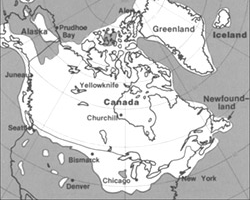
\includegraphics{task1/laurentide_wiki.png}}}
  \caption{The maximum extend of the Laurentide ice, according to \cite{laurentide_wiki}.}
  \label{fig:laurentide_wiki}
\end{figure}
As mentioned before the errors in the radial movement should probably be increased after the antennas were changed which means that the results might be slightly changed.
It is very interesting, though, that the difference between the observed uplift and the computed uplift is less than the error in the coordinates the was computed by GIPSY, which indicates that the result is about as good as it gets with this model and data.\\
There are two stations that does not really fit my model and those are YELL and MDO1.
While MDO1 is quite far away and appears to be located near a mountain (which could explain the uplift), YELL is located quite near the computed center and has a high uplift.
To me this is an indication that a better model is needed to describe how the land recovers from the ice, perhaps one that allows the center to be larger than a point.

It would be interesting to collect data from stations near Hudson Bay, Canada and perhaps use a better geophysical model for how the land recovers from the ice to see how the result would be affected.

I think the measurement techniques are good as they are and that most of the improvements would come from better and more realistic models for the uplift.
For example I think it would have been a good idea to include the motion in the latitude and longitude directions since stations near the center would also move away from the center as it rises.
I tried to do this at first but it proved to be a difficult task so I had to give it up due to lack of time.

\subsection{Tropospheric delay prediction}
Looking at the data in Figure~\ref{fig:trop_delay} it looks like there are piecewise trends in the data, which means that if you predict at end or start of a trend, the prediction will likely be bad but if you predict near the middle of a trend the prediction is likely more accurate.
This can be seen in Figure~\ref{fig:trop_delay} where an upgoing trend starts at the beginning of day 6 and continues during day 7 for RESO while an upgoing trend starts to shift into a downgoing trend at the end of day 6 and the shifts back into an upgoing trend at the very end of day 6.
The prediction for RESO seems better than MDO1, perhaps for this reason.

It should be noted that the prediction is heavily impacted by how the data is weighted in the calculation.
I chose to weight data points closer to the $7^{\text{th}}$ day more than those far away (in time) and the results varied quite a lot, especially for MDO1 so my final judgment on the prediction is that is is not very reliable.
A better approach would perhaps be to keep the last data point from day 6 as the prediction and instead find a suitable error to add to the data points for the $7^{\text{th}}$ day.

I think the measurement techniques are good enough as they are for predicting the tropospheric delay most of the improvements would come from finding better models and using data from many stations to get a bigger picture of the tropospheric delay in the area to come up with a more accurate prediction.

\newpage
\begin{thebibliography}{1}

\bibitem{laurentide_wiki} various, Wikipedia,  ``Global Positioning System'' Internet: \url{https://en.wikipedia.org/wiki/Global_Positioning_System}, 2018-01-02 [2018-01-02]

\bibitem{laurentide_wiki} various, Wikipedia,  ``GLONASS'' Internet: \url{https://en.wikipedia.org/wiki/GLONASS}, 2018-01-02 [2018-01-02]

\bibitem{laurentide_wiki} various, Wikipedia,  ``Galileo (satellite navigation)'' Internet: \url{https://en.wikipedia.org/wiki/Galileo_(satellite_navigation)}, 2018-01-02 [2018-01-02]

\bibitem{lecture_notes} Jan M. Johansson, Chalmers University of Technology,  ``Project Report Hints Final'' Internet: \url{https://pingpong.chalmers.se/courseId/8799/node.do?id=4263162&ts=1513097602324&u=-1631444947}, 2018-01-02 [2018-01-02]

\bibitem{laurentide_wiki} John S. Schlee, United States Geological Survey ``OUR CHANGING CONTINENT'' Internet: \url{https://pubs.usgs.gov/gip/continents/map.jpg}, 2018-01-02 [2018-01-02]

% \bibitem{cheng} D. K. Cheng. ``Theory and Applications of Transmission Lines'' in \textit{Field and Wave Electromagnetics}, 2$^{\text{nd}}$ ed. Edinburgh: Pearson, 2014, pp. 427-519

\end{thebibliography}

\end{document}